
\newpage
\subsection{BenchMarkishTopics}
    % latex table generated in R 4.1.2 by xtable 1.8-4 package
% Sun Mar 13 20:27:35 2022
\begin{table}[h!]
\centering
\begin{tabular}{p{0.2\textwidth}p{0.2\textwidth}p{0.2\textwidth}}
  \hline
 & LLVM IR & ARM Assembly \\ 
  \hline
Stack & 204 & 130 \\ 
  Registers & 184 &  82 \\ 
  Optimizations & 173 &  82 \\ 
   \hline
\end{tabular}
\caption{BenchMarkishTopics instruction counts for generated code excluding labels}
\end{table}

    \begin{figure}[h]
	    \centering
		% Created by tikzDevice version 0.12.3.1 on 2022-03-07 08:45:17
% !TEX encoding = UTF-8 Unicode
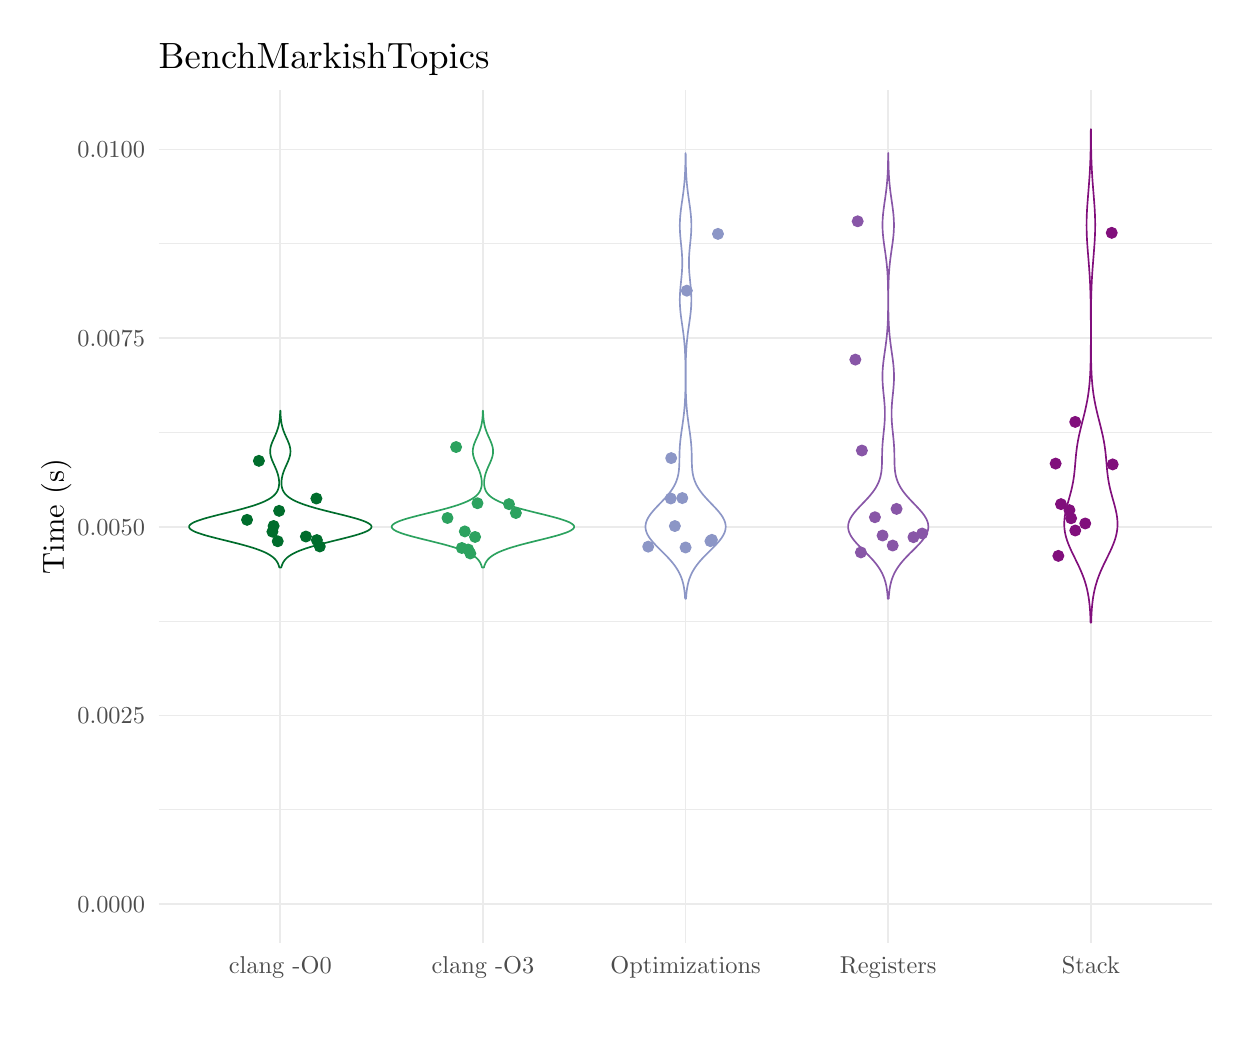
\begin{tikzpicture}[x=1pt,y=1pt]
\definecolor{fillColor}{RGB}{255,255,255}
\path[use as bounding box,fill=fillColor,fill opacity=0.00] (0,0) rectangle (433.62,361.35);
\begin{scope}
\path[clip] ( 47.35, 30.69) rectangle (428.12,338.69);
\definecolor{drawColor}{gray}{0.92}

\path[draw=drawColor,line width= 0.3pt,line join=round] ( 47.35, 78.76) --
	(428.12, 78.76);

\path[draw=drawColor,line width= 0.3pt,line join=round] ( 47.35,146.91) --
	(428.12,146.91);

\path[draw=drawColor,line width= 0.3pt,line join=round] ( 47.35,215.07) --
	(428.12,215.07);

\path[draw=drawColor,line width= 0.3pt,line join=round] ( 47.35,283.22) --
	(428.12,283.22);

\path[draw=drawColor,line width= 0.6pt,line join=round] ( 47.35, 44.69) --
	(428.12, 44.69);

\path[draw=drawColor,line width= 0.6pt,line join=round] ( 47.35,112.84) --
	(428.12,112.84);

\path[draw=drawColor,line width= 0.6pt,line join=round] ( 47.35,180.99) --
	(428.12,180.99);

\path[draw=drawColor,line width= 0.6pt,line join=round] ( 47.35,249.14) --
	(428.12,249.14);

\path[draw=drawColor,line width= 0.6pt,line join=round] ( 47.35,317.30) --
	(428.12,317.30);

\path[draw=drawColor,line width= 0.6pt,line join=round] ( 91.29, 30.69) --
	( 91.29,338.69);

\path[draw=drawColor,line width= 0.6pt,line join=round] (164.51, 30.69) --
	(164.51,338.69);

\path[draw=drawColor,line width= 0.6pt,line join=round] (237.74, 30.69) --
	(237.74,338.69);

\path[draw=drawColor,line width= 0.6pt,line join=round] (310.96, 30.69) --
	(310.96,338.69);

\path[draw=drawColor,line width= 0.6pt,line join=round] (384.19, 30.69) --
	(384.19,338.69);
\definecolor{drawColor}{RGB}{0,109,44}
\definecolor{fillColor}{RGB}{255,255,255}

\path[draw=drawColor,line width= 0.6pt,line join=round,line cap=round,fill=fillColor] ( 90.92,166.30) --
	( 90.89,166.42) --
	( 90.86,166.53) --
	( 90.84,166.64) --
	( 90.80,166.75) --
	( 90.77,166.86) --
	( 90.74,166.97) --
	( 90.70,167.08) --
	( 90.66,167.19) --
	( 90.62,167.30) --
	( 90.58,167.41) --
	( 90.53,167.52) --
	( 90.48,167.63) --
	( 90.43,167.75) --
	( 90.38,167.86) --
	( 90.32,167.97) --
	( 90.26,168.08) --
	( 90.20,168.19) --
	( 90.13,168.30) --
	( 90.06,168.41) --
	( 89.99,168.52) --
	( 89.92,168.63) --
	( 89.84,168.74) --
	( 89.75,168.85) --
	( 89.66,168.96) --
	( 89.57,169.08) --
	( 89.48,169.19) --
	( 89.37,169.30) --
	( 89.27,169.41) --
	( 89.16,169.52) --
	( 89.04,169.63) --
	( 88.92,169.74) --
	( 88.80,169.85) --
	( 88.67,169.96) --
	( 88.53,170.07) --
	( 88.39,170.18) --
	( 88.24,170.29) --
	( 88.09,170.41) --
	( 87.93,170.52) --
	( 87.76,170.63) --
	( 87.59,170.74) --
	( 87.41,170.85) --
	( 87.23,170.96) --
	( 87.04,171.07) --
	( 86.84,171.18) --
	( 86.64,171.29) --
	( 86.42,171.40) --
	( 86.21,171.51) --
	( 85.98,171.62) --
	( 85.75,171.74) --
	( 85.51,171.85) --
	( 85.26,171.96) --
	( 85.00,172.07) --
	( 84.74,172.18) --
	( 84.47,172.29) --
	( 84.20,172.40) --
	( 83.91,172.51) --
	( 83.62,172.62) --
	( 83.32,172.73) --
	( 83.01,172.84) --
	( 82.70,172.95) --
	( 82.37,173.07) --
	( 82.04,173.18) --
	( 81.71,173.29) --
	( 81.36,173.40) --
	( 81.01,173.51) --
	( 80.65,173.62) --
	( 80.29,173.73) --
	( 79.92,173.84) --
	( 79.54,173.95) --
	( 79.15,174.06) --
	( 78.76,174.17) --
	( 78.37,174.28) --
	( 77.96,174.40) --
	( 77.56,174.51) --
	( 77.14,174.62) --
	( 76.72,174.73) --
	( 76.30,174.84) --
	( 75.87,174.95) --
	( 75.44,175.06) --
	( 75.01,175.17) --
	( 74.57,175.28) --
	( 74.13,175.39) --
	( 73.68,175.50) --
	( 73.23,175.61) --
	( 72.78,175.73) --
	( 72.33,175.84) --
	( 71.88,175.95) --
	( 71.43,176.06) --
	( 70.98,176.17) --
	( 70.53,176.28) --
	( 70.08,176.39) --
	( 69.63,176.50) --
	( 69.18,176.61) --
	( 68.73,176.72) --
	( 68.29,176.83) --
	( 67.85,176.94) --
	( 67.42,177.06) --
	( 66.99,177.17) --
	( 66.56,177.28) --
	( 66.14,177.39) --
	( 65.72,177.50) --
	( 65.32,177.61) --
	( 64.91,177.72) --
	( 64.52,177.83) --
	( 64.14,177.94) --
	( 63.76,178.05) --
	( 63.39,178.16) --
	( 63.03,178.27) --
	( 62.68,178.39) --
	( 62.34,178.50) --
	( 62.01,178.61) --
	( 61.70,178.72) --
	( 61.39,178.83) --
	( 61.10,178.94) --
	( 60.82,179.05) --
	( 60.55,179.16) --
	( 60.30,179.27) --
	( 60.06,179.38) --
	( 59.84,179.49) --
	( 59.63,179.60) --
	( 59.43,179.72) --
	( 59.26,179.83) --
	( 59.09,179.94) --
	( 58.94,180.05) --
	( 58.81,180.16) --
	( 58.69,180.27) --
	( 58.59,180.38) --
	( 58.51,180.49) --
	( 58.44,180.60) --
	( 58.39,180.71) --
	( 58.35,180.82) --
	( 58.34,180.93) --
	( 58.34,181.04) --
	( 58.36,181.16) --
	( 58.39,181.27) --
	( 58.44,181.38) --
	( 58.51,181.49) --
	( 58.59,181.60) --
	( 58.69,181.71) --
	( 58.81,181.82) --
	( 58.94,181.93) --
	( 59.09,182.04) --
	( 59.25,182.15) --
	( 59.43,182.26) --
	( 59.62,182.37) --
	( 59.83,182.49) --
	( 60.06,182.60) --
	( 60.29,182.71) --
	( 60.55,182.82) --
	( 60.81,182.93) --
	( 61.09,183.04) --
	( 61.39,183.15) --
	( 61.69,183.26) --
	( 62.01,183.37) --
	( 62.33,183.48) --
	( 62.67,183.59) --
	( 63.02,183.70) --
	( 63.38,183.82) --
	( 63.75,183.93) --
	( 64.12,184.04) --
	( 64.51,184.15) --
	( 64.90,184.26) --
	( 65.31,184.37) --
	( 65.71,184.48) --
	( 66.13,184.59) --
	( 66.55,184.70) --
	( 66.98,184.81) --
	( 67.41,184.92) --
	( 67.84,185.03) --
	( 68.28,185.15) --
	( 68.72,185.26) --
	( 69.17,185.37) --
	( 69.62,185.48) --
	( 70.07,185.59) --
	( 70.52,185.70) --
	( 70.97,185.81) --
	( 71.42,185.92) --
	( 71.87,186.03) --
	( 72.32,186.14) --
	( 72.77,186.25) --
	( 73.22,186.36) --
	( 73.67,186.48) --
	( 74.11,186.59) --
	( 74.56,186.70) --
	( 74.99,186.81) --
	( 75.43,186.92) --
	( 75.86,187.03) --
	( 76.29,187.14) --
	( 76.71,187.25) --
	( 77.13,187.36) --
	( 77.54,187.47) --
	( 77.95,187.58) --
	( 78.35,187.69) --
	( 78.75,187.81) --
	( 79.14,187.92) --
	( 79.53,188.03) --
	( 79.91,188.14) --
	( 80.28,188.25) --
	( 80.64,188.36) --
	( 81.00,188.47) --
	( 81.35,188.58) --
	( 81.70,188.69) --
	( 82.03,188.80) --
	( 82.37,188.91) --
	( 82.69,189.02) --
	( 83.00,189.14) --
	( 83.31,189.25) --
	( 83.61,189.36) --
	( 83.90,189.47) --
	( 84.18,189.58) --
	( 84.46,189.69) --
	( 84.73,189.80) --
	( 84.99,189.91) --
	( 85.25,190.02) --
	( 85.50,190.13) --
	( 85.74,190.24) --
	( 85.97,190.35) --
	( 86.19,190.47) --
	( 86.41,190.58) --
	( 86.62,190.69) --
	( 86.83,190.80) --
	( 87.03,190.91) --
	( 87.22,191.02) --
	( 87.40,191.13) --
	( 87.58,191.24) --
	( 87.75,191.35) --
	( 87.91,191.46) --
	( 88.07,191.57) --
	( 88.23,191.68) --
	( 88.37,191.80) --
	( 88.51,191.91) --
	( 88.65,192.02) --
	( 88.78,192.13) --
	( 88.90,192.24) --
	( 89.02,192.35) --
	( 89.14,192.46) --
	( 89.24,192.57) --
	( 89.35,192.68) --
	( 89.45,192.79) --
	( 89.54,192.90) --
	( 89.63,193.01) --
	( 89.72,193.13) --
	( 89.80,193.24) --
	( 89.88,193.35) --
	( 89.95,193.46) --
	( 90.02,193.57) --
	( 90.09,193.68) --
	( 90.15,193.79) --
	( 90.21,193.90) --
	( 90.27,194.01) --
	( 90.32,194.12) --
	( 90.37,194.23) --
	( 90.42,194.34) --
	( 90.46,194.46) --
	( 90.50,194.57) --
	( 90.54,194.68) --
	( 90.58,194.79) --
	( 90.61,194.90) --
	( 90.64,195.01) --
	( 90.67,195.12) --
	( 90.70,195.23) --
	( 90.72,195.34) --
	( 90.74,195.45) --
	( 90.76,195.56) --
	( 90.78,195.67) --
	( 90.80,195.79) --
	( 90.81,195.90) --
	( 90.82,196.01) --
	( 90.83,196.12) --
	( 90.84,196.23) --
	( 90.85,196.34) --
	( 90.86,196.45) --
	( 90.86,196.56) --
	( 90.87,196.67) --
	( 90.87,196.78) --
	( 90.87,196.89) --
	( 90.87,197.00) --
	( 90.86,197.12) --
	( 90.86,197.23) --
	( 90.85,197.34) --
	( 90.85,197.45) --
	( 90.84,197.56) --
	( 90.83,197.67) --
	( 90.82,197.78) --
	( 90.81,197.89) --
	( 90.80,198.00) --
	( 90.78,198.11) --
	( 90.77,198.22) --
	( 90.75,198.33) --
	( 90.73,198.44) --
	( 90.72,198.56) --
	( 90.70,198.67) --
	( 90.68,198.78) --
	( 90.66,198.89) --
	( 90.63,199.00) --
	( 90.61,199.11) --
	( 90.58,199.22) --
	( 90.56,199.33) --
	( 90.53,199.44) --
	( 90.50,199.55) --
	( 90.48,199.66) --
	( 90.45,199.77) --
	( 90.41,199.89) --
	( 90.38,200.00) --
	( 90.35,200.11) --
	( 90.32,200.22) --
	( 90.28,200.33) --
	( 90.25,200.44) --
	( 90.21,200.55) --
	( 90.17,200.66) --
	( 90.14,200.77) --
	( 90.10,200.88) --
	( 90.06,200.99) --
	( 90.02,201.10) --
	( 89.97,201.22) --
	( 89.93,201.33) --
	( 89.89,201.44) --
	( 89.85,201.55) --
	( 89.80,201.66) --
	( 89.76,201.77) --
	( 89.71,201.88) --
	( 89.66,201.99) --
	( 89.62,202.10) --
	( 89.57,202.21) --
	( 89.52,202.32) --
	( 89.48,202.43) --
	( 89.43,202.55) --
	( 89.38,202.66) --
	( 89.33,202.77) --
	( 89.28,202.88) --
	( 89.23,202.99) --
	( 89.18,203.10) --
	( 89.13,203.21) --
	( 89.08,203.32) --
	( 89.03,203.43) --
	( 88.98,203.54) --
	( 88.93,203.65) --
	( 88.88,203.76) --
	( 88.83,203.88) --
	( 88.78,203.99) --
	( 88.73,204.10) --
	( 88.68,204.21) --
	( 88.63,204.32) --
	( 88.59,204.43) --
	( 88.54,204.54) --
	( 88.49,204.65) --
	( 88.45,204.76) --
	( 88.40,204.87) --
	( 88.36,204.98) --
	( 88.31,205.09) --
	( 88.27,205.21) --
	( 88.23,205.32) --
	( 88.19,205.43) --
	( 88.15,205.54) --
	( 88.11,205.65) --
	( 88.07,205.76) --
	( 88.03,205.87) --
	( 88.00,205.98) --
	( 87.97,206.09) --
	( 87.93,206.20) --
	( 87.90,206.31) --
	( 87.87,206.42) --
	( 87.84,206.54) --
	( 87.82,206.65) --
	( 87.79,206.76) --
	( 87.77,206.87) --
	( 87.75,206.98) --
	( 87.73,207.09) --
	( 87.71,207.20) --
	( 87.69,207.31) --
	( 87.68,207.42) --
	( 87.67,207.53) --
	( 87.65,207.64) --
	( 87.65,207.75) --
	( 87.64,207.87) --
	( 87.63,207.98) --
	( 87.63,208.09) --
	( 87.63,208.20) --
	( 87.63,208.31) --
	( 87.63,208.42) --
	( 87.63,208.53) --
	( 87.64,208.64) --
	( 87.65,208.75) --
	( 87.65,208.86) --
	( 87.67,208.97) --
	( 87.68,209.08) --
	( 87.69,209.20) --
	( 87.71,209.31) --
	( 87.73,209.42) --
	( 87.75,209.53) --
	( 87.77,209.64) --
	( 87.79,209.75) --
	( 87.82,209.86) --
	( 87.84,209.97) --
	( 87.87,210.08) --
	( 87.90,210.19) --
	( 87.93,210.30) --
	( 87.97,210.41) --
	( 88.00,210.53) --
	( 88.03,210.64) --
	( 88.07,210.75) --
	( 88.11,210.86) --
	( 88.15,210.97) --
	( 88.19,211.08) --
	( 88.23,211.19) --
	( 88.27,211.30) --
	( 88.31,211.41) --
	( 88.36,211.52) --
	( 88.40,211.63) --
	( 88.45,211.74) --
	( 88.49,211.86) --
	( 88.54,211.97) --
	( 88.59,212.08) --
	( 88.64,212.19) --
	( 88.68,212.30) --
	( 88.73,212.41) --
	( 88.78,212.52) --
	( 88.83,212.63) --
	( 88.88,212.74) --
	( 88.93,212.85) --
	( 88.98,212.96) --
	( 89.03,213.07) --
	( 89.08,213.19) --
	( 89.13,213.30) --
	( 89.18,213.41) --
	( 89.23,213.52) --
	( 89.28,213.63) --
	( 89.33,213.74) --
	( 89.38,213.85) --
	( 89.43,213.96) --
	( 89.48,214.07) --
	( 89.53,214.18) --
	( 89.57,214.29) --
	( 89.62,214.40) --
	( 89.67,214.52) --
	( 89.72,214.63) --
	( 89.76,214.74) --
	( 89.81,214.85) --
	( 89.85,214.96) --
	( 89.90,215.07) --
	( 89.94,215.18) --
	( 89.98,215.29) --
	( 90.02,215.40) --
	( 90.07,215.51) --
	( 90.11,215.62) --
	( 90.15,215.73) --
	( 90.18,215.84) --
	( 90.22,215.96) --
	( 90.26,216.07) --
	( 90.30,216.18) --
	( 90.33,216.29) --
	( 90.37,216.40) --
	( 90.40,216.51) --
	( 90.44,216.62) --
	( 90.47,216.73) --
	( 90.50,216.84) --
	( 90.53,216.95) --
	( 90.56,217.06) --
	( 90.59,217.17) --
	( 90.62,217.29) --
	( 90.65,217.40) --
	( 90.67,217.51) --
	( 90.70,217.62) --
	( 90.72,217.73) --
	( 90.75,217.84) --
	( 90.77,217.95) --
	( 90.79,218.06) --
	( 90.82,218.17) --
	( 90.84,218.28) --
	( 90.86,218.39) --
	( 90.88,218.50) --
	( 90.90,218.62) --
	( 90.91,218.73) --
	( 90.93,218.84) --
	( 90.95,218.95) --
	( 90.97,219.06) --
	( 90.98,219.17) --
	( 91.00,219.28) --
	( 91.01,219.39) --
	( 91.02,219.50) --
	( 91.04,219.61) --
	( 91.05,219.72) --
	( 91.06,219.83) --
	( 91.07,219.95) --
	( 91.09,220.06) --
	( 91.10,220.17) --
	( 91.11,220.28) --
	( 91.12,220.39) --
	( 91.13,220.50) --
	( 91.14,220.61) --
	( 91.14,220.72) --
	( 91.15,220.83) --
	( 91.16,220.94) --
	( 91.17,221.05) --
	( 91.17,221.16) --
	( 91.18,221.28) --
	( 91.19,221.39) --
	( 91.19,221.50) --
	( 91.20,221.61) --
	( 91.20,221.72) --
	( 91.21,221.83) --
	( 91.21,221.94) --
	( 91.22,222.05) --
	( 91.22,222.16) --
	( 91.23,222.27) --
	( 91.23,222.38) --
	( 91.23,222.49) --
	( 91.24,222.61) --
	( 91.24,222.72) --
	( 91.24,222.83) --
	( 91.25,222.94) --
	( 91.33,222.94) --
	( 91.33,222.83) --
	( 91.33,222.72) --
	( 91.34,222.61) --
	( 91.34,222.49) --
	( 91.34,222.38) --
	( 91.35,222.27) --
	( 91.35,222.16) --
	( 91.36,222.05) --
	( 91.36,221.94) --
	( 91.37,221.83) --
	( 91.37,221.72) --
	( 91.38,221.61) --
	( 91.38,221.50) --
	( 91.39,221.39) --
	( 91.39,221.28) --
	( 91.40,221.16) --
	( 91.41,221.05) --
	( 91.42,220.94) --
	( 91.42,220.83) --
	( 91.43,220.72) --
	( 91.44,220.61) --
	( 91.45,220.50) --
	( 91.46,220.39) --
	( 91.47,220.28) --
	( 91.48,220.17) --
	( 91.49,220.06) --
	( 91.50,219.95) --
	( 91.51,219.83) --
	( 91.52,219.72) --
	( 91.54,219.61) --
	( 91.55,219.50) --
	( 91.56,219.39) --
	( 91.58,219.28) --
	( 91.59,219.17) --
	( 91.61,219.06) --
	( 91.63,218.95) --
	( 91.64,218.84) --
	( 91.66,218.73) --
	( 91.68,218.62) --
	( 91.70,218.50) --
	( 91.72,218.39) --
	( 91.74,218.28) --
	( 91.76,218.17) --
	( 91.78,218.06) --
	( 91.80,217.95) --
	( 91.83,217.84) --
	( 91.85,217.73) --
	( 91.88,217.62) --
	( 91.90,217.51) --
	( 91.93,217.40) --
	( 91.96,217.29) --
	( 91.99,217.17) --
	( 92.01,217.06) --
	( 92.04,216.95) --
	( 92.08,216.84) --
	( 92.11,216.73) --
	( 92.14,216.62) --
	( 92.17,216.51) --
	( 92.21,216.40) --
	( 92.24,216.29) --
	( 92.28,216.18) --
	( 92.31,216.07) --
	( 92.35,215.96) --
	( 92.39,215.84) --
	( 92.43,215.73) --
	( 92.47,215.62) --
	( 92.51,215.51) --
	( 92.55,215.40) --
	( 92.59,215.29) --
	( 92.64,215.18) --
	( 92.68,215.07) --
	( 92.72,214.96) --
	( 92.77,214.85) --
	( 92.81,214.74) --
	( 92.86,214.63) --
	( 92.91,214.52) --
	( 92.95,214.40) --
	( 93.00,214.29) --
	( 93.05,214.18) --
	( 93.10,214.07) --
	( 93.15,213.96) --
	( 93.19,213.85) --
	( 93.24,213.74) --
	( 93.29,213.63) --
	( 93.34,213.52) --
	( 93.39,213.41) --
	( 93.44,213.30) --
	( 93.49,213.19) --
	( 93.54,213.07) --
	( 93.59,212.96) --
	( 93.64,212.85) --
	( 93.69,212.74) --
	( 93.74,212.63) --
	( 93.79,212.52) --
	( 93.84,212.41) --
	( 93.89,212.30) --
	( 93.94,212.19) --
	( 93.99,212.08) --
	( 94.04,211.97) --
	( 94.08,211.86) --
	( 94.13,211.74) --
	( 94.17,211.63) --
	( 94.22,211.52) --
	( 94.26,211.41) --
	( 94.30,211.30) --
	( 94.35,211.19) --
	( 94.39,211.08) --
	( 94.43,210.97) --
	( 94.47,210.86) --
	( 94.50,210.75) --
	( 94.54,210.64) --
	( 94.58,210.53) --
	( 94.61,210.41) --
	( 94.64,210.30) --
	( 94.67,210.19) --
	( 94.70,210.08) --
	( 94.73,209.97) --
	( 94.76,209.86) --
	( 94.78,209.75) --
	( 94.80,209.64) --
	( 94.83,209.53) --
	( 94.85,209.42) --
	( 94.87,209.31) --
	( 94.88,209.20) --
	( 94.90,209.08) --
	( 94.91,208.97) --
	( 94.92,208.86) --
	( 94.93,208.75) --
	( 94.94,208.64) --
	( 94.94,208.53) --
	( 94.95,208.42) --
	( 94.95,208.31) --
	( 94.95,208.20) --
	( 94.95,208.09) --
	( 94.94,207.98) --
	( 94.94,207.87) --
	( 94.93,207.75) --
	( 94.92,207.64) --
	( 94.91,207.53) --
	( 94.90,207.42) --
	( 94.88,207.31) --
	( 94.87,207.20) --
	( 94.85,207.09) --
	( 94.83,206.98) --
	( 94.81,206.87) --
	( 94.78,206.76) --
	( 94.76,206.65) --
	( 94.73,206.54) --
	( 94.70,206.42) --
	( 94.67,206.31) --
	( 94.64,206.20) --
	( 94.61,206.09) --
	( 94.58,205.98) --
	( 94.54,205.87) --
	( 94.51,205.76) --
	( 94.47,205.65) --
	( 94.43,205.54) --
	( 94.39,205.43) --
	( 94.35,205.32) --
	( 94.31,205.21) --
	( 94.26,205.09) --
	( 94.22,204.98) --
	( 94.17,204.87) --
	( 94.13,204.76) --
	( 94.08,204.65) --
	( 94.04,204.54) --
	( 93.99,204.43) --
	( 93.94,204.32) --
	( 93.89,204.21) --
	( 93.84,204.10) --
	( 93.80,203.99) --
	( 93.75,203.88) --
	( 93.70,203.76) --
	( 93.65,203.65) --
	( 93.60,203.54) --
	( 93.55,203.43) --
	( 93.50,203.32) --
	( 93.45,203.21) --
	( 93.40,203.10) --
	( 93.35,202.99) --
	( 93.30,202.88) --
	( 93.25,202.77) --
	( 93.20,202.66) --
	( 93.15,202.55) --
	( 93.10,202.43) --
	( 93.05,202.32) --
	( 93.00,202.21) --
	( 92.96,202.10) --
	( 92.91,201.99) --
	( 92.86,201.88) --
	( 92.82,201.77) --
	( 92.77,201.66) --
	( 92.73,201.55) --
	( 92.69,201.44) --
	( 92.64,201.33) --
	( 92.60,201.22) --
	( 92.56,201.10) --
	( 92.52,200.99) --
	( 92.48,200.88) --
	( 92.44,200.77) --
	( 92.40,200.66) --
	( 92.36,200.55) --
	( 92.33,200.44) --
	( 92.29,200.33) --
	( 92.26,200.22) --
	( 92.22,200.11) --
	( 92.19,200.00) --
	( 92.16,199.89) --
	( 92.13,199.77) --
	( 92.10,199.66) --
	( 92.07,199.55) --
	( 92.04,199.44) --
	( 92.02,199.33) --
	( 91.99,199.22) --
	( 91.97,199.11) --
	( 91.94,199.00) --
	( 91.92,198.89) --
	( 91.90,198.78) --
	( 91.88,198.67) --
	( 91.86,198.56) --
	( 91.84,198.44) --
	( 91.82,198.33) --
	( 91.81,198.22) --
	( 91.79,198.11) --
	( 91.78,198.00) --
	( 91.77,197.89) --
	( 91.75,197.78) --
	( 91.74,197.67) --
	( 91.74,197.56) --
	( 91.73,197.45) --
	( 91.72,197.34) --
	( 91.72,197.23) --
	( 91.71,197.12) --
	( 91.71,197.00) --
	( 91.71,196.89) --
	( 91.71,196.78) --
	( 91.71,196.67) --
	( 91.71,196.56) --
	( 91.72,196.45) --
	( 91.72,196.34) --
	( 91.73,196.23) --
	( 91.74,196.12) --
	( 91.75,196.01) --
	( 91.76,195.90) --
	( 91.78,195.79) --
	( 91.79,195.67) --
	( 91.81,195.56) --
	( 91.83,195.45) --
	( 91.85,195.34) --
	( 91.88,195.23) --
	( 91.91,195.12) --
	( 91.93,195.01) --
	( 91.96,194.90) --
	( 92.00,194.79) --
	( 92.03,194.68) --
	( 92.07,194.57) --
	( 92.11,194.46) --
	( 92.16,194.34) --
	( 92.21,194.23) --
	( 92.26,194.12) --
	( 92.31,194.01) --
	( 92.36,193.90) --
	( 92.42,193.79) --
	( 92.49,193.68) --
	( 92.55,193.57) --
	( 92.62,193.46) --
	( 92.70,193.35) --
	( 92.77,193.24) --
	( 92.86,193.13) --
	( 92.94,193.01) --
	( 93.03,192.90) --
	( 93.13,192.79) --
	( 93.23,192.68) --
	( 93.33,192.57) --
	( 93.44,192.46) --
	( 93.55,192.35) --
	( 93.67,192.24) --
	( 93.80,192.13) --
	( 93.93,192.02) --
	( 94.06,191.91) --
	( 94.20,191.80) --
	( 94.35,191.68) --
	( 94.50,191.57) --
	( 94.66,191.46) --
	( 94.82,191.35) --
	( 95.00,191.24) --
	( 95.17,191.13) --
	( 95.36,191.02) --
	( 95.55,190.91) --
	( 95.74,190.80) --
	( 95.95,190.69) --
	( 96.16,190.58) --
	( 96.38,190.47) --
	( 96.61,190.35) --
	( 96.84,190.24) --
	( 97.08,190.13) --
	( 97.32,190.02) --
	( 97.58,189.91) --
	( 97.84,189.80) --
	( 98.11,189.69) --
	( 98.39,189.58) --
	( 98.67,189.47) --
	( 98.97,189.36) --
	( 99.27,189.25) --
	( 99.57,189.14) --
	( 99.89,189.02) --
	(100.21,188.91) --
	(100.54,188.80) --
	(100.88,188.69) --
	(101.22,188.58) --
	(101.57,188.47) --
	(101.93,188.36) --
	(102.30,188.25) --
	(102.67,188.14) --
	(103.05,188.03) --
	(103.43,187.92) --
	(103.82,187.81) --
	(104.22,187.69) --
	(104.62,187.58) --
	(105.03,187.47) --
	(105.44,187.36) --
	(105.86,187.25) --
	(106.29,187.14) --
	(106.71,187.03) --
	(107.15,186.92) --
	(107.58,186.81) --
	(108.02,186.70) --
	(108.46,186.59) --
	(108.91,186.48) --
	(109.35,186.36) --
	(109.80,186.25) --
	(110.25,186.14) --
	(110.70,186.03) --
	(111.15,185.92) --
	(111.61,185.81) --
	(112.06,185.70) --
	(112.51,185.59) --
	(112.96,185.48) --
	(113.41,185.37) --
	(113.85,185.26) --
	(114.29,185.15) --
	(114.73,185.03) --
	(115.17,184.92) --
	(115.60,184.81) --
	(116.02,184.70) --
	(116.45,184.59) --
	(116.86,184.48) --
	(117.27,184.37) --
	(117.67,184.26) --
	(118.06,184.15) --
	(118.45,184.04) --
	(118.83,183.93) --
	(119.20,183.82) --
	(119.55,183.70) --
	(119.90,183.59) --
	(120.24,183.48) --
	(120.57,183.37) --
	(120.89,183.26) --
	(121.19,183.15) --
	(121.48,183.04) --
	(121.76,182.93) --
	(122.02,182.82) --
	(122.28,182.71) --
	(122.52,182.60) --
	(122.74,182.49) --
	(122.95,182.37) --
	(123.14,182.26) --
	(123.33,182.15) --
	(123.49,182.04) --
	(123.64,181.93) --
	(123.77,181.82) --
	(123.88,181.71) --
	(123.99,181.60) --
	(124.07,181.49) --
	(124.14,181.38) --
	(124.19,181.27) --
	(124.22,181.16) --
	(124.24,181.04) --
	(124.23,180.93) --
	(124.22,180.82) --
	(124.18,180.71) --
	(124.13,180.60) --
	(124.07,180.49) --
	(123.98,180.38) --
	(123.89,180.27) --
	(123.76,180.16) --
	(123.63,180.05) --
	(123.49,179.94) --
	(123.32,179.83) --
	(123.14,179.72) --
	(122.94,179.60) --
	(122.74,179.49) --
	(122.51,179.38) --
	(122.27,179.27) --
	(122.02,179.16) --
	(121.75,179.05) --
	(121.48,178.94) --
	(121.18,178.83) --
	(120.88,178.72) --
	(120.56,178.61) --
	(120.23,178.50) --
	(119.90,178.39) --
	(119.55,178.27) --
	(119.19,178.16) --
	(118.82,178.05) --
	(118.44,177.94) --
	(118.06,177.83) --
	(117.66,177.72) --
	(117.26,177.61) --
	(116.85,177.50) --
	(116.44,177.39) --
	(116.02,177.28) --
	(115.59,177.17) --
	(115.16,177.06) --
	(114.72,176.94) --
	(114.28,176.83) --
	(113.84,176.72) --
	(113.39,176.61) --
	(112.95,176.50) --
	(112.50,176.39) --
	(112.05,176.28) --
	(111.60,176.17) --
	(111.14,176.06) --
	(110.69,175.95) --
	(110.24,175.84) --
	(109.79,175.73) --
	(109.34,175.61) --
	(108.90,175.50) --
	(108.45,175.39) --
	(108.01,175.28) --
	(107.57,175.17) --
	(107.13,175.06) --
	(106.70,174.95) --
	(106.27,174.84) --
	(105.85,174.73) --
	(105.43,174.62) --
	(105.02,174.51) --
	(104.61,174.40) --
	(104.21,174.28) --
	(103.81,174.17) --
	(103.42,174.06) --
	(103.04,173.95) --
	(102.66,173.84) --
	(102.29,173.73) --
	(101.92,173.62) --
	(101.56,173.51) --
	(101.21,173.40) --
	(100.87,173.29) --
	(100.53,173.18) --
	(100.20,173.07) --
	( 99.88,172.95) --
	( 99.57,172.84) --
	( 99.26,172.73) --
	( 98.96,172.62) --
	( 98.67,172.51) --
	( 98.38,172.40) --
	( 98.10,172.29) --
	( 97.83,172.18) --
	( 97.57,172.07) --
	( 97.32,171.96) --
	( 97.07,171.85) --
	( 96.83,171.74) --
	( 96.59,171.62) --
	( 96.37,171.51) --
	( 96.15,171.40) --
	( 95.94,171.29) --
	( 95.74,171.18) --
	( 95.54,171.07) --
	( 95.35,170.96) --
	( 95.16,170.85) --
	( 94.98,170.74) --
	( 94.81,170.63) --
	( 94.65,170.52) --
	( 94.49,170.41) --
	( 94.33,170.29) --
	( 94.19,170.18) --
	( 94.04,170.07) --
	( 93.91,169.96) --
	( 93.78,169.85) --
	( 93.65,169.74) --
	( 93.53,169.63) --
	( 93.42,169.52) --
	( 93.31,169.41) --
	( 93.20,169.30) --
	( 93.10,169.19) --
	( 93.00,169.08) --
	( 92.91,168.96) --
	( 92.82,168.85) --
	( 92.74,168.74) --
	( 92.66,168.63) --
	( 92.58,168.52) --
	( 92.51,168.41) --
	( 92.44,168.30) --
	( 92.38,168.19) --
	( 92.31,168.08) --
	( 92.25,167.97) --
	( 92.20,167.86) --
	( 92.14,167.75) --
	( 92.09,167.63) --
	( 92.04,167.52) --
	( 92.00,167.41) --
	( 91.95,167.30) --
	( 91.91,167.19) --
	( 91.88,167.08) --
	( 91.84,166.97) --
	( 91.80,166.86) --
	( 91.77,166.75) --
	( 91.74,166.64) --
	( 91.71,166.53) --
	( 91.68,166.42) --
	( 91.66,166.30) --
	( 90.92,166.30) --
	cycle;
\definecolor{drawColor}{RGB}{44,162,95}

\path[draw=drawColor,line width= 0.6pt,line join=round,line cap=round,fill=fillColor] (164.14,166.30) --
	(164.12,166.42) --
	(164.09,166.53) --
	(164.06,166.64) --
	(164.03,166.75) --
	(164.00,166.86) --
	(163.96,166.97) --
	(163.92,167.08) --
	(163.89,167.19) --
	(163.84,167.30) --
	(163.80,167.41) --
	(163.76,167.52) --
	(163.71,167.63) --
	(163.66,167.75) --
	(163.60,167.86) --
	(163.55,167.97) --
	(163.49,168.08) --
	(163.42,168.19) --
	(163.36,168.30) --
	(163.29,168.41) --
	(163.22,168.52) --
	(163.14,168.63) --
	(163.06,168.74) --
	(162.98,168.85) --
	(162.89,168.96) --
	(162.80,169.08) --
	(162.70,169.19) --
	(162.60,169.30) --
	(162.49,169.41) --
	(162.38,169.52) --
	(162.27,169.63) --
	(162.15,169.74) --
	(162.02,169.85) --
	(161.89,169.96) --
	(161.75,170.07) --
	(161.61,170.18) --
	(161.47,170.29) --
	(161.31,170.41) --
	(161.15,170.52) --
	(160.99,170.63) --
	(160.82,170.74) --
	(160.64,170.85) --
	(160.45,170.96) --
	(160.26,171.07) --
	(160.06,171.18) --
	(159.86,171.29) --
	(159.65,171.40) --
	(159.43,171.51) --
	(159.20,171.62) --
	(158.97,171.74) --
	(158.73,171.85) --
	(158.48,171.96) --
	(158.23,172.07) --
	(157.97,172.18) --
	(157.70,172.29) --
	(157.42,172.40) --
	(157.13,172.51) --
	(156.84,172.62) --
	(156.54,172.73) --
	(156.23,172.84) --
	(155.92,172.95) --
	(155.60,173.07) --
	(155.27,173.18) --
	(154.93,173.29) --
	(154.59,173.40) --
	(154.24,173.51) --
	(153.88,173.62) --
	(153.51,173.73) --
	(153.14,173.84) --
	(152.76,173.95) --
	(152.38,174.06) --
	(151.99,174.17) --
	(151.59,174.28) --
	(151.19,174.40) --
	(150.78,174.51) --
	(150.37,174.62) --
	(149.95,174.73) --
	(149.53,174.84) --
	(149.10,174.95) --
	(148.67,175.06) --
	(148.23,175.17) --
	(147.79,175.28) --
	(147.35,175.39) --
	(146.90,175.50) --
	(146.46,175.61) --
	(146.01,175.73) --
	(145.56,175.84) --
	(145.11,175.95) --
	(144.66,176.06) --
	(144.20,176.17) --
	(143.75,176.28) --
	(143.30,176.39) --
	(142.85,176.50) --
	(142.41,176.61) --
	(141.96,176.72) --
	(141.52,176.83) --
	(141.08,176.94) --
	(140.64,177.06) --
	(140.21,177.17) --
	(139.78,177.28) --
	(139.36,177.39) --
	(138.95,177.50) --
	(138.54,177.61) --
	(138.14,177.72) --
	(137.74,177.83) --
	(137.36,177.94) --
	(136.98,178.05) --
	(136.61,178.16) --
	(136.25,178.27) --
	(135.90,178.39) --
	(135.57,178.50) --
	(135.24,178.61) --
	(134.92,178.72) --
	(134.62,178.83) --
	(134.32,178.94) --
	(134.05,179.05) --
	(133.78,179.16) --
	(133.53,179.27) --
	(133.29,179.38) --
	(133.06,179.49) --
	(132.86,179.60) --
	(132.66,179.72) --
	(132.48,179.83) --
	(132.31,179.94) --
	(132.17,180.05) --
	(132.03,180.16) --
	(131.91,180.27) --
	(131.82,180.38) --
	(131.73,180.49) --
	(131.67,180.60) --
	(131.62,180.71) --
	(131.58,180.82) --
	(131.57,180.93) --
	(131.56,181.04) --
	(131.58,181.16) --
	(131.61,181.27) --
	(131.66,181.38) --
	(131.73,181.49) --
	(131.81,181.60) --
	(131.92,181.71) --
	(132.03,181.82) --
	(132.16,181.93) --
	(132.31,182.04) --
	(132.47,182.15) --
	(132.66,182.26) --
	(132.85,182.37) --
	(133.06,182.49) --
	(133.28,182.60) --
	(133.52,182.71) --
	(133.78,182.82) --
	(134.04,182.93) --
	(134.32,183.04) --
	(134.61,183.15) --
	(134.91,183.26) --
	(135.23,183.37) --
	(135.56,183.48) --
	(135.90,183.59) --
	(136.24,183.70) --
	(136.60,183.82) --
	(136.97,183.93) --
	(137.35,184.04) --
	(137.74,184.15) --
	(138.13,184.26) --
	(138.53,184.37) --
	(138.94,184.48) --
	(139.35,184.59) --
	(139.77,184.70) --
	(140.20,184.81) --
	(140.63,184.92) --
	(141.07,185.03) --
	(141.51,185.15) --
	(141.95,185.26) --
	(142.39,185.37) --
	(142.84,185.48) --
	(143.29,185.59) --
	(143.74,185.70) --
	(144.19,185.81) --
	(144.65,185.92) --
	(145.10,186.03) --
	(145.55,186.14) --
	(146.00,186.25) --
	(146.45,186.36) --
	(146.89,186.48) --
	(147.34,186.59) --
	(147.78,186.70) --
	(148.22,186.81) --
	(148.65,186.92) --
	(149.09,187.03) --
	(149.51,187.14) --
	(149.94,187.25) --
	(150.36,187.36) --
	(150.77,187.47) --
	(151.18,187.58) --
	(151.58,187.69) --
	(151.98,187.81) --
	(152.37,187.92) --
	(152.75,188.03) --
	(153.13,188.14) --
	(153.50,188.25) --
	(153.87,188.36) --
	(154.23,188.47) --
	(154.58,188.58) --
	(154.92,188.69) --
	(155.26,188.80) --
	(155.59,188.91) --
	(155.91,189.02) --
	(156.23,189.14) --
	(156.53,189.25) --
	(156.83,189.36) --
	(157.13,189.47) --
	(157.41,189.58) --
	(157.69,189.69) --
	(157.96,189.80) --
	(158.22,189.91) --
	(158.48,190.02) --
	(158.72,190.13) --
	(158.96,190.24) --
	(159.19,190.35) --
	(159.42,190.47) --
	(159.64,190.58) --
	(159.85,190.69) --
	(160.05,190.80) --
	(160.25,190.91) --
	(160.44,191.02) --
	(160.63,191.13) --
	(160.80,191.24) --
	(160.98,191.35) --
	(161.14,191.46) --
	(161.30,191.57) --
	(161.45,191.68) --
	(161.60,191.80) --
	(161.74,191.91) --
	(161.87,192.02) --
	(162.00,192.13) --
	(162.13,192.24) --
	(162.25,192.35) --
	(162.36,192.46) --
	(162.47,192.57) --
	(162.57,192.68) --
	(162.67,192.79) --
	(162.77,192.90) --
	(162.86,193.01) --
	(162.94,193.13) --
	(163.03,193.24) --
	(163.10,193.35) --
	(163.18,193.46) --
	(163.25,193.57) --
	(163.31,193.68) --
	(163.38,193.79) --
	(163.44,193.90) --
	(163.49,194.01) --
	(163.54,194.12) --
	(163.59,194.23) --
	(163.64,194.34) --
	(163.68,194.46) --
	(163.73,194.57) --
	(163.76,194.68) --
	(163.80,194.79) --
	(163.83,194.90) --
	(163.87,195.01) --
	(163.89,195.12) --
	(163.92,195.23) --
	(163.94,195.34) --
	(163.97,195.45) --
	(163.99,195.56) --
	(164.01,195.67) --
	(164.02,195.79) --
	(164.04,195.90) --
	(164.05,196.01) --
	(164.06,196.12) --
	(164.07,196.23) --
	(164.08,196.34) --
	(164.08,196.45) --
	(164.09,196.56) --
	(164.09,196.67) --
	(164.09,196.78) --
	(164.09,196.89) --
	(164.09,197.00) --
	(164.09,197.12) --
	(164.08,197.23) --
	(164.08,197.34) --
	(164.07,197.45) --
	(164.06,197.56) --
	(164.06,197.67) --
	(164.05,197.78) --
	(164.03,197.89) --
	(164.02,198.00) --
	(164.01,198.11) --
	(163.99,198.22) --
	(163.98,198.33) --
	(163.96,198.44) --
	(163.94,198.56) --
	(163.92,198.67) --
	(163.90,198.78) --
	(163.88,198.89) --
	(163.86,199.00) --
	(163.83,199.11) --
	(163.81,199.22) --
	(163.78,199.33) --
	(163.76,199.44) --
	(163.73,199.55) --
	(163.70,199.66) --
	(163.67,199.77) --
	(163.64,199.89) --
	(163.61,200.00) --
	(163.58,200.11) --
	(163.54,200.22) --
	(163.51,200.33) --
	(163.47,200.44) --
	(163.44,200.55) --
	(163.40,200.66) --
	(163.36,200.77) --
	(163.32,200.88) --
	(163.28,200.99) --
	(163.24,201.10) --
	(163.20,201.22) --
	(163.16,201.33) --
	(163.11,201.44) --
	(163.07,201.55) --
	(163.03,201.66) --
	(162.98,201.77) --
	(162.94,201.88) --
	(162.89,201.99) --
	(162.84,202.10) --
	(162.80,202.21) --
	(162.75,202.32) --
	(162.70,202.43) --
	(162.65,202.55) --
	(162.60,202.66) --
	(162.55,202.77) --
	(162.50,202.88) --
	(162.45,202.99) --
	(162.40,203.10) --
	(162.35,203.21) --
	(162.30,203.32) --
	(162.25,203.43) --
	(162.20,203.54) --
	(162.15,203.65) --
	(162.10,203.76) --
	(162.05,203.88) --
	(162.00,203.99) --
	(161.96,204.10) --
	(161.91,204.21) --
	(161.86,204.32) --
	(161.81,204.43) --
	(161.76,204.54) --
	(161.72,204.65) --
	(161.67,204.76) --
	(161.62,204.87) --
	(161.58,204.98) --
	(161.54,205.09) --
	(161.49,205.21) --
	(161.45,205.32) --
	(161.41,205.43) --
	(161.37,205.54) --
	(161.33,205.65) --
	(161.29,205.76) --
	(161.26,205.87) --
	(161.22,205.98) --
	(161.19,206.09) --
	(161.16,206.20) --
	(161.13,206.31) --
	(161.10,206.42) --
	(161.07,206.54) --
	(161.04,206.65) --
	(161.02,206.76) --
	(160.99,206.87) --
	(160.97,206.98) --
	(160.95,207.09) --
	(160.93,207.20) --
	(160.92,207.31) --
	(160.90,207.42) --
	(160.89,207.53) --
	(160.88,207.64) --
	(160.87,207.75) --
	(160.86,207.87) --
	(160.86,207.98) --
	(160.85,208.09) --
	(160.85,208.20) --
	(160.85,208.31) --
	(160.85,208.42) --
	(160.86,208.53) --
	(160.86,208.64) --
	(160.87,208.75) --
	(160.88,208.86) --
	(160.89,208.97) --
	(160.90,209.08) --
	(160.92,209.20) --
	(160.93,209.31) --
	(160.95,209.42) --
	(160.97,209.53) --
	(160.99,209.64) --
	(161.02,209.75) --
	(161.04,209.86) --
	(161.07,209.97) --
	(161.10,210.08) --
	(161.13,210.19) --
	(161.16,210.30) --
	(161.19,210.41) --
	(161.22,210.53) --
	(161.26,210.64) --
	(161.30,210.75) --
	(161.33,210.86) --
	(161.37,210.97) --
	(161.41,211.08) --
	(161.45,211.19) --
	(161.50,211.30) --
	(161.54,211.41) --
	(161.58,211.52) --
	(161.63,211.63) --
	(161.67,211.74) --
	(161.72,211.86) --
	(161.76,211.97) --
	(161.81,212.08) --
	(161.86,212.19) --
	(161.91,212.30) --
	(161.96,212.41) --
	(162.01,212.52) --
	(162.06,212.63) --
	(162.11,212.74) --
	(162.16,212.85) --
	(162.21,212.96) --
	(162.26,213.07) --
	(162.31,213.19) --
	(162.36,213.30) --
	(162.41,213.41) --
	(162.46,213.52) --
	(162.51,213.63) --
	(162.56,213.74) --
	(162.61,213.85) --
	(162.65,213.96) --
	(162.70,214.07) --
	(162.75,214.18) --
	(162.80,214.29) --
	(162.85,214.40) --
	(162.89,214.52) --
	(162.94,214.63) --
	(162.99,214.74) --
	(163.03,214.85) --
	(163.08,214.96) --
	(163.12,215.07) --
	(163.16,215.18) --
	(163.21,215.29) --
	(163.25,215.40) --
	(163.29,215.51) --
	(163.33,215.62) --
	(163.37,215.73) --
	(163.41,215.84) --
	(163.45,215.96) --
	(163.49,216.07) --
	(163.52,216.18) --
	(163.56,216.29) --
	(163.59,216.40) --
	(163.63,216.51) --
	(163.66,216.62) --
	(163.69,216.73) --
	(163.72,216.84) --
	(163.75,216.95) --
	(163.78,217.06) --
	(163.81,217.17) --
	(163.84,217.29) --
	(163.87,217.40) --
	(163.90,217.51) --
	(163.92,217.62) --
	(163.95,217.73) --
	(163.97,217.84) --
	(164.00,217.95) --
	(164.02,218.06) --
	(164.04,218.17) --
	(164.06,218.28) --
	(164.08,218.39) --
	(164.10,218.50) --
	(164.12,218.62) --
	(164.14,218.73) --
	(164.16,218.84) --
	(164.17,218.95) --
	(164.19,219.06) --
	(164.21,219.17) --
	(164.22,219.28) --
	(164.24,219.39) --
	(164.25,219.50) --
	(164.26,219.61) --
	(164.28,219.72) --
	(164.29,219.83) --
	(164.30,219.95) --
	(164.31,220.06) --
	(164.32,220.17) --
	(164.33,220.28) --
	(164.34,220.39) --
	(164.35,220.50) --
	(164.36,220.61) --
	(164.37,220.72) --
	(164.38,220.83) --
	(164.38,220.94) --
	(164.39,221.05) --
	(164.40,221.16) --
	(164.40,221.28) --
	(164.41,221.39) --
	(164.42,221.50) --
	(164.42,221.61) --
	(164.43,221.72) --
	(164.43,221.83) --
	(164.44,221.94) --
	(164.44,222.05) --
	(164.45,222.16) --
	(164.45,222.27) --
	(164.45,222.38) --
	(164.46,222.49) --
	(164.46,222.61) --
	(164.46,222.72) --
	(164.47,222.83) --
	(164.47,222.94) --
	(164.55,222.94) --
	(164.56,222.83) --
	(164.56,222.72) --
	(164.56,222.61) --
	(164.57,222.49) --
	(164.57,222.38) --
	(164.57,222.27) --
	(164.58,222.16) --
	(164.58,222.05) --
	(164.59,221.94) --
	(164.59,221.83) --
	(164.60,221.72) --
	(164.60,221.61) --
	(164.61,221.50) --
	(164.61,221.39) --
	(164.62,221.28) --
	(164.63,221.16) --
	(164.63,221.05) --
	(164.64,220.94) --
	(164.65,220.83) --
	(164.66,220.72) --
	(164.66,220.61) --
	(164.67,220.50) --
	(164.68,220.39) --
	(164.69,220.28) --
	(164.70,220.17) --
	(164.71,220.06) --
	(164.72,219.95) --
	(164.74,219.83) --
	(164.75,219.72) --
	(164.76,219.61) --
	(164.77,219.50) --
	(164.79,219.39) --
	(164.80,219.28) --
	(164.82,219.17) --
	(164.83,219.06) --
	(164.85,218.95) --
	(164.87,218.84) --
	(164.89,218.73) --
	(164.90,218.62) --
	(164.92,218.50) --
	(164.94,218.39) --
	(164.96,218.28) --
	(164.98,218.17) --
	(165.01,218.06) --
	(165.03,217.95) --
	(165.05,217.84) --
	(165.08,217.73) --
	(165.10,217.62) --
	(165.13,217.51) --
	(165.15,217.40) --
	(165.18,217.29) --
	(165.21,217.17) --
	(165.24,217.06) --
	(165.27,216.95) --
	(165.30,216.84) --
	(165.33,216.73) --
	(165.36,216.62) --
	(165.40,216.51) --
	(165.43,216.40) --
	(165.47,216.29) --
	(165.50,216.18) --
	(165.54,216.07) --
	(165.58,215.96) --
	(165.61,215.84) --
	(165.65,215.73) --
	(165.69,215.62) --
	(165.73,215.51) --
	(165.78,215.40) --
	(165.82,215.29) --
	(165.86,215.18) --
	(165.90,215.07) --
	(165.95,214.96) --
	(165.99,214.85) --
	(166.04,214.74) --
	(166.08,214.63) --
	(166.13,214.52) --
	(166.18,214.40) --
	(166.22,214.29) --
	(166.27,214.18) --
	(166.32,214.07) --
	(166.37,213.96) --
	(166.42,213.85) --
	(166.47,213.74) --
	(166.52,213.63) --
	(166.57,213.52) --
	(166.62,213.41) --
	(166.67,213.30) --
	(166.72,213.19) --
	(166.77,213.07) --
	(166.82,212.96) --
	(166.87,212.85) --
	(166.92,212.74) --
	(166.97,212.63) --
	(167.02,212.52) --
	(167.07,212.41) --
	(167.12,212.30) --
	(167.16,212.19) --
	(167.21,212.08) --
	(167.26,211.97) --
	(167.31,211.86) --
	(167.35,211.74) --
	(167.40,211.63) --
	(167.44,211.52) --
	(167.49,211.41) --
	(167.53,211.30) --
	(167.57,211.19) --
	(167.61,211.08) --
	(167.65,210.97) --
	(167.69,210.86) --
	(167.73,210.75) --
	(167.76,210.64) --
	(167.80,210.53) --
	(167.83,210.41) --
	(167.87,210.30) --
	(167.90,210.19) --
	(167.93,210.08) --
	(167.95,209.97) --
	(167.98,209.86) --
	(168.01,209.75) --
	(168.03,209.64) --
	(168.05,209.53) --
	(168.07,209.42) --
	(168.09,209.31) --
	(168.11,209.20) --
	(168.12,209.08) --
	(168.13,208.97) --
	(168.14,208.86) --
	(168.15,208.75) --
	(168.16,208.64) --
	(168.17,208.53) --
	(168.17,208.42) --
	(168.17,208.31) --
	(168.17,208.20) --
	(168.17,208.09) --
	(168.17,207.98) --
	(168.16,207.87) --
	(168.15,207.75) --
	(168.15,207.64) --
	(168.13,207.53) --
	(168.12,207.42) --
	(168.11,207.31) --
	(168.09,207.20) --
	(168.07,207.09) --
	(168.05,206.98) --
	(168.03,206.87) --
	(168.01,206.76) --
	(167.98,206.65) --
	(167.96,206.54) --
	(167.93,206.42) --
	(167.90,206.31) --
	(167.87,206.20) --
	(167.83,206.09) --
	(167.80,205.98) --
	(167.77,205.87) --
	(167.73,205.76) --
	(167.69,205.65) --
	(167.65,205.54) --
	(167.61,205.43) --
	(167.57,205.32) --
	(167.53,205.21) --
	(167.49,205.09) --
	(167.44,204.98) --
	(167.40,204.87) --
	(167.35,204.76) --
	(167.31,204.65) --
	(167.26,204.54) --
	(167.21,204.43) --
	(167.17,204.32) --
	(167.12,204.21) --
	(167.07,204.10) --
	(167.02,203.99) --
	(166.97,203.88) --
	(166.92,203.76) --
	(166.87,203.65) --
	(166.82,203.54) --
	(166.77,203.43) --
	(166.72,203.32) --
	(166.67,203.21) --
	(166.62,203.10) --
	(166.57,202.99) --
	(166.52,202.88) --
	(166.47,202.77) --
	(166.42,202.66) --
	(166.37,202.55) --
	(166.32,202.43) --
	(166.28,202.32) --
	(166.23,202.21) --
	(166.18,202.10) --
	(166.13,201.99) --
	(166.09,201.88) --
	(166.04,201.77) --
	(166.00,201.66) --
	(165.95,201.55) --
	(165.91,201.44) --
	(165.87,201.33) --
	(165.83,201.22) --
	(165.78,201.10) --
	(165.74,200.99) --
	(165.70,200.88) --
	(165.66,200.77) --
	(165.63,200.66) --
	(165.59,200.55) --
	(165.55,200.44) --
	(165.52,200.33) --
	(165.48,200.22) --
	(165.45,200.11) --
	(165.42,200.00) --
	(165.38,199.89) --
	(165.35,199.77) --
	(165.32,199.66) --
	(165.30,199.55) --
	(165.27,199.44) --
	(165.24,199.33) --
	(165.21,199.22) --
	(165.19,199.11) --
	(165.17,199.00) --
	(165.14,198.89) --
	(165.12,198.78) --
	(165.10,198.67) --
	(165.08,198.56) --
	(165.06,198.44) --
	(165.05,198.33) --
	(165.03,198.22) --
	(165.02,198.11) --
	(165.00,198.00) --
	(164.99,197.89) --
	(164.98,197.78) --
	(164.97,197.67) --
	(164.96,197.56) --
	(164.95,197.45) --
	(164.95,197.34) --
	(164.94,197.23) --
	(164.94,197.12) --
	(164.93,197.00) --
	(164.93,196.89) --
	(164.93,196.78) --
	(164.93,196.67) --
	(164.94,196.56) --
	(164.94,196.45) --
	(164.95,196.34) --
	(164.95,196.23) --
	(164.96,196.12) --
	(164.98,196.01) --
	(164.99,195.90) --
	(165.00,195.79) --
	(165.02,195.67) --
	(165.04,195.56) --
	(165.06,195.45) --
	(165.08,195.34) --
	(165.10,195.23) --
	(165.13,195.12) --
	(165.16,195.01) --
	(165.19,194.90) --
	(165.22,194.79) --
	(165.26,194.68) --
	(165.30,194.57) --
	(165.34,194.46) --
	(165.38,194.34) --
	(165.43,194.23) --
	(165.48,194.12) --
	(165.53,194.01) --
	(165.59,193.90) --
	(165.65,193.79) --
	(165.71,193.68) --
	(165.78,193.57) --
	(165.85,193.46) --
	(165.92,193.35) --
	(166.00,193.24) --
	(166.08,193.13) --
	(166.17,193.01) --
	(166.26,192.90) --
	(166.35,192.79) --
	(166.45,192.68) --
	(166.56,192.57) --
	(166.66,192.46) --
	(166.78,192.35) --
	(166.90,192.24) --
	(167.02,192.13) --
	(167.15,192.02) --
	(167.28,191.91) --
	(167.43,191.80) --
	(167.57,191.68) --
	(167.73,191.57) --
	(167.89,191.46) --
	(168.05,191.35) --
	(168.22,191.24) --
	(168.40,191.13) --
	(168.58,191.02) --
	(168.77,190.91) --
	(168.97,190.80) --
	(169.18,190.69) --
	(169.38,190.58) --
	(169.60,190.47) --
	(169.83,190.35) --
	(170.06,190.24) --
	(170.30,190.13) --
	(170.55,190.02) --
	(170.81,189.91) --
	(171.07,189.80) --
	(171.34,189.69) --
	(171.61,189.58) --
	(171.90,189.47) --
	(172.19,189.36) --
	(172.49,189.25) --
	(172.80,189.14) --
	(173.11,189.02) --
	(173.43,188.91) --
	(173.77,188.80) --
	(174.10,188.69) --
	(174.45,188.58) --
	(174.80,188.47) --
	(175.16,188.36) --
	(175.52,188.25) --
	(175.89,188.14) --
	(176.27,188.03) --
	(176.66,187.92) --
	(177.05,187.81) --
	(177.44,187.69) --
	(177.85,187.58) --
	(178.26,187.47) --
	(178.67,187.36) --
	(179.09,187.25) --
	(179.51,187.14) --
	(179.94,187.03) --
	(180.37,186.92) --
	(180.80,186.81) --
	(181.24,186.70) --
	(181.69,186.59) --
	(182.13,186.48) --
	(182.58,186.36) --
	(183.03,186.25) --
	(183.48,186.14) --
	(183.93,186.03) --
	(184.38,185.92) --
	(184.83,185.81) --
	(185.28,185.70) --
	(185.73,185.59) --
	(186.18,185.48) --
	(186.63,185.37) --
	(187.08,185.26) --
	(187.52,185.15) --
	(187.96,185.03) --
	(188.39,184.92) --
	(188.82,184.81) --
	(189.25,184.70) --
	(189.67,184.59) --
	(190.08,184.48) --
	(190.49,184.37) --
	(190.90,184.26) --
	(191.29,184.15) --
	(191.68,184.04) --
	(192.05,183.93) --
	(192.42,183.82) --
	(192.78,183.70) --
	(193.13,183.59) --
	(193.47,183.48) --
	(193.79,183.37) --
	(194.11,183.26) --
	(194.41,183.15) --
	(194.71,183.04) --
	(194.99,182.93) --
	(195.25,182.82) --
	(195.51,182.71) --
	(195.74,182.60) --
	(195.97,182.49) --
	(196.18,182.37) --
	(196.37,182.26) --
	(196.55,182.15) --
	(196.71,182.04) --
	(196.86,181.93) --
	(196.99,181.82) --
	(197.11,181.71) --
	(197.21,181.60) --
	(197.29,181.49) --
	(197.36,181.38) --
	(197.41,181.27) --
	(197.44,181.16) --
	(197.46,181.04) --
	(197.46,180.93) --
	(197.45,180.82) --
	(197.41,180.71) --
	(197.36,180.60) --
	(197.29,180.49) --
	(197.21,180.38) --
	(197.11,180.27) --
	(196.99,180.16) --
	(196.86,180.05) --
	(196.71,179.94) --
	(196.54,179.83) --
	(196.37,179.72) --
	(196.17,179.60) --
	(195.96,179.49) --
	(195.74,179.38) --
	(195.50,179.27) --
	(195.25,179.16) --
	(194.98,179.05) --
	(194.70,178.94) --
	(194.41,178.83) --
	(194.10,178.72) --
	(193.79,178.61) --
	(193.46,178.50) --
	(193.12,178.39) --
	(192.77,178.27) --
	(192.41,178.16) --
	(192.04,178.05) --
	(191.66,177.94) --
	(191.28,177.83) --
	(190.88,177.72) --
	(190.48,177.61) --
	(190.08,177.50) --
	(189.66,177.39) --
	(189.24,177.28) --
	(188.81,177.17) --
	(188.38,177.06) --
	(187.95,176.94) --
	(187.51,176.83) --
	(187.06,176.72) --
	(186.62,176.61) --
	(186.17,176.50) --
	(185.72,176.39) --
	(185.27,176.28) --
	(184.82,176.17) --
	(184.37,176.06) --
	(183.92,175.95) --
	(183.46,175.84) --
	(183.01,175.73) --
	(182.57,175.61) --
	(182.12,175.50) --
	(181.67,175.39) --
	(181.23,175.28) --
	(180.79,175.17) --
	(180.36,175.06) --
	(179.93,174.95) --
	(179.50,174.84) --
	(179.08,174.73) --
	(178.66,174.62) --
	(178.24,174.51) --
	(177.84,174.40) --
	(177.43,174.28) --
	(177.04,174.17) --
	(176.65,174.06) --
	(176.26,173.95) --
	(175.88,173.84) --
	(175.51,173.73) --
	(175.15,173.62) --
	(174.79,173.51) --
	(174.44,173.40) --
	(174.09,173.29) --
	(173.75,173.18) --
	(173.43,173.07) --
	(173.10,172.95) --
	(172.79,172.84) --
	(172.48,172.73) --
	(172.18,172.62) --
	(171.89,172.51) --
	(171.60,172.40) --
	(171.33,172.29) --
	(171.06,172.18) --
	(170.79,172.07) --
	(170.54,171.96) --
	(170.29,171.85) --
	(170.05,171.74) --
	(169.82,171.62) --
	(169.59,171.51) --
	(169.38,171.40) --
	(169.16,171.29) --
	(168.96,171.18) --
	(168.76,171.07) --
	(168.57,170.96) --
	(168.39,170.85) --
	(168.21,170.74) --
	(168.04,170.63) --
	(167.87,170.52) --
	(167.71,170.41) --
	(167.56,170.29) --
	(167.41,170.18) --
	(167.27,170.07) --
	(167.13,169.96) --
	(167.00,169.85) --
	(166.88,169.74) --
	(166.76,169.63) --
	(166.64,169.52) --
	(166.53,169.41) --
	(166.43,169.30) --
	(166.32,169.19) --
	(166.23,169.08) --
	(166.14,168.96) --
	(166.05,168.85) --
	(165.96,168.74) --
	(165.88,168.63) --
	(165.81,168.52) --
	(165.73,168.41) --
	(165.67,168.30) --
	(165.60,168.19) --
	(165.54,168.08) --
	(165.48,167.97) --
	(165.42,167.86) --
	(165.37,167.75) --
	(165.32,167.63) --
	(165.27,167.52) --
	(165.22,167.41) --
	(165.18,167.30) --
	(165.14,167.19) --
	(165.10,167.08) --
	(165.06,166.97) --
	(165.03,166.86) --
	(165.00,166.75) --
	(164.96,166.64) --
	(164.94,166.53) --
	(164.91,166.42) --
	(164.88,166.30) --
	(164.14,166.30) --
	cycle;
\definecolor{drawColor}{RGB}{140,150,198}

\path[draw=drawColor,line width= 0.6pt,line join=round,line cap=round,fill=fillColor] (237.57,155.00) --
	(237.55,155.31) --
	(237.53,155.63) --
	(237.51,155.94) --
	(237.49,156.26) --
	(237.46,156.57) --
	(237.43,156.89) --
	(237.40,157.20) --
	(237.36,157.52) --
	(237.33,157.83) --
	(237.28,158.15) --
	(237.24,158.46) --
	(237.19,158.78) --
	(237.14,159.09) --
	(237.08,159.41) --
	(237.02,159.72) --
	(236.95,160.04) --
	(236.88,160.35) --
	(236.80,160.67) --
	(236.72,160.99) --
	(236.63,161.30) --
	(236.54,161.62) --
	(236.44,161.93) --
	(236.33,162.25) --
	(236.22,162.56) --
	(236.10,162.88) --
	(235.97,163.19) --
	(235.84,163.51) --
	(235.69,163.82) --
	(235.54,164.14) --
	(235.38,164.45) --
	(235.21,164.77) --
	(235.04,165.08) --
	(234.86,165.40) --
	(234.66,165.71) --
	(234.46,166.03) --
	(234.26,166.34) --
	(234.04,166.66) --
	(233.81,166.97) --
	(233.58,167.29) --
	(233.33,167.60) --
	(233.08,167.92) --
	(232.82,168.23) --
	(232.56,168.55) --
	(232.28,168.86) --
	(232.00,169.18) --
	(231.72,169.49) --
	(231.43,169.81) --
	(231.13,170.12) --
	(230.83,170.44) --
	(230.52,170.75) --
	(230.21,171.07) --
	(229.89,171.38) --
	(229.58,171.70) --
	(229.26,172.01) --
	(228.94,172.33) --
	(228.62,172.64) --
	(228.30,172.96) --
	(227.99,173.28) --
	(227.67,173.59) --
	(227.36,173.91) --
	(227.06,174.22) --
	(226.76,174.54) --
	(226.46,174.85) --
	(226.18,175.17) --
	(225.90,175.48) --
	(225.63,175.80) --
	(225.38,176.11) --
	(225.13,176.43) --
	(224.89,176.74) --
	(224.67,177.06) --
	(224.46,177.37) --
	(224.27,177.69) --
	(224.09,178.00) --
	(223.93,178.32) --
	(223.78,178.63) --
	(223.65,178.95) --
	(223.54,179.26) --
	(223.44,179.58) --
	(223.37,179.89) --
	(223.31,180.21) --
	(223.27,180.52) --
	(223.25,180.84) --
	(223.25,181.15) --
	(223.27,181.47) --
	(223.30,181.78) --
	(223.35,182.10) --
	(223.43,182.41) --
	(223.52,182.73) --
	(223.63,183.04) --
	(223.76,183.36) --
	(223.90,183.67) --
	(224.06,183.99) --
	(224.23,184.30) --
	(224.42,184.62) --
	(224.63,184.93) --
	(224.84,185.25) --
	(225.07,185.57) --
	(225.31,185.88) --
	(225.56,186.20) --
	(225.82,186.51) --
	(226.09,186.83) --
	(226.37,187.14) --
	(226.65,187.46) --
	(226.94,187.77) --
	(227.24,188.09) --
	(227.53,188.40) --
	(227.83,188.72) --
	(228.14,189.03) --
	(228.44,189.35) --
	(228.74,189.66) --
	(229.04,189.98) --
	(229.34,190.29) --
	(229.64,190.61) --
	(229.93,190.92) --
	(230.22,191.24) --
	(230.51,191.55) --
	(230.79,191.87) --
	(231.06,192.18) --
	(231.33,192.50) --
	(231.59,192.81) --
	(231.84,193.13) --
	(232.08,193.44) --
	(232.32,193.76) --
	(232.55,194.07) --
	(232.76,194.39) --
	(232.97,194.70) --
	(233.17,195.02) --
	(233.36,195.33) --
	(233.54,195.65) --
	(233.71,195.96) --
	(233.87,196.28) --
	(234.02,196.59) --
	(234.17,196.91) --
	(234.30,197.22) --
	(234.42,197.54) --
	(234.54,197.86) --
	(234.64,198.17) --
	(234.74,198.49) --
	(234.83,198.80) --
	(234.91,199.12) --
	(234.99,199.43) --
	(235.06,199.75) --
	(235.12,200.06) --
	(235.17,200.38) --
	(235.22,200.69) --
	(235.27,201.01) --
	(235.30,201.32) --
	(235.34,201.64) --
	(235.37,201.95) --
	(235.39,202.27) --
	(235.41,202.58) --
	(235.43,202.90) --
	(235.44,203.21) --
	(235.46,203.53) --
	(235.47,203.84) --
	(235.48,204.16) --
	(235.48,204.47) --
	(235.49,204.79) --
	(235.50,205.10) --
	(235.50,205.42) --
	(235.50,205.73) --
	(235.51,206.05) --
	(235.51,206.36) --
	(235.52,206.68) --
	(235.53,206.99) --
	(235.53,207.31) --
	(235.54,207.62) --
	(235.55,207.94) --
	(235.56,208.25) --
	(235.58,208.57) --
	(235.59,208.88) --
	(235.61,209.20) --
	(235.62,209.51) --
	(235.64,209.83) --
	(235.67,210.15) --
	(235.69,210.46) --
	(235.71,210.78) --
	(235.74,211.09) --
	(235.77,211.41) --
	(235.80,211.72) --
	(235.83,212.04) --
	(235.87,212.35) --
	(235.90,212.67) --
	(235.94,212.98) --
	(235.98,213.30) --
	(236.01,213.61) --
	(236.06,213.93) --
	(236.10,214.24) --
	(236.14,214.56) --
	(236.18,214.87) --
	(236.23,215.19) --
	(236.27,215.50) --
	(236.32,215.82) --
	(236.36,216.13) --
	(236.41,216.45) --
	(236.46,216.76) --
	(236.50,217.08) --
	(236.55,217.39) --
	(236.59,217.71) --
	(236.64,218.02) --
	(236.68,218.34) --
	(236.73,218.65) --
	(236.77,218.97) --
	(236.81,219.28) --
	(236.86,219.60) --
	(236.90,219.91) --
	(236.94,220.23) --
	(236.98,220.54) --
	(237.02,220.86) --
	(237.05,221.17) --
	(237.09,221.49) --
	(237.13,221.80) --
	(237.16,222.12) --
	(237.19,222.44) --
	(237.22,222.75) --
	(237.25,223.07) --
	(237.28,223.38) --
	(237.31,223.70) --
	(237.34,224.01) --
	(237.36,224.33) --
	(237.39,224.64) --
	(237.41,224.96) --
	(237.43,225.27) --
	(237.46,225.59) --
	(237.48,225.90) --
	(237.49,226.22) --
	(237.51,226.53) --
	(237.53,226.85) --
	(237.54,227.16) --
	(237.56,227.48) --
	(237.57,227.79) --
	(237.59,228.11) --
	(237.60,228.42) --
	(237.61,228.74) --
	(237.62,229.05) --
	(237.63,229.37) --
	(237.64,229.68) --
	(237.65,230.00) --
	(237.65,230.31) --
	(237.66,230.63) --
	(237.67,230.94) --
	(237.67,231.26) --
	(237.68,231.57) --
	(237.68,231.89) --
	(237.69,232.20) --
	(237.69,232.52) --
	(237.69,232.83) --
	(237.70,233.15) --
	(237.70,233.46) --
	(237.70,233.78) --
	(237.70,234.09) --
	(237.70,234.41) --
	(237.71,234.73) --
	(237.71,235.04) --
	(237.71,235.36) --
	(237.71,235.67) --
	(237.71,235.99) --
	(237.71,236.30) --
	(237.70,236.62) --
	(237.70,236.93) --
	(237.70,237.25) --
	(237.70,237.56) --
	(237.70,237.88) --
	(237.69,238.19) --
	(237.69,238.51) --
	(237.69,238.82) --
	(237.68,239.14) --
	(237.68,239.45) --
	(237.67,239.77) --
	(237.67,240.08) --
	(237.66,240.40) --
	(237.65,240.71) --
	(237.65,241.03) --
	(237.64,241.34) --
	(237.63,241.66) --
	(237.62,241.97) --
	(237.61,242.29) --
	(237.60,242.60) --
	(237.59,242.92) --
	(237.57,243.23) --
	(237.56,243.55) --
	(237.54,243.86) --
	(237.53,244.18) --
	(237.51,244.49) --
	(237.49,244.81) --
	(237.48,245.12) --
	(237.46,245.44) --
	(237.43,245.75) --
	(237.41,246.07) --
	(237.39,246.38) --
	(237.36,246.70) --
	(237.34,247.02) --
	(237.31,247.33) --
	(237.28,247.65) --
	(237.26,247.96) --
	(237.22,248.28) --
	(237.19,248.59) --
	(237.16,248.91) --
	(237.13,249.22) --
	(237.09,249.54) --
	(237.05,249.85) --
	(237.02,250.17) --
	(236.98,250.48) --
	(236.94,250.80) --
	(236.90,251.11) --
	(236.86,251.43) --
	(236.81,251.74) --
	(236.77,252.06) --
	(236.73,252.37) --
	(236.68,252.69) --
	(236.64,253.00) --
	(236.59,253.32) --
	(236.55,253.63) --
	(236.50,253.95) --
	(236.46,254.26) --
	(236.41,254.58) --
	(236.37,254.89) --
	(236.32,255.21) --
	(236.28,255.52) --
	(236.23,255.84) --
	(236.19,256.15) --
	(236.15,256.47) --
	(236.11,256.78) --
	(236.06,257.10) --
	(236.03,257.41) --
	(235.99,257.73) --
	(235.95,258.04) --
	(235.92,258.36) --
	(235.88,258.67) --
	(235.85,258.99) --
	(235.82,259.31) --
	(235.80,259.62) --
	(235.77,259.94) --
	(235.75,260.25) --
	(235.73,260.57) --
	(235.71,260.88) --
	(235.69,261.20) --
	(235.68,261.51) --
	(235.67,261.83) --
	(235.66,262.14) --
	(235.66,262.46) --
	(235.65,262.77) --
	(235.65,263.09) --
	(235.65,263.40) --
	(235.66,263.72) --
	(235.67,264.03) --
	(235.68,264.35) --
	(235.69,264.66) --
	(235.70,264.98) --
	(235.72,265.29) --
	(235.74,265.61) --
	(235.76,265.92) --
	(235.78,266.24) --
	(235.80,266.55) --
	(235.83,266.87) --
	(235.85,267.18) --
	(235.88,267.50) --
	(235.91,267.81) --
	(235.94,268.13) --
	(235.97,268.44) --
	(236.00,268.76) --
	(236.04,269.07) --
	(236.07,269.39) --
	(236.10,269.70) --
	(236.13,270.02) --
	(236.16,270.33) --
	(236.20,270.65) --
	(236.23,270.96) --
	(236.26,271.28) --
	(236.29,271.59) --
	(236.31,271.91) --
	(236.34,272.23) --
	(236.37,272.54) --
	(236.39,272.86) --
	(236.42,273.17) --
	(236.44,273.49) --
	(236.45,273.80) --
	(236.47,274.12) --
	(236.49,274.43) --
	(236.50,274.75) --
	(236.51,275.06) --
	(236.52,275.38) --
	(236.53,275.69) --
	(236.53,276.01) --
	(236.53,276.32) --
	(236.53,276.64) --
	(236.53,276.95) --
	(236.52,277.27) --
	(236.52,277.58) --
	(236.51,277.90) --
	(236.49,278.21) --
	(236.48,278.53) --
	(236.46,278.84) --
	(236.45,279.16) --
	(236.43,279.47) --
	(236.40,279.79) --
	(236.38,280.10) --
	(236.36,280.42) --
	(236.33,280.73) --
	(236.30,281.05) --
	(236.27,281.36) --
	(236.24,281.68) --
	(236.21,281.99) --
	(236.18,282.31) --
	(236.15,282.62) --
	(236.12,282.94) --
	(236.09,283.25) --
	(236.05,283.57) --
	(236.02,283.88) --
	(235.99,284.20) --
	(235.96,284.52) --
	(235.93,284.83) --
	(235.90,285.15) --
	(235.87,285.46) --
	(235.84,285.78) --
	(235.82,286.09) --
	(235.79,286.41) --
	(235.77,286.72) --
	(235.75,287.04) --
	(235.73,287.35) --
	(235.71,287.67) --
	(235.70,287.98) --
	(235.68,288.30) --
	(235.67,288.61) --
	(235.66,288.93) --
	(235.66,289.24) --
	(235.65,289.56) --
	(235.65,289.87) --
	(235.65,290.19) --
	(235.66,290.50) --
	(235.67,290.82) --
	(235.68,291.13) --
	(235.69,291.45) --
	(235.70,291.76) --
	(235.72,292.08) --
	(235.74,292.39) --
	(235.76,292.71) --
	(235.78,293.02) --
	(235.81,293.34) --
	(235.84,293.65) --
	(235.87,293.97) --
	(235.90,294.28) --
	(235.93,294.60) --
	(235.97,294.91) --
	(236.01,295.23) --
	(236.04,295.54) --
	(236.08,295.86) --
	(236.13,296.17) --
	(236.17,296.49) --
	(236.21,296.81) --
	(236.25,297.12) --
	(236.30,297.44) --
	(236.34,297.75) --
	(236.39,298.07) --
	(236.43,298.38) --
	(236.48,298.70) --
	(236.53,299.01) --
	(236.57,299.33) --
	(236.62,299.64) --
	(236.66,299.96) --
	(236.71,300.27) --
	(236.75,300.59) --
	(236.79,300.90) --
	(236.83,301.22) --
	(236.88,301.53) --
	(236.92,301.85) --
	(236.96,302.16) --
	(237.00,302.48) --
	(237.03,302.79) --
	(237.07,303.11) --
	(237.11,303.42) --
	(237.14,303.74) --
	(237.18,304.05) --
	(237.21,304.37) --
	(237.24,304.68) --
	(237.27,305.00) --
	(237.30,305.31) --
	(237.33,305.63) --
	(237.35,305.94) --
	(237.38,306.26) --
	(237.40,306.57) --
	(237.42,306.89) --
	(237.44,307.20) --
	(237.46,307.52) --
	(237.48,307.83) --
	(237.50,308.15) --
	(237.52,308.46) --
	(237.54,308.78) --
	(237.55,309.10) --
	(237.57,309.41) --
	(237.58,309.73) --
	(237.59,310.04) --
	(237.60,310.36) --
	(237.61,310.67) --
	(237.62,310.99) --
	(237.63,311.30) --
	(237.64,311.62) --
	(237.65,311.93) --
	(237.66,312.25) --
	(237.67,312.56) --
	(237.67,312.88) --
	(237.68,313.19) --
	(237.68,313.51) --
	(237.69,313.82) --
	(237.69,314.14) --
	(237.70,314.45) --
	(237.70,314.77) --
	(237.70,315.08) --
	(237.71,315.40) --
	(237.71,315.71) --
	(237.71,316.03) --
	(237.76,316.03) --
	(237.76,315.71) --
	(237.77,315.40) --
	(237.77,315.08) --
	(237.77,314.77) --
	(237.78,314.45) --
	(237.78,314.14) --
	(237.78,313.82) --
	(237.79,313.51) --
	(237.80,313.19) --
	(237.80,312.88) --
	(237.81,312.56) --
	(237.81,312.25) --
	(237.82,311.93) --
	(237.83,311.62) --
	(237.84,311.30) --
	(237.85,310.99) --
	(237.86,310.67) --
	(237.87,310.36) --
	(237.88,310.04) --
	(237.89,309.73) --
	(237.91,309.41) --
	(237.92,309.10) --
	(237.94,308.78) --
	(237.95,308.46) --
	(237.97,308.15) --
	(237.99,307.83) --
	(238.01,307.52) --
	(238.03,307.20) --
	(238.05,306.89) --
	(238.07,306.57) --
	(238.10,306.26) --
	(238.12,305.94) --
	(238.15,305.63) --
	(238.18,305.31) --
	(238.20,305.00) --
	(238.23,304.68) --
	(238.27,304.37) --
	(238.30,304.05) --
	(238.33,303.74) --
	(238.37,303.42) --
	(238.40,303.11) --
	(238.44,302.79) --
	(238.48,302.48) --
	(238.52,302.16) --
	(238.56,301.85) --
	(238.60,301.53) --
	(238.64,301.22) --
	(238.68,300.90) --
	(238.72,300.59) --
	(238.77,300.27) --
	(238.81,299.96) --
	(238.86,299.64) --
	(238.90,299.33) --
	(238.95,299.01) --
	(238.99,298.70) --
	(239.04,298.38) --
	(239.08,298.07) --
	(239.13,297.75) --
	(239.17,297.44) --
	(239.22,297.12) --
	(239.26,296.81) --
	(239.31,296.49) --
	(239.35,296.17) --
	(239.39,295.86) --
	(239.43,295.54) --
	(239.47,295.23) --
	(239.50,294.91) --
	(239.54,294.60) --
	(239.57,294.28) --
	(239.61,293.97) --
	(239.64,293.65) --
	(239.66,293.34) --
	(239.69,293.02) --
	(239.71,292.71) --
	(239.74,292.39) --
	(239.76,292.08) --
	(239.77,291.76) --
	(239.79,291.45) --
	(239.80,291.13) --
	(239.81,290.82) --
	(239.81,290.50) --
	(239.82,290.19) --
	(239.82,289.87) --
	(239.82,289.56) --
	(239.82,289.24) --
	(239.81,288.93) --
	(239.80,288.61) --
	(239.79,288.30) --
	(239.78,287.98) --
	(239.76,287.67) --
	(239.75,287.35) --
	(239.73,287.04) --
	(239.70,286.72) --
	(239.68,286.41) --
	(239.66,286.09) --
	(239.63,285.78) --
	(239.60,285.46) --
	(239.58,285.15) --
	(239.55,284.83) --
	(239.52,284.52) --
	(239.48,284.20) --
	(239.45,283.88) --
	(239.42,283.57) --
	(239.39,283.25) --
	(239.36,282.94) --
	(239.32,282.62) --
	(239.29,282.31) --
	(239.26,281.99) --
	(239.23,281.68) --
	(239.20,281.36) --
	(239.17,281.05) --
	(239.14,280.73) --
	(239.12,280.42) --
	(239.09,280.10) --
	(239.07,279.79) --
	(239.05,279.47) --
	(239.03,279.16) --
	(239.01,278.84) --
	(238.99,278.53) --
	(238.98,278.21) --
	(238.97,277.90) --
	(238.96,277.58) --
	(238.95,277.27) --
	(238.94,276.95) --
	(238.94,276.64) --
	(238.94,276.32) --
	(238.94,276.01) --
	(238.95,275.69) --
	(238.95,275.38) --
	(238.96,275.06) --
	(238.97,274.75) --
	(238.99,274.43) --
	(239.00,274.12) --
	(239.02,273.80) --
	(239.04,273.49) --
	(239.06,273.17) --
	(239.08,272.86) --
	(239.11,272.54) --
	(239.13,272.23) --
	(239.16,271.91) --
	(239.19,271.59) --
	(239.22,271.28) --
	(239.25,270.96) --
	(239.28,270.65) --
	(239.31,270.33) --
	(239.34,270.02) --
	(239.37,269.70) --
	(239.41,269.39) --
	(239.44,269.07) --
	(239.47,268.76) --
	(239.50,268.44) --
	(239.53,268.13) --
	(239.56,267.81) --
	(239.59,267.50) --
	(239.62,267.18) --
	(239.65,266.87) --
	(239.67,266.55) --
	(239.69,266.24) --
	(239.72,265.92) --
	(239.74,265.61) --
	(239.75,265.29) --
	(239.77,264.98) --
	(239.79,264.66) --
	(239.80,264.35) --
	(239.81,264.03) --
	(239.81,263.72) --
	(239.82,263.40) --
	(239.82,263.09) --
	(239.82,262.77) --
	(239.82,262.46) --
	(239.81,262.14) --
	(239.80,261.83) --
	(239.79,261.51) --
	(239.78,261.20) --
	(239.76,260.88) --
	(239.75,260.57) --
	(239.72,260.25) --
	(239.70,259.94) --
	(239.68,259.62) --
	(239.65,259.31) --
	(239.62,258.99) --
	(239.59,258.67) --
	(239.56,258.36) --
	(239.52,258.04) --
	(239.49,257.73) --
	(239.45,257.41) --
	(239.41,257.10) --
	(239.37,256.78) --
	(239.33,256.47) --
	(239.28,256.15) --
	(239.24,255.84) --
	(239.20,255.52) --
	(239.15,255.21) --
	(239.11,254.89) --
	(239.06,254.58) --
	(239.02,254.26) --
	(238.97,253.95) --
	(238.92,253.63) --
	(238.88,253.32) --
	(238.83,253.00) --
	(238.79,252.69) --
	(238.74,252.37) --
	(238.70,252.06) --
	(238.66,251.74) --
	(238.62,251.43) --
	(238.57,251.11) --
	(238.53,250.80) --
	(238.49,250.48) --
	(238.46,250.17) --
	(238.42,249.85) --
	(238.38,249.54) --
	(238.35,249.22) --
	(238.31,248.91) --
	(238.28,248.59) --
	(238.25,248.28) --
	(238.22,247.96) --
	(238.19,247.65) --
	(238.16,247.33) --
	(238.13,247.02) --
	(238.11,246.70) --
	(238.08,246.38) --
	(238.06,246.07) --
	(238.04,245.75) --
	(238.02,245.44) --
	(238.00,245.12) --
	(237.98,244.81) --
	(237.96,244.49) --
	(237.94,244.18) --
	(237.93,243.86) --
	(237.91,243.55) --
	(237.90,243.23) --
	(237.89,242.92) --
	(237.88,242.60) --
	(237.86,242.29) --
	(237.85,241.97) --
	(237.84,241.66) --
	(237.84,241.34) --
	(237.83,241.03) --
	(237.82,240.71) --
	(237.81,240.40) --
	(237.81,240.08) --
	(237.80,239.77) --
	(237.80,239.45) --
	(237.79,239.14) --
	(237.79,238.82) --
	(237.78,238.51) --
	(237.78,238.19) --
	(237.78,237.88) --
	(237.77,237.56) --
	(237.77,237.25) --
	(237.77,236.93) --
	(237.77,236.62) --
	(237.77,236.30) --
	(237.77,235.99) --
	(237.77,235.67) --
	(237.77,235.36) --
	(237.77,235.04) --
	(237.77,234.73) --
	(237.77,234.41) --
	(237.77,234.09) --
	(237.77,233.78) --
	(237.77,233.46) --
	(237.78,233.15) --
	(237.78,232.83) --
	(237.78,232.52) --
	(237.79,232.20) --
	(237.79,231.89) --
	(237.80,231.57) --
	(237.80,231.26) --
	(237.81,230.94) --
	(237.81,230.63) --
	(237.82,230.31) --
	(237.83,230.00) --
	(237.84,229.68) --
	(237.84,229.37) --
	(237.85,229.05) --
	(237.86,228.74) --
	(237.88,228.42) --
	(237.89,228.11) --
	(237.90,227.79) --
	(237.91,227.48) --
	(237.93,227.16) --
	(237.94,226.85) --
	(237.96,226.53) --
	(237.98,226.22) --
	(238.00,225.90) --
	(238.02,225.59) --
	(238.04,225.27) --
	(238.06,224.96) --
	(238.08,224.64) --
	(238.11,224.33) --
	(238.13,224.01) --
	(238.16,223.70) --
	(238.19,223.38) --
	(238.22,223.07) --
	(238.25,222.75) --
	(238.28,222.44) --
	(238.31,222.12) --
	(238.35,221.80) --
	(238.38,221.49) --
	(238.42,221.17) --
	(238.46,220.86) --
	(238.49,220.54) --
	(238.53,220.23) --
	(238.58,219.91) --
	(238.62,219.60) --
	(238.66,219.28) --
	(238.70,218.97) --
	(238.75,218.65) --
	(238.79,218.34) --
	(238.83,218.02) --
	(238.88,217.71) --
	(238.93,217.39) --
	(238.97,217.08) --
	(239.02,216.76) --
	(239.06,216.45) --
	(239.11,216.13) --
	(239.16,215.82) --
	(239.20,215.50) --
	(239.25,215.19) --
	(239.29,214.87) --
	(239.33,214.56) --
	(239.38,214.24) --
	(239.42,213.93) --
	(239.46,213.61) --
	(239.50,213.30) --
	(239.54,212.98) --
	(239.57,212.67) --
	(239.61,212.35) --
	(239.64,212.04) --
	(239.67,211.72) --
	(239.70,211.41) --
	(239.73,211.09) --
	(239.76,210.78) --
	(239.78,210.46) --
	(239.81,210.15) --
	(239.83,209.83) --
	(239.85,209.51) --
	(239.87,209.20) --
	(239.88,208.88) --
	(239.90,208.57) --
	(239.91,208.25) --
	(239.92,207.94) --
	(239.93,207.62) --
	(239.94,207.31) --
	(239.95,206.99) --
	(239.95,206.68) --
	(239.96,206.36) --
	(239.96,206.05) --
	(239.97,205.73) --
	(239.97,205.42) --
	(239.98,205.10) --
	(239.98,204.79) --
	(239.99,204.47) --
	(240.00,204.16) --
	(240.01,203.84) --
	(240.02,203.53) --
	(240.03,203.21) --
	(240.04,202.90) --
	(240.06,202.58) --
	(240.08,202.27) --
	(240.11,201.95) --
	(240.14,201.64) --
	(240.17,201.32) --
	(240.21,201.01) --
	(240.25,200.69) --
	(240.30,200.38) --
	(240.35,200.06) --
	(240.42,199.75) --
	(240.48,199.43) --
	(240.56,199.12) --
	(240.64,198.80) --
	(240.73,198.49) --
	(240.83,198.17) --
	(240.93,197.86) --
	(241.05,197.54) --
	(241.18,197.22) --
	(241.31,196.91) --
	(241.45,196.59) --
	(241.60,196.28) --
	(241.76,195.96) --
	(241.93,195.65) --
	(242.11,195.33) --
	(242.30,195.02) --
	(242.50,194.70) --
	(242.71,194.39) --
	(242.93,194.07) --
	(243.15,193.76) --
	(243.39,193.44) --
	(243.63,193.13) --
	(243.88,192.81) --
	(244.14,192.50) --
	(244.41,192.18) --
	(244.68,191.87) --
	(244.96,191.55) --
	(245.25,191.24) --
	(245.54,190.92) --
	(245.83,190.61) --
	(246.13,190.29) --
	(246.43,189.98) --
	(246.73,189.66) --
	(247.03,189.35) --
	(247.34,189.03) --
	(247.64,188.72) --
	(247.94,188.40) --
	(248.24,188.09) --
	(248.53,187.77) --
	(248.82,187.46) --
	(249.10,187.14) --
	(249.38,186.83) --
	(249.65,186.51) --
	(249.91,186.20) --
	(250.16,185.88) --
	(250.40,185.57) --
	(250.63,185.25) --
	(250.85,184.93) --
	(251.05,184.62) --
	(251.24,184.30) --
	(251.41,183.99) --
	(251.57,183.67) --
	(251.72,183.36) --
	(251.84,183.04) --
	(251.95,182.73) --
	(252.04,182.41) --
	(252.12,182.10) --
	(252.17,181.78) --
	(252.21,181.47) --
	(252.23,181.15) --
	(252.22,180.84) --
	(252.20,180.52) --
	(252.16,180.21) --
	(252.11,179.89) --
	(252.03,179.58) --
	(251.93,179.26) --
	(251.83,178.95) --
	(251.69,178.63) --
	(251.54,178.32) --
	(251.38,178.00) --
	(251.20,177.69) --
	(251.01,177.37) --
	(250.80,177.06) --
	(250.58,176.74) --
	(250.34,176.43) --
	(250.10,176.11) --
	(249.84,175.80) --
	(249.57,175.48) --
	(249.29,175.17) --
	(249.01,174.85) --
	(248.71,174.54) --
	(248.41,174.22) --
	(248.11,173.91) --
	(247.80,173.59) --
	(247.49,173.28) --
	(247.17,172.96) --
	(246.85,172.64) --
	(246.53,172.33) --
	(246.21,172.01) --
	(245.90,171.70) --
	(245.58,171.38) --
	(245.27,171.07) --
	(244.95,170.75) --
	(244.65,170.44) --
	(244.35,170.12) --
	(244.05,169.81) --
	(243.75,169.49) --
	(243.47,169.18) --
	(243.19,168.86) --
	(242.91,168.55) --
	(242.65,168.23) --
	(242.39,167.92) --
	(242.14,167.60) --
	(241.90,167.29) --
	(241.66,166.97) --
	(241.44,166.66) --
	(241.22,166.34) --
	(241.01,166.03) --
	(240.81,165.71) --
	(240.62,165.40) --
	(240.43,165.08) --
	(240.26,164.77) --
	(240.09,164.45) --
	(239.93,164.14) --
	(239.78,163.82) --
	(239.64,163.51) --
	(239.50,163.19) --
	(239.38,162.88) --
	(239.25,162.56) --
	(239.14,162.25) --
	(239.03,161.93) --
	(238.93,161.62) --
	(238.84,161.30) --
	(238.75,160.99) --
	(238.67,160.67) --
	(238.59,160.35) --
	(238.52,160.04) --
	(238.46,159.72) --
	(238.39,159.41) --
	(238.34,159.09) --
	(238.28,158.78) --
	(238.23,158.46) --
	(238.19,158.15) --
	(238.15,157.83) --
	(238.11,157.52) --
	(238.07,157.20) --
	(238.04,156.89) --
	(238.01,156.57) --
	(237.99,156.26) --
	(237.96,155.94) --
	(237.94,155.63) --
	(237.92,155.31) --
	(237.90,155.00) --
	(237.57,155.00) --
	cycle;
\definecolor{drawColor}{RGB}{136,86,167}

\path[draw=drawColor,line width= 0.6pt,line join=round,line cap=round,fill=fillColor] (310.80,155.00) --
	(310.78,155.31) --
	(310.76,155.63) --
	(310.74,155.94) --
	(310.71,156.26) --
	(310.68,156.57) --
	(310.66,156.89) --
	(310.62,157.20) --
	(310.59,157.52) --
	(310.55,157.83) --
	(310.51,158.15) --
	(310.46,158.46) --
	(310.41,158.78) --
	(310.36,159.09) --
	(310.30,159.41) --
	(310.24,159.72) --
	(310.18,160.04) --
	(310.10,160.35) --
	(310.03,160.67) --
	(309.95,160.99) --
	(309.86,161.30) --
	(309.76,161.62) --
	(309.66,161.93) --
	(309.56,162.25) --
	(309.44,162.56) --
	(309.32,162.88) --
	(309.20,163.19) --
	(309.06,163.51) --
	(308.92,163.82) --
	(308.77,164.14) --
	(308.61,164.45) --
	(308.44,164.77) --
	(308.26,165.08) --
	(308.08,165.40) --
	(307.89,165.71) --
	(307.69,166.03) --
	(307.48,166.34) --
	(307.26,166.66) --
	(307.03,166.97) --
	(306.80,167.29) --
	(306.56,167.60) --
	(306.31,167.92) --
	(306.05,168.23) --
	(305.78,168.55) --
	(305.51,168.86) --
	(305.23,169.18) --
	(304.94,169.49) --
	(304.65,169.81) --
	(304.35,170.12) --
	(304.05,170.44) --
	(303.74,170.75) --
	(303.43,171.07) --
	(303.12,171.38) --
	(302.80,171.70) --
	(302.48,172.01) --
	(302.16,172.33) --
	(301.85,172.64) --
	(301.53,172.96) --
	(301.21,173.28) --
	(300.90,173.59) --
	(300.59,173.91) --
	(300.28,174.22) --
	(299.98,174.54) --
	(299.69,174.85) --
	(299.40,175.17) --
	(299.13,175.48) --
	(298.86,175.80) --
	(298.60,176.11) --
	(298.35,176.43) --
	(298.12,176.74) --
	(297.90,177.06) --
	(297.69,177.37) --
	(297.49,177.69) --
	(297.31,178.00) --
	(297.15,178.32) --
	(297.01,178.63) --
	(296.87,178.95) --
	(296.76,179.26) --
	(296.67,179.58) --
	(296.59,179.89) --
	(296.53,180.21) --
	(296.50,180.52) --
	(296.47,180.84) --
	(296.47,181.15) --
	(296.49,181.47) --
	(296.53,181.78) --
	(296.58,182.10) --
	(296.66,182.41) --
	(296.75,182.73) --
	(296.85,183.04) --
	(296.98,183.36) --
	(297.13,183.67) --
	(297.28,183.99) --
	(297.46,184.30) --
	(297.65,184.62) --
	(297.85,184.93) --
	(298.06,185.25) --
	(298.30,185.57) --
	(298.54,185.88) --
	(298.79,186.20) --
	(299.05,186.51) --
	(299.32,186.83) --
	(299.59,187.14) --
	(299.88,187.46) --
	(300.17,187.77) --
	(300.46,188.09) --
	(300.76,188.40) --
	(301.06,188.72) --
	(301.36,189.03) --
	(301.66,189.35) --
	(301.97,189.66) --
	(302.27,189.98) --
	(302.57,190.29) --
	(302.87,190.61) --
	(303.16,190.92) --
	(303.45,191.24) --
	(303.74,191.55) --
	(304.01,191.87) --
	(304.29,192.18) --
	(304.55,192.50) --
	(304.81,192.81) --
	(305.06,193.13) --
	(305.31,193.44) --
	(305.54,193.76) --
	(305.77,194.07) --
	(305.99,194.39) --
	(306.20,194.70) --
	(306.40,195.02) --
	(306.58,195.33) --
	(306.77,195.65) --
	(306.94,195.96) --
	(307.10,196.28) --
	(307.25,196.59) --
	(307.39,196.91) --
	(307.52,197.22) --
	(307.65,197.54) --
	(307.76,197.86) --
	(307.87,198.17) --
	(307.97,198.49) --
	(308.06,198.80) --
	(308.14,199.12) --
	(308.21,199.43) --
	(308.28,199.75) --
	(308.34,200.06) --
	(308.40,200.38) --
	(308.45,200.69) --
	(308.49,201.01) --
	(308.53,201.32) --
	(308.56,201.64) --
	(308.59,201.95) --
	(308.61,202.27) --
	(308.63,202.58) --
	(308.65,202.90) --
	(308.67,203.21) --
	(308.68,203.53) --
	(308.69,203.84) --
	(308.70,204.16) --
	(308.70,204.47) --
	(308.71,204.79) --
	(308.72,205.10) --
	(308.72,205.42) --
	(308.72,205.73) --
	(308.73,206.05) --
	(308.73,206.36) --
	(308.74,206.68) --
	(308.74,206.99) --
	(308.75,207.31) --
	(308.76,207.62) --
	(308.76,207.94) --
	(308.77,208.25) --
	(308.78,208.57) --
	(308.80,208.88) --
	(308.81,209.20) --
	(308.83,209.51) --
	(308.84,209.83) --
	(308.86,210.15) --
	(308.88,210.46) --
	(308.90,210.78) --
	(308.93,211.09) --
	(308.95,211.41) --
	(308.98,211.72) --
	(309.00,212.04) --
	(309.03,212.35) --
	(309.06,212.67) --
	(309.09,212.98) --
	(309.12,213.30) --
	(309.15,213.61) --
	(309.19,213.93) --
	(309.22,214.24) --
	(309.25,214.56) --
	(309.29,214.87) --
	(309.32,215.19) --
	(309.35,215.50) --
	(309.38,215.82) --
	(309.42,216.13) --
	(309.45,216.45) --
	(309.48,216.76) --
	(309.51,217.08) --
	(309.54,217.39) --
	(309.57,217.71) --
	(309.59,218.02) --
	(309.62,218.34) --
	(309.64,218.65) --
	(309.66,218.97) --
	(309.68,219.28) --
	(309.70,219.60) --
	(309.71,219.91) --
	(309.72,220.23) --
	(309.74,220.54) --
	(309.74,220.86) --
	(309.75,221.17) --
	(309.75,221.49) --
	(309.76,221.80) --
	(309.76,222.12) --
	(309.75,222.44) --
	(309.75,222.75) --
	(309.74,223.07) --
	(309.73,223.38) --
	(309.72,223.70) --
	(309.70,224.01) --
	(309.69,224.33) --
	(309.67,224.64) --
	(309.65,224.96) --
	(309.63,225.27) --
	(309.60,225.59) --
	(309.58,225.90) --
	(309.55,226.22) --
	(309.53,226.53) --
	(309.50,226.85) --
	(309.47,227.16) --
	(309.44,227.48) --
	(309.41,227.79) --
	(309.37,228.11) --
	(309.34,228.42) --
	(309.31,228.74) --
	(309.28,229.05) --
	(309.24,229.37) --
	(309.21,229.68) --
	(309.18,230.00) --
	(309.15,230.31) --
	(309.12,230.63) --
	(309.09,230.94) --
	(309.07,231.26) --
	(309.04,231.57) --
	(309.02,231.89) --
	(308.99,232.20) --
	(308.97,232.52) --
	(308.95,232.83) --
	(308.93,233.15) --
	(308.92,233.46) --
	(308.91,233.78) --
	(308.90,234.09) --
	(308.89,234.41) --
	(308.88,234.73) --
	(308.88,235.04) --
	(308.88,235.36) --
	(308.88,235.67) --
	(308.88,235.99) --
	(308.89,236.30) --
	(308.90,236.62) --
	(308.91,236.93) --
	(308.93,237.25) --
	(308.94,237.56) --
	(308.96,237.88) --
	(308.98,238.19) --
	(309.01,238.51) --
	(309.03,238.82) --
	(309.06,239.14) --
	(309.09,239.45) --
	(309.12,239.77) --
	(309.16,240.08) --
	(309.19,240.40) --
	(309.23,240.71) --
	(309.27,241.03) --
	(309.31,241.34) --
	(309.35,241.66) --
	(309.39,241.97) --
	(309.44,242.29) --
	(309.48,242.60) --
	(309.52,242.92) --
	(309.57,243.23) --
	(309.61,243.55) --
	(309.66,243.86) --
	(309.70,244.18) --
	(309.75,244.49) --
	(309.80,244.81) --
	(309.84,245.12) --
	(309.89,245.44) --
	(309.93,245.75) --
	(309.97,246.07) --
	(310.02,246.38) --
	(310.06,246.70) --
	(310.10,247.02) --
	(310.14,247.33) --
	(310.18,247.65) --
	(310.22,247.96) --
	(310.26,248.28) --
	(310.30,248.59) --
	(310.33,248.91) --
	(310.37,249.22) --
	(310.40,249.54) --
	(310.43,249.85) --
	(310.46,250.17) --
	(310.49,250.48) --
	(310.52,250.80) --
	(310.55,251.11) --
	(310.58,251.43) --
	(310.60,251.74) --
	(310.62,252.06) --
	(310.65,252.37) --
	(310.67,252.69) --
	(310.69,253.00) --
	(310.71,253.32) --
	(310.73,253.63) --
	(310.74,253.95) --
	(310.76,254.26) --
	(310.78,254.58) --
	(310.79,254.89) --
	(310.80,255.21) --
	(310.82,255.52) --
	(310.83,255.84) --
	(310.84,256.15) --
	(310.85,256.47) --
	(310.86,256.78) --
	(310.87,257.10) --
	(310.87,257.41) --
	(310.88,257.73) --
	(310.89,258.04) --
	(310.89,258.36) --
	(310.90,258.67) --
	(310.90,258.99) --
	(310.91,259.31) --
	(310.91,259.62) --
	(310.92,259.94) --
	(310.92,260.25) --
	(310.92,260.57) --
	(310.92,260.88) --
	(310.93,261.20) --
	(310.93,261.51) --
	(310.93,261.83) --
	(310.93,262.14) --
	(310.93,262.46) --
	(310.93,262.77) --
	(310.93,263.09) --
	(310.93,263.40) --
	(310.93,263.72) --
	(310.93,264.03) --
	(310.93,264.35) --
	(310.92,264.66) --
	(310.92,264.98) --
	(310.92,265.29) --
	(310.92,265.61) --
	(310.91,265.92) --
	(310.91,266.24) --
	(310.90,266.55) --
	(310.90,266.87) --
	(310.89,267.18) --
	(310.89,267.50) --
	(310.88,267.81) --
	(310.87,268.13) --
	(310.87,268.44) --
	(310.86,268.76) --
	(310.85,269.07) --
	(310.84,269.39) --
	(310.83,269.70) --
	(310.82,270.02) --
	(310.80,270.33) --
	(310.79,270.65) --
	(310.78,270.96) --
	(310.76,271.28) --
	(310.74,271.59) --
	(310.73,271.91) --
	(310.71,272.23) --
	(310.69,272.54) --
	(310.67,272.86) --
	(310.65,273.17) --
	(310.63,273.49) --
	(310.60,273.80) --
	(310.58,274.12) --
	(310.55,274.43) --
	(310.52,274.75) --
	(310.49,275.06) --
	(310.46,275.38) --
	(310.43,275.69) --
	(310.40,276.01) --
	(310.37,276.32) --
	(310.33,276.64) --
	(310.30,276.95) --
	(310.26,277.27) --
	(310.22,277.58) --
	(310.18,277.90) --
	(310.14,278.21) --
	(310.10,278.53) --
	(310.06,278.84) --
	(310.02,279.16) --
	(309.98,279.47) --
	(309.93,279.79) --
	(309.89,280.10) --
	(309.84,280.42) --
	(309.80,280.73) --
	(309.75,281.05) --
	(309.71,281.36) --
	(309.66,281.68) --
	(309.61,281.99) --
	(309.57,282.31) --
	(309.52,282.62) --
	(309.48,282.94) --
	(309.44,283.25) --
	(309.39,283.57) --
	(309.35,283.88) --
	(309.31,284.20) --
	(309.27,284.52) --
	(309.23,284.83) --
	(309.20,285.15) --
	(309.16,285.46) --
	(309.13,285.78) --
	(309.10,286.09) --
	(309.07,286.41) --
	(309.04,286.72) --
	(309.01,287.04) --
	(308.99,287.35) --
	(308.97,287.67) --
	(308.95,287.98) --
	(308.93,288.30) --
	(308.92,288.61) --
	(308.91,288.93) --
	(308.90,289.24) --
	(308.90,289.56) --
	(308.89,289.87) --
	(308.89,290.19) --
	(308.90,290.50) --
	(308.90,290.82) --
	(308.91,291.13) --
	(308.92,291.45) --
	(308.93,291.76) --
	(308.95,292.08) --
	(308.97,292.39) --
	(308.99,292.71) --
	(309.01,293.02) --
	(309.04,293.34) --
	(309.07,293.65) --
	(309.09,293.97) --
	(309.13,294.28) --
	(309.16,294.60) --
	(309.20,294.91) --
	(309.23,295.23) --
	(309.27,295.54) --
	(309.31,295.86) --
	(309.35,296.17) --
	(309.39,296.49) --
	(309.44,296.81) --
	(309.48,297.12) --
	(309.52,297.44) --
	(309.57,297.75) --
	(309.61,298.07) --
	(309.66,298.38) --
	(309.70,298.70) --
	(309.75,299.01) --
	(309.80,299.33) --
	(309.84,299.64) --
	(309.89,299.96) --
	(309.93,300.27) --
	(309.97,300.59) --
	(310.02,300.90) --
	(310.06,301.22) --
	(310.10,301.53) --
	(310.14,301.85) --
	(310.18,302.16) --
	(310.22,302.48) --
	(310.26,302.79) --
	(310.30,303.11) --
	(310.33,303.42) --
	(310.37,303.74) --
	(310.40,304.05) --
	(310.43,304.37) --
	(310.46,304.68) --
	(310.49,305.00) --
	(310.52,305.31) --
	(310.55,305.63) --
	(310.58,305.94) --
	(310.60,306.26) --
	(310.62,306.57) --
	(310.65,306.89) --
	(310.67,307.20) --
	(310.69,307.52) --
	(310.71,307.83) --
	(310.73,308.15) --
	(310.74,308.46) --
	(310.76,308.78) --
	(310.78,309.10) --
	(310.79,309.41) --
	(310.80,309.73) --
	(310.82,310.04) --
	(310.83,310.36) --
	(310.84,310.67) --
	(310.85,310.99) --
	(310.86,311.30) --
	(310.87,311.62) --
	(310.88,311.93) --
	(310.88,312.25) --
	(310.89,312.56) --
	(310.90,312.88) --
	(310.90,313.19) --
	(310.91,313.51) --
	(310.91,313.82) --
	(310.92,314.14) --
	(310.92,314.45) --
	(310.93,314.77) --
	(310.93,315.08) --
	(310.93,315.40) --
	(310.93,315.71) --
	(310.94,316.03) --
	(310.98,316.03) --
	(310.99,315.71) --
	(310.99,315.40) --
	(310.99,315.08) --
	(311.00,314.77) --
	(311.00,314.45) --
	(311.00,314.14) --
	(311.01,313.82) --
	(311.01,313.51) --
	(311.02,313.19) --
	(311.03,312.88) --
	(311.03,312.56) --
	(311.04,312.25) --
	(311.05,311.93) --
	(311.05,311.62) --
	(311.06,311.30) --
	(311.07,310.99) --
	(311.08,310.67) --
	(311.09,310.36) --
	(311.11,310.04) --
	(311.12,309.73) --
	(311.13,309.41) --
	(311.15,309.10) --
	(311.16,308.78) --
	(311.18,308.46) --
	(311.19,308.15) --
	(311.21,307.83) --
	(311.23,307.52) --
	(311.25,307.20) --
	(311.27,306.89) --
	(311.30,306.57) --
	(311.32,306.26) --
	(311.35,305.94) --
	(311.37,305.63) --
	(311.40,305.31) --
	(311.43,305.00) --
	(311.46,304.68) --
	(311.49,304.37) --
	(311.52,304.05) --
	(311.56,303.74) --
	(311.59,303.42) --
	(311.63,303.11) --
	(311.66,302.79) --
	(311.70,302.48) --
	(311.74,302.16) --
	(311.78,301.85) --
	(311.82,301.53) --
	(311.86,301.22) --
	(311.90,300.90) --
	(311.95,300.59) --
	(311.99,300.27) --
	(312.04,299.96) --
	(312.08,299.64) --
	(312.13,299.33) --
	(312.17,299.01) --
	(312.22,298.70) --
	(312.26,298.38) --
	(312.31,298.07) --
	(312.35,297.75) --
	(312.40,297.44) --
	(312.44,297.12) --
	(312.49,296.81) --
	(312.53,296.49) --
	(312.57,296.17) --
	(312.61,295.86) --
	(312.65,295.54) --
	(312.69,295.23) --
	(312.73,294.91) --
	(312.76,294.60) --
	(312.80,294.28) --
	(312.83,293.97) --
	(312.86,293.65) --
	(312.88,293.34) --
	(312.91,293.02) --
	(312.93,292.71) --
	(312.95,292.39) --
	(312.97,292.08) --
	(312.99,291.76) --
	(313.00,291.45) --
	(313.01,291.13) --
	(313.02,290.82) --
	(313.03,290.50) --
	(313.03,290.19) --
	(313.03,289.87) --
	(313.03,289.56) --
	(313.02,289.24) --
	(313.01,288.93) --
	(313.00,288.61) --
	(312.99,288.30) --
	(312.97,287.98) --
	(312.95,287.67) --
	(312.93,287.35) --
	(312.91,287.04) --
	(312.88,286.72) --
	(312.86,286.41) --
	(312.83,286.09) --
	(312.79,285.78) --
	(312.76,285.46) --
	(312.73,285.15) --
	(312.69,284.83) --
	(312.65,284.52) --
	(312.61,284.20) --
	(312.57,283.88) --
	(312.53,283.57) --
	(312.48,283.25) --
	(312.44,282.94) --
	(312.40,282.62) --
	(312.35,282.31) --
	(312.31,281.99) --
	(312.26,281.68) --
	(312.22,281.36) --
	(312.17,281.05) --
	(312.13,280.73) --
	(312.08,280.42) --
	(312.04,280.10) --
	(311.99,279.79) --
	(311.95,279.47) --
	(311.90,279.16) --
	(311.86,278.84) --
	(311.82,278.53) --
	(311.78,278.21) --
	(311.74,277.90) --
	(311.70,277.58) --
	(311.66,277.27) --
	(311.62,276.95) --
	(311.59,276.64) --
	(311.55,276.32) --
	(311.52,276.01) --
	(311.49,275.69) --
	(311.46,275.38) --
	(311.43,275.06) --
	(311.40,274.75) --
	(311.37,274.43) --
	(311.35,274.12) --
	(311.32,273.80) --
	(311.30,273.49) --
	(311.27,273.17) --
	(311.25,272.86) --
	(311.23,272.54) --
	(311.21,272.23) --
	(311.19,271.91) --
	(311.18,271.59) --
	(311.16,271.28) --
	(311.15,270.96) --
	(311.13,270.65) --
	(311.12,270.33) --
	(311.11,270.02) --
	(311.09,269.70) --
	(311.08,269.39) --
	(311.07,269.07) --
	(311.06,268.76) --
	(311.06,268.44) --
	(311.05,268.13) --
	(311.04,267.81) --
	(311.03,267.50) --
	(311.03,267.18) --
	(311.02,266.87) --
	(311.02,266.55) --
	(311.01,266.24) --
	(311.01,265.92) --
	(311.01,265.61) --
	(311.00,265.29) --
	(311.00,264.98) --
	(311.00,264.66) --
	(311.00,264.35) --
	(310.99,264.03) --
	(310.99,263.72) --
	(310.99,263.40) --
	(310.99,263.09) --
	(310.99,262.77) --
	(310.99,262.46) --
	(310.99,262.14) --
	(310.99,261.83) --
	(310.99,261.51) --
	(311.00,261.20) --
	(311.00,260.88) --
	(311.00,260.57) --
	(311.00,260.25) --
	(311.01,259.94) --
	(311.01,259.62) --
	(311.01,259.31) --
	(311.02,258.99) --
	(311.02,258.67) --
	(311.03,258.36) --
	(311.03,258.04) --
	(311.04,257.73) --
	(311.05,257.41) --
	(311.06,257.10) --
	(311.06,256.78) --
	(311.07,256.47) --
	(311.08,256.15) --
	(311.09,255.84) --
	(311.11,255.52) --
	(311.12,255.21) --
	(311.13,254.89) --
	(311.15,254.58) --
	(311.16,254.26) --
	(311.18,253.95) --
	(311.20,253.63) --
	(311.21,253.32) --
	(311.23,253.00) --
	(311.25,252.69) --
	(311.27,252.37) --
	(311.30,252.06) --
	(311.32,251.74) --
	(311.35,251.43) --
	(311.37,251.11) --
	(311.40,250.80) --
	(311.43,250.48) --
	(311.46,250.17) --
	(311.49,249.85) --
	(311.52,249.54) --
	(311.55,249.22) --
	(311.59,248.91) --
	(311.63,248.59) --
	(311.66,248.28) --
	(311.70,247.96) --
	(311.74,247.65) --
	(311.78,247.33) --
	(311.82,247.02) --
	(311.86,246.70) --
	(311.90,246.38) --
	(311.95,246.07) --
	(311.99,245.75) --
	(312.04,245.44) --
	(312.08,245.12) --
	(312.13,244.81) --
	(312.17,244.49) --
	(312.22,244.18) --
	(312.26,243.86) --
	(312.31,243.55) --
	(312.35,243.23) --
	(312.40,242.92) --
	(312.44,242.60) --
	(312.49,242.29) --
	(312.53,241.97) --
	(312.57,241.66) --
	(312.61,241.34) --
	(312.65,241.03) --
	(312.69,240.71) --
	(312.73,240.40) --
	(312.76,240.08) --
	(312.80,239.77) --
	(312.83,239.45) --
	(312.86,239.14) --
	(312.89,238.82) --
	(312.91,238.51) --
	(312.94,238.19) --
	(312.96,237.88) --
	(312.98,237.56) --
	(313.00,237.25) --
	(313.01,236.93) --
	(313.02,236.62) --
	(313.03,236.30) --
	(313.04,235.99) --
	(313.04,235.67) --
	(313.04,235.36) --
	(313.04,235.04) --
	(313.04,234.73) --
	(313.03,234.41) --
	(313.03,234.09) --
	(313.02,233.78) --
	(313.00,233.46) --
	(312.99,233.15) --
	(312.97,232.83) --
	(312.95,232.52) --
	(312.93,232.20) --
	(312.91,231.89) --
	(312.88,231.57) --
	(312.86,231.26) --
	(312.83,230.94) --
	(312.80,230.63) --
	(312.77,230.31) --
	(312.74,230.00) --
	(312.71,229.68) --
	(312.68,229.37) --
	(312.65,229.05) --
	(312.61,228.74) --
	(312.58,228.42) --
	(312.55,228.11) --
	(312.52,227.79) --
	(312.49,227.48) --
	(312.45,227.16) --
	(312.42,226.85) --
	(312.40,226.53) --
	(312.37,226.22) --
	(312.34,225.90) --
	(312.32,225.59) --
	(312.29,225.27) --
	(312.27,224.96) --
	(312.25,224.64) --
	(312.23,224.33) --
	(312.22,224.01) --
	(312.20,223.70) --
	(312.19,223.38) --
	(312.18,223.07) --
	(312.17,222.75) --
	(312.17,222.44) --
	(312.17,222.12) --
	(312.17,221.80) --
	(312.17,221.49) --
	(312.17,221.17) --
	(312.18,220.86) --
	(312.19,220.54) --
	(312.20,220.23) --
	(312.21,219.91) --
	(312.23,219.60) --
	(312.24,219.28) --
	(312.26,218.97) --
	(312.28,218.65) --
	(312.31,218.34) --
	(312.33,218.02) --
	(312.36,217.71) --
	(312.38,217.39) --
	(312.41,217.08) --
	(312.44,216.76) --
	(312.47,216.45) --
	(312.50,216.13) --
	(312.54,215.82) --
	(312.57,215.50) --
	(312.60,215.19) --
	(312.64,214.87) --
	(312.67,214.56) --
	(312.70,214.24) --
	(312.74,213.93) --
	(312.77,213.61) --
	(312.80,213.30) --
	(312.83,212.98) --
	(312.86,212.67) --
	(312.89,212.35) --
	(312.92,212.04) --
	(312.95,211.72) --
	(312.97,211.41) --
	(313.00,211.09) --
	(313.02,210.78) --
	(313.04,210.46) --
	(313.06,210.15) --
	(313.08,209.83) --
	(313.10,209.51) --
	(313.11,209.20) --
	(313.13,208.88) --
	(313.14,208.57) --
	(313.15,208.25) --
	(313.16,207.94) --
	(313.17,207.62) --
	(313.17,207.31) --
	(313.18,206.99) --
	(313.18,206.68) --
	(313.19,206.36) --
	(313.19,206.05) --
	(313.20,205.73) --
	(313.20,205.42) --
	(313.21,205.10) --
	(313.21,204.79) --
	(313.22,204.47) --
	(313.22,204.16) --
	(313.23,203.84) --
	(313.24,203.53) --
	(313.26,203.21) --
	(313.27,202.90) --
	(313.29,202.58) --
	(313.31,202.27) --
	(313.33,201.95) --
	(313.36,201.64) --
	(313.40,201.32) --
	(313.43,201.01) --
	(313.48,200.69) --
	(313.53,200.38) --
	(313.58,200.06) --
	(313.64,199.75) --
	(313.71,199.43) --
	(313.78,199.12) --
	(313.86,198.80) --
	(313.96,198.49) --
	(314.05,198.17) --
	(314.16,197.86) --
	(314.28,197.54) --
	(314.40,197.22) --
	(314.53,196.91) --
	(314.67,196.59) --
	(314.83,196.28) --
	(314.99,195.96) --
	(315.16,195.65) --
	(315.34,195.33) --
	(315.53,195.02) --
	(315.72,194.70) --
	(315.93,194.39) --
	(316.15,194.07) --
	(316.38,193.76) --
	(316.61,193.44) --
	(316.86,193.13) --
	(317.11,192.81) --
	(317.37,192.50) --
	(317.63,192.18) --
	(317.91,191.87) --
	(318.19,191.55) --
	(318.47,191.24) --
	(318.76,190.92) --
	(319.06,190.61) --
	(319.35,190.29) --
	(319.65,189.98) --
	(319.96,189.66) --
	(320.26,189.35) --
	(320.56,189.03) --
	(320.86,188.72) --
	(321.16,188.40) --
	(321.46,188.09) --
	(321.76,187.77) --
	(322.05,187.46) --
	(322.33,187.14) --
	(322.60,186.83) --
	(322.87,186.51) --
	(323.14,186.20) --
	(323.39,185.88) --
	(323.63,185.57) --
	(323.86,185.25) --
	(324.07,184.93) --
	(324.27,184.62) --
	(324.47,184.30) --
	(324.64,183.99) --
	(324.80,183.67) --
	(324.94,183.36) --
	(325.07,183.04) --
	(325.17,182.73) --
	(325.27,182.41) --
	(325.34,182.10) --
	(325.39,181.78) --
	(325.43,181.47) --
	(325.45,181.15) --
	(325.45,180.84) --
	(325.43,180.52) --
	(325.39,180.21) --
	(325.33,179.89) --
	(325.25,179.58) --
	(325.16,179.26) --
	(325.05,178.95) --
	(324.92,178.63) --
	(324.77,178.32) --
	(324.61,178.00) --
	(324.43,177.69) --
	(324.23,177.37) --
	(324.03,177.06) --
	(323.80,176.74) --
	(323.57,176.43) --
	(323.32,176.11) --
	(323.06,175.80) --
	(322.79,175.48) --
	(322.52,175.17) --
	(322.23,174.85) --
	(321.94,174.54) --
	(321.64,174.22) --
	(321.33,173.91) --
	(321.02,173.59) --
	(320.71,173.28) --
	(320.39,172.96) --
	(320.08,172.64) --
	(319.76,172.33) --
	(319.44,172.01) --
	(319.12,171.70) --
	(318.80,171.38) --
	(318.49,171.07) --
	(318.18,170.75) --
	(317.87,170.44) --
	(317.57,170.12) --
	(317.27,169.81) --
	(316.98,169.49) --
	(316.69,169.18) --
	(316.41,168.86) --
	(316.14,168.55) --
	(315.87,168.23) --
	(315.62,167.92) --
	(315.36,167.60) --
	(315.12,167.29) --
	(314.89,166.97) --
	(314.66,166.66) --
	(314.44,166.34) --
	(314.23,166.03) --
	(314.03,165.71) --
	(313.84,165.40) --
	(313.66,165.08) --
	(313.48,164.77) --
	(313.31,164.45) --
	(313.16,164.14) --
	(313.01,163.82) --
	(312.86,163.51) --
	(312.73,163.19) --
	(312.60,162.88) --
	(312.48,162.56) --
	(312.36,162.25) --
	(312.26,161.93) --
	(312.16,161.62) --
	(312.06,161.30) --
	(311.98,160.99) --
	(311.89,160.67) --
	(311.82,160.35) --
	(311.75,160.04) --
	(311.68,159.72) --
	(311.62,159.41) --
	(311.56,159.09) --
	(311.51,158.78) --
	(311.46,158.46) --
	(311.41,158.15) --
	(311.37,157.83) --
	(311.33,157.52) --
	(311.30,157.20) --
	(311.27,156.89) --
	(311.24,156.57) --
	(311.21,156.26) --
	(311.19,155.94) --
	(311.16,155.63) --
	(311.14,155.31) --
	(311.12,155.00) --
	(310.80,155.00) --
	cycle;
\definecolor{drawColor}{RGB}{129,15,124}

\path[draw=drawColor,line width= 0.6pt,line join=round,line cap=round,fill=fillColor] (384.08,146.33) --
	(384.07,146.68) --
	(384.06,147.03) --
	(384.05,147.38) --
	(384.04,147.73) --
	(384.02,148.08) --
	(384.01,148.43) --
	(383.99,148.78) --
	(383.98,149.13) --
	(383.96,149.47) --
	(383.94,149.82) --
	(383.92,150.17) --
	(383.90,150.52) --
	(383.87,150.87) --
	(383.85,151.22) --
	(383.82,151.57) --
	(383.79,151.92) --
	(383.76,152.27) --
	(383.73,152.62) --
	(383.69,152.96) --
	(383.65,153.31) --
	(383.61,153.66) --
	(383.57,154.01) --
	(383.53,154.36) --
	(383.48,154.71) --
	(383.43,155.06) --
	(383.38,155.41) --
	(383.32,155.76) --
	(383.26,156.11) --
	(383.20,156.46) --
	(383.14,156.80) --
	(383.07,157.15) --
	(383.00,157.50) --
	(382.93,157.85) --
	(382.85,158.20) --
	(382.77,158.55) --
	(382.68,158.90) --
	(382.59,159.25) --
	(382.50,159.60) --
	(382.41,159.95) --
	(382.31,160.29) --
	(382.20,160.64) --
	(382.10,160.99) --
	(381.98,161.34) --
	(381.87,161.69) --
	(381.75,162.04) --
	(381.63,162.39) --
	(381.50,162.74) --
	(381.37,163.09) --
	(381.24,163.44) --
	(381.10,163.79) --
	(380.96,164.13) --
	(380.82,164.48) --
	(380.67,164.83) --
	(380.52,165.18) --
	(380.37,165.53) --
	(380.21,165.88) --
	(380.06,166.23) --
	(379.90,166.58) --
	(379.73,166.93) --
	(379.57,167.28) --
	(379.40,167.62) --
	(379.23,167.97) --
	(379.06,168.32) --
	(378.89,168.67) --
	(378.72,169.02) --
	(378.55,169.37) --
	(378.38,169.72) --
	(378.21,170.07) --
	(378.03,170.42) --
	(377.86,170.77) --
	(377.69,171.12) --
	(377.53,171.46) --
	(377.36,171.81) --
	(377.19,172.16) --
	(377.03,172.51) --
	(376.87,172.86) --
	(376.72,173.21) --
	(376.56,173.56) --
	(376.41,173.91) --
	(376.27,174.26) --
	(376.13,174.61) --
	(375.99,174.95) --
	(375.86,175.30) --
	(375.73,175.65) --
	(375.61,176.00) --
	(375.49,176.35) --
	(375.39,176.70) --
	(375.28,177.05) --
	(375.18,177.40) --
	(375.09,177.75) --
	(375.01,178.10) --
	(374.93,178.44) --
	(374.86,178.79) --
	(374.80,179.14) --
	(374.74,179.49) --
	(374.70,179.84) --
	(374.65,180.19) --
	(374.62,180.54) --
	(374.60,180.89) --
	(374.58,181.24) --
	(374.56,181.59) --
	(374.56,181.94) --
	(374.56,182.28) --
	(374.57,182.63) --
	(374.59,182.98) --
	(374.61,183.33) --
	(374.64,183.68) --
	(374.68,184.03) --
	(374.71,184.38) --
	(374.76,184.73) --
	(374.82,185.08) --
	(374.87,185.43) --
	(374.94,185.77) --
	(375.00,186.12) --
	(375.08,186.47) --
	(375.15,186.82) --
	(375.23,187.17) --
	(375.31,187.52) --
	(375.40,187.87) --
	(375.49,188.22) --
	(375.58,188.57) --
	(375.67,188.92) --
	(375.77,189.27) --
	(375.87,189.61) --
	(375.96,189.96) --
	(376.06,190.31) --
	(376.16,190.66) --
	(376.26,191.01) --
	(376.35,191.36) --
	(376.45,191.71) --
	(376.55,192.06) --
	(376.64,192.41) --
	(376.74,192.76) --
	(376.83,193.10) --
	(376.92,193.45) --
	(377.01,193.80) --
	(377.10,194.15) --
	(377.18,194.50) --
	(377.27,194.85) --
	(377.34,195.20) --
	(377.42,195.55) --
	(377.50,195.90) --
	(377.57,196.25) --
	(377.64,196.59) --
	(377.70,196.94) --
	(377.77,197.29) --
	(377.83,197.64) --
	(377.88,197.99) --
	(377.94,198.34) --
	(377.99,198.69) --
	(378.04,199.04) --
	(378.09,199.39) --
	(378.13,199.74) --
	(378.17,200.09) --
	(378.21,200.43) --
	(378.25,200.78) --
	(378.29,201.13) --
	(378.32,201.48) --
	(378.36,201.83) --
	(378.39,202.18) --
	(378.42,202.53) --
	(378.45,202.88) --
	(378.48,203.23) --
	(378.51,203.58) --
	(378.54,203.92) --
	(378.57,204.27) --
	(378.60,204.62) --
	(378.63,204.97) --
	(378.66,205.32) --
	(378.69,205.67) --
	(378.72,206.02) --
	(378.75,206.37) --
	(378.79,206.72) --
	(378.82,207.07) --
	(378.86,207.42) --
	(378.90,207.76) --
	(378.94,208.11) --
	(378.98,208.46) --
	(379.02,208.81) --
	(379.07,209.16) --
	(379.11,209.51) --
	(379.16,209.86) --
	(379.21,210.21) --
	(379.27,210.56) --
	(379.32,210.91) --
	(379.38,211.25) --
	(379.44,211.60) --
	(379.50,211.95) --
	(379.57,212.30) --
	(379.64,212.65) --
	(379.70,213.00) --
	(379.78,213.35) --
	(379.85,213.70) --
	(379.92,214.05) --
	(380.00,214.40) --
	(380.08,214.74) --
	(380.16,215.09) --
	(380.24,215.44) --
	(380.32,215.79) --
	(380.40,216.14) --
	(380.49,216.49) --
	(380.58,216.84) --
	(380.66,217.19) --
	(380.75,217.54) --
	(380.84,217.89) --
	(380.93,218.24) --
	(381.01,218.58) --
	(381.10,218.93) --
	(381.19,219.28) --
	(381.28,219.63) --
	(381.37,219.98) --
	(381.46,220.33) --
	(381.55,220.68) --
	(381.63,221.03) --
	(381.72,221.38) --
	(381.80,221.73) --
	(381.89,222.07) --
	(381.97,222.42) --
	(382.06,222.77) --
	(382.14,223.12) --
	(382.22,223.47) --
	(382.29,223.82) --
	(382.37,224.17) --
	(382.45,224.52) --
	(382.52,224.87) --
	(382.59,225.22) --
	(382.66,225.57) --
	(382.73,225.91) --
	(382.80,226.26) --
	(382.86,226.61) --
	(382.92,226.96) --
	(382.99,227.31) --
	(383.04,227.66) --
	(383.10,228.01) --
	(383.16,228.36) --
	(383.21,228.71) --
	(383.26,229.06) --
	(383.31,229.40) --
	(383.36,229.75) --
	(383.40,230.10) --
	(383.45,230.45) --
	(383.49,230.80) --
	(383.53,231.15) --
	(383.57,231.50) --
	(383.60,231.85) --
	(383.64,232.20) --
	(383.67,232.55) --
	(383.70,232.90) --
	(383.73,233.24) --
	(383.76,233.59) --
	(383.79,233.94) --
	(383.82,234.29) --
	(383.84,234.64) --
	(383.86,234.99) --
	(383.89,235.34) --
	(383.91,235.69) --
	(383.93,236.04) --
	(383.94,236.39) --
	(383.96,236.73) --
	(383.98,237.08) --
	(383.99,237.43) --
	(384.01,237.78) --
	(384.02,238.13) --
	(384.03,238.48) --
	(384.04,238.83) --
	(384.05,239.18) --
	(384.06,239.53) --
	(384.07,239.88) --
	(384.08,240.22) --
	(384.09,240.57) --
	(384.10,240.92) --
	(384.11,241.27) --
	(384.11,241.62) --
	(384.12,241.97) --
	(384.12,242.32) --
	(384.13,242.67) --
	(384.13,243.02) --
	(384.14,243.37) --
	(384.14,243.72) --
	(384.15,244.06) --
	(384.15,244.41) --
	(384.15,244.76) --
	(384.16,245.11) --
	(384.16,245.46) --
	(384.16,245.81) --
	(384.16,246.16) --
	(384.16,246.51) --
	(384.17,246.86) --
	(384.17,247.21) --
	(384.17,247.55) --
	(384.17,247.90) --
	(384.17,248.25) --
	(384.17,248.60) --
	(384.17,248.95) --
	(384.17,249.30) --
	(384.17,249.65) --
	(384.17,250.00) --
	(384.17,250.35) --
	(384.18,250.70) --
	(384.18,251.05) --
	(384.18,251.39) --
	(384.17,251.74) --
	(384.17,252.09) --
	(384.17,252.44) --
	(384.17,252.79) --
	(384.17,253.14) --
	(384.17,253.49) --
	(384.17,253.84) --
	(384.17,254.19) --
	(384.17,254.54) --
	(384.17,254.88) --
	(384.17,255.23) --
	(384.17,255.58) --
	(384.16,255.93) --
	(384.16,256.28) --
	(384.16,256.63) --
	(384.16,256.98) --
	(384.16,257.33) --
	(384.15,257.68) --
	(384.15,258.03) --
	(384.15,258.37) --
	(384.15,258.72) --
	(384.14,259.07) --
	(384.14,259.42) --
	(384.13,259.77) --
	(384.13,260.12) --
	(384.13,260.47) --
	(384.12,260.82) --
	(384.12,261.17) --
	(384.11,261.52) --
	(384.11,261.87) --
	(384.10,262.21) --
	(384.09,262.56) --
	(384.09,262.91) --
	(384.08,263.26) --
	(384.07,263.61) --
	(384.06,263.96) --
	(384.05,264.31) --
	(384.05,264.66) --
	(384.04,265.01) --
	(384.03,265.36) --
	(384.02,265.70) --
	(384.00,266.05) --
	(383.99,266.40) --
	(383.98,266.75) --
	(383.97,267.10) --
	(383.95,267.45) --
	(383.94,267.80) --
	(383.93,268.15) --
	(383.91,268.50) --
	(383.90,268.85) --
	(383.88,269.20) --
	(383.86,269.54) --
	(383.84,269.89) --
	(383.83,270.24) --
	(383.81,270.59) --
	(383.79,270.94) --
	(383.77,271.29) --
	(383.75,271.64) --
	(383.73,271.99) --
	(383.70,272.34) --
	(383.68,272.69) --
	(383.66,273.03) --
	(383.63,273.38) --
	(383.61,273.73) --
	(383.59,274.08) --
	(383.56,274.43) --
	(383.54,274.78) --
	(383.51,275.13) --
	(383.48,275.48) --
	(383.46,275.83) --
	(383.43,276.18) --
	(383.40,276.53) --
	(383.37,276.87) --
	(383.35,277.22) --
	(383.32,277.57) --
	(383.29,277.92) --
	(383.26,278.27) --
	(383.23,278.62) --
	(383.20,278.97) --
	(383.18,279.32) --
	(383.15,279.67) --
	(383.12,280.02) --
	(383.09,280.36) --
	(383.06,280.71) --
	(383.04,281.06) --
	(383.01,281.41) --
	(382.98,281.76) --
	(382.96,282.11) --
	(382.93,282.46) --
	(382.91,282.81) --
	(382.89,283.16) --
	(382.86,283.51) --
	(382.84,283.85) --
	(382.82,284.20) --
	(382.80,284.55) --
	(382.78,284.90) --
	(382.76,285.25) --
	(382.74,285.60) --
	(382.73,285.95) --
	(382.71,286.30) --
	(382.70,286.65) --
	(382.69,287.00) --
	(382.68,287.35) --
	(382.67,287.69) --
	(382.66,288.04) --
	(382.65,288.39) --
	(382.64,288.74) --
	(382.64,289.09) --
	(382.64,289.44) --
	(382.63,289.79) --
	(382.63,290.14) --
	(382.64,290.49) --
	(382.64,290.84) --
	(382.64,291.18) --
	(382.65,291.53) --
	(382.65,291.88) --
	(382.66,292.23) --
	(382.67,292.58) --
	(382.68,292.93) --
	(382.69,293.28) --
	(382.71,293.63) --
	(382.72,293.98) --
	(382.74,294.33) --
	(382.75,294.68) --
	(382.77,295.02) --
	(382.79,295.37) --
	(382.81,295.72) --
	(382.83,296.07) --
	(382.85,296.42) --
	(382.88,296.77) --
	(382.90,297.12) --
	(382.92,297.47) --
	(382.95,297.82) --
	(382.97,298.17) --
	(383.00,298.51) --
	(383.03,298.86) --
	(383.05,299.21) --
	(383.08,299.56) --
	(383.11,299.91) --
	(383.14,300.26) --
	(383.16,300.61) --
	(383.19,300.96) --
	(383.22,301.31) --
	(383.25,301.66) --
	(383.28,302.00) --
	(383.31,302.35) --
	(383.33,302.70) --
	(383.36,303.05) --
	(383.39,303.40) --
	(383.42,303.75) --
	(383.44,304.10) --
	(383.47,304.45) --
	(383.50,304.80) --
	(383.52,305.15) --
	(383.55,305.50) --
	(383.58,305.84) --
	(383.60,306.19) --
	(383.62,306.54) --
	(383.65,306.89) --
	(383.67,307.24) --
	(383.69,307.59) --
	(383.72,307.94) --
	(383.74,308.29) --
	(383.76,308.64) --
	(383.78,308.99) --
	(383.80,309.33) --
	(383.82,309.68) --
	(383.84,310.03) --
	(383.86,310.38) --
	(383.87,310.73) --
	(383.89,311.08) --
	(383.90,311.43) --
	(383.92,311.78) --
	(383.93,312.13) --
	(383.95,312.48) --
	(383.96,312.83) --
	(383.98,313.17) --
	(383.99,313.52) --
	(384.00,313.87) --
	(384.01,314.22) --
	(384.02,314.57) --
	(384.03,314.92) --
	(384.04,315.27) --
	(384.05,315.62) --
	(384.06,315.97) --
	(384.07,316.32) --
	(384.08,316.66) --
	(384.08,317.01) --
	(384.09,317.36) --
	(384.10,317.71) --
	(384.10,318.06) --
	(384.11,318.41) --
	(384.11,318.76) --
	(384.12,319.11) --
	(384.12,319.46) --
	(384.13,319.81) --
	(384.13,320.15) --
	(384.14,320.50) --
	(384.14,320.85) --
	(384.14,321.20) --
	(384.15,321.55) --
	(384.15,321.90) --
	(384.15,322.25) --
	(384.16,322.60) --
	(384.16,322.95) --
	(384.16,323.30) --
	(384.16,323.65) --
	(384.16,323.99) --
	(384.17,324.34) --
	(384.17,324.69) --
	(384.20,324.69) --
	(384.20,324.34) --
	(384.21,323.99) --
	(384.21,323.65) --
	(384.21,323.30) --
	(384.21,322.95) --
	(384.21,322.60) --
	(384.22,322.25) --
	(384.22,321.90) --
	(384.22,321.55) --
	(384.23,321.20) --
	(384.23,320.85) --
	(384.23,320.50) --
	(384.24,320.15) --
	(384.24,319.81) --
	(384.25,319.46) --
	(384.25,319.11) --
	(384.26,318.76) --
	(384.26,318.41) --
	(384.27,318.06) --
	(384.27,317.71) --
	(384.28,317.36) --
	(384.29,317.01) --
	(384.30,316.66) --
	(384.30,316.32) --
	(384.31,315.97) --
	(384.32,315.62) --
	(384.33,315.27) --
	(384.34,314.92) --
	(384.35,314.57) --
	(384.36,314.22) --
	(384.37,313.87) --
	(384.38,313.52) --
	(384.40,313.17) --
	(384.41,312.83) --
	(384.42,312.48) --
	(384.44,312.13) --
	(384.45,311.78) --
	(384.47,311.43) --
	(384.48,311.08) --
	(384.50,310.73) --
	(384.52,310.38) --
	(384.53,310.03) --
	(384.55,309.68) --
	(384.57,309.33) --
	(384.59,308.99) --
	(384.61,308.64) --
	(384.63,308.29) --
	(384.65,307.94) --
	(384.68,307.59) --
	(384.70,307.24) --
	(384.72,306.89) --
	(384.75,306.54) --
	(384.77,306.19) --
	(384.80,305.84) --
	(384.82,305.50) --
	(384.85,305.15) --
	(384.87,304.80) --
	(384.90,304.45) --
	(384.93,304.10) --
	(384.95,303.75) --
	(384.98,303.40) --
	(385.01,303.05) --
	(385.04,302.70) --
	(385.07,302.35) --
	(385.09,302.00) --
	(385.12,301.66) --
	(385.15,301.31) --
	(385.18,300.96) --
	(385.21,300.61) --
	(385.23,300.26) --
	(385.26,299.91) --
	(385.29,299.56) --
	(385.32,299.21) --
	(385.34,298.86) --
	(385.37,298.51) --
	(385.40,298.17) --
	(385.42,297.82) --
	(385.45,297.47) --
	(385.47,297.12) --
	(385.49,296.77) --
	(385.52,296.42) --
	(385.54,296.07) --
	(385.56,295.72) --
	(385.58,295.37) --
	(385.60,295.02) --
	(385.62,294.68) --
	(385.63,294.33) --
	(385.65,293.98) --
	(385.66,293.63) --
	(385.68,293.28) --
	(385.69,292.93) --
	(385.70,292.58) --
	(385.71,292.23) --
	(385.72,291.88) --
	(385.72,291.53) --
	(385.73,291.18) --
	(385.73,290.84) --
	(385.74,290.49) --
	(385.74,290.14) --
	(385.74,289.79) --
	(385.73,289.44) --
	(385.73,289.09) --
	(385.73,288.74) --
	(385.72,288.39) --
	(385.71,288.04) --
	(385.71,287.69) --
	(385.70,287.35) --
	(385.68,287.00) --
	(385.67,286.65) --
	(385.66,286.30) --
	(385.64,285.95) --
	(385.63,285.60) --
	(385.61,285.25) --
	(385.59,284.90) --
	(385.57,284.55) --
	(385.55,284.20) --
	(385.53,283.85) --
	(385.51,283.51) --
	(385.49,283.16) --
	(385.46,282.81) --
	(385.44,282.46) --
	(385.41,282.11) --
	(385.39,281.76) --
	(385.36,281.41) --
	(385.33,281.06) --
	(385.31,280.71) --
	(385.28,280.36) --
	(385.25,280.02) --
	(385.22,279.67) --
	(385.20,279.32) --
	(385.17,278.97) --
	(385.14,278.62) --
	(385.11,278.27) --
	(385.08,277.92) --
	(385.05,277.57) --
	(385.03,277.22) --
	(385.00,276.87) --
	(384.97,276.53) --
	(384.94,276.18) --
	(384.92,275.83) --
	(384.89,275.48) --
	(384.86,275.13) --
	(384.84,274.78) --
	(384.81,274.43) --
	(384.78,274.08) --
	(384.76,273.73) --
	(384.74,273.38) --
	(384.71,273.03) --
	(384.69,272.69) --
	(384.67,272.34) --
	(384.64,271.99) --
	(384.62,271.64) --
	(384.60,271.29) --
	(384.58,270.94) --
	(384.56,270.59) --
	(384.54,270.24) --
	(384.53,269.89) --
	(384.51,269.54) --
	(384.49,269.20) --
	(384.48,268.85) --
	(384.46,268.50) --
	(384.44,268.15) --
	(384.43,267.80) --
	(384.42,267.45) --
	(384.40,267.10) --
	(384.39,266.75) --
	(384.38,266.40) --
	(384.37,266.05) --
	(384.36,265.70) --
	(384.34,265.36) --
	(384.33,265.01) --
	(384.33,264.66) --
	(384.32,264.31) --
	(384.31,263.96) --
	(384.30,263.61) --
	(384.29,263.26) --
	(384.28,262.91) --
	(384.28,262.56) --
	(384.27,262.21) --
	(384.27,261.87) --
	(384.26,261.52) --
	(384.25,261.17) --
	(384.25,260.82) --
	(384.24,260.47) --
	(384.24,260.12) --
	(384.24,259.77) --
	(384.23,259.42) --
	(384.23,259.07) --
	(384.23,258.72) --
	(384.22,258.37) --
	(384.22,258.03) --
	(384.22,257.68) --
	(384.21,257.33) --
	(384.21,256.98) --
	(384.21,256.63) --
	(384.21,256.28) --
	(384.21,255.93) --
	(384.20,255.58) --
	(384.20,255.23) --
	(384.20,254.88) --
	(384.20,254.54) --
	(384.20,254.19) --
	(384.20,253.84) --
	(384.20,253.49) --
	(384.20,253.14) --
	(384.20,252.79) --
	(384.20,252.44) --
	(384.20,252.09) --
	(384.20,251.74) --
	(384.20,251.39) --
	(384.20,251.05) --
	(384.20,250.70) --
	(384.20,250.35) --
	(384.20,250.00) --
	(384.20,249.65) --
	(384.20,249.30) --
	(384.20,248.95) --
	(384.20,248.60) --
	(384.20,248.25) --
	(384.20,247.90) --
	(384.20,247.55) --
	(384.20,247.21) --
	(384.20,246.86) --
	(384.21,246.51) --
	(384.21,246.16) --
	(384.21,245.81) --
	(384.21,245.46) --
	(384.22,245.11) --
	(384.22,244.76) --
	(384.22,244.41) --
	(384.22,244.06) --
	(384.23,243.72) --
	(384.23,243.37) --
	(384.24,243.02) --
	(384.24,242.67) --
	(384.25,242.32) --
	(384.25,241.97) --
	(384.26,241.62) --
	(384.26,241.27) --
	(384.27,240.92) --
	(384.28,240.57) --
	(384.29,240.22) --
	(384.30,239.88) --
	(384.31,239.53) --
	(384.32,239.18) --
	(384.33,238.83) --
	(384.34,238.48) --
	(384.35,238.13) --
	(384.36,237.78) --
	(384.38,237.43) --
	(384.39,237.08) --
	(384.41,236.73) --
	(384.43,236.39) --
	(384.45,236.04) --
	(384.46,235.69) --
	(384.49,235.34) --
	(384.51,234.99) --
	(384.53,234.64) --
	(384.55,234.29) --
	(384.58,233.94) --
	(384.61,233.59) --
	(384.64,233.24) --
	(384.67,232.90) --
	(384.70,232.55) --
	(384.73,232.20) --
	(384.77,231.85) --
	(384.80,231.50) --
	(384.84,231.15) --
	(384.88,230.80) --
	(384.92,230.45) --
	(384.97,230.10) --
	(385.01,229.75) --
	(385.06,229.40) --
	(385.11,229.06) --
	(385.16,228.71) --
	(385.21,228.36) --
	(385.27,228.01) --
	(385.33,227.66) --
	(385.39,227.31) --
	(385.45,226.96) --
	(385.51,226.61) --
	(385.57,226.26) --
	(385.64,225.91) --
	(385.71,225.57) --
	(385.78,225.22) --
	(385.85,224.87) --
	(385.92,224.52) --
	(386.00,224.17) --
	(386.08,223.82) --
	(386.15,223.47) --
	(386.23,223.12) --
	(386.32,222.77) --
	(386.40,222.42) --
	(386.48,222.07) --
	(386.57,221.73) --
	(386.65,221.38) --
	(386.74,221.03) --
	(386.82,220.68) --
	(386.91,220.33) --
	(387.00,219.98) --
	(387.09,219.63) --
	(387.18,219.28) --
	(387.27,218.93) --
	(387.36,218.58) --
	(387.44,218.24) --
	(387.53,217.89) --
	(387.62,217.54) --
	(387.71,217.19) --
	(387.79,216.84) --
	(387.88,216.49) --
	(387.97,216.14) --
	(388.05,215.79) --
	(388.13,215.44) --
	(388.21,215.09) --
	(388.29,214.74) --
	(388.37,214.40) --
	(388.45,214.05) --
	(388.52,213.70) --
	(388.60,213.35) --
	(388.67,213.00) --
	(388.73,212.65) --
	(388.80,212.30) --
	(388.87,211.95) --
	(388.93,211.60) --
	(388.99,211.25) --
	(389.05,210.91) --
	(389.10,210.56) --
	(389.16,210.21) --
	(389.21,209.86) --
	(389.26,209.51) --
	(389.31,209.16) --
	(389.35,208.81) --
	(389.39,208.46) --
	(389.44,208.11) --
	(389.48,207.76) --
	(389.51,207.42) --
	(389.55,207.07) --
	(389.58,206.72) --
	(389.62,206.37) --
	(389.65,206.02) --
	(389.68,205.67) --
	(389.71,205.32) --
	(389.74,204.97) --
	(389.77,204.62) --
	(389.80,204.27) --
	(389.83,203.92) --
	(389.86,203.58) --
	(389.89,203.23) --
	(389.92,202.88) --
	(389.95,202.53) --
	(389.98,202.18) --
	(390.01,201.83) --
	(390.05,201.48) --
	(390.08,201.13) --
	(390.12,200.78) --
	(390.16,200.43) --
	(390.20,200.09) --
	(390.24,199.74) --
	(390.28,199.39) --
	(390.33,199.04) --
	(390.38,198.69) --
	(390.43,198.34) --
	(390.49,197.99) --
	(390.54,197.64) --
	(390.61,197.29) --
	(390.67,196.94) --
	(390.73,196.59) --
	(390.80,196.25) --
	(390.87,195.90) --
	(390.95,195.55) --
	(391.03,195.20) --
	(391.11,194.85) --
	(391.19,194.50) --
	(391.27,194.15) --
	(391.36,193.80) --
	(391.45,193.45) --
	(391.54,193.10) --
	(391.63,192.76) --
	(391.73,192.41) --
	(391.82,192.06) --
	(391.92,191.71) --
	(392.02,191.36) --
	(392.11,191.01) --
	(392.21,190.66) --
	(392.31,190.31) --
	(392.41,189.96) --
	(392.51,189.61) --
	(392.60,189.27) --
	(392.70,188.92) --
	(392.79,188.57) --
	(392.88,188.22) --
	(392.97,187.87) --
	(393.06,187.52) --
	(393.14,187.17) --
	(393.22,186.82) --
	(393.29,186.47) --
	(393.37,186.12) --
	(393.43,185.77) --
	(393.50,185.43) --
	(393.55,185.08) --
	(393.61,184.73) --
	(393.66,184.38) --
	(393.70,184.03) --
	(393.73,183.68) --
	(393.76,183.33) --
	(393.78,182.98) --
	(393.80,182.63) --
	(393.81,182.28) --
	(393.81,181.94) --
	(393.81,181.59) --
	(393.80,181.24) --
	(393.77,180.89) --
	(393.75,180.54) --
	(393.72,180.19) --
	(393.67,179.84) --
	(393.63,179.49) --
	(393.57,179.14) --
	(393.51,178.79) --
	(393.44,178.44) --
	(393.36,178.10) --
	(393.28,177.75) --
	(393.19,177.40) --
	(393.09,177.05) --
	(392.99,176.70) --
	(392.88,176.35) --
	(392.76,176.00) --
	(392.64,175.65) --
	(392.51,175.30) --
	(392.38,174.95) --
	(392.24,174.61) --
	(392.10,174.26) --
	(391.96,173.91) --
	(391.81,173.56) --
	(391.66,173.21) --
	(391.50,172.86) --
	(391.34,172.51) --
	(391.18,172.16) --
	(391.01,171.81) --
	(390.85,171.46) --
	(390.68,171.12) --
	(390.51,170.77) --
	(390.34,170.42) --
	(390.17,170.07) --
	(389.99,169.72) --
	(389.82,169.37) --
	(389.65,169.02) --
	(389.48,168.67) --
	(389.31,168.32) --
	(389.14,167.97) --
	(388.97,167.62) --
	(388.80,167.28) --
	(388.64,166.93) --
	(388.48,166.58) --
	(388.31,166.23) --
	(388.16,165.88) --
	(388.00,165.53) --
	(387.85,165.18) --
	(387.70,164.83) --
	(387.55,164.48) --
	(387.41,164.13) --
	(387.27,163.79) --
	(387.13,163.44) --
	(387.00,163.09) --
	(386.87,162.74) --
	(386.74,162.39) --
	(386.62,162.04) --
	(386.50,161.69) --
	(386.39,161.34) --
	(386.28,160.99) --
	(386.17,160.64) --
	(386.07,160.29) --
	(385.96,159.95) --
	(385.87,159.60) --
	(385.78,159.25) --
	(385.69,158.90) --
	(385.60,158.55) --
	(385.52,158.20) --
	(385.44,157.85) --
	(385.37,157.50) --
	(385.30,157.15) --
	(385.23,156.80) --
	(385.17,156.46) --
	(385.11,156.11) --
	(385.05,155.76) --
	(384.99,155.41) --
	(384.94,155.06) --
	(384.89,154.71) --
	(384.84,154.36) --
	(384.80,154.01) --
	(384.76,153.66) --
	(384.72,153.31) --
	(384.68,152.96) --
	(384.64,152.62) --
	(384.61,152.27) --
	(384.58,151.92) --
	(384.55,151.57) --
	(384.52,151.22) --
	(384.50,150.87) --
	(384.48,150.52) --
	(384.45,150.17) --
	(384.43,149.82) --
	(384.41,149.47) --
	(384.40,149.13) --
	(384.38,148.78) --
	(384.36,148.43) --
	(384.35,148.08) --
	(384.33,147.73) --
	(384.32,147.38) --
	(384.31,147.03) --
	(384.30,146.68) --
	(384.29,146.33) --
	(384.08,146.33) --
	cycle;
\definecolor{drawColor}{RGB}{0,109,44}
\definecolor{fillColor}{RGB}{0,109,44}

\path[draw=drawColor,line width= 0.4pt,line join=round,line cap=round,fill=fillColor] ( 83.55,204.82) circle (  1.96);
\definecolor{drawColor}{RGB}{44,162,95}
\definecolor{fillColor}{RGB}{44,162,95}

\path[draw=drawColor,line width= 0.4pt,line join=round,line cap=round,fill=fillColor] (154.81,209.81) circle (  1.96);
\definecolor{drawColor}{RGB}{140,150,198}
\definecolor{fillColor}{RGB}{140,150,198}

\path[draw=drawColor,line width= 0.4pt,line join=round,line cap=round,fill=fillColor] (232.53,205.81) circle (  1.96);
\definecolor{drawColor}{RGB}{136,86,167}
\definecolor{fillColor}{RGB}{136,86,167}

\path[draw=drawColor,line width= 0.4pt,line join=round,line cap=round,fill=fillColor] (301.44,208.55) circle (  1.96);
\definecolor{drawColor}{RGB}{129,15,124}
\definecolor{fillColor}{RGB}{129,15,124}

\path[draw=drawColor,line width= 0.4pt,line join=round,line cap=round,fill=fillColor] (371.45,203.83) circle (  1.96);
\definecolor{drawColor}{RGB}{0,109,44}
\definecolor{fillColor}{RGB}{0,109,44}

\path[draw=drawColor,line width= 0.4pt,line join=round,line cap=round,fill=fillColor] ( 88.44,179.22) circle (  1.96);
\definecolor{drawColor}{RGB}{44,162,95}
\definecolor{fillColor}{RGB}{44,162,95}

\path[draw=drawColor,line width= 0.4pt,line join=round,line cap=round,fill=fillColor] (173.92,189.17) circle (  1.96);
\definecolor{drawColor}{RGB}{140,150,198}
\definecolor{fillColor}{RGB}{140,150,198}

\path[draw=drawColor,line width= 0.4pt,line join=round,line cap=round,fill=fillColor] (238.18,266.31) circle (  1.96);
\definecolor{drawColor}{RGB}{136,86,167}
\definecolor{fillColor}{RGB}{136,86,167}

\path[draw=drawColor,line width= 0.4pt,line join=round,line cap=round,fill=fillColor] (299.08,241.40) circle (  1.96);
\definecolor{drawColor}{RGB}{129,15,124}
\definecolor{fillColor}{RGB}{129,15,124}

\path[draw=drawColor,line width= 0.4pt,line join=round,line cap=round,fill=fillColor] (373.38,189.18) circle (  1.96);
\definecolor{drawColor}{RGB}{0,109,44}
\definecolor{fillColor}{RGB}{0,109,44}

\path[draw=drawColor,line width= 0.4pt,line join=round,line cap=round,fill=fillColor] (105.56,173.88) circle (  1.96);
\definecolor{drawColor}{RGB}{44,162,95}
\definecolor{fillColor}{RGB}{44,162,95}

\path[draw=drawColor,line width= 0.4pt,line join=round,line cap=round,fill=fillColor] (151.70,184.18) circle (  1.96);
\definecolor{drawColor}{RGB}{140,150,198}
\definecolor{fillColor}{RGB}{140,150,198}

\path[draw=drawColor,line width= 0.4pt,line join=round,line cap=round,fill=fillColor] (224.22,173.82) circle (  1.96);
\definecolor{drawColor}{RGB}{136,86,167}
\definecolor{fillColor}{RGB}{136,86,167}

\path[draw=drawColor,line width= 0.4pt,line join=round,line cap=round,fill=fillColor] (320.07,177.24) circle (  1.96);
\definecolor{drawColor}{RGB}{129,15,124}
\definecolor{fillColor}{RGB}{129,15,124}

\path[draw=drawColor,line width= 0.4pt,line join=round,line cap=round,fill=fillColor] (377.04,184.06) circle (  1.96);
\definecolor{drawColor}{RGB}{0,109,44}
\definecolor{fillColor}{RGB}{0,109,44}

\path[draw=drawColor,line width= 0.4pt,line join=round,line cap=round,fill=fillColor] ( 88.87,181.29) circle (  1.96);
\definecolor{drawColor}{RGB}{44,162,95}
\definecolor{fillColor}{RGB}{44,162,95}

\path[draw=drawColor,line width= 0.4pt,line join=round,line cap=round,fill=fillColor] (162.54,189.50) circle (  1.96);
\definecolor{drawColor}{RGB}{140,150,198}
\definecolor{fillColor}{RGB}{140,150,198}

\path[draw=drawColor,line width= 0.4pt,line join=round,line cap=round,fill=fillColor] (233.86,181.26) circle (  1.96);
\definecolor{drawColor}{RGB}{136,86,167}
\definecolor{fillColor}{RGB}{136,86,167}

\path[draw=drawColor,line width= 0.4pt,line join=round,line cap=round,fill=fillColor] (306.15,184.45) circle (  1.96);
\definecolor{drawColor}{RGB}{129,15,124}
\definecolor{fillColor}{RGB}{129,15,124}

\path[draw=drawColor,line width= 0.4pt,line join=round,line cap=round,fill=fillColor] (372.43,170.48) circle (  1.96);
\definecolor{drawColor}{RGB}{0,109,44}
\definecolor{fillColor}{RGB}{0,109,44}

\path[draw=drawColor,line width= 0.4pt,line join=round,line cap=round,fill=fillColor] (104.33,191.21) circle (  1.96);
\definecolor{drawColor}{RGB}{44,162,95}
\definecolor{fillColor}{RGB}{44,162,95}

\path[draw=drawColor,line width= 0.4pt,line join=round,line cap=round,fill=fillColor] (156.88,173.33) circle (  1.96);
\definecolor{drawColor}{RGB}{140,150,198}
\definecolor{fillColor}{RGB}{140,150,198}

\path[draw=drawColor,line width= 0.4pt,line join=round,line cap=round,fill=fillColor] (246.71,175.80) circle (  1.96);
\definecolor{drawColor}{RGB}{136,86,167}
\definecolor{fillColor}{RGB}{136,86,167}

\path[draw=drawColor,line width= 0.4pt,line join=round,line cap=round,fill=fillColor] (308.91,177.84) circle (  1.96);
\definecolor{drawColor}{RGB}{129,15,124}
\definecolor{fillColor}{RGB}{129,15,124}

\path[draw=drawColor,line width= 0.4pt,line join=round,line cap=round,fill=fillColor] (382.15,182.19) circle (  1.96);
\definecolor{drawColor}{RGB}{0,109,44}
\definecolor{fillColor}{RGB}{0,109,44}

\path[draw=drawColor,line width= 0.4pt,line join=round,line cap=round,fill=fillColor] ( 90.35,175.76) circle (  1.96);
\definecolor{drawColor}{RGB}{44,162,95}
\definecolor{fillColor}{RGB}{44,162,95}

\path[draw=drawColor,line width= 0.4pt,line join=round,line cap=round,fill=fillColor] (161.67,177.32) circle (  1.96);
\definecolor{drawColor}{RGB}{140,150,198}
\definecolor{fillColor}{RGB}{140,150,198}

\path[draw=drawColor,line width= 0.4pt,line join=round,line cap=round,fill=fillColor] (247.24,176.28) circle (  1.96);
\definecolor{drawColor}{RGB}{136,86,167}
\definecolor{fillColor}{RGB}{136,86,167}

\path[draw=drawColor,line width= 0.4pt,line join=round,line cap=round,fill=fillColor] (301.08,171.74) circle (  1.96);
\definecolor{drawColor}{RGB}{129,15,124}
\definecolor{fillColor}{RGB}{129,15,124}

\path[draw=drawColor,line width= 0.4pt,line join=round,line cap=round,fill=fillColor] (378.52,218.89) circle (  1.96);
\definecolor{drawColor}{RGB}{0,109,44}
\definecolor{fillColor}{RGB}{0,109,44}

\path[draw=drawColor,line width= 0.4pt,line join=round,line cap=round,fill=fillColor] ( 90.86,186.75) circle (  1.96);
\definecolor{drawColor}{RGB}{44,162,95}
\definecolor{fillColor}{RGB}{44,162,95}

\path[draw=drawColor,line width= 0.4pt,line join=round,line cap=round,fill=fillColor] (176.41,185.97) circle (  1.96);
\definecolor{drawColor}{RGB}{140,150,198}
\definecolor{fillColor}{RGB}{140,150,198}

\path[draw=drawColor,line width= 0.4pt,line join=round,line cap=round,fill=fillColor] (232.37,191.22) circle (  1.96);
\definecolor{drawColor}{RGB}{136,86,167}
\definecolor{fillColor}{RGB}{136,86,167}

\path[draw=drawColor,line width= 0.4pt,line join=round,line cap=round,fill=fillColor] (312.57,174.22) circle (  1.96);
\definecolor{drawColor}{RGB}{129,15,124}
\definecolor{fillColor}{RGB}{129,15,124}

\path[draw=drawColor,line width= 0.4pt,line join=round,line cap=round,fill=fillColor] (376.44,187.01) circle (  1.96);
\definecolor{drawColor}{RGB}{0,109,44}
\definecolor{fillColor}{RGB}{0,109,44}

\path[draw=drawColor,line width= 0.4pt,line join=round,line cap=round,fill=fillColor] ( 79.27,183.50) circle (  1.96);
\definecolor{drawColor}{RGB}{44,162,95}
\definecolor{fillColor}{RGB}{44,162,95}

\path[draw=drawColor,line width= 0.4pt,line join=round,line cap=round,fill=fillColor] (157.96,179.32) circle (  1.96);
\definecolor{drawColor}{RGB}{140,150,198}
\definecolor{fillColor}{RGB}{140,150,198}

\path[draw=drawColor,line width= 0.4pt,line join=round,line cap=round,fill=fillColor] (236.55,191.37) circle (  1.96);
\definecolor{drawColor}{RGB}{136,86,167}
\definecolor{fillColor}{RGB}{136,86,167}

\path[draw=drawColor,line width= 0.4pt,line join=round,line cap=round,fill=fillColor] (323.22,178.56) circle (  1.96);
\definecolor{drawColor}{RGB}{129,15,124}
\definecolor{fillColor}{RGB}{129,15,124}

\path[draw=drawColor,line width= 0.4pt,line join=round,line cap=round,fill=fillColor] (392.07,203.53) circle (  1.96);
\definecolor{drawColor}{RGB}{0,109,44}
\definecolor{fillColor}{RGB}{0,109,44}

\path[draw=drawColor,line width= 0.4pt,line join=round,line cap=round,fill=fillColor] (104.50,176.19) circle (  1.96);
\definecolor{drawColor}{RGB}{44,162,95}
\definecolor{fillColor}{RGB}{44,162,95}

\path[draw=drawColor,line width= 0.4pt,line join=round,line cap=round,fill=fillColor] (159.95,171.35) circle (  1.96);
\definecolor{drawColor}{RGB}{140,150,198}
\definecolor{fillColor}{RGB}{140,150,198}

\path[draw=drawColor,line width= 0.4pt,line join=round,line cap=round,fill=fillColor] (237.73,173.52) circle (  1.96);
\definecolor{drawColor}{RGB}{136,86,167}
\definecolor{fillColor}{RGB}{136,86,167}

\path[draw=drawColor,line width= 0.4pt,line join=round,line cap=round,fill=fillColor] (313.97,187.45) circle (  1.96);
\definecolor{drawColor}{RGB}{129,15,124}
\definecolor{fillColor}{RGB}{129,15,124}

\path[draw=drawColor,line width= 0.4pt,line join=round,line cap=round,fill=fillColor] (378.55,179.65) circle (  1.96);
\definecolor{drawColor}{RGB}{0,109,44}
\definecolor{fillColor}{RGB}{0,109,44}

\path[draw=drawColor,line width= 0.4pt,line join=round,line cap=round,fill=fillColor] (100.54,177.47) circle (  1.96);
\definecolor{drawColor}{RGB}{44,162,95}
\definecolor{fillColor}{RGB}{44,162,95}

\path[draw=drawColor,line width= 0.4pt,line join=round,line cap=round,fill=fillColor] (159.20,172.78) circle (  1.96);
\definecolor{drawColor}{RGB}{140,150,198}
\definecolor{fillColor}{RGB}{140,150,198}

\path[draw=drawColor,line width= 0.4pt,line join=round,line cap=round,fill=fillColor] (249.44,286.83) circle (  1.96);
\definecolor{drawColor}{RGB}{136,86,167}
\definecolor{fillColor}{RGB}{136,86,167}

\path[draw=drawColor,line width= 0.4pt,line join=round,line cap=round,fill=fillColor] (299.92,291.38) circle (  1.96);
\definecolor{drawColor}{RGB}{129,15,124}
\definecolor{fillColor}{RGB}{129,15,124}

\path[draw=drawColor,line width= 0.4pt,line join=round,line cap=round,fill=fillColor] (391.72,287.21) circle (  1.96);
\end{scope}
\begin{scope}
\path[clip] (  0.00,  0.00) rectangle (433.62,361.35);
\definecolor{drawColor}{gray}{0.30}

\node[text=drawColor,anchor=base east,inner sep=0pt, outer sep=0pt, scale=  0.88] at ( 42.40, 41.66) {0.0000};

\node[text=drawColor,anchor=base east,inner sep=0pt, outer sep=0pt, scale=  0.88] at ( 42.40,109.81) {0.0025};

\node[text=drawColor,anchor=base east,inner sep=0pt, outer sep=0pt, scale=  0.88] at ( 42.40,177.96) {0.0050};

\node[text=drawColor,anchor=base east,inner sep=0pt, outer sep=0pt, scale=  0.88] at ( 42.40,246.11) {0.0075};

\node[text=drawColor,anchor=base east,inner sep=0pt, outer sep=0pt, scale=  0.88] at ( 42.40,314.27) {0.0100};
\end{scope}
\begin{scope}
\path[clip] (  0.00,  0.00) rectangle (433.62,361.35);
\definecolor{drawColor}{gray}{0.30}

\node[text=drawColor,anchor=base,inner sep=0pt, outer sep=0pt, scale=  0.88] at ( 91.29, 19.68) {clang -O0};

\node[text=drawColor,anchor=base,inner sep=0pt, outer sep=0pt, scale=  0.88] at (164.51, 19.68) {clang -O3};

\node[text=drawColor,anchor=base,inner sep=0pt, outer sep=0pt, scale=  0.88] at (237.74, 19.68) {Optimizations};

\node[text=drawColor,anchor=base,inner sep=0pt, outer sep=0pt, scale=  0.88] at (310.96, 19.68) {Registers};

\node[text=drawColor,anchor=base,inner sep=0pt, outer sep=0pt, scale=  0.88] at (384.19, 19.68) {Stack};
\end{scope}
\begin{scope}
\path[clip] (  0.00,  0.00) rectangle (433.62,361.35);
\definecolor{drawColor}{RGB}{0,0,0}

\node[text=drawColor,rotate= 90.00,anchor=base,inner sep=0pt, outer sep=0pt, scale=  1.10] at ( 13.08,184.69) {Time (s)};
\end{scope}
\begin{scope}
\path[clip] (  0.00,  0.00) rectangle (433.62,361.35);
\definecolor{drawColor}{RGB}{0,0,0}

\node[text=drawColor,anchor=base west,inner sep=0pt, outer sep=0pt, scale=  1.32] at ( 47.35,346.76) {BenchMarkishTopics};
\end{scope}
\end{tikzpicture}

        \caption{BenchMarkishTopics runtimes measured on 32-bit ARM Raspberry pies}
	\end{figure}
    % latex table generated in R 4.1.2 by xtable 1.8-4 package
% Tue Mar 08 14:52:03 2022
\begin{table}[ht]
\centering
\begin{tabular}{rrrrrrr}
  \hline
 & Min. & 1st Qu. & Median & Mean & 3rd Qu. & Max. \\ 
  \hline
Stack & 82.82 & 83.67 & 87.67 & 88.18 & 93.11 & 95.10 \\ 
  Registers & 45.61 & 45.96 & 46.12 & 47.45 & 49.45 & 50.76 \\ 
  Optimizations & 45.57 & 45.79 & 50.11 & 49.91 & 51.98 & 57.48 \\ 
  clang -O0 & 69.34 & 70.82 & 71.15 & 71.64 & 71.77 & 74.89 \\ 
  clang -O3 & 9.72 & 9.90 & 9.95 & 10.05 & 10.26 & 10.43 \\ 
   \hline
\end{tabular}
\end{table}



\newpage
\subsection{Fibonacci}
    % latex table generated in R 4.1.2 by xtable 1.8-4 package
% Mon Mar 14 18:38:50 2022
\begin{table}[h!]
\centering
\begin{tabular}{p{0.2\textwidth}p{0.2\textwidth}p{0.2\textwidth}}
  \hline
 & LLVM IR & ARM Assembly \\ 
  \hline
Stack &  36 &  68 \\ 
  Registers &  20 &  53 \\ 
  Optimizations &  19 &  52 \\ 
   \hline
\end{tabular}
\caption{Fibonacci instruction counts for generated code excluding labels}
\end{table}

    \begin{figure}[h]
	    \centering
		% Created by tikzDevice version 0.12.3.1 on 2022-03-08 11:09:43
% !TEX encoding = UTF-8 Unicode
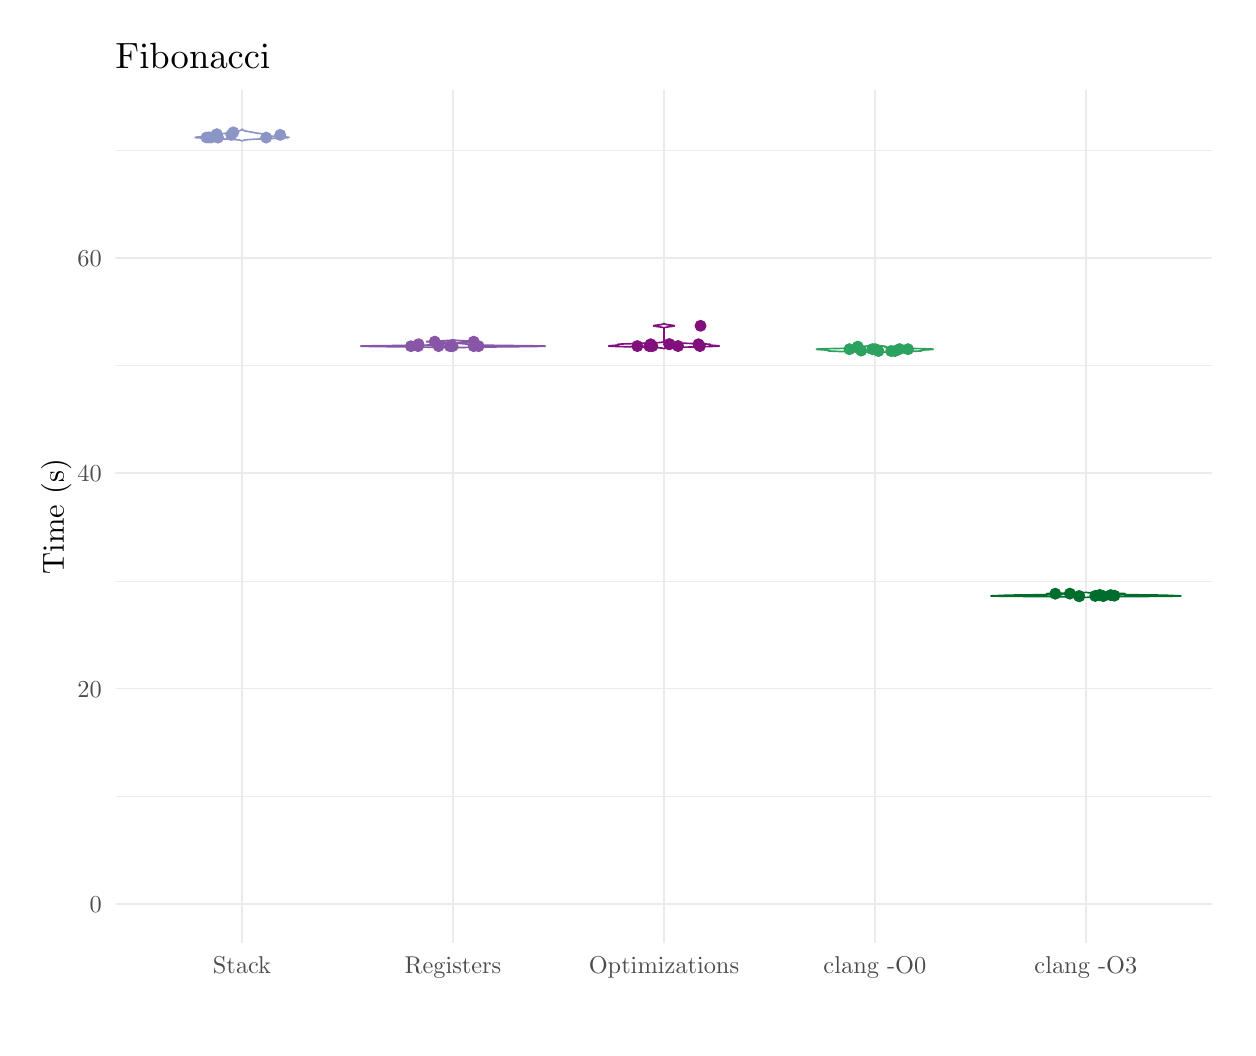
\begin{tikzpicture}[x=1pt,y=1pt]
\definecolor{fillColor}{RGB}{255,255,255}
\path[use as bounding box,fill=fillColor,fill opacity=0.00] (0,0) rectangle (433.62,361.35);
\begin{scope}
\path[clip] ( 31.71, 30.69) rectangle (428.12,338.69);
\definecolor{drawColor}{gray}{0.92}

\path[draw=drawColor,line width= 0.3pt,line join=round] ( 31.71, 83.60) --
	(428.12, 83.60);

\path[draw=drawColor,line width= 0.3pt,line join=round] ( 31.71,161.41) --
	(428.12,161.41);

\path[draw=drawColor,line width= 0.3pt,line join=round] ( 31.71,239.23) --
	(428.12,239.23);

\path[draw=drawColor,line width= 0.3pt,line join=round] ( 31.71,317.05) --
	(428.12,317.05);

\path[draw=drawColor,line width= 0.6pt,line join=round] ( 31.71, 44.69) --
	(428.12, 44.69);

\path[draw=drawColor,line width= 0.6pt,line join=round] ( 31.71,122.50) --
	(428.12,122.50);

\path[draw=drawColor,line width= 0.6pt,line join=round] ( 31.71,200.32) --
	(428.12,200.32);

\path[draw=drawColor,line width= 0.6pt,line join=round] ( 31.71,278.14) --
	(428.12,278.14);

\path[draw=drawColor,line width= 0.6pt,line join=round] ( 77.45, 30.69) --
	( 77.45,338.69);

\path[draw=drawColor,line width= 0.6pt,line join=round] (153.68, 30.69) --
	(153.68,338.69);

\path[draw=drawColor,line width= 0.6pt,line join=round] (229.92, 30.69) --
	(229.92,338.69);

\path[draw=drawColor,line width= 0.6pt,line join=round] (306.15, 30.69) --
	(306.15,338.69);

\path[draw=drawColor,line width= 0.6pt,line join=round] (382.38, 30.69) --
	(382.38,338.69);
\definecolor{drawColor}{RGB}{140,150,198}
\definecolor{fillColor}{RGB}{255,255,255}

\path[draw=drawColor,line width= 0.6pt,line join=round,line cap=round,fill=fillColor] ( 77.30,320.46) --
	( 77.29,320.47) --
	( 77.28,320.48) --
	( 77.27,320.49) --
	( 77.26,320.50) --
	( 77.25,320.50) --
	( 77.23,320.51) --
	( 77.22,320.52) --
	( 77.21,320.53) --
	( 77.19,320.54) --
	( 77.17,320.55) --
	( 77.16,320.55) --
	( 77.14,320.56) --
	( 77.12,320.57) --
	( 77.10,320.58) --
	( 77.08,320.59) --
	( 77.06,320.60) --
	( 77.03,320.60) --
	( 77.01,320.61) --
	( 76.98,320.62) --
	( 76.95,320.63) --
	( 76.93,320.64) --
	( 76.90,320.65) --
	( 76.86,320.65) --
	( 76.83,320.66) --
	( 76.80,320.67) --
	( 76.76,320.68) --
	( 76.72,320.69) --
	( 76.68,320.70) --
	( 76.64,320.70) --
	( 76.60,320.71) --
	( 76.55,320.72) --
	( 76.51,320.73) --
	( 76.46,320.74) --
	( 76.41,320.74) --
	( 76.36,320.75) --
	( 76.30,320.76) --
	( 76.24,320.77) --
	( 76.18,320.78) --
	( 76.12,320.79) --
	( 76.06,320.79) --
	( 75.99,320.80) --
	( 75.92,320.81) --
	( 75.85,320.82) --
	( 75.77,320.83) --
	( 75.70,320.84) --
	( 75.62,320.84) --
	( 75.53,320.85) --
	( 75.45,320.86) --
	( 75.36,320.87) --
	( 75.27,320.88) --
	( 75.17,320.89) --
	( 75.07,320.89) --
	( 74.98,320.90) --
	( 74.87,320.91) --
	( 74.76,320.92) --
	( 74.65,320.93) --
	( 74.54,320.94) --
	( 74.42,320.94) --
	( 74.30,320.95) --
	( 74.18,320.96) --
	( 74.05,320.97) --
	( 73.92,320.98) --
	( 73.79,320.98) --
	( 73.66,320.99) --
	( 73.52,321.00) --
	( 73.37,321.01) --
	( 73.23,321.02) --
	( 73.08,321.03) --
	( 72.92,321.03) --
	( 72.77,321.04) --
	( 72.61,321.05) --
	( 72.45,321.06) --
	( 72.28,321.07) --
	( 72.11,321.08) --
	( 71.94,321.08) --
	( 71.77,321.09) --
	( 71.59,321.10) --
	( 71.41,321.11) --
	( 71.22,321.12) --
	( 71.04,321.13) --
	( 70.85,321.13) --
	( 70.66,321.14) --
	( 70.46,321.15) --
	( 70.27,321.16) --
	( 70.07,321.17) --
	( 69.87,321.18) --
	( 69.67,321.18) --
	( 69.46,321.19) --
	( 69.26,321.20) --
	( 69.05,321.21) --
	( 68.84,321.22) --
	( 68.63,321.22) --
	( 68.42,321.23) --
	( 68.21,321.24) --
	( 68.00,321.25) --
	( 67.78,321.26) --
	( 67.57,321.27) --
	( 67.36,321.27) --
	( 67.14,321.28) --
	( 66.93,321.29) --
	( 66.72,321.30) --
	( 66.50,321.31) --
	( 66.29,321.32) --
	( 66.08,321.32) --
	( 65.87,321.33) --
	( 65.66,321.34) --
	( 65.45,321.35) --
	( 65.25,321.36) --
	( 65.04,321.37) --
	( 64.84,321.37) --
	( 64.64,321.38) --
	( 64.44,321.39) --
	( 64.25,321.40) --
	( 64.06,321.41) --
	( 63.87,321.42) --
	( 63.69,321.42) --
	( 63.51,321.43) --
	( 63.33,321.44) --
	( 63.16,321.45) --
	( 62.99,321.46) --
	( 62.82,321.46) --
	( 62.66,321.47) --
	( 62.51,321.48) --
	( 62.36,321.49) --
	( 62.21,321.50) --
	( 62.07,321.51) --
	( 61.94,321.51) --
	( 61.81,321.52) --
	( 61.68,321.53) --
	( 61.57,321.54) --
	( 61.45,321.55) --
	( 61.35,321.56) --
	( 61.25,321.56) --
	( 61.16,321.57) --
	( 61.07,321.58) --
	( 60.99,321.59) --
	( 60.91,321.60) --
	( 60.84,321.61) --
	( 60.78,321.61) --
	( 60.73,321.62) --
	( 60.68,321.63) --
	( 60.64,321.64) --
	( 60.61,321.65) --
	( 60.58,321.66) --
	( 60.56,321.66) --
	( 60.54,321.67) --
	( 60.54,321.68) --
	( 60.54,321.69) --
	( 60.54,321.70) --
	( 60.55,321.70) --
	( 60.57,321.71) --
	( 60.60,321.72) --
	( 60.63,321.73) --
	( 60.67,321.74) --
	( 60.71,321.75) --
	( 60.76,321.75) --
	( 60.82,321.76) --
	( 60.88,321.77) --
	( 60.94,321.78) --
	( 61.02,321.79) --
	( 61.09,321.80) --
	( 61.18,321.80) --
	( 61.26,321.81) --
	( 61.36,321.82) --
	( 61.45,321.83) --
	( 61.55,321.84) --
	( 61.66,321.85) --
	( 61.77,321.85) --
	( 61.88,321.86) --
	( 62.00,321.87) --
	( 62.12,321.88) --
	( 62.24,321.89) --
	( 62.37,321.90) --
	( 62.50,321.90) --
	( 62.63,321.91) --
	( 62.77,321.92) --
	( 62.90,321.93) --
	( 63.04,321.94) --
	( 63.18,321.94) --
	( 63.32,321.95) --
	( 63.46,321.96) --
	( 63.60,321.97) --
	( 63.75,321.98) --
	( 63.89,321.99) --
	( 64.03,321.99) --
	( 64.18,322.00) --
	( 64.32,322.01) --
	( 64.47,322.02) --
	( 64.61,322.03) --
	( 64.75,322.04) --
	( 64.89,322.04) --
	( 65.03,322.05) --
	( 65.17,322.06) --
	( 65.31,322.07) --
	( 65.44,322.08) --
	( 65.58,322.09) --
	( 65.71,322.09) --
	( 65.84,322.10) --
	( 65.97,322.11) --
	( 66.09,322.12) --
	( 66.21,322.13) --
	( 66.33,322.14) --
	( 66.45,322.14) --
	( 66.56,322.15) --
	( 66.67,322.16) --
	( 66.78,322.17) --
	( 66.89,322.18) --
	( 66.99,322.18) --
	( 67.09,322.19) --
	( 67.18,322.20) --
	( 67.27,322.21) --
	( 67.36,322.22) --
	( 67.45,322.23) --
	( 67.53,322.23) --
	( 67.61,322.24) --
	( 67.68,322.25) --
	( 67.75,322.26) --
	( 67.82,322.27) --
	( 67.89,322.28) --
	( 67.95,322.28) --
	( 68.01,322.29) --
	( 68.06,322.30) --
	( 68.11,322.31) --
	( 68.16,322.32) --
	( 68.21,322.33) --
	( 68.25,322.33) --
	( 68.29,322.34) --
	( 68.33,322.35) --
	( 68.36,322.36) --
	( 68.39,322.37) --
	( 68.42,322.38) --
	( 68.45,322.38) --
	( 68.47,322.39) --
	( 68.49,322.40) --
	( 68.51,322.41) --
	( 68.53,322.42) --
	( 68.55,322.42) --
	( 68.56,322.43) --
	( 68.57,322.44) --
	( 68.58,322.45) --
	( 68.59,322.46) --
	( 68.60,322.47) --
	( 68.61,322.47) --
	( 68.61,322.48) --
	( 68.62,322.49) --
	( 68.62,322.50) --
	( 68.62,322.51) --
	( 68.62,322.52) --
	( 68.63,322.52) --
	( 68.63,322.53) --
	( 68.63,322.54) --
	( 68.63,322.55) --
	( 68.63,322.56) --
	( 68.63,322.57) --
	( 68.63,322.57) --
	( 68.64,322.58) --
	( 68.64,322.59) --
	( 68.64,322.60) --
	( 68.64,322.61) --
	( 68.65,322.62) --
	( 68.65,322.62) --
	( 68.66,322.63) --
	( 68.66,322.64) --
	( 68.67,322.65) --
	( 68.68,322.66) --
	( 68.69,322.66) --
	( 68.70,322.67) --
	( 68.71,322.68) --
	( 68.72,322.69) --
	( 68.74,322.70) --
	( 68.75,322.71) --
	( 68.77,322.71) --
	( 68.79,322.72) --
	( 68.81,322.73) --
	( 68.83,322.74) --
	( 68.86,322.75) --
	( 68.88,322.76) --
	( 68.91,322.76) --
	( 68.94,322.77) --
	( 68.97,322.78) --
	( 69.00,322.79) --
	( 69.03,322.80) --
	( 69.06,322.81) --
	( 69.10,322.81) --
	( 69.14,322.82) --
	( 69.17,322.83) --
	( 69.21,322.84) --
	( 69.26,322.85) --
	( 69.30,322.86) --
	( 69.34,322.86) --
	( 69.39,322.87) --
	( 69.44,322.88) --
	( 69.48,322.89) --
	( 69.53,322.90) --
	( 69.58,322.90) --
	( 69.64,322.91) --
	( 69.69,322.92) --
	( 69.74,322.93) --
	( 69.80,322.94) --
	( 69.85,322.95) --
	( 69.91,322.95) --
	( 69.97,322.96) --
	( 70.02,322.97) --
	( 70.08,322.98) --
	( 70.14,322.99) --
	( 70.20,323.00) --
	( 70.26,323.00) --
	( 70.32,323.01) --
	( 70.38,323.02) --
	( 70.44,323.03) --
	( 70.51,323.04) --
	( 70.57,323.05) --
	( 70.63,323.05) --
	( 70.69,323.06) --
	( 70.76,323.07) --
	( 70.82,323.08) --
	( 70.88,323.09) --
	( 70.94,323.10) --
	( 71.00,323.10) --
	( 71.07,323.11) --
	( 71.13,323.12) --
	( 71.19,323.13) --
	( 71.25,323.14) --
	( 71.31,323.14) --
	( 71.37,323.15) --
	( 71.43,323.16) --
	( 71.49,323.17) --
	( 71.55,323.18) --
	( 71.61,323.19) --
	( 71.67,323.19) --
	( 71.73,323.20) --
	( 71.78,323.21) --
	( 71.84,323.22) --
	( 71.90,323.23) --
	( 71.95,323.24) --
	( 72.01,323.24) --
	( 72.06,323.25) --
	( 72.12,323.26) --
	( 72.17,323.27) --
	( 72.22,323.28) --
	( 72.28,323.29) --
	( 72.33,323.29) --
	( 72.38,323.30) --
	( 72.43,323.31) --
	( 72.48,323.32) --
	( 72.53,323.33) --
	( 72.58,323.34) --
	( 72.63,323.34) --
	( 72.68,323.35) --
	( 72.73,323.36) --
	( 72.78,323.37) --
	( 72.82,323.38) --
	( 72.87,323.38) --
	( 72.92,323.39) --
	( 72.96,323.40) --
	( 73.01,323.41) --
	( 73.05,323.42) --
	( 73.10,323.43) --
	( 73.14,323.43) --
	( 73.19,323.44) --
	( 73.23,323.45) --
	( 73.28,323.46) --
	( 73.32,323.47) --
	( 73.36,323.48) --
	( 73.41,323.48) --
	( 73.45,323.49) --
	( 73.49,323.50) --
	( 73.54,323.51) --
	( 73.58,323.52) --
	( 73.62,323.53) --
	( 73.67,323.53) --
	( 73.71,323.54) --
	( 73.75,323.55) --
	( 73.80,323.56) --
	( 73.84,323.57) --
	( 73.88,323.58) --
	( 73.93,323.58) --
	( 73.97,323.59) --
	( 74.01,323.60) --
	( 74.06,323.61) --
	( 74.10,323.62) --
	( 74.14,323.62) --
	( 74.19,323.63) --
	( 74.23,323.64) --
	( 74.27,323.65) --
	( 74.32,323.66) --
	( 74.36,323.67) --
	( 74.41,323.67) --
	( 74.45,323.68) --
	( 74.49,323.69) --
	( 74.54,323.70) --
	( 74.58,323.71) --
	( 74.63,323.72) --
	( 74.67,323.72) --
	( 74.72,323.73) --
	( 74.76,323.74) --
	( 74.81,323.75) --
	( 74.85,323.76) --
	( 74.90,323.77) --
	( 74.94,323.77) --
	( 74.98,323.78) --
	( 75.03,323.79) --
	( 75.07,323.80) --
	( 75.12,323.81) --
	( 75.16,323.82) --
	( 75.21,323.82) --
	( 75.25,323.83) --
	( 75.29,323.84) --
	( 75.34,323.85) --
	( 75.38,323.86) --
	( 75.43,323.86) --
	( 75.47,323.87) --
	( 75.51,323.88) --
	( 75.55,323.89) --
	( 75.60,323.90) --
	( 75.64,323.91) --
	( 75.68,323.91) --
	( 75.72,323.92) --
	( 75.76,323.93) --
	( 75.80,323.94) --
	( 75.84,323.95) --
	( 75.88,323.96) --
	( 75.92,323.96) --
	( 75.96,323.97) --
	( 76.00,323.98) --
	( 76.04,323.99) --
	( 76.08,324.00) --
	( 76.11,324.01) --
	( 76.15,324.01) --
	( 76.19,324.02) --
	( 76.22,324.03) --
	( 76.26,324.04) --
	( 76.29,324.05) --
	( 76.33,324.06) --
	( 76.36,324.06) --
	( 76.39,324.07) --
	( 76.43,324.08) --
	( 76.46,324.09) --
	( 76.49,324.10) --
	( 76.52,324.10) --
	( 76.55,324.11) --
	( 76.58,324.12) --
	( 76.61,324.13) --
	( 76.64,324.14) --
	( 76.66,324.15) --
	( 76.69,324.15) --
	( 76.72,324.16) --
	( 76.74,324.17) --
	( 76.77,324.18) --
	( 76.79,324.19) --
	( 76.82,324.20) --
	( 76.84,324.20) --
	( 76.86,324.21) --
	( 76.88,324.22) --
	( 76.91,324.23) --
	( 76.93,324.24) --
	( 76.95,324.25) --
	( 76.97,324.25) --
	( 76.99,324.26) --
	( 77.01,324.27) --
	( 77.02,324.28) --
	( 77.04,324.29) --
	( 77.06,324.30) --
	( 77.07,324.30) --
	( 77.09,324.31) --
	( 77.11,324.32) --
	( 77.12,324.33) --
	( 77.13,324.34) --
	( 77.15,324.34) --
	( 77.16,324.35) --
	( 77.17,324.36) --
	( 77.19,324.37) --
	( 77.20,324.38) --
	( 77.21,324.39) --
	( 77.22,324.39) --
	( 77.23,324.40) --
	( 77.24,324.41) --
	( 77.25,324.42) --
	( 77.26,324.43) --
	( 77.27,324.44) --
	( 77.28,324.44) --
	( 77.29,324.45) --
	( 77.30,324.46) --
	( 77.30,324.47) --
	( 77.31,324.48) --
	( 77.32,324.49) --
	( 77.33,324.49) --
	( 77.33,324.50) --
	( 77.34,324.51) --
	( 77.34,324.52) --
	( 77.35,324.53) --
	( 77.36,324.54) --
	( 77.36,324.54) --
	( 77.37,324.55) --
	( 77.37,324.56) --
	( 77.37,324.57) --
	( 77.38,324.58) --
	( 77.38,324.58) --
	( 77.39,324.59) --
	( 77.39,324.60) --
	( 77.39,324.61) --
	( 77.40,324.62) --
	( 77.40,324.63) --
	( 77.40,324.63) --
	( 77.41,324.64) --
	( 77.41,324.65) --
	( 77.41,324.66) --
	( 77.41,324.67) --
	( 77.42,324.68) --
	( 77.42,324.68) --
	( 77.42,324.69) --
	( 77.48,324.69) --
	( 77.48,324.68) --
	( 77.49,324.68) --
	( 77.49,324.67) --
	( 77.49,324.66) --
	( 77.49,324.65) --
	( 77.50,324.64) --
	( 77.50,324.63) --
	( 77.50,324.63) --
	( 77.51,324.62) --
	( 77.51,324.61) --
	( 77.51,324.60) --
	( 77.52,324.59) --
	( 77.52,324.58) --
	( 77.52,324.58) --
	( 77.53,324.57) --
	( 77.53,324.56) --
	( 77.54,324.55) --
	( 77.54,324.54) --
	( 77.55,324.54) --
	( 77.55,324.53) --
	( 77.56,324.52) --
	( 77.56,324.51) --
	( 77.57,324.50) --
	( 77.58,324.49) --
	( 77.58,324.49) --
	( 77.59,324.48) --
	( 77.60,324.47) --
	( 77.61,324.46) --
	( 77.61,324.45) --
	( 77.62,324.44) --
	( 77.63,324.44) --
	( 77.64,324.43) --
	( 77.65,324.42) --
	( 77.66,324.41) --
	( 77.67,324.40) --
	( 77.68,324.39) --
	( 77.69,324.39) --
	( 77.70,324.38) --
	( 77.72,324.37) --
	( 77.73,324.36) --
	( 77.74,324.35) --
	( 77.75,324.34) --
	( 77.77,324.34) --
	( 77.78,324.33) --
	( 77.80,324.32) --
	( 77.81,324.31) --
	( 77.83,324.30) --
	( 77.85,324.30) --
	( 77.86,324.29) --
	( 77.88,324.28) --
	( 77.90,324.27) --
	( 77.92,324.26) --
	( 77.94,324.25) --
	( 77.96,324.25) --
	( 77.98,324.24) --
	( 78.00,324.23) --
	( 78.02,324.22) --
	( 78.04,324.21) --
	( 78.06,324.20) --
	( 78.09,324.20) --
	( 78.11,324.19) --
	( 78.13,324.18) --
	( 78.16,324.17) --
	( 78.19,324.16) --
	( 78.21,324.15) --
	( 78.24,324.15) --
	( 78.27,324.14) --
	( 78.29,324.13) --
	( 78.32,324.12) --
	( 78.35,324.11) --
	( 78.38,324.10) --
	( 78.41,324.10) --
	( 78.44,324.09) --
	( 78.48,324.08) --
	( 78.51,324.07) --
	( 78.54,324.06) --
	( 78.58,324.06) --
	( 78.61,324.05) --
	( 78.64,324.04) --
	( 78.68,324.03) --
	( 78.72,324.02) --
	( 78.75,324.01) --
	( 78.79,324.01) --
	( 78.83,324.00) --
	( 78.86,323.99) --
	( 78.90,323.98) --
	( 78.94,323.97) --
	( 78.98,323.96) --
	( 79.02,323.96) --
	( 79.06,323.95) --
	( 79.10,323.94) --
	( 79.14,323.93) --
	( 79.18,323.92) --
	( 79.22,323.91) --
	( 79.26,323.91) --
	( 79.31,323.90) --
	( 79.35,323.89) --
	( 79.39,323.88) --
	( 79.43,323.87) --
	( 79.48,323.86) --
	( 79.52,323.86) --
	( 79.56,323.85) --
	( 79.61,323.84) --
	( 79.65,323.83) --
	( 79.70,323.82) --
	( 79.74,323.82) --
	( 79.79,323.81) --
	( 79.83,323.80) --
	( 79.87,323.79) --
	( 79.92,323.78) --
	( 79.96,323.77) --
	( 80.01,323.77) --
	( 80.05,323.76) --
	( 80.10,323.75) --
	( 80.14,323.74) --
	( 80.19,323.73) --
	( 80.23,323.72) --
	( 80.28,323.72) --
	( 80.32,323.71) --
	( 80.36,323.70) --
	( 80.41,323.69) --
	( 80.45,323.68) --
	( 80.50,323.67) --
	( 80.54,323.67) --
	( 80.58,323.66) --
	( 80.63,323.65) --
	( 80.67,323.64) --
	( 80.72,323.63) --
	( 80.76,323.62) --
	( 80.80,323.62) --
	( 80.85,323.61) --
	( 80.89,323.60) --
	( 80.93,323.59) --
	( 80.98,323.58) --
	( 81.02,323.58) --
	( 81.06,323.57) --
	( 81.11,323.56) --
	( 81.15,323.55) --
	( 81.19,323.54) --
	( 81.24,323.53) --
	( 81.28,323.53) --
	( 81.32,323.52) --
	( 81.37,323.51) --
	( 81.41,323.50) --
	( 81.45,323.49) --
	( 81.50,323.48) --
	( 81.54,323.48) --
	( 81.58,323.47) --
	( 81.63,323.46) --
	( 81.67,323.45) --
	( 81.72,323.44) --
	( 81.76,323.43) --
	( 81.80,323.43) --
	( 81.85,323.42) --
	( 81.90,323.41) --
	( 81.94,323.40) --
	( 81.99,323.39) --
	( 82.03,323.38) --
	( 82.08,323.38) --
	( 82.13,323.37) --
	( 82.18,323.36) --
	( 82.22,323.35) --
	( 82.27,323.34) --
	( 82.32,323.34) --
	( 82.37,323.33) --
	( 82.42,323.32) --
	( 82.47,323.31) --
	( 82.52,323.30) --
	( 82.57,323.29) --
	( 82.63,323.29) --
	( 82.68,323.28) --
	( 82.73,323.27) --
	( 82.79,323.26) --
	( 82.84,323.25) --
	( 82.89,323.24) --
	( 82.95,323.24) --
	( 83.01,323.23) --
	( 83.06,323.22) --
	( 83.12,323.21) --
	( 83.18,323.20) --
	( 83.23,323.19) --
	( 83.29,323.19) --
	( 83.35,323.18) --
	( 83.41,323.17) --
	( 83.47,323.16) --
	( 83.53,323.15) --
	( 83.59,323.14) --
	( 83.65,323.14) --
	( 83.71,323.13) --
	( 83.78,323.12) --
	( 83.84,323.11) --
	( 83.90,323.10) --
	( 83.96,323.10) --
	( 84.02,323.09) --
	( 84.09,323.08) --
	( 84.15,323.07) --
	( 84.21,323.06) --
	( 84.27,323.05) --
	( 84.33,323.05) --
	( 84.40,323.04) --
	( 84.46,323.03) --
	( 84.52,323.02) --
	( 84.58,323.01) --
	( 84.64,323.00) --
	( 84.70,323.00) --
	( 84.76,322.99) --
	( 84.82,322.98) --
	( 84.88,322.97) --
	( 84.94,322.96) --
	( 84.99,322.95) --
	( 85.05,322.95) --
	( 85.11,322.94) --
	( 85.16,322.93) --
	( 85.21,322.92) --
	( 85.27,322.91) --
	( 85.32,322.90) --
	( 85.37,322.90) --
	( 85.42,322.89) --
	( 85.47,322.88) --
	( 85.51,322.87) --
	( 85.56,322.86) --
	( 85.60,322.86) --
	( 85.65,322.85) --
	( 85.69,322.84) --
	( 85.73,322.83) --
	( 85.77,322.82) --
	( 85.80,322.81) --
	( 85.84,322.81) --
	( 85.87,322.80) --
	( 85.91,322.79) --
	( 85.94,322.78) --
	( 85.97,322.77) --
	( 86.00,322.76) --
	( 86.02,322.76) --
	( 86.05,322.75) --
	( 86.07,322.74) --
	( 86.09,322.73) --
	( 86.11,322.72) --
	( 86.13,322.71) --
	( 86.15,322.71) --
	( 86.16,322.70) --
	( 86.18,322.69) --
	( 86.19,322.68) --
	( 86.20,322.67) --
	( 86.21,322.66) --
	( 86.22,322.66) --
	( 86.23,322.65) --
	( 86.24,322.64) --
	( 86.25,322.63) --
	( 86.25,322.62) --
	( 86.26,322.62) --
	( 86.26,322.61) --
	( 86.26,322.60) --
	( 86.27,322.59) --
	( 86.27,322.58) --
	( 86.27,322.57) --
	( 86.27,322.57) --
	( 86.27,322.56) --
	( 86.27,322.55) --
	( 86.27,322.54) --
	( 86.28,322.53) --
	( 86.28,322.52) --
	( 86.28,322.52) --
	( 86.28,322.51) --
	( 86.28,322.50) --
	( 86.29,322.49) --
	( 86.29,322.48) --
	( 86.30,322.47) --
	( 86.30,322.47) --
	( 86.31,322.46) --
	( 86.32,322.45) --
	( 86.33,322.44) --
	( 86.34,322.43) --
	( 86.36,322.42) --
	( 86.37,322.42) --
	( 86.39,322.41) --
	( 86.41,322.40) --
	( 86.43,322.39) --
	( 86.45,322.38) --
	( 86.48,322.38) --
	( 86.51,322.37) --
	( 86.54,322.36) --
	( 86.58,322.35) --
	( 86.61,322.34) --
	( 86.65,322.33) --
	( 86.69,322.33) --
	( 86.74,322.32) --
	( 86.79,322.31) --
	( 86.84,322.30) --
	( 86.90,322.29) --
	( 86.95,322.28) --
	( 87.02,322.28) --
	( 87.08,322.27) --
	( 87.15,322.26) --
	( 87.22,322.25) --
	( 87.30,322.24) --
	( 87.37,322.23) --
	( 87.46,322.23) --
	( 87.54,322.22) --
	( 87.63,322.21) --
	( 87.72,322.20) --
	( 87.82,322.19) --
	( 87.92,322.18) --
	( 88.02,322.18) --
	( 88.12,322.17) --
	( 88.23,322.16) --
	( 88.34,322.15) --
	( 88.45,322.14) --
	( 88.57,322.14) --
	( 88.69,322.13) --
	( 88.81,322.12) --
	( 88.94,322.11) --
	( 89.07,322.10) --
	( 89.19,322.09) --
	( 89.33,322.09) --
	( 89.46,322.08) --
	( 89.60,322.07) --
	( 89.73,322.06) --
	( 89.87,322.05) --
	( 90.01,322.04) --
	( 90.15,322.04) --
	( 90.29,322.03) --
	( 90.44,322.02) --
	( 90.58,322.01) --
	( 90.73,322.00) --
	( 90.87,321.99) --
	( 91.01,321.99) --
	( 91.16,321.98) --
	( 91.30,321.97) --
	( 91.44,321.96) --
	( 91.58,321.95) --
	( 91.72,321.94) --
	( 91.86,321.94) --
	( 92.00,321.93) --
	( 92.14,321.92) --
	( 92.27,321.91) --
	( 92.40,321.90) --
	( 92.53,321.90) --
	( 92.66,321.89) --
	( 92.78,321.88) --
	( 92.90,321.87) --
	( 93.02,321.86) --
	( 93.13,321.85) --
	( 93.24,321.85) --
	( 93.35,321.84) --
	( 93.45,321.83) --
	( 93.55,321.82) --
	( 93.64,321.81) --
	( 93.73,321.80) --
	( 93.81,321.80) --
	( 93.89,321.79) --
	( 93.96,321.78) --
	( 94.03,321.77) --
	( 94.09,321.76) --
	( 94.14,321.75) --
	( 94.19,321.75) --
	( 94.24,321.74) --
	( 94.27,321.73) --
	( 94.31,321.72) --
	( 94.33,321.71) --
	( 94.35,321.70) --
	( 94.36,321.70) --
	( 94.37,321.69) --
	( 94.37,321.68) --
	( 94.36,321.67) --
	( 94.35,321.66) --
	( 94.32,321.66) --
	( 94.30,321.65) --
	( 94.26,321.64) --
	( 94.22,321.63) --
	( 94.18,321.62) --
	( 94.12,321.61) --
	( 94.06,321.61) --
	( 93.99,321.60) --
	( 93.92,321.59) --
	( 93.84,321.58) --
	( 93.75,321.57) --
	( 93.66,321.56) --
	( 93.55,321.56) --
	( 93.45,321.55) --
	( 93.34,321.54) --
	( 93.22,321.53) --
	( 93.10,321.52) --
	( 92.97,321.51) --
	( 92.83,321.51) --
	( 92.69,321.50) --
	( 92.55,321.49) --
	( 92.40,321.48) --
	( 92.24,321.47) --
	( 92.08,321.46) --
	( 91.92,321.46) --
	( 91.75,321.45) --
	( 91.57,321.44) --
	( 91.40,321.43) --
	( 91.22,321.42) --
	( 91.03,321.42) --
	( 90.84,321.41) --
	( 90.65,321.40) --
	( 90.46,321.39) --
	( 90.26,321.38) --
	( 90.06,321.37) --
	( 89.86,321.37) --
	( 89.66,321.36) --
	( 89.45,321.35) --
	( 89.24,321.34) --
	( 89.04,321.33) --
	( 88.82,321.32) --
	( 88.61,321.32) --
	( 88.40,321.31) --
	( 88.19,321.30) --
	( 87.97,321.29) --
	( 87.76,321.28) --
	( 87.55,321.27) --
	( 87.33,321.27) --
	( 87.12,321.26) --
	( 86.91,321.25) --
	( 86.69,321.24) --
	( 86.48,321.23) --
	( 86.27,321.22) --
	( 86.06,321.22) --
	( 85.85,321.21) --
	( 85.64,321.20) --
	( 85.44,321.19) --
	( 85.23,321.18) --
	( 85.03,321.18) --
	( 84.83,321.17) --
	( 84.63,321.16) --
	( 84.44,321.15) --
	( 84.25,321.14) --
	( 84.05,321.13) --
	( 83.87,321.13) --
	( 83.68,321.12) --
	( 83.50,321.11) --
	( 83.32,321.10) --
	( 83.14,321.09) --
	( 82.96,321.08) --
	( 82.79,321.08) --
	( 82.62,321.07) --
	( 82.46,321.06) --
	( 82.29,321.05) --
	( 82.14,321.04) --
	( 81.98,321.03) --
	( 81.83,321.03) --
	( 81.68,321.02) --
	( 81.53,321.01) --
	( 81.39,321.00) --
	( 81.25,320.99) --
	( 81.11,320.98) --
	( 80.98,320.98) --
	( 80.85,320.97) --
	( 80.72,320.96) --
	( 80.60,320.95) --
	( 80.48,320.94) --
	( 80.36,320.94) --
	( 80.25,320.93) --
	( 80.14,320.92) --
	( 80.03,320.91) --
	( 79.93,320.90) --
	( 79.83,320.89) --
	( 79.73,320.89) --
	( 79.64,320.88) --
	( 79.54,320.87) --
	( 79.46,320.86) --
	( 79.37,320.85) --
	( 79.29,320.84) --
	( 79.21,320.84) --
	( 79.13,320.83) --
	( 79.05,320.82) --
	( 78.98,320.81) --
	( 78.91,320.80) --
	( 78.85,320.79) --
	( 78.78,320.79) --
	( 78.72,320.78) --
	( 78.66,320.77) --
	( 78.60,320.76) --
	( 78.55,320.75) --
	( 78.49,320.74) --
	( 78.44,320.74) --
	( 78.39,320.73) --
	( 78.35,320.72) --
	( 78.30,320.71) --
	( 78.26,320.70) --
	( 78.22,320.70) --
	( 78.18,320.69) --
	( 78.14,320.68) --
	( 78.11,320.67) --
	( 78.07,320.66) --
	( 78.04,320.65) --
	( 78.01,320.65) --
	( 77.98,320.64) --
	( 77.95,320.63) --
	( 77.92,320.62) --
	( 77.90,320.61) --
	( 77.87,320.60) --
	( 77.85,320.60) --
	( 77.83,320.59) --
	( 77.80,320.58) --
	( 77.78,320.57) --
	( 77.76,320.56) --
	( 77.75,320.55) --
	( 77.73,320.55) --
	( 77.71,320.54) --
	( 77.70,320.53) --
	( 77.68,320.52) --
	( 77.67,320.51) --
	( 77.66,320.50) --
	( 77.64,320.50) --
	( 77.63,320.49) --
	( 77.62,320.48) --
	( 77.61,320.47) --
	( 77.60,320.46) --
	( 77.30,320.46) --
	cycle;
\definecolor{drawColor}{RGB}{136,86,167}

\path[draw=drawColor,line width= 0.6pt,line join=round,line cap=round,fill=fillColor] (153.37,245.57) --
	(153.35,245.57) --
	(153.32,245.58) --
	(153.29,245.59) --
	(153.26,245.59) --
	(153.23,245.60) --
	(153.19,245.60) --
	(153.15,245.61) --
	(153.11,245.61) --
	(153.07,245.62) --
	(153.02,245.63) --
	(152.97,245.63) --
	(152.92,245.64) --
	(152.86,245.64) --
	(152.80,245.65) --
	(152.74,245.66) --
	(152.67,245.66) --
	(152.60,245.67) --
	(152.52,245.67) --
	(152.44,245.68) --
	(152.36,245.69) --
	(152.27,245.69) --
	(152.17,245.70) --
	(152.07,245.70) --
	(151.97,245.71) --
	(151.85,245.71) --
	(151.74,245.72) --
	(151.61,245.73) --
	(151.48,245.73) --
	(151.35,245.74) --
	(151.20,245.74) --
	(151.05,245.75) --
	(150.90,245.76) --
	(150.73,245.76) --
	(150.56,245.77) --
	(150.38,245.77) --
	(150.19,245.78) --
	(149.99,245.79) --
	(149.79,245.79) --
	(149.58,245.80) --
	(149.36,245.80) --
	(149.12,245.81) --
	(148.88,245.81) --
	(148.63,245.82) --
	(148.37,245.83) --
	(148.11,245.83) --
	(147.83,245.84) --
	(147.54,245.84) --
	(147.24,245.85) --
	(146.93,245.86) --
	(146.61,245.86) --
	(146.29,245.87) --
	(145.95,245.87) --
	(145.60,245.88) --
	(145.24,245.89) --
	(144.88,245.89) --
	(144.50,245.90) --
	(144.11,245.90) --
	(143.72,245.91) --
	(143.31,245.92) --
	(142.89,245.92) --
	(142.47,245.93) --
	(142.04,245.93) --
	(141.59,245.94) --
	(141.15,245.94) --
	(140.69,245.95) --
	(140.22,245.96) --
	(139.75,245.96) --
	(139.27,245.97) --
	(138.78,245.97) --
	(138.29,245.98) --
	(137.79,245.99) --
	(137.28,245.99) --
	(136.77,246.00) --
	(136.26,246.00) --
	(135.75,246.01) --
	(135.23,246.02) --
	(134.71,246.02) --
	(134.18,246.03) --
	(133.66,246.03) --
	(133.14,246.04) --
	(132.61,246.04) --
	(132.09,246.05) --
	(131.57,246.06) --
	(131.05,246.06) --
	(130.54,246.07) --
	(130.03,246.07) --
	(129.52,246.08) --
	(129.02,246.09) --
	(128.53,246.09) --
	(128.05,246.10) --
	(127.57,246.10) --
	(127.10,246.11) --
	(126.64,246.12) --
	(126.20,246.12) --
	(125.76,246.13) --
	(125.33,246.13) --
	(124.92,246.14) --
	(124.53,246.14) --
	(124.14,246.15) --
	(123.77,246.16) --
	(123.42,246.16) --
	(123.08,246.17) --
	(122.76,246.17) --
	(122.46,246.18) --
	(122.18,246.19) --
	(121.91,246.19) --
	(121.67,246.20) --
	(121.44,246.20) --
	(121.23,246.21) --
	(121.05,246.22) --
	(120.89,246.22) --
	(120.74,246.23) --
	(120.62,246.23) --
	(120.52,246.24) --
	(120.44,246.24) --
	(120.38,246.25) --
	(120.34,246.26) --
	(120.34,246.26) --
	(120.35,246.27) --
	(120.37,246.27) --
	(120.43,246.28) --
	(120.51,246.29) --
	(120.60,246.29) --
	(120.73,246.30) --
	(120.86,246.30) --
	(121.03,246.31) --
	(121.21,246.32) --
	(121.41,246.32) --
	(121.63,246.33) --
	(121.87,246.33) --
	(122.13,246.34) --
	(122.41,246.35) --
	(122.70,246.35) --
	(123.02,246.36) --
	(123.35,246.36) --
	(123.69,246.37) --
	(124.05,246.37) --
	(124.43,246.38) --
	(124.81,246.39) --
	(125.22,246.39) --
	(125.63,246.40) --
	(126.05,246.40) --
	(126.49,246.41) --
	(126.93,246.42) --
	(127.38,246.42) --
	(127.84,246.43) --
	(128.31,246.43) --
	(128.79,246.44) --
	(129.27,246.45) --
	(129.75,246.45) --
	(130.24,246.46) --
	(130.73,246.46) --
	(131.23,246.47) --
	(131.72,246.47) --
	(132.22,246.48) --
	(132.72,246.49) --
	(133.21,246.49) --
	(133.71,246.50) --
	(134.20,246.50) --
	(134.69,246.51) --
	(135.17,246.52) --
	(135.65,246.52) --
	(136.13,246.53) --
	(136.60,246.53) --
	(137.06,246.54) --
	(137.52,246.55) --
	(137.97,246.55) --
	(138.41,246.56) --
	(138.85,246.56) --
	(139.28,246.57) --
	(139.69,246.57) --
	(140.10,246.58) --
	(140.50,246.59) --
	(140.89,246.59) --
	(141.27,246.60) --
	(141.64,246.60) --
	(141.99,246.61) --
	(142.34,246.62) --
	(142.68,246.62) --
	(143.00,246.63) --
	(143.32,246.63) --
	(143.62,246.64) --
	(143.92,246.65) --
	(144.20,246.65) --
	(144.47,246.66) --
	(144.73,246.66) --
	(144.98,246.67) --
	(145.21,246.67) --
	(145.44,246.68) --
	(145.65,246.69) --
	(145.86,246.69) --
	(146.06,246.70) --
	(146.24,246.70) --
	(146.42,246.71) --
	(146.58,246.72) --
	(146.73,246.72) --
	(146.88,246.73) --
	(147.02,246.73) --
	(147.15,246.74) --
	(147.27,246.75) --
	(147.38,246.75) --
	(147.48,246.76) --
	(147.58,246.76) --
	(147.67,246.77) --
	(147.75,246.78) --
	(147.83,246.78) --
	(147.90,246.79) --
	(147.96,246.79) --
	(148.02,246.80) --
	(148.07,246.80) --
	(148.12,246.81) --
	(148.17,246.82) --
	(148.21,246.82) --
	(148.24,246.83) --
	(148.27,246.83) --
	(148.30,246.84) --
	(148.33,246.85) --
	(148.35,246.85) --
	(148.37,246.86) --
	(148.39,246.86) --
	(148.41,246.87) --
	(148.42,246.88) --
	(148.44,246.88) --
	(148.45,246.89) --
	(148.46,246.89) --
	(148.48,246.90) --
	(148.49,246.90) --
	(148.50,246.91) --
	(148.51,246.92) --
	(148.52,246.92) --
	(148.54,246.93) --
	(148.55,246.93) --
	(148.57,246.94) --
	(148.58,246.95) --
	(148.60,246.95) --
	(148.62,246.96) --
	(148.64,246.96) --
	(148.66,246.97) --
	(148.68,246.98) --
	(148.70,246.98) --
	(148.73,246.99) --
	(148.76,246.99) --
	(148.79,247.00) --
	(148.82,247.00) --
	(148.85,247.01) --
	(148.89,247.02) --
	(148.93,247.02) --
	(148.97,247.03) --
	(149.01,247.03) --
	(149.06,247.04) --
	(149.10,247.05) --
	(149.15,247.05) --
	(149.20,247.06) --
	(149.25,247.06) --
	(149.31,247.07) --
	(149.36,247.08) --
	(149.42,247.08) --
	(149.48,247.09) --
	(149.54,247.09) --
	(149.60,247.10) --
	(149.66,247.11) --
	(149.73,247.11) --
	(149.79,247.12) --
	(149.86,247.12) --
	(149.93,247.13) --
	(149.99,247.13) --
	(150.06,247.14) --
	(150.13,247.15) --
	(150.20,247.15) --
	(150.27,247.16) --
	(150.34,247.16) --
	(150.41,247.17) --
	(150.48,247.18) --
	(150.55,247.18) --
	(150.62,247.19) --
	(150.69,247.19) --
	(150.76,247.20) --
	(150.83,247.21) --
	(150.90,247.21) --
	(150.96,247.22) --
	(151.03,247.22) --
	(151.10,247.23) --
	(151.16,247.23) --
	(151.22,247.24) --
	(151.28,247.25) --
	(151.34,247.25) --
	(151.40,247.26) --
	(151.45,247.26) --
	(151.51,247.27) --
	(151.56,247.28) --
	(151.61,247.28) --
	(151.66,247.29) --
	(151.70,247.29) --
	(151.74,247.30) --
	(151.78,247.31) --
	(151.82,247.31) --
	(151.86,247.32) --
	(151.89,247.32) --
	(151.92,247.33) --
	(151.94,247.33) --
	(151.97,247.34) --
	(151.99,247.35) --
	(152.01,247.35) --
	(152.02,247.36) --
	(152.03,247.36) --
	(152.04,247.37) --
	(152.04,247.38) --
	(152.05,247.38) --
	(152.04,247.39) --
	(152.04,247.39) --
	(152.03,247.40) --
	(152.02,247.41) --
	(152.00,247.41) --
	(151.98,247.42) --
	(151.95,247.42) --
	(151.93,247.43) --
	(151.90,247.43) --
	(151.86,247.44) --
	(151.82,247.45) --
	(151.78,247.45) --
	(151.73,247.46) --
	(151.68,247.46) --
	(151.63,247.47) --
	(151.57,247.48) --
	(151.51,247.48) --
	(151.44,247.49) --
	(151.37,247.49) --
	(151.30,247.50) --
	(151.22,247.51) --
	(151.14,247.51) --
	(151.05,247.52) --
	(150.96,247.52) --
	(150.87,247.53) --
	(150.77,247.54) --
	(150.68,247.54) --
	(150.57,247.55) --
	(150.47,247.55) --
	(150.36,247.56) --
	(150.24,247.56) --
	(150.13,247.57) --
	(150.01,247.58) --
	(149.89,247.58) --
	(149.76,247.59) --
	(149.64,247.59) --
	(149.51,247.60) --
	(149.38,247.61) --
	(149.24,247.61) --
	(149.11,247.62) --
	(148.97,247.62) --
	(148.83,247.63) --
	(148.69,247.64) --
	(148.54,247.64) --
	(148.40,247.65) --
	(148.25,247.65) --
	(148.11,247.66) --
	(147.96,247.66) --
	(147.82,247.67) --
	(147.67,247.68) --
	(147.52,247.68) --
	(147.38,247.69) --
	(147.23,247.69) --
	(147.09,247.70) --
	(146.94,247.71) --
	(146.80,247.71) --
	(146.66,247.72) --
	(146.52,247.72) --
	(146.38,247.73) --
	(146.24,247.74) --
	(146.11,247.74) --
	(145.98,247.75) --
	(145.85,247.75) --
	(145.73,247.76) --
	(145.60,247.76) --
	(145.49,247.77) --
	(145.37,247.78) --
	(145.26,247.78) --
	(145.16,247.79) --
	(145.05,247.79) --
	(144.96,247.80) --
	(144.87,247.81) --
	(144.78,247.81) --
	(144.70,247.82) --
	(144.62,247.82) --
	(144.55,247.83) --
	(144.48,247.84) --
	(144.42,247.84) --
	(144.37,247.85) --
	(144.32,247.85) --
	(144.28,247.86) --
	(144.24,247.86) --
	(144.21,247.87) --
	(144.19,247.88) --
	(144.17,247.88) --
	(144.16,247.89) --
	(144.16,247.89) --
	(144.16,247.90) --
	(144.17,247.91) --
	(144.18,247.91) --
	(144.20,247.92) --
	(144.23,247.92) --
	(144.27,247.93) --
	(144.30,247.94) --
	(144.35,247.94) --
	(144.40,247.95) --
	(144.46,247.95) --
	(144.52,247.96) --
	(144.59,247.97) --
	(144.67,247.97) --
	(144.75,247.98) --
	(144.83,247.98) --
	(144.93,247.99) --
	(145.02,247.99) --
	(145.12,248.00) --
	(145.23,248.01) --
	(145.33,248.01) --
	(145.45,248.02) --
	(145.57,248.02) --
	(145.69,248.03) --
	(145.81,248.04) --
	(145.94,248.04) --
	(146.07,248.05) --
	(146.20,248.05) --
	(146.34,248.06) --
	(146.48,248.07) --
	(146.62,248.07) --
	(146.76,248.08) --
	(146.91,248.08) --
	(147.05,248.09) --
	(147.20,248.09) --
	(147.35,248.10) --
	(147.50,248.11) --
	(147.65,248.11) --
	(147.79,248.12) --
	(147.94,248.12) --
	(148.09,248.13) --
	(148.24,248.14) --
	(148.39,248.14) --
	(148.54,248.15) --
	(148.69,248.15) --
	(148.84,248.16) --
	(148.98,248.17) --
	(149.13,248.17) --
	(149.27,248.18) --
	(149.41,248.18) --
	(149.55,248.19) --
	(149.69,248.19) --
	(149.82,248.20) --
	(149.96,248.21) --
	(150.09,248.21) --
	(150.22,248.22) --
	(150.34,248.22) --
	(150.47,248.23) --
	(150.59,248.24) --
	(150.71,248.24) --
	(150.83,248.25) --
	(150.94,248.25) --
	(151.05,248.26) --
	(151.16,248.27) --
	(151.26,248.27) --
	(151.37,248.28) --
	(151.47,248.28) --
	(151.56,248.29) --
	(151.66,248.29) --
	(151.75,248.30) --
	(151.84,248.31) --
	(151.92,248.31) --
	(152.00,248.32) --
	(152.08,248.32) --
	(152.16,248.33) --
	(152.23,248.34) --
	(152.31,248.34) --
	(152.38,248.35) --
	(152.44,248.35) --
	(152.51,248.36) --
	(152.57,248.37) --
	(152.63,248.37) --
	(152.68,248.38) --
	(152.74,248.38) --
	(152.79,248.39) --
	(152.84,248.40) --
	(152.88,248.40) --
	(152.93,248.41) --
	(152.97,248.41) --
	(153.01,248.42) --
	(153.05,248.42) --
	(153.09,248.43) --
	(153.13,248.44) --
	(153.16,248.44) --
	(153.19,248.45) --
	(153.22,248.45) --
	(153.25,248.46) --
	(153.28,248.47) --
	(153.30,248.47) --
	(153.33,248.48) --
	(153.35,248.48) --
	(153.37,248.49) --
	(153.39,248.50) --
	(153.41,248.50) --
	(153.43,248.51) --
	(153.45,248.51) --
	(153.46,248.52) --
	(153.48,248.52) --
	(153.49,248.53) --
	(153.51,248.54) --
	(153.52,248.54) --
	(153.53,248.55) --
	(153.54,248.55) --
	(153.55,248.56) --
	(153.56,248.57) --
	(153.57,248.57) --
	(153.58,248.58) --
	(153.79,248.58) --
	(153.80,248.57) --
	(153.81,248.57) --
	(153.82,248.56) --
	(153.83,248.55) --
	(153.84,248.55) --
	(153.85,248.54) --
	(153.86,248.54) --
	(153.87,248.53) --
	(153.89,248.52) --
	(153.90,248.52) --
	(153.92,248.51) --
	(153.94,248.51) --
	(153.96,248.50) --
	(153.97,248.50) --
	(154.00,248.49) --
	(154.02,248.48) --
	(154.04,248.48) --
	(154.06,248.47) --
	(154.09,248.47) --
	(154.12,248.46) --
	(154.15,248.45) --
	(154.18,248.45) --
	(154.21,248.44) --
	(154.24,248.44) --
	(154.28,248.43) --
	(154.31,248.42) --
	(154.35,248.42) --
	(154.40,248.41) --
	(154.44,248.41) --
	(154.48,248.40) --
	(154.53,248.40) --
	(154.58,248.39) --
	(154.63,248.38) --
	(154.69,248.38) --
	(154.74,248.37) --
	(154.80,248.37) --
	(154.86,248.36) --
	(154.93,248.35) --
	(154.99,248.35) --
	(155.06,248.34) --
	(155.13,248.34) --
	(155.21,248.33) --
	(155.28,248.32) --
	(155.36,248.32) --
	(155.45,248.31) --
	(155.53,248.31) --
	(155.62,248.30) --
	(155.71,248.29) --
	(155.81,248.29) --
	(155.90,248.28) --
	(156.00,248.28) --
	(156.10,248.27) --
	(156.21,248.27) --
	(156.32,248.26) --
	(156.43,248.25) --
	(156.54,248.25) --
	(156.66,248.24) --
	(156.78,248.24) --
	(156.90,248.23) --
	(157.02,248.22) --
	(157.15,248.22) --
	(157.28,248.21) --
	(157.41,248.21) --
	(157.54,248.20) --
	(157.68,248.19) --
	(157.82,248.19) --
	(157.96,248.18) --
	(158.10,248.18) --
	(158.24,248.17) --
	(158.39,248.17) --
	(158.53,248.16) --
	(158.68,248.15) --
	(158.83,248.15) --
	(158.97,248.14) --
	(159.12,248.14) --
	(159.27,248.13) --
	(159.42,248.12) --
	(159.57,248.12) --
	(159.72,248.11) --
	(159.87,248.11) --
	(160.02,248.10) --
	(160.17,248.09) --
	(160.32,248.09) --
	(160.46,248.08) --
	(160.61,248.08) --
	(160.75,248.07) --
	(160.89,248.07) --
	(161.03,248.06) --
	(161.16,248.05) --
	(161.30,248.05) --
	(161.43,248.04) --
	(161.56,248.04) --
	(161.68,248.03) --
	(161.80,248.02) --
	(161.92,248.02) --
	(162.03,248.01) --
	(162.14,248.01) --
	(162.25,248.00) --
	(162.35,247.99) --
	(162.44,247.99) --
	(162.53,247.98) --
	(162.62,247.98) --
	(162.70,247.97) --
	(162.77,247.97) --
	(162.84,247.96) --
	(162.91,247.95) --
	(162.97,247.95) --
	(163.02,247.94) --
	(163.06,247.94) --
	(163.10,247.93) --
	(163.14,247.92) --
	(163.17,247.92) --
	(163.18,247.91) --
	(163.20,247.91) --
	(163.21,247.90) --
	(163.21,247.89) --
	(163.21,247.89) --
	(163.20,247.88) --
	(163.18,247.88) --
	(163.16,247.87) --
	(163.12,247.86) --
	(163.09,247.86) --
	(163.05,247.85) --
	(163.00,247.85) --
	(162.95,247.84) --
	(162.88,247.84) --
	(162.82,247.83) --
	(162.75,247.82) --
	(162.67,247.82) --
	(162.59,247.81) --
	(162.50,247.81) --
	(162.41,247.80) --
	(162.31,247.79) --
	(162.21,247.79) --
	(162.10,247.78) --
	(162.00,247.78) --
	(161.88,247.77) --
	(161.76,247.76) --
	(161.64,247.76) --
	(161.52,247.75) --
	(161.39,247.75) --
	(161.26,247.74) --
	(161.12,247.74) --
	(160.99,247.73) --
	(160.85,247.72) --
	(160.71,247.72) --
	(160.57,247.71) --
	(160.43,247.71) --
	(160.28,247.70) --
	(160.14,247.69) --
	(159.99,247.69) --
	(159.84,247.68) --
	(159.70,247.68) --
	(159.55,247.67) --
	(159.40,247.66) --
	(159.26,247.66) --
	(159.11,247.65) --
	(158.97,247.65) --
	(158.82,247.64) --
	(158.68,247.64) --
	(158.54,247.63) --
	(158.40,247.62) --
	(158.26,247.62) --
	(158.13,247.61) --
	(157.99,247.61) --
	(157.86,247.60) --
	(157.73,247.59) --
	(157.60,247.59) --
	(157.48,247.58) --
	(157.36,247.58) --
	(157.24,247.57) --
	(157.12,247.56) --
	(157.01,247.56) --
	(156.90,247.55) --
	(156.80,247.55) --
	(156.69,247.54) --
	(156.59,247.54) --
	(156.50,247.53) --
	(156.40,247.52) --
	(156.32,247.52) --
	(156.23,247.51) --
	(156.15,247.51) --
	(156.07,247.50) --
	(156.00,247.49) --
	(155.93,247.49) --
	(155.86,247.48) --
	(155.80,247.48) --
	(155.74,247.47) --
	(155.69,247.46) --
	(155.64,247.46) --
	(155.59,247.45) --
	(155.55,247.45) --
	(155.51,247.44) --
	(155.47,247.43) --
	(155.44,247.43) --
	(155.41,247.42) --
	(155.39,247.42) --
	(155.37,247.41) --
	(155.35,247.41) --
	(155.34,247.40) --
	(155.33,247.39) --
	(155.32,247.39) --
	(155.32,247.38) --
	(155.32,247.38) --
	(155.33,247.37) --
	(155.34,247.36) --
	(155.35,247.36) --
	(155.36,247.35) --
	(155.38,247.35) --
	(155.40,247.34) --
	(155.42,247.33) --
	(155.45,247.33) --
	(155.48,247.32) --
	(155.51,247.32) --
	(155.55,247.31) --
	(155.58,247.31) --
	(155.62,247.30) --
	(155.67,247.29) --
	(155.71,247.29) --
	(155.76,247.28) --
	(155.81,247.28) --
	(155.86,247.27) --
	(155.91,247.26) --
	(155.97,247.26) --
	(156.03,247.25) --
	(156.09,247.25) --
	(156.15,247.24) --
	(156.21,247.23) --
	(156.27,247.23) --
	(156.34,247.22) --
	(156.40,247.22) --
	(156.47,247.21) --
	(156.54,247.21) --
	(156.61,247.20) --
	(156.68,247.19) --
	(156.74,247.19) --
	(156.81,247.18) --
	(156.89,247.18) --
	(156.96,247.17) --
	(157.03,247.16) --
	(157.10,247.16) --
	(157.17,247.15) --
	(157.24,247.15) --
	(157.31,247.14) --
	(157.37,247.13) --
	(157.44,247.13) --
	(157.51,247.12) --
	(157.58,247.12) --
	(157.64,247.11) --
	(157.71,247.11) --
	(157.77,247.10) --
	(157.83,247.09) --
	(157.89,247.09) --
	(157.95,247.08) --
	(158.01,247.08) --
	(158.06,247.07) --
	(158.11,247.06) --
	(158.17,247.06) --
	(158.22,247.05) --
	(158.27,247.05) --
	(158.31,247.04) --
	(158.36,247.03) --
	(158.40,247.03) --
	(158.44,247.02) --
	(158.48,247.02) --
	(158.51,247.01) --
	(158.55,247.00) --
	(158.58,247.00) --
	(158.61,246.99) --
	(158.64,246.99) --
	(158.66,246.98) --
	(158.69,246.98) --
	(158.71,246.97) --
	(158.73,246.96) --
	(158.75,246.96) --
	(158.77,246.95) --
	(158.79,246.95) --
	(158.80,246.94) --
	(158.82,246.93) --
	(158.83,246.93) --
	(158.84,246.92) --
	(158.86,246.92) --
	(158.87,246.91) --
	(158.88,246.90) --
	(158.89,246.90) --
	(158.90,246.89) --
	(158.92,246.89) --
	(158.93,246.88) --
	(158.94,246.88) --
	(158.96,246.87) --
	(158.98,246.86) --
	(159.00,246.86) --
	(159.02,246.85) --
	(159.04,246.85) --
	(159.06,246.84) --
	(159.09,246.83) --
	(159.13,246.83) --
	(159.16,246.82) --
	(159.20,246.82) --
	(159.25,246.81) --
	(159.29,246.80) --
	(159.35,246.80) --
	(159.40,246.79) --
	(159.47,246.79) --
	(159.54,246.78) --
	(159.61,246.78) --
	(159.70,246.77) --
	(159.79,246.76) --
	(159.88,246.76) --
	(159.99,246.75) --
	(160.10,246.75) --
	(160.22,246.74) --
	(160.35,246.73) --
	(160.48,246.73) --
	(160.63,246.72) --
	(160.79,246.72) --
	(160.95,246.71) --
	(161.13,246.70) --
	(161.31,246.70) --
	(161.51,246.69) --
	(161.71,246.69) --
	(161.93,246.68) --
	(162.16,246.67) --
	(162.39,246.67) --
	(162.64,246.66) --
	(162.90,246.66) --
	(163.17,246.65) --
	(163.45,246.65) --
	(163.74,246.64) --
	(164.04,246.63) --
	(164.36,246.63) --
	(164.69,246.62) --
	(165.02,246.62) --
	(165.37,246.61) --
	(165.73,246.60) --
	(166.10,246.60) --
	(166.48,246.59) --
	(166.87,246.59) --
	(167.27,246.58) --
	(167.67,246.57) --
	(168.09,246.57) --
	(168.52,246.56) --
	(168.95,246.56) --
	(169.40,246.55) --
	(169.85,246.55) --
	(170.30,246.54) --
	(170.77,246.53) --
	(171.24,246.53) --
	(171.72,246.52) --
	(172.20,246.52) --
	(172.68,246.51) --
	(173.17,246.50) --
	(173.66,246.50) --
	(174.16,246.49) --
	(174.65,246.49) --
	(175.15,246.48) --
	(175.64,246.47) --
	(176.14,246.47) --
	(176.63,246.46) --
	(177.13,246.46) --
	(177.61,246.45) --
	(178.10,246.45) --
	(178.58,246.44) --
	(179.05,246.43) --
	(179.52,246.43) --
	(179.98,246.42) --
	(180.44,246.42) --
	(180.88,246.41) --
	(181.32,246.40) --
	(181.74,246.40) --
	(182.15,246.39) --
	(182.55,246.39) --
	(182.94,246.38) --
	(183.31,246.37) --
	(183.68,246.37) --
	(184.02,246.36) --
	(184.35,246.36) --
	(184.67,246.35) --
	(184.96,246.35) --
	(185.24,246.34) --
	(185.50,246.33) --
	(185.74,246.33) --
	(185.96,246.32) --
	(186.16,246.32) --
	(186.34,246.31) --
	(186.51,246.30) --
	(186.64,246.30) --
	(186.76,246.29) --
	(186.86,246.29) --
	(186.93,246.28) --
	(186.99,246.27) --
	(187.02,246.27) --
	(187.03,246.26) --
	(187.02,246.26) --
	(186.98,246.25) --
	(186.93,246.24) --
	(186.85,246.24) --
	(186.75,246.23) --
	(186.63,246.23) --
	(186.48,246.22) --
	(186.32,246.22) --
	(186.14,246.21) --
	(185.93,246.20) --
	(185.70,246.20) --
	(185.46,246.19) --
	(185.19,246.19) --
	(184.91,246.18) --
	(184.60,246.17) --
	(184.28,246.17) --
	(183.95,246.16) --
	(183.59,246.16) --
	(183.23,246.15) --
	(182.84,246.14) --
	(182.44,246.14) --
	(182.04,246.13) --
	(181.61,246.13) --
	(181.17,246.12) --
	(180.73,246.12) --
	(180.27,246.11) --
	(179.80,246.10) --
	(179.32,246.10) --
	(178.83,246.09) --
	(178.34,246.09) --
	(177.84,246.08) --
	(177.34,246.07) --
	(176.83,246.07) --
	(176.31,246.06) --
	(175.80,246.06) --
	(175.28,246.05) --
	(174.75,246.04) --
	(174.23,246.04) --
	(173.71,246.03) --
	(173.18,246.03) --
	(172.66,246.02) --
	(172.14,246.02) --
	(171.62,246.01) --
	(171.11,246.00) --
	(170.59,246.00) --
	(170.08,245.99) --
	(169.58,245.99) --
	(169.08,245.98) --
	(168.59,245.97) --
	(168.10,245.97) --
	(167.62,245.96) --
	(167.15,245.96) --
	(166.68,245.95) --
	(166.22,245.94) --
	(165.77,245.94) --
	(165.33,245.93) --
	(164.90,245.93) --
	(164.47,245.92) --
	(164.06,245.92) --
	(163.65,245.91) --
	(163.26,245.90) --
	(162.87,245.90) --
	(162.49,245.89) --
	(162.12,245.89) --
	(161.76,245.88) --
	(161.42,245.87) --
	(161.08,245.87) --
	(160.75,245.86) --
	(160.44,245.86) --
	(160.13,245.85) --
	(159.83,245.84) --
	(159.54,245.84) --
	(159.26,245.83) --
	(159.00,245.83) --
	(158.73,245.82) --
	(158.49,245.81) --
	(158.25,245.81) --
	(158.01,245.80) --
	(157.79,245.80) --
	(157.58,245.79) --
	(157.37,245.79) --
	(157.18,245.78) --
	(156.99,245.77) --
	(156.81,245.77) --
	(156.64,245.76) --
	(156.47,245.76) --
	(156.31,245.75) --
	(156.16,245.74) --
	(156.02,245.74) --
	(155.89,245.73) --
	(155.75,245.73) --
	(155.63,245.72) --
	(155.51,245.71) --
	(155.40,245.71) --
	(155.30,245.70) --
	(155.20,245.70) --
	(155.10,245.69) --
	(155.01,245.69) --
	(154.93,245.68) --
	(154.85,245.67) --
	(154.77,245.67) --
	(154.70,245.66) --
	(154.63,245.66) --
	(154.57,245.65) --
	(154.51,245.64) --
	(154.45,245.64) --
	(154.40,245.63) --
	(154.35,245.63) --
	(154.30,245.62) --
	(154.26,245.61) --
	(154.22,245.61) --
	(154.18,245.60) --
	(154.14,245.60) --
	(154.11,245.59) --
	(154.08,245.59) --
	(154.05,245.58) --
	(154.02,245.57) --
	(153.99,245.57) --
	(153.37,245.57) --
	cycle;
\definecolor{drawColor}{RGB}{129,15,124}

\path[draw=drawColor,line width= 0.6pt,line join=round,line cap=round,fill=fillColor] (229.73,245.42) --
	(229.69,245.43) --
	(229.64,245.45) --
	(229.59,245.47) --
	(229.53,245.49) --
	(229.45,245.51) --
	(229.37,245.52) --
	(229.28,245.54) --
	(229.17,245.56) --
	(229.04,245.58) --
	(228.89,245.59) --
	(228.73,245.61) --
	(228.55,245.63) --
	(228.35,245.65) --
	(228.12,245.66) --
	(227.86,245.68) --
	(227.58,245.70) --
	(227.27,245.72) --
	(226.93,245.74) --
	(226.56,245.75) --
	(226.16,245.77) --
	(225.73,245.79) --
	(225.26,245.81) --
	(224.77,245.82) --
	(224.23,245.84) --
	(223.67,245.86) --
	(223.08,245.88) --
	(222.47,245.90) --
	(221.83,245.91) --
	(221.16,245.93) --
	(220.48,245.95) --
	(219.78,245.97) --
	(219.07,245.98) --
	(218.35,246.00) --
	(217.63,246.02) --
	(216.92,246.04) --
	(216.22,246.05) --
	(215.52,246.07) --
	(214.85,246.09) --
	(214.21,246.11) --
	(213.60,246.13) --
	(213.02,246.14) --
	(212.47,246.16) --
	(211.98,246.18) --
	(211.54,246.20) --
	(211.15,246.21) --
	(210.81,246.23) --
	(210.52,246.25) --
	(210.30,246.27) --
	(210.14,246.29) --
	(210.02,246.30) --
	(209.96,246.32) --
	(209.95,246.34) --
	(209.99,246.36) --
	(210.08,246.37) --
	(210.20,246.39) --
	(210.36,246.41) --
	(210.55,246.43) --
	(210.76,246.44) --
	(210.99,246.46) --
	(211.23,246.48) --
	(211.47,246.50) --
	(211.72,246.52) --
	(211.96,246.53) --
	(212.19,246.55) --
	(212.40,246.57) --
	(212.60,246.59) --
	(212.78,246.60) --
	(212.93,246.62) --
	(213.05,246.64) --
	(213.15,246.66) --
	(213.23,246.68) --
	(213.29,246.69) --
	(213.31,246.71) --
	(213.32,246.73) --
	(213.32,246.75) --
	(213.30,246.76) --
	(213.28,246.78) --
	(213.25,246.80) --
	(213.22,246.82) --
	(213.20,246.83) --
	(213.19,246.85) --
	(213.20,246.87) --
	(213.23,246.89) --
	(213.28,246.91) --
	(213.36,246.92) --
	(213.47,246.94) --
	(213.62,246.96) --
	(213.81,246.98) --
	(214.03,246.99) --
	(214.29,247.01) --
	(214.59,247.03) --
	(214.93,247.05) --
	(215.31,247.07) --
	(215.72,247.08) --
	(216.17,247.10) --
	(216.64,247.12) --
	(217.14,247.14) --
	(217.67,247.15) --
	(218.22,247.17) --
	(218.78,247.19) --
	(219.35,247.21) --
	(219.93,247.22) --
	(220.51,247.24) --
	(221.09,247.26) --
	(221.66,247.28) --
	(222.23,247.30) --
	(222.78,247.31) --
	(223.32,247.33) --
	(223.84,247.35) --
	(224.34,247.37) --
	(224.82,247.38) --
	(225.27,247.40) --
	(225.70,247.42) --
	(226.11,247.44) --
	(226.49,247.46) --
	(226.84,247.47) --
	(227.17,247.49) --
	(227.47,247.51) --
	(227.74,247.53) --
	(228.00,247.54) --
	(228.23,247.56) --
	(228.44,247.58) --
	(228.62,247.60) --
	(228.79,247.61) --
	(228.94,247.63) --
	(229.07,247.65) --
	(229.19,247.67) --
	(229.29,247.69) --
	(229.39,247.70) --
	(229.46,247.72) --
	(229.53,247.74) --
	(229.59,247.76) --
	(229.64,247.77) --
	(229.69,247.79) --
	(229.73,247.81) --
	(229.76,247.83) --
	(229.79,247.85) --
	(229.81,247.86) --
	(229.83,247.88) --
	(229.84,247.90) --
	(229.86,247.92) --
	(229.87,247.93) --
	(229.88,247.95) --
	(229.88,247.97) --
	(229.89,247.99) --
	(229.90,248.00) --
	(229.90,248.02) --
	(229.90,248.04) --
	(229.91,248.06) --
	(229.91,248.08) --
	(229.91,248.09) --
	(229.91,248.11) --
	(229.91,248.13) --
	(229.91,248.15) --
	(229.91,248.16) --
	(229.91,248.18) --
	(229.91,248.20) --
	(229.92,248.22) --
	(229.92,248.24) --
	(229.92,248.25) --
	(229.92,248.27) --
	(229.92,248.29) --
	(229.92,248.31) --
	(229.92,248.32) --
	(229.92,248.34) --
	(229.92,248.36) --
	(229.92,248.38) --
	(229.92,248.39) --
	(229.92,248.41) --
	(229.92,248.43) --
	(229.92,248.45) --
	(229.92,248.47) --
	(229.92,248.48) --
	(229.92,248.50) --
	(229.92,248.52) --
	(229.92,248.54) --
	(229.92,248.55) --
	(229.92,248.57) --
	(229.92,248.59) --
	(229.92,248.61) --
	(229.92,248.63) --
	(229.92,248.64) --
	(229.92,248.66) --
	(229.92,248.68) --
	(229.92,248.70) --
	(229.92,248.71) --
	(229.92,248.73) --
	(229.92,248.75) --
	(229.92,248.77) --
	(229.92,248.78) --
	(229.92,248.80) --
	(229.92,248.82) --
	(229.92,248.84) --
	(229.92,248.86) --
	(229.92,248.87) --
	(229.92,248.89) --
	(229.92,248.91) --
	(229.92,248.93) --
	(229.92,248.94) --
	(229.92,248.96) --
	(229.92,248.98) --
	(229.92,249.00) --
	(229.92,249.02) --
	(229.92,249.03) --
	(229.92,249.05) --
	(229.92,249.07) --
	(229.92,249.09) --
	(229.92,249.10) --
	(229.92,249.12) --
	(229.92,249.14) --
	(229.92,249.16) --
	(229.92,249.17) --
	(229.92,249.19) --
	(229.92,249.21) --
	(229.92,249.23) --
	(229.92,249.25) --
	(229.92,249.26) --
	(229.92,249.28) --
	(229.92,249.30) --
	(229.92,249.32) --
	(229.92,249.33) --
	(229.92,249.35) --
	(229.92,249.37) --
	(229.92,249.39) --
	(229.92,249.41) --
	(229.92,249.42) --
	(229.92,249.44) --
	(229.92,249.46) --
	(229.92,249.48) --
	(229.92,249.49) --
	(229.92,249.51) --
	(229.92,249.53) --
	(229.92,249.55) --
	(229.92,249.56) --
	(229.92,249.58) --
	(229.92,249.60) --
	(229.92,249.62) --
	(229.92,249.64) --
	(229.92,249.65) --
	(229.92,249.67) --
	(229.92,249.69) --
	(229.92,249.71) --
	(229.92,249.72) --
	(229.92,249.74) --
	(229.92,249.76) --
	(229.92,249.78) --
	(229.92,249.80) --
	(229.92,249.81) --
	(229.92,249.83) --
	(229.92,249.85) --
	(229.92,249.87) --
	(229.92,249.88) --
	(229.92,249.90) --
	(229.92,249.92) --
	(229.92,249.94) --
	(229.92,249.95) --
	(229.92,249.97) --
	(229.92,249.99) --
	(229.92,250.01) --
	(229.92,250.03) --
	(229.92,250.04) --
	(229.92,250.06) --
	(229.92,250.08) --
	(229.92,250.10) --
	(229.92,250.11) --
	(229.92,250.13) --
	(229.92,250.15) --
	(229.92,250.17) --
	(229.92,250.19) --
	(229.92,250.20) --
	(229.92,250.22) --
	(229.92,250.24) --
	(229.92,250.26) --
	(229.92,250.27) --
	(229.92,250.29) --
	(229.92,250.31) --
	(229.92,250.33) --
	(229.92,250.34) --
	(229.92,250.36) --
	(229.92,250.38) --
	(229.92,250.40) --
	(229.92,250.42) --
	(229.92,250.43) --
	(229.92,250.45) --
	(229.92,250.47) --
	(229.92,250.49) --
	(229.92,250.50) --
	(229.92,250.52) --
	(229.92,250.54) --
	(229.92,250.56) --
	(229.92,250.58) --
	(229.92,250.59) --
	(229.92,250.61) --
	(229.92,250.63) --
	(229.92,250.65) --
	(229.92,250.66) --
	(229.92,250.68) --
	(229.92,250.70) --
	(229.92,250.72) --
	(229.92,250.73) --
	(229.92,250.75) --
	(229.92,250.77) --
	(229.92,250.79) --
	(229.92,250.81) --
	(229.92,250.82) --
	(229.92,250.84) --
	(229.92,250.86) --
	(229.92,250.88) --
	(229.92,250.89) --
	(229.92,250.91) --
	(229.92,250.93) --
	(229.92,250.95) --
	(229.92,250.97) --
	(229.92,250.98) --
	(229.92,251.00) --
	(229.92,251.02) --
	(229.92,251.04) --
	(229.92,251.05) --
	(229.92,251.07) --
	(229.92,251.09) --
	(229.92,251.11) --
	(229.92,251.12) --
	(229.92,251.14) --
	(229.92,251.16) --
	(229.92,251.18) --
	(229.92,251.20) --
	(229.92,251.21) --
	(229.92,251.23) --
	(229.92,251.25) --
	(229.92,251.27) --
	(229.92,251.28) --
	(229.92,251.30) --
	(229.92,251.32) --
	(229.92,251.34) --
	(229.92,251.36) --
	(229.92,251.37) --
	(229.92,251.39) --
	(229.92,251.41) --
	(229.92,251.43) --
	(229.92,251.44) --
	(229.92,251.46) --
	(229.92,251.48) --
	(229.92,251.50) --
	(229.92,251.51) --
	(229.92,251.53) --
	(229.92,251.55) --
	(229.92,251.57) --
	(229.92,251.59) --
	(229.92,251.60) --
	(229.92,251.62) --
	(229.92,251.64) --
	(229.92,251.66) --
	(229.92,251.67) --
	(229.92,251.69) --
	(229.92,251.71) --
	(229.92,251.73) --
	(229.92,251.75) --
	(229.92,251.76) --
	(229.92,251.78) --
	(229.92,251.80) --
	(229.92,251.82) --
	(229.92,251.83) --
	(229.92,251.85) --
	(229.92,251.87) --
	(229.92,251.89) --
	(229.92,251.90) --
	(229.92,251.92) --
	(229.92,251.94) --
	(229.92,251.96) --
	(229.92,251.98) --
	(229.92,251.99) --
	(229.92,252.01) --
	(229.92,252.03) --
	(229.92,252.05) --
	(229.92,252.06) --
	(229.92,252.08) --
	(229.92,252.10) --
	(229.92,252.12) --
	(229.92,252.14) --
	(229.92,252.15) --
	(229.92,252.17) --
	(229.92,252.19) --
	(229.92,252.21) --
	(229.92,252.22) --
	(229.92,252.24) --
	(229.92,252.26) --
	(229.92,252.28) --
	(229.92,252.29) --
	(229.92,252.31) --
	(229.92,252.33) --
	(229.92,252.35) --
	(229.92,252.37) --
	(229.92,252.38) --
	(229.92,252.40) --
	(229.92,252.42) --
	(229.92,252.44) --
	(229.92,252.45) --
	(229.91,252.47) --
	(229.91,252.49) --
	(229.91,252.51) --
	(229.91,252.53) --
	(229.91,252.54) --
	(229.91,252.56) --
	(229.91,252.58) --
	(229.91,252.60) --
	(229.91,252.61) --
	(229.91,252.63) --
	(229.90,252.65) --
	(229.90,252.67) --
	(229.90,252.68) --
	(229.89,252.70) --
	(229.89,252.72) --
	(229.88,252.74) --
	(229.87,252.76) --
	(229.87,252.77) --
	(229.86,252.79) --
	(229.85,252.81) --
	(229.83,252.83) --
	(229.82,252.84) --
	(229.80,252.86) --
	(229.78,252.88) --
	(229.75,252.90) --
	(229.73,252.92) --
	(229.70,252.93) --
	(229.66,252.95) --
	(229.62,252.97) --
	(229.58,252.99) --
	(229.53,253.00) --
	(229.48,253.02) --
	(229.42,253.04) --
	(229.36,253.06) --
	(229.29,253.07) --
	(229.21,253.09) --
	(229.13,253.11) --
	(229.04,253.13) --
	(228.94,253.15) --
	(228.84,253.16) --
	(228.73,253.18) --
	(228.62,253.20) --
	(228.49,253.22) --
	(228.37,253.23) --
	(228.24,253.25) --
	(228.11,253.27) --
	(227.97,253.29) --
	(227.83,253.31) --
	(227.69,253.32) --
	(227.55,253.34) --
	(227.40,253.36) --
	(227.27,253.38) --
	(227.13,253.39) --
	(227.00,253.41) --
	(226.87,253.43) --
	(226.75,253.45) --
	(226.64,253.46) --
	(226.54,253.48) --
	(226.44,253.50) --
	(226.36,253.52) --
	(226.29,253.54) --
	(226.23,253.55) --
	(226.19,253.57) --
	(226.16,253.59) --
	(226.15,253.61) --
	(226.14,253.62) --
	(226.16,253.64) --
	(226.19,253.66) --
	(226.23,253.68) --
	(226.28,253.70) --
	(226.35,253.71) --
	(226.43,253.73) --
	(226.52,253.75) --
	(226.62,253.77) --
	(226.73,253.78) --
	(226.85,253.80) --
	(226.98,253.82) --
	(227.11,253.84) --
	(227.24,253.85) --
	(227.38,253.87) --
	(227.52,253.89) --
	(227.66,253.91) --
	(227.80,253.93) --
	(227.94,253.94) --
	(228.08,253.96) --
	(228.22,253.98) --
	(228.35,254.00) --
	(228.47,254.01) --
	(228.59,254.03) --
	(228.71,254.05) --
	(228.82,254.07) --
	(228.92,254.09) --
	(229.02,254.10) --
	(229.11,254.12) --
	(229.19,254.14) --
	(229.27,254.16) --
	(229.35,254.17) --
	(229.41,254.19) --
	(229.47,254.21) --
	(229.52,254.23) --
	(229.57,254.24) --
	(229.62,254.26) --
	(229.66,254.28) --
	(229.69,254.30) --
	(229.72,254.32) --
	(229.75,254.33) --
	(229.77,254.35) --
	(229.80,254.37) --
	(229.81,254.39) --
	(229.83,254.40) --
	(229.84,254.42) --
	(229.85,254.44) --
	(229.86,254.46) --
	(229.87,254.48) --
	(229.96,254.48) --
	(229.97,254.46) --
	(229.98,254.44) --
	(229.99,254.42) --
	(230.00,254.40) --
	(230.02,254.39) --
	(230.04,254.37) --
	(230.06,254.35) --
	(230.08,254.33) --
	(230.11,254.32) --
	(230.14,254.30) --
	(230.18,254.28) --
	(230.21,254.26) --
	(230.26,254.24) --
	(230.31,254.23) --
	(230.36,254.21) --
	(230.42,254.19) --
	(230.49,254.17) --
	(230.56,254.16) --
	(230.64,254.14) --
	(230.72,254.12) --
	(230.81,254.10) --
	(230.91,254.09) --
	(231.01,254.07) --
	(231.12,254.05) --
	(231.24,254.03) --
	(231.36,254.01) --
	(231.49,254.00) --
	(231.62,253.98) --
	(231.75,253.96) --
	(231.89,253.94) --
	(232.03,253.93) --
	(232.17,253.91) --
	(232.31,253.89) --
	(232.45,253.87) --
	(232.59,253.85) --
	(232.73,253.84) --
	(232.86,253.82) --
	(232.98,253.80) --
	(233.10,253.78) --
	(233.21,253.77) --
	(233.31,253.75) --
	(233.40,253.73) --
	(233.48,253.71) --
	(233.55,253.70) --
	(233.60,253.68) --
	(233.65,253.66) --
	(233.68,253.64) --
	(233.69,253.62) --
	(233.69,253.61) --
	(233.67,253.59) --
	(233.64,253.57) --
	(233.60,253.55) --
	(233.54,253.54) --
	(233.47,253.52) --
	(233.39,253.50) --
	(233.30,253.48) --
	(233.19,253.46) --
	(233.08,253.45) --
	(232.96,253.43) --
	(232.83,253.41) --
	(232.70,253.39) --
	(232.57,253.38) --
	(232.43,253.36) --
	(232.29,253.34) --
	(232.15,253.32) --
	(232.00,253.31) --
	(231.86,253.29) --
	(231.73,253.27) --
	(231.59,253.25) --
	(231.46,253.23) --
	(231.34,253.22) --
	(231.22,253.20) --
	(231.10,253.18) --
	(231.00,253.16) --
	(230.89,253.15) --
	(230.80,253.13) --
	(230.71,253.11) --
	(230.62,253.09) --
	(230.55,253.07) --
	(230.48,253.06) --
	(230.41,253.04) --
	(230.35,253.02) --
	(230.30,253.00) --
	(230.25,252.99) --
	(230.21,252.97) --
	(230.17,252.95) --
	(230.13,252.93) --
	(230.10,252.92) --
	(230.08,252.90) --
	(230.05,252.88) --
	(230.03,252.86) --
	(230.02,252.84) --
	(230.00,252.83) --
	(229.99,252.81) --
	(229.98,252.79) --
	(229.97,252.77) --
	(229.96,252.76) --
	(229.95,252.74) --
	(229.94,252.72) --
	(229.94,252.70) --
	(229.94,252.68) --
	(229.93,252.67) --
	(229.93,252.65) --
	(229.93,252.63) --
	(229.92,252.61) --
	(229.92,252.60) --
	(229.92,252.58) --
	(229.92,252.56) --
	(229.92,252.54) --
	(229.92,252.53) --
	(229.92,252.51) --
	(229.92,252.49) --
	(229.92,252.47) --
	(229.92,252.45) --
	(229.92,252.44) --
	(229.92,252.42) --
	(229.92,252.40) --
	(229.92,252.38) --
	(229.92,252.37) --
	(229.92,252.35) --
	(229.92,252.33) --
	(229.92,252.31) --
	(229.92,252.29) --
	(229.92,252.28) --
	(229.92,252.26) --
	(229.92,252.24) --
	(229.92,252.22) --
	(229.92,252.21) --
	(229.92,252.19) --
	(229.92,252.17) --
	(229.92,252.15) --
	(229.92,252.14) --
	(229.92,252.12) --
	(229.92,252.10) --
	(229.92,252.08) --
	(229.92,252.06) --
	(229.92,252.05) --
	(229.92,252.03) --
	(229.92,252.01) --
	(229.92,251.99) --
	(229.92,251.98) --
	(229.92,251.96) --
	(229.92,251.94) --
	(229.92,251.92) --
	(229.92,251.90) --
	(229.92,251.89) --
	(229.92,251.87) --
	(229.92,251.85) --
	(229.92,251.83) --
	(229.92,251.82) --
	(229.92,251.80) --
	(229.92,251.78) --
	(229.92,251.76) --
	(229.92,251.75) --
	(229.92,251.73) --
	(229.92,251.71) --
	(229.92,251.69) --
	(229.92,251.67) --
	(229.92,251.66) --
	(229.92,251.64) --
	(229.92,251.62) --
	(229.92,251.60) --
	(229.92,251.59) --
	(229.92,251.57) --
	(229.92,251.55) --
	(229.92,251.53) --
	(229.92,251.51) --
	(229.92,251.50) --
	(229.92,251.48) --
	(229.92,251.46) --
	(229.92,251.44) --
	(229.92,251.43) --
	(229.92,251.41) --
	(229.92,251.39) --
	(229.92,251.37) --
	(229.92,251.36) --
	(229.92,251.34) --
	(229.92,251.32) --
	(229.92,251.30) --
	(229.92,251.28) --
	(229.92,251.27) --
	(229.92,251.25) --
	(229.92,251.23) --
	(229.92,251.21) --
	(229.92,251.20) --
	(229.92,251.18) --
	(229.92,251.16) --
	(229.92,251.14) --
	(229.92,251.12) --
	(229.92,251.11) --
	(229.92,251.09) --
	(229.92,251.07) --
	(229.92,251.05) --
	(229.92,251.04) --
	(229.92,251.02) --
	(229.92,251.00) --
	(229.92,250.98) --
	(229.92,250.97) --
	(229.92,250.95) --
	(229.92,250.93) --
	(229.92,250.91) --
	(229.92,250.89) --
	(229.92,250.88) --
	(229.92,250.86) --
	(229.92,250.84) --
	(229.92,250.82) --
	(229.92,250.81) --
	(229.92,250.79) --
	(229.92,250.77) --
	(229.92,250.75) --
	(229.92,250.73) --
	(229.92,250.72) --
	(229.92,250.70) --
	(229.92,250.68) --
	(229.92,250.66) --
	(229.92,250.65) --
	(229.92,250.63) --
	(229.92,250.61) --
	(229.92,250.59) --
	(229.92,250.58) --
	(229.92,250.56) --
	(229.92,250.54) --
	(229.92,250.52) --
	(229.92,250.50) --
	(229.92,250.49) --
	(229.92,250.47) --
	(229.92,250.45) --
	(229.92,250.43) --
	(229.92,250.42) --
	(229.92,250.40) --
	(229.92,250.38) --
	(229.92,250.36) --
	(229.92,250.34) --
	(229.92,250.33) --
	(229.92,250.31) --
	(229.92,250.29) --
	(229.92,250.27) --
	(229.92,250.26) --
	(229.92,250.24) --
	(229.92,250.22) --
	(229.92,250.20) --
	(229.92,250.19) --
	(229.92,250.17) --
	(229.92,250.15) --
	(229.92,250.13) --
	(229.92,250.11) --
	(229.92,250.10) --
	(229.92,250.08) --
	(229.92,250.06) --
	(229.92,250.04) --
	(229.92,250.03) --
	(229.92,250.01) --
	(229.92,249.99) --
	(229.92,249.97) --
	(229.92,249.95) --
	(229.92,249.94) --
	(229.92,249.92) --
	(229.92,249.90) --
	(229.92,249.88) --
	(229.92,249.87) --
	(229.92,249.85) --
	(229.92,249.83) --
	(229.92,249.81) --
	(229.92,249.80) --
	(229.92,249.78) --
	(229.92,249.76) --
	(229.92,249.74) --
	(229.92,249.72) --
	(229.92,249.71) --
	(229.92,249.69) --
	(229.92,249.67) --
	(229.92,249.65) --
	(229.92,249.64) --
	(229.92,249.62) --
	(229.92,249.60) --
	(229.92,249.58) --
	(229.92,249.56) --
	(229.92,249.55) --
	(229.92,249.53) --
	(229.92,249.51) --
	(229.92,249.49) --
	(229.92,249.48) --
	(229.92,249.46) --
	(229.92,249.44) --
	(229.92,249.42) --
	(229.92,249.41) --
	(229.92,249.39) --
	(229.92,249.37) --
	(229.92,249.35) --
	(229.92,249.33) --
	(229.92,249.32) --
	(229.92,249.30) --
	(229.92,249.28) --
	(229.92,249.26) --
	(229.92,249.25) --
	(229.92,249.23) --
	(229.92,249.21) --
	(229.92,249.19) --
	(229.92,249.17) --
	(229.92,249.16) --
	(229.92,249.14) --
	(229.92,249.12) --
	(229.92,249.10) --
	(229.92,249.09) --
	(229.92,249.07) --
	(229.92,249.05) --
	(229.92,249.03) --
	(229.92,249.02) --
	(229.92,249.00) --
	(229.92,248.98) --
	(229.92,248.96) --
	(229.92,248.94) --
	(229.92,248.93) --
	(229.92,248.91) --
	(229.92,248.89) --
	(229.92,248.87) --
	(229.92,248.86) --
	(229.92,248.84) --
	(229.92,248.82) --
	(229.92,248.80) --
	(229.92,248.78) --
	(229.92,248.77) --
	(229.92,248.75) --
	(229.92,248.73) --
	(229.92,248.71) --
	(229.92,248.70) --
	(229.92,248.68) --
	(229.92,248.66) --
	(229.92,248.64) --
	(229.92,248.63) --
	(229.92,248.61) --
	(229.92,248.59) --
	(229.92,248.57) --
	(229.92,248.55) --
	(229.92,248.54) --
	(229.92,248.52) --
	(229.92,248.50) --
	(229.92,248.48) --
	(229.92,248.47) --
	(229.92,248.45) --
	(229.92,248.43) --
	(229.92,248.41) --
	(229.92,248.39) --
	(229.92,248.38) --
	(229.92,248.36) --
	(229.92,248.34) --
	(229.92,248.32) --
	(229.92,248.31) --
	(229.92,248.29) --
	(229.92,248.27) --
	(229.92,248.25) --
	(229.92,248.24) --
	(229.92,248.22) --
	(229.92,248.20) --
	(229.92,248.18) --
	(229.92,248.16) --
	(229.92,248.15) --
	(229.92,248.13) --
	(229.92,248.11) --
	(229.92,248.09) --
	(229.92,248.08) --
	(229.93,248.06) --
	(229.93,248.04) --
	(229.93,248.02) --
	(229.94,248.00) --
	(229.94,247.99) --
	(229.95,247.97) --
	(229.95,247.95) --
	(229.96,247.93) --
	(229.97,247.92) --
	(229.99,247.90) --
	(230.00,247.88) --
	(230.02,247.86) --
	(230.05,247.85) --
	(230.07,247.83) --
	(230.11,247.81) --
	(230.14,247.79) --
	(230.19,247.77) --
	(230.24,247.76) --
	(230.30,247.74) --
	(230.37,247.72) --
	(230.45,247.70) --
	(230.54,247.69) --
	(230.64,247.67) --
	(230.76,247.65) --
	(230.89,247.63) --
	(231.04,247.61) --
	(231.21,247.60) --
	(231.40,247.58) --
	(231.60,247.56) --
	(231.84,247.54) --
	(232.09,247.53) --
	(232.36,247.51) --
	(232.66,247.49) --
	(232.99,247.47) --
	(233.35,247.46) --
	(233.73,247.44) --
	(234.13,247.42) --
	(234.56,247.40) --
	(235.01,247.38) --
	(235.49,247.37) --
	(235.99,247.35) --
	(236.51,247.33) --
	(237.05,247.31) --
	(237.60,247.30) --
	(238.17,247.28) --
	(238.74,247.26) --
	(239.32,247.24) --
	(239.90,247.22) --
	(240.48,247.21) --
	(241.05,247.19) --
	(241.61,247.17) --
	(242.16,247.15) --
	(242.69,247.14) --
	(243.19,247.12) --
	(243.66,247.10) --
	(244.11,247.08) --
	(244.52,247.07) --
	(244.90,247.05) --
	(245.24,247.03) --
	(245.54,247.01) --
	(245.80,246.99) --
	(246.03,246.98) --
	(246.22,246.96) --
	(246.36,246.94) --
	(246.47,246.92) --
	(246.55,246.91) --
	(246.61,246.89) --
	(246.64,246.87) --
	(246.64,246.85) --
	(246.63,246.83) --
	(246.61,246.82) --
	(246.58,246.80) --
	(246.55,246.78) --
	(246.53,246.76) --
	(246.51,246.75) --
	(246.51,246.73) --
	(246.52,246.71) --
	(246.55,246.69) --
	(246.60,246.68) --
	(246.68,246.66) --
	(246.78,246.64) --
	(246.91,246.62) --
	(247.05,246.60) --
	(247.23,246.59) --
	(247.43,246.57) --
	(247.64,246.55) --
	(247.87,246.53) --
	(248.11,246.52) --
	(248.36,246.50) --
	(248.60,246.48) --
	(248.84,246.46) --
	(249.07,246.44) --
	(249.29,246.43) --
	(249.47,246.41) --
	(249.63,246.39) --
	(249.75,246.37) --
	(249.84,246.36) --
	(249.88,246.34) --
	(249.87,246.32) --
	(249.81,246.30) --
	(249.69,246.29) --
	(249.53,246.27) --
	(249.31,246.25) --
	(249.02,246.23) --
	(248.68,246.21) --
	(248.29,246.20) --
	(247.85,246.18) --
	(247.36,246.16) --
	(246.82,246.14) --
	(246.24,246.13) --
	(245.62,246.11) --
	(244.98,246.09) --
	(244.31,246.07) --
	(243.62,246.05) --
	(242.91,246.04) --
	(242.20,246.02) --
	(241.48,246.00) --
	(240.76,245.98) --
	(240.05,245.97) --
	(239.36,245.95) --
	(238.67,245.93) --
	(238.01,245.91) --
	(237.36,245.90) --
	(236.75,245.88) --
	(236.16,245.86) --
	(235.60,245.84) --
	(235.07,245.82) --
	(234.57,245.81) --
	(234.10,245.79) --
	(233.67,245.77) --
	(233.27,245.75) --
	(232.90,245.74) --
	(232.56,245.72) --
	(232.25,245.70) --
	(231.97,245.68) --
	(231.72,245.66) --
	(231.49,245.65) --
	(231.28,245.63) --
	(231.10,245.61) --
	(230.94,245.59) --
	(230.79,245.58) --
	(230.67,245.56) --
	(230.56,245.54) --
	(230.46,245.52) --
	(230.38,245.51) --
	(230.31,245.49) --
	(230.24,245.47) --
	(230.19,245.45) --
	(230.14,245.43) --
	(230.11,245.42) --
	(229.73,245.42) --
	cycle;
\definecolor{drawColor}{RGB}{44,162,95}

\path[draw=drawColor,line width= 0.6pt,line join=round,line cap=round,fill=fillColor] (306.02,243.67) --
	(306.01,243.67) --
	(306.00,243.68) --
	(305.99,243.69) --
	(305.97,243.69) --
	(305.96,243.70) --
	(305.95,243.71) --
	(305.94,243.71) --
	(305.92,243.72) --
	(305.90,243.72) --
	(305.89,243.73) --
	(305.87,243.74) --
	(305.85,243.74) --
	(305.83,243.75) --
	(305.81,243.76) --
	(305.79,243.76) --
	(305.77,243.77) --
	(305.74,243.78) --
	(305.72,243.78) --
	(305.69,243.79) --
	(305.66,243.79) --
	(305.63,243.80) --
	(305.60,243.81) --
	(305.57,243.81) --
	(305.53,243.82) --
	(305.50,243.83) --
	(305.46,243.83) --
	(305.42,243.84) --
	(305.37,243.85) --
	(305.33,243.85) --
	(305.28,243.86) --
	(305.24,243.86) --
	(305.19,243.87) --
	(305.13,243.88) --
	(305.08,243.88) --
	(305.02,243.89) --
	(304.96,243.90) --
	(304.90,243.90) --
	(304.83,243.91) --
	(304.76,243.91) --
	(304.69,243.92) --
	(304.62,243.93) --
	(304.54,243.93) --
	(304.46,243.94) --
	(304.38,243.95) --
	(304.30,243.95) --
	(304.21,243.96) --
	(304.12,243.97) --
	(304.02,243.97) --
	(303.93,243.98) --
	(303.82,243.98) --
	(303.72,243.99) --
	(303.61,244.00) --
	(303.50,244.00) --
	(303.39,244.01) --
	(303.27,244.02) --
	(303.14,244.02) --
	(303.02,244.03) --
	(302.89,244.04) --
	(302.76,244.04) --
	(302.62,244.05) --
	(302.48,244.05) --
	(302.34,244.06) --
	(302.19,244.07) --
	(302.04,244.07) --
	(301.89,244.08) --
	(301.73,244.09) --
	(301.57,244.09) --
	(301.41,244.10) --
	(301.24,244.10) --
	(301.07,244.11) --
	(300.90,244.12) --
	(300.72,244.12) --
	(300.54,244.13) --
	(300.36,244.14) --
	(300.17,244.14) --
	(299.99,244.15) --
	(299.79,244.16) --
	(299.60,244.16) --
	(299.40,244.17) --
	(299.21,244.17) --
	(299.00,244.18) --
	(298.80,244.19) --
	(298.60,244.19) --
	(298.39,244.20) --
	(298.18,244.21) --
	(297.97,244.21) --
	(297.76,244.22) --
	(297.55,244.23) --
	(297.34,244.23) --
	(297.12,244.24) --
	(296.91,244.24) --
	(296.69,244.25) --
	(296.48,244.26) --
	(296.26,244.26) --
	(296.05,244.27) --
	(295.83,244.28) --
	(295.62,244.28) --
	(295.41,244.29) --
	(295.20,244.30) --
	(294.98,244.30) --
	(294.78,244.31) --
	(294.57,244.31) --
	(294.36,244.32) --
	(294.16,244.33) --
	(293.96,244.33) --
	(293.76,244.34) --
	(293.56,244.35) --
	(293.37,244.35) --
	(293.18,244.36) --
	(292.99,244.36) --
	(292.81,244.37) --
	(292.63,244.38) --
	(292.45,244.38) --
	(292.28,244.39) --
	(292.11,244.40) --
	(291.94,244.40) --
	(291.78,244.41) --
	(291.63,244.42) --
	(291.48,244.42) --
	(291.33,244.43) --
	(291.19,244.43) --
	(291.05,244.44) --
	(290.92,244.45) --
	(290.79,244.45) --
	(290.67,244.46) --
	(290.55,244.47) --
	(290.44,244.47) --
	(290.34,244.48) --
	(290.24,244.49) --
	(290.14,244.49) --
	(290.05,244.50) --
	(289.97,244.50) --
	(289.89,244.51) --
	(289.81,244.52) --
	(289.74,244.52) --
	(289.67,244.53) --
	(289.61,244.54) --
	(289.56,244.54) --
	(289.51,244.55) --
	(289.46,244.55) --
	(289.42,244.56) --
	(289.38,244.57) --
	(289.34,244.57) --
	(289.31,244.58) --
	(289.29,244.59) --
	(289.26,244.59) --
	(289.24,244.60) --
	(289.23,244.61) --
	(289.21,244.61) --
	(289.20,244.62) --
	(289.19,244.62) --
	(289.19,244.63) --
	(289.18,244.64) --
	(289.18,244.64) --
	(289.18,244.65) --
	(289.18,244.66) --
	(289.18,244.66) --
	(289.18,244.67) --
	(289.18,244.68) --
	(289.18,244.68) --
	(289.18,244.69) --
	(289.19,244.69) --
	(289.19,244.70) --
	(289.19,244.71) --
	(289.19,244.71) --
	(289.18,244.72) --
	(289.18,244.73) --
	(289.18,244.73) --
	(289.17,244.74) --
	(289.16,244.74) --
	(289.15,244.75) --
	(289.14,244.76) --
	(289.12,244.76) --
	(289.10,244.77) --
	(289.08,244.78) --
	(289.05,244.78) --
	(289.02,244.79) --
	(288.99,244.80) --
	(288.96,244.80) --
	(288.92,244.81) --
	(288.88,244.81) --
	(288.83,244.82) --
	(288.78,244.83) --
	(288.73,244.83) --
	(288.67,244.84) --
	(288.62,244.85) --
	(288.55,244.85) --
	(288.48,244.86) --
	(288.41,244.87) --
	(288.34,244.87) --
	(288.26,244.88) --
	(288.18,244.88) --
	(288.10,244.89) --
	(288.01,244.90) --
	(287.92,244.90) --
	(287.83,244.91) --
	(287.74,244.92) --
	(287.64,244.92) --
	(287.54,244.93) --
	(287.44,244.93) --
	(287.34,244.94) --
	(287.24,244.95) --
	(287.13,244.95) --
	(287.03,244.96) --
	(286.92,244.97) --
	(286.82,244.97) --
	(286.71,244.98) --
	(286.61,244.99) --
	(286.51,244.99) --
	(286.40,245.00) --
	(286.30,245.00) --
	(286.20,245.01) --
	(286.10,245.02) --
	(286.01,245.02) --
	(285.91,245.03) --
	(285.82,245.04) --
	(285.74,245.04) --
	(285.65,245.05) --
	(285.58,245.06) --
	(285.50,245.06) --
	(285.43,245.07) --
	(285.36,245.07) --
	(285.30,245.08) --
	(285.25,245.09) --
	(285.20,245.09) --
	(285.16,245.10) --
	(285.12,245.11) --
	(285.09,245.11) --
	(285.06,245.12) --
	(285.05,245.13) --
	(285.04,245.13) --
	(285.04,245.14) --
	(285.04,245.14) --
	(285.05,245.15) --
	(285.07,245.16) --
	(285.10,245.16) --
	(285.14,245.17) --
	(285.18,245.18) --
	(285.24,245.18) --
	(285.30,245.19) --
	(285.36,245.19) --
	(285.44,245.20) --
	(285.53,245.21) --
	(285.62,245.21) --
	(285.73,245.22) --
	(285.84,245.23) --
	(285.96,245.23) --
	(286.08,245.24) --
	(286.22,245.25) --
	(286.36,245.25) --
	(286.51,245.26) --
	(286.67,245.26) --
	(286.84,245.27) --
	(287.01,245.28) --
	(287.19,245.28) --
	(287.38,245.29) --
	(287.57,245.30) --
	(287.77,245.30) --
	(287.98,245.31) --
	(288.20,245.32) --
	(288.41,245.32) --
	(288.64,245.33) --
	(288.87,245.33) --
	(289.10,245.34) --
	(289.34,245.35) --
	(289.59,245.35) --
	(289.84,245.36) --
	(290.09,245.37) --
	(290.34,245.37) --
	(290.60,245.38) --
	(290.86,245.38) --
	(291.13,245.39) --
	(291.39,245.40) --
	(291.66,245.40) --
	(291.93,245.41) --
	(292.20,245.42) --
	(292.47,245.42) --
	(292.74,245.43) --
	(293.01,245.44) --
	(293.28,245.44) --
	(293.55,245.45) --
	(293.83,245.45) --
	(294.09,245.46) --
	(294.36,245.47) --
	(294.63,245.47) --
	(294.89,245.48) --
	(295.16,245.49) --
	(295.42,245.49) --
	(295.67,245.50) --
	(295.93,245.51) --
	(296.18,245.51) --
	(296.43,245.52) --
	(296.67,245.52) --
	(296.91,245.53) --
	(297.15,245.54) --
	(297.38,245.54) --
	(297.61,245.55) --
	(297.83,245.56) --
	(298.05,245.56) --
	(298.26,245.57) --
	(298.47,245.57) --
	(298.67,245.58) --
	(298.87,245.59) --
	(299.06,245.59) --
	(299.25,245.60) --
	(299.43,245.61) --
	(299.61,245.61) --
	(299.78,245.62) --
	(299.95,245.63) --
	(300.11,245.63) --
	(300.26,245.64) --
	(300.41,245.64) --
	(300.55,245.65) --
	(300.69,245.66) --
	(300.82,245.66) --
	(300.94,245.67) --
	(301.06,245.68) --
	(301.18,245.68) --
	(301.28,245.69) --
	(301.39,245.70) --
	(301.48,245.70) --
	(301.58,245.71) --
	(301.66,245.71) --
	(301.74,245.72) --
	(301.82,245.73) --
	(301.89,245.73) --
	(301.96,245.74) --
	(302.02,245.75) --
	(302.08,245.75) --
	(302.13,245.76) --
	(302.18,245.77) --
	(302.22,245.77) --
	(302.26,245.78) --
	(302.29,245.78) --
	(302.33,245.79) --
	(302.35,245.80) --
	(302.38,245.80) --
	(302.40,245.81) --
	(302.41,245.82) --
	(302.43,245.82) --
	(302.44,245.83) --
	(302.45,245.83) --
	(302.45,245.84) --
	(302.46,245.85) --
	(302.46,245.85) --
	(302.46,245.86) --
	(302.45,245.87) --
	(302.45,245.87) --
	(302.44,245.88) --
	(302.43,245.89) --
	(302.42,245.89) --
	(302.41,245.90) --
	(302.40,245.90) --
	(302.38,245.91) --
	(302.37,245.92) --
	(302.36,245.92) --
	(302.34,245.93) --
	(302.32,245.94) --
	(302.31,245.94) --
	(302.29,245.95) --
	(302.27,245.96) --
	(302.26,245.96) --
	(302.24,245.97) --
	(302.23,245.97) --
	(302.21,245.98) --
	(302.20,245.99) --
	(302.18,245.99) --
	(302.17,246.00) --
	(302.16,246.01) --
	(302.14,246.01) --
	(302.13,246.02) --
	(302.12,246.02) --
	(302.12,246.03) --
	(302.11,246.04) --
	(302.10,246.04) --
	(302.10,246.05) --
	(302.10,246.06) --
	(302.09,246.06) --
	(302.09,246.07) --
	(302.10,246.08) --
	(302.10,246.08) --
	(302.11,246.09) --
	(302.11,246.09) --
	(302.12,246.10) --
	(302.13,246.11) --
	(302.14,246.11) --
	(302.16,246.12) --
	(302.17,246.13) --
	(302.19,246.13) --
	(302.21,246.14) --
	(302.23,246.15) --
	(302.25,246.15) --
	(302.28,246.16) --
	(302.31,246.16) --
	(302.33,246.17) --
	(302.36,246.18) --
	(302.39,246.18) --
	(302.43,246.19) --
	(302.46,246.20) --
	(302.50,246.20) --
	(302.54,246.21) --
	(302.57,246.21) --
	(302.62,246.22) --
	(302.66,246.23) --
	(302.70,246.23) --
	(302.74,246.24) --
	(302.79,246.25) --
	(302.84,246.25) --
	(302.88,246.26) --
	(302.93,246.27) --
	(302.98,246.27) --
	(303.03,246.28) --
	(303.08,246.28) --
	(303.14,246.29) --
	(303.19,246.30) --
	(303.24,246.30) --
	(303.30,246.31) --
	(303.35,246.32) --
	(303.41,246.32) --
	(303.46,246.33) --
	(303.52,246.34) --
	(303.57,246.34) --
	(303.63,246.35) --
	(303.68,246.35) --
	(303.74,246.36) --
	(303.80,246.37) --
	(303.85,246.37) --
	(303.91,246.38) --
	(303.96,246.39) --
	(304.02,246.39) --
	(304.07,246.40) --
	(304.13,246.41) --
	(304.18,246.41) --
	(304.24,246.42) --
	(304.29,246.42) --
	(304.34,246.43) --
	(304.40,246.44) --
	(304.45,246.44) --
	(304.50,246.45) --
	(304.55,246.46) --
	(304.60,246.46) --
	(304.65,246.47) --
	(304.70,246.47) --
	(304.74,246.48) --
	(304.79,246.49) --
	(304.84,246.49) --
	(304.88,246.50) --
	(304.92,246.51) --
	(304.97,246.51) --
	(305.01,246.52) --
	(305.05,246.53) --
	(305.09,246.53) --
	(305.13,246.54) --
	(305.17,246.54) --
	(305.21,246.55) --
	(305.24,246.56) --
	(305.28,246.56) --
	(305.31,246.57) --
	(305.35,246.58) --
	(305.38,246.58) --
	(305.41,246.59) --
	(305.44,246.60) --
	(305.47,246.60) --
	(305.50,246.61) --
	(305.53,246.61) --
	(305.56,246.62) --
	(305.58,246.63) --
	(305.61,246.63) --
	(305.63,246.64) --
	(305.66,246.65) --
	(305.68,246.65) --
	(305.70,246.66) --
	(305.72,246.66) --
	(305.74,246.67) --
	(305.76,246.68) --
	(305.78,246.68) --
	(305.80,246.69) --
	(305.82,246.70) --
	(305.84,246.70) --
	(305.85,246.71) --
	(305.87,246.72) --
	(305.88,246.72) --
	(305.90,246.73) --
	(305.91,246.73) --
	(305.92,246.74) --
	(305.93,246.75) --
	(305.95,246.75) --
	(305.96,246.76) --
	(305.97,246.77) --
	(305.98,246.77) --
	(305.99,246.78) --
	(306.00,246.79) --
	(306.01,246.79) --
	(306.01,246.80) --
	(306.02,246.80) --
	(306.03,246.81) --
	(306.04,246.82) --
	(306.04,246.82) --
	(306.05,246.83) --
	(306.06,246.84) --
	(306.06,246.84) --
	(306.07,246.85) --
	(306.07,246.85) --
	(306.08,246.86) --
	(306.08,246.87) --
	(306.09,246.87) --
	(306.09,246.88) --
	(306.09,246.89) --
	(306.10,246.89) --
	(306.10,246.90) --
	(306.10,246.91) --
	(306.19,246.91) --
	(306.20,246.90) --
	(306.20,246.89) --
	(306.20,246.89) --
	(306.21,246.88) --
	(306.21,246.87) --
	(306.22,246.87) --
	(306.22,246.86) --
	(306.22,246.85) --
	(306.23,246.85) --
	(306.24,246.84) --
	(306.24,246.84) --
	(306.25,246.83) --
	(306.25,246.82) --
	(306.26,246.82) --
	(306.27,246.81) --
	(306.27,246.80) --
	(306.28,246.80) --
	(306.29,246.79) --
	(306.30,246.79) --
	(306.31,246.78) --
	(306.32,246.77) --
	(306.33,246.77) --
	(306.34,246.76) --
	(306.35,246.75) --
	(306.36,246.75) --
	(306.37,246.74) --
	(306.39,246.73) --
	(306.40,246.73) --
	(306.42,246.72) --
	(306.43,246.72) --
	(306.45,246.71) --
	(306.46,246.70) --
	(306.48,246.70) --
	(306.50,246.69) --
	(306.51,246.68) --
	(306.53,246.68) --
	(306.55,246.67) --
	(306.57,246.66) --
	(306.59,246.66) --
	(306.62,246.65) --
	(306.64,246.65) --
	(306.66,246.64) --
	(306.69,246.63) --
	(306.71,246.63) --
	(306.74,246.62) --
	(306.77,246.61) --
	(306.79,246.61) --
	(306.82,246.60) --
	(306.85,246.60) --
	(306.88,246.59) --
	(306.92,246.58) --
	(306.95,246.58) --
	(306.98,246.57) --
	(307.02,246.56) --
	(307.05,246.56) --
	(307.09,246.55) --
	(307.13,246.54) --
	(307.17,246.54) --
	(307.21,246.53) --
	(307.25,246.53) --
	(307.29,246.52) --
	(307.33,246.51) --
	(307.37,246.51) --
	(307.42,246.50) --
	(307.46,246.49) --
	(307.51,246.49) --
	(307.55,246.48) --
	(307.60,246.47) --
	(307.65,246.47) --
	(307.70,246.46) --
	(307.75,246.46) --
	(307.80,246.45) --
	(307.85,246.44) --
	(307.90,246.44) --
	(307.95,246.43) --
	(308.01,246.42) --
	(308.06,246.42) --
	(308.11,246.41) --
	(308.17,246.41) --
	(308.22,246.40) --
	(308.28,246.39) --
	(308.33,246.39) --
	(308.39,246.38) --
	(308.44,246.37) --
	(308.50,246.37) --
	(308.56,246.36) --
	(308.61,246.35) --
	(308.67,246.35) --
	(308.72,246.34) --
	(308.78,246.34) --
	(308.84,246.33) --
	(308.89,246.32) --
	(308.95,246.32) --
	(309.00,246.31) --
	(309.05,246.30) --
	(309.11,246.30) --
	(309.16,246.29) --
	(309.21,246.28) --
	(309.26,246.28) --
	(309.31,246.27) --
	(309.36,246.27) --
	(309.41,246.26) --
	(309.46,246.25) --
	(309.51,246.25) --
	(309.55,246.24) --
	(309.60,246.23) --
	(309.64,246.23) --
	(309.68,246.22) --
	(309.72,246.21) --
	(309.76,246.21) --
	(309.80,246.20) --
	(309.83,246.20) --
	(309.87,246.19) --
	(309.90,246.18) --
	(309.93,246.18) --
	(309.96,246.17) --
	(309.99,246.16) --
	(310.02,246.16) --
	(310.04,246.15) --
	(310.06,246.15) --
	(310.09,246.14) --
	(310.11,246.13) --
	(310.12,246.13) --
	(310.14,246.12) --
	(310.15,246.11) --
	(310.17,246.11) --
	(310.18,246.10) --
	(310.18,246.09) --
	(310.19,246.09) --
	(310.20,246.08) --
	(310.20,246.08) --
	(310.20,246.07) --
	(310.20,246.06) --
	(310.20,246.06) --
	(310.20,246.05) --
	(310.19,246.04) --
	(310.19,246.04) --
	(310.18,246.03) --
	(310.17,246.02) --
	(310.16,246.02) --
	(310.15,246.01) --
	(310.14,246.01) --
	(310.13,246.00) --
	(310.12,245.99) --
	(310.10,245.99) --
	(310.09,245.98) --
	(310.07,245.97) --
	(310.06,245.97) --
	(310.04,245.96) --
	(310.02,245.96) --
	(310.01,245.95) --
	(309.99,245.94) --
	(309.97,245.94) --
	(309.96,245.93) --
	(309.94,245.92) --
	(309.93,245.92) --
	(309.91,245.91) --
	(309.90,245.90) --
	(309.89,245.90) --
	(309.87,245.89) --
	(309.86,245.89) --
	(309.86,245.88) --
	(309.85,245.87) --
	(309.84,245.87) --
	(309.84,245.86) --
	(309.84,245.85) --
	(309.84,245.85) --
	(309.84,245.84) --
	(309.85,245.83) --
	(309.86,245.83) --
	(309.87,245.82) --
	(309.88,245.82) --
	(309.90,245.81) --
	(309.92,245.80) --
	(309.94,245.80) --
	(309.97,245.79) --
	(310.00,245.78) --
	(310.04,245.78) --
	(310.08,245.77) --
	(310.12,245.77) --
	(310.17,245.76) --
	(310.22,245.75) --
	(310.28,245.75) --
	(310.34,245.74) --
	(310.41,245.73) --
	(310.48,245.73) --
	(310.55,245.72) --
	(310.63,245.71) --
	(310.72,245.71) --
	(310.81,245.70) --
	(310.91,245.70) --
	(311.01,245.69) --
	(311.12,245.68) --
	(311.24,245.68) --
	(311.36,245.67) --
	(311.48,245.66) --
	(311.61,245.66) --
	(311.75,245.65) --
	(311.89,245.64) --
	(312.04,245.64) --
	(312.19,245.63) --
	(312.35,245.63) --
	(312.51,245.62) --
	(312.69,245.61) --
	(312.86,245.61) --
	(313.04,245.60) --
	(313.23,245.59) --
	(313.42,245.59) --
	(313.62,245.58) --
	(313.83,245.57) --
	(314.03,245.57) --
	(314.25,245.56) --
	(314.47,245.56) --
	(314.69,245.55) --
	(314.92,245.54) --
	(315.15,245.54) --
	(315.39,245.53) --
	(315.63,245.52) --
	(315.87,245.52) --
	(316.12,245.51) --
	(316.37,245.51) --
	(316.62,245.50) --
	(316.88,245.49) --
	(317.14,245.49) --
	(317.40,245.48) --
	(317.67,245.47) --
	(317.93,245.47) --
	(318.20,245.46) --
	(318.47,245.45) --
	(318.74,245.45) --
	(319.01,245.44) --
	(319.28,245.44) --
	(319.56,245.43) --
	(319.83,245.42) --
	(320.10,245.42) --
	(320.37,245.41) --
	(320.64,245.40) --
	(320.91,245.40) --
	(321.17,245.39) --
	(321.43,245.38) --
	(321.70,245.38) --
	(321.95,245.37) --
	(322.21,245.37) --
	(322.46,245.36) --
	(322.71,245.35) --
	(322.95,245.35) --
	(323.19,245.34) --
	(323.43,245.33) --
	(323.66,245.33) --
	(323.88,245.32) --
	(324.10,245.32) --
	(324.31,245.31) --
	(324.52,245.30) --
	(324.72,245.30) --
	(324.92,245.29) --
	(325.11,245.28) --
	(325.29,245.28) --
	(325.46,245.27) --
	(325.63,245.26) --
	(325.78,245.26) --
	(325.94,245.25) --
	(326.08,245.25) --
	(326.22,245.24) --
	(326.34,245.23) --
	(326.46,245.23) --
	(326.57,245.22) --
	(326.67,245.21) --
	(326.77,245.21) --
	(326.85,245.20) --
	(326.93,245.19) --
	(327.00,245.19) --
	(327.06,245.18) --
	(327.12,245.18) --
	(327.16,245.17) --
	(327.20,245.16) --
	(327.22,245.16) --
	(327.24,245.15) --
	(327.26,245.14) --
	(327.26,245.14) --
	(327.26,245.13) --
	(327.25,245.13) --
	(327.23,245.12) --
	(327.21,245.11) --
	(327.18,245.11) --
	(327.14,245.10) --
	(327.10,245.09) --
	(327.05,245.09) --
	(326.99,245.08) --
	(326.93,245.07) --
	(326.87,245.07) --
	(326.80,245.06) --
	(326.72,245.06) --
	(326.64,245.05) --
	(326.56,245.04) --
	(326.47,245.04) --
	(326.38,245.03) --
	(326.29,245.02) --
	(326.19,245.02) --
	(326.10,245.01) --
	(326.00,245.00) --
	(325.89,245.00) --
	(325.79,244.99) --
	(325.69,244.99) --
	(325.58,244.98) --
	(325.48,244.97) --
	(325.37,244.97) --
	(325.27,244.96) --
	(325.16,244.95) --
	(325.06,244.95) --
	(324.96,244.94) --
	(324.85,244.93) --
	(324.75,244.93) --
	(324.66,244.92) --
	(324.56,244.92) --
	(324.46,244.91) --
	(324.37,244.90) --
	(324.28,244.90) --
	(324.20,244.89) --
	(324.11,244.88) --
	(324.03,244.88) --
	(323.96,244.87) --
	(323.88,244.87) --
	(323.81,244.86) --
	(323.75,244.85) --
	(323.68,244.85) --
	(323.62,244.84) --
	(323.57,244.83) --
	(323.51,244.83) --
	(323.46,244.82) --
	(323.42,244.81) --
	(323.38,244.81) --
	(323.34,244.80) --
	(323.30,244.80) --
	(323.27,244.79) --
	(323.24,244.78) --
	(323.22,244.78) --
	(323.20,244.77) --
	(323.18,244.76) --
	(323.16,244.76) --
	(323.15,244.75) --
	(323.14,244.74) --
	(323.13,244.74) --
	(323.12,244.73) --
	(323.12,244.73) --
	(323.11,244.72) --
	(323.11,244.71) --
	(323.11,244.71) --
	(323.11,244.70) --
	(323.11,244.69) --
	(323.11,244.69) --
	(323.11,244.68) --
	(323.12,244.68) --
	(323.12,244.67) --
	(323.12,244.66) --
	(323.12,244.66) --
	(323.12,244.65) --
	(323.12,244.64) --
	(323.11,244.64) --
	(323.11,244.63) --
	(323.10,244.62) --
	(323.09,244.62) --
	(323.08,244.61) --
	(323.07,244.61) --
	(323.05,244.60) --
	(323.03,244.59) --
	(323.01,244.59) --
	(322.98,244.58) --
	(322.95,244.57) --
	(322.92,244.57) --
	(322.88,244.56) --
	(322.84,244.55) --
	(322.79,244.55) --
	(322.74,244.54) --
	(322.68,244.54) --
	(322.62,244.53) --
	(322.56,244.52) --
	(322.49,244.52) --
	(322.41,244.51) --
	(322.33,244.50) --
	(322.25,244.50) --
	(322.16,244.49) --
	(322.06,244.49) --
	(321.96,244.48) --
	(321.85,244.47) --
	(321.74,244.47) --
	(321.62,244.46) --
	(321.50,244.45) --
	(321.38,244.45) --
	(321.25,244.44) --
	(321.11,244.43) --
	(320.97,244.43) --
	(320.82,244.42) --
	(320.67,244.42) --
	(320.51,244.41) --
	(320.35,244.40) --
	(320.19,244.40) --
	(320.02,244.39) --
	(319.85,244.38) --
	(319.67,244.38) --
	(319.49,244.37) --
	(319.31,244.36) --
	(319.12,244.36) --
	(318.93,244.35) --
	(318.74,244.35) --
	(318.54,244.34) --
	(318.34,244.33) --
	(318.14,244.33) --
	(317.93,244.32) --
	(317.73,244.31) --
	(317.52,244.31) --
	(317.31,244.30) --
	(317.10,244.30) --
	(316.89,244.29) --
	(316.68,244.28) --
	(316.46,244.28) --
	(316.25,244.27) --
	(316.03,244.26) --
	(315.82,244.26) --
	(315.60,244.25) --
	(315.39,244.24) --
	(315.17,244.24) --
	(314.96,244.23) --
	(314.75,244.23) --
	(314.53,244.22) --
	(314.32,244.21) --
	(314.11,244.21) --
	(313.91,244.20) --
	(313.70,244.19) --
	(313.49,244.19) --
	(313.29,244.18) --
	(313.09,244.17) --
	(312.89,244.17) --
	(312.70,244.16) --
	(312.50,244.16) --
	(312.31,244.15) --
	(312.12,244.14) --
	(311.94,244.14) --
	(311.76,244.13) --
	(311.57,244.12) --
	(311.40,244.12) --
	(311.23,244.11) --
	(311.05,244.10) --
	(310.89,244.10) --
	(310.72,244.09) --
	(310.56,244.09) --
	(310.41,244.08) --
	(310.25,244.07) --
	(310.10,244.07) --
	(309.96,244.06) --
	(309.81,244.05) --
	(309.67,244.05) --
	(309.54,244.04) --
	(309.41,244.04) --
	(309.28,244.03) --
	(309.15,244.02) --
	(309.03,244.02) --
	(308.91,244.01) --
	(308.80,244.00) --
	(308.69,244.00) --
	(308.58,243.99) --
	(308.47,243.98) --
	(308.37,243.98) --
	(308.27,243.97) --
	(308.18,243.97) --
	(308.09,243.96) --
	(308.00,243.95) --
	(307.91,243.95) --
	(307.83,243.94) --
	(307.75,243.93) --
	(307.68,243.93) --
	(307.60,243.92) --
	(307.53,243.91) --
	(307.47,243.91) --
	(307.40,243.90) --
	(307.34,243.90) --
	(307.28,243.89) --
	(307.22,243.88) --
	(307.16,243.88) --
	(307.11,243.87) --
	(307.06,243.86) --
	(307.01,243.86) --
	(306.97,243.85) --
	(306.92,243.85) --
	(306.88,243.84) --
	(306.84,243.83) --
	(306.80,243.83) --
	(306.76,243.82) --
	(306.73,243.81) --
	(306.70,243.81) --
	(306.67,243.80) --
	(306.64,243.79) --
	(306.61,243.79) --
	(306.58,243.78) --
	(306.55,243.78) --
	(306.53,243.77) --
	(306.51,243.76) --
	(306.48,243.76) --
	(306.46,243.75) --
	(306.44,243.74) --
	(306.43,243.74) --
	(306.41,243.73) --
	(306.39,243.72) --
	(306.38,243.72) --
	(306.36,243.71) --
	(306.35,243.71) --
	(306.33,243.70) --
	(306.32,243.69) --
	(306.31,243.69) --
	(306.30,243.68) --
	(306.29,243.67) --
	(306.28,243.67) --
	(306.02,243.67) --
	cycle;
\definecolor{drawColor}{RGB}{0,109,44}

\path[draw=drawColor,line width= 0.6pt,line join=round,line cap=round,fill=fillColor] (382.14,155.47) --
	(382.13,155.47) --
	(382.11,155.48) --
	(382.09,155.48) --
	(382.07,155.48) --
	(382.05,155.49) --
	(382.02,155.49) --
	(382.00,155.49) --
	(381.97,155.50) --
	(381.94,155.50) --
	(381.91,155.50) --
	(381.88,155.51) --
	(381.84,155.51) --
	(381.81,155.52) --
	(381.77,155.52) --
	(381.73,155.52) --
	(381.69,155.53) --
	(381.64,155.53) --
	(381.59,155.53) --
	(381.54,155.54) --
	(381.49,155.54) --
	(381.43,155.54) --
	(381.38,155.55) --
	(381.31,155.55) --
	(381.25,155.55) --
	(381.18,155.56) --
	(381.11,155.56) --
	(381.03,155.57) --
	(380.96,155.57) --
	(380.87,155.57) --
	(380.79,155.58) --
	(380.69,155.58) --
	(380.60,155.58) --
	(380.50,155.59) --
	(380.40,155.59) --
	(380.29,155.59) --
	(380.17,155.60) --
	(380.06,155.60) --
	(379.93,155.60) --
	(379.80,155.61) --
	(379.67,155.61) --
	(379.53,155.62) --
	(379.39,155.62) --
	(379.24,155.62) --
	(379.08,155.63) --
	(378.92,155.63) --
	(378.75,155.63) --
	(378.58,155.64) --
	(378.40,155.64) --
	(378.21,155.64) --
	(378.02,155.65) --
	(377.82,155.65) --
	(377.61,155.65) --
	(377.40,155.66) --
	(377.18,155.66) --
	(376.95,155.67) --
	(376.72,155.67) --
	(376.48,155.67) --
	(376.23,155.68) --
	(375.97,155.68) --
	(375.71,155.68) --
	(375.44,155.69) --
	(375.17,155.69) --
	(374.88,155.69) --
	(374.59,155.70) --
	(374.30,155.70) --
	(373.99,155.70) --
	(373.68,155.71) --
	(373.36,155.71) --
	(373.04,155.72) --
	(372.71,155.72) --
	(372.37,155.72) --
	(372.02,155.73) --
	(371.67,155.73) --
	(371.31,155.73) --
	(370.95,155.74) --
	(370.58,155.74) --
	(370.21,155.74) --
	(369.83,155.75) --
	(369.44,155.75) --
	(369.05,155.75) --
	(368.65,155.76) --
	(368.25,155.76) --
	(367.85,155.77) --
	(367.44,155.77) --
	(367.03,155.77) --
	(366.61,155.78) --
	(366.19,155.78) --
	(365.77,155.78) --
	(365.34,155.79) --
	(364.92,155.79) --
	(364.49,155.79) --
	(364.05,155.80) --
	(363.62,155.80) --
	(363.19,155.80) --
	(362.76,155.81) --
	(362.32,155.81) --
	(361.89,155.82) --
	(361.46,155.82) --
	(361.03,155.82) --
	(360.60,155.83) --
	(360.17,155.83) --
	(359.74,155.83) --
	(359.32,155.84) --
	(358.90,155.84) --
	(358.48,155.84) --
	(358.07,155.85) --
	(357.66,155.85) --
	(357.26,155.85) --
	(356.86,155.86) --
	(356.47,155.86) --
	(356.08,155.87) --
	(355.70,155.87) --
	(355.33,155.87) --
	(354.96,155.88) --
	(354.60,155.88) --
	(354.25,155.88) --
	(353.91,155.89) --
	(353.57,155.89) --
	(353.24,155.89) --
	(352.92,155.90) --
	(352.61,155.90) --
	(352.31,155.90) --
	(352.02,155.91) --
	(351.74,155.91) --
	(351.47,155.92) --
	(351.21,155.92) --
	(350.96,155.92) --
	(350.72,155.93) --
	(350.49,155.93) --
	(350.27,155.93) --
	(350.06,155.94) --
	(349.86,155.94) --
	(349.67,155.94) --
	(349.50,155.95) --
	(349.33,155.95) --
	(349.18,155.95) --
	(349.03,155.96) --
	(348.90,155.96) --
	(348.78,155.97) --
	(348.66,155.97) --
	(348.56,155.97) --
	(348.47,155.98) --
	(348.39,155.98) --
	(348.32,155.98) --
	(348.26,155.99) --
	(348.20,155.99) --
	(348.16,155.99) --
	(348.12,156.00) --
	(348.10,156.00) --
	(348.08,156.00) --
	(348.08,156.01) --
	(348.08,156.01) --
	(348.08,156.01) --
	(348.10,156.02) --
	(348.12,156.02) --
	(348.15,156.03) --
	(348.18,156.03) --
	(348.22,156.03) --
	(348.27,156.04) --
	(348.32,156.04) --
	(348.38,156.04) --
	(348.45,156.05) --
	(348.51,156.05) --
	(348.58,156.05) --
	(348.66,156.06) --
	(348.74,156.06) --
	(348.82,156.06) --
	(348.90,156.07) --
	(348.99,156.07) --
	(349.08,156.08) --
	(349.17,156.08) --
	(349.27,156.08) --
	(349.36,156.09) --
	(349.46,156.09) --
	(349.55,156.09) --
	(349.65,156.10) --
	(349.75,156.10) --
	(349.84,156.10) --
	(349.94,156.11) --
	(350.04,156.11) --
	(350.14,156.11) --
	(350.23,156.12) --
	(350.33,156.12) --
	(350.42,156.13) --
	(350.52,156.13) --
	(350.61,156.13) --
	(350.70,156.14) --
	(350.79,156.14) --
	(350.88,156.14) --
	(350.97,156.15) --
	(351.06,156.15) --
	(351.14,156.15) --
	(351.23,156.16) --
	(351.31,156.16) --
	(351.39,156.16) --
	(351.47,156.17) --
	(351.55,156.17) --
	(351.63,156.18) --
	(351.71,156.18) --
	(351.79,156.18) --
	(351.87,156.19) --
	(351.95,156.19) --
	(352.03,156.19) --
	(352.11,156.20) --
	(352.19,156.20) --
	(352.27,156.20) --
	(352.35,156.21) --
	(352.43,156.21) --
	(352.51,156.21) --
	(352.60,156.22) --
	(352.68,156.22) --
	(352.77,156.23) --
	(352.86,156.23) --
	(352.95,156.23) --
	(353.05,156.24) --
	(353.15,156.24) --
	(353.25,156.24) --
	(353.35,156.25) --
	(353.46,156.25) --
	(353.57,156.25) --
	(353.69,156.26) --
	(353.81,156.26) --
	(353.93,156.26) --
	(354.07,156.27) --
	(354.20,156.27) --
	(354.34,156.28) --
	(354.48,156.28) --
	(354.63,156.28) --
	(354.79,156.29) --
	(354.95,156.29) --
	(355.12,156.29) --
	(355.29,156.30) --
	(355.47,156.30) --
	(355.65,156.30) --
	(355.84,156.31) --
	(356.04,156.31) --
	(356.25,156.31) --
	(356.45,156.32) --
	(356.67,156.32) --
	(356.89,156.33) --
	(357.12,156.33) --
	(357.35,156.33) --
	(357.59,156.34) --
	(357.84,156.34) --
	(358.09,156.34) --
	(358.34,156.35) --
	(358.61,156.35) --
	(358.87,156.35) --
	(359.14,156.36) --
	(359.42,156.36) --
	(359.70,156.36) --
	(359.99,156.37) --
	(360.28,156.37) --
	(360.57,156.38) --
	(360.87,156.38) --
	(361.17,156.38) --
	(361.48,156.39) --
	(361.79,156.39) --
	(362.10,156.39) --
	(362.41,156.40) --
	(362.73,156.40) --
	(363.04,156.40) --
	(363.36,156.41) --
	(363.68,156.41) --
	(364.00,156.41) --
	(364.32,156.42) --
	(364.64,156.42) --
	(364.96,156.43) --
	(365.28,156.43) --
	(365.60,156.43) --
	(365.91,156.44) --
	(366.23,156.44) --
	(366.54,156.44) --
	(366.85,156.45) --
	(367.16,156.45) --
	(367.46,156.45) --
	(367.76,156.46) --
	(368.06,156.46) --
	(368.35,156.46) --
	(368.64,156.47) --
	(368.92,156.47) --
	(369.20,156.48) --
	(369.47,156.48) --
	(369.74,156.48) --
	(370.00,156.49) --
	(370.25,156.49) --
	(370.50,156.49) --
	(370.74,156.50) --
	(370.98,156.50) --
	(371.20,156.50) --
	(371.42,156.51) --
	(371.63,156.51) --
	(371.84,156.51) --
	(372.03,156.52) --
	(372.22,156.52) --
	(372.40,156.53) --
	(372.57,156.53) --
	(372.73,156.53) --
	(372.88,156.54) --
	(373.03,156.54) --
	(373.16,156.54) --
	(373.29,156.55) --
	(373.41,156.55) --
	(373.51,156.55) --
	(373.61,156.56) --
	(373.70,156.56) --
	(373.78,156.56) --
	(373.85,156.57) --
	(373.91,156.57) --
	(373.96,156.58) --
	(374.01,156.58) --
	(374.04,156.58) --
	(374.07,156.59) --
	(374.08,156.59) --
	(374.09,156.59) --
	(374.09,156.60) --
	(374.08,156.60) --
	(374.07,156.60) --
	(374.04,156.61) --
	(374.01,156.61) --
	(373.97,156.61) --
	(373.92,156.62) --
	(373.87,156.62) --
	(373.80,156.63) --
	(373.73,156.63) --
	(373.66,156.63) --
	(373.57,156.64) --
	(373.49,156.64) --
	(373.39,156.64) --
	(373.29,156.65) --
	(373.19,156.65) --
	(373.08,156.65) --
	(372.96,156.66) --
	(372.84,156.66) --
	(372.72,156.66) --
	(372.59,156.67) --
	(372.46,156.67) --
	(372.33,156.68) --
	(372.19,156.68) --
	(372.05,156.68) --
	(371.91,156.69) --
	(371.77,156.69) --
	(371.62,156.69) --
	(371.48,156.70) --
	(371.33,156.70) --
	(371.19,156.70) --
	(371.04,156.71) --
	(370.89,156.71) --
	(370.75,156.71) --
	(370.60,156.72) --
	(370.46,156.72) --
	(370.32,156.73) --
	(370.18,156.73) --
	(370.04,156.73) --
	(369.91,156.74) --
	(369.78,156.74) --
	(369.65,156.74) --
	(369.52,156.75) --
	(369.40,156.75) --
	(369.29,156.75) --
	(369.17,156.76) --
	(369.07,156.76) --
	(368.96,156.76) --
	(368.87,156.77) --
	(368.77,156.77) --
	(368.69,156.78) --
	(368.61,156.78) --
	(368.53,156.78) --
	(368.46,156.79) --
	(368.40,156.79) --
	(368.34,156.79) --
	(368.30,156.80) --
	(368.25,156.80) --
	(368.22,156.80) --
	(368.19,156.81) --
	(368.17,156.81) --
	(368.16,156.81) --
	(368.15,156.82) --
	(368.15,156.82) --
	(368.16,156.83) --
	(368.17,156.83) --
	(368.19,156.83) --
	(368.22,156.84) --
	(368.26,156.84) --
	(368.31,156.84) --
	(368.36,156.85) --
	(368.42,156.85) --
	(368.48,156.85) --
	(368.56,156.86) --
	(368.64,156.86) --
	(368.72,156.86) --
	(368.82,156.87) --
	(368.92,156.87) --
	(369.02,156.88) --
	(369.14,156.88) --
	(369.25,156.88) --
	(369.38,156.89) --
	(369.51,156.89) --
	(369.65,156.89) --
	(369.79,156.90) --
	(369.93,156.90) --
	(370.09,156.90) --
	(370.24,156.91) --
	(370.40,156.91) --
	(370.57,156.91) --
	(370.74,156.92) --
	(370.91,156.92) --
	(371.09,156.93) --
	(371.27,156.93) --
	(371.45,156.93) --
	(371.64,156.94) --
	(371.83,156.94) --
	(372.02,156.94) --
	(372.21,156.95) --
	(372.40,156.95) --
	(372.60,156.95) --
	(372.80,156.96) --
	(373.00,156.96) --
	(373.20,156.96) --
	(373.40,156.97) --
	(373.60,156.97) --
	(373.80,156.98) --
	(374.00,156.98) --
	(374.20,156.98) --
	(374.40,156.99) --
	(374.60,156.99) --
	(374.80,156.99) --
	(375.00,157.00) --
	(375.19,157.00) --
	(375.39,157.00) --
	(375.58,157.01) --
	(375.77,157.01) --
	(375.96,157.01) --
	(376.15,157.02) --
	(376.34,157.02) --
	(376.52,157.03) --
	(376.70,157.03) --
	(376.88,157.03) --
	(377.06,157.04) --
	(377.23,157.04) --
	(377.40,157.04) --
	(377.57,157.05) --
	(377.73,157.05) --
	(377.89,157.05) --
	(378.05,157.06) --
	(378.20,157.06) --
	(378.35,157.06) --
	(378.50,157.07) --
	(378.64,157.07) --
	(378.79,157.08) --
	(378.92,157.08) --
	(379.06,157.08) --
	(379.19,157.09) --
	(379.32,157.09) --
	(379.44,157.09) --
	(379.56,157.10) --
	(379.68,157.10) --
	(379.79,157.10) --
	(379.90,157.11) --
	(380.01,157.11) --
	(380.11,157.11) --
	(380.21,157.12) --
	(380.31,157.12) --
	(380.40,157.13) --
	(380.49,157.13) --
	(380.58,157.13) --
	(380.66,157.14) --
	(380.74,157.14) --
	(380.82,157.14) --
	(380.90,157.15) --
	(380.97,157.15) --
	(381.04,157.15) --
	(381.10,157.16) --
	(381.17,157.16) --
	(381.23,157.16) --
	(381.29,157.17) --
	(381.35,157.17) --
	(381.40,157.18) --
	(381.45,157.18) --
	(381.50,157.18) --
	(381.55,157.19) --
	(381.59,157.19) --
	(381.64,157.19) --
	(381.68,157.20) --
	(381.72,157.20) --
	(381.76,157.20) --
	(381.79,157.21) --
	(381.82,157.21) --
	(381.86,157.21) --
	(381.89,157.22) --
	(381.92,157.22) --
	(381.94,157.23) --
	(381.97,157.23) --
	(382.00,157.23) --
	(382.02,157.24) --
	(382.04,157.24) --
	(382.06,157.24) --
	(382.08,157.25) --
	(382.10,157.25) --
	(382.12,157.25) --
	(382.14,157.26) --
	(382.15,157.26) --
	(382.17,157.26) --
	(382.18,157.27) --
	(382.19,157.27) --
	(382.21,157.28) --
	(382.22,157.28) --
	(382.23,157.28) --
	(382.24,157.29) --
	(382.25,157.29) --
	(382.26,157.29) --
	(382.50,157.29) --
	(382.51,157.29) --
	(382.52,157.29) --
	(382.53,157.28) --
	(382.54,157.28) --
	(382.55,157.28) --
	(382.57,157.27) --
	(382.58,157.27) --
	(382.59,157.26) --
	(382.61,157.26) --
	(382.63,157.26) --
	(382.64,157.25) --
	(382.66,157.25) --
	(382.68,157.25) --
	(382.70,157.24) --
	(382.72,157.24) --
	(382.74,157.24) --
	(382.77,157.23) --
	(382.79,157.23) --
	(382.82,157.23) --
	(382.84,157.22) --
	(382.87,157.22) --
	(382.90,157.21) --
	(382.94,157.21) --
	(382.97,157.21) --
	(383.01,157.20) --
	(383.04,157.20) --
	(383.08,157.20) --
	(383.12,157.19) --
	(383.17,157.19) --
	(383.21,157.19) --
	(383.26,157.18) --
	(383.31,157.18) --
	(383.36,157.18) --
	(383.42,157.17) --
	(383.47,157.17) --
	(383.53,157.16) --
	(383.59,157.16) --
	(383.66,157.16) --
	(383.72,157.15) --
	(383.79,157.15) --
	(383.87,157.15) --
	(383.94,157.14) --
	(384.02,157.14) --
	(384.10,157.14) --
	(384.18,157.13) --
	(384.27,157.13) --
	(384.36,157.13) --
	(384.45,157.12) --
	(384.55,157.12) --
	(384.65,157.11) --
	(384.76,157.11) --
	(384.86,157.11) --
	(384.97,157.10) --
	(385.09,157.10) --
	(385.20,157.10) --
	(385.32,157.09) --
	(385.45,157.09) --
	(385.57,157.09) --
	(385.70,157.08) --
	(385.84,157.08) --
	(385.98,157.08) --
	(386.12,157.07) --
	(386.26,157.07) --
	(386.41,157.06) --
	(386.56,157.06) --
	(386.71,157.06) --
	(386.87,157.05) --
	(387.03,157.05) --
	(387.20,157.05) --
	(387.36,157.04) --
	(387.53,157.04) --
	(387.71,157.04) --
	(387.88,157.03) --
	(388.06,157.03) --
	(388.24,157.03) --
	(388.42,157.02) --
	(388.61,157.02) --
	(388.80,157.01) --
	(388.99,157.01) --
	(389.18,157.01) --
	(389.37,157.00) --
	(389.57,157.00) --
	(389.76,157.00) --
	(389.96,156.99) --
	(390.16,156.99) --
	(390.36,156.99) --
	(390.56,156.98) --
	(390.76,156.98) --
	(390.96,156.98) --
	(391.16,156.97) --
	(391.36,156.97) --
	(391.56,156.96) --
	(391.76,156.96) --
	(391.96,156.96) --
	(392.16,156.95) --
	(392.36,156.95) --
	(392.55,156.95) --
	(392.74,156.94) --
	(392.93,156.94) --
	(393.12,156.94) --
	(393.31,156.93) --
	(393.49,156.93) --
	(393.67,156.93) --
	(393.85,156.92) --
	(394.02,156.92) --
	(394.19,156.91) --
	(394.36,156.91) --
	(394.52,156.91) --
	(394.67,156.90) --
	(394.83,156.90) --
	(394.97,156.90) --
	(395.11,156.89) --
	(395.25,156.89) --
	(395.38,156.89) --
	(395.51,156.88) --
	(395.63,156.88) --
	(395.74,156.88) --
	(395.85,156.87) --
	(395.94,156.87) --
	(396.04,156.86) --
	(396.13,156.86) --
	(396.21,156.86) --
	(396.28,156.85) --
	(396.34,156.85) --
	(396.40,156.85) --
	(396.46,156.84) --
	(396.50,156.84) --
	(396.54,156.84) --
	(396.57,156.83) --
	(396.59,156.83) --
	(396.61,156.83) --
	(396.61,156.82) --
	(396.61,156.82) --
	(396.61,156.81) --
	(396.59,156.81) --
	(396.57,156.81) --
	(396.54,156.80) --
	(396.51,156.80) --
	(396.46,156.80) --
	(396.42,156.79) --
	(396.36,156.79) --
	(396.30,156.79) --
	(396.23,156.78) --
	(396.15,156.78) --
	(396.07,156.78) --
	(395.99,156.77) --
	(395.89,156.77) --
	(395.80,156.76) --
	(395.69,156.76) --
	(395.59,156.76) --
	(395.47,156.75) --
	(395.36,156.75) --
	(395.24,156.75) --
	(395.11,156.74) --
	(394.98,156.74) --
	(394.85,156.74) --
	(394.72,156.73) --
	(394.58,156.73) --
	(394.44,156.73) --
	(394.30,156.72) --
	(394.16,156.72) --
	(394.01,156.71) --
	(393.87,156.71) --
	(393.72,156.71) --
	(393.57,156.70) --
	(393.43,156.70) --
	(393.28,156.70) --
	(393.14,156.69) --
	(392.99,156.69) --
	(392.85,156.69) --
	(392.71,156.68) --
	(392.57,156.68) --
	(392.43,156.68) --
	(392.30,156.67) --
	(392.17,156.67) --
	(392.04,156.66) --
	(391.92,156.66) --
	(391.80,156.66) --
	(391.69,156.65) --
	(391.57,156.65) --
	(391.47,156.65) --
	(391.37,156.64) --
	(391.27,156.64) --
	(391.19,156.64) --
	(391.10,156.63) --
	(391.03,156.63) --
	(390.96,156.63) --
	(390.90,156.62) --
	(390.84,156.62) --
	(390.79,156.61) --
	(390.75,156.61) --
	(390.72,156.61) --
	(390.69,156.60) --
	(390.68,156.60) --
	(390.67,156.60) --
	(390.67,156.59) --
	(390.68,156.59) --
	(390.69,156.59) --
	(390.72,156.58) --
	(390.75,156.58) --
	(390.80,156.58) --
	(390.85,156.57) --
	(390.91,156.57) --
	(390.98,156.56) --
	(391.06,156.56) --
	(391.15,156.56) --
	(391.25,156.55) --
	(391.36,156.55) --
	(391.48,156.55) --
	(391.60,156.54) --
	(391.74,156.54) --
	(391.88,156.54) --
	(392.03,156.53) --
	(392.19,156.53) --
	(392.36,156.53) --
	(392.54,156.52) --
	(392.73,156.52) --
	(392.92,156.51) --
	(393.13,156.51) --
	(393.34,156.51) --
	(393.56,156.50) --
	(393.79,156.50) --
	(394.02,156.50) --
	(394.26,156.49) --
	(394.51,156.49) --
	(394.76,156.49) --
	(395.02,156.48) --
	(395.29,156.48) --
	(395.56,156.48) --
	(395.84,156.47) --
	(396.12,156.47) --
	(396.41,156.46) --
	(396.70,156.46) --
	(397.00,156.46) --
	(397.30,156.45) --
	(397.60,156.45) --
	(397.91,156.45) --
	(398.22,156.44) --
	(398.53,156.44) --
	(398.85,156.44) --
	(399.16,156.43) --
	(399.48,156.43) --
	(399.80,156.43) --
	(400.12,156.42) --
	(400.44,156.42) --
	(400.76,156.41) --
	(401.08,156.41) --
	(401.40,156.41) --
	(401.72,156.40) --
	(402.03,156.40) --
	(402.35,156.40) --
	(402.66,156.39) --
	(402.97,156.39) --
	(403.28,156.39) --
	(403.59,156.38) --
	(403.89,156.38) --
	(404.19,156.38) --
	(404.48,156.37) --
	(404.77,156.37) --
	(405.06,156.36) --
	(405.34,156.36) --
	(405.62,156.36) --
	(405.89,156.35) --
	(406.16,156.35) --
	(406.42,156.35) --
	(406.67,156.34) --
	(406.93,156.34) --
	(407.17,156.34) --
	(407.41,156.33) --
	(407.64,156.33) --
	(407.87,156.33) --
	(408.09,156.32) --
	(408.31,156.32) --
	(408.52,156.31) --
	(408.72,156.31) --
	(408.92,156.31) --
	(409.11,156.30) --
	(409.29,156.30) --
	(409.47,156.30) --
	(409.64,156.29) --
	(409.81,156.29) --
	(409.97,156.29) --
	(410.13,156.28) --
	(410.28,156.28) --
	(410.42,156.28) --
	(410.56,156.27) --
	(410.70,156.27) --
	(410.83,156.26) --
	(410.95,156.26) --
	(411.07,156.26) --
	(411.19,156.25) --
	(411.30,156.25) --
	(411.41,156.25) --
	(411.51,156.24) --
	(411.61,156.24) --
	(411.71,156.24) --
	(411.81,156.23) --
	(411.90,156.23) --
	(411.99,156.23) --
	(412.08,156.22) --
	(412.17,156.22) --
	(412.25,156.21) --
	(412.33,156.21) --
	(412.41,156.21) --
	(412.49,156.20) --
	(412.57,156.20) --
	(412.65,156.20) --
	(412.73,156.19) --
	(412.81,156.19) --
	(412.89,156.19) --
	(412.97,156.18) --
	(413.05,156.18) --
	(413.13,156.18) --
	(413.21,156.17) --
	(413.29,156.17) --
	(413.37,156.16) --
	(413.45,156.16) --
	(413.54,156.16) --
	(413.62,156.15) --
	(413.71,156.15) --
	(413.79,156.15) --
	(413.88,156.14) --
	(413.97,156.14) --
	(414.06,156.14) --
	(414.15,156.13) --
	(414.25,156.13) --
	(414.34,156.13) --
	(414.43,156.12) --
	(414.53,156.12) --
	(414.63,156.11) --
	(414.72,156.11) --
	(414.82,156.11) --
	(414.92,156.10) --
	(415.01,156.10) --
	(415.11,156.10) --
	(415.21,156.09) --
	(415.31,156.09) --
	(415.40,156.09) --
	(415.50,156.08) --
	(415.59,156.08) --
	(415.68,156.08) --
	(415.77,156.07) --
	(415.86,156.07) --
	(415.94,156.06) --
	(416.02,156.06) --
	(416.10,156.06) --
	(416.18,156.05) --
	(416.25,156.05) --
	(416.32,156.05) --
	(416.38,156.04) --
	(416.44,156.04) --
	(416.49,156.04) --
	(416.54,156.03) --
	(416.58,156.03) --
	(416.61,156.03) --
	(416.64,156.02) --
	(416.66,156.02) --
	(416.68,156.01) --
	(416.69,156.01) --
	(416.69,156.01) --
	(416.68,156.00) --
	(416.66,156.00) --
	(416.64,156.00) --
	(416.60,155.99) --
	(416.56,155.99) --
	(416.51,155.99) --
	(416.44,155.98) --
	(416.37,155.98) --
	(416.29,155.98) --
	(416.20,155.97) --
	(416.10,155.97) --
	(415.98,155.97) --
	(415.86,155.96) --
	(415.73,155.96) --
	(415.58,155.95) --
	(415.43,155.95) --
	(415.26,155.95) --
	(415.09,155.94) --
	(414.90,155.94) --
	(414.70,155.94) --
	(414.49,155.93) --
	(414.27,155.93) --
	(414.04,155.93) --
	(413.80,155.92) --
	(413.55,155.92) --
	(413.29,155.92) --
	(413.02,155.91) --
	(412.74,155.91) --
	(412.45,155.90) --
	(412.15,155.90) --
	(411.84,155.90) --
	(411.52,155.89) --
	(411.19,155.89) --
	(410.85,155.89) --
	(410.51,155.88) --
	(410.16,155.88) --
	(409.80,155.88) --
	(409.43,155.87) --
	(409.06,155.87) --
	(408.68,155.87) --
	(408.29,155.86) --
	(407.90,155.86) --
	(407.50,155.85) --
	(407.10,155.85) --
	(406.69,155.85) --
	(406.28,155.84) --
	(405.86,155.84) --
	(405.44,155.84) --
	(405.02,155.83) --
	(404.59,155.83) --
	(404.17,155.83) --
	(403.74,155.82) --
	(403.30,155.82) --
	(402.87,155.82) --
	(402.44,155.81) --
	(402.01,155.81) --
	(401.57,155.80) --
	(401.14,155.80) --
	(400.71,155.80) --
	(400.28,155.79) --
	(399.85,155.79) --
	(399.42,155.79) --
	(398.99,155.78) --
	(398.57,155.78) --
	(398.15,155.78) --
	(397.73,155.77) --
	(397.32,155.77) --
	(396.91,155.77) --
	(396.51,155.76) --
	(396.11,155.76) --
	(395.71,155.75) --
	(395.32,155.75) --
	(394.93,155.75) --
	(394.55,155.74) --
	(394.18,155.74) --
	(393.81,155.74) --
	(393.45,155.73) --
	(393.09,155.73) --
	(392.74,155.73) --
	(392.39,155.72) --
	(392.05,155.72) --
	(391.72,155.72) --
	(391.40,155.71) --
	(391.08,155.71) --
	(390.77,155.70) --
	(390.46,155.70) --
	(390.17,155.70) --
	(389.88,155.69) --
	(389.59,155.69) --
	(389.32,155.69) --
	(389.05,155.68) --
	(388.79,155.68) --
	(388.53,155.68) --
	(388.29,155.67) --
	(388.04,155.67) --
	(387.81,155.67) --
	(387.58,155.66) --
	(387.36,155.66) --
	(387.15,155.65) --
	(386.94,155.65) --
	(386.74,155.65) --
	(386.55,155.64) --
	(386.36,155.64) --
	(386.18,155.64) --
	(386.01,155.63) --
	(385.84,155.63) --
	(385.68,155.63) --
	(385.52,155.62) --
	(385.37,155.62) --
	(385.23,155.62) --
	(385.09,155.61) --
	(384.96,155.61) --
	(384.83,155.60) --
	(384.70,155.60) --
	(384.59,155.60) --
	(384.47,155.59) --
	(384.37,155.59) --
	(384.26,155.59) --
	(384.16,155.58) --
	(384.07,155.58) --
	(383.98,155.58) --
	(383.89,155.57) --
	(383.81,155.57) --
	(383.73,155.57) --
	(383.65,155.56) --
	(383.58,155.56) --
	(383.51,155.55) --
	(383.45,155.55) --
	(383.39,155.55) --
	(383.33,155.54) --
	(383.27,155.54) --
	(383.22,155.54) --
	(383.17,155.53) --
	(383.12,155.53) --
	(383.08,155.53) --
	(383.03,155.52) --
	(382.99,155.52) --
	(382.95,155.52) --
	(382.92,155.51) --
	(382.88,155.51) --
	(382.85,155.50) --
	(382.82,155.50) --
	(382.79,155.50) --
	(382.77,155.49) --
	(382.74,155.49) --
	(382.72,155.49) --
	(382.69,155.48) --
	(382.67,155.48) --
	(382.65,155.48) --
	(382.63,155.47) --
	(382.62,155.47) --
	(382.14,155.47) --
	cycle;
\definecolor{drawColor}{RGB}{44,162,95}
\definecolor{fillColor}{RGB}{44,162,95}

\path[draw=drawColor,line width= 0.4pt,line join=round,line cap=round,fill=fillColor] (312.03,244.49) circle (  1.96);
\definecolor{drawColor}{RGB}{0,109,44}
\definecolor{fillColor}{RGB}{0,109,44}

\path[draw=drawColor,line width= 0.4pt,line join=round,line cap=round,fill=fillColor] (392.67,156.11) circle (  1.96);
\definecolor{drawColor}{RGB}{129,15,124}
\definecolor{fillColor}{RGB}{129,15,124}

\path[draw=drawColor,line width= 0.4pt,line join=round,line cap=round,fill=fillColor] (231.97,246.97) circle (  1.96);
\definecolor{drawColor}{RGB}{136,86,167}
\definecolor{fillColor}{RGB}{136,86,167}

\path[draw=drawColor,line width= 0.4pt,line join=round,line cap=round,fill=fillColor] (152.58,246.26) circle (  1.96);
\definecolor{drawColor}{RGB}{140,150,198}
\definecolor{fillColor}{RGB}{140,150,198}

\path[draw=drawColor,line width= 0.4pt,line join=round,line cap=round,fill=fillColor] ( 68.68,321.68) circle (  1.96);
\definecolor{drawColor}{RGB}{44,162,95}
\definecolor{fillColor}{RGB}{44,162,95}

\path[draw=drawColor,line width= 0.4pt,line join=round,line cap=round,fill=fillColor] (299.95,246.09) circle (  1.96);
\definecolor{drawColor}{RGB}{0,109,44}
\definecolor{fillColor}{RGB}{0,109,44}

\path[draw=drawColor,line width= 0.4pt,line join=round,line cap=round,fill=fillColor] (379.90,155.93) circle (  1.96);
\definecolor{drawColor}{RGB}{129,15,124}
\definecolor{fillColor}{RGB}{129,15,124}

\path[draw=drawColor,line width= 0.4pt,line join=round,line cap=round,fill=fillColor] (242.38,246.95) circle (  1.96);
\definecolor{drawColor}{RGB}{136,86,167}
\definecolor{fillColor}{RGB}{136,86,167}

\path[draw=drawColor,line width= 0.4pt,line join=round,line cap=round,fill=fillColor] (161.17,247.89) circle (  1.96);
\definecolor{drawColor}{RGB}{140,150,198}
\definecolor{fillColor}{RGB}{140,150,198}

\path[draw=drawColor,line width= 0.4pt,line join=round,line cap=round,fill=fillColor] ( 86.18,321.63) circle (  1.96);
\definecolor{drawColor}{RGB}{44,162,95}
\definecolor{fillColor}{RGB}{44,162,95}

\path[draw=drawColor,line width= 0.4pt,line join=round,line cap=round,fill=fillColor] (318.09,245.17) circle (  1.96);
\definecolor{drawColor}{RGB}{0,109,44}
\definecolor{fillColor}{RGB}{0,109,44}

\path[draw=drawColor,line width= 0.4pt,line join=round,line cap=round,fill=fillColor] (380.02,155.92) circle (  1.96);
\definecolor{drawColor}{RGB}{129,15,124}
\definecolor{fillColor}{RGB}{129,15,124}

\path[draw=drawColor,line width= 0.4pt,line join=round,line cap=round,fill=fillColor] (224.64,246.28) circle (  1.96);
\definecolor{drawColor}{RGB}{136,86,167}
\definecolor{fillColor}{RGB}{136,86,167}

\path[draw=drawColor,line width= 0.4pt,line join=round,line cap=round,fill=fillColor] (147.09,247.90) circle (  1.96);
\definecolor{drawColor}{RGB}{140,150,198}
\definecolor{fillColor}{RGB}{140,150,198}

\path[draw=drawColor,line width= 0.4pt,line join=round,line cap=round,fill=fillColor] ( 66.33,321.67) circle (  1.96);
\definecolor{drawColor}{RGB}{44,162,95}
\definecolor{fillColor}{RGB}{44,162,95}

\path[draw=drawColor,line width= 0.4pt,line join=round,line cap=round,fill=fillColor] (313.38,244.48) circle (  1.96);
\definecolor{drawColor}{RGB}{0,109,44}
\definecolor{fillColor}{RGB}{0,109,44}

\path[draw=drawColor,line width= 0.4pt,line join=round,line cap=round,fill=fillColor] (387.35,156.31) circle (  1.96);
\definecolor{drawColor}{RGB}{129,15,124}
\definecolor{fillColor}{RGB}{129,15,124}

\path[draw=drawColor,line width= 0.4pt,line join=round,line cap=round,fill=fillColor] (235.00,246.30) circle (  1.96);
\definecolor{drawColor}{RGB}{136,86,167}
\definecolor{fillColor}{RGB}{136,86,167}

\path[draw=drawColor,line width= 0.4pt,line join=round,line cap=round,fill=fillColor] (153.55,246.25) circle (  1.96);
\definecolor{drawColor}{RGB}{140,150,198}
\definecolor{fillColor}{RGB}{140,150,198}

\path[draw=drawColor,line width= 0.4pt,line join=round,line cap=round,fill=fillColor] ( 74.31,323.52) circle (  1.96);
\definecolor{drawColor}{RGB}{44,162,95}
\definecolor{fillColor}{RGB}{44,162,95}

\path[draw=drawColor,line width= 0.4pt,line join=round,line cap=round,fill=fillColor] (307.42,244.50) circle (  1.96);
\definecolor{drawColor}{RGB}{0,109,44}
\definecolor{fillColor}{RGB}{0,109,44}

\path[draw=drawColor,line width= 0.4pt,line join=round,line cap=round,fill=fillColor] (391.35,156.31) circle (  1.96);
\definecolor{drawColor}{RGB}{129,15,124}
\definecolor{fillColor}{RGB}{129,15,124}

\path[draw=drawColor,line width= 0.4pt,line join=round,line cap=round,fill=fillColor] (220.31,246.29) circle (  1.96);
\definecolor{drawColor}{RGB}{136,86,167}
\definecolor{fillColor}{RGB}{136,86,167}

\path[draw=drawColor,line width= 0.4pt,line join=round,line cap=round,fill=fillColor] (148.47,246.27) circle (  1.96);
\definecolor{drawColor}{RGB}{140,150,198}
\definecolor{fillColor}{RGB}{140,150,198}

\path[draw=drawColor,line width= 0.4pt,line join=round,line cap=round,fill=fillColor] ( 73.57,322.62) circle (  1.96);
\definecolor{drawColor}{RGB}{44,162,95}
\definecolor{fillColor}{RGB}{44,162,95}

\path[draw=drawColor,line width= 0.4pt,line join=round,line cap=round,fill=fillColor] (305.21,245.18) circle (  1.96);
\definecolor{drawColor}{RGB}{0,109,44}
\definecolor{fillColor}{RGB}{0,109,44}

\path[draw=drawColor,line width= 0.4pt,line join=round,line cap=round,fill=fillColor] (387.35,156.31) circle (  1.96);
\definecolor{drawColor}{RGB}{129,15,124}
\definecolor{fillColor}{RGB}{129,15,124}

\path[draw=drawColor,line width= 0.4pt,line join=round,line cap=round,fill=fillColor] (225.11,246.96) circle (  1.96);
\definecolor{drawColor}{RGB}{136,86,167}
\definecolor{fillColor}{RGB}{136,86,167}

\path[draw=drawColor,line width= 0.4pt,line join=round,line cap=round,fill=fillColor] (161.17,246.27) circle (  1.96);
\definecolor{drawColor}{RGB}{140,150,198}
\definecolor{fillColor}{RGB}{140,150,198}

\path[draw=drawColor,line width= 0.4pt,line join=round,line cap=round,fill=fillColor] ( 91.24,322.61) circle (  1.96);
\definecolor{drawColor}{RGB}{44,162,95}
\definecolor{fillColor}{RGB}{44,162,95}

\path[draw=drawColor,line width= 0.4pt,line join=round,line cap=round,fill=fillColor] (296.94,245.17) circle (  1.96);
\definecolor{drawColor}{RGB}{0,109,44}
\definecolor{fillColor}{RGB}{0,109,44}

\path[draw=drawColor,line width= 0.4pt,line join=round,line cap=round,fill=fillColor] (385.74,156.01) circle (  1.96);
\definecolor{drawColor}{RGB}{129,15,124}
\definecolor{fillColor}{RGB}{129,15,124}

\path[draw=drawColor,line width= 0.4pt,line join=round,line cap=round,fill=fillColor] (231.75,246.96) circle (  1.96);
\definecolor{drawColor}{RGB}{136,86,167}
\definecolor{fillColor}{RGB}{136,86,167}

\path[draw=drawColor,line width= 0.4pt,line join=round,line cap=round,fill=fillColor] (162.95,246.26) circle (  1.96);
\definecolor{drawColor}{RGB}{140,150,198}
\definecolor{fillColor}{RGB}{140,150,198}

\path[draw=drawColor,line width= 0.4pt,line join=round,line cap=round,fill=fillColor] ( 64.62,321.67) circle (  1.96);
\definecolor{drawColor}{RGB}{44,162,95}
\definecolor{fillColor}{RGB}{44,162,95}

\path[draw=drawColor,line width= 0.4pt,line join=round,line cap=round,fill=fillColor] (306.25,245.18) circle (  1.96);
\definecolor{drawColor}{RGB}{0,109,44}
\definecolor{fillColor}{RGB}{0,109,44}

\path[draw=drawColor,line width= 0.4pt,line join=round,line cap=round,fill=fillColor] (371.33,156.81) circle (  1.96);
\definecolor{drawColor}{RGB}{129,15,124}
\definecolor{fillColor}{RGB}{129,15,124}

\path[draw=drawColor,line width= 0.4pt,line join=round,line cap=round,fill=fillColor] (242.91,246.29) circle (  1.96);
\definecolor{drawColor}{RGB}{136,86,167}
\definecolor{fillColor}{RGB}{136,86,167}

\path[draw=drawColor,line width= 0.4pt,line join=round,line cap=round,fill=fillColor] (138.49,246.25) circle (  1.96);
\definecolor{drawColor}{RGB}{140,150,198}
\definecolor{fillColor}{RGB}{140,150,198}

\path[draw=drawColor,line width= 0.4pt,line join=round,line cap=round,fill=fillColor] ( 68.35,322.87) circle (  1.96);
\definecolor{drawColor}{RGB}{44,162,95}
\definecolor{fillColor}{RGB}{44,162,95}

\path[draw=drawColor,line width= 0.4pt,line join=round,line cap=round,fill=fillColor] (301.18,244.66) circle (  1.96);
\definecolor{drawColor}{RGB}{0,109,44}
\definecolor{fillColor}{RGB}{0,109,44}

\path[draw=drawColor,line width= 0.4pt,line join=round,line cap=round,fill=fillColor] (376.60,156.84) circle (  1.96);
\definecolor{drawColor}{RGB}{129,15,124}
\definecolor{fillColor}{RGB}{129,15,124}

\path[draw=drawColor,line width= 0.4pt,line join=round,line cap=round,fill=fillColor] (225.72,246.28) circle (  1.96);
\definecolor{drawColor}{RGB}{136,86,167}
\definecolor{fillColor}{RGB}{136,86,167}

\path[draw=drawColor,line width= 0.4pt,line join=round,line cap=round,fill=fillColor] (141.07,246.27) circle (  1.96);
\definecolor{drawColor}{RGB}{140,150,198}
\definecolor{fillColor}{RGB}{140,150,198}

\path[draw=drawColor,line width= 0.4pt,line join=round,line cap=round,fill=fillColor] ( 65.51,321.69) circle (  1.96);
\definecolor{drawColor}{RGB}{44,162,95}
\definecolor{fillColor}{RGB}{44,162,95}

\path[draw=drawColor,line width= 0.4pt,line join=round,line cap=round,fill=fillColor] (315.04,245.20) circle (  1.96);
\definecolor{drawColor}{RGB}{0,109,44}
\definecolor{fillColor}{RGB}{0,109,44}

\path[draw=drawColor,line width= 0.4pt,line join=round,line cap=round,fill=fillColor] (388.66,155.93) circle (  1.96);
\definecolor{drawColor}{RGB}{129,15,124}
\definecolor{fillColor}{RGB}{129,15,124}

\path[draw=drawColor,line width= 0.4pt,line join=round,line cap=round,fill=fillColor] (243.13,253.62) circle (  1.96);
\definecolor{drawColor}{RGB}{136,86,167}
\definecolor{fillColor}{RGB}{136,86,167}

\path[draw=drawColor,line width= 0.4pt,line join=round,line cap=round,fill=fillColor] (141.24,246.97) circle (  1.96);
\definecolor{drawColor}{RGB}{140,150,198}
\definecolor{fillColor}{RGB}{140,150,198}

\path[draw=drawColor,line width= 0.4pt,line join=round,line cap=round,fill=fillColor] ( 68.73,321.65) circle (  1.96);
\end{scope}
\begin{scope}
\path[clip] (  0.00,  0.00) rectangle (433.62,361.35);
\definecolor{drawColor}{gray}{0.30}

\node[text=drawColor,anchor=base east,inner sep=0pt, outer sep=0pt, scale=  0.88] at ( 26.76, 41.66) {0};

\node[text=drawColor,anchor=base east,inner sep=0pt, outer sep=0pt, scale=  0.88] at ( 26.76,119.47) {20};

\node[text=drawColor,anchor=base east,inner sep=0pt, outer sep=0pt, scale=  0.88] at ( 26.76,197.29) {40};

\node[text=drawColor,anchor=base east,inner sep=0pt, outer sep=0pt, scale=  0.88] at ( 26.76,275.11) {60};
\end{scope}
\begin{scope}
\path[clip] (  0.00,  0.00) rectangle (433.62,361.35);
\definecolor{drawColor}{gray}{0.30}

\node[text=drawColor,anchor=base,inner sep=0pt, outer sep=0pt, scale=  0.88] at ( 77.45, 19.68) {Stack};

\node[text=drawColor,anchor=base,inner sep=0pt, outer sep=0pt, scale=  0.88] at (153.68, 19.68) {Registers};

\node[text=drawColor,anchor=base,inner sep=0pt, outer sep=0pt, scale=  0.88] at (229.92, 19.68) {Optimizations};

\node[text=drawColor,anchor=base,inner sep=0pt, outer sep=0pt, scale=  0.88] at (306.15, 19.68) {clang -O0};

\node[text=drawColor,anchor=base,inner sep=0pt, outer sep=0pt, scale=  0.88] at (382.38, 19.68) {clang -O3};
\end{scope}
\begin{scope}
\path[clip] (  0.00,  0.00) rectangle (433.62,361.35);
\definecolor{drawColor}{RGB}{0,0,0}

\node[text=drawColor,rotate= 90.00,anchor=base,inner sep=0pt, outer sep=0pt, scale=  1.10] at ( 13.08,184.69) {Time (s)};
\end{scope}
\begin{scope}
\path[clip] (  0.00,  0.00) rectangle (433.62,361.35);
\definecolor{drawColor}{RGB}{0,0,0}

\node[text=drawColor,anchor=base west,inner sep=0pt, outer sep=0pt, scale=  1.32] at ( 31.71,346.76) {Fibonacci};
\end{scope}
\end{tikzpicture}

        \caption{Fibonacci runtimes measured on 32-bit ARM Raspberry pies}
	\end{figure}
    % latex table generated in R 4.1.2 by xtable 1.8-4 package
% Mon Mar 14 16:11:36 2022
\begin{table}[h!]
\centering
\begin{tabular}{p{0.2\textwidth}p{0.1\textwidth}p{0.1\textwidth}p{0.1\textwidth}p{0.1\textwidth}p{0.1\textwidth}p{0.1\textwidth}}
  \hline
 & Min. & 1st Qu. & Median & Mean & 3rd Qu. & Max. \\ 
  \hline
Stack & 71.19 & 71.28 & 71.75 & 72.54 & 72.57 & 77.25 \\ 
  Registers & 51.80 & 51.82 & 51.93 & 52.28 & 52.00 & 55.40 \\ 
  Optimizations & 51.81 & 51.88 & 51.99 & 52.15 & 52.22 & 53.44 \\ 
  clang -O0 & 51.34 & 51.35 & 51.38 & 52.05 & 52.57 & 54.80 \\ 
  clang -O3 & 28.59 & 28.61 & 28.69 & 29.03 & 28.82 & 30.59 \\ 
   \hline
\end{tabular}
\caption{Fibonacci runtime summary statistic based on 10 runs each}
\caption{Fibonacci runtime (in seconds) summary statistic based on 10 runs each}
\end{table}



\newpage
\subsection{GeneralFunctAndOptimize}
    % latex table generated in R 4.1.2 by xtable 1.8-4 package
% Mon Mar 14 18:38:52 2022
\begin{table}[h!]
\centering
\begin{tabular}{p{0.2\textwidth}p{0.2\textwidth}p{0.2\textwidth}}
  \hline
 & LLVM IR & ARM Assembly \\ 
  \hline
Stack & 147 & 221 \\ 
  Registers & 104 & 227 \\ 
  Optimizations &  84 & 185 \\ 
   \hline
\end{tabular}
\caption{GeneralFunctAndOptimize instruction counts for generated code excluding labels}
\end{table}

    \begin{figure}[h]
	    \centering
		% Created by tikzDevice version 0.12.3.1 on 2022-03-07 08:45:32
% !TEX encoding = UTF-8 Unicode
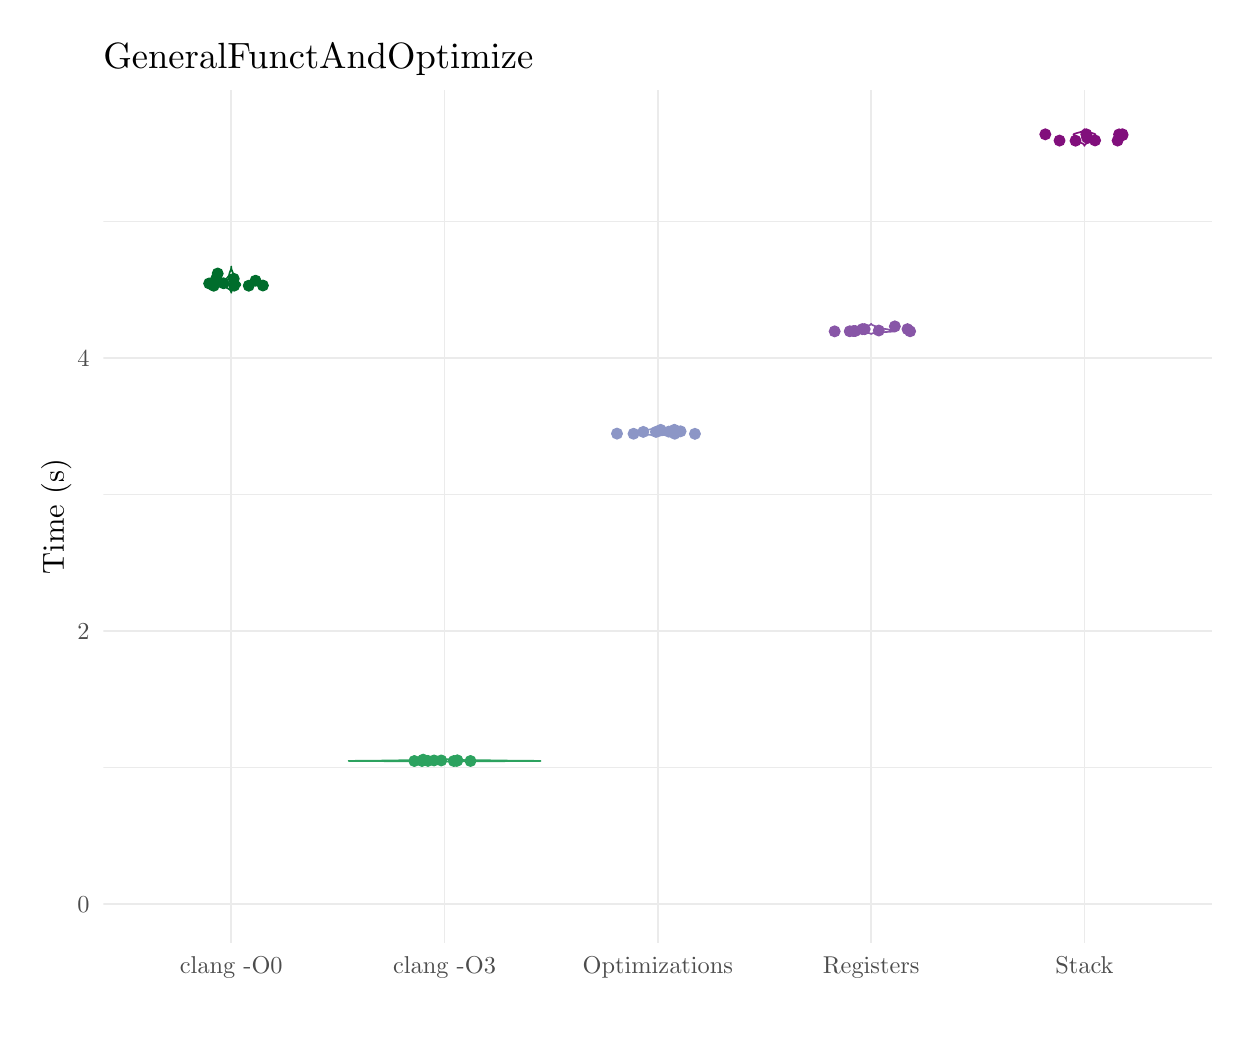
\begin{tikzpicture}[x=1pt,y=1pt]
\definecolor{fillColor}{RGB}{255,255,255}
\path[use as bounding box,fill=fillColor,fill opacity=0.00] (0,0) rectangle (433.62,361.35);
\begin{scope}
\path[clip] ( 27.31, 30.69) rectangle (428.12,338.69);
\definecolor{drawColor}{gray}{0.92}

\path[draw=drawColor,line width= 0.3pt,line join=round] ( 27.31, 93.99) --
	(428.12, 93.99);

\path[draw=drawColor,line width= 0.3pt,line join=round] ( 27.31,192.60) --
	(428.12,192.60);

\path[draw=drawColor,line width= 0.3pt,line join=round] ( 27.31,291.22) --
	(428.12,291.22);

\path[draw=drawColor,line width= 0.6pt,line join=round] ( 27.31, 44.69) --
	(428.12, 44.69);

\path[draw=drawColor,line width= 0.6pt,line join=round] ( 27.31,143.30) --
	(428.12,143.30);

\path[draw=drawColor,line width= 0.6pt,line join=round] ( 27.31,241.91) --
	(428.12,241.91);

\path[draw=drawColor,line width= 0.6pt,line join=round] ( 73.56, 30.69) --
	( 73.56,338.69);

\path[draw=drawColor,line width= 0.6pt,line join=round] (150.64, 30.69) --
	(150.64,338.69);

\path[draw=drawColor,line width= 0.6pt,line join=round] (227.72, 30.69) --
	(227.72,338.69);

\path[draw=drawColor,line width= 0.6pt,line join=round] (304.79, 30.69) --
	(304.79,338.69);

\path[draw=drawColor,line width= 0.6pt,line join=round] (381.87, 30.69) --
	(381.87,338.69);
\definecolor{drawColor}{RGB}{0,109,44}
\definecolor{fillColor}{RGB}{255,255,255}

\path[draw=drawColor,line width= 0.6pt,line join=round,line cap=round,fill=fillColor] ( 73.54,265.57) --
	( 73.54,265.59) --
	( 73.53,265.61) --
	( 73.53,265.63) --
	( 73.53,265.64) --
	( 73.53,265.66) --
	( 73.53,265.68) --
	( 73.52,265.70) --
	( 73.52,265.72) --
	( 73.52,265.74) --
	( 73.52,265.76) --
	( 73.51,265.77) --
	( 73.51,265.79) --
	( 73.51,265.81) --
	( 73.50,265.83) --
	( 73.50,265.85) --
	( 73.50,265.87) --
	( 73.49,265.89) --
	( 73.49,265.90) --
	( 73.48,265.92) --
	( 73.48,265.94) --
	( 73.47,265.96) --
	( 73.47,265.98) --
	( 73.46,266.00) --
	( 73.46,266.02) --
	( 73.45,266.03) --
	( 73.45,266.05) --
	( 73.44,266.07) --
	( 73.43,266.09) --
	( 73.43,266.11) --
	( 73.42,266.13) --
	( 73.41,266.15) --
	( 73.40,266.16) --
	( 73.40,266.18) --
	( 73.39,266.20) --
	( 73.38,266.22) --
	( 73.37,266.24) --
	( 73.36,266.26) --
	( 73.35,266.28) --
	( 73.34,266.29) --
	( 73.33,266.31) --
	( 73.32,266.33) --
	( 73.30,266.35) --
	( 73.29,266.37) --
	( 73.28,266.39) --
	( 73.27,266.41) --
	( 73.25,266.42) --
	( 73.24,266.44) --
	( 73.22,266.46) --
	( 73.21,266.48) --
	( 73.19,266.50) --
	( 73.18,266.52) --
	( 73.16,266.54) --
	( 73.14,266.55) --
	( 73.12,266.57) --
	( 73.10,266.59) --
	( 73.09,266.61) --
	( 73.07,266.63) --
	( 73.05,266.65) --
	( 73.02,266.67) --
	( 73.00,266.68) --
	( 72.98,266.70) --
	( 72.96,266.72) --
	( 72.94,266.74) --
	( 72.91,266.76) --
	( 72.89,266.78) --
	( 72.86,266.80) --
	( 72.84,266.81) --
	( 72.81,266.83) --
	( 72.78,266.85) --
	( 72.76,266.87) --
	( 72.73,266.89) --
	( 72.70,266.91) --
	( 72.67,266.92) --
	( 72.64,266.94) --
	( 72.61,266.96) --
	( 72.58,266.98) --
	( 72.55,267.00) --
	( 72.52,267.02) --
	( 72.49,267.04) --
	( 72.45,267.05) --
	( 72.42,267.07) --
	( 72.39,267.09) --
	( 72.35,267.11) --
	( 72.32,267.13) --
	( 72.28,267.15) --
	( 72.24,267.17) --
	( 72.21,267.18) --
	( 72.17,267.20) --
	( 72.14,267.22) --
	( 72.10,267.24) --
	( 72.06,267.26) --
	( 72.02,267.28) --
	( 71.99,267.30) --
	( 71.95,267.31) --
	( 71.91,267.33) --
	( 71.87,267.35) --
	( 71.83,267.37) --
	( 71.79,267.39) --
	( 71.75,267.41) --
	( 71.71,267.43) --
	( 71.68,267.44) --
	( 71.64,267.46) --
	( 71.60,267.48) --
	( 71.56,267.50) --
	( 71.52,267.52) --
	( 71.48,267.54) --
	( 71.44,267.56) --
	( 71.40,267.57) --
	( 71.36,267.59) --
	( 71.33,267.61) --
	( 71.29,267.63) --
	( 71.25,267.65) --
	( 71.21,267.67) --
	( 71.18,267.69) --
	( 71.14,267.70) --
	( 71.11,267.72) --
	( 71.07,267.74) --
	( 71.03,267.76) --
	( 71.00,267.78) --
	( 70.97,267.80) --
	( 70.93,267.82) --
	( 70.90,267.83) --
	( 70.87,267.85) --
	( 70.84,267.87) --
	( 70.81,267.89) --
	( 70.78,267.91) --
	( 70.75,267.93) --
	( 70.72,267.95) --
	( 70.69,267.96) --
	( 70.66,267.98) --
	( 70.64,268.00) --
	( 70.61,268.02) --
	( 70.59,268.04) --
	( 70.57,268.06) --
	( 70.54,268.08) --
	( 70.52,268.09) --
	( 70.50,268.11) --
	( 70.48,268.13) --
	( 70.46,268.15) --
	( 70.45,268.17) --
	( 70.43,268.19) --
	( 70.41,268.21) --
	( 70.40,268.22) --
	( 70.39,268.24) --
	( 70.37,268.26) --
	( 70.36,268.28) --
	( 70.35,268.30) --
	( 70.34,268.32) --
	( 70.33,268.34) --
	( 70.32,268.35) --
	( 70.32,268.37) --
	( 70.31,268.39) --
	( 70.31,268.41) --
	( 70.30,268.43) --
	( 70.30,268.45) --
	( 70.30,268.46) --
	( 70.30,268.48) --
	( 70.30,268.50) --
	( 70.30,268.52) --
	( 70.30,268.54) --
	( 70.30,268.56) --
	( 70.31,268.58) --
	( 70.31,268.59) --
	( 70.31,268.61) --
	( 70.32,268.63) --
	( 70.33,268.65) --
	( 70.33,268.67) --
	( 70.34,268.69) --
	( 70.35,268.71) --
	( 70.36,268.72) --
	( 70.37,268.74) --
	( 70.38,268.76) --
	( 70.39,268.78) --
	( 70.40,268.80) --
	( 70.42,268.82) --
	( 70.43,268.84) --
	( 70.44,268.85) --
	( 70.46,268.87) --
	( 70.47,268.89) --
	( 70.48,268.91) --
	( 70.50,268.93) --
	( 70.51,268.95) --
	( 70.53,268.97) --
	( 70.55,268.98) --
	( 70.56,269.00) --
	( 70.58,269.02) --
	( 70.59,269.04) --
	( 70.61,269.06) --
	( 70.63,269.08) --
	( 70.64,269.10) --
	( 70.66,269.11) --
	( 70.68,269.13) --
	( 70.70,269.15) --
	( 70.71,269.17) --
	( 70.73,269.19) --
	( 70.75,269.21) --
	( 70.77,269.23) --
	( 70.78,269.24) --
	( 70.80,269.26) --
	( 70.82,269.28) --
	( 70.83,269.30) --
	( 70.85,269.32) --
	( 70.87,269.34) --
	( 70.89,269.36) --
	( 70.90,269.37) --
	( 70.92,269.39) --
	( 70.93,269.41) --
	( 70.95,269.43) --
	( 70.97,269.45) --
	( 70.98,269.47) --
	( 71.00,269.49) --
	( 71.01,269.50) --
	( 71.03,269.52) --
	( 71.04,269.54) --
	( 71.06,269.56) --
	( 71.07,269.58) --
	( 71.09,269.60) --
	( 71.10,269.62) --
	( 71.11,269.63) --
	( 71.13,269.65) --
	( 71.14,269.67) --
	( 71.16,269.69) --
	( 71.17,269.71) --
	( 71.18,269.73) --
	( 71.19,269.75) --
	( 71.21,269.76) --
	( 71.22,269.78) --
	( 71.23,269.80) --
	( 71.24,269.82) --
	( 71.26,269.84) --
	( 71.27,269.86) --
	( 71.28,269.88) --
	( 71.29,269.89) --
	( 71.30,269.91) --
	( 71.31,269.93) --
	( 71.32,269.95) --
	( 71.34,269.97) --
	( 71.35,269.99) --
	( 71.36,270.00) --
	( 71.37,270.02) --
	( 71.38,270.04) --
	( 71.39,270.06) --
	( 71.40,270.08) --
	( 71.41,270.10) --
	( 71.42,270.12) --
	( 71.44,270.13) --
	( 71.45,270.15) --
	( 71.46,270.17) --
	( 71.47,270.19) --
	( 71.48,270.21) --
	( 71.49,270.23) --
	( 71.50,270.25) --
	( 71.52,270.26) --
	( 71.53,270.28) --
	( 71.54,270.30) --
	( 71.55,270.32) --
	( 71.56,270.34) --
	( 71.58,270.36) --
	( 71.59,270.38) --
	( 71.60,270.39) --
	( 71.62,270.41) --
	( 71.63,270.43) --
	( 71.64,270.45) --
	( 71.66,270.47) --
	( 71.67,270.49) --
	( 71.68,270.51) --
	( 71.70,270.52) --
	( 71.71,270.54) --
	( 71.73,270.56) --
	( 71.74,270.58) --
	( 71.76,270.60) --
	( 71.77,270.62) --
	( 71.79,270.64) --
	( 71.80,270.65) --
	( 71.82,270.67) --
	( 71.84,270.69) --
	( 71.85,270.71) --
	( 71.87,270.73) --
	( 71.88,270.75) --
	( 71.90,270.77) --
	( 71.92,270.78) --
	( 71.93,270.80) --
	( 71.95,270.82) --
	( 71.97,270.84) --
	( 71.99,270.86) --
	( 72.00,270.88) --
	( 72.02,270.90) --
	( 72.04,270.91) --
	( 72.06,270.93) --
	( 72.07,270.95) --
	( 72.09,270.97) --
	( 72.11,270.99) --
	( 72.13,271.01) --
	( 72.14,271.03) --
	( 72.16,271.04) --
	( 72.18,271.06) --
	( 72.20,271.08) --
	( 72.21,271.10) --
	( 72.23,271.12) --
	( 72.25,271.14) --
	( 72.26,271.16) --
	( 72.28,271.17) --
	( 72.30,271.19) --
	( 72.31,271.21) --
	( 72.33,271.23) --
	( 72.35,271.25) --
	( 72.36,271.27) --
	( 72.38,271.29) --
	( 72.39,271.30) --
	( 72.41,271.32) --
	( 72.43,271.34) --
	( 72.44,271.36) --
	( 72.46,271.38) --
	( 72.47,271.40) --
	( 72.48,271.42) --
	( 72.50,271.43) --
	( 72.51,271.45) --
	( 72.53,271.47) --
	( 72.54,271.49) --
	( 72.55,271.51) --
	( 72.56,271.53) --
	( 72.58,271.54) --
	( 72.59,271.56) --
	( 72.60,271.58) --
	( 72.61,271.60) --
	( 72.62,271.62) --
	( 72.63,271.64) --
	( 72.64,271.66) --
	( 72.65,271.67) --
	( 72.66,271.69) --
	( 72.67,271.71) --
	( 72.68,271.73) --
	( 72.69,271.75) --
	( 72.70,271.77) --
	( 72.71,271.79) --
	( 72.71,271.80) --
	( 72.72,271.82) --
	( 72.73,271.84) --
	( 72.74,271.86) --
	( 72.74,271.88) --
	( 72.75,271.90) --
	( 72.76,271.92) --
	( 72.76,271.93) --
	( 72.77,271.95) --
	( 72.78,271.97) --
	( 72.78,271.99) --
	( 72.79,272.01) --
	( 72.79,272.03) --
	( 72.80,272.05) --
	( 72.80,272.06) --
	( 72.81,272.08) --
	( 72.81,272.10) --
	( 72.81,272.12) --
	( 72.82,272.14) --
	( 72.82,272.16) --
	( 72.83,272.18) --
	( 72.83,272.19) --
	( 72.84,272.21) --
	( 72.84,272.23) --
	( 72.84,272.25) --
	( 72.85,272.27) --
	( 72.85,272.29) --
	( 72.85,272.31) --
	( 72.86,272.32) --
	( 72.86,272.34) --
	( 72.87,272.36) --
	( 72.87,272.38) --
	( 72.87,272.40) --
	( 72.88,272.42) --
	( 72.88,272.44) --
	( 72.89,272.45) --
	( 72.89,272.47) --
	( 72.89,272.49) --
	( 72.90,272.51) --
	( 72.90,272.53) --
	( 72.91,272.55) --
	( 72.91,272.57) --
	( 72.92,272.58) --
	( 72.92,272.60) --
	( 72.93,272.62) --
	( 72.93,272.64) --
	( 72.94,272.66) --
	( 72.94,272.68) --
	( 72.95,272.70) --
	( 72.95,272.71) --
	( 72.96,272.73) --
	( 72.96,272.75) --
	( 72.97,272.77) --
	( 72.97,272.79) --
	( 72.98,272.81) --
	( 72.99,272.83) --
	( 72.99,272.84) --
	( 73.00,272.86) --
	( 73.01,272.88) --
	( 73.01,272.90) --
	( 73.02,272.92) --
	( 73.03,272.94) --
	( 73.03,272.96) --
	( 73.04,272.97) --
	( 73.05,272.99) --
	( 73.05,273.01) --
	( 73.06,273.03) --
	( 73.07,273.05) --
	( 73.08,273.07) --
	( 73.08,273.08) --
	( 73.09,273.10) --
	( 73.10,273.12) --
	( 73.11,273.14) --
	( 73.12,273.16) --
	( 73.12,273.18) --
	( 73.13,273.20) --
	( 73.14,273.21) --
	( 73.15,273.23) --
	( 73.16,273.25) --
	( 73.16,273.27) --
	( 73.17,273.29) --
	( 73.18,273.31) --
	( 73.19,273.33) --
	( 73.20,273.34) --
	( 73.20,273.36) --
	( 73.21,273.38) --
	( 73.22,273.40) --
	( 73.23,273.42) --
	( 73.24,273.44) --
	( 73.24,273.46) --
	( 73.25,273.47) --
	( 73.26,273.49) --
	( 73.27,273.51) --
	( 73.27,273.53) --
	( 73.28,273.55) --
	( 73.29,273.57) --
	( 73.30,273.59) --
	( 73.30,273.60) --
	( 73.31,273.62) --
	( 73.32,273.64) --
	( 73.33,273.66) --
	( 73.33,273.68) --
	( 73.34,273.70) --
	( 73.35,273.72) --
	( 73.35,273.73) --
	( 73.36,273.75) --
	( 73.37,273.77) --
	( 73.37,273.79) --
	( 73.38,273.81) --
	( 73.38,273.83) --
	( 73.39,273.85) --
	( 73.40,273.86) --
	( 73.40,273.88) --
	( 73.41,273.90) --
	( 73.41,273.92) --
	( 73.42,273.94) --
	( 73.42,273.96) --
	( 73.43,273.98) --
	( 73.43,273.99) --
	( 73.44,274.01) --
	( 73.44,274.03) --
	( 73.45,274.05) --
	( 73.45,274.07) --
	( 73.46,274.09) --
	( 73.46,274.11) --
	( 73.46,274.12) --
	( 73.47,274.14) --
	( 73.47,274.16) --
	( 73.48,274.18) --
	( 73.48,274.20) --
	( 73.48,274.22) --
	( 73.49,274.24) --
	( 73.49,274.25) --
	( 73.49,274.27) --
	( 73.50,274.29) --
	( 73.50,274.31) --
	( 73.50,274.33) --
	( 73.50,274.35) --
	( 73.51,274.37) --
	( 73.51,274.38) --
	( 73.51,274.40) --
	( 73.51,274.42) --
	( 73.52,274.44) --
	( 73.52,274.46) --
	( 73.52,274.48) --
	( 73.52,274.50) --
	( 73.52,274.51) --
	( 73.53,274.53) --
	( 73.53,274.55) --
	( 73.53,274.57) --
	( 73.53,274.59) --
	( 73.53,274.61) --
	( 73.53,274.62) --
	( 73.54,274.64) --
	( 73.54,274.66) --
	( 73.54,274.68) --
	( 73.54,274.70) --
	( 73.54,274.72) --
	( 73.54,274.74) --
	( 73.54,274.75) --
	( 73.54,274.77) --
	( 73.54,274.79) --
	( 73.55,274.81) --
	( 73.55,274.83) --
	( 73.55,274.85) --
	( 73.55,274.87) --
	( 73.55,274.88) --
	( 73.55,274.90) --
	( 73.55,274.92) --
	( 73.55,274.94) --
	( 73.55,274.96) --
	( 73.55,274.98) --
	( 73.55,275.00) --
	( 73.55,275.01) --
	( 73.55,275.03) --
	( 73.55,275.05) --
	( 73.57,275.05) --
	( 73.57,275.03) --
	( 73.57,275.01) --
	( 73.57,275.00) --
	( 73.57,274.98) --
	( 73.57,274.96) --
	( 73.57,274.94) --
	( 73.57,274.92) --
	( 73.57,274.90) --
	( 73.57,274.88) --
	( 73.57,274.87) --
	( 73.57,274.85) --
	( 73.57,274.83) --
	( 73.57,274.81) --
	( 73.58,274.79) --
	( 73.58,274.77) --
	( 73.58,274.75) --
	( 73.58,274.74) --
	( 73.58,274.72) --
	( 73.58,274.70) --
	( 73.58,274.68) --
	( 73.58,274.66) --
	( 73.58,274.64) --
	( 73.59,274.62) --
	( 73.59,274.61) --
	( 73.59,274.59) --
	( 73.59,274.57) --
	( 73.59,274.55) --
	( 73.59,274.53) --
	( 73.60,274.51) --
	( 73.60,274.50) --
	( 73.60,274.48) --
	( 73.60,274.46) --
	( 73.60,274.44) --
	( 73.61,274.42) --
	( 73.61,274.40) --
	( 73.61,274.38) --
	( 73.61,274.37) --
	( 73.62,274.35) --
	( 73.62,274.33) --
	( 73.62,274.31) --
	( 73.62,274.29) --
	( 73.63,274.27) --
	( 73.63,274.25) --
	( 73.63,274.24) --
	( 73.64,274.22) --
	( 73.64,274.20) --
	( 73.64,274.18) --
	( 73.65,274.16) --
	( 73.65,274.14) --
	( 73.66,274.12) --
	( 73.66,274.11) --
	( 73.66,274.09) --
	( 73.67,274.07) --
	( 73.67,274.05) --
	( 73.68,274.03) --
	( 73.68,274.01) --
	( 73.69,273.99) --
	( 73.69,273.98) --
	( 73.70,273.96) --
	( 73.70,273.94) --
	( 73.71,273.92) --
	( 73.71,273.90) --
	( 73.72,273.88) --
	( 73.72,273.86) --
	( 73.73,273.85) --
	( 73.74,273.83) --
	( 73.74,273.81) --
	( 73.75,273.79) --
	( 73.75,273.77) --
	( 73.76,273.75) --
	( 73.77,273.73) --
	( 73.77,273.72) --
	( 73.78,273.70) --
	( 73.79,273.68) --
	( 73.79,273.66) --
	( 73.80,273.64) --
	( 73.81,273.62) --
	( 73.82,273.60) --
	( 73.82,273.59) --
	( 73.83,273.57) --
	( 73.84,273.55) --
	( 73.85,273.53) --
	( 73.85,273.51) --
	( 73.86,273.49) --
	( 73.87,273.47) --
	( 73.88,273.46) --
	( 73.88,273.44) --
	( 73.89,273.42) --
	( 73.90,273.40) --
	( 73.91,273.38) --
	( 73.92,273.36) --
	( 73.92,273.34) --
	( 73.93,273.33) --
	( 73.94,273.31) --
	( 73.95,273.29) --
	( 73.96,273.27) --
	( 73.96,273.25) --
	( 73.97,273.23) --
	( 73.98,273.21) --
	( 73.99,273.20) --
	( 74.00,273.18) --
	( 74.00,273.16) --
	( 74.01,273.14) --
	( 74.02,273.12) --
	( 74.03,273.10) --
	( 74.04,273.08) --
	( 74.04,273.07) --
	( 74.05,273.05) --
	( 74.06,273.03) --
	( 74.07,273.01) --
	( 74.07,272.99) --
	( 74.08,272.97) --
	( 74.09,272.96) --
	( 74.09,272.94) --
	( 74.10,272.92) --
	( 74.11,272.90) --
	( 74.11,272.88) --
	( 74.12,272.86) --
	( 74.13,272.84) --
	( 74.13,272.83) --
	( 74.14,272.81) --
	( 74.15,272.79) --
	( 74.15,272.77) --
	( 74.16,272.75) --
	( 74.16,272.73) --
	( 74.17,272.71) --
	( 74.17,272.70) --
	( 74.18,272.68) --
	( 74.18,272.66) --
	( 74.19,272.64) --
	( 74.19,272.62) --
	( 74.20,272.60) --
	( 74.20,272.58) --
	( 74.21,272.57) --
	( 74.21,272.55) --
	( 74.22,272.53) --
	( 74.22,272.51) --
	( 74.23,272.49) --
	( 74.23,272.47) --
	( 74.23,272.45) --
	( 74.24,272.44) --
	( 74.24,272.42) --
	( 74.25,272.40) --
	( 74.25,272.38) --
	( 74.25,272.36) --
	( 74.26,272.34) --
	( 74.26,272.32) --
	( 74.27,272.31) --
	( 74.27,272.29) --
	( 74.27,272.27) --
	( 74.28,272.25) --
	( 74.28,272.23) --
	( 74.28,272.21) --
	( 74.29,272.19) --
	( 74.29,272.18) --
	( 74.30,272.16) --
	( 74.30,272.14) --
	( 74.31,272.12) --
	( 74.31,272.10) --
	( 74.31,272.08) --
	( 74.32,272.06) --
	( 74.32,272.05) --
	( 74.33,272.03) --
	( 74.33,272.01) --
	( 74.34,271.99) --
	( 74.35,271.97) --
	( 74.35,271.95) --
	( 74.36,271.93) --
	( 74.36,271.92) --
	( 74.37,271.90) --
	( 74.38,271.88) --
	( 74.38,271.86) --
	( 74.39,271.84) --
	( 74.40,271.82) --
	( 74.41,271.80) --
	( 74.41,271.79) --
	( 74.42,271.77) --
	( 74.43,271.75) --
	( 74.44,271.73) --
	( 74.45,271.71) --
	( 74.46,271.69) --
	( 74.47,271.67) --
	( 74.48,271.66) --
	( 74.49,271.64) --
	( 74.50,271.62) --
	( 74.51,271.60) --
	( 74.52,271.58) --
	( 74.53,271.56) --
	( 74.54,271.54) --
	( 74.56,271.53) --
	( 74.57,271.51) --
	( 74.58,271.49) --
	( 74.60,271.47) --
	( 74.61,271.45) --
	( 74.62,271.43) --
	( 74.64,271.42) --
	( 74.65,271.40) --
	( 74.67,271.38) --
	( 74.68,271.36) --
	( 74.69,271.34) --
	( 74.71,271.32) --
	( 74.73,271.30) --
	( 74.74,271.29) --
	( 74.76,271.27) --
	( 74.77,271.25) --
	( 74.79,271.23) --
	( 74.81,271.21) --
	( 74.82,271.19) --
	( 74.84,271.17) --
	( 74.86,271.16) --
	( 74.87,271.14) --
	( 74.89,271.12) --
	( 74.91,271.10) --
	( 74.92,271.08) --
	( 74.94,271.06) --
	( 74.96,271.04) --
	( 74.98,271.03) --
	( 74.99,271.01) --
	( 75.01,270.99) --
	( 75.03,270.97) --
	( 75.05,270.95) --
	( 75.06,270.93) --
	( 75.08,270.91) --
	( 75.10,270.90) --
	( 75.12,270.88) --
	( 75.13,270.86) --
	( 75.15,270.84) --
	( 75.17,270.82) --
	( 75.19,270.80) --
	( 75.20,270.78) --
	( 75.22,270.77) --
	( 75.24,270.75) --
	( 75.25,270.73) --
	( 75.27,270.71) --
	( 75.28,270.69) --
	( 75.30,270.67) --
	( 75.32,270.65) --
	( 75.33,270.64) --
	( 75.35,270.62) --
	( 75.36,270.60) --
	( 75.38,270.58) --
	( 75.39,270.56) --
	( 75.41,270.54) --
	( 75.42,270.52) --
	( 75.44,270.51) --
	( 75.45,270.49) --
	( 75.46,270.47) --
	( 75.48,270.45) --
	( 75.49,270.43) --
	( 75.50,270.41) --
	( 75.52,270.39) --
	( 75.53,270.38) --
	( 75.54,270.36) --
	( 75.56,270.34) --
	( 75.57,270.32) --
	( 75.58,270.30) --
	( 75.59,270.28) --
	( 75.60,270.26) --
	( 75.62,270.25) --
	( 75.63,270.23) --
	( 75.64,270.21) --
	( 75.65,270.19) --
	( 75.66,270.17) --
	( 75.67,270.15) --
	( 75.68,270.13) --
	( 75.70,270.12) --
	( 75.71,270.10) --
	( 75.72,270.08) --
	( 75.73,270.06) --
	( 75.74,270.04) --
	( 75.75,270.02) --
	( 75.76,270.00) --
	( 75.77,269.99) --
	( 75.78,269.97) --
	( 75.80,269.95) --
	( 75.81,269.93) --
	( 75.82,269.91) --
	( 75.83,269.89) --
	( 75.84,269.88) --
	( 75.85,269.86) --
	( 75.87,269.84) --
	( 75.88,269.82) --
	( 75.89,269.80) --
	( 75.90,269.78) --
	( 75.91,269.76) --
	( 75.93,269.75) --
	( 75.94,269.73) --
	( 75.95,269.71) --
	( 75.97,269.69) --
	( 75.98,269.67) --
	( 75.99,269.65) --
	( 76.01,269.63) --
	( 76.02,269.62) --
	( 76.03,269.60) --
	( 76.05,269.58) --
	( 76.06,269.56) --
	( 76.08,269.54) --
	( 76.09,269.52) --
	( 76.11,269.50) --
	( 76.12,269.49) --
	( 76.14,269.47) --
	( 76.15,269.45) --
	( 76.17,269.43) --
	( 76.19,269.41) --
	( 76.20,269.39) --
	( 76.22,269.37) --
	( 76.24,269.36) --
	( 76.25,269.34) --
	( 76.27,269.32) --
	( 76.29,269.30) --
	( 76.30,269.28) --
	( 76.32,269.26) --
	( 76.34,269.24) --
	( 76.35,269.23) --
	( 76.37,269.21) --
	( 76.39,269.19) --
	( 76.41,269.17) --
	( 76.42,269.15) --
	( 76.44,269.13) --
	( 76.46,269.11) --
	( 76.48,269.10) --
	( 76.49,269.08) --
	( 76.51,269.06) --
	( 76.53,269.04) --
	( 76.54,269.02) --
	( 76.56,269.00) --
	( 76.57,268.98) --
	( 76.59,268.97) --
	( 76.61,268.95) --
	( 76.62,268.93) --
	( 76.64,268.91) --
	( 76.65,268.89) --
	( 76.67,268.87) --
	( 76.68,268.85) --
	( 76.69,268.84) --
	( 76.70,268.82) --
	( 76.72,268.80) --
	( 76.73,268.78) --
	( 76.74,268.76) --
	( 76.75,268.74) --
	( 76.76,268.72) --
	( 76.77,268.71) --
	( 76.78,268.69) --
	( 76.79,268.67) --
	( 76.79,268.65) --
	( 76.80,268.63) --
	( 76.81,268.61) --
	( 76.81,268.59) --
	( 76.82,268.58) --
	( 76.82,268.56) --
	( 76.82,268.54) --
	( 76.82,268.52) --
	( 76.82,268.50) --
	( 76.82,268.48) --
	( 76.82,268.46) --
	( 76.82,268.45) --
	( 76.82,268.43) --
	( 76.81,268.41) --
	( 76.81,268.39) --
	( 76.80,268.37) --
	( 76.80,268.35) --
	( 76.79,268.34) --
	( 76.78,268.32) --
	( 76.77,268.30) --
	( 76.76,268.28) --
	( 76.75,268.26) --
	( 76.74,268.24) --
	( 76.72,268.22) --
	( 76.71,268.21) --
	( 76.69,268.19) --
	( 76.67,268.17) --
	( 76.66,268.15) --
	( 76.64,268.13) --
	( 76.62,268.11) --
	( 76.60,268.09) --
	( 76.58,268.08) --
	( 76.55,268.06) --
	( 76.53,268.04) --
	( 76.51,268.02) --
	( 76.48,268.00) --
	( 76.46,267.98) --
	( 76.43,267.96) --
	( 76.40,267.95) --
	( 76.37,267.93) --
	( 76.34,267.91) --
	( 76.31,267.89) --
	( 76.28,267.87) --
	( 76.25,267.85) --
	( 76.22,267.83) --
	( 76.19,267.82) --
	( 76.15,267.80) --
	( 76.12,267.78) --
	( 76.09,267.76) --
	( 76.05,267.74) --
	( 76.02,267.72) --
	( 75.98,267.70) --
	( 75.94,267.69) --
	( 75.91,267.67) --
	( 75.87,267.65) --
	( 75.83,267.63) --
	( 75.79,267.61) --
	( 75.76,267.59) --
	( 75.72,267.57) --
	( 75.68,267.56) --
	( 75.64,267.54) --
	( 75.60,267.52) --
	( 75.56,267.50) --
	( 75.52,267.48) --
	( 75.48,267.46) --
	( 75.44,267.44) --
	( 75.41,267.43) --
	( 75.37,267.41) --
	( 75.33,267.39) --
	( 75.29,267.37) --
	( 75.25,267.35) --
	( 75.21,267.33) --
	( 75.17,267.31) --
	( 75.13,267.30) --
	( 75.10,267.28) --
	( 75.06,267.26) --
	( 75.02,267.24) --
	( 74.98,267.22) --
	( 74.95,267.20) --
	( 74.91,267.18) --
	( 74.88,267.17) --
	( 74.84,267.15) --
	( 74.80,267.13) --
	( 74.77,267.11) --
	( 74.74,267.09) --
	( 74.70,267.07) --
	( 74.67,267.05) --
	( 74.64,267.04) --
	( 74.60,267.02) --
	( 74.57,267.00) --
	( 74.54,266.98) --
	( 74.51,266.96) --
	( 74.48,266.94) --
	( 74.45,266.92) --
	( 74.42,266.91) --
	( 74.39,266.89) --
	( 74.36,266.87) --
	( 74.34,266.85) --
	( 74.31,266.83) --
	( 74.28,266.81) --
	( 74.26,266.80) --
	( 74.23,266.78) --
	( 74.21,266.76) --
	( 74.18,266.74) --
	( 74.16,266.72) --
	( 74.14,266.70) --
	( 74.12,266.68) --
	( 74.10,266.67) --
	( 74.07,266.65) --
	( 74.05,266.63) --
	( 74.03,266.61) --
	( 74.02,266.59) --
	( 74.00,266.57) --
	( 73.98,266.55) --
	( 73.96,266.54) --
	( 73.94,266.52) --
	( 73.93,266.50) --
	( 73.91,266.48) --
	( 73.90,266.46) --
	( 73.88,266.44) --
	( 73.87,266.42) --
	( 73.85,266.41) --
	( 73.84,266.39) --
	( 73.83,266.37) --
	( 73.82,266.35) --
	( 73.80,266.33) --
	( 73.79,266.31) --
	( 73.78,266.29) --
	( 73.77,266.28) --
	( 73.76,266.26) --
	( 73.75,266.24) --
	( 73.74,266.22) --
	( 73.73,266.20) --
	( 73.72,266.18) --
	( 73.72,266.16) --
	( 73.71,266.15) --
	( 73.70,266.13) --
	( 73.69,266.11) --
	( 73.69,266.09) --
	( 73.68,266.07) --
	( 73.67,266.05) --
	( 73.67,266.03) --
	( 73.66,266.02) --
	( 73.66,266.00) --
	( 73.65,265.98) --
	( 73.65,265.96) --
	( 73.64,265.94) --
	( 73.64,265.92) --
	( 73.63,265.90) --
	( 73.63,265.89) --
	( 73.62,265.87) --
	( 73.62,265.85) --
	( 73.62,265.83) --
	( 73.61,265.81) --
	( 73.61,265.79) --
	( 73.61,265.77) --
	( 73.60,265.76) --
	( 73.60,265.74) --
	( 73.60,265.72) --
	( 73.60,265.70) --
	( 73.59,265.68) --
	( 73.59,265.66) --
	( 73.59,265.64) --
	( 73.59,265.63) --
	( 73.59,265.61) --
	( 73.58,265.59) --
	( 73.58,265.57) --
	( 73.54,265.57) --
	cycle;
\definecolor{drawColor}{RGB}{44,162,95}

\path[draw=drawColor,line width= 0.6pt,line join=round,line cap=round,fill=fillColor] (150.36, 96.11) --
	(150.34, 96.11) --
	(150.32, 96.11) --
	(150.30, 96.11) --
	(150.27, 96.12) --
	(150.25, 96.12) --
	(150.22, 96.12) --
	(150.19, 96.12) --
	(150.16, 96.12) --
	(150.13, 96.13) --
	(150.09, 96.13) --
	(150.05, 96.13) --
	(150.01, 96.13) --
	(149.97, 96.13) --
	(149.93, 96.14) --
	(149.88, 96.14) --
	(149.83, 96.14) --
	(149.78, 96.14) --
	(149.73, 96.14) --
	(149.67, 96.15) --
	(149.61, 96.15) --
	(149.55, 96.15) --
	(149.48, 96.15) --
	(149.41, 96.15) --
	(149.34, 96.15) --
	(149.26, 96.16) --
	(149.18, 96.16) --
	(149.10, 96.16) --
	(149.01, 96.16) --
	(148.91, 96.16) --
	(148.82, 96.17) --
	(148.71, 96.17) --
	(148.61, 96.17) --
	(148.50, 96.17) --
	(148.38, 96.17) --
	(148.26, 96.18) --
	(148.13, 96.18) --
	(148.00, 96.18) --
	(147.86, 96.18) --
	(147.72, 96.18) --
	(147.57, 96.19) --
	(147.41, 96.19) --
	(147.25, 96.19) --
	(147.08, 96.19) --
	(146.91, 96.19) --
	(146.73, 96.20) --
	(146.54, 96.20) --
	(146.35, 96.20) --
	(146.15, 96.20) --
	(145.94, 96.20) --
	(145.73, 96.21) --
	(145.51, 96.21) --
	(145.28, 96.21) --
	(145.04, 96.21) --
	(144.80, 96.21) --
	(144.55, 96.22) --
	(144.29, 96.22) --
	(144.02, 96.22) --
	(143.75, 96.22) --
	(143.47, 96.22) --
	(143.18, 96.23) --
	(142.88, 96.23) --
	(142.58, 96.23) --
	(142.27, 96.23) --
	(141.95, 96.23) --
	(141.62, 96.23) --
	(141.29, 96.24) --
	(140.95, 96.24) --
	(140.60, 96.24) --
	(140.25, 96.24) --
	(139.88, 96.24) --
	(139.51, 96.25) --
	(139.13, 96.25) --
	(138.75, 96.25) --
	(138.36, 96.25) --
	(137.97, 96.25) --
	(137.56, 96.26) --
	(137.16, 96.26) --
	(136.74, 96.26) --
	(136.32, 96.26) --
	(135.90, 96.26) --
	(135.47, 96.27) --
	(135.04, 96.27) --
	(134.60, 96.27) --
	(134.16, 96.27) --
	(133.71, 96.27) --
	(133.26, 96.28) --
	(132.81, 96.28) --
	(132.36, 96.28) --
	(131.90, 96.28) --
	(131.45, 96.28) --
	(130.99, 96.29) --
	(130.53, 96.29) --
	(130.07, 96.29) --
	(129.61, 96.29) --
	(129.15, 96.29) --
	(128.69, 96.30) --
	(128.23, 96.30) --
	(127.77, 96.30) --
	(127.32, 96.30) --
	(126.87, 96.30) --
	(126.42, 96.30) --
	(125.98, 96.31) --
	(125.54, 96.31) --
	(125.10, 96.31) --
	(124.67, 96.31) --
	(124.25, 96.31) --
	(123.83, 96.32) --
	(123.42, 96.32) --
	(123.02, 96.32) --
	(122.62, 96.32) --
	(122.23, 96.32) --
	(121.85, 96.33) --
	(121.48, 96.33) --
	(121.12, 96.33) --
	(120.77, 96.33) --
	(120.42, 96.33) --
	(120.09, 96.34) --
	(119.77, 96.34) --
	(119.46, 96.34) --
	(119.16, 96.34) --
	(118.88, 96.34) --
	(118.60, 96.35) --
	(118.34, 96.35) --
	(118.09, 96.35) --
	(117.86, 96.35) --
	(117.63, 96.35) --
	(117.43, 96.36) --
	(117.23, 96.36) --
	(117.05, 96.36) --
	(116.88, 96.36) --
	(116.72, 96.36) --
	(116.59, 96.37) --
	(116.46, 96.37) --
	(116.35, 96.37) --
	(116.25, 96.37) --
	(116.16, 96.37) --
	(116.10, 96.37) --
	(116.04, 96.38) --
	(116.00, 96.38) --
	(115.97, 96.38) --
	(115.95, 96.38) --
	(115.96, 96.38) --
	(115.97, 96.39) --
	(115.99, 96.39) --
	(116.03, 96.39) --
	(116.08, 96.39) --
	(116.15, 96.39) --
	(116.22, 96.40) --
	(116.31, 96.40) --
	(116.41, 96.40) --
	(116.51, 96.40) --
	(116.64, 96.40) --
	(116.77, 96.41) --
	(116.91, 96.41) --
	(117.06, 96.41) --
	(117.21, 96.41) --
	(117.38, 96.41) --
	(117.56, 96.42) --
	(117.74, 96.42) --
	(117.93, 96.42) --
	(118.13, 96.42) --
	(118.33, 96.42) --
	(118.54, 96.43) --
	(118.76, 96.43) --
	(118.98, 96.43) --
	(119.20, 96.43) --
	(119.43, 96.43) --
	(119.67, 96.44) --
	(119.90, 96.44) --
	(120.14, 96.44) --
	(120.38, 96.44) --
	(120.62, 96.44) --
	(120.86, 96.44) --
	(121.11, 96.45) --
	(121.35, 96.45) --
	(121.60, 96.45) --
	(121.84, 96.45) --
	(122.09, 96.45) --
	(122.33, 96.46) --
	(122.57, 96.46) --
	(122.81, 96.46) --
	(123.05, 96.46) --
	(123.28, 96.46) --
	(123.51, 96.47) --
	(123.74, 96.47) --
	(123.97, 96.47) --
	(124.19, 96.47) --
	(124.41, 96.47) --
	(124.63, 96.48) --
	(124.84, 96.48) --
	(125.04, 96.48) --
	(125.25, 96.48) --
	(125.45, 96.48) --
	(125.64, 96.49) --
	(125.83, 96.49) --
	(126.02, 96.49) --
	(126.20, 96.49) --
	(126.37, 96.49) --
	(126.55, 96.50) --
	(126.71, 96.50) --
	(126.88, 96.50) --
	(127.03, 96.50) --
	(127.19, 96.50) --
	(127.34, 96.51) --
	(127.49, 96.51) --
	(127.63, 96.51) --
	(127.77, 96.51) --
	(127.90, 96.51) --
	(128.03, 96.52) --
	(128.16, 96.52) --
	(128.29, 96.52) --
	(128.41, 96.52) --
	(128.53, 96.52) --
	(128.64, 96.52) --
	(128.76, 96.53) --
	(128.87, 96.53) --
	(128.98, 96.53) --
	(129.09, 96.53) --
	(129.20, 96.53) --
	(129.31, 96.54) --
	(129.41, 96.54) --
	(129.52, 96.54) --
	(129.62, 96.54) --
	(129.73, 96.54) --
	(129.83, 96.55) --
	(129.94, 96.55) --
	(130.05, 96.55) --
	(130.15, 96.55) --
	(130.26, 96.55) --
	(130.37, 96.56) --
	(130.48, 96.56) --
	(130.60, 96.56) --
	(130.71, 96.56) --
	(130.83, 96.56) --
	(130.95, 96.57) --
	(131.07, 96.57) --
	(131.19, 96.57) --
	(131.32, 96.57) --
	(131.45, 96.57) --
	(131.58, 96.58) --
	(131.72, 96.58) --
	(131.86, 96.58) --
	(132.00, 96.58) --
	(132.15, 96.58) --
	(132.30, 96.59) --
	(132.45, 96.59) --
	(132.61, 96.59) --
	(132.77, 96.59) --
	(132.93, 96.59) --
	(133.10, 96.59) --
	(133.27, 96.60) --
	(133.44, 96.60) --
	(133.62, 96.60) --
	(133.80, 96.60) --
	(133.99, 96.60) --
	(134.17, 96.61) --
	(134.37, 96.61) --
	(134.56, 96.61) --
	(134.76, 96.61) --
	(134.96, 96.61) --
	(135.16, 96.62) --
	(135.36, 96.62) --
	(135.57, 96.62) --
	(135.78, 96.62) --
	(135.99, 96.62) --
	(136.21, 96.63) --
	(136.42, 96.63) --
	(136.64, 96.63) --
	(136.86, 96.63) --
	(137.08, 96.63) --
	(137.30, 96.64) --
	(137.52, 96.64) --
	(137.74, 96.64) --
	(137.96, 96.64) --
	(138.18, 96.64) --
	(138.41, 96.65) --
	(138.63, 96.65) --
	(138.85, 96.65) --
	(139.07, 96.65) --
	(139.29, 96.65) --
	(139.51, 96.66) --
	(139.73, 96.66) --
	(139.95, 96.66) --
	(140.16, 96.66) --
	(140.37, 96.66) --
	(140.58, 96.66) --
	(140.79, 96.67) --
	(141.00, 96.67) --
	(141.20, 96.67) --
	(141.40, 96.67) --
	(141.60, 96.67) --
	(141.79, 96.68) --
	(141.98, 96.68) --
	(142.17, 96.68) --
	(142.35, 96.68) --
	(142.53, 96.68) --
	(142.70, 96.69) --
	(142.88, 96.69) --
	(143.04, 96.69) --
	(143.20, 96.69) --
	(143.36, 96.69) --
	(143.51, 96.70) --
	(143.66, 96.70) --
	(143.81, 96.70) --
	(143.95, 96.70) --
	(144.08, 96.70) --
	(144.21, 96.71) --
	(144.33, 96.71) --
	(144.45, 96.71) --
	(144.57, 96.71) --
	(144.68, 96.71) --
	(144.78, 96.72) --
	(144.88, 96.72) --
	(144.97, 96.72) --
	(145.06, 96.72) --
	(145.15, 96.72) --
	(145.22, 96.73) --
	(145.30, 96.73) --
	(145.37, 96.73) --
	(145.43, 96.73) --
	(145.49, 96.73) --
	(145.54, 96.73) --
	(145.59, 96.74) --
	(145.63, 96.74) --
	(145.68, 96.74) --
	(145.71, 96.74) --
	(145.74, 96.74) --
	(145.77, 96.75) --
	(145.79, 96.75) --
	(145.81, 96.75) --
	(145.82, 96.75) --
	(145.83, 96.75) --
	(145.84, 96.76) --
	(145.84, 96.76) --
	(145.84, 96.76) --
	(145.84, 96.76) --
	(145.83, 96.76) --
	(145.82, 96.77) --
	(145.81, 96.77) --
	(145.79, 96.77) --
	(145.78, 96.77) --
	(145.76, 96.77) --
	(145.73, 96.78) --
	(145.71, 96.78) --
	(145.68, 96.78) --
	(145.65, 96.78) --
	(145.62, 96.78) --
	(145.59, 96.79) --
	(145.56, 96.79) --
	(145.53, 96.79) --
	(145.49, 96.79) --
	(145.46, 96.79) --
	(145.42, 96.80) --
	(145.38, 96.80) --
	(145.35, 96.80) --
	(145.31, 96.80) --
	(145.27, 96.80) --
	(145.24, 96.80) --
	(145.20, 96.81) --
	(145.17, 96.81) --
	(145.13, 96.81) --
	(145.10, 96.81) --
	(145.07, 96.81) --
	(145.03, 96.82) --
	(145.00, 96.82) --
	(144.97, 96.82) --
	(144.95, 96.82) --
	(144.92, 96.82) --
	(144.90, 96.83) --
	(144.87, 96.83) --
	(144.85, 96.83) --
	(144.83, 96.83) --
	(144.82, 96.83) --
	(144.80, 96.84) --
	(144.79, 96.84) --
	(144.78, 96.84) --
	(144.77, 96.84) --
	(144.77, 96.84) --
	(144.76, 96.85) --
	(144.76, 96.85) --
	(144.77, 96.85) --
	(144.77, 96.85) --
	(144.78, 96.85) --
	(144.79, 96.86) --
	(144.80, 96.86) --
	(144.82, 96.86) --
	(144.84, 96.86) --
	(144.86, 96.86) --
	(144.88, 96.87) --
	(144.91, 96.87) --
	(144.94, 96.87) --
	(144.97, 96.87) --
	(145.01, 96.87) --
	(145.04, 96.88) --
	(145.08, 96.88) --
	(145.13, 96.88) --
	(145.17, 96.88) --
	(145.22, 96.88) --
	(145.27, 96.88) --
	(145.32, 96.89) --
	(145.38, 96.89) --
	(145.43, 96.89) --
	(145.49, 96.89) --
	(145.55, 96.89) --
	(145.61, 96.90) --
	(145.68, 96.90) --
	(145.74, 96.90) --
	(145.81, 96.90) --
	(145.88, 96.90) --
	(145.95, 96.91) --
	(146.02, 96.91) --
	(146.10, 96.91) --
	(146.17, 96.91) --
	(146.25, 96.91) --
	(146.32, 96.92) --
	(146.40, 96.92) --
	(146.48, 96.92) --
	(146.56, 96.92) --
	(146.64, 96.92) --
	(146.72, 96.93) --
	(146.80, 96.93) --
	(146.88, 96.93) --
	(146.96, 96.93) --
	(147.04, 96.93) --
	(147.12, 96.94) --
	(147.21, 96.94) --
	(147.29, 96.94) --
	(147.37, 96.94) --
	(147.45, 96.94) --
	(147.53, 96.95) --
	(147.61, 96.95) --
	(147.69, 96.95) --
	(147.77, 96.95) --
	(147.85, 96.95) --
	(147.93, 96.95) --
	(148.00, 96.96) --
	(148.08, 96.96) --
	(148.16, 96.96) --
	(148.23, 96.96) --
	(148.30, 96.96) --
	(148.38, 96.97) --
	(148.45, 96.97) --
	(148.52, 96.97) --
	(148.59, 96.97) --
	(148.66, 96.97) --
	(148.72, 96.98) --
	(148.79, 96.98) --
	(148.85, 96.98) --
	(148.91, 96.98) --
	(148.98, 96.98) --
	(149.04, 96.99) --
	(149.10, 96.99) --
	(149.15, 96.99) --
	(149.21, 96.99) --
	(149.26, 96.99) --
	(149.32, 97.00) --
	(149.37, 97.00) --
	(149.42, 97.00) --
	(149.47, 97.00) --
	(149.52, 97.00) --
	(149.56, 97.01) --
	(149.61, 97.01) --
	(149.65, 97.01) --
	(149.70, 97.01) --
	(149.74, 97.01) --
	(149.78, 97.02) --
	(149.81, 97.02) --
	(149.85, 97.02) --
	(149.89, 97.02) --
	(149.92, 97.02) --
	(149.96, 97.02) --
	(149.99, 97.03) --
	(150.02, 97.03) --
	(150.05, 97.03) --
	(150.08, 97.03) --
	(150.11, 97.03) --
	(150.13, 97.04) --
	(150.16, 97.04) --
	(150.18, 97.04) --
	(150.21, 97.04) --
	(150.23, 97.04) --
	(150.25, 97.05) --
	(150.27, 97.05) --
	(150.29, 97.05) --
	(150.31, 97.05) --
	(150.33, 97.05) --
	(150.34, 97.06) --
	(150.36, 97.06) --
	(150.38, 97.06) --
	(150.39, 97.06) --
	(150.40, 97.06) --
	(150.42, 97.07) --
	(150.43, 97.07) --
	(150.44, 97.07) --
	(150.45, 97.07) --
	(150.46, 97.07) --
	(150.48, 97.08) --
	(150.49, 97.08) --
	(150.49, 97.08) --
	(150.50, 97.08) --
	(150.51, 97.08) --
	(150.52, 97.09) --
	(150.53, 97.09) --
	(150.53, 97.09) --
	(150.54, 97.09) --
	(150.55, 97.09) --
	(150.55, 97.09) --
	(150.56, 97.10) --
	(150.56, 97.10) --
	(150.57, 97.10) --
	(150.57, 97.10) --
	(150.70, 97.10) --
	(150.71, 97.10) --
	(150.71, 97.10) --
	(150.72, 97.10) --
	(150.72, 97.09) --
	(150.73, 97.09) --
	(150.74, 97.09) --
	(150.74, 97.09) --
	(150.75, 97.09) --
	(150.76, 97.09) --
	(150.77, 97.08) --
	(150.77, 97.08) --
	(150.78, 97.08) --
	(150.79, 97.08) --
	(150.80, 97.08) --
	(150.81, 97.07) --
	(150.82, 97.07) --
	(150.83, 97.07) --
	(150.85, 97.07) --
	(150.86, 97.07) --
	(150.87, 97.06) --
	(150.89, 97.06) --
	(150.90, 97.06) --
	(150.92, 97.06) --
	(150.93, 97.06) --
	(150.95, 97.05) --
	(150.97, 97.05) --
	(150.99, 97.05) --
	(151.01, 97.05) --
	(151.03, 97.05) --
	(151.05, 97.04) --
	(151.07, 97.04) --
	(151.10, 97.04) --
	(151.12, 97.04) --
	(151.14, 97.04) --
	(151.17, 97.03) --
	(151.20, 97.03) --
	(151.23, 97.03) --
	(151.26, 97.03) --
	(151.29, 97.03) --
	(151.32, 97.02) --
	(151.35, 97.02) --
	(151.39, 97.02) --
	(151.43, 97.02) --
	(151.46, 97.02) --
	(151.50, 97.02) --
	(151.54, 97.01) --
	(151.58, 97.01) --
	(151.62, 97.01) --
	(151.67, 97.01) --
	(151.71, 97.01) --
	(151.76, 97.00) --
	(151.81, 97.00) --
	(151.86, 97.00) --
	(151.91, 97.00) --
	(151.96, 97.00) --
	(152.01, 96.99) --
	(152.07, 96.99) --
	(152.12, 96.99) --
	(152.18, 96.99) --
	(152.24, 96.99) --
	(152.30, 96.98) --
	(152.36, 96.98) --
	(152.43, 96.98) --
	(152.49, 96.98) --
	(152.56, 96.98) --
	(152.62, 96.97) --
	(152.69, 96.97) --
	(152.76, 96.97) --
	(152.83, 96.97) --
	(152.90, 96.97) --
	(152.97, 96.96) --
	(153.05, 96.96) --
	(153.12, 96.96) --
	(153.20, 96.96) --
	(153.27, 96.96) --
	(153.35, 96.95) --
	(153.43, 96.95) --
	(153.51, 96.95) --
	(153.59, 96.95) --
	(153.67, 96.95) --
	(153.75, 96.95) --
	(153.83, 96.94) --
	(153.91, 96.94) --
	(153.99, 96.94) --
	(154.07, 96.94) --
	(154.15, 96.94) --
	(154.23, 96.93) --
	(154.32, 96.93) --
	(154.40, 96.93) --
	(154.48, 96.93) --
	(154.56, 96.93) --
	(154.64, 96.92) --
	(154.72, 96.92) --
	(154.80, 96.92) --
	(154.88, 96.92) --
	(154.95, 96.92) --
	(155.03, 96.91) --
	(155.11, 96.91) --
	(155.18, 96.91) --
	(155.25, 96.91) --
	(155.33, 96.91) --
	(155.40, 96.90) --
	(155.47, 96.90) --
	(155.53, 96.90) --
	(155.60, 96.90) --
	(155.66, 96.90) --
	(155.73, 96.89) --
	(155.79, 96.89) --
	(155.85, 96.89) --
	(155.90, 96.89) --
	(155.96, 96.89) --
	(156.01, 96.88) --
	(156.06, 96.88) --
	(156.11, 96.88) --
	(156.15, 96.88) --
	(156.19, 96.88) --
	(156.23, 96.88) --
	(156.27, 96.87) --
	(156.30, 96.87) --
	(156.34, 96.87) --
	(156.37, 96.87) --
	(156.39, 96.87) --
	(156.42, 96.86) --
	(156.44, 96.86) --
	(156.46, 96.86) --
	(156.47, 96.86) --
	(156.49, 96.86) --
	(156.50, 96.85) --
	(156.50, 96.85) --
	(156.51, 96.85) --
	(156.51, 96.85) --
	(156.51, 96.85) --
	(156.51, 96.84) --
	(156.51, 96.84) --
	(156.50, 96.84) --
	(156.49, 96.84) --
	(156.47, 96.84) --
	(156.46, 96.83) --
	(156.44, 96.83) --
	(156.42, 96.83) --
	(156.40, 96.83) --
	(156.38, 96.83) --
	(156.36, 96.82) --
	(156.33, 96.82) --
	(156.30, 96.82) --
	(156.27, 96.82) --
	(156.24, 96.82) --
	(156.21, 96.81) --
	(156.18, 96.81) --
	(156.14, 96.81) --
	(156.11, 96.81) --
	(156.07, 96.81) --
	(156.04, 96.80) --
	(156.00, 96.80) --
	(155.97, 96.80) --
	(155.93, 96.80) --
	(155.89, 96.80) --
	(155.86, 96.80) --
	(155.82, 96.79) --
	(155.79, 96.79) --
	(155.75, 96.79) --
	(155.72, 96.79) --
	(155.69, 96.79) --
	(155.65, 96.78) --
	(155.62, 96.78) --
	(155.60, 96.78) --
	(155.57, 96.78) --
	(155.54, 96.78) --
	(155.52, 96.77) --
	(155.50, 96.77) --
	(155.48, 96.77) --
	(155.47, 96.77) --
	(155.46, 96.77) --
	(155.45, 96.76) --
	(155.44, 96.76) --
	(155.43, 96.76) --
	(155.43, 96.76) --
	(155.44, 96.76) --
	(155.44, 96.75) --
	(155.45, 96.75) --
	(155.47, 96.75) --
	(155.49, 96.75) --
	(155.51, 96.75) --
	(155.54, 96.74) --
	(155.57, 96.74) --
	(155.60, 96.74) --
	(155.64, 96.74) --
	(155.69, 96.74) --
	(155.74, 96.73) --
	(155.79, 96.73) --
	(155.85, 96.73) --
	(155.91, 96.73) --
	(155.98, 96.73) --
	(156.05, 96.73) --
	(156.13, 96.72) --
	(156.21, 96.72) --
	(156.30, 96.72) --
	(156.40, 96.72) --
	(156.50, 96.72) --
	(156.60, 96.71) --
	(156.71, 96.71) --
	(156.82, 96.71) --
	(156.94, 96.71) --
	(157.07, 96.71) --
	(157.20, 96.70) --
	(157.33, 96.70) --
	(157.47, 96.70) --
	(157.61, 96.70) --
	(157.76, 96.70) --
	(157.92, 96.69) --
	(158.07, 96.69) --
	(158.24, 96.69) --
	(158.40, 96.69) --
	(158.57, 96.69) --
	(158.75, 96.68) --
	(158.93, 96.68) --
	(159.11, 96.68) --
	(159.30, 96.68) --
	(159.49, 96.68) --
	(159.68, 96.67) --
	(159.88, 96.67) --
	(160.08, 96.67) --
	(160.28, 96.67) --
	(160.49, 96.67) --
	(160.69, 96.66) --
	(160.90, 96.66) --
	(161.12, 96.66) --
	(161.33, 96.66) --
	(161.55, 96.66) --
	(161.77, 96.66) --
	(161.98, 96.65) --
	(162.20, 96.65) --
	(162.43, 96.65) --
	(162.65, 96.65) --
	(162.87, 96.65) --
	(163.09, 96.64) --
	(163.31, 96.64) --
	(163.54, 96.64) --
	(163.76, 96.64) --
	(163.98, 96.64) --
	(164.20, 96.63) --
	(164.42, 96.63) --
	(164.64, 96.63) --
	(164.86, 96.63) --
	(165.07, 96.63) --
	(165.28, 96.62) --
	(165.50, 96.62) --
	(165.71, 96.62) --
	(165.91, 96.62) --
	(166.12, 96.62) --
	(166.32, 96.61) --
	(166.52, 96.61) --
	(166.72, 96.61) --
	(166.91, 96.61) --
	(167.10, 96.61) --
	(167.29, 96.60) --
	(167.47, 96.60) --
	(167.66, 96.60) --
	(167.83, 96.60) --
	(168.01, 96.60) --
	(168.18, 96.59) --
	(168.34, 96.59) --
	(168.51, 96.59) --
	(168.67, 96.59) --
	(168.83, 96.59) --
	(168.98, 96.59) --
	(169.13, 96.58) --
	(169.27, 96.58) --
	(169.42, 96.58) --
	(169.56, 96.58) --
	(169.69, 96.58) --
	(169.83, 96.57) --
	(169.96, 96.57) --
	(170.08, 96.57) --
	(170.21, 96.57) --
	(170.33, 96.57) --
	(170.45, 96.56) --
	(170.57, 96.56) --
	(170.68, 96.56) --
	(170.79, 96.56) --
	(170.90, 96.56) --
	(171.01, 96.55) --
	(171.12, 96.55) --
	(171.23, 96.55) --
	(171.34, 96.55) --
	(171.44, 96.55) --
	(171.55, 96.54) --
	(171.65, 96.54) --
	(171.76, 96.54) --
	(171.86, 96.54) --
	(171.97, 96.54) --
	(172.08, 96.53) --
	(172.19, 96.53) --
	(172.29, 96.53) --
	(172.41, 96.53) --
	(172.52, 96.53) --
	(172.63, 96.52) --
	(172.75, 96.52) --
	(172.87, 96.52) --
	(172.99, 96.52) --
	(173.12, 96.52) --
	(173.24, 96.52) --
	(173.38, 96.51) --
	(173.51, 96.51) --
	(173.65, 96.51) --
	(173.79, 96.51) --
	(173.94, 96.51) --
	(174.09, 96.50) --
	(174.24, 96.50) --
	(174.40, 96.50) --
	(174.56, 96.50) --
	(174.73, 96.50) --
	(174.90, 96.49) --
	(175.08, 96.49) --
	(175.26, 96.49) --
	(175.45, 96.49) --
	(175.64, 96.49) --
	(175.83, 96.48) --
	(176.03, 96.48) --
	(176.23, 96.48) --
	(176.44, 96.48) --
	(176.65, 96.48) --
	(176.87, 96.47) --
	(177.09, 96.47) --
	(177.31, 96.47) --
	(177.54, 96.47) --
	(177.76, 96.47) --
	(178.00, 96.46) --
	(178.23, 96.46) --
	(178.47, 96.46) --
	(178.71, 96.46) --
	(178.95, 96.46) --
	(179.19, 96.45) --
	(179.44, 96.45) --
	(179.68, 96.45) --
	(179.92, 96.45) --
	(180.17, 96.45) --
	(180.41, 96.44) --
	(180.66, 96.44) --
	(180.90, 96.44) --
	(181.14, 96.44) --
	(181.38, 96.44) --
	(181.61, 96.44) --
	(181.84, 96.43) --
	(182.07, 96.43) --
	(182.30, 96.43) --
	(182.52, 96.43) --
	(182.73, 96.43) --
	(182.94, 96.42) --
	(183.15, 96.42) --
	(183.34, 96.42) --
	(183.54, 96.42) --
	(183.72, 96.42) --
	(183.89, 96.41) --
	(184.06, 96.41) --
	(184.22, 96.41) --
	(184.37, 96.41) --
	(184.51, 96.41) --
	(184.64, 96.40) --
	(184.76, 96.40) --
	(184.87, 96.40) --
	(184.97, 96.40) --
	(185.06, 96.40) --
	(185.13, 96.39) --
	(185.20, 96.39) --
	(185.24, 96.39) --
	(185.28, 96.39) --
	(185.31, 96.39) --
	(185.32, 96.38) --
	(185.32, 96.38) --
	(185.31, 96.38) --
	(185.28, 96.38) --
	(185.24, 96.38) --
	(185.18, 96.37) --
	(185.11, 96.37) --
	(185.03, 96.37) --
	(184.93, 96.37) --
	(184.82, 96.37) --
	(184.69, 96.37) --
	(184.55, 96.36) --
	(184.40, 96.36) --
	(184.23, 96.36) --
	(184.05, 96.36) --
	(183.85, 96.36) --
	(183.64, 96.35) --
	(183.42, 96.35) --
	(183.19, 96.35) --
	(182.93, 96.35) --
	(182.67, 96.35) --
	(182.40, 96.34) --
	(182.11, 96.34) --
	(181.82, 96.34) --
	(181.51, 96.34) --
	(181.18, 96.34) --
	(180.85, 96.33) --
	(180.51, 96.33) --
	(180.16, 96.33) --
	(179.80, 96.33) --
	(179.43, 96.33) --
	(179.05, 96.32) --
	(178.66, 96.32) --
	(178.26, 96.32) --
	(177.86, 96.32) --
	(177.44, 96.32) --
	(177.03, 96.31) --
	(176.60, 96.31) --
	(176.17, 96.31) --
	(175.74, 96.31) --
	(175.30, 96.31) --
	(174.86, 96.30) --
	(174.41, 96.30) --
	(173.96, 96.30) --
	(173.50, 96.30) --
	(173.05, 96.30) --
	(172.59, 96.30) --
	(172.13, 96.29) --
	(171.67, 96.29) --
	(171.21, 96.29) --
	(170.75, 96.29) --
	(170.29, 96.29) --
	(169.83, 96.28) --
	(169.37, 96.28) --
	(168.92, 96.28) --
	(168.46, 96.28) --
	(168.01, 96.28) --
	(167.56, 96.27) --
	(167.12, 96.27) --
	(166.68, 96.27) --
	(166.24, 96.27) --
	(165.81, 96.27) --
	(165.38, 96.26) --
	(164.95, 96.26) --
	(164.53, 96.26) --
	(164.12, 96.26) --
	(163.71, 96.26) --
	(163.31, 96.25) --
	(162.91, 96.25) --
	(162.53, 96.25) --
	(162.14, 96.25) --
	(161.77, 96.25) --
	(161.40, 96.24) --
	(161.03, 96.24) --
	(160.68, 96.24) --
	(160.33, 96.24) --
	(159.99, 96.24) --
	(159.65, 96.23) --
	(159.33, 96.23) --
	(159.01, 96.23) --
	(158.70, 96.23) --
	(158.39, 96.23) --
	(158.10, 96.23) --
	(157.81, 96.22) --
	(157.53, 96.22) --
	(157.25, 96.22) --
	(156.99, 96.22) --
	(156.73, 96.22) --
	(156.48, 96.21) --
	(156.24, 96.21) --
	(156.00, 96.21) --
	(155.77, 96.21) --
	(155.55, 96.21) --
	(155.33, 96.20) --
	(155.13, 96.20) --
	(154.93, 96.20) --
	(154.73, 96.20) --
	(154.55, 96.20) --
	(154.37, 96.19) --
	(154.19, 96.19) --
	(154.03, 96.19) --
	(153.86, 96.19) --
	(153.71, 96.19) --
	(153.56, 96.18) --
	(153.42, 96.18) --
	(153.28, 96.18) --
	(153.15, 96.18) --
	(153.02, 96.18) --
	(152.90, 96.17) --
	(152.78, 96.17) --
	(152.67, 96.17) --
	(152.56, 96.17) --
	(152.46, 96.17) --
	(152.36, 96.16) --
	(152.27, 96.16) --
	(152.18, 96.16) --
	(152.10, 96.16) --
	(152.02, 96.16) --
	(151.94, 96.15) --
	(151.86, 96.15) --
	(151.79, 96.15) --
	(151.73, 96.15) --
	(151.66, 96.15) --
	(151.60, 96.15) --
	(151.55, 96.14) --
	(151.49, 96.14) --
	(151.44, 96.14) --
	(151.39, 96.14) --
	(151.35, 96.14) --
	(151.30, 96.13) --
	(151.26, 96.13) --
	(151.22, 96.13) --
	(151.19, 96.13) --
	(151.15, 96.13) --
	(151.12, 96.12) --
	(151.09, 96.12) --
	(151.06, 96.12) --
	(151.03, 96.12) --
	(151.01, 96.12) --
	(150.98, 96.11) --
	(150.96, 96.11) --
	(150.94, 96.11) --
	(150.92, 96.11) --
	(150.36, 96.11) --
	cycle;
\definecolor{drawColor}{RGB}{140,150,198}

\path[draw=drawColor,line width= 0.6pt,line join=round,line cap=round,fill=fillColor] (227.66,213.63) --
	(227.65,213.64) --
	(227.65,213.64) --
	(227.64,213.65) --
	(227.64,213.66) --
	(227.63,213.66) --
	(227.63,213.67) --
	(227.62,213.67) --
	(227.62,213.68) --
	(227.61,213.69) --
	(227.61,213.69) --
	(227.60,213.70) --
	(227.59,213.71) --
	(227.59,213.71) --
	(227.58,213.72) --
	(227.57,213.73) --
	(227.56,213.73) --
	(227.55,213.74) --
	(227.54,213.75) --
	(227.53,213.75) --
	(227.52,213.76) --
	(227.51,213.77) --
	(227.50,213.77) --
	(227.49,213.78) --
	(227.48,213.79) --
	(227.47,213.79) --
	(227.45,213.80) --
	(227.44,213.81) --
	(227.43,213.81) --
	(227.41,213.82) --
	(227.40,213.83) --
	(227.38,213.83) --
	(227.36,213.84) --
	(227.34,213.85) --
	(227.33,213.85) --
	(227.31,213.86) --
	(227.29,213.87) --
	(227.27,213.87) --
	(227.25,213.88) --
	(227.22,213.89) --
	(227.20,213.89) --
	(227.18,213.90) --
	(227.15,213.91) --
	(227.13,213.91) --
	(227.10,213.92) --
	(227.07,213.92) --
	(227.05,213.93) --
	(227.02,213.94) --
	(226.99,213.94) --
	(226.96,213.95) --
	(226.92,213.96) --
	(226.89,213.96) --
	(226.86,213.97) --
	(226.82,213.98) --
	(226.79,213.98) --
	(226.75,213.99) --
	(226.71,214.00) --
	(226.67,214.00) --
	(226.63,214.01) --
	(226.59,214.02) --
	(226.55,214.02) --
	(226.50,214.03) --
	(226.46,214.04) --
	(226.41,214.04) --
	(226.37,214.05) --
	(226.32,214.06) --
	(226.27,214.06) --
	(226.22,214.07) --
	(226.17,214.08) --
	(226.11,214.08) --
	(226.06,214.09) --
	(226.00,214.10) --
	(225.95,214.10) --
	(225.89,214.11) --
	(225.83,214.12) --
	(225.77,214.12) --
	(225.71,214.13) --
	(225.65,214.14) --
	(225.59,214.14) --
	(225.53,214.15) --
	(225.46,214.16) --
	(225.40,214.16) --
	(225.33,214.17) --
	(225.27,214.18) --
	(225.20,214.18) --
	(225.13,214.19) --
	(225.06,214.19) --
	(224.99,214.20) --
	(224.92,214.21) --
	(224.85,214.21) --
	(224.78,214.22) --
	(224.70,214.23) --
	(224.63,214.23) --
	(224.56,214.24) --
	(224.48,214.25) --
	(224.41,214.25) --
	(224.33,214.26) --
	(224.26,214.27) --
	(224.18,214.27) --
	(224.11,214.28) --
	(224.03,214.29) --
	(223.96,214.29) --
	(223.88,214.30) --
	(223.81,214.31) --
	(223.73,214.31) --
	(223.65,214.32) --
	(223.58,214.33) --
	(223.50,214.33) --
	(223.43,214.34) --
	(223.35,214.35) --
	(223.28,214.35) --
	(223.21,214.36) --
	(223.13,214.37) --
	(223.06,214.37) --
	(222.99,214.38) --
	(222.92,214.39) --
	(222.85,214.39) --
	(222.78,214.40) --
	(222.71,214.41) --
	(222.64,214.41) --
	(222.58,214.42) --
	(222.51,214.43) --
	(222.45,214.43) --
	(222.38,214.44) --
	(222.32,214.44) --
	(222.26,214.45) --
	(222.20,214.46) --
	(222.15,214.46) --
	(222.09,214.47) --
	(222.03,214.48) --
	(221.98,214.48) --
	(221.93,214.49) --
	(221.88,214.50) --
	(221.83,214.50) --
	(221.78,214.51) --
	(221.74,214.52) --
	(221.69,214.52) --
	(221.65,214.53) --
	(221.61,214.54) --
	(221.57,214.54) --
	(221.54,214.55) --
	(221.50,214.56) --
	(221.47,214.56) --
	(221.44,214.57) --
	(221.41,214.58) --
	(221.38,214.58) --
	(221.36,214.59) --
	(221.33,214.60) --
	(221.31,214.60) --
	(221.29,214.61) --
	(221.27,214.62) --
	(221.25,214.62) --
	(221.24,214.63) --
	(221.22,214.64) --
	(221.21,214.64) --
	(221.20,214.65) --
	(221.19,214.66) --
	(221.18,214.66) --
	(221.18,214.67) --
	(221.17,214.68) --
	(221.17,214.68) --
	(221.17,214.69) --
	(221.17,214.69) --
	(221.17,214.70) --
	(221.17,214.71) --
	(221.18,214.71) --
	(221.18,214.72) --
	(221.19,214.73) --
	(221.19,214.73) --
	(221.20,214.74) --
	(221.21,214.75) --
	(221.22,214.75) --
	(221.23,214.76) --
	(221.24,214.77) --
	(221.25,214.77) --
	(221.26,214.78) --
	(221.27,214.79) --
	(221.29,214.79) --
	(221.30,214.80) --
	(221.31,214.81) --
	(221.33,214.81) --
	(221.34,214.82) --
	(221.35,214.83) --
	(221.37,214.83) --
	(221.38,214.84) --
	(221.40,214.85) --
	(221.41,214.85) --
	(221.42,214.86) --
	(221.44,214.87) --
	(221.45,214.87) --
	(221.46,214.88) --
	(221.48,214.89) --
	(221.49,214.89) --
	(221.50,214.90) --
	(221.51,214.91) --
	(221.52,214.91) --
	(221.53,214.92) --
	(221.54,214.93) --
	(221.55,214.93) --
	(221.56,214.94) --
	(221.56,214.94) --
	(221.57,214.95) --
	(221.58,214.96) --
	(221.58,214.96) --
	(221.58,214.97) --
	(221.59,214.98) --
	(221.59,214.98) --
	(221.59,214.99) --
	(221.59,215.00) --
	(221.59,215.00) --
	(221.59,215.01) --
	(221.59,215.02) --
	(221.59,215.02) --
	(221.58,215.03) --
	(221.58,215.04) --
	(221.58,215.04) --
	(221.57,215.05) --
	(221.56,215.06) --
	(221.56,215.06) --
	(221.55,215.07) --
	(221.54,215.08) --
	(221.53,215.08) --
	(221.52,215.09) --
	(221.51,215.10) --
	(221.50,215.10) --
	(221.49,215.11) --
	(221.48,215.12) --
	(221.47,215.12) --
	(221.45,215.13) --
	(221.44,215.14) --
	(221.43,215.14) --
	(221.41,215.15) --
	(221.40,215.16) --
	(221.39,215.16) --
	(221.37,215.17) --
	(221.36,215.18) --
	(221.35,215.18) --
	(221.33,215.19) --
	(221.32,215.19) --
	(221.31,215.20) --
	(221.29,215.21) --
	(221.28,215.21) --
	(221.27,215.22) --
	(221.26,215.23) --
	(221.25,215.23) --
	(221.23,215.24) --
	(221.22,215.25) --
	(221.21,215.25) --
	(221.20,215.26) --
	(221.20,215.27) --
	(221.19,215.27) --
	(221.18,215.28) --
	(221.17,215.29) --
	(221.17,215.29) --
	(221.16,215.30) --
	(221.16,215.31) --
	(221.16,215.31) --
	(221.16,215.32) --
	(221.15,215.33) --
	(221.15,215.33) --
	(221.15,215.34) --
	(221.16,215.35) --
	(221.16,215.35) --
	(221.16,215.36) --
	(221.17,215.37) --
	(221.17,215.37) --
	(221.18,215.38) --
	(221.19,215.39) --
	(221.20,215.39) --
	(221.21,215.40) --
	(221.22,215.41) --
	(221.23,215.41) --
	(221.25,215.42) --
	(221.26,215.43) --
	(221.28,215.43) --
	(221.29,215.44) --
	(221.31,215.44) --
	(221.33,215.45) --
	(221.35,215.46) --
	(221.37,215.46) --
	(221.39,215.47) --
	(221.41,215.48) --
	(221.44,215.48) --
	(221.46,215.49) --
	(221.48,215.50) --
	(221.51,215.50) --
	(221.54,215.51) --
	(221.56,215.52) --
	(221.59,215.52) --
	(221.62,215.53) --
	(221.65,215.54) --
	(221.68,215.54) --
	(221.71,215.55) --
	(221.74,215.56) --
	(221.77,215.56) --
	(221.80,215.57) --
	(221.83,215.58) --
	(221.87,215.58) --
	(221.90,215.59) --
	(221.93,215.60) --
	(221.96,215.60) --
	(222.00,215.61) --
	(222.03,215.62) --
	(222.07,215.62) --
	(222.10,215.63) --
	(222.13,215.64) --
	(222.17,215.64) --
	(222.20,215.65) --
	(222.24,215.66) --
	(222.27,215.66) --
	(222.31,215.67) --
	(222.34,215.68) --
	(222.37,215.68) --
	(222.41,215.69) --
	(222.44,215.69) --
	(222.47,215.70) --
	(222.51,215.71) --
	(222.54,215.71) --
	(222.57,215.72) --
	(222.61,215.73) --
	(222.64,215.73) --
	(222.67,215.74) --
	(222.70,215.75) --
	(222.74,215.75) --
	(222.77,215.76) --
	(222.80,215.77) --
	(222.83,215.77) --
	(222.86,215.78) --
	(222.89,215.79) --
	(222.92,215.79) --
	(222.95,215.80) --
	(222.98,215.81) --
	(223.01,215.81) --
	(223.04,215.82) --
	(223.07,215.83) --
	(223.10,215.83) --
	(223.13,215.84) --
	(223.16,215.85) --
	(223.19,215.85) --
	(223.21,215.86) --
	(223.24,215.87) --
	(223.27,215.87) --
	(223.30,215.88) --
	(223.33,215.89) --
	(223.35,215.89) --
	(223.38,215.90) --
	(223.41,215.91) --
	(223.44,215.91) --
	(223.47,215.92) --
	(223.49,215.93) --
	(223.52,215.93) --
	(223.55,215.94) --
	(223.58,215.95) --
	(223.61,215.95) --
	(223.63,215.96) --
	(223.66,215.96) --
	(223.69,215.97) --
	(223.72,215.98) --
	(223.75,215.98) --
	(223.78,215.99) --
	(223.81,216.00) --
	(223.84,216.00) --
	(223.87,216.01) --
	(223.90,216.02) --
	(223.93,216.02) --
	(223.96,216.03) --
	(223.99,216.04) --
	(224.02,216.04) --
	(224.06,216.05) --
	(224.09,216.06) --
	(224.12,216.06) --
	(224.16,216.07) --
	(224.19,216.08) --
	(224.22,216.08) --
	(224.26,216.09) --
	(224.29,216.10) --
	(224.33,216.10) --
	(224.36,216.11) --
	(224.40,216.12) --
	(224.44,216.12) --
	(224.47,216.13) --
	(224.51,216.14) --
	(224.55,216.14) --
	(224.59,216.15) --
	(224.62,216.16) --
	(224.66,216.16) --
	(224.70,216.17) --
	(224.74,216.18) --
	(224.78,216.18) --
	(224.82,216.19) --
	(224.86,216.20) --
	(224.90,216.20) --
	(224.94,216.21) --
	(224.98,216.21) --
	(225.03,216.22) --
	(225.07,216.23) --
	(225.11,216.23) --
	(225.15,216.24) --
	(225.19,216.25) --
	(225.23,216.25) --
	(225.28,216.26) --
	(225.32,216.27) --
	(225.36,216.27) --
	(225.40,216.28) --
	(225.45,216.29) --
	(225.49,216.29) --
	(225.53,216.30) --
	(225.57,216.31) --
	(225.61,216.31) --
	(225.66,216.32) --
	(225.70,216.33) --
	(225.74,216.33) --
	(225.78,216.34) --
	(225.82,216.35) --
	(225.86,216.35) --
	(225.90,216.36) --
	(225.95,216.37) --
	(225.99,216.37) --
	(226.03,216.38) --
	(226.07,216.39) --
	(226.11,216.39) --
	(226.14,216.40) --
	(226.18,216.41) --
	(226.22,216.41) --
	(226.26,216.42) --
	(226.30,216.43) --
	(226.33,216.43) --
	(226.37,216.44) --
	(226.41,216.45) --
	(226.44,216.45) --
	(226.48,216.46) --
	(226.51,216.46) --
	(226.55,216.47) --
	(226.58,216.48) --
	(226.61,216.48) --
	(226.65,216.49) --
	(226.68,216.50) --
	(226.71,216.50) --
	(226.74,216.51) --
	(226.77,216.52) --
	(226.80,216.52) --
	(226.83,216.53) --
	(226.86,216.54) --
	(226.89,216.54) --
	(226.91,216.55) --
	(226.94,216.56) --
	(226.97,216.56) --
	(226.99,216.57) --
	(227.02,216.58) --
	(227.04,216.58) --
	(227.06,216.59) --
	(227.09,216.60) --
	(227.11,216.60) --
	(227.13,216.61) --
	(227.15,216.62) --
	(227.18,216.62) --
	(227.20,216.63) --
	(227.22,216.64) --
	(227.23,216.64) --
	(227.25,216.65) --
	(227.27,216.66) --
	(227.29,216.66) --
	(227.31,216.67) --
	(227.32,216.68) --
	(227.34,216.68) --
	(227.35,216.69) --
	(227.37,216.70) --
	(227.38,216.70) --
	(227.40,216.71) --
	(227.41,216.71) --
	(227.42,216.72) --
	(227.44,216.73) --
	(227.45,216.73) --
	(227.46,216.74) --
	(227.47,216.75) --
	(227.48,216.75) --
	(227.49,216.76) --
	(227.50,216.77) --
	(227.51,216.77) --
	(227.52,216.78) --
	(227.53,216.79) --
	(227.54,216.79) --
	(227.55,216.80) --
	(227.56,216.81) --
	(227.57,216.81) --
	(227.57,216.82) --
	(227.58,216.83) --
	(227.59,216.83) --
	(227.59,216.84) --
	(227.60,216.85) --
	(227.61,216.85) --
	(227.61,216.86) --
	(227.62,216.87) --
	(227.62,216.87) --
	(227.63,216.88) --
	(227.63,216.89) --
	(227.64,216.89) --
	(227.64,216.90) --
	(227.64,216.91) --
	(227.65,216.91) --
	(227.65,216.92) --
	(227.66,216.93) --
	(227.66,216.93) --
	(227.66,216.94) --
	(227.67,216.95) --
	(227.67,216.95) --
	(227.67,216.96) --
	(227.67,216.96) --
	(227.68,216.97) --
	(227.68,216.98) --
	(227.68,216.98) --
	(227.68,216.99) --
	(227.75,216.99) --
	(227.75,216.98) --
	(227.75,216.98) --
	(227.76,216.97) --
	(227.76,216.96) --
	(227.76,216.96) --
	(227.76,216.95) --
	(227.77,216.95) --
	(227.77,216.94) --
	(227.77,216.93) --
	(227.78,216.93) --
	(227.78,216.92) --
	(227.78,216.91) --
	(227.79,216.91) --
	(227.79,216.90) --
	(227.80,216.89) --
	(227.80,216.89) --
	(227.81,216.88) --
	(227.81,216.87) --
	(227.82,216.87) --
	(227.82,216.86) --
	(227.83,216.85) --
	(227.83,216.85) --
	(227.84,216.84) --
	(227.85,216.83) --
	(227.85,216.83) --
	(227.86,216.82) --
	(227.87,216.81) --
	(227.88,216.81) --
	(227.88,216.80) --
	(227.89,216.79) --
	(227.90,216.79) --
	(227.91,216.78) --
	(227.92,216.77) --
	(227.93,216.77) --
	(227.94,216.76) --
	(227.95,216.75) --
	(227.96,216.75) --
	(227.97,216.74) --
	(227.98,216.73) --
	(228.00,216.73) --
	(228.01,216.72) --
	(228.02,216.71) --
	(228.04,216.71) --
	(228.05,216.70) --
	(228.06,216.70) --
	(228.08,216.69) --
	(228.09,216.68) --
	(228.11,216.68) --
	(228.13,216.67) --
	(228.14,216.66) --
	(228.16,216.66) --
	(228.18,216.65) --
	(228.20,216.64) --
	(228.22,216.64) --
	(228.24,216.63) --
	(228.26,216.62) --
	(228.28,216.62) --
	(228.30,216.61) --
	(228.32,216.60) --
	(228.35,216.60) --
	(228.37,216.59) --
	(228.39,216.58) --
	(228.42,216.58) --
	(228.44,216.57) --
	(228.47,216.56) --
	(228.49,216.56) --
	(228.52,216.55) --
	(228.55,216.54) --
	(228.58,216.54) --
	(228.60,216.53) --
	(228.63,216.52) --
	(228.66,216.52) --
	(228.69,216.51) --
	(228.72,216.50) --
	(228.76,216.50) --
	(228.79,216.49) --
	(228.82,216.48) --
	(228.85,216.48) --
	(228.89,216.47) --
	(228.92,216.46) --
	(228.96,216.46) --
	(228.99,216.45) --
	(229.03,216.45) --
	(229.06,216.44) --
	(229.10,216.43) --
	(229.14,216.43) --
	(229.17,216.42) --
	(229.21,216.41) --
	(229.25,216.41) --
	(229.29,216.40) --
	(229.33,216.39) --
	(229.37,216.39) --
	(229.41,216.38) --
	(229.45,216.37) --
	(229.49,216.37) --
	(229.53,216.36) --
	(229.57,216.35) --
	(229.61,216.35) --
	(229.65,216.34) --
	(229.69,216.33) --
	(229.74,216.33) --
	(229.78,216.32) --
	(229.82,216.31) --
	(229.86,216.31) --
	(229.90,216.30) --
	(229.95,216.29) --
	(229.99,216.29) --
	(230.03,216.28) --
	(230.07,216.27) --
	(230.11,216.27) --
	(230.16,216.26) --
	(230.20,216.25) --
	(230.24,216.25) --
	(230.28,216.24) --
	(230.32,216.23) --
	(230.37,216.23) --
	(230.41,216.22) --
	(230.45,216.21) --
	(230.49,216.21) --
	(230.53,216.20) --
	(230.57,216.20) --
	(230.61,216.19) --
	(230.65,216.18) --
	(230.69,216.18) --
	(230.73,216.17) --
	(230.77,216.16) --
	(230.81,216.16) --
	(230.85,216.15) --
	(230.88,216.14) --
	(230.92,216.14) --
	(230.96,216.13) --
	(231.00,216.12) --
	(231.03,216.12) --
	(231.07,216.11) --
	(231.10,216.10) --
	(231.14,216.10) --
	(231.17,216.09) --
	(231.21,216.08) --
	(231.24,216.08) --
	(231.28,216.07) --
	(231.31,216.06) --
	(231.34,216.06) --
	(231.38,216.05) --
	(231.41,216.04) --
	(231.44,216.04) --
	(231.47,216.03) --
	(231.50,216.02) --
	(231.53,216.02) --
	(231.56,216.01) --
	(231.59,216.00) --
	(231.62,216.00) --
	(231.65,215.99) --
	(231.68,215.98) --
	(231.71,215.98) --
	(231.74,215.97) --
	(231.77,215.96) --
	(231.80,215.96) --
	(231.83,215.95) --
	(231.86,215.95) --
	(231.88,215.94) --
	(231.91,215.93) --
	(231.94,215.93) --
	(231.97,215.92) --
	(232.00,215.91) --
	(232.02,215.91) --
	(232.05,215.90) --
	(232.08,215.89) --
	(232.11,215.89) --
	(232.13,215.88) --
	(232.16,215.87) --
	(232.19,215.87) --
	(232.22,215.86) --
	(232.25,215.85) --
	(232.28,215.85) --
	(232.30,215.84) --
	(232.33,215.83) --
	(232.36,215.83) --
	(232.39,215.82) --
	(232.42,215.81) --
	(232.45,215.81) --
	(232.48,215.80) --
	(232.51,215.79) --
	(232.54,215.79) --
	(232.57,215.78) --
	(232.60,215.77) --
	(232.63,215.77) --
	(232.66,215.76) --
	(232.70,215.75) --
	(232.73,215.75) --
	(232.76,215.74) --
	(232.79,215.73) --
	(232.83,215.73) --
	(232.86,215.72) --
	(232.89,215.71) --
	(232.92,215.71) --
	(232.96,215.70) --
	(232.99,215.69) --
	(233.03,215.69) --
	(233.06,215.68) --
	(233.09,215.68) --
	(233.13,215.67) --
	(233.16,215.66) --
	(233.20,215.66) --
	(233.23,215.65) --
	(233.26,215.64) --
	(233.30,215.64) --
	(233.33,215.63) --
	(233.37,215.62) --
	(233.40,215.62) --
	(233.43,215.61) --
	(233.47,215.60) --
	(233.50,215.60) --
	(233.53,215.59) --
	(233.57,215.58) --
	(233.60,215.58) --
	(233.63,215.57) --
	(233.66,215.56) --
	(233.69,215.56) --
	(233.73,215.55) --
	(233.76,215.54) --
	(233.79,215.54) --
	(233.81,215.53) --
	(233.84,215.52) --
	(233.87,215.52) --
	(233.90,215.51) --
	(233.92,215.50) --
	(233.95,215.50) --
	(233.97,215.49) --
	(234.00,215.48) --
	(234.02,215.48) --
	(234.04,215.47) --
	(234.07,215.46) --
	(234.09,215.46) --
	(234.11,215.45) --
	(234.12,215.44) --
	(234.14,215.44) --
	(234.16,215.43) --
	(234.17,215.43) --
	(234.19,215.42) --
	(234.20,215.41) --
	(234.21,215.41) --
	(234.22,215.40) --
	(234.23,215.39) --
	(234.24,215.39) --
	(234.25,215.38) --
	(234.26,215.37) --
	(234.27,215.37) --
	(234.27,215.36) --
	(234.27,215.35) --
	(234.28,215.35) --
	(234.28,215.34) --
	(234.28,215.33) --
	(234.28,215.33) --
	(234.28,215.32) --
	(234.28,215.31) --
	(234.27,215.31) --
	(234.27,215.30) --
	(234.26,215.29) --
	(234.26,215.29) --
	(234.25,215.28) --
	(234.24,215.27) --
	(234.24,215.27) --
	(234.23,215.26) --
	(234.22,215.25) --
	(234.21,215.25) --
	(234.20,215.24) --
	(234.19,215.23) --
	(234.18,215.23) --
	(234.16,215.22) --
	(234.15,215.21) --
	(234.14,215.21) --
	(234.13,215.20) --
	(234.11,215.19) --
	(234.10,215.19) --
	(234.09,215.18) --
	(234.07,215.18) --
	(234.06,215.17) --
	(234.05,215.16) --
	(234.03,215.16) --
	(234.02,215.15) --
	(234.01,215.14) --
	(233.99,215.14) --
	(233.98,215.13) --
	(233.97,215.12) --
	(233.96,215.12) --
	(233.94,215.11) --
	(233.93,215.10) --
	(233.92,215.10) --
	(233.91,215.09) --
	(233.90,215.08) --
	(233.89,215.08) --
	(233.88,215.07) --
	(233.88,215.06) --
	(233.87,215.06) --
	(233.86,215.05) --
	(233.86,215.04) --
	(233.85,215.04) --
	(233.85,215.03) --
	(233.85,215.02) --
	(233.84,215.02) --
	(233.84,215.01) --
	(233.84,215.00) --
	(233.84,215.00) --
	(233.84,214.99) --
	(233.84,214.98) --
	(233.85,214.98) --
	(233.85,214.97) --
	(233.85,214.96) --
	(233.86,214.96) --
	(233.86,214.95) --
	(233.87,214.94) --
	(233.88,214.94) --
	(233.88,214.93) --
	(233.89,214.93) --
	(233.90,214.92) --
	(233.91,214.91) --
	(233.92,214.91) --
	(233.93,214.90) --
	(233.95,214.89) --
	(233.96,214.89) --
	(233.97,214.88) --
	(233.98,214.87) --
	(234.00,214.87) --
	(234.01,214.86) --
	(234.02,214.85) --
	(234.04,214.85) --
	(234.05,214.84) --
	(234.07,214.83) --
	(234.08,214.83) --
	(234.09,214.82) --
	(234.11,214.81) --
	(234.12,214.81) --
	(234.13,214.80) --
	(234.15,214.79) --
	(234.16,214.79) --
	(234.17,214.78) --
	(234.18,214.77) --
	(234.20,214.77) --
	(234.21,214.76) --
	(234.22,214.75) --
	(234.23,214.75) --
	(234.23,214.74) --
	(234.24,214.73) --
	(234.25,214.73) --
	(234.25,214.72) --
	(234.26,214.71) --
	(234.26,214.71) --
	(234.26,214.70) --
	(234.26,214.69) --
	(234.26,214.69) --
	(234.26,214.68) --
	(234.26,214.68) --
	(234.26,214.67) --
	(234.25,214.66) --
	(234.24,214.66) --
	(234.23,214.65) --
	(234.22,214.64) --
	(234.21,214.64) --
	(234.20,214.63) --
	(234.18,214.62) --
	(234.16,214.62) --
	(234.15,214.61) --
	(234.12,214.60) --
	(234.10,214.60) --
	(234.08,214.59) --
	(234.05,214.58) --
	(234.02,214.58) --
	(234.00,214.57) --
	(233.96,214.56) --
	(233.93,214.56) --
	(233.90,214.55) --
	(233.86,214.54) --
	(233.82,214.54) --
	(233.78,214.53) --
	(233.74,214.52) --
	(233.70,214.52) --
	(233.65,214.51) --
	(233.60,214.50) --
	(233.55,214.50) --
	(233.50,214.49) --
	(233.45,214.48) --
	(233.40,214.48) --
	(233.34,214.47) --
	(233.29,214.46) --
	(233.23,214.46) --
	(233.17,214.45) --
	(233.11,214.44) --
	(233.05,214.44) --
	(232.99,214.43) --
	(232.92,214.43) --
	(232.86,214.42) --
	(232.79,214.41) --
	(232.72,214.41) --
	(232.65,214.40) --
	(232.59,214.39) --
	(232.52,214.39) --
	(232.44,214.38) --
	(232.37,214.37) --
	(232.30,214.37) --
	(232.23,214.36) --
	(232.15,214.35) --
	(232.08,214.35) --
	(232.01,214.34) --
	(231.93,214.33) --
	(231.86,214.33) --
	(231.78,214.32) --
	(231.70,214.31) --
	(231.63,214.31) --
	(231.55,214.30) --
	(231.48,214.29) --
	(231.40,214.29) --
	(231.32,214.28) --
	(231.25,214.27) --
	(231.17,214.27) --
	(231.10,214.26) --
	(231.02,214.25) --
	(230.95,214.25) --
	(230.88,214.24) --
	(230.80,214.23) --
	(230.73,214.23) --
	(230.66,214.22) --
	(230.58,214.21) --
	(230.51,214.21) --
	(230.44,214.20) --
	(230.37,214.19) --
	(230.30,214.19) --
	(230.23,214.18) --
	(230.17,214.18) --
	(230.10,214.17) --
	(230.03,214.16) --
	(229.97,214.16) --
	(229.91,214.15) --
	(229.84,214.14) --
	(229.78,214.14) --
	(229.72,214.13) --
	(229.66,214.12) --
	(229.60,214.12) --
	(229.54,214.11) --
	(229.48,214.10) --
	(229.43,214.10) --
	(229.37,214.09) --
	(229.32,214.08) --
	(229.27,214.08) --
	(229.22,214.07) --
	(229.17,214.06) --
	(229.12,214.06) --
	(229.07,214.05) --
	(229.02,214.04) --
	(228.98,214.04) --
	(228.93,214.03) --
	(228.89,214.02) --
	(228.84,214.02) --
	(228.80,214.01) --
	(228.76,214.00) --
	(228.72,214.00) --
	(228.68,213.99) --
	(228.65,213.98) --
	(228.61,213.98) --
	(228.58,213.97) --
	(228.54,213.96) --
	(228.51,213.96) --
	(228.48,213.95) --
	(228.45,213.94) --
	(228.42,213.94) --
	(228.39,213.93) --
	(228.36,213.92) --
	(228.33,213.92) --
	(228.31,213.91) --
	(228.28,213.91) --
	(228.26,213.90) --
	(228.23,213.89) --
	(228.21,213.89) --
	(228.19,213.88) --
	(228.17,213.87) --
	(228.15,213.87) --
	(228.13,213.86) --
	(228.11,213.85) --
	(228.09,213.85) --
	(228.07,213.84) --
	(228.05,213.83) --
	(228.04,213.83) --
	(228.02,213.82) --
	(228.01,213.81) --
	(227.99,213.81) --
	(227.98,213.80) --
	(227.97,213.79) --
	(227.95,213.79) --
	(227.94,213.78) --
	(227.93,213.77) --
	(227.92,213.77) --
	(227.91,213.76) --
	(227.90,213.75) --
	(227.89,213.75) --
	(227.88,213.74) --
	(227.87,213.73) --
	(227.86,213.73) --
	(227.86,213.72) --
	(227.85,213.71) --
	(227.84,213.71) --
	(227.83,213.70) --
	(227.83,213.69) --
	(227.82,213.69) --
	(227.82,213.68) --
	(227.81,213.67) --
	(227.80,213.67) --
	(227.80,213.66) --
	(227.79,213.66) --
	(227.79,213.65) --
	(227.79,213.64) --
	(227.78,213.64) --
	(227.78,213.63) --
	(227.66,213.63) --
	cycle;
\definecolor{drawColor}{RGB}{136,86,167}

\path[draw=drawColor,line width= 0.6pt,line join=round,line cap=round,fill=fillColor] (304.73,250.65) --
	(304.73,250.66) --
	(304.72,250.67) --
	(304.72,250.67) --
	(304.71,250.68) --
	(304.71,250.69) --
	(304.70,250.70) --
	(304.69,250.70) --
	(304.69,250.71) --
	(304.68,250.72) --
	(304.67,250.73) --
	(304.66,250.73) --
	(304.65,250.74) --
	(304.65,250.75) --
	(304.64,250.75) --
	(304.63,250.76) --
	(304.61,250.77) --
	(304.60,250.78) --
	(304.59,250.78) --
	(304.58,250.79) --
	(304.57,250.80) --
	(304.55,250.81) --
	(304.54,250.81) --
	(304.52,250.82) --
	(304.51,250.83) --
	(304.49,250.83) --
	(304.47,250.84) --
	(304.45,250.85) --
	(304.43,250.86) --
	(304.41,250.86) --
	(304.39,250.87) --
	(304.37,250.88) --
	(304.35,250.89) --
	(304.32,250.89) --
	(304.30,250.90) --
	(304.27,250.91) --
	(304.24,250.91) --
	(304.21,250.92) --
	(304.18,250.93) --
	(304.15,250.94) --
	(304.12,250.94) --
	(304.09,250.95) --
	(304.05,250.96) --
	(304.01,250.97) --
	(303.98,250.97) --
	(303.94,250.98) --
	(303.89,250.99) --
	(303.85,250.99) --
	(303.81,251.00) --
	(303.76,251.01) --
	(303.72,251.02) --
	(303.67,251.02) --
	(303.62,251.03) --
	(303.56,251.04) --
	(303.51,251.05) --
	(303.45,251.05) --
	(303.40,251.06) --
	(303.34,251.07) --
	(303.28,251.07) --
	(303.22,251.08) --
	(303.15,251.09) --
	(303.09,251.10) --
	(303.02,251.10) --
	(302.95,251.11) --
	(302.88,251.12) --
	(302.80,251.13) --
	(302.73,251.13) --
	(302.65,251.14) --
	(302.57,251.15) --
	(302.49,251.15) --
	(302.41,251.16) --
	(302.33,251.17) --
	(302.24,251.18) --
	(302.16,251.18) --
	(302.07,251.19) --
	(301.98,251.20) --
	(301.88,251.21) --
	(301.79,251.21) --
	(301.69,251.22) --
	(301.60,251.23) --
	(301.50,251.23) --
	(301.40,251.24) --
	(301.30,251.25) --
	(301.20,251.26) --
	(301.09,251.26) --
	(300.99,251.27) --
	(300.88,251.28) --
	(300.78,251.29) --
	(300.67,251.29) --
	(300.56,251.30) --
	(300.45,251.31) --
	(300.34,251.31) --
	(300.23,251.32) --
	(300.12,251.33) --
	(300.00,251.34) --
	(299.89,251.34) --
	(299.78,251.35) --
	(299.67,251.36) --
	(299.55,251.37) --
	(299.44,251.37) --
	(299.33,251.38) --
	(299.21,251.39) --
	(299.10,251.39) --
	(298.99,251.40) --
	(298.88,251.41) --
	(298.77,251.42) --
	(298.65,251.42) --
	(298.54,251.43) --
	(298.44,251.44) --
	(298.33,251.45) --
	(298.22,251.45) --
	(298.12,251.46) --
	(298.01,251.47) --
	(297.91,251.47) --
	(297.81,251.48) --
	(297.71,251.49) --
	(297.61,251.50) --
	(297.51,251.50) --
	(297.42,251.51) --
	(297.33,251.52) --
	(297.24,251.53) --
	(297.15,251.53) --
	(297.07,251.54) --
	(296.98,251.55) --
	(296.90,251.55) --
	(296.83,251.56) --
	(296.75,251.57) --
	(296.68,251.58) --
	(296.61,251.58) --
	(296.54,251.59) --
	(296.48,251.60) --
	(296.42,251.61) --
	(296.36,251.61) --
	(296.30,251.62) --
	(296.25,251.63) --
	(296.20,251.63) --
	(296.15,251.64) --
	(296.11,251.65) --
	(296.07,251.66) --
	(296.04,251.66) --
	(296.00,251.67) --
	(295.97,251.68) --
	(295.94,251.69) --
	(295.92,251.69) --
	(295.90,251.70) --
	(295.88,251.71) --
	(295.87,251.71) --
	(295.86,251.72) --
	(295.85,251.73) --
	(295.84,251.74) --
	(295.84,251.74) --
	(295.84,251.75) --
	(295.84,251.76) --
	(295.85,251.77) --
	(295.86,251.77) --
	(295.87,251.78) --
	(295.88,251.79) --
	(295.90,251.79) --
	(295.91,251.80) --
	(295.94,251.81) --
	(295.96,251.82) --
	(295.98,251.82) --
	(296.01,251.83) --
	(296.04,251.84) --
	(296.07,251.85) --
	(296.11,251.85) --
	(296.14,251.86) --
	(296.18,251.87) --
	(296.22,251.87) --
	(296.26,251.88) --
	(296.30,251.89) --
	(296.34,251.90) --
	(296.38,251.90) --
	(296.43,251.91) --
	(296.47,251.92) --
	(296.52,251.93) --
	(296.57,251.93) --
	(296.61,251.94) --
	(296.66,251.95) --
	(296.71,251.95) --
	(296.76,251.96) --
	(296.81,251.97) --
	(296.86,251.98) --
	(296.91,251.98) --
	(296.96,251.99) --
	(297.01,252.00) --
	(297.06,252.01) --
	(297.11,252.01) --
	(297.16,252.02) --
	(297.21,252.03) --
	(297.26,252.03) --
	(297.31,252.04) --
	(297.36,252.05) --
	(297.41,252.06) --
	(297.45,252.06) --
	(297.50,252.07) --
	(297.55,252.08) --
	(297.59,252.09) --
	(297.64,252.09) --
	(297.69,252.10) --
	(297.73,252.11) --
	(297.77,252.11) --
	(297.82,252.12) --
	(297.86,252.13) --
	(297.90,252.14) --
	(297.94,252.14) --
	(297.98,252.15) --
	(298.02,252.16) --
	(298.06,252.17) --
	(298.10,252.17) --
	(298.14,252.18) --
	(298.18,252.19) --
	(298.21,252.20) --
	(298.25,252.20) --
	(298.29,252.21) --
	(298.32,252.22) --
	(298.36,252.22) --
	(298.39,252.23) --
	(298.43,252.24) --
	(298.46,252.25) --
	(298.50,252.25) --
	(298.53,252.26) --
	(298.57,252.27) --
	(298.60,252.28) --
	(298.64,252.28) --
	(298.67,252.29) --
	(298.71,252.30) --
	(298.74,252.30) --
	(298.78,252.31) --
	(298.81,252.32) --
	(298.85,252.33) --
	(298.88,252.33) --
	(298.92,252.34) --
	(298.95,252.35) --
	(298.99,252.36) --
	(299.03,252.36) --
	(299.07,252.37) --
	(299.11,252.38) --
	(299.14,252.38) --
	(299.18,252.39) --
	(299.23,252.40) --
	(299.27,252.41) --
	(299.31,252.41) --
	(299.35,252.42) --
	(299.39,252.43) --
	(299.44,252.44) --
	(299.48,252.44) --
	(299.53,252.45) --
	(299.58,252.46) --
	(299.62,252.46) --
	(299.67,252.47) --
	(299.72,252.48) --
	(299.77,252.49) --
	(299.82,252.49) --
	(299.88,252.50) --
	(299.93,252.51) --
	(299.98,252.52) --
	(300.04,252.52) --
	(300.09,252.53) --
	(300.15,252.54) --
	(300.20,252.54) --
	(300.26,252.55) --
	(300.32,252.56) --
	(300.38,252.57) --
	(300.43,252.57) --
	(300.49,252.58) --
	(300.55,252.59) --
	(300.61,252.60) --
	(300.67,252.60) --
	(300.73,252.61) --
	(300.80,252.62) --
	(300.86,252.62) --
	(300.92,252.63) --
	(300.98,252.64) --
	(301.04,252.65) --
	(301.10,252.65) --
	(301.17,252.66) --
	(301.23,252.67) --
	(301.29,252.68) --
	(301.35,252.68) --
	(301.41,252.69) --
	(301.47,252.70) --
	(301.54,252.70) --
	(301.60,252.71) --
	(301.66,252.72) --
	(301.72,252.73) --
	(301.77,252.73) --
	(301.83,252.74) --
	(301.89,252.75) --
	(301.95,252.76) --
	(302.00,252.76) --
	(302.06,252.77) --
	(302.11,252.78) --
	(302.17,252.78) --
	(302.22,252.79) --
	(302.27,252.80) --
	(302.32,252.81) --
	(302.37,252.81) --
	(302.42,252.82) --
	(302.47,252.83) --
	(302.51,252.84) --
	(302.56,252.84) --
	(302.60,252.85) --
	(302.65,252.86) --
	(302.69,252.86) --
	(302.73,252.87) --
	(302.77,252.88) --
	(302.81,252.89) --
	(302.84,252.89) --
	(302.88,252.90) --
	(302.91,252.91) --
	(302.94,252.92) --
	(302.97,252.92) --
	(303.00,252.93) --
	(303.03,252.94) --
	(303.06,252.94) --
	(303.08,252.95) --
	(303.11,252.96) --
	(303.13,252.97) --
	(303.15,252.97) --
	(303.17,252.98) --
	(303.19,252.99) --
	(303.21,253.00) --
	(303.23,253.00) --
	(303.24,253.01) --
	(303.26,253.02) --
	(303.27,253.02) --
	(303.28,253.03) --
	(303.29,253.04) --
	(303.30,253.05) --
	(303.31,253.05) --
	(303.32,253.06) --
	(303.33,253.07) --
	(303.33,253.08) --
	(303.34,253.08) --
	(303.34,253.09) --
	(303.35,253.10) --
	(303.35,253.10) --
	(303.35,253.11) --
	(303.35,253.12) --
	(303.35,253.13) --
	(303.35,253.13) --
	(303.35,253.14) --
	(303.35,253.15) --
	(303.35,253.16) --
	(303.34,253.16) --
	(303.34,253.17) --
	(303.34,253.18) --
	(303.33,253.18) --
	(303.33,253.19) --
	(303.33,253.20) --
	(303.32,253.21) --
	(303.32,253.21) --
	(303.31,253.22) --
	(303.31,253.23) --
	(303.30,253.24) --
	(303.30,253.24) --
	(303.30,253.25) --
	(303.29,253.26) --
	(303.29,253.26) --
	(303.28,253.27) --
	(303.28,253.28) --
	(303.27,253.29) --
	(303.27,253.29) --
	(303.27,253.30) --
	(303.26,253.31) --
	(303.26,253.32) --
	(303.26,253.32) --
	(303.26,253.33) --
	(303.26,253.34) --
	(303.26,253.34) --
	(303.25,253.35) --
	(303.25,253.36) --
	(303.25,253.37) --
	(303.26,253.37) --
	(303.26,253.38) --
	(303.26,253.39) --
	(303.26,253.40) --
	(303.26,253.40) --
	(303.27,253.41) --
	(303.27,253.42) --
	(303.28,253.42) --
	(303.28,253.43) --
	(303.29,253.44) --
	(303.29,253.45) --
	(303.30,253.45) --
	(303.31,253.46) --
	(303.32,253.47) --
	(303.33,253.48) --
	(303.34,253.48) --
	(303.35,253.49) --
	(303.36,253.50) --
	(303.37,253.50) --
	(303.38,253.51) --
	(303.39,253.52) --
	(303.41,253.53) --
	(303.42,253.53) --
	(303.43,253.54) --
	(303.45,253.55) --
	(303.46,253.56) --
	(303.48,253.56) --
	(303.49,253.57) --
	(303.51,253.58) --
	(303.53,253.58) --
	(303.54,253.59) --
	(303.56,253.60) --
	(303.58,253.61) --
	(303.60,253.61) --
	(303.61,253.62) --
	(303.63,253.63) --
	(303.65,253.64) --
	(303.67,253.64) --
	(303.69,253.65) --
	(303.71,253.66) --
	(303.73,253.66) --
	(303.75,253.67) --
	(303.77,253.68) --
	(303.79,253.69) --
	(303.81,253.69) --
	(303.83,253.70) --
	(303.85,253.71) --
	(303.87,253.72) --
	(303.89,253.72) --
	(303.91,253.73) --
	(303.93,253.74) --
	(303.95,253.74) --
	(303.97,253.75) --
	(303.99,253.76) --
	(304.01,253.77) --
	(304.03,253.77) --
	(304.05,253.78) --
	(304.07,253.79) --
	(304.09,253.80) --
	(304.11,253.80) --
	(304.13,253.81) --
	(304.15,253.82) --
	(304.17,253.82) --
	(304.18,253.83) --
	(304.20,253.84) --
	(304.22,253.85) --
	(304.24,253.85) --
	(304.26,253.86) --
	(304.27,253.87) --
	(304.29,253.88) --
	(304.31,253.88) --
	(304.32,253.89) --
	(304.34,253.90) --
	(304.35,253.90) --
	(304.37,253.91) --
	(304.38,253.92) --
	(304.40,253.93) --
	(304.41,253.93) --
	(304.43,253.94) --
	(304.44,253.95) --
	(304.45,253.96) --
	(304.47,253.96) --
	(304.48,253.97) --
	(304.49,253.98) --
	(304.50,253.99) --
	(304.52,253.99) --
	(304.53,254.00) --
	(304.54,254.01) --
	(304.55,254.01) --
	(304.56,254.02) --
	(304.57,254.03) --
	(304.58,254.04) --
	(304.59,254.04) --
	(304.60,254.05) --
	(304.61,254.06) --
	(304.61,254.07) --
	(304.62,254.07) --
	(304.63,254.08) --
	(304.64,254.09) --
	(304.65,254.09) --
	(304.65,254.10) --
	(304.66,254.11) --
	(304.67,254.12) --
	(304.67,254.12) --
	(304.68,254.13) --
	(304.68,254.14) --
	(304.69,254.15) --
	(304.69,254.15) --
	(304.70,254.16) --
	(304.70,254.17) --
	(304.71,254.17) --
	(304.71,254.18) --
	(304.72,254.19) --
	(304.72,254.20) --
	(304.73,254.20) --
	(304.73,254.21) --
	(304.73,254.22) --
	(304.74,254.23) --
	(304.74,254.23) --
	(304.74,254.24) --
	(304.75,254.25) --
	(304.75,254.25) --
	(304.75,254.26) --
	(304.75,254.27) --
	(304.76,254.28) --
	(304.76,254.28) --
	(304.76,254.29) --
	(304.76,254.30) --
	(304.76,254.31) --
	(304.77,254.31) --
	(304.77,254.32) --
	(304.77,254.33) --
	(304.77,254.33) --
	(304.77,254.34) --
	(304.77,254.35) --
	(304.78,254.36) --
	(304.78,254.36) --
	(304.78,254.37) --
	(304.81,254.37) --
	(304.81,254.36) --
	(304.81,254.36) --
	(304.82,254.35) --
	(304.82,254.34) --
	(304.82,254.33) --
	(304.82,254.33) --
	(304.82,254.32) --
	(304.82,254.31) --
	(304.82,254.31) --
	(304.83,254.30) --
	(304.83,254.29) --
	(304.83,254.28) --
	(304.83,254.28) --
	(304.84,254.27) --
	(304.84,254.26) --
	(304.84,254.25) --
	(304.84,254.25) --
	(304.85,254.24) --
	(304.85,254.23) --
	(304.85,254.23) --
	(304.86,254.22) --
	(304.86,254.21) --
	(304.86,254.20) --
	(304.87,254.20) --
	(304.87,254.19) --
	(304.88,254.18) --
	(304.88,254.17) --
	(304.89,254.17) --
	(304.89,254.16) --
	(304.90,254.15) --
	(304.90,254.15) --
	(304.91,254.14) --
	(304.91,254.13) --
	(304.92,254.12) --
	(304.92,254.12) --
	(304.93,254.11) --
	(304.94,254.10) --
	(304.94,254.09) --
	(304.95,254.09) --
	(304.96,254.08) --
	(304.97,254.07) --
	(304.98,254.07) --
	(304.98,254.06) --
	(304.99,254.05) --
	(305.00,254.04) --
	(305.01,254.04) --
	(305.02,254.03) --
	(305.03,254.02) --
	(305.04,254.01) --
	(305.05,254.01) --
	(305.06,254.00) --
	(305.07,253.99) --
	(305.09,253.99) --
	(305.10,253.98) --
	(305.11,253.97) --
	(305.12,253.96) --
	(305.14,253.96) --
	(305.15,253.95) --
	(305.16,253.94) --
	(305.18,253.93) --
	(305.19,253.93) --
	(305.21,253.92) --
	(305.22,253.91) --
	(305.24,253.90) --
	(305.25,253.90) --
	(305.27,253.89) --
	(305.28,253.88) --
	(305.30,253.88) --
	(305.32,253.87) --
	(305.33,253.86) --
	(305.35,253.85) --
	(305.37,253.85) --
	(305.39,253.84) --
	(305.41,253.83) --
	(305.42,253.82) --
	(305.44,253.82) --
	(305.46,253.81) --
	(305.48,253.80) --
	(305.50,253.80) --
	(305.52,253.79) --
	(305.54,253.78) --
	(305.56,253.77) --
	(305.58,253.77) --
	(305.60,253.76) --
	(305.62,253.75) --
	(305.64,253.74) --
	(305.66,253.74) --
	(305.68,253.73) --
	(305.70,253.72) --
	(305.72,253.72) --
	(305.74,253.71) --
	(305.76,253.70) --
	(305.78,253.69) --
	(305.80,253.69) --
	(305.82,253.68) --
	(305.84,253.67) --
	(305.86,253.66) --
	(305.88,253.66) --
	(305.90,253.65) --
	(305.92,253.64) --
	(305.94,253.64) --
	(305.96,253.63) --
	(305.98,253.62) --
	(305.99,253.61) --
	(306.01,253.61) --
	(306.03,253.60) --
	(306.05,253.59) --
	(306.06,253.58) --
	(306.08,253.58) --
	(306.10,253.57) --
	(306.11,253.56) --
	(306.13,253.56) --
	(306.14,253.55) --
	(306.16,253.54) --
	(306.17,253.53) --
	(306.18,253.53) --
	(306.20,253.52) --
	(306.21,253.51) --
	(306.22,253.50) --
	(306.23,253.50) --
	(306.24,253.49) --
	(306.25,253.48) --
	(306.26,253.48) --
	(306.27,253.47) --
	(306.28,253.46) --
	(306.29,253.45) --
	(306.30,253.45) --
	(306.30,253.44) --
	(306.31,253.43) --
	(306.31,253.42) --
	(306.32,253.42) --
	(306.32,253.41) --
	(306.33,253.40) --
	(306.33,253.40) --
	(306.33,253.39) --
	(306.33,253.38) --
	(306.33,253.37) --
	(306.34,253.37) --
	(306.34,253.36) --
	(306.34,253.35) --
	(306.33,253.34) --
	(306.33,253.34) --
	(306.33,253.33) --
	(306.33,253.32) --
	(306.33,253.32) --
	(306.33,253.31) --
	(306.32,253.30) --
	(306.32,253.29) --
	(306.32,253.29) --
	(306.31,253.28) --
	(306.31,253.27) --
	(306.30,253.26) --
	(306.30,253.26) --
	(306.29,253.25) --
	(306.29,253.24) --
	(306.28,253.24) --
	(306.28,253.23) --
	(306.28,253.22) --
	(306.27,253.21) --
	(306.27,253.21) --
	(306.26,253.20) --
	(306.26,253.19) --
	(306.25,253.18) --
	(306.25,253.18) --
	(306.25,253.17) --
	(306.25,253.16) --
	(306.24,253.16) --
	(306.24,253.15) --
	(306.24,253.14) --
	(306.24,253.13) --
	(306.24,253.13) --
	(306.24,253.12) --
	(306.24,253.11) --
	(306.24,253.10) --
	(306.24,253.10) --
	(306.25,253.09) --
	(306.25,253.08) --
	(306.26,253.08) --
	(306.26,253.07) --
	(306.27,253.06) --
	(306.28,253.05) --
	(306.29,253.05) --
	(306.30,253.04) --
	(306.31,253.03) --
	(306.32,253.02) --
	(306.33,253.02) --
	(306.35,253.01) --
	(306.36,253.00) --
	(306.38,253.00) --
	(306.40,252.99) --
	(306.42,252.98) --
	(306.44,252.97) --
	(306.46,252.97) --
	(306.48,252.96) --
	(306.51,252.95) --
	(306.53,252.94) --
	(306.56,252.94) --
	(306.59,252.93) --
	(306.62,252.92) --
	(306.65,252.92) --
	(306.68,252.91) --
	(306.71,252.90) --
	(306.75,252.89) --
	(306.78,252.89) --
	(306.82,252.88) --
	(306.86,252.87) --
	(306.90,252.86) --
	(306.94,252.86) --
	(306.99,252.85) --
	(307.03,252.84) --
	(307.08,252.84) --
	(307.12,252.83) --
	(307.17,252.82) --
	(307.22,252.81) --
	(307.27,252.81) --
	(307.32,252.80) --
	(307.37,252.79) --
	(307.42,252.78) --
	(307.48,252.78) --
	(307.53,252.77) --
	(307.59,252.76) --
	(307.64,252.76) --
	(307.70,252.75) --
	(307.76,252.74) --
	(307.82,252.73) --
	(307.87,252.73) --
	(307.93,252.72) --
	(307.99,252.71) --
	(308.05,252.70) --
	(308.11,252.70) --
	(308.18,252.69) --
	(308.24,252.68) --
	(308.30,252.68) --
	(308.36,252.67) --
	(308.42,252.66) --
	(308.48,252.65) --
	(308.55,252.65) --
	(308.61,252.64) --
	(308.67,252.63) --
	(308.73,252.62) --
	(308.79,252.62) --
	(308.86,252.61) --
	(308.92,252.60) --
	(308.98,252.60) --
	(309.04,252.59) --
	(309.10,252.58) --
	(309.16,252.57) --
	(309.21,252.57) --
	(309.27,252.56) --
	(309.33,252.55) --
	(309.39,252.54) --
	(309.44,252.54) --
	(309.50,252.53) --
	(309.55,252.52) --
	(309.61,252.52) --
	(309.66,252.51) --
	(309.71,252.50) --
	(309.77,252.49) --
	(309.82,252.49) --
	(309.87,252.48) --
	(309.92,252.47) --
	(309.96,252.46) --
	(310.01,252.46) --
	(310.06,252.45) --
	(310.11,252.44) --
	(310.15,252.44) --
	(310.19,252.43) --
	(310.24,252.42) --
	(310.28,252.41) --
	(310.32,252.41) --
	(310.36,252.40) --
	(310.41,252.39) --
	(310.45,252.38) --
	(310.48,252.38) --
	(310.52,252.37) --
	(310.56,252.36) --
	(310.60,252.36) --
	(310.64,252.35) --
	(310.67,252.34) --
	(310.71,252.33) --
	(310.74,252.33) --
	(310.78,252.32) --
	(310.81,252.31) --
	(310.85,252.30) --
	(310.88,252.30) --
	(310.92,252.29) --
	(310.95,252.28) --
	(310.99,252.28) --
	(311.02,252.27) --
	(311.06,252.26) --
	(311.09,252.25) --
	(311.13,252.25) --
	(311.16,252.24) --
	(311.20,252.23) --
	(311.23,252.22) --
	(311.27,252.22) --
	(311.30,252.21) --
	(311.34,252.20) --
	(311.38,252.20) --
	(311.41,252.19) --
	(311.45,252.18) --
	(311.49,252.17) --
	(311.53,252.17) --
	(311.57,252.16) --
	(311.61,252.15) --
	(311.65,252.14) --
	(311.69,252.14) --
	(311.73,252.13) --
	(311.77,252.12) --
	(311.82,252.11) --
	(311.86,252.11) --
	(311.90,252.10) --
	(311.95,252.09) --
	(312.00,252.09) --
	(312.04,252.08) --
	(312.09,252.07) --
	(312.14,252.06) --
	(312.18,252.06) --
	(312.23,252.05) --
	(312.28,252.04) --
	(312.33,252.03) --
	(312.38,252.03) --
	(312.43,252.02) --
	(312.48,252.01) --
	(312.53,252.01) --
	(312.58,252.00) --
	(312.63,251.99) --
	(312.68,251.98) --
	(312.73,251.98) --
	(312.78,251.97) --
	(312.83,251.96) --
	(312.88,251.95) --
	(312.93,251.95) --
	(312.98,251.94) --
	(313.02,251.93) --
	(313.07,251.93) --
	(313.12,251.92) --
	(313.16,251.91) --
	(313.21,251.90) --
	(313.25,251.90) --
	(313.29,251.89) --
	(313.33,251.88) --
	(313.37,251.87) --
	(313.41,251.87) --
	(313.45,251.86) --
	(313.48,251.85) --
	(313.52,251.85) --
	(313.55,251.84) --
	(313.58,251.83) --
	(313.61,251.82) --
	(313.63,251.82) --
	(313.65,251.81) --
	(313.68,251.80) --
	(313.69,251.79) --
	(313.71,251.79) --
	(313.72,251.78) --
	(313.73,251.77) --
	(313.74,251.77) --
	(313.75,251.76) --
	(313.75,251.75) --
	(313.75,251.74) --
	(313.75,251.74) --
	(313.74,251.73) --
	(313.73,251.72) --
	(313.72,251.71) --
	(313.71,251.71) --
	(313.69,251.70) --
	(313.67,251.69) --
	(313.65,251.69) --
	(313.62,251.68) --
	(313.59,251.67) --
	(313.55,251.66) --
	(313.52,251.66) --
	(313.48,251.65) --
	(313.44,251.64) --
	(313.39,251.63) --
	(313.34,251.63) --
	(313.29,251.62) --
	(313.23,251.61) --
	(313.17,251.61) --
	(313.11,251.60) --
	(313.05,251.59) --
	(312.98,251.58) --
	(312.91,251.58) --
	(312.84,251.57) --
	(312.76,251.56) --
	(312.69,251.55) --
	(312.61,251.55) --
	(312.52,251.54) --
	(312.44,251.53) --
	(312.35,251.53) --
	(312.26,251.52) --
	(312.17,251.51) --
	(312.07,251.50) --
	(311.98,251.50) --
	(311.88,251.49) --
	(311.78,251.48) --
	(311.68,251.47) --
	(311.58,251.47) --
	(311.47,251.46) --
	(311.37,251.45) --
	(311.26,251.45) --
	(311.15,251.44) --
	(311.05,251.43) --
	(310.94,251.42) --
	(310.82,251.42) --
	(310.71,251.41) --
	(310.60,251.40) --
	(310.49,251.39) --
	(310.38,251.39) --
	(310.26,251.38) --
	(310.15,251.37) --
	(310.04,251.37) --
	(309.92,251.36) --
	(309.81,251.35) --
	(309.70,251.34) --
	(309.59,251.34) --
	(309.47,251.33) --
	(309.36,251.32) --
	(309.25,251.31) --
	(309.14,251.31) --
	(309.03,251.30) --
	(308.92,251.29) --
	(308.81,251.29) --
	(308.71,251.28) --
	(308.60,251.27) --
	(308.50,251.26) --
	(308.39,251.26) --
	(308.29,251.25) --
	(308.19,251.24) --
	(308.09,251.23) --
	(307.99,251.23) --
	(307.89,251.22) --
	(307.80,251.21) --
	(307.71,251.21) --
	(307.61,251.20) --
	(307.52,251.19) --
	(307.43,251.18) --
	(307.35,251.18) --
	(307.26,251.17) --
	(307.18,251.16) --
	(307.10,251.15) --
	(307.02,251.15) --
	(306.94,251.14) --
	(306.86,251.13) --
	(306.79,251.13) --
	(306.71,251.12) --
	(306.64,251.11) --
	(306.57,251.10) --
	(306.50,251.10) --
	(306.44,251.09) --
	(306.37,251.08) --
	(306.31,251.07) --
	(306.25,251.07) --
	(306.19,251.06) --
	(306.13,251.05) --
	(306.08,251.05) --
	(306.03,251.04) --
	(305.97,251.03) --
	(305.92,251.02) --
	(305.87,251.02) --
	(305.83,251.01) --
	(305.78,251.00) --
	(305.74,250.99) --
	(305.69,250.99) --
	(305.65,250.98) --
	(305.61,250.97) --
	(305.58,250.97) --
	(305.54,250.96) --
	(305.50,250.95) --
	(305.47,250.94) --
	(305.44,250.94) --
	(305.41,250.93) --
	(305.38,250.92) --
	(305.35,250.91) --
	(305.32,250.91) --
	(305.29,250.90) --
	(305.27,250.89) --
	(305.24,250.89) --
	(305.22,250.88) --
	(305.20,250.87) --
	(305.18,250.86) --
	(305.16,250.86) --
	(305.14,250.85) --
	(305.12,250.84) --
	(305.10,250.83) --
	(305.08,250.83) --
	(305.07,250.82) --
	(305.05,250.81) --
	(305.04,250.81) --
	(305.02,250.80) --
	(305.01,250.79) --
	(305.00,250.78) --
	(304.99,250.78) --
	(304.97,250.77) --
	(304.96,250.76) --
	(304.95,250.75) --
	(304.94,250.75) --
	(304.94,250.74) --
	(304.93,250.73) --
	(304.92,250.73) --
	(304.91,250.72) --
	(304.90,250.71) --
	(304.90,250.70) --
	(304.89,250.70) --
	(304.88,250.69) --
	(304.88,250.68) --
	(304.87,250.67) --
	(304.87,250.67) --
	(304.86,250.66) --
	(304.86,250.65) --
	(304.73,250.65) --
	cycle;
\definecolor{drawColor}{RGB}{129,15,124}

\path[draw=drawColor,line width= 0.6pt,line join=round,line cap=round,fill=fillColor] (381.85,318.63) --
	(381.84,318.65) --
	(381.84,318.66) --
	(381.84,318.67) --
	(381.84,318.68) --
	(381.84,318.69) --
	(381.83,318.71) --
	(381.83,318.72) --
	(381.83,318.73) --
	(381.83,318.74) --
	(381.82,318.75) --
	(381.82,318.76) --
	(381.82,318.78) --
	(381.82,318.79) --
	(381.81,318.80) --
	(381.81,318.81) --
	(381.81,318.82) --
	(381.80,318.84) --
	(381.80,318.85) --
	(381.79,318.86) --
	(381.79,318.87) --
	(381.79,318.88) --
	(381.78,318.90) --
	(381.78,318.91) --
	(381.77,318.92) --
	(381.77,318.93) --
	(381.76,318.94) --
	(381.76,318.95) --
	(381.75,318.97) --
	(381.74,318.98) --
	(381.74,318.99) --
	(381.73,319.00) --
	(381.72,319.01) --
	(381.72,319.03) --
	(381.71,319.04) --
	(381.70,319.05) --
	(381.69,319.06) --
	(381.69,319.07) --
	(381.68,319.08) --
	(381.67,319.10) --
	(381.66,319.11) --
	(381.65,319.12) --
	(381.64,319.13) --
	(381.63,319.14) --
	(381.62,319.16) --
	(381.61,319.17) --
	(381.60,319.18) --
	(381.59,319.19) --
	(381.57,319.20) --
	(381.56,319.22) --
	(381.55,319.23) --
	(381.53,319.24) --
	(381.52,319.25) --
	(381.51,319.26) --
	(381.49,319.27) --
	(381.48,319.29) --
	(381.46,319.30) --
	(381.45,319.31) --
	(381.43,319.32) --
	(381.41,319.33) --
	(381.39,319.35) --
	(381.38,319.36) --
	(381.36,319.37) --
	(381.34,319.38) --
	(381.32,319.39) --
	(381.30,319.40) --
	(381.28,319.42) --
	(381.26,319.43) --
	(381.24,319.44) --
	(381.22,319.45) --
	(381.19,319.46) --
	(381.17,319.48) --
	(381.15,319.49) --
	(381.13,319.50) --
	(381.10,319.51) --
	(381.08,319.52) --
	(381.05,319.54) --
	(381.03,319.55) --
	(381.00,319.56) --
	(380.97,319.57) --
	(380.94,319.58) --
	(380.92,319.59) --
	(380.89,319.61) --
	(380.86,319.62) --
	(380.83,319.63) --
	(380.80,319.64) --
	(380.77,319.65) --
	(380.74,319.67) --
	(380.71,319.68) --
	(380.68,319.69) --
	(380.65,319.70) --
	(380.61,319.71) --
	(380.58,319.73) --
	(380.55,319.74) --
	(380.52,319.75) --
	(380.48,319.76) --
	(380.45,319.77) --
	(380.41,319.78) --
	(380.38,319.80) --
	(380.34,319.81) --
	(380.31,319.82) --
	(380.27,319.83) --
	(380.24,319.84) --
	(380.20,319.86) --
	(380.17,319.87) --
	(380.13,319.88) --
	(380.09,319.89) --
	(380.06,319.90) --
	(380.02,319.91) --
	(379.98,319.93) --
	(379.95,319.94) --
	(379.91,319.95) --
	(379.87,319.96) --
	(379.84,319.97) --
	(379.80,319.99) --
	(379.76,320.00) --
	(379.73,320.01) --
	(379.69,320.02) --
	(379.66,320.03) --
	(379.62,320.05) --
	(379.58,320.06) --
	(379.55,320.07) --
	(379.51,320.08) --
	(379.48,320.09) --
	(379.44,320.10) --
	(379.41,320.12) --
	(379.37,320.13) --
	(379.34,320.14) --
	(379.31,320.15) --
	(379.27,320.16) --
	(379.24,320.18) --
	(379.21,320.19) --
	(379.18,320.20) --
	(379.15,320.21) --
	(379.12,320.22) --
	(379.09,320.23) --
	(379.06,320.25) --
	(379.03,320.26) --
	(379.00,320.27) --
	(378.98,320.28) --
	(378.95,320.29) --
	(378.92,320.31) --
	(378.90,320.32) --
	(378.87,320.33) --
	(378.85,320.34) --
	(378.83,320.35) --
	(378.81,320.37) --
	(378.78,320.38) --
	(378.77,320.39) --
	(378.75,320.40) --
	(378.73,320.41) --
	(378.71,320.42) --
	(378.69,320.44) --
	(378.68,320.45) --
	(378.66,320.46) --
	(378.65,320.47) --
	(378.64,320.48) --
	(378.62,320.50) --
	(378.61,320.51) --
	(378.60,320.52) --
	(378.59,320.53) --
	(378.59,320.54) --
	(378.58,320.55) --
	(378.57,320.57) --
	(378.57,320.58) --
	(378.56,320.59) --
	(378.56,320.60) --
	(378.56,320.61) --
	(378.56,320.63) --
	(378.56,320.64) --
	(378.56,320.65) --
	(378.56,320.66) --
	(378.56,320.67) --
	(378.56,320.69) --
	(378.57,320.70) --
	(378.57,320.71) --
	(378.58,320.72) --
	(378.58,320.73) --
	(378.59,320.74) --
	(378.60,320.76) --
	(378.61,320.77) --
	(378.62,320.78) --
	(378.63,320.79) --
	(378.64,320.80) --
	(378.65,320.82) --
	(378.66,320.83) --
	(378.67,320.84) --
	(378.69,320.85) --
	(378.70,320.86) --
	(378.72,320.88) --
	(378.73,320.89) --
	(378.75,320.90) --
	(378.76,320.91) --
	(378.78,320.92) --
	(378.80,320.93) --
	(378.81,320.95) --
	(378.83,320.96) --
	(378.85,320.97) --
	(378.87,320.98) --
	(378.89,320.99) --
	(378.91,321.01) --
	(378.93,321.02) --
	(378.95,321.03) --
	(378.97,321.04) --
	(378.99,321.05) --
	(379.01,321.06) --
	(379.03,321.08) --
	(379.05,321.09) --
	(379.07,321.10) --
	(379.09,321.11) --
	(379.11,321.12) --
	(379.13,321.14) --
	(379.15,321.15) --
	(379.17,321.16) --
	(379.19,321.17) --
	(379.21,321.18) --
	(379.23,321.20) --
	(379.24,321.21) --
	(379.26,321.22) --
	(379.28,321.23) --
	(379.30,321.24) --
	(379.32,321.25) --
	(379.34,321.27) --
	(379.35,321.28) --
	(379.37,321.29) --
	(379.39,321.30) --
	(379.40,321.31) --
	(379.42,321.33) --
	(379.43,321.34) --
	(379.45,321.35) --
	(379.46,321.36) --
	(379.48,321.37) --
	(379.49,321.38) --
	(379.50,321.40) --
	(379.51,321.41) --
	(379.52,321.42) --
	(379.53,321.43) --
	(379.54,321.44) --
	(379.55,321.46) --
	(379.56,321.47) --
	(379.57,321.48) --
	(379.58,321.49) --
	(379.58,321.50) --
	(379.59,321.52) --
	(379.59,321.53) --
	(379.60,321.54) --
	(379.60,321.55) --
	(379.60,321.56) --
	(379.61,321.57) --
	(379.61,321.59) --
	(379.61,321.60) --
	(379.61,321.61) --
	(379.61,321.62) --
	(379.60,321.63) --
	(379.60,321.65) --
	(379.60,321.66) --
	(379.59,321.67) --
	(379.59,321.68) --
	(379.58,321.69) --
	(379.57,321.70) --
	(379.57,321.72) --
	(379.56,321.73) --
	(379.55,321.74) --
	(379.54,321.75) --
	(379.53,321.76) --
	(379.52,321.78) --
	(379.50,321.79) --
	(379.49,321.80) --
	(379.48,321.81) --
	(379.46,321.82) --
	(379.45,321.84) --
	(379.43,321.85) --
	(379.41,321.86) --
	(379.39,321.87) --
	(379.38,321.88) --
	(379.36,321.89) --
	(379.34,321.91) --
	(379.32,321.92) --
	(379.30,321.93) --
	(379.27,321.94) --
	(379.25,321.95) --
	(379.23,321.97) --
	(379.21,321.98) --
	(379.18,321.99) --
	(379.16,322.00) --
	(379.13,322.01) --
	(379.11,322.03) --
	(379.08,322.04) --
	(379.06,322.05) --
	(379.03,322.06) --
	(379.00,322.07) --
	(378.98,322.08) --
	(378.95,322.10) --
	(378.92,322.11) --
	(378.90,322.12) --
	(378.87,322.13) --
	(378.84,322.14) --
	(378.81,322.16) --
	(378.78,322.17) --
	(378.75,322.18) --
	(378.73,322.19) --
	(378.70,322.20) --
	(378.67,322.21) --
	(378.64,322.23) --
	(378.61,322.24) --
	(378.58,322.25) --
	(378.56,322.26) --
	(378.53,322.27) --
	(378.50,322.29) --
	(378.47,322.30) --
	(378.44,322.31) --
	(378.42,322.32) --
	(378.39,322.33) --
	(378.37,322.35) --
	(378.34,322.36) --
	(378.31,322.37) --
	(378.29,322.38) --
	(378.27,322.39) --
	(378.24,322.40) --
	(378.22,322.42) --
	(378.20,322.43) --
	(378.17,322.44) --
	(378.15,322.45) --
	(378.13,322.46) --
	(378.11,322.48) --
	(378.10,322.49) --
	(378.08,322.50) --
	(378.06,322.51) --
	(378.04,322.52) --
	(378.03,322.53) --
	(378.01,322.55) --
	(378.00,322.56) --
	(377.99,322.57) --
	(377.98,322.58) --
	(377.97,322.59) --
	(377.96,322.61) --
	(377.95,322.62) --
	(377.94,322.63) --
	(377.93,322.64) --
	(377.93,322.65) --
	(377.92,322.67) --
	(377.92,322.68) --
	(377.92,322.69) --
	(377.92,322.70) --
	(377.92,322.71) --
	(377.92,322.72) --
	(377.92,322.74) --
	(377.93,322.75) --
	(377.93,322.76) --
	(377.94,322.77) --
	(377.95,322.78) --
	(377.95,322.80) --
	(377.96,322.81) --
	(377.97,322.82) --
	(377.99,322.83) --
	(378.00,322.84) --
	(378.01,322.85) --
	(378.03,322.87) --
	(378.05,322.88) --
	(378.06,322.89) --
	(378.08,322.90) --
	(378.10,322.91) --
	(378.12,322.93) --
	(378.15,322.94) --
	(378.17,322.95) --
	(378.19,322.96) --
	(378.22,322.97) --
	(378.25,322.99) --
	(378.27,323.00) --
	(378.30,323.01) --
	(378.33,323.02) --
	(378.36,323.03) --
	(378.39,323.04) --
	(378.42,323.06) --
	(378.46,323.07) --
	(378.49,323.08) --
	(378.53,323.09) --
	(378.56,323.10) --
	(378.60,323.12) --
	(378.63,323.13) --
	(378.67,323.14) --
	(378.71,323.15) --
	(378.75,323.16) --
	(378.79,323.17) --
	(378.83,323.19) --
	(378.87,323.20) --
	(378.91,323.21) --
	(378.95,323.22) --
	(378.99,323.23) --
	(379.03,323.25) --
	(379.07,323.26) --
	(379.12,323.27) --
	(379.16,323.28) --
	(379.20,323.29) --
	(379.24,323.31) --
	(379.29,323.32) --
	(379.33,323.33) --
	(379.37,323.34) --
	(379.42,323.35) --
	(379.46,323.36) --
	(379.51,323.38) --
	(379.55,323.39) --
	(379.59,323.40) --
	(379.64,323.41) --
	(379.68,323.42) --
	(379.73,323.44) --
	(379.77,323.45) --
	(379.81,323.46) --
	(379.86,323.47) --
	(379.90,323.48) --
	(379.94,323.50) --
	(379.98,323.51) --
	(380.03,323.52) --
	(380.07,323.53) --
	(380.11,323.54) --
	(380.15,323.55) --
	(380.19,323.57) --
	(380.23,323.58) --
	(380.27,323.59) --
	(380.31,323.60) --
	(380.35,323.61) --
	(380.39,323.63) --
	(380.43,323.64) --
	(380.46,323.65) --
	(380.50,323.66) --
	(380.54,323.67) --
	(380.57,323.68) --
	(380.61,323.70) --
	(380.64,323.71) --
	(380.68,323.72) --
	(380.71,323.73) --
	(380.75,323.74) --
	(380.78,323.76) --
	(380.81,323.77) --
	(380.84,323.78) --
	(380.87,323.79) --
	(380.90,323.80) --
	(380.93,323.82) --
	(380.96,323.83) --
	(380.99,323.84) --
	(381.02,323.85) --
	(381.05,323.86) --
	(381.07,323.87) --
	(381.10,323.89) --
	(381.13,323.90) --
	(381.15,323.91) --
	(381.18,323.92) --
	(381.20,323.93) --
	(381.22,323.95) --
	(381.25,323.96) --
	(381.27,323.97) --
	(381.29,323.98) --
	(381.31,323.99) --
	(381.33,324.00) --
	(381.35,324.02) --
	(381.37,324.03) --
	(381.39,324.04) --
	(381.41,324.05) --
	(381.42,324.06) --
	(381.44,324.08) --
	(381.46,324.09) --
	(381.47,324.10) --
	(381.49,324.11) --
	(381.51,324.12) --
	(381.52,324.14) --
	(381.53,324.15) --
	(381.55,324.16) --
	(381.56,324.17) --
	(381.57,324.18) --
	(381.59,324.19) --
	(381.60,324.21) --
	(381.61,324.22) --
	(381.62,324.23) --
	(381.63,324.24) --
	(381.64,324.25) --
	(381.65,324.27) --
	(381.66,324.28) --
	(381.67,324.29) --
	(381.68,324.30) --
	(381.69,324.31) --
	(381.70,324.32) --
	(381.71,324.34) --
	(381.71,324.35) --
	(381.72,324.36) --
	(381.73,324.37) --
	(381.73,324.38) --
	(381.74,324.40) --
	(381.75,324.41) --
	(381.75,324.42) --
	(381.76,324.43) --
	(381.77,324.44) --
	(381.77,324.46) --
	(381.78,324.47) --
	(381.78,324.48) --
	(381.79,324.49) --
	(381.79,324.50) --
	(381.79,324.51) --
	(381.80,324.53) --
	(381.80,324.54) --
	(381.81,324.55) --
	(381.81,324.56) --
	(381.81,324.57) --
	(381.82,324.59) --
	(381.82,324.60) --
	(381.82,324.61) --
	(381.82,324.62) --
	(381.83,324.63) --
	(381.83,324.65) --
	(381.83,324.66) --
	(381.83,324.67) --
	(381.84,324.68) --
	(381.84,324.69) --
	(381.91,324.69) --
	(381.91,324.68) --
	(381.91,324.67) --
	(381.91,324.66) --
	(381.92,324.65) --
	(381.92,324.63) --
	(381.92,324.62) --
	(381.92,324.61) --
	(381.93,324.60) --
	(381.93,324.59) --
	(381.93,324.57) --
	(381.94,324.56) --
	(381.94,324.55) --
	(381.94,324.54) --
	(381.95,324.53) --
	(381.95,324.51) --
	(381.96,324.50) --
	(381.96,324.49) --
	(381.97,324.48) --
	(381.97,324.47) --
	(381.98,324.46) --
	(381.98,324.44) --
	(381.99,324.43) --
	(381.99,324.42) --
	(382.00,324.41) --
	(382.00,324.40) --
	(382.01,324.38) --
	(382.02,324.37) --
	(382.03,324.36) --
	(382.03,324.35) --
	(382.04,324.34) --
	(382.05,324.32) --
	(382.06,324.31) --
	(382.07,324.30) --
	(382.07,324.29) --
	(382.08,324.28) --
	(382.09,324.27) --
	(382.10,324.25) --
	(382.11,324.24) --
	(382.12,324.23) --
	(382.14,324.22) --
	(382.15,324.21) --
	(382.16,324.19) --
	(382.17,324.18) --
	(382.18,324.17) --
	(382.20,324.16) --
	(382.21,324.15) --
	(382.23,324.14) --
	(382.24,324.12) --
	(382.26,324.11) --
	(382.27,324.10) --
	(382.29,324.09) --
	(382.30,324.08) --
	(382.32,324.06) --
	(382.34,324.05) --
	(382.36,324.04) --
	(382.38,324.03) --
	(382.40,324.02) --
	(382.42,324.00) --
	(382.44,323.99) --
	(382.46,323.98) --
	(382.48,323.97) --
	(382.50,323.96) --
	(382.52,323.95) --
	(382.55,323.93) --
	(382.57,323.92) --
	(382.60,323.91) --
	(382.62,323.90) --
	(382.65,323.89) --
	(382.67,323.87) --
	(382.70,323.86) --
	(382.73,323.85) --
	(382.75,323.84) --
	(382.78,323.83) --
	(382.81,323.82) --
	(382.84,323.80) --
	(382.87,323.79) --
	(382.90,323.78) --
	(382.94,323.77) --
	(382.97,323.76) --
	(383.00,323.74) --
	(383.03,323.73) --
	(383.07,323.72) --
	(383.10,323.71) --
	(383.14,323.70) --
	(383.17,323.68) --
	(383.21,323.67) --
	(383.25,323.66) --
	(383.28,323.65) --
	(383.32,323.64) --
	(383.36,323.63) --
	(383.40,323.61) --
	(383.44,323.60) --
	(383.48,323.59) --
	(383.52,323.58) --
	(383.56,323.57) --
	(383.60,323.55) --
	(383.64,323.54) --
	(383.68,323.53) --
	(383.72,323.52) --
	(383.76,323.51) --
	(383.81,323.50) --
	(383.85,323.48) --
	(383.89,323.47) --
	(383.93,323.46) --
	(383.98,323.45) --
	(384.02,323.44) --
	(384.06,323.42) --
	(384.11,323.41) --
	(384.15,323.40) --
	(384.20,323.39) --
	(384.24,323.38) --
	(384.28,323.36) --
	(384.33,323.35) --
	(384.37,323.34) --
	(384.42,323.33) --
	(384.46,323.32) --
	(384.50,323.31) --
	(384.55,323.29) --
	(384.59,323.28) --
	(384.63,323.27) --
	(384.67,323.26) --
	(384.72,323.25) --
	(384.76,323.23) --
	(384.80,323.22) --
	(384.84,323.21) --
	(384.88,323.20) --
	(384.92,323.19) --
	(384.96,323.17) --
	(385.00,323.16) --
	(385.04,323.15) --
	(385.08,323.14) --
	(385.11,323.13) --
	(385.15,323.12) --
	(385.19,323.10) --
	(385.22,323.09) --
	(385.26,323.08) --
	(385.29,323.07) --
	(385.32,323.06) --
	(385.35,323.04) --
	(385.38,323.03) --
	(385.41,323.02) --
	(385.44,323.01) --
	(385.47,323.00) --
	(385.50,322.99) --
	(385.53,322.97) --
	(385.55,322.96) --
	(385.58,322.95) --
	(385.60,322.94) --
	(385.62,322.93) --
	(385.64,322.91) --
	(385.66,322.90) --
	(385.68,322.89) --
	(385.70,322.88) --
	(385.72,322.87) --
	(385.73,322.85) --
	(385.75,322.84) --
	(385.76,322.83) --
	(385.77,322.82) --
	(385.78,322.81) --
	(385.79,322.80) --
	(385.80,322.78) --
	(385.81,322.77) --
	(385.81,322.76) --
	(385.82,322.75) --
	(385.82,322.74) --
	(385.83,322.72) --
	(385.83,322.71) --
	(385.83,322.70) --
	(385.83,322.69) --
	(385.83,322.68) --
	(385.82,322.67) --
	(385.82,322.65) --
	(385.81,322.64) --
	(385.81,322.63) --
	(385.80,322.62) --
	(385.79,322.61) --
	(385.78,322.59) --
	(385.77,322.58) --
	(385.76,322.57) --
	(385.75,322.56) --
	(385.73,322.55) --
	(385.72,322.53) --
	(385.70,322.52) --
	(385.69,322.51) --
	(385.67,322.50) --
	(385.65,322.49) --
	(385.63,322.48) --
	(385.61,322.46) --
	(385.59,322.45) --
	(385.57,322.44) --
	(385.55,322.43) --
	(385.53,322.42) --
	(385.50,322.40) --
	(385.48,322.39) --
	(385.46,322.38) --
	(385.43,322.37) --
	(385.41,322.36) --
	(385.38,322.35) --
	(385.35,322.33) --
	(385.33,322.32) --
	(385.30,322.31) --
	(385.27,322.30) --
	(385.25,322.29) --
	(385.22,322.27) --
	(385.19,322.26) --
	(385.16,322.25) --
	(385.13,322.24) --
	(385.11,322.23) --
	(385.08,322.21) --
	(385.05,322.20) --
	(385.02,322.19) --
	(384.99,322.18) --
	(384.96,322.17) --
	(384.94,322.16) --
	(384.91,322.14) --
	(384.88,322.13) --
	(384.85,322.12) --
	(384.82,322.11) --
	(384.80,322.10) --
	(384.77,322.08) --
	(384.74,322.07) --
	(384.71,322.06) --
	(384.69,322.05) --
	(384.66,322.04) --
	(384.64,322.03) --
	(384.61,322.01) --
	(384.59,322.00) --
	(384.56,321.99) --
	(384.54,321.98) --
	(384.52,321.97) --
	(384.49,321.95) --
	(384.47,321.94) --
	(384.45,321.93) --
	(384.43,321.92) --
	(384.41,321.91) --
	(384.39,321.89) --
	(384.37,321.88) --
	(384.35,321.87) --
	(384.33,321.86) --
	(384.32,321.85) --
	(384.30,321.84) --
	(384.29,321.82) --
	(384.27,321.81) --
	(384.26,321.80) --
	(384.24,321.79) --
	(384.23,321.78) --
	(384.22,321.76) --
	(384.21,321.75) --
	(384.20,321.74) --
	(384.19,321.73) --
	(384.18,321.72) --
	(384.17,321.70) --
	(384.17,321.69) --
	(384.16,321.68) --
	(384.15,321.67) --
	(384.15,321.66) --
	(384.15,321.65) --
	(384.14,321.63) --
	(384.14,321.62) --
	(384.14,321.61) --
	(384.14,321.60) --
	(384.14,321.59) --
	(384.14,321.57) --
	(384.14,321.56) --
	(384.14,321.55) --
	(384.15,321.54) --
	(384.15,321.53) --
	(384.16,321.52) --
	(384.16,321.50) --
	(384.17,321.49) --
	(384.18,321.48) --
	(384.18,321.47) --
	(384.19,321.46) --
	(384.20,321.44) --
	(384.21,321.43) --
	(384.22,321.42) --
	(384.23,321.41) --
	(384.24,321.40) --
	(384.26,321.38) --
	(384.27,321.37) --
	(384.28,321.36) --
	(384.30,321.35) --
	(384.31,321.34) --
	(384.33,321.33) --
	(384.34,321.31) --
	(384.36,321.30) --
	(384.38,321.29) --
	(384.39,321.28) --
	(384.41,321.27) --
	(384.43,321.25) --
	(384.45,321.24) --
	(384.46,321.23) --
	(384.48,321.22) --
	(384.50,321.21) --
	(384.52,321.20) --
	(384.54,321.18) --
	(384.56,321.17) --
	(384.58,321.16) --
	(384.60,321.15) --
	(384.62,321.14) --
	(384.64,321.12) --
	(384.66,321.11) --
	(384.68,321.10) --
	(384.70,321.09) --
	(384.72,321.08) --
	(384.74,321.06) --
	(384.76,321.05) --
	(384.78,321.04) --
	(384.80,321.03) --
	(384.82,321.02) --
	(384.84,321.01) --
	(384.86,320.99) --
	(384.88,320.98) --
	(384.90,320.97) --
	(384.91,320.96) --
	(384.93,320.95) --
	(384.95,320.93) --
	(384.97,320.92) --
	(384.98,320.91) --
	(385.00,320.90) --
	(385.02,320.89) --
	(385.03,320.88) --
	(385.04,320.86) --
	(385.06,320.85) --
	(385.07,320.84) --
	(385.09,320.83) --
	(385.10,320.82) --
	(385.11,320.80) --
	(385.12,320.79) --
	(385.13,320.78) --
	(385.14,320.77) --
	(385.15,320.76) --
	(385.16,320.74) --
	(385.16,320.73) --
	(385.17,320.72) --
	(385.18,320.71) --
	(385.18,320.70) --
	(385.18,320.69) --
	(385.19,320.67) --
	(385.19,320.66) --
	(385.19,320.65) --
	(385.19,320.64) --
	(385.19,320.63) --
	(385.19,320.61) --
	(385.19,320.60) --
	(385.18,320.59) --
	(385.18,320.58) --
	(385.17,320.57) --
	(385.17,320.55) --
	(385.16,320.54) --
	(385.15,320.53) --
	(385.14,320.52) --
	(385.13,320.51) --
	(385.12,320.50) --
	(385.11,320.48) --
	(385.10,320.47) --
	(385.08,320.46) --
	(385.07,320.45) --
	(385.05,320.44) --
	(385.04,320.42) --
	(385.02,320.41) --
	(385.00,320.40) --
	(384.98,320.39) --
	(384.96,320.38) --
	(384.94,320.37) --
	(384.92,320.35) --
	(384.90,320.34) --
	(384.87,320.33) --
	(384.85,320.32) --
	(384.82,320.31) --
	(384.80,320.29) --
	(384.77,320.28) --
	(384.74,320.27) --
	(384.72,320.26) --
	(384.69,320.25) --
	(384.66,320.23) --
	(384.63,320.22) --
	(384.60,320.21) --
	(384.57,320.20) --
	(384.54,320.19) --
	(384.50,320.18) --
	(384.47,320.16) --
	(384.44,320.15) --
	(384.41,320.14) --
	(384.37,320.13) --
	(384.34,320.12) --
	(384.30,320.10) --
	(384.27,320.09) --
	(384.23,320.08) --
	(384.20,320.07) --
	(384.16,320.06) --
	(384.13,320.05) --
	(384.09,320.03) --
	(384.05,320.02) --
	(384.02,320.01) --
	(383.98,320.00) --
	(383.95,319.99) --
	(383.91,319.97) --
	(383.87,319.96) --
	(383.84,319.95) --
	(383.80,319.94) --
	(383.76,319.93) --
	(383.73,319.91) --
	(383.69,319.90) --
	(383.65,319.89) --
	(383.62,319.88) --
	(383.58,319.87) --
	(383.54,319.86) --
	(383.51,319.84) --
	(383.47,319.83) --
	(383.44,319.82) --
	(383.40,319.81) --
	(383.37,319.80) --
	(383.33,319.78) --
	(383.30,319.77) --
	(383.26,319.76) --
	(383.23,319.75) --
	(383.20,319.74) --
	(383.16,319.73) --
	(383.13,319.71) --
	(383.10,319.70) --
	(383.07,319.69) --
	(383.04,319.68) --
	(383.01,319.67) --
	(382.97,319.65) --
	(382.94,319.64) --
	(382.92,319.63) --
	(382.89,319.62) --
	(382.86,319.61) --
	(382.83,319.59) --
	(382.80,319.58) --
	(382.77,319.57) --
	(382.75,319.56) --
	(382.72,319.55) --
	(382.70,319.54) --
	(382.67,319.52) --
	(382.65,319.51) --
	(382.62,319.50) --
	(382.60,319.49) --
	(382.57,319.48) --
	(382.55,319.46) --
	(382.53,319.45) --
	(382.51,319.44) --
	(382.49,319.43) --
	(382.47,319.42) --
	(382.44,319.40) --
	(382.43,319.39) --
	(382.41,319.38) --
	(382.39,319.37) --
	(382.37,319.36) --
	(382.35,319.35) --
	(382.33,319.33) --
	(382.32,319.32) --
	(382.30,319.31) --
	(382.28,319.30) --
	(382.27,319.29) --
	(382.25,319.27) --
	(382.24,319.26) --
	(382.23,319.25) --
	(382.21,319.24) --
	(382.20,319.23) --
	(382.19,319.22) --
	(382.17,319.20) --
	(382.16,319.19) --
	(382.15,319.18) --
	(382.14,319.17) --
	(382.13,319.16) --
	(382.12,319.14) --
	(382.11,319.13) --
	(382.10,319.12) --
	(382.09,319.11) --
	(382.08,319.10) --
	(382.07,319.08) --
	(382.06,319.07) --
	(382.05,319.06) --
	(382.04,319.05) --
	(382.04,319.04) --
	(382.03,319.03) --
	(382.02,319.01) --
	(382.01,319.00) --
	(382.01,318.99) --
	(382.00,318.98) --
	(382.00,318.97) --
	(381.99,318.95) --
	(381.98,318.94) --
	(381.98,318.93) --
	(381.97,318.92) --
	(381.97,318.91) --
	(381.96,318.90) --
	(381.96,318.88) --
	(381.96,318.87) --
	(381.95,318.86) --
	(381.95,318.85) --
	(381.94,318.84) --
	(381.94,318.82) --
	(381.94,318.81) --
	(381.93,318.80) --
	(381.93,318.79) --
	(381.93,318.78) --
	(381.92,318.76) --
	(381.92,318.75) --
	(381.92,318.74) --
	(381.92,318.73) --
	(381.91,318.72) --
	(381.91,318.71) --
	(381.91,318.69) --
	(381.91,318.68) --
	(381.91,318.67) --
	(381.90,318.66) --
	(381.90,318.65) --
	(381.90,318.63) --
	(381.85,318.63) --
	cycle;
\definecolor{drawColor}{RGB}{0,109,44}
\definecolor{fillColor}{RGB}{0,109,44}

\path[draw=drawColor,line width= 0.4pt,line join=round,line cap=round,fill=fillColor] ( 68.66,272.51) circle (  1.96);
\definecolor{drawColor}{RGB}{44,162,95}
\definecolor{fillColor}{RGB}{44,162,95}

\path[draw=drawColor,line width= 0.4pt,line join=round,line cap=round,fill=fillColor] (155.01, 96.40) circle (  1.96);
\definecolor{drawColor}{RGB}{140,150,198}
\definecolor{fillColor}{RGB}{140,150,198}

\path[draw=drawColor,line width= 0.4pt,line join=round,line cap=round,fill=fillColor] (231.65,215.37) circle (  1.96);
\definecolor{drawColor}{RGB}{136,86,167}
\definecolor{fillColor}{RGB}{136,86,167}

\path[draw=drawColor,line width= 0.4pt,line join=round,line cap=round,fill=fillColor] (313.35,253.41) circle (  1.96);
\definecolor{drawColor}{RGB}{129,15,124}
\definecolor{fillColor}{RGB}{129,15,124}

\path[draw=drawColor,line width= 0.4pt,line join=round,line cap=round,fill=fillColor] (385.70,320.60) circle (  1.96);
\definecolor{drawColor}{RGB}{0,109,44}
\definecolor{fillColor}{RGB}{0,109,44}

\path[draw=drawColor,line width= 0.4pt,line join=round,line cap=round,fill=fillColor] ( 65.58,268.92) circle (  1.96);
\definecolor{drawColor}{RGB}{44,162,95}
\definecolor{fillColor}{RGB}{44,162,95}

\path[draw=drawColor,line width= 0.4pt,line join=round,line cap=round,fill=fillColor] (146.85, 96.56) circle (  1.96);
\definecolor{drawColor}{RGB}{140,150,198}
\definecolor{fillColor}{RGB}{140,150,198}

\path[draw=drawColor,line width= 0.4pt,line join=round,line cap=round,fill=fillColor] (235.93,215.49) circle (  1.96);
\definecolor{drawColor}{RGB}{136,86,167}
\definecolor{fillColor}{RGB}{136,86,167}

\path[draw=drawColor,line width= 0.4pt,line join=round,line cap=round,fill=fillColor] (307.55,251.91) circle (  1.96);
\definecolor{drawColor}{RGB}{129,15,124}
\definecolor{fillColor}{RGB}{129,15,124}

\path[draw=drawColor,line width= 0.4pt,line join=round,line cap=round,fill=fillColor] (378.64,320.51) circle (  1.96);
\definecolor{drawColor}{RGB}{0,109,44}
\definecolor{fillColor}{RGB}{0,109,44}

\path[draw=drawColor,line width= 0.4pt,line join=round,line cap=round,fill=fillColor] ( 67.22,268.09) circle (  1.96);
\definecolor{drawColor}{RGB}{44,162,95}
\definecolor{fillColor}{RGB}{44,162,95}

\path[draw=drawColor,line width= 0.4pt,line join=round,line cap=round,fill=fillColor] (144.63, 96.40) circle (  1.96);
\definecolor{drawColor}{RGB}{140,150,198}
\definecolor{fillColor}{RGB}{140,150,198}

\path[draw=drawColor,line width= 0.4pt,line join=round,line cap=round,fill=fillColor] (227.02,215.29) circle (  1.96);
\definecolor{drawColor}{RGB}{136,86,167}
\definecolor{fillColor}{RGB}{136,86,167}

\path[draw=drawColor,line width= 0.4pt,line join=round,line cap=round,fill=fillColor] (317.92,252.41) circle (  1.96);
\definecolor{drawColor}{RGB}{129,15,124}
\definecolor{fillColor}{RGB}{129,15,124}

\path[draw=drawColor,line width= 0.4pt,line join=round,line cap=round,fill=fillColor] (382.83,321.58) circle (  1.96);
\definecolor{drawColor}{RGB}{0,109,44}
\definecolor{fillColor}{RGB}{0,109,44}

\path[draw=drawColor,line width= 0.4pt,line join=round,line cap=round,fill=fillColor] ( 74.47,270.61) circle (  1.96);
\definecolor{drawColor}{RGB}{44,162,95}
\definecolor{fillColor}{RGB}{44,162,95}

\path[draw=drawColor,line width= 0.4pt,line join=round,line cap=round,fill=fillColor] (153.99, 96.36) circle (  1.96);
\definecolor{drawColor}{RGB}{140,150,198}
\definecolor{fillColor}{RGB}{140,150,198}

\path[draw=drawColor,line width= 0.4pt,line join=round,line cap=round,fill=fillColor] (222.44,215.28) circle (  1.96);
\definecolor{drawColor}{RGB}{136,86,167}
\definecolor{fillColor}{RGB}{136,86,167}

\path[draw=drawColor,line width= 0.4pt,line join=round,line cap=round,fill=fillColor] (297.05,251.64) circle (  1.96);
\definecolor{drawColor}{RGB}{129,15,124}
\definecolor{fillColor}{RGB}{129,15,124}

\path[draw=drawColor,line width= 0.4pt,line join=round,line cap=round,fill=fillColor] (382.54,322.82) circle (  1.96);
\definecolor{drawColor}{RGB}{0,109,44}
\definecolor{fillColor}{RGB}{0,109,44}

\path[draw=drawColor,line width= 0.4pt,line join=round,line cap=round,fill=fillColor] ( 79.88,268.11) circle (  1.96);
\definecolor{drawColor}{RGB}{44,162,95}
\definecolor{fillColor}{RGB}{44,162,95}

\path[draw=drawColor,line width= 0.4pt,line join=round,line cap=round,fill=fillColor] (155.29, 96.60) circle (  1.96);
\definecolor{drawColor}{RGB}{140,150,198}
\definecolor{fillColor}{RGB}{140,150,198}

\path[draw=drawColor,line width= 0.4pt,line join=round,line cap=round,fill=fillColor] (233.68,216.04) circle (  1.96);
\definecolor{drawColor}{RGB}{136,86,167}
\definecolor{fillColor}{RGB}{136,86,167}

\path[draw=drawColor,line width= 0.4pt,line join=round,line cap=round,fill=fillColor] (318.87,251.64) circle (  1.96);
\definecolor{drawColor}{RGB}{129,15,124}
\definecolor{fillColor}{RGB}{129,15,124}

\path[draw=drawColor,line width= 0.4pt,line join=round,line cap=round,fill=fillColor] (372.86,320.55) circle (  1.96);
\definecolor{drawColor}{RGB}{0,109,44}
\definecolor{fillColor}{RGB}{0,109,44}

\path[draw=drawColor,line width= 0.4pt,line join=round,line cap=round,fill=fillColor] ( 74.62,268.13) circle (  1.96);
\definecolor{drawColor}{RGB}{44,162,95}
\definecolor{fillColor}{RGB}{44,162,95}

\path[draw=drawColor,line width= 0.4pt,line join=round,line cap=round,fill=fillColor] (142.91, 96.85) circle (  1.96);
\definecolor{drawColor}{RGB}{140,150,198}
\definecolor{fillColor}{RGB}{140,150,198}

\path[draw=drawColor,line width= 0.4pt,line join=round,line cap=round,fill=fillColor] (241.11,214.58) circle (  1.96);
\definecolor{drawColor}{RGB}{136,86,167}
\definecolor{fillColor}{RGB}{136,86,167}

\path[draw=drawColor,line width= 0.4pt,line join=round,line cap=round,fill=fillColor] (299.02,251.73) circle (  1.96);
\definecolor{drawColor}{RGB}{129,15,124}
\definecolor{fillColor}{RGB}{129,15,124}

\path[draw=drawColor,line width= 0.4pt,line join=round,line cap=round,fill=fillColor] (393.84,320.55) circle (  1.96);
\definecolor{drawColor}{RGB}{0,109,44}
\definecolor{fillColor}{RGB}{0,109,44}

\path[draw=drawColor,line width= 0.4pt,line join=round,line cap=round,fill=fillColor] ( 70.77,268.98) circle (  1.96);
\definecolor{drawColor}{RGB}{44,162,95}
\definecolor{fillColor}{RGB}{44,162,95}

\path[draw=drawColor,line width= 0.4pt,line join=round,line cap=round,fill=fillColor] (142.50, 96.37) circle (  1.96);
\definecolor{drawColor}{RGB}{140,150,198}
\definecolor{fillColor}{RGB}{140,150,198}

\path[draw=drawColor,line width= 0.4pt,line join=round,line cap=round,fill=fillColor] (233.82,214.61) circle (  1.96);
\definecolor{drawColor}{RGB}{136,86,167}
\definecolor{fillColor}{RGB}{136,86,167}

\path[draw=drawColor,line width= 0.4pt,line join=round,line cap=round,fill=fillColor] (302.45,252.40) circle (  1.96);
\definecolor{drawColor}{RGB}{129,15,124}
\definecolor{fillColor}{RGB}{129,15,124}

\path[draw=drawColor,line width= 0.4pt,line join=round,line cap=round,fill=fillColor] (394.37,322.78) circle (  1.96);
\definecolor{drawColor}{RGB}{0,109,44}
\definecolor{fillColor}{RGB}{0,109,44}

\path[draw=drawColor,line width= 0.4pt,line join=round,line cap=round,fill=fillColor] ( 85.00,268.18) circle (  1.96);
\definecolor{drawColor}{RGB}{44,162,95}
\definecolor{fillColor}{RGB}{44,162,95}

\path[draw=drawColor,line width= 0.4pt,line join=round,line cap=round,fill=fillColor] (160.01, 96.37) circle (  1.96);
\definecolor{drawColor}{RGB}{140,150,198}
\definecolor{fillColor}{RGB}{140,150,198}

\path[draw=drawColor,line width= 0.4pt,line join=round,line cap=round,fill=fillColor] (212.95,214.66) circle (  1.96);
\definecolor{drawColor}{RGB}{136,86,167}
\definecolor{fillColor}{RGB}{136,86,167}

\path[draw=drawColor,line width= 0.4pt,line join=round,line cap=round,fill=fillColor] (298.37,251.72) circle (  1.96);
\definecolor{drawColor}{RGB}{129,15,124}
\definecolor{fillColor}{RGB}{129,15,124}

\path[draw=drawColor,line width= 0.4pt,line join=round,line cap=round,fill=fillColor] (395.57,322.83) circle (  1.96);
\definecolor{drawColor}{RGB}{0,109,44}
\definecolor{fillColor}{RGB}{0,109,44}

\path[draw=drawColor,line width= 0.4pt,line join=round,line cap=round,fill=fillColor] ( 68.06,270.57) circle (  1.96);
\definecolor{drawColor}{RGB}{44,162,95}
\definecolor{fillColor}{RGB}{44,162,95}

\path[draw=drawColor,line width= 0.4pt,line join=round,line cap=round,fill=fillColor] (139.73, 96.36) circle (  1.96);
\definecolor{drawColor}{RGB}{140,150,198}
\definecolor{fillColor}{RGB}{140,150,198}

\path[draw=drawColor,line width= 0.4pt,line join=round,line cap=round,fill=fillColor] (228.74,216.02) circle (  1.96);
\definecolor{drawColor}{RGB}{136,86,167}
\definecolor{fillColor}{RGB}{136,86,167}

\path[draw=drawColor,line width= 0.4pt,line join=round,line cap=round,fill=fillColor] (301.60,252.42) circle (  1.96);
\definecolor{drawColor}{RGB}{129,15,124}
\definecolor{fillColor}{RGB}{129,15,124}

\path[draw=drawColor,line width= 0.4pt,line join=round,line cap=round,fill=fillColor] (395.63,322.51) circle (  1.96);
\definecolor{drawColor}{RGB}{0,109,44}
\definecolor{fillColor}{RGB}{0,109,44}

\path[draw=drawColor,line width= 0.4pt,line join=round,line cap=round,fill=fillColor] ( 82.34,269.92) circle (  1.96);
\definecolor{drawColor}{RGB}{44,162,95}
\definecolor{fillColor}{RGB}{44,162,95}

\path[draw=drawColor,line width= 0.4pt,line join=round,line cap=round,fill=fillColor] (149.45, 96.56) circle (  1.96);
\definecolor{drawColor}{RGB}{140,150,198}
\definecolor{fillColor}{RGB}{140,150,198}

\path[draw=drawColor,line width= 0.4pt,line join=round,line cap=round,fill=fillColor] (218.93,214.61) circle (  1.96);
\definecolor{drawColor}{RGB}{136,86,167}
\definecolor{fillColor}{RGB}{136,86,167}

\path[draw=drawColor,line width= 0.4pt,line join=round,line cap=round,fill=fillColor] (291.60,251.61) circle (  1.96);
\definecolor{drawColor}{RGB}{129,15,124}
\definecolor{fillColor}{RGB}{129,15,124}

\path[draw=drawColor,line width= 0.4pt,line join=round,line cap=round,fill=fillColor] (367.72,322.81) circle (  1.96);
\end{scope}
\begin{scope}
\path[clip] (  0.00,  0.00) rectangle (433.62,361.35);
\definecolor{drawColor}{gray}{0.30}

\node[text=drawColor,anchor=base east,inner sep=0pt, outer sep=0pt, scale=  0.88] at ( 22.36, 41.66) {0};

\node[text=drawColor,anchor=base east,inner sep=0pt, outer sep=0pt, scale=  0.88] at ( 22.36,140.27) {2};

\node[text=drawColor,anchor=base east,inner sep=0pt, outer sep=0pt, scale=  0.88] at ( 22.36,238.88) {4};
\end{scope}
\begin{scope}
\path[clip] (  0.00,  0.00) rectangle (433.62,361.35);
\definecolor{drawColor}{gray}{0.30}

\node[text=drawColor,anchor=base,inner sep=0pt, outer sep=0pt, scale=  0.88] at ( 73.56, 19.68) {clang -O0};

\node[text=drawColor,anchor=base,inner sep=0pt, outer sep=0pt, scale=  0.88] at (150.64, 19.68) {clang -O3};

\node[text=drawColor,anchor=base,inner sep=0pt, outer sep=0pt, scale=  0.88] at (227.72, 19.68) {Optimizations};

\node[text=drawColor,anchor=base,inner sep=0pt, outer sep=0pt, scale=  0.88] at (304.79, 19.68) {Registers};

\node[text=drawColor,anchor=base,inner sep=0pt, outer sep=0pt, scale=  0.88] at (381.87, 19.68) {Stack};
\end{scope}
\begin{scope}
\path[clip] (  0.00,  0.00) rectangle (433.62,361.35);
\definecolor{drawColor}{RGB}{0,0,0}

\node[text=drawColor,rotate= 90.00,anchor=base,inner sep=0pt, outer sep=0pt, scale=  1.10] at ( 13.08,184.69) {Time (s)};
\end{scope}
\begin{scope}
\path[clip] (  0.00,  0.00) rectangle (433.62,361.35);
\definecolor{drawColor}{RGB}{0,0,0}

\node[text=drawColor,anchor=base west,inner sep=0pt, outer sep=0pt, scale=  1.32] at ( 27.31,346.76) {GeneralFunctAndOptimize};
\end{scope}
\end{tikzpicture}

        \caption{GeneralFunctAndOptimize runtimes measured on 32-bit ARM Raspberry pies}
	\end{figure}
    % latex table generated in R 4.1.2 by xtable 1.8-4 package
% Mon Mar 14 18:38:52 2022
\begin{table}[h!]
\centering
\begin{tabular}{p{0.2\textwidth}p{0.1\textwidth}p{0.1\textwidth}p{0.1\textwidth}p{0.1\textwidth}p{0.1\textwidth}p{0.1\textwidth}}
  \hline
 & Min. & 1st Qu. & Median & Mean & 3rd Qu. & Max. \\ 
  \hline
Stack & 5.55 & 5.55 & 5.55 & 5.56 & 5.57 & 5.60 \\ 
  Registers & 4.09 & 4.09 & 4.10 & 4.11 & 4.11 & 4.18 \\ 
  Optimizations & 3.20 & 3.21 & 3.21 & 3.21 & 3.22 & 3.22 \\ 
  clang -O0 & 4.53 & 4.53 & 4.55 & 4.55 & 4.57 & 4.57 \\ 
  clang -O3 & 1.05 & 1.05 & 1.05 & 1.06 & 1.06 & 1.10 \\ 
   \hline
\end{tabular}
\caption{GeneralFunctAndOptimize runtime (in seconds) summary statistic based on 10 runs each}
\end{table}



\newpage
\subsection{OptimizationBenchmark}
    % latex table generated in R 4.1.2 by xtable 1.8-4 package
% Mon Mar 14 16:12:01 2022
\begin{table}[h!]
\centering
\begin{tabular}{p{0.2\textwidth}p{0.2\textwidth}p{0.2\textwidth}}
  \hline
 & LLVM IR & ARM Assembly \\ 
  \hline
Stack & 1045 & 1380 \\ 
  Registers & 418 & 1155 \\ 
  Optimizations & 152 & 398 \\ 
   \hline
\end{tabular}
\caption{OptimizationBenchmark instruction counts for generated code excluding labels}
\caption{OptimizationBenchmark instruction counts for generated code excluding labels}
\end{table}

    \begin{figure}[h]
	    \centering
		% Created by tikzDevice version 0.12.3.1 on 2022-03-07 08:45:41
% !TEX encoding = UTF-8 Unicode
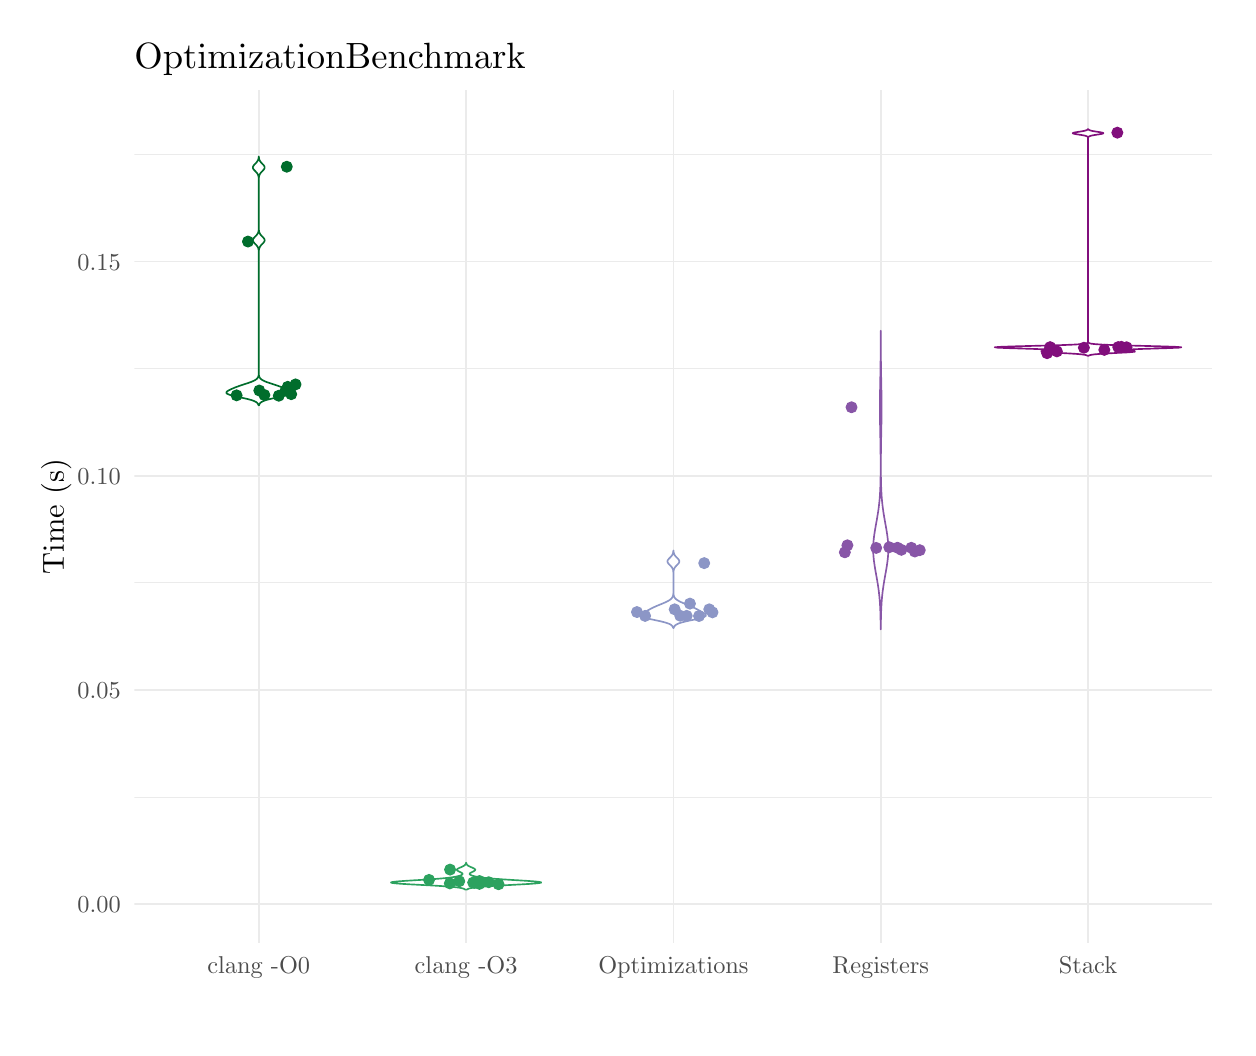
\begin{tikzpicture}[x=1pt,y=1pt]
\definecolor{fillColor}{RGB}{255,255,255}
\path[use as bounding box,fill=fillColor,fill opacity=0.00] (0,0) rectangle (433.62,361.35);
\begin{scope}
\path[clip] ( 38.56, 30.69) rectangle (428.12,338.69);
\definecolor{drawColor}{gray}{0.92}

\path[draw=drawColor,line width= 0.3pt,line join=round] ( 38.56, 83.37) --
	(428.12, 83.37);

\path[draw=drawColor,line width= 0.3pt,line join=round] ( 38.56,160.74) --
	(428.12,160.74);

\path[draw=drawColor,line width= 0.3pt,line join=round] ( 38.56,238.11) --
	(428.12,238.11);

\path[draw=drawColor,line width= 0.3pt,line join=round] ( 38.56,315.48) --
	(428.12,315.48);

\path[draw=drawColor,line width= 0.6pt,line join=round] ( 38.56, 44.69) --
	(428.12, 44.69);

\path[draw=drawColor,line width= 0.6pt,line join=round] ( 38.56,122.06) --
	(428.12,122.06);

\path[draw=drawColor,line width= 0.6pt,line join=round] ( 38.56,199.43) --
	(428.12,199.43);

\path[draw=drawColor,line width= 0.6pt,line join=round] ( 38.56,276.80) --
	(428.12,276.80);

\path[draw=drawColor,line width= 0.6pt,line join=round] ( 83.50, 30.69) --
	( 83.50,338.69);

\path[draw=drawColor,line width= 0.6pt,line join=round] (158.42, 30.69) --
	(158.42,338.69);

\path[draw=drawColor,line width= 0.6pt,line join=round] (233.34, 30.69) --
	(233.34,338.69);

\path[draw=drawColor,line width= 0.6pt,line join=round] (308.25, 30.69) --
	(308.25,338.69);

\path[draw=drawColor,line width= 0.6pt,line join=round] (383.17, 30.69) --
	(383.17,338.69);
\definecolor{drawColor}{RGB}{0,109,44}
\definecolor{fillColor}{RGB}{255,255,255}

\path[draw=drawColor,line width= 0.6pt,line join=round,line cap=round,fill=fillColor] ( 83.40,224.89) --
	( 83.36,225.07) --
	( 83.29,225.24) --
	( 83.20,225.42) --
	( 83.07,225.60) --
	( 82.91,225.77) --
	( 82.71,225.95) --
	( 82.45,226.12) --
	( 82.11,226.30) --
	( 81.71,226.47) --
	( 81.24,226.65) --
	( 80.69,226.83) --
	( 80.06,227.00) --
	( 79.37,227.18) --
	( 78.61,227.35) --
	( 77.81,227.53) --
	( 76.98,227.71) --
	( 76.15,227.88) --
	( 75.34,228.06) --
	( 74.57,228.23) --
	( 73.87,228.41) --
	( 73.25,228.59) --
	( 72.73,228.76) --
	( 72.32,228.94) --
	( 72.03,229.11) --
	( 71.86,229.29) --
	( 71.79,229.46) --
	( 71.84,229.64) --
	( 71.98,229.82) --
	( 72.19,229.99) --
	( 72.45,230.17) --
	( 72.76,230.34) --
	( 73.11,230.52) --
	( 73.48,230.70) --
	( 73.87,230.87) --
	( 74.28,231.05) --
	( 74.70,231.22) --
	( 75.14,231.40) --
	( 75.60,231.58) --
	( 76.08,231.75) --
	( 76.58,231.93) --
	( 77.09,232.10) --
	( 77.62,232.28) --
	( 78.16,232.45) --
	( 78.70,232.63) --
	( 79.24,232.81) --
	( 79.76,232.98) --
	( 80.26,233.16) --
	( 80.74,233.33) --
	( 81.17,233.51) --
	( 81.57,233.69) --
	( 81.93,233.86) --
	( 82.24,234.04) --
	( 82.50,234.21) --
	( 82.73,234.39) --
	( 82.91,234.57) --
	( 83.05,234.74) --
	( 83.17,234.92) --
	( 83.26,235.09) --
	( 83.33,235.27) --
	( 83.38,235.45) --
	( 83.42,235.62) --
	( 83.45,235.80) --
	( 83.47,235.97) --
	( 83.48,236.15) --
	( 83.49,236.32) --
	( 83.49,236.50) --
	( 83.50,236.68) --
	( 83.50,236.85) --
	( 83.50,237.03) --
	( 83.50,237.20) --
	( 83.50,237.38) --
	( 83.50,237.56) --
	( 83.50,237.73) --
	( 83.50,237.91) --
	( 83.50,238.08) --
	( 83.50,238.26) --
	( 83.50,238.44) --
	( 83.50,238.61) --
	( 83.50,238.79) --
	( 83.50,238.96) --
	( 83.50,239.14) --
	( 83.50,239.31) --
	( 83.50,239.49) --
	( 83.50,239.67) --
	( 83.50,239.84) --
	( 83.50,240.02) --
	( 83.50,240.19) --
	( 83.50,240.37) --
	( 83.50,240.55) --
	( 83.50,240.72) --
	( 83.50,240.90) --
	( 83.50,241.07) --
	( 83.50,241.25) --
	( 83.50,241.43) --
	( 83.50,241.60) --
	( 83.50,241.78) --
	( 83.50,241.95) --
	( 83.50,242.13) --
	( 83.50,242.30) --
	( 83.50,242.48) --
	( 83.50,242.66) --
	( 83.50,242.83) --
	( 83.50,243.01) --
	( 83.50,243.18) --
	( 83.50,243.36) --
	( 83.50,243.54) --
	( 83.50,243.71) --
	( 83.50,243.89) --
	( 83.50,244.06) --
	( 83.50,244.24) --
	( 83.50,244.42) --
	( 83.50,244.59) --
	( 83.50,244.77) --
	( 83.50,244.94) --
	( 83.50,245.12) --
	( 83.50,245.29) --
	( 83.50,245.47) --
	( 83.50,245.65) --
	( 83.50,245.82) --
	( 83.50,246.00) --
	( 83.50,246.17) --
	( 83.50,246.35) --
	( 83.50,246.53) --
	( 83.50,246.70) --
	( 83.50,246.88) --
	( 83.50,247.05) --
	( 83.50,247.23) --
	( 83.50,247.41) --
	( 83.50,247.58) --
	( 83.50,247.76) --
	( 83.50,247.93) --
	( 83.50,248.11) --
	( 83.50,248.29) --
	( 83.50,248.46) --
	( 83.50,248.64) --
	( 83.50,248.81) --
	( 83.50,248.99) --
	( 83.50,249.16) --
	( 83.50,249.34) --
	( 83.50,249.52) --
	( 83.50,249.69) --
	( 83.50,249.87) --
	( 83.50,250.04) --
	( 83.50,250.22) --
	( 83.50,250.40) --
	( 83.50,250.57) --
	( 83.50,250.75) --
	( 83.50,250.92) --
	( 83.50,251.10) --
	( 83.50,251.28) --
	( 83.50,251.45) --
	( 83.50,251.63) --
	( 83.50,251.80) --
	( 83.50,251.98) --
	( 83.50,252.15) --
	( 83.50,252.33) --
	( 83.50,252.51) --
	( 83.50,252.68) --
	( 83.50,252.86) --
	( 83.50,253.03) --
	( 83.50,253.21) --
	( 83.50,253.39) --
	( 83.50,253.56) --
	( 83.50,253.74) --
	( 83.50,253.91) --
	( 83.50,254.09) --
	( 83.50,254.27) --
	( 83.50,254.44) --
	( 83.50,254.62) --
	( 83.50,254.79) --
	( 83.50,254.97) --
	( 83.50,255.14) --
	( 83.50,255.32) --
	( 83.50,255.50) --
	( 83.50,255.67) --
	( 83.50,255.85) --
	( 83.50,256.02) --
	( 83.50,256.20) --
	( 83.50,256.38) --
	( 83.50,256.55) --
	( 83.50,256.73) --
	( 83.50,256.90) --
	( 83.50,257.08) --
	( 83.50,257.26) --
	( 83.50,257.43) --
	( 83.50,257.61) --
	( 83.50,257.78) --
	( 83.50,257.96) --
	( 83.50,258.14) --
	( 83.50,258.31) --
	( 83.50,258.49) --
	( 83.50,258.66) --
	( 83.50,258.84) --
	( 83.50,259.01) --
	( 83.50,259.19) --
	( 83.50,259.37) --
	( 83.50,259.54) --
	( 83.50,259.72) --
	( 83.50,259.89) --
	( 83.50,260.07) --
	( 83.50,260.25) --
	( 83.50,260.42) --
	( 83.50,260.60) --
	( 83.50,260.77) --
	( 83.50,260.95) --
	( 83.50,261.13) --
	( 83.50,261.30) --
	( 83.50,261.48) --
	( 83.50,261.65) --
	( 83.50,261.83) --
	( 83.50,262.00) --
	( 83.50,262.18) --
	( 83.50,262.36) --
	( 83.50,262.53) --
	( 83.50,262.71) --
	( 83.50,262.88) --
	( 83.50,263.06) --
	( 83.50,263.24) --
	( 83.50,263.41) --
	( 83.50,263.59) --
	( 83.50,263.76) --
	( 83.50,263.94) --
	( 83.50,264.12) --
	( 83.50,264.29) --
	( 83.50,264.47) --
	( 83.50,264.64) --
	( 83.50,264.82) --
	( 83.50,264.99) --
	( 83.50,265.17) --
	( 83.50,265.35) --
	( 83.50,265.52) --
	( 83.50,265.70) --
	( 83.50,265.87) --
	( 83.50,266.05) --
	( 83.50,266.23) --
	( 83.50,266.40) --
	( 83.50,266.58) --
	( 83.50,266.75) --
	( 83.50,266.93) --
	( 83.50,267.11) --
	( 83.50,267.28) --
	( 83.50,267.46) --
	( 83.50,267.63) --
	( 83.50,267.81) --
	( 83.50,267.99) --
	( 83.50,268.16) --
	( 83.50,268.34) --
	( 83.50,268.51) --
	( 83.50,268.69) --
	( 83.50,268.86) --
	( 83.50,269.04) --
	( 83.50,269.22) --
	( 83.50,269.39) --
	( 83.50,269.57) --
	( 83.50,269.74) --
	( 83.50,269.92) --
	( 83.50,270.10) --
	( 83.50,270.27) --
	( 83.50,270.45) --
	( 83.50,270.62) --
	( 83.50,270.80) --
	( 83.50,270.98) --
	( 83.50,271.15) --
	( 83.50,271.33) --
	( 83.50,271.50) --
	( 83.50,271.68) --
	( 83.50,271.85) --
	( 83.50,272.03) --
	( 83.50,272.21) --
	( 83.50,272.38) --
	( 83.50,272.56) --
	( 83.50,272.73) --
	( 83.50,272.91) --
	( 83.50,273.09) --
	( 83.50,273.26) --
	( 83.50,273.44) --
	( 83.50,273.61) --
	( 83.50,273.79) --
	( 83.50,273.97) --
	( 83.50,274.14) --
	( 83.50,274.32) --
	( 83.50,274.49) --
	( 83.50,274.67) --
	( 83.50,274.84) --
	( 83.50,275.02) --
	( 83.50,275.20) --
	( 83.50,275.37) --
	( 83.50,275.55) --
	( 83.50,275.72) --
	( 83.50,275.90) --
	( 83.50,276.08) --
	( 83.50,276.25) --
	( 83.50,276.43) --
	( 83.50,276.60) --
	( 83.50,276.78) --
	( 83.50,276.96) --
	( 83.50,277.13) --
	( 83.50,277.31) --
	( 83.50,277.48) --
	( 83.50,277.66) --
	( 83.50,277.84) --
	( 83.50,278.01) --
	( 83.50,278.19) --
	( 83.50,278.36) --
	( 83.50,278.54) --
	( 83.50,278.71) --
	( 83.50,278.89) --
	( 83.50,279.07) --
	( 83.50,279.24) --
	( 83.50,279.42) --
	( 83.50,279.59) --
	( 83.50,279.77) --
	( 83.50,279.95) --
	( 83.50,280.12) --
	( 83.49,280.30) --
	( 83.49,280.47) --
	( 83.48,280.65) --
	( 83.46,280.83) --
	( 83.45,281.00) --
	( 83.42,281.18) --
	( 83.39,281.35) --
	( 83.35,281.53) --
	( 83.29,281.70) --
	( 83.22,281.88) --
	( 83.14,282.06) --
	( 83.04,282.23) --
	( 82.92,282.41) --
	( 82.79,282.58) --
	( 82.64,282.76) --
	( 82.48,282.94) --
	( 82.31,283.11) --
	( 82.14,283.29) --
	( 81.97,283.46) --
	( 81.81,283.64) --
	( 81.67,283.82) --
	( 81.55,283.99) --
	( 81.45,284.17) --
	( 81.40,284.34) --
	( 81.37,284.52) --
	( 81.39,284.69) --
	( 81.44,284.87) --
	( 81.53,285.05) --
	( 81.65,285.22) --
	( 81.79,285.40) --
	( 81.95,285.57) --
	( 82.11,285.75) --
	( 82.29,285.93) --
	( 82.46,286.10) --
	( 82.62,286.28) --
	( 82.77,286.45) --
	( 82.90,286.63) --
	( 83.02,286.81) --
	( 83.13,286.98) --
	( 83.21,287.16) --
	( 83.28,287.33) --
	( 83.34,287.51) --
	( 83.38,287.69) --
	( 83.42,287.86) --
	( 83.44,288.04) --
	( 83.46,288.21) --
	( 83.48,288.39) --
	( 83.49,288.56) --
	( 83.49,288.74) --
	( 83.50,288.92) --
	( 83.50,289.09) --
	( 83.50,289.27) --
	( 83.50,289.44) --
	( 83.50,289.62) --
	( 83.50,289.80) --
	( 83.50,289.97) --
	( 83.50,290.15) --
	( 83.50,290.32) --
	( 83.50,290.50) --
	( 83.50,290.68) --
	( 83.50,290.85) --
	( 83.50,291.03) --
	( 83.50,291.20) --
	( 83.50,291.38) --
	( 83.50,291.55) --
	( 83.50,291.73) --
	( 83.50,291.91) --
	( 83.50,292.08) --
	( 83.50,292.26) --
	( 83.50,292.43) --
	( 83.50,292.61) --
	( 83.50,292.79) --
	( 83.50,292.96) --
	( 83.50,293.14) --
	( 83.50,293.31) --
	( 83.50,293.49) --
	( 83.50,293.67) --
	( 83.50,293.84) --
	( 83.50,294.02) --
	( 83.50,294.19) --
	( 83.50,294.37) --
	( 83.50,294.54) --
	( 83.50,294.72) --
	( 83.50,294.90) --
	( 83.50,295.07) --
	( 83.50,295.25) --
	( 83.50,295.42) --
	( 83.50,295.60) --
	( 83.50,295.78) --
	( 83.50,295.95) --
	( 83.50,296.13) --
	( 83.50,296.30) --
	( 83.50,296.48) --
	( 83.50,296.66) --
	( 83.50,296.83) --
	( 83.50,297.01) --
	( 83.50,297.18) --
	( 83.50,297.36) --
	( 83.50,297.53) --
	( 83.50,297.71) --
	( 83.50,297.89) --
	( 83.50,298.06) --
	( 83.50,298.24) --
	( 83.50,298.41) --
	( 83.50,298.59) --
	( 83.50,298.77) --
	( 83.50,298.94) --
	( 83.50,299.12) --
	( 83.50,299.29) --
	( 83.50,299.47) --
	( 83.50,299.65) --
	( 83.50,299.82) --
	( 83.50,300.00) --
	( 83.50,300.17) --
	( 83.50,300.35) --
	( 83.50,300.53) --
	( 83.50,300.70) --
	( 83.50,300.88) --
	( 83.50,301.05) --
	( 83.50,301.23) --
	( 83.50,301.40) --
	( 83.50,301.58) --
	( 83.50,301.76) --
	( 83.50,301.93) --
	( 83.50,302.11) --
	( 83.50,302.28) --
	( 83.50,302.46) --
	( 83.50,302.64) --
	( 83.50,302.81) --
	( 83.50,302.99) --
	( 83.50,303.16) --
	( 83.50,303.34) --
	( 83.50,303.52) --
	( 83.50,303.69) --
	( 83.50,303.87) --
	( 83.50,304.04) --
	( 83.50,304.22) --
	( 83.50,304.39) --
	( 83.50,304.57) --
	( 83.50,304.75) --
	( 83.50,304.92) --
	( 83.50,305.10) --
	( 83.50,305.27) --
	( 83.50,305.45) --
	( 83.50,305.63) --
	( 83.50,305.80) --
	( 83.50,305.98) --
	( 83.50,306.15) --
	( 83.50,306.33) --
	( 83.50,306.51) --
	( 83.49,306.68) --
	( 83.48,306.86) --
	( 83.47,307.03) --
	( 83.46,307.21) --
	( 83.44,307.38) --
	( 83.41,307.56) --
	( 83.37,307.74) --
	( 83.32,307.91) --
	( 83.26,308.09) --
	( 83.19,308.26) --
	( 83.10,308.44) --
	( 82.99,308.62) --
	( 82.87,308.79) --
	( 82.72,308.97) --
	( 82.57,309.14) --
	( 82.41,309.32) --
	( 82.24,309.50) --
	( 82.06,309.67) --
	( 81.90,309.85) --
	( 81.74,310.02) --
	( 81.61,310.20) --
	( 81.50,310.38) --
	( 81.42,310.55) --
	( 81.38,310.73) --
	( 81.38,310.90) --
	( 81.41,311.08) --
	( 81.48,311.25) --
	( 81.58,311.43) --
	( 81.71,311.61) --
	( 81.85,311.78) --
	( 82.02,311.96) --
	( 82.19,312.13) --
	( 82.36,312.31) --
	( 82.53,312.49) --
	( 82.69,312.66) --
	( 82.83,312.84) --
	( 82.96,313.01) --
	( 83.07,313.19) --
	( 83.17,313.37) --
	( 83.25,313.54) --
	( 83.31,313.72) --
	( 83.36,313.89) --
	( 83.40,314.07) --
	( 83.43,314.24) --
	( 83.45,314.42) --
	( 83.47,314.60) --
	( 83.48,314.77) --
	( 83.53,314.77) --
	( 83.54,314.60) --
	( 83.56,314.42) --
	( 83.58,314.24) --
	( 83.61,314.07) --
	( 83.65,313.89) --
	( 83.70,313.72) --
	( 83.76,313.54) --
	( 83.84,313.37) --
	( 83.94,313.19) --
	( 84.05,313.01) --
	( 84.18,312.84) --
	( 84.32,312.66) --
	( 84.48,312.49) --
	( 84.65,312.31) --
	( 84.82,312.13) --
	( 84.99,311.96) --
	( 85.16,311.78) --
	( 85.30,311.61) --
	( 85.43,311.43) --
	( 85.53,311.25) --
	( 85.60,311.08) --
	( 85.63,310.90) --
	( 85.63,310.73) --
	( 85.59,310.55) --
	( 85.51,310.38) --
	( 85.40,310.20) --
	( 85.27,310.02) --
	( 85.11,309.85) --
	( 84.95,309.67) --
	( 84.77,309.50) --
	( 84.60,309.32) --
	( 84.44,309.14) --
	( 84.28,308.97) --
	( 84.14,308.79) --
	( 84.02,308.62) --
	( 83.91,308.44) --
	( 83.82,308.26) --
	( 83.75,308.09) --
	( 83.69,307.91) --
	( 83.64,307.74) --
	( 83.60,307.56) --
	( 83.57,307.38) --
	( 83.55,307.21) --
	( 83.54,307.03) --
	( 83.53,306.86) --
	( 83.52,306.68) --
	( 83.51,306.51) --
	( 83.51,306.33) --
	( 83.51,306.15) --
	( 83.51,305.98) --
	( 83.51,305.80) --
	( 83.51,305.63) --
	( 83.51,305.45) --
	( 83.51,305.27) --
	( 83.50,305.10) --
	( 83.50,304.92) --
	( 83.50,304.75) --
	( 83.50,304.57) --
	( 83.50,304.39) --
	( 83.50,304.22) --
	( 83.50,304.04) --
	( 83.50,303.87) --
	( 83.50,303.69) --
	( 83.50,303.52) --
	( 83.50,303.34) --
	( 83.50,303.16) --
	( 83.50,302.99) --
	( 83.50,302.81) --
	( 83.50,302.64) --
	( 83.50,302.46) --
	( 83.50,302.28) --
	( 83.50,302.11) --
	( 83.50,301.93) --
	( 83.50,301.76) --
	( 83.50,301.58) --
	( 83.50,301.40) --
	( 83.50,301.23) --
	( 83.50,301.05) --
	( 83.50,300.88) --
	( 83.50,300.70) --
	( 83.50,300.53) --
	( 83.50,300.35) --
	( 83.50,300.17) --
	( 83.50,300.00) --
	( 83.50,299.82) --
	( 83.50,299.65) --
	( 83.50,299.47) --
	( 83.50,299.29) --
	( 83.50,299.12) --
	( 83.50,298.94) --
	( 83.50,298.77) --
	( 83.50,298.59) --
	( 83.50,298.41) --
	( 83.50,298.24) --
	( 83.50,298.06) --
	( 83.50,297.89) --
	( 83.50,297.71) --
	( 83.50,297.53) --
	( 83.50,297.36) --
	( 83.50,297.18) --
	( 83.50,297.01) --
	( 83.50,296.83) --
	( 83.50,296.66) --
	( 83.50,296.48) --
	( 83.50,296.30) --
	( 83.50,296.13) --
	( 83.50,295.95) --
	( 83.50,295.78) --
	( 83.50,295.60) --
	( 83.50,295.42) --
	( 83.50,295.25) --
	( 83.50,295.07) --
	( 83.50,294.90) --
	( 83.50,294.72) --
	( 83.50,294.54) --
	( 83.50,294.37) --
	( 83.50,294.19) --
	( 83.50,294.02) --
	( 83.50,293.84) --
	( 83.50,293.67) --
	( 83.50,293.49) --
	( 83.50,293.31) --
	( 83.50,293.14) --
	( 83.50,292.96) --
	( 83.50,292.79) --
	( 83.50,292.61) --
	( 83.50,292.43) --
	( 83.50,292.26) --
	( 83.50,292.08) --
	( 83.50,291.91) --
	( 83.50,291.73) --
	( 83.50,291.55) --
	( 83.50,291.38) --
	( 83.50,291.20) --
	( 83.50,291.03) --
	( 83.50,290.85) --
	( 83.50,290.68) --
	( 83.50,290.50) --
	( 83.50,290.32) --
	( 83.51,290.15) --
	( 83.51,289.97) --
	( 83.51,289.80) --
	( 83.51,289.62) --
	( 83.51,289.44) --
	( 83.51,289.27) --
	( 83.51,289.09) --
	( 83.51,288.92) --
	( 83.52,288.74) --
	( 83.52,288.56) --
	( 83.53,288.39) --
	( 83.55,288.21) --
	( 83.57,288.04) --
	( 83.59,287.86) --
	( 83.63,287.69) --
	( 83.67,287.51) --
	( 83.73,287.33) --
	( 83.80,287.16) --
	( 83.88,286.98) --
	( 83.99,286.81) --
	( 84.10,286.63) --
	( 84.24,286.45) --
	( 84.39,286.28) --
	( 84.55,286.10) --
	( 84.72,285.93) --
	( 84.90,285.75) --
	( 85.06,285.57) --
	( 85.22,285.40) --
	( 85.36,285.22) --
	( 85.48,285.05) --
	( 85.57,284.87) --
	( 85.62,284.69) --
	( 85.64,284.52) --
	( 85.61,284.34) --
	( 85.55,284.17) --
	( 85.46,283.99) --
	( 85.34,283.82) --
	( 85.20,283.64) --
	( 85.04,283.46) --
	( 84.87,283.29) --
	( 84.70,283.11) --
	( 84.53,282.94) --
	( 84.37,282.76) --
	( 84.22,282.58) --
	( 84.09,282.41) --
	( 83.97,282.23) --
	( 83.87,282.06) --
	( 83.79,281.88) --
	( 83.72,281.70) --
	( 83.66,281.53) --
	( 83.62,281.35) --
	( 83.59,281.18) --
	( 83.56,281.00) --
	( 83.55,280.83) --
	( 83.53,280.65) --
	( 83.52,280.47) --
	( 83.52,280.30) --
	( 83.51,280.12) --
	( 83.51,279.95) --
	( 83.51,279.77) --
	( 83.51,279.59) --
	( 83.51,279.42) --
	( 83.51,279.24) --
	( 83.51,279.07) --
	( 83.51,278.89) --
	( 83.50,278.71) --
	( 83.50,278.54) --
	( 83.50,278.36) --
	( 83.50,278.19) --
	( 83.50,278.01) --
	( 83.50,277.84) --
	( 83.50,277.66) --
	( 83.50,277.48) --
	( 83.50,277.31) --
	( 83.50,277.13) --
	( 83.50,276.96) --
	( 83.50,276.78) --
	( 83.50,276.60) --
	( 83.50,276.43) --
	( 83.50,276.25) --
	( 83.50,276.08) --
	( 83.50,275.90) --
	( 83.50,275.72) --
	( 83.50,275.55) --
	( 83.50,275.37) --
	( 83.50,275.20) --
	( 83.50,275.02) --
	( 83.50,274.84) --
	( 83.50,274.67) --
	( 83.50,274.49) --
	( 83.50,274.32) --
	( 83.50,274.14) --
	( 83.50,273.97) --
	( 83.50,273.79) --
	( 83.50,273.61) --
	( 83.50,273.44) --
	( 83.50,273.26) --
	( 83.50,273.09) --
	( 83.50,272.91) --
	( 83.50,272.73) --
	( 83.50,272.56) --
	( 83.50,272.38) --
	( 83.50,272.21) --
	( 83.50,272.03) --
	( 83.50,271.85) --
	( 83.50,271.68) --
	( 83.50,271.50) --
	( 83.50,271.33) --
	( 83.50,271.15) --
	( 83.50,270.98) --
	( 83.50,270.80) --
	( 83.50,270.62) --
	( 83.50,270.45) --
	( 83.50,270.27) --
	( 83.50,270.10) --
	( 83.50,269.92) --
	( 83.50,269.74) --
	( 83.50,269.57) --
	( 83.50,269.39) --
	( 83.50,269.22) --
	( 83.50,269.04) --
	( 83.50,268.86) --
	( 83.50,268.69) --
	( 83.50,268.51) --
	( 83.50,268.34) --
	( 83.50,268.16) --
	( 83.50,267.99) --
	( 83.50,267.81) --
	( 83.50,267.63) --
	( 83.50,267.46) --
	( 83.50,267.28) --
	( 83.50,267.11) --
	( 83.50,266.93) --
	( 83.50,266.75) --
	( 83.50,266.58) --
	( 83.50,266.40) --
	( 83.50,266.23) --
	( 83.50,266.05) --
	( 83.50,265.87) --
	( 83.50,265.70) --
	( 83.50,265.52) --
	( 83.50,265.35) --
	( 83.50,265.17) --
	( 83.50,264.99) --
	( 83.50,264.82) --
	( 83.50,264.64) --
	( 83.50,264.47) --
	( 83.50,264.29) --
	( 83.50,264.12) --
	( 83.50,263.94) --
	( 83.50,263.76) --
	( 83.50,263.59) --
	( 83.50,263.41) --
	( 83.50,263.24) --
	( 83.50,263.06) --
	( 83.50,262.88) --
	( 83.50,262.71) --
	( 83.50,262.53) --
	( 83.50,262.36) --
	( 83.50,262.18) --
	( 83.50,262.00) --
	( 83.50,261.83) --
	( 83.50,261.65) --
	( 83.50,261.48) --
	( 83.50,261.30) --
	( 83.50,261.13) --
	( 83.50,260.95) --
	( 83.50,260.77) --
	( 83.50,260.60) --
	( 83.50,260.42) --
	( 83.50,260.25) --
	( 83.50,260.07) --
	( 83.50,259.89) --
	( 83.50,259.72) --
	( 83.50,259.54) --
	( 83.50,259.37) --
	( 83.50,259.19) --
	( 83.50,259.01) --
	( 83.50,258.84) --
	( 83.50,258.66) --
	( 83.50,258.49) --
	( 83.50,258.31) --
	( 83.50,258.14) --
	( 83.50,257.96) --
	( 83.50,257.78) --
	( 83.50,257.61) --
	( 83.50,257.43) --
	( 83.50,257.26) --
	( 83.50,257.08) --
	( 83.50,256.90) --
	( 83.50,256.73) --
	( 83.50,256.55) --
	( 83.50,256.38) --
	( 83.50,256.20) --
	( 83.50,256.02) --
	( 83.50,255.85) --
	( 83.50,255.67) --
	( 83.50,255.50) --
	( 83.50,255.32) --
	( 83.50,255.14) --
	( 83.50,254.97) --
	( 83.50,254.79) --
	( 83.50,254.62) --
	( 83.50,254.44) --
	( 83.50,254.27) --
	( 83.50,254.09) --
	( 83.50,253.91) --
	( 83.50,253.74) --
	( 83.50,253.56) --
	( 83.50,253.39) --
	( 83.50,253.21) --
	( 83.50,253.03) --
	( 83.50,252.86) --
	( 83.50,252.68) --
	( 83.50,252.51) --
	( 83.50,252.33) --
	( 83.50,252.15) --
	( 83.50,251.98) --
	( 83.50,251.80) --
	( 83.50,251.63) --
	( 83.50,251.45) --
	( 83.50,251.28) --
	( 83.50,251.10) --
	( 83.50,250.92) --
	( 83.50,250.75) --
	( 83.50,250.57) --
	( 83.50,250.40) --
	( 83.50,250.22) --
	( 83.50,250.04) --
	( 83.50,249.87) --
	( 83.50,249.69) --
	( 83.50,249.52) --
	( 83.50,249.34) --
	( 83.50,249.16) --
	( 83.50,248.99) --
	( 83.50,248.81) --
	( 83.50,248.64) --
	( 83.50,248.46) --
	( 83.50,248.29) --
	( 83.50,248.11) --
	( 83.50,247.93) --
	( 83.50,247.76) --
	( 83.50,247.58) --
	( 83.50,247.41) --
	( 83.50,247.23) --
	( 83.50,247.05) --
	( 83.50,246.88) --
	( 83.50,246.70) --
	( 83.50,246.53) --
	( 83.50,246.35) --
	( 83.50,246.17) --
	( 83.50,246.00) --
	( 83.50,245.82) --
	( 83.50,245.65) --
	( 83.50,245.47) --
	( 83.50,245.29) --
	( 83.50,245.12) --
	( 83.50,244.94) --
	( 83.50,244.77) --
	( 83.50,244.59) --
	( 83.50,244.42) --
	( 83.50,244.24) --
	( 83.50,244.06) --
	( 83.50,243.89) --
	( 83.50,243.71) --
	( 83.50,243.54) --
	( 83.50,243.36) --
	( 83.50,243.18) --
	( 83.50,243.01) --
	( 83.50,242.83) --
	( 83.50,242.66) --
	( 83.50,242.48) --
	( 83.50,242.30) --
	( 83.50,242.13) --
	( 83.50,241.95) --
	( 83.50,241.78) --
	( 83.50,241.60) --
	( 83.50,241.43) --
	( 83.50,241.25) --
	( 83.50,241.07) --
	( 83.50,240.90) --
	( 83.50,240.72) --
	( 83.50,240.55) --
	( 83.50,240.37) --
	( 83.50,240.19) --
	( 83.50,240.02) --
	( 83.50,239.84) --
	( 83.50,239.67) --
	( 83.50,239.49) --
	( 83.50,239.31) --
	( 83.50,239.14) --
	( 83.50,238.96) --
	( 83.50,238.79) --
	( 83.50,238.61) --
	( 83.50,238.44) --
	( 83.50,238.26) --
	( 83.50,238.08) --
	( 83.50,237.91) --
	( 83.51,237.73) --
	( 83.51,237.56) --
	( 83.51,237.38) --
	( 83.51,237.20) --
	( 83.51,237.03) --
	( 83.51,236.85) --
	( 83.51,236.68) --
	( 83.52,236.50) --
	( 83.52,236.32) --
	( 83.53,236.15) --
	( 83.54,235.97) --
	( 83.56,235.80) --
	( 83.59,235.62) --
	( 83.63,235.45) --
	( 83.68,235.27) --
	( 83.75,235.09) --
	( 83.84,234.92) --
	( 83.96,234.74) --
	( 84.10,234.57) --
	( 84.28,234.39) --
	( 84.51,234.21) --
	( 84.77,234.04) --
	( 85.08,233.86) --
	( 85.44,233.69) --
	( 85.84,233.51) --
	( 86.27,233.33) --
	( 86.75,233.16) --
	( 87.25,232.98) --
	( 87.77,232.81) --
	( 88.31,232.63) --
	( 88.85,232.45) --
	( 89.39,232.28) --
	( 89.92,232.10) --
	( 90.43,231.93) --
	( 90.93,231.75) --
	( 91.41,231.58) --
	( 91.86,231.40) --
	( 92.31,231.22) --
	( 92.73,231.05) --
	( 93.14,230.87) --
	( 93.53,230.70) --
	( 93.90,230.52) --
	( 94.25,230.34) --
	( 94.56,230.17) --
	( 94.82,229.99) --
	( 95.03,229.82) --
	( 95.17,229.64) --
	( 95.21,229.46) --
	( 95.15,229.29) --
	( 94.98,229.11) --
	( 94.69,228.94) --
	( 94.28,228.76) --
	( 93.76,228.59) --
	( 93.14,228.41) --
	( 92.44,228.23) --
	( 91.67,228.06) --
	( 90.86,227.88) --
	( 90.02,227.71) --
	( 89.20,227.53) --
	( 88.40,227.35) --
	( 87.64,227.18) --
	( 86.95,227.00) --
	( 86.32,226.83) --
	( 85.77,226.65) --
	( 85.30,226.47) --
	( 84.90,226.30) --
	( 84.56,226.12) --
	( 84.30,225.95) --
	( 84.10,225.77) --
	( 83.93,225.60) --
	( 83.81,225.42) --
	( 83.72,225.24) --
	( 83.65,225.07) --
	( 83.61,224.89) --
	( 83.40,224.89) --
	cycle;
\definecolor{drawColor}{RGB}{44,162,95}

\path[draw=drawColor,line width= 0.6pt,line join=round,line cap=round,fill=fillColor] (158.12, 49.88) --
	(158.10, 49.90) --
	(158.08, 49.91) --
	(158.06, 49.93) --
	(158.03, 49.95) --
	(158.01, 49.97) --
	(157.98, 49.99) --
	(157.95, 50.01) --
	(157.92, 50.03) --
	(157.89, 50.05) --
	(157.85, 50.07) --
	(157.82, 50.09) --
	(157.78, 50.10) --
	(157.74, 50.12) --
	(157.70, 50.14) --
	(157.65, 50.16) --
	(157.60, 50.18) --
	(157.56, 50.20) --
	(157.50, 50.22) --
	(157.45, 50.24) --
	(157.39, 50.26) --
	(157.33, 50.28) --
	(157.27, 50.30) --
	(157.20, 50.31) --
	(157.13, 50.33) --
	(157.06, 50.35) --
	(156.98, 50.37) --
	(156.90, 50.39) --
	(156.82, 50.41) --
	(156.73, 50.43) --
	(156.64, 50.45) --
	(156.55, 50.47) --
	(156.45, 50.49) --
	(156.35, 50.51) --
	(156.24, 50.52) --
	(156.13, 50.54) --
	(156.01, 50.56) --
	(155.89, 50.58) --
	(155.77, 50.60) --
	(155.64, 50.62) --
	(155.50, 50.64) --
	(155.36, 50.66) --
	(155.22, 50.68) --
	(155.07, 50.70) --
	(154.91, 50.71) --
	(154.75, 50.73) --
	(154.58, 50.75) --
	(154.41, 50.77) --
	(154.23, 50.79) --
	(154.05, 50.81) --
	(153.86, 50.83) --
	(153.67, 50.85) --
	(153.46, 50.87) --
	(153.26, 50.89) --
	(153.05, 50.91) --
	(152.83, 50.92) --
	(152.60, 50.94) --
	(152.37, 50.96) --
	(152.14, 50.98) --
	(151.89, 51.00) --
	(151.65, 51.02) --
	(151.39, 51.04) --
	(151.13, 51.06) --
	(150.87, 51.08) --
	(150.60, 51.10) --
	(150.32, 51.11) --
	(150.04, 51.13) --
	(149.75, 51.15) --
	(149.45, 51.17) --
	(149.15, 51.19) --
	(148.85, 51.21) --
	(148.54, 51.23) --
	(148.23, 51.25) --
	(147.91, 51.27) --
	(147.58, 51.29) --
	(147.26, 51.31) --
	(146.92, 51.32) --
	(146.59, 51.34) --
	(146.25, 51.36) --
	(145.90, 51.38) --
	(145.56, 51.40) --
	(145.21, 51.42) --
	(144.85, 51.44) --
	(144.50, 51.46) --
	(144.14, 51.48) --
	(143.78, 51.50) --
	(143.42, 51.51) --
	(143.06, 51.53) --
	(142.70, 51.55) --
	(142.33, 51.57) --
	(141.97, 51.59) --
	(141.61, 51.61) --
	(141.24, 51.63) --
	(140.88, 51.65) --
	(140.52, 51.67) --
	(140.16, 51.69) --
	(139.80, 51.71) --
	(139.45, 51.72) --
	(139.10, 51.74) --
	(138.75, 51.76) --
	(138.40, 51.78) --
	(138.06, 51.80) --
	(137.72, 51.82) --
	(137.39, 51.84) --
	(137.06, 51.86) --
	(136.74, 51.88) --
	(136.43, 51.90) --
	(136.12, 51.91) --
	(135.82, 51.93) --
	(135.52, 51.95) --
	(135.23, 51.97) --
	(134.95, 51.99) --
	(134.68, 52.01) --
	(134.42, 52.03) --
	(134.16, 52.05) --
	(133.91, 52.07) --
	(133.68, 52.09) --
	(133.45, 52.11) --
	(133.24, 52.12) --
	(133.03, 52.14) --
	(132.84, 52.16) --
	(132.65, 52.18) --
	(132.48, 52.20) --
	(132.32, 52.22) --
	(132.16, 52.24) --
	(132.03, 52.26) --
	(131.90, 52.28) --
	(131.78, 52.30) --
	(131.68, 52.32) --
	(131.59, 52.33) --
	(131.52, 52.35) --
	(131.45, 52.37) --
	(131.40, 52.39) --
	(131.36, 52.41) --
	(131.33, 52.43) --
	(131.31, 52.45) --
	(131.31, 52.47) --
	(131.32, 52.49) --
	(131.34, 52.51) --
	(131.37, 52.52) --
	(131.42, 52.54) --
	(131.48, 52.56) --
	(131.55, 52.58) --
	(131.64, 52.60) --
	(131.73, 52.62) --
	(131.84, 52.64) --
	(131.95, 52.66) --
	(132.08, 52.68) --
	(132.22, 52.70) --
	(132.37, 52.72) --
	(132.53, 52.73) --
	(132.70, 52.75) --
	(132.88, 52.77) --
	(133.07, 52.79) --
	(133.27, 52.81) --
	(133.48, 52.83) --
	(133.70, 52.85) --
	(133.92, 52.87) --
	(134.15, 52.89) --
	(134.40, 52.91) --
	(134.64, 52.92) --
	(134.90, 52.94) --
	(135.16, 52.96) --
	(135.42, 52.98) --
	(135.70, 53.00) --
	(135.98, 53.02) --
	(136.26, 53.04) --
	(136.55, 53.06) --
	(136.84, 53.08) --
	(137.14, 53.10) --
	(137.44, 53.12) --
	(137.74, 53.13) --
	(138.05, 53.15) --
	(138.36, 53.17) --
	(138.67, 53.19) --
	(138.98, 53.21) --
	(139.29, 53.23) --
	(139.61, 53.25) --
	(139.92, 53.27) --
	(140.24, 53.29) --
	(140.56, 53.31) --
	(140.87, 53.32) --
	(141.19, 53.34) --
	(141.50, 53.36) --
	(141.82, 53.38) --
	(142.13, 53.40) --
	(142.44, 53.42) --
	(142.75, 53.44) --
	(143.06, 53.46) --
	(143.37, 53.48) --
	(143.67, 53.50) --
	(143.97, 53.52) --
	(144.27, 53.53) --
	(144.56, 53.55) --
	(144.85, 53.57) --
	(145.14, 53.59) --
	(145.43, 53.61) --
	(145.71, 53.63) --
	(145.99, 53.65) --
	(146.26, 53.67) --
	(146.53, 53.69) --
	(146.80, 53.71) --
	(147.06, 53.72) --
	(147.32, 53.74) --
	(147.57, 53.76) --
	(147.82, 53.78) --
	(148.07, 53.80) --
	(148.31, 53.82) --
	(148.55, 53.84) --
	(148.78, 53.86) --
	(149.01, 53.88) --
	(149.23, 53.90) --
	(149.45, 53.92) --
	(149.67, 53.93) --
	(149.88, 53.95) --
	(150.09, 53.97) --
	(150.29, 53.99) --
	(150.49, 54.01) --
	(150.68, 54.03) --
	(150.88, 54.05) --
	(151.06, 54.07) --
	(151.24, 54.09) --
	(151.42, 54.11) --
	(151.60, 54.12) --
	(151.77, 54.14) --
	(151.93, 54.16) --
	(152.10, 54.18) --
	(152.26, 54.20) --
	(152.41, 54.22) --
	(152.56, 54.24) --
	(152.71, 54.26) --
	(152.86, 54.28) --
	(153.00, 54.30) --
	(153.14, 54.32) --
	(153.28, 54.33) --
	(153.41, 54.35) --
	(153.54, 54.37) --
	(153.66, 54.39) --
	(153.79, 54.41) --
	(153.91, 54.43) --
	(154.02, 54.45) --
	(154.14, 54.47) --
	(154.25, 54.49) --
	(154.36, 54.51) --
	(154.47, 54.53) --
	(154.57, 54.54) --
	(154.67, 54.56) --
	(154.77, 54.58) --
	(154.87, 54.60) --
	(154.96, 54.62) --
	(155.06, 54.64) --
	(155.15, 54.66) --
	(155.23, 54.68) --
	(155.32, 54.70) --
	(155.40, 54.72) --
	(155.48, 54.73) --
	(155.56, 54.75) --
	(155.64, 54.77) --
	(155.71, 54.79) --
	(155.78, 54.81) --
	(155.85, 54.83) --
	(155.92, 54.85) --
	(155.99, 54.87) --
	(156.05, 54.89) --
	(156.11, 54.91) --
	(156.18, 54.93) --
	(156.23, 54.94) --
	(156.29, 54.96) --
	(156.34, 54.98) --
	(156.40, 55.00) --
	(156.45, 55.02) --
	(156.50, 55.04) --
	(156.54, 55.06) --
	(156.59, 55.08) --
	(156.63, 55.10) --
	(156.67, 55.12) --
	(156.71, 55.13) --
	(156.75, 55.15) --
	(156.79, 55.17) --
	(156.82, 55.19) --
	(156.85, 55.21) --
	(156.88, 55.23) --
	(156.91, 55.25) --
	(156.94, 55.27) --
	(156.96, 55.29) --
	(156.99, 55.31) --
	(157.01, 55.33) --
	(157.03, 55.34) --
	(157.05, 55.36) --
	(157.06, 55.38) --
	(157.08, 55.40) --
	(157.09, 55.42) --
	(157.10, 55.44) --
	(157.11, 55.46) --
	(157.12, 55.48) --
	(157.12, 55.50) --
	(157.12, 55.52) --
	(157.13, 55.53) --
	(157.13, 55.55) --
	(157.13, 55.57) --
	(157.12, 55.59) --
	(157.12, 55.61) --
	(157.11, 55.63) --
	(157.11, 55.65) --
	(157.10, 55.67) --
	(157.09, 55.69) --
	(157.07, 55.71) --
	(157.06, 55.73) --
	(157.04, 55.74) --
	(157.03, 55.76) --
	(157.01, 55.78) --
	(156.99, 55.80) --
	(156.97, 55.82) --
	(156.95, 55.84) --
	(156.93, 55.86) --
	(156.90, 55.88) --
	(156.88, 55.90) --
	(156.85, 55.92) --
	(156.82, 55.93) --
	(156.79, 55.95) --
	(156.76, 55.97) --
	(156.73, 55.99) --
	(156.70, 56.01) --
	(156.67, 56.03) --
	(156.63, 56.05) --
	(156.60, 56.07) --
	(156.56, 56.09) --
	(156.53, 56.11) --
	(156.49, 56.13) --
	(156.45, 56.14) --
	(156.42, 56.16) --
	(156.38, 56.18) --
	(156.34, 56.20) --
	(156.30, 56.22) --
	(156.26, 56.24) --
	(156.22, 56.26) --
	(156.18, 56.28) --
	(156.14, 56.30) --
	(156.10, 56.32) --
	(156.07, 56.34) --
	(156.03, 56.35) --
	(155.99, 56.37) --
	(155.95, 56.39) --
	(155.91, 56.41) --
	(155.87, 56.43) --
	(155.83, 56.45) --
	(155.79, 56.47) --
	(155.76, 56.49) --
	(155.72, 56.51) --
	(155.68, 56.53) --
	(155.65, 56.54) --
	(155.61, 56.56) --
	(155.58, 56.58) --
	(155.54, 56.60) --
	(155.51, 56.62) --
	(155.48, 56.64) --
	(155.45, 56.66) --
	(155.42, 56.68) --
	(155.39, 56.70) --
	(155.36, 56.72) --
	(155.34, 56.74) --
	(155.31, 56.75) --
	(155.29, 56.77) --
	(155.27, 56.79) --
	(155.25, 56.81) --
	(155.23, 56.83) --
	(155.21, 56.85) --
	(155.19, 56.87) --
	(155.18, 56.89) --
	(155.16, 56.91) --
	(155.15, 56.93) --
	(155.14, 56.94) --
	(155.13, 56.96) --
	(155.12, 56.98) --
	(155.12, 57.00) --
	(155.11, 57.02) --
	(155.11, 57.04) --
	(155.11, 57.06) --
	(155.11, 57.08) --
	(155.11, 57.10) --
	(155.12, 57.12) --
	(155.12, 57.14) --
	(155.13, 57.15) --
	(155.14, 57.17) --
	(155.15, 57.19) --
	(155.16, 57.21) --
	(155.17, 57.23) --
	(155.19, 57.25) --
	(155.21, 57.27) --
	(155.22, 57.29) --
	(155.24, 57.31) --
	(155.26, 57.33) --
	(155.29, 57.34) --
	(155.31, 57.36) --
	(155.34, 57.38) --
	(155.36, 57.40) --
	(155.39, 57.42) --
	(155.42, 57.44) --
	(155.45, 57.46) --
	(155.48, 57.48) --
	(155.51, 57.50) --
	(155.55, 57.52) --
	(155.58, 57.54) --
	(155.62, 57.55) --
	(155.65, 57.57) --
	(155.69, 57.59) --
	(155.73, 57.61) --
	(155.77, 57.63) --
	(155.81, 57.65) --
	(155.85, 57.67) --
	(155.89, 57.69) --
	(155.93, 57.71) --
	(155.98, 57.73) --
	(156.02, 57.74) --
	(156.06, 57.76) --
	(156.11, 57.78) --
	(156.15, 57.80) --
	(156.19, 57.82) --
	(156.24, 57.84) --
	(156.28, 57.86) --
	(156.33, 57.88) --
	(156.37, 57.90) --
	(156.42, 57.92) --
	(156.46, 57.94) --
	(156.51, 57.95) --
	(156.55, 57.97) --
	(156.60, 57.99) --
	(156.64, 58.01) --
	(156.69, 58.03) --
	(156.73, 58.05) --
	(156.77, 58.07) --
	(156.82, 58.09) --
	(156.86, 58.11) --
	(156.90, 58.13) --
	(156.95, 58.14) --
	(156.99, 58.16) --
	(157.03, 58.18) --
	(157.07, 58.20) --
	(157.11, 58.22) --
	(157.15, 58.24) --
	(157.19, 58.26) --
	(157.23, 58.28) --
	(157.26, 58.30) --
	(157.30, 58.32) --
	(157.34, 58.34) --
	(157.37, 58.35) --
	(157.41, 58.37) --
	(157.44, 58.39) --
	(157.48, 58.41) --
	(157.51, 58.43) --
	(157.54, 58.45) --
	(157.58, 58.47) --
	(157.61, 58.49) --
	(157.64, 58.51) --
	(157.67, 58.53) --
	(157.69, 58.55) --
	(157.72, 58.56) --
	(157.75, 58.58) --
	(157.78, 58.60) --
	(157.80, 58.62) --
	(157.83, 58.64) --
	(157.85, 58.66) --
	(157.88, 58.68) --
	(157.90, 58.70) --
	(157.92, 58.72) --
	(157.94, 58.74) --
	(157.96, 58.75) --
	(157.98, 58.77) --
	(158.00, 58.79) --
	(158.02, 58.81) --
	(158.04, 58.83) --
	(158.06, 58.85) --
	(158.07, 58.87) --
	(158.09, 58.89) --
	(158.11, 58.91) --
	(158.12, 58.93) --
	(158.13, 58.95) --
	(158.15, 58.96) --
	(158.16, 58.98) --
	(158.17, 59.00) --
	(158.19, 59.02) --
	(158.20, 59.04) --
	(158.21, 59.06) --
	(158.22, 59.08) --
	(158.23, 59.10) --
	(158.24, 59.12) --
	(158.25, 59.14) --
	(158.26, 59.15) --
	(158.27, 59.17) --
	(158.28, 59.19) --
	(158.28, 59.21) --
	(158.29, 59.23) --
	(158.30, 59.25) --
	(158.31, 59.27) --
	(158.31, 59.29) --
	(158.32, 59.31) --
	(158.33, 59.33) --
	(158.33, 59.35) --
	(158.34, 59.36) --
	(158.34, 59.38) --
	(158.35, 59.40) --
	(158.35, 59.42) --
	(158.35, 59.44) --
	(158.36, 59.46) --
	(158.36, 59.48) --
	(158.37, 59.50) --
	(158.37, 59.52) --
	(158.37, 59.54) --
	(158.38, 59.55) --
	(158.38, 59.57) --
	(158.38, 59.59) --
	(158.38, 59.61) --
	(158.46, 59.61) --
	(158.46, 59.59) --
	(158.46, 59.57) --
	(158.47, 59.55) --
	(158.47, 59.54) --
	(158.47, 59.52) --
	(158.48, 59.50) --
	(158.48, 59.48) --
	(158.48, 59.46) --
	(158.49, 59.44) --
	(158.49, 59.42) --
	(158.50, 59.40) --
	(158.50, 59.38) --
	(158.51, 59.36) --
	(158.51, 59.35) --
	(158.52, 59.33) --
	(158.52, 59.31) --
	(158.53, 59.29) --
	(158.54, 59.27) --
	(158.54, 59.25) --
	(158.55, 59.23) --
	(158.56, 59.21) --
	(158.57, 59.19) --
	(158.57, 59.17) --
	(158.58, 59.15) --
	(158.59, 59.14) --
	(158.60, 59.12) --
	(158.61, 59.10) --
	(158.62, 59.08) --
	(158.63, 59.06) --
	(158.64, 59.04) --
	(158.66, 59.02) --
	(158.67, 59.00) --
	(158.68, 58.98) --
	(158.69, 58.96) --
	(158.71, 58.95) --
	(158.72, 58.93) --
	(158.74, 58.91) --
	(158.75, 58.89) --
	(158.77, 58.87) --
	(158.79, 58.85) --
	(158.80, 58.83) --
	(158.82, 58.81) --
	(158.84, 58.79) --
	(158.86, 58.77) --
	(158.88, 58.75) --
	(158.90, 58.74) --
	(158.92, 58.72) --
	(158.94, 58.70) --
	(158.97, 58.68) --
	(158.99, 58.66) --
	(159.01, 58.64) --
	(159.04, 58.62) --
	(159.07, 58.60) --
	(159.09, 58.58) --
	(159.12, 58.56) --
	(159.15, 58.55) --
	(159.18, 58.53) --
	(159.21, 58.51) --
	(159.24, 58.49) --
	(159.27, 58.47) --
	(159.30, 58.45) --
	(159.33, 58.43) --
	(159.36, 58.41) --
	(159.40, 58.39) --
	(159.43, 58.37) --
	(159.47, 58.35) --
	(159.50, 58.34) --
	(159.54, 58.32) --
	(159.58, 58.30) --
	(159.62, 58.28) --
	(159.65, 58.26) --
	(159.69, 58.24) --
	(159.73, 58.22) --
	(159.77, 58.20) --
	(159.81, 58.18) --
	(159.86, 58.16) --
	(159.90, 58.14) --
	(159.94, 58.13) --
	(159.98, 58.11) --
	(160.02, 58.09) --
	(160.07, 58.07) --
	(160.11, 58.05) --
	(160.16, 58.03) --
	(160.20, 58.01) --
	(160.24, 57.99) --
	(160.29, 57.97) --
	(160.33, 57.95) --
	(160.38, 57.94) --
	(160.42, 57.92) --
	(160.47, 57.90) --
	(160.51, 57.88) --
	(160.56, 57.86) --
	(160.60, 57.84) --
	(160.65, 57.82) --
	(160.69, 57.80) --
	(160.74, 57.78) --
	(160.78, 57.76) --
	(160.82, 57.74) --
	(160.87, 57.73) --
	(160.91, 57.71) --
	(160.95, 57.69) --
	(160.99, 57.67) --
	(161.03, 57.65) --
	(161.07, 57.63) --
	(161.11, 57.61) --
	(161.15, 57.59) --
	(161.19, 57.57) --
	(161.22, 57.55) --
	(161.26, 57.54) --
	(161.29, 57.52) --
	(161.33, 57.50) --
	(161.36, 57.48) --
	(161.39, 57.46) --
	(161.42, 57.44) --
	(161.45, 57.42) --
	(161.48, 57.40) --
	(161.51, 57.38) --
	(161.53, 57.36) --
	(161.56, 57.34) --
	(161.58, 57.33) --
	(161.60, 57.31) --
	(161.62, 57.29) --
	(161.64, 57.27) --
	(161.65, 57.25) --
	(161.67, 57.23) --
	(161.68, 57.21) --
	(161.69, 57.19) --
	(161.70, 57.17) --
	(161.71, 57.15) --
	(161.72, 57.14) --
	(161.73, 57.12) --
	(161.73, 57.10) --
	(161.73, 57.08) --
	(161.73, 57.06) --
	(161.73, 57.04) --
	(161.73, 57.02) --
	(161.72, 57.00) --
	(161.72, 56.98) --
	(161.71, 56.96) --
	(161.70, 56.94) --
	(161.69, 56.93) --
	(161.68, 56.91) --
	(161.67, 56.89) --
	(161.65, 56.87) --
	(161.63, 56.85) --
	(161.62, 56.83) --
	(161.60, 56.81) --
	(161.58, 56.79) --
	(161.55, 56.77) --
	(161.53, 56.75) --
	(161.50, 56.74) --
	(161.48, 56.72) --
	(161.45, 56.70) --
	(161.42, 56.68) --
	(161.39, 56.66) --
	(161.36, 56.64) --
	(161.33, 56.62) --
	(161.30, 56.60) --
	(161.27, 56.58) --
	(161.23, 56.56) --
	(161.20, 56.54) --
	(161.16, 56.53) --
	(161.12, 56.51) --
	(161.09, 56.49) --
	(161.05, 56.47) --
	(161.01, 56.45) --
	(160.97, 56.43) --
	(160.93, 56.41) --
	(160.90, 56.39) --
	(160.86, 56.37) --
	(160.82, 56.35) --
	(160.78, 56.34) --
	(160.74, 56.32) --
	(160.70, 56.30) --
	(160.66, 56.28) --
	(160.62, 56.26) --
	(160.58, 56.24) --
	(160.54, 56.22) --
	(160.50, 56.20) --
	(160.46, 56.18) --
	(160.43, 56.16) --
	(160.39, 56.14) --
	(160.35, 56.13) --
	(160.31, 56.11) --
	(160.28, 56.09) --
	(160.24, 56.07) --
	(160.21, 56.05) --
	(160.18, 56.03) --
	(160.14, 56.01) --
	(160.11, 55.99) --
	(160.08, 55.97) --
	(160.05, 55.95) --
	(160.02, 55.93) --
	(159.99, 55.92) --
	(159.97, 55.90) --
	(159.94, 55.88) --
	(159.92, 55.86) --
	(159.89, 55.84) --
	(159.87, 55.82) --
	(159.85, 55.80) --
	(159.83, 55.78) --
	(159.81, 55.76) --
	(159.80, 55.74) --
	(159.78, 55.73) --
	(159.77, 55.71) --
	(159.76, 55.69) --
	(159.75, 55.67) --
	(159.74, 55.65) --
	(159.73, 55.63) --
	(159.72, 55.61) --
	(159.72, 55.59) --
	(159.72, 55.57) --
	(159.72, 55.55) --
	(159.72, 55.53) --
	(159.72, 55.52) --
	(159.72, 55.50) --
	(159.73, 55.48) --
	(159.73, 55.46) --
	(159.74, 55.44) --
	(159.75, 55.42) --
	(159.77, 55.40) --
	(159.78, 55.38) --
	(159.80, 55.36) --
	(159.81, 55.34) --
	(159.83, 55.33) --
	(159.86, 55.31) --
	(159.88, 55.29) --
	(159.90, 55.27) --
	(159.93, 55.25) --
	(159.96, 55.23) --
	(159.99, 55.21) --
	(160.02, 55.19) --
	(160.06, 55.17) --
	(160.09, 55.15) --
	(160.13, 55.13) --
	(160.17, 55.12) --
	(160.21, 55.10) --
	(160.25, 55.08) --
	(160.30, 55.06) --
	(160.35, 55.04) --
	(160.39, 55.02) --
	(160.45, 55.00) --
	(160.50, 54.98) --
	(160.55, 54.96) --
	(160.61, 54.94) --
	(160.67, 54.93) --
	(160.73, 54.91) --
	(160.79, 54.89) --
	(160.85, 54.87) --
	(160.92, 54.85) --
	(160.99, 54.83) --
	(161.06, 54.81) --
	(161.13, 54.79) --
	(161.21, 54.77) --
	(161.28, 54.75) --
	(161.36, 54.73) --
	(161.44, 54.72) --
	(161.52, 54.70) --
	(161.61, 54.68) --
	(161.70, 54.66) --
	(161.79, 54.64) --
	(161.88, 54.62) --
	(161.97, 54.60) --
	(162.07, 54.58) --
	(162.17, 54.56) --
	(162.27, 54.54) --
	(162.38, 54.53) --
	(162.48, 54.51) --
	(162.59, 54.49) --
	(162.70, 54.47) --
	(162.82, 54.45) --
	(162.94, 54.43) --
	(163.06, 54.41) --
	(163.18, 54.39) --
	(163.30, 54.37) --
	(163.44, 54.35) --
	(163.57, 54.33) --
	(163.70, 54.32) --
	(163.84, 54.30) --
	(163.98, 54.28) --
	(164.13, 54.26) --
	(164.28, 54.24) --
	(164.43, 54.22) --
	(164.59, 54.20) --
	(164.75, 54.18) --
	(164.91, 54.16) --
	(165.07, 54.14) --
	(165.25, 54.12) --
	(165.42, 54.11) --
	(165.60, 54.09) --
	(165.78, 54.07) --
	(165.97, 54.05) --
	(166.16, 54.03) --
	(166.35, 54.01) --
	(166.55, 53.99) --
	(166.75, 53.97) --
	(166.96, 53.95) --
	(167.17, 53.93) --
	(167.39, 53.92) --
	(167.61, 53.90) --
	(167.83, 53.88) --
	(168.06, 53.86) --
	(168.29, 53.84) --
	(168.53, 53.82) --
	(168.77, 53.80) --
	(169.02, 53.78) --
	(169.27, 53.76) --
	(169.52, 53.74) --
	(169.78, 53.72) --
	(170.04, 53.71) --
	(170.31, 53.69) --
	(170.58, 53.67) --
	(170.86, 53.65) --
	(171.13, 53.63) --
	(171.42, 53.61) --
	(171.70, 53.59) --
	(171.99, 53.57) --
	(172.28, 53.55) --
	(172.57, 53.53) --
	(172.87, 53.52) --
	(173.17, 53.50) --
	(173.48, 53.48) --
	(173.78, 53.46) --
	(174.09, 53.44) --
	(174.40, 53.42) --
	(174.71, 53.40) --
	(175.02, 53.38) --
	(175.34, 53.36) --
	(175.65, 53.34) --
	(175.97, 53.32) --
	(176.29, 53.31) --
	(176.60, 53.29) --
	(176.92, 53.27) --
	(177.23, 53.25) --
	(177.55, 53.23) --
	(177.86, 53.21) --
	(178.18, 53.19) --
	(178.49, 53.17) --
	(178.80, 53.15) --
	(179.10, 53.13) --
	(179.40, 53.12) --
	(179.70, 53.10) --
	(180.00, 53.08) --
	(180.29, 53.06) --
	(180.58, 53.04) --
	(180.87, 53.02) --
	(181.14, 53.00) --
	(181.42, 52.98) --
	(181.68, 52.96) --
	(181.95, 52.94) --
	(182.20, 52.92) --
	(182.45, 52.91) --
	(182.69, 52.89) --
	(182.92, 52.87) --
	(183.15, 52.85) --
	(183.36, 52.83) --
	(183.57, 52.81) --
	(183.77, 52.79) --
	(183.96, 52.77) --
	(184.14, 52.75) --
	(184.31, 52.73) --
	(184.47, 52.72) --
	(184.62, 52.70) --
	(184.76, 52.68) --
	(184.89, 52.66) --
	(185.01, 52.64) --
	(185.11, 52.62) --
	(185.21, 52.60) --
	(185.29, 52.58) --
	(185.36, 52.56) --
	(185.42, 52.54) --
	(185.47, 52.52) --
	(185.50, 52.51) --
	(185.52, 52.49) --
	(185.53, 52.47) --
	(185.53, 52.45) --
	(185.52, 52.43) --
	(185.49, 52.41) --
	(185.45, 52.39) --
	(185.39, 52.37) --
	(185.33, 52.35) --
	(185.25, 52.33) --
	(185.16, 52.32) --
	(185.06, 52.30) --
	(184.94, 52.28) --
	(184.81, 52.26) --
	(184.68, 52.24) --
	(184.53, 52.22) --
	(184.37, 52.20) --
	(184.19, 52.18) --
	(184.01, 52.16) --
	(183.81, 52.14) --
	(183.61, 52.12) --
	(183.39, 52.11) --
	(183.16, 52.09) --
	(182.93, 52.07) --
	(182.68, 52.05) --
	(182.43, 52.03) --
	(182.17, 52.01) --
	(181.89, 51.99) --
	(181.61, 51.97) --
	(181.32, 51.95) --
	(181.03, 51.93) --
	(180.73, 51.91) --
	(180.41, 51.90) --
	(180.10, 51.88) --
	(179.78, 51.86) --
	(179.45, 51.84) --
	(179.12, 51.82) --
	(178.78, 51.80) --
	(178.44, 51.78) --
	(178.09, 51.76) --
	(177.74, 51.74) --
	(177.39, 51.72) --
	(177.04, 51.71) --
	(176.68, 51.69) --
	(176.32, 51.67) --
	(175.96, 51.65) --
	(175.60, 51.63) --
	(175.23, 51.61) --
	(174.87, 51.59) --
	(174.51, 51.57) --
	(174.14, 51.55) --
	(173.78, 51.53) --
	(173.42, 51.51) --
	(173.06, 51.50) --
	(172.70, 51.48) --
	(172.34, 51.46) --
	(171.99, 51.44) --
	(171.64, 51.42) --
	(171.29, 51.40) --
	(170.94, 51.38) --
	(170.59, 51.36) --
	(170.26, 51.34) --
	(169.92, 51.32) --
	(169.59, 51.31) --
	(169.26, 51.29) --
	(168.93, 51.27) --
	(168.62, 51.25) --
	(168.30, 51.23) --
	(167.99, 51.21) --
	(167.69, 51.19) --
	(167.39, 51.17) --
	(167.10, 51.15) --
	(166.81, 51.13) --
	(166.52, 51.11) --
	(166.25, 51.10) --
	(165.97, 51.08) --
	(165.71, 51.06) --
	(165.45, 51.04) --
	(165.20, 51.02) --
	(164.95, 51.00) --
	(164.70, 50.98) --
	(164.47, 50.96) --
	(164.24, 50.94) --
	(164.02, 50.92) --
	(163.80, 50.91) --
	(163.58, 50.89) --
	(163.38, 50.87) --
	(163.18, 50.85) --
	(162.98, 50.83) --
	(162.79, 50.81) --
	(162.61, 50.79) --
	(162.43, 50.77) --
	(162.26, 50.75) --
	(162.09, 50.73) --
	(161.93, 50.71) --
	(161.78, 50.70) --
	(161.63, 50.68) --
	(161.48, 50.66) --
	(161.34, 50.64) --
	(161.21, 50.62) --
	(161.08, 50.60) --
	(160.95, 50.58) --
	(160.83, 50.56) --
	(160.71, 50.54) --
	(160.60, 50.52) --
	(160.50, 50.51) --
	(160.39, 50.49) --
	(160.29, 50.47) --
	(160.20, 50.45) --
	(160.11, 50.43) --
	(160.02, 50.41) --
	(159.94, 50.39) --
	(159.86, 50.37) --
	(159.78, 50.35) --
	(159.71, 50.33) --
	(159.64, 50.31) --
	(159.57, 50.30) --
	(159.51, 50.28) --
	(159.45, 50.26) --
	(159.39, 50.24) --
	(159.34, 50.22) --
	(159.29, 50.20) --
	(159.24, 50.18) --
	(159.19, 50.16) --
	(159.15, 50.14) --
	(159.10, 50.12) --
	(159.06, 50.10) --
	(159.03, 50.09) --
	(158.99, 50.07) --
	(158.95, 50.05) --
	(158.92, 50.03) --
	(158.89, 50.01) --
	(158.86, 49.99) --
	(158.83, 49.97) --
	(158.81, 49.95) --
	(158.78, 49.93) --
	(158.76, 49.91) --
	(158.74, 49.90) --
	(158.72, 49.88) --
	(158.12, 49.88) --
	cycle;
\definecolor{drawColor}{RGB}{140,150,198}

\path[draw=drawColor,line width= 0.6pt,line join=round,line cap=round,fill=fillColor] (233.24,144.43) --
	(233.23,144.48) --
	(233.21,144.54) --
	(233.20,144.59) --
	(233.18,144.65) --
	(233.16,144.70) --
	(233.14,144.76) --
	(233.11,144.81) --
	(233.09,144.87) --
	(233.06,144.92) --
	(233.03,144.97) --
	(232.99,145.03) --
	(232.95,145.08) --
	(232.91,145.14) --
	(232.86,145.19) --
	(232.81,145.25) --
	(232.76,145.30) --
	(232.70,145.36) --
	(232.64,145.41) --
	(232.57,145.47) --
	(232.49,145.52) --
	(232.41,145.58) --
	(232.33,145.63) --
	(232.24,145.69) --
	(232.14,145.74) --
	(232.04,145.80) --
	(231.92,145.85) --
	(231.81,145.91) --
	(231.68,145.96) --
	(231.55,146.02) --
	(231.41,146.07) --
	(231.26,146.12) --
	(231.11,146.18) --
	(230.94,146.23) --
	(230.77,146.29) --
	(230.60,146.34) --
	(230.41,146.40) --
	(230.22,146.45) --
	(230.02,146.51) --
	(229.82,146.56) --
	(229.60,146.62) --
	(229.38,146.67) --
	(229.16,146.73) --
	(228.93,146.78) --
	(228.69,146.84) --
	(228.45,146.89) --
	(228.20,146.95) --
	(227.95,147.00) --
	(227.69,147.06) --
	(227.44,147.11) --
	(227.18,147.17) --
	(226.92,147.22) --
	(226.66,147.27) --
	(226.40,147.33) --
	(226.14,147.38) --
	(225.88,147.44) --
	(225.62,147.49) --
	(225.37,147.55) --
	(225.11,147.60) --
	(224.87,147.66) --
	(224.63,147.71) --
	(224.39,147.77) --
	(224.16,147.82) --
	(223.94,147.88) --
	(223.73,147.93) --
	(223.52,147.99) --
	(223.32,148.04) --
	(223.13,148.10) --
	(222.95,148.15) --
	(222.79,148.21) --
	(222.63,148.26) --
	(222.48,148.32) --
	(222.35,148.37) --
	(222.22,148.42) --
	(222.11,148.48) --
	(222.01,148.53) --
	(221.92,148.59) --
	(221.84,148.64) --
	(221.77,148.70) --
	(221.72,148.75) --
	(221.67,148.81) --
	(221.64,148.86) --
	(221.61,148.92) --
	(221.60,148.97) --
	(221.60,149.03) --
	(221.60,149.08) --
	(221.62,149.14) --
	(221.64,149.19) --
	(221.67,149.25) --
	(221.71,149.30) --
	(221.76,149.36) --
	(221.81,149.41) --
	(221.87,149.47) --
	(221.93,149.52) --
	(222.00,149.57) --
	(222.08,149.63) --
	(222.16,149.68) --
	(222.24,149.74) --
	(222.32,149.79) --
	(222.41,149.85) --
	(222.50,149.90) --
	(222.59,149.96) --
	(222.69,150.01) --
	(222.78,150.07) --
	(222.88,150.12) --
	(222.98,150.18) --
	(223.08,150.23) --
	(223.18,150.29) --
	(223.28,150.34) --
	(223.38,150.40) --
	(223.48,150.45) --
	(223.58,150.51) --
	(223.67,150.56) --
	(223.77,150.62) --
	(223.87,150.67) --
	(223.97,150.73) --
	(224.07,150.78) --
	(224.17,150.83) --
	(224.27,150.89) --
	(224.37,150.94) --
	(224.47,151.00) --
	(224.57,151.05) --
	(224.67,151.11) --
	(224.77,151.16) --
	(224.87,151.22) --
	(224.97,151.27) --
	(225.07,151.33) --
	(225.18,151.38) --
	(225.28,151.44) --
	(225.38,151.49) --
	(225.49,151.55) --
	(225.60,151.60) --
	(225.71,151.66) --
	(225.82,151.71) --
	(225.93,151.77) --
	(226.04,151.82) --
	(226.15,151.88) --
	(226.27,151.93) --
	(226.39,151.98) --
	(226.51,152.04) --
	(226.63,152.09) --
	(226.75,152.15) --
	(226.87,152.20) --
	(226.99,152.26) --
	(227.12,152.31) --
	(227.25,152.37) --
	(227.37,152.42) --
	(227.50,152.48) --
	(227.63,152.53) --
	(227.76,152.59) --
	(227.90,152.64) --
	(228.03,152.70) --
	(228.16,152.75) --
	(228.29,152.81) --
	(228.43,152.86) --
	(228.56,152.92) --
	(228.70,152.97) --
	(228.83,153.03) --
	(228.96,153.08) --
	(229.10,153.13) --
	(229.23,153.19) --
	(229.36,153.24) --
	(229.49,153.30) --
	(229.62,153.35) --
	(229.75,153.41) --
	(229.88,153.46) --
	(230.01,153.52) --
	(230.13,153.57) --
	(230.25,153.63) --
	(230.38,153.68) --
	(230.50,153.74) --
	(230.61,153.79) --
	(230.73,153.85) --
	(230.84,153.90) --
	(230.96,153.96) --
	(231.06,154.01) --
	(231.17,154.07) --
	(231.27,154.12) --
	(231.38,154.18) --
	(231.47,154.23) --
	(231.57,154.28) --
	(231.66,154.34) --
	(231.75,154.39) --
	(231.84,154.45) --
	(231.92,154.50) --
	(232.00,154.56) --
	(232.08,154.61) --
	(232.16,154.67) --
	(232.23,154.72) --
	(232.30,154.78) --
	(232.36,154.83) --
	(232.43,154.89) --
	(232.49,154.94) --
	(232.55,155.00) --
	(232.60,155.05) --
	(232.65,155.11) --
	(232.70,155.16) --
	(232.75,155.22) --
	(232.79,155.27) --
	(232.83,155.33) --
	(232.87,155.38) --
	(232.91,155.43) --
	(232.94,155.49) --
	(232.97,155.54) --
	(233.00,155.60) --
	(233.03,155.65) --
	(233.06,155.71) --
	(233.08,155.76) --
	(233.10,155.82) --
	(233.13,155.87) --
	(233.14,155.93) --
	(233.16,155.98) --
	(233.18,156.04) --
	(233.19,156.09) --
	(233.21,156.15) --
	(233.22,156.20) --
	(233.23,156.26) --
	(233.24,156.31) --
	(233.25,156.37) --
	(233.26,156.42) --
	(233.27,156.48) --
	(233.28,156.53) --
	(233.28,156.58) --
	(233.29,156.64) --
	(233.29,156.69) --
	(233.30,156.75) --
	(233.30,156.80) --
	(233.31,156.86) --
	(233.31,156.91) --
	(233.31,156.97) --
	(233.32,157.02) --
	(233.32,157.08) --
	(233.32,157.13) --
	(233.32,157.19) --
	(233.33,157.24) --
	(233.33,157.30) --
	(233.33,157.35) --
	(233.33,157.41) --
	(233.33,157.46) --
	(233.33,157.52) --
	(233.33,157.57) --
	(233.33,157.63) --
	(233.33,157.68) --
	(233.33,157.74) --
	(233.33,157.79) --
	(233.34,157.84) --
	(233.34,157.90) --
	(233.34,157.95) --
	(233.34,158.01) --
	(233.34,158.06) --
	(233.34,158.12) --
	(233.34,158.17) --
	(233.34,158.23) --
	(233.34,158.28) --
	(233.34,158.34) --
	(233.34,158.39) --
	(233.34,158.45) --
	(233.34,158.50) --
	(233.34,158.56) --
	(233.34,158.61) --
	(233.34,158.67) --
	(233.34,158.72) --
	(233.34,158.78) --
	(233.34,158.83) --
	(233.34,158.89) --
	(233.34,158.94) --
	(233.34,158.99) --
	(233.34,159.05) --
	(233.34,159.10) --
	(233.34,159.16) --
	(233.34,159.21) --
	(233.34,159.27) --
	(233.34,159.32) --
	(233.34,159.38) --
	(233.34,159.43) --
	(233.34,159.49) --
	(233.34,159.54) --
	(233.34,159.60) --
	(233.34,159.65) --
	(233.34,159.71) --
	(233.34,159.76) --
	(233.34,159.82) --
	(233.34,159.87) --
	(233.34,159.93) --
	(233.34,159.98) --
	(233.34,160.04) --
	(233.34,160.09) --
	(233.34,160.14) --
	(233.34,160.20) --
	(233.34,160.25) --
	(233.34,160.31) --
	(233.34,160.36) --
	(233.34,160.42) --
	(233.34,160.47) --
	(233.34,160.53) --
	(233.34,160.58) --
	(233.34,160.64) --
	(233.34,160.69) --
	(233.34,160.75) --
	(233.34,160.80) --
	(233.34,160.86) --
	(233.34,160.91) --
	(233.34,160.97) --
	(233.34,161.02) --
	(233.34,161.08) --
	(233.34,161.13) --
	(233.34,161.19) --
	(233.34,161.24) --
	(233.34,161.29) --
	(233.34,161.35) --
	(233.34,161.40) --
	(233.34,161.46) --
	(233.34,161.51) --
	(233.34,161.57) --
	(233.34,161.62) --
	(233.34,161.68) --
	(233.34,161.73) --
	(233.34,161.79) --
	(233.34,161.84) --
	(233.34,161.90) --
	(233.34,161.95) --
	(233.34,162.01) --
	(233.34,162.06) --
	(233.34,162.12) --
	(233.34,162.17) --
	(233.34,162.23) --
	(233.34,162.28) --
	(233.34,162.34) --
	(233.34,162.39) --
	(233.34,162.44) --
	(233.34,162.50) --
	(233.34,162.55) --
	(233.34,162.61) --
	(233.34,162.66) --
	(233.34,162.72) --
	(233.34,162.77) --
	(233.34,162.83) --
	(233.34,162.88) --
	(233.34,162.94) --
	(233.34,162.99) --
	(233.34,163.05) --
	(233.34,163.10) --
	(233.34,163.16) --
	(233.34,163.21) --
	(233.34,163.27) --
	(233.34,163.32) --
	(233.34,163.38) --
	(233.34,163.43) --
	(233.34,163.49) --
	(233.34,163.54) --
	(233.34,163.59) --
	(233.34,163.65) --
	(233.33,163.70) --
	(233.33,163.76) --
	(233.33,163.81) --
	(233.33,163.87) --
	(233.33,163.92) --
	(233.33,163.98) --
	(233.33,164.03) --
	(233.33,164.09) --
	(233.33,164.14) --
	(233.33,164.20) --
	(233.33,164.25) --
	(233.32,164.31) --
	(233.32,164.36) --
	(233.32,164.42) --
	(233.32,164.47) --
	(233.31,164.53) --
	(233.31,164.58) --
	(233.31,164.64) --
	(233.30,164.69) --
	(233.30,164.74) --
	(233.30,164.80) --
	(233.29,164.85) --
	(233.28,164.91) --
	(233.28,164.96) --
	(233.27,165.02) --
	(233.26,165.07) --
	(233.25,165.13) --
	(233.25,165.18) --
	(233.24,165.24) --
	(233.22,165.29) --
	(233.21,165.35) --
	(233.20,165.40) --
	(233.19,165.46) --
	(233.17,165.51) --
	(233.15,165.57) --
	(233.14,165.62) --
	(233.12,165.68) --
	(233.10,165.73) --
	(233.08,165.79) --
	(233.05,165.84) --
	(233.03,165.90) --
	(233.00,165.95) --
	(232.97,166.00) --
	(232.94,166.06) --
	(232.91,166.11) --
	(232.88,166.17) --
	(232.85,166.22) --
	(232.81,166.28) --
	(232.77,166.33) --
	(232.73,166.39) --
	(232.69,166.44) --
	(232.65,166.50) --
	(232.61,166.55) --
	(232.56,166.61) --
	(232.51,166.66) --
	(232.47,166.72) --
	(232.42,166.77) --
	(232.37,166.83) --
	(232.32,166.88) --
	(232.26,166.94) --
	(232.21,166.99) --
	(232.16,167.05) --
	(232.10,167.10) --
	(232.05,167.15) --
	(231.99,167.21) --
	(231.94,167.26) --
	(231.89,167.32) --
	(231.83,167.37) --
	(231.78,167.43) --
	(231.73,167.48) --
	(231.68,167.54) --
	(231.63,167.59) --
	(231.58,167.65) --
	(231.54,167.70) --
	(231.50,167.76) --
	(231.46,167.81) --
	(231.42,167.87) --
	(231.38,167.92) --
	(231.35,167.98) --
	(231.32,168.03) --
	(231.29,168.09) --
	(231.27,168.14) --
	(231.25,168.20) --
	(231.23,168.25) --
	(231.22,168.30) --
	(231.21,168.36) --
	(231.20,168.41) --
	(231.20,168.47) --
	(231.20,168.52) --
	(231.20,168.58) --
	(231.21,168.63) --
	(231.22,168.69) --
	(231.24,168.74) --
	(231.26,168.80) --
	(231.28,168.85) --
	(231.31,168.91) --
	(231.34,168.96) --
	(231.37,169.02) --
	(231.40,169.07) --
	(231.44,169.13) --
	(231.48,169.18) --
	(231.53,169.24) --
	(231.57,169.29) --
	(231.62,169.35) --
	(231.67,169.40) --
	(231.71,169.45) --
	(231.77,169.51) --
	(231.82,169.56) --
	(231.87,169.62) --
	(231.92,169.67) --
	(231.98,169.73) --
	(232.03,169.78) --
	(232.09,169.84) --
	(232.14,169.89) --
	(232.19,169.95) --
	(232.25,170.00) --
	(232.30,170.06) --
	(232.35,170.11) --
	(232.40,170.17) --
	(232.45,170.22) --
	(232.50,170.28) --
	(232.55,170.33) --
	(232.59,170.39) --
	(232.64,170.44) --
	(232.68,170.50) --
	(232.72,170.55) --
	(232.76,170.60) --
	(232.80,170.66) --
	(232.84,170.71) --
	(232.87,170.77) --
	(232.90,170.82) --
	(232.94,170.88) --
	(232.96,170.93) --
	(232.99,170.99) --
	(233.02,171.04) --
	(233.05,171.10) --
	(233.07,171.15) --
	(233.09,171.21) --
	(233.11,171.26) --
	(233.13,171.32) --
	(233.15,171.37) --
	(233.17,171.43) --
	(233.18,171.48) --
	(233.20,171.54) --
	(233.21,171.59) --
	(233.22,171.65) --
	(233.23,171.70) --
	(233.24,171.75) --
	(233.25,171.81) --
	(233.26,171.86) --
	(233.27,171.92) --
	(233.28,171.97) --
	(233.28,172.03) --
	(233.29,172.08) --
	(233.29,172.14) --
	(233.30,172.19) --
	(233.30,172.25) --
	(233.31,172.30) --
	(233.31,172.36) --
	(233.31,172.41) --
	(233.36,172.41) --
	(233.36,172.36) --
	(233.37,172.30) --
	(233.37,172.25) --
	(233.38,172.19) --
	(233.38,172.14) --
	(233.39,172.08) --
	(233.39,172.03) --
	(233.40,171.97) --
	(233.41,171.92) --
	(233.41,171.86) --
	(233.42,171.81) --
	(233.43,171.75) --
	(233.44,171.70) --
	(233.45,171.65) --
	(233.47,171.59) --
	(233.48,171.54) --
	(233.49,171.48) --
	(233.51,171.43) --
	(233.53,171.37) --
	(233.54,171.32) --
	(233.56,171.26) --
	(233.58,171.21) --
	(233.61,171.15) --
	(233.63,171.10) --
	(233.66,171.04) --
	(233.68,170.99) --
	(233.71,170.93) --
	(233.74,170.88) --
	(233.77,170.82) --
	(233.80,170.77) --
	(233.84,170.71) --
	(233.88,170.66) --
	(233.91,170.60) --
	(233.95,170.55) --
	(233.99,170.50) --
	(234.04,170.44) --
	(234.08,170.39) --
	(234.13,170.33) --
	(234.18,170.28) --
	(234.22,170.22) --
	(234.27,170.17) --
	(234.32,170.11) --
	(234.38,170.06) --
	(234.43,170.00) --
	(234.48,169.95) --
	(234.53,169.89) --
	(234.59,169.84) --
	(234.64,169.78) --
	(234.70,169.73) --
	(234.75,169.67) --
	(234.80,169.62) --
	(234.86,169.56) --
	(234.91,169.51) --
	(234.96,169.45) --
	(235.01,169.40) --
	(235.06,169.35) --
	(235.10,169.29) --
	(235.15,169.24) --
	(235.19,169.18) --
	(235.23,169.13) --
	(235.27,169.07) --
	(235.30,169.02) --
	(235.34,168.96) --
	(235.37,168.91) --
	(235.39,168.85) --
	(235.41,168.80) --
	(235.43,168.74) --
	(235.45,168.69) --
	(235.46,168.63) --
	(235.47,168.58) --
	(235.48,168.52) --
	(235.48,168.47) --
	(235.48,168.41) --
	(235.47,168.36) --
	(235.46,168.30) --
	(235.45,168.25) --
	(235.43,168.20) --
	(235.41,168.14) --
	(235.38,168.09) --
	(235.36,168.03) --
	(235.33,167.98) --
	(235.29,167.92) --
	(235.26,167.87) --
	(235.22,167.81) --
	(235.18,167.76) --
	(235.14,167.70) --
	(235.09,167.65) --
	(235.04,167.59) --
	(234.99,167.54) --
	(234.94,167.48) --
	(234.89,167.43) --
	(234.84,167.37) --
	(234.79,167.32) --
	(234.73,167.26) --
	(234.68,167.21) --
	(234.63,167.15) --
	(234.57,167.10) --
	(234.52,167.05) --
	(234.46,166.99) --
	(234.41,166.94) --
	(234.36,166.88) --
	(234.31,166.83) --
	(234.26,166.77) --
	(234.21,166.72) --
	(234.16,166.66) --
	(234.11,166.61) --
	(234.07,166.55) --
	(234.02,166.50) --
	(233.98,166.44) --
	(233.94,166.39) --
	(233.90,166.33) --
	(233.86,166.28) --
	(233.83,166.22) --
	(233.79,166.17) --
	(233.76,166.11) --
	(233.73,166.06) --
	(233.70,166.00) --
	(233.67,165.95) --
	(233.65,165.90) --
	(233.62,165.84) --
	(233.60,165.79) --
	(233.58,165.73) --
	(233.56,165.68) --
	(233.54,165.62) --
	(233.52,165.57) --
	(233.50,165.51) --
	(233.49,165.46) --
	(233.48,165.40) --
	(233.46,165.35) --
	(233.45,165.29) --
	(233.44,165.24) --
	(233.43,165.18) --
	(233.42,165.13) --
	(233.41,165.07) --
	(233.40,165.02) --
	(233.40,164.96) --
	(233.39,164.91) --
	(233.39,164.85) --
	(233.38,164.80) --
	(233.38,164.74) --
	(233.37,164.69) --
	(233.37,164.64) --
	(233.36,164.58) --
	(233.36,164.53) --
	(233.36,164.47) --
	(233.36,164.42) --
	(233.35,164.36) --
	(233.35,164.31) --
	(233.35,164.25) --
	(233.35,164.20) --
	(233.35,164.14) --
	(233.35,164.09) --
	(233.34,164.03) --
	(233.34,163.98) --
	(233.34,163.92) --
	(233.34,163.87) --
	(233.34,163.81) --
	(233.34,163.76) --
	(233.34,163.70) --
	(233.34,163.65) --
	(233.34,163.59) --
	(233.34,163.54) --
	(233.34,163.49) --
	(233.34,163.43) --
	(233.34,163.38) --
	(233.34,163.32) --
	(233.34,163.27) --
	(233.34,163.21) --
	(233.34,163.16) --
	(233.34,163.10) --
	(233.34,163.05) --
	(233.34,162.99) --
	(233.34,162.94) --
	(233.34,162.88) --
	(233.34,162.83) --
	(233.34,162.77) --
	(233.34,162.72) --
	(233.34,162.66) --
	(233.34,162.61) --
	(233.34,162.55) --
	(233.34,162.50) --
	(233.34,162.44) --
	(233.34,162.39) --
	(233.34,162.34) --
	(233.34,162.28) --
	(233.34,162.23) --
	(233.34,162.17) --
	(233.34,162.12) --
	(233.34,162.06) --
	(233.34,162.01) --
	(233.34,161.95) --
	(233.34,161.90) --
	(233.34,161.84) --
	(233.34,161.79) --
	(233.34,161.73) --
	(233.34,161.68) --
	(233.34,161.62) --
	(233.34,161.57) --
	(233.34,161.51) --
	(233.34,161.46) --
	(233.34,161.40) --
	(233.34,161.35) --
	(233.34,161.29) --
	(233.34,161.24) --
	(233.34,161.19) --
	(233.34,161.13) --
	(233.34,161.08) --
	(233.34,161.02) --
	(233.34,160.97) --
	(233.34,160.91) --
	(233.34,160.86) --
	(233.34,160.80) --
	(233.34,160.75) --
	(233.34,160.69) --
	(233.34,160.64) --
	(233.34,160.58) --
	(233.34,160.53) --
	(233.34,160.47) --
	(233.34,160.42) --
	(233.34,160.36) --
	(233.34,160.31) --
	(233.34,160.25) --
	(233.34,160.20) --
	(233.34,160.14) --
	(233.34,160.09) --
	(233.34,160.04) --
	(233.34,159.98) --
	(233.34,159.93) --
	(233.34,159.87) --
	(233.34,159.82) --
	(233.34,159.76) --
	(233.34,159.71) --
	(233.34,159.65) --
	(233.34,159.60) --
	(233.34,159.54) --
	(233.34,159.49) --
	(233.34,159.43) --
	(233.34,159.38) --
	(233.34,159.32) --
	(233.34,159.27) --
	(233.34,159.21) --
	(233.34,159.16) --
	(233.34,159.10) --
	(233.34,159.05) --
	(233.34,158.99) --
	(233.34,158.94) --
	(233.34,158.89) --
	(233.34,158.83) --
	(233.34,158.78) --
	(233.34,158.72) --
	(233.34,158.67) --
	(233.34,158.61) --
	(233.34,158.56) --
	(233.34,158.50) --
	(233.34,158.45) --
	(233.34,158.39) --
	(233.34,158.34) --
	(233.34,158.28) --
	(233.34,158.23) --
	(233.34,158.17) --
	(233.34,158.12) --
	(233.34,158.06) --
	(233.34,158.01) --
	(233.34,157.95) --
	(233.34,157.90) --
	(233.34,157.84) --
	(233.34,157.79) --
	(233.34,157.74) --
	(233.34,157.68) --
	(233.34,157.63) --
	(233.34,157.57) --
	(233.34,157.52) --
	(233.34,157.46) --
	(233.35,157.41) --
	(233.35,157.35) --
	(233.35,157.30) --
	(233.35,157.24) --
	(233.35,157.19) --
	(233.35,157.13) --
	(233.36,157.08) --
	(233.36,157.02) --
	(233.36,156.97) --
	(233.36,156.91) --
	(233.37,156.86) --
	(233.37,156.80) --
	(233.38,156.75) --
	(233.38,156.69) --
	(233.39,156.64) --
	(233.39,156.58) --
	(233.40,156.53) --
	(233.41,156.48) --
	(233.41,156.42) --
	(233.42,156.37) --
	(233.43,156.31) --
	(233.44,156.26) --
	(233.45,156.20) --
	(233.47,156.15) --
	(233.48,156.09) --
	(233.50,156.04) --
	(233.51,155.98) --
	(233.53,155.93) --
	(233.55,155.87) --
	(233.57,155.82) --
	(233.59,155.76) --
	(233.62,155.71) --
	(233.64,155.65) --
	(233.67,155.60) --
	(233.70,155.54) --
	(233.73,155.49) --
	(233.77,155.43) --
	(233.80,155.38) --
	(233.84,155.33) --
	(233.88,155.27) --
	(233.93,155.22) --
	(233.97,155.16) --
	(234.02,155.11) --
	(234.08,155.05) --
	(234.13,155.00) --
	(234.19,154.94) --
	(234.25,154.89) --
	(234.31,154.83) --
	(234.38,154.78) --
	(234.45,154.72) --
	(234.52,154.67) --
	(234.59,154.61) --
	(234.67,154.56) --
	(234.75,154.50) --
	(234.84,154.45) --
	(234.92,154.39) --
	(235.01,154.34) --
	(235.11,154.28) --
	(235.20,154.23) --
	(235.30,154.18) --
	(235.40,154.12) --
	(235.50,154.07) --
	(235.61,154.01) --
	(235.72,153.96) --
	(235.83,153.90) --
	(235.94,153.85) --
	(236.06,153.79) --
	(236.18,153.74) --
	(236.30,153.68) --
	(236.42,153.63) --
	(236.54,153.57) --
	(236.67,153.52) --
	(236.80,153.46) --
	(236.92,153.41) --
	(237.05,153.35) --
	(237.18,153.30) --
	(237.31,153.24) --
	(237.45,153.19) --
	(237.58,153.13) --
	(237.71,153.08) --
	(237.85,153.03) --
	(237.98,152.97) --
	(238.11,152.92) --
	(238.25,152.86) --
	(238.38,152.81) --
	(238.51,152.75) --
	(238.65,152.70) --
	(238.78,152.64) --
	(238.91,152.59) --
	(239.04,152.53) --
	(239.17,152.48) --
	(239.30,152.42) --
	(239.43,152.37) --
	(239.56,152.31) --
	(239.68,152.26) --
	(239.81,152.20) --
	(239.93,152.15) --
	(240.05,152.09) --
	(240.17,152.04) --
	(240.29,151.98) --
	(240.40,151.93) --
	(240.52,151.88) --
	(240.63,151.82) --
	(240.75,151.77) --
	(240.86,151.71) --
	(240.97,151.66) --
	(241.08,151.60) --
	(241.18,151.55) --
	(241.29,151.49) --
	(241.40,151.44) --
	(241.50,151.38) --
	(241.60,151.33) --
	(241.70,151.27) --
	(241.81,151.22) --
	(241.91,151.16) --
	(242.01,151.11) --
	(242.11,151.05) --
	(242.21,151.00) --
	(242.31,150.94) --
	(242.41,150.89) --
	(242.50,150.83) --
	(242.60,150.78) --
	(242.70,150.73) --
	(242.80,150.67) --
	(242.90,150.62) --
	(243.00,150.56) --
	(243.10,150.51) --
	(243.20,150.45) --
	(243.30,150.40) --
	(243.40,150.34) --
	(243.50,150.29) --
	(243.60,150.23) --
	(243.70,150.18) --
	(243.79,150.12) --
	(243.89,150.07) --
	(243.99,150.01) --
	(244.08,149.96) --
	(244.17,149.90) --
	(244.26,149.85) --
	(244.35,149.79) --
	(244.44,149.74) --
	(244.52,149.68) --
	(244.60,149.63) --
	(244.67,149.57) --
	(244.74,149.52) --
	(244.81,149.47) --
	(244.87,149.41) --
	(244.92,149.36) --
	(244.96,149.30) --
	(245.00,149.25) --
	(245.04,149.19) --
	(245.06,149.14) --
	(245.07,149.08) --
	(245.08,149.03) --
	(245.08,148.97) --
	(245.06,148.92) --
	(245.04,148.86) --
	(245.00,148.81) --
	(244.96,148.75) --
	(244.90,148.70) --
	(244.83,148.64) --
	(244.76,148.59) --
	(244.67,148.53) --
	(244.56,148.48) --
	(244.45,148.42) --
	(244.33,148.37) --
	(244.19,148.32) --
	(244.04,148.26) --
	(243.89,148.21) --
	(243.72,148.15) --
	(243.54,148.10) --
	(243.35,148.04) --
	(243.16,147.99) --
	(242.95,147.93) --
	(242.73,147.88) --
	(242.51,147.82) --
	(242.28,147.77) --
	(242.05,147.71) --
	(241.81,147.66) --
	(241.56,147.60) --
	(241.31,147.55) --
	(241.05,147.49) --
	(240.80,147.44) --
	(240.54,147.38) --
	(240.28,147.33) --
	(240.02,147.27) --
	(239.76,147.22) --
	(239.50,147.17) --
	(239.24,147.11) --
	(238.98,147.06) --
	(238.73,147.00) --
	(238.48,146.95) --
	(238.23,146.89) --
	(237.99,146.84) --
	(237.75,146.78) --
	(237.52,146.73) --
	(237.29,146.67) --
	(237.07,146.62) --
	(236.86,146.56) --
	(236.65,146.51) --
	(236.45,146.45) --
	(236.26,146.40) --
	(236.08,146.34) --
	(235.90,146.29) --
	(235.73,146.23) --
	(235.57,146.18) --
	(235.41,146.12) --
	(235.27,146.07) --
	(235.13,146.02) --
	(234.99,145.96) --
	(234.87,145.91) --
	(234.75,145.85) --
	(234.64,145.80) --
	(234.54,145.74) --
	(234.44,145.69) --
	(234.35,145.63) --
	(234.26,145.58) --
	(234.18,145.52) --
	(234.11,145.47) --
	(234.04,145.41) --
	(233.97,145.36) --
	(233.92,145.30) --
	(233.86,145.25) --
	(233.81,145.19) --
	(233.76,145.14) --
	(233.72,145.08) --
	(233.68,145.03) --
	(233.65,144.97) --
	(233.62,144.92) --
	(233.59,144.87) --
	(233.56,144.81) --
	(233.54,144.76) --
	(233.52,144.70) --
	(233.50,144.65) --
	(233.48,144.59) --
	(233.46,144.54) --
	(233.45,144.48) --
	(233.43,144.43) --
	(233.24,144.43) --
	cycle;
\definecolor{drawColor}{RGB}{136,86,167}

\path[draw=drawColor,line width= 0.6pt,line join=round,line cap=round,fill=fillColor] (308.23,143.93) --
	(308.23,144.14) --
	(308.23,144.35) --
	(308.23,144.56) --
	(308.23,144.77) --
	(308.23,144.99) --
	(308.22,145.20) --
	(308.22,145.41) --
	(308.22,145.62) --
	(308.22,145.83) --
	(308.21,146.04) --
	(308.21,146.25) --
	(308.21,146.46) --
	(308.20,146.68) --
	(308.20,146.89) --
	(308.20,147.10) --
	(308.19,147.31) --
	(308.19,147.52) --
	(308.19,147.73) --
	(308.18,147.94) --
	(308.18,148.15) --
	(308.17,148.36) --
	(308.17,148.58) --
	(308.16,148.79) --
	(308.16,149.00) --
	(308.15,149.21) --
	(308.15,149.42) --
	(308.14,149.63) --
	(308.13,149.84) --
	(308.12,150.05) --
	(308.12,150.26) --
	(308.11,150.48) --
	(308.10,150.69) --
	(308.09,150.90) --
	(308.08,151.11) --
	(308.07,151.32) --
	(308.06,151.53) --
	(308.05,151.74) --
	(308.04,151.95) --
	(308.03,152.16) --
	(308.02,152.38) --
	(308.01,152.59) --
	(308.00,152.80) --
	(307.98,153.01) --
	(307.97,153.22) --
	(307.96,153.43) --
	(307.94,153.64) --
	(307.93,153.85) --
	(307.91,154.07) --
	(307.90,154.28) --
	(307.88,154.49) --
	(307.86,154.70) --
	(307.84,154.91) --
	(307.82,155.12) --
	(307.81,155.33) --
	(307.79,155.54) --
	(307.77,155.75) --
	(307.74,155.97) --
	(307.72,156.18) --
	(307.70,156.39) --
	(307.68,156.60) --
	(307.65,156.81) --
	(307.63,157.02) --
	(307.61,157.23) --
	(307.58,157.44) --
	(307.55,157.65) --
	(307.53,157.87) --
	(307.50,158.08) --
	(307.47,158.29) --
	(307.44,158.50) --
	(307.42,158.71) --
	(307.39,158.92) --
	(307.36,159.13) --
	(307.32,159.34) --
	(307.29,159.56) --
	(307.26,159.77) --
	(307.23,159.98) --
	(307.20,160.19) --
	(307.16,160.40) --
	(307.13,160.61) --
	(307.09,160.82) --
	(307.06,161.03) --
	(307.02,161.24) --
	(306.99,161.46) --
	(306.95,161.67) --
	(306.92,161.88) --
	(306.88,162.09) --
	(306.84,162.30) --
	(306.81,162.51) --
	(306.77,162.72) --
	(306.73,162.93) --
	(306.69,163.14) --
	(306.66,163.36) --
	(306.62,163.57) --
	(306.58,163.78) --
	(306.54,163.99) --
	(306.51,164.20) --
	(306.47,164.41) --
	(306.43,164.62) --
	(306.39,164.83) --
	(306.36,165.04) --
	(306.32,165.26) --
	(306.28,165.47) --
	(306.25,165.68) --
	(306.21,165.89) --
	(306.18,166.10) --
	(306.14,166.31) --
	(306.11,166.52) --
	(306.07,166.73) --
	(306.04,166.95) --
	(306.01,167.16) --
	(305.98,167.37) --
	(305.95,167.58) --
	(305.92,167.79) --
	(305.89,168.00) --
	(305.86,168.21) --
	(305.83,168.42) --
	(305.80,168.63) --
	(305.78,168.85) --
	(305.75,169.06) --
	(305.73,169.27) --
	(305.71,169.48) --
	(305.69,169.69) --
	(305.67,169.90) --
	(305.65,170.11) --
	(305.63,170.32) --
	(305.62,170.53) --
	(305.60,170.75) --
	(305.59,170.96) --
	(305.57,171.17) --
	(305.56,171.38) --
	(305.55,171.59) --
	(305.54,171.80) --
	(305.54,172.01) --
	(305.53,172.22) --
	(305.53,172.43) --
	(305.53,172.65) --
	(305.52,172.86) --
	(305.52,173.07) --
	(305.53,173.28) --
	(305.53,173.49) --
	(305.53,173.70) --
	(305.54,173.91) --
	(305.55,174.12) --
	(305.55,174.34) --
	(305.56,174.55) --
	(305.58,174.76) --
	(305.59,174.97) --
	(305.60,175.18) --
	(305.62,175.39) --
	(305.63,175.60) --
	(305.65,175.81) --
	(305.67,176.02) --
	(305.69,176.24) --
	(305.71,176.45) --
	(305.73,176.66) --
	(305.76,176.87) --
	(305.78,177.08) --
	(305.81,177.29) --
	(305.83,177.50) --
	(305.86,177.71) --
	(305.89,177.92) --
	(305.92,178.14) --
	(305.95,178.35) --
	(305.98,178.56) --
	(306.01,178.77) --
	(306.05,178.98) --
	(306.08,179.19) --
	(306.11,179.40) --
	(306.15,179.61) --
	(306.18,179.83) --
	(306.22,180.04) --
	(306.25,180.25) --
	(306.29,180.46) --
	(306.32,180.67) --
	(306.36,180.88) --
	(306.40,181.09) --
	(306.44,181.30) --
	(306.47,181.51) --
	(306.51,181.73) --
	(306.55,181.94) --
	(306.59,182.15) --
	(306.62,182.36) --
	(306.66,182.57) --
	(306.70,182.78) --
	(306.74,182.99) --
	(306.77,183.20) --
	(306.81,183.41) --
	(306.85,183.63) --
	(306.89,183.84) --
	(306.92,184.05) --
	(306.96,184.26) --
	(306.99,184.47) --
	(307.03,184.68) --
	(307.06,184.89) --
	(307.10,185.10) --
	(307.13,185.31) --
	(307.17,185.53) --
	(307.20,185.74) --
	(307.23,185.95) --
	(307.27,186.16) --
	(307.30,186.37) --
	(307.33,186.58) --
	(307.36,186.79) --
	(307.39,187.00) --
	(307.42,187.22) --
	(307.45,187.43) --
	(307.48,187.64) --
	(307.50,187.85) --
	(307.53,188.06) --
	(307.56,188.27) --
	(307.58,188.48) --
	(307.61,188.69) --
	(307.63,188.90) --
	(307.66,189.12) --
	(307.68,189.33) --
	(307.70,189.54) --
	(307.73,189.75) --
	(307.75,189.96) --
	(307.77,190.17) --
	(307.79,190.38) --
	(307.81,190.59) --
	(307.83,190.80) --
	(307.85,191.02) --
	(307.86,191.23) --
	(307.88,191.44) --
	(307.90,191.65) --
	(307.91,191.86) --
	(307.93,192.07) --
	(307.94,192.28) --
	(307.96,192.49) --
	(307.97,192.71) --
	(307.98,192.92) --
	(308.00,193.13) --
	(308.01,193.34) --
	(308.02,193.55) --
	(308.03,193.76) --
	(308.04,193.97) --
	(308.05,194.18) --
	(308.06,194.39) --
	(308.07,194.61) --
	(308.08,194.82) --
	(308.09,195.03) --
	(308.10,195.24) --
	(308.11,195.45) --
	(308.12,195.66) --
	(308.12,195.87) --
	(308.13,196.08) --
	(308.14,196.29) --
	(308.14,196.51) --
	(308.15,196.72) --
	(308.15,196.93) --
	(308.16,197.14) --
	(308.16,197.35) --
	(308.17,197.56) --
	(308.17,197.77) --
	(308.18,197.98) --
	(308.18,198.19) --
	(308.19,198.41) --
	(308.19,198.62) --
	(308.19,198.83) --
	(308.19,199.04) --
	(308.20,199.25) --
	(308.20,199.46) --
	(308.20,199.67) --
	(308.20,199.88) --
	(308.21,200.10) --
	(308.21,200.31) --
	(308.21,200.52) --
	(308.21,200.73) --
	(308.21,200.94) --
	(308.21,201.15) --
	(308.21,201.36) --
	(308.22,201.57) --
	(308.22,201.78) --
	(308.22,202.00) --
	(308.22,202.21) --
	(308.22,202.42) --
	(308.22,202.63) --
	(308.22,202.84) --
	(308.22,203.05) --
	(308.22,203.26) --
	(308.22,203.47) --
	(308.22,203.68) --
	(308.22,203.90) --
	(308.22,204.11) --
	(308.21,204.32) --
	(308.21,204.53) --
	(308.21,204.74) --
	(308.21,204.95) --
	(308.21,205.16) --
	(308.21,205.37) --
	(308.21,205.58) --
	(308.21,205.80) --
	(308.21,206.01) --
	(308.20,206.22) --
	(308.20,206.43) --
	(308.20,206.64) --
	(308.20,206.85) --
	(308.20,207.06) --
	(308.19,207.27) --
	(308.19,207.49) --
	(308.19,207.70) --
	(308.19,207.91) --
	(308.18,208.12) --
	(308.18,208.33) --
	(308.18,208.54) --
	(308.18,208.75) --
	(308.17,208.96) --
	(308.17,209.17) --
	(308.17,209.39) --
	(308.17,209.60) --
	(308.16,209.81) --
	(308.16,210.02) --
	(308.16,210.23) --
	(308.15,210.44) --
	(308.15,210.65) --
	(308.15,210.86) --
	(308.14,211.07) --
	(308.14,211.29) --
	(308.14,211.50) --
	(308.13,211.71) --
	(308.13,211.92) --
	(308.12,212.13) --
	(308.12,212.34) --
	(308.12,212.55) --
	(308.11,212.76) --
	(308.11,212.98) --
	(308.10,213.19) --
	(308.10,213.40) --
	(308.10,213.61) --
	(308.09,213.82) --
	(308.09,214.03) --
	(308.08,214.24) --
	(308.08,214.45) --
	(308.07,214.66) --
	(308.07,214.88) --
	(308.07,215.09) --
	(308.06,215.30) --
	(308.06,215.51) --
	(308.05,215.72) --
	(308.05,215.93) --
	(308.05,216.14) --
	(308.04,216.35) --
	(308.04,216.56) --
	(308.03,216.78) --
	(308.03,216.99) --
	(308.03,217.20) --
	(308.02,217.41) --
	(308.02,217.62) --
	(308.01,217.83) --
	(308.01,218.04) --
	(308.01,218.25) --
	(308.00,218.46) --
	(308.00,218.68) --
	(308.00,218.89) --
	(307.99,219.10) --
	(307.99,219.31) --
	(307.99,219.52) --
	(307.98,219.73) --
	(307.98,219.94) --
	(307.98,220.15) --
	(307.97,220.37) --
	(307.97,220.58) --
	(307.97,220.79) --
	(307.97,221.00) --
	(307.96,221.21) --
	(307.96,221.42) --
	(307.96,221.63) --
	(307.96,221.84) --
	(307.96,222.05) --
	(307.96,222.27) --
	(307.95,222.48) --
	(307.95,222.69) --
	(307.95,222.90) --
	(307.95,223.11) --
	(307.95,223.32) --
	(307.95,223.53) --
	(307.95,223.74) --
	(307.95,223.95) --
	(307.95,224.17) --
	(307.95,224.38) --
	(307.95,224.59) --
	(307.95,224.80) --
	(307.95,225.01) --
	(307.95,225.22) --
	(307.95,225.43) --
	(307.95,225.64) --
	(307.95,225.86) --
	(307.96,226.07) --
	(307.96,226.28) --
	(307.96,226.49) --
	(307.96,226.70) --
	(307.96,226.91) --
	(307.96,227.12) --
	(307.97,227.33) --
	(307.97,227.54) --
	(307.97,227.76) --
	(307.97,227.97) --
	(307.98,228.18) --
	(307.98,228.39) --
	(307.98,228.60) --
	(307.99,228.81) --
	(307.99,229.02) --
	(307.99,229.23) --
	(307.99,229.44) --
	(308.00,229.66) --
	(308.00,229.87) --
	(308.01,230.08) --
	(308.01,230.29) --
	(308.01,230.50) --
	(308.02,230.71) --
	(308.02,230.92) --
	(308.02,231.13) --
	(308.03,231.34) --
	(308.03,231.56) --
	(308.04,231.77) --
	(308.04,231.98) --
	(308.04,232.19) --
	(308.05,232.40) --
	(308.05,232.61) --
	(308.06,232.82) --
	(308.06,233.03) --
	(308.07,233.25) --
	(308.07,233.46) --
	(308.07,233.67) --
	(308.08,233.88) --
	(308.08,234.09) --
	(308.09,234.30) --
	(308.09,234.51) --
	(308.10,234.72) --
	(308.10,234.93) --
	(308.10,235.15) --
	(308.11,235.36) --
	(308.11,235.57) --
	(308.12,235.78) --
	(308.12,235.99) --
	(308.12,236.20) --
	(308.13,236.41) --
	(308.13,236.62) --
	(308.13,236.83) --
	(308.14,237.05) --
	(308.14,237.26) --
	(308.15,237.47) --
	(308.15,237.68) --
	(308.15,237.89) --
	(308.16,238.10) --
	(308.16,238.31) --
	(308.16,238.52) --
	(308.17,238.73) --
	(308.17,238.95) --
	(308.17,239.16) --
	(308.18,239.37) --
	(308.18,239.58) --
	(308.18,239.79) --
	(308.18,240.00) --
	(308.19,240.21) --
	(308.19,240.42) --
	(308.19,240.64) --
	(308.19,240.85) --
	(308.20,241.06) --
	(308.20,241.27) --
	(308.20,241.48) --
	(308.20,241.69) --
	(308.21,241.90) --
	(308.21,242.11) --
	(308.21,242.32) --
	(308.21,242.54) --
	(308.21,242.75) --
	(308.22,242.96) --
	(308.22,243.17) --
	(308.22,243.38) --
	(308.22,243.59) --
	(308.22,243.80) --
	(308.22,244.01) --
	(308.23,244.22) --
	(308.23,244.44) --
	(308.23,244.65) --
	(308.23,244.86) --
	(308.23,245.07) --
	(308.23,245.28) --
	(308.23,245.49) --
	(308.23,245.70) --
	(308.23,245.91) --
	(308.24,246.13) --
	(308.24,246.34) --
	(308.24,246.55) --
	(308.24,246.76) --
	(308.24,246.97) --
	(308.24,247.18) --
	(308.24,247.39) --
	(308.24,247.60) --
	(308.24,247.81) --
	(308.24,248.03) --
	(308.24,248.24) --
	(308.24,248.45) --
	(308.24,248.66) --
	(308.25,248.87) --
	(308.25,249.08) --
	(308.25,249.29) --
	(308.25,249.50) --
	(308.25,249.71) --
	(308.25,249.93) --
	(308.25,250.14) --
	(308.25,250.35) --
	(308.25,250.56) --
	(308.25,250.77) --
	(308.25,250.98) --
	(308.25,251.19) --
	(308.25,251.40) --
	(308.25,251.61) --
	(308.25,251.83) --
	(308.26,251.83) --
	(308.26,251.61) --
	(308.26,251.40) --
	(308.26,251.19) --
	(308.26,250.98) --
	(308.26,250.77) --
	(308.26,250.56) --
	(308.26,250.35) --
	(308.26,250.14) --
	(308.26,249.93) --
	(308.26,249.71) --
	(308.26,249.50) --
	(308.26,249.29) --
	(308.26,249.08) --
	(308.26,248.87) --
	(308.26,248.66) --
	(308.26,248.45) --
	(308.26,248.24) --
	(308.26,248.03) --
	(308.27,247.81) --
	(308.27,247.60) --
	(308.27,247.39) --
	(308.27,247.18) --
	(308.27,246.97) --
	(308.27,246.76) --
	(308.27,246.55) --
	(308.27,246.34) --
	(308.27,246.13) --
	(308.27,245.91) --
	(308.27,245.70) --
	(308.28,245.49) --
	(308.28,245.28) --
	(308.28,245.07) --
	(308.28,244.86) --
	(308.28,244.65) --
	(308.28,244.44) --
	(308.28,244.22) --
	(308.28,244.01) --
	(308.29,243.80) --
	(308.29,243.59) --
	(308.29,243.38) --
	(308.29,243.17) --
	(308.29,242.96) --
	(308.29,242.75) --
	(308.30,242.54) --
	(308.30,242.32) --
	(308.30,242.11) --
	(308.30,241.90) --
	(308.30,241.69) --
	(308.31,241.48) --
	(308.31,241.27) --
	(308.31,241.06) --
	(308.31,240.85) --
	(308.32,240.64) --
	(308.32,240.42) --
	(308.32,240.21) --
	(308.32,240.00) --
	(308.33,239.79) --
	(308.33,239.58) --
	(308.33,239.37) --
	(308.34,239.16) --
	(308.34,238.95) --
	(308.34,238.73) --
	(308.34,238.52) --
	(308.35,238.31) --
	(308.35,238.10) --
	(308.35,237.89) --
	(308.36,237.68) --
	(308.36,237.47) --
	(308.37,237.26) --
	(308.37,237.05) --
	(308.37,236.83) --
	(308.38,236.62) --
	(308.38,236.41) --
	(308.38,236.20) --
	(308.39,235.99) --
	(308.39,235.78) --
	(308.40,235.57) --
	(308.40,235.36) --
	(308.40,235.15) --
	(308.41,234.93) --
	(308.41,234.72) --
	(308.42,234.51) --
	(308.42,234.30) --
	(308.43,234.09) --
	(308.43,233.88) --
	(308.43,233.67) --
	(308.44,233.46) --
	(308.44,233.25) --
	(308.45,233.03) --
	(308.45,232.82) --
	(308.45,232.61) --
	(308.46,232.40) --
	(308.46,232.19) --
	(308.47,231.98) --
	(308.47,231.77) --
	(308.48,231.56) --
	(308.48,231.34) --
	(308.48,231.13) --
	(308.49,230.92) --
	(308.49,230.71) --
	(308.49,230.50) --
	(308.50,230.29) --
	(308.50,230.08) --
	(308.51,229.87) --
	(308.51,229.66) --
	(308.51,229.44) --
	(308.52,229.23) --
	(308.52,229.02) --
	(308.52,228.81) --
	(308.53,228.60) --
	(308.53,228.39) --
	(308.53,228.18) --
	(308.53,227.97) --
	(308.54,227.76) --
	(308.54,227.54) --
	(308.54,227.33) --
	(308.54,227.12) --
	(308.55,226.91) --
	(308.55,226.70) --
	(308.55,226.49) --
	(308.55,226.28) --
	(308.55,226.07) --
	(308.55,225.86) --
	(308.55,225.64) --
	(308.56,225.43) --
	(308.56,225.22) --
	(308.56,225.01) --
	(308.56,224.80) --
	(308.56,224.59) --
	(308.56,224.38) --
	(308.56,224.17) --
	(308.56,223.95) --
	(308.56,223.74) --
	(308.56,223.53) --
	(308.56,223.32) --
	(308.56,223.11) --
	(308.56,222.90) --
	(308.55,222.69) --
	(308.55,222.48) --
	(308.55,222.27) --
	(308.55,222.05) --
	(308.55,221.84) --
	(308.55,221.63) --
	(308.55,221.42) --
	(308.54,221.21) --
	(308.54,221.00) --
	(308.54,220.79) --
	(308.54,220.58) --
	(308.53,220.37) --
	(308.53,220.15) --
	(308.53,219.94) --
	(308.53,219.73) --
	(308.52,219.52) --
	(308.52,219.31) --
	(308.52,219.10) --
	(308.51,218.89) --
	(308.51,218.68) --
	(308.51,218.46) --
	(308.50,218.25) --
	(308.50,218.04) --
	(308.49,217.83) --
	(308.49,217.62) --
	(308.49,217.41) --
	(308.48,217.20) --
	(308.48,216.99) --
	(308.47,216.78) --
	(308.47,216.56) --
	(308.47,216.35) --
	(308.46,216.14) --
	(308.46,215.93) --
	(308.45,215.72) --
	(308.45,215.51) --
	(308.45,215.30) --
	(308.44,215.09) --
	(308.44,214.88) --
	(308.43,214.66) --
	(308.43,214.45) --
	(308.42,214.24) --
	(308.42,214.03) --
	(308.42,213.82) --
	(308.41,213.61) --
	(308.41,213.40) --
	(308.40,213.19) --
	(308.40,212.98) --
	(308.40,212.76) --
	(308.39,212.55) --
	(308.39,212.34) --
	(308.38,212.13) --
	(308.38,211.92) --
	(308.38,211.71) --
	(308.37,211.50) --
	(308.37,211.29) --
	(308.37,211.07) --
	(308.36,210.86) --
	(308.36,210.65) --
	(308.36,210.44) --
	(308.35,210.23) --
	(308.35,210.02) --
	(308.35,209.81) --
	(308.34,209.60) --
	(308.34,209.39) --
	(308.34,209.17) --
	(308.33,208.96) --
	(308.33,208.75) --
	(308.33,208.54) --
	(308.33,208.33) --
	(308.32,208.12) --
	(308.32,207.91) --
	(308.32,207.70) --
	(308.32,207.49) --
	(308.31,207.27) --
	(308.31,207.06) --
	(308.31,206.85) --
	(308.31,206.64) --
	(308.31,206.43) --
	(308.30,206.22) --
	(308.30,206.01) --
	(308.30,205.80) --
	(308.30,205.58) --
	(308.30,205.37) --
	(308.30,205.16) --
	(308.30,204.95) --
	(308.29,204.74) --
	(308.29,204.53) --
	(308.29,204.32) --
	(308.29,204.11) --
	(308.29,203.90) --
	(308.29,203.68) --
	(308.29,203.47) --
	(308.29,203.26) --
	(308.29,203.05) --
	(308.29,202.84) --
	(308.29,202.63) --
	(308.29,202.42) --
	(308.29,202.21) --
	(308.29,202.00) --
	(308.29,201.78) --
	(308.29,201.57) --
	(308.29,201.36) --
	(308.29,201.15) --
	(308.30,200.94) --
	(308.30,200.73) --
	(308.30,200.52) --
	(308.30,200.31) --
	(308.30,200.10) --
	(308.30,199.88) --
	(308.31,199.67) --
	(308.31,199.46) --
	(308.31,199.25) --
	(308.31,199.04) --
	(308.32,198.83) --
	(308.32,198.62) --
	(308.32,198.41) --
	(308.33,198.19) --
	(308.33,197.98) --
	(308.33,197.77) --
	(308.34,197.56) --
	(308.34,197.35) --
	(308.35,197.14) --
	(308.35,196.93) --
	(308.36,196.72) --
	(308.37,196.51) --
	(308.37,196.29) --
	(308.38,196.08) --
	(308.38,195.87) --
	(308.39,195.66) --
	(308.40,195.45) --
	(308.41,195.24) --
	(308.42,195.03) --
	(308.42,194.82) --
	(308.43,194.61) --
	(308.44,194.39) --
	(308.45,194.18) --
	(308.46,193.97) --
	(308.47,193.76) --
	(308.49,193.55) --
	(308.50,193.34) --
	(308.51,193.13) --
	(308.52,192.92) --
	(308.54,192.71) --
	(308.55,192.49) --
	(308.56,192.28) --
	(308.58,192.07) --
	(308.59,191.86) --
	(308.61,191.65) --
	(308.63,191.44) --
	(308.64,191.23) --
	(308.66,191.02) --
	(308.68,190.80) --
	(308.70,190.59) --
	(308.72,190.38) --
	(308.74,190.17) --
	(308.76,189.96) --
	(308.78,189.75) --
	(308.80,189.54) --
	(308.83,189.33) --
	(308.85,189.12) --
	(308.87,188.90) --
	(308.90,188.69) --
	(308.92,188.48) --
	(308.95,188.27) --
	(308.98,188.06) --
	(309.00,187.85) --
	(309.03,187.64) --
	(309.06,187.43) --
	(309.09,187.22) --
	(309.12,187.00) --
	(309.15,186.79) --
	(309.18,186.58) --
	(309.21,186.37) --
	(309.24,186.16) --
	(309.27,185.95) --
	(309.31,185.74) --
	(309.34,185.53) --
	(309.37,185.31) --
	(309.41,185.10) --
	(309.44,184.89) --
	(309.48,184.68) --
	(309.51,184.47) --
	(309.55,184.26) --
	(309.59,184.05) --
	(309.62,183.84) --
	(309.66,183.63) --
	(309.70,183.41) --
	(309.73,183.20) --
	(309.77,182.99) --
	(309.81,182.78) --
	(309.85,182.57) --
	(309.88,182.36) --
	(309.92,182.15) --
	(309.96,181.94) --
	(310.00,181.73) --
	(310.03,181.51) --
	(310.07,181.30) --
	(310.11,181.09) --
	(310.15,180.88) --
	(310.18,180.67) --
	(310.22,180.46) --
	(310.26,180.25) --
	(310.29,180.04) --
	(310.33,179.83) --
	(310.36,179.61) --
	(310.40,179.40) --
	(310.43,179.19) --
	(310.46,178.98) --
	(310.49,178.77) --
	(310.53,178.56) --
	(310.56,178.35) --
	(310.59,178.14) --
	(310.62,177.92) --
	(310.65,177.71) --
	(310.67,177.50) --
	(310.70,177.29) --
	(310.73,177.08) --
	(310.75,176.87) --
	(310.77,176.66) --
	(310.80,176.45) --
	(310.82,176.24) --
	(310.84,176.02) --
	(310.86,175.81) --
	(310.87,175.60) --
	(310.89,175.39) --
	(310.91,175.18) --
	(310.92,174.97) --
	(310.93,174.76) --
	(310.94,174.55) --
	(310.95,174.34) --
	(310.96,174.12) --
	(310.97,173.91) --
	(310.97,173.70) --
	(310.98,173.49) --
	(310.98,173.28) --
	(310.98,173.07) --
	(310.98,172.86) --
	(310.98,172.65) --
	(310.98,172.43) --
	(310.98,172.22) --
	(310.97,172.01) --
	(310.96,171.80) --
	(310.95,171.59) --
	(310.95,171.38) --
	(310.93,171.17) --
	(310.92,170.96) --
	(310.91,170.75) --
	(310.89,170.53) --
	(310.88,170.32) --
	(310.86,170.11) --
	(310.84,169.90) --
	(310.82,169.69) --
	(310.80,169.48) --
	(310.78,169.27) --
	(310.75,169.06) --
	(310.73,168.85) --
	(310.70,168.63) --
	(310.68,168.42) --
	(310.65,168.21) --
	(310.62,168.00) --
	(310.59,167.79) --
	(310.56,167.58) --
	(310.53,167.37) --
	(310.50,167.16) --
	(310.47,166.95) --
	(310.43,166.73) --
	(310.40,166.52) --
	(310.37,166.31) --
	(310.33,166.10) --
	(310.30,165.89) --
	(310.26,165.68) --
	(310.22,165.47) --
	(310.19,165.26) --
	(310.15,165.04) --
	(310.11,164.83) --
	(310.08,164.62) --
	(310.04,164.41) --
	(310.00,164.20) --
	(309.96,163.99) --
	(309.93,163.78) --
	(309.89,163.57) --
	(309.85,163.36) --
	(309.81,163.14) --
	(309.78,162.93) --
	(309.74,162.72) --
	(309.70,162.51) --
	(309.66,162.30) --
	(309.63,162.09) --
	(309.59,161.88) --
	(309.55,161.67) --
	(309.52,161.46) --
	(309.48,161.24) --
	(309.45,161.03) --
	(309.41,160.82) --
	(309.38,160.61) --
	(309.35,160.40) --
	(309.31,160.19) --
	(309.28,159.98) --
	(309.25,159.77) --
	(309.21,159.56) --
	(309.18,159.34) --
	(309.15,159.13) --
	(309.12,158.92) --
	(309.09,158.71) --
	(309.06,158.50) --
	(309.03,158.29) --
	(309.01,158.08) --
	(308.98,157.87) --
	(308.95,157.65) --
	(308.93,157.44) --
	(308.90,157.23) --
	(308.88,157.02) --
	(308.85,156.81) --
	(308.83,156.60) --
	(308.81,156.39) --
	(308.78,156.18) --
	(308.76,155.97) --
	(308.74,155.75) --
	(308.72,155.54) --
	(308.70,155.33) --
	(308.68,155.12) --
	(308.66,154.91) --
	(308.65,154.70) --
	(308.63,154.49) --
	(308.61,154.28) --
	(308.60,154.07) --
	(308.58,153.85) --
	(308.57,153.64) --
	(308.55,153.43) --
	(308.54,153.22) --
	(308.52,153.01) --
	(308.51,152.80) --
	(308.50,152.59) --
	(308.49,152.38) --
	(308.47,152.16) --
	(308.46,151.95) --
	(308.45,151.74) --
	(308.44,151.53) --
	(308.43,151.32) --
	(308.42,151.11) --
	(308.41,150.90) --
	(308.41,150.69) --
	(308.40,150.48) --
	(308.39,150.26) --
	(308.38,150.05) --
	(308.38,149.84) --
	(308.37,149.63) --
	(308.36,149.42) --
	(308.36,149.21) --
	(308.35,149.00) --
	(308.35,148.79) --
	(308.34,148.58) --
	(308.33,148.36) --
	(308.33,148.15) --
	(308.33,147.94) --
	(308.32,147.73) --
	(308.32,147.52) --
	(308.31,147.31) --
	(308.31,147.10) --
	(308.31,146.89) --
	(308.30,146.68) --
	(308.30,146.46) --
	(308.30,146.25) --
	(308.29,146.04) --
	(308.29,145.83) --
	(308.29,145.62) --
	(308.29,145.41) --
	(308.28,145.20) --
	(308.28,144.99) --
	(308.28,144.77) --
	(308.28,144.56) --
	(308.28,144.35) --
	(308.28,144.14) --
	(308.27,143.93) --
	(308.23,143.93) --
	cycle;
\definecolor{drawColor}{RGB}{129,15,124}

\path[draw=drawColor,line width= 0.6pt,line join=round,line cap=round,fill=fillColor] (382.94,242.82) --
	(382.61,242.98) --
	(381.94,243.14) --
	(380.75,243.31) --
	(378.88,243.47) --
	(376.30,243.63) --
	(373.22,243.79) --
	(370.10,243.95) --
	(367.60,244.11) --
	(366.28,244.27) --
	(366.34,244.43) --
	(367.47,244.59) --
	(368.81,244.75) --
	(369.28,244.91) --
	(367.97,245.07) --
	(364.54,245.23) --
	(359.49,245.39) --
	(354.22,245.55) --
	(350.44,245.71) --
	(349.46,245.87) --
	(351.69,246.03) --
	(356.54,246.19) --
	(362.78,246.35) --
	(369.03,246.51) --
	(374.30,246.67) --
	(378.14,246.83) --
	(380.59,246.99) --
	(381.98,247.15) --
	(382.68,247.31) --
	(382.99,247.47) --
	(383.11,247.63) --
	(383.15,247.79) --
	(383.17,247.95) --
	(383.17,248.11) --
	(383.17,248.27) --
	(383.17,248.43) --
	(383.17,248.59) --
	(383.17,248.75) --
	(383.17,248.91) --
	(383.17,249.07) --
	(383.17,249.23) --
	(383.17,249.39) --
	(383.17,249.55) --
	(383.17,249.71) --
	(383.17,249.87) --
	(383.17,250.03) --
	(383.17,250.19) --
	(383.17,250.35) --
	(383.17,250.51) --
	(383.17,250.67) --
	(383.17,250.84) --
	(383.17,251.00) --
	(383.17,251.16) --
	(383.17,251.32) --
	(383.17,251.48) --
	(383.17,251.64) --
	(383.17,251.80) --
	(383.17,251.96) --
	(383.17,252.12) --
	(383.17,252.28) --
	(383.17,252.44) --
	(383.17,252.60) --
	(383.17,252.76) --
	(383.17,252.92) --
	(383.17,253.08) --
	(383.17,253.24) --
	(383.17,253.40) --
	(383.17,253.56) --
	(383.17,253.72) --
	(383.17,253.88) --
	(383.17,254.04) --
	(383.17,254.20) --
	(383.17,254.36) --
	(383.17,254.52) --
	(383.17,254.68) --
	(383.17,254.84) --
	(383.17,255.00) --
	(383.17,255.16) --
	(383.17,255.32) --
	(383.17,255.48) --
	(383.17,255.64) --
	(383.17,255.80) --
	(383.17,255.96) --
	(383.17,256.12) --
	(383.17,256.28) --
	(383.17,256.44) --
	(383.17,256.60) --
	(383.17,256.76) --
	(383.17,256.92) --
	(383.17,257.08) --
	(383.17,257.24) --
	(383.17,257.40) --
	(383.17,257.56) --
	(383.17,257.72) --
	(383.17,257.88) --
	(383.17,258.04) --
	(383.17,258.20) --
	(383.17,258.37) --
	(383.17,258.53) --
	(383.17,258.69) --
	(383.17,258.85) --
	(383.17,259.01) --
	(383.17,259.17) --
	(383.17,259.33) --
	(383.17,259.49) --
	(383.17,259.65) --
	(383.17,259.81) --
	(383.17,259.97) --
	(383.17,260.13) --
	(383.17,260.29) --
	(383.17,260.45) --
	(383.17,260.61) --
	(383.17,260.77) --
	(383.17,260.93) --
	(383.17,261.09) --
	(383.17,261.25) --
	(383.17,261.41) --
	(383.17,261.57) --
	(383.17,261.73) --
	(383.17,261.89) --
	(383.17,262.05) --
	(383.17,262.21) --
	(383.17,262.37) --
	(383.17,262.53) --
	(383.17,262.69) --
	(383.17,262.85) --
	(383.17,263.01) --
	(383.17,263.17) --
	(383.17,263.33) --
	(383.17,263.49) --
	(383.17,263.65) --
	(383.17,263.81) --
	(383.17,263.97) --
	(383.17,264.13) --
	(383.17,264.29) --
	(383.17,264.45) --
	(383.17,264.61) --
	(383.17,264.77) --
	(383.17,264.93) --
	(383.17,265.09) --
	(383.17,265.25) --
	(383.17,265.41) --
	(383.17,265.57) --
	(383.17,265.73) --
	(383.17,265.89) --
	(383.17,266.06) --
	(383.17,266.22) --
	(383.17,266.38) --
	(383.17,266.54) --
	(383.17,266.70) --
	(383.17,266.86) --
	(383.17,267.02) --
	(383.17,267.18) --
	(383.17,267.34) --
	(383.17,267.50) --
	(383.17,267.66) --
	(383.17,267.82) --
	(383.17,267.98) --
	(383.17,268.14) --
	(383.17,268.30) --
	(383.17,268.46) --
	(383.17,268.62) --
	(383.17,268.78) --
	(383.17,268.94) --
	(383.17,269.10) --
	(383.17,269.26) --
	(383.17,269.42) --
	(383.17,269.58) --
	(383.17,269.74) --
	(383.17,269.90) --
	(383.17,270.06) --
	(383.17,270.22) --
	(383.17,270.38) --
	(383.17,270.54) --
	(383.17,270.70) --
	(383.17,270.86) --
	(383.17,271.02) --
	(383.17,271.18) --
	(383.17,271.34) --
	(383.17,271.50) --
	(383.17,271.66) --
	(383.17,271.82) --
	(383.17,271.98) --
	(383.17,272.14) --
	(383.17,272.30) --
	(383.17,272.46) --
	(383.17,272.62) --
	(383.17,272.78) --
	(383.17,272.94) --
	(383.17,273.10) --
	(383.17,273.26) --
	(383.17,273.42) --
	(383.17,273.59) --
	(383.17,273.75) --
	(383.17,273.91) --
	(383.17,274.07) --
	(383.17,274.23) --
	(383.17,274.39) --
	(383.17,274.55) --
	(383.17,274.71) --
	(383.17,274.87) --
	(383.17,275.03) --
	(383.17,275.19) --
	(383.17,275.35) --
	(383.17,275.51) --
	(383.17,275.67) --
	(383.17,275.83) --
	(383.17,275.99) --
	(383.17,276.15) --
	(383.17,276.31) --
	(383.17,276.47) --
	(383.17,276.63) --
	(383.17,276.79) --
	(383.17,276.95) --
	(383.17,277.11) --
	(383.17,277.27) --
	(383.17,277.43) --
	(383.17,277.59) --
	(383.17,277.75) --
	(383.17,277.91) --
	(383.17,278.07) --
	(383.17,278.23) --
	(383.17,278.39) --
	(383.17,278.55) --
	(383.17,278.71) --
	(383.17,278.87) --
	(383.17,279.03) --
	(383.17,279.19) --
	(383.17,279.35) --
	(383.17,279.51) --
	(383.17,279.67) --
	(383.17,279.83) --
	(383.17,279.99) --
	(383.17,280.15) --
	(383.17,280.31) --
	(383.17,280.47) --
	(383.17,280.63) --
	(383.17,280.79) --
	(383.17,280.95) --
	(383.17,281.12) --
	(383.17,281.28) --
	(383.17,281.44) --
	(383.17,281.60) --
	(383.17,281.76) --
	(383.17,281.92) --
	(383.17,282.08) --
	(383.17,282.24) --
	(383.17,282.40) --
	(383.17,282.56) --
	(383.17,282.72) --
	(383.17,282.88) --
	(383.17,283.04) --
	(383.17,283.20) --
	(383.17,283.36) --
	(383.17,283.52) --
	(383.17,283.68) --
	(383.17,283.84) --
	(383.17,284.00) --
	(383.17,284.16) --
	(383.17,284.32) --
	(383.17,284.48) --
	(383.17,284.64) --
	(383.17,284.80) --
	(383.17,284.96) --
	(383.17,285.12) --
	(383.17,285.28) --
	(383.17,285.44) --
	(383.17,285.60) --
	(383.17,285.76) --
	(383.17,285.92) --
	(383.17,286.08) --
	(383.17,286.24) --
	(383.17,286.40) --
	(383.17,286.56) --
	(383.17,286.72) --
	(383.17,286.88) --
	(383.17,287.04) --
	(383.17,287.20) --
	(383.17,287.36) --
	(383.17,287.52) --
	(383.17,287.68) --
	(383.17,287.84) --
	(383.17,288.00) --
	(383.17,288.16) --
	(383.17,288.32) --
	(383.17,288.48) --
	(383.17,288.64) --
	(383.17,288.81) --
	(383.17,288.97) --
	(383.17,289.13) --
	(383.17,289.29) --
	(383.17,289.45) --
	(383.17,289.61) --
	(383.17,289.77) --
	(383.17,289.93) --
	(383.17,290.09) --
	(383.17,290.25) --
	(383.17,290.41) --
	(383.17,290.57) --
	(383.17,290.73) --
	(383.17,290.89) --
	(383.17,291.05) --
	(383.17,291.21) --
	(383.17,291.37) --
	(383.17,291.53) --
	(383.17,291.69) --
	(383.17,291.85) --
	(383.17,292.01) --
	(383.17,292.17) --
	(383.17,292.33) --
	(383.17,292.49) --
	(383.17,292.65) --
	(383.17,292.81) --
	(383.17,292.97) --
	(383.17,293.13) --
	(383.17,293.29) --
	(383.17,293.45) --
	(383.17,293.61) --
	(383.17,293.77) --
	(383.17,293.93) --
	(383.17,294.09) --
	(383.17,294.25) --
	(383.17,294.41) --
	(383.17,294.57) --
	(383.17,294.73) --
	(383.17,294.89) --
	(383.17,295.05) --
	(383.17,295.21) --
	(383.17,295.37) --
	(383.17,295.53) --
	(383.17,295.69) --
	(383.17,295.85) --
	(383.17,296.01) --
	(383.17,296.17) --
	(383.17,296.34) --
	(383.17,296.50) --
	(383.17,296.66) --
	(383.17,296.82) --
	(383.17,296.98) --
	(383.17,297.14) --
	(383.17,297.30) --
	(383.17,297.46) --
	(383.17,297.62) --
	(383.17,297.78) --
	(383.17,297.94) --
	(383.17,298.10) --
	(383.17,298.26) --
	(383.17,298.42) --
	(383.17,298.58) --
	(383.17,298.74) --
	(383.17,298.90) --
	(383.17,299.06) --
	(383.17,299.22) --
	(383.17,299.38) --
	(383.17,299.54) --
	(383.17,299.70) --
	(383.17,299.86) --
	(383.17,300.02) --
	(383.17,300.18) --
	(383.17,300.34) --
	(383.17,300.50) --
	(383.17,300.66) --
	(383.17,300.82) --
	(383.17,300.98) --
	(383.17,301.14) --
	(383.17,301.30) --
	(383.17,301.46) --
	(383.17,301.62) --
	(383.17,301.78) --
	(383.17,301.94) --
	(383.17,302.10) --
	(383.17,302.26) --
	(383.17,302.42) --
	(383.17,302.58) --
	(383.17,302.74) --
	(383.17,302.90) --
	(383.17,303.06) --
	(383.17,303.22) --
	(383.17,303.38) --
	(383.17,303.54) --
	(383.17,303.70) --
	(383.17,303.87) --
	(383.17,304.03) --
	(383.17,304.19) --
	(383.17,304.35) --
	(383.17,304.51) --
	(383.17,304.67) --
	(383.17,304.83) --
	(383.17,304.99) --
	(383.17,305.15) --
	(383.17,305.31) --
	(383.17,305.47) --
	(383.17,305.63) --
	(383.17,305.79) --
	(383.17,305.95) --
	(383.17,306.11) --
	(383.17,306.27) --
	(383.17,306.43) --
	(383.17,306.59) --
	(383.17,306.75) --
	(383.17,306.91) --
	(383.17,307.07) --
	(383.17,307.23) --
	(383.17,307.39) --
	(383.17,307.55) --
	(383.17,307.71) --
	(383.17,307.87) --
	(383.17,308.03) --
	(383.17,308.19) --
	(383.17,308.35) --
	(383.17,308.51) --
	(383.17,308.67) --
	(383.17,308.83) --
	(383.17,308.99) --
	(383.17,309.15) --
	(383.17,309.31) --
	(383.17,309.47) --
	(383.17,309.63) --
	(383.17,309.79) --
	(383.17,309.95) --
	(383.17,310.11) --
	(383.17,310.27) --
	(383.17,310.43) --
	(383.17,310.59) --
	(383.17,310.75) --
	(383.17,310.91) --
	(383.17,311.07) --
	(383.17,311.23) --
	(383.17,311.39) --
	(383.17,311.56) --
	(383.17,311.72) --
	(383.17,311.88) --
	(383.17,312.04) --
	(383.17,312.20) --
	(383.17,312.36) --
	(383.17,312.52) --
	(383.17,312.68) --
	(383.17,312.84) --
	(383.17,313.00) --
	(383.17,313.16) --
	(383.17,313.32) --
	(383.17,313.48) --
	(383.17,313.64) --
	(383.17,313.80) --
	(383.17,313.96) --
	(383.17,314.12) --
	(383.17,314.28) --
	(383.17,314.44) --
	(383.17,314.60) --
	(383.17,314.76) --
	(383.17,314.92) --
	(383.17,315.08) --
	(383.17,315.24) --
	(383.17,315.40) --
	(383.17,315.56) --
	(383.17,315.72) --
	(383.17,315.88) --
	(383.17,316.04) --
	(383.17,316.20) --
	(383.17,316.36) --
	(383.17,316.52) --
	(383.17,316.68) --
	(383.17,316.84) --
	(383.17,317.00) --
	(383.17,317.16) --
	(383.17,317.32) --
	(383.17,317.48) --
	(383.17,317.64) --
	(383.17,317.80) --
	(383.17,317.96) --
	(383.17,318.12) --
	(383.17,318.28) --
	(383.17,318.44) --
	(383.17,318.60) --
	(383.17,318.76) --
	(383.17,318.92) --
	(383.17,319.09) --
	(383.17,319.25) --
	(383.17,319.41) --
	(383.17,319.57) --
	(383.17,319.73) --
	(383.17,319.89) --
	(383.17,320.05) --
	(383.17,320.21) --
	(383.17,320.37) --
	(383.17,320.53) --
	(383.17,320.69) --
	(383.17,320.85) --
	(383.17,321.01) --
	(383.17,321.17) --
	(383.17,321.33) --
	(383.15,321.49) --
	(383.13,321.65) --
	(383.06,321.81) --
	(382.92,321.97) --
	(382.64,322.13) --
	(382.16,322.29) --
	(381.43,322.45) --
	(380.47,322.61) --
	(379.40,322.77) --
	(378.42,322.93) --
	(377.77,323.09) --
	(377.62,323.25) --
	(378.01,323.41) --
	(378.82,323.57) --
	(379.86,323.73) --
	(380.88,323.89) --
	(381.74,324.05) --
	(382.36,324.21) --
	(382.76,324.37) --
	(382.98,324.53) --
	(383.09,324.69) --
	(383.25,324.69) --
	(383.36,324.53) --
	(383.58,324.37) --
	(383.98,324.21) --
	(384.60,324.05) --
	(385.46,323.89) --
	(386.48,323.73) --
	(387.52,323.57) --
	(388.33,323.41) --
	(388.72,323.25) --
	(388.57,323.09) --
	(387.92,322.93) --
	(386.94,322.77) --
	(385.87,322.61) --
	(384.91,322.45) --
	(384.18,322.29) --
	(383.70,322.13) --
	(383.42,321.97) --
	(383.28,321.81) --
	(383.21,321.65) --
	(383.19,321.49) --
	(383.18,321.33) --
	(383.17,321.17) --
	(383.17,321.01) --
	(383.17,320.85) --
	(383.17,320.69) --
	(383.17,320.53) --
	(383.17,320.37) --
	(383.17,320.21) --
	(383.17,320.05) --
	(383.17,319.89) --
	(383.17,319.73) --
	(383.17,319.57) --
	(383.17,319.41) --
	(383.17,319.25) --
	(383.17,319.09) --
	(383.17,318.92) --
	(383.17,318.76) --
	(383.17,318.60) --
	(383.17,318.44) --
	(383.17,318.28) --
	(383.17,318.12) --
	(383.17,317.96) --
	(383.17,317.80) --
	(383.17,317.64) --
	(383.17,317.48) --
	(383.17,317.32) --
	(383.17,317.16) --
	(383.17,317.00) --
	(383.17,316.84) --
	(383.17,316.68) --
	(383.17,316.52) --
	(383.17,316.36) --
	(383.17,316.20) --
	(383.17,316.04) --
	(383.17,315.88) --
	(383.17,315.72) --
	(383.17,315.56) --
	(383.17,315.40) --
	(383.17,315.24) --
	(383.17,315.08) --
	(383.17,314.92) --
	(383.17,314.76) --
	(383.17,314.60) --
	(383.17,314.44) --
	(383.17,314.28) --
	(383.17,314.12) --
	(383.17,313.96) --
	(383.17,313.80) --
	(383.17,313.64) --
	(383.17,313.48) --
	(383.17,313.32) --
	(383.17,313.16) --
	(383.17,313.00) --
	(383.17,312.84) --
	(383.17,312.68) --
	(383.17,312.52) --
	(383.17,312.36) --
	(383.17,312.20) --
	(383.17,312.04) --
	(383.17,311.88) --
	(383.17,311.72) --
	(383.17,311.56) --
	(383.17,311.39) --
	(383.17,311.23) --
	(383.17,311.07) --
	(383.17,310.91) --
	(383.17,310.75) --
	(383.17,310.59) --
	(383.17,310.43) --
	(383.17,310.27) --
	(383.17,310.11) --
	(383.17,309.95) --
	(383.17,309.79) --
	(383.17,309.63) --
	(383.17,309.47) --
	(383.17,309.31) --
	(383.17,309.15) --
	(383.17,308.99) --
	(383.17,308.83) --
	(383.17,308.67) --
	(383.17,308.51) --
	(383.17,308.35) --
	(383.17,308.19) --
	(383.17,308.03) --
	(383.17,307.87) --
	(383.17,307.71) --
	(383.17,307.55) --
	(383.17,307.39) --
	(383.17,307.23) --
	(383.17,307.07) --
	(383.17,306.91) --
	(383.17,306.75) --
	(383.17,306.59) --
	(383.17,306.43) --
	(383.17,306.27) --
	(383.17,306.11) --
	(383.17,305.95) --
	(383.17,305.79) --
	(383.17,305.63) --
	(383.17,305.47) --
	(383.17,305.31) --
	(383.17,305.15) --
	(383.17,304.99) --
	(383.17,304.83) --
	(383.17,304.67) --
	(383.17,304.51) --
	(383.17,304.35) --
	(383.17,304.19) --
	(383.17,304.03) --
	(383.17,303.87) --
	(383.17,303.70) --
	(383.17,303.54) --
	(383.17,303.38) --
	(383.17,303.22) --
	(383.17,303.06) --
	(383.17,302.90) --
	(383.17,302.74) --
	(383.17,302.58) --
	(383.17,302.42) --
	(383.17,302.26) --
	(383.17,302.10) --
	(383.17,301.94) --
	(383.17,301.78) --
	(383.17,301.62) --
	(383.17,301.46) --
	(383.17,301.30) --
	(383.17,301.14) --
	(383.17,300.98) --
	(383.17,300.82) --
	(383.17,300.66) --
	(383.17,300.50) --
	(383.17,300.34) --
	(383.17,300.18) --
	(383.17,300.02) --
	(383.17,299.86) --
	(383.17,299.70) --
	(383.17,299.54) --
	(383.17,299.38) --
	(383.17,299.22) --
	(383.17,299.06) --
	(383.17,298.90) --
	(383.17,298.74) --
	(383.17,298.58) --
	(383.17,298.42) --
	(383.17,298.26) --
	(383.17,298.10) --
	(383.17,297.94) --
	(383.17,297.78) --
	(383.17,297.62) --
	(383.17,297.46) --
	(383.17,297.30) --
	(383.17,297.14) --
	(383.17,296.98) --
	(383.17,296.82) --
	(383.17,296.66) --
	(383.17,296.50) --
	(383.17,296.34) --
	(383.17,296.17) --
	(383.17,296.01) --
	(383.17,295.85) --
	(383.17,295.69) --
	(383.17,295.53) --
	(383.17,295.37) --
	(383.17,295.21) --
	(383.17,295.05) --
	(383.17,294.89) --
	(383.17,294.73) --
	(383.17,294.57) --
	(383.17,294.41) --
	(383.17,294.25) --
	(383.17,294.09) --
	(383.17,293.93) --
	(383.17,293.77) --
	(383.17,293.61) --
	(383.17,293.45) --
	(383.17,293.29) --
	(383.17,293.13) --
	(383.17,292.97) --
	(383.17,292.81) --
	(383.17,292.65) --
	(383.17,292.49) --
	(383.17,292.33) --
	(383.17,292.17) --
	(383.17,292.01) --
	(383.17,291.85) --
	(383.17,291.69) --
	(383.17,291.53) --
	(383.17,291.37) --
	(383.17,291.21) --
	(383.17,291.05) --
	(383.17,290.89) --
	(383.17,290.73) --
	(383.17,290.57) --
	(383.17,290.41) --
	(383.17,290.25) --
	(383.17,290.09) --
	(383.17,289.93) --
	(383.17,289.77) --
	(383.17,289.61) --
	(383.17,289.45) --
	(383.17,289.29) --
	(383.17,289.13) --
	(383.17,288.97) --
	(383.17,288.81) --
	(383.17,288.64) --
	(383.17,288.48) --
	(383.17,288.32) --
	(383.17,288.16) --
	(383.17,288.00) --
	(383.17,287.84) --
	(383.17,287.68) --
	(383.17,287.52) --
	(383.17,287.36) --
	(383.17,287.20) --
	(383.17,287.04) --
	(383.17,286.88) --
	(383.17,286.72) --
	(383.17,286.56) --
	(383.17,286.40) --
	(383.17,286.24) --
	(383.17,286.08) --
	(383.17,285.92) --
	(383.17,285.76) --
	(383.17,285.60) --
	(383.17,285.44) --
	(383.17,285.28) --
	(383.17,285.12) --
	(383.17,284.96) --
	(383.17,284.80) --
	(383.17,284.64) --
	(383.17,284.48) --
	(383.17,284.32) --
	(383.17,284.16) --
	(383.17,284.00) --
	(383.17,283.84) --
	(383.17,283.68) --
	(383.17,283.52) --
	(383.17,283.36) --
	(383.17,283.20) --
	(383.17,283.04) --
	(383.17,282.88) --
	(383.17,282.72) --
	(383.17,282.56) --
	(383.17,282.40) --
	(383.17,282.24) --
	(383.17,282.08) --
	(383.17,281.92) --
	(383.17,281.76) --
	(383.17,281.60) --
	(383.17,281.44) --
	(383.17,281.28) --
	(383.17,281.12) --
	(383.17,280.95) --
	(383.17,280.79) --
	(383.17,280.63) --
	(383.17,280.47) --
	(383.17,280.31) --
	(383.17,280.15) --
	(383.17,279.99) --
	(383.17,279.83) --
	(383.17,279.67) --
	(383.17,279.51) --
	(383.17,279.35) --
	(383.17,279.19) --
	(383.17,279.03) --
	(383.17,278.87) --
	(383.17,278.71) --
	(383.17,278.55) --
	(383.17,278.39) --
	(383.17,278.23) --
	(383.17,278.07) --
	(383.17,277.91) --
	(383.17,277.75) --
	(383.17,277.59) --
	(383.17,277.43) --
	(383.17,277.27) --
	(383.17,277.11) --
	(383.17,276.95) --
	(383.17,276.79) --
	(383.17,276.63) --
	(383.17,276.47) --
	(383.17,276.31) --
	(383.17,276.15) --
	(383.17,275.99) --
	(383.17,275.83) --
	(383.17,275.67) --
	(383.17,275.51) --
	(383.17,275.35) --
	(383.17,275.19) --
	(383.17,275.03) --
	(383.17,274.87) --
	(383.17,274.71) --
	(383.17,274.55) --
	(383.17,274.39) --
	(383.17,274.23) --
	(383.17,274.07) --
	(383.17,273.91) --
	(383.17,273.75) --
	(383.17,273.59) --
	(383.17,273.42) --
	(383.17,273.26) --
	(383.17,273.10) --
	(383.17,272.94) --
	(383.17,272.78) --
	(383.17,272.62) --
	(383.17,272.46) --
	(383.17,272.30) --
	(383.17,272.14) --
	(383.17,271.98) --
	(383.17,271.82) --
	(383.17,271.66) --
	(383.17,271.50) --
	(383.17,271.34) --
	(383.17,271.18) --
	(383.17,271.02) --
	(383.17,270.86) --
	(383.17,270.70) --
	(383.17,270.54) --
	(383.17,270.38) --
	(383.17,270.22) --
	(383.17,270.06) --
	(383.17,269.90) --
	(383.17,269.74) --
	(383.17,269.58) --
	(383.17,269.42) --
	(383.17,269.26) --
	(383.17,269.10) --
	(383.17,268.94) --
	(383.17,268.78) --
	(383.17,268.62) --
	(383.17,268.46) --
	(383.17,268.30) --
	(383.17,268.14) --
	(383.17,267.98) --
	(383.17,267.82) --
	(383.17,267.66) --
	(383.17,267.50) --
	(383.17,267.34) --
	(383.17,267.18) --
	(383.17,267.02) --
	(383.17,266.86) --
	(383.17,266.70) --
	(383.17,266.54) --
	(383.17,266.38) --
	(383.17,266.22) --
	(383.17,266.06) --
	(383.17,265.89) --
	(383.17,265.73) --
	(383.17,265.57) --
	(383.17,265.41) --
	(383.17,265.25) --
	(383.17,265.09) --
	(383.17,264.93) --
	(383.17,264.77) --
	(383.17,264.61) --
	(383.17,264.45) --
	(383.17,264.29) --
	(383.17,264.13) --
	(383.17,263.97) --
	(383.17,263.81) --
	(383.17,263.65) --
	(383.17,263.49) --
	(383.17,263.33) --
	(383.17,263.17) --
	(383.17,263.01) --
	(383.17,262.85) --
	(383.17,262.69) --
	(383.17,262.53) --
	(383.17,262.37) --
	(383.17,262.21) --
	(383.17,262.05) --
	(383.17,261.89) --
	(383.17,261.73) --
	(383.17,261.57) --
	(383.17,261.41) --
	(383.17,261.25) --
	(383.17,261.09) --
	(383.17,260.93) --
	(383.17,260.77) --
	(383.17,260.61) --
	(383.17,260.45) --
	(383.17,260.29) --
	(383.17,260.13) --
	(383.17,259.97) --
	(383.17,259.81) --
	(383.17,259.65) --
	(383.17,259.49) --
	(383.17,259.33) --
	(383.17,259.17) --
	(383.17,259.01) --
	(383.17,258.85) --
	(383.17,258.69) --
	(383.17,258.53) --
	(383.17,258.37) --
	(383.17,258.20) --
	(383.17,258.04) --
	(383.17,257.88) --
	(383.17,257.72) --
	(383.17,257.56) --
	(383.17,257.40) --
	(383.17,257.24) --
	(383.17,257.08) --
	(383.17,256.92) --
	(383.17,256.76) --
	(383.17,256.60) --
	(383.17,256.44) --
	(383.17,256.28) --
	(383.17,256.12) --
	(383.17,255.96) --
	(383.17,255.80) --
	(383.17,255.64) --
	(383.17,255.48) --
	(383.17,255.32) --
	(383.17,255.16) --
	(383.17,255.00) --
	(383.17,254.84) --
	(383.17,254.68) --
	(383.17,254.52) --
	(383.17,254.36) --
	(383.17,254.20) --
	(383.17,254.04) --
	(383.17,253.88) --
	(383.17,253.72) --
	(383.17,253.56) --
	(383.17,253.40) --
	(383.17,253.24) --
	(383.17,253.08) --
	(383.17,252.92) --
	(383.17,252.76) --
	(383.17,252.60) --
	(383.17,252.44) --
	(383.17,252.28) --
	(383.17,252.12) --
	(383.17,251.96) --
	(383.17,251.80) --
	(383.17,251.64) --
	(383.17,251.48) --
	(383.17,251.32) --
	(383.17,251.16) --
	(383.17,251.00) --
	(383.17,250.84) --
	(383.17,250.67) --
	(383.17,250.51) --
	(383.17,250.35) --
	(383.17,250.19) --
	(383.17,250.03) --
	(383.17,249.87) --
	(383.17,249.71) --
	(383.17,249.55) --
	(383.17,249.39) --
	(383.17,249.23) --
	(383.17,249.07) --
	(383.17,248.91) --
	(383.17,248.75) --
	(383.17,248.59) --
	(383.17,248.43) --
	(383.17,248.27) --
	(383.17,248.11) --
	(383.18,247.95) --
	(383.19,247.79) --
	(383.23,247.63) --
	(383.36,247.47) --
	(383.67,247.31) --
	(384.36,247.15) --
	(385.75,246.99) --
	(388.20,246.83) --
	(392.04,246.67) --
	(397.31,246.51) --
	(403.56,246.35) --
	(409.80,246.19) --
	(414.66,246.03) --
	(416.88,245.87) --
	(415.90,245.71) --
	(412.13,245.55) --
	(406.85,245.39) --
	(401.80,245.23) --
	(398.37,245.07) --
	(397.06,244.91) --
	(397.53,244.75) --
	(398.87,244.59) --
	(400.00,244.43) --
	(400.06,244.27) --
	(398.74,244.11) --
	(396.24,243.95) --
	(393.12,243.79) --
	(390.04,243.63) --
	(387.46,243.47) --
	(385.59,243.31) --
	(384.40,243.14) --
	(383.73,242.98) --
	(383.40,242.82) --
	(382.94,242.82) --
	cycle;
\definecolor{drawColor}{RGB}{0,109,44}
\definecolor{fillColor}{RGB}{0,109,44}

\path[draw=drawColor,line width= 0.4pt,line join=round,line cap=round,fill=fillColor] ( 96.80,232.44) circle (  1.96);
\definecolor{drawColor}{RGB}{44,162,95}
\definecolor{fillColor}{RGB}{44,162,95}

\path[draw=drawColor,line width= 0.4pt,line join=round,line cap=round,fill=fillColor] (145.03, 53.40) circle (  1.96);
\definecolor{drawColor}{RGB}{140,150,198}
\definecolor{fillColor}{RGB}{140,150,198}

\path[draw=drawColor,line width= 0.4pt,line join=round,line cap=round,fill=fillColor] (233.79,151.16) circle (  1.96);
\definecolor{drawColor}{RGB}{136,86,167}
\definecolor{fillColor}{RGB}{136,86,167}

\path[draw=drawColor,line width= 0.4pt,line join=round,line cap=round,fill=fillColor] (296.21,174.30) circle (  1.96);
\definecolor{drawColor}{RGB}{129,15,124}
\definecolor{fillColor}{RGB}{129,15,124}

\path[draw=drawColor,line width= 0.4pt,line join=round,line cap=round,fill=fillColor] (393.75,323.41) circle (  1.96);
\definecolor{drawColor}{RGB}{0,109,44}
\definecolor{fillColor}{RGB}{0,109,44}

\path[draw=drawColor,line width= 0.4pt,line join=round,line cap=round,fill=fillColor] ( 90.74,228.35) circle (  1.96);
\definecolor{drawColor}{RGB}{44,162,95}
\definecolor{fillColor}{RGB}{44,162,95}

\path[draw=drawColor,line width= 0.4pt,line join=round,line cap=round,fill=fillColor] (155.95, 52.91) circle (  1.96);
\definecolor{drawColor}{RGB}{140,150,198}
\definecolor{fillColor}{RGB}{140,150,198}

\path[draw=drawColor,line width= 0.4pt,line join=round,line cap=round,fill=fillColor] (238.13,148.81) circle (  1.96);
\definecolor{drawColor}{RGB}{136,86,167}
\definecolor{fillColor}{RGB}{136,86,167}

\path[draw=drawColor,line width= 0.4pt,line join=round,line cap=round,fill=fillColor] (314.30,173.43) circle (  1.96);
\definecolor{drawColor}{RGB}{129,15,124}
\definecolor{fillColor}{RGB}{129,15,124}

\path[draw=drawColor,line width= 0.4pt,line join=round,line cap=round,fill=fillColor] (368.36,243.72) circle (  1.96);
\definecolor{drawColor}{RGB}{0,109,44}
\definecolor{fillColor}{RGB}{0,109,44}

\path[draw=drawColor,line width= 0.4pt,line join=round,line cap=round,fill=fillColor] ( 95.23,228.91) circle (  1.96);
\definecolor{drawColor}{RGB}{44,162,95}
\definecolor{fillColor}{RGB}{44,162,95}

\path[draw=drawColor,line width= 0.4pt,line join=round,line cap=round,fill=fillColor] (170.15, 51.82) circle (  1.96);
\definecolor{drawColor}{RGB}{140,150,198}
\definecolor{fillColor}{RGB}{140,150,198}

\path[draw=drawColor,line width= 0.4pt,line join=round,line cap=round,fill=fillColor] (220.16,150.18) circle (  1.96);
\definecolor{drawColor}{RGB}{136,86,167}
\definecolor{fillColor}{RGB}{136,86,167}

\path[draw=drawColor,line width= 0.4pt,line join=round,line cap=round,fill=fillColor] (306.61,173.36) circle (  1.96);
\definecolor{drawColor}{RGB}{129,15,124}
\definecolor{fillColor}{RGB}{129,15,124}

\path[draw=drawColor,line width= 0.4pt,line join=round,line cap=round,fill=fillColor] (395.21,246.01) circle (  1.96);
\definecolor{drawColor}{RGB}{0,109,44}
\definecolor{fillColor}{RGB}{0,109,44}

\path[draw=drawColor,line width= 0.4pt,line join=round,line cap=round,fill=fillColor] ( 93.97,231.57) circle (  1.96);
\definecolor{drawColor}{RGB}{44,162,95}
\definecolor{fillColor}{RGB}{44,162,95}

\path[draw=drawColor,line width= 0.4pt,line join=round,line cap=round,fill=fillColor] (166.60, 52.56) circle (  1.96);
\definecolor{drawColor}{RGB}{140,150,198}
\definecolor{fillColor}{RGB}{140,150,198}

\path[draw=drawColor,line width= 0.4pt,line join=round,line cap=round,fill=fillColor] (242.59,148.75) circle (  1.96);
\definecolor{drawColor}{RGB}{136,86,167}
\definecolor{fillColor}{RGB}{136,86,167}

\path[draw=drawColor,line width= 0.4pt,line join=round,line cap=round,fill=fillColor] (295.28,171.77) circle (  1.96);
\definecolor{drawColor}{RGB}{129,15,124}
\definecolor{fillColor}{RGB}{129,15,124}

\path[draw=drawColor,line width= 0.4pt,line join=round,line cap=round,fill=fillColor] (394.07,245.92) circle (  1.96);
\definecolor{drawColor}{RGB}{0,109,44}
\definecolor{fillColor}{RGB}{0,109,44}

\path[draw=drawColor,line width= 0.4pt,line join=round,line cap=round,fill=fillColor] ( 93.63,311.10) circle (  1.96);
\definecolor{drawColor}{RGB}{44,162,95}
\definecolor{fillColor}{RGB}{44,162,95}

\path[draw=drawColor,line width= 0.4pt,line join=round,line cap=round,fill=fillColor] (163.25, 51.96) circle (  1.96);
\definecolor{drawColor}{RGB}{140,150,198}
\definecolor{fillColor}{RGB}{140,150,198}

\path[draw=drawColor,line width= 0.4pt,line join=round,line cap=round,fill=fillColor] (247.46,150.08) circle (  1.96);
\definecolor{drawColor}{RGB}{136,86,167}
\definecolor{fillColor}{RGB}{136,86,167}

\path[draw=drawColor,line width= 0.4pt,line join=round,line cap=round,fill=fillColor] (322.36,172.54) circle (  1.96);
\definecolor{drawColor}{RGB}{129,15,124}
\definecolor{fillColor}{RGB}{129,15,124}

\path[draw=drawColor,line width= 0.4pt,line join=round,line cap=round,fill=fillColor] (369.46,245.91) circle (  1.96);
\definecolor{drawColor}{RGB}{0,109,44}
\definecolor{fillColor}{RGB}{0,109,44}

\path[draw=drawColor,line width= 0.4pt,line join=round,line cap=round,fill=fillColor] ( 83.70,230.23) circle (  1.96);
\definecolor{drawColor}{RGB}{44,162,95}
\definecolor{fillColor}{RGB}{44,162,95}

\path[draw=drawColor,line width= 0.4pt,line join=round,line cap=round,fill=fillColor] (161.52, 52.34) circle (  1.96);
\definecolor{drawColor}{RGB}{140,150,198}
\definecolor{fillColor}{RGB}{140,150,198}

\path[draw=drawColor,line width= 0.4pt,line join=round,line cap=round,fill=fillColor] (246.29,151.16) circle (  1.96);
\definecolor{drawColor}{RGB}{136,86,167}
\definecolor{fillColor}{RGB}{136,86,167}

\path[draw=drawColor,line width= 0.4pt,line join=round,line cap=round,fill=fillColor] (311.33,173.61) circle (  1.96);
\definecolor{drawColor}{RGB}{129,15,124}
\definecolor{fillColor}{RGB}{129,15,124}

\path[draw=drawColor,line width= 0.4pt,line join=round,line cap=round,fill=fillColor] (369.54,245.28) circle (  1.96);
\definecolor{drawColor}{RGB}{0,109,44}
\definecolor{fillColor}{RGB}{0,109,44}

\path[draw=drawColor,line width= 0.4pt,line join=round,line cap=round,fill=fillColor] ( 85.53,228.62) circle (  1.96);
\definecolor{drawColor}{RGB}{44,162,95}
\definecolor{fillColor}{RGB}{44,162,95}

\path[draw=drawColor,line width= 0.4pt,line join=round,line cap=round,fill=fillColor] (152.55, 52.14) circle (  1.96);
\definecolor{drawColor}{RGB}{140,150,198}
\definecolor{fillColor}{RGB}{140,150,198}

\path[draw=drawColor,line width= 0.4pt,line join=round,line cap=round,fill=fillColor] (235.79,148.85) circle (  1.96);
\definecolor{drawColor}{RGB}{136,86,167}
\definecolor{fillColor}{RGB}{136,86,167}

\path[draw=drawColor,line width= 0.4pt,line join=round,line cap=round,fill=fillColor] (320.57,172.06) circle (  1.96);
\definecolor{drawColor}{RGB}{129,15,124}
\definecolor{fillColor}{RGB}{129,15,124}

\path[draw=drawColor,line width= 0.4pt,line join=round,line cap=round,fill=fillColor] (389.04,244.92) circle (  1.96);
\definecolor{drawColor}{RGB}{0,109,44}
\definecolor{fillColor}{RGB}{0,109,44}

\path[draw=drawColor,line width= 0.4pt,line join=round,line cap=round,fill=fillColor] ( 75.49,228.49) circle (  1.96);
\definecolor{drawColor}{RGB}{44,162,95}
\definecolor{fillColor}{RGB}{44,162,95}

\path[draw=drawColor,line width= 0.4pt,line join=round,line cap=round,fill=fillColor] (163.27, 52.98) circle (  1.96);
\definecolor{drawColor}{RGB}{140,150,198}
\definecolor{fillColor}{RGB}{140,150,198}

\path[draw=drawColor,line width= 0.4pt,line join=round,line cap=round,fill=fillColor] (244.46,167.86) circle (  1.96);
\definecolor{drawColor}{RGB}{136,86,167}
\definecolor{fillColor}{RGB}{136,86,167}

\path[draw=drawColor,line width= 0.4pt,line join=round,line cap=round,fill=fillColor] (297.70,224.18) circle (  1.96);
\definecolor{drawColor}{RGB}{129,15,124}
\definecolor{fillColor}{RGB}{129,15,124}

\path[draw=drawColor,line width= 0.4pt,line join=round,line cap=round,fill=fillColor] (397.08,245.86) circle (  1.96);
\definecolor{drawColor}{RGB}{0,109,44}
\definecolor{fillColor}{RGB}{0,109,44}

\path[draw=drawColor,line width= 0.4pt,line join=round,line cap=round,fill=fillColor] ( 93.19,230.25) circle (  1.96);
\definecolor{drawColor}{RGB}{44,162,95}
\definecolor{fillColor}{RGB}{44,162,95}

\path[draw=drawColor,line width= 0.4pt,line join=round,line cap=round,fill=fillColor] (160.98, 52.43) circle (  1.96);
\definecolor{drawColor}{RGB}{140,150,198}
\definecolor{fillColor}{RGB}{140,150,198}

\path[draw=drawColor,line width= 0.4pt,line join=round,line cap=round,fill=fillColor] (223.11,148.79) circle (  1.96);
\definecolor{drawColor}{RGB}{136,86,167}
\definecolor{fillColor}{RGB}{136,86,167}

\path[draw=drawColor,line width= 0.4pt,line join=round,line cap=round,fill=fillColor] (315.70,172.67) circle (  1.96);
\definecolor{drawColor}{RGB}{129,15,124}
\definecolor{fillColor}{RGB}{129,15,124}

\path[draw=drawColor,line width= 0.4pt,line join=round,line cap=round,fill=fillColor] (371.89,244.38) circle (  1.96);
\definecolor{drawColor}{RGB}{0,109,44}
\definecolor{fillColor}{RGB}{0,109,44}

\path[draw=drawColor,line width= 0.4pt,line join=round,line cap=round,fill=fillColor] ( 79.60,284.06) circle (  1.96);
\definecolor{drawColor}{RGB}{44,162,95}
\definecolor{fillColor}{RGB}{44,162,95}

\path[draw=drawColor,line width= 0.4pt,line join=round,line cap=round,fill=fillColor] (152.63, 57.12) circle (  1.96);
\definecolor{drawColor}{RGB}{140,150,198}
\definecolor{fillColor}{RGB}{140,150,198}

\path[draw=drawColor,line width= 0.4pt,line join=round,line cap=round,fill=fillColor] (239.31,153.23) circle (  1.96);
\definecolor{drawColor}{RGB}{136,86,167}
\definecolor{fillColor}{RGB}{136,86,167}

\path[draw=drawColor,line width= 0.4pt,line join=round,line cap=round,fill=fillColor] (319.31,173.40) circle (  1.96);
\definecolor{drawColor}{RGB}{129,15,124}
\definecolor{fillColor}{RGB}{129,15,124}

\path[draw=drawColor,line width= 0.4pt,line join=round,line cap=round,fill=fillColor] (381.66,245.70) circle (  1.96);
\end{scope}
\begin{scope}
\path[clip] (  0.00,  0.00) rectangle (433.62,361.35);
\definecolor{drawColor}{gray}{0.30}

\node[text=drawColor,anchor=base east,inner sep=0pt, outer sep=0pt, scale=  0.88] at ( 33.61, 41.66) {0.00};

\node[text=drawColor,anchor=base east,inner sep=0pt, outer sep=0pt, scale=  0.88] at ( 33.61,119.03) {0.05};

\node[text=drawColor,anchor=base east,inner sep=0pt, outer sep=0pt, scale=  0.88] at ( 33.61,196.40) {0.10};

\node[text=drawColor,anchor=base east,inner sep=0pt, outer sep=0pt, scale=  0.88] at ( 33.61,273.76) {0.15};
\end{scope}
\begin{scope}
\path[clip] (  0.00,  0.00) rectangle (433.62,361.35);
\definecolor{drawColor}{gray}{0.30}

\node[text=drawColor,anchor=base,inner sep=0pt, outer sep=0pt, scale=  0.88] at ( 83.50, 19.68) {clang -O0};

\node[text=drawColor,anchor=base,inner sep=0pt, outer sep=0pt, scale=  0.88] at (158.42, 19.68) {clang -O3};

\node[text=drawColor,anchor=base,inner sep=0pt, outer sep=0pt, scale=  0.88] at (233.34, 19.68) {Optimizations};

\node[text=drawColor,anchor=base,inner sep=0pt, outer sep=0pt, scale=  0.88] at (308.25, 19.68) {Registers};

\node[text=drawColor,anchor=base,inner sep=0pt, outer sep=0pt, scale=  0.88] at (383.17, 19.68) {Stack};
\end{scope}
\begin{scope}
\path[clip] (  0.00,  0.00) rectangle (433.62,361.35);
\definecolor{drawColor}{RGB}{0,0,0}

\node[text=drawColor,rotate= 90.00,anchor=base,inner sep=0pt, outer sep=0pt, scale=  1.10] at ( 13.08,184.69) {Time (s)};
\end{scope}
\begin{scope}
\path[clip] (  0.00,  0.00) rectangle (433.62,361.35);
\definecolor{drawColor}{RGB}{0,0,0}

\node[text=drawColor,anchor=base west,inner sep=0pt, outer sep=0pt, scale=  1.32] at ( 38.56,346.76) {OptimizationBenchmark};
\end{scope}
\end{tikzpicture}

        \caption{OptimizationBenchmark runtimes measured on 32-bit ARM Raspberry pies}
	\end{figure}
    % latex table generated in R 4.1.2 by xtable 1.8-4 package
% Tue Mar 08 14:52:24 2022
\begin{table}[ht]
\centering
\begin{tabular}{rrrrrrr}
  \hline
 & Min. & 1st Qu. & Median & Mean & 3rd Qu. & Max. \\ 
  \hline
Stack & 46.70 & 46.71 & 46.73 & 46.78 & 46.87 & 46.87 \\ 
  Registers & 29.02 & 29.02 & 29.04 & 29.06 & 29.11 & 29.13 \\ 
  Optimizations & 23.33 & 23.45 & 23.66 & 23.62 & 23.82 & 23.88 \\ 
  clang -O0 & 42.82 & 42.82 & 42.82 & 42.82 & 42.83 & 42.85 \\ 
  clang -O3 & 0.02 & 0.02 & 0.02 & 0.02 & 0.02 & 0.02 \\ 
   \hline
\end{tabular}
\end{table}



\newpage
\subsection{TicTac}
    % latex table generated in R 4.1.2 by xtable 1.8-4 package
% Sun Mar 13 20:28:01 2022
\begin{table}[h!]
\centering
\begin{tabular}{p{0.2\textwidth}p{0.2\textwidth}p{0.2\textwidth}}
  \hline
 & LLVM IR & ARM Assembly \\ 
  \hline
Stack & 739 & 464 \\ 
  Registers & 667 & 390 \\ 
  Optimizations & 641 & 380 \\ 
   \hline
\end{tabular}
\caption{TicTac instruction counts for generated code excluding labels}
\end{table}

    \begin{figure}[h]
	    \centering
		% Created by tikzDevice version 0.12.3.1 on 2022-03-07 08:45:47
% !TEX encoding = UTF-8 Unicode
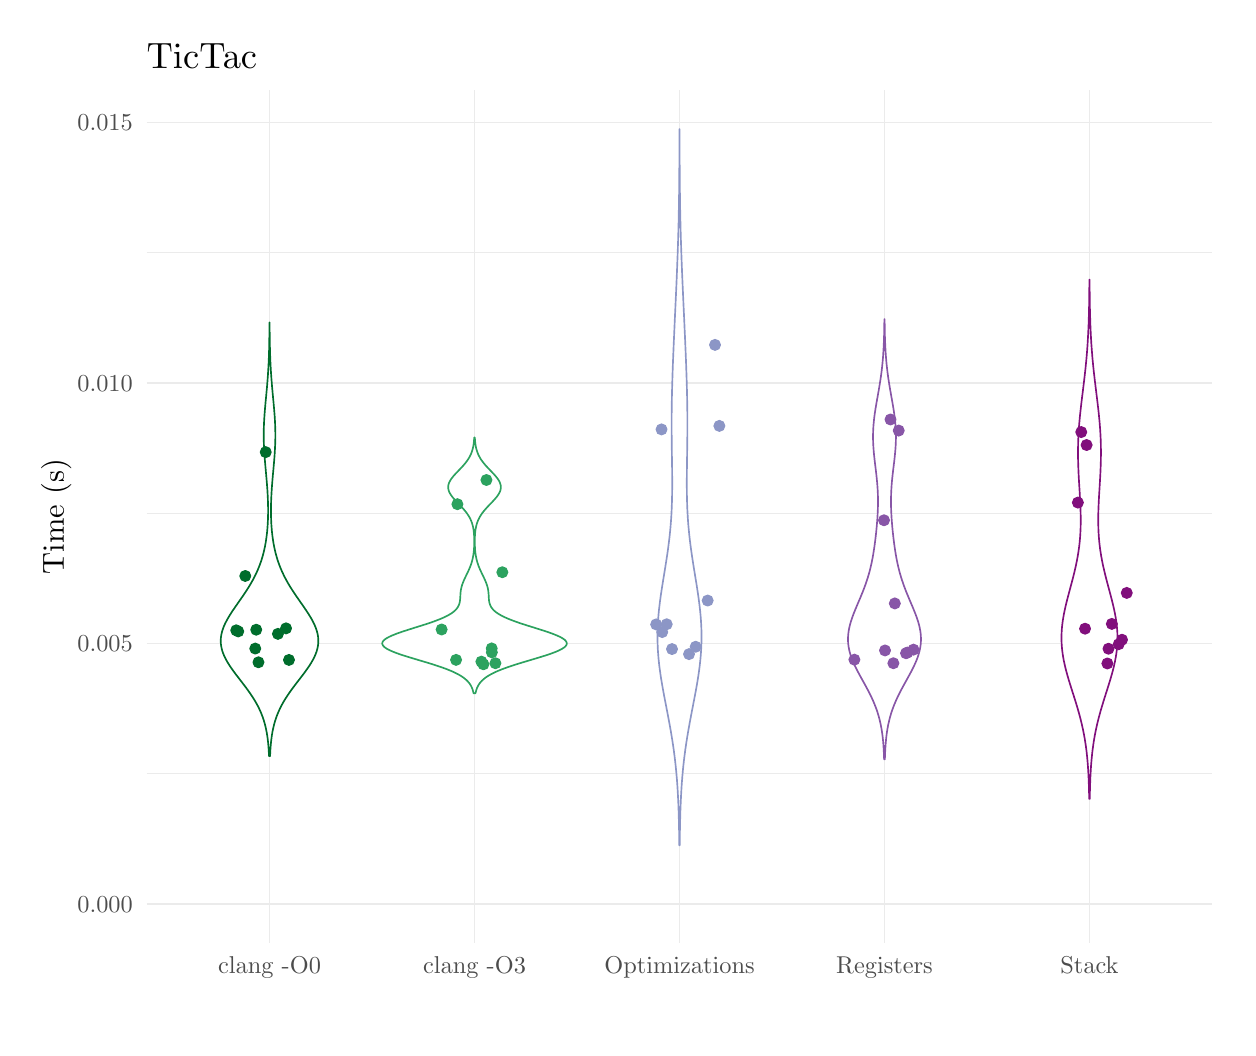
\begin{tikzpicture}[x=1pt,y=1pt]
\definecolor{fillColor}{RGB}{255,255,255}
\path[use as bounding box,fill=fillColor,fill opacity=0.00] (0,0) rectangle (433.62,361.35);
\begin{scope}
\path[clip] ( 42.95, 30.69) rectangle (428.12,338.69);
\definecolor{drawColor}{gray}{0.92}

\path[draw=drawColor,line width= 0.3pt,line join=round] ( 42.95, 91.75) --
	(428.12, 91.75);

\path[draw=drawColor,line width= 0.3pt,line join=round] ( 42.95,185.89) --
	(428.12,185.89);

\path[draw=drawColor,line width= 0.3pt,line join=round] ( 42.95,280.03) --
	(428.12,280.03);

\path[draw=drawColor,line width= 0.6pt,line join=round] ( 42.95, 44.69) --
	(428.12, 44.69);

\path[draw=drawColor,line width= 0.6pt,line join=round] ( 42.95,138.82) --
	(428.12,138.82);

\path[draw=drawColor,line width= 0.6pt,line join=round] ( 42.95,232.96) --
	(428.12,232.96);

\path[draw=drawColor,line width= 0.6pt,line join=round] ( 42.95,327.10) --
	(428.12,327.10);

\path[draw=drawColor,line width= 0.6pt,line join=round] ( 87.40, 30.69) --
	( 87.40,338.69);

\path[draw=drawColor,line width= 0.6pt,line join=round] (161.47, 30.69) --
	(161.47,338.69);

\path[draw=drawColor,line width= 0.6pt,line join=round] (235.54, 30.69) --
	(235.54,338.69);

\path[draw=drawColor,line width= 0.6pt,line join=round] (309.61, 30.69) --
	(309.61,338.69);

\path[draw=drawColor,line width= 0.6pt,line join=round] (383.68, 30.69) --
	(383.68,338.69);
\definecolor{drawColor}{RGB}{0,109,44}
\definecolor{fillColor}{RGB}{255,255,255}

\path[draw=drawColor,line width= 0.6pt,line join=round,line cap=round,fill=fillColor] ( 87.21, 98.11) --
	( 87.19, 98.42) --
	( 87.18, 98.73) --
	( 87.17, 99.03) --
	( 87.15, 99.34) --
	( 87.13, 99.65) --
	( 87.12, 99.95) --
	( 87.10,100.26) --
	( 87.08,100.57) --
	( 87.06,100.87) --
	( 87.03,101.18) --
	( 87.01,101.49) --
	( 86.99,101.79) --
	( 86.96,102.10) --
	( 86.93,102.41) --
	( 86.90,102.71) --
	( 86.88,103.02) --
	( 86.84,103.33) --
	( 86.81,103.63) --
	( 86.77,103.94) --
	( 86.74,104.25) --
	( 86.70,104.55) --
	( 86.66,104.86) --
	( 86.61,105.17) --
	( 86.57,105.47) --
	( 86.52,105.78) --
	( 86.47,106.09) --
	( 86.42,106.39) --
	( 86.37,106.70) --
	( 86.31,107.01) --
	( 86.25,107.31) --
	( 86.19,107.62) --
	( 86.13,107.93) --
	( 86.06,108.23) --
	( 85.99,108.54) --
	( 85.92,108.85) --
	( 85.85,109.15) --
	( 85.77,109.46) --
	( 85.69,109.77) --
	( 85.60,110.07) --
	( 85.52,110.38) --
	( 85.42,110.69) --
	( 85.33,110.99) --
	( 85.23,111.30) --
	( 85.13,111.61) --
	( 85.03,111.91) --
	( 84.92,112.22) --
	( 84.81,112.53) --
	( 84.69,112.83) --
	( 84.57,113.14) --
	( 84.45,113.45) --
	( 84.33,113.75) --
	( 84.20,114.06) --
	( 84.06,114.37) --
	( 83.92,114.67) --
	( 83.78,114.98) --
	( 83.64,115.29) --
	( 83.49,115.59) --
	( 83.33,115.90) --
	( 83.18,116.21) --
	( 83.02,116.51) --
	( 82.85,116.82) --
	( 82.68,117.13) --
	( 82.51,117.43) --
	( 82.33,117.74) --
	( 82.15,118.05) --
	( 81.97,118.35) --
	( 81.78,118.66) --
	( 81.59,118.97) --
	( 81.40,119.28) --
	( 81.20,119.58) --
	( 81.00,119.89) --
	( 80.79,120.20) --
	( 80.58,120.50) --
	( 80.37,120.81) --
	( 80.16,121.12) --
	( 79.94,121.42) --
	( 79.73,121.73) --
	( 79.51,122.04) --
	( 79.28,122.34) --
	( 79.06,122.65) --
	( 78.83,122.96) --
	( 78.60,123.26) --
	( 78.37,123.57) --
	( 78.14,123.88) --
	( 77.90,124.18) --
	( 77.67,124.49) --
	( 77.43,124.80) --
	( 77.20,125.10) --
	( 76.96,125.41) --
	( 76.72,125.72) --
	( 76.49,126.02) --
	( 76.25,126.33) --
	( 76.02,126.64) --
	( 75.78,126.94) --
	( 75.55,127.25) --
	( 75.31,127.56) --
	( 75.08,127.86) --
	( 74.85,128.17) --
	( 74.63,128.48) --
	( 74.40,128.78) --
	( 74.18,129.09) --
	( 73.96,129.40) --
	( 73.74,129.70) --
	( 73.53,130.01) --
	( 73.32,130.32) --
	( 73.12,130.62) --
	( 72.91,130.93) --
	( 72.72,131.24) --
	( 72.52,131.54) --
	( 72.34,131.85) --
	( 72.15,132.16) --
	( 71.98,132.46) --
	( 71.80,132.77) --
	( 71.64,133.08) --
	( 71.48,133.38) --
	( 71.32,133.69) --
	( 71.18,134.00) --
	( 71.03,134.30) --
	( 70.90,134.61) --
	( 70.77,134.92) --
	( 70.65,135.22) --
	( 70.54,135.53) --
	( 70.43,135.84) --
	( 70.33,136.14) --
	( 70.24,136.45) --
	( 70.16,136.76) --
	( 70.09,137.06) --
	( 70.02,137.37) --
	( 69.96,137.68) --
	( 69.91,137.98) --
	( 69.86,138.29) --
	( 69.83,138.60) --
	( 69.80,138.90) --
	( 69.78,139.21) --
	( 69.77,139.52) --
	( 69.77,139.83) --
	( 69.78,140.13) --
	( 69.79,140.44) --
	( 69.81,140.75) --
	( 69.84,141.05) --
	( 69.88,141.36) --
	( 69.92,141.67) --
	( 69.98,141.97) --
	( 70.04,142.28) --
	( 70.11,142.59) --
	( 70.18,142.89) --
	( 70.27,143.20) --
	( 70.36,143.51) --
	( 70.46,143.81) --
	( 70.56,144.12) --
	( 70.67,144.43) --
	( 70.79,144.73) --
	( 70.91,145.04) --
	( 71.05,145.35) --
	( 71.18,145.65) --
	( 71.32,145.96) --
	( 71.47,146.27) --
	( 71.63,146.57) --
	( 71.79,146.88) --
	( 71.95,147.19) --
	( 72.12,147.49) --
	( 72.29,147.80) --
	( 72.47,148.11) --
	( 72.65,148.41) --
	( 72.83,148.72) --
	( 73.02,149.03) --
	( 73.21,149.33) --
	( 73.41,149.64) --
	( 73.60,149.95) --
	( 73.80,150.25) --
	( 74.01,150.56) --
	( 74.21,150.87) --
	( 74.42,151.17) --
	( 74.63,151.48) --
	( 74.84,151.79) --
	( 75.05,152.09) --
	( 75.26,152.40) --
	( 75.48,152.71) --
	( 75.69,153.01) --
	( 75.90,153.32) --
	( 76.12,153.63) --
	( 76.33,153.93) --
	( 76.55,154.24) --
	( 76.76,154.55) --
	( 76.97,154.85) --
	( 77.19,155.16) --
	( 77.40,155.47) --
	( 77.61,155.77) --
	( 77.82,156.08) --
	( 78.03,156.39) --
	( 78.24,156.69) --
	( 78.44,157.00) --
	( 78.65,157.31) --
	( 78.85,157.61) --
	( 79.05,157.92) --
	( 79.25,158.23) --
	( 79.44,158.53) --
	( 79.64,158.84) --
	( 79.83,159.15) --
	( 80.02,159.45) --
	( 80.20,159.76) --
	( 80.39,160.07) --
	( 80.57,160.38) --
	( 80.75,160.68) --
	( 80.92,160.99) --
	( 81.10,161.30) --
	( 81.27,161.60) --
	( 81.44,161.91) --
	( 81.60,162.22) --
	( 81.76,162.52) --
	( 81.92,162.83) --
	( 82.08,163.14) --
	( 82.23,163.44) --
	( 82.38,163.75) --
	( 82.52,164.06) --
	( 82.67,164.36) --
	( 82.81,164.67) --
	( 82.95,164.98) --
	( 83.08,165.28) --
	( 83.21,165.59) --
	( 83.34,165.90) --
	( 83.47,166.20) --
	( 83.59,166.51) --
	( 83.71,166.82) --
	( 83.83,167.12) --
	( 83.94,167.43) --
	( 84.05,167.74) --
	( 84.16,168.04) --
	( 84.27,168.35) --
	( 84.37,168.66) --
	( 84.47,168.96) --
	( 84.57,169.27) --
	( 84.66,169.58) --
	( 84.76,169.88) --
	( 84.85,170.19) --
	( 84.93,170.50) --
	( 85.02,170.80) --
	( 85.10,171.11) --
	( 85.18,171.42) --
	( 85.26,171.72) --
	( 85.33,172.03) --
	( 85.41,172.34) --
	( 85.48,172.64) --
	( 85.55,172.95) --
	( 85.61,173.26) --
	( 85.68,173.56) --
	( 85.74,173.87) --
	( 85.80,174.18) --
	( 85.86,174.48) --
	( 85.91,174.79) --
	( 85.97,175.10) --
	( 86.02,175.40) --
	( 86.07,175.71) --
	( 86.12,176.02) --
	( 86.16,176.32) --
	( 86.21,176.63) --
	( 86.25,176.94) --
	( 86.29,177.24) --
	( 86.33,177.55) --
	( 86.37,177.86) --
	( 86.41,178.16) --
	( 86.44,178.47) --
	( 86.48,178.78) --
	( 86.51,179.08) --
	( 86.54,179.39) --
	( 86.57,179.70) --
	( 86.59,180.00) --
	( 86.62,180.31) --
	( 86.65,180.62) --
	( 86.67,180.93) --
	( 86.69,181.23) --
	( 86.71,181.54) --
	( 86.73,181.85) --
	( 86.75,182.15) --
	( 86.77,182.46) --
	( 86.78,182.77) --
	( 86.79,183.07) --
	( 86.81,183.38) --
	( 86.82,183.69) --
	( 86.83,183.99) --
	( 86.84,184.30) --
	( 86.85,184.61) --
	( 86.86,184.91) --
	( 86.86,185.22) --
	( 86.87,185.53) --
	( 86.87,185.83) --
	( 86.87,186.14) --
	( 86.88,186.45) --
	( 86.88,186.75) --
	( 86.88,187.06) --
	( 86.87,187.37) --
	( 86.87,187.67) --
	( 86.87,187.98) --
	( 86.87,188.29) --
	( 86.86,188.59) --
	( 86.85,188.90) --
	( 86.85,189.21) --
	( 86.84,189.51) --
	( 86.83,189.82) --
	( 86.82,190.13) --
	( 86.81,190.43) --
	( 86.80,190.74) --
	( 86.79,191.05) --
	( 86.78,191.35) --
	( 86.76,191.66) --
	( 86.75,191.97) --
	( 86.73,192.27) --
	( 86.72,192.58) --
	( 86.70,192.89) --
	( 86.68,193.19) --
	( 86.66,193.50) --
	( 86.65,193.81) --
	( 86.63,194.11) --
	( 86.61,194.42) --
	( 86.59,194.73) --
	( 86.56,195.03) --
	( 86.54,195.34) --
	( 86.52,195.65) --
	( 86.50,195.95) --
	( 86.47,196.26) --
	( 86.45,196.57) --
	( 86.43,196.87) --
	( 86.40,197.18) --
	( 86.38,197.49) --
	( 86.35,197.79) --
	( 86.32,198.10) --
	( 86.30,198.41) --
	( 86.27,198.71) --
	( 86.24,199.02) --
	( 86.22,199.33) --
	( 86.19,199.63) --
	( 86.16,199.94) --
	( 86.14,200.25) --
	( 86.11,200.56) --
	( 86.08,200.86) --
	( 86.05,201.17) --
	( 86.02,201.48) --
	( 86.00,201.78) --
	( 85.97,202.09) --
	( 85.94,202.40) --
	( 85.91,202.70) --
	( 85.89,203.01) --
	( 85.86,203.32) --
	( 85.83,203.62) --
	( 85.81,203.93) --
	( 85.78,204.24) --
	( 85.76,204.54) --
	( 85.73,204.85) --
	( 85.70,205.16) --
	( 85.68,205.46) --
	( 85.66,205.77) --
	( 85.63,206.08) --
	( 85.61,206.38) --
	( 85.59,206.69) --
	( 85.57,207.00) --
	( 85.54,207.30) --
	( 85.52,207.61) --
	( 85.50,207.92) --
	( 85.49,208.22) --
	( 85.47,208.53) --
	( 85.45,208.84) --
	( 85.43,209.14) --
	( 85.42,209.45) --
	( 85.40,209.76) --
	( 85.39,210.06) --
	( 85.38,210.37) --
	( 85.36,210.68) --
	( 85.35,210.98) --
	( 85.34,211.29) --
	( 85.33,211.60) --
	( 85.33,211.90) --
	( 85.32,212.21) --
	( 85.31,212.52) --
	( 85.31,212.82) --
	( 85.30,213.13) --
	( 85.30,213.44) --
	( 85.30,213.74) --
	( 85.30,214.05) --
	( 85.30,214.36) --
	( 85.30,214.66) --
	( 85.30,214.97) --
	( 85.31,215.28) --
	( 85.31,215.58) --
	( 85.32,215.89) --
	( 85.32,216.20) --
	( 85.33,216.50) --
	( 85.34,216.81) --
	( 85.35,217.12) --
	( 85.36,217.42) --
	( 85.37,217.73) --
	( 85.38,218.04) --
	( 85.40,218.34) --
	( 85.41,218.65) --
	( 85.43,218.96) --
	( 85.44,219.26) --
	( 85.46,219.57) --
	( 85.48,219.88) --
	( 85.50,220.18) --
	( 85.52,220.49) --
	( 85.54,220.80) --
	( 85.56,221.11) --
	( 85.58,221.41) --
	( 85.60,221.72) --
	( 85.62,222.03) --
	( 85.65,222.33) --
	( 85.67,222.64) --
	( 85.70,222.95) --
	( 85.72,223.25) --
	( 85.75,223.56) --
	( 85.77,223.87) --
	( 85.80,224.17) --
	( 85.83,224.48) --
	( 85.85,224.79) --
	( 85.88,225.09) --
	( 85.91,225.40) --
	( 85.94,225.71) --
	( 85.96,226.01) --
	( 85.99,226.32) --
	( 86.02,226.63) --
	( 86.05,226.93) --
	( 86.08,227.24) --
	( 86.11,227.55) --
	( 86.14,227.85) --
	( 86.16,228.16) --
	( 86.19,228.47) --
	( 86.22,228.77) --
	( 86.25,229.08) --
	( 86.28,229.39) --
	( 86.31,229.69) --
	( 86.34,230.00) --
	( 86.36,230.31) --
	( 86.39,230.61) --
	( 86.42,230.92) --
	( 86.45,231.23) --
	( 86.47,231.53) --
	( 86.50,231.84) --
	( 86.53,232.15) --
	( 86.55,232.45) --
	( 86.58,232.76) --
	( 86.60,233.07) --
	( 86.63,233.37) --
	( 86.65,233.68) --
	( 86.67,233.99) --
	( 86.70,234.29) --
	( 86.72,234.60) --
	( 86.74,234.91) --
	( 86.77,235.21) --
	( 86.79,235.52) --
	( 86.81,235.83) --
	( 86.83,236.13) --
	( 86.85,236.44) --
	( 86.87,236.75) --
	( 86.89,237.05) --
	( 86.91,237.36) --
	( 86.93,237.67) --
	( 86.95,237.97) --
	( 86.96,238.28) --
	( 86.98,238.59) --
	( 87.00,238.89) --
	( 87.01,239.20) --
	( 87.03,239.51) --
	( 87.04,239.81) --
	( 87.06,240.12) --
	( 87.07,240.43) --
	( 87.09,240.73) --
	( 87.10,241.04) --
	( 87.11,241.35) --
	( 87.13,241.66) --
	( 87.14,241.96) --
	( 87.15,242.27) --
	( 87.16,242.58) --
	( 87.17,242.88) --
	( 87.18,243.19) --
	( 87.19,243.50) --
	( 87.20,243.80) --
	( 87.21,244.11) --
	( 87.22,244.42) --
	( 87.23,244.72) --
	( 87.24,245.03) --
	( 87.25,245.34) --
	( 87.25,245.64) --
	( 87.26,245.95) --
	( 87.27,246.26) --
	( 87.27,246.56) --
	( 87.28,246.87) --
	( 87.29,247.18) --
	( 87.29,247.48) --
	( 87.30,247.79) --
	( 87.30,248.10) --
	( 87.31,248.40) --
	( 87.31,248.71) --
	( 87.32,249.02) --
	( 87.32,249.32) --
	( 87.33,249.63) --
	( 87.33,249.94) --
	( 87.33,250.24) --
	( 87.34,250.55) --
	( 87.34,250.86) --
	( 87.35,251.16) --
	( 87.35,251.47) --
	( 87.35,251.78) --
	( 87.35,252.08) --
	( 87.36,252.39) --
	( 87.36,252.70) --
	( 87.36,253.00) --
	( 87.36,253.31) --
	( 87.37,253.62) --
	( 87.37,253.92) --
	( 87.37,254.23) --
	( 87.37,254.54) --
	( 87.37,254.84) --
	( 87.42,254.84) --
	( 87.42,254.54) --
	( 87.42,254.23) --
	( 87.43,253.92) --
	( 87.43,253.62) --
	( 87.43,253.31) --
	( 87.43,253.00) --
	( 87.43,252.70) --
	( 87.44,252.39) --
	( 87.44,252.08) --
	( 87.44,251.78) --
	( 87.44,251.47) --
	( 87.45,251.16) --
	( 87.45,250.86) --
	( 87.45,250.55) --
	( 87.46,250.24) --
	( 87.46,249.94) --
	( 87.47,249.63) --
	( 87.47,249.32) --
	( 87.47,249.02) --
	( 87.48,248.71) --
	( 87.48,248.40) --
	( 87.49,248.10) --
	( 87.49,247.79) --
	( 87.50,247.48) --
	( 87.51,247.18) --
	( 87.51,246.87) --
	( 87.52,246.56) --
	( 87.52,246.26) --
	( 87.53,245.95) --
	( 87.54,245.64) --
	( 87.55,245.34) --
	( 87.55,245.03) --
	( 87.56,244.72) --
	( 87.57,244.42) --
	( 87.58,244.11) --
	( 87.59,243.80) --
	( 87.60,243.50) --
	( 87.61,243.19) --
	( 87.62,242.88) --
	( 87.63,242.58) --
	( 87.64,242.27) --
	( 87.65,241.96) --
	( 87.67,241.66) --
	( 87.68,241.35) --
	( 87.69,241.04) --
	( 87.70,240.73) --
	( 87.72,240.43) --
	( 87.73,240.12) --
	( 87.75,239.81) --
	( 87.76,239.51) --
	( 87.78,239.20) --
	( 87.79,238.89) --
	( 87.81,238.59) --
	( 87.83,238.28) --
	( 87.85,237.97) --
	( 87.86,237.67) --
	( 87.88,237.36) --
	( 87.90,237.05) --
	( 87.92,236.75) --
	( 87.94,236.44) --
	( 87.96,236.13) --
	( 87.98,235.83) --
	( 88.00,235.52) --
	( 88.03,235.21) --
	( 88.05,234.91) --
	( 88.07,234.60) --
	( 88.09,234.29) --
	( 88.12,233.99) --
	( 88.14,233.68) --
	( 88.17,233.37) --
	( 88.19,233.07) --
	( 88.22,232.76) --
	( 88.24,232.45) --
	( 88.27,232.15) --
	( 88.29,231.84) --
	( 88.32,231.53) --
	( 88.35,231.23) --
	( 88.37,230.92) --
	( 88.40,230.61) --
	( 88.43,230.31) --
	( 88.46,230.00) --
	( 88.49,229.69) --
	( 88.51,229.39) --
	( 88.54,229.08) --
	( 88.57,228.77) --
	( 88.60,228.47) --
	( 88.63,228.16) --
	( 88.66,227.85) --
	( 88.68,227.55) --
	( 88.71,227.24) --
	( 88.74,226.93) --
	( 88.77,226.63) --
	( 88.80,226.32) --
	( 88.83,226.01) --
	( 88.86,225.71) --
	( 88.88,225.40) --
	( 88.91,225.09) --
	( 88.94,224.79) --
	( 88.97,224.48) --
	( 88.99,224.17) --
	( 89.02,223.87) --
	( 89.05,223.56) --
	( 89.07,223.25) --
	( 89.10,222.95) --
	( 89.12,222.64) --
	( 89.15,222.33) --
	( 89.17,222.03) --
	( 89.19,221.72) --
	( 89.21,221.41) --
	( 89.24,221.11) --
	( 89.26,220.80) --
	( 89.28,220.49) --
	( 89.30,220.18) --
	( 89.32,219.88) --
	( 89.33,219.57) --
	( 89.35,219.26) --
	( 89.37,218.96) --
	( 89.38,218.65) --
	( 89.40,218.34) --
	( 89.41,218.04) --
	( 89.42,217.73) --
	( 89.43,217.42) --
	( 89.44,217.12) --
	( 89.45,216.81) --
	( 89.46,216.50) --
	( 89.47,216.20) --
	( 89.48,215.89) --
	( 89.48,215.58) --
	( 89.49,215.28) --
	( 89.49,214.97) --
	( 89.49,214.66) --
	( 89.49,214.36) --
	( 89.49,214.05) --
	( 89.49,213.74) --
	( 89.49,213.44) --
	( 89.49,213.13) --
	( 89.49,212.82) --
	( 89.48,212.52) --
	( 89.47,212.21) --
	( 89.47,211.90) --
	( 89.46,211.60) --
	( 89.45,211.29) --
	( 89.44,210.98) --
	( 89.43,210.68) --
	( 89.42,210.37) --
	( 89.40,210.06) --
	( 89.39,209.76) --
	( 89.38,209.45) --
	( 89.36,209.14) --
	( 89.34,208.84) --
	( 89.33,208.53) --
	( 89.31,208.22) --
	( 89.29,207.92) --
	( 89.27,207.61) --
	( 89.25,207.30) --
	( 89.23,207.00) --
	( 89.21,206.69) --
	( 89.18,206.38) --
	( 89.16,206.08) --
	( 89.14,205.77) --
	( 89.11,205.46) --
	( 89.09,205.16) --
	( 89.06,204.85) --
	( 89.04,204.54) --
	( 89.01,204.24) --
	( 88.99,203.93) --
	( 88.96,203.62) --
	( 88.93,203.32) --
	( 88.91,203.01) --
	( 88.88,202.70) --
	( 88.85,202.40) --
	( 88.82,202.09) --
	( 88.80,201.78) --
	( 88.77,201.48) --
	( 88.74,201.17) --
	( 88.71,200.86) --
	( 88.68,200.56) --
	( 88.66,200.25) --
	( 88.63,199.94) --
	( 88.60,199.63) --
	( 88.57,199.33) --
	( 88.55,199.02) --
	( 88.52,198.71) --
	( 88.49,198.41) --
	( 88.47,198.10) --
	( 88.44,197.79) --
	( 88.42,197.49) --
	( 88.39,197.18) --
	( 88.37,196.87) --
	( 88.34,196.57) --
	( 88.32,196.26) --
	( 88.30,195.95) --
	( 88.27,195.65) --
	( 88.25,195.34) --
	( 88.23,195.03) --
	( 88.21,194.73) --
	( 88.19,194.42) --
	( 88.17,194.11) --
	( 88.15,193.81) --
	( 88.13,193.50) --
	( 88.11,193.19) --
	( 88.09,192.89) --
	( 88.08,192.58) --
	( 88.06,192.27) --
	( 88.05,191.97) --
	( 88.03,191.66) --
	( 88.02,191.35) --
	( 88.00,191.05) --
	( 87.99,190.74) --
	( 87.98,190.43) --
	( 87.97,190.13) --
	( 87.96,189.82) --
	( 87.95,189.51) --
	( 87.94,189.21) --
	( 87.94,188.90) --
	( 87.93,188.59) --
	( 87.93,188.29) --
	( 87.92,187.98) --
	( 87.92,187.67) --
	( 87.92,187.37) --
	( 87.92,187.06) --
	( 87.92,186.75) --
	( 87.92,186.45) --
	( 87.92,186.14) --
	( 87.92,185.83) --
	( 87.93,185.53) --
	( 87.93,185.22) --
	( 87.94,184.91) --
	( 87.94,184.61) --
	( 87.95,184.30) --
	( 87.96,183.99) --
	( 87.97,183.69) --
	( 87.98,183.38) --
	( 88.00,183.07) --
	( 88.01,182.77) --
	( 88.03,182.46) --
	( 88.04,182.15) --
	( 88.06,181.85) --
	( 88.08,181.54) --
	( 88.10,181.23) --
	( 88.12,180.93) --
	( 88.15,180.62) --
	( 88.17,180.31) --
	( 88.20,180.00) --
	( 88.22,179.70) --
	( 88.25,179.39) --
	( 88.28,179.08) --
	( 88.32,178.78) --
	( 88.35,178.47) --
	( 88.38,178.16) --
	( 88.42,177.86) --
	( 88.46,177.55) --
	( 88.50,177.24) --
	( 88.54,176.94) --
	( 88.58,176.63) --
	( 88.63,176.32) --
	( 88.67,176.02) --
	( 88.72,175.71) --
	( 88.77,175.40) --
	( 88.83,175.10) --
	( 88.88,174.79) --
	( 88.94,174.48) --
	( 88.99,174.18) --
	( 89.05,173.87) --
	( 89.12,173.56) --
	( 89.18,173.26) --
	( 89.25,172.95) --
	( 89.31,172.64) --
	( 89.39,172.34) --
	( 89.46,172.03) --
	( 89.53,171.72) --
	( 89.61,171.42) --
	( 89.69,171.11) --
	( 89.77,170.80) --
	( 89.86,170.50) --
	( 89.95,170.19) --
	( 90.04,169.88) --
	( 90.13,169.58) --
	( 90.22,169.27) --
	( 90.32,168.96) --
	( 90.42,168.66) --
	( 90.52,168.35) --
	( 90.63,168.04) --
	( 90.74,167.74) --
	( 90.85,167.43) --
	( 90.96,167.12) --
	( 91.08,166.82) --
	( 91.20,166.51) --
	( 91.32,166.20) --
	( 91.45,165.90) --
	( 91.58,165.59) --
	( 91.71,165.28) --
	( 91.85,164.98) --
	( 91.98,164.67) --
	( 92.12,164.36) --
	( 92.27,164.06) --
	( 92.41,163.75) --
	( 92.56,163.44) --
	( 92.72,163.14) --
	( 92.87,162.83) --
	( 93.03,162.52) --
	( 93.19,162.22) --
	( 93.36,161.91) --
	( 93.52,161.60) --
	( 93.70,161.30) --
	( 93.87,160.99) --
	( 94.04,160.68) --
	( 94.22,160.38) --
	( 94.40,160.07) --
	( 94.59,159.76) --
	( 94.77,159.45) --
	( 94.96,159.15) --
	( 95.16,158.84) --
	( 95.35,158.53) --
	( 95.55,158.23) --
	( 95.74,157.92) --
	( 95.94,157.61) --
	( 96.15,157.31) --
	( 96.35,157.00) --
	( 96.56,156.69) --
	( 96.76,156.39) --
	( 96.97,156.08) --
	( 97.18,155.77) --
	( 97.39,155.47) --
	( 97.60,155.16) --
	( 97.82,154.85) --
	( 98.03,154.55) --
	( 98.25,154.24) --
	( 98.46,153.93) --
	( 98.67,153.63) --
	( 98.89,153.32) --
	( 99.10,153.01) --
	( 99.32,152.71) --
	( 99.53,152.40) --
	( 99.74,152.09) --
	( 99.95,151.79) --
	(100.16,151.48) --
	(100.37,151.17) --
	(100.58,150.87) --
	(100.78,150.56) --
	(100.99,150.25) --
	(101.19,149.95) --
	(101.39,149.64) --
	(101.58,149.33) --
	(101.77,149.03) --
	(101.96,148.72) --
	(102.14,148.41) --
	(102.33,148.11) --
	(102.50,147.80) --
	(102.68,147.49) --
	(102.84,147.19) --
	(103.01,146.88) --
	(103.17,146.57) --
	(103.32,146.27) --
	(103.47,145.96) --
	(103.61,145.65) --
	(103.75,145.35) --
	(103.88,145.04) --
	(104.00,144.73) --
	(104.12,144.43) --
	(104.23,144.12) --
	(104.34,143.81) --
	(104.44,143.51) --
	(104.52,143.20) --
	(104.61,142.89) --
	(104.69,142.59) --
	(104.75,142.28) --
	(104.82,141.97) --
	(104.87,141.67) --
	(104.92,141.36) --
	(104.95,141.05) --
	(104.98,140.75) --
	(105.01,140.44) --
	(105.02,140.13) --
	(105.02,139.83) --
	(105.02,139.52) --
	(105.01,139.21) --
	(104.99,138.90) --
	(104.96,138.60) --
	(104.93,138.29) --
	(104.89,137.98) --
	(104.83,137.68) --
	(104.78,137.37) --
	(104.71,137.06) --
	(104.63,136.76) --
	(104.55,136.45) --
	(104.46,136.14) --
	(104.36,135.84) --
	(104.25,135.53) --
	(104.14,135.22) --
	(104.02,134.92) --
	(103.89,134.61) --
	(103.76,134.30) --
	(103.62,134.00) --
	(103.47,133.69) --
	(103.31,133.38) --
	(103.16,133.08) --
	(102.99,132.77) --
	(102.82,132.46) --
	(102.64,132.16) --
	(102.46,131.85) --
	(102.27,131.54) --
	(102.08,131.24) --
	(101.88,130.93) --
	(101.68,130.62) --
	(101.47,130.32) --
	(101.26,130.01) --
	(101.05,129.70) --
	(100.83,129.40) --
	(100.61,129.09) --
	(100.39,128.78) --
	(100.17,128.48) --
	( 99.94,128.17) --
	( 99.71,127.86) --
	( 99.48,127.56) --
	( 99.25,127.25) --
	( 99.01,126.94) --
	( 98.78,126.64) --
	( 98.54,126.33) --
	( 98.31,126.02) --
	( 98.07,125.72) --
	( 97.83,125.41) --
	( 97.60,125.10) --
	( 97.36,124.80) --
	( 97.12,124.49) --
	( 96.89,124.18) --
	( 96.66,123.88) --
	( 96.42,123.57) --
	( 96.19,123.26) --
	( 95.96,122.96) --
	( 95.74,122.65) --
	( 95.51,122.34) --
	( 95.29,122.04) --
	( 95.07,121.73) --
	( 94.85,121.42) --
	( 94.63,121.12) --
	( 94.42,120.81) --
	( 94.21,120.50) --
	( 94.00,120.20) --
	( 93.80,119.89) --
	( 93.59,119.58) --
	( 93.40,119.28) --
	( 93.20,118.97) --
	( 93.01,118.66) --
	( 92.82,118.35) --
	( 92.64,118.05) --
	( 92.46,117.74) --
	( 92.28,117.43) --
	( 92.11,117.13) --
	( 91.94,116.82) --
	( 91.78,116.51) --
	( 91.62,116.21) --
	( 91.46,115.90) --
	( 91.31,115.59) --
	( 91.16,115.29) --
	( 91.01,114.98) --
	( 90.87,114.67) --
	( 90.73,114.37) --
	( 90.60,114.06) --
	( 90.47,113.75) --
	( 90.34,113.45) --
	( 90.22,113.14) --
	( 90.10,112.83) --
	( 89.98,112.53) --
	( 89.87,112.22) --
	( 89.76,111.91) --
	( 89.66,111.61) --
	( 89.56,111.30) --
	( 89.46,110.99) --
	( 89.37,110.69) --
	( 89.28,110.38) --
	( 89.19,110.07) --
	( 89.10,109.77) --
	( 89.02,109.46) --
	( 88.95,109.15) --
	( 88.87,108.85) --
	( 88.80,108.54) --
	( 88.73,108.23) --
	( 88.66,107.93) --
	( 88.60,107.62) --
	( 88.54,107.31) --
	( 88.48,107.01) --
	( 88.42,106.70) --
	( 88.37,106.39) --
	( 88.32,106.09) --
	( 88.27,105.78) --
	( 88.22,105.47) --
	( 88.18,105.17) --
	( 88.14,104.86) --
	( 88.09,104.55) --
	( 88.06,104.25) --
	( 88.02,103.94) --
	( 87.98,103.63) --
	( 87.95,103.33) --
	( 87.92,103.02) --
	( 87.89,102.71) --
	( 87.86,102.41) --
	( 87.83,102.10) --
	( 87.81,101.79) --
	( 87.78,101.49) --
	( 87.76,101.18) --
	( 87.74,100.87) --
	( 87.71,100.57) --
	( 87.70,100.26) --
	( 87.68, 99.95) --
	( 87.66, 99.65) --
	( 87.64, 99.34) --
	( 87.63, 99.03) --
	( 87.61, 98.73) --
	( 87.60, 98.42) --
	( 87.58, 98.11) --
	( 87.21, 98.11) --
	cycle;
\definecolor{drawColor}{RGB}{44,162,95}

\path[draw=drawColor,line width= 0.6pt,line join=round,line cap=round,fill=fillColor] (161.09,120.87) --
	(161.06,121.05) --
	(161.02,121.23) --
	(160.98,121.41) --
	(160.93,121.59) --
	(160.88,121.78) --
	(160.83,121.96) --
	(160.78,122.14) --
	(160.72,122.32) --
	(160.65,122.50) --
	(160.58,122.68) --
	(160.51,122.86) --
	(160.43,123.04) --
	(160.34,123.22) --
	(160.25,123.40) --
	(160.16,123.58) --
	(160.05,123.76) --
	(159.94,123.94) --
	(159.82,124.13) --
	(159.70,124.31) --
	(159.56,124.49) --
	(159.42,124.67) --
	(159.27,124.85) --
	(159.11,125.03) --
	(158.95,125.21) --
	(158.77,125.39) --
	(158.58,125.57) --
	(158.38,125.75) --
	(158.17,125.93) --
	(157.95,126.11) --
	(157.72,126.29) --
	(157.48,126.48) --
	(157.23,126.66) --
	(156.96,126.84) --
	(156.68,127.02) --
	(156.39,127.20) --
	(156.09,127.38) --
	(155.77,127.56) --
	(155.44,127.74) --
	(155.10,127.92) --
	(154.74,128.10) --
	(154.38,128.28) --
	(153.99,128.46) --
	(153.59,128.65) --
	(153.19,128.83) --
	(152.76,129.01) --
	(152.32,129.19) --
	(151.88,129.37) --
	(151.41,129.55) --
	(150.94,129.73) --
	(150.45,129.91) --
	(149.95,130.09) --
	(149.43,130.27) --
	(148.91,130.45) --
	(148.38,130.63) --
	(147.83,130.81) --
	(147.28,131.00) --
	(146.71,131.18) --
	(146.14,131.36) --
	(145.56,131.54) --
	(144.98,131.72) --
	(144.38,131.90) --
	(143.79,132.08) --
	(143.18,132.26) --
	(142.58,132.44) --
	(141.97,132.62) --
	(141.36,132.80) --
	(140.75,132.98) --
	(140.14,133.17) --
	(139.54,133.35) --
	(138.93,133.53) --
	(138.33,133.71) --
	(137.74,133.89) --
	(137.16,134.07) --
	(136.58,134.25) --
	(136.01,134.43) --
	(135.45,134.61) --
	(134.90,134.79) --
	(134.37,134.97) --
	(133.86,135.15) --
	(133.35,135.33) --
	(132.87,135.52) --
	(132.40,135.70) --
	(131.95,135.88) --
	(131.53,136.06) --
	(131.12,136.24) --
	(130.73,136.42) --
	(130.37,136.60) --
	(130.03,136.78) --
	(129.72,136.96) --
	(129.44,137.14) --
	(129.18,137.32) --
	(128.95,137.50) --
	(128.75,137.68) --
	(128.57,137.87) --
	(128.42,138.05) --
	(128.31,138.23) --
	(128.22,138.41) --
	(128.16,138.59) --
	(128.14,138.77) --
	(128.13,138.95) --
	(128.17,139.13) --
	(128.24,139.31) --
	(128.32,139.49) --
	(128.45,139.67) --
	(128.60,139.85) --
	(128.77,140.04) --
	(128.99,140.22) --
	(129.22,140.40) --
	(129.48,140.58) --
	(129.77,140.76) --
	(130.08,140.94) --
	(130.42,141.12) --
	(130.78,141.30) --
	(131.16,141.48) --
	(131.57,141.66) --
	(131.99,141.84) --
	(132.44,142.02) --
	(132.90,142.20) --
	(133.38,142.39) --
	(133.87,142.57) --
	(134.38,142.75) --
	(134.90,142.93) --
	(135.43,143.11) --
	(135.97,143.29) --
	(136.53,143.47) --
	(137.09,143.65) --
	(137.65,143.83) --
	(138.22,144.01) --
	(138.80,144.19) --
	(139.38,144.37) --
	(139.96,144.56) --
	(140.54,144.74) --
	(141.11,144.92) --
	(141.69,145.10) --
	(142.26,145.28) --
	(142.83,145.46) --
	(143.39,145.64) --
	(143.95,145.82) --
	(144.50,146.00) --
	(145.04,146.18) --
	(145.57,146.36) --
	(146.09,146.54) --
	(146.60,146.72) --
	(147.11,146.91) --
	(147.59,147.09) --
	(148.07,147.27) --
	(148.53,147.45) --
	(148.98,147.63) --
	(149.41,147.81) --
	(149.84,147.99) --
	(150.24,148.17) --
	(150.63,148.35) --
	(151.01,148.53) --
	(151.37,148.71) --
	(151.72,148.89) --
	(152.05,149.08) --
	(152.37,149.26) --
	(152.67,149.44) --
	(152.96,149.62) --
	(153.23,149.80) --
	(153.48,149.98) --
	(153.73,150.16) --
	(153.95,150.34) --
	(154.17,150.52) --
	(154.37,150.70) --
	(154.56,150.88) --
	(154.73,151.06) --
	(154.90,151.24) --
	(155.04,151.43) --
	(155.18,151.61) --
	(155.31,151.79) --
	(155.43,151.97) --
	(155.54,152.15) --
	(155.63,152.33) --
	(155.72,152.51) --
	(155.80,152.69) --
	(155.87,152.87) --
	(155.94,153.05) --
	(155.99,153.23) --
	(156.04,153.41) --
	(156.09,153.59) --
	(156.13,153.78) --
	(156.16,153.96) --
	(156.19,154.14) --
	(156.22,154.32) --
	(156.24,154.50) --
	(156.25,154.68) --
	(156.27,154.86) --
	(156.28,155.04) --
	(156.30,155.22) --
	(156.31,155.40) --
	(156.32,155.58) --
	(156.33,155.76) --
	(156.34,155.95) --
	(156.35,156.13) --
	(156.36,156.31) --
	(156.37,156.49) --
	(156.38,156.67) --
	(156.39,156.85) --
	(156.40,157.03) --
	(156.42,157.21) --
	(156.44,157.39) --
	(156.46,157.57) --
	(156.48,157.75) --
	(156.51,157.93) --
	(156.54,158.11) --
	(156.57,158.30) --
	(156.60,158.48) --
	(156.64,158.66) --
	(156.68,158.84) --
	(156.72,159.02) --
	(156.76,159.20) --
	(156.81,159.38) --
	(156.86,159.56) --
	(156.92,159.74) --
	(156.97,159.92) --
	(157.03,160.10) --
	(157.09,160.28) --
	(157.16,160.47) --
	(157.22,160.65) --
	(157.29,160.83) --
	(157.37,161.01) --
	(157.44,161.19) --
	(157.51,161.37) --
	(157.59,161.55) --
	(157.67,161.73) --
	(157.75,161.91) --
	(157.83,162.09) --
	(157.92,162.27) --
	(158.00,162.45) --
	(158.09,162.63) --
	(158.17,162.82) --
	(158.26,163.00) --
	(158.35,163.18) --
	(158.44,163.36) --
	(158.52,163.54) --
	(158.61,163.72) --
	(158.70,163.90) --
	(158.79,164.08) --
	(158.87,164.26) --
	(158.96,164.44) --
	(159.05,164.62) --
	(159.13,164.80) --
	(159.22,164.98) --
	(159.30,165.17) --
	(159.38,165.35) --
	(159.46,165.53) --
	(159.54,165.71) --
	(159.62,165.89) --
	(159.69,166.07) --
	(159.77,166.25) --
	(159.84,166.43) --
	(159.91,166.61) --
	(159.98,166.79) --
	(160.05,166.97) --
	(160.11,167.15) --
	(160.18,167.34) --
	(160.24,167.52) --
	(160.30,167.70) --
	(160.36,167.88) --
	(160.41,168.06) --
	(160.47,168.24) --
	(160.52,168.42) --
	(160.57,168.60) --
	(160.62,168.78) --
	(160.67,168.96) --
	(160.71,169.14) --
	(160.75,169.32) --
	(160.79,169.50) --
	(160.83,169.69) --
	(160.87,169.87) --
	(160.91,170.05) --
	(160.94,170.23) --
	(160.97,170.41) --
	(161.00,170.59) --
	(161.03,170.77) --
	(161.06,170.95) --
	(161.09,171.13) --
	(161.11,171.31) --
	(161.13,171.49) --
	(161.16,171.67) --
	(161.18,171.86) --
	(161.19,172.04) --
	(161.21,172.22) --
	(161.23,172.40) --
	(161.25,172.58) --
	(161.26,172.76) --
	(161.27,172.94) --
	(161.29,173.12) --
	(161.30,173.30) --
	(161.31,173.48) --
	(161.32,173.66) --
	(161.33,173.84) --
	(161.34,174.02) --
	(161.34,174.21) --
	(161.35,174.39) --
	(161.35,174.57) --
	(161.36,174.75) --
	(161.36,174.93) --
	(161.37,175.11) --
	(161.37,175.29) --
	(161.37,175.47) --
	(161.37,175.65) --
	(161.37,175.83) --
	(161.37,176.01) --
	(161.37,176.19) --
	(161.37,176.37) --
	(161.36,176.56) --
	(161.36,176.74) --
	(161.35,176.92) --
	(161.35,177.10) --
	(161.34,177.28) --
	(161.33,177.46) --
	(161.33,177.64) --
	(161.32,177.82) --
	(161.30,178.00) --
	(161.29,178.18) --
	(161.28,178.36) --
	(161.27,178.54) --
	(161.25,178.73) --
	(161.23,178.91) --
	(161.21,179.09) --
	(161.19,179.27) --
	(161.17,179.45) --
	(161.15,179.63) --
	(161.13,179.81) --
	(161.10,179.99) --
	(161.07,180.17) --
	(161.04,180.35) --
	(161.01,180.53) --
	(160.97,180.71) --
	(160.94,180.89) --
	(160.90,181.08) --
	(160.86,181.26) --
	(160.81,181.44) --
	(160.76,181.62) --
	(160.71,181.80) --
	(160.66,181.98) --
	(160.61,182.16) --
	(160.55,182.34) --
	(160.49,182.52) --
	(160.42,182.70) --
	(160.36,182.88) --
	(160.28,183.06) --
	(160.21,183.25) --
	(160.13,183.43) --
	(160.05,183.61) --
	(159.97,183.79) --
	(159.88,183.97) --
	(159.78,184.15) --
	(159.69,184.33) --
	(159.59,184.51) --
	(159.48,184.69) --
	(159.38,184.87) --
	(159.27,185.05) --
	(159.15,185.23) --
	(159.03,185.41) --
	(158.91,185.60) --
	(158.78,185.78) --
	(158.65,185.96) --
	(158.51,186.14) --
	(158.38,186.32) --
	(158.23,186.50) --
	(158.09,186.68) --
	(157.94,186.86) --
	(157.79,187.04) --
	(157.64,187.22) --
	(157.48,187.40) --
	(157.32,187.58) --
	(157.16,187.77) --
	(156.99,187.95) --
	(156.82,188.13) --
	(156.66,188.31) --
	(156.49,188.49) --
	(156.31,188.67) --
	(156.14,188.85) --
	(155.97,189.03) --
	(155.79,189.21) --
	(155.62,189.39) --
	(155.45,189.57) --
	(155.27,189.75) --
	(155.10,189.93) --
	(154.93,190.12) --
	(154.76,190.30) --
	(154.59,190.48) --
	(154.42,190.66) --
	(154.26,190.84) --
	(154.10,191.02) --
	(153.94,191.20) --
	(153.79,191.38) --
	(153.64,191.56) --
	(153.49,191.74) --
	(153.35,191.92) --
	(153.22,192.10) --
	(153.09,192.28) --
	(152.96,192.47) --
	(152.84,192.65) --
	(152.73,192.83) --
	(152.63,193.01) --
	(152.53,193.19) --
	(152.44,193.37) --
	(152.35,193.55) --
	(152.28,193.73) --
	(152.21,193.91) --
	(152.14,194.09) --
	(152.09,194.27) --
	(152.05,194.45) --
	(152.01,194.64) --
	(151.98,194.82) --
	(151.97,195.00) --
	(151.95,195.18) --
	(151.95,195.36) --
	(151.96,195.54) --
	(151.97,195.72) --
	(152.00,195.90) --
	(152.03,196.08) --
	(152.07,196.26) --
	(152.12,196.44) --
	(152.18,196.62) --
	(152.25,196.80) --
	(152.32,196.99) --
	(152.40,197.17) --
	(152.49,197.35) --
	(152.59,197.53) --
	(152.69,197.71) --
	(152.80,197.89) --
	(152.91,198.07) --
	(153.04,198.25) --
	(153.16,198.43) --
	(153.30,198.61) --
	(153.43,198.79) --
	(153.58,198.97) --
	(153.73,199.16) --
	(153.88,199.34) --
	(154.03,199.52) --
	(154.19,199.70) --
	(154.36,199.88) --
	(154.52,200.06) --
	(154.69,200.24) --
	(154.86,200.42) --
	(155.03,200.60) --
	(155.20,200.78) --
	(155.37,200.96) --
	(155.55,201.14) --
	(155.72,201.32) --
	(155.90,201.51) --
	(156.07,201.69) --
	(156.24,201.87) --
	(156.42,202.05) --
	(156.59,202.23) --
	(156.76,202.41) --
	(156.92,202.59) --
	(157.09,202.77) --
	(157.25,202.95) --
	(157.41,203.13) --
	(157.57,203.31) --
	(157.73,203.49) --
	(157.88,203.67) --
	(158.03,203.86) --
	(158.18,204.04) --
	(158.32,204.22) --
	(158.46,204.40) --
	(158.59,204.58) --
	(158.73,204.76) --
	(158.85,204.94) --
	(158.98,205.12) --
	(159.10,205.30) --
	(159.22,205.48) --
	(159.33,205.66) --
	(159.44,205.84) --
	(159.55,206.03) --
	(159.65,206.21) --
	(159.75,206.39) --
	(159.84,206.57) --
	(159.93,206.75) --
	(160.02,206.93) --
	(160.10,207.11) --
	(160.18,207.29) --
	(160.26,207.47) --
	(160.33,207.65) --
	(160.40,207.83) --
	(160.46,208.01) --
	(160.53,208.19) --
	(160.59,208.38) --
	(160.64,208.56) --
	(160.69,208.74) --
	(160.75,208.92) --
	(160.79,209.10) --
	(160.84,209.28) --
	(160.88,209.46) --
	(160.92,209.64) --
	(160.96,209.82) --
	(161.00,210.00) --
	(161.03,210.18) --
	(161.06,210.36) --
	(161.09,210.55) --
	(161.12,210.73) --
	(161.15,210.91) --
	(161.17,211.09) --
	(161.19,211.27) --
	(161.21,211.45) --
	(161.23,211.63) --
	(161.25,211.81) --
	(161.27,211.99) --
	(161.29,212.17) --
	(161.30,212.35) --
	(161.31,212.53) --
	(161.33,212.71) --
	(161.34,212.90) --
	(161.35,213.08) --
	(161.36,213.26) --
	(161.57,213.26) --
	(161.58,213.08) --
	(161.59,212.90) --
	(161.61,212.71) --
	(161.62,212.53) --
	(161.63,212.35) --
	(161.65,212.17) --
	(161.66,211.99) --
	(161.68,211.81) --
	(161.70,211.63) --
	(161.72,211.45) --
	(161.74,211.27) --
	(161.76,211.09) --
	(161.79,210.91) --
	(161.81,210.73) --
	(161.84,210.55) --
	(161.87,210.36) --
	(161.90,210.18) --
	(161.94,210.00) --
	(161.97,209.82) --
	(162.01,209.64) --
	(162.05,209.46) --
	(162.09,209.28) --
	(162.14,209.10) --
	(162.19,208.92) --
	(162.24,208.74) --
	(162.29,208.56) --
	(162.35,208.38) --
	(162.41,208.19) --
	(162.47,208.01) --
	(162.54,207.83) --
	(162.61,207.65) --
	(162.68,207.47) --
	(162.75,207.29) --
	(162.83,207.11) --
	(162.92,206.93) --
	(163.00,206.75) --
	(163.09,206.57) --
	(163.19,206.39) --
	(163.29,206.21) --
	(163.39,206.03) --
	(163.49,205.84) --
	(163.60,205.66) --
	(163.72,205.48) --
	(163.83,205.30) --
	(163.95,205.12) --
	(164.08,204.94) --
	(164.21,204.76) --
	(164.34,204.58) --
	(164.48,204.40) --
	(164.61,204.22) --
	(164.76,204.04) --
	(164.90,203.86) --
	(165.05,203.67) --
	(165.21,203.49) --
	(165.36,203.31) --
	(165.52,203.13) --
	(165.68,202.95) --
	(165.85,202.77) --
	(166.01,202.59) --
	(166.18,202.41) --
	(166.35,202.23) --
	(166.52,202.05) --
	(166.69,201.87) --
	(166.86,201.69) --
	(167.04,201.51) --
	(167.21,201.32) --
	(167.39,201.14) --
	(167.56,200.96) --
	(167.73,200.78) --
	(167.90,200.60) --
	(168.08,200.42) --
	(168.24,200.24) --
	(168.41,200.06) --
	(168.58,199.88) --
	(168.74,199.70) --
	(168.90,199.52) --
	(169.05,199.34) --
	(169.21,199.16) --
	(169.35,198.97) --
	(169.50,198.79) --
	(169.64,198.61) --
	(169.77,198.43) --
	(169.90,198.25) --
	(170.02,198.07) --
	(170.14,197.89) --
	(170.25,197.71) --
	(170.35,197.53) --
	(170.44,197.35) --
	(170.53,197.17) --
	(170.61,196.99) --
	(170.69,196.80) --
	(170.75,196.62) --
	(170.81,196.44) --
	(170.86,196.26) --
	(170.90,196.08) --
	(170.93,195.90) --
	(170.96,195.72) --
	(170.97,195.54) --
	(170.98,195.36) --
	(170.98,195.18) --
	(170.97,195.00) --
	(170.95,194.82) --
	(170.92,194.64) --
	(170.88,194.45) --
	(170.84,194.27) --
	(170.79,194.09) --
	(170.73,193.91) --
	(170.66,193.73) --
	(170.58,193.55) --
	(170.50,193.37) --
	(170.41,193.19) --
	(170.31,193.01) --
	(170.20,192.83) --
	(170.09,192.65) --
	(169.97,192.47) --
	(169.85,192.28) --
	(169.72,192.10) --
	(169.58,191.92) --
	(169.44,191.74) --
	(169.29,191.56) --
	(169.14,191.38) --
	(168.99,191.20) --
	(168.83,191.02) --
	(168.67,190.84) --
	(168.51,190.66) --
	(168.34,190.48) --
	(168.18,190.30) --
	(168.01,190.12) --
	(167.83,189.93) --
	(167.66,189.75) --
	(167.49,189.57) --
	(167.31,189.39) --
	(167.14,189.21) --
	(166.97,189.03) --
	(166.79,188.85) --
	(166.62,188.67) --
	(166.45,188.49) --
	(166.28,188.31) --
	(166.11,188.13) --
	(165.94,187.95) --
	(165.78,187.77) --
	(165.62,187.58) --
	(165.46,187.40) --
	(165.30,187.22) --
	(165.14,187.04) --
	(164.99,186.86) --
	(164.84,186.68) --
	(164.70,186.50) --
	(164.56,186.32) --
	(164.42,186.14) --
	(164.28,185.96) --
	(164.15,185.78) --
	(164.03,185.60) --
	(163.90,185.41) --
	(163.78,185.23) --
	(163.67,185.05) --
	(163.56,184.87) --
	(163.45,184.69) --
	(163.34,184.51) --
	(163.25,184.33) --
	(163.15,184.15) --
	(163.06,183.97) --
	(162.97,183.79) --
	(162.88,183.61) --
	(162.80,183.43) --
	(162.72,183.25) --
	(162.65,183.06) --
	(162.58,182.88) --
	(162.51,182.70) --
	(162.45,182.52) --
	(162.38,182.34) --
	(162.33,182.16) --
	(162.27,181.98) --
	(162.22,181.80) --
	(162.17,181.62) --
	(162.12,181.44) --
	(162.08,181.26) --
	(162.04,181.08) --
	(162.00,180.89) --
	(161.96,180.71) --
	(161.93,180.53) --
	(161.89,180.35) --
	(161.86,180.17) --
	(161.83,179.99) --
	(161.81,179.81) --
	(161.78,179.63) --
	(161.76,179.45) --
	(161.74,179.27) --
	(161.72,179.09) --
	(161.70,178.91) --
	(161.68,178.73) --
	(161.67,178.54) --
	(161.65,178.36) --
	(161.64,178.18) --
	(161.63,178.00) --
	(161.62,177.82) --
	(161.61,177.64) --
	(161.60,177.46) --
	(161.59,177.28) --
	(161.59,177.10) --
	(161.58,176.92) --
	(161.57,176.74) --
	(161.57,176.56) --
	(161.57,176.37) --
	(161.57,176.19) --
	(161.56,176.01) --
	(161.56,175.83) --
	(161.56,175.65) --
	(161.56,175.47) --
	(161.57,175.29) --
	(161.57,175.11) --
	(161.57,174.93) --
	(161.57,174.75) --
	(161.58,174.57) --
	(161.58,174.39) --
	(161.59,174.21) --
	(161.60,174.02) --
	(161.61,173.84) --
	(161.61,173.66) --
	(161.62,173.48) --
	(161.63,173.30) --
	(161.65,173.12) --
	(161.66,172.94) --
	(161.67,172.76) --
	(161.69,172.58) --
	(161.70,172.40) --
	(161.72,172.22) --
	(161.74,172.04) --
	(161.76,171.86) --
	(161.78,171.67) --
	(161.80,171.49) --
	(161.82,171.31) --
	(161.85,171.13) --
	(161.87,170.95) --
	(161.90,170.77) --
	(161.93,170.59) --
	(161.96,170.41) --
	(161.99,170.23) --
	(162.03,170.05) --
	(162.06,169.87) --
	(162.10,169.69) --
	(162.14,169.50) --
	(162.18,169.32) --
	(162.22,169.14) --
	(162.27,168.96) --
	(162.31,168.78) --
	(162.36,168.60) --
	(162.41,168.42) --
	(162.47,168.24) --
	(162.52,168.06) --
	(162.58,167.88) --
	(162.63,167.70) --
	(162.69,167.52) --
	(162.76,167.34) --
	(162.82,167.15) --
	(162.89,166.97) --
	(162.95,166.79) --
	(163.02,166.61) --
	(163.09,166.43) --
	(163.17,166.25) --
	(163.24,166.07) --
	(163.32,165.89) --
	(163.39,165.71) --
	(163.47,165.53) --
	(163.55,165.35) --
	(163.64,165.17) --
	(163.72,164.98) --
	(163.80,164.80) --
	(163.89,164.62) --
	(163.97,164.44) --
	(164.06,164.26) --
	(164.15,164.08) --
	(164.23,163.90) --
	(164.32,163.72) --
	(164.41,163.54) --
	(164.50,163.36) --
	(164.58,163.18) --
	(164.67,163.00) --
	(164.76,162.82) --
	(164.84,162.63) --
	(164.93,162.45) --
	(165.02,162.27) --
	(165.10,162.09) --
	(165.18,161.91) --
	(165.26,161.73) --
	(165.34,161.55) --
	(165.42,161.37) --
	(165.49,161.19) --
	(165.57,161.01) --
	(165.64,160.83) --
	(165.71,160.65) --
	(165.78,160.47) --
	(165.84,160.28) --
	(165.90,160.10) --
	(165.96,159.92) --
	(166.02,159.74) --
	(166.07,159.56) --
	(166.12,159.38) --
	(166.17,159.20) --
	(166.22,159.02) --
	(166.26,158.84) --
	(166.30,158.66) --
	(166.33,158.48) --
	(166.37,158.30) --
	(166.40,158.11) --
	(166.42,157.93) --
	(166.45,157.75) --
	(166.47,157.57) --
	(166.49,157.39) --
	(166.51,157.21) --
	(166.53,157.03) --
	(166.54,156.85) --
	(166.56,156.67) --
	(166.57,156.49) --
	(166.58,156.31) --
	(166.59,156.13) --
	(166.60,155.95) --
	(166.61,155.76) --
	(166.62,155.58) --
	(166.63,155.40) --
	(166.64,155.22) --
	(166.65,155.04) --
	(166.66,154.86) --
	(166.68,154.68) --
	(166.70,154.50) --
	(166.72,154.32) --
	(166.74,154.14) --
	(166.77,153.96) --
	(166.81,153.78) --
	(166.85,153.59) --
	(166.89,153.41) --
	(166.94,153.23) --
	(167.00,153.05) --
	(167.06,152.87) --
	(167.13,152.69) --
	(167.21,152.51) --
	(167.30,152.33) --
	(167.40,152.15) --
	(167.50,151.97) --
	(167.62,151.79) --
	(167.75,151.61) --
	(167.89,151.43) --
	(168.04,151.24) --
	(168.20,151.06) --
	(168.38,150.88) --
	(168.56,150.70) --
	(168.76,150.52) --
	(168.98,150.34) --
	(169.20,150.16) --
	(169.45,149.98) --
	(169.71,149.80) --
	(169.98,149.62) --
	(170.26,149.44) --
	(170.57,149.26) --
	(170.88,149.08) --
	(171.21,148.89) --
	(171.56,148.71) --
	(171.92,148.53) --
	(172.30,148.35) --
	(172.69,148.17) --
	(173.09,147.99) --
	(173.52,147.81) --
	(173.95,147.63) --
	(174.40,147.45) --
	(174.87,147.27) --
	(175.34,147.09) --
	(175.83,146.91) --
	(176.33,146.72) --
	(176.84,146.54) --
	(177.36,146.36) --
	(177.89,146.18) --
	(178.43,146.00) --
	(178.98,145.82) --
	(179.54,145.64) --
	(180.10,145.46) --
	(180.67,145.28) --
	(181.24,145.10) --
	(181.82,144.92) --
	(182.40,144.74) --
	(182.98,144.56) --
	(183.56,144.37) --
	(184.13,144.19) --
	(184.71,144.01) --
	(185.28,143.83) --
	(185.85,143.65) --
	(186.41,143.47) --
	(186.96,143.29) --
	(187.50,143.11) --
	(188.03,142.93) --
	(188.56,142.75) --
	(189.06,142.57) --
	(189.56,142.39) --
	(190.04,142.20) --
	(190.50,142.02) --
	(190.94,141.84) --
	(191.37,141.66) --
	(191.77,141.48) --
	(192.15,141.30) --
	(192.52,141.12) --
	(192.85,140.94) --
	(193.16,140.76) --
	(193.46,140.58) --
	(193.71,140.40) --
	(193.95,140.22) --
	(194.16,140.04) --
	(194.33,139.85) --
	(194.48,139.67) --
	(194.61,139.49) --
	(194.70,139.31) --
	(194.76,139.13) --
	(194.80,138.95) --
	(194.80,138.77) --
	(194.77,138.59) --
	(194.72,138.41) --
	(194.62,138.23) --
	(194.51,138.05) --
	(194.37,137.87) --
	(194.19,137.68) --
	(193.99,137.50) --
	(193.76,137.32) --
	(193.49,137.14) --
	(193.21,136.96) --
	(192.90,136.78) --
	(192.56,136.60) --
	(192.20,136.42) --
	(191.82,136.24) --
	(191.41,136.06) --
	(190.98,135.88) --
	(190.53,135.70) --
	(190.06,135.52) --
	(189.58,135.33) --
	(189.08,135.15) --
	(188.56,134.97) --
	(188.03,134.79) --
	(187.48,134.61) --
	(186.92,134.43) --
	(186.36,134.25) --
	(185.78,134.07) --
	(185.19,133.89) --
	(184.60,133.71) --
	(184.00,133.53) --
	(183.40,133.35) --
	(182.79,133.17) --
	(182.18,132.98) --
	(181.57,132.80) --
	(180.96,132.62) --
	(180.36,132.44) --
	(179.75,132.26) --
	(179.15,132.08) --
	(178.55,131.90) --
	(177.96,131.72) --
	(177.37,131.54) --
	(176.79,131.36) --
	(176.22,131.18) --
	(175.65,131.00) --
	(175.10,130.81) --
	(174.56,130.63) --
	(174.02,130.45) --
	(173.50,130.27) --
	(172.99,130.09) --
	(172.48,129.91) --
	(172.00,129.73) --
	(171.52,129.55) --
	(171.06,129.37) --
	(170.61,129.19) --
	(170.17,129.01) --
	(169.75,128.83) --
	(169.34,128.65) --
	(168.94,128.46) --
	(168.56,128.28) --
	(168.19,128.10) --
	(167.83,127.92) --
	(167.49,127.74) --
	(167.16,127.56) --
	(166.84,127.38) --
	(166.54,127.20) --
	(166.25,127.02) --
	(165.97,126.84) --
	(165.71,126.66) --
	(165.45,126.48) --
	(165.21,126.29) --
	(164.98,126.11) --
	(164.76,125.93) --
	(164.55,125.75) --
	(164.36,125.57) --
	(164.17,125.39) --
	(163.99,125.21) --
	(163.82,125.03) --
	(163.66,124.85) --
	(163.51,124.67) --
	(163.37,124.49) --
	(163.24,124.31) --
	(163.11,124.13) --
	(162.99,123.94) --
	(162.88,123.76) --
	(162.78,123.58) --
	(162.68,123.40) --
	(162.59,123.22) --
	(162.50,123.04) --
	(162.43,122.86) --
	(162.35,122.68) --
	(162.28,122.50) --
	(162.22,122.32) --
	(162.16,122.14) --
	(162.10,121.96) --
	(162.05,121.78) --
	(162.00,121.59) --
	(161.96,121.41) --
	(161.91,121.23) --
	(161.88,121.05) --
	(161.84,120.87) --
	(161.09,120.87) --
	cycle;
\definecolor{drawColor}{RGB}{140,150,198}

\path[draw=drawColor,line width= 0.6pt,line join=round,line cap=round,fill=fillColor] (235.46, 65.92) --
	(235.45, 66.42) --
	(235.45, 66.93) --
	(235.44, 67.44) --
	(235.43, 67.94) --
	(235.43, 68.45) --
	(235.42, 68.96) --
	(235.41, 69.46) --
	(235.41, 69.97) --
	(235.40, 70.48) --
	(235.39, 70.98) --
	(235.38, 71.49) --
	(235.37, 71.99) --
	(235.36, 72.50) --
	(235.35, 73.01) --
	(235.34, 73.51) --
	(235.33, 74.02) --
	(235.32, 74.53) --
	(235.31, 75.03) --
	(235.29, 75.54) --
	(235.28, 76.05) --
	(235.27, 76.55) --
	(235.25, 77.06) --
	(235.24, 77.57) --
	(235.22, 78.07) --
	(235.20, 78.58) --
	(235.19, 79.08) --
	(235.17, 79.59) --
	(235.15, 80.10) --
	(235.13, 80.60) --
	(235.11, 81.11) --
	(235.08, 81.62) --
	(235.06, 82.12) --
	(235.04, 82.63) --
	(235.01, 83.14) --
	(234.99, 83.64) --
	(234.96, 84.15) --
	(234.93, 84.65) --
	(234.91, 85.16) --
	(234.88, 85.67) --
	(234.84, 86.17) --
	(234.81, 86.68) --
	(234.78, 87.19) --
	(234.75, 87.69) --
	(234.71, 88.20) --
	(234.67, 88.71) --
	(234.64, 89.21) --
	(234.60, 89.72) --
	(234.56, 90.23) --
	(234.51, 90.73) --
	(234.47, 91.24) --
	(234.43, 91.74) --
	(234.38, 92.25) --
	(234.33, 92.76) --
	(234.28, 93.26) --
	(234.23, 93.77) --
	(234.18, 94.28) --
	(234.13, 94.78) --
	(234.07, 95.29) --
	(234.02, 95.80) --
	(233.96, 96.30) --
	(233.90, 96.81) --
	(233.84, 97.32) --
	(233.78, 97.82) --
	(233.72, 98.33) --
	(233.65, 98.83) --
	(233.59, 99.34) --
	(233.52, 99.85) --
	(233.45,100.35) --
	(233.38,100.86) --
	(233.31,101.37) --
	(233.23,101.87) --
	(233.16,102.38) --
	(233.08,102.89) --
	(233.00,103.39) --
	(232.93,103.90) --
	(232.85,104.40) --
	(232.76,104.91) --
	(232.68,105.42) --
	(232.60,105.92) --
	(232.51,106.43) --
	(232.43,106.94) --
	(232.34,107.44) --
	(232.25,107.95) --
	(232.16,108.46) --
	(232.07,108.96) --
	(231.98,109.47) --
	(231.88,109.98) --
	(231.79,110.48) --
	(231.70,110.99) --
	(231.60,111.49) --
	(231.51,112.00) --
	(231.41,112.51) --
	(231.31,113.01) --
	(231.22,113.52) --
	(231.12,114.03) --
	(231.02,114.53) --
	(230.92,115.04) --
	(230.83,115.55) --
	(230.73,116.05) --
	(230.63,116.56) --
	(230.53,117.07) --
	(230.43,117.57) --
	(230.34,118.08) --
	(230.24,118.58) --
	(230.14,119.09) --
	(230.05,119.60) --
	(229.95,120.10) --
	(229.86,120.61) --
	(229.76,121.12) --
	(229.67,121.62) --
	(229.58,122.13) --
	(229.49,122.64) --
	(229.39,123.14) --
	(229.31,123.65) --
	(229.22,124.15) --
	(229.13,124.66) --
	(229.05,125.17) --
	(228.96,125.67) --
	(228.88,126.18) --
	(228.80,126.69) --
	(228.73,127.19) --
	(228.65,127.70) --
	(228.58,128.21) --
	(228.51,128.71) --
	(228.44,129.22) --
	(228.37,129.73) --
	(228.31,130.23) --
	(228.24,130.74) --
	(228.18,131.24) --
	(228.13,131.75) --
	(228.07,132.26) --
	(228.02,132.76) --
	(227.97,133.27) --
	(227.92,133.78) --
	(227.88,134.28) --
	(227.84,134.79) --
	(227.80,135.30) --
	(227.77,135.80) --
	(227.73,136.31) --
	(227.70,136.81) --
	(227.68,137.32) --
	(227.66,137.83) --
	(227.64,138.33) --
	(227.62,138.84) --
	(227.61,139.35) --
	(227.59,139.85) --
	(227.59,140.36) --
	(227.58,140.87) --
	(227.58,141.37) --
	(227.58,141.88) --
	(227.59,142.39) --
	(227.60,142.89) --
	(227.61,143.40) --
	(227.62,143.90) --
	(227.64,144.41) --
	(227.66,144.92) --
	(227.69,145.42) --
	(227.71,145.93) --
	(227.74,146.44) --
	(227.77,146.94) --
	(227.81,147.45) --
	(227.84,147.96) --
	(227.89,148.46) --
	(227.93,148.97) --
	(227.97,149.48) --
	(228.02,149.98) --
	(228.07,150.49) --
	(228.12,150.99) --
	(228.18,151.50) --
	(228.24,152.01) --
	(228.30,152.51) --
	(228.36,153.02) --
	(228.42,153.53) --
	(228.48,154.03) --
	(228.55,154.54) --
	(228.62,155.05) --
	(228.69,155.55) --
	(228.76,156.06) --
	(228.83,156.56) --
	(228.91,157.07) --
	(228.98,157.58) --
	(229.06,158.08) --
	(229.14,158.59) --
	(229.22,159.10) --
	(229.30,159.60) --
	(229.38,160.11) --
	(229.46,160.62) --
	(229.54,161.12) --
	(229.62,161.63) --
	(229.70,162.14) --
	(229.79,162.64) --
	(229.87,163.15) --
	(229.95,163.65) --
	(230.03,164.16) --
	(230.12,164.67) --
	(230.20,165.17) --
	(230.28,165.68) --
	(230.36,166.19) --
	(230.44,166.69) --
	(230.52,167.20) --
	(230.60,167.71) --
	(230.68,168.21) --
	(230.76,168.72) --
	(230.84,169.23) --
	(230.92,169.73) --
	(230.99,170.24) --
	(231.07,170.74) --
	(231.14,171.25) --
	(231.22,171.76) --
	(231.29,172.26) --
	(231.36,172.77) --
	(231.43,173.28) --
	(231.49,173.78) --
	(231.56,174.29) --
	(231.62,174.80) --
	(231.69,175.30) --
	(231.75,175.81) --
	(231.81,176.31) --
	(231.87,176.82) --
	(231.93,177.33) --
	(231.98,177.83) --
	(232.03,178.34) --
	(232.09,178.85) --
	(232.14,179.35) --
	(232.19,179.86) --
	(232.23,180.37) --
	(232.28,180.87) --
	(232.32,181.38) --
	(232.36,181.89) --
	(232.40,182.39) --
	(232.44,182.90) --
	(232.48,183.40) --
	(232.51,183.91) --
	(232.55,184.42) --
	(232.58,184.92) --
	(232.61,185.43) --
	(232.64,185.94) --
	(232.66,186.44) --
	(232.69,186.95) --
	(232.71,187.46) --
	(232.73,187.96) --
	(232.75,188.47) --
	(232.77,188.98) --
	(232.79,189.48) --
	(232.80,189.99) --
	(232.82,190.49) --
	(232.83,191.00) --
	(232.84,191.51) --
	(232.85,192.01) --
	(232.86,192.52) --
	(232.87,193.03) --
	(232.88,193.53) --
	(232.88,194.04) --
	(232.89,194.55) --
	(232.89,195.05) --
	(232.89,195.56) --
	(232.89,196.06) --
	(232.90,196.57) --
	(232.90,197.08) --
	(232.89,197.58) --
	(232.89,198.09) --
	(232.89,198.60) --
	(232.89,199.10) --
	(232.88,199.61) --
	(232.88,200.12) --
	(232.87,200.62) --
	(232.87,201.13) --
	(232.86,201.64) --
	(232.86,202.14) --
	(232.85,202.65) --
	(232.84,203.15) --
	(232.84,203.66) --
	(232.83,204.17) --
	(232.82,204.67) --
	(232.82,205.18) --
	(232.81,205.69) --
	(232.80,206.19) --
	(232.79,206.70) --
	(232.79,207.21) --
	(232.78,207.71) --
	(232.77,208.22) --
	(232.76,208.72) --
	(232.76,209.23) --
	(232.75,209.74) --
	(232.74,210.24) --
	(232.74,210.75) --
	(232.73,211.26) --
	(232.72,211.76) --
	(232.72,212.27) --
	(232.71,212.78) --
	(232.71,213.28) --
	(232.71,213.79) --
	(232.70,214.30) --
	(232.70,214.80) --
	(232.69,215.31) --
	(232.69,215.81) --
	(232.69,216.32) --
	(232.69,216.83) --
	(232.69,217.33) --
	(232.69,217.84) --
	(232.69,218.35) --
	(232.69,218.85) --
	(232.69,219.36) --
	(232.69,219.87) --
	(232.69,220.37) --
	(232.70,220.88) --
	(232.70,221.39) --
	(232.70,221.89) --
	(232.71,222.40) --
	(232.71,222.90) --
	(232.72,223.41) --
	(232.72,223.92) --
	(232.73,224.42) --
	(232.74,224.93) --
	(232.75,225.44) --
	(232.75,225.94) --
	(232.76,226.45) --
	(232.77,226.96) --
	(232.78,227.46) --
	(232.79,227.97) --
	(232.80,228.47) --
	(232.81,228.98) --
	(232.83,229.49) --
	(232.84,229.99) --
	(232.85,230.50) --
	(232.86,231.01) --
	(232.88,231.51) --
	(232.89,232.02) --
	(232.91,232.53) --
	(232.92,233.03) --
	(232.94,233.54) --
	(232.95,234.05) --
	(232.97,234.55) --
	(232.98,235.06) --
	(233.00,235.56) --
	(233.02,236.07) --
	(233.03,236.58) --
	(233.05,237.08) --
	(233.07,237.59) --
	(233.09,238.10) --
	(233.11,238.60) --
	(233.12,239.11) --
	(233.14,239.62) --
	(233.16,240.12) --
	(233.18,240.63) --
	(233.20,241.14) --
	(233.22,241.64) --
	(233.24,242.15) --
	(233.26,242.65) --
	(233.28,243.16) --
	(233.30,243.67) --
	(233.33,244.17) --
	(233.35,244.68) --
	(233.37,245.19) --
	(233.39,245.69) --
	(233.41,246.20) --
	(233.43,246.71) --
	(233.45,247.21) --
	(233.48,247.72) --
	(233.50,248.22) --
	(233.52,248.73) --
	(233.54,249.24) --
	(233.57,249.74) --
	(233.59,250.25) --
	(233.61,250.76) --
	(233.63,251.26) --
	(233.66,251.77) --
	(233.68,252.28) --
	(233.70,252.78) --
	(233.73,253.29) --
	(233.75,253.80) --
	(233.77,254.30) --
	(233.79,254.81) --
	(233.82,255.31) --
	(233.84,255.82) --
	(233.86,256.33) --
	(233.89,256.83) --
	(233.91,257.34) --
	(233.93,257.85) --
	(233.96,258.35) --
	(233.98,258.86) --
	(234.00,259.37) --
	(234.03,259.87) --
	(234.05,260.38) --
	(234.07,260.89) --
	(234.10,261.39) --
	(234.12,261.90) --
	(234.14,262.40) --
	(234.17,262.91) --
	(234.19,263.42) --
	(234.21,263.92) --
	(234.24,264.43) --
	(234.26,264.94) --
	(234.28,265.44) --
	(234.31,265.95) --
	(234.33,266.46) --
	(234.35,266.96) --
	(234.37,267.47) --
	(234.40,267.97) --
	(234.42,268.48) --
	(234.44,268.99) --
	(234.46,269.49) --
	(234.48,270.00) --
	(234.51,270.51) --
	(234.53,271.01) --
	(234.55,271.52) --
	(234.57,272.03) --
	(234.59,272.53) --
	(234.61,273.04) --
	(234.63,273.55) --
	(234.65,274.05) --
	(234.67,274.56) --
	(234.69,275.06) --
	(234.71,275.57) --
	(234.73,276.08) --
	(234.75,276.58) --
	(234.77,277.09) --
	(234.79,277.60) --
	(234.81,278.10) --
	(234.83,278.61) --
	(234.85,279.12) --
	(234.87,279.62) --
	(234.88,280.13) --
	(234.90,280.63) --
	(234.92,281.14) --
	(234.94,281.65) --
	(234.95,282.15) --
	(234.97,282.66) --
	(234.99,283.17) --
	(235.00,283.67) --
	(235.02,284.18) --
	(235.03,284.69) --
	(235.05,285.19) --
	(235.06,285.70) --
	(235.08,286.21) --
	(235.09,286.71) --
	(235.11,287.22) --
	(235.12,287.72) --
	(235.13,288.23) --
	(235.15,288.74) --
	(235.16,289.24) --
	(235.17,289.75) --
	(235.18,290.26) --
	(235.20,290.76) --
	(235.21,291.27) --
	(235.22,291.78) --
	(235.23,292.28) --
	(235.24,292.79) --
	(235.25,293.30) --
	(235.26,293.80) --
	(235.27,294.31) --
	(235.28,294.81) --
	(235.29,295.32) --
	(235.30,295.83) --
	(235.31,296.33) --
	(235.32,296.84) --
	(235.33,297.35) --
	(235.34,297.85) --
	(235.34,298.36) --
	(235.35,298.87) --
	(235.36,299.37) --
	(235.37,299.88) --
	(235.37,300.38) --
	(235.38,300.89) --
	(235.39,301.40) --
	(235.39,301.90) --
	(235.40,302.41) --
	(235.41,302.92) --
	(235.41,303.42) --
	(235.42,303.93) --
	(235.42,304.44) --
	(235.43,304.94) --
	(235.43,305.45) --
	(235.44,305.96) --
	(235.44,306.46) --
	(235.45,306.97) --
	(235.45,307.47) --
	(235.45,307.98) --
	(235.46,308.49) --
	(235.46,308.99) --
	(235.47,309.50) --
	(235.47,310.01) --
	(235.47,310.51) --
	(235.48,311.02) --
	(235.48,311.53) --
	(235.48,312.03) --
	(235.48,312.54) --
	(235.49,313.05) --
	(235.49,313.55) --
	(235.49,314.06) --
	(235.49,314.56) --
	(235.50,315.07) --
	(235.50,315.58) --
	(235.50,316.08) --
	(235.50,316.59) --
	(235.50,317.10) --
	(235.51,317.60) --
	(235.51,318.11) --
	(235.51,318.62) --
	(235.51,319.12) --
	(235.51,319.63) --
	(235.51,320.13) --
	(235.52,320.64) --
	(235.52,321.15) --
	(235.52,321.65) --
	(235.52,322.16) --
	(235.52,322.67) --
	(235.52,323.17) --
	(235.52,323.68) --
	(235.52,324.19) --
	(235.52,324.69) --
	(235.55,324.69) --
	(235.55,324.19) --
	(235.55,323.68) --
	(235.55,323.17) --
	(235.55,322.67) --
	(235.55,322.16) --
	(235.56,321.65) --
	(235.56,321.15) --
	(235.56,320.64) --
	(235.56,320.13) --
	(235.56,319.63) --
	(235.56,319.12) --
	(235.56,318.62) --
	(235.57,318.11) --
	(235.57,317.60) --
	(235.57,317.10) --
	(235.57,316.59) --
	(235.57,316.08) --
	(235.58,315.58) --
	(235.58,315.07) --
	(235.58,314.56) --
	(235.58,314.06) --
	(235.58,313.55) --
	(235.59,313.05) --
	(235.59,312.54) --
	(235.59,312.03) --
	(235.60,311.53) --
	(235.60,311.02) --
	(235.60,310.51) --
	(235.60,310.01) --
	(235.61,309.50) --
	(235.61,308.99) --
	(235.62,308.49) --
	(235.62,307.98) --
	(235.62,307.47) --
	(235.63,306.97) --
	(235.63,306.46) --
	(235.64,305.96) --
	(235.64,305.45) --
	(235.65,304.94) --
	(235.65,304.44) --
	(235.66,303.93) --
	(235.66,303.42) --
	(235.67,302.92) --
	(235.67,302.41) --
	(235.68,301.90) --
	(235.69,301.40) --
	(235.69,300.89) --
	(235.70,300.38) --
	(235.71,299.88) --
	(235.72,299.37) --
	(235.72,298.87) --
	(235.73,298.36) --
	(235.74,297.85) --
	(235.75,297.35) --
	(235.76,296.84) --
	(235.76,296.33) --
	(235.77,295.83) --
	(235.78,295.32) --
	(235.79,294.81) --
	(235.80,294.31) --
	(235.81,293.80) --
	(235.82,293.30) --
	(235.83,292.79) --
	(235.84,292.28) --
	(235.85,291.78) --
	(235.87,291.27) --
	(235.88,290.76) --
	(235.89,290.26) --
	(235.90,289.75) --
	(235.92,289.24) --
	(235.93,288.74) --
	(235.94,288.23) --
	(235.95,287.72) --
	(235.97,287.22) --
	(235.98,286.71) --
	(236.00,286.21) --
	(236.01,285.70) --
	(236.03,285.19) --
	(236.04,284.69) --
	(236.06,284.18) --
	(236.07,283.67) --
	(236.09,283.17) --
	(236.11,282.66) --
	(236.12,282.15) --
	(236.14,281.65) --
	(236.16,281.14) --
	(236.17,280.63) --
	(236.19,280.13) --
	(236.21,279.62) --
	(236.23,279.12) --
	(236.25,278.61) --
	(236.26,278.10) --
	(236.28,277.60) --
	(236.30,277.09) --
	(236.32,276.58) --
	(236.34,276.08) --
	(236.36,275.57) --
	(236.38,275.06) --
	(236.40,274.56) --
	(236.42,274.05) --
	(236.44,273.55) --
	(236.46,273.04) --
	(236.48,272.53) --
	(236.50,272.03) --
	(236.53,271.52) --
	(236.55,271.01) --
	(236.57,270.51) --
	(236.59,270.00) --
	(236.61,269.49) --
	(236.63,268.99) --
	(236.66,268.48) --
	(236.68,267.97) --
	(236.70,267.47) --
	(236.72,266.96) --
	(236.75,266.46) --
	(236.77,265.95) --
	(236.79,265.44) --
	(236.81,264.94) --
	(236.84,264.43) --
	(236.86,263.92) --
	(236.88,263.42) --
	(236.91,262.91) --
	(236.93,262.40) --
	(236.95,261.90) --
	(236.98,261.39) --
	(237.00,260.89) --
	(237.02,260.38) --
	(237.05,259.87) --
	(237.07,259.37) --
	(237.09,258.86) --
	(237.12,258.35) --
	(237.14,257.85) --
	(237.16,257.34) --
	(237.19,256.83) --
	(237.21,256.33) --
	(237.23,255.82) --
	(237.26,255.31) --
	(237.28,254.81) --
	(237.30,254.30) --
	(237.33,253.80) --
	(237.35,253.29) --
	(237.37,252.78) --
	(237.39,252.28) --
	(237.42,251.77) --
	(237.44,251.26) --
	(237.46,250.76) --
	(237.49,250.25) --
	(237.51,249.74) --
	(237.53,249.24) --
	(237.55,248.73) --
	(237.58,248.22) --
	(237.60,247.72) --
	(237.62,247.21) --
	(237.64,246.71) --
	(237.66,246.20) --
	(237.68,245.69) --
	(237.71,245.19) --
	(237.73,244.68) --
	(237.75,244.17) --
	(237.77,243.67) --
	(237.79,243.16) --
	(237.81,242.65) --
	(237.83,242.15) --
	(237.85,241.64) --
	(237.87,241.14) --
	(237.89,240.63) --
	(237.91,240.12) --
	(237.93,239.62) --
	(237.95,239.11) --
	(237.97,238.60) --
	(237.99,238.10) --
	(238.00,237.59) --
	(238.02,237.08) --
	(238.04,236.58) --
	(238.06,236.07) --
	(238.07,235.56) --
	(238.09,235.06) --
	(238.11,234.55) --
	(238.12,234.05) --
	(238.14,233.54) --
	(238.15,233.03) --
	(238.17,232.53) --
	(238.18,232.02) --
	(238.20,231.51) --
	(238.21,231.01) --
	(238.22,230.50) --
	(238.24,229.99) --
	(238.25,229.49) --
	(238.26,228.98) --
	(238.27,228.47) --
	(238.28,227.97) --
	(238.29,227.46) --
	(238.30,226.96) --
	(238.31,226.45) --
	(238.32,225.94) --
	(238.33,225.44) --
	(238.34,224.93) --
	(238.34,224.42) --
	(238.35,223.92) --
	(238.36,223.41) --
	(238.36,222.90) --
	(238.37,222.40) --
	(238.37,221.89) --
	(238.38,221.39) --
	(238.38,220.88) --
	(238.38,220.37) --
	(238.38,219.87) --
	(238.38,219.36) --
	(238.39,218.85) --
	(238.39,218.35) --
	(238.39,217.84) --
	(238.39,217.33) --
	(238.39,216.83) --
	(238.38,216.32) --
	(238.38,215.81) --
	(238.38,215.31) --
	(238.38,214.80) --
	(238.37,214.30) --
	(238.37,213.79) --
	(238.36,213.28) --
	(238.36,212.78) --
	(238.35,212.27) --
	(238.35,211.76) --
	(238.34,211.26) --
	(238.34,210.75) --
	(238.33,210.24) --
	(238.32,209.74) --
	(238.32,209.23) --
	(238.31,208.72) --
	(238.30,208.22) --
	(238.30,207.71) --
	(238.29,207.21) --
	(238.28,206.70) --
	(238.27,206.19) --
	(238.27,205.69) --
	(238.26,205.18) --
	(238.25,204.67) --
	(238.24,204.17) --
	(238.24,203.66) --
	(238.23,203.15) --
	(238.22,202.65) --
	(238.22,202.14) --
	(238.21,201.64) --
	(238.20,201.13) --
	(238.20,200.62) --
	(238.19,200.12) --
	(238.19,199.61) --
	(238.19,199.10) --
	(238.18,198.60) --
	(238.18,198.09) --
	(238.18,197.58) --
	(238.18,197.08) --
	(238.18,196.57) --
	(238.18,196.06) --
	(238.18,195.56) --
	(238.18,195.05) --
	(238.19,194.55) --
	(238.19,194.04) --
	(238.20,193.53) --
	(238.20,193.03) --
	(238.21,192.52) --
	(238.22,192.01) --
	(238.23,191.51) --
	(238.24,191.00) --
	(238.26,190.49) --
	(238.27,189.99) --
	(238.29,189.48) --
	(238.30,188.98) --
	(238.32,188.47) --
	(238.34,187.96) --
	(238.36,187.46) --
	(238.39,186.95) --
	(238.41,186.44) --
	(238.44,185.94) --
	(238.47,185.43) --
	(238.50,184.92) --
	(238.53,184.42) --
	(238.56,183.91) --
	(238.60,183.40) --
	(238.63,182.90) --
	(238.67,182.39) --
	(238.71,181.89) --
	(238.75,181.38) --
	(238.80,180.87) --
	(238.84,180.37) --
	(238.89,179.86) --
	(238.94,179.35) --
	(238.99,178.85) --
	(239.04,178.34) --
	(239.09,177.83) --
	(239.15,177.33) --
	(239.21,176.82) --
	(239.26,176.31) --
	(239.32,175.81) --
	(239.39,175.30) --
	(239.45,174.80) --
	(239.51,174.29) --
	(239.58,173.78) --
	(239.65,173.28) --
	(239.72,172.77) --
	(239.79,172.26) --
	(239.86,171.76) --
	(239.93,171.25) --
	(240.01,170.74) --
	(240.08,170.24) --
	(240.16,169.73) --
	(240.23,169.23) --
	(240.31,168.72) --
	(240.39,168.21) --
	(240.47,167.71) --
	(240.55,167.20) --
	(240.63,166.69) --
	(240.71,166.19) --
	(240.79,165.68) --
	(240.88,165.17) --
	(240.96,164.67) --
	(241.04,164.16) --
	(241.12,163.65) --
	(241.21,163.15) --
	(241.29,162.64) --
	(241.37,162.14) --
	(241.45,161.63) --
	(241.54,161.12) --
	(241.62,160.62) --
	(241.70,160.11) --
	(241.78,159.60) --
	(241.86,159.10) --
	(241.94,158.59) --
	(242.01,158.08) --
	(242.09,157.58) --
	(242.16,157.07) --
	(242.24,156.56) --
	(242.31,156.06) --
	(242.38,155.55) --
	(242.45,155.05) --
	(242.52,154.54) --
	(242.59,154.03) --
	(242.65,153.53) --
	(242.72,153.02) --
	(242.78,152.51) --
	(242.84,152.01) --
	(242.89,151.50) --
	(242.95,150.99) --
	(243.00,150.49) --
	(243.05,149.98) --
	(243.10,149.48) --
	(243.15,148.97) --
	(243.19,148.46) --
	(243.23,147.96) --
	(243.27,147.45) --
	(243.30,146.94) --
	(243.33,146.44) --
	(243.36,145.93) --
	(243.39,145.42) --
	(243.41,144.92) --
	(243.43,144.41) --
	(243.45,143.90) --
	(243.47,143.40) --
	(243.48,142.89) --
	(243.48,142.39) --
	(243.49,141.88) --
	(243.49,141.37) --
	(243.49,140.87) --
	(243.49,140.36) --
	(243.48,139.85) --
	(243.47,139.35) --
	(243.46,138.84) --
	(243.44,138.33) --
	(243.42,137.83) --
	(243.40,137.32) --
	(243.37,136.81) --
	(243.34,136.31) --
	(243.31,135.80) --
	(243.27,135.30) --
	(243.24,134.79) --
	(243.19,134.28) --
	(243.15,133.78) --
	(243.10,133.27) --
	(243.06,132.76) --
	(243.00,132.26) --
	(242.95,131.75) --
	(242.89,131.24) --
	(242.83,130.74) --
	(242.77,130.23) --
	(242.70,129.73) --
	(242.64,129.22) --
	(242.57,128.71) --
	(242.50,128.21) --
	(242.42,127.70) --
	(242.35,127.19) --
	(242.27,126.69) --
	(242.19,126.18) --
	(242.11,125.67) --
	(242.03,125.17) --
	(241.94,124.66) --
	(241.86,124.15) --
	(241.77,123.65) --
	(241.68,123.14) --
	(241.59,122.64) --
	(241.50,122.13) --
	(241.41,121.62) --
	(241.31,121.12) --
	(241.22,120.61) --
	(241.12,120.10) --
	(241.03,119.60) --
	(240.93,119.09) --
	(240.83,118.58) --
	(240.74,118.08) --
	(240.64,117.57) --
	(240.54,117.07) --
	(240.44,116.56) --
	(240.35,116.05) --
	(240.25,115.55) --
	(240.15,115.04) --
	(240.05,114.53) --
	(239.95,114.03) --
	(239.86,113.52) --
	(239.76,113.01) --
	(239.66,112.51) --
	(239.57,112.00) --
	(239.47,111.49) --
	(239.38,110.99) --
	(239.28,110.48) --
	(239.19,109.98) --
	(239.10,109.47) --
	(239.01,108.96) --
	(238.92,108.46) --
	(238.82,107.95) --
	(238.74,107.44) --
	(238.65,106.94) --
	(238.56,106.43) --
	(238.48,105.92) --
	(238.39,105.42) --
	(238.31,104.91) --
	(238.23,104.40) --
	(238.15,103.90) --
	(238.07,103.39) --
	(237.99,102.89) --
	(237.92,102.38) --
	(237.84,101.87) --
	(237.77,101.37) --
	(237.69,100.86) --
	(237.62,100.35) --
	(237.56, 99.85) --
	(237.49, 99.34) --
	(237.42, 98.83) --
	(237.36, 98.33) --
	(237.29, 97.82) --
	(237.23, 97.32) --
	(237.17, 96.81) --
	(237.11, 96.30) --
	(237.06, 95.80) --
	(237.00, 95.29) --
	(236.94, 94.78) --
	(236.89, 94.28) --
	(236.84, 93.77) --
	(236.79, 93.26) --
	(236.74, 92.76) --
	(236.69, 92.25) --
	(236.65, 91.74) --
	(236.60, 91.24) --
	(236.56, 90.73) --
	(236.52, 90.23) --
	(236.48, 89.72) --
	(236.44, 89.21) --
	(236.40, 88.71) --
	(236.36, 88.20) --
	(236.33, 87.69) --
	(236.29, 87.19) --
	(236.26, 86.68) --
	(236.23, 86.17) --
	(236.20, 85.67) --
	(236.17, 85.16) --
	(236.14, 84.65) --
	(236.11, 84.15) --
	(236.09, 83.64) --
	(236.06, 83.14) --
	(236.04, 82.63) --
	(236.01, 82.12) --
	(235.99, 81.62) --
	(235.97, 81.11) --
	(235.95, 80.60) --
	(235.93, 80.10) --
	(235.91, 79.59) --
	(235.89, 79.08) --
	(235.87, 78.58) --
	(235.85, 78.07) --
	(235.84, 77.57) --
	(235.82, 77.06) --
	(235.81, 76.55) --
	(235.79, 76.05) --
	(235.78, 75.54) --
	(235.77, 75.03) --
	(235.75, 74.53) --
	(235.74, 74.02) --
	(235.73, 73.51) --
	(235.72, 73.01) --
	(235.71, 72.50) --
	(235.70, 71.99) --
	(235.69, 71.49) --
	(235.68, 70.98) --
	(235.67, 70.48) --
	(235.67, 69.97) --
	(235.66, 69.46) --
	(235.65, 68.96) --
	(235.65, 68.45) --
	(235.64, 67.94) --
	(235.63, 67.44) --
	(235.63, 66.93) --
	(235.62, 66.42) --
	(235.62, 65.92) --
	(235.46, 65.92) --
	cycle;
\definecolor{drawColor}{RGB}{136,86,167}

\path[draw=drawColor,line width= 0.6pt,line join=round,line cap=round,fill=fillColor] (309.47, 96.94) --
	(309.46, 97.25) --
	(309.45, 97.56) --
	(309.44, 97.87) --
	(309.43, 98.18) --
	(309.42, 98.49) --
	(309.40, 98.80) --
	(309.39, 99.11) --
	(309.38, 99.43) --
	(309.36, 99.74) --
	(309.35,100.05) --
	(309.33,100.36) --
	(309.31,100.67) --
	(309.29,100.98) --
	(309.27,101.29) --
	(309.25,101.61) --
	(309.23,101.92) --
	(309.21,102.23) --
	(309.19,102.54) --
	(309.16,102.85) --
	(309.13,103.16) --
	(309.11,103.47) --
	(309.08,103.78) --
	(309.05,104.10) --
	(309.01,104.41) --
	(308.98,104.72) --
	(308.95,105.03) --
	(308.91,105.34) --
	(308.87,105.65) --
	(308.83,105.96) --
	(308.79,106.27) --
	(308.75,106.59) --
	(308.70,106.90) --
	(308.66,107.21) --
	(308.61,107.52) --
	(308.56,107.83) --
	(308.50,108.14) --
	(308.45,108.45) --
	(308.39,108.77) --
	(308.33,109.08) --
	(308.27,109.39) --
	(308.20,109.70) --
	(308.14,110.01) --
	(308.07,110.32) --
	(308.00,110.63) --
	(307.92,110.94) --
	(307.85,111.26) --
	(307.77,111.57) --
	(307.69,111.88) --
	(307.60,112.19) --
	(307.52,112.50) --
	(307.43,112.81) --
	(307.34,113.12) --
	(307.24,113.44) --
	(307.14,113.75) --
	(307.04,114.06) --
	(306.94,114.37) --
	(306.84,114.68) --
	(306.73,114.99) --
	(306.62,115.30) --
	(306.50,115.61) --
	(306.38,115.93) --
	(306.26,116.24) --
	(306.14,116.55) --
	(306.02,116.86) --
	(305.89,117.17) --
	(305.76,117.48) --
	(305.63,117.79) --
	(305.49,118.11) --
	(305.35,118.42) --
	(305.21,118.73) --
	(305.07,119.04) --
	(304.92,119.35) --
	(304.77,119.66) --
	(304.62,119.97) --
	(304.47,120.28) --
	(304.32,120.60) --
	(304.16,120.91) --
	(304.00,121.22) --
	(303.84,121.53) --
	(303.68,121.84) --
	(303.52,122.15) --
	(303.35,122.46) --
	(303.18,122.77) --
	(303.02,123.09) --
	(302.85,123.40) --
	(302.68,123.71) --
	(302.51,124.02) --
	(302.34,124.33) --
	(302.17,124.64) --
	(301.99,124.95) --
	(301.82,125.27) --
	(301.65,125.58) --
	(301.48,125.89) --
	(301.30,126.20) --
	(301.13,126.51) --
	(300.96,126.82) --
	(300.79,127.13) --
	(300.62,127.44) --
	(300.45,127.76) --
	(300.29,128.07) --
	(300.12,128.38) --
	(299.96,128.69) --
	(299.79,129.00) --
	(299.63,129.31) --
	(299.47,129.62) --
	(299.32,129.94) --
	(299.16,130.25) --
	(299.01,130.56) --
	(298.87,130.87) --
	(298.72,131.18) --
	(298.58,131.49) --
	(298.44,131.80) --
	(298.31,132.11) --
	(298.18,132.43) --
	(298.05,132.74) --
	(297.92,133.05) --
	(297.80,133.36) --
	(297.69,133.67) --
	(297.58,133.98) --
	(297.47,134.29) --
	(297.37,134.61) --
	(297.27,134.92) --
	(297.18,135.23) --
	(297.09,135.54) --
	(297.01,135.85) --
	(296.94,136.16) --
	(296.86,136.47) --
	(296.80,136.78) --
	(296.74,137.10) --
	(296.68,137.41) --
	(296.63,137.72) --
	(296.58,138.03) --
	(296.55,138.34) --
	(296.51,138.65) --
	(296.48,138.96) --
	(296.46,139.27) --
	(296.44,139.59) --
	(296.43,139.90) --
	(296.43,140.21) --
	(296.43,140.52) --
	(296.43,140.83) --
	(296.44,141.14) --
	(296.46,141.45) --
	(296.48,141.77) --
	(296.51,142.08) --
	(296.54,142.39) --
	(296.57,142.70) --
	(296.62,143.01) --
	(296.66,143.32) --
	(296.71,143.63) --
	(296.77,143.94) --
	(296.83,144.26) --
	(296.90,144.57) --
	(296.97,144.88) --
	(297.04,145.19) --
	(297.12,145.50) --
	(297.20,145.81) --
	(297.29,146.12) --
	(297.38,146.44) --
	(297.47,146.75) --
	(297.57,147.06) --
	(297.67,147.37) --
	(297.77,147.68) --
	(297.88,147.99) --
	(297.99,148.30) --
	(298.10,148.61) --
	(298.21,148.93) --
	(298.33,149.24) --
	(298.45,149.55) --
	(298.57,149.86) --
	(298.69,150.17) --
	(298.82,150.48) --
	(298.94,150.79) --
	(299.07,151.11) --
	(299.20,151.42) --
	(299.33,151.73) --
	(299.46,152.04) --
	(299.59,152.35) --
	(299.72,152.66) --
	(299.85,152.97) --
	(299.98,153.28) --
	(300.12,153.60) --
	(300.25,153.91) --
	(300.38,154.22) --
	(300.51,154.53) --
	(300.65,154.84) --
	(300.78,155.15) --
	(300.91,155.46) --
	(301.04,155.77) --
	(301.17,156.09) --
	(301.30,156.40) --
	(301.42,156.71) --
	(301.55,157.02) --
	(301.68,157.33) --
	(301.80,157.64) --
	(301.92,157.95) --
	(302.04,158.27) --
	(302.16,158.58) --
	(302.28,158.89) --
	(302.40,159.20) --
	(302.51,159.51) --
	(302.63,159.82) --
	(302.74,160.13) --
	(302.85,160.44) --
	(302.96,160.76) --
	(303.06,161.07) --
	(303.17,161.38) --
	(303.27,161.69) --
	(303.37,162.00) --
	(303.47,162.31) --
	(303.57,162.62) --
	(303.66,162.94) --
	(303.76,163.25) --
	(303.85,163.56) --
	(303.94,163.87) --
	(304.03,164.18) --
	(304.11,164.49) --
	(304.20,164.80) --
	(304.28,165.11) --
	(304.36,165.43) --
	(304.44,165.74) --
	(304.51,166.05) --
	(304.59,166.36) --
	(304.66,166.67) --
	(304.73,166.98) --
	(304.80,167.29) --
	(304.87,167.61) --
	(304.94,167.92) --
	(305.00,168.23) --
	(305.07,168.54) --
	(305.13,168.85) --
	(305.19,169.16) --
	(305.25,169.47) --
	(305.31,169.78) --
	(305.37,170.10) --
	(305.42,170.41) --
	(305.48,170.72) --
	(305.53,171.03) --
	(305.58,171.34) --
	(305.63,171.65) --
	(305.68,171.96) --
	(305.73,172.27) --
	(305.78,172.59) --
	(305.83,172.90) --
	(305.88,173.21) --
	(305.92,173.52) --
	(305.96,173.83) --
	(306.01,174.14) --
	(306.05,174.45) --
	(306.09,174.77) --
	(306.13,175.08) --
	(306.18,175.39) --
	(306.22,175.70) --
	(306.25,176.01) --
	(306.29,176.32) --
	(306.33,176.63) --
	(306.37,176.94) --
	(306.40,177.26) --
	(306.44,177.57) --
	(306.47,177.88) --
	(306.51,178.19) --
	(306.54,178.50) --
	(306.58,178.81) --
	(306.61,179.12) --
	(306.64,179.44) --
	(306.67,179.75) --
	(306.70,180.06) --
	(306.73,180.37) --
	(306.76,180.68) --
	(306.79,180.99) --
	(306.82,181.30) --
	(306.85,181.61) --
	(306.87,181.93) --
	(306.90,182.24) --
	(306.92,182.55) --
	(306.95,182.86) --
	(306.97,183.17) --
	(307.00,183.48) --
	(307.02,183.79) --
	(307.04,184.11) --
	(307.06,184.42) --
	(307.08,184.73) --
	(307.10,185.04) --
	(307.12,185.35) --
	(307.13,185.66) --
	(307.15,185.97) --
	(307.16,186.28) --
	(307.18,186.60) --
	(307.19,186.91) --
	(307.20,187.22) --
	(307.21,187.53) --
	(307.22,187.84) --
	(307.23,188.15) --
	(307.24,188.46) --
	(307.24,188.77) --
	(307.25,189.09) --
	(307.25,189.40) --
	(307.25,189.71) --
	(307.26,190.02) --
	(307.26,190.33) --
	(307.25,190.64) --
	(307.25,190.95) --
	(307.25,191.27) --
	(307.24,191.58) --
	(307.24,191.89) --
	(307.23,192.20) --
	(307.22,192.51) --
	(307.21,192.82) --
	(307.20,193.13) --
	(307.18,193.44) --
	(307.17,193.76) --
	(307.15,194.07) --
	(307.14,194.38) --
	(307.12,194.69) --
	(307.10,195.00) --
	(307.08,195.31) --
	(307.06,195.62) --
	(307.03,195.94) --
	(307.01,196.25) --
	(306.99,196.56) --
	(306.96,196.87) --
	(306.93,197.18) --
	(306.90,197.49) --
	(306.87,197.80) --
	(306.84,198.11) --
	(306.81,198.43) --
	(306.78,198.74) --
	(306.75,199.05) --
	(306.71,199.36) --
	(306.68,199.67) --
	(306.65,199.98) --
	(306.61,200.29) --
	(306.58,200.61) --
	(306.54,200.92) --
	(306.50,201.23) --
	(306.47,201.54) --
	(306.43,201.85) --
	(306.39,202.16) --
	(306.35,202.47) --
	(306.32,202.78) --
	(306.28,203.10) --
	(306.24,203.41) --
	(306.20,203.72) --
	(306.17,204.03) --
	(306.13,204.34) --
	(306.09,204.65) --
	(306.06,204.96) --
	(306.02,205.27) --
	(305.99,205.59) --
	(305.95,205.90) --
	(305.92,206.21) --
	(305.88,206.52) --
	(305.85,206.83) --
	(305.82,207.14) --
	(305.79,207.45) --
	(305.76,207.77) --
	(305.73,208.08) --
	(305.71,208.39) --
	(305.68,208.70) --
	(305.66,209.01) --
	(305.63,209.32) --
	(305.61,209.63) --
	(305.59,209.94) --
	(305.57,210.26) --
	(305.55,210.57) --
	(305.54,210.88) --
	(305.52,211.19) --
	(305.51,211.50) --
	(305.50,211.81) --
	(305.49,212.12) --
	(305.48,212.44) --
	(305.48,212.75) --
	(305.47,213.06) --
	(305.47,213.37) --
	(305.47,213.68) --
	(305.47,213.99) --
	(305.48,214.30) --
	(305.48,214.61) --
	(305.49,214.93) --
	(305.50,215.24) --
	(305.51,215.55) --
	(305.52,215.86) --
	(305.54,216.17) --
	(305.55,216.48) --
	(305.57,216.79) --
	(305.59,217.11) --
	(305.61,217.42) --
	(305.64,217.73) --
	(305.66,218.04) --
	(305.69,218.35) --
	(305.72,218.66) --
	(305.75,218.97) --
	(305.78,219.28) --
	(305.81,219.60) --
	(305.85,219.91) --
	(305.88,220.22) --
	(305.92,220.53) --
	(305.96,220.84) --
	(306.00,221.15) --
	(306.04,221.46) --
	(306.08,221.77) --
	(306.13,222.09) --
	(306.17,222.40) --
	(306.22,222.71) --
	(306.27,223.02) --
	(306.32,223.33) --
	(306.36,223.64) --
	(306.41,223.95) --
	(306.47,224.27) --
	(306.52,224.58) --
	(306.57,224.89) --
	(306.62,225.20) --
	(306.67,225.51) --
	(306.73,225.82) --
	(306.78,226.13) --
	(306.84,226.44) --
	(306.89,226.76) --
	(306.95,227.07) --
	(307.00,227.38) --
	(307.06,227.69) --
	(307.11,228.00) --
	(307.17,228.31) --
	(307.22,228.62) --
	(307.28,228.94) --
	(307.33,229.25) --
	(307.39,229.56) --
	(307.44,229.87) --
	(307.50,230.18) --
	(307.55,230.49) --
	(307.60,230.80) --
	(307.66,231.11) --
	(307.71,231.43) --
	(307.76,231.74) --
	(307.81,232.05) --
	(307.86,232.36) --
	(307.91,232.67) --
	(307.96,232.98) --
	(308.01,233.29) --
	(308.06,233.61) --
	(308.11,233.92) --
	(308.16,234.23) --
	(308.20,234.54) --
	(308.25,234.85) --
	(308.29,235.16) --
	(308.34,235.47) --
	(308.38,235.78) --
	(308.42,236.10) --
	(308.46,236.41) --
	(308.50,236.72) --
	(308.54,237.03) --
	(308.58,237.34) --
	(308.62,237.65) --
	(308.65,237.96) --
	(308.69,238.27) --
	(308.72,238.59) --
	(308.76,238.90) --
	(308.79,239.21) --
	(308.82,239.52) --
	(308.85,239.83) --
	(308.88,240.14) --
	(308.91,240.45) --
	(308.94,240.77) --
	(308.97,241.08) --
	(309.00,241.39) --
	(309.02,241.70) --
	(309.05,242.01) --
	(309.07,242.32) --
	(309.10,242.63) --
	(309.12,242.94) --
	(309.14,243.26) --
	(309.16,243.57) --
	(309.18,243.88) --
	(309.20,244.19) --
	(309.22,244.50) --
	(309.24,244.81) --
	(309.26,245.12) --
	(309.27,245.44) --
	(309.29,245.75) --
	(309.31,246.06) --
	(309.32,246.37) --
	(309.34,246.68) --
	(309.35,246.99) --
	(309.36,247.30) --
	(309.38,247.61) --
	(309.39,247.93) --
	(309.40,248.24) --
	(309.41,248.55) --
	(309.42,248.86) --
	(309.43,249.17) --
	(309.44,249.48) --
	(309.45,249.79) --
	(309.46,250.11) --
	(309.47,250.42) --
	(309.47,250.73) --
	(309.48,251.04) --
	(309.49,251.35) --
	(309.50,251.66) --
	(309.50,251.97) --
	(309.51,252.28) --
	(309.51,252.60) --
	(309.52,252.91) --
	(309.53,253.22) --
	(309.53,253.53) --
	(309.54,253.84) --
	(309.54,254.15) --
	(309.54,254.46) --
	(309.55,254.77) --
	(309.55,255.09) --
	(309.56,255.40) --
	(309.56,255.71) --
	(309.56,256.02) --
	(309.65,256.02) --
	(309.66,255.71) --
	(309.66,255.40) --
	(309.66,255.09) --
	(309.67,254.77) --
	(309.67,254.46) --
	(309.68,254.15) --
	(309.68,253.84) --
	(309.68,253.53) --
	(309.69,253.22) --
	(309.69,252.91) --
	(309.70,252.60) --
	(309.71,252.28) --
	(309.71,251.97) --
	(309.72,251.66) --
	(309.73,251.35) --
	(309.73,251.04) --
	(309.74,250.73) --
	(309.75,250.42) --
	(309.76,250.11) --
	(309.76,249.79) --
	(309.77,249.48) --
	(309.78,249.17) --
	(309.79,248.86) --
	(309.80,248.55) --
	(309.82,248.24) --
	(309.83,247.93) --
	(309.84,247.61) --
	(309.85,247.30) --
	(309.86,246.99) --
	(309.88,246.68) --
	(309.89,246.37) --
	(309.91,246.06) --
	(309.92,245.75) --
	(309.94,245.44) --
	(309.96,245.12) --
	(309.97,244.81) --
	(309.99,244.50) --
	(310.01,244.19) --
	(310.03,243.88) --
	(310.05,243.57) --
	(310.07,243.26) --
	(310.09,242.94) --
	(310.12,242.63) --
	(310.14,242.32) --
	(310.17,242.01) --
	(310.19,241.70) --
	(310.22,241.39) --
	(310.24,241.08) --
	(310.27,240.77) --
	(310.30,240.45) --
	(310.33,240.14) --
	(310.36,239.83) --
	(310.39,239.52) --
	(310.42,239.21) --
	(310.46,238.90) --
	(310.49,238.59) --
	(310.53,238.27) --
	(310.56,237.96) --
	(310.60,237.65) --
	(310.64,237.34) --
	(310.67,237.03) --
	(310.71,236.72) --
	(310.75,236.41) --
	(310.79,236.10) --
	(310.84,235.78) --
	(310.88,235.47) --
	(310.92,235.16) --
	(310.97,234.85) --
	(311.01,234.54) --
	(311.06,234.23) --
	(311.11,233.92) --
	(311.15,233.61) --
	(311.20,233.29) --
	(311.25,232.98) --
	(311.30,232.67) --
	(311.35,232.36) --
	(311.40,232.05) --
	(311.45,231.74) --
	(311.51,231.43) --
	(311.56,231.11) --
	(311.61,230.80) --
	(311.66,230.49) --
	(311.72,230.18) --
	(311.77,229.87) --
	(311.83,229.56) --
	(311.88,229.25) --
	(311.94,228.94) --
	(311.99,228.62) --
	(312.05,228.31) --
	(312.10,228.00) --
	(312.16,227.69) --
	(312.21,227.38) --
	(312.27,227.07) --
	(312.32,226.76) --
	(312.38,226.44) --
	(312.43,226.13) --
	(312.49,225.82) --
	(312.54,225.51) --
	(312.59,225.20) --
	(312.65,224.89) --
	(312.70,224.58) --
	(312.75,224.27) --
	(312.80,223.95) --
	(312.85,223.64) --
	(312.90,223.33) --
	(312.95,223.02) --
	(312.99,222.71) --
	(313.04,222.40) --
	(313.09,222.09) --
	(313.13,221.77) --
	(313.17,221.46) --
	(313.21,221.15) --
	(313.26,220.84) --
	(313.29,220.53) --
	(313.33,220.22) --
	(313.37,219.91) --
	(313.40,219.60) --
	(313.44,219.28) --
	(313.47,218.97) --
	(313.50,218.66) --
	(313.53,218.35) --
	(313.55,218.04) --
	(313.58,217.73) --
	(313.60,217.42) --
	(313.62,217.11) --
	(313.64,216.79) --
	(313.66,216.48) --
	(313.68,216.17) --
	(313.69,215.86) --
	(313.71,215.55) --
	(313.72,215.24) --
	(313.73,214.93) --
	(313.73,214.61) --
	(313.74,214.30) --
	(313.74,213.99) --
	(313.74,213.68) --
	(313.74,213.37) --
	(313.74,213.06) --
	(313.74,212.75) --
	(313.73,212.44) --
	(313.72,212.12) --
	(313.71,211.81) --
	(313.70,211.50) --
	(313.69,211.19) --
	(313.68,210.88) --
	(313.66,210.57) --
	(313.64,210.26) --
	(313.62,209.94) --
	(313.60,209.63) --
	(313.58,209.32) --
	(313.56,209.01) --
	(313.53,208.70) --
	(313.51,208.39) --
	(313.48,208.08) --
	(313.45,207.77) --
	(313.42,207.45) --
	(313.39,207.14) --
	(313.36,206.83) --
	(313.33,206.52) --
	(313.30,206.21) --
	(313.26,205.90) --
	(313.23,205.59) --
	(313.19,205.27) --
	(313.16,204.96) --
	(313.12,204.65) --
	(313.09,204.34) --
	(313.05,204.03) --
	(313.01,203.72) --
	(312.97,203.41) --
	(312.94,203.10) --
	(312.90,202.78) --
	(312.86,202.47) --
	(312.82,202.16) --
	(312.79,201.85) --
	(312.75,201.54) --
	(312.71,201.23) --
	(312.68,200.92) --
	(312.64,200.61) --
	(312.60,200.29) --
	(312.57,199.98) --
	(312.53,199.67) --
	(312.50,199.36) --
	(312.47,199.05) --
	(312.43,198.74) --
	(312.40,198.43) --
	(312.37,198.11) --
	(312.34,197.80) --
	(312.31,197.49) --
	(312.28,197.18) --
	(312.26,196.87) --
	(312.23,196.56) --
	(312.20,196.25) --
	(312.18,195.94) --
	(312.16,195.62) --
	(312.14,195.31) --
	(312.12,195.00) --
	(312.10,194.69) --
	(312.08,194.38) --
	(312.06,194.07) --
	(312.05,193.76) --
	(312.03,193.44) --
	(312.02,193.13) --
	(312.01,192.82) --
	(312.00,192.51) --
	(311.99,192.20) --
	(311.98,191.89) --
	(311.97,191.58) --
	(311.97,191.27) --
	(311.96,190.95) --
	(311.96,190.64) --
	(311.96,190.33) --
	(311.96,190.02) --
	(311.96,189.71) --
	(311.96,189.40) --
	(311.97,189.09) --
	(311.97,188.77) --
	(311.98,188.46) --
	(311.98,188.15) --
	(311.99,187.84) --
	(312.00,187.53) --
	(312.01,187.22) --
	(312.02,186.91) --
	(312.04,186.60) --
	(312.05,186.28) --
	(312.07,185.97) --
	(312.08,185.66) --
	(312.10,185.35) --
	(312.12,185.04) --
	(312.14,184.73) --
	(312.15,184.42) --
	(312.18,184.11) --
	(312.20,183.79) --
	(312.22,183.48) --
	(312.24,183.17) --
	(312.27,182.86) --
	(312.29,182.55) --
	(312.32,182.24) --
	(312.34,181.93) --
	(312.37,181.61) --
	(312.40,181.30) --
	(312.42,180.99) --
	(312.45,180.68) --
	(312.48,180.37) --
	(312.51,180.06) --
	(312.54,179.75) --
	(312.57,179.44) --
	(312.61,179.12) --
	(312.64,178.81) --
	(312.67,178.50) --
	(312.71,178.19) --
	(312.74,177.88) --
	(312.78,177.57) --
	(312.81,177.26) --
	(312.85,176.94) --
	(312.88,176.63) --
	(312.92,176.32) --
	(312.96,176.01) --
	(313.00,175.70) --
	(313.04,175.39) --
	(313.08,175.08) --
	(313.12,174.77) --
	(313.16,174.45) --
	(313.21,174.14) --
	(313.25,173.83) --
	(313.29,173.52) --
	(313.34,173.21) --
	(313.39,172.90) --
	(313.43,172.59) --
	(313.48,172.27) --
	(313.53,171.96) --
	(313.58,171.65) --
	(313.63,171.34) --
	(313.68,171.03) --
	(313.74,170.72) --
	(313.79,170.41) --
	(313.85,170.10) --
	(313.90,169.78) --
	(313.96,169.47) --
	(314.02,169.16) --
	(314.08,168.85) --
	(314.15,168.54) --
	(314.21,168.23) --
	(314.28,167.92) --
	(314.34,167.61) --
	(314.41,167.29) --
	(314.48,166.98) --
	(314.55,166.67) --
	(314.63,166.36) --
	(314.70,166.05) --
	(314.78,165.74) --
	(314.86,165.43) --
	(314.94,165.11) --
	(315.02,164.80) --
	(315.10,164.49) --
	(315.19,164.18) --
	(315.28,163.87) --
	(315.37,163.56) --
	(315.46,163.25) --
	(315.55,162.94) --
	(315.65,162.62) --
	(315.74,162.31) --
	(315.84,162.00) --
	(315.94,161.69) --
	(316.05,161.38) --
	(316.15,161.07) --
	(316.26,160.76) --
	(316.37,160.44) --
	(316.48,160.13) --
	(316.59,159.82) --
	(316.70,159.51) --
	(316.82,159.20) --
	(316.93,158.89) --
	(317.05,158.58) --
	(317.17,158.27) --
	(317.29,157.95) --
	(317.41,157.64) --
	(317.54,157.33) --
	(317.66,157.02) --
	(317.79,156.71) --
	(317.92,156.40) --
	(318.05,156.09) --
	(318.18,155.77) --
	(318.31,155.46) --
	(318.44,155.15) --
	(318.57,154.84) --
	(318.70,154.53) --
	(318.83,154.22) --
	(318.96,153.91) --
	(319.10,153.60) --
	(319.23,153.28) --
	(319.36,152.97) --
	(319.49,152.66) --
	(319.63,152.35) --
	(319.76,152.04) --
	(319.89,151.73) --
	(320.02,151.42) --
	(320.14,151.11) --
	(320.27,150.79) --
	(320.40,150.48) --
	(320.52,150.17) --
	(320.64,149.86) --
	(320.77,149.55) --
	(320.88,149.24) --
	(321.00,148.93) --
	(321.12,148.61) --
	(321.23,148.30) --
	(321.34,147.99) --
	(321.44,147.68) --
	(321.55,147.37) --
	(321.65,147.06) --
	(321.74,146.75) --
	(321.84,146.44) --
	(321.93,146.12) --
	(322.01,145.81) --
	(322.10,145.50) --
	(322.17,145.19) --
	(322.25,144.88) --
	(322.32,144.57) --
	(322.38,144.26) --
	(322.44,143.94) --
	(322.50,143.63) --
	(322.55,143.32) --
	(322.60,143.01) --
	(322.64,142.70) --
	(322.68,142.39) --
	(322.71,142.08) --
	(322.74,141.77) --
	(322.76,141.45) --
	(322.77,141.14) --
	(322.78,140.83) --
	(322.79,140.52) --
	(322.79,140.21) --
	(322.78,139.90) --
	(322.77,139.59) --
	(322.75,139.27) --
	(322.73,138.96) --
	(322.70,138.65) --
	(322.67,138.34) --
	(322.63,138.03) --
	(322.58,137.72) --
	(322.53,137.41) --
	(322.48,137.10) --
	(322.42,136.78) --
	(322.35,136.47) --
	(322.28,136.16) --
	(322.20,135.85) --
	(322.12,135.54) --
	(322.03,135.23) --
	(321.94,134.92) --
	(321.84,134.61) --
	(321.74,134.29) --
	(321.64,133.98) --
	(321.53,133.67) --
	(321.41,133.36) --
	(321.29,133.05) --
	(321.17,132.74) --
	(321.04,132.43) --
	(320.91,132.11) --
	(320.77,131.80) --
	(320.63,131.49) --
	(320.49,131.18) --
	(320.35,130.87) --
	(320.20,130.56) --
	(320.05,130.25) --
	(319.90,129.94) --
	(319.74,129.62) --
	(319.58,129.31) --
	(319.42,129.00) --
	(319.26,128.69) --
	(319.10,128.38) --
	(318.93,128.07) --
	(318.76,127.76) --
	(318.59,127.44) --
	(318.42,127.13) --
	(318.25,126.82) --
	(318.08,126.51) --
	(317.91,126.20) --
	(317.74,125.89) --
	(317.57,125.58) --
	(317.39,125.27) --
	(317.22,124.95) --
	(317.05,124.64) --
	(316.88,124.33) --
	(316.71,124.02) --
	(316.54,123.71) --
	(316.37,123.40) --
	(316.20,123.09) --
	(316.03,122.77) --
	(315.86,122.46) --
	(315.70,122.15) --
	(315.54,121.84) --
	(315.37,121.53) --
	(315.21,121.22) --
	(315.05,120.91) --
	(314.90,120.60) --
	(314.74,120.28) --
	(314.59,119.97) --
	(314.44,119.66) --
	(314.29,119.35) --
	(314.15,119.04) --
	(314.00,118.73) --
	(313.86,118.42) --
	(313.73,118.11) --
	(313.59,117.79) --
	(313.46,117.48) --
	(313.33,117.17) --
	(313.20,116.86) --
	(313.07,116.55) --
	(312.95,116.24) --
	(312.83,115.93) --
	(312.71,115.61) --
	(312.60,115.30) --
	(312.49,114.99) --
	(312.38,114.68) --
	(312.27,114.37) --
	(312.17,114.06) --
	(312.07,113.75) --
	(311.97,113.44) --
	(311.88,113.12) --
	(311.79,112.81) --
	(311.70,112.50) --
	(311.61,112.19) --
	(311.53,111.88) --
	(311.44,111.57) --
	(311.37,111.26) --
	(311.29,110.94) --
	(311.22,110.63) --
	(311.15,110.32) --
	(311.08,110.01) --
	(311.01,109.70) --
	(310.95,109.39) --
	(310.88,109.08) --
	(310.82,108.77) --
	(310.77,108.45) --
	(310.71,108.14) --
	(310.66,107.83) --
	(310.61,107.52) --
	(310.56,107.21) --
	(310.51,106.90) --
	(310.47,106.59) --
	(310.42,106.27) --
	(310.38,105.96) --
	(310.34,105.65) --
	(310.30,105.34) --
	(310.27,105.03) --
	(310.23,104.72) --
	(310.20,104.41) --
	(310.17,104.10) --
	(310.14,103.78) --
	(310.11,103.47) --
	(310.08,103.16) --
	(310.06,102.85) --
	(310.03,102.54) --
	(310.01,102.23) --
	(309.98,101.92) --
	(309.96,101.61) --
	(309.94,101.29) --
	(309.92,100.98) --
	(309.90,100.67) --
	(309.89,100.36) --
	(309.87,100.05) --
	(309.85, 99.74) --
	(309.84, 99.43) --
	(309.82, 99.11) --
	(309.81, 98.80) --
	(309.80, 98.49) --
	(309.79, 98.18) --
	(309.78, 97.87) --
	(309.76, 97.56) --
	(309.75, 97.25) --
	(309.75, 96.94) --
	(309.47, 96.94) --
	cycle;
\definecolor{drawColor}{RGB}{129,15,124}

\path[draw=drawColor,line width= 0.6pt,line join=round,line cap=round,fill=fillColor] (383.57, 82.66) --
	(383.57, 83.02) --
	(383.56, 83.39) --
	(383.56, 83.76) --
	(383.55, 84.12) --
	(383.54, 84.49) --
	(383.53, 84.86) --
	(383.52, 85.23) --
	(383.51, 85.59) --
	(383.51, 85.96) --
	(383.50, 86.33) --
	(383.49, 86.69) --
	(383.47, 87.06) --
	(383.46, 87.43) --
	(383.45, 87.80) --
	(383.44, 88.16) --
	(383.43, 88.53) --
	(383.41, 88.90) --
	(383.40, 89.27) --
	(383.38, 89.63) --
	(383.37, 90.00) --
	(383.35, 90.37) --
	(383.34, 90.73) --
	(383.32, 91.10) --
	(383.30, 91.47) --
	(383.28, 91.84) --
	(383.26, 92.20) --
	(383.24, 92.57) --
	(383.22, 92.94) --
	(383.19, 93.30) --
	(383.17, 93.67) --
	(383.15, 94.04) --
	(383.12, 94.41) --
	(383.10, 94.77) --
	(383.07, 95.14) --
	(383.04, 95.51) --
	(383.01, 95.87) --
	(382.98, 96.24) --
	(382.95, 96.61) --
	(382.91, 96.98) --
	(382.88, 97.34) --
	(382.84, 97.71) --
	(382.81, 98.08) --
	(382.77, 98.45) --
	(382.73, 98.81) --
	(382.69, 99.18) --
	(382.65, 99.55) --
	(382.61, 99.91) --
	(382.56,100.28) --
	(382.52,100.65) --
	(382.47,101.02) --
	(382.42,101.38) --
	(382.37,101.75) --
	(382.32,102.12) --
	(382.26,102.48) --
	(382.21,102.85) --
	(382.15,103.22) --
	(382.09,103.59) --
	(382.04,103.95) --
	(381.97,104.32) --
	(381.91,104.69) --
	(381.85,105.06) --
	(381.78,105.42) --
	(381.71,105.79) --
	(381.64,106.16) --
	(381.57,106.52) --
	(381.50,106.89) --
	(381.43,107.26) --
	(381.35,107.63) --
	(381.27,107.99) --
	(381.19,108.36) --
	(381.11,108.73) --
	(381.03,109.09) --
	(380.95,109.46) --
	(380.86,109.83) --
	(380.77,110.20) --
	(380.68,110.56) --
	(380.59,110.93) --
	(380.50,111.30) --
	(380.41,111.66) --
	(380.31,112.03) --
	(380.22,112.40) --
	(380.12,112.77) --
	(380.02,113.13) --
	(379.92,113.50) --
	(379.82,113.87) --
	(379.71,114.24) --
	(379.61,114.60) --
	(379.50,114.97) --
	(379.40,115.34) --
	(379.29,115.70) --
	(379.18,116.07) --
	(379.07,116.44) --
	(378.96,116.81) --
	(378.85,117.17) --
	(378.73,117.54) --
	(378.62,117.91) --
	(378.51,118.27) --
	(378.39,118.64) --
	(378.28,119.01) --
	(378.16,119.38) --
	(378.05,119.74) --
	(377.93,120.11) --
	(377.81,120.48) --
	(377.70,120.85) --
	(377.58,121.21) --
	(377.46,121.58) --
	(377.35,121.95) --
	(377.23,122.31) --
	(377.11,122.68) --
	(377.00,123.05) --
	(376.88,123.42) --
	(376.77,123.78) --
	(376.65,124.15) --
	(376.54,124.52) --
	(376.43,124.88) --
	(376.31,125.25) --
	(376.20,125.62) --
	(376.09,125.99) --
	(375.99,126.35) --
	(375.88,126.72) --
	(375.77,127.09) --
	(375.67,127.46) --
	(375.57,127.82) --
	(375.47,128.19) --
	(375.37,128.56) --
	(375.27,128.92) --
	(375.17,129.29) --
	(375.08,129.66) --
	(374.99,130.03) --
	(374.90,130.39) --
	(374.81,130.76) --
	(374.73,131.13) --
	(374.65,131.49) --
	(374.57,131.86) --
	(374.49,132.23) --
	(374.41,132.60) --
	(374.34,132.96) --
	(374.27,133.33) --
	(374.21,133.70) --
	(374.15,134.06) --
	(374.09,134.43) --
	(374.03,134.80) --
	(373.98,135.17) --
	(373.93,135.53) --
	(373.88,135.90) --
	(373.83,136.27) --
	(373.79,136.64) --
	(373.76,137.00) --
	(373.72,137.37) --
	(373.69,137.74) --
	(373.66,138.10) --
	(373.64,138.47) --
	(373.62,138.84) --
	(373.60,139.21) --
	(373.59,139.57) --
	(373.58,139.94) --
	(373.57,140.31) --
	(373.57,140.67) --
	(373.57,141.04) --
	(373.57,141.41) --
	(373.58,141.78) --
	(373.59,142.14) --
	(373.60,142.51) --
	(373.62,142.88) --
	(373.64,143.25) --
	(373.66,143.61) --
	(373.69,143.98) --
	(373.72,144.35) --
	(373.75,144.71) --
	(373.79,145.08) --
	(373.83,145.45) --
	(373.87,145.82) --
	(373.92,146.18) --
	(373.96,146.55) --
	(374.02,146.92) --
	(374.07,147.28) --
	(374.13,147.65) --
	(374.19,148.02) --
	(374.25,148.39) --
	(374.31,148.75) --
	(374.38,149.12) --
	(374.45,149.49) --
	(374.52,149.85) --
	(374.59,150.22) --
	(374.67,150.59) --
	(374.75,150.96) --
	(374.83,151.32) --
	(374.91,151.69) --
	(374.99,152.06) --
	(375.08,152.43) --
	(375.16,152.79) --
	(375.25,153.16) --
	(375.34,153.53) --
	(375.43,153.89) --
	(375.52,154.26) --
	(375.62,154.63) --
	(375.71,155.00) --
	(375.81,155.36) --
	(375.90,155.73) --
	(376.00,156.10) --
	(376.10,156.46) --
	(376.19,156.83) --
	(376.29,157.20) --
	(376.39,157.57) --
	(376.49,157.93) --
	(376.59,158.30) --
	(376.69,158.67) --
	(376.78,159.04) --
	(376.88,159.40) --
	(376.98,159.77) --
	(377.08,160.14) --
	(377.18,160.50) --
	(377.28,160.87) --
	(377.37,161.24) --
	(377.47,161.61) --
	(377.56,161.97) --
	(377.66,162.34) --
	(377.75,162.71) --
	(377.85,163.07) --
	(377.94,163.44) --
	(378.03,163.81) --
	(378.12,164.18) --
	(378.21,164.54) --
	(378.30,164.91) --
	(378.38,165.28) --
	(378.47,165.65) --
	(378.55,166.01) --
	(378.64,166.38) --
	(378.72,166.75) --
	(378.80,167.11) --
	(378.87,167.48) --
	(378.95,167.85) --
	(379.03,168.22) --
	(379.10,168.58) --
	(379.17,168.95) --
	(379.24,169.32) --
	(379.31,169.68) --
	(379.37,170.05) --
	(379.44,170.42) --
	(379.50,170.79) --
	(379.56,171.15) --
	(379.62,171.52) --
	(379.68,171.89) --
	(379.73,172.25) --
	(379.78,172.62) --
	(379.83,172.99) --
	(379.88,173.36) --
	(379.93,173.72) --
	(379.98,174.09) --
	(380.02,174.46) --
	(380.06,174.83) --
	(380.10,175.19) --
	(380.14,175.56) --
	(380.17,175.93) --
	(380.21,176.29) --
	(380.24,176.66) --
	(380.27,177.03) --
	(380.30,177.40) --
	(380.32,177.76) --
	(380.35,178.13) --
	(380.37,178.50) --
	(380.39,178.86) --
	(380.41,179.23) --
	(380.43,179.60) --
	(380.44,179.97) --
	(380.46,180.33) --
	(380.47,180.70) --
	(380.48,181.07) --
	(380.49,181.44) --
	(380.50,181.80) --
	(380.50,182.17) --
	(380.51,182.54) --
	(380.51,182.90) --
	(380.51,183.27) --
	(380.51,183.64) --
	(380.51,184.01) --
	(380.51,184.37) --
	(380.50,184.74) --
	(380.50,185.11) --
	(380.49,185.47) --
	(380.48,185.84) --
	(380.47,186.21) --
	(380.46,186.58) --
	(380.45,186.94) --
	(380.44,187.31) --
	(380.43,187.68) --
	(380.41,188.04) --
	(380.40,188.41) --
	(380.38,188.78) --
	(380.37,189.15) --
	(380.35,189.51) --
	(380.33,189.88) --
	(380.31,190.25) --
	(380.29,190.62) --
	(380.28,190.98) --
	(380.26,191.35) --
	(380.23,191.72) --
	(380.21,192.08) --
	(380.19,192.45) --
	(380.17,192.82) --
	(380.15,193.19) --
	(380.13,193.55) --
	(380.11,193.92) --
	(380.08,194.29) --
	(380.06,194.65) --
	(380.04,195.02) --
	(380.02,195.39) --
	(379.99,195.76) --
	(379.97,196.12) --
	(379.95,196.49) --
	(379.93,196.86) --
	(379.90,197.23) --
	(379.88,197.59) --
	(379.86,197.96) --
	(379.84,198.33) --
	(379.82,198.69) --
	(379.80,199.06) --
	(379.78,199.43) --
	(379.76,199.80) --
	(379.74,200.16) --
	(379.73,200.53) --
	(379.71,200.90) --
	(379.69,201.26) --
	(379.68,201.63) --
	(379.66,202.00) --
	(379.65,202.37) --
	(379.63,202.73) --
	(379.62,203.10) --
	(379.61,203.47) --
	(379.60,203.83) --
	(379.59,204.20) --
	(379.58,204.57) --
	(379.57,204.94) --
	(379.56,205.30) --
	(379.55,205.67) --
	(379.55,206.04) --
	(379.54,206.41) --
	(379.54,206.77) --
	(379.54,207.14) --
	(379.53,207.51) --
	(379.53,207.87) --
	(379.54,208.24) --
	(379.54,208.61) --
	(379.54,208.98) --
	(379.54,209.34) --
	(379.55,209.71) --
	(379.56,210.08) --
	(379.56,210.44) --
	(379.57,210.81) --
	(379.58,211.18) --
	(379.59,211.55) --
	(379.60,211.91) --
	(379.62,212.28) --
	(379.63,212.65) --
	(379.65,213.02) --
	(379.66,213.38) --
	(379.68,213.75) --
	(379.70,214.12) --
	(379.72,214.48) --
	(379.74,214.85) --
	(379.76,215.22) --
	(379.78,215.59) --
	(379.81,215.95) --
	(379.83,216.32) --
	(379.86,216.69) --
	(379.89,217.05) --
	(379.91,217.42) --
	(379.94,217.79) --
	(379.97,218.16) --
	(380.00,218.52) --
	(380.04,218.89) --
	(380.07,219.26) --
	(380.10,219.63) --
	(380.14,219.99) --
	(380.17,220.36) --
	(380.21,220.73) --
	(380.24,221.09) --
	(380.28,221.46) --
	(380.32,221.83) --
	(380.36,222.20) --
	(380.40,222.56) --
	(380.44,222.93) --
	(380.48,223.30) --
	(380.52,223.66) --
	(380.56,224.03) --
	(380.60,224.40) --
	(380.64,224.77) --
	(380.69,225.13) --
	(380.73,225.50) --
	(380.77,225.87) --
	(380.82,226.23) --
	(380.86,226.60) --
	(380.91,226.97) --
	(380.95,227.34) --
	(380.99,227.70) --
	(381.04,228.07) --
	(381.08,228.44) --
	(381.13,228.81) --
	(381.18,229.17) --
	(381.22,229.54) --
	(381.27,229.91) --
	(381.31,230.27) --
	(381.36,230.64) --
	(381.40,231.01) --
	(381.45,231.38) --
	(381.49,231.74) --
	(381.54,232.11) --
	(381.58,232.48) --
	(381.62,232.84) --
	(381.67,233.21) --
	(381.71,233.58) --
	(381.76,233.95) --
	(381.80,234.31) --
	(381.84,234.68) --
	(381.88,235.05) --
	(381.93,235.42) --
	(381.97,235.78) --
	(382.01,236.15) --
	(382.05,236.52) --
	(382.09,236.88) --
	(382.13,237.25) --
	(382.17,237.62) --
	(382.21,237.99) --
	(382.25,238.35) --
	(382.29,238.72) --
	(382.32,239.09) --
	(382.36,239.45) --
	(382.40,239.82) --
	(382.43,240.19) --
	(382.47,240.56) --
	(382.50,240.92) --
	(382.54,241.29) --
	(382.57,241.66) --
	(382.60,242.02) --
	(382.64,242.39) --
	(382.67,242.76) --
	(382.70,243.13) --
	(382.73,243.49) --
	(382.76,243.86) --
	(382.79,244.23) --
	(382.82,244.60) --
	(382.85,244.96) --
	(382.87,245.33) --
	(382.90,245.70) --
	(382.93,246.06) --
	(382.95,246.43) --
	(382.98,246.80) --
	(383.00,247.17) --
	(383.02,247.53) --
	(383.05,247.90) --
	(383.07,248.27) --
	(383.09,248.63) --
	(383.11,249.00) --
	(383.13,249.37) --
	(383.15,249.74) --
	(383.17,250.10) --
	(383.19,250.47) --
	(383.21,250.84) --
	(383.23,251.21) --
	(383.25,251.57) --
	(383.26,251.94) --
	(383.28,252.31) --
	(383.30,252.67) --
	(383.31,253.04) --
	(383.33,253.41) --
	(383.34,253.78) --
	(383.36,254.14) --
	(383.37,254.51) --
	(383.38,254.88) --
	(383.39,255.24) --
	(383.41,255.61) --
	(383.42,255.98) --
	(383.43,256.35) --
	(383.44,256.71) --
	(383.45,257.08) --
	(383.46,257.45) --
	(383.47,257.82) --
	(383.48,258.18) --
	(383.49,258.55) --
	(383.50,258.92) --
	(383.51,259.28) --
	(383.51,259.65) --
	(383.52,260.02) --
	(383.53,260.39) --
	(383.54,260.75) --
	(383.54,261.12) --
	(383.55,261.49) --
	(383.56,261.85) --
	(383.56,262.22) --
	(383.57,262.59) --
	(383.57,262.96) --
	(383.58,263.32) --
	(383.58,263.69) --
	(383.59,264.06) --
	(383.59,264.42) --
	(383.60,264.79) --
	(383.60,265.16) --
	(383.61,265.53) --
	(383.61,265.89) --
	(383.61,266.26) --
	(383.62,266.63) --
	(383.62,267.00) --
	(383.62,267.36) --
	(383.63,267.73) --
	(383.63,268.10) --
	(383.63,268.46) --
	(383.63,268.83) --
	(383.64,269.20) --
	(383.64,269.57) --
	(383.64,269.93) --
	(383.64,270.30) --
	(383.71,270.30) --
	(383.71,269.93) --
	(383.72,269.57) --
	(383.72,269.20) --
	(383.72,268.83) --
	(383.72,268.46) --
	(383.73,268.10) --
	(383.73,267.73) --
	(383.73,267.36) --
	(383.74,267.00) --
	(383.74,266.63) --
	(383.74,266.26) --
	(383.75,265.89) --
	(383.75,265.53) --
	(383.75,265.16) --
	(383.76,264.79) --
	(383.76,264.42) --
	(383.77,264.06) --
	(383.77,263.69) --
	(383.78,263.32) --
	(383.78,262.96) --
	(383.79,262.59) --
	(383.79,262.22) --
	(383.80,261.85) --
	(383.81,261.49) --
	(383.81,261.12) --
	(383.82,260.75) --
	(383.83,260.39) --
	(383.83,260.02) --
	(383.84,259.65) --
	(383.85,259.28) --
	(383.86,258.92) --
	(383.87,258.55) --
	(383.88,258.18) --
	(383.88,257.82) --
	(383.89,257.45) --
	(383.90,257.08) --
	(383.92,256.71) --
	(383.93,256.35) --
	(383.94,255.98) --
	(383.95,255.61) --
	(383.96,255.24) --
	(383.97,254.88) --
	(383.99,254.51) --
	(384.00,254.14) --
	(384.01,253.78) --
	(384.03,253.41) --
	(384.04,253.04) --
	(384.06,252.67) --
	(384.08,252.31) --
	(384.09,251.94) --
	(384.11,251.57) --
	(384.13,251.21) --
	(384.14,250.84) --
	(384.16,250.47) --
	(384.18,250.10) --
	(384.20,249.74) --
	(384.22,249.37) --
	(384.24,249.00) --
	(384.26,248.63) --
	(384.29,248.27) --
	(384.31,247.90) --
	(384.33,247.53) --
	(384.35,247.17) --
	(384.38,246.80) --
	(384.40,246.43) --
	(384.43,246.06) --
	(384.46,245.70) --
	(384.48,245.33) --
	(384.51,244.96) --
	(384.54,244.60) --
	(384.57,244.23) --
	(384.60,243.86) --
	(384.63,243.49) --
	(384.66,243.13) --
	(384.69,242.76) --
	(384.72,242.39) --
	(384.75,242.02) --
	(384.78,241.66) --
	(384.82,241.29) --
	(384.85,240.92) --
	(384.89,240.56) --
	(384.92,240.19) --
	(384.96,239.82) --
	(384.99,239.45) --
	(385.03,239.09) --
	(385.07,238.72) --
	(385.11,238.35) --
	(385.15,237.99) --
	(385.18,237.62) --
	(385.22,237.25) --
	(385.26,236.88) --
	(385.30,236.52) --
	(385.35,236.15) --
	(385.39,235.78) --
	(385.43,235.42) --
	(385.47,235.05) --
	(385.51,234.68) --
	(385.56,234.31) --
	(385.60,233.95) --
	(385.64,233.58) --
	(385.69,233.21) --
	(385.73,232.84) --
	(385.78,232.48) --
	(385.82,232.11) --
	(385.86,231.74) --
	(385.91,231.38) --
	(385.95,231.01) --
	(386.00,230.64) --
	(386.04,230.27) --
	(386.09,229.91) --
	(386.14,229.54) --
	(386.18,229.17) --
	(386.23,228.81) --
	(386.27,228.44) --
	(386.32,228.07) --
	(386.36,227.70) --
	(386.41,227.34) --
	(386.45,226.97) --
	(386.49,226.60) --
	(386.54,226.23) --
	(386.58,225.87) --
	(386.63,225.50) --
	(386.67,225.13) --
	(386.71,224.77) --
	(386.75,224.40) --
	(386.80,224.03) --
	(386.84,223.66) --
	(386.88,223.30) --
	(386.92,222.93) --
	(386.96,222.56) --
	(387.00,222.20) --
	(387.04,221.83) --
	(387.07,221.46) --
	(387.11,221.09) --
	(387.15,220.73) --
	(387.18,220.36) --
	(387.22,219.99) --
	(387.25,219.63) --
	(387.29,219.26) --
	(387.32,218.89) --
	(387.35,218.52) --
	(387.38,218.16) --
	(387.41,217.79) --
	(387.44,217.42) --
	(387.47,217.05) --
	(387.50,216.69) --
	(387.52,216.32) --
	(387.55,215.95) --
	(387.57,215.59) --
	(387.59,215.22) --
	(387.62,214.85) --
	(387.64,214.48) --
	(387.66,214.12) --
	(387.68,213.75) --
	(387.69,213.38) --
	(387.71,213.02) --
	(387.73,212.65) --
	(387.74,212.28) --
	(387.75,211.91) --
	(387.76,211.55) --
	(387.78,211.18) --
	(387.78,210.81) --
	(387.79,210.44) --
	(387.80,210.08) --
	(387.81,209.71) --
	(387.81,209.34) --
	(387.82,208.98) --
	(387.82,208.61) --
	(387.82,208.24) --
	(387.82,207.87) --
	(387.82,207.51) --
	(387.82,207.14) --
	(387.82,206.77) --
	(387.81,206.41) --
	(387.81,206.04) --
	(387.80,205.67) --
	(387.80,205.30) --
	(387.79,204.94) --
	(387.78,204.57) --
	(387.77,204.20) --
	(387.76,203.83) --
	(387.75,203.47) --
	(387.74,203.10) --
	(387.72,202.73) --
	(387.71,202.37) --
	(387.69,202.00) --
	(387.68,201.63) --
	(387.66,201.26) --
	(387.65,200.90) --
	(387.63,200.53) --
	(387.61,200.16) --
	(387.59,199.80) --
	(387.57,199.43) --
	(387.55,199.06) --
	(387.53,198.69) --
	(387.51,198.33) --
	(387.49,197.96) --
	(387.47,197.59) --
	(387.45,197.23) --
	(387.43,196.86) --
	(387.41,196.49) --
	(387.38,196.12) --
	(387.36,195.76) --
	(387.34,195.39) --
	(387.32,195.02) --
	(387.30,194.65) --
	(387.27,194.29) --
	(387.25,193.92) --
	(387.23,193.55) --
	(387.21,193.19) --
	(387.18,192.82) --
	(387.16,192.45) --
	(387.14,192.08) --
	(387.12,191.72) --
	(387.10,191.35) --
	(387.08,190.98) --
	(387.06,190.62) --
	(387.04,190.25) --
	(387.02,189.88) --
	(387.01,189.51) --
	(386.99,189.15) --
	(386.97,188.78) --
	(386.96,188.41) --
	(386.94,188.04) --
	(386.93,187.68) --
	(386.92,187.31) --
	(386.90,186.94) --
	(386.89,186.58) --
	(386.88,186.21) --
	(386.87,185.84) --
	(386.87,185.47) --
	(386.86,185.11) --
	(386.85,184.74) --
	(386.85,184.37) --
	(386.85,184.01) --
	(386.85,183.64) --
	(386.85,183.27) --
	(386.85,182.90) --
	(386.85,182.54) --
	(386.85,182.17) --
	(386.86,181.80) --
	(386.87,181.44) --
	(386.88,181.07) --
	(386.89,180.70) --
	(386.90,180.33) --
	(386.91,179.97) --
	(386.93,179.60) --
	(386.95,179.23) --
	(386.96,178.86) --
	(386.99,178.50) --
	(387.01,178.13) --
	(387.03,177.76) --
	(387.06,177.40) --
	(387.09,177.03) --
	(387.12,176.66) --
	(387.15,176.29) --
	(387.18,175.93) --
	(387.22,175.56) --
	(387.26,175.19) --
	(387.29,174.83) --
	(387.34,174.46) --
	(387.38,174.09) --
	(387.43,173.72) --
	(387.47,173.36) --
	(387.52,172.99) --
	(387.57,172.62) --
	(387.63,172.25) --
	(387.68,171.89) --
	(387.74,171.52) --
	(387.80,171.15) --
	(387.86,170.79) --
	(387.92,170.42) --
	(387.98,170.05) --
	(388.05,169.68) --
	(388.12,169.32) --
	(388.19,168.95) --
	(388.26,168.58) --
	(388.33,168.22) --
	(388.41,167.85) --
	(388.48,167.48) --
	(388.56,167.11) --
	(388.64,166.75) --
	(388.72,166.38) --
	(388.80,166.01) --
	(388.89,165.65) --
	(388.97,165.28) --
	(389.06,164.91) --
	(389.15,164.54) --
	(389.24,164.18) --
	(389.33,163.81) --
	(389.42,163.44) --
	(389.51,163.07) --
	(389.60,162.71) --
	(389.70,162.34) --
	(389.79,161.97) --
	(389.89,161.61) --
	(389.98,161.24) --
	(390.08,160.87) --
	(390.18,160.50) --
	(390.28,160.14) --
	(390.37,159.77) --
	(390.47,159.40) --
	(390.57,159.04) --
	(390.67,158.67) --
	(390.77,158.30) --
	(390.87,157.93) --
	(390.97,157.57) --
	(391.06,157.20) --
	(391.16,156.83) --
	(391.26,156.46) --
	(391.36,156.10) --
	(391.45,155.73) --
	(391.55,155.36) --
	(391.64,155.00) --
	(391.74,154.63) --
	(391.83,154.26) --
	(391.92,153.89) --
	(392.01,153.53) --
	(392.10,153.16) --
	(392.19,152.79) --
	(392.28,152.43) --
	(392.36,152.06) --
	(392.45,151.69) --
	(392.53,151.32) --
	(392.61,150.96) --
	(392.68,150.59) --
	(392.76,150.22) --
	(392.83,149.85) --
	(392.91,149.49) --
	(392.98,149.12) --
	(393.04,148.75) --
	(393.11,148.39) --
	(393.17,148.02) --
	(393.23,147.65) --
	(393.29,147.28) --
	(393.34,146.92) --
	(393.39,146.55) --
	(393.44,146.18) --
	(393.49,145.82) --
	(393.53,145.45) --
	(393.57,145.08) --
	(393.60,144.71) --
	(393.64,144.35) --
	(393.67,143.98) --
	(393.69,143.61) --
	(393.72,143.25) --
	(393.74,142.88) --
	(393.76,142.51) --
	(393.77,142.14) --
	(393.78,141.78) --
	(393.79,141.41) --
	(393.79,141.04) --
	(393.79,140.67) --
	(393.79,140.31) --
	(393.78,139.94) --
	(393.77,139.57) --
	(393.76,139.21) --
	(393.74,138.84) --
	(393.72,138.47) --
	(393.69,138.10) --
	(393.67,137.74) --
	(393.63,137.37) --
	(393.60,137.00) --
	(393.56,136.64) --
	(393.52,136.27) --
	(393.48,135.90) --
	(393.43,135.53) --
	(393.38,135.17) --
	(393.33,134.80) --
	(393.27,134.43) --
	(393.21,134.06) --
	(393.15,133.70) --
	(393.08,133.33) --
	(393.01,132.96) --
	(392.94,132.60) --
	(392.87,132.23) --
	(392.79,131.86) --
	(392.71,131.49) --
	(392.63,131.13) --
	(392.54,130.76) --
	(392.46,130.39) --
	(392.37,130.03) --
	(392.28,129.66) --
	(392.18,129.29) --
	(392.09,128.92) --
	(391.99,128.56) --
	(391.89,128.19) --
	(391.79,127.82) --
	(391.69,127.46) --
	(391.58,127.09) --
	(391.48,126.72) --
	(391.37,126.35) --
	(391.26,125.99) --
	(391.15,125.62) --
	(391.04,125.25) --
	(390.93,124.88) --
	(390.82,124.52) --
	(390.70,124.15) --
	(390.59,123.78) --
	(390.47,123.42) --
	(390.36,123.05) --
	(390.24,122.68) --
	(390.13,122.31) --
	(390.01,121.95) --
	(389.89,121.58) --
	(389.78,121.21) --
	(389.66,120.85) --
	(389.54,120.48) --
	(389.43,120.11) --
	(389.31,119.74) --
	(389.19,119.38) --
	(389.08,119.01) --
	(388.96,118.64) --
	(388.85,118.27) --
	(388.73,117.91) --
	(388.62,117.54) --
	(388.51,117.17) --
	(388.40,116.81) --
	(388.29,116.44) --
	(388.18,116.07) --
	(388.07,115.70) --
	(387.96,115.34) --
	(387.85,114.97) --
	(387.75,114.60) --
	(387.64,114.24) --
	(387.54,113.87) --
	(387.44,113.50) --
	(387.34,113.13) --
	(387.24,112.77) --
	(387.14,112.40) --
	(387.04,112.03) --
	(386.95,111.66) --
	(386.85,111.30) --
	(386.76,110.93) --
	(386.67,110.56) --
	(386.58,110.20) --
	(386.50,109.83) --
	(386.41,109.46) --
	(386.33,109.09) --
	(386.24,108.73) --
	(386.16,108.36) --
	(386.08,107.99) --
	(386.01,107.63) --
	(385.93,107.26) --
	(385.85,106.89) --
	(385.78,106.52) --
	(385.71,106.16) --
	(385.64,105.79) --
	(385.57,105.42) --
	(385.51,105.06) --
	(385.44,104.69) --
	(385.38,104.32) --
	(385.32,103.95) --
	(385.26,103.59) --
	(385.20,103.22) --
	(385.15,102.85) --
	(385.09,102.48) --
	(385.04,102.12) --
	(384.99,101.75) --
	(384.94,101.38) --
	(384.89,101.02) --
	(384.84,100.65) --
	(384.79,100.28) --
	(384.75, 99.91) --
	(384.71, 99.55) --
	(384.66, 99.18) --
	(384.62, 98.81) --
	(384.59, 98.45) --
	(384.55, 98.08) --
	(384.51, 97.71) --
	(384.48, 97.34) --
	(384.44, 96.98) --
	(384.41, 96.61) --
	(384.38, 96.24) --
	(384.35, 95.87) --
	(384.32, 95.51) --
	(384.29, 95.14) --
	(384.26, 94.77) --
	(384.23, 94.41) --
	(384.21, 94.04) --
	(384.18, 93.67) --
	(384.16, 93.30) --
	(384.14, 92.94) --
	(384.12, 92.57) --
	(384.10, 92.20) --
	(384.08, 91.84) --
	(384.06, 91.47) --
	(384.04, 91.10) --
	(384.02, 90.73) --
	(384.00, 90.37) --
	(383.99, 90.00) --
	(383.97, 89.63) --
	(383.96, 89.27) --
	(383.94, 88.90) --
	(383.93, 88.53) --
	(383.92, 88.16) --
	(383.90, 87.80) --
	(383.89, 87.43) --
	(383.88, 87.06) --
	(383.87, 86.69) --
	(383.86, 86.33) --
	(383.85, 85.96) --
	(383.84, 85.59) --
	(383.83, 85.23) --
	(383.82, 84.86) --
	(383.82, 84.49) --
	(383.81, 84.12) --
	(383.80, 83.76) --
	(383.79, 83.39) --
	(383.79, 83.02) --
	(383.78, 82.66) --
	(383.57, 82.66) --
	cycle;
\definecolor{drawColor}{RGB}{0,109,44}
\definecolor{fillColor}{RGB}{0,109,44}

\path[draw=drawColor,line width= 0.4pt,line join=round,line cap=round,fill=fillColor] ( 78.63,163.22) circle (  1.96);
\definecolor{drawColor}{RGB}{44,162,95}
\definecolor{fillColor}{RGB}{44,162,95}

\path[draw=drawColor,line width= 0.4pt,line join=round,line cap=round,fill=fillColor] (171.52,164.57) circle (  1.96);
\definecolor{drawColor}{RGB}{140,150,198}
\definecolor{fillColor}{RGB}{140,150,198}

\path[draw=drawColor,line width= 0.4pt,line join=round,line cap=round,fill=fillColor] (248.37,246.72) circle (  1.96);
\definecolor{drawColor}{RGB}{136,86,167}
\definecolor{fillColor}{RGB}{136,86,167}

\path[draw=drawColor,line width= 0.4pt,line join=round,line cap=round,fill=fillColor] (309.43,183.35) circle (  1.96);
\definecolor{drawColor}{RGB}{129,15,124}
\definecolor{fillColor}{RGB}{129,15,124}

\path[draw=drawColor,line width= 0.4pt,line join=round,line cap=round,fill=fillColor] (380.71,215.22) circle (  1.96);
\definecolor{drawColor}{RGB}{0,109,44}
\definecolor{fillColor}{RGB}{0,109,44}

\path[draw=drawColor,line width= 0.4pt,line join=round,line cap=round,fill=fillColor] ( 82.24,136.99) circle (  1.96);
\definecolor{drawColor}{RGB}{44,162,95}
\definecolor{fillColor}{RGB}{44,162,95}

\path[draw=drawColor,line width= 0.4pt,line join=round,line cap=round,fill=fillColor] (167.67,137.04) circle (  1.96);
\definecolor{drawColor}{RGB}{140,150,198}
\definecolor{fillColor}{RGB}{140,150,198}

\path[draw=drawColor,line width= 0.4pt,line join=round,line cap=round,fill=fillColor] (229.29,142.95) circle (  1.96);
\definecolor{drawColor}{RGB}{136,86,167}
\definecolor{fillColor}{RGB}{136,86,167}

\path[draw=drawColor,line width= 0.4pt,line join=round,line cap=round,fill=fillColor] (317.39,135.30) circle (  1.96);
\definecolor{drawColor}{RGB}{129,15,124}
\definecolor{fillColor}{RGB}{129,15,124}

\path[draw=drawColor,line width= 0.4pt,line join=round,line cap=round,fill=fillColor] (390.55,136.93) circle (  1.96);
\definecolor{drawColor}{RGB}{0,109,44}
\definecolor{fillColor}{RGB}{0,109,44}

\path[draw=drawColor,line width= 0.4pt,line join=round,line cap=round,fill=fillColor] ( 94.42,132.88) circle (  1.96);
\definecolor{drawColor}{RGB}{44,162,95}
\definecolor{fillColor}{RGB}{44,162,95}

\path[draw=drawColor,line width= 0.4pt,line join=round,line cap=round,fill=fillColor] (149.58,143.88) circle (  1.96);
\definecolor{drawColor}{RGB}{140,150,198}
\definecolor{fillColor}{RGB}{140,150,198}

\path[draw=drawColor,line width= 0.4pt,line join=round,line cap=round,fill=fillColor] (232.83,136.81) circle (  1.96);
\definecolor{drawColor}{RGB}{136,86,167}
\definecolor{fillColor}{RGB}{136,86,167}

\path[draw=drawColor,line width= 0.4pt,line join=round,line cap=round,fill=fillColor] (320.09,136.60) circle (  1.96);
\definecolor{drawColor}{RGB}{129,15,124}
\definecolor{fillColor}{RGB}{129,15,124}

\path[draw=drawColor,line width= 0.4pt,line join=round,line cap=round,fill=fillColor] (390.15,131.60) circle (  1.96);
\definecolor{drawColor}{RGB}{0,109,44}
\definecolor{fillColor}{RGB}{0,109,44}

\path[draw=drawColor,line width= 0.4pt,line join=round,line cap=round,fill=fillColor] ( 75.36,143.58) circle (  1.96);
\definecolor{drawColor}{RGB}{44,162,95}
\definecolor{fillColor}{RGB}{44,162,95}

\path[draw=drawColor,line width= 0.4pt,line join=round,line cap=round,fill=fillColor] (154.80,132.90) circle (  1.96);
\definecolor{drawColor}{RGB}{140,150,198}
\definecolor{fillColor}{RGB}{140,150,198}

\path[draw=drawColor,line width= 0.4pt,line join=round,line cap=round,fill=fillColor] (238.98,134.98) circle (  1.96);
\definecolor{drawColor}{RGB}{136,86,167}
\definecolor{fillColor}{RGB}{136,86,167}

\path[draw=drawColor,line width= 0.4pt,line join=round,line cap=round,fill=fillColor] (312.82,131.69) circle (  1.96);
\definecolor{drawColor}{RGB}{129,15,124}
\definecolor{fillColor}{RGB}{129,15,124}

\path[draw=drawColor,line width= 0.4pt,line join=round,line cap=round,fill=fillColor] (394.24,138.56) circle (  1.96);
\definecolor{drawColor}{RGB}{0,109,44}
\definecolor{fillColor}{RGB}{0,109,44}

\path[draw=drawColor,line width= 0.4pt,line join=round,line cap=round,fill=fillColor] ( 76.09,143.19) circle (  1.96);
\definecolor{drawColor}{RGB}{44,162,95}
\definecolor{fillColor}{RGB}{44,162,95}

\path[draw=drawColor,line width= 0.4pt,line join=round,line cap=round,fill=fillColor] (163.95,132.26) circle (  1.96);
\definecolor{drawColor}{RGB}{140,150,198}
\definecolor{fillColor}{RGB}{140,150,198}

\path[draw=drawColor,line width= 0.4pt,line join=round,line cap=round,fill=fillColor] (241.38,137.64) circle (  1.96);
\definecolor{drawColor}{RGB}{136,86,167}
\definecolor{fillColor}{RGB}{136,86,167}

\path[draw=drawColor,line width= 0.4pt,line join=round,line cap=round,fill=fillColor] (298.73,132.98) circle (  1.96);
\definecolor{drawColor}{RGB}{129,15,124}
\definecolor{fillColor}{RGB}{129,15,124}

\path[draw=drawColor,line width= 0.4pt,line join=round,line cap=round,fill=fillColor] (397.15,157.10) circle (  1.96);
\definecolor{drawColor}{RGB}{0,109,44}
\definecolor{fillColor}{RGB}{0,109,44}

\path[draw=drawColor,line width= 0.4pt,line join=round,line cap=round,fill=fillColor] ( 82.59,143.80) circle (  1.96);
\definecolor{drawColor}{RGB}{44,162,95}
\definecolor{fillColor}{RGB}{44,162,95}

\path[draw=drawColor,line width= 0.4pt,line join=round,line cap=round,fill=fillColor] (169.01,131.69) circle (  1.96);
\definecolor{drawColor}{RGB}{140,150,198}
\definecolor{fillColor}{RGB}{140,150,198}

\path[draw=drawColor,line width= 0.4pt,line join=round,line cap=round,fill=fillColor] (230.91,145.77) circle (  1.96);
\definecolor{drawColor}{RGB}{136,86,167}
\definecolor{fillColor}{RGB}{136,86,167}

\path[draw=drawColor,line width= 0.4pt,line join=round,line cap=round,fill=fillColor] (317.90,135.55) circle (  1.96);
\definecolor{drawColor}{RGB}{129,15,124}
\definecolor{fillColor}{RGB}{129,15,124}

\path[draw=drawColor,line width= 0.4pt,line join=round,line cap=round,fill=fillColor] (391.76,145.90) circle (  1.96);
\definecolor{drawColor}{RGB}{0,109,44}
\definecolor{fillColor}{RGB}{0,109,44}

\path[draw=drawColor,line width= 0.4pt,line join=round,line cap=round,fill=fillColor] ( 90.43,142.30) circle (  1.96);
\definecolor{drawColor}{RGB}{44,162,95}
\definecolor{fillColor}{RGB}{44,162,95}

\path[draw=drawColor,line width= 0.4pt,line join=round,line cap=round,fill=fillColor] (164.68,131.30) circle (  1.96);
\definecolor{drawColor}{RGB}{140,150,198}
\definecolor{fillColor}{RGB}{140,150,198}

\path[draw=drawColor,line width= 0.4pt,line join=round,line cap=round,fill=fillColor] (227.10,145.72) circle (  1.96);
\definecolor{drawColor}{RGB}{136,86,167}
\definecolor{fillColor}{RGB}{136,86,167}

\path[draw=drawColor,line width= 0.4pt,line join=round,line cap=round,fill=fillColor] (309.80,136.31) circle (  1.96);
\definecolor{drawColor}{RGB}{129,15,124}
\definecolor{fillColor}{RGB}{129,15,124}

\path[draw=drawColor,line width= 0.4pt,line join=round,line cap=round,fill=fillColor] (395.44,140.18) circle (  1.96);
\definecolor{drawColor}{RGB}{0,109,44}
\definecolor{fillColor}{RGB}{0,109,44}

\path[draw=drawColor,line width= 0.4pt,line join=round,line cap=round,fill=fillColor] ( 93.36,144.29) circle (  1.96);
\definecolor{drawColor}{RGB}{44,162,95}
\definecolor{fillColor}{RGB}{44,162,95}

\path[draw=drawColor,line width= 0.4pt,line join=round,line cap=round,fill=fillColor] (167.73,135.63) circle (  1.96);
\definecolor{drawColor}{RGB}{140,150,198}
\definecolor{fillColor}{RGB}{140,150,198}

\path[draw=drawColor,line width= 0.4pt,line join=round,line cap=round,fill=fillColor] (245.71,154.34) circle (  1.96);
\definecolor{drawColor}{RGB}{136,86,167}
\definecolor{fillColor}{RGB}{136,86,167}

\path[draw=drawColor,line width= 0.4pt,line join=round,line cap=round,fill=fillColor] (313.34,153.30) circle (  1.96);
\definecolor{drawColor}{RGB}{129,15,124}
\definecolor{fillColor}{RGB}{129,15,124}

\path[draw=drawColor,line width= 0.4pt,line join=round,line cap=round,fill=fillColor] (382.08,144.17) circle (  1.96);
\definecolor{drawColor}{RGB}{0,109,44}
\definecolor{fillColor}{RGB}{0,109,44}

\path[draw=drawColor,line width= 0.4pt,line join=round,line cap=round,fill=fillColor] ( 83.39,132.03) circle (  1.96);
\definecolor{drawColor}{RGB}{44,162,95}
\definecolor{fillColor}{RGB}{44,162,95}

\path[draw=drawColor,line width= 0.4pt,line join=round,line cap=round,fill=fillColor] (165.77,197.90) circle (  1.96);
\definecolor{drawColor}{RGB}{140,150,198}
\definecolor{fillColor}{RGB}{140,150,198}

\path[draw=drawColor,line width= 0.4pt,line join=round,line cap=round,fill=fillColor] (249.94,217.45) circle (  1.96);
\definecolor{drawColor}{RGB}{136,86,167}
\definecolor{fillColor}{RGB}{136,86,167}

\path[draw=drawColor,line width= 0.4pt,line join=round,line cap=round,fill=fillColor] (311.78,219.77) circle (  1.96);
\definecolor{drawColor}{RGB}{129,15,124}
\definecolor{fillColor}{RGB}{129,15,124}

\path[draw=drawColor,line width= 0.4pt,line join=round,line cap=round,fill=fillColor] (379.49,189.74) circle (  1.96);
\definecolor{drawColor}{RGB}{0,109,44}
\definecolor{fillColor}{RGB}{0,109,44}

\path[draw=drawColor,line width= 0.4pt,line join=round,line cap=round,fill=fillColor] ( 86.02,207.97) circle (  1.96);
\definecolor{drawColor}{RGB}{44,162,95}
\definecolor{fillColor}{RGB}{44,162,95}

\path[draw=drawColor,line width= 0.4pt,line join=round,line cap=round,fill=fillColor] (155.28,189.16) circle (  1.96);
\definecolor{drawColor}{RGB}{140,150,198}
\definecolor{fillColor}{RGB}{140,150,198}

\path[draw=drawColor,line width= 0.4pt,line join=round,line cap=round,fill=fillColor] (229.04,216.18) circle (  1.96);
\definecolor{drawColor}{RGB}{136,86,167}
\definecolor{fillColor}{RGB}{136,86,167}

\path[draw=drawColor,line width= 0.4pt,line join=round,line cap=round,fill=fillColor] (314.75,215.76) circle (  1.96);
\definecolor{drawColor}{RGB}{129,15,124}
\definecolor{fillColor}{RGB}{129,15,124}

\path[draw=drawColor,line width= 0.4pt,line join=round,line cap=round,fill=fillColor] (382.64,210.54) circle (  1.96);
\end{scope}
\begin{scope}
\path[clip] (  0.00,  0.00) rectangle (433.62,361.35);
\definecolor{drawColor}{gray}{0.30}

\node[text=drawColor,anchor=base east,inner sep=0pt, outer sep=0pt, scale=  0.88] at ( 38.00, 41.66) {0.000};

\node[text=drawColor,anchor=base east,inner sep=0pt, outer sep=0pt, scale=  0.88] at ( 38.00,135.79) {0.005};

\node[text=drawColor,anchor=base east,inner sep=0pt, outer sep=0pt, scale=  0.88] at ( 38.00,229.93) {0.010};

\node[text=drawColor,anchor=base east,inner sep=0pt, outer sep=0pt, scale=  0.88] at ( 38.00,324.07) {0.015};
\end{scope}
\begin{scope}
\path[clip] (  0.00,  0.00) rectangle (433.62,361.35);
\definecolor{drawColor}{gray}{0.30}

\node[text=drawColor,anchor=base,inner sep=0pt, outer sep=0pt, scale=  0.88] at ( 87.40, 19.68) {clang -O0};

\node[text=drawColor,anchor=base,inner sep=0pt, outer sep=0pt, scale=  0.88] at (161.47, 19.68) {clang -O3};

\node[text=drawColor,anchor=base,inner sep=0pt, outer sep=0pt, scale=  0.88] at (235.54, 19.68) {Optimizations};

\node[text=drawColor,anchor=base,inner sep=0pt, outer sep=0pt, scale=  0.88] at (309.61, 19.68) {Registers};

\node[text=drawColor,anchor=base,inner sep=0pt, outer sep=0pt, scale=  0.88] at (383.68, 19.68) {Stack};
\end{scope}
\begin{scope}
\path[clip] (  0.00,  0.00) rectangle (433.62,361.35);
\definecolor{drawColor}{RGB}{0,0,0}

\node[text=drawColor,rotate= 90.00,anchor=base,inner sep=0pt, outer sep=0pt, scale=  1.10] at ( 13.08,184.69) {Time (s)};
\end{scope}
\begin{scope}
\path[clip] (  0.00,  0.00) rectangle (433.62,361.35);
\definecolor{drawColor}{RGB}{0,0,0}

\node[text=drawColor,anchor=base west,inner sep=0pt, outer sep=0pt, scale=  1.32] at ( 42.95,346.76) {TicTac};
\end{scope}
\end{tikzpicture}

        \caption{TicTac runtimes measured on 32-bit ARM Raspberry pies}
	\end{figure}
    % latex table generated in R 4.1.2 by xtable 1.8-4 package
% Mon Mar 14 16:12:11 2022
\begin{table}[h!]
\centering
\begin{tabular}{p{0.2\textwidth}p{0.1\textwidth}p{0.1\textwidth}p{0.1\textwidth}p{0.1\textwidth}p{0.1\textwidth}p{0.1\textwidth}}
  \hline
 & Min. & 1st Qu. & Median & Mean & 3rd Qu. & Max. \\ 
  \hline
Stack & 0.00 & 0.01 & 0.01 & 0.01 & 0.01 & 0.01 \\ 
  Registers & 0.01 & 0.01 & 0.01 & 0.01 & 0.01 & 0.01 \\ 
  Optimizations & 0.01 & 0.01 & 0.01 & 0.01 & 0.01 & 0.01 \\ 
  clang -O0 & 0.00 & 0.01 & 0.01 & 0.01 & 0.01 & 0.01 \\ 
  clang -O3 & 0.01 & 0.01 & 0.01 & 0.01 & 0.01 & 0.01 \\ 
   \hline
\end{tabular}
\caption{TicTac runtime summary statistic based on 10 runs each}
\caption{TicTac runtime (in seconds) summary statistic based on 10 runs each}
\end{table}



\newpage
\subsection{bert}
    % latex table generated in R 4.1.2 by xtable 1.8-4 package
% Mon Mar 14 18:38:39 2022
\begin{table}[h!]
\centering
\begin{tabular}{p{0.2\textwidth}p{0.2\textwidth}p{0.2\textwidth}}
  \hline
 & LLVM IR & ARM Assembly \\ 
  \hline
Stack & 694 & 1152 \\ 
  Registers & 432 & 1037 \\ 
  Optimizations & 382 & 950 \\ 
   \hline
\end{tabular}
\caption{bert instruction counts for generated code excluding labels}
\end{table}

    \begin{figure}[h]
	    \centering
		% Created by tikzDevice version 0.12.3.1 on 2022-03-07 08:45:18
% !TEX encoding = UTF-8 Unicode
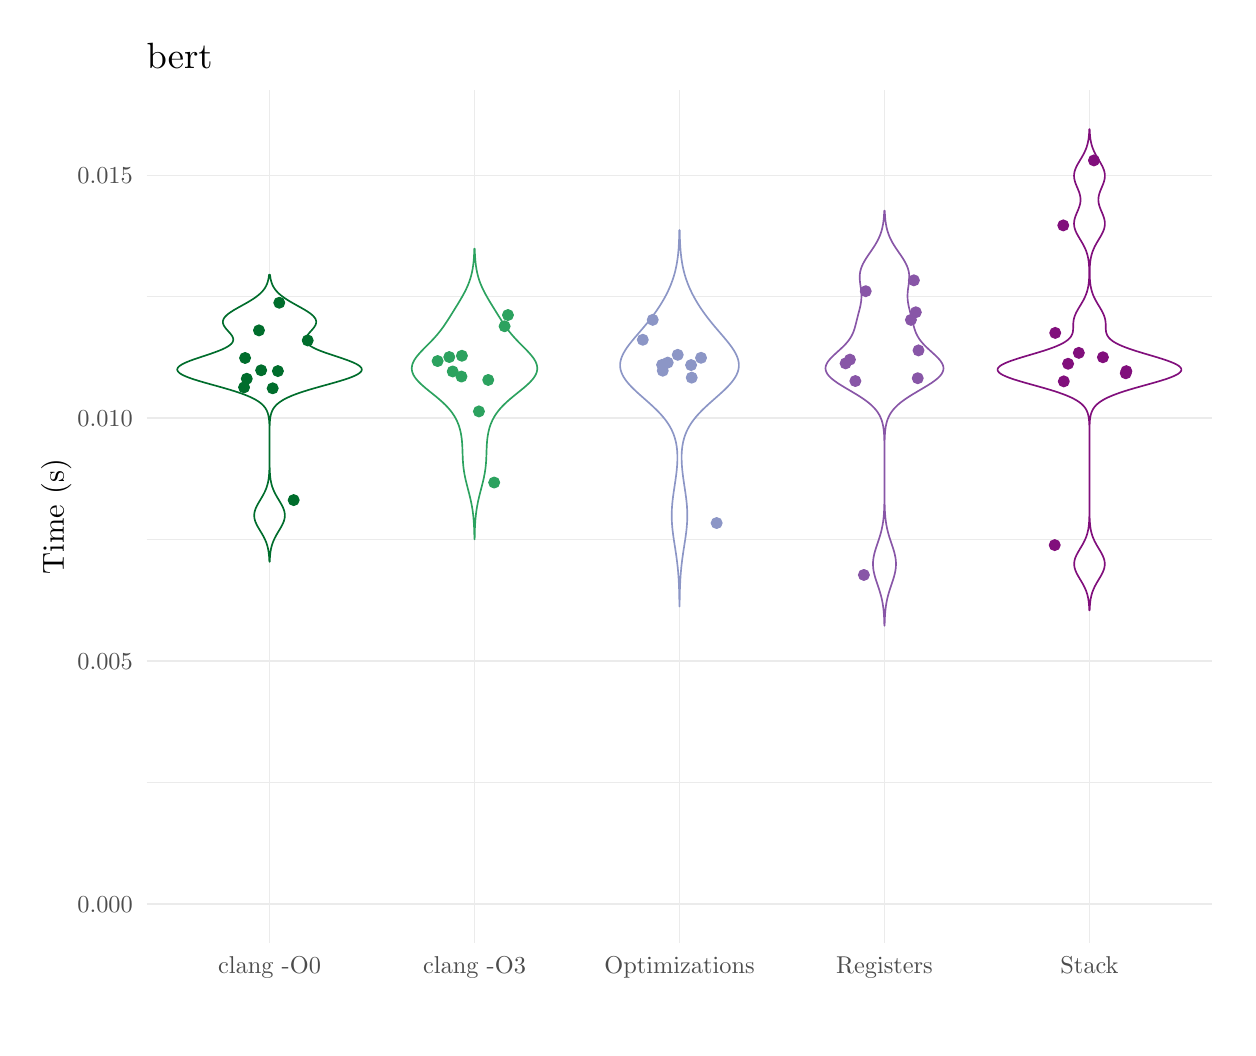
\begin{tikzpicture}[x=1pt,y=1pt]
\definecolor{fillColor}{RGB}{255,255,255}
\path[use as bounding box,fill=fillColor,fill opacity=0.00] (0,0) rectangle (433.62,361.35);
\begin{scope}
\path[clip] ( 42.95, 30.69) rectangle (428.12,338.69);
\definecolor{drawColor}{gray}{0.92}

\path[draw=drawColor,line width= 0.3pt,line join=round] ( 42.95, 88.56) --
	(428.12, 88.56);

\path[draw=drawColor,line width= 0.3pt,line join=round] ( 42.95,176.32) --
	(428.12,176.32);

\path[draw=drawColor,line width= 0.3pt,line join=round] ( 42.95,264.08) --
	(428.12,264.08);

\path[draw=drawColor,line width= 0.6pt,line join=round] ( 42.95, 44.69) --
	(428.12, 44.69);

\path[draw=drawColor,line width= 0.6pt,line join=round] ( 42.95,132.44) --
	(428.12,132.44);

\path[draw=drawColor,line width= 0.6pt,line join=round] ( 42.95,220.20) --
	(428.12,220.20);

\path[draw=drawColor,line width= 0.6pt,line join=round] ( 42.95,307.96) --
	(428.12,307.96);

\path[draw=drawColor,line width= 0.6pt,line join=round] ( 87.40, 30.69) --
	( 87.40,338.69);

\path[draw=drawColor,line width= 0.6pt,line join=round] (161.47, 30.69) --
	(161.47,338.69);

\path[draw=drawColor,line width= 0.6pt,line join=round] (235.54, 30.69) --
	(235.54,338.69);

\path[draw=drawColor,line width= 0.6pt,line join=round] (309.61, 30.69) --
	(309.61,338.69);

\path[draw=drawColor,line width= 0.6pt,line join=round] (383.68, 30.69) --
	(383.68,338.69);
\definecolor{drawColor}{RGB}{0,109,44}
\definecolor{fillColor}{RGB}{255,255,255}

\path[draw=drawColor,line width= 0.6pt,line join=round,line cap=round,fill=fillColor] ( 87.33,168.36) --
	( 87.33,168.57) --
	( 87.32,168.77) --
	( 87.31,168.97) --
	( 87.30,169.17) --
	( 87.29,169.38) --
	( 87.28,169.58) --
	( 87.27,169.78) --
	( 87.25,169.99) --
	( 87.24,170.19) --
	( 87.22,170.39) --
	( 87.21,170.59) --
	( 87.19,170.80) --
	( 87.17,171.00) --
	( 87.15,171.20) --
	( 87.12,171.41) --
	( 87.10,171.61) --
	( 87.07,171.81) --
	( 87.04,172.01) --
	( 87.01,172.22) --
	( 86.97,172.42) --
	( 86.94,172.62) --
	( 86.90,172.83) --
	( 86.86,173.03) --
	( 86.82,173.23) --
	( 86.77,173.43) --
	( 86.72,173.64) --
	( 86.67,173.84) --
	( 86.61,174.04) --
	( 86.56,174.25) --
	( 86.50,174.45) --
	( 86.43,174.65) --
	( 86.37,174.85) --
	( 86.30,175.06) --
	( 86.22,175.26) --
	( 86.15,175.46) --
	( 86.07,175.67) --
	( 85.98,175.87) --
	( 85.90,176.07) --
	( 85.81,176.27) --
	( 85.71,176.48) --
	( 85.62,176.68) --
	( 85.52,176.88) --
	( 85.42,177.09) --
	( 85.31,177.29) --
	( 85.21,177.49) --
	( 85.10,177.70) --
	( 84.98,177.90) --
	( 84.87,178.10) --
	( 84.75,178.30) --
	( 84.64,178.51) --
	( 84.52,178.71) --
	( 84.40,178.91) --
	( 84.28,179.12) --
	( 84.16,179.32) --
	( 84.03,179.52) --
	( 83.91,179.72) --
	( 83.79,179.93) --
	( 83.67,180.13) --
	( 83.55,180.33) --
	( 83.43,180.54) --
	( 83.32,180.74) --
	( 83.20,180.94) --
	( 83.09,181.14) --
	( 82.98,181.35) --
	( 82.87,181.55) --
	( 82.77,181.75) --
	( 82.67,181.96) --
	( 82.58,182.16) --
	( 82.49,182.36) --
	( 82.40,182.56) --
	( 82.32,182.77) --
	( 82.25,182.97) --
	( 82.18,183.17) --
	( 82.12,183.38) --
	( 82.06,183.58) --
	( 82.01,183.78) --
	( 81.97,183.98) --
	( 81.94,184.19) --
	( 81.91,184.39) --
	( 81.89,184.59) --
	( 81.87,184.80) --
	( 81.86,185.00) --
	( 81.86,185.20) --
	( 81.87,185.40) --
	( 81.89,185.61) --
	( 81.91,185.81) --
	( 81.94,186.01) --
	( 81.97,186.22) --
	( 82.02,186.42) --
	( 82.07,186.62) --
	( 82.12,186.83) --
	( 82.18,187.03) --
	( 82.25,187.23) --
	( 82.33,187.43) --
	( 82.41,187.64) --
	( 82.49,187.84) --
	( 82.58,188.04) --
	( 82.68,188.25) --
	( 82.77,188.45) --
	( 82.88,188.65) --
	( 82.98,188.85) --
	( 83.09,189.06) --
	( 83.20,189.26) --
	( 83.32,189.46) --
	( 83.44,189.67) --
	( 83.55,189.87) --
	( 83.67,190.07) --
	( 83.79,190.27) --
	( 83.92,190.48) --
	( 84.04,190.68) --
	( 84.16,190.88) --
	( 84.28,191.09) --
	( 84.40,191.29) --
	( 84.52,191.49) --
	( 84.64,191.69) --
	( 84.76,191.90) --
	( 84.87,192.10) --
	( 84.99,192.30) --
	( 85.10,192.51) --
	( 85.21,192.71) --
	( 85.32,192.91) --
	( 85.42,193.11) --
	( 85.52,193.32) --
	( 85.62,193.52) --
	( 85.72,193.72) --
	( 85.81,193.93) --
	( 85.90,194.13) --
	( 85.98,194.33) --
	( 86.07,194.53) --
	( 86.15,194.74) --
	( 86.22,194.94) --
	( 86.30,195.14) --
	( 86.37,195.35) --
	( 86.43,195.55) --
	( 86.50,195.75) --
	( 86.56,195.95) --
	( 86.62,196.16) --
	( 86.67,196.36) --
	( 86.72,196.56) --
	( 86.77,196.77) --
	( 86.82,196.97) --
	( 86.86,197.17) --
	( 86.90,197.38) --
	( 86.94,197.58) --
	( 86.98,197.78) --
	( 87.01,197.98) --
	( 87.04,198.19) --
	( 87.07,198.39) --
	( 87.10,198.59) --
	( 87.12,198.80) --
	( 87.15,199.00) --
	( 87.17,199.20) --
	( 87.19,199.40) --
	( 87.21,199.61) --
	( 87.22,199.81) --
	( 87.24,200.01) --
	( 87.25,200.22) --
	( 87.27,200.42) --
	( 87.28,200.62) --
	( 87.29,200.82) --
	( 87.30,201.03) --
	( 87.31,201.23) --
	( 87.32,201.43) --
	( 87.33,201.64) --
	( 87.33,201.84) --
	( 87.34,202.04) --
	( 87.35,202.24) --
	( 87.35,202.45) --
	( 87.36,202.65) --
	( 87.36,202.85) --
	( 87.36,203.06) --
	( 87.37,203.26) --
	( 87.37,203.46) --
	( 87.37,203.66) --
	( 87.38,203.87) --
	( 87.38,204.07) --
	( 87.38,204.27) --
	( 87.38,204.48) --
	( 87.38,204.68) --
	( 87.39,204.88) --
	( 87.39,205.08) --
	( 87.39,205.29) --
	( 87.39,205.49) --
	( 87.39,205.69) --
	( 87.39,205.90) --
	( 87.39,206.10) --
	( 87.39,206.30) --
	( 87.39,206.51) --
	( 87.39,206.71) --
	( 87.39,206.91) --
	( 87.39,207.11) --
	( 87.39,207.32) --
	( 87.39,207.52) --
	( 87.39,207.72) --
	( 87.39,207.93) --
	( 87.40,208.13) --
	( 87.40,208.33) --
	( 87.40,208.53) --
	( 87.40,208.74) --
	( 87.40,208.94) --
	( 87.40,209.14) --
	( 87.40,209.35) --
	( 87.40,209.55) --
	( 87.40,209.75) --
	( 87.40,209.95) --
	( 87.40,210.16) --
	( 87.40,210.36) --
	( 87.40,210.56) --
	( 87.40,210.77) --
	( 87.40,210.97) --
	( 87.40,211.17) --
	( 87.40,211.37) --
	( 87.40,211.58) --
	( 87.40,211.78) --
	( 87.40,211.98) --
	( 87.40,212.19) --
	( 87.40,212.39) --
	( 87.39,212.59) --
	( 87.39,212.79) --
	( 87.39,213.00) --
	( 87.39,213.20) --
	( 87.39,213.40) --
	( 87.39,213.61) --
	( 87.39,213.81) --
	( 87.39,214.01) --
	( 87.39,214.21) --
	( 87.39,214.42) --
	( 87.39,214.62) --
	( 87.39,214.82) --
	( 87.39,215.03) --
	( 87.39,215.23) --
	( 87.38,215.43) --
	( 87.38,215.64) --
	( 87.38,215.84) --
	( 87.38,216.04) --
	( 87.38,216.24) --
	( 87.37,216.45) --
	( 87.37,216.65) --
	( 87.37,216.85) --
	( 87.36,217.06) --
	( 87.36,217.26) --
	( 87.35,217.46) --
	( 87.34,217.66) --
	( 87.34,217.87) --
	( 87.33,218.07) --
	( 87.32,218.27) --
	( 87.31,218.48) --
	( 87.30,218.68) --
	( 87.29,218.88) --
	( 87.27,219.08) --
	( 87.26,219.29) --
	( 87.24,219.49) --
	( 87.22,219.69) --
	( 87.20,219.90) --
	( 87.17,220.10) --
	( 87.14,220.30) --
	( 87.11,220.50) --
	( 87.08,220.71) --
	( 87.04,220.91) --
	( 87.00,221.11) --
	( 86.96,221.32) --
	( 86.91,221.52) --
	( 86.86,221.72) --
	( 86.80,221.92) --
	( 86.73,222.13) --
	( 86.66,222.33) --
	( 86.58,222.53) --
	( 86.50,222.74) --
	( 86.41,222.94) --
	( 86.31,223.14) --
	( 86.20,223.34) --
	( 86.09,223.55) --
	( 85.96,223.75) --
	( 85.83,223.95) --
	( 85.68,224.16) --
	( 85.52,224.36) --
	( 85.35,224.56) --
	( 85.17,224.77) --
	( 84.98,224.97) --
	( 84.77,225.17) --
	( 84.55,225.37) --
	( 84.31,225.58) --
	( 84.06,225.78) --
	( 83.79,225.98) --
	( 83.51,226.19) --
	( 83.20,226.39) --
	( 82.88,226.59) --
	( 82.55,226.79) --
	( 82.20,227.00) --
	( 81.82,227.20) --
	( 81.43,227.40) --
	( 81.02,227.61) --
	( 80.59,227.81) --
	( 80.14,228.01) --
	( 79.67,228.21) --
	( 79.18,228.42) --
	( 78.67,228.62) --
	( 78.14,228.82) --
	( 77.60,229.03) --
	( 77.03,229.23) --
	( 76.45,229.43) --
	( 75.85,229.63) --
	( 75.23,229.84) --
	( 74.59,230.04) --
	( 73.94,230.24) --
	( 73.28,230.45) --
	( 72.60,230.65) --
	( 71.91,230.85) --
	( 71.21,231.05) --
	( 70.50,231.26) --
	( 69.79,231.46) --
	( 69.06,231.66) --
	( 68.33,231.87) --
	( 67.60,232.07) --
	( 66.87,232.27) --
	( 66.14,232.47) --
	( 65.41,232.68) --
	( 64.69,232.88) --
	( 63.97,233.08) --
	( 63.27,233.29) --
	( 62.57,233.49) --
	( 61.89,233.69) --
	( 61.22,233.90) --
	( 60.57,234.10) --
	( 59.94,234.30) --
	( 59.34,234.50) --
	( 58.76,234.71) --
	( 58.20,234.91) --
	( 57.67,235.11) --
	( 57.18,235.32) --
	( 56.71,235.52) --
	( 56.27,235.72) --
	( 55.88,235.92) --
	( 55.52,236.13) --
	( 55.19,236.33) --
	( 54.91,236.53) --
	( 54.67,236.74) --
	( 54.46,236.94) --
	( 54.30,237.14) --
	( 54.19,237.34) --
	( 54.11,237.55) --
	( 54.06,237.75) --
	( 54.08,237.95) --
	( 54.13,238.16) --
	( 54.21,238.36) --
	( 54.35,238.56) --
	( 54.53,238.76) --
	( 54.74,238.97) --
	( 54.99,239.17) --
	( 55.28,239.37) --
	( 55.60,239.58) --
	( 55.95,239.78) --
	( 56.35,239.98) --
	( 56.77,240.18) --
	( 57.22,240.39) --
	( 57.70,240.59) --
	( 58.20,240.79) --
	( 58.72,241.00) --
	( 59.26,241.20) --
	( 59.83,241.40) --
	( 60.40,241.60) --
	( 60.99,241.81) --
	( 61.59,242.01) --
	( 62.20,242.21) --
	( 62.81,242.42) --
	( 63.42,242.62) --
	( 64.04,242.82) --
	( 64.65,243.03) --
	( 65.26,243.23) --
	( 65.86,243.43) --
	( 66.45,243.63) --
	( 67.03,243.84) --
	( 67.60,244.04) --
	( 68.15,244.24) --
	( 68.69,244.45) --
	( 69.21,244.65) --
	( 69.71,244.85) --
	( 70.19,245.05) --
	( 70.64,245.26) --
	( 71.07,245.46) --
	( 71.47,245.66) --
	( 71.85,245.87) --
	( 72.20,246.07) --
	( 72.53,246.27) --
	( 72.83,246.47) --
	( 73.09,246.68) --
	( 73.33,246.88) --
	( 73.55,247.08) --
	( 73.73,247.29) --
	( 73.89,247.49) --
	( 74.02,247.69) --
	( 74.12,247.89) --
	( 74.20,248.10) --
	( 74.25,248.30) --
	( 74.28,248.50) --
	( 74.28,248.71) --
	( 74.26,248.91) --
	( 74.22,249.11) --
	( 74.16,249.31) --
	( 74.07,249.52) --
	( 73.98,249.72) --
	( 73.87,249.92) --
	( 73.74,250.13) --
	( 73.60,250.33) --
	( 73.45,250.53) --
	( 73.29,250.73) --
	( 73.12,250.94) --
	( 72.94,251.14) --
	( 72.76,251.34) --
	( 72.58,251.55) --
	( 72.40,251.75) --
	( 72.22,251.95) --
	( 72.04,252.16) --
	( 71.86,252.36) --
	( 71.69,252.56) --
	( 71.53,252.76) --
	( 71.38,252.97) --
	( 71.23,253.17) --
	( 71.09,253.37) --
	( 70.97,253.58) --
	( 70.86,253.78) --
	( 70.77,253.98) --
	( 70.69,254.18) --
	( 70.63,254.39) --
	( 70.58,254.59) --
	( 70.55,254.79) --
	( 70.54,255.00) --
	( 70.55,255.20) --
	( 70.58,255.40) --
	( 70.62,255.60) --
	( 70.69,255.81) --
	( 70.77,256.01) --
	( 70.88,256.21) --
	( 71.00,256.42) --
	( 71.14,256.62) --
	( 71.30,256.82) --
	( 71.48,257.02) --
	( 71.68,257.23) --
	( 71.89,257.43) --
	( 72.12,257.63) --
	( 72.37,257.84) --
	( 72.63,258.04) --
	( 72.90,258.24) --
	( 73.19,258.44) --
	( 73.49,258.65) --
	( 73.80,258.85) --
	( 74.12,259.05) --
	( 74.45,259.26) --
	( 74.79,259.46) --
	( 75.14,259.66) --
	( 75.49,259.86) --
	( 75.85,260.07) --
	( 76.21,260.27) --
	( 76.57,260.47) --
	( 76.94,260.68) --
	( 77.30,260.88) --
	( 77.67,261.08) --
	( 78.04,261.29) --
	( 78.40,261.49) --
	( 78.76,261.69) --
	( 79.12,261.89) --
	( 79.47,262.10) --
	( 79.82,262.30) --
	( 80.16,262.50) --
	( 80.50,262.71) --
	( 80.82,262.91) --
	( 81.14,263.11) --
	( 81.46,263.31) --
	( 81.76,263.52) --
	( 82.06,263.72) --
	( 82.35,263.92) --
	( 82.63,264.13) --
	( 82.89,264.33) --
	( 83.15,264.53) --
	( 83.40,264.73) --
	( 83.64,264.94) --
	( 83.87,265.14) --
	( 84.09,265.34) --
	( 84.30,265.55) --
	( 84.50,265.75) --
	( 84.70,265.95) --
	( 84.88,266.15) --
	( 85.05,266.36) --
	( 85.22,266.56) --
	( 85.37,266.76) --
	( 85.52,266.97) --
	( 85.66,267.17) --
	( 85.79,267.37) --
	( 85.91,267.57) --
	( 86.02,267.78) --
	( 86.13,267.98) --
	( 86.23,268.18) --
	( 86.33,268.39) --
	( 86.41,268.59) --
	( 86.50,268.79) --
	( 86.57,268.99) --
	( 86.64,269.20) --
	( 86.71,269.40) --
	( 86.77,269.60) --
	( 86.82,269.81) --
	( 86.88,270.01) --
	( 86.92,270.21) --
	( 86.97,270.42) --
	( 87.01,270.62) --
	( 87.05,270.82) --
	( 87.08,271.02) --
	( 87.11,271.23) --
	( 87.14,271.43) --
	( 87.16,271.63) --
	( 87.19,271.84) --
	( 87.21,272.04) --
	( 87.58,272.04) --
	( 87.60,271.84) --
	( 87.63,271.63) --
	( 87.65,271.43) --
	( 87.68,271.23) --
	( 87.71,271.02) --
	( 87.75,270.82) --
	( 87.78,270.62) --
	( 87.82,270.42) --
	( 87.87,270.21) --
	( 87.92,270.01) --
	( 87.97,269.81) --
	( 88.02,269.60) --
	( 88.08,269.40) --
	( 88.15,269.20) --
	( 88.22,268.99) --
	( 88.30,268.79) --
	( 88.38,268.59) --
	( 88.47,268.39) --
	( 88.56,268.18) --
	( 88.66,267.98) --
	( 88.77,267.78) --
	( 88.88,267.57) --
	( 89.01,267.37) --
	( 89.14,267.17) --
	( 89.28,266.97) --
	( 89.42,266.76) --
	( 89.58,266.56) --
	( 89.74,266.36) --
	( 89.91,266.15) --
	( 90.10,265.95) --
	( 90.29,265.75) --
	( 90.49,265.55) --
	( 90.70,265.34) --
	( 90.92,265.14) --
	( 91.15,264.94) --
	( 91.39,264.73) --
	( 91.64,264.53) --
	( 91.90,264.33) --
	( 92.17,264.13) --
	( 92.45,263.92) --
	( 92.73,263.72) --
	( 93.03,263.52) --
	( 93.33,263.31) --
	( 93.65,263.11) --
	( 93.97,262.91) --
	( 94.30,262.71) --
	( 94.63,262.50) --
	( 94.98,262.30) --
	( 95.32,262.10) --
	( 95.68,261.89) --
	( 96.03,261.69) --
	( 96.39,261.49) --
	( 96.76,261.29) --
	( 97.12,261.08) --
	( 97.49,260.88) --
	( 97.86,260.68) --
	( 98.22,260.47) --
	( 98.58,260.27) --
	( 98.95,260.07) --
	( 99.30,259.86) --
	( 99.65,259.66) --
	(100.00,259.46) --
	(100.34,259.26) --
	(100.67,259.05) --
	(100.99,258.85) --
	(101.30,258.65) --
	(101.60,258.44) --
	(101.89,258.24) --
	(102.17,258.04) --
	(102.43,257.84) --
	(102.67,257.63) --
	(102.90,257.43) --
	(103.12,257.23) --
	(103.31,257.02) --
	(103.49,256.82) --
	(103.65,256.62) --
	(103.79,256.42) --
	(103.92,256.21) --
	(104.02,256.01) --
	(104.11,255.81) --
	(104.17,255.60) --
	(104.22,255.40) --
	(104.25,255.20) --
	(104.25,255.00) --
	(104.24,254.79) --
	(104.22,254.59) --
	(104.17,254.39) --
	(104.10,254.18) --
	(104.02,253.98) --
	(103.93,253.78) --
	(103.82,253.58) --
	(103.70,253.37) --
	(103.56,253.17) --
	(103.42,252.97) --
	(103.26,252.76) --
	(103.10,252.56) --
	(102.93,252.36) --
	(102.75,252.16) --
	(102.57,251.95) --
	(102.39,251.75) --
	(102.21,251.55) --
	(102.03,251.34) --
	(101.85,251.14) --
	(101.67,250.94) --
	(101.51,250.73) --
	(101.34,250.53) --
	(101.19,250.33) --
	(101.06,250.13) --
	(100.93,249.92) --
	(100.81,249.72) --
	(100.72,249.52) --
	(100.64,249.31) --
	(100.57,249.11) --
	(100.54,248.91) --
	(100.52,248.71) --
	(100.51,248.50) --
	(100.54,248.30) --
	(100.60,248.10) --
	(100.67,247.89) --
	(100.77,247.69) --
	(100.91,247.49) --
	(101.06,247.29) --
	(101.24,247.08) --
	(101.46,246.88) --
	(101.70,246.68) --
	(101.96,246.47) --
	(102.27,246.27) --
	(102.59,246.07) --
	(102.94,245.87) --
	(103.32,245.66) --
	(103.73,245.46) --
	(104.15,245.26) --
	(104.61,245.05) --
	(105.09,244.85) --
	(105.58,244.65) --
	(106.10,244.45) --
	(106.64,244.24) --
	(107.19,244.04) --
	(107.76,243.84) --
	(108.34,243.63) --
	(108.93,243.43) --
	(109.54,243.23) --
	(110.14,243.03) --
	(110.76,242.82) --
	(111.37,242.62) --
	(111.99,242.42) --
	(112.60,242.21) --
	(113.20,242.01) --
	(113.80,241.81) --
	(114.39,241.60) --
	(114.97,241.40) --
	(115.53,241.20) --
	(116.07,241.00) --
	(116.59,240.79) --
	(117.10,240.59) --
	(117.58,240.39) --
	(118.02,240.18) --
	(118.44,239.98) --
	(118.84,239.78) --
	(119.19,239.58) --
	(119.51,239.37) --
	(119.81,239.17) --
	(120.06,238.97) --
	(120.27,238.76) --
	(120.44,238.56) --
	(120.58,238.36) --
	(120.66,238.16) --
	(120.71,237.95) --
	(120.73,237.75) --
	(120.69,237.55) --
	(120.61,237.34) --
	(120.49,237.14) --
	(120.33,236.94) --
	(120.12,236.74) --
	(119.88,236.53) --
	(119.60,236.33) --
	(119.27,236.13) --
	(118.91,235.92) --
	(118.52,235.72) --
	(118.08,235.52) --
	(117.61,235.32) --
	(117.12,235.11) --
	(116.59,234.91) --
	(116.03,234.71) --
	(115.45,234.50) --
	(114.85,234.30) --
	(114.22,234.10) --
	(113.57,233.90) --
	(112.91,233.69) --
	(112.22,233.49) --
	(111.53,233.29) --
	(110.82,233.08) --
	(110.10,232.88) --
	(109.38,232.68) --
	(108.65,232.47) --
	(107.92,232.27) --
	(107.19,232.07) --
	(106.46,231.87) --
	(105.73,231.66) --
	(105.01,231.46) --
	(104.29,231.26) --
	(103.58,231.05) --
	(102.88,230.85) --
	(102.19,230.65) --
	(101.51,230.45) --
	(100.85,230.24) --
	(100.20,230.04) --
	( 99.57,229.84) --
	( 98.94,229.63) --
	( 98.35,229.43) --
	( 97.76,229.23) --
	( 97.20,229.03) --
	( 96.65,228.82) --
	( 96.12,228.62) --
	( 95.61,228.42) --
	( 95.12,228.21) --
	( 94.66,228.01) --
	( 94.21,227.81) --
	( 93.77,227.61) --
	( 93.36,227.40) --
	( 92.97,227.20) --
	( 92.60,227.00) --
	( 92.24,226.79) --
	( 91.91,226.59) --
	( 91.59,226.39) --
	( 91.29,226.19) --
	( 91.00,225.98) --
	( 90.74,225.78) --
	( 90.48,225.58) --
	( 90.25,225.37) --
	( 90.02,225.17) --
	( 89.81,224.97) --
	( 89.62,224.77) --
	( 89.44,224.56) --
	( 89.27,224.36) --
	( 89.11,224.16) --
	( 88.97,223.95) --
	( 88.83,223.75) --
	( 88.70,223.55) --
	( 88.59,223.34) --
	( 88.48,223.14) --
	( 88.38,222.94) --
	( 88.29,222.74) --
	( 88.21,222.53) --
	( 88.13,222.33) --
	( 88.06,222.13) --
	( 88.00,221.92) --
	( 87.94,221.72) --
	( 87.88,221.52) --
	( 87.83,221.32) --
	( 87.79,221.11) --
	( 87.75,220.91) --
	( 87.71,220.71) --
	( 87.68,220.50) --
	( 87.65,220.30) --
	( 87.62,220.10) --
	( 87.60,219.90) --
	( 87.57,219.69) --
	( 87.55,219.49) --
	( 87.54,219.29) --
	( 87.52,219.08) --
	( 87.51,218.88) --
	( 87.49,218.68) --
	( 87.48,218.48) --
	( 87.47,218.27) --
	( 87.46,218.07) --
	( 87.46,217.87) --
	( 87.45,217.66) --
	( 87.44,217.46) --
	( 87.44,217.26) --
	( 87.43,217.06) --
	( 87.43,216.85) --
	( 87.42,216.65) --
	( 87.42,216.45) --
	( 87.42,216.24) --
	( 87.41,216.04) --
	( 87.41,215.84) --
	( 87.41,215.64) --
	( 87.41,215.43) --
	( 87.41,215.23) --
	( 87.40,215.03) --
	( 87.40,214.82) --
	( 87.40,214.62) --
	( 87.40,214.42) --
	( 87.40,214.21) --
	( 87.40,214.01) --
	( 87.40,213.81) --
	( 87.40,213.61) --
	( 87.40,213.40) --
	( 87.40,213.20) --
	( 87.40,213.00) --
	( 87.40,212.79) --
	( 87.40,212.59) --
	( 87.40,212.39) --
	( 87.40,212.19) --
	( 87.40,211.98) --
	( 87.40,211.78) --
	( 87.40,211.58) --
	( 87.40,211.37) --
	( 87.40,211.17) --
	( 87.40,210.97) --
	( 87.40,210.77) --
	( 87.40,210.56) --
	( 87.40,210.36) --
	( 87.40,210.16) --
	( 87.40,209.95) --
	( 87.40,209.75) --
	( 87.40,209.55) --
	( 87.40,209.35) --
	( 87.40,209.14) --
	( 87.40,208.94) --
	( 87.40,208.74) --
	( 87.40,208.53) --
	( 87.40,208.33) --
	( 87.40,208.13) --
	( 87.40,207.93) --
	( 87.40,207.72) --
	( 87.40,207.52) --
	( 87.40,207.32) --
	( 87.40,207.11) --
	( 87.40,206.91) --
	( 87.40,206.71) --
	( 87.40,206.51) --
	( 87.40,206.30) --
	( 87.40,206.10) --
	( 87.40,205.90) --
	( 87.40,205.69) --
	( 87.40,205.49) --
	( 87.40,205.29) --
	( 87.41,205.08) --
	( 87.41,204.88) --
	( 87.41,204.68) --
	( 87.41,204.48) --
	( 87.41,204.27) --
	( 87.41,204.07) --
	( 87.42,203.87) --
	( 87.42,203.66) --
	( 87.42,203.46) --
	( 87.42,203.26) --
	( 87.43,203.06) --
	( 87.43,202.85) --
	( 87.44,202.65) --
	( 87.44,202.45) --
	( 87.45,202.24) --
	( 87.45,202.04) --
	( 87.46,201.84) --
	( 87.47,201.64) --
	( 87.47,201.43) --
	( 87.48,201.23) --
	( 87.49,201.03) --
	( 87.50,200.82) --
	( 87.51,200.62) --
	( 87.53,200.42) --
	( 87.54,200.22) --
	( 87.55,200.01) --
	( 87.57,199.81) --
	( 87.59,199.61) --
	( 87.60,199.40) --
	( 87.62,199.20) --
	( 87.65,199.00) --
	( 87.67,198.80) --
	( 87.70,198.59) --
	( 87.72,198.39) --
	( 87.75,198.19) --
	( 87.78,197.98) --
	( 87.82,197.78) --
	( 87.85,197.58) --
	( 87.89,197.38) --
	( 87.93,197.17) --
	( 87.98,196.97) --
	( 88.02,196.77) --
	( 88.07,196.56) --
	( 88.12,196.36) --
	( 88.18,196.16) --
	( 88.23,195.95) --
	( 88.29,195.75) --
	( 88.36,195.55) --
	( 88.42,195.35) --
	( 88.49,195.14) --
	( 88.57,194.94) --
	( 88.64,194.74) --
	( 88.72,194.53) --
	( 88.81,194.33) --
	( 88.89,194.13) --
	( 88.98,193.93) --
	( 89.08,193.72) --
	( 89.17,193.52) --
	( 89.27,193.32) --
	( 89.37,193.11) --
	( 89.48,192.91) --
	( 89.58,192.71) --
	( 89.69,192.51) --
	( 89.80,192.30) --
	( 89.92,192.10) --
	( 90.03,191.90) --
	( 90.15,191.69) --
	( 90.27,191.49) --
	( 90.39,191.29) --
	( 90.51,191.09) --
	( 90.63,190.88) --
	( 90.75,190.68) --
	( 90.88,190.48) --
	( 91.00,190.27) --
	( 91.12,190.07) --
	( 91.24,189.87) --
	( 91.36,189.67) --
	( 91.47,189.46) --
	( 91.59,189.26) --
	( 91.70,189.06) --
	( 91.81,188.85) --
	( 91.92,188.65) --
	( 92.02,188.45) --
	( 92.12,188.25) --
	( 92.21,188.04) --
	( 92.30,187.84) --
	( 92.39,187.64) --
	( 92.47,187.43) --
	( 92.54,187.23) --
	( 92.61,187.03) --
	( 92.67,186.83) --
	( 92.73,186.62) --
	( 92.78,186.42) --
	( 92.82,186.22) --
	( 92.85,186.01) --
	( 92.89,185.81) --
	( 92.91,185.61) --
	( 92.92,185.40) --
	( 92.93,185.20) --
	( 92.93,185.00) --
	( 92.92,184.80) --
	( 92.91,184.59) --
	( 92.89,184.39) --
	( 92.86,184.19) --
	( 92.82,183.98) --
	( 92.78,183.78) --
	( 92.73,183.58) --
	( 92.67,183.38) --
	( 92.61,183.17) --
	( 92.54,182.97) --
	( 92.47,182.77) --
	( 92.39,182.56) --
	( 92.30,182.36) --
	( 92.21,182.16) --
	( 92.12,181.96) --
	( 92.02,181.75) --
	( 91.92,181.55) --
	( 91.81,181.35) --
	( 91.70,181.14) --
	( 91.59,180.94) --
	( 91.48,180.74) --
	( 91.36,180.54) --
	( 91.24,180.33) --
	( 91.12,180.13) --
	( 91.00,179.93) --
	( 90.88,179.72) --
	( 90.76,179.52) --
	( 90.64,179.32) --
	( 90.51,179.12) --
	( 90.39,178.91) --
	( 90.27,178.71) --
	( 90.16,178.51) --
	( 90.04,178.30) --
	( 89.92,178.10) --
	( 89.81,177.90) --
	( 89.70,177.70) --
	( 89.59,177.49) --
	( 89.48,177.29) --
	( 89.38,177.09) --
	( 89.27,176.88) --
	( 89.18,176.68) --
	( 89.08,176.48) --
	( 88.99,176.27) --
	( 88.90,176.07) --
	( 88.81,175.87) --
	( 88.73,175.67) --
	( 88.65,175.46) --
	( 88.57,175.26) --
	( 88.50,175.06) --
	( 88.43,174.85) --
	( 88.36,174.65) --
	( 88.30,174.45) --
	( 88.24,174.25) --
	( 88.18,174.04) --
	( 88.12,173.84) --
	( 88.07,173.64) --
	( 88.02,173.43) --
	( 87.98,173.23) --
	( 87.93,173.03) --
	( 87.89,172.83) --
	( 87.85,172.62) --
	( 87.82,172.42) --
	( 87.78,172.22) --
	( 87.75,172.01) --
	( 87.72,171.81) --
	( 87.70,171.61) --
	( 87.67,171.41) --
	( 87.65,171.20) --
	( 87.63,171.00) --
	( 87.61,170.80) --
	( 87.59,170.59) --
	( 87.57,170.39) --
	( 87.55,170.19) --
	( 87.54,169.99) --
	( 87.53,169.78) --
	( 87.51,169.58) --
	( 87.50,169.38) --
	( 87.49,169.17) --
	( 87.48,168.97) --
	( 87.47,168.77) --
	( 87.47,168.57) --
	( 87.46,168.36) --
	( 87.33,168.36) --
	cycle;
\definecolor{drawColor}{RGB}{44,162,95}

\path[draw=drawColor,line width= 0.6pt,line join=round,line cap=round,fill=fillColor] (161.43,176.47) --
	(161.42,176.67) --
	(161.42,176.88) --
	(161.42,177.08) --
	(161.41,177.29) --
	(161.41,177.50) --
	(161.41,177.70) --
	(161.40,177.91) --
	(161.40,178.11) --
	(161.39,178.32) --
	(161.39,178.52) --
	(161.38,178.73) --
	(161.38,178.93) --
	(161.37,179.14) --
	(161.37,179.35) --
	(161.36,179.55) --
	(161.35,179.76) --
	(161.34,179.96) --
	(161.34,180.17) --
	(161.33,180.37) --
	(161.32,180.58) --
	(161.31,180.78) --
	(161.30,180.99) --
	(161.29,181.19) --
	(161.28,181.40) --
	(161.27,181.61) --
	(161.26,181.81) --
	(161.25,182.02) --
	(161.24,182.22) --
	(161.22,182.43) --
	(161.21,182.63) --
	(161.20,182.84) --
	(161.18,183.04) --
	(161.17,183.25) --
	(161.15,183.46) --
	(161.13,183.66) --
	(161.11,183.87) --
	(161.10,184.07) --
	(161.08,184.28) --
	(161.06,184.48) --
	(161.04,184.69) --
	(161.02,184.89) --
	(160.99,185.10) --
	(160.97,185.31) --
	(160.95,185.51) --
	(160.92,185.72) --
	(160.90,185.92) --
	(160.87,186.13) --
	(160.85,186.33) --
	(160.82,186.54) --
	(160.79,186.74) --
	(160.76,186.95) --
	(160.73,187.15) --
	(160.70,187.36) --
	(160.67,187.57) --
	(160.63,187.77) --
	(160.60,187.98) --
	(160.56,188.18) --
	(160.53,188.39) --
	(160.49,188.59) --
	(160.45,188.80) --
	(160.42,189.00) --
	(160.38,189.21) --
	(160.34,189.42) --
	(160.29,189.62) --
	(160.25,189.83) --
	(160.21,190.03) --
	(160.17,190.24) --
	(160.12,190.44) --
	(160.08,190.65) --
	(160.03,190.85) --
	(159.98,191.06) --
	(159.94,191.26) --
	(159.89,191.47) --
	(159.84,191.68) --
	(159.79,191.88) --
	(159.74,192.09) --
	(159.69,192.29) --
	(159.64,192.50) --
	(159.59,192.70) --
	(159.54,192.91) --
	(159.49,193.11) --
	(159.43,193.32) --
	(159.38,193.53) --
	(159.33,193.73) --
	(159.28,193.94) --
	(159.22,194.14) --
	(159.17,194.35) --
	(159.12,194.55) --
	(159.06,194.76) --
	(159.01,194.96) --
	(158.96,195.17) --
	(158.90,195.38) --
	(158.85,195.58) --
	(158.80,195.79) --
	(158.74,195.99) --
	(158.69,196.20) --
	(158.64,196.40) --
	(158.59,196.61) --
	(158.54,196.81) --
	(158.49,197.02) --
	(158.44,197.22) --
	(158.39,197.43) --
	(158.34,197.64) --
	(158.29,197.84) --
	(158.24,198.05) --
	(158.20,198.25) --
	(158.15,198.46) --
	(158.11,198.66) --
	(158.06,198.87) --
	(158.02,199.07) --
	(157.98,199.28) --
	(157.94,199.49) --
	(157.90,199.69) --
	(157.86,199.90) --
	(157.82,200.10) --
	(157.79,200.31) --
	(157.75,200.51) --
	(157.72,200.72) --
	(157.68,200.92) --
	(157.65,201.13) --
	(157.62,201.33) --
	(157.59,201.54) --
	(157.56,201.75) --
	(157.54,201.95) --
	(157.51,202.16) --
	(157.49,202.36) --
	(157.46,202.57) --
	(157.44,202.77) --
	(157.42,202.98) --
	(157.40,203.18) --
	(157.38,203.39) --
	(157.36,203.60) --
	(157.34,203.80) --
	(157.32,204.01) --
	(157.31,204.21) --
	(157.29,204.42) --
	(157.28,204.62) --
	(157.27,204.83) --
	(157.26,205.03) --
	(157.24,205.24) --
	(157.23,205.45) --
	(157.22,205.65) --
	(157.21,205.86) --
	(157.20,206.06) --
	(157.20,206.27) --
	(157.19,206.47) --
	(157.18,206.68) --
	(157.17,206.88) --
	(157.17,207.09) --
	(157.16,207.29) --
	(157.15,207.50) --
	(157.14,207.71) --
	(157.14,207.91) --
	(157.13,208.12) --
	(157.12,208.32) --
	(157.12,208.53) --
	(157.11,208.73) --
	(157.10,208.94) --
	(157.09,209.14) --
	(157.09,209.35) --
	(157.08,209.56) --
	(157.07,209.76) --
	(157.06,209.97) --
	(157.05,210.17) --
	(157.04,210.38) --
	(157.02,210.58) --
	(157.01,210.79) --
	(157.00,210.99) --
	(156.98,211.20) --
	(156.97,211.40) --
	(156.95,211.61) --
	(156.93,211.82) --
	(156.92,212.02) --
	(156.90,212.23) --
	(156.87,212.43) --
	(156.85,212.64) --
	(156.83,212.84) --
	(156.80,213.05) --
	(156.78,213.25) --
	(156.75,213.46) --
	(156.72,213.67) --
	(156.69,213.87) --
	(156.65,214.08) --
	(156.62,214.28) --
	(156.58,214.49) --
	(156.55,214.69) --
	(156.51,214.90) --
	(156.46,215.10) --
	(156.42,215.31) --
	(156.37,215.52) --
	(156.33,215.72) --
	(156.27,215.93) --
	(156.22,216.13) --
	(156.17,216.34) --
	(156.11,216.54) --
	(156.05,216.75) --
	(155.99,216.95) --
	(155.93,217.16) --
	(155.86,217.36) --
	(155.79,217.57) --
	(155.72,217.78) --
	(155.64,217.98) --
	(155.56,218.19) --
	(155.48,218.39) --
	(155.40,218.60) --
	(155.31,218.80) --
	(155.22,219.01) --
	(155.13,219.21) --
	(155.03,219.42) --
	(154.93,219.63) --
	(154.83,219.83) --
	(154.72,220.04) --
	(154.61,220.24) --
	(154.50,220.45) --
	(154.38,220.65) --
	(154.26,220.86) --
	(154.13,221.06) --
	(154.00,221.27) --
	(153.87,221.47) --
	(153.73,221.68) --
	(153.59,221.89) --
	(153.45,222.09) --
	(153.30,222.30) --
	(153.15,222.50) --
	(152.99,222.71) --
	(152.83,222.91) --
	(152.66,223.12) --
	(152.49,223.32) --
	(152.32,223.53) --
	(152.14,223.74) --
	(151.96,223.94) --
	(151.77,224.15) --
	(151.58,224.35) --
	(151.39,224.56) --
	(151.19,224.76) --
	(150.99,224.97) --
	(150.78,225.17) --
	(150.57,225.38) --
	(150.35,225.58) --
	(150.14,225.79) --
	(149.92,226.00) --
	(149.69,226.20) --
	(149.46,226.41) --
	(149.23,226.61) --
	(149.00,226.82) --
	(148.76,227.02) --
	(148.52,227.23) --
	(148.28,227.43) --
	(148.03,227.64) --
	(147.79,227.85) --
	(147.54,228.05) --
	(147.29,228.26) --
	(147.03,228.46) --
	(146.78,228.67) --
	(146.53,228.87) --
	(146.27,229.08) --
	(146.02,229.28) --
	(145.76,229.49) --
	(145.50,229.70) --
	(145.25,229.90) --
	(144.99,230.11) --
	(144.74,230.31) --
	(144.49,230.52) --
	(144.24,230.72) --
	(143.99,230.93) --
	(143.74,231.13) --
	(143.50,231.34) --
	(143.26,231.54) --
	(143.02,231.75) --
	(142.79,231.96) --
	(142.56,232.16) --
	(142.33,232.37) --
	(142.11,232.57) --
	(141.90,232.78) --
	(141.68,232.98) --
	(141.48,233.19) --
	(141.28,233.39) --
	(141.08,233.60) --
	(140.90,233.81) --
	(140.72,234.01) --
	(140.54,234.22) --
	(140.37,234.42) --
	(140.21,234.63) --
	(140.06,234.83) --
	(139.92,235.04) --
	(139.78,235.24) --
	(139.65,235.45) --
	(139.53,235.65) --
	(139.42,235.86) --
	(139.32,236.07) --
	(139.23,236.27) --
	(139.14,236.48) --
	(139.07,236.68) --
	(139.00,236.89) --
	(138.95,237.09) --
	(138.90,237.30) --
	(138.86,237.50) --
	(138.83,237.71) --
	(138.81,237.92) --
	(138.80,238.12) --
	(138.80,238.33) --
	(138.81,238.53) --
	(138.83,238.74) --
	(138.86,238.94) --
	(138.89,239.15) --
	(138.94,239.35) --
	(138.99,239.56) --
	(139.05,239.77) --
	(139.12,239.97) --
	(139.20,240.18) --
	(139.29,240.38) --
	(139.38,240.59) --
	(139.48,240.79) --
	(139.60,241.00) --
	(139.71,241.20) --
	(139.84,241.41) --
	(139.97,241.61) --
	(140.10,241.82) --
	(140.25,242.03) --
	(140.40,242.23) --
	(140.55,242.44) --
	(140.71,242.64) --
	(140.87,242.85) --
	(141.05,243.05) --
	(141.22,243.26) --
	(141.40,243.46) --
	(141.58,243.67) --
	(141.76,243.88) --
	(141.95,244.08) --
	(142.14,244.29) --
	(142.34,244.49) --
	(142.53,244.70) --
	(142.73,244.90) --
	(142.93,245.11) --
	(143.13,245.31) --
	(143.34,245.52) --
	(143.54,245.72) --
	(143.74,245.93) --
	(143.95,246.14) --
	(144.15,246.34) --
	(144.36,246.55) --
	(144.56,246.75) --
	(144.77,246.96) --
	(144.97,247.16) --
	(145.17,247.37) --
	(145.37,247.57) --
	(145.57,247.78) --
	(145.77,247.99) --
	(145.97,248.19) --
	(146.16,248.40) --
	(146.36,248.60) --
	(146.55,248.81) --
	(146.74,249.01) --
	(146.93,249.22) --
	(147.11,249.42) --
	(147.30,249.63) --
	(147.48,249.84) --
	(147.66,250.04) --
	(147.84,250.25) --
	(148.01,250.45) --
	(148.19,250.66) --
	(148.36,250.86) --
	(148.52,251.07) --
	(148.69,251.27) --
	(148.85,251.48) --
	(149.02,251.68) --
	(149.17,251.89) --
	(149.33,252.10) --
	(149.49,252.30) --
	(149.64,252.51) --
	(149.79,252.71) --
	(149.94,252.92) --
	(150.09,253.12) --
	(150.24,253.33) --
	(150.38,253.53) --
	(150.52,253.74) --
	(150.66,253.95) --
	(150.80,254.15) --
	(150.94,254.36) --
	(151.08,254.56) --
	(151.22,254.77) --
	(151.35,254.97) --
	(151.49,255.18) --
	(151.62,255.38) --
	(151.75,255.59) --
	(151.89,255.79) --
	(152.02,256.00) --
	(152.15,256.21) --
	(152.28,256.41) --
	(152.41,256.62) --
	(152.54,256.82) --
	(152.67,257.03) --
	(152.79,257.23) --
	(152.92,257.44) --
	(153.05,257.64) --
	(153.18,257.85) --
	(153.31,258.06) --
	(153.44,258.26) --
	(153.56,258.47) --
	(153.69,258.67) --
	(153.82,258.88) --
	(153.95,259.08) --
	(154.07,259.29) --
	(154.20,259.49) --
	(154.33,259.70) --
	(154.45,259.91) --
	(154.58,260.11) --
	(154.71,260.32) --
	(154.84,260.52) --
	(154.96,260.73) --
	(155.09,260.93) --
	(155.22,261.14) --
	(155.34,261.34) --
	(155.47,261.55) --
	(155.59,261.75) --
	(155.72,261.96) --
	(155.84,262.17) --
	(155.97,262.37) --
	(156.09,262.58) --
	(156.21,262.78) --
	(156.33,262.99) --
	(156.45,263.19) --
	(156.57,263.40) --
	(156.69,263.60) --
	(156.81,263.81) --
	(156.93,264.02) --
	(157.05,264.22) --
	(157.16,264.43) --
	(157.28,264.63) --
	(157.39,264.84) --
	(157.50,265.04) --
	(157.61,265.25) --
	(157.72,265.45) --
	(157.83,265.66) --
	(157.94,265.86) --
	(158.04,266.07) --
	(158.15,266.28) --
	(158.25,266.48) --
	(158.35,266.69) --
	(158.45,266.89) --
	(158.55,267.10) --
	(158.64,267.30) --
	(158.74,267.51) --
	(158.83,267.71) --
	(158.92,267.92) --
	(159.01,268.13) --
	(159.09,268.33) --
	(159.18,268.54) --
	(159.26,268.74) --
	(159.34,268.95) --
	(159.42,269.15) --
	(159.50,269.36) --
	(159.57,269.56) --
	(159.64,269.77) --
	(159.71,269.98) --
	(159.78,270.18) --
	(159.85,270.39) --
	(159.92,270.59) --
	(159.98,270.80) --
	(160.04,271.00) --
	(160.10,271.21) --
	(160.16,271.41) --
	(160.22,271.62) --
	(160.27,271.82) --
	(160.32,272.03) --
	(160.38,272.24) --
	(160.42,272.44) --
	(160.47,272.65) --
	(160.52,272.85) --
	(160.56,273.06) --
	(160.61,273.26) --
	(160.65,273.47) --
	(160.69,273.67) --
	(160.72,273.88) --
	(160.76,274.09) --
	(160.80,274.29) --
	(160.83,274.50) --
	(160.86,274.70) --
	(160.89,274.91) --
	(160.92,275.11) --
	(160.95,275.32) --
	(160.98,275.52) --
	(161.00,275.73) --
	(161.03,275.93) --
	(161.05,276.14) --
	(161.08,276.35) --
	(161.10,276.55) --
	(161.12,276.76) --
	(161.14,276.96) --
	(161.16,277.17) --
	(161.17,277.37) --
	(161.19,277.58) --
	(161.21,277.78) --
	(161.22,277.99) --
	(161.24,278.20) --
	(161.25,278.40) --
	(161.26,278.61) --
	(161.28,278.81) --
	(161.29,279.02) --
	(161.30,279.22) --
	(161.31,279.43) --
	(161.32,279.63) --
	(161.33,279.84) --
	(161.34,280.05) --
	(161.35,280.25) --
	(161.35,280.46) --
	(161.36,280.66) --
	(161.37,280.87) --
	(161.38,281.07) --
	(161.38,281.28) --
	(161.39,281.48) --
	(161.55,281.48) --
	(161.55,281.28) --
	(161.56,281.07) --
	(161.56,280.87) --
	(161.57,280.66) --
	(161.58,280.46) --
	(161.59,280.25) --
	(161.60,280.05) --
	(161.60,279.84) --
	(161.61,279.63) --
	(161.62,279.43) --
	(161.63,279.22) --
	(161.64,279.02) --
	(161.66,278.81) --
	(161.67,278.61) --
	(161.68,278.40) --
	(161.70,278.20) --
	(161.71,277.99) --
	(161.73,277.78) --
	(161.74,277.58) --
	(161.76,277.37) --
	(161.78,277.17) --
	(161.80,276.96) --
	(161.81,276.76) --
	(161.84,276.55) --
	(161.86,276.35) --
	(161.88,276.14) --
	(161.90,275.93) --
	(161.93,275.73) --
	(161.95,275.52) --
	(161.98,275.32) --
	(162.01,275.11) --
	(162.04,274.91) --
	(162.07,274.70) --
	(162.10,274.50) --
	(162.14,274.29) --
	(162.17,274.09) --
	(162.21,273.88) --
	(162.25,273.67) --
	(162.29,273.47) --
	(162.33,273.26) --
	(162.37,273.06) --
	(162.41,272.85) --
	(162.46,272.65) --
	(162.51,272.44) --
	(162.56,272.24) --
	(162.61,272.03) --
	(162.66,271.82) --
	(162.72,271.62) --
	(162.77,271.41) --
	(162.83,271.21) --
	(162.89,271.00) --
	(162.95,270.80) --
	(163.02,270.59) --
	(163.08,270.39) --
	(163.15,270.18) --
	(163.22,269.98) --
	(163.29,269.77) --
	(163.36,269.56) --
	(163.44,269.36) --
	(163.51,269.15) --
	(163.59,268.95) --
	(163.67,268.74) --
	(163.76,268.54) --
	(163.84,268.33) --
	(163.93,268.13) --
	(164.02,267.92) --
	(164.11,267.71) --
	(164.20,267.51) --
	(164.29,267.30) --
	(164.39,267.10) --
	(164.48,266.89) --
	(164.58,266.69) --
	(164.68,266.48) --
	(164.79,266.28) --
	(164.89,266.07) --
	(164.99,265.86) --
	(165.10,265.66) --
	(165.21,265.45) --
	(165.32,265.25) --
	(165.43,265.04) --
	(165.54,264.84) --
	(165.66,264.63) --
	(165.77,264.43) --
	(165.89,264.22) --
	(166.00,264.02) --
	(166.12,263.81) --
	(166.24,263.60) --
	(166.36,263.40) --
	(166.48,263.19) --
	(166.60,262.99) --
	(166.72,262.78) --
	(166.84,262.58) --
	(166.97,262.37) --
	(167.09,262.17) --
	(167.22,261.96) --
	(167.34,261.75) --
	(167.47,261.55) --
	(167.59,261.34) --
	(167.72,261.14) --
	(167.84,260.93) --
	(167.97,260.73) --
	(168.10,260.52) --
	(168.22,260.32) --
	(168.35,260.11) --
	(168.48,259.91) --
	(168.61,259.70) --
	(168.73,259.49) --
	(168.86,259.29) --
	(168.99,259.08) --
	(169.12,258.88) --
	(169.24,258.67) --
	(169.37,258.47) --
	(169.50,258.26) --
	(169.63,258.06) --
	(169.75,257.85) --
	(169.88,257.64) --
	(170.01,257.44) --
	(170.14,257.23) --
	(170.27,257.03) --
	(170.40,256.82) --
	(170.53,256.62) --
	(170.66,256.41) --
	(170.79,256.21) --
	(170.92,256.00) --
	(171.05,255.79) --
	(171.18,255.59) --
	(171.31,255.38) --
	(171.45,255.18) --
	(171.58,254.97) --
	(171.72,254.77) --
	(171.85,254.56) --
	(171.99,254.36) --
	(172.13,254.15) --
	(172.27,253.95) --
	(172.41,253.74) --
	(172.55,253.53) --
	(172.70,253.33) --
	(172.84,253.12) --
	(172.99,252.92) --
	(173.14,252.71) --
	(173.29,252.51) --
	(173.45,252.30) --
	(173.60,252.10) --
	(173.76,251.89) --
	(173.92,251.68) --
	(174.08,251.48) --
	(174.24,251.27) --
	(174.41,251.07) --
	(174.58,250.86) --
	(174.75,250.66) --
	(174.92,250.45) --
	(175.10,250.25) --
	(175.27,250.04) --
	(175.45,249.84) --
	(175.63,249.63) --
	(175.82,249.42) --
	(176.00,249.22) --
	(176.19,249.01) --
	(176.38,248.81) --
	(176.57,248.60) --
	(176.77,248.40) --
	(176.96,248.19) --
	(177.16,247.99) --
	(177.36,247.78) --
	(177.56,247.57) --
	(177.76,247.37) --
	(177.96,247.16) --
	(178.17,246.96) --
	(178.37,246.75) --
	(178.58,246.55) --
	(178.78,246.34) --
	(178.99,246.14) --
	(179.19,245.93) --
	(179.39,245.72) --
	(179.60,245.52) --
	(179.80,245.31) --
	(180.00,245.11) --
	(180.20,244.90) --
	(180.40,244.70) --
	(180.60,244.49) --
	(180.79,244.29) --
	(180.98,244.08) --
	(181.17,243.88) --
	(181.35,243.67) --
	(181.54,243.46) --
	(181.71,243.26) --
	(181.89,243.05) --
	(182.06,242.85) --
	(182.22,242.64) --
	(182.38,242.44) --
	(182.54,242.23) --
	(182.69,242.03) --
	(182.83,241.82) --
	(182.97,241.61) --
	(183.10,241.41) --
	(183.22,241.20) --
	(183.34,241.00) --
	(183.45,240.79) --
	(183.55,240.59) --
	(183.65,240.38) --
	(183.73,240.18) --
	(183.81,239.97) --
	(183.88,239.77) --
	(183.94,239.56) --
	(184.00,239.35) --
	(184.04,239.15) --
	(184.08,238.94) --
	(184.11,238.74) --
	(184.12,238.53) --
	(184.13,238.33) --
	(184.13,238.12) --
	(184.12,237.92) --
	(184.10,237.71) --
	(184.07,237.50) --
	(184.04,237.30) --
	(183.99,237.09) --
	(183.93,236.89) --
	(183.87,236.68) --
	(183.79,236.48) --
	(183.71,236.27) --
	(183.61,236.07) --
	(183.51,235.86) --
	(183.40,235.65) --
	(183.28,235.45) --
	(183.15,235.24) --
	(183.02,235.04) --
	(182.87,234.83) --
	(182.72,234.63) --
	(182.56,234.42) --
	(182.39,234.22) --
	(182.22,234.01) --
	(182.04,233.81) --
	(181.85,233.60) --
	(181.65,233.39) --
	(181.46,233.19) --
	(181.25,232.98) --
	(181.04,232.78) --
	(180.82,232.57) --
	(180.60,232.37) --
	(180.37,232.16) --
	(180.14,231.96) --
	(179.91,231.75) --
	(179.67,231.54) --
	(179.43,231.34) --
	(179.19,231.13) --
	(178.94,230.93) --
	(178.69,230.72) --
	(178.44,230.52) --
	(178.19,230.31) --
	(177.94,230.11) --
	(177.68,229.90) --
	(177.43,229.70) --
	(177.17,229.49) --
	(176.92,229.28) --
	(176.66,229.08) --
	(176.41,228.87) --
	(176.15,228.67) --
	(175.90,228.46) --
	(175.65,228.26) --
	(175.40,228.05) --
	(175.15,227.85) --
	(174.90,227.64) --
	(174.66,227.43) --
	(174.41,227.23) --
	(174.17,227.02) --
	(173.94,226.82) --
	(173.70,226.61) --
	(173.47,226.41) --
	(173.24,226.20) --
	(173.02,226.00) --
	(172.80,225.79) --
	(172.58,225.58) --
	(172.36,225.38) --
	(172.15,225.17) --
	(171.95,224.97) --
	(171.74,224.76) --
	(171.55,224.56) --
	(171.35,224.35) --
	(171.16,224.15) --
	(170.97,223.94) --
	(170.79,223.74) --
	(170.61,223.53) --
	(170.44,223.32) --
	(170.27,223.12) --
	(170.10,222.91) --
	(169.94,222.71) --
	(169.79,222.50) --
	(169.63,222.30) --
	(169.48,222.09) --
	(169.34,221.89) --
	(169.20,221.68) --
	(169.06,221.47) --
	(168.93,221.27) --
	(168.80,221.06) --
	(168.68,220.86) --
	(168.55,220.65) --
	(168.44,220.45) --
	(168.32,220.24) --
	(168.21,220.04) --
	(168.11,219.83) --
	(168.00,219.63) --
	(167.90,219.42) --
	(167.81,219.21) --
	(167.71,219.01) --
	(167.62,218.80) --
	(167.54,218.60) --
	(167.45,218.39) --
	(167.37,218.19) --
	(167.29,217.98) --
	(167.22,217.78) --
	(167.15,217.57) --
	(167.08,217.36) --
	(167.01,217.16) --
	(166.94,216.95) --
	(166.88,216.75) --
	(166.82,216.54) --
	(166.77,216.34) --
	(166.71,216.13) --
	(166.66,215.93) --
	(166.61,215.72) --
	(166.56,215.52) --
	(166.51,215.31) --
	(166.47,215.10) --
	(166.43,214.90) --
	(166.39,214.69) --
	(166.35,214.49) --
	(166.31,214.28) --
	(166.28,214.08) --
	(166.25,213.87) --
	(166.21,213.67) --
	(166.18,213.46) --
	(166.16,213.25) --
	(166.13,213.05) --
	(166.10,212.84) --
	(166.08,212.64) --
	(166.06,212.43) --
	(166.04,212.23) --
	(166.02,212.02) --
	(166.00,211.82) --
	(165.98,211.61) --
	(165.96,211.40) --
	(165.95,211.20) --
	(165.93,210.99) --
	(165.92,210.79) --
	(165.91,210.58) --
	(165.90,210.38) --
	(165.89,210.17) --
	(165.87,209.97) --
	(165.86,209.76) --
	(165.86,209.56) --
	(165.85,209.35) --
	(165.84,209.14) --
	(165.83,208.94) --
	(165.82,208.73) --
	(165.82,208.53) --
	(165.81,208.32) --
	(165.80,208.12) --
	(165.80,207.91) --
	(165.79,207.71) --
	(165.78,207.50) --
	(165.78,207.29) --
	(165.77,207.09) --
	(165.76,206.88) --
	(165.75,206.68) --
	(165.75,206.47) --
	(165.74,206.27) --
	(165.73,206.06) --
	(165.72,205.86) --
	(165.71,205.65) --
	(165.70,205.45) --
	(165.69,205.24) --
	(165.68,205.03) --
	(165.67,204.83) --
	(165.65,204.62) --
	(165.64,204.42) --
	(165.62,204.21) --
	(165.61,204.01) --
	(165.59,203.80) --
	(165.57,203.60) --
	(165.56,203.39) --
	(165.54,203.18) --
	(165.52,202.98) --
	(165.49,202.77) --
	(165.47,202.57) --
	(165.45,202.36) --
	(165.42,202.16) --
	(165.40,201.95) --
	(165.37,201.75) --
	(165.34,201.54) --
	(165.31,201.33) --
	(165.28,201.13) --
	(165.25,200.92) --
	(165.22,200.72) --
	(165.18,200.51) --
	(165.15,200.31) --
	(165.11,200.10) --
	(165.07,199.90) --
	(165.03,199.69) --
	(164.99,199.49) --
	(164.95,199.28) --
	(164.91,199.07) --
	(164.87,198.87) --
	(164.83,198.66) --
	(164.78,198.46) --
	(164.74,198.25) --
	(164.69,198.05) --
	(164.64,197.84) --
	(164.59,197.64) --
	(164.55,197.43) --
	(164.50,197.22) --
	(164.45,197.02) --
	(164.40,196.81) --
	(164.35,196.61) --
	(164.29,196.40) --
	(164.24,196.20) --
	(164.19,195.99) --
	(164.14,195.79) --
	(164.08,195.58) --
	(164.03,195.38) --
	(163.98,195.17) --
	(163.92,194.96) --
	(163.87,194.76) --
	(163.82,194.55) --
	(163.76,194.35) --
	(163.71,194.14) --
	(163.66,193.94) --
	(163.60,193.73) --
	(163.55,193.53) --
	(163.50,193.32) --
	(163.45,193.11) --
	(163.39,192.91) --
	(163.34,192.70) --
	(163.29,192.50) --
	(163.24,192.29) --
	(163.19,192.09) --
	(163.14,191.88) --
	(163.09,191.68) --
	(163.04,191.47) --
	(163.00,191.26) --
	(162.95,191.06) --
	(162.90,190.85) --
	(162.86,190.65) --
	(162.81,190.44) --
	(162.77,190.24) --
	(162.72,190.03) --
	(162.68,189.83) --
	(162.64,189.62) --
	(162.60,189.42) --
	(162.56,189.21) --
	(162.52,189.00) --
	(162.48,188.80) --
	(162.44,188.59) --
	(162.41,188.39) --
	(162.37,188.18) --
	(162.33,187.98) --
	(162.30,187.77) --
	(162.27,187.57) --
	(162.24,187.36) --
	(162.20,187.15) --
	(162.17,186.95) --
	(162.14,186.74) --
	(162.12,186.54) --
	(162.09,186.33) --
	(162.06,186.13) --
	(162.03,185.92) --
	(162.01,185.72) --
	(161.98,185.51) --
	(161.96,185.31) --
	(161.94,185.10) --
	(161.92,184.89) --
	(161.90,184.69) --
	(161.88,184.48) --
	(161.86,184.28) --
	(161.84,184.07) --
	(161.82,183.87) --
	(161.80,183.66) --
	(161.78,183.46) --
	(161.77,183.25) --
	(161.75,183.04) --
	(161.74,182.84) --
	(161.72,182.63) --
	(161.71,182.43) --
	(161.70,182.22) --
	(161.68,182.02) --
	(161.67,181.81) --
	(161.66,181.61) --
	(161.65,181.40) --
	(161.64,181.19) --
	(161.63,180.99) --
	(161.62,180.78) --
	(161.61,180.58) --
	(161.60,180.37) --
	(161.60,180.17) --
	(161.59,179.96) --
	(161.58,179.76) --
	(161.57,179.55) --
	(161.57,179.35) --
	(161.56,179.14) --
	(161.56,178.93) --
	(161.55,178.73) --
	(161.54,178.52) --
	(161.54,178.32) --
	(161.54,178.11) --
	(161.53,177.91) --
	(161.53,177.70) --
	(161.52,177.50) --
	(161.52,177.29) --
	(161.52,177.08) --
	(161.51,176.88) --
	(161.51,176.67) --
	(161.51,176.47) --
	(161.43,176.47) --
	cycle;
\definecolor{drawColor}{RGB}{140,150,198}

\path[draw=drawColor,line width= 0.6pt,line join=round,line cap=round,fill=fillColor] (235.51,152.19) --
	(235.50,152.46) --
	(235.50,152.72) --
	(235.50,152.99) --
	(235.49,153.26) --
	(235.49,153.52) --
	(235.49,153.79) --
	(235.49,154.06) --
	(235.48,154.32) --
	(235.48,154.59) --
	(235.47,154.85) --
	(235.47,155.12) --
	(235.46,155.39) --
	(235.46,155.65) --
	(235.45,155.92) --
	(235.45,156.18) --
	(235.44,156.45) --
	(235.44,156.72) --
	(235.43,156.98) --
	(235.42,157.25) --
	(235.42,157.52) --
	(235.41,157.78) --
	(235.40,158.05) --
	(235.39,158.31) --
	(235.38,158.58) --
	(235.38,158.85) --
	(235.37,159.11) --
	(235.36,159.38) --
	(235.35,159.64) --
	(235.33,159.91) --
	(235.32,160.18) --
	(235.31,160.44) --
	(235.30,160.71) --
	(235.28,160.98) --
	(235.27,161.24) --
	(235.26,161.51) --
	(235.24,161.77) --
	(235.23,162.04) --
	(235.21,162.31) --
	(235.19,162.57) --
	(235.18,162.84) --
	(235.16,163.11) --
	(235.14,163.37) --
	(235.12,163.64) --
	(235.10,163.90) --
	(235.08,164.17) --
	(235.06,164.44) --
	(235.04,164.70) --
	(235.01,164.97) --
	(234.99,165.23) --
	(234.96,165.50) --
	(234.94,165.77) --
	(234.91,166.03) --
	(234.89,166.30) --
	(234.86,166.57) --
	(234.83,166.83) --
	(234.80,167.10) --
	(234.77,167.36) --
	(234.74,167.63) --
	(234.71,167.90) --
	(234.68,168.16) --
	(234.65,168.43) --
	(234.61,168.69) --
	(234.58,168.96) --
	(234.55,169.23) --
	(234.51,169.49) --
	(234.48,169.76) --
	(234.44,170.03) --
	(234.40,170.29) --
	(234.37,170.56) --
	(234.33,170.82) --
	(234.29,171.09) --
	(234.25,171.36) --
	(234.21,171.62) --
	(234.17,171.89) --
	(234.13,172.16) --
	(234.09,172.42) --
	(234.05,172.69) --
	(234.01,172.95) --
	(233.97,173.22) --
	(233.93,173.49) --
	(233.89,173.75) --
	(233.84,174.02) --
	(233.80,174.28) --
	(233.76,174.55) --
	(233.72,174.82) --
	(233.68,175.08) --
	(233.64,175.35) --
	(233.60,175.62) --
	(233.56,175.88) --
	(233.52,176.15) --
	(233.48,176.41) --
	(233.44,176.68) --
	(233.40,176.95) --
	(233.36,177.21) --
	(233.32,177.48) --
	(233.29,177.74) --
	(233.25,178.01) --
	(233.22,178.28) --
	(233.18,178.54) --
	(233.15,178.81) --
	(233.12,179.08) --
	(233.08,179.34) --
	(233.05,179.61) --
	(233.02,179.87) --
	(232.99,180.14) --
	(232.97,180.41) --
	(232.94,180.67) --
	(232.92,180.94) --
	(232.89,181.21) --
	(232.87,181.47) --
	(232.85,181.74) --
	(232.83,182.00) --
	(232.81,182.27) --
	(232.80,182.54) --
	(232.78,182.80) --
	(232.77,183.07) --
	(232.76,183.33) --
	(232.75,183.60) --
	(232.74,183.87) --
	(232.73,184.13) --
	(232.73,184.40) --
	(232.72,184.67) --
	(232.72,184.93) --
	(232.72,185.20) --
	(232.72,185.46) --
	(232.73,185.73) --
	(232.73,186.00) --
	(232.74,186.26) --
	(232.75,186.53) --
	(232.76,186.79) --
	(232.77,187.06) --
	(232.78,187.33) --
	(232.79,187.59) --
	(232.81,187.86) --
	(232.83,188.13) --
	(232.85,188.39) --
	(232.87,188.66) --
	(232.89,188.92) --
	(232.91,189.19) --
	(232.93,189.46) --
	(232.96,189.72) --
	(232.99,189.99) --
	(233.01,190.26) --
	(233.04,190.52) --
	(233.07,190.79) --
	(233.10,191.05) --
	(233.14,191.32) --
	(233.17,191.59) --
	(233.20,191.85) --
	(233.24,192.12) --
	(233.27,192.38) --
	(233.31,192.65) --
	(233.35,192.92) --
	(233.39,193.18) --
	(233.42,193.45) --
	(233.46,193.72) --
	(233.50,193.98) --
	(233.54,194.25) --
	(233.58,194.51) --
	(233.62,194.78) --
	(233.66,195.05) --
	(233.70,195.31) --
	(233.74,195.58) --
	(233.78,195.84) --
	(233.82,196.11) --
	(233.86,196.38) --
	(233.90,196.64) --
	(233.94,196.91) --
	(233.98,197.18) --
	(234.02,197.44) --
	(234.06,197.71) --
	(234.09,197.97) --
	(234.13,198.24) --
	(234.17,198.51) --
	(234.20,198.77) --
	(234.24,199.04) --
	(234.27,199.31) --
	(234.31,199.57) --
	(234.34,199.84) --
	(234.37,200.10) --
	(234.41,200.37) --
	(234.44,200.64) --
	(234.47,200.90) --
	(234.50,201.17) --
	(234.52,201.43) --
	(234.55,201.70) --
	(234.57,201.97) --
	(234.60,202.23) --
	(234.62,202.50) --
	(234.64,202.77) --
	(234.66,203.03) --
	(234.68,203.30) --
	(234.70,203.56) --
	(234.71,203.83) --
	(234.73,204.10) --
	(234.74,204.36) --
	(234.75,204.63) --
	(234.76,204.90) --
	(234.77,205.16) --
	(234.77,205.43) --
	(234.77,205.69) --
	(234.78,205.96) --
	(234.77,206.23) --
	(234.77,206.49) --
	(234.77,206.76) --
	(234.76,207.02) --
	(234.75,207.29) --
	(234.74,207.56) --
	(234.72,207.82) --
	(234.71,208.09) --
	(234.69,208.36) --
	(234.67,208.62) --
	(234.64,208.89) --
	(234.62,209.15) --
	(234.59,209.42) --
	(234.55,209.69) --
	(234.52,209.95) --
	(234.48,210.22) --
	(234.44,210.48) --
	(234.39,210.75) --
	(234.34,211.02) --
	(234.29,211.28) --
	(234.24,211.55) --
	(234.18,211.82) --
	(234.11,212.08) --
	(234.05,212.35) --
	(233.98,212.61) --
	(233.90,212.88) --
	(233.82,213.15) --
	(233.74,213.41) --
	(233.65,213.68) --
	(233.56,213.95) --
	(233.47,214.21) --
	(233.37,214.48) --
	(233.26,214.74) --
	(233.15,215.01) --
	(233.04,215.28) --
	(232.92,215.54) --
	(232.79,215.81) --
	(232.67,216.07) --
	(232.53,216.34) --
	(232.39,216.61) --
	(232.25,216.87) --
	(232.10,217.14) --
	(231.94,217.41) --
	(231.78,217.67) --
	(231.62,217.94) --
	(231.45,218.20) --
	(231.27,218.47) --
	(231.09,218.74) --
	(230.90,219.00) --
	(230.71,219.27) --
	(230.51,219.53) --
	(230.31,219.80) --
	(230.10,220.07) --
	(229.88,220.33) --
	(229.66,220.60) --
	(229.44,220.87) --
	(229.21,221.13) --
	(228.98,221.40) --
	(228.74,221.66) --
	(228.49,221.93) --
	(228.24,222.20) --
	(227.99,222.46) --
	(227.73,222.73) --
	(227.47,223.00) --
	(227.20,223.26) --
	(226.93,223.53) --
	(226.65,223.79) --
	(226.38,224.06) --
	(226.09,224.33) --
	(225.81,224.59) --
	(225.52,224.86) --
	(225.23,225.12) --
	(224.94,225.39) --
	(224.64,225.66) --
	(224.35,225.92) --
	(224.05,226.19) --
	(223.75,226.46) --
	(223.45,226.72) --
	(223.14,226.99) --
	(222.84,227.25) --
	(222.54,227.52) --
	(222.24,227.79) --
	(221.94,228.05) --
	(221.64,228.32) --
	(221.34,228.58) --
	(221.04,228.85) --
	(220.74,229.12) --
	(220.45,229.38) --
	(220.16,229.65) --
	(219.87,229.92) --
	(219.59,230.18) --
	(219.31,230.45) --
	(219.03,230.71) --
	(218.76,230.98) --
	(218.49,231.25) --
	(218.23,231.51) --
	(217.97,231.78) --
	(217.73,232.05) --
	(217.48,232.31) --
	(217.24,232.58) --
	(217.01,232.84) --
	(216.79,233.11) --
	(216.57,233.38) --
	(216.36,233.64) --
	(216.16,233.91) --
	(215.97,234.17) --
	(215.78,234.44) --
	(215.61,234.71) --
	(215.44,234.97) --
	(215.28,235.24) --
	(215.14,235.51) --
	(214.99,235.77) --
	(214.87,236.04) --
	(214.75,236.30) --
	(214.63,236.57) --
	(214.54,236.84) --
	(214.44,237.10) --
	(214.36,237.37) --
	(214.29,237.63) --
	(214.23,237.90) --
	(214.18,238.17) --
	(214.14,238.43) --
	(214.11,238.70) --
	(214.09,238.97) --
	(214.08,239.23) --
	(214.09,239.50) --
	(214.09,239.76) --
	(214.11,240.03) --
	(214.14,240.30) --
	(214.18,240.56) --
	(214.23,240.83) --
	(214.29,241.10) --
	(214.36,241.36) --
	(214.43,241.63) --
	(214.51,241.89) --
	(214.61,242.16) --
	(214.71,242.43) --
	(214.82,242.69) --
	(214.94,242.96) --
	(215.06,243.22) --
	(215.19,243.49) --
	(215.33,243.76) --
	(215.48,244.02) --
	(215.63,244.29) --
	(215.79,244.56) --
	(215.95,244.82) --
	(216.12,245.09) --
	(216.30,245.35) --
	(216.48,245.62) --
	(216.66,245.89) --
	(216.85,246.15) --
	(217.05,246.42) --
	(217.25,246.68) --
	(217.45,246.95) --
	(217.65,247.22) --
	(217.86,247.48) --
	(218.08,247.75) --
	(218.29,248.02) --
	(218.51,248.28) --
	(218.73,248.55) --
	(218.95,248.81) --
	(219.17,249.08) --
	(219.39,249.35) --
	(219.62,249.61) --
	(219.85,249.88) --
	(220.07,250.15) --
	(220.30,250.41) --
	(220.53,250.68) --
	(220.76,250.94) --
	(220.99,251.21) --
	(221.22,251.48) --
	(221.44,251.74) --
	(221.67,252.01) --
	(221.90,252.27) --
	(222.13,252.54) --
	(222.35,252.81) --
	(222.58,253.07) --
	(222.80,253.34) --
	(223.02,253.61) --
	(223.25,253.87) --
	(223.47,254.14) --
	(223.68,254.40) --
	(223.90,254.67) --
	(224.12,254.94) --
	(224.33,255.20) --
	(224.55,255.47) --
	(224.76,255.73) --
	(224.97,256.00) --
	(225.17,256.27) --
	(225.38,256.53) --
	(225.58,256.80) --
	(225.78,257.07) --
	(225.98,257.33) --
	(226.18,257.60) --
	(226.38,257.86) --
	(226.57,258.13) --
	(226.76,258.40) --
	(226.95,258.66) --
	(227.14,258.93) --
	(227.32,259.20) --
	(227.50,259.46) --
	(227.69,259.73) --
	(227.86,259.99) --
	(228.04,260.26) --
	(228.21,260.53) --
	(228.39,260.79) --
	(228.56,261.06) --
	(228.72,261.32) --
	(228.89,261.59) --
	(229.05,261.86) --
	(229.22,262.12) --
	(229.37,262.39) --
	(229.53,262.66) --
	(229.69,262.92) --
	(229.84,263.19) --
	(229.99,263.45) --
	(230.14,263.72) --
	(230.28,263.99) --
	(230.43,264.25) --
	(230.57,264.52) --
	(230.71,264.78) --
	(230.84,265.05) --
	(230.98,265.32) --
	(231.11,265.58) --
	(231.24,265.85) --
	(231.37,266.12) --
	(231.49,266.38) --
	(231.62,266.65) --
	(231.74,266.91) --
	(231.86,267.18) --
	(231.97,267.45) --
	(232.09,267.71) --
	(232.20,267.98) --
	(232.31,268.25) --
	(232.42,268.51) --
	(232.52,268.78) --
	(232.62,269.04) --
	(232.72,269.31) --
	(232.82,269.58) --
	(232.92,269.84) --
	(233.01,270.11) --
	(233.10,270.37) --
	(233.19,270.64) --
	(233.28,270.91) --
	(233.36,271.17) --
	(233.45,271.44) --
	(233.53,271.71) --
	(233.60,271.97) --
	(233.68,272.24) --
	(233.75,272.50) --
	(233.83,272.77) --
	(233.90,273.04) --
	(233.96,273.30) --
	(234.03,273.57) --
	(234.09,273.83) --
	(234.15,274.10) --
	(234.21,274.37) --
	(234.27,274.63) --
	(234.33,274.90) --
	(234.38,275.17) --
	(234.43,275.43) --
	(234.48,275.70) --
	(234.53,275.96) --
	(234.58,276.23) --
	(234.62,276.50) --
	(234.67,276.76) --
	(234.71,277.03) --
	(234.75,277.30) --
	(234.79,277.56) --
	(234.82,277.83) --
	(234.86,278.09) --
	(234.89,278.36) --
	(234.93,278.63) --
	(234.96,278.89) --
	(234.99,279.16) --
	(235.02,279.42) --
	(235.05,279.69) --
	(235.07,279.96) --
	(235.10,280.22) --
	(235.12,280.49) --
	(235.14,280.76) --
	(235.17,281.02) --
	(235.19,281.29) --
	(235.21,281.55) --
	(235.23,281.82) --
	(235.24,282.09) --
	(235.26,282.35) --
	(235.28,282.62) --
	(235.29,282.88) --
	(235.31,283.15) --
	(235.32,283.42) --
	(235.33,283.68) --
	(235.35,283.95) --
	(235.36,284.22) --
	(235.37,284.48) --
	(235.38,284.75) --
	(235.39,285.01) --
	(235.40,285.28) --
	(235.41,285.55) --
	(235.42,285.81) --
	(235.42,286.08) --
	(235.43,286.35) --
	(235.44,286.61) --
	(235.45,286.88) --
	(235.45,287.14) --
	(235.46,287.41) --
	(235.46,287.68) --
	(235.47,287.94) --
	(235.47,288.21) --
	(235.60,288.21) --
	(235.61,287.94) --
	(235.61,287.68) --
	(235.62,287.41) --
	(235.62,287.14) --
	(235.63,286.88) --
	(235.63,286.61) --
	(235.64,286.35) --
	(235.65,286.08) --
	(235.66,285.81) --
	(235.67,285.55) --
	(235.67,285.28) --
	(235.68,285.01) --
	(235.69,284.75) --
	(235.70,284.48) --
	(235.72,284.22) --
	(235.73,283.95) --
	(235.74,283.68) --
	(235.75,283.42) --
	(235.77,283.15) --
	(235.78,282.88) --
	(235.80,282.62) --
	(235.81,282.35) --
	(235.83,282.09) --
	(235.85,281.82) --
	(235.87,281.55) --
	(235.89,281.29) --
	(235.91,281.02) --
	(235.93,280.76) --
	(235.95,280.49) --
	(235.98,280.22) --
	(236.00,279.96) --
	(236.03,279.69) --
	(236.06,279.42) --
	(236.09,279.16) --
	(236.12,278.89) --
	(236.15,278.63) --
	(236.18,278.36) --
	(236.21,278.09) --
	(236.25,277.83) --
	(236.29,277.56) --
	(236.33,277.30) --
	(236.37,277.03) --
	(236.41,276.76) --
	(236.45,276.50) --
	(236.50,276.23) --
	(236.54,275.96) --
	(236.59,275.70) --
	(236.64,275.43) --
	(236.69,275.17) --
	(236.75,274.90) --
	(236.80,274.63) --
	(236.86,274.37) --
	(236.92,274.10) --
	(236.98,273.83) --
	(237.05,273.57) --
	(237.11,273.30) --
	(237.18,273.04) --
	(237.25,272.77) --
	(237.32,272.50) --
	(237.39,272.24) --
	(237.47,271.97) --
	(237.55,271.71) --
	(237.63,271.44) --
	(237.71,271.17) --
	(237.80,270.91) --
	(237.88,270.64) --
	(237.97,270.37) --
	(238.06,270.11) --
	(238.16,269.84) --
	(238.25,269.58) --
	(238.35,269.31) --
	(238.45,269.04) --
	(238.55,268.78) --
	(238.66,268.51) --
	(238.77,268.25) --
	(238.88,267.98) --
	(238.99,267.71) --
	(239.10,267.45) --
	(239.22,267.18) --
	(239.34,266.91) --
	(239.46,266.65) --
	(239.58,266.38) --
	(239.71,266.12) --
	(239.83,265.85) --
	(239.96,265.58) --
	(240.10,265.32) --
	(240.23,265.05) --
	(240.37,264.78) --
	(240.51,264.52) --
	(240.65,264.25) --
	(240.79,263.99) --
	(240.94,263.72) --
	(241.09,263.45) --
	(241.24,263.19) --
	(241.39,262.92) --
	(241.54,262.66) --
	(241.70,262.39) --
	(241.86,262.12) --
	(242.02,261.86) --
	(242.18,261.59) --
	(242.35,261.32) --
	(242.52,261.06) --
	(242.69,260.79) --
	(242.86,260.53) --
	(243.03,260.26) --
	(243.21,259.99) --
	(243.39,259.73) --
	(243.57,259.46) --
	(243.75,259.20) --
	(243.94,258.93) --
	(244.12,258.66) --
	(244.31,258.40) --
	(244.51,258.13) --
	(244.70,257.86) --
	(244.89,257.60) --
	(245.09,257.33) --
	(245.29,257.07) --
	(245.49,256.80) --
	(245.70,256.53) --
	(245.90,256.27) --
	(246.11,256.00) --
	(246.32,255.73) --
	(246.53,255.47) --
	(246.74,255.20) --
	(246.96,254.94) --
	(247.17,254.67) --
	(247.39,254.40) --
	(247.61,254.14) --
	(247.83,253.87) --
	(248.05,253.61) --
	(248.27,253.34) --
	(248.50,253.07) --
	(248.72,252.81) --
	(248.95,252.54) --
	(249.17,252.27) --
	(249.40,252.01) --
	(249.63,251.74) --
	(249.86,251.48) --
	(250.09,251.21) --
	(250.32,250.94) --
	(250.54,250.68) --
	(250.77,250.41) --
	(251.00,250.15) --
	(251.23,249.88) --
	(251.45,249.61) --
	(251.68,249.35) --
	(251.90,249.08) --
	(252.13,248.81) --
	(252.35,248.55) --
	(252.57,248.28) --
	(252.78,248.02) --
	(253.00,247.75) --
	(253.21,247.48) --
	(253.42,247.22) --
	(253.62,246.95) --
	(253.83,246.68) --
	(254.03,246.42) --
	(254.22,246.15) --
	(254.41,245.89) --
	(254.59,245.62) --
	(254.78,245.35) --
	(254.95,245.09) --
	(255.12,244.82) --
	(255.29,244.56) --
	(255.44,244.29) --
	(255.60,244.02) --
	(255.74,243.76) --
	(255.88,243.49) --
	(256.01,243.22) --
	(256.14,242.96) --
	(256.25,242.69) --
	(256.36,242.43) --
	(256.46,242.16) --
	(256.56,241.89) --
	(256.64,241.63) --
	(256.72,241.36) --
	(256.78,241.10) --
	(256.84,240.83) --
	(256.89,240.56) --
	(256.93,240.30) --
	(256.96,240.03) --
	(256.98,239.76) --
	(256.99,239.50) --
	(256.99,239.23) --
	(256.98,238.97) --
	(256.96,238.70) --
	(256.93,238.43) --
	(256.89,238.17) --
	(256.84,237.90) --
	(256.78,237.63) --
	(256.71,237.37) --
	(256.63,237.10) --
	(256.54,236.84) --
	(256.44,236.57) --
	(256.33,236.30) --
	(256.21,236.04) --
	(256.08,235.77) --
	(255.94,235.51) --
	(255.79,235.24) --
	(255.63,234.97) --
	(255.47,234.71) --
	(255.29,234.44) --
	(255.10,234.17) --
	(254.91,233.91) --
	(254.71,233.64) --
	(254.50,233.38) --
	(254.29,233.11) --
	(254.06,232.84) --
	(253.83,232.58) --
	(253.59,232.31) --
	(253.35,232.05) --
	(253.10,231.78) --
	(252.84,231.51) --
	(252.58,231.25) --
	(252.31,230.98) --
	(252.04,230.71) --
	(251.77,230.45) --
	(251.49,230.18) --
	(251.20,229.92) --
	(250.91,229.65) --
	(250.62,229.38) --
	(250.33,229.12) --
	(250.03,228.85) --
	(249.74,228.58) --
	(249.44,228.32) --
	(249.14,228.05) --
	(248.84,227.79) --
	(248.53,227.52) --
	(248.23,227.25) --
	(247.93,226.99) --
	(247.63,226.72) --
	(247.33,226.46) --
	(247.03,226.19) --
	(246.73,225.92) --
	(246.43,225.66) --
	(246.14,225.39) --
	(245.84,225.12) --
	(245.55,224.86) --
	(245.27,224.59) --
	(244.98,224.33) --
	(244.70,224.06) --
	(244.42,223.79) --
	(244.14,223.53) --
	(243.87,223.26) --
	(243.61,223.00) --
	(243.35,222.73) --
	(243.09,222.46) --
	(242.83,222.20) --
	(242.58,221.93) --
	(242.34,221.66) --
	(242.10,221.40) --
	(241.86,221.13) --
	(241.63,220.87) --
	(241.41,220.60) --
	(241.19,220.33) --
	(240.98,220.07) --
	(240.77,219.80) --
	(240.56,219.53) --
	(240.37,219.27) --
	(240.17,219.00) --
	(239.99,218.74) --
	(239.80,218.47) --
	(239.63,218.20) --
	(239.46,217.94) --
	(239.29,217.67) --
	(239.13,217.41) --
	(238.98,217.14) --
	(238.83,216.87) --
	(238.68,216.61) --
	(238.54,216.34) --
	(238.41,216.07) --
	(238.28,215.81) --
	(238.15,215.54) --
	(238.04,215.28) --
	(237.92,215.01) --
	(237.81,214.74) --
	(237.71,214.48) --
	(237.61,214.21) --
	(237.51,213.95) --
	(237.42,213.68) --
	(237.33,213.41) --
	(237.25,213.15) --
	(237.17,212.88) --
	(237.10,212.61) --
	(237.03,212.35) --
	(236.96,212.08) --
	(236.90,211.82) --
	(236.84,211.55) --
	(236.78,211.28) --
	(236.73,211.02) --
	(236.68,210.75) --
	(236.64,210.48) --
	(236.59,210.22) --
	(236.56,209.95) --
	(236.52,209.69) --
	(236.49,209.42) --
	(236.46,209.15) --
	(236.43,208.89) --
	(236.41,208.62) --
	(236.38,208.36) --
	(236.37,208.09) --
	(236.35,207.82) --
	(236.34,207.56) --
	(236.32,207.29) --
	(236.31,207.02) --
	(236.31,206.76) --
	(236.30,206.49) --
	(236.30,206.23) --
	(236.30,205.96) --
	(236.30,205.69) --
	(236.30,205.43) --
	(236.31,205.16) --
	(236.32,204.90) --
	(236.32,204.63) --
	(236.34,204.36) --
	(236.35,204.10) --
	(236.36,203.83) --
	(236.38,203.56) --
	(236.39,203.30) --
	(236.41,203.03) --
	(236.43,202.77) --
	(236.45,202.50) --
	(236.48,202.23) --
	(236.50,201.97) --
	(236.52,201.70) --
	(236.55,201.43) --
	(236.58,201.17) --
	(236.61,200.90) --
	(236.64,200.64) --
	(236.67,200.37) --
	(236.70,200.10) --
	(236.73,199.84) --
	(236.76,199.57) --
	(236.80,199.31) --
	(236.83,199.04) --
	(236.87,198.77) --
	(236.91,198.51) --
	(236.94,198.24) --
	(236.98,197.97) --
	(237.02,197.71) --
	(237.06,197.44) --
	(237.10,197.18) --
	(237.13,196.91) --
	(237.17,196.64) --
	(237.21,196.38) --
	(237.25,196.11) --
	(237.29,195.84) --
	(237.33,195.58) --
	(237.37,195.31) --
	(237.41,195.05) --
	(237.45,194.78) --
	(237.49,194.51) --
	(237.53,194.25) --
	(237.57,193.98) --
	(237.61,193.72) --
	(237.65,193.45) --
	(237.69,193.18) --
	(237.73,192.92) --
	(237.76,192.65) --
	(237.80,192.38) --
	(237.83,192.12) --
	(237.87,191.85) --
	(237.90,191.59) --
	(237.94,191.32) --
	(237.97,191.05) --
	(238.00,190.79) --
	(238.03,190.52) --
	(238.06,190.26) --
	(238.09,189.99) --
	(238.11,189.72) --
	(238.14,189.46) --
	(238.16,189.19) --
	(238.19,188.92) --
	(238.21,188.66) --
	(238.23,188.39) --
	(238.25,188.13) --
	(238.26,187.86) --
	(238.28,187.59) --
	(238.29,187.33) --
	(238.31,187.06) --
	(238.32,186.79) --
	(238.33,186.53) --
	(238.34,186.26) --
	(238.34,186.00) --
	(238.35,185.73) --
	(238.35,185.46) --
	(238.35,185.20) --
	(238.35,184.93) --
	(238.35,184.67) --
	(238.35,184.40) --
	(238.34,184.13) --
	(238.33,183.87) --
	(238.33,183.60) --
	(238.32,183.33) --
	(238.30,183.07) --
	(238.29,182.80) --
	(238.28,182.54) --
	(238.26,182.27) --
	(238.24,182.00) --
	(238.22,181.74) --
	(238.20,181.47) --
	(238.18,181.21) --
	(238.16,180.94) --
	(238.13,180.67) --
	(238.11,180.41) --
	(238.08,180.14) --
	(238.05,179.87) --
	(238.02,179.61) --
	(237.99,179.34) --
	(237.96,179.08) --
	(237.93,178.81) --
	(237.89,178.54) --
	(237.86,178.28) --
	(237.82,178.01) --
	(237.79,177.74) --
	(237.75,177.48) --
	(237.71,177.21) --
	(237.67,176.95) --
	(237.64,176.68) --
	(237.60,176.41) --
	(237.56,176.15) --
	(237.52,175.88) --
	(237.48,175.62) --
	(237.44,175.35) --
	(237.39,175.08) --
	(237.35,174.82) --
	(237.31,174.55) --
	(237.27,174.28) --
	(237.23,174.02) --
	(237.19,173.75) --
	(237.15,173.49) --
	(237.11,173.22) --
	(237.06,172.95) --
	(237.02,172.69) --
	(236.98,172.42) --
	(236.94,172.16) --
	(236.90,171.89) --
	(236.86,171.62) --
	(236.82,171.36) --
	(236.79,171.09) --
	(236.75,170.82) --
	(236.71,170.56) --
	(236.67,170.29) --
	(236.63,170.03) --
	(236.60,169.76) --
	(236.56,169.49) --
	(236.53,169.23) --
	(236.49,168.96) --
	(236.46,168.69) --
	(236.43,168.43) --
	(236.39,168.16) --
	(236.36,167.90) --
	(236.33,167.63) --
	(236.30,167.36) --
	(236.27,167.10) --
	(236.24,166.83) --
	(236.21,166.57) --
	(236.19,166.30) --
	(236.16,166.03) --
	(236.13,165.77) --
	(236.11,165.50) --
	(236.09,165.23) --
	(236.06,164.97) --
	(236.04,164.70) --
	(236.02,164.44) --
	(236.00,164.17) --
	(235.97,163.90) --
	(235.95,163.64) --
	(235.93,163.37) --
	(235.92,163.11) --
	(235.90,162.84) --
	(235.88,162.57) --
	(235.86,162.31) --
	(235.85,162.04) --
	(235.83,161.77) --
	(235.82,161.51) --
	(235.80,161.24) --
	(235.79,160.98) --
	(235.78,160.71) --
	(235.76,160.44) --
	(235.75,160.18) --
	(235.74,159.91) --
	(235.73,159.64) --
	(235.72,159.38) --
	(235.71,159.11) --
	(235.70,158.85) --
	(235.69,158.58) --
	(235.68,158.31) --
	(235.67,158.05) --
	(235.66,157.78) --
	(235.66,157.52) --
	(235.65,157.25) --
	(235.64,156.98) --
	(235.64,156.72) --
	(235.63,156.45) --
	(235.63,156.18) --
	(235.62,155.92) --
	(235.61,155.65) --
	(235.61,155.39) --
	(235.60,155.12) --
	(235.60,154.85) --
	(235.60,154.59) --
	(235.59,154.32) --
	(235.59,154.06) --
	(235.59,153.79) --
	(235.58,153.52) --
	(235.58,153.26) --
	(235.58,152.99) --
	(235.57,152.72) --
	(235.57,152.46) --
	(235.57,152.19) --
	(235.51,152.19) --
	cycle;
\definecolor{drawColor}{RGB}{136,86,167}

\path[draw=drawColor,line width= 0.6pt,line join=round,line cap=round,fill=fillColor] (309.56,145.23) --
	(309.55,145.53) --
	(309.55,145.82) --
	(309.54,146.11) --
	(309.53,146.41) --
	(309.52,146.70) --
	(309.52,146.99) --
	(309.50,147.29) --
	(309.49,147.58) --
	(309.48,147.87) --
	(309.47,148.17) --
	(309.45,148.46) --
	(309.44,148.75) --
	(309.42,149.05) --
	(309.40,149.34) --
	(309.38,149.63) --
	(309.35,149.93) --
	(309.33,150.22) --
	(309.30,150.51) --
	(309.28,150.81) --
	(309.25,151.10) --
	(309.21,151.39) --
	(309.18,151.69) --
	(309.14,151.98) --
	(309.10,152.27) --
	(309.06,152.57) --
	(309.01,152.86) --
	(308.97,153.15) --
	(308.92,153.45) --
	(308.86,153.74) --
	(308.81,154.03) --
	(308.75,154.33) --
	(308.69,154.62) --
	(308.62,154.92) --
	(308.56,155.21) --
	(308.48,155.50) --
	(308.41,155.80) --
	(308.34,156.09) --
	(308.26,156.38) --
	(308.18,156.68) --
	(308.09,156.97) --
	(308.01,157.26) --
	(307.92,157.56) --
	(307.83,157.85) --
	(307.74,158.14) --
	(307.64,158.44) --
	(307.55,158.73) --
	(307.45,159.02) --
	(307.35,159.32) --
	(307.25,159.61) --
	(307.16,159.90) --
	(307.06,160.20) --
	(306.96,160.49) --
	(306.86,160.78) --
	(306.76,161.08) --
	(306.66,161.37) --
	(306.57,161.66) --
	(306.48,161.96) --
	(306.38,162.25) --
	(306.29,162.54) --
	(306.21,162.84) --
	(306.13,163.13) --
	(306.05,163.42) --
	(305.97,163.72) --
	(305.90,164.01) --
	(305.83,164.30) --
	(305.77,164.60) --
	(305.71,164.89) --
	(305.66,165.18) --
	(305.61,165.48) --
	(305.57,165.77) --
	(305.54,166.06) --
	(305.51,166.36) --
	(305.49,166.65) --
	(305.47,166.95) --
	(305.46,167.24) --
	(305.46,167.53) --
	(305.46,167.83) --
	(305.47,168.12) --
	(305.48,168.41) --
	(305.51,168.71) --
	(305.54,169.00) --
	(305.57,169.29) --
	(305.61,169.59) --
	(305.66,169.88) --
	(305.71,170.17) --
	(305.76,170.47) --
	(305.83,170.76) --
	(305.89,171.05) --
	(305.96,171.35) --
	(306.04,171.64) --
	(306.12,171.93) --
	(306.20,172.23) --
	(306.29,172.52) --
	(306.38,172.81) --
	(306.47,173.11) --
	(306.56,173.40) --
	(306.66,173.69) --
	(306.75,173.99) --
	(306.85,174.28) --
	(306.95,174.57) --
	(307.05,174.87) --
	(307.15,175.16) --
	(307.25,175.45) --
	(307.34,175.75) --
	(307.44,176.04) --
	(307.54,176.33) --
	(307.63,176.63) --
	(307.73,176.92) --
	(307.82,177.21) --
	(307.91,177.51) --
	(308.00,177.80) --
	(308.09,178.09) --
	(308.17,178.39) --
	(308.25,178.68) --
	(308.33,178.98) --
	(308.40,179.27) --
	(308.48,179.56) --
	(308.55,179.86) --
	(308.62,180.15) --
	(308.68,180.44) --
	(308.74,180.74) --
	(308.80,181.03) --
	(308.86,181.32) --
	(308.91,181.62) --
	(308.96,181.91) --
	(309.01,182.20) --
	(309.05,182.50) --
	(309.10,182.79) --
	(309.14,183.08) --
	(309.17,183.38) --
	(309.21,183.67) --
	(309.24,183.96) --
	(309.27,184.26) --
	(309.30,184.55) --
	(309.33,184.84) --
	(309.35,185.14) --
	(309.38,185.43) --
	(309.40,185.72) --
	(309.42,186.02) --
	(309.43,186.31) --
	(309.45,186.60) --
	(309.47,186.90) --
	(309.48,187.19) --
	(309.49,187.48) --
	(309.50,187.78) --
	(309.51,188.07) --
	(309.52,188.36) --
	(309.53,188.66) --
	(309.54,188.95) --
	(309.55,189.24) --
	(309.55,189.54) --
	(309.56,189.83) --
	(309.57,190.13) --
	(309.57,190.42) --
	(309.57,190.71) --
	(309.58,191.01) --
	(309.58,191.30) --
	(309.58,191.59) --
	(309.59,191.89) --
	(309.59,192.18) --
	(309.59,192.47) --
	(309.59,192.77) --
	(309.60,193.06) --
	(309.60,193.35) --
	(309.60,193.65) --
	(309.60,193.94) --
	(309.60,194.23) --
	(309.60,194.53) --
	(309.60,194.82) --
	(309.60,195.11) --
	(309.60,195.41) --
	(309.60,195.70) --
	(309.60,195.99) --
	(309.60,196.29) --
	(309.61,196.58) --
	(309.61,196.87) --
	(309.61,197.17) --
	(309.61,197.46) --
	(309.61,197.75) --
	(309.61,198.05) --
	(309.61,198.34) --
	(309.61,198.63) --
	(309.61,198.93) --
	(309.61,199.22) --
	(309.61,199.51) --
	(309.61,199.81) --
	(309.61,200.10) --
	(309.61,200.39) --
	(309.61,200.69) --
	(309.61,200.98) --
	(309.61,201.27) --
	(309.61,201.57) --
	(309.61,201.86) --
	(309.61,202.16) --
	(309.61,202.45) --
	(309.61,202.74) --
	(309.61,203.04) --
	(309.61,203.33) --
	(309.61,203.62) --
	(309.61,203.92) --
	(309.61,204.21) --
	(309.61,204.50) --
	(309.61,204.80) --
	(309.61,205.09) --
	(309.61,205.38) --
	(309.61,205.68) --
	(309.61,205.97) --
	(309.60,206.26) --
	(309.60,206.56) --
	(309.60,206.85) --
	(309.60,207.14) --
	(309.60,207.44) --
	(309.60,207.73) --
	(309.60,208.02) --
	(309.60,208.32) --
	(309.60,208.61) --
	(309.60,208.90) --
	(309.59,209.20) --
	(309.59,209.49) --
	(309.59,209.78) --
	(309.59,210.08) --
	(309.58,210.37) --
	(309.58,210.66) --
	(309.58,210.96) --
	(309.57,211.25) --
	(309.56,211.54) --
	(309.56,211.84) --
	(309.55,212.13) --
	(309.54,212.42) --
	(309.53,212.72) --
	(309.52,213.01) --
	(309.51,213.30) --
	(309.50,213.60) --
	(309.48,213.89) --
	(309.47,214.19) --
	(309.45,214.48) --
	(309.43,214.77) --
	(309.41,215.07) --
	(309.38,215.36) --
	(309.35,215.65) --
	(309.32,215.95) --
	(309.29,216.24) --
	(309.25,216.53) --
	(309.21,216.83) --
	(309.16,217.12) --
	(309.11,217.41) --
	(309.05,217.71) --
	(308.99,218.00) --
	(308.92,218.29) --
	(308.85,218.59) --
	(308.77,218.88) --
	(308.68,219.17) --
	(308.59,219.47) --
	(308.48,219.76) --
	(308.37,220.05) --
	(308.25,220.35) --
	(308.12,220.64) --
	(307.98,220.93) --
	(307.84,221.23) --
	(307.67,221.52) --
	(307.50,221.81) --
	(307.32,222.11) --
	(307.13,222.40) --
	(306.92,222.69) --
	(306.70,222.99) --
	(306.46,223.28) --
	(306.21,223.57) --
	(305.95,223.87) --
	(305.68,224.16) --
	(305.39,224.45) --
	(305.08,224.75) --
	(304.76,225.04) --
	(304.43,225.33) --
	(304.08,225.63) --
	(303.72,225.92) --
	(303.35,226.22) --
	(302.96,226.51) --
	(302.56,226.80) --
	(302.14,227.10) --
	(301.72,227.39) --
	(301.28,227.68) --
	(300.83,227.98) --
	(300.37,228.27) --
	(299.90,228.56) --
	(299.42,228.86) --
	(298.94,229.15) --
	(298.45,229.44) --
	(297.95,229.74) --
	(297.46,230.03) --
	(296.96,230.32) --
	(296.46,230.62) --
	(295.96,230.91) --
	(295.46,231.20) --
	(294.97,231.50) --
	(294.49,231.79) --
	(294.01,232.08) --
	(293.54,232.38) --
	(293.08,232.67) --
	(292.64,232.96) --
	(292.21,233.26) --
	(291.79,233.55) --
	(291.40,233.84) --
	(291.02,234.14) --
	(290.66,234.43) --
	(290.32,234.72) --
	(290.01,235.02) --
	(289.72,235.31) --
	(289.45,235.60) --
	(289.21,235.90) --
	(289.00,236.19) --
	(288.82,236.48) --
	(288.66,236.78) --
	(288.53,237.07) --
	(288.43,237.37) --
	(288.36,237.66) --
	(288.32,237.95) --
	(288.30,238.25) --
	(288.32,238.54) --
	(288.35,238.83) --
	(288.43,239.13) --
	(288.52,239.42) --
	(288.64,239.71) --
	(288.78,240.01) --
	(288.95,240.30) --
	(289.13,240.59) --
	(289.34,240.89) --
	(289.57,241.18) --
	(289.81,241.47) --
	(290.07,241.77) --
	(290.34,242.06) --
	(290.63,242.35) --
	(290.93,242.65) --
	(291.23,242.94) --
	(291.55,243.23) --
	(291.86,243.53) --
	(292.19,243.82) --
	(292.51,244.11) --
	(292.83,244.41) --
	(293.16,244.70) --
	(293.48,244.99) --
	(293.80,245.29) --
	(294.11,245.58) --
	(294.42,245.87) --
	(294.72,246.17) --
	(295.01,246.46) --
	(295.30,246.75) --
	(295.57,247.05) --
	(295.84,247.34) --
	(296.09,247.63) --
	(296.33,247.93) --
	(296.56,248.22) --
	(296.78,248.51) --
	(296.99,248.81) --
	(297.19,249.10) --
	(297.37,249.40) --
	(297.55,249.69) --
	(297.71,249.98) --
	(297.87,250.28) --
	(298.01,250.57) --
	(298.14,250.86) --
	(298.27,251.16) --
	(298.39,251.45) --
	(298.50,251.74) --
	(298.60,252.04) --
	(298.70,252.33) --
	(298.79,252.62) --
	(298.88,252.92) --
	(298.96,253.21) --
	(299.04,253.50) --
	(299.12,253.80) --
	(299.20,254.09) --
	(299.27,254.38) --
	(299.34,254.68) --
	(299.42,254.97) --
	(299.49,255.26) --
	(299.56,255.56) --
	(299.63,255.85) --
	(299.71,256.14) --
	(299.78,256.44) --
	(299.85,256.73) --
	(299.93,257.02) --
	(300.00,257.32) --
	(300.08,257.61) --
	(300.16,257.90) --
	(300.23,258.20) --
	(300.31,258.49) --
	(300.39,258.78) --
	(300.46,259.08) --
	(300.54,259.37) --
	(300.61,259.66) --
	(300.68,259.96) --
	(300.75,260.25) --
	(300.82,260.54) --
	(300.88,260.84) --
	(300.94,261.13) --
	(301.00,261.43) --
	(301.05,261.72) --
	(301.09,262.01) --
	(301.14,262.31) --
	(301.17,262.60) --
	(301.21,262.89) --
	(301.23,263.19) --
	(301.25,263.48) --
	(301.27,263.77) --
	(301.27,264.07) --
	(301.28,264.36) --
	(301.28,264.65) --
	(301.27,264.95) --
	(301.25,265.24) --
	(301.24,265.53) --
	(301.21,265.83) --
	(301.19,266.12) --
	(301.16,266.41) --
	(301.12,266.71) --
	(301.08,267.00) --
	(301.05,267.29) --
	(301.01,267.59) --
	(300.96,267.88) --
	(300.92,268.17) --
	(300.88,268.47) --
	(300.84,268.76) --
	(300.81,269.05) --
	(300.77,269.35) --
	(300.74,269.64) --
	(300.71,269.93) --
	(300.69,270.23) --
	(300.67,270.52) --
	(300.66,270.81) --
	(300.66,271.11) --
	(300.66,271.40) --
	(300.67,271.69) --
	(300.69,271.99) --
	(300.71,272.28) --
	(300.75,272.58) --
	(300.79,272.87) --
	(300.84,273.16) --
	(300.91,273.46) --
	(300.98,273.75) --
	(301.06,274.04) --
	(301.15,274.34) --
	(301.25,274.63) --
	(301.36,274.92) --
	(301.48,275.22) --
	(301.61,275.51) --
	(301.74,275.80) --
	(301.89,276.10) --
	(302.04,276.39) --
	(302.20,276.68) --
	(302.36,276.98) --
	(302.54,277.27) --
	(302.72,277.56) --
	(302.90,277.86) --
	(303.09,278.15) --
	(303.28,278.44) --
	(303.47,278.74) --
	(303.67,279.03) --
	(303.87,279.32) --
	(304.07,279.62) --
	(304.27,279.91) --
	(304.48,280.20) --
	(304.68,280.50) --
	(304.88,280.79) --
	(305.08,281.08) --
	(305.28,281.38) --
	(305.47,281.67) --
	(305.67,281.96) --
	(305.86,282.26) --
	(306.04,282.55) --
	(306.22,282.84) --
	(306.40,283.14) --
	(306.57,283.43) --
	(306.74,283.72) --
	(306.90,284.02) --
	(307.06,284.31) --
	(307.21,284.61) --
	(307.36,284.90) --
	(307.50,285.19) --
	(307.63,285.49) --
	(307.76,285.78) --
	(307.89,286.07) --
	(308.01,286.37) --
	(308.12,286.66) --
	(308.22,286.95) --
	(308.32,287.25) --
	(308.42,287.54) --
	(308.51,287.83) --
	(308.59,288.13) --
	(308.67,288.42) --
	(308.75,288.71) --
	(308.82,289.01) --
	(308.88,289.30) --
	(308.94,289.59) --
	(309.00,289.89) --
	(309.05,290.18) --
	(309.10,290.47) --
	(309.15,290.77) --
	(309.19,291.06) --
	(309.23,291.35) --
	(309.26,291.65) --
	(309.30,291.94) --
	(309.33,292.23) --
	(309.35,292.53) --
	(309.38,292.82) --
	(309.40,293.11) --
	(309.42,293.41) --
	(309.44,293.70) --
	(309.46,293.99) --
	(309.48,294.29) --
	(309.49,294.58) --
	(309.50,294.87) --
	(309.51,295.17) --
	(309.70,295.17) --
	(309.71,294.87) --
	(309.72,294.58) --
	(309.74,294.29) --
	(309.76,293.99) --
	(309.77,293.70) --
	(309.79,293.41) --
	(309.81,293.11) --
	(309.84,292.82) --
	(309.86,292.53) --
	(309.89,292.23) --
	(309.92,291.94) --
	(309.95,291.65) --
	(309.99,291.35) --
	(310.03,291.06) --
	(310.07,290.77) --
	(310.11,290.47) --
	(310.16,290.18) --
	(310.22,289.89) --
	(310.27,289.59) --
	(310.33,289.30) --
	(310.40,289.01) --
	(310.47,288.71) --
	(310.54,288.42) --
	(310.62,288.13) --
	(310.71,287.83) --
	(310.80,287.54) --
	(310.89,287.25) --
	(310.99,286.95) --
	(311.10,286.66) --
	(311.21,286.37) --
	(311.33,286.07) --
	(311.45,285.78) --
	(311.58,285.49) --
	(311.71,285.19) --
	(311.86,284.90) --
	(312.00,284.61) --
	(312.15,284.31) --
	(312.31,284.02) --
	(312.47,283.72) --
	(312.64,283.43) --
	(312.81,283.14) --
	(312.99,282.84) --
	(313.17,282.55) --
	(313.36,282.26) --
	(313.55,281.96) --
	(313.74,281.67) --
	(313.94,281.38) --
	(314.14,281.08) --
	(314.34,280.79) --
	(314.54,280.50) --
	(314.74,280.20) --
	(314.94,279.91) --
	(315.14,279.62) --
	(315.35,279.32) --
	(315.55,279.03) --
	(315.74,278.74) --
	(315.94,278.44) --
	(316.13,278.15) --
	(316.32,277.86) --
	(316.50,277.56) --
	(316.68,277.27) --
	(316.85,276.98) --
	(317.02,276.68) --
	(317.17,276.39) --
	(317.33,276.10) --
	(317.47,275.80) --
	(317.61,275.51) --
	(317.73,275.22) --
	(317.85,274.92) --
	(317.96,274.63) --
	(318.06,274.34) --
	(318.15,274.04) --
	(318.24,273.75) --
	(318.31,273.46) --
	(318.37,273.16) --
	(318.42,272.87) --
	(318.47,272.58) --
	(318.50,272.28) --
	(318.53,271.99) --
	(318.55,271.69) --
	(318.56,271.40) --
	(318.56,271.11) --
	(318.55,270.81) --
	(318.54,270.52) --
	(318.52,270.23) --
	(318.50,269.93) --
	(318.47,269.64) --
	(318.44,269.35) --
	(318.41,269.05) --
	(318.37,268.76) --
	(318.33,268.47) --
	(318.29,268.17) --
	(318.25,267.88) --
	(318.21,267.59) --
	(318.17,267.29) --
	(318.13,267.00) --
	(318.09,266.71) --
	(318.06,266.41) --
	(318.03,266.12) --
	(318.00,265.83) --
	(317.98,265.53) --
	(317.96,265.24) --
	(317.95,264.95) --
	(317.94,264.65) --
	(317.94,264.36) --
	(317.94,264.07) --
	(317.95,263.77) --
	(317.96,263.48) --
	(317.98,263.19) --
	(318.01,262.89) --
	(318.04,262.60) --
	(318.08,262.31) --
	(318.12,262.01) --
	(318.17,261.72) --
	(318.22,261.43) --
	(318.27,261.13) --
	(318.33,260.84) --
	(318.40,260.54) --
	(318.46,260.25) --
	(318.53,259.96) --
	(318.60,259.66) --
	(318.68,259.37) --
	(318.75,259.08) --
	(318.83,258.78) --
	(318.90,258.49) --
	(318.98,258.20) --
	(319.06,257.90) --
	(319.13,257.61) --
	(319.21,257.32) --
	(319.29,257.02) --
	(319.36,256.73) --
	(319.44,256.44) --
	(319.51,256.14) --
	(319.58,255.85) --
	(319.65,255.56) --
	(319.73,255.26) --
	(319.80,254.97) --
	(319.87,254.68) --
	(319.94,254.38) --
	(320.02,254.09) --
	(320.09,253.80) --
	(320.17,253.50) --
	(320.25,253.21) --
	(320.34,252.92) --
	(320.42,252.62) --
	(320.52,252.33) --
	(320.61,252.04) --
	(320.72,251.74) --
	(320.83,251.45) --
	(320.94,251.16) --
	(321.07,250.86) --
	(321.21,250.57) --
	(321.35,250.28) --
	(321.50,249.98) --
	(321.67,249.69) --
	(321.84,249.40) --
	(322.03,249.10) --
	(322.22,248.81) --
	(322.43,248.51) --
	(322.65,248.22) --
	(322.88,247.93) --
	(323.13,247.63) --
	(323.38,247.34) --
	(323.64,247.05) --
	(323.92,246.75) --
	(324.20,246.46) --
	(324.49,246.17) --
	(324.79,245.87) --
	(325.10,245.58) --
	(325.42,245.29) --
	(325.73,244.99) --
	(326.06,244.70) --
	(326.38,244.41) --
	(326.71,244.11) --
	(327.03,243.82) --
	(327.35,243.53) --
	(327.67,243.23) --
	(327.98,242.94) --
	(328.29,242.65) --
	(328.58,242.35) --
	(328.87,242.06) --
	(329.14,241.77) --
	(329.40,241.47) --
	(329.65,241.18) --
	(329.88,240.89) --
	(330.08,240.59) --
	(330.27,240.30) --
	(330.43,240.01) --
	(330.58,239.71) --
	(330.69,239.42) --
	(330.79,239.13) --
	(330.86,238.83) --
	(330.90,238.54) --
	(330.91,238.25) --
	(330.90,237.95) --
	(330.86,237.66) --
	(330.78,237.37) --
	(330.68,237.07) --
	(330.56,236.78) --
	(330.40,236.48) --
	(330.21,236.19) --
	(330.00,235.90) --
	(329.76,235.60) --
	(329.50,235.31) --
	(329.21,235.02) --
	(328.90,234.72) --
	(328.56,234.43) --
	(328.20,234.14) --
	(327.82,233.84) --
	(327.42,233.55) --
	(327.01,233.26) --
	(326.57,232.96) --
	(326.13,232.67) --
	(325.67,232.38) --
	(325.20,232.08) --
	(324.73,231.79) --
	(324.24,231.50) --
	(323.75,231.20) --
	(323.25,230.91) --
	(322.76,230.62) --
	(322.26,230.32) --
	(321.76,230.03) --
	(321.26,229.74) --
	(320.77,229.44) --
	(320.28,229.15) --
	(319.79,228.86) --
	(319.32,228.56) --
	(318.85,228.27) --
	(318.39,227.98) --
	(317.94,227.68) --
	(317.50,227.39) --
	(317.07,227.10) --
	(316.66,226.80) --
	(316.25,226.51) --
	(315.87,226.22) --
	(315.49,225.92) --
	(315.13,225.63) --
	(314.78,225.33) --
	(314.45,225.04) --
	(314.13,224.75) --
	(313.83,224.45) --
	(313.54,224.16) --
	(313.26,223.87) --
	(313.00,223.57) --
	(312.75,223.28) --
	(312.52,222.99) --
	(312.30,222.69) --
	(312.09,222.40) --
	(311.89,222.11) --
	(311.71,221.81) --
	(311.54,221.52) --
	(311.38,221.23) --
	(311.23,220.93) --
	(311.09,220.64) --
	(310.96,220.35) --
	(310.84,220.05) --
	(310.73,219.76) --
	(310.63,219.47) --
	(310.53,219.17) --
	(310.45,218.88) --
	(310.37,218.59) --
	(310.29,218.29) --
	(310.22,218.00) --
	(310.16,217.71) --
	(310.11,217.41) --
	(310.05,217.12) --
	(310.01,216.83) --
	(309.97,216.53) --
	(309.93,216.24) --
	(309.89,215.95) --
	(309.86,215.65) --
	(309.83,215.36) --
	(309.81,215.07) --
	(309.79,214.77) --
	(309.77,214.48) --
	(309.75,214.19) --
	(309.73,213.89) --
	(309.72,213.60) --
	(309.70,213.30) --
	(309.69,213.01) --
	(309.68,212.72) --
	(309.67,212.42) --
	(309.66,212.13) --
	(309.66,211.84) --
	(309.65,211.54) --
	(309.64,211.25) --
	(309.64,210.96) --
	(309.64,210.66) --
	(309.63,210.37) --
	(309.63,210.08) --
	(309.63,209.78) --
	(309.62,209.49) --
	(309.62,209.20) --
	(309.62,208.90) --
	(309.62,208.61) --
	(309.62,208.32) --
	(309.61,208.02) --
	(309.61,207.73) --
	(309.61,207.44) --
	(309.61,207.14) --
	(309.61,206.85) --
	(309.61,206.56) --
	(309.61,206.26) --
	(309.61,205.97) --
	(309.61,205.68) --
	(309.61,205.38) --
	(309.61,205.09) --
	(309.61,204.80) --
	(309.61,204.50) --
	(309.61,204.21) --
	(309.61,203.92) --
	(309.61,203.62) --
	(309.61,203.33) --
	(309.61,203.04) --
	(309.61,202.74) --
	(309.61,202.45) --
	(309.61,202.16) --
	(309.61,201.86) --
	(309.61,201.57) --
	(309.61,201.27) --
	(309.61,200.98) --
	(309.61,200.69) --
	(309.61,200.39) --
	(309.61,200.10) --
	(309.61,199.81) --
	(309.61,199.51) --
	(309.61,199.22) --
	(309.61,198.93) --
	(309.61,198.63) --
	(309.61,198.34) --
	(309.61,198.05) --
	(309.61,197.75) --
	(309.61,197.46) --
	(309.61,197.17) --
	(309.61,196.87) --
	(309.61,196.58) --
	(309.61,196.29) --
	(309.61,195.99) --
	(309.61,195.70) --
	(309.61,195.41) --
	(309.61,195.11) --
	(309.61,194.82) --
	(309.61,194.53) --
	(309.61,194.23) --
	(309.62,193.94) --
	(309.62,193.65) --
	(309.62,193.35) --
	(309.62,193.06) --
	(309.62,192.77) --
	(309.62,192.47) --
	(309.62,192.18) --
	(309.63,191.89) --
	(309.63,191.59) --
	(309.63,191.30) --
	(309.64,191.01) --
	(309.64,190.71) --
	(309.64,190.42) --
	(309.65,190.13) --
	(309.65,189.83) --
	(309.66,189.54) --
	(309.67,189.24) --
	(309.67,188.95) --
	(309.68,188.66) --
	(309.69,188.36) --
	(309.70,188.07) --
	(309.71,187.78) --
	(309.72,187.48) --
	(309.74,187.19) --
	(309.75,186.90) --
	(309.76,186.60) --
	(309.78,186.31) --
	(309.80,186.02) --
	(309.82,185.72) --
	(309.84,185.43) --
	(309.86,185.14) --
	(309.89,184.84) --
	(309.91,184.55) --
	(309.94,184.26) --
	(309.97,183.96) --
	(310.01,183.67) --
	(310.04,183.38) --
	(310.08,183.08) --
	(310.12,182.79) --
	(310.16,182.50) --
	(310.21,182.20) --
	(310.25,181.91) --
	(310.30,181.62) --
	(310.36,181.32) --
	(310.41,181.03) --
	(310.47,180.74) --
	(310.53,180.44) --
	(310.60,180.15) --
	(310.67,179.86) --
	(310.74,179.56) --
	(310.81,179.27) --
	(310.89,178.98) --
	(310.96,178.68) --
	(311.05,178.39) --
	(311.13,178.09) --
	(311.22,177.80) --
	(311.30,177.51) --
	(311.39,177.21) --
	(311.49,176.92) --
	(311.58,176.63) --
	(311.68,176.33) --
	(311.77,176.04) --
	(311.87,175.75) --
	(311.97,175.45) --
	(312.07,175.16) --
	(312.17,174.87) --
	(312.27,174.57) --
	(312.37,174.28) --
	(312.46,173.99) --
	(312.56,173.69) --
	(312.65,173.40) --
	(312.75,173.11) --
	(312.84,172.81) --
	(312.93,172.52) --
	(313.01,172.23) --
	(313.10,171.93) --
	(313.18,171.64) --
	(313.25,171.35) --
	(313.32,171.05) --
	(313.39,170.76) --
	(313.45,170.47) --
	(313.51,170.17) --
	(313.56,169.88) --
	(313.61,169.59) --
	(313.65,169.29) --
	(313.68,169.00) --
	(313.71,168.71) --
	(313.73,168.41) --
	(313.75,168.12) --
	(313.75,167.83) --
	(313.76,167.53) --
	(313.75,167.24) --
	(313.74,166.95) --
	(313.73,166.65) --
	(313.71,166.36) --
	(313.68,166.06) --
	(313.64,165.77) --
	(313.60,165.48) --
	(313.55,165.18) --
	(313.50,164.89) --
	(313.45,164.60) --
	(313.38,164.30) --
	(313.32,164.01) --
	(313.24,163.72) --
	(313.17,163.42) --
	(313.09,163.13) --
	(313.01,162.84) --
	(312.92,162.54) --
	(312.83,162.25) --
	(312.74,161.96) --
	(312.65,161.66) --
	(312.55,161.37) --
	(312.45,161.08) --
	(312.36,160.78) --
	(312.26,160.49) --
	(312.16,160.20) --
	(312.06,159.90) --
	(311.96,159.61) --
	(311.86,159.32) --
	(311.76,159.02) --
	(311.67,158.73) --
	(311.57,158.44) --
	(311.48,158.14) --
	(311.39,157.85) --
	(311.30,157.56) --
	(311.21,157.26) --
	(311.12,156.97) --
	(311.04,156.68) --
	(310.96,156.38) --
	(310.88,156.09) --
	(310.80,155.80) --
	(310.73,155.50) --
	(310.66,155.21) --
	(310.59,154.92) --
	(310.53,154.62) --
	(310.47,154.33) --
	(310.41,154.03) --
	(310.35,153.74) --
	(310.30,153.45) --
	(310.25,153.15) --
	(310.20,152.86) --
	(310.16,152.57) --
	(310.11,152.27) --
	(310.07,151.98) --
	(310.04,151.69) --
	(310.00,151.39) --
	(309.97,151.10) --
	(309.94,150.81) --
	(309.91,150.51) --
	(309.88,150.22) --
	(309.86,149.93) --
	(309.84,149.63) --
	(309.82,149.34) --
	(309.80,149.05) --
	(309.78,148.75) --
	(309.76,148.46) --
	(309.75,148.17) --
	(309.73,147.87) --
	(309.72,147.58) --
	(309.71,147.29) --
	(309.70,146.99) --
	(309.69,146.70) --
	(309.68,146.41) --
	(309.67,146.11) --
	(309.67,145.82) --
	(309.66,145.53) --
	(309.65,145.23) --
	(309.56,145.23) --
	cycle;
\definecolor{drawColor}{RGB}{129,15,124}

\path[draw=drawColor,line width= 0.6pt,line join=round,line cap=round,fill=fillColor] (383.62,150.81) --
	(383.60,151.15) --
	(383.59,151.49) --
	(383.57,151.83) --
	(383.55,152.17) --
	(383.53,152.51) --
	(383.50,152.85) --
	(383.47,153.19) --
	(383.44,153.53) --
	(383.40,153.87) --
	(383.36,154.21) --
	(383.31,154.55) --
	(383.25,154.89) --
	(383.19,155.23) --
	(383.12,155.57) --
	(383.04,155.91) --
	(382.96,156.26) --
	(382.87,156.60) --
	(382.76,156.94) --
	(382.65,157.28) --
	(382.54,157.62) --
	(382.41,157.96) --
	(382.27,158.30) --
	(382.12,158.64) --
	(381.97,158.98) --
	(381.81,159.32) --
	(381.63,159.66) --
	(381.45,160.00) --
	(381.27,160.34) --
	(381.08,160.68) --
	(380.88,161.02) --
	(380.68,161.36) --
	(380.48,161.70) --
	(380.27,162.04) --
	(380.07,162.38) --
	(379.87,162.72) --
	(379.67,163.06) --
	(379.48,163.40) --
	(379.29,163.74) --
	(379.11,164.08) --
	(378.95,164.42) --
	(378.79,164.76) --
	(378.65,165.10) --
	(378.53,165.44) --
	(378.42,165.78) --
	(378.32,166.12) --
	(378.25,166.46) --
	(378.20,166.80) --
	(378.16,167.14) --
	(378.15,167.48) --
	(378.15,167.82) --
	(378.18,168.16) --
	(378.23,168.51) --
	(378.30,168.85) --
	(378.38,169.19) --
	(378.48,169.53) --
	(378.60,169.87) --
	(378.74,170.21) --
	(378.89,170.55) --
	(379.05,170.89) --
	(379.23,171.23) --
	(379.41,171.57) --
	(379.60,171.91) --
	(379.80,172.25) --
	(380.00,172.59) --
	(380.20,172.93) --
	(380.40,173.27) --
	(380.61,173.61) --
	(380.81,173.95) --
	(381.01,174.29) --
	(381.20,174.63) --
	(381.39,174.97) --
	(381.57,175.31) --
	(381.74,175.65) --
	(381.91,175.99) --
	(382.07,176.33) --
	(382.22,176.67) --
	(382.36,177.01) --
	(382.49,177.35) --
	(382.61,177.69) --
	(382.73,178.03) --
	(382.83,178.37) --
	(382.93,178.71) --
	(383.01,179.05) --
	(383.09,179.39) --
	(383.16,179.73) --
	(383.23,180.07) --
	(383.29,180.41) --
	(383.34,180.76) --
	(383.39,181.10) --
	(383.43,181.44) --
	(383.46,181.78) --
	(383.49,182.12) --
	(383.52,182.46) --
	(383.54,182.80) --
	(383.56,183.14) --
	(383.58,183.48) --
	(383.60,183.82) --
	(383.61,184.16) --
	(383.62,184.50) --
	(383.63,184.84) --
	(383.64,185.18) --
	(383.65,185.52) --
	(383.65,185.86) --
	(383.66,186.20) --
	(383.66,186.54) --
	(383.66,186.88) --
	(383.67,187.22) --
	(383.67,187.56) --
	(383.67,187.90) --
	(383.67,188.24) --
	(383.67,188.58) --
	(383.67,188.92) --
	(383.67,189.26) --
	(383.68,189.60) --
	(383.68,189.94) --
	(383.68,190.28) --
	(383.68,190.62) --
	(383.68,190.96) --
	(383.68,191.30) --
	(383.68,191.64) --
	(383.68,191.98) --
	(383.68,192.32) --
	(383.68,192.66) --
	(383.68,193.01) --
	(383.68,193.35) --
	(383.68,193.69) --
	(383.68,194.03) --
	(383.68,194.37) --
	(383.68,194.71) --
	(383.68,195.05) --
	(383.68,195.39) --
	(383.68,195.73) --
	(383.68,196.07) --
	(383.68,196.41) --
	(383.68,196.75) --
	(383.68,197.09) --
	(383.68,197.43) --
	(383.68,197.77) --
	(383.68,198.11) --
	(383.68,198.45) --
	(383.68,198.79) --
	(383.68,199.13) --
	(383.68,199.47) --
	(383.68,199.81) --
	(383.68,200.15) --
	(383.68,200.49) --
	(383.68,200.83) --
	(383.68,201.17) --
	(383.68,201.51) --
	(383.68,201.85) --
	(383.68,202.19) --
	(383.68,202.53) --
	(383.68,202.87) --
	(383.68,203.21) --
	(383.68,203.55) --
	(383.68,203.89) --
	(383.68,204.23) --
	(383.68,204.57) --
	(383.68,204.91) --
	(383.68,205.26) --
	(383.68,205.60) --
	(383.68,205.94) --
	(383.68,206.28) --
	(383.68,206.62) --
	(383.68,206.96) --
	(383.68,207.30) --
	(383.68,207.64) --
	(383.68,207.98) --
	(383.68,208.32) --
	(383.68,208.66) --
	(383.68,209.00) --
	(383.68,209.34) --
	(383.68,209.68) --
	(383.68,210.02) --
	(383.68,210.36) --
	(383.68,210.70) --
	(383.68,211.04) --
	(383.68,211.38) --
	(383.68,211.72) --
	(383.68,212.06) --
	(383.68,212.40) --
	(383.68,212.74) --
	(383.68,213.08) --
	(383.68,213.42) --
	(383.67,213.76) --
	(383.67,214.10) --
	(383.67,214.44) --
	(383.67,214.78) --
	(383.67,215.12) --
	(383.67,215.46) --
	(383.66,215.80) --
	(383.66,216.14) --
	(383.65,216.48) --
	(383.65,216.82) --
	(383.64,217.16) --
	(383.63,217.51) --
	(383.62,217.85) --
	(383.61,218.19) --
	(383.59,218.53) --
	(383.57,218.87) --
	(383.54,219.21) --
	(383.51,219.55) --
	(383.48,219.89) --
	(383.43,220.23) --
	(383.38,220.57) --
	(383.32,220.91) --
	(383.25,221.25) --
	(383.17,221.59) --
	(383.07,221.93) --
	(382.96,222.27) --
	(382.83,222.61) --
	(382.68,222.95) --
	(382.51,223.29) --
	(382.31,223.63) --
	(382.09,223.97) --
	(381.84,224.31) --
	(381.55,224.65) --
	(381.22,224.99) --
	(380.86,225.33) --
	(380.46,225.67) --
	(380.02,226.01) --
	(379.53,226.35) --
	(378.99,226.69) --
	(378.39,227.03) --
	(377.76,227.37) --
	(377.07,227.71) --
	(376.31,228.05) --
	(375.50,228.39) --
	(374.64,228.73) --
	(373.73,229.07) --
	(372.77,229.41) --
	(371.75,229.76) --
	(370.69,230.10) --
	(369.58,230.44) --
	(368.45,230.78) --
	(367.28,231.12) --
	(366.08,231.46) --
	(364.86,231.80) --
	(363.64,232.14) --
	(362.42,232.48) --
	(361.20,232.82) --
	(360.01,233.16) --
	(358.84,233.50) --
	(357.71,233.84) --
	(356.62,234.18) --
	(355.60,234.52) --
	(354.65,234.86) --
	(353.78,235.20) --
	(352.99,235.54) --
	(352.29,235.88) --
	(351.70,236.22) --
	(351.23,236.56) --
	(350.87,236.90) --
	(350.62,237.24) --
	(350.48,237.58) --
	(350.47,237.92) --
	(350.59,238.26) --
	(350.83,238.60) --
	(351.17,238.94) --
	(351.63,239.28) --
	(352.20,239.62) --
	(352.88,239.96) --
	(353.64,240.30) --
	(354.48,240.64) --
	(355.40,240.98) --
	(356.39,241.32) --
	(357.43,241.66) --
	(358.52,242.01) --
	(359.63,242.35) --
	(360.77,242.69) --
	(361.92,243.03) --
	(363.08,243.37) --
	(364.22,243.71) --
	(365.35,244.05) --
	(366.46,244.39) --
	(367.52,244.73) --
	(368.55,245.07) --
	(369.53,245.41) --
	(370.47,245.75) --
	(371.35,246.09) --
	(372.16,246.43) --
	(372.92,246.77) --
	(373.61,247.11) --
	(374.25,247.45) --
	(374.83,247.79) --
	(375.33,248.13) --
	(375.77,248.47) --
	(376.17,248.81) --
	(376.51,249.15) --
	(376.80,249.49) --
	(377.04,249.83) --
	(377.23,250.17) --
	(377.39,250.51) --
	(377.52,250.85) --
	(377.62,251.19) --
	(377.68,251.53) --
	(377.73,251.87) --
	(377.76,252.21) --
	(377.78,252.55) --
	(377.79,252.89) --
	(377.80,253.23) --
	(377.80,253.57) --
	(377.81,253.91) --
	(377.82,254.26) --
	(377.84,254.60) --
	(377.87,254.94) --
	(377.91,255.28) --
	(377.96,255.62) --
	(378.02,255.96) --
	(378.10,256.30) --
	(378.19,256.64) --
	(378.30,256.98) --
	(378.42,257.32) --
	(378.56,257.66) --
	(378.71,258.00) --
	(378.87,258.34) --
	(379.04,258.68) --
	(379.22,259.02) --
	(379.41,259.36) --
	(379.60,259.70) --
	(379.80,260.04) --
	(380.01,260.38) --
	(380.21,260.72) --
	(380.42,261.06) --
	(380.62,261.40) --
	(380.83,261.74) --
	(381.02,262.08) --
	(381.22,262.42) --
	(381.41,262.76) --
	(381.59,263.10) --
	(381.76,263.44) --
	(381.93,263.78) --
	(382.08,264.12) --
	(382.23,264.46) --
	(382.37,264.80) --
	(382.50,265.14) --
	(382.62,265.48) --
	(382.74,265.82) --
	(382.84,266.16) --
	(382.93,266.51) --
	(383.02,266.85) --
	(383.10,267.19) --
	(383.17,267.53) --
	(383.23,267.87) --
	(383.29,268.21) --
	(383.34,268.55) --
	(383.39,268.89) --
	(383.43,269.23) --
	(383.46,269.57) --
	(383.49,269.91) --
	(383.51,270.25) --
	(383.54,270.59) --
	(383.55,270.93) --
	(383.57,271.27) --
	(383.58,271.61) --
	(383.59,271.95) --
	(383.59,272.29) --
	(383.60,272.63) --
	(383.60,272.97) --
	(383.60,273.31) --
	(383.59,273.65) --
	(383.58,273.99) --
	(383.57,274.33) --
	(383.56,274.67) --
	(383.54,275.01) --
	(383.52,275.35) --
	(383.50,275.69) --
	(383.47,276.03) --
	(383.44,276.37) --
	(383.40,276.71) --
	(383.36,277.05) --
	(383.31,277.39) --
	(383.25,277.73) --
	(383.19,278.07) --
	(383.12,278.41) --
	(383.05,278.76) --
	(382.96,279.10) --
	(382.87,279.44) --
	(382.77,279.78) --
	(382.66,280.12) --
	(382.54,280.46) --
	(382.42,280.80) --
	(382.28,281.14) --
	(382.13,281.48) --
	(381.98,281.82) --
	(381.82,282.16) --
	(381.64,282.50) --
	(381.47,282.84) --
	(381.28,283.18) --
	(381.09,283.52) --
	(380.89,283.86) --
	(380.69,284.20) --
	(380.49,284.54) --
	(380.28,284.88) --
	(380.08,285.22) --
	(379.88,285.56) --
	(379.68,285.90) --
	(379.48,286.24) --
	(379.30,286.58) --
	(379.12,286.92) --
	(378.95,287.26) --
	(378.79,287.60) --
	(378.65,287.94) --
	(378.52,288.28) --
	(378.41,288.62) --
	(378.31,288.96) --
	(378.23,289.30) --
	(378.17,289.64) --
	(378.13,289.98) --
	(378.11,290.32) --
	(378.11,290.66) --
	(378.12,291.01) --
	(378.16,291.35) --
	(378.21,291.69) --
	(378.28,292.03) --
	(378.36,292.37) --
	(378.46,292.71) --
	(378.57,293.05) --
	(378.70,293.39) --
	(378.83,293.73) --
	(378.96,294.07) --
	(379.10,294.41) --
	(379.25,294.75) --
	(379.39,295.09) --
	(379.54,295.43) --
	(379.67,295.77) --
	(379.81,296.11) --
	(379.93,296.45) --
	(380.04,296.79) --
	(380.15,297.13) --
	(380.24,297.47) --
	(380.31,297.81) --
	(380.37,298.15) --
	(380.42,298.49) --
	(380.44,298.83) --
	(380.45,299.17) --
	(380.45,299.51) --
	(380.42,299.85) --
	(380.37,300.19) --
	(380.32,300.53) --
	(380.24,300.87) --
	(380.15,301.21) --
	(380.05,301.55) --
	(379.94,301.89) --
	(379.81,302.23) --
	(379.68,302.57) --
	(379.54,302.91) --
	(379.40,303.26) --
	(379.26,303.60) --
	(379.11,303.94) --
	(378.97,304.28) --
	(378.83,304.62) --
	(378.70,304.96) --
	(378.58,305.30) --
	(378.47,305.64) --
	(378.37,305.98) --
	(378.28,306.32) --
	(378.22,306.66) --
	(378.16,307.00) --
	(378.13,307.34) --
	(378.11,307.68) --
	(378.11,308.02) --
	(378.13,308.36) --
	(378.17,308.70) --
	(378.23,309.04) --
	(378.30,309.38) --
	(378.40,309.72) --
	(378.52,310.06) --
	(378.64,310.40) --
	(378.79,310.74) --
	(378.94,311.08) --
	(379.11,311.42) --
	(379.29,311.76) --
	(379.47,312.10) --
	(379.67,312.44) --
	(379.87,312.78) --
	(380.07,313.12) --
	(380.27,313.46) --
	(380.48,313.80) --
	(380.68,314.14) --
	(380.88,314.48) --
	(381.08,314.82) --
	(381.27,315.16) --
	(381.45,315.50) --
	(381.63,315.85) --
	(381.81,316.19) --
	(381.97,316.53) --
	(382.12,316.87) --
	(382.27,317.21) --
	(382.41,317.55) --
	(382.54,317.89) --
	(382.65,318.23) --
	(382.76,318.57) --
	(382.87,318.91) --
	(382.96,319.25) --
	(383.04,319.59) --
	(383.12,319.93) --
	(383.19,320.27) --
	(383.25,320.61) --
	(383.31,320.95) --
	(383.36,321.29) --
	(383.40,321.63) --
	(383.44,321.97) --
	(383.47,322.31) --
	(383.50,322.65) --
	(383.53,322.99) --
	(383.55,323.33) --
	(383.57,323.67) --
	(383.59,324.01) --
	(383.60,324.35) --
	(383.62,324.69) --
	(383.74,324.69) --
	(383.75,324.35) --
	(383.77,324.01) --
	(383.78,323.67) --
	(383.80,323.33) --
	(383.83,322.99) --
	(383.85,322.65) --
	(383.88,322.31) --
	(383.92,321.97) --
	(383.96,321.63) --
	(384.00,321.29) --
	(384.05,320.95) --
	(384.10,320.61) --
	(384.17,320.27) --
	(384.24,319.93) --
	(384.31,319.59) --
	(384.40,319.25) --
	(384.49,318.91) --
	(384.59,318.57) --
	(384.70,318.23) --
	(384.82,317.89) --
	(384.95,317.55) --
	(385.09,317.21) --
	(385.23,316.87) --
	(385.39,316.53) --
	(385.55,316.19) --
	(385.72,315.85) --
	(385.90,315.50) --
	(386.09,315.16) --
	(386.28,314.82) --
	(386.47,314.48) --
	(386.68,314.14) --
	(386.88,313.80) --
	(387.08,313.46) --
	(387.29,313.12) --
	(387.49,312.78) --
	(387.69,312.44) --
	(387.88,312.10) --
	(388.07,311.76) --
	(388.25,311.42) --
	(388.42,311.08) --
	(388.57,310.74) --
	(388.71,310.40) --
	(388.84,310.06) --
	(388.95,309.72) --
	(389.05,309.38) --
	(389.13,309.04) --
	(389.18,308.70) --
	(389.22,308.36) --
	(389.25,308.02) --
	(389.25,307.68) --
	(389.23,307.34) --
	(389.19,307.00) --
	(389.14,306.66) --
	(389.07,306.32) --
	(388.99,305.98) --
	(388.89,305.64) --
	(388.77,305.30) --
	(388.65,304.96) --
	(388.52,304.62) --
	(388.38,304.28) --
	(388.24,303.94) --
	(388.10,303.60) --
	(387.95,303.26) --
	(387.81,302.91) --
	(387.67,302.57) --
	(387.54,302.23) --
	(387.42,301.89) --
	(387.30,301.55) --
	(387.20,301.21) --
	(387.11,300.87) --
	(387.04,300.53) --
	(386.98,300.19) --
	(386.94,299.85) --
	(386.91,299.51) --
	(386.90,299.17) --
	(386.91,298.83) --
	(386.94,298.49) --
	(386.98,298.15) --
	(387.04,297.81) --
	(387.12,297.47) --
	(387.21,297.13) --
	(387.31,296.79) --
	(387.42,296.45) --
	(387.55,296.11) --
	(387.68,295.77) --
	(387.82,295.43) --
	(387.96,295.09) --
	(388.11,294.75) --
	(388.25,294.41) --
	(388.39,294.07) --
	(388.53,293.73) --
	(388.66,293.39) --
	(388.78,293.05) --
	(388.89,292.71) --
	(388.99,292.37) --
	(389.07,292.03) --
	(389.14,291.69) --
	(389.20,291.35) --
	(389.23,291.01) --
	(389.25,290.66) --
	(389.24,290.32) --
	(389.22,289.98) --
	(389.18,289.64) --
	(389.12,289.30) --
	(389.04,288.96) --
	(388.95,288.62) --
	(388.83,288.28) --
	(388.71,287.94) --
	(388.56,287.60) --
	(388.40,287.26) --
	(388.24,286.92) --
	(388.06,286.58) --
	(387.87,286.24) --
	(387.68,285.90) --
	(387.48,285.56) --
	(387.28,285.22) --
	(387.07,284.88) --
	(386.87,284.54) --
	(386.66,284.20) --
	(386.46,283.86) --
	(386.27,283.52) --
	(386.08,283.18) --
	(385.89,282.84) --
	(385.71,282.50) --
	(385.54,282.16) --
	(385.38,281.82) --
	(385.22,281.48) --
	(385.08,281.14) --
	(384.94,280.80) --
	(384.81,280.46) --
	(384.69,280.12) --
	(384.59,279.78) --
	(384.48,279.44) --
	(384.39,279.10) --
	(384.31,278.76) --
	(384.23,278.41) --
	(384.16,278.07) --
	(384.10,277.73) --
	(384.05,277.39) --
	(384.00,277.05) --
	(383.96,276.71) --
	(383.92,276.37) --
	(383.89,276.03) --
	(383.86,275.69) --
	(383.83,275.35) --
	(383.81,275.01) --
	(383.80,274.67) --
	(383.78,274.33) --
	(383.77,273.99) --
	(383.77,273.65) --
	(383.76,273.31) --
	(383.76,272.97) --
	(383.76,272.63) --
	(383.76,272.29) --
	(383.77,271.95) --
	(383.78,271.61) --
	(383.79,271.27) --
	(383.80,270.93) --
	(383.82,270.59) --
	(383.84,270.25) --
	(383.87,269.91) --
	(383.90,269.57) --
	(383.93,269.23) --
	(383.97,268.89) --
	(384.02,268.55) --
	(384.07,268.21) --
	(384.12,267.87) --
	(384.19,267.53) --
	(384.26,267.19) --
	(384.34,266.85) --
	(384.42,266.51) --
	(384.52,266.16) --
	(384.62,265.82) --
	(384.73,265.48) --
	(384.85,265.14) --
	(384.98,264.80) --
	(385.12,264.46) --
	(385.27,264.12) --
	(385.43,263.78) --
	(385.60,263.44) --
	(385.77,263.10) --
	(385.95,262.76) --
	(386.14,262.42) --
	(386.33,262.08) --
	(386.53,261.74) --
	(386.73,261.40) --
	(386.94,261.06) --
	(387.14,260.72) --
	(387.35,260.38) --
	(387.55,260.04) --
	(387.75,259.70) --
	(387.95,259.36) --
	(388.13,259.02) --
	(388.32,258.68) --
	(388.49,258.34) --
	(388.65,258.00) --
	(388.80,257.66) --
	(388.93,257.32) --
	(389.05,256.98) --
	(389.16,256.64) --
	(389.26,256.30) --
	(389.34,255.96) --
	(389.40,255.62) --
	(389.45,255.28) --
	(389.49,254.94) --
	(389.52,254.60) --
	(389.54,254.26) --
	(389.55,253.91) --
	(389.55,253.57) --
	(389.56,253.23) --
	(389.56,252.89) --
	(389.57,252.55) --
	(389.59,252.21) --
	(389.63,251.87) --
	(389.67,251.53) --
	(389.74,251.19) --
	(389.83,250.85) --
	(389.96,250.51) --
	(390.12,250.17) --
	(390.32,249.83) --
	(390.55,249.49) --
	(390.84,249.15) --
	(391.19,248.81) --
	(391.58,248.47) --
	(392.03,248.13) --
	(392.53,247.79) --
	(393.11,247.45) --
	(393.74,247.11) --
	(394.44,246.77) --
	(395.19,246.43) --
	(396.00,246.09) --
	(396.89,245.75) --
	(397.82,245.41) --
	(398.81,245.07) --
	(399.83,244.73) --
	(400.90,244.39) --
	(402.01,244.05) --
	(403.13,243.71) --
	(404.28,243.37) --
	(405.43,243.03) --
	(406.59,242.69) --
	(407.72,242.35) --
	(408.84,242.01) --
	(409.92,241.66) --
	(410.97,241.32) --
	(411.96,240.98) --
	(412.87,240.64) --
	(413.72,240.30) --
	(414.48,239.96) --
	(415.16,239.62) --
	(415.73,239.28) --
	(416.18,238.94) --
	(416.53,238.60) --
	(416.76,238.26) --
	(416.89,237.92) --
	(416.88,237.58) --
	(416.74,237.24) --
	(416.49,236.90) --
	(416.12,236.56) --
	(415.66,236.22) --
	(415.06,235.88) --
	(414.36,235.54) --
	(413.57,235.20) --
	(412.70,234.86) --
	(411.76,234.52) --
	(410.73,234.18) --
	(409.65,233.84) --
	(408.52,233.50) --
	(407.35,233.16) --
	(406.15,232.82) --
	(404.94,232.48) --
	(403.71,232.14) --
	(402.49,231.80) --
	(401.28,231.46) --
	(400.08,231.12) --
	(398.91,230.78) --
	(397.77,230.44) --
	(396.67,230.10) --
	(395.61,229.76) --
	(394.58,229.41) --
	(393.63,229.07) --
	(392.72,228.73) --
	(391.86,228.39) --
	(391.05,228.05) --
	(390.29,227.71) --
	(389.60,227.37) --
	(388.96,227.03) --
	(388.37,226.69) --
	(387.83,226.35) --
	(387.33,226.01) --
	(386.89,225.67) --
	(386.49,225.33) --
	(386.13,224.99) --
	(385.81,224.65) --
	(385.52,224.31) --
	(385.27,223.97) --
	(385.05,223.63) --
	(384.85,223.29) --
	(384.67,222.95) --
	(384.52,222.61) --
	(384.40,222.27) --
	(384.28,221.93) --
	(384.19,221.59) --
	(384.10,221.25) --
	(384.03,220.91) --
	(383.97,220.57) --
	(383.92,220.23) --
	(383.88,219.89) --
	(383.84,219.55) --
	(383.81,219.21) --
	(383.79,218.87) --
	(383.77,218.53) --
	(383.75,218.19) --
	(383.74,217.85) --
	(383.72,217.51) --
	(383.72,217.16) --
	(383.71,216.82) --
	(383.70,216.48) --
	(383.70,216.14) --
	(383.69,215.80) --
	(383.69,215.46) --
	(383.69,215.12) --
	(383.68,214.78) --
	(383.68,214.44) --
	(383.68,214.10) --
	(383.68,213.76) --
	(383.68,213.42) --
	(383.68,213.08) --
	(383.68,212.74) --
	(383.68,212.40) --
	(383.68,212.06) --
	(383.68,211.72) --
	(383.68,211.38) --
	(383.68,211.04) --
	(383.68,210.70) --
	(383.68,210.36) --
	(383.68,210.02) --
	(383.68,209.68) --
	(383.68,209.34) --
	(383.68,209.00) --
	(383.68,208.66) --
	(383.68,208.32) --
	(383.68,207.98) --
	(383.68,207.64) --
	(383.68,207.30) --
	(383.68,206.96) --
	(383.68,206.62) --
	(383.68,206.28) --
	(383.68,205.94) --
	(383.68,205.60) --
	(383.68,205.26) --
	(383.68,204.91) --
	(383.68,204.57) --
	(383.68,204.23) --
	(383.68,203.89) --
	(383.68,203.55) --
	(383.68,203.21) --
	(383.68,202.87) --
	(383.68,202.53) --
	(383.68,202.19) --
	(383.68,201.85) --
	(383.68,201.51) --
	(383.68,201.17) --
	(383.68,200.83) --
	(383.68,200.49) --
	(383.68,200.15) --
	(383.68,199.81) --
	(383.68,199.47) --
	(383.68,199.13) --
	(383.68,198.79) --
	(383.68,198.45) --
	(383.68,198.11) --
	(383.68,197.77) --
	(383.68,197.43) --
	(383.68,197.09) --
	(383.68,196.75) --
	(383.68,196.41) --
	(383.68,196.07) --
	(383.68,195.73) --
	(383.68,195.39) --
	(383.68,195.05) --
	(383.68,194.71) --
	(383.68,194.37) --
	(383.68,194.03) --
	(383.68,193.69) --
	(383.68,193.35) --
	(383.68,193.01) --
	(383.68,192.66) --
	(383.68,192.32) --
	(383.68,191.98) --
	(383.68,191.64) --
	(383.68,191.30) --
	(383.68,190.96) --
	(383.68,190.62) --
	(383.68,190.28) --
	(383.68,189.94) --
	(383.68,189.60) --
	(383.68,189.26) --
	(383.68,188.92) --
	(383.68,188.58) --
	(383.68,188.24) --
	(383.69,187.90) --
	(383.69,187.56) --
	(383.69,187.22) --
	(383.69,186.88) --
	(383.69,186.54) --
	(383.70,186.20) --
	(383.70,185.86) --
	(383.71,185.52) --
	(383.72,185.18) --
	(383.72,184.84) --
	(383.73,184.50) --
	(383.74,184.16) --
	(383.76,183.82) --
	(383.77,183.48) --
	(383.79,183.14) --
	(383.81,182.80) --
	(383.84,182.46) --
	(383.86,182.12) --
	(383.89,181.78) --
	(383.93,181.44) --
	(383.97,181.10) --
	(384.02,180.76) --
	(384.07,180.41) --
	(384.13,180.07) --
	(384.19,179.73) --
	(384.26,179.39) --
	(384.34,179.05) --
	(384.43,178.71) --
	(384.53,178.37) --
	(384.63,178.03) --
	(384.74,177.69) --
	(384.86,177.35) --
	(385.00,177.01) --
	(385.14,176.67) --
	(385.29,176.33) --
	(385.44,175.99) --
	(385.61,175.65) --
	(385.79,175.31) --
	(385.97,174.97) --
	(386.15,174.63) --
	(386.35,174.29) --
	(386.55,173.95) --
	(386.75,173.61) --
	(386.95,173.27) --
	(387.16,172.93) --
	(387.36,172.59) --
	(387.56,172.25) --
	(387.76,171.91) --
	(387.95,171.57) --
	(388.13,171.23) --
	(388.30,170.89) --
	(388.46,170.55) --
	(388.61,170.21) --
	(388.75,169.87) --
	(388.87,169.53) --
	(388.98,169.19) --
	(389.06,168.85) --
	(389.13,168.51) --
	(389.17,168.16) --
	(389.20,167.82) --
	(389.21,167.48) --
	(389.19,167.14) --
	(389.16,166.80) --
	(389.10,166.46) --
	(389.03,166.12) --
	(388.94,165.78) --
	(388.83,165.44) --
	(388.70,165.10) --
	(388.56,164.76) --
	(388.41,164.42) --
	(388.24,164.08) --
	(388.06,163.74) --
	(387.88,163.40) --
	(387.69,163.06) --
	(387.49,162.72) --
	(387.29,162.38) --
	(387.08,162.04) --
	(386.88,161.70) --
	(386.68,161.36) --
	(386.47,161.02) --
	(386.28,160.68) --
	(386.09,160.34) --
	(385.90,160.00) --
	(385.72,159.66) --
	(385.55,159.32) --
	(385.39,158.98) --
	(385.23,158.64) --
	(385.08,158.30) --
	(384.95,157.96) --
	(384.82,157.62) --
	(384.70,157.28) --
	(384.59,156.94) --
	(384.49,156.60) --
	(384.40,156.26) --
	(384.31,155.91) --
	(384.24,155.57) --
	(384.17,155.23) --
	(384.10,154.89) --
	(384.05,154.55) --
	(384.00,154.21) --
	(383.96,153.87) --
	(383.92,153.53) --
	(383.88,153.19) --
	(383.85,152.85) --
	(383.83,152.51) --
	(383.80,152.17) --
	(383.78,151.83) --
	(383.77,151.49) --
	(383.75,151.15) --
	(383.74,150.81) --
	(383.62,150.81) --
	cycle;
\definecolor{drawColor}{RGB}{0,109,44}
\definecolor{fillColor}{RGB}{0,109,44}

\path[draw=drawColor,line width= 0.4pt,line join=round,line cap=round,fill=fillColor] ( 96.12,190.64) circle (  1.96);
\definecolor{drawColor}{RGB}{44,162,95}
\definecolor{fillColor}{RGB}{44,162,95}

\path[draw=drawColor,line width= 0.4pt,line join=round,line cap=round,fill=fillColor] (168.57,196.98) circle (  1.96);
\definecolor{drawColor}{RGB}{140,150,198}
\definecolor{fillColor}{RGB}{140,150,198}

\path[draw=drawColor,line width= 0.4pt,line join=round,line cap=round,fill=fillColor] (248.96,182.35) circle (  1.96);
\definecolor{drawColor}{RGB}{136,86,167}
\definecolor{fillColor}{RGB}{136,86,167}

\path[draw=drawColor,line width= 0.4pt,line join=round,line cap=round,fill=fillColor] (302.16,163.59) circle (  1.96);
\definecolor{drawColor}{RGB}{129,15,124}
\definecolor{fillColor}{RGB}{129,15,124}

\path[draw=drawColor,line width= 0.4pt,line join=round,line cap=round,fill=fillColor] (371.12,174.38) circle (  1.96);
\definecolor{drawColor}{RGB}{0,109,44}
\definecolor{fillColor}{RGB}{0,109,44}

\path[draw=drawColor,line width= 0.4pt,line join=round,line cap=round,fill=fillColor] ( 90.42,237.26) circle (  1.96);
\definecolor{drawColor}{RGB}{44,162,95}
\definecolor{fillColor}{RGB}{44,162,95}

\path[draw=drawColor,line width= 0.4pt,line join=round,line cap=round,fill=fillColor] (163.06,222.68) circle (  1.96);
\definecolor{drawColor}{RGB}{140,150,198}
\definecolor{fillColor}{RGB}{140,150,198}

\path[draw=drawColor,line width= 0.4pt,line join=round,line cap=round,fill=fillColor] (231.27,240.31) circle (  1.96);
\definecolor{drawColor}{RGB}{136,86,167}
\definecolor{fillColor}{RGB}{136,86,167}

\path[draw=drawColor,line width= 0.4pt,line join=round,line cap=round,fill=fillColor] (297.12,241.40) circle (  1.96);
\definecolor{drawColor}{RGB}{129,15,124}
\definecolor{fillColor}{RGB}{129,15,124}

\path[draw=drawColor,line width= 0.4pt,line join=round,line cap=round,fill=fillColor] (396.80,236.46) circle (  1.96);
\definecolor{drawColor}{RGB}{0,109,44}
\definecolor{fillColor}{RGB}{0,109,44}

\path[draw=drawColor,line width= 0.4pt,line join=round,line cap=round,fill=fillColor] ( 78.19,231.38) circle (  1.96);
\definecolor{drawColor}{RGB}{44,162,95}
\definecolor{fillColor}{RGB}{44,162,95}

\path[draw=drawColor,line width= 0.4pt,line join=round,line cap=round,fill=fillColor] (152.35,242.33) circle (  1.96);
\definecolor{drawColor}{RGB}{140,150,198}
\definecolor{fillColor}{RGB}{140,150,198}

\path[draw=drawColor,line width= 0.4pt,line join=round,line cap=round,fill=fillColor] (239.72,239.43) circle (  1.96);
\definecolor{drawColor}{RGB}{136,86,167}
\definecolor{fillColor}{RGB}{136,86,167}

\path[draw=drawColor,line width= 0.4pt,line join=round,line cap=round,fill=fillColor] (321.62,234.68) circle (  1.96);
\definecolor{drawColor}{RGB}{129,15,124}
\definecolor{fillColor}{RGB}{129,15,124}

\path[draw=drawColor,line width= 0.4pt,line join=round,line cap=round,fill=fillColor] (385.29,313.38) circle (  1.96);
\definecolor{drawColor}{RGB}{0,109,44}
\definecolor{fillColor}{RGB}{0,109,44}

\path[draw=drawColor,line width= 0.4pt,line join=round,line cap=round,fill=fillColor] ( 78.56,241.99) circle (  1.96);
\definecolor{drawColor}{RGB}{44,162,95}
\definecolor{fillColor}{RGB}{44,162,95}

\path[draw=drawColor,line width= 0.4pt,line join=round,line cap=round,fill=fillColor] (148.13,240.88) circle (  1.96);
\definecolor{drawColor}{RGB}{140,150,198}
\definecolor{fillColor}{RGB}{140,150,198}

\path[draw=drawColor,line width= 0.4pt,line join=round,line cap=round,fill=fillColor] (243.32,242.05) circle (  1.96);
\definecolor{drawColor}{RGB}{136,86,167}
\definecolor{fillColor}{RGB}{136,86,167}

\path[draw=drawColor,line width= 0.4pt,line join=round,line cap=round,fill=fillColor] (299.08,233.66) circle (  1.96);
\definecolor{drawColor}{RGB}{129,15,124}
\definecolor{fillColor}{RGB}{129,15,124}

\path[draw=drawColor,line width= 0.4pt,line join=round,line cap=round,fill=fillColor] (374.21,289.90) circle (  1.96);
\definecolor{drawColor}{RGB}{0,109,44}
\definecolor{fillColor}{RGB}{0,109,44}

\path[draw=drawColor,line width= 0.4pt,line join=round,line cap=round,fill=fillColor] ( 88.53,231.03) circle (  1.96);
\definecolor{drawColor}{RGB}{44,162,95}
\definecolor{fillColor}{RGB}{44,162,95}

\path[draw=drawColor,line width= 0.4pt,line join=round,line cap=round,fill=fillColor] (156.91,242.79) circle (  1.96);
\definecolor{drawColor}{RGB}{140,150,198}
\definecolor{fillColor}{RGB}{140,150,198}

\path[draw=drawColor,line width= 0.4pt,line join=round,line cap=round,fill=fillColor] (225.86,255.77) circle (  1.96);
\definecolor{drawColor}{RGB}{136,86,167}
\definecolor{fillColor}{RGB}{136,86,167}

\path[draw=drawColor,line width= 0.4pt,line join=round,line cap=round,fill=fillColor] (320.23,270.05) circle (  1.96);
\definecolor{drawColor}{RGB}{129,15,124}
\definecolor{fillColor}{RGB}{129,15,124}

\path[draw=drawColor,line width= 0.4pt,line join=round,line cap=round,fill=fillColor] (371.30,251.05) circle (  1.96);
\definecolor{drawColor}{RGB}{0,109,44}
\definecolor{fillColor}{RGB}{0,109,44}

\path[draw=drawColor,line width= 0.4pt,line join=round,line cap=round,fill=fillColor] ( 84.37,237.54) circle (  1.96);
\definecolor{drawColor}{RGB}{44,162,95}
\definecolor{fillColor}{RGB}{44,162,95}

\path[draw=drawColor,line width= 0.4pt,line join=round,line cap=round,fill=fillColor] (172.34,253.45) circle (  1.96);
\definecolor{drawColor}{RGB}{140,150,198}
\definecolor{fillColor}{RGB}{140,150,198}

\path[draw=drawColor,line width= 0.4pt,line join=round,line cap=round,fill=fillColor] (229.25,239.51) circle (  1.96);
\definecolor{drawColor}{RGB}{136,86,167}
\definecolor{fillColor}{RGB}{136,86,167}

\path[draw=drawColor,line width= 0.4pt,line join=round,line cap=round,fill=fillColor] (302.83,266.12) circle (  1.96);
\definecolor{drawColor}{RGB}{129,15,124}
\definecolor{fillColor}{RGB}{129,15,124}

\path[draw=drawColor,line width= 0.4pt,line join=round,line cap=round,fill=fillColor] (388.54,242.25) circle (  1.96);
\definecolor{drawColor}{RGB}{0,109,44}
\definecolor{fillColor}{RGB}{0,109,44}

\path[draw=drawColor,line width= 0.4pt,line join=round,line cap=round,fill=fillColor] (101.19,248.33) circle (  1.96);
\definecolor{drawColor}{RGB}{44,162,95}
\definecolor{fillColor}{RGB}{44,162,95}

\path[draw=drawColor,line width= 0.4pt,line join=round,line cap=round,fill=fillColor] (166.42,234.05) circle (  1.96);
\definecolor{drawColor}{RGB}{140,150,198}
\definecolor{fillColor}{RGB}{140,150,198}

\path[draw=drawColor,line width= 0.4pt,line join=round,line cap=round,fill=fillColor] (234.90,243.13) circle (  1.96);
\definecolor{drawColor}{RGB}{136,86,167}
\definecolor{fillColor}{RGB}{136,86,167}

\path[draw=drawColor,line width= 0.4pt,line join=round,line cap=round,fill=fillColor] (320.93,258.51) circle (  1.96);
\definecolor{drawColor}{RGB}{129,15,124}
\definecolor{fillColor}{RGB}{129,15,124}

\path[draw=drawColor,line width= 0.4pt,line join=round,line cap=round,fill=fillColor] (379.83,243.84) circle (  1.96);
\definecolor{drawColor}{RGB}{0,109,44}
\definecolor{fillColor}{RGB}{0,109,44}

\path[draw=drawColor,line width= 0.4pt,line join=round,line cap=round,fill=fillColor] ( 79.17,234.48) circle (  1.96);
\definecolor{drawColor}{RGB}{44,162,95}
\definecolor{fillColor}{RGB}{44,162,95}

\path[draw=drawColor,line width= 0.4pt,line join=round,line cap=round,fill=fillColor] (156.75,235.28) circle (  1.96);
\definecolor{drawColor}{RGB}{140,150,198}
\definecolor{fillColor}{RGB}{140,150,198}

\path[draw=drawColor,line width= 0.4pt,line join=round,line cap=round,fill=fillColor] (222.27,248.57) circle (  1.96);
\definecolor{drawColor}{RGB}{136,86,167}
\definecolor{fillColor}{RGB}{136,86,167}

\path[draw=drawColor,line width= 0.4pt,line join=round,line cap=round,fill=fillColor] (295.56,240.04) circle (  1.96);
\definecolor{drawColor}{RGB}{129,15,124}
\definecolor{fillColor}{RGB}{129,15,124}

\path[draw=drawColor,line width= 0.4pt,line join=round,line cap=round,fill=fillColor] (397.00,237.23) circle (  1.96);
\definecolor{drawColor}{RGB}{0,109,44}
\definecolor{fillColor}{RGB}{0,109,44}

\path[draw=drawColor,line width= 0.4pt,line join=round,line cap=round,fill=fillColor] ( 90.92,261.95) circle (  1.96);
\definecolor{drawColor}{RGB}{44,162,95}
\definecolor{fillColor}{RGB}{44,162,95}

\path[draw=drawColor,line width= 0.4pt,line join=round,line cap=round,fill=fillColor] (173.55,257.51) circle (  1.96);
\definecolor{drawColor}{RGB}{140,150,198}
\definecolor{fillColor}{RGB}{140,150,198}

\path[draw=drawColor,line width= 0.4pt,line join=round,line cap=round,fill=fillColor] (229.48,237.39) circle (  1.96);
\definecolor{drawColor}{RGB}{136,86,167}
\definecolor{fillColor}{RGB}{136,86,167}

\path[draw=drawColor,line width= 0.4pt,line join=round,line cap=round,fill=fillColor] (321.90,244.73) circle (  1.96);
\definecolor{drawColor}{RGB}{129,15,124}
\definecolor{fillColor}{RGB}{129,15,124}

\path[draw=drawColor,line width= 0.4pt,line join=round,line cap=round,fill=fillColor] (375.95,239.90) circle (  1.96);
\definecolor{drawColor}{RGB}{0,109,44}
\definecolor{fillColor}{RGB}{0,109,44}

\path[draw=drawColor,line width= 0.4pt,line join=round,line cap=round,fill=fillColor] ( 83.58,251.96) circle (  1.96);
\definecolor{drawColor}{RGB}{44,162,95}
\definecolor{fillColor}{RGB}{44,162,95}

\path[draw=drawColor,line width= 0.4pt,line join=round,line cap=round,fill=fillColor] (153.58,237.12) circle (  1.96);
\definecolor{drawColor}{RGB}{140,150,198}
\definecolor{fillColor}{RGB}{140,150,198}

\path[draw=drawColor,line width= 0.4pt,line join=round,line cap=round,fill=fillColor] (239.95,234.89) circle (  1.96);
\definecolor{drawColor}{RGB}{136,86,167}
\definecolor{fillColor}{RGB}{136,86,167}

\path[draw=drawColor,line width= 0.4pt,line join=round,line cap=round,fill=fillColor] (319.16,255.75) circle (  1.96);
\definecolor{drawColor}{RGB}{129,15,124}
\definecolor{fillColor}{RGB}{129,15,124}

\path[draw=drawColor,line width= 0.4pt,line join=round,line cap=round,fill=fillColor] (374.40,233.54) circle (  1.96);
\end{scope}
\begin{scope}
\path[clip] (  0.00,  0.00) rectangle (433.62,361.35);
\definecolor{drawColor}{gray}{0.30}

\node[text=drawColor,anchor=base east,inner sep=0pt, outer sep=0pt, scale=  0.88] at ( 38.00, 41.66) {0.000};

\node[text=drawColor,anchor=base east,inner sep=0pt, outer sep=0pt, scale=  0.88] at ( 38.00,129.41) {0.005};

\node[text=drawColor,anchor=base east,inner sep=0pt, outer sep=0pt, scale=  0.88] at ( 38.00,217.17) {0.010};

\node[text=drawColor,anchor=base east,inner sep=0pt, outer sep=0pt, scale=  0.88] at ( 38.00,304.93) {0.015};
\end{scope}
\begin{scope}
\path[clip] (  0.00,  0.00) rectangle (433.62,361.35);
\definecolor{drawColor}{gray}{0.30}

\node[text=drawColor,anchor=base,inner sep=0pt, outer sep=0pt, scale=  0.88] at ( 87.40, 19.68) {clang -O0};

\node[text=drawColor,anchor=base,inner sep=0pt, outer sep=0pt, scale=  0.88] at (161.47, 19.68) {clang -O3};

\node[text=drawColor,anchor=base,inner sep=0pt, outer sep=0pt, scale=  0.88] at (235.54, 19.68) {Optimizations};

\node[text=drawColor,anchor=base,inner sep=0pt, outer sep=0pt, scale=  0.88] at (309.61, 19.68) {Registers};

\node[text=drawColor,anchor=base,inner sep=0pt, outer sep=0pt, scale=  0.88] at (383.68, 19.68) {Stack};
\end{scope}
\begin{scope}
\path[clip] (  0.00,  0.00) rectangle (433.62,361.35);
\definecolor{drawColor}{RGB}{0,0,0}

\node[text=drawColor,rotate= 90.00,anchor=base,inner sep=0pt, outer sep=0pt, scale=  1.10] at ( 13.08,184.69) {Time (s)};
\end{scope}
\begin{scope}
\path[clip] (  0.00,  0.00) rectangle (433.62,361.35);
\definecolor{drawColor}{RGB}{0,0,0}

\node[text=drawColor,anchor=base west,inner sep=0pt, outer sep=0pt, scale=  1.32] at ( 42.95,346.76) {bert};
\end{scope}
\end{tikzpicture}

        \caption{bert runtimes measured on 32-bit ARM Raspberry pies}
	\end{figure}
    % latex table generated in R 4.1.2 by xtable 1.8-4 package
% Mon Mar 14 18:38:39 2022
\begin{table}[h!]
\centering
\begin{tabular}{p{0.2\textwidth}p{0.1\textwidth}p{0.1\textwidth}p{0.1\textwidth}p{0.1\textwidth}p{0.1\textwidth}p{0.1\textwidth}}
  \hline
 & Min. & 1st Qu. & Median & Mean & 3rd Qu. & Max. \\ 
  \hline
Stack & 0.01 & 0.01 & 0.01 & 0.01 & 0.01 & 0.01 \\ 
  Registers & 0.01 & 0.01 & 0.01 & 0.01 & 0.01 & 0.01 \\ 
  Optimizations & 0.01 & 0.01 & 0.01 & 0.01 & 0.01 & 0.01 \\ 
  clang -O0 & 0.01 & 0.01 & 0.01 & 0.01 & 0.01 & 0.02 \\ 
  clang -O3 & 0.01 & 0.01 & 0.01 & 0.01 & 0.01 & 0.01 \\ 
   \hline
\end{tabular}
\caption{bert runtime (in seconds) summary statistic based on 10 runs each}
\end{table}



\newpage
\subsection{biggest}
    % latex table generated in R 4.1.2 by xtable 1.8-4 package
% Mon Mar 14 16:11:20 2022
\begin{table}[h!]
\centering
\begin{tabular}{p{0.2\textwidth}p{0.2\textwidth}p{0.2\textwidth}}
  \hline
 & LLVM IR & ARM Assembly \\ 
  \hline
Stack &  97 & 131 \\ 
  Registers &  51 & 107 \\ 
  Optimizations &  44 &  87 \\ 
   \hline
\end{tabular}
\caption{biggest instruction counts for generated code excluding labels}
\caption{biggest instruction counts for generated code excluding labels}
\end{table}

    \begin{figure}[h]
	    \centering
		% Created by tikzDevice version 0.12.3.1 on 2022-03-07 08:45:20
% !TEX encoding = UTF-8 Unicode
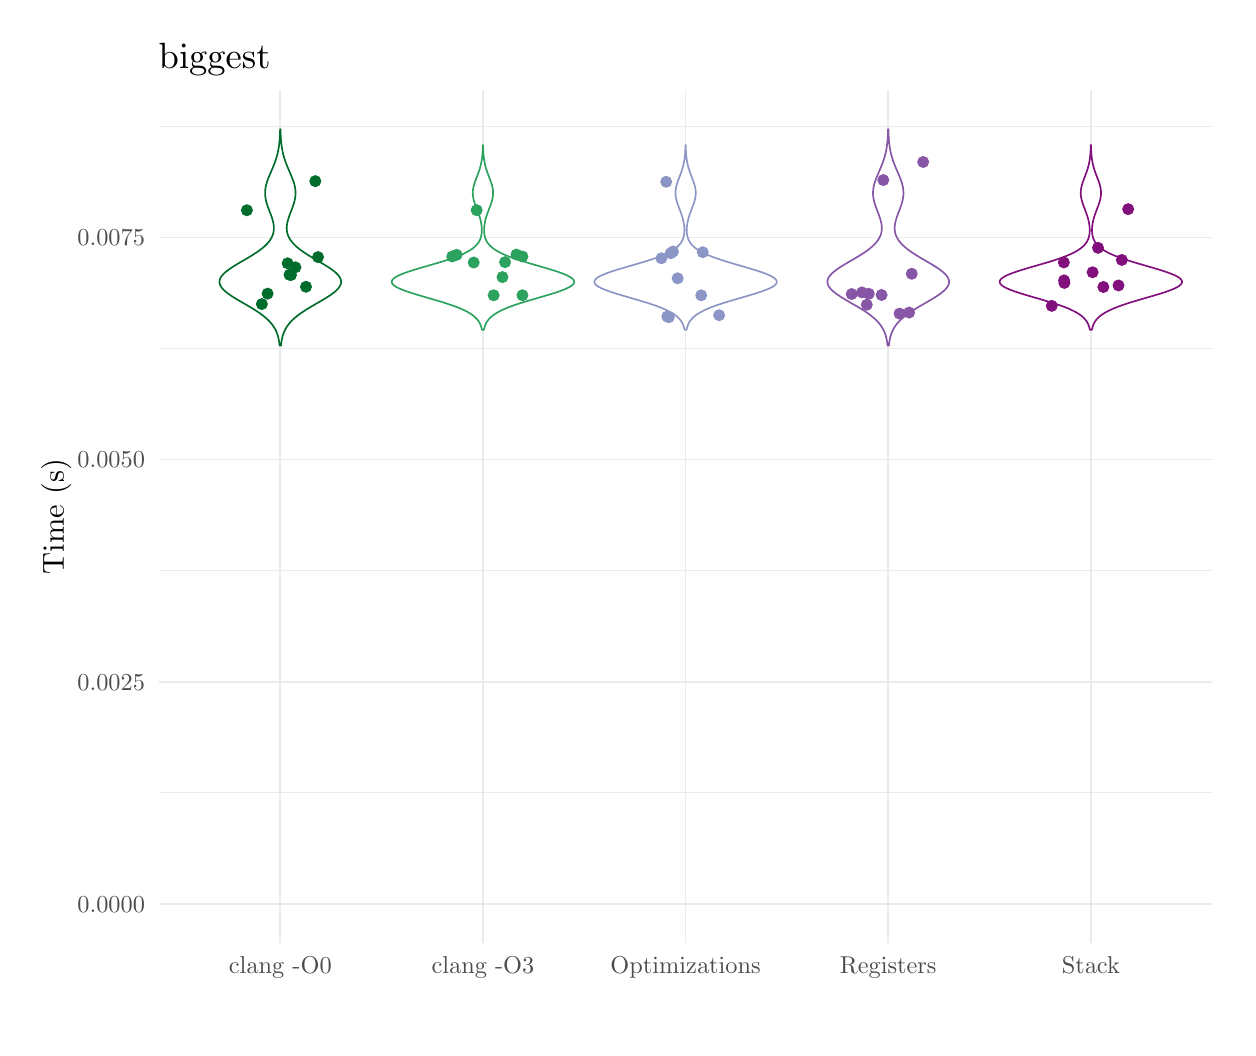
\begin{tikzpicture}[x=1pt,y=1pt]
\definecolor{fillColor}{RGB}{255,255,255}
\path[use as bounding box,fill=fillColor,fill opacity=0.00] (0,0) rectangle (433.62,361.35);
\begin{scope}
\path[clip] ( 47.35, 30.69) rectangle (428.12,338.69);
\definecolor{drawColor}{gray}{0.92}

\path[draw=drawColor,line width= 0.3pt,line join=round] ( 47.35, 84.83) --
	(428.12, 84.83);

\path[draw=drawColor,line width= 0.3pt,line join=round] ( 47.35,165.13) --
	(428.12,165.13);

\path[draw=drawColor,line width= 0.3pt,line join=round] ( 47.35,245.42) --
	(428.12,245.42);

\path[draw=drawColor,line width= 0.3pt,line join=round] ( 47.35,325.71) --
	(428.12,325.71);

\path[draw=drawColor,line width= 0.6pt,line join=round] ( 47.35, 44.69) --
	(428.12, 44.69);

\path[draw=drawColor,line width= 0.6pt,line join=round] ( 47.35,124.98) --
	(428.12,124.98);

\path[draw=drawColor,line width= 0.6pt,line join=round] ( 47.35,205.27) --
	(428.12,205.27);

\path[draw=drawColor,line width= 0.6pt,line join=round] ( 47.35,285.56) --
	(428.12,285.56);

\path[draw=drawColor,line width= 0.6pt,line join=round] ( 91.29, 30.69) --
	( 91.29,338.69);

\path[draw=drawColor,line width= 0.6pt,line join=round] (164.51, 30.69) --
	(164.51,338.69);

\path[draw=drawColor,line width= 0.6pt,line join=round] (237.74, 30.69) --
	(237.74,338.69);

\path[draw=drawColor,line width= 0.6pt,line join=round] (310.96, 30.69) --
	(310.96,338.69);

\path[draw=drawColor,line width= 0.6pt,line join=round] (384.19, 30.69) --
	(384.19,338.69);
\definecolor{drawColor}{RGB}{0,109,44}
\definecolor{fillColor}{RGB}{255,255,255}

\path[draw=drawColor,line width= 0.6pt,line join=round,line cap=round,fill=fillColor] ( 91.04,246.44) --
	( 91.03,246.59) --
	( 91.01,246.74) --
	( 90.99,246.90) --
	( 90.98,247.05) --
	( 90.96,247.20) --
	( 90.94,247.36) --
	( 90.92,247.51) --
	( 90.90,247.66) --
	( 90.87,247.81) --
	( 90.85,247.97) --
	( 90.82,248.12) --
	( 90.80,248.27) --
	( 90.77,248.43) --
	( 90.74,248.58) --
	( 90.71,248.73) --
	( 90.68,248.89) --
	( 90.65,249.04) --
	( 90.61,249.19) --
	( 90.58,249.35) --
	( 90.54,249.50) --
	( 90.50,249.65) --
	( 90.46,249.81) --
	( 90.41,249.96) --
	( 90.37,250.11) --
	( 90.32,250.26) --
	( 90.27,250.42) --
	( 90.22,250.57) --
	( 90.17,250.72) --
	( 90.11,250.88) --
	( 90.05,251.03) --
	( 89.99,251.18) --
	( 89.93,251.34) --
	( 89.87,251.49) --
	( 89.80,251.64) --
	( 89.73,251.80) --
	( 89.66,251.95) --
	( 89.58,252.10) --
	( 89.50,252.26) --
	( 89.42,252.41) --
	( 89.34,252.56) --
	( 89.25,252.72) --
	( 89.16,252.87) --
	( 89.07,253.02) --
	( 88.97,253.17) --
	( 88.87,253.33) --
	( 88.77,253.48) --
	( 88.66,253.63) --
	( 88.55,253.79) --
	( 88.44,253.94) --
	( 88.33,254.09) --
	( 88.21,254.25) --
	( 88.08,254.40) --
	( 87.96,254.55) --
	( 87.82,254.71) --
	( 87.69,254.86) --
	( 87.55,255.01) --
	( 87.41,255.17) --
	( 87.27,255.32) --
	( 87.12,255.47) --
	( 86.96,255.62) --
	( 86.81,255.78) --
	( 86.65,255.93) --
	( 86.48,256.08) --
	( 86.31,256.24) --
	( 86.14,256.39) --
	( 85.96,256.54) --
	( 85.78,256.70) --
	( 85.60,256.85) --
	( 85.41,257.00) --
	( 85.22,257.16) --
	( 85.02,257.31) --
	( 84.82,257.46) --
	( 84.62,257.62) --
	( 84.42,257.77) --
	( 84.20,257.92) --
	( 83.99,258.08) --
	( 83.77,258.23) --
	( 83.55,258.38) --
	( 83.33,258.53) --
	( 83.10,258.69) --
	( 82.87,258.84) --
	( 82.64,258.99) --
	( 82.40,259.15) --
	( 82.16,259.30) --
	( 81.92,259.45) --
	( 81.68,259.61) --
	( 81.43,259.76) --
	( 81.18,259.91) --
	( 80.93,260.07) --
	( 80.67,260.22) --
	( 80.42,260.37) --
	( 80.16,260.53) --
	( 79.90,260.68) --
	( 79.64,260.83) --
	( 79.38,260.98) --
	( 79.12,261.14) --
	( 78.85,261.29) --
	( 78.59,261.44) --
	( 78.33,261.60) --
	( 78.06,261.75) --
	( 77.80,261.90) --
	( 77.53,262.06) --
	( 77.27,262.21) --
	( 77.00,262.36) --
	( 76.74,262.52) --
	( 76.48,262.67) --
	( 76.22,262.82) --
	( 75.96,262.98) --
	( 75.70,263.13) --
	( 75.44,263.28) --
	( 75.19,263.44) --
	( 74.94,263.59) --
	( 74.69,263.74) --
	( 74.44,263.89) --
	( 74.20,264.05) --
	( 73.96,264.20) --
	( 73.73,264.35) --
	( 73.49,264.51) --
	( 73.27,264.66) --
	( 73.04,264.81) --
	( 72.82,264.97) --
	( 72.61,265.12) --
	( 72.40,265.27) --
	( 72.20,265.43) --
	( 72.00,265.58) --
	( 71.80,265.73) --
	( 71.62,265.89) --
	( 71.44,266.04) --
	( 71.26,266.19) --
	( 71.10,266.34) --
	( 70.93,266.50) --
	( 70.78,266.65) --
	( 70.63,266.80) --
	( 70.49,266.96) --
	( 70.36,267.11) --
	( 70.23,267.26) --
	( 70.11,267.42) --
	( 70.00,267.57) --
	( 69.90,267.72) --
	( 69.81,267.88) --
	( 69.72,268.03) --
	( 69.64,268.18) --
	( 69.57,268.34) --
	( 69.51,268.49) --
	( 69.46,268.64) --
	( 69.41,268.80) --
	( 69.38,268.95) --
	( 69.35,269.10) --
	( 69.33,269.25) --
	( 69.32,269.41) --
	( 69.32,269.56) --
	( 69.33,269.71) --
	( 69.34,269.87) --
	( 69.37,270.02) --
	( 69.40,270.17) --
	( 69.44,270.33) --
	( 69.49,270.48) --
	( 69.55,270.63) --
	( 69.62,270.79) --
	( 69.69,270.94) --
	( 69.78,271.09) --
	( 69.87,271.25) --
	( 69.97,271.40) --
	( 70.08,271.55) --
	( 70.19,271.70) --
	( 70.32,271.86) --
	( 70.45,272.01) --
	( 70.59,272.16) --
	( 70.73,272.32) --
	( 70.89,272.47) --
	( 71.04,272.62) --
	( 71.21,272.78) --
	( 71.38,272.93) --
	( 71.56,273.08) --
	( 71.75,273.24) --
	( 71.94,273.39) --
	( 72.13,273.54) --
	( 72.34,273.70) --
	( 72.54,273.85) --
	( 72.76,274.00) --
	( 72.97,274.16) --
	( 73.19,274.31) --
	( 73.42,274.46) --
	( 73.65,274.61) --
	( 73.88,274.77) --
	( 74.12,274.92) --
	( 74.36,275.07) --
	( 74.60,275.23) --
	( 74.85,275.38) --
	( 75.10,275.53) --
	( 75.35,275.69) --
	( 75.61,275.84) --
	( 75.86,275.99) --
	( 76.12,276.15) --
	( 76.38,276.30) --
	( 76.64,276.45) --
	( 76.90,276.61) --
	( 77.16,276.76) --
	( 77.42,276.91) --
	( 77.69,277.06) --
	( 77.95,277.22) --
	( 78.21,277.37) --
	( 78.48,277.52) --
	( 78.74,277.68) --
	( 79.00,277.83) --
	( 79.26,277.98) --
	( 79.52,278.14) --
	( 79.77,278.29) --
	( 80.03,278.44) --
	( 80.28,278.60) --
	( 80.54,278.75) --
	( 80.79,278.90) --
	( 81.03,279.06) --
	( 81.28,279.21) --
	( 81.52,279.36) --
	( 81.76,279.52) --
	( 82.00,279.67) --
	( 82.23,279.82) --
	( 82.47,279.97) --
	( 82.69,280.13) --
	( 82.92,280.28) --
	( 83.14,280.43) --
	( 83.36,280.59) --
	( 83.57,280.74) --
	( 83.78,280.89) --
	( 83.99,281.05) --
	( 84.19,281.20) --
	( 84.39,281.35) --
	( 84.59,281.51) --
	( 84.78,281.66) --
	( 84.96,281.81) --
	( 85.15,281.97) --
	( 85.33,282.12) --
	( 85.50,282.27) --
	( 85.67,282.42) --
	( 85.83,282.58) --
	( 85.99,282.73) --
	( 86.15,282.88) --
	( 86.30,283.04) --
	( 86.45,283.19) --
	( 86.59,283.34) --
	( 86.73,283.50) --
	( 86.86,283.65) --
	( 86.99,283.80) --
	( 87.12,283.96) --
	( 87.24,284.11) --
	( 87.36,284.26) --
	( 87.47,284.42) --
	( 87.58,284.57) --
	( 87.68,284.72) --
	( 87.78,284.88) --
	( 87.87,285.03) --
	( 87.96,285.18) --
	( 88.05,285.33) --
	( 88.13,285.49) --
	( 88.21,285.64) --
	( 88.28,285.79) --
	( 88.35,285.95) --
	( 88.42,286.10) --
	( 88.48,286.25) --
	( 88.53,286.41) --
	( 88.59,286.56) --
	( 88.64,286.71) --
	( 88.68,286.87) --
	( 88.73,287.02) --
	( 88.76,287.17) --
	( 88.80,287.33) --
	( 88.83,287.48) --
	( 88.86,287.63) --
	( 88.88,287.78) --
	( 88.91,287.94) --
	( 88.92,288.09) --
	( 88.94,288.24) --
	( 88.95,288.40) --
	( 88.96,288.55) --
	( 88.96,288.70) --
	( 88.97,288.86) --
	( 88.97,289.01) --
	( 88.96,289.16) --
	( 88.96,289.32) --
	( 88.95,289.47) --
	( 88.93,289.62) --
	( 88.92,289.78) --
	( 88.90,289.93) --
	( 88.88,290.08) --
	( 88.86,290.24) --
	( 88.84,290.39) --
	( 88.81,290.54) --
	( 88.78,290.69) --
	( 88.75,290.85) --
	( 88.72,291.00) --
	( 88.69,291.15) --
	( 88.65,291.31) --
	( 88.61,291.46) --
	( 88.57,291.61) --
	( 88.53,291.77) --
	( 88.49,291.92) --
	( 88.44,292.07) --
	( 88.40,292.23) --
	( 88.35,292.38) --
	( 88.30,292.53) --
	( 88.25,292.69) --
	( 88.20,292.84) --
	( 88.15,292.99) --
	( 88.10,293.14) --
	( 88.04,293.30) --
	( 87.99,293.45) --
	( 87.93,293.60) --
	( 87.87,293.76) --
	( 87.82,293.91) --
	( 87.76,294.06) --
	( 87.70,294.22) --
	( 87.64,294.37) --
	( 87.59,294.52) --
	( 87.53,294.68) --
	( 87.47,294.83) --
	( 87.41,294.98) --
	( 87.35,295.14) --
	( 87.29,295.29) --
	( 87.23,295.44) --
	( 87.17,295.60) --
	( 87.12,295.75) --
	( 87.06,295.90) --
	( 87.00,296.05) --
	( 86.95,296.21) --
	( 86.89,296.36) --
	( 86.83,296.51) --
	( 86.78,296.67) --
	( 86.73,296.82) --
	( 86.67,296.97) --
	( 86.62,297.13) --
	( 86.57,297.28) --
	( 86.52,297.43) --
	( 86.47,297.59) --
	( 86.43,297.74) --
	( 86.38,297.89) --
	( 86.33,298.05) --
	( 86.29,298.20) --
	( 86.25,298.35) --
	( 86.21,298.50) --
	( 86.17,298.66) --
	( 86.13,298.81) --
	( 86.10,298.96) --
	( 86.07,299.12) --
	( 86.03,299.27) --
	( 86.00,299.42) --
	( 85.98,299.58) --
	( 85.95,299.73) --
	( 85.92,299.88) --
	( 85.90,300.04) --
	( 85.88,300.19) --
	( 85.86,300.34) --
	( 85.85,300.50) --
	( 85.83,300.65) --
	( 85.82,300.80) --
	( 85.81,300.96) --
	( 85.80,301.11) --
	( 85.80,301.26) --
	( 85.79,301.41) --
	( 85.79,301.57) --
	( 85.79,301.72) --
	( 85.80,301.87) --
	( 85.80,302.03) --
	( 85.81,302.18) --
	( 85.82,302.33) --
	( 85.83,302.49) --
	( 85.84,302.64) --
	( 85.86,302.79) --
	( 85.87,302.95) --
	( 85.89,303.10) --
	( 85.92,303.25) --
	( 85.94,303.41) --
	( 85.97,303.56) --
	( 85.99,303.71) --
	( 86.02,303.87) --
	( 86.05,304.02) --
	( 86.09,304.17) --
	( 86.12,304.32) --
	( 86.16,304.48) --
	( 86.20,304.63) --
	( 86.24,304.78) --
	( 86.28,304.94) --
	( 86.32,305.09) --
	( 86.37,305.24) --
	( 86.42,305.40) --
	( 86.47,305.55) --
	( 86.51,305.70) --
	( 86.57,305.86) --
	( 86.62,306.01) --
	( 86.67,306.16) --
	( 86.73,306.32) --
	( 86.78,306.47) --
	( 86.84,306.62) --
	( 86.90,306.77) --
	( 86.96,306.93) --
	( 87.02,307.08) --
	( 87.08,307.23) --
	( 87.14,307.39) --
	( 87.20,307.54) --
	( 87.26,307.69) --
	( 87.33,307.85) --
	( 87.39,308.00) --
	( 87.45,308.15) --
	( 87.52,308.31) --
	( 87.58,308.46) --
	( 87.65,308.61) --
	( 87.72,308.77) --
	( 87.78,308.92) --
	( 87.85,309.07) --
	( 87.91,309.23) --
	( 87.98,309.38) --
	( 88.05,309.53) --
	( 88.11,309.68) --
	( 88.18,309.84) --
	( 88.25,309.99) --
	( 88.31,310.14) --
	( 88.38,310.30) --
	( 88.44,310.45) --
	( 88.51,310.60) --
	( 88.57,310.76) --
	( 88.63,310.91) --
	( 88.70,311.06) --
	( 88.76,311.22) --
	( 88.82,311.37) --
	( 88.88,311.52) --
	( 88.95,311.68) --
	( 89.01,311.83) --
	( 89.07,311.98) --
	( 89.13,312.13) --
	( 89.18,312.29) --
	( 89.24,312.44) --
	( 89.30,312.59) --
	( 89.35,312.75) --
	( 89.41,312.90) --
	( 89.46,313.05) --
	( 89.52,313.21) --
	( 89.57,313.36) --
	( 89.62,313.51) --
	( 89.67,313.67) --
	( 89.72,313.82) --
	( 89.77,313.97) --
	( 89.82,314.13) --
	( 89.87,314.28) --
	( 89.91,314.43) --
	( 89.96,314.59) --
	( 90.00,314.74) --
	( 90.04,314.89) --
	( 90.09,315.04) --
	( 90.13,315.20) --
	( 90.17,315.35) --
	( 90.21,315.50) --
	( 90.24,315.66) --
	( 90.28,315.81) --
	( 90.32,315.96) --
	( 90.35,316.12) --
	( 90.39,316.27) --
	( 90.42,316.42) --
	( 90.45,316.58) --
	( 90.49,316.73) --
	( 90.52,316.88) --
	( 90.55,317.04) --
	( 90.58,317.19) --
	( 90.60,317.34) --
	( 90.63,317.49) --
	( 90.66,317.65) --
	( 90.68,317.80) --
	( 90.71,317.95) --
	( 90.73,318.11) --
	( 90.76,318.26) --
	( 90.78,318.41) --
	( 90.80,318.57) --
	( 90.82,318.72) --
	( 90.84,318.87) --
	( 90.86,319.03) --
	( 90.88,319.18) --
	( 90.90,319.33) --
	( 90.92,319.49) --
	( 90.93,319.64) --
	( 90.95,319.79) --
	( 90.96,319.95) --
	( 90.98,320.10) --
	( 90.99,320.25) --
	( 91.01,320.40) --
	( 91.02,320.56) --
	( 91.03,320.71) --
	( 91.05,320.86) --
	( 91.06,321.02) --
	( 91.07,321.17) --
	( 91.08,321.32) --
	( 91.09,321.48) --
	( 91.10,321.63) --
	( 91.11,321.78) --
	( 91.12,321.94) --
	( 91.13,322.09) --
	( 91.14,322.24) --
	( 91.14,322.40) --
	( 91.15,322.55) --
	( 91.16,322.70) --
	( 91.17,322.85) --
	( 91.17,323.01) --
	( 91.18,323.16) --
	( 91.18,323.31) --
	( 91.19,323.47) --
	( 91.19,323.62) --
	( 91.20,323.77) --
	( 91.20,323.93) --
	( 91.21,324.08) --
	( 91.21,324.23) --
	( 91.22,324.39) --
	( 91.22,324.54) --
	( 91.23,324.69) --
	( 91.35,324.69) --
	( 91.35,324.54) --
	( 91.36,324.39) --
	( 91.36,324.23) --
	( 91.37,324.08) --
	( 91.37,323.93) --
	( 91.38,323.77) --
	( 91.38,323.62) --
	( 91.39,323.47) --
	( 91.39,323.31) --
	( 91.40,323.16) --
	( 91.40,323.01) --
	( 91.41,322.85) --
	( 91.42,322.70) --
	( 91.42,322.55) --
	( 91.43,322.40) --
	( 91.44,322.24) --
	( 91.45,322.09) --
	( 91.46,321.94) --
	( 91.47,321.78) --
	( 91.48,321.63) --
	( 91.49,321.48) --
	( 91.50,321.32) --
	( 91.51,321.17) --
	( 91.52,321.02) --
	( 91.53,320.86) --
	( 91.54,320.71) --
	( 91.55,320.56) --
	( 91.57,320.40) --
	( 91.58,320.25) --
	( 91.60,320.10) --
	( 91.61,319.95) --
	( 91.63,319.79) --
	( 91.64,319.64) --
	( 91.66,319.49) --
	( 91.68,319.33) --
	( 91.70,319.18) --
	( 91.71,319.03) --
	( 91.73,318.87) --
	( 91.75,318.72) --
	( 91.78,318.57) --
	( 91.80,318.41) --
	( 91.82,318.26) --
	( 91.84,318.11) --
	( 91.87,317.95) --
	( 91.89,317.80) --
	( 91.92,317.65) --
	( 91.94,317.49) --
	( 91.97,317.34) --
	( 92.00,317.19) --
	( 92.03,317.04) --
	( 92.06,316.88) --
	( 92.09,316.73) --
	( 92.12,316.58) --
	( 92.15,316.42) --
	( 92.19,316.27) --
	( 92.22,316.12) --
	( 92.26,315.96) --
	( 92.29,315.81) --
	( 92.33,315.66) --
	( 92.37,315.50) --
	( 92.41,315.35) --
	( 92.45,315.20) --
	( 92.49,315.04) --
	( 92.53,314.89) --
	( 92.57,314.74) --
	( 92.62,314.59) --
	( 92.66,314.43) --
	( 92.71,314.28) --
	( 92.76,314.13) --
	( 92.80,313.97) --
	( 92.85,313.82) --
	( 92.90,313.67) --
	( 92.95,313.51) --
	( 93.01,313.36) --
	( 93.06,313.21) --
	( 93.11,313.05) --
	( 93.17,312.90) --
	( 93.22,312.75) --
	( 93.28,312.59) --
	( 93.33,312.44) --
	( 93.39,312.29) --
	( 93.45,312.13) --
	( 93.51,311.98) --
	( 93.57,311.83) --
	( 93.63,311.68) --
	( 93.69,311.52) --
	( 93.75,311.37) --
	( 93.81,311.22) --
	( 93.88,311.06) --
	( 93.94,310.91) --
	( 94.00,310.76) --
	( 94.07,310.60) --
	( 94.13,310.45) --
	( 94.20,310.30) --
	( 94.26,310.14) --
	( 94.33,309.99) --
	( 94.40,309.84) --
	( 94.46,309.68) --
	( 94.53,309.53) --
	( 94.59,309.38) --
	( 94.66,309.23) --
	( 94.73,309.07) --
	( 94.79,308.92) --
	( 94.86,308.77) --
	( 94.92,308.61) --
	( 94.99,308.46) --
	( 95.06,308.31) --
	( 95.12,308.15) --
	( 95.18,308.00) --
	( 95.25,307.85) --
	( 95.31,307.69) --
	( 95.38,307.54) --
	( 95.44,307.39) --
	( 95.50,307.23) --
	( 95.56,307.08) --
	( 95.62,306.93) --
	( 95.68,306.77) --
	( 95.74,306.62) --
	( 95.79,306.47) --
	( 95.85,306.32) --
	( 95.90,306.16) --
	( 95.96,306.01) --
	( 96.01,305.86) --
	( 96.06,305.70) --
	( 96.11,305.55) --
	( 96.16,305.40) --
	( 96.20,305.24) --
	( 96.25,305.09) --
	( 96.29,304.94) --
	( 96.34,304.78) --
	( 96.38,304.63) --
	( 96.42,304.48) --
	( 96.45,304.32) --
	( 96.49,304.17) --
	( 96.52,304.02) --
	( 96.55,303.87) --
	( 96.58,303.71) --
	( 96.61,303.56) --
	( 96.64,303.41) --
	( 96.66,303.25) --
	( 96.68,303.10) --
	( 96.70,302.95) --
	( 96.72,302.79) --
	( 96.73,302.64) --
	( 96.75,302.49) --
	( 96.76,302.33) --
	( 96.77,302.18) --
	( 96.77,302.03) --
	( 96.78,301.87) --
	( 96.78,301.72) --
	( 96.78,301.57) --
	( 96.78,301.41) --
	( 96.78,301.26) --
	( 96.77,301.11) --
	( 96.76,300.96) --
	( 96.75,300.80) --
	( 96.74,300.65) --
	( 96.73,300.50) --
	( 96.71,300.34) --
	( 96.69,300.19) --
	( 96.67,300.04) --
	( 96.65,299.88) --
	( 96.63,299.73) --
	( 96.60,299.58) --
	( 96.57,299.42) --
	( 96.54,299.27) --
	( 96.51,299.12) --
	( 96.48,298.96) --
	( 96.44,298.81) --
	( 96.40,298.66) --
	( 96.37,298.50) --
	( 96.33,298.35) --
	( 96.28,298.20) --
	( 96.24,298.05) --
	( 96.20,297.89) --
	( 96.15,297.74) --
	( 96.10,297.59) --
	( 96.05,297.43) --
	( 96.00,297.28) --
	( 95.95,297.13) --
	( 95.90,296.97) --
	( 95.85,296.82) --
	( 95.80,296.67) --
	( 95.74,296.51) --
	( 95.69,296.36) --
	( 95.63,296.21) --
	( 95.57,296.05) --
	( 95.52,295.90) --
	( 95.46,295.75) --
	( 95.40,295.60) --
	( 95.34,295.44) --
	( 95.28,295.29) --
	( 95.22,295.14) --
	( 95.17,294.98) --
	( 95.11,294.83) --
	( 95.05,294.68) --
	( 94.99,294.52) --
	( 94.93,294.37) --
	( 94.87,294.22) --
	( 94.81,294.06) --
	( 94.76,293.91) --
	( 94.70,293.76) --
	( 94.64,293.60) --
	( 94.59,293.45) --
	( 94.53,293.30) --
	( 94.48,293.14) --
	( 94.43,292.99) --
	( 94.37,292.84) --
	( 94.32,292.69) --
	( 94.27,292.53) --
	( 94.23,292.38) --
	( 94.18,292.23) --
	( 94.13,292.07) --
	( 94.09,291.92) --
	( 94.04,291.77) --
	( 94.00,291.61) --
	( 93.96,291.46) --
	( 93.92,291.31) --
	( 93.89,291.15) --
	( 93.85,291.00) --
	( 93.82,290.85) --
	( 93.79,290.69) --
	( 93.76,290.54) --
	( 93.74,290.39) --
	( 93.71,290.24) --
	( 93.69,290.08) --
	( 93.67,289.93) --
	( 93.65,289.78) --
	( 93.64,289.62) --
	( 93.63,289.47) --
	( 93.62,289.32) --
	( 93.61,289.16) --
	( 93.61,289.01) --
	( 93.61,288.86) --
	( 93.61,288.70) --
	( 93.62,288.55) --
	( 93.63,288.40) --
	( 93.64,288.24) --
	( 93.65,288.09) --
	( 93.67,287.94) --
	( 93.69,287.78) --
	( 93.71,287.63) --
	( 93.74,287.48) --
	( 93.77,287.33) --
	( 93.81,287.17) --
	( 93.85,287.02) --
	( 93.89,286.87) --
	( 93.94,286.71) --
	( 93.99,286.56) --
	( 94.04,286.41) --
	( 94.10,286.25) --
	( 94.16,286.10) --
	( 94.22,285.95) --
	( 94.29,285.79) --
	( 94.37,285.64) --
	( 94.45,285.49) --
	( 94.53,285.33) --
	( 94.61,285.18) --
	( 94.70,285.03) --
	( 94.80,284.88) --
	( 94.90,284.72) --
	( 95.00,284.57) --
	( 95.11,284.42) --
	( 95.22,284.26) --
	( 95.34,284.11) --
	( 95.46,283.96) --
	( 95.58,283.80) --
	( 95.71,283.65) --
	( 95.84,283.50) --
	( 95.98,283.34) --
	( 96.13,283.19) --
	( 96.27,283.04) --
	( 96.43,282.88) --
	( 96.58,282.73) --
	( 96.74,282.58) --
	( 96.91,282.42) --
	( 97.08,282.27) --
	( 97.25,282.12) --
	( 97.43,281.97) --
	( 97.61,281.81) --
	( 97.80,281.66) --
	( 97.99,281.51) --
	( 98.18,281.35) --
	( 98.38,281.20) --
	( 98.58,281.05) --
	( 98.79,280.89) --
	( 99.00,280.74) --
	( 99.22,280.59) --
	( 99.43,280.43) --
	( 99.66,280.28) --
	( 99.88,280.13) --
	(100.11,279.97) --
	(100.34,279.82) --
	(100.57,279.67) --
	(100.81,279.52) --
	(101.05,279.36) --
	(101.30,279.21) --
	(101.54,279.06) --
	(101.79,278.90) --
	(102.04,278.75) --
	(102.29,278.60) --
	(102.55,278.44) --
	(102.80,278.29) --
	(103.06,278.14) --
	(103.32,277.98) --
	(103.58,277.83) --
	(103.84,277.68) --
	(104.10,277.52) --
	(104.36,277.37) --
	(104.62,277.22) --
	(104.89,277.06) --
	(105.15,276.91) --
	(105.41,276.76) --
	(105.67,276.61) --
	(105.94,276.45) --
	(106.20,276.30) --
	(106.46,276.15) --
	(106.71,275.99) --
	(106.97,275.84) --
	(107.22,275.69) --
	(107.47,275.53) --
	(107.72,275.38) --
	(107.97,275.23) --
	(108.21,275.07) --
	(108.45,274.92) --
	(108.69,274.77) --
	(108.93,274.61) --
	(109.16,274.46) --
	(109.38,274.31) --
	(109.60,274.16) --
	(109.82,274.00) --
	(110.03,273.85) --
	(110.24,273.70) --
	(110.44,273.54) --
	(110.64,273.39) --
	(110.83,273.24) --
	(111.01,273.08) --
	(111.19,272.93) --
	(111.36,272.78) --
	(111.53,272.62) --
	(111.69,272.47) --
	(111.84,272.32) --
	(111.99,272.16) --
	(112.13,272.01) --
	(112.26,271.86) --
	(112.38,271.70) --
	(112.50,271.55) --
	(112.60,271.40) --
	(112.70,271.25) --
	(112.80,271.09) --
	(112.88,270.94) --
	(112.95,270.79) --
	(113.02,270.63) --
	(113.08,270.48) --
	(113.13,270.33) --
	(113.17,270.17) --
	(113.21,270.02) --
	(113.23,269.87) --
	(113.25,269.71) --
	(113.26,269.56) --
	(113.25,269.41) --
	(113.25,269.25) --
	(113.23,269.10) --
	(113.20,268.95) --
	(113.16,268.80) --
	(113.12,268.64) --
	(113.07,268.49) --
	(113.00,268.34) --
	(112.94,268.18) --
	(112.85,268.03) --
	(112.77,267.88) --
	(112.67,267.72) --
	(112.57,267.57) --
	(112.46,267.42) --
	(112.34,267.26) --
	(112.22,267.11) --
	(112.08,266.96) --
	(111.95,266.80) --
	(111.80,266.65) --
	(111.64,266.50) --
	(111.48,266.34) --
	(111.31,266.19) --
	(111.14,266.04) --
	(110.96,265.89) --
	(110.77,265.73) --
	(110.58,265.58) --
	(110.38,265.43) --
	(110.17,265.27) --
	(109.96,265.12) --
	(109.75,264.97) --
	(109.53,264.81) --
	(109.31,264.66) --
	(109.08,264.51) --
	(108.85,264.35) --
	(108.61,264.20) --
	(108.37,264.05) --
	(108.13,263.89) --
	(107.89,263.74) --
	(107.64,263.59) --
	(107.39,263.44) --
	(107.13,263.28) --
	(106.88,263.13) --
	(106.62,262.98) --
	(106.36,262.82) --
	(106.10,262.67) --
	(105.84,262.52) --
	(105.57,262.36) --
	(105.31,262.21) --
	(105.04,262.06) --
	(104.78,261.90) --
	(104.51,261.75) --
	(104.25,261.60) --
	(103.98,261.44) --
	(103.72,261.29) --
	(103.46,261.14) --
	(103.19,260.98) --
	(102.93,260.83) --
	(102.67,260.68) --
	(102.41,260.53) --
	(102.16,260.37) --
	(101.90,260.22) --
	(101.65,260.07) --
	(101.40,259.91) --
	(101.15,259.76) --
	(100.90,259.61) --
	(100.65,259.45) --
	(100.41,259.30) --
	(100.17,259.15) --
	( 99.94,258.99) --
	( 99.70,258.84) --
	( 99.47,258.69) --
	( 99.25,258.53) --
	( 99.02,258.38) --
	( 98.80,258.23) --
	( 98.58,258.08) --
	( 98.37,257.92) --
	( 98.16,257.77) --
	( 97.95,257.62) --
	( 97.75,257.46) --
	( 97.55,257.31) --
	( 97.36,257.16) --
	( 97.16,257.00) --
	( 96.98,256.85) --
	( 96.79,256.70) --
	( 96.61,256.54) --
	( 96.44,256.39) --
	( 96.26,256.24) --
	( 96.09,256.08) --
	( 95.93,255.93) --
	( 95.77,255.78) --
	( 95.61,255.62) --
	( 95.46,255.47) --
	( 95.31,255.32) --
	( 95.16,255.17) --
	( 95.02,255.01) --
	( 94.88,254.86) --
	( 94.75,254.71) --
	( 94.62,254.55) --
	( 94.49,254.40) --
	( 94.37,254.25) --
	( 94.25,254.09) --
	( 94.13,253.94) --
	( 94.02,253.79) --
	( 93.91,253.63) --
	( 93.81,253.48) --
	( 93.70,253.33) --
	( 93.60,253.17) --
	( 93.51,253.02) --
	( 93.41,252.87) --
	( 93.32,252.72) --
	( 93.24,252.56) --
	( 93.15,252.41) --
	( 93.07,252.26) --
	( 92.99,252.10) --
	( 92.92,251.95) --
	( 92.85,251.80) --
	( 92.78,251.64) --
	( 92.71,251.49) --
	( 92.64,251.34) --
	( 92.58,251.18) --
	( 92.52,251.03) --
	( 92.46,250.88) --
	( 92.41,250.72) --
	( 92.36,250.57) --
	( 92.30,250.42) --
	( 92.26,250.26) --
	( 92.21,250.11) --
	( 92.16,249.96) --
	( 92.12,249.81) --
	( 92.08,249.65) --
	( 92.04,249.50) --
	( 92.00,249.35) --
	( 91.96,249.19) --
	( 91.93,249.04) --
	( 91.90,248.89) --
	( 91.86,248.73) --
	( 91.83,248.58) --
	( 91.81,248.43) --
	( 91.78,248.27) --
	( 91.75,248.12) --
	( 91.73,247.97) --
	( 91.70,247.81) --
	( 91.68,247.66) --
	( 91.66,247.51) --
	( 91.64,247.36) --
	( 91.62,247.20) --
	( 91.60,247.05) --
	( 91.58,246.90) --
	( 91.57,246.74) --
	( 91.55,246.59) --
	( 91.53,246.44) --
	( 91.04,246.44) --
	cycle;
\definecolor{drawColor}{RGB}{44,162,95}

\path[draw=drawColor,line width= 0.6pt,line join=round,line cap=round,fill=fillColor] (164.14,252.20) --
	(164.12,252.33) --
	(164.09,252.46) --
	(164.06,252.60) --
	(164.03,252.73) --
	(164.00,252.86) --
	(163.96,252.99) --
	(163.92,253.12) --
	(163.89,253.25) --
	(163.84,253.38) --
	(163.80,253.51) --
	(163.76,253.64) --
	(163.71,253.77) --
	(163.66,253.90) --
	(163.60,254.03) --
	(163.55,254.16) --
	(163.49,254.29) --
	(163.42,254.42) --
	(163.36,254.55) --
	(163.29,254.68) --
	(163.22,254.82) --
	(163.14,254.95) --
	(163.06,255.08) --
	(162.98,255.21) --
	(162.89,255.34) --
	(162.80,255.47) --
	(162.70,255.60) --
	(162.60,255.73) --
	(162.49,255.86) --
	(162.38,255.99) --
	(162.27,256.12) --
	(162.15,256.25) --
	(162.02,256.38) --
	(161.89,256.51) --
	(161.75,256.64) --
	(161.61,256.77) --
	(161.47,256.90) --
	(161.31,257.03) --
	(161.15,257.17) --
	(160.99,257.30) --
	(160.82,257.43) --
	(160.64,257.56) --
	(160.45,257.69) --
	(160.26,257.82) --
	(160.06,257.95) --
	(159.86,258.08) --
	(159.65,258.21) --
	(159.43,258.34) --
	(159.20,258.47) --
	(158.97,258.60) --
	(158.73,258.73) --
	(158.48,258.86) --
	(158.23,258.99) --
	(157.97,259.12) --
	(157.70,259.25) --
	(157.42,259.39) --
	(157.13,259.52) --
	(156.84,259.65) --
	(156.54,259.78) --
	(156.23,259.91) --
	(155.92,260.04) --
	(155.60,260.17) --
	(155.27,260.30) --
	(154.93,260.43) --
	(154.59,260.56) --
	(154.24,260.69) --
	(153.88,260.82) --
	(153.51,260.95) --
	(153.14,261.08) --
	(152.76,261.21) --
	(152.38,261.34) --
	(151.99,261.47) --
	(151.59,261.60) --
	(151.19,261.74) --
	(150.78,261.87) --
	(150.37,262.00) --
	(149.95,262.13) --
	(149.53,262.26) --
	(149.10,262.39) --
	(148.67,262.52) --
	(148.23,262.65) --
	(147.79,262.78) --
	(147.35,262.91) --
	(146.90,263.04) --
	(146.46,263.17) --
	(146.01,263.30) --
	(145.56,263.43) --
	(145.11,263.56) --
	(144.66,263.69) --
	(144.20,263.82) --
	(143.75,263.96) --
	(143.30,264.09) --
	(142.85,264.22) --
	(142.41,264.35) --
	(141.96,264.48) --
	(141.52,264.61) --
	(141.08,264.74) --
	(140.64,264.87) --
	(140.21,265.00) --
	(139.78,265.13) --
	(139.36,265.26) --
	(138.95,265.39) --
	(138.54,265.52) --
	(138.14,265.65) --
	(137.74,265.78) --
	(137.36,265.91) --
	(136.98,266.04) --
	(136.61,266.17) --
	(136.25,266.31) --
	(135.90,266.44) --
	(135.57,266.57) --
	(135.24,266.70) --
	(134.92,266.83) --
	(134.62,266.96) --
	(134.32,267.09) --
	(134.05,267.22) --
	(133.78,267.35) --
	(133.53,267.48) --
	(133.29,267.61) --
	(133.06,267.74) --
	(132.86,267.87) --
	(132.66,268.00) --
	(132.48,268.13) --
	(132.31,268.26) --
	(132.17,268.39) --
	(132.03,268.52) --
	(131.91,268.66) --
	(131.82,268.79) --
	(131.73,268.92) --
	(131.67,269.05) --
	(131.62,269.18) --
	(131.58,269.31) --
	(131.57,269.44) --
	(131.56,269.57) --
	(131.58,269.70) --
	(131.61,269.83) --
	(131.66,269.96) --
	(131.73,270.09) --
	(131.81,270.22) --
	(131.92,270.35) --
	(132.03,270.48) --
	(132.16,270.61) --
	(132.31,270.74) --
	(132.47,270.88) --
	(132.66,271.01) --
	(132.85,271.14) --
	(133.06,271.27) --
	(133.28,271.40) --
	(133.52,271.53) --
	(133.78,271.66) --
	(134.04,271.79) --
	(134.32,271.92) --
	(134.61,272.05) --
	(134.91,272.18) --
	(135.23,272.31) --
	(135.56,272.44) --
	(135.90,272.57) --
	(136.24,272.70) --
	(136.60,272.83) --
	(136.97,272.96) --
	(137.35,273.09) --
	(137.74,273.23) --
	(138.13,273.36) --
	(138.53,273.49) --
	(138.94,273.62) --
	(139.35,273.75) --
	(139.77,273.88) --
	(140.20,274.01) --
	(140.63,274.14) --
	(141.07,274.27) --
	(141.51,274.40) --
	(141.95,274.53) --
	(142.39,274.66) --
	(142.84,274.79) --
	(143.29,274.92) --
	(143.74,275.05) --
	(144.19,275.18) --
	(144.65,275.31) --
	(145.10,275.45) --
	(145.55,275.58) --
	(146.00,275.71) --
	(146.45,275.84) --
	(146.89,275.97) --
	(147.34,276.10) --
	(147.78,276.23) --
	(148.22,276.36) --
	(148.65,276.49) --
	(149.09,276.62) --
	(149.51,276.75) --
	(149.94,276.88) --
	(150.36,277.01) --
	(150.77,277.14) --
	(151.18,277.27) --
	(151.58,277.40) --
	(151.98,277.53) --
	(152.37,277.66) --
	(152.75,277.80) --
	(153.13,277.93) --
	(153.50,278.06) --
	(153.87,278.19) --
	(154.23,278.32) --
	(154.58,278.45) --
	(154.92,278.58) --
	(155.26,278.71) --
	(155.59,278.84) --
	(155.91,278.97) --
	(156.23,279.10) --
	(156.53,279.23) --
	(156.83,279.36) --
	(157.13,279.49) --
	(157.41,279.62) --
	(157.69,279.75) --
	(157.96,279.88) --
	(158.22,280.02) --
	(158.48,280.15) --
	(158.72,280.28) --
	(158.96,280.41) --
	(159.19,280.54) --
	(159.42,280.67) --
	(159.64,280.80) --
	(159.85,280.93) --
	(160.05,281.06) --
	(160.25,281.19) --
	(160.44,281.32) --
	(160.63,281.45) --
	(160.80,281.58) --
	(160.98,281.71) --
	(161.14,281.84) --
	(161.30,281.97) --
	(161.45,282.10) --
	(161.60,282.23) --
	(161.74,282.37) --
	(161.87,282.50) --
	(162.00,282.63) --
	(162.13,282.76) --
	(162.25,282.89) --
	(162.36,283.02) --
	(162.47,283.15) --
	(162.57,283.28) --
	(162.67,283.41) --
	(162.77,283.54) --
	(162.86,283.67) --
	(162.94,283.80) --
	(163.03,283.93) --
	(163.10,284.06) --
	(163.18,284.19) --
	(163.25,284.32) --
	(163.31,284.45) --
	(163.38,284.59) --
	(163.44,284.72) --
	(163.49,284.85) --
	(163.54,284.98) --
	(163.59,285.11) --
	(163.64,285.24) --
	(163.68,285.37) --
	(163.73,285.50) --
	(163.76,285.63) --
	(163.80,285.76) --
	(163.83,285.89) --
	(163.87,286.02) --
	(163.89,286.15) --
	(163.92,286.28) --
	(163.94,286.41) --
	(163.97,286.54) --
	(163.99,286.67) --
	(164.01,286.80) --
	(164.02,286.94) --
	(164.04,287.07) --
	(164.05,287.20) --
	(164.06,287.33) --
	(164.07,287.46) --
	(164.08,287.59) --
	(164.08,287.72) --
	(164.09,287.85) --
	(164.09,287.98) --
	(164.09,288.11) --
	(164.09,288.24) --
	(164.09,288.37) --
	(164.09,288.50) --
	(164.08,288.63) --
	(164.08,288.76) --
	(164.07,288.89) --
	(164.06,289.02) --
	(164.06,289.16) --
	(164.05,289.29) --
	(164.03,289.42) --
	(164.02,289.55) --
	(164.01,289.68) --
	(163.99,289.81) --
	(163.98,289.94) --
	(163.96,290.07) --
	(163.94,290.20) --
	(163.92,290.33) --
	(163.90,290.46) --
	(163.88,290.59) --
	(163.86,290.72) --
	(163.83,290.85) --
	(163.81,290.98) --
	(163.78,291.11) --
	(163.76,291.24) --
	(163.73,291.37) --
	(163.70,291.51) --
	(163.67,291.64) --
	(163.64,291.77) --
	(163.61,291.90) --
	(163.58,292.03) --
	(163.54,292.16) --
	(163.51,292.29) --
	(163.47,292.42) --
	(163.44,292.55) --
	(163.40,292.68) --
	(163.36,292.81) --
	(163.32,292.94) --
	(163.28,293.07) --
	(163.24,293.20) --
	(163.20,293.33) --
	(163.16,293.46) --
	(163.11,293.59) --
	(163.07,293.73) --
	(163.03,293.86) --
	(162.98,293.99) --
	(162.94,294.12) --
	(162.89,294.25) --
	(162.84,294.38) --
	(162.80,294.51) --
	(162.75,294.64) --
	(162.70,294.77) --
	(162.65,294.90) --
	(162.60,295.03) --
	(162.55,295.16) --
	(162.50,295.29) --
	(162.45,295.42) --
	(162.40,295.55) --
	(162.35,295.68) --
	(162.30,295.81) --
	(162.25,295.94) --
	(162.20,296.08) --
	(162.15,296.21) --
	(162.10,296.34) --
	(162.05,296.47) --
	(162.00,296.60) --
	(161.96,296.73) --
	(161.91,296.86) --
	(161.86,296.99) --
	(161.81,297.12) --
	(161.76,297.25) --
	(161.72,297.38) --
	(161.67,297.51) --
	(161.62,297.64) --
	(161.58,297.77) --
	(161.54,297.90) --
	(161.49,298.03) --
	(161.45,298.16) --
	(161.41,298.29) --
	(161.37,298.43) --
	(161.33,298.56) --
	(161.29,298.69) --
	(161.26,298.82) --
	(161.22,298.95) --
	(161.19,299.08) --
	(161.16,299.21) --
	(161.13,299.34) --
	(161.10,299.47) --
	(161.07,299.60) --
	(161.04,299.73) --
	(161.02,299.86) --
	(160.99,299.99) --
	(160.97,300.12) --
	(160.95,300.25) --
	(160.93,300.38) --
	(160.92,300.51) --
	(160.90,300.65) --
	(160.89,300.78) --
	(160.88,300.91) --
	(160.87,301.04) --
	(160.86,301.17) --
	(160.86,301.30) --
	(160.85,301.43) --
	(160.85,301.56) --
	(160.85,301.69) --
	(160.85,301.82) --
	(160.86,301.95) --
	(160.86,302.08) --
	(160.87,302.21) --
	(160.88,302.34) --
	(160.89,302.47) --
	(160.90,302.60) --
	(160.92,302.73) --
	(160.93,302.86) --
	(160.95,303.00) --
	(160.97,303.13) --
	(160.99,303.26) --
	(161.02,303.39) --
	(161.04,303.52) --
	(161.07,303.65) --
	(161.10,303.78) --
	(161.13,303.91) --
	(161.16,304.04) --
	(161.19,304.17) --
	(161.22,304.30) --
	(161.26,304.43) --
	(161.30,304.56) --
	(161.33,304.69) --
	(161.37,304.82) --
	(161.41,304.95) --
	(161.45,305.08) --
	(161.50,305.22) --
	(161.54,305.35) --
	(161.58,305.48) --
	(161.63,305.61) --
	(161.67,305.74) --
	(161.72,305.87) --
	(161.76,306.00) --
	(161.81,306.13) --
	(161.86,306.26) --
	(161.91,306.39) --
	(161.96,306.52) --
	(162.01,306.65) --
	(162.06,306.78) --
	(162.11,306.91) --
	(162.16,307.04) --
	(162.21,307.17) --
	(162.26,307.30) --
	(162.31,307.43) --
	(162.36,307.57) --
	(162.41,307.70) --
	(162.46,307.83) --
	(162.51,307.96) --
	(162.56,308.09) --
	(162.61,308.22) --
	(162.65,308.35) --
	(162.70,308.48) --
	(162.75,308.61) --
	(162.80,308.74) --
	(162.85,308.87) --
	(162.89,309.00) --
	(162.94,309.13) --
	(162.99,309.26) --
	(163.03,309.39) --
	(163.08,309.52) --
	(163.12,309.65) --
	(163.16,309.79) --
	(163.21,309.92) --
	(163.25,310.05) --
	(163.29,310.18) --
	(163.33,310.31) --
	(163.37,310.44) --
	(163.41,310.57) --
	(163.45,310.70) --
	(163.49,310.83) --
	(163.52,310.96) --
	(163.56,311.09) --
	(163.59,311.22) --
	(163.63,311.35) --
	(163.66,311.48) --
	(163.69,311.61) --
	(163.72,311.74) --
	(163.75,311.87) --
	(163.78,312.00) --
	(163.81,312.14) --
	(163.84,312.27) --
	(163.87,312.40) --
	(163.90,312.53) --
	(163.92,312.66) --
	(163.95,312.79) --
	(163.97,312.92) --
	(164.00,313.05) --
	(164.02,313.18) --
	(164.04,313.31) --
	(164.06,313.44) --
	(164.08,313.57) --
	(164.10,313.70) --
	(164.12,313.83) --
	(164.14,313.96) --
	(164.16,314.09) --
	(164.17,314.22) --
	(164.19,314.36) --
	(164.21,314.49) --
	(164.22,314.62) --
	(164.24,314.75) --
	(164.25,314.88) --
	(164.26,315.01) --
	(164.28,315.14) --
	(164.29,315.27) --
	(164.30,315.40) --
	(164.31,315.53) --
	(164.32,315.66) --
	(164.33,315.79) --
	(164.34,315.92) --
	(164.35,316.05) --
	(164.36,316.18) --
	(164.37,316.31) --
	(164.38,316.44) --
	(164.38,316.57) --
	(164.39,316.71) --
	(164.40,316.84) --
	(164.40,316.97) --
	(164.41,317.10) --
	(164.42,317.23) --
	(164.42,317.36) --
	(164.43,317.49) --
	(164.43,317.62) --
	(164.44,317.75) --
	(164.44,317.88) --
	(164.45,318.01) --
	(164.45,318.14) --
	(164.45,318.27) --
	(164.46,318.40) --
	(164.46,318.53) --
	(164.46,318.66) --
	(164.47,318.79) --
	(164.47,318.93) --
	(164.55,318.93) --
	(164.56,318.79) --
	(164.56,318.66) --
	(164.56,318.53) --
	(164.57,318.40) --
	(164.57,318.27) --
	(164.57,318.14) --
	(164.58,318.01) --
	(164.58,317.88) --
	(164.59,317.75) --
	(164.59,317.62) --
	(164.60,317.49) --
	(164.60,317.36) --
	(164.61,317.23) --
	(164.61,317.10) --
	(164.62,316.97) --
	(164.63,316.84) --
	(164.63,316.71) --
	(164.64,316.57) --
	(164.65,316.44) --
	(164.66,316.31) --
	(164.66,316.18) --
	(164.67,316.05) --
	(164.68,315.92) --
	(164.69,315.79) --
	(164.70,315.66) --
	(164.71,315.53) --
	(164.72,315.40) --
	(164.74,315.27) --
	(164.75,315.14) --
	(164.76,315.01) --
	(164.77,314.88) --
	(164.79,314.75) --
	(164.80,314.62) --
	(164.82,314.49) --
	(164.83,314.36) --
	(164.85,314.22) --
	(164.87,314.09) --
	(164.89,313.96) --
	(164.90,313.83) --
	(164.92,313.70) --
	(164.94,313.57) --
	(164.96,313.44) --
	(164.98,313.31) --
	(165.01,313.18) --
	(165.03,313.05) --
	(165.05,312.92) --
	(165.08,312.79) --
	(165.10,312.66) --
	(165.13,312.53) --
	(165.15,312.40) --
	(165.18,312.27) --
	(165.21,312.14) --
	(165.24,312.00) --
	(165.27,311.87) --
	(165.30,311.74) --
	(165.33,311.61) --
	(165.36,311.48) --
	(165.40,311.35) --
	(165.43,311.22) --
	(165.47,311.09) --
	(165.50,310.96) --
	(165.54,310.83) --
	(165.58,310.70) --
	(165.61,310.57) --
	(165.65,310.44) --
	(165.69,310.31) --
	(165.73,310.18) --
	(165.78,310.05) --
	(165.82,309.92) --
	(165.86,309.79) --
	(165.90,309.65) --
	(165.95,309.52) --
	(165.99,309.39) --
	(166.04,309.26) --
	(166.08,309.13) --
	(166.13,309.00) --
	(166.18,308.87) --
	(166.22,308.74) --
	(166.27,308.61) --
	(166.32,308.48) --
	(166.37,308.35) --
	(166.42,308.22) --
	(166.47,308.09) --
	(166.52,307.96) --
	(166.57,307.83) --
	(166.62,307.70) --
	(166.67,307.57) --
	(166.72,307.43) --
	(166.77,307.30) --
	(166.82,307.17) --
	(166.87,307.04) --
	(166.92,306.91) --
	(166.97,306.78) --
	(167.02,306.65) --
	(167.07,306.52) --
	(167.12,306.39) --
	(167.16,306.26) --
	(167.21,306.13) --
	(167.26,306.00) --
	(167.31,305.87) --
	(167.35,305.74) --
	(167.40,305.61) --
	(167.44,305.48) --
	(167.49,305.35) --
	(167.53,305.22) --
	(167.57,305.08) --
	(167.61,304.95) --
	(167.65,304.82) --
	(167.69,304.69) --
	(167.73,304.56) --
	(167.76,304.43) --
	(167.80,304.30) --
	(167.83,304.17) --
	(167.87,304.04) --
	(167.90,303.91) --
	(167.93,303.78) --
	(167.95,303.65) --
	(167.98,303.52) --
	(168.01,303.39) --
	(168.03,303.26) --
	(168.05,303.13) --
	(168.07,303.00) --
	(168.09,302.86) --
	(168.11,302.73) --
	(168.12,302.60) --
	(168.13,302.47) --
	(168.14,302.34) --
	(168.15,302.21) --
	(168.16,302.08) --
	(168.17,301.95) --
	(168.17,301.82) --
	(168.17,301.69) --
	(168.17,301.56) --
	(168.17,301.43) --
	(168.17,301.30) --
	(168.16,301.17) --
	(168.15,301.04) --
	(168.15,300.91) --
	(168.13,300.78) --
	(168.12,300.65) --
	(168.11,300.51) --
	(168.09,300.38) --
	(168.07,300.25) --
	(168.05,300.12) --
	(168.03,299.99) --
	(168.01,299.86) --
	(167.98,299.73) --
	(167.96,299.60) --
	(167.93,299.47) --
	(167.90,299.34) --
	(167.87,299.21) --
	(167.83,299.08) --
	(167.80,298.95) --
	(167.77,298.82) --
	(167.73,298.69) --
	(167.69,298.56) --
	(167.65,298.43) --
	(167.61,298.29) --
	(167.57,298.16) --
	(167.53,298.03) --
	(167.49,297.90) --
	(167.44,297.77) --
	(167.40,297.64) --
	(167.35,297.51) --
	(167.31,297.38) --
	(167.26,297.25) --
	(167.21,297.12) --
	(167.17,296.99) --
	(167.12,296.86) --
	(167.07,296.73) --
	(167.02,296.60) --
	(166.97,296.47) --
	(166.92,296.34) --
	(166.87,296.21) --
	(166.82,296.08) --
	(166.77,295.94) --
	(166.72,295.81) --
	(166.67,295.68) --
	(166.62,295.55) --
	(166.57,295.42) --
	(166.52,295.29) --
	(166.47,295.16) --
	(166.42,295.03) --
	(166.37,294.90) --
	(166.32,294.77) --
	(166.28,294.64) --
	(166.23,294.51) --
	(166.18,294.38) --
	(166.13,294.25) --
	(166.09,294.12) --
	(166.04,293.99) --
	(166.00,293.86) --
	(165.95,293.73) --
	(165.91,293.59) --
	(165.87,293.46) --
	(165.83,293.33) --
	(165.78,293.20) --
	(165.74,293.07) --
	(165.70,292.94) --
	(165.66,292.81) --
	(165.63,292.68) --
	(165.59,292.55) --
	(165.55,292.42) --
	(165.52,292.29) --
	(165.48,292.16) --
	(165.45,292.03) --
	(165.42,291.90) --
	(165.38,291.77) --
	(165.35,291.64) --
	(165.32,291.51) --
	(165.30,291.37) --
	(165.27,291.24) --
	(165.24,291.11) --
	(165.21,290.98) --
	(165.19,290.85) --
	(165.17,290.72) --
	(165.14,290.59) --
	(165.12,290.46) --
	(165.10,290.33) --
	(165.08,290.20) --
	(165.06,290.07) --
	(165.05,289.94) --
	(165.03,289.81) --
	(165.02,289.68) --
	(165.00,289.55) --
	(164.99,289.42) --
	(164.98,289.29) --
	(164.97,289.16) --
	(164.96,289.02) --
	(164.95,288.89) --
	(164.95,288.76) --
	(164.94,288.63) --
	(164.94,288.50) --
	(164.93,288.37) --
	(164.93,288.24) --
	(164.93,288.11) --
	(164.93,287.98) --
	(164.94,287.85) --
	(164.94,287.72) --
	(164.95,287.59) --
	(164.95,287.46) --
	(164.96,287.33) --
	(164.98,287.20) --
	(164.99,287.07) --
	(165.00,286.94) --
	(165.02,286.80) --
	(165.04,286.67) --
	(165.06,286.54) --
	(165.08,286.41) --
	(165.10,286.28) --
	(165.13,286.15) --
	(165.16,286.02) --
	(165.19,285.89) --
	(165.22,285.76) --
	(165.26,285.63) --
	(165.30,285.50) --
	(165.34,285.37) --
	(165.38,285.24) --
	(165.43,285.11) --
	(165.48,284.98) --
	(165.53,284.85) --
	(165.59,284.72) --
	(165.65,284.59) --
	(165.71,284.45) --
	(165.78,284.32) --
	(165.85,284.19) --
	(165.92,284.06) --
	(166.00,283.93) --
	(166.08,283.80) --
	(166.17,283.67) --
	(166.26,283.54) --
	(166.35,283.41) --
	(166.45,283.28) --
	(166.56,283.15) --
	(166.66,283.02) --
	(166.78,282.89) --
	(166.90,282.76) --
	(167.02,282.63) --
	(167.15,282.50) --
	(167.28,282.37) --
	(167.43,282.23) --
	(167.57,282.10) --
	(167.73,281.97) --
	(167.89,281.84) --
	(168.05,281.71) --
	(168.22,281.58) --
	(168.40,281.45) --
	(168.58,281.32) --
	(168.77,281.19) --
	(168.97,281.06) --
	(169.18,280.93) --
	(169.38,280.80) --
	(169.60,280.67) --
	(169.83,280.54) --
	(170.06,280.41) --
	(170.30,280.28) --
	(170.55,280.15) --
	(170.81,280.02) --
	(171.07,279.88) --
	(171.34,279.75) --
	(171.61,279.62) --
	(171.90,279.49) --
	(172.19,279.36) --
	(172.49,279.23) --
	(172.80,279.10) --
	(173.11,278.97) --
	(173.43,278.84) --
	(173.77,278.71) --
	(174.10,278.58) --
	(174.45,278.45) --
	(174.80,278.32) --
	(175.16,278.19) --
	(175.52,278.06) --
	(175.89,277.93) --
	(176.27,277.80) --
	(176.66,277.66) --
	(177.05,277.53) --
	(177.44,277.40) --
	(177.85,277.27) --
	(178.26,277.14) --
	(178.67,277.01) --
	(179.09,276.88) --
	(179.51,276.75) --
	(179.94,276.62) --
	(180.37,276.49) --
	(180.80,276.36) --
	(181.24,276.23) --
	(181.69,276.10) --
	(182.13,275.97) --
	(182.58,275.84) --
	(183.03,275.71) --
	(183.48,275.58) --
	(183.93,275.45) --
	(184.38,275.31) --
	(184.83,275.18) --
	(185.28,275.05) --
	(185.73,274.92) --
	(186.18,274.79) --
	(186.63,274.66) --
	(187.08,274.53) --
	(187.52,274.40) --
	(187.96,274.27) --
	(188.39,274.14) --
	(188.82,274.01) --
	(189.25,273.88) --
	(189.67,273.75) --
	(190.08,273.62) --
	(190.49,273.49) --
	(190.90,273.36) --
	(191.29,273.23) --
	(191.68,273.09) --
	(192.05,272.96) --
	(192.42,272.83) --
	(192.78,272.70) --
	(193.13,272.57) --
	(193.47,272.44) --
	(193.79,272.31) --
	(194.11,272.18) --
	(194.41,272.05) --
	(194.71,271.92) --
	(194.99,271.79) --
	(195.25,271.66) --
	(195.51,271.53) --
	(195.74,271.40) --
	(195.97,271.27) --
	(196.18,271.14) --
	(196.37,271.01) --
	(196.55,270.88) --
	(196.71,270.74) --
	(196.86,270.61) --
	(196.99,270.48) --
	(197.11,270.35) --
	(197.21,270.22) --
	(197.29,270.09) --
	(197.36,269.96) --
	(197.41,269.83) --
	(197.44,269.70) --
	(197.46,269.57) --
	(197.46,269.44) --
	(197.45,269.31) --
	(197.41,269.18) --
	(197.36,269.05) --
	(197.29,268.92) --
	(197.21,268.79) --
	(197.11,268.66) --
	(196.99,268.52) --
	(196.86,268.39) --
	(196.71,268.26) --
	(196.54,268.13) --
	(196.37,268.00) --
	(196.17,267.87) --
	(195.96,267.74) --
	(195.74,267.61) --
	(195.50,267.48) --
	(195.25,267.35) --
	(194.98,267.22) --
	(194.70,267.09) --
	(194.41,266.96) --
	(194.10,266.83) --
	(193.79,266.70) --
	(193.46,266.57) --
	(193.12,266.44) --
	(192.77,266.31) --
	(192.41,266.17) --
	(192.04,266.04) --
	(191.66,265.91) --
	(191.28,265.78) --
	(190.88,265.65) --
	(190.48,265.52) --
	(190.08,265.39) --
	(189.66,265.26) --
	(189.24,265.13) --
	(188.81,265.00) --
	(188.38,264.87) --
	(187.95,264.74) --
	(187.51,264.61) --
	(187.06,264.48) --
	(186.62,264.35) --
	(186.17,264.22) --
	(185.72,264.09) --
	(185.27,263.96) --
	(184.82,263.82) --
	(184.37,263.69) --
	(183.92,263.56) --
	(183.46,263.43) --
	(183.01,263.30) --
	(182.57,263.17) --
	(182.12,263.04) --
	(181.67,262.91) --
	(181.23,262.78) --
	(180.79,262.65) --
	(180.36,262.52) --
	(179.93,262.39) --
	(179.50,262.26) --
	(179.08,262.13) --
	(178.66,262.00) --
	(178.24,261.87) --
	(177.84,261.74) --
	(177.43,261.60) --
	(177.04,261.47) --
	(176.65,261.34) --
	(176.26,261.21) --
	(175.88,261.08) --
	(175.51,260.95) --
	(175.15,260.82) --
	(174.79,260.69) --
	(174.44,260.56) --
	(174.09,260.43) --
	(173.75,260.30) --
	(173.43,260.17) --
	(173.10,260.04) --
	(172.79,259.91) --
	(172.48,259.78) --
	(172.18,259.65) --
	(171.89,259.52) --
	(171.60,259.39) --
	(171.33,259.25) --
	(171.06,259.12) --
	(170.79,258.99) --
	(170.54,258.86) --
	(170.29,258.73) --
	(170.05,258.60) --
	(169.82,258.47) --
	(169.59,258.34) --
	(169.38,258.21) --
	(169.16,258.08) --
	(168.96,257.95) --
	(168.76,257.82) --
	(168.57,257.69) --
	(168.39,257.56) --
	(168.21,257.43) --
	(168.04,257.30) --
	(167.87,257.17) --
	(167.71,257.03) --
	(167.56,256.90) --
	(167.41,256.77) --
	(167.27,256.64) --
	(167.13,256.51) --
	(167.00,256.38) --
	(166.88,256.25) --
	(166.76,256.12) --
	(166.64,255.99) --
	(166.53,255.86) --
	(166.43,255.73) --
	(166.32,255.60) --
	(166.23,255.47) --
	(166.14,255.34) --
	(166.05,255.21) --
	(165.96,255.08) --
	(165.88,254.95) --
	(165.81,254.82) --
	(165.73,254.68) --
	(165.67,254.55) --
	(165.60,254.42) --
	(165.54,254.29) --
	(165.48,254.16) --
	(165.42,254.03) --
	(165.37,253.90) --
	(165.32,253.77) --
	(165.27,253.64) --
	(165.22,253.51) --
	(165.18,253.38) --
	(165.14,253.25) --
	(165.10,253.12) --
	(165.06,252.99) --
	(165.03,252.86) --
	(165.00,252.73) --
	(164.96,252.60) --
	(164.94,252.46) --
	(164.91,252.33) --
	(164.88,252.20) --
	(164.14,252.20) --
	cycle;
\definecolor{drawColor}{RGB}{140,150,198}

\path[draw=drawColor,line width= 0.6pt,line join=round,line cap=round,fill=fillColor] (237.37,252.20) --
	(237.34,252.33) --
	(237.31,252.46) --
	(237.28,252.60) --
	(237.25,252.73) --
	(237.22,252.86) --
	(237.19,252.99) --
	(237.15,253.12) --
	(237.11,253.25) --
	(237.07,253.38) --
	(237.03,253.51) --
	(236.98,253.64) --
	(236.93,253.77) --
	(236.88,253.90) --
	(236.83,254.03) --
	(236.77,254.16) --
	(236.71,254.29) --
	(236.65,254.42) --
	(236.58,254.55) --
	(236.51,254.68) --
	(236.44,254.82) --
	(236.37,254.95) --
	(236.28,255.08) --
	(236.20,255.21) --
	(236.11,255.34) --
	(236.02,255.47) --
	(235.92,255.60) --
	(235.82,255.73) --
	(235.72,255.86) --
	(235.61,255.99) --
	(235.49,256.12) --
	(235.37,256.25) --
	(235.25,256.38) --
	(235.12,256.51) --
	(234.98,256.64) --
	(234.84,256.77) --
	(234.69,256.90) --
	(234.54,257.03) --
	(234.38,257.17) --
	(234.21,257.30) --
	(234.04,257.43) --
	(233.86,257.56) --
	(233.68,257.69) --
	(233.49,257.82) --
	(233.29,257.95) --
	(233.09,258.08) --
	(232.87,258.21) --
	(232.65,258.34) --
	(232.43,258.47) --
	(232.20,258.60) --
	(231.96,258.73) --
	(231.71,258.86) --
	(231.45,258.99) --
	(231.19,259.12) --
	(230.92,259.25) --
	(230.65,259.39) --
	(230.36,259.52) --
	(230.07,259.65) --
	(229.77,259.78) --
	(229.46,259.91) --
	(229.15,260.04) --
	(228.82,260.17) --
	(228.49,260.30) --
	(228.16,260.43) --
	(227.81,260.56) --
	(227.46,260.69) --
	(227.10,260.82) --
	(226.74,260.95) --
	(226.37,261.08) --
	(225.99,261.21) --
	(225.60,261.34) --
	(225.21,261.47) --
	(224.82,261.60) --
	(224.41,261.74) --
	(224.00,261.87) --
	(223.59,262.00) --
	(223.17,262.13) --
	(222.75,262.26) --
	(222.32,262.39) --
	(221.89,262.52) --
	(221.45,262.65) --
	(221.02,262.78) --
	(220.57,262.91) --
	(220.13,263.04) --
	(219.68,263.17) --
	(219.23,263.30) --
	(218.78,263.43) --
	(218.33,263.56) --
	(217.88,263.69) --
	(217.43,263.82) --
	(216.98,263.96) --
	(216.53,264.09) --
	(216.08,264.22) --
	(215.63,264.35) --
	(215.18,264.48) --
	(214.74,264.61) --
	(214.30,264.74) --
	(213.87,264.87) --
	(213.44,265.00) --
	(213.01,265.13) --
	(212.59,265.26) --
	(212.17,265.39) --
	(211.76,265.52) --
	(211.36,265.65) --
	(210.97,265.78) --
	(210.58,265.91) --
	(210.20,266.04) --
	(209.84,266.17) --
	(209.48,266.31) --
	(209.13,266.44) --
	(208.79,266.57) --
	(208.46,266.70) --
	(208.15,266.83) --
	(207.84,266.96) --
	(207.55,267.09) --
	(207.27,267.22) --
	(207.00,267.35) --
	(206.75,267.48) --
	(206.51,267.61) --
	(206.29,267.74) --
	(206.08,267.87) --
	(205.88,268.00) --
	(205.71,268.13) --
	(205.54,268.26) --
	(205.39,268.39) --
	(205.26,268.52) --
	(205.14,268.66) --
	(205.04,268.79) --
	(204.96,268.92) --
	(204.89,269.05) --
	(204.84,269.18) --
	(204.80,269.31) --
	(204.79,269.44) --
	(204.79,269.57) --
	(204.81,269.70) --
	(204.84,269.83) --
	(204.89,269.96) --
	(204.96,270.09) --
	(205.04,270.22) --
	(205.14,270.35) --
	(205.25,270.48) --
	(205.39,270.61) --
	(205.54,270.74) --
	(205.70,270.88) --
	(205.88,271.01) --
	(206.07,271.14) --
	(206.28,271.27) --
	(206.51,271.40) --
	(206.74,271.53) --
	(207.00,271.66) --
	(207.26,271.79) --
	(207.54,271.92) --
	(207.84,272.05) --
	(208.14,272.18) --
	(208.46,272.31) --
	(208.78,272.44) --
	(209.12,272.57) --
	(209.47,272.70) --
	(209.83,272.83) --
	(210.20,272.96) --
	(210.57,273.09) --
	(210.96,273.23) --
	(211.35,273.36) --
	(211.75,273.49) --
	(212.16,273.62) --
	(212.58,273.75) --
	(213.00,273.88) --
	(213.42,274.01) --
	(213.86,274.14) --
	(214.29,274.27) --
	(214.73,274.40) --
	(215.17,274.53) --
	(215.62,274.66) --
	(216.07,274.79) --
	(216.52,274.92) --
	(216.97,275.05) --
	(217.42,275.18) --
	(217.87,275.31) --
	(218.32,275.45) --
	(218.77,275.58) --
	(219.22,275.71) --
	(219.67,275.84) --
	(220.12,275.97) --
	(220.56,276.10) --
	(221.00,276.23) --
	(221.44,276.36) --
	(221.88,276.49) --
	(222.31,276.62) --
	(222.74,276.75) --
	(223.16,276.88) --
	(223.58,277.01) --
	(223.99,277.14) --
	(224.40,277.27) --
	(224.80,277.40) --
	(225.20,277.53) --
	(225.59,277.66) --
	(225.98,277.80) --
	(226.36,277.93) --
	(226.73,278.06) --
	(227.09,278.19) --
	(227.45,278.32) --
	(227.80,278.45) --
	(228.15,278.58) --
	(228.48,278.71) --
	(228.81,278.84) --
	(229.13,278.97) --
	(229.45,279.10) --
	(229.76,279.23) --
	(230.06,279.36) --
	(230.35,279.49) --
	(230.63,279.62) --
	(230.91,279.75) --
	(231.18,279.88) --
	(231.44,280.02) --
	(231.70,280.15) --
	(231.95,280.28) --
	(232.19,280.41) --
	(232.42,280.54) --
	(232.64,280.67) --
	(232.86,280.80) --
	(233.07,280.93) --
	(233.28,281.06) --
	(233.48,281.19) --
	(233.67,281.32) --
	(233.85,281.45) --
	(234.03,281.58) --
	(234.20,281.71) --
	(234.36,281.84) --
	(234.52,281.97) --
	(234.68,282.10) --
	(234.82,282.23) --
	(234.96,282.37) --
	(235.10,282.50) --
	(235.23,282.63) --
	(235.35,282.76) --
	(235.47,282.89) --
	(235.58,283.02) --
	(235.69,283.15) --
	(235.80,283.28) --
	(235.90,283.41) --
	(235.99,283.54) --
	(236.08,283.67) --
	(236.17,283.80) --
	(236.25,283.93) --
	(236.33,284.06) --
	(236.40,284.19) --
	(236.47,284.32) --
	(236.54,284.45) --
	(236.60,284.59) --
	(236.66,284.72) --
	(236.72,284.85) --
	(236.77,284.98) --
	(236.82,285.11) --
	(236.87,285.24) --
	(236.91,285.37) --
	(236.95,285.50) --
	(236.99,285.63) --
	(237.03,285.76) --
	(237.06,285.89) --
	(237.09,286.02) --
	(237.12,286.15) --
	(237.14,286.28) --
	(237.17,286.41) --
	(237.19,286.54) --
	(237.21,286.67) --
	(237.23,286.80) --
	(237.25,286.94) --
	(237.26,287.07) --
	(237.27,287.20) --
	(237.28,287.33) --
	(237.29,287.46) --
	(237.30,287.59) --
	(237.31,287.72) --
	(237.31,287.85) --
	(237.31,287.98) --
	(237.32,288.11) --
	(237.32,288.24) --
	(237.31,288.37) --
	(237.31,288.50) --
	(237.31,288.63) --
	(237.30,288.76) --
	(237.30,288.89) --
	(237.29,289.02) --
	(237.28,289.16) --
	(237.27,289.29) --
	(237.26,289.42) --
	(237.25,289.55) --
	(237.23,289.68) --
	(237.22,289.81) --
	(237.20,289.94) --
	(237.18,290.07) --
	(237.17,290.20) --
	(237.15,290.33) --
	(237.13,290.46) --
	(237.10,290.59) --
	(237.08,290.72) --
	(237.06,290.85) --
	(237.03,290.98) --
	(237.01,291.11) --
	(236.98,291.24) --
	(236.95,291.37) --
	(236.92,291.51) --
	(236.89,291.64) --
	(236.86,291.77) --
	(236.83,291.90) --
	(236.80,292.03) --
	(236.77,292.16) --
	(236.73,292.29) --
	(236.70,292.42) --
	(236.66,292.55) --
	(236.62,292.68) --
	(236.58,292.81) --
	(236.55,292.94) --
	(236.51,293.07) --
	(236.46,293.20) --
	(236.42,293.33) --
	(236.38,293.46) --
	(236.34,293.59) --
	(236.29,293.73) --
	(236.25,293.86) --
	(236.21,293.99) --
	(236.16,294.12) --
	(236.11,294.25) --
	(236.07,294.38) --
	(236.02,294.51) --
	(235.97,294.64) --
	(235.92,294.77) --
	(235.88,294.90) --
	(235.83,295.03) --
	(235.78,295.16) --
	(235.73,295.29) --
	(235.68,295.42) --
	(235.63,295.55) --
	(235.58,295.68) --
	(235.53,295.81) --
	(235.48,295.94) --
	(235.43,296.08) --
	(235.38,296.21) --
	(235.33,296.34) --
	(235.28,296.47) --
	(235.23,296.60) --
	(235.18,296.73) --
	(235.13,296.86) --
	(235.08,296.99) --
	(235.03,297.12) --
	(234.99,297.25) --
	(234.94,297.38) --
	(234.89,297.51) --
	(234.85,297.64) --
	(234.80,297.77) --
	(234.76,297.90) --
	(234.72,298.03) --
	(234.68,298.16) --
	(234.64,298.29) --
	(234.60,298.43) --
	(234.56,298.56) --
	(234.52,298.69) --
	(234.48,298.82) --
	(234.45,298.95) --
	(234.41,299.08) --
	(234.38,299.21) --
	(234.35,299.34) --
	(234.32,299.47) --
	(234.29,299.60) --
	(234.27,299.73) --
	(234.24,299.86) --
	(234.22,299.99) --
	(234.20,300.12) --
	(234.18,300.25) --
	(234.16,300.38) --
	(234.14,300.51) --
	(234.13,300.65) --
	(234.11,300.78) --
	(234.10,300.91) --
	(234.09,301.04) --
	(234.09,301.17) --
	(234.08,301.30) --
	(234.08,301.43) --
	(234.08,301.56) --
	(234.08,301.69) --
	(234.08,301.82) --
	(234.08,301.95) --
	(234.09,302.08) --
	(234.09,302.21) --
	(234.10,302.34) --
	(234.11,302.47) --
	(234.13,302.60) --
	(234.14,302.73) --
	(234.16,302.86) --
	(234.18,303.00) --
	(234.20,303.13) --
	(234.22,303.26) --
	(234.24,303.39) --
	(234.27,303.52) --
	(234.29,303.65) --
	(234.32,303.78) --
	(234.35,303.91) --
	(234.38,304.04) --
	(234.41,304.17) --
	(234.45,304.30) --
	(234.48,304.43) --
	(234.52,304.56) --
	(234.56,304.69) --
	(234.60,304.82) --
	(234.64,304.95) --
	(234.68,305.08) --
	(234.72,305.22) --
	(234.76,305.35) --
	(234.81,305.48) --
	(234.85,305.61) --
	(234.90,305.74) --
	(234.94,305.87) --
	(234.99,306.00) --
	(235.04,306.13) --
	(235.08,306.26) --
	(235.13,306.39) --
	(235.18,306.52) --
	(235.23,306.65) --
	(235.28,306.78) --
	(235.33,306.91) --
	(235.38,307.04) --
	(235.43,307.17) --
	(235.48,307.30) --
	(235.53,307.43) --
	(235.58,307.57) --
	(235.63,307.70) --
	(235.68,307.83) --
	(235.73,307.96) --
	(235.78,308.09) --
	(235.83,308.22) --
	(235.88,308.35) --
	(235.93,308.48) --
	(235.98,308.61) --
	(236.02,308.74) --
	(236.07,308.87) --
	(236.12,309.00) --
	(236.16,309.13) --
	(236.21,309.26) --
	(236.26,309.39) --
	(236.30,309.52) --
	(236.34,309.65) --
	(236.39,309.79) --
	(236.43,309.92) --
	(236.47,310.05) --
	(236.51,310.18) --
	(236.55,310.31) --
	(236.59,310.44) --
	(236.63,310.57) --
	(236.67,310.70) --
	(236.71,310.83) --
	(236.75,310.96) --
	(236.78,311.09) --
	(236.82,311.22) --
	(236.85,311.35) --
	(236.88,311.48) --
	(236.92,311.61) --
	(236.95,311.74) --
	(236.98,311.87) --
	(237.01,312.00) --
	(237.04,312.14) --
	(237.07,312.27) --
	(237.09,312.40) --
	(237.12,312.53) --
	(237.15,312.66) --
	(237.17,312.79) --
	(237.20,312.92) --
	(237.22,313.05) --
	(237.24,313.18) --
	(237.26,313.31) --
	(237.29,313.44) --
	(237.31,313.57) --
	(237.33,313.70) --
	(237.34,313.83) --
	(237.36,313.96) --
	(237.38,314.09) --
	(237.40,314.22) --
	(237.41,314.36) --
	(237.43,314.49) --
	(237.45,314.62) --
	(237.46,314.75) --
	(237.47,314.88) --
	(237.49,315.01) --
	(237.50,315.14) --
	(237.51,315.27) --
	(237.52,315.40) --
	(237.54,315.53) --
	(237.55,315.66) --
	(237.56,315.79) --
	(237.57,315.92) --
	(237.58,316.05) --
	(237.58,316.18) --
	(237.59,316.31) --
	(237.60,316.44) --
	(237.61,316.57) --
	(237.62,316.71) --
	(237.62,316.84) --
	(237.63,316.97) --
	(237.64,317.10) --
	(237.64,317.23) --
	(237.65,317.36) --
	(237.65,317.49) --
	(237.66,317.62) --
	(237.66,317.75) --
	(237.67,317.88) --
	(237.67,318.01) --
	(237.68,318.14) --
	(237.68,318.27) --
	(237.68,318.40) --
	(237.69,318.53) --
	(237.69,318.66) --
	(237.69,318.79) --
	(237.70,318.93) --
	(237.78,318.93) --
	(237.78,318.79) --
	(237.78,318.66) --
	(237.79,318.53) --
	(237.79,318.40) --
	(237.79,318.27) --
	(237.80,318.14) --
	(237.80,318.01) --
	(237.81,317.88) --
	(237.81,317.75) --
	(237.82,317.62) --
	(237.82,317.49) --
	(237.83,317.36) --
	(237.83,317.23) --
	(237.84,317.10) --
	(237.84,316.97) --
	(237.85,316.84) --
	(237.86,316.71) --
	(237.86,316.57) --
	(237.87,316.44) --
	(237.88,316.31) --
	(237.89,316.18) --
	(237.90,316.05) --
	(237.91,315.92) --
	(237.92,315.79) --
	(237.93,315.66) --
	(237.94,315.53) --
	(237.95,315.40) --
	(237.96,315.27) --
	(237.97,315.14) --
	(237.99,315.01) --
	(238.00,314.88) --
	(238.01,314.75) --
	(238.03,314.62) --
	(238.04,314.49) --
	(238.06,314.36) --
	(238.07,314.22) --
	(238.09,314.09) --
	(238.11,313.96) --
	(238.13,313.83) --
	(238.15,313.70) --
	(238.17,313.57) --
	(238.19,313.44) --
	(238.21,313.31) --
	(238.23,313.18) --
	(238.25,313.05) --
	(238.28,312.92) --
	(238.30,312.79) --
	(238.33,312.66) --
	(238.35,312.53) --
	(238.38,312.40) --
	(238.41,312.27) --
	(238.43,312.14) --
	(238.46,312.00) --
	(238.49,311.87) --
	(238.52,311.74) --
	(238.56,311.61) --
	(238.59,311.48) --
	(238.62,311.35) --
	(238.66,311.22) --
	(238.69,311.09) --
	(238.73,310.96) --
	(238.76,310.83) --
	(238.80,310.70) --
	(238.84,310.57) --
	(238.88,310.44) --
	(238.92,310.31) --
	(238.96,310.18) --
	(239.00,310.05) --
	(239.04,309.92) --
	(239.08,309.79) --
	(239.13,309.65) --
	(239.17,309.52) --
	(239.22,309.39) --
	(239.26,309.26) --
	(239.31,309.13) --
	(239.35,309.00) --
	(239.40,308.87) --
	(239.45,308.74) --
	(239.50,308.61) --
	(239.55,308.48) --
	(239.59,308.35) --
	(239.64,308.22) --
	(239.69,308.09) --
	(239.74,307.96) --
	(239.79,307.83) --
	(239.84,307.70) --
	(239.89,307.57) --
	(239.94,307.43) --
	(239.99,307.30) --
	(240.04,307.17) --
	(240.09,307.04) --
	(240.14,306.91) --
	(240.19,306.78) --
	(240.24,306.65) --
	(240.29,306.52) --
	(240.34,306.39) --
	(240.39,306.26) --
	(240.44,306.13) --
	(240.48,306.00) --
	(240.53,305.87) --
	(240.58,305.74) --
	(240.62,305.61) --
	(240.67,305.48) --
	(240.71,305.35) --
	(240.75,305.22) --
	(240.80,305.08) --
	(240.84,304.95) --
	(240.88,304.82) --
	(240.92,304.69) --
	(240.95,304.56) --
	(240.99,304.43) --
	(241.02,304.30) --
	(241.06,304.17) --
	(241.09,304.04) --
	(241.12,303.91) --
	(241.15,303.78) --
	(241.18,303.65) --
	(241.21,303.52) --
	(241.23,303.39) --
	(241.25,303.26) --
	(241.28,303.13) --
	(241.30,303.00) --
	(241.31,302.86) --
	(241.33,302.73) --
	(241.35,302.60) --
	(241.36,302.47) --
	(241.37,302.34) --
	(241.38,302.21) --
	(241.39,302.08) --
	(241.39,301.95) --
	(241.40,301.82) --
	(241.40,301.69) --
	(241.40,301.56) --
	(241.40,301.43) --
	(241.39,301.30) --
	(241.39,301.17) --
	(241.38,301.04) --
	(241.37,300.91) --
	(241.36,300.78) --
	(241.35,300.65) --
	(241.33,300.51) --
	(241.31,300.38) --
	(241.30,300.25) --
	(241.28,300.12) --
	(241.25,299.99) --
	(241.23,299.86) --
	(241.21,299.73) --
	(241.18,299.60) --
	(241.15,299.47) --
	(241.12,299.34) --
	(241.09,299.21) --
	(241.06,299.08) --
	(241.03,298.95) --
	(240.99,298.82) --
	(240.95,298.69) --
	(240.92,298.56) --
	(240.88,298.43) --
	(240.84,298.29) --
	(240.80,298.16) --
	(240.75,298.03) --
	(240.71,297.90) --
	(240.67,297.77) --
	(240.62,297.64) --
	(240.58,297.51) --
	(240.53,297.38) --
	(240.49,297.25) --
	(240.44,297.12) --
	(240.39,296.99) --
	(240.34,296.86) --
	(240.29,296.73) --
	(240.24,296.60) --
	(240.19,296.47) --
	(240.14,296.34) --
	(240.10,296.21) --
	(240.05,296.08) --
	(240.00,295.94) --
	(239.94,295.81) --
	(239.89,295.68) --
	(239.84,295.55) --
	(239.79,295.42) --
	(239.75,295.29) --
	(239.70,295.16) --
	(239.65,295.03) --
	(239.60,294.90) --
	(239.55,294.77) --
	(239.50,294.64) --
	(239.45,294.51) --
	(239.41,294.38) --
	(239.36,294.25) --
	(239.31,294.12) --
	(239.27,293.99) --
	(239.22,293.86) --
	(239.18,293.73) --
	(239.13,293.59) --
	(239.09,293.46) --
	(239.05,293.33) --
	(239.01,293.20) --
	(238.97,293.07) --
	(238.93,292.94) --
	(238.89,292.81) --
	(238.85,292.68) --
	(238.81,292.55) --
	(238.78,292.42) --
	(238.74,292.29) --
	(238.71,292.16) --
	(238.67,292.03) --
	(238.64,291.90) --
	(238.61,291.77) --
	(238.58,291.64) --
	(238.55,291.51) --
	(238.52,291.37) --
	(238.49,291.24) --
	(238.47,291.11) --
	(238.44,290.98) --
	(238.42,290.85) --
	(238.39,290.72) --
	(238.37,290.59) --
	(238.35,290.46) --
	(238.33,290.33) --
	(238.31,290.20) --
	(238.29,290.07) --
	(238.27,289.94) --
	(238.26,289.81) --
	(238.24,289.68) --
	(238.23,289.55) --
	(238.21,289.42) --
	(238.20,289.29) --
	(238.19,289.16) --
	(238.18,289.02) --
	(238.18,288.89) --
	(238.17,288.76) --
	(238.16,288.63) --
	(238.16,288.50) --
	(238.16,288.37) --
	(238.16,288.24) --
	(238.16,288.11) --
	(238.16,287.98) --
	(238.16,287.85) --
	(238.17,287.72) --
	(238.17,287.59) --
	(238.18,287.46) --
	(238.19,287.33) --
	(238.20,287.20) --
	(238.21,287.07) --
	(238.23,286.94) --
	(238.24,286.80) --
	(238.26,286.67) --
	(238.28,286.54) --
	(238.30,286.41) --
	(238.33,286.28) --
	(238.35,286.15) --
	(238.38,286.02) --
	(238.41,285.89) --
	(238.45,285.76) --
	(238.48,285.63) --
	(238.52,285.50) --
	(238.56,285.37) --
	(238.61,285.24) --
	(238.65,285.11) --
	(238.70,284.98) --
	(238.76,284.85) --
	(238.81,284.72) --
	(238.87,284.59) --
	(238.94,284.45) --
	(239.00,284.32) --
	(239.07,284.19) --
	(239.15,284.06) --
	(239.22,283.93) --
	(239.31,283.80) --
	(239.39,283.67) --
	(239.48,283.54) --
	(239.58,283.41) --
	(239.68,283.28) --
	(239.78,283.15) --
	(239.89,283.02) --
	(240.00,282.89) --
	(240.12,282.76) --
	(240.25,282.63) --
	(240.38,282.50) --
	(240.51,282.37) --
	(240.65,282.23) --
	(240.80,282.10) --
	(240.95,281.97) --
	(241.11,281.84) --
	(241.27,281.71) --
	(241.45,281.58) --
	(241.62,281.45) --
	(241.81,281.32) --
	(242.00,281.19) --
	(242.19,281.06) --
	(242.40,280.93) --
	(242.61,280.80) --
	(242.83,280.67) --
	(243.05,280.54) --
	(243.29,280.41) --
	(243.53,280.28) --
	(243.77,280.15) --
	(244.03,280.02) --
	(244.29,279.88) --
	(244.56,279.75) --
	(244.84,279.62) --
	(245.12,279.49) --
	(245.42,279.36) --
	(245.72,279.23) --
	(246.02,279.10) --
	(246.34,278.97) --
	(246.66,278.84) --
	(246.99,278.71) --
	(247.33,278.58) --
	(247.67,278.45) --
	(248.02,278.32) --
	(248.38,278.19) --
	(248.75,278.06) --
	(249.12,277.93) --
	(249.50,277.80) --
	(249.88,277.66) --
	(250.27,277.53) --
	(250.67,277.40) --
	(251.07,277.27) --
	(251.48,277.14) --
	(251.89,277.01) --
	(252.31,276.88) --
	(252.74,276.75) --
	(253.16,276.62) --
	(253.59,276.49) --
	(254.03,276.36) --
	(254.47,276.23) --
	(254.91,276.10) --
	(255.35,275.97) --
	(255.80,275.84) --
	(256.25,275.71) --
	(256.70,275.58) --
	(257.15,275.45) --
	(257.60,275.31) --
	(258.06,275.18) --
	(258.51,275.05) --
	(258.96,274.92) --
	(259.41,274.79) --
	(259.85,274.66) --
	(260.30,274.53) --
	(260.74,274.40) --
	(261.18,274.27) --
	(261.62,274.14) --
	(262.05,274.01) --
	(262.47,273.88) --
	(262.90,273.75) --
	(263.31,273.62) --
	(263.72,273.49) --
	(264.12,273.36) --
	(264.51,273.23) --
	(264.90,273.09) --
	(265.28,272.96) --
	(265.65,272.83) --
	(266.00,272.70) --
	(266.35,272.57) --
	(266.69,272.44) --
	(267.02,272.31) --
	(267.34,272.18) --
	(267.64,272.05) --
	(267.93,271.92) --
	(268.21,271.79) --
	(268.47,271.66) --
	(268.73,271.53) --
	(268.96,271.40) --
	(269.19,271.27) --
	(269.40,271.14) --
	(269.59,271.01) --
	(269.78,270.88) --
	(269.94,270.74) --
	(270.09,270.61) --
	(270.22,270.48) --
	(270.33,270.35) --
	(270.44,270.22) --
	(270.52,270.09) --
	(270.59,269.96) --
	(270.63,269.83) --
	(270.67,269.70) --
	(270.69,269.57) --
	(270.68,269.44) --
	(270.67,269.31) --
	(270.63,269.18) --
	(270.58,269.05) --
	(270.52,268.92) --
	(270.43,268.79) --
	(270.33,268.66) --
	(270.21,268.52) --
	(270.08,268.39) --
	(269.93,268.26) --
	(269.77,268.13) --
	(269.59,268.00) --
	(269.39,267.87) --
	(269.18,267.74) --
	(268.96,267.61) --
	(268.72,267.48) --
	(268.47,267.35) --
	(268.20,267.22) --
	(267.92,267.09) --
	(267.63,266.96) --
	(267.33,266.83) --
	(267.01,266.70) --
	(266.68,266.57) --
	(266.35,266.44) --
	(265.99,266.31) --
	(265.64,266.17) --
	(265.27,266.04) --
	(264.89,265.91) --
	(264.51,265.78) --
	(264.11,265.65) --
	(263.71,265.52) --
	(263.30,265.39) --
	(262.88,265.26) --
	(262.46,265.13) --
	(262.04,265.00) --
	(261.61,264.87) --
	(261.17,264.74) --
	(260.73,264.61) --
	(260.29,264.48) --
	(259.84,264.35) --
	(259.40,264.22) --
	(258.95,264.09) --
	(258.50,263.96) --
	(258.04,263.82) --
	(257.59,263.69) --
	(257.14,263.56) --
	(256.69,263.43) --
	(256.24,263.30) --
	(255.79,263.17) --
	(255.34,263.04) --
	(254.90,262.91) --
	(254.46,262.78) --
	(254.02,262.65) --
	(253.58,262.52) --
	(253.15,262.39) --
	(252.72,262.26) --
	(252.30,262.13) --
	(251.88,262.00) --
	(251.47,261.87) --
	(251.06,261.74) --
	(250.66,261.60) --
	(250.26,261.47) --
	(249.87,261.34) --
	(249.49,261.21) --
	(249.11,261.08) --
	(248.73,260.95) --
	(248.37,260.82) --
	(248.01,260.69) --
	(247.66,260.56) --
	(247.32,260.43) --
	(246.98,260.30) --
	(246.65,260.17) --
	(246.33,260.04) --
	(246.01,259.91) --
	(245.71,259.78) --
	(245.41,259.65) --
	(245.11,259.52) --
	(244.83,259.39) --
	(244.55,259.25) --
	(244.28,259.12) --
	(244.02,258.99) --
	(243.77,258.86) --
	(243.52,258.73) --
	(243.28,258.60) --
	(243.04,258.47) --
	(242.82,258.34) --
	(242.60,258.21) --
	(242.39,258.08) --
	(242.18,257.95) --
	(241.98,257.82) --
	(241.79,257.69) --
	(241.61,257.56) --
	(241.43,257.43) --
	(241.26,257.30) --
	(241.09,257.17) --
	(240.94,257.03) --
	(240.78,256.90) --
	(240.63,256.77) --
	(240.49,256.64) --
	(240.36,256.51) --
	(240.23,256.38) --
	(240.10,256.25) --
	(239.98,256.12) --
	(239.87,255.99) --
	(239.75,255.86) --
	(239.65,255.73) --
	(239.55,255.60) --
	(239.45,255.47) --
	(239.36,255.34) --
	(239.27,255.21) --
	(239.19,255.08) --
	(239.11,254.95) --
	(239.03,254.82) --
	(238.96,254.68) --
	(238.89,254.55) --
	(238.82,254.42) --
	(238.76,254.29) --
	(238.70,254.16) --
	(238.65,254.03) --
	(238.59,253.90) --
	(238.54,253.77) --
	(238.49,253.64) --
	(238.45,253.51) --
	(238.40,253.38) --
	(238.36,253.25) --
	(238.32,253.12) --
	(238.29,252.99) --
	(238.25,252.86) --
	(238.22,252.73) --
	(238.19,252.60) --
	(238.16,252.46) --
	(238.13,252.33) --
	(238.11,252.20) --
	(237.37,252.20) --
	cycle;
\definecolor{drawColor}{RGB}{136,86,167}

\path[draw=drawColor,line width= 0.6pt,line join=round,line cap=round,fill=fillColor] (310.71,246.44) --
	(310.70,246.59) --
	(310.68,246.74) --
	(310.67,246.90) --
	(310.65,247.05) --
	(310.63,247.20) --
	(310.61,247.36) --
	(310.59,247.51) --
	(310.57,247.66) --
	(310.55,247.81) --
	(310.52,247.97) --
	(310.50,248.12) --
	(310.47,248.27) --
	(310.44,248.43) --
	(310.41,248.58) --
	(310.38,248.73) --
	(310.35,248.89) --
	(310.32,249.04) --
	(310.28,249.19) --
	(310.25,249.35) --
	(310.21,249.50) --
	(310.17,249.65) --
	(310.13,249.81) --
	(310.09,249.96) --
	(310.04,250.11) --
	(309.99,250.26) --
	(309.95,250.42) --
	(309.89,250.57) --
	(309.84,250.72) --
	(309.78,250.88) --
	(309.73,251.03) --
	(309.67,251.18) --
	(309.60,251.34) --
	(309.54,251.49) --
	(309.47,251.64) --
	(309.40,251.80) --
	(309.33,251.95) --
	(309.25,252.10) --
	(309.18,252.26) --
	(309.09,252.41) --
	(309.01,252.56) --
	(308.92,252.72) --
	(308.83,252.87) --
	(308.74,253.02) --
	(308.65,253.17) --
	(308.55,253.33) --
	(308.44,253.48) --
	(308.34,253.63) --
	(308.23,253.79) --
	(308.12,253.94) --
	(308.00,254.09) --
	(307.88,254.25) --
	(307.76,254.40) --
	(307.63,254.55) --
	(307.50,254.71) --
	(307.36,254.86) --
	(307.23,255.01) --
	(307.08,255.17) --
	(306.94,255.32) --
	(306.79,255.47) --
	(306.64,255.62) --
	(306.48,255.78) --
	(306.32,255.93) --
	(306.15,256.08) --
	(305.99,256.24) --
	(305.81,256.39) --
	(305.64,256.54) --
	(305.46,256.70) --
	(305.27,256.85) --
	(305.08,257.00) --
	(304.89,257.16) --
	(304.70,257.31) --
	(304.50,257.46) --
	(304.29,257.62) --
	(304.09,257.77) --
	(303.88,257.92) --
	(303.67,258.08) --
	(303.45,258.23) --
	(303.23,258.38) --
	(303.00,258.53) --
	(302.78,258.69) --
	(302.54,258.84) --
	(302.31,258.99) --
	(302.08,259.15) --
	(301.84,259.30) --
	(301.59,259.45) --
	(301.35,259.61) --
	(301.10,259.76) --
	(300.85,259.91) --
	(300.60,260.07) --
	(300.35,260.22) --
	(300.09,260.37) --
	(299.84,260.53) --
	(299.58,260.68) --
	(299.32,260.83) --
	(299.05,260.98) --
	(298.79,261.14) --
	(298.53,261.29) --
	(298.26,261.44) --
	(298.00,261.60) --
	(297.73,261.75) --
	(297.47,261.90) --
	(297.20,262.06) --
	(296.94,262.21) --
	(296.68,262.36) --
	(296.41,262.52) --
	(296.15,262.67) --
	(295.89,262.82) --
	(295.63,262.98) --
	(295.37,263.13) --
	(295.12,263.28) --
	(294.86,263.44) --
	(294.61,263.59) --
	(294.36,263.74) --
	(294.12,263.89) --
	(293.87,264.05) --
	(293.64,264.20) --
	(293.40,264.35) --
	(293.17,264.51) --
	(292.94,264.66) --
	(292.72,264.81) --
	(292.50,264.97) --
	(292.28,265.12) --
	(292.07,265.27) --
	(291.87,265.43) --
	(291.67,265.58) --
	(291.48,265.73) --
	(291.29,265.89) --
	(291.11,266.04) --
	(290.94,266.19) --
	(290.77,266.34) --
	(290.61,266.50) --
	(290.45,266.65) --
	(290.30,266.80) --
	(290.16,266.96) --
	(290.03,267.11) --
	(289.91,267.26) --
	(289.79,267.42) --
	(289.68,267.57) --
	(289.57,267.72) --
	(289.48,267.88) --
	(289.39,268.03) --
	(289.31,268.18) --
	(289.25,268.34) --
	(289.18,268.49) --
	(289.13,268.64) --
	(289.09,268.80) --
	(289.05,268.95) --
	(289.02,269.10) --
	(289.00,269.25) --
	(289.00,269.41) --
	(288.99,269.56) --
	(289.00,269.71) --
	(289.02,269.87) --
	(289.04,270.02) --
	(289.07,270.17) --
	(289.12,270.33) --
	(289.17,270.48) --
	(289.22,270.63) --
	(289.29,270.79) --
	(289.37,270.94) --
	(289.45,271.09) --
	(289.54,271.25) --
	(289.64,271.40) --
	(289.75,271.55) --
	(289.87,271.70) --
	(289.99,271.86) --
	(290.12,272.01) --
	(290.26,272.16) --
	(290.41,272.32) --
	(290.56,272.47) --
	(290.72,272.62) --
	(290.88,272.78) --
	(291.06,272.93) --
	(291.23,273.08) --
	(291.42,273.24) --
	(291.61,273.39) --
	(291.81,273.54) --
	(292.01,273.70) --
	(292.22,273.85) --
	(292.43,274.00) --
	(292.65,274.16) --
	(292.87,274.31) --
	(293.09,274.46) --
	(293.32,274.61) --
	(293.56,274.77) --
	(293.79,274.92) --
	(294.03,275.07) --
	(294.28,275.23) --
	(294.52,275.38) --
	(294.77,275.53) --
	(295.03,275.69) --
	(295.28,275.84) --
	(295.54,275.99) --
	(295.79,276.15) --
	(296.05,276.30) --
	(296.31,276.45) --
	(296.57,276.61) --
	(296.84,276.76) --
	(297.10,276.91) --
	(297.36,277.06) --
	(297.62,277.22) --
	(297.89,277.37) --
	(298.15,277.52) --
	(298.41,277.68) --
	(298.67,277.83) --
	(298.93,277.98) --
	(299.19,278.14) --
	(299.45,278.29) --
	(299.70,278.44) --
	(299.96,278.60) --
	(300.21,278.75) --
	(300.46,278.90) --
	(300.71,279.06) --
	(300.95,279.21) --
	(301.20,279.36) --
	(301.44,279.52) --
	(301.67,279.67) --
	(301.91,279.82) --
	(302.14,279.97) --
	(302.37,280.13) --
	(302.59,280.28) --
	(302.81,280.43) --
	(303.03,280.59) --
	(303.25,280.74) --
	(303.46,280.89) --
	(303.66,281.05) --
	(303.87,281.20) --
	(304.07,281.35) --
	(304.26,281.51) --
	(304.45,281.66) --
	(304.64,281.81) --
	(304.82,281.97) --
	(305.00,282.12) --
	(305.17,282.27) --
	(305.34,282.42) --
	(305.51,282.58) --
	(305.67,282.73) --
	(305.82,282.88) --
	(305.97,283.04) --
	(306.12,283.19) --
	(306.26,283.34) --
	(306.40,283.50) --
	(306.54,283.65) --
	(306.67,283.80) --
	(306.79,283.96) --
	(306.91,284.11) --
	(307.03,284.26) --
	(307.14,284.42) --
	(307.25,284.57) --
	(307.35,284.72) --
	(307.45,284.88) --
	(307.54,285.03) --
	(307.64,285.18) --
	(307.72,285.33) --
	(307.80,285.49) --
	(307.88,285.64) --
	(307.95,285.79) --
	(308.02,285.95) --
	(308.09,286.10) --
	(308.15,286.25) --
	(308.21,286.41) --
	(308.26,286.56) --
	(308.31,286.71) --
	(308.36,286.87) --
	(308.40,287.02) --
	(308.44,287.17) --
	(308.47,287.33) --
	(308.50,287.48) --
	(308.53,287.63) --
	(308.56,287.78) --
	(308.58,287.94) --
	(308.60,288.09) --
	(308.61,288.24) --
	(308.62,288.40) --
	(308.63,288.55) --
	(308.64,288.70) --
	(308.64,288.86) --
	(308.64,289.01) --
	(308.63,289.16) --
	(308.63,289.32) --
	(308.62,289.47) --
	(308.61,289.62) --
	(308.59,289.78) --
	(308.58,289.93) --
	(308.56,290.08) --
	(308.54,290.24) --
	(308.51,290.39) --
	(308.49,290.54) --
	(308.46,290.69) --
	(308.43,290.85) --
	(308.39,291.00) --
	(308.36,291.15) --
	(308.32,291.31) --
	(308.29,291.46) --
	(308.25,291.61) --
	(308.20,291.77) --
	(308.16,291.92) --
	(308.12,292.07) --
	(308.07,292.23) --
	(308.02,292.38) --
	(307.98,292.53) --
	(307.92,292.69) --
	(307.87,292.84) --
	(307.82,292.99) --
	(307.77,293.14) --
	(307.71,293.30) --
	(307.66,293.45) --
	(307.60,293.60) --
	(307.55,293.76) --
	(307.49,293.91) --
	(307.43,294.06) --
	(307.38,294.22) --
	(307.32,294.37) --
	(307.26,294.52) --
	(307.20,294.68) --
	(307.14,294.83) --
	(307.08,294.98) --
	(307.02,295.14) --
	(306.97,295.29) --
	(306.91,295.44) --
	(306.85,295.60) --
	(306.79,295.75) --
	(306.73,295.90) --
	(306.68,296.05) --
	(306.62,296.21) --
	(306.56,296.36) --
	(306.51,296.51) --
	(306.45,296.67) --
	(306.40,296.82) --
	(306.35,296.97) --
	(306.29,297.13) --
	(306.24,297.28) --
	(306.19,297.43) --
	(306.15,297.59) --
	(306.10,297.74) --
	(306.05,297.89) --
	(306.01,298.05) --
	(305.97,298.20) --
	(305.92,298.35) --
	(305.88,298.50) --
	(305.84,298.66) --
	(305.81,298.81) --
	(305.77,298.96) --
	(305.74,299.12) --
	(305.71,299.27) --
	(305.68,299.42) --
	(305.65,299.58) --
	(305.62,299.73) --
	(305.60,299.88) --
	(305.58,300.04) --
	(305.56,300.19) --
	(305.54,300.34) --
	(305.52,300.50) --
	(305.51,300.65) --
	(305.49,300.80) --
	(305.48,300.96) --
	(305.48,301.11) --
	(305.47,301.26) --
	(305.47,301.41) --
	(305.46,301.57) --
	(305.47,301.72) --
	(305.47,301.87) --
	(305.47,302.03) --
	(305.48,302.18) --
	(305.49,302.33) --
	(305.50,302.49) --
	(305.51,302.64) --
	(305.53,302.79) --
	(305.55,302.95) --
	(305.57,303.10) --
	(305.59,303.25) --
	(305.61,303.41) --
	(305.64,303.56) --
	(305.67,303.71) --
	(305.70,303.87) --
	(305.73,304.02) --
	(305.76,304.17) --
	(305.80,304.32) --
	(305.83,304.48) --
	(305.87,304.63) --
	(305.91,304.78) --
	(305.95,304.94) --
	(306.00,305.09) --
	(306.04,305.24) --
	(306.09,305.40) --
	(306.14,305.55) --
	(306.19,305.70) --
	(306.24,305.86) --
	(306.29,306.01) --
	(306.34,306.16) --
	(306.40,306.32) --
	(306.46,306.47) --
	(306.51,306.62) --
	(306.57,306.77) --
	(306.63,306.93) --
	(306.69,307.08) --
	(306.75,307.23) --
	(306.81,307.39) --
	(306.87,307.54) --
	(306.94,307.69) --
	(307.00,307.85) --
	(307.06,308.00) --
	(307.13,308.15) --
	(307.19,308.31) --
	(307.26,308.46) --
	(307.32,308.61) --
	(307.39,308.77) --
	(307.46,308.92) --
	(307.52,309.07) --
	(307.59,309.23) --
	(307.65,309.38) --
	(307.72,309.53) --
	(307.79,309.68) --
	(307.85,309.84) --
	(307.92,309.99) --
	(307.98,310.14) --
	(308.05,310.30) --
	(308.11,310.45) --
	(308.18,310.60) --
	(308.24,310.76) --
	(308.31,310.91) --
	(308.37,311.06) --
	(308.43,311.22) --
	(308.50,311.37) --
	(308.56,311.52) --
	(308.62,311.68) --
	(308.68,311.83) --
	(308.74,311.98) --
	(308.80,312.13) --
	(308.86,312.29) --
	(308.91,312.44) --
	(308.97,312.59) --
	(309.03,312.75) --
	(309.08,312.90) --
	(309.14,313.05) --
	(309.19,313.21) --
	(309.24,313.36) --
	(309.29,313.51) --
	(309.35,313.67) --
	(309.39,313.82) --
	(309.44,313.97) --
	(309.49,314.13) --
	(309.54,314.28) --
	(309.58,314.43) --
	(309.63,314.59) --
	(309.67,314.74) --
	(309.72,314.89) --
	(309.76,315.04) --
	(309.80,315.20) --
	(309.84,315.35) --
	(309.88,315.50) --
	(309.92,315.66) --
	(309.96,315.81) --
	(309.99,315.96) --
	(310.03,316.12) --
	(310.06,316.27) --
	(310.10,316.42) --
	(310.13,316.58) --
	(310.16,316.73) --
	(310.19,316.88) --
	(310.22,317.04) --
	(310.25,317.19) --
	(310.28,317.34) --
	(310.30,317.49) --
	(310.33,317.65) --
	(310.36,317.80) --
	(310.38,317.95) --
	(310.41,318.11) --
	(310.43,318.26) --
	(310.45,318.41) --
	(310.47,318.57) --
	(310.49,318.72) --
	(310.51,318.87) --
	(310.53,319.03) --
	(310.55,319.18) --
	(310.57,319.33) --
	(310.59,319.49) --
	(310.61,319.64) --
	(310.62,319.79) --
	(310.64,319.95) --
	(310.65,320.10) --
	(310.67,320.25) --
	(310.68,320.40) --
	(310.69,320.56) --
	(310.71,320.71) --
	(310.72,320.86) --
	(310.73,321.02) --
	(310.74,321.17) --
	(310.75,321.32) --
	(310.76,321.48) --
	(310.77,321.63) --
	(310.78,321.78) --
	(310.79,321.94) --
	(310.80,322.09) --
	(310.81,322.24) --
	(310.82,322.40) --
	(310.82,322.55) --
	(310.83,322.70) --
	(310.84,322.85) --
	(310.84,323.01) --
	(310.85,323.16) --
	(310.86,323.31) --
	(310.86,323.47) --
	(310.87,323.62) --
	(310.87,323.77) --
	(310.88,323.93) --
	(310.88,324.08) --
	(310.89,324.23) --
	(310.89,324.39) --
	(310.90,324.54) --
	(310.90,324.69) --
	(311.02,324.69) --
	(311.03,324.54) --
	(311.03,324.39) --
	(311.03,324.23) --
	(311.04,324.08) --
	(311.04,323.93) --
	(311.05,323.77) --
	(311.05,323.62) --
	(311.06,323.47) --
	(311.06,323.31) --
	(311.07,323.16) --
	(311.08,323.01) --
	(311.08,322.85) --
	(311.09,322.70) --
	(311.10,322.55) --
	(311.11,322.40) --
	(311.11,322.24) --
	(311.12,322.09) --
	(311.13,321.94) --
	(311.14,321.78) --
	(311.15,321.63) --
	(311.16,321.48) --
	(311.17,321.32) --
	(311.18,321.17) --
	(311.19,321.02) --
	(311.20,320.86) --
	(311.21,320.71) --
	(311.23,320.56) --
	(311.24,320.40) --
	(311.26,320.25) --
	(311.27,320.10) --
	(311.28,319.95) --
	(311.30,319.79) --
	(311.32,319.64) --
	(311.33,319.49) --
	(311.35,319.33) --
	(311.37,319.18) --
	(311.39,319.03) --
	(311.41,318.87) --
	(311.43,318.72) --
	(311.45,318.57) --
	(311.47,318.41) --
	(311.49,318.26) --
	(311.52,318.11) --
	(311.54,317.95) --
	(311.56,317.80) --
	(311.59,317.65) --
	(311.62,317.49) --
	(311.64,317.34) --
	(311.67,317.19) --
	(311.70,317.04) --
	(311.73,316.88) --
	(311.76,316.73) --
	(311.79,316.58) --
	(311.83,316.42) --
	(311.86,316.27) --
	(311.89,316.12) --
	(311.93,315.96) --
	(311.97,315.81) --
	(312.00,315.66) --
	(312.04,315.50) --
	(312.08,315.35) --
	(312.12,315.20) --
	(312.16,315.04) --
	(312.20,314.89) --
	(312.25,314.74) --
	(312.29,314.59) --
	(312.34,314.43) --
	(312.38,314.28) --
	(312.43,314.13) --
	(312.48,313.97) --
	(312.53,313.82) --
	(312.58,313.67) --
	(312.63,313.51) --
	(312.68,313.36) --
	(312.73,313.21) --
	(312.78,313.05) --
	(312.84,312.90) --
	(312.89,312.75) --
	(312.95,312.59) --
	(313.01,312.44) --
	(313.06,312.29) --
	(313.12,312.13) --
	(313.18,311.98) --
	(313.24,311.83) --
	(313.30,311.68) --
	(313.36,311.52) --
	(313.43,311.37) --
	(313.49,311.22) --
	(313.55,311.06) --
	(313.61,310.91) --
	(313.68,310.76) --
	(313.74,310.60) --
	(313.81,310.45) --
	(313.87,310.30) --
	(313.94,310.14) --
	(314.00,309.99) --
	(314.07,309.84) --
	(314.14,309.68) --
	(314.20,309.53) --
	(314.27,309.38) --
	(314.33,309.23) --
	(314.40,309.07) --
	(314.47,308.92) --
	(314.53,308.77) --
	(314.60,308.61) --
	(314.66,308.46) --
	(314.73,308.31) --
	(314.79,308.15) --
	(314.86,308.00) --
	(314.92,307.85) --
	(314.99,307.69) --
	(315.05,307.54) --
	(315.11,307.39) --
	(315.17,307.23) --
	(315.23,307.08) --
	(315.29,306.93) --
	(315.35,306.77) --
	(315.41,306.62) --
	(315.47,306.47) --
	(315.52,306.32) --
	(315.58,306.16) --
	(315.63,306.01) --
	(315.68,305.86) --
	(315.73,305.70) --
	(315.78,305.55) --
	(315.83,305.40) --
	(315.88,305.24) --
	(315.92,305.09) --
	(315.97,304.94) --
	(316.01,304.78) --
	(316.05,304.63) --
	(316.09,304.48) --
	(316.13,304.32) --
	(316.16,304.17) --
	(316.19,304.02) --
	(316.23,303.87) --
	(316.26,303.71) --
	(316.28,303.56) --
	(316.31,303.41) --
	(316.33,303.25) --
	(316.35,303.10) --
	(316.37,302.95) --
	(316.39,302.79) --
	(316.41,302.64) --
	(316.42,302.49) --
	(316.43,302.33) --
	(316.44,302.18) --
	(316.45,302.03) --
	(316.45,301.87) --
	(316.46,301.72) --
	(316.46,301.57) --
	(316.45,301.41) --
	(316.45,301.26) --
	(316.45,301.11) --
	(316.44,300.96) --
	(316.43,300.80) --
	(316.42,300.65) --
	(316.40,300.50) --
	(316.38,300.34) --
	(316.37,300.19) --
	(316.35,300.04) --
	(316.32,299.88) --
	(316.30,299.73) --
	(316.27,299.58) --
	(316.24,299.42) --
	(316.21,299.27) --
	(316.18,299.12) --
	(316.15,298.96) --
	(316.11,298.81) --
	(316.08,298.66) --
	(316.04,298.50) --
	(316.00,298.35) --
	(315.96,298.20) --
	(315.91,298.05) --
	(315.87,297.89) --
	(315.82,297.74) --
	(315.78,297.59) --
	(315.73,297.43) --
	(315.68,297.28) --
	(315.63,297.13) --
	(315.58,296.97) --
	(315.52,296.82) --
	(315.47,296.67) --
	(315.41,296.51) --
	(315.36,296.36) --
	(315.30,296.21) --
	(315.25,296.05) --
	(315.19,295.90) --
	(315.13,295.75) --
	(315.07,295.60) --
	(315.02,295.44) --
	(314.96,295.29) --
	(314.90,295.14) --
	(314.84,294.98) --
	(314.78,294.83) --
	(314.72,294.68) --
	(314.66,294.52) --
	(314.60,294.37) --
	(314.55,294.22) --
	(314.49,294.06) --
	(314.43,293.91) --
	(314.37,293.76) --
	(314.32,293.60) --
	(314.26,293.45) --
	(314.21,293.30) --
	(314.15,293.14) --
	(314.10,292.99) --
	(314.05,292.84) --
	(314.00,292.69) --
	(313.95,292.53) --
	(313.90,292.38) --
	(313.85,292.23) --
	(313.80,292.07) --
	(313.76,291.92) --
	(313.72,291.77) --
	(313.68,291.61) --
	(313.64,291.46) --
	(313.60,291.31) --
	(313.56,291.15) --
	(313.53,291.00) --
	(313.49,290.85) --
	(313.46,290.69) --
	(313.44,290.54) --
	(313.41,290.39) --
	(313.39,290.24) --
	(313.36,290.08) --
	(313.35,289.93) --
	(313.33,289.78) --
	(313.31,289.62) --
	(313.30,289.47) --
	(313.29,289.32) --
	(313.29,289.16) --
	(313.28,289.01) --
	(313.28,288.86) --
	(313.28,288.70) --
	(313.29,288.55) --
	(313.30,288.40) --
	(313.31,288.24) --
	(313.33,288.09) --
	(313.34,287.94) --
	(313.36,287.78) --
	(313.39,287.63) --
	(313.42,287.48) --
	(313.45,287.33) --
	(313.48,287.17) --
	(313.52,287.02) --
	(313.56,286.87) --
	(313.61,286.71) --
	(313.66,286.56) --
	(313.71,286.41) --
	(313.77,286.25) --
	(313.83,286.10) --
	(313.90,285.95) --
	(313.97,285.79) --
	(314.04,285.64) --
	(314.12,285.49) --
	(314.20,285.33) --
	(314.29,285.18) --
	(314.38,285.03) --
	(314.47,284.88) --
	(314.57,284.72) --
	(314.67,284.57) --
	(314.78,284.42) --
	(314.89,284.26) --
	(315.01,284.11) --
	(315.13,283.96) --
	(315.25,283.80) --
	(315.38,283.65) --
	(315.52,283.50) --
	(315.66,283.34) --
	(315.80,283.19) --
	(315.95,283.04) --
	(316.10,282.88) --
	(316.25,282.73) --
	(316.42,282.58) --
	(316.58,282.42) --
	(316.75,282.27) --
	(316.92,282.12) --
	(317.10,281.97) --
	(317.28,281.81) --
	(317.47,281.66) --
	(317.66,281.51) --
	(317.86,281.35) --
	(318.06,281.20) --
	(318.26,281.05) --
	(318.47,280.89) --
	(318.67,280.74) --
	(318.89,280.59) --
	(319.11,280.43) --
	(319.33,280.28) --
	(319.55,280.13) --
	(319.78,279.97) --
	(320.01,279.82) --
	(320.25,279.67) --
	(320.49,279.52) --
	(320.73,279.36) --
	(320.97,279.21) --
	(321.21,279.06) --
	(321.46,278.90) --
	(321.71,278.75) --
	(321.96,278.60) --
	(322.22,278.44) --
	(322.47,278.29) --
	(322.73,278.14) --
	(322.99,277.98) --
	(323.25,277.83) --
	(323.51,277.68) --
	(323.77,277.52) --
	(324.04,277.37) --
	(324.30,277.22) --
	(324.56,277.06) --
	(324.82,276.91) --
	(325.09,276.76) --
	(325.35,276.61) --
	(325.61,276.45) --
	(325.87,276.30) --
	(326.13,276.15) --
	(326.39,275.99) --
	(326.64,275.84) --
	(326.90,275.69) --
	(327.15,275.53) --
	(327.40,275.38) --
	(327.64,275.23) --
	(327.89,275.07) --
	(328.13,274.92) --
	(328.37,274.77) --
	(328.60,274.61) --
	(328.83,274.46) --
	(329.05,274.31) --
	(329.28,274.16) --
	(329.49,274.00) --
	(329.71,273.85) --
	(329.91,273.70) --
	(330.11,273.54) --
	(330.31,273.39) --
	(330.50,273.24) --
	(330.69,273.08) --
	(330.86,272.93) --
	(331.04,272.78) --
	(331.20,272.62) --
	(331.36,272.47) --
	(331.52,272.32) --
	(331.66,272.16) --
	(331.80,272.01) --
	(331.93,271.86) --
	(332.05,271.70) --
	(332.17,271.55) --
	(332.28,271.40) --
	(332.38,271.25) --
	(332.47,271.09) --
	(332.56,270.94) --
	(332.63,270.79) --
	(332.70,270.63) --
	(332.75,270.48) --
	(332.81,270.33) --
	(332.85,270.17) --
	(332.88,270.02) --
	(332.91,269.87) --
	(332.92,269.71) --
	(332.93,269.56) --
	(332.93,269.41) --
	(332.92,269.25) --
	(332.90,269.10) --
	(332.87,268.95) --
	(332.84,268.80) --
	(332.79,268.64) --
	(332.74,268.49) --
	(332.68,268.34) --
	(332.61,268.18) --
	(332.53,268.03) --
	(332.44,267.88) --
	(332.35,267.72) --
	(332.25,267.57) --
	(332.14,267.42) --
	(332.02,267.26) --
	(331.89,267.11) --
	(331.76,266.96) --
	(331.62,266.80) --
	(331.47,266.65) --
	(331.31,266.50) --
	(331.15,266.34) --
	(330.98,266.19) --
	(330.81,266.04) --
	(330.63,265.89) --
	(330.44,265.73) --
	(330.25,265.58) --
	(330.05,265.43) --
	(329.85,265.27) --
	(329.64,265.12) --
	(329.42,264.97) --
	(329.20,264.81) --
	(328.98,264.66) --
	(328.75,264.51) --
	(328.52,264.35) --
	(328.29,264.20) --
	(328.05,264.05) --
	(327.80,263.89) --
	(327.56,263.74) --
	(327.31,263.59) --
	(327.06,263.44) --
	(326.81,263.28) --
	(326.55,263.13) --
	(326.29,262.98) --
	(326.03,262.82) --
	(325.77,262.67) --
	(325.51,262.52) --
	(325.25,262.36) --
	(324.98,262.21) --
	(324.72,262.06) --
	(324.45,261.90) --
	(324.19,261.75) --
	(323.92,261.60) --
	(323.66,261.44) --
	(323.39,261.29) --
	(323.13,261.14) --
	(322.87,260.98) --
	(322.61,260.83) --
	(322.35,260.68) --
	(322.09,260.53) --
	(321.83,260.37) --
	(321.57,260.22) --
	(321.32,260.07) --
	(321.07,259.91) --
	(320.82,259.76) --
	(320.57,259.61) --
	(320.33,259.45) --
	(320.09,259.30) --
	(319.85,259.15) --
	(319.61,258.99) --
	(319.38,258.84) --
	(319.15,258.69) --
	(318.92,258.53) --
	(318.70,258.38) --
	(318.48,258.23) --
	(318.26,258.08) --
	(318.04,257.92) --
	(317.83,257.77) --
	(317.63,257.62) --
	(317.42,257.46) --
	(317.22,257.31) --
	(317.03,257.16) --
	(316.84,257.00) --
	(316.65,256.85) --
	(316.46,256.70) --
	(316.29,256.54) --
	(316.11,256.39) --
	(315.94,256.24) --
	(315.77,256.08) --
	(315.60,255.93) --
	(315.44,255.78) --
	(315.28,255.62) --
	(315.13,255.47) --
	(314.98,255.32) --
	(314.84,255.17) --
	(314.70,255.01) --
	(314.56,254.86) --
	(314.42,254.71) --
	(314.29,254.55) --
	(314.17,254.40) --
	(314.04,254.25) --
	(313.92,254.09) --
	(313.81,253.94) --
	(313.69,253.79) --
	(313.58,253.63) --
	(313.48,253.48) --
	(313.38,253.33) --
	(313.28,253.17) --
	(313.18,253.02) --
	(313.09,252.87) --
	(313.00,252.72) --
	(312.91,252.56) --
	(312.83,252.41) --
	(312.75,252.26) --
	(312.67,252.10) --
	(312.59,251.95) --
	(312.52,251.80) --
	(312.45,251.64) --
	(312.38,251.49) --
	(312.32,251.34) --
	(312.25,251.18) --
	(312.20,251.03) --
	(312.14,250.88) --
	(312.08,250.72) --
	(312.03,250.57) --
	(311.98,250.42) --
	(311.93,250.26) --
	(311.88,250.11) --
	(311.84,249.96) --
	(311.79,249.81) --
	(311.75,249.65) --
	(311.71,249.50) --
	(311.67,249.35) --
	(311.64,249.19) --
	(311.60,249.04) --
	(311.57,248.89) --
	(311.54,248.73) --
	(311.51,248.58) --
	(311.48,248.43) --
	(311.45,248.27) --
	(311.42,248.12) --
	(311.40,247.97) --
	(311.38,247.81) --
	(311.35,247.66) --
	(311.33,247.51) --
	(311.31,247.36) --
	(311.29,247.20) --
	(311.27,247.05) --
	(311.26,246.90) --
	(311.24,246.74) --
	(311.22,246.59) --
	(311.21,246.44) --
	(310.71,246.44) --
	cycle;
\definecolor{drawColor}{RGB}{129,15,124}

\path[draw=drawColor,line width= 0.6pt,line join=round,line cap=round,fill=fillColor] (383.82,252.20) --
	(383.79,252.33) --
	(383.76,252.46) --
	(383.73,252.60) --
	(383.70,252.73) --
	(383.67,252.86) --
	(383.64,252.99) --
	(383.60,253.12) --
	(383.56,253.25) --
	(383.52,253.38) --
	(383.47,253.51) --
	(383.43,253.64) --
	(383.38,253.77) --
	(383.33,253.90) --
	(383.28,254.03) --
	(383.22,254.16) --
	(383.16,254.29) --
	(383.10,254.42) --
	(383.03,254.55) --
	(382.96,254.68) --
	(382.89,254.82) --
	(382.81,254.95) --
	(382.73,255.08) --
	(382.65,255.21) --
	(382.56,255.34) --
	(382.47,255.47) --
	(382.37,255.60) --
	(382.27,255.73) --
	(382.17,255.86) --
	(382.06,255.99) --
	(381.94,256.12) --
	(381.82,256.25) --
	(381.69,256.38) --
	(381.57,256.51) --
	(381.43,256.64) --
	(381.29,256.77) --
	(381.14,256.90) --
	(380.99,257.03) --
	(380.83,257.17) --
	(380.66,257.30) --
	(380.49,257.43) --
	(380.31,257.56) --
	(380.13,257.69) --
	(379.94,257.82) --
	(379.74,257.95) --
	(379.54,258.08) --
	(379.32,258.21) --
	(379.10,258.34) --
	(378.88,258.47) --
	(378.64,258.60) --
	(378.41,258.73) --
	(378.16,258.86) --
	(377.90,258.99) --
	(377.64,259.12) --
	(377.37,259.25) --
	(377.09,259.39) --
	(376.81,259.52) --
	(376.52,259.65) --
	(376.22,259.78) --
	(375.91,259.91) --
	(375.59,260.04) --
	(375.27,260.17) --
	(374.94,260.30) --
	(374.60,260.43) --
	(374.26,260.56) --
	(373.91,260.69) --
	(373.55,260.82) --
	(373.19,260.95) --
	(372.81,261.08) --
	(372.44,261.21) --
	(372.05,261.34) --
	(371.66,261.47) --
	(371.26,261.60) --
	(370.86,261.74) --
	(370.45,261.87) --
	(370.04,262.00) --
	(369.62,262.13) --
	(369.20,262.26) --
	(368.77,262.39) --
	(368.34,262.52) --
	(367.90,262.65) --
	(367.46,262.78) --
	(367.02,262.91) --
	(366.58,263.04) --
	(366.13,263.17) --
	(365.68,263.30) --
	(365.23,263.43) --
	(364.78,263.56) --
	(364.33,263.69) --
	(363.88,263.82) --
	(363.43,263.96) --
	(362.98,264.09) --
	(362.53,264.22) --
	(362.08,264.35) --
	(361.63,264.48) --
	(361.19,264.61) --
	(360.75,264.74) --
	(360.32,264.87) --
	(359.88,265.00) --
	(359.46,265.13) --
	(359.04,265.26) --
	(358.62,265.39) --
	(358.21,265.52) --
	(357.81,265.65) --
	(357.42,265.78) --
	(357.03,265.91) --
	(356.65,266.04) --
	(356.29,266.17) --
	(355.93,266.31) --
	(355.58,266.44) --
	(355.24,266.57) --
	(354.91,266.70) --
	(354.60,266.83) --
	(354.29,266.96) --
	(354.00,267.09) --
	(353.72,267.22) --
	(353.45,267.35) --
	(353.20,267.48) --
	(352.96,267.61) --
	(352.74,267.74) --
	(352.53,267.87) --
	(352.33,268.00) --
	(352.15,268.13) --
	(351.99,268.26) --
	(351.84,268.39) --
	(351.71,268.52) --
	(351.59,268.66) --
	(351.49,268.79) --
	(351.40,268.92) --
	(351.34,269.05) --
	(351.29,269.18) --
	(351.25,269.31) --
	(351.24,269.44) --
	(351.23,269.57) --
	(351.25,269.70) --
	(351.29,269.83) --
	(351.34,269.96) --
	(351.41,270.09) --
	(351.48,270.22) --
	(351.59,270.35) --
	(351.70,270.48) --
	(351.84,270.61) --
	(351.99,270.74) --
	(352.14,270.88) --
	(352.33,271.01) --
	(352.52,271.14) --
	(352.73,271.27) --
	(352.96,271.40) --
	(353.19,271.53) --
	(353.45,271.66) --
	(353.71,271.79) --
	(353.99,271.92) --
	(354.28,272.05) --
	(354.59,272.18) --
	(354.90,272.31) --
	(355.23,272.44) --
	(355.57,272.57) --
	(355.92,272.70) --
	(356.28,272.83) --
	(356.65,272.96) --
	(357.02,273.09) --
	(357.41,273.23) --
	(357.80,273.36) --
	(358.20,273.49) --
	(358.61,273.62) --
	(359.03,273.75) --
	(359.45,273.88) --
	(359.87,274.01) --
	(360.30,274.14) --
	(360.74,274.27) --
	(361.18,274.40) --
	(361.62,274.53) --
	(362.07,274.66) --
	(362.52,274.79) --
	(362.96,274.92) --
	(363.41,275.05) --
	(363.87,275.18) --
	(364.32,275.31) --
	(364.77,275.45) --
	(365.22,275.58) --
	(365.67,275.71) --
	(366.12,275.84) --
	(366.57,275.97) --
	(367.01,276.10) --
	(367.45,276.23) --
	(367.89,276.36) --
	(368.33,276.49) --
	(368.76,276.62) --
	(369.19,276.75) --
	(369.61,276.88) --
	(370.03,277.01) --
	(370.44,277.14) --
	(370.85,277.27) --
	(371.25,277.40) --
	(371.65,277.53) --
	(372.04,277.66) --
	(372.43,277.80) --
	(372.81,277.93) --
	(373.18,278.06) --
	(373.54,278.19) --
	(373.90,278.32) --
	(374.25,278.45) --
	(374.60,278.58) --
	(374.93,278.71) --
	(375.26,278.84) --
	(375.58,278.97) --
	(375.90,279.10) --
	(376.21,279.23) --
	(376.51,279.36) --
	(376.80,279.49) --
	(377.08,279.62) --
	(377.36,279.75) --
	(377.63,279.88) --
	(377.89,280.02) --
	(378.15,280.15) --
	(378.39,280.28) --
	(378.64,280.41) --
	(378.87,280.54) --
	(379.09,280.67) --
	(379.31,280.80) --
	(379.52,280.93) --
	(379.73,281.06) --
	(379.92,281.19) --
	(380.12,281.32) --
	(380.30,281.45) --
	(380.48,281.58) --
	(380.65,281.71) --
	(380.81,281.84) --
	(380.97,281.97) --
	(381.12,282.10) --
	(381.27,282.23) --
	(381.41,282.37) --
	(381.55,282.50) --
	(381.68,282.63) --
	(381.80,282.76) --
	(381.92,282.89) --
	(382.03,283.02) --
	(382.14,283.15) --
	(382.25,283.28) --
	(382.34,283.41) --
	(382.44,283.54) --
	(382.53,283.67) --
	(382.62,283.80) --
	(382.70,283.93) --
	(382.78,284.06) --
	(382.85,284.19) --
	(382.92,284.32) --
	(382.99,284.45) --
	(383.05,284.59) --
	(383.11,284.72) --
	(383.16,284.85) --
	(383.22,284.98) --
	(383.27,285.11) --
	(383.32,285.24) --
	(383.36,285.37) --
	(383.40,285.50) --
	(383.44,285.63) --
	(383.47,285.76) --
	(383.51,285.89) --
	(383.54,286.02) --
	(383.57,286.15) --
	(383.59,286.28) --
	(383.62,286.41) --
	(383.64,286.54) --
	(383.66,286.67) --
	(383.68,286.80) --
	(383.69,286.94) --
	(383.71,287.07) --
	(383.72,287.20) --
	(383.73,287.33) --
	(383.74,287.46) --
	(383.75,287.59) --
	(383.76,287.72) --
	(383.76,287.85) --
	(383.76,287.98) --
	(383.77,288.11) --
	(383.76,288.24) --
	(383.76,288.37) --
	(383.76,288.50) --
	(383.76,288.63) --
	(383.75,288.76) --
	(383.75,288.89) --
	(383.74,289.02) --
	(383.73,289.16) --
	(383.72,289.29) --
	(383.71,289.42) --
	(383.69,289.55) --
	(383.68,289.68) --
	(383.67,289.81) --
	(383.65,289.94) --
	(383.63,290.07) --
	(383.61,290.20) --
	(383.60,290.33) --
	(383.57,290.46) --
	(383.55,290.59) --
	(383.53,290.72) --
	(383.51,290.85) --
	(383.48,290.98) --
	(383.46,291.11) --
	(383.43,291.24) --
	(383.40,291.37) --
	(383.37,291.51) --
	(383.34,291.64) --
	(383.31,291.77) --
	(383.28,291.90) --
	(383.25,292.03) --
	(383.21,292.16) --
	(383.18,292.29) --
	(383.14,292.42) --
	(383.11,292.55) --
	(383.07,292.68) --
	(383.03,292.81) --
	(382.99,292.94) --
	(382.95,293.07) --
	(382.91,293.20) --
	(382.87,293.33) --
	(382.83,293.46) --
	(382.79,293.59) --
	(382.74,293.73) --
	(382.70,293.86) --
	(382.65,293.99) --
	(382.61,294.12) --
	(382.56,294.25) --
	(382.52,294.38) --
	(382.47,294.51) --
	(382.42,294.64) --
	(382.37,294.77) --
	(382.32,294.90) --
	(382.28,295.03) --
	(382.23,295.16) --
	(382.18,295.29) --
	(382.13,295.42) --
	(382.08,295.55) --
	(382.03,295.68) --
	(381.98,295.81) --
	(381.93,295.94) --
	(381.88,296.08) --
	(381.83,296.21) --
	(381.78,296.34) --
	(381.73,296.47) --
	(381.68,296.60) --
	(381.63,296.73) --
	(381.58,296.86) --
	(381.53,296.99) --
	(381.48,297.12) --
	(381.44,297.25) --
	(381.39,297.38) --
	(381.34,297.51) --
	(381.30,297.64) --
	(381.25,297.77) --
	(381.21,297.90) --
	(381.17,298.03) --
	(381.13,298.16) --
	(381.08,298.29) --
	(381.04,298.43) --
	(381.01,298.56) --
	(380.97,298.69) --
	(380.93,298.82) --
	(380.90,298.95) --
	(380.86,299.08) --
	(380.83,299.21) --
	(380.80,299.34) --
	(380.77,299.47) --
	(380.74,299.60) --
	(380.72,299.73) --
	(380.69,299.86) --
	(380.67,299.99) --
	(380.65,300.12) --
	(380.63,300.25) --
	(380.61,300.38) --
	(380.59,300.51) --
	(380.58,300.65) --
	(380.56,300.78) --
	(380.55,300.91) --
	(380.54,301.04) --
	(380.54,301.17) --
	(380.53,301.30) --
	(380.53,301.43) --
	(380.52,301.56) --
	(380.52,301.69) --
	(380.53,301.82) --
	(380.53,301.95) --
	(380.54,302.08) --
	(380.54,302.21) --
	(380.55,302.34) --
	(380.56,302.47) --
	(380.58,302.60) --
	(380.59,302.73) --
	(380.61,302.86) --
	(380.63,303.00) --
	(380.65,303.13) --
	(380.67,303.26) --
	(380.69,303.39) --
	(380.72,303.52) --
	(380.74,303.65) --
	(380.77,303.78) --
	(380.80,303.91) --
	(380.83,304.04) --
	(380.86,304.17) --
	(380.90,304.30) --
	(380.93,304.43) --
	(380.97,304.56) --
	(381.01,304.69) --
	(381.05,304.82) --
	(381.09,304.95) --
	(381.13,305.08) --
	(381.17,305.22) --
	(381.21,305.35) --
	(381.26,305.48) --
	(381.30,305.61) --
	(381.34,305.74) --
	(381.39,305.87) --
	(381.44,306.00) --
	(381.49,306.13) --
	(381.53,306.26) --
	(381.58,306.39) --
	(381.63,306.52) --
	(381.68,306.65) --
	(381.73,306.78) --
	(381.78,306.91) --
	(381.83,307.04) --
	(381.88,307.17) --
	(381.93,307.30) --
	(381.98,307.43) --
	(382.03,307.57) --
	(382.08,307.70) --
	(382.13,307.83) --
	(382.18,307.96) --
	(382.23,308.09) --
	(382.28,308.22) --
	(382.33,308.35) --
	(382.38,308.48) --
	(382.42,308.61) --
	(382.47,308.74) --
	(382.52,308.87) --
	(382.57,309.00) --
	(382.61,309.13) --
	(382.66,309.26) --
	(382.70,309.39) --
	(382.75,309.52) --
	(382.79,309.65) --
	(382.84,309.79) --
	(382.88,309.92) --
	(382.92,310.05) --
	(382.96,310.18) --
	(383.00,310.31) --
	(383.04,310.44) --
	(383.08,310.57) --
	(383.12,310.70) --
	(383.16,310.83) --
	(383.19,310.96) --
	(383.23,311.09) --
	(383.27,311.22) --
	(383.30,311.35) --
	(383.33,311.48) --
	(383.37,311.61) --
	(383.40,311.74) --
	(383.43,311.87) --
	(383.46,312.00) --
	(383.49,312.14) --
	(383.52,312.27) --
	(383.54,312.40) --
	(383.57,312.53) --
	(383.60,312.66) --
	(383.62,312.79) --
	(383.64,312.92) --
	(383.67,313.05) --
	(383.69,313.18) --
	(383.71,313.31) --
	(383.73,313.44) --
	(383.75,313.57) --
	(383.77,313.70) --
	(383.79,313.83) --
	(383.81,313.96) --
	(383.83,314.09) --
	(383.85,314.22) --
	(383.86,314.36) --
	(383.88,314.49) --
	(383.89,314.62) --
	(383.91,314.75) --
	(383.92,314.88) --
	(383.94,315.01) --
	(383.95,315.14) --
	(383.96,315.27) --
	(383.97,315.40) --
	(383.98,315.53) --
	(383.99,315.66) --
	(384.00,315.79) --
	(384.01,315.92) --
	(384.02,316.05) --
	(384.03,316.18) --
	(384.04,316.31) --
	(384.05,316.44) --
	(384.06,316.57) --
	(384.06,316.71) --
	(384.07,316.84) --
	(384.08,316.97) --
	(384.08,317.10) --
	(384.09,317.23) --
	(384.10,317.36) --
	(384.10,317.49) --
	(384.11,317.62) --
	(384.11,317.75) --
	(384.12,317.88) --
	(384.12,318.01) --
	(384.12,318.14) --
	(384.13,318.27) --
	(384.13,318.40) --
	(384.14,318.53) --
	(384.14,318.66) --
	(384.14,318.79) --
	(384.14,318.93) --
	(384.23,318.93) --
	(384.23,318.79) --
	(384.23,318.66) --
	(384.24,318.53) --
	(384.24,318.40) --
	(384.24,318.27) --
	(384.25,318.14) --
	(384.25,318.01) --
	(384.25,317.88) --
	(384.26,317.75) --
	(384.26,317.62) --
	(384.27,317.49) --
	(384.27,317.36) --
	(384.28,317.23) --
	(384.29,317.10) --
	(384.29,316.97) --
	(384.30,316.84) --
	(384.31,316.71) --
	(384.31,316.57) --
	(384.32,316.44) --
	(384.33,316.31) --
	(384.34,316.18) --
	(384.35,316.05) --
	(384.36,315.92) --
	(384.37,315.79) --
	(384.38,315.66) --
	(384.39,315.53) --
	(384.40,315.40) --
	(384.41,315.27) --
	(384.42,315.14) --
	(384.43,315.01) --
	(384.45,314.88) --
	(384.46,314.75) --
	(384.48,314.62) --
	(384.49,314.49) --
	(384.51,314.36) --
	(384.52,314.22) --
	(384.54,314.09) --
	(384.56,313.96) --
	(384.58,313.83) --
	(384.60,313.70) --
	(384.62,313.57) --
	(384.64,313.44) --
	(384.66,313.31) --
	(384.68,313.18) --
	(384.70,313.05) --
	(384.73,312.92) --
	(384.75,312.79) --
	(384.78,312.66) --
	(384.80,312.53) --
	(384.83,312.40) --
	(384.86,312.27) --
	(384.88,312.14) --
	(384.91,312.00) --
	(384.94,311.87) --
	(384.97,311.74) --
	(385.01,311.61) --
	(385.04,311.48) --
	(385.07,311.35) --
	(385.11,311.22) --
	(385.14,311.09) --
	(385.18,310.96) --
	(385.21,310.83) --
	(385.25,310.70) --
	(385.29,310.57) --
	(385.33,310.44) --
	(385.37,310.31) --
	(385.41,310.18) --
	(385.45,310.05) --
	(385.49,309.92) --
	(385.53,309.79) --
	(385.58,309.65) --
	(385.62,309.52) --
	(385.67,309.39) --
	(385.71,309.26) --
	(385.76,309.13) --
	(385.80,309.00) --
	(385.85,308.87) --
	(385.90,308.74) --
	(385.95,308.61) --
	(385.99,308.48) --
	(386.04,308.35) --
	(386.09,308.22) --
	(386.14,308.09) --
	(386.19,307.96) --
	(386.24,307.83) --
	(386.29,307.70) --
	(386.34,307.57) --
	(386.39,307.43) --
	(386.44,307.30) --
	(386.49,307.17) --
	(386.54,307.04) --
	(386.59,306.91) --
	(386.64,306.78) --
	(386.69,306.65) --
	(386.74,306.52) --
	(386.79,306.39) --
	(386.84,306.26) --
	(386.89,306.13) --
	(386.93,306.00) --
	(386.98,305.87) --
	(387.03,305.74) --
	(387.07,305.61) --
	(387.12,305.48) --
	(387.16,305.35) --
	(387.20,305.22) --
	(387.24,305.08) --
	(387.29,304.95) --
	(387.33,304.82) --
	(387.36,304.69) --
	(387.40,304.56) --
	(387.44,304.43) --
	(387.47,304.30) --
	(387.51,304.17) --
	(387.54,304.04) --
	(387.57,303.91) --
	(387.60,303.78) --
	(387.63,303.65) --
	(387.65,303.52) --
	(387.68,303.39) --
	(387.70,303.26) --
	(387.72,303.13) --
	(387.74,303.00) --
	(387.76,302.86) --
	(387.78,302.73) --
	(387.79,302.60) --
	(387.81,302.47) --
	(387.82,302.34) --
	(387.83,302.21) --
	(387.83,302.08) --
	(387.84,301.95) --
	(387.84,301.82) --
	(387.85,301.69) --
	(387.85,301.56) --
	(387.84,301.43) --
	(387.84,301.30) --
	(387.84,301.17) --
	(387.83,301.04) --
	(387.82,300.91) --
	(387.81,300.78) --
	(387.79,300.65) --
	(387.78,300.51) --
	(387.76,300.38) --
	(387.75,300.25) --
	(387.72,300.12) --
	(387.70,299.99) --
	(387.68,299.86) --
	(387.66,299.73) --
	(387.63,299.60) --
	(387.60,299.47) --
	(387.57,299.34) --
	(387.54,299.21) --
	(387.51,299.08) --
	(387.47,298.95) --
	(387.44,298.82) --
	(387.40,298.69) --
	(387.36,298.56) --
	(387.33,298.43) --
	(387.29,298.29) --
	(387.25,298.16) --
	(387.20,298.03) --
	(387.16,297.90) --
	(387.12,297.77) --
	(387.07,297.64) --
	(387.03,297.51) --
	(386.98,297.38) --
	(386.93,297.25) --
	(386.89,297.12) --
	(386.84,296.99) --
	(386.79,296.86) --
	(386.74,296.73) --
	(386.69,296.60) --
	(386.64,296.47) --
	(386.59,296.34) --
	(386.54,296.21) --
	(386.49,296.08) --
	(386.44,295.94) --
	(386.39,295.81) --
	(386.34,295.68) --
	(386.29,295.55) --
	(386.24,295.42) --
	(386.19,295.29) --
	(386.14,295.16) --
	(386.10,295.03) --
	(386.05,294.90) --
	(386.00,294.77) --
	(385.95,294.64) --
	(385.90,294.51) --
	(385.85,294.38) --
	(385.81,294.25) --
	(385.76,294.12) --
	(385.72,293.99) --
	(385.67,293.86) --
	(385.63,293.73) --
	(385.58,293.59) --
	(385.54,293.46) --
	(385.50,293.33) --
	(385.46,293.20) --
	(385.42,293.07) --
	(385.38,292.94) --
	(385.34,292.81) --
	(385.30,292.68) --
	(385.26,292.55) --
	(385.23,292.42) --
	(385.19,292.29) --
	(385.16,292.16) --
	(385.12,292.03) --
	(385.09,291.90) --
	(385.06,291.77) --
	(385.03,291.64) --
	(385.00,291.51) --
	(384.97,291.37) --
	(384.94,291.24) --
	(384.91,291.11) --
	(384.89,290.98) --
	(384.86,290.85) --
	(384.84,290.72) --
	(384.82,290.59) --
	(384.80,290.46) --
	(384.78,290.33) --
	(384.76,290.20) --
	(384.74,290.07) --
	(384.72,289.94) --
	(384.70,289.81) --
	(384.69,289.68) --
	(384.68,289.55) --
	(384.66,289.42) --
	(384.65,289.29) --
	(384.64,289.16) --
	(384.63,289.02) --
	(384.63,288.89) --
	(384.62,288.76) --
	(384.61,288.63) --
	(384.61,288.50) --
	(384.61,288.37) --
	(384.61,288.24) --
	(384.61,288.11) --
	(384.61,287.98) --
	(384.61,287.85) --
	(384.61,287.72) --
	(384.62,287.59) --
	(384.63,287.46) --
	(384.64,287.33) --
	(384.65,287.20) --
	(384.66,287.07) --
	(384.68,286.94) --
	(384.69,286.80) --
	(384.71,286.67) --
	(384.73,286.54) --
	(384.75,286.41) --
	(384.78,286.28) --
	(384.80,286.15) --
	(384.83,286.02) --
	(384.86,285.89) --
	(384.90,285.76) --
	(384.93,285.63) --
	(384.97,285.50) --
	(385.01,285.37) --
	(385.06,285.24) --
	(385.10,285.11) --
	(385.15,284.98) --
	(385.21,284.85) --
	(385.26,284.72) --
	(385.32,284.59) --
	(385.38,284.45) --
	(385.45,284.32) --
	(385.52,284.19) --
	(385.60,284.06) --
	(385.67,283.93) --
	(385.76,283.80) --
	(385.84,283.67) --
	(385.93,283.54) --
	(386.03,283.41) --
	(386.12,283.28) --
	(386.23,283.15) --
	(386.34,283.02) --
	(386.45,282.89) --
	(386.57,282.76) --
	(386.69,282.63) --
	(386.82,282.50) --
	(386.96,282.37) --
	(387.10,282.23) --
	(387.25,282.10) --
	(387.40,281.97) --
	(387.56,281.84) --
	(387.72,281.71) --
	(387.89,281.58) --
	(388.07,281.45) --
	(388.26,281.32) --
	(388.45,281.19) --
	(388.64,281.06) --
	(388.85,280.93) --
	(389.06,280.80) --
	(389.28,280.67) --
	(389.50,280.54) --
	(389.74,280.41) --
	(389.98,280.28) --
	(390.22,280.15) --
	(390.48,280.02) --
	(390.74,279.88) --
	(391.01,279.75) --
	(391.29,279.62) --
	(391.57,279.49) --
	(391.87,279.36) --
	(392.16,279.23) --
	(392.47,279.10) --
	(392.79,278.97) --
	(393.11,278.84) --
	(393.44,278.71) --
	(393.77,278.58) --
	(394.12,278.45) --
	(394.47,278.32) --
	(394.83,278.19) --
	(395.20,278.06) --
	(395.57,277.93) --
	(395.95,277.80) --
	(396.33,277.66) --
	(396.72,277.53) --
	(397.12,277.40) --
	(397.52,277.27) --
	(397.93,277.14) --
	(398.34,277.01) --
	(398.76,276.88) --
	(399.18,276.75) --
	(399.61,276.62) --
	(400.04,276.49) --
	(400.48,276.36) --
	(400.92,276.23) --
	(401.36,276.10) --
	(401.80,275.97) --
	(402.25,275.84) --
	(402.70,275.71) --
	(403.15,275.58) --
	(403.60,275.45) --
	(404.05,275.31) --
	(404.50,275.18) --
	(404.96,275.05) --
	(405.41,274.92) --
	(405.86,274.79) --
	(406.30,274.66) --
	(406.75,274.53) --
	(407.19,274.40) --
	(407.63,274.27) --
	(408.07,274.14) --
	(408.50,274.01) --
	(408.92,273.88) --
	(409.35,273.75) --
	(409.76,273.62) --
	(410.17,273.49) --
	(410.57,273.36) --
	(410.96,273.23) --
	(411.35,273.09) --
	(411.72,272.96) --
	(412.09,272.83) --
	(412.45,272.70) --
	(412.80,272.57) --
	(413.14,272.44) --
	(413.47,272.31) --
	(413.78,272.18) --
	(414.09,272.05) --
	(414.38,271.92) --
	(414.66,271.79) --
	(414.92,271.66) --
	(415.18,271.53) --
	(415.41,271.40) --
	(415.64,271.27) --
	(415.85,271.14) --
	(416.04,271.01) --
	(416.23,270.88) --
	(416.38,270.74) --
	(416.54,270.61) --
	(416.67,270.48) --
	(416.78,270.35) --
	(416.89,270.22) --
	(416.96,270.09) --
	(417.03,269.96) --
	(417.08,269.83) --
	(417.12,269.70) --
	(417.14,269.57) --
	(417.13,269.44) --
	(417.12,269.31) --
	(417.08,269.18) --
	(417.03,269.05) --
	(416.97,268.92) --
	(416.88,268.79) --
	(416.78,268.66) --
	(416.66,268.52) --
	(416.53,268.39) --
	(416.38,268.26) --
	(416.22,268.13) --
	(416.04,268.00) --
	(415.84,267.87) --
	(415.63,267.74) --
	(415.41,267.61) --
	(415.17,267.48) --
	(414.92,267.35) --
	(414.65,267.22) --
	(414.37,267.09) --
	(414.08,266.96) --
	(413.77,266.83) --
	(413.46,266.70) --
	(413.13,266.57) --
	(412.79,266.44) --
	(412.44,266.31) --
	(412.08,266.17) --
	(411.72,266.04) --
	(411.34,265.91) --
	(410.95,265.78) --
	(410.56,265.65) --
	(410.16,265.52) --
	(409.75,265.39) --
	(409.33,265.26) --
	(408.91,265.13) --
	(408.49,265.00) --
	(408.06,264.87) --
	(407.62,264.74) --
	(407.18,264.61) --
	(406.74,264.48) --
	(406.29,264.35) --
	(405.84,264.22) --
	(405.40,264.09) --
	(404.94,263.96) --
	(404.49,263.82) --
	(404.04,263.69) --
	(403.59,263.56) --
	(403.14,263.43) --
	(402.69,263.30) --
	(402.24,263.17) --
	(401.79,263.04) --
	(401.35,262.91) --
	(400.91,262.78) --
	(400.47,262.65) --
	(400.03,262.52) --
	(399.60,262.39) --
	(399.17,262.26) --
	(398.75,262.13) --
	(398.33,262.00) --
	(397.92,261.87) --
	(397.51,261.74) --
	(397.11,261.60) --
	(396.71,261.47) --
	(396.32,261.34) --
	(395.93,261.21) --
	(395.56,261.08) --
	(395.18,260.95) --
	(394.82,260.82) --
	(394.46,260.69) --
	(394.11,260.56) --
	(393.77,260.43) --
	(393.43,260.30) --
	(393.10,260.17) --
	(392.78,260.04) --
	(392.46,259.91) --
	(392.16,259.78) --
	(391.85,259.65) --
	(391.56,259.52) --
	(391.28,259.39) --
	(391.00,259.25) --
	(390.73,259.12) --
	(390.47,258.99) --
	(390.21,258.86) --
	(389.96,258.73) --
	(389.73,258.60) --
	(389.49,258.47) --
	(389.27,258.34) --
	(389.05,258.21) --
	(388.84,258.08) --
	(388.63,257.95) --
	(388.43,257.82) --
	(388.24,257.69) --
	(388.06,257.56) --
	(387.88,257.43) --
	(387.71,257.30) --
	(387.54,257.17) --
	(387.38,257.03) --
	(387.23,256.90) --
	(387.08,256.77) --
	(386.94,256.64) --
	(386.80,256.51) --
	(386.68,256.38) --
	(386.55,256.25) --
	(386.43,256.12) --
	(386.32,255.99) --
	(386.20,255.86) --
	(386.10,255.73) --
	(386.00,255.60) --
	(385.90,255.47) --
	(385.81,255.34) --
	(385.72,255.21) --
	(385.64,255.08) --
	(385.56,254.95) --
	(385.48,254.82) --
	(385.41,254.68) --
	(385.34,254.55) --
	(385.27,254.42) --
	(385.21,254.29) --
	(385.15,254.16) --
	(385.09,254.03) --
	(385.04,253.90) --
	(384.99,253.77) --
	(384.94,253.64) --
	(384.90,253.51) --
	(384.85,253.38) --
	(384.81,253.25) --
	(384.77,253.12) --
	(384.74,252.99) --
	(384.70,252.86) --
	(384.67,252.73) --
	(384.64,252.60) --
	(384.61,252.46) --
	(384.58,252.33) --
	(384.56,252.20) --
	(383.82,252.20) --
	cycle;
\definecolor{drawColor}{RGB}{0,109,44}
\definecolor{fillColor}{RGB}{0,109,44}

\path[draw=drawColor,line width= 0.4pt,line join=round,line cap=round,fill=fillColor] ( 79.22,295.37) circle (  1.96);
\definecolor{drawColor}{RGB}{44,162,95}
\definecolor{fillColor}{RGB}{44,162,95}

\path[draw=drawColor,line width= 0.4pt,line join=round,line cap=round,fill=fillColor] (162.24,295.40) circle (  1.96);
\definecolor{drawColor}{RGB}{140,150,198}
\definecolor{fillColor}{RGB}{140,150,198}

\path[draw=drawColor,line width= 0.4pt,line join=round,line cap=round,fill=fillColor] (230.73,305.65) circle (  1.96);
\definecolor{drawColor}{RGB}{136,86,167}
\definecolor{fillColor}{RGB}{136,86,167}

\path[draw=drawColor,line width= 0.4pt,line join=round,line cap=round,fill=fillColor] (309.19,306.29) circle (  1.96);
\definecolor{drawColor}{RGB}{129,15,124}
\definecolor{fillColor}{RGB}{129,15,124}

\path[draw=drawColor,line width= 0.4pt,line join=round,line cap=round,fill=fillColor] (397.66,295.77) circle (  1.96);
\definecolor{drawColor}{RGB}{0,109,44}
\definecolor{fillColor}{RGB}{0,109,44}

\path[draw=drawColor,line width= 0.4pt,line join=round,line cap=round,fill=fillColor] (100.56,267.72) circle (  1.96);
\definecolor{drawColor}{RGB}{44,162,95}
\definecolor{fillColor}{RGB}{44,162,95}

\path[draw=drawColor,line width= 0.4pt,line join=round,line cap=round,fill=fillColor] (168.38,264.64) circle (  1.96);
\definecolor{drawColor}{RGB}{140,150,198}
\definecolor{fillColor}{RGB}{140,150,198}

\path[draw=drawColor,line width= 0.4pt,line join=round,line cap=round,fill=fillColor] (243.95,280.21) circle (  1.96);
\definecolor{drawColor}{RGB}{136,86,167}
\definecolor{fillColor}{RGB}{136,86,167}

\path[draw=drawColor,line width= 0.4pt,line join=round,line cap=round,fill=fillColor] (315.06,258.03) circle (  1.96);
\definecolor{drawColor}{RGB}{129,15,124}
\definecolor{fillColor}{RGB}{129,15,124}

\path[draw=drawColor,line width= 0.4pt,line join=round,line cap=round,fill=fillColor] (394.16,268.20) circle (  1.96);
\definecolor{drawColor}{RGB}{0,109,44}
\definecolor{fillColor}{RGB}{0,109,44}

\path[draw=drawColor,line width= 0.4pt,line join=round,line cap=round,fill=fillColor] ( 84.62,261.47) circle (  1.96);
\definecolor{drawColor}{RGB}{44,162,95}
\definecolor{fillColor}{RGB}{44,162,95}

\path[draw=drawColor,line width= 0.4pt,line join=round,line cap=round,fill=fillColor] (161.17,276.48) circle (  1.96);
\definecolor{drawColor}{RGB}{140,150,198}
\definecolor{fillColor}{RGB}{140,150,198}

\path[draw=drawColor,line width= 0.4pt,line join=round,line cap=round,fill=fillColor] (232.34,279.83) circle (  1.96);
\definecolor{drawColor}{RGB}{136,86,167}
\definecolor{fillColor}{RGB}{136,86,167}

\path[draw=drawColor,line width= 0.4pt,line join=round,line cap=round,fill=fillColor] (318.51,258.40) circle (  1.96);
\definecolor{drawColor}{RGB}{129,15,124}
\definecolor{fillColor}{RGB}{129,15,124}

\path[draw=drawColor,line width= 0.4pt,line join=round,line cap=round,fill=fillColor] (384.81,272.96) circle (  1.96);
\definecolor{drawColor}{RGB}{0,109,44}
\definecolor{fillColor}{RGB}{0,109,44}

\path[draw=drawColor,line width= 0.4pt,line join=round,line cap=round,fill=fillColor] ( 96.74,274.74) circle (  1.96);
\definecolor{drawColor}{RGB}{44,162,95}
\definecolor{fillColor}{RGB}{44,162,95}

\path[draw=drawColor,line width= 0.4pt,line join=round,line cap=round,fill=fillColor] (172.50,276.61) circle (  1.96);
\definecolor{drawColor}{RGB}{140,150,198}
\definecolor{fillColor}{RGB}{140,150,198}

\path[draw=drawColor,line width= 0.4pt,line join=round,line cap=round,fill=fillColor] (231.11,256.98) circle (  1.96);
\definecolor{drawColor}{RGB}{136,86,167}
\definecolor{fillColor}{RGB}{136,86,167}

\path[draw=drawColor,line width= 0.4pt,line join=round,line cap=round,fill=fillColor] (303.93,265.19) circle (  1.96);
\definecolor{drawColor}{RGB}{129,15,124}
\definecolor{fillColor}{RGB}{129,15,124}

\path[draw=drawColor,line width= 0.4pt,line join=round,line cap=round,fill=fillColor] (386.76,281.79) circle (  1.96);
\definecolor{drawColor}{RGB}{0,109,44}
\definecolor{fillColor}{RGB}{0,109,44}

\path[draw=drawColor,line width= 0.4pt,line join=round,line cap=round,fill=fillColor] ( 93.93,276.19) circle (  1.96);
\definecolor{drawColor}{RGB}{44,162,95}
\definecolor{fillColor}{RGB}{44,162,95}

\path[draw=drawColor,line width= 0.4pt,line join=round,line cap=round,fill=fillColor] (171.56,271.22) circle (  1.96);
\definecolor{drawColor}{RGB}{140,150,198}
\definecolor{fillColor}{RGB}{140,150,198}

\path[draw=drawColor,line width= 0.4pt,line join=round,line cap=round,fill=fillColor] (249.86,257.45) circle (  1.96);
\definecolor{drawColor}{RGB}{136,86,167}
\definecolor{fillColor}{RGB}{136,86,167}

\path[draw=drawColor,line width= 0.4pt,line join=round,line cap=round,fill=fillColor] (303.21,261.22) circle (  1.96);
\definecolor{drawColor}{RGB}{129,15,124}
\definecolor{fillColor}{RGB}{129,15,124}

\path[draw=drawColor,line width= 0.4pt,line join=round,line cap=round,fill=fillColor] (374.50,270.03) circle (  1.96);
\definecolor{drawColor}{RGB}{0,109,44}
\definecolor{fillColor}{RGB}{0,109,44}

\path[draw=drawColor,line width= 0.4pt,line join=round,line cap=round,fill=fillColor] (103.94,305.89) circle (  1.96);
\definecolor{drawColor}{RGB}{44,162,95}
\definecolor{fillColor}{RGB}{44,162,95}

\path[draw=drawColor,line width= 0.4pt,line join=round,line cap=round,fill=fillColor] (178.77,278.65) circle (  1.96);
\definecolor{drawColor}{RGB}{140,150,198}
\definecolor{fillColor}{RGB}{140,150,198}

\path[draw=drawColor,line width= 0.4pt,line join=round,line cap=round,fill=fillColor] (233.17,280.43) circle (  1.96);
\definecolor{drawColor}{RGB}{136,86,167}
\definecolor{fillColor}{RGB}{136,86,167}

\path[draw=drawColor,line width= 0.4pt,line join=round,line cap=round,fill=fillColor] (297.76,265.09) circle (  1.96);
\definecolor{drawColor}{RGB}{129,15,124}
\definecolor{fillColor}{RGB}{129,15,124}

\path[draw=drawColor,line width= 0.4pt,line join=round,line cap=round,fill=fillColor] (374.61,269.11) circle (  1.96);
\definecolor{drawColor}{RGB}{0,109,44}
\definecolor{fillColor}{RGB}{0,109,44}

\path[draw=drawColor,line width= 0.4pt,line join=round,line cap=round,fill=fillColor] ( 86.69,265.23) circle (  1.96);
\definecolor{drawColor}{RGB}{44,162,95}
\definecolor{fillColor}{RGB}{44,162,95}

\path[draw=drawColor,line width= 0.4pt,line join=round,line cap=round,fill=fillColor] (178.78,264.65) circle (  1.96);
\definecolor{drawColor}{RGB}{140,150,198}
\definecolor{fillColor}{RGB}{140,150,198}

\path[draw=drawColor,line width= 0.4pt,line join=round,line cap=round,fill=fillColor] (231.68,256.72) circle (  1.96);
\definecolor{drawColor}{RGB}{136,86,167}
\definecolor{fillColor}{RGB}{136,86,167}

\path[draw=drawColor,line width= 0.4pt,line join=round,line cap=round,fill=fillColor] (323.58,312.81) circle (  1.96);
\definecolor{drawColor}{RGB}{129,15,124}
\definecolor{fillColor}{RGB}{129,15,124}

\path[draw=drawColor,line width= 0.4pt,line join=round,line cap=round,fill=fillColor] (374.41,276.51) circle (  1.96);
\definecolor{drawColor}{RGB}{0,109,44}
\definecolor{fillColor}{RGB}{0,109,44}

\path[draw=drawColor,line width= 0.4pt,line join=round,line cap=round,fill=fillColor] ( 95.14,271.96) circle (  1.96);
\definecolor{drawColor}{RGB}{44,162,95}
\definecolor{fillColor}{RGB}{44,162,95}

\path[draw=drawColor,line width= 0.4pt,line join=round,line cap=round,fill=fillColor] (155.00,279.25) circle (  1.96);
\definecolor{drawColor}{RGB}{140,150,198}
\definecolor{fillColor}{RGB}{140,150,198}

\path[draw=drawColor,line width= 0.4pt,line join=round,line cap=round,fill=fillColor] (229.00,278.02) circle (  1.96);
\definecolor{drawColor}{RGB}{136,86,167}
\definecolor{fillColor}{RGB}{136,86,167}

\path[draw=drawColor,line width= 0.4pt,line join=round,line cap=round,fill=fillColor] (308.56,264.75) circle (  1.96);
\definecolor{drawColor}{RGB}{129,15,124}
\definecolor{fillColor}{RGB}{129,15,124}

\path[draw=drawColor,line width= 0.4pt,line join=round,line cap=round,fill=fillColor] (395.37,277.42) circle (  1.96);
\definecolor{drawColor}{RGB}{0,109,44}
\definecolor{fillColor}{RGB}{0,109,44}

\path[draw=drawColor,line width= 0.4pt,line join=round,line cap=round,fill=fillColor] ( 94.61,272.06) circle (  1.96);
\definecolor{drawColor}{RGB}{44,162,95}
\definecolor{fillColor}{RGB}{44,162,95}

\path[draw=drawColor,line width= 0.4pt,line join=round,line cap=round,fill=fillColor] (153.41,278.67) circle (  1.96);
\definecolor{drawColor}{RGB}{140,150,198}
\definecolor{fillColor}{RGB}{140,150,198}

\path[draw=drawColor,line width= 0.4pt,line join=round,line cap=round,fill=fillColor] (234.87,270.78) circle (  1.96);
\definecolor{drawColor}{RGB}{136,86,167}
\definecolor{fillColor}{RGB}{136,86,167}

\path[draw=drawColor,line width= 0.4pt,line join=round,line cap=round,fill=fillColor] (319.46,272.41) circle (  1.96);
\definecolor{drawColor}{RGB}{129,15,124}
\definecolor{fillColor}{RGB}{129,15,124}

\path[draw=drawColor,line width= 0.4pt,line join=round,line cap=round,fill=fillColor] (370.05,260.83) circle (  1.96);
\definecolor{drawColor}{RGB}{0,109,44}
\definecolor{fillColor}{RGB}{0,109,44}

\path[draw=drawColor,line width= 0.4pt,line join=round,line cap=round,fill=fillColor] (104.92,278.45) circle (  1.96);
\definecolor{drawColor}{RGB}{44,162,95}
\definecolor{fillColor}{RGB}{44,162,95}

\path[draw=drawColor,line width= 0.4pt,line join=round,line cap=round,fill=fillColor] (176.62,279.36) circle (  1.96);
\definecolor{drawColor}{RGB}{140,150,198}
\definecolor{fillColor}{RGB}{140,150,198}

\path[draw=drawColor,line width= 0.4pt,line join=round,line cap=round,fill=fillColor] (243.38,264.64) circle (  1.96);
\definecolor{drawColor}{RGB}{136,86,167}
\definecolor{fillColor}{RGB}{136,86,167}

\path[draw=drawColor,line width= 0.4pt,line join=round,line cap=round,fill=fillColor] (301.49,265.68) circle (  1.96);
\definecolor{drawColor}{RGB}{129,15,124}
\definecolor{fillColor}{RGB}{129,15,124}

\path[draw=drawColor,line width= 0.4pt,line join=round,line cap=round,fill=fillColor] (388.70,267.64) circle (  1.96);
\end{scope}
\begin{scope}
\path[clip] (  0.00,  0.00) rectangle (433.62,361.35);
\definecolor{drawColor}{gray}{0.30}

\node[text=drawColor,anchor=base east,inner sep=0pt, outer sep=0pt, scale=  0.88] at ( 42.40, 41.66) {0.0000};

\node[text=drawColor,anchor=base east,inner sep=0pt, outer sep=0pt, scale=  0.88] at ( 42.40,121.95) {0.0025};

\node[text=drawColor,anchor=base east,inner sep=0pt, outer sep=0pt, scale=  0.88] at ( 42.40,202.24) {0.0050};

\node[text=drawColor,anchor=base east,inner sep=0pt, outer sep=0pt, scale=  0.88] at ( 42.40,282.53) {0.0075};
\end{scope}
\begin{scope}
\path[clip] (  0.00,  0.00) rectangle (433.62,361.35);
\definecolor{drawColor}{gray}{0.30}

\node[text=drawColor,anchor=base,inner sep=0pt, outer sep=0pt, scale=  0.88] at ( 91.29, 19.68) {clang -O0};

\node[text=drawColor,anchor=base,inner sep=0pt, outer sep=0pt, scale=  0.88] at (164.51, 19.68) {clang -O3};

\node[text=drawColor,anchor=base,inner sep=0pt, outer sep=0pt, scale=  0.88] at (237.74, 19.68) {Optimizations};

\node[text=drawColor,anchor=base,inner sep=0pt, outer sep=0pt, scale=  0.88] at (310.96, 19.68) {Registers};

\node[text=drawColor,anchor=base,inner sep=0pt, outer sep=0pt, scale=  0.88] at (384.19, 19.68) {Stack};
\end{scope}
\begin{scope}
\path[clip] (  0.00,  0.00) rectangle (433.62,361.35);
\definecolor{drawColor}{RGB}{0,0,0}

\node[text=drawColor,rotate= 90.00,anchor=base,inner sep=0pt, outer sep=0pt, scale=  1.10] at ( 13.08,184.69) {Time (s)};
\end{scope}
\begin{scope}
\path[clip] (  0.00,  0.00) rectangle (433.62,361.35);
\definecolor{drawColor}{RGB}{0,0,0}

\node[text=drawColor,anchor=base west,inner sep=0pt, outer sep=0pt, scale=  1.32] at ( 47.35,346.76) {biggest};
\end{scope}
\end{tikzpicture}

        \caption{biggest runtimes measured on 32-bit ARM Raspberry pies}
	\end{figure}
    % latex table generated in R 4.1.2 by xtable 1.8-4 package
% Tue Mar 08 14:52:06 2022
\begin{table}[ht]
\centering
\begin{tabular}{rrrrrrr}
  \hline
 & Min. & 1st Qu. & Median & Mean & 3rd Qu. & Max. \\ 
  \hline
Stack & 0.01 & 0.01 & 0.01 & 0.01 & 0.01 & 0.01 \\ 
  Registers & 0.01 & 0.01 & 0.01 & 0.01 & 0.01 & 0.01 \\ 
  Optimizations & 0.01 & 0.01 & 0.01 & 0.01 & 0.01 & 0.01 \\ 
  clang -O0 & 0.01 & 0.01 & 0.01 & 0.01 & 0.01 & 0.01 \\ 
  clang -O3 & 0.01 & 0.01 & 0.01 & 0.01 & 0.01 & 0.01 \\ 
   \hline
\end{tabular}
\end{table}



\newpage
\subsection{binaryConverter}
    % latex table generated in R 4.1.2 by xtable 1.8-4 package
% Mon Mar 14 16:11:23 2022
\begin{table}[h!]
\centering
\begin{tabular}{p{0.2\textwidth}p{0.2\textwidth}p{0.2\textwidth}}
  \hline
 & LLVM IR & ARM Assembly \\ 
  \hline
Stack & 131 & 198 \\ 
  Registers &  61 & 148 \\ 
  Optimizations &  52 & 127 \\ 
   \hline
\end{tabular}
\caption{binaryConverter instruction counts for generated code excluding labels}
\caption{binaryConverter instruction counts for generated code excluding labels}
\end{table}

    \begin{figure}[h]
	    \centering
		% Created by tikzDevice version 0.12.3.1 on 2022-03-07 08:45:21
% !TEX encoding = UTF-8 Unicode
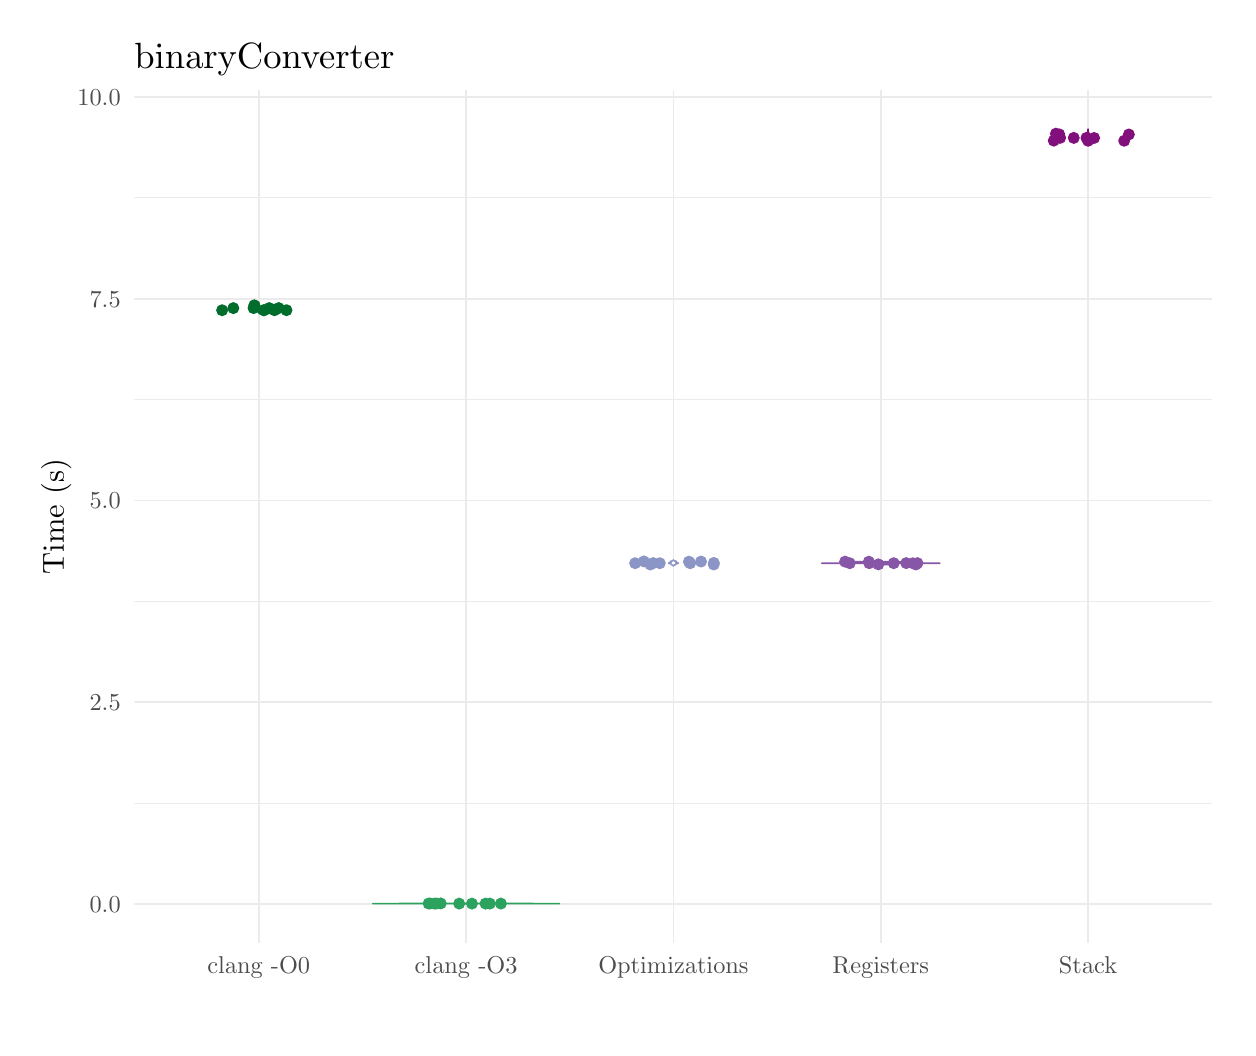
\begin{tikzpicture}[x=1pt,y=1pt]
\definecolor{fillColor}{RGB}{255,255,255}
\path[use as bounding box,fill=fillColor,fill opacity=0.00] (0,0) rectangle (433.62,361.35);
\begin{scope}
\path[clip] ( 38.56, 30.69) rectangle (428.12,338.69);
\definecolor{drawColor}{gray}{0.92}

\path[draw=drawColor,line width= 0.3pt,line join=round] ( 38.56, 81.14) --
	(428.12, 81.14);

\path[draw=drawColor,line width= 0.3pt,line join=round] ( 38.56,154.04) --
	(428.12,154.04);

\path[draw=drawColor,line width= 0.3pt,line join=round] ( 38.56,226.95) --
	(428.12,226.95);

\path[draw=drawColor,line width= 0.3pt,line join=round] ( 38.56,299.85) --
	(428.12,299.85);

\path[draw=drawColor,line width= 0.6pt,line join=round] ( 38.56, 44.69) --
	(428.12, 44.69);

\path[draw=drawColor,line width= 0.6pt,line join=round] ( 38.56,117.59) --
	(428.12,117.59);

\path[draw=drawColor,line width= 0.6pt,line join=round] ( 38.56,190.50) --
	(428.12,190.50);

\path[draw=drawColor,line width= 0.6pt,line join=round] ( 38.56,263.40) --
	(428.12,263.40);

\path[draw=drawColor,line width= 0.6pt,line join=round] ( 38.56,336.31) --
	(428.12,336.31);

\path[draw=drawColor,line width= 0.6pt,line join=round] ( 83.50, 30.69) --
	( 83.50,338.69);

\path[draw=drawColor,line width= 0.6pt,line join=round] (158.42, 30.69) --
	(158.42,338.69);

\path[draw=drawColor,line width= 0.6pt,line join=round] (233.34, 30.69) --
	(233.34,338.69);

\path[draw=drawColor,line width= 0.6pt,line join=round] (308.25, 30.69) --
	(308.25,338.69);

\path[draw=drawColor,line width= 0.6pt,line join=round] (383.17, 30.69) --
	(383.17,338.69);
\definecolor{drawColor}{RGB}{0,109,44}
\definecolor{fillColor}{RGB}{255,255,255}

\path[draw=drawColor,line width= 0.6pt,line join=round,line cap=round,fill=fillColor] ( 83.49,258.24) --
	( 83.49,258.25) --
	( 83.49,258.25) --
	( 83.49,258.26) --
	( 83.49,258.27) --
	( 83.49,258.28) --
	( 83.49,258.28) --
	( 83.49,258.29) --
	( 83.49,258.30) --
	( 83.49,258.31) --
	( 83.49,258.31) --
	( 83.48,258.32) --
	( 83.48,258.33) --
	( 83.48,258.34) --
	( 83.48,258.34) --
	( 83.48,258.35) --
	( 83.48,258.36) --
	( 83.48,258.37) --
	( 83.47,258.37) --
	( 83.47,258.38) --
	( 83.47,258.39) --
	( 83.47,258.39) --
	( 83.47,258.40) --
	( 83.46,258.41) --
	( 83.46,258.42) --
	( 83.46,258.42) --
	( 83.46,258.43) --
	( 83.45,258.44) --
	( 83.45,258.45) --
	( 83.45,258.45) --
	( 83.45,258.46) --
	( 83.44,258.47) --
	( 83.44,258.48) --
	( 83.44,258.48) --
	( 83.43,258.49) --
	( 83.43,258.50) --
	( 83.42,258.51) --
	( 83.42,258.51) --
	( 83.42,258.52) --
	( 83.41,258.53) --
	( 83.41,258.53) --
	( 83.40,258.54) --
	( 83.40,258.55) --
	( 83.39,258.56) --
	( 83.39,258.56) --
	( 83.38,258.57) --
	( 83.38,258.58) --
	( 83.37,258.59) --
	( 83.36,258.59) --
	( 83.36,258.60) --
	( 83.35,258.61) --
	( 83.34,258.62) --
	( 83.34,258.62) --
	( 83.33,258.63) --
	( 83.32,258.64) --
	( 83.31,258.64) --
	( 83.31,258.65) --
	( 83.30,258.66) --
	( 83.29,258.67) --
	( 83.28,258.67) --
	( 83.27,258.68) --
	( 83.27,258.69) --
	( 83.26,258.70) --
	( 83.25,258.70) --
	( 83.24,258.71) --
	( 83.23,258.72) --
	( 83.22,258.73) --
	( 83.21,258.73) --
	( 83.20,258.74) --
	( 83.19,258.75) --
	( 83.18,258.76) --
	( 83.17,258.76) --
	( 83.15,258.77) --
	( 83.14,258.78) --
	( 83.13,258.78) --
	( 83.12,258.79) --
	( 83.11,258.80) --
	( 83.10,258.81) --
	( 83.08,258.81) --
	( 83.07,258.82) --
	( 83.06,258.83) --
	( 83.05,258.84) --
	( 83.03,258.84) --
	( 83.02,258.85) --
	( 83.01,258.86) --
	( 83.00,258.87) --
	( 82.98,258.87) --
	( 82.97,258.88) --
	( 82.96,258.89) --
	( 82.94,258.90) --
	( 82.93,258.90) --
	( 82.92,258.91) --
	( 82.90,258.92) --
	( 82.89,258.92) --
	( 82.88,258.93) --
	( 82.86,258.94) --
	( 82.85,258.95) --
	( 82.84,258.95) --
	( 82.82,258.96) --
	( 82.81,258.97) --
	( 82.80,258.98) --
	( 82.79,258.98) --
	( 82.77,258.99) --
	( 82.76,259.00) --
	( 82.75,259.01) --
	( 82.73,259.01) --
	( 82.72,259.02) --
	( 82.71,259.03) --
	( 82.70,259.04) --
	( 82.69,259.04) --
	( 82.68,259.05) --
	( 82.66,259.06) --
	( 82.65,259.06) --
	( 82.64,259.07) --
	( 82.63,259.08) --
	( 82.62,259.09) --
	( 82.61,259.09) --
	( 82.60,259.10) --
	( 82.59,259.11) --
	( 82.58,259.12) --
	( 82.58,259.12) --
	( 82.57,259.13) --
	( 82.56,259.14) --
	( 82.55,259.15) --
	( 82.54,259.15) --
	( 82.54,259.16) --
	( 82.53,259.17) --
	( 82.52,259.18) --
	( 82.52,259.18) --
	( 82.51,259.19) --
	( 82.51,259.20) --
	( 82.50,259.20) --
	( 82.50,259.21) --
	( 82.50,259.22) --
	( 82.49,259.23) --
	( 82.49,259.23) --
	( 82.49,259.24) --
	( 82.48,259.25) --
	( 82.48,259.26) --
	( 82.48,259.26) --
	( 82.48,259.27) --
	( 82.48,259.28) --
	( 82.48,259.29) --
	( 82.48,259.29) --
	( 82.47,259.30) --
	( 82.48,259.31) --
	( 82.48,259.31) --
	( 82.48,259.32) --
	( 82.48,259.33) --
	( 82.48,259.34) --
	( 82.48,259.34) --
	( 82.48,259.35) --
	( 82.49,259.36) --
	( 82.49,259.37) --
	( 82.49,259.37) --
	( 82.49,259.38) --
	( 82.50,259.39) --
	( 82.50,259.40) --
	( 82.50,259.40) --
	( 82.51,259.41) --
	( 82.51,259.42) --
	( 82.51,259.43) --
	( 82.52,259.43) --
	( 82.52,259.44) --
	( 82.53,259.45) --
	( 82.53,259.45) --
	( 82.54,259.46) --
	( 82.54,259.47) --
	( 82.54,259.48) --
	( 82.55,259.48) --
	( 82.55,259.49) --
	( 82.56,259.50) --
	( 82.56,259.51) --
	( 82.57,259.51) --
	( 82.57,259.52) --
	( 82.58,259.53) --
	( 82.58,259.54) --
	( 82.58,259.54) --
	( 82.59,259.55) --
	( 82.59,259.56) --
	( 82.60,259.57) --
	( 82.60,259.57) --
	( 82.60,259.58) --
	( 82.61,259.59) --
	( 82.61,259.59) --
	( 82.61,259.60) --
	( 82.62,259.61) --
	( 82.62,259.62) --
	( 82.62,259.62) --
	( 82.62,259.63) --
	( 82.63,259.64) --
	( 82.63,259.65) --
	( 82.63,259.65) --
	( 82.63,259.66) --
	( 82.64,259.67) --
	( 82.64,259.68) --
	( 82.64,259.68) --
	( 82.64,259.69) --
	( 82.64,259.70) --
	( 82.64,259.71) --
	( 82.64,259.71) --
	( 82.64,259.72) --
	( 82.64,259.73) --
	( 82.64,259.73) --
	( 82.64,259.74) --
	( 82.64,259.75) --
	( 82.64,259.76) --
	( 82.64,259.76) --
	( 82.64,259.77) --
	( 82.64,259.78) --
	( 82.64,259.79) --
	( 82.64,259.79) --
	( 82.64,259.80) --
	( 82.64,259.81) --
	( 82.64,259.82) --
	( 82.64,259.82) --
	( 82.64,259.83) --
	( 82.64,259.84) --
	( 82.64,259.85) --
	( 82.64,259.85) --
	( 82.64,259.86) --
	( 82.64,259.87) --
	( 82.64,259.87) --
	( 82.64,259.88) --
	( 82.64,259.89) --
	( 82.64,259.90) --
	( 82.64,259.90) --
	( 82.64,259.91) --
	( 82.64,259.92) --
	( 82.64,259.93) --
	( 82.64,259.93) --
	( 82.64,259.94) --
	( 82.64,259.95) --
	( 82.64,259.96) --
	( 82.65,259.96) --
	( 82.65,259.97) --
	( 82.65,259.98) --
	( 82.65,259.99) --
	( 82.65,259.99) --
	( 82.66,260.00) --
	( 82.66,260.01) --
	( 82.66,260.01) --
	( 82.66,260.02) --
	( 82.67,260.03) --
	( 82.67,260.04) --
	( 82.67,260.04) --
	( 82.68,260.05) --
	( 82.68,260.06) --
	( 82.69,260.07) --
	( 82.69,260.07) --
	( 82.70,260.08) --
	( 82.70,260.09) --
	( 82.71,260.10) --
	( 82.71,260.10) --
	( 82.72,260.11) --
	( 82.73,260.12) --
	( 82.73,260.12) --
	( 82.74,260.13) --
	( 82.75,260.14) --
	( 82.75,260.15) --
	( 82.76,260.15) --
	( 82.77,260.16) --
	( 82.78,260.17) --
	( 82.78,260.18) --
	( 82.79,260.18) --
	( 82.80,260.19) --
	( 82.81,260.20) --
	( 82.82,260.21) --
	( 82.83,260.21) --
	( 82.84,260.22) --
	( 82.84,260.23) --
	( 82.85,260.24) --
	( 82.86,260.24) --
	( 82.87,260.25) --
	( 82.88,260.26) --
	( 82.89,260.26) --
	( 82.90,260.27) --
	( 82.91,260.28) --
	( 82.92,260.29) --
	( 82.93,260.29) --
	( 82.94,260.30) --
	( 82.95,260.31) --
	( 82.96,260.32) --
	( 82.97,260.32) --
	( 82.98,260.33) --
	( 82.99,260.34) --
	( 83.00,260.35) --
	( 83.01,260.35) --
	( 83.02,260.36) --
	( 83.03,260.37) --
	( 83.04,260.38) --
	( 83.04,260.38) --
	( 83.05,260.39) --
	( 83.06,260.40) --
	( 83.07,260.40) --
	( 83.08,260.41) --
	( 83.09,260.42) --
	( 83.10,260.43) --
	( 83.11,260.43) --
	( 83.11,260.44) --
	( 83.12,260.45) --
	( 83.13,260.46) --
	( 83.14,260.46) --
	( 83.15,260.47) --
	( 83.15,260.48) --
	( 83.16,260.49) --
	( 83.17,260.49) --
	( 83.17,260.50) --
	( 83.18,260.51) --
	( 83.19,260.52) --
	( 83.19,260.52) --
	( 83.20,260.53) --
	( 83.21,260.54) --
	( 83.21,260.54) --
	( 83.22,260.55) --
	( 83.22,260.56) --
	( 83.23,260.57) --
	( 83.23,260.57) --
	( 83.24,260.58) --
	( 83.24,260.59) --
	( 83.25,260.60) --
	( 83.25,260.60) --
	( 83.25,260.61) --
	( 83.26,260.62) --
	( 83.26,260.63) --
	( 83.26,260.63) --
	( 83.27,260.64) --
	( 83.27,260.65) --
	( 83.27,260.66) --
	( 83.28,260.66) --
	( 83.28,260.67) --
	( 83.28,260.68) --
	( 83.28,260.68) --
	( 83.28,260.69) --
	( 83.29,260.70) --
	( 83.29,260.71) --
	( 83.29,260.71) --
	( 83.29,260.72) --
	( 83.29,260.73) --
	( 83.29,260.74) --
	( 83.29,260.74) --
	( 83.29,260.75) --
	( 83.30,260.76) --
	( 83.30,260.77) --
	( 83.30,260.77) --
	( 83.30,260.78) --
	( 83.30,260.79) --
	( 83.30,260.79) --
	( 83.30,260.80) --
	( 83.30,260.81) --
	( 83.30,260.82) --
	( 83.30,260.82) --
	( 83.30,260.83) --
	( 83.30,260.84) --
	( 83.30,260.85) --
	( 83.30,260.85) --
	( 83.30,260.86) --
	( 83.30,260.87) --
	( 83.30,260.88) --
	( 83.30,260.88) --
	( 83.30,260.89) --
	( 83.30,260.90) --
	( 83.30,260.91) --
	( 83.30,260.91) --
	( 83.30,260.92) --
	( 83.30,260.93) --
	( 83.30,260.93) --
	( 83.30,260.94) --
	( 83.30,260.95) --
	( 83.30,260.96) --
	( 83.30,260.96) --
	( 83.30,260.97) --
	( 83.30,260.98) --
	( 83.30,260.99) --
	( 83.30,260.99) --
	( 83.30,261.00) --
	( 83.30,261.01) --
	( 83.30,261.02) --
	( 83.30,261.02) --
	( 83.30,261.03) --
	( 83.30,261.04) --
	( 83.31,261.05) --
	( 83.31,261.05) --
	( 83.31,261.06) --
	( 83.31,261.07) --
	( 83.31,261.07) --
	( 83.31,261.08) --
	( 83.31,261.09) --
	( 83.31,261.10) --
	( 83.31,261.10) --
	( 83.32,261.11) --
	( 83.32,261.12) --
	( 83.32,261.13) --
	( 83.32,261.13) --
	( 83.32,261.14) --
	( 83.32,261.15) --
	( 83.33,261.16) --
	( 83.33,261.16) --
	( 83.33,261.17) --
	( 83.33,261.18) --
	( 83.33,261.19) --
	( 83.34,261.19) --
	( 83.34,261.20) --
	( 83.34,261.21) --
	( 83.34,261.21) --
	( 83.35,261.22) --
	( 83.35,261.23) --
	( 83.35,261.24) --
	( 83.35,261.24) --
	( 83.35,261.25) --
	( 83.36,261.26) --
	( 83.36,261.27) --
	( 83.36,261.27) --
	( 83.37,261.28) --
	( 83.37,261.29) --
	( 83.37,261.30) --
	( 83.37,261.30) --
	( 83.38,261.31) --
	( 83.38,261.32) --
	( 83.38,261.33) --
	( 83.38,261.33) --
	( 83.39,261.34) --
	( 83.39,261.35) --
	( 83.39,261.35) --
	( 83.39,261.36) --
	( 83.40,261.37) --
	( 83.40,261.38) --
	( 83.40,261.38) --
	( 83.40,261.39) --
	( 83.41,261.40) --
	( 83.41,261.41) --
	( 83.41,261.41) --
	( 83.41,261.42) --
	( 83.42,261.43) --
	( 83.42,261.44) --
	( 83.42,261.44) --
	( 83.42,261.45) --
	( 83.43,261.46) --
	( 83.43,261.46) --
	( 83.43,261.47) --
	( 83.43,261.48) --
	( 83.44,261.49) --
	( 83.44,261.49) --
	( 83.44,261.50) --
	( 83.44,261.51) --
	( 83.44,261.52) --
	( 83.45,261.52) --
	( 83.45,261.53) --
	( 83.45,261.54) --
	( 83.45,261.55) --
	( 83.45,261.55) --
	( 83.46,261.56) --
	( 83.46,261.57) --
	( 83.46,261.58) --
	( 83.46,261.58) --
	( 83.46,261.59) --
	( 83.46,261.60) --
	( 83.47,261.60) --
	( 83.47,261.61) --
	( 83.47,261.62) --
	( 83.47,261.63) --
	( 83.47,261.63) --
	( 83.47,261.64) --
	( 83.47,261.65) --
	( 83.48,261.66) --
	( 83.48,261.66) --
	( 83.48,261.67) --
	( 83.48,261.68) --
	( 83.48,261.69) --
	( 83.48,261.69) --
	( 83.48,261.70) --
	( 83.48,261.71) --
	( 83.48,261.72) --
	( 83.49,261.72) --
	( 83.49,261.73) --
	( 83.49,261.74) --
	( 83.49,261.74) --
	( 83.49,261.75) --
	( 83.49,261.76) --
	( 83.49,261.77) --
	( 83.49,261.77) --
	( 83.49,261.78) --
	( 83.49,261.79) --
	( 83.49,261.80) --
	( 83.49,261.80) --
	( 83.49,261.81) --
	( 83.49,261.82) --
	( 83.50,261.83) --
	( 83.50,261.83) --
	( 83.50,261.84) --
	( 83.50,261.85) --
	( 83.50,261.86) --
	( 83.50,261.86) --
	( 83.50,261.87) --
	( 83.50,261.88) --
	( 83.50,261.88) --
	( 83.50,261.89) --
	( 83.50,261.90) --
	( 83.50,261.91) --
	( 83.50,261.91) --
	( 83.50,261.92) --
	( 83.50,261.93) --
	( 83.50,261.94) --
	( 83.50,261.94) --
	( 83.50,261.95) --
	( 83.50,261.96) --
	( 83.50,261.97) --
	( 83.50,261.97) --
	( 83.50,261.98) --
	( 83.50,261.99) --
	( 83.50,262.00) --
	( 83.50,262.00) --
	( 83.51,262.00) --
	( 83.51,262.00) --
	( 83.51,261.99) --
	( 83.51,261.98) --
	( 83.51,261.97) --
	( 83.51,261.97) --
	( 83.51,261.96) --
	( 83.51,261.95) --
	( 83.51,261.94) --
	( 83.51,261.94) --
	( 83.51,261.93) --
	( 83.51,261.92) --
	( 83.51,261.91) --
	( 83.51,261.91) --
	( 83.51,261.90) --
	( 83.51,261.89) --
	( 83.51,261.88) --
	( 83.51,261.88) --
	( 83.51,261.87) --
	( 83.51,261.86) --
	( 83.51,261.86) --
	( 83.51,261.85) --
	( 83.51,261.84) --
	( 83.51,261.83) --
	( 83.51,261.83) --
	( 83.51,261.82) --
	( 83.52,261.81) --
	( 83.52,261.80) --
	( 83.52,261.80) --
	( 83.52,261.79) --
	( 83.52,261.78) --
	( 83.52,261.77) --
	( 83.52,261.77) --
	( 83.52,261.76) --
	( 83.52,261.75) --
	( 83.52,261.74) --
	( 83.52,261.74) --
	( 83.52,261.73) --
	( 83.52,261.72) --
	( 83.52,261.72) --
	( 83.53,261.71) --
	( 83.53,261.70) --
	( 83.53,261.69) --
	( 83.53,261.69) --
	( 83.53,261.68) --
	( 83.53,261.67) --
	( 83.53,261.66) --
	( 83.53,261.66) --
	( 83.54,261.65) --
	( 83.54,261.64) --
	( 83.54,261.63) --
	( 83.54,261.63) --
	( 83.54,261.62) --
	( 83.54,261.61) --
	( 83.54,261.60) --
	( 83.55,261.60) --
	( 83.55,261.59) --
	( 83.55,261.58) --
	( 83.55,261.58) --
	( 83.55,261.57) --
	( 83.55,261.56) --
	( 83.56,261.55) --
	( 83.56,261.55) --
	( 83.56,261.54) --
	( 83.56,261.53) --
	( 83.56,261.52) --
	( 83.57,261.52) --
	( 83.57,261.51) --
	( 83.57,261.50) --
	( 83.57,261.49) --
	( 83.57,261.49) --
	( 83.58,261.48) --
	( 83.58,261.47) --
	( 83.58,261.46) --
	( 83.58,261.46) --
	( 83.59,261.45) --
	( 83.59,261.44) --
	( 83.59,261.44) --
	( 83.59,261.43) --
	( 83.60,261.42) --
	( 83.60,261.41) --
	( 83.60,261.41) --
	( 83.60,261.40) --
	( 83.61,261.39) --
	( 83.61,261.38) --
	( 83.61,261.38) --
	( 83.61,261.37) --
	( 83.62,261.36) --
	( 83.62,261.35) --
	( 83.62,261.35) --
	( 83.62,261.34) --
	( 83.63,261.33) --
	( 83.63,261.33) --
	( 83.63,261.32) --
	( 83.63,261.31) --
	( 83.64,261.30) --
	( 83.64,261.30) --
	( 83.64,261.29) --
	( 83.64,261.28) --
	( 83.65,261.27) --
	( 83.65,261.27) --
	( 83.65,261.26) --
	( 83.65,261.25) --
	( 83.66,261.24) --
	( 83.66,261.24) --
	( 83.66,261.23) --
	( 83.66,261.22) --
	( 83.67,261.21) --
	( 83.67,261.21) --
	( 83.67,261.20) --
	( 83.67,261.19) --
	( 83.68,261.19) --
	( 83.68,261.18) --
	( 83.68,261.17) --
	( 83.68,261.16) --
	( 83.68,261.16) --
	( 83.69,261.15) --
	( 83.69,261.14) --
	( 83.69,261.13) --
	( 83.69,261.13) --
	( 83.69,261.12) --
	( 83.69,261.11) --
	( 83.70,261.10) --
	( 83.70,261.10) --
	( 83.70,261.09) --
	( 83.70,261.08) --
	( 83.70,261.07) --
	( 83.70,261.07) --
	( 83.70,261.06) --
	( 83.70,261.05) --
	( 83.70,261.05) --
	( 83.71,261.04) --
	( 83.71,261.03) --
	( 83.71,261.02) --
	( 83.71,261.02) --
	( 83.71,261.01) --
	( 83.71,261.00) --
	( 83.71,260.99) --
	( 83.71,260.99) --
	( 83.71,260.98) --
	( 83.71,260.97) --
	( 83.71,260.96) --
	( 83.71,260.96) --
	( 83.71,260.95) --
	( 83.71,260.94) --
	( 83.71,260.93) --
	( 83.71,260.93) --
	( 83.71,260.92) --
	( 83.71,260.91) --
	( 83.71,260.91) --
	( 83.71,260.90) --
	( 83.71,260.89) --
	( 83.71,260.88) --
	( 83.71,260.88) --
	( 83.71,260.87) --
	( 83.71,260.86) --
	( 83.71,260.85) --
	( 83.71,260.85) --
	( 83.71,260.84) --
	( 83.71,260.83) --
	( 83.71,260.82) --
	( 83.71,260.82) --
	( 83.71,260.81) --
	( 83.71,260.80) --
	( 83.71,260.79) --
	( 83.71,260.79) --
	( 83.71,260.78) --
	( 83.71,260.77) --
	( 83.71,260.77) --
	( 83.71,260.76) --
	( 83.72,260.75) --
	( 83.72,260.74) --
	( 83.72,260.74) --
	( 83.72,260.73) --
	( 83.72,260.72) --
	( 83.72,260.71) --
	( 83.72,260.71) --
	( 83.72,260.70) --
	( 83.73,260.69) --
	( 83.73,260.68) --
	( 83.73,260.68) --
	( 83.73,260.67) --
	( 83.73,260.66) --
	( 83.74,260.66) --
	( 83.74,260.65) --
	( 83.74,260.64) --
	( 83.75,260.63) --
	( 83.75,260.63) --
	( 83.75,260.62) --
	( 83.76,260.61) --
	( 83.76,260.60) --
	( 83.76,260.60) --
	( 83.77,260.59) --
	( 83.77,260.58) --
	( 83.78,260.57) --
	( 83.78,260.57) --
	( 83.79,260.56) --
	( 83.79,260.55) --
	( 83.80,260.54) --
	( 83.80,260.54) --
	( 83.81,260.53) --
	( 83.82,260.52) --
	( 83.82,260.52) --
	( 83.83,260.51) --
	( 83.83,260.50) --
	( 83.84,260.49) --
	( 83.85,260.49) --
	( 83.86,260.48) --
	( 83.86,260.47) --
	( 83.87,260.46) --
	( 83.88,260.46) --
	( 83.89,260.45) --
	( 83.89,260.44) --
	( 83.90,260.43) --
	( 83.91,260.43) --
	( 83.92,260.42) --
	( 83.93,260.41) --
	( 83.94,260.40) --
	( 83.95,260.40) --
	( 83.96,260.39) --
	( 83.96,260.38) --
	( 83.97,260.38) --
	( 83.98,260.37) --
	( 83.99,260.36) --
	( 84.00,260.35) --
	( 84.01,260.35) --
	( 84.02,260.34) --
	( 84.03,260.33) --
	( 84.04,260.32) --
	( 84.05,260.32) --
	( 84.06,260.31) --
	( 84.07,260.30) --
	( 84.08,260.29) --
	( 84.09,260.29) --
	( 84.10,260.28) --
	( 84.11,260.27) --
	( 84.12,260.26) --
	( 84.13,260.26) --
	( 84.14,260.25) --
	( 84.15,260.24) --
	( 84.16,260.24) --
	( 84.17,260.23) --
	( 84.17,260.22) --
	( 84.18,260.21) --
	( 84.19,260.21) --
	( 84.20,260.20) --
	( 84.21,260.19) --
	( 84.22,260.18) --
	( 84.23,260.18) --
	( 84.23,260.17) --
	( 84.24,260.16) --
	( 84.25,260.15) --
	( 84.26,260.15) --
	( 84.26,260.14) --
	( 84.27,260.13) --
	( 84.28,260.12) --
	( 84.28,260.12) --
	( 84.29,260.11) --
	( 84.30,260.10) --
	( 84.30,260.10) --
	( 84.31,260.09) --
	( 84.31,260.08) --
	( 84.32,260.07) --
	( 84.32,260.07) --
	( 84.33,260.06) --
	( 84.33,260.05) --
	( 84.33,260.04) --
	( 84.34,260.04) --
	( 84.34,260.03) --
	( 84.35,260.02) --
	( 84.35,260.01) --
	( 84.35,260.01) --
	( 84.35,260.00) --
	( 84.36,259.99) --
	( 84.36,259.99) --
	( 84.36,259.98) --
	( 84.36,259.97) --
	( 84.36,259.96) --
	( 84.37,259.96) --
	( 84.37,259.95) --
	( 84.37,259.94) --
	( 84.37,259.93) --
	( 84.37,259.93) --
	( 84.37,259.92) --
	( 84.37,259.91) --
	( 84.37,259.90) --
	( 84.37,259.90) --
	( 84.37,259.89) --
	( 84.37,259.88) --
	( 84.37,259.87) --
	( 84.37,259.87) --
	( 84.37,259.86) --
	( 84.37,259.85) --
	( 84.37,259.85) --
	( 84.37,259.84) --
	( 84.37,259.83) --
	( 84.37,259.82) --
	( 84.37,259.82) --
	( 84.37,259.81) --
	( 84.37,259.80) --
	( 84.37,259.79) --
	( 84.37,259.79) --
	( 84.37,259.78) --
	( 84.36,259.77) --
	( 84.36,259.76) --
	( 84.36,259.76) --
	( 84.36,259.75) --
	( 84.37,259.74) --
	( 84.37,259.73) --
	( 84.37,259.73) --
	( 84.37,259.72) --
	( 84.37,259.71) --
	( 84.37,259.71) --
	( 84.37,259.70) --
	( 84.37,259.69) --
	( 84.37,259.68) --
	( 84.37,259.68) --
	( 84.37,259.67) --
	( 84.38,259.66) --
	( 84.38,259.65) --
	( 84.38,259.65) --
	( 84.38,259.64) --
	( 84.39,259.63) --
	( 84.39,259.62) --
	( 84.39,259.62) --
	( 84.39,259.61) --
	( 84.40,259.60) --
	( 84.40,259.59) --
	( 84.40,259.59) --
	( 84.41,259.58) --
	( 84.41,259.57) --
	( 84.41,259.57) --
	( 84.42,259.56) --
	( 84.42,259.55) --
	( 84.43,259.54) --
	( 84.43,259.54) --
	( 84.43,259.53) --
	( 84.44,259.52) --
	( 84.44,259.51) --
	( 84.45,259.51) --
	( 84.45,259.50) --
	( 84.46,259.49) --
	( 84.46,259.48) --
	( 84.47,259.48) --
	( 84.47,259.47) --
	( 84.47,259.46) --
	( 84.48,259.45) --
	( 84.48,259.45) --
	( 84.49,259.44) --
	( 84.49,259.43) --
	( 84.49,259.43) --
	( 84.50,259.42) --
	( 84.50,259.41) --
	( 84.51,259.40) --
	( 84.51,259.40) --
	( 84.51,259.39) --
	( 84.52,259.38) --
	( 84.52,259.37) --
	( 84.52,259.37) --
	( 84.52,259.36) --
	( 84.53,259.35) --
	( 84.53,259.34) --
	( 84.53,259.34) --
	( 84.53,259.33) --
	( 84.53,259.32) --
	( 84.53,259.31) --
	( 84.53,259.31) --
	( 84.53,259.30) --
	( 84.53,259.29) --
	( 84.53,259.29) --
	( 84.53,259.28) --
	( 84.53,259.27) --
	( 84.53,259.26) --
	( 84.53,259.26) --
	( 84.53,259.25) --
	( 84.52,259.24) --
	( 84.52,259.23) --
	( 84.52,259.23) --
	( 84.51,259.22) --
	( 84.51,259.21) --
	( 84.51,259.20) --
	( 84.50,259.20) --
	( 84.50,259.19) --
	( 84.49,259.18) --
	( 84.49,259.18) --
	( 84.48,259.17) --
	( 84.47,259.16) --
	( 84.47,259.15) --
	( 84.46,259.15) --
	( 84.45,259.14) --
	( 84.44,259.13) --
	( 84.43,259.12) --
	( 84.43,259.12) --
	( 84.42,259.11) --
	( 84.41,259.10) --
	( 84.40,259.09) --
	( 84.39,259.09) --
	( 84.38,259.08) --
	( 84.37,259.07) --
	( 84.36,259.06) --
	( 84.35,259.06) --
	( 84.33,259.05) --
	( 84.32,259.04) --
	( 84.31,259.04) --
	( 84.30,259.03) --
	( 84.29,259.02) --
	( 84.27,259.01) --
	( 84.26,259.01) --
	( 84.25,259.00) --
	( 84.24,258.99) --
	( 84.22,258.98) --
	( 84.21,258.98) --
	( 84.20,258.97) --
	( 84.19,258.96) --
	( 84.17,258.95) --
	( 84.16,258.95) --
	( 84.15,258.94) --
	( 84.13,258.93) --
	( 84.12,258.92) --
	( 84.11,258.92) --
	( 84.09,258.91) --
	( 84.08,258.90) --
	( 84.07,258.90) --
	( 84.05,258.89) --
	( 84.04,258.88) --
	( 84.03,258.87) --
	( 84.01,258.87) --
	( 84.00,258.86) --
	( 83.99,258.85) --
	( 83.98,258.84) --
	( 83.96,258.84) --
	( 83.95,258.83) --
	( 83.94,258.82) --
	( 83.93,258.81) --
	( 83.91,258.81) --
	( 83.90,258.80) --
	( 83.89,258.79) --
	( 83.88,258.78) --
	( 83.87,258.78) --
	( 83.86,258.77) --
	( 83.84,258.76) --
	( 83.83,258.76) --
	( 83.82,258.75) --
	( 83.81,258.74) --
	( 83.80,258.73) --
	( 83.79,258.73) --
	( 83.78,258.72) --
	( 83.77,258.71) --
	( 83.76,258.70) --
	( 83.75,258.70) --
	( 83.74,258.69) --
	( 83.74,258.68) --
	( 83.73,258.67) --
	( 83.72,258.67) --
	( 83.71,258.66) --
	( 83.70,258.65) --
	( 83.69,258.64) --
	( 83.69,258.64) --
	( 83.68,258.63) --
	( 83.67,258.62) --
	( 83.67,258.62) --
	( 83.66,258.61) --
	( 83.65,258.60) --
	( 83.65,258.59) --
	( 83.64,258.59) --
	( 83.63,258.58) --
	( 83.63,258.57) --
	( 83.62,258.56) --
	( 83.62,258.56) --
	( 83.61,258.55) --
	( 83.61,258.54) --
	( 83.60,258.53) --
	( 83.60,258.53) --
	( 83.59,258.52) --
	( 83.59,258.51) --
	( 83.59,258.51) --
	( 83.58,258.50) --
	( 83.58,258.49) --
	( 83.57,258.48) --
	( 83.57,258.48) --
	( 83.57,258.47) --
	( 83.56,258.46) --
	( 83.56,258.45) --
	( 83.56,258.45) --
	( 83.56,258.44) --
	( 83.55,258.43) --
	( 83.55,258.42) --
	( 83.55,258.42) --
	( 83.55,258.41) --
	( 83.54,258.40) --
	( 83.54,258.39) --
	( 83.54,258.39) --
	( 83.54,258.38) --
	( 83.54,258.37) --
	( 83.53,258.37) --
	( 83.53,258.36) --
	( 83.53,258.35) --
	( 83.53,258.34) --
	( 83.53,258.34) --
	( 83.53,258.33) --
	( 83.52,258.32) --
	( 83.52,258.31) --
	( 83.52,258.31) --
	( 83.52,258.30) --
	( 83.52,258.29) --
	( 83.52,258.28) --
	( 83.52,258.28) --
	( 83.52,258.27) --
	( 83.52,258.26) --
	( 83.52,258.25) --
	( 83.52,258.25) --
	( 83.51,258.24) --
	( 83.49,258.24) --
	cycle;
\definecolor{drawColor}{RGB}{44,162,95}

\path[draw=drawColor,line width= 0.6pt,line join=round,line cap=round,fill=fillColor] (158.05, 44.80) --
	(158.03, 44.80) --
	(158.00, 44.80) --
	(157.97, 44.80) --
	(157.95, 44.80) --
	(157.91, 44.80) --
	(157.88, 44.80) --
	(157.85, 44.80) --
	(157.81, 44.80) --
	(157.77, 44.80) --
	(157.73, 44.80) --
	(157.69, 44.80) --
	(157.65, 44.80) --
	(157.60, 44.80) --
	(157.55, 44.80) --
	(157.50, 44.80) --
	(157.45, 44.80) --
	(157.39, 44.80) --
	(157.33, 44.80) --
	(157.27, 44.80) --
	(157.20, 44.80) --
	(157.13, 44.80) --
	(157.06, 44.80) --
	(156.99, 44.80) --
	(156.91, 44.80) --
	(156.82, 44.80) --
	(156.74, 44.80) --
	(156.65, 44.80) --
	(156.55, 44.80) --
	(156.45, 44.80) --
	(156.35, 44.80) --
	(156.25, 44.80) --
	(156.13, 44.80) --
	(156.02, 44.81) --
	(155.90, 44.81) --
	(155.77, 44.81) --
	(155.64, 44.81) --
	(155.51, 44.81) --
	(155.37, 44.81) --
	(155.22, 44.81) --
	(155.07, 44.81) --
	(154.91, 44.81) --
	(154.75, 44.81) --
	(154.58, 44.81) --
	(154.41, 44.81) --
	(154.23, 44.81) --
	(154.05, 44.81) --
	(153.86, 44.81) --
	(153.66, 44.81) --
	(153.45, 44.81) --
	(153.24, 44.81) --
	(153.02, 44.81) --
	(152.80, 44.81) --
	(152.57, 44.81) --
	(152.34, 44.81) --
	(152.09, 44.81) --
	(151.84, 44.81) --
	(151.58, 44.81) --
	(151.32, 44.81) --
	(151.05, 44.81) --
	(150.77, 44.81) --
	(150.49, 44.81) --
	(150.20, 44.81) --
	(149.90, 44.81) --
	(149.60, 44.81) --
	(149.28, 44.81) --
	(148.97, 44.81) --
	(148.64, 44.81) --
	(148.31, 44.81) --
	(147.98, 44.81) --
	(147.63, 44.81) --
	(147.28, 44.81) --
	(146.93, 44.81) --
	(146.57, 44.82) --
	(146.20, 44.82) --
	(145.83, 44.82) --
	(145.45, 44.82) --
	(145.07, 44.82) --
	(144.68, 44.82) --
	(144.29, 44.82) --
	(143.89, 44.82) --
	(143.49, 44.82) --
	(143.08, 44.82) --
	(142.67, 44.82) --
	(142.26, 44.82) --
	(141.84, 44.82) --
	(141.42, 44.82) --
	(141.00, 44.82) --
	(140.57, 44.82) --
	(140.15, 44.82) --
	(139.72, 44.82) --
	(139.29, 44.82) --
	(138.86, 44.82) --
	(138.43, 44.82) --
	(138.00, 44.82) --
	(137.57, 44.82) --
	(137.14, 44.82) --
	(136.71, 44.82) --
	(136.28, 44.82) --
	(135.85, 44.82) --
	(135.43, 44.82) --
	(135.01, 44.82) --
	(134.59, 44.82) --
	(134.17, 44.82) --
	(133.76, 44.82) --
	(133.36, 44.82) --
	(132.95, 44.82) --
	(132.56, 44.82) --
	(132.17, 44.82) --
	(131.78, 44.82) --
	(131.40, 44.82) --
	(131.03, 44.82) --
	(130.67, 44.82) --
	(130.31, 44.83) --
	(129.96, 44.83) --
	(129.62, 44.83) --
	(129.29, 44.83) --
	(128.97, 44.83) --
	(128.65, 44.83) --
	(128.35, 44.83) --
	(128.06, 44.83) --
	(127.78, 44.83) --
	(127.51, 44.83) --
	(127.25, 44.83) --
	(127.00, 44.83) --
	(126.76, 44.83) --
	(126.54, 44.83) --
	(126.33, 44.83) --
	(126.13, 44.83) --
	(125.94, 44.83) --
	(125.77, 44.83) --
	(125.61, 44.83) --
	(125.46, 44.83) --
	(125.32, 44.83) --
	(125.20, 44.83) --
	(125.09, 44.83) --
	(125.00, 44.83) --
	(124.91, 44.83) --
	(124.85, 44.83) --
	(124.79, 44.83) --
	(124.75, 44.83) --
	(124.72, 44.83) --
	(124.71, 44.83) --
	(124.71, 44.83) --
	(124.72, 44.83) --
	(124.75, 44.83) --
	(124.78, 44.83) --
	(124.83, 44.83) --
	(124.89, 44.83) --
	(124.97, 44.83) --
	(125.06, 44.83) --
	(125.15, 44.83) --
	(125.26, 44.84) --
	(125.38, 44.84) --
	(125.51, 44.84) --
	(125.65, 44.84) --
	(125.80, 44.84) --
	(125.97, 44.84) --
	(126.14, 44.84) --
	(126.32, 44.84) --
	(126.50, 44.84) --
	(126.70, 44.84) --
	(126.91, 44.84) --
	(127.11, 44.84) --
	(127.34, 44.84) --
	(127.56, 44.84) --
	(127.79, 44.84) --
	(128.03, 44.84) --
	(128.27, 44.84) --
	(128.51, 44.84) --
	(128.76, 44.84) --
	(129.02, 44.84) --
	(129.27, 44.84) --
	(129.53, 44.84) --
	(129.80, 44.84) --
	(130.06, 44.84) --
	(130.33, 44.84) --
	(130.59, 44.84) --
	(130.86, 44.84) --
	(131.13, 44.84) --
	(131.39, 44.84) --
	(131.66, 44.84) --
	(131.92, 44.84) --
	(132.19, 44.84) --
	(132.45, 44.84) --
	(132.71, 44.84) --
	(132.96, 44.84) --
	(133.22, 44.84) --
	(133.47, 44.84) --
	(133.71, 44.84) --
	(133.96, 44.84) --
	(134.19, 44.84) --
	(134.43, 44.85) --
	(134.66, 44.85) --
	(134.88, 44.85) --
	(135.10, 44.85) --
	(135.32, 44.85) --
	(135.52, 44.85) --
	(135.73, 44.85) --
	(135.92, 44.85) --
	(136.11, 44.85) --
	(136.30, 44.85) --
	(136.48, 44.85) --
	(136.65, 44.85) --
	(136.82, 44.85) --
	(136.97, 44.85) --
	(137.13, 44.85) --
	(137.28, 44.85) --
	(137.42, 44.85) --
	(137.55, 44.85) --
	(137.68, 44.85) --
	(137.80, 44.85) --
	(137.92, 44.85) --
	(138.03, 44.85) --
	(138.14, 44.85) --
	(138.24, 44.85) --
	(138.33, 44.85) --
	(138.42, 44.85) --
	(138.50, 44.85) --
	(138.58, 44.85) --
	(138.66, 44.85) --
	(138.73, 44.85) --
	(138.79, 44.85) --
	(138.85, 44.85) --
	(138.91, 44.85) --
	(138.96, 44.85) --
	(139.01, 44.85) --
	(139.06, 44.85) --
	(139.11, 44.85) --
	(139.15, 44.85) --
	(139.19, 44.85) --
	(139.23, 44.85) --
	(139.26, 44.86) --
	(139.30, 44.86) --
	(139.33, 44.86) --
	(139.36, 44.86) --
	(139.39, 44.86) --
	(139.43, 44.86) --
	(139.46, 44.86) --
	(139.49, 44.86) --
	(139.52, 44.86) --
	(139.55, 44.86) --
	(139.59, 44.86) --
	(139.62, 44.86) --
	(139.66, 44.86) --
	(139.69, 44.86) --
	(139.73, 44.86) --
	(139.77, 44.86) --
	(139.82, 44.86) --
	(139.86, 44.86) --
	(139.91, 44.86) --
	(139.96, 44.86) --
	(140.01, 44.86) --
	(140.07, 44.86) --
	(140.13, 44.86) --
	(140.19, 44.86) --
	(140.26, 44.86) --
	(140.33, 44.86) --
	(140.40, 44.86) --
	(140.48, 44.86) --
	(140.56, 44.86) --
	(140.65, 44.86) --
	(140.73, 44.86) --
	(140.82, 44.86) --
	(140.92, 44.86) --
	(141.02, 44.86) --
	(141.12, 44.86) --
	(141.23, 44.86) --
	(141.34, 44.86) --
	(141.46, 44.86) --
	(141.57, 44.86) --
	(141.70, 44.87) --
	(141.82, 44.87) --
	(141.95, 44.87) --
	(142.08, 44.87) --
	(142.22, 44.87) --
	(142.36, 44.87) --
	(142.50, 44.87) --
	(142.64, 44.87) --
	(142.79, 44.87) --
	(142.94, 44.87) --
	(143.09, 44.87) --
	(143.24, 44.87) --
	(143.40, 44.87) --
	(143.56, 44.87) --
	(143.72, 44.87) --
	(143.88, 44.87) --
	(144.04, 44.87) --
	(144.21, 44.87) --
	(144.37, 44.87) --
	(144.54, 44.87) --
	(144.71, 44.87) --
	(144.87, 44.87) --
	(145.04, 44.87) --
	(145.21, 44.87) --
	(145.38, 44.87) --
	(145.54, 44.87) --
	(145.71, 44.87) --
	(145.88, 44.87) --
	(146.04, 44.87) --
	(146.21, 44.87) --
	(146.37, 44.87) --
	(146.54, 44.87) --
	(146.70, 44.87) --
	(146.86, 44.87) --
	(147.02, 44.87) --
	(147.17, 44.87) --
	(147.33, 44.87) --
	(147.48, 44.87) --
	(147.63, 44.87) --
	(147.78, 44.87) --
	(147.92, 44.88) --
	(148.06, 44.88) --
	(148.20, 44.88) --
	(148.34, 44.88) --
	(148.48, 44.88) --
	(148.61, 44.88) --
	(148.74, 44.88) --
	(148.86, 44.88) --
	(148.99, 44.88) --
	(149.11, 44.88) --
	(149.22, 44.88) --
	(149.34, 44.88) --
	(149.45, 44.88) --
	(149.55, 44.88) --
	(149.66, 44.88) --
	(149.76, 44.88) --
	(149.86, 44.88) --
	(149.95, 44.88) --
	(150.05, 44.88) --
	(150.13, 44.88) --
	(150.22, 44.88) --
	(150.30, 44.88) --
	(150.38, 44.88) --
	(150.46, 44.88) --
	(150.53, 44.88) --
	(150.61, 44.88) --
	(150.68, 44.88) --
	(150.74, 44.88) --
	(150.81, 44.88) --
	(150.87, 44.88) --
	(150.93, 44.88) --
	(150.99, 44.88) --
	(151.04, 44.88) --
	(151.10, 44.88) --
	(151.15, 44.88) --
	(151.20, 44.88) --
	(151.24, 44.88) --
	(151.29, 44.88) --
	(151.34, 44.88) --
	(151.38, 44.88) --
	(151.42, 44.89) --
	(151.46, 44.89) --
	(151.50, 44.89) --
	(151.54, 44.89) --
	(151.58, 44.89) --
	(151.62, 44.89) --
	(151.66, 44.89) --
	(151.69, 44.89) --
	(151.73, 44.89) --
	(151.77, 44.89) --
	(151.80, 44.89) --
	(151.84, 44.89) --
	(151.88, 44.89) --
	(151.91, 44.89) --
	(151.95, 44.89) --
	(151.98, 44.89) --
	(152.02, 44.89) --
	(152.06, 44.89) --
	(152.10, 44.89) --
	(152.14, 44.89) --
	(152.17, 44.89) --
	(152.21, 44.89) --
	(152.26, 44.89) --
	(152.30, 44.89) --
	(152.34, 44.89) --
	(152.38, 44.89) --
	(152.43, 44.89) --
	(152.47, 44.89) --
	(152.52, 44.89) --
	(152.57, 44.89) --
	(152.61, 44.89) --
	(152.66, 44.89) --
	(152.71, 44.89) --
	(152.77, 44.89) --
	(152.82, 44.89) --
	(152.87, 44.89) --
	(152.93, 44.89) --
	(152.99, 44.89) --
	(153.04, 44.89) --
	(153.10, 44.89) --
	(153.16, 44.90) --
	(153.22, 44.90) --
	(153.28, 44.90) --
	(153.35, 44.90) --
	(153.41, 44.90) --
	(153.48, 44.90) --
	(153.54, 44.90) --
	(153.61, 44.90) --
	(153.68, 44.90) --
	(153.74, 44.90) --
	(153.81, 44.90) --
	(153.88, 44.90) --
	(153.95, 44.90) --
	(154.03, 44.90) --
	(154.10, 44.90) --
	(154.17, 44.90) --
	(154.24, 44.90) --
	(154.32, 44.90) --
	(154.39, 44.90) --
	(154.46, 44.90) --
	(154.54, 44.90) --
	(154.61, 44.90) --
	(154.69, 44.90) --
	(154.76, 44.90) --
	(154.83, 44.90) --
	(154.91, 44.90) --
	(154.98, 44.90) --
	(155.06, 44.90) --
	(155.13, 44.90) --
	(155.21, 44.90) --
	(155.28, 44.90) --
	(155.35, 44.90) --
	(155.43, 44.90) --
	(155.50, 44.90) --
	(155.57, 44.90) --
	(155.64, 44.90) --
	(155.71, 44.90) --
	(155.78, 44.90) --
	(155.85, 44.90) --
	(155.92, 44.91) --
	(155.99, 44.91) --
	(156.05, 44.91) --
	(156.12, 44.91) --
	(156.19, 44.91) --
	(156.25, 44.91) --
	(156.31, 44.91) --
	(156.38, 44.91) --
	(156.44, 44.91) --
	(156.50, 44.91) --
	(156.56, 44.91) --
	(156.62, 44.91) --
	(156.68, 44.91) --
	(156.73, 44.91) --
	(156.79, 44.91) --
	(156.84, 44.91) --
	(156.90, 44.91) --
	(156.95, 44.91) --
	(157.00, 44.91) --
	(157.05, 44.91) --
	(157.10, 44.91) --
	(157.14, 44.91) --
	(157.19, 44.91) --
	(157.24, 44.91) --
	(157.28, 44.91) --
	(157.32, 44.91) --
	(157.36, 44.91) --
	(157.41, 44.91) --
	(157.44, 44.91) --
	(157.48, 44.91) --
	(157.52, 44.91) --
	(157.56, 44.91) --
	(157.59, 44.91) --
	(157.63, 44.91) --
	(157.66, 44.91) --
	(157.69, 44.91) --
	(157.72, 44.91) --
	(157.75, 44.91) --
	(157.78, 44.91) --
	(157.81, 44.91) --
	(157.84, 44.92) --
	(157.86, 44.92) --
	(157.89, 44.92) --
	(157.91, 44.92) --
	(157.94, 44.92) --
	(157.96, 44.92) --
	(157.98, 44.92) --
	(158.00, 44.92) --
	(158.02, 44.92) --
	(158.04, 44.92) --
	(158.06, 44.92) --
	(158.08, 44.92) --
	(158.09, 44.92) --
	(158.11, 44.92) --
	(158.13, 44.92) --
	(158.14, 44.92) --
	(158.15, 44.92) --
	(158.17, 44.92) --
	(158.18, 44.92) --
	(158.19, 44.92) --
	(158.21, 44.92) --
	(158.22, 44.92) --
	(158.23, 44.92) --
	(158.24, 44.92) --
	(158.25, 44.92) --
	(158.26, 44.92) --
	(158.27, 44.92) --
	(158.28, 44.92) --
	(158.28, 44.92) --
	(158.29, 44.92) --
	(158.30, 44.92) --
	(158.31, 44.92) --
	(158.31, 44.92) --
	(158.32, 44.92) --
	(158.33, 44.92) --
	(158.33, 44.92) --
	(158.34, 44.92) --
	(158.34, 44.92) --
	(158.35, 44.92) --
	(158.35, 44.92) --
	(158.36, 44.93) --
	(158.36, 44.93) --
	(158.48, 44.93) --
	(158.49, 44.93) --
	(158.49, 44.92) --
	(158.50, 44.92) --
	(158.50, 44.92) --
	(158.51, 44.92) --
	(158.51, 44.92) --
	(158.52, 44.92) --
	(158.52, 44.92) --
	(158.53, 44.92) --
	(158.54, 44.92) --
	(158.54, 44.92) --
	(158.55, 44.92) --
	(158.56, 44.92) --
	(158.57, 44.92) --
	(158.57, 44.92) --
	(158.58, 44.92) --
	(158.59, 44.92) --
	(158.60, 44.92) --
	(158.61, 44.92) --
	(158.62, 44.92) --
	(158.64, 44.92) --
	(158.65, 44.92) --
	(158.66, 44.92) --
	(158.67, 44.92) --
	(158.69, 44.92) --
	(158.70, 44.92) --
	(158.72, 44.92) --
	(158.73, 44.92) --
	(158.75, 44.92) --
	(158.77, 44.92) --
	(158.78, 44.92) --
	(158.80, 44.92) --
	(158.82, 44.92) --
	(158.84, 44.92) --
	(158.86, 44.92) --
	(158.88, 44.92) --
	(158.91, 44.92) --
	(158.93, 44.92) --
	(158.95, 44.92) --
	(158.98, 44.92) --
	(159.01, 44.92) --
	(159.03, 44.91) --
	(159.06, 44.91) --
	(159.09, 44.91) --
	(159.12, 44.91) --
	(159.15, 44.91) --
	(159.18, 44.91) --
	(159.22, 44.91) --
	(159.25, 44.91) --
	(159.29, 44.91) --
	(159.32, 44.91) --
	(159.36, 44.91) --
	(159.40, 44.91) --
	(159.44, 44.91) --
	(159.48, 44.91) --
	(159.52, 44.91) --
	(159.56, 44.91) --
	(159.61, 44.91) --
	(159.65, 44.91) --
	(159.70, 44.91) --
	(159.75, 44.91) --
	(159.79, 44.91) --
	(159.84, 44.91) --
	(159.90, 44.91) --
	(159.95, 44.91) --
	(160.00, 44.91) --
	(160.05, 44.91) --
	(160.11, 44.91) --
	(160.17, 44.91) --
	(160.22, 44.91) --
	(160.28, 44.91) --
	(160.34, 44.91) --
	(160.40, 44.91) --
	(160.47, 44.91) --
	(160.53, 44.91) --
	(160.59, 44.91) --
	(160.66, 44.91) --
	(160.72, 44.91) --
	(160.79, 44.91) --
	(160.85, 44.91) --
	(160.92, 44.91) --
	(160.99, 44.90) --
	(161.06, 44.90) --
	(161.13, 44.90) --
	(161.20, 44.90) --
	(161.27, 44.90) --
	(161.34, 44.90) --
	(161.42, 44.90) --
	(161.49, 44.90) --
	(161.56, 44.90) --
	(161.64, 44.90) --
	(161.71, 44.90) --
	(161.78, 44.90) --
	(161.86, 44.90) --
	(161.93, 44.90) --
	(162.01, 44.90) --
	(162.08, 44.90) --
	(162.16, 44.90) --
	(162.23, 44.90) --
	(162.31, 44.90) --
	(162.38, 44.90) --
	(162.45, 44.90) --
	(162.53, 44.90) --
	(162.60, 44.90) --
	(162.67, 44.90) --
	(162.75, 44.90) --
	(162.82, 44.90) --
	(162.89, 44.90) --
	(162.96, 44.90) --
	(163.03, 44.90) --
	(163.10, 44.90) --
	(163.17, 44.90) --
	(163.23, 44.90) --
	(163.30, 44.90) --
	(163.37, 44.90) --
	(163.43, 44.90) --
	(163.50, 44.90) --
	(163.56, 44.90) --
	(163.62, 44.90) --
	(163.68, 44.90) --
	(163.74, 44.89) --
	(163.80, 44.89) --
	(163.86, 44.89) --
	(163.91, 44.89) --
	(163.97, 44.89) --
	(164.02, 44.89) --
	(164.08, 44.89) --
	(164.13, 44.89) --
	(164.18, 44.89) --
	(164.23, 44.89) --
	(164.28, 44.89) --
	(164.32, 44.89) --
	(164.37, 44.89) --
	(164.42, 44.89) --
	(164.46, 44.89) --
	(164.50, 44.89) --
	(164.55, 44.89) --
	(164.59, 44.89) --
	(164.63, 44.89) --
	(164.67, 44.89) --
	(164.71, 44.89) --
	(164.75, 44.89) --
	(164.78, 44.89) --
	(164.82, 44.89) --
	(164.86, 44.89) --
	(164.89, 44.89) --
	(164.93, 44.89) --
	(164.97, 44.89) --
	(165.00, 44.89) --
	(165.04, 44.89) --
	(165.08, 44.89) --
	(165.11, 44.89) --
	(165.15, 44.89) --
	(165.19, 44.89) --
	(165.22, 44.89) --
	(165.26, 44.89) --
	(165.30, 44.89) --
	(165.34, 44.89) --
	(165.38, 44.89) --
	(165.42, 44.89) --
	(165.46, 44.88) --
	(165.51, 44.88) --
	(165.55, 44.88) --
	(165.60, 44.88) --
	(165.65, 44.88) --
	(165.70, 44.88) --
	(165.75, 44.88) --
	(165.80, 44.88) --
	(165.86, 44.88) --
	(165.91, 44.88) --
	(165.97, 44.88) --
	(166.03, 44.88) --
	(166.10, 44.88) --
	(166.17, 44.88) --
	(166.23, 44.88) --
	(166.31, 44.88) --
	(166.38, 44.88) --
	(166.46, 44.88) --
	(166.54, 44.88) --
	(166.62, 44.88) --
	(166.71, 44.88) --
	(166.80, 44.88) --
	(166.89, 44.88) --
	(166.98, 44.88) --
	(167.08, 44.88) --
	(167.18, 44.88) --
	(167.29, 44.88) --
	(167.40, 44.88) --
	(167.51, 44.88) --
	(167.62, 44.88) --
	(167.74, 44.88) --
	(167.86, 44.88) --
	(167.98, 44.88) --
	(168.11, 44.88) --
	(168.23, 44.88) --
	(168.37, 44.88) --
	(168.50, 44.88) --
	(168.64, 44.88) --
	(168.78, 44.88) --
	(168.92, 44.88) --
	(169.07, 44.87) --
	(169.21, 44.87) --
	(169.36, 44.87) --
	(169.52, 44.87) --
	(169.67, 44.87) --
	(169.83, 44.87) --
	(169.99, 44.87) --
	(170.14, 44.87) --
	(170.31, 44.87) --
	(170.47, 44.87) --
	(170.63, 44.87) --
	(170.80, 44.87) --
	(170.96, 44.87) --
	(171.13, 44.87) --
	(171.30, 44.87) --
	(171.47, 44.87) --
	(171.63, 44.87) --
	(171.80, 44.87) --
	(171.97, 44.87) --
	(172.14, 44.87) --
	(172.30, 44.87) --
	(172.47, 44.87) --
	(172.63, 44.87) --
	(172.80, 44.87) --
	(172.96, 44.87) --
	(173.12, 44.87) --
	(173.28, 44.87) --
	(173.44, 44.87) --
	(173.60, 44.87) --
	(173.75, 44.87) --
	(173.90, 44.87) --
	(174.05, 44.87) --
	(174.20, 44.87) --
	(174.34, 44.87) --
	(174.49, 44.87) --
	(174.62, 44.87) --
	(174.76, 44.87) --
	(174.89, 44.87) --
	(175.02, 44.87) --
	(175.14, 44.87) --
	(175.27, 44.86) --
	(175.39, 44.86) --
	(175.50, 44.86) --
	(175.61, 44.86) --
	(175.72, 44.86) --
	(175.82, 44.86) --
	(175.92, 44.86) --
	(176.02, 44.86) --
	(176.11, 44.86) --
	(176.20, 44.86) --
	(176.28, 44.86) --
	(176.36, 44.86) --
	(176.44, 44.86) --
	(176.51, 44.86) --
	(176.58, 44.86) --
	(176.65, 44.86) --
	(176.71, 44.86) --
	(176.77, 44.86) --
	(176.83, 44.86) --
	(176.88, 44.86) --
	(176.93, 44.86) --
	(176.98, 44.86) --
	(177.03, 44.86) --
	(177.07, 44.86) --
	(177.11, 44.86) --
	(177.15, 44.86) --
	(177.19, 44.86) --
	(177.22, 44.86) --
	(177.26, 44.86) --
	(177.29, 44.86) --
	(177.32, 44.86) --
	(177.35, 44.86) --
	(177.39, 44.86) --
	(177.42, 44.86) --
	(177.45, 44.86) --
	(177.48, 44.86) --
	(177.51, 44.86) --
	(177.55, 44.86) --
	(177.58, 44.86) --
	(177.62, 44.85) --
	(177.65, 44.85) --
	(177.69, 44.85) --
	(177.74, 44.85) --
	(177.78, 44.85) --
	(177.83, 44.85) --
	(177.88, 44.85) --
	(177.93, 44.85) --
	(177.99, 44.85) --
	(178.05, 44.85) --
	(178.12, 44.85) --
	(178.19, 44.85) --
	(178.26, 44.85) --
	(178.34, 44.85) --
	(178.42, 44.85) --
	(178.51, 44.85) --
	(178.61, 44.85) --
	(178.71, 44.85) --
	(178.81, 44.85) --
	(178.92, 44.85) --
	(179.04, 44.85) --
	(179.16, 44.85) --
	(179.29, 44.85) --
	(179.42, 44.85) --
	(179.57, 44.85) --
	(179.71, 44.85) --
	(179.87, 44.85) --
	(180.03, 44.85) --
	(180.19, 44.85) --
	(180.37, 44.85) --
	(180.54, 44.85) --
	(180.73, 44.85) --
	(180.92, 44.85) --
	(181.12, 44.85) --
	(181.32, 44.85) --
	(181.53, 44.85) --
	(181.74, 44.85) --
	(181.96, 44.85) --
	(182.18, 44.85) --
	(182.41, 44.85) --
	(182.65, 44.84) --
	(182.89, 44.84) --
	(183.13, 44.84) --
	(183.38, 44.84) --
	(183.62, 44.84) --
	(183.88, 44.84) --
	(184.14, 44.84) --
	(184.39, 44.84) --
	(184.66, 44.84) --
	(184.92, 44.84) --
	(185.18, 44.84) --
	(185.45, 44.84) --
	(185.72, 44.84) --
	(185.98, 44.84) --
	(186.25, 44.84) --
	(186.52, 44.84) --
	(186.78, 44.84) --
	(187.05, 44.84) --
	(187.31, 44.84) --
	(187.57, 44.84) --
	(187.83, 44.84) --
	(188.08, 44.84) --
	(188.33, 44.84) --
	(188.58, 44.84) --
	(188.82, 44.84) --
	(189.05, 44.84) --
	(189.28, 44.84) --
	(189.51, 44.84) --
	(189.73, 44.84) --
	(189.94, 44.84) --
	(190.14, 44.84) --
	(190.34, 44.84) --
	(190.53, 44.84) --
	(190.71, 44.84) --
	(190.88, 44.84) --
	(191.04, 44.84) --
	(191.19, 44.84) --
	(191.33, 44.84) --
	(191.46, 44.84) --
	(191.58, 44.84) --
	(191.69, 44.83) --
	(191.79, 44.83) --
	(191.88, 44.83) --
	(191.95, 44.83) --
	(192.01, 44.83) --
	(192.06, 44.83) --
	(192.10, 44.83) --
	(192.13, 44.83) --
	(192.13, 44.83) --
	(192.13, 44.83) --
	(192.12, 44.83) --
	(192.09, 44.83) --
	(192.05, 44.83) --
	(191.99, 44.83) --
	(191.93, 44.83) --
	(191.84, 44.83) --
	(191.75, 44.83) --
	(191.64, 44.83) --
	(191.52, 44.83) --
	(191.39, 44.83) --
	(191.23, 44.83) --
	(191.08, 44.83) --
	(190.90, 44.83) --
	(190.71, 44.83) --
	(190.51, 44.83) --
	(190.30, 44.83) --
	(190.08, 44.83) --
	(189.84, 44.83) --
	(189.59, 44.83) --
	(189.33, 44.83) --
	(189.06, 44.83) --
	(188.78, 44.83) --
	(188.49, 44.83) --
	(188.19, 44.83) --
	(187.87, 44.83) --
	(187.55, 44.83) --
	(187.22, 44.83) --
	(186.88, 44.83) --
	(186.53, 44.83) --
	(186.17, 44.82) --
	(185.81, 44.82) --
	(185.44, 44.82) --
	(185.06, 44.82) --
	(184.68, 44.82) --
	(184.28, 44.82) --
	(183.89, 44.82) --
	(183.49, 44.82) --
	(183.08, 44.82) --
	(182.67, 44.82) --
	(182.25, 44.82) --
	(181.84, 44.82) --
	(181.41, 44.82) --
	(180.99, 44.82) --
	(180.56, 44.82) --
	(180.14, 44.82) --
	(179.71, 44.82) --
	(179.28, 44.82) --
	(178.84, 44.82) --
	(178.41, 44.82) --
	(177.98, 44.82) --
	(177.55, 44.82) --
	(177.12, 44.82) --
	(176.69, 44.82) --
	(176.27, 44.82) --
	(175.84, 44.82) --
	(175.42, 44.82) --
	(175.00, 44.82) --
	(174.58, 44.82) --
	(174.17, 44.82) --
	(173.76, 44.82) --
	(173.36, 44.82) --
	(172.95, 44.82) --
	(172.56, 44.82) --
	(172.16, 44.82) --
	(171.78, 44.82) --
	(171.39, 44.82) --
	(171.01, 44.82) --
	(170.64, 44.82) --
	(170.27, 44.82) --
	(169.91, 44.81) --
	(169.56, 44.81) --
	(169.21, 44.81) --
	(168.87, 44.81) --
	(168.53, 44.81) --
	(168.20, 44.81) --
	(167.87, 44.81) --
	(167.56, 44.81) --
	(167.25, 44.81) --
	(166.94, 44.81) --
	(166.65, 44.81) --
	(166.35, 44.81) --
	(166.07, 44.81) --
	(165.79, 44.81) --
	(165.52, 44.81) --
	(165.26, 44.81) --
	(165.00, 44.81) --
	(164.75, 44.81) --
	(164.51, 44.81) --
	(164.27, 44.81) --
	(164.04, 44.81) --
	(163.82, 44.81) --
	(163.60, 44.81) --
	(163.39, 44.81) --
	(163.19, 44.81) --
	(162.99, 44.81) --
	(162.80, 44.81) --
	(162.61, 44.81) --
	(162.43, 44.81) --
	(162.26, 44.81) --
	(162.09, 44.81) --
	(161.93, 44.81) --
	(161.77, 44.81) --
	(161.62, 44.81) --
	(161.47, 44.81) --
	(161.33, 44.81) --
	(161.20, 44.81) --
	(161.07, 44.81) --
	(160.94, 44.81) --
	(160.82, 44.81) --
	(160.71, 44.80) --
	(160.60, 44.80) --
	(160.49, 44.80) --
	(160.39, 44.80) --
	(160.29, 44.80) --
	(160.20, 44.80) --
	(160.11, 44.80) --
	(160.02, 44.80) --
	(159.94, 44.80) --
	(159.86, 44.80) --
	(159.78, 44.80) --
	(159.71, 44.80) --
	(159.64, 44.80) --
	(159.58, 44.80) --
	(159.51, 44.80) --
	(159.45, 44.80) --
	(159.40, 44.80) --
	(159.34, 44.80) --
	(159.29, 44.80) --
	(159.24, 44.80) --
	(159.20, 44.80) --
	(159.15, 44.80) --
	(159.11, 44.80) --
	(159.07, 44.80) --
	(159.03, 44.80) --
	(158.99, 44.80) --
	(158.96, 44.80) --
	(158.93, 44.80) --
	(158.90, 44.80) --
	(158.87, 44.80) --
	(158.84, 44.80) --
	(158.82, 44.80) --
	(158.79, 44.80) --
	(158.05, 44.80) --
	cycle;
\definecolor{drawColor}{RGB}{140,150,198}

\path[draw=drawColor,line width= 0.6pt,line join=round,line cap=round,fill=fillColor] (233.33,166.82) --
	(233.33,166.82) --
	(233.33,166.82) --
	(233.33,166.83) --
	(233.33,166.83) --
	(233.33,166.84) --
	(233.33,166.84) --
	(233.32,166.85) --
	(233.32,166.85) --
	(233.32,166.85) --
	(233.32,166.86) --
	(233.32,166.86) --
	(233.32,166.87) --
	(233.32,166.87) --
	(233.32,166.88) --
	(233.32,166.88) --
	(233.32,166.88) --
	(233.31,166.89) --
	(233.31,166.89) --
	(233.31,166.90) --
	(233.31,166.90) --
	(233.31,166.91) --
	(233.31,166.91) --
	(233.30,166.91) --
	(233.30,166.92) --
	(233.30,166.92) --
	(233.30,166.93) --
	(233.30,166.93) --
	(233.29,166.94) --
	(233.29,166.94) --
	(233.29,166.95) --
	(233.28,166.95) --
	(233.28,166.95) --
	(233.28,166.96) --
	(233.28,166.96) --
	(233.27,166.97) --
	(233.27,166.97) --
	(233.27,166.98) --
	(233.26,166.98) --
	(233.26,166.98) --
	(233.25,166.99) --
	(233.25,166.99) --
	(233.25,167.00) --
	(233.24,167.00) --
	(233.24,167.01) --
	(233.23,167.01) --
	(233.23,167.01) --
	(233.22,167.02) --
	(233.22,167.02) --
	(233.21,167.03) --
	(233.21,167.03) --
	(233.20,167.04) --
	(233.19,167.04) --
	(233.19,167.05) --
	(233.18,167.05) --
	(233.18,167.05) --
	(233.17,167.06) --
	(233.16,167.06) --
	(233.16,167.07) --
	(233.15,167.07) --
	(233.14,167.08) --
	(233.13,167.08) --
	(233.13,167.08) --
	(233.12,167.09) --
	(233.11,167.09) --
	(233.10,167.10) --
	(233.10,167.10) --
	(233.09,167.11) --
	(233.08,167.11) --
	(233.07,167.11) --
	(233.06,167.12) --
	(233.05,167.12) --
	(233.04,167.13) --
	(233.03,167.13) --
	(233.02,167.14) --
	(233.02,167.14) --
	(233.01,167.15) --
	(233.00,167.15) --
	(232.99,167.15) --
	(232.98,167.16) --
	(232.97,167.16) --
	(232.96,167.17) --
	(232.95,167.17) --
	(232.94,167.18) --
	(232.93,167.18) --
	(232.92,167.18) --
	(232.91,167.19) --
	(232.90,167.19) --
	(232.89,167.20) --
	(232.88,167.20) --
	(232.87,167.21) --
	(232.86,167.21) --
	(232.85,167.21) --
	(232.84,167.22) --
	(232.83,167.22) --
	(232.82,167.23) --
	(232.81,167.23) --
	(232.80,167.24) --
	(232.79,167.24) --
	(232.78,167.25) --
	(232.77,167.25) --
	(232.76,167.25) --
	(232.75,167.26) --
	(232.74,167.26) --
	(232.73,167.27) --
	(232.73,167.27) --
	(232.72,167.28) --
	(232.71,167.28) --
	(232.70,167.28) --
	(232.69,167.29) --
	(232.69,167.29) --
	(232.68,167.30) --
	(232.67,167.30) --
	(232.66,167.31) --
	(232.66,167.31) --
	(232.65,167.31) --
	(232.64,167.32) --
	(232.64,167.32) --
	(232.63,167.33) --
	(232.63,167.33) --
	(232.62,167.34) --
	(232.62,167.34) --
	(232.61,167.35) --
	(232.61,167.35) --
	(232.60,167.35) --
	(232.60,167.36) --
	(232.59,167.36) --
	(232.59,167.37) --
	(232.59,167.37) --
	(232.58,167.38) --
	(232.58,167.38) --
	(232.58,167.38) --
	(232.57,167.39) --
	(232.57,167.39) --
	(232.57,167.40) --
	(232.57,167.40) --
	(232.56,167.41) --
	(232.56,167.41) --
	(232.56,167.41) --
	(232.56,167.42) --
	(232.56,167.42) --
	(232.55,167.43) --
	(232.55,167.43) --
	(232.55,167.44) --
	(232.55,167.44) --
	(232.55,167.45) --
	(232.55,167.45) --
	(232.54,167.45) --
	(232.54,167.46) --
	(232.54,167.46) --
	(232.54,167.47) --
	(232.54,167.47) --
	(232.54,167.48) --
	(232.53,167.48) --
	(232.53,167.48) --
	(232.53,167.49) --
	(232.53,167.49) --
	(232.52,167.50) --
	(232.52,167.50) --
	(232.52,167.51) --
	(232.51,167.51) --
	(232.51,167.51) --
	(232.50,167.52) --
	(232.50,167.52) --
	(232.49,167.53) --
	(232.49,167.53) --
	(232.48,167.54) --
	(232.48,167.54) --
	(232.47,167.54) --
	(232.46,167.55) --
	(232.46,167.55) --
	(232.45,167.56) --
	(232.44,167.56) --
	(232.43,167.57) --
	(232.43,167.57) --
	(232.42,167.58) --
	(232.41,167.58) --
	(232.40,167.58) --
	(232.39,167.59) --
	(232.38,167.59) --
	(232.37,167.60) --
	(232.35,167.60) --
	(232.34,167.61) --
	(232.33,167.61) --
	(232.32,167.61) --
	(232.30,167.62) --
	(232.29,167.62) --
	(232.28,167.63) --
	(232.26,167.63) --
	(232.25,167.64) --
	(232.23,167.64) --
	(232.22,167.64) --
	(232.20,167.65) --
	(232.19,167.65) --
	(232.17,167.66) --
	(232.15,167.66) --
	(232.14,167.67) --
	(232.12,167.67) --
	(232.10,167.68) --
	(232.09,167.68) --
	(232.07,167.68) --
	(232.05,167.69) --
	(232.04,167.69) --
	(232.02,167.70) --
	(232.00,167.70) --
	(231.98,167.71) --
	(231.97,167.71) --
	(231.95,167.71) --
	(231.93,167.72) --
	(231.91,167.72) --
	(231.90,167.73) --
	(231.88,167.73) --
	(231.86,167.74) --
	(231.85,167.74) --
	(231.83,167.74) --
	(231.82,167.75) --
	(231.80,167.75) --
	(231.79,167.76) --
	(231.77,167.76) --
	(231.76,167.77) --
	(231.74,167.77) --
	(231.73,167.78) --
	(231.72,167.78) --
	(231.71,167.78) --
	(231.70,167.79) --
	(231.68,167.79) --
	(231.67,167.80) --
	(231.66,167.80) --
	(231.65,167.81) --
	(231.65,167.81) --
	(231.64,167.81) --
	(231.63,167.82) --
	(231.63,167.82) --
	(231.62,167.83) --
	(231.61,167.83) --
	(231.61,167.84) --
	(231.61,167.84) --
	(231.60,167.84) --
	(231.60,167.85) --
	(231.60,167.85) --
	(231.60,167.86) --
	(231.60,167.86) --
	(231.60,167.87) --
	(231.61,167.87) --
	(231.61,167.88) --
	(231.61,167.88) --
	(231.62,167.88) --
	(231.62,167.89) --
	(231.63,167.89) --
	(231.63,167.90) --
	(231.64,167.90) --
	(231.65,167.91) --
	(231.66,167.91) --
	(231.67,167.91) --
	(231.68,167.92) --
	(231.69,167.92) --
	(231.70,167.93) --
	(231.71,167.93) --
	(231.73,167.94) --
	(231.74,167.94) --
	(231.75,167.94) --
	(231.77,167.95) --
	(231.78,167.95) --
	(231.80,167.96) --
	(231.81,167.96) --
	(231.83,167.97) --
	(231.84,167.97) --
	(231.86,167.98) --
	(231.88,167.98) --
	(231.90,167.98) --
	(231.91,167.99) --
	(231.93,167.99) --
	(231.95,168.00) --
	(231.97,168.00) --
	(231.99,168.01) --
	(232.00,168.01) --
	(232.02,168.01) --
	(232.04,168.02) --
	(232.06,168.02) --
	(232.08,168.03) --
	(232.10,168.03) --
	(232.11,168.04) --
	(232.13,168.04) --
	(232.15,168.04) --
	(232.17,168.05) --
	(232.19,168.05) --
	(232.20,168.06) --
	(232.22,168.06) --
	(232.24,168.07) --
	(232.25,168.07) --
	(232.27,168.08) --
	(232.29,168.08) --
	(232.30,168.08) --
	(232.32,168.09) --
	(232.33,168.09) --
	(232.34,168.10) --
	(232.36,168.10) --
	(232.37,168.11) --
	(232.38,168.11) --
	(232.39,168.11) --
	(232.41,168.12) --
	(232.42,168.12) --
	(232.43,168.13) --
	(232.44,168.13) --
	(232.45,168.14) --
	(232.45,168.14) --
	(232.46,168.14) --
	(232.47,168.15) --
	(232.48,168.15) --
	(232.48,168.16) --
	(232.49,168.16) --
	(232.49,168.17) --
	(232.50,168.17) --
	(232.50,168.18) --
	(232.50,168.18) --
	(232.51,168.18) --
	(232.51,168.19) --
	(232.51,168.19) --
	(232.51,168.20) --
	(232.51,168.20) --
	(232.51,168.21) --
	(232.51,168.21) --
	(232.51,168.21) --
	(232.51,168.22) --
	(232.51,168.22) --
	(232.51,168.23) --
	(232.50,168.23) --
	(232.50,168.24) --
	(232.50,168.24) --
	(232.49,168.24) --
	(232.49,168.25) --
	(232.48,168.25) --
	(232.48,168.26) --
	(232.47,168.26) --
	(232.47,168.27) --
	(232.46,168.27) --
	(232.46,168.27) --
	(232.45,168.28) --
	(232.44,168.28) --
	(232.44,168.29) --
	(232.43,168.29) --
	(232.42,168.30) --
	(232.42,168.30) --
	(232.41,168.31) --
	(232.40,168.31) --
	(232.40,168.31) --
	(232.39,168.32) --
	(232.38,168.32) --
	(232.38,168.33) --
	(232.37,168.33) --
	(232.36,168.34) --
	(232.36,168.34) --
	(232.35,168.34) --
	(232.35,168.35) --
	(232.34,168.35) --
	(232.34,168.36) --
	(232.33,168.36) --
	(232.33,168.37) --
	(232.32,168.37) --
	(232.32,168.37) --
	(232.31,168.38) --
	(232.31,168.38) --
	(232.31,168.39) --
	(232.31,168.39) --
	(232.30,168.40) --
	(232.30,168.40) --
	(232.30,168.41) --
	(232.30,168.41) --
	(232.30,168.41) --
	(232.30,168.42) --
	(232.30,168.42) --
	(232.30,168.43) --
	(232.30,168.43) --
	(232.30,168.44) --
	(232.30,168.44) --
	(232.31,168.44) --
	(232.31,168.45) --
	(232.31,168.45) --
	(232.32,168.46) --
	(232.32,168.46) --
	(232.33,168.47) --
	(232.33,168.47) --
	(232.34,168.47) --
	(232.34,168.48) --
	(232.35,168.48) --
	(232.36,168.49) --
	(232.36,168.49) --
	(232.37,168.50) --
	(232.38,168.50) --
	(232.39,168.51) --
	(232.40,168.51) --
	(232.41,168.51) --
	(232.42,168.52) --
	(232.43,168.52) --
	(232.44,168.53) --
	(232.45,168.53) --
	(232.46,168.54) --
	(232.47,168.54) --
	(232.48,168.54) --
	(232.50,168.55) --
	(232.51,168.55) --
	(232.52,168.56) --
	(232.53,168.56) --
	(232.55,168.57) --
	(232.56,168.57) --
	(232.57,168.57) --
	(232.59,168.58) --
	(232.60,168.58) --
	(232.61,168.59) --
	(232.63,168.59) --
	(232.64,168.60) --
	(232.66,168.60) --
	(232.67,168.61) --
	(232.69,168.61) --
	(232.70,168.61) --
	(232.71,168.62) --
	(232.73,168.62) --
	(232.74,168.63) --
	(232.76,168.63) --
	(232.77,168.64) --
	(232.78,168.64) --
	(232.80,168.64) --
	(232.81,168.65) --
	(232.83,168.65) --
	(232.84,168.66) --
	(232.85,168.66) --
	(232.87,168.67) --
	(232.88,168.67) --
	(232.89,168.67) --
	(232.91,168.68) --
	(232.92,168.68) --
	(232.93,168.69) --
	(232.95,168.69) --
	(232.96,168.70) --
	(232.97,168.70) --
	(232.98,168.71) --
	(232.99,168.71) --
	(233.00,168.71) --
	(233.02,168.72) --
	(233.03,168.72) --
	(233.04,168.73) --
	(233.05,168.73) --
	(233.06,168.74) --
	(233.07,168.74) --
	(233.08,168.74) --
	(233.09,168.75) --
	(233.10,168.75) --
	(233.11,168.76) --
	(233.12,168.76) --
	(233.13,168.77) --
	(233.13,168.77) --
	(233.14,168.77) --
	(233.15,168.78) --
	(233.16,168.78) --
	(233.17,168.79) --
	(233.17,168.79) --
	(233.18,168.80) --
	(233.19,168.80) --
	(233.19,168.81) --
	(233.20,168.81) --
	(233.21,168.81) --
	(233.21,168.82) --
	(233.22,168.82) --
	(233.22,168.83) --
	(233.23,168.83) --
	(233.23,168.84) --
	(233.24,168.84) --
	(233.24,168.84) --
	(233.25,168.85) --
	(233.25,168.85) --
	(233.26,168.86) --
	(233.26,168.86) --
	(233.27,168.87) --
	(233.27,168.87) --
	(233.27,168.87) --
	(233.28,168.88) --
	(233.28,168.88) --
	(233.28,168.89) --
	(233.29,168.89) --
	(233.29,168.90) --
	(233.29,168.90) --
	(233.29,168.91) --
	(233.30,168.91) --
	(233.30,168.91) --
	(233.30,168.92) --
	(233.30,168.92) --
	(233.30,168.93) --
	(233.31,168.93) --
	(233.31,168.94) --
	(233.31,168.94) --
	(233.31,168.94) --
	(233.31,168.95) --
	(233.31,168.95) --
	(233.32,168.96) --
	(233.32,168.96) --
	(233.32,168.97) --
	(233.32,168.97) --
	(233.32,168.97) --
	(233.32,168.98) --
	(233.32,168.98) --
	(233.32,168.99) --
	(233.32,168.99) --
	(233.33,169.00) --
	(233.33,169.00) --
	(233.33,169.00) --
	(233.33,169.01) --
	(233.33,169.01) --
	(233.33,169.02) --
	(233.33,169.02) --
	(233.33,169.03) --
	(233.33,169.03) --
	(233.33,169.04) --
	(233.34,169.04) --
	(233.34,169.03) --
	(233.34,169.03) --
	(233.35,169.02) --
	(233.35,169.02) --
	(233.35,169.01) --
	(233.35,169.01) --
	(233.35,169.00) --
	(233.35,169.00) --
	(233.35,169.00) --
	(233.35,168.99) --
	(233.35,168.99) --
	(233.35,168.98) --
	(233.35,168.98) --
	(233.35,168.97) --
	(233.36,168.97) --
	(233.36,168.97) --
	(233.36,168.96) --
	(233.36,168.96) --
	(233.36,168.95) --
	(233.36,168.95) --
	(233.36,168.94) --
	(233.36,168.94) --
	(233.37,168.94) --
	(233.37,168.93) --
	(233.37,168.93) --
	(233.37,168.92) --
	(233.37,168.92) --
	(233.38,168.91) --
	(233.38,168.91) --
	(233.38,168.91) --
	(233.38,168.90) --
	(233.39,168.90) --
	(233.39,168.89) --
	(233.39,168.89) --
	(233.40,168.88) --
	(233.40,168.88) --
	(233.40,168.87) --
	(233.41,168.87) --
	(233.41,168.87) --
	(233.41,168.86) --
	(233.42,168.86) --
	(233.42,168.85) --
	(233.43,168.85) --
	(233.43,168.84) --
	(233.44,168.84) --
	(233.44,168.84) --
	(233.45,168.83) --
	(233.45,168.83) --
	(233.46,168.82) --
	(233.46,168.82) --
	(233.47,168.81) --
	(233.48,168.81) --
	(233.48,168.81) --
	(233.49,168.80) --
	(233.49,168.80) --
	(233.50,168.79) --
	(233.51,168.79) --
	(233.52,168.78) --
	(233.52,168.78) --
	(233.53,168.77) --
	(233.54,168.77) --
	(233.55,168.77) --
	(233.56,168.76) --
	(233.57,168.76) --
	(233.58,168.75) --
	(233.59,168.75) --
	(233.60,168.74) --
	(233.61,168.74) --
	(233.62,168.74) --
	(233.63,168.73) --
	(233.64,168.73) --
	(233.65,168.72) --
	(233.66,168.72) --
	(233.67,168.71) --
	(233.68,168.71) --
	(233.69,168.71) --
	(233.71,168.70) --
	(233.72,168.70) --
	(233.73,168.69) --
	(233.74,168.69) --
	(233.76,168.68) --
	(233.77,168.68) --
	(233.78,168.67) --
	(233.79,168.67) --
	(233.81,168.67) --
	(233.82,168.66) --
	(233.83,168.66) --
	(233.85,168.65) --
	(233.86,168.65) --
	(233.88,168.64) --
	(233.89,168.64) --
	(233.90,168.64) --
	(233.92,168.63) --
	(233.93,168.63) --
	(233.95,168.62) --
	(233.96,168.62) --
	(233.98,168.61) --
	(233.99,168.61) --
	(234.00,168.61) --
	(234.02,168.60) --
	(234.03,168.60) --
	(234.05,168.59) --
	(234.06,168.59) --
	(234.07,168.58) --
	(234.09,168.58) --
	(234.10,168.57) --
	(234.11,168.57) --
	(234.13,168.57) --
	(234.14,168.56) --
	(234.15,168.56) --
	(234.17,168.55) --
	(234.18,168.55) --
	(234.19,168.54) --
	(234.20,168.54) --
	(234.21,168.54) --
	(234.23,168.53) --
	(234.24,168.53) --
	(234.25,168.52) --
	(234.26,168.52) --
	(234.27,168.51) --
	(234.28,168.51) --
	(234.29,168.51) --
	(234.29,168.50) --
	(234.30,168.50) --
	(234.31,168.49) --
	(234.32,168.49) --
	(234.33,168.48) --
	(234.33,168.48) --
	(234.34,168.47) --
	(234.34,168.47) --
	(234.35,168.47) --
	(234.35,168.46) --
	(234.36,168.46) --
	(234.36,168.45) --
	(234.37,168.45) --
	(234.37,168.44) --
	(234.37,168.44) --
	(234.37,168.44) --
	(234.38,168.43) --
	(234.38,168.43) --
	(234.38,168.42) --
	(234.38,168.42) --
	(234.38,168.41) --
	(234.38,168.41) --
	(234.38,168.41) --
	(234.37,168.40) --
	(234.37,168.40) --
	(234.37,168.39) --
	(234.37,168.39) --
	(234.36,168.38) --
	(234.36,168.38) --
	(234.36,168.37) --
	(234.35,168.37) --
	(234.35,168.37) --
	(234.34,168.36) --
	(234.34,168.36) --
	(234.33,168.35) --
	(234.33,168.35) --
	(234.32,168.34) --
	(234.32,168.34) --
	(234.31,168.34) --
	(234.30,168.33) --
	(234.30,168.33) --
	(234.29,168.32) --
	(234.28,168.32) --
	(234.28,168.31) --
	(234.27,168.31) --
	(234.26,168.31) --
	(234.26,168.30) --
	(234.25,168.30) --
	(234.24,168.29) --
	(234.24,168.29) --
	(234.23,168.28) --
	(234.23,168.28) --
	(234.22,168.27) --
	(234.21,168.27) --
	(234.21,168.27) --
	(234.20,168.26) --
	(234.20,168.26) --
	(234.19,168.25) --
	(234.19,168.25) --
	(234.18,168.24) --
	(234.18,168.24) --
	(234.18,168.24) --
	(234.17,168.23) --
	(234.17,168.23) --
	(234.17,168.22) --
	(234.17,168.22) --
	(234.16,168.21) --
	(234.16,168.21) --
	(234.16,168.21) --
	(234.16,168.20) --
	(234.16,168.20) --
	(234.16,168.19) --
	(234.17,168.19) --
	(234.17,168.18) --
	(234.17,168.18) --
	(234.17,168.18) --
	(234.18,168.17) --
	(234.18,168.17) --
	(234.19,168.16) --
	(234.19,168.16) --
	(234.20,168.15) --
	(234.21,168.15) --
	(234.21,168.14) --
	(234.22,168.14) --
	(234.23,168.14) --
	(234.24,168.13) --
	(234.25,168.13) --
	(234.26,168.12) --
	(234.27,168.12) --
	(234.28,168.11) --
	(234.29,168.11) --
	(234.31,168.11) --
	(234.32,168.10) --
	(234.33,168.10) --
	(234.35,168.09) --
	(234.36,168.09) --
	(234.37,168.08) --
	(234.39,168.08) --
	(234.41,168.08) --
	(234.42,168.07) --
	(234.44,168.07) --
	(234.45,168.06) --
	(234.47,168.06) --
	(234.49,168.05) --
	(234.51,168.05) --
	(234.52,168.04) --
	(234.54,168.04) --
	(234.56,168.04) --
	(234.58,168.03) --
	(234.60,168.03) --
	(234.62,168.02) --
	(234.63,168.02) --
	(234.65,168.01) --
	(234.67,168.01) --
	(234.69,168.01) --
	(234.71,168.00) --
	(234.73,168.00) --
	(234.74,167.99) --
	(234.76,167.99) --
	(234.78,167.98) --
	(234.80,167.98) --
	(234.81,167.98) --
	(234.83,167.97) --
	(234.85,167.97) --
	(234.86,167.96) --
	(234.88,167.96) --
	(234.89,167.95) --
	(234.91,167.95) --
	(234.92,167.94) --
	(234.94,167.94) --
	(234.95,167.94) --
	(234.96,167.93) --
	(234.97,167.93) --
	(234.99,167.92) --
	(235.00,167.92) --
	(235.01,167.91) --
	(235.02,167.91) --
	(235.03,167.91) --
	(235.03,167.90) --
	(235.04,167.90) --
	(235.05,167.89) --
	(235.05,167.89) --
	(235.06,167.88) --
	(235.06,167.88) --
	(235.07,167.88) --
	(235.07,167.87) --
	(235.07,167.87) --
	(235.07,167.86) --
	(235.07,167.86) --
	(235.07,167.85) --
	(235.07,167.85) --
	(235.07,167.84) --
	(235.07,167.84) --
	(235.06,167.84) --
	(235.06,167.83) --
	(235.06,167.83) --
	(235.05,167.82) --
	(235.04,167.82) --
	(235.04,167.81) --
	(235.03,167.81) --
	(235.02,167.81) --
	(235.01,167.80) --
	(235.00,167.80) --
	(234.99,167.79) --
	(234.98,167.79) --
	(234.97,167.78) --
	(234.96,167.78) --
	(234.94,167.78) --
	(234.93,167.77) --
	(234.92,167.77) --
	(234.90,167.76) --
	(234.89,167.76) --
	(234.87,167.75) --
	(234.86,167.75) --
	(234.84,167.74) --
	(234.83,167.74) --
	(234.81,167.74) --
	(234.79,167.73) --
	(234.78,167.73) --
	(234.76,167.72) --
	(234.74,167.72) --
	(234.73,167.71) --
	(234.71,167.71) --
	(234.69,167.71) --
	(234.67,167.70) --
	(234.66,167.70) --
	(234.64,167.69) --
	(234.62,167.69) --
	(234.61,167.68) --
	(234.59,167.68) --
	(234.57,167.68) --
	(234.55,167.67) --
	(234.54,167.67) --
	(234.52,167.66) --
	(234.50,167.66) --
	(234.49,167.65) --
	(234.47,167.65) --
	(234.46,167.64) --
	(234.44,167.64) --
	(234.43,167.64) --
	(234.41,167.63) --
	(234.40,167.63) --
	(234.38,167.62) --
	(234.37,167.62) --
	(234.36,167.61) --
	(234.35,167.61) --
	(234.33,167.61) --
	(234.32,167.60) --
	(234.31,167.60) --
	(234.30,167.59) --
	(234.29,167.59) --
	(234.28,167.58) --
	(234.27,167.58) --
	(234.26,167.58) --
	(234.25,167.57) --
	(234.24,167.57) --
	(234.23,167.56) --
	(234.22,167.56) --
	(234.22,167.55) --
	(234.21,167.55) --
	(234.20,167.54) --
	(234.20,167.54) --
	(234.19,167.54) --
	(234.19,167.53) --
	(234.18,167.53) --
	(234.18,167.52) --
	(234.17,167.52) --
	(234.17,167.51) --
	(234.16,167.51) --
	(234.16,167.51) --
	(234.16,167.50) --
	(234.15,167.50) --
	(234.15,167.49) --
	(234.15,167.49) --
	(234.14,167.48) --
	(234.14,167.48) --
	(234.14,167.48) --
	(234.14,167.47) --
	(234.14,167.47) --
	(234.13,167.46) --
	(234.13,167.46) --
	(234.13,167.45) --
	(234.13,167.45) --
	(234.13,167.45) --
	(234.13,167.44) --
	(234.12,167.44) --
	(234.12,167.43) --
	(234.12,167.43) --
	(234.12,167.42) --
	(234.12,167.42) --
	(234.11,167.41) --
	(234.11,167.41) --
	(234.11,167.41) --
	(234.11,167.40) --
	(234.11,167.40) --
	(234.10,167.39) --
	(234.10,167.39) --
	(234.10,167.38) --
	(234.10,167.38) --
	(234.09,167.38) --
	(234.09,167.37) --
	(234.08,167.37) --
	(234.08,167.36) --
	(234.08,167.36) --
	(234.07,167.35) --
	(234.07,167.35) --
	(234.06,167.35) --
	(234.06,167.34) --
	(234.05,167.34) --
	(234.05,167.33) --
	(234.04,167.33) --
	(234.04,167.32) --
	(234.03,167.32) --
	(234.02,167.31) --
	(234.02,167.31) --
	(234.01,167.31) --
	(234.00,167.30) --
	(234.00,167.30) --
	(233.99,167.29) --
	(233.98,167.29) --
	(233.97,167.28) --
	(233.97,167.28) --
	(233.96,167.28) --
	(233.95,167.27) --
	(233.94,167.27) --
	(233.93,167.26) --
	(233.92,167.26) --
	(233.91,167.25) --
	(233.91,167.25) --
	(233.90,167.25) --
	(233.89,167.24) --
	(233.88,167.24) --
	(233.87,167.23) --
	(233.86,167.23) --
	(233.85,167.22) --
	(233.84,167.22) --
	(233.83,167.21) --
	(233.82,167.21) --
	(233.81,167.21) --
	(233.80,167.20) --
	(233.79,167.20) --
	(233.78,167.19) --
	(233.77,167.19) --
	(233.76,167.18) --
	(233.75,167.18) --
	(233.74,167.18) --
	(233.73,167.17) --
	(233.72,167.17) --
	(233.71,167.16) --
	(233.70,167.16) --
	(233.69,167.15) --
	(233.68,167.15) --
	(233.67,167.15) --
	(233.66,167.14) --
	(233.65,167.14) --
	(233.64,167.13) --
	(233.63,167.13) --
	(233.62,167.12) --
	(233.61,167.12) --
	(233.61,167.11) --
	(233.60,167.11) --
	(233.59,167.11) --
	(233.58,167.10) --
	(233.57,167.10) --
	(233.56,167.09) --
	(233.56,167.09) --
	(233.55,167.08) --
	(233.54,167.08) --
	(233.53,167.08) --
	(233.53,167.07) --
	(233.52,167.07) --
	(233.51,167.06) --
	(233.51,167.06) --
	(233.50,167.05) --
	(233.49,167.05) --
	(233.49,167.05) --
	(233.48,167.04) --
	(233.47,167.04) --
	(233.47,167.03) --
	(233.46,167.03) --
	(233.46,167.02) --
	(233.45,167.02) --
	(233.45,167.01) --
	(233.44,167.01) --
	(233.44,167.01) --
	(233.43,167.00) --
	(233.43,167.00) --
	(233.42,166.99) --
	(233.42,166.99) --
	(233.42,166.98) --
	(233.41,166.98) --
	(233.41,166.98) --
	(233.41,166.97) --
	(233.40,166.97) --
	(233.40,166.96) --
	(233.40,166.96) --
	(233.39,166.95) --
	(233.39,166.95) --
	(233.39,166.95) --
	(233.38,166.94) --
	(233.38,166.94) --
	(233.38,166.93) --
	(233.38,166.93) --
	(233.38,166.92) --
	(233.37,166.92) --
	(233.37,166.91) --
	(233.37,166.91) --
	(233.37,166.91) --
	(233.37,166.90) --
	(233.36,166.90) --
	(233.36,166.89) --
	(233.36,166.89) --
	(233.36,166.88) --
	(233.36,166.88) --
	(233.36,166.88) --
	(233.36,166.87) --
	(233.35,166.87) --
	(233.35,166.86) --
	(233.35,166.86) --
	(233.35,166.85) --
	(233.35,166.85) --
	(233.35,166.85) --
	(233.35,166.84) --
	(233.35,166.84) --
	(233.35,166.83) --
	(233.35,166.83) --
	(233.35,166.82) --
	(233.35,166.82) --
	(233.35,166.82) --
	(233.33,166.82) --
	cycle;
\definecolor{drawColor}{RGB}{136,86,167}

\path[draw=drawColor,line width= 0.6pt,line join=round,line cap=round,fill=fillColor] (308.19,167.33) --
	(308.16,167.34) --
	(308.10,167.34) --
	(308.01,167.34) --
	(307.88,167.34) --
	(307.71,167.34) --
	(307.48,167.35) --
	(307.19,167.35) --
	(306.82,167.35) --
	(306.40,167.35) --
	(305.91,167.36) --
	(305.39,167.36) --
	(304.85,167.36) --
	(304.32,167.36) --
	(303.84,167.36) --
	(303.46,167.37) --
	(303.20,167.37) --
	(303.08,167.37) --
	(303.12,167.37) --
	(303.30,167.37) --
	(303.61,167.38) --
	(304.03,167.38) --
	(304.52,167.38) --
	(305.05,167.38) --
	(305.59,167.39) --
	(306.09,167.39) --
	(306.55,167.39) --
	(306.93,167.39) --
	(307.22,167.39) --
	(307.44,167.40) --
	(307.56,167.40) --
	(307.59,167.40) --
	(307.54,167.40) --
	(307.40,167.40) --
	(307.18,167.41) --
	(306.86,167.41) --
	(306.47,167.41) --
	(306.01,167.41) --
	(305.50,167.42) --
	(304.96,167.42) --
	(304.43,167.42) --
	(303.95,167.42) --
	(303.54,167.42) --
	(303.25,167.43) --
	(303.10,167.43) --
	(303.10,167.43) --
	(303.24,167.43) --
	(303.52,167.43) --
	(303.92,167.44) --
	(304.41,167.44) --
	(304.94,167.44) --
	(305.48,167.44) --
	(306.00,167.45) --
	(306.48,167.45) --
	(306.89,167.45) --
	(307.24,167.45) --
	(307.52,167.45) --
	(307.74,167.46) --
	(307.91,167.46) --
	(308.03,167.46) --
	(308.11,167.46) --
	(308.16,167.46) --
	(308.20,167.47) --
	(308.22,167.47) --
	(308.24,167.47) --
	(308.24,167.47) --
	(308.25,167.48) --
	(308.25,167.48) --
	(308.25,167.48) --
	(308.25,167.48) --
	(308.25,167.48) --
	(308.25,167.49) --
	(308.25,167.49) --
	(308.25,167.49) --
	(308.25,167.49) --
	(308.25,167.49) --
	(308.25,167.50) --
	(308.25,167.50) --
	(308.25,167.50) --
	(308.25,167.50) --
	(308.25,167.51) --
	(308.25,167.51) --
	(308.25,167.51) --
	(308.25,167.51) --
	(308.25,167.51) --
	(308.25,167.52) --
	(308.25,167.52) --
	(308.25,167.52) --
	(308.25,167.52) --
	(308.25,167.52) --
	(308.25,167.53) --
	(308.25,167.53) --
	(308.25,167.53) --
	(308.25,167.53) --
	(308.25,167.54) --
	(308.25,167.54) --
	(308.25,167.54) --
	(308.25,167.54) --
	(308.25,167.54) --
	(308.25,167.55) --
	(308.25,167.55) --
	(308.25,167.55) --
	(308.25,167.55) --
	(308.25,167.55) --
	(308.25,167.56) --
	(308.25,167.56) --
	(308.25,167.56) --
	(308.25,167.56) --
	(308.25,167.57) --
	(308.25,167.57) --
	(308.25,167.57) --
	(308.25,167.57) --
	(308.25,167.57) --
	(308.25,167.58) --
	(308.25,167.58) --
	(308.25,167.58) --
	(308.25,167.58) --
	(308.25,167.58) --
	(308.25,167.59) --
	(308.25,167.59) --
	(308.25,167.59) --
	(308.25,167.59) --
	(308.25,167.60) --
	(308.25,167.60) --
	(308.25,167.60) --
	(308.25,167.60) --
	(308.25,167.60) --
	(308.25,167.61) --
	(308.25,167.61) --
	(308.25,167.61) --
	(308.25,167.61) --
	(308.25,167.61) --
	(308.25,167.62) --
	(308.25,167.62) --
	(308.25,167.62) --
	(308.25,167.62) --
	(308.25,167.63) --
	(308.25,167.63) --
	(308.25,167.63) --
	(308.25,167.63) --
	(308.25,167.63) --
	(308.25,167.64) --
	(308.25,167.64) --
	(308.25,167.64) --
	(308.25,167.64) --
	(308.25,167.64) --
	(308.25,167.65) --
	(308.25,167.65) --
	(308.25,167.65) --
	(308.25,167.65) --
	(308.25,167.66) --
	(308.25,167.66) --
	(308.25,167.66) --
	(308.25,167.66) --
	(308.25,167.66) --
	(308.25,167.67) --
	(308.25,167.67) --
	(308.25,167.67) --
	(308.25,167.67) --
	(308.25,167.67) --
	(308.25,167.68) --
	(308.25,167.68) --
	(308.25,167.68) --
	(308.25,167.68) --
	(308.25,167.69) --
	(308.25,167.69) --
	(308.25,167.69) --
	(308.25,167.69) --
	(308.25,167.69) --
	(308.25,167.70) --
	(308.25,167.70) --
	(308.25,167.70) --
	(308.25,167.70) --
	(308.25,167.70) --
	(308.25,167.71) --
	(308.25,167.71) --
	(308.25,167.71) --
	(308.25,167.71) --
	(308.25,167.72) --
	(308.25,167.72) --
	(308.25,167.72) --
	(308.25,167.72) --
	(308.25,167.72) --
	(308.25,167.73) --
	(308.25,167.73) --
	(308.25,167.73) --
	(308.25,167.73) --
	(308.25,167.73) --
	(308.25,167.74) --
	(308.25,167.74) --
	(308.25,167.74) --
	(308.25,167.74) --
	(308.25,167.75) --
	(308.25,167.75) --
	(308.25,167.75) --
	(308.25,167.75) --
	(308.25,167.75) --
	(308.25,167.76) --
	(308.25,167.76) --
	(308.25,167.76) --
	(308.25,167.76) --
	(308.25,167.76) --
	(308.25,167.77) --
	(308.25,167.77) --
	(308.25,167.77) --
	(308.25,167.77) --
	(308.25,167.78) --
	(308.25,167.78) --
	(308.25,167.78) --
	(308.25,167.78) --
	(308.25,167.78) --
	(308.25,167.79) --
	(308.25,167.79) --
	(308.24,167.79) --
	(308.22,167.79) --
	(308.20,167.79) --
	(308.16,167.80) --
	(308.09,167.80) --
	(307.98,167.80) --
	(307.81,167.80) --
	(307.55,167.81) --
	(307.16,167.81) --
	(306.62,167.81) --
	(305.87,167.81) --
	(304.89,167.81) --
	(303.66,167.82) --
	(302.15,167.82) --
	(300.39,167.82) --
	(298.41,167.82) --
	(296.28,167.82) --
	(294.10,167.83) --
	(292.00,167.83) --
	(290.11,167.83) --
	(288.59,167.83) --
	(287.52,167.84) --
	(286.96,167.84) --
	(286.91,167.84) --
	(287.34,167.84) --
	(288.14,167.84) --
	(289.22,167.85) --
	(290.43,167.85) --
	(291.65,167.85) --
	(292.76,167.85) --
	(293.71,167.85) --
	(294.45,167.86) --
	(295.00,167.86) --
	(295.44,167.86) --
	(295.83,167.86) --
	(296.26,167.87) --
	(296.77,167.87) --
	(297.43,167.87) --
	(298.23,167.87) --
	(299.17,167.87) --
	(300.23,167.88) --
	(301.34,167.88) --
	(302.47,167.88) --
	(303.54,167.88) --
	(304.52,167.88) --
	(305.38,167.89) --
	(306.10,167.89) --
	(306.69,167.89) --
	(307.15,167.89) --
	(307.50,167.90) --
	(307.75,167.90) --
	(307.93,167.90) --
	(308.05,167.90) --
	(308.13,167.90) --
	(308.18,167.91) --
	(308.21,167.91) --
	(308.23,167.91) --
	(308.24,167.91) --
	(308.25,167.91) --
	(308.25,167.92) --
	(308.25,167.92) --
	(308.25,167.92) --
	(308.25,167.92) --
	(308.25,167.93) --
	(308.25,167.93) --
	(308.25,167.93) --
	(308.25,167.93) --
	(308.25,167.93) --
	(308.25,167.94) --
	(308.25,167.94) --
	(308.25,167.94) --
	(308.25,167.94) --
	(308.25,167.94) --
	(308.25,167.95) --
	(308.25,167.95) --
	(308.25,167.95) --
	(308.25,167.95) --
	(308.25,167.96) --
	(308.25,167.96) --
	(308.25,167.96) --
	(308.25,167.96) --
	(308.25,167.96) --
	(308.25,167.97) --
	(308.25,167.97) --
	(308.25,167.97) --
	(308.25,167.97) --
	(308.25,167.97) --
	(308.25,167.98) --
	(308.25,167.98) --
	(308.25,167.98) --
	(308.25,167.98) --
	(308.25,167.99) --
	(308.25,167.99) --
	(308.25,167.99) --
	(308.25,167.99) --
	(308.25,167.99) --
	(308.25,168.00) --
	(308.25,168.00) --
	(308.25,168.00) --
	(308.25,168.00) --
	(308.25,168.00) --
	(308.25,168.01) --
	(308.25,168.01) --
	(308.25,168.01) --
	(308.25,168.01) --
	(308.25,168.02) --
	(308.25,168.02) --
	(308.25,168.02) --
	(308.25,168.02) --
	(308.25,168.02) --
	(308.25,168.03) --
	(308.25,168.03) --
	(308.25,168.03) --
	(308.25,168.03) --
	(308.25,168.03) --
	(308.25,168.04) --
	(308.25,168.04) --
	(308.25,168.04) --
	(308.25,168.04) --
	(308.25,168.05) --
	(308.25,168.05) --
	(308.25,168.05) --
	(308.25,168.05) --
	(308.25,168.05) --
	(308.25,168.06) --
	(308.25,168.06) --
	(308.25,168.06) --
	(308.25,168.06) --
	(308.25,168.06) --
	(308.25,168.07) --
	(308.25,168.07) --
	(308.25,168.07) --
	(308.25,168.07) --
	(308.25,168.08) --
	(308.25,168.08) --
	(308.25,168.08) --
	(308.25,168.08) --
	(308.25,168.08) --
	(308.25,168.09) --
	(308.25,168.09) --
	(308.25,168.09) --
	(308.25,168.09) --
	(308.25,168.09) --
	(308.25,168.10) --
	(308.25,168.10) --
	(308.25,168.10) --
	(308.25,168.10) --
	(308.25,168.11) --
	(308.25,168.11) --
	(308.25,168.11) --
	(308.25,168.11) --
	(308.25,168.11) --
	(308.25,168.12) --
	(308.25,168.12) --
	(308.25,168.12) --
	(308.25,168.12) --
	(308.25,168.12) --
	(308.25,168.13) --
	(308.25,168.13) --
	(308.25,168.13) --
	(308.25,168.13) --
	(308.25,168.14) --
	(308.25,168.14) --
	(308.25,168.14) --
	(308.25,168.14) --
	(308.25,168.14) --
	(308.25,168.15) --
	(308.25,168.15) --
	(308.25,168.15) --
	(308.25,168.15) --
	(308.25,168.15) --
	(308.25,168.16) --
	(308.25,168.16) --
	(308.25,168.16) --
	(308.25,168.16) --
	(308.25,168.17) --
	(308.25,168.17) --
	(308.25,168.17) --
	(308.25,168.17) --
	(308.25,168.17) --
	(308.25,168.18) --
	(308.25,168.18) --
	(308.25,168.18) --
	(308.25,168.18) --
	(308.25,168.18) --
	(308.25,168.19) --
	(308.25,168.19) --
	(308.25,168.19) --
	(308.25,168.19) --
	(308.25,168.20) --
	(308.25,168.20) --
	(308.25,168.20) --
	(308.25,168.20) --
	(308.25,168.20) --
	(308.25,168.21) --
	(308.25,168.21) --
	(308.25,168.21) --
	(308.25,168.21) --
	(308.25,168.21) --
	(308.25,168.22) --
	(308.25,168.22) --
	(308.25,168.22) --
	(308.25,168.22) --
	(308.25,168.23) --
	(308.25,168.23) --
	(308.25,168.23) --
	(308.25,168.23) --
	(308.25,168.23) --
	(308.25,168.24) --
	(308.25,168.24) --
	(308.25,168.24) --
	(308.25,168.24) --
	(308.25,168.24) --
	(308.25,168.25) --
	(308.25,168.25) --
	(308.25,168.25) --
	(308.25,168.25) --
	(308.25,168.26) --
	(308.25,168.26) --
	(308.25,168.26) --
	(308.25,168.26) --
	(308.25,168.26) --
	(308.25,168.27) --
	(308.25,168.27) --
	(308.25,168.27) --
	(308.25,168.27) --
	(308.25,168.27) --
	(308.25,168.28) --
	(308.25,168.28) --
	(308.25,168.28) --
	(308.25,168.28) --
	(308.25,168.29) --
	(308.25,168.29) --
	(308.25,168.29) --
	(308.25,168.29) --
	(308.25,168.29) --
	(308.25,168.30) --
	(308.25,168.30) --
	(308.25,168.30) --
	(308.25,168.30) --
	(308.25,168.30) --
	(308.25,168.31) --
	(308.25,168.31) --
	(308.25,168.31) --
	(308.25,168.31) --
	(308.25,168.32) --
	(308.25,168.32) --
	(308.25,168.32) --
	(308.25,168.32) --
	(308.25,168.32) --
	(308.25,168.33) --
	(308.25,168.33) --
	(308.25,168.33) --
	(308.25,168.33) --
	(308.25,168.33) --
	(308.25,168.34) --
	(308.25,168.34) --
	(308.25,168.34) --
	(308.25,168.34) --
	(308.24,168.35) --
	(308.24,168.35) --
	(308.22,168.35) --
	(308.20,168.35) --
	(308.16,168.35) --
	(308.09,168.36) --
	(307.99,168.36) --
	(307.83,168.36) --
	(307.62,168.36) --
	(307.31,168.36) --
	(306.90,168.37) --
	(306.37,168.37) --
	(305.71,168.37) --
	(304.91,168.37) --
	(303.97,168.38) --
	(302.94,168.38) --
	(301.86,168.38) --
	(300.80,168.38) --
	(299.81,168.38) --
	(298.97,168.39) --
	(298.34,168.39) --
	(297.98,168.39) --
	(297.91,168.39) --
	(298.15,168.39) --
	(298.67,168.40) --
	(299.43,168.40) --
	(300.39,168.40) --
	(301.44,168.40) --
	(302.52,168.41) --
	(303.57,168.41) --
	(304.54,168.41) --
	(305.39,168.41) --
	(306.12,168.41) --
	(306.71,168.42) --
	(307.17,168.42) --
	(307.51,168.42) --
	(307.77,168.42) --
	(307.94,168.42) --
	(308.06,168.43) --
	(308.13,168.43) --
	(308.37,168.43) --
	(308.45,168.43) --
	(308.56,168.42) --
	(308.74,168.42) --
	(308.99,168.42) --
	(309.34,168.42) --
	(309.80,168.42) --
	(310.39,168.41) --
	(311.11,168.41) --
	(311.97,168.41) --
	(312.94,168.41) --
	(313.99,168.41) --
	(315.07,168.40) --
	(316.12,168.40) --
	(317.08,168.40) --
	(317.84,168.40) --
	(318.36,168.39) --
	(318.60,168.39) --
	(318.53,168.39) --
	(318.17,168.39) --
	(317.54,168.39) --
	(316.70,168.38) --
	(315.71,168.38) --
	(314.65,168.38) --
	(313.57,168.38) --
	(312.54,168.38) --
	(311.60,168.37) --
	(310.80,168.37) --
	(310.14,168.37) --
	(309.61,168.37) --
	(309.20,168.36) --
	(308.89,168.36) --
	(308.67,168.36) --
	(308.52,168.36) --
	(308.42,168.36) --
	(308.35,168.35) --
	(308.31,168.35) --
	(308.29,168.35) --
	(308.27,168.35) --
	(308.26,168.35) --
	(308.26,168.34) --
	(308.26,168.34) --
	(308.26,168.34) --
	(308.25,168.34) --
	(308.25,168.33) --
	(308.25,168.33) --
	(308.25,168.33) --
	(308.25,168.33) --
	(308.25,168.33) --
	(308.25,168.32) --
	(308.25,168.32) --
	(308.25,168.32) --
	(308.25,168.32) --
	(308.25,168.32) --
	(308.25,168.31) --
	(308.25,168.31) --
	(308.25,168.31) --
	(308.25,168.31) --
	(308.25,168.30) --
	(308.25,168.30) --
	(308.25,168.30) --
	(308.25,168.30) --
	(308.25,168.30) --
	(308.25,168.29) --
	(308.25,168.29) --
	(308.25,168.29) --
	(308.25,168.29) --
	(308.25,168.29) --
	(308.25,168.28) --
	(308.25,168.28) --
	(308.25,168.28) --
	(308.25,168.28) --
	(308.25,168.27) --
	(308.25,168.27) --
	(308.25,168.27) --
	(308.25,168.27) --
	(308.25,168.27) --
	(308.25,168.26) --
	(308.25,168.26) --
	(308.25,168.26) --
	(308.25,168.26) --
	(308.25,168.26) --
	(308.25,168.25) --
	(308.25,168.25) --
	(308.25,168.25) --
	(308.25,168.25) --
	(308.25,168.24) --
	(308.25,168.24) --
	(308.25,168.24) --
	(308.25,168.24) --
	(308.25,168.24) --
	(308.25,168.23) --
	(308.25,168.23) --
	(308.25,168.23) --
	(308.25,168.23) --
	(308.25,168.23) --
	(308.25,168.22) --
	(308.25,168.22) --
	(308.25,168.22) --
	(308.25,168.22) --
	(308.25,168.21) --
	(308.25,168.21) --
	(308.25,168.21) --
	(308.25,168.21) --
	(308.25,168.21) --
	(308.25,168.20) --
	(308.25,168.20) --
	(308.25,168.20) --
	(308.25,168.20) --
	(308.25,168.20) --
	(308.25,168.19) --
	(308.25,168.19) --
	(308.25,168.19) --
	(308.25,168.19) --
	(308.25,168.18) --
	(308.25,168.18) --
	(308.25,168.18) --
	(308.25,168.18) --
	(308.25,168.18) --
	(308.25,168.17) --
	(308.25,168.17) --
	(308.25,168.17) --
	(308.25,168.17) --
	(308.25,168.17) --
	(308.25,168.16) --
	(308.25,168.16) --
	(308.25,168.16) --
	(308.25,168.16) --
	(308.25,168.15) --
	(308.25,168.15) --
	(308.25,168.15) --
	(308.25,168.15) --
	(308.25,168.15) --
	(308.25,168.14) --
	(308.25,168.14) --
	(308.25,168.14) --
	(308.25,168.14) --
	(308.25,168.14) --
	(308.25,168.13) --
	(308.25,168.13) --
	(308.25,168.13) --
	(308.25,168.13) --
	(308.25,168.12) --
	(308.25,168.12) --
	(308.25,168.12) --
	(308.25,168.12) --
	(308.25,168.12) --
	(308.25,168.11) --
	(308.25,168.11) --
	(308.25,168.11) --
	(308.25,168.11) --
	(308.25,168.11) --
	(308.25,168.10) --
	(308.25,168.10) --
	(308.25,168.10) --
	(308.25,168.10) --
	(308.25,168.09) --
	(308.25,168.09) --
	(308.25,168.09) --
	(308.25,168.09) --
	(308.25,168.09) --
	(308.25,168.08) --
	(308.25,168.08) --
	(308.25,168.08) --
	(308.25,168.08) --
	(308.25,168.08) --
	(308.25,168.07) --
	(308.25,168.07) --
	(308.25,168.07) --
	(308.25,168.07) --
	(308.25,168.06) --
	(308.25,168.06) --
	(308.25,168.06) --
	(308.25,168.06) --
	(308.25,168.06) --
	(308.25,168.05) --
	(308.25,168.05) --
	(308.25,168.05) --
	(308.25,168.05) --
	(308.25,168.05) --
	(308.25,168.04) --
	(308.25,168.04) --
	(308.25,168.04) --
	(308.25,168.04) --
	(308.25,168.03) --
	(308.25,168.03) --
	(308.25,168.03) --
	(308.25,168.03) --
	(308.25,168.03) --
	(308.25,168.02) --
	(308.25,168.02) --
	(308.25,168.02) --
	(308.25,168.02) --
	(308.25,168.02) --
	(308.25,168.01) --
	(308.25,168.01) --
	(308.25,168.01) --
	(308.25,168.01) --
	(308.25,168.00) --
	(308.25,168.00) --
	(308.25,168.00) --
	(308.25,168.00) --
	(308.25,168.00) --
	(308.25,167.99) --
	(308.25,167.99) --
	(308.25,167.99) --
	(308.25,167.99) --
	(308.25,167.99) --
	(308.25,167.98) --
	(308.25,167.98) --
	(308.25,167.98) --
	(308.25,167.98) --
	(308.25,167.97) --
	(308.25,167.97) --
	(308.25,167.97) --
	(308.25,167.97) --
	(308.25,167.97) --
	(308.25,167.96) --
	(308.25,167.96) --
	(308.25,167.96) --
	(308.25,167.96) --
	(308.25,167.96) --
	(308.25,167.95) --
	(308.25,167.95) --
	(308.25,167.95) --
	(308.25,167.95) --
	(308.25,167.94) --
	(308.25,167.94) --
	(308.25,167.94) --
	(308.25,167.94) --
	(308.25,167.94) --
	(308.25,167.93) --
	(308.25,167.93) --
	(308.25,167.93) --
	(308.25,167.93) --
	(308.25,167.93) --
	(308.25,167.92) --
	(308.25,167.92) --
	(308.26,167.92) --
	(308.26,167.92) --
	(308.26,167.91) --
	(308.27,167.91) --
	(308.28,167.91) --
	(308.29,167.91) --
	(308.32,167.91) --
	(308.38,167.90) --
	(308.46,167.90) --
	(308.58,167.90) --
	(308.76,167.90) --
	(309.01,167.90) --
	(309.36,167.89) --
	(309.82,167.89) --
	(310.40,167.89) --
	(311.13,167.89) --
	(311.98,167.88) --
	(312.96,167.88) --
	(314.04,167.88) --
	(315.17,167.88) --
	(316.28,167.88) --
	(317.34,167.87) --
	(318.28,167.87) --
	(319.08,167.87) --
	(319.73,167.87) --
	(320.25,167.87) --
	(320.68,167.86) --
	(321.07,167.86) --
	(321.51,167.86) --
	(322.06,167.86) --
	(322.80,167.85) --
	(323.74,167.85) --
	(324.86,167.85) --
	(326.08,167.85) --
	(327.29,167.85) --
	(328.36,167.84) --
	(329.17,167.84) --
	(329.60,167.84) --
	(329.55,167.84) --
	(328.99,167.84) --
	(327.92,167.83) --
	(326.39,167.83) --
	(324.51,167.83) --
	(322.40,167.83) --
	(320.23,167.82) --
	(318.10,167.82) --
	(316.12,167.82) --
	(314.36,167.82) --
	(312.85,167.82) --
	(311.61,167.81) --
	(310.64,167.81) --
	(309.89,167.81) --
	(309.34,167.81) --
	(308.96,167.81) --
	(308.69,167.80) --
	(308.53,167.80) --
	(308.42,167.80) --
	(308.35,167.80) --
	(308.31,167.79) --
	(308.28,167.79) --
	(308.27,167.79) --
	(308.26,167.79) --
	(308.26,167.79) --
	(308.26,167.78) --
	(308.25,167.78) --
	(308.25,167.78) --
	(308.25,167.78) --
	(308.25,167.78) --
	(308.25,167.77) --
	(308.25,167.77) --
	(308.25,167.77) --
	(308.25,167.77) --
	(308.25,167.76) --
	(308.25,167.76) --
	(308.25,167.76) --
	(308.25,167.76) --
	(308.25,167.76) --
	(308.25,167.75) --
	(308.25,167.75) --
	(308.25,167.75) --
	(308.25,167.75) --
	(308.25,167.75) --
	(308.25,167.74) --
	(308.25,167.74) --
	(308.25,167.74) --
	(308.25,167.74) --
	(308.25,167.73) --
	(308.25,167.73) --
	(308.25,167.73) --
	(308.25,167.73) --
	(308.25,167.73) --
	(308.25,167.72) --
	(308.25,167.72) --
	(308.25,167.72) --
	(308.25,167.72) --
	(308.25,167.72) --
	(308.25,167.71) --
	(308.25,167.71) --
	(308.25,167.71) --
	(308.25,167.71) --
	(308.25,167.70) --
	(308.25,167.70) --
	(308.25,167.70) --
	(308.25,167.70) --
	(308.25,167.70) --
	(308.25,167.69) --
	(308.25,167.69) --
	(308.25,167.69) --
	(308.25,167.69) --
	(308.25,167.69) --
	(308.25,167.68) --
	(308.25,167.68) --
	(308.25,167.68) --
	(308.25,167.68) --
	(308.25,167.67) --
	(308.25,167.67) --
	(308.25,167.67) --
	(308.25,167.67) --
	(308.25,167.67) --
	(308.25,167.66) --
	(308.25,167.66) --
	(308.25,167.66) --
	(308.25,167.66) --
	(308.25,167.66) --
	(308.25,167.65) --
	(308.25,167.65) --
	(308.25,167.65) --
	(308.25,167.65) --
	(308.25,167.64) --
	(308.25,167.64) --
	(308.25,167.64) --
	(308.25,167.64) --
	(308.25,167.64) --
	(308.25,167.63) --
	(308.25,167.63) --
	(308.25,167.63) --
	(308.25,167.63) --
	(308.25,167.63) --
	(308.25,167.62) --
	(308.25,167.62) --
	(308.25,167.62) --
	(308.25,167.62) --
	(308.25,167.61) --
	(308.25,167.61) --
	(308.25,167.61) --
	(308.25,167.61) --
	(308.25,167.61) --
	(308.25,167.60) --
	(308.25,167.60) --
	(308.25,167.60) --
	(308.25,167.60) --
	(308.25,167.60) --
	(308.25,167.59) --
	(308.25,167.59) --
	(308.25,167.59) --
	(308.25,167.59) --
	(308.25,167.58) --
	(308.25,167.58) --
	(308.25,167.58) --
	(308.25,167.58) --
	(308.25,167.58) --
	(308.25,167.57) --
	(308.25,167.57) --
	(308.25,167.57) --
	(308.25,167.57) --
	(308.25,167.57) --
	(308.25,167.56) --
	(308.25,167.56) --
	(308.25,167.56) --
	(308.25,167.56) --
	(308.25,167.55) --
	(308.25,167.55) --
	(308.25,167.55) --
	(308.25,167.55) --
	(308.25,167.55) --
	(308.25,167.54) --
	(308.25,167.54) --
	(308.25,167.54) --
	(308.25,167.54) --
	(308.25,167.54) --
	(308.25,167.53) --
	(308.25,167.53) --
	(308.25,167.53) --
	(308.25,167.53) --
	(308.25,167.52) --
	(308.25,167.52) --
	(308.25,167.52) --
	(308.25,167.52) --
	(308.25,167.52) --
	(308.25,167.51) --
	(308.25,167.51) --
	(308.25,167.51) --
	(308.25,167.51) --
	(308.25,167.51) --
	(308.25,167.50) --
	(308.25,167.50) --
	(308.25,167.50) --
	(308.25,167.50) --
	(308.25,167.49) --
	(308.25,167.49) --
	(308.25,167.49) --
	(308.25,167.49) --
	(308.25,167.49) --
	(308.25,167.48) --
	(308.25,167.48) --
	(308.26,167.48) --
	(308.26,167.48) --
	(308.26,167.48) --
	(308.26,167.47) --
	(308.27,167.47) --
	(308.29,167.47) --
	(308.31,167.47) --
	(308.34,167.46) --
	(308.40,167.46) --
	(308.48,167.46) --
	(308.60,167.46) --
	(308.77,167.46) --
	(308.99,167.45) --
	(309.27,167.45) --
	(309.62,167.45) --
	(310.03,167.45) --
	(310.51,167.45) --
	(311.03,167.44) --
	(311.57,167.44) --
	(312.10,167.44) --
	(312.59,167.44) --
	(312.98,167.43) --
	(313.27,167.43) --
	(313.41,167.43) --
	(313.41,167.43) --
	(313.25,167.43) --
	(312.96,167.42) --
	(312.56,167.42) --
	(312.08,167.42) --
	(311.55,167.42) --
	(311.01,167.42) --
	(310.49,167.41) --
	(310.03,167.41) --
	(309.64,167.41) --
	(309.33,167.41) --
	(309.10,167.40) --
	(308.97,167.40) --
	(308.91,167.40) --
	(308.95,167.40) --
	(309.07,167.40) --
	(309.28,167.39) --
	(309.58,167.39) --
	(309.96,167.39) --
	(310.41,167.39) --
	(310.92,167.39) --
	(311.45,167.38) --
	(311.99,167.38) --
	(312.48,167.38) --
	(312.90,167.38) --
	(313.21,167.37) --
	(313.39,167.37) --
	(313.43,167.37) --
	(313.31,167.37) --
	(313.05,167.37) --
	(312.67,167.36) --
	(312.19,167.36) --
	(311.66,167.36) --
	(311.12,167.36) --
	(310.60,167.36) --
	(310.11,167.35) --
	(309.68,167.35) --
	(309.32,167.35) --
	(309.03,167.35) --
	(308.80,167.34) --
	(308.62,167.34) --
	(308.50,167.34) --
	(308.41,167.34) --
	(308.35,167.34) --
	(308.31,167.33) --
	(308.19,167.33) --
	cycle;
\definecolor{drawColor}{RGB}{129,15,124}

\path[draw=drawColor,line width= 0.6pt,line join=round,line cap=round,fill=fillColor] (383.17,318.82) --
	(383.17,318.83) --
	(383.17,318.84) --
	(383.17,318.85) --
	(383.17,318.86) --
	(383.17,318.88) --
	(383.17,318.89) --
	(383.16,318.90) --
	(383.16,318.91) --
	(383.16,318.92) --
	(383.16,318.93) --
	(383.16,318.94) --
	(383.16,318.96) --
	(383.16,318.97) --
	(383.16,318.98) --
	(383.16,318.99) --
	(383.16,319.00) --
	(383.16,319.01) --
	(383.16,319.03) --
	(383.16,319.04) --
	(383.16,319.05) --
	(383.16,319.06) --
	(383.16,319.07) --
	(383.16,319.08) --
	(383.16,319.09) --
	(383.16,319.11) --
	(383.15,319.12) --
	(383.15,319.13) --
	(383.15,319.14) --
	(383.15,319.15) --
	(383.15,319.16) --
	(383.15,319.17) --
	(383.15,319.19) --
	(383.15,319.20) --
	(383.15,319.21) --
	(383.15,319.22) --
	(383.14,319.23) --
	(383.14,319.24) --
	(383.14,319.26) --
	(383.14,319.27) --
	(383.14,319.28) --
	(383.14,319.29) --
	(383.14,319.30) --
	(383.13,319.31) --
	(383.13,319.32) --
	(383.13,319.34) --
	(383.13,319.35) --
	(383.13,319.36) --
	(383.13,319.37) --
	(383.12,319.38) --
	(383.12,319.39) --
	(383.12,319.40) --
	(383.12,319.42) --
	(383.12,319.43) --
	(383.11,319.44) --
	(383.11,319.45) --
	(383.11,319.46) --
	(383.11,319.47) --
	(383.10,319.48) --
	(383.10,319.50) --
	(383.10,319.51) --
	(383.10,319.52) --
	(383.09,319.53) --
	(383.09,319.54) --
	(383.09,319.55) --
	(383.08,319.57) --
	(383.08,319.58) --
	(383.08,319.59) --
	(383.07,319.60) --
	(383.07,319.61) --
	(383.07,319.62) --
	(383.06,319.63) --
	(383.06,319.65) --
	(383.06,319.66) --
	(383.05,319.67) --
	(383.05,319.68) --
	(383.05,319.69) --
	(383.04,319.70) --
	(383.04,319.71) --
	(383.03,319.73) --
	(383.03,319.74) --
	(383.03,319.75) --
	(383.02,319.76) --
	(383.02,319.77) --
	(383.01,319.78) --
	(383.01,319.80) --
	(383.00,319.81) --
	(383.00,319.82) --
	(383.00,319.83) --
	(382.99,319.84) --
	(382.99,319.85) --
	(382.98,319.86) --
	(382.98,319.88) --
	(382.97,319.89) --
	(382.97,319.90) --
	(382.96,319.91) --
	(382.96,319.92) --
	(382.95,319.93) --
	(382.95,319.94) --
	(382.94,319.96) --
	(382.94,319.97) --
	(382.93,319.98) --
	(382.93,319.99) --
	(382.92,320.00) --
	(382.92,320.01) --
	(382.91,320.03) --
	(382.91,320.04) --
	(382.90,320.05) --
	(382.90,320.06) --
	(382.89,320.07) --
	(382.89,320.08) --
	(382.88,320.09) --
	(382.88,320.11) --
	(382.87,320.12) --
	(382.87,320.13) --
	(382.86,320.14) --
	(382.86,320.15) --
	(382.85,320.16) --
	(382.85,320.17) --
	(382.84,320.19) --
	(382.84,320.20) --
	(382.84,320.21) --
	(382.83,320.22) --
	(382.83,320.23) --
	(382.82,320.24) --
	(382.82,320.26) --
	(382.81,320.27) --
	(382.81,320.28) --
	(382.80,320.29) --
	(382.80,320.30) --
	(382.80,320.31) --
	(382.79,320.32) --
	(382.79,320.34) --
	(382.78,320.35) --
	(382.78,320.36) --
	(382.78,320.37) --
	(382.77,320.38) --
	(382.77,320.39) --
	(382.76,320.40) --
	(382.76,320.42) --
	(382.76,320.43) --
	(382.75,320.44) --
	(382.75,320.45) --
	(382.75,320.46) --
	(382.74,320.47) --
	(382.74,320.49) --
	(382.74,320.50) --
	(382.73,320.51) --
	(382.73,320.52) --
	(382.73,320.53) --
	(382.72,320.54) --
	(382.72,320.55) --
	(382.72,320.57) --
	(382.72,320.58) --
	(382.71,320.59) --
	(382.71,320.60) --
	(382.71,320.61) --
	(382.70,320.62) --
	(382.70,320.63) --
	(382.70,320.65) --
	(382.70,320.66) --
	(382.69,320.67) --
	(382.69,320.68) --
	(382.69,320.69) --
	(382.69,320.70) --
	(382.69,320.71) --
	(382.68,320.73) --
	(382.68,320.74) --
	(382.68,320.75) --
	(382.68,320.76) --
	(382.67,320.77) --
	(382.67,320.78) --
	(382.67,320.80) --
	(382.67,320.81) --
	(382.67,320.82) --
	(382.66,320.83) --
	(382.66,320.84) --
	(382.66,320.85) --
	(382.66,320.86) --
	(382.66,320.88) --
	(382.65,320.89) --
	(382.65,320.90) --
	(382.65,320.91) --
	(382.65,320.92) --
	(382.65,320.93) --
	(382.65,320.94) --
	(382.64,320.96) --
	(382.64,320.97) --
	(382.64,320.98) --
	(382.64,320.99) --
	(382.64,321.00) --
	(382.64,321.01) --
	(382.63,321.03) --
	(382.63,321.04) --
	(382.63,321.05) --
	(382.63,321.06) --
	(382.63,321.07) --
	(382.63,321.08) --
	(382.63,321.09) --
	(382.62,321.11) --
	(382.62,321.12) --
	(382.62,321.13) --
	(382.62,321.14) --
	(382.62,321.15) --
	(382.62,321.16) --
	(382.62,321.17) --
	(382.62,321.19) --
	(382.62,321.20) --
	(382.62,321.21) --
	(382.61,321.22) --
	(382.61,321.23) --
	(382.61,321.24) --
	(382.61,321.26) --
	(382.61,321.27) --
	(382.61,321.28) --
	(382.61,321.29) --
	(382.61,321.30) --
	(382.61,321.31) --
	(382.61,321.32) --
	(382.61,321.34) --
	(382.61,321.35) --
	(382.61,321.36) --
	(382.61,321.37) --
	(382.61,321.38) --
	(382.61,321.39) --
	(382.61,321.40) --
	(382.61,321.42) --
	(382.61,321.43) --
	(382.61,321.44) --
	(382.61,321.45) --
	(382.62,321.46) --
	(382.62,321.47) --
	(382.62,321.49) --
	(382.62,321.50) --
	(382.62,321.51) --
	(382.62,321.52) --
	(382.62,321.53) --
	(382.62,321.54) --
	(382.63,321.55) --
	(382.63,321.57) --
	(382.63,321.58) --
	(382.63,321.59) --
	(382.63,321.60) --
	(382.64,321.61) --
	(382.64,321.62) --
	(382.64,321.63) --
	(382.64,321.65) --
	(382.65,321.66) --
	(382.65,321.67) --
	(382.65,321.68) --
	(382.65,321.69) --
	(382.66,321.70) --
	(382.66,321.72) --
	(382.66,321.73) --
	(382.66,321.74) --
	(382.67,321.75) --
	(382.67,321.76) --
	(382.67,321.77) --
	(382.68,321.78) --
	(382.68,321.80) --
	(382.68,321.81) --
	(382.69,321.82) --
	(382.69,321.83) --
	(382.69,321.84) --
	(382.70,321.85) --
	(382.70,321.86) --
	(382.70,321.88) --
	(382.71,321.89) --
	(382.71,321.90) --
	(382.71,321.91) --
	(382.71,321.92) --
	(382.72,321.93) --
	(382.72,321.95) --
	(382.72,321.96) --
	(382.73,321.97) --
	(382.73,321.98) --
	(382.73,321.99) --
	(382.74,322.00) --
	(382.74,322.01) --
	(382.74,322.03) --
	(382.74,322.04) --
	(382.75,322.05) --
	(382.75,322.06) --
	(382.75,322.07) --
	(382.75,322.08) --
	(382.76,322.09) --
	(382.76,322.11) --
	(382.76,322.12) --
	(382.76,322.13) --
	(382.77,322.14) --
	(382.77,322.15) --
	(382.77,322.16) --
	(382.77,322.17) --
	(382.77,322.19) --
	(382.78,322.20) --
	(382.78,322.21) --
	(382.78,322.22) --
	(382.78,322.23) --
	(382.78,322.24) --
	(382.78,322.26) --
	(382.78,322.27) --
	(382.79,322.28) --
	(382.79,322.29) --
	(382.79,322.30) --
	(382.79,322.31) --
	(382.79,322.32) --
	(382.79,322.34) --
	(382.79,322.35) --
	(382.79,322.36) --
	(382.79,322.37) --
	(382.79,322.38) --
	(382.79,322.39) --
	(382.79,322.40) --
	(382.79,322.42) --
	(382.79,322.43) --
	(382.79,322.44) --
	(382.79,322.45) --
	(382.79,322.46) --
	(382.79,322.47) --
	(382.79,322.49) --
	(382.79,322.50) --
	(382.79,322.51) --
	(382.79,322.52) --
	(382.79,322.53) --
	(382.79,322.54) --
	(382.79,322.55) --
	(382.79,322.57) --
	(382.79,322.58) --
	(382.79,322.59) --
	(382.79,322.60) --
	(382.79,322.61) --
	(382.79,322.62) --
	(382.79,322.63) --
	(382.79,322.65) --
	(382.79,322.66) --
	(382.79,322.67) --
	(382.80,322.68) --
	(382.80,322.69) --
	(382.80,322.70) --
	(382.80,322.72) --
	(382.80,322.73) --
	(382.80,322.74) --
	(382.80,322.75) --
	(382.80,322.76) --
	(382.80,322.77) --
	(382.80,322.78) --
	(382.80,322.80) --
	(382.80,322.81) --
	(382.80,322.82) --
	(382.80,322.83) --
	(382.80,322.84) --
	(382.81,322.85) --
	(382.81,322.86) --
	(382.81,322.88) --
	(382.81,322.89) --
	(382.81,322.90) --
	(382.81,322.91) --
	(382.81,322.92) --
	(382.82,322.93) --
	(382.82,322.95) --
	(382.82,322.96) --
	(382.82,322.97) --
	(382.83,322.98) --
	(382.83,322.99) --
	(382.83,323.00) --
	(382.83,323.01) --
	(382.83,323.03) --
	(382.84,323.04) --
	(382.84,323.05) --
	(382.84,323.06) --
	(382.85,323.07) --
	(382.85,323.08) --
	(382.85,323.09) --
	(382.86,323.11) --
	(382.86,323.12) --
	(382.86,323.13) --
	(382.87,323.14) --
	(382.87,323.15) --
	(382.87,323.16) --
	(382.88,323.18) --
	(382.88,323.19) --
	(382.88,323.20) --
	(382.89,323.21) --
	(382.89,323.22) --
	(382.90,323.23) --
	(382.90,323.24) --
	(382.90,323.26) --
	(382.91,323.27) --
	(382.91,323.28) --
	(382.92,323.29) --
	(382.92,323.30) --
	(382.92,323.31) --
	(382.93,323.32) --
	(382.93,323.34) --
	(382.94,323.35) --
	(382.94,323.36) --
	(382.94,323.37) --
	(382.95,323.38) --
	(382.95,323.39) --
	(382.96,323.40) --
	(382.96,323.42) --
	(382.97,323.43) --
	(382.97,323.44) --
	(382.97,323.45) --
	(382.98,323.46) --
	(382.98,323.47) --
	(382.99,323.49) --
	(382.99,323.50) --
	(383.00,323.51) --
	(383.00,323.52) --
	(383.00,323.53) --
	(383.01,323.54) --
	(383.01,323.55) --
	(383.02,323.57) --
	(383.02,323.58) --
	(383.02,323.59) --
	(383.03,323.60) --
	(383.03,323.61) --
	(383.03,323.62) --
	(383.04,323.63) --
	(383.04,323.65) --
	(383.05,323.66) --
	(383.05,323.67) --
	(383.05,323.68) --
	(383.06,323.69) --
	(383.06,323.70) --
	(383.06,323.72) --
	(383.07,323.73) --
	(383.07,323.74) --
	(383.07,323.75) --
	(383.08,323.76) --
	(383.08,323.77) --
	(383.08,323.78) --
	(383.08,323.80) --
	(383.09,323.81) --
	(383.09,323.82) --
	(383.09,323.83) --
	(383.10,323.84) --
	(383.10,323.85) --
	(383.10,323.86) --
	(383.10,323.88) --
	(383.11,323.89) --
	(383.11,323.90) --
	(383.11,323.91) --
	(383.11,323.92) --
	(383.11,323.93) --
	(383.12,323.95) --
	(383.12,323.96) --
	(383.12,323.97) --
	(383.12,323.98) --
	(383.12,323.99) --
	(383.13,324.00) --
	(383.13,324.01) --
	(383.13,324.03) --
	(383.13,324.04) --
	(383.13,324.05) --
	(383.13,324.06) --
	(383.14,324.07) --
	(383.14,324.08) --
	(383.14,324.09) --
	(383.14,324.11) --
	(383.14,324.12) --
	(383.14,324.13) --
	(383.14,324.14) --
	(383.15,324.15) --
	(383.15,324.16) --
	(383.15,324.18) --
	(383.15,324.19) --
	(383.15,324.20) --
	(383.15,324.21) --
	(383.15,324.22) --
	(383.15,324.23) --
	(383.15,324.24) --
	(383.15,324.26) --
	(383.15,324.27) --
	(383.16,324.28) --
	(383.16,324.29) --
	(383.16,324.30) --
	(383.16,324.31) --
	(383.16,324.32) --
	(383.16,324.34) --
	(383.16,324.35) --
	(383.16,324.36) --
	(383.16,324.37) --
	(383.16,324.38) --
	(383.16,324.39) --
	(383.16,324.41) --
	(383.16,324.42) --
	(383.16,324.43) --
	(383.16,324.44) --
	(383.16,324.45) --
	(383.16,324.46) --
	(383.16,324.47) --
	(383.16,324.49) --
	(383.16,324.50) --
	(383.17,324.51) --
	(383.17,324.52) --
	(383.17,324.53) --
	(383.17,324.54) --
	(383.17,324.55) --
	(383.17,324.57) --
	(383.17,324.58) --
	(383.17,324.59) --
	(383.17,324.60) --
	(383.17,324.61) --
	(383.17,324.62) --
	(383.17,324.64) --
	(383.17,324.65) --
	(383.17,324.66) --
	(383.17,324.67) --
	(383.17,324.68) --
	(383.17,324.69) --
	(383.17,324.69) --
	(383.17,324.68) --
	(383.17,324.67) --
	(383.17,324.66) --
	(383.17,324.65) --
	(383.17,324.64) --
	(383.17,324.62) --
	(383.17,324.61) --
	(383.17,324.60) --
	(383.17,324.59) --
	(383.17,324.58) --
	(383.17,324.57) --
	(383.17,324.55) --
	(383.17,324.54) --
	(383.17,324.53) --
	(383.17,324.52) --
	(383.18,324.51) --
	(383.18,324.50) --
	(383.18,324.49) --
	(383.18,324.47) --
	(383.18,324.46) --
	(383.18,324.45) --
	(383.18,324.44) --
	(383.18,324.43) --
	(383.18,324.42) --
	(383.18,324.41) --
	(383.18,324.39) --
	(383.18,324.38) --
	(383.18,324.37) --
	(383.18,324.36) --
	(383.18,324.35) --
	(383.18,324.34) --
	(383.18,324.32) --
	(383.18,324.31) --
	(383.18,324.30) --
	(383.18,324.29) --
	(383.18,324.28) --
	(383.19,324.27) --
	(383.19,324.26) --
	(383.19,324.24) --
	(383.19,324.23) --
	(383.19,324.22) --
	(383.19,324.21) --
	(383.19,324.20) --
	(383.19,324.19) --
	(383.19,324.18) --
	(383.19,324.16) --
	(383.20,324.15) --
	(383.20,324.14) --
	(383.20,324.13) --
	(383.20,324.12) --
	(383.20,324.11) --
	(383.20,324.09) --
	(383.20,324.08) --
	(383.20,324.07) --
	(383.21,324.06) --
	(383.21,324.05) --
	(383.21,324.04) --
	(383.21,324.03) --
	(383.21,324.01) --
	(383.21,324.00) --
	(383.22,323.99) --
	(383.22,323.98) --
	(383.22,323.97) --
	(383.22,323.96) --
	(383.22,323.95) --
	(383.23,323.93) --
	(383.23,323.92) --
	(383.23,323.91) --
	(383.23,323.90) --
	(383.24,323.89) --
	(383.24,323.88) --
	(383.24,323.86) --
	(383.24,323.85) --
	(383.25,323.84) --
	(383.25,323.83) --
	(383.25,323.82) --
	(383.25,323.81) --
	(383.26,323.80) --
	(383.26,323.78) --
	(383.26,323.77) --
	(383.26,323.76) --
	(383.27,323.75) --
	(383.27,323.74) --
	(383.27,323.73) --
	(383.28,323.72) --
	(383.28,323.70) --
	(383.28,323.69) --
	(383.29,323.68) --
	(383.29,323.67) --
	(383.29,323.66) --
	(383.30,323.65) --
	(383.30,323.63) --
	(383.31,323.62) --
	(383.31,323.61) --
	(383.31,323.60) --
	(383.32,323.59) --
	(383.32,323.58) --
	(383.33,323.57) --
	(383.33,323.55) --
	(383.33,323.54) --
	(383.34,323.53) --
	(383.34,323.52) --
	(383.35,323.51) --
	(383.35,323.50) --
	(383.35,323.49) --
	(383.36,323.47) --
	(383.36,323.46) --
	(383.37,323.45) --
	(383.37,323.44) --
	(383.37,323.43) --
	(383.38,323.42) --
	(383.38,323.40) --
	(383.39,323.39) --
	(383.39,323.38) --
	(383.40,323.37) --
	(383.40,323.36) --
	(383.40,323.35) --
	(383.41,323.34) --
	(383.41,323.32) --
	(383.42,323.31) --
	(383.42,323.30) --
	(383.43,323.29) --
	(383.43,323.28) --
	(383.43,323.27) --
	(383.44,323.26) --
	(383.44,323.24) --
	(383.45,323.23) --
	(383.45,323.22) --
	(383.45,323.21) --
	(383.46,323.20) --
	(383.46,323.19) --
	(383.46,323.18) --
	(383.47,323.16) --
	(383.47,323.15) --
	(383.47,323.14) --
	(383.48,323.13) --
	(383.48,323.12) --
	(383.48,323.11) --
	(383.49,323.09) --
	(383.49,323.08) --
	(383.49,323.07) --
	(383.50,323.06) --
	(383.50,323.05) --
	(383.50,323.04) --
	(383.51,323.03) --
	(383.51,323.01) --
	(383.51,323.00) --
	(383.51,322.99) --
	(383.52,322.98) --
	(383.52,322.97) --
	(383.52,322.96) --
	(383.52,322.95) --
	(383.52,322.93) --
	(383.53,322.92) --
	(383.53,322.91) --
	(383.53,322.90) --
	(383.53,322.89) --
	(383.53,322.88) --
	(383.53,322.86) --
	(383.53,322.85) --
	(383.54,322.84) --
	(383.54,322.83) --
	(383.54,322.82) --
	(383.54,322.81) --
	(383.54,322.80) --
	(383.54,322.78) --
	(383.54,322.77) --
	(383.54,322.76) --
	(383.54,322.75) --
	(383.54,322.74) --
	(383.54,322.73) --
	(383.54,322.72) --
	(383.54,322.70) --
	(383.55,322.69) --
	(383.55,322.68) --
	(383.55,322.67) --
	(383.55,322.66) --
	(383.55,322.65) --
	(383.55,322.63) --
	(383.55,322.62) --
	(383.55,322.61) --
	(383.55,322.60) --
	(383.55,322.59) --
	(383.55,322.58) --
	(383.55,322.57) --
	(383.55,322.55) --
	(383.55,322.54) --
	(383.55,322.53) --
	(383.55,322.52) --
	(383.55,322.51) --
	(383.55,322.50) --
	(383.55,322.49) --
	(383.55,322.47) --
	(383.55,322.46) --
	(383.55,322.45) --
	(383.55,322.44) --
	(383.55,322.43) --
	(383.55,322.42) --
	(383.55,322.40) --
	(383.55,322.39) --
	(383.55,322.38) --
	(383.55,322.37) --
	(383.55,322.36) --
	(383.55,322.35) --
	(383.55,322.34) --
	(383.55,322.32) --
	(383.55,322.31) --
	(383.55,322.30) --
	(383.55,322.29) --
	(383.56,322.28) --
	(383.56,322.27) --
	(383.56,322.26) --
	(383.56,322.24) --
	(383.56,322.23) --
	(383.56,322.22) --
	(383.56,322.21) --
	(383.56,322.20) --
	(383.57,322.19) --
	(383.57,322.17) --
	(383.57,322.16) --
	(383.57,322.15) --
	(383.57,322.14) --
	(383.58,322.13) --
	(383.58,322.12) --
	(383.58,322.11) --
	(383.58,322.09) --
	(383.59,322.08) --
	(383.59,322.07) --
	(383.59,322.06) --
	(383.59,322.05) --
	(383.60,322.04) --
	(383.60,322.03) --
	(383.60,322.01) --
	(383.60,322.00) --
	(383.61,321.99) --
	(383.61,321.98) --
	(383.61,321.97) --
	(383.62,321.96) --
	(383.62,321.95) --
	(383.62,321.93) --
	(383.63,321.92) --
	(383.63,321.91) --
	(383.63,321.90) --
	(383.64,321.89) --
	(383.64,321.88) --
	(383.64,321.86) --
	(383.64,321.85) --
	(383.65,321.84) --
	(383.65,321.83) --
	(383.65,321.82) --
	(383.66,321.81) --
	(383.66,321.80) --
	(383.66,321.78) --
	(383.67,321.77) --
	(383.67,321.76) --
	(383.67,321.75) --
	(383.68,321.74) --
	(383.68,321.73) --
	(383.68,321.72) --
	(383.68,321.70) --
	(383.69,321.69) --
	(383.69,321.68) --
	(383.69,321.67) --
	(383.70,321.66) --
	(383.70,321.65) --
	(383.70,321.63) --
	(383.70,321.62) --
	(383.70,321.61) --
	(383.71,321.60) --
	(383.71,321.59) --
	(383.71,321.58) --
	(383.71,321.57) --
	(383.71,321.55) --
	(383.72,321.54) --
	(383.72,321.53) --
	(383.72,321.52) --
	(383.72,321.51) --
	(383.72,321.50) --
	(383.72,321.49) --
	(383.72,321.47) --
	(383.73,321.46) --
	(383.73,321.45) --
	(383.73,321.44) --
	(383.73,321.43) --
	(383.73,321.42) --
	(383.73,321.40) --
	(383.73,321.39) --
	(383.73,321.38) --
	(383.73,321.37) --
	(383.73,321.36) --
	(383.73,321.35) --
	(383.73,321.34) --
	(383.73,321.32) --
	(383.73,321.31) --
	(383.73,321.30) --
	(383.73,321.29) --
	(383.73,321.28) --
	(383.73,321.27) --
	(383.73,321.26) --
	(383.73,321.24) --
	(383.73,321.23) --
	(383.73,321.22) --
	(383.73,321.21) --
	(383.72,321.20) --
	(383.72,321.19) --
	(383.72,321.17) --
	(383.72,321.16) --
	(383.72,321.15) --
	(383.72,321.14) --
	(383.72,321.13) --
	(383.72,321.12) --
	(383.72,321.11) --
	(383.71,321.09) --
	(383.71,321.08) --
	(383.71,321.07) --
	(383.71,321.06) --
	(383.71,321.05) --
	(383.71,321.04) --
	(383.71,321.03) --
	(383.70,321.01) --
	(383.70,321.00) --
	(383.70,320.99) --
	(383.70,320.98) --
	(383.70,320.97) --
	(383.70,320.96) --
	(383.69,320.94) --
	(383.69,320.93) --
	(383.69,320.92) --
	(383.69,320.91) --
	(383.69,320.90) --
	(383.69,320.89) --
	(383.68,320.88) --
	(383.68,320.86) --
	(383.68,320.85) --
	(383.68,320.84) --
	(383.68,320.83) --
	(383.67,320.82) --
	(383.67,320.81) --
	(383.67,320.80) --
	(383.67,320.78) --
	(383.67,320.77) --
	(383.66,320.76) --
	(383.66,320.75) --
	(383.66,320.74) --
	(383.66,320.73) --
	(383.66,320.71) --
	(383.65,320.70) --
	(383.65,320.69) --
	(383.65,320.68) --
	(383.65,320.67) --
	(383.64,320.66) --
	(383.64,320.65) --
	(383.64,320.63) --
	(383.64,320.62) --
	(383.63,320.61) --
	(383.63,320.60) --
	(383.63,320.59) --
	(383.63,320.58) --
	(383.62,320.57) --
	(383.62,320.55) --
	(383.62,320.54) --
	(383.61,320.53) --
	(383.61,320.52) --
	(383.61,320.51) --
	(383.60,320.50) --
	(383.60,320.49) --
	(383.60,320.47) --
	(383.59,320.46) --
	(383.59,320.45) --
	(383.59,320.44) --
	(383.58,320.43) --
	(383.58,320.42) --
	(383.58,320.40) --
	(383.57,320.39) --
	(383.57,320.38) --
	(383.57,320.37) --
	(383.56,320.36) --
	(383.56,320.35) --
	(383.55,320.34) --
	(383.55,320.32) --
	(383.54,320.31) --
	(383.54,320.30) --
	(383.54,320.29) --
	(383.53,320.28) --
	(383.53,320.27) --
	(383.52,320.26) --
	(383.52,320.24) --
	(383.51,320.23) --
	(383.51,320.22) --
	(383.50,320.21) --
	(383.50,320.20) --
	(383.50,320.19) --
	(383.49,320.17) --
	(383.49,320.16) --
	(383.48,320.15) --
	(383.48,320.14) --
	(383.47,320.13) --
	(383.47,320.12) --
	(383.46,320.11) --
	(383.46,320.09) --
	(383.45,320.08) --
	(383.45,320.07) --
	(383.44,320.06) --
	(383.44,320.05) --
	(383.43,320.04) --
	(383.43,320.03) --
	(383.42,320.01) --
	(383.42,320.00) --
	(383.41,319.99) --
	(383.41,319.98) --
	(383.40,319.97) --
	(383.40,319.96) --
	(383.39,319.94) --
	(383.39,319.93) --
	(383.38,319.92) --
	(383.38,319.91) --
	(383.37,319.90) --
	(383.37,319.89) --
	(383.36,319.88) --
	(383.36,319.86) --
	(383.35,319.85) --
	(383.35,319.84) --
	(383.35,319.83) --
	(383.34,319.82) --
	(383.34,319.81) --
	(383.33,319.80) --
	(383.33,319.78) --
	(383.32,319.77) --
	(383.32,319.76) --
	(383.31,319.75) --
	(383.31,319.74) --
	(383.31,319.73) --
	(383.30,319.71) --
	(383.30,319.70) --
	(383.29,319.69) --
	(383.29,319.68) --
	(383.29,319.67) --
	(383.28,319.66) --
	(383.28,319.65) --
	(383.28,319.63) --
	(383.27,319.62) --
	(383.27,319.61) --
	(383.27,319.60) --
	(383.26,319.59) --
	(383.26,319.58) --
	(383.26,319.57) --
	(383.25,319.55) --
	(383.25,319.54) --
	(383.25,319.53) --
	(383.25,319.52) --
	(383.24,319.51) --
	(383.24,319.50) --
	(383.24,319.48) --
	(383.23,319.47) --
	(383.23,319.46) --
	(383.23,319.45) --
	(383.23,319.44) --
	(383.23,319.43) --
	(383.22,319.42) --
	(383.22,319.40) --
	(383.22,319.39) --
	(383.22,319.38) --
	(383.21,319.37) --
	(383.21,319.36) --
	(383.21,319.35) --
	(383.21,319.34) --
	(383.21,319.32) --
	(383.21,319.31) --
	(383.20,319.30) --
	(383.20,319.29) --
	(383.20,319.28) --
	(383.20,319.27) --
	(383.20,319.26) --
	(383.20,319.24) --
	(383.20,319.23) --
	(383.20,319.22) --
	(383.19,319.21) --
	(383.19,319.20) --
	(383.19,319.19) --
	(383.19,319.17) --
	(383.19,319.16) --
	(383.19,319.15) --
	(383.19,319.14) --
	(383.19,319.13) --
	(383.19,319.12) --
	(383.19,319.11) --
	(383.18,319.09) --
	(383.18,319.08) --
	(383.18,319.07) --
	(383.18,319.06) --
	(383.18,319.05) --
	(383.18,319.04) --
	(383.18,319.03) --
	(383.18,319.01) --
	(383.18,319.00) --
	(383.18,318.99) --
	(383.18,318.98) --
	(383.18,318.97) --
	(383.18,318.96) --
	(383.18,318.94) --
	(383.18,318.93) --
	(383.18,318.92) --
	(383.18,318.91) --
	(383.18,318.90) --
	(383.18,318.89) --
	(383.18,318.88) --
	(383.17,318.86) --
	(383.17,318.85) --
	(383.17,318.84) --
	(383.17,318.83) --
	(383.17,318.82) --
	(383.17,318.82) --
	cycle;
\definecolor{drawColor}{RGB}{0,109,44}
\definecolor{fillColor}{RGB}{0,109,44}

\path[draw=drawColor,line width= 0.4pt,line join=round,line cap=round,fill=fillColor] ( 81.88,261.02) circle (  1.96);
\definecolor{drawColor}{RGB}{44,162,95}
\definecolor{fillColor}{RGB}{44,162,95}

\path[draw=drawColor,line width= 0.4pt,line join=round,line cap=round,fill=fillColor] (149.26, 44.90) circle (  1.96);
\definecolor{drawColor}{RGB}{140,150,198}
\definecolor{fillColor}{RGB}{140,150,198}

\path[draw=drawColor,line width= 0.4pt,line join=round,line cap=round,fill=fillColor] (247.94,167.93) circle (  1.96);
\definecolor{drawColor}{RGB}{136,86,167}
\definecolor{fillColor}{RGB}{136,86,167}

\path[draw=drawColor,line width= 0.4pt,line join=round,line cap=round,fill=fillColor] (321.52,167.86) circle (  1.96);
\definecolor{drawColor}{RGB}{129,15,124}
\definecolor{fillColor}{RGB}{129,15,124}

\path[draw=drawColor,line width= 0.4pt,line join=round,line cap=round,fill=fillColor] (371.55,323.04) circle (  1.96);
\definecolor{drawColor}{RGB}{0,109,44}
\definecolor{fillColor}{RGB}{0,109,44}

\path[draw=drawColor,line width= 0.4pt,line join=round,line cap=round,fill=fillColor] ( 89.18,259.24) circle (  1.96);
\definecolor{drawColor}{RGB}{44,162,95}
\definecolor{fillColor}{RGB}{44,162,95}

\path[draw=drawColor,line width= 0.4pt,line join=round,line cap=round,fill=fillColor] (145.44, 44.86) circle (  1.96);
\definecolor{drawColor}{RGB}{140,150,198}
\definecolor{fillColor}{RGB}{140,150,198}

\path[draw=drawColor,line width= 0.4pt,line join=round,line cap=round,fill=fillColor] (226.01,167.87) circle (  1.96);
\definecolor{drawColor}{RGB}{136,86,167}
\definecolor{fillColor}{RGB}{136,86,167}

\path[draw=drawColor,line width= 0.4pt,line join=round,line cap=round,fill=fillColor] (295.37,168.40) circle (  1.96);
\definecolor{drawColor}{RGB}{129,15,124}
\definecolor{fillColor}{RGB}{129,15,124}

\path[draw=drawColor,line width= 0.4pt,line join=round,line cap=round,fill=fillColor] (372.75,322.79) circle (  1.96);
\definecolor{drawColor}{RGB}{0,109,44}
\definecolor{fillColor}{RGB}{0,109,44}

\path[draw=drawColor,line width= 0.4pt,line join=round,line cap=round,fill=fillColor] ( 87.29,260.01) circle (  1.96);
\definecolor{drawColor}{RGB}{44,162,95}
\definecolor{fillColor}{RGB}{44,162,95}

\path[draw=drawColor,line width= 0.4pt,line join=round,line cap=round,fill=fillColor] (144.88, 44.86) circle (  1.96);
\definecolor{drawColor}{RGB}{140,150,198}
\definecolor{fillColor}{RGB}{140,150,198}

\path[draw=drawColor,line width= 0.4pt,line join=round,line cap=round,fill=fillColor] (243.32,168.43) circle (  1.96);
\definecolor{drawColor}{RGB}{136,86,167}
\definecolor{fillColor}{RGB}{136,86,167}

\path[draw=drawColor,line width= 0.4pt,line join=round,line cap=round,fill=fillColor] (312.95,167.84) circle (  1.96);
\definecolor{drawColor}{RGB}{129,15,124}
\definecolor{fillColor}{RGB}{129,15,124}

\path[draw=drawColor,line width= 0.4pt,line join=round,line cap=round,fill=fillColor] (378.00,321.52) circle (  1.96);
\definecolor{drawColor}{RGB}{0,109,44}
\definecolor{fillColor}{RGB}{0,109,44}

\path[draw=drawColor,line width= 0.4pt,line join=round,line cap=round,fill=fillColor] ( 70.26,259.24) circle (  1.96);
\definecolor{drawColor}{RGB}{44,162,95}
\definecolor{fillColor}{RGB}{44,162,95}

\path[draw=drawColor,line width= 0.4pt,line join=round,line cap=round,fill=fillColor] (160.54, 44.83) circle (  1.96);
\definecolor{drawColor}{RGB}{140,150,198}
\definecolor{fillColor}{RGB}{140,150,198}

\path[draw=drawColor,line width= 0.4pt,line join=round,line cap=round,fill=fillColor] (219.50,167.84) circle (  1.96);
\definecolor{drawColor}{RGB}{136,86,167}
\definecolor{fillColor}{RGB}{136,86,167}

\path[draw=drawColor,line width= 0.4pt,line join=round,line cap=round,fill=fillColor] (317.46,167.87) circle (  1.96);
\definecolor{drawColor}{RGB}{129,15,124}
\definecolor{fillColor}{RGB}{129,15,124}

\path[draw=drawColor,line width= 0.4pt,line join=round,line cap=round,fill=fillColor] (382.58,321.51) circle (  1.96);
\definecolor{drawColor}{RGB}{0,109,44}
\definecolor{fillColor}{RGB}{0,109,44}

\path[draw=drawColor,line width= 0.4pt,line join=round,line cap=round,fill=fillColor] ( 90.71,260.02) circle (  1.96);
\definecolor{drawColor}{RGB}{44,162,95}
\definecolor{fillColor}{RGB}{44,162,95}

\path[draw=drawColor,line width= 0.4pt,line join=round,line cap=round,fill=fillColor] (147.71, 44.87) circle (  1.96);
\definecolor{drawColor}{RGB}{140,150,198}
\definecolor{fillColor}{RGB}{140,150,198}

\path[draw=drawColor,line width= 0.4pt,line join=round,line cap=round,fill=fillColor] (225.00,167.36) circle (  1.96);
\definecolor{drawColor}{RGB}{136,86,167}
\definecolor{fillColor}{RGB}{136,86,167}

\path[draw=drawColor,line width= 0.4pt,line join=round,line cap=round,fill=fillColor] (303.95,168.39) circle (  1.96);
\definecolor{drawColor}{RGB}{129,15,124}
\definecolor{fillColor}{RGB}{129,15,124}

\path[draw=drawColor,line width= 0.4pt,line join=round,line cap=round,fill=fillColor] (385.35,321.49) circle (  1.96);
\definecolor{drawColor}{RGB}{0,109,44}
\definecolor{fillColor}{RGB}{0,109,44}

\path[draw=drawColor,line width= 0.4pt,line join=round,line cap=round,fill=fillColor] ( 85.44,259.24) circle (  1.96);
\definecolor{drawColor}{RGB}{44,162,95}
\definecolor{fillColor}{RGB}{44,162,95}

\path[draw=drawColor,line width= 0.4pt,line join=round,line cap=round,fill=fillColor] (155.92, 44.84) circle (  1.96);
\definecolor{drawColor}{RGB}{140,150,198}
\definecolor{fillColor}{RGB}{140,150,198}

\path[draw=drawColor,line width= 0.4pt,line join=round,line cap=round,fill=fillColor] (238.93,168.39) circle (  1.96);
\definecolor{drawColor}{RGB}{136,86,167}
\definecolor{fillColor}{RGB}{136,86,167}

\path[draw=drawColor,line width= 0.4pt,line join=round,line cap=round,fill=fillColor] (320.95,167.37) circle (  1.96);
\definecolor{drawColor}{RGB}{129,15,124}
\definecolor{fillColor}{RGB}{129,15,124}

\path[draw=drawColor,line width= 0.4pt,line join=round,line cap=round,fill=fillColor] (397.91,322.76) circle (  1.96);
\definecolor{drawColor}{RGB}{0,109,44}
\definecolor{fillColor}{RGB}{0,109,44}

\path[draw=drawColor,line width= 0.4pt,line join=round,line cap=round,fill=fillColor] ( 74.31,260.01) circle (  1.96);
\definecolor{drawColor}{RGB}{44,162,95}
\definecolor{fillColor}{RGB}{44,162,95}

\path[draw=drawColor,line width= 0.4pt,line join=round,line cap=round,fill=fillColor] (165.44, 44.83) circle (  1.96);
\definecolor{drawColor}{RGB}{140,150,198}
\definecolor{fillColor}{RGB}{140,150,198}

\path[draw=drawColor,line width= 0.4pt,line join=round,line cap=round,fill=fillColor] (247.90,167.37) circle (  1.96);
\definecolor{drawColor}{RGB}{136,86,167}
\definecolor{fillColor}{RGB}{136,86,167}

\path[draw=drawColor,line width= 0.4pt,line join=round,line cap=round,fill=fillColor] (297.05,167.83) circle (  1.96);
\definecolor{drawColor}{RGB}{129,15,124}
\definecolor{fillColor}{RGB}{129,15,124}

\path[draw=drawColor,line width= 0.4pt,line join=round,line cap=round,fill=fillColor] (370.77,320.52) circle (  1.96);
\definecolor{drawColor}{RGB}{0,109,44}
\definecolor{fillColor}{RGB}{0,109,44}

\path[draw=drawColor,line width= 0.4pt,line join=round,line cap=round,fill=fillColor] ( 85.29,259.26) circle (  1.96);
\definecolor{drawColor}{RGB}{44,162,95}
\definecolor{fillColor}{RGB}{44,162,95}

\path[draw=drawColor,line width= 0.4pt,line join=round,line cap=round,fill=fillColor] (171.00, 44.84) circle (  1.96);
\definecolor{drawColor}{RGB}{140,150,198}
\definecolor{fillColor}{RGB}{140,150,198}

\path[draw=drawColor,line width= 0.4pt,line join=round,line cap=round,fill=fillColor] (239.39,167.83) circle (  1.96);
\definecolor{drawColor}{RGB}{136,86,167}
\definecolor{fillColor}{RGB}{136,86,167}

\path[draw=drawColor,line width= 0.4pt,line join=round,line cap=round,fill=fillColor] (304.11,167.83) circle (  1.96);
\definecolor{drawColor}{RGB}{129,15,124}
\definecolor{fillColor}{RGB}{129,15,124}

\path[draw=drawColor,line width= 0.4pt,line join=round,line cap=round,fill=fillColor] (396.22,320.48) circle (  1.96);
\definecolor{drawColor}{RGB}{0,109,44}
\definecolor{fillColor}{RGB}{0,109,44}

\path[draw=drawColor,line width= 0.4pt,line join=round,line cap=round,fill=fillColor] ( 93.52,259.26) circle (  1.96);
\definecolor{drawColor}{RGB}{44,162,95}
\definecolor{fillColor}{RGB}{44,162,95}

\path[draw=drawColor,line width= 0.4pt,line join=round,line cap=round,fill=fillColor] (167.00, 44.83) circle (  1.96);
\definecolor{drawColor}{RGB}{140,150,198}
\definecolor{fillColor}{RGB}{140,150,198}

\path[draw=drawColor,line width= 0.4pt,line join=round,line cap=round,fill=fillColor] (222.66,168.48) circle (  1.96);
\definecolor{drawColor}{RGB}{136,86,167}
\definecolor{fillColor}{RGB}{136,86,167}

\path[draw=drawColor,line width= 0.4pt,line join=round,line cap=round,fill=fillColor] (307.39,167.42) circle (  1.96);
\definecolor{drawColor}{RGB}{129,15,124}
\definecolor{fillColor}{RGB}{129,15,124}

\path[draw=drawColor,line width= 0.4pt,line join=round,line cap=round,fill=fillColor] (373.08,321.53) circle (  1.96);
\definecolor{drawColor}{RGB}{0,109,44}
\definecolor{fillColor}{RGB}{0,109,44}

\path[draw=drawColor,line width= 0.4pt,line join=round,line cap=round,fill=fillColor] ( 81.63,260.02) circle (  1.96);
\definecolor{drawColor}{RGB}{44,162,95}
\definecolor{fillColor}{RGB}{44,162,95}

\path[draw=drawColor,line width= 0.4pt,line join=round,line cap=round,fill=fillColor] (146.97, 44.84) circle (  1.96);
\definecolor{drawColor}{RGB}{140,150,198}
\definecolor{fillColor}{RGB}{140,150,198}

\path[draw=drawColor,line width= 0.4pt,line join=round,line cap=round,fill=fillColor] (228.42,167.84) circle (  1.96);
\definecolor{drawColor}{RGB}{136,86,167}
\definecolor{fillColor}{RGB}{136,86,167}

\path[draw=drawColor,line width= 0.4pt,line join=round,line cap=round,fill=fillColor] (319.87,167.83) circle (  1.96);
\definecolor{drawColor}{RGB}{129,15,124}
\definecolor{fillColor}{RGB}{129,15,124}

\path[draw=drawColor,line width= 0.4pt,line join=round,line cap=round,fill=fillColor] (383.18,320.48) circle (  1.96);
\end{scope}
\begin{scope}
\path[clip] (  0.00,  0.00) rectangle (433.62,361.35);
\definecolor{drawColor}{gray}{0.30}

\node[text=drawColor,anchor=base east,inner sep=0pt, outer sep=0pt, scale=  0.88] at ( 33.61, 41.66) {0.0};

\node[text=drawColor,anchor=base east,inner sep=0pt, outer sep=0pt, scale=  0.88] at ( 33.61,114.56) {2.5};

\node[text=drawColor,anchor=base east,inner sep=0pt, outer sep=0pt, scale=  0.88] at ( 33.61,187.47) {5.0};

\node[text=drawColor,anchor=base east,inner sep=0pt, outer sep=0pt, scale=  0.88] at ( 33.61,260.37) {7.5};

\node[text=drawColor,anchor=base east,inner sep=0pt, outer sep=0pt, scale=  0.88] at ( 33.61,333.28) {10.0};
\end{scope}
\begin{scope}
\path[clip] (  0.00,  0.00) rectangle (433.62,361.35);
\definecolor{drawColor}{gray}{0.30}

\node[text=drawColor,anchor=base,inner sep=0pt, outer sep=0pt, scale=  0.88] at ( 83.50, 19.68) {clang -O0};

\node[text=drawColor,anchor=base,inner sep=0pt, outer sep=0pt, scale=  0.88] at (158.42, 19.68) {clang -O3};

\node[text=drawColor,anchor=base,inner sep=0pt, outer sep=0pt, scale=  0.88] at (233.34, 19.68) {Optimizations};

\node[text=drawColor,anchor=base,inner sep=0pt, outer sep=0pt, scale=  0.88] at (308.25, 19.68) {Registers};

\node[text=drawColor,anchor=base,inner sep=0pt, outer sep=0pt, scale=  0.88] at (383.17, 19.68) {Stack};
\end{scope}
\begin{scope}
\path[clip] (  0.00,  0.00) rectangle (433.62,361.35);
\definecolor{drawColor}{RGB}{0,0,0}

\node[text=drawColor,rotate= 90.00,anchor=base,inner sep=0pt, outer sep=0pt, scale=  1.10] at ( 13.08,184.69) {Time (s)};
\end{scope}
\begin{scope}
\path[clip] (  0.00,  0.00) rectangle (433.62,361.35);
\definecolor{drawColor}{RGB}{0,0,0}

\node[text=drawColor,anchor=base west,inner sep=0pt, outer sep=0pt, scale=  1.32] at ( 38.56,346.76) {binaryConverter};
\end{scope}
\end{tikzpicture}

        \caption{binaryConverter runtimes measured on 32-bit ARM Raspberry pies}
	\end{figure}
    % latex table generated in R 4.1.2 by xtable 1.8-4 package
% Tue Mar 08 14:52:08 2022
\begin{table}[ht]
\centering
\begin{tabular}{rrrrrrr}
  \hline
 & Min. & 1st Qu. & Median & Mean & 3rd Qu. & Max. \\ 
  \hline
Stack & 39.87 & 39.87 & 39.89 & 39.96 & 40.01 & 40.19 \\ 
  Registers & 17.72 & 17.73 & 17.79 & 17.78 & 17.79 & 17.87 \\ 
  Optimizations & 17.72 & 17.72 & 17.76 & 17.79 & 17.87 & 17.87 \\ 
  clang -O0 & 31.01 & 31.07 & 31.12 & 31.14 & 31.23 & 31.26 \\ 
  clang -O3 & 0.00 & 0.01 & 0.01 & 0.01 & 0.01 & 0.02 \\ 
   \hline
\end{tabular}
\end{table}



\newpage
\subsection{brett}
    % latex table generated in R 4.1.2 by xtable 1.8-4 package
% Sun Mar 13 20:27:42 2022
\begin{table}[h!]
\centering
\begin{tabular}{p{0.2\textwidth}p{0.2\textwidth}p{0.2\textwidth}}
  \hline
 & LLVM IR & ARM Assembly \\ 
  \hline
Stack & 1391 & 715 \\ 
  Registers & 1295 & 581 \\ 
  Optimizations & 1142 & 494 \\ 
   \hline
\end{tabular}
\caption{brett instruction counts for generated code excluding labels}
\end{table}

    \begin{figure}[h]
	    \centering
		% Created by tikzDevice version 0.12.3.1 on 2022-03-08 14:52:08
% !TEX encoding = UTF-8 Unicode
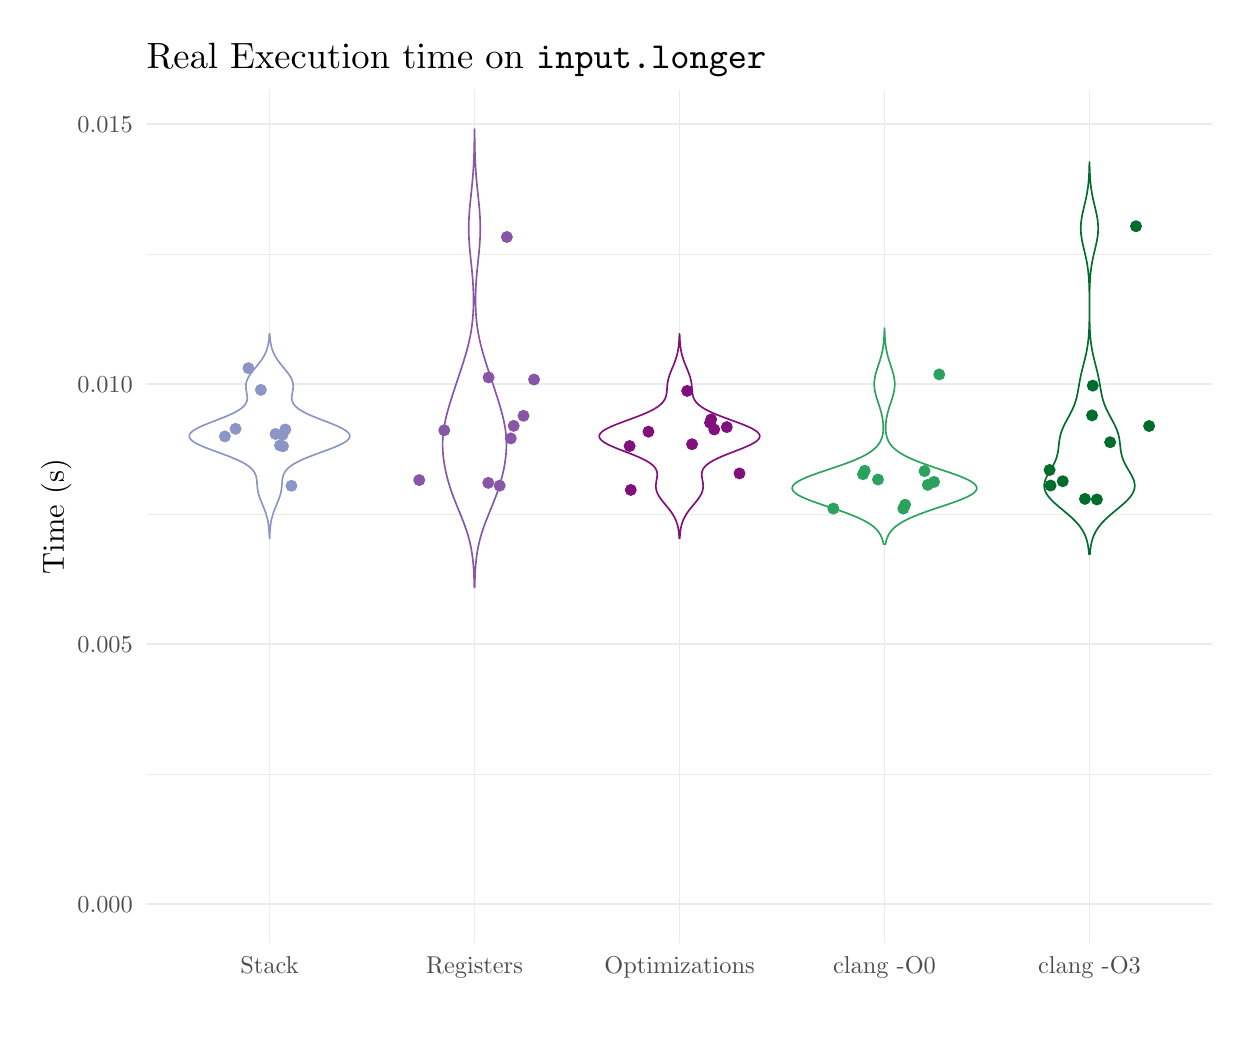
\begin{tikzpicture}[x=1pt,y=1pt]
\definecolor{fillColor}{RGB}{255,255,255}
\path[use as bounding box,fill=fillColor,fill opacity=0.00] (0,0) rectangle (433.62,361.35);
\begin{scope}
\path[clip] ( 42.95, 30.69) rectangle (428.12,338.69);
\definecolor{drawColor}{gray}{0.92}

\path[draw=drawColor,line width= 0.3pt,line join=round] ( 42.95, 91.65) --
	(428.12, 91.65);

\path[draw=drawColor,line width= 0.3pt,line join=round] ( 42.95,185.56) --
	(428.12,185.56);

\path[draw=drawColor,line width= 0.3pt,line join=round] ( 42.95,279.48) --
	(428.12,279.48);

\path[draw=drawColor,line width= 0.6pt,line join=round] ( 42.95, 44.69) --
	(428.12, 44.69);

\path[draw=drawColor,line width= 0.6pt,line join=round] ( 42.95,138.60) --
	(428.12,138.60);

\path[draw=drawColor,line width= 0.6pt,line join=round] ( 42.95,232.52) --
	(428.12,232.52);

\path[draw=drawColor,line width= 0.6pt,line join=round] ( 42.95,326.44) --
	(428.12,326.44);

\path[draw=drawColor,line width= 0.6pt,line join=round] ( 87.40, 30.69) --
	( 87.40,338.69);

\path[draw=drawColor,line width= 0.6pt,line join=round] (161.47, 30.69) --
	(161.47,338.69);

\path[draw=drawColor,line width= 0.6pt,line join=round] (235.54, 30.69) --
	(235.54,338.69);

\path[draw=drawColor,line width= 0.6pt,line join=round] (309.61, 30.69) --
	(309.61,338.69);

\path[draw=drawColor,line width= 0.6pt,line join=round] (383.68, 30.69) --
	(383.68,338.69);
\definecolor{drawColor}{RGB}{140,150,198}
\definecolor{fillColor}{RGB}{255,255,255}

\path[draw=drawColor,line width= 0.6pt,line join=round,line cap=round,fill=fillColor] ( 87.35,176.79) --
	( 87.35,176.93) --
	( 87.34,177.08) --
	( 87.34,177.22) --
	( 87.33,177.37) --
	( 87.33,177.51) --
	( 87.33,177.66) --
	( 87.32,177.80) --
	( 87.32,177.95) --
	( 87.31,178.09) --
	( 87.30,178.24) --
	( 87.30,178.38) --
	( 87.29,178.53) --
	( 87.28,178.67) --
	( 87.28,178.81) --
	( 87.27,178.96) --
	( 87.26,179.10) --
	( 87.25,179.25) --
	( 87.24,179.39) --
	( 87.23,179.54) --
	( 87.22,179.68) --
	( 87.21,179.83) --
	( 87.20,179.97) --
	( 87.19,180.12) --
	( 87.18,180.26) --
	( 87.16,180.41) --
	( 87.15,180.55) --
	( 87.14,180.69) --
	( 87.12,180.84) --
	( 87.11,180.98) --
	( 87.09,181.13) --
	( 87.07,181.27) --
	( 87.06,181.42) --
	( 87.04,181.56) --
	( 87.02,181.71) --
	( 87.00,181.85) --
	( 86.98,182.00) --
	( 86.95,182.14) --
	( 86.93,182.29) --
	( 86.91,182.43) --
	( 86.88,182.57) --
	( 86.86,182.72) --
	( 86.83,182.86) --
	( 86.80,183.01) --
	( 86.78,183.15) --
	( 86.75,183.30) --
	( 86.72,183.44) --
	( 86.68,183.59) --
	( 86.65,183.73) --
	( 86.62,183.88) --
	( 86.58,184.02) --
	( 86.55,184.17) --
	( 86.51,184.31) --
	( 86.48,184.45) --
	( 86.44,184.60) --
	( 86.40,184.74) --
	( 86.36,184.89) --
	( 86.31,185.03) --
	( 86.27,185.18) --
	( 86.23,185.32) --
	( 86.18,185.47) --
	( 86.14,185.61) --
	( 86.09,185.76) --
	( 86.04,185.90) --
	( 85.99,186.05) --
	( 85.94,186.19) --
	( 85.89,186.33) --
	( 85.84,186.48) --
	( 85.79,186.62) --
	( 85.74,186.77) --
	( 85.68,186.91) --
	( 85.63,187.06) --
	( 85.57,187.20) --
	( 85.52,187.35) --
	( 85.46,187.49) --
	( 85.40,187.64) --
	( 85.34,187.78) --
	( 85.29,187.93) --
	( 85.23,188.07) --
	( 85.17,188.21) --
	( 85.11,188.36) --
	( 85.05,188.50) --
	( 84.99,188.65) --
	( 84.93,188.79) --
	( 84.87,188.94) --
	( 84.81,189.08) --
	( 84.75,189.23) --
	( 84.69,189.37) --
	( 84.63,189.52) --
	( 84.57,189.66) --
	( 84.51,189.81) --
	( 84.45,189.95) --
	( 84.39,190.09) --
	( 84.33,190.24) --
	( 84.27,190.38) --
	( 84.22,190.53) --
	( 84.16,190.67) --
	( 84.10,190.82) --
	( 84.05,190.96) --
	( 84.00,191.11) --
	( 83.94,191.25) --
	( 83.89,191.40) --
	( 83.84,191.54) --
	( 83.79,191.69) --
	( 83.74,191.83) --
	( 83.69,191.97) --
	( 83.65,192.12) --
	( 83.60,192.26) --
	( 83.56,192.41) --
	( 83.52,192.55) --
	( 83.48,192.70) --
	( 83.44,192.84) --
	( 83.40,192.99) --
	( 83.36,193.13) --
	( 83.33,193.28) --
	( 83.29,193.42) --
	( 83.26,193.56) --
	( 83.23,193.71) --
	( 83.20,193.85) --
	( 83.18,194.00) --
	( 83.15,194.14) --
	( 83.13,194.29) --
	( 83.10,194.43) --
	( 83.08,194.58) --
	( 83.06,194.72) --
	( 83.04,194.87) --
	( 83.03,195.01) --
	( 83.01,195.16) --
	( 82.99,195.30) --
	( 82.98,195.44) --
	( 82.97,195.59) --
	( 82.95,195.73) --
	( 82.94,195.88) --
	( 82.93,196.02) --
	( 82.92,196.17) --
	( 82.91,196.31) --
	( 82.90,196.46) --
	( 82.89,196.60) --
	( 82.88,196.75) --
	( 82.87,196.89) --
	( 82.86,197.04) --
	( 82.85,197.18) --
	( 82.83,197.32) --
	( 82.82,197.47) --
	( 82.81,197.61) --
	( 82.79,197.76) --
	( 82.78,197.90) --
	( 82.76,198.05) --
	( 82.74,198.19) --
	( 82.72,198.34) --
	( 82.69,198.48) --
	( 82.67,198.63) --
	( 82.64,198.77) --
	( 82.61,198.92) --
	( 82.57,199.06) --
	( 82.54,199.20) --
	( 82.50,199.35) --
	( 82.45,199.49) --
	( 82.40,199.64) --
	( 82.35,199.78) --
	( 82.29,199.93) --
	( 82.23,200.07) --
	( 82.16,200.22) --
	( 82.09,200.36) --
	( 82.01,200.51) --
	( 81.93,200.65) --
	( 81.84,200.80) --
	( 81.75,200.94) --
	( 81.65,201.08) --
	( 81.54,201.23) --
	( 81.43,201.37) --
	( 81.31,201.52) --
	( 81.19,201.66) --
	( 81.05,201.81) --
	( 80.91,201.95) --
	( 80.76,202.10) --
	( 80.61,202.24) --
	( 80.45,202.39) --
	( 80.28,202.53) --
	( 80.10,202.68) --
	( 79.91,202.82) --
	( 79.72,202.96) --
	( 79.52,203.11) --
	( 79.30,203.25) --
	( 79.09,203.40) --
	( 78.86,203.54) --
	( 78.62,203.69) --
	( 78.38,203.83) --
	( 78.13,203.98) --
	( 77.87,204.12) --
	( 77.61,204.27) --
	( 77.33,204.41) --
	( 77.05,204.56) --
	( 76.76,204.70) --
	( 76.46,204.84) --
	( 76.15,204.99) --
	( 75.84,205.13) --
	( 75.52,205.28) --
	( 75.19,205.42) --
	( 74.86,205.57) --
	( 74.52,205.71) --
	( 74.17,205.86) --
	( 73.82,206.00) --
	( 73.46,206.15) --
	( 73.10,206.29) --
	( 72.73,206.44) --
	( 72.35,206.58) --
	( 71.98,206.72) --
	( 71.60,206.87) --
	( 71.21,207.01) --
	( 70.82,207.16) --
	( 70.43,207.30) --
	( 70.04,207.45) --
	( 69.65,207.59) --
	( 69.25,207.74) --
	( 68.86,207.88) --
	( 68.46,208.03) --
	( 68.07,208.17) --
	( 67.67,208.32) --
	( 67.28,208.46) --
	( 66.89,208.60) --
	( 66.50,208.75) --
	( 66.11,208.89) --
	( 65.73,209.04) --
	( 65.35,209.18) --
	( 64.98,209.33) --
	( 64.61,209.47) --
	( 64.25,209.62) --
	( 63.89,209.76) --
	( 63.54,209.91) --
	( 63.20,210.05) --
	( 62.86,210.20) --
	( 62.54,210.34) --
	( 62.22,210.48) --
	( 61.92,210.63) --
	( 61.62,210.77) --
	( 61.33,210.92) --
	( 61.06,211.06) --
	( 60.79,211.21) --
	( 60.54,211.35) --
	( 60.30,211.50) --
	( 60.08,211.64) --
	( 59.86,211.79) --
	( 59.66,211.93) --
	( 59.48,212.08) --
	( 59.30,212.22) --
	( 59.15,212.36) --
	( 59.01,212.51) --
	( 58.87,212.65) --
	( 58.77,212.80) --
	( 58.67,212.94) --
	( 58.58,213.09) --
	( 58.52,213.23) --
	( 58.47,213.38) --
	( 58.44,213.52) --
	( 58.42,213.67) --
	( 58.41,213.81) --
	( 58.43,213.96) --
	( 58.45,214.10) --
	( 58.50,214.24) --
	( 58.56,214.39) --
	( 58.64,214.53) --
	( 58.73,214.68) --
	( 58.83,214.82) --
	( 58.96,214.97) --
	( 59.10,215.11) --
	( 59.25,215.26) --
	( 59.42,215.40) --
	( 59.59,215.55) --
	( 59.79,215.69) --
	( 59.99,215.83) --
	( 60.21,215.98) --
	( 60.45,216.12) --
	( 60.69,216.27) --
	( 60.95,216.41) --
	( 61.21,216.56) --
	( 61.49,216.70) --
	( 61.78,216.85) --
	( 62.07,216.99) --
	( 62.38,217.14) --
	( 62.69,217.28) --
	( 63.02,217.43) --
	( 63.35,217.57) --
	( 63.68,217.71) --
	( 64.03,217.86) --
	( 64.38,218.00) --
	( 64.73,218.15) --
	( 65.09,218.29) --
	( 65.45,218.44) --
	( 65.82,218.58) --
	( 66.19,218.73) --
	( 66.56,218.87) --
	( 66.93,219.02) --
	( 67.31,219.16) --
	( 67.68,219.31) --
	( 68.06,219.45) --
	( 68.43,219.59) --
	( 68.81,219.74) --
	( 69.18,219.88) --
	( 69.55,220.03) --
	( 69.92,220.17) --
	( 70.28,220.32) --
	( 70.64,220.46) --
	( 71.00,220.61) --
	( 71.35,220.75) --
	( 71.70,220.90) --
	( 72.04,221.04) --
	( 72.38,221.19) --
	( 72.71,221.33) --
	( 73.03,221.47) --
	( 73.35,221.62) --
	( 73.66,221.76) --
	( 73.97,221.91) --
	( 74.26,222.05) --
	( 74.55,222.20) --
	( 74.83,222.34) --
	( 75.10,222.49) --
	( 75.37,222.63) --
	( 75.62,222.78) --
	( 75.87,222.92) --
	( 76.11,223.07) --
	( 76.34,223.21) --
	( 76.56,223.35) --
	( 76.77,223.50) --
	( 76.97,223.64) --
	( 77.16,223.79) --
	( 77.35,223.93) --
	( 77.52,224.08) --
	( 77.69,224.22) --
	( 77.85,224.37) --
	( 77.99,224.51) --
	( 78.13,224.66) --
	( 78.26,224.80) --
	( 78.39,224.95) --
	( 78.50,225.09) --
	( 78.60,225.23) --
	( 78.70,225.38) --
	( 78.79,225.52) --
	( 78.87,225.67) --
	( 78.95,225.81) --
	( 79.01,225.96) --
	( 79.08,226.10) --
	( 79.13,226.25) --
	( 79.17,226.39) --
	( 79.22,226.54) --
	( 79.25,226.68) --
	( 79.28,226.83) --
	( 79.30,226.97) --
	( 79.32,227.11) --
	( 79.33,227.26) --
	( 79.34,227.40) --
	( 79.34,227.55) --
	( 79.34,227.69) --
	( 79.34,227.84) --
	( 79.33,227.98) --
	( 79.32,228.13) --
	( 79.31,228.27) --
	( 79.29,228.42) --
	( 79.28,228.56) --
	( 79.26,228.71) --
	( 79.23,228.85) --
	( 79.21,228.99) --
	( 79.19,229.14) --
	( 79.16,229.28) --
	( 79.14,229.43) --
	( 79.11,229.57) --
	( 79.08,229.72) --
	( 79.06,229.86) --
	( 79.03,230.01) --
	( 79.01,230.15) --
	( 78.99,230.30) --
	( 78.97,230.44) --
	( 78.95,230.59) --
	( 78.93,230.73) --
	( 78.91,230.87) --
	( 78.90,231.02) --
	( 78.88,231.16) --
	( 78.87,231.31) --
	( 78.87,231.45) --
	( 78.86,231.60) --
	( 78.86,231.74) --
	( 78.86,231.89) --
	( 78.86,232.03) --
	( 78.87,232.18) --
	( 78.88,232.32) --
	( 78.90,232.47) --
	( 78.92,232.61) --
	( 78.94,232.75) --
	( 78.96,232.90) --
	( 78.99,233.04) --
	( 79.02,233.19) --
	( 79.06,233.33) --
	( 79.10,233.48) --
	( 79.14,233.62) --
	( 79.19,233.77) --
	( 79.24,233.91) --
	( 79.30,234.06) --
	( 79.36,234.20) --
	( 79.42,234.35) --
	( 79.48,234.49) --
	( 79.55,234.63) --
	( 79.63,234.78) --
	( 79.70,234.92) --
	( 79.78,235.07) --
	( 79.86,235.21) --
	( 79.95,235.36) --
	( 80.04,235.50) --
	( 80.13,235.65) --
	( 80.22,235.79) --
	( 80.32,235.94) --
	( 80.42,236.08) --
	( 80.52,236.22) --
	( 80.62,236.37) --
	( 80.73,236.51) --
	( 80.83,236.66) --
	( 80.94,236.80) --
	( 81.06,236.95) --
	( 81.17,237.09) --
	( 81.28,237.24) --
	( 81.40,237.38) --
	( 81.51,237.53) --
	( 81.63,237.67) --
	( 81.75,237.82) --
	( 81.87,237.96) --
	( 81.99,238.10) --
	( 82.11,238.25) --
	( 82.23,238.39) --
	( 82.35,238.54) --
	( 82.47,238.68) --
	( 82.59,238.83) --
	( 82.71,238.97) --
	( 82.83,239.12) --
	( 82.94,239.26) --
	( 83.06,239.41) --
	( 83.18,239.55) --
	( 83.30,239.70) --
	( 83.41,239.84) --
	( 83.53,239.98) --
	( 83.64,240.13) --
	( 83.75,240.27) --
	( 83.86,240.42) --
	( 83.97,240.56) --
	( 84.08,240.71) --
	( 84.19,240.85) --
	( 84.29,241.00) --
	( 84.39,241.14) --
	( 84.49,241.29) --
	( 84.59,241.43) --
	( 84.69,241.58) --
	( 84.79,241.72) --
	( 84.88,241.86) --
	( 84.97,242.01) --
	( 85.06,242.15) --
	( 85.15,242.30) --
	( 85.23,242.44) --
	( 85.32,242.59) --
	( 85.40,242.73) --
	( 85.48,242.88) --
	( 85.55,243.02) --
	( 85.63,243.17) --
	( 85.70,243.31) --
	( 85.77,243.46) --
	( 85.84,243.60) --
	( 85.91,243.74) --
	( 85.97,243.89) --
	( 86.04,244.03) --
	( 86.10,244.18) --
	( 86.16,244.32) --
	( 86.21,244.47) --
	( 86.27,244.61) --
	( 86.32,244.76) --
	( 86.37,244.90) --
	( 86.42,245.05) --
	( 86.47,245.19) --
	( 86.51,245.34) --
	( 86.56,245.48) --
	( 86.60,245.62) --
	( 86.64,245.77) --
	( 86.68,245.91) --
	( 86.71,246.06) --
	( 86.75,246.20) --
	( 86.78,246.35) --
	( 86.82,246.49) --
	( 86.85,246.64) --
	( 86.88,246.78) --
	( 86.91,246.93) --
	( 86.93,247.07) --
	( 86.96,247.22) --
	( 86.98,247.36) --
	( 87.01,247.50) --
	( 87.03,247.65) --
	( 87.05,247.79) --
	( 87.07,247.94) --
	( 87.09,248.08) --
	( 87.11,248.23) --
	( 87.13,248.37) --
	( 87.14,248.52) --
	( 87.16,248.66) --
	( 87.17,248.81) --
	( 87.19,248.95) --
	( 87.20,249.10) --
	( 87.21,249.24) --
	( 87.22,249.38) --
	( 87.24,249.53) --
	( 87.25,249.67) --
	( 87.26,249.82) --
	( 87.26,249.96) --
	( 87.27,250.11) --
	( 87.28,250.25) --
	( 87.29,250.40) --
	( 87.30,250.54) --
	( 87.30,250.69) --
	( 87.49,250.69) --
	( 87.50,250.54) --
	( 87.50,250.40) --
	( 87.51,250.25) --
	( 87.52,250.11) --
	( 87.53,249.96) --
	( 87.54,249.82) --
	( 87.55,249.67) --
	( 87.56,249.53) --
	( 87.57,249.38) --
	( 87.58,249.24) --
	( 87.59,249.10) --
	( 87.61,248.95) --
	( 87.62,248.81) --
	( 87.63,248.66) --
	( 87.65,248.52) --
	( 87.67,248.37) --
	( 87.68,248.23) --
	( 87.70,248.08) --
	( 87.72,247.94) --
	( 87.74,247.79) --
	( 87.76,247.65) --
	( 87.79,247.50) --
	( 87.81,247.36) --
	( 87.83,247.22) --
	( 87.86,247.07) --
	( 87.89,246.93) --
	( 87.92,246.78) --
	( 87.94,246.64) --
	( 87.98,246.49) --
	( 88.01,246.35) --
	( 88.04,246.20) --
	( 88.08,246.06) --
	( 88.12,245.91) --
	( 88.15,245.77) --
	( 88.19,245.62) --
	( 88.24,245.48) --
	( 88.28,245.34) --
	( 88.33,245.19) --
	( 88.37,245.05) --
	( 88.42,244.90) --
	( 88.47,244.76) --
	( 88.53,244.61) --
	( 88.58,244.47) --
	( 88.64,244.32) --
	( 88.70,244.18) --
	( 88.76,244.03) --
	( 88.82,243.89) --
	( 88.88,243.74) --
	( 88.95,243.60) --
	( 89.02,243.46) --
	( 89.09,243.31) --
	( 89.16,243.17) --
	( 89.24,243.02) --
	( 89.31,242.88) --
	( 89.39,242.73) --
	( 89.47,242.59) --
	( 89.56,242.44) --
	( 89.64,242.30) --
	( 89.73,242.15) --
	( 89.82,242.01) --
	( 89.91,241.86) --
	( 90.01,241.72) --
	( 90.10,241.58) --
	( 90.20,241.43) --
	( 90.30,241.29) --
	( 90.40,241.14) --
	( 90.50,241.00) --
	( 90.61,240.85) --
	( 90.71,240.71) --
	( 90.82,240.56) --
	( 90.93,240.42) --
	( 91.04,240.27) --
	( 91.15,240.13) --
	( 91.27,239.98) --
	( 91.38,239.84) --
	( 91.50,239.70) --
	( 91.61,239.55) --
	( 91.73,239.41) --
	( 91.85,239.26) --
	( 91.97,239.12) --
	( 92.09,238.97) --
	( 92.21,238.83) --
	( 92.33,238.68) --
	( 92.45,238.54) --
	( 92.57,238.39) --
	( 92.69,238.25) --
	( 92.81,238.10) --
	( 92.92,237.96) --
	( 93.04,237.82) --
	( 93.16,237.67) --
	( 93.28,237.53) --
	( 93.40,237.38) --
	( 93.51,237.24) --
	( 93.62,237.09) --
	( 93.74,236.95) --
	( 93.85,236.80) --
	( 93.96,236.66) --
	( 94.06,236.51) --
	( 94.17,236.37) --
	( 94.27,236.22) --
	( 94.38,236.08) --
	( 94.47,235.94) --
	( 94.57,235.79) --
	( 94.67,235.65) --
	( 94.76,235.50) --
	( 94.84,235.36) --
	( 94.93,235.21) --
	( 95.01,235.07) --
	( 95.09,234.92) --
	( 95.17,234.78) --
	( 95.24,234.63) --
	( 95.31,234.49) --
	( 95.37,234.35) --
	( 95.44,234.20) --
	( 95.49,234.06) --
	( 95.55,233.91) --
	( 95.60,233.77) --
	( 95.65,233.62) --
	( 95.69,233.48) --
	( 95.73,233.33) --
	( 95.77,233.19) --
	( 95.80,233.04) --
	( 95.83,232.90) --
	( 95.85,232.75) --
	( 95.88,232.61) --
	( 95.89,232.47) --
	( 95.91,232.32) --
	( 95.92,232.18) --
	( 95.93,232.03) --
	( 95.93,231.89) --
	( 95.93,231.74) --
	( 95.93,231.60) --
	( 95.93,231.45) --
	( 95.92,231.31) --
	( 95.91,231.16) --
	( 95.90,231.02) --
	( 95.88,230.87) --
	( 95.87,230.73) --
	( 95.85,230.59) --
	( 95.83,230.44) --
	( 95.80,230.30) --
	( 95.78,230.15) --
	( 95.76,230.01) --
	( 95.73,229.86) --
	( 95.71,229.72) --
	( 95.68,229.57) --
	( 95.66,229.43) --
	( 95.63,229.28) --
	( 95.61,229.14) --
	( 95.58,228.99) --
	( 95.56,228.85) --
	( 95.54,228.71) --
	( 95.52,228.56) --
	( 95.50,228.42) --
	( 95.48,228.27) --
	( 95.47,228.13) --
	( 95.46,227.98) --
	( 95.45,227.84) --
	( 95.45,227.69) --
	( 95.45,227.55) --
	( 95.45,227.40) --
	( 95.46,227.26) --
	( 95.47,227.11) --
	( 95.49,226.97) --
	( 95.51,226.83) --
	( 95.54,226.68) --
	( 95.58,226.54) --
	( 95.62,226.39) --
	( 95.66,226.25) --
	( 95.72,226.10) --
	( 95.78,225.96) --
	( 95.84,225.81) --
	( 95.92,225.67) --
	( 96.00,225.52) --
	( 96.09,225.38) --
	( 96.19,225.23) --
	( 96.29,225.09) --
	( 96.41,224.95) --
	( 96.53,224.80) --
	( 96.66,224.66) --
	( 96.80,224.51) --
	( 96.95,224.37) --
	( 97.10,224.22) --
	( 97.27,224.08) --
	( 97.44,223.93) --
	( 97.63,223.79) --
	( 97.82,223.64) --
	( 98.02,223.50) --
	( 98.24,223.35) --
	( 98.45,223.21) --
	( 98.69,223.07) --
	( 98.92,222.92) --
	( 99.17,222.78) --
	( 99.43,222.63) --
	( 99.69,222.49) --
	( 99.96,222.34) --
	(100.24,222.20) --
	(100.53,222.05) --
	(100.83,221.91) --
	(101.13,221.76) --
	(101.44,221.62) --
	(101.76,221.47) --
	(102.08,221.33) --
	(102.41,221.19) --
	(102.75,221.04) --
	(103.09,220.90) --
	(103.44,220.75) --
	(103.79,220.61) --
	(104.15,220.46) --
	(104.51,220.32) --
	(104.88,220.17) --
	(105.24,220.03) --
	(105.61,219.88) --
	(105.99,219.74) --
	(106.36,219.59) --
	(106.73,219.45) --
	(107.11,219.31) --
	(107.48,219.16) --
	(107.86,219.02) --
	(108.23,218.87) --
	(108.60,218.73) --
	(108.97,218.58) --
	(109.34,218.44) --
	(109.70,218.29) --
	(110.06,218.15) --
	(110.42,218.00) --
	(110.77,217.86) --
	(111.11,217.71) --
	(111.45,217.57) --
	(111.78,217.43) --
	(112.10,217.28) --
	(112.41,217.14) --
	(112.72,216.99) --
	(113.02,216.85) --
	(113.31,216.70) --
	(113.58,216.56) --
	(113.85,216.41) --
	(114.11,216.27) --
	(114.35,216.12) --
	(114.58,215.98) --
	(114.80,215.83) --
	(115.00,215.69) --
	(115.20,215.55) --
	(115.38,215.40) --
	(115.55,215.26) --
	(115.70,215.11) --
	(115.83,214.97) --
	(115.96,214.82) --
	(116.06,214.68) --
	(116.15,214.53) --
	(116.23,214.39) --
	(116.29,214.24) --
	(116.34,214.10) --
	(116.36,213.96) --
	(116.38,213.81) --
	(116.38,213.67) --
	(116.36,213.52) --
	(116.33,213.38) --
	(116.27,213.23) --
	(116.21,213.09) --
	(116.13,212.94) --
	(116.03,212.80) --
	(115.92,212.65) --
	(115.79,212.51) --
	(115.65,212.36) --
	(115.49,212.22) --
	(115.31,212.08) --
	(115.13,211.93) --
	(114.93,211.79) --
	(114.72,211.64) --
	(114.49,211.50) --
	(114.25,211.35) --
	(114.00,211.21) --
	(113.73,211.06) --
	(113.46,210.92) --
	(113.17,210.77) --
	(112.88,210.63) --
	(112.57,210.48) --
	(112.25,210.34) --
	(111.93,210.20) --
	(111.60,210.05) --
	(111.25,209.91) --
	(110.90,209.76) --
	(110.55,209.62) --
	(110.18,209.47) --
	(109.82,209.33) --
	(109.44,209.18) --
	(109.06,209.04) --
	(108.68,208.89) --
	(108.30,208.75) --
	(107.91,208.60) --
	(107.52,208.46) --
	(107.12,208.32) --
	(106.73,208.17) --
	(106.33,208.03) --
	(105.94,207.88) --
	(105.54,207.74) --
	(105.14,207.59) --
	(104.75,207.45) --
	(104.36,207.30) --
	(103.97,207.16) --
	(103.58,207.01) --
	(103.20,206.87) --
	(102.82,206.72) --
	(102.44,206.58) --
	(102.06,206.44) --
	(101.70,206.29) --
	(101.33,206.15) --
	(100.97,206.00) --
	(100.62,205.86) --
	(100.27,205.71) --
	( 99.94,205.57) --
	( 99.60,205.42) --
	( 99.27,205.28) --
	( 98.95,205.13) --
	( 98.64,204.99) --
	( 98.34,204.84) --
	( 98.04,204.70) --
	( 97.75,204.56) --
	( 97.46,204.41) --
	( 97.19,204.27) --
	( 96.92,204.12) --
	( 96.66,203.98) --
	( 96.41,203.83) --
	( 96.17,203.69) --
	( 95.93,203.54) --
	( 95.71,203.40) --
	( 95.49,203.25) --
	( 95.28,203.11) --
	( 95.08,202.96) --
	( 94.88,202.82) --
	( 94.70,202.68) --
	( 94.52,202.53) --
	( 94.35,202.39) --
	( 94.18,202.24) --
	( 94.03,202.10) --
	( 93.88,201.95) --
	( 93.74,201.81) --
	( 93.61,201.66) --
	( 93.48,201.52) --
	( 93.36,201.37) --
	( 93.25,201.23) --
	( 93.14,201.08) --
	( 93.04,200.94) --
	( 92.95,200.80) --
	( 92.86,200.65) --
	( 92.78,200.51) --
	( 92.70,200.36) --
	( 92.63,200.22) --
	( 92.56,200.07) --
	( 92.50,199.93) --
	( 92.44,199.78) --
	( 92.39,199.64) --
	( 92.34,199.49) --
	( 92.30,199.35) --
	( 92.26,199.20) --
	( 92.22,199.06) --
	( 92.18,198.92) --
	( 92.15,198.77) --
	( 92.12,198.63) --
	( 92.10,198.48) --
	( 92.07,198.34) --
	( 92.05,198.19) --
	( 92.03,198.05) --
	( 92.02,197.90) --
	( 92.00,197.76) --
	( 91.98,197.61) --
	( 91.97,197.47) --
	( 91.96,197.32) --
	( 91.95,197.18) --
	( 91.94,197.04) --
	( 91.93,196.89) --
	( 91.92,196.75) --
	( 91.91,196.60) --
	( 91.90,196.46) --
	( 91.88,196.31) --
	( 91.87,196.17) --
	( 91.86,196.02) --
	( 91.85,195.88) --
	( 91.84,195.73) --
	( 91.83,195.59) --
	( 91.81,195.44) --
	( 91.80,195.30) --
	( 91.78,195.16) --
	( 91.77,195.01) --
	( 91.75,194.87) --
	( 91.73,194.72) --
	( 91.71,194.58) --
	( 91.69,194.43) --
	( 91.67,194.29) --
	( 91.64,194.14) --
	( 91.62,194.00) --
	( 91.59,193.85) --
	( 91.56,193.71) --
	( 91.53,193.56) --
	( 91.50,193.42) --
	( 91.46,193.28) --
	( 91.43,193.13) --
	( 91.39,192.99) --
	( 91.36,192.84) --
	( 91.32,192.70) --
	( 91.28,192.55) --
	( 91.23,192.41) --
	( 91.19,192.26) --
	( 91.15,192.12) --
	( 91.10,191.97) --
	( 91.05,191.83) --
	( 91.00,191.69) --
	( 90.95,191.54) --
	( 90.90,191.40) --
	( 90.85,191.25) --
	( 90.80,191.11) --
	( 90.74,190.96) --
	( 90.69,190.82) --
	( 90.63,190.67) --
	( 90.58,190.53) --
	( 90.52,190.38) --
	( 90.46,190.24) --
	( 90.40,190.09) --
	( 90.34,189.95) --
	( 90.28,189.81) --
	( 90.23,189.66) --
	( 90.17,189.52) --
	( 90.11,189.37) --
	( 90.05,189.23) --
	( 89.98,189.08) --
	( 89.92,188.94) --
	( 89.86,188.79) --
	( 89.80,188.65) --
	( 89.74,188.50) --
	( 89.68,188.36) --
	( 89.62,188.21) --
	( 89.57,188.07) --
	( 89.51,187.93) --
	( 89.45,187.78) --
	( 89.39,187.64) --
	( 89.33,187.49) --
	( 89.28,187.35) --
	( 89.22,187.20) --
	( 89.16,187.06) --
	( 89.11,186.91) --
	( 89.06,186.77) --
	( 89.00,186.62) --
	( 88.95,186.48) --
	( 88.90,186.33) --
	( 88.85,186.19) --
	( 88.80,186.05) --
	( 88.75,185.90) --
	( 88.70,185.76) --
	( 88.65,185.61) --
	( 88.61,185.47) --
	( 88.56,185.32) --
	( 88.52,185.18) --
	( 88.48,185.03) --
	( 88.44,184.89) --
	( 88.40,184.74) --
	( 88.36,184.60) --
	( 88.32,184.45) --
	( 88.28,184.31) --
	( 88.24,184.17) --
	( 88.21,184.02) --
	( 88.17,183.88) --
	( 88.14,183.73) --
	( 88.11,183.59) --
	( 88.08,183.44) --
	( 88.05,183.30) --
	( 88.02,183.15) --
	( 87.99,183.01) --
	( 87.96,182.86) --
	( 87.93,182.72) --
	( 87.91,182.57) --
	( 87.88,182.43) --
	( 87.86,182.29) --
	( 87.84,182.14) --
	( 87.82,182.00) --
	( 87.80,181.85) --
	( 87.78,181.71) --
	( 87.76,181.56) --
	( 87.74,181.42) --
	( 87.72,181.27) --
	( 87.70,181.13) --
	( 87.69,180.98) --
	( 87.67,180.84) --
	( 87.66,180.69) --
	( 87.64,180.55) --
	( 87.63,180.41) --
	( 87.61,180.26) --
	( 87.60,180.12) --
	( 87.59,179.97) --
	( 87.58,179.83) --
	( 87.57,179.68) --
	( 87.56,179.54) --
	( 87.55,179.39) --
	( 87.54,179.25) --
	( 87.53,179.10) --
	( 87.52,178.96) --
	( 87.52,178.81) --
	( 87.51,178.67) --
	( 87.50,178.53) --
	( 87.49,178.38) --
	( 87.49,178.24) --
	( 87.48,178.09) --
	( 87.48,177.95) --
	( 87.47,177.80) --
	( 87.47,177.66) --
	( 87.46,177.51) --
	( 87.46,177.37) --
	( 87.45,177.22) --
	( 87.45,177.08) --
	( 87.45,176.93) --
	( 87.44,176.79) --
	( 87.35,176.79) --
	cycle;
\definecolor{drawColor}{RGB}{136,86,167}

\path[draw=drawColor,line width= 0.6pt,line join=round,line cap=round,fill=fillColor] (161.40,159.13) --
	(161.39,159.46) --
	(161.38,159.78) --
	(161.38,160.11) --
	(161.37,160.43) --
	(161.36,160.75) --
	(161.35,161.08) --
	(161.34,161.40) --
	(161.33,161.73) --
	(161.32,162.05) --
	(161.31,162.37) --
	(161.30,162.70) --
	(161.29,163.02) --
	(161.27,163.35) --
	(161.26,163.67) --
	(161.25,163.99) --
	(161.23,164.32) --
	(161.21,164.64) --
	(161.19,164.97) --
	(161.18,165.29) --
	(161.16,165.61) --
	(161.13,165.94) --
	(161.11,166.26) --
	(161.09,166.59) --
	(161.06,166.91) --
	(161.04,167.23) --
	(161.01,167.56) --
	(160.98,167.88) --
	(160.95,168.21) --
	(160.91,168.53) --
	(160.88,168.85) --
	(160.84,169.18) --
	(160.81,169.50) --
	(160.77,169.83) --
	(160.73,170.15) --
	(160.68,170.47) --
	(160.64,170.80) --
	(160.59,171.12) --
	(160.54,171.45) --
	(160.49,171.77) --
	(160.44,172.09) --
	(160.38,172.42) --
	(160.33,172.74) --
	(160.27,173.07) --
	(160.20,173.39) --
	(160.14,173.71) --
	(160.07,174.04) --
	(160.01,174.36) --
	(159.93,174.69) --
	(159.86,175.01) --
	(159.79,175.33) --
	(159.71,175.66) --
	(159.63,175.98) --
	(159.54,176.31) --
	(159.46,176.63) --
	(159.37,176.95) --
	(159.28,177.28) --
	(159.19,177.60) --
	(159.10,177.93) --
	(159.00,178.25) --
	(158.90,178.57) --
	(158.80,178.90) --
	(158.70,179.22) --
	(158.59,179.55) --
	(158.48,179.87) --
	(158.37,180.19) --
	(158.26,180.52) --
	(158.15,180.84) --
	(158.03,181.17) --
	(157.92,181.49) --
	(157.80,181.81) --
	(157.68,182.14) --
	(157.56,182.46) --
	(157.43,182.79) --
	(157.31,183.11) --
	(157.18,183.43) --
	(157.06,183.76) --
	(156.93,184.08) --
	(156.80,184.41) --
	(156.67,184.73) --
	(156.54,185.05) --
	(156.41,185.38) --
	(156.28,185.70) --
	(156.15,186.03) --
	(156.01,186.35) --
	(155.88,186.67) --
	(155.75,187.00) --
	(155.62,187.32) --
	(155.48,187.65) --
	(155.35,187.97) --
	(155.22,188.29) --
	(155.09,188.62) --
	(154.96,188.94) --
	(154.83,189.27) --
	(154.70,189.59) --
	(154.57,189.91) --
	(154.44,190.24) --
	(154.31,190.56) --
	(154.19,190.89) --
	(154.06,191.21) --
	(153.94,191.53) --
	(153.82,191.86) --
	(153.70,192.18) --
	(153.58,192.51) --
	(153.46,192.83) --
	(153.34,193.15) --
	(153.23,193.48) --
	(153.11,193.80) --
	(153.00,194.13) --
	(152.89,194.45) --
	(152.78,194.77) --
	(152.68,195.10) --
	(152.57,195.42) --
	(152.47,195.75) --
	(152.37,196.07) --
	(152.27,196.39) --
	(152.17,196.72) --
	(152.08,197.04) --
	(151.98,197.36) --
	(151.89,197.69) --
	(151.80,198.01) --
	(151.72,198.34) --
	(151.63,198.66) --
	(151.55,198.98) --
	(151.46,199.31) --
	(151.38,199.63) --
	(151.31,199.96) --
	(151.23,200.28) --
	(151.16,200.60) --
	(151.09,200.93) --
	(151.01,201.25) --
	(150.95,201.58) --
	(150.88,201.90) --
	(150.82,202.22) --
	(150.76,202.55) --
	(150.69,202.87) --
	(150.64,203.20) --
	(150.58,203.52) --
	(150.53,203.84) --
	(150.48,204.17) --
	(150.43,204.49) --
	(150.38,204.82) --
	(150.33,205.14) --
	(150.29,205.46) --
	(150.25,205.79) --
	(150.21,206.11) --
	(150.18,206.44) --
	(150.14,206.76) --
	(150.11,207.08) --
	(150.08,207.41) --
	(150.06,207.73) --
	(150.03,208.06) --
	(150.01,208.38) --
	(149.99,208.70) --
	(149.98,209.03) --
	(149.96,209.35) --
	(149.95,209.68) --
	(149.94,210.00) --
	(149.94,210.32) --
	(149.94,210.65) --
	(149.94,210.97) --
	(149.94,211.30) --
	(149.94,211.62) --
	(149.95,211.94) --
	(149.97,212.27) --
	(149.98,212.59) --
	(150.00,212.92) --
	(150.02,213.24) --
	(150.04,213.56) --
	(150.07,213.89) --
	(150.09,214.21) --
	(150.13,214.54) --
	(150.16,214.86) --
	(150.20,215.18) --
	(150.24,215.51) --
	(150.28,215.83) --
	(150.32,216.16) --
	(150.37,216.48) --
	(150.42,216.80) --
	(150.48,217.13) --
	(150.53,217.45) --
	(150.59,217.78) --
	(150.65,218.10) --
	(150.71,218.42) --
	(150.78,218.75) --
	(150.85,219.07) --
	(150.92,219.40) --
	(150.99,219.72) --
	(151.06,220.04) --
	(151.14,220.37) --
	(151.22,220.69) --
	(151.30,221.02) --
	(151.38,221.34) --
	(151.46,221.66) --
	(151.55,221.99) --
	(151.63,222.31) --
	(151.72,222.64) --
	(151.81,222.96) --
	(151.90,223.28) --
	(151.99,223.61) --
	(152.08,223.93) --
	(152.18,224.26) --
	(152.27,224.58) --
	(152.37,224.90) --
	(152.46,225.23) --
	(152.56,225.55) --
	(152.66,225.88) --
	(152.76,226.20) --
	(152.86,226.52) --
	(152.96,226.85) --
	(153.06,227.17) --
	(153.16,227.50) --
	(153.27,227.82) --
	(153.37,228.14) --
	(153.47,228.47) --
	(153.58,228.79) --
	(153.68,229.12) --
	(153.79,229.44) --
	(153.89,229.76) --
	(154.00,230.09) --
	(154.10,230.41) --
	(154.21,230.74) --
	(154.32,231.06) --
	(154.42,231.38) --
	(154.53,231.71) --
	(154.64,232.03) --
	(154.75,232.36) --
	(154.85,232.68) --
	(154.96,233.00) --
	(155.07,233.33) --
	(155.18,233.65) --
	(155.28,233.98) --
	(155.39,234.30) --
	(155.50,234.62) --
	(155.61,234.95) --
	(155.72,235.27) --
	(155.82,235.60) --
	(155.93,235.92) --
	(156.04,236.24) --
	(156.15,236.57) --
	(156.26,236.89) --
	(156.36,237.22) --
	(156.47,237.54) --
	(156.58,237.86) --
	(156.68,238.19) --
	(156.79,238.51) --
	(156.89,238.84) --
	(157.00,239.16) --
	(157.10,239.48) --
	(157.21,239.81) --
	(157.31,240.13) --
	(157.41,240.46) --
	(157.52,240.78) --
	(157.62,241.10) --
	(157.72,241.43) --
	(157.82,241.75) --
	(157.92,242.08) --
	(158.02,242.40) --
	(158.11,242.72) --
	(158.21,243.05) --
	(158.30,243.37) --
	(158.40,243.70) --
	(158.49,244.02) --
	(158.58,244.34) --
	(158.67,244.67) --
	(158.76,244.99) --
	(158.85,245.32) --
	(158.93,245.64) --
	(159.02,245.96) --
	(159.10,246.29) --
	(159.18,246.61) --
	(159.26,246.94) --
	(159.34,247.26) --
	(159.42,247.58) --
	(159.49,247.91) --
	(159.56,248.23) --
	(159.64,248.56) --
	(159.71,248.88) --
	(159.77,249.20) --
	(159.84,249.53) --
	(159.91,249.85) --
	(159.97,250.18) --
	(160.03,250.50) --
	(160.09,250.82) --
	(160.15,251.15) --
	(160.20,251.47) --
	(160.26,251.80) --
	(160.31,252.12) --
	(160.36,252.44) --
	(160.41,252.77) --
	(160.45,253.09) --
	(160.50,253.42) --
	(160.54,253.74) --
	(160.58,254.06) --
	(160.62,254.39) --
	(160.66,254.71) --
	(160.70,255.03) --
	(160.73,255.36) --
	(160.76,255.68) --
	(160.80,256.01) --
	(160.82,256.33) --
	(160.85,256.65) --
	(160.88,256.98) --
	(160.90,257.30) --
	(160.93,257.63) --
	(160.95,257.95) --
	(160.97,258.27) --
	(160.99,258.60) --
	(161.00,258.92) --
	(161.02,259.25) --
	(161.03,259.57) --
	(161.05,259.89) --
	(161.06,260.22) --
	(161.07,260.54) --
	(161.08,260.87) --
	(161.08,261.19) --
	(161.09,261.51) --
	(161.09,261.84) --
	(161.10,262.16) --
	(161.10,262.49) --
	(161.10,262.81) --
	(161.10,263.13) --
	(161.10,263.46) --
	(161.10,263.78) --
	(161.09,264.11) --
	(161.09,264.43) --
	(161.08,264.75) --
	(161.07,265.08) --
	(161.07,265.40) --
	(161.06,265.73) --
	(161.05,266.05) --
	(161.03,266.37) --
	(161.02,266.70) --
	(161.01,267.02) --
	(160.99,267.35) --
	(160.98,267.67) --
	(160.96,267.99) --
	(160.94,268.32) --
	(160.92,268.64) --
	(160.90,268.97) --
	(160.88,269.29) --
	(160.86,269.61) --
	(160.84,269.94) --
	(160.81,270.26) --
	(160.79,270.59) --
	(160.77,270.91) --
	(160.74,271.23) --
	(160.71,271.56) --
	(160.69,271.88) --
	(160.66,272.21) --
	(160.63,272.53) --
	(160.60,272.85) --
	(160.57,273.18) --
	(160.54,273.50) --
	(160.51,273.83) --
	(160.48,274.15) --
	(160.44,274.47) --
	(160.41,274.80) --
	(160.38,275.12) --
	(160.35,275.45) --
	(160.31,275.77) --
	(160.28,276.09) --
	(160.25,276.42) --
	(160.21,276.74) --
	(160.18,277.07) --
	(160.14,277.39) --
	(160.11,277.71) --
	(160.08,278.04) --
	(160.04,278.36) --
	(160.01,278.69) --
	(159.98,279.01) --
	(159.94,279.33) --
	(159.91,279.66) --
	(159.88,279.98) --
	(159.85,280.31) --
	(159.82,280.63) --
	(159.79,280.95) --
	(159.76,281.28) --
	(159.73,281.60) --
	(159.70,281.93) --
	(159.67,282.25) --
	(159.64,282.57) --
	(159.62,282.90) --
	(159.60,283.22) --
	(159.57,283.55) --
	(159.55,283.87) --
	(159.53,284.19) --
	(159.51,284.52) --
	(159.49,284.84) --
	(159.47,285.17) --
	(159.46,285.49) --
	(159.44,285.81) --
	(159.43,286.14) --
	(159.42,286.46) --
	(159.41,286.79) --
	(159.40,287.11) --
	(159.39,287.43) --
	(159.38,287.76) --
	(159.38,288.08) --
	(159.38,288.41) --
	(159.37,288.73) --
	(159.37,289.05) --
	(159.38,289.38) --
	(159.38,289.70) --
	(159.38,290.03) --
	(159.39,290.35) --
	(159.40,290.67) --
	(159.41,291.00) --
	(159.42,291.32) --
	(159.43,291.65) --
	(159.44,291.97) --
	(159.46,292.29) --
	(159.47,292.62) --
	(159.49,292.94) --
	(159.51,293.27) --
	(159.53,293.59) --
	(159.55,293.91) --
	(159.57,294.24) --
	(159.60,294.56) --
	(159.62,294.89) --
	(159.65,295.21) --
	(159.68,295.53) --
	(159.70,295.86) --
	(159.73,296.18) --
	(159.76,296.51) --
	(159.79,296.83) --
	(159.82,297.15) --
	(159.85,297.48) --
	(159.88,297.80) --
	(159.92,298.13) --
	(159.95,298.45) --
	(159.98,298.77) --
	(160.02,299.10) --
	(160.05,299.42) --
	(160.08,299.75) --
	(160.12,300.07) --
	(160.15,300.39) --
	(160.19,300.72) --
	(160.22,301.04) --
	(160.25,301.37) --
	(160.29,301.69) --
	(160.32,302.01) --
	(160.36,302.34) --
	(160.39,302.66) --
	(160.42,302.99) --
	(160.46,303.31) --
	(160.49,303.63) --
	(160.52,303.96) --
	(160.55,304.28) --
	(160.59,304.61) --
	(160.62,304.93) --
	(160.65,305.25) --
	(160.68,305.58) --
	(160.71,305.90) --
	(160.74,306.23) --
	(160.77,306.55) --
	(160.79,306.87) --
	(160.82,307.20) --
	(160.85,307.52) --
	(160.87,307.85) --
	(160.90,308.17) --
	(160.92,308.49) --
	(160.95,308.82) --
	(160.97,309.14) --
	(160.99,309.47) --
	(161.01,309.79) --
	(161.03,310.11) --
	(161.06,310.44) --
	(161.08,310.76) --
	(161.09,311.08) --
	(161.11,311.41) --
	(161.13,311.73) --
	(161.15,312.06) --
	(161.16,312.38) --
	(161.18,312.70) --
	(161.19,313.03) --
	(161.21,313.35) --
	(161.22,313.68) --
	(161.24,314.00) --
	(161.25,314.32) --
	(161.26,314.65) --
	(161.27,314.97) --
	(161.28,315.30) --
	(161.30,315.62) --
	(161.31,315.94) --
	(161.32,316.27) --
	(161.32,316.59) --
	(161.33,316.92) --
	(161.34,317.24) --
	(161.35,317.56) --
	(161.36,317.89) --
	(161.36,318.21) --
	(161.37,318.54) --
	(161.38,318.86) --
	(161.38,319.18) --
	(161.39,319.51) --
	(161.39,319.83) --
	(161.40,320.16) --
	(161.40,320.48) --
	(161.41,320.80) --
	(161.41,321.13) --
	(161.42,321.45) --
	(161.42,321.78) --
	(161.42,322.10) --
	(161.43,322.42) --
	(161.43,322.75) --
	(161.43,323.07) --
	(161.43,323.40) --
	(161.44,323.72) --
	(161.44,324.04) --
	(161.44,324.37) --
	(161.44,324.69) --
	(161.49,324.69) --
	(161.49,324.37) --
	(161.49,324.04) --
	(161.50,323.72) --
	(161.50,323.40) --
	(161.50,323.07) --
	(161.50,322.75) --
	(161.51,322.42) --
	(161.51,322.10) --
	(161.51,321.78) --
	(161.52,321.45) --
	(161.52,321.13) --
	(161.53,320.80) --
	(161.53,320.48) --
	(161.53,320.16) --
	(161.54,319.83) --
	(161.55,319.51) --
	(161.55,319.18) --
	(161.56,318.86) --
	(161.56,318.54) --
	(161.57,318.21) --
	(161.58,317.89) --
	(161.58,317.56) --
	(161.59,317.24) --
	(161.60,316.92) --
	(161.61,316.59) --
	(161.62,316.27) --
	(161.63,315.94) --
	(161.64,315.62) --
	(161.65,315.30) --
	(161.66,314.97) --
	(161.67,314.65) --
	(161.68,314.32) --
	(161.70,314.00) --
	(161.71,313.68) --
	(161.72,313.35) --
	(161.74,313.03) --
	(161.75,312.70) --
	(161.77,312.38) --
	(161.79,312.06) --
	(161.80,311.73) --
	(161.82,311.41) --
	(161.84,311.08) --
	(161.86,310.76) --
	(161.88,310.44) --
	(161.90,310.11) --
	(161.92,309.79) --
	(161.94,309.47) --
	(161.96,309.14) --
	(161.99,308.82) --
	(162.01,308.49) --
	(162.04,308.17) --
	(162.06,307.85) --
	(162.09,307.52) --
	(162.11,307.20) --
	(162.14,306.87) --
	(162.17,306.55) --
	(162.20,306.23) --
	(162.23,305.90) --
	(162.25,305.58) --
	(162.29,305.25) --
	(162.32,304.93) --
	(162.35,304.61) --
	(162.38,304.28) --
	(162.41,303.96) --
	(162.44,303.63) --
	(162.48,303.31) --
	(162.51,302.99) --
	(162.54,302.66) --
	(162.58,302.34) --
	(162.61,302.01) --
	(162.64,301.69) --
	(162.68,301.37) --
	(162.71,301.04) --
	(162.75,300.72) --
	(162.78,300.39) --
	(162.82,300.07) --
	(162.85,299.75) --
	(162.88,299.42) --
	(162.92,299.10) --
	(162.95,298.77) --
	(162.98,298.45) --
	(163.02,298.13) --
	(163.05,297.80) --
	(163.08,297.48) --
	(163.11,297.15) --
	(163.14,296.83) --
	(163.17,296.51) --
	(163.20,296.18) --
	(163.23,295.86) --
	(163.26,295.53) --
	(163.28,295.21) --
	(163.31,294.89) --
	(163.33,294.56) --
	(163.36,294.24) --
	(163.38,293.91) --
	(163.40,293.59) --
	(163.42,293.27) --
	(163.44,292.94) --
	(163.46,292.62) --
	(163.47,292.29) --
	(163.49,291.97) --
	(163.50,291.65) --
	(163.52,291.32) --
	(163.53,291.00) --
	(163.54,290.67) --
	(163.54,290.35) --
	(163.55,290.03) --
	(163.55,289.70) --
	(163.56,289.38) --
	(163.56,289.05) --
	(163.56,288.73) --
	(163.56,288.41) --
	(163.55,288.08) --
	(163.55,287.76) --
	(163.54,287.43) --
	(163.54,287.11) --
	(163.53,286.79) --
	(163.52,286.46) --
	(163.51,286.14) --
	(163.49,285.81) --
	(163.48,285.49) --
	(163.46,285.17) --
	(163.44,284.84) --
	(163.42,284.52) --
	(163.40,284.19) --
	(163.38,283.87) --
	(163.36,283.55) --
	(163.34,283.22) --
	(163.31,282.90) --
	(163.29,282.57) --
	(163.26,282.25) --
	(163.23,281.93) --
	(163.21,281.60) --
	(163.18,281.28) --
	(163.15,280.95) --
	(163.12,280.63) --
	(163.09,280.31) --
	(163.06,279.98) --
	(163.02,279.66) --
	(162.99,279.33) --
	(162.96,279.01) --
	(162.92,278.69) --
	(162.89,278.36) --
	(162.86,278.04) --
	(162.82,277.71) --
	(162.79,277.39) --
	(162.76,277.07) --
	(162.72,276.74) --
	(162.69,276.42) --
	(162.65,276.09) --
	(162.62,275.77) --
	(162.59,275.45) --
	(162.55,275.12) --
	(162.52,274.80) --
	(162.49,274.47) --
	(162.46,274.15) --
	(162.43,273.83) --
	(162.39,273.50) --
	(162.36,273.18) --
	(162.33,272.85) --
	(162.30,272.53) --
	(162.28,272.21) --
	(162.25,271.88) --
	(162.22,271.56) --
	(162.19,271.23) --
	(162.17,270.91) --
	(162.14,270.59) --
	(162.12,270.26) --
	(162.10,269.94) --
	(162.07,269.61) --
	(162.05,269.29) --
	(162.03,268.97) --
	(162.01,268.64) --
	(161.99,268.32) --
	(161.97,267.99) --
	(161.96,267.67) --
	(161.94,267.35) --
	(161.93,267.02) --
	(161.91,266.70) --
	(161.90,266.37) --
	(161.89,266.05) --
	(161.88,265.73) --
	(161.87,265.40) --
	(161.86,265.08) --
	(161.85,264.75) --
	(161.85,264.43) --
	(161.84,264.11) --
	(161.84,263.78) --
	(161.83,263.46) --
	(161.83,263.13) --
	(161.83,262.81) --
	(161.83,262.49) --
	(161.83,262.16) --
	(161.84,261.84) --
	(161.84,261.51) --
	(161.85,261.19) --
	(161.86,260.87) --
	(161.86,260.54) --
	(161.88,260.22) --
	(161.89,259.89) --
	(161.90,259.57) --
	(161.91,259.25) --
	(161.93,258.92) --
	(161.95,258.60) --
	(161.97,258.27) --
	(161.98,257.95) --
	(162.01,257.63) --
	(162.03,257.30) --
	(162.05,256.98) --
	(162.08,256.65) --
	(162.11,256.33) --
	(162.14,256.01) --
	(162.17,255.68) --
	(162.20,255.36) --
	(162.24,255.03) --
	(162.27,254.71) --
	(162.31,254.39) --
	(162.35,254.06) --
	(162.39,253.74) --
	(162.43,253.42) --
	(162.48,253.09) --
	(162.53,252.77) --
	(162.58,252.44) --
	(162.63,252.12) --
	(162.68,251.80) --
	(162.73,251.47) --
	(162.79,251.15) --
	(162.84,250.82) --
	(162.90,250.50) --
	(162.97,250.18) --
	(163.03,249.85) --
	(163.09,249.53) --
	(163.16,249.20) --
	(163.23,248.88) --
	(163.30,248.56) --
	(163.37,248.23) --
	(163.44,247.91) --
	(163.52,247.58) --
	(163.59,247.26) --
	(163.67,246.94) --
	(163.75,246.61) --
	(163.83,246.29) --
	(163.92,245.96) --
	(164.00,245.64) --
	(164.09,245.32) --
	(164.17,244.99) --
	(164.26,244.67) --
	(164.35,244.34) --
	(164.44,244.02) --
	(164.54,243.70) --
	(164.63,243.37) --
	(164.72,243.05) --
	(164.82,242.72) --
	(164.92,242.40) --
	(165.02,242.08) --
	(165.11,241.75) --
	(165.21,241.43) --
	(165.31,241.10) --
	(165.42,240.78) --
	(165.52,240.46) --
	(165.62,240.13) --
	(165.72,239.81) --
	(165.83,239.48) --
	(165.93,239.16) --
	(166.04,238.84) --
	(166.14,238.51) --
	(166.25,238.19) --
	(166.36,237.86) --
	(166.46,237.54) --
	(166.57,237.22) --
	(166.68,236.89) --
	(166.79,236.57) --
	(166.89,236.24) --
	(167.00,235.92) --
	(167.11,235.60) --
	(167.22,235.27) --
	(167.32,234.95) --
	(167.43,234.62) --
	(167.54,234.30) --
	(167.65,233.98) --
	(167.76,233.65) --
	(167.86,233.33) --
	(167.97,233.00) --
	(168.08,232.68) --
	(168.19,232.36) --
	(168.30,232.03) --
	(168.40,231.71) --
	(168.51,231.38) --
	(168.62,231.06) --
	(168.72,230.74) --
	(168.83,230.41) --
	(168.93,230.09) --
	(169.04,229.76) --
	(169.15,229.44) --
	(169.25,229.12) --
	(169.36,228.79) --
	(169.46,228.47) --
	(169.56,228.14) --
	(169.67,227.82) --
	(169.77,227.50) --
	(169.87,227.17) --
	(169.97,226.85) --
	(170.07,226.52) --
	(170.17,226.20) --
	(170.27,225.88) --
	(170.37,225.55) --
	(170.47,225.23) --
	(170.57,224.90) --
	(170.66,224.58) --
	(170.76,224.26) --
	(170.85,223.93) --
	(170.94,223.61) --
	(171.04,223.28) --
	(171.13,222.96) --
	(171.21,222.64) --
	(171.30,222.31) --
	(171.39,221.99) --
	(171.47,221.66) --
	(171.56,221.34) --
	(171.64,221.02) --
	(171.72,220.69) --
	(171.79,220.37) --
	(171.87,220.04) --
	(171.94,219.72) --
	(172.02,219.40) --
	(172.09,219.07) --
	(172.15,218.75) --
	(172.22,218.42) --
	(172.28,218.10) --
	(172.34,217.78) --
	(172.40,217.45) --
	(172.46,217.13) --
	(172.51,216.80) --
	(172.56,216.48) --
	(172.61,216.16) --
	(172.65,215.83) --
	(172.70,215.51) --
	(172.74,215.18) --
	(172.77,214.86) --
	(172.81,214.54) --
	(172.84,214.21) --
	(172.87,213.89) --
	(172.89,213.56) --
	(172.92,213.24) --
	(172.94,212.92) --
	(172.95,212.59) --
	(172.97,212.27) --
	(172.98,211.94) --
	(172.99,211.62) --
	(172.99,211.30) --
	(173.00,210.97) --
	(173.00,210.65) --
	(172.99,210.32) --
	(172.99,210.00) --
	(172.98,209.68) --
	(172.97,209.35) --
	(172.96,209.03) --
	(172.94,208.70) --
	(172.92,208.38) --
	(172.90,208.06) --
	(172.88,207.73) --
	(172.85,207.41) --
	(172.82,207.08) --
	(172.79,206.76) --
	(172.76,206.44) --
	(172.72,206.11) --
	(172.68,205.79) --
	(172.64,205.46) --
	(172.60,205.14) --
	(172.55,204.82) --
	(172.51,204.49) --
	(172.46,204.17) --
	(172.41,203.84) --
	(172.35,203.52) --
	(172.30,203.20) --
	(172.24,202.87) --
	(172.18,202.55) --
	(172.12,202.22) --
	(172.05,201.90) --
	(171.99,201.58) --
	(171.92,201.25) --
	(171.85,200.93) --
	(171.78,200.60) --
	(171.70,200.28) --
	(171.63,199.96) --
	(171.55,199.63) --
	(171.47,199.31) --
	(171.39,198.98) --
	(171.30,198.66) --
	(171.22,198.34) --
	(171.13,198.01) --
	(171.04,197.69) --
	(170.95,197.36) --
	(170.86,197.04) --
	(170.76,196.72) --
	(170.66,196.39) --
	(170.56,196.07) --
	(170.46,195.75) --
	(170.36,195.42) --
	(170.26,195.10) --
	(170.15,194.77) --
	(170.04,194.45) --
	(169.93,194.13) --
	(169.82,193.80) --
	(169.71,193.48) --
	(169.59,193.15) --
	(169.48,192.83) --
	(169.36,192.51) --
	(169.24,192.18) --
	(169.12,191.86) --
	(168.99,191.53) --
	(168.87,191.21) --
	(168.75,190.89) --
	(168.62,190.56) --
	(168.49,190.24) --
	(168.37,189.91) --
	(168.24,189.59) --
	(168.11,189.27) --
	(167.98,188.94) --
	(167.85,188.62) --
	(167.71,188.29) --
	(167.58,187.97) --
	(167.45,187.65) --
	(167.32,187.32) --
	(167.19,187.00) --
	(167.05,186.67) --
	(166.92,186.35) --
	(166.79,186.03) --
	(166.66,185.70) --
	(166.52,185.38) --
	(166.39,185.05) --
	(166.26,184.73) --
	(166.13,184.41) --
	(166.00,184.08) --
	(165.88,183.76) --
	(165.75,183.43) --
	(165.62,183.11) --
	(165.50,182.79) --
	(165.38,182.46) --
	(165.26,182.14) --
	(165.13,181.81) --
	(165.02,181.49) --
	(164.90,181.17) --
	(164.78,180.84) --
	(164.67,180.52) --
	(164.56,180.19) --
	(164.45,179.87) --
	(164.34,179.55) --
	(164.24,179.22) --
	(164.13,178.90) --
	(164.03,178.57) --
	(163.93,178.25) --
	(163.84,177.93) --
	(163.74,177.60) --
	(163.65,177.28) --
	(163.56,176.95) --
	(163.47,176.63) --
	(163.39,176.31) --
	(163.31,175.98) --
	(163.23,175.66) --
	(163.15,175.33) --
	(163.07,175.01) --
	(163.00,174.69) --
	(162.93,174.36) --
	(162.86,174.04) --
	(162.79,173.71) --
	(162.73,173.39) --
	(162.67,173.07) --
	(162.61,172.74) --
	(162.55,172.42) --
	(162.49,172.09) --
	(162.44,171.77) --
	(162.39,171.45) --
	(162.34,171.12) --
	(162.30,170.80) --
	(162.25,170.47) --
	(162.21,170.15) --
	(162.17,169.83) --
	(162.13,169.50) --
	(162.09,169.18) --
	(162.05,168.85) --
	(162.02,168.53) --
	(161.99,168.21) --
	(161.96,167.88) --
	(161.93,167.56) --
	(161.90,167.23) --
	(161.87,166.91) --
	(161.85,166.59) --
	(161.82,166.26) --
	(161.80,165.94) --
	(161.78,165.61) --
	(161.76,165.29) --
	(161.74,164.97) --
	(161.72,164.64) --
	(161.70,164.32) --
	(161.69,163.99) --
	(161.67,163.67) --
	(161.66,163.35) --
	(161.64,163.02) --
	(161.63,162.70) --
	(161.62,162.37) --
	(161.61,162.05) --
	(161.60,161.73) --
	(161.59,161.40) --
	(161.58,161.08) --
	(161.57,160.75) --
	(161.56,160.43) --
	(161.56,160.11) --
	(161.55,159.78) --
	(161.54,159.46) --
	(161.54,159.13) --
	(161.40,159.13) --
	cycle;
\definecolor{drawColor}{RGB}{129,15,124}

\path[draw=drawColor,line width= 0.6pt,line join=round,line cap=round,fill=fillColor] (235.44,176.79) --
	(235.44,176.93) --
	(235.43,177.08) --
	(235.42,177.22) --
	(235.41,177.37) --
	(235.41,177.51) --
	(235.40,177.66) --
	(235.39,177.80) --
	(235.38,177.95) --
	(235.36,178.09) --
	(235.35,178.24) --
	(235.34,178.38) --
	(235.33,178.53) --
	(235.31,178.67) --
	(235.30,178.81) --
	(235.28,178.96) --
	(235.27,179.10) --
	(235.25,179.25) --
	(235.23,179.39) --
	(235.21,179.54) --
	(235.19,179.68) --
	(235.17,179.83) --
	(235.15,179.97) --
	(235.12,180.12) --
	(235.10,180.26) --
	(235.07,180.41) --
	(235.05,180.55) --
	(235.02,180.69) --
	(234.99,180.84) --
	(234.96,180.98) --
	(234.92,181.13) --
	(234.89,181.27) --
	(234.85,181.42) --
	(234.82,181.56) --
	(234.78,181.71) --
	(234.74,181.85) --
	(234.70,182.00) --
	(234.65,182.14) --
	(234.61,182.29) --
	(234.56,182.43) --
	(234.51,182.57) --
	(234.46,182.72) --
	(234.41,182.86) --
	(234.35,183.01) --
	(234.30,183.15) --
	(234.24,183.30) --
	(234.18,183.44) --
	(234.11,183.59) --
	(234.05,183.73) --
	(233.98,183.88) --
	(233.91,184.02) --
	(233.84,184.17) --
	(233.77,184.31) --
	(233.70,184.45) --
	(233.62,184.60) --
	(233.54,184.74) --
	(233.46,184.89) --
	(233.37,185.03) --
	(233.29,185.18) --
	(233.20,185.32) --
	(233.11,185.47) --
	(233.02,185.61) --
	(232.93,185.76) --
	(232.83,185.90) --
	(232.73,186.05) --
	(232.63,186.19) --
	(232.53,186.33) --
	(232.43,186.48) --
	(232.33,186.62) --
	(232.22,186.77) --
	(232.11,186.91) --
	(232.00,187.06) --
	(231.89,187.20) --
	(231.78,187.35) --
	(231.67,187.49) --
	(231.55,187.64) --
	(231.44,187.78) --
	(231.32,187.93) --
	(231.20,188.07) --
	(231.09,188.21) --
	(230.97,188.36) --
	(230.85,188.50) --
	(230.73,188.65) --
	(230.61,188.79) --
	(230.49,188.94) --
	(230.37,189.08) --
	(230.25,189.23) --
	(230.13,189.37) --
	(230.01,189.52) --
	(229.89,189.66) --
	(229.77,189.81) --
	(229.65,189.95) --
	(229.54,190.09) --
	(229.42,190.24) --
	(229.31,190.38) --
	(229.20,190.53) --
	(229.09,190.67) --
	(228.98,190.82) --
	(228.87,190.96) --
	(228.76,191.11) --
	(228.66,191.25) --
	(228.56,191.40) --
	(228.46,191.54) --
	(228.36,191.69) --
	(228.27,191.83) --
	(228.18,191.97) --
	(228.09,192.12) --
	(228.00,192.26) --
	(227.92,192.41) --
	(227.84,192.55) --
	(227.77,192.70) --
	(227.69,192.84) --
	(227.62,192.99) --
	(227.56,193.13) --
	(227.50,193.28) --
	(227.44,193.42) --
	(227.38,193.56) --
	(227.33,193.71) --
	(227.29,193.85) --
	(227.24,194.00) --
	(227.20,194.14) --
	(227.17,194.29) --
	(227.13,194.43) --
	(227.10,194.58) --
	(227.08,194.72) --
	(227.06,194.87) --
	(227.04,195.01) --
	(227.02,195.16) --
	(227.01,195.30) --
	(227.01,195.44) --
	(227.00,195.59) --
	(227.00,195.73) --
	(227.00,195.88) --
	(227.01,196.02) --
	(227.01,196.17) --
	(227.02,196.31) --
	(227.04,196.46) --
	(227.05,196.60) --
	(227.07,196.75) --
	(227.09,196.89) --
	(227.11,197.04) --
	(227.13,197.18) --
	(227.15,197.32) --
	(227.18,197.47) --
	(227.20,197.61) --
	(227.23,197.76) --
	(227.25,197.90) --
	(227.28,198.05) --
	(227.30,198.19) --
	(227.33,198.34) --
	(227.35,198.48) --
	(227.37,198.63) --
	(227.40,198.77) --
	(227.42,198.92) --
	(227.43,199.06) --
	(227.45,199.20) --
	(227.46,199.35) --
	(227.47,199.49) --
	(227.48,199.64) --
	(227.49,199.78) --
	(227.49,199.93) --
	(227.48,200.07) --
	(227.47,200.22) --
	(227.46,200.36) --
	(227.44,200.51) --
	(227.42,200.65) --
	(227.39,200.80) --
	(227.36,200.94) --
	(227.32,201.08) --
	(227.27,201.23) --
	(227.22,201.37) --
	(227.16,201.52) --
	(227.09,201.66) --
	(227.01,201.81) --
	(226.93,201.95) --
	(226.84,202.10) --
	(226.75,202.24) --
	(226.64,202.39) --
	(226.53,202.53) --
	(226.40,202.68) --
	(226.27,202.82) --
	(226.13,202.96) --
	(225.99,203.11) --
	(225.83,203.25) --
	(225.66,203.40) --
	(225.49,203.54) --
	(225.30,203.69) --
	(225.11,203.83) --
	(224.91,203.98) --
	(224.70,204.12) --
	(224.48,204.27) --
	(224.25,204.41) --
	(224.01,204.56) --
	(223.76,204.70) --
	(223.51,204.84) --
	(223.25,204.99) --
	(222.97,205.13) --
	(222.69,205.28) --
	(222.40,205.42) --
	(222.11,205.57) --
	(221.80,205.71) --
	(221.49,205.86) --
	(221.17,206.00) --
	(220.85,206.15) --
	(220.52,206.29) --
	(220.18,206.44) --
	(219.84,206.58) --
	(219.49,206.72) --
	(219.14,206.87) --
	(218.78,207.01) --
	(218.42,207.16) --
	(218.06,207.30) --
	(217.69,207.45) --
	(217.32,207.59) --
	(216.95,207.74) --
	(216.57,207.88) --
	(216.20,208.03) --
	(215.82,208.17) --
	(215.45,208.32) --
	(215.07,208.46) --
	(214.70,208.60) --
	(214.33,208.75) --
	(213.96,208.89) --
	(213.59,209.04) --
	(213.23,209.18) --
	(212.87,209.33) --
	(212.52,209.47) --
	(212.17,209.62) --
	(211.82,209.76) --
	(211.49,209.91) --
	(211.16,210.05) --
	(210.83,210.20) --
	(210.52,210.34) --
	(210.21,210.48) --
	(209.92,210.63) --
	(209.63,210.77) --
	(209.35,210.92) --
	(209.09,211.06) --
	(208.83,211.21) --
	(208.59,211.35) --
	(208.35,211.50) --
	(208.13,211.64) --
	(207.93,211.79) --
	(207.73,211.93) --
	(207.56,212.08) --
	(207.39,212.22) --
	(207.24,212.36) --
	(207.10,212.51) --
	(206.98,212.65) --
	(206.87,212.80) --
	(206.78,212.94) --
	(206.70,213.09) --
	(206.64,213.23) --
	(206.59,213.38) --
	(206.57,213.52) --
	(206.55,213.67) --
	(206.56,213.81) --
	(206.58,213.96) --
	(206.61,214.10) --
	(206.66,214.24) --
	(206.73,214.39) --
	(206.81,214.53) --
	(206.91,214.68) --
	(207.01,214.82) --
	(207.15,214.97) --
	(207.29,215.11) --
	(207.44,215.26) --
	(207.62,215.40) --
	(207.80,215.55) --
	(208.00,215.69) --
	(208.22,215.83) --
	(208.44,215.98) --
	(208.68,216.12) --
	(208.93,216.27) --
	(209.20,216.41) --
	(209.47,216.56) --
	(209.76,216.70) --
	(210.06,216.85) --
	(210.36,216.99) --
	(210.68,217.14) --
	(211.00,217.28) --
	(211.34,217.43) --
	(211.68,217.57) --
	(212.03,217.71) --
	(212.39,217.86) --
	(212.75,218.00) --
	(213.12,218.15) --
	(213.49,218.29) --
	(213.87,218.44) --
	(214.25,218.58) --
	(214.64,218.73) --
	(215.03,218.87) --
	(215.42,219.02) --
	(215.81,219.16) --
	(216.21,219.31) --
	(216.60,219.45) --
	(217.00,219.59) --
	(217.39,219.74) --
	(217.79,219.88) --
	(218.18,220.03) --
	(218.57,220.17) --
	(218.97,220.32) --
	(219.35,220.46) --
	(219.74,220.61) --
	(220.12,220.75) --
	(220.49,220.90) --
	(220.87,221.04) --
	(221.24,221.19) --
	(221.60,221.33) --
	(221.96,221.47) --
	(222.31,221.62) --
	(222.66,221.76) --
	(223.00,221.91) --
	(223.33,222.05) --
	(223.66,222.20) --
	(223.98,222.34) --
	(224.29,222.49) --
	(224.60,222.63) --
	(224.90,222.78) --
	(225.19,222.92) --
	(225.47,223.07) --
	(225.75,223.21) --
	(226.01,223.35) --
	(226.27,223.50) --
	(226.52,223.64) --
	(226.76,223.79) --
	(227.00,223.93) --
	(227.23,224.08) --
	(227.45,224.22) --
	(227.66,224.37) --
	(227.86,224.51) --
	(228.05,224.66) --
	(228.24,224.80) --
	(228.42,224.95) --
	(228.59,225.09) --
	(228.75,225.23) --
	(228.91,225.38) --
	(229.05,225.52) --
	(229.19,225.67) --
	(229.33,225.81) --
	(229.45,225.96) --
	(229.57,226.10) --
	(229.68,226.25) --
	(229.79,226.39) --
	(229.89,226.54) --
	(229.98,226.68) --
	(230.07,226.83) --
	(230.16,226.97) --
	(230.23,227.11) --
	(230.31,227.26) --
	(230.37,227.40) --
	(230.43,227.55) --
	(230.49,227.69) --
	(230.54,227.84) --
	(230.59,227.98) --
	(230.64,228.13) --
	(230.68,228.27) --
	(230.72,228.42) --
	(230.75,228.56) --
	(230.78,228.71) --
	(230.81,228.85) --
	(230.84,228.99) --
	(230.86,229.14) --
	(230.88,229.28) --
	(230.90,229.43) --
	(230.92,229.57) --
	(230.93,229.72) --
	(230.95,229.86) --
	(230.96,230.01) --
	(230.97,230.15) --
	(230.99,230.30) --
	(231.00,230.44) --
	(231.01,230.59) --
	(231.02,230.73) --
	(231.03,230.87) --
	(231.04,231.02) --
	(231.05,231.16) --
	(231.06,231.31) --
	(231.07,231.45) --
	(231.08,231.60) --
	(231.09,231.74) --
	(231.11,231.89) --
	(231.12,232.03) --
	(231.13,232.18) --
	(231.15,232.32) --
	(231.17,232.47) --
	(231.18,232.61) --
	(231.20,232.75) --
	(231.22,232.90) --
	(231.24,233.04) --
	(231.27,233.19) --
	(231.29,233.33) --
	(231.32,233.48) --
	(231.34,233.62) --
	(231.37,233.77) --
	(231.40,233.91) --
	(231.44,234.06) --
	(231.47,234.20) --
	(231.50,234.35) --
	(231.54,234.49) --
	(231.58,234.63) --
	(231.62,234.78) --
	(231.66,234.92) --
	(231.70,235.07) --
	(231.74,235.21) --
	(231.79,235.36) --
	(231.83,235.50) --
	(231.88,235.65) --
	(231.93,235.79) --
	(231.98,235.94) --
	(232.03,236.08) --
	(232.08,236.22) --
	(232.14,236.37) --
	(232.19,236.51) --
	(232.25,236.66) --
	(232.30,236.80) --
	(232.36,236.95) --
	(232.41,237.09) --
	(232.47,237.24) --
	(232.53,237.38) --
	(232.59,237.53) --
	(232.65,237.67) --
	(232.71,237.82) --
	(232.77,237.96) --
	(232.83,238.10) --
	(232.89,238.25) --
	(232.95,238.39) --
	(233.01,238.54) --
	(233.07,238.68) --
	(233.13,238.83) --
	(233.19,238.97) --
	(233.25,239.12) --
	(233.31,239.26) --
	(233.37,239.41) --
	(233.43,239.55) --
	(233.49,239.70) --
	(233.54,239.84) --
	(233.60,239.98) --
	(233.66,240.13) --
	(233.71,240.27) --
	(233.77,240.42) --
	(233.82,240.56) --
	(233.88,240.71) --
	(233.93,240.85) --
	(233.98,241.00) --
	(234.03,241.14) --
	(234.09,241.29) --
	(234.13,241.43) --
	(234.18,241.58) --
	(234.23,241.72) --
	(234.28,241.86) --
	(234.32,242.01) --
	(234.37,242.15) --
	(234.41,242.30) --
	(234.46,242.44) --
	(234.50,242.59) --
	(234.54,242.73) --
	(234.58,242.88) --
	(234.62,243.02) --
	(234.65,243.17) --
	(234.69,243.31) --
	(234.73,243.46) --
	(234.76,243.60) --
	(234.79,243.74) --
	(234.83,243.89) --
	(234.86,244.03) --
	(234.89,244.18) --
	(234.92,244.32) --
	(234.95,244.47) --
	(234.97,244.61) --
	(235.00,244.76) --
	(235.02,244.90) --
	(235.05,245.05) --
	(235.07,245.19) --
	(235.10,245.34) --
	(235.12,245.48) --
	(235.14,245.62) --
	(235.16,245.77) --
	(235.18,245.91) --
	(235.20,246.06) --
	(235.21,246.20) --
	(235.23,246.35) --
	(235.25,246.49) --
	(235.26,246.64) --
	(235.28,246.78) --
	(235.29,246.93) --
	(235.31,247.07) --
	(235.32,247.22) --
	(235.33,247.36) --
	(235.34,247.50) --
	(235.35,247.65) --
	(235.36,247.79) --
	(235.37,247.94) --
	(235.38,248.08) --
	(235.39,248.23) --
	(235.40,248.37) --
	(235.41,248.52) --
	(235.42,248.66) --
	(235.43,248.81) --
	(235.43,248.95) --
	(235.44,249.10) --
	(235.44,249.24) --
	(235.45,249.38) --
	(235.46,249.53) --
	(235.46,249.67) --
	(235.47,249.82) --
	(235.47,249.96) --
	(235.48,250.11) --
	(235.48,250.25) --
	(235.48,250.40) --
	(235.49,250.54) --
	(235.49,250.69) --
	(235.58,250.69) --
	(235.59,250.54) --
	(235.59,250.40) --
	(235.59,250.25) --
	(235.60,250.11) --
	(235.60,249.96) --
	(235.61,249.82) --
	(235.61,249.67) --
	(235.62,249.53) --
	(235.62,249.38) --
	(235.63,249.24) --
	(235.64,249.10) --
	(235.64,248.95) --
	(235.65,248.81) --
	(235.66,248.66) --
	(235.66,248.52) --
	(235.67,248.37) --
	(235.68,248.23) --
	(235.69,248.08) --
	(235.70,247.94) --
	(235.71,247.79) --
	(235.72,247.65) --
	(235.73,247.50) --
	(235.74,247.36) --
	(235.76,247.22) --
	(235.77,247.07) --
	(235.78,246.93) --
	(235.80,246.78) --
	(235.81,246.64) --
	(235.83,246.49) --
	(235.84,246.35) --
	(235.86,246.20) --
	(235.88,246.06) --
	(235.90,245.91) --
	(235.92,245.77) --
	(235.94,245.62) --
	(235.96,245.48) --
	(235.98,245.34) --
	(236.00,245.19) --
	(236.03,245.05) --
	(236.05,244.90) --
	(236.08,244.76) --
	(236.10,244.61) --
	(236.13,244.47) --
	(236.16,244.32) --
	(236.19,244.18) --
	(236.22,244.03) --
	(236.25,243.89) --
	(236.28,243.74) --
	(236.31,243.60) --
	(236.35,243.46) --
	(236.38,243.31) --
	(236.42,243.17) --
	(236.46,243.02) --
	(236.50,242.88) --
	(236.54,242.73) --
	(236.58,242.59) --
	(236.62,242.44) --
	(236.66,242.30) --
	(236.71,242.15) --
	(236.75,242.01) --
	(236.80,241.86) --
	(236.84,241.72) --
	(236.89,241.58) --
	(236.94,241.43) --
	(236.99,241.29) --
	(237.04,241.14) --
	(237.09,241.00) --
	(237.14,240.85) --
	(237.20,240.71) --
	(237.25,240.56) --
	(237.30,240.42) --
	(237.36,240.27) --
	(237.42,240.13) --
	(237.47,239.98) --
	(237.53,239.84) --
	(237.59,239.70) --
	(237.65,239.55) --
	(237.71,239.41) --
	(237.77,239.26) --
	(237.82,239.12) --
	(237.88,238.97) --
	(237.94,238.83) --
	(238.00,238.68) --
	(238.07,238.54) --
	(238.13,238.39) --
	(238.19,238.25) --
	(238.25,238.10) --
	(238.31,237.96) --
	(238.37,237.82) --
	(238.43,237.67) --
	(238.48,237.53) --
	(238.54,237.38) --
	(238.60,237.24) --
	(238.66,237.09) --
	(238.72,236.95) --
	(238.77,236.80) --
	(238.83,236.66) --
	(238.88,236.51) --
	(238.94,236.37) --
	(238.99,236.22) --
	(239.04,236.08) --
	(239.09,235.94) --
	(239.14,235.79) --
	(239.19,235.65) --
	(239.24,235.50) --
	(239.29,235.36) --
	(239.33,235.21) --
	(239.37,235.07) --
	(239.42,234.92) --
	(239.46,234.78) --
	(239.50,234.63) --
	(239.53,234.49) --
	(239.57,234.35) --
	(239.61,234.20) --
	(239.64,234.06) --
	(239.67,233.91) --
	(239.70,233.77) --
	(239.73,233.62) --
	(239.76,233.48) --
	(239.78,233.33) --
	(239.81,233.19) --
	(239.83,233.04) --
	(239.85,232.90) --
	(239.87,232.75) --
	(239.89,232.61) --
	(239.91,232.47) --
	(239.92,232.32) --
	(239.94,232.18) --
	(239.95,232.03) --
	(239.97,231.89) --
	(239.98,231.74) --
	(239.99,231.60) --
	(240.00,231.45) --
	(240.02,231.31) --
	(240.03,231.16) --
	(240.04,231.02) --
	(240.05,230.87) --
	(240.06,230.73) --
	(240.07,230.59) --
	(240.08,230.44) --
	(240.09,230.30) --
	(240.10,230.15) --
	(240.11,230.01) --
	(240.13,229.86) --
	(240.14,229.72) --
	(240.16,229.57) --
	(240.17,229.43) --
	(240.19,229.28) --
	(240.22,229.14) --
	(240.24,228.99) --
	(240.26,228.85) --
	(240.29,228.71) --
	(240.32,228.56) --
	(240.36,228.42) --
	(240.40,228.27) --
	(240.44,228.13) --
	(240.48,227.98) --
	(240.53,227.84) --
	(240.58,227.69) --
	(240.64,227.55) --
	(240.70,227.40) --
	(240.77,227.26) --
	(240.84,227.11) --
	(240.92,226.97) --
	(241.00,226.83) --
	(241.09,226.68) --
	(241.18,226.54) --
	(241.28,226.39) --
	(241.39,226.25) --
	(241.50,226.10) --
	(241.62,225.96) --
	(241.75,225.81) --
	(241.88,225.67) --
	(242.02,225.52) --
	(242.17,225.38) --
	(242.33,225.23) --
	(242.49,225.09) --
	(242.66,224.95) --
	(242.84,224.80) --
	(243.02,224.66) --
	(243.22,224.51) --
	(243.42,224.37) --
	(243.63,224.22) --
	(243.85,224.08) --
	(244.07,223.93) --
	(244.31,223.79) --
	(244.55,223.64) --
	(244.80,223.50) --
	(245.06,223.35) --
	(245.33,223.21) --
	(245.60,223.07) --
	(245.89,222.92) --
	(246.18,222.78) --
	(246.48,222.63) --
	(246.78,222.49) --
	(247.10,222.34) --
	(247.41,222.20) --
	(247.74,222.05) --
	(248.08,221.91) --
	(248.42,221.76) --
	(248.76,221.62) --
	(249.12,221.47) --
	(249.47,221.33) --
	(249.84,221.19) --
	(250.20,221.04) --
	(250.58,220.90) --
	(250.96,220.75) --
	(251.34,220.61) --
	(251.72,220.46) --
	(252.11,220.32) --
	(252.50,220.17) --
	(252.89,220.03) --
	(253.29,219.88) --
	(253.68,219.74) --
	(254.08,219.59) --
	(254.47,219.45) --
	(254.87,219.31) --
	(255.26,219.16) --
	(255.66,219.02) --
	(256.05,218.87) --
	(256.44,218.73) --
	(256.82,218.58) --
	(257.21,218.44) --
	(257.58,218.29) --
	(257.96,218.15) --
	(258.33,218.00) --
	(258.69,217.86) --
	(259.05,217.71) --
	(259.39,217.57) --
	(259.74,217.43) --
	(260.07,217.28) --
	(260.39,217.14) --
	(260.71,216.99) --
	(261.02,216.85) --
	(261.32,216.70) --
	(261.60,216.56) --
	(261.88,216.41) --
	(262.14,216.27) --
	(262.39,216.12) --
	(262.63,215.98) --
	(262.86,215.83) --
	(263.07,215.69) --
	(263.27,215.55) --
	(263.46,215.40) --
	(263.63,215.26) --
	(263.79,215.11) --
	(263.93,214.97) --
	(264.06,214.82) --
	(264.17,214.68) --
	(264.27,214.53) --
	(264.35,214.39) --
	(264.41,214.24) --
	(264.47,214.10) --
	(264.50,213.96) --
	(264.52,213.81) --
	(264.52,213.67) --
	(264.50,213.52) --
	(264.48,213.38) --
	(264.43,213.23) --
	(264.37,213.09) --
	(264.30,212.94) --
	(264.20,212.80) --
	(264.10,212.65) --
	(263.97,212.51) --
	(263.84,212.36) --
	(263.69,212.22) --
	(263.52,212.08) --
	(263.34,211.93) --
	(263.15,211.79) --
	(262.94,211.64) --
	(262.72,211.50) --
	(262.49,211.35) --
	(262.25,211.21) --
	(261.99,211.06) --
	(261.72,210.92) --
	(261.45,210.77) --
	(261.16,210.63) --
	(260.86,210.48) --
	(260.55,210.34) --
	(260.24,210.20) --
	(259.92,210.05) --
	(259.59,209.91) --
	(259.25,209.76) --
	(258.91,209.62) --
	(258.56,209.47) --
	(258.20,209.33) --
	(257.84,209.18) --
	(257.48,209.04) --
	(257.11,208.89) --
	(256.74,208.75) --
	(256.37,208.60) --
	(256.00,208.46) --
	(255.63,208.32) --
	(255.25,208.17) --
	(254.87,208.03) --
	(254.50,207.88) --
	(254.13,207.74) --
	(253.75,207.59) --
	(253.38,207.45) --
	(253.02,207.30) --
	(252.65,207.16) --
	(252.29,207.01) --
	(251.93,206.87) --
	(251.58,206.72) --
	(251.23,206.58) --
	(250.89,206.44) --
	(250.56,206.29) --
	(250.22,206.15) --
	(249.90,206.00) --
	(249.58,205.86) --
	(249.27,205.71) --
	(248.97,205.57) --
	(248.67,205.42) --
	(248.38,205.28) --
	(248.10,205.13) --
	(247.83,204.99) --
	(247.57,204.84) --
	(247.31,204.70) --
	(247.06,204.56) --
	(246.83,204.41) --
	(246.60,204.27) --
	(246.38,204.12) --
	(246.17,203.98) --
	(245.96,203.83) --
	(245.77,203.69) --
	(245.58,203.54) --
	(245.41,203.40) --
	(245.25,203.25) --
	(245.09,203.11) --
	(244.94,202.96) --
	(244.80,202.82) --
	(244.67,202.68) --
	(244.55,202.53) --
	(244.43,202.39) --
	(244.33,202.24) --
	(244.23,202.10) --
	(244.14,201.95) --
	(244.06,201.81) --
	(243.98,201.66) --
	(243.92,201.52) --
	(243.86,201.37) --
	(243.80,201.23) --
	(243.76,201.08) --
	(243.72,200.94) --
	(243.68,200.80) --
	(243.65,200.65) --
	(243.63,200.51) --
	(243.61,200.36) --
	(243.60,200.22) --
	(243.59,200.07) --
	(243.59,199.93) --
	(243.59,199.78) --
	(243.59,199.64) --
	(243.60,199.49) --
	(243.61,199.35) --
	(243.62,199.20) --
	(243.64,199.06) --
	(243.66,198.92) --
	(243.68,198.77) --
	(243.70,198.63) --
	(243.72,198.48) --
	(243.75,198.34) --
	(243.77,198.19) --
	(243.80,198.05) --
	(243.82,197.90) --
	(243.85,197.76) --
	(243.87,197.61) --
	(243.90,197.47) --
	(243.92,197.32) --
	(243.95,197.18) --
	(243.97,197.04) --
	(243.99,196.89) --
	(244.01,196.75) --
	(244.02,196.60) --
	(244.04,196.46) --
	(244.05,196.31) --
	(244.06,196.17) --
	(244.07,196.02) --
	(244.07,195.88) --
	(244.07,195.73) --
	(244.07,195.59) --
	(244.07,195.44) --
	(244.06,195.30) --
	(244.05,195.16) --
	(244.03,195.01) --
	(244.02,194.87) --
	(244.00,194.72) --
	(243.97,194.58) --
	(243.94,194.43) --
	(243.91,194.29) --
	(243.87,194.14) --
	(243.83,194.00) --
	(243.79,193.85) --
	(243.74,193.71) --
	(243.69,193.56) --
	(243.64,193.42) --
	(243.58,193.28) --
	(243.51,193.13) --
	(243.45,192.99) --
	(243.38,192.84) --
	(243.31,192.70) --
	(243.23,192.55) --
	(243.15,192.41) --
	(243.07,192.26) --
	(242.98,192.12) --
	(242.90,191.97) --
	(242.81,191.83) --
	(242.71,191.69) --
	(242.62,191.54) --
	(242.52,191.40) --
	(242.41,191.25) --
	(242.31,191.11) --
	(242.21,190.96) --
	(242.10,190.82) --
	(241.99,190.67) --
	(241.88,190.53) --
	(241.77,190.38) --
	(241.65,190.24) --
	(241.54,190.09) --
	(241.42,189.95) --
	(241.30,189.81) --
	(241.18,189.66) --
	(241.07,189.52) --
	(240.95,189.37) --
	(240.83,189.23) --
	(240.71,189.08) --
	(240.59,188.94) --
	(240.47,188.79) --
	(240.35,188.65) --
	(240.23,188.50) --
	(240.11,188.36) --
	(239.99,188.21) --
	(239.87,188.07) --
	(239.75,187.93) --
	(239.64,187.78) --
	(239.52,187.64) --
	(239.41,187.49) --
	(239.29,187.35) --
	(239.18,187.20) --
	(239.07,187.06) --
	(238.96,186.91) --
	(238.85,186.77) --
	(238.75,186.62) --
	(238.64,186.48) --
	(238.54,186.33) --
	(238.44,186.19) --
	(238.34,186.05) --
	(238.24,185.90) --
	(238.15,185.76) --
	(238.05,185.61) --
	(237.96,185.47) --
	(237.87,185.32) --
	(237.79,185.18) --
	(237.70,185.03) --
	(237.62,184.89) --
	(237.53,184.74) --
	(237.46,184.60) --
	(237.38,184.45) --
	(237.30,184.31) --
	(237.23,184.17) --
	(237.16,184.02) --
	(237.09,183.88) --
	(237.02,183.73) --
	(236.96,183.59) --
	(236.90,183.44) --
	(236.84,183.30) --
	(236.78,183.15) --
	(236.72,183.01) --
	(236.67,182.86) --
	(236.61,182.72) --
	(236.56,182.57) --
	(236.51,182.43) --
	(236.47,182.29) --
	(236.42,182.14) --
	(236.38,182.00) --
	(236.34,181.85) --
	(236.29,181.71) --
	(236.26,181.56) --
	(236.22,181.42) --
	(236.18,181.27) --
	(236.15,181.13) --
	(236.12,180.98) --
	(236.09,180.84) --
	(236.06,180.69) --
	(236.03,180.55) --
	(236.00,180.41) --
	(235.97,180.26) --
	(235.95,180.12) --
	(235.93,179.97) --
	(235.90,179.83) --
	(235.88,179.68) --
	(235.86,179.54) --
	(235.84,179.39) --
	(235.82,179.25) --
	(235.81,179.10) --
	(235.79,178.96) --
	(235.78,178.81) --
	(235.76,178.67) --
	(235.75,178.53) --
	(235.73,178.38) --
	(235.72,178.24) --
	(235.71,178.09) --
	(235.70,177.95) --
	(235.69,177.80) --
	(235.68,177.66) --
	(235.67,177.51) --
	(235.66,177.37) --
	(235.65,177.22) --
	(235.64,177.08) --
	(235.64,176.93) --
	(235.63,176.79) --
	(235.44,176.79) --
	cycle;
\definecolor{drawColor}{RGB}{44,162,95}

\path[draw=drawColor,line width= 0.6pt,line join=round,line cap=round,fill=fillColor] (309.23,174.72) --
	(309.21,174.87) --
	(309.18,175.02) --
	(309.15,175.17) --
	(309.12,175.33) --
	(309.09,175.48) --
	(309.05,175.63) --
	(309.01,175.79) --
	(308.97,175.94) --
	(308.93,176.09) --
	(308.89,176.24) --
	(308.84,176.40) --
	(308.79,176.55) --
	(308.74,176.70) --
	(308.69,176.85) --
	(308.63,177.01) --
	(308.57,177.16) --
	(308.51,177.31) --
	(308.44,177.47) --
	(308.37,177.62) --
	(308.30,177.77) --
	(308.22,177.92) --
	(308.14,178.08) --
	(308.05,178.23) --
	(307.96,178.38) --
	(307.87,178.53) --
	(307.77,178.69) --
	(307.67,178.84) --
	(307.57,178.99) --
	(307.45,179.15) --
	(307.34,179.30) --
	(307.22,179.45) --
	(307.09,179.60) --
	(306.96,179.76) --
	(306.82,179.91) --
	(306.68,180.06) --
	(306.53,180.21) --
	(306.37,180.37) --
	(306.21,180.52) --
	(306.04,180.67) --
	(305.87,180.83) --
	(305.69,180.98) --
	(305.50,181.13) --
	(305.31,181.28) --
	(305.11,181.44) --
	(304.90,181.59) --
	(304.69,181.74) --
	(304.47,181.89) --
	(304.24,182.05) --
	(304.00,182.20) --
	(303.76,182.35) --
	(303.51,182.51) --
	(303.25,182.66) --
	(302.99,182.81) --
	(302.71,182.96) --
	(302.43,183.12) --
	(302.14,183.27) --
	(301.85,183.42) --
	(301.55,183.57) --
	(301.23,183.73) --
	(300.92,183.88) --
	(300.59,184.03) --
	(300.26,184.19) --
	(299.92,184.34) --
	(299.57,184.49) --
	(299.21,184.64) --
	(298.85,184.80) --
	(298.48,184.95) --
	(298.10,185.10) --
	(297.72,185.25) --
	(297.33,185.41) --
	(296.94,185.56) --
	(296.54,185.71) --
	(296.13,185.87) --
	(295.72,186.02) --
	(295.30,186.17) --
	(294.87,186.32) --
	(294.45,186.48) --
	(294.01,186.63) --
	(293.58,186.78) --
	(293.14,186.93) --
	(292.69,187.09) --
	(292.25,187.24) --
	(291.80,187.39) --
	(291.35,187.55) --
	(290.89,187.70) --
	(290.44,187.85) --
	(289.98,188.00) --
	(289.52,188.16) --
	(289.07,188.31) --
	(288.61,188.46) --
	(288.15,188.61) --
	(287.70,188.77) --
	(287.25,188.92) --
	(286.79,189.07) --
	(286.35,189.23) --
	(285.90,189.38) --
	(285.46,189.53) --
	(285.03,189.68) --
	(284.59,189.84) --
	(284.17,189.99) --
	(283.75,190.14) --
	(283.34,190.29) --
	(282.93,190.45) --
	(282.53,190.60) --
	(282.14,190.75) --
	(281.76,190.91) --
	(281.39,191.06) --
	(281.02,191.21) --
	(280.67,191.36) --
	(280.33,191.52) --
	(279.99,191.67) --
	(279.68,191.82) --
	(279.37,191.97) --
	(279.07,192.13) --
	(278.79,192.28) --
	(278.52,192.43) --
	(278.27,192.59) --
	(278.02,192.74) --
	(277.80,192.89) --
	(277.59,193.04) --
	(277.38,193.20) --
	(277.21,193.35) --
	(277.04,193.50) --
	(276.89,193.65) --
	(276.75,193.81) --
	(276.63,193.96) --
	(276.54,194.11) --
	(276.45,194.27) --
	(276.38,194.42) --
	(276.33,194.57) --
	(276.29,194.72) --
	(276.28,194.88) --
	(276.28,195.03) --
	(276.30,195.18) --
	(276.33,195.33) --
	(276.38,195.49) --
	(276.45,195.64) --
	(276.53,195.79) --
	(276.63,195.95) --
	(276.75,196.10) --
	(276.88,196.25) --
	(277.04,196.40) --
	(277.20,196.56) --
	(277.38,196.71) --
	(277.58,196.86) --
	(277.79,197.01) --
	(278.02,197.17) --
	(278.26,197.32) --
	(278.52,197.47) --
	(278.78,197.63) --
	(279.07,197.78) --
	(279.36,197.93) --
	(279.67,198.08) --
	(279.99,198.24) --
	(280.32,198.39) --
	(280.66,198.54) --
	(281.01,198.69) --
	(281.38,198.85) --
	(281.75,199.00) --
	(282.13,199.15) --
	(282.52,199.31) --
	(282.92,199.46) --
	(283.33,199.61) --
	(283.74,199.76) --
	(284.16,199.92) --
	(284.58,200.07) --
	(285.01,200.22) --
	(285.45,200.37) --
	(285.89,200.53) --
	(286.34,200.68) --
	(286.78,200.83) --
	(287.23,200.99) --
	(287.69,201.14) --
	(288.14,201.29) --
	(288.60,201.44) --
	(289.05,201.60) --
	(289.51,201.75) --
	(289.97,201.90) --
	(290.42,202.05) --
	(290.88,202.21) --
	(291.33,202.36) --
	(291.79,202.51) --
	(292.24,202.67) --
	(292.68,202.82) --
	(293.13,202.97) --
	(293.57,203.12) --
	(294.00,203.28) --
	(294.44,203.43) --
	(294.86,203.58) --
	(295.29,203.73) --
	(295.71,203.89) --
	(296.12,204.04) --
	(296.53,204.19) --
	(296.93,204.35) --
	(297.32,204.50) --
	(297.71,204.65) --
	(298.10,204.80) --
	(298.47,204.96) --
	(298.84,205.11) --
	(299.20,205.26) --
	(299.56,205.41) --
	(299.91,205.57) --
	(300.25,205.72) --
	(300.58,205.87) --
	(300.91,206.03) --
	(301.23,206.18) --
	(301.54,206.33) --
	(301.84,206.48) --
	(302.14,206.64) --
	(302.42,206.79) --
	(302.70,206.94) --
	(302.98,207.09) --
	(303.24,207.25) --
	(303.50,207.40) --
	(303.75,207.55) --
	(303.99,207.71) --
	(304.23,207.86) --
	(304.46,208.01) --
	(304.68,208.16) --
	(304.89,208.32) --
	(305.10,208.47) --
	(305.30,208.62) --
	(305.49,208.77) --
	(305.68,208.93) --
	(305.86,209.08) --
	(306.03,209.23) --
	(306.20,209.39) --
	(306.36,209.54) --
	(306.51,209.69) --
	(306.66,209.84) --
	(306.80,210.00) --
	(306.94,210.15) --
	(307.07,210.30) --
	(307.19,210.45) --
	(307.31,210.61) --
	(307.43,210.76) --
	(307.54,210.91) --
	(307.65,211.07) --
	(307.75,211.22) --
	(307.84,211.37) --
	(307.93,211.52) --
	(308.02,211.68) --
	(308.10,211.83) --
	(308.18,211.98) --
	(308.26,212.13) --
	(308.33,212.29) --
	(308.39,212.44) --
	(308.46,212.59) --
	(308.52,212.75) --
	(308.57,212.90) --
	(308.63,213.05) --
	(308.68,213.20) --
	(308.73,213.36) --
	(308.77,213.51) --
	(308.81,213.66) --
	(308.85,213.81) --
	(308.89,213.97) --
	(308.92,214.12) --
	(308.95,214.27) --
	(308.98,214.43) --
	(309.01,214.58) --
	(309.03,214.73) --
	(309.06,214.88) --
	(309.08,215.04) --
	(309.09,215.19) --
	(309.11,215.34) --
	(309.13,215.49) --
	(309.14,215.65) --
	(309.15,215.80) --
	(309.16,215.95) --
	(309.17,216.11) --
	(309.17,216.26) --
	(309.18,216.41) --
	(309.18,216.56) --
	(309.18,216.72) --
	(309.18,216.87) --
	(309.18,217.02) --
	(309.18,217.17) --
	(309.17,217.33) --
	(309.17,217.48) --
	(309.16,217.63) --
	(309.15,217.79) --
	(309.15,217.94) --
	(309.13,218.09) --
	(309.12,218.24) --
	(309.11,218.40) --
	(309.10,218.55) --
	(309.08,218.70) --
	(309.07,218.85) --
	(309.05,219.01) --
	(309.03,219.16) --
	(309.01,219.31) --
	(308.99,219.47) --
	(308.97,219.62) --
	(308.95,219.77) --
	(308.92,219.92) --
	(308.90,220.08) --
	(308.87,220.23) --
	(308.84,220.38) --
	(308.82,220.53) --
	(308.79,220.69) --
	(308.76,220.84) --
	(308.72,220.99) --
	(308.69,221.15) --
	(308.66,221.30) --
	(308.63,221.45) --
	(308.59,221.60) --
	(308.55,221.76) --
	(308.52,221.91) --
	(308.48,222.06) --
	(308.44,222.21) --
	(308.40,222.37) --
	(308.36,222.52) --
	(308.32,222.67) --
	(308.28,222.83) --
	(308.24,222.98) --
	(308.19,223.13) --
	(308.15,223.28) --
	(308.10,223.44) --
	(308.06,223.59) --
	(308.01,223.74) --
	(307.97,223.89) --
	(307.92,224.05) --
	(307.87,224.20) --
	(307.82,224.35) --
	(307.77,224.51) --
	(307.72,224.66) --
	(307.68,224.81) --
	(307.63,224.96) --
	(307.58,225.12) --
	(307.53,225.27) --
	(307.47,225.42) --
	(307.42,225.57) --
	(307.37,225.73) --
	(307.32,225.88) --
	(307.27,226.03) --
	(307.22,226.19) --
	(307.17,226.34) --
	(307.12,226.49) --
	(307.07,226.64) --
	(307.02,226.80) --
	(306.97,226.95) --
	(306.92,227.10) --
	(306.87,227.25) --
	(306.83,227.41) --
	(306.78,227.56) --
	(306.73,227.71) --
	(306.69,227.87) --
	(306.64,228.02) --
	(306.60,228.17) --
	(306.55,228.32) --
	(306.51,228.48) --
	(306.47,228.63) --
	(306.43,228.78) --
	(306.39,228.93) --
	(306.35,229.09) --
	(306.32,229.24) --
	(306.28,229.39) --
	(306.25,229.55) --
	(306.21,229.70) --
	(306.18,229.85) --
	(306.15,230.00) --
	(306.12,230.16) --
	(306.10,230.31) --
	(306.07,230.46) --
	(306.05,230.61) --
	(306.03,230.77) --
	(306.01,230.92) --
	(305.99,231.07) --
	(305.97,231.23) --
	(305.96,231.38) --
	(305.94,231.53) --
	(305.93,231.68) --
	(305.92,231.84) --
	(305.92,231.99) --
	(305.91,232.14) --
	(305.91,232.29) --
	(305.90,232.45) --
	(305.90,232.60) --
	(305.91,232.75) --
	(305.91,232.91) --
	(305.92,233.06) --
	(305.92,233.21) --
	(305.93,233.36) --
	(305.94,233.52) --
	(305.96,233.67) --
	(305.97,233.82) --
	(305.99,233.97) --
	(306.01,234.13) --
	(306.03,234.28) --
	(306.05,234.43) --
	(306.07,234.59) --
	(306.10,234.74) --
	(306.13,234.89) --
	(306.15,235.04) --
	(306.18,235.20) --
	(306.21,235.35) --
	(306.25,235.50) --
	(306.28,235.65) --
	(306.32,235.81) --
	(306.35,235.96) --
	(306.39,236.11) --
	(306.43,236.27) --
	(306.47,236.42) --
	(306.51,236.57) --
	(306.56,236.72) --
	(306.60,236.88) --
	(306.64,237.03) --
	(306.69,237.18) --
	(306.73,237.33) --
	(306.78,237.49) --
	(306.83,237.64) --
	(306.88,237.79) --
	(306.92,237.95) --
	(306.97,238.10) --
	(307.02,238.25) --
	(307.07,238.40) --
	(307.12,238.56) --
	(307.17,238.71) --
	(307.22,238.86) --
	(307.27,239.01) --
	(307.32,239.17) --
	(307.38,239.32) --
	(307.43,239.47) --
	(307.48,239.63) --
	(307.53,239.78) --
	(307.58,239.93) --
	(307.63,240.08) --
	(307.68,240.24) --
	(307.73,240.39) --
	(307.78,240.54) --
	(307.83,240.69) --
	(307.87,240.85) --
	(307.92,241.00) --
	(307.97,241.15) --
	(308.02,241.31) --
	(308.06,241.46) --
	(308.11,241.61) --
	(308.16,241.76) --
	(308.20,241.92) --
	(308.24,242.07) --
	(308.29,242.22) --
	(308.33,242.37) --
	(308.37,242.53) --
	(308.41,242.68) --
	(308.45,242.83) --
	(308.49,242.99) --
	(308.53,243.14) --
	(308.57,243.29) --
	(308.61,243.44) --
	(308.64,243.60) --
	(308.68,243.75) --
	(308.71,243.90) --
	(308.75,244.05) --
	(308.78,244.21) --
	(308.81,244.36) --
	(308.84,244.51) --
	(308.87,244.67) --
	(308.90,244.82) --
	(308.93,244.97) --
	(308.96,245.12) --
	(308.98,245.28) --
	(309.01,245.43) --
	(309.04,245.58) --
	(309.06,245.73) --
	(309.08,245.89) --
	(309.11,246.04) --
	(309.13,246.19) --
	(309.15,246.35) --
	(309.17,246.50) --
	(309.19,246.65) --
	(309.21,246.80) --
	(309.23,246.96) --
	(309.25,247.11) --
	(309.27,247.26) --
	(309.28,247.41) --
	(309.30,247.57) --
	(309.31,247.72) --
	(309.33,247.87) --
	(309.34,248.03) --
	(309.36,248.18) --
	(309.37,248.33) --
	(309.38,248.48) --
	(309.39,248.64) --
	(309.40,248.79) --
	(309.41,248.94) --
	(309.42,249.09) --
	(309.43,249.25) --
	(309.44,249.40) --
	(309.45,249.55) --
	(309.46,249.71) --
	(309.47,249.86) --
	(309.48,250.01) --
	(309.49,250.16) --
	(309.49,250.32) --
	(309.50,250.47) --
	(309.51,250.62) --
	(309.51,250.77) --
	(309.52,250.93) --
	(309.52,251.08) --
	(309.53,251.23) --
	(309.53,251.39) --
	(309.54,251.54) --
	(309.54,251.69) --
	(309.55,251.84) --
	(309.55,252.00) --
	(309.55,252.15) --
	(309.56,252.30) --
	(309.56,252.45) --
	(309.56,252.61) --
	(309.57,252.76) --
	(309.65,252.76) --
	(309.65,252.61) --
	(309.65,252.45) --
	(309.66,252.30) --
	(309.66,252.15) --
	(309.67,252.00) --
	(309.67,251.84) --
	(309.67,251.69) --
	(309.68,251.54) --
	(309.68,251.39) --
	(309.69,251.23) --
	(309.69,251.08) --
	(309.70,250.93) --
	(309.70,250.77) --
	(309.71,250.62) --
	(309.72,250.47) --
	(309.72,250.32) --
	(309.73,250.16) --
	(309.74,250.01) --
	(309.74,249.86) --
	(309.75,249.71) --
	(309.76,249.55) --
	(309.77,249.40) --
	(309.78,249.25) --
	(309.79,249.09) --
	(309.80,248.94) --
	(309.81,248.79) --
	(309.82,248.64) --
	(309.83,248.48) --
	(309.85,248.33) --
	(309.86,248.18) --
	(309.87,248.03) --
	(309.89,247.87) --
	(309.90,247.72) --
	(309.92,247.57) --
	(309.93,247.41) --
	(309.95,247.26) --
	(309.97,247.11) --
	(309.98,246.96) --
	(310.00,246.80) --
	(310.02,246.65) --
	(310.04,246.50) --
	(310.06,246.35) --
	(310.08,246.19) --
	(310.11,246.04) --
	(310.13,245.89) --
	(310.15,245.73) --
	(310.18,245.58) --
	(310.20,245.43) --
	(310.23,245.28) --
	(310.26,245.12) --
	(310.28,244.97) --
	(310.31,244.82) --
	(310.34,244.67) --
	(310.37,244.51) --
	(310.40,244.36) --
	(310.44,244.21) --
	(310.47,244.05) --
	(310.50,243.90) --
	(310.54,243.75) --
	(310.57,243.60) --
	(310.61,243.44) --
	(310.65,243.29) --
	(310.68,243.14) --
	(310.72,242.99) --
	(310.76,242.83) --
	(310.80,242.68) --
	(310.84,242.53) --
	(310.89,242.37) --
	(310.93,242.22) --
	(310.97,242.07) --
	(311.02,241.92) --
	(311.06,241.76) --
	(311.11,241.61) --
	(311.15,241.46) --
	(311.20,241.31) --
	(311.24,241.15) --
	(311.29,241.00) --
	(311.34,240.85) --
	(311.39,240.69) --
	(311.44,240.54) --
	(311.49,240.39) --
	(311.54,240.24) --
	(311.59,240.08) --
	(311.64,239.93) --
	(311.69,239.78) --
	(311.74,239.63) --
	(311.79,239.47) --
	(311.84,239.32) --
	(311.89,239.17) --
	(311.94,239.01) --
	(311.99,238.86) --
	(312.04,238.71) --
	(312.09,238.56) --
	(312.14,238.40) --
	(312.19,238.25) --
	(312.24,238.10) --
	(312.29,237.95) --
	(312.34,237.79) --
	(312.39,237.64) --
	(312.43,237.49) --
	(312.48,237.33) --
	(312.53,237.18) --
	(312.57,237.03) --
	(312.62,236.88) --
	(312.66,236.72) --
	(312.70,236.57) --
	(312.74,236.42) --
	(312.78,236.27) --
	(312.82,236.11) --
	(312.86,235.96) --
	(312.90,235.81) --
	(312.93,235.65) --
	(312.97,235.50) --
	(313.00,235.35) --
	(313.03,235.20) --
	(313.06,235.04) --
	(313.09,234.89) --
	(313.12,234.74) --
	(313.14,234.59) --
	(313.17,234.43) --
	(313.19,234.28) --
	(313.21,234.13) --
	(313.23,233.97) --
	(313.24,233.82) --
	(313.26,233.67) --
	(313.27,233.52) --
	(313.28,233.36) --
	(313.29,233.21) --
	(313.30,233.06) --
	(313.30,232.91) --
	(313.31,232.75) --
	(313.31,232.60) --
	(313.31,232.45) --
	(313.31,232.29) --
	(313.30,232.14) --
	(313.30,231.99) --
	(313.29,231.84) --
	(313.28,231.68) --
	(313.27,231.53) --
	(313.26,231.38) --
	(313.24,231.23) --
	(313.23,231.07) --
	(313.21,230.92) --
	(313.19,230.77) --
	(313.17,230.61) --
	(313.14,230.46) --
	(313.12,230.31) --
	(313.09,230.16) --
	(313.06,230.00) --
	(313.03,229.85) --
	(313.00,229.70) --
	(312.97,229.55) --
	(312.93,229.39) --
	(312.90,229.24) --
	(312.86,229.09) --
	(312.82,228.93) --
	(312.78,228.78) --
	(312.74,228.63) --
	(312.70,228.48) --
	(312.66,228.32) --
	(312.62,228.17) --
	(312.57,228.02) --
	(312.53,227.87) --
	(312.48,227.71) --
	(312.44,227.56) --
	(312.39,227.41) --
	(312.34,227.25) --
	(312.29,227.10) --
	(312.24,226.95) --
	(312.19,226.80) --
	(312.14,226.64) --
	(312.09,226.49) --
	(312.04,226.34) --
	(311.99,226.19) --
	(311.94,226.03) --
	(311.89,225.88) --
	(311.84,225.73) --
	(311.79,225.57) --
	(311.74,225.42) --
	(311.69,225.27) --
	(311.64,225.12) --
	(311.59,224.96) --
	(311.54,224.81) --
	(311.49,224.66) --
	(311.44,224.51) --
	(311.39,224.35) --
	(311.34,224.20) --
	(311.30,224.05) --
	(311.25,223.89) --
	(311.20,223.74) --
	(311.16,223.59) --
	(311.11,223.44) --
	(311.07,223.28) --
	(311.02,223.13) --
	(310.98,222.98) --
	(310.94,222.83) --
	(310.89,222.67) --
	(310.85,222.52) --
	(310.81,222.37) --
	(310.77,222.21) --
	(310.73,222.06) --
	(310.70,221.91) --
	(310.66,221.76) --
	(310.62,221.60) --
	(310.59,221.45) --
	(310.56,221.30) --
	(310.52,221.15) --
	(310.49,220.99) --
	(310.46,220.84) --
	(310.43,220.69) --
	(310.40,220.53) --
	(310.37,220.38) --
	(310.34,220.23) --
	(310.32,220.08) --
	(310.29,219.92) --
	(310.27,219.77) --
	(310.25,219.62) --
	(310.23,219.47) --
	(310.20,219.31) --
	(310.19,219.16) --
	(310.17,219.01) --
	(310.15,218.85) --
	(310.13,218.70) --
	(310.12,218.55) --
	(310.10,218.40) --
	(310.09,218.24) --
	(310.08,218.09) --
	(310.07,217.94) --
	(310.06,217.79) --
	(310.05,217.63) --
	(310.05,217.48) --
	(310.04,217.33) --
	(310.04,217.17) --
	(310.03,217.02) --
	(310.03,216.87) --
	(310.03,216.72) --
	(310.03,216.56) --
	(310.04,216.41) --
	(310.04,216.26) --
	(310.05,216.11) --
	(310.06,215.95) --
	(310.07,215.80) --
	(310.08,215.65) --
	(310.09,215.49) --
	(310.10,215.34) --
	(310.12,215.19) --
	(310.14,215.04) --
	(310.16,214.88) --
	(310.18,214.73) --
	(310.21,214.58) --
	(310.23,214.43) --
	(310.26,214.27) --
	(310.29,214.12) --
	(310.33,213.97) --
	(310.36,213.81) --
	(310.40,213.66) --
	(310.44,213.51) --
	(310.49,213.36) --
	(310.54,213.20) --
	(310.59,213.05) --
	(310.64,212.90) --
	(310.70,212.75) --
	(310.76,212.59) --
	(310.82,212.44) --
	(310.89,212.29) --
	(310.96,212.13) --
	(311.03,211.98) --
	(311.11,211.83) --
	(311.20,211.68) --
	(311.28,211.52) --
	(311.37,211.37) --
	(311.47,211.22) --
	(311.57,211.07) --
	(311.68,210.91) --
	(311.78,210.76) --
	(311.90,210.61) --
	(312.02,210.45) --
	(312.15,210.30) --
	(312.28,210.15) --
	(312.41,210.00) --
	(312.56,209.84) --
	(312.70,209.69) --
	(312.86,209.54) --
	(313.02,209.39) --
	(313.18,209.23) --
	(313.36,209.08) --
	(313.54,208.93) --
	(313.72,208.77) --
	(313.92,208.62) --
	(314.12,208.47) --
	(314.32,208.32) --
	(314.54,208.16) --
	(314.76,208.01) --
	(314.99,207.86) --
	(315.22,207.71) --
	(315.47,207.55) --
	(315.71,207.40) --
	(315.97,207.25) --
	(316.24,207.09) --
	(316.51,206.94) --
	(316.79,206.79) --
	(317.08,206.64) --
	(317.38,206.48) --
	(317.68,206.33) --
	(317.99,206.18) --
	(318.31,206.03) --
	(318.63,205.87) --
	(318.97,205.72) --
	(319.31,205.57) --
	(319.66,205.41) --
	(320.01,205.26) --
	(320.37,205.11) --
	(320.74,204.96) --
	(321.12,204.80) --
	(321.50,204.65) --
	(321.89,204.50) --
	(322.29,204.35) --
	(322.69,204.19) --
	(323.10,204.04) --
	(323.51,203.89) --
	(323.93,203.73) --
	(324.35,203.58) --
	(324.78,203.43) --
	(325.21,203.28) --
	(325.65,203.12) --
	(326.09,202.97) --
	(326.53,202.82) --
	(326.98,202.67) --
	(327.43,202.51) --
	(327.88,202.36) --
	(328.33,202.21) --
	(328.79,202.05) --
	(329.25,201.90) --
	(329.70,201.75) --
	(330.16,201.60) --
	(330.62,201.44) --
	(331.07,201.29) --
	(331.53,201.14) --
	(331.98,200.99) --
	(332.43,200.83) --
	(332.88,200.68) --
	(333.32,200.53) --
	(333.76,200.37) --
	(334.20,200.22) --
	(334.63,200.07) --
	(335.06,199.92) --
	(335.48,199.76) --
	(335.89,199.61) --
	(336.30,199.46) --
	(336.69,199.31) --
	(337.09,199.15) --
	(337.46,199.00) --
	(337.84,198.85) --
	(338.20,198.69) --
	(338.55,198.54) --
	(338.90,198.39) --
	(339.23,198.24) --
	(339.55,198.08) --
	(339.85,197.93) --
	(340.15,197.78) --
	(340.43,197.63) --
	(340.70,197.47) --
	(340.96,197.32) --
	(341.20,197.17) --
	(341.42,197.01) --
	(341.64,196.86) --
	(341.83,196.71) --
	(342.02,196.56) --
	(342.18,196.40) --
	(342.33,196.25) --
	(342.46,196.10) --
	(342.58,195.95) --
	(342.69,195.79) --
	(342.77,195.64) --
	(342.84,195.49) --
	(342.89,195.33) --
	(342.92,195.18) --
	(342.94,195.03) --
	(342.93,194.88) --
	(342.92,194.72) --
	(342.88,194.57) --
	(342.83,194.42) --
	(342.77,194.27) --
	(342.68,194.11) --
	(342.58,193.96) --
	(342.46,193.81) --
	(342.33,193.65) --
	(342.18,193.50) --
	(342.01,193.35) --
	(341.83,193.20) --
	(341.63,193.04) --
	(341.42,192.89) --
	(341.19,192.74) --
	(340.95,192.59) --
	(340.70,192.43) --
	(340.42,192.28) --
	(340.14,192.13) --
	(339.85,191.97) --
	(339.54,191.82) --
	(339.22,191.67) --
	(338.89,191.52) --
	(338.55,191.36) --
	(338.19,191.21) --
	(337.83,191.06) --
	(337.46,190.91) --
	(337.07,190.75) --
	(336.69,190.60) --
	(336.28,190.45) --
	(335.88,190.29) --
	(335.47,190.14) --
	(335.05,189.99) --
	(334.62,189.84) --
	(334.19,189.68) --
	(333.75,189.53) --
	(333.31,189.38) --
	(332.87,189.23) --
	(332.42,189.07) --
	(331.97,188.92) --
	(331.52,188.77) --
	(331.06,188.61) --
	(330.61,188.46) --
	(330.15,188.31) --
	(329.69,188.16) --
	(329.24,188.00) --
	(328.78,187.85) --
	(328.32,187.70) --
	(327.87,187.55) --
	(327.42,187.39) --
	(326.97,187.24) --
	(326.52,187.09) --
	(326.08,186.93) --
	(325.64,186.78) --
	(325.20,186.63) --
	(324.77,186.48) --
	(324.34,186.32) --
	(323.92,186.17) --
	(323.50,186.02) --
	(323.09,185.87) --
	(322.68,185.71) --
	(322.28,185.56) --
	(321.88,185.41) --
	(321.49,185.25) --
	(321.11,185.10) --
	(320.73,184.95) --
	(320.37,184.80) --
	(320.00,184.64) --
	(319.65,184.49) --
	(319.30,184.34) --
	(318.96,184.19) --
	(318.63,184.03) --
	(318.30,183.88) --
	(317.98,183.73) --
	(317.67,183.57) --
	(317.37,183.42) --
	(317.07,183.27) --
	(316.78,183.12) --
	(316.50,182.96) --
	(316.23,182.81) --
	(315.96,182.66) --
	(315.71,182.51) --
	(315.45,182.35) --
	(315.21,182.20) --
	(314.98,182.05) --
	(314.75,181.89) --
	(314.53,181.74) --
	(314.31,181.59) --
	(314.11,181.44) --
	(313.90,181.28) --
	(313.71,181.13) --
	(313.53,180.98) --
	(313.34,180.83) --
	(313.17,180.67) --
	(313.00,180.52) --
	(312.84,180.37) --
	(312.69,180.21) --
	(312.54,180.06) --
	(312.40,179.91) --
	(312.26,179.76) --
	(312.13,179.60) --
	(312.00,179.45) --
	(311.88,179.30) --
	(311.76,179.15) --
	(311.65,178.99) --
	(311.54,178.84) --
	(311.44,178.69) --
	(311.34,178.53) --
	(311.25,178.38) --
	(311.16,178.23) --
	(311.08,178.08) --
	(310.99,177.92) --
	(310.92,177.77) --
	(310.84,177.62) --
	(310.77,177.47) --
	(310.71,177.31) --
	(310.64,177.16) --
	(310.58,177.01) --
	(310.53,176.85) --
	(310.47,176.70) --
	(310.42,176.55) --
	(310.37,176.40) --
	(310.33,176.24) --
	(310.28,176.09) --
	(310.24,175.94) --
	(310.20,175.79) --
	(310.16,175.63) --
	(310.13,175.48) --
	(310.10,175.33) --
	(310.07,175.17) --
	(310.04,175.02) --
	(310.01,174.87) --
	(309.98,174.72) --
	(309.23,174.72) --
	cycle;
\definecolor{drawColor}{RGB}{0,109,44}

\path[draw=drawColor,line width= 0.6pt,line join=round,line cap=round,fill=fillColor] (383.50,171.07) --
	(383.48,171.35) --
	(383.46,171.63) --
	(383.44,171.91) --
	(383.41,172.18) --
	(383.38,172.46) --
	(383.35,172.74) --
	(383.32,173.02) --
	(383.29,173.29) --
	(383.25,173.57) --
	(383.21,173.85) --
	(383.16,174.12) --
	(383.11,174.40) --
	(383.06,174.68) --
	(383.00,174.96) --
	(382.94,175.23) --
	(382.88,175.51) --
	(382.81,175.79) --
	(382.73,176.07) --
	(382.65,176.34) --
	(382.56,176.62) --
	(382.47,176.90) --
	(382.37,177.17) --
	(382.27,177.45) --
	(382.16,177.73) --
	(382.04,178.01) --
	(381.92,178.28) --
	(381.78,178.56) --
	(381.64,178.84) --
	(381.50,179.11) --
	(381.34,179.39) --
	(381.18,179.67) --
	(381.01,179.95) --
	(380.83,180.22) --
	(380.64,180.50) --
	(380.45,180.78) --
	(380.24,181.06) --
	(380.03,181.33) --
	(379.81,181.61) --
	(379.58,181.89) --
	(379.34,182.16) --
	(379.10,182.44) --
	(378.84,182.72) --
	(378.58,183.00) --
	(378.31,183.27) --
	(378.03,183.55) --
	(377.75,183.83) --
	(377.45,184.11) --
	(377.15,184.38) --
	(376.85,184.66) --
	(376.54,184.94) --
	(376.22,185.21) --
	(375.90,185.49) --
	(375.58,185.77) --
	(375.25,186.05) --
	(374.92,186.32) --
	(374.59,186.60) --
	(374.25,186.88) --
	(373.92,187.16) --
	(373.58,187.43) --
	(373.25,187.71) --
	(372.92,187.99) --
	(372.59,188.26) --
	(372.26,188.54) --
	(371.94,188.82) --
	(371.62,189.10) --
	(371.31,189.37) --
	(371.01,189.65) --
	(370.71,189.93) --
	(370.42,190.21) --
	(370.14,190.48) --
	(369.87,190.76) --
	(369.61,191.04) --
	(369.36,191.31) --
	(369.13,191.59) --
	(368.90,191.87) --
	(368.69,192.15) --
	(368.50,192.42) --
	(368.31,192.70) --
	(368.15,192.98) --
	(368.00,193.25) --
	(367.86,193.53) --
	(367.74,193.81) --
	(367.63,194.09) --
	(367.54,194.36) --
	(367.47,194.64) --
	(367.41,194.92) --
	(367.37,195.20) --
	(367.34,195.47) --
	(367.33,195.75) --
	(367.33,196.03) --
	(367.35,196.30) --
	(367.38,196.58) --
	(367.43,196.86) --
	(367.49,197.14) --
	(367.56,197.41) --
	(367.65,197.69) --
	(367.74,197.97) --
	(367.84,198.25) --
	(367.96,198.52) --
	(368.08,198.80) --
	(368.22,199.08) --
	(368.36,199.35) --
	(368.50,199.63) --
	(368.65,199.91) --
	(368.81,200.19) --
	(368.97,200.46) --
	(369.13,200.74) --
	(369.29,201.02) --
	(369.46,201.30) --
	(369.62,201.57) --
	(369.79,201.85) --
	(369.95,202.13) --
	(370.11,202.40) --
	(370.27,202.68) --
	(370.42,202.96) --
	(370.57,203.24) --
	(370.72,203.51) --
	(370.86,203.79) --
	(371.00,204.07) --
	(371.13,204.35) --
	(371.25,204.62) --
	(371.37,204.90) --
	(371.49,205.18) --
	(371.59,205.45) --
	(371.69,205.73) --
	(371.78,206.01) --
	(371.87,206.29) --
	(371.95,206.56) --
	(372.02,206.84) --
	(372.09,207.12) --
	(372.15,207.39) --
	(372.21,207.67) --
	(372.26,207.95) --
	(372.31,208.23) --
	(372.35,208.50) --
	(372.40,208.78) --
	(372.43,209.06) --
	(372.47,209.34) --
	(372.50,209.61) --
	(372.53,209.89) --
	(372.56,210.17) --
	(372.59,210.44) --
	(372.62,210.72) --
	(372.65,211.00) --
	(372.68,211.28) --
	(372.72,211.55) --
	(372.75,211.83) --
	(372.79,212.11) --
	(372.83,212.39) --
	(372.88,212.66) --
	(372.93,212.94) --
	(372.98,213.22) --
	(373.04,213.49) --
	(373.10,213.77) --
	(373.17,214.05) --
	(373.24,214.33) --
	(373.32,214.60) --
	(373.40,214.88) --
	(373.49,215.16) --
	(373.58,215.44) --
	(373.68,215.71) --
	(373.78,215.99) --
	(373.89,216.27) --
	(374.01,216.54) --
	(374.13,216.82) --
	(374.25,217.10) --
	(374.38,217.38) --
	(374.51,217.65) --
	(374.65,217.93) --
	(374.79,218.21) --
	(374.93,218.49) --
	(375.07,218.76) --
	(375.22,219.04) --
	(375.37,219.32) --
	(375.52,219.59) --
	(375.67,219.87) --
	(375.82,220.15) --
	(375.97,220.43) --
	(376.12,220.70) --
	(376.27,220.98) --
	(376.42,221.26) --
	(376.57,221.54) --
	(376.71,221.81) --
	(376.86,222.09) --
	(377.00,222.37) --
	(377.14,222.64) --
	(377.28,222.92) --
	(377.41,223.20) --
	(377.54,223.48) --
	(377.67,223.75) --
	(377.79,224.03) --
	(377.91,224.31) --
	(378.02,224.58) --
	(378.13,224.86) --
	(378.24,225.14) --
	(378.34,225.42) --
	(378.44,225.69) --
	(378.53,225.97) --
	(378.62,226.25) --
	(378.71,226.53) --
	(378.79,226.80) --
	(378.87,227.08) --
	(378.94,227.36) --
	(379.01,227.63) --
	(379.08,227.91) --
	(379.15,228.19) --
	(379.21,228.47) --
	(379.27,228.74) --
	(379.33,229.02) --
	(379.38,229.30) --
	(379.44,229.58) --
	(379.49,229.85) --
	(379.54,230.13) --
	(379.59,230.41) --
	(379.64,230.68) --
	(379.69,230.96) --
	(379.73,231.24) --
	(379.78,231.52) --
	(379.83,231.79) --
	(379.88,232.07) --
	(379.92,232.35) --
	(379.97,232.63) --
	(380.02,232.90) --
	(380.07,233.18) --
	(380.12,233.46) --
	(380.17,233.73) --
	(380.22,234.01) --
	(380.28,234.29) --
	(380.33,234.57) --
	(380.39,234.84) --
	(380.44,235.12) --
	(380.50,235.40) --
	(380.56,235.68) --
	(380.62,235.95) --
	(380.69,236.23) --
	(380.75,236.51) --
	(380.81,236.78) --
	(380.88,237.06) --
	(380.95,237.34) --
	(381.01,237.62) --
	(381.08,237.89) --
	(381.15,238.17) --
	(381.22,238.45) --
	(381.29,238.72) --
	(381.36,239.00) --
	(381.43,239.28) --
	(381.50,239.56) --
	(381.57,239.83) --
	(381.64,240.11) --
	(381.71,240.39) --
	(381.78,240.67) --
	(381.85,240.94) --
	(381.92,241.22) --
	(381.99,241.50) --
	(382.06,241.77) --
	(382.13,242.05) --
	(382.19,242.33) --
	(382.25,242.61) --
	(382.32,242.88) --
	(382.38,243.16) --
	(382.44,243.44) --
	(382.50,243.72) --
	(382.56,243.99) --
	(382.61,244.27) --
	(382.67,244.55) --
	(382.72,244.82) --
	(382.77,245.10) --
	(382.82,245.38) --
	(382.87,245.66) --
	(382.91,245.93) --
	(382.96,246.21) --
	(383.00,246.49) --
	(383.04,246.77) --
	(383.08,247.04) --
	(383.12,247.32) --
	(383.15,247.60) --
	(383.19,247.87) --
	(383.22,248.15) --
	(383.25,248.43) --
	(383.28,248.71) --
	(383.31,248.98) --
	(383.33,249.26) --
	(383.36,249.54) --
	(383.38,249.82) --
	(383.40,250.09) --
	(383.42,250.37) --
	(383.44,250.65) --
	(383.46,250.92) --
	(383.48,251.20) --
	(383.49,251.48) --
	(383.51,251.76) --
	(383.52,252.03) --
	(383.53,252.31) --
	(383.55,252.59) --
	(383.56,252.87) --
	(383.57,253.14) --
	(383.58,253.42) --
	(383.59,253.70) --
	(383.59,253.97) --
	(383.60,254.25) --
	(383.61,254.53) --
	(383.61,254.81) --
	(383.62,255.08) --
	(383.63,255.36) --
	(383.63,255.64) --
	(383.63,255.91) --
	(383.64,256.19) --
	(383.64,256.47) --
	(383.65,256.75) --
	(383.65,257.02) --
	(383.65,257.30) --
	(383.65,257.58) --
	(383.66,257.86) --
	(383.66,258.13) --
	(383.66,258.41) --
	(383.66,258.69) --
	(383.66,258.96) --
	(383.66,259.24) --
	(383.66,259.52) --
	(383.66,259.80) --
	(383.67,260.07) --
	(383.67,260.35) --
	(383.67,260.63) --
	(383.67,260.91) --
	(383.67,261.18) --
	(383.66,261.46) --
	(383.66,261.74) --
	(383.66,262.01) --
	(383.66,262.29) --
	(383.66,262.57) --
	(383.66,262.85) --
	(383.66,263.12) --
	(383.66,263.40) --
	(383.65,263.68) --
	(383.65,263.96) --
	(383.65,264.23) --
	(383.65,264.51) --
	(383.64,264.79) --
	(383.64,265.06) --
	(383.64,265.34) --
	(383.63,265.62) --
	(383.63,265.90) --
	(383.62,266.17) --
	(383.62,266.45) --
	(383.61,266.73) --
	(383.60,267.01) --
	(383.60,267.28) --
	(383.59,267.56) --
	(383.58,267.84) --
	(383.57,268.11) --
	(383.56,268.39) --
	(383.55,268.67) --
	(383.54,268.95) --
	(383.53,269.22) --
	(383.51,269.50) --
	(383.50,269.78) --
	(383.48,270.05) --
	(383.47,270.33) --
	(383.45,270.61) --
	(383.43,270.89) --
	(383.41,271.16) --
	(383.39,271.44) --
	(383.37,271.72) --
	(383.34,272.00) --
	(383.32,272.27) --
	(383.29,272.55) --
	(383.26,272.83) --
	(383.23,273.10) --
	(383.20,273.38) --
	(383.17,273.66) --
	(383.14,273.94) --
	(383.10,274.21) --
	(383.06,274.49) --
	(383.02,274.77) --
	(382.98,275.05) --
	(382.94,275.32) --
	(382.89,275.60) --
	(382.85,275.88) --
	(382.80,276.15) --
	(382.75,276.43) --
	(382.70,276.71) --
	(382.65,276.99) --
	(382.59,277.26) --
	(382.54,277.54) --
	(382.48,277.82) --
	(382.42,278.10) --
	(382.36,278.37) --
	(382.30,278.65) --
	(382.24,278.93) --
	(382.17,279.20) --
	(382.11,279.48) --
	(382.05,279.76) --
	(381.98,280.04) --
	(381.91,280.31) --
	(381.85,280.59) --
	(381.78,280.87) --
	(381.72,281.15) --
	(381.65,281.42) --
	(381.58,281.70) --
	(381.52,281.98) --
	(381.45,282.25) --
	(381.39,282.53) --
	(381.33,282.81) --
	(381.27,283.09) --
	(381.21,283.36) --
	(381.15,283.64) --
	(381.09,283.92) --
	(381.04,284.20) --
	(380.98,284.47) --
	(380.93,284.75) --
	(380.88,285.03) --
	(380.84,285.30) --
	(380.80,285.58) --
	(380.76,285.86) --
	(380.72,286.14) --
	(380.69,286.41) --
	(380.65,286.69) --
	(380.63,286.97) --
	(380.60,287.24) --
	(380.58,287.52) --
	(380.57,287.80) --
	(380.56,288.08) --
	(380.55,288.35) --
	(380.54,288.63) --
	(380.54,288.91) --
	(380.54,289.19) --
	(380.55,289.46) --
	(380.56,289.74) --
	(380.57,290.02) --
	(380.59,290.29) --
	(380.61,290.57) --
	(380.64,290.85) --
	(380.66,291.13) --
	(380.69,291.40) --
	(380.73,291.68) --
	(380.77,291.96) --
	(380.81,292.24) --
	(380.85,292.51) --
	(380.90,292.79) --
	(380.95,293.07) --
	(381.00,293.34) --
	(381.05,293.62) --
	(381.11,293.90) --
	(381.16,294.18) --
	(381.22,294.45) --
	(381.28,294.73) --
	(381.34,295.01) --
	(381.41,295.29) --
	(381.47,295.56) --
	(381.54,295.84) --
	(381.60,296.12) --
	(381.67,296.39) --
	(381.73,296.67) --
	(381.80,296.95) --
	(381.87,297.23) --
	(381.93,297.50) --
	(382.00,297.78) --
	(382.06,298.06) --
	(382.13,298.34) --
	(382.19,298.61) --
	(382.25,298.89) --
	(382.31,299.17) --
	(382.38,299.44) --
	(382.43,299.72) --
	(382.49,300.00) --
	(382.55,300.28) --
	(382.61,300.55) --
	(382.66,300.83) --
	(382.71,301.11) --
	(382.76,301.38) --
	(382.81,301.66) --
	(382.86,301.94) --
	(382.90,302.22) --
	(382.95,302.49) --
	(382.99,302.77) --
	(383.03,303.05) --
	(383.07,303.33) --
	(383.11,303.60) --
	(383.14,303.88) --
	(383.18,304.16) --
	(383.21,304.43) --
	(383.24,304.71) --
	(383.27,304.99) --
	(383.30,305.27) --
	(383.33,305.54) --
	(383.35,305.82) --
	(383.37,306.10) --
	(383.40,306.38) --
	(383.42,306.65) --
	(383.44,306.93) --
	(383.46,307.21) --
	(383.47,307.48) --
	(383.49,307.76) --
	(383.50,308.04) --
	(383.52,308.32) --
	(383.53,308.59) --
	(383.54,308.87) --
	(383.55,309.15) --
	(383.56,309.43) --
	(383.57,309.70) --
	(383.58,309.98) --
	(383.59,310.26) --
	(383.60,310.53) --
	(383.61,310.81) --
	(383.61,311.09) --
	(383.62,311.37) --
	(383.62,311.64) --
	(383.63,311.92) --
	(383.63,312.20) --
	(383.64,312.48) --
	(383.64,312.75) --
	(383.71,312.75) --
	(383.72,312.48) --
	(383.72,312.20) --
	(383.73,311.92) --
	(383.73,311.64) --
	(383.74,311.37) --
	(383.74,311.09) --
	(383.75,310.81) --
	(383.76,310.53) --
	(383.76,310.26) --
	(383.77,309.98) --
	(383.78,309.70) --
	(383.79,309.43) --
	(383.80,309.15) --
	(383.81,308.87) --
	(383.82,308.59) --
	(383.84,308.32) --
	(383.85,308.04) --
	(383.87,307.76) --
	(383.88,307.48) --
	(383.90,307.21) --
	(383.92,306.93) --
	(383.94,306.65) --
	(383.96,306.38) --
	(383.98,306.10) --
	(384.01,305.82) --
	(384.03,305.54) --
	(384.06,305.27) --
	(384.08,304.99) --
	(384.11,304.71) --
	(384.14,304.43) --
	(384.18,304.16) --
	(384.21,303.88) --
	(384.25,303.60) --
	(384.28,303.33) --
	(384.32,303.05) --
	(384.36,302.77) --
	(384.41,302.49) --
	(384.45,302.22) --
	(384.50,301.94) --
	(384.54,301.66) --
	(384.59,301.38) --
	(384.64,301.11) --
	(384.70,300.83) --
	(384.75,300.55) --
	(384.81,300.28) --
	(384.86,300.00) --
	(384.92,299.72) --
	(384.98,299.44) --
	(385.04,299.17) --
	(385.10,298.89) --
	(385.17,298.61) --
	(385.23,298.34) --
	(385.29,298.06) --
	(385.36,297.78) --
	(385.42,297.50) --
	(385.49,297.23) --
	(385.56,296.95) --
	(385.62,296.67) --
	(385.69,296.39) --
	(385.75,296.12) --
	(385.82,295.84) --
	(385.88,295.56) --
	(385.95,295.29) --
	(386.01,295.01) --
	(386.07,294.73) --
	(386.13,294.45) --
	(386.19,294.18) --
	(386.25,293.90) --
	(386.31,293.62) --
	(386.36,293.34) --
	(386.41,293.07) --
	(386.46,292.79) --
	(386.50,292.51) --
	(386.55,292.24) --
	(386.59,291.96) --
	(386.63,291.68) --
	(386.66,291.40) --
	(386.69,291.13) --
	(386.72,290.85) --
	(386.74,290.57) --
	(386.77,290.29) --
	(386.78,290.02) --
	(386.80,289.74) --
	(386.81,289.46) --
	(386.81,289.19) --
	(386.82,288.91) --
	(386.81,288.63) --
	(386.81,288.35) --
	(386.80,288.08) --
	(386.79,287.80) --
	(386.77,287.52) --
	(386.75,287.24) --
	(386.73,286.97) --
	(386.70,286.69) --
	(386.67,286.41) --
	(386.64,286.14) --
	(386.60,285.86) --
	(386.56,285.58) --
	(386.52,285.30) --
	(386.47,285.03) --
	(386.42,284.75) --
	(386.37,284.47) --
	(386.32,284.20) --
	(386.26,283.92) --
	(386.21,283.64) --
	(386.15,283.36) --
	(386.09,283.09) --
	(386.03,282.81) --
	(385.96,282.53) --
	(385.90,282.25) --
	(385.84,281.98) --
	(385.77,281.70) --
	(385.71,281.42) --
	(385.64,281.15) --
	(385.57,280.87) --
	(385.51,280.59) --
	(385.44,280.31) --
	(385.38,280.04) --
	(385.31,279.76) --
	(385.25,279.48) --
	(385.18,279.20) --
	(385.12,278.93) --
	(385.06,278.65) --
	(385.00,278.37) --
	(384.94,278.10) --
	(384.88,277.82) --
	(384.82,277.54) --
	(384.76,277.26) --
	(384.71,276.99) --
	(384.66,276.71) --
	(384.61,276.43) --
	(384.56,276.15) --
	(384.51,275.88) --
	(384.46,275.60) --
	(384.42,275.32) --
	(384.37,275.05) --
	(384.33,274.77) --
	(384.29,274.49) --
	(384.26,274.21) --
	(384.22,273.94) --
	(384.19,273.66) --
	(384.15,273.38) --
	(384.12,273.10) --
	(384.09,272.83) --
	(384.06,272.55) --
	(384.04,272.27) --
	(384.01,272.00) --
	(383.99,271.72) --
	(383.96,271.44) --
	(383.94,271.16) --
	(383.92,270.89) --
	(383.91,270.61) --
	(383.89,270.33) --
	(383.87,270.05) --
	(383.86,269.78) --
	(383.84,269.50) --
	(383.83,269.22) --
	(383.82,268.95) --
	(383.80,268.67) --
	(383.79,268.39) --
	(383.78,268.11) --
	(383.77,267.84) --
	(383.77,267.56) --
	(383.76,267.28) --
	(383.75,267.01) --
	(383.74,266.73) --
	(383.74,266.45) --
	(383.73,266.17) --
	(383.73,265.90) --
	(383.72,265.62) --
	(383.72,265.34) --
	(383.71,265.06) --
	(383.71,264.79) --
	(383.71,264.51) --
	(383.71,264.23) --
	(383.70,263.96) --
	(383.70,263.68) --
	(383.70,263.40) --
	(383.70,263.12) --
	(383.70,262.85) --
	(383.69,262.57) --
	(383.69,262.29) --
	(383.69,262.01) --
	(383.69,261.74) --
	(383.69,261.46) --
	(383.69,261.18) --
	(383.69,260.91) --
	(383.69,260.63) --
	(383.69,260.35) --
	(383.69,260.07) --
	(383.69,259.80) --
	(383.69,259.52) --
	(383.69,259.24) --
	(383.69,258.96) --
	(383.69,258.69) --
	(383.70,258.41) --
	(383.70,258.13) --
	(383.70,257.86) --
	(383.70,257.58) --
	(383.70,257.30) --
	(383.71,257.02) --
	(383.71,256.75) --
	(383.71,256.47) --
	(383.72,256.19) --
	(383.72,255.91) --
	(383.73,255.64) --
	(383.73,255.36) --
	(383.74,255.08) --
	(383.74,254.81) --
	(383.75,254.53) --
	(383.75,254.25) --
	(383.76,253.97) --
	(383.77,253.70) --
	(383.78,253.42) --
	(383.79,253.14) --
	(383.80,252.87) --
	(383.81,252.59) --
	(383.82,252.31) --
	(383.83,252.03) --
	(383.85,251.76) --
	(383.86,251.48) --
	(383.88,251.20) --
	(383.90,250.92) --
	(383.91,250.65) --
	(383.93,250.37) --
	(383.95,250.09) --
	(383.98,249.82) --
	(384.00,249.54) --
	(384.02,249.26) --
	(384.05,248.98) --
	(384.08,248.71) --
	(384.11,248.43) --
	(384.14,248.15) --
	(384.17,247.87) --
	(384.20,247.60) --
	(384.24,247.32) --
	(384.28,247.04) --
	(384.32,246.77) --
	(384.36,246.49) --
	(384.40,246.21) --
	(384.44,245.93) --
	(384.49,245.66) --
	(384.54,245.38) --
	(384.59,245.10) --
	(384.64,244.82) --
	(384.69,244.55) --
	(384.74,244.27) --
	(384.80,243.99) --
	(384.86,243.72) --
	(384.92,243.44) --
	(384.98,243.16) --
	(385.04,242.88) --
	(385.10,242.61) --
	(385.17,242.33) --
	(385.23,242.05) --
	(385.30,241.77) --
	(385.36,241.50) --
	(385.43,241.22) --
	(385.50,240.94) --
	(385.57,240.67) --
	(385.64,240.39) --
	(385.71,240.11) --
	(385.78,239.83) --
	(385.85,239.56) --
	(385.92,239.28) --
	(385.99,239.00) --
	(386.07,238.72) --
	(386.14,238.45) --
	(386.21,238.17) --
	(386.27,237.89) --
	(386.34,237.62) --
	(386.41,237.34) --
	(386.48,237.06) --
	(386.54,236.78) --
	(386.61,236.51) --
	(386.67,236.23) --
	(386.73,235.95) --
	(386.79,235.68) --
	(386.85,235.40) --
	(386.91,235.12) --
	(386.97,234.84) --
	(387.02,234.57) --
	(387.08,234.29) --
	(387.13,234.01) --
	(387.19,233.73) --
	(387.24,233.46) --
	(387.29,233.18) --
	(387.34,232.90) --
	(387.38,232.63) --
	(387.43,232.35) --
	(387.48,232.07) --
	(387.53,231.79) --
	(387.57,231.52) --
	(387.62,231.24) --
	(387.67,230.96) --
	(387.72,230.68) --
	(387.77,230.41) --
	(387.82,230.13) --
	(387.87,229.85) --
	(387.92,229.58) --
	(387.97,229.30) --
	(388.03,229.02) --
	(388.09,228.74) --
	(388.15,228.47) --
	(388.21,228.19) --
	(388.27,227.91) --
	(388.34,227.63) --
	(388.41,227.36) --
	(388.49,227.08) --
	(388.57,226.80) --
	(388.65,226.53) --
	(388.74,226.25) --
	(388.82,225.97) --
	(388.92,225.69) --
	(389.02,225.42) --
	(389.12,225.14) --
	(389.22,224.86) --
	(389.34,224.58) --
	(389.45,224.31) --
	(389.57,224.03) --
	(389.69,223.75) --
	(389.82,223.48) --
	(389.95,223.20) --
	(390.08,222.92) --
	(390.22,222.64) --
	(390.35,222.37) --
	(390.50,222.09) --
	(390.64,221.81) --
	(390.79,221.54) --
	(390.93,221.26) --
	(391.08,220.98) --
	(391.23,220.70) --
	(391.39,220.43) --
	(391.54,220.15) --
	(391.69,219.87) --
	(391.84,219.59) --
	(391.99,219.32) --
	(392.14,219.04) --
	(392.28,218.76) --
	(392.43,218.49) --
	(392.57,218.21) --
	(392.71,217.93) --
	(392.85,217.65) --
	(392.98,217.38) --
	(393.10,217.10) --
	(393.23,216.82) --
	(393.35,216.54) --
	(393.46,216.27) --
	(393.57,215.99) --
	(393.67,215.71) --
	(393.77,215.44) --
	(393.87,215.16) --
	(393.96,214.88) --
	(394.04,214.60) --
	(394.12,214.33) --
	(394.19,214.05) --
	(394.26,213.77) --
	(394.32,213.49) --
	(394.38,213.22) --
	(394.43,212.94) --
	(394.48,212.66) --
	(394.52,212.39) --
	(394.56,212.11) --
	(394.60,211.83) --
	(394.64,211.55) --
	(394.67,211.28) --
	(394.70,211.00) --
	(394.73,210.72) --
	(394.76,210.44) --
	(394.79,210.17) --
	(394.82,209.89) --
	(394.86,209.61) --
	(394.89,209.34) --
	(394.92,209.06) --
	(394.96,208.78) --
	(395.00,208.50) --
	(395.04,208.23) --
	(395.09,207.95) --
	(395.14,207.67) --
	(395.20,207.39) --
	(395.26,207.12) --
	(395.33,206.84) --
	(395.41,206.56) --
	(395.49,206.29) --
	(395.57,206.01) --
	(395.67,205.73) --
	(395.76,205.45) --
	(395.87,205.18) --
	(395.98,204.90) --
	(396.10,204.62) --
	(396.22,204.35) --
	(396.36,204.07) --
	(396.49,203.79) --
	(396.63,203.51) --
	(396.78,203.24) --
	(396.93,202.96) --
	(397.09,202.68) --
	(397.24,202.40) --
	(397.41,202.13) --
	(397.57,201.85) --
	(397.73,201.57) --
	(397.90,201.30) --
	(398.06,201.02) --
	(398.23,200.74) --
	(398.39,200.46) --
	(398.55,200.19) --
	(398.70,199.91) --
	(398.85,199.63) --
	(399.00,199.35) --
	(399.14,199.08) --
	(399.27,198.80) --
	(399.39,198.52) --
	(399.51,198.25) --
	(399.62,197.97) --
	(399.71,197.69) --
	(399.79,197.41) --
	(399.87,197.14) --
	(399.93,196.86) --
	(399.97,196.58) --
	(400.01,196.30) --
	(400.02,196.03) --
	(400.03,195.75) --
	(400.02,195.47) --
	(399.99,195.20) --
	(399.95,194.92) --
	(399.89,194.64) --
	(399.82,194.36) --
	(399.72,194.09) --
	(399.62,193.81) --
	(399.50,193.53) --
	(399.36,193.25) --
	(399.21,192.98) --
	(399.04,192.70) --
	(398.86,192.42) --
	(398.66,192.15) --
	(398.46,191.87) --
	(398.23,191.59) --
	(397.99,191.31) --
	(397.75,191.04) --
	(397.49,190.76) --
	(397.22,190.48) --
	(396.94,190.21) --
	(396.65,189.93) --
	(396.35,189.65) --
	(396.04,189.37) --
	(395.73,189.10) --
	(395.42,188.82) --
	(395.09,188.54) --
	(394.77,188.26) --
	(394.44,187.99) --
	(394.10,187.71) --
	(393.77,187.43) --
	(393.44,187.16) --
	(393.10,186.88) --
	(392.77,186.60) --
	(392.43,186.32) --
	(392.10,186.05) --
	(391.78,185.77) --
	(391.45,185.49) --
	(391.13,185.21) --
	(390.82,184.94) --
	(390.50,184.66) --
	(390.20,184.38) --
	(389.90,184.11) --
	(389.61,183.83) --
	(389.32,183.55) --
	(389.05,183.27) --
	(388.78,183.00) --
	(388.51,182.72) --
	(388.26,182.44) --
	(388.01,182.16) --
	(387.77,181.89) --
	(387.55,181.61) --
	(387.32,181.33) --
	(387.11,181.06) --
	(386.91,180.78) --
	(386.71,180.50) --
	(386.52,180.22) --
	(386.35,179.95) --
	(386.18,179.67) --
	(386.01,179.39) --
	(385.86,179.11) --
	(385.71,178.84) --
	(385.57,178.56) --
	(385.44,178.28) --
	(385.32,178.01) --
	(385.20,177.73) --
	(385.09,177.45) --
	(384.98,177.17) --
	(384.88,176.90) --
	(384.79,176.62) --
	(384.71,176.34) --
	(384.63,176.07) --
	(384.55,175.79) --
	(384.48,175.51) --
	(384.41,175.23) --
	(384.35,174.96) --
	(384.30,174.68) --
	(384.24,174.40) --
	(384.19,174.12) --
	(384.15,173.85) --
	(384.11,173.57) --
	(384.07,173.29) --
	(384.03,173.02) --
	(384.00,172.74) --
	(383.97,172.46) --
	(383.94,172.18) --
	(383.92,171.91) --
	(383.89,171.63) --
	(383.87,171.35) --
	(383.85,171.07) --
	(383.50,171.07) --
	cycle;
\definecolor{drawColor}{RGB}{44,162,95}
\definecolor{fillColor}{RGB}{44,162,95}

\path[draw=drawColor,line width= 0.4pt,line join=round,line cap=round,fill=fillColor] (329.40,236.05) circle (  1.96);
\definecolor{drawColor}{RGB}{0,109,44}
\definecolor{fillColor}{RGB}{0,109,44}

\path[draw=drawColor,line width= 0.4pt,line join=round,line cap=round,fill=fillColor] (384.86,232.00) circle (  1.96);
\definecolor{drawColor}{RGB}{129,15,124}
\definecolor{fillColor}{RGB}{129,15,124}

\path[draw=drawColor,line width= 0.4pt,line join=round,line cap=round,fill=fillColor] (238.30,230.09) circle (  1.96);
\definecolor{drawColor}{RGB}{136,86,167}
\definecolor{fillColor}{RGB}{136,86,167}

\path[draw=drawColor,line width= 0.4pt,line join=round,line cap=round,fill=fillColor] (166.55,234.95) circle (  1.96);
\definecolor{drawColor}{RGB}{140,150,198}
\definecolor{fillColor}{RGB}{140,150,198}

\path[draw=drawColor,line width= 0.4pt,line join=round,line cap=round,fill=fillColor] ( 79.76,238.33) circle (  1.96);
\definecolor{drawColor}{RGB}{44,162,95}
\definecolor{fillColor}{RGB}{44,162,95}

\path[draw=drawColor,line width= 0.4pt,line join=round,line cap=round,fill=fillColor] (301.84,200.00) circle (  1.96);
\definecolor{drawColor}{RGB}{0,109,44}
\definecolor{fillColor}{RGB}{0,109,44}

\path[draw=drawColor,line width= 0.4pt,line join=round,line cap=round,fill=fillColor] (369.27,201.51) circle (  1.96);
\definecolor{drawColor}{RGB}{129,15,124}
\definecolor{fillColor}{RGB}{129,15,124}

\path[draw=drawColor,line width= 0.4pt,line join=round,line cap=round,fill=fillColor] (217.93,194.31) circle (  1.96);
\definecolor{drawColor}{RGB}{136,86,167}
\definecolor{fillColor}{RGB}{136,86,167}

\path[draw=drawColor,line width= 0.4pt,line join=round,line cap=round,fill=fillColor] (174.57,212.93) circle (  1.96);
\definecolor{drawColor}{RGB}{140,150,198}
\definecolor{fillColor}{RGB}{140,150,198}

\path[draw=drawColor,line width= 0.4pt,line join=round,line cap=round,fill=fillColor] ( 92.08,214.23) circle (  1.96);
\definecolor{drawColor}{RGB}{44,162,95}
\definecolor{fillColor}{RGB}{44,162,95}

\path[draw=drawColor,line width= 0.4pt,line join=round,line cap=round,fill=fillColor] (324.08,201.12) circle (  1.96);
\definecolor{drawColor}{RGB}{0,109,44}
\definecolor{fillColor}{RGB}{0,109,44}

\path[draw=drawColor,line width= 0.4pt,line join=round,line cap=round,fill=fillColor] (384.61,221.25) circle (  1.96);
\definecolor{drawColor}{RGB}{129,15,124}
\definecolor{fillColor}{RGB}{129,15,124}

\path[draw=drawColor,line width= 0.4pt,line join=round,line cap=round,fill=fillColor] (224.32,215.36) circle (  1.96);
\definecolor{drawColor}{RGB}{136,86,167}
\definecolor{fillColor}{RGB}{136,86,167}

\path[draw=drawColor,line width= 0.4pt,line join=round,line cap=round,fill=fillColor] (173.15,285.71) circle (  1.96);
\definecolor{drawColor}{RGB}{140,150,198}
\definecolor{fillColor}{RGB}{140,150,198}

\path[draw=drawColor,line width= 0.4pt,line join=round,line cap=round,fill=fillColor] ( 93.10,216.15) circle (  1.96);
\definecolor{drawColor}{RGB}{44,162,95}
\definecolor{fillColor}{RGB}{44,162,95}

\path[draw=drawColor,line width= 0.4pt,line join=round,line cap=round,fill=fillColor] (317.05,188.97) circle (  1.96);
\definecolor{drawColor}{RGB}{0,109,44}
\definecolor{fillColor}{RGB}{0,109,44}

\path[draw=drawColor,line width= 0.4pt,line join=round,line cap=round,fill=fillColor] (386.36,190.87) circle (  1.96);
\definecolor{drawColor}{RGB}{129,15,124}
\definecolor{fillColor}{RGB}{129,15,124}

\path[draw=drawColor,line width= 0.4pt,line join=round,line cap=round,fill=fillColor] (246.57,218.58) circle (  1.96);
\definecolor{drawColor}{RGB}{136,86,167}
\definecolor{fillColor}{RGB}{136,86,167}

\path[draw=drawColor,line width= 0.4pt,line join=round,line cap=round,fill=fillColor] (166.43,196.87) circle (  1.96);
\definecolor{drawColor}{RGB}{140,150,198}
\definecolor{fillColor}{RGB}{140,150,198}

\path[draw=drawColor,line width= 0.4pt,line join=round,line cap=round,fill=fillColor] ( 91.17,210.38) circle (  1.96);
\definecolor{drawColor}{RGB}{44,162,95}
\definecolor{fillColor}{RGB}{44,162,95}

\path[draw=drawColor,line width= 0.4pt,line join=round,line cap=round,fill=fillColor] (327.51,197.21) circle (  1.96);
\definecolor{drawColor}{RGB}{0,109,44}
\definecolor{fillColor}{RGB}{0,109,44}

\path[draw=drawColor,line width= 0.4pt,line join=round,line cap=round,fill=fillColor] (405.23,217.41) circle (  1.96);
\definecolor{drawColor}{RGB}{129,15,124}
\definecolor{fillColor}{RGB}{129,15,124}

\path[draw=drawColor,line width= 0.4pt,line join=round,line cap=round,fill=fillColor] (257.22,200.27) circle (  1.96);
\definecolor{drawColor}{RGB}{136,86,167}
\definecolor{fillColor}{RGB}{136,86,167}

\path[draw=drawColor,line width= 0.4pt,line join=round,line cap=round,fill=fillColor] (170.56,195.85) circle (  1.96);
\definecolor{drawColor}{RGB}{140,150,198}
\definecolor{fillColor}{RGB}{140,150,198}

\path[draw=drawColor,line width= 0.4pt,line join=round,line cap=round,fill=fillColor] ( 92.27,210.09) circle (  1.96);
\definecolor{drawColor}{RGB}{44,162,95}
\definecolor{fillColor}{RGB}{44,162,95}

\path[draw=drawColor,line width= 0.4pt,line join=round,line cap=round,fill=fillColor] (325.24,196.14) circle (  1.96);
\definecolor{drawColor}{RGB}{0,109,44}
\definecolor{fillColor}{RGB}{0,109,44}

\path[draw=drawColor,line width= 0.4pt,line join=round,line cap=round,fill=fillColor] (400.49,289.59) circle (  1.96);
\definecolor{drawColor}{RGB}{129,15,124}
\definecolor{fillColor}{RGB}{129,15,124}

\path[draw=drawColor,line width= 0.4pt,line join=round,line cap=round,fill=fillColor] (240.07,210.83) circle (  1.96);
\definecolor{drawColor}{RGB}{136,86,167}
\definecolor{fillColor}{RGB}{136,86,167}

\path[draw=drawColor,line width= 0.4pt,line join=round,line cap=round,fill=fillColor] (175.62,217.47) circle (  1.96);
\definecolor{drawColor}{RGB}{140,150,198}
\definecolor{fillColor}{RGB}{140,150,198}

\path[draw=drawColor,line width= 0.4pt,line join=round,line cap=round,fill=fillColor] ( 71.27,213.65) circle (  1.96);
\definecolor{drawColor}{RGB}{44,162,95}
\definecolor{fillColor}{RGB}{44,162,95}

\path[draw=drawColor,line width= 0.4pt,line join=round,line cap=round,fill=fillColor] (307.26,198.07) circle (  1.96);
\definecolor{drawColor}{RGB}{0,109,44}
\definecolor{fillColor}{RGB}{0,109,44}

\path[draw=drawColor,line width= 0.4pt,line join=round,line cap=round,fill=fillColor] (369.62,195.90) circle (  1.96);
\definecolor{drawColor}{RGB}{129,15,124}
\definecolor{fillColor}{RGB}{129,15,124}

\path[draw=drawColor,line width= 0.4pt,line join=round,line cap=round,fill=fillColor] (252.63,217.02) circle (  1.96);
\definecolor{drawColor}{RGB}{136,86,167}
\definecolor{fillColor}{RGB}{136,86,167}

\path[draw=drawColor,line width= 0.4pt,line join=round,line cap=round,fill=fillColor] (150.54,215.87) circle (  1.96);
\definecolor{drawColor}{RGB}{140,150,198}
\definecolor{fillColor}{RGB}{140,150,198}

\path[draw=drawColor,line width= 0.4pt,line join=round,line cap=round,fill=fillColor] ( 89.56,214.53) circle (  1.96);
\definecolor{drawColor}{RGB}{44,162,95}
\definecolor{fillColor}{RGB}{44,162,95}

\path[draw=drawColor,line width= 0.4pt,line join=round,line cap=round,fill=fillColor] (316.40,187.55) circle (  1.96);
\definecolor{drawColor}{RGB}{0,109,44}
\definecolor{fillColor}{RGB}{0,109,44}

\path[draw=drawColor,line width= 0.4pt,line join=round,line cap=round,fill=fillColor] (374.02,197.46) circle (  1.96);
\definecolor{drawColor}{RGB}{129,15,124}
\definecolor{fillColor}{RGB}{129,15,124}

\path[draw=drawColor,line width= 0.4pt,line join=round,line cap=round,fill=fillColor] (246.97,219.79) circle (  1.96);
\definecolor{drawColor}{RGB}{136,86,167}
\definecolor{fillColor}{RGB}{136,86,167}

\path[draw=drawColor,line width= 0.4pt,line join=round,line cap=round,fill=fillColor] (141.49,197.87) circle (  1.96);
\definecolor{drawColor}{RGB}{140,150,198}
\definecolor{fillColor}{RGB}{140,150,198}

\path[draw=drawColor,line width= 0.4pt,line join=round,line cap=round,fill=fillColor] ( 95.31,195.80) circle (  1.96);
\definecolor{drawColor}{RGB}{44,162,95}
\definecolor{fillColor}{RGB}{44,162,95}

\path[draw=drawColor,line width= 0.4pt,line join=round,line cap=round,fill=fillColor] (302.47,201.23) circle (  1.96);
\definecolor{drawColor}{RGB}{0,109,44}
\definecolor{fillColor}{RGB}{0,109,44}

\path[draw=drawColor,line width= 0.4pt,line join=round,line cap=round,fill=fillColor] (391.15,211.54) circle (  1.96);
\definecolor{drawColor}{RGB}{129,15,124}
\definecolor{fillColor}{RGB}{129,15,124}

\path[draw=drawColor,line width= 0.4pt,line join=round,line cap=round,fill=fillColor] (217.51,210.17) circle (  1.96);
\definecolor{drawColor}{RGB}{136,86,167}
\definecolor{fillColor}{RGB}{136,86,167}

\path[draw=drawColor,line width= 0.4pt,line join=round,line cap=round,fill=fillColor] (179.17,221.10) circle (  1.96);
\definecolor{drawColor}{RGB}{140,150,198}
\definecolor{fillColor}{RGB}{140,150,198}

\path[draw=drawColor,line width= 0.4pt,line join=round,line cap=round,fill=fillColor] ( 75.12,216.39) circle (  1.96);
\definecolor{drawColor}{RGB}{44,162,95}
\definecolor{fillColor}{RGB}{44,162,95}

\path[draw=drawColor,line width= 0.4pt,line join=round,line cap=round,fill=fillColor] (291.13,187.57) circle (  1.96);
\definecolor{drawColor}{RGB}{0,109,44}
\definecolor{fillColor}{RGB}{0,109,44}

\path[draw=drawColor,line width= 0.4pt,line join=round,line cap=round,fill=fillColor] (382.04,191.07) circle (  1.96);
\definecolor{drawColor}{RGB}{129,15,124}
\definecolor{fillColor}{RGB}{129,15,124}

\path[draw=drawColor,line width= 0.4pt,line join=round,line cap=round,fill=fillColor] (248.09,216.16) circle (  1.96);
\definecolor{drawColor}{RGB}{136,86,167}
\definecolor{fillColor}{RGB}{136,86,167}

\path[draw=drawColor,line width= 0.4pt,line join=round,line cap=round,fill=fillColor] (182.97,234.20) circle (  1.96);
\definecolor{drawColor}{RGB}{140,150,198}
\definecolor{fillColor}{RGB}{140,150,198}

\path[draw=drawColor,line width= 0.4pt,line join=round,line cap=round,fill=fillColor] ( 84.27,230.47) circle (  1.96);
\end{scope}
\begin{scope}
\path[clip] (  0.00,  0.00) rectangle (433.62,361.35);
\definecolor{drawColor}{gray}{0.30}

\node[text=drawColor,anchor=base east,inner sep=0pt, outer sep=0pt, scale=  0.88] at ( 38.00, 41.66) {0.000};

\node[text=drawColor,anchor=base east,inner sep=0pt, outer sep=0pt, scale=  0.88] at ( 38.00,135.57) {0.005};

\node[text=drawColor,anchor=base east,inner sep=0pt, outer sep=0pt, scale=  0.88] at ( 38.00,229.49) {0.010};

\node[text=drawColor,anchor=base east,inner sep=0pt, outer sep=0pt, scale=  0.88] at ( 38.00,323.41) {0.015};
\end{scope}
\begin{scope}
\path[clip] (  0.00,  0.00) rectangle (433.62,361.35);
\definecolor{drawColor}{gray}{0.30}

\node[text=drawColor,anchor=base,inner sep=0pt, outer sep=0pt, scale=  0.88] at ( 87.40, 19.68) {Stack};

\node[text=drawColor,anchor=base,inner sep=0pt, outer sep=0pt, scale=  0.88] at (161.47, 19.68) {Registers};

\node[text=drawColor,anchor=base,inner sep=0pt, outer sep=0pt, scale=  0.88] at (235.54, 19.68) {Optimizations};

\node[text=drawColor,anchor=base,inner sep=0pt, outer sep=0pt, scale=  0.88] at (309.61, 19.68) {clang -O0};

\node[text=drawColor,anchor=base,inner sep=0pt, outer sep=0pt, scale=  0.88] at (383.68, 19.68) {clang -O3};
\end{scope}
\begin{scope}
\path[clip] (  0.00,  0.00) rectangle (433.62,361.35);
\definecolor{drawColor}{RGB}{0,0,0}

\node[text=drawColor,rotate= 90.00,anchor=base,inner sep=0pt, outer sep=0pt, scale=  1.10] at ( 13.08,184.69) {Time (s)};
\end{scope}
\begin{scope}
\path[clip] (  0.00,  0.00) rectangle (433.62,361.35);
\definecolor{drawColor}{RGB}{0,0,0}

\node[text=drawColor,anchor=base west,inner sep=0pt, outer sep=0pt, scale=  1.32] at ( 42.95,346.76) {Real Execution time on \texttt{input.longer}};
\end{scope}
\end{tikzpicture}

        \caption{brett runtimes measured on 32-bit ARM Raspberry pies}
	\end{figure}
    % latex table generated in R 4.1.2 by xtable 1.8-4 package
% Mon Mar 14 16:11:25 2022
\begin{table}[h!]
\centering
\begin{tabular}{p{0.2\textwidth}p{0.1\textwidth}p{0.1\textwidth}p{0.1\textwidth}p{0.1\textwidth}p{0.1\textwidth}p{0.1\textwidth}}
  \hline
 & Min. & 1st Qu. & Median & Mean & 3rd Qu. & Max. \\ 
  \hline
Stack & 0.00 & 0.00 & 0.00 & 0.01 & 0.00 & 0.01 \\ 
  Registers & 0.00 & 0.00 & 0.00 & 0.01 & 0.01 & 0.01 \\ 
  Optimizations & 0.00 & 0.00 & 0.00 & 0.01 & 0.00 & 0.01 \\ 
  clang -O0 & 0.00 & 0.00 & 0.00 & 0.01 & 0.01 & 0.01 \\ 
  clang -O3 & 0.00 & 0.00 & 0.00 & 0.01 & 0.01 & 0.01 \\ 
   \hline
\end{tabular}
\caption{brett runtime summary statistic based on 10 runs each}
\caption{brett runtime (in seconds) summary statistic based on 10 runs each}
\end{table}



\newpage
\subsection{creativeBenchMarkName}
    % latex table generated in R 4.1.2 by xtable 1.8-4 package
% Mon Mar 14 16:11:27 2022
\begin{table}[h!]
\centering
\begin{tabular}{p{0.2\textwidth}p{0.2\textwidth}p{0.2\textwidth}}
  \hline
 & LLVM IR & ARM Assembly \\ 
  \hline
Stack & 240 & 314 \\ 
  Registers & 140 & 293 \\ 
  Optimizations & 127 & 245 \\ 
   \hline
\end{tabular}
\caption{creativeBenchMarkName instruction counts for generated code excluding labels}
\caption{creativeBenchMarkName instruction counts for generated code excluding labels}
\end{table}

    \begin{figure}[h]
	    \centering
		% Created by tikzDevice version 0.12.3.1 on 2022-03-06 20:28:14
% !TEX encoding = UTF-8 Unicode
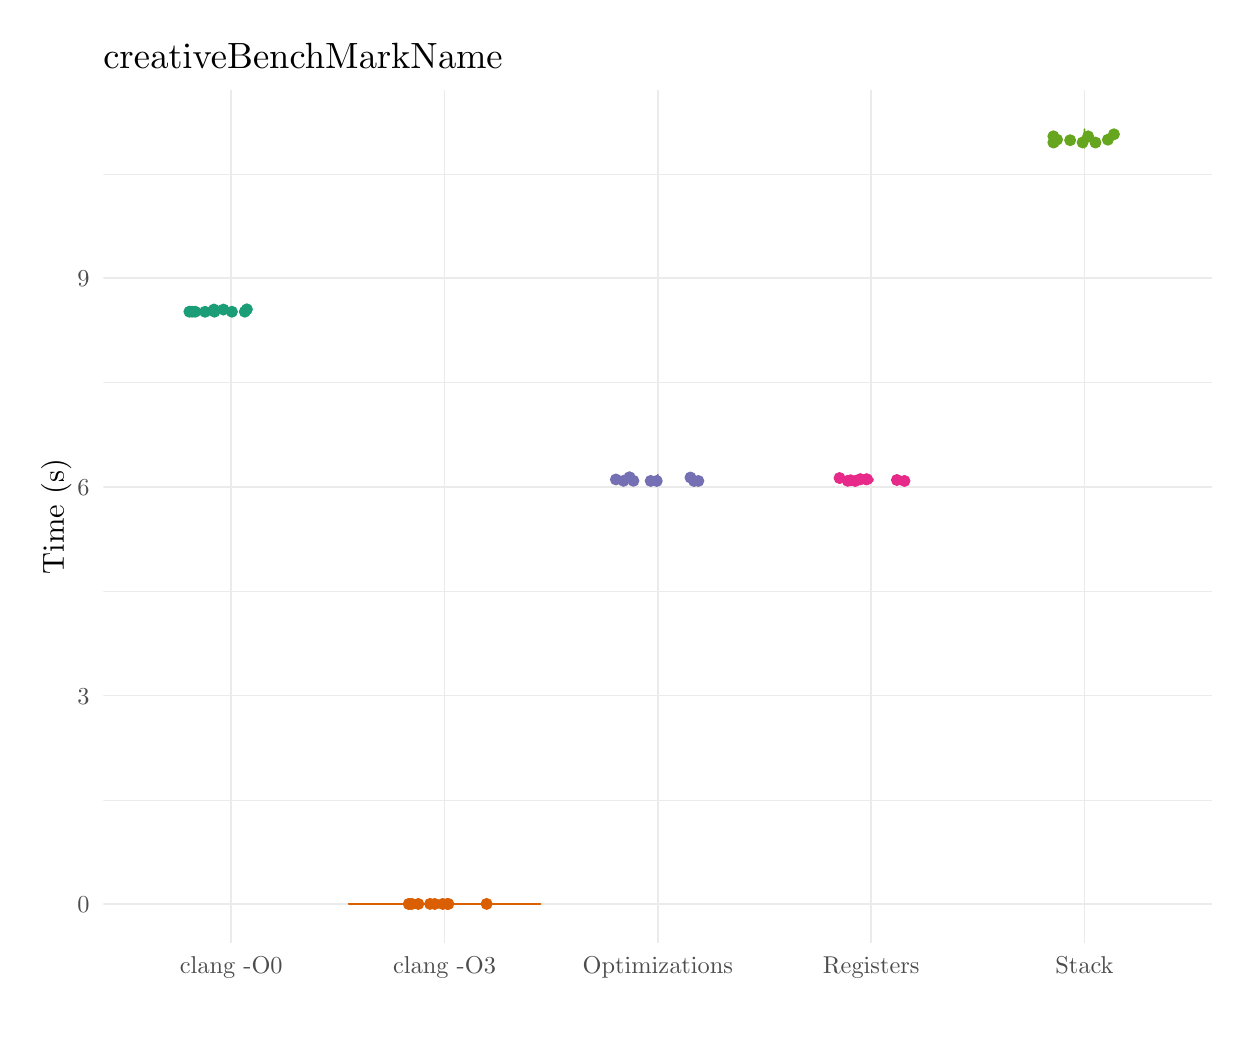
\begin{tikzpicture}[x=1pt,y=1pt]
\definecolor{fillColor}{RGB}{255,255,255}
\path[use as bounding box,fill=fillColor,fill opacity=0.00] (0,0) rectangle (433.62,361.35);
\begin{scope}
\path[clip] ( 27.31, 30.69) rectangle (428.12,338.69);
\definecolor{drawColor}{gray}{0.92}

\path[draw=drawColor,line width= 0.3pt,line join=round] ( 27.31, 82.28) --
	(428.12, 82.28);

\path[draw=drawColor,line width= 0.3pt,line join=round] ( 27.31,157.69) --
	(428.12,157.69);

\path[draw=drawColor,line width= 0.3pt,line join=round] ( 27.31,233.09) --
	(428.12,233.09);

\path[draw=drawColor,line width= 0.3pt,line join=round] ( 27.31,308.50) --
	(428.12,308.50);

\path[draw=drawColor,line width= 0.6pt,line join=round] ( 27.31, 44.58) --
	(428.12, 44.58);

\path[draw=drawColor,line width= 0.6pt,line join=round] ( 27.31,119.98) --
	(428.12,119.98);

\path[draw=drawColor,line width= 0.6pt,line join=round] ( 27.31,195.39) --
	(428.12,195.39);

\path[draw=drawColor,line width= 0.6pt,line join=round] ( 27.31,270.80) --
	(428.12,270.80);

\path[draw=drawColor,line width= 0.6pt,line join=round] ( 73.56, 30.69) --
	( 73.56,338.69);

\path[draw=drawColor,line width= 0.6pt,line join=round] (150.64, 30.69) --
	(150.64,338.69);

\path[draw=drawColor,line width= 0.6pt,line join=round] (227.72, 30.69) --
	(227.72,338.69);

\path[draw=drawColor,line width= 0.6pt,line join=round] (304.79, 30.69) --
	(304.79,338.69);

\path[draw=drawColor,line width= 0.6pt,line join=round] (381.87, 30.69) --
	(381.87,338.69);
\definecolor{drawColor}{RGB}{27,158,119}
\definecolor{fillColor}{RGB}{255,255,255}

\path[draw=drawColor,line width= 0.6pt,line join=round,line cap=round,fill=fillColor] ( 73.55,258.01) --
	( 73.55,258.02) --
	( 73.55,258.02) --
	( 73.55,258.02) --
	( 73.55,258.03) --
	( 73.55,258.03) --
	( 73.55,258.04) --
	( 73.55,258.04) --
	( 73.55,258.05) --
	( 73.55,258.05) --
	( 73.55,258.06) --
	( 73.55,258.06) --
	( 73.55,258.06) --
	( 73.55,258.07) --
	( 73.55,258.07) --
	( 73.54,258.08) --
	( 73.54,258.08) --
	( 73.54,258.09) --
	( 73.54,258.09) --
	( 73.54,258.09) --
	( 73.54,258.10) --
	( 73.54,258.10) --
	( 73.54,258.11) --
	( 73.54,258.11) --
	( 73.54,258.12) --
	( 73.53,258.12) --
	( 73.53,258.12) --
	( 73.53,258.13) --
	( 73.53,258.13) --
	( 73.53,258.14) --
	( 73.53,258.14) --
	( 73.52,258.15) --
	( 73.52,258.15) --
	( 73.52,258.16) --
	( 73.52,258.16) --
	( 73.52,258.16) --
	( 73.51,258.17) --
	( 73.51,258.17) --
	( 73.51,258.18) --
	( 73.51,258.18) --
	( 73.51,258.19) --
	( 73.50,258.19) --
	( 73.50,258.19) --
	( 73.50,258.20) --
	( 73.50,258.20) --
	( 73.49,258.21) --
	( 73.49,258.21) --
	( 73.49,258.22) --
	( 73.48,258.22) --
	( 73.48,258.22) --
	( 73.48,258.23) --
	( 73.47,258.23) --
	( 73.47,258.24) --
	( 73.47,258.24) --
	( 73.46,258.25) --
	( 73.46,258.25) --
	( 73.45,258.26) --
	( 73.45,258.26) --
	( 73.44,258.26) --
	( 73.44,258.27) --
	( 73.44,258.27) --
	( 73.43,258.28) --
	( 73.43,258.28) --
	( 73.42,258.29) --
	( 73.42,258.29) --
	( 73.41,258.29) --
	( 73.41,258.30) --
	( 73.40,258.30) --
	( 73.39,258.31) --
	( 73.39,258.31) --
	( 73.38,258.32) --
	( 73.38,258.32) --
	( 73.37,258.32) --
	( 73.36,258.33) --
	( 73.36,258.33) --
	( 73.35,258.34) --
	( 73.34,258.34) --
	( 73.34,258.35) --
	( 73.33,258.35) --
	( 73.32,258.36) --
	( 73.32,258.36) --
	( 73.31,258.36) --
	( 73.30,258.37) --
	( 73.29,258.37) --
	( 73.28,258.38) --
	( 73.28,258.38) --
	( 73.27,258.39) --
	( 73.26,258.39) --
	( 73.25,258.39) --
	( 73.24,258.40) --
	( 73.24,258.40) --
	( 73.23,258.41) --
	( 73.22,258.41) --
	( 73.21,258.42) --
	( 73.20,258.42) --
	( 73.19,258.42) --
	( 73.18,258.43) --
	( 73.17,258.43) --
	( 73.16,258.44) --
	( 73.15,258.44) --
	( 73.15,258.45) --
	( 73.14,258.45) --
	( 73.13,258.45) --
	( 73.12,258.46) --
	( 73.11,258.46) --
	( 73.10,258.47) --
	( 73.09,258.47) --
	( 73.08,258.48) --
	( 73.07,258.48) --
	( 73.06,258.49) --
	( 73.05,258.49) --
	( 73.04,258.49) --
	( 73.03,258.50) --
	( 73.02,258.50) --
	( 73.01,258.51) --
	( 73.00,258.51) --
	( 72.99,258.52) --
	( 72.98,258.52) --
	( 72.97,258.52) --
	( 72.97,258.53) --
	( 72.96,258.53) --
	( 72.95,258.54) --
	( 72.94,258.54) --
	( 72.93,258.55) --
	( 72.92,258.55) --
	( 72.91,258.55) --
	( 72.90,258.56) --
	( 72.89,258.56) --
	( 72.89,258.57) --
	( 72.88,258.57) --
	( 72.87,258.58) --
	( 72.86,258.58) --
	( 72.86,258.59) --
	( 72.85,258.59) --
	( 72.84,258.59) --
	( 72.83,258.60) --
	( 72.83,258.60) --
	( 72.82,258.61) --
	( 72.81,258.61) --
	( 72.81,258.62) --
	( 72.80,258.62) --
	( 72.80,258.62) --
	( 72.79,258.63) --
	( 72.79,258.63) --
	( 72.78,258.64) --
	( 72.78,258.64) --
	( 72.77,258.65) --
	( 72.77,258.65) --
	( 72.77,258.65) --
	( 72.76,258.66) --
	( 72.76,258.66) --
	( 72.76,258.67) --
	( 72.75,258.67) --
	( 72.75,258.68) --
	( 72.75,258.68) --
	( 72.75,258.69) --
	( 72.75,258.69) --
	( 72.74,258.69) --
	( 72.74,258.70) --
	( 72.74,258.70) --
	( 72.74,258.71) --
	( 72.74,258.71) --
	( 72.74,258.72) --
	( 72.74,258.72) --
	( 72.75,258.72) --
	( 72.75,258.73) --
	( 72.75,258.73) --
	( 72.75,258.74) --
	( 72.75,258.74) --
	( 72.76,258.75) --
	( 72.76,258.75) --
	( 72.76,258.75) --
	( 72.76,258.76) --
	( 72.77,258.76) --
	( 72.77,258.77) --
	( 72.78,258.77) --
	( 72.78,258.78) --
	( 72.79,258.78) --
	( 72.79,258.79) --
	( 72.80,258.79) --
	( 72.80,258.79) --
	( 72.81,258.80) --
	( 72.81,258.80) --
	( 72.82,258.81) --
	( 72.82,258.81) --
	( 72.83,258.82) --
	( 72.84,258.82) --
	( 72.85,258.82) --
	( 72.85,258.83) --
	( 72.86,258.83) --
	( 72.87,258.84) --
	( 72.87,258.84) --
	( 72.88,258.85) --
	( 72.89,258.85) --
	( 72.90,258.85) --
	( 72.91,258.86) --
	( 72.92,258.86) --
	( 72.92,258.87) --
	( 72.93,258.87) --
	( 72.94,258.88) --
	( 72.95,258.88) --
	( 72.96,258.88) --
	( 72.97,258.89) --
	( 72.98,258.89) --
	( 72.98,258.90) --
	( 72.99,258.90) --
	( 73.00,258.91) --
	( 73.01,258.91) --
	( 73.02,258.92) --
	( 73.03,258.92) --
	( 73.04,258.92) --
	( 73.05,258.93) --
	( 73.06,258.93) --
	( 73.07,258.94) --
	( 73.08,258.94) --
	( 73.08,258.95) --
	( 73.09,258.95) --
	( 73.10,258.95) --
	( 73.11,258.96) --
	( 73.12,258.96) --
	( 73.13,258.97) --
	( 73.14,258.97) --
	( 73.14,258.98) --
	( 73.15,258.98) --
	( 73.16,258.98) --
	( 73.17,258.99) --
	( 73.18,258.99) --
	( 73.19,259.00) --
	( 73.19,259.00) --
	( 73.20,259.01) --
	( 73.21,259.01) --
	( 73.22,259.02) --
	( 73.22,259.02) --
	( 73.23,259.02) --
	( 73.24,259.03) --
	( 73.24,259.03) --
	( 73.25,259.04) --
	( 73.26,259.04) --
	( 73.26,259.05) --
	( 73.27,259.05) --
	( 73.27,259.05) --
	( 73.28,259.06) --
	( 73.28,259.06) --
	( 73.29,259.07) --
	( 73.30,259.07) --
	( 73.30,259.08) --
	( 73.30,259.08) --
	( 73.31,259.08) --
	( 73.31,259.09) --
	( 73.32,259.09) --
	( 73.32,259.10) --
	( 73.33,259.10) --
	( 73.33,259.11) --
	( 73.33,259.11) --
	( 73.34,259.12) --
	( 73.34,259.12) --
	( 73.34,259.12) --
	( 73.34,259.13) --
	( 73.35,259.13) --
	( 73.35,259.14) --
	( 73.35,259.14) --
	( 73.35,259.15) --
	( 73.35,259.15) --
	( 73.36,259.15) --
	( 73.36,259.16) --
	( 73.36,259.16) --
	( 73.36,259.17) --
	( 73.36,259.17) --
	( 73.36,259.18) --
	( 73.36,259.18) --
	( 73.36,259.18) --
	( 73.36,259.19) --
	( 73.36,259.19) --
	( 73.36,259.20) --
	( 73.36,259.20) --
	( 73.36,259.21) --
	( 73.36,259.21) --
	( 73.36,259.21) --
	( 73.36,259.22) --
	( 73.36,259.22) --
	( 73.35,259.23) --
	( 73.35,259.23) --
	( 73.35,259.24) --
	( 73.35,259.24) --
	( 73.35,259.25) --
	( 73.35,259.25) --
	( 73.35,259.25) --
	( 73.34,259.26) --
	( 73.34,259.26) --
	( 73.34,259.27) --
	( 73.34,259.27) --
	( 73.33,259.28) --
	( 73.33,259.28) --
	( 73.33,259.28) --
	( 73.33,259.29) --
	( 73.32,259.29) --
	( 73.32,259.30) --
	( 73.32,259.30) --
	( 73.32,259.31) --
	( 73.31,259.31) --
	( 73.31,259.31) --
	( 73.31,259.32) --
	( 73.30,259.32) --
	( 73.30,259.33) --
	( 73.30,259.33) --
	( 73.29,259.34) --
	( 73.29,259.34) --
	( 73.29,259.35) --
	( 73.29,259.35) --
	( 73.28,259.35) --
	( 73.28,259.36) --
	( 73.28,259.36) --
	( 73.27,259.37) --
	( 73.27,259.37) --
	( 73.27,259.38) --
	( 73.26,259.38) --
	( 73.26,259.38) --
	( 73.26,259.39) --
	( 73.26,259.39) --
	( 73.25,259.40) --
	( 73.25,259.40) --
	( 73.25,259.41) --
	( 73.25,259.41) --
	( 73.24,259.41) --
	( 73.24,259.42) --
	( 73.24,259.42) --
	( 73.24,259.43) --
	( 73.23,259.43) --
	( 73.23,259.44) --
	( 73.23,259.44) --
	( 73.23,259.45) --
	( 73.23,259.45) --
	( 73.22,259.45) --
	( 73.22,259.46) --
	( 73.22,259.46) --
	( 73.22,259.47) --
	( 73.22,259.47) --
	( 73.22,259.48) --
	( 73.22,259.48) --
	( 73.22,259.48) --
	( 73.21,259.49) --
	( 73.21,259.49) --
	( 73.21,259.50) --
	( 73.21,259.50) --
	( 73.21,259.51) --
	( 73.21,259.51) --
	( 73.21,259.51) --
	( 73.21,259.52) --
	( 73.21,259.52) --
	( 73.21,259.53) --
	( 73.21,259.53) --
	( 73.21,259.54) --
	( 73.21,259.54) --
	( 73.21,259.55) --
	( 73.22,259.55) --
	( 73.22,259.55) --
	( 73.22,259.56) --
	( 73.22,259.56) --
	( 73.22,259.57) --
	( 73.22,259.57) --
	( 73.22,259.58) --
	( 73.22,259.58) --
	( 73.23,259.58) --
	( 73.23,259.59) --
	( 73.23,259.59) --
	( 73.23,259.60) --
	( 73.23,259.60) --
	( 73.24,259.61) --
	( 73.24,259.61) --
	( 73.24,259.61) --
	( 73.24,259.62) --
	( 73.25,259.62) --
	( 73.25,259.63) --
	( 73.25,259.63) --
	( 73.26,259.64) --
	( 73.26,259.64) --
	( 73.26,259.64) --
	( 73.27,259.65) --
	( 73.27,259.65) --
	( 73.27,259.66) --
	( 73.28,259.66) --
	( 73.28,259.67) --
	( 73.28,259.67) --
	( 73.29,259.68) --
	( 73.29,259.68) --
	( 73.29,259.68) --
	( 73.30,259.69) --
	( 73.30,259.69) --
	( 73.31,259.70) --
	( 73.31,259.70) --
	( 73.31,259.71) --
	( 73.32,259.71) --
	( 73.32,259.71) --
	( 73.33,259.72) --
	( 73.33,259.72) --
	( 73.33,259.73) --
	( 73.34,259.73) --
	( 73.34,259.74) --
	( 73.35,259.74) --
	( 73.35,259.74) --
	( 73.35,259.75) --
	( 73.36,259.75) --
	( 73.36,259.76) --
	( 73.37,259.76) --
	( 73.37,259.77) --
	( 73.37,259.77) --
	( 73.38,259.78) --
	( 73.38,259.78) --
	( 73.39,259.78) --
	( 73.39,259.79) --
	( 73.39,259.79) --
	( 73.40,259.80) --
	( 73.40,259.80) --
	( 73.40,259.81) --
	( 73.41,259.81) --
	( 73.41,259.81) --
	( 73.42,259.82) --
	( 73.42,259.82) --
	( 73.42,259.83) --
	( 73.43,259.83) --
	( 73.43,259.84) --
	( 73.43,259.84) --
	( 73.44,259.84) --
	( 73.44,259.85) --
	( 73.44,259.85) --
	( 73.45,259.86) --
	( 73.45,259.86) --
	( 73.45,259.87) --
	( 73.46,259.87) --
	( 73.46,259.88) --
	( 73.46,259.88) --
	( 73.47,259.88) --
	( 73.47,259.89) --
	( 73.47,259.89) --
	( 73.47,259.90) --
	( 73.48,259.90) --
	( 73.48,259.91) --
	( 73.48,259.91) --
	( 73.48,259.91) --
	( 73.49,259.92) --
	( 73.49,259.92) --
	( 73.49,259.93) --
	( 73.49,259.93) --
	( 73.50,259.94) --
	( 73.50,259.94) --
	( 73.50,259.94) --
	( 73.50,259.95) --
	( 73.51,259.95) --
	( 73.51,259.96) --
	( 73.51,259.96) --
	( 73.51,259.97) --
	( 73.51,259.97) --
	( 73.51,259.98) --
	( 73.52,259.98) --
	( 73.52,259.98) --
	( 73.52,259.99) --
	( 73.52,259.99) --
	( 73.52,260.00) --
	( 73.52,260.00) --
	( 73.53,260.01) --
	( 73.53,260.01) --
	( 73.53,260.01) --
	( 73.53,260.02) --
	( 73.53,260.02) --
	( 73.53,260.03) --
	( 73.53,260.03) --
	( 73.53,260.04) --
	( 73.54,260.04) --
	( 73.54,260.04) --
	( 73.54,260.05) --
	( 73.54,260.05) --
	( 73.54,260.06) --
	( 73.54,260.06) --
	( 73.54,260.07) --
	( 73.54,260.07) --
	( 73.54,260.07) --
	( 73.54,260.08) --
	( 73.54,260.08) --
	( 73.55,260.09) --
	( 73.55,260.09) --
	( 73.55,260.10) --
	( 73.55,260.10) --
	( 73.55,260.11) --
	( 73.55,260.11) --
	( 73.55,260.11) --
	( 73.55,260.12) --
	( 73.55,260.12) --
	( 73.55,260.13) --
	( 73.55,260.13) --
	( 73.55,260.14) --
	( 73.55,260.14) --
	( 73.55,260.14) --
	( 73.55,260.15) --
	( 73.55,260.15) --
	( 73.55,260.16) --
	( 73.55,260.16) --
	( 73.55,260.17) --
	( 73.55,260.17) --
	( 73.56,260.17) --
	( 73.56,260.18) --
	( 73.56,260.18) --
	( 73.56,260.19) --
	( 73.56,260.19) --
	( 73.56,260.20) --
	( 73.56,260.20) --
	( 73.56,260.21) --
	( 73.56,260.21) --
	( 73.56,260.21) --
	( 73.56,260.22) --
	( 73.56,260.22) --
	( 73.56,260.23) --
	( 73.56,260.23) --
	( 73.56,260.23) --
	( 73.56,260.23) --
	( 73.56,260.22) --
	( 73.56,260.22) --
	( 73.56,260.21) --
	( 73.56,260.21) --
	( 73.56,260.21) --
	( 73.56,260.20) --
	( 73.56,260.20) --
	( 73.56,260.19) --
	( 73.56,260.19) --
	( 73.56,260.18) --
	( 73.57,260.18) --
	( 73.57,260.17) --
	( 73.57,260.17) --
	( 73.57,260.17) --
	( 73.57,260.16) --
	( 73.57,260.16) --
	( 73.57,260.15) --
	( 73.57,260.15) --
	( 73.57,260.14) --
	( 73.57,260.14) --
	( 73.57,260.14) --
	( 73.57,260.13) --
	( 73.57,260.13) --
	( 73.57,260.12) --
	( 73.57,260.12) --
	( 73.57,260.11) --
	( 73.57,260.11) --
	( 73.57,260.11) --
	( 73.57,260.10) --
	( 73.57,260.10) --
	( 73.57,260.09) --
	( 73.57,260.09) --
	( 73.58,260.08) --
	( 73.58,260.08) --
	( 73.58,260.07) --
	( 73.58,260.07) --
	( 73.58,260.07) --
	( 73.58,260.06) --
	( 73.58,260.06) --
	( 73.58,260.05) --
	( 73.58,260.05) --
	( 73.58,260.04) --
	( 73.58,260.04) --
	( 73.59,260.04) --
	( 73.59,260.03) --
	( 73.59,260.03) --
	( 73.59,260.02) --
	( 73.59,260.02) --
	( 73.59,260.01) --
	( 73.59,260.01) --
	( 73.59,260.01) --
	( 73.60,260.00) --
	( 73.60,260.00) --
	( 73.60,259.99) --
	( 73.60,259.99) --
	( 73.60,259.98) --
	( 73.60,259.98) --
	( 73.61,259.98) --
	( 73.61,259.97) --
	( 73.61,259.97) --
	( 73.61,259.96) --
	( 73.61,259.96) --
	( 73.62,259.95) --
	( 73.62,259.95) --
	( 73.62,259.94) --
	( 73.62,259.94) --
	( 73.62,259.94) --
	( 73.63,259.93) --
	( 73.63,259.93) --
	( 73.63,259.92) --
	( 73.63,259.92) --
	( 73.64,259.91) --
	( 73.64,259.91) --
	( 73.64,259.91) --
	( 73.64,259.90) --
	( 73.65,259.90) --
	( 73.65,259.89) --
	( 73.65,259.89) --
	( 73.65,259.88) --
	( 73.66,259.88) --
	( 73.66,259.88) --
	( 73.66,259.87) --
	( 73.67,259.87) --
	( 73.67,259.86) --
	( 73.67,259.86) --
	( 73.68,259.85) --
	( 73.68,259.85) --
	( 73.68,259.84) --
	( 73.69,259.84) --
	( 73.69,259.84) --
	( 73.69,259.83) --
	( 73.70,259.83) --
	( 73.70,259.82) --
	( 73.70,259.82) --
	( 73.71,259.81) --
	( 73.71,259.81) --
	( 73.72,259.81) --
	( 73.72,259.80) --
	( 73.72,259.80) --
	( 73.73,259.79) --
	( 73.73,259.79) --
	( 73.74,259.78) --
	( 73.74,259.78) --
	( 73.74,259.78) --
	( 73.75,259.77) --
	( 73.75,259.77) --
	( 73.75,259.76) --
	( 73.76,259.76) --
	( 73.76,259.75) --
	( 73.77,259.75) --
	( 73.77,259.74) --
	( 73.78,259.74) --
	( 73.78,259.74) --
	( 73.78,259.73) --
	( 73.79,259.73) --
	( 73.79,259.72) --
	( 73.80,259.72) --
	( 73.80,259.71) --
	( 73.80,259.71) --
	( 73.81,259.71) --
	( 73.81,259.70) --
	( 73.82,259.70) --
	( 73.82,259.69) --
	( 73.82,259.69) --
	( 73.83,259.68) --
	( 73.83,259.68) --
	( 73.83,259.68) --
	( 73.84,259.67) --
	( 73.84,259.67) --
	( 73.84,259.66) --
	( 73.85,259.66) --
	( 73.85,259.65) --
	( 73.85,259.65) --
	( 73.86,259.64) --
	( 73.86,259.64) --
	( 73.86,259.64) --
	( 73.87,259.63) --
	( 73.87,259.63) --
	( 73.87,259.62) --
	( 73.88,259.62) --
	( 73.88,259.61) --
	( 73.88,259.61) --
	( 73.88,259.61) --
	( 73.89,259.60) --
	( 73.89,259.60) --
	( 73.89,259.59) --
	( 73.89,259.59) --
	( 73.89,259.58) --
	( 73.90,259.58) --
	( 73.90,259.58) --
	( 73.90,259.57) --
	( 73.90,259.57) --
	( 73.90,259.56) --
	( 73.90,259.56) --
	( 73.90,259.55) --
	( 73.91,259.55) --
	( 73.91,259.55) --
	( 73.91,259.54) --
	( 73.91,259.54) --
	( 73.91,259.53) --
	( 73.91,259.53) --
	( 73.91,259.52) --
	( 73.91,259.52) --
	( 73.91,259.51) --
	( 73.91,259.51) --
	( 73.91,259.51) --
	( 73.91,259.50) --
	( 73.91,259.50) --
	( 73.91,259.49) --
	( 73.91,259.49) --
	( 73.91,259.48) --
	( 73.90,259.48) --
	( 73.90,259.48) --
	( 73.90,259.47) --
	( 73.90,259.47) --
	( 73.90,259.46) --
	( 73.90,259.46) --
	( 73.90,259.45) --
	( 73.89,259.45) --
	( 73.89,259.45) --
	( 73.89,259.44) --
	( 73.89,259.44) --
	( 73.89,259.43) --
	( 73.88,259.43) --
	( 73.88,259.42) --
	( 73.88,259.42) --
	( 73.88,259.41) --
	( 73.87,259.41) --
	( 73.87,259.41) --
	( 73.87,259.40) --
	( 73.87,259.40) --
	( 73.86,259.39) --
	( 73.86,259.39) --
	( 73.86,259.38) --
	( 73.86,259.38) --
	( 73.85,259.38) --
	( 73.85,259.37) --
	( 73.85,259.37) --
	( 73.84,259.36) --
	( 73.84,259.36) --
	( 73.84,259.35) --
	( 73.84,259.35) --
	( 73.83,259.35) --
	( 73.83,259.34) --
	( 73.83,259.34) --
	( 73.82,259.33) --
	( 73.82,259.33) --
	( 73.82,259.32) --
	( 73.81,259.32) --
	( 73.81,259.31) --
	( 73.81,259.31) --
	( 73.81,259.31) --
	( 73.80,259.30) --
	( 73.80,259.30) --
	( 73.80,259.29) --
	( 73.79,259.29) --
	( 73.79,259.28) --
	( 73.79,259.28) --
	( 73.79,259.28) --
	( 73.78,259.27) --
	( 73.78,259.27) --
	( 73.78,259.26) --
	( 73.78,259.26) --
	( 73.78,259.25) --
	( 73.77,259.25) --
	( 73.77,259.25) --
	( 73.77,259.24) --
	( 73.77,259.24) --
	( 73.77,259.23) --
	( 73.77,259.23) --
	( 73.76,259.22) --
	( 73.76,259.22) --
	( 73.76,259.21) --
	( 73.76,259.21) --
	( 73.76,259.21) --
	( 73.76,259.20) --
	( 73.76,259.20) --
	( 73.76,259.19) --
	( 73.76,259.19) --
	( 73.76,259.18) --
	( 73.76,259.18) --
	( 73.76,259.18) --
	( 73.76,259.17) --
	( 73.76,259.17) --
	( 73.76,259.16) --
	( 73.76,259.16) --
	( 73.76,259.15) --
	( 73.77,259.15) --
	( 73.77,259.15) --
	( 73.77,259.14) --
	( 73.77,259.14) --
	( 73.77,259.13) --
	( 73.78,259.13) --
	( 73.78,259.12) --
	( 73.78,259.12) --
	( 73.78,259.12) --
	( 73.79,259.11) --
	( 73.79,259.11) --
	( 73.79,259.10) --
	( 73.80,259.10) --
	( 73.80,259.09) --
	( 73.81,259.09) --
	( 73.81,259.08) --
	( 73.82,259.08) --
	( 73.82,259.08) --
	( 73.83,259.07) --
	( 73.83,259.07) --
	( 73.84,259.06) --
	( 73.84,259.06) --
	( 73.85,259.05) --
	( 73.85,259.05) --
	( 73.86,259.05) --
	( 73.86,259.04) --
	( 73.87,259.04) --
	( 73.88,259.03) --
	( 73.88,259.03) --
	( 73.89,259.02) --
	( 73.90,259.02) --
	( 73.91,259.02) --
	( 73.91,259.01) --
	( 73.92,259.01) --
	( 73.93,259.00) --
	( 73.94,259.00) --
	( 73.94,258.99) --
	( 73.95,258.99) --
	( 73.96,258.98) --
	( 73.97,258.98) --
	( 73.98,258.98) --
	( 73.98,258.97) --
	( 73.99,258.97) --
	( 74.00,258.96) --
	( 74.01,258.96) --
	( 74.02,258.95) --
	( 74.03,258.95) --
	( 74.04,258.95) --
	( 74.05,258.94) --
	( 74.05,258.94) --
	( 74.06,258.93) --
	( 74.07,258.93) --
	( 74.08,258.92) --
	( 74.09,258.92) --
	( 74.10,258.92) --
	( 74.11,258.91) --
	( 74.12,258.91) --
	( 74.13,258.90) --
	( 74.14,258.90) --
	( 74.14,258.89) --
	( 74.15,258.89) --
	( 74.16,258.88) --
	( 74.17,258.88) --
	( 74.18,258.88) --
	( 74.19,258.87) --
	( 74.20,258.87) --
	( 74.21,258.86) --
	( 74.21,258.86) --
	( 74.22,258.85) --
	( 74.23,258.85) --
	( 74.24,258.85) --
	( 74.25,258.84) --
	( 74.25,258.84) --
	( 74.26,258.83) --
	( 74.27,258.83) --
	( 74.28,258.82) --
	( 74.28,258.82) --
	( 74.29,258.82) --
	( 74.30,258.81) --
	( 74.30,258.81) --
	( 74.31,258.80) --
	( 74.31,258.80) --
	( 74.32,258.79) --
	( 74.33,258.79) --
	( 74.33,258.79) --
	( 74.34,258.78) --
	( 74.34,258.78) --
	( 74.34,258.77) --
	( 74.35,258.77) --
	( 74.35,258.76) --
	( 74.36,258.76) --
	( 74.36,258.75) --
	( 74.36,258.75) --
	( 74.37,258.75) --
	( 74.37,258.74) --
	( 74.37,258.74) --
	( 74.37,258.73) --
	( 74.37,258.73) --
	( 74.37,258.72) --
	( 74.38,258.72) --
	( 74.38,258.72) --
	( 74.38,258.71) --
	( 74.38,258.71) --
	( 74.38,258.70) --
	( 74.38,258.70) --
	( 74.38,258.69) --
	( 74.37,258.69) --
	( 74.37,258.69) --
	( 74.37,258.68) --
	( 74.37,258.68) --
	( 74.37,258.67) --
	( 74.36,258.67) --
	( 74.36,258.66) --
	( 74.36,258.66) --
	( 74.36,258.65) --
	( 74.35,258.65) --
	( 74.35,258.65) --
	( 74.34,258.64) --
	( 74.34,258.64) --
	( 74.33,258.63) --
	( 74.33,258.63) --
	( 74.32,258.62) --
	( 74.32,258.62) --
	( 74.31,258.62) --
	( 74.31,258.61) --
	( 74.30,258.61) --
	( 74.29,258.60) --
	( 74.29,258.60) --
	( 74.28,258.59) --
	( 74.27,258.59) --
	( 74.26,258.59) --
	( 74.26,258.58) --
	( 74.25,258.58) --
	( 74.24,258.57) --
	( 74.23,258.57) --
	( 74.23,258.56) --
	( 74.22,258.56) --
	( 74.21,258.55) --
	( 74.20,258.55) --
	( 74.19,258.55) --
	( 74.18,258.54) --
	( 74.17,258.54) --
	( 74.16,258.53) --
	( 74.16,258.53) --
	( 74.15,258.52) --
	( 74.14,258.52) --
	( 74.13,258.52) --
	( 74.12,258.51) --
	( 74.11,258.51) --
	( 74.10,258.50) --
	( 74.09,258.50) --
	( 74.08,258.49) --
	( 74.07,258.49) --
	( 74.06,258.49) --
	( 74.05,258.48) --
	( 74.04,258.48) --
	( 74.03,258.47) --
	( 74.02,258.47) --
	( 74.01,258.46) --
	( 74.00,258.46) --
	( 73.99,258.45) --
	( 73.98,258.45) --
	( 73.98,258.45) --
	( 73.97,258.44) --
	( 73.96,258.44) --
	( 73.95,258.43) --
	( 73.94,258.43) --
	( 73.93,258.42) --
	( 73.92,258.42) --
	( 73.91,258.42) --
	( 73.90,258.41) --
	( 73.89,258.41) --
	( 73.89,258.40) --
	( 73.88,258.40) --
	( 73.87,258.39) --
	( 73.86,258.39) --
	( 73.85,258.39) --
	( 73.84,258.38) --
	( 73.84,258.38) --
	( 73.83,258.37) --
	( 73.82,258.37) --
	( 73.81,258.36) --
	( 73.81,258.36) --
	( 73.80,258.36) --
	( 73.79,258.35) --
	( 73.78,258.35) --
	( 73.78,258.34) --
	( 73.77,258.34) --
	( 73.76,258.33) --
	( 73.76,258.33) --
	( 73.75,258.32) --
	( 73.74,258.32) --
	( 73.74,258.32) --
	( 73.73,258.31) --
	( 73.73,258.31) --
	( 73.72,258.30) --
	( 73.72,258.30) --
	( 73.71,258.29) --
	( 73.70,258.29) --
	( 73.70,258.29) --
	( 73.69,258.28) --
	( 73.69,258.28) --
	( 73.68,258.27) --
	( 73.68,258.27) --
	( 73.68,258.26) --
	( 73.67,258.26) --
	( 73.67,258.26) --
	( 73.66,258.25) --
	( 73.66,258.25) --
	( 73.65,258.24) --
	( 73.65,258.24) --
	( 73.65,258.23) --
	( 73.64,258.23) --
	( 73.64,258.22) --
	( 73.64,258.22) --
	( 73.63,258.22) --
	( 73.63,258.21) --
	( 73.63,258.21) --
	( 73.63,258.20) --
	( 73.62,258.20) --
	( 73.62,258.19) --
	( 73.62,258.19) --
	( 73.61,258.19) --
	( 73.61,258.18) --
	( 73.61,258.18) --
	( 73.61,258.17) --
	( 73.61,258.17) --
	( 73.60,258.16) --
	( 73.60,258.16) --
	( 73.60,258.16) --
	( 73.60,258.15) --
	( 73.60,258.15) --
	( 73.59,258.14) --
	( 73.59,258.14) --
	( 73.59,258.13) --
	( 73.59,258.13) --
	( 73.59,258.12) --
	( 73.59,258.12) --
	( 73.59,258.12) --
	( 73.58,258.11) --
	( 73.58,258.11) --
	( 73.58,258.10) --
	( 73.58,258.10) --
	( 73.58,258.09) --
	( 73.58,258.09) --
	( 73.58,258.09) --
	( 73.58,258.08) --
	( 73.58,258.08) --
	( 73.58,258.07) --
	( 73.57,258.07) --
	( 73.57,258.06) --
	( 73.57,258.06) --
	( 73.57,258.06) --
	( 73.57,258.05) --
	( 73.57,258.05) --
	( 73.57,258.04) --
	( 73.57,258.04) --
	( 73.57,258.03) --
	( 73.57,258.03) --
	( 73.57,258.02) --
	( 73.57,258.02) --
	( 73.57,258.02) --
	( 73.57,258.01) --
	( 73.55,258.01) --
	cycle;
\definecolor{drawColor}{RGB}{217,95,2}

\path[draw=drawColor,line width= 0.6pt,line join=round,line cap=round,fill=fillColor] (150.25, 44.69) --
	(150.23, 44.69) --
	(150.20, 44.69) --
	(150.17, 44.69) --
	(150.15, 44.69) --
	(150.12, 44.69) --
	(150.09, 44.69) --
	(150.05, 44.69) --
	(150.02, 44.69) --
	(149.98, 44.69) --
	(149.95, 44.69) --
	(149.91, 44.69) --
	(149.86, 44.69) --
	(149.82, 44.69) --
	(149.78, 44.69) --
	(149.73, 44.69) --
	(149.68, 44.69) --
	(149.63, 44.69) --
	(149.57, 44.69) --
	(149.51, 44.69) --
	(149.45, 44.69) --
	(149.39, 44.69) --
	(149.33, 44.69) --
	(149.26, 44.69) --
	(149.19, 44.69) --
	(149.11, 44.69) --
	(149.03, 44.69) --
	(148.95, 44.69) --
	(148.87, 44.69) --
	(148.78, 44.69) --
	(148.69, 44.69) --
	(148.60, 44.69) --
	(148.50, 44.69) --
	(148.39, 44.69) --
	(148.29, 44.69) --
	(148.18, 44.69) --
	(148.06, 44.69) --
	(147.94, 44.69) --
	(147.82, 44.69) --
	(147.69, 44.69) --
	(147.56, 44.69) --
	(147.42, 44.69) --
	(147.28, 44.69) --
	(147.13, 44.69) --
	(146.98, 44.69) --
	(146.82, 44.69) --
	(146.66, 44.69) --
	(146.50, 44.69) --
	(146.32, 44.69) --
	(146.15, 44.69) --
	(145.96, 44.69) --
	(145.77, 44.69) --
	(145.58, 44.69) --
	(145.38, 44.69) --
	(145.17, 44.69) --
	(144.96, 44.69) --
	(144.74, 44.69) --
	(144.52, 44.69) --
	(144.29, 44.69) --
	(144.05, 44.69) --
	(143.81, 44.69) --
	(143.56, 44.69) --
	(143.31, 44.69) --
	(143.05, 44.69) --
	(142.78, 44.69) --
	(142.51, 44.69) --
	(142.23, 44.69) --
	(141.95, 44.69) --
	(141.66, 44.69) --
	(141.36, 44.69) --
	(141.06, 44.69) --
	(140.75, 44.69) --
	(140.43, 44.69) --
	(140.11, 44.69) --
	(139.79, 44.69) --
	(139.46, 44.70) --
	(139.12, 44.70) --
	(138.78, 44.70) --
	(138.43, 44.70) --
	(138.07, 44.70) --
	(137.72, 44.70) --
	(137.35, 44.70) --
	(136.98, 44.70) --
	(136.61, 44.70) --
	(136.23, 44.70) --
	(135.85, 44.70) --
	(135.46, 44.70) --
	(135.07, 44.70) --
	(134.68, 44.70) --
	(134.28, 44.70) --
	(133.88, 44.70) --
	(133.48, 44.70) --
	(133.07, 44.70) --
	(132.66, 44.70) --
	(132.25, 44.70) --
	(131.84, 44.70) --
	(131.43, 44.70) --
	(131.01, 44.70) --
	(130.59, 44.70) --
	(130.18, 44.70) --
	(129.76, 44.70) --
	(129.34, 44.70) --
	(128.92, 44.70) --
	(128.50, 44.70) --
	(128.09, 44.70) --
	(127.67, 44.70) --
	(127.26, 44.70) --
	(126.84, 44.70) --
	(126.43, 44.70) --
	(126.03, 44.70) --
	(125.62, 44.70) --
	(125.22, 44.70) --
	(124.83, 44.70) --
	(124.43, 44.70) --
	(124.05, 44.70) --
	(123.66, 44.70) --
	(123.29, 44.70) --
	(122.91, 44.70) --
	(122.55, 44.70) --
	(122.19, 44.70) --
	(121.84, 44.70) --
	(121.49, 44.70) --
	(121.15, 44.70) --
	(120.82, 44.70) --
	(120.50, 44.70) --
	(120.19, 44.70) --
	(119.88, 44.70) --
	(119.59, 44.70) --
	(119.30, 44.70) --
	(119.03, 44.70) --
	(118.76, 44.70) --
	(118.51, 44.70) --
	(118.26, 44.70) --
	(118.03, 44.70) --
	(117.81, 44.70) --
	(117.59, 44.70) --
	(117.40, 44.70) --
	(117.21, 44.70) --
	(117.04, 44.70) --
	(116.87, 44.70) --
	(116.72, 44.70) --
	(116.59, 44.70) --
	(116.46, 44.70) --
	(116.36, 44.70) --
	(116.26, 44.70) --
	(116.18, 44.70) --
	(116.10, 44.70) --
	(116.05, 44.70) --
	(116.01, 44.70) --
	(115.97, 44.70) --
	(115.96, 44.70) --
	(115.95, 44.70) --
	(115.97, 44.70) --
	(115.99, 44.70) --
	(116.03, 44.70) --
	(116.09, 44.70) --
	(116.15, 44.70) --
	(116.23, 44.70) --
	(116.32, 44.71) --
	(116.43, 44.71) --
	(116.55, 44.71) --
	(116.68, 44.71) --
	(116.83, 44.71) --
	(116.99, 44.71) --
	(117.16, 44.71) --
	(117.34, 44.71) --
	(117.54, 44.71) --
	(117.74, 44.71) --
	(117.96, 44.71) --
	(118.19, 44.71) --
	(118.43, 44.71) --
	(118.68, 44.71) --
	(118.94, 44.71) --
	(119.22, 44.71) --
	(119.50, 44.71) --
	(119.79, 44.71) --
	(120.09, 44.71) --
	(120.40, 44.71) --
	(120.72, 44.71) --
	(121.05, 44.71) --
	(121.38, 44.71) --
	(121.72, 44.71) --
	(122.07, 44.71) --
	(122.43, 44.71) --
	(122.79, 44.71) --
	(123.16, 44.71) --
	(123.54, 44.71) --
	(123.92, 44.71) --
	(124.30, 44.71) --
	(124.69, 44.71) --
	(125.08, 44.71) --
	(125.48, 44.71) --
	(125.88, 44.71) --
	(126.29, 44.71) --
	(126.69, 44.71) --
	(127.10, 44.71) --
	(127.51, 44.71) --
	(127.93, 44.71) --
	(128.34, 44.71) --
	(128.75, 44.71) --
	(129.17, 44.71) --
	(129.58, 44.71) --
	(130.00, 44.71) --
	(130.41, 44.71) --
	(130.82, 44.71) --
	(131.24, 44.71) --
	(131.65, 44.71) --
	(132.06, 44.71) --
	(132.46, 44.71) --
	(132.87, 44.71) --
	(133.27, 44.71) --
	(133.66, 44.71) --
	(134.06, 44.71) --
	(134.45, 44.71) --
	(134.84, 44.71) --
	(135.22, 44.71) --
	(135.60, 44.71) --
	(135.98, 44.71) --
	(136.35, 44.71) --
	(136.71, 44.71) --
	(137.07, 44.71) --
	(137.43, 44.71) --
	(137.78, 44.71) --
	(138.12, 44.71) --
	(138.46, 44.71) --
	(138.79, 44.71) --
	(139.12, 44.71) --
	(139.44, 44.71) --
	(139.75, 44.71) --
	(140.06, 44.71) --
	(140.36, 44.71) --
	(140.66, 44.71) --
	(140.94, 44.71) --
	(141.23, 44.71) --
	(141.50, 44.71) --
	(141.77, 44.71) --
	(142.03, 44.71) --
	(142.28, 44.71) --
	(142.53, 44.71) --
	(142.77, 44.71) --
	(143.00, 44.71) --
	(143.22, 44.72) --
	(143.44, 44.72) --
	(143.65, 44.72) --
	(143.86, 44.72) --
	(144.06, 44.72) --
	(144.25, 44.72) --
	(144.43, 44.72) --
	(144.61, 44.72) --
	(144.78, 44.72) --
	(144.94, 44.72) --
	(145.10, 44.72) --
	(145.24, 44.72) --
	(145.39, 44.72) --
	(145.52, 44.72) --
	(145.65, 44.72) --
	(145.78, 44.72) --
	(145.89, 44.72) --
	(146.00, 44.72) --
	(146.10, 44.72) --
	(146.20, 44.72) --
	(146.29, 44.72) --
	(146.38, 44.72) --
	(146.46, 44.72) --
	(146.53, 44.72) --
	(146.60, 44.72) --
	(146.66, 44.72) --
	(146.71, 44.72) --
	(146.76, 44.72) --
	(146.81, 44.72) --
	(146.84, 44.72) --
	(146.88, 44.72) --
	(146.91, 44.72) --
	(146.93, 44.72) --
	(146.95, 44.72) --
	(146.96, 44.72) --
	(146.97, 44.72) --
	(146.97, 44.72) --
	(146.97, 44.72) --
	(146.97, 44.72) --
	(146.96, 44.72) --
	(146.94, 44.72) --
	(146.92, 44.72) --
	(146.90, 44.72) --
	(146.87, 44.72) --
	(146.85, 44.72) --
	(146.81, 44.72) --
	(146.77, 44.72) --
	(146.73, 44.72) --
	(146.69, 44.72) --
	(146.64, 44.72) --
	(146.59, 44.72) --
	(146.53, 44.72) --
	(146.48, 44.72) --
	(146.42, 44.72) --
	(146.35, 44.72) --
	(146.29, 44.72) --
	(146.22, 44.72) --
	(146.15, 44.72) --
	(146.08, 44.72) --
	(146.00, 44.72) --
	(145.92, 44.72) --
	(145.85, 44.72) --
	(145.77, 44.72) --
	(145.68, 44.72) --
	(145.60, 44.72) --
	(145.51, 44.72) --
	(145.43, 44.72) --
	(145.34, 44.72) --
	(145.25, 44.72) --
	(145.16, 44.72) --
	(145.07, 44.72) --
	(144.98, 44.72) --
	(144.89, 44.72) --
	(144.79, 44.72) --
	(144.70, 44.72) --
	(144.61, 44.72) --
	(144.52, 44.72) --
	(144.42, 44.72) --
	(144.33, 44.72) --
	(144.24, 44.72) --
	(144.15, 44.72) --
	(144.05, 44.72) --
	(143.96, 44.72) --
	(143.87, 44.72) --
	(143.78, 44.73) --
	(143.69, 44.73) --
	(143.61, 44.73) --
	(143.52, 44.73) --
	(143.44, 44.73) --
	(143.35, 44.73) --
	(143.27, 44.73) --
	(143.19, 44.73) --
	(143.11, 44.73) --
	(143.04, 44.73) --
	(142.96, 44.73) --
	(142.89, 44.73) --
	(142.82, 44.73) --
	(142.75, 44.73) --
	(142.69, 44.73) --
	(142.62, 44.73) --
	(142.56, 44.73) --
	(142.50, 44.73) --
	(142.45, 44.73) --
	(142.39, 44.73) --
	(142.34, 44.73) --
	(142.30, 44.73) --
	(142.25, 44.73) --
	(142.21, 44.73) --
	(142.17, 44.73) --
	(142.14, 44.73) --
	(142.10, 44.73) --
	(142.08, 44.73) --
	(142.05, 44.73) --
	(142.03, 44.73) --
	(142.01, 44.73) --
	(141.99, 44.73) --
	(141.98, 44.73) --
	(141.97, 44.73) --
	(141.97, 44.73) --
	(141.96, 44.73) --
	(141.96, 44.73) --
	(141.97, 44.73) --
	(141.98, 44.73) --
	(141.99, 44.73) --
	(142.00, 44.73) --
	(142.02, 44.73) --
	(142.04, 44.73) --
	(142.07, 44.73) --
	(142.09, 44.73) --
	(142.12, 44.73) --
	(142.16, 44.73) --
	(142.20, 44.73) --
	(142.24, 44.73) --
	(142.28, 44.73) --
	(142.33, 44.73) --
	(142.38, 44.73) --
	(142.43, 44.73) --
	(142.48, 44.73) --
	(142.54, 44.73) --
	(142.60, 44.73) --
	(142.67, 44.73) --
	(142.73, 44.73) --
	(142.80, 44.73) --
	(142.88, 44.73) --
	(142.95, 44.73) --
	(143.03, 44.73) --
	(143.10, 44.73) --
	(143.18, 44.73) --
	(143.27, 44.73) --
	(143.35, 44.73) --
	(143.44, 44.73) --
	(143.53, 44.73) --
	(143.62, 44.73) --
	(143.71, 44.73) --
	(143.80, 44.73) --
	(143.89, 44.73) --
	(143.99, 44.73) --
	(144.09, 44.73) --
	(144.19, 44.73) --
	(144.28, 44.73) --
	(144.38, 44.73) --
	(144.49, 44.73) --
	(144.59, 44.73) --
	(144.69, 44.73) --
	(144.79, 44.73) --
	(144.90, 44.73) --
	(145.00, 44.73) --
	(145.10, 44.74) --
	(145.21, 44.74) --
	(145.31, 44.74) --
	(145.42, 44.74) --
	(145.52, 44.74) --
	(145.63, 44.74) --
	(145.73, 44.74) --
	(145.84, 44.74) --
	(145.94, 44.74) --
	(146.04, 44.74) --
	(146.14, 44.74) --
	(146.25, 44.74) --
	(146.35, 44.74) --
	(146.45, 44.74) --
	(146.55, 44.74) --
	(146.65, 44.74) --
	(146.75, 44.74) --
	(146.84, 44.74) --
	(146.94, 44.74) --
	(147.04, 44.74) --
	(147.13, 44.74) --
	(147.22, 44.74) --
	(147.32, 44.74) --
	(147.41, 44.74) --
	(147.50, 44.74) --
	(147.59, 44.74) --
	(147.67, 44.74) --
	(147.76, 44.74) --
	(147.84, 44.74) --
	(147.93, 44.74) --
	(148.01, 44.74) --
	(148.09, 44.74) --
	(148.17, 44.74) --
	(148.24, 44.74) --
	(148.32, 44.74) --
	(148.39, 44.74) --
	(148.47, 44.74) --
	(148.54, 44.74) --
	(148.61, 44.74) --
	(148.67, 44.74) --
	(148.74, 44.74) --
	(148.81, 44.74) --
	(148.87, 44.74) --
	(148.93, 44.74) --
	(148.99, 44.74) --
	(149.05, 44.74) --
	(149.11, 44.74) --
	(149.16, 44.74) --
	(149.22, 44.74) --
	(149.27, 44.74) --
	(149.32, 44.74) --
	(149.37, 44.74) --
	(149.42, 44.74) --
	(149.47, 44.74) --
	(149.52, 44.74) --
	(149.56, 44.74) --
	(149.60, 44.74) --
	(149.64, 44.74) --
	(149.69, 44.74) --
	(149.72, 44.74) --
	(149.76, 44.74) --
	(149.80, 44.74) --
	(149.83, 44.74) --
	(149.87, 44.74) --
	(149.90, 44.74) --
	(149.93, 44.74) --
	(149.96, 44.74) --
	(149.99, 44.74) --
	(150.02, 44.74) --
	(150.05, 44.74) --
	(150.08, 44.74) --
	(150.10, 44.74) --
	(150.13, 44.74) --
	(150.15, 44.74) --
	(150.17, 44.74) --
	(150.20, 44.74) --
	(150.22, 44.74) --
	(150.24, 44.74) --
	(150.26, 44.74) --
	(150.28, 44.74) --
	(150.29, 44.74) --
	(150.31, 44.74) --
	(150.33, 44.74) --
	(150.34, 44.74) --
	(150.36, 44.75) --
	(150.37, 44.75) --
	(150.39, 44.75) --
	(150.40, 44.75) --
	(150.41, 44.75) --
	(150.42, 44.75) --
	(150.43, 44.75) --
	(150.44, 44.75) --
	(150.46, 44.75) --
	(150.47, 44.75) --
	(150.47, 44.75) --
	(150.48, 44.75) --
	(150.49, 44.75) --
	(150.50, 44.75) --
	(150.51, 44.75) --
	(150.52, 44.75) --
	(150.52, 44.75) --
	(150.53, 44.75) --
	(150.54, 44.75) --
	(150.54, 44.75) --
	(150.74, 44.75) --
	(150.74, 44.75) --
	(150.75, 44.75) --
	(150.75, 44.75) --
	(150.76, 44.75) --
	(150.77, 44.75) --
	(150.78, 44.75) --
	(150.78, 44.75) --
	(150.79, 44.75) --
	(150.80, 44.75) --
	(150.81, 44.75) --
	(150.82, 44.75) --
	(150.83, 44.75) --
	(150.84, 44.75) --
	(150.85, 44.75) --
	(150.87, 44.75) --
	(150.88, 44.75) --
	(150.89, 44.75) --
	(150.91, 44.75) --
	(150.92, 44.75) --
	(150.93, 44.74) --
	(150.95, 44.74) --
	(150.97, 44.74) --
	(150.98, 44.74) --
	(151.00, 44.74) --
	(151.02, 44.74) --
	(151.04, 44.74) --
	(151.06, 44.74) --
	(151.08, 44.74) --
	(151.10, 44.74) --
	(151.13, 44.74) --
	(151.15, 44.74) --
	(151.17, 44.74) --
	(151.20, 44.74) --
	(151.23, 44.74) --
	(151.25, 44.74) --
	(151.28, 44.74) --
	(151.31, 44.74) --
	(151.34, 44.74) --
	(151.38, 44.74) --
	(151.41, 44.74) --
	(151.44, 44.74) --
	(151.48, 44.74) --
	(151.51, 44.74) --
	(151.55, 44.74) --
	(151.59, 44.74) --
	(151.63, 44.74) --
	(151.67, 44.74) --
	(151.72, 44.74) --
	(151.76, 44.74) --
	(151.81, 44.74) --
	(151.85, 44.74) --
	(151.90, 44.74) --
	(151.95, 44.74) --
	(152.01, 44.74) --
	(152.06, 44.74) --
	(152.11, 44.74) --
	(152.17, 44.74) --
	(152.23, 44.74) --
	(152.28, 44.74) --
	(152.34, 44.74) --
	(152.41, 44.74) --
	(152.47, 44.74) --
	(152.54, 44.74) --
	(152.60, 44.74) --
	(152.67, 44.74) --
	(152.74, 44.74) --
	(152.81, 44.74) --
	(152.88, 44.74) --
	(152.96, 44.74) --
	(153.03, 44.74) --
	(153.11, 44.74) --
	(153.19, 44.74) --
	(153.27, 44.74) --
	(153.35, 44.74) --
	(153.43, 44.74) --
	(153.52, 44.74) --
	(153.60, 44.74) --
	(153.69, 44.74) --
	(153.78, 44.74) --
	(153.87, 44.74) --
	(153.96, 44.74) --
	(154.05, 44.74) --
	(154.15, 44.74) --
	(154.24, 44.74) --
	(154.34, 44.74) --
	(154.43, 44.74) --
	(154.53, 44.74) --
	(154.63, 44.74) --
	(154.73, 44.74) --
	(154.83, 44.74) --
	(154.93, 44.74) --
	(155.03, 44.74) --
	(155.13, 44.74) --
	(155.23, 44.74) --
	(155.34, 44.74) --
	(155.44, 44.74) --
	(155.55, 44.74) --
	(155.65, 44.74) --
	(155.75, 44.74) --
	(155.86, 44.74) --
	(155.96, 44.74) --
	(156.07, 44.74) --
	(156.17, 44.74) --
	(156.28, 44.73) --
	(156.38, 44.73) --
	(156.48, 44.73) --
	(156.59, 44.73) --
	(156.69, 44.73) --
	(156.79, 44.73) --
	(156.89, 44.73) --
	(156.99, 44.73) --
	(157.09, 44.73) --
	(157.19, 44.73) --
	(157.29, 44.73) --
	(157.38, 44.73) --
	(157.48, 44.73) --
	(157.57, 44.73) --
	(157.66, 44.73) --
	(157.75, 44.73) --
	(157.84, 44.73) --
	(157.93, 44.73) --
	(158.01, 44.73) --
	(158.09, 44.73) --
	(158.17, 44.73) --
	(158.25, 44.73) --
	(158.33, 44.73) --
	(158.40, 44.73) --
	(158.47, 44.73) --
	(158.54, 44.73) --
	(158.61, 44.73) --
	(158.67, 44.73) --
	(158.73, 44.73) --
	(158.79, 44.73) --
	(158.85, 44.73) --
	(158.90, 44.73) --
	(158.95, 44.73) --
	(159.00, 44.73) --
	(159.04, 44.73) --
	(159.08, 44.73) --
	(159.12, 44.73) --
	(159.15, 44.73) --
	(159.18, 44.73) --
	(159.21, 44.73) --
	(159.24, 44.73) --
	(159.26, 44.73) --
	(159.28, 44.73) --
	(159.29, 44.73) --
	(159.30, 44.73) --
	(159.31, 44.73) --
	(159.31, 44.73) --
	(159.32, 44.73) --
	(159.31, 44.73) --
	(159.31, 44.73) --
	(159.30, 44.73) --
	(159.28, 44.73) --
	(159.27, 44.73) --
	(159.25, 44.73) --
	(159.23, 44.73) --
	(159.20, 44.73) --
	(159.17, 44.73) --
	(159.14, 44.73) --
	(159.10, 44.73) --
	(159.07, 44.73) --
	(159.02, 44.73) --
	(158.98, 44.73) --
	(158.93, 44.73) --
	(158.88, 44.73) --
	(158.83, 44.73) --
	(158.77, 44.73) --
	(158.72, 44.73) --
	(158.65, 44.73) --
	(158.59, 44.73) --
	(158.53, 44.73) --
	(158.46, 44.73) --
	(158.39, 44.73) --
	(158.32, 44.73) --
	(158.24, 44.73) --
	(158.16, 44.73) --
	(158.08, 44.73) --
	(158.00, 44.73) --
	(157.92, 44.73) --
	(157.84, 44.73) --
	(157.76, 44.73) --
	(157.67, 44.73) --
	(157.58, 44.73) --
	(157.49, 44.73) --
	(157.40, 44.72) --
	(157.31, 44.72) --
	(157.22, 44.72) --
	(157.13, 44.72) --
	(157.04, 44.72) --
	(156.95, 44.72) --
	(156.85, 44.72) --
	(156.76, 44.72) --
	(156.67, 44.72) --
	(156.58, 44.72) --
	(156.48, 44.72) --
	(156.39, 44.72) --
	(156.30, 44.72) --
	(156.21, 44.72) --
	(156.12, 44.72) --
	(156.03, 44.72) --
	(155.94, 44.72) --
	(155.85, 44.72) --
	(155.76, 44.72) --
	(155.68, 44.72) --
	(155.59, 44.72) --
	(155.51, 44.72) --
	(155.43, 44.72) --
	(155.35, 44.72) --
	(155.28, 44.72) --
	(155.20, 44.72) --
	(155.13, 44.72) --
	(155.06, 44.72) --
	(154.99, 44.72) --
	(154.92, 44.72) --
	(154.86, 44.72) --
	(154.80, 44.72) --
	(154.74, 44.72) --
	(154.69, 44.72) --
	(154.64, 44.72) --
	(154.59, 44.72) --
	(154.55, 44.72) --
	(154.50, 44.72) --
	(154.47, 44.72) --
	(154.43, 44.72) --
	(154.40, 44.72) --
	(154.38, 44.72) --
	(154.35, 44.72) --
	(154.33, 44.72) --
	(154.32, 44.72) --
	(154.31, 44.72) --
	(154.30, 44.72) --
	(154.31, 44.72) --
	(154.31, 44.72) --
	(154.32, 44.72) --
	(154.33, 44.72) --
	(154.35, 44.72) --
	(154.37, 44.72) --
	(154.40, 44.72) --
	(154.43, 44.72) --
	(154.47, 44.72) --
	(154.52, 44.72) --
	(154.56, 44.72) --
	(154.62, 44.72) --
	(154.68, 44.72) --
	(154.75, 44.72) --
	(154.82, 44.72) --
	(154.90, 44.72) --
	(154.99, 44.72) --
	(155.07, 44.72) --
	(155.17, 44.72) --
	(155.28, 44.72) --
	(155.39, 44.72) --
	(155.50, 44.72) --
	(155.62, 44.72) --
	(155.75, 44.72) --
	(155.89, 44.72) --
	(156.03, 44.72) --
	(156.18, 44.72) --
	(156.34, 44.72) --
	(156.50, 44.72) --
	(156.67, 44.72) --
	(156.85, 44.72) --
	(157.03, 44.72) --
	(157.22, 44.72) --
	(157.42, 44.72) --
	(157.62, 44.72) --
	(157.83, 44.72) --
	(158.05, 44.72) --
	(158.28, 44.71) --
	(158.51, 44.71) --
	(158.75, 44.71) --
	(159.00, 44.71) --
	(159.25, 44.71) --
	(159.51, 44.71) --
	(159.78, 44.71) --
	(160.05, 44.71) --
	(160.33, 44.71) --
	(160.62, 44.71) --
	(160.92, 44.71) --
	(161.22, 44.71) --
	(161.52, 44.71) --
	(161.84, 44.71) --
	(162.16, 44.71) --
	(162.49, 44.71) --
	(162.82, 44.71) --
	(163.16, 44.71) --
	(163.50, 44.71) --
	(163.85, 44.71) --
	(164.20, 44.71) --
	(164.56, 44.71) --
	(164.93, 44.71) --
	(165.30, 44.71) --
	(165.68, 44.71) --
	(166.05, 44.71) --
	(166.44, 44.71) --
	(166.83, 44.71) --
	(167.22, 44.71) --
	(167.61, 44.71) --
	(168.01, 44.71) --
	(168.41, 44.71) --
	(168.81, 44.71) --
	(169.22, 44.71) --
	(169.63, 44.71) --
	(170.04, 44.71) --
	(170.45, 44.71) --
	(170.87, 44.71) --
	(171.28, 44.71) --
	(171.69, 44.71) --
	(172.11, 44.71) --
	(172.52, 44.71) --
	(172.94, 44.71) --
	(173.35, 44.71) --
	(173.76, 44.71) --
	(174.17, 44.71) --
	(174.58, 44.71) --
	(174.99, 44.71) --
	(175.39, 44.71) --
	(175.79, 44.71) --
	(176.19, 44.71) --
	(176.59, 44.71) --
	(176.98, 44.71) --
	(177.36, 44.71) --
	(177.74, 44.71) --
	(178.12, 44.71) --
	(178.48, 44.71) --
	(178.85, 44.71) --
	(179.20, 44.71) --
	(179.55, 44.71) --
	(179.90, 44.71) --
	(180.23, 44.71) --
	(180.56, 44.71) --
	(180.88, 44.71) --
	(181.19, 44.71) --
	(181.49, 44.71) --
	(181.78, 44.71) --
	(182.06, 44.71) --
	(182.33, 44.71) --
	(182.60, 44.71) --
	(182.85, 44.71) --
	(183.09, 44.71) --
	(183.32, 44.71) --
	(183.54, 44.71) --
	(183.74, 44.71) --
	(183.94, 44.71) --
	(184.12, 44.71) --
	(184.29, 44.71) --
	(184.45, 44.71) --
	(184.59, 44.71) --
	(184.73, 44.71) --
	(184.84, 44.71) --
	(184.95, 44.71) --
	(185.04, 44.70) --
	(185.13, 44.70) --
	(185.19, 44.70) --
	(185.24, 44.70) --
	(185.28, 44.70) --
	(185.31, 44.70) --
	(185.32, 44.70) --
	(185.32, 44.70) --
	(185.30, 44.70) --
	(185.27, 44.70) --
	(185.23, 44.70) --
	(185.17, 44.70) --
	(185.10, 44.70) --
	(185.02, 44.70) --
	(184.92, 44.70) --
	(184.81, 44.70) --
	(184.69, 44.70) --
	(184.55, 44.70) --
	(184.40, 44.70) --
	(184.24, 44.70) --
	(184.07, 44.70) --
	(183.88, 44.70) --
	(183.68, 44.70) --
	(183.47, 44.70) --
	(183.25, 44.70) --
	(183.01, 44.70) --
	(182.77, 44.70) --
	(182.52, 44.70) --
	(182.25, 44.70) --
	(181.98, 44.70) --
	(181.69, 44.70) --
	(181.40, 44.70) --
	(181.09, 44.70) --
	(180.78, 44.70) --
	(180.45, 44.70) --
	(180.12, 44.70) --
	(179.79, 44.70) --
	(179.44, 44.70) --
	(179.09, 44.70) --
	(178.73, 44.70) --
	(178.36, 44.70) --
	(177.99, 44.70) --
	(177.61, 44.70) --
	(177.23, 44.70) --
	(176.84, 44.70) --
	(176.45, 44.70) --
	(176.05, 44.70) --
	(175.65, 44.70) --
	(175.25, 44.70) --
	(174.84, 44.70) --
	(174.43, 44.70) --
	(174.02, 44.70) --
	(173.61, 44.70) --
	(173.19, 44.70) --
	(172.77, 44.70) --
	(172.36, 44.70) --
	(171.94, 44.70) --
	(171.52, 44.70) --
	(171.10, 44.70) --
	(170.68, 44.70) --
	(170.27, 44.70) --
	(169.85, 44.70) --
	(169.44, 44.70) --
	(169.02, 44.70) --
	(168.61, 44.70) --
	(168.20, 44.70) --
	(167.80, 44.70) --
	(167.39, 44.70) --
	(166.99, 44.70) --
	(166.60, 44.70) --
	(166.20, 44.70) --
	(165.81, 44.70) --
	(165.43, 44.70) --
	(165.04, 44.70) --
	(164.67, 44.70) --
	(164.29, 44.70) --
	(163.92, 44.70) --
	(163.56, 44.70) --
	(163.20, 44.70) --
	(162.85, 44.70) --
	(162.50, 44.70) --
	(162.16, 44.70) --
	(161.82, 44.70) --
	(161.49, 44.69) --
	(161.16, 44.69) --
	(160.84, 44.69) --
	(160.53, 44.69) --
	(160.22, 44.69) --
	(159.92, 44.69) --
	(159.62, 44.69) --
	(159.33, 44.69) --
	(159.04, 44.69) --
	(158.77, 44.69) --
	(158.49, 44.69) --
	(158.23, 44.69) --
	(157.97, 44.69) --
	(157.71, 44.69) --
	(157.46, 44.69) --
	(157.22, 44.69) --
	(156.99, 44.69) --
	(156.76, 44.69) --
	(156.53, 44.69) --
	(156.32, 44.69) --
	(156.10, 44.69) --
	(155.90, 44.69) --
	(155.70, 44.69) --
	(155.50, 44.69) --
	(155.32, 44.69) --
	(155.13, 44.69) --
	(154.95, 44.69) --
	(154.78, 44.69) --
	(154.61, 44.69) --
	(154.45, 44.69) --
	(154.29, 44.69) --
	(154.14, 44.69) --
	(153.99, 44.69) --
	(153.85, 44.69) --
	(153.72, 44.69) --
	(153.58, 44.69) --
	(153.46, 44.69) --
	(153.33, 44.69) --
	(153.21, 44.69) --
	(153.10, 44.69) --
	(152.99, 44.69) --
	(152.88, 44.69) --
	(152.78, 44.69) --
	(152.68, 44.69) --
	(152.59, 44.69) --
	(152.50, 44.69) --
	(152.41, 44.69) --
	(152.32, 44.69) --
	(152.24, 44.69) --
	(152.17, 44.69) --
	(152.09, 44.69) --
	(152.02, 44.69) --
	(151.95, 44.69) --
	(151.89, 44.69) --
	(151.82, 44.69) --
	(151.76, 44.69) --
	(151.71, 44.69) --
	(151.65, 44.69) --
	(151.60, 44.69) --
	(151.55, 44.69) --
	(151.50, 44.69) --
	(151.46, 44.69) --
	(151.41, 44.69) --
	(151.37, 44.69) --
	(151.33, 44.69) --
	(151.29, 44.69) --
	(151.26, 44.69) --
	(151.22, 44.69) --
	(151.19, 44.69) --
	(151.16, 44.69) --
	(151.13, 44.69) --
	(151.10, 44.69) --
	(151.08, 44.69) --
	(151.05, 44.69) --
	(151.03, 44.69) --
	(150.25, 44.69) --
	cycle;
\definecolor{drawColor}{RGB}{117,112,179}

\path[draw=drawColor,line width= 0.6pt,line join=round,line cap=round,fill=fillColor] (227.71,196.56) --
	(227.71,196.56) --
	(227.71,196.57) --
	(227.71,196.58) --
	(227.71,196.58) --
	(227.71,196.59) --
	(227.71,196.60) --
	(227.71,196.60) --
	(227.71,196.61) --
	(227.71,196.61) --
	(227.71,196.62) --
	(227.71,196.63) --
	(227.71,196.63) --
	(227.71,196.64) --
	(227.71,196.65) --
	(227.71,196.65) --
	(227.71,196.66) --
	(227.71,196.67) --
	(227.70,196.67) --
	(227.70,196.68) --
	(227.70,196.69) --
	(227.70,196.69) --
	(227.70,196.70) --
	(227.70,196.71) --
	(227.70,196.71) --
	(227.70,196.72) --
	(227.70,196.72) --
	(227.70,196.73) --
	(227.70,196.74) --
	(227.70,196.74) --
	(227.69,196.75) --
	(227.69,196.76) --
	(227.69,196.76) --
	(227.69,196.77) --
	(227.69,196.78) --
	(227.69,196.78) --
	(227.69,196.79) --
	(227.69,196.80) --
	(227.68,196.80) --
	(227.68,196.81) --
	(227.68,196.81) --
	(227.68,196.82) --
	(227.68,196.83) --
	(227.68,196.83) --
	(227.67,196.84) --
	(227.67,196.85) --
	(227.67,196.85) --
	(227.67,196.86) --
	(227.67,196.87) --
	(227.66,196.87) --
	(227.66,196.88) --
	(227.66,196.89) --
	(227.66,196.89) --
	(227.66,196.90) --
	(227.65,196.91) --
	(227.65,196.91) --
	(227.65,196.92) --
	(227.65,196.92) --
	(227.64,196.93) --
	(227.64,196.94) --
	(227.64,196.94) --
	(227.63,196.95) --
	(227.63,196.96) --
	(227.63,196.96) --
	(227.63,196.97) --
	(227.62,196.98) --
	(227.62,196.98) --
	(227.62,196.99) --
	(227.61,197.00) --
	(227.61,197.00) --
	(227.60,197.01) --
	(227.60,197.02) --
	(227.60,197.02) --
	(227.59,197.03) --
	(227.59,197.03) --
	(227.59,197.04) --
	(227.58,197.05) --
	(227.58,197.05) --
	(227.57,197.06) --
	(227.57,197.07) --
	(227.56,197.07) --
	(227.56,197.08) --
	(227.55,197.09) --
	(227.55,197.09) --
	(227.55,197.10) --
	(227.54,197.11) --
	(227.54,197.11) --
	(227.53,197.12) --
	(227.53,197.12) --
	(227.52,197.13) --
	(227.52,197.14) --
	(227.51,197.14) --
	(227.51,197.15) --
	(227.50,197.16) --
	(227.49,197.16) --
	(227.49,197.17) --
	(227.48,197.18) --
	(227.48,197.18) --
	(227.47,197.19) --
	(227.47,197.20) --
	(227.46,197.20) --
	(227.46,197.21) --
	(227.45,197.22) --
	(227.44,197.22) --
	(227.44,197.23) --
	(227.43,197.23) --
	(227.43,197.24) --
	(227.42,197.25) --
	(227.42,197.25) --
	(227.41,197.26) --
	(227.41,197.27) --
	(227.40,197.27) --
	(227.39,197.28) --
	(227.39,197.29) --
	(227.38,197.29) --
	(227.38,197.30) --
	(227.37,197.31) --
	(227.37,197.31) --
	(227.36,197.32) --
	(227.36,197.32) --
	(227.35,197.33) --
	(227.34,197.34) --
	(227.34,197.34) --
	(227.33,197.35) --
	(227.33,197.36) --
	(227.32,197.36) --
	(227.32,197.37) --
	(227.31,197.38) --
	(227.31,197.38) --
	(227.30,197.39) --
	(227.30,197.40) --
	(227.30,197.40) --
	(227.29,197.41) --
	(227.29,197.42) --
	(227.28,197.42) --
	(227.28,197.43) --
	(227.27,197.43) --
	(227.27,197.44) --
	(227.27,197.45) --
	(227.26,197.45) --
	(227.26,197.46) --
	(227.26,197.47) --
	(227.25,197.47) --
	(227.25,197.48) --
	(227.25,197.49) --
	(227.25,197.49) --
	(227.24,197.50) --
	(227.24,197.51) --
	(227.24,197.51) --
	(227.24,197.52) --
	(227.23,197.53) --
	(227.23,197.53) --
	(227.23,197.54) --
	(227.23,197.54) --
	(227.23,197.55) --
	(227.23,197.56) --
	(227.23,197.56) --
	(227.22,197.57) --
	(227.22,197.58) --
	(227.22,197.58) --
	(227.22,197.59) --
	(227.22,197.60) --
	(227.22,197.60) --
	(227.22,197.61) --
	(227.22,197.62) --
	(227.22,197.62) --
	(227.22,197.63) --
	(227.22,197.63) --
	(227.23,197.64) --
	(227.23,197.65) --
	(227.23,197.65) --
	(227.23,197.66) --
	(227.23,197.67) --
	(227.23,197.67) --
	(227.23,197.68) --
	(227.24,197.69) --
	(227.24,197.69) --
	(227.24,197.70) --
	(227.24,197.71) --
	(227.25,197.71) --
	(227.25,197.72) --
	(227.25,197.73) --
	(227.25,197.73) --
	(227.26,197.74) --
	(227.26,197.74) --
	(227.26,197.75) --
	(227.27,197.76) --
	(227.27,197.76) --
	(227.27,197.77) --
	(227.28,197.78) --
	(227.28,197.78) --
	(227.28,197.79) --
	(227.29,197.80) --
	(227.29,197.80) --
	(227.29,197.81) --
	(227.30,197.82) --
	(227.30,197.82) --
	(227.31,197.83) --
	(227.31,197.83) --
	(227.32,197.84) --
	(227.32,197.85) --
	(227.32,197.85) --
	(227.33,197.86) --
	(227.33,197.87) --
	(227.34,197.87) --
	(227.34,197.88) --
	(227.35,197.89) --
	(227.35,197.89) --
	(227.35,197.90) --
	(227.36,197.91) --
	(227.36,197.91) --
	(227.37,197.92) --
	(227.37,197.93) --
	(227.38,197.93) --
	(227.38,197.94) --
	(227.39,197.94) --
	(227.39,197.95) --
	(227.39,197.96) --
	(227.40,197.96) --
	(227.40,197.97) --
	(227.41,197.98) --
	(227.41,197.98) --
	(227.42,197.99) --
	(227.42,198.00) --
	(227.42,198.00) --
	(227.43,198.01) --
	(227.43,198.02) --
	(227.44,198.02) --
	(227.44,198.03) --
	(227.44,198.03) --
	(227.45,198.04) --
	(227.45,198.05) --
	(227.45,198.05) --
	(227.46,198.06) --
	(227.46,198.07) --
	(227.47,198.07) --
	(227.47,198.08) --
	(227.47,198.09) --
	(227.48,198.09) --
	(227.48,198.10) --
	(227.48,198.11) --
	(227.48,198.11) --
	(227.49,198.12) --
	(227.49,198.13) --
	(227.49,198.13) --
	(227.50,198.14) --
	(227.50,198.14) --
	(227.50,198.15) --
	(227.50,198.16) --
	(227.51,198.16) --
	(227.51,198.17) --
	(227.51,198.18) --
	(227.51,198.18) --
	(227.51,198.19) --
	(227.52,198.20) --
	(227.52,198.20) --
	(227.52,198.21) --
	(227.52,198.22) --
	(227.52,198.22) --
	(227.52,198.23) --
	(227.52,198.24) --
	(227.53,198.24) --
	(227.53,198.25) --
	(227.53,198.25) --
	(227.53,198.26) --
	(227.53,198.27) --
	(227.53,198.27) --
	(227.53,198.28) --
	(227.53,198.29) --
	(227.53,198.29) --
	(227.53,198.30) --
	(227.53,198.31) --
	(227.53,198.31) --
	(227.53,198.32) --
	(227.53,198.33) --
	(227.53,198.33) --
	(227.53,198.34) --
	(227.53,198.34) --
	(227.53,198.35) --
	(227.53,198.36) --
	(227.53,198.36) --
	(227.53,198.37) --
	(227.53,198.38) --
	(227.53,198.38) --
	(227.53,198.39) --
	(227.53,198.40) --
	(227.53,198.40) --
	(227.53,198.41) --
	(227.53,198.42) --
	(227.53,198.42) --
	(227.53,198.43) --
	(227.53,198.44) --
	(227.53,198.44) --
	(227.52,198.45) --
	(227.52,198.45) --
	(227.52,198.46) --
	(227.52,198.47) --
	(227.52,198.47) --
	(227.52,198.48) --
	(227.52,198.49) --
	(227.52,198.49) --
	(227.52,198.50) --
	(227.51,198.51) --
	(227.51,198.51) --
	(227.51,198.52) --
	(227.51,198.53) --
	(227.51,198.53) --
	(227.51,198.54) --
	(227.51,198.54) --
	(227.50,198.55) --
	(227.50,198.56) --
	(227.50,198.56) --
	(227.50,198.57) --
	(227.50,198.58) --
	(227.50,198.58) --
	(227.50,198.59) --
	(227.49,198.60) --
	(227.49,198.60) --
	(227.49,198.61) --
	(227.49,198.62) --
	(227.49,198.62) --
	(227.49,198.63) --
	(227.49,198.64) --
	(227.49,198.64) --
	(227.48,198.65) --
	(227.48,198.65) --
	(227.48,198.66) --
	(227.48,198.67) --
	(227.48,198.67) --
	(227.48,198.68) --
	(227.48,198.69) --
	(227.48,198.69) --
	(227.48,198.70) --
	(227.48,198.71) --
	(227.48,198.71) --
	(227.47,198.72) --
	(227.47,198.73) --
	(227.47,198.73) --
	(227.47,198.74) --
	(227.47,198.74) --
	(227.47,198.75) --
	(227.47,198.76) --
	(227.47,198.76) --
	(227.47,198.77) --
	(227.47,198.78) --
	(227.47,198.78) --
	(227.47,198.79) --
	(227.47,198.80) --
	(227.47,198.80) --
	(227.47,198.81) --
	(227.47,198.82) --
	(227.47,198.82) --
	(227.47,198.83) --
	(227.48,198.84) --
	(227.48,198.84) --
	(227.48,198.85) --
	(227.48,198.85) --
	(227.48,198.86) --
	(227.48,198.87) --
	(227.48,198.87) --
	(227.48,198.88) --
	(227.48,198.89) --
	(227.48,198.89) --
	(227.49,198.90) --
	(227.49,198.91) --
	(227.49,198.91) --
	(227.49,198.92) --
	(227.49,198.93) --
	(227.49,198.93) --
	(227.50,198.94) --
	(227.50,198.95) --
	(227.50,198.95) --
	(227.50,198.96) --
	(227.50,198.96) --
	(227.51,198.97) --
	(227.51,198.98) --
	(227.51,198.98) --
	(227.51,198.99) --
	(227.51,199.00) --
	(227.52,199.00) --
	(227.52,199.01) --
	(227.52,199.02) --
	(227.52,199.02) --
	(227.53,199.03) --
	(227.53,199.04) --
	(227.53,199.04) --
	(227.53,199.05) --
	(227.54,199.05) --
	(227.54,199.06) --
	(227.54,199.07) --
	(227.54,199.07) --
	(227.55,199.08) --
	(227.55,199.09) --
	(227.55,199.09) --
	(227.56,199.10) --
	(227.56,199.11) --
	(227.56,199.11) --
	(227.56,199.12) --
	(227.57,199.13) --
	(227.57,199.13) --
	(227.57,199.14) --
	(227.57,199.15) --
	(227.58,199.15) --
	(227.58,199.16) --
	(227.58,199.16) --
	(227.59,199.17) --
	(227.59,199.18) --
	(227.59,199.18) --
	(227.59,199.19) --
	(227.60,199.20) --
	(227.60,199.20) --
	(227.60,199.21) --
	(227.60,199.22) --
	(227.61,199.22) --
	(227.61,199.23) --
	(227.61,199.24) --
	(227.62,199.24) --
	(227.62,199.25) --
	(227.62,199.25) --
	(227.62,199.26) --
	(227.63,199.27) --
	(227.63,199.27) --
	(227.63,199.28) --
	(227.63,199.29) --
	(227.63,199.29) --
	(227.64,199.30) --
	(227.64,199.31) --
	(227.64,199.31) --
	(227.64,199.32) --
	(227.65,199.33) --
	(227.65,199.33) --
	(227.65,199.34) --
	(227.65,199.35) --
	(227.65,199.35) --
	(227.66,199.36) --
	(227.66,199.36) --
	(227.66,199.37) --
	(227.66,199.38) --
	(227.66,199.38) --
	(227.66,199.39) --
	(227.67,199.40) --
	(227.67,199.40) --
	(227.67,199.41) --
	(227.67,199.42) --
	(227.67,199.42) --
	(227.67,199.43) --
	(227.68,199.44) --
	(227.68,199.44) --
	(227.68,199.45) --
	(227.68,199.45) --
	(227.68,199.46) --
	(227.68,199.47) --
	(227.68,199.47) --
	(227.69,199.48) --
	(227.69,199.49) --
	(227.69,199.49) --
	(227.69,199.50) --
	(227.69,199.51) --
	(227.69,199.51) --
	(227.69,199.52) --
	(227.69,199.53) --
	(227.69,199.53) --
	(227.69,199.54) --
	(227.70,199.55) --
	(227.70,199.55) --
	(227.70,199.56) --
	(227.70,199.56) --
	(227.70,199.57) --
	(227.70,199.58) --
	(227.70,199.58) --
	(227.70,199.59) --
	(227.70,199.60) --
	(227.70,199.60) --
	(227.70,199.61) --
	(227.70,199.62) --
	(227.70,199.62) --
	(227.71,199.63) --
	(227.71,199.64) --
	(227.71,199.64) --
	(227.71,199.65) --
	(227.71,199.66) --
	(227.71,199.66) --
	(227.71,199.67) --
	(227.71,199.67) --
	(227.71,199.68) --
	(227.71,199.69) --
	(227.71,199.69) --
	(227.71,199.70) --
	(227.71,199.71) --
	(227.71,199.71) --
	(227.71,199.72) --
	(227.71,199.73) --
	(227.71,199.73) --
	(227.71,199.74) --
	(227.71,199.75) --
	(227.71,199.75) --
	(227.71,199.76) --
	(227.71,199.76) --
	(227.71,199.77) --
	(227.71,199.78) --
	(227.71,199.78) --
	(227.71,199.79) --
	(227.71,199.80) --
	(227.71,199.80) --
	(227.71,199.81) --
	(227.71,199.82) --
	(227.71,199.82) --
	(227.71,199.83) --
	(227.71,199.84) --
	(227.71,199.84) --
	(227.71,199.85) --
	(227.71,199.86) --
	(227.72,199.86) --
	(227.72,199.85) --
	(227.72,199.84) --
	(227.72,199.84) --
	(227.72,199.83) --
	(227.72,199.82) --
	(227.72,199.82) --
	(227.72,199.81) --
	(227.72,199.80) --
	(227.72,199.80) --
	(227.72,199.79) --
	(227.72,199.78) --
	(227.72,199.78) --
	(227.72,199.77) --
	(227.72,199.76) --
	(227.72,199.76) --
	(227.72,199.75) --
	(227.72,199.75) --
	(227.72,199.74) --
	(227.72,199.73) --
	(227.72,199.73) --
	(227.72,199.72) --
	(227.72,199.71) --
	(227.72,199.71) --
	(227.72,199.70) --
	(227.72,199.69) --
	(227.72,199.69) --
	(227.72,199.68) --
	(227.72,199.67) --
	(227.73,199.67) --
	(227.73,199.66) --
	(227.73,199.66) --
	(227.73,199.65) --
	(227.73,199.64) --
	(227.73,199.64) --
	(227.73,199.63) --
	(227.73,199.62) --
	(227.73,199.62) --
	(227.73,199.61) --
	(227.73,199.60) --
	(227.73,199.60) --
	(227.73,199.59) --
	(227.73,199.58) --
	(227.73,199.58) --
	(227.73,199.57) --
	(227.73,199.56) --
	(227.74,199.56) --
	(227.74,199.55) --
	(227.74,199.55) --
	(227.74,199.54) --
	(227.74,199.53) --
	(227.74,199.53) --
	(227.74,199.52) --
	(227.74,199.51) --
	(227.74,199.51) --
	(227.74,199.50) --
	(227.75,199.49) --
	(227.75,199.49) --
	(227.75,199.48) --
	(227.75,199.47) --
	(227.75,199.47) --
	(227.75,199.46) --
	(227.75,199.45) --
	(227.75,199.45) --
	(227.76,199.44) --
	(227.76,199.44) --
	(227.76,199.43) --
	(227.76,199.42) --
	(227.76,199.42) --
	(227.76,199.41) --
	(227.76,199.40) --
	(227.77,199.40) --
	(227.77,199.39) --
	(227.77,199.38) --
	(227.77,199.38) --
	(227.77,199.37) --
	(227.78,199.36) --
	(227.78,199.36) --
	(227.78,199.35) --
	(227.78,199.35) --
	(227.78,199.34) --
	(227.79,199.33) --
	(227.79,199.33) --
	(227.79,199.32) --
	(227.79,199.31) --
	(227.79,199.31) --
	(227.80,199.30) --
	(227.80,199.29) --
	(227.80,199.29) --
	(227.80,199.28) --
	(227.81,199.27) --
	(227.81,199.27) --
	(227.81,199.26) --
	(227.81,199.25) --
	(227.82,199.25) --
	(227.82,199.24) --
	(227.82,199.24) --
	(227.82,199.23) --
	(227.83,199.22) --
	(227.83,199.22) --
	(227.83,199.21) --
	(227.83,199.20) --
	(227.84,199.20) --
	(227.84,199.19) --
	(227.84,199.18) --
	(227.84,199.18) --
	(227.85,199.17) --
	(227.85,199.16) --
	(227.85,199.16) --
	(227.86,199.15) --
	(227.86,199.15) --
	(227.86,199.14) --
	(227.86,199.13) --
	(227.87,199.13) --
	(227.87,199.12) --
	(227.87,199.11) --
	(227.88,199.11) --
	(227.88,199.10) --
	(227.88,199.09) --
	(227.88,199.09) --
	(227.89,199.08) --
	(227.89,199.07) --
	(227.89,199.07) --
	(227.89,199.06) --
	(227.90,199.05) --
	(227.90,199.05) --
	(227.90,199.04) --
	(227.90,199.04) --
	(227.91,199.03) --
	(227.91,199.02) --
	(227.91,199.02) --
	(227.91,199.01) --
	(227.92,199.00) --
	(227.92,199.00) --
	(227.92,198.99) --
	(227.92,198.98) --
	(227.93,198.98) --
	(227.93,198.97) --
	(227.93,198.96) --
	(227.93,198.96) --
	(227.93,198.95) --
	(227.94,198.95) --
	(227.94,198.94) --
	(227.94,198.93) --
	(227.94,198.93) --
	(227.94,198.92) --
	(227.94,198.91) --
	(227.95,198.91) --
	(227.95,198.90) --
	(227.95,198.89) --
	(227.95,198.89) --
	(227.95,198.88) --
	(227.95,198.87) --
	(227.95,198.87) --
	(227.95,198.86) --
	(227.96,198.85) --
	(227.96,198.85) --
	(227.96,198.84) --
	(227.96,198.84) --
	(227.96,198.83) --
	(227.96,198.82) --
	(227.96,198.82) --
	(227.96,198.81) --
	(227.96,198.80) --
	(227.96,198.80) --
	(227.96,198.79) --
	(227.96,198.78) --
	(227.96,198.78) --
	(227.96,198.77) --
	(227.96,198.76) --
	(227.96,198.76) --
	(227.96,198.75) --
	(227.96,198.74) --
	(227.96,198.74) --
	(227.96,198.73) --
	(227.96,198.73) --
	(227.96,198.72) --
	(227.96,198.71) --
	(227.96,198.71) --
	(227.96,198.70) --
	(227.96,198.69) --
	(227.95,198.69) --
	(227.95,198.68) --
	(227.95,198.67) --
	(227.95,198.67) --
	(227.95,198.66) --
	(227.95,198.65) --
	(227.95,198.65) --
	(227.95,198.64) --
	(227.95,198.64) --
	(227.95,198.63) --
	(227.94,198.62) --
	(227.94,198.62) --
	(227.94,198.61) --
	(227.94,198.60) --
	(227.94,198.60) --
	(227.94,198.59) --
	(227.94,198.58) --
	(227.93,198.58) --
	(227.93,198.57) --
	(227.93,198.56) --
	(227.93,198.56) --
	(227.93,198.55) --
	(227.93,198.54) --
	(227.93,198.54) --
	(227.92,198.53) --
	(227.92,198.53) --
	(227.92,198.52) --
	(227.92,198.51) --
	(227.92,198.51) --
	(227.92,198.50) --
	(227.92,198.49) --
	(227.92,198.49) --
	(227.91,198.48) --
	(227.91,198.47) --
	(227.91,198.47) --
	(227.91,198.46) --
	(227.91,198.45) --
	(227.91,198.45) --
	(227.91,198.44) --
	(227.91,198.44) --
	(227.91,198.43) --
	(227.90,198.42) --
	(227.90,198.42) --
	(227.90,198.41) --
	(227.90,198.40) --
	(227.90,198.40) --
	(227.90,198.39) --
	(227.90,198.38) --
	(227.90,198.38) --
	(227.90,198.37) --
	(227.90,198.36) --
	(227.90,198.36) --
	(227.90,198.35) --
	(227.90,198.34) --
	(227.90,198.34) --
	(227.90,198.33) --
	(227.90,198.33) --
	(227.90,198.32) --
	(227.90,198.31) --
	(227.90,198.31) --
	(227.90,198.30) --
	(227.90,198.29) --
	(227.90,198.29) --
	(227.90,198.28) --
	(227.90,198.27) --
	(227.90,198.27) --
	(227.90,198.26) --
	(227.91,198.25) --
	(227.91,198.25) --
	(227.91,198.24) --
	(227.91,198.24) --
	(227.91,198.23) --
	(227.91,198.22) --
	(227.91,198.22) --
	(227.91,198.21) --
	(227.92,198.20) --
	(227.92,198.20) --
	(227.92,198.19) --
	(227.92,198.18) --
	(227.92,198.18) --
	(227.93,198.17) --
	(227.93,198.16) --
	(227.93,198.16) --
	(227.93,198.15) --
	(227.94,198.14) --
	(227.94,198.14) --
	(227.94,198.13) --
	(227.94,198.13) --
	(227.95,198.12) --
	(227.95,198.11) --
	(227.95,198.11) --
	(227.95,198.10) --
	(227.96,198.09) --
	(227.96,198.09) --
	(227.96,198.08) --
	(227.97,198.07) --
	(227.97,198.07) --
	(227.97,198.06) --
	(227.98,198.05) --
	(227.98,198.05) --
	(227.99,198.04) --
	(227.99,198.03) --
	(227.99,198.03) --
	(228.00,198.02) --
	(228.00,198.02) --
	(228.01,198.01) --
	(228.01,198.00) --
	(228.01,198.00) --
	(228.02,197.99) --
	(228.02,197.98) --
	(228.03,197.98) --
	(228.03,197.97) --
	(228.03,197.96) --
	(228.04,197.96) --
	(228.04,197.95) --
	(228.05,197.94) --
	(228.05,197.94) --
	(228.06,197.93) --
	(228.06,197.93) --
	(228.07,197.92) --
	(228.07,197.91) --
	(228.07,197.91) --
	(228.08,197.90) --
	(228.08,197.89) --
	(228.09,197.89) --
	(228.09,197.88) --
	(228.10,197.87) --
	(228.10,197.87) --
	(228.11,197.86) --
	(228.11,197.85) --
	(228.11,197.85) --
	(228.12,197.84) --
	(228.12,197.83) --
	(228.13,197.83) --
	(228.13,197.82) --
	(228.13,197.82) --
	(228.14,197.81) --
	(228.14,197.80) --
	(228.15,197.80) --
	(228.15,197.79) --
	(228.15,197.78) --
	(228.16,197.78) --
	(228.16,197.77) --
	(228.16,197.76) --
	(228.17,197.76) --
	(228.17,197.75) --
	(228.17,197.74) --
	(228.18,197.74) --
	(228.18,197.73) --
	(228.18,197.73) --
	(228.19,197.72) --
	(228.19,197.71) --
	(228.19,197.71) --
	(228.19,197.70) --
	(228.20,197.69) --
	(228.20,197.69) --
	(228.20,197.68) --
	(228.20,197.67) --
	(228.20,197.67) --
	(228.20,197.66) --
	(228.21,197.65) --
	(228.21,197.65) --
	(228.21,197.64) --
	(228.21,197.63) --
	(228.21,197.63) --
	(228.21,197.62) --
	(228.21,197.62) --
	(228.21,197.61) --
	(228.21,197.60) --
	(228.21,197.60) --
	(228.21,197.59) --
	(228.21,197.58) --
	(228.21,197.58) --
	(228.21,197.57) --
	(228.21,197.56) --
	(228.21,197.56) --
	(228.21,197.55) --
	(228.20,197.54) --
	(228.20,197.54) --
	(228.20,197.53) --
	(228.20,197.53) --
	(228.20,197.52) --
	(228.20,197.51) --
	(228.19,197.51) --
	(228.19,197.50) --
	(228.19,197.49) --
	(228.19,197.49) --
	(228.18,197.48) --
	(228.18,197.47) --
	(228.18,197.47) --
	(228.17,197.46) --
	(228.17,197.45) --
	(228.17,197.45) --
	(228.16,197.44) --
	(228.16,197.43) --
	(228.15,197.43) --
	(228.15,197.42) --
	(228.15,197.42) --
	(228.14,197.41) --
	(228.14,197.40) --
	(228.13,197.40) --
	(228.13,197.39) --
	(228.12,197.38) --
	(228.12,197.38) --
	(228.11,197.37) --
	(228.11,197.36) --
	(228.10,197.36) --
	(228.10,197.35) --
	(228.09,197.34) --
	(228.09,197.34) --
	(228.08,197.33) --
	(228.08,197.32) --
	(228.07,197.32) --
	(228.07,197.31) --
	(228.06,197.31) --
	(228.06,197.30) --
	(228.05,197.29) --
	(228.04,197.29) --
	(228.04,197.28) --
	(228.03,197.27) --
	(228.03,197.27) --
	(228.02,197.26) --
	(228.02,197.25) --
	(228.01,197.25) --
	(228.01,197.24) --
	(228.00,197.23) --
	(227.99,197.23) --
	(227.99,197.22) --
	(227.98,197.22) --
	(227.98,197.21) --
	(227.97,197.20) --
	(227.97,197.20) --
	(227.96,197.19) --
	(227.95,197.18) --
	(227.95,197.18) --
	(227.94,197.17) --
	(227.94,197.16) --
	(227.93,197.16) --
	(227.93,197.15) --
	(227.92,197.14) --
	(227.92,197.14) --
	(227.91,197.13) --
	(227.91,197.12) --
	(227.90,197.12) --
	(227.90,197.11) --
	(227.89,197.11) --
	(227.89,197.10) --
	(227.88,197.09) --
	(227.88,197.09) --
	(227.87,197.08) --
	(227.87,197.07) --
	(227.87,197.07) --
	(227.86,197.06) --
	(227.86,197.05) --
	(227.85,197.05) --
	(227.85,197.04) --
	(227.84,197.03) --
	(227.84,197.03) --
	(227.84,197.02) --
	(227.83,197.02) --
	(227.83,197.01) --
	(227.83,197.00) --
	(227.82,197.00) --
	(227.82,196.99) --
	(227.81,196.98) --
	(227.81,196.98) --
	(227.81,196.97) --
	(227.80,196.96) --
	(227.80,196.96) --
	(227.80,196.95) --
	(227.80,196.94) --
	(227.79,196.94) --
	(227.79,196.93) --
	(227.79,196.92) --
	(227.78,196.92) --
	(227.78,196.91) --
	(227.78,196.91) --
	(227.78,196.90) --
	(227.77,196.89) --
	(227.77,196.89) --
	(227.77,196.88) --
	(227.77,196.87) --
	(227.77,196.87) --
	(227.76,196.86) --
	(227.76,196.85) --
	(227.76,196.85) --
	(227.76,196.84) --
	(227.76,196.83) --
	(227.76,196.83) --
	(227.75,196.82) --
	(227.75,196.81) --
	(227.75,196.81) --
	(227.75,196.80) --
	(227.75,196.80) --
	(227.75,196.79) --
	(227.74,196.78) --
	(227.74,196.78) --
	(227.74,196.77) --
	(227.74,196.76) --
	(227.74,196.76) --
	(227.74,196.75) --
	(227.74,196.74) --
	(227.74,196.74) --
	(227.74,196.73) --
	(227.73,196.72) --
	(227.73,196.72) --
	(227.73,196.71) --
	(227.73,196.71) --
	(227.73,196.70) --
	(227.73,196.69) --
	(227.73,196.69) --
	(227.73,196.68) --
	(227.73,196.67) --
	(227.73,196.67) --
	(227.73,196.66) --
	(227.73,196.65) --
	(227.73,196.65) --
	(227.73,196.64) --
	(227.73,196.63) --
	(227.72,196.63) --
	(227.72,196.62) --
	(227.72,196.61) --
	(227.72,196.61) --
	(227.72,196.60) --
	(227.72,196.60) --
	(227.72,196.59) --
	(227.72,196.58) --
	(227.72,196.58) --
	(227.72,196.57) --
	(227.72,196.56) --
	(227.72,196.56) --
	(227.71,196.56) --
	cycle;
\definecolor{drawColor}{RGB}{231,41,138}

\path[draw=drawColor,line width= 0.6pt,line join=round,line cap=round,fill=fillColor] (304.79,196.97) --
	(304.79,196.97) --
	(304.79,196.98) --
	(304.79,196.98) --
	(304.79,196.98) --
	(304.79,196.99) --
	(304.79,196.99) --
	(304.79,197.00) --
	(304.79,197.00) --
	(304.79,197.01) --
	(304.79,197.01) --
	(304.79,197.02) --
	(304.79,197.02) --
	(304.79,197.02) --
	(304.79,197.03) --
	(304.79,197.03) --
	(304.78,197.04) --
	(304.78,197.04) --
	(304.78,197.05) --
	(304.78,197.05) --
	(304.78,197.05) --
	(304.78,197.06) --
	(304.78,197.06) --
	(304.78,197.07) --
	(304.78,197.07) --
	(304.78,197.08) --
	(304.78,197.08) --
	(304.78,197.08) --
	(304.77,197.09) --
	(304.77,197.09) --
	(304.77,197.10) --
	(304.77,197.10) --
	(304.77,197.11) --
	(304.77,197.11) --
	(304.77,197.12) --
	(304.77,197.12) --
	(304.76,197.12) --
	(304.76,197.13) --
	(304.76,197.13) --
	(304.76,197.14) --
	(304.76,197.14) --
	(304.76,197.15) --
	(304.75,197.15) --
	(304.75,197.15) --
	(304.75,197.16) --
	(304.75,197.16) --
	(304.74,197.17) --
	(304.74,197.17) --
	(304.74,197.18) --
	(304.74,197.18) --
	(304.73,197.19) --
	(304.73,197.19) --
	(304.73,197.19) --
	(304.73,197.20) --
	(304.72,197.20) --
	(304.72,197.21) --
	(304.72,197.21) --
	(304.71,197.22) --
	(304.71,197.22) --
	(304.71,197.22) --
	(304.70,197.23) --
	(304.70,197.23) --
	(304.70,197.24) --
	(304.69,197.24) --
	(304.69,197.25) --
	(304.68,197.25) --
	(304.68,197.25) --
	(304.68,197.26) --
	(304.67,197.26) --
	(304.67,197.27) --
	(304.66,197.27) --
	(304.66,197.28) --
	(304.65,197.28) --
	(304.65,197.29) --
	(304.64,197.29) --
	(304.64,197.29) --
	(304.63,197.30) --
	(304.63,197.30) --
	(304.62,197.31) --
	(304.62,197.31) --
	(304.61,197.32) --
	(304.61,197.32) --
	(304.60,197.32) --
	(304.60,197.33) --
	(304.59,197.33) --
	(304.59,197.34) --
	(304.58,197.34) --
	(304.57,197.35) --
	(304.57,197.35) --
	(304.56,197.36) --
	(304.56,197.36) --
	(304.55,197.36) --
	(304.54,197.37) --
	(304.54,197.37) --
	(304.53,197.38) --
	(304.53,197.38) --
	(304.52,197.39) --
	(304.51,197.39) --
	(304.51,197.39) --
	(304.50,197.40) --
	(304.49,197.40) --
	(304.49,197.41) --
	(304.48,197.41) --
	(304.48,197.42) --
	(304.47,197.42) --
	(304.46,197.42) --
	(304.46,197.43) --
	(304.45,197.43) --
	(304.44,197.44) --
	(304.44,197.44) --
	(304.43,197.45) --
	(304.43,197.45) --
	(304.42,197.46) --
	(304.41,197.46) --
	(304.41,197.46) --
	(304.40,197.47) --
	(304.40,197.47) --
	(304.39,197.48) --
	(304.39,197.48) --
	(304.38,197.49) --
	(304.37,197.49) --
	(304.37,197.49) --
	(304.36,197.50) --
	(304.36,197.50) --
	(304.35,197.51) --
	(304.35,197.51) --
	(304.34,197.52) --
	(304.34,197.52) --
	(304.33,197.52) --
	(304.33,197.53) --
	(304.33,197.53) --
	(304.32,197.54) --
	(304.32,197.54) --
	(304.31,197.55) --
	(304.31,197.55) --
	(304.31,197.56) --
	(304.30,197.56) --
	(304.30,197.56) --
	(304.30,197.57) --
	(304.29,197.57) --
	(304.29,197.58) --
	(304.29,197.58) --
	(304.28,197.59) --
	(304.28,197.59) --
	(304.28,197.59) --
	(304.28,197.60) --
	(304.27,197.60) --
	(304.27,197.61) --
	(304.27,197.61) --
	(304.27,197.62) --
	(304.26,197.62) --
	(304.26,197.63) --
	(304.26,197.63) --
	(304.26,197.63) --
	(304.26,197.64) --
	(304.26,197.64) --
	(304.26,197.65) --
	(304.25,197.65) --
	(304.25,197.66) --
	(304.25,197.66) --
	(304.25,197.66) --
	(304.25,197.67) --
	(304.25,197.67) --
	(304.25,197.68) --
	(304.25,197.68) --
	(304.25,197.69) --
	(304.25,197.69) --
	(304.25,197.69) --
	(304.25,197.70) --
	(304.25,197.70) --
	(304.25,197.71) --
	(304.25,197.71) --
	(304.25,197.72) --
	(304.25,197.72) --
	(304.25,197.73) --
	(304.24,197.73) --
	(304.24,197.73) --
	(304.24,197.74) --
	(304.24,197.74) --
	(304.24,197.75) --
	(304.24,197.75) --
	(304.24,197.76) --
	(304.24,197.76) --
	(304.24,197.76) --
	(304.24,197.77) --
	(304.24,197.77) --
	(304.24,197.78) --
	(304.24,197.78) --
	(304.24,197.79) --
	(304.24,197.79) --
	(304.24,197.80) --
	(304.24,197.80) --
	(304.24,197.80) --
	(304.24,197.81) --
	(304.24,197.81) --
	(304.24,197.82) --
	(304.24,197.82) --
	(304.24,197.83) --
	(304.24,197.83) --
	(304.24,197.83) --
	(304.24,197.84) --
	(304.24,197.84) --
	(304.23,197.85) --
	(304.23,197.85) --
	(304.23,197.86) --
	(304.23,197.86) --
	(304.23,197.86) --
	(304.23,197.87) --
	(304.23,197.87) --
	(304.23,197.88) --
	(304.22,197.88) --
	(304.22,197.89) --
	(304.22,197.89) --
	(304.22,197.90) --
	(304.22,197.90) --
	(304.22,197.90) --
	(304.21,197.91) --
	(304.21,197.91) --
	(304.21,197.92) --
	(304.21,197.92) --
	(304.21,197.93) --
	(304.20,197.93) --
	(304.20,197.93) --
	(304.20,197.94) --
	(304.20,197.94) --
	(304.20,197.95) --
	(304.19,197.95) --
	(304.19,197.96) --
	(304.19,197.96) --
	(304.19,197.96) --
	(304.18,197.97) --
	(304.18,197.97) --
	(304.18,197.98) --
	(304.18,197.98) --
	(304.18,197.99) --
	(304.17,197.99) --
	(304.17,198.00) --
	(304.17,198.00) --
	(304.17,198.00) --
	(304.17,198.01) --
	(304.16,198.01) --
	(304.16,198.02) --
	(304.16,198.02) --
	(304.16,198.03) --
	(304.16,198.03) --
	(304.15,198.03) --
	(304.15,198.04) --
	(304.15,198.04) --
	(304.15,198.05) --
	(304.15,198.05) --
	(304.15,198.06) --
	(304.15,198.06) --
	(304.15,198.07) --
	(304.15,198.07) --
	(304.15,198.07) --
	(304.14,198.08) --
	(304.14,198.08) --
	(304.14,198.09) --
	(304.14,198.09) --
	(304.14,198.10) --
	(304.14,198.10) --
	(304.15,198.10) --
	(304.15,198.11) --
	(304.15,198.11) --
	(304.15,198.12) --
	(304.15,198.12) --
	(304.15,198.13) --
	(304.15,198.13) --
	(304.15,198.13) --
	(304.15,198.14) --
	(304.16,198.14) --
	(304.16,198.15) --
	(304.16,198.15) --
	(304.16,198.16) --
	(304.17,198.16) --
	(304.17,198.17) --
	(304.17,198.17) --
	(304.18,198.17) --
	(304.18,198.18) --
	(304.18,198.18) --
	(304.19,198.19) --
	(304.19,198.19) --
	(304.19,198.20) --
	(304.20,198.20) --
	(304.20,198.20) --
	(304.21,198.21) --
	(304.21,198.21) --
	(304.22,198.22) --
	(304.22,198.22) --
	(304.23,198.23) --
	(304.23,198.23) --
	(304.24,198.23) --
	(304.24,198.24) --
	(304.25,198.24) --
	(304.25,198.25) --
	(304.26,198.25) --
	(304.27,198.26) --
	(304.27,198.26) --
	(304.28,198.27) --
	(304.28,198.27) --
	(304.29,198.27) --
	(304.30,198.28) --
	(304.30,198.28) --
	(304.31,198.29) --
	(304.31,198.29) --
	(304.32,198.30) --
	(304.33,198.30) --
	(304.33,198.30) --
	(304.34,198.31) --
	(304.35,198.31) --
	(304.35,198.32) --
	(304.36,198.32) --
	(304.37,198.33) --
	(304.37,198.33) --
	(304.38,198.34) --
	(304.39,198.34) --
	(304.39,198.34) --
	(304.40,198.35) --
	(304.40,198.35) --
	(304.41,198.36) --
	(304.42,198.36) --
	(304.42,198.37) --
	(304.43,198.37) --
	(304.43,198.37) --
	(304.44,198.38) --
	(304.45,198.38) --
	(304.45,198.39) --
	(304.46,198.39) --
	(304.46,198.40) --
	(304.47,198.40) --
	(304.47,198.40) --
	(304.48,198.41) --
	(304.48,198.41) --
	(304.49,198.42) --
	(304.49,198.42) --
	(304.50,198.43) --
	(304.50,198.43) --
	(304.51,198.44) --
	(304.51,198.44) --
	(304.52,198.44) --
	(304.52,198.45) --
	(304.53,198.45) --
	(304.53,198.46) --
	(304.53,198.46) --
	(304.54,198.47) --
	(304.54,198.47) --
	(304.54,198.47) --
	(304.55,198.48) --
	(304.55,198.48) --
	(304.56,198.49) --
	(304.56,198.49) --
	(304.56,198.50) --
	(304.56,198.50) --
	(304.57,198.51) --
	(304.57,198.51) --
	(304.57,198.51) --
	(304.58,198.52) --
	(304.58,198.52) --
	(304.58,198.53) --
	(304.58,198.53) --
	(304.59,198.54) --
	(304.59,198.54) --
	(304.59,198.54) --
	(304.59,198.55) --
	(304.60,198.55) --
	(304.60,198.56) --
	(304.60,198.56) --
	(304.60,198.57) --
	(304.61,198.57) --
	(304.61,198.57) --
	(304.61,198.58) --
	(304.61,198.58) --
	(304.61,198.59) --
	(304.62,198.59) --
	(304.62,198.60) --
	(304.62,198.60) --
	(304.62,198.61) --
	(304.62,198.61) --
	(304.63,198.61) --
	(304.63,198.62) --
	(304.63,198.62) --
	(304.63,198.63) --
	(304.63,198.63) --
	(304.64,198.64) --
	(304.64,198.64) --
	(304.64,198.64) --
	(304.64,198.65) --
	(304.64,198.65) --
	(304.65,198.66) --
	(304.65,198.66) --
	(304.65,198.67) --
	(304.65,198.67) --
	(304.65,198.67) --
	(304.65,198.68) --
	(304.66,198.68) --
	(304.66,198.69) --
	(304.66,198.69) --
	(304.66,198.70) --
	(304.66,198.70) --
	(304.67,198.71) --
	(304.67,198.71) --
	(304.67,198.71) --
	(304.67,198.72) --
	(304.67,198.72) --
	(304.68,198.73) --
	(304.68,198.73) --
	(304.68,198.74) --
	(304.68,198.74) --
	(304.68,198.74) --
	(304.69,198.75) --
	(304.69,198.75) --
	(304.69,198.76) --
	(304.69,198.76) --
	(304.69,198.77) --
	(304.70,198.77) --
	(304.70,198.78) --
	(304.70,198.78) --
	(304.70,198.78) --
	(304.70,198.79) --
	(304.71,198.79) --
	(304.71,198.80) --
	(304.71,198.80) --
	(304.71,198.81) --
	(304.71,198.81) --
	(304.72,198.81) --
	(304.72,198.82) --
	(304.72,198.82) --
	(304.72,198.83) --
	(304.72,198.83) --
	(304.73,198.84) --
	(304.73,198.84) --
	(304.73,198.84) --
	(304.73,198.85) --
	(304.73,198.85) --
	(304.73,198.86) --
	(304.74,198.86) --
	(304.74,198.87) --
	(304.74,198.87) --
	(304.74,198.88) --
	(304.74,198.88) --
	(304.74,198.88) --
	(304.75,198.89) --
	(304.75,198.89) --
	(304.75,198.90) --
	(304.75,198.90) --
	(304.75,198.91) --
	(304.75,198.91) --
	(304.76,198.91) --
	(304.76,198.92) --
	(304.76,198.92) --
	(304.76,198.93) --
	(304.76,198.93) --
	(304.76,198.94) --
	(304.76,198.94) --
	(304.76,198.94) --
	(304.77,198.95) --
	(304.77,198.95) --
	(304.77,198.96) --
	(304.77,198.96) --
	(304.77,198.97) --
	(304.77,198.97) --
	(304.77,198.98) --
	(304.77,198.98) --
	(304.77,198.98) --
	(304.77,198.99) --
	(304.78,198.99) --
	(304.78,199.00) --
	(304.78,199.00) --
	(304.78,199.01) --
	(304.78,199.01) --
	(304.78,199.01) --
	(304.78,199.02) --
	(304.78,199.02) --
	(304.78,199.03) --
	(304.78,199.03) --
	(304.78,199.04) --
	(304.78,199.04) --
	(304.78,199.05) --
	(304.78,199.05) --
	(304.78,199.05) --
	(304.79,199.06) --
	(304.79,199.06) --
	(304.79,199.07) --
	(304.79,199.07) --
	(304.79,199.08) --
	(304.79,199.08) --
	(304.79,199.08) --
	(304.79,199.09) --
	(304.79,199.09) --
	(304.79,199.10) --
	(304.79,199.10) --
	(304.79,199.11) --
	(304.79,199.11) --
	(304.79,199.11) --
	(304.79,199.12) --
	(304.79,199.12) --
	(304.79,199.13) --
	(304.79,199.13) --
	(304.79,199.14) --
	(304.79,199.14) --
	(304.79,199.15) --
	(304.79,199.15) --
	(304.79,199.15) --
	(304.79,199.16) --
	(304.79,199.16) --
	(304.79,199.17) --
	(304.79,199.17) --
	(304.79,199.18) --
	(304.79,199.18) --
	(304.79,199.18) --
	(304.79,199.19) --
	(304.79,199.19) --
	(304.80,199.19) --
	(304.80,199.19) --
	(304.80,199.18) --
	(304.80,199.18) --
	(304.80,199.18) --
	(304.80,199.17) --
	(304.80,199.17) --
	(304.80,199.16) --
	(304.80,199.16) --
	(304.80,199.15) --
	(304.80,199.15) --
	(304.80,199.15) --
	(304.80,199.14) --
	(304.80,199.14) --
	(304.80,199.13) --
	(304.80,199.13) --
	(304.80,199.12) --
	(304.80,199.12) --
	(304.80,199.11) --
	(304.80,199.11) --
	(304.80,199.11) --
	(304.80,199.10) --
	(304.80,199.10) --
	(304.80,199.09) --
	(304.80,199.09) --
	(304.80,199.08) --
	(304.80,199.08) --
	(304.80,199.08) --
	(304.80,199.07) --
	(304.80,199.07) --
	(304.80,199.06) --
	(304.80,199.06) --
	(304.80,199.05) --
	(304.81,199.05) --
	(304.81,199.05) --
	(304.81,199.04) --
	(304.81,199.04) --
	(304.81,199.03) --
	(304.81,199.03) --
	(304.81,199.02) --
	(304.81,199.02) --
	(304.81,199.01) --
	(304.81,199.01) --
	(304.81,199.01) --
	(304.81,199.00) --
	(304.81,199.00) --
	(304.81,198.99) --
	(304.81,198.99) --
	(304.82,198.98) --
	(304.82,198.98) --
	(304.82,198.98) --
	(304.82,198.97) --
	(304.82,198.97) --
	(304.82,198.96) --
	(304.82,198.96) --
	(304.82,198.95) --
	(304.82,198.95) --
	(304.83,198.94) --
	(304.83,198.94) --
	(304.83,198.94) --
	(304.83,198.93) --
	(304.83,198.93) --
	(304.83,198.92) --
	(304.83,198.92) --
	(304.83,198.91) --
	(304.84,198.91) --
	(304.84,198.91) --
	(304.84,198.90) --
	(304.84,198.90) --
	(304.84,198.89) --
	(304.84,198.89) --
	(304.84,198.88) --
	(304.85,198.88) --
	(304.85,198.88) --
	(304.85,198.87) --
	(304.85,198.87) --
	(304.85,198.86) --
	(304.85,198.86) --
	(304.86,198.85) --
	(304.86,198.85) --
	(304.86,198.84) --
	(304.86,198.84) --
	(304.86,198.84) --
	(304.87,198.83) --
	(304.87,198.83) --
	(304.87,198.82) --
	(304.87,198.82) --
	(304.87,198.81) --
	(304.88,198.81) --
	(304.88,198.81) --
	(304.88,198.80) --
	(304.88,198.80) --
	(304.88,198.79) --
	(304.89,198.79) --
	(304.89,198.78) --
	(304.89,198.78) --
	(304.89,198.78) --
	(304.89,198.77) --
	(304.90,198.77) --
	(304.90,198.76) --
	(304.90,198.76) --
	(304.90,198.75) --
	(304.90,198.75) --
	(304.91,198.74) --
	(304.91,198.74) --
	(304.91,198.74) --
	(304.91,198.73) --
	(304.91,198.73) --
	(304.92,198.72) --
	(304.92,198.72) --
	(304.92,198.71) --
	(304.92,198.71) --
	(304.92,198.71) --
	(304.93,198.70) --
	(304.93,198.70) --
	(304.93,198.69) --
	(304.93,198.69) --
	(304.93,198.68) --
	(304.94,198.68) --
	(304.94,198.67) --
	(304.94,198.67) --
	(304.94,198.67) --
	(304.94,198.66) --
	(304.94,198.66) --
	(304.95,198.65) --
	(304.95,198.65) --
	(304.95,198.64) --
	(304.95,198.64) --
	(304.95,198.64) --
	(304.96,198.63) --
	(304.96,198.63) --
	(304.96,198.62) --
	(304.96,198.62) --
	(304.96,198.61) --
	(304.97,198.61) --
	(304.97,198.61) --
	(304.97,198.60) --
	(304.97,198.60) --
	(304.97,198.59) --
	(304.98,198.59) --
	(304.98,198.58) --
	(304.98,198.58) --
	(304.98,198.57) --
	(304.98,198.57) --
	(304.99,198.57) --
	(304.99,198.56) --
	(304.99,198.56) --
	(304.99,198.55) --
	(304.99,198.55) --
	(305.00,198.54) --
	(305.00,198.54) --
	(305.00,198.54) --
	(305.00,198.53) --
	(305.01,198.53) --
	(305.01,198.52) --
	(305.01,198.52) --
	(305.02,198.51) --
	(305.02,198.51) --
	(305.02,198.51) --
	(305.02,198.50) --
	(305.03,198.50) --
	(305.03,198.49) --
	(305.03,198.49) --
	(305.04,198.48) --
	(305.04,198.48) --
	(305.05,198.47) --
	(305.05,198.47) --
	(305.05,198.47) --
	(305.06,198.46) --
	(305.06,198.46) --
	(305.06,198.45) --
	(305.07,198.45) --
	(305.07,198.44) --
	(305.08,198.44) --
	(305.08,198.44) --
	(305.09,198.43) --
	(305.09,198.43) --
	(305.10,198.42) --
	(305.10,198.42) --
	(305.11,198.41) --
	(305.11,198.41) --
	(305.12,198.40) --
	(305.12,198.40) --
	(305.13,198.40) --
	(305.13,198.39) --
	(305.14,198.39) --
	(305.14,198.38) --
	(305.15,198.38) --
	(305.16,198.37) --
	(305.16,198.37) --
	(305.17,198.37) --
	(305.17,198.36) --
	(305.18,198.36) --
	(305.19,198.35) --
	(305.19,198.35) --
	(305.20,198.34) --
	(305.20,198.34) --
	(305.21,198.34) --
	(305.22,198.33) --
	(305.22,198.33) --
	(305.23,198.32) --
	(305.24,198.32) --
	(305.24,198.31) --
	(305.25,198.31) --
	(305.26,198.30) --
	(305.26,198.30) --
	(305.27,198.30) --
	(305.28,198.29) --
	(305.28,198.29) --
	(305.29,198.28) --
	(305.29,198.28) --
	(305.30,198.27) --
	(305.31,198.27) --
	(305.31,198.27) --
	(305.32,198.26) --
	(305.32,198.26) --
	(305.33,198.25) --
	(305.34,198.25) --
	(305.34,198.24) --
	(305.35,198.24) --
	(305.35,198.23) --
	(305.36,198.23) --
	(305.36,198.23) --
	(305.37,198.22) --
	(305.37,198.22) --
	(305.38,198.21) --
	(305.38,198.21) --
	(305.39,198.20) --
	(305.39,198.20) --
	(305.40,198.20) --
	(305.40,198.19) --
	(305.40,198.19) --
	(305.41,198.18) --
	(305.41,198.18) --
	(305.41,198.17) --
	(305.42,198.17) --
	(305.42,198.17) --
	(305.42,198.16) --
	(305.43,198.16) --
	(305.43,198.15) --
	(305.43,198.15) --
	(305.43,198.14) --
	(305.43,198.14) --
	(305.44,198.13) --
	(305.44,198.13) --
	(305.44,198.13) --
	(305.44,198.12) --
	(305.44,198.12) --
	(305.44,198.11) --
	(305.44,198.11) --
	(305.44,198.10) --
	(305.44,198.10) --
	(305.45,198.10) --
	(305.45,198.09) --
	(305.45,198.09) --
	(305.45,198.08) --
	(305.44,198.08) --
	(305.44,198.07) --
	(305.44,198.07) --
	(305.44,198.07) --
	(305.44,198.06) --
	(305.44,198.06) --
	(305.44,198.05) --
	(305.44,198.05) --
	(305.44,198.04) --
	(305.44,198.04) --
	(305.43,198.03) --
	(305.43,198.03) --
	(305.43,198.03) --
	(305.43,198.02) --
	(305.43,198.02) --
	(305.43,198.01) --
	(305.42,198.01) --
	(305.42,198.00) --
	(305.42,198.00) --
	(305.42,198.00) --
	(305.42,197.99) --
	(305.41,197.99) --
	(305.41,197.98) --
	(305.41,197.98) --
	(305.41,197.97) --
	(305.40,197.97) --
	(305.40,197.96) --
	(305.40,197.96) --
	(305.40,197.96) --
	(305.40,197.95) --
	(305.39,197.95) --
	(305.39,197.94) --
	(305.39,197.94) --
	(305.39,197.93) --
	(305.39,197.93) --
	(305.38,197.93) --
	(305.38,197.92) --
	(305.38,197.92) --
	(305.38,197.91) --
	(305.38,197.91) --
	(305.37,197.90) --
	(305.37,197.90) --
	(305.37,197.90) --
	(305.37,197.89) --
	(305.37,197.89) --
	(305.37,197.88) --
	(305.36,197.88) --
	(305.36,197.87) --
	(305.36,197.87) --
	(305.36,197.86) --
	(305.36,197.86) --
	(305.36,197.86) --
	(305.36,197.85) --
	(305.35,197.85) --
	(305.35,197.84) --
	(305.35,197.84) --
	(305.35,197.83) --
	(305.35,197.83) --
	(305.35,197.83) --
	(305.35,197.82) --
	(305.35,197.82) --
	(305.35,197.81) --
	(305.35,197.81) --
	(305.35,197.80) --
	(305.35,197.80) --
	(305.35,197.80) --
	(305.35,197.79) --
	(305.35,197.79) --
	(305.35,197.78) --
	(305.35,197.78) --
	(305.35,197.77) --
	(305.35,197.77) --
	(305.35,197.76) --
	(305.35,197.76) --
	(305.35,197.76) --
	(305.35,197.75) --
	(305.35,197.75) --
	(305.35,197.74) --
	(305.34,197.74) --
	(305.34,197.73) --
	(305.34,197.73) --
	(305.34,197.73) --
	(305.34,197.72) --
	(305.34,197.72) --
	(305.34,197.71) --
	(305.34,197.71) --
	(305.34,197.70) --
	(305.34,197.70) --
	(305.34,197.69) --
	(305.34,197.69) --
	(305.34,197.69) --
	(305.34,197.68) --
	(305.34,197.68) --
	(305.34,197.67) --
	(305.34,197.67) --
	(305.34,197.66) --
	(305.34,197.66) --
	(305.34,197.66) --
	(305.34,197.65) --
	(305.33,197.65) --
	(305.33,197.64) --
	(305.33,197.64) --
	(305.33,197.63) --
	(305.33,197.63) --
	(305.33,197.63) --
	(305.33,197.62) --
	(305.32,197.62) --
	(305.32,197.61) --
	(305.32,197.61) --
	(305.32,197.60) --
	(305.31,197.60) --
	(305.31,197.59) --
	(305.31,197.59) --
	(305.31,197.59) --
	(305.30,197.58) --
	(305.30,197.58) --
	(305.30,197.57) --
	(305.29,197.57) --
	(305.29,197.56) --
	(305.29,197.56) --
	(305.28,197.56) --
	(305.28,197.55) --
	(305.28,197.55) --
	(305.27,197.54) --
	(305.27,197.54) --
	(305.26,197.53) --
	(305.26,197.53) --
	(305.25,197.52) --
	(305.25,197.52) --
	(305.25,197.52) --
	(305.24,197.51) --
	(305.24,197.51) --
	(305.23,197.50) --
	(305.23,197.50) --
	(305.22,197.49) --
	(305.21,197.49) --
	(305.21,197.49) --
	(305.20,197.48) --
	(305.20,197.48) --
	(305.19,197.47) --
	(305.19,197.47) --
	(305.18,197.46) --
	(305.18,197.46) --
	(305.17,197.46) --
	(305.16,197.45) --
	(305.16,197.45) --
	(305.15,197.44) --
	(305.15,197.44) --
	(305.14,197.43) --
	(305.13,197.43) --
	(305.13,197.42) --
	(305.12,197.42) --
	(305.11,197.42) --
	(305.11,197.41) --
	(305.10,197.41) --
	(305.10,197.40) --
	(305.09,197.40) --
	(305.08,197.39) --
	(305.08,197.39) --
	(305.07,197.39) --
	(305.06,197.38) --
	(305.06,197.38) --
	(305.05,197.37) --
	(305.05,197.37) --
	(305.04,197.36) --
	(305.03,197.36) --
	(305.03,197.36) --
	(305.02,197.35) --
	(305.02,197.35) --
	(305.01,197.34) --
	(305.00,197.34) --
	(305.00,197.33) --
	(304.99,197.33) --
	(304.99,197.32) --
	(304.98,197.32) --
	(304.98,197.32) --
	(304.97,197.31) --
	(304.97,197.31) --
	(304.96,197.30) --
	(304.96,197.30) --
	(304.95,197.29) --
	(304.95,197.29) --
	(304.94,197.29) --
	(304.94,197.28) --
	(304.93,197.28) --
	(304.93,197.27) --
	(304.92,197.27) --
	(304.92,197.26) --
	(304.91,197.26) --
	(304.91,197.25) --
	(304.90,197.25) --
	(304.90,197.25) --
	(304.90,197.24) --
	(304.89,197.24) --
	(304.89,197.23) --
	(304.89,197.23) --
	(304.88,197.22) --
	(304.88,197.22) --
	(304.88,197.22) --
	(304.87,197.21) --
	(304.87,197.21) --
	(304.87,197.20) --
	(304.86,197.20) --
	(304.86,197.19) --
	(304.86,197.19) --
	(304.86,197.19) --
	(304.85,197.18) --
	(304.85,197.18) --
	(304.85,197.17) --
	(304.85,197.17) --
	(304.84,197.16) --
	(304.84,197.16) --
	(304.84,197.15) --
	(304.84,197.15) --
	(304.83,197.15) --
	(304.83,197.14) --
	(304.83,197.14) --
	(304.83,197.13) --
	(304.83,197.13) --
	(304.83,197.12) --
	(304.82,197.12) --
	(304.82,197.12) --
	(304.82,197.11) --
	(304.82,197.11) --
	(304.82,197.10) --
	(304.82,197.10) --
	(304.82,197.09) --
	(304.82,197.09) --
	(304.81,197.08) --
	(304.81,197.08) --
	(304.81,197.08) --
	(304.81,197.07) --
	(304.81,197.07) --
	(304.81,197.06) --
	(304.81,197.06) --
	(304.81,197.05) --
	(304.81,197.05) --
	(304.81,197.05) --
	(304.81,197.04) --
	(304.81,197.04) --
	(304.80,197.03) --
	(304.80,197.03) --
	(304.80,197.02) --
	(304.80,197.02) --
	(304.80,197.02) --
	(304.80,197.01) --
	(304.80,197.01) --
	(304.80,197.00) --
	(304.80,197.00) --
	(304.80,196.99) --
	(304.80,196.99) --
	(304.80,196.98) --
	(304.80,196.98) --
	(304.80,196.98) --
	(304.80,196.97) --
	(304.80,196.97) --
	(304.79,196.97) --
	cycle;
\definecolor{drawColor}{RGB}{102,166,30}

\path[draw=drawColor,line width= 0.6pt,line join=round,line cap=round,fill=fillColor] (381.87,317.97) --
	(381.87,317.98) --
	(381.87,318.00) --
	(381.87,318.01) --
	(381.87,318.02) --
	(381.87,318.04) --
	(381.87,318.05) --
	(381.87,318.06) --
	(381.87,318.08) --
	(381.87,318.09) --
	(381.87,318.10) --
	(381.87,318.12) --
	(381.87,318.13) --
	(381.87,318.14) --
	(381.87,318.16) --
	(381.87,318.17) --
	(381.87,318.18) --
	(381.87,318.19) --
	(381.87,318.21) --
	(381.87,318.22) --
	(381.87,318.23) --
	(381.87,318.25) --
	(381.87,318.26) --
	(381.87,318.27) --
	(381.87,318.29) --
	(381.87,318.30) --
	(381.87,318.31) --
	(381.87,318.33) --
	(381.86,318.34) --
	(381.86,318.35) --
	(381.86,318.37) --
	(381.86,318.38) --
	(381.86,318.39) --
	(381.86,318.40) --
	(381.86,318.42) --
	(381.86,318.43) --
	(381.86,318.44) --
	(381.86,318.46) --
	(381.86,318.47) --
	(381.86,318.48) --
	(381.86,318.50) --
	(381.86,318.51) --
	(381.86,318.52) --
	(381.86,318.54) --
	(381.86,318.55) --
	(381.85,318.56) --
	(381.85,318.58) --
	(381.85,318.59) --
	(381.85,318.60) --
	(381.85,318.62) --
	(381.85,318.63) --
	(381.85,318.64) --
	(381.85,318.65) --
	(381.85,318.67) --
	(381.85,318.68) --
	(381.84,318.69) --
	(381.84,318.71) --
	(381.84,318.72) --
	(381.84,318.73) --
	(381.84,318.75) --
	(381.84,318.76) --
	(381.84,318.77) --
	(381.84,318.79) --
	(381.83,318.80) --
	(381.83,318.81) --
	(381.83,318.83) --
	(381.83,318.84) --
	(381.83,318.85) --
	(381.83,318.87) --
	(381.83,318.88) --
	(381.82,318.89) --
	(381.82,318.90) --
	(381.82,318.92) --
	(381.82,318.93) --
	(381.82,318.94) --
	(381.81,318.96) --
	(381.81,318.97) --
	(381.81,318.98) --
	(381.81,319.00) --
	(381.81,319.01) --
	(381.80,319.02) --
	(381.80,319.04) --
	(381.80,319.05) --
	(381.80,319.06) --
	(381.80,319.08) --
	(381.79,319.09) --
	(381.79,319.10) --
	(381.79,319.12) --
	(381.79,319.13) --
	(381.79,319.14) --
	(381.78,319.15) --
	(381.78,319.17) --
	(381.78,319.18) --
	(381.78,319.19) --
	(381.77,319.21) --
	(381.77,319.22) --
	(381.77,319.23) --
	(381.77,319.25) --
	(381.76,319.26) --
	(381.76,319.27) --
	(381.76,319.29) --
	(381.76,319.30) --
	(381.75,319.31) --
	(381.75,319.33) --
	(381.75,319.34) --
	(381.75,319.35) --
	(381.74,319.37) --
	(381.74,319.38) --
	(381.74,319.39) --
	(381.74,319.40) --
	(381.73,319.42) --
	(381.73,319.43) --
	(381.73,319.44) --
	(381.73,319.46) --
	(381.72,319.47) --
	(381.72,319.48) --
	(381.72,319.50) --
	(381.72,319.51) --
	(381.71,319.52) --
	(381.71,319.54) --
	(381.71,319.55) --
	(381.71,319.56) --
	(381.71,319.58) --
	(381.70,319.59) --
	(381.70,319.60) --
	(381.70,319.62) --
	(381.70,319.63) --
	(381.69,319.64) --
	(381.69,319.65) --
	(381.69,319.67) --
	(381.69,319.68) --
	(381.69,319.69) --
	(381.69,319.71) --
	(381.68,319.72) --
	(381.68,319.73) --
	(381.68,319.75) --
	(381.68,319.76) --
	(381.68,319.77) --
	(381.67,319.79) --
	(381.67,319.80) --
	(381.67,319.81) --
	(381.67,319.83) --
	(381.67,319.84) --
	(381.67,319.85) --
	(381.67,319.87) --
	(381.66,319.88) --
	(381.66,319.89) --
	(381.66,319.90) --
	(381.66,319.92) --
	(381.66,319.93) --
	(381.66,319.94) --
	(381.66,319.96) --
	(381.66,319.97) --
	(381.66,319.98) --
	(381.66,320.00) --
	(381.65,320.01) --
	(381.65,320.02) --
	(381.65,320.04) --
	(381.65,320.05) --
	(381.65,320.06) --
	(381.65,320.08) --
	(381.65,320.09) --
	(381.65,320.10) --
	(381.65,320.11) --
	(381.65,320.13) --
	(381.65,320.14) --
	(381.65,320.15) --
	(381.65,320.17) --
	(381.65,320.18) --
	(381.65,320.19) --
	(381.65,320.21) --
	(381.65,320.22) --
	(381.65,320.23) --
	(381.65,320.25) --
	(381.65,320.26) --
	(381.65,320.27) --
	(381.65,320.29) --
	(381.65,320.30) --
	(381.65,320.31) --
	(381.65,320.33) --
	(381.65,320.34) --
	(381.65,320.35) --
	(381.65,320.36) --
	(381.65,320.38) --
	(381.65,320.39) --
	(381.65,320.40) --
	(381.65,320.42) --
	(381.65,320.43) --
	(381.66,320.44) --
	(381.66,320.46) --
	(381.66,320.47) --
	(381.66,320.48) --
	(381.66,320.50) --
	(381.66,320.51) --
	(381.66,320.52) --
	(381.66,320.54) --
	(381.66,320.55) --
	(381.66,320.56) --
	(381.66,320.58) --
	(381.66,320.59) --
	(381.67,320.60) --
	(381.67,320.61) --
	(381.67,320.63) --
	(381.67,320.64) --
	(381.67,320.65) --
	(381.67,320.67) --
	(381.67,320.68) --
	(381.67,320.69) --
	(381.67,320.71) --
	(381.68,320.72) --
	(381.68,320.73) --
	(381.68,320.75) --
	(381.68,320.76) --
	(381.68,320.77) --
	(381.68,320.79) --
	(381.68,320.80) --
	(381.68,320.81) --
	(381.69,320.83) --
	(381.69,320.84) --
	(381.69,320.85) --
	(381.69,320.86) --
	(381.69,320.88) --
	(381.69,320.89) --
	(381.69,320.90) --
	(381.69,320.92) --
	(381.70,320.93) --
	(381.70,320.94) --
	(381.70,320.96) --
	(381.70,320.97) --
	(381.70,320.98) --
	(381.70,321.00) --
	(381.70,321.01) --
	(381.70,321.02) --
	(381.71,321.04) --
	(381.71,321.05) --
	(381.71,321.06) --
	(381.71,321.08) --
	(381.71,321.09) --
	(381.71,321.10) --
	(381.71,321.11) --
	(381.71,321.13) --
	(381.72,321.14) --
	(381.72,321.15) --
	(381.72,321.17) --
	(381.72,321.18) --
	(381.72,321.19) --
	(381.72,321.21) --
	(381.72,321.22) --
	(381.72,321.23) --
	(381.72,321.25) --
	(381.73,321.26) --
	(381.73,321.27) --
	(381.73,321.29) --
	(381.73,321.30) --
	(381.73,321.31) --
	(381.73,321.33) --
	(381.73,321.34) --
	(381.73,321.35) --
	(381.73,321.36) --
	(381.73,321.38) --
	(381.73,321.39) --
	(381.74,321.40) --
	(381.74,321.42) --
	(381.74,321.43) --
	(381.74,321.44) --
	(381.74,321.46) --
	(381.74,321.47) --
	(381.74,321.48) --
	(381.74,321.50) --
	(381.74,321.51) --
	(381.74,321.52) --
	(381.74,321.54) --
	(381.74,321.55) --
	(381.74,321.56) --
	(381.74,321.58) --
	(381.74,321.59) --
	(381.74,321.60) --
	(381.74,321.61) --
	(381.75,321.63) --
	(381.75,321.64) --
	(381.75,321.65) --
	(381.75,321.67) --
	(381.75,321.68) --
	(381.75,321.69) --
	(381.75,321.71) --
	(381.75,321.72) --
	(381.75,321.73) --
	(381.75,321.75) --
	(381.75,321.76) --
	(381.75,321.77) --
	(381.75,321.79) --
	(381.75,321.80) --
	(381.75,321.81) --
	(381.75,321.82) --
	(381.75,321.84) --
	(381.75,321.85) --
	(381.75,321.86) --
	(381.75,321.88) --
	(381.75,321.89) --
	(381.75,321.90) --
	(381.75,321.92) --
	(381.75,321.93) --
	(381.75,321.94) --
	(381.75,321.96) --
	(381.75,321.97) --
	(381.75,321.98) --
	(381.75,322.00) --
	(381.75,322.01) --
	(381.75,322.02) --
	(381.75,322.04) --
	(381.75,322.05) --
	(381.75,322.06) --
	(381.75,322.07) --
	(381.75,322.09) --
	(381.75,322.10) --
	(381.75,322.11) --
	(381.75,322.13) --
	(381.75,322.14) --
	(381.75,322.15) --
	(381.75,322.17) --
	(381.75,322.18) --
	(381.75,322.19) --
	(381.75,322.21) --
	(381.75,322.22) --
	(381.75,322.23) --
	(381.76,322.25) --
	(381.76,322.26) --
	(381.76,322.27) --
	(381.76,322.29) --
	(381.76,322.30) --
	(381.76,322.31) --
	(381.76,322.32) --
	(381.76,322.34) --
	(381.76,322.35) --
	(381.76,322.36) --
	(381.76,322.38) --
	(381.76,322.39) --
	(381.76,322.40) --
	(381.76,322.42) --
	(381.76,322.43) --
	(381.76,322.44) --
	(381.76,322.46) --
	(381.76,322.47) --
	(381.76,322.48) --
	(381.77,322.50) --
	(381.77,322.51) --
	(381.77,322.52) --
	(381.77,322.54) --
	(381.77,322.55) --
	(381.77,322.56) --
	(381.77,322.57) --
	(381.77,322.59) --
	(381.77,322.60) --
	(381.77,322.61) --
	(381.77,322.63) --
	(381.77,322.64) --
	(381.78,322.65) --
	(381.78,322.67) --
	(381.78,322.68) --
	(381.78,322.69) --
	(381.78,322.71) --
	(381.78,322.72) --
	(381.78,322.73) --
	(381.78,322.75) --
	(381.78,322.76) --
	(381.78,322.77) --
	(381.79,322.79) --
	(381.79,322.80) --
	(381.79,322.81) --
	(381.79,322.82) --
	(381.79,322.84) --
	(381.79,322.85) --
	(381.79,322.86) --
	(381.79,322.88) --
	(381.79,322.89) --
	(381.80,322.90) --
	(381.80,322.92) --
	(381.80,322.93) --
	(381.80,322.94) --
	(381.80,322.96) --
	(381.80,322.97) --
	(381.80,322.98) --
	(381.80,323.00) --
	(381.80,323.01) --
	(381.81,323.02) --
	(381.81,323.04) --
	(381.81,323.05) --
	(381.81,323.06) --
	(381.81,323.07) --
	(381.81,323.09) --
	(381.81,323.10) --
	(381.81,323.11) --
	(381.81,323.13) --
	(381.82,323.14) --
	(381.82,323.15) --
	(381.82,323.17) --
	(381.82,323.18) --
	(381.82,323.19) --
	(381.82,323.21) --
	(381.82,323.22) --
	(381.82,323.23) --
	(381.82,323.25) --
	(381.83,323.26) --
	(381.83,323.27) --
	(381.83,323.29) --
	(381.83,323.30) --
	(381.83,323.31) --
	(381.83,323.32) --
	(381.83,323.34) --
	(381.83,323.35) --
	(381.83,323.36) --
	(381.83,323.38) --
	(381.84,323.39) --
	(381.84,323.40) --
	(381.84,323.42) --
	(381.84,323.43) --
	(381.84,323.44) --
	(381.84,323.46) --
	(381.84,323.47) --
	(381.84,323.48) --
	(381.84,323.50) --
	(381.84,323.51) --
	(381.84,323.52) --
	(381.85,323.53) --
	(381.85,323.55) --
	(381.85,323.56) --
	(381.85,323.57) --
	(381.85,323.59) --
	(381.85,323.60) --
	(381.85,323.61) --
	(381.85,323.63) --
	(381.85,323.64) --
	(381.85,323.65) --
	(381.85,323.67) --
	(381.85,323.68) --
	(381.85,323.69) --
	(381.85,323.71) --
	(381.86,323.72) --
	(381.86,323.73) --
	(381.86,323.75) --
	(381.86,323.76) --
	(381.86,323.77) --
	(381.86,323.78) --
	(381.86,323.80) --
	(381.86,323.81) --
	(381.86,323.82) --
	(381.86,323.84) --
	(381.86,323.85) --
	(381.86,323.86) --
	(381.86,323.88) --
	(381.86,323.89) --
	(381.86,323.90) --
	(381.86,323.92) --
	(381.86,323.93) --
	(381.86,323.94) --
	(381.86,323.96) --
	(381.86,323.97) --
	(381.86,323.98) --
	(381.87,324.00) --
	(381.87,324.01) --
	(381.87,324.02) --
	(381.87,324.03) --
	(381.87,324.05) --
	(381.87,324.06) --
	(381.87,324.07) --
	(381.87,324.09) --
	(381.87,324.10) --
	(381.87,324.11) --
	(381.87,324.13) --
	(381.87,324.14) --
	(381.87,324.15) --
	(381.87,324.17) --
	(381.87,324.18) --
	(381.87,324.19) --
	(381.87,324.21) --
	(381.87,324.22) --
	(381.87,324.23) --
	(381.87,324.25) --
	(381.87,324.26) --
	(381.87,324.27) --
	(381.87,324.28) --
	(381.87,324.30) --
	(381.87,324.31) --
	(381.87,324.32) --
	(381.87,324.34) --
	(381.87,324.35) --
	(381.87,324.36) --
	(381.87,324.38) --
	(381.87,324.39) --
	(381.87,324.40) --
	(381.87,324.42) --
	(381.87,324.43) --
	(381.87,324.44) --
	(381.87,324.46) --
	(381.87,324.47) --
	(381.87,324.48) --
	(381.87,324.50) --
	(381.87,324.51) --
	(381.87,324.52) --
	(381.87,324.53) --
	(381.87,324.55) --
	(381.87,324.56) --
	(381.87,324.57) --
	(381.87,324.59) --
	(381.87,324.60) --
	(381.87,324.61) --
	(381.87,324.63) --
	(381.87,324.64) --
	(381.87,324.65) --
	(381.87,324.67) --
	(381.87,324.68) --
	(381.87,324.69) --
	(381.87,324.69) --
	(381.87,324.68) --
	(381.87,324.67) --
	(381.87,324.65) --
	(381.87,324.64) --
	(381.87,324.63) --
	(381.87,324.61) --
	(381.87,324.60) --
	(381.87,324.59) --
	(381.87,324.57) --
	(381.87,324.56) --
	(381.87,324.55) --
	(381.87,324.53) --
	(381.87,324.52) --
	(381.87,324.51) --
	(381.87,324.50) --
	(381.87,324.48) --
	(381.87,324.47) --
	(381.87,324.46) --
	(381.87,324.44) --
	(381.87,324.43) --
	(381.87,324.42) --
	(381.87,324.40) --
	(381.87,324.39) --
	(381.88,324.38) --
	(381.88,324.36) --
	(381.88,324.35) --
	(381.88,324.34) --
	(381.88,324.32) --
	(381.88,324.31) --
	(381.88,324.30) --
	(381.88,324.28) --
	(381.88,324.27) --
	(381.88,324.26) --
	(381.88,324.25) --
	(381.88,324.23) --
	(381.88,324.22) --
	(381.88,324.21) --
	(381.88,324.19) --
	(381.88,324.18) --
	(381.88,324.17) --
	(381.88,324.15) --
	(381.88,324.14) --
	(381.88,324.13) --
	(381.88,324.11) --
	(381.88,324.10) --
	(381.88,324.09) --
	(381.88,324.07) --
	(381.88,324.06) --
	(381.88,324.05) --
	(381.88,324.03) --
	(381.88,324.02) --
	(381.88,324.01) --
	(381.88,324.00) --
	(381.88,323.98) --
	(381.88,323.97) --
	(381.88,323.96) --
	(381.88,323.94) --
	(381.88,323.93) --
	(381.88,323.92) --
	(381.88,323.90) --
	(381.88,323.89) --
	(381.88,323.88) --
	(381.88,323.86) --
	(381.89,323.85) --
	(381.89,323.84) --
	(381.89,323.82) --
	(381.89,323.81) --
	(381.89,323.80) --
	(381.89,323.78) --
	(381.89,323.77) --
	(381.89,323.76) --
	(381.89,323.75) --
	(381.89,323.73) --
	(381.89,323.72) --
	(381.89,323.71) --
	(381.89,323.69) --
	(381.89,323.68) --
	(381.89,323.67) --
	(381.89,323.65) --
	(381.89,323.64) --
	(381.90,323.63) --
	(381.90,323.61) --
	(381.90,323.60) --
	(381.90,323.59) --
	(381.90,323.57) --
	(381.90,323.56) --
	(381.90,323.55) --
	(381.90,323.53) --
	(381.90,323.52) --
	(381.90,323.51) --
	(381.90,323.50) --
	(381.90,323.48) --
	(381.90,323.47) --
	(381.91,323.46) --
	(381.91,323.44) --
	(381.91,323.43) --
	(381.91,323.42) --
	(381.91,323.40) --
	(381.91,323.39) --
	(381.91,323.38) --
	(381.91,323.36) --
	(381.91,323.35) --
	(381.91,323.34) --
	(381.92,323.32) --
	(381.92,323.31) --
	(381.92,323.30) --
	(381.92,323.29) --
	(381.92,323.27) --
	(381.92,323.26) --
	(381.92,323.25) --
	(381.92,323.23) --
	(381.92,323.22) --
	(381.92,323.21) --
	(381.93,323.19) --
	(381.93,323.18) --
	(381.93,323.17) --
	(381.93,323.15) --
	(381.93,323.14) --
	(381.93,323.13) --
	(381.93,323.11) --
	(381.93,323.10) --
	(381.93,323.09) --
	(381.94,323.07) --
	(381.94,323.06) --
	(381.94,323.05) --
	(381.94,323.04) --
	(381.94,323.02) --
	(381.94,323.01) --
	(381.94,323.00) --
	(381.94,322.98) --
	(381.94,322.97) --
	(381.95,322.96) --
	(381.95,322.94) --
	(381.95,322.93) --
	(381.95,322.92) --
	(381.95,322.90) --
	(381.95,322.89) --
	(381.95,322.88) --
	(381.95,322.86) --
	(381.96,322.85) --
	(381.96,322.84) --
	(381.96,322.82) --
	(381.96,322.81) --
	(381.96,322.80) --
	(381.96,322.79) --
	(381.96,322.77) --
	(381.96,322.76) --
	(381.96,322.75) --
	(381.96,322.73) --
	(381.97,322.72) --
	(381.97,322.71) --
	(381.97,322.69) --
	(381.97,322.68) --
	(381.97,322.67) --
	(381.97,322.65) --
	(381.97,322.64) --
	(381.97,322.63) --
	(381.97,322.61) --
	(381.97,322.60) --
	(381.98,322.59) --
	(381.98,322.57) --
	(381.98,322.56) --
	(381.98,322.55) --
	(381.98,322.54) --
	(381.98,322.52) --
	(381.98,322.51) --
	(381.98,322.50) --
	(381.98,322.48) --
	(381.98,322.47) --
	(381.98,322.46) --
	(381.98,322.44) --
	(381.98,322.43) --
	(381.98,322.42) --
	(381.99,322.40) --
	(381.99,322.39) --
	(381.99,322.38) --
	(381.99,322.36) --
	(381.99,322.35) --
	(381.99,322.34) --
	(381.99,322.32) --
	(381.99,322.31) --
	(381.99,322.30) --
	(381.99,322.29) --
	(381.99,322.27) --
	(381.99,322.26) --
	(381.99,322.25) --
	(381.99,322.23) --
	(381.99,322.22) --
	(381.99,322.21) --
	(381.99,322.19) --
	(381.99,322.18) --
	(381.99,322.17) --
	(381.99,322.15) --
	(381.99,322.14) --
	(381.99,322.13) --
	(381.99,322.11) --
	(381.99,322.10) --
	(381.99,322.09) --
	(381.99,322.07) --
	(381.99,322.06) --
	(381.99,322.05) --
	(381.99,322.04) --
	(381.99,322.02) --
	(382.00,322.01) --
	(382.00,322.00) --
	(382.00,321.98) --
	(382.00,321.97) --
	(382.00,321.96) --
	(382.00,321.94) --
	(382.00,321.93) --
	(382.00,321.92) --
	(382.00,321.90) --
	(382.00,321.89) --
	(382.00,321.88) --
	(382.00,321.86) --
	(382.00,321.85) --
	(382.00,321.84) --
	(382.00,321.82) --
	(382.00,321.81) --
	(382.00,321.80) --
	(382.00,321.79) --
	(382.00,321.77) --
	(382.00,321.76) --
	(382.00,321.75) --
	(382.00,321.73) --
	(382.00,321.72) --
	(382.00,321.71) --
	(382.00,321.69) --
	(382.00,321.68) --
	(382.00,321.67) --
	(382.00,321.65) --
	(382.00,321.64) --
	(382.00,321.63) --
	(382.00,321.61) --
	(382.00,321.60) --
	(382.00,321.59) --
	(382.00,321.58) --
	(382.00,321.56) --
	(382.00,321.55) --
	(382.00,321.54) --
	(382.00,321.52) --
	(382.01,321.51) --
	(382.01,321.50) --
	(382.01,321.48) --
	(382.01,321.47) --
	(382.01,321.46) --
	(382.01,321.44) --
	(382.01,321.43) --
	(382.01,321.42) --
	(382.01,321.40) --
	(382.01,321.39) --
	(382.01,321.38) --
	(382.01,321.36) --
	(382.01,321.35) --
	(382.02,321.34) --
	(382.02,321.33) --
	(382.02,321.31) --
	(382.02,321.30) --
	(382.02,321.29) --
	(382.02,321.27) --
	(382.02,321.26) --
	(382.02,321.25) --
	(382.02,321.23) --
	(382.02,321.22) --
	(382.03,321.21) --
	(382.03,321.19) --
	(382.03,321.18) --
	(382.03,321.17) --
	(382.03,321.15) --
	(382.03,321.14) --
	(382.03,321.13) --
	(382.03,321.11) --
	(382.03,321.10) --
	(382.04,321.09) --
	(382.04,321.08) --
	(382.04,321.06) --
	(382.04,321.05) --
	(382.04,321.04) --
	(382.04,321.02) --
	(382.04,321.01) --
	(382.04,321.00) --
	(382.05,320.98) --
	(382.05,320.97) --
	(382.05,320.96) --
	(382.05,320.94) --
	(382.05,320.93) --
	(382.05,320.92) --
	(382.05,320.90) --
	(382.05,320.89) --
	(382.06,320.88) --
	(382.06,320.86) --
	(382.06,320.85) --
	(382.06,320.84) --
	(382.06,320.83) --
	(382.06,320.81) --
	(382.06,320.80) --
	(382.06,320.79) --
	(382.07,320.77) --
	(382.07,320.76) --
	(382.07,320.75) --
	(382.07,320.73) --
	(382.07,320.72) --
	(382.07,320.71) --
	(382.07,320.69) --
	(382.07,320.68) --
	(382.08,320.67) --
	(382.08,320.65) --
	(382.08,320.64) --
	(382.08,320.63) --
	(382.08,320.61) --
	(382.08,320.60) --
	(382.08,320.59) --
	(382.08,320.58) --
	(382.08,320.56) --
	(382.08,320.55) --
	(382.09,320.54) --
	(382.09,320.52) --
	(382.09,320.51) --
	(382.09,320.50) --
	(382.09,320.48) --
	(382.09,320.47) --
	(382.09,320.46) --
	(382.09,320.44) --
	(382.09,320.43) --
	(382.09,320.42) --
	(382.09,320.40) --
	(382.09,320.39) --
	(382.09,320.38) --
	(382.09,320.36) --
	(382.09,320.35) --
	(382.09,320.34) --
	(382.10,320.33) --
	(382.10,320.31) --
	(382.10,320.30) --
	(382.10,320.29) --
	(382.10,320.27) --
	(382.10,320.26) --
	(382.10,320.25) --
	(382.10,320.23) --
	(382.10,320.22) --
	(382.10,320.21) --
	(382.10,320.19) --
	(382.10,320.18) --
	(382.10,320.17) --
	(382.10,320.15) --
	(382.10,320.14) --
	(382.10,320.13) --
	(382.10,320.11) --
	(382.10,320.10) --
	(382.10,320.09) --
	(382.09,320.08) --
	(382.09,320.06) --
	(382.09,320.05) --
	(382.09,320.04) --
	(382.09,320.02) --
	(382.09,320.01) --
	(382.09,320.00) --
	(382.09,319.98) --
	(382.09,319.97) --
	(382.09,319.96) --
	(382.09,319.94) --
	(382.09,319.93) --
	(382.09,319.92) --
	(382.08,319.90) --
	(382.08,319.89) --
	(382.08,319.88) --
	(382.08,319.87) --
	(382.08,319.85) --
	(382.08,319.84) --
	(382.08,319.83) --
	(382.07,319.81) --
	(382.07,319.80) --
	(382.07,319.79) --
	(382.07,319.77) --
	(382.07,319.76) --
	(382.07,319.75) --
	(382.06,319.73) --
	(382.06,319.72) --
	(382.06,319.71) --
	(382.06,319.69) --
	(382.06,319.68) --
	(382.06,319.67) --
	(382.05,319.65) --
	(382.05,319.64) --
	(382.05,319.63) --
	(382.05,319.62) --
	(382.04,319.60) --
	(382.04,319.59) --
	(382.04,319.58) --
	(382.04,319.56) --
	(382.04,319.55) --
	(382.03,319.54) --
	(382.03,319.52) --
	(382.03,319.51) --
	(382.03,319.50) --
	(382.02,319.48) --
	(382.02,319.47) --
	(382.02,319.46) --
	(382.02,319.44) --
	(382.01,319.43) --
	(382.01,319.42) --
	(382.01,319.40) --
	(382.01,319.39) --
	(382.00,319.38) --
	(382.00,319.37) --
	(382.00,319.35) --
	(382.00,319.34) --
	(381.99,319.33) --
	(381.99,319.31) --
	(381.99,319.30) --
	(381.99,319.29) --
	(381.98,319.27) --
	(381.98,319.26) --
	(381.98,319.25) --
	(381.98,319.23) --
	(381.97,319.22) --
	(381.97,319.21) --
	(381.97,319.19) --
	(381.97,319.18) --
	(381.97,319.17) --
	(381.96,319.15) --
	(381.96,319.14) --
	(381.96,319.13) --
	(381.96,319.12) --
	(381.95,319.10) --
	(381.95,319.09) --
	(381.95,319.08) --
	(381.95,319.06) --
	(381.95,319.05) --
	(381.94,319.04) --
	(381.94,319.02) --
	(381.94,319.01) --
	(381.94,319.00) --
	(381.94,318.98) --
	(381.93,318.97) --
	(381.93,318.96) --
	(381.93,318.94) --
	(381.93,318.93) --
	(381.93,318.92) --
	(381.92,318.90) --
	(381.92,318.89) --
	(381.92,318.88) --
	(381.92,318.87) --
	(381.92,318.85) --
	(381.92,318.84) --
	(381.91,318.83) --
	(381.91,318.81) --
	(381.91,318.80) --
	(381.91,318.79) --
	(381.91,318.77) --
	(381.91,318.76) --
	(381.91,318.75) --
	(381.91,318.73) --
	(381.90,318.72) --
	(381.90,318.71) --
	(381.90,318.69) --
	(381.90,318.68) --
	(381.90,318.67) --
	(381.90,318.65) --
	(381.90,318.64) --
	(381.90,318.63) --
	(381.90,318.62) --
	(381.89,318.60) --
	(381.89,318.59) --
	(381.89,318.58) --
	(381.89,318.56) --
	(381.89,318.55) --
	(381.89,318.54) --
	(381.89,318.52) --
	(381.89,318.51) --
	(381.89,318.50) --
	(381.89,318.48) --
	(381.89,318.47) --
	(381.89,318.46) --
	(381.89,318.44) --
	(381.88,318.43) --
	(381.88,318.42) --
	(381.88,318.40) --
	(381.88,318.39) --
	(381.88,318.38) --
	(381.88,318.37) --
	(381.88,318.35) --
	(381.88,318.34) --
	(381.88,318.33) --
	(381.88,318.31) --
	(381.88,318.30) --
	(381.88,318.29) --
	(381.88,318.27) --
	(381.88,318.26) --
	(381.88,318.25) --
	(381.88,318.23) --
	(381.88,318.22) --
	(381.88,318.21) --
	(381.88,318.19) --
	(381.88,318.18) --
	(381.88,318.17) --
	(381.88,318.16) --
	(381.88,318.14) --
	(381.88,318.13) --
	(381.88,318.12) --
	(381.88,318.10) --
	(381.88,318.09) --
	(381.88,318.08) --
	(381.88,318.06) --
	(381.88,318.05) --
	(381.88,318.04) --
	(381.88,318.02) --
	(381.88,318.01) --
	(381.87,318.00) --
	(381.87,317.98) --
	(381.87,317.97) --
	(381.87,317.97) --
	cycle;
\definecolor{drawColor}{RGB}{27,158,119}
\definecolor{fillColor}{RGB}{27,158,119}

\path[draw=drawColor,line width= 0.4pt,line join=round,line cap=round,fill=fillColor] ( 73.80,258.70) circle (  1.96);
\definecolor{drawColor}{RGB}{217,95,2}
\definecolor{fillColor}{RGB}{217,95,2}

\path[draw=drawColor,line width= 0.4pt,line join=round,line cap=round,fill=fillColor] (145.41, 44.73) circle (  1.96);
\definecolor{drawColor}{RGB}{117,112,179}
\definecolor{fillColor}{RGB}{117,112,179}

\path[draw=drawColor,line width= 0.4pt,line join=round,line cap=round,fill=fillColor] (218.88,197.61) circle (  1.96);
\definecolor{drawColor}{RGB}{231,41,138}
\definecolor{fillColor}{RGB}{231,41,138}

\path[draw=drawColor,line width= 0.4pt,line join=round,line cap=round,fill=fillColor] (303.25,198.16) circle (  1.96);
\definecolor{drawColor}{RGB}{102,166,30}
\definecolor{fillColor}{RGB}{102,166,30}

\path[draw=drawColor,line width= 0.4pt,line join=round,line cap=round,fill=fillColor] (370.78,319.94) circle (  1.96);
\definecolor{drawColor}{RGB}{27,158,119}
\definecolor{fillColor}{RGB}{27,158,119}

\path[draw=drawColor,line width= 0.4pt,line join=round,line cap=round,fill=fillColor] ( 67.33,259.51) circle (  1.96);
\definecolor{drawColor}{RGB}{217,95,2}
\definecolor{fillColor}{RGB}{217,95,2}

\path[draw=drawColor,line width= 0.4pt,line join=round,line cap=round,fill=fillColor] (151.61, 44.70) circle (  1.96);
\definecolor{drawColor}{RGB}{117,112,179}
\definecolor{fillColor}{RGB}{117,112,179}

\path[draw=drawColor,line width= 0.4pt,line join=round,line cap=round,fill=fillColor] (225.12,197.57) circle (  1.96);
\definecolor{drawColor}{RGB}{231,41,138}
\definecolor{fillColor}{RGB}{231,41,138}

\path[draw=drawColor,line width= 0.4pt,line join=round,line cap=round,fill=fillColor] (297.36,197.81) circle (  1.96);
\definecolor{drawColor}{RGB}{102,166,30}
\definecolor{fillColor}{RGB}{102,166,30}

\path[draw=drawColor,line width= 0.4pt,line join=round,line cap=round,fill=fillColor] (392.52,322.82) circle (  1.96);
\definecolor{drawColor}{RGB}{27,158,119}
\definecolor{fillColor}{RGB}{27,158,119}

\path[draw=drawColor,line width= 0.4pt,line join=round,line cap=round,fill=fillColor] ( 79.21,259.57) circle (  1.96);
\definecolor{drawColor}{RGB}{217,95,2}
\definecolor{fillColor}{RGB}{217,95,2}

\path[draw=drawColor,line width= 0.4pt,line join=round,line cap=round,fill=fillColor] (137.74, 44.70) circle (  1.96);
\definecolor{drawColor}{RGB}{117,112,179}
\definecolor{fillColor}{RGB}{117,112,179}

\path[draw=drawColor,line width= 0.4pt,line join=round,line cap=round,fill=fillColor] (217.55,198.78) circle (  1.96);
\definecolor{drawColor}{RGB}{231,41,138}
\definecolor{fillColor}{RGB}{231,41,138}

\path[draw=drawColor,line width= 0.4pt,line join=round,line cap=round,fill=fillColor] (316.82,197.56) circle (  1.96);
\definecolor{drawColor}{RGB}{102,166,30}
\definecolor{fillColor}{RGB}{102,166,30}

\path[draw=drawColor,line width= 0.4pt,line join=round,line cap=round,fill=fillColor] (390.34,320.87) circle (  1.96);
\definecolor{drawColor}{RGB}{27,158,119}
\definecolor{fillColor}{RGB}{27,158,119}

\path[draw=drawColor,line width= 0.4pt,line join=round,line cap=round,fill=fillColor] ( 60.53,258.71) circle (  1.96);
\definecolor{drawColor}{RGB}{217,95,2}
\definecolor{fillColor}{RGB}{217,95,2}

\path[draw=drawColor,line width= 0.4pt,line join=round,line cap=round,fill=fillColor] (147.09, 44.70) circle (  1.96);
\definecolor{drawColor}{RGB}{117,112,179}
\definecolor{fillColor}{RGB}{117,112,179}

\path[draw=drawColor,line width= 0.4pt,line join=round,line cap=round,fill=fillColor] (240.77,197.55) circle (  1.96);
\definecolor{drawColor}{RGB}{231,41,138}
\definecolor{fillColor}{RGB}{231,41,138}

\path[draw=drawColor,line width= 0.4pt,line join=round,line cap=round,fill=fillColor] (296.33,197.60) circle (  1.96);
\definecolor{drawColor}{RGB}{102,166,30}
\definecolor{fillColor}{RGB}{102,166,30}

\path[draw=drawColor,line width= 0.4pt,line join=round,line cap=round,fill=fillColor] (376.69,320.68) circle (  1.96);
\definecolor{drawColor}{RGB}{27,158,119}
\definecolor{fillColor}{RGB}{27,158,119}

\path[draw=drawColor,line width= 0.4pt,line join=round,line cap=round,fill=fillColor] ( 59.44,258.71) circle (  1.96);
\definecolor{drawColor}{RGB}{217,95,2}
\definecolor{fillColor}{RGB}{217,95,2}

\path[draw=drawColor,line width= 0.4pt,line join=round,line cap=round,fill=fillColor] (165.84, 44.72) circle (  1.96);
\definecolor{drawColor}{RGB}{117,112,179}
\definecolor{fillColor}{RGB}{117,112,179}

\path[draw=drawColor,line width= 0.4pt,line join=round,line cap=round,fill=fillColor] (239.50,198.79) circle (  1.96);
\definecolor{drawColor}{RGB}{231,41,138}
\definecolor{fillColor}{RGB}{231,41,138}

\path[draw=drawColor,line width= 0.4pt,line join=round,line cap=round,fill=fillColor] (299.05,197.54) circle (  1.96);
\definecolor{drawColor}{RGB}{102,166,30}
\definecolor{fillColor}{RGB}{102,166,30}

\path[draw=drawColor,line width= 0.4pt,line join=round,line cap=round,fill=fillColor] (385.84,319.83) circle (  1.96);
\definecolor{drawColor}{RGB}{27,158,119}
\definecolor{fillColor}{RGB}{27,158,119}

\path[draw=drawColor,line width= 0.4pt,line join=round,line cap=round,fill=fillColor] ( 58.44,258.72) circle (  1.96);
\definecolor{drawColor}{RGB}{217,95,2}
\definecolor{fillColor}{RGB}{217,95,2}

\path[draw=drawColor,line width= 0.4pt,line join=round,line cap=round,fill=fillColor] (141.15, 44.70) circle (  1.96);
\definecolor{drawColor}{RGB}{117,112,179}
\definecolor{fillColor}{RGB}{117,112,179}

\path[draw=drawColor,line width= 0.4pt,line join=round,line cap=round,fill=fillColor] (227.32,197.55) circle (  1.96);
\definecolor{drawColor}{RGB}{231,41,138}
\definecolor{fillColor}{RGB}{231,41,138}

\path[draw=drawColor,line width= 0.4pt,line join=round,line cap=round,fill=fillColor] (300.89,198.18) circle (  1.96);
\definecolor{drawColor}{RGB}{102,166,30}
\definecolor{fillColor}{RGB}{102,166,30}

\path[draw=drawColor,line width= 0.4pt,line join=round,line cap=round,fill=fillColor] (381.20,319.87) circle (  1.96);
\definecolor{drawColor}{RGB}{27,158,119}
\definecolor{fillColor}{RGB}{27,158,119}

\path[draw=drawColor,line width= 0.4pt,line join=round,line cap=round,fill=fillColor] ( 70.75,259.48) circle (  1.96);
\definecolor{drawColor}{RGB}{217,95,2}
\definecolor{fillColor}{RGB}{217,95,2}

\path[draw=drawColor,line width= 0.4pt,line join=round,line cap=round,fill=fillColor] (138.83, 44.71) circle (  1.96);
\definecolor{drawColor}{RGB}{117,112,179}
\definecolor{fillColor}{RGB}{117,112,179}

\path[draw=drawColor,line width= 0.4pt,line join=round,line cap=round,fill=fillColor] (217.44,198.87) circle (  1.96);
\definecolor{drawColor}{RGB}{231,41,138}
\definecolor{fillColor}{RGB}{231,41,138}

\path[draw=drawColor,line width= 0.4pt,line join=round,line cap=round,fill=fillColor] (303.01,198.14) circle (  1.96);
\definecolor{drawColor}{RGB}{102,166,30}
\definecolor{fillColor}{RGB}{102,166,30}

\path[draw=drawColor,line width= 0.4pt,line join=round,line cap=round,fill=fillColor] (383.18,322.08) circle (  1.96);
\definecolor{drawColor}{RGB}{27,158,119}
\definecolor{fillColor}{RGB}{27,158,119}

\path[draw=drawColor,line width= 0.4pt,line join=round,line cap=round,fill=fillColor] ( 64.11,258.68) circle (  1.96);
\definecolor{drawColor}{RGB}{217,95,2}
\definecolor{fillColor}{RGB}{217,95,2}

\path[draw=drawColor,line width= 0.4pt,line join=round,line cap=round,fill=fillColor] (149.96, 44.70) circle (  1.96);
\definecolor{drawColor}{RGB}{117,112,179}
\definecolor{fillColor}{RGB}{117,112,179}

\path[draw=drawColor,line width= 0.4pt,line join=round,line cap=round,fill=fillColor] (242.34,197.55) circle (  1.96);
\definecolor{drawColor}{RGB}{231,41,138}
\definecolor{fillColor}{RGB}{231,41,138}

\path[draw=drawColor,line width= 0.4pt,line join=round,line cap=round,fill=fillColor] (300.88,198.15) circle (  1.96);
\definecolor{drawColor}{RGB}{102,166,30}
\definecolor{fillColor}{RGB}{102,166,30}

\path[draw=drawColor,line width= 0.4pt,line join=round,line cap=round,fill=fillColor] (370.64,322.10) circle (  1.96);
\definecolor{drawColor}{RGB}{27,158,119}
\definecolor{fillColor}{RGB}{27,158,119}

\path[draw=drawColor,line width= 0.4pt,line join=round,line cap=round,fill=fillColor] ( 78.47,258.71) circle (  1.96);
\definecolor{drawColor}{RGB}{217,95,2}
\definecolor{fillColor}{RGB}{217,95,2}

\path[draw=drawColor,line width= 0.4pt,line join=round,line cap=round,fill=fillColor] (152.01, 44.70) circle (  1.96);
\definecolor{drawColor}{RGB}{117,112,179}
\definecolor{fillColor}{RGB}{117,112,179}

\path[draw=drawColor,line width= 0.4pt,line join=round,line cap=round,fill=fillColor] (215.31,197.60) circle (  1.96);
\definecolor{drawColor}{RGB}{231,41,138}
\definecolor{fillColor}{RGB}{231,41,138}

\path[draw=drawColor,line width= 0.4pt,line join=round,line cap=round,fill=fillColor] (314.09,197.90) circle (  1.96);
\definecolor{drawColor}{RGB}{102,166,30}
\definecolor{fillColor}{RGB}{102,166,30}

\path[draw=drawColor,line width= 0.4pt,line join=round,line cap=round,fill=fillColor] (371.96,320.89) circle (  1.96);
\definecolor{drawColor}{RGB}{27,158,119}
\definecolor{fillColor}{RGB}{27,158,119}

\path[draw=drawColor,line width= 0.4pt,line join=round,line cap=round,fill=fillColor] ( 67.50,258.71) circle (  1.96);
\definecolor{drawColor}{RGB}{217,95,2}
\definecolor{fillColor}{RGB}{217,95,2}

\path[draw=drawColor,line width= 0.4pt,line join=round,line cap=round,fill=fillColor] (137.82, 44.70) circle (  1.96);
\definecolor{drawColor}{RGB}{117,112,179}
\definecolor{fillColor}{RGB}{117,112,179}

\path[draw=drawColor,line width= 0.4pt,line join=round,line cap=round,fill=fillColor] (212.55,198.10) circle (  1.96);
\definecolor{drawColor}{RGB}{231,41,138}
\definecolor{fillColor}{RGB}{231,41,138}

\path[draw=drawColor,line width= 0.4pt,line join=round,line cap=round,fill=fillColor] (293.37,198.61) circle (  1.96);
\definecolor{drawColor}{RGB}{102,166,30}
\definecolor{fillColor}{RGB}{102,166,30}

\path[draw=drawColor,line width= 0.4pt,line join=round,line cap=round,fill=fillColor] (370.65,319.85) circle (  1.96);
\end{scope}
\begin{scope}
\path[clip] (  0.00,  0.00) rectangle (433.62,361.35);
\definecolor{drawColor}{gray}{0.30}

\node[text=drawColor,anchor=base east,inner sep=0pt, outer sep=0pt, scale=  0.88] at ( 22.36, 41.55) {0};

\node[text=drawColor,anchor=base east,inner sep=0pt, outer sep=0pt, scale=  0.88] at ( 22.36,116.95) {3};

\node[text=drawColor,anchor=base east,inner sep=0pt, outer sep=0pt, scale=  0.88] at ( 22.36,192.36) {6};

\node[text=drawColor,anchor=base east,inner sep=0pt, outer sep=0pt, scale=  0.88] at ( 22.36,267.77) {9};
\end{scope}
\begin{scope}
\path[clip] (  0.00,  0.00) rectangle (433.62,361.35);
\definecolor{drawColor}{gray}{0.30}

\node[text=drawColor,anchor=base,inner sep=0pt, outer sep=0pt, scale=  0.88] at ( 73.56, 19.68) {clang -O0};

\node[text=drawColor,anchor=base,inner sep=0pt, outer sep=0pt, scale=  0.88] at (150.64, 19.68) {clang -O3};

\node[text=drawColor,anchor=base,inner sep=0pt, outer sep=0pt, scale=  0.88] at (227.72, 19.68) {Optimizations};

\node[text=drawColor,anchor=base,inner sep=0pt, outer sep=0pt, scale=  0.88] at (304.79, 19.68) {Registers};

\node[text=drawColor,anchor=base,inner sep=0pt, outer sep=0pt, scale=  0.88] at (381.87, 19.68) {Stack};
\end{scope}
\begin{scope}
\path[clip] (  0.00,  0.00) rectangle (433.62,361.35);
\definecolor{drawColor}{RGB}{0,0,0}

\node[text=drawColor,rotate= 90.00,anchor=base,inner sep=0pt, outer sep=0pt, scale=  1.10] at ( 13.08,184.69) {Time (s)};
\end{scope}
\begin{scope}
\path[clip] (  0.00,  0.00) rectangle (433.62,361.35);
\definecolor{drawColor}{RGB}{0,0,0}

\node[text=drawColor,anchor=base west,inner sep=0pt, outer sep=0pt, scale=  1.32] at ( 27.31,346.76) {creativeBenchMarkName};
\end{scope}
\end{tikzpicture}

        \caption{creativeBenchMarkName runtimes measured on 32-bit ARM Raspberry pies}
	\end{figure}
    % latex table generated in R 4.1.2 by xtable 1.8-4 package
% Sun Mar 13 20:27:43 2022
\begin{table}[h!]
\centering
\begin{tabular}{p{0.2\textwidth}p{0.1\textwidth}p{0.1\textwidth}p{0.1\textwidth}p{0.1\textwidth}p{0.1\textwidth}p{0.1\textwidth}}
  \hline
 & Min. & 1st Qu. & Median & Mean & 3rd Qu. & Max. \\ 
  \hline
Stack & 10.95 & 10.95 & 10.99 & 10.99 & 11.04 & 11.04 \\ 
  Registers & 6.09 & 6.09 & 6.11 & 6.12 & 6.14 & 6.19 \\ 
  Optimizations & 6.09 & 6.11 & 6.11 & 6.12 & 6.14 & 6.14 \\ 
  clang -O0 & 8.52 & 8.52 & 8.55 & 8.55 & 8.58 & 8.60 \\ 
  clang -O3 & 0.00 & 0.00 & 0.01 & 0.01 & 0.01 & 0.01 \\ 
   \hline
\end{tabular}
\caption{creativeBenchMarkName runtime summary statistic based on 10 runs each}
\end{table}



\newpage
\subsection{fact\_sum}
    % latex table generated in R 4.1.2 by xtable 1.8-4 package
% Mon Mar 14 16:11:29 2022
\begin{table}[h!]
\centering
\begin{tabular}{p{0.2\textwidth}p{0.2\textwidth}p{0.2\textwidth}}
  \hline
 & LLVM IR & ARM Assembly \\ 
  \hline
Stack &  74 & 127 \\ 
  Registers &  40 & 107 \\ 
  Optimizations &  30 &  90 \\ 
   \hline
\end{tabular}
\caption{fact\_sum instruction counts for generated code excluding labels}
\caption{fact\_sum instruction counts for generated code excluding labels}
\end{table}

    \begin{figure}[h]
	    \centering
		% Created by tikzDevice version 0.12.3.1 on 2022-03-07 08:45:26
% !TEX encoding = UTF-8 Unicode
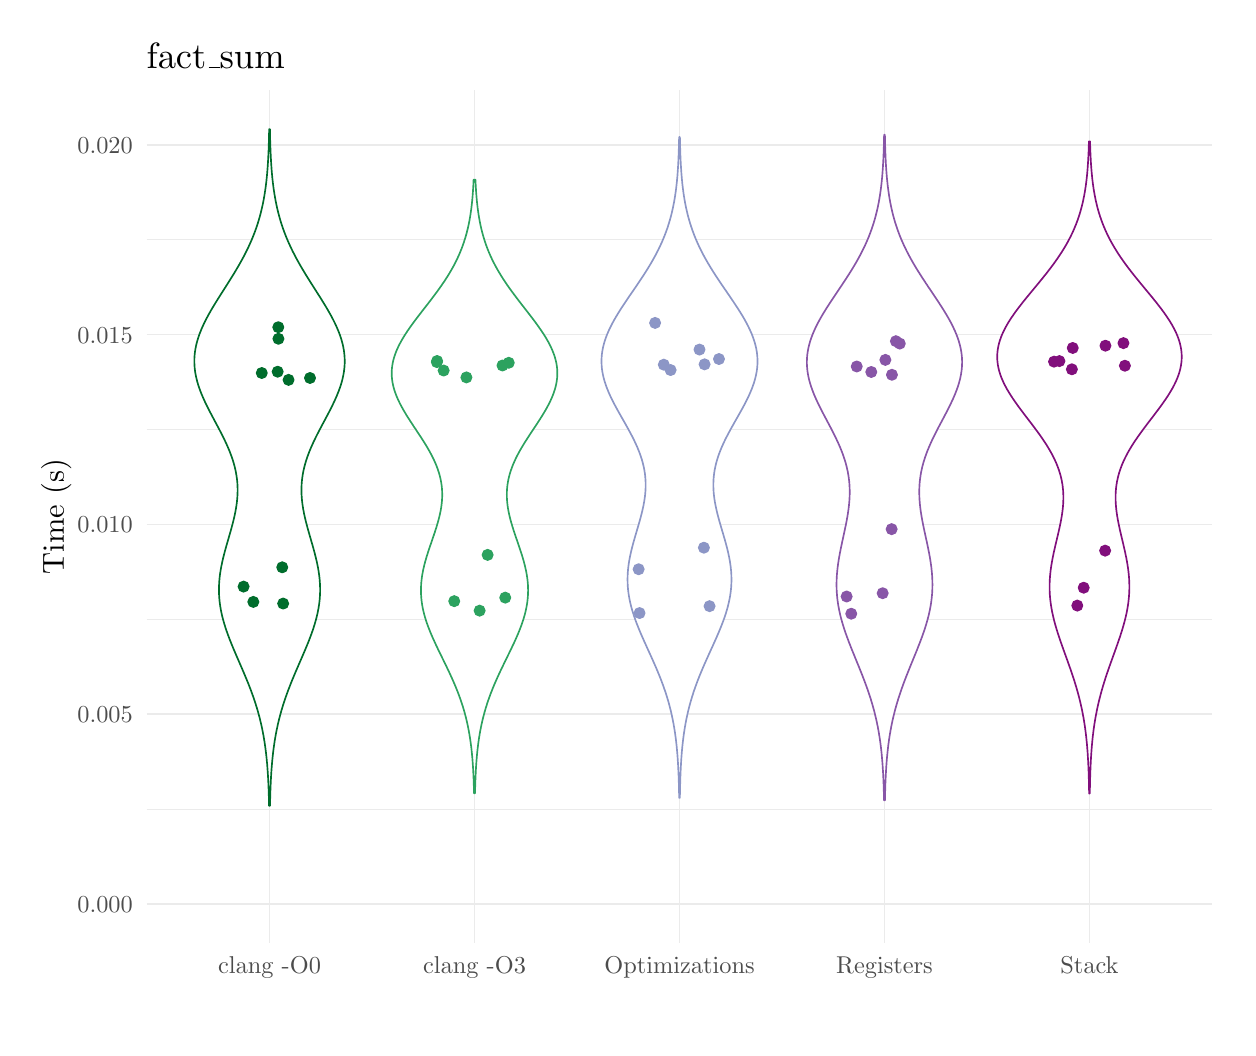
\begin{tikzpicture}[x=1pt,y=1pt]
\definecolor{fillColor}{RGB}{255,255,255}
\path[use as bounding box,fill=fillColor,fill opacity=0.00] (0,0) rectangle (433.62,361.35);
\begin{scope}
\path[clip] ( 42.95, 30.69) rectangle (428.12,338.69);
\definecolor{drawColor}{gray}{0.92}

\path[draw=drawColor,line width= 0.3pt,line join=round] ( 42.95, 78.98) --
	(428.12, 78.98);

\path[draw=drawColor,line width= 0.3pt,line join=round] ( 42.95,147.56) --
	(428.12,147.56);

\path[draw=drawColor,line width= 0.3pt,line join=round] ( 42.95,216.14) --
	(428.12,216.14);

\path[draw=drawColor,line width= 0.3pt,line join=round] ( 42.95,284.72) --
	(428.12,284.72);

\path[draw=drawColor,line width= 0.6pt,line join=round] ( 42.95, 44.69) --
	(428.12, 44.69);

\path[draw=drawColor,line width= 0.6pt,line join=round] ( 42.95,113.27) --
	(428.12,113.27);

\path[draw=drawColor,line width= 0.6pt,line join=round] ( 42.95,181.85) --
	(428.12,181.85);

\path[draw=drawColor,line width= 0.6pt,line join=round] ( 42.95,250.43) --
	(428.12,250.43);

\path[draw=drawColor,line width= 0.6pt,line join=round] ( 42.95,319.01) --
	(428.12,319.01);

\path[draw=drawColor,line width= 0.6pt,line join=round] ( 87.40, 30.69) --
	( 87.40,338.69);

\path[draw=drawColor,line width= 0.6pt,line join=round] (161.47, 30.69) --
	(161.47,338.69);

\path[draw=drawColor,line width= 0.6pt,line join=round] (235.54, 30.69) --
	(235.54,338.69);

\path[draw=drawColor,line width= 0.6pt,line join=round] (309.61, 30.69) --
	(309.61,338.69);

\path[draw=drawColor,line width= 0.6pt,line join=round] (383.68, 30.69) --
	(383.68,338.69);
\definecolor{drawColor}{RGB}{0,109,44}
\definecolor{fillColor}{RGB}{255,255,255}

\path[draw=drawColor,line width= 0.6pt,line join=round,line cap=round,fill=fillColor] ( 87.23, 80.16) --
	( 87.22, 80.63) --
	( 87.21, 81.11) --
	( 87.20, 81.59) --
	( 87.19, 82.07) --
	( 87.18, 82.55) --
	( 87.16, 83.03) --
	( 87.15, 83.51) --
	( 87.13, 83.98) --
	( 87.12, 84.46) --
	( 87.10, 84.94) --
	( 87.09, 85.42) --
	( 87.07, 85.90) --
	( 87.05, 86.38) --
	( 87.03, 86.86) --
	( 87.01, 87.33) --
	( 86.99, 87.81) --
	( 86.97, 88.29) --
	( 86.95, 88.77) --
	( 86.93, 89.25) --
	( 86.90, 89.73) --
	( 86.88, 90.20) --
	( 86.85, 90.68) --
	( 86.82, 91.16) --
	( 86.79, 91.64) --
	( 86.76, 92.12) --
	( 86.73, 92.60) --
	( 86.69, 93.08) --
	( 86.66, 93.55) --
	( 86.62, 94.03) --
	( 86.59, 94.51) --
	( 86.55, 94.99) --
	( 86.51, 95.47) --
	( 86.46, 95.95) --
	( 86.42, 96.43) --
	( 86.37, 96.90) --
	( 86.33, 97.38) --
	( 86.28, 97.86) --
	( 86.23, 98.34) --
	( 86.17, 98.82) --
	( 86.12, 99.30) --
	( 86.06, 99.78) --
	( 86.00,100.25) --
	( 85.94,100.73) --
	( 85.88,101.21) --
	( 85.81,101.69) --
	( 85.74,102.17) --
	( 85.67,102.65) --
	( 85.60,103.13) --
	( 85.53,103.60) --
	( 85.45,104.08) --
	( 85.37,104.56) --
	( 85.29,105.04) --
	( 85.21,105.52) --
	( 85.12,106.00) --
	( 85.03,106.48) --
	( 84.94,106.95) --
	( 84.84,107.43) --
	( 84.75,107.91) --
	( 84.65,108.39) --
	( 84.54,108.87) --
	( 84.44,109.35) --
	( 84.33,109.83) --
	( 84.22,110.30) --
	( 84.10,110.78) --
	( 83.99,111.26) --
	( 83.87,111.74) --
	( 83.75,112.22) --
	( 83.62,112.70) --
	( 83.49,113.18) --
	( 83.36,113.65) --
	( 83.23,114.13) --
	( 83.09,114.61) --
	( 82.95,115.09) --
	( 82.81,115.57) --
	( 82.66,116.05) --
	( 82.51,116.53) --
	( 82.36,117.00) --
	( 82.21,117.48) --
	( 82.05,117.96) --
	( 81.89,118.44) --
	( 81.73,118.92) --
	( 81.56,119.40) --
	( 81.40,119.87) --
	( 81.23,120.35) --
	( 81.05,120.83) --
	( 80.88,121.31) --
	( 80.70,121.79) --
	( 80.52,122.27) --
	( 80.34,122.75) --
	( 80.15,123.22) --
	( 79.97,123.70) --
	( 79.78,124.18) --
	( 79.59,124.66) --
	( 79.39,125.14) --
	( 79.20,125.62) --
	( 79.00,126.10) --
	( 78.80,126.57) --
	( 78.60,127.05) --
	( 78.40,127.53) --
	( 78.20,128.01) --
	( 78.00,128.49) --
	( 77.79,128.97) --
	( 77.59,129.45) --
	( 77.38,129.92) --
	( 77.18,130.40) --
	( 76.97,130.88) --
	( 76.76,131.36) --
	( 76.55,131.84) --
	( 76.34,132.32) --
	( 76.14,132.80) --
	( 75.93,133.27) --
	( 75.72,133.75) --
	( 75.51,134.23) --
	( 75.31,134.71) --
	( 75.10,135.19) --
	( 74.90,135.67) --
	( 74.69,136.15) --
	( 74.49,136.62) --
	( 74.29,137.10) --
	( 74.09,137.58) --
	( 73.90,138.06) --
	( 73.70,138.54) --
	( 73.51,139.02) --
	( 73.32,139.50) --
	( 73.13,139.97) --
	( 72.94,140.45) --
	( 72.76,140.93) --
	( 72.58,141.41) --
	( 72.40,141.89) --
	( 72.23,142.37) --
	( 72.06,142.85) --
	( 71.89,143.32) --
	( 71.72,143.80) --
	( 71.57,144.28) --
	( 71.41,144.76) --
	( 71.26,145.24) --
	( 71.11,145.72) --
	( 70.97,146.19) --
	( 70.83,146.67) --
	( 70.70,147.15) --
	( 70.57,147.63) --
	( 70.44,148.11) --
	( 70.32,148.59) --
	( 70.21,149.07) --
	( 70.10,149.54) --
	( 70.00,150.02) --
	( 69.90,150.50) --
	( 69.81,150.98) --
	( 69.72,151.46) --
	( 69.64,151.94) --
	( 69.56,152.42) --
	( 69.50,152.89) --
	( 69.43,153.37) --
	( 69.37,153.85) --
	( 69.32,154.33) --
	( 69.28,154.81) --
	( 69.23,155.29) --
	( 69.20,155.77) --
	( 69.17,156.24) --
	( 69.15,156.72) --
	( 69.13,157.20) --
	( 69.12,157.68) --
	( 69.12,158.16) --
	( 69.12,158.64) --
	( 69.13,159.12) --
	( 69.14,159.59) --
	( 69.16,160.07) --
	( 69.19,160.55) --
	( 69.22,161.03) --
	( 69.25,161.51) --
	( 69.30,161.99) --
	( 69.34,162.47) --
	( 69.39,162.94) --
	( 69.45,163.42) --
	( 69.51,163.90) --
	( 69.58,164.38) --
	( 69.66,164.86) --
	( 69.73,165.34) --
	( 69.82,165.82) --
	( 69.90,166.29) --
	( 69.99,166.77) --
	( 70.09,167.25) --
	( 70.19,167.73) --
	( 70.29,168.21) --
	( 70.40,168.69) --
	( 70.51,169.17) --
	( 70.62,169.64) --
	( 70.74,170.12) --
	( 70.86,170.60) --
	( 70.98,171.08) --
	( 71.11,171.56) --
	( 71.23,172.04) --
	( 71.36,172.51) --
	( 71.49,172.99) --
	( 71.63,173.47) --
	( 71.76,173.95) --
	( 71.90,174.43) --
	( 72.03,174.91) --
	( 72.17,175.39) --
	( 72.31,175.86) --
	( 72.45,176.34) --
	( 72.59,176.82) --
	( 72.72,177.30) --
	( 72.86,177.78) --
	( 73.00,178.26) --
	( 73.14,178.74) --
	( 73.27,179.21) --
	( 73.41,179.69) --
	( 73.54,180.17) --
	( 73.67,180.65) --
	( 73.80,181.13) --
	( 73.93,181.61) --
	( 74.06,182.09) --
	( 74.18,182.56) --
	( 74.30,183.04) --
	( 74.42,183.52) --
	( 74.53,184.00) --
	( 74.64,184.48) --
	( 74.75,184.96) --
	( 74.85,185.44) --
	( 74.95,185.91) --
	( 75.04,186.39) --
	( 75.13,186.87) --
	( 75.22,187.35) --
	( 75.30,187.83) --
	( 75.38,188.31) --
	( 75.45,188.79) --
	( 75.51,189.26) --
	( 75.58,189.74) --
	( 75.63,190.22) --
	( 75.68,190.70) --
	( 75.72,191.18) --
	( 75.76,191.66) --
	( 75.79,192.14) --
	( 75.82,192.61) --
	( 75.84,193.09) --
	( 75.85,193.57) --
	( 75.86,194.05) --
	( 75.86,194.53) --
	( 75.85,195.01) --
	( 75.84,195.49) --
	( 75.82,195.96) --
	( 75.79,196.44) --
	( 75.76,196.92) --
	( 75.71,197.40) --
	( 75.67,197.88) --
	( 75.61,198.36) --
	( 75.55,198.83) --
	( 75.48,199.31) --
	( 75.40,199.79) --
	( 75.32,200.27) --
	( 75.23,200.75) --
	( 75.14,201.23) --
	( 75.03,201.71) --
	( 74.92,202.18) --
	( 74.81,202.66) --
	( 74.68,203.14) --
	( 74.55,203.62) --
	( 74.41,204.10) --
	( 74.27,204.58) --
	( 74.12,205.06) --
	( 73.97,205.53) --
	( 73.80,206.01) --
	( 73.64,206.49) --
	( 73.46,206.97) --
	( 73.28,207.45) --
	( 73.10,207.93) --
	( 72.91,208.41) --
	( 72.71,208.88) --
	( 72.51,209.36) --
	( 72.31,209.84) --
	( 72.10,210.32) --
	( 71.88,210.80) --
	( 71.66,211.28) --
	( 71.44,211.76) --
	( 71.21,212.23) --
	( 70.98,212.71) --
	( 70.75,213.19) --
	( 70.51,213.67) --
	( 70.27,214.15) --
	( 70.03,214.63) --
	( 69.78,215.11) --
	( 69.53,215.58) --
	( 69.29,216.06) --
	( 69.03,216.54) --
	( 68.78,217.02) --
	( 68.53,217.50) --
	( 68.27,217.98) --
	( 68.02,218.46) --
	( 67.76,218.93) --
	( 67.51,219.41) --
	( 67.25,219.89) --
	( 67.00,220.37) --
	( 66.74,220.85) --
	( 66.49,221.33) --
	( 66.24,221.81) --
	( 65.99,222.28) --
	( 65.74,222.76) --
	( 65.49,223.24) --
	( 65.25,223.72) --
	( 65.01,224.20) --
	( 64.77,224.68) --
	( 64.54,225.15) --
	( 64.31,225.63) --
	( 64.08,226.11) --
	( 63.86,226.59) --
	( 63.64,227.07) --
	( 63.43,227.55) --
	( 63.22,228.03) --
	( 63.02,228.50) --
	( 62.82,228.98) --
	( 62.63,229.46) --
	( 62.44,229.94) --
	( 62.26,230.42) --
	( 62.09,230.90) --
	( 61.92,231.38) --
	( 61.76,231.85) --
	( 61.61,232.33) --
	( 61.46,232.81) --
	( 61.32,233.29) --
	( 61.19,233.77) --
	( 61.07,234.25) --
	( 60.96,234.73) --
	( 60.85,235.20) --
	( 60.75,235.68) --
	( 60.66,236.16) --
	( 60.57,236.64) --
	( 60.50,237.12) --
	( 60.44,237.60) --
	( 60.38,238.08) --
	( 60.33,238.55) --
	( 60.30,239.03) --
	( 60.27,239.51) --
	( 60.25,239.99) --
	( 60.24,240.47) --
	( 60.23,240.95) --
	( 60.24,241.43) --
	( 60.25,241.90) --
	( 60.28,242.38) --
	( 60.31,242.86) --
	( 60.36,243.34) --
	( 60.41,243.82) --
	( 60.47,244.30) --
	( 60.54,244.78) --
	( 60.62,245.25) --
	( 60.71,245.73) --
	( 60.80,246.21) --
	( 60.91,246.69) --
	( 61.02,247.17) --
	( 61.15,247.65) --
	( 61.28,248.13) --
	( 61.42,248.60) --
	( 61.57,249.08) --
	( 61.72,249.56) --
	( 61.88,250.04) --
	( 62.05,250.52) --
	( 62.23,251.00) --
	( 62.42,251.47) --
	( 62.61,251.95) --
	( 62.81,252.43) --
	( 63.01,252.91) --
	( 63.23,253.39) --
	( 63.45,253.87) --
	( 63.67,254.35) --
	( 63.90,254.82) --
	( 64.14,255.30) --
	( 64.38,255.78) --
	( 64.63,256.26) --
	( 64.88,256.74) --
	( 65.14,257.22) --
	( 65.40,257.70) --
	( 65.67,258.17) --
	( 65.94,258.65) --
	( 66.21,259.13) --
	( 66.49,259.61) --
	( 66.77,260.09) --
	( 67.06,260.57) --
	( 67.35,261.05) --
	( 67.64,261.52) --
	( 67.93,262.00) --
	( 68.23,262.48) --
	( 68.53,262.96) --
	( 68.82,263.44) --
	( 69.13,263.92) --
	( 69.43,264.40) --
	( 69.73,264.87) --
	( 70.03,265.35) --
	( 70.34,265.83) --
	( 70.64,266.31) --
	( 70.95,266.79) --
	( 71.25,267.27) --
	( 71.56,267.75) --
	( 71.86,268.22) --
	( 72.17,268.70) --
	( 72.47,269.18) --
	( 72.77,269.66) --
	( 73.07,270.14) --
	( 73.37,270.62) --
	( 73.67,271.10) --
	( 73.97,271.57) --
	( 74.26,272.05) --
	( 74.56,272.53) --
	( 74.85,273.01) --
	( 75.13,273.49) --
	( 75.42,273.97) --
	( 75.70,274.45) --
	( 75.98,274.92) --
	( 76.26,275.40) --
	( 76.53,275.88) --
	( 76.81,276.36) --
	( 77.07,276.84) --
	( 77.34,277.32) --
	( 77.60,277.79) --
	( 77.86,278.27) --
	( 78.11,278.75) --
	( 78.36,279.23) --
	( 78.61,279.71) --
	( 78.85,280.19) --
	( 79.09,280.67) --
	( 79.32,281.14) --
	( 79.56,281.62) --
	( 79.78,282.10) --
	( 80.01,282.58) --
	( 80.22,283.06) --
	( 80.44,283.54) --
	( 80.65,284.02) --
	( 80.86,284.49) --
	( 81.06,284.97) --
	( 81.26,285.45) --
	( 81.45,285.93) --
	( 81.64,286.41) --
	( 81.83,286.89) --
	( 82.01,287.37) --
	( 82.19,287.84) --
	( 82.36,288.32) --
	( 82.53,288.80) --
	( 82.70,289.28) --
	( 82.86,289.76) --
	( 83.02,290.24) --
	( 83.17,290.72) --
	( 83.32,291.19) --
	( 83.46,291.67) --
	( 83.61,292.15) --
	( 83.74,292.63) --
	( 83.88,293.11) --
	( 84.01,293.59) --
	( 84.13,294.07) --
	( 84.26,294.54) --
	( 84.37,295.02) --
	( 84.49,295.50) --
	( 84.60,295.98) --
	( 84.71,296.46) --
	( 84.82,296.94) --
	( 84.92,297.42) --
	( 85.02,297.89) --
	( 85.11,298.37) --
	( 85.21,298.85) --
	( 85.30,299.33) --
	( 85.38,299.81) --
	( 85.47,300.29) --
	( 85.55,300.77) --
	( 85.63,301.24) --
	( 85.70,301.72) --
	( 85.77,302.20) --
	( 85.84,302.68) --
	( 85.91,303.16) --
	( 85.98,303.64) --
	( 86.04,304.12) --
	( 86.10,304.59) --
	( 86.16,305.07) --
	( 86.22,305.55) --
	( 86.27,306.03) --
	( 86.32,306.51) --
	( 86.37,306.99) --
	( 86.42,307.46) --
	( 86.46,307.94) --
	( 86.51,308.42) --
	( 86.55,308.90) --
	( 86.59,309.38) --
	( 86.63,309.86) --
	( 86.67,310.34) --
	( 86.70,310.81) --
	( 86.74,311.29) --
	( 86.77,311.77) --
	( 86.80,312.25) --
	( 86.83,312.73) --
	( 86.86,313.21) --
	( 86.89,313.69) --
	( 86.91,314.16) --
	( 86.94,314.64) --
	( 86.96,315.12) --
	( 86.98,315.60) --
	( 87.01,316.08) --
	( 87.03,316.56) --
	( 87.05,317.04) --
	( 87.07,317.51) --
	( 87.08,317.99) --
	( 87.10,318.47) --
	( 87.12,318.95) --
	( 87.13,319.43) --
	( 87.15,319.91) --
	( 87.16,320.39) --
	( 87.17,320.86) --
	( 87.19,321.34) --
	( 87.20,321.82) --
	( 87.21,322.30) --
	( 87.22,322.78) --
	( 87.23,323.26) --
	( 87.24,323.74) --
	( 87.25,324.21) --
	( 87.26,324.69) --
	( 87.54,324.69) --
	( 87.54,324.21) --
	( 87.55,323.74) --
	( 87.56,323.26) --
	( 87.57,322.78) --
	( 87.58,322.30) --
	( 87.59,321.82) --
	( 87.61,321.34) --
	( 87.62,320.86) --
	( 87.63,320.39) --
	( 87.65,319.91) --
	( 87.66,319.43) --
	( 87.68,318.95) --
	( 87.69,318.47) --
	( 87.71,317.99) --
	( 87.73,317.51) --
	( 87.75,317.04) --
	( 87.77,316.56) --
	( 87.79,316.08) --
	( 87.81,315.60) --
	( 87.83,315.12) --
	( 87.85,314.64) --
	( 87.88,314.16) --
	( 87.91,313.69) --
	( 87.93,313.21) --
	( 87.96,312.73) --
	( 87.99,312.25) --
	( 88.02,311.77) --
	( 88.06,311.29) --
	( 88.09,310.81) --
	( 88.12,310.34) --
	( 88.16,309.86) --
	( 88.20,309.38) --
	( 88.24,308.90) --
	( 88.28,308.42) --
	( 88.33,307.94) --
	( 88.37,307.46) --
	( 88.42,306.99) --
	( 88.47,306.51) --
	( 88.52,306.03) --
	( 88.58,305.55) --
	( 88.63,305.07) --
	( 88.69,304.59) --
	( 88.75,304.12) --
	( 88.81,303.64) --
	( 88.88,303.16) --
	( 88.95,302.68) --
	( 89.02,302.20) --
	( 89.09,301.72) --
	( 89.17,301.24) --
	( 89.24,300.77) --
	( 89.33,300.29) --
	( 89.41,299.81) --
	( 89.50,299.33) --
	( 89.58,298.85) --
	( 89.68,298.37) --
	( 89.77,297.89) --
	( 89.87,297.42) --
	( 89.98,296.94) --
	( 90.08,296.46) --
	( 90.19,295.98) --
	( 90.30,295.50) --
	( 90.42,295.02) --
	( 90.54,294.54) --
	( 90.66,294.07) --
	( 90.79,293.59) --
	( 90.92,293.11) --
	( 91.05,292.63) --
	( 91.19,292.15) --
	( 91.33,291.67) --
	( 91.47,291.19) --
	( 91.62,290.72) --
	( 91.78,290.24) --
	( 91.93,289.76) --
	( 92.10,289.28) --
	( 92.26,288.80) --
	( 92.43,288.32) --
	( 92.60,287.84) --
	( 92.78,287.37) --
	( 92.96,286.89) --
	( 93.15,286.41) --
	( 93.34,285.93) --
	( 93.53,285.45) --
	( 93.73,284.97) --
	( 93.93,284.49) --
	( 94.14,284.02) --
	( 94.35,283.54) --
	( 94.57,283.06) --
	( 94.79,282.58) --
	( 95.01,282.10) --
	( 95.24,281.62) --
	( 95.47,281.14) --
	( 95.70,280.67) --
	( 95.94,280.19) --
	( 96.19,279.71) --
	( 96.43,279.23) --
	( 96.68,278.75) --
	( 96.94,278.27) --
	( 97.19,277.79) --
	( 97.45,277.32) --
	( 97.72,276.84) --
	( 97.99,276.36) --
	( 98.26,275.88) --
	( 98.53,275.40) --
	( 98.81,274.92) --
	( 99.09,274.45) --
	( 99.37,273.97) --
	( 99.66,273.49) --
	( 99.95,273.01) --
	(100.24,272.53) --
	(100.53,272.05) --
	(100.82,271.57) --
	(101.12,271.10) --
	(101.42,270.62) --
	(101.72,270.14) --
	(102.02,269.66) --
	(102.32,269.18) --
	(102.62,268.70) --
	(102.93,268.22) --
	(103.23,267.75) --
	(103.54,267.27) --
	(103.84,266.79) --
	(104.15,266.31) --
	(104.45,265.83) --
	(104.76,265.35) --
	(105.06,264.87) --
	(105.37,264.40) --
	(105.67,263.92) --
	(105.97,263.44) --
	(106.27,262.96) --
	(106.56,262.48) --
	(106.86,262.00) --
	(107.15,261.52) --
	(107.44,261.05) --
	(107.73,260.57) --
	(108.02,260.09) --
	(108.30,259.61) --
	(108.58,259.13) --
	(108.85,258.65) --
	(109.12,258.17) --
	(109.39,257.70) --
	(109.65,257.22) --
	(109.91,256.74) --
	(110.16,256.26) --
	(110.41,255.78) --
	(110.65,255.30) --
	(110.89,254.82) --
	(111.12,254.35) --
	(111.35,253.87) --
	(111.56,253.39) --
	(111.78,252.91) --
	(111.98,252.43) --
	(112.18,251.95) --
	(112.38,251.47) --
	(112.56,251.00) --
	(112.74,250.52) --
	(112.91,250.04) --
	(113.07,249.56) --
	(113.23,249.08) --
	(113.38,248.60) --
	(113.51,248.13) --
	(113.64,247.65) --
	(113.77,247.17) --
	(113.88,246.69) --
	(113.99,246.21) --
	(114.08,245.73) --
	(114.17,245.25) --
	(114.25,244.78) --
	(114.32,244.30) --
	(114.38,243.82) --
	(114.43,243.34) --
	(114.48,242.86) --
	(114.51,242.38) --
	(114.54,241.90) --
	(114.55,241.43) --
	(114.56,240.95) --
	(114.56,240.47) --
	(114.55,239.99) --
	(114.52,239.51) --
	(114.50,239.03) --
	(114.46,238.55) --
	(114.41,238.08) --
	(114.35,237.60) --
	(114.29,237.12) --
	(114.22,236.64) --
	(114.13,236.16) --
	(114.04,235.68) --
	(113.94,235.20) --
	(113.84,234.73) --
	(113.72,234.25) --
	(113.60,233.77) --
	(113.47,233.29) --
	(113.33,232.81) --
	(113.19,232.33) --
	(113.03,231.85) --
	(112.87,231.38) --
	(112.70,230.90) --
	(112.53,230.42) --
	(112.35,229.94) --
	(112.16,229.46) --
	(111.97,228.98) --
	(111.78,228.50) --
	(111.57,228.03) --
	(111.36,227.55) --
	(111.15,227.07) --
	(110.93,226.59) --
	(110.71,226.11) --
	(110.48,225.63) --
	(110.25,225.15) --
	(110.02,224.68) --
	(109.78,224.20) --
	(109.54,223.72) --
	(109.30,223.24) --
	(109.05,222.76) --
	(108.81,222.28) --
	(108.56,221.81) --
	(108.30,221.33) --
	(108.05,220.85) --
	(107.80,220.37) --
	(107.54,219.89) --
	(107.29,219.41) --
	(107.03,218.93) --
	(106.77,218.46) --
	(106.52,217.98) --
	(106.26,217.50) --
	(106.01,217.02) --
	(105.76,216.54) --
	(105.51,216.06) --
	(105.26,215.58) --
	(105.01,215.11) --
	(104.76,214.63) --
	(104.52,214.15) --
	(104.28,213.67) --
	(104.04,213.19) --
	(103.81,212.71) --
	(103.58,212.23) --
	(103.35,211.76) --
	(103.13,211.28) --
	(102.91,210.80) --
	(102.70,210.32) --
	(102.48,209.84) --
	(102.28,209.36) --
	(102.08,208.88) --
	(101.88,208.41) --
	(101.69,207.93) --
	(101.51,207.45) --
	(101.33,206.97) --
	(101.15,206.49) --
	(100.99,206.01) --
	(100.82,205.53) --
	(100.67,205.06) --
	(100.52,204.58) --
	(100.38,204.10) --
	(100.24,203.62) --
	(100.11,203.14) --
	( 99.99,202.66) --
	( 99.87,202.18) --
	( 99.76,201.71) --
	( 99.66,201.23) --
	( 99.56,200.75) --
	( 99.47,200.27) --
	( 99.39,199.79) --
	( 99.31,199.31) --
	( 99.24,198.83) --
	( 99.18,198.36) --
	( 99.13,197.88) --
	( 99.08,197.40) --
	( 99.04,196.92) --
	( 99.00,196.44) --
	( 98.98,195.96) --
	( 98.96,195.49) --
	( 98.94,195.01) --
	( 98.94,194.53) --
	( 98.94,194.05) --
	( 98.94,193.57) --
	( 98.96,193.09) --
	( 98.97,192.61) --
	( 99.00,192.14) --
	( 99.03,191.66) --
	( 99.07,191.18) --
	( 99.11,190.70) --
	( 99.16,190.22) --
	( 99.22,189.74) --
	( 99.28,189.26) --
	( 99.34,188.79) --
	( 99.42,188.31) --
	( 99.49,187.83) --
	( 99.57,187.35) --
	( 99.66,186.87) --
	( 99.75,186.39) --
	( 99.84,185.91) --
	( 99.94,185.44) --
	(100.05,184.96) --
	(100.15,184.48) --
	(100.26,184.00) --
	(100.38,183.52) --
	(100.49,183.04) --
	(100.61,182.56) --
	(100.74,182.09) --
	(100.86,181.61) --
	(100.99,181.13) --
	(101.12,180.65) --
	(101.25,180.17) --
	(101.38,179.69) --
	(101.52,179.21) --
	(101.66,178.74) --
	(101.79,178.26) --
	(101.93,177.78) --
	(102.07,177.30) --
	(102.21,176.82) --
	(102.35,176.34) --
	(102.48,175.86) --
	(102.62,175.39) --
	(102.76,174.91) --
	(102.90,174.43) --
	(103.03,173.95) --
	(103.17,173.47) --
	(103.30,172.99) --
	(103.43,172.51) --
	(103.56,172.04) --
	(103.69,171.56) --
	(103.81,171.08) --
	(103.93,170.60) --
	(104.05,170.12) --
	(104.17,169.64) --
	(104.28,169.17) --
	(104.39,168.69) --
	(104.50,168.21) --
	(104.60,167.73) --
	(104.70,167.25) --
	(104.80,166.77) --
	(104.89,166.29) --
	(104.98,165.82) --
	(105.06,165.34) --
	(105.14,164.86) --
	(105.21,164.38) --
	(105.28,163.90) --
	(105.34,163.42) --
	(105.40,162.94) --
	(105.45,162.47) --
	(105.50,161.99) --
	(105.54,161.51) --
	(105.57,161.03) --
	(105.61,160.55) --
	(105.63,160.07) --
	(105.65,159.59) --
	(105.66,159.12) --
	(105.67,158.64) --
	(105.67,158.16) --
	(105.67,157.68) --
	(105.66,157.20) --
	(105.64,156.72) --
	(105.62,156.24) --
	(105.59,155.77) --
	(105.56,155.29) --
	(105.52,154.81) --
	(105.47,154.33) --
	(105.42,153.85) --
	(105.36,153.37) --
	(105.30,152.89) --
	(105.23,152.42) --
	(105.15,151.94) --
	(105.07,151.46) --
	(104.99,150.98) --
	(104.89,150.50) --
	(104.80,150.02) --
	(104.69,149.54) --
	(104.58,149.07) --
	(104.47,148.59) --
	(104.35,148.11) --
	(104.23,147.63) --
	(104.10,147.15) --
	(103.96,146.67) --
	(103.82,146.19) --
	(103.68,145.72) --
	(103.53,145.24) --
	(103.38,144.76) --
	(103.23,144.28) --
	(103.07,143.80) --
	(102.90,143.32) --
	(102.74,142.85) --
	(102.57,142.37) --
	(102.39,141.89) --
	(102.22,141.41) --
	(102.03,140.93) --
	(101.85,140.45) --
	(101.67,139.97) --
	(101.48,139.50) --
	(101.29,139.02) --
	(101.09,138.54) --
	(100.90,138.06) --
	(100.70,137.58) --
	(100.50,137.10) --
	(100.30,136.62) --
	(100.10,136.15) --
	( 99.89,135.67) --
	( 99.69,135.19) --
	( 99.48,134.71) --
	( 99.28,134.23) --
	( 99.07,133.75) --
	( 98.86,133.27) --
	( 98.66,132.80) --
	( 98.45,132.32) --
	( 98.24,131.84) --
	( 98.03,131.36) --
	( 97.82,130.88) --
	( 97.62,130.40) --
	( 97.41,129.92) --
	( 97.20,129.45) --
	( 97.00,128.97) --
	( 96.79,128.49) --
	( 96.59,128.01) --
	( 96.39,127.53) --
	( 96.19,127.05) --
	( 95.99,126.57) --
	( 95.79,126.10) --
	( 95.59,125.62) --
	( 95.40,125.14) --
	( 95.21,124.66) --
	( 95.02,124.18) --
	( 94.83,123.70) --
	( 94.64,123.22) --
	( 94.46,122.75) --
	( 94.27,122.27) --
	( 94.09,121.79) --
	( 93.92,121.31) --
	( 93.74,120.83) --
	( 93.57,120.35) --
	( 93.40,119.87) --
	( 93.23,119.40) --
	( 93.06,118.92) --
	( 92.90,118.44) --
	( 92.74,117.96) --
	( 92.59,117.48) --
	( 92.43,117.00) --
	( 92.28,116.53) --
	( 92.13,116.05) --
	( 91.99,115.57) --
	( 91.84,115.09) --
	( 91.70,114.61) --
	( 91.57,114.13) --
	( 91.43,113.65) --
	( 91.30,113.18) --
	( 91.17,112.70) --
	( 91.05,112.22) --
	( 90.92,111.74) --
	( 90.80,111.26) --
	( 90.69,110.78) --
	( 90.57,110.30) --
	( 90.46,109.83) --
	( 90.35,109.35) --
	( 90.25,108.87) --
	( 90.15,108.39) --
	( 90.05,107.91) --
	( 89.95,107.43) --
	( 89.85,106.95) --
	( 89.76,106.48) --
	( 89.67,106.00) --
	( 89.59,105.52) --
	( 89.50,105.04) --
	( 89.42,104.56) --
	( 89.34,104.08) --
	( 89.26,103.60) --
	( 89.19,103.13) --
	( 89.12,102.65) --
	( 89.05,102.17) --
	( 88.98,101.69) --
	( 88.92,101.21) --
	( 88.85,100.73) --
	( 88.79,100.25) --
	( 88.73, 99.78) --
	( 88.67, 99.30) --
	( 88.62, 98.82) --
	( 88.57, 98.34) --
	( 88.52, 97.86) --
	( 88.47, 97.38) --
	( 88.42, 96.90) --
	( 88.37, 96.43) --
	( 88.33, 95.95) --
	( 88.29, 95.47) --
	( 88.25, 94.99) --
	( 88.21, 94.51) --
	( 88.17, 94.03) --
	( 88.13, 93.55) --
	( 88.10, 93.08) --
	( 88.06, 92.60) --
	( 88.03, 92.12) --
	( 88.00, 91.64) --
	( 87.97, 91.16) --
	( 87.94, 90.68) --
	( 87.92, 90.20) --
	( 87.89, 89.73) --
	( 87.87, 89.25) --
	( 87.84, 88.77) --
	( 87.82, 88.29) --
	( 87.80, 87.81) --
	( 87.78, 87.33) --
	( 87.76, 86.86) --
	( 87.74, 86.38) --
	( 87.72, 85.90) --
	( 87.70, 85.42) --
	( 87.69, 84.94) --
	( 87.67, 84.46) --
	( 87.66, 83.98) --
	( 87.64, 83.51) --
	( 87.63, 83.03) --
	( 87.62, 82.55) --
	( 87.60, 82.07) --
	( 87.59, 81.59) --
	( 87.58, 81.11) --
	( 87.57, 80.63) --
	( 87.56, 80.16) --
	( 87.23, 80.16) --
	cycle;
\definecolor{drawColor}{RGB}{44,162,95}

\path[draw=drawColor,line width= 0.6pt,line join=round,line cap=round,fill=fillColor] (161.29, 84.71) --
	(161.28, 85.14) --
	(161.27, 85.57) --
	(161.26, 86.01) --
	(161.25, 86.44) --
	(161.24, 86.88) --
	(161.22, 87.31) --
	(161.21, 87.74) --
	(161.19, 88.18) --
	(161.18, 88.61) --
	(161.16, 89.05) --
	(161.15, 89.48) --
	(161.13, 89.91) --
	(161.11, 90.35) --
	(161.09, 90.78) --
	(161.07, 91.21) --
	(161.05, 91.65) --
	(161.03, 92.08) --
	(161.01, 92.52) --
	(160.99, 92.95) --
	(160.96, 93.38) --
	(160.94, 93.82) --
	(160.91, 94.25) --
	(160.88, 94.69) --
	(160.85, 95.12) --
	(160.82, 95.55) --
	(160.79, 95.99) --
	(160.76, 96.42) --
	(160.72, 96.86) --
	(160.69, 97.29) --
	(160.65, 97.72) --
	(160.61, 98.16) --
	(160.57, 98.59) --
	(160.53, 99.02) --
	(160.49, 99.46) --
	(160.44, 99.89) --
	(160.40,100.33) --
	(160.35,100.76) --
	(160.30,101.19) --
	(160.25,101.63) --
	(160.19,102.06) --
	(160.14,102.50) --
	(160.08,102.93) --
	(160.02,103.36) --
	(159.96,103.80) --
	(159.90,104.23) --
	(159.83,104.67) --
	(159.76,105.10) --
	(159.69,105.53) --
	(159.62,105.97) --
	(159.55,106.40) --
	(159.47,106.83) --
	(159.39,107.27) --
	(159.31,107.70) --
	(159.23,108.14) --
	(159.14,108.57) --
	(159.05,109.00) --
	(158.96,109.44) --
	(158.87,109.87) --
	(158.77,110.31) --
	(158.67,110.74) --
	(158.57,111.17) --
	(158.46,111.61) --
	(158.36,112.04) --
	(158.25,112.48) --
	(158.13,112.91) --
	(158.02,113.34) --
	(157.90,113.78) --
	(157.78,114.21) --
	(157.66,114.65) --
	(157.53,115.08) --
	(157.40,115.51) --
	(157.27,115.95) --
	(157.13,116.38) --
	(156.99,116.81) --
	(156.85,117.25) --
	(156.71,117.68) --
	(156.56,118.12) --
	(156.41,118.55) --
	(156.26,118.98) --
	(156.10,119.42) --
	(155.94,119.85) --
	(155.78,120.29) --
	(155.62,120.72) --
	(155.45,121.15) --
	(155.29,121.59) --
	(155.11,122.02) --
	(154.94,122.46) --
	(154.76,122.89) --
	(154.59,123.32) --
	(154.40,123.76) --
	(154.22,124.19) --
	(154.03,124.62) --
	(153.85,125.06) --
	(153.65,125.49) --
	(153.46,125.93) --
	(153.27,126.36) --
	(153.07,126.79) --
	(152.87,127.23) --
	(152.67,127.66) --
	(152.47,128.10) --
	(152.27,128.53) --
	(152.07,128.96) --
	(151.86,129.40) --
	(151.65,129.83) --
	(151.44,130.27) --
	(151.24,130.70) --
	(151.02,131.13) --
	(150.81,131.57) --
	(150.60,132.00) --
	(150.39,132.43) --
	(150.18,132.87) --
	(149.97,133.30) --
	(149.75,133.74) --
	(149.54,134.17) --
	(149.33,134.60) --
	(149.12,135.04) --
	(148.90,135.47) --
	(148.69,135.91) --
	(148.48,136.34) --
	(148.27,136.77) --
	(148.07,137.21) --
	(147.86,137.64) --
	(147.65,138.08) --
	(147.45,138.51) --
	(147.25,138.94) --
	(147.05,139.38) --
	(146.85,139.81) --
	(146.65,140.24) --
	(146.46,140.68) --
	(146.26,141.11) --
	(146.08,141.55) --
	(145.89,141.98) --
	(145.71,142.41) --
	(145.53,142.85) --
	(145.35,143.28) --
	(145.18,143.72) --
	(145.00,144.15) --
	(144.84,144.58) --
	(144.67,145.02) --
	(144.52,145.45) --
	(144.36,145.89) --
	(144.21,146.32) --
	(144.07,146.75) --
	(143.92,147.19) --
	(143.79,147.62) --
	(143.65,148.05) --
	(143.53,148.49) --
	(143.40,148.92) --
	(143.29,149.36) --
	(143.17,149.79) --
	(143.07,150.22) --
	(142.97,150.66) --
	(142.87,151.09) --
	(142.78,151.53) --
	(142.69,151.96) --
	(142.61,152.39) --
	(142.54,152.83) --
	(142.47,153.26) --
	(142.41,153.70) --
	(142.35,154.13) --
	(142.30,154.56) --
	(142.26,155.00) --
	(142.22,155.43) --
	(142.19,155.86) --
	(142.16,156.30) --
	(142.14,156.73) --
	(142.12,157.17) --
	(142.11,157.60) --
	(142.11,158.03) --
	(142.11,158.47) --
	(142.12,158.90) --
	(142.14,159.34) --
	(142.16,159.77) --
	(142.18,160.20) --
	(142.22,160.64) --
	(142.25,161.07) --
	(142.30,161.51) --
	(142.35,161.94) --
	(142.40,162.37) --
	(142.46,162.81) --
	(142.52,163.24) --
	(142.59,163.67) --
	(142.67,164.11) --
	(142.75,164.54) --
	(142.83,164.98) --
	(142.92,165.41) --
	(143.01,165.84) --
	(143.11,166.28) --
	(143.21,166.71) --
	(143.32,167.15) --
	(143.43,167.58) --
	(143.54,168.01) --
	(143.66,168.45) --
	(143.78,168.88) --
	(143.91,169.32) --
	(144.03,169.75) --
	(144.16,170.18) --
	(144.29,170.62) --
	(144.43,171.05) --
	(144.57,171.48) --
	(144.71,171.92) --
	(144.85,172.35) --
	(144.99,172.79) --
	(145.14,173.22) --
	(145.28,173.65) --
	(145.43,174.09) --
	(145.58,174.52) --
	(145.73,174.96) --
	(145.87,175.39) --
	(146.02,175.82) --
	(146.17,176.26) --
	(146.32,176.69) --
	(146.47,177.13) --
	(146.62,177.56) --
	(146.77,177.99) --
	(146.91,178.43) --
	(147.06,178.86) --
	(147.20,179.29) --
	(147.34,179.73) --
	(147.48,180.16) --
	(147.62,180.60) --
	(147.75,181.03) --
	(147.88,181.46) --
	(148.01,181.90) --
	(148.14,182.33) --
	(148.26,182.77) --
	(148.38,183.20) --
	(148.50,183.63) --
	(148.61,184.07) --
	(148.72,184.50) --
	(148.82,184.94) --
	(148.92,185.37) --
	(149.02,185.80) --
	(149.11,186.24) --
	(149.19,186.67) --
	(149.28,187.10) --
	(149.35,187.54) --
	(149.42,187.97) --
	(149.48,188.41) --
	(149.54,188.84) --
	(149.59,189.27) --
	(149.64,189.71) --
	(149.68,190.14) --
	(149.72,190.58) --
	(149.74,191.01) --
	(149.77,191.44) --
	(149.78,191.88) --
	(149.79,192.31) --
	(149.79,192.75) --
	(149.78,193.18) --
	(149.77,193.61) --
	(149.75,194.05) --
	(149.73,194.48) --
	(149.69,194.91) --
	(149.65,195.35) --
	(149.60,195.78) --
	(149.55,196.22) --
	(149.48,196.65) --
	(149.41,197.08) --
	(149.34,197.52) --
	(149.25,197.95) --
	(149.16,198.39) --
	(149.06,198.82) --
	(148.95,199.25) --
	(148.84,199.69) --
	(148.72,200.12) --
	(148.59,200.56) --
	(148.45,200.99) --
	(148.31,201.42) --
	(148.16,201.86) --
	(148.00,202.29) --
	(147.84,202.73) --
	(147.67,203.16) --
	(147.49,203.59) --
	(147.31,204.03) --
	(147.12,204.46) --
	(146.92,204.89) --
	(146.72,205.33) --
	(146.51,205.76) --
	(146.30,206.20) --
	(146.08,206.63) --
	(145.85,207.06) --
	(145.62,207.50) --
	(145.39,207.93) --
	(145.14,208.37) --
	(144.90,208.80) --
	(144.65,209.23) --
	(144.40,209.67) --
	(144.14,210.10) --
	(143.88,210.54) --
	(143.61,210.97) --
	(143.34,211.40) --
	(143.07,211.84) --
	(142.79,212.27) --
	(142.52,212.70) --
	(142.24,213.14) --
	(141.96,213.57) --
	(141.67,214.01) --
	(141.39,214.44) --
	(141.10,214.87) --
	(140.81,215.31) --
	(140.53,215.74) --
	(140.24,216.18) --
	(139.95,216.61) --
	(139.66,217.04) --
	(139.37,217.48) --
	(139.09,217.91) --
	(138.80,218.35) --
	(138.52,218.78) --
	(138.24,219.21) --
	(137.96,219.65) --
	(137.68,220.08) --
	(137.40,220.51) --
	(137.13,220.95) --
	(136.86,221.38) --
	(136.60,221.82) --
	(136.34,222.25) --
	(136.08,222.68) --
	(135.83,223.12) --
	(135.58,223.55) --
	(135.34,223.99) --
	(135.10,224.42) --
	(134.87,224.85) --
	(134.64,225.29) --
	(134.42,225.72) --
	(134.21,226.16) --
	(134.00,226.59) --
	(133.80,227.02) --
	(133.61,227.46) --
	(133.42,227.89) --
	(133.25,228.32) --
	(133.08,228.76) --
	(132.92,229.19) --
	(132.76,229.63) --
	(132.62,230.06) --
	(132.48,230.49) --
	(132.35,230.93) --
	(132.23,231.36) --
	(132.12,231.80) --
	(132.02,232.23) --
	(131.93,232.66) --
	(131.85,233.10) --
	(131.77,233.53) --
	(131.71,233.97) --
	(131.66,234.40) --
	(131.62,234.83) --
	(131.58,235.27) --
	(131.56,235.70) --
	(131.55,236.13) --
	(131.54,236.57) --
	(131.55,237.00) --
	(131.57,237.44) --
	(131.60,237.87) --
	(131.63,238.30) --
	(131.68,238.74) --
	(131.74,239.17) --
	(131.81,239.61) --
	(131.88,240.04) --
	(131.97,240.47) --
	(132.07,240.91) --
	(132.17,241.34) --
	(132.29,241.78) --
	(132.41,242.21) --
	(132.55,242.64) --
	(132.69,243.08) --
	(132.85,243.51) --
	(133.01,243.94) --
	(133.18,244.38) --
	(133.36,244.81) --
	(133.55,245.25) --
	(133.75,245.68) --
	(133.95,246.11) --
	(134.17,246.55) --
	(134.38,246.98) --
	(134.62,247.42) --
	(134.85,247.85) --
	(135.09,248.28) --
	(135.34,248.72) --
	(135.60,249.15) --
	(135.86,249.59) --
	(136.13,250.02) --
	(136.40,250.45) --
	(136.68,250.89) --
	(136.97,251.32) --
	(137.25,251.75) --
	(137.55,252.19) --
	(137.85,252.62) --
	(138.15,253.06) --
	(138.46,253.49) --
	(138.77,253.92) --
	(139.09,254.36) --
	(139.41,254.79) --
	(139.73,255.23) --
	(140.05,255.66) --
	(140.38,256.09) --
	(140.71,256.53) --
	(141.04,256.96) --
	(141.37,257.40) --
	(141.71,257.83) --
	(142.04,258.26) --
	(142.38,258.70) --
	(142.71,259.13) --
	(143.05,259.56) --
	(143.39,260.00) --
	(143.73,260.43) --
	(144.06,260.87) --
	(144.40,261.30) --
	(144.74,261.73) --
	(145.07,262.17) --
	(145.41,262.60) --
	(145.74,263.04) --
	(146.07,263.47) --
	(146.40,263.90) --
	(146.73,264.34) --
	(147.05,264.77) --
	(147.38,265.21) --
	(147.70,265.64) --
	(148.02,266.07) --
	(148.33,266.51) --
	(148.64,266.94) --
	(148.95,267.37) --
	(149.26,267.81) --
	(149.56,268.24) --
	(149.86,268.68) --
	(150.15,269.11) --
	(150.45,269.54) --
	(150.74,269.98) --
	(151.02,270.41) --
	(151.30,270.85) --
	(151.58,271.28) --
	(151.85,271.71) --
	(152.12,272.15) --
	(152.38,272.58) --
	(152.64,273.02) --
	(152.89,273.45) --
	(153.14,273.88) --
	(153.39,274.32) --
	(153.63,274.75) --
	(153.87,275.18) --
	(154.10,275.62) --
	(154.33,276.05) --
	(154.55,276.49) --
	(154.77,276.92) --
	(154.98,277.35) --
	(155.19,277.79) --
	(155.40,278.22) --
	(155.59,278.66) --
	(155.79,279.09) --
	(155.98,279.52) --
	(156.17,279.96) --
	(156.35,280.39) --
	(156.52,280.83) --
	(156.70,281.26) --
	(156.87,281.69) --
	(157.03,282.13) --
	(157.19,282.56) --
	(157.34,282.99) --
	(157.49,283.43) --
	(157.64,283.86) --
	(157.78,284.30) --
	(157.92,284.73) --
	(158.06,285.16) --
	(158.19,285.60) --
	(158.31,286.03) --
	(158.44,286.47) --
	(158.56,286.90) --
	(158.67,287.33) --
	(158.78,287.77) --
	(158.89,288.20) --
	(159.00,288.64) --
	(159.10,289.07) --
	(159.19,289.50) --
	(159.29,289.94) --
	(159.38,290.37) --
	(159.47,290.81) --
	(159.55,291.24) --
	(159.64,291.67) --
	(159.71,292.11) --
	(159.79,292.54) --
	(159.86,292.97) --
	(159.94,293.41) --
	(160.00,293.84) --
	(160.07,294.28) --
	(160.13,294.71) --
	(160.19,295.14) --
	(160.25,295.58) --
	(160.31,296.01) --
	(160.36,296.45) --
	(160.41,296.88) --
	(160.46,297.31) --
	(160.51,297.75) --
	(160.56,298.18) --
	(160.60,298.62) --
	(160.64,299.05) --
	(160.68,299.48) --
	(160.72,299.92) --
	(160.76,300.35) --
	(160.79,300.78) --
	(160.83,301.22) --
	(160.86,301.65) --
	(160.89,302.09) --
	(160.92,302.52) --
	(160.95,302.95) --
	(160.98,303.39) --
	(161.00,303.82) --
	(161.03,304.26) --
	(161.05,304.69) --
	(161.07,305.12) --
	(161.09,305.56) --
	(161.11,305.99) --
	(161.13,306.43) --
	(161.80,306.43) --
	(161.82,305.99) --
	(161.84,305.56) --
	(161.86,305.12) --
	(161.88,304.69) --
	(161.91,304.26) --
	(161.93,303.82) --
	(161.96,303.39) --
	(161.98,302.95) --
	(162.01,302.52) --
	(162.04,302.09) --
	(162.07,301.65) --
	(162.10,301.22) --
	(162.14,300.78) --
	(162.17,300.35) --
	(162.21,299.92) --
	(162.25,299.48) --
	(162.29,299.05) --
	(162.33,298.62) --
	(162.38,298.18) --
	(162.42,297.75) --
	(162.47,297.31) --
	(162.52,296.88) --
	(162.57,296.45) --
	(162.62,296.01) --
	(162.68,295.58) --
	(162.74,295.14) --
	(162.80,294.71) --
	(162.86,294.28) --
	(162.93,293.84) --
	(163.00,293.41) --
	(163.07,292.97) --
	(163.14,292.54) --
	(163.22,292.11) --
	(163.30,291.67) --
	(163.38,291.24) --
	(163.46,290.81) --
	(163.55,290.37) --
	(163.64,289.94) --
	(163.74,289.50) --
	(163.84,289.07) --
	(163.94,288.64) --
	(164.04,288.20) --
	(164.15,287.77) --
	(164.26,287.33) --
	(164.38,286.90) --
	(164.50,286.47) --
	(164.62,286.03) --
	(164.75,285.60) --
	(164.88,285.16) --
	(165.01,284.73) --
	(165.15,284.30) --
	(165.29,283.86) --
	(165.44,283.43) --
	(165.59,282.99) --
	(165.74,282.56) --
	(165.90,282.13) --
	(166.07,281.69) --
	(166.23,281.26) --
	(166.41,280.83) --
	(166.58,280.39) --
	(166.77,279.96) --
	(166.95,279.52) --
	(167.14,279.09) --
	(167.34,278.66) --
	(167.54,278.22) --
	(167.74,277.79) --
	(167.95,277.35) --
	(168.17,276.92) --
	(168.38,276.49) --
	(168.61,276.05) --
	(168.83,275.62) --
	(169.07,275.18) --
	(169.30,274.75) --
	(169.54,274.32) --
	(169.79,273.88) --
	(170.04,273.45) --
	(170.30,273.02) --
	(170.55,272.58) --
	(170.82,272.15) --
	(171.08,271.71) --
	(171.36,271.28) --
	(171.63,270.85) --
	(171.91,270.41) --
	(172.20,269.98) --
	(172.49,269.54) --
	(172.78,269.11) --
	(173.07,268.68) --
	(173.37,268.24) --
	(173.68,267.81) --
	(173.98,267.37) --
	(174.29,266.94) --
	(174.60,266.51) --
	(174.92,266.07) --
	(175.24,265.64) --
	(175.56,265.21) --
	(175.88,264.77) --
	(176.21,264.34) --
	(176.53,263.90) --
	(176.86,263.47) --
	(177.19,263.04) --
	(177.53,262.60) --
	(177.86,262.17) --
	(178.20,261.73) --
	(178.53,261.30) --
	(178.87,260.87) --
	(179.21,260.43) --
	(179.54,260.00) --
	(179.88,259.56) --
	(180.22,259.13) --
	(180.56,258.70) --
	(180.89,258.26) --
	(181.23,257.83) --
	(181.56,257.40) --
	(181.89,256.96) --
	(182.23,256.53) --
	(182.55,256.09) --
	(182.88,255.66) --
	(183.20,255.23) --
	(183.53,254.79) --
	(183.85,254.36) --
	(184.16,253.92) --
	(184.47,253.49) --
	(184.78,253.06) --
	(185.08,252.62) --
	(185.38,252.19) --
	(185.68,251.75) --
	(185.97,251.32) --
	(186.25,250.89) --
	(186.53,250.45) --
	(186.81,250.02) --
	(187.08,249.59) --
	(187.34,249.15) --
	(187.59,248.72) --
	(187.84,248.28) --
	(188.09,247.85) --
	(188.32,247.42) --
	(188.55,246.98) --
	(188.77,246.55) --
	(188.98,246.11) --
	(189.18,245.68) --
	(189.38,245.25) --
	(189.57,244.81) --
	(189.75,244.38) --
	(189.92,243.94) --
	(190.08,243.51) --
	(190.24,243.08) --
	(190.38,242.64) --
	(190.52,242.21) --
	(190.64,241.78) --
	(190.76,241.34) --
	(190.86,240.91) --
	(190.96,240.47) --
	(191.05,240.04) --
	(191.13,239.61) --
	(191.19,239.17) --
	(191.25,238.74) --
	(191.30,238.30) --
	(191.34,237.87) --
	(191.37,237.44) --
	(191.38,237.00) --
	(191.39,236.57) --
	(191.38,236.13) --
	(191.37,235.70) --
	(191.35,235.27) --
	(191.32,234.83) --
	(191.27,234.40) --
	(191.22,233.97) --
	(191.16,233.53) --
	(191.08,233.10) --
	(191.01,232.66) --
	(190.91,232.23) --
	(190.81,231.80) --
	(190.70,231.36) --
	(190.58,230.93) --
	(190.45,230.49) --
	(190.32,230.06) --
	(190.17,229.63) --
	(190.02,229.19) --
	(189.86,228.76) --
	(189.69,228.32) --
	(189.51,227.89) --
	(189.32,227.46) --
	(189.13,227.02) --
	(188.93,226.59) --
	(188.72,226.16) --
	(188.51,225.72) --
	(188.29,225.29) --
	(188.06,224.85) --
	(187.83,224.42) --
	(187.60,223.99) --
	(187.35,223.55) --
	(187.11,223.12) --
	(186.85,222.68) --
	(186.60,222.25) --
	(186.33,221.82) --
	(186.07,221.38) --
	(185.80,220.95) --
	(185.53,220.51) --
	(185.25,220.08) --
	(184.98,219.65) --
	(184.70,219.21) --
	(184.41,218.78) --
	(184.13,218.35) --
	(183.84,217.91) --
	(183.56,217.48) --
	(183.27,217.04) --
	(182.98,216.61) --
	(182.69,216.18) --
	(182.41,215.74) --
	(182.12,215.31) --
	(181.83,214.87) --
	(181.55,214.44) --
	(181.26,214.01) --
	(180.98,213.57) --
	(180.70,213.14) --
	(180.42,212.70) --
	(180.14,212.27) --
	(179.86,211.84) --
	(179.59,211.40) --
	(179.32,210.97) --
	(179.06,210.54) --
	(178.80,210.10) --
	(178.54,209.67) --
	(178.28,209.23) --
	(178.03,208.80) --
	(177.79,208.37) --
	(177.55,207.93) --
	(177.31,207.50) --
	(177.08,207.06) --
	(176.86,206.63) --
	(176.64,206.20) --
	(176.42,205.76) --
	(176.22,205.33) --
	(176.01,204.89) --
	(175.82,204.46) --
	(175.63,204.03) --
	(175.44,203.59) --
	(175.26,203.16) --
	(175.10,202.73) --
	(174.93,202.29) --
	(174.78,201.86) --
	(174.63,201.42) --
	(174.48,200.99) --
	(174.35,200.56) --
	(174.22,200.12) --
	(174.10,199.69) --
	(173.98,199.25) --
	(173.88,198.82) --
	(173.77,198.39) --
	(173.68,197.95) --
	(173.60,197.52) --
	(173.52,197.08) --
	(173.45,196.65) --
	(173.39,196.22) --
	(173.33,195.78) --
	(173.28,195.35) --
	(173.24,194.91) --
	(173.21,194.48) --
	(173.18,194.05) --
	(173.16,193.61) --
	(173.15,193.18) --
	(173.14,192.75) --
	(173.15,192.31) --
	(173.15,191.88) --
	(173.17,191.44) --
	(173.19,191.01) --
	(173.22,190.58) --
	(173.25,190.14) --
	(173.29,189.71) --
	(173.34,189.27) --
	(173.39,188.84) --
	(173.45,188.41) --
	(173.51,187.97) --
	(173.58,187.54) --
	(173.66,187.10) --
	(173.74,186.67) --
	(173.82,186.24) --
	(173.91,185.80) --
	(174.01,185.37) --
	(174.11,184.94) --
	(174.21,184.50) --
	(174.32,184.07) --
	(174.43,183.63) --
	(174.55,183.20) --
	(174.67,182.77) --
	(174.79,182.33) --
	(174.92,181.90) --
	(175.05,181.46) --
	(175.18,181.03) --
	(175.32,180.60) --
	(175.45,180.16) --
	(175.59,179.73) --
	(175.73,179.29) --
	(175.88,178.86) --
	(176.02,178.43) --
	(176.17,177.99) --
	(176.31,177.56) --
	(176.46,177.13) --
	(176.61,176.69) --
	(176.76,176.26) --
	(176.91,175.82) --
	(177.06,175.39) --
	(177.21,174.96) --
	(177.36,174.52) --
	(177.50,174.09) --
	(177.65,173.65) --
	(177.80,173.22) --
	(177.94,172.79) --
	(178.08,172.35) --
	(178.23,171.92) --
	(178.37,171.48) --
	(178.50,171.05) --
	(178.64,170.62) --
	(178.77,170.18) --
	(178.90,169.75) --
	(179.03,169.32) --
	(179.15,168.88) --
	(179.27,168.45) --
	(179.39,168.01) --
	(179.50,167.58) --
	(179.61,167.15) --
	(179.72,166.71) --
	(179.82,166.28) --
	(179.92,165.84) --
	(180.01,165.41) --
	(180.10,164.98) --
	(180.19,164.54) --
	(180.27,164.11) --
	(180.34,163.67) --
	(180.41,163.24) --
	(180.47,162.81) --
	(180.54,162.37) --
	(180.59,161.94) --
	(180.64,161.51) --
	(180.68,161.07) --
	(180.72,160.64) --
	(180.75,160.20) --
	(180.78,159.77) --
	(180.80,159.34) --
	(180.81,158.90) --
	(180.82,158.47) --
	(180.82,158.03) --
	(180.82,157.60) --
	(180.81,157.17) --
	(180.80,156.73) --
	(180.77,156.30) --
	(180.75,155.86) --
	(180.72,155.43) --
	(180.68,155.00) --
	(180.63,154.56) --
	(180.58,154.13) --
	(180.53,153.70) --
	(180.46,153.26) --
	(180.39,152.83) --
	(180.32,152.39) --
	(180.24,151.96) --
	(180.15,151.53) --
	(180.06,151.09) --
	(179.97,150.66) --
	(179.87,150.22) --
	(179.76,149.79) --
	(179.65,149.36) --
	(179.53,148.92) --
	(179.41,148.49) --
	(179.28,148.05) --
	(179.15,147.62) --
	(179.01,147.19) --
	(178.87,146.75) --
	(178.72,146.32) --
	(178.57,145.89) --
	(178.42,145.45) --
	(178.26,145.02) --
	(178.09,144.58) --
	(177.93,144.15) --
	(177.76,143.72) --
	(177.59,143.28) --
	(177.41,142.85) --
	(177.23,142.41) --
	(177.04,141.98) --
	(176.86,141.55) --
	(176.67,141.11) --
	(176.48,140.68) --
	(176.28,140.24) --
	(176.09,139.81) --
	(175.89,139.38) --
	(175.69,138.94) --
	(175.48,138.51) --
	(175.28,138.08) --
	(175.07,137.64) --
	(174.87,137.21) --
	(174.66,136.77) --
	(174.45,136.34) --
	(174.24,135.91) --
	(174.03,135.47) --
	(173.82,135.04) --
	(173.60,134.60) --
	(173.39,134.17) --
	(173.18,133.74) --
	(172.97,133.30) --
	(172.75,132.87) --
	(172.54,132.43) --
	(172.33,132.00) --
	(172.12,131.57) --
	(171.91,131.13) --
	(171.70,130.70) --
	(171.49,130.27) --
	(171.28,129.83) --
	(171.07,129.40) --
	(170.87,128.96) --
	(170.66,128.53) --
	(170.46,128.10) --
	(170.26,127.66) --
	(170.06,127.23) --
	(169.86,126.79) --
	(169.66,126.36) --
	(169.47,125.93) --
	(169.28,125.49) --
	(169.09,125.06) --
	(168.90,124.62) --
	(168.71,124.19) --
	(168.53,123.76) --
	(168.35,123.32) --
	(168.17,122.89) --
	(167.99,122.46) --
	(167.82,122.02) --
	(167.65,121.59) --
	(167.48,121.15) --
	(167.31,120.72) --
	(167.15,120.29) --
	(166.99,119.85) --
	(166.83,119.42) --
	(166.68,118.98) --
	(166.52,118.55) --
	(166.37,118.12) --
	(166.23,117.68) --
	(166.08,117.25) --
	(165.94,116.81) --
	(165.80,116.38) --
	(165.67,115.95) --
	(165.53,115.51) --
	(165.41,115.08) --
	(165.28,114.65) --
	(165.15,114.21) --
	(165.03,113.78) --
	(164.92,113.34) --
	(164.80,112.91) --
	(164.69,112.48) --
	(164.58,112.04) --
	(164.47,111.61) --
	(164.36,111.17) --
	(164.26,110.74) --
	(164.16,110.31) --
	(164.07,109.87) --
	(163.97,109.44) --
	(163.88,109.00) --
	(163.79,108.57) --
	(163.71,108.14) --
	(163.62,107.70) --
	(163.54,107.27) --
	(163.46,106.83) --
	(163.39,106.40) --
	(163.31,105.97) --
	(163.24,105.53) --
	(163.17,105.10) --
	(163.10,104.67) --
	(163.04,104.23) --
	(162.97,103.80) --
	(162.91,103.36) --
	(162.85,102.93) --
	(162.79,102.50) --
	(162.74,102.06) --
	(162.69,101.63) --
	(162.63,101.19) --
	(162.58,100.76) --
	(162.54,100.33) --
	(162.49, 99.89) --
	(162.45, 99.46) --
	(162.40, 99.02) --
	(162.36, 98.59) --
	(162.32, 98.16) --
	(162.28, 97.72) --
	(162.25, 97.29) --
	(162.21, 96.86) --
	(162.18, 96.42) --
	(162.14, 95.99) --
	(162.11, 95.55) --
	(162.08, 95.12) --
	(162.05, 94.69) --
	(162.02, 94.25) --
	(162.00, 93.82) --
	(161.97, 93.38) --
	(161.95, 92.95) --
	(161.92, 92.52) --
	(161.90, 92.08) --
	(161.88, 91.65) --
	(161.86, 91.21) --
	(161.84, 90.78) --
	(161.82, 90.35) --
	(161.80, 89.91) --
	(161.79, 89.48) --
	(161.77, 89.05) --
	(161.75, 88.61) --
	(161.74, 88.18) --
	(161.72, 87.74) --
	(161.71, 87.31) --
	(161.70, 86.88) --
	(161.69, 86.44) --
	(161.67, 86.01) --
	(161.66, 85.57) --
	(161.65, 85.14) --
	(161.64, 84.71) --
	(161.29, 84.71) --
	cycle;
\definecolor{drawColor}{RGB}{140,150,198}

\path[draw=drawColor,line width= 0.6pt,line join=round,line cap=round,fill=fillColor] (235.41, 83.03) --
	(235.40, 83.50) --
	(235.40, 83.96) --
	(235.39, 84.43) --
	(235.38, 84.90) --
	(235.37, 85.37) --
	(235.36, 85.83) --
	(235.35, 86.30) --
	(235.34, 86.77) --
	(235.32, 87.24) --
	(235.31, 87.70) --
	(235.30, 88.17) --
	(235.29, 88.64) --
	(235.27, 89.10) --
	(235.26, 89.57) --
	(235.24, 90.04) --
	(235.22, 90.51) --
	(235.21, 90.97) --
	(235.19, 91.44) --
	(235.17, 91.91) --
	(235.15, 92.38) --
	(235.13, 92.84) --
	(235.10, 93.31) --
	(235.08, 93.78) --
	(235.06, 94.24) --
	(235.03, 94.71) --
	(235.01, 95.18) --
	(234.98, 95.65) --
	(234.95, 96.11) --
	(234.92, 96.58) --
	(234.89, 97.05) --
	(234.86, 97.52) --
	(234.82, 97.98) --
	(234.79, 98.45) --
	(234.75, 98.92) --
	(234.71, 99.39) --
	(234.67, 99.85) --
	(234.63,100.32) --
	(234.59,100.79) --
	(234.54,101.25) --
	(234.50,101.72) --
	(234.45,102.19) --
	(234.40,102.66) --
	(234.35,103.12) --
	(234.29,103.59) --
	(234.24,104.06) --
	(234.18,104.53) --
	(234.12,104.99) --
	(234.06,105.46) --
	(233.99,105.93) --
	(233.93,106.39) --
	(233.86,106.86) --
	(233.79,107.33) --
	(233.71,107.80) --
	(233.64,108.26) --
	(233.56,108.73) --
	(233.48,109.20) --
	(233.40,109.67) --
	(233.31,110.13) --
	(233.22,110.60) --
	(233.13,111.07) --
	(233.04,111.53) --
	(232.94,112.00) --
	(232.84,112.47) --
	(232.74,112.94) --
	(232.64,113.40) --
	(232.53,113.87) --
	(232.42,114.34) --
	(232.31,114.81) --
	(232.19,115.27) --
	(232.07,115.74) --
	(231.95,116.21) --
	(231.83,116.68) --
	(231.70,117.14) --
	(231.57,117.61) --
	(231.44,118.08) --
	(231.30,118.54) --
	(231.16,119.01) --
	(231.02,119.48) --
	(230.87,119.95) --
	(230.73,120.41) --
	(230.57,120.88) --
	(230.42,121.35) --
	(230.26,121.82) --
	(230.10,122.28) --
	(229.94,122.75) --
	(229.78,123.22) --
	(229.61,123.68) --
	(229.44,124.15) --
	(229.26,124.62) --
	(229.09,125.09) --
	(228.91,125.55) --
	(228.73,126.02) --
	(228.55,126.49) --
	(228.36,126.96) --
	(228.17,127.42) --
	(227.98,127.89) --
	(227.79,128.36) --
	(227.60,128.82) --
	(227.40,129.29) --
	(227.20,129.76) --
	(227.00,130.23) --
	(226.80,130.69) --
	(226.59,131.16) --
	(226.39,131.63) --
	(226.18,132.10) --
	(225.98,132.56) --
	(225.77,133.03) --
	(225.56,133.50) --
	(225.35,133.96) --
	(225.14,134.43) --
	(224.92,134.90) --
	(224.71,135.37) --
	(224.50,135.83) --
	(224.29,136.30) --
	(224.07,136.77) --
	(223.86,137.24) --
	(223.65,137.70) --
	(223.44,138.17) --
	(223.23,138.64) --
	(223.01,139.11) --
	(222.80,139.57) --
	(222.60,140.04) --
	(222.39,140.51) --
	(222.18,140.97) --
	(221.98,141.44) --
	(221.77,141.91) --
	(221.57,142.38) --
	(221.37,142.84) --
	(221.18,143.31) --
	(220.98,143.78) --
	(220.79,144.25) --
	(220.60,144.71) --
	(220.42,145.18) --
	(220.23,145.65) --
	(220.05,146.11) --
	(219.88,146.58) --
	(219.70,147.05) --
	(219.53,147.52) --
	(219.37,147.98) --
	(219.21,148.45) --
	(219.05,148.92) --
	(218.90,149.39) --
	(218.75,149.85) --
	(218.60,150.32) --
	(218.46,150.79) --
	(218.33,151.25) --
	(218.20,151.72) --
	(218.07,152.19) --
	(217.95,152.66) --
	(217.84,153.12) --
	(217.73,153.59) --
	(217.63,154.06) --
	(217.53,154.53) --
	(217.44,154.99) --
	(217.35,155.46) --
	(217.27,155.93) --
	(217.19,156.40) --
	(217.13,156.86) --
	(217.06,157.33) --
	(217.01,157.80) --
	(216.95,158.26) --
	(216.91,158.73) --
	(216.87,159.20) --
	(216.84,159.67) --
	(216.81,160.13) --
	(216.79,160.60) --
	(216.78,161.07) --
	(216.77,161.54) --
	(216.77,162.00) --
	(216.77,162.47) --
	(216.78,162.94) --
	(216.79,163.40) --
	(216.82,163.87) --
	(216.84,164.34) --
	(216.88,164.81) --
	(216.92,165.27) --
	(216.96,165.74) --
	(217.01,166.21) --
	(217.06,166.68) --
	(217.13,167.14) --
	(217.19,167.61) --
	(217.26,168.08) --
	(217.34,168.54) --
	(217.42,169.01) --
	(217.50,169.48) --
	(217.59,169.95) --
	(217.69,170.41) --
	(217.78,170.88) --
	(217.89,171.35) --
	(217.99,171.82) --
	(218.10,172.28) --
	(218.21,172.75) --
	(218.33,173.22) --
	(218.45,173.69) --
	(218.57,174.15) --
	(218.69,174.62) --
	(218.82,175.09) --
	(218.95,175.55) --
	(219.08,176.02) --
	(219.21,176.49) --
	(219.35,176.96) --
	(219.48,177.42) --
	(219.62,177.89) --
	(219.76,178.36) --
	(219.90,178.83) --
	(220.03,179.29) --
	(220.17,179.76) --
	(220.31,180.23) --
	(220.45,180.69) --
	(220.58,181.16) --
	(220.72,181.63) --
	(220.86,182.10) --
	(220.99,182.56) --
	(221.12,183.03) --
	(221.25,183.50) --
	(221.38,183.97) --
	(221.51,184.43) --
	(221.63,184.90) --
	(221.75,185.37) --
	(221.87,185.83) --
	(221.98,186.30) --
	(222.10,186.77) --
	(222.20,187.24) --
	(222.31,187.70) --
	(222.41,188.17) --
	(222.50,188.64) --
	(222.59,189.11) --
	(222.68,189.57) --
	(222.76,190.04) --
	(222.84,190.51) --
	(222.91,190.98) --
	(222.97,191.44) --
	(223.04,191.91) --
	(223.09,192.38) --
	(223.14,192.84) --
	(223.18,193.31) --
	(223.22,193.78) --
	(223.25,194.25) --
	(223.27,194.71) --
	(223.29,195.18) --
	(223.30,195.65) --
	(223.30,196.12) --
	(223.30,196.58) --
	(223.29,197.05) --
	(223.27,197.52) --
	(223.24,197.98) --
	(223.21,198.45) --
	(223.17,198.92) --
	(223.13,199.39) --
	(223.07,199.85) --
	(223.02,200.32) --
	(222.94,200.79) --
	(222.87,201.26) --
	(222.79,201.72) --
	(222.70,202.19) --
	(222.60,202.66) --
	(222.50,203.12) --
	(222.38,203.59) --
	(222.26,204.06) --
	(222.14,204.53) --
	(222.01,204.99) --
	(221.87,205.46) --
	(221.72,205.93) --
	(221.57,206.40) --
	(221.41,206.86) --
	(221.24,207.33) --
	(221.07,207.80) --
	(220.89,208.27) --
	(220.70,208.73) --
	(220.51,209.20) --
	(220.32,209.67) --
	(220.11,210.13) --
	(219.90,210.60) --
	(219.69,211.07) --
	(219.47,211.54) --
	(219.25,212.00) --
	(219.02,212.47) --
	(218.79,212.94) --
	(218.55,213.41) --
	(218.32,213.87) --
	(218.07,214.34) --
	(217.83,214.81) --
	(217.58,215.27) --
	(217.32,215.74) --
	(217.07,216.21) --
	(216.81,216.68) --
	(216.55,217.14) --
	(216.29,217.61) --
	(216.03,218.08) --
	(215.76,218.55) --
	(215.50,219.01) --
	(215.23,219.48) --
	(214.97,219.95) --
	(214.70,220.41) --
	(214.43,220.88) --
	(214.17,221.35) --
	(213.91,221.82) --
	(213.64,222.28) --
	(213.38,222.75) --
	(213.12,223.22) --
	(212.87,223.69) --
	(212.61,224.15) --
	(212.36,224.62) --
	(212.11,225.09) --
	(211.86,225.56) --
	(211.62,226.02) --
	(211.39,226.49) --
	(211.15,226.96) --
	(210.93,227.42) --
	(210.70,227.89) --
	(210.48,228.36) --
	(210.27,228.83) --
	(210.06,229.29) --
	(209.86,229.76) --
	(209.67,230.23) --
	(209.48,230.70) --
	(209.29,231.16) --
	(209.12,231.63) --
	(208.95,232.10) --
	(208.79,232.56) --
	(208.64,233.03) --
	(208.49,233.50) --
	(208.35,233.97) --
	(208.23,234.43) --
	(208.10,234.90) --
	(207.99,235.37) --
	(207.89,235.84) --
	(207.79,236.30) --
	(207.71,236.77) --
	(207.63,237.24) --
	(207.56,237.70) --
	(207.50,238.17) --
	(207.46,238.64) --
	(207.42,239.11) --
	(207.39,239.57) --
	(207.37,240.04) --
	(207.35,240.51) --
	(207.35,240.98) --
	(207.36,241.44) --
	(207.38,241.91) --
	(207.41,242.38) --
	(207.45,242.85) --
	(207.49,243.31) --
	(207.55,243.78) --
	(207.62,244.25) --
	(207.69,244.71) --
	(207.78,245.18) --
	(207.87,245.65) --
	(207.98,246.12) --
	(208.09,246.58) --
	(208.21,247.05) --
	(208.34,247.52) --
	(208.48,247.99) --
	(208.63,248.45) --
	(208.79,248.92) --
	(208.95,249.39) --
	(209.12,249.85) --
	(209.31,250.32) --
	(209.50,250.79) --
	(209.70,251.26) --
	(209.90,251.72) --
	(210.11,252.19) --
	(210.33,252.66) --
	(210.56,253.13) --
	(210.79,253.59) --
	(211.03,254.06) --
	(211.28,254.53) --
	(211.53,254.99) --
	(211.78,255.46) --
	(212.05,255.93) --
	(212.32,256.40) --
	(212.59,256.86) --
	(212.87,257.33) --
	(213.15,257.80) --
	(213.43,258.27) --
	(213.73,258.73) --
	(214.02,259.20) --
	(214.32,259.67) --
	(214.62,260.14) --
	(214.92,260.60) --
	(215.23,261.07) --
	(215.54,261.54) --
	(215.85,262.00) --
	(216.17,262.47) --
	(216.48,262.94) --
	(216.80,263.41) --
	(217.12,263.87) --
	(217.43,264.34) --
	(217.75,264.81) --
	(218.07,265.28) --
	(218.40,265.74) --
	(218.72,266.21) --
	(219.04,266.68) --
	(219.36,267.14) --
	(219.68,267.61) --
	(219.99,268.08) --
	(220.31,268.55) --
	(220.63,269.01) --
	(220.94,269.48) --
	(221.26,269.95) --
	(221.57,270.42) --
	(221.88,270.88) --
	(222.18,271.35) --
	(222.49,271.82) --
	(222.79,272.28) --
	(223.09,272.75) --
	(223.39,273.22) --
	(223.68,273.69) --
	(223.98,274.15) --
	(224.26,274.62) --
	(224.55,275.09) --
	(224.83,275.56) --
	(225.11,276.02) --
	(225.38,276.49) --
	(225.65,276.96) --
	(225.92,277.43) --
	(226.18,277.89) --
	(226.44,278.36) --
	(226.69,278.83) --
	(226.95,279.29) --
	(227.19,279.76) --
	(227.43,280.23) --
	(227.67,280.70) --
	(227.91,281.16) --
	(228.13,281.63) --
	(228.36,282.10) --
	(228.58,282.57) --
	(228.80,283.03) --
	(229.01,283.50) --
	(229.22,283.97) --
	(229.42,284.43) --
	(229.62,284.90) --
	(229.81,285.37) --
	(230.00,285.84) --
	(230.19,286.30) --
	(230.37,286.77) --
	(230.54,287.24) --
	(230.72,287.71) --
	(230.88,288.17) --
	(231.05,288.64) --
	(231.21,289.11) --
	(231.36,289.57) --
	(231.51,290.04) --
	(231.66,290.51) --
	(231.80,290.98) --
	(231.94,291.44) --
	(232.08,291.91) --
	(232.21,292.38) --
	(232.34,292.85) --
	(232.46,293.31) --
	(232.58,293.78) --
	(232.70,294.25) --
	(232.81,294.72) --
	(232.92,295.18) --
	(233.02,295.65) --
	(233.13,296.12) --
	(233.22,296.58) --
	(233.32,297.05) --
	(233.41,297.52) --
	(233.50,297.99) --
	(233.59,298.45) --
	(233.67,298.92) --
	(233.75,299.39) --
	(233.83,299.86) --
	(233.90,300.32) --
	(233.98,300.79) --
	(234.04,301.26) --
	(234.11,301.72) --
	(234.18,302.19) --
	(234.24,302.66) --
	(234.30,303.13) --
	(234.35,303.59) --
	(234.41,304.06) --
	(234.46,304.53) --
	(234.51,305.00) --
	(234.56,305.46) --
	(234.61,305.93) --
	(234.65,306.40) --
	(234.70,306.86) --
	(234.74,307.33) --
	(234.78,307.80) --
	(234.81,308.27) --
	(234.85,308.73) --
	(234.88,309.20) --
	(234.92,309.67) --
	(234.95,310.14) --
	(234.98,310.60) --
	(235.01,311.07) --
	(235.03,311.54) --
	(235.06,312.01) --
	(235.09,312.47) --
	(235.11,312.94) --
	(235.13,313.41) --
	(235.15,313.87) --
	(235.18,314.34) --
	(235.19,314.81) --
	(235.21,315.28) --
	(235.23,315.74) --
	(235.25,316.21) --
	(235.26,316.68) --
	(235.28,317.15) --
	(235.29,317.61) --
	(235.31,318.08) --
	(235.32,318.55) --
	(235.33,319.01) --
	(235.34,319.48) --
	(235.36,319.95) --
	(235.37,320.42) --
	(235.38,320.88) --
	(235.39,321.35) --
	(235.39,321.82) --
	(235.68,321.82) --
	(235.69,321.35) --
	(235.70,320.88) --
	(235.71,320.42) --
	(235.72,319.95) --
	(235.73,319.48) --
	(235.74,319.01) --
	(235.75,318.55) --
	(235.77,318.08) --
	(235.78,317.61) --
	(235.79,317.15) --
	(235.81,316.68) --
	(235.83,316.21) --
	(235.84,315.74) --
	(235.86,315.28) --
	(235.88,314.81) --
	(235.90,314.34) --
	(235.92,313.87) --
	(235.94,313.41) --
	(235.96,312.94) --
	(235.99,312.47) --
	(236.01,312.01) --
	(236.04,311.54) --
	(236.07,311.07) --
	(236.10,310.60) --
	(236.13,310.14) --
	(236.16,309.67) --
	(236.19,309.20) --
	(236.22,308.73) --
	(236.26,308.27) --
	(236.30,307.80) --
	(236.34,307.33) --
	(236.38,306.86) --
	(236.42,306.40) --
	(236.47,305.93) --
	(236.51,305.46) --
	(236.56,305.00) --
	(236.61,304.53) --
	(236.67,304.06) --
	(236.72,303.59) --
	(236.78,303.13) --
	(236.84,302.66) --
	(236.90,302.19) --
	(236.96,301.72) --
	(237.03,301.26) --
	(237.10,300.79) --
	(237.17,300.32) --
	(237.25,299.86) --
	(237.32,299.39) --
	(237.40,298.92) --
	(237.49,298.45) --
	(237.57,297.99) --
	(237.66,297.52) --
	(237.75,297.05) --
	(237.85,296.58) --
	(237.95,296.12) --
	(238.05,295.65) --
	(238.16,295.18) --
	(238.27,294.72) --
	(238.38,294.25) --
	(238.49,293.78) --
	(238.61,293.31) --
	(238.74,292.85) --
	(238.87,292.38) --
	(239.00,291.91) --
	(239.13,291.44) --
	(239.27,290.98) --
	(239.41,290.51) --
	(239.56,290.04) --
	(239.71,289.57) --
	(239.87,289.11) --
	(240.03,288.64) --
	(240.19,288.17) --
	(240.36,287.71) --
	(240.53,287.24) --
	(240.71,286.77) --
	(240.89,286.30) --
	(241.07,285.84) --
	(241.26,285.37) --
	(241.46,284.90) --
	(241.65,284.43) --
	(241.86,283.97) --
	(242.06,283.50) --
	(242.28,283.03) --
	(242.49,282.57) --
	(242.71,282.10) --
	(242.94,281.63) --
	(243.17,281.16) --
	(243.40,280.70) --
	(243.64,280.23) --
	(243.88,279.76) --
	(244.13,279.29) --
	(244.38,278.83) --
	(244.63,278.36) --
	(244.89,277.89) --
	(245.16,277.43) --
	(245.42,276.96) --
	(245.69,276.49) --
	(245.97,276.02) --
	(246.25,275.56) --
	(246.53,275.09) --
	(246.81,274.62) --
	(247.10,274.15) --
	(247.39,273.69) --
	(247.68,273.22) --
	(247.98,272.75) --
	(248.28,272.28) --
	(248.58,271.82) --
	(248.89,271.35) --
	(249.20,270.88) --
	(249.51,270.42) --
	(249.82,269.95) --
	(250.13,269.48) --
	(250.45,269.01) --
	(250.76,268.55) --
	(251.08,268.08) --
	(251.40,267.61) --
	(251.72,267.14) --
	(252.04,266.68) --
	(252.36,266.21) --
	(252.68,265.74) --
	(253.00,265.28) --
	(253.32,264.81) --
	(253.64,264.34) --
	(253.96,263.87) --
	(254.28,263.41) --
	(254.59,262.94) --
	(254.91,262.47) --
	(255.22,262.00) --
	(255.53,261.54) --
	(255.84,261.07) --
	(256.15,260.60) --
	(256.45,260.14) --
	(256.76,259.67) --
	(257.05,259.20) --
	(257.35,258.73) --
	(257.64,258.27) --
	(257.92,257.80) --
	(258.21,257.33) --
	(258.49,256.86) --
	(258.76,256.40) --
	(259.03,255.93) --
	(259.29,255.46) --
	(259.55,254.99) --
	(259.80,254.53) --
	(260.05,254.06) --
	(260.28,253.59) --
	(260.52,253.13) --
	(260.74,252.66) --
	(260.96,252.19) --
	(261.17,251.72) --
	(261.38,251.26) --
	(261.58,250.79) --
	(261.77,250.32) --
	(261.95,249.85) --
	(262.12,249.39) --
	(262.29,248.92) --
	(262.44,248.45) --
	(262.59,247.99) --
	(262.73,247.52) --
	(262.86,247.05) --
	(262.99,246.58) --
	(263.10,246.12) --
	(263.21,245.65) --
	(263.30,245.18) --
	(263.38,244.71) --
	(263.46,244.25) --
	(263.53,243.78) --
	(263.58,243.31) --
	(263.63,242.85) --
	(263.67,242.38) --
	(263.69,241.91) --
	(263.71,241.44) --
	(263.72,240.98) --
	(263.72,240.51) --
	(263.71,240.04) --
	(263.69,239.57) --
	(263.66,239.11) --
	(263.62,238.64) --
	(263.57,238.17) --
	(263.51,237.70) --
	(263.45,237.24) --
	(263.37,236.77) --
	(263.28,236.30) --
	(263.19,235.84) --
	(263.08,235.37) --
	(262.97,234.90) --
	(262.85,234.43) --
	(262.72,233.97) --
	(262.58,233.50) --
	(262.44,233.03) --
	(262.28,232.56) --
	(262.12,232.10) --
	(261.95,231.63) --
	(261.78,231.16) --
	(261.60,230.70) --
	(261.41,230.23) --
	(261.21,229.76) --
	(261.01,229.29) --
	(260.81,228.83) --
	(260.59,228.36) --
	(260.37,227.89) --
	(260.15,227.42) --
	(259.92,226.96) --
	(259.69,226.49) --
	(259.45,226.02) --
	(259.21,225.56) --
	(258.96,225.09) --
	(258.72,224.62) --
	(258.46,224.15) --
	(258.21,223.69) --
	(257.95,223.22) --
	(257.69,222.75) --
	(257.43,222.28) --
	(257.17,221.82) --
	(256.90,221.35) --
	(256.64,220.88) --
	(256.37,220.41) --
	(256.11,219.95) --
	(255.84,219.48) --
	(255.58,219.01) --
	(255.31,218.55) --
	(255.05,218.08) --
	(254.79,217.61) --
	(254.52,217.14) --
	(254.26,216.68) --
	(254.01,216.21) --
	(253.75,215.74) --
	(253.50,215.27) --
	(253.25,214.81) --
	(253.00,214.34) --
	(252.76,213.87) --
	(252.52,213.41) --
	(252.28,212.94) --
	(252.05,212.47) --
	(251.82,212.00) --
	(251.60,211.54) --
	(251.38,211.07) --
	(251.17,210.60) --
	(250.96,210.13) --
	(250.76,209.67) --
	(250.56,209.20) --
	(250.37,208.73) --
	(250.19,208.27) --
	(250.01,207.80) --
	(249.83,207.33) --
	(249.67,206.86) --
	(249.51,206.40) --
	(249.35,205.93) --
	(249.21,205.46) --
	(249.07,204.99) --
	(248.93,204.53) --
	(248.81,204.06) --
	(248.69,203.59) --
	(248.58,203.12) --
	(248.47,202.66) --
	(248.38,202.19) --
	(248.29,201.72) --
	(248.20,201.26) --
	(248.13,200.79) --
	(248.06,200.32) --
	(248.00,199.85) --
	(247.95,199.39) --
	(247.90,198.92) --
	(247.86,198.45) --
	(247.83,197.98) --
	(247.81,197.52) --
	(247.79,197.05) --
	(247.78,196.58) --
	(247.77,196.12) --
	(247.78,195.65) --
	(247.79,195.18) --
	(247.80,194.71) --
	(247.83,194.25) --
	(247.86,193.78) --
	(247.89,193.31) --
	(247.94,192.84) --
	(247.99,192.38) --
	(248.04,191.91) --
	(248.10,191.44) --
	(248.16,190.98) --
	(248.24,190.51) --
	(248.31,190.04) --
	(248.39,189.57) --
	(248.48,189.11) --
	(248.57,188.64) --
	(248.67,188.17) --
	(248.77,187.70) --
	(248.87,187.24) --
	(248.98,186.77) --
	(249.09,186.30) --
	(249.20,185.83) --
	(249.32,185.37) --
	(249.44,184.90) --
	(249.57,184.43) --
	(249.69,183.97) --
	(249.82,183.50) --
	(249.95,183.03) --
	(250.08,182.56) --
	(250.22,182.10) --
	(250.35,181.63) --
	(250.49,181.16) --
	(250.63,180.69) --
	(250.76,180.23) --
	(250.90,179.76) --
	(251.04,179.29) --
	(251.18,178.83) --
	(251.32,178.36) --
	(251.45,177.89) --
	(251.59,177.42) --
	(251.73,176.96) --
	(251.86,176.49) --
	(251.99,176.02) --
	(252.12,175.55) --
	(252.25,175.09) --
	(252.38,174.62) --
	(252.50,174.15) --
	(252.63,173.69) --
	(252.74,173.22) --
	(252.86,172.75) --
	(252.97,172.28) --
	(253.08,171.82) --
	(253.19,171.35) --
	(253.29,170.88) --
	(253.39,170.41) --
	(253.48,169.95) --
	(253.57,169.48) --
	(253.66,169.01) --
	(253.74,168.54) --
	(253.81,168.08) --
	(253.88,167.61) --
	(253.95,167.14) --
	(254.01,166.68) --
	(254.06,166.21) --
	(254.11,165.74) --
	(254.16,165.27) --
	(254.20,164.81) --
	(254.23,164.34) --
	(254.26,163.87) --
	(254.28,163.40) --
	(254.29,162.94) --
	(254.31,162.47) --
	(254.31,162.00) --
	(254.31,161.54) --
	(254.30,161.07) --
	(254.28,160.60) --
	(254.26,160.13) --
	(254.24,159.67) --
	(254.21,159.20) --
	(254.16,158.73) --
	(254.12,158.26) --
	(254.07,157.80) --
	(254.01,157.33) --
	(253.95,156.86) --
	(253.88,156.40) --
	(253.81,155.93) --
	(253.72,155.46) --
	(253.64,154.99) --
	(253.54,154.53) --
	(253.45,154.06) --
	(253.34,153.59) --
	(253.23,153.12) --
	(253.12,152.66) --
	(253.00,152.19) --
	(252.88,151.72) --
	(252.75,151.25) --
	(252.61,150.79) --
	(252.47,150.32) --
	(252.33,149.85) --
	(252.18,149.39) --
	(252.03,148.92) --
	(251.87,148.45) --
	(251.71,147.98) --
	(251.54,147.52) --
	(251.37,147.05) --
	(251.20,146.58) --
	(251.02,146.11) --
	(250.84,145.65) --
	(250.66,145.18) --
	(250.47,144.71) --
	(250.28,144.25) --
	(250.09,143.78) --
	(249.90,143.31) --
	(249.70,142.84) --
	(249.50,142.38) --
	(249.30,141.91) --
	(249.10,141.44) --
	(248.89,140.97) --
	(248.69,140.51) --
	(248.48,140.04) --
	(248.27,139.57) --
	(248.06,139.11) --
	(247.85,138.64) --
	(247.64,138.17) --
	(247.43,137.70) --
	(247.21,137.24) --
	(247.00,136.77) --
	(246.79,136.30) --
	(246.57,135.83) --
	(246.36,135.37) --
	(246.15,134.90) --
	(245.94,134.43) --
	(245.73,133.96) --
	(245.52,133.50) --
	(245.31,133.03) --
	(245.10,132.56) --
	(244.89,132.10) --
	(244.68,131.63) --
	(244.48,131.16) --
	(244.28,130.69) --
	(244.07,130.23) --
	(243.87,129.76) --
	(243.68,129.29) --
	(243.48,128.82) --
	(243.28,128.36) --
	(243.09,127.89) --
	(242.90,127.42) --
	(242.71,126.96) --
	(242.53,126.49) --
	(242.34,126.02) --
	(242.16,125.55) --
	(241.99,125.09) --
	(241.81,124.62) --
	(241.64,124.15) --
	(241.47,123.68) --
	(241.30,123.22) --
	(241.13,122.75) --
	(240.97,122.28) --
	(240.81,121.82) --
	(240.65,121.35) --
	(240.50,120.88) --
	(240.35,120.41) --
	(240.20,119.95) --
	(240.06,119.48) --
	(239.91,119.01) --
	(239.78,118.54) --
	(239.64,118.08) --
	(239.51,117.61) --
	(239.37,117.14) --
	(239.25,116.68) --
	(239.12,116.21) --
	(239.00,115.74) --
	(238.88,115.27) --
	(238.77,114.81) --
	(238.65,114.34) --
	(238.54,113.87) --
	(238.44,113.40) --
	(238.33,112.94) --
	(238.23,112.47) --
	(238.13,112.00) --
	(238.04,111.53) --
	(237.94,111.07) --
	(237.85,110.60) --
	(237.76,110.13) --
	(237.68,109.67) --
	(237.60,109.20) --
	(237.51,108.73) --
	(237.44,108.26) --
	(237.36,107.80) --
	(237.29,107.33) --
	(237.22,106.86) --
	(237.15,106.39) --
	(237.08,105.93) --
	(237.02,105.46) --
	(236.96,104.99) --
	(236.90,104.53) --
	(236.84,104.06) --
	(236.78,103.59) --
	(236.73,103.12) --
	(236.68,102.66) --
	(236.63,102.19) --
	(236.58,101.72) --
	(236.53,101.25) --
	(236.49,100.79) --
	(236.44,100.32) --
	(236.40, 99.85) --
	(236.36, 99.39) --
	(236.32, 98.92) --
	(236.29, 98.45) --
	(236.25, 97.98) --
	(236.22, 97.52) --
	(236.18, 97.05) --
	(236.15, 96.58) --
	(236.12, 96.11) --
	(236.10, 95.65) --
	(236.07, 95.18) --
	(236.04, 94.71) --
	(236.02, 94.24) --
	(235.99, 93.78) --
	(235.97, 93.31) --
	(235.95, 92.84) --
	(235.93, 92.38) --
	(235.91, 91.91) --
	(235.89, 91.44) --
	(235.87, 90.97) --
	(235.85, 90.51) --
	(235.83, 90.04) --
	(235.82, 89.57) --
	(235.80, 89.10) --
	(235.79, 88.64) --
	(235.78, 88.17) --
	(235.76, 87.70) --
	(235.75, 87.24) --
	(235.74, 86.77) --
	(235.73, 86.30) --
	(235.72, 85.83) --
	(235.71, 85.37) --
	(235.70, 84.90) --
	(235.69, 84.43) --
	(235.68, 83.96) --
	(235.67, 83.50) --
	(235.66, 83.03) --
	(235.41, 83.03) --
	cycle;
\definecolor{drawColor}{RGB}{136,86,167}

\path[draw=drawColor,line width= 0.6pt,line join=round,line cap=round,fill=fillColor] (309.44, 82.18) --
	(309.44, 82.66) --
	(309.42, 83.13) --
	(309.41, 83.60) --
	(309.40, 84.07) --
	(309.39, 84.54) --
	(309.38, 85.01) --
	(309.36, 85.48) --
	(309.35, 85.95) --
	(309.34, 86.42) --
	(309.32, 86.89) --
	(309.30, 87.36) --
	(309.29, 87.83) --
	(309.27, 88.30) --
	(309.25, 88.77) --
	(309.23, 89.24) --
	(309.21, 89.71) --
	(309.19, 90.19) --
	(309.17, 90.66) --
	(309.15, 91.13) --
	(309.12, 91.60) --
	(309.10, 92.07) --
	(309.07, 92.54) --
	(309.04, 93.01) --
	(309.01, 93.48) --
	(308.98, 93.95) --
	(308.95, 94.42) --
	(308.92, 94.89) --
	(308.88, 95.36) --
	(308.85, 95.83) --
	(308.81, 96.30) --
	(308.77, 96.77) --
	(308.73, 97.24) --
	(308.69, 97.71) --
	(308.65, 98.19) --
	(308.60, 98.66) --
	(308.56, 99.13) --
	(308.51, 99.60) --
	(308.46,100.07) --
	(308.41,100.54) --
	(308.35,101.01) --
	(308.30,101.48) --
	(308.24,101.95) --
	(308.18,102.42) --
	(308.12,102.89) --
	(308.06,103.36) --
	(307.99,103.83) --
	(307.92,104.30) --
	(307.85,104.77) --
	(307.78,105.24) --
	(307.70,105.71) --
	(307.63,106.19) --
	(307.55,106.66) --
	(307.47,107.13) --
	(307.38,107.60) --
	(307.30,108.07) --
	(307.21,108.54) --
	(307.12,109.01) --
	(307.02,109.48) --
	(306.93,109.95) --
	(306.83,110.42) --
	(306.72,110.89) --
	(306.62,111.36) --
	(306.51,111.83) --
	(306.40,112.30) --
	(306.29,112.77) --
	(306.18,113.24) --
	(306.06,113.72) --
	(305.94,114.19) --
	(305.82,114.66) --
	(305.69,115.13) --
	(305.56,115.60) --
	(305.43,116.07) --
	(305.30,116.54) --
	(305.16,117.01) --
	(305.02,117.48) --
	(304.88,117.95) --
	(304.74,118.42) --
	(304.59,118.89) --
	(304.44,119.36) --
	(304.29,119.83) --
	(304.14,120.30) --
	(303.98,120.77) --
	(303.82,121.24) --
	(303.66,121.72) --
	(303.50,122.19) --
	(303.33,122.66) --
	(303.16,123.13) --
	(302.99,123.60) --
	(302.82,124.07) --
	(302.65,124.54) --
	(302.47,125.01) --
	(302.29,125.48) --
	(302.11,125.95) --
	(301.93,126.42) --
	(301.75,126.89) --
	(301.57,127.36) --
	(301.38,127.83) --
	(301.20,128.30) --
	(301.01,128.77) --
	(300.82,129.25) --
	(300.63,129.72) --
	(300.44,130.19) --
	(300.25,130.66) --
	(300.06,131.13) --
	(299.86,131.60) --
	(299.67,132.07) --
	(299.48,132.54) --
	(299.29,133.01) --
	(299.09,133.48) --
	(298.90,133.95) --
	(298.71,134.42) --
	(298.52,134.89) --
	(298.33,135.36) --
	(298.14,135.83) --
	(297.95,136.30) --
	(297.76,136.77) --
	(297.57,137.25) --
	(297.38,137.72) --
	(297.20,138.19) --
	(297.02,138.66) --
	(296.83,139.13) --
	(296.65,139.60) --
	(296.48,140.07) --
	(296.30,140.54) --
	(296.13,141.01) --
	(295.96,141.48) --
	(295.79,141.95) --
	(295.62,142.42) --
	(295.46,142.89) --
	(295.30,143.36) --
	(295.14,143.83) --
	(294.99,144.30) --
	(294.84,144.78) --
	(294.69,145.25) --
	(294.55,145.72) --
	(294.41,146.19) --
	(294.27,146.66) --
	(294.14,147.13) --
	(294.01,147.60) --
	(293.89,148.07) --
	(293.76,148.54) --
	(293.65,149.01) --
	(293.54,149.48) --
	(293.43,149.95) --
	(293.33,150.42) --
	(293.23,150.89) --
	(293.14,151.36) --
	(293.05,151.83) --
	(292.96,152.30) --
	(292.88,152.78) --
	(292.81,153.25) --
	(292.74,153.72) --
	(292.67,154.19) --
	(292.61,154.66) --
	(292.56,155.13) --
	(292.51,155.60) --
	(292.46,156.07) --
	(292.43,156.54) --
	(292.39,157.01) --
	(292.36,157.48) --
	(292.33,157.95) --
	(292.32,158.42) --
	(292.30,158.89) --
	(292.29,159.36) --
	(292.29,159.83) --
	(292.29,160.30) --
	(292.29,160.78) --
	(292.30,161.25) --
	(292.31,161.72) --
	(292.33,162.19) --
	(292.35,162.66) --
	(292.38,163.13) --
	(292.41,163.60) --
	(292.45,164.07) --
	(292.49,164.54) --
	(292.53,165.01) --
	(292.58,165.48) --
	(292.63,165.95) --
	(292.69,166.42) --
	(292.75,166.89) --
	(292.81,167.36) --
	(292.88,167.83) --
	(292.95,168.31) --
	(293.02,168.78) --
	(293.10,169.25) --
	(293.18,169.72) --
	(293.26,170.19) --
	(293.34,170.66) --
	(293.43,171.13) --
	(293.52,171.60) --
	(293.61,172.07) --
	(293.70,172.54) --
	(293.79,173.01) --
	(293.89,173.48) --
	(293.99,173.95) --
	(294.09,174.42) --
	(294.19,174.89) --
	(294.29,175.36) --
	(294.39,175.83) --
	(294.49,176.31) --
	(294.59,176.78) --
	(294.70,177.25) --
	(294.80,177.72) --
	(294.90,178.19) --
	(295.00,178.66) --
	(295.10,179.13) --
	(295.20,179.60) --
	(295.31,180.07) --
	(295.40,180.54) --
	(295.50,181.01) --
	(295.60,181.48) --
	(295.69,181.95) --
	(295.79,182.42) --
	(295.88,182.89) --
	(295.97,183.36) --
	(296.05,183.84) --
	(296.13,184.31) --
	(296.22,184.78) --
	(296.29,185.25) --
	(296.37,185.72) --
	(296.44,186.19) --
	(296.51,186.66) --
	(296.57,187.13) --
	(296.64,187.60) --
	(296.69,188.07) --
	(296.75,188.54) --
	(296.80,189.01) --
	(296.84,189.48) --
	(296.88,189.95) --
	(296.92,190.42) --
	(296.95,190.89) --
	(296.98,191.36) --
	(297.00,191.84) --
	(297.02,192.31) --
	(297.03,192.78) --
	(297.03,193.25) --
	(297.04,193.72) --
	(297.03,194.19) --
	(297.02,194.66) --
	(297.01,195.13) --
	(296.98,195.60) --
	(296.96,196.07) --
	(296.92,196.54) --
	(296.89,197.01) --
	(296.84,197.48) --
	(296.79,197.95) --
	(296.73,198.42) --
	(296.67,198.89) --
	(296.60,199.37) --
	(296.52,199.84) --
	(296.44,200.31) --
	(296.35,200.78) --
	(296.26,201.25) --
	(296.16,201.72) --
	(296.05,202.19) --
	(295.94,202.66) --
	(295.82,203.13) --
	(295.70,203.60) --
	(295.57,204.07) --
	(295.43,204.54) --
	(295.29,205.01) --
	(295.14,205.48) --
	(294.98,205.95) --
	(294.82,206.42) --
	(294.66,206.89) --
	(294.49,207.37) --
	(294.31,207.84) --
	(294.13,208.31) --
	(293.95,208.78) --
	(293.75,209.25) --
	(293.56,209.72) --
	(293.36,210.19) --
	(293.15,210.66) --
	(292.94,211.13) --
	(292.73,211.60) --
	(292.51,212.07) --
	(292.29,212.54) --
	(292.07,213.01) --
	(291.84,213.48) --
	(291.61,213.95) --
	(291.37,214.42) --
	(291.14,214.89) --
	(290.90,215.37) --
	(290.66,215.84) --
	(290.41,216.31) --
	(290.17,216.78) --
	(289.92,217.25) --
	(289.68,217.72) --
	(289.43,218.19) --
	(289.18,218.66) --
	(288.93,219.13) --
	(288.68,219.60) --
	(288.43,220.07) --
	(288.18,220.54) --
	(287.93,221.01) --
	(287.68,221.48) --
	(287.44,221.95) --
	(287.19,222.42) --
	(286.95,222.90) --
	(286.71,223.37) --
	(286.47,223.84) --
	(286.23,224.31) --
	(286.00,224.78) --
	(285.77,225.25) --
	(285.54,225.72) --
	(285.32,226.19) --
	(285.10,226.66) --
	(284.89,227.13) --
	(284.68,227.60) --
	(284.47,228.07) --
	(284.27,228.54) --
	(284.08,229.01) --
	(283.89,229.48) --
	(283.71,229.95) --
	(283.53,230.42) --
	(283.36,230.90) --
	(283.20,231.37) --
	(283.04,231.84) --
	(282.89,232.31) --
	(282.75,232.78) --
	(282.61,233.25) --
	(282.48,233.72) --
	(282.36,234.19) --
	(282.25,234.66) --
	(282.14,235.13) --
	(282.05,235.60) --
	(281.96,236.07) --
	(281.88,236.54) --
	(281.81,237.01) --
	(281.75,237.48) --
	(281.70,237.95) --
	(281.65,238.43) --
	(281.62,238.90) --
	(281.59,239.37) --
	(281.57,239.84) --
	(281.56,240.31) --
	(281.57,240.78) --
	(281.58,241.25) --
	(281.60,241.72) --
	(281.63,242.19) --
	(281.66,242.66) --
	(281.71,243.13) --
	(281.77,243.60) --
	(281.84,244.07) --
	(281.91,244.54) --
	(282.00,245.01) --
	(282.09,245.48) --
	(282.19,245.95) --
	(282.31,246.43) --
	(282.43,246.90) --
	(282.56,247.37) --
	(282.69,247.84) --
	(282.84,248.31) --
	(282.99,248.78) --
	(283.16,249.25) --
	(283.33,249.72) --
	(283.51,250.19) --
	(283.69,250.66) --
	(283.89,251.13) --
	(284.09,251.60) --
	(284.30,252.07) --
	(284.51,252.54) --
	(284.73,253.01) --
	(284.96,253.48) --
	(285.20,253.96) --
	(285.44,254.43) --
	(285.69,254.90) --
	(285.94,255.37) --
	(286.20,255.84) --
	(286.46,256.31) --
	(286.73,256.78) --
	(287.00,257.25) --
	(287.28,257.72) --
	(287.56,258.19) --
	(287.85,258.66) --
	(288.14,259.13) --
	(288.43,259.60) --
	(288.72,260.07) --
	(289.02,260.54) --
	(289.33,261.01) --
	(289.63,261.48) --
	(289.94,261.96) --
	(290.25,262.43) --
	(290.56,262.90) --
	(290.87,263.37) --
	(291.18,263.84) --
	(291.50,264.31) --
	(291.81,264.78) --
	(292.13,265.25) --
	(292.45,265.72) --
	(292.76,266.19) --
	(293.08,266.66) --
	(293.39,267.13) --
	(293.71,267.60) --
	(294.03,268.07) --
	(294.34,268.54) --
	(294.65,269.01) --
	(294.96,269.49) --
	(295.27,269.96) --
	(295.58,270.43) --
	(295.89,270.90) --
	(296.19,271.37) --
	(296.50,271.84) --
	(296.80,272.31) --
	(297.09,272.78) --
	(297.39,273.25) --
	(297.68,273.72) --
	(297.97,274.19) --
	(298.26,274.66) --
	(298.54,275.13) --
	(298.82,275.60) --
	(299.10,276.07) --
	(299.37,276.54) --
	(299.64,277.01) --
	(299.90,277.49) --
	(300.17,277.96) --
	(300.42,278.43) --
	(300.68,278.90) --
	(300.93,279.37) --
	(301.17,279.84) --
	(301.42,280.31) --
	(301.65,280.78) --
	(301.89,281.25) --
	(302.12,281.72) --
	(302.34,282.19) --
	(302.56,282.66) --
	(302.78,283.13) --
	(302.99,283.60) --
	(303.20,284.07) --
	(303.40,284.54) --
	(303.60,285.01) --
	(303.80,285.49) --
	(303.99,285.96) --
	(304.17,286.43) --
	(304.35,286.90) --
	(304.53,287.37) --
	(304.70,287.84) --
	(304.87,288.31) --
	(305.04,288.78) --
	(305.20,289.25) --
	(305.35,289.72) --
	(305.51,290.19) --
	(305.66,290.66) --
	(305.80,291.13) --
	(305.94,291.60) --
	(306.08,292.07) --
	(306.21,292.54) --
	(306.34,293.02) --
	(306.46,293.49) --
	(306.58,293.96) --
	(306.70,294.43) --
	(306.81,294.90) --
	(306.93,295.37) --
	(307.03,295.84) --
	(307.14,296.31) --
	(307.24,296.78) --
	(307.33,297.25) --
	(307.43,297.72) --
	(307.52,298.19) --
	(307.61,298.66) --
	(307.69,299.13) --
	(307.77,299.60) --
	(307.85,300.07) --
	(307.93,300.54) --
	(308.00,301.02) --
	(308.07,301.49) --
	(308.14,301.96) --
	(308.20,302.43) --
	(308.27,302.90) --
	(308.33,303.37) --
	(308.39,303.84) --
	(308.44,304.31) --
	(308.50,304.78) --
	(308.55,305.25) --
	(308.60,305.72) --
	(308.65,306.19) --
	(308.69,306.66) --
	(308.74,307.13) --
	(308.78,307.60) --
	(308.82,308.07) --
	(308.86,308.55) --
	(308.89,309.02) --
	(308.93,309.49) --
	(308.96,309.96) --
	(309.00,310.43) --
	(309.03,310.90) --
	(309.06,311.37) --
	(309.08,311.84) --
	(309.11,312.31) --
	(309.14,312.78) --
	(309.16,313.25) --
	(309.19,313.72) --
	(309.21,314.19) --
	(309.23,314.66) --
	(309.25,315.13) --
	(309.27,315.60) --
	(309.29,316.07) --
	(309.30,316.55) --
	(309.32,317.02) --
	(309.34,317.49) --
	(309.35,317.96) --
	(309.37,318.43) --
	(309.38,318.90) --
	(309.39,319.37) --
	(309.41,319.84) --
	(309.42,320.31) --
	(309.43,320.78) --
	(309.44,321.25) --
	(309.45,321.72) --
	(309.46,322.19) --
	(309.47,322.66) --
	(309.75,322.66) --
	(309.76,322.19) --
	(309.77,321.72) --
	(309.78,321.25) --
	(309.79,320.78) --
	(309.80,320.31) --
	(309.81,319.84) --
	(309.82,319.37) --
	(309.83,318.90) --
	(309.85,318.43) --
	(309.86,317.96) --
	(309.88,317.49) --
	(309.89,317.02) --
	(309.91,316.55) --
	(309.93,316.07) --
	(309.95,315.60) --
	(309.97,315.13) --
	(309.99,314.66) --
	(310.01,314.19) --
	(310.03,313.72) --
	(310.05,313.25) --
	(310.08,312.78) --
	(310.10,312.31) --
	(310.13,311.84) --
	(310.16,311.37) --
	(310.19,310.90) --
	(310.22,310.43) --
	(310.25,309.96) --
	(310.29,309.49) --
	(310.32,309.02) --
	(310.36,308.55) --
	(310.40,308.07) --
	(310.44,307.60) --
	(310.48,307.13) --
	(310.52,306.66) --
	(310.57,306.19) --
	(310.62,305.72) --
	(310.67,305.25) --
	(310.72,304.78) --
	(310.77,304.31) --
	(310.83,303.84) --
	(310.89,303.37) --
	(310.95,302.90) --
	(311.01,302.43) --
	(311.08,301.96) --
	(311.15,301.49) --
	(311.22,301.02) --
	(311.29,300.54) --
	(311.36,300.07) --
	(311.44,299.60) --
	(311.53,299.13) --
	(311.61,298.66) --
	(311.70,298.19) --
	(311.79,297.72) --
	(311.88,297.25) --
	(311.98,296.78) --
	(312.08,296.31) --
	(312.18,295.84) --
	(312.29,295.37) --
	(312.40,294.90) --
	(312.51,294.43) --
	(312.63,293.96) --
	(312.75,293.49) --
	(312.88,293.02) --
	(313.01,292.54) --
	(313.14,292.07) --
	(313.27,291.60) --
	(313.41,291.13) --
	(313.56,290.66) --
	(313.71,290.19) --
	(313.86,289.72) --
	(314.02,289.25) --
	(314.18,288.78) --
	(314.34,288.31) --
	(314.51,287.84) --
	(314.68,287.37) --
	(314.86,286.90) --
	(315.04,286.43) --
	(315.23,285.96) --
	(315.42,285.49) --
	(315.61,285.01) --
	(315.81,284.54) --
	(316.02,284.07) --
	(316.22,283.60) --
	(316.44,283.13) --
	(316.65,282.66) --
	(316.87,282.19) --
	(317.10,281.72) --
	(317.33,281.25) --
	(317.56,280.78) --
	(317.80,280.31) --
	(318.04,279.84) --
	(318.29,279.37) --
	(318.54,278.90) --
	(318.79,278.43) --
	(319.05,277.96) --
	(319.31,277.49) --
	(319.58,277.01) --
	(319.84,276.54) --
	(320.12,276.07) --
	(320.39,275.60) --
	(320.67,275.13) --
	(320.96,274.66) --
	(321.24,274.19) --
	(321.53,273.72) --
	(321.82,273.25) --
	(322.12,272.78) --
	(322.42,272.31) --
	(322.72,271.84) --
	(323.02,271.37) --
	(323.33,270.90) --
	(323.63,270.43) --
	(323.94,269.96) --
	(324.25,269.49) --
	(324.56,269.01) --
	(324.88,268.54) --
	(325.19,268.07) --
	(325.50,267.60) --
	(325.82,267.13) --
	(326.14,266.66) --
	(326.45,266.19) --
	(326.77,265.72) --
	(327.09,265.25) --
	(327.40,264.78) --
	(327.72,264.31) --
	(328.03,263.84) --
	(328.35,263.37) --
	(328.66,262.90) --
	(328.97,262.43) --
	(329.28,261.96) --
	(329.58,261.48) --
	(329.89,261.01) --
	(330.19,260.54) --
	(330.49,260.07) --
	(330.79,259.60) --
	(331.08,259.13) --
	(331.37,258.66) --
	(331.65,258.19) --
	(331.94,257.72) --
	(332.21,257.25) --
	(332.49,256.78) --
	(332.76,256.31) --
	(333.02,255.84) --
	(333.28,255.37) --
	(333.53,254.90) --
	(333.78,254.43) --
	(334.02,253.96) --
	(334.25,253.48) --
	(334.48,253.01) --
	(334.70,252.54) --
	(334.92,252.07) --
	(335.13,251.60) --
	(335.33,251.13) --
	(335.52,250.66) --
	(335.71,250.19) --
	(335.89,249.72) --
	(336.06,249.25) --
	(336.22,248.78) --
	(336.37,248.31) --
	(336.52,247.84) --
	(336.66,247.37) --
	(336.79,246.90) --
	(336.91,246.43) --
	(337.02,245.95) --
	(337.12,245.48) --
	(337.22,245.01) --
	(337.30,244.54) --
	(337.38,244.07) --
	(337.45,243.60) --
	(337.50,243.13) --
	(337.55,242.66) --
	(337.59,242.19) --
	(337.62,241.72) --
	(337.64,241.25) --
	(337.65,240.78) --
	(337.65,240.31) --
	(337.64,239.84) --
	(337.63,239.37) --
	(337.60,238.90) --
	(337.57,238.43) --
	(337.52,237.95) --
	(337.47,237.48) --
	(337.40,237.01) --
	(337.33,236.54) --
	(337.26,236.07) --
	(337.17,235.60) --
	(337.07,235.13) --
	(336.97,234.66) --
	(336.86,234.19) --
	(336.73,233.72) --
	(336.61,233.25) --
	(336.47,232.78) --
	(336.33,232.31) --
	(336.18,231.84) --
	(336.02,231.37) --
	(335.86,230.90) --
	(335.68,230.42) --
	(335.51,229.95) --
	(335.32,229.48) --
	(335.14,229.01) --
	(334.94,228.54) --
	(334.74,228.07) --
	(334.54,227.60) --
	(334.33,227.13) --
	(334.11,226.66) --
	(333.89,226.19) --
	(333.67,225.72) --
	(333.45,225.25) --
	(333.22,224.78) --
	(332.98,224.31) --
	(332.75,223.84) --
	(332.51,223.37) --
	(332.27,222.90) --
	(332.02,222.42) --
	(331.78,221.95) --
	(331.53,221.48) --
	(331.28,221.01) --
	(331.04,220.54) --
	(330.79,220.07) --
	(330.54,219.60) --
	(330.29,219.13) --
	(330.04,218.66) --
	(329.79,218.19) --
	(329.54,217.72) --
	(329.29,217.25) --
	(329.05,216.78) --
	(328.80,216.31) --
	(328.56,215.84) --
	(328.32,215.37) --
	(328.08,214.89) --
	(327.84,214.42) --
	(327.61,213.95) --
	(327.38,213.48) --
	(327.15,213.01) --
	(326.92,212.54) --
	(326.70,212.07) --
	(326.48,211.60) --
	(326.27,211.13) --
	(326.06,210.66) --
	(325.86,210.19) --
	(325.66,209.72) --
	(325.46,209.25) --
	(325.27,208.78) --
	(325.08,208.31) --
	(324.90,207.84) --
	(324.73,207.37) --
	(324.56,206.89) --
	(324.39,206.42) --
	(324.23,205.95) --
	(324.08,205.48) --
	(323.93,205.01) --
	(323.78,204.54) --
	(323.65,204.07) --
	(323.52,203.60) --
	(323.39,203.13) --
	(323.27,202.66) --
	(323.16,202.19) --
	(323.06,201.72) --
	(322.95,201.25) --
	(322.86,200.78) --
	(322.77,200.31) --
	(322.69,199.84) --
	(322.62,199.37) --
	(322.55,198.89) --
	(322.48,198.42) --
	(322.43,197.95) --
	(322.38,197.48) --
	(322.33,197.01) --
	(322.29,196.54) --
	(322.26,196.07) --
	(322.23,195.60) --
	(322.21,195.13) --
	(322.19,194.66) --
	(322.18,194.19) --
	(322.18,193.72) --
	(322.18,193.25) --
	(322.19,192.78) --
	(322.20,192.31) --
	(322.21,191.84) --
	(322.24,191.36) --
	(322.26,190.89) --
	(322.30,190.42) --
	(322.33,189.95) --
	(322.37,189.48) --
	(322.42,189.01) --
	(322.47,188.54) --
	(322.52,188.07) --
	(322.58,187.60) --
	(322.64,187.13) --
	(322.70,186.66) --
	(322.77,186.19) --
	(322.85,185.72) --
	(322.92,185.25) --
	(323.00,184.78) --
	(323.08,184.31) --
	(323.16,183.84) --
	(323.25,183.36) --
	(323.34,182.89) --
	(323.43,182.42) --
	(323.52,181.95) --
	(323.62,181.48) --
	(323.71,181.01) --
	(323.81,180.54) --
	(323.91,180.07) --
	(324.01,179.60) --
	(324.11,179.13) --
	(324.21,178.66) --
	(324.31,178.19) --
	(324.42,177.72) --
	(324.52,177.25) --
	(324.62,176.78) --
	(324.72,176.31) --
	(324.83,175.83) --
	(324.93,175.36) --
	(325.03,174.89) --
	(325.13,174.42) --
	(325.23,173.95) --
	(325.32,173.48) --
	(325.42,173.01) --
	(325.52,172.54) --
	(325.61,172.07) --
	(325.70,171.60) --
	(325.79,171.13) --
	(325.87,170.66) --
	(325.96,170.19) --
	(326.04,169.72) --
	(326.12,169.25) --
	(326.19,168.78) --
	(326.27,168.31) --
	(326.34,167.83) --
	(326.40,167.36) --
	(326.47,166.89) --
	(326.53,166.42) --
	(326.58,165.95) --
	(326.63,165.48) --
	(326.68,165.01) --
	(326.73,164.54) --
	(326.77,164.07) --
	(326.80,163.60) --
	(326.83,163.13) --
	(326.86,162.66) --
	(326.88,162.19) --
	(326.90,161.72) --
	(326.92,161.25) --
	(326.92,160.78) --
	(326.93,160.30) --
	(326.93,159.83) --
	(326.92,159.36) --
	(326.91,158.89) --
	(326.90,158.42) --
	(326.88,157.95) --
	(326.85,157.48) --
	(326.83,157.01) --
	(326.79,156.54) --
	(326.75,156.07) --
	(326.70,155.60) --
	(326.65,155.13) --
	(326.60,154.66) --
	(326.54,154.19) --
	(326.48,153.72) --
	(326.41,153.25) --
	(326.33,152.78) --
	(326.25,152.30) --
	(326.17,151.83) --
	(326.08,151.36) --
	(325.99,150.89) --
	(325.89,150.42) --
	(325.78,149.95) --
	(325.68,149.48) --
	(325.57,149.01) --
	(325.45,148.54) --
	(325.33,148.07) --
	(325.21,147.60) --
	(325.08,147.13) --
	(324.94,146.66) --
	(324.81,146.19) --
	(324.67,145.72) --
	(324.53,145.25) --
	(324.38,144.78) --
	(324.23,144.30) --
	(324.07,143.83) --
	(323.92,143.36) --
	(323.76,142.89) --
	(323.59,142.42) --
	(323.43,141.95) --
	(323.26,141.48) --
	(323.09,141.01) --
	(322.91,140.54) --
	(322.74,140.07) --
	(322.56,139.60) --
	(322.38,139.13) --
	(322.20,138.66) --
	(322.02,138.19) --
	(321.83,137.72) --
	(321.64,137.25) --
	(321.46,136.77) --
	(321.27,136.30) --
	(321.08,135.83) --
	(320.89,135.36) --
	(320.70,134.89) --
	(320.51,134.42) --
	(320.31,133.95) --
	(320.12,133.48) --
	(319.93,133.01) --
	(319.74,132.54) --
	(319.54,132.07) --
	(319.35,131.60) --
	(319.16,131.13) --
	(318.97,130.66) --
	(318.78,130.19) --
	(318.58,129.72) --
	(318.40,129.25) --
	(318.21,128.77) --
	(318.02,128.30) --
	(317.83,127.83) --
	(317.65,127.36) --
	(317.46,126.89) --
	(317.28,126.42) --
	(317.10,125.95) --
	(316.92,125.48) --
	(316.74,125.01) --
	(316.57,124.54) --
	(316.39,124.07) --
	(316.22,123.60) --
	(316.05,123.13) --
	(315.89,122.66) --
	(315.72,122.19) --
	(315.56,121.72) --
	(315.39,121.24) --
	(315.24,120.77) --
	(315.08,120.30) --
	(314.92,119.83) --
	(314.77,119.36) --
	(314.62,118.89) --
	(314.48,118.42) --
	(314.33,117.95) --
	(314.19,117.48) --
	(314.05,117.01) --
	(313.92,116.54) --
	(313.78,116.07) --
	(313.65,115.60) --
	(313.52,115.13) --
	(313.40,114.66) --
	(313.28,114.19) --
	(313.16,113.72) --
	(313.04,113.24) --
	(312.92,112.77) --
	(312.81,112.30) --
	(312.70,111.83) --
	(312.59,111.36) --
	(312.49,110.89) --
	(312.39,110.42) --
	(312.29,109.95) --
	(312.19,109.48) --
	(312.10,109.01) --
	(312.01,108.54) --
	(311.92,108.07) --
	(311.83,107.60) --
	(311.75,107.13) --
	(311.67,106.66) --
	(311.59,106.19) --
	(311.51,105.71) --
	(311.43,105.24) --
	(311.36,104.77) --
	(311.29,104.30) --
	(311.22,103.83) --
	(311.16,103.36) --
	(311.09,102.89) --
	(311.03,102.42) --
	(310.97,101.95) --
	(310.92,101.48) --
	(310.86,101.01) --
	(310.81,100.54) --
	(310.76,100.07) --
	(310.71, 99.60) --
	(310.66, 99.13) --
	(310.61, 98.66) --
	(310.57, 98.19) --
	(310.52, 97.71) --
	(310.48, 97.24) --
	(310.44, 96.77) --
	(310.40, 96.30) --
	(310.37, 95.83) --
	(310.33, 95.36) --
	(310.30, 94.89) --
	(310.26, 94.42) --
	(310.23, 93.95) --
	(310.20, 93.48) --
	(310.17, 93.01) --
	(310.15, 92.54) --
	(310.12, 92.07) --
	(310.09, 91.60) --
	(310.07, 91.13) --
	(310.05, 90.66) --
	(310.02, 90.19) --
	(310.00, 89.71) --
	(309.98, 89.24) --
	(309.96, 88.77) --
	(309.94, 88.30) --
	(309.93, 87.83) --
	(309.91, 87.36) --
	(309.89, 86.89) --
	(309.88, 86.42) --
	(309.86, 85.95) --
	(309.85, 85.48) --
	(309.84, 85.01) --
	(309.82, 84.54) --
	(309.81, 84.07) --
	(309.80, 83.60) --
	(309.79, 83.13) --
	(309.78, 82.66) --
	(309.77, 82.18) --
	(309.44, 82.18) --
	cycle;
\definecolor{drawColor}{RGB}{129,15,124}

\path[draw=drawColor,line width= 0.6pt,line join=round,line cap=round,fill=fillColor] (383.56, 84.58) --
	(383.55, 85.04) --
	(383.54, 85.50) --
	(383.53, 85.96) --
	(383.53, 86.42) --
	(383.52, 86.88) --
	(383.51, 87.34) --
	(383.50, 87.80) --
	(383.49, 88.27) --
	(383.48, 88.73) --
	(383.46, 89.19) --
	(383.45, 89.65) --
	(383.44, 90.11) --
	(383.43, 90.57) --
	(383.41, 91.03) --
	(383.40, 91.49) --
	(383.38, 91.96) --
	(383.36, 92.42) --
	(383.35, 92.88) --
	(383.33, 93.34) --
	(383.31, 93.80) --
	(383.29, 94.26) --
	(383.27, 94.72) --
	(383.25, 95.18) --
	(383.23, 95.65) --
	(383.20, 96.11) --
	(383.18, 96.57) --
	(383.15, 97.03) --
	(383.12, 97.49) --
	(383.10, 97.95) --
	(383.07, 98.41) --
	(383.04, 98.87) --
	(383.01, 99.34) --
	(382.97, 99.80) --
	(382.94,100.26) --
	(382.90,100.72) --
	(382.87,101.18) --
	(382.83,101.64) --
	(382.79,102.10) --
	(382.75,102.56) --
	(382.70,103.03) --
	(382.66,103.49) --
	(382.61,103.95) --
	(382.57,104.41) --
	(382.52,104.87) --
	(382.47,105.33) --
	(382.41,105.79) --
	(382.36,106.25) --
	(382.30,106.72) --
	(382.24,107.18) --
	(382.18,107.64) --
	(382.12,108.10) --
	(382.06,108.56) --
	(381.99,109.02) --
	(381.92,109.48) --
	(381.85,109.94) --
	(381.78,110.41) --
	(381.70,110.87) --
	(381.63,111.33) --
	(381.55,111.79) --
	(381.47,112.25) --
	(381.38,112.71) --
	(381.30,113.17) --
	(381.21,113.63) --
	(381.12,114.10) --
	(381.03,114.56) --
	(380.93,115.02) --
	(380.83,115.48) --
	(380.73,115.94) --
	(380.63,116.40) --
	(380.53,116.86) --
	(380.42,117.32) --
	(380.31,117.79) --
	(380.20,118.25) --
	(380.09,118.71) --
	(379.97,119.17) --
	(379.85,119.63) --
	(379.73,120.09) --
	(379.61,120.55) --
	(379.48,121.01) --
	(379.35,121.48) --
	(379.22,121.94) --
	(379.09,122.40) --
	(378.96,122.86) --
	(378.82,123.32) --
	(378.68,123.78) --
	(378.54,124.24) --
	(378.40,124.70) --
	(378.26,125.17) --
	(378.11,125.63) --
	(377.96,126.09) --
	(377.81,126.55) --
	(377.66,127.01) --
	(377.51,127.47) --
	(377.35,127.93) --
	(377.20,128.39) --
	(377.04,128.86) --
	(376.88,129.32) --
	(376.72,129.78) --
	(376.56,130.24) --
	(376.40,130.70) --
	(376.23,131.16) --
	(376.07,131.62) --
	(375.91,132.08) --
	(375.74,132.55) --
	(375.58,133.01) --
	(375.41,133.47) --
	(375.24,133.93) --
	(375.08,134.39) --
	(374.91,134.85) --
	(374.74,135.31) --
	(374.58,135.77) --
	(374.41,136.24) --
	(374.25,136.70) --
	(374.08,137.16) --
	(373.92,137.62) --
	(373.75,138.08) --
	(373.59,138.54) --
	(373.43,139.00) --
	(373.27,139.46) --
	(373.11,139.93) --
	(372.95,140.39) --
	(372.80,140.85) --
	(372.64,141.31) --
	(372.49,141.77) --
	(372.34,142.23) --
	(372.19,142.69) --
	(372.05,143.15) --
	(371.90,143.62) --
	(371.76,144.08) --
	(371.63,144.54) --
	(371.49,145.00) --
	(371.36,145.46) --
	(371.23,145.92) --
	(371.11,146.38) --
	(370.98,146.84) --
	(370.86,147.31) --
	(370.75,147.77) --
	(370.64,148.23) --
	(370.53,148.69) --
	(370.42,149.15) --
	(370.33,149.61) --
	(370.23,150.07) --
	(370.14,150.53) --
	(370.05,151.00) --
	(369.97,151.46) --
	(369.89,151.92) --
	(369.81,152.38) --
	(369.74,152.84) --
	(369.68,153.30) --
	(369.62,153.76) --
	(369.56,154.22) --
	(369.51,154.69) --
	(369.46,155.15) --
	(369.42,155.61) --
	(369.39,156.07) --
	(369.35,156.53) --
	(369.33,156.99) --
	(369.30,157.45) --
	(369.29,157.91) --
	(369.28,158.38) --
	(369.27,158.84) --
	(369.27,159.30) --
	(369.27,159.76) --
	(369.28,160.22) --
	(369.29,160.68) --
	(369.30,161.14) --
	(369.32,161.60) --
	(369.35,162.07) --
	(369.38,162.53) --
	(369.41,162.99) --
	(369.45,163.45) --
	(369.50,163.91) --
	(369.55,164.37) --
	(369.60,164.83) --
	(369.65,165.29) --
	(369.71,165.76) --
	(369.78,166.22) --
	(369.84,166.68) --
	(369.92,167.14) --
	(369.99,167.60) --
	(370.07,168.06) --
	(370.15,168.52) --
	(370.23,168.98) --
	(370.32,169.45) --
	(370.41,169.91) --
	(370.50,170.37) --
	(370.60,170.83) --
	(370.69,171.29) --
	(370.79,171.75) --
	(370.89,172.21) --
	(371.00,172.67) --
	(371.10,173.13) --
	(371.21,173.60) --
	(371.31,174.06) --
	(371.42,174.52) --
	(371.53,174.98) --
	(371.64,175.44) --
	(371.75,175.90) --
	(371.86,176.36) --
	(371.97,176.82) --
	(372.08,177.29) --
	(372.18,177.75) --
	(372.29,178.21) --
	(372.40,178.67) --
	(372.51,179.13) --
	(372.61,179.59) --
	(372.72,180.05) --
	(372.82,180.51) --
	(372.92,180.98) --
	(373.02,181.44) --
	(373.11,181.90) --
	(373.21,182.36) --
	(373.30,182.82) --
	(373.38,183.28) --
	(373.47,183.74) --
	(373.55,184.20) --
	(373.63,184.67) --
	(373.70,185.13) --
	(373.77,185.59) --
	(373.84,186.05) --
	(373.90,186.51) --
	(373.96,186.97) --
	(374.01,187.43) --
	(374.06,187.89) --
	(374.10,188.36) --
	(374.14,188.82) --
	(374.17,189.28) --
	(374.20,189.74) --
	(374.22,190.20) --
	(374.23,190.66) --
	(374.24,191.12) --
	(374.24,191.58) --
	(374.24,192.05) --
	(374.23,192.51) --
	(374.22,192.97) --
	(374.19,193.43) --
	(374.16,193.89) --
	(374.13,194.35) --
	(374.08,194.81) --
	(374.03,195.27) --
	(373.98,195.74) --
	(373.91,196.20) --
	(373.84,196.66) --
	(373.76,197.12) --
	(373.67,197.58) --
	(373.58,198.04) --
	(373.48,198.50) --
	(373.37,198.96) --
	(373.25,199.43) --
	(373.12,199.89) --
	(372.99,200.35) --
	(372.85,200.81) --
	(372.70,201.27) --
	(372.55,201.73) --
	(372.38,202.19) --
	(372.21,202.65) --
	(372.03,203.12) --
	(371.85,203.58) --
	(371.65,204.04) --
	(371.45,204.50) --
	(371.24,204.96) --
	(371.03,205.42) --
	(370.80,205.88) --
	(370.57,206.34) --
	(370.34,206.81) --
	(370.09,207.27) --
	(369.84,207.73) --
	(369.58,208.19) --
	(369.32,208.65) --
	(369.05,209.11) --
	(368.78,209.57) --
	(368.49,210.03) --
	(368.21,210.50) --
	(367.91,210.96) --
	(367.61,211.42) --
	(367.31,211.88) --
	(367.00,212.34) --
	(366.69,212.80) --
	(366.37,213.26) --
	(366.05,213.72) --
	(365.72,214.19) --
	(365.39,214.65) --
	(365.06,215.11) --
	(364.72,215.57) --
	(364.38,216.03) --
	(364.04,216.49) --
	(363.69,216.95) --
	(363.35,217.41) --
	(363.00,217.88) --
	(362.65,218.34) --
	(362.30,218.80) --
	(361.94,219.26) --
	(361.59,219.72) --
	(361.24,220.18) --
	(360.88,220.64) --
	(360.53,221.10) --
	(360.18,221.57) --
	(359.83,222.03) --
	(359.48,222.49) --
	(359.14,222.95) --
	(358.79,223.41) --
	(358.45,223.87) --
	(358.11,224.33) --
	(357.77,224.79) --
	(357.44,225.26) --
	(357.11,225.72) --
	(356.79,226.18) --
	(356.47,226.64) --
	(356.15,227.10) --
	(355.84,227.56) --
	(355.54,228.02) --
	(355.24,228.48) --
	(354.95,228.95) --
	(354.66,229.41) --
	(354.38,229.87) --
	(354.11,230.33) --
	(353.84,230.79) --
	(353.59,231.25) --
	(353.34,231.71) --
	(353.10,232.17) --
	(352.87,232.64) --
	(352.64,233.10) --
	(352.43,233.56) --
	(352.23,234.02) --
	(352.03,234.48) --
	(351.84,234.94) --
	(351.67,235.40) --
	(351.50,235.86) --
	(351.35,236.33) --
	(351.20,236.79) --
	(351.07,237.25) --
	(350.95,237.71) --
	(350.84,238.17) --
	(350.74,238.63) --
	(350.65,239.09) --
	(350.57,239.55) --
	(350.50,240.02) --
	(350.45,240.48) --
	(350.40,240.94) --
	(350.37,241.40) --
	(350.35,241.86) --
	(350.35,242.32) --
	(350.35,242.78) --
	(350.36,243.24) --
	(350.39,243.71) --
	(350.43,244.17) --
	(350.48,244.63) --
	(350.55,245.09) --
	(350.62,245.55) --
	(350.71,246.01) --
	(350.80,246.47) --
	(350.91,246.93) --
	(351.03,247.40) --
	(351.16,247.86) --
	(351.30,248.32) --
	(351.46,248.78) --
	(351.62,249.24) --
	(351.79,249.70) --
	(351.98,250.16) --
	(352.17,250.62) --
	(352.38,251.09) --
	(352.59,251.55) --
	(352.82,252.01) --
	(353.05,252.47) --
	(353.29,252.93) --
	(353.54,253.39) --
	(353.80,253.85) --
	(354.07,254.31) --
	(354.34,254.78) --
	(354.63,255.24) --
	(354.92,255.70) --
	(355.22,256.16) --
	(355.52,256.62) --
	(355.84,257.08) --
	(356.15,257.54) --
	(356.48,258.00) --
	(356.81,258.47) --
	(357.14,258.93) --
	(357.49,259.39) --
	(357.83,259.85) --
	(358.18,260.31) --
	(358.54,260.77) --
	(358.89,261.23) --
	(359.26,261.69) --
	(359.62,262.16) --
	(359.99,262.62) --
	(360.36,263.08) --
	(360.73,263.54) --
	(361.11,264.00) --
	(361.49,264.46) --
	(361.87,264.92) --
	(362.25,265.38) --
	(362.63,265.85) --
	(363.01,266.31) --
	(363.39,266.77) --
	(363.77,267.23) --
	(364.16,267.69) --
	(364.54,268.15) --
	(364.92,268.61) --
	(365.30,269.07) --
	(365.68,269.54) --
	(366.05,270.00) --
	(366.43,270.46) --
	(366.80,270.92) --
	(367.17,271.38) --
	(367.54,271.84) --
	(367.91,272.30) --
	(368.27,272.76) --
	(368.63,273.22) --
	(368.99,273.69) --
	(369.34,274.15) --
	(369.69,274.61) --
	(370.04,275.07) --
	(370.38,275.53) --
	(370.72,275.99) --
	(371.06,276.45) --
	(371.39,276.91) --
	(371.71,277.38) --
	(372.04,277.84) --
	(372.35,278.30) --
	(372.67,278.76) --
	(372.97,279.22) --
	(373.28,279.68) --
	(373.58,280.14) --
	(373.87,280.60) --
	(374.16,281.07) --
	(374.44,281.53) --
	(374.72,281.99) --
	(374.99,282.45) --
	(375.26,282.91) --
	(375.52,283.37) --
	(375.78,283.83) --
	(376.03,284.29) --
	(376.27,284.76) --
	(376.51,285.22) --
	(376.75,285.68) --
	(376.98,286.14) --
	(377.20,286.60) --
	(377.43,287.06) --
	(377.64,287.52) --
	(377.85,287.98) --
	(378.05,288.45) --
	(378.25,288.91) --
	(378.44,289.37) --
	(378.63,289.83) --
	(378.82,290.29) --
	(378.99,290.75) --
	(379.17,291.21) --
	(379.34,291.67) --
	(379.50,292.14) --
	(379.66,292.60) --
	(379.81,293.06) --
	(379.96,293.52) --
	(380.11,293.98) --
	(380.25,294.44) --
	(380.39,294.90) --
	(380.52,295.36) --
	(380.65,295.83) --
	(380.77,296.29) --
	(380.89,296.75) --
	(381.01,297.21) --
	(381.12,297.67) --
	(381.23,298.13) --
	(381.33,298.59) --
	(381.43,299.05) --
	(381.53,299.52) --
	(381.62,299.98) --
	(381.72,300.44) --
	(381.80,300.90) --
	(381.89,301.36) --
	(381.97,301.82) --
	(382.04,302.28) --
	(382.12,302.74) --
	(382.19,303.21) --
	(382.26,303.67) --
	(382.33,304.13) --
	(382.39,304.59) --
	(382.45,305.05) --
	(382.51,305.51) --
	(382.57,305.97) --
	(382.62,306.43) --
	(382.67,306.90) --
	(382.72,307.36) --
	(382.77,307.82) --
	(382.82,308.28) --
	(382.86,308.74) --
	(382.90,309.20) --
	(382.94,309.66) --
	(382.98,310.12) --
	(383.01,310.59) --
	(383.05,311.05) --
	(383.08,311.51) --
	(383.11,311.97) --
	(383.14,312.43) --
	(383.17,312.89) --
	(383.20,313.35) --
	(383.23,313.81) --
	(383.25,314.28) --
	(383.27,314.74) --
	(383.30,315.20) --
	(383.32,315.66) --
	(383.34,316.12) --
	(383.36,316.58) --
	(383.37,317.04) --
	(383.39,317.50) --
	(383.41,317.97) --
	(383.42,318.43) --
	(383.44,318.89) --
	(383.45,319.35) --
	(383.47,319.81) --
	(383.48,320.27) --
	(383.88,320.27) --
	(383.89,319.81) --
	(383.90,319.35) --
	(383.92,318.89) --
	(383.93,318.43) --
	(383.95,317.97) --
	(383.96,317.50) --
	(383.98,317.04) --
	(384.00,316.58) --
	(384.02,316.12) --
	(384.04,315.66) --
	(384.06,315.20) --
	(384.08,314.74) --
	(384.11,314.28) --
	(384.13,313.81) --
	(384.16,313.35) --
	(384.18,312.89) --
	(384.21,312.43) --
	(384.24,311.97) --
	(384.27,311.51) --
	(384.31,311.05) --
	(384.34,310.59) --
	(384.38,310.12) --
	(384.42,309.66) --
	(384.45,309.20) --
	(384.50,308.74) --
	(384.54,308.28) --
	(384.59,307.82) --
	(384.63,307.36) --
	(384.68,306.90) --
	(384.73,306.43) --
	(384.79,305.97) --
	(384.84,305.51) --
	(384.90,305.05) --
	(384.96,304.59) --
	(385.03,304.13) --
	(385.09,303.67) --
	(385.16,303.21) --
	(385.23,302.74) --
	(385.31,302.28) --
	(385.39,301.82) --
	(385.47,301.36) --
	(385.55,300.90) --
	(385.64,300.44) --
	(385.73,299.98) --
	(385.82,299.52) --
	(385.92,299.05) --
	(386.02,298.59) --
	(386.13,298.13) --
	(386.24,297.67) --
	(386.35,297.21) --
	(386.46,296.75) --
	(386.58,296.29) --
	(386.71,295.83) --
	(386.84,295.36) --
	(386.97,294.90) --
	(387.10,294.44) --
	(387.25,293.98) --
	(387.39,293.52) --
	(387.54,293.06) --
	(387.70,292.60) --
	(387.85,292.14) --
	(388.02,291.67) --
	(388.19,291.21) --
	(388.36,290.75) --
	(388.54,290.29) --
	(388.72,289.83) --
	(388.91,289.37) --
	(389.11,288.91) --
	(389.30,288.45) --
	(389.51,287.98) --
	(389.72,287.52) --
	(389.93,287.06) --
	(390.15,286.60) --
	(390.38,286.14) --
	(390.61,285.68) --
	(390.84,285.22) --
	(391.08,284.76) --
	(391.33,284.29) --
	(391.58,283.83) --
	(391.84,283.37) --
	(392.10,282.91) --
	(392.37,282.45) --
	(392.64,281.99) --
	(392.92,281.53) --
	(393.20,281.07) --
	(393.49,280.60) --
	(393.78,280.14) --
	(394.08,279.68) --
	(394.38,279.22) --
	(394.69,278.76) --
	(395.00,278.30) --
	(395.32,277.84) --
	(395.64,277.38) --
	(395.97,276.91) --
	(396.30,276.45) --
	(396.63,275.99) --
	(396.97,275.53) --
	(397.32,275.07) --
	(397.66,274.61) --
	(398.01,274.15) --
	(398.37,273.69) --
	(398.72,273.22) --
	(399.08,272.76) --
	(399.45,272.30) --
	(399.81,271.84) --
	(400.18,271.38) --
	(400.55,270.92) --
	(400.93,270.46) --
	(401.30,270.00) --
	(401.68,269.54) --
	(402.06,269.07) --
	(402.44,268.61) --
	(402.82,268.15) --
	(403.20,267.69) --
	(403.58,267.23) --
	(403.96,266.77) --
	(404.35,266.31) --
	(404.73,265.85) --
	(405.11,265.38) --
	(405.49,264.92) --
	(405.87,264.46) --
	(406.25,264.00) --
	(406.62,263.54) --
	(406.99,263.08) --
	(407.37,262.62) --
	(407.73,262.16) --
	(408.10,261.69) --
	(408.46,261.23) --
	(408.82,260.77) --
	(409.17,260.31) --
	(409.53,259.85) --
	(409.87,259.39) --
	(410.21,258.93) --
	(410.55,258.47) --
	(410.88,258.00) --
	(411.20,257.54) --
	(411.52,257.08) --
	(411.83,256.62) --
	(412.14,256.16) --
	(412.44,255.70) --
	(412.73,255.24) --
	(413.01,254.78) --
	(413.29,254.31) --
	(413.56,253.85) --
	(413.81,253.39) --
	(414.06,252.93) --
	(414.31,252.47) --
	(414.54,252.01) --
	(414.77,251.55) --
	(414.98,251.09) --
	(415.18,250.62) --
	(415.38,250.16) --
	(415.56,249.70) --
	(415.74,249.24) --
	(415.90,248.78) --
	(416.05,248.32) --
	(416.19,247.86) --
	(416.33,247.40) --
	(416.44,246.93) --
	(416.55,246.47) --
	(416.65,246.01) --
	(416.74,245.55) --
	(416.81,245.09) --
	(416.87,244.63) --
	(416.93,244.17) --
	(416.96,243.71) --
	(416.99,243.24) --
	(417.00,242.78) --
	(417.01,242.32) --
	(417.00,241.86) --
	(416.98,241.40) --
	(416.95,240.94) --
	(416.91,240.48) --
	(416.85,240.02) --
	(416.78,239.55) --
	(416.71,239.09) --
	(416.62,238.63) --
	(416.52,238.17) --
	(416.41,237.71) --
	(416.28,237.25) --
	(416.15,236.79) --
	(416.00,236.33) --
	(415.85,235.86) --
	(415.68,235.40) --
	(415.51,234.94) --
	(415.32,234.48) --
	(415.13,234.02) --
	(414.93,233.56) --
	(414.71,233.10) --
	(414.49,232.64) --
	(414.26,232.17) --
	(414.02,231.71) --
	(413.77,231.25) --
	(413.51,230.79) --
	(413.25,230.33) --
	(412.97,229.87) --
	(412.70,229.41) --
	(412.41,228.95) --
	(412.12,228.48) --
	(411.82,228.02) --
	(411.52,227.56) --
	(411.20,227.10) --
	(410.89,226.64) --
	(410.57,226.18) --
	(410.24,225.72) --
	(409.92,225.26) --
	(409.58,224.79) --
	(409.25,224.33) --
	(408.91,223.87) --
	(408.57,223.41) --
	(408.22,222.95) --
	(407.87,222.49) --
	(407.52,222.03) --
	(407.17,221.57) --
	(406.82,221.10) --
	(406.47,220.64) --
	(406.12,220.18) --
	(405.77,219.72) --
	(405.41,219.26) --
	(405.06,218.80) --
	(404.71,218.34) --
	(404.36,217.88) --
	(404.01,217.41) --
	(403.66,216.95) --
	(403.32,216.49) --
	(402.97,216.03) --
	(402.64,215.57) --
	(402.30,215.11) --
	(401.97,214.65) --
	(401.64,214.19) --
	(401.31,213.72) --
	(400.99,213.26) --
	(400.67,212.80) --
	(400.35,212.34) --
	(400.04,211.88) --
	(399.74,211.42) --
	(399.44,210.96) --
	(399.15,210.50) --
	(398.86,210.03) --
	(398.58,209.57) --
	(398.30,209.11) --
	(398.03,208.65) --
	(397.77,208.19) --
	(397.51,207.73) --
	(397.26,207.27) --
	(397.02,206.81) --
	(396.78,206.34) --
	(396.55,205.88) --
	(396.33,205.42) --
	(396.11,204.96) --
	(395.90,204.50) --
	(395.70,204.04) --
	(395.51,203.58) --
	(395.32,203.12) --
	(395.14,202.65) --
	(394.97,202.19) --
	(394.81,201.73) --
	(394.65,201.27) --
	(394.51,200.81) --
	(394.36,200.35) --
	(394.23,199.89) --
	(394.11,199.43) --
	(393.99,198.96) --
	(393.88,198.50) --
	(393.78,198.04) --
	(393.68,197.58) --
	(393.59,197.12) --
	(393.52,196.66) --
	(393.44,196.20) --
	(393.38,195.74) --
	(393.32,195.27) --
	(393.27,194.81) --
	(393.23,194.35) --
	(393.19,193.89) --
	(393.16,193.43) --
	(393.14,192.97) --
	(393.12,192.51) --
	(393.11,192.05) --
	(393.11,191.58) --
	(393.11,191.12) --
	(393.12,190.66) --
	(393.14,190.20) --
	(393.16,189.74) --
	(393.19,189.28) --
	(393.22,188.82) --
	(393.26,188.36) --
	(393.30,187.89) --
	(393.35,187.43) --
	(393.40,186.97) --
	(393.46,186.51) --
	(393.52,186.05) --
	(393.58,185.59) --
	(393.65,185.13) --
	(393.73,184.67) --
	(393.81,184.20) --
	(393.89,183.74) --
	(393.97,183.28) --
	(394.06,182.82) --
	(394.15,182.36) --
	(394.24,181.90) --
	(394.34,181.44) --
	(394.44,180.98) --
	(394.54,180.51) --
	(394.64,180.05) --
	(394.74,179.59) --
	(394.85,179.13) --
	(394.96,178.67) --
	(395.06,178.21) --
	(395.17,177.75) --
	(395.28,177.29) --
	(395.39,176.82) --
	(395.50,176.36) --
	(395.61,175.90) --
	(395.72,175.44) --
	(395.83,174.98) --
	(395.94,174.52) --
	(396.04,174.06) --
	(396.15,173.60) --
	(396.26,173.13) --
	(396.36,172.67) --
	(396.46,172.21) --
	(396.56,171.75) --
	(396.66,171.29) --
	(396.76,170.83) --
	(396.85,170.37) --
	(396.95,169.91) --
	(397.04,169.45) --
	(397.12,168.98) --
	(397.21,168.52) --
	(397.29,168.06) --
	(397.37,167.60) --
	(397.44,167.14) --
	(397.51,166.68) --
	(397.58,166.22) --
	(397.64,165.76) --
	(397.70,165.29) --
	(397.76,164.83) --
	(397.81,164.37) --
	(397.86,163.91) --
	(397.90,163.45) --
	(397.94,162.99) --
	(397.98,162.53) --
	(398.01,162.07) --
	(398.03,161.60) --
	(398.05,161.14) --
	(398.07,160.68) --
	(398.08,160.22) --
	(398.09,159.76) --
	(398.09,159.30) --
	(398.09,158.84) --
	(398.08,158.38) --
	(398.07,157.91) --
	(398.05,157.45) --
	(398.03,156.99) --
	(398.00,156.53) --
	(397.97,156.07) --
	(397.93,155.61) --
	(397.89,155.15) --
	(397.84,154.69) --
	(397.79,154.22) --
	(397.74,153.76) --
	(397.68,153.30) --
	(397.61,152.84) --
	(397.54,152.38) --
	(397.47,151.92) --
	(397.39,151.46) --
	(397.31,151.00) --
	(397.22,150.53) --
	(397.13,150.07) --
	(397.03,149.61) --
	(396.93,149.15) --
	(396.83,148.69) --
	(396.72,148.23) --
	(396.61,147.77) --
	(396.49,147.31) --
	(396.37,146.84) --
	(396.25,146.38) --
	(396.12,145.92) --
	(396.00,145.46) --
	(395.86,145.00) --
	(395.73,144.54) --
	(395.59,144.08) --
	(395.45,143.62) --
	(395.31,143.15) --
	(395.16,142.69) --
	(395.01,142.23) --
	(394.87,141.77) --
	(394.71,141.31) --
	(394.56,140.85) --
	(394.40,140.39) --
	(394.25,139.93) --
	(394.09,139.46) --
	(393.93,139.00) --
	(393.77,138.54) --
	(393.60,138.08) --
	(393.44,137.62) --
	(393.28,137.16) --
	(393.11,136.70) --
	(392.94,136.24) --
	(392.78,135.77) --
	(392.61,135.31) --
	(392.45,134.85) --
	(392.28,134.39) --
	(392.11,133.93) --
	(391.95,133.47) --
	(391.78,133.01) --
	(391.61,132.55) --
	(391.45,132.08) --
	(391.28,131.62) --
	(391.12,131.16) --
	(390.96,130.70) --
	(390.80,130.24) --
	(390.63,129.78) --
	(390.47,129.32) --
	(390.32,128.86) --
	(390.16,128.39) --
	(390.00,127.93) --
	(389.85,127.47) --
	(389.70,127.01) --
	(389.54,126.55) --
	(389.39,126.09) --
	(389.25,125.63) --
	(389.10,125.17) --
	(388.96,124.70) --
	(388.81,124.24) --
	(388.67,123.78) --
	(388.53,123.32) --
	(388.40,122.86) --
	(388.26,122.40) --
	(388.13,121.94) --
	(388.00,121.48) --
	(387.87,121.01) --
	(387.75,120.55) --
	(387.63,120.09) --
	(387.51,119.63) --
	(387.39,119.17) --
	(387.27,118.71) --
	(387.16,118.25) --
	(387.04,117.79) --
	(386.94,117.32) --
	(386.83,116.86) --
	(386.72,116.40) --
	(386.62,115.94) --
	(386.52,115.48) --
	(386.43,115.02) --
	(386.33,114.56) --
	(386.24,114.10) --
	(386.15,113.63) --
	(386.06,113.17) --
	(385.97,112.71) --
	(385.89,112.25) --
	(385.81,111.79) --
	(385.73,111.33) --
	(385.65,110.87) --
	(385.58,110.41) --
	(385.51,109.94) --
	(385.43,109.48) --
	(385.37,109.02) --
	(385.30,108.56) --
	(385.24,108.10) --
	(385.17,107.64) --
	(385.11,107.18) --
	(385.05,106.72) --
	(385.00,106.25) --
	(384.94,105.79) --
	(384.89,105.33) --
	(384.84,104.87) --
	(384.79,104.41) --
	(384.74,103.95) --
	(384.70,103.49) --
	(384.65,103.03) --
	(384.61,102.56) --
	(384.57,102.10) --
	(384.53,101.64) --
	(384.49,101.18) --
	(384.45,100.72) --
	(384.42,100.26) --
	(384.38, 99.80) --
	(384.35, 99.34) --
	(384.32, 98.87) --
	(384.29, 98.41) --
	(384.26, 97.95) --
	(384.23, 97.49) --
	(384.20, 97.03) --
	(384.18, 96.57) --
	(384.15, 96.11) --
	(384.13, 95.65) --
	(384.11, 95.18) --
	(384.09, 94.72) --
	(384.07, 94.26) --
	(384.05, 93.80) --
	(384.03, 93.34) --
	(384.01, 92.88) --
	(383.99, 92.42) --
	(383.98, 91.96) --
	(383.96, 91.49) --
	(383.94, 91.03) --
	(383.93, 90.57) --
	(383.92, 90.11) --
	(383.90, 89.65) --
	(383.89, 89.19) --
	(383.88, 88.73) --
	(383.87, 88.27) --
	(383.86, 87.80) --
	(383.85, 87.34) --
	(383.84, 86.88) --
	(383.83, 86.42) --
	(383.82, 85.96) --
	(383.81, 85.50) --
	(383.80, 85.04) --
	(383.80, 84.58) --
	(383.56, 84.58) --
	cycle;
\definecolor{drawColor}{RGB}{0,109,44}
\definecolor{fillColor}{RGB}{0,109,44}

\path[draw=drawColor,line width= 0.4pt,line join=round,line cap=round,fill=fillColor] ( 91.99,166.35) circle (  1.96);
\definecolor{drawColor}{RGB}{44,162,95}
\definecolor{fillColor}{RGB}{44,162,95}

\path[draw=drawColor,line width= 0.4pt,line join=round,line cap=round,fill=fillColor] (166.20,170.84) circle (  1.96);
\definecolor{drawColor}{RGB}{140,150,198}
\definecolor{fillColor}{RGB}{140,150,198}

\path[draw=drawColor,line width= 0.4pt,line join=round,line cap=round,fill=fillColor] (220.77,165.65) circle (  1.96);
\definecolor{drawColor}{RGB}{136,86,167}
\definecolor{fillColor}{RGB}{136,86,167}

\path[draw=drawColor,line width= 0.4pt,line join=round,line cap=round,fill=fillColor] (312.19,180.14) circle (  1.96);
\definecolor{drawColor}{RGB}{129,15,124}
\definecolor{fillColor}{RGB}{129,15,124}

\path[draw=drawColor,line width= 0.4pt,line join=round,line cap=round,fill=fillColor] (389.34,172.37) circle (  1.96);
\definecolor{drawColor}{RGB}{0,109,44}
\definecolor{fillColor}{RGB}{0,109,44}

\path[draw=drawColor,line width= 0.4pt,line join=round,line cap=round,fill=fillColor] ( 92.32,153.25) circle (  1.96);
\definecolor{drawColor}{RGB}{44,162,95}
\definecolor{fillColor}{RGB}{44,162,95}

\path[draw=drawColor,line width= 0.4pt,line join=round,line cap=round,fill=fillColor] (172.57,155.39) circle (  1.96);
\definecolor{drawColor}{RGB}{140,150,198}
\definecolor{fillColor}{RGB}{140,150,198}

\path[draw=drawColor,line width= 0.4pt,line join=round,line cap=round,fill=fillColor] (221.10,149.82) circle (  1.96);
\definecolor{drawColor}{RGB}{136,86,167}
\definecolor{fillColor}{RGB}{136,86,167}

\path[draw=drawColor,line width= 0.4pt,line join=round,line cap=round,fill=fillColor] (297.60,149.58) circle (  1.96);
\definecolor{drawColor}{RGB}{129,15,124}
\definecolor{fillColor}{RGB}{129,15,124}

\path[draw=drawColor,line width= 0.4pt,line join=round,line cap=round,fill=fillColor] (379.28,152.52) circle (  1.96);
\definecolor{drawColor}{RGB}{0,109,44}
\definecolor{fillColor}{RGB}{0,109,44}

\path[draw=drawColor,line width= 0.4pt,line join=round,line cap=round,fill=fillColor] ( 81.54,153.85) circle (  1.96);
\definecolor{drawColor}{RGB}{44,162,95}
\definecolor{fillColor}{RGB}{44,162,95}

\path[draw=drawColor,line width= 0.4pt,line join=round,line cap=round,fill=fillColor] (154.14,154.12) circle (  1.96);
\definecolor{drawColor}{RGB}{140,150,198}
\definecolor{fillColor}{RGB}{140,150,198}

\path[draw=drawColor,line width= 0.4pt,line join=round,line cap=round,fill=fillColor] (244.35,173.44) circle (  1.96);
\definecolor{drawColor}{RGB}{136,86,167}
\definecolor{fillColor}{RGB}{136,86,167}

\path[draw=drawColor,line width= 0.4pt,line join=round,line cap=round,fill=fillColor] (308.95,156.99) circle (  1.96);
\definecolor{drawColor}{RGB}{129,15,124}
\definecolor{fillColor}{RGB}{129,15,124}

\path[draw=drawColor,line width= 0.4pt,line join=round,line cap=round,fill=fillColor] (381.59,158.98) circle (  1.96);
\definecolor{drawColor}{RGB}{0,109,44}
\definecolor{fillColor}{RGB}{0,109,44}

\path[draw=drawColor,line width= 0.4pt,line join=round,line cap=round,fill=fillColor] ( 78.02,159.38) circle (  1.96);
\definecolor{drawColor}{RGB}{44,162,95}
\definecolor{fillColor}{RGB}{44,162,95}

\path[draw=drawColor,line width= 0.4pt,line join=round,line cap=round,fill=fillColor] (163.31,150.69) circle (  1.96);
\definecolor{drawColor}{RGB}{140,150,198}
\definecolor{fillColor}{RGB}{140,150,198}

\path[draw=drawColor,line width= 0.4pt,line join=round,line cap=round,fill=fillColor] (246.40,152.31) circle (  1.96);
\definecolor{drawColor}{RGB}{136,86,167}
\definecolor{fillColor}{RGB}{136,86,167}

\path[draw=drawColor,line width= 0.4pt,line join=round,line cap=round,fill=fillColor] (295.93,155.80) circle (  1.96);
\definecolor{drawColor}{RGB}{129,15,124}
\definecolor{fillColor}{RGB}{129,15,124}

\path[draw=drawColor,line width= 0.4pt,line join=round,line cap=round,fill=fillColor] (372.82,240.87) circle (  1.96);
\definecolor{drawColor}{RGB}{0,109,44}
\definecolor{fillColor}{RGB}{0,109,44}

\path[draw=drawColor,line width= 0.4pt,line join=round,line cap=round,fill=fillColor] ( 90.61,248.93) circle (  1.96);
\definecolor{drawColor}{RGB}{44,162,95}
\definecolor{fillColor}{RGB}{44,162,95}

\path[draw=drawColor,line width= 0.4pt,line join=round,line cap=round,fill=fillColor] (147.95,240.90) circle (  1.96);
\definecolor{drawColor}{RGB}{140,150,198}
\definecolor{fillColor}{RGB}{140,150,198}

\path[draw=drawColor,line width= 0.4pt,line join=round,line cap=round,fill=fillColor] (249.80,241.61) circle (  1.96);
\definecolor{drawColor}{RGB}{136,86,167}
\definecolor{fillColor}{RGB}{136,86,167}

\path[draw=drawColor,line width= 0.4pt,line join=round,line cap=round,fill=fillColor] (315.14,247.19) circle (  1.96);
\definecolor{drawColor}{RGB}{129,15,124}
\definecolor{fillColor}{RGB}{129,15,124}

\path[draw=drawColor,line width= 0.4pt,line join=round,line cap=round,fill=fillColor] (377.32,237.90) circle (  1.96);
\definecolor{drawColor}{RGB}{0,109,44}
\definecolor{fillColor}{RGB}{0,109,44}

\path[draw=drawColor,line width= 0.4pt,line join=round,line cap=round,fill=fillColor] ( 90.33,237.03) circle (  1.96);
\definecolor{drawColor}{RGB}{44,162,95}
\definecolor{fillColor}{RGB}{44,162,95}

\path[draw=drawColor,line width= 0.4pt,line join=round,line cap=round,fill=fillColor] (158.54,234.97) circle (  1.96);
\definecolor{drawColor}{RGB}{140,150,198}
\definecolor{fillColor}{RGB}{140,150,198}

\path[draw=drawColor,line width= 0.4pt,line join=round,line cap=round,fill=fillColor] (244.60,239.69) circle (  1.96);
\definecolor{drawColor}{RGB}{136,86,167}
\definecolor{fillColor}{RGB}{136,86,167}

\path[draw=drawColor,line width= 0.4pt,line join=round,line cap=round,fill=fillColor] (312.30,235.92) circle (  1.96);
\definecolor{drawColor}{RGB}{129,15,124}
\definecolor{fillColor}{RGB}{129,15,124}

\path[draw=drawColor,line width= 0.4pt,line join=round,line cap=round,fill=fillColor] (395.95,247.36) circle (  1.96);
\definecolor{drawColor}{RGB}{0,109,44}
\definecolor{fillColor}{RGB}{0,109,44}

\path[draw=drawColor,line width= 0.4pt,line join=round,line cap=round,fill=fillColor] (102.02,234.76) circle (  1.96);
\definecolor{drawColor}{RGB}{44,162,95}
\definecolor{fillColor}{RGB}{44,162,95}

\path[draw=drawColor,line width= 0.4pt,line join=round,line cap=round,fill=fillColor] (173.84,240.25) circle (  1.96);
\definecolor{drawColor}{RGB}{140,150,198}
\definecolor{fillColor}{RGB}{140,150,198}

\path[draw=drawColor,line width= 0.4pt,line join=round,line cap=round,fill=fillColor] (242.76,245.03) circle (  1.96);
\definecolor{drawColor}{RGB}{136,86,167}
\definecolor{fillColor}{RGB}{136,86,167}

\path[draw=drawColor,line width= 0.4pt,line join=round,line cap=round,fill=fillColor] (309.93,241.30) circle (  1.96);
\definecolor{drawColor}{RGB}{129,15,124}
\definecolor{fillColor}{RGB}{129,15,124}

\path[draw=drawColor,line width= 0.4pt,line join=round,line cap=round,fill=fillColor] (396.48,239.19) circle (  1.96);
\definecolor{drawColor}{RGB}{0,109,44}
\definecolor{fillColor}{RGB}{0,109,44}

\path[draw=drawColor,line width= 0.4pt,line join=round,line cap=round,fill=fillColor] ( 90.56,253.11) circle (  1.96);
\definecolor{drawColor}{RGB}{44,162,95}
\definecolor{fillColor}{RGB}{44,162,95}

\path[draw=drawColor,line width= 0.4pt,line join=round,line cap=round,fill=fillColor] (150.31,237.46) circle (  1.96);
\definecolor{drawColor}{RGB}{140,150,198}
\definecolor{fillColor}{RGB}{140,150,198}

\path[draw=drawColor,line width= 0.4pt,line join=round,line cap=round,fill=fillColor] (232.32,237.63) circle (  1.96);
\definecolor{drawColor}{RGB}{136,86,167}
\definecolor{fillColor}{RGB}{136,86,167}

\path[draw=drawColor,line width= 0.4pt,line join=round,line cap=round,fill=fillColor] (313.73,248.06) circle (  1.96);
\definecolor{drawColor}{RGB}{129,15,124}
\definecolor{fillColor}{RGB}{129,15,124}

\path[draw=drawColor,line width= 0.4pt,line join=round,line cap=round,fill=fillColor] (370.87,240.66) circle (  1.96);
\definecolor{drawColor}{RGB}{0,109,44}
\definecolor{fillColor}{RGB}{0,109,44}

\path[draw=drawColor,line width= 0.4pt,line join=round,line cap=round,fill=fillColor] ( 94.27,234.08) circle (  1.96);
\definecolor{drawColor}{RGB}{44,162,95}
\definecolor{fillColor}{RGB}{44,162,95}

\path[draw=drawColor,line width= 0.4pt,line join=round,line cap=round,fill=fillColor] (171.57,239.28) circle (  1.96);
\definecolor{drawColor}{RGB}{140,150,198}
\definecolor{fillColor}{RGB}{140,150,198}

\path[draw=drawColor,line width= 0.4pt,line join=round,line cap=round,fill=fillColor] (229.86,239.57) circle (  1.96);
\definecolor{drawColor}{RGB}{136,86,167}
\definecolor{fillColor}{RGB}{136,86,167}

\path[draw=drawColor,line width= 0.4pt,line join=round,line cap=round,fill=fillColor] (304.84,236.93) circle (  1.96);
\definecolor{drawColor}{RGB}{129,15,124}
\definecolor{fillColor}{RGB}{129,15,124}

\path[draw=drawColor,line width= 0.4pt,line join=round,line cap=round,fill=fillColor] (389.45,246.43) circle (  1.96);
\definecolor{drawColor}{RGB}{0,109,44}
\definecolor{fillColor}{RGB}{0,109,44}

\path[draw=drawColor,line width= 0.4pt,line join=round,line cap=round,fill=fillColor] ( 84.59,236.56) circle (  1.96);
\definecolor{drawColor}{RGB}{44,162,95}
\definecolor{fillColor}{RGB}{44,162,95}

\path[draw=drawColor,line width= 0.4pt,line join=round,line cap=round,fill=fillColor] (147.86,240.50) circle (  1.96);
\definecolor{drawColor}{RGB}{140,150,198}
\definecolor{fillColor}{RGB}{140,150,198}

\path[draw=drawColor,line width= 0.4pt,line join=round,line cap=round,fill=fillColor] (226.72,254.66) circle (  1.96);
\definecolor{drawColor}{RGB}{136,86,167}
\definecolor{fillColor}{RGB}{136,86,167}

\path[draw=drawColor,line width= 0.4pt,line join=round,line cap=round,fill=fillColor] (299.58,238.92) circle (  1.96);
\definecolor{drawColor}{RGB}{129,15,124}
\definecolor{fillColor}{RGB}{129,15,124}

\path[draw=drawColor,line width= 0.4pt,line join=round,line cap=round,fill=fillColor] (377.63,245.61) circle (  1.96);
\end{scope}
\begin{scope}
\path[clip] (  0.00,  0.00) rectangle (433.62,361.35);
\definecolor{drawColor}{gray}{0.30}

\node[text=drawColor,anchor=base east,inner sep=0pt, outer sep=0pt, scale=  0.88] at ( 38.00, 41.66) {0.000};

\node[text=drawColor,anchor=base east,inner sep=0pt, outer sep=0pt, scale=  0.88] at ( 38.00,110.24) {0.005};

\node[text=drawColor,anchor=base east,inner sep=0pt, outer sep=0pt, scale=  0.88] at ( 38.00,178.82) {0.010};

\node[text=drawColor,anchor=base east,inner sep=0pt, outer sep=0pt, scale=  0.88] at ( 38.00,247.40) {0.015};

\node[text=drawColor,anchor=base east,inner sep=0pt, outer sep=0pt, scale=  0.88] at ( 38.00,315.98) {0.020};
\end{scope}
\begin{scope}
\path[clip] (  0.00,  0.00) rectangle (433.62,361.35);
\definecolor{drawColor}{gray}{0.30}

\node[text=drawColor,anchor=base,inner sep=0pt, outer sep=0pt, scale=  0.88] at ( 87.40, 19.68) {clang -O0};

\node[text=drawColor,anchor=base,inner sep=0pt, outer sep=0pt, scale=  0.88] at (161.47, 19.68) {clang -O3};

\node[text=drawColor,anchor=base,inner sep=0pt, outer sep=0pt, scale=  0.88] at (235.54, 19.68) {Optimizations};

\node[text=drawColor,anchor=base,inner sep=0pt, outer sep=0pt, scale=  0.88] at (309.61, 19.68) {Registers};

\node[text=drawColor,anchor=base,inner sep=0pt, outer sep=0pt, scale=  0.88] at (383.68, 19.68) {Stack};
\end{scope}
\begin{scope}
\path[clip] (  0.00,  0.00) rectangle (433.62,361.35);
\definecolor{drawColor}{RGB}{0,0,0}

\node[text=drawColor,rotate= 90.00,anchor=base,inner sep=0pt, outer sep=0pt, scale=  1.10] at ( 13.08,184.69) {Time (s)};
\end{scope}
\begin{scope}
\path[clip] (  0.00,  0.00) rectangle (433.62,361.35);
\definecolor{drawColor}{RGB}{0,0,0}

\node[text=drawColor,anchor=base west,inner sep=0pt, outer sep=0pt, scale=  1.32] at ( 42.95,346.76) {fact\_sum};
\end{scope}
\end{tikzpicture}

        \caption{fact\_sum runtimes measured on 32-bit ARM Raspberry pies}
	\end{figure}
    % latex table generated in R 4.1.2 by xtable 1.8-4 package
% Sun Mar 13 20:27:44 2022
\begin{table}[h!]
\centering
\begin{tabular}{p{0.2\textwidth}p{0.1\textwidth}p{0.1\textwidth}p{0.1\textwidth}p{0.1\textwidth}p{0.1\textwidth}p{0.1\textwidth}}
  \hline
 & Min. & 1st Qu. & Median & Mean & 3rd Qu. & Max. \\ 
  \hline
Stack & 0.01 & 0.01 & 0.01 & 0.01 & 0.01 & 0.01 \\ 
  Registers & 0.01 & 0.01 & 0.01 & 0.01 & 0.01 & 0.02 \\ 
  Optimizations & 0.01 & 0.01 & 0.01 & 0.01 & 0.01 & 0.01 \\ 
  clang -O0 & 0.01 & 0.01 & 0.01 & 0.01 & 0.01 & 0.01 \\ 
  clang -O3 & 0.01 & 0.01 & 0.01 & 0.01 & 0.01 & 0.01 \\ 
   \hline
\end{tabular}
\caption{fact\_sum runtime summary statistic based on 10 runs each}
\end{table}



\newpage
\subsection{hailstone}
    % latex table generated in R 4.1.2 by xtable 1.8-4 package
% Mon Mar 14 16:11:43 2022
\begin{table}[h!]
\centering
\begin{tabular}{p{0.2\textwidth}p{0.2\textwidth}p{0.2\textwidth}}
  \hline
 & LLVM IR & ARM Assembly \\ 
  \hline
Stack &  52 &  94 \\ 
  Registers &  30 &  80 \\ 
  Optimizations &  23 &  60 \\ 
   \hline
\end{tabular}
\caption{hailstone instruction counts for generated code excluding labels}
\caption{hailstone instruction counts for generated code excluding labels}
\end{table}

    \begin{figure}[h]
	    \centering
		% Created by tikzDevice version 0.12.3.1 on 2022-03-07 08:45:33
% !TEX encoding = UTF-8 Unicode
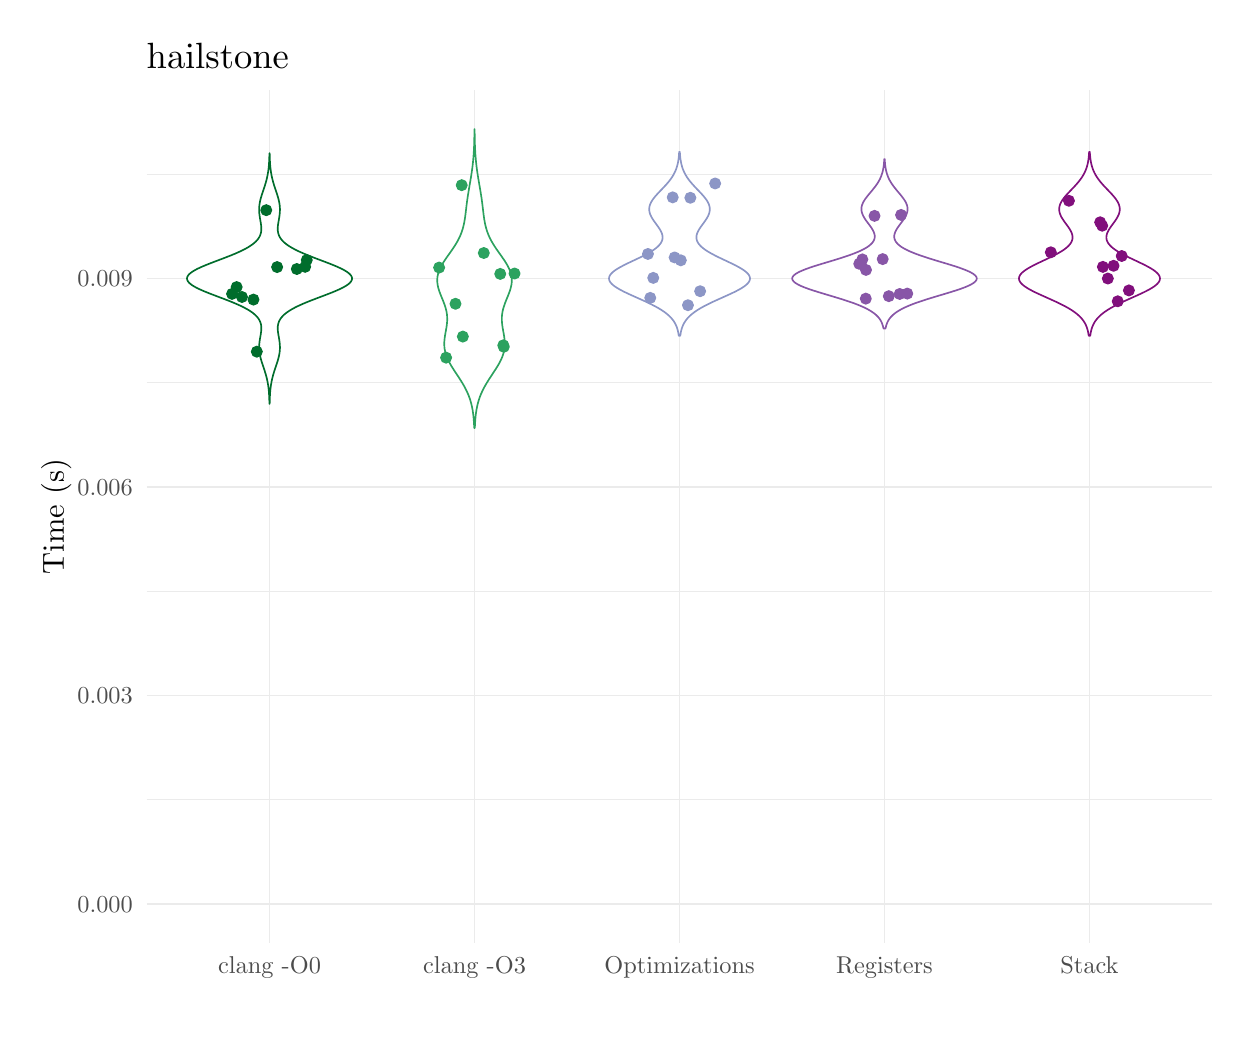
\begin{tikzpicture}[x=1pt,y=1pt]
\definecolor{fillColor}{RGB}{255,255,255}
\path[use as bounding box,fill=fillColor,fill opacity=0.00] (0,0) rectangle (433.62,361.35);
\begin{scope}
\path[clip] ( 42.95, 30.69) rectangle (428.12,338.69);
\definecolor{drawColor}{gray}{0.92}

\path[draw=drawColor,line width= 0.3pt,line join=round] ( 42.95, 82.36) --
	(428.12, 82.36);

\path[draw=drawColor,line width= 0.3pt,line join=round] ( 42.95,157.69) --
	(428.12,157.69);

\path[draw=drawColor,line width= 0.3pt,line join=round] ( 42.95,233.03) --
	(428.12,233.03);

\path[draw=drawColor,line width= 0.3pt,line join=round] ( 42.95,308.37) --
	(428.12,308.37);

\path[draw=drawColor,line width= 0.6pt,line join=round] ( 42.95, 44.69) --
	(428.12, 44.69);

\path[draw=drawColor,line width= 0.6pt,line join=round] ( 42.95,120.03) --
	(428.12,120.03);

\path[draw=drawColor,line width= 0.6pt,line join=round] ( 42.95,195.36) --
	(428.12,195.36);

\path[draw=drawColor,line width= 0.6pt,line join=round] ( 42.95,270.70) --
	(428.12,270.70);

\path[draw=drawColor,line width= 0.6pt,line join=round] ( 87.40, 30.69) --
	( 87.40,338.69);

\path[draw=drawColor,line width= 0.6pt,line join=round] (161.47, 30.69) --
	(161.47,338.69);

\path[draw=drawColor,line width= 0.6pt,line join=round] (235.54, 30.69) --
	(235.54,338.69);

\path[draw=drawColor,line width= 0.6pt,line join=round] (309.61, 30.69) --
	(309.61,338.69);

\path[draw=drawColor,line width= 0.6pt,line join=round] (383.68, 30.69) --
	(383.68,338.69);
\definecolor{drawColor}{RGB}{0,109,44}
\definecolor{fillColor}{RGB}{255,255,255}

\path[draw=drawColor,line width= 0.6pt,line join=round,line cap=round,fill=fillColor] ( 87.35,225.42) --
	( 87.35,225.60) --
	( 87.35,225.78) --
	( 87.34,225.95) --
	( 87.34,226.13) --
	( 87.33,226.31) --
	( 87.33,226.49) --
	( 87.32,226.66) --
	( 87.32,226.84) --
	( 87.31,227.02) --
	( 87.31,227.20) --
	( 87.30,227.37) --
	( 87.29,227.55) --
	( 87.29,227.73) --
	( 87.28,227.90) --
	( 87.27,228.08) --
	( 87.26,228.26) --
	( 87.25,228.44) --
	( 87.24,228.61) --
	( 87.23,228.79) --
	( 87.22,228.97) --
	( 87.21,229.14) --
	( 87.20,229.32) --
	( 87.18,229.50) --
	( 87.17,229.68) --
	( 87.15,229.85) --
	( 87.14,230.03) --
	( 87.12,230.21) --
	( 87.11,230.39) --
	( 87.09,230.56) --
	( 87.07,230.74) --
	( 87.05,230.92) --
	( 87.03,231.09) --
	( 87.01,231.27) --
	( 86.99,231.45) --
	( 86.96,231.63) --
	( 86.94,231.80) --
	( 86.91,231.98) --
	( 86.89,232.16) --
	( 86.86,232.33) --
	( 86.83,232.51) --
	( 86.80,232.69) --
	( 86.77,232.87) --
	( 86.74,233.04) --
	( 86.71,233.22) --
	( 86.67,233.40) --
	( 86.64,233.58) --
	( 86.60,233.75) --
	( 86.57,233.93) --
	( 86.53,234.11) --
	( 86.49,234.28) --
	( 86.45,234.46) --
	( 86.40,234.64) --
	( 86.36,234.82) --
	( 86.32,234.99) --
	( 86.27,235.17) --
	( 86.23,235.35) --
	( 86.18,235.52) --
	( 86.13,235.70) --
	( 86.08,235.88) --
	( 86.03,236.06) --
	( 85.98,236.23) --
	( 85.93,236.41) --
	( 85.87,236.59) --
	( 85.82,236.77) --
	( 85.76,236.94) --
	( 85.71,237.12) --
	( 85.65,237.30) --
	( 85.60,237.47) --
	( 85.54,237.65) --
	( 85.48,237.83) --
	( 85.42,238.01) --
	( 85.36,238.18) --
	( 85.30,238.36) --
	( 85.24,238.54) --
	( 85.18,238.71) --
	( 85.13,238.89) --
	( 85.07,239.07) --
	( 85.01,239.25) --
	( 84.95,239.42) --
	( 84.89,239.60) --
	( 84.83,239.78) --
	( 84.77,239.96) --
	( 84.71,240.13) --
	( 84.66,240.31) --
	( 84.60,240.49) --
	( 84.54,240.66) --
	( 84.49,240.84) --
	( 84.44,241.02) --
	( 84.38,241.20) --
	( 84.33,241.37) --
	( 84.28,241.55) --
	( 84.23,241.73) --
	( 84.19,241.90) --
	( 84.14,242.08) --
	( 84.10,242.26) --
	( 84.05,242.44) --
	( 84.01,242.61) --
	( 83.97,242.79) --
	( 83.94,242.97) --
	( 83.90,243.15) --
	( 83.87,243.32) --
	( 83.84,243.50) --
	( 83.81,243.68) --
	( 83.78,243.85) --
	( 83.76,244.03) --
	( 83.74,244.21) --
	( 83.72,244.39) --
	( 83.70,244.56) --
	( 83.68,244.74) --
	( 83.67,244.92) --
	( 83.66,245.09) --
	( 83.65,245.27) --
	( 83.65,245.45) --
	( 83.64,245.63) --
	( 83.64,245.80) --
	( 83.64,245.98) --
	( 83.65,246.16) --
	( 83.65,246.34) --
	( 83.66,246.51) --
	( 83.67,246.69) --
	( 83.68,246.87) --
	( 83.69,247.04) --
	( 83.71,247.22) --
	( 83.73,247.40) --
	( 83.75,247.58) --
	( 83.77,247.75) --
	( 83.79,247.93) --
	( 83.82,248.11) --
	( 83.84,248.28) --
	( 83.87,248.46) --
	( 83.90,248.64) --
	( 83.92,248.82) --
	( 83.95,248.99) --
	( 83.98,249.17) --
	( 84.01,249.35) --
	( 84.04,249.53) --
	( 84.08,249.70) --
	( 84.11,249.88) --
	( 84.14,250.06) --
	( 84.17,250.23) --
	( 84.20,250.41) --
	( 84.23,250.59) --
	( 84.25,250.77) --
	( 84.28,250.94) --
	( 84.30,251.12) --
	( 84.33,251.30) --
	( 84.35,251.47) --
	( 84.37,251.65) --
	( 84.39,251.83) --
	( 84.40,252.01) --
	( 84.41,252.18) --
	( 84.42,252.36) --
	( 84.43,252.54) --
	( 84.43,252.72) --
	( 84.43,252.89) --
	( 84.42,253.07) --
	( 84.41,253.25) --
	( 84.40,253.42) --
	( 84.38,253.60) --
	( 84.35,253.78) --
	( 84.33,253.96) --
	( 84.29,254.13) --
	( 84.25,254.31) --
	( 84.20,254.49) --
	( 84.15,254.66) --
	( 84.09,254.84) --
	( 84.03,255.02) --
	( 83.95,255.20) --
	( 83.87,255.37) --
	( 83.78,255.55) --
	( 83.69,255.73) --
	( 83.59,255.91) --
	( 83.47,256.08) --
	( 83.35,256.26) --
	( 83.23,256.44) --
	( 83.09,256.61) --
	( 82.94,256.79) --
	( 82.79,256.97) --
	( 82.62,257.15) --
	( 82.45,257.32) --
	( 82.26,257.50) --
	( 82.07,257.68) --
	( 81.87,257.85) --
	( 81.65,258.03) --
	( 81.43,258.21) --
	( 81.20,258.39) --
	( 80.95,258.56) --
	( 80.70,258.74) --
	( 80.43,258.92) --
	( 80.16,259.10) --
	( 79.88,259.27) --
	( 79.58,259.45) --
	( 79.27,259.63) --
	( 78.96,259.80) --
	( 78.63,259.98) --
	( 78.30,260.16) --
	( 77.95,260.34) --
	( 77.60,260.51) --
	( 77.24,260.69) --
	( 76.86,260.87) --
	( 76.48,261.04) --
	( 76.09,261.22) --
	( 75.69,261.40) --
	( 75.29,261.58) --
	( 74.87,261.75) --
	( 74.45,261.93) --
	( 74.02,262.11) --
	( 73.59,262.29) --
	( 73.15,262.46) --
	( 72.70,262.64) --
	( 72.25,262.82) --
	( 71.79,262.99) --
	( 71.34,263.17) --
	( 70.87,263.35) --
	( 70.41,263.53) --
	( 69.94,263.70) --
	( 69.47,263.88) --
	( 69.00,264.06) --
	( 68.53,264.23) --
	( 68.06,264.41) --
	( 67.60,264.59) --
	( 67.13,264.77) --
	( 66.67,264.94) --
	( 66.21,265.12) --
	( 65.75,265.30) --
	( 65.30,265.48) --
	( 64.86,265.65) --
	( 64.42,265.83) --
	( 63.99,266.01) --
	( 63.57,266.18) --
	( 63.16,266.36) --
	( 62.75,266.54) --
	( 62.36,266.72) --
	( 61.98,266.89) --
	( 61.61,267.07) --
	( 61.25,267.25) --
	( 60.90,267.42) --
	( 60.58,267.60) --
	( 60.26,267.78) --
	( 59.96,267.96) --
	( 59.67,268.13) --
	( 59.40,268.31) --
	( 59.15,268.49) --
	( 58.92,268.67) --
	( 58.70,268.84) --
	( 58.50,269.02) --
	( 58.32,269.20) --
	( 58.16,269.37) --
	( 58.02,269.55) --
	( 57.89,269.73) --
	( 57.79,269.91) --
	( 57.71,270.08) --
	( 57.65,270.26) --
	( 57.61,270.44) --
	( 57.59,270.62) --
	( 57.59,270.79) --
	( 57.61,270.97) --
	( 57.65,271.15) --
	( 57.71,271.32) --
	( 57.79,271.50) --
	( 57.89,271.68) --
	( 58.02,271.86) --
	( 58.16,272.03) --
	( 58.32,272.21) --
	( 58.50,272.39) --
	( 58.70,272.56) --
	( 58.92,272.74) --
	( 59.15,272.92) --
	( 59.40,273.10) --
	( 59.67,273.27) --
	( 59.96,273.45) --
	( 60.26,273.63) --
	( 60.58,273.81) --
	( 60.90,273.98) --
	( 61.25,274.16) --
	( 61.61,274.34) --
	( 61.98,274.51) --
	( 62.36,274.69) --
	( 62.75,274.87) --
	( 63.16,275.05) --
	( 63.57,275.22) --
	( 63.99,275.40) --
	( 64.42,275.58) --
	( 64.86,275.75) --
	( 65.30,275.93) --
	( 65.75,276.11) --
	( 66.21,276.29) --
	( 66.67,276.46) --
	( 67.13,276.64) --
	( 67.60,276.82) --
	( 68.06,277.00) --
	( 68.53,277.17) --
	( 69.00,277.35) --
	( 69.47,277.53) --
	( 69.94,277.70) --
	( 70.41,277.88) --
	( 70.87,278.06) --
	( 71.34,278.24) --
	( 71.79,278.41) --
	( 72.25,278.59) --
	( 72.70,278.77) --
	( 73.15,278.94) --
	( 73.59,279.12) --
	( 74.02,279.30) --
	( 74.45,279.48) --
	( 74.87,279.65) --
	( 75.29,279.83) --
	( 75.69,280.01) --
	( 76.09,280.19) --
	( 76.48,280.36) --
	( 76.86,280.54) --
	( 77.24,280.72) --
	( 77.60,280.89) --
	( 77.95,281.07) --
	( 78.30,281.25) --
	( 78.63,281.43) --
	( 78.96,281.60) --
	( 79.27,281.78) --
	( 79.58,281.96) --
	( 79.88,282.13) --
	( 80.16,282.31) --
	( 80.43,282.49) --
	( 80.70,282.67) --
	( 80.95,282.84) --
	( 81.20,283.02) --
	( 81.43,283.20) --
	( 81.65,283.38) --
	( 81.87,283.55) --
	( 82.07,283.73) --
	( 82.26,283.91) --
	( 82.45,284.08) --
	( 82.62,284.26) --
	( 82.79,284.44) --
	( 82.94,284.62) --
	( 83.09,284.79) --
	( 83.23,284.97) --
	( 83.35,285.15) --
	( 83.47,285.32) --
	( 83.59,285.50) --
	( 83.69,285.68) --
	( 83.78,285.86) --
	( 83.87,286.03) --
	( 83.95,286.21) --
	( 84.03,286.39) --
	( 84.09,286.57) --
	( 84.15,286.74) --
	( 84.20,286.92) --
	( 84.25,287.10) --
	( 84.29,287.27) --
	( 84.33,287.45) --
	( 84.35,287.63) --
	( 84.38,287.81) --
	( 84.40,287.98) --
	( 84.41,288.16) --
	( 84.42,288.34) --
	( 84.43,288.51) --
	( 84.43,288.69) --
	( 84.43,288.87) --
	( 84.42,289.05) --
	( 84.41,289.22) --
	( 84.40,289.40) --
	( 84.39,289.58) --
	( 84.37,289.76) --
	( 84.35,289.93) --
	( 84.33,290.11) --
	( 84.30,290.29) --
	( 84.28,290.46) --
	( 84.25,290.64) --
	( 84.23,290.82) --
	( 84.20,291.00) --
	( 84.17,291.17) --
	( 84.14,291.35) --
	( 84.11,291.53) --
	( 84.08,291.70) --
	( 84.04,291.88) --
	( 84.01,292.06) --
	( 83.98,292.24) --
	( 83.95,292.41) --
	( 83.92,292.59) --
	( 83.90,292.77) --
	( 83.87,292.95) --
	( 83.84,293.12) --
	( 83.82,293.30) --
	( 83.79,293.48) --
	( 83.77,293.65) --
	( 83.75,293.83) --
	( 83.73,294.01) --
	( 83.71,294.19) --
	( 83.69,294.36) --
	( 83.68,294.54) --
	( 83.67,294.72) --
	( 83.66,294.89) --
	( 83.65,295.07) --
	( 83.65,295.25) --
	( 83.64,295.43) --
	( 83.64,295.60) --
	( 83.64,295.78) --
	( 83.65,295.96) --
	( 83.65,296.14) --
	( 83.66,296.31) --
	( 83.67,296.49) --
	( 83.68,296.67) --
	( 83.70,296.84) --
	( 83.72,297.02) --
	( 83.74,297.20) --
	( 83.76,297.38) --
	( 83.78,297.55) --
	( 83.81,297.73) --
	( 83.84,297.91) --
	( 83.87,298.08) --
	( 83.90,298.26) --
	( 83.94,298.44) --
	( 83.97,298.62) --
	( 84.01,298.79) --
	( 84.05,298.97) --
	( 84.10,299.15) --
	( 84.14,299.33) --
	( 84.19,299.50) --
	( 84.23,299.68) --
	( 84.28,299.86) --
	( 84.33,300.03) --
	( 84.38,300.21) --
	( 84.44,300.39) --
	( 84.49,300.57) --
	( 84.54,300.74) --
	( 84.60,300.92) --
	( 84.66,301.10) --
	( 84.71,301.27) --
	( 84.77,301.45) --
	( 84.83,301.63) --
	( 84.89,301.81) --
	( 84.95,301.98) --
	( 85.01,302.16) --
	( 85.07,302.34) --
	( 85.13,302.52) --
	( 85.18,302.69) --
	( 85.24,302.87) --
	( 85.30,303.05) --
	( 85.36,303.22) --
	( 85.42,303.40) --
	( 85.48,303.58) --
	( 85.54,303.76) --
	( 85.60,303.93) --
	( 85.65,304.11) --
	( 85.71,304.29) --
	( 85.76,304.46) --
	( 85.82,304.64) --
	( 85.87,304.82) --
	( 85.93,305.00) --
	( 85.98,305.17) --
	( 86.03,305.35) --
	( 86.08,305.53) --
	( 86.13,305.71) --
	( 86.18,305.88) --
	( 86.23,306.06) --
	( 86.27,306.24) --
	( 86.32,306.41) --
	( 86.36,306.59) --
	( 86.40,306.77) --
	( 86.45,306.95) --
	( 86.49,307.12) --
	( 86.53,307.30) --
	( 86.57,307.48) --
	( 86.60,307.65) --
	( 86.64,307.83) --
	( 86.67,308.01) --
	( 86.71,308.19) --
	( 86.74,308.36) --
	( 86.77,308.54) --
	( 86.80,308.72) --
	( 86.83,308.90) --
	( 86.86,309.07) --
	( 86.89,309.25) --
	( 86.91,309.43) --
	( 86.94,309.60) --
	( 86.96,309.78) --
	( 86.99,309.96) --
	( 87.01,310.14) --
	( 87.03,310.31) --
	( 87.05,310.49) --
	( 87.07,310.67) --
	( 87.09,310.84) --
	( 87.11,311.02) --
	( 87.12,311.20) --
	( 87.14,311.38) --
	( 87.15,311.55) --
	( 87.17,311.73) --
	( 87.18,311.91) --
	( 87.20,312.09) --
	( 87.21,312.26) --
	( 87.22,312.44) --
	( 87.23,312.62) --
	( 87.24,312.79) --
	( 87.25,312.97) --
	( 87.26,313.15) --
	( 87.27,313.33) --
	( 87.28,313.50) --
	( 87.29,313.68) --
	( 87.29,313.86) --
	( 87.30,314.03) --
	( 87.31,314.21) --
	( 87.31,314.39) --
	( 87.32,314.57) --
	( 87.32,314.74) --
	( 87.33,314.92) --
	( 87.33,315.10) --
	( 87.34,315.28) --
	( 87.34,315.45) --
	( 87.35,315.63) --
	( 87.35,315.81) --
	( 87.35,315.98) --
	( 87.44,315.98) --
	( 87.44,315.81) --
	( 87.45,315.63) --
	( 87.45,315.45) --
	( 87.45,315.28) --
	( 87.46,315.10) --
	( 87.46,314.92) --
	( 87.47,314.74) --
	( 87.47,314.57) --
	( 87.48,314.39) --
	( 87.49,314.21) --
	( 87.49,314.03) --
	( 87.50,313.86) --
	( 87.51,313.68) --
	( 87.51,313.50) --
	( 87.52,313.33) --
	( 87.53,313.15) --
	( 87.54,312.97) --
	( 87.55,312.79) --
	( 87.56,312.62) --
	( 87.57,312.44) --
	( 87.58,312.26) --
	( 87.60,312.09) --
	( 87.61,311.91) --
	( 87.62,311.73) --
	( 87.64,311.55) --
	( 87.65,311.38) --
	( 87.67,311.20) --
	( 87.69,311.02) --
	( 87.70,310.84) --
	( 87.72,310.67) --
	( 87.74,310.49) --
	( 87.76,310.31) --
	( 87.78,310.14) --
	( 87.81,309.96) --
	( 87.83,309.78) --
	( 87.85,309.60) --
	( 87.88,309.43) --
	( 87.90,309.25) --
	( 87.93,309.07) --
	( 87.96,308.90) --
	( 87.99,308.72) --
	( 88.02,308.54) --
	( 88.05,308.36) --
	( 88.08,308.19) --
	( 88.12,308.01) --
	( 88.15,307.83) --
	( 88.19,307.65) --
	( 88.23,307.48) --
	( 88.27,307.30) --
	( 88.31,307.12) --
	( 88.35,306.95) --
	( 88.39,306.77) --
	( 88.43,306.59) --
	( 88.48,306.41) --
	( 88.52,306.24) --
	( 88.57,306.06) --
	( 88.61,305.88) --
	( 88.66,305.71) --
	( 88.71,305.53) --
	( 88.76,305.35) --
	( 88.81,305.17) --
	( 88.87,305.00) --
	( 88.92,304.82) --
	( 88.97,304.64) --
	( 89.03,304.46) --
	( 89.08,304.29) --
	( 89.14,304.11) --
	( 89.20,303.93) --
	( 89.25,303.76) --
	( 89.31,303.58) --
	( 89.37,303.40) --
	( 89.43,303.22) --
	( 89.49,303.05) --
	( 89.55,302.87) --
	( 89.61,302.69) --
	( 89.67,302.52) --
	( 89.73,302.34) --
	( 89.79,302.16) --
	( 89.85,301.98) --
	( 89.90,301.81) --
	( 89.96,301.63) --
	( 90.02,301.45) --
	( 90.08,301.27) --
	( 90.14,301.10) --
	( 90.19,300.92) --
	( 90.25,300.74) --
	( 90.30,300.57) --
	( 90.36,300.39) --
	( 90.41,300.21) --
	( 90.46,300.03) --
	( 90.51,299.86) --
	( 90.56,299.68) --
	( 90.61,299.50) --
	( 90.65,299.33) --
	( 90.70,299.15) --
	( 90.74,298.97) --
	( 90.78,298.79) --
	( 90.82,298.62) --
	( 90.86,298.44) --
	( 90.89,298.26) --
	( 90.92,298.08) --
	( 90.95,297.91) --
	( 90.98,297.73) --
	( 91.01,297.55) --
	( 91.04,297.38) --
	( 91.06,297.20) --
	( 91.08,297.02) --
	( 91.09,296.84) --
	( 91.11,296.67) --
	( 91.12,296.49) --
	( 91.13,296.31) --
	( 91.14,296.14) --
	( 91.15,295.96) --
	( 91.15,295.78) --
	( 91.15,295.60) --
	( 91.15,295.43) --
	( 91.15,295.25) --
	( 91.14,295.07) --
	( 91.13,294.89) --
	( 91.12,294.72) --
	( 91.11,294.54) --
	( 91.10,294.36) --
	( 91.08,294.19) --
	( 91.06,294.01) --
	( 91.04,293.83) --
	( 91.02,293.65) --
	( 91.00,293.48) --
	( 90.98,293.30) --
	( 90.95,293.12) --
	( 90.92,292.95) --
	( 90.90,292.77) --
	( 90.87,292.59) --
	( 90.84,292.41) --
	( 90.81,292.24) --
	( 90.78,292.06) --
	( 90.75,291.88) --
	( 90.72,291.70) --
	( 90.69,291.53) --
	( 90.66,291.35) --
	( 90.63,291.17) --
	( 90.60,291.00) --
	( 90.57,290.82) --
	( 90.54,290.64) --
	( 90.51,290.46) --
	( 90.49,290.29) --
	( 90.46,290.11) --
	( 90.44,289.93) --
	( 90.42,289.76) --
	( 90.41,289.58) --
	( 90.39,289.40) --
	( 90.38,289.22) --
	( 90.37,289.05) --
	( 90.37,288.87) --
	( 90.36,288.69) --
	( 90.37,288.51) --
	( 90.37,288.34) --
	( 90.38,288.16) --
	( 90.39,287.98) --
	( 90.41,287.81) --
	( 90.44,287.63) --
	( 90.47,287.45) --
	( 90.50,287.27) --
	( 90.54,287.10) --
	( 90.59,286.92) --
	( 90.64,286.74) --
	( 90.70,286.57) --
	( 90.77,286.39) --
	( 90.84,286.21) --
	( 90.92,286.03) --
	( 91.01,285.86) --
	( 91.11,285.68) --
	( 91.21,285.50) --
	( 91.32,285.32) --
	( 91.44,285.15) --
	( 91.57,284.97) --
	( 91.71,284.79) --
	( 91.85,284.62) --
	( 92.01,284.44) --
	( 92.17,284.26) --
	( 92.35,284.08) --
	( 92.53,283.91) --
	( 92.72,283.73) --
	( 92.92,283.55) --
	( 93.14,283.38) --
	( 93.36,283.20) --
	( 93.60,283.02) --
	( 93.84,282.84) --
	( 94.09,282.67) --
	( 94.36,282.49) --
	( 94.63,282.31) --
	( 94.92,282.13) --
	( 95.21,281.96) --
	( 95.52,281.78) --
	( 95.83,281.60) --
	( 96.16,281.43) --
	( 96.49,281.25) --
	( 96.84,281.07) --
	( 97.19,280.89) --
	( 97.55,280.72) --
	( 97.93,280.54) --
	( 98.31,280.36) --
	( 98.70,280.19) --
	( 99.10,280.01) --
	( 99.51,279.83) --
	( 99.92,279.65) --
	(100.34,279.48) --
	(100.77,279.30) --
	(101.20,279.12) --
	(101.65,278.94) --
	(102.09,278.77) --
	(102.54,278.59) --
	(103.00,278.41) --
	(103.46,278.24) --
	(103.92,278.06) --
	(104.38,277.88) --
	(104.85,277.70) --
	(105.32,277.53) --
	(105.79,277.35) --
	(106.26,277.17) --
	(106.73,277.00) --
	(107.20,276.82) --
	(107.66,276.64) --
	(108.12,276.46) --
	(108.58,276.29) --
	(109.04,276.11) --
	(109.49,275.93) --
	(109.93,275.75) --
	(110.37,275.58) --
	(110.80,275.40) --
	(111.22,275.22) --
	(111.64,275.05) --
	(112.04,274.87) --
	(112.43,274.69) --
	(112.82,274.51) --
	(113.18,274.34) --
	(113.54,274.16) --
	(113.89,273.98) --
	(114.22,273.81) --
	(114.53,273.63) --
	(114.84,273.45) --
	(115.12,273.27) --
	(115.39,273.10) --
	(115.64,272.92) --
	(115.88,272.74) --
	(116.10,272.56) --
	(116.29,272.39) --
	(116.47,272.21) --
	(116.63,272.03) --
	(116.77,271.86) --
	(116.90,271.68) --
	(117.00,271.50) --
	(117.08,271.32) --
	(117.15,271.15) --
	(117.18,270.97) --
	(117.21,270.79) --
	(117.21,270.62) --
	(117.18,270.44) --
	(117.15,270.26) --
	(117.08,270.08) --
	(117.00,269.91) --
	(116.90,269.73) --
	(116.77,269.55) --
	(116.63,269.37) --
	(116.47,269.20) --
	(116.29,269.02) --
	(116.10,268.84) --
	(115.88,268.67) --
	(115.64,268.49) --
	(115.39,268.31) --
	(115.12,268.13) --
	(114.84,267.96) --
	(114.53,267.78) --
	(114.22,267.60) --
	(113.89,267.42) --
	(113.54,267.25) --
	(113.18,267.07) --
	(112.82,266.89) --
	(112.43,266.72) --
	(112.04,266.54) --
	(111.64,266.36) --
	(111.22,266.18) --
	(110.80,266.01) --
	(110.37,265.83) --
	(109.93,265.65) --
	(109.49,265.48) --
	(109.04,265.30) --
	(108.58,265.12) --
	(108.12,264.94) --
	(107.66,264.77) --
	(107.20,264.59) --
	(106.73,264.41) --
	(106.26,264.23) --
	(105.79,264.06) --
	(105.32,263.88) --
	(104.85,263.70) --
	(104.38,263.53) --
	(103.92,263.35) --
	(103.46,263.17) --
	(103.00,262.99) --
	(102.54,262.82) --
	(102.09,262.64) --
	(101.65,262.46) --
	(101.20,262.29) --
	(100.77,262.11) --
	(100.34,261.93) --
	( 99.92,261.75) --
	( 99.51,261.58) --
	( 99.10,261.40) --
	( 98.70,261.22) --
	( 98.31,261.04) --
	( 97.93,260.87) --
	( 97.55,260.69) --
	( 97.19,260.51) --
	( 96.84,260.34) --
	( 96.49,260.16) --
	( 96.16,259.98) --
	( 95.83,259.80) --
	( 95.52,259.63) --
	( 95.21,259.45) --
	( 94.92,259.27) --
	( 94.63,259.10) --
	( 94.36,258.92) --
	( 94.09,258.74) --
	( 93.84,258.56) --
	( 93.60,258.39) --
	( 93.36,258.21) --
	( 93.14,258.03) --
	( 92.92,257.85) --
	( 92.72,257.68) --
	( 92.53,257.50) --
	( 92.35,257.32) --
	( 92.17,257.15) --
	( 92.01,256.97) --
	( 91.85,256.79) --
	( 91.71,256.61) --
	( 91.57,256.44) --
	( 91.44,256.26) --
	( 91.32,256.08) --
	( 91.21,255.91) --
	( 91.11,255.73) --
	( 91.01,255.55) --
	( 90.92,255.37) --
	( 90.84,255.20) --
	( 90.77,255.02) --
	( 90.70,254.84) --
	( 90.64,254.66) --
	( 90.59,254.49) --
	( 90.54,254.31) --
	( 90.50,254.13) --
	( 90.47,253.96) --
	( 90.44,253.78) --
	( 90.41,253.60) --
	( 90.39,253.42) --
	( 90.38,253.25) --
	( 90.37,253.07) --
	( 90.37,252.89) --
	( 90.36,252.72) --
	( 90.37,252.54) --
	( 90.37,252.36) --
	( 90.38,252.18) --
	( 90.39,252.01) --
	( 90.41,251.83) --
	( 90.42,251.65) --
	( 90.44,251.47) --
	( 90.46,251.30) --
	( 90.49,251.12) --
	( 90.51,250.94) --
	( 90.54,250.77) --
	( 90.57,250.59) --
	( 90.60,250.41) --
	( 90.63,250.23) --
	( 90.66,250.06) --
	( 90.69,249.88) --
	( 90.72,249.70) --
	( 90.75,249.53) --
	( 90.78,249.35) --
	( 90.81,249.17) --
	( 90.84,248.99) --
	( 90.87,248.82) --
	( 90.90,248.64) --
	( 90.92,248.46) --
	( 90.95,248.28) --
	( 90.98,248.11) --
	( 91.00,247.93) --
	( 91.02,247.75) --
	( 91.04,247.58) --
	( 91.06,247.40) --
	( 91.08,247.22) --
	( 91.10,247.04) --
	( 91.11,246.87) --
	( 91.12,246.69) --
	( 91.13,246.51) --
	( 91.14,246.34) --
	( 91.15,246.16) --
	( 91.15,245.98) --
	( 91.15,245.80) --
	( 91.15,245.63) --
	( 91.15,245.45) --
	( 91.14,245.27) --
	( 91.13,245.09) --
	( 91.12,244.92) --
	( 91.11,244.74) --
	( 91.09,244.56) --
	( 91.08,244.39) --
	( 91.06,244.21) --
	( 91.04,244.03) --
	( 91.01,243.85) --
	( 90.98,243.68) --
	( 90.95,243.50) --
	( 90.92,243.32) --
	( 90.89,243.15) --
	( 90.86,242.97) --
	( 90.82,242.79) --
	( 90.78,242.61) --
	( 90.74,242.44) --
	( 90.70,242.26) --
	( 90.65,242.08) --
	( 90.61,241.90) --
	( 90.56,241.73) --
	( 90.51,241.55) --
	( 90.46,241.37) --
	( 90.41,241.20) --
	( 90.36,241.02) --
	( 90.30,240.84) --
	( 90.25,240.66) --
	( 90.19,240.49) --
	( 90.14,240.31) --
	( 90.08,240.13) --
	( 90.02,239.96) --
	( 89.96,239.78) --
	( 89.90,239.60) --
	( 89.85,239.42) --
	( 89.79,239.25) --
	( 89.73,239.07) --
	( 89.67,238.89) --
	( 89.61,238.71) --
	( 89.55,238.54) --
	( 89.49,238.36) --
	( 89.43,238.18) --
	( 89.37,238.01) --
	( 89.31,237.83) --
	( 89.25,237.65) --
	( 89.20,237.47) --
	( 89.14,237.30) --
	( 89.08,237.12) --
	( 89.03,236.94) --
	( 88.97,236.77) --
	( 88.92,236.59) --
	( 88.87,236.41) --
	( 88.81,236.23) --
	( 88.76,236.06) --
	( 88.71,235.88) --
	( 88.66,235.70) --
	( 88.61,235.52) --
	( 88.57,235.35) --
	( 88.52,235.17) --
	( 88.48,234.99) --
	( 88.43,234.82) --
	( 88.39,234.64) --
	( 88.35,234.46) --
	( 88.31,234.28) --
	( 88.27,234.11) --
	( 88.23,233.93) --
	( 88.19,233.75) --
	( 88.15,233.58) --
	( 88.12,233.40) --
	( 88.08,233.22) --
	( 88.05,233.04) --
	( 88.02,232.87) --
	( 87.99,232.69) --
	( 87.96,232.51) --
	( 87.93,232.33) --
	( 87.90,232.16) --
	( 87.88,231.98) --
	( 87.85,231.80) --
	( 87.83,231.63) --
	( 87.81,231.45) --
	( 87.78,231.27) --
	( 87.76,231.09) --
	( 87.74,230.92) --
	( 87.72,230.74) --
	( 87.70,230.56) --
	( 87.69,230.39) --
	( 87.67,230.21) --
	( 87.65,230.03) --
	( 87.64,229.85) --
	( 87.62,229.68) --
	( 87.61,229.50) --
	( 87.60,229.32) --
	( 87.58,229.14) --
	( 87.57,228.97) --
	( 87.56,228.79) --
	( 87.55,228.61) --
	( 87.54,228.44) --
	( 87.53,228.26) --
	( 87.52,228.08) --
	( 87.51,227.90) --
	( 87.51,227.73) --
	( 87.50,227.55) --
	( 87.49,227.37) --
	( 87.49,227.20) --
	( 87.48,227.02) --
	( 87.47,226.84) --
	( 87.47,226.66) --
	( 87.46,226.49) --
	( 87.46,226.31) --
	( 87.45,226.13) --
	( 87.45,225.95) --
	( 87.45,225.78) --
	( 87.44,225.60) --
	( 87.44,225.42) --
	( 87.35,225.42) --
	cycle;
\definecolor{drawColor}{RGB}{44,162,95}

\path[draw=drawColor,line width= 0.6pt,line join=round,line cap=round,fill=fillColor] (161.35,216.71) --
	(161.34,216.93) --
	(161.33,217.14) --
	(161.32,217.35) --
	(161.32,217.56) --
	(161.31,217.77) --
	(161.29,217.98) --
	(161.28,218.19) --
	(161.27,218.41) --
	(161.26,218.62) --
	(161.25,218.83) --
	(161.23,219.04) --
	(161.22,219.25) --
	(161.20,219.46) --
	(161.19,219.67) --
	(161.17,219.88) --
	(161.15,220.10) --
	(161.13,220.31) --
	(161.11,220.52) --
	(161.09,220.73) --
	(161.07,220.94) --
	(161.05,221.15) --
	(161.03,221.36) --
	(161.00,221.57) --
	(160.97,221.79) --
	(160.95,222.00) --
	(160.92,222.21) --
	(160.89,222.42) --
	(160.86,222.63) --
	(160.82,222.84) --
	(160.79,223.05) --
	(160.76,223.27) --
	(160.72,223.48) --
	(160.68,223.69) --
	(160.64,223.90) --
	(160.60,224.11) --
	(160.55,224.32) --
	(160.51,224.53) --
	(160.46,224.74) --
	(160.42,224.96) --
	(160.36,225.17) --
	(160.31,225.38) --
	(160.26,225.59) --
	(160.20,225.80) --
	(160.14,226.01) --
	(160.08,226.22) --
	(160.02,226.43) --
	(159.96,226.65) --
	(159.89,226.86) --
	(159.82,227.07) --
	(159.75,227.28) --
	(159.68,227.49) --
	(159.61,227.70) --
	(159.53,227.91) --
	(159.45,228.13) --
	(159.37,228.34) --
	(159.29,228.55) --
	(159.20,228.76) --
	(159.11,228.97) --
	(159.02,229.18) --
	(158.93,229.39) --
	(158.84,229.60) --
	(158.74,229.82) --
	(158.64,230.03) --
	(158.54,230.24) --
	(158.43,230.45) --
	(158.33,230.66) --
	(158.22,230.87) --
	(158.11,231.08) --
	(158.00,231.29) --
	(157.89,231.51) --
	(157.77,231.72) --
	(157.65,231.93) --
	(157.53,232.14) --
	(157.41,232.35) --
	(157.29,232.56) --
	(157.16,232.77) --
	(157.04,232.99) --
	(156.91,233.20) --
	(156.78,233.41) --
	(156.65,233.62) --
	(156.51,233.83) --
	(156.38,234.04) --
	(156.25,234.25) --
	(156.11,234.46) --
	(155.97,234.68) --
	(155.84,234.89) --
	(155.70,235.10) --
	(155.56,235.31) --
	(155.42,235.52) --
	(155.28,235.73) --
	(155.14,235.94) --
	(155.00,236.15) --
	(154.86,236.37) --
	(154.72,236.58) --
	(154.58,236.79) --
	(154.44,237.00) --
	(154.30,237.21) --
	(154.16,237.42) --
	(154.03,237.63) --
	(153.89,237.85) --
	(153.76,238.06) --
	(153.62,238.27) --
	(153.49,238.48) --
	(153.36,238.69) --
	(153.23,238.90) --
	(153.10,239.11) --
	(152.98,239.32) --
	(152.85,239.54) --
	(152.73,239.75) --
	(152.61,239.96) --
	(152.49,240.17) --
	(152.38,240.38) --
	(152.27,240.59) --
	(152.16,240.80) --
	(152.05,241.02) --
	(151.95,241.23) --
	(151.85,241.44) --
	(151.75,241.65) --
	(151.66,241.86) --
	(151.57,242.07) --
	(151.48,242.28) --
	(151.40,242.49) --
	(151.32,242.71) --
	(151.25,242.92) --
	(151.17,243.13) --
	(151.11,243.34) --
	(151.04,243.55) --
	(150.98,243.76) --
	(150.92,243.97) --
	(150.87,244.18) --
	(150.82,244.40) --
	(150.78,244.61) --
	(150.74,244.82) --
	(150.70,245.03) --
	(150.67,245.24) --
	(150.64,245.45) --
	(150.61,245.66) --
	(150.59,245.88) --
	(150.57,246.09) --
	(150.56,246.30) --
	(150.55,246.51) --
	(150.54,246.72) --
	(150.54,246.93) --
	(150.54,247.14) --
	(150.54,247.35) --
	(150.54,247.57) --
	(150.55,247.78) --
	(150.56,247.99) --
	(150.58,248.20) --
	(150.60,248.41) --
	(150.62,248.62) --
	(150.64,248.83) --
	(150.66,249.04) --
	(150.69,249.26) --
	(150.72,249.47) --
	(150.75,249.68) --
	(150.78,249.89) --
	(150.81,250.10) --
	(150.85,250.31) --
	(150.88,250.52) --
	(150.92,250.74) --
	(150.96,250.95) --
	(150.99,251.16) --
	(151.03,251.37) --
	(151.07,251.58) --
	(151.11,251.79) --
	(151.14,252.00) --
	(151.18,252.21) --
	(151.22,252.43) --
	(151.25,252.64) --
	(151.29,252.85) --
	(151.32,253.06) --
	(151.35,253.27) --
	(151.39,253.48) --
	(151.42,253.69) --
	(151.44,253.90) --
	(151.47,254.12) --
	(151.49,254.33) --
	(151.51,254.54) --
	(151.53,254.75) --
	(151.55,254.96) --
	(151.56,255.17) --
	(151.58,255.38) --
	(151.59,255.60) --
	(151.59,255.81) --
	(151.59,256.02) --
	(151.59,256.23) --
	(151.59,256.44) --
	(151.58,256.65) --
	(151.57,256.86) --
	(151.56,257.07) --
	(151.54,257.29) --
	(151.53,257.50) --
	(151.50,257.71) --
	(151.48,257.92) --
	(151.45,258.13) --
	(151.41,258.34) --
	(151.38,258.55) --
	(151.34,258.76) --
	(151.29,258.98) --
	(151.25,259.19) --
	(151.20,259.40) --
	(151.14,259.61) --
	(151.09,259.82) --
	(151.03,260.03) --
	(150.97,260.24) --
	(150.90,260.46) --
	(150.84,260.67) --
	(150.77,260.88) --
	(150.70,261.09) --
	(150.62,261.30) --
	(150.55,261.51) --
	(150.47,261.72) --
	(150.39,261.93) --
	(150.31,262.15) --
	(150.23,262.36) --
	(150.14,262.57) --
	(150.06,262.78) --
	(149.97,262.99) --
	(149.89,263.20) --
	(149.80,263.41) --
	(149.71,263.62) --
	(149.63,263.84) --
	(149.54,264.05) --
	(149.46,264.26) --
	(149.37,264.47) --
	(149.29,264.68) --
	(149.20,264.89) --
	(149.12,265.10) --
	(149.04,265.32) --
	(148.96,265.53) --
	(148.88,265.74) --
	(148.81,265.95) --
	(148.73,266.16) --
	(148.66,266.37) --
	(148.60,266.58) --
	(148.53,266.79) --
	(148.47,267.01) --
	(148.41,267.22) --
	(148.35,267.43) --
	(148.30,267.64) --
	(148.25,267.85) --
	(148.21,268.06) --
	(148.17,268.27) --
	(148.13,268.48) --
	(148.10,268.70) --
	(148.07,268.91) --
	(148.05,269.12) --
	(148.03,269.33) --
	(148.01,269.54) --
	(148.00,269.75) --
	(148.00,269.96) --
	(148.00,270.18) --
	(148.00,270.39) --
	(148.01,270.60) --
	(148.03,270.81) --
	(148.05,271.02) --
	(148.07,271.23) --
	(148.10,271.44) --
	(148.14,271.65) --
	(148.18,271.87) --
	(148.22,272.08) --
	(148.27,272.29) --
	(148.33,272.50) --
	(148.39,272.71) --
	(148.45,272.92) --
	(148.52,273.13) --
	(148.60,273.34) --
	(148.68,273.56) --
	(148.76,273.77) --
	(148.85,273.98) --
	(148.94,274.19) --
	(149.04,274.40) --
	(149.14,274.61) --
	(149.24,274.82) --
	(149.35,275.04) --
	(149.46,275.25) --
	(149.58,275.46) --
	(149.70,275.67) --
	(149.82,275.88) --
	(149.95,276.09) --
	(150.08,276.30) --
	(150.21,276.51) --
	(150.34,276.73) --
	(150.48,276.94) --
	(150.62,277.15) --
	(150.75,277.36) --
	(150.90,277.57) --
	(151.04,277.78) --
	(151.19,277.99) --
	(151.33,278.21) --
	(151.48,278.42) --
	(151.63,278.63) --
	(151.78,278.84) --
	(151.93,279.05) --
	(152.08,279.26) --
	(152.23,279.47) --
	(152.38,279.68) --
	(152.53,279.90) --
	(152.68,280.11) --
	(152.83,280.32) --
	(152.97,280.53) --
	(153.12,280.74) --
	(153.27,280.95) --
	(153.42,281.16) --
	(153.56,281.37) --
	(153.70,281.59) --
	(153.85,281.80) --
	(153.99,282.01) --
	(154.13,282.22) --
	(154.26,282.43) --
	(154.40,282.64) --
	(154.53,282.85) --
	(154.66,283.07) --
	(154.79,283.28) --
	(154.92,283.49) --
	(155.04,283.70) --
	(155.16,283.91) --
	(155.28,284.12) --
	(155.40,284.33) --
	(155.51,284.54) --
	(155.62,284.76) --
	(155.73,284.97) --
	(155.84,285.18) --
	(155.94,285.39) --
	(156.04,285.60) --
	(156.14,285.81) --
	(156.23,286.02) --
	(156.33,286.23) --
	(156.42,286.45) --
	(156.50,286.66) --
	(156.59,286.87) --
	(156.67,287.08) --
	(156.75,287.29) --
	(156.82,287.50) --
	(156.90,287.71) --
	(156.97,287.93) --
	(157.04,288.14) --
	(157.10,288.35) --
	(157.17,288.56) --
	(157.23,288.77) --
	(157.29,288.98) --
	(157.35,289.19) --
	(157.40,289.40) --
	(157.45,289.62) --
	(157.50,289.83) --
	(157.55,290.04) --
	(157.60,290.25) --
	(157.65,290.46) --
	(157.69,290.67) --
	(157.73,290.88) --
	(157.77,291.09) --
	(157.81,291.31) --
	(157.85,291.52) --
	(157.88,291.73) --
	(157.92,291.94) --
	(157.95,292.15) --
	(157.98,292.36) --
	(158.02,292.57) --
	(158.05,292.79) --
	(158.08,293.00) --
	(158.11,293.21) --
	(158.13,293.42) --
	(158.16,293.63) --
	(158.19,293.84) --
	(158.22,294.05) --
	(158.24,294.26) --
	(158.27,294.48) --
	(158.29,294.69) --
	(158.32,294.90) --
	(158.34,295.11) --
	(158.37,295.32) --
	(158.39,295.53) --
	(158.42,295.74) --
	(158.44,295.95) --
	(158.47,296.17) --
	(158.49,296.38) --
	(158.52,296.59) --
	(158.54,296.80) --
	(158.57,297.01) --
	(158.60,297.22) --
	(158.62,297.43) --
	(158.65,297.65) --
	(158.68,297.86) --
	(158.70,298.07) --
	(158.73,298.28) --
	(158.76,298.49) --
	(158.79,298.70) --
	(158.82,298.91) --
	(158.84,299.12) --
	(158.87,299.34) --
	(158.90,299.55) --
	(158.93,299.76) --
	(158.97,299.97) --
	(159.00,300.18) --
	(159.03,300.39) --
	(159.06,300.60) --
	(159.09,300.81) --
	(159.13,301.03) --
	(159.16,301.24) --
	(159.19,301.45) --
	(159.23,301.66) --
	(159.26,301.87) --
	(159.30,302.08) --
	(159.33,302.29) --
	(159.37,302.51) --
	(159.40,302.72) --
	(159.44,302.93) --
	(159.47,303.14) --
	(159.51,303.35) --
	(159.54,303.56) --
	(159.58,303.77) --
	(159.62,303.98) --
	(159.65,304.20) --
	(159.69,304.41) --
	(159.73,304.62) --
	(159.76,304.83) --
	(159.80,305.04) --
	(159.83,305.25) --
	(159.87,305.46) --
	(159.91,305.67) --
	(159.94,305.89) --
	(159.98,306.10) --
	(160.01,306.31) --
	(160.05,306.52) --
	(160.08,306.73) --
	(160.12,306.94) --
	(160.15,307.15) --
	(160.19,307.37) --
	(160.22,307.58) --
	(160.26,307.79) --
	(160.29,308.00) --
	(160.32,308.21) --
	(160.35,308.42) --
	(160.39,308.63) --
	(160.42,308.84) --
	(160.45,309.06) --
	(160.48,309.27) --
	(160.51,309.48) --
	(160.54,309.69) --
	(160.57,309.90) --
	(160.60,310.11) --
	(160.63,310.32) --
	(160.65,310.53) --
	(160.68,310.75) --
	(160.71,310.96) --
	(160.73,311.17) --
	(160.76,311.38) --
	(160.78,311.59) --
	(160.81,311.80) --
	(160.83,312.01) --
	(160.85,312.23) --
	(160.88,312.44) --
	(160.90,312.65) --
	(160.92,312.86) --
	(160.94,313.07) --
	(160.96,313.28) --
	(160.98,313.49) --
	(161.00,313.70) --
	(161.02,313.92) --
	(161.04,314.13) --
	(161.06,314.34) --
	(161.07,314.55) --
	(161.09,314.76) --
	(161.11,314.97) --
	(161.12,315.18) --
	(161.14,315.39) --
	(161.15,315.61) --
	(161.16,315.82) --
	(161.18,316.03) --
	(161.19,316.24) --
	(161.20,316.45) --
	(161.22,316.66) --
	(161.23,316.87) --
	(161.24,317.09) --
	(161.25,317.30) --
	(161.26,317.51) --
	(161.27,317.72) --
	(161.28,317.93) --
	(161.29,318.14) --
	(161.30,318.35) --
	(161.31,318.56) --
	(161.31,318.78) --
	(161.32,318.99) --
	(161.33,319.20) --
	(161.34,319.41) --
	(161.34,319.62) --
	(161.35,319.83) --
	(161.36,320.04) --
	(161.36,320.26) --
	(161.37,320.47) --
	(161.37,320.68) --
	(161.38,320.89) --
	(161.38,321.10) --
	(161.39,321.31) --
	(161.39,321.52) --
	(161.40,321.73) --
	(161.40,321.95) --
	(161.40,322.16) --
	(161.41,322.37) --
	(161.41,322.58) --
	(161.41,322.79) --
	(161.42,323.00) --
	(161.42,323.21) --
	(161.42,323.42) --
	(161.43,323.64) --
	(161.43,323.85) --
	(161.43,324.06) --
	(161.43,324.27) --
	(161.44,324.48) --
	(161.44,324.69) --
	(161.50,324.69) --
	(161.50,324.48) --
	(161.50,324.27) --
	(161.50,324.06) --
	(161.50,323.85) --
	(161.51,323.64) --
	(161.51,323.42) --
	(161.51,323.21) --
	(161.52,323.00) --
	(161.52,322.79) --
	(161.52,322.58) --
	(161.53,322.37) --
	(161.53,322.16) --
	(161.53,321.95) --
	(161.54,321.73) --
	(161.54,321.52) --
	(161.55,321.31) --
	(161.55,321.10) --
	(161.55,320.89) --
	(161.56,320.68) --
	(161.57,320.47) --
	(161.57,320.26) --
	(161.58,320.04) --
	(161.58,319.83) --
	(161.59,319.62) --
	(161.60,319.41) --
	(161.60,319.20) --
	(161.61,318.99) --
	(161.62,318.78) --
	(161.63,318.56) --
	(161.64,318.35) --
	(161.64,318.14) --
	(161.65,317.93) --
	(161.66,317.72) --
	(161.67,317.51) --
	(161.68,317.30) --
	(161.69,317.09) --
	(161.71,316.87) --
	(161.72,316.66) --
	(161.73,316.45) --
	(161.74,316.24) --
	(161.76,316.03) --
	(161.77,315.82) --
	(161.78,315.61) --
	(161.80,315.39) --
	(161.81,315.18) --
	(161.83,314.97) --
	(161.84,314.76) --
	(161.86,314.55) --
	(161.88,314.34) --
	(161.90,314.13) --
	(161.91,313.92) --
	(161.93,313.70) --
	(161.95,313.49) --
	(161.97,313.28) --
	(161.99,313.07) --
	(162.01,312.86) --
	(162.03,312.65) --
	(162.06,312.44) --
	(162.08,312.23) --
	(162.10,312.01) --
	(162.13,311.80) --
	(162.15,311.59) --
	(162.17,311.38) --
	(162.20,311.17) --
	(162.23,310.96) --
	(162.25,310.75) --
	(162.28,310.53) --
	(162.31,310.32) --
	(162.34,310.11) --
	(162.36,309.90) --
	(162.39,309.69) --
	(162.42,309.48) --
	(162.45,309.27) --
	(162.48,309.06) --
	(162.52,308.84) --
	(162.55,308.63) --
	(162.58,308.42) --
	(162.61,308.21) --
	(162.64,308.00) --
	(162.68,307.79) --
	(162.71,307.58) --
	(162.75,307.37) --
	(162.78,307.15) --
	(162.81,306.94) --
	(162.85,306.73) --
	(162.88,306.52) --
	(162.92,306.31) --
	(162.96,306.10) --
	(162.99,305.89) --
	(163.03,305.67) --
	(163.06,305.46) --
	(163.10,305.25) --
	(163.14,305.04) --
	(163.17,304.83) --
	(163.21,304.62) --
	(163.24,304.41) --
	(163.28,304.20) --
	(163.32,303.98) --
	(163.35,303.77) --
	(163.39,303.56) --
	(163.43,303.35) --
	(163.46,303.14) --
	(163.50,302.93) --
	(163.53,302.72) --
	(163.57,302.51) --
	(163.60,302.29) --
	(163.64,302.08) --
	(163.67,301.87) --
	(163.71,301.66) --
	(163.74,301.45) --
	(163.77,301.24) --
	(163.81,301.03) --
	(163.84,300.81) --
	(163.87,300.60) --
	(163.90,300.39) --
	(163.94,300.18) --
	(163.97,299.97) --
	(164.00,299.76) --
	(164.03,299.55) --
	(164.06,299.34) --
	(164.09,299.12) --
	(164.12,298.91) --
	(164.15,298.70) --
	(164.17,298.49) --
	(164.20,298.28) --
	(164.23,298.07) --
	(164.26,297.86) --
	(164.28,297.65) --
	(164.31,297.43) --
	(164.34,297.22) --
	(164.36,297.01) --
	(164.39,296.80) --
	(164.41,296.59) --
	(164.44,296.38) --
	(164.46,296.17) --
	(164.49,295.95) --
	(164.51,295.74) --
	(164.54,295.53) --
	(164.56,295.32) --
	(164.59,295.11) --
	(164.61,294.90) --
	(164.64,294.69) --
	(164.67,294.48) --
	(164.69,294.26) --
	(164.72,294.05) --
	(164.74,293.84) --
	(164.77,293.63) --
	(164.80,293.42) --
	(164.83,293.21) --
	(164.86,293.00) --
	(164.89,292.79) --
	(164.92,292.57) --
	(164.95,292.36) --
	(164.98,292.15) --
	(165.01,291.94) --
	(165.05,291.73) --
	(165.09,291.52) --
	(165.12,291.31) --
	(165.16,291.09) --
	(165.20,290.88) --
	(165.24,290.67) --
	(165.29,290.46) --
	(165.33,290.25) --
	(165.38,290.04) --
	(165.43,289.83) --
	(165.48,289.62) --
	(165.53,289.40) --
	(165.59,289.19) --
	(165.64,288.98) --
	(165.70,288.77) --
	(165.77,288.56) --
	(165.83,288.35) --
	(165.90,288.14) --
	(165.96,287.93) --
	(166.04,287.71) --
	(166.11,287.50) --
	(166.19,287.29) --
	(166.26,287.08) --
	(166.35,286.87) --
	(166.43,286.66) --
	(166.52,286.45) --
	(166.61,286.23) --
	(166.70,286.02) --
	(166.79,285.81) --
	(166.89,285.60) --
	(166.99,285.39) --
	(167.10,285.18) --
	(167.20,284.97) --
	(167.31,284.76) --
	(167.42,284.54) --
	(167.54,284.33) --
	(167.65,284.12) --
	(167.77,283.91) --
	(167.89,283.70) --
	(168.02,283.49) --
	(168.14,283.28) --
	(168.27,283.07) --
	(168.40,282.85) --
	(168.54,282.64) --
	(168.67,282.43) --
	(168.81,282.22) --
	(168.95,282.01) --
	(169.09,281.80) --
	(169.23,281.59) --
	(169.37,281.37) --
	(169.52,281.16) --
	(169.66,280.95) --
	(169.81,280.74) --
	(169.96,280.53) --
	(170.11,280.32) --
	(170.26,280.11) --
	(170.41,279.90) --
	(170.56,279.68) --
	(170.71,279.47) --
	(170.86,279.26) --
	(171.01,279.05) --
	(171.16,278.84) --
	(171.31,278.63) --
	(171.45,278.42) --
	(171.60,278.21) --
	(171.75,277.99) --
	(171.89,277.78) --
	(172.04,277.57) --
	(172.18,277.36) --
	(172.32,277.15) --
	(172.46,276.94) --
	(172.59,276.73) --
	(172.73,276.51) --
	(172.86,276.30) --
	(172.98,276.09) --
	(173.11,275.88) --
	(173.23,275.67) --
	(173.35,275.46) --
	(173.47,275.25) --
	(173.58,275.04) --
	(173.69,274.82) --
	(173.79,274.61) --
	(173.89,274.40) --
	(173.99,274.19) --
	(174.08,273.98) --
	(174.17,273.77) --
	(174.25,273.56) --
	(174.33,273.34) --
	(174.41,273.13) --
	(174.48,272.92) --
	(174.54,272.71) --
	(174.60,272.50) --
	(174.66,272.29) --
	(174.71,272.08) --
	(174.75,271.87) --
	(174.80,271.65) --
	(174.83,271.44) --
	(174.86,271.23) --
	(174.89,271.02) --
	(174.91,270.81) --
	(174.92,270.60) --
	(174.93,270.39) --
	(174.94,270.18) --
	(174.94,269.96) --
	(174.93,269.75) --
	(174.92,269.54) --
	(174.91,269.33) --
	(174.89,269.12) --
	(174.86,268.91) --
	(174.84,268.70) --
	(174.80,268.48) --
	(174.77,268.27) --
	(174.73,268.06) --
	(174.68,267.85) --
	(174.63,267.64) --
	(174.58,267.43) --
	(174.52,267.22) --
	(174.47,267.01) --
	(174.40,266.79) --
	(174.34,266.58) --
	(174.27,266.37) --
	(174.20,266.16) --
	(174.13,265.95) --
	(174.05,265.74) --
	(173.97,265.53) --
	(173.89,265.32) --
	(173.81,265.10) --
	(173.73,264.89) --
	(173.65,264.68) --
	(173.56,264.47) --
	(173.48,264.26) --
	(173.39,264.05) --
	(173.30,263.84) --
	(173.22,263.62) --
	(173.13,263.41) --
	(173.05,263.20) --
	(172.96,262.99) --
	(172.87,262.78) --
	(172.79,262.57) --
	(172.71,262.36) --
	(172.62,262.15) --
	(172.54,261.93) --
	(172.46,261.72) --
	(172.39,261.51) --
	(172.31,261.30) --
	(172.24,261.09) --
	(172.17,260.88) --
	(172.10,260.67) --
	(172.03,260.46) --
	(171.97,260.24) --
	(171.90,260.03) --
	(171.85,259.82) --
	(171.79,259.61) --
	(171.74,259.40) --
	(171.69,259.19) --
	(171.64,258.98) --
	(171.60,258.76) --
	(171.56,258.55) --
	(171.52,258.34) --
	(171.49,258.13) --
	(171.46,257.92) --
	(171.43,257.71) --
	(171.41,257.50) --
	(171.39,257.29) --
	(171.37,257.07) --
	(171.36,256.86) --
	(171.35,256.65) --
	(171.34,256.44) --
	(171.34,256.23) --
	(171.34,256.02) --
	(171.34,255.81) --
	(171.35,255.60) --
	(171.36,255.38) --
	(171.37,255.17) --
	(171.38,254.96) --
	(171.40,254.75) --
	(171.42,254.54) --
	(171.44,254.33) --
	(171.46,254.12) --
	(171.49,253.90) --
	(171.52,253.69) --
	(171.55,253.48) --
	(171.58,253.27) --
	(171.61,253.06) --
	(171.64,252.85) --
	(171.68,252.64) --
	(171.72,252.43) --
	(171.75,252.21) --
	(171.79,252.00) --
	(171.83,251.79) --
	(171.86,251.58) --
	(171.90,251.37) --
	(171.94,251.16) --
	(171.98,250.95) --
	(172.01,250.74) --
	(172.05,250.52) --
	(172.09,250.31) --
	(172.12,250.10) --
	(172.15,249.89) --
	(172.19,249.68) --
	(172.22,249.47) --
	(172.24,249.26) --
	(172.27,249.04) --
	(172.29,248.83) --
	(172.32,248.62) --
	(172.34,248.41) --
	(172.35,248.20) --
	(172.37,247.99) --
	(172.38,247.78) --
	(172.39,247.57) --
	(172.40,247.35) --
	(172.40,247.14) --
	(172.40,246.93) --
	(172.39,246.72) --
	(172.39,246.51) --
	(172.38,246.30) --
	(172.36,246.09) --
	(172.34,245.88) --
	(172.32,245.66) --
	(172.30,245.45) --
	(172.27,245.24) --
	(172.23,245.03) --
	(172.20,244.82) --
	(172.15,244.61) --
	(172.11,244.40) --
	(172.06,244.18) --
	(172.01,243.97) --
	(171.95,243.76) --
	(171.89,243.55) --
	(171.83,243.34) --
	(171.76,243.13) --
	(171.69,242.92) --
	(171.61,242.71) --
	(171.53,242.49) --
	(171.45,242.28) --
	(171.36,242.07) --
	(171.27,241.86) --
	(171.18,241.65) --
	(171.08,241.44) --
	(170.98,241.23) --
	(170.88,241.02) --
	(170.77,240.80) --
	(170.67,240.59) --
	(170.55,240.38) --
	(170.44,240.17) --
	(170.32,239.96) --
	(170.20,239.75) --
	(170.08,239.54) --
	(169.96,239.32) --
	(169.83,239.11) --
	(169.70,238.90) --
	(169.58,238.69) --
	(169.44,238.48) --
	(169.31,238.27) --
	(169.18,238.06) --
	(169.04,237.85) --
	(168.91,237.63) --
	(168.77,237.42) --
	(168.63,237.21) --
	(168.49,237.00) --
	(168.35,236.79) --
	(168.21,236.58) --
	(168.07,236.37) --
	(167.93,236.15) --
	(167.79,235.94) --
	(167.65,235.73) --
	(167.51,235.52) --
	(167.37,235.31) --
	(167.24,235.10) --
	(167.10,234.89) --
	(166.96,234.68) --
	(166.82,234.46) --
	(166.69,234.25) --
	(166.55,234.04) --
	(166.42,233.83) --
	(166.29,233.62) --
	(166.16,233.41) --
	(166.03,233.20) --
	(165.90,232.99) --
	(165.77,232.77) --
	(165.65,232.56) --
	(165.52,232.35) --
	(165.40,232.14) --
	(165.28,231.93) --
	(165.16,231.72) --
	(165.05,231.51) --
	(164.93,231.29) --
	(164.82,231.08) --
	(164.71,230.87) --
	(164.60,230.66) --
	(164.50,230.45) --
	(164.40,230.24) --
	(164.29,230.03) --
	(164.19,229.82) --
	(164.10,229.60) --
	(164.00,229.39) --
	(163.91,229.18) --
	(163.82,228.97) --
	(163.73,228.76) --
	(163.65,228.55) --
	(163.56,228.34) --
	(163.48,228.13) --
	(163.40,227.91) --
	(163.33,227.70) --
	(163.25,227.49) --
	(163.18,227.28) --
	(163.11,227.07) --
	(163.04,226.86) --
	(162.97,226.65) --
	(162.91,226.43) --
	(162.85,226.22) --
	(162.79,226.01) --
	(162.73,225.80) --
	(162.67,225.59) --
	(162.62,225.38) --
	(162.57,225.17) --
	(162.52,224.96) --
	(162.47,224.74) --
	(162.42,224.53) --
	(162.38,224.32) --
	(162.33,224.11) --
	(162.29,223.90) --
	(162.25,223.69) --
	(162.21,223.48) --
	(162.18,223.27) --
	(162.14,223.05) --
	(162.11,222.84) --
	(162.08,222.63) --
	(162.04,222.42) --
	(162.02,222.21) --
	(161.99,222.00) --
	(161.96,221.79) --
	(161.93,221.57) --
	(161.91,221.36) --
	(161.88,221.15) --
	(161.86,220.94) --
	(161.84,220.73) --
	(161.82,220.52) --
	(161.80,220.31) --
	(161.78,220.10) --
	(161.76,219.88) --
	(161.75,219.67) --
	(161.73,219.46) --
	(161.72,219.25) --
	(161.70,219.04) --
	(161.69,218.83) --
	(161.67,218.62) --
	(161.66,218.41) --
	(161.65,218.19) --
	(161.64,217.98) --
	(161.63,217.77) --
	(161.62,217.56) --
	(161.61,217.35) --
	(161.60,217.14) --
	(161.59,216.93) --
	(161.58,216.71) --
	(161.35,216.71) --
	cycle;
\definecolor{drawColor}{RGB}{140,150,198}

\path[draw=drawColor,line width= 0.6pt,line join=round,line cap=round,fill=fillColor] (235.25,250.04) --
	(235.23,250.17) --
	(235.22,250.30) --
	(235.20,250.43) --
	(235.18,250.56) --
	(235.16,250.69) --
	(235.14,250.82) --
	(235.12,250.95) --
	(235.09,251.08) --
	(235.07,251.21) --
	(235.04,251.34) --
	(235.02,251.47) --
	(234.99,251.60) --
	(234.96,251.73) --
	(234.93,251.86) --
	(234.90,251.99) --
	(234.86,252.12) --
	(234.83,252.25) --
	(234.79,252.38) --
	(234.75,252.51) --
	(234.71,252.64) --
	(234.67,252.77) --
	(234.63,252.90) --
	(234.58,253.03) --
	(234.54,253.16) --
	(234.49,253.29) --
	(234.44,253.42) --
	(234.38,253.55) --
	(234.33,253.68) --
	(234.27,253.81) --
	(234.21,253.94) --
	(234.15,254.07) --
	(234.08,254.20) --
	(234.02,254.33) --
	(233.95,254.46) --
	(233.88,254.59) --
	(233.80,254.72) --
	(233.73,254.85) --
	(233.64,254.98) --
	(233.56,255.11) --
	(233.48,255.24) --
	(233.39,255.37) --
	(233.30,255.50) --
	(233.20,255.63) --
	(233.10,255.76) --
	(233.00,255.89) --
	(232.90,256.02) --
	(232.79,256.15) --
	(232.68,256.28) --
	(232.57,256.41) --
	(232.45,256.54) --
	(232.33,256.67) --
	(232.20,256.80) --
	(232.07,256.93) --
	(231.94,257.06) --
	(231.80,257.19) --
	(231.66,257.32) --
	(231.52,257.45) --
	(231.37,257.58) --
	(231.22,257.71) --
	(231.07,257.84) --
	(230.91,257.97) --
	(230.74,258.10) --
	(230.58,258.23) --
	(230.41,258.36) --
	(230.23,258.49) --
	(230.05,258.62) --
	(229.87,258.75) --
	(229.68,258.88) --
	(229.49,259.01) --
	(229.30,259.14) --
	(229.10,259.27) --
	(228.89,259.40) --
	(228.69,259.53) --
	(228.47,259.66) --
	(228.26,259.79) --
	(228.04,259.92) --
	(227.82,260.05) --
	(227.59,260.18) --
	(227.36,260.31) --
	(227.13,260.44) --
	(226.89,260.57) --
	(226.65,260.70) --
	(226.40,260.83) --
	(226.15,260.96) --
	(225.90,261.09) --
	(225.65,261.22) --
	(225.39,261.35) --
	(225.13,261.48) --
	(224.86,261.61) --
	(224.60,261.74) --
	(224.33,261.87) --
	(224.06,262.00) --
	(223.78,262.13) --
	(223.51,262.26) --
	(223.23,262.39) --
	(222.95,262.52) --
	(222.66,262.65) --
	(222.38,262.78) --
	(222.09,262.91) --
	(221.81,263.04) --
	(221.52,263.17) --
	(221.23,263.30) --
	(220.94,263.43) --
	(220.65,263.56) --
	(220.36,263.69) --
	(220.07,263.82) --
	(219.78,263.95) --
	(219.48,264.08) --
	(219.19,264.21) --
	(218.90,264.34) --
	(218.62,264.47) --
	(218.33,264.60) --
	(218.04,264.73) --
	(217.76,264.86) --
	(217.47,264.99) --
	(217.19,265.12) --
	(216.91,265.25) --
	(216.64,265.38) --
	(216.36,265.51) --
	(216.09,265.64) --
	(215.82,265.77) --
	(215.56,265.90) --
	(215.30,266.03) --
	(215.04,266.16) --
	(214.79,266.29) --
	(214.54,266.42) --
	(214.30,266.55) --
	(214.06,266.68) --
	(213.83,266.81) --
	(213.60,266.94) --
	(213.38,267.07) --
	(213.16,267.20) --
	(212.95,267.33) --
	(212.74,267.46) --
	(212.54,267.59) --
	(212.35,267.72) --
	(212.17,267.85) --
	(211.99,267.98) --
	(211.81,268.11) --
	(211.65,268.24) --
	(211.49,268.37) --
	(211.34,268.50) --
	(211.20,268.63) --
	(211.07,268.76) --
	(210.94,268.89) --
	(210.82,269.02) --
	(210.71,269.15) --
	(210.61,269.28) --
	(210.52,269.41) --
	(210.43,269.54) --
	(210.36,269.67) --
	(210.29,269.80) --
	(210.23,269.93) --
	(210.18,270.06) --
	(210.14,270.19) --
	(210.11,270.32) --
	(210.09,270.45) --
	(210.07,270.58) --
	(210.07,270.71) --
	(210.07,270.84) --
	(210.09,270.97) --
	(210.11,271.10) --
	(210.14,271.23) --
	(210.18,271.36) --
	(210.23,271.49) --
	(210.29,271.62) --
	(210.35,271.75) --
	(210.43,271.88) --
	(210.51,272.01) --
	(210.60,272.14) --
	(210.70,272.27) --
	(210.81,272.40) --
	(210.93,272.53) --
	(211.05,272.66) --
	(211.18,272.79) --
	(211.32,272.92) --
	(211.47,273.05) --
	(211.62,273.18) --
	(211.79,273.31) --
	(211.96,273.44) --
	(212.13,273.57) --
	(212.32,273.70) --
	(212.50,273.83) --
	(212.70,273.96) --
	(212.90,274.09) --
	(213.11,274.22) --
	(213.32,274.35) --
	(213.54,274.48) --
	(213.76,274.61) --
	(213.99,274.74) --
	(214.23,274.87) --
	(214.46,275.00) --
	(214.71,275.13) --
	(214.95,275.26) --
	(215.20,275.39) --
	(215.45,275.52) --
	(215.71,275.65) --
	(215.97,275.78) --
	(216.23,275.91) --
	(216.50,276.04) --
	(216.76,276.17) --
	(217.03,276.30) --
	(217.30,276.43) --
	(217.57,276.56) --
	(217.85,276.69) --
	(218.12,276.82) --
	(218.40,276.95) --
	(218.67,277.08) --
	(218.95,277.21) --
	(219.22,277.34) --
	(219.50,277.47) --
	(219.77,277.60) --
	(220.05,277.73) --
	(220.32,277.86) --
	(220.59,277.99) --
	(220.86,278.12) --
	(221.13,278.25) --
	(221.40,278.38) --
	(221.66,278.51) --
	(221.93,278.64) --
	(222.19,278.77) --
	(222.44,278.90) --
	(222.70,279.03) --
	(222.95,279.16) --
	(223.20,279.29) --
	(223.45,279.42) --
	(223.69,279.55) --
	(223.93,279.68) --
	(224.16,279.81) --
	(224.39,279.94) --
	(224.62,280.07) --
	(224.84,280.20) --
	(225.06,280.33) --
	(225.27,280.46) --
	(225.48,280.59) --
	(225.68,280.72) --
	(225.88,280.85) --
	(226.08,280.98) --
	(226.27,281.11) --
	(226.45,281.24) --
	(226.63,281.37) --
	(226.80,281.50) --
	(226.97,281.63) --
	(227.13,281.76) --
	(227.29,281.89) --
	(227.44,282.02) --
	(227.59,282.15) --
	(227.73,282.28) --
	(227.87,282.41) --
	(227.99,282.54) --
	(228.12,282.68) --
	(228.24,282.81) --
	(228.35,282.94) --
	(228.45,283.07) --
	(228.56,283.20) --
	(228.65,283.33) --
	(228.74,283.46) --
	(228.83,283.59) --
	(228.90,283.72) --
	(228.98,283.85) --
	(229.04,283.98) --
	(229.10,284.11) --
	(229.16,284.24) --
	(229.21,284.37) --
	(229.25,284.50) --
	(229.29,284.63) --
	(229.33,284.76) --
	(229.36,284.89) --
	(229.38,285.02) --
	(229.40,285.15) --
	(229.41,285.28) --
	(229.42,285.41) --
	(229.43,285.54) --
	(229.42,285.67) --
	(229.42,285.80) --
	(229.41,285.93) --
	(229.39,286.06) --
	(229.37,286.19) --
	(229.35,286.32) --
	(229.32,286.45) --
	(229.29,286.58) --
	(229.25,286.71) --
	(229.21,286.84) --
	(229.17,286.97) --
	(229.12,287.10) --
	(229.07,287.23) --
	(229.02,287.36) --
	(228.96,287.49) --
	(228.90,287.62) --
	(228.83,287.75) --
	(228.77,287.88) --
	(228.70,288.01) --
	(228.63,288.14) --
	(228.55,288.27) --
	(228.47,288.40) --
	(228.39,288.53) --
	(228.31,288.66) --
	(228.23,288.79) --
	(228.14,288.92) --
	(228.06,289.05) --
	(227.97,289.18) --
	(227.88,289.31) --
	(227.79,289.44) --
	(227.70,289.57) --
	(227.60,289.70) --
	(227.51,289.83) --
	(227.42,289.96) --
	(227.32,290.09) --
	(227.23,290.22) --
	(227.13,290.35) --
	(227.04,290.48) --
	(226.94,290.61) --
	(226.85,290.74) --
	(226.75,290.87) --
	(226.66,291.00) --
	(226.56,291.13) --
	(226.47,291.26) --
	(226.38,291.39) --
	(226.29,291.52) --
	(226.20,291.65) --
	(226.11,291.78) --
	(226.02,291.91) --
	(225.94,292.04) --
	(225.85,292.17) --
	(225.77,292.30) --
	(225.69,292.43) --
	(225.61,292.56) --
	(225.54,292.69) --
	(225.46,292.82) --
	(225.39,292.95) --
	(225.32,293.08) --
	(225.26,293.21) --
	(225.19,293.34) --
	(225.13,293.47) --
	(225.07,293.60) --
	(225.02,293.73) --
	(224.97,293.86) --
	(224.92,293.99) --
	(224.87,294.12) --
	(224.83,294.25) --
	(224.79,294.38) --
	(224.76,294.51) --
	(224.72,294.64) --
	(224.70,294.77) --
	(224.67,294.90) --
	(224.65,295.03) --
	(224.63,295.16) --
	(224.62,295.29) --
	(224.61,295.42) --
	(224.60,295.55) --
	(224.59,295.68) --
	(224.59,295.81) --
	(224.60,295.94) --
	(224.61,296.07) --
	(224.62,296.20) --
	(224.63,296.33) --
	(224.65,296.46) --
	(224.67,296.59) --
	(224.70,296.72) --
	(224.73,296.85) --
	(224.76,296.98) --
	(224.80,297.11) --
	(224.84,297.24) --
	(224.89,297.37) --
	(224.93,297.50) --
	(224.99,297.63) --
	(225.04,297.76) --
	(225.10,297.89) --
	(225.16,298.02) --
	(225.22,298.15) --
	(225.29,298.28) --
	(225.36,298.41) --
	(225.44,298.54) --
	(225.52,298.67) --
	(225.60,298.80) --
	(225.68,298.93) --
	(225.76,299.06) --
	(225.85,299.19) --
	(225.94,299.32) --
	(226.04,299.45) --
	(226.13,299.58) --
	(226.23,299.71) --
	(226.33,299.84) --
	(226.43,299.97) --
	(226.54,300.10) --
	(226.64,300.23) --
	(226.75,300.36) --
	(226.86,300.49) --
	(226.97,300.62) --
	(227.09,300.75) --
	(227.20,300.88) --
	(227.32,301.01) --
	(227.44,301.14) --
	(227.55,301.27) --
	(227.67,301.40) --
	(227.79,301.53) --
	(227.92,301.66) --
	(228.04,301.79) --
	(228.16,301.92) --
	(228.28,302.05) --
	(228.41,302.18) --
	(228.53,302.31) --
	(228.66,302.44) --
	(228.78,302.57) --
	(228.91,302.70) --
	(229.03,302.83) --
	(229.16,302.96) --
	(229.28,303.09) --
	(229.40,303.22) --
	(229.53,303.35) --
	(229.65,303.48) --
	(229.78,303.61) --
	(229.90,303.74) --
	(230.02,303.87) --
	(230.14,304.00) --
	(230.26,304.13) --
	(230.38,304.26) --
	(230.50,304.39) --
	(230.62,304.52) --
	(230.73,304.65) --
	(230.85,304.78) --
	(230.96,304.91) --
	(231.08,305.04) --
	(231.19,305.17) --
	(231.30,305.30) --
	(231.41,305.43) --
	(231.52,305.56) --
	(231.62,305.69) --
	(231.73,305.82) --
	(231.83,305.95) --
	(231.93,306.08) --
	(232.03,306.21) --
	(232.13,306.34) --
	(232.23,306.47) --
	(232.32,306.60) --
	(232.42,306.73) --
	(232.51,306.86) --
	(232.60,306.99) --
	(232.69,307.12) --
	(232.78,307.25) --
	(232.86,307.38) --
	(232.95,307.51) --
	(233.03,307.64) --
	(233.11,307.77) --
	(233.19,307.90) --
	(233.26,308.03) --
	(233.34,308.16) --
	(233.41,308.29) --
	(233.48,308.42) --
	(233.55,308.55) --
	(233.62,308.68) --
	(233.69,308.81) --
	(233.75,308.94) --
	(233.82,309.07) --
	(233.88,309.20) --
	(233.94,309.33) --
	(234.00,309.46) --
	(234.05,309.59) --
	(234.11,309.72) --
	(234.16,309.85) --
	(234.21,309.98) --
	(234.26,310.11) --
	(234.31,310.24) --
	(234.36,310.37) --
	(234.41,310.50) --
	(234.45,310.63) --
	(234.49,310.76) --
	(234.54,310.89) --
	(234.58,311.02) --
	(234.62,311.15) --
	(234.65,311.28) --
	(234.69,311.41) --
	(234.73,311.54) --
	(234.76,311.67) --
	(234.79,311.80) --
	(234.83,311.93) --
	(234.86,312.06) --
	(234.89,312.19) --
	(234.91,312.32) --
	(234.94,312.45) --
	(234.97,312.58) --
	(234.99,312.71) --
	(235.02,312.84) --
	(235.04,312.97) --
	(235.07,313.10) --
	(235.09,313.23) --
	(235.11,313.36) --
	(235.13,313.49) --
	(235.15,313.62) --
	(235.17,313.75) --
	(235.18,313.88) --
	(235.20,314.01) --
	(235.22,314.14) --
	(235.23,314.27) --
	(235.25,314.40) --
	(235.26,314.53) --
	(235.28,314.66) --
	(235.29,314.79) --
	(235.30,314.92) --
	(235.31,315.05) --
	(235.33,315.18) --
	(235.34,315.31) --
	(235.35,315.44) --
	(235.36,315.57) --
	(235.37,315.70) --
	(235.38,315.83) --
	(235.38,315.96) --
	(235.39,316.09) --
	(235.40,316.22) --
	(235.41,316.35) --
	(235.41,316.48) --
	(235.66,316.48) --
	(235.67,316.35) --
	(235.67,316.22) --
	(235.68,316.09) --
	(235.69,315.96) --
	(235.70,315.83) --
	(235.71,315.70) --
	(235.72,315.57) --
	(235.73,315.44) --
	(235.74,315.31) --
	(235.75,315.18) --
	(235.76,315.05) --
	(235.77,314.92) --
	(235.78,314.79) --
	(235.80,314.66) --
	(235.81,314.53) --
	(235.83,314.40) --
	(235.84,314.27) --
	(235.86,314.14) --
	(235.87,314.01) --
	(235.89,313.88) --
	(235.91,313.75) --
	(235.93,313.62) --
	(235.95,313.49) --
	(235.97,313.36) --
	(235.99,313.23) --
	(236.01,313.10) --
	(236.03,312.97) --
	(236.06,312.84) --
	(236.08,312.71) --
	(236.11,312.58) --
	(236.13,312.45) --
	(236.16,312.32) --
	(236.19,312.19) --
	(236.22,312.06) --
	(236.25,311.93) --
	(236.28,311.80) --
	(236.31,311.67) --
	(236.35,311.54) --
	(236.38,311.41) --
	(236.42,311.28) --
	(236.46,311.15) --
	(236.50,311.02) --
	(236.54,310.89) --
	(236.58,310.76) --
	(236.62,310.63) --
	(236.67,310.50) --
	(236.71,310.37) --
	(236.76,310.24) --
	(236.81,310.11) --
	(236.86,309.98) --
	(236.91,309.85) --
	(236.97,309.72) --
	(237.02,309.59) --
	(237.08,309.46) --
	(237.14,309.33) --
	(237.20,309.20) --
	(237.26,309.07) --
	(237.32,308.94) --
	(237.39,308.81) --
	(237.45,308.68) --
	(237.52,308.55) --
	(237.59,308.42) --
	(237.66,308.29) --
	(237.74,308.16) --
	(237.81,308.03) --
	(237.89,307.90) --
	(237.97,307.77) --
	(238.05,307.64) --
	(238.13,307.51) --
	(238.21,307.38) --
	(238.30,307.25) --
	(238.38,307.12) --
	(238.47,306.99) --
	(238.56,306.86) --
	(238.66,306.73) --
	(238.75,306.60) --
	(238.85,306.47) --
	(238.94,306.34) --
	(239.04,306.21) --
	(239.14,306.08) --
	(239.24,305.95) --
	(239.35,305.82) --
	(239.45,305.69) --
	(239.56,305.56) --
	(239.67,305.43) --
	(239.78,305.30) --
	(239.89,305.17) --
	(240.00,305.04) --
	(240.11,304.91) --
	(240.23,304.78) --
	(240.34,304.65) --
	(240.46,304.52) --
	(240.58,304.39) --
	(240.69,304.26) --
	(240.81,304.13) --
	(240.93,304.00) --
	(241.05,303.87) --
	(241.18,303.74) --
	(241.30,303.61) --
	(241.42,303.48) --
	(241.55,303.35) --
	(241.67,303.22) --
	(241.79,303.09) --
	(241.92,302.96) --
	(242.04,302.83) --
	(242.17,302.70) --
	(242.29,302.57) --
	(242.42,302.44) --
	(242.54,302.31) --
	(242.67,302.18) --
	(242.79,302.05) --
	(242.91,301.92) --
	(243.04,301.79) --
	(243.16,301.66) --
	(243.28,301.53) --
	(243.40,301.40) --
	(243.52,301.27) --
	(243.64,301.14) --
	(243.76,301.01) --
	(243.87,300.88) --
	(243.99,300.75) --
	(244.10,300.62) --
	(244.21,300.49) --
	(244.32,300.36) --
	(244.43,300.23) --
	(244.54,300.10) --
	(244.64,299.97) --
	(244.74,299.84) --
	(244.84,299.71) --
	(244.94,299.58) --
	(245.04,299.45) --
	(245.13,299.32) --
	(245.22,299.19) --
	(245.31,299.06) --
	(245.40,298.93) --
	(245.48,298.80) --
	(245.56,298.67) --
	(245.64,298.54) --
	(245.71,298.41) --
	(245.78,298.28) --
	(245.85,298.15) --
	(245.91,298.02) --
	(245.98,297.89) --
	(246.03,297.76) --
	(246.09,297.63) --
	(246.14,297.50) --
	(246.19,297.37) --
	(246.23,297.24) --
	(246.27,297.11) --
	(246.31,296.98) --
	(246.34,296.85) --
	(246.37,296.72) --
	(246.40,296.59) --
	(246.42,296.46) --
	(246.44,296.33) --
	(246.46,296.20) --
	(246.47,296.07) --
	(246.48,295.94) --
	(246.48,295.81) --
	(246.48,295.68) --
	(246.48,295.55) --
	(246.47,295.42) --
	(246.46,295.29) --
	(246.44,295.16) --
	(246.43,295.03) --
	(246.40,294.90) --
	(246.38,294.77) --
	(246.35,294.64) --
	(246.32,294.51) --
	(246.28,294.38) --
	(246.24,294.25) --
	(246.20,294.12) --
	(246.15,293.99) --
	(246.11,293.86) --
	(246.05,293.73) --
	(246.00,293.60) --
	(245.94,293.47) --
	(245.88,293.34) --
	(245.82,293.21) --
	(245.75,293.08) --
	(245.68,292.95) --
	(245.61,292.82) --
	(245.54,292.69) --
	(245.46,292.56) --
	(245.38,292.43) --
	(245.30,292.30) --
	(245.22,292.17) --
	(245.14,292.04) --
	(245.05,291.91) --
	(244.97,291.78) --
	(244.88,291.65) --
	(244.79,291.52) --
	(244.70,291.39) --
	(244.60,291.26) --
	(244.51,291.13) --
	(244.42,291.00) --
	(244.32,290.87) --
	(244.23,290.74) --
	(244.13,290.61) --
	(244.04,290.48) --
	(243.94,290.35) --
	(243.85,290.22) --
	(243.75,290.09) --
	(243.66,289.96) --
	(243.56,289.83) --
	(243.47,289.70) --
	(243.38,289.57) --
	(243.28,289.44) --
	(243.19,289.31) --
	(243.10,289.18) --
	(243.02,289.05) --
	(242.93,288.92) --
	(242.84,288.79) --
	(242.76,288.66) --
	(242.68,288.53) --
	(242.60,288.40) --
	(242.52,288.27) --
	(242.45,288.14) --
	(242.38,288.01) --
	(242.31,287.88) --
	(242.24,287.75) --
	(242.18,287.62) --
	(242.12,287.49) --
	(242.06,287.36) --
	(242.00,287.23) --
	(241.95,287.10) --
	(241.90,286.97) --
	(241.86,286.84) --
	(241.82,286.71) --
	(241.79,286.58) --
	(241.75,286.45) --
	(241.72,286.32) --
	(241.70,286.19) --
	(241.68,286.06) --
	(241.67,285.93) --
	(241.66,285.80) --
	(241.65,285.67) --
	(241.65,285.54) --
	(241.65,285.41) --
	(241.66,285.28) --
	(241.68,285.15) --
	(241.69,285.02) --
	(241.72,284.89) --
	(241.75,284.76) --
	(241.78,284.63) --
	(241.82,284.50) --
	(241.86,284.37) --
	(241.92,284.24) --
	(241.97,284.11) --
	(242.03,283.98) --
	(242.10,283.85) --
	(242.17,283.72) --
	(242.25,283.59) --
	(242.33,283.46) --
	(242.42,283.33) --
	(242.52,283.20) --
	(242.62,283.07) --
	(242.72,282.94) --
	(242.84,282.81) --
	(242.95,282.68) --
	(243.08,282.54) --
	(243.21,282.41) --
	(243.34,282.28) --
	(243.48,282.15) --
	(243.63,282.02) --
	(243.78,281.89) --
	(243.94,281.76) --
	(244.10,281.63) --
	(244.27,281.50) --
	(244.45,281.37) --
	(244.62,281.24) --
	(244.81,281.11) --
	(245.00,280.98) --
	(245.19,280.85) --
	(245.39,280.72) --
	(245.59,280.59) --
	(245.80,280.46) --
	(246.02,280.33) --
	(246.23,280.20) --
	(246.46,280.07) --
	(246.68,279.94) --
	(246.91,279.81) --
	(247.15,279.68) --
	(247.39,279.55) --
	(247.63,279.42) --
	(247.87,279.29) --
	(248.12,279.16) --
	(248.37,279.03) --
	(248.63,278.90) --
	(248.89,278.77) --
	(249.15,278.64) --
	(249.41,278.51) --
	(249.68,278.38) --
	(249.94,278.25) --
	(250.21,278.12) --
	(250.48,277.99) --
	(250.75,277.86) --
	(251.03,277.73) --
	(251.30,277.60) --
	(251.58,277.47) --
	(251.85,277.34) --
	(252.13,277.21) --
	(252.40,277.08) --
	(252.68,276.95) --
	(252.95,276.82) --
	(253.23,276.69) --
	(253.50,276.56) --
	(253.77,276.43) --
	(254.04,276.30) --
	(254.31,276.17) --
	(254.58,276.04) --
	(254.84,275.91) --
	(255.10,275.78) --
	(255.36,275.65) --
	(255.62,275.52) --
	(255.87,275.39) --
	(256.12,275.26) --
	(256.37,275.13) --
	(256.61,275.00) --
	(256.85,274.87) --
	(257.08,274.74) --
	(257.31,274.61) --
	(257.53,274.48) --
	(257.75,274.35) --
	(257.96,274.22) --
	(258.17,274.09) --
	(258.37,273.96) --
	(258.57,273.83) --
	(258.76,273.70) --
	(258.94,273.57) --
	(259.12,273.44) --
	(259.29,273.31) --
	(259.45,273.18) --
	(259.60,273.05) --
	(259.75,272.92) --
	(259.89,272.79) --
	(260.03,272.66) --
	(260.15,272.53) --
	(260.27,272.40) --
	(260.37,272.27) --
	(260.47,272.14) --
	(260.57,272.01) --
	(260.65,271.88) --
	(260.72,271.75) --
	(260.79,271.62) --
	(260.85,271.49) --
	(260.89,271.36) --
	(260.94,271.23) --
	(260.97,271.10) --
	(260.99,270.97) --
	(261.00,270.84) --
	(261.01,270.71) --
	(261.00,270.58) --
	(260.99,270.45) --
	(260.97,270.32) --
	(260.93,270.19) --
	(260.89,270.06) --
	(260.84,269.93) --
	(260.78,269.80) --
	(260.72,269.67) --
	(260.64,269.54) --
	(260.56,269.41) --
	(260.46,269.28) --
	(260.36,269.15) --
	(260.25,269.02) --
	(260.13,268.89) --
	(260.01,268.76) --
	(259.88,268.63) --
	(259.73,268.50) --
	(259.58,268.37) --
	(259.42,268.24) --
	(259.26,268.11) --
	(259.09,267.98) --
	(258.91,267.85) --
	(258.72,267.72) --
	(258.53,267.59) --
	(258.33,267.46) --
	(258.13,267.33) --
	(257.92,267.20) --
	(257.70,267.07) --
	(257.47,266.94) --
	(257.25,266.81) --
	(257.01,266.68) --
	(256.77,266.55) --
	(256.53,266.42) --
	(256.28,266.29) --
	(256.03,266.16) --
	(255.77,266.03) --
	(255.51,265.90) --
	(255.25,265.77) --
	(254.98,265.64) --
	(254.71,265.51) --
	(254.44,265.38) --
	(254.16,265.25) --
	(253.88,265.12) --
	(253.60,264.99) --
	(253.32,264.86) --
	(253.03,264.73) --
	(252.75,264.60) --
	(252.46,264.47) --
	(252.17,264.34) --
	(251.88,264.21) --
	(251.59,264.08) --
	(251.30,263.95) --
	(251.01,263.82) --
	(250.72,263.69) --
	(250.43,263.56) --
	(250.14,263.43) --
	(249.85,263.30) --
	(249.56,263.17) --
	(249.27,263.04) --
	(248.98,262.91) --
	(248.70,262.78) --
	(248.41,262.65) --
	(248.13,262.52) --
	(247.85,262.39) --
	(247.57,262.26) --
	(247.29,262.13) --
	(247.02,262.00) --
	(246.75,261.87) --
	(246.48,261.74) --
	(246.21,261.61) --
	(245.95,261.48) --
	(245.69,261.35) --
	(245.43,261.22) --
	(245.17,261.09) --
	(244.92,260.96) --
	(244.67,260.83) --
	(244.43,260.70) --
	(244.19,260.57) --
	(243.95,260.44) --
	(243.71,260.31) --
	(243.48,260.18) --
	(243.26,260.05) --
	(243.03,259.92) --
	(242.81,259.79) --
	(242.60,259.66) --
	(242.39,259.53) --
	(242.18,259.40) --
	(241.98,259.27) --
	(241.78,259.14) --
	(241.58,259.01) --
	(241.39,258.88) --
	(241.21,258.75) --
	(241.02,258.62) --
	(240.84,258.49) --
	(240.67,258.36) --
	(240.50,258.23) --
	(240.33,258.10) --
	(240.17,257.97) --
	(240.01,257.84) --
	(239.85,257.71) --
	(239.70,257.58) --
	(239.55,257.45) --
	(239.41,257.32) --
	(239.27,257.19) --
	(239.13,257.06) --
	(239.00,256.93) --
	(238.87,256.80) --
	(238.75,256.67) --
	(238.63,256.54) --
	(238.51,256.41) --
	(238.39,256.28) --
	(238.28,256.15) --
	(238.17,256.02) --
	(238.07,255.89) --
	(237.97,255.76) --
	(237.87,255.63) --
	(237.78,255.50) --
	(237.69,255.37) --
	(237.60,255.24) --
	(237.51,255.11) --
	(237.43,254.98) --
	(237.35,254.85) --
	(237.27,254.72) --
	(237.20,254.59) --
	(237.13,254.46) --
	(237.06,254.33) --
	(236.99,254.20) --
	(236.93,254.07) --
	(236.86,253.94) --
	(236.80,253.81) --
	(236.75,253.68) --
	(236.69,253.55) --
	(236.64,253.42) --
	(236.59,253.29) --
	(236.54,253.16) --
	(236.49,253.03) --
	(236.45,252.90) --
	(236.40,252.77) --
	(236.36,252.64) --
	(236.32,252.51) --
	(236.28,252.38) --
	(236.25,252.25) --
	(236.21,252.12) --
	(236.18,251.99) --
	(236.15,251.86) --
	(236.11,251.73) --
	(236.09,251.60) --
	(236.06,251.47) --
	(236.03,251.34) --
	(236.01,251.21) --
	(235.98,251.08) --
	(235.96,250.95) --
	(235.94,250.82) --
	(235.91,250.69) --
	(235.89,250.56) --
	(235.88,250.43) --
	(235.86,250.30) --
	(235.84,250.17) --
	(235.82,250.04) --
	(235.25,250.04) --
	cycle;
\definecolor{drawColor}{RGB}{136,86,167}

\path[draw=drawColor,line width= 0.6pt,line join=round,line cap=round,fill=fillColor] (309.23,252.67) --
	(309.21,252.78) --
	(309.19,252.90) --
	(309.16,253.02) --
	(309.13,253.14) --
	(309.11,253.26) --
	(309.08,253.38) --
	(309.04,253.50) --
	(309.01,253.62) --
	(308.98,253.74) --
	(308.94,253.86) --
	(308.90,253.98) --
	(308.86,254.10) --
	(308.82,254.22) --
	(308.78,254.34) --
	(308.73,254.46) --
	(308.68,254.58) --
	(308.63,254.70) --
	(308.58,254.82) --
	(308.53,254.94) --
	(308.47,255.06) --
	(308.41,255.18) --
	(308.35,255.30) --
	(308.28,255.42) --
	(308.21,255.54) --
	(308.14,255.66) --
	(308.07,255.78) --
	(307.99,255.90) --
	(307.91,256.02) --
	(307.82,256.14) --
	(307.74,256.26) --
	(307.64,256.38) --
	(307.55,256.50) --
	(307.45,256.62) --
	(307.35,256.74) --
	(307.24,256.86) --
	(307.13,256.98) --
	(307.02,257.10) --
	(306.90,257.22) --
	(306.78,257.34) --
	(306.65,257.45) --
	(306.52,257.57) --
	(306.38,257.69) --
	(306.24,257.81) --
	(306.09,257.93) --
	(305.94,258.05) --
	(305.79,258.17) --
	(305.63,258.29) --
	(305.46,258.41) --
	(305.29,258.53) --
	(305.11,258.65) --
	(304.93,258.77) --
	(304.74,258.89) --
	(304.55,259.01) --
	(304.35,259.13) --
	(304.15,259.25) --
	(303.94,259.37) --
	(303.73,259.49) --
	(303.51,259.61) --
	(303.28,259.73) --
	(303.05,259.85) --
	(302.81,259.97) --
	(302.56,260.09) --
	(302.31,260.21) --
	(302.06,260.33) --
	(301.80,260.45) --
	(301.53,260.57) --
	(301.26,260.69) --
	(300.98,260.81) --
	(300.69,260.93) --
	(300.40,261.05) --
	(300.10,261.17) --
	(299.80,261.29) --
	(299.49,261.41) --
	(299.18,261.53) --
	(298.86,261.65) --
	(298.54,261.77) --
	(298.21,261.89) --
	(297.87,262.01) --
	(297.53,262.12) --
	(297.19,262.24) --
	(296.84,262.36) --
	(296.48,262.48) --
	(296.13,262.60) --
	(295.76,262.72) --
	(295.40,262.84) --
	(295.03,262.96) --
	(294.65,263.08) --
	(294.27,263.20) --
	(293.89,263.32) --
	(293.51,263.44) --
	(293.12,263.56) --
	(292.73,263.68) --
	(292.33,263.80) --
	(291.94,263.92) --
	(291.54,264.04) --
	(291.14,264.16) --
	(290.74,264.28) --
	(290.34,264.40) --
	(289.94,264.52) --
	(289.54,264.64) --
	(289.14,264.76) --
	(288.74,264.88) --
	(288.34,265.00) --
	(287.94,265.12) --
	(287.54,265.24) --
	(287.14,265.36) --
	(286.74,265.48) --
	(286.35,265.60) --
	(285.96,265.72) --
	(285.57,265.84) --
	(285.18,265.96) --
	(284.80,266.08) --
	(284.43,266.20) --
	(284.05,266.32) --
	(283.68,266.44) --
	(283.32,266.56) --
	(282.96,266.68) --
	(282.61,266.80) --
	(282.27,266.91) --
	(281.93,267.03) --
	(281.60,267.15) --
	(281.27,267.27) --
	(280.96,267.39) --
	(280.64,267.51) --
	(280.35,267.63) --
	(280.05,267.75) --
	(279.77,267.87) --
	(279.49,267.99) --
	(279.23,268.11) --
	(278.97,268.23) --
	(278.73,268.35) --
	(278.49,268.47) --
	(278.27,268.59) --
	(278.06,268.71) --
	(277.85,268.83) --
	(277.66,268.95) --
	(277.48,269.07) --
	(277.32,269.19) --
	(277.16,269.31) --
	(277.02,269.43) --
	(276.89,269.55) --
	(276.77,269.67) --
	(276.66,269.79) --
	(276.57,269.91) --
	(276.49,270.03) --
	(276.42,270.15) --
	(276.37,270.27) --
	(276.33,270.39) --
	(276.29,270.51) --
	(276.28,270.63) --
	(276.28,270.75) --
	(276.29,270.87) --
	(276.31,270.99) --
	(276.35,271.11) --
	(276.40,271.23) --
	(276.47,271.35) --
	(276.54,271.47) --
	(276.63,271.58) --
	(276.74,271.70) --
	(276.85,271.82) --
	(276.98,271.94) --
	(277.12,272.06) --
	(277.27,272.18) --
	(277.43,272.30) --
	(277.61,272.42) --
	(277.80,272.54) --
	(277.99,272.66) --
	(278.20,272.78) --
	(278.42,272.90) --
	(278.66,273.02) --
	(278.90,273.14) --
	(279.15,273.26) --
	(279.41,273.38) --
	(279.68,273.50) --
	(279.96,273.62) --
	(280.25,273.74) --
	(280.55,273.86) --
	(280.85,273.98) --
	(281.17,274.10) --
	(281.49,274.22) --
	(281.82,274.34) --
	(282.16,274.46) --
	(282.50,274.58) --
	(282.85,274.70) --
	(283.20,274.82) --
	(283.56,274.94) --
	(283.93,275.06) --
	(284.30,275.18) --
	(284.67,275.30) --
	(285.05,275.42) --
	(285.43,275.54) --
	(285.82,275.66) --
	(286.21,275.78) --
	(286.60,275.90) --
	(286.99,276.02) --
	(287.38,276.14) --
	(287.78,276.26) --
	(288.18,276.37) --
	(288.58,276.49) --
	(288.97,276.61) --
	(289.37,276.73) --
	(289.77,276.85) --
	(290.17,276.97) --
	(290.57,277.09) --
	(290.96,277.21) --
	(291.36,277.33) --
	(291.75,277.45) --
	(292.14,277.57) --
	(292.53,277.69) --
	(292.91,277.81) --
	(293.30,277.93) --
	(293.68,278.05) --
	(294.05,278.17) --
	(294.42,278.29) --
	(294.79,278.41) --
	(295.16,278.53) --
	(295.52,278.65) --
	(295.87,278.77) --
	(296.23,278.89) --
	(296.57,279.01) --
	(296.91,279.13) --
	(297.25,279.25) --
	(297.58,279.37) --
	(297.90,279.49) --
	(298.22,279.61) --
	(298.54,279.73) --
	(298.84,279.85) --
	(299.15,279.97) --
	(299.44,280.09) --
	(299.73,280.21) --
	(300.01,280.33) --
	(300.29,280.45) --
	(300.56,280.57) --
	(300.82,280.69) --
	(301.08,280.81) --
	(301.33,280.93) --
	(301.58,281.04) --
	(301.81,281.16) --
	(302.04,281.28) --
	(302.27,281.40) --
	(302.48,281.52) --
	(302.69,281.64) --
	(302.90,281.76) --
	(303.09,281.88) --
	(303.28,282.00) --
	(303.47,282.12) --
	(303.64,282.24) --
	(303.81,282.36) --
	(303.98,282.48) --
	(304.13,282.60) --
	(304.28,282.72) --
	(304.42,282.84) --
	(304.56,282.96) --
	(304.69,283.08) --
	(304.82,283.20) --
	(304.93,283.32) --
	(305.04,283.44) --
	(305.15,283.56) --
	(305.25,283.68) --
	(305.34,283.80) --
	(305.43,283.92) --
	(305.51,284.04) --
	(305.59,284.16) --
	(305.66,284.28) --
	(305.72,284.40) --
	(305.78,284.52) --
	(305.83,284.64) --
	(305.88,284.76) --
	(305.92,284.88) --
	(305.96,285.00) --
	(305.99,285.12) --
	(306.02,285.24) --
	(306.04,285.36) --
	(306.06,285.48) --
	(306.07,285.60) --
	(306.08,285.71) --
	(306.08,285.83) --
	(306.08,285.95) --
	(306.08,286.07) --
	(306.07,286.19) --
	(306.06,286.31) --
	(306.04,286.43) --
	(306.02,286.55) --
	(305.99,286.67) --
	(305.96,286.79) --
	(305.93,286.91) --
	(305.89,287.03) --
	(305.85,287.15) --
	(305.81,287.27) --
	(305.76,287.39) --
	(305.71,287.51) --
	(305.66,287.63) --
	(305.61,287.75) --
	(305.55,287.87) --
	(305.49,287.99) --
	(305.43,288.11) --
	(305.36,288.23) --
	(305.29,288.35) --
	(305.22,288.47) --
	(305.15,288.59) --
	(305.08,288.71) --
	(305.00,288.83) --
	(304.92,288.95) --
	(304.84,289.07) --
	(304.76,289.19) --
	(304.68,289.31) --
	(304.60,289.43) --
	(304.52,289.55) --
	(304.43,289.67) --
	(304.34,289.79) --
	(304.26,289.91) --
	(304.17,290.03) --
	(304.08,290.15) --
	(303.99,290.27) --
	(303.90,290.39) --
	(303.81,290.50) --
	(303.72,290.62) --
	(303.63,290.74) --
	(303.55,290.86) --
	(303.46,290.98) --
	(303.37,291.10) --
	(303.28,291.22) --
	(303.19,291.34) --
	(303.11,291.46) --
	(303.02,291.58) --
	(302.93,291.70) --
	(302.85,291.82) --
	(302.77,291.94) --
	(302.69,292.06) --
	(302.61,292.18) --
	(302.53,292.30) --
	(302.45,292.42) --
	(302.38,292.54) --
	(302.30,292.66) --
	(302.23,292.78) --
	(302.16,292.90) --
	(302.09,293.02) --
	(302.03,293.14) --
	(301.96,293.26) --
	(301.90,293.38) --
	(301.85,293.50) --
	(301.79,293.62) --
	(301.74,293.74) --
	(301.68,293.86) --
	(301.64,293.98) --
	(301.59,294.10) --
	(301.55,294.22) --
	(301.51,294.34) --
	(301.47,294.46) --
	(301.44,294.58) --
	(301.41,294.70) --
	(301.38,294.82) --
	(301.35,294.94) --
	(301.33,295.06) --
	(301.31,295.17) --
	(301.30,295.29) --
	(301.29,295.41) --
	(301.28,295.53) --
	(301.27,295.65) --
	(301.27,295.77) --
	(301.27,295.89) --
	(301.27,296.01) --
	(301.28,296.13) --
	(301.29,296.25) --
	(301.31,296.37) --
	(301.32,296.49) --
	(301.34,296.61) --
	(301.37,296.73) --
	(301.39,296.85) --
	(301.43,296.97) --
	(301.46,297.09) --
	(301.49,297.21) --
	(301.53,297.33) --
	(301.57,297.45) --
	(301.62,297.57) --
	(301.67,297.69) --
	(301.72,297.81) --
	(301.77,297.93) --
	(301.83,298.05) --
	(301.89,298.17) --
	(301.95,298.29) --
	(302.01,298.41) --
	(302.08,298.53) --
	(302.15,298.65) --
	(302.22,298.77) --
	(302.29,298.89) --
	(302.37,299.01) --
	(302.44,299.13) --
	(302.52,299.25) --
	(302.60,299.37) --
	(302.69,299.49) --
	(302.77,299.61) --
	(302.86,299.73) --
	(302.95,299.84) --
	(303.04,299.96) --
	(303.13,300.08) --
	(303.22,300.20) --
	(303.31,300.32) --
	(303.41,300.44) --
	(303.50,300.56) --
	(303.60,300.68) --
	(303.69,300.80) --
	(303.79,300.92) --
	(303.89,301.04) --
	(303.99,301.16) --
	(304.09,301.28) --
	(304.19,301.40) --
	(304.29,301.52) --
	(304.39,301.64) --
	(304.49,301.76) --
	(304.59,301.88) --
	(304.69,302.00) --
	(304.79,302.12) --
	(304.89,302.24) --
	(304.99,302.36) --
	(305.09,302.48) --
	(305.19,302.60) --
	(305.29,302.72) --
	(305.39,302.84) --
	(305.48,302.96) --
	(305.58,303.08) --
	(305.68,303.20) --
	(305.77,303.32) --
	(305.87,303.44) --
	(305.96,303.56) --
	(306.05,303.68) --
	(306.15,303.80) --
	(306.24,303.92) --
	(306.33,304.04) --
	(306.42,304.16) --
	(306.50,304.28) --
	(306.59,304.40) --
	(306.67,304.52) --
	(306.76,304.63) --
	(306.84,304.75) --
	(306.92,304.87) --
	(307.00,304.99) --
	(307.08,305.11) --
	(307.16,305.23) --
	(307.23,305.35) --
	(307.31,305.47) --
	(307.38,305.59) --
	(307.45,305.71) --
	(307.52,305.83) --
	(307.59,305.95) --
	(307.65,306.07) --
	(307.72,306.19) --
	(307.78,306.31) --
	(307.85,306.43) --
	(307.91,306.55) --
	(307.97,306.67) --
	(308.03,306.79) --
	(308.08,306.91) --
	(308.14,307.03) --
	(308.19,307.15) --
	(308.24,307.27) --
	(308.29,307.39) --
	(308.34,307.51) --
	(308.39,307.63) --
	(308.44,307.75) --
	(308.48,307.87) --
	(308.53,307.99) --
	(308.57,308.11) --
	(308.61,308.23) --
	(308.65,308.35) --
	(308.69,308.47) --
	(308.73,308.59) --
	(308.77,308.71) --
	(308.80,308.83) --
	(308.83,308.95) --
	(308.87,309.07) --
	(308.90,309.19) --
	(308.93,309.30) --
	(308.96,309.42) --
	(308.99,309.54) --
	(309.02,309.66) --
	(309.04,309.78) --
	(309.07,309.90) --
	(309.09,310.02) --
	(309.12,310.14) --
	(309.14,310.26) --
	(309.16,310.38) --
	(309.18,310.50) --
	(309.20,310.62) --
	(309.22,310.74) --
	(309.24,310.86) --
	(309.26,310.98) --
	(309.28,311.10) --
	(309.29,311.22) --
	(309.31,311.34) --
	(309.32,311.46) --
	(309.34,311.58) --
	(309.35,311.70) --
	(309.36,311.82) --
	(309.38,311.94) --
	(309.39,312.06) --
	(309.40,312.18) --
	(309.41,312.30) --
	(309.42,312.42) --
	(309.43,312.54) --
	(309.44,312.66) --
	(309.45,312.78) --
	(309.46,312.90) --
	(309.47,313.02) --
	(309.47,313.14) --
	(309.48,313.26) --
	(309.49,313.38) --
	(309.50,313.50) --
	(309.50,313.62) --
	(309.51,313.74) --
	(309.51,313.86) --
	(309.70,313.86) --
	(309.71,313.74) --
	(309.71,313.62) --
	(309.72,313.50) --
	(309.73,313.38) --
	(309.73,313.26) --
	(309.74,313.14) --
	(309.75,313.02) --
	(309.76,312.90) --
	(309.76,312.78) --
	(309.77,312.66) --
	(309.78,312.54) --
	(309.79,312.42) --
	(309.80,312.30) --
	(309.81,312.18) --
	(309.83,312.06) --
	(309.84,311.94) --
	(309.85,311.82) --
	(309.86,311.70) --
	(309.88,311.58) --
	(309.89,311.46) --
	(309.91,311.34) --
	(309.92,311.22) --
	(309.94,311.10) --
	(309.96,310.98) --
	(309.97,310.86) --
	(309.99,310.74) --
	(310.01,310.62) --
	(310.03,310.50) --
	(310.05,310.38) --
	(310.08,310.26) --
	(310.10,310.14) --
	(310.12,310.02) --
	(310.15,309.90) --
	(310.17,309.78) --
	(310.20,309.66) --
	(310.23,309.54) --
	(310.25,309.42) --
	(310.28,309.30) --
	(310.32,309.19) --
	(310.35,309.07) --
	(310.38,308.95) --
	(310.41,308.83) --
	(310.45,308.71) --
	(310.49,308.59) --
	(310.52,308.47) --
	(310.56,308.35) --
	(310.60,308.23) --
	(310.64,308.11) --
	(310.69,307.99) --
	(310.73,307.87) --
	(310.78,307.75) --
	(310.82,307.63) --
	(310.87,307.51) --
	(310.92,307.39) --
	(310.97,307.27) --
	(311.02,307.15) --
	(311.08,307.03) --
	(311.13,306.91) --
	(311.19,306.79) --
	(311.25,306.67) --
	(311.31,306.55) --
	(311.37,306.43) --
	(311.43,306.31) --
	(311.49,306.19) --
	(311.56,306.07) --
	(311.63,305.95) --
	(311.69,305.83) --
	(311.77,305.71) --
	(311.84,305.59) --
	(311.91,305.47) --
	(311.98,305.35) --
	(312.06,305.23) --
	(312.14,305.11) --
	(312.21,304.99) --
	(312.29,304.87) --
	(312.37,304.75) --
	(312.46,304.63) --
	(312.54,304.52) --
	(312.63,304.40) --
	(312.71,304.28) --
	(312.80,304.16) --
	(312.89,304.04) --
	(312.98,303.92) --
	(313.07,303.80) --
	(313.16,303.68) --
	(313.25,303.56) --
	(313.35,303.44) --
	(313.44,303.32) --
	(313.54,303.20) --
	(313.63,303.08) --
	(313.73,302.96) --
	(313.83,302.84) --
	(313.93,302.72) --
	(314.02,302.60) --
	(314.12,302.48) --
	(314.22,302.36) --
	(314.32,302.24) --
	(314.42,302.12) --
	(314.52,302.00) --
	(314.62,301.88) --
	(314.72,301.76) --
	(314.83,301.64) --
	(314.93,301.52) --
	(315.03,301.40) --
	(315.13,301.28) --
	(315.22,301.16) --
	(315.32,301.04) --
	(315.42,300.92) --
	(315.52,300.80) --
	(315.62,300.68) --
	(315.71,300.56) --
	(315.81,300.44) --
	(315.90,300.32) --
	(316.00,300.20) --
	(316.09,300.08) --
	(316.18,299.96) --
	(316.27,299.84) --
	(316.36,299.73) --
	(316.44,299.61) --
	(316.53,299.49) --
	(316.61,299.37) --
	(316.69,299.25) --
	(316.77,299.13) --
	(316.85,299.01) --
	(316.92,298.89) --
	(317.00,298.77) --
	(317.07,298.65) --
	(317.14,298.53) --
	(317.20,298.41) --
	(317.27,298.29) --
	(317.33,298.17) --
	(317.39,298.05) --
	(317.44,297.93) --
	(317.50,297.81) --
	(317.55,297.69) --
	(317.59,297.57) --
	(317.64,297.45) --
	(317.68,297.33) --
	(317.72,297.21) --
	(317.76,297.09) --
	(317.79,296.97) --
	(317.82,296.85) --
	(317.85,296.73) --
	(317.87,296.61) --
	(317.89,296.49) --
	(317.91,296.37) --
	(317.92,296.25) --
	(317.93,296.13) --
	(317.94,296.01) --
	(317.94,295.89) --
	(317.95,295.77) --
	(317.94,295.65) --
	(317.94,295.53) --
	(317.93,295.41) --
	(317.92,295.29) --
	(317.90,295.17) --
	(317.88,295.06) --
	(317.86,294.94) --
	(317.84,294.82) --
	(317.81,294.70) --
	(317.78,294.58) --
	(317.74,294.46) --
	(317.71,294.34) --
	(317.67,294.22) --
	(317.62,294.10) --
	(317.58,293.98) --
	(317.53,293.86) --
	(317.48,293.74) --
	(317.43,293.62) --
	(317.37,293.50) --
	(317.31,293.38) --
	(317.25,293.26) --
	(317.19,293.14) --
	(317.12,293.02) --
	(317.05,292.90) --
	(316.98,292.78) --
	(316.91,292.66) --
	(316.84,292.54) --
	(316.76,292.42) --
	(316.69,292.30) --
	(316.61,292.18) --
	(316.53,292.06) --
	(316.45,291.94) --
	(316.36,291.82) --
	(316.28,291.70) --
	(316.19,291.58) --
	(316.11,291.46) --
	(316.02,291.34) --
	(315.93,291.22) --
	(315.85,291.10) --
	(315.76,290.98) --
	(315.67,290.86) --
	(315.58,290.74) --
	(315.49,290.62) --
	(315.40,290.50) --
	(315.31,290.39) --
	(315.22,290.27) --
	(315.13,290.15) --
	(315.05,290.03) --
	(314.96,289.91) --
	(314.87,289.79) --
	(314.79,289.67) --
	(314.70,289.55) --
	(314.62,289.43) --
	(314.53,289.31) --
	(314.45,289.19) --
	(314.37,289.07) --
	(314.29,288.95) --
	(314.21,288.83) --
	(314.14,288.71) --
	(314.06,288.59) --
	(313.99,288.47) --
	(313.92,288.35) --
	(313.85,288.23) --
	(313.79,288.11) --
	(313.73,287.99) --
	(313.66,287.87) --
	(313.61,287.75) --
	(313.55,287.63) --
	(313.50,287.51) --
	(313.45,287.39) --
	(313.41,287.27) --
	(313.36,287.15) --
	(313.32,287.03) --
	(313.29,286.91) --
	(313.25,286.79) --
	(313.22,286.67) --
	(313.20,286.55) --
	(313.18,286.43) --
	(313.16,286.31) --
	(313.15,286.19) --
	(313.14,286.07) --
	(313.13,285.95) --
	(313.13,285.83) --
	(313.13,285.71) --
	(313.14,285.60) --
	(313.15,285.48) --
	(313.17,285.36) --
	(313.19,285.24) --
	(313.22,285.12) --
	(313.25,285.00) --
	(313.29,284.88) --
	(313.33,284.76) --
	(313.38,284.64) --
	(313.43,284.52) --
	(313.49,284.40) --
	(313.56,284.28) --
	(313.63,284.16) --
	(313.70,284.04) --
	(313.78,283.92) --
	(313.87,283.80) --
	(313.97,283.68) --
	(314.06,283.56) --
	(314.17,283.44) --
	(314.28,283.32) --
	(314.40,283.20) --
	(314.52,283.08) --
	(314.65,282.96) --
	(314.79,282.84) --
	(314.93,282.72) --
	(315.08,282.60) --
	(315.24,282.48) --
	(315.40,282.36) --
	(315.57,282.24) --
	(315.75,282.12) --
	(315.93,282.00) --
	(316.12,281.88) --
	(316.32,281.76) --
	(316.52,281.64) --
	(316.73,281.52) --
	(316.95,281.40) --
	(317.17,281.28) --
	(317.40,281.16) --
	(317.64,281.04) --
	(317.88,280.93) --
	(318.13,280.81) --
	(318.39,280.69) --
	(318.65,280.57) --
	(318.92,280.45) --
	(319.20,280.33) --
	(319.48,280.21) --
	(319.77,280.09) --
	(320.07,279.97) --
	(320.37,279.85) --
	(320.68,279.73) --
	(320.99,279.61) --
	(321.31,279.49) --
	(321.64,279.37) --
	(321.97,279.25) --
	(322.30,279.13) --
	(322.64,279.01) --
	(322.99,278.89) --
	(323.34,278.77) --
	(323.70,278.65) --
	(324.06,278.53) --
	(324.42,278.41) --
	(324.79,278.29) --
	(325.16,278.17) --
	(325.54,278.05) --
	(325.92,277.93) --
	(326.30,277.81) --
	(326.69,277.69) --
	(327.07,277.57) --
	(327.47,277.45) --
	(327.86,277.33) --
	(328.25,277.21) --
	(328.65,277.09) --
	(329.05,276.97) --
	(329.44,276.85) --
	(329.84,276.73) --
	(330.24,276.61) --
	(330.64,276.49) --
	(331.04,276.37) --
	(331.43,276.26) --
	(331.83,276.14) --
	(332.23,276.02) --
	(332.62,275.90) --
	(333.01,275.78) --
	(333.40,275.66) --
	(333.78,275.54) --
	(334.16,275.42) --
	(334.54,275.30) --
	(334.92,275.18) --
	(335.29,275.06) --
	(335.65,274.94) --
	(336.01,274.82) --
	(336.37,274.70) --
	(336.72,274.58) --
	(337.06,274.46) --
	(337.39,274.34) --
	(337.72,274.22) --
	(338.04,274.10) --
	(338.36,273.98) --
	(338.66,273.86) --
	(338.97,273.74) --
	(339.25,273.62) --
	(339.53,273.50) --
	(339.80,273.38) --
	(340.07,273.26) --
	(340.32,273.14) --
	(340.56,273.02) --
	(340.79,272.90) --
	(341.01,272.78) --
	(341.22,272.66) --
	(341.42,272.54) --
	(341.61,272.42) --
	(341.78,272.30) --
	(341.95,272.18) --
	(342.10,272.06) --
	(342.24,271.94) --
	(342.37,271.82) --
	(342.48,271.70) --
	(342.58,271.58) --
	(342.67,271.47) --
	(342.75,271.35) --
	(342.81,271.23) --
	(342.86,271.11) --
	(342.90,270.99) --
	(342.92,270.87) --
	(342.94,270.75) --
	(342.93,270.63) --
	(342.92,270.51) --
	(342.89,270.39) --
	(342.85,270.27) --
	(342.79,270.15) --
	(342.73,270.03) --
	(342.65,269.91) --
	(342.55,269.79) --
	(342.45,269.67) --
	(342.33,269.55) --
	(342.20,269.43) --
	(342.05,269.31) --
	(341.90,269.19) --
	(341.73,269.07) --
	(341.55,268.95) --
	(341.36,268.83) --
	(341.16,268.71) --
	(340.95,268.59) --
	(340.72,268.47) --
	(340.49,268.35) --
	(340.24,268.23) --
	(339.99,268.11) --
	(339.72,267.99) --
	(339.45,267.87) --
	(339.17,267.75) --
	(338.87,267.63) --
	(338.57,267.51) --
	(338.26,267.39) --
	(337.94,267.27) --
	(337.62,267.15) --
	(337.29,267.03) --
	(336.95,266.91) --
	(336.60,266.80) --
	(336.25,266.68) --
	(335.89,266.56) --
	(335.53,266.44) --
	(335.16,266.32) --
	(334.79,266.20) --
	(334.41,266.08) --
	(334.03,265.96) --
	(333.65,265.84) --
	(333.26,265.72) --
	(332.87,265.60) --
	(332.47,265.48) --
	(332.08,265.36) --
	(331.68,265.24) --
	(331.28,265.12) --
	(330.88,265.00) --
	(330.48,264.88) --
	(330.08,264.76) --
	(329.67,264.64) --
	(329.27,264.52) --
	(328.87,264.40) --
	(328.47,264.28) --
	(328.07,264.16) --
	(327.67,264.04) --
	(327.27,263.92) --
	(326.88,263.80) --
	(326.49,263.68) --
	(326.10,263.56) --
	(325.71,263.44) --
	(325.32,263.32) --
	(324.94,263.20) --
	(324.56,263.08) --
	(324.19,262.96) --
	(323.82,262.84) --
	(323.45,262.72) --
	(323.09,262.60) --
	(322.73,262.48) --
	(322.38,262.36) --
	(322.03,262.24) --
	(321.68,262.12) --
	(321.34,262.01) --
	(321.01,261.89) --
	(320.68,261.77) --
	(320.35,261.65) --
	(320.03,261.53) --
	(319.72,261.41) --
	(319.41,261.29) --
	(319.11,261.17) --
	(318.81,261.05) --
	(318.52,260.93) --
	(318.24,260.81) --
	(317.96,260.69) --
	(317.69,260.57) --
	(317.42,260.45) --
	(317.16,260.33) --
	(316.90,260.21) --
	(316.65,260.09) --
	(316.41,259.97) --
	(316.17,259.85) --
	(315.94,259.73) --
	(315.71,259.61) --
	(315.49,259.49) --
	(315.27,259.37) --
	(315.06,259.25) --
	(314.86,259.13) --
	(314.66,259.01) --
	(314.47,258.89) --
	(314.28,258.77) --
	(314.10,258.65) --
	(313.92,258.53) --
	(313.75,258.41) --
	(313.59,258.29) --
	(313.43,258.17) --
	(313.27,258.05) --
	(313.12,257.93) --
	(312.98,257.81) --
	(312.83,257.69) --
	(312.70,257.57) --
	(312.57,257.45) --
	(312.44,257.34) --
	(312.32,257.22) --
	(312.20,257.10) --
	(312.08,256.98) --
	(311.97,256.86) --
	(311.87,256.74) --
	(311.76,256.62) --
	(311.67,256.50) --
	(311.57,256.38) --
	(311.48,256.26) --
	(311.39,256.14) --
	(311.31,256.02) --
	(311.23,255.90) --
	(311.15,255.78) --
	(311.08,255.66) --
	(311.00,255.54) --
	(310.94,255.42) --
	(310.87,255.30) --
	(310.81,255.18) --
	(310.75,255.06) --
	(310.69,254.94) --
	(310.63,254.82) --
	(310.58,254.70) --
	(310.53,254.58) --
	(310.48,254.46) --
	(310.44,254.34) --
	(310.39,254.22) --
	(310.35,254.10) --
	(310.31,253.98) --
	(310.27,253.86) --
	(310.24,253.74) --
	(310.20,253.62) --
	(310.17,253.50) --
	(310.14,253.38) --
	(310.11,253.26) --
	(310.08,253.14) --
	(310.05,253.02) --
	(310.03,252.90) --
	(310.00,252.78) --
	(309.98,252.67) --
	(309.23,252.67) --
	cycle;
\definecolor{drawColor}{RGB}{129,15,124}

\path[draw=drawColor,line width= 0.6pt,line join=round,line cap=round,fill=fillColor] (383.39,250.04) --
	(383.38,250.17) --
	(383.36,250.30) --
	(383.34,250.43) --
	(383.32,250.56) --
	(383.30,250.69) --
	(383.28,250.82) --
	(383.26,250.95) --
	(383.23,251.08) --
	(383.21,251.21) --
	(383.18,251.34) --
	(383.16,251.47) --
	(383.13,251.60) --
	(383.10,251.73) --
	(383.07,251.86) --
	(383.04,251.99) --
	(383.00,252.12) --
	(382.97,252.25) --
	(382.93,252.38) --
	(382.89,252.51) --
	(382.85,252.64) --
	(382.81,252.77) --
	(382.77,252.90) --
	(382.72,253.03) --
	(382.68,253.16) --
	(382.63,253.29) --
	(382.58,253.42) --
	(382.52,253.55) --
	(382.47,253.68) --
	(382.41,253.81) --
	(382.35,253.94) --
	(382.29,254.07) --
	(382.22,254.20) --
	(382.16,254.33) --
	(382.09,254.46) --
	(382.02,254.59) --
	(381.94,254.72) --
	(381.87,254.85) --
	(381.79,254.98) --
	(381.70,255.11) --
	(381.62,255.24) --
	(381.53,255.37) --
	(381.44,255.50) --
	(381.34,255.63) --
	(381.24,255.76) --
	(381.14,255.89) --
	(381.04,256.02) --
	(380.93,256.15) --
	(380.82,256.28) --
	(380.71,256.41) --
	(380.59,256.54) --
	(380.47,256.67) --
	(380.34,256.80) --
	(380.21,256.93) --
	(380.08,257.06) --
	(379.95,257.19) --
	(379.80,257.32) --
	(379.66,257.45) --
	(379.51,257.58) --
	(379.36,257.71) --
	(379.21,257.84) --
	(379.05,257.97) --
	(378.89,258.10) --
	(378.72,258.23) --
	(378.55,258.36) --
	(378.37,258.49) --
	(378.19,258.62) --
	(378.01,258.75) --
	(377.82,258.88) --
	(377.63,259.01) --
	(377.44,259.14) --
	(377.24,259.27) --
	(377.03,259.40) --
	(376.83,259.53) --
	(376.61,259.66) --
	(376.40,259.79) --
	(376.18,259.92) --
	(375.96,260.05) --
	(375.73,260.18) --
	(375.50,260.31) --
	(375.27,260.44) --
	(375.03,260.57) --
	(374.79,260.70) --
	(374.54,260.83) --
	(374.29,260.96) --
	(374.04,261.09) --
	(373.79,261.22) --
	(373.53,261.35) --
	(373.27,261.48) --
	(373.00,261.61) --
	(372.74,261.74) --
	(372.47,261.87) --
	(372.20,262.00) --
	(371.92,262.13) --
	(371.65,262.26) --
	(371.37,262.39) --
	(371.09,262.52) --
	(370.80,262.65) --
	(370.52,262.78) --
	(370.23,262.91) --
	(369.95,263.04) --
	(369.66,263.17) --
	(369.37,263.30) --
	(369.08,263.43) --
	(368.79,263.56) --
	(368.50,263.69) --
	(368.21,263.82) --
	(367.92,263.95) --
	(367.63,264.08) --
	(367.34,264.21) --
	(367.05,264.34) --
	(366.76,264.47) --
	(366.47,264.60) --
	(366.18,264.73) --
	(365.90,264.86) --
	(365.61,264.99) --
	(365.33,265.12) --
	(365.05,265.25) --
	(364.78,265.38) --
	(364.50,265.51) --
	(364.23,265.64) --
	(363.97,265.77) --
	(363.70,265.90) --
	(363.44,266.03) --
	(363.19,266.16) --
	(362.93,266.29) --
	(362.69,266.42) --
	(362.44,266.55) --
	(362.20,266.68) --
	(361.97,266.81) --
	(361.74,266.94) --
	(361.52,267.07) --
	(361.30,267.20) --
	(361.09,267.33) --
	(360.88,267.46) --
	(360.69,267.59) --
	(360.49,267.72) --
	(360.31,267.85) --
	(360.13,267.98) --
	(359.96,268.11) --
	(359.79,268.24) --
	(359.63,268.37) --
	(359.48,268.50) --
	(359.34,268.63) --
	(359.21,268.76) --
	(359.08,268.89) --
	(358.96,269.02) --
	(358.85,269.15) --
	(358.75,269.28) --
	(358.66,269.41) --
	(358.57,269.54) --
	(358.50,269.67) --
	(358.43,269.80) --
	(358.37,269.93) --
	(358.32,270.06) --
	(358.28,270.19) --
	(358.25,270.32) --
	(358.23,270.45) --
	(358.21,270.58) --
	(358.21,270.71) --
	(358.21,270.84) --
	(358.23,270.97) --
	(358.25,271.10) --
	(358.28,271.23) --
	(358.32,271.36) --
	(358.37,271.49) --
	(358.43,271.62) --
	(358.49,271.75) --
	(358.57,271.88) --
	(358.65,272.01) --
	(358.74,272.14) --
	(358.84,272.27) --
	(358.95,272.40) --
	(359.07,272.53) --
	(359.19,272.66) --
	(359.32,272.79) --
	(359.46,272.92) --
	(359.61,273.05) --
	(359.77,273.18) --
	(359.93,273.31) --
	(360.10,273.44) --
	(360.27,273.57) --
	(360.46,273.70) --
	(360.65,273.83) --
	(360.84,273.96) --
	(361.04,274.09) --
	(361.25,274.22) --
	(361.46,274.35) --
	(361.68,274.48) --
	(361.90,274.61) --
	(362.13,274.74) --
	(362.37,274.87) --
	(362.60,275.00) --
	(362.85,275.13) --
	(363.09,275.26) --
	(363.34,275.39) --
	(363.59,275.52) --
	(363.85,275.65) --
	(364.11,275.78) --
	(364.37,275.91) --
	(364.64,276.04) --
	(364.90,276.17) --
	(365.17,276.30) --
	(365.44,276.43) --
	(365.71,276.56) --
	(365.99,276.69) --
	(366.26,276.82) --
	(366.54,276.95) --
	(366.81,277.08) --
	(367.09,277.21) --
	(367.36,277.34) --
	(367.64,277.47) --
	(367.91,277.60) --
	(368.19,277.73) --
	(368.46,277.86) --
	(368.73,277.99) --
	(369.00,278.12) --
	(369.27,278.25) --
	(369.54,278.38) --
	(369.80,278.51) --
	(370.07,278.64) --
	(370.33,278.77) --
	(370.58,278.90) --
	(370.84,279.03) --
	(371.09,279.16) --
	(371.34,279.29) --
	(371.59,279.42) --
	(371.83,279.55) --
	(372.07,279.68) --
	(372.30,279.81) --
	(372.53,279.94) --
	(372.76,280.07) --
	(372.98,280.20) --
	(373.20,280.33) --
	(373.41,280.46) --
	(373.62,280.59) --
	(373.82,280.72) --
	(374.02,280.85) --
	(374.22,280.98) --
	(374.41,281.11) --
	(374.59,281.24) --
	(374.77,281.37) --
	(374.94,281.50) --
	(375.11,281.63) --
	(375.27,281.76) --
	(375.43,281.89) --
	(375.58,282.02) --
	(375.73,282.15) --
	(375.87,282.28) --
	(376.01,282.41) --
	(376.13,282.54) --
	(376.26,282.68) --
	(376.38,282.81) --
	(376.49,282.94) --
	(376.60,283.07) --
	(376.70,283.20) --
	(376.79,283.33) --
	(376.88,283.46) --
	(376.97,283.59) --
	(377.04,283.72) --
	(377.12,283.85) --
	(377.18,283.98) --
	(377.25,284.11) --
	(377.30,284.24) --
	(377.35,284.37) --
	(377.39,284.50) --
	(377.43,284.63) --
	(377.47,284.76) --
	(377.50,284.89) --
	(377.52,285.02) --
	(377.54,285.15) --
	(377.55,285.28) --
	(377.56,285.41) --
	(377.57,285.54) --
	(377.56,285.67) --
	(377.56,285.80) --
	(377.55,285.93) --
	(377.53,286.06) --
	(377.51,286.19) --
	(377.49,286.32) --
	(377.46,286.45) --
	(377.43,286.58) --
	(377.40,286.71) --
	(377.35,286.84) --
	(377.31,286.97) --
	(377.26,287.10) --
	(377.21,287.23) --
	(377.16,287.36) --
	(377.10,287.49) --
	(377.04,287.62) --
	(376.97,287.75) --
	(376.91,287.88) --
	(376.84,288.01) --
	(376.77,288.14) --
	(376.69,288.27) --
	(376.61,288.40) --
	(376.54,288.53) --
	(376.45,288.66) --
	(376.37,288.79) --
	(376.29,288.92) --
	(376.20,289.05) --
	(376.11,289.18) --
	(376.02,289.31) --
	(375.93,289.44) --
	(375.84,289.57) --
	(375.75,289.70) --
	(375.65,289.83) --
	(375.56,289.96) --
	(375.46,290.09) --
	(375.37,290.22) --
	(375.27,290.35) --
	(375.18,290.48) --
	(375.08,290.61) --
	(374.99,290.74) --
	(374.89,290.87) --
	(374.80,291.00) --
	(374.70,291.13) --
	(374.61,291.26) --
	(374.52,291.39) --
	(374.43,291.52) --
	(374.34,291.65) --
	(374.25,291.78) --
	(374.16,291.91) --
	(374.08,292.04) --
	(373.99,292.17) --
	(373.91,292.30) --
	(373.83,292.43) --
	(373.75,292.56) --
	(373.68,292.69) --
	(373.60,292.82) --
	(373.53,292.95) --
	(373.46,293.08) --
	(373.40,293.21) --
	(373.33,293.34) --
	(373.27,293.47) --
	(373.22,293.60) --
	(373.16,293.73) --
	(373.11,293.86) --
	(373.06,293.99) --
	(373.01,294.12) --
	(372.97,294.25) --
	(372.93,294.38) --
	(372.90,294.51) --
	(372.87,294.64) --
	(372.84,294.77) --
	(372.81,294.90) --
	(372.79,295.03) --
	(372.77,295.16) --
	(372.76,295.29) --
	(372.75,295.42) --
	(372.74,295.55) --
	(372.74,295.68) --
	(372.74,295.81) --
	(372.74,295.94) --
	(372.75,296.07) --
	(372.76,296.20) --
	(372.77,296.33) --
	(372.79,296.46) --
	(372.82,296.59) --
	(372.84,296.72) --
	(372.87,296.85) --
	(372.90,296.98) --
	(372.94,297.11) --
	(372.98,297.24) --
	(373.03,297.37) --
	(373.08,297.50) --
	(373.13,297.63) --
	(373.18,297.76) --
	(373.24,297.89) --
	(373.30,298.02) --
	(373.37,298.15) --
	(373.43,298.28) --
	(373.50,298.41) --
	(373.58,298.54) --
	(373.66,298.67) --
	(373.74,298.80) --
	(373.82,298.93) --
	(373.90,299.06) --
	(373.99,299.19) --
	(374.08,299.32) --
	(374.18,299.45) --
	(374.27,299.58) --
	(374.37,299.71) --
	(374.47,299.84) --
	(374.57,299.97) --
	(374.68,300.10) --
	(374.78,300.23) --
	(374.89,300.36) --
	(375.00,300.49) --
	(375.12,300.62) --
	(375.23,300.75) --
	(375.34,300.88) --
	(375.46,301.01) --
	(375.58,301.14) --
	(375.70,301.27) --
	(375.81,301.40) --
	(375.94,301.53) --
	(376.06,301.66) --
	(376.18,301.79) --
	(376.30,301.92) --
	(376.43,302.05) --
	(376.55,302.18) --
	(376.67,302.31) --
	(376.80,302.44) --
	(376.92,302.57) --
	(377.05,302.70) --
	(377.17,302.83) --
	(377.30,302.96) --
	(377.42,303.09) --
	(377.55,303.22) --
	(377.67,303.35) --
	(377.79,303.48) --
	(377.92,303.61) --
	(378.04,303.74) --
	(378.16,303.87) --
	(378.28,304.00) --
	(378.40,304.13) --
	(378.52,304.26) --
	(378.64,304.39) --
	(378.76,304.52) --
	(378.87,304.65) --
	(378.99,304.78) --
	(379.10,304.91) --
	(379.22,305.04) --
	(379.33,305.17) --
	(379.44,305.30) --
	(379.55,305.43) --
	(379.66,305.56) --
	(379.76,305.69) --
	(379.87,305.82) --
	(379.97,305.95) --
	(380.07,306.08) --
	(380.17,306.21) --
	(380.27,306.34) --
	(380.37,306.47) --
	(380.46,306.60) --
	(380.56,306.73) --
	(380.65,306.86) --
	(380.74,306.99) --
	(380.83,307.12) --
	(380.92,307.25) --
	(381.00,307.38) --
	(381.09,307.51) --
	(381.17,307.64) --
	(381.25,307.77) --
	(381.33,307.90) --
	(381.40,308.03) --
	(381.48,308.16) --
	(381.55,308.29) --
	(381.62,308.42) --
	(381.69,308.55) --
	(381.76,308.68) --
	(381.83,308.81) --
	(381.89,308.94) --
	(381.96,309.07) --
	(382.02,309.20) --
	(382.08,309.33) --
	(382.14,309.46) --
	(382.19,309.59) --
	(382.25,309.72) --
	(382.30,309.85) --
	(382.35,309.98) --
	(382.40,310.11) --
	(382.45,310.24) --
	(382.50,310.37) --
	(382.55,310.50) --
	(382.59,310.63) --
	(382.64,310.76) --
	(382.68,310.89) --
	(382.72,311.02) --
	(382.76,311.15) --
	(382.79,311.28) --
	(382.83,311.41) --
	(382.87,311.54) --
	(382.90,311.67) --
	(382.93,311.80) --
	(382.97,311.93) --
	(383.00,312.06) --
	(383.03,312.19) --
	(383.06,312.32) --
	(383.08,312.45) --
	(383.11,312.58) --
	(383.13,312.71) --
	(383.16,312.84) --
	(383.18,312.97) --
	(383.21,313.10) --
	(383.23,313.23) --
	(383.25,313.36) --
	(383.27,313.49) --
	(383.29,313.62) --
	(383.31,313.75) --
	(383.32,313.88) --
	(383.34,314.01) --
	(383.36,314.14) --
	(383.37,314.27) --
	(383.39,314.40) --
	(383.40,314.53) --
	(383.42,314.66) --
	(383.43,314.79) --
	(383.44,314.92) --
	(383.45,315.05) --
	(383.47,315.18) --
	(383.48,315.31) --
	(383.49,315.44) --
	(383.50,315.57) --
	(383.51,315.70) --
	(383.52,315.83) --
	(383.52,315.96) --
	(383.53,316.09) --
	(383.54,316.22) --
	(383.55,316.35) --
	(383.56,316.48) --
	(383.80,316.48) --
	(383.81,316.35) --
	(383.81,316.22) --
	(383.82,316.09) --
	(383.83,315.96) --
	(383.84,315.83) --
	(383.85,315.70) --
	(383.86,315.57) --
	(383.87,315.44) --
	(383.88,315.31) --
	(383.89,315.18) --
	(383.90,315.05) --
	(383.91,314.92) --
	(383.93,314.79) --
	(383.94,314.66) --
	(383.95,314.53) --
	(383.97,314.40) --
	(383.98,314.27) --
	(384.00,314.14) --
	(384.01,314.01) --
	(384.03,313.88) --
	(384.05,313.75) --
	(384.07,313.62) --
	(384.09,313.49) --
	(384.11,313.36) --
	(384.13,313.23) --
	(384.15,313.10) --
	(384.17,312.97) --
	(384.20,312.84) --
	(384.22,312.71) --
	(384.25,312.58) --
	(384.27,312.45) --
	(384.30,312.32) --
	(384.33,312.19) --
	(384.36,312.06) --
	(384.39,311.93) --
	(384.42,311.80) --
	(384.45,311.67) --
	(384.49,311.54) --
	(384.52,311.41) --
	(384.56,311.28) --
	(384.60,311.15) --
	(384.64,311.02) --
	(384.68,310.89) --
	(384.72,310.76) --
	(384.76,310.63) --
	(384.81,310.50) --
	(384.85,310.37) --
	(384.90,310.24) --
	(384.95,310.11) --
	(385.00,309.98) --
	(385.05,309.85) --
	(385.11,309.72) --
	(385.16,309.59) --
	(385.22,309.46) --
	(385.28,309.33) --
	(385.34,309.20) --
	(385.40,309.07) --
	(385.46,308.94) --
	(385.53,308.81) --
	(385.59,308.68) --
	(385.66,308.55) --
	(385.73,308.42) --
	(385.80,308.29) --
	(385.88,308.16) --
	(385.95,308.03) --
	(386.03,307.90) --
	(386.11,307.77) --
	(386.19,307.64) --
	(386.27,307.51) --
	(386.35,307.38) --
	(386.44,307.25) --
	(386.53,307.12) --
	(386.61,306.99) --
	(386.70,306.86) --
	(386.80,306.73) --
	(386.89,306.60) --
	(386.99,306.47) --
	(387.08,306.34) --
	(387.18,306.21) --
	(387.28,306.08) --
	(387.38,305.95) --
	(387.49,305.82) --
	(387.59,305.69) --
	(387.70,305.56) --
	(387.81,305.43) --
	(387.92,305.30) --
	(388.03,305.17) --
	(388.14,305.04) --
	(388.25,304.91) --
	(388.37,304.78) --
	(388.48,304.65) --
	(388.60,304.52) --
	(388.72,304.39) --
	(388.83,304.26) --
	(388.95,304.13) --
	(389.07,304.00) --
	(389.20,303.87) --
	(389.32,303.74) --
	(389.44,303.61) --
	(389.56,303.48) --
	(389.69,303.35) --
	(389.81,303.22) --
	(389.93,303.09) --
	(390.06,302.96) --
	(390.18,302.83) --
	(390.31,302.70) --
	(390.43,302.57) --
	(390.56,302.44) --
	(390.68,302.31) --
	(390.81,302.18) --
	(390.93,302.05) --
	(391.05,301.92) --
	(391.18,301.79) --
	(391.30,301.66) --
	(391.42,301.53) --
	(391.54,301.40) --
	(391.66,301.27) --
	(391.78,301.14) --
	(391.90,301.01) --
	(392.01,300.88) --
	(392.13,300.75) --
	(392.24,300.62) --
	(392.35,300.49) --
	(392.46,300.36) --
	(392.57,300.23) --
	(392.68,300.10) --
	(392.78,299.97) --
	(392.88,299.84) --
	(392.98,299.71) --
	(393.08,299.58) --
	(393.18,299.45) --
	(393.27,299.32) --
	(393.36,299.19) --
	(393.45,299.06) --
	(393.54,298.93) --
	(393.62,298.80) --
	(393.70,298.67) --
	(393.78,298.54) --
	(393.85,298.41) --
	(393.92,298.28) --
	(393.99,298.15) --
	(394.05,298.02) --
	(394.12,297.89) --
	(394.17,297.76) --
	(394.23,297.63) --
	(394.28,297.50) --
	(394.33,297.37) --
	(394.37,297.24) --
	(394.41,297.11) --
	(394.45,296.98) --
	(394.48,296.85) --
	(394.52,296.72) --
	(394.54,296.59) --
	(394.56,296.46) --
	(394.58,296.33) --
	(394.60,296.20) --
	(394.61,296.07) --
	(394.62,295.94) --
	(394.62,295.81) --
	(394.62,295.68) --
	(394.62,295.55) --
	(394.61,295.42) --
	(394.60,295.29) --
	(394.58,295.16) --
	(394.57,295.03) --
	(394.54,294.90) --
	(394.52,294.77) --
	(394.49,294.64) --
	(394.46,294.51) --
	(394.42,294.38) --
	(394.38,294.25) --
	(394.34,294.12) --
	(394.29,293.99) --
	(394.25,293.86) --
	(394.19,293.73) --
	(394.14,293.60) --
	(394.08,293.47) --
	(394.02,293.34) --
	(393.96,293.21) --
	(393.89,293.08) --
	(393.82,292.95) --
	(393.75,292.82) --
	(393.68,292.69) --
	(393.60,292.56) --
	(393.52,292.43) --
	(393.44,292.30) --
	(393.36,292.17) --
	(393.28,292.04) --
	(393.19,291.91) --
	(393.11,291.78) --
	(393.02,291.65) --
	(392.93,291.52) --
	(392.84,291.39) --
	(392.75,291.26) --
	(392.65,291.13) --
	(392.56,291.00) --
	(392.46,290.87) --
	(392.37,290.74) --
	(392.27,290.61) --
	(392.18,290.48) --
	(392.08,290.35) --
	(391.99,290.22) --
	(391.89,290.09) --
	(391.80,289.96) --
	(391.70,289.83) --
	(391.61,289.70) --
	(391.52,289.57) --
	(391.43,289.44) --
	(391.33,289.31) --
	(391.25,289.18) --
	(391.16,289.05) --
	(391.07,288.92) --
	(390.98,288.79) --
	(390.90,288.66) --
	(390.82,288.53) --
	(390.74,288.40) --
	(390.66,288.27) --
	(390.59,288.14) --
	(390.52,288.01) --
	(390.45,287.88) --
	(390.38,287.75) --
	(390.32,287.62) --
	(390.26,287.49) --
	(390.20,287.36) --
	(390.14,287.23) --
	(390.09,287.10) --
	(390.04,286.97) --
	(390.00,286.84) --
	(389.96,286.71) --
	(389.93,286.58) --
	(389.89,286.45) --
	(389.87,286.32) --
	(389.84,286.19) --
	(389.82,286.06) --
	(389.81,285.93) --
	(389.80,285.80) --
	(389.79,285.67) --
	(389.79,285.54) --
	(389.79,285.41) --
	(389.80,285.28) --
	(389.82,285.15) --
	(389.83,285.02) --
	(389.86,284.89) --
	(389.89,284.76) --
	(389.92,284.63) --
	(389.96,284.50) --
	(390.00,284.37) --
	(390.06,284.24) --
	(390.11,284.11) --
	(390.17,283.98) --
	(390.24,283.85) --
	(390.31,283.72) --
	(390.39,283.59) --
	(390.47,283.46) --
	(390.56,283.33) --
	(390.66,283.20) --
	(390.76,283.07) --
	(390.87,282.94) --
	(390.98,282.81) --
	(391.10,282.68) --
	(391.22,282.54) --
	(391.35,282.41) --
	(391.49,282.28) --
	(391.62,282.15) --
	(391.77,282.02) --
	(391.92,281.89) --
	(392.08,281.76) --
	(392.24,281.63) --
	(392.41,281.50) --
	(392.59,281.37) --
	(392.76,281.24) --
	(392.95,281.11) --
	(393.14,280.98) --
	(393.33,280.85) --
	(393.53,280.72) --
	(393.74,280.59) --
	(393.94,280.46) --
	(394.16,280.33) --
	(394.38,280.20) --
	(394.60,280.07) --
	(394.82,279.94) --
	(395.05,279.81) --
	(395.29,279.68) --
	(395.53,279.55) --
	(395.77,279.42) --
	(396.01,279.29) --
	(396.26,279.16) --
	(396.52,279.03) --
	(396.77,278.90) --
	(397.03,278.77) --
	(397.29,278.64) --
	(397.55,278.51) --
	(397.82,278.38) --
	(398.08,278.25) --
	(398.35,278.12) --
	(398.62,277.99) --
	(398.90,277.86) --
	(399.17,277.73) --
	(399.44,277.60) --
	(399.72,277.47) --
	(399.99,277.34) --
	(400.27,277.21) --
	(400.54,277.08) --
	(400.82,276.95) --
	(401.09,276.82) --
	(401.37,276.69) --
	(401.64,276.56) --
	(401.91,276.43) --
	(402.18,276.30) --
	(402.45,276.17) --
	(402.72,276.04) --
	(402.98,275.91) --
	(403.25,275.78) --
	(403.50,275.65) --
	(403.76,275.52) --
	(404.01,275.39) --
	(404.26,275.26) --
	(404.51,275.13) --
	(404.75,275.00) --
	(404.99,274.87) --
	(405.22,274.74) --
	(405.45,274.61) --
	(405.67,274.48) --
	(405.89,274.35) --
	(406.10,274.22) --
	(406.31,274.09) --
	(406.51,273.96) --
	(406.71,273.83) --
	(406.90,273.70) --
	(407.08,273.57) --
	(407.26,273.44) --
	(407.43,273.31) --
	(407.59,273.18) --
	(407.74,273.05) --
	(407.89,272.92) --
	(408.03,272.79) --
	(408.17,272.66) --
	(408.29,272.53) --
	(408.41,272.40) --
	(408.51,272.27) --
	(408.61,272.14) --
	(408.71,272.01) --
	(408.79,271.88) --
	(408.86,271.75) --
	(408.93,271.62) --
	(408.99,271.49) --
	(409.04,271.36) --
	(409.08,271.23) --
	(409.11,271.10) --
	(409.13,270.97) --
	(409.14,270.84) --
	(409.15,270.71) --
	(409.14,270.58) --
	(409.13,270.45) --
	(409.11,270.32) --
	(409.07,270.19) --
	(409.03,270.06) --
	(408.98,269.93) --
	(408.93,269.80) --
	(408.86,269.67) --
	(408.78,269.54) --
	(408.70,269.41) --
	(408.60,269.28) --
	(408.50,269.15) --
	(408.39,269.02) --
	(408.28,268.89) --
	(408.15,268.76) --
	(408.02,268.63) --
	(407.87,268.50) --
	(407.72,268.37) --
	(407.56,268.24) --
	(407.40,268.11) --
	(407.23,267.98) --
	(407.05,267.85) --
	(406.86,267.72) --
	(406.67,267.59) --
	(406.47,267.46) --
	(406.27,267.33) --
	(406.06,267.20) --
	(405.84,267.07) --
	(405.62,266.94) --
	(405.39,266.81) --
	(405.15,266.68) --
	(404.91,266.55) --
	(404.67,266.42) --
	(404.42,266.29) --
	(404.17,266.16) --
	(403.91,266.03) --
	(403.65,265.90) --
	(403.39,265.77) --
	(403.12,265.64) --
	(402.85,265.51) --
	(402.58,265.38) --
	(402.30,265.25) --
	(402.02,265.12) --
	(401.74,264.99) --
	(401.46,264.86) --
	(401.17,264.73) --
	(400.89,264.60) --
	(400.60,264.47) --
	(400.31,264.34) --
	(400.02,264.21) --
	(399.73,264.08) --
	(399.44,263.95) --
	(399.15,263.82) --
	(398.86,263.69) --
	(398.57,263.56) --
	(398.28,263.43) --
	(397.99,263.30) --
	(397.70,263.17) --
	(397.41,263.04) --
	(397.12,262.91) --
	(396.84,262.78) --
	(396.55,262.65) --
	(396.27,262.52) --
	(395.99,262.39) --
	(395.71,262.26) --
	(395.43,262.13) --
	(395.16,262.00) --
	(394.89,261.87) --
	(394.62,261.74) --
	(394.35,261.61) --
	(394.09,261.48) --
	(393.83,261.35) --
	(393.57,261.22) --
	(393.31,261.09) --
	(393.06,260.96) --
	(392.81,260.83) --
	(392.57,260.70) --
	(392.33,260.57) --
	(392.09,260.44) --
	(391.85,260.31) --
	(391.63,260.18) --
	(391.40,260.05) --
	(391.18,259.92) --
	(390.96,259.79) --
	(390.74,259.66) --
	(390.53,259.53) --
	(390.32,259.40) --
	(390.12,259.27) --
	(389.92,259.14) --
	(389.72,259.01) --
	(389.53,258.88) --
	(389.35,258.75) --
	(389.16,258.62) --
	(388.98,258.49) --
	(388.81,258.36) --
	(388.64,258.23) --
	(388.47,258.10) --
	(388.31,257.97) --
	(388.15,257.84) --
	(387.99,257.71) --
	(387.84,257.58) --
	(387.69,257.45) --
	(387.55,257.32) --
	(387.41,257.19) --
	(387.27,257.06) --
	(387.14,256.93) --
	(387.01,256.80) --
	(386.89,256.67) --
	(386.77,256.54) --
	(386.65,256.41) --
	(386.53,256.28) --
	(386.42,256.15) --
	(386.32,256.02) --
	(386.21,255.89) --
	(386.11,255.76) --
	(386.01,255.63) --
	(385.92,255.50) --
	(385.83,255.37) --
	(385.74,255.24) --
	(385.65,255.11) --
	(385.57,254.98) --
	(385.49,254.85) --
	(385.41,254.72) --
	(385.34,254.59) --
	(385.27,254.46) --
	(385.20,254.33) --
	(385.13,254.20) --
	(385.07,254.07) --
	(385.00,253.94) --
	(384.94,253.81) --
	(384.89,253.68) --
	(384.83,253.55) --
	(384.78,253.42) --
	(384.73,253.29) --
	(384.68,253.16) --
	(384.63,253.03) --
	(384.59,252.90) --
	(384.54,252.77) --
	(384.50,252.64) --
	(384.46,252.51) --
	(384.42,252.38) --
	(384.39,252.25) --
	(384.35,252.12) --
	(384.32,251.99) --
	(384.29,251.86) --
	(384.26,251.73) --
	(384.23,251.60) --
	(384.20,251.47) --
	(384.17,251.34) --
	(384.15,251.21) --
	(384.12,251.08) --
	(384.10,250.95) --
	(384.08,250.82) --
	(384.06,250.69) --
	(384.03,250.56) --
	(384.02,250.43) --
	(384.00,250.30) --
	(383.98,250.17) --
	(383.96,250.04) --
	(383.39,250.04) --
	cycle;
\definecolor{drawColor}{RGB}{0,109,44}
\definecolor{fillColor}{RGB}{0,109,44}

\path[draw=drawColor,line width= 0.4pt,line join=round,line cap=round,fill=fillColor] ( 86.21,295.40) circle (  1.96);
\definecolor{drawColor}{RGB}{44,162,95}
\definecolor{fillColor}{RGB}{44,162,95}

\path[draw=drawColor,line width= 0.4pt,line join=round,line cap=round,fill=fillColor] (156.84,304.43) circle (  1.96);
\definecolor{drawColor}{RGB}{140,150,198}
\definecolor{fillColor}{RGB}{140,150,198}

\path[draw=drawColor,line width= 0.4pt,line join=round,line cap=round,fill=fillColor] (233.08,300.03) circle (  1.96);
\definecolor{drawColor}{RGB}{136,86,167}
\definecolor{fillColor}{RGB}{136,86,167}

\path[draw=drawColor,line width= 0.4pt,line join=round,line cap=round,fill=fillColor] (315.60,293.68) circle (  1.96);
\definecolor{drawColor}{RGB}{129,15,124}
\definecolor{fillColor}{RGB}{129,15,124}

\path[draw=drawColor,line width= 0.4pt,line join=round,line cap=round,fill=fillColor] (376.25,298.79) circle (  1.96);
\definecolor{drawColor}{RGB}{0,109,44}
\definecolor{fillColor}{RGB}{0,109,44}

\path[draw=drawColor,line width= 0.4pt,line join=round,line cap=round,fill=fillColor] ( 73.86,265.15) circle (  1.96);
\definecolor{drawColor}{RGB}{44,162,95}
\definecolor{fillColor}{RGB}{44,162,95}

\path[draw=drawColor,line width= 0.4pt,line join=round,line cap=round,fill=fillColor] (170.76,272.37) circle (  1.96);
\definecolor{drawColor}{RGB}{140,150,198}
\definecolor{fillColor}{RGB}{140,150,198}

\path[draw=drawColor,line width= 0.4pt,line join=round,line cap=round,fill=fillColor] (224.13,279.58) circle (  1.96);
\definecolor{drawColor}{RGB}{136,86,167}
\definecolor{fillColor}{RGB}{136,86,167}

\path[draw=drawColor,line width= 0.4pt,line join=round,line cap=round,fill=fillColor] (311.17,264.33) circle (  1.96);
\definecolor{drawColor}{RGB}{129,15,124}
\definecolor{fillColor}{RGB}{129,15,124}

\path[draw=drawColor,line width= 0.4pt,line join=round,line cap=round,fill=fillColor] (392.38,275.30) circle (  1.96);
\definecolor{drawColor}{RGB}{0,109,44}
\definecolor{fillColor}{RGB}{0,109,44}

\path[draw=drawColor,line width= 0.4pt,line join=round,line cap=round,fill=fillColor] ( 90.14,274.84) circle (  1.96);
\definecolor{drawColor}{RGB}{44,162,95}
\definecolor{fillColor}{RGB}{44,162,95}

\path[draw=drawColor,line width= 0.4pt,line join=round,line cap=round,fill=fillColor] (164.82,279.92) circle (  1.96);
\definecolor{drawColor}{RGB}{140,150,198}
\definecolor{fillColor}{RGB}{140,150,198}

\path[draw=drawColor,line width= 0.4pt,line join=round,line cap=round,fill=fillColor] (248.42,305.05) circle (  1.96);
\definecolor{drawColor}{RGB}{136,86,167}
\definecolor{fillColor}{RGB}{136,86,167}

\path[draw=drawColor,line width= 0.4pt,line join=round,line cap=round,fill=fillColor] (302.85,263.43) circle (  1.96);
\definecolor{drawColor}{RGB}{129,15,124}
\definecolor{fillColor}{RGB}{129,15,124}

\path[draw=drawColor,line width= 0.4pt,line join=round,line cap=round,fill=fillColor] (390.31,270.70) circle (  1.96);
\definecolor{drawColor}{RGB}{0,109,44}
\definecolor{fillColor}{RGB}{0,109,44}

\path[draw=drawColor,line width= 0.4pt,line join=round,line cap=round,fill=fillColor] (100.26,274.93) circle (  1.96);
\definecolor{drawColor}{RGB}{44,162,95}
\definecolor{fillColor}{RGB}{44,162,95}

\path[draw=drawColor,line width= 0.4pt,line join=round,line cap=round,fill=fillColor] (151.20,242.11) circle (  1.96);
\definecolor{drawColor}{RGB}{140,150,198}
\definecolor{fillColor}{RGB}{140,150,198}

\path[draw=drawColor,line width= 0.4pt,line join=round,line cap=round,fill=fillColor] (236.01,277.28) circle (  1.96);
\definecolor{drawColor}{RGB}{136,86,167}
\definecolor{fillColor}{RGB}{136,86,167}

\path[draw=drawColor,line width= 0.4pt,line join=round,line cap=round,fill=fillColor] (302.92,273.81) circle (  1.96);
\definecolor{drawColor}{RGB}{129,15,124}
\definecolor{fillColor}{RGB}{129,15,124}

\path[draw=drawColor,line width= 0.4pt,line join=round,line cap=round,fill=fillColor] (388.53,274.91) circle (  1.96);
\definecolor{drawColor}{RGB}{0,109,44}
\definecolor{fillColor}{RGB}{0,109,44}

\path[draw=drawColor,line width= 0.4pt,line join=round,line cap=round,fill=fillColor] ( 81.59,263.09) circle (  1.96);
\definecolor{drawColor}{RGB}{44,162,95}
\definecolor{fillColor}{RGB}{44,162,95}

\path[draw=drawColor,line width= 0.4pt,line join=round,line cap=round,fill=fillColor] (148.68,274.66) circle (  1.96);
\definecolor{drawColor}{RGB}{140,150,198}
\definecolor{fillColor}{RGB}{140,150,198}

\path[draw=drawColor,line width= 0.4pt,line join=round,line cap=round,fill=fillColor] (238.59,261.06) circle (  1.96);
\definecolor{drawColor}{RGB}{136,86,167}
\definecolor{fillColor}{RGB}{136,86,167}

\path[draw=drawColor,line width= 0.4pt,line join=round,line cap=round,fill=fillColor] (308.96,277.72) circle (  1.96);
\definecolor{drawColor}{RGB}{129,15,124}
\definecolor{fillColor}{RGB}{129,15,124}

\path[draw=drawColor,line width= 0.4pt,line join=round,line cap=round,fill=fillColor] (369.71,280.18) circle (  1.96);
\definecolor{drawColor}{RGB}{0,109,44}
\definecolor{fillColor}{RGB}{0,109,44}

\path[draw=drawColor,line width= 0.4pt,line join=round,line cap=round,fill=fillColor] ( 97.26,274.14) circle (  1.96);
\definecolor{drawColor}{RGB}{44,162,95}
\definecolor{fillColor}{RGB}{44,162,95}

\path[draw=drawColor,line width= 0.4pt,line join=round,line cap=round,fill=fillColor] (171.87,246.57) circle (  1.96);
\definecolor{drawColor}{RGB}{140,150,198}
\definecolor{fillColor}{RGB}{140,150,198}

\path[draw=drawColor,line width= 0.4pt,line join=round,line cap=round,fill=fillColor] (242.99,266.12) circle (  1.96);
\definecolor{drawColor}{RGB}{136,86,167}
\definecolor{fillColor}{RGB}{136,86,167}

\path[draw=drawColor,line width= 0.4pt,line join=round,line cap=round,fill=fillColor] (300.49,276.02) circle (  1.96);
\definecolor{drawColor}{RGB}{129,15,124}
\definecolor{fillColor}{RGB}{129,15,124}

\path[draw=drawColor,line width= 0.4pt,line join=round,line cap=round,fill=fillColor] (397.93,266.40) circle (  1.96);
\definecolor{drawColor}{RGB}{0,109,44}
\definecolor{fillColor}{RGB}{0,109,44}

\path[draw=drawColor,line width= 0.4pt,line join=round,line cap=round,fill=fillColor] ( 82.80,244.27) circle (  1.96);
\definecolor{drawColor}{RGB}{44,162,95}
\definecolor{fillColor}{RGB}{44,162,95}

\path[draw=drawColor,line width= 0.4pt,line join=round,line cap=round,fill=fillColor] (172.05,246.04) circle (  1.96);
\definecolor{drawColor}{RGB}{140,150,198}
\definecolor{fillColor}{RGB}{140,150,198}

\path[draw=drawColor,line width= 0.4pt,line join=round,line cap=round,fill=fillColor] (233.77,278.32) circle (  1.96);
\definecolor{drawColor}{RGB}{136,86,167}
\definecolor{fillColor}{RGB}{136,86,167}

\path[draw=drawColor,line width= 0.4pt,line join=round,line cap=round,fill=fillColor] (315.10,265.12) circle (  1.96);
\definecolor{drawColor}{RGB}{129,15,124}
\definecolor{fillColor}{RGB}{129,15,124}

\path[draw=drawColor,line width= 0.4pt,line join=round,line cap=round,fill=fillColor] (393.89,262.47) circle (  1.96);
\definecolor{drawColor}{RGB}{0,109,44}
\definecolor{fillColor}{RGB}{0,109,44}

\path[draw=drawColor,line width= 0.4pt,line join=round,line cap=round,fill=fillColor] ( 77.44,264.03) circle (  1.96);
\definecolor{drawColor}{RGB}{44,162,95}
\definecolor{fillColor}{RGB}{44,162,95}

\path[draw=drawColor,line width= 0.4pt,line join=round,line cap=round,fill=fillColor] (175.93,272.51) circle (  1.96);
\definecolor{drawColor}{RGB}{140,150,198}
\definecolor{fillColor}{RGB}{140,150,198}

\path[draw=drawColor,line width= 0.4pt,line join=round,line cap=round,fill=fillColor] (226.05,270.93) circle (  1.96);
\definecolor{drawColor}{RGB}{136,86,167}
\definecolor{fillColor}{RGB}{136,86,167}

\path[draw=drawColor,line width= 0.4pt,line join=round,line cap=round,fill=fillColor] (301.61,277.61) circle (  1.96);
\definecolor{drawColor}{RGB}{129,15,124}
\definecolor{fillColor}{RGB}{129,15,124}

\path[draw=drawColor,line width= 0.4pt,line join=round,line cap=round,fill=fillColor] (395.33,278.84) circle (  1.96);
\definecolor{drawColor}{RGB}{0,109,44}
\definecolor{fillColor}{RGB}{0,109,44}

\path[draw=drawColor,line width= 0.4pt,line join=round,line cap=round,fill=fillColor] ( 75.51,267.61) circle (  1.96);
\definecolor{drawColor}{RGB}{44,162,95}
\definecolor{fillColor}{RGB}{44,162,95}

\path[draw=drawColor,line width= 0.4pt,line join=round,line cap=round,fill=fillColor] (157.25,249.72) circle (  1.96);
\definecolor{drawColor}{RGB}{140,150,198}
\definecolor{fillColor}{RGB}{140,150,198}

\path[draw=drawColor,line width= 0.4pt,line join=round,line cap=round,fill=fillColor] (239.46,299.88) circle (  1.96);
\definecolor{drawColor}{RGB}{136,86,167}
\definecolor{fillColor}{RGB}{136,86,167}

\path[draw=drawColor,line width= 0.4pt,line join=round,line cap=round,fill=fillColor] (317.84,265.26) circle (  1.96);
\definecolor{drawColor}{RGB}{129,15,124}
\definecolor{fillColor}{RGB}{129,15,124}

\path[draw=drawColor,line width= 0.4pt,line join=round,line cap=round,fill=fillColor] (388.28,289.78) circle (  1.96);
\definecolor{drawColor}{RGB}{0,109,44}
\definecolor{fillColor}{RGB}{0,109,44}

\path[draw=drawColor,line width= 0.4pt,line join=round,line cap=round,fill=fillColor] (100.85,277.37) circle (  1.96);
\definecolor{drawColor}{RGB}{44,162,95}
\definecolor{fillColor}{RGB}{44,162,95}

\path[draw=drawColor,line width= 0.4pt,line join=round,line cap=round,fill=fillColor] (154.59,261.57) circle (  1.96);
\definecolor{drawColor}{RGB}{140,150,198}
\definecolor{fillColor}{RGB}{140,150,198}

\path[draw=drawColor,line width= 0.4pt,line join=round,line cap=round,fill=fillColor] (224.97,263.71) circle (  1.96);
\definecolor{drawColor}{RGB}{136,86,167}
\definecolor{fillColor}{RGB}{136,86,167}

\path[draw=drawColor,line width= 0.4pt,line join=round,line cap=round,fill=fillColor] (306.01,293.34) circle (  1.96);
\definecolor{drawColor}{RGB}{129,15,124}
\definecolor{fillColor}{RGB}{129,15,124}

\path[draw=drawColor,line width= 0.4pt,line join=round,line cap=round,fill=fillColor] (387.54,291.03) circle (  1.96);
\end{scope}
\begin{scope}
\path[clip] (  0.00,  0.00) rectangle (433.62,361.35);
\definecolor{drawColor}{gray}{0.30}

\node[text=drawColor,anchor=base east,inner sep=0pt, outer sep=0pt, scale=  0.88] at ( 38.00, 41.66) {0.000};

\node[text=drawColor,anchor=base east,inner sep=0pt, outer sep=0pt, scale=  0.88] at ( 38.00,116.99) {0.003};

\node[text=drawColor,anchor=base east,inner sep=0pt, outer sep=0pt, scale=  0.88] at ( 38.00,192.33) {0.006};

\node[text=drawColor,anchor=base east,inner sep=0pt, outer sep=0pt, scale=  0.88] at ( 38.00,267.67) {0.009};
\end{scope}
\begin{scope}
\path[clip] (  0.00,  0.00) rectangle (433.62,361.35);
\definecolor{drawColor}{gray}{0.30}

\node[text=drawColor,anchor=base,inner sep=0pt, outer sep=0pt, scale=  0.88] at ( 87.40, 19.68) {clang -O0};

\node[text=drawColor,anchor=base,inner sep=0pt, outer sep=0pt, scale=  0.88] at (161.47, 19.68) {clang -O3};

\node[text=drawColor,anchor=base,inner sep=0pt, outer sep=0pt, scale=  0.88] at (235.54, 19.68) {Optimizations};

\node[text=drawColor,anchor=base,inner sep=0pt, outer sep=0pt, scale=  0.88] at (309.61, 19.68) {Registers};

\node[text=drawColor,anchor=base,inner sep=0pt, outer sep=0pt, scale=  0.88] at (383.68, 19.68) {Stack};
\end{scope}
\begin{scope}
\path[clip] (  0.00,  0.00) rectangle (433.62,361.35);
\definecolor{drawColor}{RGB}{0,0,0}

\node[text=drawColor,rotate= 90.00,anchor=base,inner sep=0pt, outer sep=0pt, scale=  1.10] at ( 13.08,184.69) {Time (s)};
\end{scope}
\begin{scope}
\path[clip] (  0.00,  0.00) rectangle (433.62,361.35);
\definecolor{drawColor}{RGB}{0,0,0}

\node[text=drawColor,anchor=base west,inner sep=0pt, outer sep=0pt, scale=  1.32] at ( 42.95,346.76) {hailstone};
\end{scope}
\end{tikzpicture}

        \caption{hailstone runtimes measured on 32-bit ARM Raspberry pies}
	\end{figure}
    % latex table generated in R 4.1.2 by xtable 1.8-4 package
% Mon Mar 14 18:38:55 2022
\begin{table}[h!]
\centering
\begin{tabular}{p{0.2\textwidth}p{0.1\textwidth}p{0.1\textwidth}p{0.1\textwidth}p{0.1\textwidth}p{0.1\textwidth}p{0.1\textwidth}}
  \hline
 & Min. & 1st Qu. & Median & Mean & 3rd Qu. & Max. \\ 
  \hline
Stack & 0.00 & 0.00 & 0.01 & 0.01 & 0.01 & 0.01 \\ 
  Registers & 0.00 & 0.00 & 0.01 & 0.01 & 0.01 & 0.01 \\ 
  Optimizations & 0.00 & 0.00 & 0.01 & 0.01 & 0.01 & 0.01 \\ 
  clang -O0 & 0.00 & 0.00 & 0.01 & 0.01 & 0.01 & 0.01 \\ 
  clang -O3 & 0.00 & 0.00 & 0.01 & 0.01 & 0.01 & 0.01 \\ 
   \hline
\end{tabular}
\caption{hailstone runtime (in seconds) summary statistic based on 10 runs each}
\end{table}



\newpage
\subsection{hanoi\_benchmark}
    % latex table generated in R 4.1.2 by xtable 1.8-4 package
% Sun Mar 13 20:27:50 2022
\begin{table}[h!]
\centering
\begin{tabular}{p{0.2\textwidth}p{0.2\textwidth}p{0.2\textwidth}}
  \hline
 & LLVM IR & ARM Assembly \\ 
  \hline
Stack & 367 & 198 \\ 
  Registers & 331 & 138 \\ 
  Optimizations & 331 & 138 \\ 
   \hline
\end{tabular}
\caption{hanoi\_benchmark instruction counts for generated code excluding labels}
\end{table}

    \begin{figure}[h]
	    \centering
		% Created by tikzDevice version 0.12.3.1 on 2022-03-08 11:09:48
% !TEX encoding = UTF-8 Unicode
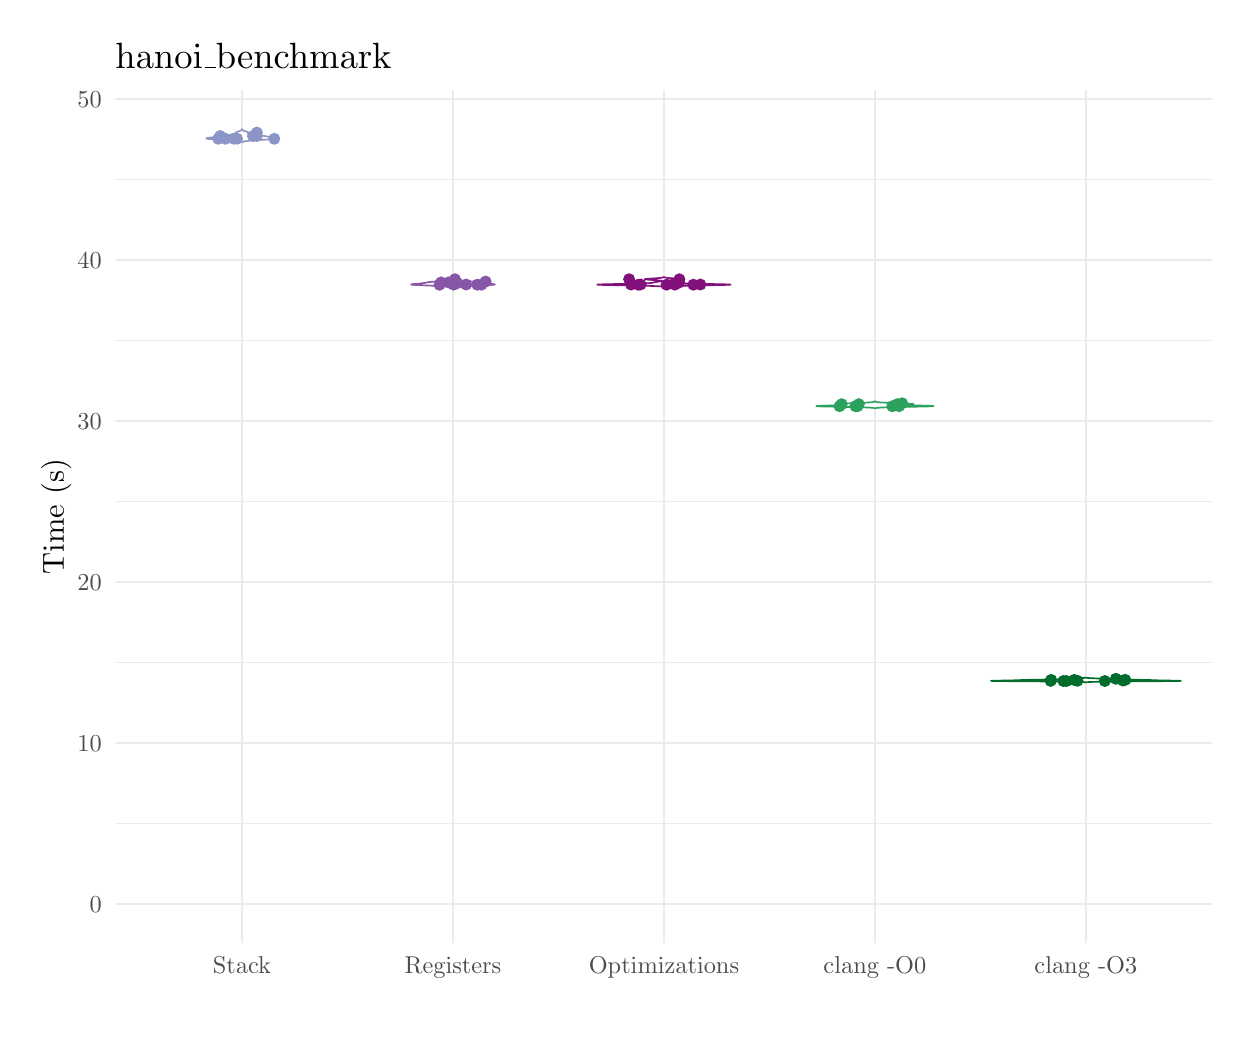
\begin{tikzpicture}[x=1pt,y=1pt]
\definecolor{fillColor}{RGB}{255,255,255}
\path[use as bounding box,fill=fillColor,fill opacity=0.00] (0,0) rectangle (433.62,361.35);
\begin{scope}
\path[clip] ( 31.71, 30.69) rectangle (428.12,338.69);
\definecolor{drawColor}{gray}{0.92}

\path[draw=drawColor,line width= 0.3pt,line join=round] ( 31.71, 73.79) --
	(428.12, 73.79);

\path[draw=drawColor,line width= 0.3pt,line join=round] ( 31.71,131.99) --
	(428.12,131.99);

\path[draw=drawColor,line width= 0.3pt,line join=round] ( 31.71,190.19) --
	(428.12,190.19);

\path[draw=drawColor,line width= 0.3pt,line join=round] ( 31.71,248.39) --
	(428.12,248.39);

\path[draw=drawColor,line width= 0.3pt,line join=round] ( 31.71,306.59) --
	(428.12,306.59);

\path[draw=drawColor,line width= 0.6pt,line join=round] ( 31.71, 44.69) --
	(428.12, 44.69);

\path[draw=drawColor,line width= 0.6pt,line join=round] ( 31.71,102.89) --
	(428.12,102.89);

\path[draw=drawColor,line width= 0.6pt,line join=round] ( 31.71,161.09) --
	(428.12,161.09);

\path[draw=drawColor,line width= 0.6pt,line join=round] ( 31.71,219.29) --
	(428.12,219.29);

\path[draw=drawColor,line width= 0.6pt,line join=round] ( 31.71,277.49) --
	(428.12,277.49);

\path[draw=drawColor,line width= 0.6pt,line join=round] ( 31.71,335.69) --
	(428.12,335.69);

\path[draw=drawColor,line width= 0.6pt,line join=round] ( 77.45, 30.69) --
	( 77.45,338.69);

\path[draw=drawColor,line width= 0.6pt,line join=round] (153.68, 30.69) --
	(153.68,338.69);

\path[draw=drawColor,line width= 0.6pt,line join=round] (229.92, 30.69) --
	(229.92,338.69);

\path[draw=drawColor,line width= 0.6pt,line join=round] (306.15, 30.69) --
	(306.15,338.69);

\path[draw=drawColor,line width= 0.6pt,line join=round] (382.38, 30.69) --
	(382.38,338.69);
\definecolor{drawColor}{RGB}{140,150,198}
\definecolor{fillColor}{RGB}{255,255,255}

\path[draw=drawColor,line width= 0.6pt,line join=round,line cap=round,fill=fillColor] ( 77.35,319.94) --
	( 77.34,319.94) --
	( 77.33,319.95) --
	( 77.32,319.96) --
	( 77.31,319.97) --
	( 77.30,319.98) --
	( 77.29,319.99) --
	( 77.28,320.00) --
	( 77.27,320.01) --
	( 77.26,320.02) --
	( 77.25,320.03) --
	( 77.24,320.04) --
	( 77.22,320.05) --
	( 77.21,320.06) --
	( 77.19,320.07) --
	( 77.18,320.08) --
	( 77.16,320.08) --
	( 77.14,320.09) --
	( 77.12,320.10) --
	( 77.10,320.11) --
	( 77.08,320.12) --
	( 77.06,320.13) --
	( 77.03,320.14) --
	( 77.01,320.15) --
	( 76.98,320.16) --
	( 76.96,320.17) --
	( 76.93,320.18) --
	( 76.90,320.19) --
	( 76.87,320.20) --
	( 76.84,320.21) --
	( 76.80,320.21) --
	( 76.77,320.22) --
	( 76.73,320.23) --
	( 76.69,320.24) --
	( 76.65,320.25) --
	( 76.61,320.26) --
	( 76.57,320.27) --
	( 76.52,320.28) --
	( 76.47,320.29) --
	( 76.42,320.30) --
	( 76.37,320.31) --
	( 76.32,320.32) --
	( 76.27,320.33) --
	( 76.21,320.34) --
	( 76.15,320.35) --
	( 76.09,320.35) --
	( 76.02,320.36) --
	( 75.96,320.37) --
	( 75.89,320.38) --
	( 75.82,320.39) --
	( 75.75,320.40) --
	( 75.67,320.41) --
	( 75.59,320.42) --
	( 75.51,320.43) --
	( 75.43,320.44) --
	( 75.35,320.45) --
	( 75.26,320.46) --
	( 75.17,320.47) --
	( 75.07,320.48) --
	( 74.98,320.48) --
	( 74.88,320.49) --
	( 74.78,320.50) --
	( 74.68,320.51) --
	( 74.57,320.52) --
	( 74.46,320.53) --
	( 74.35,320.54) --
	( 74.24,320.55) --
	( 74.12,320.56) --
	( 74.01,320.57) --
	( 73.89,320.58) --
	( 73.76,320.59) --
	( 73.64,320.60) --
	( 73.51,320.61) --
	( 73.38,320.62) --
	( 73.24,320.62) --
	( 73.11,320.63) --
	( 72.97,320.64) --
	( 72.83,320.65) --
	( 72.69,320.66) --
	( 72.55,320.67) --
	( 72.40,320.68) --
	( 72.25,320.69) --
	( 72.10,320.70) --
	( 71.95,320.71) --
	( 71.80,320.72) --
	( 71.65,320.73) --
	( 71.49,320.74) --
	( 71.34,320.75) --
	( 71.18,320.75) --
	( 71.02,320.76) --
	( 70.86,320.77) --
	( 70.70,320.78) --
	( 70.54,320.79) --
	( 70.38,320.80) --
	( 70.21,320.81) --
	( 70.05,320.82) --
	( 69.89,320.83) --
	( 69.73,320.84) --
	( 69.56,320.85) --
	( 69.40,320.86) --
	( 69.24,320.87) --
	( 69.08,320.88) --
	( 68.92,320.89) --
	( 68.76,320.89) --
	( 68.60,320.90) --
	( 68.44,320.91) --
	( 68.29,320.92) --
	( 68.13,320.93) --
	( 67.98,320.94) --
	( 67.83,320.95) --
	( 67.68,320.96) --
	( 67.53,320.97) --
	( 67.39,320.98) --
	( 67.24,320.99) --
	( 67.11,321.00) --
	( 66.97,321.01) --
	( 66.83,321.02) --
	( 66.70,321.02) --
	( 66.57,321.03) --
	( 66.45,321.04) --
	( 66.33,321.05) --
	( 66.21,321.06) --
	( 66.09,321.07) --
	( 65.98,321.08) --
	( 65.87,321.09) --
	( 65.77,321.10) --
	( 65.67,321.11) --
	( 65.57,321.12) --
	( 65.48,321.13) --
	( 65.40,321.14) --
	( 65.31,321.15) --
	( 65.23,321.16) --
	( 65.16,321.16) --
	( 65.09,321.17) --
	( 65.02,321.18) --
	( 64.96,321.19) --
	( 64.90,321.20) --
	( 64.85,321.21) --
	( 64.80,321.22) --
	( 64.76,321.23) --
	( 64.72,321.24) --
	( 64.68,321.25) --
	( 64.65,321.26) --
	( 64.63,321.27) --
	( 64.61,321.28) --
	( 64.59,321.29) --
	( 64.57,321.29) --
	( 64.57,321.30) --
	( 64.56,321.31) --
	( 64.56,321.32) --
	( 64.56,321.33) --
	( 64.57,321.34) --
	( 64.58,321.35) --
	( 64.59,321.36) --
	( 64.61,321.37) --
	( 64.63,321.38) --
	( 64.66,321.39) --
	( 64.69,321.40) --
	( 64.72,321.41) --
	( 64.75,321.42) --
	( 64.79,321.42) --
	( 64.83,321.43) --
	( 64.87,321.44) --
	( 64.92,321.45) --
	( 64.96,321.46) --
	( 65.01,321.47) --
	( 65.06,321.48) --
	( 65.12,321.49) --
	( 65.17,321.50) --
	( 65.23,321.51) --
	( 65.29,321.52) --
	( 65.35,321.53) --
	( 65.41,321.54) --
	( 65.47,321.55) --
	( 65.54,321.56) --
	( 65.60,321.56) --
	( 65.67,321.57) --
	( 65.73,321.58) --
	( 65.80,321.59) --
	( 65.87,321.60) --
	( 65.93,321.61) --
	( 66.00,321.62) --
	( 66.07,321.63) --
	( 66.14,321.64) --
	( 66.20,321.65) --
	( 66.27,321.66) --
	( 66.34,321.67) --
	( 66.41,321.68) --
	( 66.47,321.69) --
	( 66.54,321.69) --
	( 66.60,321.70) --
	( 66.67,321.71) --
	( 66.73,321.72) --
	( 66.79,321.73) --
	( 66.86,321.74) --
	( 66.92,321.75) --
	( 66.98,321.76) --
	( 67.04,321.77) --
	( 67.10,321.78) --
	( 67.16,321.79) --
	( 67.21,321.80) --
	( 67.27,321.81) --
	( 67.32,321.82) --
	( 67.38,321.83) --
	( 67.43,321.83) --
	( 67.48,321.84) --
	( 67.54,321.85) --
	( 67.59,321.86) --
	( 67.64,321.87) --
	( 67.69,321.88) --
	( 67.74,321.89) --
	( 67.78,321.90) --
	( 67.83,321.91) --
	( 67.88,321.92) --
	( 67.93,321.93) --
	( 67.97,321.94) --
	( 68.02,321.95) --
	( 68.06,321.96) --
	( 68.11,321.96) --
	( 68.15,321.97) --
	( 68.20,321.98) --
	( 68.24,321.99) --
	( 68.29,322.00) --
	( 68.33,322.01) --
	( 68.38,322.02) --
	( 68.42,322.03) --
	( 68.47,322.04) --
	( 68.52,322.05) --
	( 68.56,322.06) --
	( 68.61,322.07) --
	( 68.66,322.08) --
	( 68.71,322.09) --
	( 68.76,322.10) --
	( 68.81,322.10) --
	( 68.86,322.11) --
	( 68.91,322.12) --
	( 68.96,322.13) --
	( 69.02,322.14) --
	( 69.07,322.15) --
	( 69.13,322.16) --
	( 69.18,322.17) --
	( 69.24,322.18) --
	( 69.30,322.19) --
	( 69.36,322.20) --
	( 69.42,322.21) --
	( 69.49,322.22) --
	( 69.55,322.23) --
	( 69.62,322.23) --
	( 69.69,322.24) --
	( 69.75,322.25) --
	( 69.82,322.26) --
	( 69.89,322.27) --
	( 69.97,322.28) --
	( 70.04,322.29) --
	( 70.12,322.30) --
	( 70.19,322.31) --
	( 70.27,322.32) --
	( 70.35,322.33) --
	( 70.43,322.34) --
	( 70.51,322.35) --
	( 70.59,322.36) --
	( 70.67,322.37) --
	( 70.76,322.37) --
	( 70.84,322.38) --
	( 70.93,322.39) --
	( 71.01,322.40) --
	( 71.10,322.41) --
	( 71.19,322.42) --
	( 71.28,322.43) --
	( 71.37,322.44) --
	( 71.46,322.45) --
	( 71.55,322.46) --
	( 71.64,322.47) --
	( 71.73,322.48) --
	( 71.82,322.49) --
	( 71.91,322.50) --
	( 72.00,322.50) --
	( 72.09,322.51) --
	( 72.18,322.52) --
	( 72.27,322.53) --
	( 72.36,322.54) --
	( 72.45,322.55) --
	( 72.54,322.56) --
	( 72.63,322.57) --
	( 72.72,322.58) --
	( 72.81,322.59) --
	( 72.89,322.60) --
	( 72.98,322.61) --
	( 73.06,322.62) --
	( 73.15,322.63) --
	( 73.23,322.64) --
	( 73.31,322.64) --
	( 73.39,322.65) --
	( 73.47,322.66) --
	( 73.55,322.67) --
	( 73.62,322.68) --
	( 73.70,322.69) --
	( 73.77,322.70) --
	( 73.84,322.71) --
	( 73.92,322.72) --
	( 73.98,322.73) --
	( 74.05,322.74) --
	( 74.12,322.75) --
	( 74.18,322.76) --
	( 74.24,322.77) --
	( 74.30,322.77) --
	( 74.36,322.78) --
	( 74.42,322.79) --
	( 74.47,322.80) --
	( 74.52,322.81) --
	( 74.57,322.82) --
	( 74.62,322.83) --
	( 74.67,322.84) --
	( 74.71,322.85) --
	( 74.76,322.86) --
	( 74.80,322.87) --
	( 74.84,322.88) --
	( 74.87,322.89) --
	( 74.91,322.90) --
	( 74.94,322.91) --
	( 74.97,322.91) --
	( 75.00,322.92) --
	( 75.03,322.93) --
	( 75.06,322.94) --
	( 75.08,322.95) --
	( 75.10,322.96) --
	( 75.12,322.97) --
	( 75.14,322.98) --
	( 75.16,322.99) --
	( 75.18,323.00) --
	( 75.19,323.01) --
	( 75.20,323.02) --
	( 75.22,323.03) --
	( 75.23,323.04) --
	( 75.23,323.04) --
	( 75.24,323.05) --
	( 75.25,323.06) --
	( 75.25,323.07) --
	( 75.26,323.08) --
	( 75.26,323.09) --
	( 75.27,323.10) --
	( 75.27,323.11) --
	( 75.27,323.12) --
	( 75.27,323.13) --
	( 75.27,323.14) --
	( 75.26,323.15) --
	( 75.26,323.16) --
	( 75.26,323.17) --
	( 75.26,323.18) --
	( 75.25,323.18) --
	( 75.25,323.19) --
	( 75.25,323.20) --
	( 75.24,323.21) --
	( 75.24,323.22) --
	( 75.23,323.23) --
	( 75.23,323.24) --
	( 75.22,323.25) --
	( 75.22,323.26) --
	( 75.21,323.27) --
	( 75.21,323.28) --
	( 75.20,323.29) --
	( 75.20,323.30) --
	( 75.20,323.31) --
	( 75.19,323.31) --
	( 75.19,323.32) --
	( 75.19,323.33) --
	( 75.19,323.34) --
	( 75.18,323.35) --
	( 75.18,323.36) --
	( 75.18,323.37) --
	( 75.18,323.38) --
	( 75.18,323.39) --
	( 75.18,323.40) --
	( 75.19,323.41) --
	( 75.19,323.42) --
	( 75.19,323.43) --
	( 75.20,323.44) --
	( 75.20,323.45) --
	( 75.21,323.45) --
	( 75.21,323.46) --
	( 75.22,323.47) --
	( 75.23,323.48) --
	( 75.24,323.49) --
	( 75.25,323.50) --
	( 75.26,323.51) --
	( 75.27,323.52) --
	( 75.28,323.53) --
	( 75.30,323.54) --
	( 75.31,323.55) --
	( 75.33,323.56) --
	( 75.34,323.57) --
	( 75.36,323.58) --
	( 75.38,323.58) --
	( 75.39,323.59) --
	( 75.41,323.60) --
	( 75.43,323.61) --
	( 75.45,323.62) --
	( 75.47,323.63) --
	( 75.50,323.64) --
	( 75.52,323.65) --
	( 75.54,323.66) --
	( 75.56,323.67) --
	( 75.59,323.68) --
	( 75.61,323.69) --
	( 75.64,323.70) --
	( 75.66,323.71) --
	( 75.69,323.72) --
	( 75.72,323.72) --
	( 75.74,323.73) --
	( 75.77,323.74) --
	( 75.80,323.75) --
	( 75.83,323.76) --
	( 75.86,323.77) --
	( 75.88,323.78) --
	( 75.91,323.79) --
	( 75.94,323.80) --
	( 75.97,323.81) --
	( 76.00,323.82) --
	( 76.03,323.83) --
	( 76.06,323.84) --
	( 76.09,323.85) --
	( 76.12,323.85) --
	( 76.15,323.86) --
	( 76.18,323.87) --
	( 76.21,323.88) --
	( 76.24,323.89) --
	( 76.27,323.90) --
	( 76.29,323.91) --
	( 76.32,323.92) --
	( 76.35,323.93) --
	( 76.38,323.94) --
	( 76.41,323.95) --
	( 76.44,323.96) --
	( 76.47,323.97) --
	( 76.49,323.98) --
	( 76.52,323.98) --
	( 76.55,323.99) --
	( 76.57,324.00) --
	( 76.60,324.01) --
	( 76.63,324.02) --
	( 76.65,324.03) --
	( 76.68,324.04) --
	( 76.70,324.05) --
	( 76.73,324.06) --
	( 76.75,324.07) --
	( 76.77,324.08) --
	( 76.80,324.09) --
	( 76.82,324.10) --
	( 76.84,324.11) --
	( 76.86,324.12) --
	( 76.88,324.12) --
	( 76.90,324.13) --
	( 76.92,324.14) --
	( 76.94,324.15) --
	( 76.96,324.16) --
	( 76.98,324.17) --
	( 77.00,324.18) --
	( 77.02,324.19) --
	( 77.03,324.20) --
	( 77.05,324.21) --
	( 77.07,324.22) --
	( 77.08,324.23) --
	( 77.10,324.24) --
	( 77.11,324.25) --
	( 77.13,324.25) --
	( 77.14,324.26) --
	( 77.15,324.27) --
	( 77.17,324.28) --
	( 77.18,324.29) --
	( 77.19,324.30) --
	( 77.20,324.31) --
	( 77.21,324.32) --
	( 77.23,324.33) --
	( 77.24,324.34) --
	( 77.25,324.35) --
	( 77.26,324.36) --
	( 77.27,324.37) --
	( 77.27,324.38) --
	( 77.28,324.39) --
	( 77.29,324.39) --
	( 77.30,324.40) --
	( 77.31,324.41) --
	( 77.31,324.42) --
	( 77.32,324.43) --
	( 77.33,324.44) --
	( 77.33,324.45) --
	( 77.34,324.46) --
	( 77.35,324.47) --
	( 77.35,324.48) --
	( 77.36,324.49) --
	( 77.36,324.50) --
	( 77.37,324.51) --
	( 77.37,324.52) --
	( 77.38,324.52) --
	( 77.38,324.53) --
	( 77.38,324.54) --
	( 77.39,324.55) --
	( 77.39,324.56) --
	( 77.40,324.57) --
	( 77.40,324.58) --
	( 77.40,324.59) --
	( 77.41,324.60) --
	( 77.41,324.61) --
	( 77.41,324.62) --
	( 77.41,324.63) --
	( 77.42,324.64) --
	( 77.42,324.65) --
	( 77.42,324.66) --
	( 77.42,324.66) --
	( 77.42,324.67) --
	( 77.43,324.68) --
	( 77.43,324.69) --
	( 77.48,324.69) --
	( 77.48,324.68) --
	( 77.48,324.67) --
	( 77.48,324.66) --
	( 77.48,324.66) --
	( 77.49,324.65) --
	( 77.49,324.64) --
	( 77.49,324.63) --
	( 77.49,324.62) --
	( 77.50,324.61) --
	( 77.50,324.60) --
	( 77.50,324.59) --
	( 77.50,324.58) --
	( 77.51,324.57) --
	( 77.51,324.56) --
	( 77.51,324.55) --
	( 77.52,324.54) --
	( 77.52,324.53) --
	( 77.53,324.52) --
	( 77.53,324.52) --
	( 77.54,324.51) --
	( 77.54,324.50) --
	( 77.55,324.49) --
	( 77.55,324.48) --
	( 77.56,324.47) --
	( 77.56,324.46) --
	( 77.57,324.45) --
	( 77.58,324.44) --
	( 77.58,324.43) --
	( 77.59,324.42) --
	( 77.60,324.41) --
	( 77.60,324.40) --
	( 77.61,324.39) --
	( 77.62,324.39) --
	( 77.63,324.38) --
	( 77.64,324.37) --
	( 77.65,324.36) --
	( 77.66,324.35) --
	( 77.67,324.34) --
	( 77.68,324.33) --
	( 77.69,324.32) --
	( 77.70,324.31) --
	( 77.71,324.30) --
	( 77.72,324.29) --
	( 77.74,324.28) --
	( 77.75,324.27) --
	( 77.76,324.26) --
	( 77.78,324.25) --
	( 77.79,324.25) --
	( 77.81,324.24) --
	( 77.82,324.23) --
	( 77.84,324.22) --
	( 77.85,324.21) --
	( 77.87,324.20) --
	( 77.89,324.19) --
	( 77.91,324.18) --
	( 77.92,324.17) --
	( 77.94,324.16) --
	( 77.96,324.15) --
	( 77.98,324.14) --
	( 78.00,324.13) --
	( 78.02,324.12) --
	( 78.04,324.12) --
	( 78.06,324.11) --
	( 78.09,324.10) --
	( 78.11,324.09) --
	( 78.13,324.08) --
	( 78.15,324.07) --
	( 78.18,324.06) --
	( 78.20,324.05) --
	( 78.23,324.04) --
	( 78.25,324.03) --
	( 78.28,324.02) --
	( 78.30,324.01) --
	( 78.33,324.00) --
	( 78.36,323.99) --
	( 78.38,323.98) --
	( 78.41,323.98) --
	( 78.44,323.97) --
	( 78.47,323.96) --
	( 78.49,323.95) --
	( 78.52,323.94) --
	( 78.55,323.93) --
	( 78.58,323.92) --
	( 78.61,323.91) --
	( 78.64,323.90) --
	( 78.67,323.89) --
	( 78.70,323.88) --
	( 78.73,323.87) --
	( 78.76,323.86) --
	( 78.78,323.85) --
	( 78.81,323.85) --
	( 78.84,323.84) --
	( 78.87,323.83) --
	( 78.90,323.82) --
	( 78.93,323.81) --
	( 78.96,323.80) --
	( 78.99,323.79) --
	( 79.02,323.78) --
	( 79.05,323.77) --
	( 79.08,323.76) --
	( 79.10,323.75) --
	( 79.13,323.74) --
	( 79.16,323.73) --
	( 79.19,323.72) --
	( 79.21,323.72) --
	( 79.24,323.71) --
	( 79.27,323.70) --
	( 79.29,323.69) --
	( 79.31,323.68) --
	( 79.34,323.67) --
	( 79.36,323.66) --
	( 79.39,323.65) --
	( 79.41,323.64) --
	( 79.43,323.63) --
	( 79.45,323.62) --
	( 79.47,323.61) --
	( 79.49,323.60) --
	( 79.51,323.59) --
	( 79.53,323.58) --
	( 79.54,323.58) --
	( 79.56,323.57) --
	( 79.58,323.56) --
	( 79.59,323.55) --
	( 79.61,323.54) --
	( 79.62,323.53) --
	( 79.63,323.52) --
	( 79.64,323.51) --
	( 79.65,323.50) --
	( 79.66,323.49) --
	( 79.67,323.48) --
	( 79.68,323.47) --
	( 79.69,323.46) --
	( 79.70,323.45) --
	( 79.70,323.45) --
	( 79.71,323.44) --
	( 79.71,323.43) --
	( 79.71,323.42) --
	( 79.72,323.41) --
	( 79.72,323.40) --
	( 79.72,323.39) --
	( 79.72,323.38) --
	( 79.72,323.37) --
	( 79.72,323.36) --
	( 79.72,323.35) --
	( 79.72,323.34) --
	( 79.72,323.33) --
	( 79.71,323.32) --
	( 79.71,323.31) --
	( 79.71,323.31) --
	( 79.70,323.30) --
	( 79.70,323.29) --
	( 79.70,323.28) --
	( 79.69,323.27) --
	( 79.69,323.26) --
	( 79.68,323.25) --
	( 79.68,323.24) --
	( 79.67,323.23) --
	( 79.67,323.22) --
	( 79.66,323.21) --
	( 79.66,323.20) --
	( 79.65,323.19) --
	( 79.65,323.18) --
	( 79.65,323.18) --
	( 79.64,323.17) --
	( 79.64,323.16) --
	( 79.64,323.15) --
	( 79.64,323.14) --
	( 79.64,323.13) --
	( 79.64,323.12) --
	( 79.64,323.11) --
	( 79.64,323.10) --
	( 79.64,323.09) --
	( 79.64,323.08) --
	( 79.65,323.07) --
	( 79.65,323.06) --
	( 79.66,323.05) --
	( 79.67,323.04) --
	( 79.68,323.04) --
	( 79.69,323.03) --
	( 79.70,323.02) --
	( 79.71,323.01) --
	( 79.73,323.00) --
	( 79.74,322.99) --
	( 79.76,322.98) --
	( 79.78,322.97) --
	( 79.80,322.96) --
	( 79.82,322.95) --
	( 79.85,322.94) --
	( 79.87,322.93) --
	( 79.90,322.92) --
	( 79.93,322.91) --
	( 79.96,322.91) --
	( 80.00,322.90) --
	( 80.03,322.89) --
	( 80.07,322.88) --
	( 80.11,322.87) --
	( 80.15,322.86) --
	( 80.19,322.85) --
	( 80.23,322.84) --
	( 80.28,322.83) --
	( 80.33,322.82) --
	( 80.38,322.81) --
	( 80.43,322.80) --
	( 80.49,322.79) --
	( 80.54,322.78) --
	( 80.60,322.77) --
	( 80.66,322.77) --
	( 80.72,322.76) --
	( 80.79,322.75) --
	( 80.85,322.74) --
	( 80.92,322.73) --
	( 80.99,322.72) --
	( 81.06,322.71) --
	( 81.13,322.70) --
	( 81.20,322.69) --
	( 81.28,322.68) --
	( 81.35,322.67) --
	( 81.43,322.66) --
	( 81.51,322.65) --
	( 81.59,322.64) --
	( 81.67,322.64) --
	( 81.76,322.63) --
	( 81.84,322.62) --
	( 81.93,322.61) --
	( 82.01,322.60) --
	( 82.10,322.59) --
	( 82.19,322.58) --
	( 82.27,322.57) --
	( 82.36,322.56) --
	( 82.45,322.55) --
	( 82.54,322.54) --
	( 82.63,322.53) --
	( 82.72,322.52) --
	( 82.81,322.51) --
	( 82.90,322.50) --
	( 82.99,322.50) --
	( 83.09,322.49) --
	( 83.18,322.48) --
	( 83.27,322.47) --
	( 83.36,322.46) --
	( 83.45,322.45) --
	( 83.54,322.44) --
	( 83.63,322.43) --
	( 83.71,322.42) --
	( 83.80,322.41) --
	( 83.89,322.40) --
	( 83.98,322.39) --
	( 84.06,322.38) --
	( 84.15,322.37) --
	( 84.23,322.37) --
	( 84.31,322.36) --
	( 84.39,322.35) --
	( 84.48,322.34) --
	( 84.56,322.33) --
	( 84.63,322.32) --
	( 84.71,322.31) --
	( 84.79,322.30) --
	( 84.86,322.29) --
	( 84.94,322.28) --
	( 85.01,322.27) --
	( 85.08,322.26) --
	( 85.15,322.25) --
	( 85.22,322.24) --
	( 85.28,322.23) --
	( 85.35,322.23) --
	( 85.42,322.22) --
	( 85.48,322.21) --
	( 85.54,322.20) --
	( 85.60,322.19) --
	( 85.66,322.18) --
	( 85.72,322.17) --
	( 85.78,322.16) --
	( 85.83,322.15) --
	( 85.89,322.14) --
	( 85.94,322.13) --
	( 85.99,322.12) --
	( 86.05,322.11) --
	( 86.10,322.10) --
	( 86.15,322.10) --
	( 86.20,322.09) --
	( 86.24,322.08) --
	( 86.29,322.07) --
	( 86.34,322.06) --
	( 86.39,322.05) --
	( 86.43,322.04) --
	( 86.48,322.03) --
	( 86.52,322.02) --
	( 86.57,322.01) --
	( 86.61,322.00) --
	( 86.66,321.99) --
	( 86.70,321.98) --
	( 86.75,321.97) --
	( 86.79,321.96) --
	( 86.84,321.96) --
	( 86.89,321.95) --
	( 86.93,321.94) --
	( 86.98,321.93) --
	( 87.02,321.92) --
	( 87.07,321.91) --
	( 87.12,321.90) --
	( 87.17,321.89) --
	( 87.22,321.88) --
	( 87.27,321.87) --
	( 87.32,321.86) --
	( 87.37,321.85) --
	( 87.42,321.84) --
	( 87.47,321.83) --
	( 87.53,321.83) --
	( 87.58,321.82) --
	( 87.63,321.81) --
	( 87.69,321.80) --
	( 87.75,321.79) --
	( 87.81,321.78) --
	( 87.86,321.77) --
	( 87.92,321.76) --
	( 87.99,321.75) --
	( 88.05,321.74) --
	( 88.11,321.73) --
	( 88.17,321.72) --
	( 88.24,321.71) --
	( 88.30,321.70) --
	( 88.37,321.69) --
	( 88.43,321.69) --
	( 88.50,321.68) --
	( 88.56,321.67) --
	( 88.63,321.66) --
	( 88.70,321.65) --
	( 88.77,321.64) --
	( 88.83,321.63) --
	( 88.90,321.62) --
	( 88.97,321.61) --
	( 89.04,321.60) --
	( 89.10,321.59) --
	( 89.17,321.58) --
	( 89.24,321.57) --
	( 89.30,321.56) --
	( 89.37,321.56) --
	( 89.43,321.55) --
	( 89.49,321.54) --
	( 89.55,321.53) --
	( 89.61,321.52) --
	( 89.67,321.51) --
	( 89.73,321.50) --
	( 89.78,321.49) --
	( 89.84,321.48) --
	( 89.89,321.47) --
	( 89.94,321.46) --
	( 89.99,321.45) --
	( 90.03,321.44) --
	( 90.08,321.43) --
	( 90.11,321.42) --
	( 90.15,321.42) --
	( 90.19,321.41) --
	( 90.22,321.40) --
	( 90.25,321.39) --
	( 90.27,321.38) --
	( 90.29,321.37) --
	( 90.31,321.36) --
	( 90.32,321.35) --
	( 90.33,321.34) --
	( 90.34,321.33) --
	( 90.34,321.32) --
	( 90.34,321.31) --
	( 90.34,321.30) --
	( 90.33,321.29) --
	( 90.31,321.29) --
	( 90.30,321.28) --
	( 90.27,321.27) --
	( 90.25,321.26) --
	( 90.22,321.25) --
	( 90.18,321.24) --
	( 90.14,321.23) --
	( 90.10,321.22) --
	( 90.05,321.21) --
	( 90.00,321.20) --
	( 89.94,321.19) --
	( 89.88,321.18) --
	( 89.81,321.17) --
	( 89.74,321.16) --
	( 89.67,321.16) --
	( 89.59,321.15) --
	( 89.51,321.14) --
	( 89.42,321.13) --
	( 89.33,321.12) --
	( 89.23,321.11) --
	( 89.13,321.10) --
	( 89.03,321.09) --
	( 88.92,321.08) --
	( 88.81,321.07) --
	( 88.69,321.06) --
	( 88.58,321.05) --
	( 88.45,321.04) --
	( 88.33,321.03) --
	( 88.20,321.02) --
	( 88.07,321.02) --
	( 87.94,321.01) --
	( 87.80,321.00) --
	( 87.66,320.99) --
	( 87.52,320.98) --
	( 87.37,320.97) --
	( 87.22,320.96) --
	( 87.07,320.95) --
	( 86.92,320.94) --
	( 86.77,320.93) --
	( 86.62,320.92) --
	( 86.46,320.91) --
	( 86.30,320.90) --
	( 86.15,320.89) --
	( 85.99,320.89) --
	( 85.83,320.88) --
	( 85.66,320.87) --
	( 85.50,320.86) --
	( 85.34,320.85) --
	( 85.18,320.84) --
	( 85.01,320.83) --
	( 84.85,320.82) --
	( 84.69,320.81) --
	( 84.53,320.80) --
	( 84.37,320.79) --
	( 84.20,320.78) --
	( 84.04,320.77) --
	( 83.88,320.76) --
	( 83.73,320.75) --
	( 83.57,320.75) --
	( 83.41,320.74) --
	( 83.26,320.73) --
	( 83.10,320.72) --
	( 82.95,320.71) --
	( 82.80,320.70) --
	( 82.65,320.69) --
	( 82.50,320.68) --
	( 82.36,320.67) --
	( 82.21,320.66) --
	( 82.07,320.65) --
	( 81.93,320.64) --
	( 81.79,320.63) --
	( 81.66,320.62) --
	( 81.53,320.62) --
	( 81.40,320.61) --
	( 81.27,320.60) --
	( 81.14,320.59) --
	( 81.02,320.58) --
	( 80.90,320.57) --
	( 80.78,320.56) --
	( 80.66,320.55) --
	( 80.55,320.54) --
	( 80.44,320.53) --
	( 80.33,320.52) --
	( 80.22,320.51) --
	( 80.12,320.50) --
	( 80.02,320.49) --
	( 79.92,320.48) --
	( 79.83,320.48) --
	( 79.74,320.47) --
	( 79.65,320.46) --
	( 79.56,320.45) --
	( 79.47,320.44) --
	( 79.39,320.43) --
	( 79.31,320.42) --
	( 79.23,320.41) --
	( 79.16,320.40) --
	( 79.08,320.39) --
	( 79.01,320.38) --
	( 78.94,320.37) --
	( 78.88,320.36) --
	( 78.82,320.35) --
	( 78.75,320.35) --
	( 78.70,320.34) --
	( 78.64,320.33) --
	( 78.58,320.32) --
	( 78.53,320.31) --
	( 78.48,320.30) --
	( 78.43,320.29) --
	( 78.38,320.28) --
	( 78.34,320.27) --
	( 78.29,320.26) --
	( 78.25,320.25) --
	( 78.21,320.24) --
	( 78.17,320.23) --
	( 78.14,320.22) --
	( 78.10,320.21) --
	( 78.07,320.21) --
	( 78.03,320.20) --
	( 78.00,320.19) --
	( 77.97,320.18) --
	( 77.95,320.17) --
	( 77.92,320.16) --
	( 77.89,320.15) --
	( 77.87,320.14) --
	( 77.85,320.13) --
	( 77.82,320.12) --
	( 77.80,320.11) --
	( 77.78,320.10) --
	( 77.76,320.09) --
	( 77.75,320.08) --
	( 77.73,320.08) --
	( 77.71,320.07) --
	( 77.70,320.06) --
	( 77.68,320.05) --
	( 77.67,320.04) --
	( 77.65,320.03) --
	( 77.64,320.02) --
	( 77.63,320.01) --
	( 77.62,320.00) --
	( 77.61,319.99) --
	( 77.60,319.98) --
	( 77.59,319.97) --
	( 77.58,319.96) --
	( 77.57,319.95) --
	( 77.56,319.94) --
	( 77.56,319.94) --
	( 77.35,319.94) --
	cycle;
\definecolor{drawColor}{RGB}{136,86,167}

\path[draw=drawColor,line width= 0.6pt,line join=round,line cap=round,fill=fillColor] (153.58,267.41) --
	(153.57,267.42) --
	(153.56,267.43) --
	(153.56,267.44) --
	(153.55,267.44) --
	(153.54,267.45) --
	(153.53,267.46) --
	(153.51,267.47) --
	(153.50,267.48) --
	(153.49,267.48) --
	(153.48,267.49) --
	(153.46,267.50) --
	(153.45,267.51) --
	(153.43,267.52) --
	(153.41,267.52) --
	(153.39,267.53) --
	(153.38,267.54) --
	(153.36,267.55) --
	(153.33,267.56) --
	(153.31,267.56) --
	(153.29,267.57) --
	(153.26,267.58) --
	(153.24,267.59) --
	(153.21,267.60) --
	(153.18,267.60) --
	(153.15,267.61) --
	(153.12,267.62) --
	(153.08,267.63) --
	(153.05,267.64) --
	(153.01,267.64) --
	(152.97,267.65) --
	(152.93,267.66) --
	(152.89,267.67) --
	(152.84,267.67) --
	(152.79,267.68) --
	(152.74,267.69) --
	(152.69,267.70) --
	(152.64,267.71) --
	(152.58,267.71) --
	(152.53,267.72) --
	(152.46,267.73) --
	(152.40,267.74) --
	(152.34,267.75) --
	(152.27,267.75) --
	(152.20,267.76) --
	(152.12,267.77) --
	(152.04,267.78) --
	(151.96,267.79) --
	(151.88,267.79) --
	(151.80,267.80) --
	(151.71,267.81) --
	(151.62,267.82) --
	(151.52,267.83) --
	(151.42,267.83) --
	(151.32,267.84) --
	(151.22,267.85) --
	(151.11,267.86) --
	(151.00,267.87) --
	(150.88,267.87) --
	(150.77,267.88) --
	(150.65,267.89) --
	(150.52,267.90) --
	(150.39,267.91) --
	(150.26,267.91) --
	(150.13,267.92) --
	(149.99,267.93) --
	(149.85,267.94) --
	(149.71,267.94) --
	(149.56,267.95) --
	(149.41,267.96) --
	(149.26,267.97) --
	(149.10,267.98) --
	(148.94,267.98) --
	(148.78,267.99) --
	(148.61,268.00) --
	(148.44,268.01) --
	(148.27,268.02) --
	(148.10,268.02) --
	(147.92,268.03) --
	(147.74,268.04) --
	(147.56,268.05) --
	(147.37,268.06) --
	(147.19,268.06) --
	(147.00,268.07) --
	(146.81,268.08) --
	(146.62,268.09) --
	(146.42,268.10) --
	(146.23,268.10) --
	(146.03,268.11) --
	(145.84,268.12) --
	(145.64,268.13) --
	(145.44,268.14) --
	(145.24,268.14) --
	(145.04,268.15) --
	(144.84,268.16) --
	(144.64,268.17) --
	(144.44,268.18) --
	(144.24,268.18) --
	(144.04,268.19) --
	(143.84,268.20) --
	(143.64,268.21) --
	(143.44,268.21) --
	(143.25,268.22) --
	(143.05,268.23) --
	(142.86,268.24) --
	(142.67,268.25) --
	(142.48,268.25) --
	(142.30,268.26) --
	(142.12,268.27) --
	(141.94,268.28) --
	(141.76,268.29) --
	(141.58,268.29) --
	(141.42,268.30) --
	(141.25,268.31) --
	(141.08,268.32) --
	(140.93,268.33) --
	(140.77,268.33) --
	(140.62,268.34) --
	(140.47,268.35) --
	(140.33,268.36) --
	(140.20,268.37) --
	(140.06,268.37) --
	(139.94,268.38) --
	(139.82,268.39) --
	(139.70,268.40) --
	(139.59,268.41) --
	(139.48,268.41) --
	(139.38,268.42) --
	(139.29,268.43) --
	(139.20,268.44) --
	(139.12,268.45) --
	(139.04,268.45) --
	(138.97,268.46) --
	(138.90,268.47) --
	(138.84,268.48) --
	(138.79,268.49) --
	(138.74,268.49) --
	(138.70,268.50) --
	(138.66,268.51) --
	(138.63,268.52) --
	(138.61,268.52) --
	(138.59,268.53) --
	(138.58,268.54) --
	(138.57,268.55) --
	(138.57,268.56) --
	(138.57,268.56) --
	(138.58,268.57) --
	(138.60,268.58) --
	(138.62,268.59) --
	(138.64,268.60) --
	(138.67,268.60) --
	(138.70,268.61) --
	(138.74,268.62) --
	(138.79,268.63) --
	(138.83,268.64) --
	(138.89,268.64) --
	(138.94,268.65) --
	(139.00,268.66) --
	(139.06,268.67) --
	(139.13,268.68) --
	(139.20,268.68) --
	(139.27,268.69) --
	(139.35,268.70) --
	(139.42,268.71) --
	(139.50,268.72) --
	(139.59,268.72) --
	(139.67,268.73) --
	(139.76,268.74) --
	(139.85,268.75) --
	(139.94,268.76) --
	(140.03,268.76) --
	(140.12,268.77) --
	(140.21,268.78) --
	(140.31,268.79) --
	(140.40,268.79) --
	(140.50,268.80) --
	(140.59,268.81) --
	(140.69,268.82) --
	(140.78,268.83) --
	(140.88,268.83) --
	(140.97,268.84) --
	(141.07,268.85) --
	(141.16,268.86) --
	(141.25,268.87) --
	(141.34,268.87) --
	(141.44,268.88) --
	(141.53,268.89) --
	(141.61,268.90) --
	(141.70,268.91) --
	(141.79,268.91) --
	(141.87,268.92) --
	(141.96,268.93) --
	(142.04,268.94) --
	(142.12,268.95) --
	(142.20,268.95) --
	(142.27,268.96) --
	(142.35,268.97) --
	(142.42,268.98) --
	(142.50,268.99) --
	(142.57,268.99) --
	(142.63,269.00) --
	(142.70,269.01) --
	(142.77,269.02) --
	(142.83,269.03) --
	(142.89,269.03) --
	(142.95,269.04) --
	(143.01,269.05) --
	(143.06,269.06) --
	(143.12,269.06) --
	(143.17,269.07) --
	(143.22,269.08) --
	(143.28,269.09) --
	(143.33,269.10) --
	(143.37,269.10) --
	(143.42,269.11) --
	(143.47,269.12) --
	(143.51,269.13) --
	(143.56,269.14) --
	(143.60,269.14) --
	(143.64,269.15) --
	(143.68,269.16) --
	(143.73,269.17) --
	(143.77,269.18) --
	(143.81,269.18) --
	(143.85,269.19) --
	(143.89,269.20) --
	(143.93,269.21) --
	(143.97,269.22) --
	(144.01,269.22) --
	(144.05,269.23) --
	(144.09,269.24) --
	(144.13,269.25) --
	(144.17,269.26) --
	(144.21,269.26) --
	(144.25,269.27) --
	(144.30,269.28) --
	(144.34,269.29) --
	(144.38,269.30) --
	(144.43,269.30) --
	(144.47,269.31) --
	(144.52,269.32) --
	(144.57,269.33) --
	(144.62,269.34) --
	(144.67,269.34) --
	(144.72,269.35) --
	(144.77,269.36) --
	(144.83,269.37) --
	(144.88,269.37) --
	(144.94,269.38) --
	(145.00,269.39) --
	(145.06,269.40) --
	(145.12,269.41) --
	(145.18,269.41) --
	(145.24,269.42) --
	(145.31,269.43) --
	(145.38,269.44) --
	(145.44,269.45) --
	(145.51,269.45) --
	(145.58,269.46) --
	(145.66,269.47) --
	(145.73,269.48) --
	(145.80,269.49) --
	(145.88,269.49) --
	(145.96,269.50) --
	(146.04,269.51) --
	(146.12,269.52) --
	(146.20,269.53) --
	(146.28,269.53) --
	(146.36,269.54) --
	(146.45,269.55) --
	(146.53,269.56) --
	(146.62,269.57) --
	(146.70,269.57) --
	(146.79,269.58) --
	(146.88,269.59) --
	(146.97,269.60) --
	(147.06,269.61) --
	(147.15,269.61) --
	(147.24,269.62) --
	(147.33,269.63) --
	(147.42,269.64) --
	(147.51,269.64) --
	(147.60,269.65) --
	(147.69,269.66) --
	(147.78,269.67) --
	(147.87,269.68) --
	(147.96,269.68) --
	(148.05,269.69) --
	(148.14,269.70) --
	(148.23,269.71) --
	(148.32,269.72) --
	(148.41,269.72) --
	(148.50,269.73) --
	(148.58,269.74) --
	(148.67,269.75) --
	(148.75,269.76) --
	(148.84,269.76) --
	(148.92,269.77) --
	(149.00,269.78) --
	(149.08,269.79) --
	(149.16,269.80) --
	(149.24,269.80) --
	(149.32,269.81) --
	(149.39,269.82) --
	(149.47,269.83) --
	(149.54,269.84) --
	(149.61,269.84) --
	(149.68,269.85) --
	(149.75,269.86) --
	(149.81,269.87) --
	(149.88,269.88) --
	(149.94,269.88) --
	(150.00,269.89) --
	(150.06,269.90) --
	(150.11,269.91) --
	(150.17,269.92) --
	(150.22,269.92) --
	(150.27,269.93) --
	(150.32,269.94) --
	(150.37,269.95) --
	(150.41,269.95) --
	(150.45,269.96) --
	(150.50,269.97) --
	(150.53,269.98) --
	(150.57,269.99) --
	(150.61,269.99) --
	(150.64,270.00) --
	(150.67,270.01) --
	(150.70,270.02) --
	(150.73,270.03) --
	(150.75,270.03) --
	(150.78,270.04) --
	(150.80,270.05) --
	(150.82,270.06) --
	(150.84,270.07) --
	(150.85,270.07) --
	(150.87,270.08) --
	(150.88,270.09) --
	(150.89,270.10) --
	(150.90,270.11) --
	(150.91,270.11) --
	(150.92,270.12) --
	(150.93,270.13) --
	(150.93,270.14) --
	(150.94,270.15) --
	(150.94,270.15) --
	(150.94,270.16) --
	(150.94,270.17) --
	(150.94,270.18) --
	(150.94,270.19) --
	(150.94,270.19) --
	(150.94,270.20) --
	(150.94,270.21) --
	(150.93,270.22) --
	(150.93,270.22) --
	(150.93,270.23) --
	(150.92,270.24) --
	(150.92,270.25) --
	(150.91,270.26) --
	(150.91,270.26) --
	(150.90,270.27) --
	(150.90,270.28) --
	(150.89,270.29) --
	(150.88,270.30) --
	(150.88,270.30) --
	(150.88,270.31) --
	(150.87,270.32) --
	(150.87,270.33) --
	(150.86,270.34) --
	(150.86,270.34) --
	(150.86,270.35) --
	(150.86,270.36) --
	(150.85,270.37) --
	(150.85,270.38) --
	(150.85,270.38) --
	(150.85,270.39) --
	(150.86,270.40) --
	(150.86,270.41) --
	(150.86,270.42) --
	(150.87,270.42) --
	(150.87,270.43) --
	(150.88,270.44) --
	(150.89,270.45) --
	(150.89,270.46) --
	(150.90,270.46) --
	(150.91,270.47) --
	(150.93,270.48) --
	(150.94,270.49) --
	(150.95,270.49) --
	(150.97,270.50) --
	(150.98,270.51) --
	(151.00,270.52) --
	(151.02,270.53) --
	(151.04,270.53) --
	(151.06,270.54) --
	(151.08,270.55) --
	(151.10,270.56) --
	(151.12,270.57) --
	(151.15,270.57) --
	(151.17,270.58) --
	(151.20,270.59) --
	(151.22,270.60) --
	(151.25,270.61) --
	(151.28,270.61) --
	(151.31,270.62) --
	(151.34,270.63) --
	(151.37,270.64) --
	(151.40,270.65) --
	(151.43,270.65) --
	(151.47,270.66) --
	(151.50,270.67) --
	(151.54,270.68) --
	(151.57,270.69) --
	(151.61,270.69) --
	(151.64,270.70) --
	(151.68,270.71) --
	(151.71,270.72) --
	(151.75,270.73) --
	(151.79,270.73) --
	(151.83,270.74) --
	(151.86,270.75) --
	(151.90,270.76) --
	(151.94,270.77) --
	(151.98,270.77) --
	(152.02,270.78) --
	(152.05,270.79) --
	(152.09,270.80) --
	(152.13,270.80) --
	(152.17,270.81) --
	(152.21,270.82) --
	(152.24,270.83) --
	(152.28,270.84) --
	(152.32,270.84) --
	(152.35,270.85) --
	(152.39,270.86) --
	(152.43,270.87) --
	(152.46,270.88) --
	(152.50,270.88) --
	(152.53,270.89) --
	(152.57,270.90) --
	(152.60,270.91) --
	(152.64,270.92) --
	(152.67,270.92) --
	(152.70,270.93) --
	(152.73,270.94) --
	(152.77,270.95) --
	(152.80,270.96) --
	(152.83,270.96) --
	(152.86,270.97) --
	(152.89,270.98) --
	(152.91,270.99) --
	(152.94,271.00) --
	(152.97,271.00) --
	(153.00,271.01) --
	(153.02,271.02) --
	(153.05,271.03) --
	(153.07,271.04) --
	(153.10,271.04) --
	(153.12,271.05) --
	(153.14,271.06) --
	(153.17,271.07) --
	(153.19,271.07) --
	(153.21,271.08) --
	(153.23,271.09) --
	(153.25,271.10) --
	(153.27,271.11) --
	(153.28,271.11) --
	(153.30,271.12) --
	(153.32,271.13) --
	(153.34,271.14) --
	(153.35,271.15) --
	(153.37,271.15) --
	(153.38,271.16) --
	(153.40,271.17) --
	(153.41,271.18) --
	(153.42,271.19) --
	(153.44,271.19) --
	(153.45,271.20) --
	(153.46,271.21) --
	(153.47,271.22) --
	(153.48,271.23) --
	(153.49,271.23) --
	(153.50,271.24) --
	(153.51,271.25) --
	(153.52,271.26) --
	(153.53,271.27) --
	(153.54,271.27) --
	(153.55,271.28) --
	(153.55,271.29) --
	(153.56,271.30) --
	(153.57,271.31) --
	(153.58,271.31) --
	(153.58,271.32) --
	(153.59,271.33) --
	(153.59,271.34) --
	(153.60,271.35) --
	(153.60,271.35) --
	(153.61,271.36) --
	(153.61,271.37) --
	(153.62,271.38) --
	(153.62,271.38) --
	(153.63,271.39) --
	(153.63,271.40) --
	(153.63,271.41) --
	(153.64,271.42) --
	(153.64,271.42) --
	(153.64,271.43) --
	(153.64,271.44) --
	(153.65,271.45) --
	(153.65,271.46) --
	(153.65,271.46) --
	(153.65,271.47) --
	(153.71,271.47) --
	(153.72,271.46) --
	(153.72,271.46) --
	(153.72,271.45) --
	(153.72,271.44) --
	(153.73,271.43) --
	(153.73,271.42) --
	(153.73,271.42) --
	(153.74,271.41) --
	(153.74,271.40) --
	(153.74,271.39) --
	(153.75,271.38) --
	(153.75,271.38) --
	(153.75,271.37) --
	(153.76,271.36) --
	(153.76,271.35) --
	(153.77,271.35) --
	(153.77,271.34) --
	(153.78,271.33) --
	(153.79,271.32) --
	(153.79,271.31) --
	(153.80,271.31) --
	(153.81,271.30) --
	(153.81,271.29) --
	(153.82,271.28) --
	(153.83,271.27) --
	(153.84,271.27) --
	(153.85,271.26) --
	(153.85,271.25) --
	(153.86,271.24) --
	(153.87,271.23) --
	(153.88,271.23) --
	(153.90,271.22) --
	(153.91,271.21) --
	(153.92,271.20) --
	(153.93,271.19) --
	(153.94,271.19) --
	(153.96,271.18) --
	(153.97,271.17) --
	(153.98,271.16) --
	(154.00,271.15) --
	(154.02,271.15) --
	(154.03,271.14) --
	(154.05,271.13) --
	(154.06,271.12) --
	(154.08,271.11) --
	(154.10,271.11) --
	(154.12,271.10) --
	(154.14,271.09) --
	(154.16,271.08) --
	(154.18,271.07) --
	(154.20,271.07) --
	(154.22,271.06) --
	(154.25,271.05) --
	(154.27,271.04) --
	(154.30,271.04) --
	(154.32,271.03) --
	(154.35,271.02) --
	(154.37,271.01) --
	(154.40,271.00) --
	(154.43,271.00) --
	(154.45,270.99) --
	(154.48,270.98) --
	(154.51,270.97) --
	(154.54,270.96) --
	(154.57,270.96) --
	(154.60,270.95) --
	(154.63,270.94) --
	(154.67,270.93) --
	(154.70,270.92) --
	(154.73,270.92) --
	(154.77,270.91) --
	(154.80,270.90) --
	(154.83,270.89) --
	(154.87,270.88) --
	(154.90,270.88) --
	(154.94,270.87) --
	(154.98,270.86) --
	(155.01,270.85) --
	(155.05,270.84) --
	(155.09,270.84) --
	(155.12,270.83) --
	(155.16,270.82) --
	(155.20,270.81) --
	(155.24,270.80) --
	(155.28,270.80) --
	(155.31,270.79) --
	(155.35,270.78) --
	(155.39,270.77) --
	(155.43,270.77) --
	(155.47,270.76) --
	(155.50,270.75) --
	(155.54,270.74) --
	(155.58,270.73) --
	(155.62,270.73) --
	(155.65,270.72) --
	(155.69,270.71) --
	(155.73,270.70) --
	(155.76,270.69) --
	(155.80,270.69) --
	(155.83,270.68) --
	(155.87,270.67) --
	(155.90,270.66) --
	(155.93,270.65) --
	(155.97,270.65) --
	(156.00,270.64) --
	(156.03,270.63) --
	(156.06,270.62) --
	(156.09,270.61) --
	(156.12,270.61) --
	(156.14,270.60) --
	(156.17,270.59) --
	(156.20,270.58) --
	(156.22,270.57) --
	(156.25,270.57) --
	(156.27,270.56) --
	(156.29,270.55) --
	(156.31,270.54) --
	(156.33,270.53) --
	(156.35,270.53) --
	(156.37,270.52) --
	(156.39,270.51) --
	(156.40,270.50) --
	(156.42,270.49) --
	(156.43,270.49) --
	(156.44,270.48) --
	(156.45,270.47) --
	(156.46,270.46) --
	(156.47,270.46) --
	(156.48,270.45) --
	(156.49,270.44) --
	(156.50,270.43) --
	(156.50,270.42) --
	(156.50,270.42) --
	(156.51,270.41) --
	(156.51,270.40) --
	(156.51,270.39) --
	(156.51,270.38) --
	(156.51,270.38) --
	(156.51,270.37) --
	(156.51,270.36) --
	(156.51,270.35) --
	(156.51,270.34) --
	(156.50,270.34) --
	(156.50,270.33) --
	(156.50,270.32) --
	(156.49,270.31) --
	(156.49,270.30) --
	(156.48,270.30) --
	(156.48,270.29) --
	(156.47,270.28) --
	(156.47,270.27) --
	(156.46,270.26) --
	(156.46,270.26) --
	(156.45,270.25) --
	(156.45,270.24) --
	(156.44,270.23) --
	(156.44,270.22) --
	(156.43,270.22) --
	(156.43,270.21) --
	(156.43,270.20) --
	(156.43,270.19) --
	(156.42,270.19) --
	(156.42,270.18) --
	(156.42,270.17) --
	(156.42,270.16) --
	(156.43,270.15) --
	(156.43,270.15) --
	(156.43,270.14) --
	(156.44,270.13) --
	(156.45,270.12) --
	(156.45,270.11) --
	(156.46,270.11) --
	(156.47,270.10) --
	(156.49,270.09) --
	(156.50,270.08) --
	(156.51,270.07) --
	(156.53,270.07) --
	(156.55,270.06) --
	(156.57,270.05) --
	(156.59,270.04) --
	(156.62,270.03) --
	(156.64,270.03) --
	(156.67,270.02) --
	(156.70,270.01) --
	(156.73,270.00) --
	(156.76,269.99) --
	(156.80,269.99) --
	(156.83,269.98) --
	(156.87,269.97) --
	(156.91,269.96) --
	(156.96,269.95) --
	(157.00,269.95) --
	(157.05,269.94) --
	(157.10,269.93) --
	(157.15,269.92) --
	(157.20,269.92) --
	(157.25,269.91) --
	(157.31,269.90) --
	(157.37,269.89) --
	(157.43,269.88) --
	(157.49,269.88) --
	(157.55,269.87) --
	(157.62,269.86) --
	(157.69,269.85) --
	(157.76,269.84) --
	(157.83,269.84) --
	(157.90,269.83) --
	(157.97,269.82) --
	(158.05,269.81) --
	(158.13,269.80) --
	(158.20,269.80) --
	(158.28,269.79) --
	(158.36,269.78) --
	(158.45,269.77) --
	(158.53,269.76) --
	(158.61,269.76) --
	(158.70,269.75) --
	(158.78,269.74) --
	(158.87,269.73) --
	(158.96,269.72) --
	(159.05,269.72) --
	(159.14,269.71) --
	(159.22,269.70) --
	(159.31,269.69) --
	(159.41,269.68) --
	(159.50,269.68) --
	(159.59,269.67) --
	(159.68,269.66) --
	(159.77,269.65) --
	(159.86,269.64) --
	(159.95,269.64) --
	(160.04,269.63) --
	(160.13,269.62) --
	(160.22,269.61) --
	(160.31,269.61) --
	(160.40,269.60) --
	(160.49,269.59) --
	(160.58,269.58) --
	(160.66,269.57) --
	(160.75,269.57) --
	(160.84,269.56) --
	(160.92,269.55) --
	(161.01,269.54) --
	(161.09,269.53) --
	(161.17,269.53) --
	(161.25,269.52) --
	(161.33,269.51) --
	(161.41,269.50) --
	(161.49,269.49) --
	(161.56,269.49) --
	(161.64,269.48) --
	(161.71,269.47) --
	(161.78,269.46) --
	(161.85,269.45) --
	(161.92,269.45) --
	(161.99,269.44) --
	(162.06,269.43) --
	(162.12,269.42) --
	(162.19,269.41) --
	(162.25,269.41) --
	(162.31,269.40) --
	(162.37,269.39) --
	(162.43,269.38) --
	(162.48,269.37) --
	(162.54,269.37) --
	(162.59,269.36) --
	(162.65,269.35) --
	(162.70,269.34) --
	(162.75,269.34) --
	(162.80,269.33) --
	(162.85,269.32) --
	(162.89,269.31) --
	(162.94,269.30) --
	(162.98,269.30) --
	(163.03,269.29) --
	(163.07,269.28) --
	(163.12,269.27) --
	(163.16,269.26) --
	(163.20,269.26) --
	(163.24,269.25) --
	(163.28,269.24) --
	(163.32,269.23) --
	(163.36,269.22) --
	(163.40,269.22) --
	(163.44,269.21) --
	(163.48,269.20) --
	(163.52,269.19) --
	(163.56,269.18) --
	(163.60,269.18) --
	(163.64,269.17) --
	(163.68,269.16) --
	(163.73,269.15) --
	(163.77,269.14) --
	(163.81,269.14) --
	(163.86,269.13) --
	(163.90,269.12) --
	(163.95,269.11) --
	(163.99,269.10) --
	(164.04,269.10) --
	(164.09,269.09) --
	(164.14,269.08) --
	(164.19,269.07) --
	(164.25,269.06) --
	(164.30,269.06) --
	(164.36,269.05) --
	(164.42,269.04) --
	(164.48,269.03) --
	(164.54,269.03) --
	(164.60,269.02) --
	(164.67,269.01) --
	(164.73,269.00) --
	(164.80,268.99) --
	(164.87,268.99) --
	(164.94,268.98) --
	(165.02,268.97) --
	(165.09,268.96) --
	(165.17,268.95) --
	(165.25,268.95) --
	(165.33,268.94) --
	(165.41,268.93) --
	(165.49,268.92) --
	(165.58,268.91) --
	(165.67,268.91) --
	(165.75,268.90) --
	(165.84,268.89) --
	(165.93,268.88) --
	(166.02,268.87) --
	(166.12,268.87) --
	(166.21,268.86) --
	(166.30,268.85) --
	(166.40,268.84) --
	(166.49,268.83) --
	(166.59,268.83) --
	(166.68,268.82) --
	(166.78,268.81) --
	(166.87,268.80) --
	(166.97,268.79) --
	(167.06,268.79) --
	(167.16,268.78) --
	(167.25,268.77) --
	(167.34,268.76) --
	(167.43,268.76) --
	(167.52,268.75) --
	(167.61,268.74) --
	(167.70,268.73) --
	(167.78,268.72) --
	(167.86,268.72) --
	(167.94,268.71) --
	(168.02,268.70) --
	(168.10,268.69) --
	(168.17,268.68) --
	(168.24,268.68) --
	(168.30,268.67) --
	(168.37,268.66) --
	(168.43,268.65) --
	(168.48,268.64) --
	(168.53,268.64) --
	(168.58,268.63) --
	(168.62,268.62) --
	(168.66,268.61) --
	(168.70,268.60) --
	(168.73,268.60) --
	(168.75,268.59) --
	(168.77,268.58) --
	(168.79,268.57) --
	(168.79,268.56) --
	(168.80,268.56) --
	(168.80,268.55) --
	(168.79,268.54) --
	(168.78,268.53) --
	(168.76,268.52) --
	(168.73,268.52) --
	(168.70,268.51) --
	(168.67,268.50) --
	(168.63,268.49) --
	(168.58,268.49) --
	(168.53,268.48) --
	(168.47,268.47) --
	(168.40,268.46) --
	(168.33,268.45) --
	(168.25,268.45) --
	(168.17,268.44) --
	(168.08,268.43) --
	(167.99,268.42) --
	(167.89,268.41) --
	(167.78,268.41) --
	(167.67,268.40) --
	(167.55,268.39) --
	(167.43,268.38) --
	(167.30,268.37) --
	(167.17,268.37) --
	(167.04,268.36) --
	(166.89,268.35) --
	(166.75,268.34) --
	(166.60,268.33) --
	(166.44,268.33) --
	(166.28,268.32) --
	(166.12,268.31) --
	(165.95,268.30) --
	(165.78,268.29) --
	(165.61,268.29) --
	(165.43,268.28) --
	(165.25,268.27) --
	(165.07,268.26) --
	(164.88,268.25) --
	(164.70,268.25) --
	(164.51,268.24) --
	(164.31,268.23) --
	(164.12,268.22) --
	(163.92,268.21) --
	(163.73,268.21) --
	(163.53,268.20) --
	(163.33,268.19) --
	(163.13,268.18) --
	(162.93,268.18) --
	(162.73,268.17) --
	(162.53,268.16) --
	(162.33,268.15) --
	(162.13,268.14) --
	(161.93,268.14) --
	(161.73,268.13) --
	(161.53,268.12) --
	(161.34,268.11) --
	(161.14,268.10) --
	(160.94,268.10) --
	(160.75,268.09) --
	(160.56,268.08) --
	(160.37,268.07) --
	(160.18,268.06) --
	(159.99,268.06) --
	(159.81,268.05) --
	(159.63,268.04) --
	(159.45,268.03) --
	(159.27,268.02) --
	(159.10,268.02) --
	(158.93,268.01) --
	(158.76,268.00) --
	(158.59,267.99) --
	(158.43,267.98) --
	(158.27,267.98) --
	(158.11,267.97) --
	(157.96,267.96) --
	(157.81,267.95) --
	(157.66,267.94) --
	(157.52,267.94) --
	(157.38,267.93) --
	(157.24,267.92) --
	(157.10,267.91) --
	(156.97,267.91) --
	(156.85,267.90) --
	(156.72,267.89) --
	(156.60,267.88) --
	(156.48,267.87) --
	(156.37,267.87) --
	(156.26,267.86) --
	(156.15,267.85) --
	(156.05,267.84) --
	(155.94,267.83) --
	(155.85,267.83) --
	(155.75,267.82) --
	(155.66,267.81) --
	(155.57,267.80) --
	(155.49,267.79) --
	(155.40,267.79) --
	(155.32,267.78) --
	(155.25,267.77) --
	(155.17,267.76) --
	(155.10,267.75) --
	(155.03,267.75) --
	(154.97,267.74) --
	(154.90,267.73) --
	(154.84,267.72) --
	(154.78,267.71) --
	(154.73,267.71) --
	(154.67,267.70) --
	(154.62,267.69) --
	(154.57,267.68) --
	(154.53,267.67) --
	(154.48,267.67) --
	(154.44,267.66) --
	(154.40,267.65) --
	(154.36,267.64) --
	(154.32,267.64) --
	(154.28,267.63) --
	(154.25,267.62) --
	(154.22,267.61) --
	(154.19,267.60) --
	(154.16,267.60) --
	(154.13,267.59) --
	(154.10,267.58) --
	(154.08,267.57) --
	(154.06,267.56) --
	(154.03,267.56) --
	(154.01,267.55) --
	(153.99,267.54) --
	(153.97,267.53) --
	(153.95,267.52) --
	(153.94,267.52) --
	(153.92,267.51) --
	(153.91,267.50) --
	(153.89,267.49) --
	(153.88,267.48) --
	(153.87,267.48) --
	(153.85,267.47) --
	(153.84,267.46) --
	(153.83,267.45) --
	(153.82,267.44) --
	(153.81,267.44) --
	(153.80,267.43) --
	(153.80,267.42) --
	(153.79,267.41) --
	(153.58,267.41) --
	cycle;
\definecolor{drawColor}{RGB}{129,15,124}

\path[draw=drawColor,line width= 0.6pt,line join=round,line cap=round,fill=fillColor] (229.73,267.67) --
	(229.71,267.68) --
	(229.70,267.68) --
	(229.68,267.69) --
	(229.66,267.70) --
	(229.64,267.71) --
	(229.61,267.71) --
	(229.59,267.72) --
	(229.56,267.73) --
	(229.54,267.73) --
	(229.51,267.74) --
	(229.47,267.75) --
	(229.44,267.75) --
	(229.40,267.76) --
	(229.36,267.77) --
	(229.32,267.78) --
	(229.28,267.78) --
	(229.23,267.79) --
	(229.18,267.80) --
	(229.13,267.80) --
	(229.07,267.81) --
	(229.01,267.82) --
	(228.95,267.82) --
	(228.89,267.83) --
	(228.81,267.84) --
	(228.74,267.85) --
	(228.66,267.85) --
	(228.58,267.86) --
	(228.49,267.87) --
	(228.40,267.87) --
	(228.30,267.88) --
	(228.20,267.89) --
	(228.10,267.89) --
	(227.98,267.90) --
	(227.87,267.91) --
	(227.74,267.92) --
	(227.62,267.92) --
	(227.48,267.93) --
	(227.34,267.94) --
	(227.19,267.94) --
	(227.04,267.95) --
	(226.88,267.96) --
	(226.71,267.96) --
	(226.54,267.97) --
	(226.36,267.98) --
	(226.17,267.99) --
	(225.98,267.99) --
	(225.78,268.00) --
	(225.57,268.01) --
	(225.35,268.01) --
	(225.13,268.02) --
	(224.90,268.03) --
	(224.66,268.03) --
	(224.42,268.04) --
	(224.16,268.05) --
	(223.90,268.06) --
	(223.63,268.06) --
	(223.36,268.07) --
	(223.07,268.08) --
	(222.78,268.08) --
	(222.49,268.09) --
	(222.18,268.10) --
	(221.87,268.10) --
	(221.55,268.11) --
	(221.23,268.12) --
	(220.90,268.13) --
	(220.56,268.13) --
	(220.22,268.14) --
	(219.87,268.15) --
	(219.52,268.15) --
	(219.16,268.16) --
	(218.80,268.17) --
	(218.43,268.17) --
	(218.06,268.18) --
	(217.69,268.19) --
	(217.31,268.20) --
	(216.93,268.20) --
	(216.55,268.21) --
	(216.17,268.22) --
	(215.78,268.22) --
	(215.40,268.23) --
	(215.02,268.24) --
	(214.63,268.24) --
	(214.25,268.25) --
	(213.87,268.26) --
	(213.49,268.27) --
	(213.11,268.27) --
	(212.74,268.28) --
	(212.37,268.29) --
	(212.00,268.29) --
	(211.64,268.30) --
	(211.29,268.31) --
	(210.94,268.31) --
	(210.60,268.32) --
	(210.27,268.33) --
	(209.94,268.34) --
	(209.62,268.34) --
	(209.32,268.35) --
	(209.02,268.36) --
	(208.73,268.36) --
	(208.46,268.37) --
	(208.19,268.38) --
	(207.94,268.38) --
	(207.70,268.39) --
	(207.47,268.40) --
	(207.26,268.41) --
	(207.06,268.41) --
	(206.87,268.42) --
	(206.71,268.43) --
	(206.55,268.43) --
	(206.41,268.44) --
	(206.29,268.45) --
	(206.17,268.46) --
	(206.08,268.46) --
	(206.01,268.47) --
	(205.94,268.48) --
	(205.90,268.48) --
	(205.87,268.49) --
	(205.86,268.50) --
	(205.87,268.50) --
	(205.89,268.51) --
	(205.92,268.52) --
	(205.98,268.53) --
	(206.05,268.53) --
	(206.14,268.54) --
	(206.24,268.55) --
	(206.35,268.55) --
	(206.49,268.56) --
	(206.64,268.57) --
	(206.80,268.57) --
	(206.98,268.58) --
	(207.17,268.59) --
	(207.37,268.60) --
	(207.59,268.60) --
	(207.82,268.61) --
	(208.06,268.62) --
	(208.31,268.62) --
	(208.58,268.63) --
	(208.85,268.64) --
	(209.14,268.64) --
	(209.43,268.65) --
	(209.74,268.66) --
	(210.05,268.67) --
	(210.37,268.67) --
	(210.69,268.68) --
	(211.02,268.69) --
	(211.36,268.69) --
	(211.70,268.70) --
	(212.05,268.71) --
	(212.40,268.71) --
	(212.75,268.72) --
	(213.11,268.73) --
	(213.46,268.74) --
	(213.82,268.74) --
	(214.18,268.75) --
	(214.54,268.76) --
	(214.90,268.76) --
	(215.26,268.77) --
	(215.61,268.78) --
	(215.97,268.78) --
	(216.32,268.79) --
	(216.67,268.80) --
	(217.01,268.81) --
	(217.35,268.81) --
	(217.69,268.82) --
	(218.02,268.83) --
	(218.35,268.83) --
	(218.66,268.84) --
	(218.98,268.85) --
	(219.29,268.85) --
	(219.59,268.86) --
	(219.88,268.87) --
	(220.17,268.88) --
	(220.45,268.88) --
	(220.72,268.89) --
	(220.99,268.90) --
	(221.24,268.90) --
	(221.49,268.91) --
	(221.73,268.92) --
	(221.97,268.92) --
	(222.19,268.93) --
	(222.41,268.94) --
	(222.62,268.95) --
	(222.82,268.95) --
	(223.01,268.96) --
	(223.20,268.97) --
	(223.37,268.97) --
	(223.54,268.98) --
	(223.70,268.99) --
	(223.86,268.99) --
	(224.00,269.00) --
	(224.14,269.01) --
	(224.27,269.02) --
	(224.40,269.02) --
	(224.51,269.03) --
	(224.62,269.04) --
	(224.73,269.04) --
	(224.83,269.05) --
	(224.92,269.06) --
	(225.01,269.06) --
	(225.09,269.07) --
	(225.16,269.08) --
	(225.23,269.09) --
	(225.30,269.09) --
	(225.36,269.10) --
	(225.42,269.11) --
	(225.47,269.11) --
	(225.52,269.12) --
	(225.57,269.13) --
	(225.61,269.13) --
	(225.65,269.14) --
	(225.69,269.15) --
	(225.72,269.16) --
	(225.75,269.16) --
	(225.78,269.17) --
	(225.81,269.18) --
	(225.84,269.18) --
	(225.86,269.19) --
	(225.89,269.20) --
	(225.91,269.20) --
	(225.93,269.21) --
	(225.96,269.22) --
	(225.98,269.23) --
	(226.00,269.23) --
	(226.02,269.24) --
	(226.04,269.25) --
	(226.06,269.25) --
	(226.09,269.26) --
	(226.11,269.27) --
	(226.13,269.27) --
	(226.16,269.28) --
	(226.18,269.29) --
	(226.21,269.30) --
	(226.23,269.30) --
	(226.26,269.31) --
	(226.29,269.32) --
	(226.32,269.32) --
	(226.35,269.33) --
	(226.38,269.34) --
	(226.42,269.34) --
	(226.45,269.35) --
	(226.49,269.36) --
	(226.52,269.37) --
	(226.56,269.37) --
	(226.60,269.38) --
	(226.64,269.39) --
	(226.69,269.39) --
	(226.73,269.40) --
	(226.77,269.41) --
	(226.82,269.41) --
	(226.87,269.42) --
	(226.92,269.43) --
	(226.97,269.44) --
	(227.02,269.44) --
	(227.07,269.45) --
	(227.12,269.46) --
	(227.17,269.46) --
	(227.22,269.47) --
	(227.28,269.48) --
	(227.33,269.48) --
	(227.39,269.49) --
	(227.44,269.50) --
	(227.50,269.51) --
	(227.55,269.51) --
	(227.61,269.52) --
	(227.66,269.53) --
	(227.72,269.53) --
	(227.77,269.54) --
	(227.83,269.55) --
	(227.88,269.55) --
	(227.94,269.56) --
	(227.99,269.57) --
	(228.05,269.58) --
	(228.10,269.58) --
	(228.15,269.59) --
	(228.20,269.60) --
	(228.25,269.60) --
	(228.30,269.61) --
	(228.35,269.62) --
	(228.40,269.62) --
	(228.45,269.63) --
	(228.49,269.64) --
	(228.54,269.65) --
	(228.58,269.65) --
	(228.62,269.66) --
	(228.66,269.67) --
	(228.70,269.67) --
	(228.74,269.68) --
	(228.78,269.69) --
	(228.81,269.69) --
	(228.84,269.70) --
	(228.87,269.71) --
	(228.90,269.72) --
	(228.93,269.72) --
	(228.96,269.73) --
	(228.98,269.74) --
	(229.00,269.74) --
	(229.02,269.75) --
	(229.04,269.76) --
	(229.06,269.76) --
	(229.07,269.77) --
	(229.08,269.78) --
	(229.09,269.79) --
	(229.10,269.79) --
	(229.11,269.80) --
	(229.11,269.81) --
	(229.11,269.81) --
	(229.11,269.82) --
	(229.11,269.83) --
	(229.10,269.83) --
	(229.10,269.84) --
	(229.09,269.85) --
	(229.07,269.86) --
	(229.06,269.86) --
	(229.04,269.87) --
	(229.02,269.88) --
	(229.00,269.88) --
	(228.97,269.89) --
	(228.95,269.90) --
	(228.92,269.90) --
	(228.89,269.91) --
	(228.85,269.92) --
	(228.81,269.93) --
	(228.77,269.93) --
	(228.73,269.94) --
	(228.69,269.95) --
	(228.64,269.95) --
	(228.59,269.96) --
	(228.54,269.97) --
	(228.48,269.97) --
	(228.42,269.98) --
	(228.36,269.99) --
	(228.30,270.00) --
	(228.23,270.00) --
	(228.16,270.01) --
	(228.09,270.02) --
	(228.02,270.02) --
	(227.94,270.03) --
	(227.86,270.04) --
	(227.78,270.04) --
	(227.70,270.05) --
	(227.61,270.06) --
	(227.53,270.07) --
	(227.44,270.07) --
	(227.35,270.08) --
	(227.25,270.09) --
	(227.16,270.09) --
	(227.06,270.10) --
	(226.96,270.11) --
	(226.86,270.11) --
	(226.76,270.12) --
	(226.65,270.13) --
	(226.55,270.14) --
	(226.44,270.14) --
	(226.33,270.15) --
	(226.22,270.16) --
	(226.12,270.16) --
	(226.01,270.17) --
	(225.90,270.18) --
	(225.78,270.18) --
	(225.67,270.19) --
	(225.56,270.20) --
	(225.45,270.21) --
	(225.34,270.21) --
	(225.23,270.22) --
	(225.12,270.23) --
	(225.02,270.23) --
	(224.91,270.24) --
	(224.80,270.25) --
	(224.70,270.25) --
	(224.59,270.26) --
	(224.49,270.27) --
	(224.39,270.28) --
	(224.30,270.28) --
	(224.20,270.29) --
	(224.11,270.30) --
	(224.02,270.30) --
	(223.93,270.31) --
	(223.85,270.32) --
	(223.77,270.32) --
	(223.69,270.33) --
	(223.62,270.34) --
	(223.55,270.35) --
	(223.48,270.35) --
	(223.42,270.36) --
	(223.36,270.37) --
	(223.30,270.37) --
	(223.25,270.38) --
	(223.21,270.39) --
	(223.17,270.39) --
	(223.13,270.40) --
	(223.10,270.41) --
	(223.07,270.42) --
	(223.05,270.42) --
	(223.03,270.43) --
	(223.02,270.44) --
	(223.01,270.44) --
	(223.00,270.45) --
	(223.00,270.46) --
	(223.01,270.46) --
	(223.02,270.47) --
	(223.04,270.48) --
	(223.06,270.49) --
	(223.08,270.49) --
	(223.11,270.50) --
	(223.15,270.51) --
	(223.19,270.51) --
	(223.23,270.52) --
	(223.28,270.53) --
	(223.33,270.53) --
	(223.39,270.54) --
	(223.45,270.55) --
	(223.52,270.56) --
	(223.59,270.56) --
	(223.66,270.57) --
	(223.73,270.58) --
	(223.82,270.58) --
	(223.90,270.59) --
	(223.98,270.60) --
	(224.07,270.60) --
	(224.16,270.61) --
	(224.26,270.62) --
	(224.35,270.63) --
	(224.45,270.63) --
	(224.55,270.64) --
	(224.66,270.65) --
	(224.76,270.65) --
	(224.87,270.66) --
	(224.97,270.67) --
	(225.08,270.67) --
	(225.19,270.68) --
	(225.30,270.69) --
	(225.41,270.70) --
	(225.52,270.70) --
	(225.63,270.71) --
	(225.75,270.72) --
	(225.86,270.72) --
	(225.97,270.73) --
	(226.08,270.74) --
	(226.19,270.74) --
	(226.30,270.75) --
	(226.41,270.76) --
	(226.52,270.77) --
	(226.62,270.77) --
	(226.73,270.78) --
	(226.84,270.79) --
	(226.94,270.79) --
	(227.04,270.80) --
	(227.14,270.81) --
	(227.24,270.81) --
	(227.34,270.82) --
	(227.43,270.83) --
	(227.53,270.84) --
	(227.62,270.84) --
	(227.71,270.85) --
	(227.80,270.86) --
	(227.88,270.86) --
	(227.97,270.87) --
	(228.05,270.88) --
	(228.13,270.88) --
	(228.20,270.89) --
	(228.28,270.90) --
	(228.35,270.91) --
	(228.42,270.91) --
	(228.49,270.92) --
	(228.56,270.93) --
	(228.62,270.93) --
	(228.68,270.94) --
	(228.74,270.95) --
	(228.80,270.95) --
	(228.86,270.96) --
	(228.91,270.97) --
	(228.96,270.98) --
	(229.01,270.98) --
	(229.06,270.99) --
	(229.10,271.00) --
	(229.15,271.00) --
	(229.19,271.01) --
	(229.23,271.02) --
	(229.27,271.02) --
	(229.31,271.03) --
	(229.34,271.04) --
	(229.37,271.05) --
	(229.41,271.05) --
	(229.44,271.06) --
	(229.46,271.07) --
	(229.49,271.07) --
	(229.52,271.08) --
	(229.54,271.09) --
	(229.57,271.09) --
	(229.59,271.10) --
	(229.61,271.11) --
	(229.63,271.12) --
	(229.65,271.12) --
	(229.67,271.13) --
	(229.68,271.14) --
	(229.70,271.14) --
	(229.71,271.15) --
	(229.73,271.16) --
	(229.74,271.16) --
	(229.75,271.17) --
	(229.76,271.18) --
	(229.77,271.19) --
	(229.78,271.19) --
	(229.79,271.20) --
	(229.80,271.21) --
	(229.81,271.21) --
	(229.82,271.22) --
	(229.83,271.23) --
	(229.83,271.23) --
	(229.84,271.24) --
	(229.85,271.25) --
	(229.99,271.25) --
	(229.99,271.24) --
	(230.00,271.23) --
	(230.01,271.23) --
	(230.01,271.22) --
	(230.02,271.21) --
	(230.03,271.21) --
	(230.04,271.20) --
	(230.05,271.19) --
	(230.06,271.19) --
	(230.07,271.18) --
	(230.08,271.17) --
	(230.09,271.16) --
	(230.11,271.16) --
	(230.12,271.15) --
	(230.13,271.14) --
	(230.15,271.14) --
	(230.17,271.13) --
	(230.18,271.12) --
	(230.20,271.12) --
	(230.22,271.11) --
	(230.24,271.10) --
	(230.27,271.09) --
	(230.29,271.09) --
	(230.31,271.08) --
	(230.34,271.07) --
	(230.37,271.07) --
	(230.40,271.06) --
	(230.43,271.05) --
	(230.46,271.05) --
	(230.49,271.04) --
	(230.53,271.03) --
	(230.56,271.02) --
	(230.60,271.02) --
	(230.64,271.01) --
	(230.68,271.00) --
	(230.73,271.00) --
	(230.77,270.99) --
	(230.82,270.98) --
	(230.87,270.98) --
	(230.92,270.97) --
	(230.98,270.96) --
	(231.03,270.95) --
	(231.09,270.95) --
	(231.15,270.94) --
	(231.21,270.93) --
	(231.28,270.93) --
	(231.34,270.92) --
	(231.41,270.91) --
	(231.48,270.91) --
	(231.55,270.90) --
	(231.63,270.89) --
	(231.71,270.88) --
	(231.78,270.88) --
	(231.87,270.87) --
	(231.95,270.86) --
	(232.04,270.86) --
	(232.12,270.85) --
	(232.21,270.84) --
	(232.30,270.84) --
	(232.40,270.83) --
	(232.49,270.82) --
	(232.59,270.81) --
	(232.69,270.81) --
	(232.79,270.80) --
	(232.89,270.79) --
	(233.00,270.79) --
	(233.10,270.78) --
	(233.21,270.77) --
	(233.31,270.77) --
	(233.42,270.76) --
	(233.53,270.75) --
	(233.64,270.74) --
	(233.75,270.74) --
	(233.86,270.73) --
	(233.97,270.72) --
	(234.09,270.72) --
	(234.20,270.71) --
	(234.31,270.70) --
	(234.42,270.70) --
	(234.53,270.69) --
	(234.64,270.68) --
	(234.75,270.67) --
	(234.86,270.67) --
	(234.97,270.66) --
	(235.07,270.65) --
	(235.18,270.65) --
	(235.28,270.64) --
	(235.38,270.63) --
	(235.48,270.63) --
	(235.57,270.62) --
	(235.67,270.61) --
	(235.76,270.60) --
	(235.85,270.60) --
	(235.93,270.59) --
	(236.02,270.58) --
	(236.10,270.58) --
	(236.17,270.57) --
	(236.25,270.56) --
	(236.31,270.56) --
	(236.38,270.55) --
	(236.44,270.54) --
	(236.50,270.53) --
	(236.55,270.53) --
	(236.60,270.52) --
	(236.64,270.51) --
	(236.68,270.51) --
	(236.72,270.50) --
	(236.75,270.49) --
	(236.77,270.49) --
	(236.79,270.48) --
	(236.81,270.47) --
	(236.82,270.46) --
	(236.83,270.46) --
	(236.83,270.45) --
	(236.83,270.44) --
	(236.82,270.44) --
	(236.80,270.43) --
	(236.79,270.42) --
	(236.76,270.42) --
	(236.74,270.41) --
	(236.70,270.40) --
	(236.67,270.39) --
	(236.63,270.39) --
	(236.58,270.38) --
	(236.53,270.37) --
	(236.47,270.37) --
	(236.42,270.36) --
	(236.35,270.35) --
	(236.29,270.35) --
	(236.22,270.34) --
	(236.14,270.33) --
	(236.06,270.32) --
	(235.98,270.32) --
	(235.90,270.31) --
	(235.81,270.30) --
	(235.72,270.30) --
	(235.63,270.29) --
	(235.54,270.28) --
	(235.44,270.28) --
	(235.34,270.27) --
	(235.24,270.26) --
	(235.14,270.25) --
	(235.03,270.25) --
	(234.92,270.24) --
	(234.82,270.23) --
	(234.71,270.23) --
	(234.60,270.22) --
	(234.49,270.21) --
	(234.38,270.21) --
	(234.27,270.20) --
	(234.16,270.19) --
	(234.05,270.18) --
	(233.94,270.18) --
	(233.83,270.17) --
	(233.72,270.16) --
	(233.61,270.16) --
	(233.50,270.15) --
	(233.39,270.14) --
	(233.29,270.14) --
	(233.18,270.13) --
	(233.08,270.12) --
	(232.97,270.11) --
	(232.87,270.11) --
	(232.77,270.10) --
	(232.68,270.09) --
	(232.58,270.09) --
	(232.49,270.08) --
	(232.39,270.07) --
	(232.30,270.07) --
	(232.22,270.06) --
	(232.13,270.05) --
	(232.05,270.04) --
	(231.97,270.04) --
	(231.89,270.03) --
	(231.81,270.02) --
	(231.74,270.02) --
	(231.67,270.01) --
	(231.60,270.00) --
	(231.53,270.00) --
	(231.47,269.99) --
	(231.41,269.98) --
	(231.35,269.97) --
	(231.30,269.97) --
	(231.24,269.96) --
	(231.19,269.95) --
	(231.15,269.95) --
	(231.10,269.94) --
	(231.06,269.93) --
	(231.02,269.93) --
	(230.98,269.92) --
	(230.95,269.91) --
	(230.91,269.90) --
	(230.88,269.90) --
	(230.86,269.89) --
	(230.83,269.88) --
	(230.81,269.88) --
	(230.79,269.87) --
	(230.77,269.86) --
	(230.76,269.86) --
	(230.75,269.85) --
	(230.74,269.84) --
	(230.73,269.83) --
	(230.72,269.83) --
	(230.72,269.82) --
	(230.72,269.81) --
	(230.72,269.81) --
	(230.72,269.80) --
	(230.73,269.79) --
	(230.74,269.79) --
	(230.75,269.78) --
	(230.76,269.77) --
	(230.77,269.76) --
	(230.79,269.76) --
	(230.81,269.75) --
	(230.83,269.74) --
	(230.85,269.74) --
	(230.88,269.73) --
	(230.90,269.72) --
	(230.93,269.72) --
	(230.96,269.71) --
	(230.99,269.70) --
	(231.02,269.69) --
	(231.06,269.69) --
	(231.09,269.68) --
	(231.13,269.67) --
	(231.17,269.67) --
	(231.21,269.66) --
	(231.25,269.65) --
	(231.29,269.65) --
	(231.34,269.64) --
	(231.38,269.63) --
	(231.43,269.62) --
	(231.48,269.62) --
	(231.53,269.61) --
	(231.58,269.60) --
	(231.63,269.60) --
	(231.68,269.59) --
	(231.73,269.58) --
	(231.79,269.58) --
	(231.84,269.57) --
	(231.89,269.56) --
	(231.95,269.55) --
	(232.00,269.55) --
	(232.06,269.54) --
	(232.11,269.53) --
	(232.17,269.53) --
	(232.22,269.52) --
	(232.28,269.51) --
	(232.34,269.51) --
	(232.39,269.50) --
	(232.45,269.49) --
	(232.50,269.48) --
	(232.55,269.48) --
	(232.61,269.47) --
	(232.66,269.46) --
	(232.71,269.46) --
	(232.77,269.45) --
	(232.82,269.44) --
	(232.87,269.44) --
	(232.92,269.43) --
	(232.96,269.42) --
	(233.01,269.41) --
	(233.06,269.41) --
	(233.10,269.40) --
	(233.15,269.39) --
	(233.19,269.39) --
	(233.23,269.38) --
	(233.27,269.37) --
	(233.31,269.37) --
	(233.35,269.36) --
	(233.38,269.35) --
	(233.42,269.34) --
	(233.45,269.34) --
	(233.48,269.33) --
	(233.51,269.32) --
	(233.54,269.32) --
	(233.57,269.31) --
	(233.60,269.30) --
	(233.63,269.30) --
	(233.65,269.29) --
	(233.68,269.28) --
	(233.70,269.27) --
	(233.72,269.27) --
	(233.75,269.26) --
	(233.77,269.25) --
	(233.79,269.25) --
	(233.81,269.24) --
	(233.83,269.23) --
	(233.85,269.23) --
	(233.88,269.22) --
	(233.90,269.21) --
	(233.92,269.20) --
	(233.94,269.20) --
	(233.97,269.19) --
	(233.99,269.18) --
	(234.02,269.18) --
	(234.05,269.17) --
	(234.08,269.16) --
	(234.11,269.16) --
	(234.15,269.15) --
	(234.18,269.14) --
	(234.22,269.13) --
	(234.27,269.13) --
	(234.31,269.12) --
	(234.36,269.11) --
	(234.41,269.11) --
	(234.47,269.10) --
	(234.53,269.09) --
	(234.60,269.09) --
	(234.67,269.08) --
	(234.75,269.07) --
	(234.83,269.06) --
	(234.91,269.06) --
	(235.01,269.05) --
	(235.10,269.04) --
	(235.21,269.04) --
	(235.32,269.03) --
	(235.44,269.02) --
	(235.56,269.02) --
	(235.69,269.01) --
	(235.83,269.00) --
	(235.98,268.99) --
	(236.13,268.99) --
	(236.29,268.98) --
	(236.46,268.97) --
	(236.63,268.97) --
	(236.82,268.96) --
	(237.01,268.95) --
	(237.21,268.95) --
	(237.42,268.94) --
	(237.64,268.93) --
	(237.86,268.92) --
	(238.10,268.92) --
	(238.34,268.91) --
	(238.59,268.90) --
	(238.85,268.90) --
	(239.11,268.89) --
	(239.38,268.88) --
	(239.66,268.88) --
	(239.95,268.87) --
	(240.24,268.86) --
	(240.54,268.85) --
	(240.85,268.85) --
	(241.17,268.84) --
	(241.49,268.83) --
	(241.81,268.83) --
	(242.14,268.82) --
	(242.48,268.81) --
	(242.82,268.81) --
	(243.16,268.80) --
	(243.51,268.79) --
	(243.86,268.78) --
	(244.22,268.78) --
	(244.57,268.77) --
	(244.93,268.76) --
	(245.29,268.76) --
	(245.65,268.75) --
	(246.01,268.74) --
	(246.37,268.74) --
	(246.73,268.73) --
	(247.08,268.72) --
	(247.43,268.71) --
	(247.78,268.71) --
	(248.13,268.70) --
	(248.47,268.69) --
	(248.81,268.69) --
	(249.14,268.68) --
	(249.47,268.67) --
	(249.79,268.67) --
	(250.10,268.66) --
	(250.40,268.65) --
	(250.69,268.64) --
	(250.98,268.64) --
	(251.25,268.63) --
	(251.52,268.62) --
	(251.77,268.62) --
	(252.02,268.61) --
	(252.24,268.60) --
	(252.46,268.60) --
	(252.67,268.59) --
	(252.85,268.58) --
	(253.03,268.57) --
	(253.20,268.57) --
	(253.34,268.56) --
	(253.48,268.55) --
	(253.59,268.55) --
	(253.70,268.54) --
	(253.79,268.53) --
	(253.85,268.53) --
	(253.91,268.52) --
	(253.95,268.51) --
	(253.97,268.50) --
	(253.97,268.50) --
	(253.96,268.49) --
	(253.93,268.48) --
	(253.89,268.48) --
	(253.83,268.47) --
	(253.75,268.46) --
	(253.66,268.46) --
	(253.55,268.45) --
	(253.42,268.44) --
	(253.28,268.43) --
	(253.13,268.43) --
	(252.96,268.42) --
	(252.77,268.41) --
	(252.57,268.41) --
	(252.36,268.40) --
	(252.13,268.39) --
	(251.89,268.38) --
	(251.64,268.38) --
	(251.37,268.37) --
	(251.10,268.36) --
	(250.81,268.36) --
	(250.52,268.35) --
	(250.21,268.34) --
	(249.89,268.34) --
	(249.57,268.33) --
	(249.23,268.32) --
	(248.89,268.31) --
	(248.55,268.31) --
	(248.19,268.30) --
	(247.83,268.29) --
	(247.47,268.29) --
	(247.10,268.28) --
	(246.72,268.27) --
	(246.35,268.27) --
	(245.97,268.26) --
	(245.58,268.25) --
	(245.20,268.24) --
	(244.82,268.24) --
	(244.43,268.23) --
	(244.05,268.22) --
	(243.66,268.22) --
	(243.28,268.21) --
	(242.90,268.20) --
	(242.52,268.20) --
	(242.14,268.19) --
	(241.77,268.18) --
	(241.40,268.17) --
	(241.03,268.17) --
	(240.67,268.16) --
	(240.31,268.15) --
	(239.96,268.15) --
	(239.61,268.14) --
	(239.27,268.13) --
	(238.93,268.13) --
	(238.60,268.12) --
	(238.28,268.11) --
	(237.96,268.10) --
	(237.65,268.10) --
	(237.35,268.09) --
	(237.05,268.08) --
	(236.76,268.08) --
	(236.48,268.07) --
	(236.20,268.06) --
	(235.93,268.06) --
	(235.67,268.05) --
	(235.42,268.04) --
	(235.17,268.03) --
	(234.93,268.03) --
	(234.70,268.02) --
	(234.48,268.01) --
	(234.26,268.01) --
	(234.05,268.00) --
	(233.85,267.99) --
	(233.66,267.99) --
	(233.47,267.98) --
	(233.29,267.97) --
	(233.12,267.96) --
	(232.95,267.96) --
	(232.79,267.95) --
	(232.64,267.94) --
	(232.49,267.94) --
	(232.35,267.93) --
	(232.22,267.92) --
	(232.09,267.92) --
	(231.96,267.91) --
	(231.85,267.90) --
	(231.74,267.89) --
	(231.63,267.89) --
	(231.53,267.88) --
	(231.43,267.87) --
	(231.34,267.87) --
	(231.25,267.86) --
	(231.17,267.85) --
	(231.09,267.85) --
	(231.02,267.84) --
	(230.95,267.83) --
	(230.88,267.82) --
	(230.82,267.82) --
	(230.76,267.81) --
	(230.70,267.80) --
	(230.65,267.80) --
	(230.60,267.79) --
	(230.55,267.78) --
	(230.51,267.78) --
	(230.47,267.77) --
	(230.43,267.76) --
	(230.39,267.75) --
	(230.36,267.75) --
	(230.33,267.74) --
	(230.30,267.73) --
	(230.27,267.73) --
	(230.24,267.72) --
	(230.22,267.71) --
	(230.20,267.71) --
	(230.17,267.70) --
	(230.15,267.69) --
	(230.14,267.68) --
	(230.12,267.68) --
	(230.10,267.67) --
	(229.73,267.67) --
	cycle;
\definecolor{drawColor}{RGB}{44,162,95}

\path[draw=drawColor,line width= 0.6pt,line join=round,line cap=round,fill=fillColor] (305.97,223.84) --
	(305.95,223.84) --
	(305.94,223.85) --
	(305.93,223.85) --
	(305.91,223.86) --
	(305.90,223.86) --
	(305.88,223.87) --
	(305.87,223.87) --
	(305.85,223.88) --
	(305.83,223.88) --
	(305.81,223.89) --
	(305.79,223.89) --
	(305.77,223.90) --
	(305.75,223.90) --
	(305.73,223.91) --
	(305.70,223.91) --
	(305.68,223.92) --
	(305.65,223.92) --
	(305.62,223.93) --
	(305.59,223.93) --
	(305.56,223.94) --
	(305.53,223.94) --
	(305.49,223.95) --
	(305.46,223.95) --
	(305.42,223.96) --
	(305.38,223.96) --
	(305.34,223.97) --
	(305.30,223.97) --
	(305.25,223.98) --
	(305.21,223.98) --
	(305.16,223.99) --
	(305.11,223.99) --
	(305.06,224.00) --
	(305.00,224.00) --
	(304.94,224.01) --
	(304.88,224.01) --
	(304.82,224.02) --
	(304.76,224.02) --
	(304.69,224.02) --
	(304.62,224.03) --
	(304.55,224.03) --
	(304.48,224.04) --
	(304.40,224.04) --
	(304.32,224.05) --
	(304.24,224.05) --
	(304.15,224.06) --
	(304.06,224.06) --
	(303.97,224.07) --
	(303.87,224.07) --
	(303.78,224.08) --
	(303.67,224.08) --
	(303.57,224.09) --
	(303.46,224.09) --
	(303.35,224.10) --
	(303.24,224.10) --
	(303.12,224.11) --
	(302.99,224.11) --
	(302.87,224.12) --
	(302.74,224.12) --
	(302.61,224.13) --
	(302.47,224.13) --
	(302.33,224.14) --
	(302.19,224.14) --
	(302.04,224.15) --
	(301.89,224.15) --
	(301.73,224.16) --
	(301.58,224.16) --
	(301.41,224.17) --
	(301.25,224.17) --
	(301.08,224.18) --
	(300.91,224.18) --
	(300.73,224.19) --
	(300.55,224.19) --
	(300.36,224.20) --
	(300.17,224.20) --
	(299.98,224.21) --
	(299.79,224.21) --
	(299.59,224.22) --
	(299.39,224.22) --
	(299.18,224.23) --
	(298.97,224.23) --
	(298.76,224.24) --
	(298.55,224.24) --
	(298.33,224.24) --
	(298.11,224.25) --
	(297.88,224.25) --
	(297.66,224.26) --
	(297.43,224.26) --
	(297.19,224.27) --
	(296.96,224.27) --
	(296.72,224.28) --
	(296.48,224.28) --
	(296.24,224.29) --
	(296.00,224.29) --
	(295.76,224.30) --
	(295.51,224.30) --
	(295.26,224.31) --
	(295.01,224.31) --
	(294.76,224.32) --
	(294.51,224.32) --
	(294.26,224.33) --
	(294.01,224.33) --
	(293.76,224.34) --
	(293.50,224.34) --
	(293.25,224.35) --
	(293.00,224.35) --
	(292.75,224.36) --
	(292.49,224.36) --
	(292.24,224.37) --
	(291.99,224.37) --
	(291.75,224.38) --
	(291.50,224.38) --
	(291.25,224.39) --
	(291.01,224.39) --
	(290.77,224.40) --
	(290.53,224.40) --
	(290.29,224.41) --
	(290.06,224.41) --
	(289.83,224.42) --
	(289.60,224.42) --
	(289.38,224.43) --
	(289.16,224.43) --
	(288.94,224.44) --
	(288.73,224.44) --
	(288.52,224.45) --
	(288.32,224.45) --
	(288.11,224.46) --
	(287.92,224.46) --
	(287.73,224.46) --
	(287.55,224.47) --
	(287.37,224.47) --
	(287.19,224.48) --
	(287.03,224.48) --
	(286.86,224.49) --
	(286.71,224.49) --
	(286.56,224.50) --
	(286.41,224.50) --
	(286.28,224.51) --
	(286.14,224.51) --
	(286.02,224.52) --
	(285.90,224.52) --
	(285.79,224.53) --
	(285.69,224.53) --
	(285.59,224.54) --
	(285.50,224.54) --
	(285.42,224.55) --
	(285.34,224.55) --
	(285.27,224.56) --
	(285.22,224.56) --
	(285.16,224.57) --
	(285.11,224.57) --
	(285.07,224.58) --
	(285.04,224.58) --
	(285.02,224.59) --
	(285.00,224.59) --
	(284.99,224.60) --
	(284.99,224.60) --
	(284.99,224.61) --
	(285.01,224.61) --
	(285.02,224.62) --
	(285.05,224.62) --
	(285.08,224.63) --
	(285.12,224.63) --
	(285.17,224.64) --
	(285.22,224.64) --
	(285.28,224.65) --
	(285.34,224.65) --
	(285.42,224.66) --
	(285.49,224.66) --
	(285.58,224.67) --
	(285.66,224.67) --
	(285.76,224.68) --
	(285.86,224.68) --
	(285.96,224.68) --
	(286.07,224.69) --
	(286.19,224.69) --
	(286.31,224.70) --
	(286.43,224.70) --
	(286.56,224.71) --
	(286.69,224.71) --
	(286.83,224.72) --
	(286.97,224.72) --
	(287.11,224.73) --
	(287.26,224.73) --
	(287.41,224.74) --
	(287.56,224.74) --
	(287.71,224.75) --
	(287.87,224.75) --
	(288.03,224.76) --
	(288.19,224.76) --
	(288.35,224.77) --
	(288.52,224.77) --
	(288.68,224.78) --
	(288.85,224.78) --
	(289.01,224.79) --
	(289.18,224.79) --
	(289.35,224.80) --
	(289.52,224.80) --
	(289.68,224.81) --
	(289.85,224.81) --
	(290.01,224.82) --
	(290.18,224.82) --
	(290.34,224.83) --
	(290.51,224.83) --
	(290.67,224.84) --
	(290.83,224.84) --
	(290.99,224.85) --
	(291.14,224.85) --
	(291.30,224.86) --
	(291.45,224.86) --
	(291.60,224.87) --
	(291.74,224.87) --
	(291.89,224.88) --
	(292.03,224.88) --
	(292.16,224.89) --
	(292.30,224.89) --
	(292.43,224.90) --
	(292.56,224.90) --
	(292.68,224.90) --
	(292.80,224.91) --
	(292.91,224.91) --
	(293.03,224.92) --
	(293.13,224.92) --
	(293.24,224.93) --
	(293.34,224.93) --
	(293.43,224.94) --
	(293.53,224.94) --
	(293.61,224.95) --
	(293.70,224.95) --
	(293.77,224.96) --
	(293.85,224.96) --
	(293.92,224.97) --
	(293.98,224.97) --
	(294.04,224.98) --
	(294.10,224.98) --
	(294.15,224.99) --
	(294.19,224.99) --
	(294.24,225.00) --
	(294.27,225.00) --
	(294.31,225.01) --
	(294.34,225.01) --
	(294.36,225.02) --
	(294.38,225.02) --
	(294.40,225.03) --
	(294.41,225.03) --
	(294.42,225.04) --
	(294.42,225.04) --
	(294.42,225.05) --
	(294.42,225.05) --
	(294.41,225.06) --
	(294.40,225.06) --
	(294.39,225.07) --
	(294.37,225.07) --
	(294.35,225.08) --
	(294.32,225.08) --
	(294.30,225.09) --
	(294.26,225.09) --
	(294.23,225.10) --
	(294.20,225.10) --
	(294.16,225.11) --
	(294.12,225.11) --
	(294.08,225.12) --
	(294.03,225.12) --
	(293.99,225.12) --
	(293.94,225.13) --
	(293.89,225.13) --
	(293.84,225.14) --
	(293.78,225.14) --
	(293.73,225.15) --
	(293.68,225.15) --
	(293.62,225.16) --
	(293.57,225.16) --
	(293.51,225.17) --
	(293.45,225.17) --
	(293.40,225.18) --
	(293.34,225.18) --
	(293.28,225.19) --
	(293.23,225.19) --
	(293.17,225.20) --
	(293.11,225.20) --
	(293.06,225.21) --
	(293.01,225.21) --
	(292.95,225.22) --
	(292.90,225.22) --
	(292.85,225.23) --
	(292.80,225.23) --
	(292.76,225.24) --
	(292.71,225.24) --
	(292.67,225.25) --
	(292.63,225.25) --
	(292.59,225.26) --
	(292.55,225.26) --
	(292.52,225.27) --
	(292.48,225.27) --
	(292.45,225.28) --
	(292.43,225.28) --
	(292.40,225.29) --
	(292.38,225.29) --
	(292.36,225.30) --
	(292.34,225.30) --
	(292.33,225.31) --
	(292.32,225.31) --
	(292.31,225.32) --
	(292.31,225.32) --
	(292.31,225.33) --
	(292.31,225.33) --
	(292.32,225.34) --
	(292.33,225.34) --
	(292.34,225.34) --
	(292.35,225.35) --
	(292.37,225.35) --
	(292.40,225.36) --
	(292.42,225.36) --
	(292.45,225.37) --
	(292.48,225.37) --
	(292.52,225.38) --
	(292.56,225.38) --
	(292.60,225.39) --
	(292.65,225.39) --
	(292.70,225.40) --
	(292.75,225.40) --
	(292.81,225.41) --
	(292.87,225.41) --
	(292.93,225.42) --
	(292.99,225.42) --
	(293.06,225.43) --
	(293.13,225.43) --
	(293.21,225.44) --
	(293.29,225.44) --
	(293.37,225.45) --
	(293.45,225.45) --
	(293.54,225.46) --
	(293.62,225.46) --
	(293.71,225.47) --
	(293.81,225.47) --
	(293.90,225.48) --
	(294.00,225.48) --
	(294.10,225.49) --
	(294.20,225.49) --
	(294.31,225.50) --
	(294.42,225.50) --
	(294.52,225.51) --
	(294.64,225.51) --
	(294.75,225.52) --
	(294.86,225.52) --
	(294.98,225.53) --
	(295.09,225.53) --
	(295.21,225.54) --
	(295.33,225.54) --
	(295.45,225.55) --
	(295.58,225.55) --
	(295.70,225.56) --
	(295.83,225.56) --
	(295.95,225.56) --
	(296.08,225.57) --
	(296.20,225.57) --
	(296.33,225.58) --
	(296.46,225.58) --
	(296.59,225.59) --
	(296.72,225.59) --
	(296.85,225.60) --
	(296.98,225.60) --
	(297.11,225.61) --
	(297.24,225.61) --
	(297.37,225.62) --
	(297.51,225.62) --
	(297.64,225.63) --
	(297.77,225.63) --
	(297.90,225.64) --
	(298.03,225.64) --
	(298.16,225.65) --
	(298.29,225.65) --
	(298.42,225.66) --
	(298.55,225.66) --
	(298.68,225.67) --
	(298.81,225.67) --
	(298.94,225.68) --
	(299.07,225.68) --
	(299.19,225.69) --
	(299.32,225.69) --
	(299.45,225.70) --
	(299.57,225.70) --
	(299.70,225.71) --
	(299.82,225.71) --
	(299.94,225.72) --
	(300.06,225.72) --
	(300.18,225.73) --
	(300.30,225.73) --
	(300.42,225.74) --
	(300.54,225.74) --
	(300.66,225.75) --
	(300.77,225.75) --
	(300.89,225.76) --
	(301.00,225.76) --
	(301.11,225.77) --
	(301.22,225.77) --
	(301.33,225.78) --
	(301.44,225.78) --
	(301.55,225.78) --
	(301.65,225.79) --
	(301.76,225.79) --
	(301.86,225.80) --
	(301.96,225.80) --
	(302.06,225.81) --
	(302.16,225.81) --
	(302.26,225.82) --
	(302.36,225.82) --
	(302.45,225.83) --
	(302.54,225.83) --
	(302.64,225.84) --
	(302.73,225.84) --
	(302.82,225.85) --
	(302.90,225.85) --
	(302.99,225.86) --
	(303.07,225.86) --
	(303.16,225.87) --
	(303.24,225.87) --
	(303.32,225.88) --
	(303.40,225.88) --
	(303.48,225.89) --
	(303.55,225.89) --
	(303.63,225.90) --
	(303.70,225.90) --
	(303.77,225.91) --
	(303.85,225.91) --
	(303.91,225.92) --
	(303.98,225.92) --
	(304.05,225.93) --
	(304.11,225.93) --
	(304.18,225.94) --
	(304.24,225.94) --
	(304.30,225.95) --
	(304.36,225.95) --
	(304.42,225.96) --
	(304.47,225.96) --
	(304.53,225.97) --
	(304.58,225.97) --
	(304.64,225.98) --
	(304.69,225.98) --
	(304.74,225.99) --
	(304.79,225.99) --
	(304.83,226.00) --
	(304.88,226.00) --
	(304.93,226.00) --
	(304.97,226.01) --
	(305.01,226.01) --
	(305.05,226.02) --
	(305.09,226.02) --
	(305.13,226.03) --
	(305.17,226.03) --
	(305.21,226.04) --
	(305.24,226.04) --
	(305.28,226.05) --
	(305.31,226.05) --
	(305.35,226.06) --
	(305.38,226.06) --
	(305.41,226.07) --
	(305.44,226.07) --
	(305.47,226.08) --
	(305.50,226.08) --
	(305.52,226.09) --
	(305.55,226.09) --
	(305.57,226.10) --
	(305.60,226.10) --
	(305.62,226.11) --
	(305.64,226.11) --
	(305.67,226.12) --
	(305.69,226.12) --
	(305.71,226.13) --
	(305.73,226.13) --
	(305.75,226.14) --
	(305.76,226.14) --
	(305.78,226.15) --
	(305.80,226.15) --
	(305.81,226.16) --
	(305.83,226.16) --
	(305.85,226.17) --
	(305.86,226.17) --
	(305.87,226.18) --
	(305.89,226.18) --
	(305.90,226.19) --
	(305.91,226.19) --
	(305.92,226.20) --
	(305.93,226.20) --
	(305.95,226.21) --
	(305.96,226.21) --
	(305.97,226.22) --
	(305.97,226.22) --
	(305.98,226.22) --
	(305.99,226.23) --
	(306.00,226.23) --
	(306.01,226.24) --
	(306.02,226.24) --
	(306.02,226.25) --
	(306.03,226.25) --
	(306.04,226.26) --
	(306.04,226.26) --
	(306.05,226.27) --
	(306.05,226.27) --
	(306.06,226.28) --
	(306.06,226.28) --
	(306.07,226.29) --
	(306.07,226.29) --
	(306.08,226.30) --
	(306.08,226.30) --
	(306.09,226.31) --
	(306.09,226.31) --
	(306.09,226.32) --
	(306.10,226.32) --
	(306.10,226.33) --
	(306.10,226.33) --
	(306.10,226.34) --
	(306.19,226.34) --
	(306.20,226.33) --
	(306.20,226.33) --
	(306.20,226.32) --
	(306.20,226.32) --
	(306.21,226.31) --
	(306.21,226.31) --
	(306.22,226.30) --
	(306.22,226.30) --
	(306.22,226.29) --
	(306.23,226.29) --
	(306.23,226.28) --
	(306.24,226.28) --
	(306.24,226.27) --
	(306.25,226.27) --
	(306.25,226.26) --
	(306.26,226.26) --
	(306.27,226.25) --
	(306.27,226.25) --
	(306.28,226.24) --
	(306.29,226.24) --
	(306.30,226.23) --
	(306.30,226.23) --
	(306.31,226.22) --
	(306.32,226.22) --
	(306.33,226.22) --
	(306.34,226.21) --
	(306.35,226.21) --
	(306.36,226.20) --
	(306.37,226.20) --
	(306.39,226.19) --
	(306.40,226.19) --
	(306.41,226.18) --
	(306.42,226.18) --
	(306.44,226.17) --
	(306.45,226.17) --
	(306.47,226.16) --
	(306.48,226.16) --
	(306.50,226.15) --
	(306.52,226.15) --
	(306.53,226.14) --
	(306.55,226.14) --
	(306.57,226.13) --
	(306.59,226.13) --
	(306.61,226.12) --
	(306.63,226.12) --
	(306.65,226.11) --
	(306.68,226.11) --
	(306.70,226.10) --
	(306.72,226.10) --
	(306.75,226.09) --
	(306.77,226.09) --
	(306.80,226.08) --
	(306.83,226.08) --
	(306.86,226.07) --
	(306.89,226.07) --
	(306.92,226.06) --
	(306.95,226.06) --
	(306.98,226.05) --
	(307.02,226.05) --
	(307.05,226.04) --
	(307.09,226.04) --
	(307.12,226.03) --
	(307.16,226.03) --
	(307.20,226.02) --
	(307.24,226.02) --
	(307.28,226.01) --
	(307.33,226.01) --
	(307.37,226.00) --
	(307.42,226.00) --
	(307.46,226.00) --
	(307.51,225.99) --
	(307.56,225.99) --
	(307.61,225.98) --
	(307.66,225.98) --
	(307.71,225.97) --
	(307.77,225.97) --
	(307.82,225.96) --
	(307.88,225.96) --
	(307.94,225.95) --
	(308.00,225.95) --
	(308.06,225.94) --
	(308.12,225.94) --
	(308.18,225.93) --
	(308.25,225.93) --
	(308.31,225.92) --
	(308.38,225.92) --
	(308.45,225.91) --
	(308.52,225.91) --
	(308.59,225.90) --
	(308.67,225.90) --
	(308.74,225.89) --
	(308.82,225.89) --
	(308.90,225.88) --
	(308.98,225.88) --
	(309.06,225.87) --
	(309.14,225.87) --
	(309.22,225.86) --
	(309.31,225.86) --
	(309.39,225.85) --
	(309.48,225.85) --
	(309.57,225.84) --
	(309.66,225.84) --
	(309.75,225.83) --
	(309.85,225.83) --
	(309.94,225.82) --
	(310.04,225.82) --
	(310.14,225.81) --
	(310.23,225.81) --
	(310.34,225.80) --
	(310.44,225.80) --
	(310.54,225.79) --
	(310.64,225.79) --
	(310.75,225.78) --
	(310.86,225.78) --
	(310.97,225.78) --
	(311.08,225.77) --
	(311.19,225.77) --
	(311.30,225.76) --
	(311.41,225.76) --
	(311.53,225.75) --
	(311.64,225.75) --
	(311.76,225.74) --
	(311.87,225.74) --
	(311.99,225.73) --
	(312.11,225.73) --
	(312.23,225.72) --
	(312.36,225.72) --
	(312.48,225.71) --
	(312.60,225.71) --
	(312.72,225.70) --
	(312.85,225.70) --
	(312.98,225.69) --
	(313.10,225.69) --
	(313.23,225.68) --
	(313.36,225.68) --
	(313.49,225.67) --
	(313.61,225.67) --
	(313.74,225.66) --
	(313.87,225.66) --
	(314.00,225.65) --
	(314.13,225.65) --
	(314.27,225.64) --
	(314.40,225.64) --
	(314.53,225.63) --
	(314.66,225.63) --
	(314.79,225.62) --
	(314.92,225.62) --
	(315.05,225.61) --
	(315.18,225.61) --
	(315.32,225.60) --
	(315.45,225.60) --
	(315.58,225.59) --
	(315.71,225.59) --
	(315.84,225.58) --
	(315.96,225.58) --
	(316.09,225.57) --
	(316.22,225.57) --
	(316.35,225.56) --
	(316.47,225.56) --
	(316.60,225.56) --
	(316.72,225.55) --
	(316.84,225.55) --
	(316.96,225.54) --
	(317.08,225.54) --
	(317.20,225.53) --
	(317.32,225.53) --
	(317.44,225.52) --
	(317.55,225.52) --
	(317.66,225.51) --
	(317.77,225.51) --
	(317.88,225.50) --
	(317.99,225.50) --
	(318.09,225.49) --
	(318.19,225.49) --
	(318.30,225.48) --
	(318.39,225.48) --
	(318.49,225.47) --
	(318.58,225.47) --
	(318.67,225.46) --
	(318.76,225.46) --
	(318.85,225.45) --
	(318.93,225.45) --
	(319.01,225.44) --
	(319.09,225.44) --
	(319.16,225.43) --
	(319.23,225.43) --
	(319.30,225.42) --
	(319.37,225.42) --
	(319.43,225.41) --
	(319.49,225.41) --
	(319.55,225.40) --
	(319.60,225.40) --
	(319.65,225.39) --
	(319.69,225.39) --
	(319.74,225.38) --
	(319.78,225.38) --
	(319.81,225.37) --
	(319.85,225.37) --
	(319.87,225.36) --
	(319.90,225.36) --
	(319.92,225.35) --
	(319.94,225.35) --
	(319.96,225.34) --
	(319.97,225.34) --
	(319.98,225.34) --
	(319.99,225.33) --
	(319.99,225.33) --
	(319.99,225.32) --
	(319.98,225.32) --
	(319.98,225.31) --
	(319.97,225.31) --
	(319.95,225.30) --
	(319.94,225.30) --
	(319.92,225.29) --
	(319.90,225.29) --
	(319.87,225.28) --
	(319.84,225.28) --
	(319.81,225.27) --
	(319.78,225.27) --
	(319.75,225.26) --
	(319.71,225.26) --
	(319.67,225.25) --
	(319.63,225.25) --
	(319.58,225.24) --
	(319.54,225.24) --
	(319.49,225.23) --
	(319.44,225.23) --
	(319.39,225.22) --
	(319.34,225.22) --
	(319.29,225.21) --
	(319.24,225.21) --
	(319.18,225.20) --
	(319.13,225.20) --
	(319.07,225.19) --
	(319.01,225.19) --
	(318.96,225.18) --
	(318.90,225.18) --
	(318.84,225.17) --
	(318.79,225.17) --
	(318.73,225.16) --
	(318.68,225.16) --
	(318.62,225.15) --
	(318.57,225.15) --
	(318.51,225.14) --
	(318.46,225.14) --
	(318.41,225.13) --
	(318.36,225.13) --
	(318.31,225.12) --
	(318.26,225.12) --
	(318.22,225.12) --
	(318.18,225.11) --
	(318.14,225.11) --
	(318.10,225.10) --
	(318.06,225.10) --
	(318.03,225.09) --
	(318.00,225.09) --
	(317.97,225.08) --
	(317.95,225.08) --
	(317.93,225.07) --
	(317.91,225.07) --
	(317.90,225.06) --
	(317.89,225.06) --
	(317.88,225.05) --
	(317.88,225.05) --
	(317.88,225.04) --
	(317.88,225.04) --
	(317.89,225.03) --
	(317.90,225.03) --
	(317.92,225.02) --
	(317.94,225.02) --
	(317.96,225.01) --
	(317.99,225.01) --
	(318.02,225.00) --
	(318.06,225.00) --
	(318.10,224.99) --
	(318.15,224.99) --
	(318.20,224.98) --
	(318.26,224.98) --
	(318.32,224.97) --
	(318.38,224.97) --
	(318.45,224.96) --
	(318.52,224.96) --
	(318.60,224.95) --
	(318.68,224.95) --
	(318.77,224.94) --
	(318.86,224.94) --
	(318.96,224.93) --
	(319.06,224.93) --
	(319.16,224.92) --
	(319.27,224.92) --
	(319.38,224.91) --
	(319.50,224.91) --
	(319.62,224.90) --
	(319.74,224.90) --
	(319.87,224.90) --
	(320.00,224.89) --
	(320.13,224.89) --
	(320.27,224.88) --
	(320.41,224.88) --
	(320.55,224.87) --
	(320.70,224.87) --
	(320.85,224.86) --
	(321.00,224.86) --
	(321.15,224.85) --
	(321.31,224.85) --
	(321.47,224.84) --
	(321.63,224.84) --
	(321.79,224.83) --
	(321.95,224.83) --
	(322.12,224.82) --
	(322.28,224.82) --
	(322.45,224.81) --
	(322.61,224.81) --
	(322.78,224.80) --
	(322.95,224.80) --
	(323.12,224.79) --
	(323.28,224.79) --
	(323.45,224.78) --
	(323.61,224.78) --
	(323.78,224.77) --
	(323.94,224.77) --
	(324.11,224.76) --
	(324.27,224.76) --
	(324.42,224.75) --
	(324.58,224.75) --
	(324.74,224.74) --
	(324.89,224.74) --
	(325.04,224.73) --
	(325.18,224.73) --
	(325.33,224.72) --
	(325.47,224.72) --
	(325.60,224.71) --
	(325.74,224.71) --
	(325.86,224.70) --
	(325.99,224.70) --
	(326.11,224.69) --
	(326.22,224.69) --
	(326.33,224.68) --
	(326.44,224.68) --
	(326.54,224.68) --
	(326.63,224.67) --
	(326.72,224.67) --
	(326.80,224.66) --
	(326.88,224.66) --
	(326.95,224.65) --
	(327.02,224.65) --
	(327.08,224.64) --
	(327.13,224.64) --
	(327.17,224.63) --
	(327.22,224.63) --
	(327.25,224.62) --
	(327.27,224.62) --
	(327.29,224.61) --
	(327.30,224.61) --
	(327.31,224.60) --
	(327.30,224.60) --
	(327.30,224.59) --
	(327.28,224.59) --
	(327.25,224.58) --
	(327.22,224.58) --
	(327.18,224.57) --
	(327.14,224.57) --
	(327.08,224.56) --
	(327.02,224.56) --
	(326.95,224.55) --
	(326.88,224.55) --
	(326.80,224.54) --
	(326.70,224.54) --
	(326.61,224.53) --
	(326.50,224.53) --
	(326.40,224.52) --
	(326.28,224.52) --
	(326.15,224.51) --
	(326.02,224.51) --
	(325.88,224.50) --
	(325.74,224.50) --
	(325.59,224.49) --
	(325.44,224.49) --
	(325.27,224.48) --
	(325.10,224.48) --
	(324.93,224.47) --
	(324.75,224.47) --
	(324.57,224.46) --
	(324.38,224.46) --
	(324.18,224.46) --
	(323.98,224.45) --
	(323.78,224.45) --
	(323.57,224.44) --
	(323.36,224.44) --
	(323.14,224.43) --
	(322.92,224.43) --
	(322.70,224.42) --
	(322.47,224.42) --
	(322.24,224.41) --
	(322.00,224.41) --
	(321.77,224.40) --
	(321.53,224.40) --
	(321.29,224.39) --
	(321.04,224.39) --
	(320.80,224.38) --
	(320.55,224.38) --
	(320.30,224.37) --
	(320.05,224.37) --
	(319.80,224.36) --
	(319.55,224.36) --
	(319.30,224.35) --
	(319.05,224.35) --
	(318.79,224.34) --
	(318.54,224.34) --
	(318.29,224.33) --
	(318.04,224.33) --
	(317.78,224.32) --
	(317.53,224.32) --
	(317.28,224.31) --
	(317.03,224.31) --
	(316.79,224.30) --
	(316.54,224.30) --
	(316.30,224.29) --
	(316.05,224.29) --
	(315.81,224.28) --
	(315.57,224.28) --
	(315.34,224.27) --
	(315.10,224.27) --
	(314.87,224.26) --
	(314.64,224.26) --
	(314.41,224.25) --
	(314.19,224.25) --
	(313.97,224.24) --
	(313.75,224.24) --
	(313.54,224.24) --
	(313.32,224.23) --
	(313.11,224.23) --
	(312.91,224.22) --
	(312.71,224.22) --
	(312.51,224.21) --
	(312.31,224.21) --
	(312.12,224.20) --
	(311.93,224.20) --
	(311.75,224.19) --
	(311.57,224.19) --
	(311.39,224.18) --
	(311.22,224.18) --
	(311.05,224.17) --
	(310.88,224.17) --
	(310.72,224.16) --
	(310.56,224.16) --
	(310.41,224.15) --
	(310.26,224.15) --
	(310.11,224.14) --
	(309.96,224.14) --
	(309.83,224.13) --
	(309.69,224.13) --
	(309.56,224.12) --
	(309.43,224.12) --
	(309.30,224.11) --
	(309.18,224.11) --
	(309.06,224.10) --
	(308.95,224.10) --
	(308.83,224.09) --
	(308.73,224.09) --
	(308.62,224.08) --
	(308.52,224.08) --
	(308.42,224.07) --
	(308.33,224.07) --
	(308.24,224.06) --
	(308.15,224.06) --
	(308.06,224.05) --
	(307.98,224.05) --
	(307.90,224.04) --
	(307.82,224.04) --
	(307.75,224.03) --
	(307.67,224.03) --
	(307.60,224.02) --
	(307.54,224.02) --
	(307.47,224.02) --
	(307.41,224.01) --
	(307.35,224.01) --
	(307.30,224.00) --
	(307.24,224.00) --
	(307.19,223.99) --
	(307.14,223.99) --
	(307.09,223.98) --
	(307.04,223.98) --
	(307.00,223.97) --
	(306.96,223.97) --
	(306.91,223.96) --
	(306.88,223.96) --
	(306.84,223.95) --
	(306.80,223.95) --
	(306.77,223.94) --
	(306.74,223.94) --
	(306.70,223.93) --
	(306.68,223.93) --
	(306.65,223.92) --
	(306.62,223.92) --
	(306.59,223.91) --
	(306.57,223.91) --
	(306.55,223.90) --
	(306.52,223.90) --
	(306.50,223.89) --
	(306.48,223.89) --
	(306.46,223.88) --
	(306.45,223.88) --
	(306.43,223.87) --
	(306.41,223.87) --
	(306.40,223.86) --
	(306.38,223.86) --
	(306.37,223.85) --
	(306.36,223.85) --
	(306.34,223.84) --
	(306.33,223.84) --
	(305.97,223.84) --
	cycle;
\definecolor{drawColor}{RGB}{0,109,44}

\path[draw=drawColor,line width= 0.6pt,line join=round,line cap=round,fill=fillColor] (382.15,124.81) --
	(382.13,124.81) --
	(382.12,124.81) --
	(382.10,124.82) --
	(382.08,124.82) --
	(382.06,124.82) --
	(382.03,124.83) --
	(382.01,124.83) --
	(381.99,124.83) --
	(381.96,124.84) --
	(381.93,124.84) --
	(381.90,124.84) --
	(381.87,124.85) --
	(381.84,124.85) --
	(381.81,124.85) --
	(381.77,124.86) --
	(381.73,124.86) --
	(381.69,124.86) --
	(381.65,124.87) --
	(381.61,124.87) --
	(381.56,124.87) --
	(381.51,124.88) --
	(381.46,124.88) --
	(381.40,124.88) --
	(381.35,124.89) --
	(381.29,124.89) --
	(381.22,124.89) --
	(381.16,124.90) --
	(381.09,124.90) --
	(381.02,124.90) --
	(380.94,124.91) --
	(380.86,124.91) --
	(380.78,124.91) --
	(380.69,124.92) --
	(380.60,124.92) --
	(380.51,124.92) --
	(380.41,124.93) --
	(380.31,124.93) --
	(380.20,124.93) --
	(380.09,124.94) --
	(379.97,124.94) --
	(379.85,124.94) --
	(379.73,124.95) --
	(379.60,124.95) --
	(379.46,124.95) --
	(379.32,124.96) --
	(379.18,124.96) --
	(379.03,124.96) --
	(378.87,124.97) --
	(378.71,124.97) --
	(378.54,124.97) --
	(378.37,124.98) --
	(378.19,124.98) --
	(378.01,124.98) --
	(377.81,124.99) --
	(377.62,124.99) --
	(377.41,124.99) --
	(377.20,125.00) --
	(376.99,125.00) --
	(376.77,125.00) --
	(376.54,125.01) --
	(376.30,125.01) --
	(376.06,125.01) --
	(375.81,125.02) --
	(375.56,125.02) --
	(375.30,125.02) --
	(375.03,125.03) --
	(374.76,125.03) --
	(374.47,125.03) --
	(374.19,125.04) --
	(373.89,125.04) --
	(373.59,125.04) --
	(373.28,125.05) --
	(372.97,125.05) --
	(372.65,125.05) --
	(372.32,125.06) --
	(371.99,125.06) --
	(371.65,125.06) --
	(371.31,125.07) --
	(370.96,125.07) --
	(370.60,125.07) --
	(370.24,125.08) --
	(369.87,125.08) --
	(369.50,125.08) --
	(369.12,125.09) --
	(368.74,125.09) --
	(368.36,125.09) --
	(367.96,125.10) --
	(367.57,125.10) --
	(367.17,125.10) --
	(366.77,125.11) --
	(366.36,125.11) --
	(365.95,125.11) --
	(365.54,125.12) --
	(365.12,125.12) --
	(364.71,125.12) --
	(364.29,125.13) --
	(363.86,125.13) --
	(363.44,125.13) --
	(363.02,125.14) --
	(362.59,125.14) --
	(362.17,125.14) --
	(361.75,125.15) --
	(361.32,125.15) --
	(360.90,125.15) --
	(360.48,125.16) --
	(360.05,125.16) --
	(359.64,125.16) --
	(359.22,125.17) --
	(358.81,125.17) --
	(358.39,125.17) --
	(357.99,125.18) --
	(357.58,125.18) --
	(357.18,125.18) --
	(356.79,125.19) --
	(356.40,125.19) --
	(356.01,125.19) --
	(355.63,125.20) --
	(355.26,125.20) --
	(354.89,125.20) --
	(354.53,125.21) --
	(354.18,125.21) --
	(353.84,125.21) --
	(353.50,125.22) --
	(353.17,125.22) --
	(352.84,125.22) --
	(352.53,125.23) --
	(352.23,125.23) --
	(351.93,125.23) --
	(351.65,125.24) --
	(351.37,125.24) --
	(351.11,125.24) --
	(350.85,125.25) --
	(350.61,125.25) --
	(350.38,125.25) --
	(350.15,125.26) --
	(349.94,125.26) --
	(349.74,125.26) --
	(349.55,125.27) --
	(349.37,125.27) --
	(349.21,125.27) --
	(349.05,125.28) --
	(348.90,125.28) --
	(348.78,125.28) --
	(348.65,125.29) --
	(348.55,125.29) --
	(348.45,125.29) --
	(348.36,125.30) --
	(348.29,125.30) --
	(348.22,125.30) --
	(348.17,125.31) --
	(348.13,125.31) --
	(348.10,125.31) --
	(348.09,125.32) --
	(348.08,125.32) --
	(348.08,125.32) --
	(348.10,125.33) --
	(348.12,125.33) --
	(348.15,125.33) --
	(348.20,125.34) --
	(348.25,125.34) --
	(348.31,125.34) --
	(348.39,125.35) --
	(348.47,125.35) --
	(348.55,125.35) --
	(348.65,125.36) --
	(348.75,125.36) --
	(348.87,125.36) --
	(348.99,125.37) --
	(349.11,125.37) --
	(349.25,125.37) --
	(349.38,125.38) --
	(349.53,125.38) --
	(349.68,125.38) --
	(349.83,125.39) --
	(349.99,125.39) --
	(350.16,125.39) --
	(350.32,125.40) --
	(350.50,125.40) --
	(350.67,125.40) --
	(350.85,125.41) --
	(351.03,125.41) --
	(351.21,125.41) --
	(351.39,125.42) --
	(351.58,125.42) --
	(351.76,125.42) --
	(351.95,125.43) --
	(352.14,125.43) --
	(352.32,125.43) --
	(352.51,125.44) --
	(352.70,125.44) --
	(352.88,125.44) --
	(353.07,125.45) --
	(353.25,125.45) --
	(353.44,125.45) --
	(353.62,125.46) --
	(353.79,125.46) --
	(353.97,125.46) --
	(354.14,125.47) --
	(354.32,125.47) --
	(354.48,125.47) --
	(354.65,125.48) --
	(354.81,125.48) --
	(354.97,125.48) --
	(355.13,125.49) --
	(355.28,125.49) --
	(355.43,125.49) --
	(355.58,125.50) --
	(355.72,125.50) --
	(355.86,125.50) --
	(355.99,125.51) --
	(356.13,125.51) --
	(356.26,125.51) --
	(356.38,125.52) --
	(356.50,125.52) --
	(356.62,125.52) --
	(356.73,125.53) --
	(356.85,125.53) --
	(356.95,125.53) --
	(357.06,125.54) --
	(357.16,125.54) --
	(357.26,125.54) --
	(357.36,125.55) --
	(357.46,125.55) --
	(357.55,125.55) --
	(357.64,125.56) --
	(357.73,125.56) --
	(357.82,125.56) --
	(357.90,125.57) --
	(357.99,125.57) --
	(358.07,125.57) --
	(358.15,125.58) --
	(358.23,125.58) --
	(358.31,125.58) --
	(358.39,125.59) --
	(358.48,125.59) --
	(358.56,125.59) --
	(358.64,125.60) --
	(358.72,125.60) --
	(358.80,125.60) --
	(358.89,125.61) --
	(358.97,125.61) --
	(359.06,125.61) --
	(359.15,125.62) --
	(359.24,125.62) --
	(359.33,125.62) --
	(359.42,125.63) --
	(359.52,125.63) --
	(359.62,125.63) --
	(359.72,125.64) --
	(359.83,125.64) --
	(359.93,125.64) --
	(360.04,125.65) --
	(360.16,125.65) --
	(360.28,125.65) --
	(360.40,125.66) --
	(360.52,125.66) --
	(360.65,125.66) --
	(360.78,125.67) --
	(360.92,125.67) --
	(361.06,125.67) --
	(361.20,125.68) --
	(361.35,125.68) --
	(361.50,125.68) --
	(361.65,125.69) --
	(361.81,125.69) --
	(361.98,125.69) --
	(362.14,125.70) --
	(362.31,125.70) --
	(362.49,125.70) --
	(362.66,125.71) --
	(362.84,125.71) --
	(363.03,125.71) --
	(363.22,125.72) --
	(363.41,125.72) --
	(363.60,125.72) --
	(363.80,125.73) --
	(364.00,125.73) --
	(364.20,125.73) --
	(364.40,125.74) --
	(364.61,125.74) --
	(364.82,125.74) --
	(365.03,125.75) --
	(365.24,125.75) --
	(365.46,125.75) --
	(365.67,125.76) --
	(365.89,125.76) --
	(366.11,125.76) --
	(366.33,125.77) --
	(366.55,125.77) --
	(366.77,125.77) --
	(366.99,125.78) --
	(367.20,125.78) --
	(367.42,125.79) --
	(367.64,125.79) --
	(367.86,125.79) --
	(368.08,125.80) --
	(368.29,125.80) --
	(368.51,125.80) --
	(368.72,125.81) --
	(368.93,125.81) --
	(369.14,125.81) --
	(369.35,125.82) --
	(369.55,125.82) --
	(369.76,125.82) --
	(369.96,125.83) --
	(370.15,125.83) --
	(370.35,125.83) --
	(370.54,125.84) --
	(370.72,125.84) --
	(370.91,125.84) --
	(371.09,125.85) --
	(371.27,125.85) --
	(371.44,125.85) --
	(371.61,125.86) --
	(371.77,125.86) --
	(371.94,125.86) --
	(372.09,125.87) --
	(372.25,125.87) --
	(372.39,125.87) --
	(372.54,125.88) --
	(372.68,125.88) --
	(372.81,125.88) --
	(372.95,125.89) --
	(373.07,125.89) --
	(373.20,125.89) --
	(373.32,125.90) --
	(373.43,125.90) --
	(373.54,125.90) --
	(373.64,125.91) --
	(373.75,125.91) --
	(373.84,125.91) --
	(373.94,125.92) --
	(374.03,125.92) --
	(374.11,125.92) --
	(374.19,125.93) --
	(374.27,125.93) --
	(374.35,125.93) --
	(374.42,125.94) --
	(374.48,125.94) --
	(374.55,125.94) --
	(374.61,125.95) --
	(374.67,125.95) --
	(374.72,125.95) --
	(374.77,125.96) --
	(374.82,125.96) --
	(374.87,125.96) --
	(374.91,125.97) --
	(374.95,125.97) --
	(374.99,125.97) --
	(375.03,125.98) --
	(375.07,125.98) --
	(375.10,125.98) --
	(375.13,125.99) --
	(375.17,125.99) --
	(375.20,125.99) --
	(375.23,126.00) --
	(375.25,126.00) --
	(375.28,126.00) --
	(375.31,126.01) --
	(375.33,126.01) --
	(375.36,126.01) --
	(375.39,126.02) --
	(375.41,126.02) --
	(375.44,126.02) --
	(375.46,126.03) --
	(375.49,126.03) --
	(375.51,126.03) --
	(375.54,126.04) --
	(375.57,126.04) --
	(375.60,126.04) --
	(375.63,126.05) --
	(375.66,126.05) --
	(375.69,126.05) --
	(375.72,126.06) --
	(375.75,126.06) --
	(375.79,126.06) --
	(375.82,126.07) --
	(375.86,126.07) --
	(375.90,126.07) --
	(375.94,126.08) --
	(375.98,126.08) --
	(376.02,126.08) --
	(376.06,126.09) --
	(376.11,126.09) --
	(376.16,126.09) --
	(376.21,126.10) --
	(376.26,126.10) --
	(376.31,126.10) --
	(376.36,126.11) --
	(376.42,126.11) --
	(376.47,126.11) --
	(376.53,126.12) --
	(376.59,126.12) --
	(376.66,126.12) --
	(376.72,126.13) --
	(376.78,126.13) --
	(376.85,126.13) --
	(376.92,126.14) --
	(376.99,126.14) --
	(377.06,126.14) --
	(377.13,126.15) --
	(377.20,126.15) --
	(377.27,126.15) --
	(377.35,126.16) --
	(377.43,126.16) --
	(377.50,126.16) --
	(377.58,126.17) --
	(377.66,126.17) --
	(377.74,126.17) --
	(377.82,126.18) --
	(377.90,126.18) --
	(377.98,126.18) --
	(378.06,126.19) --
	(378.14,126.19) --
	(378.23,126.19) --
	(378.31,126.20) --
	(378.39,126.20) --
	(378.48,126.20) --
	(378.56,126.21) --
	(378.64,126.21) --
	(378.72,126.21) --
	(378.81,126.22) --
	(378.89,126.22) --
	(378.97,126.22) --
	(379.05,126.23) --
	(379.13,126.23) --
	(379.22,126.23) --
	(379.30,126.24) --
	(379.38,126.24) --
	(379.45,126.24) --
	(379.53,126.25) --
	(379.61,126.25) --
	(379.69,126.25) --
	(379.76,126.26) --
	(379.84,126.26) --
	(379.91,126.26) --
	(379.98,126.27) --
	(380.06,126.27) --
	(380.13,126.27) --
	(380.20,126.28) --
	(380.27,126.28) --
	(380.33,126.28) --
	(380.40,126.29) --
	(380.46,126.29) --
	(380.53,126.29) --
	(380.59,126.30) --
	(380.65,126.30) --
	(380.71,126.30) --
	(380.77,126.31) --
	(380.83,126.31) --
	(380.88,126.31) --
	(380.94,126.32) --
	(380.99,126.32) --
	(381.04,126.32) --
	(381.09,126.33) --
	(381.14,126.33) --
	(381.19,126.33) --
	(381.24,126.34) --
	(381.28,126.34) --
	(381.33,126.34) --
	(381.37,126.35) --
	(381.41,126.35) --
	(381.45,126.35) --
	(381.49,126.36) --
	(381.53,126.36) --
	(381.57,126.36) --
	(381.60,126.37) --
	(381.64,126.37) --
	(381.67,126.37) --
	(381.70,126.38) --
	(381.73,126.38) --
	(381.76,126.38) --
	(381.79,126.39) --
	(381.82,126.39) --
	(381.85,126.39) --
	(381.87,126.40) --
	(381.90,126.40) --
	(381.92,126.40) --
	(381.94,126.41) --
	(381.96,126.41) --
	(381.98,126.41) --
	(382.00,126.42) --
	(382.02,126.42) --
	(382.04,126.42) --
	(382.06,126.43) --
	(382.08,126.43) --
	(382.09,126.43) --
	(382.11,126.44) --
	(382.12,126.44) --
	(382.14,126.44) --
	(382.15,126.45) --
	(382.16,126.45) --
	(382.17,126.45) --
	(382.19,126.46) --
	(382.20,126.46) --
	(382.21,126.46) --
	(382.22,126.47) --
	(382.23,126.47) --
	(382.24,126.47) --
	(382.24,126.48) --
	(382.25,126.48) --
	(382.26,126.48) --
	(382.27,126.49) --
	(382.27,126.49) --
	(382.28,126.49) --
	(382.29,126.50) --
	(382.29,126.50) --
	(382.30,126.50) --
	(382.30,126.51) --
	(382.31,126.51) --
	(382.31,126.51) --
	(382.45,126.51) --
	(382.45,126.51) --
	(382.46,126.51) --
	(382.46,126.50) --
	(382.47,126.50) --
	(382.47,126.50) --
	(382.48,126.49) --
	(382.49,126.49) --
	(382.49,126.49) --
	(382.50,126.48) --
	(382.51,126.48) --
	(382.52,126.48) --
	(382.53,126.47) --
	(382.53,126.47) --
	(382.54,126.47) --
	(382.55,126.46) --
	(382.56,126.46) --
	(382.57,126.46) --
	(382.59,126.45) --
	(382.60,126.45) --
	(382.61,126.45) --
	(382.62,126.44) --
	(382.64,126.44) --
	(382.65,126.44) --
	(382.67,126.43) --
	(382.68,126.43) --
	(382.70,126.43) --
	(382.72,126.42) --
	(382.74,126.42) --
	(382.76,126.42) --
	(382.78,126.41) --
	(382.80,126.41) --
	(382.82,126.41) --
	(382.84,126.40) --
	(382.87,126.40) --
	(382.89,126.40) --
	(382.92,126.39) --
	(382.94,126.39) --
	(382.97,126.39) --
	(383.00,126.38) --
	(383.03,126.38) --
	(383.06,126.38) --
	(383.09,126.37) --
	(383.12,126.37) --
	(383.16,126.37) --
	(383.19,126.36) --
	(383.23,126.36) --
	(383.27,126.36) --
	(383.31,126.35) --
	(383.35,126.35) --
	(383.39,126.35) --
	(383.43,126.34) --
	(383.48,126.34) --
	(383.52,126.34) --
	(383.57,126.33) --
	(383.62,126.33) --
	(383.67,126.33) --
	(383.72,126.32) --
	(383.77,126.32) --
	(383.82,126.32) --
	(383.88,126.31) --
	(383.93,126.31) --
	(383.99,126.31) --
	(384.05,126.30) --
	(384.11,126.30) --
	(384.17,126.30) --
	(384.23,126.29) --
	(384.30,126.29) --
	(384.36,126.29) --
	(384.43,126.28) --
	(384.50,126.28) --
	(384.56,126.28) --
	(384.63,126.27) --
	(384.70,126.27) --
	(384.78,126.27) --
	(384.85,126.26) --
	(384.92,126.26) --
	(385.00,126.26) --
	(385.07,126.25) --
	(385.15,126.25) --
	(385.23,126.25) --
	(385.31,126.24) --
	(385.39,126.24) --
	(385.47,126.24) --
	(385.55,126.23) --
	(385.63,126.23) --
	(385.71,126.23) --
	(385.79,126.22) --
	(385.87,126.22) --
	(385.95,126.22) --
	(386.04,126.21) --
	(386.12,126.21) --
	(386.20,126.21) --
	(386.29,126.20) --
	(386.37,126.20) --
	(386.45,126.20) --
	(386.53,126.19) --
	(386.62,126.19) --
	(386.70,126.19) --
	(386.78,126.18) --
	(386.86,126.18) --
	(386.94,126.18) --
	(387.02,126.17) --
	(387.10,126.17) --
	(387.18,126.17) --
	(387.26,126.16) --
	(387.34,126.16) --
	(387.41,126.16) --
	(387.49,126.15) --
	(387.56,126.15) --
	(387.63,126.15) --
	(387.70,126.14) --
	(387.77,126.14) --
	(387.84,126.14) --
	(387.91,126.13) --
	(387.98,126.13) --
	(388.04,126.13) --
	(388.11,126.12) --
	(388.17,126.12) --
	(388.23,126.12) --
	(388.29,126.11) --
	(388.34,126.11) --
	(388.40,126.11) --
	(388.45,126.10) --
	(388.50,126.10) --
	(388.56,126.10) --
	(388.60,126.09) --
	(388.65,126.09) --
	(388.70,126.09) --
	(388.74,126.08) --
	(388.78,126.08) --
	(388.83,126.08) --
	(388.87,126.07) --
	(388.90,126.07) --
	(388.94,126.07) --
	(388.98,126.06) --
	(389.01,126.06) --
	(389.04,126.06) --
	(389.08,126.05) --
	(389.11,126.05) --
	(389.14,126.05) --
	(389.16,126.04) --
	(389.19,126.04) --
	(389.22,126.04) --
	(389.25,126.03) --
	(389.27,126.03) --
	(389.30,126.03) --
	(389.33,126.02) --
	(389.35,126.02) --
	(389.38,126.02) --
	(389.40,126.01) --
	(389.43,126.01) --
	(389.45,126.01) --
	(389.48,126.00) --
	(389.51,126.00) --
	(389.54,126.00) --
	(389.57,125.99) --
	(389.60,125.99) --
	(389.63,125.99) --
	(389.66,125.98) --
	(389.69,125.98) --
	(389.73,125.98) --
	(389.77,125.97) --
	(389.81,125.97) --
	(389.85,125.97) --
	(389.89,125.96) --
	(389.94,125.96) --
	(389.99,125.96) --
	(390.04,125.95) --
	(390.10,125.95) --
	(390.15,125.95) --
	(390.21,125.94) --
	(390.28,125.94) --
	(390.34,125.94) --
	(390.42,125.93) --
	(390.49,125.93) --
	(390.57,125.93) --
	(390.65,125.92) --
	(390.73,125.92) --
	(390.82,125.92) --
	(390.92,125.91) --
	(391.01,125.91) --
	(391.12,125.91) --
	(391.22,125.90) --
	(391.33,125.90) --
	(391.45,125.90) --
	(391.56,125.89) --
	(391.69,125.89) --
	(391.81,125.89) --
	(391.95,125.88) --
	(392.08,125.88) --
	(392.22,125.88) --
	(392.37,125.87) --
	(392.52,125.87) --
	(392.67,125.87) --
	(392.83,125.86) --
	(392.99,125.86) --
	(393.15,125.86) --
	(393.32,125.85) --
	(393.50,125.85) --
	(393.67,125.85) --
	(393.85,125.84) --
	(394.04,125.84) --
	(394.22,125.84) --
	(394.42,125.83) --
	(394.61,125.83) --
	(394.81,125.83) --
	(395.01,125.82) --
	(395.21,125.82) --
	(395.41,125.82) --
	(395.62,125.81) --
	(395.83,125.81) --
	(396.04,125.81) --
	(396.25,125.80) --
	(396.47,125.80) --
	(396.68,125.80) --
	(396.90,125.79) --
	(397.12,125.79) --
	(397.34,125.79) --
	(397.56,125.78) --
	(397.78,125.78) --
	(398.00,125.77) --
	(398.22,125.77) --
	(398.43,125.77) --
	(398.65,125.76) --
	(398.87,125.76) --
	(399.09,125.76) --
	(399.30,125.75) --
	(399.52,125.75) --
	(399.73,125.75) --
	(399.94,125.74) --
	(400.15,125.74) --
	(400.36,125.74) --
	(400.56,125.73) --
	(400.76,125.73) --
	(400.96,125.73) --
	(401.16,125.72) --
	(401.35,125.72) --
	(401.55,125.72) --
	(401.73,125.71) --
	(401.92,125.71) --
	(402.10,125.71) --
	(402.28,125.70) --
	(402.45,125.70) --
	(402.62,125.70) --
	(402.79,125.69) --
	(402.95,125.69) --
	(403.11,125.69) --
	(403.26,125.68) --
	(403.41,125.68) --
	(403.56,125.68) --
	(403.70,125.67) --
	(403.84,125.67) --
	(403.98,125.67) --
	(404.11,125.66) --
	(404.24,125.66) --
	(404.36,125.66) --
	(404.49,125.65) --
	(404.60,125.65) --
	(404.72,125.65) --
	(404.83,125.64) --
	(404.94,125.64) --
	(405.04,125.64) --
	(405.14,125.63) --
	(405.24,125.63) --
	(405.34,125.63) --
	(405.43,125.62) --
	(405.53,125.62) --
	(405.62,125.62) --
	(405.70,125.61) --
	(405.79,125.61) --
	(405.87,125.61) --
	(405.96,125.60) --
	(406.04,125.60) --
	(406.12,125.60) --
	(406.20,125.59) --
	(406.29,125.59) --
	(406.37,125.59) --
	(406.45,125.58) --
	(406.53,125.58) --
	(406.61,125.58) --
	(406.69,125.57) --
	(406.78,125.57) --
	(406.86,125.57) --
	(406.95,125.56) --
	(407.03,125.56) --
	(407.12,125.56) --
	(407.21,125.55) --
	(407.31,125.55) --
	(407.40,125.55) --
	(407.50,125.54) --
	(407.60,125.54) --
	(407.70,125.54) --
	(407.81,125.53) --
	(407.91,125.53) --
	(408.03,125.53) --
	(408.14,125.52) --
	(408.26,125.52) --
	(408.38,125.52) --
	(408.51,125.51) --
	(408.64,125.51) --
	(408.77,125.51) --
	(408.90,125.50) --
	(409.04,125.50) --
	(409.18,125.50) --
	(409.33,125.49) --
	(409.48,125.49) --
	(409.63,125.49) --
	(409.79,125.48) --
	(409.95,125.48) --
	(410.11,125.48) --
	(410.28,125.47) --
	(410.45,125.47) --
	(410.62,125.47) --
	(410.79,125.46) --
	(410.97,125.46) --
	(411.14,125.46) --
	(411.33,125.45) --
	(411.51,125.45) --
	(411.69,125.45) --
	(411.88,125.44) --
	(412.06,125.44) --
	(412.25,125.44) --
	(412.44,125.43) --
	(412.62,125.43) --
	(412.81,125.43) --
	(413.00,125.42) --
	(413.18,125.42) --
	(413.37,125.42) --
	(413.55,125.41) --
	(413.73,125.41) --
	(413.91,125.41) --
	(414.09,125.40) --
	(414.27,125.40) --
	(414.44,125.40) --
	(414.61,125.39) --
	(414.77,125.39) --
	(414.93,125.39) --
	(415.08,125.38) --
	(415.23,125.38) --
	(415.38,125.38) --
	(415.51,125.37) --
	(415.65,125.37) --
	(415.77,125.37) --
	(415.89,125.36) --
	(416.01,125.36) --
	(416.11,125.36) --
	(416.21,125.35) --
	(416.30,125.35) --
	(416.38,125.35) --
	(416.45,125.34) --
	(416.51,125.34) --
	(416.57,125.34) --
	(416.61,125.33) --
	(416.64,125.33) --
	(416.67,125.33) --
	(416.68,125.32) --
	(416.69,125.32) --
	(416.67,125.32) --
	(416.66,125.31) --
	(416.63,125.31) --
	(416.59,125.31) --
	(416.54,125.30) --
	(416.47,125.30) --
	(416.40,125.30) --
	(416.31,125.29) --
	(416.22,125.29) --
	(416.11,125.29) --
	(415.99,125.28) --
	(415.86,125.28) --
	(415.71,125.28) --
	(415.56,125.27) --
	(415.39,125.27) --
	(415.21,125.27) --
	(415.02,125.26) --
	(414.82,125.26) --
	(414.61,125.26) --
	(414.38,125.25) --
	(414.15,125.25) --
	(413.91,125.25) --
	(413.65,125.24) --
	(413.39,125.24) --
	(413.11,125.24) --
	(412.83,125.23) --
	(412.53,125.23) --
	(412.23,125.23) --
	(411.92,125.22) --
	(411.59,125.22) --
	(411.27,125.22) --
	(410.93,125.21) --
	(410.58,125.21) --
	(410.23,125.21) --
	(409.87,125.20) --
	(409.50,125.20) --
	(409.13,125.20) --
	(408.75,125.19) --
	(408.36,125.19) --
	(407.97,125.19) --
	(407.58,125.18) --
	(407.18,125.18) --
	(406.77,125.18) --
	(406.37,125.17) --
	(405.96,125.17) --
	(405.54,125.17) --
	(405.12,125.16) --
	(404.71,125.16) --
	(404.29,125.16) --
	(403.86,125.15) --
	(403.44,125.15) --
	(403.02,125.15) --
	(402.59,125.14) --
	(402.17,125.14) --
	(401.74,125.14) --
	(401.32,125.13) --
	(400.90,125.13) --
	(400.47,125.13) --
	(400.06,125.12) --
	(399.64,125.12) --
	(399.22,125.12) --
	(398.81,125.11) --
	(398.40,125.11) --
	(398.00,125.11) --
	(397.59,125.10) --
	(397.19,125.10) --
	(396.80,125.10) --
	(396.41,125.09) --
	(396.02,125.09) --
	(395.64,125.09) --
	(395.26,125.08) --
	(394.89,125.08) --
	(394.52,125.08) --
	(394.16,125.07) --
	(393.80,125.07) --
	(393.45,125.07) --
	(393.11,125.06) --
	(392.77,125.06) --
	(392.44,125.06) --
	(392.11,125.05) --
	(391.79,125.05) --
	(391.48,125.05) --
	(391.17,125.04) --
	(390.87,125.04) --
	(390.58,125.04) --
	(390.29,125.03) --
	(390.01,125.03) --
	(389.73,125.03) --
	(389.46,125.02) --
	(389.20,125.02) --
	(388.95,125.02) --
	(388.70,125.01) --
	(388.46,125.01) --
	(388.22,125.01) --
	(388.00,125.00) --
	(387.77,125.00) --
	(387.56,125.00) --
	(387.35,124.99) --
	(387.14,124.99) --
	(386.95,124.99) --
	(386.76,124.98) --
	(386.57,124.98) --
	(386.39,124.98) --
	(386.22,124.97) --
	(386.05,124.97) --
	(385.89,124.97) --
	(385.73,124.96) --
	(385.58,124.96) --
	(385.44,124.96) --
	(385.30,124.95) --
	(385.16,124.95) --
	(385.03,124.95) --
	(384.91,124.94) --
	(384.79,124.94) --
	(384.67,124.94) --
	(384.56,124.93) --
	(384.45,124.93) --
	(384.35,124.93) --
	(384.25,124.92) --
	(384.16,124.92) --
	(384.07,124.92) --
	(383.98,124.91) --
	(383.90,124.91) --
	(383.82,124.91) --
	(383.74,124.90) --
	(383.67,124.90) --
	(383.60,124.90) --
	(383.54,124.89) --
	(383.47,124.89) --
	(383.41,124.89) --
	(383.36,124.88) --
	(383.30,124.88) --
	(383.25,124.88) --
	(383.20,124.87) --
	(383.15,124.87) --
	(383.11,124.87) --
	(383.07,124.86) --
	(383.03,124.86) --
	(382.99,124.86) --
	(382.95,124.85) --
	(382.92,124.85) --
	(382.89,124.85) --
	(382.86,124.84) --
	(382.83,124.84) --
	(382.80,124.84) --
	(382.77,124.83) --
	(382.75,124.83) --
	(382.73,124.83) --
	(382.70,124.82) --
	(382.68,124.82) --
	(382.66,124.82) --
	(382.65,124.81) --
	(382.63,124.81) --
	(382.61,124.81) --
	(382.15,124.81) --
	cycle;
\definecolor{drawColor}{RGB}{44,162,95}
\definecolor{fillColor}{RGB}{44,162,95}

\path[draw=drawColor,line width= 0.4pt,line join=round,line cap=round,fill=fillColor] (299.12,224.57) circle (  1.96);
\definecolor{drawColor}{RGB}{0,109,44}
\definecolor{fillColor}{RGB}{0,109,44}

\path[draw=drawColor,line width= 0.4pt,line join=round,line cap=round,fill=fillColor] (396.62,125.68) circle (  1.96);
\definecolor{drawColor}{RGB}{129,15,124}
\definecolor{fillColor}{RGB}{129,15,124}

\path[draw=drawColor,line width= 0.4pt,line join=round,line cap=round,fill=fillColor] (217.32,270.46) circle (  1.96);
\definecolor{drawColor}{RGB}{136,86,167}
\definecolor{fillColor}{RGB}{136,86,167}

\path[draw=drawColor,line width= 0.4pt,line join=round,line cap=round,fill=fillColor] (153.92,268.49) circle (  1.96);
\definecolor{drawColor}{RGB}{140,150,198}
\definecolor{fillColor}{RGB}{140,150,198}

\path[draw=drawColor,line width= 0.4pt,line join=round,line cap=round,fill=fillColor] ( 82.79,322.20) circle (  1.96);
\definecolor{drawColor}{RGB}{44,162,95}
\definecolor{fillColor}{RGB}{44,162,95}

\path[draw=drawColor,line width= 0.4pt,line join=round,line cap=round,fill=fillColor] (316.00,225.62) circle (  1.96);
\definecolor{drawColor}{RGB}{0,109,44}
\definecolor{fillColor}{RGB}{0,109,44}

\path[draw=drawColor,line width= 0.4pt,line join=round,line cap=round,fill=fillColor] (369.83,125.66) circle (  1.96);
\definecolor{drawColor}{RGB}{129,15,124}
\definecolor{fillColor}{RGB}{129,15,124}

\path[draw=drawColor,line width= 0.4pt,line join=round,line cap=round,fill=fillColor] (221.47,268.54) circle (  1.96);
\definecolor{drawColor}{RGB}{136,86,167}
\definecolor{fillColor}{RGB}{136,86,167}

\path[draw=drawColor,line width= 0.4pt,line join=round,line cap=round,fill=fillColor] (154.90,268.90) circle (  1.96);
\definecolor{drawColor}{RGB}{140,150,198}
\definecolor{fillColor}{RGB}{140,150,198}

\path[draw=drawColor,line width= 0.4pt,line join=round,line cap=round,fill=fillColor] ( 68.85,321.20) circle (  1.96);
\definecolor{drawColor}{RGB}{44,162,95}
\definecolor{fillColor}{RGB}{44,162,95}

\path[draw=drawColor,line width= 0.4pt,line join=round,line cap=round,fill=fillColor] (294.14,225.30) circle (  1.96);
\definecolor{drawColor}{RGB}{0,109,44}
\definecolor{fillColor}{RGB}{0,109,44}

\path[draw=drawColor,line width= 0.4pt,line join=round,line cap=round,fill=fillColor] (395.74,125.44) circle (  1.96);
\definecolor{drawColor}{RGB}{129,15,124}
\definecolor{fillColor}{RGB}{129,15,124}

\path[draw=drawColor,line width= 0.4pt,line join=round,line cap=round,fill=fillColor] (235.49,270.44) circle (  1.96);
\definecolor{drawColor}{RGB}{136,86,167}
\definecolor{fillColor}{RGB}{136,86,167}

\path[draw=drawColor,line width= 0.4pt,line join=round,line cap=round,fill=fillColor] (163.94,268.48) circle (  1.96);
\definecolor{drawColor}{RGB}{140,150,198}
\definecolor{fillColor}{RGB}{140,150,198}

\path[draw=drawColor,line width= 0.4pt,line join=round,line cap=round,fill=fillColor] ( 69.56,322.20) circle (  1.96);
\definecolor{drawColor}{RGB}{44,162,95}
\definecolor{fillColor}{RGB}{44,162,95}

\path[draw=drawColor,line width= 0.4pt,line join=round,line cap=round,fill=fillColor] (312.41,224.55) circle (  1.96);
\definecolor{drawColor}{RGB}{0,109,44}
\definecolor{fillColor}{RGB}{0,109,44}

\path[draw=drawColor,line width= 0.4pt,line join=round,line cap=round,fill=fillColor] (375.33,125.26) circle (  1.96);
\definecolor{drawColor}{RGB}{129,15,124}
\definecolor{fillColor}{RGB}{129,15,124}

\path[draw=drawColor,line width= 0.4pt,line join=round,line cap=round,fill=fillColor] (218.00,268.52) circle (  1.96);
\definecolor{drawColor}{RGB}{136,86,167}
\definecolor{fillColor}{RGB}{136,86,167}

\path[draw=drawColor,line width= 0.4pt,line join=round,line cap=round,fill=fillColor] (162.46,268.47) circle (  1.96);
\definecolor{drawColor}{RGB}{140,150,198}
\definecolor{fillColor}{RGB}{140,150,198}

\path[draw=drawColor,line width= 0.4pt,line join=round,line cap=round,fill=fillColor] ( 69.68,321.63) circle (  1.96);
\definecolor{drawColor}{RGB}{44,162,95}
\definecolor{fillColor}{RGB}{44,162,95}

\path[draw=drawColor,line width= 0.4pt,line join=round,line cap=round,fill=fillColor] (300.33,225.31) circle (  1.96);
\definecolor{drawColor}{RGB}{0,109,44}
\definecolor{fillColor}{RGB}{0,109,44}

\path[draw=drawColor,line width= 0.4pt,line join=round,line cap=round,fill=fillColor] (374.25,125.26) circle (  1.96);
\definecolor{drawColor}{RGB}{129,15,124}
\definecolor{fillColor}{RGB}{129,15,124}

\path[draw=drawColor,line width= 0.4pt,line join=round,line cap=round,fill=fillColor] (220.65,268.46) circle (  1.96);
\definecolor{drawColor}{RGB}{136,86,167}
\definecolor{fillColor}{RGB}{136,86,167}

\path[draw=drawColor,line width= 0.4pt,line join=round,line cap=round,fill=fillColor] (149.39,269.29) circle (  1.96);
\definecolor{drawColor}{RGB}{140,150,198}
\definecolor{fillColor}{RGB}{140,150,198}

\path[draw=drawColor,line width= 0.4pt,line join=round,line cap=round,fill=fillColor] ( 71.47,321.20) circle (  1.96);
\definecolor{drawColor}{RGB}{44,162,95}
\definecolor{fillColor}{RGB}{44,162,95}

\path[draw=drawColor,line width= 0.4pt,line join=round,line cap=round,fill=fillColor] (313.73,224.85) circle (  1.96);
\definecolor{drawColor}{RGB}{0,109,44}
\definecolor{fillColor}{RGB}{0,109,44}

\path[draw=drawColor,line width= 0.4pt,line join=round,line cap=round,fill=fillColor] (393.20,126.06) circle (  1.96);
\definecolor{drawColor}{RGB}{129,15,124}
\definecolor{fillColor}{RGB}{129,15,124}

\path[draw=drawColor,line width= 0.4pt,line join=round,line cap=round,fill=fillColor] (230.86,268.47) circle (  1.96);
\definecolor{drawColor}{RGB}{136,86,167}
\definecolor{fillColor}{RGB}{136,86,167}

\path[draw=drawColor,line width= 0.4pt,line join=round,line cap=round,fill=fillColor] (165.47,269.59) circle (  1.96);
\definecolor{drawColor}{RGB}{140,150,198}
\definecolor{fillColor}{RGB}{140,150,198}

\path[draw=drawColor,line width= 0.4pt,line join=round,line cap=round,fill=fillColor] ( 74.47,321.23) circle (  1.96);
\definecolor{drawColor}{RGB}{44,162,95}
\definecolor{fillColor}{RGB}{44,162,95}

\path[draw=drawColor,line width= 0.4pt,line join=round,line cap=round,fill=fillColor] (299.82,224.55) circle (  1.96);
\definecolor{drawColor}{RGB}{0,109,44}
\definecolor{fillColor}{RGB}{0,109,44}

\path[draw=drawColor,line width= 0.4pt,line join=round,line cap=round,fill=fillColor] (369.64,125.31) circle (  1.96);
\definecolor{drawColor}{RGB}{129,15,124}
\definecolor{fillColor}{RGB}{129,15,124}

\path[draw=drawColor,line width= 0.4pt,line join=round,line cap=round,fill=fillColor] (235.42,269.28) circle (  1.96);
\definecolor{drawColor}{RGB}{136,86,167}
\definecolor{fillColor}{RGB}{136,86,167}

\path[draw=drawColor,line width= 0.4pt,line join=round,line cap=round,fill=fillColor] (154.40,270.45) circle (  1.96);
\definecolor{drawColor}{RGB}{140,150,198}
\definecolor{fillColor}{RGB}{140,150,198}

\path[draw=drawColor,line width= 0.4pt,line join=round,line cap=round,fill=fillColor] ( 82.83,323.44) circle (  1.96);
\definecolor{drawColor}{RGB}{44,162,95}
\definecolor{fillColor}{RGB}{44,162,95}

\path[draw=drawColor,line width= 0.4pt,line join=round,line cap=round,fill=fillColor] (293.37,224.56) circle (  1.96);
\definecolor{drawColor}{RGB}{0,109,44}
\definecolor{fillColor}{RGB}{0,109,44}

\path[draw=drawColor,line width= 0.4pt,line join=round,line cap=round,fill=fillColor] (389.23,125.26) circle (  1.96);
\definecolor{drawColor}{RGB}{129,15,124}
\definecolor{fillColor}{RGB}{129,15,124}

\path[draw=drawColor,line width= 0.4pt,line join=round,line cap=round,fill=fillColor] (233.87,268.49) circle (  1.96);
\definecolor{drawColor}{RGB}{136,86,167}
\definecolor{fillColor}{RGB}{136,86,167}

\path[draw=drawColor,line width= 0.4pt,line join=round,line cap=round,fill=fillColor] (152.09,269.29) circle (  1.96);
\definecolor{drawColor}{RGB}{140,150,198}
\definecolor{fillColor}{RGB}{140,150,198}

\path[draw=drawColor,line width= 0.4pt,line join=round,line cap=round,fill=fillColor] ( 75.66,321.23) circle (  1.96);
\definecolor{drawColor}{RGB}{44,162,95}
\definecolor{fillColor}{RGB}{44,162,95}

\path[draw=drawColor,line width= 0.4pt,line join=round,line cap=round,fill=fillColor] (314.28,225.31) circle (  1.96);
\definecolor{drawColor}{RGB}{0,109,44}
\definecolor{fillColor}{RGB}{0,109,44}

\path[draw=drawColor,line width= 0.4pt,line join=round,line cap=round,fill=fillColor] (379.30,125.34) circle (  1.96);
\definecolor{drawColor}{RGB}{129,15,124}
\definecolor{fillColor}{RGB}{129,15,124}

\path[draw=drawColor,line width= 0.4pt,line join=round,line cap=round,fill=fillColor] (240.55,268.46) circle (  1.96);
\definecolor{drawColor}{RGB}{136,86,167}
\definecolor{fillColor}{RGB}{136,86,167}

\path[draw=drawColor,line width= 0.4pt,line join=round,line cap=round,fill=fillColor] (158.43,268.52) circle (  1.96);
\definecolor{drawColor}{RGB}{140,150,198}
\definecolor{fillColor}{RGB}{140,150,198}

\path[draw=drawColor,line width= 0.4pt,line join=round,line cap=round,fill=fillColor] ( 89.12,321.19) circle (  1.96);
\definecolor{drawColor}{RGB}{44,162,95}
\definecolor{fillColor}{RGB}{44,162,95}

\path[draw=drawColor,line width= 0.4pt,line join=round,line cap=round,fill=fillColor] (314.91,224.59) circle (  1.96);
\definecolor{drawColor}{RGB}{0,109,44}
\definecolor{fillColor}{RGB}{0,109,44}

\path[draw=drawColor,line width= 0.4pt,line join=round,line cap=round,fill=fillColor] (378.18,125.66) circle (  1.96);
\definecolor{drawColor}{RGB}{129,15,124}
\definecolor{fillColor}{RGB}{129,15,124}

\path[draw=drawColor,line width= 0.4pt,line join=round,line cap=round,fill=fillColor] (243.06,268.53) circle (  1.96);
\definecolor{drawColor}{RGB}{136,86,167}
\definecolor{fillColor}{RGB}{136,86,167}

\path[draw=drawColor,line width= 0.4pt,line join=round,line cap=round,fill=fillColor] (148.82,268.44) circle (  1.96);
\definecolor{drawColor}{RGB}{140,150,198}
\definecolor{fillColor}{RGB}{140,150,198}

\path[draw=drawColor,line width= 0.4pt,line join=round,line cap=round,fill=fillColor] ( 81.41,322.18) circle (  1.96);
\end{scope}
\begin{scope}
\path[clip] (  0.00,  0.00) rectangle (433.62,361.35);
\definecolor{drawColor}{gray}{0.30}

\node[text=drawColor,anchor=base east,inner sep=0pt, outer sep=0pt, scale=  0.88] at ( 26.76, 41.66) {0};

\node[text=drawColor,anchor=base east,inner sep=0pt, outer sep=0pt, scale=  0.88] at ( 26.76, 99.86) {10};

\node[text=drawColor,anchor=base east,inner sep=0pt, outer sep=0pt, scale=  0.88] at ( 26.76,158.06) {20};

\node[text=drawColor,anchor=base east,inner sep=0pt, outer sep=0pt, scale=  0.88] at ( 26.76,216.26) {30};

\node[text=drawColor,anchor=base east,inner sep=0pt, outer sep=0pt, scale=  0.88] at ( 26.76,274.46) {40};

\node[text=drawColor,anchor=base east,inner sep=0pt, outer sep=0pt, scale=  0.88] at ( 26.76,332.66) {50};
\end{scope}
\begin{scope}
\path[clip] (  0.00,  0.00) rectangle (433.62,361.35);
\definecolor{drawColor}{gray}{0.30}

\node[text=drawColor,anchor=base,inner sep=0pt, outer sep=0pt, scale=  0.88] at ( 77.45, 19.68) {Stack};

\node[text=drawColor,anchor=base,inner sep=0pt, outer sep=0pt, scale=  0.88] at (153.68, 19.68) {Registers};

\node[text=drawColor,anchor=base,inner sep=0pt, outer sep=0pt, scale=  0.88] at (229.92, 19.68) {Optimizations};

\node[text=drawColor,anchor=base,inner sep=0pt, outer sep=0pt, scale=  0.88] at (306.15, 19.68) {clang -O0};

\node[text=drawColor,anchor=base,inner sep=0pt, outer sep=0pt, scale=  0.88] at (382.38, 19.68) {clang -O3};
\end{scope}
\begin{scope}
\path[clip] (  0.00,  0.00) rectangle (433.62,361.35);
\definecolor{drawColor}{RGB}{0,0,0}

\node[text=drawColor,rotate= 90.00,anchor=base,inner sep=0pt, outer sep=0pt, scale=  1.10] at ( 13.08,184.69) {Time (s)};
\end{scope}
\begin{scope}
\path[clip] (  0.00,  0.00) rectangle (433.62,361.35);
\definecolor{drawColor}{RGB}{0,0,0}

\node[text=drawColor,anchor=base west,inner sep=0pt, outer sep=0pt, scale=  1.32] at ( 31.71,346.76) {hanoi\_benchmark};
\end{scope}
\end{tikzpicture}

        \caption{hanoi\_benchmark runtimes measured on 32-bit ARM Raspberry pies}
	\end{figure}
    % latex table generated in R 4.1.2 by xtable 1.8-4 package
% Tue Mar 08 11:09:50 2022
\begin{table}[ht]
\centering
\begin{tabular}{p{0.2\textwidth}p{0.1\textwidth}p{0.1\textwidth}p{0.1\textwidth}p{0.1\textwidth}p{0.1\textwidth}p{0.1\textwidth}}
  \hline
 & Min. & 1st Qu. & Median & Mean & 3rd Qu. & Max. \\ 
  \hline
Stack & 47.51 & 47.51 & 47.55 & 47.61 & 47.68 & 47.90 \\ 
  Registers & 38.45 & 38.45 & 38.49 & 38.54 & 38.59 & 38.79 \\ 
  Optimizations & 38.45 & 38.45 & 38.46 & 38.54 & 38.56 & 38.79 \\ 
  clang -O0 & 30.91 & 30.91 & 30.93 & 30.97 & 31.03 & 31.09 \\ 
  clang -O3 & 13.84 & 13.85 & 13.87 & 13.88 & 13.91 & 13.98 \\ 
   \hline
\end{tabular}
\end{table}



\newpage
\subsection{killerBubbles}
    % latex table generated in R 4.1.2 by xtable 1.8-4 package
% Mon Mar 14 16:11:49 2022
\begin{table}[h!]
\centering
\begin{tabular}{p{0.2\textwidth}p{0.2\textwidth}p{0.2\textwidth}}
  \hline
 & LLVM IR & ARM Assembly \\ 
  \hline
Stack & 193 & 252 \\ 
  Registers & 117 & 216 \\ 
  Optimizations & 104 & 191 \\ 
   \hline
\end{tabular}
\caption{killerBubbles instruction counts for generated code excluding labels}
\caption{killerBubbles instruction counts for generated code excluding labels}
\end{table}

    \begin{figure}[h]
	    \centering
		% Created by tikzDevice version 0.12.3.1 on 2022-03-14 16:11:46
% !TEX encoding = UTF-8 Unicode
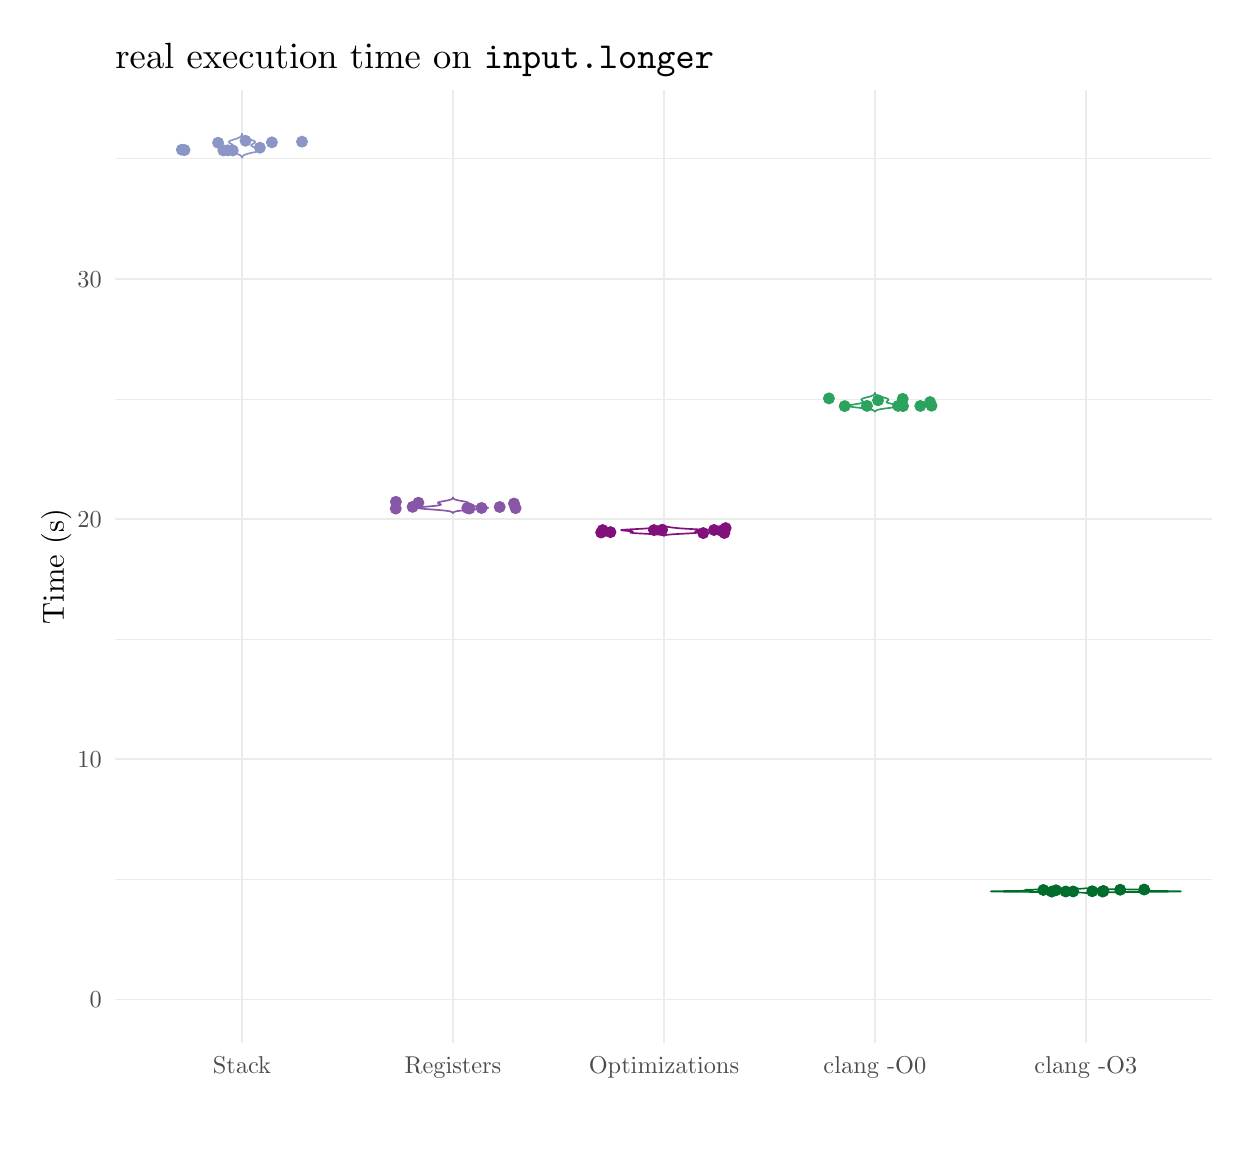
\begin{tikzpicture}[x=1pt,y=1pt]
\definecolor{fillColor}{RGB}{255,255,255}
\path[use as bounding box,fill=fillColor,fill opacity=0.00] (0,0) rectangle (433.62,397.48);
\begin{scope}
\path[clip] ( 31.71, 30.69) rectangle (428.12,374.83);
\definecolor{drawColor}{gray}{0.92}

\path[draw=drawColor,line width= 0.3pt,line join=round] ( 31.71, 89.72) --
	(428.12, 89.72);

\path[draw=drawColor,line width= 0.3pt,line join=round] ( 31.71,176.51) --
	(428.12,176.51);

\path[draw=drawColor,line width= 0.3pt,line join=round] ( 31.71,263.29) --
	(428.12,263.29);

\path[draw=drawColor,line width= 0.3pt,line join=round] ( 31.71,350.07) --
	(428.12,350.07);

\path[draw=drawColor,line width= 0.6pt,line join=round] ( 31.71, 46.33) --
	(428.12, 46.33);

\path[draw=drawColor,line width= 0.6pt,line join=round] ( 31.71,133.11) --
	(428.12,133.11);

\path[draw=drawColor,line width= 0.6pt,line join=round] ( 31.71,219.90) --
	(428.12,219.90);

\path[draw=drawColor,line width= 0.6pt,line join=round] ( 31.71,306.68) --
	(428.12,306.68);

\path[draw=drawColor,line width= 0.6pt,line join=round] ( 77.45, 30.69) --
	( 77.45,374.83);

\path[draw=drawColor,line width= 0.6pt,line join=round] (153.68, 30.69) --
	(153.68,374.83);

\path[draw=drawColor,line width= 0.6pt,line join=round] (229.92, 30.69) --
	(229.92,374.83);

\path[draw=drawColor,line width= 0.6pt,line join=round] (306.15, 30.69) --
	(306.15,374.83);

\path[draw=drawColor,line width= 0.6pt,line join=round] (382.38, 30.69) --
	(382.38,374.83);
\definecolor{drawColor}{RGB}{140,150,198}
\definecolor{fillColor}{RGB}{255,255,255}

\path[draw=drawColor,line width= 0.6pt,line join=round,line cap=round,fill=fillColor] ( 77.40,350.54) --
	( 77.40,350.55) --
	( 77.39,350.57) --
	( 77.39,350.59) --
	( 77.38,350.60) --
	( 77.38,350.62) --
	( 77.38,350.64) --
	( 77.37,350.65) --
	( 77.37,350.67) --
	( 77.36,350.69) --
	( 77.36,350.70) --
	( 77.35,350.72) --
	( 77.35,350.74) --
	( 77.34,350.76) --
	( 77.33,350.77) --
	( 77.33,350.79) --
	( 77.32,350.81) --
	( 77.31,350.82) --
	( 77.30,350.84) --
	( 77.30,350.86) --
	( 77.29,350.87) --
	( 77.28,350.89) --
	( 77.27,350.91) --
	( 77.26,350.92) --
	( 77.25,350.94) --
	( 77.24,350.96) --
	( 77.23,350.98) --
	( 77.22,350.99) --
	( 77.20,351.01) --
	( 77.19,351.03) --
	( 77.18,351.04) --
	( 77.16,351.06) --
	( 77.15,351.08) --
	( 77.14,351.09) --
	( 77.12,351.11) --
	( 77.10,351.13) --
	( 77.09,351.14) --
	( 77.07,351.16) --
	( 77.05,351.18) --
	( 77.03,351.20) --
	( 77.01,351.21) --
	( 76.99,351.23) --
	( 76.97,351.25) --
	( 76.95,351.26) --
	( 76.93,351.28) --
	( 76.91,351.30) --
	( 76.88,351.31) --
	( 76.86,351.33) --
	( 76.83,351.35) --
	( 76.80,351.36) --
	( 76.78,351.38) --
	( 76.75,351.40) --
	( 76.72,351.42) --
	( 76.69,351.43) --
	( 76.66,351.45) --
	( 76.63,351.47) --
	( 76.59,351.48) --
	( 76.56,351.50) --
	( 76.52,351.52) --
	( 76.49,351.53) --
	( 76.45,351.55) --
	( 76.41,351.57) --
	( 76.37,351.58) --
	( 76.33,351.60) --
	( 76.29,351.62) --
	( 76.25,351.64) --
	( 76.21,351.65) --
	( 76.16,351.67) --
	( 76.12,351.69) --
	( 76.07,351.70) --
	( 76.02,351.72) --
	( 75.97,351.74) --
	( 75.92,351.75) --
	( 75.87,351.77) --
	( 75.82,351.79) --
	( 75.76,351.80) --
	( 75.71,351.82) --
	( 75.65,351.84) --
	( 75.60,351.86) --
	( 75.54,351.87) --
	( 75.48,351.89) --
	( 75.42,351.91) --
	( 75.36,351.92) --
	( 75.30,351.94) --
	( 75.24,351.96) --
	( 75.17,351.97) --
	( 75.11,351.99) --
	( 75.04,352.01) --
	( 74.97,352.02) --
	( 74.91,352.04) --
	( 74.84,352.06) --
	( 74.77,352.08) --
	( 74.70,352.09) --
	( 74.63,352.11) --
	( 74.55,352.13) --
	( 74.48,352.14) --
	( 74.41,352.16) --
	( 74.34,352.18) --
	( 74.26,352.19) --
	( 74.19,352.21) --
	( 74.11,352.23) --
	( 74.03,352.24) --
	( 73.96,352.26) --
	( 73.88,352.28) --
	( 73.80,352.30) --
	( 73.73,352.31) --
	( 73.65,352.33) --
	( 73.57,352.35) --
	( 73.49,352.36) --
	( 73.41,352.38) --
	( 73.34,352.40) --
	( 73.26,352.41) --
	( 73.18,352.43) --
	( 73.10,352.45) --
	( 73.02,352.46) --
	( 72.95,352.48) --
	( 72.87,352.50) --
	( 72.79,352.52) --
	( 72.72,352.53) --
	( 72.64,352.55) --
	( 72.56,352.57) --
	( 72.49,352.58) --
	( 72.41,352.60) --
	( 72.34,352.62) --
	( 72.27,352.63) --
	( 72.20,352.65) --
	( 72.13,352.67) --
	( 72.06,352.68) --
	( 71.99,352.70) --
	( 71.92,352.72) --
	( 71.85,352.74) --
	( 71.79,352.75) --
	( 71.72,352.77) --
	( 71.66,352.79) --
	( 71.60,352.80) --
	( 71.54,352.82) --
	( 71.48,352.84) --
	( 71.42,352.85) --
	( 71.37,352.87) --
	( 71.31,352.89) --
	( 71.26,352.90) --
	( 71.21,352.92) --
	( 71.16,352.94) --
	( 71.12,352.96) --
	( 71.07,352.97) --
	( 71.03,352.99) --
	( 70.99,353.01) --
	( 70.95,353.02) --
	( 70.91,353.04) --
	( 70.88,353.06) --
	( 70.85,353.07) --
	( 70.81,353.09) --
	( 70.79,353.11) --
	( 70.76,353.12) --
	( 70.74,353.14) --
	( 70.71,353.16) --
	( 70.69,353.18) --
	( 70.68,353.19) --
	( 70.66,353.21) --
	( 70.65,353.23) --
	( 70.64,353.24) --
	( 70.63,353.26) --
	( 70.62,353.28) --
	( 70.62,353.29) --
	( 70.62,353.31) --
	( 70.62,353.33) --
	( 70.62,353.35) --
	( 70.62,353.36) --
	( 70.63,353.38) --
	( 70.64,353.40) --
	( 70.65,353.41) --
	( 70.66,353.43) --
	( 70.68,353.45) --
	( 70.70,353.46) --
	( 70.72,353.48) --
	( 70.74,353.50) --
	( 70.76,353.51) --
	( 70.79,353.53) --
	( 70.81,353.55) --
	( 70.84,353.57) --
	( 70.87,353.58) --
	( 70.91,353.60) --
	( 70.94,353.62) --
	( 70.98,353.63) --
	( 71.01,353.65) --
	( 71.05,353.67) --
	( 71.09,353.68) --
	( 71.14,353.70) --
	( 71.18,353.72) --
	( 71.23,353.73) --
	( 71.27,353.75) --
	( 71.32,353.77) --
	( 71.37,353.79) --
	( 71.42,353.80) --
	( 71.47,353.82) --
	( 71.52,353.84) --
	( 71.57,353.85) --
	( 71.63,353.87) --
	( 71.68,353.89) --
	( 71.74,353.90) --
	( 71.79,353.92) --
	( 71.85,353.94) --
	( 71.90,353.95) --
	( 71.96,353.97) --
	( 72.02,353.99) --
	( 72.08,354.01) --
	( 72.13,354.02) --
	( 72.19,354.04) --
	( 72.25,354.06) --
	( 72.31,354.07) --
	( 72.37,354.09) --
	( 72.43,354.11) --
	( 72.49,354.12) --
	( 72.54,354.14) --
	( 72.60,354.16) --
	( 72.66,354.17) --
	( 72.72,354.19) --
	( 72.77,354.21) --
	( 72.83,354.23) --
	( 72.88,354.24) --
	( 72.94,354.26) --
	( 72.99,354.28) --
	( 73.05,354.29) --
	( 73.10,354.31) --
	( 73.15,354.33) --
	( 73.20,354.34) --
	( 73.25,354.36) --
	( 73.30,354.38) --
	( 73.35,354.39) --
	( 73.39,354.41) --
	( 73.44,354.43) --
	( 73.48,354.45) --
	( 73.53,354.46) --
	( 73.57,354.48) --
	( 73.61,354.50) --
	( 73.65,354.51) --
	( 73.69,354.53) --
	( 73.72,354.55) --
	( 73.76,354.56) --
	( 73.79,354.58) --
	( 73.82,354.60) --
	( 73.86,354.61) --
	( 73.89,354.63) --
	( 73.91,354.65) --
	( 73.94,354.67) --
	( 73.96,354.68) --
	( 73.99,354.70) --
	( 74.01,354.72) --
	( 74.03,354.73) --
	( 74.05,354.75) --
	( 74.06,354.77) --
	( 74.08,354.78) --
	( 74.09,354.80) --
	( 74.10,354.82) --
	( 74.11,354.83) --
	( 74.12,354.85) --
	( 74.13,354.87) --
	( 74.14,354.89) --
	( 74.14,354.90) --
	( 74.14,354.92) --
	( 74.14,354.94) --
	( 74.14,354.95) --
	( 74.14,354.97) --
	( 74.14,354.99) --
	( 74.13,355.00) --
	( 74.13,355.02) --
	( 74.12,355.04) --
	( 74.11,355.05) --
	( 74.10,355.07) --
	( 74.09,355.09) --
	( 74.07,355.11) --
	( 74.06,355.12) --
	( 74.04,355.14) --
	( 74.03,355.16) --
	( 74.01,355.17) --
	( 73.99,355.19) --
	( 73.97,355.21) --
	( 73.95,355.22) --
	( 73.93,355.24) --
	( 73.91,355.26) --
	( 73.88,355.27) --
	( 73.86,355.29) --
	( 73.83,355.31) --
	( 73.81,355.33) --
	( 73.78,355.34) --
	( 73.75,355.36) --
	( 73.72,355.38) --
	( 73.70,355.39) --
	( 73.67,355.41) --
	( 73.64,355.43) --
	( 73.61,355.44) --
	( 73.58,355.46) --
	( 73.55,355.48) --
	( 73.52,355.49) --
	( 73.49,355.51) --
	( 73.46,355.53) --
	( 73.42,355.55) --
	( 73.39,355.56) --
	( 73.36,355.58) --
	( 73.33,355.60) --
	( 73.30,355.61) --
	( 73.27,355.63) --
	( 73.24,355.65) --
	( 73.21,355.66) --
	( 73.18,355.68) --
	( 73.16,355.70) --
	( 73.13,355.71) --
	( 73.10,355.73) --
	( 73.07,355.75) --
	( 73.05,355.77) --
	( 73.02,355.78) --
	( 73.00,355.80) --
	( 72.97,355.82) --
	( 72.95,355.83) --
	( 72.93,355.85) --
	( 72.91,355.87) --
	( 72.89,355.88) --
	( 72.87,355.90) --
	( 72.85,355.92) --
	( 72.83,355.93) --
	( 72.81,355.95) --
	( 72.80,355.97) --
	( 72.79,355.99) --
	( 72.77,356.00) --
	( 72.76,356.02) --
	( 72.75,356.04) --
	( 72.74,356.05) --
	( 72.74,356.07) --
	( 72.73,356.09) --
	( 72.73,356.10) --
	( 72.72,356.12) --
	( 72.72,356.14) --
	( 72.72,356.15) --
	( 72.72,356.17) --
	( 72.72,356.19) --
	( 72.73,356.21) --
	( 72.73,356.22) --
	( 72.74,356.24) --
	( 72.75,356.26) --
	( 72.76,356.27) --
	( 72.77,356.29) --
	( 72.78,356.31) --
	( 72.79,356.32) --
	( 72.81,356.34) --
	( 72.83,356.36) --
	( 72.84,356.38) --
	( 72.86,356.39) --
	( 72.89,356.41) --
	( 72.91,356.43) --
	( 72.93,356.44) --
	( 72.96,356.46) --
	( 72.98,356.48) --
	( 73.01,356.49) --
	( 73.04,356.51) --
	( 73.07,356.53) --
	( 73.10,356.54) --
	( 73.14,356.56) --
	( 73.17,356.58) --
	( 73.21,356.60) --
	( 73.24,356.61) --
	( 73.28,356.63) --
	( 73.32,356.65) --
	( 73.36,356.66) --
	( 73.40,356.68) --
	( 73.44,356.70) --
	( 73.48,356.71) --
	( 73.52,356.73) --
	( 73.57,356.75) --
	( 73.61,356.76) --
	( 73.66,356.78) --
	( 73.71,356.80) --
	( 73.75,356.82) --
	( 73.80,356.83) --
	( 73.85,356.85) --
	( 73.90,356.87) --
	( 73.95,356.88) --
	( 74.00,356.90) --
	( 74.05,356.92) --
	( 74.10,356.93) --
	( 74.15,356.95) --
	( 74.20,356.97) --
	( 74.25,356.98) --
	( 74.31,357.00) --
	( 74.36,357.02) --
	( 74.41,357.04) --
	( 74.46,357.05) --
	( 74.52,357.07) --
	( 74.57,357.09) --
	( 74.62,357.10) --
	( 74.67,357.12) --
	( 74.73,357.14) --
	( 74.78,357.15) --
	( 74.83,357.17) --
	( 74.89,357.19) --
	( 74.94,357.20) --
	( 74.99,357.22) --
	( 75.04,357.24) --
	( 75.09,357.26) --
	( 75.14,357.27) --
	( 75.20,357.29) --
	( 75.25,357.31) --
	( 75.30,357.32) --
	( 75.35,357.34) --
	( 75.40,357.36) --
	( 75.44,357.37) --
	( 75.49,357.39) --
	( 75.54,357.41) --
	( 75.59,357.42) --
	( 75.63,357.44) --
	( 75.68,357.46) --
	( 75.73,357.48) --
	( 75.77,357.49) --
	( 75.82,357.51) --
	( 75.86,357.53) --
	( 75.90,357.54) --
	( 75.95,357.56) --
	( 75.99,357.58) --
	( 76.03,357.59) --
	( 76.07,357.61) --
	( 76.11,357.63) --
	( 76.15,357.64) --
	( 76.19,357.66) --
	( 76.22,357.68) --
	( 76.26,357.70) --
	( 76.30,357.71) --
	( 76.33,357.73) --
	( 76.37,357.75) --
	( 76.40,357.76) --
	( 76.44,357.78) --
	( 76.47,357.80) --
	( 76.50,357.81) --
	( 76.53,357.83) --
	( 76.56,357.85) --
	( 76.59,357.86) --
	( 76.62,357.88) --
	( 76.65,357.90) --
	( 76.68,357.92) --
	( 76.71,357.93) --
	( 76.73,357.95) --
	( 76.76,357.97) --
	( 76.78,357.98) --
	( 76.81,358.00) --
	( 76.83,358.02) --
	( 76.85,358.03) --
	( 76.88,358.05) --
	( 76.90,358.07) --
	( 76.92,358.08) --
	( 76.94,358.10) --
	( 76.96,358.12) --
	( 76.98,358.14) --
	( 77.00,358.15) --
	( 77.01,358.17) --
	( 77.03,358.19) --
	( 77.05,358.20) --
	( 77.07,358.22) --
	( 77.08,358.24) --
	( 77.10,358.25) --
	( 77.11,358.27) --
	( 77.13,358.29) --
	( 77.14,358.30) --
	( 77.15,358.32) --
	( 77.17,358.34) --
	( 77.18,358.36) --
	( 77.19,358.37) --
	( 77.20,358.39) --
	( 77.21,358.41) --
	( 77.22,358.42) --
	( 77.23,358.44) --
	( 77.24,358.46) --
	( 77.25,358.47) --
	( 77.26,358.49) --
	( 77.27,358.51) --
	( 77.28,358.52) --
	( 77.29,358.54) --
	( 77.30,358.56) --
	( 77.30,358.58) --
	( 77.31,358.59) --
	( 77.32,358.61) --
	( 77.32,358.63) --
	( 77.33,358.64) --
	( 77.34,358.66) --
	( 77.34,358.68) --
	( 77.35,358.69) --
	( 77.35,358.71) --
	( 77.36,358.73) --
	( 77.36,358.74) --
	( 77.37,358.76) --
	( 77.37,358.78) --
	( 77.38,358.80) --
	( 77.38,358.81) --
	( 77.38,358.83) --
	( 77.39,358.85) --
	( 77.39,358.86) --
	( 77.39,358.88) --
	( 77.40,358.90) --
	( 77.40,358.91) --
	( 77.40,358.93) --
	( 77.41,358.95) --
	( 77.41,358.96) --
	( 77.41,358.98) --
	( 77.41,359.00) --
	( 77.41,359.02) --
	( 77.42,359.03) --
	( 77.42,359.05) --
	( 77.42,359.07) --
	( 77.42,359.08) --
	( 77.42,359.10) --
	( 77.43,359.12) --
	( 77.43,359.13) --
	( 77.43,359.15) --
	( 77.43,359.17) --
	( 77.43,359.18) --
	( 77.47,359.18) --
	( 77.47,359.17) --
	( 77.47,359.15) --
	( 77.48,359.13) --
	( 77.48,359.12) --
	( 77.48,359.10) --
	( 77.48,359.08) --
	( 77.48,359.07) --
	( 77.48,359.05) --
	( 77.49,359.03) --
	( 77.49,359.02) --
	( 77.49,359.00) --
	( 77.49,358.98) --
	( 77.50,358.96) --
	( 77.50,358.95) --
	( 77.50,358.93) --
	( 77.50,358.91) --
	( 77.51,358.90) --
	( 77.51,358.88) --
	( 77.51,358.86) --
	( 77.52,358.85) --
	( 77.52,358.83) --
	( 77.52,358.81) --
	( 77.53,358.80) --
	( 77.53,358.78) --
	( 77.54,358.76) --
	( 77.54,358.74) --
	( 77.55,358.73) --
	( 77.55,358.71) --
	( 77.56,358.69) --
	( 77.56,358.68) --
	( 77.57,358.66) --
	( 77.57,358.64) --
	( 77.58,358.63) --
	( 77.59,358.61) --
	( 77.59,358.59) --
	( 77.60,358.58) --
	( 77.61,358.56) --
	( 77.62,358.54) --
	( 77.62,358.52) --
	( 77.63,358.51) --
	( 77.64,358.49) --
	( 77.65,358.47) --
	( 77.66,358.46) --
	( 77.67,358.44) --
	( 77.68,358.42) --
	( 77.69,358.41) --
	( 77.70,358.39) --
	( 77.71,358.37) --
	( 77.73,358.36) --
	( 77.74,358.34) --
	( 77.75,358.32) --
	( 77.76,358.30) --
	( 77.78,358.29) --
	( 77.79,358.27) --
	( 77.81,358.25) --
	( 77.82,358.24) --
	( 77.84,358.22) --
	( 77.85,358.20) --
	( 77.87,358.19) --
	( 77.89,358.17) --
	( 77.91,358.15) --
	( 77.93,358.14) --
	( 77.94,358.12) --
	( 77.96,358.10) --
	( 77.98,358.08) --
	( 78.01,358.07) --
	( 78.03,358.05) --
	( 78.05,358.03) --
	( 78.07,358.02) --
	( 78.10,358.00) --
	( 78.12,357.98) --
	( 78.15,357.97) --
	( 78.17,357.95) --
	( 78.20,357.93) --
	( 78.22,357.92) --
	( 78.25,357.90) --
	( 78.28,357.88) --
	( 78.31,357.86) --
	( 78.34,357.85) --
	( 78.37,357.83) --
	( 78.40,357.81) --
	( 78.43,357.80) --
	( 78.47,357.78) --
	( 78.50,357.76) --
	( 78.53,357.75) --
	( 78.57,357.73) --
	( 78.61,357.71) --
	( 78.64,357.70) --
	( 78.68,357.68) --
	( 78.72,357.66) --
	( 78.75,357.64) --
	( 78.79,357.63) --
	( 78.83,357.61) --
	( 78.87,357.59) --
	( 78.92,357.58) --
	( 78.96,357.56) --
	( 79.00,357.54) --
	( 79.04,357.53) --
	( 79.09,357.51) --
	( 79.13,357.49) --
	( 79.18,357.48) --
	( 79.22,357.46) --
	( 79.27,357.44) --
	( 79.32,357.42) --
	( 79.36,357.41) --
	( 79.41,357.39) --
	( 79.46,357.37) --
	( 79.51,357.36) --
	( 79.56,357.34) --
	( 79.61,357.32) --
	( 79.66,357.31) --
	( 79.71,357.29) --
	( 79.76,357.27) --
	( 79.81,357.26) --
	( 79.86,357.24) --
	( 79.91,357.22) --
	( 79.97,357.20) --
	( 80.02,357.19) --
	( 80.07,357.17) --
	( 80.12,357.15) --
	( 80.18,357.14) --
	( 80.23,357.12) --
	( 80.28,357.10) --
	( 80.33,357.09) --
	( 80.39,357.07) --
	( 80.44,357.05) --
	( 80.49,357.04) --
	( 80.54,357.02) --
	( 80.60,357.00) --
	( 80.65,356.98) --
	( 80.70,356.97) --
	( 80.75,356.95) --
	( 80.80,356.93) --
	( 80.86,356.92) --
	( 80.91,356.90) --
	( 80.96,356.88) --
	( 81.01,356.87) --
	( 81.05,356.85) --
	( 81.10,356.83) --
	( 81.15,356.82) --
	( 81.20,356.80) --
	( 81.24,356.78) --
	( 81.29,356.76) --
	( 81.33,356.75) --
	( 81.38,356.73) --
	( 81.42,356.71) --
	( 81.46,356.70) --
	( 81.51,356.68) --
	( 81.55,356.66) --
	( 81.59,356.65) --
	( 81.62,356.63) --
	( 81.66,356.61) --
	( 81.70,356.60) --
	( 81.73,356.58) --
	( 81.77,356.56) --
	( 81.80,356.54) --
	( 81.83,356.53) --
	( 81.86,356.51) --
	( 81.89,356.49) --
	( 81.92,356.48) --
	( 81.95,356.46) --
	( 81.97,356.44) --
	( 82.00,356.43) --
	( 82.02,356.41) --
	( 82.04,356.39) --
	( 82.06,356.38) --
	( 82.08,356.36) --
	( 82.09,356.34) --
	( 82.11,356.32) --
	( 82.12,356.31) --
	( 82.14,356.29) --
	( 82.15,356.27) --
	( 82.16,356.26) --
	( 82.17,356.24) --
	( 82.17,356.22) --
	( 82.18,356.21) --
	( 82.18,356.19) --
	( 82.18,356.17) --
	( 82.18,356.15) --
	( 82.18,356.14) --
	( 82.18,356.12) --
	( 82.18,356.10) --
	( 82.17,356.09) --
	( 82.17,356.07) --
	( 82.16,356.05) --
	( 82.15,356.04) --
	( 82.14,356.02) --
	( 82.13,356.00) --
	( 82.12,355.99) --
	( 82.10,355.97) --
	( 82.09,355.95) --
	( 82.07,355.93) --
	( 82.06,355.92) --
	( 82.04,355.90) --
	( 82.02,355.88) --
	( 82.00,355.87) --
	( 81.98,355.85) --
	( 81.95,355.83) --
	( 81.93,355.82) --
	( 81.91,355.80) --
	( 81.88,355.78) --
	( 81.86,355.77) --
	( 81.83,355.75) --
	( 81.80,355.73) --
	( 81.78,355.71) --
	( 81.75,355.70) --
	( 81.72,355.68) --
	( 81.69,355.66) --
	( 81.66,355.65) --
	( 81.63,355.63) --
	( 81.60,355.61) --
	( 81.57,355.60) --
	( 81.54,355.58) --
	( 81.51,355.56) --
	( 81.48,355.55) --
	( 81.45,355.53) --
	( 81.42,355.51) --
	( 81.39,355.49) --
	( 81.36,355.48) --
	( 81.33,355.46) --
	( 81.30,355.44) --
	( 81.27,355.43) --
	( 81.24,355.41) --
	( 81.21,355.39) --
	( 81.18,355.38) --
	( 81.15,355.36) --
	( 81.12,355.34) --
	( 81.10,355.33) --
	( 81.07,355.31) --
	( 81.05,355.29) --
	( 81.02,355.27) --
	( 81.00,355.26) --
	( 80.97,355.24) --
	( 80.95,355.22) --
	( 80.93,355.21) --
	( 80.91,355.19) --
	( 80.89,355.17) --
	( 80.87,355.16) --
	( 80.86,355.14) --
	( 80.84,355.12) --
	( 80.83,355.11) --
	( 80.82,355.09) --
	( 80.80,355.07) --
	( 80.79,355.05) --
	( 80.78,355.04) --
	( 80.78,355.02) --
	( 80.77,355.00) --
	( 80.77,354.99) --
	( 80.76,354.97) --
	( 80.76,354.95) --
	( 80.76,354.94) --
	( 80.76,354.92) --
	( 80.76,354.90) --
	( 80.77,354.89) --
	( 80.77,354.87) --
	( 80.78,354.85) --
	( 80.79,354.83) --
	( 80.80,354.82) --
	( 80.81,354.80) --
	( 80.82,354.78) --
	( 80.84,354.77) --
	( 80.86,354.75) --
	( 80.87,354.73) --
	( 80.89,354.72) --
	( 80.92,354.70) --
	( 80.94,354.68) --
	( 80.96,354.67) --
	( 80.99,354.65) --
	( 81.02,354.63) --
	( 81.05,354.61) --
	( 81.08,354.60) --
	( 81.11,354.58) --
	( 81.14,354.56) --
	( 81.18,354.55) --
	( 81.22,354.53) --
	( 81.25,354.51) --
	( 81.29,354.50) --
	( 81.33,354.48) --
	( 81.38,354.46) --
	( 81.42,354.45) --
	( 81.46,354.43) --
	( 81.51,354.41) --
	( 81.56,354.39) --
	( 81.60,354.38) --
	( 81.65,354.36) --
	( 81.70,354.34) --
	( 81.75,354.33) --
	( 81.81,354.31) --
	( 81.86,354.29) --
	( 81.91,354.28) --
	( 81.97,354.26) --
	( 82.02,354.24) --
	( 82.08,354.23) --
	( 82.13,354.21) --
	( 82.19,354.19) --
	( 82.24,354.17) --
	( 82.30,354.16) --
	( 82.36,354.14) --
	( 82.42,354.12) --
	( 82.48,354.11) --
	( 82.53,354.09) --
	( 82.59,354.07) --
	( 82.65,354.06) --
	( 82.71,354.04) --
	( 82.77,354.02) --
	( 82.83,354.01) --
	( 82.88,353.99) --
	( 82.94,353.97) --
	( 83.00,353.95) --
	( 83.06,353.94) --
	( 83.11,353.92) --
	( 83.17,353.90) --
	( 83.22,353.89) --
	( 83.28,353.87) --
	( 83.33,353.85) --
	( 83.38,353.84) --
	( 83.43,353.82) --
	( 83.49,353.80) --
	( 83.54,353.79) --
	( 83.58,353.77) --
	( 83.63,353.75) --
	( 83.68,353.73) --
	( 83.72,353.72) --
	( 83.77,353.70) --
	( 83.81,353.68) --
	( 83.85,353.67) --
	( 83.89,353.65) --
	( 83.93,353.63) --
	( 83.96,353.62) --
	( 84.00,353.60) --
	( 84.03,353.58) --
	( 84.06,353.57) --
	( 84.09,353.55) --
	( 84.12,353.53) --
	( 84.14,353.51) --
	( 84.17,353.50) --
	( 84.19,353.48) --
	( 84.21,353.46) --
	( 84.22,353.45) --
	( 84.24,353.43) --
	( 84.25,353.41) --
	( 84.26,353.40) --
	( 84.27,353.38) --
	( 84.28,353.36) --
	( 84.28,353.35) --
	( 84.29,353.33) --
	( 84.29,353.31) --
	( 84.29,353.29) --
	( 84.28,353.28) --
	( 84.28,353.26) --
	( 84.27,353.24) --
	( 84.26,353.23) --
	( 84.24,353.21) --
	( 84.23,353.19) --
	( 84.21,353.18) --
	( 84.19,353.16) --
	( 84.17,353.14) --
	( 84.14,353.12) --
	( 84.12,353.11) --
	( 84.09,353.09) --
	( 84.06,353.07) --
	( 84.03,353.06) --
	( 83.99,353.04) --
	( 83.95,353.02) --
	( 83.91,353.01) --
	( 83.87,352.99) --
	( 83.83,352.97) --
	( 83.79,352.96) --
	( 83.74,352.94) --
	( 83.69,352.92) --
	( 83.64,352.90) --
	( 83.59,352.89) --
	( 83.54,352.87) --
	( 83.48,352.85) --
	( 83.42,352.84) --
	( 83.36,352.82) --
	( 83.30,352.80) --
	( 83.24,352.79) --
	( 83.18,352.77) --
	( 83.12,352.75) --
	( 83.05,352.74) --
	( 82.98,352.72) --
	( 82.92,352.70) --
	( 82.85,352.68) --
	( 82.78,352.67) --
	( 82.71,352.65) --
	( 82.63,352.63) --
	( 82.56,352.62) --
	( 82.49,352.60) --
	( 82.41,352.58) --
	( 82.34,352.57) --
	( 82.26,352.55) --
	( 82.19,352.53) --
	( 82.11,352.52) --
	( 82.03,352.50) --
	( 81.96,352.48) --
	( 81.88,352.46) --
	( 81.80,352.45) --
	( 81.72,352.43) --
	( 81.65,352.41) --
	( 81.57,352.40) --
	( 81.49,352.38) --
	( 81.41,352.36) --
	( 81.33,352.35) --
	( 81.25,352.33) --
	( 81.18,352.31) --
	( 81.10,352.30) --
	( 81.02,352.28) --
	( 80.95,352.26) --
	( 80.87,352.24) --
	( 80.79,352.23) --
	( 80.72,352.21) --
	( 80.64,352.19) --
	( 80.57,352.18) --
	( 80.49,352.16) --
	( 80.42,352.14) --
	( 80.35,352.13) --
	( 80.28,352.11) --
	( 80.21,352.09) --
	( 80.14,352.08) --
	( 80.07,352.06) --
	( 80.00,352.04) --
	( 79.93,352.02) --
	( 79.86,352.01) --
	( 79.80,351.99) --
	( 79.73,351.97) --
	( 79.67,351.96) --
	( 79.61,351.94) --
	( 79.54,351.92) --
	( 79.48,351.91) --
	( 79.42,351.89) --
	( 79.36,351.87) --
	( 79.31,351.86) --
	( 79.25,351.84) --
	( 79.19,351.82) --
	( 79.14,351.80) --
	( 79.09,351.79) --
	( 79.03,351.77) --
	( 78.98,351.75) --
	( 78.93,351.74) --
	( 78.88,351.72) --
	( 78.84,351.70) --
	( 78.79,351.69) --
	( 78.74,351.67) --
	( 78.70,351.65) --
	( 78.65,351.64) --
	( 78.61,351.62) --
	( 78.57,351.60) --
	( 78.53,351.58) --
	( 78.49,351.57) --
	( 78.45,351.55) --
	( 78.42,351.53) --
	( 78.38,351.52) --
	( 78.34,351.50) --
	( 78.31,351.48) --
	( 78.28,351.47) --
	( 78.25,351.45) --
	( 78.21,351.43) --
	( 78.18,351.42) --
	( 78.15,351.40) --
	( 78.13,351.38) --
	( 78.10,351.36) --
	( 78.07,351.35) --
	( 78.05,351.33) --
	( 78.02,351.31) --
	( 78.00,351.30) --
	( 77.97,351.28) --
	( 77.95,351.26) --
	( 77.93,351.25) --
	( 77.91,351.23) --
	( 77.89,351.21) --
	( 77.87,351.20) --
	( 77.85,351.18) --
	( 77.83,351.16) --
	( 77.82,351.14) --
	( 77.80,351.13) --
	( 77.78,351.11) --
	( 77.77,351.09) --
	( 77.75,351.08) --
	( 77.74,351.06) --
	( 77.72,351.04) --
	( 77.71,351.03) --
	( 77.70,351.01) --
	( 77.69,350.99) --
	( 77.68,350.98) --
	( 77.66,350.96) --
	( 77.65,350.94) --
	( 77.64,350.92) --
	( 77.63,350.91) --
	( 77.62,350.89) --
	( 77.62,350.87) --
	( 77.61,350.86) --
	( 77.60,350.84) --
	( 77.59,350.82) --
	( 77.58,350.81) --
	( 77.58,350.79) --
	( 77.57,350.77) --
	( 77.56,350.76) --
	( 77.56,350.74) --
	( 77.55,350.72) --
	( 77.55,350.70) --
	( 77.54,350.69) --
	( 77.54,350.67) --
	( 77.53,350.65) --
	( 77.53,350.64) --
	( 77.52,350.62) --
	( 77.52,350.60) --
	( 77.51,350.59) --
	( 77.51,350.57) --
	( 77.51,350.55) --
	( 77.50,350.54) --
	( 77.40,350.54) --
	cycle;
\definecolor{drawColor}{RGB}{136,86,167}

\path[draw=drawColor,line width= 0.6pt,line join=round,line cap=round,fill=fillColor] (153.62,222.11) --
	(153.62,222.12) --
	(153.61,222.13) --
	(153.61,222.14) --
	(153.60,222.15) --
	(153.60,222.16) --
	(153.59,222.17) --
	(153.59,222.18) --
	(153.58,222.19) --
	(153.57,222.21) --
	(153.57,222.22) --
	(153.56,222.23) --
	(153.55,222.24) --
	(153.54,222.25) --
	(153.53,222.26) --
	(153.52,222.27) --
	(153.52,222.28) --
	(153.51,222.29) --
	(153.49,222.30) --
	(153.48,222.32) --
	(153.47,222.33) --
	(153.46,222.34) --
	(153.45,222.35) --
	(153.43,222.36) --
	(153.42,222.37) --
	(153.40,222.38) --
	(153.39,222.39) --
	(153.37,222.40) --
	(153.35,222.41) --
	(153.34,222.43) --
	(153.32,222.44) --
	(153.30,222.45) --
	(153.28,222.46) --
	(153.26,222.47) --
	(153.23,222.48) --
	(153.21,222.49) --
	(153.18,222.50) --
	(153.16,222.51) --
	(153.13,222.52) --
	(153.10,222.53) --
	(153.08,222.55) --
	(153.05,222.56) --
	(153.01,222.57) --
	(152.98,222.58) --
	(152.95,222.59) --
	(152.91,222.60) --
	(152.88,222.61) --
	(152.84,222.62) --
	(152.80,222.63) --
	(152.76,222.64) --
	(152.72,222.66) --
	(152.67,222.67) --
	(152.63,222.68) --
	(152.58,222.69) --
	(152.53,222.70) --
	(152.48,222.71) --
	(152.43,222.72) --
	(152.37,222.73) --
	(152.32,222.74) --
	(152.26,222.75) --
	(152.20,222.77) --
	(152.14,222.78) --
	(152.08,222.79) --
	(152.01,222.80) --
	(151.95,222.81) --
	(151.88,222.82) --
	(151.81,222.83) --
	(151.73,222.84) --
	(151.66,222.85) --
	(151.58,222.86) --
	(151.50,222.88) --
	(151.42,222.89) --
	(151.34,222.90) --
	(151.25,222.91) --
	(151.17,222.92) --
	(151.08,222.93) --
	(150.99,222.94) --
	(150.89,222.95) --
	(150.80,222.96) --
	(150.70,222.97) --
	(150.60,222.99) --
	(150.50,223.00) --
	(150.39,223.01) --
	(150.29,223.02) --
	(150.18,223.03) --
	(150.07,223.04) --
	(149.96,223.05) --
	(149.84,223.06) --
	(149.73,223.07) --
	(149.61,223.08) --
	(149.49,223.10) --
	(149.37,223.11) --
	(149.24,223.12) --
	(149.12,223.13) --
	(148.99,223.14) --
	(148.86,223.15) --
	(148.73,223.16) --
	(148.60,223.17) --
	(148.47,223.18) --
	(148.33,223.19) --
	(148.20,223.21) --
	(148.06,223.22) --
	(147.92,223.23) --
	(147.78,223.24) --
	(147.64,223.25) --
	(147.50,223.26) --
	(147.35,223.27) --
	(147.21,223.28) --
	(147.07,223.29) --
	(146.92,223.30) --
	(146.77,223.31) --
	(146.63,223.33) --
	(146.48,223.34) --
	(146.33,223.35) --
	(146.19,223.36) --
	(146.04,223.37) --
	(145.89,223.38) --
	(145.75,223.39) --
	(145.60,223.40) --
	(145.45,223.41) --
	(145.31,223.42) --
	(145.16,223.44) --
	(145.02,223.45) --
	(144.87,223.46) --
	(144.73,223.47) --
	(144.59,223.48) --
	(144.45,223.49) --
	(144.31,223.50) --
	(144.17,223.51) --
	(144.03,223.52) --
	(143.90,223.53) --
	(143.77,223.55) --
	(143.64,223.56) --
	(143.51,223.57) --
	(143.38,223.58) --
	(143.26,223.59) --
	(143.13,223.60) --
	(143.01,223.61) --
	(142.90,223.62) --
	(142.78,223.63) --
	(142.67,223.64) --
	(142.56,223.66) --
	(142.46,223.67) --
	(142.36,223.68) --
	(142.26,223.69) --
	(142.16,223.70) --
	(142.07,223.71) --
	(141.98,223.72) --
	(141.89,223.73) --
	(141.81,223.74) --
	(141.73,223.75) --
	(141.66,223.77) --
	(141.59,223.78) --
	(141.52,223.79) --
	(141.46,223.80) --
	(141.40,223.81) --
	(141.35,223.82) --
	(141.30,223.83) --
	(141.25,223.84) --
	(141.21,223.85) --
	(141.17,223.86) --
	(141.14,223.88) --
	(141.11,223.89) --
	(141.08,223.90) --
	(141.06,223.91) --
	(141.05,223.92) --
	(141.04,223.93) --
	(141.03,223.94) --
	(141.03,223.95) --
	(141.03,223.96) --
	(141.03,223.97) --
	(141.04,223.99) --
	(141.06,224.00) --
	(141.08,224.01) --
	(141.10,224.02) --
	(141.13,224.03) --
	(141.16,224.04) --
	(141.20,224.05) --
	(141.24,224.06) --
	(141.28,224.07) --
	(141.33,224.08) --
	(141.38,224.09) --
	(141.43,224.11) --
	(141.49,224.12) --
	(141.56,224.13) --
	(141.62,224.14) --
	(141.69,224.15) --
	(141.77,224.16) --
	(141.84,224.17) --
	(141.92,224.18) --
	(142.01,224.19) --
	(142.09,224.20) --
	(142.18,224.22) --
	(142.27,224.23) --
	(142.37,224.24) --
	(142.46,224.25) --
	(142.57,224.26) --
	(142.67,224.27) --
	(142.77,224.28) --
	(142.88,224.29) --
	(142.99,224.30) --
	(143.10,224.31) --
	(143.21,224.33) --
	(143.32,224.34) --
	(143.44,224.35) --
	(143.56,224.36) --
	(143.68,224.37) --
	(143.80,224.38) --
	(143.92,224.39) --
	(144.04,224.40) --
	(144.16,224.41) --
	(144.28,224.42) --
	(144.41,224.44) --
	(144.53,224.45) --
	(144.65,224.46) --
	(144.78,224.47) --
	(144.90,224.48) --
	(145.03,224.49) --
	(145.15,224.50) --
	(145.28,224.51) --
	(145.40,224.52) --
	(145.52,224.53) --
	(145.65,224.55) --
	(145.77,224.56) --
	(145.89,224.57) --
	(146.01,224.58) --
	(146.13,224.59) --
	(146.24,224.60) --
	(146.36,224.61) --
	(146.48,224.62) --
	(146.59,224.63) --
	(146.70,224.64) --
	(146.81,224.66) --
	(146.92,224.67) --
	(147.03,224.68) --
	(147.13,224.69) --
	(147.23,224.70) --
	(147.34,224.71) --
	(147.43,224.72) --
	(147.53,224.73) --
	(147.63,224.74) --
	(147.72,224.75) --
	(147.81,224.77) --
	(147.90,224.78) --
	(147.98,224.79) --
	(148.06,224.80) --
	(148.14,224.81) --
	(148.22,224.82) --
	(148.30,224.83) --
	(148.37,224.84) --
	(148.44,224.85) --
	(148.51,224.86) --
	(148.57,224.88) --
	(148.63,224.89) --
	(148.69,224.90) --
	(148.75,224.91) --
	(148.80,224.92) --
	(148.85,224.93) --
	(148.90,224.94) --
	(148.95,224.95) --
	(148.99,224.96) --
	(149.03,224.97) --
	(149.07,224.98) --
	(149.10,225.00) --
	(149.13,225.01) --
	(149.16,225.02) --
	(149.19,225.03) --
	(149.22,225.04) --
	(149.24,225.05) --
	(149.26,225.06) --
	(149.28,225.07) --
	(149.29,225.08) --
	(149.30,225.09) --
	(149.31,225.11) --
	(149.32,225.12) --
	(149.33,225.13) --
	(149.33,225.14) --
	(149.33,225.15) --
	(149.33,225.16) --
	(149.33,225.17) --
	(149.32,225.18) --
	(149.32,225.19) --
	(149.31,225.20) --
	(149.30,225.22) --
	(149.29,225.23) --
	(149.28,225.24) --
	(149.26,225.25) --
	(149.25,225.26) --
	(149.23,225.27) --
	(149.21,225.28) --
	(149.19,225.29) --
	(149.17,225.30) --
	(149.15,225.31) --
	(149.12,225.33) --
	(149.10,225.34) --
	(149.08,225.35) --
	(149.05,225.36) --
	(149.02,225.37) --
	(149.00,225.38) --
	(148.97,225.39) --
	(148.94,225.40) --
	(148.92,225.41) --
	(148.89,225.42) --
	(148.86,225.44) --
	(148.83,225.45) --
	(148.80,225.46) --
	(148.77,225.47) --
	(148.75,225.48) --
	(148.72,225.49) --
	(148.69,225.50) --
	(148.66,225.51) --
	(148.63,225.52) --
	(148.61,225.53) --
	(148.58,225.55) --
	(148.56,225.56) --
	(148.53,225.57) --
	(148.51,225.58) --
	(148.48,225.59) --
	(148.46,225.60) --
	(148.44,225.61) --
	(148.42,225.62) --
	(148.40,225.63) --
	(148.38,225.64) --
	(148.36,225.66) --
	(148.34,225.67) --
	(148.33,225.68) --
	(148.31,225.69) --
	(148.30,225.70) --
	(148.29,225.71) --
	(148.28,225.72) --
	(148.27,225.73) --
	(148.26,225.74) --
	(148.25,225.75) --
	(148.25,225.76) --
	(148.25,225.78) --
	(148.24,225.79) --
	(148.24,225.80) --
	(148.25,225.81) --
	(148.25,225.82) --
	(148.25,225.83) --
	(148.26,225.84) --
	(148.27,225.85) --
	(148.28,225.86) --
	(148.29,225.87) --
	(148.30,225.89) --
	(148.31,225.90) --
	(148.33,225.91) --
	(148.35,225.92) --
	(148.37,225.93) --
	(148.39,225.94) --
	(148.41,225.95) --
	(148.43,225.96) --
	(148.46,225.97) --
	(148.49,225.98) --
	(148.51,226.00) --
	(148.54,226.01) --
	(148.58,226.02) --
	(148.61,226.03) --
	(148.64,226.04) --
	(148.68,226.05) --
	(148.72,226.06) --
	(148.76,226.07) --
	(148.79,226.08) --
	(148.84,226.09) --
	(148.88,226.11) --
	(148.92,226.12) --
	(148.97,226.13) --
	(149.01,226.14) --
	(149.06,226.15) --
	(149.11,226.16) --
	(149.16,226.17) --
	(149.21,226.18) --
	(149.26,226.19) --
	(149.31,226.20) --
	(149.36,226.22) --
	(149.42,226.23) --
	(149.47,226.24) --
	(149.53,226.25) --
	(149.58,226.26) --
	(149.64,226.27) --
	(149.70,226.28) --
	(149.75,226.29) --
	(149.81,226.30) --
	(149.87,226.31) --
	(149.93,226.33) --
	(149.99,226.34) --
	(150.05,226.35) --
	(150.11,226.36) --
	(150.17,226.37) --
	(150.23,226.38) --
	(150.29,226.39) --
	(150.35,226.40) --
	(150.41,226.41) --
	(150.47,226.42) --
	(150.53,226.44) --
	(150.59,226.45) --
	(150.66,226.46) --
	(150.72,226.47) --
	(150.78,226.48) --
	(150.84,226.49) --
	(150.90,226.50) --
	(150.96,226.51) --
	(151.02,226.52) --
	(151.07,226.53) --
	(151.13,226.54) --
	(151.19,226.56) --
	(151.25,226.57) --
	(151.31,226.58) --
	(151.36,226.59) --
	(151.42,226.60) --
	(151.47,226.61) --
	(151.53,226.62) --
	(151.58,226.63) --
	(151.64,226.64) --
	(151.69,226.65) --
	(151.74,226.67) --
	(151.79,226.68) --
	(151.84,226.69) --
	(151.90,226.70) --
	(151.94,226.71) --
	(151.99,226.72) --
	(152.04,226.73) --
	(152.09,226.74) --
	(152.14,226.75) --
	(152.18,226.76) --
	(152.23,226.78) --
	(152.27,226.79) --
	(152.31,226.80) --
	(152.36,226.81) --
	(152.40,226.82) --
	(152.44,226.83) --
	(152.48,226.84) --
	(152.52,226.85) --
	(152.55,226.86) --
	(152.59,226.87) --
	(152.63,226.89) --
	(152.66,226.90) --
	(152.70,226.91) --
	(152.73,226.92) --
	(152.77,226.93) --
	(152.80,226.94) --
	(152.83,226.95) --
	(152.86,226.96) --
	(152.89,226.97) --
	(152.92,226.98) --
	(152.95,227.00) --
	(152.98,227.01) --
	(153.00,227.02) --
	(153.03,227.03) --
	(153.05,227.04) --
	(153.08,227.05) --
	(153.10,227.06) --
	(153.12,227.07) --
	(153.15,227.08) --
	(153.17,227.09) --
	(153.19,227.11) --
	(153.21,227.12) --
	(153.23,227.13) --
	(153.25,227.14) --
	(153.27,227.15) --
	(153.29,227.16) --
	(153.30,227.17) --
	(153.32,227.18) --
	(153.33,227.19) --
	(153.35,227.20) --
	(153.36,227.22) --
	(153.38,227.23) --
	(153.39,227.24) --
	(153.41,227.25) --
	(153.42,227.26) --
	(153.43,227.27) --
	(153.44,227.28) --
	(153.45,227.29) --
	(153.47,227.30) --
	(153.48,227.31) --
	(153.49,227.32) --
	(153.50,227.34) --
	(153.50,227.35) --
	(153.51,227.36) --
	(153.52,227.37) --
	(153.53,227.38) --
	(153.54,227.39) --
	(153.54,227.40) --
	(153.55,227.41) --
	(153.56,227.42) --
	(153.57,227.43) --
	(153.57,227.45) --
	(153.58,227.46) --
	(153.58,227.47) --
	(153.59,227.48) --
	(153.59,227.49) --
	(153.60,227.50) --
	(153.60,227.51) --
	(153.61,227.52) --
	(153.61,227.53) --
	(153.62,227.54) --
	(153.62,227.56) --
	(153.62,227.57) --
	(153.63,227.58) --
	(153.63,227.59) --
	(153.63,227.60) --
	(153.64,227.61) --
	(153.64,227.62) --
	(153.64,227.63) --
	(153.64,227.64) --
	(153.65,227.65) --
	(153.65,227.67) --
	(153.65,227.68) --
	(153.65,227.69) --
	(153.65,227.70) --
	(153.66,227.71) --
	(153.66,227.72) --
	(153.71,227.72) --
	(153.71,227.71) --
	(153.71,227.70) --
	(153.72,227.69) --
	(153.72,227.68) --
	(153.72,227.67) --
	(153.72,227.65) --
	(153.72,227.64) --
	(153.73,227.63) --
	(153.73,227.62) --
	(153.73,227.61) --
	(153.73,227.60) --
	(153.74,227.59) --
	(153.74,227.58) --
	(153.74,227.57) --
	(153.75,227.56) --
	(153.75,227.54) --
	(153.76,227.53) --
	(153.76,227.52) --
	(153.76,227.51) --
	(153.77,227.50) --
	(153.77,227.49) --
	(153.78,227.48) --
	(153.78,227.47) --
	(153.79,227.46) --
	(153.80,227.45) --
	(153.80,227.43) --
	(153.81,227.42) --
	(153.82,227.41) --
	(153.82,227.40) --
	(153.83,227.39) --
	(153.84,227.38) --
	(153.85,227.37) --
	(153.85,227.36) --
	(153.86,227.35) --
	(153.87,227.34) --
	(153.88,227.32) --
	(153.89,227.31) --
	(153.90,227.30) --
	(153.91,227.29) --
	(153.92,227.28) --
	(153.94,227.27) --
	(153.95,227.26) --
	(153.96,227.25) --
	(153.97,227.24) --
	(153.99,227.23) --
	(154.00,227.22) --
	(154.02,227.20) --
	(154.03,227.19) --
	(154.05,227.18) --
	(154.07,227.17) --
	(154.08,227.16) --
	(154.10,227.15) --
	(154.12,227.14) --
	(154.14,227.13) --
	(154.16,227.12) --
	(154.18,227.11) --
	(154.20,227.09) --
	(154.22,227.08) --
	(154.24,227.07) --
	(154.27,227.06) --
	(154.29,227.05) --
	(154.31,227.04) --
	(154.34,227.03) --
	(154.37,227.02) --
	(154.39,227.01) --
	(154.42,227.00) --
	(154.45,226.98) --
	(154.48,226.97) --
	(154.51,226.96) --
	(154.54,226.95) --
	(154.57,226.94) --
	(154.60,226.93) --
	(154.63,226.92) --
	(154.67,226.91) --
	(154.70,226.90) --
	(154.74,226.89) --
	(154.78,226.87) --
	(154.81,226.86) --
	(154.85,226.85) --
	(154.89,226.84) --
	(154.93,226.83) --
	(154.97,226.82) --
	(155.01,226.81) --
	(155.05,226.80) --
	(155.10,226.79) --
	(155.14,226.78) --
	(155.19,226.76) --
	(155.23,226.75) --
	(155.28,226.74) --
	(155.33,226.73) --
	(155.37,226.72) --
	(155.42,226.71) --
	(155.47,226.70) --
	(155.52,226.69) --
	(155.57,226.68) --
	(155.63,226.67) --
	(155.68,226.65) --
	(155.73,226.64) --
	(155.78,226.63) --
	(155.84,226.62) --
	(155.89,226.61) --
	(155.95,226.60) --
	(156.01,226.59) --
	(156.06,226.58) --
	(156.12,226.57) --
	(156.18,226.56) --
	(156.24,226.54) --
	(156.29,226.53) --
	(156.35,226.52) --
	(156.41,226.51) --
	(156.47,226.50) --
	(156.53,226.49) --
	(156.59,226.48) --
	(156.65,226.47) --
	(156.71,226.46) --
	(156.77,226.45) --
	(156.83,226.44) --
	(156.89,226.42) --
	(156.96,226.41) --
	(157.02,226.40) --
	(157.08,226.39) --
	(157.14,226.38) --
	(157.20,226.37) --
	(157.26,226.36) --
	(157.32,226.35) --
	(157.38,226.34) --
	(157.44,226.33) --
	(157.50,226.31) --
	(157.55,226.30) --
	(157.61,226.29) --
	(157.67,226.28) --
	(157.73,226.27) --
	(157.78,226.26) --
	(157.84,226.25) --
	(157.90,226.24) --
	(157.95,226.23) --
	(158.00,226.22) --
	(158.06,226.20) --
	(158.11,226.19) --
	(158.16,226.18) --
	(158.21,226.17) --
	(158.26,226.16) --
	(158.31,226.15) --
	(158.35,226.14) --
	(158.40,226.13) --
	(158.45,226.12) --
	(158.49,226.11) --
	(158.53,226.09) --
	(158.57,226.08) --
	(158.61,226.07) --
	(158.65,226.06) --
	(158.69,226.05) --
	(158.72,226.04) --
	(158.76,226.03) --
	(158.79,226.02) --
	(158.82,226.01) --
	(158.85,226.00) --
	(158.88,225.98) --
	(158.91,225.97) --
	(158.93,225.96) --
	(158.96,225.95) --
	(158.98,225.94) --
	(159.00,225.93) --
	(159.02,225.92) --
	(159.04,225.91) --
	(159.05,225.90) --
	(159.07,225.89) --
	(159.08,225.87) --
	(159.09,225.86) --
	(159.10,225.85) --
	(159.11,225.84) --
	(159.11,225.83) --
	(159.12,225.82) --
	(159.12,225.81) --
	(159.12,225.80) --
	(159.12,225.79) --
	(159.12,225.78) --
	(159.12,225.76) --
	(159.11,225.75) --
	(159.11,225.74) --
	(159.10,225.73) --
	(159.09,225.72) --
	(159.08,225.71) --
	(159.07,225.70) --
	(159.05,225.69) --
	(159.04,225.68) --
	(159.03,225.67) --
	(159.01,225.66) --
	(158.99,225.64) --
	(158.97,225.63) --
	(158.95,225.62) --
	(158.93,225.61) --
	(158.91,225.60) --
	(158.89,225.59) --
	(158.86,225.58) --
	(158.84,225.57) --
	(158.81,225.56) --
	(158.79,225.55) --
	(158.76,225.53) --
	(158.73,225.52) --
	(158.71,225.51) --
	(158.68,225.50) --
	(158.65,225.49) --
	(158.62,225.48) --
	(158.59,225.47) --
	(158.57,225.46) --
	(158.54,225.45) --
	(158.51,225.44) --
	(158.48,225.42) --
	(158.45,225.41) --
	(158.42,225.40) --
	(158.40,225.39) --
	(158.37,225.38) --
	(158.34,225.37) --
	(158.32,225.36) --
	(158.29,225.35) --
	(158.27,225.34) --
	(158.24,225.33) --
	(158.22,225.31) --
	(158.20,225.30) --
	(158.18,225.29) --
	(158.16,225.28) --
	(158.14,225.27) --
	(158.12,225.26) --
	(158.11,225.25) --
	(158.09,225.24) --
	(158.08,225.23) --
	(158.07,225.22) --
	(158.06,225.20) --
	(158.05,225.19) --
	(158.04,225.18) --
	(158.04,225.17) --
	(158.04,225.16) --
	(158.04,225.15) --
	(158.04,225.14) --
	(158.04,225.13) --
	(158.05,225.12) --
	(158.06,225.11) --
	(158.07,225.09) --
	(158.08,225.08) --
	(158.09,225.07) --
	(158.11,225.06) --
	(158.13,225.05) --
	(158.15,225.04) --
	(158.18,225.03) --
	(158.20,225.02) --
	(158.23,225.01) --
	(158.27,225.00) --
	(158.30,224.98) --
	(158.34,224.97) --
	(158.38,224.96) --
	(158.42,224.95) --
	(158.47,224.94) --
	(158.51,224.93) --
	(158.57,224.92) --
	(158.62,224.91) --
	(158.68,224.90) --
	(158.73,224.89) --
	(158.80,224.88) --
	(158.86,224.86) --
	(158.93,224.85) --
	(159.00,224.84) --
	(159.07,224.83) --
	(159.15,224.82) --
	(159.22,224.81) --
	(159.30,224.80) --
	(159.39,224.79) --
	(159.47,224.78) --
	(159.56,224.77) --
	(159.65,224.75) --
	(159.74,224.74) --
	(159.84,224.73) --
	(159.93,224.72) --
	(160.03,224.71) --
	(160.13,224.70) --
	(160.24,224.69) --
	(160.34,224.68) --
	(160.45,224.67) --
	(160.56,224.66) --
	(160.67,224.64) --
	(160.78,224.63) --
	(160.89,224.62) --
	(161.01,224.61) --
	(161.12,224.60) --
	(161.24,224.59) --
	(161.36,224.58) --
	(161.48,224.57) --
	(161.60,224.56) --
	(161.72,224.55) --
	(161.84,224.53) --
	(161.97,224.52) --
	(162.09,224.51) --
	(162.22,224.50) --
	(162.34,224.49) --
	(162.46,224.48) --
	(162.59,224.47) --
	(162.71,224.46) --
	(162.84,224.45) --
	(162.96,224.44) --
	(163.08,224.42) --
	(163.21,224.41) --
	(163.33,224.40) --
	(163.45,224.39) --
	(163.57,224.38) --
	(163.69,224.37) --
	(163.81,224.36) --
	(163.93,224.35) --
	(164.04,224.34) --
	(164.16,224.33) --
	(164.27,224.31) --
	(164.38,224.30) --
	(164.49,224.29) --
	(164.60,224.28) --
	(164.70,224.27) --
	(164.80,224.26) --
	(164.90,224.25) --
	(165.00,224.24) --
	(165.09,224.23) --
	(165.19,224.22) --
	(165.28,224.20) --
	(165.36,224.19) --
	(165.44,224.18) --
	(165.53,224.17) --
	(165.60,224.16) --
	(165.68,224.15) --
	(165.74,224.14) --
	(165.81,224.13) --
	(165.87,224.12) --
	(165.93,224.11) --
	(165.99,224.09) --
	(166.04,224.08) --
	(166.09,224.07) --
	(166.13,224.06) --
	(166.17,224.05) --
	(166.21,224.04) --
	(166.24,224.03) --
	(166.27,224.02) --
	(166.29,224.01) --
	(166.31,224.00) --
	(166.32,223.99) --
	(166.33,223.97) --
	(166.34,223.96) --
	(166.34,223.95) --
	(166.34,223.94) --
	(166.33,223.93) --
	(166.32,223.92) --
	(166.30,223.91) --
	(166.28,223.90) --
	(166.26,223.89) --
	(166.23,223.88) --
	(166.20,223.86) --
	(166.16,223.85) --
	(166.12,223.84) --
	(166.07,223.83) --
	(166.02,223.82) --
	(165.97,223.81) --
	(165.91,223.80) --
	(165.85,223.79) --
	(165.78,223.78) --
	(165.71,223.77) --
	(165.63,223.75) --
	(165.56,223.74) --
	(165.47,223.73) --
	(165.39,223.72) --
	(165.30,223.71) --
	(165.21,223.70) --
	(165.11,223.69) --
	(165.01,223.68) --
	(164.91,223.67) --
	(164.80,223.66) --
	(164.70,223.64) --
	(164.58,223.63) --
	(164.47,223.62) --
	(164.35,223.61) --
	(164.23,223.60) --
	(164.11,223.59) --
	(163.99,223.58) --
	(163.86,223.57) --
	(163.73,223.56) --
	(163.60,223.55) --
	(163.47,223.53) --
	(163.33,223.52) --
	(163.20,223.51) --
	(163.06,223.50) --
	(162.92,223.49) --
	(162.78,223.48) --
	(162.64,223.47) --
	(162.50,223.46) --
	(162.35,223.45) --
	(162.21,223.44) --
	(162.06,223.42) --
	(161.92,223.41) --
	(161.77,223.40) --
	(161.62,223.39) --
	(161.48,223.38) --
	(161.33,223.37) --
	(161.18,223.36) --
	(161.03,223.35) --
	(160.89,223.34) --
	(160.74,223.33) --
	(160.59,223.31) --
	(160.45,223.30) --
	(160.30,223.29) --
	(160.16,223.28) --
	(160.01,223.27) --
	(159.87,223.26) --
	(159.73,223.25) --
	(159.59,223.24) --
	(159.45,223.23) --
	(159.31,223.22) --
	(159.17,223.21) --
	(159.03,223.19) --
	(158.90,223.18) --
	(158.77,223.17) --
	(158.63,223.16) --
	(158.50,223.15) --
	(158.38,223.14) --
	(158.25,223.13) --
	(158.12,223.12) --
	(158.00,223.11) --
	(157.88,223.10) --
	(157.76,223.08) --
	(157.64,223.07) --
	(157.52,223.06) --
	(157.41,223.05) --
	(157.30,223.04) --
	(157.19,223.03) --
	(157.08,223.02) --
	(156.97,223.01) --
	(156.87,223.00) --
	(156.77,222.99) --
	(156.67,222.97) --
	(156.57,222.96) --
	(156.47,222.95) --
	(156.38,222.94) --
	(156.29,222.93) --
	(156.20,222.92) --
	(156.11,222.91) --
	(156.03,222.90) --
	(155.95,222.89) --
	(155.86,222.88) --
	(155.79,222.86) --
	(155.71,222.85) --
	(155.63,222.84) --
	(155.56,222.83) --
	(155.49,222.82) --
	(155.42,222.81) --
	(155.35,222.80) --
	(155.29,222.79) --
	(155.23,222.78) --
	(155.17,222.77) --
	(155.11,222.75) --
	(155.05,222.74) --
	(154.99,222.73) --
	(154.94,222.72) --
	(154.89,222.71) --
	(154.84,222.70) --
	(154.79,222.69) --
	(154.74,222.68) --
	(154.70,222.67) --
	(154.65,222.66) --
	(154.61,222.64) --
	(154.57,222.63) --
	(154.53,222.62) --
	(154.49,222.61) --
	(154.45,222.60) --
	(154.42,222.59) --
	(154.39,222.58) --
	(154.35,222.57) --
	(154.32,222.56) --
	(154.29,222.55) --
	(154.26,222.53) --
	(154.24,222.52) --
	(154.21,222.51) --
	(154.18,222.50) --
	(154.16,222.49) --
	(154.13,222.48) --
	(154.11,222.47) --
	(154.09,222.46) --
	(154.07,222.45) --
	(154.05,222.44) --
	(154.03,222.43) --
	(154.01,222.41) --
	(154.00,222.40) --
	(153.98,222.39) --
	(153.96,222.38) --
	(153.95,222.37) --
	(153.93,222.36) --
	(153.92,222.35) --
	(153.91,222.34) --
	(153.90,222.33) --
	(153.88,222.32) --
	(153.87,222.30) --
	(153.86,222.29) --
	(153.85,222.28) --
	(153.84,222.27) --
	(153.83,222.26) --
	(153.83,222.25) --
	(153.82,222.24) --
	(153.81,222.23) --
	(153.80,222.22) --
	(153.79,222.21) --
	(153.79,222.19) --
	(153.78,222.18) --
	(153.78,222.17) --
	(153.77,222.16) --
	(153.77,222.15) --
	(153.76,222.14) --
	(153.76,222.13) --
	(153.75,222.12) --
	(153.75,222.11) --
	(153.62,222.11) --
	cycle;
\definecolor{drawColor}{RGB}{129,15,124}

\path[draw=drawColor,line width= 0.6pt,line join=round,line cap=round,fill=fillColor] (229.85,213.84) --
	(229.84,213.85) --
	(229.84,213.85) --
	(229.83,213.86) --
	(229.83,213.87) --
	(229.82,213.88) --
	(229.82,213.88) --
	(229.81,213.89) --
	(229.80,213.90) --
	(229.79,213.91) --
	(229.79,213.91) --
	(229.78,213.92) --
	(229.77,213.93) --
	(229.76,213.94) --
	(229.75,213.94) --
	(229.74,213.95) --
	(229.73,213.96) --
	(229.71,213.97) --
	(229.70,213.97) --
	(229.69,213.98) --
	(229.68,213.99) --
	(229.66,214.00) --
	(229.65,214.00) --
	(229.63,214.01) --
	(229.61,214.02) --
	(229.59,214.03) --
	(229.58,214.03) --
	(229.56,214.04) --
	(229.54,214.05) --
	(229.51,214.06) --
	(229.49,214.06) --
	(229.47,214.07) --
	(229.44,214.08) --
	(229.42,214.09) --
	(229.39,214.09) --
	(229.36,214.10) --
	(229.33,214.11) --
	(229.30,214.12) --
	(229.27,214.12) --
	(229.24,214.13) --
	(229.20,214.14) --
	(229.16,214.15) --
	(229.13,214.15) --
	(229.09,214.16) --
	(229.05,214.17) --
	(229.00,214.18) --
	(228.96,214.18) --
	(228.91,214.19) --
	(228.87,214.20) --
	(228.82,214.21) --
	(228.76,214.21) --
	(228.71,214.22) --
	(228.66,214.23) --
	(228.60,214.24) --
	(228.54,214.24) --
	(228.48,214.25) --
	(228.42,214.26) --
	(228.35,214.27) --
	(228.29,214.27) --
	(228.22,214.28) --
	(228.15,214.29) --
	(228.07,214.30) --
	(228.00,214.30) --
	(227.92,214.31) --
	(227.84,214.32) --
	(227.76,214.33) --
	(227.68,214.33) --
	(227.59,214.34) --
	(227.50,214.35) --
	(227.41,214.36) --
	(227.32,214.36) --
	(227.22,214.37) --
	(227.13,214.38) --
	(227.03,214.39) --
	(226.92,214.39) --
	(226.82,214.40) --
	(226.71,214.41) --
	(226.61,214.42) --
	(226.49,214.42) --
	(226.38,214.43) --
	(226.27,214.44) --
	(226.15,214.45) --
	(226.03,214.45) --
	(225.91,214.46) --
	(225.79,214.47) --
	(225.66,214.48) --
	(225.54,214.48) --
	(225.41,214.49) --
	(225.28,214.50) --
	(225.15,214.50) --
	(225.02,214.51) --
	(224.88,214.52) --
	(224.74,214.53) --
	(224.61,214.53) --
	(224.47,214.54) --
	(224.33,214.55) --
	(224.19,214.56) --
	(224.05,214.56) --
	(223.90,214.57) --
	(223.76,214.58) --
	(223.62,214.59) --
	(223.47,214.59) --
	(223.32,214.60) --
	(223.18,214.61) --
	(223.03,214.62) --
	(222.89,214.62) --
	(222.74,214.63) --
	(222.59,214.64) --
	(222.45,214.65) --
	(222.30,214.65) --
	(222.16,214.66) --
	(222.01,214.67) --
	(221.87,214.68) --
	(221.72,214.68) --
	(221.58,214.69) --
	(221.44,214.70) --
	(221.30,214.71) --
	(221.16,214.71) --
	(221.02,214.72) --
	(220.89,214.73) --
	(220.75,214.74) --
	(220.62,214.74) --
	(220.49,214.75) --
	(220.36,214.76) --
	(220.24,214.77) --
	(220.11,214.77) --
	(219.99,214.78) --
	(219.87,214.79) --
	(219.76,214.80) --
	(219.64,214.80) --
	(219.53,214.81) --
	(219.42,214.82) --
	(219.32,214.83) --
	(219.21,214.83) --
	(219.12,214.84) --
	(219.02,214.85) --
	(218.93,214.86) --
	(218.84,214.86) --
	(218.75,214.87) --
	(218.67,214.88) --
	(218.59,214.89) --
	(218.52,214.89) --
	(218.44,214.90) --
	(218.38,214.91) --
	(218.31,214.92) --
	(218.25,214.92) --
	(218.20,214.93) --
	(218.14,214.94) --
	(218.09,214.95) --
	(218.05,214.95) --
	(218.01,214.96) --
	(217.97,214.97) --
	(217.93,214.98) --
	(217.90,214.98) --
	(217.87,214.99) --
	(217.85,215.00) --
	(217.83,215.01) --
	(217.81,215.01) --
	(217.80,215.02) --
	(217.79,215.03) --
	(217.78,215.04) --
	(217.78,215.04) --
	(217.78,215.05) --
	(217.78,215.06) --
	(217.78,215.07) --
	(217.79,215.07) --
	(217.80,215.08) --
	(217.81,215.09) --
	(217.83,215.10) --
	(217.84,215.10) --
	(217.86,215.11) --
	(217.88,215.12) --
	(217.90,215.13) --
	(217.93,215.13) --
	(217.95,215.14) --
	(217.98,215.15) --
	(218.01,215.16) --
	(218.04,215.16) --
	(218.07,215.17) --
	(218.10,215.18) --
	(218.13,215.19) --
	(218.17,215.19) --
	(218.20,215.20) --
	(218.23,215.21) --
	(218.26,215.22) --
	(218.29,215.22) --
	(218.33,215.23) --
	(218.36,215.24) --
	(218.39,215.25) --
	(218.42,215.25) --
	(218.45,215.26) --
	(218.47,215.27) --
	(218.50,215.28) --
	(218.53,215.28) --
	(218.55,215.29) --
	(218.57,215.30) --
	(218.59,215.31) --
	(218.61,215.31) --
	(218.62,215.32) --
	(218.64,215.33) --
	(218.65,215.34) --
	(218.66,215.34) --
	(218.66,215.35) --
	(218.66,215.36) --
	(218.66,215.37) --
	(218.66,215.37) --
	(218.66,215.38) --
	(218.65,215.39) --
	(218.64,215.40) --
	(218.62,215.40) --
	(218.61,215.41) --
	(218.59,215.42) --
	(218.56,215.43) --
	(218.54,215.43) --
	(218.51,215.44) --
	(218.47,215.45) --
	(218.44,215.46) --
	(218.40,215.46) --
	(218.35,215.47) --
	(218.31,215.48) --
	(218.26,215.49) --
	(218.21,215.49) --
	(218.15,215.50) --
	(218.09,215.51) --
	(218.03,215.52) --
	(217.97,215.52) --
	(217.90,215.53) --
	(217.83,215.54) --
	(217.76,215.55) --
	(217.69,215.55) --
	(217.61,215.56) --
	(217.53,215.57) --
	(217.45,215.58) --
	(217.37,215.58) --
	(217.29,215.59) --
	(217.20,215.60) --
	(217.11,215.61) --
	(217.03,215.61) --
	(216.94,215.62) --
	(216.85,215.63) --
	(216.75,215.64) --
	(216.66,215.64) --
	(216.57,215.65) --
	(216.48,215.66) --
	(216.39,215.67) --
	(216.29,215.67) --
	(216.20,215.68) --
	(216.11,215.69) --
	(216.02,215.70) --
	(215.93,215.70) --
	(215.84,215.71) --
	(215.75,215.72) --
	(215.67,215.73) --
	(215.58,215.73) --
	(215.50,215.74) --
	(215.42,215.75) --
	(215.34,215.76) --
	(215.27,215.76) --
	(215.19,215.77) --
	(215.12,215.78) --
	(215.05,215.79) --
	(214.99,215.79) --
	(214.93,215.80) --
	(214.87,215.81) --
	(214.82,215.82) --
	(214.76,215.82) --
	(214.72,215.83) --
	(214.67,215.84) --
	(214.63,215.85) --
	(214.60,215.85) --
	(214.57,215.86) --
	(214.54,215.87) --
	(214.52,215.88) --
	(214.50,215.88) --
	(214.49,215.89) --
	(214.48,215.90) --
	(214.48,215.91) --
	(214.48,215.91) --
	(214.49,215.92) --
	(214.50,215.93) --
	(214.51,215.94) --
	(214.54,215.94) --
	(214.56,215.95) --
	(214.59,215.96) --
	(214.63,215.97) --
	(214.67,215.97) --
	(214.72,215.98) --
	(214.76,215.99) --
	(214.82,216.00) --
	(214.88,216.00) --
	(214.95,216.01) --
	(215.01,216.02) --
	(215.09,216.03) --
	(215.17,216.03) --
	(215.25,216.04) --
	(215.34,216.05) --
	(215.43,216.06) --
	(215.52,216.06) --
	(215.62,216.07) --
	(215.72,216.08) --
	(215.83,216.09) --
	(215.94,216.09) --
	(216.05,216.10) --
	(216.17,216.11) --
	(216.29,216.12) --
	(216.41,216.12) --
	(216.54,216.13) --
	(216.67,216.14) --
	(216.80,216.15) --
	(216.93,216.15) --
	(217.06,216.16) --
	(217.20,216.17) --
	(217.34,216.18) --
	(217.48,216.18) --
	(217.62,216.19) --
	(217.77,216.20) --
	(217.91,216.21) --
	(218.06,216.21) --
	(218.21,216.22) --
	(218.36,216.23) --
	(218.51,216.24) --
	(218.65,216.24) --
	(218.80,216.25) --
	(218.95,216.26) --
	(219.10,216.27) --
	(219.25,216.27) --
	(219.40,216.28) --
	(219.55,216.29) --
	(219.70,216.30) --
	(219.85,216.30) --
	(220.00,216.31) --
	(220.15,216.32) --
	(220.29,216.33) --
	(220.44,216.33) --
	(220.58,216.34) --
	(220.72,216.35) --
	(220.87,216.36) --
	(221.01,216.36) --
	(221.14,216.37) --
	(221.28,216.38) --
	(221.42,216.39) --
	(221.55,216.39) --
	(221.68,216.40) --
	(221.82,216.41) --
	(221.94,216.42) --
	(222.07,216.42) --
	(222.20,216.43) --
	(222.32,216.44) --
	(222.44,216.45) --
	(222.56,216.45) --
	(222.68,216.46) --
	(222.80,216.47) --
	(222.91,216.48) --
	(223.02,216.48) --
	(223.13,216.49) --
	(223.24,216.50) --
	(223.35,216.51) --
	(223.46,216.51) --
	(223.56,216.52) --
	(223.66,216.53) --
	(223.76,216.54) --
	(223.86,216.54) --
	(223.95,216.55) --
	(224.05,216.56) --
	(224.14,216.57) --
	(224.23,216.57) --
	(224.32,216.58) --
	(224.41,216.59) --
	(224.50,216.60) --
	(224.58,216.60) --
	(224.67,216.61) --
	(224.75,216.62) --
	(224.83,216.63) --
	(224.91,216.63) --
	(224.99,216.64) --
	(225.07,216.65) --
	(225.15,216.66) --
	(225.22,216.66) --
	(225.30,216.67) --
	(225.37,216.68) --
	(225.44,216.69) --
	(225.51,216.69) --
	(225.59,216.70) --
	(225.66,216.71) --
	(225.72,216.72) --
	(225.79,216.72) --
	(225.86,216.73) --
	(225.93,216.74) --
	(226.00,216.75) --
	(226.06,216.75) --
	(226.13,216.76) --
	(226.19,216.77) --
	(226.26,216.78) --
	(226.32,216.78) --
	(226.38,216.79) --
	(226.44,216.80) --
	(226.51,216.81) --
	(226.57,216.81) --
	(226.63,216.82) --
	(226.69,216.83) --
	(226.75,216.84) --
	(226.81,216.84) --
	(226.87,216.85) --
	(226.93,216.86) --
	(226.99,216.87) --
	(227.05,216.87) --
	(227.10,216.88) --
	(227.16,216.89) --
	(227.22,216.90) --
	(227.28,216.90) --
	(227.33,216.91) --
	(227.39,216.92) --
	(227.44,216.93) --
	(227.50,216.93) --
	(227.55,216.94) --
	(227.61,216.95) --
	(227.66,216.96) --
	(227.71,216.96) --
	(227.77,216.97) --
	(227.82,216.98) --
	(227.87,216.99) --
	(227.92,216.99) --
	(227.97,217.00) --
	(228.02,217.01) --
	(228.07,217.02) --
	(228.12,217.02) --
	(228.17,217.03) --
	(228.21,217.04) --
	(228.26,217.05) --
	(228.31,217.05) --
	(228.35,217.06) --
	(228.40,217.07) --
	(228.44,217.08) --
	(228.48,217.08) --
	(228.53,217.09) --
	(228.57,217.10) --
	(228.61,217.11) --
	(228.65,217.11) --
	(228.69,217.12) --
	(228.73,217.13) --
	(228.77,217.14) --
	(228.80,217.14) --
	(228.84,217.15) --
	(228.88,217.16) --
	(228.91,217.17) --
	(228.95,217.17) --
	(228.98,217.18) --
	(229.01,217.19) --
	(229.04,217.20) --
	(229.08,217.20) --
	(229.11,217.21) --
	(229.14,217.22) --
	(229.17,217.23) --
	(229.19,217.23) --
	(229.22,217.24) --
	(229.25,217.25) --
	(229.27,217.26) --
	(229.30,217.26) --
	(229.32,217.27) --
	(229.35,217.28) --
	(229.37,217.29) --
	(229.39,217.29) --
	(229.42,217.30) --
	(229.44,217.31) --
	(229.46,217.32) --
	(229.48,217.32) --
	(229.50,217.33) --
	(229.51,217.34) --
	(229.53,217.35) --
	(229.55,217.35) --
	(229.57,217.36) --
	(229.58,217.37) --
	(229.60,217.38) --
	(229.61,217.38) --
	(229.63,217.39) --
	(229.64,217.40) --
	(229.65,217.41) --
	(229.67,217.41) --
	(229.68,217.42) --
	(229.69,217.43) --
	(229.70,217.44) --
	(229.71,217.44) --
	(229.72,217.45) --
	(229.73,217.46) --
	(229.74,217.47) --
	(229.75,217.47) --
	(229.76,217.48) --
	(229.77,217.49) --
	(229.78,217.50) --
	(229.78,217.50) --
	(229.79,217.51) --
	(229.80,217.52) --
	(229.80,217.53) --
	(229.81,217.53) --
	(229.82,217.54) --
	(229.82,217.55) --
	(229.83,217.56) --
	(229.83,217.56) --
	(229.84,217.57) --
	(229.84,217.58) --
	(229.85,217.59) --
	(229.85,217.59) --
	(229.85,217.60) --
	(229.86,217.61) --
	(229.86,217.62) --
	(229.86,217.62) --
	(229.87,217.63) --
	(229.87,217.64) --
	(229.87,217.65) --
	(229.88,217.65) --
	(229.88,217.66) --
	(229.88,217.67) --
	(229.95,217.67) --
	(229.95,217.66) --
	(229.96,217.65) --
	(229.96,217.65) --
	(229.96,217.64) --
	(229.96,217.63) --
	(229.97,217.62) --
	(229.97,217.62) --
	(229.97,217.61) --
	(229.98,217.60) --
	(229.98,217.59) --
	(229.99,217.59) --
	(229.99,217.58) --
	(230.00,217.57) --
	(230.00,217.56) --
	(230.01,217.56) --
	(230.01,217.55) --
	(230.02,217.54) --
	(230.02,217.53) --
	(230.03,217.53) --
	(230.03,217.52) --
	(230.04,217.51) --
	(230.05,217.50) --
	(230.06,217.50) --
	(230.06,217.49) --
	(230.07,217.48) --
	(230.08,217.47) --
	(230.09,217.47) --
	(230.10,217.46) --
	(230.11,217.45) --
	(230.12,217.44) --
	(230.13,217.44) --
	(230.14,217.43) --
	(230.15,217.42) --
	(230.17,217.41) --
	(230.18,217.41) --
	(230.19,217.40) --
	(230.21,217.39) --
	(230.22,217.38) --
	(230.23,217.38) --
	(230.25,217.37) --
	(230.27,217.36) --
	(230.28,217.35) --
	(230.30,217.35) --
	(230.32,217.34) --
	(230.34,217.33) --
	(230.36,217.32) --
	(230.38,217.32) --
	(230.40,217.31) --
	(230.42,217.30) --
	(230.44,217.29) --
	(230.46,217.29) --
	(230.48,217.28) --
	(230.51,217.27) --
	(230.53,217.26) --
	(230.56,217.26) --
	(230.58,217.25) --
	(230.61,217.24) --
	(230.64,217.23) --
	(230.67,217.23) --
	(230.70,217.22) --
	(230.73,217.21) --
	(230.76,217.20) --
	(230.79,217.20) --
	(230.82,217.19) --
	(230.85,217.18) --
	(230.89,217.17) --
	(230.92,217.17) --
	(230.96,217.16) --
	(230.99,217.15) --
	(231.03,217.14) --
	(231.07,217.14) --
	(231.10,217.13) --
	(231.14,217.12) --
	(231.18,217.11) --
	(231.22,217.11) --
	(231.27,217.10) --
	(231.31,217.09) --
	(231.35,217.08) --
	(231.39,217.08) --
	(231.44,217.07) --
	(231.48,217.06) --
	(231.53,217.05) --
	(231.57,217.05) --
	(231.62,217.04) --
	(231.67,217.03) --
	(231.71,217.02) --
	(231.76,217.02) --
	(231.81,217.01) --
	(231.86,217.00) --
	(231.91,216.99) --
	(231.96,216.99) --
	(232.01,216.98) --
	(232.07,216.97) --
	(232.12,216.96) --
	(232.17,216.96) --
	(232.23,216.95) --
	(232.28,216.94) --
	(232.33,216.93) --
	(232.39,216.93) --
	(232.44,216.92) --
	(232.50,216.91) --
	(232.56,216.90) --
	(232.61,216.90) --
	(232.67,216.89) --
	(232.73,216.88) --
	(232.79,216.87) --
	(232.84,216.87) --
	(232.90,216.86) --
	(232.96,216.85) --
	(233.02,216.84) --
	(233.08,216.84) --
	(233.14,216.83) --
	(233.20,216.82) --
	(233.26,216.81) --
	(233.33,216.81) --
	(233.39,216.80) --
	(233.45,216.79) --
	(233.51,216.78) --
	(233.58,216.78) --
	(233.64,216.77) --
	(233.71,216.76) --
	(233.77,216.75) --
	(233.84,216.75) --
	(233.90,216.74) --
	(233.97,216.73) --
	(234.04,216.72) --
	(234.11,216.72) --
	(234.18,216.71) --
	(234.25,216.70) --
	(234.32,216.69) --
	(234.39,216.69) --
	(234.46,216.68) --
	(234.54,216.67) --
	(234.61,216.66) --
	(234.69,216.66) --
	(234.76,216.65) --
	(234.84,216.64) --
	(234.92,216.63) --
	(235.00,216.63) --
	(235.08,216.62) --
	(235.16,216.61) --
	(235.25,216.60) --
	(235.33,216.60) --
	(235.42,216.59) --
	(235.51,216.58) --
	(235.60,216.57) --
	(235.69,216.57) --
	(235.78,216.56) --
	(235.88,216.55) --
	(235.97,216.54) --
	(236.07,216.54) --
	(236.17,216.53) --
	(236.27,216.52) --
	(236.38,216.51) --
	(236.48,216.51) --
	(236.59,216.50) --
	(236.70,216.49) --
	(236.81,216.48) --
	(236.92,216.48) --
	(237.04,216.47) --
	(237.15,216.46) --
	(237.27,216.45) --
	(237.39,216.45) --
	(237.51,216.44) --
	(237.64,216.43) --
	(237.76,216.42) --
	(237.89,216.42) --
	(238.02,216.41) --
	(238.15,216.40) --
	(238.28,216.39) --
	(238.41,216.39) --
	(238.55,216.38) --
	(238.69,216.37) --
	(238.83,216.36) --
	(238.97,216.36) --
	(239.11,216.35) --
	(239.25,216.34) --
	(239.39,216.33) --
	(239.54,216.33) --
	(239.69,216.32) --
	(239.83,216.31) --
	(239.98,216.30) --
	(240.13,216.30) --
	(240.28,216.29) --
	(240.43,216.28) --
	(240.58,216.27) --
	(240.73,216.27) --
	(240.88,216.26) --
	(241.03,216.25) --
	(241.18,216.24) --
	(241.33,216.24) --
	(241.48,216.23) --
	(241.62,216.22) --
	(241.77,216.21) --
	(241.92,216.21) --
	(242.06,216.20) --
	(242.21,216.19) --
	(242.35,216.18) --
	(242.49,216.18) --
	(242.63,216.17) --
	(242.77,216.16) --
	(242.90,216.15) --
	(243.04,216.15) --
	(243.17,216.14) --
	(243.30,216.13) --
	(243.42,216.12) --
	(243.54,216.12) --
	(243.66,216.11) --
	(243.78,216.10) --
	(243.89,216.09) --
	(244.00,216.09) --
	(244.11,216.08) --
	(244.21,216.07) --
	(244.31,216.06) --
	(244.41,216.06) --
	(244.50,216.05) --
	(244.58,216.04) --
	(244.67,216.03) --
	(244.74,216.03) --
	(244.82,216.02) --
	(244.89,216.01) --
	(244.95,216.00) --
	(245.01,216.00) --
	(245.07,215.99) --
	(245.12,215.98) --
	(245.16,215.97) --
	(245.20,215.97) --
	(245.24,215.96) --
	(245.27,215.95) --
	(245.30,215.94) --
	(245.32,215.94) --
	(245.33,215.93) --
	(245.34,215.92) --
	(245.35,215.91) --
	(245.35,215.91) --
	(245.35,215.90) --
	(245.34,215.89) --
	(245.33,215.88) --
	(245.31,215.88) --
	(245.29,215.87) --
	(245.26,215.86) --
	(245.23,215.85) --
	(245.20,215.85) --
	(245.16,215.84) --
	(245.12,215.83) --
	(245.07,215.82) --
	(245.02,215.82) --
	(244.96,215.81) --
	(244.90,215.80) --
	(244.84,215.79) --
	(244.78,215.79) --
	(244.71,215.78) --
	(244.64,215.77) --
	(244.57,215.76) --
	(244.49,215.76) --
	(244.41,215.75) --
	(244.33,215.74) --
	(244.25,215.73) --
	(244.16,215.73) --
	(244.08,215.72) --
	(243.99,215.71) --
	(243.90,215.70) --
	(243.81,215.70) --
	(243.72,215.69) --
	(243.63,215.68) --
	(243.54,215.67) --
	(243.45,215.67) --
	(243.35,215.66) --
	(243.26,215.65) --
	(243.17,215.64) --
	(243.08,215.64) --
	(242.99,215.63) --
	(242.90,215.62) --
	(242.81,215.61) --
	(242.72,215.61) --
	(242.63,215.60) --
	(242.55,215.59) --
	(242.46,215.58) --
	(242.38,215.58) --
	(242.30,215.57) --
	(242.22,215.56) --
	(242.14,215.55) --
	(242.07,215.55) --
	(242.00,215.54) --
	(241.93,215.53) --
	(241.86,215.52) --
	(241.80,215.52) --
	(241.74,215.51) --
	(241.68,215.50) --
	(241.63,215.49) --
	(241.57,215.49) --
	(241.52,215.48) --
	(241.48,215.47) --
	(241.44,215.46) --
	(241.40,215.46) --
	(241.36,215.45) --
	(241.33,215.44) --
	(241.30,215.43) --
	(241.27,215.43) --
	(241.25,215.42) --
	(241.23,215.41) --
	(241.21,215.40) --
	(241.19,215.40) --
	(241.18,215.39) --
	(241.18,215.38) --
	(241.17,215.37) --
	(241.17,215.37) --
	(241.17,215.36) --
	(241.17,215.35) --
	(241.18,215.34) --
	(241.18,215.34) --
	(241.20,215.33) --
	(241.21,215.32) --
	(241.23,215.31) --
	(241.24,215.31) --
	(241.26,215.30) --
	(241.28,215.29) --
	(241.31,215.28) --
	(241.33,215.28) --
	(241.36,215.27) --
	(241.39,215.26) --
	(241.41,215.25) --
	(241.44,215.25) --
	(241.47,215.24) --
	(241.51,215.23) --
	(241.54,215.22) --
	(241.57,215.22) --
	(241.60,215.21) --
	(241.63,215.20) --
	(241.67,215.19) --
	(241.70,215.19) --
	(241.73,215.18) --
	(241.76,215.17) --
	(241.79,215.16) --
	(241.82,215.16) --
	(241.85,215.15) --
	(241.88,215.14) --
	(241.90,215.13) --
	(241.93,215.13) --
	(241.95,215.12) --
	(241.97,215.11) --
	(241.99,215.10) --
	(242.01,215.10) --
	(242.02,215.09) --
	(242.03,215.08) --
	(242.04,215.07) --
	(242.05,215.07) --
	(242.06,215.06) --
	(242.06,215.05) --
	(242.06,215.04) --
	(242.05,215.04) --
	(242.04,215.03) --
	(242.03,215.02) --
	(242.02,215.01) --
	(242.00,215.01) --
	(241.98,215.00) --
	(241.96,214.99) --
	(241.93,214.98) --
	(241.90,214.98) --
	(241.86,214.97) --
	(241.83,214.96) --
	(241.78,214.95) --
	(241.74,214.95) --
	(241.69,214.94) --
	(241.64,214.93) --
	(241.58,214.92) --
	(241.52,214.92) --
	(241.45,214.91) --
	(241.39,214.90) --
	(241.31,214.89) --
	(241.24,214.89) --
	(241.16,214.88) --
	(241.08,214.87) --
	(240.99,214.86) --
	(240.90,214.86) --
	(240.81,214.85) --
	(240.72,214.84) --
	(240.62,214.83) --
	(240.52,214.83) --
	(240.41,214.82) --
	(240.30,214.81) --
	(240.19,214.80) --
	(240.08,214.80) --
	(239.96,214.79) --
	(239.84,214.78) --
	(239.72,214.77) --
	(239.60,214.77) --
	(239.47,214.76) --
	(239.34,214.75) --
	(239.21,214.74) --
	(239.08,214.74) --
	(238.94,214.73) --
	(238.81,214.72) --
	(238.67,214.71) --
	(238.53,214.71) --
	(238.39,214.70) --
	(238.25,214.69) --
	(238.11,214.68) --
	(237.96,214.68) --
	(237.82,214.67) --
	(237.68,214.66) --
	(237.53,214.65) --
	(237.38,214.65) --
	(237.24,214.64) --
	(237.09,214.63) --
	(236.95,214.62) --
	(236.80,214.62) --
	(236.65,214.61) --
	(236.51,214.60) --
	(236.36,214.59) --
	(236.22,214.59) --
	(236.07,214.58) --
	(235.93,214.57) --
	(235.79,214.56) --
	(235.64,214.56) --
	(235.50,214.55) --
	(235.36,214.54) --
	(235.22,214.53) --
	(235.09,214.53) --
	(234.95,214.52) --
	(234.82,214.51) --
	(234.68,214.50) --
	(234.55,214.50) --
	(234.42,214.49) --
	(234.29,214.48) --
	(234.17,214.48) --
	(234.04,214.47) --
	(233.92,214.46) --
	(233.80,214.45) --
	(233.68,214.45) --
	(233.56,214.44) --
	(233.45,214.43) --
	(233.34,214.42) --
	(233.23,214.42) --
	(233.12,214.41) --
	(233.01,214.40) --
	(232.91,214.39) --
	(232.81,214.39) --
	(232.71,214.38) --
	(232.61,214.37) --
	(232.51,214.36) --
	(232.42,214.36) --
	(232.33,214.35) --
	(232.24,214.34) --
	(232.16,214.33) --
	(232.07,214.33) --
	(231.99,214.32) --
	(231.91,214.31) --
	(231.83,214.30) --
	(231.76,214.30) --
	(231.68,214.29) --
	(231.61,214.28) --
	(231.55,214.27) --
	(231.48,214.27) --
	(231.41,214.26) --
	(231.35,214.25) --
	(231.29,214.24) --
	(231.23,214.24) --
	(231.18,214.23) --
	(231.12,214.22) --
	(231.07,214.21) --
	(231.02,214.21) --
	(230.97,214.20) --
	(230.92,214.19) --
	(230.87,214.18) --
	(230.83,214.18) --
	(230.79,214.17) --
	(230.75,214.16) --
	(230.71,214.15) --
	(230.67,214.15) --
	(230.63,214.14) --
	(230.60,214.13) --
	(230.56,214.12) --
	(230.53,214.12) --
	(230.50,214.11) --
	(230.47,214.10) --
	(230.44,214.09) --
	(230.42,214.09) --
	(230.39,214.08) --
	(230.36,214.07) --
	(230.34,214.06) --
	(230.32,214.06) --
	(230.30,214.05) --
	(230.28,214.04) --
	(230.26,214.03) --
	(230.24,214.03) --
	(230.22,214.02) --
	(230.20,214.01) --
	(230.19,214.00) --
	(230.17,214.00) --
	(230.16,213.99) --
	(230.14,213.98) --
	(230.13,213.97) --
	(230.12,213.97) --
	(230.11,213.96) --
	(230.09,213.95) --
	(230.08,213.94) --
	(230.07,213.94) --
	(230.06,213.93) --
	(230.06,213.92) --
	(230.05,213.91) --
	(230.04,213.91) --
	(230.03,213.90) --
	(230.02,213.89) --
	(230.02,213.88) --
	(230.01,213.88) --
	(230.00,213.87) --
	(230.00,213.86) --
	(229.99,213.85) --
	(229.99,213.85) --
	(229.98,213.84) --
	(229.85,213.84) --
	cycle;
\definecolor{drawColor}{RGB}{44,162,95}

\path[draw=drawColor,line width= 0.6pt,line join=round,line cap=round,fill=fillColor] (306.07,258.73) --
	(306.06,258.74) --
	(306.06,258.75) --
	(306.05,258.77) --
	(306.05,258.78) --
	(306.04,258.79) --
	(306.03,258.81) --
	(306.03,258.82) --
	(306.02,258.83) --
	(306.01,258.85) --
	(306.00,258.86) --
	(305.99,258.87) --
	(305.98,258.89) --
	(305.98,258.90) --
	(305.97,258.91) --
	(305.95,258.93) --
	(305.94,258.94) --
	(305.93,258.95) --
	(305.92,258.97) --
	(305.91,258.98) --
	(305.89,258.99) --
	(305.88,259.01) --
	(305.87,259.02) --
	(305.85,259.03) --
	(305.84,259.05) --
	(305.82,259.06) --
	(305.80,259.07) --
	(305.78,259.09) --
	(305.76,259.10) --
	(305.74,259.11) --
	(305.72,259.13) --
	(305.70,259.14) --
	(305.68,259.15) --
	(305.66,259.17) --
	(305.63,259.18) --
	(305.61,259.19) --
	(305.58,259.21) --
	(305.55,259.22) --
	(305.53,259.23) --
	(305.50,259.25) --
	(305.47,259.26) --
	(305.44,259.27) --
	(305.40,259.29) --
	(305.37,259.30) --
	(305.33,259.31) --
	(305.30,259.33) --
	(305.26,259.34) --
	(305.22,259.35) --
	(305.18,259.37) --
	(305.14,259.38) --
	(305.10,259.39) --
	(305.05,259.40) --
	(305.01,259.42) --
	(304.96,259.43) --
	(304.91,259.44) --
	(304.86,259.46) --
	(304.81,259.47) --
	(304.76,259.48) --
	(304.70,259.50) --
	(304.64,259.51) --
	(304.59,259.52) --
	(304.53,259.54) --
	(304.47,259.55) --
	(304.40,259.56) --
	(304.34,259.58) --
	(304.27,259.59) --
	(304.21,259.60) --
	(304.14,259.62) --
	(304.06,259.63) --
	(303.99,259.64) --
	(303.92,259.66) --
	(303.84,259.67) --
	(303.77,259.68) --
	(303.69,259.70) --
	(303.61,259.71) --
	(303.52,259.72) --
	(303.44,259.74) --
	(303.35,259.75) --
	(303.27,259.76) --
	(303.18,259.78) --
	(303.09,259.79) --
	(303.00,259.80) --
	(302.90,259.82) --
	(302.81,259.83) --
	(302.71,259.84) --
	(302.61,259.86) --
	(302.51,259.87) --
	(302.41,259.88) --
	(302.31,259.90) --
	(302.21,259.91) --
	(302.11,259.92) --
	(302.00,259.94) --
	(301.90,259.95) --
	(301.79,259.96) --
	(301.68,259.98) --
	(301.57,259.99) --
	(301.46,260.00) --
	(301.35,260.02) --
	(301.24,260.03) --
	(301.13,260.04) --
	(301.02,260.06) --
	(300.91,260.07) --
	(300.79,260.08) --
	(300.68,260.09) --
	(300.56,260.11) --
	(300.45,260.12) --
	(300.34,260.13) --
	(300.22,260.15) --
	(300.11,260.16) --
	(300.00,260.17) --
	(299.88,260.19) --
	(299.77,260.20) --
	(299.66,260.21) --
	(299.55,260.23) --
	(299.44,260.24) --
	(299.33,260.25) --
	(299.22,260.27) --
	(299.11,260.28) --
	(299.00,260.29) --
	(298.89,260.31) --
	(298.79,260.32) --
	(298.69,260.33) --
	(298.58,260.35) --
	(298.48,260.36) --
	(298.38,260.37) --
	(298.29,260.39) --
	(298.19,260.40) --
	(298.10,260.41) --
	(298.01,260.43) --
	(297.92,260.44) --
	(297.83,260.45) --
	(297.74,260.47) --
	(297.66,260.48) --
	(297.58,260.49) --
	(297.50,260.51) --
	(297.43,260.52) --
	(297.36,260.53) --
	(297.29,260.55) --
	(297.22,260.56) --
	(297.16,260.57) --
	(297.09,260.59) --
	(297.04,260.60) --
	(296.98,260.61) --
	(296.93,260.63) --
	(296.88,260.64) --
	(296.84,260.65) --
	(296.79,260.67) --
	(296.75,260.68) --
	(296.72,260.69) --
	(296.69,260.71) --
	(296.66,260.72) --
	(296.63,260.73) --
	(296.61,260.74) --
	(296.59,260.76) --
	(296.58,260.77) --
	(296.56,260.78) --
	(296.55,260.80) --
	(296.55,260.81) --
	(296.55,260.82) --
	(296.55,260.84) --
	(296.55,260.85) --
	(296.56,260.86) --
	(296.57,260.88) --
	(296.59,260.89) --
	(296.61,260.90) --
	(296.63,260.92) --
	(296.65,260.93) --
	(296.68,260.94) --
	(296.71,260.96) --
	(296.74,260.97) --
	(296.78,260.98) --
	(296.82,261.00) --
	(296.86,261.01) --
	(296.91,261.02) --
	(296.95,261.04) --
	(297.00,261.05) --
	(297.05,261.06) --
	(297.11,261.08) --
	(297.17,261.09) --
	(297.23,261.10) --
	(297.29,261.12) --
	(297.35,261.13) --
	(297.42,261.14) --
	(297.49,261.16) --
	(297.56,261.17) --
	(297.63,261.18) --
	(297.70,261.20) --
	(297.77,261.21) --
	(297.85,261.22) --
	(297.93,261.24) --
	(298.01,261.25) --
	(298.09,261.26) --
	(298.17,261.28) --
	(298.25,261.29) --
	(298.33,261.30) --
	(298.41,261.32) --
	(298.50,261.33) --
	(298.58,261.34) --
	(298.66,261.36) --
	(298.75,261.37) --
	(298.83,261.38) --
	(298.92,261.39) --
	(299.00,261.41) --
	(299.09,261.42) --
	(299.17,261.43) --
	(299.26,261.45) --
	(299.34,261.46) --
	(299.42,261.47) --
	(299.51,261.49) --
	(299.59,261.50) --
	(299.67,261.51) --
	(299.75,261.53) --
	(299.83,261.54) --
	(299.91,261.55) --
	(299.99,261.57) --
	(300.07,261.58) --
	(300.14,261.59) --
	(300.22,261.61) --
	(300.29,261.62) --
	(300.37,261.63) --
	(300.44,261.65) --
	(300.51,261.66) --
	(300.58,261.67) --
	(300.64,261.69) --
	(300.71,261.70) --
	(300.77,261.71) --
	(300.83,261.73) --
	(300.89,261.74) --
	(300.95,261.75) --
	(301.01,261.77) --
	(301.07,261.78) --
	(301.12,261.79) --
	(301.17,261.81) --
	(301.22,261.82) --
	(301.27,261.83) --
	(301.32,261.85) --
	(301.36,261.86) --
	(301.41,261.87) --
	(301.45,261.89) --
	(301.49,261.90) --
	(301.53,261.91) --
	(301.56,261.93) --
	(301.60,261.94) --
	(301.63,261.95) --
	(301.66,261.97) --
	(301.69,261.98) --
	(301.72,261.99) --
	(301.74,262.01) --
	(301.77,262.02) --
	(301.79,262.03) --
	(301.81,262.04) --
	(301.83,262.06) --
	(301.85,262.07) --
	(301.86,262.08) --
	(301.88,262.10) --
	(301.89,262.11) --
	(301.90,262.12) --
	(301.91,262.14) --
	(301.92,262.15) --
	(301.93,262.16) --
	(301.93,262.18) --
	(301.94,262.19) --
	(301.94,262.20) --
	(301.94,262.22) --
	(301.94,262.23) --
	(301.94,262.24) --
	(301.94,262.26) --
	(301.94,262.27) --
	(301.94,262.28) --
	(301.93,262.30) --
	(301.93,262.31) --
	(301.92,262.32) --
	(301.91,262.34) --
	(301.90,262.35) --
	(301.89,262.36) --
	(301.88,262.38) --
	(301.87,262.39) --
	(301.86,262.40) --
	(301.85,262.42) --
	(301.84,262.43) --
	(301.82,262.44) --
	(301.81,262.46) --
	(301.80,262.47) --
	(301.78,262.48) --
	(301.77,262.50) --
	(301.75,262.51) --
	(301.74,262.52) --
	(301.72,262.54) --
	(301.70,262.55) --
	(301.69,262.56) --
	(301.67,262.58) --
	(301.65,262.59) --
	(301.64,262.60) --
	(301.62,262.62) --
	(301.60,262.63) --
	(301.59,262.64) --
	(301.57,262.66) --
	(301.55,262.67) --
	(301.54,262.68) --
	(301.52,262.70) --
	(301.50,262.71) --
	(301.49,262.72) --
	(301.47,262.73) --
	(301.46,262.75) --
	(301.44,262.76) --
	(301.43,262.77) --
	(301.41,262.79) --
	(301.40,262.80) --
	(301.39,262.81) --
	(301.37,262.83) --
	(301.36,262.84) --
	(301.35,262.85) --
	(301.34,262.87) --
	(301.33,262.88) --
	(301.32,262.89) --
	(301.31,262.91) --
	(301.30,262.92) --
	(301.29,262.93) --
	(301.29,262.95) --
	(301.28,262.96) --
	(301.28,262.97) --
	(301.27,262.99) --
	(301.27,263.00) --
	(301.27,263.01) --
	(301.26,263.03) --
	(301.26,263.04) --
	(301.26,263.05) --
	(301.26,263.07) --
	(301.27,263.08) --
	(301.27,263.09) --
	(301.27,263.11) --
	(301.28,263.12) --
	(301.28,263.13) --
	(301.29,263.15) --
	(301.30,263.16) --
	(301.31,263.17) --
	(301.32,263.19) --
	(301.33,263.20) --
	(301.34,263.21) --
	(301.35,263.23) --
	(301.37,263.24) --
	(301.38,263.25) --
	(301.40,263.27) --
	(301.42,263.28) --
	(301.44,263.29) --
	(301.46,263.31) --
	(301.48,263.32) --
	(301.50,263.33) --
	(301.52,263.35) --
	(301.55,263.36) --
	(301.57,263.37) --
	(301.60,263.38) --
	(301.62,263.40) --
	(301.65,263.41) --
	(301.68,263.42) --
	(301.71,263.44) --
	(301.74,263.45) --
	(301.77,263.46) --
	(301.81,263.48) --
	(301.84,263.49) --
	(301.88,263.50) --
	(301.91,263.52) --
	(301.95,263.53) --
	(301.99,263.54) --
	(302.02,263.56) --
	(302.06,263.57) --
	(302.10,263.58) --
	(302.14,263.60) --
	(302.19,263.61) --
	(302.23,263.62) --
	(302.27,263.64) --
	(302.32,263.65) --
	(302.36,263.66) --
	(302.40,263.68) --
	(302.45,263.69) --
	(302.50,263.70) --
	(302.54,263.72) --
	(302.59,263.73) --
	(302.64,263.74) --
	(302.69,263.76) --
	(302.73,263.77) --
	(302.78,263.78) --
	(302.83,263.80) --
	(302.88,263.81) --
	(302.93,263.82) --
	(302.98,263.84) --
	(303.03,263.85) --
	(303.08,263.86) --
	(303.13,263.88) --
	(303.18,263.89) --
	(303.23,263.90) --
	(303.28,263.92) --
	(303.33,263.93) --
	(303.39,263.94) --
	(303.44,263.96) --
	(303.49,263.97) --
	(303.54,263.98) --
	(303.59,264.00) --
	(303.64,264.01) --
	(303.69,264.02) --
	(303.74,264.03) --
	(303.79,264.05) --
	(303.84,264.06) --
	(303.89,264.07) --
	(303.94,264.09) --
	(303.99,264.10) --
	(304.03,264.11) --
	(304.08,264.13) --
	(304.13,264.14) --
	(304.18,264.15) --
	(304.22,264.17) --
	(304.27,264.18) --
	(304.32,264.19) --
	(304.36,264.21) --
	(304.41,264.22) --
	(304.45,264.23) --
	(304.49,264.25) --
	(304.54,264.26) --
	(304.58,264.27) --
	(304.62,264.29) --
	(304.66,264.30) --
	(304.70,264.31) --
	(304.74,264.33) --
	(304.78,264.34) --
	(304.82,264.35) --
	(304.86,264.37) --
	(304.90,264.38) --
	(304.93,264.39) --
	(304.97,264.41) --
	(305.01,264.42) --
	(305.04,264.43) --
	(305.08,264.45) --
	(305.11,264.46) --
	(305.14,264.47) --
	(305.17,264.49) --
	(305.21,264.50) --
	(305.24,264.51) --
	(305.27,264.53) --
	(305.30,264.54) --
	(305.32,264.55) --
	(305.35,264.57) --
	(305.38,264.58) --
	(305.41,264.59) --
	(305.43,264.61) --
	(305.46,264.62) --
	(305.48,264.63) --
	(305.51,264.65) --
	(305.53,264.66) --
	(305.55,264.67) --
	(305.58,264.68) --
	(305.60,264.70) --
	(305.62,264.71) --
	(305.64,264.72) --
	(305.66,264.74) --
	(305.68,264.75) --
	(305.70,264.76) --
	(305.71,264.78) --
	(305.73,264.79) --
	(305.75,264.80) --
	(305.76,264.82) --
	(305.78,264.83) --
	(305.79,264.84) --
	(305.81,264.86) --
	(305.82,264.87) --
	(305.84,264.88) --
	(305.85,264.90) --
	(305.86,264.91) --
	(305.88,264.92) --
	(305.89,264.94) --
	(305.90,264.95) --
	(305.91,264.96) --
	(305.92,264.98) --
	(305.93,264.99) --
	(305.94,265.00) --
	(305.95,265.02) --
	(305.96,265.03) --
	(305.97,265.04) --
	(305.98,265.06) --
	(305.99,265.07) --
	(305.99,265.08) --
	(306.00,265.10) --
	(306.01,265.11) --
	(306.02,265.12) --
	(306.02,265.14) --
	(306.03,265.15) --
	(306.03,265.16) --
	(306.04,265.18) --
	(306.05,265.19) --
	(306.05,265.20) --
	(306.06,265.22) --
	(306.06,265.23) --
	(306.07,265.24) --
	(306.07,265.26) --
	(306.07,265.27) --
	(306.08,265.28) --
	(306.08,265.30) --
	(306.09,265.31) --
	(306.09,265.32) --
	(306.09,265.33) --
	(306.09,265.35) --
	(306.10,265.36) --
	(306.10,265.37) --
	(306.10,265.39) --
	(306.11,265.40) --
	(306.11,265.41) --
	(306.11,265.43) --
	(306.11,265.44) --
	(306.11,265.45) --
	(306.12,265.47) --
	(306.12,265.48) --
	(306.12,265.49) --
	(306.12,265.51) --
	(306.17,265.51) --
	(306.18,265.49) --
	(306.18,265.48) --
	(306.18,265.47) --
	(306.18,265.45) --
	(306.18,265.44) --
	(306.19,265.43) --
	(306.19,265.41) --
	(306.19,265.40) --
	(306.19,265.39) --
	(306.20,265.37) --
	(306.20,265.36) --
	(306.20,265.35) --
	(306.20,265.33) --
	(306.21,265.32) --
	(306.21,265.31) --
	(306.22,265.30) --
	(306.22,265.28) --
	(306.22,265.27) --
	(306.23,265.26) --
	(306.23,265.24) --
	(306.24,265.23) --
	(306.24,265.22) --
	(306.25,265.20) --
	(306.25,265.19) --
	(306.26,265.18) --
	(306.26,265.16) --
	(306.27,265.15) --
	(306.27,265.14) --
	(306.28,265.12) --
	(306.29,265.11) --
	(306.30,265.10) --
	(306.30,265.08) --
	(306.31,265.07) --
	(306.32,265.06) --
	(306.33,265.04) --
	(306.34,265.03) --
	(306.35,265.02) --
	(306.35,265.00) --
	(306.36,264.99) --
	(306.37,264.98) --
	(306.39,264.96) --
	(306.40,264.95) --
	(306.41,264.94) --
	(306.42,264.92) --
	(306.43,264.91) --
	(306.45,264.90) --
	(306.46,264.88) --
	(306.47,264.87) --
	(306.49,264.86) --
	(306.50,264.84) --
	(306.52,264.83) --
	(306.53,264.82) --
	(306.55,264.80) --
	(306.57,264.79) --
	(306.58,264.78) --
	(306.60,264.76) --
	(306.62,264.75) --
	(306.64,264.74) --
	(306.66,264.72) --
	(306.68,264.71) --
	(306.70,264.70) --
	(306.72,264.68) --
	(306.74,264.67) --
	(306.77,264.66) --
	(306.79,264.65) --
	(306.81,264.63) --
	(306.84,264.62) --
	(306.86,264.61) --
	(306.89,264.59) --
	(306.92,264.58) --
	(306.94,264.57) --
	(306.97,264.55) --
	(307.00,264.54) --
	(307.03,264.53) --
	(307.06,264.51) --
	(307.09,264.50) --
	(307.12,264.49) --
	(307.15,264.47) --
	(307.19,264.46) --
	(307.22,264.45) --
	(307.26,264.43) --
	(307.29,264.42) --
	(307.33,264.41) --
	(307.36,264.39) --
	(307.40,264.38) --
	(307.44,264.37) --
	(307.47,264.35) --
	(307.51,264.34) --
	(307.55,264.33) --
	(307.59,264.31) --
	(307.63,264.30) --
	(307.68,264.29) --
	(307.72,264.27) --
	(307.76,264.26) --
	(307.80,264.25) --
	(307.85,264.23) --
	(307.89,264.22) --
	(307.94,264.21) --
	(307.98,264.19) --
	(308.03,264.18) --
	(308.07,264.17) --
	(308.12,264.15) --
	(308.17,264.14) --
	(308.21,264.13) --
	(308.26,264.11) --
	(308.31,264.10) --
	(308.36,264.09) --
	(308.41,264.07) --
	(308.46,264.06) --
	(308.51,264.05) --
	(308.56,264.03) --
	(308.61,264.02) --
	(308.66,264.01) --
	(308.71,264.00) --
	(308.76,263.98) --
	(308.81,263.97) --
	(308.86,263.96) --
	(308.91,263.94) --
	(308.96,263.93) --
	(309.01,263.92) --
	(309.06,263.90) --
	(309.11,263.89) --
	(309.16,263.88) --
	(309.22,263.86) --
	(309.27,263.85) --
	(309.32,263.84) --
	(309.37,263.82) --
	(309.42,263.81) --
	(309.47,263.80) --
	(309.51,263.78) --
	(309.56,263.77) --
	(309.61,263.76) --
	(309.66,263.74) --
	(309.71,263.73) --
	(309.75,263.72) --
	(309.80,263.70) --
	(309.85,263.69) --
	(309.89,263.68) --
	(309.94,263.66) --
	(309.98,263.65) --
	(310.03,263.64) --
	(310.07,263.62) --
	(310.11,263.61) --
	(310.15,263.60) --
	(310.19,263.58) --
	(310.23,263.57) --
	(310.27,263.56) --
	(310.31,263.54) --
	(310.35,263.53) --
	(310.38,263.52) --
	(310.42,263.50) --
	(310.46,263.49) --
	(310.49,263.48) --
	(310.52,263.46) --
	(310.55,263.45) --
	(310.59,263.44) --
	(310.62,263.42) --
	(310.65,263.41) --
	(310.67,263.40) --
	(310.70,263.38) --
	(310.73,263.37) --
	(310.75,263.36) --
	(310.78,263.35) --
	(310.80,263.33) --
	(310.82,263.32) --
	(310.84,263.31) --
	(310.86,263.29) --
	(310.88,263.28) --
	(310.90,263.27) --
	(310.91,263.25) --
	(310.93,263.24) --
	(310.94,263.23) --
	(310.96,263.21) --
	(310.97,263.20) --
	(310.98,263.19) --
	(310.99,263.17) --
	(311.00,263.16) --
	(311.01,263.15) --
	(311.01,263.13) --
	(311.02,263.12) --
	(311.02,263.11) --
	(311.03,263.09) --
	(311.03,263.08) --
	(311.03,263.07) --
	(311.03,263.05) --
	(311.03,263.04) --
	(311.03,263.03) --
	(311.03,263.01) --
	(311.03,263.00) --
	(311.02,262.99) --
	(311.02,262.97) --
	(311.01,262.96) --
	(311.01,262.95) --
	(311.00,262.93) --
	(310.99,262.92) --
	(310.99,262.91) --
	(310.98,262.89) --
	(310.97,262.88) --
	(310.96,262.87) --
	(310.95,262.85) --
	(310.93,262.84) --
	(310.92,262.83) --
	(310.91,262.81) --
	(310.90,262.80) --
	(310.88,262.79) --
	(310.87,262.77) --
	(310.85,262.76) --
	(310.84,262.75) --
	(310.82,262.73) --
	(310.81,262.72) --
	(310.79,262.71) --
	(310.78,262.70) --
	(310.76,262.68) --
	(310.74,262.67) --
	(310.73,262.66) --
	(310.71,262.64) --
	(310.69,262.63) --
	(310.68,262.62) --
	(310.66,262.60) --
	(310.64,262.59) --
	(310.63,262.58) --
	(310.61,262.56) --
	(310.59,262.55) --
	(310.58,262.54) --
	(310.56,262.52) --
	(310.55,262.51) --
	(310.53,262.50) --
	(310.51,262.48) --
	(310.50,262.47) --
	(310.49,262.46) --
	(310.47,262.44) --
	(310.46,262.43) --
	(310.45,262.42) --
	(310.43,262.40) --
	(310.42,262.39) --
	(310.41,262.38) --
	(310.40,262.36) --
	(310.39,262.35) --
	(310.39,262.34) --
	(310.38,262.32) --
	(310.37,262.31) --
	(310.37,262.30) --
	(310.36,262.28) --
	(310.36,262.27) --
	(310.35,262.26) --
	(310.35,262.24) --
	(310.35,262.23) --
	(310.35,262.22) --
	(310.36,262.20) --
	(310.36,262.19) --
	(310.36,262.18) --
	(310.37,262.16) --
	(310.38,262.15) --
	(310.38,262.14) --
	(310.39,262.12) --
	(310.41,262.11) --
	(310.42,262.10) --
	(310.43,262.08) --
	(310.45,262.07) --
	(310.47,262.06) --
	(310.49,262.04) --
	(310.51,262.03) --
	(310.53,262.02) --
	(310.55,262.01) --
	(310.58,261.99) --
	(310.61,261.98) --
	(310.64,261.97) --
	(310.67,261.95) --
	(310.70,261.94) --
	(310.73,261.93) --
	(310.77,261.91) --
	(310.81,261.90) --
	(310.85,261.89) --
	(310.89,261.87) --
	(310.93,261.86) --
	(310.98,261.85) --
	(311.02,261.83) --
	(311.07,261.82) --
	(311.12,261.81) --
	(311.18,261.79) --
	(311.23,261.78) --
	(311.29,261.77) --
	(311.34,261.75) --
	(311.40,261.74) --
	(311.46,261.73) --
	(311.53,261.71) --
	(311.59,261.70) --
	(311.65,261.69) --
	(311.72,261.67) --
	(311.79,261.66) --
	(311.86,261.65) --
	(311.93,261.63) --
	(312.00,261.62) --
	(312.08,261.61) --
	(312.15,261.59) --
	(312.23,261.58) --
	(312.31,261.57) --
	(312.38,261.55) --
	(312.46,261.54) --
	(312.54,261.53) --
	(312.62,261.51) --
	(312.71,261.50) --
	(312.79,261.49) --
	(312.87,261.47) --
	(312.96,261.46) --
	(313.04,261.45) --
	(313.12,261.43) --
	(313.21,261.42) --
	(313.29,261.41) --
	(313.38,261.39) --
	(313.46,261.38) --
	(313.55,261.37) --
	(313.63,261.36) --
	(313.72,261.34) --
	(313.80,261.33) --
	(313.88,261.32) --
	(313.97,261.30) --
	(314.05,261.29) --
	(314.13,261.28) --
	(314.21,261.26) --
	(314.29,261.25) --
	(314.37,261.24) --
	(314.45,261.22) --
	(314.52,261.21) --
	(314.60,261.20) --
	(314.67,261.18) --
	(314.74,261.17) --
	(314.81,261.16) --
	(314.88,261.14) --
	(314.94,261.13) --
	(315.01,261.12) --
	(315.07,261.10) --
	(315.13,261.09) --
	(315.19,261.08) --
	(315.24,261.06) --
	(315.29,261.05) --
	(315.34,261.04) --
	(315.39,261.02) --
	(315.44,261.01) --
	(315.48,261.00) --
	(315.52,260.98) --
	(315.55,260.97) --
	(315.59,260.96) --
	(315.62,260.94) --
	(315.64,260.93) --
	(315.67,260.92) --
	(315.69,260.90) --
	(315.71,260.89) --
	(315.72,260.88) --
	(315.73,260.86) --
	(315.74,260.85) --
	(315.75,260.84) --
	(315.75,260.82) --
	(315.75,260.81) --
	(315.74,260.80) --
	(315.73,260.78) --
	(315.72,260.77) --
	(315.71,260.76) --
	(315.69,260.74) --
	(315.67,260.73) --
	(315.64,260.72) --
	(315.61,260.71) --
	(315.58,260.69) --
	(315.54,260.68) --
	(315.50,260.67) --
	(315.46,260.65) --
	(315.42,260.64) --
	(315.37,260.63) --
	(315.32,260.61) --
	(315.26,260.60) --
	(315.20,260.59) --
	(315.14,260.57) --
	(315.08,260.56) --
	(315.01,260.55) --
	(314.94,260.53) --
	(314.87,260.52) --
	(314.79,260.51) --
	(314.72,260.49) --
	(314.63,260.48) --
	(314.55,260.47) --
	(314.47,260.45) --
	(314.38,260.44) --
	(314.29,260.43) --
	(314.20,260.41) --
	(314.11,260.40) --
	(314.01,260.39) --
	(313.91,260.37) --
	(313.81,260.36) --
	(313.71,260.35) --
	(313.61,260.33) --
	(313.51,260.32) --
	(313.40,260.31) --
	(313.30,260.29) --
	(313.19,260.28) --
	(313.08,260.27) --
	(312.97,260.25) --
	(312.86,260.24) --
	(312.75,260.23) --
	(312.64,260.21) --
	(312.53,260.20) --
	(312.41,260.19) --
	(312.30,260.17) --
	(312.19,260.16) --
	(312.07,260.15) --
	(311.96,260.13) --
	(311.85,260.12) --
	(311.73,260.11) --
	(311.62,260.09) --
	(311.50,260.08) --
	(311.39,260.07) --
	(311.28,260.06) --
	(311.17,260.04) --
	(311.06,260.03) --
	(310.94,260.02) --
	(310.83,260.00) --
	(310.72,259.99) --
	(310.62,259.98) --
	(310.51,259.96) --
	(310.40,259.95) --
	(310.29,259.94) --
	(310.19,259.92) --
	(310.09,259.91) --
	(309.98,259.90) --
	(309.88,259.88) --
	(309.78,259.87) --
	(309.68,259.86) --
	(309.59,259.84) --
	(309.49,259.83) --
	(309.39,259.82) --
	(309.30,259.80) --
	(309.21,259.79) --
	(309.12,259.78) --
	(309.03,259.76) --
	(308.94,259.75) --
	(308.86,259.74) --
	(308.77,259.72) --
	(308.69,259.71) --
	(308.61,259.70) --
	(308.53,259.68) --
	(308.45,259.67) --
	(308.38,259.66) --
	(308.30,259.64) --
	(308.23,259.63) --
	(308.16,259.62) --
	(308.09,259.60) --
	(308.02,259.59) --
	(307.96,259.58) --
	(307.89,259.56) --
	(307.83,259.55) --
	(307.77,259.54) --
	(307.71,259.52) --
	(307.65,259.51) --
	(307.60,259.50) --
	(307.54,259.48) --
	(307.49,259.47) --
	(307.44,259.46) --
	(307.39,259.44) --
	(307.34,259.43) --
	(307.29,259.42) --
	(307.24,259.40) --
	(307.20,259.39) --
	(307.16,259.38) --
	(307.12,259.37) --
	(307.08,259.35) --
	(307.04,259.34) --
	(307.00,259.33) --
	(306.96,259.31) --
	(306.93,259.30) --
	(306.89,259.29) --
	(306.86,259.27) --
	(306.83,259.26) --
	(306.80,259.25) --
	(306.77,259.23) --
	(306.74,259.22) --
	(306.71,259.21) --
	(306.69,259.19) --
	(306.66,259.18) --
	(306.64,259.17) --
	(306.62,259.15) --
	(306.59,259.14) --
	(306.57,259.13) --
	(306.55,259.11) --
	(306.53,259.10) --
	(306.51,259.09) --
	(306.50,259.07) --
	(306.48,259.06) --
	(306.46,259.05) --
	(306.45,259.03) --
	(306.43,259.02) --
	(306.42,259.01) --
	(306.40,258.99) --
	(306.39,258.98) --
	(306.38,258.97) --
	(306.36,258.95) --
	(306.35,258.94) --
	(306.34,258.93) --
	(306.33,258.91) --
	(306.32,258.90) --
	(306.31,258.89) --
	(306.30,258.87) --
	(306.29,258.86) --
	(306.29,258.85) --
	(306.28,258.83) --
	(306.27,258.82) --
	(306.26,258.81) --
	(306.26,258.79) --
	(306.25,258.78) --
	(306.25,258.77) --
	(306.24,258.75) --
	(306.23,258.74) --
	(306.23,258.73) --
	(306.07,258.73) --
	cycle;
\definecolor{drawColor}{RGB}{0,109,44}

\path[draw=drawColor,line width= 0.6pt,line join=round,line cap=round,fill=fillColor] (382.18, 84.80) --
	(382.17, 84.81) --
	(382.15, 84.81) --
	(382.14, 84.81) --
	(382.12, 84.82) --
	(382.11, 84.82) --
	(382.09, 84.82) --
	(382.07, 84.83) --
	(382.05, 84.83) --
	(382.03, 84.83) --
	(382.01, 84.84) --
	(381.99, 84.84) --
	(381.96, 84.84) --
	(381.94, 84.85) --
	(381.91, 84.85) --
	(381.88, 84.85) --
	(381.85, 84.86) --
	(381.82, 84.86) --
	(381.79, 84.86) --
	(381.76, 84.87) --
	(381.72, 84.87) --
	(381.68, 84.87) --
	(381.64, 84.88) --
	(381.60, 84.88) --
	(381.56, 84.89) --
	(381.51, 84.89) --
	(381.47, 84.89) --
	(381.42, 84.90) --
	(381.37, 84.90) --
	(381.31, 84.90) --
	(381.25, 84.91) --
	(381.19, 84.91) --
	(381.13, 84.91) --
	(381.07, 84.92) --
	(381.00, 84.92) --
	(380.93, 84.92) --
	(380.86, 84.93) --
	(380.78, 84.93) --
	(380.70, 84.93) --
	(380.62, 84.94) --
	(380.53, 84.94) --
	(380.45, 84.94) --
	(380.35, 84.95) --
	(380.26, 84.95) --
	(380.16, 84.95) --
	(380.05, 84.96) --
	(379.94, 84.96) --
	(379.83, 84.96) --
	(379.72, 84.97) --
	(379.60, 84.97) --
	(379.47, 84.97) --
	(379.34, 84.98) --
	(379.21, 84.98) --
	(379.07, 84.98) --
	(378.93, 84.99) --
	(378.78, 84.99) --
	(378.63, 84.99) --
	(378.48, 85.00) --
	(378.31, 85.00) --
	(378.15, 85.00) --
	(377.98, 85.01) --
	(377.80, 85.01) --
	(377.62, 85.01) --
	(377.43, 85.02) --
	(377.24, 85.02) --
	(377.04, 85.02) --
	(376.84, 85.03) --
	(376.63, 85.03) --
	(376.41, 85.03) --
	(376.20, 85.04) --
	(375.97, 85.04) --
	(375.74, 85.04) --
	(375.50, 85.05) --
	(375.26, 85.05) --
	(375.01, 85.06) --
	(374.76, 85.06) --
	(374.50, 85.06) --
	(374.24, 85.07) --
	(373.97, 85.07) --
	(373.69, 85.07) --
	(373.41, 85.08) --
	(373.12, 85.08) --
	(372.83, 85.08) --
	(372.53, 85.09) --
	(372.23, 85.09) --
	(371.92, 85.09) --
	(371.61, 85.10) --
	(371.29, 85.10) --
	(370.96, 85.10) --
	(370.64, 85.11) --
	(370.30, 85.11) --
	(369.96, 85.11) --
	(369.62, 85.12) --
	(369.28, 85.12) --
	(368.93, 85.12) --
	(368.57, 85.13) --
	(368.21, 85.13) --
	(367.85, 85.13) --
	(367.48, 85.14) --
	(367.11, 85.14) --
	(366.74, 85.14) --
	(366.36, 85.15) --
	(365.98, 85.15) --
	(365.60, 85.15) --
	(365.22, 85.16) --
	(364.83, 85.16) --
	(364.44, 85.16) --
	(364.05, 85.17) --
	(363.66, 85.17) --
	(363.27, 85.17) --
	(362.88, 85.18) --
	(362.48, 85.18) --
	(362.09, 85.18) --
	(361.70, 85.19) --
	(361.30, 85.19) --
	(360.91, 85.19) --
	(360.52, 85.20) --
	(360.12, 85.20) --
	(359.74, 85.20) --
	(359.35, 85.21) --
	(358.96, 85.21) --
	(358.58, 85.21) --
	(358.19, 85.22) --
	(357.82, 85.22) --
	(357.44, 85.23) --
	(357.07, 85.23) --
	(356.70, 85.23) --
	(356.34, 85.24) --
	(355.98, 85.24) --
	(355.63, 85.24) --
	(355.28, 85.25) --
	(354.93, 85.25) --
	(354.60, 85.25) --
	(354.26, 85.26) --
	(353.94, 85.26) --
	(353.62, 85.26) --
	(353.30, 85.27) --
	(353.00, 85.27) --
	(352.70, 85.27) --
	(352.41, 85.28) --
	(352.13, 85.28) --
	(351.85, 85.28) --
	(351.59, 85.29) --
	(351.33, 85.29) --
	(351.08, 85.29) --
	(350.83, 85.30) --
	(350.61, 85.30) --
	(350.38, 85.30) --
	(350.17, 85.31) --
	(349.97, 85.31) --
	(349.77, 85.31) --
	(349.59, 85.32) --
	(349.42, 85.32) --
	(349.26, 85.32) --
	(349.10, 85.33) --
	(348.96, 85.33) --
	(348.83, 85.33) --
	(348.71, 85.34) --
	(348.60, 85.34) --
	(348.50, 85.34) --
	(348.41, 85.35) --
	(348.33, 85.35) --
	(348.26, 85.35) --
	(348.20, 85.36) --
	(348.16, 85.36) --
	(348.12, 85.36) --
	(348.10, 85.37) --
	(348.08, 85.37) --
	(348.08, 85.37) --
	(348.09, 85.38) --
	(348.10, 85.38) --
	(348.13, 85.38) --
	(348.17, 85.39) --
	(348.21, 85.39) --
	(348.27, 85.40) --
	(348.33, 85.40) --
	(348.41, 85.40) --
	(348.50, 85.41) --
	(348.59, 85.41) --
	(348.69, 85.41) --
	(348.81, 85.42) --
	(348.93, 85.42) --
	(349.06, 85.42) --
	(349.19, 85.43) --
	(349.34, 85.43) --
	(349.49, 85.43) --
	(349.65, 85.44) --
	(349.82, 85.44) --
	(349.99, 85.44) --
	(350.17, 85.45) --
	(350.36, 85.45) --
	(350.55, 85.45) --
	(350.75, 85.46) --
	(350.95, 85.46) --
	(351.16, 85.46) --
	(351.38, 85.47) --
	(351.60, 85.47) --
	(351.82, 85.47) --
	(352.04, 85.48) --
	(352.28, 85.48) --
	(352.51, 85.48) --
	(352.74, 85.49) --
	(352.98, 85.49) --
	(353.23, 85.49) --
	(353.47, 85.50) --
	(353.71, 85.50) --
	(353.96, 85.50) --
	(354.21, 85.51) --
	(354.46, 85.51) --
	(354.71, 85.51) --
	(354.96, 85.52) --
	(355.21, 85.52) --
	(355.46, 85.52) --
	(355.70, 85.53) --
	(355.95, 85.53) --
	(356.20, 85.53) --
	(356.44, 85.54) --
	(356.69, 85.54) --
	(356.93, 85.54) --
	(357.17, 85.55) --
	(357.40, 85.55) --
	(357.64, 85.56) --
	(357.87, 85.56) --
	(358.10, 85.56) --
	(358.32, 85.57) --
	(358.54, 85.57) --
	(358.76, 85.57) --
	(358.97, 85.58) --
	(359.18, 85.58) --
	(359.38, 85.58) --
	(359.59, 85.59) --
	(359.78, 85.59) --
	(359.97, 85.59) --
	(360.16, 85.60) --
	(360.34, 85.60) --
	(360.51, 85.60) --
	(360.68, 85.61) --
	(360.85, 85.61) --
	(361.01, 85.61) --
	(361.16, 85.62) --
	(361.31, 85.62) --
	(361.45, 85.62) --
	(361.58, 85.63) --
	(361.71, 85.63) --
	(361.84, 85.63) --
	(361.95, 85.64) --
	(362.07, 85.64) --
	(362.17, 85.64) --
	(362.27, 85.65) --
	(362.37, 85.65) --
	(362.45, 85.65) --
	(362.54, 85.66) --
	(362.61, 85.66) --
	(362.68, 85.66) --
	(362.74, 85.67) --
	(362.80, 85.67) --
	(362.85, 85.67) --
	(362.90, 85.68) --
	(362.94, 85.68) --
	(362.98, 85.68) --
	(363.01, 85.69) --
	(363.03, 85.69) --
	(363.05, 85.69) --
	(363.06, 85.70) --
	(363.07, 85.70) --
	(363.07, 85.70) --
	(363.07, 85.71) --
	(363.07, 85.71) --
	(363.05, 85.71) --
	(363.04, 85.72) --
	(363.02, 85.72) --
	(362.99, 85.73) --
	(362.97, 85.73) --
	(362.93, 85.73) --
	(362.90, 85.74) --
	(362.86, 85.74) --
	(362.82, 85.74) --
	(362.77, 85.75) --
	(362.72, 85.75) --
	(362.67, 85.75) --
	(362.61, 85.76) --
	(362.56, 85.76) --
	(362.50, 85.76) --
	(362.44, 85.77) --
	(362.37, 85.77) --
	(362.31, 85.77) --
	(362.24, 85.78) --
	(362.17, 85.78) --
	(362.10, 85.78) --
	(362.03, 85.79) --
	(361.96, 85.79) --
	(361.89, 85.79) --
	(361.82, 85.80) --
	(361.75, 85.80) --
	(361.68, 85.80) --
	(361.60, 85.81) --
	(361.53, 85.81) --
	(361.46, 85.81) --
	(361.39, 85.82) --
	(361.32, 85.82) --
	(361.25, 85.82) --
	(361.19, 85.83) --
	(361.12, 85.83) --
	(361.06, 85.83) --
	(361.00, 85.84) --
	(360.94, 85.84) --
	(360.88, 85.84) --
	(360.83, 85.85) --
	(360.77, 85.85) --
	(360.72, 85.85) --
	(360.68, 85.86) --
	(360.63, 85.86) --
	(360.59, 85.86) --
	(360.55, 85.87) --
	(360.52, 85.87) --
	(360.49, 85.87) --
	(360.46, 85.88) --
	(360.43, 85.88) --
	(360.41, 85.88) --
	(360.40, 85.89) --
	(360.39, 85.89) --
	(360.38, 85.90) --
	(360.38, 85.90) --
	(360.38, 85.90) --
	(360.38, 85.91) --
	(360.39, 85.91) --
	(360.41, 85.91) --
	(360.43, 85.92) --
	(360.45, 85.92) --
	(360.48, 85.92) --
	(360.51, 85.93) --
	(360.55, 85.93) --
	(360.59, 85.93) --
	(360.64, 85.94) --
	(360.70, 85.94) --
	(360.76, 85.94) --
	(360.82, 85.95) --
	(360.89, 85.95) --
	(360.96, 85.95) --
	(361.04, 85.96) --
	(361.12, 85.96) --
	(361.21, 85.96) --
	(361.31, 85.97) --
	(361.40, 85.97) --
	(361.51, 85.97) --
	(361.62, 85.98) --
	(361.73, 85.98) --
	(361.85, 85.98) --
	(361.97, 85.99) --
	(362.10, 85.99) --
	(362.23, 85.99) --
	(362.37, 86.00) --
	(362.51, 86.00) --
	(362.66, 86.00) --
	(362.81, 86.01) --
	(362.96, 86.01) --
	(363.12, 86.01) --
	(363.29, 86.02) --
	(363.45, 86.02) --
	(363.62, 86.02) --
	(363.80, 86.03) --
	(363.98, 86.03) --
	(364.16, 86.03) --
	(364.35, 86.04) --
	(364.54, 86.04) --
	(364.73, 86.04) --
	(364.92, 86.05) --
	(365.12, 86.05) --
	(365.32, 86.05) --
	(365.53, 86.06) --
	(365.73, 86.06) --
	(365.94, 86.07) --
	(366.15, 86.07) --
	(366.37, 86.07) --
	(366.58, 86.08) --
	(366.80, 86.08) --
	(367.02, 86.08) --
	(367.24, 86.09) --
	(367.46, 86.09) --
	(367.69, 86.09) --
	(367.91, 86.10) --
	(368.14, 86.10) --
	(368.36, 86.10) --
	(368.59, 86.11) --
	(368.82, 86.11) --
	(369.05, 86.11) --
	(369.28, 86.12) --
	(369.51, 86.12) --
	(369.74, 86.12) --
	(369.97, 86.13) --
	(370.20, 86.13) --
	(370.43, 86.13) --
	(370.65, 86.14) --
	(370.88, 86.14) --
	(371.11, 86.14) --
	(371.33, 86.15) --
	(371.56, 86.15) --
	(371.78, 86.15) --
	(372.01, 86.16) --
	(372.23, 86.16) --
	(372.45, 86.16) --
	(372.67, 86.17) --
	(372.89, 86.17) --
	(373.10, 86.17) --
	(373.31, 86.18) --
	(373.53, 86.18) --
	(373.74, 86.18) --
	(373.94, 86.19) --
	(374.15, 86.19) --
	(374.35, 86.19) --
	(374.55, 86.20) --
	(374.75, 86.20) --
	(374.95, 86.20) --
	(375.14, 86.21) --
	(375.33, 86.21) --
	(375.52, 86.21) --
	(375.71, 86.22) --
	(375.89, 86.22) --
	(376.07, 86.22) --
	(376.25, 86.23) --
	(376.42, 86.23) --
	(376.59, 86.24) --
	(376.76, 86.24) --
	(376.93, 86.24) --
	(377.09, 86.25) --
	(377.25, 86.25) --
	(377.41, 86.25) --
	(377.56, 86.26) --
	(377.71, 86.26) --
	(377.86, 86.26) --
	(378.00, 86.27) --
	(378.14, 86.27) --
	(378.28, 86.27) --
	(378.42, 86.28) --
	(378.55, 86.28) --
	(378.68, 86.28) --
	(378.80, 86.29) --
	(378.92, 86.29) --
	(379.04, 86.29) --
	(379.16, 86.30) --
	(379.28, 86.30) --
	(379.39, 86.30) --
	(379.49, 86.31) --
	(379.60, 86.31) --
	(379.70, 86.31) --
	(379.80, 86.32) --
	(379.90, 86.32) --
	(379.99, 86.32) --
	(380.08, 86.33) --
	(380.17, 86.33) --
	(380.26, 86.33) --
	(380.34, 86.34) --
	(380.42, 86.34) --
	(380.50, 86.34) --
	(380.58, 86.35) --
	(380.65, 86.35) --
	(380.72, 86.35) --
	(380.79, 86.36) --
	(380.86, 86.36) --
	(380.92, 86.36) --
	(380.98, 86.37) --
	(381.04, 86.37) --
	(381.10, 86.37) --
	(381.16, 86.38) --
	(381.21, 86.38) --
	(381.26, 86.38) --
	(381.31, 86.39) --
	(381.36, 86.39) --
	(381.41, 86.39) --
	(381.45, 86.40) --
	(381.49, 86.40) --
	(381.54, 86.41) --
	(381.58, 86.41) --
	(381.61, 86.41) --
	(381.65, 86.42) --
	(381.68, 86.42) --
	(381.72, 86.42) --
	(381.75, 86.43) --
	(381.78, 86.43) --
	(381.81, 86.43) --
	(381.84, 86.44) --
	(381.87, 86.44) --
	(381.89, 86.44) --
	(381.92, 86.45) --
	(381.94, 86.45) --
	(381.96, 86.45) --
	(381.99, 86.46) --
	(382.01, 86.46) --
	(382.03, 86.46) --
	(382.04, 86.47) --
	(382.06, 86.47) --
	(382.08, 86.47) --
	(382.10, 86.48) --
	(382.11, 86.48) --
	(382.13, 86.48) --
	(382.14, 86.49) --
	(382.15, 86.49) --
	(382.17, 86.49) --
	(382.18, 86.50) --
	(382.19, 86.50) --
	(382.20, 86.50) --
	(382.21, 86.51) --
	(382.22, 86.51) --
	(382.23, 86.51) --
	(382.24, 86.52) --
	(382.25, 86.52) --
	(382.26, 86.52) --
	(382.26, 86.53) --
	(382.27, 86.53) --
	(382.28, 86.53) --
	(382.28, 86.54) --
	(382.29, 86.54) --
	(382.47, 86.54) --
	(382.48, 86.54) --
	(382.48, 86.53) --
	(382.49, 86.53) --
	(382.50, 86.53) --
	(382.51, 86.52) --
	(382.51, 86.52) --
	(382.52, 86.52) --
	(382.53, 86.51) --
	(382.54, 86.51) --
	(382.55, 86.51) --
	(382.56, 86.50) --
	(382.57, 86.50) --
	(382.58, 86.50) --
	(382.59, 86.49) --
	(382.61, 86.49) --
	(382.62, 86.49) --
	(382.63, 86.48) --
	(382.65, 86.48) --
	(382.67, 86.48) --
	(382.68, 86.47) --
	(382.70, 86.47) --
	(382.72, 86.47) --
	(382.74, 86.46) --
	(382.76, 86.46) --
	(382.78, 86.46) --
	(382.80, 86.45) --
	(382.82, 86.45) --
	(382.84, 86.45) --
	(382.87, 86.44) --
	(382.89, 86.44) --
	(382.92, 86.44) --
	(382.95, 86.43) --
	(382.98, 86.43) --
	(383.01, 86.43) --
	(383.04, 86.42) --
	(383.08, 86.42) --
	(383.11, 86.42) --
	(383.15, 86.41) --
	(383.19, 86.41) --
	(383.23, 86.41) --
	(383.27, 86.40) --
	(383.31, 86.40) --
	(383.35, 86.39) --
	(383.40, 86.39) --
	(383.45, 86.39) --
	(383.50, 86.38) --
	(383.55, 86.38) --
	(383.60, 86.38) --
	(383.66, 86.37) --
	(383.72, 86.37) --
	(383.78, 86.37) --
	(383.84, 86.36) --
	(383.90, 86.36) --
	(383.97, 86.36) --
	(384.04, 86.35) --
	(384.11, 86.35) --
	(384.18, 86.35) --
	(384.26, 86.34) --
	(384.34, 86.34) --
	(384.42, 86.34) --
	(384.50, 86.33) --
	(384.59, 86.33) --
	(384.68, 86.33) --
	(384.77, 86.32) --
	(384.86, 86.32) --
	(384.96, 86.32) --
	(385.06, 86.31) --
	(385.16, 86.31) --
	(385.27, 86.31) --
	(385.38, 86.30) --
	(385.49, 86.30) --
	(385.60, 86.30) --
	(385.72, 86.29) --
	(385.84, 86.29) --
	(385.96, 86.29) --
	(386.09, 86.28) --
	(386.22, 86.28) --
	(386.35, 86.28) --
	(386.48, 86.27) --
	(386.62, 86.27) --
	(386.76, 86.27) --
	(386.91, 86.26) --
	(387.05, 86.26) --
	(387.20, 86.26) --
	(387.36, 86.25) --
	(387.51, 86.25) --
	(387.67, 86.25) --
	(387.84, 86.24) --
	(388.00, 86.24) --
	(388.17, 86.24) --
	(388.34, 86.23) --
	(388.51, 86.23) --
	(388.69, 86.22) --
	(388.87, 86.22) --
	(389.06, 86.22) --
	(389.24, 86.21) --
	(389.43, 86.21) --
	(389.62, 86.21) --
	(389.81, 86.20) --
	(390.01, 86.20) --
	(390.21, 86.20) --
	(390.41, 86.19) --
	(390.61, 86.19) --
	(390.82, 86.19) --
	(391.03, 86.18) --
	(391.23, 86.18) --
	(391.45, 86.18) --
	(391.66, 86.17) --
	(391.88, 86.17) --
	(392.09, 86.17) --
	(392.31, 86.16) --
	(392.53, 86.16) --
	(392.75, 86.16) --
	(392.98, 86.15) --
	(393.20, 86.15) --
	(393.43, 86.15) --
	(393.65, 86.14) --
	(393.88, 86.14) --
	(394.11, 86.14) --
	(394.34, 86.13) --
	(394.57, 86.13) --
	(394.79, 86.13) --
	(395.02, 86.12) --
	(395.25, 86.12) --
	(395.48, 86.12) --
	(395.71, 86.11) --
	(395.94, 86.11) --
	(396.17, 86.11) --
	(396.40, 86.10) --
	(396.62, 86.10) --
	(396.85, 86.10) --
	(397.07, 86.09) --
	(397.30, 86.09) --
	(397.52, 86.09) --
	(397.74, 86.08) --
	(397.96, 86.08) --
	(398.18, 86.08) --
	(398.39, 86.07) --
	(398.61, 86.07) --
	(398.82, 86.07) --
	(399.03, 86.06) --
	(399.23, 86.06) --
	(399.44, 86.05) --
	(399.64, 86.05) --
	(399.84, 86.05) --
	(400.03, 86.04) --
	(400.23, 86.04) --
	(400.41, 86.04) --
	(400.60, 86.03) --
	(400.78, 86.03) --
	(400.96, 86.03) --
	(401.14, 86.02) --
	(401.31, 86.02) --
	(401.48, 86.02) --
	(401.64, 86.01) --
	(401.80, 86.01) --
	(401.95, 86.01) --
	(402.10, 86.00) --
	(402.25, 86.00) --
	(402.39, 86.00) --
	(402.53, 85.99) --
	(402.66, 85.99) --
	(402.79, 85.99) --
	(402.91, 85.98) --
	(403.03, 85.98) --
	(403.14, 85.98) --
	(403.25, 85.97) --
	(403.36, 85.97) --
	(403.45, 85.97) --
	(403.55, 85.96) --
	(403.64, 85.96) --
	(403.72, 85.96) --
	(403.80, 85.95) --
	(403.87, 85.95) --
	(403.94, 85.95) --
	(404.01, 85.94) --
	(404.07, 85.94) --
	(404.12, 85.94) --
	(404.17, 85.93) --
	(404.21, 85.93) --
	(404.25, 85.93) --
	(404.28, 85.92) --
	(404.31, 85.92) --
	(404.34, 85.92) --
	(404.35, 85.91) --
	(404.37, 85.91) --
	(404.38, 85.91) --
	(404.38, 85.90) --
	(404.39, 85.90) --
	(404.38, 85.90) --
	(404.38, 85.89) --
	(404.36, 85.89) --
	(404.35, 85.88) --
	(404.33, 85.88) --
	(404.30, 85.88) --
	(404.28, 85.87) --
	(404.24, 85.87) --
	(404.21, 85.87) --
	(404.17, 85.86) --
	(404.13, 85.86) --
	(404.09, 85.86) --
	(404.04, 85.85) --
	(403.99, 85.85) --
	(403.94, 85.85) --
	(403.88, 85.84) --
	(403.82, 85.84) --
	(403.76, 85.84) --
	(403.70, 85.83) --
	(403.64, 85.83) --
	(403.57, 85.83) --
	(403.51, 85.82) --
	(403.44, 85.82) --
	(403.37, 85.82) --
	(403.30, 85.81) --
	(403.23, 85.81) --
	(403.16, 85.81) --
	(403.08, 85.80) --
	(403.01, 85.80) --
	(402.94, 85.80) --
	(402.87, 85.79) --
	(402.80, 85.79) --
	(402.73, 85.79) --
	(402.66, 85.78) --
	(402.59, 85.78) --
	(402.52, 85.78) --
	(402.45, 85.77) --
	(402.39, 85.77) --
	(402.32, 85.77) --
	(402.26, 85.76) --
	(402.20, 85.76) --
	(402.15, 85.76) --
	(402.09, 85.75) --
	(402.04, 85.75) --
	(401.99, 85.75) --
	(401.95, 85.74) --
	(401.90, 85.74) --
	(401.86, 85.74) --
	(401.83, 85.73) --
	(401.80, 85.73) --
	(401.77, 85.73) --
	(401.74, 85.72) --
	(401.72, 85.72) --
	(401.71, 85.71) --
	(401.70, 85.71) --
	(401.69, 85.71) --
	(401.69, 85.70) --
	(401.69, 85.70) --
	(401.70, 85.70) --
	(401.71, 85.69) --
	(401.73, 85.69) --
	(401.75, 85.69) --
	(401.79, 85.68) --
	(401.82, 85.68) --
	(401.86, 85.68) --
	(401.91, 85.67) --
	(401.96, 85.67) --
	(402.02, 85.67) --
	(402.08, 85.66) --
	(402.15, 85.66) --
	(402.22, 85.66) --
	(402.31, 85.65) --
	(402.39, 85.65) --
	(402.49, 85.65) --
	(402.59, 85.64) --
	(402.69, 85.64) --
	(402.81, 85.64) --
	(402.92, 85.63) --
	(403.05, 85.63) --
	(403.18, 85.63) --
	(403.31, 85.62) --
	(403.46, 85.62) --
	(403.60, 85.62) --
	(403.76, 85.61) --
	(403.91, 85.61) --
	(404.08, 85.61) --
	(404.25, 85.60) --
	(404.42, 85.60) --
	(404.60, 85.60) --
	(404.79, 85.59) --
	(404.98, 85.59) --
	(405.18, 85.59) --
	(405.38, 85.58) --
	(405.58, 85.58) --
	(405.79, 85.58) --
	(406.00, 85.57) --
	(406.22, 85.57) --
	(406.44, 85.57) --
	(406.66, 85.56) --
	(406.89, 85.56) --
	(407.12, 85.56) --
	(407.36, 85.55) --
	(407.59, 85.55) --
	(407.83, 85.54) --
	(408.08, 85.54) --
	(408.32, 85.54) --
	(408.56, 85.53) --
	(408.81, 85.53) --
	(409.06, 85.53) --
	(409.31, 85.52) --
	(409.56, 85.52) --
	(409.80, 85.52) --
	(410.05, 85.51) --
	(410.30, 85.51) --
	(410.55, 85.51) --
	(410.80, 85.50) --
	(411.05, 85.50) --
	(411.29, 85.50) --
	(411.54, 85.49) --
	(411.78, 85.49) --
	(412.02, 85.49) --
	(412.25, 85.48) --
	(412.49, 85.48) --
	(412.72, 85.48) --
	(412.94, 85.47) --
	(413.17, 85.47) --
	(413.38, 85.47) --
	(413.60, 85.46) --
	(413.81, 85.46) --
	(414.01, 85.46) --
	(414.21, 85.45) --
	(414.40, 85.45) --
	(414.59, 85.45) --
	(414.77, 85.44) --
	(414.94, 85.44) --
	(415.11, 85.44) --
	(415.27, 85.43) --
	(415.42, 85.43) --
	(415.57, 85.43) --
	(415.71, 85.42) --
	(415.83, 85.42) --
	(415.95, 85.42) --
	(416.07, 85.41) --
	(416.17, 85.41) --
	(416.27, 85.41) --
	(416.35, 85.40) --
	(416.43, 85.40) --
	(416.49, 85.40) --
	(416.55, 85.39) --
	(416.60, 85.39) --
	(416.63, 85.38) --
	(416.66, 85.38) --
	(416.68, 85.38) --
	(416.69, 85.37) --
	(416.68, 85.37) --
	(416.66, 85.37) --
	(416.64, 85.36) --
	(416.60, 85.36) --
	(416.56, 85.36) --
	(416.50, 85.35) --
	(416.43, 85.35) --
	(416.35, 85.35) --
	(416.27, 85.34) --
	(416.16, 85.34) --
	(416.05, 85.34) --
	(415.93, 85.33) --
	(415.80, 85.33) --
	(415.66, 85.33) --
	(415.50, 85.32) --
	(415.34, 85.32) --
	(415.17, 85.32) --
	(414.99, 85.31) --
	(414.79, 85.31) --
	(414.59, 85.31) --
	(414.38, 85.30) --
	(414.15, 85.30) --
	(413.93, 85.30) --
	(413.68, 85.29) --
	(413.44, 85.29) --
	(413.18, 85.29) --
	(412.91, 85.28) --
	(412.64, 85.28) --
	(412.35, 85.28) --
	(412.06, 85.27) --
	(411.76, 85.27) --
	(411.46, 85.27) --
	(411.14, 85.26) --
	(410.82, 85.26) --
	(410.50, 85.26) --
	(410.17, 85.25) --
	(409.83, 85.25) --
	(409.48, 85.25) --
	(409.14, 85.24) --
	(408.78, 85.24) --
	(408.42, 85.24) --
	(408.06, 85.23) --
	(407.69, 85.23) --
	(407.32, 85.23) --
	(406.94, 85.22) --
	(406.57, 85.22) --
	(406.18, 85.21) --
	(405.80, 85.21) --
	(405.41, 85.21) --
	(405.03, 85.20) --
	(404.64, 85.20) --
	(404.25, 85.20) --
	(403.85, 85.19) --
	(403.46, 85.19) --
	(403.07, 85.19) --
	(402.67, 85.18) --
	(402.28, 85.18) --
	(401.88, 85.18) --
	(401.49, 85.17) --
	(401.10, 85.17) --
	(400.71, 85.17) --
	(400.32, 85.16) --
	(399.93, 85.16) --
	(399.54, 85.16) --
	(399.16, 85.15) --
	(398.78, 85.15) --
	(398.40, 85.15) --
	(398.02, 85.14) --
	(397.65, 85.14) --
	(397.28, 85.14) --
	(396.91, 85.13) --
	(396.55, 85.13) --
	(396.19, 85.13) --
	(395.84, 85.12) --
	(395.49, 85.12) --
	(395.14, 85.12) --
	(394.80, 85.11) --
	(394.46, 85.11) --
	(394.13, 85.11) --
	(393.80, 85.10) --
	(393.47, 85.10) --
	(393.15, 85.10) --
	(392.84, 85.09) --
	(392.53, 85.09) --
	(392.23, 85.09) --
	(391.93, 85.08) --
	(391.64, 85.08) --
	(391.35, 85.08) --
	(391.07, 85.07) --
	(390.79, 85.07) --
	(390.53, 85.07) --
	(390.26, 85.06) --
	(390.00, 85.06) --
	(389.75, 85.06) --
	(389.50, 85.05) --
	(389.26, 85.05) --
	(389.02, 85.04) --
	(388.79, 85.04) --
	(388.57, 85.04) --
	(388.35, 85.03) --
	(388.13, 85.03) --
	(387.92, 85.03) --
	(387.72, 85.02) --
	(387.52, 85.02) --
	(387.33, 85.02) --
	(387.14, 85.01) --
	(386.96, 85.01) --
	(386.78, 85.01) --
	(386.61, 85.00) --
	(386.45, 85.00) --
	(386.29, 85.00) --
	(386.13, 84.99) --
	(385.98, 84.99) --
	(385.83, 84.99) --
	(385.69, 84.98) --
	(385.55, 84.98) --
	(385.42, 84.98) --
	(385.29, 84.97) --
	(385.17, 84.97) --
	(385.04, 84.97) --
	(384.93, 84.96) --
	(384.82, 84.96) --
	(384.71, 84.96) --
	(384.61, 84.95) --
	(384.51, 84.95) --
	(384.41, 84.95) --
	(384.32, 84.94) --
	(384.23, 84.94) --
	(384.14, 84.94) --
	(384.06, 84.93) --
	(383.98, 84.93) --
	(383.90, 84.93) --
	(383.83, 84.92) --
	(383.76, 84.92) --
	(383.69, 84.92) --
	(383.63, 84.91) --
	(383.57, 84.91) --
	(383.51, 84.91) --
	(383.45, 84.90) --
	(383.40, 84.90) --
	(383.34, 84.90) --
	(383.29, 84.89) --
	(383.25, 84.89) --
	(383.20, 84.89) --
	(383.16, 84.88) --
	(383.12, 84.88) --
	(383.08, 84.87) --
	(383.04, 84.87) --
	(383.01, 84.87) --
	(382.97, 84.86) --
	(382.94, 84.86) --
	(382.91, 84.86) --
	(382.88, 84.85) --
	(382.85, 84.85) --
	(382.82, 84.85) --
	(382.80, 84.84) --
	(382.77, 84.84) --
	(382.75, 84.84) --
	(382.73, 84.83) --
	(382.71, 84.83) --
	(382.69, 84.83) --
	(382.67, 84.82) --
	(382.66, 84.82) --
	(382.64, 84.82) --
	(382.62, 84.81) --
	(382.61, 84.81) --
	(382.59, 84.81) --
	(382.58, 84.80) --
	(382.18, 84.80) --
	cycle;
\definecolor{drawColor}{RGB}{44,162,95}
\definecolor{fillColor}{RGB}{44,162,95}

\path[draw=drawColor,line width= 0.4pt,line join=round,line cap=round,fill=fillColor] (316.19,263.34) circle (  1.96);
\definecolor{drawColor}{RGB}{0,109,44}
\definecolor{fillColor}{RGB}{0,109,44}

\path[draw=drawColor,line width= 0.4pt,line join=round,line cap=round,fill=fillColor] (394.77, 85.97) circle (  1.96);
\definecolor{drawColor}{RGB}{129,15,124}
\definecolor{fillColor}{RGB}{129,15,124}

\path[draw=drawColor,line width= 0.4pt,line join=round,line cap=round,fill=fillColor] (207.23,215.04) circle (  1.96);
\definecolor{drawColor}{RGB}{136,86,167}
\definecolor{fillColor}{RGB}{136,86,167}

\path[draw=drawColor,line width= 0.4pt,line join=round,line cap=round,fill=fillColor] (158.86,223.93) circle (  1.96);
\definecolor{drawColor}{RGB}{140,150,198}
\definecolor{fillColor}{RGB}{140,150,198}

\path[draw=drawColor,line width= 0.4pt,line join=round,line cap=round,fill=fillColor] ( 68.80,355.90) circle (  1.96);
\definecolor{drawColor}{RGB}{44,162,95}
\definecolor{fillColor}{RGB}{44,162,95}

\path[draw=drawColor,line width= 0.4pt,line join=round,line cap=round,fill=fillColor] (314.54,260.82) circle (  1.96);
\definecolor{drawColor}{RGB}{0,109,44}
\definecolor{fillColor}{RGB}{0,109,44}

\path[draw=drawColor,line width= 0.4pt,line join=round,line cap=round,fill=fillColor] (388.73, 85.53) circle (  1.96);
\definecolor{drawColor}{RGB}{129,15,124}
\definecolor{fillColor}{RGB}{129,15,124}

\path[draw=drawColor,line width= 0.4pt,line join=round,line cap=round,fill=fillColor] (244.10,214.85) circle (  1.96);
\definecolor{drawColor}{RGB}{136,86,167}
\definecolor{fillColor}{RGB}{136,86,167}

\path[draw=drawColor,line width= 0.4pt,line join=round,line cap=round,fill=fillColor] (175.73,225.54) circle (  1.96);
\definecolor{drawColor}{RGB}{140,150,198}
\definecolor{fillColor}{RGB}{140,150,198}

\path[draw=drawColor,line width= 0.4pt,line join=round,line cap=round,fill=fillColor] ( 83.89,354.10) circle (  1.96);
\definecolor{drawColor}{RGB}{44,162,95}
\definecolor{fillColor}{RGB}{44,162,95}

\path[draw=drawColor,line width= 0.4pt,line join=round,line cap=round,fill=fillColor] (303.28,260.81) circle (  1.96);
\definecolor{drawColor}{RGB}{0,109,44}
\definecolor{fillColor}{RGB}{0,109,44}

\path[draw=drawColor,line width= 0.4pt,line join=round,line cap=round,fill=fillColor] (371.57, 85.78) circle (  1.96);
\definecolor{drawColor}{RGB}{129,15,124}
\definecolor{fillColor}{RGB}{129,15,124}

\path[draw=drawColor,line width= 0.4pt,line join=round,line cap=round,fill=fillColor] (252.20,216.65) circle (  1.96);
\definecolor{drawColor}{RGB}{136,86,167}
\definecolor{fillColor}{RGB}{136,86,167}

\path[draw=drawColor,line width= 0.4pt,line join=round,line cap=round,fill=fillColor] (139.10,224.32) circle (  1.96);
\definecolor{drawColor}{RGB}{140,150,198}
\definecolor{fillColor}{RGB}{140,150,198}

\path[draw=drawColor,line width= 0.4pt,line join=round,line cap=round,fill=fillColor] ( 74.11,353.11) circle (  1.96);
\definecolor{drawColor}{RGB}{44,162,95}
\definecolor{fillColor}{RGB}{44,162,95}

\path[draw=drawColor,line width= 0.4pt,line join=round,line cap=round,fill=fillColor] (322.54,260.79) circle (  1.96);
\definecolor{drawColor}{RGB}{0,109,44}
\definecolor{fillColor}{RGB}{0,109,44}

\path[draw=drawColor,line width= 0.4pt,line join=round,line cap=round,fill=fillColor] (375.09, 85.34) circle (  1.96);
\definecolor{drawColor}{RGB}{129,15,124}
\definecolor{fillColor}{RGB}{129,15,124}

\path[draw=drawColor,line width= 0.4pt,line join=round,line cap=round,fill=fillColor] (251.75,214.89) circle (  1.96);
\definecolor{drawColor}{RGB}{136,86,167}
\definecolor{fillColor}{RGB}{136,86,167}

\path[draw=drawColor,line width= 0.4pt,line join=round,line cap=round,fill=fillColor] (170.56,224.27) circle (  1.96);
\definecolor{drawColor}{RGB}{140,150,198}
\definecolor{fillColor}{RGB}{140,150,198}

\path[draw=drawColor,line width= 0.4pt,line join=round,line cap=round,fill=fillColor] ( 55.71,353.37) circle (  1.96);
\definecolor{drawColor}{RGB}{44,162,95}
\definecolor{fillColor}{RGB}{44,162,95}

\path[draw=drawColor,line width= 0.4pt,line join=round,line cap=round,fill=fillColor] (316.30,260.73) circle (  1.96);
\definecolor{drawColor}{RGB}{0,109,44}
\definecolor{fillColor}{RGB}{0,109,44}

\path[draw=drawColor,line width= 0.4pt,line join=round,line cap=round,fill=fillColor] (384.67, 85.43) circle (  1.96);
\definecolor{drawColor}{RGB}{129,15,124}
\definecolor{fillColor}{RGB}{129,15,124}

\path[draw=drawColor,line width= 0.4pt,line join=round,line cap=round,fill=fillColor] (250.65,215.71) circle (  1.96);
\definecolor{drawColor}{RGB}{136,86,167}
\definecolor{fillColor}{RGB}{136,86,167}

\path[draw=drawColor,line width= 0.4pt,line join=round,line cap=round,fill=fillColor] (176.30,223.87) circle (  1.96);
\definecolor{drawColor}{RGB}{140,150,198}
\definecolor{fillColor}{RGB}{140,150,198}

\path[draw=drawColor,line width= 0.4pt,line join=round,line cap=round,fill=fillColor] ( 72.29,353.14) circle (  1.96);
\definecolor{drawColor}{RGB}{44,162,95}
\definecolor{fillColor}{RGB}{44,162,95}

\path[draw=drawColor,line width= 0.4pt,line join=round,line cap=round,fill=fillColor] (326.07,262.19) circle (  1.96);
\definecolor{drawColor}{RGB}{0,109,44}
\definecolor{fillColor}{RGB}{0,109,44}

\path[draw=drawColor,line width= 0.4pt,line join=round,line cap=round,fill=fillColor] (377.77, 85.35) circle (  1.96);
\definecolor{drawColor}{RGB}{129,15,124}
\definecolor{fillColor}{RGB}{129,15,124}

\path[draw=drawColor,line width= 0.4pt,line join=round,line cap=round,fill=fillColor] (226.31,215.93) circle (  1.96);
\definecolor{drawColor}{RGB}{136,86,167}
\definecolor{fillColor}{RGB}{136,86,167}

\path[draw=drawColor,line width= 0.4pt,line join=round,line cap=round,fill=fillColor] (159.62,223.71) circle (  1.96);
\definecolor{drawColor}{RGB}{140,150,198}
\definecolor{fillColor}{RGB}{140,150,198}

\path[draw=drawColor,line width= 0.4pt,line join=round,line cap=round,fill=fillColor] ( 70.72,353.13) circle (  1.96);
\definecolor{drawColor}{RGB}{44,162,95}
\definecolor{fillColor}{RGB}{44,162,95}

\path[draw=drawColor,line width= 0.4pt,line join=round,line cap=round,fill=fillColor] (289.53,263.51) circle (  1.96);
\definecolor{drawColor}{RGB}{0,109,44}
\definecolor{fillColor}{RGB}{0,109,44}

\path[draw=drawColor,line width= 0.4pt,line join=round,line cap=round,fill=fillColor] (367.01, 85.88) circle (  1.96);
\definecolor{drawColor}{RGB}{129,15,124}
\definecolor{fillColor}{RGB}{129,15,124}

\path[draw=drawColor,line width= 0.4pt,line join=round,line cap=round,fill=fillColor] (229.25,216.04) circle (  1.96);
\definecolor{drawColor}{RGB}{136,86,167}
\definecolor{fillColor}{RGB}{136,86,167}

\path[draw=drawColor,line width= 0.4pt,line join=round,line cap=round,fill=fillColor] (164.02,223.92) circle (  1.96);
\definecolor{drawColor}{RGB}{140,150,198}
\definecolor{fillColor}{RGB}{140,150,198}

\path[draw=drawColor,line width= 0.4pt,line join=round,line cap=round,fill=fillColor] ( 56.68,353.25) circle (  1.96);
\definecolor{drawColor}{RGB}{44,162,95}
\definecolor{fillColor}{RGB}{44,162,95}

\path[draw=drawColor,line width= 0.4pt,line join=round,line cap=round,fill=fillColor] (307.28,262.83) circle (  1.96);
\definecolor{drawColor}{RGB}{0,109,44}
\definecolor{fillColor}{RGB}{0,109,44}

\path[draw=drawColor,line width= 0.4pt,line join=round,line cap=round,fill=fillColor] (403.44, 86.04) circle (  1.96);
\definecolor{drawColor}{RGB}{129,15,124}
\definecolor{fillColor}{RGB}{129,15,124}

\path[draw=drawColor,line width= 0.4pt,line join=round,line cap=round,fill=fillColor] (210.58,215.19) circle (  1.96);
\definecolor{drawColor}{RGB}{136,86,167}
\definecolor{fillColor}{RGB}{136,86,167}

\path[draw=drawColor,line width= 0.4pt,line join=round,line cap=round,fill=fillColor] (133.00,223.70) circle (  1.96);
\definecolor{drawColor}{RGB}{140,150,198}
\definecolor{fillColor}{RGB}{140,150,198}

\path[draw=drawColor,line width= 0.4pt,line join=round,line cap=round,fill=fillColor] ( 88.25,356.04) circle (  1.96);
\definecolor{drawColor}{RGB}{44,162,95}
\definecolor{fillColor}{RGB}{44,162,95}

\path[draw=drawColor,line width= 0.4pt,line join=round,line cap=round,fill=fillColor] (295.22,260.73) circle (  1.96);
\definecolor{drawColor}{RGB}{0,109,44}
\definecolor{fillColor}{RGB}{0,109,44}

\path[draw=drawColor,line width= 0.4pt,line join=round,line cap=round,fill=fillColor] (388.44, 85.31) circle (  1.96);
\definecolor{drawColor}{RGB}{129,15,124}
\definecolor{fillColor}{RGB}{129,15,124}

\path[draw=drawColor,line width= 0.4pt,line join=round,line cap=round,fill=fillColor] (248.00,215.97) circle (  1.96);
\definecolor{drawColor}{RGB}{136,86,167}
\definecolor{fillColor}{RGB}{136,86,167}

\path[draw=drawColor,line width= 0.4pt,line join=round,line cap=round,fill=fillColor] (141.19,225.82) circle (  1.96);
\definecolor{drawColor}{RGB}{140,150,198}
\definecolor{fillColor}{RGB}{140,150,198}

\path[draw=drawColor,line width= 0.4pt,line join=round,line cap=round,fill=fillColor] ( 99.12,356.28) circle (  1.96);
\definecolor{drawColor}{RGB}{44,162,95}
\definecolor{fillColor}{RGB}{44,162,95}

\path[draw=drawColor,line width= 0.4pt,line join=round,line cap=round,fill=fillColor] (326.61,260.87) circle (  1.96);
\definecolor{drawColor}{RGB}{0,109,44}
\definecolor{fillColor}{RGB}{0,109,44}

\path[draw=drawColor,line width= 0.4pt,line join=round,line cap=round,fill=fillColor] (370.04, 85.30) circle (  1.96);
\definecolor{drawColor}{RGB}{129,15,124}
\definecolor{fillColor}{RGB}{129,15,124}

\path[draw=drawColor,line width= 0.4pt,line join=round,line cap=round,fill=fillColor] (207.76,215.93) circle (  1.96);
\definecolor{drawColor}{RGB}{136,86,167}
\definecolor{fillColor}{RGB}{136,86,167}

\path[draw=drawColor,line width= 0.4pt,line join=round,line cap=round,fill=fillColor] (133.06,226.13) circle (  1.96);
\definecolor{drawColor}{RGB}{140,150,198}
\definecolor{fillColor}{RGB}{140,150,198}

\path[draw=drawColor,line width= 0.4pt,line join=round,line cap=round,fill=fillColor] ( 78.71,356.61) circle (  1.96);
\end{scope}
\begin{scope}
\path[clip] (  0.00,  0.00) rectangle (433.62,397.48);
\definecolor{drawColor}{gray}{0.30}

\node[text=drawColor,anchor=base east,inner sep=0pt, outer sep=0pt, scale=  0.88] at ( 26.76, 43.30) {0};

\node[text=drawColor,anchor=base east,inner sep=0pt, outer sep=0pt, scale=  0.88] at ( 26.76,130.08) {10};

\node[text=drawColor,anchor=base east,inner sep=0pt, outer sep=0pt, scale=  0.88] at ( 26.76,216.87) {20};

\node[text=drawColor,anchor=base east,inner sep=0pt, outer sep=0pt, scale=  0.88] at ( 26.76,303.65) {30};
\end{scope}
\begin{scope}
\path[clip] (  0.00,  0.00) rectangle (433.62,397.48);
\definecolor{drawColor}{gray}{0.30}

\node[text=drawColor,anchor=base,inner sep=0pt, outer sep=0pt, scale=  0.88] at ( 77.45, 19.68) {Stack};

\node[text=drawColor,anchor=base,inner sep=0pt, outer sep=0pt, scale=  0.88] at (153.68, 19.68) {Registers};

\node[text=drawColor,anchor=base,inner sep=0pt, outer sep=0pt, scale=  0.88] at (229.92, 19.68) {Optimizations};

\node[text=drawColor,anchor=base,inner sep=0pt, outer sep=0pt, scale=  0.88] at (306.15, 19.68) {clang -O0};

\node[text=drawColor,anchor=base,inner sep=0pt, outer sep=0pt, scale=  0.88] at (382.38, 19.68) {clang -O3};
\end{scope}
\begin{scope}
\path[clip] (  0.00,  0.00) rectangle (433.62,397.48);
\definecolor{drawColor}{RGB}{0,0,0}

\node[text=drawColor,rotate= 90.00,anchor=base,inner sep=0pt, outer sep=0pt, scale=  1.10] at ( 13.08,202.76) {Time (s)};
\end{scope}
\begin{scope}
\path[clip] (  0.00,  0.00) rectangle (433.62,397.48);
\definecolor{drawColor}{RGB}{0,0,0}

\node[text=drawColor,anchor=base west,inner sep=0pt, outer sep=0pt, scale=  1.32] at ( 31.71,382.89) {real execution time on \texttt{input.longer}};
\end{scope}
\end{tikzpicture}

        \caption{killerBubbles runtimes measured on 32-bit ARM Raspberry pies}
	\end{figure}
    % latex table generated in R 4.1.2 by xtable 1.8-4 package
% Sun Mar 13 20:27:51 2022
\begin{table}[h!]
\centering
\begin{tabular}{p{0.2\textwidth}p{0.1\textwidth}p{0.1\textwidth}p{0.1\textwidth}p{0.1\textwidth}p{0.1\textwidth}p{0.1\textwidth}}
  \hline
 & Min. & 1st Qu. & Median & Mean & 3rd Qu. & Max. \\ 
  \hline
Stack & 36.40 & 36.45 & 36.54 & 36.60 & 36.79 & 36.81 \\ 
  Registers & 22.54 & 22.55 & 22.56 & 22.61 & 22.62 & 22.83 \\ 
  Optimizations & 22.05 & 22.06 & 22.15 & 22.14 & 22.18 & 22.30 \\ 
  clang -O0 & 24.71 & 24.71 & 24.72 & 24.75 & 24.75 & 24.87 \\ 
  clang -O3 & 4.50 & 4.53 & 4.55 & 4.56 & 4.57 & 4.63 \\ 
   \hline
\end{tabular}
\caption{killerBubbles runtime summary statistic based on 10 runs each}
\end{table}



\newpage
\subsection{mile1}
    % latex table generated in R 4.1.2 by xtable 1.8-4 package
% Mon Mar 14 18:39:06 2022
\begin{table}[h!]
\centering
\begin{tabular}{p{0.2\textwidth}p{0.2\textwidth}p{0.2\textwidth}}
  \hline
 & LLVM IR & ARM Assembly \\ 
  \hline
Stack &  75 & 115 \\ 
  Registers &  44 & 101 \\ 
  Optimizations &  38 &  86 \\ 
   \hline
\end{tabular}
\caption{mile1 instruction counts for generated code excluding labels}
\end{table}

    \begin{figure}[h]
	    \centering
		% Created by tikzDevice version 0.12.3.1 on 2022-03-08 14:52:19
% !TEX encoding = UTF-8 Unicode
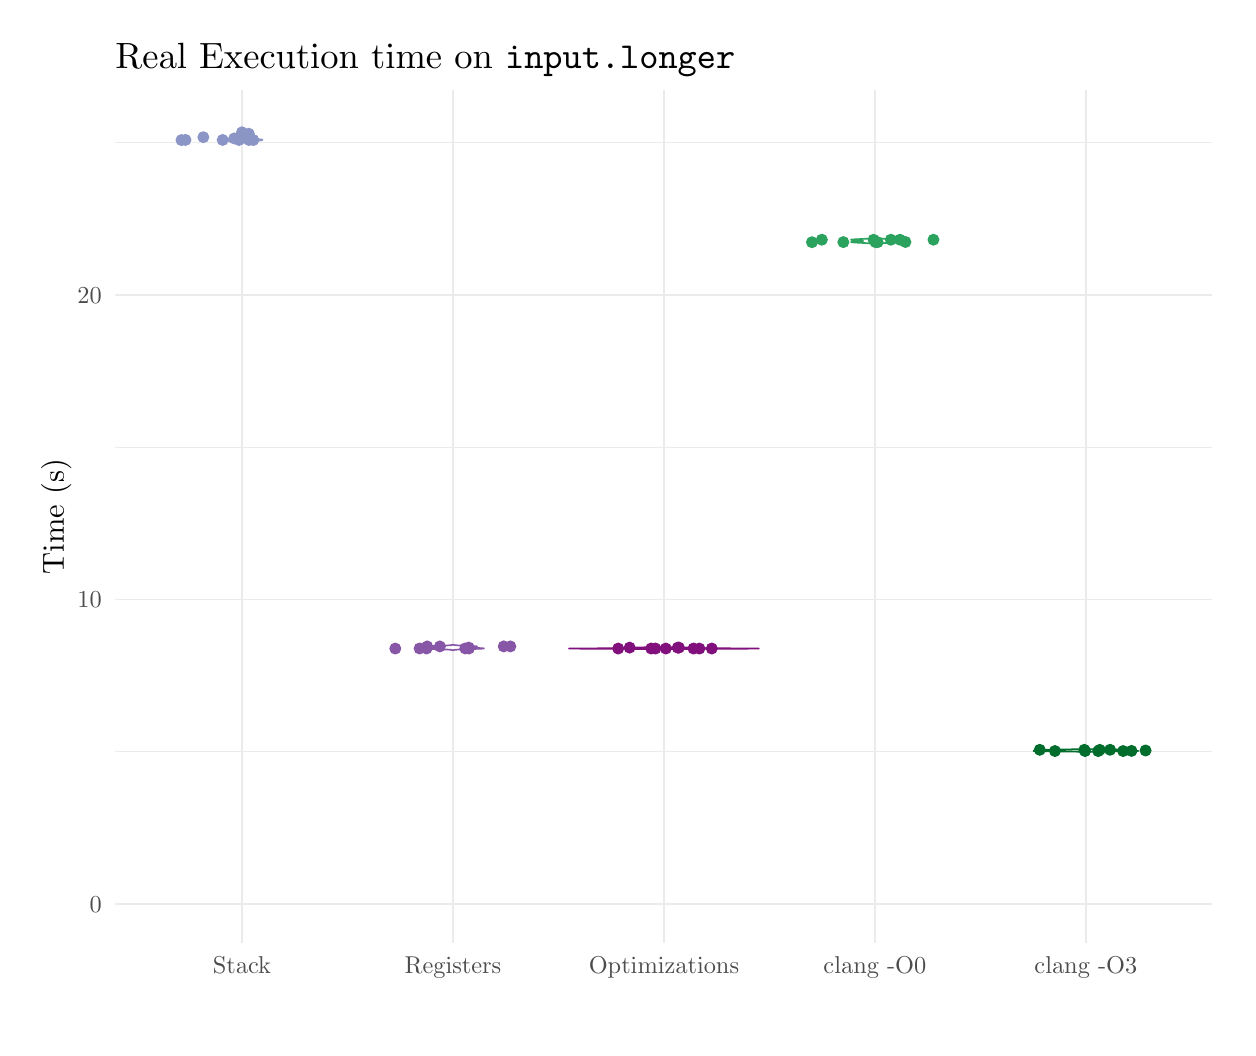
\begin{tikzpicture}[x=1pt,y=1pt]
\definecolor{fillColor}{RGB}{255,255,255}
\path[use as bounding box,fill=fillColor,fill opacity=0.00] (0,0) rectangle (433.62,361.35);
\begin{scope}
\path[clip] ( 31.71, 30.69) rectangle (428.12,338.69);
\definecolor{drawColor}{gray}{0.92}

\path[draw=drawColor,line width= 0.3pt,line join=round] ( 31.71, 99.73) --
	(428.12, 99.73);

\path[draw=drawColor,line width= 0.3pt,line join=round] ( 31.71,209.82) --
	(428.12,209.82);

\path[draw=drawColor,line width= 0.3pt,line join=round] ( 31.71,319.90) --
	(428.12,319.90);

\path[draw=drawColor,line width= 0.6pt,line join=round] ( 31.71, 44.69) --
	(428.12, 44.69);

\path[draw=drawColor,line width= 0.6pt,line join=round] ( 31.71,154.77) --
	(428.12,154.77);

\path[draw=drawColor,line width= 0.6pt,line join=round] ( 31.71,264.86) --
	(428.12,264.86);

\path[draw=drawColor,line width= 0.6pt,line join=round] ( 77.45, 30.69) --
	( 77.45,338.69);

\path[draw=drawColor,line width= 0.6pt,line join=round] (153.68, 30.69) --
	(153.68,338.69);

\path[draw=drawColor,line width= 0.6pt,line join=round] (229.92, 30.69) --
	(229.92,338.69);

\path[draw=drawColor,line width= 0.6pt,line join=round] (306.15, 30.69) --
	(306.15,338.69);

\path[draw=drawColor,line width= 0.6pt,line join=round] (382.38, 30.69) --
	(382.38,338.69);
\definecolor{drawColor}{RGB}{140,150,198}
\definecolor{fillColor}{RGB}{255,255,255}

\path[draw=drawColor,line width= 0.6pt,line join=round,line cap=round,fill=fillColor] ( 77.39,319.58) --
	( 77.38,319.59) --
	( 77.38,319.60) --
	( 77.37,319.61) --
	( 77.37,319.62) --
	( 77.36,319.63) --
	( 77.35,319.64) --
	( 77.34,319.65) --
	( 77.34,319.66) --
	( 77.33,319.67) --
	( 77.32,319.68) --
	( 77.31,319.69) --
	( 77.30,319.70) --
	( 77.28,319.71) --
	( 77.27,319.72) --
	( 77.26,319.73) --
	( 77.24,319.74) --
	( 77.23,319.75) --
	( 77.21,319.76) --
	( 77.20,319.77) --
	( 77.18,319.78) --
	( 77.16,319.79) --
	( 77.14,319.80) --
	( 77.12,319.81) --
	( 77.10,319.82) --
	( 77.08,319.83) --
	( 77.05,319.84) --
	( 77.03,319.85) --
	( 77.00,319.86) --
	( 76.97,319.87) --
	( 76.94,319.88) --
	( 76.91,319.89) --
	( 76.88,319.90) --
	( 76.84,319.91) --
	( 76.81,319.92) --
	( 76.77,319.93) --
	( 76.73,319.94) --
	( 76.69,319.95) --
	( 76.65,319.96) --
	( 76.60,319.97) --
	( 76.56,319.98) --
	( 76.51,319.99) --
	( 76.46,320.00) --
	( 76.41,320.01) --
	( 76.35,320.02) --
	( 76.29,320.03) --
	( 76.24,320.04) --
	( 76.18,320.05) --
	( 76.11,320.06) --
	( 76.05,320.07) --
	( 75.98,320.08) --
	( 75.91,320.09) --
	( 75.84,320.10) --
	( 75.77,320.11) --
	( 75.69,320.12) --
	( 75.62,320.13) --
	( 75.54,320.14) --
	( 75.45,320.15) --
	( 75.37,320.16) --
	( 75.28,320.17) --
	( 75.20,320.18) --
	( 75.11,320.19) --
	( 75.01,320.20) --
	( 74.92,320.21) --
	( 74.82,320.22) --
	( 74.73,320.23) --
	( 74.63,320.24) --
	( 74.53,320.25) --
	( 74.42,320.26) --
	( 74.32,320.27) --
	( 74.22,320.28) --
	( 74.11,320.29) --
	( 74.00,320.30) --
	( 73.89,320.31) --
	( 73.78,320.32) --
	( 73.67,320.33) --
	( 73.56,320.34) --
	( 73.45,320.35) --
	( 73.33,320.36) --
	( 73.22,320.37) --
	( 73.11,320.38) --
	( 72.99,320.39) --
	( 72.88,320.40) --
	( 72.77,320.41) --
	( 72.66,320.42) --
	( 72.54,320.43) --
	( 72.43,320.44) --
	( 72.32,320.45) --
	( 72.21,320.46) --
	( 72.10,320.47) --
	( 71.99,320.48) --
	( 71.89,320.49) --
	( 71.78,320.50) --
	( 71.68,320.51) --
	( 71.58,320.52) --
	( 71.48,320.53) --
	( 71.39,320.54) --
	( 71.29,320.55) --
	( 71.20,320.56) --
	( 71.11,320.57) --
	( 71.03,320.58) --
	( 70.94,320.59) --
	( 70.86,320.60) --
	( 70.79,320.61) --
	( 70.71,320.62) --
	( 70.64,320.63) --
	( 70.58,320.64) --
	( 70.52,320.65) --
	( 70.46,320.66) --
	( 70.40,320.67) --
	( 70.35,320.68) --
	( 70.30,320.69) --
	( 70.26,320.70) --
	( 70.22,320.71) --
	( 70.19,320.72) --
	( 70.16,320.73) --
	( 70.13,320.74) --
	( 70.11,320.75) --
	( 70.09,320.76) --
	( 70.08,320.77) --
	( 70.07,320.78) --
	( 70.07,320.79) --
	( 70.06,320.80) --
	( 70.07,320.81) --
	( 70.08,320.82) --
	( 70.09,320.83) --
	( 70.10,320.84) --
	( 70.12,320.85) --
	( 70.15,320.86) --
	( 70.18,320.87) --
	( 70.21,320.88) --
	( 70.24,320.89) --
	( 70.28,320.90) --
	( 70.32,320.91) --
	( 70.37,320.92) --
	( 70.41,320.93) --
	( 70.47,320.94) --
	( 70.52,320.95) --
	( 70.58,320.96) --
	( 70.64,320.97) --
	( 70.70,320.98) --
	( 70.76,320.99) --
	( 70.83,321.00) --
	( 70.90,321.01) --
	( 70.97,321.02) --
	( 71.05,321.03) --
	( 71.12,321.04) --
	( 71.20,321.05) --
	( 71.27,321.06) --
	( 71.35,321.07) --
	( 71.43,321.08) --
	( 71.51,321.09) --
	( 71.59,321.10) --
	( 71.68,321.11) --
	( 71.76,321.12) --
	( 71.84,321.13) --
	( 71.93,321.14) --
	( 72.01,321.15) --
	( 72.09,321.16) --
	( 72.18,321.17) --
	( 72.26,321.18) --
	( 72.35,321.19) --
	( 72.43,321.20) --
	( 72.51,321.21) --
	( 72.59,321.22) --
	( 72.67,321.23) --
	( 72.75,321.24) --
	( 72.83,321.25) --
	( 72.91,321.26) --
	( 72.99,321.27) --
	( 73.07,321.28) --
	( 73.14,321.29) --
	( 73.22,321.30) --
	( 73.29,321.31) --
	( 73.36,321.32) --
	( 73.43,321.33) --
	( 73.50,321.34) --
	( 73.57,321.35) --
	( 73.64,321.36) --
	( 73.70,321.37) --
	( 73.77,321.38) --
	( 73.83,321.39) --
	( 73.89,321.40) --
	( 73.96,321.41) --
	( 74.01,321.42) --
	( 74.07,321.43) --
	( 74.13,321.44) --
	( 74.18,321.45) --
	( 74.24,321.46) --
	( 74.29,321.47) --
	( 74.34,321.48) --
	( 74.39,321.49) --
	( 74.44,321.50) --
	( 74.49,321.51) --
	( 74.54,321.52) --
	( 74.58,321.53) --
	( 74.63,321.54) --
	( 74.67,321.55) --
	( 74.72,321.56) --
	( 74.76,321.57) --
	( 74.80,321.58) --
	( 74.84,321.59) --
	( 74.88,321.60) --
	( 74.92,321.61) --
	( 74.96,321.62) --
	( 75.00,321.63) --
	( 75.03,321.64) --
	( 75.07,321.65) --
	( 75.11,321.66) --
	( 75.14,321.67) --
	( 75.18,321.68) --
	( 75.21,321.69) --
	( 75.25,321.70) --
	( 75.28,321.71) --
	( 75.31,321.72) --
	( 75.35,321.73) --
	( 75.38,321.74) --
	( 75.41,321.75) --
	( 75.44,321.76) --
	( 75.47,321.77) --
	( 75.51,321.78) --
	( 75.54,321.79) --
	( 75.57,321.80) --
	( 75.60,321.81) --
	( 75.63,321.82) --
	( 75.66,321.83) --
	( 75.69,321.84) --
	( 75.72,321.85) --
	( 75.75,321.86) --
	( 75.78,321.87) --
	( 75.81,321.88) --
	( 75.84,321.89) --
	( 75.87,321.90) --
	( 75.90,321.91) --
	( 75.93,321.92) --
	( 75.96,321.93) --
	( 75.99,321.94) --
	( 76.02,321.95) --
	( 76.04,321.96) --
	( 76.07,321.97) --
	( 76.10,321.98) --
	( 76.13,321.99) --
	( 76.16,322.00) --
	( 76.18,322.01) --
	( 76.21,322.02) --
	( 76.24,322.03) --
	( 76.26,322.04) --
	( 76.29,322.05) --
	( 76.31,322.06) --
	( 76.34,322.07) --
	( 76.36,322.08) --
	( 76.38,322.09) --
	( 76.41,322.10) --
	( 76.43,322.11) --
	( 76.45,322.12) --
	( 76.47,322.13) --
	( 76.49,322.14) --
	( 76.51,322.15) --
	( 76.53,322.16) --
	( 76.55,322.17) --
	( 76.57,322.18) --
	( 76.59,322.19) --
	( 76.61,322.20) --
	( 76.62,322.21) --
	( 76.64,322.22) --
	( 76.65,322.23) --
	( 76.67,322.24) --
	( 76.68,322.25) --
	( 76.69,322.26) --
	( 76.71,322.27) --
	( 76.72,322.28) --
	( 76.73,322.29) --
	( 76.74,322.30) --
	( 76.74,322.31) --
	( 76.75,322.32) --
	( 76.76,322.33) --
	( 76.76,322.34) --
	( 76.77,322.35) --
	( 76.77,322.36) --
	( 76.77,322.37) --
	( 76.78,322.38) --
	( 76.78,322.39) --
	( 76.78,322.40) --
	( 76.78,322.41) --
	( 76.78,322.42) --
	( 76.77,322.43) --
	( 76.77,322.44) --
	( 76.77,322.45) --
	( 76.76,322.46) --
	( 76.76,322.47) --
	( 76.75,322.48) --
	( 76.74,322.49) --
	( 76.74,322.50) --
	( 76.73,322.51) --
	( 76.72,322.52) --
	( 76.71,322.53) --
	( 76.70,322.54) --
	( 76.68,322.55) --
	( 76.67,322.56) --
	( 76.66,322.57) --
	( 76.64,322.58) --
	( 76.63,322.59) --
	( 76.62,322.60) --
	( 76.60,322.61) --
	( 76.58,322.62) --
	( 76.57,322.63) --
	( 76.55,322.64) --
	( 76.53,322.65) --
	( 76.52,322.66) --
	( 76.50,322.67) --
	( 76.48,322.68) --
	( 76.46,322.69) --
	( 76.44,322.70) --
	( 76.42,322.71) --
	( 76.40,322.72) --
	( 76.38,322.73) --
	( 76.36,322.74) --
	( 76.34,322.75) --
	( 76.32,322.76) --
	( 76.30,322.77) --
	( 76.28,322.78) --
	( 76.26,322.79) --
	( 76.24,322.80) --
	( 76.22,322.81) --
	( 76.20,322.82) --
	( 76.18,322.83) --
	( 76.16,322.84) --
	( 76.14,322.85) --
	( 76.12,322.86) --
	( 76.10,322.87) --
	( 76.08,322.88) --
	( 76.06,322.89) --
	( 76.04,322.90) --
	( 76.02,322.91) --
	( 76.00,322.92) --
	( 75.98,322.93) --
	( 75.96,322.94) --
	( 75.95,322.95) --
	( 75.93,322.96) --
	( 75.91,322.97) --
	( 75.89,322.98) --
	( 75.88,322.99) --
	( 75.86,323.00) --
	( 75.85,323.01) --
	( 75.83,323.02) --
	( 75.82,323.03) --
	( 75.80,323.04) --
	( 75.79,323.05) --
	( 75.78,323.06) --
	( 75.77,323.07) --
	( 75.75,323.08) --
	( 75.74,323.09) --
	( 75.73,323.10) --
	( 75.72,323.11) --
	( 75.71,323.12) --
	( 75.70,323.13) --
	( 75.70,323.14) --
	( 75.69,323.15) --
	( 75.68,323.16) --
	( 75.67,323.17) --
	( 75.67,323.18) --
	( 75.66,323.19) --
	( 75.66,323.20) --
	( 75.65,323.21) --
	( 75.65,323.22) --
	( 75.65,323.23) --
	( 75.65,323.24) --
	( 75.64,323.25) --
	( 75.64,323.26) --
	( 75.64,323.27) --
	( 75.64,323.28) --
	( 75.64,323.29) --
	( 75.64,323.30) --
	( 75.65,323.31) --
	( 75.65,323.32) --
	( 75.65,323.33) --
	( 75.66,323.34) --
	( 75.66,323.35) --
	( 75.67,323.36) --
	( 75.67,323.37) --
	( 75.68,323.38) --
	( 75.68,323.39) --
	( 75.69,323.40) --
	( 75.70,323.41) --
	( 75.71,323.42) --
	( 75.72,323.43) --
	( 75.73,323.44) --
	( 75.74,323.45) --
	( 75.75,323.46) --
	( 75.76,323.47) --
	( 75.77,323.48) --
	( 75.79,323.49) --
	( 75.80,323.50) --
	( 75.81,323.51) --
	( 75.83,323.52) --
	( 75.84,323.53) --
	( 75.86,323.54) --
	( 75.87,323.55) --
	( 75.89,323.56) --
	( 75.91,323.57) --
	( 75.92,323.58) --
	( 75.94,323.59) --
	( 75.96,323.60) --
	( 75.98,323.61) --
	( 76.00,323.62) --
	( 76.02,323.63) --
	( 76.04,323.64) --
	( 76.06,323.65) --
	( 76.08,323.66) --
	( 76.10,323.67) --
	( 76.12,323.68) --
	( 76.14,323.69) --
	( 76.16,323.70) --
	( 76.19,323.71) --
	( 76.21,323.72) --
	( 76.23,323.73) --
	( 76.25,323.74) --
	( 76.28,323.75) --
	( 76.30,323.76) --
	( 76.32,323.77) --
	( 76.35,323.78) --
	( 76.37,323.79) --
	( 76.39,323.80) --
	( 76.42,323.81) --
	( 76.44,323.82) --
	( 76.46,323.83) --
	( 76.49,323.84) --
	( 76.51,323.85) --
	( 76.53,323.86) --
	( 76.56,323.87) --
	( 76.58,323.88) --
	( 76.60,323.89) --
	( 76.63,323.90) --
	( 76.65,323.91) --
	( 76.67,323.92) --
	( 76.69,323.93) --
	( 76.72,323.94) --
	( 76.74,323.95) --
	( 76.76,323.96) --
	( 76.78,323.97) --
	( 76.80,323.98) --
	( 76.82,323.99) --
	( 76.84,324.00) --
	( 76.86,324.01) --
	( 76.88,324.02) --
	( 76.90,324.03) --
	( 76.92,324.04) --
	( 76.94,324.05) --
	( 76.96,324.06) --
	( 76.98,324.07) --
	( 77.00,324.08) --
	( 77.01,324.09) --
	( 77.03,324.10) --
	( 77.05,324.11) --
	( 77.06,324.12) --
	( 77.08,324.13) --
	( 77.09,324.14) --
	( 77.11,324.15) --
	( 77.12,324.16) --
	( 77.14,324.17) --
	( 77.15,324.18) --
	( 77.16,324.19) --
	( 77.18,324.20) --
	( 77.19,324.21) --
	( 77.20,324.22) --
	( 77.21,324.23) --
	( 77.22,324.24) --
	( 77.24,324.25) --
	( 77.25,324.26) --
	( 77.26,324.27) --
	( 77.27,324.28) --
	( 77.27,324.29) --
	( 77.28,324.30) --
	( 77.29,324.31) --
	( 77.30,324.32) --
	( 77.31,324.33) --
	( 77.32,324.34) --
	( 77.32,324.35) --
	( 77.33,324.36) --
	( 77.34,324.37) --
	( 77.34,324.38) --
	( 77.35,324.39) --
	( 77.36,324.40) --
	( 77.36,324.41) --
	( 77.37,324.42) --
	( 77.37,324.43) --
	( 77.38,324.44) --
	( 77.38,324.45) --
	( 77.38,324.46) --
	( 77.39,324.47) --
	( 77.39,324.48) --
	( 77.40,324.49) --
	( 77.40,324.50) --
	( 77.40,324.51) --
	( 77.41,324.52) --
	( 77.41,324.53) --
	( 77.41,324.54) --
	( 77.41,324.55) --
	( 77.42,324.56) --
	( 77.42,324.57) --
	( 77.42,324.58) --
	( 77.42,324.59) --
	( 77.43,324.60) --
	( 77.43,324.61) --
	( 77.43,324.62) --
	( 77.43,324.63) --
	( 77.43,324.64) --
	( 77.43,324.65) --
	( 77.44,324.66) --
	( 77.44,324.67) --
	( 77.44,324.68) --
	( 77.44,324.69) --
	( 77.46,324.69) --
	( 77.47,324.68) --
	( 77.47,324.67) --
	( 77.47,324.66) --
	( 77.47,324.65) --
	( 77.47,324.64) --
	( 77.47,324.63) --
	( 77.47,324.62) --
	( 77.48,324.61) --
	( 77.48,324.60) --
	( 77.48,324.59) --
	( 77.48,324.58) --
	( 77.48,324.57) --
	( 77.49,324.56) --
	( 77.49,324.55) --
	( 77.49,324.54) --
	( 77.49,324.53) --
	( 77.50,324.52) --
	( 77.50,324.51) --
	( 77.50,324.50) --
	( 77.51,324.49) --
	( 77.51,324.48) --
	( 77.51,324.47) --
	( 77.52,324.46) --
	( 77.52,324.45) --
	( 77.53,324.44) --
	( 77.53,324.43) --
	( 77.54,324.42) --
	( 77.54,324.41) --
	( 77.55,324.40) --
	( 77.55,324.39) --
	( 77.56,324.38) --
	( 77.57,324.37) --
	( 77.57,324.36) --
	( 77.58,324.35) --
	( 77.59,324.34) --
	( 77.59,324.33) --
	( 77.60,324.32) --
	( 77.61,324.31) --
	( 77.62,324.30) --
	( 77.63,324.29) --
	( 77.64,324.28) --
	( 77.65,324.27) --
	( 77.66,324.26) --
	( 77.67,324.25) --
	( 77.68,324.24) --
	( 77.69,324.23) --
	( 77.70,324.22) --
	( 77.71,324.21) --
	( 77.73,324.20) --
	( 77.74,324.19) --
	( 77.75,324.18) --
	( 77.77,324.17) --
	( 77.78,324.16) --
	( 77.79,324.15) --
	( 77.81,324.14) --
	( 77.82,324.13) --
	( 77.84,324.12) --
	( 77.86,324.11) --
	( 77.87,324.10) --
	( 77.89,324.09) --
	( 77.91,324.08) --
	( 77.93,324.07) --
	( 77.94,324.06) --
	( 77.96,324.05) --
	( 77.98,324.04) --
	( 78.00,324.03) --
	( 78.02,324.02) --
	( 78.04,324.01) --
	( 78.06,324.00) --
	( 78.08,323.99) --
	( 78.10,323.98) --
	( 78.12,323.97) --
	( 78.14,323.96) --
	( 78.16,323.95) --
	( 78.19,323.94) --
	( 78.21,323.93) --
	( 78.23,323.92) --
	( 78.25,323.91) --
	( 78.28,323.90) --
	( 78.30,323.89) --
	( 78.32,323.88) --
	( 78.35,323.87) --
	( 78.37,323.86) --
	( 78.39,323.85) --
	( 78.42,323.84) --
	( 78.44,323.83) --
	( 78.46,323.82) --
	( 78.49,323.81) --
	( 78.51,323.80) --
	( 78.53,323.79) --
	( 78.56,323.78) --
	( 78.58,323.77) --
	( 78.60,323.76) --
	( 78.63,323.75) --
	( 78.65,323.74) --
	( 78.67,323.73) --
	( 78.69,323.72) --
	( 78.72,323.71) --
	( 78.74,323.70) --
	( 78.76,323.69) --
	( 78.78,323.68) --
	( 78.80,323.67) --
	( 78.82,323.66) --
	( 78.85,323.65) --
	( 78.87,323.64) --
	( 78.89,323.63) --
	( 78.90,323.62) --
	( 78.92,323.61) --
	( 78.94,323.60) --
	( 78.96,323.59) --
	( 78.98,323.58) --
	( 79.00,323.57) --
	( 79.01,323.56) --
	( 79.03,323.55) --
	( 79.05,323.54) --
	( 79.06,323.53) --
	( 79.08,323.52) --
	( 79.09,323.51) --
	( 79.10,323.50) --
	( 79.12,323.49) --
	( 79.13,323.48) --
	( 79.14,323.47) --
	( 79.15,323.46) --
	( 79.16,323.45) --
	( 79.18,323.44) --
	( 79.18,323.43) --
	( 79.19,323.42) --
	( 79.20,323.41) --
	( 79.21,323.40) --
	( 79.22,323.39) --
	( 79.23,323.38) --
	( 79.23,323.37) --
	( 79.24,323.36) --
	( 79.24,323.35) --
	( 79.25,323.34) --
	( 79.25,323.33) --
	( 79.25,323.32) --
	( 79.26,323.31) --
	( 79.26,323.30) --
	( 79.26,323.29) --
	( 79.26,323.28) --
	( 79.26,323.27) --
	( 79.26,323.26) --
	( 79.26,323.25) --
	( 79.26,323.24) --
	( 79.26,323.23) --
	( 79.25,323.22) --
	( 79.25,323.21) --
	( 79.24,323.20) --
	( 79.24,323.19) --
	( 79.23,323.18) --
	( 79.23,323.17) --
	( 79.22,323.16) --
	( 79.21,323.15) --
	( 79.21,323.14) --
	( 79.20,323.13) --
	( 79.19,323.12) --
	( 79.18,323.11) --
	( 79.17,323.10) --
	( 79.16,323.09) --
	( 79.15,323.08) --
	( 79.14,323.07) --
	( 79.12,323.06) --
	( 79.11,323.05) --
	( 79.10,323.04) --
	( 79.08,323.03) --
	( 79.07,323.02) --
	( 79.06,323.01) --
	( 79.04,323.00) --
	( 79.03,322.99) --
	( 79.01,322.98) --
	( 78.99,322.97) --
	( 78.98,322.96) --
	( 78.96,322.95) --
	( 78.94,322.94) --
	( 78.92,322.93) --
	( 78.90,322.92) --
	( 78.89,322.91) --
	( 78.87,322.90) --
	( 78.85,322.89) --
	( 78.83,322.88) --
	( 78.81,322.87) --
	( 78.79,322.86) --
	( 78.77,322.85) --
	( 78.75,322.84) --
	( 78.73,322.83) --
	( 78.71,322.82) --
	( 78.69,322.81) --
	( 78.67,322.80) --
	( 78.64,322.79) --
	( 78.62,322.78) --
	( 78.60,322.77) --
	( 78.58,322.76) --
	( 78.56,322.75) --
	( 78.54,322.74) --
	( 78.52,322.73) --
	( 78.50,322.72) --
	( 78.48,322.71) --
	( 78.46,322.70) --
	( 78.44,322.69) --
	( 78.42,322.68) --
	( 78.41,322.67) --
	( 78.39,322.66) --
	( 78.37,322.65) --
	( 78.35,322.64) --
	( 78.34,322.63) --
	( 78.32,322.62) --
	( 78.30,322.61) --
	( 78.29,322.60) --
	( 78.27,322.59) --
	( 78.26,322.58) --
	( 78.24,322.57) --
	( 78.23,322.56) --
	( 78.22,322.55) --
	( 78.21,322.54) --
	( 78.20,322.53) --
	( 78.19,322.52) --
	( 78.18,322.51) --
	( 78.17,322.50) --
	( 78.16,322.49) --
	( 78.15,322.48) --
	( 78.15,322.47) --
	( 78.14,322.46) --
	( 78.14,322.45) --
	( 78.13,322.44) --
	( 78.13,322.43) --
	( 78.13,322.42) --
	( 78.13,322.41) --
	( 78.12,322.40) --
	( 78.12,322.39) --
	( 78.13,322.38) --
	( 78.13,322.37) --
	( 78.13,322.36) --
	( 78.14,322.35) --
	( 78.14,322.34) --
	( 78.15,322.33) --
	( 78.15,322.32) --
	( 78.16,322.31) --
	( 78.17,322.30) --
	( 78.18,322.29) --
	( 78.19,322.28) --
	( 78.20,322.27) --
	( 78.21,322.26) --
	( 78.22,322.25) --
	( 78.24,322.24) --
	( 78.25,322.23) --
	( 78.26,322.22) --
	( 78.28,322.21) --
	( 78.30,322.20) --
	( 78.31,322.19) --
	( 78.33,322.18) --
	( 78.35,322.17) --
	( 78.37,322.16) --
	( 78.39,322.15) --
	( 78.41,322.14) --
	( 78.43,322.13) --
	( 78.45,322.12) --
	( 78.47,322.11) --
	( 78.50,322.10) --
	( 78.52,322.09) --
	( 78.54,322.08) --
	( 78.57,322.07) --
	( 78.59,322.06) --
	( 78.62,322.05) --
	( 78.64,322.04) --
	( 78.67,322.03) --
	( 78.69,322.02) --
	( 78.72,322.01) --
	( 78.75,322.00) --
	( 78.78,321.99) --
	( 78.80,321.98) --
	( 78.83,321.97) --
	( 78.86,321.96) --
	( 78.89,321.95) --
	( 78.92,321.94) --
	( 78.94,321.93) --
	( 78.97,321.92) --
	( 79.00,321.91) --
	( 79.03,321.90) --
	( 79.06,321.89) --
	( 79.09,321.88) --
	( 79.12,321.87) --
	( 79.15,321.86) --
	( 79.18,321.85) --
	( 79.21,321.84) --
	( 79.24,321.83) --
	( 79.27,321.82) --
	( 79.30,321.81) --
	( 79.33,321.80) --
	( 79.37,321.79) --
	( 79.40,321.78) --
	( 79.43,321.77) --
	( 79.46,321.76) --
	( 79.49,321.75) --
	( 79.53,321.74) --
	( 79.56,321.73) --
	( 79.59,321.72) --
	( 79.62,321.71) --
	( 79.66,321.70) --
	( 79.69,321.69) --
	( 79.73,321.68) --
	( 79.76,321.67) --
	( 79.80,321.66) --
	( 79.83,321.65) --
	( 79.87,321.64) --
	( 79.91,321.63) --
	( 79.94,321.62) --
	( 79.98,321.61) --
	( 80.02,321.60) --
	( 80.06,321.59) --
	( 80.10,321.58) --
	( 80.14,321.57) --
	( 80.19,321.56) --
	( 80.23,321.55) --
	( 80.27,321.54) --
	( 80.32,321.53) --
	( 80.37,321.52) --
	( 80.41,321.51) --
	( 80.46,321.50) --
	( 80.51,321.49) --
	( 80.56,321.48) --
	( 80.61,321.47) --
	( 80.67,321.46) --
	( 80.72,321.45) --
	( 80.77,321.44) --
	( 80.83,321.43) --
	( 80.89,321.42) --
	( 80.95,321.41) --
	( 81.01,321.40) --
	( 81.07,321.39) --
	( 81.13,321.38) --
	( 81.20,321.37) --
	( 81.26,321.36) --
	( 81.33,321.35) --
	( 81.40,321.34) --
	( 81.47,321.33) --
	( 81.54,321.32) --
	( 81.61,321.31) --
	( 81.69,321.30) --
	( 81.76,321.29) --
	( 81.84,321.28) --
	( 81.91,321.27) --
	( 81.99,321.26) --
	( 82.07,321.25) --
	( 82.15,321.24) --
	( 82.23,321.23) --
	( 82.31,321.22) --
	( 82.39,321.21) --
	( 82.47,321.20) --
	( 82.56,321.19) --
	( 82.64,321.18) --
	( 82.72,321.17) --
	( 82.81,321.16) --
	( 82.89,321.15) --
	( 82.98,321.14) --
	( 83.06,321.13) --
	( 83.14,321.12) --
	( 83.23,321.11) --
	( 83.31,321.10) --
	( 83.39,321.09) --
	( 83.47,321.08) --
	( 83.55,321.07) --
	( 83.63,321.06) --
	( 83.71,321.05) --
	( 83.78,321.04) --
	( 83.86,321.03) --
	( 83.93,321.02) --
	( 84.00,321.01) --
	( 84.07,321.00) --
	( 84.14,320.99) --
	( 84.20,320.98) --
	( 84.27,320.97) --
	( 84.33,320.96) --
	( 84.38,320.95) --
	( 84.44,320.94) --
	( 84.49,320.93) --
	( 84.54,320.92) --
	( 84.58,320.91) --
	( 84.62,320.90) --
	( 84.66,320.89) --
	( 84.70,320.88) --
	( 84.73,320.87) --
	( 84.76,320.86) --
	( 84.78,320.85) --
	( 84.80,320.84) --
	( 84.82,320.83) --
	( 84.83,320.82) --
	( 84.83,320.81) --
	( 84.84,320.80) --
	( 84.84,320.79) --
	( 84.83,320.78) --
	( 84.82,320.77) --
	( 84.81,320.76) --
	( 84.79,320.75) --
	( 84.77,320.74) --
	( 84.74,320.73) --
	( 84.72,320.72) --
	( 84.68,320.71) --
	( 84.64,320.70) --
	( 84.60,320.69) --
	( 84.55,320.68) --
	( 84.50,320.67) --
	( 84.45,320.66) --
	( 84.39,320.65) --
	( 84.33,320.64) --
	( 84.26,320.63) --
	( 84.19,320.62) --
	( 84.12,320.61) --
	( 84.04,320.60) --
	( 83.96,320.59) --
	( 83.88,320.58) --
	( 83.79,320.57) --
	( 83.70,320.56) --
	( 83.61,320.55) --
	( 83.52,320.54) --
	( 83.42,320.53) --
	( 83.32,320.52) --
	( 83.22,320.51) --
	( 83.12,320.50) --
	( 83.01,320.49) --
	( 82.91,320.48) --
	( 82.80,320.47) --
	( 82.69,320.46) --
	( 82.58,320.45) --
	( 82.47,320.44) --
	( 82.36,320.43) --
	( 82.25,320.42) --
	( 82.14,320.41) --
	( 82.02,320.40) --
	( 81.91,320.39) --
	( 81.80,320.38) --
	( 81.68,320.37) --
	( 81.57,320.36) --
	( 81.46,320.35) --
	( 81.34,320.34) --
	( 81.23,320.33) --
	( 81.12,320.32) --
	( 81.01,320.31) --
	( 80.90,320.30) --
	( 80.79,320.29) --
	( 80.69,320.28) --
	( 80.58,320.27) --
	( 80.48,320.26) --
	( 80.38,320.25) --
	( 80.27,320.24) --
	( 80.18,320.23) --
	( 80.08,320.22) --
	( 79.98,320.21) --
	( 79.89,320.20) --
	( 79.80,320.19) --
	( 79.71,320.18) --
	( 79.62,320.17) --
	( 79.53,320.16) --
	( 79.45,320.15) --
	( 79.37,320.14) --
	( 79.29,320.13) --
	( 79.21,320.12) --
	( 79.13,320.11) --
	( 79.06,320.10) --
	( 78.99,320.09) --
	( 78.92,320.08) --
	( 78.85,320.07) --
	( 78.79,320.06) --
	( 78.73,320.05) --
	( 78.67,320.04) --
	( 78.61,320.03) --
	( 78.55,320.02) --
	( 78.50,320.01) --
	( 78.45,320.00) --
	( 78.40,319.99) --
	( 78.35,319.98) --
	( 78.30,319.97) --
	( 78.26,319.96) --
	( 78.21,319.95) --
	( 78.17,319.94) --
	( 78.13,319.93) --
	( 78.10,319.92) --
	( 78.06,319.91) --
	( 78.03,319.90) --
	( 77.99,319.89) --
	( 77.96,319.88) --
	( 77.93,319.87) --
	( 77.90,319.86) --
	( 77.88,319.85) --
	( 77.85,319.84) --
	( 77.83,319.83) --
	( 77.80,319.82) --
	( 77.78,319.81) --
	( 77.76,319.80) --
	( 77.74,319.79) --
	( 77.72,319.78) --
	( 77.71,319.77) --
	( 77.69,319.76) --
	( 77.67,319.75) --
	( 77.66,319.74) --
	( 77.64,319.73) --
	( 77.63,319.72) --
	( 77.62,319.71) --
	( 77.61,319.70) --
	( 77.60,319.69) --
	( 77.59,319.68) --
	( 77.58,319.67) --
	( 77.57,319.66) --
	( 77.56,319.65) --
	( 77.55,319.64) --
	( 77.54,319.63) --
	( 77.54,319.62) --
	( 77.53,319.61) --
	( 77.52,319.60) --
	( 77.52,319.59) --
	( 77.51,319.58) --
	( 77.39,319.58) --
	cycle;
\definecolor{drawColor}{RGB}{136,86,167}

\path[draw=drawColor,line width= 0.6pt,line join=round,line cap=round,fill=fillColor] (153.59,136.36) --
	(153.59,136.36) --
	(153.58,136.37) --
	(153.58,136.37) --
	(153.57,136.37) --
	(153.56,136.38) --
	(153.56,136.38) --
	(153.55,136.39) --
	(153.54,136.39) --
	(153.53,136.39) --
	(153.53,136.40) --
	(153.52,136.40) --
	(153.51,136.41) --
	(153.50,136.41) --
	(153.49,136.41) --
	(153.48,136.42) --
	(153.47,136.42) --
	(153.45,136.43) --
	(153.44,136.43) --
	(153.43,136.43) --
	(153.42,136.44) --
	(153.40,136.44) --
	(153.39,136.45) --
	(153.37,136.45) --
	(153.36,136.45) --
	(153.34,136.46) --
	(153.32,136.46) --
	(153.30,136.47) --
	(153.28,136.47) --
	(153.26,136.47) --
	(153.24,136.48) --
	(153.22,136.48) --
	(153.20,136.49) --
	(153.18,136.49) --
	(153.15,136.49) --
	(153.13,136.50) --
	(153.10,136.50) --
	(153.08,136.51) --
	(153.05,136.51) --
	(153.02,136.51) --
	(152.99,136.52) --
	(152.96,136.52) --
	(152.92,136.53) --
	(152.89,136.53) --
	(152.86,136.53) --
	(152.82,136.54) --
	(152.78,136.54) --
	(152.74,136.55) --
	(152.71,136.55) --
	(152.66,136.55) --
	(152.62,136.56) --
	(152.58,136.56) --
	(152.53,136.57) --
	(152.49,136.57) --
	(152.44,136.57) --
	(152.39,136.58) --
	(152.34,136.58) --
	(152.29,136.59) --
	(152.23,136.59) --
	(152.18,136.59) --
	(152.12,136.60) --
	(152.06,136.60) --
	(152.00,136.61) --
	(151.94,136.61) --
	(151.88,136.61) --
	(151.81,136.62) --
	(151.74,136.62) --
	(151.68,136.63) --
	(151.61,136.63) --
	(151.53,136.63) --
	(151.46,136.64) --
	(151.38,136.64) --
	(151.31,136.65) --
	(151.23,136.65) --
	(151.15,136.65) --
	(151.07,136.66) --
	(150.98,136.66) --
	(150.90,136.67) --
	(150.81,136.67) --
	(150.72,136.67) --
	(150.63,136.68) --
	(150.54,136.68) --
	(150.45,136.69) --
	(150.35,136.69) --
	(150.25,136.69) --
	(150.16,136.70) --
	(150.06,136.70) --
	(149.95,136.71) --
	(149.85,136.71) --
	(149.75,136.71) --
	(149.64,136.72) --
	(149.53,136.72) --
	(149.43,136.73) --
	(149.32,136.73) --
	(149.20,136.74) --
	(149.09,136.74) --
	(148.98,136.74) --
	(148.86,136.75) --
	(148.75,136.75) --
	(148.63,136.76) --
	(148.51,136.76) --
	(148.39,136.76) --
	(148.27,136.77) --
	(148.15,136.77) --
	(148.03,136.78) --
	(147.91,136.78) --
	(147.79,136.78) --
	(147.67,136.79) --
	(147.54,136.79) --
	(147.42,136.80) --
	(147.30,136.80) --
	(147.17,136.80) --
	(147.05,136.81) --
	(146.92,136.81) --
	(146.80,136.82) --
	(146.68,136.82) --
	(146.55,136.82) --
	(146.43,136.83) --
	(146.31,136.83) --
	(146.18,136.84) --
	(146.06,136.84) --
	(145.94,136.84) --
	(145.82,136.85) --
	(145.70,136.85) --
	(145.58,136.86) --
	(145.46,136.86) --
	(145.35,136.86) --
	(145.23,136.87) --
	(145.12,136.87) --
	(145.01,136.88) --
	(144.90,136.88) --
	(144.79,136.88) --
	(144.68,136.89) --
	(144.57,136.89) --
	(144.47,136.90) --
	(144.37,136.90) --
	(144.27,136.90) --
	(144.17,136.91) --
	(144.07,136.91) --
	(143.98,136.92) --
	(143.89,136.92) --
	(143.80,136.92) --
	(143.71,136.93) --
	(143.63,136.93) --
	(143.55,136.94) --
	(143.47,136.94) --
	(143.39,136.94) --
	(143.32,136.95) --
	(143.25,136.95) --
	(143.18,136.96) --
	(143.12,136.96) --
	(143.05,136.96) --
	(143.00,136.97) --
	(142.94,136.97) --
	(142.89,136.98) --
	(142.84,136.98) --
	(142.79,136.98) --
	(142.75,136.99) --
	(142.71,136.99) --
	(142.68,137.00) --
	(142.65,137.00) --
	(142.62,137.00) --
	(142.59,137.01) --
	(142.57,137.01) --
	(142.55,137.02) --
	(142.53,137.02) --
	(142.52,137.02) --
	(142.51,137.03) --
	(142.51,137.03) --
	(142.50,137.04) --
	(142.51,137.04) --
	(142.51,137.04) --
	(142.52,137.05) --
	(142.53,137.05) --
	(142.54,137.06) --
	(142.56,137.06) --
	(142.58,137.06) --
	(142.60,137.07) --
	(142.63,137.07) --
	(142.66,137.08) --
	(142.69,137.08) --
	(142.72,137.08) --
	(142.76,137.09) --
	(142.80,137.09) --
	(142.85,137.10) --
	(142.89,137.10) --
	(142.94,137.10) --
	(142.99,137.11) --
	(143.04,137.11) --
	(143.10,137.12) --
	(143.16,137.12) --
	(143.22,137.12) --
	(143.28,137.13) --
	(143.34,137.13) --
	(143.41,137.14) --
	(143.48,137.14) --
	(143.55,137.14) --
	(143.62,137.15) --
	(143.69,137.15) --
	(143.77,137.16) --
	(143.84,137.16) --
	(143.92,137.17) --
	(144.00,137.17) --
	(144.08,137.17) --
	(144.16,137.18) --
	(144.24,137.18) --
	(144.32,137.19) --
	(144.41,137.19) --
	(144.49,137.19) --
	(144.58,137.20) --
	(144.66,137.20) --
	(144.75,137.21) --
	(144.83,137.21) --
	(144.92,137.21) --
	(145.00,137.22) --
	(145.09,137.22) --
	(145.17,137.23) --
	(145.26,137.23) --
	(145.35,137.23) --
	(145.43,137.24) --
	(145.52,137.24) --
	(145.60,137.25) --
	(145.68,137.25) --
	(145.77,137.25) --
	(145.85,137.26) --
	(145.93,137.26) --
	(146.01,137.27) --
	(146.09,137.27) --
	(146.17,137.27) --
	(146.24,137.28) --
	(146.32,137.28) --
	(146.40,137.29) --
	(146.47,137.29) --
	(146.54,137.29) --
	(146.61,137.30) --
	(146.68,137.30) --
	(146.75,137.31) --
	(146.81,137.31) --
	(146.88,137.31) --
	(146.94,137.32) --
	(147.00,137.32) --
	(147.06,137.33) --
	(147.12,137.33) --
	(147.17,137.33) --
	(147.22,137.34) --
	(147.28,137.34) --
	(147.32,137.35) --
	(147.37,137.35) --
	(147.42,137.35) --
	(147.46,137.36) --
	(147.50,137.36) --
	(147.54,137.37) --
	(147.57,137.37) --
	(147.61,137.37) --
	(147.64,137.38) --
	(147.67,137.38) --
	(147.70,137.39) --
	(147.72,137.39) --
	(147.74,137.39) --
	(147.76,137.40) --
	(147.78,137.40) --
	(147.79,137.41) --
	(147.81,137.41) --
	(147.82,137.41) --
	(147.83,137.42) --
	(147.83,137.42) --
	(147.84,137.43) --
	(147.84,137.43) --
	(147.84,137.43) --
	(147.83,137.44) --
	(147.83,137.44) --
	(147.82,137.45) --
	(147.81,137.45) --
	(147.80,137.45) --
	(147.78,137.46) --
	(147.77,137.46) --
	(147.75,137.47) --
	(147.73,137.47) --
	(147.71,137.47) --
	(147.68,137.48) --
	(147.66,137.48) --
	(147.63,137.49) --
	(147.60,137.49) --
	(147.57,137.49) --
	(147.53,137.50) --
	(147.50,137.50) --
	(147.46,137.51) --
	(147.42,137.51) --
	(147.38,137.51) --
	(147.34,137.52) --
	(147.29,137.52) --
	(147.25,137.53) --
	(147.20,137.53) --
	(147.16,137.53) --
	(147.11,137.54) --
	(147.06,137.54) --
	(147.01,137.55) --
	(146.96,137.55) --
	(146.91,137.55) --
	(146.85,137.56) --
	(146.80,137.56) --
	(146.75,137.57) --
	(146.69,137.57) --
	(146.64,137.57) --
	(146.58,137.58) --
	(146.53,137.58) --
	(146.47,137.59) --
	(146.41,137.59) --
	(146.36,137.59) --
	(146.30,137.60) --
	(146.25,137.60) --
	(146.19,137.61) --
	(146.13,137.61) --
	(146.08,137.62) --
	(146.03,137.62) --
	(145.97,137.62) --
	(145.92,137.63) --
	(145.87,137.63) --
	(145.81,137.64) --
	(145.76,137.64) --
	(145.71,137.64) --
	(145.66,137.65) --
	(145.62,137.65) --
	(145.57,137.66) --
	(145.53,137.66) --
	(145.48,137.66) --
	(145.44,137.67) --
	(145.40,137.67) --
	(145.36,137.68) --
	(145.32,137.68) --
	(145.29,137.68) --
	(145.25,137.69) --
	(145.22,137.69) --
	(145.19,137.70) --
	(145.16,137.70) --
	(145.14,137.70) --
	(145.12,137.71) --
	(145.09,137.71) --
	(145.07,137.72) --
	(145.06,137.72) --
	(145.04,137.72) --
	(145.03,137.73) --
	(145.02,137.73) --
	(145.01,137.74) --
	(145.01,137.74) --
	(145.01,137.74) --
	(145.01,137.75) --
	(145.01,137.75) --
	(145.01,137.76) --
	(145.02,137.76) --
	(145.03,137.76) --
	(145.04,137.77) --
	(145.06,137.77) --
	(145.08,137.78) --
	(145.10,137.78) --
	(145.12,137.78) --
	(145.15,137.79) --
	(145.18,137.79) --
	(145.21,137.80) --
	(145.24,137.80) --
	(145.28,137.80) --
	(145.32,137.81) --
	(145.36,137.81) --
	(145.40,137.82) --
	(145.45,137.82) --
	(145.50,137.82) --
	(145.55,137.83) --
	(145.60,137.83) --
	(145.66,137.84) --
	(145.72,137.84) --
	(145.78,137.84) --
	(145.84,137.85) --
	(145.90,137.85) --
	(145.97,137.86) --
	(146.04,137.86) --
	(146.11,137.86) --
	(146.18,137.87) --
	(146.26,137.87) --
	(146.33,137.88) --
	(146.41,137.88) --
	(146.49,137.88) --
	(146.57,137.89) --
	(146.65,137.89) --
	(146.74,137.90) --
	(146.82,137.90) --
	(146.91,137.90) --
	(147.00,137.91) --
	(147.09,137.91) --
	(147.18,137.92) --
	(147.27,137.92) --
	(147.36,137.92) --
	(147.45,137.93) --
	(147.55,137.93) --
	(147.64,137.94) --
	(147.73,137.94) --
	(147.83,137.94) --
	(147.93,137.95) --
	(148.02,137.95) --
	(148.12,137.96) --
	(148.22,137.96) --
	(148.31,137.96) --
	(148.41,137.97) --
	(148.51,137.97) --
	(148.60,137.98) --
	(148.70,137.98) --
	(148.80,137.98) --
	(148.89,137.99) --
	(148.99,137.99) --
	(149.09,138.00) --
	(149.18,138.00) --
	(149.28,138.00) --
	(149.37,138.01) --
	(149.47,138.01) --
	(149.56,138.02) --
	(149.65,138.02) --
	(149.75,138.02) --
	(149.84,138.03) --
	(149.93,138.03) --
	(150.02,138.04) --
	(150.11,138.04) --
	(150.20,138.05) --
	(150.28,138.05) --
	(150.37,138.05) --
	(150.46,138.06) --
	(150.54,138.06) --
	(150.62,138.07) --
	(150.70,138.07) --
	(150.78,138.07) --
	(150.86,138.08) --
	(150.94,138.08) --
	(151.02,138.09) --
	(151.10,138.09) --
	(151.17,138.09) --
	(151.24,138.10) --
	(151.32,138.10) --
	(151.39,138.11) --
	(151.46,138.11) --
	(151.52,138.11) --
	(151.59,138.12) --
	(151.66,138.12) --
	(151.72,138.13) --
	(151.78,138.13) --
	(151.84,138.13) --
	(151.90,138.14) --
	(151.96,138.14) --
	(152.02,138.15) --
	(152.08,138.15) --
	(152.13,138.15) --
	(152.18,138.16) --
	(152.24,138.16) --
	(152.29,138.17) --
	(152.34,138.17) --
	(152.38,138.17) --
	(152.43,138.18) --
	(152.48,138.18) --
	(152.52,138.19) --
	(152.56,138.19) --
	(152.61,138.19) --
	(152.65,138.20) --
	(152.69,138.20) --
	(152.72,138.21) --
	(152.76,138.21) --
	(152.80,138.21) --
	(152.83,138.22) --
	(152.87,138.22) --
	(152.90,138.23) --
	(152.93,138.23) --
	(152.96,138.23) --
	(152.99,138.24) --
	(153.02,138.24) --
	(153.05,138.25) --
	(153.08,138.25) --
	(153.10,138.25) --
	(153.13,138.26) --
	(153.15,138.26) --
	(153.17,138.27) --
	(153.20,138.27) --
	(153.22,138.27) --
	(153.24,138.28) --
	(153.26,138.28) --
	(153.28,138.29) --
	(153.30,138.29) --
	(153.31,138.29) --
	(153.33,138.30) --
	(153.35,138.30) --
	(153.36,138.31) --
	(153.38,138.31) --
	(153.39,138.31) --
	(153.41,138.32) --
	(153.42,138.32) --
	(153.43,138.33) --
	(153.45,138.33) --
	(153.46,138.33) --
	(153.47,138.34) --
	(153.48,138.34) --
	(153.49,138.35) --
	(153.50,138.35) --
	(153.51,138.35) --
	(153.52,138.36) --
	(153.53,138.36) --
	(153.53,138.37) --
	(153.54,138.37) --
	(153.55,138.37) --
	(153.56,138.38) --
	(153.56,138.38) --
	(153.57,138.39) --
	(153.58,138.39) --
	(153.58,138.39) --
	(153.59,138.40) --
	(153.59,138.40) --
	(153.60,138.41) --
	(153.60,138.41) --
	(153.76,138.41) --
	(153.77,138.41) --
	(153.77,138.40) --
	(153.78,138.40) --
	(153.79,138.39) --
	(153.79,138.39) --
	(153.80,138.39) --
	(153.80,138.38) --
	(153.81,138.38) --
	(153.82,138.37) --
	(153.82,138.37) --
	(153.83,138.37) --
	(153.84,138.36) --
	(153.85,138.36) --
	(153.86,138.35) --
	(153.87,138.35) --
	(153.88,138.35) --
	(153.89,138.34) --
	(153.90,138.34) --
	(153.91,138.33) --
	(153.92,138.33) --
	(153.93,138.33) --
	(153.95,138.32) --
	(153.96,138.32) --
	(153.97,138.31) --
	(153.99,138.31) --
	(154.00,138.31) --
	(154.02,138.30) --
	(154.04,138.30) --
	(154.05,138.29) --
	(154.07,138.29) --
	(154.09,138.29) --
	(154.11,138.28) --
	(154.13,138.28) --
	(154.15,138.27) --
	(154.17,138.27) --
	(154.19,138.27) --
	(154.22,138.26) --
	(154.24,138.26) --
	(154.27,138.25) --
	(154.29,138.25) --
	(154.32,138.25) --
	(154.35,138.24) --
	(154.38,138.24) --
	(154.41,138.23) --
	(154.44,138.23) --
	(154.47,138.23) --
	(154.50,138.22) --
	(154.53,138.22) --
	(154.57,138.21) --
	(154.61,138.21) --
	(154.64,138.21) --
	(154.68,138.20) --
	(154.72,138.20) --
	(154.76,138.19) --
	(154.80,138.19) --
	(154.85,138.19) --
	(154.89,138.18) --
	(154.94,138.18) --
	(154.98,138.17) --
	(155.03,138.17) --
	(155.08,138.17) --
	(155.13,138.16) --
	(155.18,138.16) --
	(155.24,138.15) --
	(155.29,138.15) --
	(155.35,138.15) --
	(155.41,138.14) --
	(155.46,138.14) --
	(155.52,138.13) --
	(155.58,138.13) --
	(155.65,138.13) --
	(155.71,138.12) --
	(155.78,138.12) --
	(155.84,138.11) --
	(155.91,138.11) --
	(155.98,138.11) --
	(156.05,138.10) --
	(156.12,138.10) --
	(156.20,138.09) --
	(156.27,138.09) --
	(156.35,138.09) --
	(156.42,138.08) --
	(156.50,138.08) --
	(156.58,138.07) --
	(156.66,138.07) --
	(156.75,138.07) --
	(156.83,138.06) --
	(156.91,138.06) --
	(157.00,138.05) --
	(157.08,138.05) --
	(157.17,138.05) --
	(157.26,138.04) --
	(157.35,138.04) --
	(157.44,138.03) --
	(157.53,138.03) --
	(157.62,138.02) --
	(157.71,138.02) --
	(157.81,138.02) --
	(157.90,138.01) --
	(157.99,138.01) --
	(158.09,138.00) --
	(158.18,138.00) --
	(158.28,138.00) --
	(158.38,137.99) --
	(158.47,137.99) --
	(158.57,137.98) --
	(158.67,137.98) --
	(158.76,137.98) --
	(158.86,137.97) --
	(158.96,137.97) --
	(159.06,137.96) --
	(159.15,137.96) --
	(159.25,137.96) --
	(159.35,137.95) --
	(159.44,137.95) --
	(159.54,137.94) --
	(159.63,137.94) --
	(159.73,137.94) --
	(159.82,137.93) --
	(159.92,137.93) --
	(160.01,137.92) --
	(160.10,137.92) --
	(160.19,137.92) --
	(160.28,137.91) --
	(160.37,137.91) --
	(160.46,137.90) --
	(160.54,137.90) --
	(160.63,137.90) --
	(160.71,137.89) --
	(160.80,137.89) --
	(160.88,137.88) --
	(160.96,137.88) --
	(161.03,137.88) --
	(161.11,137.87) --
	(161.18,137.87) --
	(161.26,137.86) --
	(161.33,137.86) --
	(161.40,137.86) --
	(161.46,137.85) --
	(161.53,137.85) --
	(161.59,137.84) --
	(161.65,137.84) --
	(161.71,137.84) --
	(161.76,137.83) --
	(161.82,137.83) --
	(161.87,137.82) --
	(161.92,137.82) --
	(161.96,137.82) --
	(162.01,137.81) --
	(162.05,137.81) --
	(162.09,137.80) --
	(162.12,137.80) --
	(162.16,137.80) --
	(162.19,137.79) --
	(162.22,137.79) --
	(162.25,137.78) --
	(162.27,137.78) --
	(162.29,137.78) --
	(162.31,137.77) --
	(162.32,137.77) --
	(162.34,137.76) --
	(162.35,137.76) --
	(162.35,137.76) --
	(162.36,137.75) --
	(162.36,137.75) --
	(162.36,137.74) --
	(162.36,137.74) --
	(162.35,137.74) --
	(162.35,137.73) --
	(162.34,137.73) --
	(162.32,137.72) --
	(162.31,137.72) --
	(162.29,137.72) --
	(162.27,137.71) --
	(162.25,137.71) --
	(162.23,137.70) --
	(162.20,137.70) --
	(162.18,137.70) --
	(162.15,137.69) --
	(162.11,137.69) --
	(162.08,137.68) --
	(162.04,137.68) --
	(162.01,137.68) --
	(161.97,137.67) --
	(161.93,137.67) --
	(161.89,137.66) --
	(161.84,137.66) --
	(161.80,137.66) --
	(161.75,137.65) --
	(161.70,137.65) --
	(161.65,137.64) --
	(161.60,137.64) --
	(161.55,137.64) --
	(161.50,137.63) --
	(161.45,137.63) --
	(161.40,137.62) --
	(161.34,137.62) --
	(161.29,137.62) --
	(161.23,137.61) --
	(161.18,137.61) --
	(161.12,137.60) --
	(161.07,137.60) --
	(161.01,137.59) --
	(160.95,137.59) --
	(160.90,137.59) --
	(160.84,137.58) --
	(160.79,137.58) --
	(160.73,137.57) --
	(160.68,137.57) --
	(160.62,137.57) --
	(160.57,137.56) --
	(160.51,137.56) --
	(160.46,137.55) --
	(160.41,137.55) --
	(160.36,137.55) --
	(160.31,137.54) --
	(160.26,137.54) --
	(160.21,137.53) --
	(160.16,137.53) --
	(160.12,137.53) --
	(160.07,137.52) --
	(160.03,137.52) --
	(159.99,137.51) --
	(159.95,137.51) --
	(159.91,137.51) --
	(159.87,137.50) --
	(159.84,137.50) --
	(159.80,137.49) --
	(159.77,137.49) --
	(159.74,137.49) --
	(159.71,137.48) --
	(159.69,137.48) --
	(159.66,137.47) --
	(159.64,137.47) --
	(159.62,137.47) --
	(159.60,137.46) --
	(159.58,137.46) --
	(159.57,137.45) --
	(159.56,137.45) --
	(159.55,137.45) --
	(159.54,137.44) --
	(159.53,137.44) --
	(159.53,137.43) --
	(159.53,137.43) --
	(159.53,137.43) --
	(159.53,137.42) --
	(159.54,137.42) --
	(159.55,137.41) --
	(159.56,137.41) --
	(159.57,137.41) --
	(159.59,137.40) --
	(159.61,137.40) --
	(159.63,137.39) --
	(159.65,137.39) --
	(159.67,137.39) --
	(159.70,137.38) --
	(159.73,137.38) --
	(159.76,137.37) --
	(159.79,137.37) --
	(159.83,137.37) --
	(159.87,137.36) --
	(159.91,137.36) --
	(159.95,137.35) --
	(160.00,137.35) --
	(160.04,137.35) --
	(160.09,137.34) --
	(160.14,137.34) --
	(160.20,137.33) --
	(160.25,137.33) --
	(160.31,137.33) --
	(160.37,137.32) --
	(160.43,137.32) --
	(160.49,137.31) --
	(160.55,137.31) --
	(160.62,137.31) --
	(160.69,137.30) --
	(160.76,137.30) --
	(160.83,137.29) --
	(160.90,137.29) --
	(160.97,137.29) --
	(161.05,137.28) --
	(161.12,137.28) --
	(161.20,137.27) --
	(161.28,137.27) --
	(161.36,137.27) --
	(161.44,137.26) --
	(161.52,137.26) --
	(161.60,137.25) --
	(161.69,137.25) --
	(161.77,137.25) --
	(161.85,137.24) --
	(161.94,137.24) --
	(162.02,137.23) --
	(162.11,137.23) --
	(162.19,137.23) --
	(162.28,137.22) --
	(162.37,137.22) --
	(162.45,137.21) --
	(162.54,137.21) --
	(162.62,137.21) --
	(162.71,137.20) --
	(162.79,137.20) --
	(162.88,137.19) --
	(162.96,137.19) --
	(163.04,137.19) --
	(163.13,137.18) --
	(163.21,137.18) --
	(163.29,137.17) --
	(163.37,137.17) --
	(163.45,137.17) --
	(163.52,137.16) --
	(163.60,137.16) --
	(163.67,137.15) --
	(163.75,137.15) --
	(163.82,137.14) --
	(163.89,137.14) --
	(163.96,137.14) --
	(164.02,137.13) --
	(164.09,137.13) --
	(164.15,137.12) --
	(164.21,137.12) --
	(164.27,137.12) --
	(164.32,137.11) --
	(164.38,137.11) --
	(164.43,137.10) --
	(164.48,137.10) --
	(164.52,137.10) --
	(164.57,137.09) --
	(164.61,137.09) --
	(164.64,137.08) --
	(164.68,137.08) --
	(164.71,137.08) --
	(164.74,137.07) --
	(164.77,137.07) --
	(164.79,137.06) --
	(164.81,137.06) --
	(164.83,137.06) --
	(164.84,137.05) --
	(164.85,137.05) --
	(164.86,137.04) --
	(164.86,137.04) --
	(164.86,137.04) --
	(164.86,137.03) --
	(164.86,137.03) --
	(164.85,137.02) --
	(164.84,137.02) --
	(164.82,137.02) --
	(164.80,137.01) --
	(164.78,137.01) --
	(164.75,137.00) --
	(164.72,137.00) --
	(164.69,137.00) --
	(164.65,136.99) --
	(164.61,136.99) --
	(164.57,136.98) --
	(164.53,136.98) --
	(164.48,136.98) --
	(164.43,136.97) --
	(164.37,136.97) --
	(164.31,136.96) --
	(164.25,136.96) --
	(164.19,136.96) --
	(164.12,136.95) --
	(164.05,136.95) --
	(163.98,136.94) --
	(163.90,136.94) --
	(163.82,136.94) --
	(163.74,136.93) --
	(163.66,136.93) --
	(163.57,136.92) --
	(163.48,136.92) --
	(163.39,136.92) --
	(163.30,136.91) --
	(163.20,136.91) --
	(163.10,136.90) --
	(163.00,136.90) --
	(162.90,136.90) --
	(162.80,136.89) --
	(162.69,136.89) --
	(162.58,136.88) --
	(162.47,136.88) --
	(162.36,136.88) --
	(162.25,136.87) --
	(162.13,136.87) --
	(162.02,136.86) --
	(161.90,136.86) --
	(161.78,136.86) --
	(161.67,136.85) --
	(161.55,136.85) --
	(161.43,136.84) --
	(161.31,136.84) --
	(161.18,136.84) --
	(161.06,136.83) --
	(160.94,136.83) --
	(160.81,136.82) --
	(160.69,136.82) --
	(160.57,136.82) --
	(160.44,136.81) --
	(160.32,136.81) --
	(160.19,136.80) --
	(160.07,136.80) --
	(159.95,136.80) --
	(159.82,136.79) --
	(159.70,136.79) --
	(159.58,136.78) --
	(159.46,136.78) --
	(159.33,136.78) --
	(159.21,136.77) --
	(159.09,136.77) --
	(158.97,136.76) --
	(158.85,136.76) --
	(158.74,136.76) --
	(158.62,136.75) --
	(158.50,136.75) --
	(158.39,136.74) --
	(158.28,136.74) --
	(158.16,136.74) --
	(158.05,136.73) --
	(157.94,136.73) --
	(157.83,136.72) --
	(157.73,136.72) --
	(157.62,136.71) --
	(157.52,136.71) --
	(157.41,136.71) --
	(157.31,136.70) --
	(157.21,136.70) --
	(157.11,136.69) --
	(157.02,136.69) --
	(156.92,136.69) --
	(156.83,136.68) --
	(156.74,136.68) --
	(156.65,136.67) --
	(156.56,136.67) --
	(156.47,136.67) --
	(156.38,136.66) --
	(156.30,136.66) --
	(156.22,136.65) --
	(156.14,136.65) --
	(156.06,136.65) --
	(155.98,136.64) --
	(155.91,136.64) --
	(155.83,136.63) --
	(155.76,136.63) --
	(155.69,136.63) --
	(155.62,136.62) --
	(155.56,136.62) --
	(155.49,136.61) --
	(155.43,136.61) --
	(155.37,136.61) --
	(155.31,136.60) --
	(155.25,136.60) --
	(155.19,136.59) --
	(155.14,136.59) --
	(155.08,136.59) --
	(155.03,136.58) --
	(154.98,136.58) --
	(154.93,136.57) --
	(154.88,136.57) --
	(154.83,136.57) --
	(154.79,136.56) --
	(154.75,136.56) --
	(154.70,136.55) --
	(154.66,136.55) --
	(154.62,136.55) --
	(154.58,136.54) --
	(154.55,136.54) --
	(154.51,136.53) --
	(154.48,136.53) --
	(154.44,136.53) --
	(154.41,136.52) --
	(154.38,136.52) --
	(154.35,136.51) --
	(154.32,136.51) --
	(154.29,136.51) --
	(154.27,136.50) --
	(154.24,136.50) --
	(154.21,136.49) --
	(154.19,136.49) --
	(154.17,136.49) --
	(154.15,136.48) --
	(154.12,136.48) --
	(154.10,136.47) --
	(154.08,136.47) --
	(154.06,136.47) --
	(154.05,136.46) --
	(154.03,136.46) --
	(154.01,136.45) --
	(154.00,136.45) --
	(153.98,136.45) --
	(153.97,136.44) --
	(153.95,136.44) --
	(153.94,136.43) --
	(153.93,136.43) --
	(153.91,136.43) --
	(153.90,136.42) --
	(153.89,136.42) --
	(153.88,136.41) --
	(153.87,136.41) --
	(153.86,136.41) --
	(153.85,136.40) --
	(153.84,136.40) --
	(153.83,136.39) --
	(153.83,136.39) --
	(153.82,136.39) --
	(153.81,136.38) --
	(153.80,136.38) --
	(153.80,136.37) --
	(153.79,136.37) --
	(153.78,136.37) --
	(153.78,136.36) --
	(153.77,136.36) --
	(153.59,136.36) --
	cycle;
\definecolor{drawColor}{RGB}{129,15,124}

\path[draw=drawColor,line width= 0.6pt,line join=round,line cap=round,fill=fillColor] (229.58,136.72) --
	(229.56,136.72) --
	(229.54,136.73) --
	(229.52,136.73) --
	(229.50,136.73) --
	(229.47,136.73) --
	(229.45,136.73) --
	(229.42,136.73) --
	(229.39,136.74) --
	(229.36,136.74) --
	(229.33,136.74) --
	(229.30,136.74) --
	(229.26,136.74) --
	(229.23,136.74) --
	(229.19,136.75) --
	(229.15,136.75) --
	(229.11,136.75) --
	(229.07,136.75) --
	(229.02,136.75) --
	(228.97,136.75) --
	(228.92,136.76) --
	(228.87,136.76) --
	(228.82,136.76) --
	(228.76,136.76) --
	(228.70,136.76) --
	(228.64,136.77) --
	(228.58,136.77) --
	(228.51,136.77) --
	(228.44,136.77) --
	(228.37,136.77) --
	(228.30,136.77) --
	(228.22,136.78) --
	(228.14,136.78) --
	(228.05,136.78) --
	(227.97,136.78) --
	(227.88,136.78) --
	(227.78,136.78) --
	(227.68,136.79) --
	(227.58,136.79) --
	(227.48,136.79) --
	(227.37,136.79) --
	(227.25,136.79) --
	(227.14,136.79) --
	(227.02,136.80) --
	(226.89,136.80) --
	(226.76,136.80) --
	(226.63,136.80) --
	(226.49,136.80) --
	(226.35,136.81) --
	(226.20,136.81) --
	(226.05,136.81) --
	(225.90,136.81) --
	(225.73,136.81) --
	(225.57,136.81) --
	(225.40,136.82) --
	(225.22,136.82) --
	(225.04,136.82) --
	(224.85,136.82) --
	(224.66,136.82) --
	(224.46,136.82) --
	(224.26,136.83) --
	(224.05,136.83) --
	(223.84,136.83) --
	(223.62,136.83) --
	(223.40,136.83) --
	(223.17,136.83) --
	(222.94,136.84) --
	(222.70,136.84) --
	(222.45,136.84) --
	(222.20,136.84) --
	(221.94,136.84) --
	(221.68,136.84) --
	(221.41,136.85) --
	(221.14,136.85) --
	(220.86,136.85) --
	(220.57,136.85) --
	(220.28,136.85) --
	(219.99,136.86) --
	(219.69,136.86) --
	(219.38,136.86) --
	(219.07,136.86) --
	(218.75,136.86) --
	(218.43,136.86) --
	(218.10,136.87) --
	(217.77,136.87) --
	(217.44,136.87) --
	(217.10,136.87) --
	(216.75,136.87) --
	(216.40,136.87) --
	(216.05,136.88) --
	(215.69,136.88) --
	(215.33,136.88) --
	(214.96,136.88) --
	(214.59,136.88) --
	(214.22,136.88) --
	(213.84,136.89) --
	(213.47,136.89) --
	(213.08,136.89) --
	(212.70,136.89) --
	(212.31,136.89) --
	(211.92,136.89) --
	(211.53,136.90) --
	(211.14,136.90) --
	(210.75,136.90) --
	(210.35,136.90) --
	(209.96,136.90) --
	(209.56,136.91) --
	(209.16,136.91) --
	(208.77,136.91) --
	(208.37,136.91) --
	(207.98,136.91) --
	(207.58,136.91) --
	(207.19,136.92) --
	(206.79,136.92) --
	(206.40,136.92) --
	(206.02,136.92) --
	(205.63,136.92) --
	(205.25,136.92) --
	(204.87,136.93) --
	(204.49,136.93) --
	(204.11,136.93) --
	(203.75,136.93) --
	(203.38,136.93) --
	(203.02,136.93) --
	(202.67,136.94) --
	(202.32,136.94) --
	(201.97,136.94) --
	(201.63,136.94) --
	(201.30,136.94) --
	(200.98,136.95) --
	(200.66,136.95) --
	(200.35,136.95) --
	(200.05,136.95) --
	(199.75,136.95) --
	(199.46,136.95) --
	(199.19,136.96) --
	(198.91,136.96) --
	(198.65,136.96) --
	(198.40,136.96) --
	(198.16,136.96) --
	(197.92,136.96) --
	(197.71,136.97) --
	(197.49,136.97) --
	(197.29,136.97) --
	(197.10,136.97) --
	(196.92,136.97) --
	(196.75,136.97) --
	(196.59,136.98) --
	(196.45,136.98) --
	(196.31,136.98) --
	(196.19,136.98) --
	(196.07,136.98) --
	(195.98,136.98) --
	(195.88,136.99) --
	(195.81,136.99) --
	(195.75,136.99) --
	(195.70,136.99) --
	(195.66,136.99) --
	(195.63,137.00) --
	(195.62,137.00) --
	(195.61,137.00) --
	(195.63,137.00) --
	(195.65,137.00) --
	(195.68,137.00) --
	(195.73,137.01) --
	(195.79,137.01) --
	(195.86,137.01) --
	(195.95,137.01) --
	(196.04,137.01) --
	(196.15,137.01) --
	(196.27,137.02) --
	(196.40,137.02) --
	(196.55,137.02) --
	(196.70,137.02) --
	(196.86,137.02) --
	(197.04,137.02) --
	(197.23,137.03) --
	(197.42,137.03) --
	(197.63,137.03) --
	(197.85,137.03) --
	(198.07,137.03) --
	(198.31,137.04) --
	(198.55,137.04) --
	(198.81,137.04) --
	(199.07,137.04) --
	(199.35,137.04) --
	(199.63,137.04) --
	(199.91,137.05) --
	(200.21,137.05) --
	(200.51,137.05) --
	(200.82,137.05) --
	(201.14,137.05) --
	(201.46,137.05) --
	(201.79,137.06) --
	(202.12,137.06) --
	(202.46,137.06) --
	(202.81,137.06) --
	(203.15,137.06) --
	(203.51,137.06) --
	(203.86,137.07) --
	(204.22,137.07) --
	(204.59,137.07) --
	(204.95,137.07) --
	(205.32,137.07) --
	(205.69,137.07) --
	(206.06,137.08) --
	(206.43,137.08) --
	(206.81,137.08) --
	(207.18,137.08) --
	(207.56,137.08) --
	(207.93,137.09) --
	(208.31,137.09) --
	(208.68,137.09) --
	(209.05,137.09) --
	(209.43,137.09) --
	(209.80,137.09) --
	(210.16,137.10) --
	(210.53,137.10) --
	(210.89,137.10) --
	(211.25,137.10) --
	(211.61,137.10) --
	(211.96,137.10) --
	(212.32,137.11) --
	(212.66,137.11) --
	(213.00,137.11) --
	(213.34,137.11) --
	(213.67,137.11) --
	(214.00,137.11) --
	(214.32,137.12) --
	(214.64,137.12) --
	(214.95,137.12) --
	(215.26,137.12) --
	(215.56,137.12) --
	(215.86,137.12) --
	(216.14,137.13) --
	(216.43,137.13) --
	(216.70,137.13) --
	(216.97,137.13) --
	(217.23,137.13) --
	(217.49,137.14) --
	(217.74,137.14) --
	(217.97,137.14) --
	(218.21,137.14) --
	(218.43,137.14) --
	(218.65,137.14) --
	(218.86,137.15) --
	(219.06,137.15) --
	(219.26,137.15) --
	(219.45,137.15) --
	(219.63,137.15) --
	(219.80,137.15) --
	(219.96,137.16) --
	(220.12,137.16) --
	(220.27,137.16) --
	(220.41,137.16) --
	(220.54,137.16) --
	(220.66,137.16) --
	(220.78,137.17) --
	(220.89,137.17) --
	(220.99,137.17) --
	(221.08,137.17) --
	(221.17,137.17) --
	(221.25,137.18) --
	(221.32,137.18) --
	(221.38,137.18) --
	(221.43,137.18) --
	(221.48,137.18) --
	(221.52,137.18) --
	(221.56,137.19) --
	(221.58,137.19) --
	(221.60,137.19) --
	(221.62,137.19) --
	(221.62,137.19) --
	(221.62,137.19) --
	(221.61,137.20) --
	(221.60,137.20) --
	(221.58,137.20) --
	(221.55,137.20) --
	(221.52,137.20) --
	(221.48,137.20) --
	(221.44,137.21) --
	(221.39,137.21) --
	(221.34,137.21) --
	(221.28,137.21) --
	(221.21,137.21) --
	(221.14,137.21) --
	(221.07,137.22) --
	(220.99,137.22) --
	(220.91,137.22) --
	(220.82,137.22) --
	(220.73,137.22) --
	(220.63,137.23) --
	(220.53,137.23) --
	(220.43,137.23) --
	(220.33,137.23) --
	(220.22,137.23) --
	(220.11,137.23) --
	(219.99,137.24) --
	(219.88,137.24) --
	(219.76,137.24) --
	(219.64,137.24) --
	(219.52,137.24) --
	(219.39,137.24) --
	(219.27,137.25) --
	(219.14,137.25) --
	(219.01,137.25) --
	(218.89,137.25) --
	(218.76,137.25) --
	(218.63,137.25) --
	(218.50,137.26) --
	(218.37,137.26) --
	(218.24,137.26) --
	(218.11,137.26) --
	(217.98,137.26) --
	(217.85,137.26) --
	(217.73,137.27) --
	(217.60,137.27) --
	(217.48,137.27) --
	(217.36,137.27) --
	(217.24,137.27) --
	(217.12,137.28) --
	(217.00,137.28) --
	(216.89,137.28) --
	(216.78,137.28) --
	(216.67,137.28) --
	(216.56,137.28) --
	(216.46,137.29) --
	(216.36,137.29) --
	(216.26,137.29) --
	(216.16,137.29) --
	(216.08,137.29) --
	(215.99,137.29) --
	(215.91,137.30) --
	(215.83,137.30) --
	(215.75,137.30) --
	(215.68,137.30) --
	(215.61,137.30) --
	(215.55,137.30) --
	(215.49,137.31) --
	(215.44,137.31) --
	(215.39,137.31) --
	(215.35,137.31) --
	(215.31,137.31) --
	(215.28,137.32) --
	(215.25,137.32) --
	(215.22,137.32) --
	(215.20,137.32) --
	(215.19,137.32) --
	(215.18,137.32) --
	(215.17,137.33) --
	(215.18,137.33) --
	(215.18,137.33) --
	(215.19,137.33) --
	(215.21,137.33) --
	(215.23,137.33) --
	(215.26,137.34) --
	(215.29,137.34) --
	(215.33,137.34) --
	(215.37,137.34) --
	(215.41,137.34) --
	(215.46,137.34) --
	(215.52,137.35) --
	(215.58,137.35) --
	(215.65,137.35) --
	(215.72,137.35) --
	(215.80,137.35) --
	(215.88,137.35) --
	(215.96,137.36) --
	(216.06,137.36) --
	(216.15,137.36) --
	(216.25,137.36) --
	(216.35,137.36) --
	(216.46,137.37) --
	(216.57,137.37) --
	(216.68,137.37) --
	(216.80,137.37) --
	(216.92,137.37) --
	(217.05,137.37) --
	(217.18,137.38) --
	(217.31,137.38) --
	(217.44,137.38) --
	(217.58,137.38) --
	(217.72,137.38) --
	(217.87,137.38) --
	(218.01,137.39) --
	(218.16,137.39) --
	(218.31,137.39) --
	(218.47,137.39) --
	(218.62,137.39) --
	(218.78,137.39) --
	(218.94,137.40) --
	(219.10,137.40) --
	(219.26,137.40) --
	(219.43,137.40) --
	(219.59,137.40) --
	(219.76,137.41) --
	(219.92,137.41) --
	(220.09,137.41) --
	(220.26,137.41) --
	(220.43,137.41) --
	(220.60,137.41) --
	(220.77,137.42) --
	(220.94,137.42) --
	(221.11,137.42) --
	(221.28,137.42) --
	(221.45,137.42) --
	(221.62,137.42) --
	(221.79,137.43) --
	(221.96,137.43) --
	(222.12,137.43) --
	(222.29,137.43) --
	(222.46,137.43) --
	(222.62,137.43) --
	(222.79,137.44) --
	(222.95,137.44) --
	(223.11,137.44) --
	(223.27,137.44) --
	(223.43,137.44) --
	(223.59,137.44) --
	(223.74,137.45) --
	(223.90,137.45) --
	(224.05,137.45) --
	(224.20,137.45) --
	(224.35,137.45) --
	(224.50,137.46) --
	(224.64,137.46) --
	(224.79,137.46) --
	(224.93,137.46) --
	(225.07,137.46) --
	(225.20,137.46) --
	(225.34,137.47) --
	(225.47,137.47) --
	(225.60,137.47) --
	(225.73,137.47) --
	(225.85,137.47) --
	(225.98,137.47) --
	(226.10,137.48) --
	(226.22,137.48) --
	(226.33,137.48) --
	(226.44,137.48) --
	(226.56,137.48) --
	(226.66,137.48) --
	(226.77,137.49) --
	(226.88,137.49) --
	(226.98,137.49) --
	(227.08,137.49) --
	(227.17,137.49) --
	(227.27,137.49) --
	(227.36,137.50) --
	(227.45,137.50) --
	(227.54,137.50) --
	(227.62,137.50) --
	(227.71,137.50) --
	(227.79,137.51) --
	(227.87,137.51) --
	(227.94,137.51) --
	(228.02,137.51) --
	(228.09,137.51) --
	(228.16,137.51) --
	(228.23,137.52) --
	(228.29,137.52) --
	(228.36,137.52) --
	(228.42,137.52) --
	(228.48,137.52) --
	(228.54,137.52) --
	(228.59,137.53) --
	(228.65,137.53) --
	(228.70,137.53) --
	(228.75,137.53) --
	(228.80,137.53) --
	(228.85,137.53) --
	(228.90,137.54) --
	(228.94,137.54) --
	(228.98,137.54) --
	(229.02,137.54) --
	(229.06,137.54) --
	(229.10,137.55) --
	(229.14,137.55) --
	(229.17,137.55) --
	(229.21,137.55) --
	(229.24,137.55) --
	(229.27,137.55) --
	(229.30,137.56) --
	(229.33,137.56) --
	(229.36,137.56) --
	(229.38,137.56) --
	(229.41,137.56) --
	(229.43,137.56) --
	(229.46,137.57) --
	(229.48,137.57) --
	(229.50,137.57) --
	(229.52,137.57) --
	(229.54,137.57) --
	(229.56,137.57) --
	(229.58,137.58) --
	(229.60,137.58) --
	(229.61,137.58) --
	(229.63,137.58) --
	(229.64,137.58) --
	(229.66,137.58) --
	(229.67,137.59) --
	(229.68,137.59) --
	(229.70,137.59) --
	(229.71,137.59) --
	(229.72,137.59) --
	(229.73,137.60) --
	(229.74,137.60) --
	(229.75,137.60) --
	(229.76,137.60) --
	(229.77,137.60) --
	(229.78,137.60) --
	(229.79,137.61) --
	(230.05,137.61) --
	(230.06,137.60) --
	(230.06,137.60) --
	(230.07,137.60) --
	(230.08,137.60) --
	(230.09,137.60) --
	(230.10,137.60) --
	(230.11,137.59) --
	(230.12,137.59) --
	(230.13,137.59) --
	(230.15,137.59) --
	(230.16,137.59) --
	(230.17,137.58) --
	(230.19,137.58) --
	(230.20,137.58) --
	(230.22,137.58) --
	(230.24,137.58) --
	(230.25,137.58) --
	(230.27,137.57) --
	(230.29,137.57) --
	(230.31,137.57) --
	(230.33,137.57) --
	(230.35,137.57) --
	(230.37,137.57) --
	(230.40,137.56) --
	(230.42,137.56) --
	(230.45,137.56) --
	(230.47,137.56) --
	(230.50,137.56) --
	(230.53,137.56) --
	(230.56,137.55) --
	(230.59,137.55) --
	(230.63,137.55) --
	(230.66,137.55) --
	(230.70,137.55) --
	(230.73,137.55) --
	(230.77,137.54) --
	(230.81,137.54) --
	(230.85,137.54) --
	(230.89,137.54) --
	(230.94,137.54) --
	(230.98,137.53) --
	(231.03,137.53) --
	(231.08,137.53) --
	(231.13,137.53) --
	(231.18,137.53) --
	(231.24,137.53) --
	(231.29,137.52) --
	(231.35,137.52) --
	(231.41,137.52) --
	(231.47,137.52) --
	(231.54,137.52) --
	(231.60,137.52) --
	(231.67,137.51) --
	(231.74,137.51) --
	(231.81,137.51) --
	(231.89,137.51) --
	(231.97,137.51) --
	(232.04,137.51) --
	(232.13,137.50) --
	(232.21,137.50) --
	(232.29,137.50) --
	(232.38,137.50) --
	(232.47,137.50) --
	(232.56,137.49) --
	(232.66,137.49) --
	(232.76,137.49) --
	(232.85,137.49) --
	(232.96,137.49) --
	(233.06,137.49) --
	(233.17,137.48) --
	(233.28,137.48) --
	(233.39,137.48) --
	(233.50,137.48) --
	(233.62,137.48) --
	(233.74,137.48) --
	(233.86,137.47) --
	(233.98,137.47) --
	(234.10,137.47) --
	(234.23,137.47) --
	(234.36,137.47) --
	(234.50,137.47) --
	(234.63,137.46) --
	(234.77,137.46) --
	(234.90,137.46) --
	(235.05,137.46) --
	(235.19,137.46) --
	(235.33,137.46) --
	(235.48,137.45) --
	(235.63,137.45) --
	(235.78,137.45) --
	(235.93,137.45) --
	(236.09,137.45) --
	(236.24,137.44) --
	(236.40,137.44) --
	(236.56,137.44) --
	(236.72,137.44) --
	(236.88,137.44) --
	(237.04,137.44) --
	(237.21,137.43) --
	(237.37,137.43) --
	(237.54,137.43) --
	(237.71,137.43) --
	(237.88,137.43) --
	(238.04,137.43) --
	(238.21,137.42) --
	(238.38,137.42) --
	(238.55,137.42) --
	(238.72,137.42) --
	(238.89,137.42) --
	(239.06,137.42) --
	(239.23,137.41) --
	(239.40,137.41) --
	(239.57,137.41) --
	(239.74,137.41) --
	(239.91,137.41) --
	(240.07,137.41) --
	(240.24,137.40) --
	(240.41,137.40) --
	(240.57,137.40) --
	(240.73,137.40) --
	(240.89,137.40) --
	(241.05,137.39) --
	(241.21,137.39) --
	(241.37,137.39) --
	(241.52,137.39) --
	(241.67,137.39) --
	(241.82,137.39) --
	(241.97,137.38) --
	(242.11,137.38) --
	(242.25,137.38) --
	(242.39,137.38) --
	(242.52,137.38) --
	(242.66,137.38) --
	(242.78,137.37) --
	(242.91,137.37) --
	(243.03,137.37) --
	(243.15,137.37) --
	(243.27,137.37) --
	(243.38,137.37) --
	(243.48,137.36) --
	(243.58,137.36) --
	(243.68,137.36) --
	(243.78,137.36) --
	(243.87,137.36) --
	(243.95,137.35) --
	(244.03,137.35) --
	(244.11,137.35) --
	(244.18,137.35) --
	(244.25,137.35) --
	(244.31,137.35) --
	(244.37,137.34) --
	(244.42,137.34) --
	(244.47,137.34) --
	(244.51,137.34) --
	(244.54,137.34) --
	(244.58,137.34) --
	(244.60,137.33) --
	(244.62,137.33) --
	(244.64,137.33) --
	(244.65,137.33) --
	(244.66,137.33) --
	(244.66,137.33) --
	(244.65,137.32) --
	(244.65,137.32) --
	(244.63,137.32) --
	(244.61,137.32) --
	(244.59,137.32) --
	(244.56,137.32) --
	(244.52,137.31) --
	(244.48,137.31) --
	(244.44,137.31) --
	(244.39,137.31) --
	(244.34,137.31) --
	(244.28,137.30) --
	(244.22,137.30) --
	(244.15,137.30) --
	(244.08,137.30) --
	(244.01,137.30) --
	(243.93,137.30) --
	(243.85,137.29) --
	(243.76,137.29) --
	(243.67,137.29) --
	(243.57,137.29) --
	(243.48,137.29) --
	(243.38,137.29) --
	(243.27,137.28) --
	(243.17,137.28) --
	(243.06,137.28) --
	(242.95,137.28) --
	(242.83,137.28) --
	(242.71,137.28) --
	(242.60,137.27) --
	(242.48,137.27) --
	(242.35,137.27) --
	(242.23,137.27) --
	(242.10,137.27) --
	(241.98,137.26) --
	(241.85,137.26) --
	(241.72,137.26) --
	(241.59,137.26) --
	(241.46,137.26) --
	(241.33,137.26) --
	(241.21,137.25) --
	(241.08,137.25) --
	(240.95,137.25) --
	(240.82,137.25) --
	(240.69,137.25) --
	(240.57,137.25) --
	(240.44,137.24) --
	(240.32,137.24) --
	(240.19,137.24) --
	(240.07,137.24) --
	(239.96,137.24) --
	(239.84,137.24) --
	(239.73,137.23) --
	(239.61,137.23) --
	(239.51,137.23) --
	(239.40,137.23) --
	(239.30,137.23) --
	(239.20,137.23) --
	(239.11,137.22) --
	(239.01,137.22) --
	(238.93,137.22) --
	(238.84,137.22) --
	(238.77,137.22) --
	(238.69,137.21) --
	(238.62,137.21) --
	(238.56,137.21) --
	(238.50,137.21) --
	(238.44,137.21) --
	(238.39,137.21) --
	(238.35,137.20) --
	(238.31,137.20) --
	(238.28,137.20) --
	(238.25,137.20) --
	(238.23,137.20) --
	(238.22,137.20) --
	(238.21,137.19) --
	(238.21,137.19) --
	(238.22,137.19) --
	(238.23,137.19) --
	(238.25,137.19) --
	(238.28,137.19) --
	(238.31,137.18) --
	(238.35,137.18) --
	(238.40,137.18) --
	(238.45,137.18) --
	(238.52,137.18) --
	(238.59,137.18) --
	(238.67,137.17) --
	(238.75,137.17) --
	(238.84,137.17) --
	(238.94,137.17) --
	(239.05,137.17) --
	(239.17,137.16) --
	(239.29,137.16) --
	(239.43,137.16) --
	(239.57,137.16) --
	(239.72,137.16) --
	(239.87,137.16) --
	(240.04,137.15) --
	(240.21,137.15) --
	(240.39,137.15) --
	(240.57,137.15) --
	(240.77,137.15) --
	(240.97,137.15) --
	(241.18,137.14) --
	(241.40,137.14) --
	(241.62,137.14) --
	(241.86,137.14) --
	(242.10,137.14) --
	(242.35,137.14) --
	(242.60,137.13) --
	(242.86,137.13) --
	(243.13,137.13) --
	(243.41,137.13) --
	(243.69,137.13) --
	(243.97,137.12) --
	(244.27,137.12) --
	(244.57,137.12) --
	(244.88,137.12) --
	(245.19,137.12) --
	(245.51,137.12) --
	(245.83,137.11) --
	(246.16,137.11) --
	(246.49,137.11) --
	(246.83,137.11) --
	(247.17,137.11) --
	(247.52,137.11) --
	(247.87,137.10) --
	(248.22,137.10) --
	(248.58,137.10) --
	(248.94,137.10) --
	(249.30,137.10) --
	(249.67,137.10) --
	(250.04,137.09) --
	(250.41,137.09) --
	(250.78,137.09) --
	(251.15,137.09) --
	(251.52,137.09) --
	(251.90,137.09) --
	(252.27,137.08) --
	(252.65,137.08) --
	(253.02,137.08) --
	(253.40,137.08) --
	(253.77,137.08) --
	(254.14,137.07) --
	(254.51,137.07) --
	(254.88,137.07) --
	(255.25,137.07) --
	(255.61,137.07) --
	(255.97,137.07) --
	(256.33,137.06) --
	(256.68,137.06) --
	(257.03,137.06) --
	(257.37,137.06) --
	(257.71,137.06) --
	(258.04,137.06) --
	(258.37,137.05) --
	(258.69,137.05) --
	(259.01,137.05) --
	(259.32,137.05) --
	(259.62,137.05) --
	(259.92,137.05) --
	(260.20,137.04) --
	(260.48,137.04) --
	(260.76,137.04) --
	(261.02,137.04) --
	(261.28,137.04) --
	(261.52,137.04) --
	(261.76,137.03) --
	(261.98,137.03) --
	(262.20,137.03) --
	(262.41,137.03) --
	(262.61,137.03) --
	(262.79,137.02) --
	(262.97,137.02) --
	(263.14,137.02) --
	(263.29,137.02) --
	(263.43,137.02) --
	(263.56,137.02) --
	(263.68,137.01) --
	(263.79,137.01) --
	(263.89,137.01) --
	(263.97,137.01) --
	(264.04,137.01) --
	(264.10,137.01) --
	(264.15,137.00) --
	(264.19,137.00) --
	(264.21,137.00) --
	(264.22,137.00) --
	(264.21,137.00) --
	(264.20,137.00) --
	(264.17,136.99) --
	(264.14,136.99) --
	(264.09,136.99) --
	(264.02,136.99) --
	(263.95,136.99) --
	(263.86,136.98) --
	(263.76,136.98) --
	(263.65,136.98) --
	(263.53,136.98) --
	(263.39,136.98) --
	(263.24,136.98) --
	(263.08,136.97) --
	(262.91,136.97) --
	(262.73,136.97) --
	(262.54,136.97) --
	(262.34,136.97) --
	(262.13,136.97) --
	(261.91,136.96) --
	(261.67,136.96) --
	(261.43,136.96) --
	(261.18,136.96) --
	(260.92,136.96) --
	(260.65,136.96) --
	(260.37,136.95) --
	(260.08,136.95) --
	(259.78,136.95) --
	(259.48,136.95) --
	(259.17,136.95) --
	(258.85,136.95) --
	(258.53,136.94) --
	(258.20,136.94) --
	(257.86,136.94) --
	(257.51,136.94) --
	(257.17,136.94) --
	(256.81,136.93) --
	(256.45,136.93) --
	(256.09,136.93) --
	(255.72,136.93) --
	(255.34,136.93) --
	(254.97,136.93) --
	(254.59,136.92) --
	(254.20,136.92) --
	(253.82,136.92) --
	(253.43,136.92) --
	(253.04,136.92) --
	(252.65,136.92) --
	(252.25,136.91) --
	(251.86,136.91) --
	(251.46,136.91) --
	(251.06,136.91) --
	(250.67,136.91) --
	(250.27,136.91) --
	(249.88,136.90) --
	(249.48,136.90) --
	(249.08,136.90) --
	(248.69,136.90) --
	(248.30,136.90) --
	(247.91,136.89) --
	(247.52,136.89) --
	(247.13,136.89) --
	(246.75,136.89) --
	(246.37,136.89) --
	(245.99,136.89) --
	(245.61,136.88) --
	(245.24,136.88) --
	(244.87,136.88) --
	(244.50,136.88) --
	(244.14,136.88) --
	(243.78,136.88) --
	(243.43,136.87) --
	(243.08,136.87) --
	(242.74,136.87) --
	(242.40,136.87) --
	(242.06,136.87) --
	(241.73,136.87) --
	(241.40,136.86) --
	(241.08,136.86) --
	(240.76,136.86) --
	(240.45,136.86) --
	(240.15,136.86) --
	(239.85,136.86) --
	(239.55,136.85) --
	(239.26,136.85) --
	(238.98,136.85) --
	(238.70,136.85) --
	(238.42,136.85) --
	(238.15,136.84) --
	(237.89,136.84) --
	(237.63,136.84) --
	(237.38,136.84) --
	(237.14,136.84) --
	(236.90,136.84) --
	(236.66,136.83) --
	(236.43,136.83) --
	(236.21,136.83) --
	(235.99,136.83) --
	(235.78,136.83) --
	(235.57,136.83) --
	(235.37,136.82) --
	(235.17,136.82) --
	(234.98,136.82) --
	(234.79,136.82) --
	(234.61,136.82) --
	(234.44,136.82) --
	(234.26,136.81) --
	(234.10,136.81) --
	(233.94,136.81) --
	(233.78,136.81) --
	(233.63,136.81) --
	(233.48,136.81) --
	(233.34,136.80) --
	(233.20,136.80) --
	(233.07,136.80) --
	(232.94,136.80) --
	(232.81,136.80) --
	(232.69,136.79) --
	(232.58,136.79) --
	(232.46,136.79) --
	(232.36,136.79) --
	(232.25,136.79) --
	(232.15,136.79) --
	(232.05,136.78) --
	(231.96,136.78) --
	(231.87,136.78) --
	(231.78,136.78) --
	(231.69,136.78) --
	(231.61,136.78) --
	(231.54,136.77) --
	(231.46,136.77) --
	(231.39,136.77) --
	(231.32,136.77) --
	(231.25,136.77) --
	(231.19,136.77) --
	(231.13,136.76) --
	(231.07,136.76) --
	(231.01,136.76) --
	(230.96,136.76) --
	(230.91,136.76) --
	(230.86,136.75) --
	(230.81,136.75) --
	(230.77,136.75) --
	(230.72,136.75) --
	(230.68,136.75) --
	(230.64,136.75) --
	(230.61,136.74) --
	(230.57,136.74) --
	(230.54,136.74) --
	(230.50,136.74) --
	(230.47,136.74) --
	(230.44,136.74) --
	(230.41,136.73) --
	(230.39,136.73) --
	(230.36,136.73) --
	(230.34,136.73) --
	(230.31,136.73) --
	(230.29,136.73) --
	(230.27,136.72) --
	(230.25,136.72) --
	(229.58,136.72) --
	cycle;
\definecolor{drawColor}{RGB}{44,162,95}

\path[draw=drawColor,line width= 0.6pt,line join=round,line cap=round,fill=fillColor] (306.08,283.05) --
	(306.07,283.06) --
	(306.07,283.06) --
	(306.06,283.07) --
	(306.06,283.07) --
	(306.05,283.08) --
	(306.05,283.08) --
	(306.04,283.09) --
	(306.04,283.09) --
	(306.03,283.10) --
	(306.02,283.10) --
	(306.02,283.10) --
	(306.01,283.11) --
	(306.00,283.11) --
	(305.99,283.12) --
	(305.99,283.12) --
	(305.98,283.13) --
	(305.97,283.13) --
	(305.96,283.14) --
	(305.95,283.14) --
	(305.94,283.15) --
	(305.93,283.15) --
	(305.92,283.16) --
	(305.91,283.16) --
	(305.89,283.17) --
	(305.88,283.17) --
	(305.87,283.18) --
	(305.85,283.18) --
	(305.84,283.19) --
	(305.82,283.19) --
	(305.81,283.20) --
	(305.79,283.20) --
	(305.78,283.20) --
	(305.76,283.21) --
	(305.74,283.21) --
	(305.72,283.22) --
	(305.70,283.22) --
	(305.68,283.23) --
	(305.66,283.23) --
	(305.64,283.24) --
	(305.62,283.24) --
	(305.59,283.25) --
	(305.57,283.25) --
	(305.54,283.26) --
	(305.52,283.26) --
	(305.49,283.27) --
	(305.46,283.27) --
	(305.43,283.28) --
	(305.40,283.28) --
	(305.37,283.29) --
	(305.34,283.29) --
	(305.31,283.30) --
	(305.27,283.30) --
	(305.24,283.31) --
	(305.20,283.31) --
	(305.17,283.31) --
	(305.13,283.32) --
	(305.09,283.32) --
	(305.05,283.33) --
	(305.01,283.33) --
	(304.96,283.34) --
	(304.92,283.34) --
	(304.87,283.35) --
	(304.83,283.35) --
	(304.78,283.36) --
	(304.73,283.36) --
	(304.68,283.37) --
	(304.63,283.37) --
	(304.58,283.38) --
	(304.52,283.38) --
	(304.47,283.39) --
	(304.41,283.39) --
	(304.35,283.40) --
	(304.29,283.40) --
	(304.23,283.41) --
	(304.17,283.41) --
	(304.11,283.41) --
	(304.05,283.42) --
	(303.98,283.42) --
	(303.91,283.43) --
	(303.85,283.43) --
	(303.78,283.44) --
	(303.71,283.44) --
	(303.63,283.45) --
	(303.56,283.45) --
	(303.49,283.46) --
	(303.41,283.46) --
	(303.33,283.47) --
	(303.26,283.47) --
	(303.18,283.48) --
	(303.10,283.48) --
	(303.02,283.49) --
	(302.94,283.49) --
	(302.85,283.50) --
	(302.77,283.50) --
	(302.68,283.51) --
	(302.60,283.51) --
	(302.51,283.52) --
	(302.42,283.52) --
	(302.33,283.52) --
	(302.24,283.53) --
	(302.15,283.53) --
	(302.06,283.54) --
	(301.97,283.54) --
	(301.88,283.55) --
	(301.78,283.55) --
	(301.69,283.56) --
	(301.60,283.56) --
	(301.50,283.57) --
	(301.41,283.57) --
	(301.31,283.58) --
	(301.22,283.58) --
	(301.12,283.59) --
	(301.03,283.59) --
	(300.93,283.60) --
	(300.84,283.60) --
	(300.74,283.61) --
	(300.65,283.61) --
	(300.55,283.62) --
	(300.46,283.62) --
	(300.36,283.62) --
	(300.27,283.63) --
	(300.17,283.63) --
	(300.08,283.64) --
	(299.99,283.64) --
	(299.90,283.65) --
	(299.81,283.65) --
	(299.72,283.66) --
	(299.63,283.66) --
	(299.54,283.67) --
	(299.45,283.67) --
	(299.37,283.68) --
	(299.28,283.68) --
	(299.20,283.69) --
	(299.12,283.69) --
	(299.04,283.70) --
	(298.96,283.70) --
	(298.88,283.71) --
	(298.81,283.71) --
	(298.73,283.72) --
	(298.66,283.72) --
	(298.59,283.73) --
	(298.52,283.73) --
	(298.45,283.73) --
	(298.39,283.74) --
	(298.33,283.74) --
	(298.27,283.75) --
	(298.21,283.75) --
	(298.15,283.76) --
	(298.10,283.76) --
	(298.05,283.77) --
	(298.00,283.77) --
	(297.95,283.78) --
	(297.91,283.78) --
	(297.87,283.79) --
	(297.83,283.79) --
	(297.79,283.80) --
	(297.76,283.80) --
	(297.73,283.81) --
	(297.70,283.81) --
	(297.67,283.82) --
	(297.65,283.82) --
	(297.63,283.83) --
	(297.61,283.83) --
	(297.60,283.83) --
	(297.59,283.84) --
	(297.57,283.84) --
	(297.57,283.85) --
	(297.57,283.85) --
	(297.56,283.86) --
	(297.57,283.86) --
	(297.57,283.87) --
	(297.58,283.87) --
	(297.59,283.88) --
	(297.60,283.88) --
	(297.62,283.89) --
	(297.64,283.89) --
	(297.66,283.90) --
	(297.68,283.90) --
	(297.71,283.91) --
	(297.73,283.91) --
	(297.77,283.92) --
	(297.80,283.92) --
	(297.83,283.93) --
	(297.87,283.93) --
	(297.91,283.94) --
	(297.96,283.94) --
	(298.00,283.94) --
	(298.05,283.95) --
	(298.10,283.95) --
	(298.15,283.96) --
	(298.20,283.96) --
	(298.26,283.97) --
	(298.31,283.97) --
	(298.37,283.98) --
	(298.43,283.98) --
	(298.49,283.99) --
	(298.56,283.99) --
	(298.62,284.00) --
	(298.69,284.00) --
	(298.75,284.01) --
	(298.82,284.01) --
	(298.89,284.02) --
	(298.96,284.02) --
	(299.03,284.03) --
	(299.10,284.03) --
	(299.18,284.04) --
	(299.25,284.04) --
	(299.32,284.04) --
	(299.40,284.05) --
	(299.47,284.05) --
	(299.55,284.06) --
	(299.62,284.06) --
	(299.70,284.07) --
	(299.77,284.07) --
	(299.85,284.08) --
	(299.92,284.08) --
	(300.00,284.09) --
	(300.07,284.09) --
	(300.14,284.10) --
	(300.22,284.10) --
	(300.29,284.11) --
	(300.36,284.11) --
	(300.43,284.12) --
	(300.50,284.12) --
	(300.57,284.13) --
	(300.64,284.13) --
	(300.70,284.14) --
	(300.77,284.14) --
	(300.83,284.15) --
	(300.90,284.15) --
	(300.96,284.15) --
	(301.02,284.16) --
	(301.07,284.16) --
	(301.13,284.17) --
	(301.18,284.17) --
	(301.24,284.18) --
	(301.29,284.18) --
	(301.34,284.19) --
	(301.38,284.19) --
	(301.43,284.20) --
	(301.47,284.20) --
	(301.51,284.21) --
	(301.55,284.21) --
	(301.59,284.22) --
	(301.62,284.22) --
	(301.65,284.23) --
	(301.68,284.23) --
	(301.71,284.24) --
	(301.74,284.24) --
	(301.76,284.25) --
	(301.78,284.25) --
	(301.79,284.25) --
	(301.81,284.26) --
	(301.82,284.26) --
	(301.83,284.27) --
	(301.84,284.27) --
	(301.84,284.28) --
	(301.84,284.28) --
	(301.84,284.29) --
	(301.84,284.29) --
	(301.83,284.30) --
	(301.83,284.30) --
	(301.81,284.31) --
	(301.80,284.31) --
	(301.78,284.32) --
	(301.77,284.32) --
	(301.75,284.33) --
	(301.72,284.33) --
	(301.70,284.34) --
	(301.67,284.34) --
	(301.64,284.35) --
	(301.60,284.35) --
	(301.57,284.36) --
	(301.53,284.36) --
	(301.49,284.36) --
	(301.45,284.37) --
	(301.40,284.37) --
	(301.36,284.38) --
	(301.31,284.38) --
	(301.26,284.39) --
	(301.21,284.39) --
	(301.15,284.40) --
	(301.10,284.40) --
	(301.04,284.41) --
	(300.98,284.41) --
	(300.92,284.42) --
	(300.86,284.42) --
	(300.79,284.43) --
	(300.73,284.43) --
	(300.66,284.44) --
	(300.59,284.44) --
	(300.52,284.45) --
	(300.45,284.45) --
	(300.38,284.46) --
	(300.31,284.46) --
	(300.24,284.46) --
	(300.16,284.47) --
	(300.09,284.47) --
	(300.02,284.48) --
	(299.94,284.48) --
	(299.87,284.49) --
	(299.79,284.49) --
	(299.71,284.50) --
	(299.64,284.50) --
	(299.56,284.51) --
	(299.49,284.51) --
	(299.41,284.52) --
	(299.34,284.52) --
	(299.26,284.53) --
	(299.19,284.53) --
	(299.11,284.54) --
	(299.04,284.54) --
	(298.97,284.55) --
	(298.90,284.55) --
	(298.83,284.56) --
	(298.76,284.56) --
	(298.69,284.57) --
	(298.62,284.57) --
	(298.55,284.57) --
	(298.49,284.58) --
	(298.43,284.58) --
	(298.37,284.59) --
	(298.31,284.59) --
	(298.25,284.60) --
	(298.19,284.60) --
	(298.14,284.61) --
	(298.08,284.61) --
	(298.03,284.62) --
	(297.98,284.62) --
	(297.94,284.63) --
	(297.89,284.63) --
	(297.85,284.64) --
	(297.81,284.64) --
	(297.77,284.65) --
	(297.74,284.65) --
	(297.71,284.66) --
	(297.68,284.66) --
	(297.65,284.67) --
	(297.62,284.67) --
	(297.60,284.68) --
	(297.58,284.68) --
	(297.56,284.68) --
	(297.55,284.69) --
	(297.54,284.69) --
	(297.53,284.70) --
	(297.52,284.70) --
	(297.52,284.71) --
	(297.52,284.71) --
	(297.52,284.72) --
	(297.53,284.72) --
	(297.53,284.73) --
	(297.54,284.73) --
	(297.56,284.74) --
	(297.57,284.74) --
	(297.59,284.75) --
	(297.61,284.75) --
	(297.64,284.76) --
	(297.67,284.76) --
	(297.70,284.77) --
	(297.73,284.77) --
	(297.77,284.78) --
	(297.80,284.78) --
	(297.85,284.78) --
	(297.89,284.79) --
	(297.93,284.79) --
	(297.98,284.80) --
	(298.03,284.80) --
	(298.09,284.81) --
	(298.14,284.81) --
	(298.20,284.82) --
	(298.26,284.82) --
	(298.32,284.83) --
	(298.39,284.83) --
	(298.45,284.84) --
	(298.52,284.84) --
	(298.59,284.85) --
	(298.67,284.85) --
	(298.74,284.86) --
	(298.82,284.86) --
	(298.89,284.87) --
	(298.97,284.87) --
	(299.05,284.88) --
	(299.14,284.88) --
	(299.22,284.89) --
	(299.31,284.89) --
	(299.39,284.89) --
	(299.48,284.90) --
	(299.57,284.90) --
	(299.66,284.91) --
	(299.75,284.91) --
	(299.84,284.92) --
	(299.93,284.92) --
	(300.02,284.93) --
	(300.12,284.93) --
	(300.21,284.94) --
	(300.31,284.94) --
	(300.40,284.95) --
	(300.50,284.95) --
	(300.59,284.96) --
	(300.69,284.96) --
	(300.79,284.97) --
	(300.88,284.97) --
	(300.98,284.98) --
	(301.08,284.98) --
	(301.17,284.99) --
	(301.27,284.99) --
	(301.36,284.99) --
	(301.46,285.00) --
	(301.55,285.00) --
	(301.65,285.01) --
	(301.74,285.01) --
	(301.84,285.02) --
	(301.93,285.02) --
	(302.02,285.03) --
	(302.12,285.03) --
	(302.21,285.04) --
	(302.30,285.04) --
	(302.39,285.05) --
	(302.48,285.05) --
	(302.56,285.06) --
	(302.65,285.06) --
	(302.74,285.07) --
	(302.82,285.07) --
	(302.91,285.08) --
	(302.99,285.08) --
	(303.07,285.09) --
	(303.15,285.09) --
	(303.23,285.10) --
	(303.31,285.10) --
	(303.39,285.10) --
	(303.47,285.11) --
	(303.54,285.11) --
	(303.61,285.12) --
	(303.69,285.12) --
	(303.76,285.13) --
	(303.83,285.13) --
	(303.90,285.14) --
	(303.96,285.14) --
	(304.03,285.15) --
	(304.10,285.15) --
	(304.16,285.16) --
	(304.22,285.16) --
	(304.28,285.17) --
	(304.34,285.17) --
	(304.40,285.18) --
	(304.46,285.18) --
	(304.51,285.19) --
	(304.57,285.19) --
	(304.62,285.20) --
	(304.67,285.20) --
	(304.72,285.20) --
	(304.77,285.21) --
	(304.82,285.21) --
	(304.87,285.22) --
	(304.91,285.22) --
	(304.96,285.23) --
	(305.00,285.23) --
	(305.04,285.24) --
	(305.08,285.24) --
	(305.12,285.25) --
	(305.16,285.25) --
	(305.20,285.26) --
	(305.24,285.26) --
	(305.27,285.27) --
	(305.30,285.27) --
	(305.34,285.28) --
	(305.37,285.28) --
	(305.40,285.29) --
	(305.43,285.29) --
	(305.46,285.30) --
	(305.49,285.30) --
	(305.52,285.31) --
	(305.54,285.31) --
	(305.57,285.31) --
	(305.59,285.32) --
	(305.62,285.32) --
	(305.64,285.33) --
	(305.66,285.33) --
	(305.68,285.34) --
	(305.70,285.34) --
	(305.72,285.35) --
	(305.74,285.35) --
	(305.76,285.36) --
	(305.78,285.36) --
	(305.79,285.37) --
	(305.81,285.37) --
	(305.82,285.38) --
	(305.84,285.38) --
	(305.85,285.39) --
	(305.87,285.39) --
	(305.88,285.40) --
	(305.89,285.40) --
	(305.91,285.41) --
	(305.92,285.41) --
	(305.93,285.41) --
	(305.94,285.42) --
	(305.95,285.42) --
	(305.96,285.43) --
	(305.97,285.43) --
	(305.98,285.44) --
	(305.99,285.44) --
	(306.00,285.45) --
	(306.00,285.45) --
	(306.01,285.46) --
	(306.02,285.46) --
	(306.02,285.47) --
	(306.03,285.47) --
	(306.04,285.48) --
	(306.04,285.48) --
	(306.05,285.49) --
	(306.05,285.49) --
	(306.24,285.49) --
	(306.25,285.49) --
	(306.25,285.48) --
	(306.26,285.48) --
	(306.27,285.47) --
	(306.27,285.47) --
	(306.28,285.46) --
	(306.29,285.46) --
	(306.29,285.45) --
	(306.30,285.45) --
	(306.31,285.44) --
	(306.32,285.44) --
	(306.33,285.43) --
	(306.34,285.43) --
	(306.35,285.42) --
	(306.36,285.42) --
	(306.37,285.41) --
	(306.38,285.41) --
	(306.39,285.41) --
	(306.40,285.40) --
	(306.42,285.40) --
	(306.43,285.39) --
	(306.44,285.39) --
	(306.46,285.38) --
	(306.47,285.38) --
	(306.49,285.37) --
	(306.50,285.37) --
	(306.52,285.36) --
	(306.54,285.36) --
	(306.56,285.35) --
	(306.58,285.35) --
	(306.60,285.34) --
	(306.62,285.34) --
	(306.64,285.33) --
	(306.66,285.33) --
	(306.68,285.32) --
	(306.71,285.32) --
	(306.73,285.31) --
	(306.76,285.31) --
	(306.78,285.31) --
	(306.81,285.30) --
	(306.84,285.30) --
	(306.87,285.29) --
	(306.90,285.29) --
	(306.93,285.28) --
	(306.96,285.28) --
	(306.99,285.27) --
	(307.03,285.27) --
	(307.06,285.26) --
	(307.10,285.26) --
	(307.14,285.25) --
	(307.17,285.25) --
	(307.21,285.24) --
	(307.25,285.24) --
	(307.30,285.23) --
	(307.34,285.23) --
	(307.38,285.22) --
	(307.43,285.22) --
	(307.48,285.21) --
	(307.52,285.21) --
	(307.57,285.20) --
	(307.62,285.20) --
	(307.68,285.20) --
	(307.73,285.19) --
	(307.78,285.19) --
	(307.84,285.18) --
	(307.90,285.18) --
	(307.95,285.17) --
	(308.01,285.17) --
	(308.08,285.16) --
	(308.14,285.16) --
	(308.20,285.15) --
	(308.27,285.15) --
	(308.33,285.14) --
	(308.40,285.14) --
	(308.47,285.13) --
	(308.54,285.13) --
	(308.61,285.12) --
	(308.68,285.12) --
	(308.76,285.11) --
	(308.83,285.11) --
	(308.91,285.10) --
	(308.99,285.10) --
	(309.06,285.10) --
	(309.14,285.09) --
	(309.22,285.09) --
	(309.31,285.08) --
	(309.39,285.08) --
	(309.47,285.07) --
	(309.56,285.07) --
	(309.65,285.06) --
	(309.73,285.06) --
	(309.82,285.05) --
	(309.91,285.05) --
	(310.00,285.04) --
	(310.09,285.04) --
	(310.18,285.03) --
	(310.27,285.03) --
	(310.37,285.02) --
	(310.46,285.02) --
	(310.55,285.01) --
	(310.65,285.01) --
	(310.74,285.00) --
	(310.84,285.00) --
	(310.93,284.99) --
	(311.03,284.99) --
	(311.13,284.99) --
	(311.22,284.98) --
	(311.32,284.98) --
	(311.41,284.97) --
	(311.51,284.97) --
	(311.61,284.96) --
	(311.70,284.96) --
	(311.80,284.95) --
	(311.89,284.95) --
	(311.99,284.94) --
	(312.08,284.94) --
	(312.18,284.93) --
	(312.27,284.93) --
	(312.37,284.92) --
	(312.46,284.92) --
	(312.55,284.91) --
	(312.64,284.91) --
	(312.73,284.90) --
	(312.82,284.90) --
	(312.91,284.89) --
	(312.99,284.89) --
	(313.08,284.89) --
	(313.16,284.88) --
	(313.24,284.88) --
	(313.32,284.87) --
	(313.40,284.87) --
	(313.48,284.86) --
	(313.56,284.86) --
	(313.63,284.85) --
	(313.70,284.85) --
	(313.77,284.84) --
	(313.84,284.84) --
	(313.91,284.83) --
	(313.97,284.83) --
	(314.04,284.82) --
	(314.10,284.82) --
	(314.15,284.81) --
	(314.21,284.81) --
	(314.26,284.80) --
	(314.31,284.80) --
	(314.36,284.79) --
	(314.41,284.79) --
	(314.45,284.78) --
	(314.49,284.78) --
	(314.53,284.78) --
	(314.57,284.77) --
	(314.60,284.77) --
	(314.63,284.76) --
	(314.66,284.76) --
	(314.68,284.75) --
	(314.70,284.75) --
	(314.72,284.74) --
	(314.74,284.74) --
	(314.75,284.73) --
	(314.76,284.73) --
	(314.77,284.72) --
	(314.78,284.72) --
	(314.78,284.71) --
	(314.78,284.71) --
	(314.77,284.70) --
	(314.77,284.70) --
	(314.76,284.69) --
	(314.75,284.69) --
	(314.73,284.68) --
	(314.72,284.68) --
	(314.70,284.68) --
	(314.67,284.67) --
	(314.65,284.67) --
	(314.62,284.66) --
	(314.59,284.66) --
	(314.56,284.65) --
	(314.52,284.65) --
	(314.49,284.64) --
	(314.45,284.64) --
	(314.40,284.63) --
	(314.36,284.63) --
	(314.31,284.62) --
	(314.26,284.62) --
	(314.21,284.61) --
	(314.16,284.61) --
	(314.11,284.60) --
	(314.05,284.60) --
	(313.99,284.59) --
	(313.93,284.59) --
	(313.87,284.58) --
	(313.81,284.58) --
	(313.74,284.57) --
	(313.68,284.57) --
	(313.61,284.57) --
	(313.54,284.56) --
	(313.47,284.56) --
	(313.40,284.55) --
	(313.33,284.55) --
	(313.26,284.54) --
	(313.18,284.54) --
	(313.11,284.53) --
	(313.04,284.53) --
	(312.96,284.52) --
	(312.89,284.52) --
	(312.81,284.51) --
	(312.73,284.51) --
	(312.66,284.50) --
	(312.58,284.50) --
	(312.51,284.49) --
	(312.43,284.49) --
	(312.36,284.48) --
	(312.28,284.48) --
	(312.21,284.47) --
	(312.13,284.47) --
	(312.06,284.46) --
	(311.99,284.46) --
	(311.91,284.46) --
	(311.84,284.45) --
	(311.77,284.45) --
	(311.70,284.44) --
	(311.64,284.44) --
	(311.57,284.43) --
	(311.50,284.43) --
	(311.44,284.42) --
	(311.38,284.42) --
	(311.32,284.41) --
	(311.26,284.41) --
	(311.20,284.40) --
	(311.14,284.40) --
	(311.09,284.39) --
	(311.04,284.39) --
	(310.99,284.38) --
	(310.94,284.38) --
	(310.89,284.37) --
	(310.85,284.37) --
	(310.81,284.36) --
	(310.77,284.36) --
	(310.73,284.36) --
	(310.69,284.35) --
	(310.66,284.35) --
	(310.63,284.34) --
	(310.60,284.34) --
	(310.58,284.33) --
	(310.55,284.33) --
	(310.53,284.32) --
	(310.51,284.32) --
	(310.50,284.31) --
	(310.48,284.31) --
	(310.47,284.30) --
	(310.46,284.30) --
	(310.46,284.29) --
	(310.45,284.29) --
	(310.45,284.28) --
	(310.45,284.28) --
	(310.46,284.27) --
	(310.47,284.27) --
	(310.48,284.26) --
	(310.49,284.26) --
	(310.50,284.25) --
	(310.52,284.25) --
	(310.54,284.25) --
	(310.56,284.24) --
	(310.59,284.24) --
	(310.61,284.23) --
	(310.64,284.23) --
	(310.67,284.22) --
	(310.71,284.22) --
	(310.74,284.21) --
	(310.78,284.21) --
	(310.82,284.20) --
	(310.87,284.20) --
	(310.91,284.19) --
	(310.96,284.19) --
	(311.01,284.18) --
	(311.06,284.18) --
	(311.11,284.17) --
	(311.17,284.17) --
	(311.22,284.16) --
	(311.28,284.16) --
	(311.34,284.15) --
	(311.40,284.15) --
	(311.46,284.15) --
	(311.53,284.14) --
	(311.59,284.14) --
	(311.66,284.13) --
	(311.73,284.13) --
	(311.80,284.12) --
	(311.87,284.12) --
	(311.94,284.11) --
	(312.01,284.11) --
	(312.08,284.10) --
	(312.15,284.10) --
	(312.23,284.09) --
	(312.30,284.09) --
	(312.38,284.08) --
	(312.45,284.08) --
	(312.53,284.07) --
	(312.60,284.07) --
	(312.68,284.06) --
	(312.75,284.06) --
	(312.82,284.05) --
	(312.90,284.05) --
	(312.97,284.04) --
	(313.05,284.04) --
	(313.12,284.04) --
	(313.19,284.03) --
	(313.26,284.03) --
	(313.34,284.02) --
	(313.41,284.02) --
	(313.48,284.01) --
	(313.54,284.01) --
	(313.61,284.00) --
	(313.68,284.00) --
	(313.74,283.99) --
	(313.80,283.99) --
	(313.87,283.98) --
	(313.93,283.98) --
	(313.98,283.97) --
	(314.04,283.97) --
	(314.09,283.96) --
	(314.15,283.96) --
	(314.20,283.95) --
	(314.25,283.95) --
	(314.30,283.94) --
	(314.34,283.94) --
	(314.38,283.94) --
	(314.42,283.93) --
	(314.46,283.93) --
	(314.50,283.92) --
	(314.53,283.92) --
	(314.56,283.91) --
	(314.59,283.91) --
	(314.62,283.90) --
	(314.64,283.90) --
	(314.66,283.89) --
	(314.68,283.89) --
	(314.69,283.88) --
	(314.71,283.88) --
	(314.72,283.87) --
	(314.73,283.87) --
	(314.73,283.86) --
	(314.73,283.86) --
	(314.73,283.85) --
	(314.73,283.85) --
	(314.72,283.84) --
	(314.71,283.84) --
	(314.70,283.83) --
	(314.69,283.83) --
	(314.67,283.83) --
	(314.65,283.82) --
	(314.62,283.82) --
	(314.60,283.81) --
	(314.57,283.81) --
	(314.54,283.80) --
	(314.51,283.80) --
	(314.47,283.79) --
	(314.43,283.79) --
	(314.39,283.78) --
	(314.34,283.78) --
	(314.30,283.77) --
	(314.25,283.77) --
	(314.20,283.76) --
	(314.14,283.76) --
	(314.09,283.75) --
	(314.03,283.75) --
	(313.97,283.74) --
	(313.91,283.74) --
	(313.84,283.73) --
	(313.78,283.73) --
	(313.71,283.73) --
	(313.64,283.72) --
	(313.56,283.72) --
	(313.49,283.71) --
	(313.42,283.71) --
	(313.34,283.70) --
	(313.26,283.70) --
	(313.18,283.69) --
	(313.10,283.69) --
	(313.01,283.68) --
	(312.93,283.68) --
	(312.84,283.67) --
	(312.76,283.67) --
	(312.67,283.66) --
	(312.58,283.66) --
	(312.49,283.65) --
	(312.40,283.65) --
	(312.31,283.64) --
	(312.21,283.64) --
	(312.12,283.63) --
	(312.03,283.63) --
	(311.93,283.62) --
	(311.84,283.62) --
	(311.75,283.62) --
	(311.65,283.61) --
	(311.56,283.61) --
	(311.46,283.60) --
	(311.36,283.60) --
	(311.27,283.59) --
	(311.17,283.59) --
	(311.08,283.58) --
	(310.98,283.58) --
	(310.89,283.57) --
	(310.79,283.57) --
	(310.70,283.56) --
	(310.61,283.56) --
	(310.51,283.55) --
	(310.42,283.55) --
	(310.33,283.54) --
	(310.24,283.54) --
	(310.14,283.53) --
	(310.05,283.53) --
	(309.96,283.52) --
	(309.88,283.52) --
	(309.79,283.52) --
	(309.70,283.51) --
	(309.61,283.51) --
	(309.53,283.50) --
	(309.45,283.50) --
	(309.36,283.49) --
	(309.28,283.49) --
	(309.20,283.48) --
	(309.12,283.48) --
	(309.04,283.47) --
	(308.96,283.47) --
	(308.89,283.46) --
	(308.81,283.46) --
	(308.74,283.45) --
	(308.66,283.45) --
	(308.59,283.44) --
	(308.52,283.44) --
	(308.45,283.43) --
	(308.38,283.43) --
	(308.32,283.42) --
	(308.25,283.42) --
	(308.19,283.41) --
	(308.12,283.41) --
	(308.06,283.41) --
	(308.00,283.40) --
	(307.94,283.40) --
	(307.89,283.39) --
	(307.83,283.39) --
	(307.77,283.38) --
	(307.72,283.38) --
	(307.67,283.37) --
	(307.62,283.37) --
	(307.57,283.36) --
	(307.52,283.36) --
	(307.47,283.35) --
	(307.42,283.35) --
	(307.38,283.34) --
	(307.33,283.34) --
	(307.29,283.33) --
	(307.25,283.33) --
	(307.21,283.32) --
	(307.17,283.32) --
	(307.13,283.31) --
	(307.09,283.31) --
	(307.06,283.31) --
	(307.02,283.30) --
	(306.99,283.30) --
	(306.96,283.29) --
	(306.93,283.29) --
	(306.89,283.28) --
	(306.86,283.28) --
	(306.84,283.27) --
	(306.81,283.27) --
	(306.78,283.26) --
	(306.75,283.26) --
	(306.73,283.25) --
	(306.71,283.25) --
	(306.68,283.24) --
	(306.66,283.24) --
	(306.64,283.23) --
	(306.62,283.23) --
	(306.60,283.22) --
	(306.58,283.22) --
	(306.56,283.21) --
	(306.54,283.21) --
	(306.52,283.20) --
	(306.50,283.20) --
	(306.49,283.20) --
	(306.47,283.19) --
	(306.46,283.19) --
	(306.44,283.18) --
	(306.43,283.18) --
	(306.42,283.17) --
	(306.40,283.17) --
	(306.39,283.16) --
	(306.38,283.16) --
	(306.37,283.15) --
	(306.36,283.15) --
	(306.35,283.14) --
	(306.34,283.14) --
	(306.33,283.13) --
	(306.32,283.13) --
	(306.31,283.12) --
	(306.30,283.12) --
	(306.29,283.11) --
	(306.29,283.11) --
	(306.28,283.10) --
	(306.27,283.10) --
	(306.27,283.10) --
	(306.26,283.09) --
	(306.25,283.09) --
	(306.25,283.08) --
	(306.24,283.08) --
	(306.24,283.07) --
	(306.23,283.07) --
	(306.23,283.06) --
	(306.22,283.06) --
	(306.22,283.05) --
	(306.08,283.05) --
	cycle;
\definecolor{drawColor}{RGB}{0,109,44}

\path[draw=drawColor,line width= 0.6pt,line join=round,line cap=round,fill=fillColor] (382.23, 99.58) --
	(382.22, 99.58) --
	(382.21, 99.58) --
	(382.20, 99.59) --
	(382.19, 99.59) --
	(382.18, 99.59) --
	(382.17, 99.59) --
	(382.15, 99.60) --
	(382.14, 99.60) --
	(382.13, 99.60) --
	(382.11, 99.60) --
	(382.10, 99.61) --
	(382.08, 99.61) --
	(382.07, 99.61) --
	(382.05, 99.61) --
	(382.03, 99.61) --
	(382.01, 99.62) --
	(381.99, 99.62) --
	(381.97, 99.62) --
	(381.95, 99.62) --
	(381.93, 99.63) --
	(381.90, 99.63) --
	(381.88, 99.63) --
	(381.85, 99.63) --
	(381.82, 99.64) --
	(381.80, 99.64) --
	(381.77, 99.64) --
	(381.74, 99.64) --
	(381.70, 99.65) --
	(381.67, 99.65) --
	(381.64, 99.65) --
	(381.60, 99.65) --
	(381.56, 99.65) --
	(381.52, 99.66) --
	(381.48, 99.66) --
	(381.44, 99.66) --
	(381.40, 99.66) --
	(381.35, 99.67) --
	(381.30, 99.67) --
	(381.25, 99.67) --
	(381.20, 99.67) --
	(381.15, 99.68) --
	(381.10, 99.68) --
	(381.04, 99.68) --
	(380.98, 99.68) --
	(380.92, 99.69) --
	(380.86, 99.69) --
	(380.79, 99.69) --
	(380.73, 99.69) --
	(380.66, 99.69) --
	(380.59, 99.70) --
	(380.51, 99.70) --
	(380.44, 99.70) --
	(380.36, 99.70) --
	(380.28, 99.71) --
	(380.19, 99.71) --
	(380.11, 99.71) --
	(380.02, 99.71) --
	(379.93, 99.72) --
	(379.83, 99.72) --
	(379.74, 99.72) --
	(379.64, 99.72) --
	(379.54, 99.73) --
	(379.43, 99.73) --
	(379.33, 99.73) --
	(379.22, 99.73) --
	(379.10, 99.73) --
	(378.99, 99.74) --
	(378.87, 99.74) --
	(378.75, 99.74) --
	(378.62, 99.74) --
	(378.50, 99.75) --
	(378.37, 99.75) --
	(378.23, 99.75) --
	(378.10, 99.75) --
	(377.96, 99.76) --
	(377.82, 99.76) --
	(377.68, 99.76) --
	(377.53, 99.76) --
	(377.38, 99.77) --
	(377.23, 99.77) --
	(377.07, 99.77) --
	(376.91, 99.77) --
	(376.75, 99.77) --
	(376.59, 99.78) --
	(376.42, 99.78) --
	(376.26, 99.78) --
	(376.09, 99.78) --
	(375.91, 99.79) --
	(375.74, 99.79) --
	(375.56, 99.79) --
	(375.38, 99.79) --
	(375.19, 99.80) --
	(375.01, 99.80) --
	(374.82, 99.80) --
	(374.63, 99.80) --
	(374.44, 99.81) --
	(374.25, 99.81) --
	(374.05, 99.81) --
	(373.85, 99.81) --
	(373.66, 99.81) --
	(373.46, 99.82) --
	(373.25, 99.82) --
	(373.05, 99.82) --
	(372.85, 99.82) --
	(372.64, 99.83) --
	(372.44, 99.83) --
	(372.23, 99.83) --
	(372.02, 99.83) --
	(371.81, 99.84) --
	(371.61, 99.84) --
	(371.40, 99.84) --
	(371.19, 99.84) --
	(370.98, 99.85) --
	(370.77, 99.85) --
	(370.56, 99.85) --
	(370.35, 99.85) --
	(370.14, 99.85) --
	(369.94, 99.86) --
	(369.73, 99.86) --
	(369.52, 99.86) --
	(369.32, 99.86) --
	(369.12, 99.87) --
	(368.92, 99.87) --
	(368.72, 99.87) --
	(368.52, 99.87) --
	(368.32, 99.88) --
	(368.13, 99.88) --
	(367.93, 99.88) --
	(367.74, 99.88) --
	(367.56, 99.89) --
	(367.37, 99.89) --
	(367.19, 99.89) --
	(367.01, 99.89) --
	(366.83, 99.89) --
	(366.66, 99.90) --
	(366.49, 99.90) --
	(366.33, 99.90) --
	(366.16, 99.90) --
	(366.01, 99.91) --
	(365.85, 99.91) --
	(365.70, 99.91) --
	(365.55, 99.91) --
	(365.41, 99.92) --
	(365.27, 99.92) --
	(365.14, 99.92) --
	(365.01, 99.92) --
	(364.89, 99.93) --
	(364.77, 99.93) --
	(364.65, 99.93) --
	(364.54, 99.93) --
	(364.44, 99.93) --
	(364.34, 99.94) --
	(364.24, 99.94) --
	(364.16, 99.94) --
	(364.07, 99.94) --
	(363.99, 99.95) --
	(363.92, 99.95) --
	(363.85, 99.95) --
	(363.79, 99.95) --
	(363.73, 99.96) --
	(363.69, 99.96) --
	(363.64, 99.96) --
	(363.60, 99.96) --
	(363.57, 99.97) --
	(363.54, 99.97) --
	(363.51, 99.97) --
	(363.50, 99.97) --
	(363.49, 99.97) --
	(363.48, 99.98) --
	(363.48, 99.98) --
	(363.48, 99.98) --
	(363.49, 99.98) --
	(363.51, 99.99) --
	(363.53, 99.99) --
	(363.56, 99.99) --
	(363.59, 99.99) --
	(363.62,100.00) --
	(363.66,100.00) --
	(363.71,100.00) --
	(363.76,100.00) --
	(363.82,100.01) --
	(363.88,100.01) --
	(363.94,100.01) --
	(364.01,100.01) --
	(364.09,100.01) --
	(364.17,100.02) --
	(364.25,100.02) --
	(364.34,100.02) --
	(364.42,100.02) --
	(364.52,100.03) --
	(364.62,100.03) --
	(364.72,100.03) --
	(364.82,100.03) --
	(364.93,100.04) --
	(365.04,100.04) --
	(365.16,100.04) --
	(365.27,100.04) --
	(365.39,100.05) --
	(365.51,100.05) --
	(365.64,100.05) --
	(365.76,100.05) --
	(365.89,100.05) --
	(366.02,100.06) --
	(366.15,100.06) --
	(366.29,100.06) --
	(366.42,100.06) --
	(366.56,100.07) --
	(366.70,100.07) --
	(366.83,100.07) --
	(366.97,100.07) --
	(367.11,100.08) --
	(367.25,100.08) --
	(367.39,100.08) --
	(367.53,100.08) --
	(367.67,100.09) --
	(367.81,100.09) --
	(367.95,100.09) --
	(368.09,100.09) --
	(368.23,100.09) --
	(368.37,100.10) --
	(368.51,100.10) --
	(368.65,100.10) --
	(368.78,100.10) --
	(368.92,100.11) --
	(369.05,100.11) --
	(369.18,100.11) --
	(369.31,100.11) --
	(369.44,100.12) --
	(369.56,100.12) --
	(369.69,100.12) --
	(369.81,100.12) --
	(369.93,100.13) --
	(370.05,100.13) --
	(370.16,100.13) --
	(370.27,100.13) --
	(370.38,100.13) --
	(370.49,100.14) --
	(370.59,100.14) --
	(370.69,100.14) --
	(370.79,100.14) --
	(370.89,100.15) --
	(370.98,100.15) --
	(371.07,100.15) --
	(371.15,100.15) --
	(371.24,100.16) --
	(371.32,100.16) --
	(371.39,100.16) --
	(371.46,100.16) --
	(371.53,100.17) --
	(371.59,100.17) --
	(371.66,100.17) --
	(371.71,100.17) --
	(371.77,100.17) --
	(371.82,100.18) --
	(371.86,100.18) --
	(371.90,100.18) --
	(371.94,100.18) --
	(371.98,100.19) --
	(372.01,100.19) --
	(372.03,100.19) --
	(372.05,100.19) --
	(372.07,100.20) --
	(372.09,100.20) --
	(372.10,100.20) --
	(372.11,100.20) --
	(372.11,100.21) --
	(372.11,100.21) --
	(372.10,100.21) --
	(372.10,100.21) --
	(372.08,100.21) --
	(372.07,100.22) --
	(372.05,100.22) --
	(372.03,100.22) --
	(372.00,100.22) --
	(371.97,100.23) --
	(371.94,100.23) --
	(371.90,100.23) --
	(371.86,100.23) --
	(371.81,100.24) --
	(371.77,100.24) --
	(371.72,100.24) --
	(371.66,100.24) --
	(371.61,100.25) --
	(371.55,100.25) --
	(371.49,100.25) --
	(371.42,100.25) --
	(371.36,100.25) --
	(371.29,100.26) --
	(371.22,100.26) --
	(371.14,100.26) --
	(371.06,100.26) --
	(370.99,100.27) --
	(370.91,100.27) --
	(370.82,100.27) --
	(370.74,100.27) --
	(370.65,100.28) --
	(370.57,100.28) --
	(370.48,100.28) --
	(370.39,100.28) --
	(370.30,100.29) --
	(370.21,100.29) --
	(370.12,100.29) --
	(370.02,100.29) --
	(369.93,100.29) --
	(369.84,100.30) --
	(369.74,100.30) --
	(369.65,100.30) --
	(369.55,100.30) --
	(369.46,100.31) --
	(369.37,100.31) --
	(369.27,100.31) --
	(369.18,100.31) --
	(369.09,100.32) --
	(369.00,100.32) --
	(368.91,100.32) --
	(368.82,100.32) --
	(368.74,100.33) --
	(368.65,100.33) --
	(368.57,100.33) --
	(368.49,100.33) --
	(368.41,100.33) --
	(368.33,100.34) --
	(368.26,100.34) --
	(368.18,100.34) --
	(368.11,100.34) --
	(368.05,100.35) --
	(367.98,100.35) --
	(367.92,100.35) --
	(367.86,100.35) --
	(367.81,100.36) --
	(367.75,100.36) --
	(367.70,100.36) --
	(367.66,100.36) --
	(367.62,100.37) --
	(367.58,100.37) --
	(367.54,100.37) --
	(367.51,100.37) --
	(367.48,100.37) --
	(367.46,100.38) --
	(367.44,100.38) --
	(367.43,100.38) --
	(367.42,100.38) --
	(367.41,100.39) --
	(367.41,100.39) --
	(367.41,100.39) --
	(367.42,100.39) --
	(367.43,100.40) --
	(367.44,100.40) --
	(367.46,100.40) --
	(367.49,100.40) --
	(367.52,100.41) --
	(367.55,100.41) --
	(367.59,100.41) --
	(367.63,100.41) --
	(367.68,100.41) --
	(367.73,100.42) --
	(367.78,100.42) --
	(367.84,100.42) --
	(367.91,100.42) --
	(367.98,100.43) --
	(368.05,100.43) --
	(368.13,100.43) --
	(368.21,100.43) --
	(368.29,100.44) --
	(368.39,100.44) --
	(368.48,100.44) --
	(368.58,100.44) --
	(368.68,100.45) --
	(368.78,100.45) --
	(368.89,100.45) --
	(369.01,100.45) --
	(369.12,100.45) --
	(369.24,100.46) --
	(369.37,100.46) --
	(369.49,100.46) --
	(369.62,100.46) --
	(369.75,100.47) --
	(369.89,100.47) --
	(370.03,100.47) --
	(370.17,100.47) --
	(370.31,100.48) --
	(370.46,100.48) --
	(370.61,100.48) --
	(370.76,100.48) --
	(370.91,100.49) --
	(371.06,100.49) --
	(371.22,100.49) --
	(371.38,100.49) --
	(371.54,100.49) --
	(371.70,100.50) --
	(371.86,100.50) --
	(372.02,100.50) --
	(372.19,100.50) --
	(372.35,100.51) --
	(372.52,100.51) --
	(372.68,100.51) --
	(372.85,100.51) --
	(373.02,100.52) --
	(373.19,100.52) --
	(373.35,100.52) --
	(373.52,100.52) --
	(373.69,100.53) --
	(373.86,100.53) --
	(374.03,100.53) --
	(374.19,100.53) --
	(374.36,100.53) --
	(374.53,100.54) --
	(374.69,100.54) --
	(374.86,100.54) --
	(375.02,100.54) --
	(375.18,100.55) --
	(375.34,100.55) --
	(375.51,100.55) --
	(375.66,100.55) --
	(375.82,100.56) --
	(375.98,100.56) --
	(376.13,100.56) --
	(376.29,100.56) --
	(376.44,100.57) --
	(376.59,100.57) --
	(376.74,100.57) --
	(376.88,100.57) --
	(377.03,100.57) --
	(377.17,100.58) --
	(377.31,100.58) --
	(377.45,100.58) --
	(377.59,100.58) --
	(377.72,100.59) --
	(377.85,100.59) --
	(377.98,100.59) --
	(378.11,100.59) --
	(378.24,100.60) --
	(378.36,100.60) --
	(378.48,100.60) --
	(378.60,100.60) --
	(378.72,100.61) --
	(378.83,100.61) --
	(378.94,100.61) --
	(379.05,100.61) --
	(379.16,100.61) --
	(379.26,100.62) --
	(379.37,100.62) --
	(379.47,100.62) --
	(379.57,100.62) --
	(379.66,100.63) --
	(379.75,100.63) --
	(379.85,100.63) --
	(379.93,100.63) --
	(380.02,100.64) --
	(380.10,100.64) --
	(380.19,100.64) --
	(380.27,100.64) --
	(380.34,100.65) --
	(380.42,100.65) --
	(380.49,100.65) --
	(380.56,100.65) --
	(380.63,100.65) --
	(380.70,100.66) --
	(380.77,100.66) --
	(380.83,100.66) --
	(380.89,100.66) --
	(380.95,100.67) --
	(381.01,100.67) --
	(381.06,100.67) --
	(381.12,100.67) --
	(381.17,100.68) --
	(381.22,100.68) --
	(381.27,100.68) --
	(381.32,100.68) --
	(381.36,100.69) --
	(381.40,100.69) --
	(381.45,100.69) --
	(381.49,100.69) --
	(381.53,100.69) --
	(381.57,100.70) --
	(381.60,100.70) --
	(381.64,100.70) --
	(381.67,100.70) --
	(381.70,100.71) --
	(381.73,100.71) --
	(381.76,100.71) --
	(381.79,100.71) --
	(381.82,100.72) --
	(381.85,100.72) --
	(381.87,100.72) --
	(381.90,100.72) --
	(381.92,100.73) --
	(381.94,100.73) --
	(381.96,100.73) --
	(381.99,100.73) --
	(382.00,100.73) --
	(382.02,100.74) --
	(382.04,100.74) --
	(382.06,100.74) --
	(382.08,100.74) --
	(382.09,100.75) --
	(382.11,100.75) --
	(382.12,100.75) --
	(382.13,100.75) --
	(382.15,100.76) --
	(382.16,100.76) --
	(382.17,100.76) --
	(382.18,100.76) --
	(382.19,100.77) --
	(382.20,100.77) --
	(382.21,100.77) --
	(382.22,100.77) --
	(382.23,100.77) --
	(382.24,100.78) --
	(382.25,100.78) --
	(382.26,100.78) --
	(382.51,100.78) --
	(382.51,100.78) --
	(382.52,100.78) --
	(382.53,100.77) --
	(382.54,100.77) --
	(382.55,100.77) --
	(382.56,100.77) --
	(382.57,100.77) --
	(382.58,100.76) --
	(382.59,100.76) --
	(382.60,100.76) --
	(382.61,100.76) --
	(382.63,100.75) --
	(382.64,100.75) --
	(382.65,100.75) --
	(382.67,100.75) --
	(382.69,100.74) --
	(382.70,100.74) --
	(382.72,100.74) --
	(382.74,100.74) --
	(382.76,100.73) --
	(382.78,100.73) --
	(382.80,100.73) --
	(382.82,100.73) --
	(382.84,100.73) --
	(382.86,100.72) --
	(382.89,100.72) --
	(382.91,100.72) --
	(382.94,100.72) --
	(382.97,100.71) --
	(383.00,100.71) --
	(383.03,100.71) --
	(383.06,100.71) --
	(383.09,100.70) --
	(383.12,100.70) --
	(383.16,100.70) --
	(383.20,100.70) --
	(383.23,100.69) --
	(383.27,100.69) --
	(383.31,100.69) --
	(383.36,100.69) --
	(383.40,100.69) --
	(383.45,100.68) --
	(383.49,100.68) --
	(383.54,100.68) --
	(383.59,100.68) --
	(383.64,100.67) --
	(383.70,100.67) --
	(383.75,100.67) --
	(383.81,100.67) --
	(383.87,100.66) --
	(383.93,100.66) --
	(384.00,100.66) --
	(384.06,100.66) --
	(384.13,100.65) --
	(384.20,100.65) --
	(384.27,100.65) --
	(384.34,100.65) --
	(384.42,100.65) --
	(384.49,100.64) --
	(384.57,100.64) --
	(384.66,100.64) --
	(384.74,100.64) --
	(384.83,100.63) --
	(384.92,100.63) --
	(385.01,100.63) --
	(385.10,100.63) --
	(385.20,100.62) --
	(385.29,100.62) --
	(385.39,100.62) --
	(385.50,100.62) --
	(385.60,100.61) --
	(385.71,100.61) --
	(385.82,100.61) --
	(385.93,100.61) --
	(386.04,100.61) --
	(386.16,100.60) --
	(386.28,100.60) --
	(386.40,100.60) --
	(386.52,100.60) --
	(386.65,100.59) --
	(386.78,100.59) --
	(386.91,100.59) --
	(387.04,100.59) --
	(387.17,100.58) --
	(387.31,100.58) --
	(387.45,100.58) --
	(387.59,100.58) --
	(387.73,100.57) --
	(387.88,100.57) --
	(388.02,100.57) --
	(388.17,100.57) --
	(388.32,100.57) --
	(388.47,100.56) --
	(388.63,100.56) --
	(388.78,100.56) --
	(388.94,100.56) --
	(389.10,100.55) --
	(389.26,100.55) --
	(389.42,100.55) --
	(389.58,100.55) --
	(389.74,100.54) --
	(389.90,100.54) --
	(390.07,100.54) --
	(390.23,100.54) --
	(390.40,100.53) --
	(390.57,100.53) --
	(390.73,100.53) --
	(390.90,100.53) --
	(391.07,100.53) --
	(391.24,100.52) --
	(391.41,100.52) --
	(391.57,100.52) --
	(391.74,100.52) --
	(391.91,100.51) --
	(392.08,100.51) --
	(392.24,100.51) --
	(392.41,100.51) --
	(392.58,100.50) --
	(392.74,100.50) --
	(392.90,100.50) --
	(393.06,100.50) --
	(393.23,100.49) --
	(393.38,100.49) --
	(393.54,100.49) --
	(393.70,100.49) --
	(393.85,100.49) --
	(394.01,100.48) --
	(394.16,100.48) --
	(394.30,100.48) --
	(394.45,100.48) --
	(394.59,100.47) --
	(394.73,100.47) --
	(394.87,100.47) --
	(395.01,100.47) --
	(395.14,100.46) --
	(395.27,100.46) --
	(395.40,100.46) --
	(395.52,100.46) --
	(395.64,100.45) --
	(395.76,100.45) --
	(395.87,100.45) --
	(395.98,100.45) --
	(396.08,100.45) --
	(396.18,100.44) --
	(396.28,100.44) --
	(396.38,100.44) --
	(396.47,100.44) --
	(396.55,100.43) --
	(396.63,100.43) --
	(396.71,100.43) --
	(396.78,100.43) --
	(396.85,100.42) --
	(396.92,100.42) --
	(396.98,100.42) --
	(397.03,100.42) --
	(397.09,100.41) --
	(397.13,100.41) --
	(397.17,100.41) --
	(397.21,100.41) --
	(397.25,100.41) --
	(397.27,100.40) --
	(397.30,100.40) --
	(397.32,100.40) --
	(397.33,100.40) --
	(397.34,100.39) --
	(397.35,100.39) --
	(397.35,100.39) --
	(397.35,100.39) --
	(397.35,100.38) --
	(397.33,100.38) --
	(397.32,100.38) --
	(397.30,100.38) --
	(397.28,100.37) --
	(397.25,100.37) --
	(397.22,100.37) --
	(397.18,100.37) --
	(397.15,100.37) --
	(397.10,100.36) --
	(397.06,100.36) --
	(397.01,100.36) --
	(396.96,100.36) --
	(396.90,100.35) --
	(396.84,100.35) --
	(396.78,100.35) --
	(396.72,100.35) --
	(396.65,100.34) --
	(396.58,100.34) --
	(396.50,100.34) --
	(396.43,100.34) --
	(396.35,100.33) --
	(396.27,100.33) --
	(396.19,100.33) --
	(396.11,100.33) --
	(396.02,100.33) --
	(395.94,100.32) --
	(395.85,100.32) --
	(395.76,100.32) --
	(395.67,100.32) --
	(395.58,100.31) --
	(395.49,100.31) --
	(395.39,100.31) --
	(395.30,100.31) --
	(395.21,100.30) --
	(395.11,100.30) --
	(395.02,100.30) --
	(394.93,100.30) --
	(394.83,100.29) --
	(394.74,100.29) --
	(394.65,100.29) --
	(394.55,100.29) --
	(394.46,100.29) --
	(394.37,100.28) --
	(394.28,100.28) --
	(394.19,100.28) --
	(394.11,100.28) --
	(394.02,100.27) --
	(393.94,100.27) --
	(393.86,100.27) --
	(393.78,100.27) --
	(393.70,100.26) --
	(393.62,100.26) --
	(393.55,100.26) --
	(393.47,100.26) --
	(393.41,100.25) --
	(393.34,100.25) --
	(393.27,100.25) --
	(393.21,100.25) --
	(393.15,100.25) --
	(393.10,100.24) --
	(393.04,100.24) --
	(392.99,100.24) --
	(392.95,100.24) --
	(392.90,100.23) --
	(392.86,100.23) --
	(392.83,100.23) --
	(392.79,100.23) --
	(392.76,100.22) --
	(392.73,100.22) --
	(392.71,100.22) --
	(392.69,100.22) --
	(392.68,100.21) --
	(392.66,100.21) --
	(392.66,100.21) --
	(392.65,100.21) --
	(392.65,100.21) --
	(392.65,100.20) --
	(392.66,100.20) --
	(392.67,100.20) --
	(392.69,100.20) --
	(392.71,100.19) --
	(392.73,100.19) --
	(392.76,100.19) --
	(392.78,100.19) --
	(392.82,100.18) --
	(392.86,100.18) --
	(392.90,100.18) --
	(392.95,100.18) --
	(392.99,100.17) --
	(393.05,100.17) --
	(393.10,100.17) --
	(393.17,100.17) --
	(393.23,100.17) --
	(393.30,100.16) --
	(393.37,100.16) --
	(393.45,100.16) --
	(393.52,100.16) --
	(393.61,100.15) --
	(393.69,100.15) --
	(393.78,100.15) --
	(393.87,100.15) --
	(393.97,100.14) --
	(394.07,100.14) --
	(394.17,100.14) --
	(394.27,100.14) --
	(394.38,100.13) --
	(394.49,100.13) --
	(394.60,100.13) --
	(394.72,100.13) --
	(394.83,100.13) --
	(394.95,100.12) --
	(395.07,100.12) --
	(395.20,100.12) --
	(395.32,100.12) --
	(395.45,100.11) --
	(395.58,100.11) --
	(395.71,100.11) --
	(395.85,100.11) --
	(395.98,100.10) --
	(396.12,100.10) --
	(396.25,100.10) --
	(396.39,100.10) --
	(396.53,100.09) --
	(396.67,100.09) --
	(396.81,100.09) --
	(396.95,100.09) --
	(397.09,100.09) --
	(397.23,100.08) --
	(397.37,100.08) --
	(397.51,100.08) --
	(397.65,100.08) --
	(397.79,100.07) --
	(397.93,100.07) --
	(398.07,100.07) --
	(398.20,100.07) --
	(398.34,100.06) --
	(398.47,100.06) --
	(398.61,100.06) --
	(398.74,100.06) --
	(398.87,100.05) --
	(399.00,100.05) --
	(399.12,100.05) --
	(399.25,100.05) --
	(399.37,100.05) --
	(399.49,100.04) --
	(399.61,100.04) --
	(399.72,100.04) --
	(399.83,100.04) --
	(399.94,100.03) --
	(400.04,100.03) --
	(400.14,100.03) --
	(400.24,100.03) --
	(400.34,100.02) --
	(400.43,100.02) --
	(400.51,100.02) --
	(400.60,100.02) --
	(400.67,100.01) --
	(400.75,100.01) --
	(400.82,100.01) --
	(400.88,100.01) --
	(400.94,100.01) --
	(401.00,100.00) --
	(401.05,100.00) --
	(401.10,100.00) --
	(401.14,100.00) --
	(401.18, 99.99) --
	(401.21, 99.99) --
	(401.23, 99.99) --
	(401.25, 99.99) --
	(401.27, 99.98) --
	(401.28, 99.98) --
	(401.28, 99.98) --
	(401.28, 99.98) --
	(401.28, 99.97) --
	(401.27, 99.97) --
	(401.25, 99.97) --
	(401.22, 99.97) --
	(401.20, 99.97) --
	(401.16, 99.96) --
	(401.12, 99.96) --
	(401.08, 99.96) --
	(401.03, 99.96) --
	(400.97, 99.95) --
	(400.91, 99.95) --
	(400.84, 99.95) --
	(400.77, 99.95) --
	(400.69, 99.94) --
	(400.61, 99.94) --
	(400.52, 99.94) --
	(400.42, 99.94) --
	(400.32, 99.93) --
	(400.22, 99.93) --
	(400.11, 99.93) --
	(399.99, 99.93) --
	(399.88, 99.93) --
	(399.75, 99.92) --
	(399.62, 99.92) --
	(399.49, 99.92) --
	(399.35, 99.92) --
	(399.21, 99.91) --
	(399.06, 99.91) --
	(398.91, 99.91) --
	(398.76, 99.91) --
	(398.60, 99.90) --
	(398.43, 99.90) --
	(398.27, 99.90) --
	(398.10, 99.90) --
	(397.93, 99.89) --
	(397.75, 99.89) --
	(397.57, 99.89) --
	(397.39, 99.89) --
	(397.20, 99.89) --
	(397.02, 99.88) --
	(396.83, 99.88) --
	(396.64, 99.88) --
	(396.44, 99.88) --
	(396.24, 99.87) --
	(396.05, 99.87) --
	(395.85, 99.87) --
	(395.64, 99.87) --
	(395.44, 99.86) --
	(395.24, 99.86) --
	(395.03, 99.86) --
	(394.82, 99.86) --
	(394.62, 99.85) --
	(394.41, 99.85) --
	(394.20, 99.85) --
	(393.99, 99.85) --
	(393.78, 99.85) --
	(393.57, 99.84) --
	(393.36, 99.84) --
	(393.16, 99.84) --
	(392.95, 99.84) --
	(392.74, 99.83) --
	(392.53, 99.83) --
	(392.32, 99.83) --
	(392.12, 99.83) --
	(391.91, 99.82) --
	(391.71, 99.82) --
	(391.51, 99.82) --
	(391.31, 99.82) --
	(391.11, 99.81) --
	(390.91, 99.81) --
	(390.71, 99.81) --
	(390.52, 99.81) --
	(390.32, 99.81) --
	(390.13, 99.80) --
	(389.94, 99.80) --
	(389.75, 99.80) --
	(389.57, 99.80) --
	(389.39, 99.79) --
	(389.20, 99.79) --
	(389.03, 99.79) --
	(388.85, 99.79) --
	(388.68, 99.78) --
	(388.51, 99.78) --
	(388.34, 99.78) --
	(388.17, 99.78) --
	(388.01, 99.77) --
	(387.85, 99.77) --
	(387.69, 99.77) --
	(387.53, 99.77) --
	(387.38, 99.77) --
	(387.23, 99.76) --
	(387.09, 99.76) --
	(386.94, 99.76) --
	(386.80, 99.76) --
	(386.66, 99.75) --
	(386.53, 99.75) --
	(386.39, 99.75) --
	(386.26, 99.75) --
	(386.14, 99.74) --
	(386.01, 99.74) --
	(385.89, 99.74) --
	(385.77, 99.74) --
	(385.66, 99.73) --
	(385.55, 99.73) --
	(385.44, 99.73) --
	(385.33, 99.73) --
	(385.22, 99.73) --
	(385.12, 99.72) --
	(385.02, 99.72) --
	(384.93, 99.72) --
	(384.83, 99.72) --
	(384.74, 99.71) --
	(384.65, 99.71) --
	(384.57, 99.71) --
	(384.49, 99.71) --
	(384.40, 99.70) --
	(384.33, 99.70) --
	(384.25, 99.70) --
	(384.18, 99.70) --
	(384.10, 99.69) --
	(384.04, 99.69) --
	(383.97, 99.69) --
	(383.90, 99.69) --
	(383.84, 99.69) --
	(383.78, 99.68) --
	(383.72, 99.68) --
	(383.66, 99.68) --
	(383.61, 99.68) --
	(383.56, 99.67) --
	(383.51, 99.67) --
	(383.46, 99.67) --
	(383.41, 99.67) --
	(383.36, 99.66) --
	(383.32, 99.66) --
	(383.28, 99.66) --
	(383.24, 99.66) --
	(383.20, 99.65) --
	(383.16, 99.65) --
	(383.12, 99.65) --
	(383.09, 99.65) --
	(383.06, 99.65) --
	(383.02, 99.64) --
	(382.99, 99.64) --
	(382.96, 99.64) --
	(382.94, 99.64) --
	(382.91, 99.63) --
	(382.88, 99.63) --
	(382.86, 99.63) --
	(382.83, 99.63) --
	(382.81, 99.62) --
	(382.79, 99.62) --
	(382.77, 99.62) --
	(382.75, 99.62) --
	(382.73, 99.61) --
	(382.71, 99.61) --
	(382.70, 99.61) --
	(382.68, 99.61) --
	(382.66, 99.61) --
	(382.65, 99.60) --
	(382.63, 99.60) --
	(382.62, 99.60) --
	(382.61, 99.60) --
	(382.59, 99.59) --
	(382.58, 99.59) --
	(382.57, 99.59) --
	(382.56, 99.59) --
	(382.55, 99.58) --
	(382.54, 99.58) --
	(382.53, 99.58) --
	(382.23, 99.58) --
	cycle;
\definecolor{drawColor}{RGB}{44,162,95}
\definecolor{fillColor}{RGB}{44,162,95}

\path[draw=drawColor,line width= 0.4pt,line join=round,line cap=round,fill=fillColor] (317.18,283.90) circle (  1.96);
\definecolor{drawColor}{RGB}{0,109,44}
\definecolor{fillColor}{RGB}{0,109,44}

\path[draw=drawColor,line width= 0.4pt,line join=round,line cap=round,fill=fillColor] (398.87,100.01) circle (  1.96);
\definecolor{drawColor}{RGB}{129,15,124}
\definecolor{fillColor}{RGB}{129,15,124}

\path[draw=drawColor,line width= 0.4pt,line join=round,line cap=round,fill=fillColor] (217.52,137.33) circle (  1.96);
\definecolor{drawColor}{RGB}{136,86,167}
\definecolor{fillColor}{RGB}{136,86,167}

\path[draw=drawColor,line width= 0.4pt,line join=round,line cap=round,fill=fillColor] (148.94,137.76) circle (  1.96);
\definecolor{drawColor}{RGB}{140,150,198}
\definecolor{fillColor}{RGB}{140,150,198}

\path[draw=drawColor,line width= 0.4pt,line join=round,line cap=round,fill=fillColor] ( 57.04,320.78) circle (  1.96);
\definecolor{drawColor}{RGB}{44,162,95}
\definecolor{fillColor}{RGB}{44,162,95}

\path[draw=drawColor,line width= 0.4pt,line join=round,line cap=round,fill=fillColor] (294.74,283.86) circle (  1.96);
\definecolor{drawColor}{RGB}{0,109,44}
\definecolor{fillColor}{RGB}{0,109,44}

\path[draw=drawColor,line width= 0.4pt,line join=round,line cap=round,fill=fillColor] (395.83, 99.96) circle (  1.96);
\definecolor{drawColor}{RGB}{129,15,124}
\definecolor{fillColor}{RGB}{129,15,124}

\path[draw=drawColor,line width= 0.4pt,line join=round,line cap=round,fill=fillColor] (242.73,136.99) circle (  1.96);
\definecolor{drawColor}{RGB}{136,86,167}
\definecolor{fillColor}{RGB}{136,86,167}

\path[draw=drawColor,line width= 0.4pt,line join=round,line cap=round,fill=fillColor] (141.62,137.02) circle (  1.96);
\definecolor{drawColor}{RGB}{140,150,198}
\definecolor{fillColor}{RGB}{140,150,198}

\path[draw=drawColor,line width= 0.4pt,line join=round,line cap=round,fill=fillColor] ( 77.44,323.54) circle (  1.96);
\definecolor{drawColor}{RGB}{44,162,95}
\definecolor{fillColor}{RGB}{44,162,95}

\path[draw=drawColor,line width= 0.4pt,line join=round,line cap=round,fill=fillColor] (315.20,284.72) circle (  1.96);
\definecolor{drawColor}{RGB}{0,109,44}
\definecolor{fillColor}{RGB}{0,109,44}

\path[draw=drawColor,line width= 0.4pt,line join=round,line cap=round,fill=fillColor] (387.40,100.39) circle (  1.96);
\definecolor{drawColor}{RGB}{129,15,124}
\definecolor{fillColor}{RGB}{129,15,124}

\path[draw=drawColor,line width= 0.4pt,line join=round,line cap=round,fill=fillColor] (226.82,137.00) circle (  1.96);
\definecolor{drawColor}{RGB}{136,86,167}
\definecolor{fillColor}{RGB}{136,86,167}

\path[draw=drawColor,line width= 0.4pt,line join=round,line cap=round,fill=fillColor] (174.42,137.76) circle (  1.96);
\definecolor{drawColor}{RGB}{140,150,198}
\definecolor{fillColor}{RGB}{140,150,198}

\path[draw=drawColor,line width= 0.4pt,line join=round,line cap=round,fill=fillColor] ( 63.48,321.77) circle (  1.96);
\definecolor{drawColor}{RGB}{44,162,95}
\definecolor{fillColor}{RGB}{44,162,95}

\path[draw=drawColor,line width= 0.4pt,line join=round,line cap=round,fill=fillColor] (307.12,283.84) circle (  1.96);
\definecolor{drawColor}{RGB}{0,109,44}
\definecolor{fillColor}{RGB}{0,109,44}

\path[draw=drawColor,line width= 0.4pt,line join=round,line cap=round,fill=fillColor] (391.13,100.41) circle (  1.96);
\definecolor{drawColor}{RGB}{129,15,124}
\definecolor{fillColor}{RGB}{129,15,124}

\path[draw=drawColor,line width= 0.4pt,line join=round,line cap=round,fill=fillColor] (247.20,137.00) circle (  1.96);
\definecolor{drawColor}{RGB}{136,86,167}
\definecolor{fillColor}{RGB}{136,86,167}

\path[draw=drawColor,line width= 0.4pt,line join=round,line cap=round,fill=fillColor] (144.13,137.02) circle (  1.96);
\definecolor{drawColor}{RGB}{140,150,198}
\definecolor{fillColor}{RGB}{140,150,198}

\path[draw=drawColor,line width= 0.4pt,line join=round,line cap=round,fill=fillColor] ( 74.62,321.33) circle (  1.96);
\definecolor{drawColor}{RGB}{44,162,95}
\definecolor{fillColor}{RGB}{44,162,95}

\path[draw=drawColor,line width= 0.4pt,line join=round,line cap=round,fill=fillColor] (283.40,283.83) circle (  1.96);
\definecolor{drawColor}{RGB}{0,109,44}
\definecolor{fillColor}{RGB}{0,109,44}

\path[draw=drawColor,line width= 0.4pt,line join=round,line cap=round,fill=fillColor] (371.20, 99.96) circle (  1.96);
\definecolor{drawColor}{RGB}{129,15,124}
\definecolor{fillColor}{RGB}{129,15,124}

\path[draw=drawColor,line width= 0.4pt,line join=round,line cap=round,fill=fillColor] (225.31,137.00) circle (  1.96);
\definecolor{drawColor}{RGB}{136,86,167}
\definecolor{fillColor}{RGB}{136,86,167}

\path[draw=drawColor,line width= 0.4pt,line join=round,line cap=round,fill=fillColor] (132.84,136.99) circle (  1.96);
\definecolor{drawColor}{RGB}{140,150,198}
\definecolor{fillColor}{RGB}{140,150,198}

\path[draw=drawColor,line width= 0.4pt,line join=round,line cap=round,fill=fillColor] ( 76.34,320.76) circle (  1.96);
\definecolor{drawColor}{RGB}{44,162,95}
\definecolor{fillColor}{RGB}{44,162,95}

\path[draw=drawColor,line width= 0.4pt,line join=round,line cap=round,fill=fillColor] (311.91,284.72) circle (  1.96);
\definecolor{drawColor}{RGB}{0,109,44}
\definecolor{fillColor}{RGB}{0,109,44}

\path[draw=drawColor,line width= 0.4pt,line join=round,line cap=round,fill=fillColor] (382.09, 99.95) circle (  1.96);
\definecolor{drawColor}{RGB}{129,15,124}
\definecolor{fillColor}{RGB}{129,15,124}

\path[draw=drawColor,line width= 0.4pt,line join=round,line cap=round,fill=fillColor] (235.32,137.33) circle (  1.96);
\definecolor{drawColor}{RGB}{136,86,167}
\definecolor{fillColor}{RGB}{136,86,167}

\path[draw=drawColor,line width= 0.4pt,line join=round,line cap=round,fill=fillColor] (172.02,137.77) circle (  1.96);
\definecolor{drawColor}{RGB}{140,150,198}
\definecolor{fillColor}{RGB}{140,150,198}

\path[draw=drawColor,line width= 0.4pt,line join=round,line cap=round,fill=fillColor] ( 81.53,320.74) circle (  1.96);
\definecolor{drawColor}{RGB}{44,162,95}
\definecolor{fillColor}{RGB}{44,162,95}

\path[draw=drawColor,line width= 0.4pt,line join=round,line cap=round,fill=fillColor] (306.36,283.85) circle (  1.96);
\definecolor{drawColor}{RGB}{0,109,44}
\definecolor{fillColor}{RGB}{0,109,44}

\path[draw=drawColor,line width= 0.4pt,line join=round,line cap=round,fill=fillColor] (381.82,100.40) circle (  1.96);
\definecolor{drawColor}{RGB}{129,15,124}
\definecolor{fillColor}{RGB}{129,15,124}

\path[draw=drawColor,line width= 0.4pt,line join=round,line cap=round,fill=fillColor] (234.91,137.32) circle (  1.96);
\definecolor{drawColor}{RGB}{136,86,167}
\definecolor{fillColor}{RGB}{136,86,167}

\path[draw=drawColor,line width= 0.4pt,line join=round,line cap=round,fill=fillColor] (144.35,137.76) circle (  1.96);
\definecolor{drawColor}{RGB}{140,150,198}
\definecolor{fillColor}{RGB}{140,150,198}

\path[draw=drawColor,line width= 0.4pt,line join=round,line cap=round,fill=fillColor] ( 79.95,320.76) circle (  1.96);
\definecolor{drawColor}{RGB}{44,162,95}
\definecolor{fillColor}{RGB}{44,162,95}

\path[draw=drawColor,line width= 0.4pt,line join=round,line cap=round,fill=fillColor] (286.97,284.72) circle (  1.96);
\definecolor{drawColor}{RGB}{0,109,44}
\definecolor{fillColor}{RGB}{0,109,44}

\path[draw=drawColor,line width= 0.4pt,line join=round,line cap=round,fill=fillColor] (386.83, 99.95) circle (  1.96);
\definecolor{drawColor}{RGB}{129,15,124}
\definecolor{fillColor}{RGB}{129,15,124}

\path[draw=drawColor,line width= 0.4pt,line join=round,line cap=round,fill=fillColor] (230.60,137.00) circle (  1.96);
\definecolor{drawColor}{RGB}{136,86,167}
\definecolor{fillColor}{RGB}{136,86,167}

\path[draw=drawColor,line width= 0.4pt,line join=round,line cap=round,fill=fillColor] (159.37,137.34) circle (  1.96);
\definecolor{drawColor}{RGB}{140,150,198}
\definecolor{fillColor}{RGB}{140,150,198}

\path[draw=drawColor,line width= 0.4pt,line join=round,line cap=round,fill=fillColor] ( 70.46,320.77) circle (  1.96);
\definecolor{drawColor}{RGB}{44,162,95}
\definecolor{fillColor}{RGB}{44,162,95}

\path[draw=drawColor,line width= 0.4pt,line join=round,line cap=round,fill=fillColor] (305.67,284.71) circle (  1.96);
\definecolor{drawColor}{RGB}{0,109,44}
\definecolor{fillColor}{RGB}{0,109,44}

\path[draw=drawColor,line width= 0.4pt,line join=round,line cap=round,fill=fillColor] (365.71,100.40) circle (  1.96);
\definecolor{drawColor}{RGB}{129,15,124}
\definecolor{fillColor}{RGB}{129,15,124}

\path[draw=drawColor,line width= 0.4pt,line join=round,line cap=round,fill=fillColor] (240.59,137.00) circle (  1.96);
\definecolor{drawColor}{RGB}{136,86,167}
\definecolor{fillColor}{RGB}{136,86,167}

\path[draw=drawColor,line width= 0.4pt,line join=round,line cap=round,fill=fillColor] (159.43,137.01) circle (  1.96);
\definecolor{drawColor}{RGB}{140,150,198}
\definecolor{fillColor}{RGB}{140,150,198}

\path[draw=drawColor,line width= 0.4pt,line join=round,line cap=round,fill=fillColor] ( 55.57,320.73) circle (  1.96);
\definecolor{drawColor}{RGB}{44,162,95}
\definecolor{fillColor}{RGB}{44,162,95}

\path[draw=drawColor,line width= 0.4pt,line join=round,line cap=round,fill=fillColor] (327.30,284.72) circle (  1.96);
\definecolor{drawColor}{RGB}{0,109,44}
\definecolor{fillColor}{RGB}{0,109,44}

\path[draw=drawColor,line width= 0.4pt,line join=round,line cap=round,fill=fillColor] (403.95,100.16) circle (  1.96);
\definecolor{drawColor}{RGB}{129,15,124}
\definecolor{fillColor}{RGB}{129,15,124}

\path[draw=drawColor,line width= 0.4pt,line join=round,line cap=round,fill=fillColor] (213.38,137.00) circle (  1.96);
\definecolor{drawColor}{RGB}{136,86,167}
\definecolor{fillColor}{RGB}{136,86,167}

\path[draw=drawColor,line width= 0.4pt,line join=round,line cap=round,fill=fillColor] (158.13,137.03) circle (  1.96);
\definecolor{drawColor}{RGB}{140,150,198}
\definecolor{fillColor}{RGB}{140,150,198}

\path[draw=drawColor,line width= 0.4pt,line join=round,line cap=round,fill=fillColor] ( 79.92,323.01) circle (  1.96);
\end{scope}
\begin{scope}
\path[clip] (  0.00,  0.00) rectangle (433.62,361.35);
\definecolor{drawColor}{gray}{0.30}

\node[text=drawColor,anchor=base east,inner sep=0pt, outer sep=0pt, scale=  0.88] at ( 26.76, 41.66) {0};

\node[text=drawColor,anchor=base east,inner sep=0pt, outer sep=0pt, scale=  0.88] at ( 26.76,151.74) {10};

\node[text=drawColor,anchor=base east,inner sep=0pt, outer sep=0pt, scale=  0.88] at ( 26.76,261.83) {20};
\end{scope}
\begin{scope}
\path[clip] (  0.00,  0.00) rectangle (433.62,361.35);
\definecolor{drawColor}{gray}{0.30}

\node[text=drawColor,anchor=base,inner sep=0pt, outer sep=0pt, scale=  0.88] at ( 77.45, 19.68) {Stack};

\node[text=drawColor,anchor=base,inner sep=0pt, outer sep=0pt, scale=  0.88] at (153.68, 19.68) {Registers};

\node[text=drawColor,anchor=base,inner sep=0pt, outer sep=0pt, scale=  0.88] at (229.92, 19.68) {Optimizations};

\node[text=drawColor,anchor=base,inner sep=0pt, outer sep=0pt, scale=  0.88] at (306.15, 19.68) {clang -O0};

\node[text=drawColor,anchor=base,inner sep=0pt, outer sep=0pt, scale=  0.88] at (382.38, 19.68) {clang -O3};
\end{scope}
\begin{scope}
\path[clip] (  0.00,  0.00) rectangle (433.62,361.35);
\definecolor{drawColor}{RGB}{0,0,0}

\node[text=drawColor,rotate= 90.00,anchor=base,inner sep=0pt, outer sep=0pt, scale=  1.10] at ( 13.08,184.69) {Time (s)};
\end{scope}
\begin{scope}
\path[clip] (  0.00,  0.00) rectangle (433.62,361.35);
\definecolor{drawColor}{RGB}{0,0,0}

\node[text=drawColor,anchor=base west,inner sep=0pt, outer sep=0pt, scale=  1.32] at ( 31.71,346.76) {Real Execution time on \texttt{input.longer}};
\end{scope}
\end{tikzpicture}

        \caption{mile1 runtimes measured on 32-bit ARM Raspberry pies}
	\end{figure}
    % latex table generated in R 4.1.2 by xtable 1.8-4 package
% Tue Mar 08 14:52:20 2022
\begin{table}[ht]
\centering
\begin{tabular}{rrrrrrr}
  \hline
 & Min. & 1st Qu. & Median & Mean & 3rd Qu. & Max. \\ 
  \hline
Stack & 25.07 & 25.08 & 25.08 & 25.14 & 25.16 & 25.33 \\ 
  Registers & 8.38 & 8.39 & 8.40 & 8.42 & 8.45 & 8.46 \\ 
  Optimizations & 8.38 & 8.38 & 8.39 & 8.39 & 8.41 & 8.42 \\ 
  clang -O0 & 21.72 & 21.73 & 21.77 & 21.76 & 21.80 & 21.80 \\ 
  clang -O3 & 5.02 & 5.02 & 5.03 & 5.04 & 5.06 & 5.06 \\ 
   \hline
\end{tabular}
\end{table}



\newpage
\subsection{mixed}
    % latex table generated in R 4.1.2 by xtable 1.8-4 package
% Mon Mar 14 18:39:10 2022
\begin{table}[h!]
\centering
\begin{tabular}{p{0.2\textwidth}p{0.2\textwidth}p{0.2\textwidth}}
  \hline
 & LLVM IR & ARM Assembly \\ 
  \hline
Stack & 215 & 286 \\ 
  Registers & 137 & 257 \\ 
  Optimizations & 100 & 204 \\ 
   \hline
\end{tabular}
\caption{mixed instruction counts for generated code excluding labels}
\end{table}

    \begin{figure}[h]
	    \centering
		% Created by tikzDevice version 0.12.3.1 on 2022-03-07 08:45:40
% !TEX encoding = UTF-8 Unicode
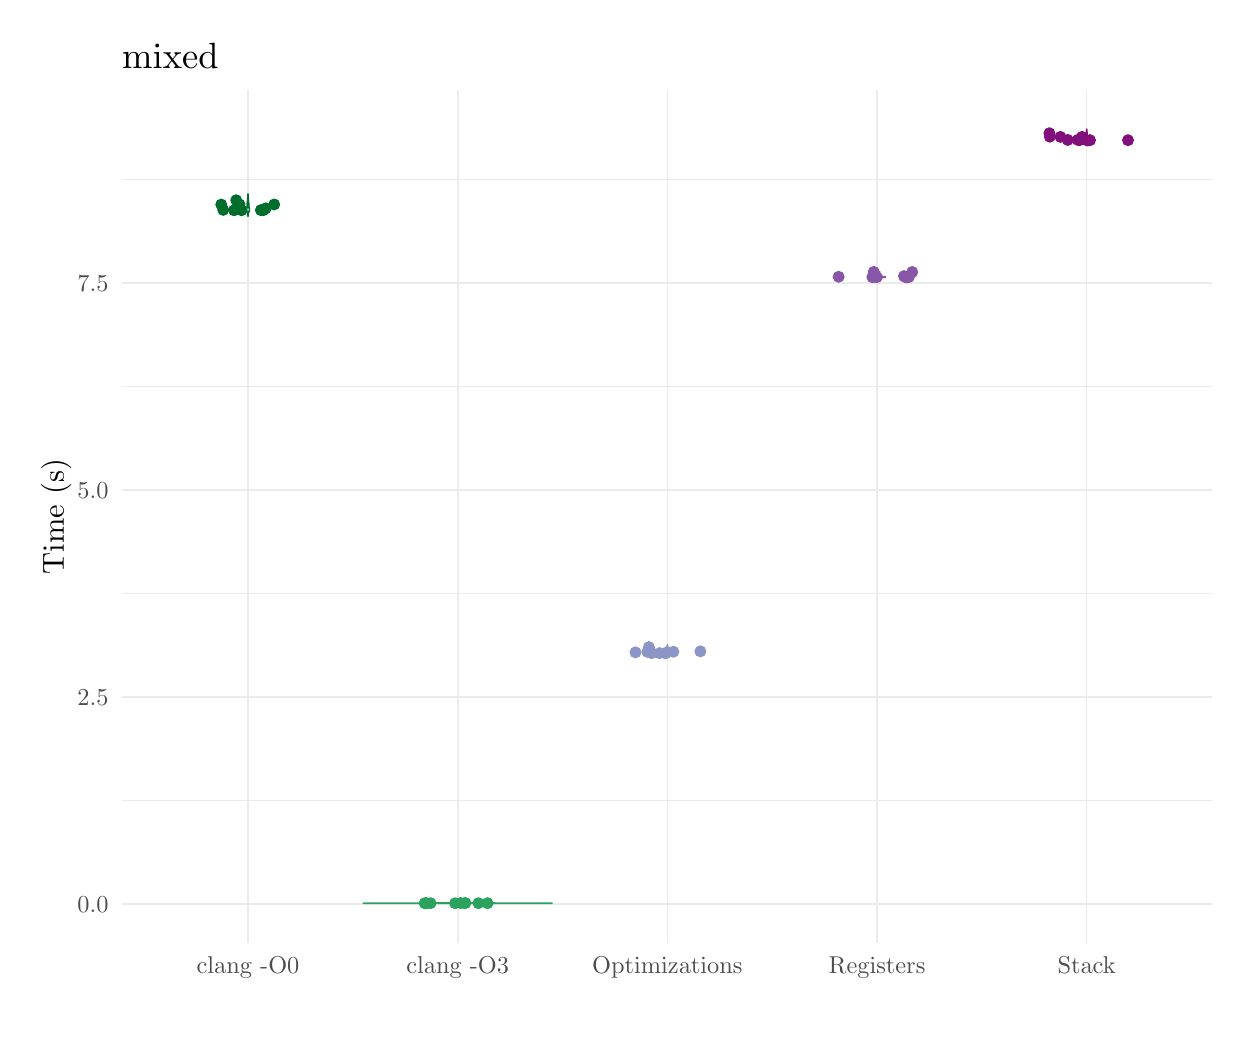
\begin{tikzpicture}[x=1pt,y=1pt]
\definecolor{fillColor}{RGB}{255,255,255}
\path[use as bounding box,fill=fillColor,fill opacity=0.00] (0,0) rectangle (433.62,361.35);
\begin{scope}
\path[clip] ( 34.16, 30.69) rectangle (428.12,338.69);
\definecolor{drawColor}{gray}{0.92}

\path[draw=drawColor,line width= 0.3pt,line join=round] ( 34.16, 82.07) --
	(428.12, 82.07);

\path[draw=drawColor,line width= 0.3pt,line join=round] ( 34.16,156.84) --
	(428.12,156.84);

\path[draw=drawColor,line width= 0.3pt,line join=round] ( 34.16,231.60) --
	(428.12,231.60);

\path[draw=drawColor,line width= 0.3pt,line join=round] ( 34.16,306.37) --
	(428.12,306.37);

\path[draw=drawColor,line width= 0.6pt,line join=round] ( 34.16, 44.69) --
	(428.12, 44.69);

\path[draw=drawColor,line width= 0.6pt,line join=round] ( 34.16,119.45) --
	(428.12,119.45);

\path[draw=drawColor,line width= 0.6pt,line join=round] ( 34.16,194.22) --
	(428.12,194.22);

\path[draw=drawColor,line width= 0.6pt,line join=round] ( 34.16,268.99) --
	(428.12,268.99);

\path[draw=drawColor,line width= 0.6pt,line join=round] ( 79.61, 30.69) --
	( 79.61,338.69);

\path[draw=drawColor,line width= 0.6pt,line join=round] (155.38, 30.69) --
	(155.38,338.69);

\path[draw=drawColor,line width= 0.6pt,line join=round] (231.14, 30.69) --
	(231.14,338.69);

\path[draw=drawColor,line width= 0.6pt,line join=round] (306.90, 30.69) --
	(306.90,338.69);

\path[draw=drawColor,line width= 0.6pt,line join=round] (382.66, 30.69) --
	(382.66,338.69);
\definecolor{drawColor}{RGB}{0,109,44}
\definecolor{fillColor}{RGB}{255,255,255}

\path[draw=drawColor,line width= 0.6pt,line join=round,line cap=round,fill=fillColor] ( 79.61,293.16) --
	( 79.61,293.18) --
	( 79.61,293.19) --
	( 79.61,293.21) --
	( 79.61,293.22) --
	( 79.61,293.24) --
	( 79.61,293.26) --
	( 79.61,293.27) --
	( 79.61,293.29) --
	( 79.61,293.30) --
	( 79.61,293.32) --
	( 79.61,293.34) --
	( 79.60,293.35) --
	( 79.60,293.37) --
	( 79.60,293.38) --
	( 79.60,293.40) --
	( 79.60,293.41) --
	( 79.60,293.43) --
	( 79.60,293.45) --
	( 79.60,293.46) --
	( 79.60,293.48) --
	( 79.60,293.49) --
	( 79.60,293.51) --
	( 79.60,293.52) --
	( 79.60,293.54) --
	( 79.60,293.56) --
	( 79.59,293.57) --
	( 79.59,293.59) --
	( 79.59,293.60) --
	( 79.59,293.62) --
	( 79.59,293.63) --
	( 79.59,293.65) --
	( 79.59,293.67) --
	( 79.59,293.68) --
	( 79.58,293.70) --
	( 79.58,293.71) --
	( 79.58,293.73) --
	( 79.58,293.75) --
	( 79.58,293.76) --
	( 79.58,293.78) --
	( 79.57,293.79) --
	( 79.57,293.81) --
	( 79.57,293.82) --
	( 79.57,293.84) --
	( 79.57,293.86) --
	( 79.56,293.87) --
	( 79.56,293.89) --
	( 79.56,293.90) --
	( 79.56,293.92) --
	( 79.55,293.93) --
	( 79.55,293.95) --
	( 79.55,293.97) --
	( 79.55,293.98) --
	( 79.54,294.00) --
	( 79.54,294.01) --
	( 79.54,294.03) --
	( 79.53,294.04) --
	( 79.53,294.06) --
	( 79.53,294.08) --
	( 79.52,294.09) --
	( 79.52,294.11) --
	( 79.52,294.12) --
	( 79.51,294.14) --
	( 79.51,294.15) --
	( 79.51,294.17) --
	( 79.50,294.19) --
	( 79.50,294.20) --
	( 79.49,294.22) --
	( 79.49,294.23) --
	( 79.48,294.25) --
	( 79.48,294.27) --
	( 79.48,294.28) --
	( 79.47,294.30) --
	( 79.47,294.31) --
	( 79.46,294.33) --
	( 79.46,294.34) --
	( 79.45,294.36) --
	( 79.45,294.38) --
	( 79.44,294.39) --
	( 79.44,294.41) --
	( 79.43,294.42) --
	( 79.42,294.44) --
	( 79.42,294.45) --
	( 79.41,294.47) --
	( 79.41,294.49) --
	( 79.40,294.50) --
	( 79.40,294.52) --
	( 79.39,294.53) --
	( 79.38,294.55) --
	( 79.38,294.56) --
	( 79.37,294.58) --
	( 79.37,294.60) --
	( 79.36,294.61) --
	( 79.35,294.63) --
	( 79.35,294.64) --
	( 79.34,294.66) --
	( 79.33,294.68) --
	( 79.33,294.69) --
	( 79.32,294.71) --
	( 79.32,294.72) --
	( 79.31,294.74) --
	( 79.30,294.75) --
	( 79.30,294.77) --
	( 79.29,294.79) --
	( 79.28,294.80) --
	( 79.28,294.82) --
	( 79.27,294.83) --
	( 79.27,294.85) --
	( 79.26,294.86) --
	( 79.25,294.88) --
	( 79.25,294.90) --
	( 79.24,294.91) --
	( 79.23,294.93) --
	( 79.23,294.94) --
	( 79.22,294.96) --
	( 79.22,294.97) --
	( 79.21,294.99) --
	( 79.21,295.01) --
	( 79.20,295.02) --
	( 79.20,295.04) --
	( 79.19,295.05) --
	( 79.18,295.07) --
	( 79.18,295.08) --
	( 79.17,295.10) --
	( 79.17,295.12) --
	( 79.17,295.13) --
	( 79.16,295.15) --
	( 79.16,295.16) --
	( 79.15,295.18) --
	( 79.15,295.20) --
	( 79.14,295.21) --
	( 79.14,295.23) --
	( 79.14,295.24) --
	( 79.13,295.26) --
	( 79.13,295.27) --
	( 79.13,295.29) --
	( 79.12,295.31) --
	( 79.12,295.32) --
	( 79.12,295.34) --
	( 79.12,295.35) --
	( 79.11,295.37) --
	( 79.11,295.38) --
	( 79.11,295.40) --
	( 79.11,295.42) --
	( 79.11,295.43) --
	( 79.11,295.45) --
	( 79.11,295.46) --
	( 79.10,295.48) --
	( 79.10,295.49) --
	( 79.10,295.51) --
	( 79.10,295.53) --
	( 79.10,295.54) --
	( 79.10,295.56) --
	( 79.10,295.57) --
	( 79.10,295.59) --
	( 79.10,295.61) --
	( 79.11,295.62) --
	( 79.11,295.64) --
	( 79.11,295.65) --
	( 79.11,295.67) --
	( 79.11,295.68) --
	( 79.11,295.70) --
	( 79.11,295.72) --
	( 79.12,295.73) --
	( 79.12,295.75) --
	( 79.12,295.76) --
	( 79.12,295.78) --
	( 79.13,295.79) --
	( 79.13,295.81) --
	( 79.13,295.83) --
	( 79.13,295.84) --
	( 79.14,295.86) --
	( 79.14,295.87) --
	( 79.14,295.89) --
	( 79.15,295.90) --
	( 79.15,295.92) --
	( 79.15,295.94) --
	( 79.16,295.95) --
	( 79.16,295.97) --
	( 79.16,295.98) --
	( 79.17,296.00) --
	( 79.17,296.01) --
	( 79.17,296.03) --
	( 79.18,296.05) --
	( 79.18,296.06) --
	( 79.19,296.08) --
	( 79.19,296.09) --
	( 79.19,296.11) --
	( 79.20,296.13) --
	( 79.20,296.14) --
	( 79.20,296.16) --
	( 79.21,296.17) --
	( 79.21,296.19) --
	( 79.22,296.20) --
	( 79.22,296.22) --
	( 79.22,296.24) --
	( 79.23,296.25) --
	( 79.23,296.27) --
	( 79.23,296.28) --
	( 79.24,296.30) --
	( 79.24,296.31) --
	( 79.24,296.33) --
	( 79.25,296.35) --
	( 79.25,296.36) --
	( 79.25,296.38) --
	( 79.26,296.39) --
	( 79.26,296.41) --
	( 79.26,296.42) --
	( 79.27,296.44) --
	( 79.27,296.46) --
	( 79.27,296.47) --
	( 79.27,296.49) --
	( 79.28,296.50) --
	( 79.28,296.52) --
	( 79.28,296.54) --
	( 79.28,296.55) --
	( 79.29,296.57) --
	( 79.29,296.58) --
	( 79.29,296.60) --
	( 79.29,296.61) --
	( 79.29,296.63) --
	( 79.29,296.65) --
	( 79.30,296.66) --
	( 79.30,296.68) --
	( 79.30,296.69) --
	( 79.30,296.71) --
	( 79.30,296.72) --
	( 79.30,296.74) --
	( 79.30,296.76) --
	( 79.30,296.77) --
	( 79.31,296.79) --
	( 79.31,296.80) --
	( 79.31,296.82) --
	( 79.31,296.83) --
	( 79.31,296.85) --
	( 79.31,296.87) --
	( 79.31,296.88) --
	( 79.31,296.90) --
	( 79.31,296.91) --
	( 79.31,296.93) --
	( 79.31,296.94) --
	( 79.31,296.96) --
	( 79.31,296.98) --
	( 79.31,296.99) --
	( 79.31,297.01) --
	( 79.31,297.02) --
	( 79.31,297.04) --
	( 79.31,297.06) --
	( 79.31,297.07) --
	( 79.31,297.09) --
	( 79.31,297.10) --
	( 79.31,297.12) --
	( 79.31,297.13) --
	( 79.31,297.15) --
	( 79.31,297.17) --
	( 79.31,297.18) --
	( 79.31,297.20) --
	( 79.31,297.21) --
	( 79.31,297.23) --
	( 79.31,297.24) --
	( 79.31,297.26) --
	( 79.31,297.28) --
	( 79.31,297.29) --
	( 79.31,297.31) --
	( 79.31,297.32) --
	( 79.31,297.34) --
	( 79.31,297.35) --
	( 79.31,297.37) --
	( 79.31,297.39) --
	( 79.31,297.40) --
	( 79.32,297.42) --
	( 79.32,297.43) --
	( 79.32,297.45) --
	( 79.32,297.47) --
	( 79.32,297.48) --
	( 79.32,297.50) --
	( 79.32,297.51) --
	( 79.32,297.53) --
	( 79.32,297.54) --
	( 79.32,297.56) --
	( 79.32,297.58) --
	( 79.33,297.59) --
	( 79.33,297.61) --
	( 79.33,297.62) --
	( 79.33,297.64) --
	( 79.33,297.65) --
	( 79.33,297.67) --
	( 79.33,297.69) --
	( 79.34,297.70) --
	( 79.34,297.72) --
	( 79.34,297.73) --
	( 79.34,297.75) --
	( 79.34,297.76) --
	( 79.35,297.78) --
	( 79.35,297.80) --
	( 79.35,297.81) --
	( 79.35,297.83) --
	( 79.35,297.84) --
	( 79.36,297.86) --
	( 79.36,297.88) --
	( 79.36,297.89) --
	( 79.36,297.91) --
	( 79.37,297.92) --
	( 79.37,297.94) --
	( 79.37,297.95) --
	( 79.37,297.97) --
	( 79.37,297.99) --
	( 79.38,298.00) --
	( 79.38,298.02) --
	( 79.38,298.03) --
	( 79.38,298.05) --
	( 79.39,298.06) --
	( 79.39,298.08) --
	( 79.39,298.10) --
	( 79.39,298.11) --
	( 79.40,298.13) --
	( 79.40,298.14) --
	( 79.40,298.16) --
	( 79.40,298.17) --
	( 79.41,298.19) --
	( 79.41,298.21) --
	( 79.41,298.22) --
	( 79.41,298.24) --
	( 79.42,298.25) --
	( 79.42,298.27) --
	( 79.42,298.28) --
	( 79.42,298.30) --
	( 79.43,298.32) --
	( 79.43,298.33) --
	( 79.43,298.35) --
	( 79.43,298.36) --
	( 79.43,298.38) --
	( 79.44,298.40) --
	( 79.44,298.41) --
	( 79.44,298.43) --
	( 79.44,298.44) --
	( 79.44,298.46) --
	( 79.45,298.47) --
	( 79.45,298.49) --
	( 79.45,298.51) --
	( 79.45,298.52) --
	( 79.45,298.54) --
	( 79.46,298.55) --
	( 79.46,298.57) --
	( 79.46,298.58) --
	( 79.46,298.60) --
	( 79.46,298.62) --
	( 79.46,298.63) --
	( 79.47,298.65) --
	( 79.47,298.66) --
	( 79.47,298.68) --
	( 79.47,298.69) --
	( 79.47,298.71) --
	( 79.47,298.73) --
	( 79.48,298.74) --
	( 79.48,298.76) --
	( 79.48,298.77) --
	( 79.48,298.79) --
	( 79.48,298.81) --
	( 79.48,298.82) --
	( 79.48,298.84) --
	( 79.48,298.85) --
	( 79.49,298.87) --
	( 79.49,298.88) --
	( 79.49,298.90) --
	( 79.49,298.92) --
	( 79.49,298.93) --
	( 79.49,298.95) --
	( 79.49,298.96) --
	( 79.50,298.98) --
	( 79.50,298.99) --
	( 79.50,299.01) --
	( 79.50,299.03) --
	( 79.50,299.04) --
	( 79.50,299.06) --
	( 79.50,299.07) --
	( 79.50,299.09) --
	( 79.51,299.10) --
	( 79.51,299.12) --
	( 79.51,299.14) --
	( 79.51,299.15) --
	( 79.51,299.17) --
	( 79.51,299.18) --
	( 79.51,299.20) --
	( 79.51,299.21) --
	( 79.52,299.23) --
	( 79.52,299.25) --
	( 79.52,299.26) --
	( 79.52,299.28) --
	( 79.52,299.29) --
	( 79.52,299.31) --
	( 79.52,299.33) --
	( 79.52,299.34) --
	( 79.53,299.36) --
	( 79.53,299.37) --
	( 79.53,299.39) --
	( 79.53,299.40) --
	( 79.53,299.42) --
	( 79.53,299.44) --
	( 79.53,299.45) --
	( 79.53,299.47) --
	( 79.54,299.48) --
	( 79.54,299.50) --
	( 79.54,299.51) --
	( 79.54,299.53) --
	( 79.54,299.55) --
	( 79.54,299.56) --
	( 79.54,299.58) --
	( 79.55,299.59) --
	( 79.55,299.61) --
	( 79.55,299.62) --
	( 79.55,299.64) --
	( 79.55,299.66) --
	( 79.55,299.67) --
	( 79.55,299.69) --
	( 79.55,299.70) --
	( 79.56,299.72) --
	( 79.56,299.74) --
	( 79.56,299.75) --
	( 79.56,299.77) --
	( 79.56,299.78) --
	( 79.56,299.80) --
	( 79.56,299.81) --
	( 79.56,299.83) --
	( 79.57,299.85) --
	( 79.57,299.86) --
	( 79.57,299.88) --
	( 79.57,299.89) --
	( 79.57,299.91) --
	( 79.57,299.92) --
	( 79.57,299.94) --
	( 79.57,299.96) --
	( 79.58,299.97) --
	( 79.58,299.99) --
	( 79.58,300.00) --
	( 79.58,300.02) --
	( 79.58,300.03) --
	( 79.58,300.05) --
	( 79.58,300.07) --
	( 79.58,300.08) --
	( 79.58,300.10) --
	( 79.58,300.11) --
	( 79.59,300.13) --
	( 79.59,300.14) --
	( 79.59,300.16) --
	( 79.59,300.18) --
	( 79.59,300.19) --
	( 79.59,300.21) --
	( 79.59,300.22) --
	( 79.59,300.24) --
	( 79.59,300.26) --
	( 79.59,300.27) --
	( 79.59,300.29) --
	( 79.59,300.30) --
	( 79.60,300.32) --
	( 79.60,300.33) --
	( 79.60,300.35) --
	( 79.60,300.37) --
	( 79.60,300.38) --
	( 79.60,300.40) --
	( 79.60,300.41) --
	( 79.60,300.43) --
	( 79.60,300.44) --
	( 79.60,300.46) --
	( 79.60,300.48) --
	( 79.60,300.49) --
	( 79.60,300.51) --
	( 79.60,300.52) --
	( 79.60,300.54) --
	( 79.60,300.55) --
	( 79.60,300.57) --
	( 79.60,300.59) --
	( 79.60,300.60) --
	( 79.61,300.62) --
	( 79.61,300.63) --
	( 79.61,300.65) --
	( 79.61,300.67) --
	( 79.61,300.68) --
	( 79.61,300.70) --
	( 79.61,300.71) --
	( 79.61,300.73) --
	( 79.61,300.74) --
	( 79.61,300.76) --
	( 79.61,300.78) --
	( 79.61,300.79) --
	( 79.61,300.81) --
	( 79.61,300.82) --
	( 79.61,300.84) --
	( 79.61,300.85) --
	( 79.61,300.87) --
	( 79.61,300.89) --
	( 79.61,300.90) --
	( 79.61,300.92) --
	( 79.61,300.93) --
	( 79.61,300.95) --
	( 79.61,300.96) --
	( 79.61,300.98) --
	( 79.61,301.00) --
	( 79.61,301.01) --
	( 79.61,301.03) --
	( 79.61,301.04) --
	( 79.61,301.06) --
	( 79.61,301.07) --
	( 79.61,301.09) --
	( 79.61,301.11) --
	( 79.61,301.12) --
	( 79.61,301.14) --
	( 79.61,301.15) --
	( 79.61,301.17) --
	( 79.61,301.19) --
	( 79.61,301.20) --
	( 79.61,301.22) --
	( 79.61,301.22) --
	( 79.61,301.20) --
	( 79.61,301.19) --
	( 79.61,301.17) --
	( 79.61,301.15) --
	( 79.61,301.14) --
	( 79.61,301.12) --
	( 79.61,301.11) --
	( 79.62,301.09) --
	( 79.62,301.07) --
	( 79.62,301.06) --
	( 79.62,301.04) --
	( 79.62,301.03) --
	( 79.62,301.01) --
	( 79.62,301.00) --
	( 79.62,300.98) --
	( 79.62,300.96) --
	( 79.62,300.95) --
	( 79.62,300.93) --
	( 79.62,300.92) --
	( 79.62,300.90) --
	( 79.62,300.89) --
	( 79.62,300.87) --
	( 79.62,300.85) --
	( 79.62,300.84) --
	( 79.62,300.82) --
	( 79.62,300.81) --
	( 79.62,300.79) --
	( 79.62,300.78) --
	( 79.62,300.76) --
	( 79.62,300.74) --
	( 79.62,300.73) --
	( 79.62,300.71) --
	( 79.62,300.70) --
	( 79.62,300.68) --
	( 79.62,300.67) --
	( 79.62,300.65) --
	( 79.62,300.63) --
	( 79.62,300.62) --
	( 79.62,300.60) --
	( 79.62,300.59) --
	( 79.62,300.57) --
	( 79.62,300.55) --
	( 79.62,300.54) --
	( 79.62,300.52) --
	( 79.62,300.51) --
	( 79.63,300.49) --
	( 79.63,300.48) --
	( 79.63,300.46) --
	( 79.63,300.44) --
	( 79.63,300.43) --
	( 79.63,300.41) --
	( 79.63,300.40) --
	( 79.63,300.38) --
	( 79.63,300.37) --
	( 79.63,300.35) --
	( 79.63,300.33) --
	( 79.63,300.32) --
	( 79.63,300.30) --
	( 79.63,300.29) --
	( 79.63,300.27) --
	( 79.63,300.26) --
	( 79.64,300.24) --
	( 79.64,300.22) --
	( 79.64,300.21) --
	( 79.64,300.19) --
	( 79.64,300.18) --
	( 79.64,300.16) --
	( 79.64,300.14) --
	( 79.64,300.13) --
	( 79.64,300.11) --
	( 79.64,300.10) --
	( 79.64,300.08) --
	( 79.65,300.07) --
	( 79.65,300.05) --
	( 79.65,300.03) --
	( 79.65,300.02) --
	( 79.65,300.00) --
	( 79.65,299.99) --
	( 79.65,299.97) --
	( 79.65,299.96) --
	( 79.65,299.94) --
	( 79.66,299.92) --
	( 79.66,299.91) --
	( 79.66,299.89) --
	( 79.66,299.88) --
	( 79.66,299.86) --
	( 79.66,299.85) --
	( 79.66,299.83) --
	( 79.66,299.81) --
	( 79.66,299.80) --
	( 79.67,299.78) --
	( 79.67,299.77) --
	( 79.67,299.75) --
	( 79.67,299.74) --
	( 79.67,299.72) --
	( 79.67,299.70) --
	( 79.67,299.69) --
	( 79.68,299.67) --
	( 79.68,299.66) --
	( 79.68,299.64) --
	( 79.68,299.62) --
	( 79.68,299.61) --
	( 79.68,299.59) --
	( 79.68,299.58) --
	( 79.68,299.56) --
	( 79.69,299.55) --
	( 79.69,299.53) --
	( 79.69,299.51) --
	( 79.69,299.50) --
	( 79.69,299.48) --
	( 79.69,299.47) --
	( 79.69,299.45) --
	( 79.69,299.44) --
	( 79.70,299.42) --
	( 79.70,299.40) --
	( 79.70,299.39) --
	( 79.70,299.37) --
	( 79.70,299.36) --
	( 79.70,299.34) --
	( 79.70,299.33) --
	( 79.71,299.31) --
	( 79.71,299.29) --
	( 79.71,299.28) --
	( 79.71,299.26) --
	( 79.71,299.25) --
	( 79.71,299.23) --
	( 79.71,299.21) --
	( 79.71,299.20) --
	( 79.72,299.18) --
	( 79.72,299.17) --
	( 79.72,299.15) --
	( 79.72,299.14) --
	( 79.72,299.12) --
	( 79.72,299.10) --
	( 79.72,299.09) --
	( 79.72,299.07) --
	( 79.73,299.06) --
	( 79.73,299.04) --
	( 79.73,299.03) --
	( 79.73,299.01) --
	( 79.73,298.99) --
	( 79.73,298.98) --
	( 79.73,298.96) --
	( 79.73,298.95) --
	( 79.74,298.93) --
	( 79.74,298.92) --
	( 79.74,298.90) --
	( 79.74,298.88) --
	( 79.74,298.87) --
	( 79.74,298.85) --
	( 79.74,298.84) --
	( 79.74,298.82) --
	( 79.75,298.81) --
	( 79.75,298.79) --
	( 79.75,298.77) --
	( 79.75,298.76) --
	( 79.75,298.74) --
	( 79.75,298.73) --
	( 79.75,298.71) --
	( 79.76,298.69) --
	( 79.76,298.68) --
	( 79.76,298.66) --
	( 79.76,298.65) --
	( 79.76,298.63) --
	( 79.76,298.62) --
	( 79.77,298.60) --
	( 79.77,298.58) --
	( 79.77,298.57) --
	( 79.77,298.55) --
	( 79.77,298.54) --
	( 79.78,298.52) --
	( 79.78,298.51) --
	( 79.78,298.49) --
	( 79.78,298.47) --
	( 79.78,298.46) --
	( 79.78,298.44) --
	( 79.79,298.43) --
	( 79.79,298.41) --
	( 79.79,298.40) --
	( 79.79,298.38) --
	( 79.80,298.36) --
	( 79.80,298.35) --
	( 79.80,298.33) --
	( 79.80,298.32) --
	( 79.80,298.30) --
	( 79.81,298.28) --
	( 79.81,298.27) --
	( 79.81,298.25) --
	( 79.81,298.24) --
	( 79.82,298.22) --
	( 79.82,298.21) --
	( 79.82,298.19) --
	( 79.82,298.17) --
	( 79.83,298.16) --
	( 79.83,298.14) --
	( 79.83,298.13) --
	( 79.83,298.11) --
	( 79.84,298.10) --
	( 79.84,298.08) --
	( 79.84,298.06) --
	( 79.84,298.05) --
	( 79.84,298.03) --
	( 79.85,298.02) --
	( 79.85,298.00) --
	( 79.85,297.99) --
	( 79.85,297.97) --
	( 79.86,297.95) --
	( 79.86,297.94) --
	( 79.86,297.92) --
	( 79.86,297.91) --
	( 79.87,297.89) --
	( 79.87,297.88) --
	( 79.87,297.86) --
	( 79.87,297.84) --
	( 79.88,297.83) --
	( 79.88,297.81) --
	( 79.88,297.80) --
	( 79.88,297.78) --
	( 79.88,297.76) --
	( 79.89,297.75) --
	( 79.89,297.73) --
	( 79.89,297.72) --
	( 79.89,297.70) --
	( 79.89,297.69) --
	( 79.89,297.67) --
	( 79.90,297.65) --
	( 79.90,297.64) --
	( 79.90,297.62) --
	( 79.90,297.61) --
	( 79.90,297.59) --
	( 79.90,297.58) --
	( 79.90,297.56) --
	( 79.90,297.54) --
	( 79.91,297.53) --
	( 79.91,297.51) --
	( 79.91,297.50) --
	( 79.91,297.48) --
	( 79.91,297.47) --
	( 79.91,297.45) --
	( 79.91,297.43) --
	( 79.91,297.42) --
	( 79.91,297.40) --
	( 79.91,297.39) --
	( 79.91,297.37) --
	( 79.91,297.35) --
	( 79.91,297.34) --
	( 79.91,297.32) --
	( 79.92,297.31) --
	( 79.92,297.29) --
	( 79.92,297.28) --
	( 79.92,297.26) --
	( 79.92,297.24) --
	( 79.92,297.23) --
	( 79.92,297.21) --
	( 79.92,297.20) --
	( 79.92,297.18) --
	( 79.92,297.17) --
	( 79.92,297.15) --
	( 79.92,297.13) --
	( 79.92,297.12) --
	( 79.92,297.10) --
	( 79.92,297.09) --
	( 79.92,297.07) --
	( 79.92,297.06) --
	( 79.92,297.04) --
	( 79.92,297.02) --
	( 79.92,297.01) --
	( 79.92,296.99) --
	( 79.92,296.98) --
	( 79.92,296.96) --
	( 79.92,296.94) --
	( 79.92,296.93) --
	( 79.92,296.91) --
	( 79.92,296.90) --
	( 79.92,296.88) --
	( 79.92,296.87) --
	( 79.92,296.85) --
	( 79.92,296.83) --
	( 79.92,296.82) --
	( 79.92,296.80) --
	( 79.92,296.79) --
	( 79.92,296.77) --
	( 79.92,296.76) --
	( 79.92,296.74) --
	( 79.93,296.72) --
	( 79.93,296.71) --
	( 79.93,296.69) --
	( 79.93,296.68) --
	( 79.93,296.66) --
	( 79.93,296.65) --
	( 79.93,296.63) --
	( 79.94,296.61) --
	( 79.94,296.60) --
	( 79.94,296.58) --
	( 79.94,296.57) --
	( 79.94,296.55) --
	( 79.95,296.54) --
	( 79.95,296.52) --
	( 79.95,296.50) --
	( 79.95,296.49) --
	( 79.96,296.47) --
	( 79.96,296.46) --
	( 79.96,296.44) --
	( 79.96,296.42) --
	( 79.97,296.41) --
	( 79.97,296.39) --
	( 79.97,296.38) --
	( 79.98,296.36) --
	( 79.98,296.35) --
	( 79.98,296.33) --
	( 79.99,296.31) --
	( 79.99,296.30) --
	( 79.99,296.28) --
	( 80.00,296.27) --
	( 80.00,296.25) --
	( 80.00,296.24) --
	( 80.01,296.22) --
	( 80.01,296.20) --
	( 80.01,296.19) --
	( 80.02,296.17) --
	( 80.02,296.16) --
	( 80.03,296.14) --
	( 80.03,296.13) --
	( 80.03,296.11) --
	( 80.04,296.09) --
	( 80.04,296.08) --
	( 80.05,296.06) --
	( 80.05,296.05) --
	( 80.05,296.03) --
	( 80.06,296.01) --
	( 80.06,296.00) --
	( 80.06,295.98) --
	( 80.07,295.97) --
	( 80.07,295.95) --
	( 80.07,295.94) --
	( 80.08,295.92) --
	( 80.08,295.90) --
	( 80.08,295.89) --
	( 80.09,295.87) --
	( 80.09,295.86) --
	( 80.09,295.84) --
	( 80.10,295.83) --
	( 80.10,295.81) --
	( 80.10,295.79) --
	( 80.10,295.78) --
	( 80.11,295.76) --
	( 80.11,295.75) --
	( 80.11,295.73) --
	( 80.11,295.72) --
	( 80.11,295.70) --
	( 80.12,295.68) --
	( 80.12,295.67) --
	( 80.12,295.65) --
	( 80.12,295.64) --
	( 80.12,295.62) --
	( 80.12,295.61) --
	( 80.12,295.59) --
	( 80.12,295.57) --
	( 80.12,295.56) --
	( 80.12,295.54) --
	( 80.12,295.53) --
	( 80.12,295.51) --
	( 80.12,295.49) --
	( 80.12,295.48) --
	( 80.12,295.46) --
	( 80.12,295.45) --
	( 80.12,295.43) --
	( 80.12,295.42) --
	( 80.12,295.40) --
	( 80.11,295.38) --
	( 80.11,295.37) --
	( 80.11,295.35) --
	( 80.11,295.34) --
	( 80.11,295.32) --
	( 80.10,295.31) --
	( 80.10,295.29) --
	( 80.10,295.27) --
	( 80.09,295.26) --
	( 80.09,295.24) --
	( 80.09,295.23) --
	( 80.08,295.21) --
	( 80.08,295.20) --
	( 80.07,295.18) --
	( 80.07,295.16) --
	( 80.07,295.15) --
	( 80.06,295.13) --
	( 80.06,295.12) --
	( 80.05,295.10) --
	( 80.05,295.08) --
	( 80.04,295.07) --
	( 80.04,295.05) --
	( 80.03,295.04) --
	( 80.03,295.02) --
	( 80.02,295.01) --
	( 80.02,294.99) --
	( 80.01,294.97) --
	( 80.00,294.96) --
	( 80.00,294.94) --
	( 79.99,294.93) --
	( 79.99,294.91) --
	( 79.98,294.90) --
	( 79.97,294.88) --
	( 79.97,294.86) --
	( 79.96,294.85) --
	( 79.96,294.83) --
	( 79.95,294.82) --
	( 79.94,294.80) --
	( 79.94,294.79) --
	( 79.93,294.77) --
	( 79.92,294.75) --
	( 79.92,294.74) --
	( 79.91,294.72) --
	( 79.90,294.71) --
	( 79.90,294.69) --
	( 79.89,294.68) --
	( 79.89,294.66) --
	( 79.88,294.64) --
	( 79.87,294.63) --
	( 79.87,294.61) --
	( 79.86,294.60) --
	( 79.85,294.58) --
	( 79.85,294.56) --
	( 79.84,294.55) --
	( 79.84,294.53) --
	( 79.83,294.52) --
	( 79.83,294.50) --
	( 79.82,294.49) --
	( 79.81,294.47) --
	( 79.81,294.45) --
	( 79.80,294.44) --
	( 79.80,294.42) --
	( 79.79,294.41) --
	( 79.79,294.39) --
	( 79.78,294.38) --
	( 79.78,294.36) --
	( 79.77,294.34) --
	( 79.77,294.33) --
	( 79.76,294.31) --
	( 79.76,294.30) --
	( 79.75,294.28) --
	( 79.75,294.27) --
	( 79.74,294.25) --
	( 79.74,294.23) --
	( 79.73,294.22) --
	( 79.73,294.20) --
	( 79.73,294.19) --
	( 79.72,294.17) --
	( 79.72,294.15) --
	( 79.71,294.14) --
	( 79.71,294.12) --
	( 79.71,294.11) --
	( 79.70,294.09) --
	( 79.70,294.08) --
	( 79.70,294.06) --
	( 79.69,294.04) --
	( 79.69,294.03) --
	( 79.69,294.01) --
	( 79.68,294.00) --
	( 79.68,293.98) --
	( 79.68,293.97) --
	( 79.68,293.95) --
	( 79.67,293.93) --
	( 79.67,293.92) --
	( 79.67,293.90) --
	( 79.67,293.89) --
	( 79.66,293.87) --
	( 79.66,293.86) --
	( 79.66,293.84) --
	( 79.66,293.82) --
	( 79.65,293.81) --
	( 79.65,293.79) --
	( 79.65,293.78) --
	( 79.65,293.76) --
	( 79.65,293.75) --
	( 79.65,293.73) --
	( 79.64,293.71) --
	( 79.64,293.70) --
	( 79.64,293.68) --
	( 79.64,293.67) --
	( 79.64,293.65) --
	( 79.64,293.63) --
	( 79.64,293.62) --
	( 79.63,293.60) --
	( 79.63,293.59) --
	( 79.63,293.57) --
	( 79.63,293.56) --
	( 79.63,293.54) --
	( 79.63,293.52) --
	( 79.63,293.51) --
	( 79.63,293.49) --
	( 79.63,293.48) --
	( 79.63,293.46) --
	( 79.63,293.45) --
	( 79.63,293.43) --
	( 79.62,293.41) --
	( 79.62,293.40) --
	( 79.62,293.38) --
	( 79.62,293.37) --
	( 79.62,293.35) --
	( 79.62,293.34) --
	( 79.62,293.32) --
	( 79.62,293.30) --
	( 79.62,293.29) --
	( 79.62,293.27) --
	( 79.62,293.26) --
	( 79.62,293.24) --
	( 79.62,293.22) --
	( 79.62,293.21) --
	( 79.62,293.19) --
	( 79.62,293.18) --
	( 79.62,293.16) --
	( 79.61,293.16) --
	cycle;
\definecolor{drawColor}{RGB}{44,162,95}

\path[draw=drawColor,line width= 0.6pt,line join=round,line cap=round,fill=fillColor] (155.15, 44.93) --
	(155.13, 44.93) --
	(155.10, 44.93) --
	(155.08, 44.93) --
	(155.05, 44.93) --
	(155.02, 44.93) --
	(154.99, 44.93) --
	(154.95, 44.93) --
	(154.92, 44.93) --
	(154.88, 44.93) --
	(154.84, 44.93) --
	(154.79, 44.93) --
	(154.74, 44.93) --
	(154.69, 44.93) --
	(154.63, 44.93) --
	(154.57, 44.93) --
	(154.51, 44.93) --
	(154.44, 44.93) --
	(154.37, 44.93) --
	(154.29, 44.93) --
	(154.21, 44.93) --
	(154.13, 44.93) --
	(154.03, 44.93) --
	(153.94, 44.93) --
	(153.83, 44.93) --
	(153.72, 44.93) --
	(153.61, 44.93) --
	(153.49, 44.93) --
	(153.36, 44.93) --
	(153.23, 44.94) --
	(153.09, 44.94) --
	(152.94, 44.94) --
	(152.78, 44.94) --
	(152.62, 44.94) --
	(152.45, 44.94) --
	(152.27, 44.94) --
	(152.09, 44.94) --
	(151.89, 44.94) --
	(151.69, 44.94) --
	(151.48, 44.94) --
	(151.26, 44.94) --
	(151.04, 44.94) --
	(150.81, 44.94) --
	(150.56, 44.94) --
	(150.31, 44.94) --
	(150.05, 44.94) --
	(149.78, 44.94) --
	(149.51, 44.94) --
	(149.23, 44.94) --
	(148.94, 44.94) --
	(148.64, 44.94) --
	(148.33, 44.94) --
	(148.02, 44.94) --
	(147.70, 44.94) --
	(147.37, 44.94) --
	(147.04, 44.94) --
	(146.70, 44.94) --
	(146.35, 44.94) --
	(146.00, 44.94) --
	(145.65, 44.94) --
	(145.29, 44.94) --
	(144.93, 44.94) --
	(144.56, 44.94) --
	(144.19, 44.94) --
	(143.82, 44.95) --
	(143.45, 44.95) --
	(143.07, 44.95) --
	(142.70, 44.95) --
	(142.33, 44.95) --
	(141.96, 44.95) --
	(141.59, 44.95) --
	(141.22, 44.95) --
	(140.86, 44.95) --
	(140.50, 44.95) --
	(140.14, 44.95) --
	(139.79, 44.95) --
	(139.45, 44.95) --
	(139.11, 44.95) --
	(138.78, 44.95) --
	(138.46, 44.95) --
	(138.15, 44.95) --
	(137.85, 44.95) --
	(137.56, 44.95) --
	(137.28, 44.95) --
	(137.02, 44.95) --
	(136.76, 44.95) --
	(136.52, 44.95) --
	(136.30, 44.95) --
	(136.08, 44.95) --
	(135.88, 44.95) --
	(135.70, 44.95) --
	(135.53, 44.95) --
	(135.38, 44.95) --
	(135.25, 44.95) --
	(135.12, 44.95) --
	(135.02, 44.95) --
	(134.94, 44.95) --
	(134.86, 44.95) --
	(134.81, 44.95) --
	(134.78, 44.96) --
	(134.76, 44.96) --
	(134.75, 44.96) --
	(134.77, 44.96) --
	(134.79, 44.96) --
	(134.84, 44.96) --
	(134.90, 44.96) --
	(134.97, 44.96) --
	(135.06, 44.96) --
	(135.17, 44.96) --
	(135.28, 44.96) --
	(135.41, 44.96) --
	(135.55, 44.96) --
	(135.70, 44.96) --
	(135.86, 44.96) --
	(136.03, 44.96) --
	(136.21, 44.96) --
	(136.40, 44.96) --
	(136.59, 44.96) --
	(136.79, 44.96) --
	(136.99, 44.96) --
	(137.20, 44.96) --
	(137.40, 44.96) --
	(137.61, 44.96) --
	(137.82, 44.96) --
	(138.03, 44.96) --
	(138.24, 44.96) --
	(138.44, 44.96) --
	(138.64, 44.96) --
	(138.83, 44.96) --
	(139.02, 44.96) --
	(139.20, 44.96) --
	(139.37, 44.96) --
	(139.54, 44.96) --
	(139.69, 44.96) --
	(139.82, 44.97) --
	(139.95, 44.97) --
	(140.06, 44.97) --
	(140.16, 44.97) --
	(140.25, 44.97) --
	(140.31, 44.97) --
	(140.36, 44.97) --
	(140.39, 44.97) --
	(140.41, 44.97) --
	(140.40, 44.97) --
	(140.38, 44.97) --
	(140.33, 44.97) --
	(140.27, 44.97) --
	(140.19, 44.97) --
	(140.08, 44.97) --
	(139.95, 44.97) --
	(139.81, 44.97) --
	(139.63, 44.97) --
	(139.44, 44.97) --
	(139.24, 44.97) --
	(139.00, 44.97) --
	(138.75, 44.97) --
	(138.48, 44.97) --
	(138.18, 44.97) --
	(137.87, 44.97) --
	(137.54, 44.97) --
	(137.19, 44.97) --
	(136.82, 44.97) --
	(136.44, 44.97) --
	(136.04, 44.97) --
	(135.62, 44.97) --
	(135.20, 44.97) --
	(134.75, 44.97) --
	(134.30, 44.97) --
	(133.83, 44.98) --
	(133.36, 44.98) --
	(132.88, 44.98) --
	(132.39, 44.98) --
	(131.89, 44.98) --
	(131.39, 44.98) --
	(130.89, 44.98) --
	(130.38, 44.98) --
	(129.88, 44.98) --
	(129.38, 44.98) --
	(128.88, 44.98) --
	(128.38, 44.98) --
	(127.89, 44.98) --
	(127.41, 44.98) --
	(126.93, 44.98) --
	(126.47, 44.98) --
	(126.02, 44.98) --
	(125.58, 44.98) --
	(125.16, 44.98) --
	(124.75, 44.98) --
	(124.35, 44.98) --
	(123.98, 44.98) --
	(123.63, 44.98) --
	(123.29, 44.98) --
	(122.99, 44.98) --
	(122.70, 44.98) --
	(122.43, 44.98) --
	(122.20, 44.98) --
	(121.99, 44.98) --
	(121.80, 44.98) --
	(121.65, 44.98) --
	(121.52, 44.98) --
	(121.41, 44.98) --
	(121.35, 44.98) --
	(121.30, 44.98) --
	(121.28, 44.99) --
	(121.30, 44.99) --
	(121.35, 44.99) --
	(121.42, 44.99) --
	(121.53, 44.99) --
	(121.66, 44.99) --
	(121.82, 44.99) --
	(122.02, 44.99) --
	(122.24, 44.99) --
	(122.49, 44.99) --
	(122.77, 44.99) --
	(123.07, 44.99) --
	(123.39, 44.99) --
	(123.75, 44.99) --
	(124.13, 44.99) --
	(124.53, 44.99) --
	(124.95, 44.99) --
	(125.39, 44.99) --
	(125.86, 44.99) --
	(126.35, 44.99) --
	(126.84, 44.99) --
	(127.36, 44.99) --
	(127.90, 44.99) --
	(128.44, 44.99) --
	(129.01, 44.99) --
	(129.58, 44.99) --
	(130.16, 44.99) --
	(130.75, 44.99) --
	(131.35, 44.99) --
	(131.96, 44.99) --
	(132.57, 44.99) --
	(133.19, 44.99) --
	(133.81, 44.99) --
	(134.43, 44.99) --
	(135.05, 44.99) --
	(135.67, 45.00) --
	(136.29, 45.00) --
	(136.91, 45.00) --
	(137.52, 45.00) --
	(138.13, 45.00) --
	(138.73, 45.00) --
	(139.33, 45.00) --
	(139.92, 45.00) --
	(140.50, 45.00) --
	(141.07, 45.00) --
	(141.63, 45.00) --
	(142.19, 45.00) --
	(142.73, 45.00) --
	(143.26, 45.00) --
	(143.78, 45.00) --
	(144.28, 45.00) --
	(144.78, 45.00) --
	(145.26, 45.00) --
	(145.73, 45.00) --
	(146.18, 45.00) --
	(146.63, 45.00) --
	(147.05, 45.00) --
	(147.47, 45.00) --
	(147.87, 45.00) --
	(148.25, 45.00) --
	(148.63, 45.00) --
	(148.99, 45.00) --
	(149.33, 45.00) --
	(149.66, 45.00) --
	(149.98, 45.00) --
	(150.29, 45.00) --
	(150.58, 45.00) --
	(150.86, 45.00) --
	(151.13, 45.00) --
	(151.38, 45.00) --
	(151.63, 45.01) --
	(151.86, 45.01) --
	(152.08, 45.01) --
	(152.29, 45.01) --
	(152.48, 45.01) --
	(152.67, 45.01) --
	(152.85, 45.01) --
	(153.02, 45.01) --
	(153.18, 45.01) --
	(153.33, 45.01) --
	(153.47, 45.01) --
	(153.60, 45.01) --
	(153.73, 45.01) --
	(153.84, 45.01) --
	(153.95, 45.01) --
	(154.05, 45.01) --
	(154.15, 45.01) --
	(154.24, 45.01) --
	(154.32, 45.01) --
	(154.40, 45.01) --
	(154.47, 45.01) --
	(154.54, 45.01) --
	(154.60, 45.01) --
	(154.66, 45.01) --
	(154.71, 45.01) --
	(154.76, 45.01) --
	(154.80, 45.01) --
	(154.84, 45.01) --
	(154.88, 45.01) --
	(154.91, 45.01) --
	(154.94, 45.01) --
	(154.97, 45.01) --
	(154.99, 45.01) --
	(155.01, 45.01) --
	(155.03, 45.01) --
	(155.04, 45.02) --
	(155.05, 45.02) --
	(155.06, 45.02) --
	(155.07, 45.02) --
	(155.07, 45.02) --
	(155.07, 45.02) --
	(155.07, 45.02) --
	(155.07, 45.02) --
	(155.06, 45.02) --
	(155.05, 45.02) --
	(155.04, 45.02) --
	(155.03, 45.02) --
	(155.01, 45.02) --
	(154.99, 45.02) --
	(154.97, 45.02) --
	(154.95, 45.02) --
	(154.92, 45.02) --
	(154.89, 45.02) --
	(154.86, 45.02) --
	(154.82, 45.02) --
	(154.79, 45.02) --
	(154.75, 45.02) --
	(154.70, 45.02) --
	(154.65, 45.02) --
	(154.60, 45.02) --
	(154.55, 45.02) --
	(154.49, 45.02) --
	(154.43, 45.02) --
	(154.36, 45.02) --
	(154.30, 45.02) --
	(154.22, 45.02) --
	(154.14, 45.02) --
	(154.06, 45.02) --
	(153.97, 45.02) --
	(153.88, 45.02) --
	(153.79, 45.03) --
	(153.69, 45.03) --
	(153.58, 45.03) --
	(153.47, 45.03) --
	(153.35, 45.03) --
	(153.23, 45.03) --
	(153.11, 45.03) --
	(152.97, 45.03) --
	(152.84, 45.03) --
	(152.70, 45.03) --
	(152.55, 45.03) --
	(152.39, 45.03) --
	(152.23, 45.03) --
	(152.07, 45.03) --
	(151.90, 45.03) --
	(151.72, 45.03) --
	(151.54, 45.03) --
	(151.35, 45.03) --
	(151.16, 45.03) --
	(150.97, 45.03) --
	(150.76, 45.03) --
	(150.56, 45.03) --
	(150.35, 45.03) --
	(150.13, 45.03) --
	(149.91, 45.03) --
	(149.68, 45.03) --
	(149.46, 45.03) --
	(149.23, 45.03) --
	(148.99, 45.03) --
	(148.75, 45.03) --
	(148.51, 45.03) --
	(148.27, 45.03) --
	(148.02, 45.03) --
	(147.78, 45.03) --
	(147.53, 45.04) --
	(147.28, 45.04) --
	(147.03, 45.04) --
	(146.78, 45.04) --
	(146.54, 45.04) --
	(146.29, 45.04) --
	(146.05, 45.04) --
	(145.80, 45.04) --
	(145.56, 45.04) --
	(145.33, 45.04) --
	(145.09, 45.04) --
	(144.86, 45.04) --
	(144.64, 45.04) --
	(144.42, 45.04) --
	(144.21, 45.04) --
	(144.00, 45.04) --
	(143.80, 45.04) --
	(143.61, 45.04) --
	(143.42, 45.04) --
	(143.24, 45.04) --
	(143.07, 45.04) --
	(142.91, 45.04) --
	(142.76, 45.04) --
	(142.62, 45.04) --
	(142.49, 45.04) --
	(142.37, 45.04) --
	(142.26, 45.04) --
	(142.16, 45.04) --
	(142.07, 45.04) --
	(142.00, 45.04) --
	(141.94, 45.04) --
	(141.88, 45.04) --
	(141.85, 45.04) --
	(141.82, 45.04) --
	(141.80, 45.04) --
	(141.80, 45.05) --
	(141.81, 45.05) --
	(141.83, 45.05) --
	(141.87, 45.05) --
	(141.91, 45.05) --
	(141.97, 45.05) --
	(142.04, 45.05) --
	(142.13, 45.05) --
	(142.22, 45.05) --
	(142.33, 45.05) --
	(142.44, 45.05) --
	(142.57, 45.05) --
	(142.70, 45.05) --
	(142.85, 45.05) --
	(143.01, 45.05) --
	(143.17, 45.05) --
	(143.35, 45.05) --
	(143.53, 45.05) --
	(143.72, 45.05) --
	(143.92, 45.05) --
	(144.12, 45.05) --
	(144.33, 45.05) --
	(144.55, 45.05) --
	(144.77, 45.05) --
	(145.00, 45.05) --
	(145.23, 45.05) --
	(145.47, 45.05) --
	(145.70, 45.05) --
	(145.95, 45.05) --
	(146.19, 45.05) --
	(146.44, 45.05) --
	(146.68, 45.05) --
	(146.93, 45.05) --
	(147.18, 45.05) --
	(147.43, 45.05) --
	(147.68, 45.06) --
	(147.92, 45.06) --
	(148.17, 45.06) --
	(148.41, 45.06) --
	(148.65, 45.06) --
	(148.89, 45.06) --
	(149.13, 45.06) --
	(149.36, 45.06) --
	(149.59, 45.06) --
	(149.82, 45.06) --
	(150.04, 45.06) --
	(150.26, 45.06) --
	(150.47, 45.06) --
	(150.68, 45.06) --
	(150.88, 45.06) --
	(151.08, 45.06) --
	(151.28, 45.06) --
	(151.47, 45.06) --
	(151.65, 45.06) --
	(151.83, 45.06) --
	(152.00, 45.06) --
	(152.17, 45.06) --
	(152.33, 45.06) --
	(152.48, 45.06) --
	(152.64, 45.06) --
	(152.78, 45.06) --
	(152.92, 45.06) --
	(153.05, 45.06) --
	(153.18, 45.06) --
	(153.31, 45.06) --
	(153.43, 45.06) --
	(153.54, 45.06) --
	(153.65, 45.06) --
	(153.75, 45.06) --
	(153.85, 45.06) --
	(153.94, 45.07) --
	(154.03, 45.07) --
	(154.12, 45.07) --
	(154.20, 45.07) --
	(154.27, 45.07) --
	(154.35, 45.07) --
	(154.42, 45.07) --
	(154.48, 45.07) --
	(154.54, 45.07) --
	(154.60, 45.07) --
	(154.65, 45.07) --
	(154.71, 45.07) --
	(154.75, 45.07) --
	(154.80, 45.07) --
	(154.84, 45.07) --
	(154.88, 45.07) --
	(154.92, 45.07) --
	(154.95, 45.07) --
	(154.98, 45.07) --
	(155.02, 45.07) --
	(155.04, 45.07) --
	(155.07, 45.07) --
	(155.09, 45.07) --
	(155.12, 45.07) --
	(155.14, 45.07) --
	(155.16, 45.07) --
	(155.18, 45.07) --
	(155.19, 45.07) --
	(155.21, 45.07) --
	(155.22, 45.07) --
	(155.53, 45.07) --
	(155.54, 45.07) --
	(155.56, 45.07) --
	(155.58, 45.07) --
	(155.59, 45.07) --
	(155.61, 45.07) --
	(155.63, 45.07) --
	(155.66, 45.07) --
	(155.68, 45.07) --
	(155.71, 45.07) --
	(155.74, 45.07) --
	(155.77, 45.07) --
	(155.80, 45.07) --
	(155.83, 45.07) --
	(155.87, 45.07) --
	(155.91, 45.07) --
	(155.95, 45.07) --
	(156.00, 45.07) --
	(156.05, 45.07) --
	(156.10, 45.07) --
	(156.15, 45.07) --
	(156.21, 45.07) --
	(156.27, 45.07) --
	(156.34, 45.07) --
	(156.40, 45.07) --
	(156.48, 45.07) --
	(156.55, 45.07) --
	(156.63, 45.07) --
	(156.72, 45.07) --
	(156.81, 45.07) --
	(156.90, 45.06) --
	(157.00, 45.06) --
	(157.10, 45.06) --
	(157.21, 45.06) --
	(157.33, 45.06) --
	(157.44, 45.06) --
	(157.57, 45.06) --
	(157.70, 45.06) --
	(157.83, 45.06) --
	(157.97, 45.06) --
	(158.12, 45.06) --
	(158.27, 45.06) --
	(158.42, 45.06) --
	(158.58, 45.06) --
	(158.75, 45.06) --
	(158.92, 45.06) --
	(159.10, 45.06) --
	(159.29, 45.06) --
	(159.47, 45.06) --
	(159.67, 45.06) --
	(159.87, 45.06) --
	(160.07, 45.06) --
	(160.28, 45.06) --
	(160.49, 45.06) --
	(160.71, 45.06) --
	(160.93, 45.06) --
	(161.16, 45.06) --
	(161.39, 45.06) --
	(161.62, 45.06) --
	(161.86, 45.06) --
	(162.10, 45.06) --
	(162.34, 45.06) --
	(162.58, 45.06) --
	(162.83, 45.06) --
	(163.08, 45.06) --
	(163.32, 45.05) --
	(163.57, 45.05) --
	(163.82, 45.05) --
	(164.07, 45.05) --
	(164.32, 45.05) --
	(164.56, 45.05) --
	(164.81, 45.05) --
	(165.05, 45.05) --
	(165.29, 45.05) --
	(165.52, 45.05) --
	(165.75, 45.05) --
	(165.98, 45.05) --
	(166.20, 45.05) --
	(166.42, 45.05) --
	(166.63, 45.05) --
	(166.84, 45.05) --
	(167.03, 45.05) --
	(167.22, 45.05) --
	(167.41, 45.05) --
	(167.58, 45.05) --
	(167.75, 45.05) --
	(167.90, 45.05) --
	(168.05, 45.05) --
	(168.19, 45.05) --
	(168.31, 45.05) --
	(168.43, 45.05) --
	(168.53, 45.05) --
	(168.63, 45.05) --
	(168.71, 45.05) --
	(168.78, 45.05) --
	(168.84, 45.05) --
	(168.88, 45.05) --
	(168.92, 45.05) --
	(168.94, 45.05) --
	(168.95, 45.05) --
	(168.95, 45.04) --
	(168.93, 45.04) --
	(168.90, 45.04) --
	(168.87, 45.04) --
	(168.81, 45.04) --
	(168.75, 45.04) --
	(168.68, 45.04) --
	(168.59, 45.04) --
	(168.49, 45.04) --
	(168.38, 45.04) --
	(168.26, 45.04) --
	(168.13, 45.04) --
	(167.99, 45.04) --
	(167.84, 45.04) --
	(167.68, 45.04) --
	(167.51, 45.04) --
	(167.33, 45.04) --
	(167.15, 45.04) --
	(166.95, 45.04) --
	(166.75, 45.04) --
	(166.54, 45.04) --
	(166.33, 45.04) --
	(166.11, 45.04) --
	(165.89, 45.04) --
	(165.66, 45.04) --
	(165.42, 45.04) --
	(165.19, 45.04) --
	(164.95, 45.04) --
	(164.71, 45.04) --
	(164.46, 45.04) --
	(164.21, 45.04) --
	(163.97, 45.04) --
	(163.72, 45.04) --
	(163.47, 45.04) --
	(163.22, 45.04) --
	(162.97, 45.03) --
	(162.73, 45.03) --
	(162.48, 45.03) --
	(162.24, 45.03) --
	(162.00, 45.03) --
	(161.76, 45.03) --
	(161.53, 45.03) --
	(161.30, 45.03) --
	(161.07, 45.03) --
	(160.84, 45.03) --
	(160.62, 45.03) --
	(160.41, 45.03) --
	(160.19, 45.03) --
	(159.99, 45.03) --
	(159.79, 45.03) --
	(159.59, 45.03) --
	(159.40, 45.03) --
	(159.21, 45.03) --
	(159.03, 45.03) --
	(158.85, 45.03) --
	(158.68, 45.03) --
	(158.52, 45.03) --
	(158.36, 45.03) --
	(158.21, 45.03) --
	(158.06, 45.03) --
	(157.91, 45.03) --
	(157.78, 45.03) --
	(157.64, 45.03) --
	(157.52, 45.03) --
	(157.40, 45.03) --
	(157.28, 45.03) --
	(157.17, 45.03) --
	(157.07, 45.03) --
	(156.96, 45.03) --
	(156.87, 45.02) --
	(156.78, 45.02) --
	(156.69, 45.02) --
	(156.61, 45.02) --
	(156.53, 45.02) --
	(156.46, 45.02) --
	(156.39, 45.02) --
	(156.32, 45.02) --
	(156.26, 45.02) --
	(156.20, 45.02) --
	(156.15, 45.02) --
	(156.10, 45.02) --
	(156.05, 45.02) --
	(156.00, 45.02) --
	(155.96, 45.02) --
	(155.93, 45.02) --
	(155.89, 45.02) --
	(155.86, 45.02) --
	(155.83, 45.02) --
	(155.80, 45.02) --
	(155.78, 45.02) --
	(155.76, 45.02) --
	(155.74, 45.02) --
	(155.73, 45.02) --
	(155.71, 45.02) --
	(155.70, 45.02) --
	(155.69, 45.02) --
	(155.69, 45.02) --
	(155.68, 45.02) --
	(155.68, 45.02) --
	(155.68, 45.02) --
	(155.68, 45.02) --
	(155.69, 45.02) --
	(155.70, 45.02) --
	(155.71, 45.02) --
	(155.73, 45.01) --
	(155.74, 45.01) --
	(155.76, 45.01) --
	(155.78, 45.01) --
	(155.81, 45.01) --
	(155.84, 45.01) --
	(155.87, 45.01) --
	(155.91, 45.01) --
	(155.95, 45.01) --
	(155.99, 45.01) --
	(156.04, 45.01) --
	(156.09, 45.01) --
	(156.15, 45.01) --
	(156.21, 45.01) --
	(156.28, 45.01) --
	(156.35, 45.01) --
	(156.43, 45.01) --
	(156.51, 45.01) --
	(156.60, 45.01) --
	(156.70, 45.01) --
	(156.80, 45.01) --
	(156.91, 45.01) --
	(157.03, 45.01) --
	(157.15, 45.01) --
	(157.29, 45.01) --
	(157.42, 45.01) --
	(157.58, 45.01) --
	(157.73, 45.01) --
	(157.90, 45.01) --
	(158.08, 45.01) --
	(158.27, 45.01) --
	(158.46, 45.01) --
	(158.68, 45.01) --
	(158.90, 45.01) --
	(159.13, 45.01) --
	(159.37, 45.00) --
	(159.63, 45.00) --
	(159.89, 45.00) --
	(160.17, 45.00) --
	(160.46, 45.00) --
	(160.77, 45.00) --
	(161.09, 45.00) --
	(161.42, 45.00) --
	(161.76, 45.00) --
	(162.13, 45.00) --
	(162.50, 45.00) --
	(162.88, 45.00) --
	(163.29, 45.00) --
	(163.70, 45.00) --
	(164.13, 45.00) --
	(164.57, 45.00) --
	(165.02, 45.00) --
	(165.49, 45.00) --
	(165.97, 45.00) --
	(166.47, 45.00) --
	(166.97, 45.00) --
	(167.49, 45.00) --
	(168.02, 45.00) --
	(168.57, 45.00) --
	(169.12, 45.00) --
	(169.68, 45.00) --
	(170.25, 45.00) --
	(170.83, 45.00) --
	(171.42, 45.00) --
	(172.02, 45.00) --
	(172.62, 45.00) --
	(173.23, 45.00) --
	(173.84, 45.00) --
	(174.46, 45.00) --
	(175.08, 45.00) --
	(175.70, 44.99) --
	(176.32, 44.99) --
	(176.94, 44.99) --
	(177.56, 44.99) --
	(178.18, 44.99) --
	(178.79, 44.99) --
	(179.40, 44.99) --
	(180.00, 44.99) --
	(180.59, 44.99) --
	(181.17, 44.99) --
	(181.74, 44.99) --
	(182.31, 44.99) --
	(182.85, 44.99) --
	(183.39, 44.99) --
	(183.91, 44.99) --
	(184.41, 44.99) --
	(184.89, 44.99) --
	(185.36, 44.99) --
	(185.80, 44.99) --
	(186.22, 44.99) --
	(186.63, 44.99) --
	(187.00, 44.99) --
	(187.36, 44.99) --
	(187.69, 44.99) --
	(187.98, 44.99) --
	(188.26, 44.99) --
	(188.51, 44.99) --
	(188.73, 44.99) --
	(188.93, 44.99) --
	(189.09, 44.99) --
	(189.22, 44.99) --
	(189.33, 44.99) --
	(189.40, 44.99) --
	(189.45, 44.99) --
	(189.47, 44.99) --
	(189.45, 44.98) --
	(189.41, 44.98) --
	(189.34, 44.98) --
	(189.23, 44.98) --
	(189.10, 44.98) --
	(188.95, 44.98) --
	(188.76, 44.98) --
	(188.55, 44.98) --
	(188.32, 44.98) --
	(188.05, 44.98) --
	(187.76, 44.98) --
	(187.46, 44.98) --
	(187.12, 44.98) --
	(186.77, 44.98) --
	(186.40, 44.98) --
	(186.00, 44.98) --
	(185.60, 44.98) --
	(185.17, 44.98) --
	(184.73, 44.98) --
	(184.28, 44.98) --
	(183.82, 44.98) --
	(183.34, 44.98) --
	(182.86, 44.98) --
	(182.37, 44.98) --
	(181.87, 44.98) --
	(181.37, 44.98) --
	(180.87, 44.98) --
	(180.37, 44.98) --
	(179.86, 44.98) --
	(179.36, 44.98) --
	(178.86, 44.98) --
	(178.36, 44.98) --
	(177.87, 44.98) --
	(177.39, 44.98) --
	(176.92, 44.98) --
	(176.45, 44.97) --
	(176.00, 44.97) --
	(175.56, 44.97) --
	(175.13, 44.97) --
	(174.71, 44.97) --
	(174.31, 44.97) --
	(173.93, 44.97) --
	(173.56, 44.97) --
	(173.21, 44.97) --
	(172.88, 44.97) --
	(172.57, 44.97) --
	(172.27, 44.97) --
	(172.00, 44.97) --
	(171.75, 44.97) --
	(171.52, 44.97) --
	(171.31, 44.97) --
	(171.12, 44.97) --
	(170.94, 44.97) --
	(170.80, 44.97) --
	(170.67, 44.97) --
	(170.56, 44.97) --
	(170.48, 44.97) --
	(170.42, 44.97) --
	(170.37, 44.97) --
	(170.35, 44.97) --
	(170.35, 44.97) --
	(170.36, 44.97) --
	(170.39, 44.97) --
	(170.44, 44.97) --
	(170.51, 44.97) --
	(170.59, 44.97) --
	(170.69, 44.97) --
	(170.80, 44.97) --
	(170.93, 44.97) --
	(171.07, 44.96) --
	(171.22, 44.96) --
	(171.38, 44.96) --
	(171.55, 44.96) --
	(171.73, 44.96) --
	(171.92, 44.96) --
	(172.11, 44.96) --
	(172.31, 44.96) --
	(172.51, 44.96) --
	(172.72, 44.96) --
	(172.93, 44.96) --
	(173.14, 44.96) --
	(173.35, 44.96) --
	(173.56, 44.96) --
	(173.76, 44.96) --
	(173.97, 44.96) --
	(174.16, 44.96) --
	(174.35, 44.96) --
	(174.54, 44.96) --
	(174.72, 44.96) --
	(174.89, 44.96) --
	(175.05, 44.96) --
	(175.20, 44.96) --
	(175.34, 44.96) --
	(175.47, 44.96) --
	(175.58, 44.96) --
	(175.69, 44.96) --
	(175.78, 44.96) --
	(175.85, 44.96) --
	(175.91, 44.96) --
	(175.96, 44.96) --
	(175.98, 44.96) --
	(176.00, 44.96) --
	(176.00, 44.96) --
	(175.97, 44.96) --
	(175.94, 44.95) --
	(175.89, 44.95) --
	(175.81, 44.95) --
	(175.73, 44.95) --
	(175.63, 44.95) --
	(175.50, 44.95) --
	(175.37, 44.95) --
	(175.22, 44.95) --
	(175.05, 44.95) --
	(174.87, 44.95) --
	(174.67, 44.95) --
	(174.45, 44.95) --
	(174.23, 44.95) --
	(173.99, 44.95) --
	(173.73, 44.95) --
	(173.47, 44.95) --
	(173.19, 44.95) --
	(172.90, 44.95) --
	(172.60, 44.95) --
	(172.29, 44.95) --
	(171.97, 44.95) --
	(171.64, 44.95) --
	(171.30, 44.95) --
	(170.96, 44.95) --
	(170.61, 44.95) --
	(170.26, 44.95) --
	(169.90, 44.95) --
	(169.53, 44.95) --
	(169.16, 44.95) --
	(168.79, 44.95) --
	(168.42, 44.95) --
	(168.05, 44.95) --
	(167.68, 44.95) --
	(167.30, 44.95) --
	(166.93, 44.95) --
	(166.56, 44.94) --
	(166.19, 44.94) --
	(165.83, 44.94) --
	(165.46, 44.94) --
	(165.10, 44.94) --
	(164.75, 44.94) --
	(164.40, 44.94) --
	(164.05, 44.94) --
	(163.71, 44.94) --
	(163.38, 44.94) --
	(163.05, 44.94) --
	(162.73, 44.94) --
	(162.42, 44.94) --
	(162.11, 44.94) --
	(161.82, 44.94) --
	(161.52, 44.94) --
	(161.24, 44.94) --
	(160.97, 44.94) --
	(160.70, 44.94) --
	(160.44, 44.94) --
	(160.19, 44.94) --
	(159.95, 44.94) --
	(159.71, 44.94) --
	(159.49, 44.94) --
	(159.27, 44.94) --
	(159.06, 44.94) --
	(158.86, 44.94) --
	(158.66, 44.94) --
	(158.48, 44.94) --
	(158.30, 44.94) --
	(158.13, 44.94) --
	(157.97, 44.94) --
	(157.81, 44.94) --
	(157.66, 44.94) --
	(157.52, 44.94) --
	(157.39, 44.93) --
	(157.26, 44.93) --
	(157.14, 44.93) --
	(157.03, 44.93) --
	(156.92, 44.93) --
	(156.82, 44.93) --
	(156.72, 44.93) --
	(156.63, 44.93) --
	(156.54, 44.93) --
	(156.46, 44.93) --
	(156.38, 44.93) --
	(156.31, 44.93) --
	(156.24, 44.93) --
	(156.18, 44.93) --
	(156.12, 44.93) --
	(156.06, 44.93) --
	(156.01, 44.93) --
	(155.96, 44.93) --
	(155.92, 44.93) --
	(155.87, 44.93) --
	(155.83, 44.93) --
	(155.80, 44.93) --
	(155.76, 44.93) --
	(155.73, 44.93) --
	(155.70, 44.93) --
	(155.67, 44.93) --
	(155.65, 44.93) --
	(155.63, 44.93) --
	(155.60, 44.93) --
	(155.15, 44.93) --
	cycle;
\definecolor{drawColor}{RGB}{140,150,198}

\path[draw=drawColor,line width= 0.6pt,line join=round,line cap=round,fill=fillColor] (231.13,134.52) --
	(231.13,134.53) --
	(231.13,134.54) --
	(231.13,134.55) --
	(231.13,134.55) --
	(231.13,134.56) --
	(231.12,134.57) --
	(231.12,134.58) --
	(231.12,134.58) --
	(231.12,134.59) --
	(231.12,134.60) --
	(231.12,134.61) --
	(231.12,134.61) --
	(231.11,134.62) --
	(231.11,134.63) --
	(231.11,134.64) --
	(231.11,134.64) --
	(231.11,134.65) --
	(231.10,134.66) --
	(231.10,134.66) --
	(231.10,134.67) --
	(231.09,134.68) --
	(231.09,134.69) --
	(231.09,134.69) --
	(231.08,134.70) --
	(231.08,134.71) --
	(231.08,134.72) --
	(231.07,134.72) --
	(231.07,134.73) --
	(231.06,134.74) --
	(231.06,134.75) --
	(231.05,134.75) --
	(231.05,134.76) --
	(231.04,134.77) --
	(231.04,134.78) --
	(231.03,134.78) --
	(231.02,134.79) --
	(231.02,134.80) --
	(231.01,134.80) --
	(231.00,134.81) --
	(230.99,134.82) --
	(230.99,134.83) --
	(230.98,134.83) --
	(230.97,134.84) --
	(230.96,134.85) --
	(230.95,134.86) --
	(230.94,134.86) --
	(230.93,134.87) --
	(230.92,134.88) --
	(230.91,134.89) --
	(230.89,134.89) --
	(230.88,134.90) --
	(230.87,134.91) --
	(230.86,134.92) --
	(230.84,134.92) --
	(230.83,134.93) --
	(230.82,134.94) --
	(230.80,134.95) --
	(230.79,134.95) --
	(230.77,134.96) --
	(230.76,134.97) --
	(230.74,134.97) --
	(230.72,134.98) --
	(230.71,134.99) --
	(230.69,135.00) --
	(230.67,135.00) --
	(230.66,135.01) --
	(230.64,135.02) --
	(230.62,135.03) --
	(230.60,135.03) --
	(230.59,135.04) --
	(230.57,135.05) --
	(230.55,135.06) --
	(230.53,135.06) --
	(230.51,135.07) --
	(230.49,135.08) --
	(230.47,135.09) --
	(230.45,135.09) --
	(230.43,135.10) --
	(230.41,135.11) --
	(230.39,135.11) --
	(230.37,135.12) --
	(230.35,135.13) --
	(230.34,135.14) --
	(230.32,135.14) --
	(230.30,135.15) --
	(230.28,135.16) --
	(230.26,135.17) --
	(230.24,135.17) --
	(230.22,135.18) --
	(230.20,135.19) --
	(230.18,135.20) --
	(230.17,135.20) --
	(230.15,135.21) --
	(230.13,135.22) --
	(230.12,135.23) --
	(230.10,135.23) --
	(230.08,135.24) --
	(230.07,135.25) --
	(230.05,135.26) --
	(230.04,135.26) --
	(230.02,135.27) --
	(230.01,135.28) --
	(229.99,135.28) --
	(229.98,135.29) --
	(229.97,135.30) --
	(229.96,135.31) --
	(229.95,135.31) --
	(229.93,135.32) --
	(229.92,135.33) --
	(229.91,135.34) --
	(229.90,135.34) --
	(229.89,135.35) --
	(229.89,135.36) --
	(229.88,135.37) --
	(229.87,135.37) --
	(229.86,135.38) --
	(229.86,135.39) --
	(229.85,135.40) --
	(229.84,135.40) --
	(229.84,135.41) --
	(229.83,135.42) --
	(229.83,135.42) --
	(229.82,135.43) --
	(229.82,135.44) --
	(229.82,135.45) --
	(229.81,135.45) --
	(229.81,135.46) --
	(229.81,135.47) --
	(229.81,135.48) --
	(229.81,135.48) --
	(229.80,135.49) --
	(229.80,135.50) --
	(229.80,135.51) --
	(229.80,135.51) --
	(229.80,135.52) --
	(229.80,135.53) --
	(229.80,135.54) --
	(229.80,135.54) --
	(229.80,135.55) --
	(229.80,135.56) --
	(229.80,135.57) --
	(229.80,135.57) --
	(229.80,135.58) --
	(229.80,135.59) --
	(229.80,135.59) --
	(229.80,135.60) --
	(229.81,135.61) --
	(229.81,135.62) --
	(229.81,135.62) --
	(229.81,135.63) --
	(229.81,135.64) --
	(229.81,135.65) --
	(229.81,135.65) --
	(229.81,135.66) --
	(229.82,135.67) --
	(229.82,135.68) --
	(229.82,135.68) --
	(229.82,135.69) --
	(229.82,135.70) --
	(229.82,135.71) --
	(229.83,135.71) --
	(229.83,135.72) --
	(229.83,135.73) --
	(229.83,135.73) --
	(229.84,135.74) --
	(229.84,135.75) --
	(229.84,135.76) --
	(229.84,135.76) --
	(229.85,135.77) --
	(229.85,135.78) --
	(229.86,135.79) --
	(229.86,135.79) --
	(229.86,135.80) --
	(229.87,135.81) --
	(229.87,135.82) --
	(229.88,135.82) --
	(229.88,135.83) --
	(229.89,135.84) --
	(229.90,135.85) --
	(229.90,135.85) --
	(229.91,135.86) --
	(229.92,135.87) --
	(229.93,135.88) --
	(229.93,135.88) --
	(229.94,135.89) --
	(229.95,135.90) --
	(229.96,135.90) --
	(229.97,135.91) --
	(229.98,135.92) --
	(229.99,135.93) --
	(230.00,135.93) --
	(230.01,135.94) --
	(230.02,135.95) --
	(230.04,135.96) --
	(230.05,135.96) --
	(230.06,135.97) --
	(230.07,135.98) --
	(230.09,135.99) --
	(230.10,135.99) --
	(230.12,136.00) --
	(230.13,136.01) --
	(230.14,136.02) --
	(230.16,136.02) --
	(230.18,136.03) --
	(230.19,136.04) --
	(230.21,136.04) --
	(230.22,136.05) --
	(230.24,136.06) --
	(230.26,136.07) --
	(230.27,136.07) --
	(230.29,136.08) --
	(230.31,136.09) --
	(230.33,136.10) --
	(230.34,136.10) --
	(230.36,136.11) --
	(230.38,136.12) --
	(230.40,136.13) --
	(230.41,136.13) --
	(230.43,136.14) --
	(230.45,136.15) --
	(230.47,136.16) --
	(230.48,136.16) --
	(230.50,136.17) --
	(230.52,136.18) --
	(230.54,136.19) --
	(230.55,136.19) --
	(230.57,136.20) --
	(230.59,136.21) --
	(230.61,136.21) --
	(230.62,136.22) --
	(230.64,136.23) --
	(230.66,136.24) --
	(230.67,136.24) --
	(230.69,136.25) --
	(230.70,136.26) --
	(230.72,136.27) --
	(230.73,136.27) --
	(230.75,136.28) --
	(230.76,136.29) --
	(230.78,136.30) --
	(230.79,136.30) --
	(230.81,136.31) --
	(230.82,136.32) --
	(230.83,136.33) --
	(230.85,136.33) --
	(230.86,136.34) --
	(230.87,136.35) --
	(230.88,136.35) --
	(230.89,136.36) --
	(230.90,136.37) --
	(230.91,136.38) --
	(230.92,136.38) --
	(230.93,136.39) --
	(230.94,136.40) --
	(230.95,136.41) --
	(230.96,136.41) --
	(230.97,136.42) --
	(230.98,136.43) --
	(230.99,136.44) --
	(231.00,136.44) --
	(231.00,136.45) --
	(231.01,136.46) --
	(231.02,136.47) --
	(231.02,136.47) --
	(231.03,136.48) --
	(231.04,136.49) --
	(231.04,136.50) --
	(231.05,136.50) --
	(231.05,136.51) --
	(231.06,136.52) --
	(231.06,136.52) --
	(231.07,136.53) --
	(231.07,136.54) --
	(231.08,136.55) --
	(231.08,136.55) --
	(231.08,136.56) --
	(231.09,136.57) --
	(231.09,136.58) --
	(231.09,136.58) --
	(231.10,136.59) --
	(231.10,136.60) --
	(231.10,136.61) --
	(231.10,136.61) --
	(231.11,136.62) --
	(231.11,136.63) --
	(231.11,136.64) --
	(231.11,136.64) --
	(231.11,136.65) --
	(231.12,136.66) --
	(231.12,136.66) --
	(231.12,136.67) --
	(231.12,136.68) --
	(231.12,136.69) --
	(231.12,136.69) --
	(231.12,136.70) --
	(231.12,136.71) --
	(231.12,136.72) --
	(231.12,136.72) --
	(231.13,136.73) --
	(231.13,136.74) --
	(231.13,136.75) --
	(231.13,136.75) --
	(231.13,136.76) --
	(231.13,136.77) --
	(231.13,136.78) --
	(231.13,136.78) --
	(231.13,136.79) --
	(231.13,136.80) --
	(231.13,136.81) --
	(231.13,136.81) --
	(231.13,136.82) --
	(231.13,136.83) --
	(231.13,136.83) --
	(231.13,136.84) --
	(231.13,136.85) --
	(231.13,136.86) --
	(231.13,136.86) --
	(231.12,136.87) --
	(231.12,136.88) --
	(231.12,136.89) --
	(231.12,136.89) --
	(231.12,136.90) --
	(231.12,136.91) --
	(231.12,136.92) --
	(231.12,136.92) --
	(231.12,136.93) --
	(231.12,136.94) --
	(231.12,136.95) --
	(231.11,136.95) --
	(231.11,136.96) --
	(231.11,136.97) --
	(231.11,136.98) --
	(231.11,136.98) --
	(231.11,136.99) --
	(231.10,137.00) --
	(231.10,137.00) --
	(231.10,137.01) --
	(231.10,137.02) --
	(231.10,137.03) --
	(231.09,137.03) --
	(231.09,137.04) --
	(231.09,137.05) --
	(231.09,137.06) --
	(231.08,137.06) --
	(231.08,137.07) --
	(231.08,137.08) --
	(231.08,137.09) --
	(231.07,137.09) --
	(231.07,137.10) --
	(231.07,137.11) --
	(231.06,137.12) --
	(231.06,137.12) --
	(231.06,137.13) --
	(231.05,137.14) --
	(231.05,137.14) --
	(231.05,137.15) --
	(231.04,137.16) --
	(231.04,137.17) --
	(231.03,137.17) --
	(231.03,137.18) --
	(231.03,137.19) --
	(231.02,137.20) --
	(231.02,137.20) --
	(231.01,137.21) --
	(231.01,137.22) --
	(231.01,137.23) --
	(231.00,137.23) --
	(231.00,137.24) --
	(230.99,137.25) --
	(230.99,137.26) --
	(230.98,137.26) --
	(230.98,137.27) --
	(230.98,137.28) --
	(230.97,137.29) --
	(230.97,137.29) --
	(230.96,137.30) --
	(230.96,137.31) --
	(230.95,137.31) --
	(230.95,137.32) --
	(230.95,137.33) --
	(230.94,137.34) --
	(230.94,137.34) --
	(230.94,137.35) --
	(230.93,137.36) --
	(230.93,137.37) --
	(230.92,137.37) --
	(230.92,137.38) --
	(230.92,137.39) --
	(230.92,137.40) --
	(230.91,137.40) --
	(230.91,137.41) --
	(230.91,137.42) --
	(230.90,137.43) --
	(230.90,137.43) --
	(230.90,137.44) --
	(230.90,137.45) --
	(230.90,137.45) --
	(230.90,137.46) --
	(230.89,137.47) --
	(230.89,137.48) --
	(230.89,137.48) --
	(230.89,137.49) --
	(230.89,137.50) --
	(230.89,137.51) --
	(230.89,137.51) --
	(230.89,137.52) --
	(230.89,137.53) --
	(230.89,137.54) --
	(230.89,137.54) --
	(230.89,137.55) --
	(230.89,137.56) --
	(230.89,137.57) --
	(230.90,137.57) --
	(230.90,137.58) --
	(230.90,137.59) --
	(230.90,137.60) --
	(230.90,137.60) --
	(230.91,137.61) --
	(230.91,137.62) --
	(230.91,137.62) --
	(230.91,137.63) --
	(230.92,137.64) --
	(230.92,137.65) --
	(230.92,137.65) --
	(230.93,137.66) --
	(230.93,137.67) --
	(230.93,137.68) --
	(230.94,137.68) --
	(230.94,137.69) --
	(230.94,137.70) --
	(230.95,137.71) --
	(230.95,137.71) --
	(230.96,137.72) --
	(230.96,137.73) --
	(230.96,137.74) --
	(230.97,137.74) --
	(230.97,137.75) --
	(230.98,137.76) --
	(230.98,137.76) --
	(230.98,137.77) --
	(230.99,137.78) --
	(230.99,137.79) --
	(231.00,137.79) --
	(231.00,137.80) --
	(231.01,137.81) --
	(231.01,137.82) --
	(231.01,137.82) --
	(231.02,137.83) --
	(231.02,137.84) --
	(231.03,137.85) --
	(231.03,137.85) --
	(231.03,137.86) --
	(231.04,137.87) --
	(231.04,137.88) --
	(231.05,137.88) --
	(231.05,137.89) --
	(231.05,137.90) --
	(231.06,137.91) --
	(231.06,137.91) --
	(231.06,137.92) --
	(231.07,137.93) --
	(231.07,137.93) --
	(231.07,137.94) --
	(231.08,137.95) --
	(231.08,137.96) --
	(231.08,137.96) --
	(231.08,137.97) --
	(231.09,137.98) --
	(231.09,137.99) --
	(231.09,137.99) --
	(231.09,138.00) --
	(231.10,138.01) --
	(231.10,138.02) --
	(231.10,138.02) --
	(231.10,138.03) --
	(231.10,138.04) --
	(231.11,138.05) --
	(231.11,138.05) --
	(231.11,138.06) --
	(231.11,138.07) --
	(231.11,138.07) --
	(231.11,138.08) --
	(231.12,138.09) --
	(231.12,138.10) --
	(231.12,138.10) --
	(231.12,138.11) --
	(231.12,138.12) --
	(231.12,138.13) --
	(231.12,138.13) --
	(231.12,138.14) --
	(231.13,138.15) --
	(231.13,138.16) --
	(231.13,138.16) --
	(231.13,138.17) --
	(231.13,138.18) --
	(231.13,138.19) --
	(231.13,138.19) --
	(231.13,138.20) --
	(231.13,138.21) --
	(231.13,138.22) --
	(231.13,138.22) --
	(231.13,138.23) --
	(231.13,138.24) --
	(231.13,138.24) --
	(231.13,138.25) --
	(231.13,138.26) --
	(231.13,138.27) --
	(231.13,138.27) --
	(231.13,138.28) --
	(231.14,138.29) --
	(231.14,138.30) --
	(231.14,138.30) --
	(231.14,138.29) --
	(231.14,138.28) --
	(231.14,138.27) --
	(231.14,138.27) --
	(231.14,138.26) --
	(231.14,138.25) --
	(231.14,138.24) --
	(231.14,138.24) --
	(231.14,138.23) --
	(231.14,138.22) --
	(231.14,138.22) --
	(231.15,138.21) --
	(231.15,138.20) --
	(231.15,138.19) --
	(231.15,138.19) --
	(231.15,138.18) --
	(231.15,138.17) --
	(231.15,138.16) --
	(231.15,138.16) --
	(231.15,138.15) --
	(231.15,138.14) --
	(231.15,138.13) --
	(231.15,138.13) --
	(231.16,138.12) --
	(231.16,138.11) --
	(231.16,138.10) --
	(231.16,138.10) --
	(231.16,138.09) --
	(231.16,138.08) --
	(231.16,138.07) --
	(231.16,138.07) --
	(231.17,138.06) --
	(231.17,138.05) --
	(231.17,138.05) --
	(231.17,138.04) --
	(231.17,138.03) --
	(231.18,138.02) --
	(231.18,138.02) --
	(231.18,138.01) --
	(231.18,138.00) --
	(231.18,137.99) --
	(231.19,137.99) --
	(231.19,137.98) --
	(231.19,137.97) --
	(231.19,137.96) --
	(231.20,137.96) --
	(231.20,137.95) --
	(231.20,137.94) --
	(231.21,137.93) --
	(231.21,137.93) --
	(231.21,137.92) --
	(231.22,137.91) --
	(231.22,137.91) --
	(231.22,137.90) --
	(231.23,137.89) --
	(231.23,137.88) --
	(231.23,137.88) --
	(231.24,137.87) --
	(231.24,137.86) --
	(231.25,137.85) --
	(231.25,137.85) --
	(231.25,137.84) --
	(231.26,137.83) --
	(231.26,137.82) --
	(231.27,137.82) --
	(231.27,137.81) --
	(231.27,137.80) --
	(231.28,137.79) --
	(231.28,137.79) --
	(231.29,137.78) --
	(231.29,137.77) --
	(231.30,137.76) --
	(231.30,137.76) --
	(231.30,137.75) --
	(231.31,137.74) --
	(231.31,137.74) --
	(231.32,137.73) --
	(231.32,137.72) --
	(231.32,137.71) --
	(231.33,137.71) --
	(231.33,137.70) --
	(231.34,137.69) --
	(231.34,137.68) --
	(231.34,137.68) --
	(231.35,137.67) --
	(231.35,137.66) --
	(231.35,137.65) --
	(231.36,137.65) --
	(231.36,137.64) --
	(231.36,137.63) --
	(231.37,137.62) --
	(231.37,137.62) --
	(231.37,137.61) --
	(231.37,137.60) --
	(231.38,137.60) --
	(231.38,137.59) --
	(231.38,137.58) --
	(231.38,137.57) --
	(231.38,137.57) --
	(231.38,137.56) --
	(231.38,137.55) --
	(231.39,137.54) --
	(231.39,137.54) --
	(231.39,137.53) --
	(231.39,137.52) --
	(231.39,137.51) --
	(231.39,137.51) --
	(231.39,137.50) --
	(231.39,137.49) --
	(231.38,137.48) --
	(231.38,137.48) --
	(231.38,137.47) --
	(231.38,137.46) --
	(231.38,137.45) --
	(231.38,137.45) --
	(231.38,137.44) --
	(231.37,137.43) --
	(231.37,137.43) --
	(231.37,137.42) --
	(231.37,137.41) --
	(231.36,137.40) --
	(231.36,137.40) --
	(231.36,137.39) --
	(231.35,137.38) --
	(231.35,137.37) --
	(231.35,137.37) --
	(231.34,137.36) --
	(231.34,137.35) --
	(231.34,137.34) --
	(231.33,137.34) --
	(231.33,137.33) --
	(231.33,137.32) --
	(231.32,137.31) --
	(231.32,137.31) --
	(231.31,137.30) --
	(231.31,137.29) --
	(231.31,137.29) --
	(231.30,137.28) --
	(231.30,137.27) --
	(231.29,137.26) --
	(231.29,137.26) --
	(231.28,137.25) --
	(231.28,137.24) --
	(231.28,137.23) --
	(231.27,137.23) --
	(231.27,137.22) --
	(231.26,137.21) --
	(231.26,137.20) --
	(231.25,137.20) --
	(231.25,137.19) --
	(231.25,137.18) --
	(231.24,137.17) --
	(231.24,137.17) --
	(231.23,137.16) --
	(231.23,137.15) --
	(231.23,137.14) --
	(231.22,137.14) --
	(231.22,137.13) --
	(231.22,137.12) --
	(231.21,137.12) --
	(231.21,137.11) --
	(231.21,137.10) --
	(231.20,137.09) --
	(231.20,137.09) --
	(231.20,137.08) --
	(231.20,137.07) --
	(231.19,137.06) --
	(231.19,137.06) --
	(231.19,137.05) --
	(231.18,137.04) --
	(231.18,137.03) --
	(231.18,137.03) --
	(231.18,137.02) --
	(231.18,137.01) --
	(231.17,137.00) --
	(231.17,137.00) --
	(231.17,136.99) --
	(231.17,136.98) --
	(231.17,136.98) --
	(231.17,136.97) --
	(231.16,136.96) --
	(231.16,136.95) --
	(231.16,136.95) --
	(231.16,136.94) --
	(231.16,136.93) --
	(231.16,136.92) --
	(231.16,136.92) --
	(231.16,136.91) --
	(231.15,136.90) --
	(231.15,136.89) --
	(231.15,136.89) --
	(231.15,136.88) --
	(231.15,136.87) --
	(231.15,136.86) --
	(231.15,136.86) --
	(231.15,136.85) --
	(231.15,136.84) --
	(231.15,136.83) --
	(231.15,136.83) --
	(231.15,136.82) --
	(231.15,136.81) --
	(231.15,136.81) --
	(231.15,136.80) --
	(231.15,136.79) --
	(231.15,136.78) --
	(231.15,136.78) --
	(231.15,136.77) --
	(231.15,136.76) --
	(231.15,136.75) --
	(231.15,136.75) --
	(231.15,136.74) --
	(231.15,136.73) --
	(231.15,136.72) --
	(231.15,136.72) --
	(231.15,136.71) --
	(231.15,136.70) --
	(231.15,136.69) --
	(231.16,136.69) --
	(231.16,136.68) --
	(231.16,136.67) --
	(231.16,136.66) --
	(231.16,136.66) --
	(231.16,136.65) --
	(231.16,136.64) --
	(231.17,136.64) --
	(231.17,136.63) --
	(231.17,136.62) --
	(231.17,136.61) --
	(231.18,136.61) --
	(231.18,136.60) --
	(231.18,136.59) --
	(231.18,136.58) --
	(231.19,136.58) --
	(231.19,136.57) --
	(231.19,136.56) --
	(231.20,136.55) --
	(231.20,136.55) --
	(231.20,136.54) --
	(231.21,136.53) --
	(231.21,136.52) --
	(231.22,136.52) --
	(231.22,136.51) --
	(231.23,136.50) --
	(231.23,136.50) --
	(231.24,136.49) --
	(231.25,136.48) --
	(231.25,136.47) --
	(231.26,136.47) --
	(231.27,136.46) --
	(231.27,136.45) --
	(231.28,136.44) --
	(231.29,136.44) --
	(231.30,136.43) --
	(231.30,136.42) --
	(231.31,136.41) --
	(231.32,136.41) --
	(231.33,136.40) --
	(231.34,136.39) --
	(231.35,136.38) --
	(231.36,136.38) --
	(231.37,136.37) --
	(231.38,136.36) --
	(231.39,136.35) --
	(231.41,136.35) --
	(231.42,136.34) --
	(231.43,136.33) --
	(231.44,136.33) --
	(231.46,136.32) --
	(231.47,136.31) --
	(231.48,136.30) --
	(231.50,136.30) --
	(231.51,136.29) --
	(231.53,136.28) --
	(231.54,136.27) --
	(231.56,136.27) --
	(231.57,136.26) --
	(231.59,136.25) --
	(231.60,136.24) --
	(231.62,136.24) --
	(231.64,136.23) --
	(231.65,136.22) --
	(231.67,136.21) --
	(231.69,136.21) --
	(231.70,136.20) --
	(231.72,136.19) --
	(231.74,136.19) --
	(231.76,136.18) --
	(231.77,136.17) --
	(231.79,136.16) --
	(231.81,136.16) --
	(231.83,136.15) --
	(231.84,136.14) --
	(231.86,136.13) --
	(231.88,136.13) --
	(231.90,136.12) --
	(231.92,136.11) --
	(231.93,136.10) --
	(231.95,136.10) --
	(231.97,136.09) --
	(231.99,136.08) --
	(232.00,136.07) --
	(232.02,136.07) --
	(232.04,136.06) --
	(232.05,136.05) --
	(232.07,136.04) --
	(232.09,136.04) --
	(232.10,136.03) --
	(232.12,136.02) --
	(232.13,136.02) --
	(232.15,136.01) --
	(232.16,136.00) --
	(232.18,135.99) --
	(232.19,135.99) --
	(232.20,135.98) --
	(232.22,135.97) --
	(232.23,135.96) --
	(232.24,135.96) --
	(232.25,135.95) --
	(232.26,135.94) --
	(232.28,135.93) --
	(232.29,135.93) --
	(232.30,135.92) --
	(232.31,135.91) --
	(232.32,135.90) --
	(232.33,135.90) --
	(232.33,135.89) --
	(232.34,135.88) --
	(232.35,135.88) --
	(232.36,135.87) --
	(232.37,135.86) --
	(232.37,135.85) --
	(232.38,135.85) --
	(232.39,135.84) --
	(232.39,135.83) --
	(232.40,135.82) --
	(232.40,135.82) --
	(232.41,135.81) --
	(232.41,135.80) --
	(232.42,135.79) --
	(232.42,135.79) --
	(232.42,135.78) --
	(232.43,135.77) --
	(232.43,135.76) --
	(232.43,135.76) --
	(232.44,135.75) --
	(232.44,135.74) --
	(232.44,135.73) --
	(232.45,135.73) --
	(232.45,135.72) --
	(232.45,135.71) --
	(232.45,135.71) --
	(232.45,135.70) --
	(232.46,135.69) --
	(232.46,135.68) --
	(232.46,135.68) --
	(232.46,135.67) --
	(232.46,135.66) --
	(232.46,135.65) --
	(232.46,135.65) --
	(232.47,135.64) --
	(232.47,135.63) --
	(232.47,135.62) --
	(232.47,135.62) --
	(232.47,135.61) --
	(232.47,135.60) --
	(232.47,135.59) --
	(232.47,135.59) --
	(232.47,135.58) --
	(232.47,135.57) --
	(232.48,135.57) --
	(232.48,135.56) --
	(232.48,135.55) --
	(232.48,135.54) --
	(232.48,135.54) --
	(232.48,135.53) --
	(232.48,135.52) --
	(232.47,135.51) --
	(232.47,135.51) --
	(232.47,135.50) --
	(232.47,135.49) --
	(232.47,135.48) --
	(232.47,135.48) --
	(232.47,135.47) --
	(232.46,135.46) --
	(232.46,135.45) --
	(232.46,135.45) --
	(232.45,135.44) --
	(232.45,135.43) --
	(232.45,135.42) --
	(232.44,135.42) --
	(232.44,135.41) --
	(232.43,135.40) --
	(232.43,135.40) --
	(232.42,135.39) --
	(232.41,135.38) --
	(232.41,135.37) --
	(232.40,135.37) --
	(232.39,135.36) --
	(232.38,135.35) --
	(232.37,135.34) --
	(232.36,135.34) --
	(232.35,135.33) --
	(232.34,135.32) --
	(232.33,135.31) --
	(232.32,135.31) --
	(232.31,135.30) --
	(232.29,135.29) --
	(232.28,135.28) --
	(232.27,135.28) --
	(232.25,135.27) --
	(232.24,135.26) --
	(232.22,135.26) --
	(232.21,135.25) --
	(232.19,135.24) --
	(232.18,135.23) --
	(232.16,135.23) --
	(232.14,135.22) --
	(232.13,135.21) --
	(232.11,135.20) --
	(232.09,135.20) --
	(232.07,135.19) --
	(232.05,135.18) --
	(232.04,135.17) --
	(232.02,135.17) --
	(232.00,135.16) --
	(231.98,135.15) --
	(231.96,135.14) --
	(231.94,135.14) --
	(231.92,135.13) --
	(231.90,135.12) --
	(231.88,135.11) --
	(231.86,135.11) --
	(231.84,135.10) --
	(231.82,135.09) --
	(231.80,135.09) --
	(231.79,135.08) --
	(231.77,135.07) --
	(231.75,135.06) --
	(231.73,135.06) --
	(231.71,135.05) --
	(231.69,135.04) --
	(231.67,135.03) --
	(231.65,135.03) --
	(231.64,135.02) --
	(231.62,135.01) --
	(231.60,135.00) --
	(231.58,135.00) --
	(231.57,134.99) --
	(231.55,134.98) --
	(231.54,134.97) --
	(231.52,134.97) --
	(231.50,134.96) --
	(231.49,134.95) --
	(231.47,134.95) --
	(231.46,134.94) --
	(231.45,134.93) --
	(231.43,134.92) --
	(231.42,134.92) --
	(231.41,134.91) --
	(231.39,134.90) --
	(231.38,134.89) --
	(231.37,134.89) --
	(231.36,134.88) --
	(231.35,134.87) --
	(231.34,134.86) --
	(231.33,134.86) --
	(231.32,134.85) --
	(231.31,134.84) --
	(231.30,134.83) --
	(231.29,134.83) --
	(231.28,134.82) --
	(231.27,134.81) --
	(231.27,134.80) --
	(231.26,134.80) --
	(231.25,134.79) --
	(231.25,134.78) --
	(231.24,134.78) --
	(231.23,134.77) --
	(231.23,134.76) --
	(231.22,134.75) --
	(231.22,134.75) --
	(231.21,134.74) --
	(231.21,134.73) --
	(231.20,134.72) --
	(231.20,134.72) --
	(231.19,134.71) --
	(231.19,134.70) --
	(231.19,134.69) --
	(231.18,134.69) --
	(231.18,134.68) --
	(231.18,134.67) --
	(231.18,134.66) --
	(231.17,134.66) --
	(231.17,134.65) --
	(231.17,134.64) --
	(231.17,134.64) --
	(231.16,134.63) --
	(231.16,134.62) --
	(231.16,134.61) --
	(231.16,134.61) --
	(231.16,134.60) --
	(231.16,134.59) --
	(231.15,134.58) --
	(231.15,134.58) --
	(231.15,134.57) --
	(231.15,134.56) --
	(231.15,134.55) --
	(231.15,134.55) --
	(231.15,134.54) --
	(231.15,134.53) --
	(231.15,134.52) --
	(231.13,134.52) --
	cycle;
\definecolor{drawColor}{RGB}{136,86,167}

\path[draw=drawColor,line width= 0.6pt,line join=round,line cap=round,fill=fillColor] (306.89,270.75) --
	(306.89,270.76) --
	(306.89,270.76) --
	(306.89,270.77) --
	(306.88,270.77) --
	(306.88,270.78) --
	(306.88,270.78) --
	(306.88,270.79) --
	(306.87,270.79) --
	(306.87,270.80) --
	(306.87,270.80) --
	(306.86,270.81) --
	(306.86,270.81) --
	(306.85,270.82) --
	(306.85,270.83) --
	(306.84,270.83) --
	(306.84,270.84) --
	(306.83,270.84) --
	(306.82,270.85) --
	(306.81,270.85) --
	(306.80,270.86) --
	(306.79,270.86) --
	(306.78,270.87) --
	(306.77,270.87) --
	(306.76,270.88) --
	(306.74,270.88) --
	(306.73,270.89) --
	(306.71,270.89) --
	(306.69,270.90) --
	(306.67,270.91) --
	(306.65,270.91) --
	(306.63,270.92) --
	(306.61,270.92) --
	(306.58,270.93) --
	(306.56,270.93) --
	(306.53,270.94) --
	(306.50,270.94) --
	(306.47,270.95) --
	(306.43,270.95) --
	(306.40,270.96) --
	(306.36,270.96) --
	(306.32,270.97) --
	(306.28,270.97) --
	(306.24,270.98) --
	(306.19,270.99) --
	(306.15,270.99) --
	(306.10,271.00) --
	(306.05,271.00) --
	(306.00,271.01) --
	(305.95,271.01) --
	(305.89,271.02) --
	(305.83,271.02) --
	(305.78,271.03) --
	(305.72,271.03) --
	(305.65,271.04) --
	(305.59,271.04) --
	(305.53,271.05) --
	(305.46,271.05) --
	(305.40,271.06) --
	(305.33,271.07) --
	(305.26,271.07) --
	(305.20,271.08) --
	(305.13,271.08) --
	(305.06,271.09) --
	(304.99,271.09) --
	(304.92,271.10) --
	(304.86,271.10) --
	(304.79,271.11) --
	(304.72,271.11) --
	(304.66,271.12) --
	(304.60,271.12) --
	(304.53,271.13) --
	(304.47,271.13) --
	(304.41,271.14) --
	(304.36,271.15) --
	(304.30,271.15) --
	(304.25,271.16) --
	(304.20,271.16) --
	(304.15,271.17) --
	(304.11,271.17) --
	(304.07,271.18) --
	(304.03,271.18) --
	(303.99,271.19) --
	(303.96,271.19) --
	(303.93,271.20) --
	(303.91,271.20) --
	(303.89,271.21) --
	(303.87,271.21) --
	(303.85,271.22) --
	(303.84,271.23) --
	(303.84,271.23) --
	(303.83,271.24) --
	(303.83,271.24) --
	(303.84,271.25) --
	(303.85,271.25) --
	(303.86,271.26) --
	(303.87,271.26) --
	(303.89,271.27) --
	(303.91,271.27) --
	(303.93,271.28) --
	(303.96,271.28) --
	(303.99,271.29) --
	(304.02,271.29) --
	(304.06,271.30) --
	(304.10,271.31) --
	(304.14,271.31) --
	(304.18,271.32) --
	(304.22,271.32) --
	(304.27,271.33) --
	(304.32,271.33) --
	(304.36,271.34) --
	(304.41,271.34) --
	(304.47,271.35) --
	(304.52,271.35) --
	(304.57,271.36) --
	(304.62,271.36) --
	(304.68,271.37) --
	(304.73,271.37) --
	(304.78,271.38) --
	(304.84,271.38) --
	(304.89,271.39) --
	(304.94,271.40) --
	(305.00,271.40) --
	(305.05,271.41) --
	(305.10,271.41) --
	(305.15,271.42) --
	(305.20,271.42) --
	(305.25,271.43) --
	(305.30,271.43) --
	(305.35,271.44) --
	(305.39,271.44) --
	(305.44,271.45) --
	(305.48,271.45) --
	(305.52,271.46) --
	(305.56,271.46) --
	(305.60,271.47) --
	(305.64,271.48) --
	(305.68,271.48) --
	(305.71,271.49) --
	(305.75,271.49) --
	(305.78,271.50) --
	(305.81,271.50) --
	(305.85,271.51) --
	(305.88,271.51) --
	(305.91,271.52) --
	(305.93,271.52) --
	(305.96,271.53) --
	(305.99,271.53) --
	(306.01,271.54) --
	(306.04,271.54) --
	(306.06,271.55) --
	(306.09,271.56) --
	(306.11,271.56) --
	(306.13,271.57) --
	(306.16,271.57) --
	(306.18,271.58) --
	(306.20,271.58) --
	(306.22,271.59) --
	(306.24,271.59) --
	(306.26,271.60) --
	(306.28,271.60) --
	(306.30,271.61) --
	(306.32,271.61) --
	(306.34,271.62) --
	(306.36,271.62) --
	(306.38,271.63) --
	(306.40,271.64) --
	(306.42,271.64) --
	(306.43,271.65) --
	(306.45,271.65) --
	(306.47,271.66) --
	(306.49,271.66) --
	(306.50,271.67) --
	(306.52,271.67) --
	(306.54,271.68) --
	(306.55,271.68) --
	(306.57,271.69) --
	(306.58,271.69) --
	(306.60,271.70) --
	(306.61,271.70) --
	(306.63,271.71) --
	(306.64,271.72) --
	(306.66,271.72) --
	(306.67,271.73) --
	(306.68,271.73) --
	(306.69,271.74) --
	(306.71,271.74) --
	(306.72,271.75) --
	(306.73,271.75) --
	(306.74,271.76) --
	(306.75,271.76) --
	(306.76,271.77) --
	(306.77,271.77) --
	(306.78,271.78) --
	(306.79,271.78) --
	(306.79,271.79) --
	(306.80,271.80) --
	(306.81,271.80) --
	(306.82,271.81) --
	(306.82,271.81) --
	(306.83,271.82) --
	(306.83,271.82) --
	(306.84,271.83) --
	(306.85,271.83) --
	(306.85,271.84) --
	(306.85,271.84) --
	(306.86,271.85) --
	(306.86,271.85) --
	(306.87,271.86) --
	(306.87,271.86) --
	(306.87,271.87) --
	(306.87,271.88) --
	(306.88,271.88) --
	(306.88,271.89) --
	(306.88,271.89) --
	(306.88,271.90) --
	(306.88,271.90) --
	(306.89,271.91) --
	(306.89,271.91) --
	(306.89,271.92) --
	(306.89,271.92) --
	(306.89,271.93) --
	(306.89,271.93) --
	(306.89,271.94) --
	(306.89,271.94) --
	(306.89,271.95) --
	(306.90,271.96) --
	(306.90,271.96) --
	(306.90,271.97) --
	(306.90,271.97) --
	(306.90,271.98) --
	(306.90,271.98) --
	(306.90,271.99) --
	(306.90,271.99) --
	(306.90,272.00) --
	(306.90,272.00) --
	(306.90,272.01) --
	(306.90,272.01) --
	(306.90,272.02) --
	(306.90,272.02) --
	(306.90,272.03) --
	(306.90,272.04) --
	(306.90,272.04) --
	(306.90,272.05) --
	(306.90,272.05) --
	(306.90,272.06) --
	(306.90,272.06) --
	(306.90,272.07) --
	(306.90,272.07) --
	(306.90,272.08) --
	(306.90,272.08) --
	(306.90,272.09) --
	(306.90,272.09) --
	(306.90,272.10) --
	(306.90,272.10) --
	(306.90,272.11) --
	(306.90,272.12) --
	(306.90,272.12) --
	(306.90,272.13) --
	(306.90,272.13) --
	(306.90,272.14) --
	(306.90,272.14) --
	(306.90,272.15) --
	(306.90,272.15) --
	(306.90,272.16) --
	(306.90,272.16) --
	(306.90,272.17) --
	(306.90,272.17) --
	(306.90,272.18) --
	(306.90,272.18) --
	(306.90,272.19) --
	(306.90,272.20) --
	(306.90,272.20) --
	(306.90,272.21) --
	(306.90,272.21) --
	(306.90,272.22) --
	(306.90,272.22) --
	(306.90,272.23) --
	(306.90,272.23) --
	(306.90,272.24) --
	(306.90,272.24) --
	(306.90,272.25) --
	(306.90,272.25) --
	(306.90,272.26) --
	(306.90,272.26) --
	(306.90,272.27) --
	(306.90,272.28) --
	(306.90,272.28) --
	(306.90,272.29) --
	(306.90,272.29) --
	(306.90,272.30) --
	(306.90,272.30) --
	(306.90,272.31) --
	(306.90,272.31) --
	(306.90,272.32) --
	(306.90,272.32) --
	(306.90,272.33) --
	(306.90,272.33) --
	(306.90,272.34) --
	(306.90,272.34) --
	(306.90,272.35) --
	(306.90,272.35) --
	(306.90,272.36) --
	(306.90,272.37) --
	(306.90,272.37) --
	(306.90,272.38) --
	(306.90,272.38) --
	(306.90,272.39) --
	(306.90,272.39) --
	(306.90,272.40) --
	(306.90,272.40) --
	(306.90,272.41) --
	(306.90,272.41) --
	(306.90,272.42) --
	(306.90,272.42) --
	(306.90,272.43) --
	(306.90,272.43) --
	(306.90,272.44) --
	(306.90,272.45) --
	(306.90,272.45) --
	(306.90,272.46) --
	(306.90,272.46) --
	(306.90,272.47) --
	(306.90,272.47) --
	(306.90,272.48) --
	(306.90,272.48) --
	(306.90,272.49) --
	(306.90,272.49) --
	(306.90,272.50) --
	(306.90,272.50) --
	(306.90,272.51) --
	(306.90,272.51) --
	(306.90,272.52) --
	(306.90,272.53) --
	(306.90,272.53) --
	(306.90,272.54) --
	(306.90,272.54) --
	(306.90,272.55) --
	(306.90,272.55) --
	(306.90,272.56) --
	(306.90,272.56) --
	(306.90,272.57) --
	(306.90,272.57) --
	(306.90,272.58) --
	(306.90,272.58) --
	(306.90,272.59) --
	(306.90,272.59) --
	(306.90,272.60) --
	(306.90,272.61) --
	(306.90,272.61) --
	(306.90,272.62) --
	(306.90,272.62) --
	(306.90,272.63) --
	(306.90,272.63) --
	(306.90,272.64) --
	(306.90,272.64) --
	(306.89,272.65) --
	(306.89,272.65) --
	(306.89,272.66) --
	(306.89,272.66) --
	(306.89,272.67) --
	(306.89,272.67) --
	(306.89,272.68) --
	(306.89,272.69) --
	(306.89,272.69) --
	(306.88,272.70) --
	(306.88,272.70) --
	(306.88,272.71) --
	(306.88,272.71) --
	(306.87,272.72) --
	(306.87,272.72) --
	(306.87,272.73) --
	(306.86,272.73) --
	(306.86,272.74) --
	(306.86,272.74) --
	(306.85,272.75) --
	(306.85,272.75) --
	(306.84,272.76) --
	(306.83,272.77) --
	(306.83,272.77) --
	(306.82,272.78) --
	(306.81,272.78) --
	(306.80,272.79) --
	(306.80,272.79) --
	(306.79,272.80) --
	(306.78,272.80) --
	(306.77,272.81) --
	(306.75,272.81) --
	(306.74,272.82) --
	(306.73,272.82) --
	(306.72,272.83) --
	(306.70,272.83) --
	(306.69,272.84) --
	(306.67,272.85) --
	(306.66,272.85) --
	(306.64,272.86) --
	(306.62,272.86) --
	(306.60,272.87) --
	(306.58,272.87) --
	(306.56,272.88) --
	(306.54,272.88) --
	(306.52,272.89) --
	(306.50,272.89) --
	(306.48,272.90) --
	(306.46,272.90) --
	(306.43,272.91) --
	(306.41,272.91) --
	(306.39,272.92) --
	(306.36,272.93) --
	(306.34,272.93) --
	(306.31,272.94) --
	(306.29,272.94) --
	(306.27,272.95) --
	(306.24,272.95) --
	(306.22,272.96) --
	(306.19,272.96) --
	(306.17,272.97) --
	(306.15,272.97) --
	(306.13,272.98) --
	(306.10,272.98) --
	(306.08,272.99) --
	(306.06,272.99) --
	(306.04,273.00) --
	(306.03,273.01) --
	(306.01,273.01) --
	(305.99,273.02) --
	(305.98,273.02) --
	(305.97,273.03) --
	(305.95,273.03) --
	(305.94,273.04) --
	(305.93,273.04) --
	(305.93,273.05) --
	(305.92,273.05) --
	(305.92,273.06) --
	(305.91,273.06) --
	(305.91,273.07) --
	(305.91,273.07) --
	(305.92,273.08) --
	(305.92,273.09) --
	(305.93,273.09) --
	(305.93,273.10) --
	(305.94,273.10) --
	(305.95,273.11) --
	(305.96,273.11) --
	(305.98,273.12) --
	(305.99,273.12) --
	(306.01,273.13) --
	(306.02,273.13) --
	(306.04,273.14) --
	(306.06,273.14) --
	(306.08,273.15) --
	(306.10,273.15) --
	(306.12,273.16) --
	(306.14,273.17) --
	(306.17,273.17) --
	(306.19,273.18) --
	(306.21,273.18) --
	(306.24,273.19) --
	(306.26,273.19) --
	(306.29,273.20) --
	(306.31,273.20) --
	(306.33,273.21) --
	(306.36,273.21) --
	(306.38,273.22) --
	(306.41,273.22) --
	(306.43,273.23) --
	(306.45,273.23) --
	(306.48,273.24) --
	(306.50,273.24) --
	(306.52,273.25) --
	(306.54,273.26) --
	(306.56,273.26) --
	(306.58,273.27) --
	(306.60,273.27) --
	(306.62,273.28) --
	(306.64,273.28) --
	(306.65,273.29) --
	(306.67,273.29) --
	(306.69,273.30) --
	(306.70,273.30) --
	(306.71,273.31) --
	(306.73,273.31) --
	(306.74,273.32) --
	(306.75,273.32) --
	(306.76,273.33) --
	(306.78,273.34) --
	(306.79,273.34) --
	(306.79,273.35) --
	(306.80,273.35) --
	(306.81,273.36) --
	(306.82,273.36) --
	(306.83,273.37) --
	(306.83,273.37) --
	(306.84,273.38) --
	(306.84,273.38) --
	(306.85,273.39) --
	(306.85,273.39) --
	(306.86,273.40) --
	(306.86,273.40) --
	(306.87,273.41) --
	(306.87,273.42) --
	(306.87,273.42) --
	(306.88,273.43) --
	(306.88,273.43) --
	(306.88,273.44) --
	(306.88,273.44) --
	(306.89,273.45) --
	(306.89,273.45) --
	(306.89,273.46) --
	(306.89,273.46) --
	(306.89,273.47) --
	(306.89,273.47) --
	(306.91,273.47) --
	(306.91,273.47) --
	(306.91,273.46) --
	(306.91,273.46) --
	(306.91,273.45) --
	(306.92,273.45) --
	(306.92,273.44) --
	(306.92,273.44) --
	(306.92,273.43) --
	(306.92,273.43) --
	(306.93,273.42) --
	(306.93,273.42) --
	(306.93,273.41) --
	(306.94,273.40) --
	(306.94,273.40) --
	(306.95,273.39) --
	(306.95,273.39) --
	(306.96,273.38) --
	(306.96,273.38) --
	(306.97,273.37) --
	(306.97,273.37) --
	(306.98,273.36) --
	(306.99,273.36) --
	(307.00,273.35) --
	(307.01,273.35) --
	(307.02,273.34) --
	(307.03,273.34) --
	(307.04,273.33) --
	(307.05,273.32) --
	(307.06,273.32) --
	(307.07,273.31) --
	(307.09,273.31) --
	(307.10,273.30) --
	(307.11,273.30) --
	(307.13,273.29) --
	(307.15,273.29) --
	(307.16,273.28) --
	(307.18,273.28) --
	(307.20,273.27) --
	(307.22,273.27) --
	(307.24,273.26) --
	(307.26,273.26) --
	(307.28,273.25) --
	(307.30,273.24) --
	(307.32,273.24) --
	(307.35,273.23) --
	(307.37,273.23) --
	(307.39,273.22) --
	(307.42,273.22) --
	(307.44,273.21) --
	(307.47,273.21) --
	(307.49,273.20) --
	(307.51,273.20) --
	(307.54,273.19) --
	(307.56,273.19) --
	(307.59,273.18) --
	(307.61,273.18) --
	(307.63,273.17) --
	(307.66,273.17) --
	(307.68,273.16) --
	(307.70,273.15) --
	(307.72,273.15) --
	(307.74,273.14) --
	(307.76,273.14) --
	(307.78,273.13) --
	(307.79,273.13) --
	(307.81,273.12) --
	(307.82,273.12) --
	(307.84,273.11) --
	(307.85,273.11) --
	(307.86,273.10) --
	(307.87,273.10) --
	(307.87,273.09) --
	(307.88,273.09) --
	(307.88,273.08) --
	(307.89,273.07) --
	(307.89,273.07) --
	(307.89,273.06) --
	(307.88,273.06) --
	(307.88,273.05) --
	(307.87,273.05) --
	(307.87,273.04) --
	(307.86,273.04) --
	(307.85,273.03) --
	(307.84,273.03) --
	(307.82,273.02) --
	(307.81,273.02) --
	(307.79,273.01) --
	(307.77,273.01) --
	(307.76,273.00) --
	(307.74,272.99) --
	(307.72,272.99) --
	(307.70,272.98) --
	(307.68,272.98) --
	(307.65,272.97) --
	(307.63,272.97) --
	(307.61,272.96) --
	(307.58,272.96) --
	(307.56,272.95) --
	(307.54,272.95) --
	(307.51,272.94) --
	(307.49,272.94) --
	(307.46,272.93) --
	(307.44,272.93) --
	(307.41,272.92) --
	(307.39,272.91) --
	(307.37,272.91) --
	(307.34,272.90) --
	(307.32,272.90) --
	(307.30,272.89) --
	(307.28,272.89) --
	(307.26,272.88) --
	(307.24,272.88) --
	(307.22,272.87) --
	(307.20,272.87) --
	(307.18,272.86) --
	(307.16,272.86) --
	(307.14,272.85) --
	(307.13,272.85) --
	(307.11,272.84) --
	(307.10,272.83) --
	(307.08,272.83) --
	(307.07,272.82) --
	(307.06,272.82) --
	(307.05,272.81) --
	(307.03,272.81) --
	(307.02,272.80) --
	(307.01,272.80) --
	(307.00,272.79) --
	(307.00,272.79) --
	(306.99,272.78) --
	(306.98,272.78) --
	(306.97,272.77) --
	(306.97,272.77) --
	(306.96,272.76) --
	(306.96,272.75) --
	(306.95,272.75) --
	(306.95,272.74) --
	(306.94,272.74) --
	(306.94,272.73) --
	(306.93,272.73) --
	(306.93,272.72) --
	(306.93,272.72) --
	(306.92,272.71) --
	(306.92,272.71) --
	(306.92,272.70) --
	(306.92,272.70) --
	(306.92,272.69) --
	(306.91,272.69) --
	(306.91,272.68) --
	(306.91,272.67) --
	(306.91,272.67) --
	(306.91,272.66) --
	(306.91,272.66) --
	(306.91,272.65) --
	(306.91,272.65) --
	(306.91,272.64) --
	(306.90,272.64) --
	(306.90,272.63) --
	(306.90,272.63) --
	(306.90,272.62) --
	(306.90,272.62) --
	(306.90,272.61) --
	(306.90,272.61) --
	(306.90,272.60) --
	(306.90,272.59) --
	(306.90,272.59) --
	(306.90,272.58) --
	(306.90,272.58) --
	(306.90,272.57) --
	(306.90,272.57) --
	(306.90,272.56) --
	(306.90,272.56) --
	(306.90,272.55) --
	(306.90,272.55) --
	(306.90,272.54) --
	(306.90,272.54) --
	(306.90,272.53) --
	(306.90,272.53) --
	(306.90,272.52) --
	(306.90,272.51) --
	(306.90,272.51) --
	(306.90,272.50) --
	(306.90,272.50) --
	(306.90,272.49) --
	(306.90,272.49) --
	(306.90,272.48) --
	(306.90,272.48) --
	(306.90,272.47) --
	(306.90,272.47) --
	(306.90,272.46) --
	(306.90,272.46) --
	(306.90,272.45) --
	(306.90,272.45) --
	(306.90,272.44) --
	(306.90,272.43) --
	(306.90,272.43) --
	(306.90,272.42) --
	(306.90,272.42) --
	(306.90,272.41) --
	(306.90,272.41) --
	(306.90,272.40) --
	(306.90,272.40) --
	(306.90,272.39) --
	(306.90,272.39) --
	(306.90,272.38) --
	(306.90,272.38) --
	(306.90,272.37) --
	(306.90,272.37) --
	(306.90,272.36) --
	(306.90,272.35) --
	(306.90,272.35) --
	(306.90,272.34) --
	(306.90,272.34) --
	(306.90,272.33) --
	(306.90,272.33) --
	(306.90,272.32) --
	(306.90,272.32) --
	(306.90,272.31) --
	(306.90,272.31) --
	(306.90,272.30) --
	(306.90,272.30) --
	(306.90,272.29) --
	(306.90,272.29) --
	(306.90,272.28) --
	(306.90,272.28) --
	(306.90,272.27) --
	(306.90,272.26) --
	(306.90,272.26) --
	(306.90,272.25) --
	(306.90,272.25) --
	(306.90,272.24) --
	(306.90,272.24) --
	(306.90,272.23) --
	(306.90,272.23) --
	(306.90,272.22) --
	(306.90,272.22) --
	(306.90,272.21) --
	(306.90,272.21) --
	(306.90,272.20) --
	(306.90,272.20) --
	(306.90,272.19) --
	(306.90,272.18) --
	(306.90,272.18) --
	(306.90,272.17) --
	(306.90,272.17) --
	(306.90,272.16) --
	(306.90,272.16) --
	(306.90,272.15) --
	(306.90,272.15) --
	(306.90,272.14) --
	(306.90,272.14) --
	(306.90,272.13) --
	(306.90,272.13) --
	(306.90,272.12) --
	(306.90,272.12) --
	(306.90,272.11) --
	(306.90,272.10) --
	(306.90,272.10) --
	(306.90,272.09) --
	(306.90,272.09) --
	(306.90,272.08) --
	(306.90,272.08) --
	(306.90,272.07) --
	(306.90,272.07) --
	(306.90,272.06) --
	(306.90,272.06) --
	(306.90,272.05) --
	(306.90,272.05) --
	(306.90,272.04) --
	(306.90,272.04) --
	(306.90,272.03) --
	(306.90,272.02) --
	(306.90,272.02) --
	(306.90,272.01) --
	(306.90,272.01) --
	(306.90,272.00) --
	(306.90,272.00) --
	(306.90,271.99) --
	(306.90,271.99) --
	(306.90,271.98) --
	(306.90,271.98) --
	(306.90,271.97) --
	(306.90,271.97) --
	(306.90,271.96) --
	(306.91,271.96) --
	(306.91,271.95) --
	(306.91,271.94) --
	(306.91,271.94) --
	(306.91,271.93) --
	(306.91,271.93) --
	(306.91,271.92) --
	(306.91,271.92) --
	(306.91,271.91) --
	(306.91,271.91) --
	(306.92,271.90) --
	(306.92,271.90) --
	(306.92,271.89) --
	(306.92,271.89) --
	(306.92,271.88) --
	(306.93,271.88) --
	(306.93,271.87) --
	(306.93,271.86) --
	(306.94,271.86) --
	(306.94,271.85) --
	(306.94,271.85) --
	(306.95,271.84) --
	(306.95,271.84) --
	(306.96,271.83) --
	(306.96,271.83) --
	(306.97,271.82) --
	(306.97,271.82) --
	(306.98,271.81) --
	(306.98,271.81) --
	(306.99,271.80) --
	(307.00,271.80) --
	(307.01,271.79) --
	(307.01,271.78) --
	(307.02,271.78) --
	(307.03,271.77) --
	(307.04,271.77) --
	(307.05,271.76) --
	(307.06,271.76) --
	(307.07,271.75) --
	(307.08,271.75) --
	(307.09,271.74) --
	(307.11,271.74) --
	(307.12,271.73) --
	(307.13,271.73) --
	(307.14,271.72) --
	(307.16,271.72) --
	(307.17,271.71) --
	(307.19,271.70) --
	(307.20,271.70) --
	(307.22,271.69) --
	(307.23,271.69) --
	(307.25,271.68) --
	(307.26,271.68) --
	(307.28,271.67) --
	(307.30,271.67) --
	(307.31,271.66) --
	(307.33,271.66) --
	(307.35,271.65) --
	(307.37,271.65) --
	(307.38,271.64) --
	(307.40,271.64) --
	(307.42,271.63) --
	(307.44,271.62) --
	(307.46,271.62) --
	(307.48,271.61) --
	(307.50,271.61) --
	(307.52,271.60) --
	(307.54,271.60) --
	(307.56,271.59) --
	(307.58,271.59) --
	(307.60,271.58) --
	(307.62,271.58) --
	(307.64,271.57) --
	(307.67,271.57) --
	(307.69,271.56) --
	(307.71,271.56) --
	(307.74,271.55) --
	(307.76,271.54) --
	(307.79,271.54) --
	(307.81,271.53) --
	(307.84,271.53) --
	(307.87,271.52) --
	(307.90,271.52) --
	(307.92,271.51) --
	(307.96,271.51) --
	(307.99,271.50) --
	(308.02,271.50) --
	(308.05,271.49) --
	(308.09,271.49) --
	(308.12,271.48) --
	(308.16,271.48) --
	(308.20,271.47) --
	(308.24,271.46) --
	(308.28,271.46) --
	(308.32,271.45) --
	(308.37,271.45) --
	(308.41,271.44) --
	(308.46,271.44) --
	(308.50,271.43) --
	(308.55,271.43) --
	(308.60,271.42) --
	(308.65,271.42) --
	(308.70,271.41) --
	(308.75,271.41) --
	(308.80,271.40) --
	(308.86,271.40) --
	(308.91,271.39) --
	(308.96,271.38) --
	(309.02,271.38) --
	(309.07,271.37) --
	(309.12,271.37) --
	(309.18,271.36) --
	(309.23,271.36) --
	(309.28,271.35) --
	(309.33,271.35) --
	(309.39,271.34) --
	(309.44,271.34) --
	(309.48,271.33) --
	(309.53,271.33) --
	(309.58,271.32) --
	(309.62,271.32) --
	(309.66,271.31) --
	(309.70,271.31) --
	(309.74,271.30) --
	(309.78,271.29) --
	(309.81,271.29) --
	(309.84,271.28) --
	(309.87,271.28) --
	(309.89,271.27) --
	(309.91,271.27) --
	(309.93,271.26) --
	(309.94,271.26) --
	(309.95,271.25) --
	(309.96,271.25) --
	(309.97,271.24) --
	(309.97,271.24) --
	(309.96,271.23) --
	(309.96,271.23) --
	(309.95,271.22) --
	(309.93,271.21) --
	(309.91,271.21) --
	(309.89,271.20) --
	(309.87,271.20) --
	(309.84,271.19) --
	(309.81,271.19) --
	(309.77,271.18) --
	(309.73,271.18) --
	(309.69,271.17) --
	(309.65,271.17) --
	(309.60,271.16) --
	(309.55,271.16) --
	(309.50,271.15) --
	(309.44,271.15) --
	(309.39,271.14) --
	(309.33,271.13) --
	(309.27,271.13) --
	(309.20,271.12) --
	(309.14,271.12) --
	(309.08,271.11) --
	(309.01,271.11) --
	(308.94,271.10) --
	(308.88,271.10) --
	(308.81,271.09) --
	(308.74,271.09) --
	(308.67,271.08) --
	(308.60,271.08) --
	(308.54,271.07) --
	(308.47,271.07) --
	(308.40,271.06) --
	(308.34,271.05) --
	(308.27,271.05) --
	(308.21,271.04) --
	(308.15,271.04) --
	(308.09,271.03) --
	(308.03,271.03) --
	(307.97,271.02) --
	(307.91,271.02) --
	(307.85,271.01) --
	(307.80,271.01) --
	(307.75,271.00) --
	(307.70,271.00) --
	(307.65,270.99) --
	(307.61,270.99) --
	(307.56,270.98) --
	(307.52,270.97) --
	(307.48,270.97) --
	(307.44,270.96) --
	(307.40,270.96) --
	(307.37,270.95) --
	(307.33,270.95) --
	(307.30,270.94) --
	(307.27,270.94) --
	(307.24,270.93) --
	(307.22,270.93) --
	(307.19,270.92) --
	(307.17,270.92) --
	(307.15,270.91) --
	(307.13,270.91) --
	(307.11,270.90) --
	(307.09,270.89) --
	(307.07,270.89) --
	(307.06,270.88) --
	(307.05,270.88) --
	(307.03,270.87) --
	(307.02,270.87) --
	(307.01,270.86) --
	(307.00,270.86) --
	(306.99,270.85) --
	(306.98,270.85) --
	(306.97,270.84) --
	(306.97,270.84) --
	(306.96,270.83) --
	(306.95,270.83) --
	(306.95,270.82) --
	(306.94,270.81) --
	(306.94,270.81) --
	(306.93,270.80) --
	(306.93,270.80) --
	(306.93,270.79) --
	(306.92,270.79) --
	(306.92,270.78) --
	(306.92,270.78) --
	(306.92,270.77) --
	(306.91,270.77) --
	(306.91,270.76) --
	(306.91,270.76) --
	(306.91,270.75) --
	(306.89,270.75) --
	cycle;
\definecolor{drawColor}{RGB}{129,15,124}

\path[draw=drawColor,line width= 0.6pt,line join=round,line cap=round,fill=fillColor] (382.66,319.12) --
	(382.66,319.13) --
	(382.66,319.14) --
	(382.66,319.15) --
	(382.66,319.17) --
	(382.66,319.18) --
	(382.66,319.19) --
	(382.65,319.20) --
	(382.65,319.21) --
	(382.65,319.22) --
	(382.65,319.23) --
	(382.65,319.24) --
	(382.65,319.25) --
	(382.65,319.26) --
	(382.65,319.27) --
	(382.65,319.29) --
	(382.65,319.30) --
	(382.65,319.31) --
	(382.65,319.32) --
	(382.65,319.33) --
	(382.65,319.34) --
	(382.64,319.35) --
	(382.64,319.36) --
	(382.64,319.37) --
	(382.64,319.38) --
	(382.64,319.39) --
	(382.64,319.41) --
	(382.64,319.42) --
	(382.63,319.43) --
	(382.63,319.44) --
	(382.63,319.45) --
	(382.63,319.46) --
	(382.63,319.47) --
	(382.63,319.48) --
	(382.62,319.49) --
	(382.62,319.50) --
	(382.62,319.51) --
	(382.62,319.53) --
	(382.61,319.54) --
	(382.61,319.55) --
	(382.61,319.56) --
	(382.61,319.57) --
	(382.60,319.58) --
	(382.60,319.59) --
	(382.60,319.60) --
	(382.60,319.61) --
	(382.59,319.62) --
	(382.59,319.63) --
	(382.58,319.65) --
	(382.58,319.66) --
	(382.58,319.67) --
	(382.57,319.68) --
	(382.57,319.69) --
	(382.56,319.70) --
	(382.56,319.71) --
	(382.56,319.72) --
	(382.55,319.73) --
	(382.55,319.74) --
	(382.54,319.75) --
	(382.54,319.77) --
	(382.53,319.78) --
	(382.53,319.79) --
	(382.52,319.80) --
	(382.51,319.81) --
	(382.51,319.82) --
	(382.50,319.83) --
	(382.50,319.84) --
	(382.49,319.85) --
	(382.48,319.86) --
	(382.48,319.87) --
	(382.47,319.89) --
	(382.46,319.90) --
	(382.45,319.91) --
	(382.45,319.92) --
	(382.44,319.93) --
	(382.43,319.94) --
	(382.42,319.95) --
	(382.41,319.96) --
	(382.41,319.97) --
	(382.40,319.98) --
	(382.39,319.99) --
	(382.38,320.01) --
	(382.37,320.02) --
	(382.36,320.03) --
	(382.35,320.04) --
	(382.34,320.05) --
	(382.34,320.06) --
	(382.33,320.07) --
	(382.32,320.08) --
	(382.31,320.09) --
	(382.30,320.10) --
	(382.29,320.11) --
	(382.28,320.13) --
	(382.27,320.14) --
	(382.26,320.15) --
	(382.25,320.16) --
	(382.24,320.17) --
	(382.23,320.18) --
	(382.22,320.19) --
	(382.21,320.20) --
	(382.19,320.21) --
	(382.18,320.22) --
	(382.17,320.23) --
	(382.16,320.24) --
	(382.15,320.26) --
	(382.14,320.27) --
	(382.13,320.28) --
	(382.12,320.29) --
	(382.11,320.30) --
	(382.10,320.31) --
	(382.09,320.32) --
	(382.08,320.33) --
	(382.07,320.34) --
	(382.06,320.35) --
	(382.05,320.36) --
	(382.04,320.38) --
	(382.03,320.39) --
	(382.03,320.40) --
	(382.02,320.41) --
	(382.01,320.42) --
	(382.00,320.43) --
	(381.99,320.44) --
	(381.98,320.45) --
	(381.97,320.46) --
	(381.97,320.47) --
	(381.96,320.48) --
	(381.95,320.50) --
	(381.94,320.51) --
	(381.94,320.52) --
	(381.93,320.53) --
	(381.92,320.54) --
	(381.92,320.55) --
	(381.91,320.56) --
	(381.91,320.57) --
	(381.90,320.58) --
	(381.90,320.59) --
	(381.89,320.60) --
	(381.89,320.62) --
	(381.88,320.63) --
	(381.88,320.64) --
	(381.88,320.65) --
	(381.88,320.66) --
	(381.87,320.67) --
	(381.87,320.68) --
	(381.87,320.69) --
	(381.87,320.70) --
	(381.86,320.71) --
	(381.86,320.72) --
	(381.86,320.74) --
	(381.86,320.75) --
	(381.86,320.76) --
	(381.86,320.77) --
	(381.86,320.78) --
	(381.86,320.79) --
	(381.87,320.80) --
	(381.87,320.81) --
	(381.87,320.82) --
	(381.87,320.83) --
	(381.87,320.84) --
	(381.88,320.86) --
	(381.88,320.87) --
	(381.88,320.88) --
	(381.88,320.89) --
	(381.89,320.90) --
	(381.89,320.91) --
	(381.90,320.92) --
	(381.90,320.93) --
	(381.90,320.94) --
	(381.91,320.95) --
	(381.91,320.96) --
	(381.92,320.98) --
	(381.92,320.99) --
	(381.93,321.00) --
	(381.93,321.01) --
	(381.94,321.02) --
	(381.94,321.03) --
	(381.95,321.04) --
	(381.96,321.05) --
	(381.96,321.06) --
	(381.97,321.07) --
	(381.97,321.08) --
	(381.98,321.10) --
	(381.99,321.11) --
	(381.99,321.12) --
	(382.00,321.13) --
	(382.00,321.14) --
	(382.01,321.15) --
	(382.02,321.16) --
	(382.02,321.17) --
	(382.03,321.18) --
	(382.03,321.19) --
	(382.04,321.20) --
	(382.05,321.22) --
	(382.05,321.23) --
	(382.06,321.24) --
	(382.06,321.25) --
	(382.07,321.26) --
	(382.07,321.27) --
	(382.08,321.28) --
	(382.08,321.29) --
	(382.09,321.30) --
	(382.09,321.31) --
	(382.10,321.32) --
	(382.10,321.34) --
	(382.11,321.35) --
	(382.11,321.36) --
	(382.12,321.37) --
	(382.12,321.38) --
	(382.13,321.39) --
	(382.13,321.40) --
	(382.13,321.41) --
	(382.14,321.42) --
	(382.14,321.43) --
	(382.14,321.44) --
	(382.15,321.45) --
	(382.15,321.47) --
	(382.15,321.48) --
	(382.16,321.49) --
	(382.16,321.50) --
	(382.16,321.51) --
	(382.16,321.52) --
	(382.17,321.53) --
	(382.17,321.54) --
	(382.17,321.55) --
	(382.17,321.56) --
	(382.18,321.57) --
	(382.18,321.59) --
	(382.18,321.60) --
	(382.18,321.61) --
	(382.18,321.62) --
	(382.18,321.63) --
	(382.19,321.64) --
	(382.19,321.65) --
	(382.19,321.66) --
	(382.19,321.67) --
	(382.19,321.68) --
	(382.19,321.69) --
	(382.19,321.71) --
	(382.20,321.72) --
	(382.20,321.73) --
	(382.20,321.74) --
	(382.20,321.75) --
	(382.20,321.76) --
	(382.20,321.77) --
	(382.20,321.78) --
	(382.21,321.79) --
	(382.21,321.80) --
	(382.21,321.81) --
	(382.21,321.83) --
	(382.21,321.84) --
	(382.21,321.85) --
	(382.21,321.86) --
	(382.22,321.87) --
	(382.22,321.88) --
	(382.22,321.89) --
	(382.22,321.90) --
	(382.22,321.91) --
	(382.23,321.92) --
	(382.23,321.93) --
	(382.23,321.95) --
	(382.23,321.96) --
	(382.24,321.97) --
	(382.24,321.98) --
	(382.24,321.99) --
	(382.24,322.00) --
	(382.25,322.01) --
	(382.25,322.02) --
	(382.25,322.03) --
	(382.25,322.04) --
	(382.26,322.05) --
	(382.26,322.07) --
	(382.26,322.08) --
	(382.27,322.09) --
	(382.27,322.10) --
	(382.27,322.11) --
	(382.28,322.12) --
	(382.28,322.13) --
	(382.29,322.14) --
	(382.29,322.15) --
	(382.29,322.16) --
	(382.30,322.17) --
	(382.30,322.19) --
	(382.31,322.20) --
	(382.31,322.21) --
	(382.31,322.22) --
	(382.32,322.23) --
	(382.32,322.24) --
	(382.33,322.25) --
	(382.33,322.26) --
	(382.33,322.27) --
	(382.34,322.28) --
	(382.34,322.29) --
	(382.35,322.31) --
	(382.35,322.32) --
	(382.36,322.33) --
	(382.36,322.34) --
	(382.36,322.35) --
	(382.37,322.36) --
	(382.37,322.37) --
	(382.38,322.38) --
	(382.38,322.39) --
	(382.39,322.40) --
	(382.39,322.41) --
	(382.39,322.43) --
	(382.40,322.44) --
	(382.40,322.45) --
	(382.41,322.46) --
	(382.41,322.47) --
	(382.41,322.48) --
	(382.42,322.49) --
	(382.42,322.50) --
	(382.42,322.51) --
	(382.43,322.52) --
	(382.43,322.53) --
	(382.44,322.55) --
	(382.44,322.56) --
	(382.44,322.57) --
	(382.44,322.58) --
	(382.45,322.59) --
	(382.45,322.60) --
	(382.45,322.61) --
	(382.46,322.62) --
	(382.46,322.63) --
	(382.46,322.64) --
	(382.46,322.65) --
	(382.47,322.66) --
	(382.47,322.68) --
	(382.47,322.69) --
	(382.47,322.70) --
	(382.48,322.71) --
	(382.48,322.72) --
	(382.48,322.73) --
	(382.48,322.74) --
	(382.48,322.75) --
	(382.49,322.76) --
	(382.49,322.77) --
	(382.49,322.78) --
	(382.49,322.80) --
	(382.49,322.81) --
	(382.49,322.82) --
	(382.49,322.83) --
	(382.50,322.84) --
	(382.50,322.85) --
	(382.50,322.86) --
	(382.50,322.87) --
	(382.50,322.88) --
	(382.50,322.89) --
	(382.50,322.90) --
	(382.50,322.92) --
	(382.50,322.93) --
	(382.50,322.94) --
	(382.50,322.95) --
	(382.51,322.96) --
	(382.51,322.97) --
	(382.51,322.98) --
	(382.51,322.99) --
	(382.51,323.00) --
	(382.51,323.01) --
	(382.51,323.02) --
	(382.51,323.04) --
	(382.51,323.05) --
	(382.51,323.06) --
	(382.51,323.07) --
	(382.51,323.08) --
	(382.51,323.09) --
	(382.51,323.10) --
	(382.51,323.11) --
	(382.51,323.12) --
	(382.51,323.13) --
	(382.52,323.14) --
	(382.52,323.16) --
	(382.52,323.17) --
	(382.52,323.18) --
	(382.52,323.19) --
	(382.52,323.20) --
	(382.52,323.21) --
	(382.52,323.22) --
	(382.52,323.23) --
	(382.52,323.24) --
	(382.52,323.25) --
	(382.52,323.26) --
	(382.52,323.28) --
	(382.53,323.29) --
	(382.53,323.30) --
	(382.53,323.31) --
	(382.53,323.32) --
	(382.53,323.33) --
	(382.53,323.34) --
	(382.53,323.35) --
	(382.53,323.36) --
	(382.53,323.37) --
	(382.54,323.38) --
	(382.54,323.40) --
	(382.54,323.41) --
	(382.54,323.42) --
	(382.54,323.43) --
	(382.54,323.44) --
	(382.54,323.45) --
	(382.55,323.46) --
	(382.55,323.47) --
	(382.55,323.48) --
	(382.55,323.49) --
	(382.55,323.50) --
	(382.55,323.52) --
	(382.55,323.53) --
	(382.56,323.54) --
	(382.56,323.55) --
	(382.56,323.56) --
	(382.56,323.57) --
	(382.56,323.58) --
	(382.56,323.59) --
	(382.57,323.60) --
	(382.57,323.61) --
	(382.57,323.62) --
	(382.57,323.64) --
	(382.57,323.65) --
	(382.58,323.66) --
	(382.58,323.67) --
	(382.58,323.68) --
	(382.58,323.69) --
	(382.58,323.70) --
	(382.58,323.71) --
	(382.59,323.72) --
	(382.59,323.73) --
	(382.59,323.74) --
	(382.59,323.76) --
	(382.59,323.77) --
	(382.59,323.78) --
	(382.60,323.79) --
	(382.60,323.80) --
	(382.60,323.81) --
	(382.60,323.82) --
	(382.60,323.83) --
	(382.60,323.84) --
	(382.61,323.85) --
	(382.61,323.86) --
	(382.61,323.87) --
	(382.61,323.89) --
	(382.61,323.90) --
	(382.61,323.91) --
	(382.62,323.92) --
	(382.62,323.93) --
	(382.62,323.94) --
	(382.62,323.95) --
	(382.62,323.96) --
	(382.62,323.97) --
	(382.62,323.98) --
	(382.63,323.99) --
	(382.63,324.01) --
	(382.63,324.02) --
	(382.63,324.03) --
	(382.63,324.04) --
	(382.63,324.05) --
	(382.63,324.06) --
	(382.63,324.07) --
	(382.64,324.08) --
	(382.64,324.09) --
	(382.64,324.10) --
	(382.64,324.11) --
	(382.64,324.13) --
	(382.64,324.14) --
	(382.64,324.15) --
	(382.64,324.16) --
	(382.64,324.17) --
	(382.64,324.18) --
	(382.64,324.19) --
	(382.65,324.20) --
	(382.65,324.21) --
	(382.65,324.22) --
	(382.65,324.23) --
	(382.65,324.25) --
	(382.65,324.26) --
	(382.65,324.27) --
	(382.65,324.28) --
	(382.65,324.29) --
	(382.65,324.30) --
	(382.65,324.31) --
	(382.65,324.32) --
	(382.65,324.33) --
	(382.65,324.34) --
	(382.65,324.35) --
	(382.65,324.37) --
	(382.65,324.38) --
	(382.65,324.39) --
	(382.66,324.40) --
	(382.66,324.41) --
	(382.66,324.42) --
	(382.66,324.43) --
	(382.66,324.44) --
	(382.66,324.45) --
	(382.66,324.46) --
	(382.66,324.47) --
	(382.66,324.49) --
	(382.66,324.50) --
	(382.66,324.51) --
	(382.66,324.52) --
	(382.66,324.53) --
	(382.66,324.54) --
	(382.66,324.55) --
	(382.66,324.56) --
	(382.66,324.57) --
	(382.66,324.58) --
	(382.66,324.59) --
	(382.66,324.61) --
	(382.66,324.62) --
	(382.66,324.63) --
	(382.66,324.64) --
	(382.66,324.65) --
	(382.66,324.66) --
	(382.66,324.67) --
	(382.66,324.68) --
	(382.66,324.69) --
	(382.66,324.69) --
	(382.66,324.68) --
	(382.66,324.67) --
	(382.66,324.66) --
	(382.66,324.65) --
	(382.66,324.64) --
	(382.66,324.63) --
	(382.66,324.62) --
	(382.67,324.61) --
	(382.67,324.59) --
	(382.67,324.58) --
	(382.67,324.57) --
	(382.67,324.56) --
	(382.67,324.55) --
	(382.67,324.54) --
	(382.67,324.53) --
	(382.67,324.52) --
	(382.67,324.51) --
	(382.67,324.50) --
	(382.67,324.49) --
	(382.67,324.47) --
	(382.67,324.46) --
	(382.67,324.45) --
	(382.67,324.44) --
	(382.67,324.43) --
	(382.67,324.42) --
	(382.67,324.41) --
	(382.67,324.40) --
	(382.67,324.39) --
	(382.67,324.38) --
	(382.67,324.37) --
	(382.67,324.35) --
	(382.67,324.34) --
	(382.67,324.33) --
	(382.67,324.32) --
	(382.67,324.31) --
	(382.67,324.30) --
	(382.67,324.29) --
	(382.68,324.28) --
	(382.68,324.27) --
	(382.68,324.26) --
	(382.68,324.25) --
	(382.68,324.23) --
	(382.68,324.22) --
	(382.68,324.21) --
	(382.68,324.20) --
	(382.68,324.19) --
	(382.68,324.18) --
	(382.68,324.17) --
	(382.68,324.16) --
	(382.68,324.15) --
	(382.69,324.14) --
	(382.69,324.13) --
	(382.69,324.11) --
	(382.69,324.10) --
	(382.69,324.09) --
	(382.69,324.08) --
	(382.69,324.07) --
	(382.69,324.06) --
	(382.69,324.05) --
	(382.69,324.04) --
	(382.70,324.03) --
	(382.70,324.02) --
	(382.70,324.01) --
	(382.70,323.99) --
	(382.70,323.98) --
	(382.70,323.97) --
	(382.70,323.96) --
	(382.71,323.95) --
	(382.71,323.94) --
	(382.71,323.93) --
	(382.71,323.92) --
	(382.71,323.91) --
	(382.71,323.90) --
	(382.71,323.89) --
	(382.72,323.87) --
	(382.72,323.86) --
	(382.72,323.85) --
	(382.72,323.84) --
	(382.72,323.83) --
	(382.72,323.82) --
	(382.73,323.81) --
	(382.73,323.80) --
	(382.73,323.79) --
	(382.73,323.78) --
	(382.73,323.77) --
	(382.73,323.76) --
	(382.74,323.74) --
	(382.74,323.73) --
	(382.74,323.72) --
	(382.74,323.71) --
	(382.74,323.70) --
	(382.74,323.69) --
	(382.75,323.68) --
	(382.75,323.67) --
	(382.75,323.66) --
	(382.75,323.65) --
	(382.75,323.64) --
	(382.76,323.62) --
	(382.76,323.61) --
	(382.76,323.60) --
	(382.76,323.59) --
	(382.76,323.58) --
	(382.76,323.57) --
	(382.77,323.56) --
	(382.77,323.55) --
	(382.77,323.54) --
	(382.77,323.53) --
	(382.77,323.52) --
	(382.77,323.50) --
	(382.78,323.49) --
	(382.78,323.48) --
	(382.78,323.47) --
	(382.78,323.46) --
	(382.78,323.45) --
	(382.78,323.44) --
	(382.78,323.43) --
	(382.79,323.42) --
	(382.79,323.41) --
	(382.79,323.40) --
	(382.79,323.38) --
	(382.79,323.37) --
	(382.79,323.36) --
	(382.79,323.35) --
	(382.79,323.34) --
	(382.80,323.33) --
	(382.80,323.32) --
	(382.80,323.31) --
	(382.80,323.30) --
	(382.80,323.29) --
	(382.80,323.28) --
	(382.80,323.26) --
	(382.80,323.25) --
	(382.80,323.24) --
	(382.80,323.23) --
	(382.81,323.22) --
	(382.81,323.21) --
	(382.81,323.20) --
	(382.81,323.19) --
	(382.81,323.18) --
	(382.81,323.17) --
	(382.81,323.16) --
	(382.81,323.14) --
	(382.81,323.13) --
	(382.81,323.12) --
	(382.81,323.11) --
	(382.81,323.10) --
	(382.81,323.09) --
	(382.81,323.08) --
	(382.81,323.07) --
	(382.81,323.06) --
	(382.81,323.05) --
	(382.82,323.04) --
	(382.82,323.02) --
	(382.82,323.01) --
	(382.82,323.00) --
	(382.82,322.99) --
	(382.82,322.98) --
	(382.82,322.97) --
	(382.82,322.96) --
	(382.82,322.95) --
	(382.82,322.94) --
	(382.82,322.93) --
	(382.82,322.92) --
	(382.82,322.90) --
	(382.82,322.89) --
	(382.83,322.88) --
	(382.83,322.87) --
	(382.83,322.86) --
	(382.83,322.85) --
	(382.83,322.84) --
	(382.83,322.83) --
	(382.83,322.82) --
	(382.83,322.81) --
	(382.84,322.80) --
	(382.84,322.78) --
	(382.84,322.77) --
	(382.84,322.76) --
	(382.84,322.75) --
	(382.84,322.74) --
	(382.85,322.73) --
	(382.85,322.72) --
	(382.85,322.71) --
	(382.85,322.70) --
	(382.85,322.69) --
	(382.86,322.68) --
	(382.86,322.66) --
	(382.86,322.65) --
	(382.86,322.64) --
	(382.87,322.63) --
	(382.87,322.62) --
	(382.87,322.61) --
	(382.87,322.60) --
	(382.88,322.59) --
	(382.88,322.58) --
	(382.88,322.57) --
	(382.89,322.56) --
	(382.89,322.55) --
	(382.89,322.53) --
	(382.90,322.52) --
	(382.90,322.51) --
	(382.90,322.50) --
	(382.91,322.49) --
	(382.91,322.48) --
	(382.92,322.47) --
	(382.92,322.46) --
	(382.92,322.45) --
	(382.93,322.44) --
	(382.93,322.43) --
	(382.94,322.41) --
	(382.94,322.40) --
	(382.94,322.39) --
	(382.95,322.38) --
	(382.95,322.37) --
	(382.96,322.36) --
	(382.96,322.35) --
	(382.96,322.34) --
	(382.97,322.33) --
	(382.97,322.32) --
	(382.98,322.31) --
	(382.98,322.29) --
	(382.99,322.28) --
	(382.99,322.27) --
	(382.99,322.26) --
	(383.00,322.25) --
	(383.00,322.24) --
	(383.01,322.23) --
	(383.01,322.22) --
	(383.02,322.21) --
	(383.02,322.20) --
	(383.02,322.19) --
	(383.03,322.17) --
	(383.03,322.16) --
	(383.04,322.15) --
	(383.04,322.14) --
	(383.04,322.13) --
	(383.05,322.12) --
	(383.05,322.11) --
	(383.05,322.10) --
	(383.06,322.09) --
	(383.06,322.08) --
	(383.06,322.07) --
	(383.07,322.05) --
	(383.07,322.04) --
	(383.07,322.03) --
	(383.08,322.02) --
	(383.08,322.01) --
	(383.08,322.00) --
	(383.08,321.99) --
	(383.09,321.98) --
	(383.09,321.97) --
	(383.09,321.96) --
	(383.09,321.95) --
	(383.10,321.93) --
	(383.10,321.92) --
	(383.10,321.91) --
	(383.10,321.90) --
	(383.11,321.89) --
	(383.11,321.88) --
	(383.11,321.87) --
	(383.11,321.86) --
	(383.11,321.85) --
	(383.11,321.84) --
	(383.12,321.83) --
	(383.12,321.81) --
	(383.12,321.80) --
	(383.12,321.79) --
	(383.12,321.78) --
	(383.12,321.77) --
	(383.12,321.76) --
	(383.13,321.75) --
	(383.13,321.74) --
	(383.13,321.73) --
	(383.13,321.72) --
	(383.13,321.71) --
	(383.13,321.69) --
	(383.13,321.68) --
	(383.14,321.67) --
	(383.14,321.66) --
	(383.14,321.65) --
	(383.14,321.64) --
	(383.14,321.63) --
	(383.14,321.62) --
	(383.14,321.61) --
	(383.15,321.60) --
	(383.15,321.59) --
	(383.15,321.57) --
	(383.15,321.56) --
	(383.15,321.55) --
	(383.16,321.54) --
	(383.16,321.53) --
	(383.16,321.52) --
	(383.16,321.51) --
	(383.17,321.50) --
	(383.17,321.49) --
	(383.17,321.48) --
	(383.17,321.47) --
	(383.18,321.45) --
	(383.18,321.44) --
	(383.18,321.43) --
	(383.19,321.42) --
	(383.19,321.41) --
	(383.20,321.40) --
	(383.20,321.39) --
	(383.20,321.38) --
	(383.21,321.37) --
	(383.21,321.36) --
	(383.22,321.35) --
	(383.22,321.34) --
	(383.23,321.32) --
	(383.23,321.31) --
	(383.24,321.30) --
	(383.24,321.29) --
	(383.25,321.28) --
	(383.25,321.27) --
	(383.26,321.26) --
	(383.26,321.25) --
	(383.27,321.24) --
	(383.27,321.23) --
	(383.28,321.22) --
	(383.29,321.20) --
	(383.29,321.19) --
	(383.30,321.18) --
	(383.30,321.17) --
	(383.31,321.16) --
	(383.32,321.15) --
	(383.32,321.14) --
	(383.33,321.13) --
	(383.33,321.12) --
	(383.34,321.11) --
	(383.35,321.10) --
	(383.35,321.08) --
	(383.36,321.07) --
	(383.36,321.06) --
	(383.37,321.05) --
	(383.37,321.04) --
	(383.38,321.03) --
	(383.39,321.02) --
	(383.39,321.01) --
	(383.40,321.00) --
	(383.40,320.99) --
	(383.41,320.98) --
	(383.41,320.96) --
	(383.42,320.95) --
	(383.42,320.94) --
	(383.43,320.93) --
	(383.43,320.92) --
	(383.43,320.91) --
	(383.44,320.90) --
	(383.44,320.89) --
	(383.44,320.88) --
	(383.45,320.87) --
	(383.45,320.86) --
	(383.45,320.84) --
	(383.45,320.83) --
	(383.46,320.82) --
	(383.46,320.81) --
	(383.46,320.80) --
	(383.46,320.79) --
	(383.46,320.78) --
	(383.46,320.77) --
	(383.46,320.76) --
	(383.46,320.75) --
	(383.46,320.74) --
	(383.46,320.72) --
	(383.46,320.71) --
	(383.46,320.70) --
	(383.46,320.69) --
	(383.46,320.68) --
	(383.45,320.67) --
	(383.45,320.66) --
	(383.45,320.65) --
	(383.44,320.64) --
	(383.44,320.63) --
	(383.44,320.62) --
	(383.43,320.60) --
	(383.43,320.59) --
	(383.42,320.58) --
	(383.42,320.57) --
	(383.41,320.56) --
	(383.41,320.55) --
	(383.40,320.54) --
	(383.39,320.53) --
	(383.39,320.52) --
	(383.38,320.51) --
	(383.37,320.50) --
	(383.37,320.48) --
	(383.36,320.47) --
	(383.35,320.46) --
	(383.34,320.45) --
	(383.33,320.44) --
	(383.33,320.43) --
	(383.32,320.42) --
	(383.31,320.41) --
	(383.30,320.40) --
	(383.29,320.39) --
	(383.28,320.38) --
	(383.27,320.36) --
	(383.26,320.35) --
	(383.25,320.34) --
	(383.24,320.33) --
	(383.23,320.32) --
	(383.22,320.31) --
	(383.21,320.30) --
	(383.20,320.29) --
	(383.19,320.28) --
	(383.18,320.27) --
	(383.17,320.26) --
	(383.16,320.24) --
	(383.15,320.23) --
	(383.14,320.22) --
	(383.13,320.21) --
	(383.12,320.20) --
	(383.11,320.19) --
	(383.10,320.18) --
	(383.09,320.17) --
	(383.08,320.16) --
	(383.07,320.15) --
	(383.06,320.14) --
	(383.05,320.13) --
	(383.04,320.11) --
	(383.03,320.10) --
	(383.02,320.09) --
	(383.01,320.08) --
	(383.00,320.07) --
	(382.99,320.06) --
	(382.98,320.05) --
	(382.97,320.04) --
	(382.96,320.03) --
	(382.95,320.02) --
	(382.94,320.01) --
	(382.94,319.99) --
	(382.93,319.98) --
	(382.92,319.97) --
	(382.91,319.96) --
	(382.90,319.95) --
	(382.89,319.94) --
	(382.89,319.93) --
	(382.88,319.92) --
	(382.87,319.91) --
	(382.86,319.90) --
	(382.86,319.89) --
	(382.85,319.87) --
	(382.84,319.86) --
	(382.84,319.85) --
	(382.83,319.84) --
	(382.82,319.83) --
	(382.82,319.82) --
	(382.81,319.81) --
	(382.81,319.80) --
	(382.80,319.79) --
	(382.79,319.78) --
	(382.79,319.77) --
	(382.78,319.75) --
	(382.78,319.74) --
	(382.77,319.73) --
	(382.77,319.72) --
	(382.76,319.71) --
	(382.76,319.70) --
	(382.76,319.69) --
	(382.75,319.68) --
	(382.75,319.67) --
	(382.74,319.66) --
	(382.74,319.65) --
	(382.74,319.63) --
	(382.73,319.62) --
	(382.73,319.61) --
	(382.73,319.60) --
	(382.72,319.59) --
	(382.72,319.58) --
	(382.72,319.57) --
	(382.72,319.56) --
	(382.71,319.55) --
	(382.71,319.54) --
	(382.71,319.53) --
	(382.71,319.51) --
	(382.70,319.50) --
	(382.70,319.49) --
	(382.70,319.48) --
	(382.70,319.47) --
	(382.70,319.46) --
	(382.69,319.45) --
	(382.69,319.44) --
	(382.69,319.43) --
	(382.69,319.42) --
	(382.69,319.41) --
	(382.69,319.39) --
	(382.68,319.38) --
	(382.68,319.37) --
	(382.68,319.36) --
	(382.68,319.35) --
	(382.68,319.34) --
	(382.68,319.33) --
	(382.68,319.32) --
	(382.68,319.31) --
	(382.68,319.30) --
	(382.68,319.29) --
	(382.67,319.27) --
	(382.67,319.26) --
	(382.67,319.25) --
	(382.67,319.24) --
	(382.67,319.23) --
	(382.67,319.22) --
	(382.67,319.21) --
	(382.67,319.20) --
	(382.67,319.19) --
	(382.67,319.18) --
	(382.67,319.17) --
	(382.67,319.15) --
	(382.67,319.14) --
	(382.67,319.13) --
	(382.67,319.12) --
	(382.66,319.12) --
	cycle;
\definecolor{drawColor}{RGB}{0,109,44}
\definecolor{fillColor}{RGB}{0,109,44}

\path[draw=drawColor,line width= 0.4pt,line join=round,line cap=round,fill=fillColor] ( 75.35,299.00) circle (  1.96);
\definecolor{drawColor}{RGB}{44,162,95}
\definecolor{fillColor}{RGB}{44,162,95}

\path[draw=drawColor,line width= 0.4pt,line join=round,line cap=round,fill=fillColor] (143.45, 44.98) circle (  1.96);
\definecolor{drawColor}{RGB}{140,150,198}
\definecolor{fillColor}{RGB}{140,150,198}

\path[draw=drawColor,line width= 0.4pt,line join=round,line cap=round,fill=fillColor] (228.32,135.34) circle (  1.96);
\definecolor{drawColor}{RGB}{136,86,167}
\definecolor{fillColor}{RGB}{136,86,167}

\path[draw=drawColor,line width= 0.4pt,line join=round,line cap=round,fill=fillColor] (305.72,273.09) circle (  1.96);
\definecolor{drawColor}{RGB}{129,15,124}
\definecolor{fillColor}{RGB}{129,15,124}

\path[draw=drawColor,line width= 0.4pt,line join=round,line cap=round,fill=fillColor] (369.35,321.95) circle (  1.96);
\definecolor{drawColor}{RGB}{0,109,44}
\definecolor{fillColor}{RGB}{0,109,44}

\path[draw=drawColor,line width= 0.4pt,line join=round,line cap=round,fill=fillColor] ( 74.58,295.37) circle (  1.96);
\definecolor{drawColor}{RGB}{44,162,95}
\definecolor{fillColor}{RGB}{44,162,95}

\path[draw=drawColor,line width= 0.4pt,line join=round,line cap=round,fill=fillColor] (157.89, 44.99) circle (  1.96);
\definecolor{drawColor}{RGB}{140,150,198}
\definecolor{fillColor}{RGB}{140,150,198}

\path[draw=drawColor,line width= 0.4pt,line join=round,line cap=round,fill=fillColor] (224.69,135.98) circle (  1.96);
\definecolor{drawColor}{RGB}{136,86,167}
\definecolor{fillColor}{RGB}{136,86,167}

\path[draw=drawColor,line width= 0.4pt,line join=round,line cap=round,fill=fillColor] (319.63,273.06) circle (  1.96);
\definecolor{drawColor}{RGB}{129,15,124}
\definecolor{fillColor}{RGB}{129,15,124}

\path[draw=drawColor,line width= 0.4pt,line join=round,line cap=round,fill=fillColor] (380.15,320.73) circle (  1.96);
\definecolor{drawColor}{RGB}{0,109,44}
\definecolor{fillColor}{RGB}{0,109,44}

\path[draw=drawColor,line width= 0.4pt,line join=round,line cap=round,fill=fillColor] ( 85.25,295.43) circle (  1.96);
\definecolor{drawColor}{RGB}{44,162,95}
\definecolor{fillColor}{RGB}{44,162,95}

\path[draw=drawColor,line width= 0.4pt,line join=round,line cap=round,fill=fillColor] (158.18, 45.04) circle (  1.96);
\definecolor{drawColor}{RGB}{140,150,198}
\definecolor{fillColor}{RGB}{140,150,198}

\path[draw=drawColor,line width= 0.4pt,line join=round,line cap=round,fill=fillColor] (243.07,135.99) circle (  1.96);
\definecolor{drawColor}{RGB}{136,86,167}
\definecolor{fillColor}{RGB}{136,86,167}

\path[draw=drawColor,line width= 0.4pt,line join=round,line cap=round,fill=fillColor] (317.65,271.14) circle (  1.96);
\definecolor{drawColor}{RGB}{129,15,124}
\definecolor{fillColor}{RGB}{129,15,124}

\path[draw=drawColor,line width= 0.4pt,line join=round,line cap=round,fill=fillColor] (373.20,321.88) circle (  1.96);
\definecolor{drawColor}{RGB}{0,109,44}
\definecolor{fillColor}{RGB}{0,109,44}

\path[draw=drawColor,line width= 0.4pt,line join=round,line cap=round,fill=fillColor] ( 89.07,297.47) circle (  1.96);
\definecolor{drawColor}{RGB}{44,162,95}
\definecolor{fillColor}{RGB}{44,162,95}

\path[draw=drawColor,line width= 0.4pt,line join=round,line cap=round,fill=fillColor] (144.16, 44.96) circle (  1.96);
\definecolor{drawColor}{RGB}{140,150,198}
\definecolor{fillColor}{RGB}{140,150,198}

\path[draw=drawColor,line width= 0.4pt,line join=round,line cap=round,fill=fillColor] (225.46,135.34) circle (  1.96);
\definecolor{drawColor}{RGB}{136,86,167}
\definecolor{fillColor}{RGB}{136,86,167}

\path[draw=drawColor,line width= 0.4pt,line join=round,line cap=round,fill=fillColor] (318.43,271.26) circle (  1.96);
\definecolor{drawColor}{RGB}{129,15,124}
\definecolor{fillColor}{RGB}{129,15,124}

\path[draw=drawColor,line width= 0.4pt,line join=round,line cap=round,fill=fillColor] (397.60,320.69) circle (  1.96);
\definecolor{drawColor}{RGB}{0,109,44}
\definecolor{fillColor}{RGB}{0,109,44}

\path[draw=drawColor,line width= 0.4pt,line join=round,line cap=round,fill=fillColor] ( 70.67,295.51) circle (  1.96);
\definecolor{drawColor}{RGB}{44,162,95}
\definecolor{fillColor}{RGB}{44,162,95}

\path[draw=drawColor,line width= 0.4pt,line join=round,line cap=round,fill=fillColor] (166.19, 44.99) circle (  1.96);
\definecolor{drawColor}{RGB}{140,150,198}
\definecolor{fillColor}{RGB}{140,150,198}

\path[draw=drawColor,line width= 0.4pt,line join=round,line cap=round,fill=fillColor] (224.48,137.52) circle (  1.96);
\definecolor{drawColor}{RGB}{136,86,167}
\definecolor{fillColor}{RGB}{136,86,167}

\path[draw=drawColor,line width= 0.4pt,line join=round,line cap=round,fill=fillColor] (317.22,271.21) circle (  1.96);
\definecolor{drawColor}{RGB}{129,15,124}
\definecolor{fillColor}{RGB}{129,15,124}

\path[draw=drawColor,line width= 0.4pt,line join=round,line cap=round,fill=fillColor] (375.83,320.77) circle (  1.96);
\definecolor{drawColor}{RGB}{0,109,44}
\definecolor{fillColor}{RGB}{0,109,44}

\path[draw=drawColor,line width= 0.4pt,line join=round,line cap=round,fill=fillColor] ( 69.95,297.43) circle (  1.96);
\definecolor{drawColor}{RGB}{44,162,95}
\definecolor{fillColor}{RGB}{44,162,95}

\path[draw=drawColor,line width= 0.4pt,line join=round,line cap=round,fill=fillColor] (156.47, 45.04) circle (  1.96);
\definecolor{drawColor}{RGB}{140,150,198}
\definecolor{fillColor}{RGB}{140,150,198}

\path[draw=drawColor,line width= 0.4pt,line join=round,line cap=round,fill=fillColor] (230.42,135.35) circle (  1.96);
\definecolor{drawColor}{RGB}{136,86,167}
\definecolor{fillColor}{RGB}{136,86,167}

\path[draw=drawColor,line width= 0.4pt,line join=round,line cap=round,fill=fillColor] (316.65,271.56) circle (  1.96);
\definecolor{drawColor}{RGB}{129,15,124}
\definecolor{fillColor}{RGB}{129,15,124}

\path[draw=drawColor,line width= 0.4pt,line join=round,line cap=round,fill=fillColor] (379.44,320.79) circle (  1.96);
\definecolor{drawColor}{RGB}{0,109,44}
\definecolor{fillColor}{RGB}{0,109,44}

\path[draw=drawColor,line width= 0.4pt,line join=round,line cap=round,fill=fillColor] ( 76.54,297.46) circle (  1.96);
\definecolor{drawColor}{RGB}{44,162,95}
\definecolor{fillColor}{RGB}{44,162,95}

\path[draw=drawColor,line width= 0.4pt,line join=round,line cap=round,fill=fillColor] (143.95, 44.95) circle (  1.96);
\definecolor{drawColor}{RGB}{140,150,198}
\definecolor{fillColor}{RGB}{140,150,198}

\path[draw=drawColor,line width= 0.4pt,line join=round,line cap=round,fill=fillColor] (230.52,135.29) circle (  1.96);
\definecolor{drawColor}{RGB}{136,86,167}
\definecolor{fillColor}{RGB}{136,86,167}

\path[draw=drawColor,line width= 0.4pt,line join=round,line cap=round,fill=fillColor] (306.01,271.34) circle (  1.96);
\definecolor{drawColor}{RGB}{129,15,124}
\definecolor{fillColor}{RGB}{129,15,124}

\path[draw=drawColor,line width= 0.4pt,line join=round,line cap=round,fill=fillColor] (382.85,320.60) circle (  1.96);
\definecolor{drawColor}{RGB}{0,109,44}
\definecolor{fillColor}{RGB}{0,109,44}

\path[draw=drawColor,line width= 0.4pt,line join=round,line cap=round,fill=fillColor] ( 86.02,296.05) circle (  1.96);
\definecolor{drawColor}{RGB}{44,162,95}
\definecolor{fillColor}{RGB}{44,162,95}

\path[draw=drawColor,line width= 0.4pt,line join=round,line cap=round,fill=fillColor] (145.58, 44.98) circle (  1.96);
\definecolor{drawColor}{RGB}{140,150,198}
\definecolor{fillColor}{RGB}{140,150,198}

\path[draw=drawColor,line width= 0.4pt,line join=round,line cap=round,fill=fillColor] (223.91,135.80) circle (  1.96);
\definecolor{drawColor}{RGB}{136,86,167}
\definecolor{fillColor}{RGB}{136,86,167}

\path[draw=drawColor,line width= 0.4pt,line join=round,line cap=round,fill=fillColor] (306.84,271.19) circle (  1.96);
\definecolor{drawColor}{RGB}{129,15,124}
\definecolor{fillColor}{RGB}{129,15,124}

\path[draw=drawColor,line width= 0.4pt,line join=round,line cap=round,fill=fillColor] (383.87,320.70) circle (  1.96);
\definecolor{drawColor}{RGB}{0,109,44}
\definecolor{fillColor}{RGB}{0,109,44}

\path[draw=drawColor,line width= 0.4pt,line join=round,line cap=round,fill=fillColor] ( 84.27,295.42) circle (  1.96);
\definecolor{drawColor}{RGB}{44,162,95}
\definecolor{fillColor}{RGB}{44,162,95}

\path[draw=drawColor,line width= 0.4pt,line join=round,line cap=round,fill=fillColor] (162.87, 44.98) circle (  1.96);
\definecolor{drawColor}{RGB}{140,150,198}
\definecolor{fillColor}{RGB}{140,150,198}

\path[draw=drawColor,line width= 0.4pt,line join=round,line cap=round,fill=fillColor] (233.32,135.84) circle (  1.96);
\definecolor{drawColor}{RGB}{136,86,167}
\definecolor{fillColor}{RGB}{136,86,167}

\path[draw=drawColor,line width= 0.4pt,line join=round,line cap=round,fill=fillColor] (293.04,271.33) circle (  1.96);
\definecolor{drawColor}{RGB}{129,15,124}
\definecolor{fillColor}{RGB}{129,15,124}

\path[draw=drawColor,line width= 0.4pt,line join=round,line cap=round,fill=fillColor] (369.20,323.21) circle (  1.96);
\definecolor{drawColor}{RGB}{0,109,44}
\definecolor{fillColor}{RGB}{0,109,44}

\path[draw=drawColor,line width= 0.4pt,line join=round,line cap=round,fill=fillColor] ( 77.25,295.36) circle (  1.96);
\definecolor{drawColor}{RGB}{44,162,95}
\definecolor{fillColor}{RGB}{44,162,95}

\path[draw=drawColor,line width= 0.4pt,line join=round,line cap=round,fill=fillColor] (154.44, 44.95) circle (  1.96);
\definecolor{drawColor}{RGB}{140,150,198}
\definecolor{fillColor}{RGB}{140,150,198}

\path[draw=drawColor,line width= 0.4pt,line join=round,line cap=round,fill=fillColor] (219.62,135.62) circle (  1.96);
\definecolor{drawColor}{RGB}{136,86,167}
\definecolor{fillColor}{RGB}{136,86,167}

\path[draw=drawColor,line width= 0.4pt,line join=round,line cap=round,fill=fillColor] (305.22,271.19) circle (  1.96);
\definecolor{drawColor}{RGB}{129,15,124}
\definecolor{fillColor}{RGB}{129,15,124}

\path[draw=drawColor,line width= 0.4pt,line join=round,line cap=round,fill=fillColor] (380.98,321.88) circle (  1.96);
\end{scope}
\begin{scope}
\path[clip] (  0.00,  0.00) rectangle (433.62,361.35);
\definecolor{drawColor}{gray}{0.30}

\node[text=drawColor,anchor=base east,inner sep=0pt, outer sep=0pt, scale=  0.88] at ( 29.21, 41.66) {0.0};

\node[text=drawColor,anchor=base east,inner sep=0pt, outer sep=0pt, scale=  0.88] at ( 29.21,116.42) {2.5};

\node[text=drawColor,anchor=base east,inner sep=0pt, outer sep=0pt, scale=  0.88] at ( 29.21,191.19) {5.0};

\node[text=drawColor,anchor=base east,inner sep=0pt, outer sep=0pt, scale=  0.88] at ( 29.21,265.96) {7.5};
\end{scope}
\begin{scope}
\path[clip] (  0.00,  0.00) rectangle (433.62,361.35);
\definecolor{drawColor}{gray}{0.30}

\node[text=drawColor,anchor=base,inner sep=0pt, outer sep=0pt, scale=  0.88] at ( 79.61, 19.68) {clang -O0};

\node[text=drawColor,anchor=base,inner sep=0pt, outer sep=0pt, scale=  0.88] at (155.38, 19.68) {clang -O3};

\node[text=drawColor,anchor=base,inner sep=0pt, outer sep=0pt, scale=  0.88] at (231.14, 19.68) {Optimizations};

\node[text=drawColor,anchor=base,inner sep=0pt, outer sep=0pt, scale=  0.88] at (306.90, 19.68) {Registers};

\node[text=drawColor,anchor=base,inner sep=0pt, outer sep=0pt, scale=  0.88] at (382.66, 19.68) {Stack};
\end{scope}
\begin{scope}
\path[clip] (  0.00,  0.00) rectangle (433.62,361.35);
\definecolor{drawColor}{RGB}{0,0,0}

\node[text=drawColor,rotate= 90.00,anchor=base,inner sep=0pt, outer sep=0pt, scale=  1.10] at ( 13.08,184.69) {Time (s)};
\end{scope}
\begin{scope}
\path[clip] (  0.00,  0.00) rectangle (433.62,361.35);
\definecolor{drawColor}{RGB}{0,0,0}

\node[text=drawColor,anchor=base west,inner sep=0pt, outer sep=0pt, scale=  1.32] at ( 34.16,346.76) {mixed};
\end{scope}
\end{tikzpicture}

        \caption{mixed runtimes measured on 32-bit ARM Raspberry pies}
	\end{figure}
    % latex table generated in R 4.1.2 by xtable 1.8-4 package
% Tue Mar 08 14:52:22 2022
\begin{table}[ht]
\centering
\begin{tabular}{p{0.2\textwidth}p{0.1\textwidth}p{0.1\textwidth}p{0.1\textwidth}p{0.1\textwidth}p{0.1\textwidth}p{0.1\textwidth}}
  \hline
 & Min. & 1st Qu. & Median & Mean & 3rd Qu. & Max. \\ 
  \hline
Stack & 31.32 & 31.35 & 31.38 & 31.44 & 31.46 & 31.69 \\ 
  Registers & 24.46 & 24.46 & 24.46 & 24.51 & 24.54 & 24.68 \\ 
  Optimizations & 19.32 & 19.32 & 19.44 & 19.41 & 19.49 & 19.49 \\ 
  clang -O0 & 27.43 & 27.49 & 27.54 & 27.54 & 27.60 & 27.61 \\ 
  clang -O3 & 4.19 & 4.20 & 4.24 & 4.36 & 4.42 & 5.09 \\ 
   \hline
\end{tabular}
\end{table}



\newpage
\subsection{primes}
    % latex table generated in R 4.1.2 by xtable 1.8-4 package
% Sun Mar 13 20:27:57 2022
\begin{table}[h!]
\centering
\begin{tabular}{p{0.2\textwidth}p{0.2\textwidth}p{0.2\textwidth}}
  \hline
 & LLVM IR & ARM Assembly \\ 
  \hline
Stack & 164 & 103 \\ 
  Registers & 138 &  58 \\ 
  Optimizations & 118 &  55 \\ 
   \hline
\end{tabular}
\caption{primes instruction counts for generated code excluding labels}
\end{table}

    \begin{figure}[h]
	    \centering
		% Created by tikzDevice version 0.12.3.1 on 2022-03-07 08:45:43
% !TEX encoding = UTF-8 Unicode
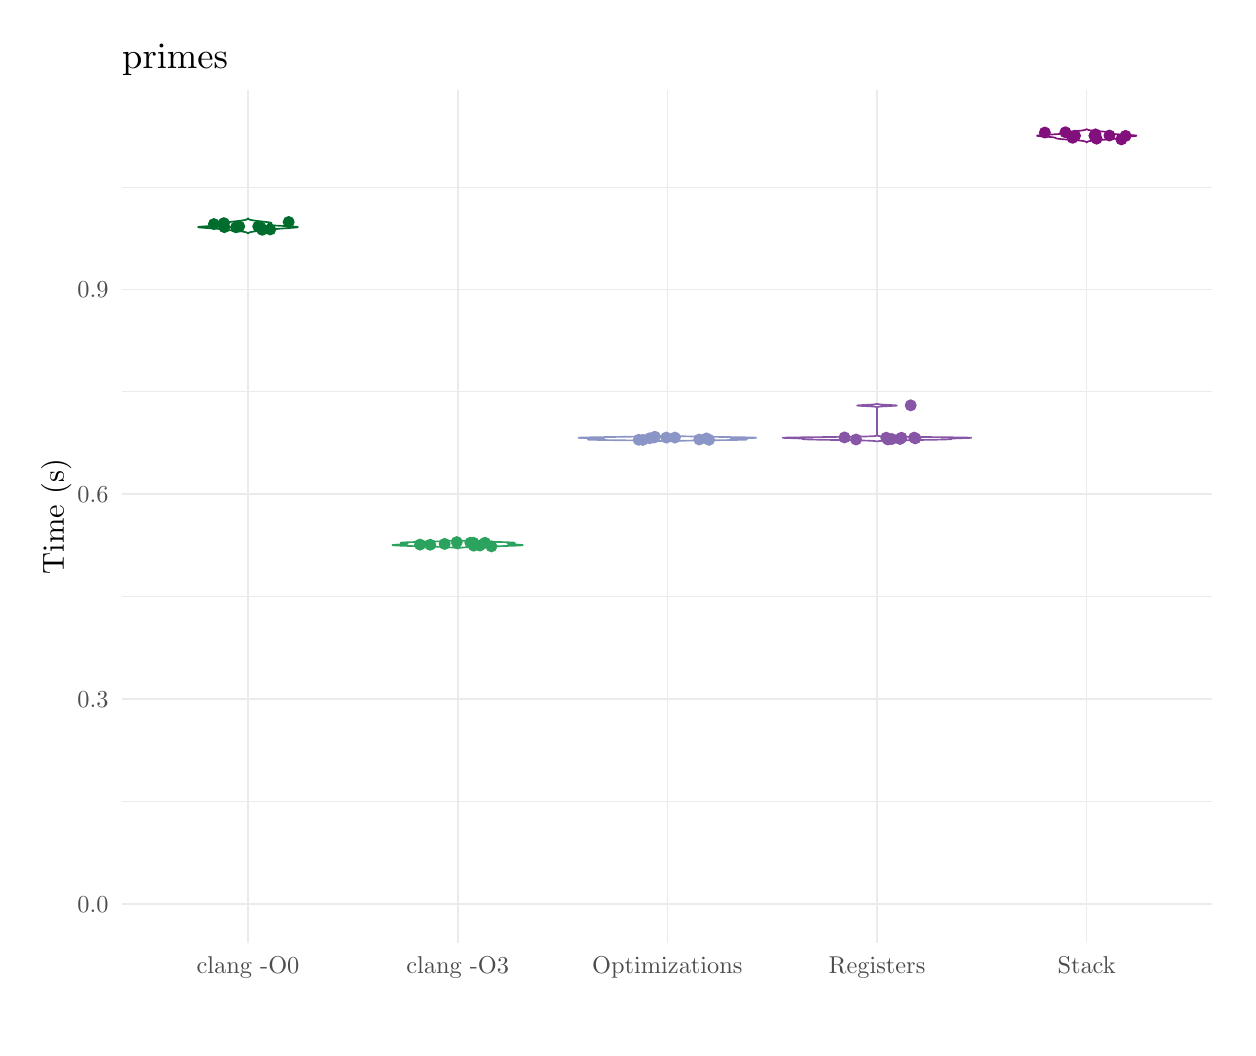
\begin{tikzpicture}[x=1pt,y=1pt]
\definecolor{fillColor}{RGB}{255,255,255}
\path[use as bounding box,fill=fillColor,fill opacity=0.00] (0,0) rectangle (433.62,361.35);
\begin{scope}
\path[clip] ( 34.16, 30.69) rectangle (428.12,338.69);
\definecolor{drawColor}{gray}{0.92}

\path[draw=drawColor,line width= 0.3pt,line join=round] ( 34.16, 81.70) --
	(428.12, 81.70);

\path[draw=drawColor,line width= 0.3pt,line join=round] ( 34.16,155.72) --
	(428.12,155.72);

\path[draw=drawColor,line width= 0.3pt,line join=round] ( 34.16,229.75) --
	(428.12,229.75);

\path[draw=drawColor,line width= 0.3pt,line join=round] ( 34.16,303.78) --
	(428.12,303.78);

\path[draw=drawColor,line width= 0.6pt,line join=round] ( 34.16, 44.69) --
	(428.12, 44.69);

\path[draw=drawColor,line width= 0.6pt,line join=round] ( 34.16,118.71) --
	(428.12,118.71);

\path[draw=drawColor,line width= 0.6pt,line join=round] ( 34.16,192.74) --
	(428.12,192.74);

\path[draw=drawColor,line width= 0.6pt,line join=round] ( 34.16,266.76) --
	(428.12,266.76);

\path[draw=drawColor,line width= 0.6pt,line join=round] ( 79.61, 30.69) --
	( 79.61,338.69);

\path[draw=drawColor,line width= 0.6pt,line join=round] (155.38, 30.69) --
	(155.38,338.69);

\path[draw=drawColor,line width= 0.6pt,line join=round] (231.14, 30.69) --
	(231.14,338.69);

\path[draw=drawColor,line width= 0.6pt,line join=round] (306.90, 30.69) --
	(306.90,338.69);

\path[draw=drawColor,line width= 0.6pt,line join=round] (382.66, 30.69) --
	(382.66,338.69);
\definecolor{drawColor}{RGB}{0,109,44}
\definecolor{fillColor}{RGB}{255,255,255}

\path[draw=drawColor,line width= 0.6pt,line join=round,line cap=round,fill=fillColor] ( 79.57,286.98) --
	( 79.56,286.99) --
	( 79.56,287.00) --
	( 79.56,287.01) --
	( 79.55,287.02) --
	( 79.55,287.03) --
	( 79.54,287.04) --
	( 79.53,287.05) --
	( 79.53,287.06) --
	( 79.52,287.07) --
	( 79.52,287.08) --
	( 79.51,287.09) --
	( 79.50,287.10) --
	( 79.49,287.11) --
	( 79.48,287.13) --
	( 79.47,287.14) --
	( 79.46,287.15) --
	( 79.45,287.16) --
	( 79.44,287.17) --
	( 79.43,287.18) --
	( 79.42,287.19) --
	( 79.40,287.20) --
	( 79.39,287.21) --
	( 79.38,287.22) --
	( 79.36,287.23) --
	( 79.34,287.24) --
	( 79.33,287.25) --
	( 79.31,287.26) --
	( 79.29,287.28) --
	( 79.27,287.29) --
	( 79.25,287.30) --
	( 79.22,287.31) --
	( 79.20,287.32) --
	( 79.18,287.33) --
	( 79.15,287.34) --
	( 79.12,287.35) --
	( 79.09,287.36) --
	( 79.06,287.37) --
	( 79.03,287.38) --
	( 79.00,287.39) --
	( 78.97,287.40) --
	( 78.93,287.41) --
	( 78.89,287.43) --
	( 78.85,287.44) --
	( 78.81,287.45) --
	( 78.77,287.46) --
	( 78.73,287.47) --
	( 78.68,287.48) --
	( 78.64,287.49) --
	( 78.59,287.50) --
	( 78.54,287.51) --
	( 78.49,287.52) --
	( 78.43,287.53) --
	( 78.38,287.54) --
	( 78.32,287.55) --
	( 78.26,287.56) --
	( 78.20,287.58) --
	( 78.14,287.59) --
	( 78.07,287.60) --
	( 78.00,287.61) --
	( 77.93,287.62) --
	( 77.86,287.63) --
	( 77.79,287.64) --
	( 77.72,287.65) --
	( 77.64,287.66) --
	( 77.56,287.67) --
	( 77.48,287.68) --
	( 77.40,287.69) --
	( 77.32,287.70) --
	( 77.23,287.71) --
	( 77.14,287.73) --
	( 77.05,287.74) --
	( 76.96,287.75) --
	( 76.87,287.76) --
	( 76.78,287.77) --
	( 76.68,287.78) --
	( 76.58,287.79) --
	( 76.49,287.80) --
	( 76.39,287.81) --
	( 76.29,287.82) --
	( 76.18,287.83) --
	( 76.08,287.84) --
	( 75.97,287.85) --
	( 75.87,287.86) --
	( 75.76,287.88) --
	( 75.65,287.89) --
	( 75.55,287.90) --
	( 75.44,287.91) --
	( 75.33,287.92) --
	( 75.22,287.93) --
	( 75.11,287.94) --
	( 75.00,287.95) --
	( 74.89,287.96) --
	( 74.77,287.97) --
	( 74.66,287.98) --
	( 74.55,287.99) --
	( 74.44,288.00) --
	( 74.33,288.01) --
	( 74.22,288.02) --
	( 74.11,288.04) --
	( 74.00,288.05) --
	( 73.89,288.06) --
	( 73.78,288.07) --
	( 73.67,288.08) --
	( 73.56,288.09) --
	( 73.46,288.10) --
	( 73.35,288.11) --
	( 73.25,288.12) --
	( 73.14,288.13) --
	( 73.04,288.14) --
	( 72.94,288.15) --
	( 72.84,288.16) --
	( 72.74,288.17) --
	( 72.64,288.19) --
	( 72.54,288.20) --
	( 72.45,288.21) --
	( 72.35,288.22) --
	( 72.26,288.23) --
	( 72.16,288.24) --
	( 72.07,288.25) --
	( 71.98,288.26) --
	( 71.89,288.27) --
	( 71.80,288.28) --
	( 71.72,288.29) --
	( 71.63,288.30) --
	( 71.55,288.31) --
	( 71.46,288.32) --
	( 71.38,288.34) --
	( 71.29,288.35) --
	( 71.21,288.36) --
	( 71.13,288.37) --
	( 71.05,288.38) --
	( 70.97,288.39) --
	( 70.89,288.40) --
	( 70.81,288.41) --
	( 70.73,288.42) --
	( 70.64,288.43) --
	( 70.56,288.44) --
	( 70.48,288.45) --
	( 70.40,288.46) --
	( 70.32,288.47) --
	( 70.23,288.49) --
	( 70.15,288.50) --
	( 70.06,288.51) --
	( 69.97,288.52) --
	( 69.89,288.53) --
	( 69.80,288.54) --
	( 69.71,288.55) --
	( 69.61,288.56) --
	( 69.52,288.57) --
	( 69.42,288.58) --
	( 69.32,288.59) --
	( 69.22,288.60) --
	( 69.12,288.61) --
	( 69.01,288.62) --
	( 68.90,288.64) --
	( 68.79,288.65) --
	( 68.68,288.66) --
	( 68.57,288.67) --
	( 68.45,288.68) --
	( 68.33,288.69) --
	( 68.20,288.70) --
	( 68.08,288.71) --
	( 67.95,288.72) --
	( 67.82,288.73) --
	( 67.68,288.74) --
	( 67.55,288.75) --
	( 67.41,288.76) --
	( 67.27,288.77) --
	( 67.12,288.78) --
	( 66.98,288.80) --
	( 66.83,288.81) --
	( 66.68,288.82) --
	( 66.53,288.83) --
	( 66.37,288.84) --
	( 66.22,288.85) --
	( 66.06,288.86) --
	( 65.90,288.87) --
	( 65.74,288.88) --
	( 65.58,288.89) --
	( 65.42,288.90) --
	( 65.26,288.91) --
	( 65.10,288.92) --
	( 64.94,288.93) --
	( 64.78,288.95) --
	( 64.62,288.96) --
	( 64.47,288.97) --
	( 64.31,288.98) --
	( 64.15,288.99) --
	( 64.00,289.00) --
	( 63.85,289.01) --
	( 63.70,289.02) --
	( 63.55,289.03) --
	( 63.41,289.04) --
	( 63.27,289.05) --
	( 63.13,289.06) --
	( 63.00,289.07) --
	( 62.88,289.08) --
	( 62.75,289.10) --
	( 62.64,289.11) --
	( 62.52,289.12) --
	( 62.42,289.13) --
	( 62.31,289.14) --
	( 62.22,289.15) --
	( 62.13,289.16) --
	( 62.05,289.17) --
	( 61.97,289.18) --
	( 61.90,289.19) --
	( 61.84,289.20) --
	( 61.79,289.21) --
	( 61.74,289.22) --
	( 61.70,289.23) --
	( 61.67,289.25) --
	( 61.64,289.26) --
	( 61.63,289.27) --
	( 61.62,289.28) --
	( 61.62,289.29) --
	( 61.63,289.30) --
	( 61.65,289.31) --
	( 61.68,289.32) --
	( 61.71,289.33) --
	( 61.75,289.34) --
	( 61.81,289.35) --
	( 61.87,289.36) --
	( 61.93,289.37) --
	( 62.01,289.38) --
	( 62.10,289.40) --
	( 62.19,289.41) --
	( 62.29,289.42) --
	( 62.40,289.43) --
	( 62.51,289.44) --
	( 62.64,289.45) --
	( 62.77,289.46) --
	( 62.90,289.47) --
	( 63.05,289.48) --
	( 63.20,289.49) --
	( 63.35,289.50) --
	( 63.51,289.51) --
	( 63.68,289.52) --
	( 63.85,289.53) --
	( 64.03,289.55) --
	( 64.21,289.56) --
	( 64.40,289.57) --
	( 64.59,289.58) --
	( 64.78,289.59) --
	( 64.98,289.60) --
	( 65.18,289.61) --
	( 65.38,289.62) --
	( 65.59,289.63) --
	( 65.79,289.64) --
	( 66.00,289.65) --
	( 66.21,289.66) --
	( 66.42,289.67) --
	( 66.63,289.68) --
	( 66.84,289.69) --
	( 67.05,289.71) --
	( 67.26,289.72) --
	( 67.47,289.73) --
	( 67.67,289.74) --
	( 67.88,289.75) --
	( 68.08,289.76) --
	( 68.28,289.77) --
	( 68.48,289.78) --
	( 68.68,289.79) --
	( 68.87,289.80) --
	( 69.06,289.81) --
	( 69.24,289.82) --
	( 69.42,289.83) --
	( 69.60,289.84) --
	( 69.77,289.86) --
	( 69.94,289.87) --
	( 70.10,289.88) --
	( 70.26,289.89) --
	( 70.41,289.90) --
	( 70.56,289.91) --
	( 70.70,289.92) --
	( 70.84,289.93) --
	( 70.97,289.94) --
	( 71.10,289.95) --
	( 71.22,289.96) --
	( 71.33,289.97) --
	( 71.44,289.98) --
	( 71.54,289.99) --
	( 71.64,290.01) --
	( 71.73,290.02) --
	( 71.81,290.03) --
	( 71.89,290.04) --
	( 71.96,290.05) --
	( 72.03,290.06) --
	( 72.09,290.07) --
	( 72.14,290.08) --
	( 72.19,290.09) --
	( 72.23,290.10) --
	( 72.27,290.11) --
	( 72.31,290.12) --
	( 72.33,290.13) --
	( 72.36,290.14) --
	( 72.37,290.16) --
	( 72.39,290.17) --
	( 72.40,290.18) --
	( 72.40,290.19) --
	( 72.40,290.20) --
	( 72.40,290.21) --
	( 72.39,290.22) --
	( 72.38,290.23) --
	( 72.36,290.24) --
	( 72.34,290.25) --
	( 72.32,290.26) --
	( 72.30,290.27) --
	( 72.27,290.28) --
	( 72.24,290.29) --
	( 72.21,290.31) --
	( 72.18,290.32) --
	( 72.14,290.33) --
	( 72.10,290.34) --
	( 72.07,290.35) --
	( 72.03,290.36) --
	( 71.98,290.37) --
	( 71.94,290.38) --
	( 71.90,290.39) --
	( 71.86,290.40) --
	( 71.82,290.41) --
	( 71.77,290.42) --
	( 71.73,290.43) --
	( 71.69,290.44) --
	( 71.65,290.46) --
	( 71.60,290.47) --
	( 71.56,290.48) --
	( 71.52,290.49) --
	( 71.48,290.50) --
	( 71.45,290.51) --
	( 71.41,290.52) --
	( 71.38,290.53) --
	( 71.34,290.54) --
	( 71.31,290.55) --
	( 71.28,290.56) --
	( 71.25,290.57) --
	( 71.23,290.58) --
	( 71.20,290.59) --
	( 71.18,290.60) --
	( 71.16,290.62) --
	( 71.15,290.63) --
	( 71.13,290.64) --
	( 71.12,290.65) --
	( 71.11,290.66) --
	( 71.10,290.67) --
	( 71.10,290.68) --
	( 71.09,290.69) --
	( 71.09,290.70) --
	( 71.10,290.71) --
	( 71.10,290.72) --
	( 71.11,290.73) --
	( 71.12,290.74) --
	( 71.13,290.75) --
	( 71.15,290.77) --
	( 71.16,290.78) --
	( 71.18,290.79) --
	( 71.21,290.80) --
	( 71.23,290.81) --
	( 71.26,290.82) --
	( 71.29,290.83) --
	( 71.32,290.84) --
	( 71.36,290.85) --
	( 71.40,290.86) --
	( 71.44,290.87) --
	( 71.48,290.88) --
	( 71.52,290.89) --
	( 71.57,290.90) --
	( 71.62,290.92) --
	( 71.67,290.93) --
	( 71.72,290.94) --
	( 71.78,290.95) --
	( 71.83,290.96) --
	( 71.89,290.97) --
	( 71.95,290.98) --
	( 72.02,290.99) --
	( 72.08,291.00) --
	( 72.15,291.01) --
	( 72.22,291.02) --
	( 72.29,291.03) --
	( 72.36,291.04) --
	( 72.43,291.05) --
	( 72.50,291.07) --
	( 72.58,291.08) --
	( 72.66,291.09) --
	( 72.73,291.10) --
	( 72.81,291.11) --
	( 72.89,291.12) --
	( 72.98,291.13) --
	( 73.06,291.14) --
	( 73.14,291.15) --
	( 73.23,291.16) --
	( 73.32,291.17) --
	( 73.40,291.18) --
	( 73.49,291.19) --
	( 73.58,291.20) --
	( 73.67,291.22) --
	( 73.76,291.23) --
	( 73.85,291.24) --
	( 73.94,291.25) --
	( 74.03,291.26) --
	( 74.13,291.27) --
	( 74.22,291.28) --
	( 74.31,291.29) --
	( 74.41,291.30) --
	( 74.50,291.31) --
	( 74.60,291.32) --
	( 74.69,291.33) --
	( 74.78,291.34) --
	( 74.88,291.35) --
	( 74.97,291.37) --
	( 75.07,291.38) --
	( 75.16,291.39) --
	( 75.26,291.40) --
	( 75.35,291.41) --
	( 75.44,291.42) --
	( 75.54,291.43) --
	( 75.63,291.44) --
	( 75.72,291.45) --
	( 75.82,291.46) --
	( 75.91,291.47) --
	( 76.00,291.48) --
	( 76.09,291.49) --
	( 76.18,291.50) --
	( 76.27,291.51) --
	( 76.36,291.53) --
	( 76.44,291.54) --
	( 76.53,291.55) --
	( 76.62,291.56) --
	( 76.70,291.57) --
	( 76.78,291.58) --
	( 76.87,291.59) --
	( 76.95,291.60) --
	( 77.03,291.61) --
	( 77.11,291.62) --
	( 77.19,291.63) --
	( 77.26,291.64) --
	( 77.34,291.65) --
	( 77.41,291.66) --
	( 77.49,291.68) --
	( 77.56,291.69) --
	( 77.63,291.70) --
	( 77.70,291.71) --
	( 77.76,291.72) --
	( 77.83,291.73) --
	( 77.89,291.74) --
	( 77.96,291.75) --
	( 78.02,291.76) --
	( 78.08,291.77) --
	( 78.14,291.78) --
	( 78.20,291.79) --
	( 78.25,291.80) --
	( 78.31,291.81) --
	( 78.36,291.83) --
	( 78.41,291.84) --
	( 78.46,291.85) --
	( 78.51,291.86) --
	( 78.56,291.87) --
	( 78.60,291.88) --
	( 78.65,291.89) --
	( 78.69,291.90) --
	( 78.73,291.91) --
	( 78.77,291.92) --
	( 78.81,291.93) --
	( 78.85,291.94) --
	( 78.88,291.95) --
	( 78.92,291.96) --
	( 78.95,291.98) --
	( 78.98,291.99) --
	( 79.01,292.00) --
	( 79.04,292.01) --
	( 79.07,292.02) --
	( 79.10,292.03) --
	( 79.13,292.04) --
	( 79.15,292.05) --
	( 79.18,292.06) --
	( 79.20,292.07) --
	( 79.22,292.08) --
	( 79.24,292.09) --
	( 79.26,292.10) --
	( 79.28,292.11) --
	( 79.30,292.13) --
	( 79.32,292.14) --
	( 79.34,292.15) --
	( 79.35,292.16) --
	( 79.37,292.17) --
	( 79.38,292.18) --
	( 79.40,292.19) --
	( 79.41,292.20) --
	( 79.42,292.21) --
	( 79.43,292.22) --
	( 79.44,292.23) --
	( 79.46,292.24) --
	( 79.47,292.25) --
	( 79.47,292.26) --
	( 79.48,292.28) --
	( 79.49,292.29) --
	( 79.50,292.30) --
	( 79.51,292.31) --
	( 79.51,292.32) --
	( 79.52,292.33) --
	( 79.53,292.34) --
	( 79.53,292.35) --
	( 79.54,292.36) --
	( 79.54,292.37) --
	( 79.55,292.38) --
	( 79.55,292.39) --
	( 79.56,292.40) --
	( 79.56,292.41) --
	( 79.57,292.42) --
	( 79.57,292.44) --
	( 79.57,292.45) --
	( 79.65,292.45) --
	( 79.66,292.44) --
	( 79.66,292.42) --
	( 79.66,292.41) --
	( 79.67,292.40) --
	( 79.67,292.39) --
	( 79.68,292.38) --
	( 79.68,292.37) --
	( 79.69,292.36) --
	( 79.69,292.35) --
	( 79.70,292.34) --
	( 79.71,292.33) --
	( 79.71,292.32) --
	( 79.72,292.31) --
	( 79.73,292.30) --
	( 79.73,292.29) --
	( 79.74,292.28) --
	( 79.75,292.26) --
	( 79.76,292.25) --
	( 79.77,292.24) --
	( 79.78,292.23) --
	( 79.79,292.22) --
	( 79.81,292.21) --
	( 79.82,292.20) --
	( 79.83,292.19) --
	( 79.84,292.18) --
	( 79.86,292.17) --
	( 79.87,292.16) --
	( 79.89,292.15) --
	( 79.91,292.14) --
	( 79.92,292.13) --
	( 79.94,292.11) --
	( 79.96,292.10) --
	( 79.98,292.09) --
	( 80.00,292.08) --
	( 80.03,292.07) --
	( 80.05,292.06) --
	( 80.07,292.05) --
	( 80.10,292.04) --
	( 80.13,292.03) --
	( 80.15,292.02) --
	( 80.18,292.01) --
	( 80.21,292.00) --
	( 80.24,291.99) --
	( 80.28,291.98) --
	( 80.31,291.96) --
	( 80.34,291.95) --
	( 80.38,291.94) --
	( 80.42,291.93) --
	( 80.46,291.92) --
	( 80.50,291.91) --
	( 80.54,291.90) --
	( 80.58,291.89) --
	( 80.63,291.88) --
	( 80.67,291.87) --
	( 80.72,291.86) --
	( 80.77,291.85) --
	( 80.82,291.84) --
	( 80.87,291.83) --
	( 80.92,291.81) --
	( 80.98,291.80) --
	( 81.03,291.79) --
	( 81.09,291.78) --
	( 81.15,291.77) --
	( 81.21,291.76) --
	( 81.27,291.75) --
	( 81.33,291.74) --
	( 81.40,291.73) --
	( 81.46,291.72) --
	( 81.53,291.71) --
	( 81.60,291.70) --
	( 81.67,291.69) --
	( 81.74,291.68) --
	( 81.81,291.66) --
	( 81.89,291.65) --
	( 81.96,291.64) --
	( 82.04,291.63) --
	( 82.12,291.62) --
	( 82.20,291.61) --
	( 82.28,291.60) --
	( 82.36,291.59) --
	( 82.44,291.58) --
	( 82.53,291.57) --
	( 82.61,291.56) --
	( 82.70,291.55) --
	( 82.78,291.54) --
	( 82.87,291.53) --
	( 82.96,291.51) --
	( 83.05,291.50) --
	( 83.14,291.49) --
	( 83.23,291.48) --
	( 83.32,291.47) --
	( 83.41,291.46) --
	( 83.50,291.45) --
	( 83.60,291.44) --
	( 83.69,291.43) --
	( 83.78,291.42) --
	( 83.88,291.41) --
	( 83.97,291.40) --
	( 84.06,291.39) --
	( 84.16,291.38) --
	( 84.25,291.37) --
	( 84.35,291.35) --
	( 84.44,291.34) --
	( 84.54,291.33) --
	( 84.63,291.32) --
	( 84.73,291.31) --
	( 84.82,291.30) --
	( 84.91,291.29) --
	( 85.01,291.28) --
	( 85.10,291.27) --
	( 85.19,291.26) --
	( 85.29,291.25) --
	( 85.38,291.24) --
	( 85.47,291.23) --
	( 85.56,291.22) --
	( 85.65,291.20) --
	( 85.74,291.19) --
	( 85.82,291.18) --
	( 85.91,291.17) --
	( 86.00,291.16) --
	( 86.08,291.15) --
	( 86.17,291.14) --
	( 86.25,291.13) --
	( 86.33,291.12) --
	( 86.41,291.11) --
	( 86.49,291.10) --
	( 86.57,291.09) --
	( 86.65,291.08) --
	( 86.72,291.07) --
	( 86.80,291.05) --
	( 86.87,291.04) --
	( 86.94,291.03) --
	( 87.01,291.02) --
	( 87.08,291.01) --
	( 87.15,291.00) --
	( 87.21,290.99) --
	( 87.27,290.98) --
	( 87.33,290.97) --
	( 87.39,290.96) --
	( 87.45,290.95) --
	( 87.50,290.94) --
	( 87.56,290.93) --
	( 87.61,290.92) --
	( 87.66,290.90) --
	( 87.70,290.89) --
	( 87.75,290.88) --
	( 87.79,290.87) --
	( 87.83,290.86) --
	( 87.87,290.85) --
	( 87.90,290.84) --
	( 87.94,290.83) --
	( 87.97,290.82) --
	( 87.99,290.81) --
	( 88.02,290.80) --
	( 88.04,290.79) --
	( 88.06,290.78) --
	( 88.08,290.77) --
	( 88.10,290.75) --
	( 88.11,290.74) --
	( 88.12,290.73) --
	( 88.13,290.72) --
	( 88.13,290.71) --
	( 88.13,290.70) --
	( 88.13,290.69) --
	( 88.13,290.68) --
	( 88.13,290.67) --
	( 88.12,290.66) --
	( 88.11,290.65) --
	( 88.10,290.64) --
	( 88.08,290.63) --
	( 88.06,290.62) --
	( 88.04,290.60) --
	( 88.02,290.59) --
	( 88.00,290.58) --
	( 87.97,290.57) --
	( 87.95,290.56) --
	( 87.92,290.55) --
	( 87.88,290.54) --
	( 87.85,290.53) --
	( 87.82,290.52) --
	( 87.78,290.51) --
	( 87.74,290.50) --
	( 87.70,290.49) --
	( 87.66,290.48) --
	( 87.62,290.47) --
	( 87.58,290.46) --
	( 87.54,290.44) --
	( 87.50,290.43) --
	( 87.45,290.42) --
	( 87.41,290.41) --
	( 87.37,290.40) --
	( 87.33,290.39) --
	( 87.28,290.38) --
	( 87.24,290.37) --
	( 87.20,290.36) --
	( 87.16,290.35) --
	( 87.12,290.34) --
	( 87.09,290.33) --
	( 87.05,290.32) --
	( 87.02,290.31) --
	( 86.99,290.29) --
	( 86.96,290.28) --
	( 86.93,290.27) --
	( 86.91,290.26) --
	( 86.88,290.25) --
	( 86.87,290.24) --
	( 86.85,290.23) --
	( 86.84,290.22) --
	( 86.83,290.21) --
	( 86.83,290.20) --
	( 86.83,290.19) --
	( 86.83,290.18) --
	( 86.84,290.17) --
	( 86.85,290.16) --
	( 86.87,290.14) --
	( 86.89,290.13) --
	( 86.92,290.12) --
	( 86.95,290.11) --
	( 86.99,290.10) --
	( 87.04,290.09) --
	( 87.08,290.08) --
	( 87.14,290.07) --
	( 87.20,290.06) --
	( 87.27,290.05) --
	( 87.34,290.04) --
	( 87.42,290.03) --
	( 87.50,290.02) --
	( 87.59,290.01) --
	( 87.69,289.99) --
	( 87.79,289.98) --
	( 87.90,289.97) --
	( 88.01,289.96) --
	( 88.13,289.95) --
	( 88.25,289.94) --
	( 88.39,289.93) --
	( 88.52,289.92) --
	( 88.66,289.91) --
	( 88.81,289.90) --
	( 88.97,289.89) --
	( 89.12,289.88) --
	( 89.29,289.87) --
	( 89.45,289.86) --
	( 89.63,289.84) --
	( 89.80,289.83) --
	( 89.98,289.82) --
	( 90.17,289.81) --
	( 90.36,289.80) --
	( 90.55,289.79) --
	( 90.75,289.78) --
	( 90.94,289.77) --
	( 91.15,289.76) --
	( 91.35,289.75) --
	( 91.55,289.74) --
	( 91.76,289.73) --
	( 91.97,289.72) --
	( 92.18,289.71) --
	( 92.39,289.69) --
	( 92.60,289.68) --
	( 92.81,289.67) --
	( 93.02,289.66) --
	( 93.23,289.65) --
	( 93.43,289.64) --
	( 93.64,289.63) --
	( 93.85,289.62) --
	( 94.05,289.61) --
	( 94.25,289.60) --
	( 94.44,289.59) --
	( 94.64,289.58) --
	( 94.83,289.57) --
	( 95.01,289.56) --
	( 95.20,289.55) --
	( 95.37,289.53) --
	( 95.55,289.52) --
	( 95.71,289.51) --
	( 95.88,289.50) --
	( 96.03,289.49) --
	( 96.18,289.48) --
	( 96.32,289.47) --
	( 96.46,289.46) --
	( 96.59,289.45) --
	( 96.71,289.44) --
	( 96.83,289.43) --
	( 96.94,289.42) --
	( 97.04,289.41) --
	( 97.13,289.40) --
	( 97.21,289.38) --
	( 97.29,289.37) --
	( 97.36,289.36) --
	( 97.42,289.35) --
	( 97.47,289.34) --
	( 97.51,289.33) --
	( 97.55,289.32) --
	( 97.58,289.31) --
	( 97.59,289.30) --
	( 97.61,289.29) --
	( 97.60,289.28) --
	( 97.60,289.27) --
	( 97.58,289.26) --
	( 97.56,289.25) --
	( 97.53,289.23) --
	( 97.49,289.22) --
	( 97.44,289.21) --
	( 97.39,289.20) --
	( 97.33,289.19) --
	( 97.26,289.18) --
	( 97.18,289.17) --
	( 97.10,289.16) --
	( 97.01,289.15) --
	( 96.91,289.14) --
	( 96.81,289.13) --
	( 96.71,289.12) --
	( 96.59,289.11) --
	( 96.47,289.10) --
	( 96.35,289.08) --
	( 96.22,289.07) --
	( 96.09,289.06) --
	( 95.96,289.05) --
	( 95.82,289.04) --
	( 95.67,289.03) --
	( 95.53,289.02) --
	( 95.38,289.01) --
	( 95.23,289.00) --
	( 95.07,288.99) --
	( 94.92,288.98) --
	( 94.76,288.97) --
	( 94.60,288.96) --
	( 94.44,288.95) --
	( 94.28,288.93) --
	( 94.12,288.92) --
	( 93.96,288.91) --
	( 93.80,288.90) --
	( 93.64,288.89) --
	( 93.48,288.88) --
	( 93.32,288.87) --
	( 93.17,288.86) --
	( 93.01,288.85) --
	( 92.85,288.84) --
	( 92.70,288.83) --
	( 92.55,288.82) --
	( 92.40,288.81) --
	( 92.25,288.80) --
	( 92.10,288.78) --
	( 91.96,288.77) --
	( 91.82,288.76) --
	( 91.68,288.75) --
	( 91.54,288.74) --
	( 91.41,288.73) --
	( 91.28,288.72) --
	( 91.15,288.71) --
	( 91.02,288.70) --
	( 90.90,288.69) --
	( 90.78,288.68) --
	( 90.66,288.67) --
	( 90.55,288.66) --
	( 90.43,288.65) --
	( 90.32,288.64) --
	( 90.22,288.62) --
	( 90.11,288.61) --
	( 90.01,288.60) --
	( 89.91,288.59) --
	( 89.81,288.58) --
	( 89.71,288.57) --
	( 89.61,288.56) --
	( 89.52,288.55) --
	( 89.43,288.54) --
	( 89.34,288.53) --
	( 89.25,288.52) --
	( 89.17,288.51) --
	( 89.08,288.50) --
	( 89.00,288.49) --
	( 88.91,288.47) --
	( 88.83,288.46) --
	( 88.75,288.45) --
	( 88.66,288.44) --
	( 88.58,288.43) --
	( 88.50,288.42) --
	( 88.42,288.41) --
	( 88.34,288.40) --
	( 88.26,288.39) --
	( 88.18,288.38) --
	( 88.10,288.37) --
	( 88.01,288.36) --
	( 87.93,288.35) --
	( 87.85,288.34) --
	( 87.77,288.32) --
	( 87.68,288.31) --
	( 87.60,288.30) --
	( 87.51,288.29) --
	( 87.42,288.28) --
	( 87.33,288.27) --
	( 87.24,288.26) --
	( 87.15,288.25) --
	( 87.06,288.24) --
	( 86.97,288.23) --
	( 86.88,288.22) --
	( 86.78,288.21) --
	( 86.69,288.20) --
	( 86.59,288.19) --
	( 86.49,288.17) --
	( 86.39,288.16) --
	( 86.29,288.15) --
	( 86.19,288.14) --
	( 86.08,288.13) --
	( 85.98,288.12) --
	( 85.88,288.11) --
	( 85.77,288.10) --
	( 85.66,288.09) --
	( 85.56,288.08) --
	( 85.45,288.07) --
	( 85.34,288.06) --
	( 85.23,288.05) --
	( 85.12,288.04) --
	( 85.01,288.02) --
	( 84.90,288.01) --
	( 84.79,288.00) --
	( 84.68,287.99) --
	( 84.56,287.98) --
	( 84.45,287.97) --
	( 84.34,287.96) --
	( 84.23,287.95) --
	( 84.12,287.94) --
	( 84.01,287.93) --
	( 83.90,287.92) --
	( 83.79,287.91) --
	( 83.68,287.90) --
	( 83.57,287.89) --
	( 83.46,287.88) --
	( 83.36,287.86) --
	( 83.25,287.85) --
	( 83.15,287.84) --
	( 83.04,287.83) --
	( 82.94,287.82) --
	( 82.84,287.81) --
	( 82.74,287.80) --
	( 82.64,287.79) --
	( 82.55,287.78) --
	( 82.45,287.77) --
	( 82.36,287.76) --
	( 82.26,287.75) --
	( 82.17,287.74) --
	( 82.08,287.73) --
	( 82.00,287.71) --
	( 81.91,287.70) --
	( 81.83,287.69) --
	( 81.74,287.68) --
	( 81.66,287.67) --
	( 81.59,287.66) --
	( 81.51,287.65) --
	( 81.44,287.64) --
	( 81.36,287.63) --
	( 81.29,287.62) --
	( 81.22,287.61) --
	( 81.16,287.60) --
	( 81.09,287.59) --
	( 81.03,287.58) --
	( 80.97,287.56) --
	( 80.91,287.55) --
	( 80.85,287.54) --
	( 80.79,287.53) --
	( 80.74,287.52) --
	( 80.69,287.51) --
	( 80.64,287.50) --
	( 80.59,287.49) --
	( 80.54,287.48) --
	( 80.50,287.47) --
	( 80.45,287.46) --
	( 80.41,287.45) --
	( 80.37,287.44) --
	( 80.33,287.43) --
	( 80.30,287.41) --
	( 80.26,287.40) --
	( 80.23,287.39) --
	( 80.19,287.38) --
	( 80.16,287.37) --
	( 80.13,287.36) --
	( 80.11,287.35) --
	( 80.08,287.34) --
	( 80.05,287.33) --
	( 80.03,287.32) --
	( 80.00,287.31) --
	( 79.98,287.30) --
	( 79.96,287.29) --
	( 79.94,287.28) --
	( 79.92,287.26) --
	( 79.90,287.25) --
	( 79.88,287.24) --
	( 79.87,287.23) --
	( 79.85,287.22) --
	( 79.84,287.21) --
	( 79.82,287.20) --
	( 79.81,287.19) --
	( 79.80,287.18) --
	( 79.78,287.17) --
	( 79.77,287.16) --
	( 79.76,287.15) --
	( 79.75,287.14) --
	( 79.74,287.13) --
	( 79.73,287.11) --
	( 79.73,287.10) --
	( 79.72,287.09) --
	( 79.71,287.08) --
	( 79.70,287.07) --
	( 79.70,287.06) --
	( 79.69,287.05) --
	( 79.69,287.04) --
	( 79.68,287.03) --
	( 79.68,287.02) --
	( 79.67,287.01) --
	( 79.67,287.00) --
	( 79.66,286.99) --
	( 79.66,286.98) --
	( 79.57,286.98) --
	cycle;
\definecolor{drawColor}{RGB}{44,162,95}

\path[draw=drawColor,line width= 0.6pt,line join=round,line cap=round,fill=fillColor] (155.31,173.10) --
	(155.31,173.10) --
	(155.30,173.11) --
	(155.30,173.12) --
	(155.29,173.12) --
	(155.29,173.13) --
	(155.28,173.14) --
	(155.27,173.14) --
	(155.27,173.15) --
	(155.26,173.16) --
	(155.25,173.16) --
	(155.25,173.17) --
	(155.24,173.17) --
	(155.23,173.18) --
	(155.22,173.19) --
	(155.21,173.19) --
	(155.20,173.20) --
	(155.19,173.21) --
	(155.18,173.21) --
	(155.17,173.22) --
	(155.15,173.23) --
	(155.14,173.23) --
	(155.13,173.24) --
	(155.11,173.24) --
	(155.10,173.25) --
	(155.08,173.26) --
	(155.06,173.26) --
	(155.05,173.27) --
	(155.03,173.28) --
	(155.01,173.28) --
	(154.99,173.29) --
	(154.97,173.30) --
	(154.94,173.30) --
	(154.92,173.31) --
	(154.90,173.31) --
	(154.87,173.32) --
	(154.84,173.33) --
	(154.82,173.33) --
	(154.79,173.34) --
	(154.76,173.35) --
	(154.72,173.35) --
	(154.69,173.36) --
	(154.66,173.37) --
	(154.62,173.37) --
	(154.58,173.38) --
	(154.54,173.38) --
	(154.50,173.39) --
	(154.46,173.40) --
	(154.42,173.40) --
	(154.37,173.41) --
	(154.32,173.42) --
	(154.28,173.42) --
	(154.23,173.43) --
	(154.17,173.44) --
	(154.12,173.44) --
	(154.06,173.45) --
	(154.00,173.45) --
	(153.94,173.46) --
	(153.88,173.47) --
	(153.81,173.47) --
	(153.75,173.48) --
	(153.68,173.49) --
	(153.61,173.49) --
	(153.53,173.50) --
	(153.45,173.51) --
	(153.38,173.51) --
	(153.29,173.52) --
	(153.21,173.52) --
	(153.12,173.53) --
	(153.04,173.54) --
	(152.94,173.54) --
	(152.85,173.55) --
	(152.75,173.56) --
	(152.65,173.56) --
	(152.55,173.57) --
	(152.45,173.58) --
	(152.34,173.58) --
	(152.23,173.59) --
	(152.11,173.59) --
	(152.00,173.60) --
	(151.88,173.61) --
	(151.76,173.61) --
	(151.63,173.62) --
	(151.50,173.63) --
	(151.37,173.63) --
	(151.24,173.64) --
	(151.10,173.65) --
	(150.96,173.65) --
	(150.82,173.66) --
	(150.67,173.66) --
	(150.52,173.67) --
	(150.37,173.68) --
	(150.22,173.68) --
	(150.06,173.69) --
	(149.90,173.70) --
	(149.73,173.70) --
	(149.57,173.71) --
	(149.40,173.72) --
	(149.23,173.72) --
	(149.05,173.73) --
	(148.87,173.73) --
	(148.69,173.74) --
	(148.51,173.75) --
	(148.32,173.75) --
	(148.13,173.76) --
	(147.94,173.77) --
	(147.75,173.77) --
	(147.55,173.78) --
	(147.35,173.79) --
	(147.15,173.79) --
	(146.95,173.80) --
	(146.74,173.80) --
	(146.53,173.81) --
	(146.32,173.82) --
	(146.11,173.82) --
	(145.90,173.83) --
	(145.68,173.84) --
	(145.46,173.84) --
	(145.24,173.85) --
	(145.02,173.86) --
	(144.80,173.86) --
	(144.57,173.87) --
	(144.35,173.87) --
	(144.12,173.88) --
	(143.89,173.89) --
	(143.66,173.89) --
	(143.43,173.90) --
	(143.20,173.91) --
	(142.97,173.91) --
	(142.74,173.92) --
	(142.50,173.93) --
	(142.27,173.93) --
	(142.04,173.94) --
	(141.80,173.94) --
	(141.57,173.95) --
	(141.33,173.96) --
	(141.10,173.96) --
	(140.87,173.97) --
	(140.63,173.98) --
	(140.40,173.98) --
	(140.17,173.99) --
	(139.94,174.00) --
	(139.71,174.00) --
	(139.48,174.01) --
	(139.25,174.01) --
	(139.03,174.02) --
	(138.80,174.03) --
	(138.58,174.03) --
	(138.36,174.04) --
	(138.14,174.05) --
	(137.92,174.05) --
	(137.70,174.06) --
	(137.49,174.07) --
	(137.28,174.07) --
	(137.07,174.08) --
	(136.86,174.08) --
	(136.66,174.09) --
	(136.46,174.10) --
	(136.26,174.10) --
	(136.07,174.11) --
	(135.88,174.12) --
	(135.69,174.12) --
	(135.50,174.13) --
	(135.32,174.14) --
	(135.15,174.14) --
	(134.97,174.15) --
	(134.80,174.15) --
	(134.64,174.16) --
	(134.48,174.17) --
	(134.32,174.17) --
	(134.16,174.18) --
	(134.02,174.19) --
	(133.87,174.19) --
	(133.73,174.20) --
	(133.60,174.21) --
	(133.46,174.21) --
	(133.34,174.22) --
	(133.22,174.22) --
	(133.10,174.23) --
	(132.99,174.24) --
	(132.88,174.24) --
	(132.78,174.25) --
	(132.68,174.26) --
	(132.59,174.26) --
	(132.51,174.27) --
	(132.43,174.28) --
	(132.35,174.28) --
	(132.28,174.29) --
	(132.21,174.29) --
	(132.15,174.30) --
	(132.10,174.31) --
	(132.05,174.31) --
	(132.00,174.32) --
	(131.96,174.33) --
	(131.93,174.33) --
	(131.90,174.34) --
	(131.88,174.35) --
	(131.86,174.35) --
	(131.85,174.36) --
	(131.84,174.36) --
	(131.84,174.37) --
	(131.84,174.38) --
	(131.85,174.38) --
	(131.86,174.39) --
	(131.87,174.40) --
	(131.90,174.40) --
	(131.92,174.41) --
	(131.95,174.42) --
	(131.99,174.42) --
	(132.03,174.43) --
	(132.07,174.43) --
	(132.12,174.44) --
	(132.17,174.45) --
	(132.23,174.45) --
	(132.29,174.46) --
	(132.35,174.47) --
	(132.42,174.47) --
	(132.50,174.48) --
	(132.57,174.49) --
	(132.65,174.49) --
	(132.73,174.50) --
	(132.82,174.50) --
	(132.90,174.51) --
	(132.99,174.52) --
	(133.09,174.52) --
	(133.18,174.53) --
	(133.28,174.54) --
	(133.38,174.54) --
	(133.48,174.55) --
	(133.58,174.56) --
	(133.69,174.56) --
	(133.79,174.57) --
	(133.90,174.57) --
	(134.01,174.58) --
	(134.12,174.59) --
	(134.23,174.59) --
	(134.34,174.60) --
	(134.45,174.61) --
	(134.56,174.61) --
	(134.67,174.62) --
	(134.78,174.63) --
	(134.89,174.63) --
	(135.00,174.64) --
	(135.11,174.64) --
	(135.22,174.65) --
	(135.33,174.66) --
	(135.43,174.66) --
	(135.54,174.67) --
	(135.64,174.68) --
	(135.74,174.68) --
	(135.84,174.69) --
	(135.94,174.70) --
	(136.03,174.70) --
	(136.12,174.71) --
	(136.21,174.71) --
	(136.30,174.72) --
	(136.38,174.73) --
	(136.46,174.73) --
	(136.54,174.74) --
	(136.61,174.75) --
	(136.68,174.75) --
	(136.75,174.76) --
	(136.81,174.77) --
	(136.88,174.77) --
	(136.93,174.78) --
	(136.98,174.79) --
	(137.03,174.79) --
	(137.08,174.80) --
	(137.12,174.80) --
	(137.15,174.81) --
	(137.19,174.82) --
	(137.21,174.82) --
	(137.24,174.83) --
	(137.26,174.84) --
	(137.27,174.84) --
	(137.29,174.85) --
	(137.29,174.86) --
	(137.30,174.86) --
	(137.29,174.87) --
	(137.29,174.87) --
	(137.28,174.88) --
	(137.27,174.89) --
	(137.25,174.89) --
	(137.23,174.90) --
	(137.20,174.91) --
	(137.17,174.91) --
	(137.14,174.92) --
	(137.11,174.93) --
	(137.07,174.93) --
	(137.02,174.94) --
	(136.98,174.94) --
	(136.93,174.95) --
	(136.88,174.96) --
	(136.82,174.96) --
	(136.77,174.97) --
	(136.71,174.98) --
	(136.65,174.98) --
	(136.59,174.99) --
	(136.52,175.00) --
	(136.45,175.00) --
	(136.39,175.01) --
	(136.32,175.01) --
	(136.25,175.02) --
	(136.18,175.03) --
	(136.11,175.03) --
	(136.03,175.04) --
	(135.96,175.05) --
	(135.89,175.05) --
	(135.82,175.06) --
	(135.75,175.07) --
	(135.68,175.07) --
	(135.61,175.08) --
	(135.54,175.08) --
	(135.48,175.09) --
	(135.41,175.10) --
	(135.35,175.10) --
	(135.29,175.11) --
	(135.23,175.12) --
	(135.17,175.12) --
	(135.12,175.13) --
	(135.07,175.14) --
	(135.03,175.14) --
	(134.98,175.15) --
	(134.94,175.15) --
	(134.90,175.16) --
	(134.87,175.17) --
	(134.85,175.17) --
	(134.82,175.18) --
	(134.80,175.19) --
	(134.79,175.19) --
	(134.78,175.20) --
	(134.77,175.21) --
	(134.77,175.21) --
	(134.78,175.22) --
	(134.79,175.22) --
	(134.80,175.23) --
	(134.82,175.24) --
	(134.85,175.24) --
	(134.88,175.25) --
	(134.92,175.26) --
	(134.96,175.26) --
	(135.01,175.27) --
	(135.07,175.28) --
	(135.13,175.28) --
	(135.20,175.29) --
	(135.27,175.29) --
	(135.35,175.30) --
	(135.43,175.31) --
	(135.52,175.31) --
	(135.62,175.32) --
	(135.72,175.33) --
	(135.83,175.33) --
	(135.95,175.34) --
	(136.06,175.35) --
	(136.19,175.35) --
	(136.32,175.36) --
	(136.46,175.36) --
	(136.60,175.37) --
	(136.75,175.38) --
	(136.90,175.38) --
	(137.06,175.39) --
	(137.22,175.40) --
	(137.39,175.40) --
	(137.56,175.41) --
	(137.74,175.42) --
	(137.92,175.42) --
	(138.10,175.43) --
	(138.29,175.43) --
	(138.49,175.44) --
	(138.68,175.45) --
	(138.88,175.45) --
	(139.09,175.46) --
	(139.29,175.47) --
	(139.51,175.47) --
	(139.72,175.48) --
	(139.94,175.49) --
	(140.15,175.49) --
	(140.38,175.50) --
	(140.60,175.50) --
	(140.82,175.51) --
	(141.05,175.52) --
	(141.28,175.52) --
	(141.51,175.53) --
	(141.74,175.54) --
	(141.97,175.54) --
	(142.21,175.55) --
	(142.44,175.56) --
	(142.68,175.56) --
	(142.91,175.57) --
	(143.15,175.57) --
	(143.38,175.58) --
	(143.62,175.59) --
	(143.85,175.59) --
	(144.09,175.60) --
	(144.32,175.61) --
	(144.55,175.61) --
	(144.79,175.62) --
	(145.02,175.63) --
	(145.25,175.63) --
	(145.47,175.64) --
	(145.70,175.64) --
	(145.93,175.65) --
	(146.15,175.66) --
	(146.37,175.66) --
	(146.59,175.67) --
	(146.81,175.68) --
	(147.02,175.68) --
	(147.23,175.69) --
	(147.45,175.70) --
	(147.65,175.70) --
	(147.86,175.71) --
	(148.06,175.71) --
	(148.26,175.72) --
	(148.46,175.73) --
	(148.65,175.73) --
	(148.84,175.74) --
	(149.03,175.75) --
	(149.21,175.75) --
	(149.40,175.76) --
	(149.57,175.77) --
	(149.75,175.77) --
	(149.92,175.78) --
	(150.09,175.78) --
	(150.26,175.79) --
	(150.42,175.80) --
	(150.58,175.80) --
	(150.73,175.81) --
	(150.89,175.82) --
	(151.03,175.82) --
	(151.18,175.83) --
	(151.32,175.84) --
	(151.46,175.84) --
	(151.60,175.85) --
	(151.73,175.85) --
	(151.86,175.86) --
	(151.98,175.87) --
	(152.11,175.87) --
	(152.23,175.88) --
	(152.34,175.89) --
	(152.46,175.89) --
	(152.56,175.90) --
	(152.67,175.91) --
	(152.77,175.91) --
	(152.88,175.92) --
	(152.97,175.92) --
	(153.07,175.93) --
	(153.16,175.94) --
	(153.25,175.94) --
	(153.34,175.95) --
	(153.42,175.96) --
	(153.50,175.96) --
	(153.58,175.97) --
	(153.65,175.98) --
	(153.73,175.98) --
	(153.80,175.99) --
	(153.87,175.99) --
	(153.93,176.00) --
	(154.00,176.01) --
	(154.06,176.01) --
	(154.12,176.02) --
	(154.17,176.03) --
	(154.23,176.03) --
	(154.28,176.04) --
	(154.33,176.05) --
	(154.38,176.05) --
	(154.43,176.06) --
	(154.47,176.06) --
	(154.51,176.07) --
	(154.56,176.08) --
	(154.60,176.08) --
	(154.63,176.09) --
	(154.67,176.10) --
	(154.70,176.10) --
	(154.74,176.11) --
	(154.77,176.12) --
	(154.80,176.12) --
	(154.83,176.13) --
	(154.86,176.13) --
	(154.89,176.14) --
	(154.91,176.15) --
	(154.94,176.15) --
	(154.96,176.16) --
	(154.98,176.17) --
	(155.00,176.17) --
	(155.02,176.18) --
	(155.04,176.19) --
	(155.06,176.19) --
	(155.08,176.20) --
	(155.09,176.20) --
	(155.11,176.21) --
	(155.13,176.22) --
	(155.14,176.22) --
	(155.15,176.23) --
	(155.17,176.24) --
	(155.18,176.24) --
	(155.19,176.25) --
	(155.20,176.26) --
	(155.21,176.26) --
	(155.22,176.27) --
	(155.23,176.27) --
	(155.24,176.28) --
	(155.25,176.29) --
	(155.26,176.29) --
	(155.26,176.30) --
	(155.27,176.31) --
	(155.28,176.31) --
	(155.28,176.32) --
	(155.29,176.33) --
	(155.29,176.33) --
	(155.30,176.34) --
	(155.30,176.34) --
	(155.31,176.35) --
	(155.44,176.35) --
	(155.45,176.34) --
	(155.45,176.34) --
	(155.46,176.33) --
	(155.46,176.33) --
	(155.47,176.32) --
	(155.48,176.31) --
	(155.48,176.31) --
	(155.49,176.30) --
	(155.50,176.29) --
	(155.50,176.29) --
	(155.51,176.28) --
	(155.52,176.27) --
	(155.53,176.27) --
	(155.54,176.26) --
	(155.55,176.26) --
	(155.56,176.25) --
	(155.57,176.24) --
	(155.59,176.24) --
	(155.60,176.23) --
	(155.61,176.22) --
	(155.63,176.22) --
	(155.64,176.21) --
	(155.66,176.20) --
	(155.67,176.20) --
	(155.69,176.19) --
	(155.71,176.19) --
	(155.73,176.18) --
	(155.75,176.17) --
	(155.77,176.17) --
	(155.79,176.16) --
	(155.82,176.15) --
	(155.84,176.15) --
	(155.87,176.14) --
	(155.89,176.13) --
	(155.92,176.13) --
	(155.95,176.12) --
	(155.98,176.12) --
	(156.01,176.11) --
	(156.05,176.10) --
	(156.08,176.10) --
	(156.12,176.09) --
	(156.16,176.08) --
	(156.20,176.08) --
	(156.24,176.07) --
	(156.28,176.06) --
	(156.33,176.06) --
	(156.37,176.05) --
	(156.42,176.05) --
	(156.47,176.04) --
	(156.52,176.03) --
	(156.58,176.03) --
	(156.64,176.02) --
	(156.70,176.01) --
	(156.76,176.01) --
	(156.82,176.00) --
	(156.89,175.99) --
	(156.95,175.99) --
	(157.02,175.98) --
	(157.10,175.98) --
	(157.17,175.97) --
	(157.25,175.96) --
	(157.33,175.96) --
	(157.42,175.95) --
	(157.50,175.94) --
	(157.59,175.94) --
	(157.68,175.93) --
	(157.78,175.92) --
	(157.88,175.92) --
	(157.98,175.91) --
	(158.08,175.91) --
	(158.19,175.90) --
	(158.30,175.89) --
	(158.41,175.89) --
	(158.53,175.88) --
	(158.64,175.87) --
	(158.77,175.87) --
	(158.89,175.86) --
	(159.02,175.85) --
	(159.15,175.85) --
	(159.29,175.84) --
	(159.43,175.84) --
	(159.57,175.83) --
	(159.72,175.82) --
	(159.87,175.82) --
	(160.02,175.81) --
	(160.17,175.80) --
	(160.33,175.80) --
	(160.50,175.79) --
	(160.66,175.78) --
	(160.83,175.78) --
	(161.00,175.77) --
	(161.18,175.77) --
	(161.36,175.76) --
	(161.54,175.75) --
	(161.72,175.75) --
	(161.91,175.74) --
	(162.10,175.73) --
	(162.29,175.73) --
	(162.49,175.72) --
	(162.69,175.71) --
	(162.89,175.71) --
	(163.10,175.70) --
	(163.31,175.70) --
	(163.52,175.69) --
	(163.73,175.68) --
	(163.94,175.68) --
	(164.16,175.67) --
	(164.38,175.66) --
	(164.60,175.66) --
	(164.83,175.65) --
	(165.05,175.64) --
	(165.28,175.64) --
	(165.51,175.63) --
	(165.74,175.63) --
	(165.97,175.62) --
	(166.20,175.61) --
	(166.43,175.61) --
	(166.66,175.60) --
	(166.90,175.59) --
	(167.13,175.59) --
	(167.37,175.58) --
	(167.60,175.57) --
	(167.84,175.57) --
	(168.07,175.56) --
	(168.31,175.56) --
	(168.54,175.55) --
	(168.78,175.54) --
	(169.01,175.54) --
	(169.24,175.53) --
	(169.47,175.52) --
	(169.70,175.52) --
	(169.93,175.51) --
	(170.15,175.50) --
	(170.38,175.50) --
	(170.60,175.49) --
	(170.82,175.49) --
	(171.03,175.48) --
	(171.25,175.47) --
	(171.46,175.47) --
	(171.66,175.46) --
	(171.87,175.45) --
	(172.07,175.45) --
	(172.27,175.44) --
	(172.46,175.43) --
	(172.65,175.43) --
	(172.83,175.42) --
	(173.01,175.42) --
	(173.19,175.41) --
	(173.36,175.40) --
	(173.53,175.40) --
	(173.69,175.39) --
	(173.85,175.38) --
	(174.00,175.38) --
	(174.15,175.37) --
	(174.29,175.36) --
	(174.43,175.36) --
	(174.56,175.35) --
	(174.69,175.35) --
	(174.80,175.34) --
	(174.92,175.33) --
	(175.03,175.33) --
	(175.13,175.32) --
	(175.23,175.31) --
	(175.32,175.31) --
	(175.40,175.30) --
	(175.48,175.29) --
	(175.56,175.29) --
	(175.62,175.28) --
	(175.68,175.28) --
	(175.74,175.27) --
	(175.79,175.26) --
	(175.83,175.26) --
	(175.87,175.25) --
	(175.90,175.24) --
	(175.93,175.24) --
	(175.95,175.23) --
	(175.97,175.22) --
	(175.98,175.22) --
	(175.98,175.21) --
	(175.98,175.21) --
	(175.97,175.20) --
	(175.97,175.19) --
	(175.95,175.19) --
	(175.93,175.18) --
	(175.91,175.17) --
	(175.88,175.17) --
	(175.85,175.16) --
	(175.81,175.15) --
	(175.77,175.15) --
	(175.73,175.14) --
	(175.68,175.14) --
	(175.63,175.13) --
	(175.58,175.12) --
	(175.52,175.12) --
	(175.46,175.11) --
	(175.40,175.10) --
	(175.34,175.10) --
	(175.28,175.09) --
	(175.21,175.08) --
	(175.14,175.08) --
	(175.07,175.07) --
	(175.00,175.07) --
	(174.93,175.06) --
	(174.86,175.05) --
	(174.79,175.05) --
	(174.72,175.04) --
	(174.65,175.03) --
	(174.57,175.03) --
	(174.50,175.02) --
	(174.43,175.01) --
	(174.36,175.01) --
	(174.30,175.00) --
	(174.23,175.00) --
	(174.17,174.99) --
	(174.10,174.98) --
	(174.04,174.98) --
	(173.98,174.97) --
	(173.93,174.96) --
	(173.87,174.96) --
	(173.82,174.95) --
	(173.77,174.94) --
	(173.73,174.94) --
	(173.69,174.93) --
	(173.65,174.93) --
	(173.61,174.92) --
	(173.58,174.91) --
	(173.55,174.91) --
	(173.52,174.90) --
	(173.50,174.89) --
	(173.49,174.89) --
	(173.47,174.88) --
	(173.46,174.87) --
	(173.46,174.87) --
	(173.46,174.86) --
	(173.46,174.86) --
	(173.47,174.85) --
	(173.48,174.84) --
	(173.49,174.84) --
	(173.51,174.83) --
	(173.54,174.82) --
	(173.56,174.82) --
	(173.60,174.81) --
	(173.63,174.80) --
	(173.67,174.80) --
	(173.72,174.79) --
	(173.77,174.79) --
	(173.82,174.78) --
	(173.88,174.77) --
	(173.94,174.77) --
	(174.00,174.76) --
	(174.07,174.75) --
	(174.14,174.75) --
	(174.21,174.74) --
	(174.29,174.73) --
	(174.37,174.73) --
	(174.45,174.72) --
	(174.54,174.71) --
	(174.63,174.71) --
	(174.72,174.70) --
	(174.82,174.70) --
	(174.91,174.69) --
	(175.01,174.68) --
	(175.11,174.68) --
	(175.21,174.67) --
	(175.32,174.66) --
	(175.42,174.66) --
	(175.53,174.65) --
	(175.64,174.64) --
	(175.75,174.64) --
	(175.86,174.63) --
	(175.97,174.63) --
	(176.08,174.62) --
	(176.19,174.61) --
	(176.30,174.61) --
	(176.41,174.60) --
	(176.52,174.59) --
	(176.63,174.59) --
	(176.74,174.58) --
	(176.85,174.57) --
	(176.96,174.57) --
	(177.06,174.56) --
	(177.17,174.56) --
	(177.27,174.55) --
	(177.37,174.54) --
	(177.47,174.54) --
	(177.57,174.53) --
	(177.67,174.52) --
	(177.76,174.52) --
	(177.85,174.51) --
	(177.94,174.50) --
	(178.02,174.50) --
	(178.10,174.49) --
	(178.18,174.49) --
	(178.26,174.48) --
	(178.33,174.47) --
	(178.40,174.47) --
	(178.46,174.46) --
	(178.52,174.45) --
	(178.58,174.45) --
	(178.63,174.44) --
	(178.68,174.43) --
	(178.72,174.43) --
	(178.76,174.42) --
	(178.80,174.42) --
	(178.83,174.41) --
	(178.86,174.40) --
	(178.88,174.40) --
	(178.90,174.39) --
	(178.91,174.38) --
	(178.91,174.38) --
	(178.92,174.37) --
	(178.91,174.36) --
	(178.91,174.36) --
	(178.89,174.35) --
	(178.87,174.35) --
	(178.85,174.34) --
	(178.82,174.33) --
	(178.79,174.33) --
	(178.75,174.32) --
	(178.70,174.31) --
	(178.65,174.31) --
	(178.60,174.30) --
	(178.54,174.29) --
	(178.47,174.29) --
	(178.40,174.28) --
	(178.33,174.28) --
	(178.25,174.27) --
	(178.16,174.26) --
	(178.07,174.26) --
	(177.97,174.25) --
	(177.87,174.24) --
	(177.76,174.24) --
	(177.65,174.23) --
	(177.54,174.22) --
	(177.41,174.22) --
	(177.29,174.21) --
	(177.16,174.21) --
	(177.02,174.20) --
	(176.88,174.19) --
	(176.74,174.19) --
	(176.59,174.18) --
	(176.43,174.17) --
	(176.28,174.17) --
	(176.11,174.16) --
	(175.95,174.15) --
	(175.78,174.15) --
	(175.61,174.14) --
	(175.43,174.14) --
	(175.25,174.13) --
	(175.06,174.12) --
	(174.88,174.12) --
	(174.68,174.11) --
	(174.49,174.10) --
	(174.29,174.10) --
	(174.09,174.09) --
	(173.89,174.08) --
	(173.68,174.08) --
	(173.47,174.07) --
	(173.26,174.07) --
	(173.05,174.06) --
	(172.83,174.05) --
	(172.62,174.05) --
	(172.40,174.04) --
	(172.17,174.03) --
	(171.95,174.03) --
	(171.73,174.02) --
	(171.50,174.01) --
	(171.27,174.01) --
	(171.04,174.00) --
	(170.81,174.00) --
	(170.58,173.99) --
	(170.35,173.98) --
	(170.12,173.98) --
	(169.88,173.97) --
	(169.65,173.96) --
	(169.42,173.96) --
	(169.18,173.95) --
	(168.95,173.94) --
	(168.71,173.94) --
	(168.48,173.93) --
	(168.25,173.93) --
	(168.01,173.92) --
	(167.78,173.91) --
	(167.55,173.91) --
	(167.32,173.90) --
	(167.09,173.89) --
	(166.86,173.89) --
	(166.63,173.88) --
	(166.40,173.87) --
	(166.18,173.87) --
	(165.95,173.86) --
	(165.73,173.86) --
	(165.51,173.85) --
	(165.29,173.84) --
	(165.07,173.84) --
	(164.85,173.83) --
	(164.64,173.82) --
	(164.43,173.82) --
	(164.22,173.81) --
	(164.01,173.80) --
	(163.80,173.80) --
	(163.60,173.79) --
	(163.40,173.79) --
	(163.20,173.78) --
	(163.00,173.77) --
	(162.81,173.77) --
	(162.62,173.76) --
	(162.43,173.75) --
	(162.24,173.75) --
	(162.06,173.74) --
	(161.88,173.73) --
	(161.70,173.73) --
	(161.53,173.72) --
	(161.35,173.72) --
	(161.18,173.71) --
	(161.02,173.70) --
	(160.85,173.70) --
	(160.69,173.69) --
	(160.53,173.68) --
	(160.38,173.68) --
	(160.23,173.67) --
	(160.08,173.66) --
	(159.93,173.66) --
	(159.79,173.65) --
	(159.65,173.65) --
	(159.51,173.64) --
	(159.38,173.63) --
	(159.25,173.63) --
	(159.12,173.62) --
	(159.00,173.61) --
	(158.87,173.61) --
	(158.75,173.60) --
	(158.64,173.59) --
	(158.52,173.59) --
	(158.41,173.58) --
	(158.30,173.58) --
	(158.20,173.57) --
	(158.10,173.56) --
	(158.00,173.56) --
	(157.90,173.55) --
	(157.81,173.54) --
	(157.72,173.54) --
	(157.63,173.53) --
	(157.54,173.52) --
	(157.46,173.52) --
	(157.38,173.51) --
	(157.30,173.51) --
	(157.22,173.50) --
	(157.15,173.49) --
	(157.07,173.49) --
	(157.01,173.48) --
	(156.94,173.47) --
	(156.87,173.47) --
	(156.81,173.46) --
	(156.75,173.45) --
	(156.69,173.45) --
	(156.63,173.44) --
	(156.58,173.44) --
	(156.53,173.43) --
	(156.48,173.42) --
	(156.43,173.42) --
	(156.38,173.41) --
	(156.33,173.40) --
	(156.29,173.40) --
	(156.25,173.39) --
	(156.21,173.38) --
	(156.17,173.38) --
	(156.13,173.37) --
	(156.09,173.37) --
	(156.06,173.36) --
	(156.03,173.35) --
	(156.00,173.35) --
	(155.97,173.34) --
	(155.94,173.33) --
	(155.91,173.33) --
	(155.88,173.32) --
	(155.86,173.31) --
	(155.83,173.31) --
	(155.81,173.30) --
	(155.79,173.30) --
	(155.76,173.29) --
	(155.74,173.28) --
	(155.72,173.28) --
	(155.71,173.27) --
	(155.69,173.26) --
	(155.67,173.26) --
	(155.65,173.25) --
	(155.64,173.24) --
	(155.62,173.24) --
	(155.61,173.23) --
	(155.60,173.23) --
	(155.59,173.22) --
	(155.57,173.21) --
	(155.56,173.21) --
	(155.55,173.20) --
	(155.54,173.19) --
	(155.53,173.19) --
	(155.52,173.18) --
	(155.51,173.17) --
	(155.51,173.17) --
	(155.50,173.16) --
	(155.49,173.16) --
	(155.48,173.15) --
	(155.48,173.14) --
	(155.47,173.14) --
	(155.46,173.13) --
	(155.46,173.12) --
	(155.45,173.12) --
	(155.45,173.11) --
	(155.44,173.10) --
	(155.44,173.10) --
	(155.31,173.10) --
	cycle;
\definecolor{drawColor}{RGB}{140,150,198}

\path[draw=drawColor,line width= 0.6pt,line join=round,line cap=round,fill=fillColor] (230.83,211.82) --
	(230.81,211.82) --
	(230.79,211.83) --
	(230.77,211.83) --
	(230.75,211.84) --
	(230.72,211.84) --
	(230.70,211.85) --
	(230.67,211.85) --
	(230.64,211.85) --
	(230.61,211.86) --
	(230.58,211.86) --
	(230.55,211.87) --
	(230.51,211.87) --
	(230.48,211.88) --
	(230.44,211.88) --
	(230.40,211.89) --
	(230.36,211.89) --
	(230.32,211.90) --
	(230.27,211.90) --
	(230.22,211.90) --
	(230.17,211.91) --
	(230.12,211.91) --
	(230.06,211.92) --
	(230.01,211.92) --
	(229.95,211.93) --
	(229.88,211.93) --
	(229.82,211.94) --
	(229.75,211.94) --
	(229.68,211.95) --
	(229.61,211.95) --
	(229.53,211.95) --
	(229.45,211.96) --
	(229.37,211.96) --
	(229.28,211.97) --
	(229.19,211.97) --
	(229.09,211.98) --
	(229.00,211.98) --
	(228.90,211.99) --
	(228.79,211.99) --
	(228.68,211.99) --
	(228.57,212.00) --
	(228.45,212.00) --
	(228.33,212.01) --
	(228.21,212.01) --
	(228.08,212.02) --
	(227.95,212.02) --
	(227.81,212.03) --
	(227.66,212.03) --
	(227.52,212.04) --
	(227.37,212.04) --
	(227.21,212.04) --
	(227.05,212.05) --
	(226.88,212.05) --
	(226.71,212.06) --
	(226.53,212.06) --
	(226.35,212.07) --
	(226.17,212.07) --
	(225.98,212.08) --
	(225.78,212.08) --
	(225.58,212.08) --
	(225.37,212.09) --
	(225.16,212.09) --
	(224.94,212.10) --
	(224.72,212.10) --
	(224.50,212.11) --
	(224.26,212.11) --
	(224.03,212.12) --
	(223.78,212.12) --
	(223.54,212.13) --
	(223.28,212.13) --
	(223.03,212.13) --
	(222.76,212.14) --
	(222.49,212.14) --
	(222.22,212.15) --
	(221.95,212.15) --
	(221.66,212.16) --
	(221.38,212.16) --
	(221.09,212.17) --
	(220.79,212.17) --
	(220.49,212.18) --
	(220.19,212.18) --
	(219.88,212.18) --
	(219.57,212.19) --
	(219.26,212.19) --
	(218.94,212.20) --
	(218.62,212.20) --
	(218.29,212.21) --
	(217.96,212.21) --
	(217.63,212.22) --
	(217.30,212.22) --
	(216.97,212.22) --
	(216.63,212.23) --
	(216.29,212.23) --
	(215.95,212.24) --
	(215.61,212.24) --
	(215.26,212.25) --
	(214.92,212.25) --
	(214.57,212.26) --
	(214.23,212.26) --
	(213.88,212.27) --
	(213.54,212.27) --
	(213.19,212.27) --
	(212.85,212.28) --
	(212.50,212.28) --
	(212.16,212.29) --
	(211.82,212.29) --
	(211.48,212.30) --
	(211.15,212.30) --
	(210.81,212.31) --
	(210.48,212.31) --
	(210.15,212.31) --
	(209.83,212.32) --
	(209.51,212.32) --
	(209.19,212.33) --
	(208.88,212.33) --
	(208.57,212.34) --
	(208.27,212.34) --
	(207.97,212.35) --
	(207.68,212.35) --
	(207.39,212.36) --
	(207.11,212.36) --
	(206.84,212.36) --
	(206.57,212.37) --
	(206.31,212.37) --
	(206.06,212.38) --
	(205.81,212.38) --
	(205.57,212.39) --
	(205.34,212.39) --
	(205.11,212.40) --
	(204.90,212.40) --
	(204.69,212.41) --
	(204.49,212.41) --
	(204.30,212.41) --
	(204.12,212.42) --
	(203.95,212.42) --
	(203.78,212.43) --
	(203.63,212.43) --
	(203.48,212.44) --
	(203.35,212.44) --
	(203.22,212.45) --
	(203.10,212.45) --
	(203.00,212.45) --
	(202.89,212.46) --
	(202.81,212.46) --
	(202.73,212.47) --
	(202.66,212.47) --
	(202.60,212.48) --
	(202.54,212.48) --
	(202.50,212.49) --
	(202.47,212.49) --
	(202.44,212.50) --
	(202.43,212.50) --
	(202.42,212.50) --
	(202.43,212.51) --
	(202.43,212.51) --
	(202.46,212.52) --
	(202.48,212.52) --
	(202.52,212.53) --
	(202.56,212.53) --
	(202.61,212.54) --
	(202.67,212.54) --
	(202.74,212.54) --
	(202.81,212.55) --
	(202.89,212.55) --
	(202.97,212.56) --
	(203.06,212.56) --
	(203.16,212.57) --
	(203.26,212.57) --
	(203.37,212.58) --
	(203.48,212.58) --
	(203.60,212.59) --
	(203.72,212.59) --
	(203.85,212.59) --
	(203.98,212.60) --
	(204.11,212.60) --
	(204.24,212.61) --
	(204.38,212.61) --
	(204.52,212.62) --
	(204.66,212.62) --
	(204.80,212.63) --
	(204.94,212.63) --
	(205.09,212.64) --
	(205.23,212.64) --
	(205.38,212.64) --
	(205.52,212.65) --
	(205.66,212.65) --
	(205.80,212.66) --
	(205.95,212.66) --
	(206.08,212.67) --
	(206.22,212.67) --
	(206.36,212.68) --
	(206.49,212.68) --
	(206.62,212.68) --
	(206.75,212.69) --
	(206.87,212.69) --
	(206.99,212.70) --
	(207.10,212.70) --
	(207.21,212.71) --
	(207.32,212.71) --
	(207.42,212.72) --
	(207.52,212.72) --
	(207.61,212.73) --
	(207.70,212.73) --
	(207.78,212.73) --
	(207.85,212.74) --
	(207.92,212.74) --
	(207.98,212.75) --
	(208.04,212.75) --
	(208.09,212.76) --
	(208.14,212.76) --
	(208.17,212.77) --
	(208.21,212.77) --
	(208.23,212.77) --
	(208.25,212.78) --
	(208.26,212.78) --
	(208.26,212.79) --
	(208.26,212.79) --
	(208.25,212.80) --
	(208.24,212.80) --
	(208.21,212.81) --
	(208.18,212.81) --
	(208.15,212.82) --
	(208.10,212.82) --
	(208.06,212.82) --
	(208.00,212.83) --
	(207.94,212.83) --
	(207.87,212.84) --
	(207.79,212.84) --
	(207.71,212.85) --
	(207.62,212.85) --
	(207.53,212.86) --
	(207.43,212.86) --
	(207.33,212.87) --
	(207.22,212.87) --
	(207.10,212.87) --
	(206.99,212.88) --
	(206.86,212.88) --
	(206.73,212.89) --
	(206.60,212.89) --
	(206.46,212.90) --
	(206.32,212.90) --
	(206.17,212.91) --
	(206.02,212.91) --
	(205.87,212.91) --
	(205.71,212.92) --
	(205.55,212.92) --
	(205.39,212.93) --
	(205.22,212.93) --
	(205.06,212.94) --
	(204.89,212.94) --
	(204.72,212.95) --
	(204.55,212.95) --
	(204.37,212.96) --
	(204.20,212.96) --
	(204.02,212.96) --
	(203.85,212.97) --
	(203.67,212.97) --
	(203.50,212.98) --
	(203.32,212.98) --
	(203.15,212.99) --
	(202.97,212.99) --
	(202.80,213.00) --
	(202.63,213.00) --
	(202.46,213.00) --
	(202.29,213.01) --
	(202.12,213.01) --
	(201.96,213.02) --
	(201.79,213.02) --
	(201.64,213.03) --
	(201.48,213.03) --
	(201.33,213.04) --
	(201.18,213.04) --
	(201.03,213.05) --
	(200.89,213.05) --
	(200.75,213.05) --
	(200.61,213.06) --
	(200.48,213.06) --
	(200.35,213.07) --
	(200.23,213.07) --
	(200.12,213.08) --
	(200.00,213.08) --
	(199.90,213.09) --
	(199.80,213.09) --
	(199.70,213.10) --
	(199.61,213.10) --
	(199.53,213.10) --
	(199.45,213.11) --
	(199.37,213.11) --
	(199.31,213.12) --
	(199.25,213.12) --
	(199.19,213.13) --
	(199.15,213.13) --
	(199.11,213.14) --
	(199.07,213.14) --
	(199.04,213.14) --
	(199.02,213.15) --
	(199.01,213.15) --
	(199.00,213.16) --
	(199.00,213.16) --
	(199.01,213.17) --
	(199.02,213.17) --
	(199.05,213.18) --
	(199.07,213.18) --
	(199.11,213.19) --
	(199.15,213.19) --
	(199.20,213.19) --
	(199.26,213.20) --
	(199.32,213.20) --
	(199.39,213.21) --
	(199.47,213.21) --
	(199.56,213.22) --
	(199.65,213.22) --
	(199.75,213.23) --
	(199.86,213.23) --
	(199.97,213.23) --
	(200.09,213.24) --
	(200.22,213.24) --
	(200.35,213.25) --
	(200.49,213.25) --
	(200.64,213.26) --
	(200.79,213.26) --
	(200.95,213.27) --
	(201.12,213.27) --
	(201.29,213.28) --
	(201.47,213.28) --
	(201.65,213.28) --
	(201.84,213.29) --
	(202.04,213.29) --
	(202.24,213.30) --
	(202.44,213.30) --
	(202.66,213.31) --
	(202.87,213.31) --
	(203.10,213.32) --
	(203.32,213.32) --
	(203.56,213.33) --
	(203.79,213.33) --
	(204.03,213.33) --
	(204.28,213.34) --
	(204.53,213.34) --
	(204.78,213.35) --
	(205.04,213.35) --
	(205.30,213.36) --
	(205.57,213.36) --
	(205.84,213.37) --
	(206.11,213.37) --
	(206.38,213.37) --
	(206.66,213.38) --
	(206.94,213.38) --
	(207.22,213.39) --
	(207.51,213.39) --
	(207.80,213.40) --
	(208.09,213.40) --
	(208.38,213.41) --
	(208.67,213.41) --
	(208.97,213.42) --
	(209.26,213.42) --
	(209.56,213.42) --
	(209.86,213.43) --
	(210.16,213.43) --
	(210.46,213.44) --
	(210.76,213.44) --
	(211.07,213.45) --
	(211.37,213.45) --
	(211.67,213.46) --
	(211.97,213.46) --
	(212.28,213.46) --
	(212.58,213.47) --
	(212.88,213.47) --
	(213.18,213.48) --
	(213.48,213.48) --
	(213.78,213.49) --
	(214.08,213.49) --
	(214.38,213.50) --
	(214.68,213.50) --
	(214.98,213.51) --
	(215.27,213.51) --
	(215.56,213.51) --
	(215.85,213.52) --
	(216.15,213.52) --
	(216.43,213.53) --
	(216.72,213.53) --
	(217.00,213.54) --
	(217.29,213.54) --
	(217.57,213.55) --
	(217.84,213.55) --
	(218.12,213.56) --
	(218.39,213.56) --
	(218.66,213.56) --
	(218.93,213.57) --
	(219.19,213.57) --
	(219.46,213.58) --
	(219.72,213.58) --
	(219.97,213.59) --
	(220.23,213.59) --
	(220.48,213.60) --
	(220.73,213.60) --
	(220.97,213.60) --
	(221.21,213.61) --
	(221.45,213.61) --
	(221.69,213.62) --
	(221.92,213.62) --
	(222.15,213.63) --
	(222.37,213.63) --
	(222.60,213.64) --
	(222.82,213.64) --
	(223.03,213.65) --
	(223.24,213.65) --
	(223.45,213.65) --
	(223.66,213.66) --
	(223.86,213.66) --
	(224.06,213.67) --
	(224.25,213.67) --
	(224.44,213.68) --
	(224.63,213.68) --
	(224.82,213.69) --
	(225.00,213.69) --
	(225.17,213.69) --
	(225.35,213.70) --
	(225.52,213.70) --
	(225.69,213.71) --
	(225.85,213.71) --
	(226.01,213.72) --
	(226.17,213.72) --
	(226.32,213.73) --
	(226.47,213.73) --
	(226.62,213.74) --
	(226.76,213.74) --
	(226.90,213.74) --
	(227.04,213.75) --
	(227.17,213.75) --
	(227.30,213.76) --
	(227.43,213.76) --
	(227.56,213.77) --
	(227.68,213.77) --
	(227.80,213.78) --
	(227.91,213.78) --
	(228.02,213.79) --
	(228.13,213.79) --
	(228.24,213.79) --
	(228.34,213.80) --
	(228.44,213.80) --
	(228.54,213.81) --
	(228.64,213.81) --
	(228.73,213.82) --
	(228.82,213.82) --
	(228.91,213.83) --
	(228.99,213.83) --
	(229.07,213.83) --
	(229.15,213.84) --
	(229.23,213.84) --
	(229.30,213.85) --
	(229.38,213.85) --
	(229.45,213.86) --
	(229.51,213.86) --
	(229.58,213.87) --
	(229.64,213.87) --
	(229.70,213.88) --
	(229.76,213.88) --
	(229.82,213.88) --
	(229.88,213.89) --
	(229.93,213.89) --
	(229.98,213.90) --
	(230.03,213.90) --
	(230.08,213.91) --
	(230.13,213.91) --
	(230.17,213.92) --
	(230.21,213.92) --
	(230.26,213.92) --
	(230.30,213.93) --
	(230.33,213.93) --
	(230.37,213.94) --
	(230.41,213.94) --
	(230.44,213.95) --
	(230.47,213.95) --
	(230.50,213.96) --
	(230.53,213.96) --
	(230.56,213.97) --
	(230.59,213.97) --
	(230.62,213.97) --
	(230.64,213.98) --
	(230.67,213.98) --
	(230.69,213.99) --
	(230.71,213.99) --
	(230.73,214.00) --
	(230.76,214.00) --
	(230.77,214.01) --
	(230.79,214.01) --
	(230.81,214.02) --
	(230.83,214.02) --
	(230.85,214.02) --
	(230.86,214.03) --
	(230.88,214.03) --
	(230.89,214.04) --
	(230.90,214.04) --
	(230.92,214.05) --
	(230.93,214.05) --
	(230.94,214.06) --
	(230.95,214.06) --
	(230.96,214.06) --
	(230.97,214.07) --
	(230.98,214.07) --
	(230.99,214.08) --
	(231.00,214.08) --
	(231.01,214.09) --
	(231.01,214.09) --
	(231.02,214.10) --
	(231.03,214.10) --
	(231.03,214.11) --
	(231.04,214.11) --
	(231.05,214.11) --
	(231.05,214.12) --
	(231.06,214.12) --
	(231.22,214.12) --
	(231.22,214.12) --
	(231.23,214.11) --
	(231.24,214.11) --
	(231.24,214.11) --
	(231.25,214.10) --
	(231.26,214.10) --
	(231.26,214.09) --
	(231.27,214.09) --
	(231.28,214.08) --
	(231.29,214.08) --
	(231.30,214.07) --
	(231.31,214.07) --
	(231.32,214.06) --
	(231.33,214.06) --
	(231.34,214.06) --
	(231.35,214.05) --
	(231.36,214.05) --
	(231.37,214.04) --
	(231.39,214.04) --
	(231.40,214.03) --
	(231.42,214.03) --
	(231.43,214.02) --
	(231.45,214.02) --
	(231.46,214.02) --
	(231.48,214.01) --
	(231.50,214.01) --
	(231.52,214.00) --
	(231.54,214.00) --
	(231.56,213.99) --
	(231.58,213.99) --
	(231.61,213.98) --
	(231.63,213.98) --
	(231.66,213.97) --
	(231.68,213.97) --
	(231.71,213.97) --
	(231.74,213.96) --
	(231.77,213.96) --
	(231.80,213.95) --
	(231.84,213.95) --
	(231.87,213.94) --
	(231.91,213.94) --
	(231.94,213.93) --
	(231.98,213.93) --
	(232.02,213.92) --
	(232.06,213.92) --
	(232.10,213.92) --
	(232.15,213.91) --
	(232.20,213.91) --
	(232.24,213.90) --
	(232.29,213.90) --
	(232.35,213.89) --
	(232.40,213.89) --
	(232.45,213.88) --
	(232.51,213.88) --
	(232.57,213.88) --
	(232.63,213.87) --
	(232.70,213.87) --
	(232.76,213.86) --
	(232.83,213.86) --
	(232.90,213.85) --
	(232.97,213.85) --
	(233.05,213.84) --
	(233.12,213.84) --
	(233.20,213.83) --
	(233.29,213.83) --
	(233.37,213.83) --
	(233.46,213.82) --
	(233.55,213.82) --
	(233.64,213.81) --
	(233.74,213.81) --
	(233.83,213.80) --
	(233.93,213.80) --
	(234.04,213.79) --
	(234.14,213.79) --
	(234.25,213.79) --
	(234.37,213.78) --
	(234.48,213.78) --
	(234.60,213.77) --
	(234.72,213.77) --
	(234.84,213.76) --
	(234.97,213.76) --
	(235.10,213.75) --
	(235.24,213.75) --
	(235.37,213.74) --
	(235.51,213.74) --
	(235.66,213.74) --
	(235.80,213.73) --
	(235.96,213.73) --
	(236.11,213.72) --
	(236.27,213.72) --
	(236.43,213.71) --
	(236.59,213.71) --
	(236.76,213.70) --
	(236.93,213.70) --
	(237.10,213.69) --
	(237.28,213.69) --
	(237.46,213.69) --
	(237.64,213.68) --
	(237.83,213.68) --
	(238.02,213.67) --
	(238.22,213.67) --
	(238.42,213.66) --
	(238.62,213.66) --
	(238.83,213.65) --
	(239.03,213.65) --
	(239.25,213.65) --
	(239.46,213.64) --
	(239.68,213.64) --
	(239.90,213.63) --
	(240.13,213.63) --
	(240.36,213.62) --
	(240.59,213.62) --
	(240.82,213.61) --
	(241.06,213.61) --
	(241.30,213.60) --
	(241.55,213.60) --
	(241.80,213.60) --
	(242.05,213.59) --
	(242.30,213.59) --
	(242.56,213.58) --
	(242.82,213.58) --
	(243.08,213.57) --
	(243.35,213.57) --
	(243.61,213.56) --
	(243.88,213.56) --
	(244.16,213.56) --
	(244.43,213.55) --
	(244.71,213.55) --
	(244.99,213.54) --
	(245.27,213.54) --
	(245.56,213.53) --
	(245.84,213.53) --
	(246.13,213.52) --
	(246.42,213.52) --
	(246.71,213.51) --
	(247.01,213.51) --
	(247.30,213.51) --
	(247.60,213.50) --
	(247.89,213.50) --
	(248.19,213.49) --
	(248.49,213.49) --
	(248.79,213.48) --
	(249.09,213.48) --
	(249.40,213.47) --
	(249.70,213.47) --
	(250.00,213.46) --
	(250.30,213.46) --
	(250.61,213.46) --
	(250.91,213.45) --
	(251.21,213.45) --
	(251.51,213.44) --
	(251.81,213.44) --
	(252.11,213.43) --
	(252.41,213.43) --
	(252.71,213.42) --
	(253.01,213.42) --
	(253.31,213.42) --
	(253.60,213.41) --
	(253.90,213.41) --
	(254.19,213.40) --
	(254.48,213.40) --
	(254.77,213.39) --
	(255.05,213.39) --
	(255.33,213.38) --
	(255.62,213.38) --
	(255.89,213.37) --
	(256.17,213.37) --
	(256.44,213.37) --
	(256.71,213.36) --
	(256.97,213.36) --
	(257.23,213.35) --
	(257.49,213.35) --
	(257.75,213.34) --
	(258.00,213.34) --
	(258.24,213.33) --
	(258.48,213.33) --
	(258.72,213.33) --
	(258.95,213.32) --
	(259.18,213.32) --
	(259.40,213.31) --
	(259.62,213.31) --
	(259.83,213.30) --
	(260.04,213.30) --
	(260.24,213.29) --
	(260.43,213.29) --
	(260.63,213.28) --
	(260.81,213.28) --
	(260.99,213.28) --
	(261.16,213.27) --
	(261.33,213.27) --
	(261.49,213.26) --
	(261.64,213.26) --
	(261.79,213.25) --
	(261.92,213.25) --
	(262.06,213.24) --
	(262.19,213.24) --
	(262.31,213.23) --
	(262.42,213.23) --
	(262.53,213.23) --
	(262.63,213.22) --
	(262.72,213.22) --
	(262.80,213.21) --
	(262.88,213.21) --
	(262.95,213.20) --
	(263.02,213.20) --
	(263.07,213.19) --
	(263.13,213.19) --
	(263.17,213.19) --
	(263.20,213.18) --
	(263.23,213.18) --
	(263.25,213.17) --
	(263.27,213.17) --
	(263.27,213.16) --
	(263.27,213.16) --
	(263.27,213.15) --
	(263.25,213.15) --
	(263.23,213.14) --
	(263.20,213.14) --
	(263.17,213.14) --
	(263.13,213.13) --
	(263.08,213.13) --
	(263.03,213.12) --
	(262.97,213.12) --
	(262.90,213.11) --
	(262.83,213.11) --
	(262.75,213.10) --
	(262.67,213.10) --
	(262.58,213.10) --
	(262.48,213.09) --
	(262.38,213.09) --
	(262.27,213.08) --
	(262.16,213.08) --
	(262.04,213.07) --
	(261.92,213.07) --
	(261.80,213.06) --
	(261.66,213.06) --
	(261.53,213.05) --
	(261.39,213.05) --
	(261.25,213.05) --
	(261.10,213.04) --
	(260.95,213.04) --
	(260.80,213.03) --
	(260.64,213.03) --
	(260.48,213.02) --
	(260.32,213.02) --
	(260.15,213.01) --
	(259.99,213.01) --
	(259.82,213.00) --
	(259.65,213.00) --
	(259.48,213.00) --
	(259.30,212.99) --
	(259.13,212.99) --
	(258.95,212.98) --
	(258.78,212.98) --
	(258.60,212.97) --
	(258.43,212.97) --
	(258.25,212.96) --
	(258.08,212.96) --
	(257.90,212.96) --
	(257.73,212.95) --
	(257.56,212.95) --
	(257.39,212.94) --
	(257.22,212.94) --
	(257.05,212.93) --
	(256.89,212.93) --
	(256.73,212.92) --
	(256.57,212.92) --
	(256.41,212.91) --
	(256.26,212.91) --
	(256.11,212.91) --
	(255.96,212.90) --
	(255.82,212.90) --
	(255.68,212.89) --
	(255.54,212.89) --
	(255.42,212.88) --
	(255.29,212.88) --
	(255.17,212.87) --
	(255.06,212.87) --
	(254.95,212.87) --
	(254.84,212.86) --
	(254.74,212.86) --
	(254.65,212.85) --
	(254.56,212.85) --
	(254.48,212.84) --
	(254.41,212.84) --
	(254.34,212.83) --
	(254.28,212.83) --
	(254.22,212.82) --
	(254.17,212.82) --
	(254.13,212.82) --
	(254.09,212.81) --
	(254.06,212.81) --
	(254.04,212.80) --
	(254.02,212.80) --
	(254.01,212.79) --
	(254.01,212.79) --
	(254.02,212.78) --
	(254.03,212.78) --
	(254.05,212.77) --
	(254.07,212.77) --
	(254.10,212.77) --
	(254.14,212.76) --
	(254.19,212.76) --
	(254.23,212.75) --
	(254.29,212.75) --
	(254.35,212.74) --
	(254.42,212.74) --
	(254.50,212.73) --
	(254.58,212.73) --
	(254.67,212.73) --
	(254.76,212.72) --
	(254.86,212.72) --
	(254.96,212.71) --
	(255.06,212.71) --
	(255.17,212.70) --
	(255.29,212.70) --
	(255.41,212.69) --
	(255.53,212.69) --
	(255.66,212.68) --
	(255.79,212.68) --
	(255.92,212.68) --
	(256.05,212.67) --
	(256.19,212.67) --
	(256.33,212.66) --
	(256.47,212.66) --
	(256.61,212.65) --
	(256.76,212.65) --
	(256.90,212.64) --
	(257.04,212.64) --
	(257.19,212.64) --
	(257.33,212.63) --
	(257.48,212.63) --
	(257.62,212.62) --
	(257.76,212.62) --
	(257.90,212.61) --
	(258.03,212.61) --
	(258.17,212.60) --
	(258.30,212.60) --
	(258.43,212.59) --
	(258.55,212.59) --
	(258.68,212.59) --
	(258.79,212.58) --
	(258.90,212.58) --
	(259.01,212.57) --
	(259.11,212.57) --
	(259.21,212.56) --
	(259.30,212.56) --
	(259.39,212.55) --
	(259.47,212.55) --
	(259.54,212.54) --
	(259.60,212.54) --
	(259.66,212.54) --
	(259.71,212.53) --
	(259.76,212.53) --
	(259.79,212.52) --
	(259.82,212.52) --
	(259.84,212.51) --
	(259.85,212.51) --
	(259.85,212.50) --
	(259.85,212.50) --
	(259.83,212.50) --
	(259.81,212.49) --
	(259.77,212.49) --
	(259.73,212.48) --
	(259.68,212.48) --
	(259.62,212.47) --
	(259.55,212.47) --
	(259.47,212.46) --
	(259.38,212.46) --
	(259.28,212.45) --
	(259.18,212.45) --
	(259.06,212.45) --
	(258.93,212.44) --
	(258.79,212.44) --
	(258.65,212.43) --
	(258.49,212.43) --
	(258.33,212.42) --
	(258.16,212.42) --
	(257.97,212.41) --
	(257.78,212.41) --
	(257.58,212.41) --
	(257.38,212.40) --
	(257.16,212.40) --
	(256.94,212.39) --
	(256.71,212.39) --
	(256.47,212.38) --
	(256.22,212.38) --
	(255.97,212.37) --
	(255.70,212.37) --
	(255.44,212.36) --
	(255.16,212.36) --
	(254.88,212.36) --
	(254.60,212.35) --
	(254.30,212.35) --
	(254.01,212.34) --
	(253.70,212.34) --
	(253.40,212.33) --
	(253.08,212.33) --
	(252.77,212.32) --
	(252.45,212.32) --
	(252.12,212.31) --
	(251.79,212.31) --
	(251.46,212.31) --
	(251.13,212.30) --
	(250.79,212.30) --
	(250.45,212.29) --
	(250.11,212.29) --
	(249.77,212.28) --
	(249.43,212.28) --
	(249.09,212.27) --
	(248.74,212.27) --
	(248.39,212.27) --
	(248.05,212.26) --
	(247.70,212.26) --
	(247.36,212.25) --
	(247.01,212.25) --
	(246.67,212.24) --
	(246.33,212.24) --
	(245.99,212.23) --
	(245.65,212.23) --
	(245.31,212.22) --
	(244.97,212.22) --
	(244.64,212.22) --
	(244.31,212.21) --
	(243.98,212.21) --
	(243.66,212.20) --
	(243.34,212.20) --
	(243.02,212.19) --
	(242.70,212.19) --
	(242.39,212.18) --
	(242.09,212.18) --
	(241.78,212.18) --
	(241.48,212.17) --
	(241.19,212.17) --
	(240.90,212.16) --
	(240.61,212.16) --
	(240.33,212.15) --
	(240.05,212.15) --
	(239.78,212.14) --
	(239.51,212.14) --
	(239.25,212.13) --
	(238.99,212.13) --
	(238.74,212.13) --
	(238.49,212.12) --
	(238.25,212.12) --
	(238.01,212.11) --
	(237.78,212.11) --
	(237.55,212.10) --
	(237.33,212.10) --
	(237.11,212.09) --
	(236.90,212.09) --
	(236.70,212.08) --
	(236.50,212.08) --
	(236.30,212.08) --
	(236.11,212.07) --
	(235.92,212.07) --
	(235.74,212.06) --
	(235.57,212.06) --
	(235.39,212.05) --
	(235.23,212.05) --
	(235.07,212.04) --
	(234.91,212.04) --
	(234.76,212.04) --
	(234.61,212.03) --
	(234.47,212.03) --
	(234.33,212.02) --
	(234.20,212.02) --
	(234.07,212.01) --
	(233.94,212.01) --
	(233.82,212.00) --
	(233.71,212.00) --
	(233.59,211.99) --
	(233.48,211.99) --
	(233.38,211.99) --
	(233.28,211.98) --
	(233.18,211.98) --
	(233.09,211.97) --
	(233.00,211.97) --
	(232.91,211.96) --
	(232.83,211.96) --
	(232.75,211.95) --
	(232.67,211.95) --
	(232.60,211.95) --
	(232.52,211.94) --
	(232.46,211.94) --
	(232.39,211.93) --
	(232.33,211.93) --
	(232.27,211.92) --
	(232.21,211.92) --
	(232.16,211.91) --
	(232.10,211.91) --
	(232.05,211.90) --
	(232.01,211.90) --
	(231.96,211.90) --
	(231.92,211.89) --
	(231.88,211.89) --
	(231.84,211.88) --
	(231.80,211.88) --
	(231.76,211.87) --
	(231.73,211.87) --
	(231.69,211.86) --
	(231.66,211.86) --
	(231.63,211.85) --
	(231.61,211.85) --
	(231.58,211.85) --
	(231.55,211.84) --
	(231.53,211.84) --
	(231.51,211.83) --
	(231.49,211.83) --
	(231.46,211.82) --
	(231.45,211.82) --
	(230.83,211.82) --
	cycle;
\definecolor{drawColor}{RGB}{136,86,167}

\path[draw=drawColor,line width= 0.6pt,line join=round,line cap=round,fill=fillColor] (306.74,211.85) --
	(306.66,211.88) --
	(306.56,211.90) --
	(306.41,211.93) --
	(306.22,211.96) --
	(305.98,211.98) --
	(305.66,212.01) --
	(305.26,212.04) --
	(304.77,212.06) --
	(304.17,212.09) --
	(303.44,212.12) --
	(302.58,212.14) --
	(301.58,212.17) --
	(300.46,212.20) --
	(299.20,212.22) --
	(297.84,212.25) --
	(296.37,212.28) --
	(294.83,212.30) --
	(293.23,212.33) --
	(291.61,212.36) --
	(290.01,212.38) --
	(288.45,212.41) --
	(286.98,212.44) --
	(285.61,212.46) --
	(284.36,212.49) --
	(283.27,212.52) --
	(282.33,212.54) --
	(281.57,212.57) --
	(280.98,212.59) --
	(280.55,212.62) --
	(280.26,212.65) --
	(280.09,212.67) --
	(280.01,212.70) --
	(279.99,212.73) --
	(280.00,212.75) --
	(280.00,212.78) --
	(279.96,212.81) --
	(279.84,212.83) --
	(279.61,212.86) --
	(279.25,212.89) --
	(278.76,212.91) --
	(278.13,212.94) --
	(277.40,212.97) --
	(276.57,212.99) --
	(275.71,213.02) --
	(274.84,213.05) --
	(274.05,213.07) --
	(273.41,213.10) --
	(272.98,213.13) --
	(272.81,213.15) --
	(272.95,213.18) --
	(273.43,213.21) --
	(274.27,213.23) --
	(275.46,213.26) --
	(277.00,213.29) --
	(278.84,213.31) --
	(280.95,213.34) --
	(283.23,213.37) --
	(285.61,213.39) --
	(288.03,213.42) --
	(290.43,213.45) --
	(292.73,213.47) --
	(294.91,213.50) --
	(296.91,213.53) --
	(298.71,213.55) --
	(300.27,213.58) --
	(301.61,213.61) --
	(302.75,213.63) --
	(303.70,213.66) --
	(304.47,213.69) --
	(305.08,213.71) --
	(305.57,213.74) --
	(305.94,213.77) --
	(306.22,213.79) --
	(306.42,213.82) --
	(306.57,213.85) --
	(306.67,213.87) --
	(306.75,213.90) --
	(306.80,213.92) --
	(306.84,213.95) --
	(306.86,213.98) --
	(306.87,214.00) --
	(306.88,214.03) --
	(306.89,214.06) --
	(306.89,214.08) --
	(306.90,214.11) --
	(306.90,214.14) --
	(306.90,214.16) --
	(306.90,214.19) --
	(306.90,214.22) --
	(306.90,214.24) --
	(306.90,214.27) --
	(306.90,214.30) --
	(306.90,214.32) --
	(306.90,214.35) --
	(306.90,214.38) --
	(306.90,214.40) --
	(306.90,214.43) --
	(306.90,214.46) --
	(306.90,214.48) --
	(306.90,214.51) --
	(306.90,214.54) --
	(306.90,214.56) --
	(306.90,214.59) --
	(306.90,214.62) --
	(306.90,214.64) --
	(306.90,214.67) --
	(306.90,214.70) --
	(306.90,214.72) --
	(306.90,214.75) --
	(306.90,214.78) --
	(306.90,214.80) --
	(306.90,214.83) --
	(306.90,214.86) --
	(306.90,214.88) --
	(306.90,214.91) --
	(306.90,214.94) --
	(306.90,214.96) --
	(306.90,214.99) --
	(306.90,215.02) --
	(306.90,215.04) --
	(306.90,215.07) --
	(306.90,215.10) --
	(306.90,215.12) --
	(306.90,215.15) --
	(306.90,215.18) --
	(306.90,215.20) --
	(306.90,215.23) --
	(306.90,215.25) --
	(306.90,215.28) --
	(306.90,215.31) --
	(306.90,215.33) --
	(306.90,215.36) --
	(306.90,215.39) --
	(306.90,215.41) --
	(306.90,215.44) --
	(306.90,215.47) --
	(306.90,215.49) --
	(306.90,215.52) --
	(306.90,215.55) --
	(306.90,215.57) --
	(306.90,215.60) --
	(306.90,215.63) --
	(306.90,215.65) --
	(306.90,215.68) --
	(306.90,215.71) --
	(306.90,215.73) --
	(306.90,215.76) --
	(306.90,215.79) --
	(306.90,215.81) --
	(306.90,215.84) --
	(306.90,215.87) --
	(306.90,215.89) --
	(306.90,215.92) --
	(306.90,215.95) --
	(306.90,215.97) --
	(306.90,216.00) --
	(306.90,216.03) --
	(306.90,216.05) --
	(306.90,216.08) --
	(306.90,216.11) --
	(306.90,216.13) --
	(306.90,216.16) --
	(306.90,216.19) --
	(306.90,216.21) --
	(306.90,216.24) --
	(306.90,216.27) --
	(306.90,216.29) --
	(306.90,216.32) --
	(306.90,216.35) --
	(306.90,216.37) --
	(306.90,216.40) --
	(306.90,216.43) --
	(306.90,216.45) --
	(306.90,216.48) --
	(306.90,216.51) --
	(306.90,216.53) --
	(306.90,216.56) --
	(306.90,216.58) --
	(306.90,216.61) --
	(306.90,216.64) --
	(306.90,216.66) --
	(306.90,216.69) --
	(306.90,216.72) --
	(306.90,216.74) --
	(306.90,216.77) --
	(306.90,216.80) --
	(306.90,216.82) --
	(306.90,216.85) --
	(306.90,216.88) --
	(306.90,216.90) --
	(306.90,216.93) --
	(306.90,216.96) --
	(306.90,216.98) --
	(306.90,217.01) --
	(306.90,217.04) --
	(306.90,217.06) --
	(306.90,217.09) --
	(306.90,217.12) --
	(306.90,217.14) --
	(306.90,217.17) --
	(306.90,217.20) --
	(306.90,217.22) --
	(306.90,217.25) --
	(306.90,217.28) --
	(306.90,217.30) --
	(306.90,217.33) --
	(306.90,217.36) --
	(306.90,217.38) --
	(306.90,217.41) --
	(306.90,217.44) --
	(306.90,217.46) --
	(306.90,217.49) --
	(306.90,217.52) --
	(306.90,217.54) --
	(306.90,217.57) --
	(306.90,217.60) --
	(306.90,217.62) --
	(306.90,217.65) --
	(306.90,217.68) --
	(306.90,217.70) --
	(306.90,217.73) --
	(306.90,217.76) --
	(306.90,217.78) --
	(306.90,217.81) --
	(306.90,217.84) --
	(306.90,217.86) --
	(306.90,217.89) --
	(306.90,217.91) --
	(306.90,217.94) --
	(306.90,217.97) --
	(306.90,217.99) --
	(306.90,218.02) --
	(306.90,218.05) --
	(306.90,218.07) --
	(306.90,218.10) --
	(306.90,218.13) --
	(306.90,218.15) --
	(306.90,218.18) --
	(306.90,218.21) --
	(306.90,218.23) --
	(306.90,218.26) --
	(306.90,218.29) --
	(306.90,218.31) --
	(306.90,218.34) --
	(306.90,218.37) --
	(306.90,218.39) --
	(306.90,218.42) --
	(306.90,218.45) --
	(306.90,218.47) --
	(306.90,218.50) --
	(306.90,218.53) --
	(306.90,218.55) --
	(306.90,218.58) --
	(306.90,218.61) --
	(306.90,218.63) --
	(306.90,218.66) --
	(306.90,218.69) --
	(306.90,218.71) --
	(306.90,218.74) --
	(306.90,218.77) --
	(306.90,218.79) --
	(306.90,218.82) --
	(306.90,218.85) --
	(306.90,218.87) --
	(306.90,218.90) --
	(306.90,218.93) --
	(306.90,218.95) --
	(306.90,218.98) --
	(306.90,219.01) --
	(306.90,219.03) --
	(306.90,219.06) --
	(306.90,219.09) --
	(306.90,219.11) --
	(306.90,219.14) --
	(306.90,219.17) --
	(306.90,219.19) --
	(306.90,219.22) --
	(306.90,219.24) --
	(306.90,219.27) --
	(306.90,219.30) --
	(306.90,219.32) --
	(306.90,219.35) --
	(306.90,219.38) --
	(306.90,219.40) --
	(306.90,219.43) --
	(306.90,219.46) --
	(306.90,219.48) --
	(306.90,219.51) --
	(306.90,219.54) --
	(306.90,219.56) --
	(306.90,219.59) --
	(306.90,219.62) --
	(306.90,219.64) --
	(306.90,219.67) --
	(306.90,219.70) --
	(306.90,219.72) --
	(306.90,219.75) --
	(306.90,219.78) --
	(306.90,219.80) --
	(306.90,219.83) --
	(306.90,219.86) --
	(306.90,219.88) --
	(306.90,219.91) --
	(306.90,219.94) --
	(306.90,219.96) --
	(306.90,219.99) --
	(306.90,220.02) --
	(306.90,220.04) --
	(306.90,220.07) --
	(306.90,220.10) --
	(306.90,220.12) --
	(306.90,220.15) --
	(306.90,220.18) --
	(306.90,220.20) --
	(306.90,220.23) --
	(306.90,220.26) --
	(306.90,220.28) --
	(306.90,220.31) --
	(306.90,220.34) --
	(306.90,220.36) --
	(306.90,220.39) --
	(306.90,220.42) --
	(306.90,220.44) --
	(306.90,220.47) --
	(306.90,220.50) --
	(306.90,220.52) --
	(306.90,220.55) --
	(306.90,220.57) --
	(306.90,220.60) --
	(306.90,220.63) --
	(306.90,220.65) --
	(306.90,220.68) --
	(306.90,220.71) --
	(306.90,220.73) --
	(306.90,220.76) --
	(306.90,220.79) --
	(306.90,220.81) --
	(306.90,220.84) --
	(306.90,220.87) --
	(306.90,220.89) --
	(306.90,220.92) --
	(306.90,220.95) --
	(306.90,220.97) --
	(306.90,221.00) --
	(306.90,221.03) --
	(306.90,221.05) --
	(306.90,221.08) --
	(306.90,221.11) --
	(306.90,221.13) --
	(306.90,221.16) --
	(306.90,221.19) --
	(306.90,221.21) --
	(306.90,221.24) --
	(306.90,221.27) --
	(306.90,221.29) --
	(306.90,221.32) --
	(306.90,221.35) --
	(306.90,221.37) --
	(306.90,221.40) --
	(306.90,221.43) --
	(306.90,221.45) --
	(306.90,221.48) --
	(306.90,221.51) --
	(306.90,221.53) --
	(306.90,221.56) --
	(306.90,221.59) --
	(306.90,221.61) --
	(306.90,221.64) --
	(306.90,221.67) --
	(306.90,221.69) --
	(306.90,221.72) --
	(306.90,221.75) --
	(306.90,221.77) --
	(306.90,221.80) --
	(306.90,221.83) --
	(306.90,221.85) --
	(306.90,221.88) --
	(306.90,221.90) --
	(306.90,221.93) --
	(306.90,221.96) --
	(306.90,221.98) --
	(306.90,222.01) --
	(306.90,222.04) --
	(306.90,222.06) --
	(306.90,222.09) --
	(306.90,222.12) --
	(306.90,222.14) --
	(306.90,222.17) --
	(306.90,222.20) --
	(306.90,222.22) --
	(306.90,222.25) --
	(306.90,222.28) --
	(306.90,222.30) --
	(306.90,222.33) --
	(306.90,222.36) --
	(306.90,222.38) --
	(306.90,222.41) --
	(306.90,222.44) --
	(306.90,222.46) --
	(306.90,222.49) --
	(306.90,222.52) --
	(306.90,222.54) --
	(306.90,222.57) --
	(306.90,222.60) --
	(306.90,222.62) --
	(306.90,222.65) --
	(306.90,222.68) --
	(306.90,222.70) --
	(306.90,222.73) --
	(306.90,222.76) --
	(306.90,222.78) --
	(306.90,222.81) --
	(306.90,222.84) --
	(306.90,222.86) --
	(306.90,222.89) --
	(306.90,222.92) --
	(306.90,222.94) --
	(306.90,222.97) --
	(306.90,223.00) --
	(306.90,223.02) --
	(306.90,223.05) --
	(306.90,223.08) --
	(306.90,223.10) --
	(306.90,223.13) --
	(306.90,223.16) --
	(306.90,223.18) --
	(306.90,223.21) --
	(306.90,223.23) --
	(306.90,223.26) --
	(306.90,223.29) --
	(306.90,223.31) --
	(306.90,223.34) --
	(306.90,223.37) --
	(306.90,223.39) --
	(306.90,223.42) --
	(306.90,223.45) --
	(306.90,223.47) --
	(306.90,223.50) --
	(306.90,223.53) --
	(306.90,223.55) --
	(306.90,223.58) --
	(306.90,223.61) --
	(306.90,223.63) --
	(306.90,223.66) --
	(306.90,223.69) --
	(306.90,223.71) --
	(306.90,223.74) --
	(306.90,223.77) --
	(306.90,223.79) --
	(306.90,223.82) --
	(306.90,223.85) --
	(306.90,223.87) --
	(306.90,223.90) --
	(306.90,223.93) --
	(306.90,223.95) --
	(306.90,223.98) --
	(306.90,224.01) --
	(306.89,224.03) --
	(306.89,224.06) --
	(306.88,224.09) --
	(306.87,224.11) --
	(306.86,224.14) --
	(306.84,224.17) --
	(306.81,224.19) --
	(306.78,224.22) --
	(306.72,224.25) --
	(306.65,224.27) --
	(306.55,224.30) --
	(306.43,224.33) --
	(306.27,224.35) --
	(306.08,224.38) --
	(305.84,224.41) --
	(305.55,224.43) --
	(305.22,224.46) --
	(304.83,224.49) --
	(304.38,224.51) --
	(303.90,224.54) --
	(303.38,224.56) --
	(302.84,224.59) --
	(302.29,224.62) --
	(301.75,224.64) --
	(301.23,224.67) --
	(300.76,224.70) --
	(300.36,224.72) --
	(300.05,224.75) --
	(299.84,224.78) --
	(299.74,224.80) --
	(299.75,224.83) --
	(299.87,224.86) --
	(300.10,224.88) --
	(300.43,224.91) --
	(300.84,224.94) --
	(301.32,224.96) --
	(301.84,224.99) --
	(302.39,225.02) --
	(302.94,225.04) --
	(303.47,225.07) --
	(303.99,225.10) --
	(304.46,225.12) --
	(304.89,225.15) --
	(305.28,225.18) --
	(305.61,225.20) --
	(305.89,225.23) --
	(306.12,225.26) --
	(306.30,225.28) --
	(306.45,225.31) --
	(306.57,225.34) --
	(306.66,225.36) --
	(306.73,225.39) --
	(306.78,225.42) --
	(306.82,225.44) --
	(306.98,225.44) --
	(307.02,225.42) --
	(307.07,225.39) --
	(307.14,225.36) --
	(307.23,225.34) --
	(307.35,225.31) --
	(307.50,225.28) --
	(307.69,225.26) --
	(307.91,225.23) --
	(308.19,225.20) --
	(308.52,225.18) --
	(308.91,225.15) --
	(309.34,225.12) --
	(309.81,225.10) --
	(310.33,225.07) --
	(310.86,225.04) --
	(311.42,225.02) --
	(311.96,224.99) --
	(312.49,224.96) --
	(312.96,224.94) --
	(313.37,224.91) --
	(313.70,224.88) --
	(313.93,224.86) --
	(314.05,224.83) --
	(314.06,224.80) --
	(313.96,224.78) --
	(313.75,224.75) --
	(313.44,224.72) --
	(313.04,224.70) --
	(312.57,224.67) --
	(312.05,224.64) --
	(311.51,224.62) --
	(310.96,224.59) --
	(310.42,224.56) --
	(309.90,224.54) --
	(309.42,224.51) --
	(308.97,224.49) --
	(308.58,224.46) --
	(308.25,224.43) --
	(307.96,224.41) --
	(307.72,224.38) --
	(307.53,224.35) --
	(307.37,224.33) --
	(307.25,224.30) --
	(307.15,224.27) --
	(307.08,224.25) --
	(307.03,224.22) --
	(306.99,224.19) --
	(306.96,224.17) --
	(306.94,224.14) --
	(306.93,224.11) --
	(306.92,224.09) --
	(306.91,224.06) --
	(306.91,224.03) --
	(306.90,224.01) --
	(306.90,223.98) --
	(306.90,223.95) --
	(306.90,223.93) --
	(306.90,223.90) --
	(306.90,223.87) --
	(306.90,223.85) --
	(306.90,223.82) --
	(306.90,223.79) --
	(306.90,223.77) --
	(306.90,223.74) --
	(306.90,223.71) --
	(306.90,223.69) --
	(306.90,223.66) --
	(306.90,223.63) --
	(306.90,223.61) --
	(306.90,223.58) --
	(306.90,223.55) --
	(306.90,223.53) --
	(306.90,223.50) --
	(306.90,223.47) --
	(306.90,223.45) --
	(306.90,223.42) --
	(306.90,223.39) --
	(306.90,223.37) --
	(306.90,223.34) --
	(306.90,223.31) --
	(306.90,223.29) --
	(306.90,223.26) --
	(306.90,223.23) --
	(306.90,223.21) --
	(306.90,223.18) --
	(306.90,223.16) --
	(306.90,223.13) --
	(306.90,223.10) --
	(306.90,223.08) --
	(306.90,223.05) --
	(306.90,223.02) --
	(306.90,223.00) --
	(306.90,222.97) --
	(306.90,222.94) --
	(306.90,222.92) --
	(306.90,222.89) --
	(306.90,222.86) --
	(306.90,222.84) --
	(306.90,222.81) --
	(306.90,222.78) --
	(306.90,222.76) --
	(306.90,222.73) --
	(306.90,222.70) --
	(306.90,222.68) --
	(306.90,222.65) --
	(306.90,222.62) --
	(306.90,222.60) --
	(306.90,222.57) --
	(306.90,222.54) --
	(306.90,222.52) --
	(306.90,222.49) --
	(306.90,222.46) --
	(306.90,222.44) --
	(306.90,222.41) --
	(306.90,222.38) --
	(306.90,222.36) --
	(306.90,222.33) --
	(306.90,222.30) --
	(306.90,222.28) --
	(306.90,222.25) --
	(306.90,222.22) --
	(306.90,222.20) --
	(306.90,222.17) --
	(306.90,222.14) --
	(306.90,222.12) --
	(306.90,222.09) --
	(306.90,222.06) --
	(306.90,222.04) --
	(306.90,222.01) --
	(306.90,221.98) --
	(306.90,221.96) --
	(306.90,221.93) --
	(306.90,221.90) --
	(306.90,221.88) --
	(306.90,221.85) --
	(306.90,221.83) --
	(306.90,221.80) --
	(306.90,221.77) --
	(306.90,221.75) --
	(306.90,221.72) --
	(306.90,221.69) --
	(306.90,221.67) --
	(306.90,221.64) --
	(306.90,221.61) --
	(306.90,221.59) --
	(306.90,221.56) --
	(306.90,221.53) --
	(306.90,221.51) --
	(306.90,221.48) --
	(306.90,221.45) --
	(306.90,221.43) --
	(306.90,221.40) --
	(306.90,221.37) --
	(306.90,221.35) --
	(306.90,221.32) --
	(306.90,221.29) --
	(306.90,221.27) --
	(306.90,221.24) --
	(306.90,221.21) --
	(306.90,221.19) --
	(306.90,221.16) --
	(306.90,221.13) --
	(306.90,221.11) --
	(306.90,221.08) --
	(306.90,221.05) --
	(306.90,221.03) --
	(306.90,221.00) --
	(306.90,220.97) --
	(306.90,220.95) --
	(306.90,220.92) --
	(306.90,220.89) --
	(306.90,220.87) --
	(306.90,220.84) --
	(306.90,220.81) --
	(306.90,220.79) --
	(306.90,220.76) --
	(306.90,220.73) --
	(306.90,220.71) --
	(306.90,220.68) --
	(306.90,220.65) --
	(306.90,220.63) --
	(306.90,220.60) --
	(306.90,220.57) --
	(306.90,220.55) --
	(306.90,220.52) --
	(306.90,220.50) --
	(306.90,220.47) --
	(306.90,220.44) --
	(306.90,220.42) --
	(306.90,220.39) --
	(306.90,220.36) --
	(306.90,220.34) --
	(306.90,220.31) --
	(306.90,220.28) --
	(306.90,220.26) --
	(306.90,220.23) --
	(306.90,220.20) --
	(306.90,220.18) --
	(306.90,220.15) --
	(306.90,220.12) --
	(306.90,220.10) --
	(306.90,220.07) --
	(306.90,220.04) --
	(306.90,220.02) --
	(306.90,219.99) --
	(306.90,219.96) --
	(306.90,219.94) --
	(306.90,219.91) --
	(306.90,219.88) --
	(306.90,219.86) --
	(306.90,219.83) --
	(306.90,219.80) --
	(306.90,219.78) --
	(306.90,219.75) --
	(306.90,219.72) --
	(306.90,219.70) --
	(306.90,219.67) --
	(306.90,219.64) --
	(306.90,219.62) --
	(306.90,219.59) --
	(306.90,219.56) --
	(306.90,219.54) --
	(306.90,219.51) --
	(306.90,219.48) --
	(306.90,219.46) --
	(306.90,219.43) --
	(306.90,219.40) --
	(306.90,219.38) --
	(306.90,219.35) --
	(306.90,219.32) --
	(306.90,219.30) --
	(306.90,219.27) --
	(306.90,219.24) --
	(306.90,219.22) --
	(306.90,219.19) --
	(306.90,219.17) --
	(306.90,219.14) --
	(306.90,219.11) --
	(306.90,219.09) --
	(306.90,219.06) --
	(306.90,219.03) --
	(306.90,219.01) --
	(306.90,218.98) --
	(306.90,218.95) --
	(306.90,218.93) --
	(306.90,218.90) --
	(306.90,218.87) --
	(306.90,218.85) --
	(306.90,218.82) --
	(306.90,218.79) --
	(306.90,218.77) --
	(306.90,218.74) --
	(306.90,218.71) --
	(306.90,218.69) --
	(306.90,218.66) --
	(306.90,218.63) --
	(306.90,218.61) --
	(306.90,218.58) --
	(306.90,218.55) --
	(306.90,218.53) --
	(306.90,218.50) --
	(306.90,218.47) --
	(306.90,218.45) --
	(306.90,218.42) --
	(306.90,218.39) --
	(306.90,218.37) --
	(306.90,218.34) --
	(306.90,218.31) --
	(306.90,218.29) --
	(306.90,218.26) --
	(306.90,218.23) --
	(306.90,218.21) --
	(306.90,218.18) --
	(306.90,218.15) --
	(306.90,218.13) --
	(306.90,218.10) --
	(306.90,218.07) --
	(306.90,218.05) --
	(306.90,218.02) --
	(306.90,217.99) --
	(306.90,217.97) --
	(306.90,217.94) --
	(306.90,217.91) --
	(306.90,217.89) --
	(306.90,217.86) --
	(306.90,217.84) --
	(306.90,217.81) --
	(306.90,217.78) --
	(306.90,217.76) --
	(306.90,217.73) --
	(306.90,217.70) --
	(306.90,217.68) --
	(306.90,217.65) --
	(306.90,217.62) --
	(306.90,217.60) --
	(306.90,217.57) --
	(306.90,217.54) --
	(306.90,217.52) --
	(306.90,217.49) --
	(306.90,217.46) --
	(306.90,217.44) --
	(306.90,217.41) --
	(306.90,217.38) --
	(306.90,217.36) --
	(306.90,217.33) --
	(306.90,217.30) --
	(306.90,217.28) --
	(306.90,217.25) --
	(306.90,217.22) --
	(306.90,217.20) --
	(306.90,217.17) --
	(306.90,217.14) --
	(306.90,217.12) --
	(306.90,217.09) --
	(306.90,217.06) --
	(306.90,217.04) --
	(306.90,217.01) --
	(306.90,216.98) --
	(306.90,216.96) --
	(306.90,216.93) --
	(306.90,216.90) --
	(306.90,216.88) --
	(306.90,216.85) --
	(306.90,216.82) --
	(306.90,216.80) --
	(306.90,216.77) --
	(306.90,216.74) --
	(306.90,216.72) --
	(306.90,216.69) --
	(306.90,216.66) --
	(306.90,216.64) --
	(306.90,216.61) --
	(306.90,216.58) --
	(306.90,216.56) --
	(306.90,216.53) --
	(306.90,216.51) --
	(306.90,216.48) --
	(306.90,216.45) --
	(306.90,216.43) --
	(306.90,216.40) --
	(306.90,216.37) --
	(306.90,216.35) --
	(306.90,216.32) --
	(306.90,216.29) --
	(306.90,216.27) --
	(306.90,216.24) --
	(306.90,216.21) --
	(306.90,216.19) --
	(306.90,216.16) --
	(306.90,216.13) --
	(306.90,216.11) --
	(306.90,216.08) --
	(306.90,216.05) --
	(306.90,216.03) --
	(306.90,216.00) --
	(306.90,215.97) --
	(306.90,215.95) --
	(306.90,215.92) --
	(306.90,215.89) --
	(306.90,215.87) --
	(306.90,215.84) --
	(306.90,215.81) --
	(306.90,215.79) --
	(306.90,215.76) --
	(306.90,215.73) --
	(306.90,215.71) --
	(306.90,215.68) --
	(306.90,215.65) --
	(306.90,215.63) --
	(306.90,215.60) --
	(306.90,215.57) --
	(306.90,215.55) --
	(306.90,215.52) --
	(306.90,215.49) --
	(306.90,215.47) --
	(306.90,215.44) --
	(306.90,215.41) --
	(306.90,215.39) --
	(306.90,215.36) --
	(306.90,215.33) --
	(306.90,215.31) --
	(306.90,215.28) --
	(306.90,215.25) --
	(306.90,215.23) --
	(306.90,215.20) --
	(306.90,215.18) --
	(306.90,215.15) --
	(306.90,215.12) --
	(306.90,215.10) --
	(306.90,215.07) --
	(306.90,215.04) --
	(306.90,215.02) --
	(306.90,214.99) --
	(306.90,214.96) --
	(306.90,214.94) --
	(306.90,214.91) --
	(306.90,214.88) --
	(306.90,214.86) --
	(306.90,214.83) --
	(306.90,214.80) --
	(306.90,214.78) --
	(306.90,214.75) --
	(306.90,214.72) --
	(306.90,214.70) --
	(306.90,214.67) --
	(306.90,214.64) --
	(306.90,214.62) --
	(306.90,214.59) --
	(306.90,214.56) --
	(306.90,214.54) --
	(306.90,214.51) --
	(306.90,214.48) --
	(306.90,214.46) --
	(306.90,214.43) --
	(306.90,214.40) --
	(306.90,214.38) --
	(306.90,214.35) --
	(306.90,214.32) --
	(306.90,214.30) --
	(306.90,214.27) --
	(306.90,214.24) --
	(306.90,214.22) --
	(306.90,214.19) --
	(306.90,214.16) --
	(306.90,214.14) --
	(306.90,214.11) --
	(306.91,214.08) --
	(306.91,214.06) --
	(306.92,214.03) --
	(306.93,214.00) --
	(306.94,213.98) --
	(306.96,213.95) --
	(307.00,213.92) --
	(307.05,213.90) --
	(307.13,213.87) --
	(307.23,213.85) --
	(307.38,213.82) --
	(307.58,213.79) --
	(307.86,213.77) --
	(308.23,213.74) --
	(308.72,213.71) --
	(309.33,213.69) --
	(310.10,213.66) --
	(311.05,213.63) --
	(312.19,213.61) --
	(313.53,213.58) --
	(315.09,213.55) --
	(316.89,213.53) --
	(318.89,213.50) --
	(321.07,213.47) --
	(323.37,213.45) --
	(325.77,213.42) --
	(328.19,213.39) --
	(330.57,213.37) --
	(332.85,213.34) --
	(334.96,213.31) --
	(336.81,213.29) --
	(338.34,213.26) --
	(339.53,213.23) --
	(340.37,213.21) --
	(340.85,213.18) --
	(340.99,213.15) --
	(340.83,213.13) --
	(340.39,213.10) --
	(339.75,213.07) --
	(338.96,213.05) --
	(338.09,213.02) --
	(337.23,212.99) --
	(336.40,212.97) --
	(335.67,212.94) --
	(335.04,212.91) --
	(334.55,212.89) --
	(334.19,212.86) --
	(333.96,212.83) --
	(333.84,212.81) --
	(333.80,212.78) --
	(333.80,212.75) --
	(333.81,212.73) --
	(333.79,212.70) --
	(333.71,212.67) --
	(333.54,212.65) --
	(333.25,212.62) --
	(332.83,212.59) --
	(332.24,212.57) --
	(331.47,212.54) --
	(330.53,212.52) --
	(329.44,212.49) --
	(328.20,212.46) --
	(326.83,212.44) --
	(325.35,212.41) --
	(323.79,212.38) --
	(322.19,212.36) --
	(320.57,212.33) --
	(318.97,212.30) --
	(317.43,212.28) --
	(315.96,212.25) --
	(314.60,212.22) --
	(313.35,212.20) --
	(312.22,212.17) --
	(311.22,212.14) --
	(310.36,212.12) --
	(309.63,212.09) --
	(309.03,212.06) --
	(308.54,212.04) --
	(308.14,212.01) --
	(307.82,211.98) --
	(307.58,211.96) --
	(307.39,211.93) --
	(307.24,211.90) --
	(307.14,211.88) --
	(307.06,211.85) --
	(306.74,211.85) --
	cycle;
\definecolor{drawColor}{RGB}{129,15,124}

\path[draw=drawColor,line width= 0.6pt,line join=round,line cap=round,fill=fillColor] (382.61,319.87) --
	(382.61,319.88) --
	(382.61,319.89) --
	(382.60,319.90) --
	(382.60,319.91) --
	(382.59,319.92) --
	(382.59,319.93) --
	(382.58,319.94) --
	(382.58,319.95) --
	(382.57,319.96) --
	(382.56,319.97) --
	(382.56,319.98) --
	(382.55,319.99) --
	(382.54,319.99) --
	(382.53,320.00) --
	(382.52,320.01) --
	(382.51,320.02) --
	(382.50,320.03) --
	(382.49,320.04) --
	(382.48,320.05) --
	(382.47,320.06) --
	(382.46,320.07) --
	(382.44,320.08) --
	(382.43,320.09) --
	(382.42,320.10) --
	(382.40,320.11) --
	(382.38,320.12) --
	(382.37,320.13) --
	(382.35,320.14) --
	(382.33,320.15) --
	(382.31,320.16) --
	(382.29,320.16) --
	(382.27,320.17) --
	(382.25,320.18) --
	(382.22,320.19) --
	(382.20,320.20) --
	(382.17,320.21) --
	(382.14,320.22) --
	(382.11,320.23) --
	(382.08,320.24) --
	(382.05,320.25) --
	(382.02,320.26) --
	(381.99,320.27) --
	(381.95,320.28) --
	(381.91,320.29) --
	(381.87,320.30) --
	(381.83,320.31) --
	(381.79,320.32) --
	(381.75,320.32) --
	(381.70,320.33) --
	(381.66,320.34) --
	(381.61,320.35) --
	(381.56,320.36) --
	(381.51,320.37) --
	(381.45,320.38) --
	(381.40,320.39) --
	(381.34,320.40) --
	(381.28,320.41) --
	(381.22,320.42) --
	(381.16,320.43) --
	(381.09,320.44) --
	(381.02,320.45) --
	(380.95,320.46) --
	(380.88,320.47) --
	(380.81,320.48) --
	(380.73,320.49) --
	(380.66,320.49) --
	(380.58,320.50) --
	(380.50,320.51) --
	(380.41,320.52) --
	(380.33,320.53) --
	(380.24,320.54) --
	(380.15,320.55) --
	(380.06,320.56) --
	(379.96,320.57) --
	(379.87,320.58) --
	(379.77,320.59) --
	(379.67,320.60) --
	(379.57,320.61) --
	(379.46,320.62) --
	(379.36,320.63) --
	(379.25,320.64) --
	(379.14,320.65) --
	(379.03,320.66) --
	(378.91,320.66) --
	(378.80,320.67) --
	(378.68,320.68) --
	(378.57,320.69) --
	(378.45,320.70) --
	(378.33,320.71) --
	(378.20,320.72) --
	(378.08,320.73) --
	(377.96,320.74) --
	(377.83,320.75) --
	(377.70,320.76) --
	(377.58,320.77) --
	(377.45,320.78) --
	(377.32,320.79) --
	(377.19,320.80) --
	(377.06,320.81) --
	(376.93,320.82) --
	(376.80,320.82) --
	(376.67,320.83) --
	(376.53,320.84) --
	(376.40,320.85) --
	(376.27,320.86) --
	(376.14,320.87) --
	(376.01,320.88) --
	(375.88,320.89) --
	(375.74,320.90) --
	(375.61,320.91) --
	(375.48,320.92) --
	(375.36,320.93) --
	(375.23,320.94) --
	(375.10,320.95) --
	(374.98,320.96) --
	(374.85,320.97) --
	(374.73,320.98) --
	(374.61,320.99) --
	(374.49,320.99) --
	(374.37,321.00) --
	(374.25,321.01) --
	(374.14,321.02) --
	(374.02,321.03) --
	(373.91,321.04) --
	(373.80,321.05) --
	(373.70,321.06) --
	(373.59,321.07) --
	(373.49,321.08) --
	(373.39,321.09) --
	(373.30,321.10) --
	(373.20,321.11) --
	(373.11,321.12) --
	(373.02,321.13) --
	(372.93,321.14) --
	(372.85,321.15) --
	(372.77,321.16) --
	(372.69,321.16) --
	(372.61,321.17) --
	(372.54,321.18) --
	(372.47,321.19) --
	(372.40,321.20) --
	(372.34,321.21) --
	(372.28,321.22) --
	(372.22,321.23) --
	(372.16,321.24) --
	(372.11,321.25) --
	(372.06,321.26) --
	(372.01,321.27) --
	(371.96,321.28) --
	(371.92,321.29) --
	(371.88,321.30) --
	(371.84,321.31) --
	(371.81,321.32) --
	(371.77,321.32) --
	(371.74,321.33) --
	(371.71,321.34) --
	(371.68,321.35) --
	(371.66,321.36) --
	(371.63,321.37) --
	(371.61,321.38) --
	(371.59,321.39) --
	(371.57,321.40) --
	(371.55,321.41) --
	(371.54,321.42) --
	(371.52,321.43) --
	(371.50,321.44) --
	(371.49,321.45) --
	(371.47,321.46) --
	(371.46,321.47) --
	(371.44,321.48) --
	(371.43,321.49) --
	(371.41,321.49) --
	(371.40,321.50) --
	(371.38,321.51) --
	(371.36,321.52) --
	(371.35,321.53) --
	(371.33,321.54) --
	(371.31,321.55) --
	(371.29,321.56) --
	(371.26,321.57) --
	(371.24,321.58) --
	(371.21,321.59) --
	(371.18,321.60) --
	(371.15,321.61) --
	(371.12,321.62) --
	(371.08,321.63) --
	(371.05,321.64) --
	(371.00,321.65) --
	(370.96,321.66) --
	(370.92,321.66) --
	(370.87,321.67) --
	(370.82,321.68) --
	(370.76,321.69) --
	(370.70,321.70) --
	(370.64,321.71) --
	(370.57,321.72) --
	(370.51,321.73) --
	(370.43,321.74) --
	(370.36,321.75) --
	(370.28,321.76) --
	(370.20,321.77) --
	(370.12,321.78) --
	(370.03,321.79) --
	(369.93,321.80) --
	(369.84,321.81) --
	(369.74,321.82) --
	(369.64,321.82) --
	(369.54,321.83) --
	(369.43,321.84) --
	(369.32,321.85) --
	(369.21,321.86) --
	(369.09,321.87) --
	(368.98,321.88) --
	(368.86,321.89) --
	(368.73,321.90) --
	(368.61,321.91) --
	(368.49,321.92) --
	(368.36,321.93) --
	(368.23,321.94) --
	(368.10,321.95) --
	(367.97,321.96) --
	(367.84,321.97) --
	(367.71,321.98) --
	(367.58,321.99) --
	(367.44,321.99) --
	(367.31,322.00) --
	(367.18,322.01) --
	(367.05,322.02) --
	(366.92,322.03) --
	(366.79,322.04) --
	(366.67,322.05) --
	(366.54,322.06) --
	(366.42,322.07) --
	(366.30,322.08) --
	(366.18,322.09) --
	(366.07,322.10) --
	(365.96,322.11) --
	(365.85,322.12) --
	(365.74,322.13) --
	(365.64,322.14) --
	(365.54,322.15) --
	(365.45,322.15) --
	(365.36,322.16) --
	(365.28,322.17) --
	(365.20,322.18) --
	(365.13,322.19) --
	(365.06,322.20) --
	(364.99,322.21) --
	(364.94,322.22) --
	(364.88,322.23) --
	(364.84,322.24) --
	(364.80,322.25) --
	(364.76,322.26) --
	(364.73,322.27) --
	(364.71,322.28) --
	(364.70,322.29) --
	(364.69,322.30) --
	(364.68,322.31) --
	(364.69,322.32) --
	(364.70,322.32) --
	(364.72,322.33) --
	(364.74,322.34) --
	(364.77,322.35) --
	(364.81,322.36) --
	(364.85,322.37) --
	(364.90,322.38) --
	(364.96,322.39) --
	(365.02,322.40) --
	(365.09,322.41) --
	(365.16,322.42) --
	(365.24,322.43) --
	(365.33,322.44) --
	(365.42,322.45) --
	(365.51,322.46) --
	(365.62,322.47) --
	(365.72,322.48) --
	(365.84,322.49) --
	(365.95,322.49) --
	(366.07,322.50) --
	(366.20,322.51) --
	(366.33,322.52) --
	(366.47,322.53) --
	(366.60,322.54) --
	(366.74,322.55) --
	(366.89,322.56) --
	(367.04,322.57) --
	(367.19,322.58) --
	(367.34,322.59) --
	(367.50,322.60) --
	(367.66,322.61) --
	(367.81,322.62) --
	(367.98,322.63) --
	(368.14,322.64) --
	(368.30,322.65) --
	(368.47,322.65) --
	(368.63,322.66) --
	(368.80,322.67) --
	(368.96,322.68) --
	(369.13,322.69) --
	(369.29,322.70) --
	(369.46,322.71) --
	(369.62,322.72) --
	(369.78,322.73) --
	(369.95,322.74) --
	(370.11,322.75) --
	(370.26,322.76) --
	(370.42,322.77) --
	(370.57,322.78) --
	(370.73,322.79) --
	(370.88,322.80) --
	(371.02,322.81) --
	(371.17,322.82) --
	(371.31,322.82) --
	(371.45,322.83) --
	(371.58,322.84) --
	(371.72,322.85) --
	(371.85,322.86) --
	(371.97,322.87) --
	(372.09,322.88) --
	(372.21,322.89) --
	(372.32,322.90) --
	(372.43,322.91) --
	(372.54,322.92) --
	(372.64,322.93) --
	(372.74,322.94) --
	(372.84,322.95) --
	(372.93,322.96) --
	(373.01,322.97) --
	(373.10,322.98) --
	(373.17,322.99) --
	(373.25,322.99) --
	(373.32,323.00) --
	(373.38,323.01) --
	(373.45,323.02) --
	(373.50,323.03) --
	(373.56,323.04) --
	(373.61,323.05) --
	(373.65,323.06) --
	(373.70,323.07) --
	(373.74,323.08) --
	(373.77,323.09) --
	(373.81,323.10) --
	(373.84,323.11) --
	(373.86,323.12) --
	(373.89,323.13) --
	(373.91,323.14) --
	(373.93,323.15) --
	(373.94,323.15) --
	(373.95,323.16) --
	(373.96,323.17) --
	(373.97,323.18) --
	(373.98,323.19) --
	(373.98,323.20) --
	(373.99,323.21) --
	(373.99,323.22) --
	(373.99,323.23) --
	(373.99,323.24) --
	(373.99,323.25) --
	(373.99,323.26) --
	(373.98,323.27) --
	(373.98,323.28) --
	(373.98,323.29) --
	(373.97,323.30) --
	(373.97,323.31) --
	(373.97,323.32) --
	(373.96,323.32) --
	(373.96,323.33) --
	(373.96,323.34) --
	(373.96,323.35) --
	(373.96,323.36) --
	(373.96,323.37) --
	(373.97,323.38) --
	(373.97,323.39) --
	(373.98,323.40) --
	(373.99,323.41) --
	(374.00,323.42) --
	(374.01,323.43) --
	(374.02,323.44) --
	(374.04,323.45) --
	(374.06,323.46) --
	(374.08,323.47) --
	(374.11,323.48) --
	(374.13,323.49) --
	(374.16,323.49) --
	(374.19,323.50) --
	(374.23,323.51) --
	(374.27,323.52) --
	(374.31,323.53) --
	(374.35,323.54) --
	(374.40,323.55) --
	(374.45,323.56) --
	(374.50,323.57) --
	(374.56,323.58) --
	(374.62,323.59) --
	(374.68,323.60) --
	(374.75,323.61) --
	(374.82,323.62) --
	(374.89,323.63) --
	(374.96,323.64) --
	(375.04,323.65) --
	(375.12,323.65) --
	(375.20,323.66) --
	(375.28,323.67) --
	(375.37,323.68) --
	(375.46,323.69) --
	(375.55,323.70) --
	(375.65,323.71) --
	(375.74,323.72) --
	(375.84,323.73) --
	(375.94,323.74) --
	(376.05,323.75) --
	(376.15,323.76) --
	(376.26,323.77) --
	(376.36,323.78) --
	(376.47,323.79) --
	(376.58,323.80) --
	(376.69,323.81) --
	(376.81,323.82) --
	(376.92,323.82) --
	(377.03,323.83) --
	(377.15,323.84) --
	(377.26,323.85) --
	(377.38,323.86) --
	(377.50,323.87) --
	(377.61,323.88) --
	(377.73,323.89) --
	(377.85,323.90) --
	(377.96,323.91) --
	(378.08,323.92) --
	(378.19,323.93) --
	(378.31,323.94) --
	(378.42,323.95) --
	(378.54,323.96) --
	(378.65,323.97) --
	(378.76,323.98) --
	(378.87,323.99) --
	(378.98,323.99) --
	(379.09,324.00) --
	(379.20,324.01) --
	(379.30,324.02) --
	(379.41,324.03) --
	(379.51,324.04) --
	(379.61,324.05) --
	(379.71,324.06) --
	(379.81,324.07) --
	(379.91,324.08) --
	(380.00,324.09) --
	(380.10,324.10) --
	(380.19,324.11) --
	(380.28,324.12) --
	(380.36,324.13) --
	(380.45,324.14) --
	(380.53,324.15) --
	(380.61,324.15) --
	(380.69,324.16) --
	(380.77,324.17) --
	(380.85,324.18) --
	(380.92,324.19) --
	(380.99,324.20) --
	(381.06,324.21) --
	(381.13,324.22) --
	(381.19,324.23) --
	(381.26,324.24) --
	(381.32,324.25) --
	(381.38,324.26) --
	(381.44,324.27) --
	(381.49,324.28) --
	(381.54,324.29) --
	(381.60,324.30) --
	(381.65,324.31) --
	(381.70,324.32) --
	(381.74,324.32) --
	(381.79,324.33) --
	(381.83,324.34) --
	(381.87,324.35) --
	(381.91,324.36) --
	(381.95,324.37) --
	(381.99,324.38) --
	(382.02,324.39) --
	(382.05,324.40) --
	(382.09,324.41) --
	(382.12,324.42) --
	(382.15,324.43) --
	(382.18,324.44) --
	(382.20,324.45) --
	(382.23,324.46) --
	(382.25,324.47) --
	(382.28,324.48) --
	(382.30,324.48) --
	(382.32,324.49) --
	(382.34,324.50) --
	(382.36,324.51) --
	(382.38,324.52) --
	(382.39,324.53) --
	(382.41,324.54) --
	(382.42,324.55) --
	(382.44,324.56) --
	(382.45,324.57) --
	(382.47,324.58) --
	(382.48,324.59) --
	(382.49,324.60) --
	(382.50,324.61) --
	(382.51,324.62) --
	(382.52,324.63) --
	(382.53,324.64) --
	(382.54,324.65) --
	(382.55,324.65) --
	(382.56,324.66) --
	(382.56,324.67) --
	(382.57,324.68) --
	(382.58,324.69) --
	(382.75,324.69) --
	(382.76,324.68) --
	(382.76,324.67) --
	(382.77,324.66) --
	(382.78,324.65) --
	(382.79,324.65) --
	(382.79,324.64) --
	(382.80,324.63) --
	(382.81,324.62) --
	(382.82,324.61) --
	(382.83,324.60) --
	(382.85,324.59) --
	(382.86,324.58) --
	(382.87,324.57) --
	(382.89,324.56) --
	(382.90,324.55) --
	(382.92,324.54) --
	(382.93,324.53) --
	(382.95,324.52) --
	(382.97,324.51) --
	(382.99,324.50) --
	(383.01,324.49) --
	(383.03,324.48) --
	(383.05,324.48) --
	(383.07,324.47) --
	(383.10,324.46) --
	(383.12,324.45) --
	(383.15,324.44) --
	(383.18,324.43) --
	(383.21,324.42) --
	(383.24,324.41) --
	(383.27,324.40) --
	(383.30,324.39) --
	(383.34,324.38) --
	(383.38,324.37) --
	(383.41,324.36) --
	(383.45,324.35) --
	(383.50,324.34) --
	(383.54,324.33) --
	(383.58,324.32) --
	(383.63,324.32) --
	(383.68,324.31) --
	(383.73,324.30) --
	(383.78,324.29) --
	(383.83,324.28) --
	(383.89,324.27) --
	(383.95,324.26) --
	(384.01,324.25) --
	(384.07,324.24) --
	(384.13,324.23) --
	(384.20,324.22) --
	(384.27,324.21) --
	(384.33,324.20) --
	(384.41,324.19) --
	(384.48,324.18) --
	(384.55,324.17) --
	(384.63,324.16) --
	(384.71,324.15) --
	(384.79,324.15) --
	(384.88,324.14) --
	(384.96,324.13) --
	(385.05,324.12) --
	(385.14,324.11) --
	(385.23,324.10) --
	(385.32,324.09) --
	(385.42,324.08) --
	(385.51,324.07) --
	(385.61,324.06) --
	(385.71,324.05) --
	(385.81,324.04) --
	(385.92,324.03) --
	(386.02,324.02) --
	(386.13,324.01) --
	(386.23,324.00) --
	(386.34,323.99) --
	(386.45,323.99) --
	(386.56,323.98) --
	(386.68,323.97) --
	(386.79,323.96) --
	(386.90,323.95) --
	(387.02,323.94) --
	(387.13,323.93) --
	(387.25,323.92) --
	(387.36,323.91) --
	(387.48,323.90) --
	(387.60,323.89) --
	(387.71,323.88) --
	(387.83,323.87) --
	(387.95,323.86) --
	(388.06,323.85) --
	(388.18,323.84) --
	(388.29,323.83) --
	(388.41,323.82) --
	(388.52,323.82) --
	(388.63,323.81) --
	(388.74,323.80) --
	(388.85,323.79) --
	(388.96,323.78) --
	(389.07,323.77) --
	(389.18,323.76) --
	(389.28,323.75) --
	(389.38,323.74) --
	(389.48,323.73) --
	(389.58,323.72) --
	(389.68,323.71) --
	(389.77,323.70) --
	(389.87,323.69) --
	(389.95,323.68) --
	(390.04,323.67) --
	(390.13,323.66) --
	(390.21,323.65) --
	(390.29,323.65) --
	(390.37,323.64) --
	(390.44,323.63) --
	(390.51,323.62) --
	(390.58,323.61) --
	(390.64,323.60) --
	(390.71,323.59) --
	(390.76,323.58) --
	(390.82,323.57) --
	(390.87,323.56) --
	(390.92,323.55) --
	(390.97,323.54) --
	(391.02,323.53) --
	(391.06,323.52) --
	(391.09,323.51) --
	(391.13,323.50) --
	(391.16,323.49) --
	(391.19,323.49) --
	(391.22,323.48) --
	(391.24,323.47) --
	(391.27,323.46) --
	(391.29,323.45) --
	(391.30,323.44) --
	(391.32,323.43) --
	(391.33,323.42) --
	(391.34,323.41) --
	(391.35,323.40) --
	(391.35,323.39) --
	(391.36,323.38) --
	(391.36,323.37) --
	(391.37,323.36) --
	(391.37,323.35) --
	(391.37,323.34) --
	(391.36,323.33) --
	(391.36,323.32) --
	(391.36,323.32) --
	(391.36,323.31) --
	(391.35,323.30) --
	(391.35,323.29) --
	(391.35,323.28) --
	(391.34,323.27) --
	(391.34,323.26) --
	(391.34,323.25) --
	(391.34,323.24) --
	(391.34,323.23) --
	(391.34,323.22) --
	(391.34,323.21) --
	(391.34,323.20) --
	(391.35,323.19) --
	(391.35,323.18) --
	(391.36,323.17) --
	(391.37,323.16) --
	(391.39,323.15) --
	(391.40,323.15) --
	(391.42,323.14) --
	(391.44,323.13) --
	(391.46,323.12) --
	(391.49,323.11) --
	(391.52,323.10) --
	(391.55,323.09) --
	(391.59,323.08) --
	(391.63,323.07) --
	(391.67,323.06) --
	(391.72,323.05) --
	(391.77,323.04) --
	(391.82,323.03) --
	(391.88,323.02) --
	(391.94,323.01) --
	(392.01,323.00) --
	(392.08,322.99) --
	(392.15,322.99) --
	(392.23,322.98) --
	(392.31,322.97) --
	(392.40,322.96) --
	(392.49,322.95) --
	(392.58,322.94) --
	(392.68,322.93) --
	(392.78,322.92) --
	(392.89,322.91) --
	(393.00,322.90) --
	(393.12,322.89) --
	(393.23,322.88) --
	(393.35,322.87) --
	(393.48,322.86) --
	(393.61,322.85) --
	(393.74,322.84) --
	(393.88,322.83) --
	(394.01,322.82) --
	(394.16,322.82) --
	(394.30,322.81) --
	(394.45,322.80) --
	(394.60,322.79) --
	(394.75,322.78) --
	(394.90,322.77) --
	(395.06,322.76) --
	(395.22,322.75) --
	(395.38,322.74) --
	(395.54,322.73) --
	(395.70,322.72) --
	(395.87,322.71) --
	(396.03,322.70) --
	(396.20,322.69) --
	(396.36,322.68) --
	(396.53,322.67) --
	(396.69,322.66) --
	(396.86,322.65) --
	(397.02,322.65) --
	(397.19,322.64) --
	(397.35,322.63) --
	(397.51,322.62) --
	(397.67,322.61) --
	(397.83,322.60) --
	(397.98,322.59) --
	(398.14,322.58) --
	(398.29,322.57) --
	(398.44,322.56) --
	(398.58,322.55) --
	(398.72,322.54) --
	(398.86,322.53) --
	(399.00,322.52) --
	(399.12,322.51) --
	(399.25,322.50) --
	(399.37,322.49) --
	(399.49,322.49) --
	(399.60,322.48) --
	(399.71,322.47) --
	(399.81,322.46) --
	(399.91,322.45) --
	(400.00,322.44) --
	(400.09,322.43) --
	(400.17,322.42) --
	(400.24,322.41) --
	(400.31,322.40) --
	(400.37,322.39) --
	(400.43,322.38) --
	(400.48,322.37) --
	(400.52,322.36) --
	(400.56,322.35) --
	(400.58,322.34) --
	(400.61,322.33) --
	(400.63,322.32) --
	(400.64,322.32) --
	(400.64,322.31) --
	(400.64,322.30) --
	(400.63,322.29) --
	(400.61,322.28) --
	(400.59,322.27) --
	(400.56,322.26) --
	(400.53,322.25) --
	(400.49,322.24) --
	(400.44,322.23) --
	(400.39,322.22) --
	(400.33,322.21) --
	(400.27,322.20) --
	(400.20,322.19) --
	(400.13,322.18) --
	(400.05,322.17) --
	(399.96,322.16) --
	(399.87,322.15) --
	(399.78,322.15) --
	(399.68,322.14) --
	(399.58,322.13) --
	(399.48,322.12) --
	(399.37,322.11) --
	(399.26,322.10) --
	(399.14,322.09) --
	(399.02,322.08) --
	(398.90,322.07) --
	(398.78,322.06) --
	(398.66,322.05) --
	(398.53,322.04) --
	(398.40,322.03) --
	(398.27,322.02) --
	(398.14,322.01) --
	(398.01,322.00) --
	(397.88,321.99) --
	(397.75,321.99) --
	(397.62,321.98) --
	(397.49,321.97) --
	(397.36,321.96) --
	(397.22,321.95) --
	(397.10,321.94) --
	(396.97,321.93) --
	(396.84,321.92) --
	(396.71,321.91) --
	(396.59,321.90) --
	(396.47,321.89) --
	(396.35,321.88) --
	(396.23,321.87) --
	(396.12,321.86) --
	(396.00,321.85) --
	(395.90,321.84) --
	(395.79,321.83) --
	(395.68,321.82) --
	(395.58,321.82) --
	(395.48,321.81) --
	(395.39,321.80) --
	(395.30,321.79) --
	(395.21,321.78) --
	(395.13,321.77) --
	(395.04,321.76) --
	(394.97,321.75) --
	(394.89,321.74) --
	(394.82,321.73) --
	(394.75,321.72) --
	(394.69,321.71) --
	(394.62,321.70) --
	(394.57,321.69) --
	(394.51,321.68) --
	(394.46,321.67) --
	(394.41,321.66) --
	(394.36,321.66) --
	(394.32,321.65) --
	(394.28,321.64) --
	(394.24,321.63) --
	(394.21,321.62) --
	(394.17,321.61) --
	(394.14,321.60) --
	(394.11,321.59) --
	(394.09,321.58) --
	(394.06,321.57) --
	(394.04,321.56) --
	(394.02,321.55) --
	(394.00,321.54) --
	(393.98,321.53) --
	(393.96,321.52) --
	(393.95,321.51) --
	(393.93,321.50) --
	(393.91,321.49) --
	(393.90,321.49) --
	(393.88,321.48) --
	(393.87,321.47) --
	(393.85,321.46) --
	(393.84,321.45) --
	(393.82,321.44) --
	(393.81,321.43) --
	(393.79,321.42) --
	(393.77,321.41) --
	(393.75,321.40) --
	(393.73,321.39) --
	(393.71,321.38) --
	(393.69,321.37) --
	(393.67,321.36) --
	(393.64,321.35) --
	(393.61,321.34) --
	(393.58,321.33) --
	(393.55,321.32) --
	(393.52,321.32) --
	(393.48,321.31) --
	(393.44,321.30) --
	(393.40,321.29) --
	(393.36,321.28) --
	(393.32,321.27) --
	(393.27,321.26) --
	(393.22,321.25) --
	(393.16,321.24) --
	(393.11,321.23) --
	(393.05,321.22) --
	(392.99,321.21) --
	(392.92,321.20) --
	(392.86,321.19) --
	(392.79,321.18) --
	(392.71,321.17) --
	(392.64,321.16) --
	(392.56,321.16) --
	(392.48,321.15) --
	(392.39,321.14) --
	(392.31,321.13) --
	(392.22,321.12) --
	(392.13,321.11) --
	(392.03,321.10) --
	(391.93,321.09) --
	(391.83,321.08) --
	(391.73,321.07) --
	(391.63,321.06) --
	(391.52,321.05) --
	(391.41,321.04) --
	(391.30,321.03) --
	(391.19,321.02) --
	(391.07,321.01) --
	(390.96,321.00) --
	(390.84,320.99) --
	(390.72,320.99) --
	(390.60,320.98) --
	(390.47,320.97) --
	(390.35,320.96) --
	(390.22,320.95) --
	(390.10,320.94) --
	(389.97,320.93) --
	(389.84,320.92) --
	(389.71,320.91) --
	(389.58,320.90) --
	(389.45,320.89) --
	(389.32,320.88) --
	(389.19,320.87) --
	(389.06,320.86) --
	(388.92,320.85) --
	(388.79,320.84) --
	(388.66,320.83) --
	(388.53,320.82) --
	(388.40,320.82) --
	(388.27,320.81) --
	(388.14,320.80) --
	(388.01,320.79) --
	(387.88,320.78) --
	(387.75,320.77) --
	(387.62,320.76) --
	(387.49,320.75) --
	(387.37,320.74) --
	(387.24,320.73) --
	(387.12,320.72) --
	(387.00,320.71) --
	(386.88,320.70) --
	(386.76,320.69) --
	(386.64,320.68) --
	(386.52,320.67) --
	(386.41,320.66) --
	(386.30,320.66) --
	(386.19,320.65) --
	(386.08,320.64) --
	(385.97,320.63) --
	(385.86,320.62) --
	(385.76,320.61) --
	(385.66,320.60) --
	(385.56,320.59) --
	(385.46,320.58) --
	(385.36,320.57) --
	(385.27,320.56) --
	(385.18,320.55) --
	(385.09,320.54) --
	(385.00,320.53) --
	(384.91,320.52) --
	(384.83,320.51) --
	(384.75,320.50) --
	(384.67,320.49) --
	(384.59,320.49) --
	(384.52,320.48) --
	(384.44,320.47) --
	(384.37,320.46) --
	(384.30,320.45) --
	(384.23,320.44) --
	(384.17,320.43) --
	(384.11,320.42) --
	(384.04,320.41) --
	(383.99,320.40) --
	(383.93,320.39) --
	(383.87,320.38) --
	(383.82,320.37) --
	(383.77,320.36) --
	(383.72,320.35) --
	(383.67,320.34) --
	(383.62,320.33) --
	(383.58,320.32) --
	(383.53,320.32) --
	(383.49,320.31) --
	(383.45,320.30) --
	(383.41,320.29) --
	(383.38,320.28) --
	(383.34,320.27) --
	(383.31,320.26) --
	(383.27,320.25) --
	(383.24,320.24) --
	(383.21,320.23) --
	(383.18,320.22) --
	(383.16,320.21) --
	(383.13,320.20) --
	(383.10,320.19) --
	(383.08,320.18) --
	(383.06,320.17) --
	(383.04,320.16) --
	(383.01,320.16) --
	(382.99,320.15) --
	(382.98,320.14) --
	(382.96,320.13) --
	(382.94,320.12) --
	(382.92,320.11) --
	(382.91,320.10) --
	(382.89,320.09) --
	(382.88,320.08) --
	(382.87,320.07) --
	(382.85,320.06) --
	(382.84,320.05) --
	(382.83,320.04) --
	(382.82,320.03) --
	(382.81,320.02) --
	(382.80,320.01) --
	(382.79,320.00) --
	(382.78,319.99) --
	(382.78,319.99) --
	(382.77,319.98) --
	(382.76,319.97) --
	(382.76,319.96) --
	(382.75,319.95) --
	(382.74,319.94) --
	(382.74,319.93) --
	(382.73,319.92) --
	(382.73,319.91) --
	(382.72,319.90) --
	(382.72,319.89) --
	(382.72,319.88) --
	(382.71,319.87) --
	(382.61,319.87) --
	cycle;
\definecolor{drawColor}{RGB}{0,109,44}
\definecolor{fillColor}{RGB}{0,109,44}

\path[draw=drawColor,line width= 0.4pt,line join=round,line cap=round,fill=fillColor] ( 94.31,291.12) circle (  1.96);
\definecolor{drawColor}{RGB}{44,162,95}
\definecolor{fillColor}{RGB}{44,162,95}

\path[draw=drawColor,line width= 0.4pt,line join=round,line cap=round,fill=fillColor] (163.38,174.22) circle (  1.96);
\definecolor{drawColor}{RGB}{140,150,198}
\definecolor{fillColor}{RGB}{140,150,198}

\path[draw=drawColor,line width= 0.4pt,line join=round,line cap=round,fill=fillColor] (224.76,212.97) circle (  1.96);
\definecolor{drawColor}{RGB}{136,86,167}
\definecolor{fillColor}{RGB}{136,86,167}

\path[draw=drawColor,line width= 0.4pt,line join=round,line cap=round,fill=fillColor] (315.22,212.72) circle (  1.96);
\definecolor{drawColor}{RGB}{129,15,124}
\definecolor{fillColor}{RGB}{129,15,124}

\path[draw=drawColor,line width= 0.4pt,line join=round,line cap=round,fill=fillColor] (385.87,322.79) circle (  1.96);
\definecolor{drawColor}{RGB}{0,109,44}
\definecolor{fillColor}{RGB}{0,109,44}

\path[draw=drawColor,line width= 0.4pt,line join=round,line cap=round,fill=fillColor] ( 67.28,290.37) circle (  1.96);
\definecolor{drawColor}{RGB}{44,162,95}
\definecolor{fillColor}{RGB}{44,162,95}

\path[draw=drawColor,line width= 0.4pt,line join=round,line cap=round,fill=fillColor] (165.25,175.21) circle (  1.96);
\definecolor{drawColor}{RGB}{140,150,198}
\definecolor{fillColor}{RGB}{140,150,198}

\path[draw=drawColor,line width= 0.4pt,line join=round,line cap=round,fill=fillColor] (246.21,212.41) circle (  1.96);
\definecolor{drawColor}{RGB}{136,86,167}
\definecolor{fillColor}{RGB}{136,86,167}

\path[draw=drawColor,line width= 0.4pt,line join=round,line cap=round,fill=fillColor] (319.08,224.88) circle (  1.96);
\definecolor{drawColor}{RGB}{129,15,124}
\definecolor{fillColor}{RGB}{129,15,124}

\path[draw=drawColor,line width= 0.4pt,line join=round,line cap=round,fill=fillColor] (367.55,323.45) circle (  1.96);
\definecolor{drawColor}{RGB}{0,109,44}
\definecolor{fillColor}{RGB}{0,109,44}

\path[draw=drawColor,line width= 0.4pt,line join=round,line cap=round,fill=fillColor] ( 70.89,290.70) circle (  1.96);
\definecolor{drawColor}{RGB}{44,162,95}
\definecolor{fillColor}{RGB}{44,162,95}

\path[draw=drawColor,line width= 0.4pt,line join=round,line cap=round,fill=fillColor] (167.58,173.92) circle (  1.96);
\definecolor{drawColor}{RGB}{140,150,198}
\definecolor{fillColor}{RGB}{140,150,198}

\path[draw=drawColor,line width= 0.4pt,line join=round,line cap=round,fill=fillColor] (233.87,213.23) circle (  1.96);
\definecolor{drawColor}{RGB}{136,86,167}
\definecolor{fillColor}{RGB}{136,86,167}

\path[draw=drawColor,line width= 0.4pt,line join=round,line cap=round,fill=fillColor] (310.24,213.19) circle (  1.96);
\definecolor{drawColor}{RGB}{129,15,124}
\definecolor{fillColor}{RGB}{129,15,124}

\path[draw=drawColor,line width= 0.4pt,line join=round,line cap=round,fill=fillColor] (378.45,322.30) circle (  1.96);
\definecolor{drawColor}{RGB}{0,109,44}
\definecolor{fillColor}{RGB}{0,109,44}

\path[draw=drawColor,line width= 0.4pt,line join=round,line cap=round,fill=fillColor] ( 75.29,289.21) circle (  1.96);
\definecolor{drawColor}{RGB}{44,162,95}
\definecolor{fillColor}{RGB}{44,162,95}

\path[draw=drawColor,line width= 0.4pt,line join=round,line cap=round,fill=fillColor] (159.98,175.22) circle (  1.96);
\definecolor{drawColor}{RGB}{140,150,198}
\definecolor{fillColor}{RGB}{140,150,198}

\path[draw=drawColor,line width= 0.4pt,line join=round,line cap=round,fill=fillColor] (245.27,212.92) circle (  1.96);
\definecolor{drawColor}{RGB}{136,86,167}
\definecolor{fillColor}{RGB}{136,86,167}

\path[draw=drawColor,line width= 0.4pt,line join=round,line cap=round,fill=fillColor] (320.75,212.94) circle (  1.96);
\definecolor{drawColor}{RGB}{129,15,124}
\definecolor{fillColor}{RGB}{129,15,124}

\path[draw=drawColor,line width= 0.4pt,line join=round,line cap=round,fill=fillColor] (385.46,322.29) circle (  1.96);
\definecolor{drawColor}{RGB}{0,109,44}
\definecolor{fillColor}{RGB}{0,109,44}

\path[draw=drawColor,line width= 0.4pt,line join=round,line cap=round,fill=fillColor] ( 84.14,289.22) circle (  1.96);
\definecolor{drawColor}{RGB}{44,162,95}
\definecolor{fillColor}{RGB}{44,162,95}

\path[draw=drawColor,line width= 0.4pt,line join=round,line cap=round,fill=fillColor] (161.18,174.17) circle (  1.96);
\definecolor{drawColor}{RGB}{140,150,198}
\definecolor{fillColor}{RGB}{140,150,198}

\path[draw=drawColor,line width= 0.4pt,line join=round,line cap=round,fill=fillColor] (226.38,213.26) circle (  1.96);
\definecolor{drawColor}{RGB}{136,86,167}
\definecolor{fillColor}{RGB}{136,86,167}

\path[draw=drawColor,line width= 0.4pt,line join=round,line cap=round,fill=fillColor] (312.23,212.71) circle (  1.96);
\definecolor{drawColor}{RGB}{129,15,124}
\definecolor{fillColor}{RGB}{129,15,124}

\path[draw=drawColor,line width= 0.4pt,line join=round,line cap=round,fill=fillColor] (386.25,321.24) circle (  1.96);
\definecolor{drawColor}{RGB}{0,109,44}
\definecolor{fillColor}{RGB}{0,109,44}

\path[draw=drawColor,line width= 0.4pt,line join=round,line cap=round,fill=fillColor] ( 83.31,289.52) circle (  1.96);
\definecolor{drawColor}{RGB}{44,162,95}
\definecolor{fillColor}{RGB}{44,162,95}

\path[draw=drawColor,line width= 0.4pt,line join=round,line cap=round,fill=fillColor] (161.07,175.21) circle (  1.96);
\definecolor{drawColor}{RGB}{140,150,198}
\definecolor{fillColor}{RGB}{140,150,198}

\path[draw=drawColor,line width= 0.4pt,line join=round,line cap=round,fill=fillColor] (222.29,212.39) circle (  1.96);
\definecolor{drawColor}{RGB}{136,86,167}
\definecolor{fillColor}{RGB}{136,86,167}

\path[draw=drawColor,line width= 0.4pt,line join=round,line cap=round,fill=fillColor] (295.15,213.28) circle (  1.96);
\definecolor{drawColor}{RGB}{129,15,124}
\definecolor{fillColor}{RGB}{129,15,124}

\path[draw=drawColor,line width= 0.4pt,line join=round,line cap=round,fill=fillColor] (374.98,323.55) circle (  1.96);
\definecolor{drawColor}{RGB}{0,109,44}
\definecolor{fillColor}{RGB}{0,109,44}

\path[draw=drawColor,line width= 0.4pt,line join=round,line cap=round,fill=fillColor] ( 84.78,288.31) circle (  1.96);
\definecolor{drawColor}{RGB}{44,162,95}
\definecolor{fillColor}{RGB}{44,162,95}

\path[draw=drawColor,line width= 0.4pt,line join=round,line cap=round,fill=fillColor] (141.77,174.56) circle (  1.96);
\definecolor{drawColor}{RGB}{140,150,198}
\definecolor{fillColor}{RGB}{140,150,198}

\path[draw=drawColor,line width= 0.4pt,line join=round,line cap=round,fill=fillColor] (242.69,212.53) circle (  1.96);
\definecolor{drawColor}{RGB}{136,86,167}
\definecolor{fillColor}{RGB}{136,86,167}

\path[draw=drawColor,line width= 0.4pt,line join=round,line cap=round,fill=fillColor] (310.83,212.54) circle (  1.96);
\definecolor{drawColor}{RGB}{129,15,124}
\definecolor{fillColor}{RGB}{129,15,124}

\path[draw=drawColor,line width= 0.4pt,line join=round,line cap=round,fill=fillColor] (396.73,322.24) circle (  1.96);
\definecolor{drawColor}{RGB}{0,109,44}
\definecolor{fillColor}{RGB}{0,109,44}

\path[draw=drawColor,line width= 0.4pt,line join=round,line cap=round,fill=fillColor] ( 87.66,288.44) circle (  1.96);
\definecolor{drawColor}{RGB}{44,162,95}
\definecolor{fillColor}{RGB}{44,162,95}

\path[draw=drawColor,line width= 0.4pt,line join=round,line cap=round,fill=fillColor] (150.68,174.80) circle (  1.96);
\definecolor{drawColor}{RGB}{140,150,198}
\definecolor{fillColor}{RGB}{140,150,198}

\path[draw=drawColor,line width= 0.4pt,line join=round,line cap=round,fill=fillColor] (230.76,213.23) circle (  1.96);
\definecolor{drawColor}{RGB}{136,86,167}
\definecolor{fillColor}{RGB}{136,86,167}

\path[draw=drawColor,line width= 0.4pt,line join=round,line cap=round,fill=fillColor] (315.72,213.17) circle (  1.96);
\definecolor{drawColor}{RGB}{129,15,124}
\definecolor{fillColor}{RGB}{129,15,124}

\path[draw=drawColor,line width= 0.4pt,line join=round,line cap=round,fill=fillColor] (390.89,322.37) circle (  1.96);
\definecolor{drawColor}{RGB}{0,109,44}
\definecolor{fillColor}{RGB}{0,109,44}

\path[draw=drawColor,line width= 0.4pt,line join=round,line cap=round,fill=fillColor] ( 76.43,289.52) circle (  1.96);
\definecolor{drawColor}{RGB}{44,162,95}
\definecolor{fillColor}{RGB}{44,162,95}

\path[draw=drawColor,line width= 0.4pt,line join=round,line cap=round,fill=fillColor] (155.04,175.45) circle (  1.96);
\definecolor{drawColor}{RGB}{140,150,198}
\definecolor{fillColor}{RGB}{140,150,198}

\path[draw=drawColor,line width= 0.4pt,line join=round,line cap=round,fill=fillColor] (220.79,212.42) circle (  1.96);
\definecolor{drawColor}{RGB}{136,86,167}
\definecolor{fillColor}{RGB}{136,86,167}

\path[draw=drawColor,line width= 0.4pt,line join=round,line cap=round,fill=fillColor] (299.34,212.54) circle (  1.96);
\definecolor{drawColor}{RGB}{129,15,124}
\definecolor{fillColor}{RGB}{129,15,124}

\path[draw=drawColor,line width= 0.4pt,line join=round,line cap=round,fill=fillColor] (395.19,320.98) circle (  1.96);
\definecolor{drawColor}{RGB}{0,109,44}
\definecolor{fillColor}{RGB}{0,109,44}

\path[draw=drawColor,line width= 0.4pt,line join=round,line cap=round,fill=fillColor] ( 71.07,289.27) circle (  1.96);
\definecolor{drawColor}{RGB}{44,162,95}
\definecolor{fillColor}{RGB}{44,162,95}

\path[draw=drawColor,line width= 0.4pt,line join=round,line cap=round,fill=fillColor] (145.45,174.49) circle (  1.96);
\definecolor{drawColor}{RGB}{140,150,198}
\definecolor{fillColor}{RGB}{140,150,198}

\path[draw=drawColor,line width= 0.4pt,line join=round,line cap=round,fill=fillColor] (226.64,213.52) circle (  1.96);
\definecolor{drawColor}{RGB}{136,86,167}
\definecolor{fillColor}{RGB}{136,86,167}

\path[draw=drawColor,line width= 0.4pt,line join=round,line cap=round,fill=fillColor] (320.34,213.20) circle (  1.96);
\definecolor{drawColor}{RGB}{129,15,124}
\definecolor{fillColor}{RGB}{129,15,124}

\path[draw=drawColor,line width= 0.4pt,line join=round,line cap=round,fill=fillColor] (377.56,321.55) circle (  1.96);
\end{scope}
\begin{scope}
\path[clip] (  0.00,  0.00) rectangle (433.62,361.35);
\definecolor{drawColor}{gray}{0.30}

\node[text=drawColor,anchor=base east,inner sep=0pt, outer sep=0pt, scale=  0.88] at ( 29.21, 41.66) {0.0};

\node[text=drawColor,anchor=base east,inner sep=0pt, outer sep=0pt, scale=  0.88] at ( 29.21,115.68) {0.3};

\node[text=drawColor,anchor=base east,inner sep=0pt, outer sep=0pt, scale=  0.88] at ( 29.21,189.71) {0.6};

\node[text=drawColor,anchor=base east,inner sep=0pt, outer sep=0pt, scale=  0.88] at ( 29.21,263.73) {0.9};
\end{scope}
\begin{scope}
\path[clip] (  0.00,  0.00) rectangle (433.62,361.35);
\definecolor{drawColor}{gray}{0.30}

\node[text=drawColor,anchor=base,inner sep=0pt, outer sep=0pt, scale=  0.88] at ( 79.61, 19.68) {clang -O0};

\node[text=drawColor,anchor=base,inner sep=0pt, outer sep=0pt, scale=  0.88] at (155.38, 19.68) {clang -O3};

\node[text=drawColor,anchor=base,inner sep=0pt, outer sep=0pt, scale=  0.88] at (231.14, 19.68) {Optimizations};

\node[text=drawColor,anchor=base,inner sep=0pt, outer sep=0pt, scale=  0.88] at (306.90, 19.68) {Registers};

\node[text=drawColor,anchor=base,inner sep=0pt, outer sep=0pt, scale=  0.88] at (382.66, 19.68) {Stack};
\end{scope}
\begin{scope}
\path[clip] (  0.00,  0.00) rectangle (433.62,361.35);
\definecolor{drawColor}{RGB}{0,0,0}

\node[text=drawColor,rotate= 90.00,anchor=base,inner sep=0pt, outer sep=0pt, scale=  1.10] at ( 13.08,184.69) {Time (s)};
\end{scope}
\begin{scope}
\path[clip] (  0.00,  0.00) rectangle (433.62,361.35);
\definecolor{drawColor}{RGB}{0,0,0}

\node[text=drawColor,anchor=base west,inner sep=0pt, outer sep=0pt, scale=  1.32] at ( 34.16,346.76) {primes};
\end{scope}
\end{tikzpicture}

        \caption{primes runtimes measured on 32-bit ARM Raspberry pies}
	\end{figure}
    % latex table generated in R 4.1.2 by xtable 1.8-4 package
% Tue Mar 08 14:52:25 2022
\begin{table}[ht]
\centering
\begin{tabular}{p{0.2\textwidth}p{0.1\textwidth}p{0.1\textwidth}p{0.1\textwidth}p{0.1\textwidth}p{0.1\textwidth}p{0.1\textwidth}}
  \hline
 & Min. & 1st Qu. & Median & Mean & 3rd Qu. & Max. \\ 
  \hline
Stack & 32.34 & 32.34 & 32.37 & 32.42 & 32.46 & 32.61 \\ 
  Registers & 18.69 & 18.69 & 18.73 & 18.74 & 18.76 & 18.91 \\ 
  Optimizations & 18.69 & 18.69 & 18.76 & 18.75 & 18.78 & 18.85 \\ 
  clang -O0 & 28.40 & 28.41 & 28.43 & 28.46 & 28.51 & 28.56 \\ 
  clang -O3 & 14.25 & 14.25 & 14.26 & 14.28 & 14.30 & 14.37 \\ 
   \hline
\end{tabular}
\end{table}



\newpage
\subsection{programBreaker}
    % latex table generated in R 4.1.2 by xtable 1.8-4 package
% Mon Mar 14 16:12:06 2022
\begin{table}[h!]
\centering
\begin{tabular}{p{0.2\textwidth}p{0.2\textwidth}p{0.2\textwidth}}
  \hline
 & LLVM IR & ARM Assembly \\ 
  \hline
Stack &  84 & 137 \\ 
  Registers &  41 & 107 \\ 
  Optimizations &  36 & 100 \\ 
   \hline
\end{tabular}
\caption{programBreaker instruction counts for generated code excluding labels}
\caption{programBreaker instruction counts for generated code excluding labels}
\end{table}

    \begin{figure}[h]
	    \centering
		% Created by tikzDevice version 0.12.3.1 on 2022-03-08 11:09:58
% !TEX encoding = UTF-8 Unicode
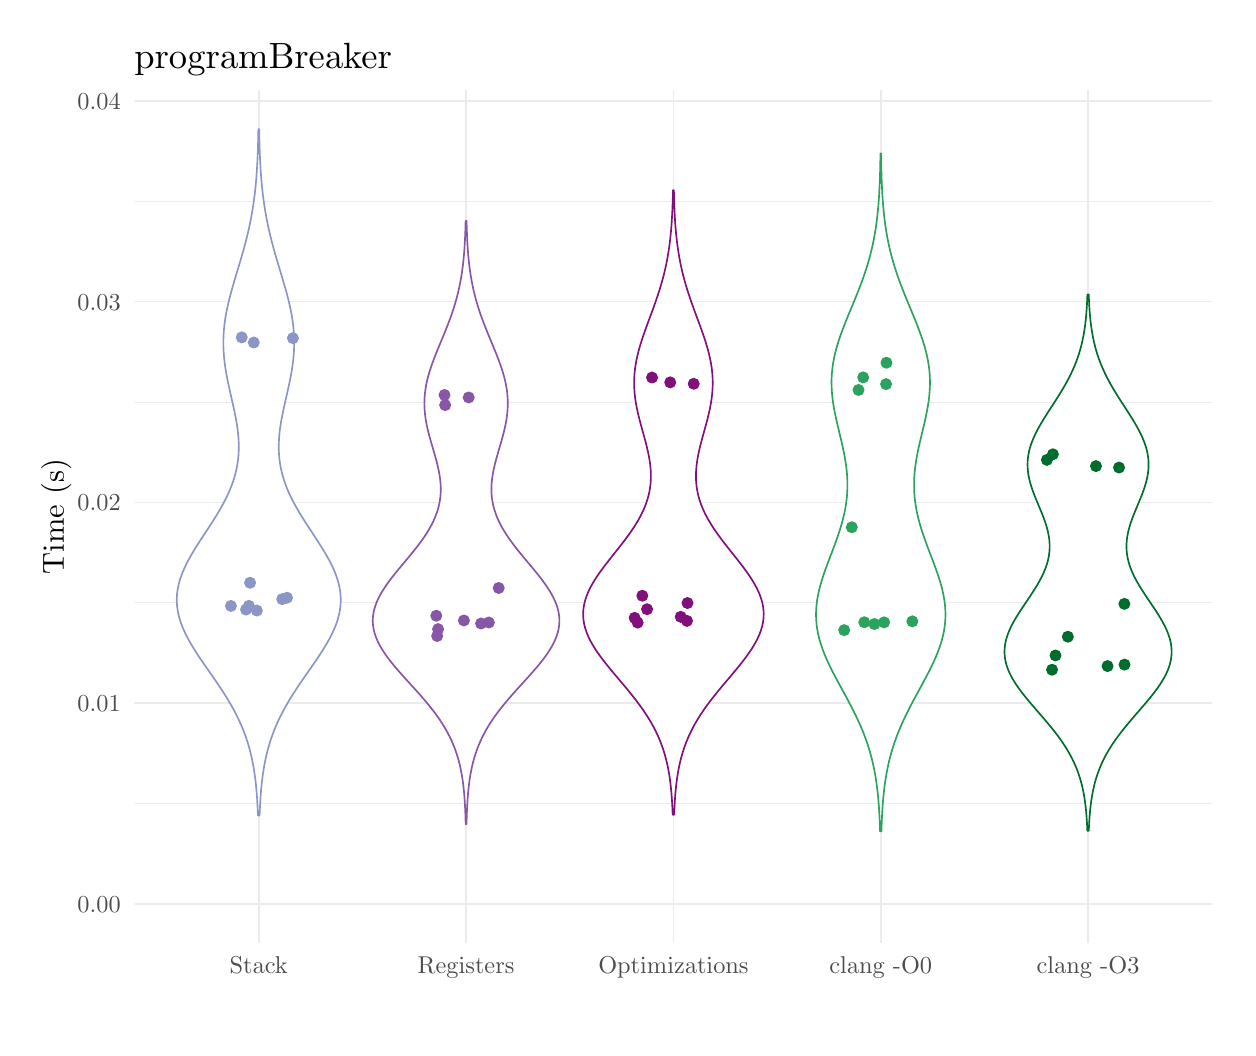
\begin{tikzpicture}[x=1pt,y=1pt]
\definecolor{fillColor}{RGB}{255,255,255}
\path[use as bounding box,fill=fillColor,fill opacity=0.00] (0,0) rectangle (433.62,361.35);
\begin{scope}
\path[clip] ( 38.56, 30.69) rectangle (428.12,338.69);
\definecolor{drawColor}{gray}{0.92}

\path[draw=drawColor,line width= 0.3pt,line join=round] ( 38.56, 80.96) --
	(428.12, 80.96);

\path[draw=drawColor,line width= 0.3pt,line join=round] ( 38.56,153.52) --
	(428.12,153.52);

\path[draw=drawColor,line width= 0.3pt,line join=round] ( 38.56,226.07) --
	(428.12,226.07);

\path[draw=drawColor,line width= 0.3pt,line join=round] ( 38.56,298.62) --
	(428.12,298.62);

\path[draw=drawColor,line width= 0.6pt,line join=round] ( 38.56, 44.69) --
	(428.12, 44.69);

\path[draw=drawColor,line width= 0.6pt,line join=round] ( 38.56,117.24) --
	(428.12,117.24);

\path[draw=drawColor,line width= 0.6pt,line join=round] ( 38.56,189.79) --
	(428.12,189.79);

\path[draw=drawColor,line width= 0.6pt,line join=round] ( 38.56,262.35) --
	(428.12,262.35);

\path[draw=drawColor,line width= 0.6pt,line join=round] ( 38.56,334.90) --
	(428.12,334.90);

\path[draw=drawColor,line width= 0.6pt,line join=round] ( 83.50, 30.69) --
	( 83.50,338.69);

\path[draw=drawColor,line width= 0.6pt,line join=round] (158.42, 30.69) --
	(158.42,338.69);

\path[draw=drawColor,line width= 0.6pt,line join=round] (233.34, 30.69) --
	(233.34,338.69);

\path[draw=drawColor,line width= 0.6pt,line join=round] (308.25, 30.69) --
	(308.25,338.69);

\path[draw=drawColor,line width= 0.6pt,line join=round] (383.17, 30.69) --
	(383.17,338.69);
\definecolor{drawColor}{RGB}{140,150,198}
\definecolor{fillColor}{RGB}{255,255,255}

\path[draw=drawColor,line width= 0.6pt,line join=round,line cap=round,fill=fillColor] ( 83.20, 76.66) --
	( 83.18, 77.14) --
	( 83.16, 77.63) --
	( 83.14, 78.11) --
	( 83.12, 78.60) --
	( 83.10, 79.08) --
	( 83.08, 79.57) --
	( 83.05, 80.06) --
	( 83.03, 80.54) --
	( 83.00, 81.03) --
	( 82.97, 81.51) --
	( 82.94, 82.00) --
	( 82.91, 82.48) --
	( 82.88, 82.97) --
	( 82.85, 83.45) --
	( 82.81, 83.94) --
	( 82.78, 84.42) --
	( 82.74, 84.91) --
	( 82.70, 85.39) --
	( 82.66, 85.88) --
	( 82.61, 86.37) --
	( 82.57, 86.85) --
	( 82.52, 87.34) --
	( 82.47, 87.82) --
	( 82.42, 88.31) --
	( 82.37, 88.79) --
	( 82.31, 89.28) --
	( 82.25, 89.76) --
	( 82.19, 90.25) --
	( 82.13, 90.73) --
	( 82.06, 91.22) --
	( 81.99, 91.71) --
	( 81.92, 92.19) --
	( 81.85, 92.68) --
	( 81.77, 93.16) --
	( 81.69, 93.65) --
	( 81.61, 94.13) --
	( 81.53, 94.62) --
	( 81.44, 95.10) --
	( 81.35, 95.59) --
	( 81.25, 96.07) --
	( 81.15, 96.56) --
	( 81.05, 97.04) --
	( 80.95, 97.53) --
	( 80.84, 98.02) --
	( 80.73, 98.50) --
	( 80.61, 98.99) --
	( 80.49, 99.47) --
	( 80.37, 99.96) --
	( 80.24,100.44) --
	( 80.11,100.93) --
	( 79.97,101.41) --
	( 79.83,101.90) --
	( 79.69,102.38) --
	( 79.54,102.87) --
	( 79.39,103.35) --
	( 79.23,103.84) --
	( 79.07,104.33) --
	( 78.91,104.81) --
	( 78.74,105.30) --
	( 78.56,105.78) --
	( 78.39,106.27) --
	( 78.20,106.75) --
	( 78.02,107.24) --
	( 77.82,107.72) --
	( 77.63,108.21) --
	( 77.42,108.69) --
	( 77.22,109.18) --
	( 77.01,109.66) --
	( 76.79,110.15) --
	( 76.57,110.64) --
	( 76.35,111.12) --
	( 76.12,111.61) --
	( 75.88,112.09) --
	( 75.64,112.58) --
	( 75.40,113.06) --
	( 75.15,113.55) --
	( 74.90,114.03) --
	( 74.64,114.52) --
	( 74.38,115.00) --
	( 74.11,115.49) --
	( 73.84,115.97) --
	( 73.57,116.46) --
	( 73.29,116.95) --
	( 73.01,117.43) --
	( 72.72,117.92) --
	( 72.43,118.40) --
	( 72.14,118.89) --
	( 71.84,119.37) --
	( 71.53,119.86) --
	( 71.23,120.34) --
	( 70.92,120.83) --
	( 70.61,121.31) --
	( 70.29,121.80) --
	( 69.98,122.28) --
	( 69.66,122.77) --
	( 69.33,123.26) --
	( 69.01,123.74) --
	( 68.68,124.23) --
	( 68.35,124.71) --
	( 68.02,125.20) --
	( 67.69,125.68) --
	( 67.35,126.17) --
	( 67.02,126.65) --
	( 66.68,127.14) --
	( 66.34,127.62) --
	( 66.00,128.11) --
	( 65.67,128.59) --
	( 65.33,129.08) --
	( 64.99,129.57) --
	( 64.65,130.05) --
	( 64.32,130.54) --
	( 63.98,131.02) --
	( 63.64,131.51) --
	( 63.31,131.99) --
	( 62.98,132.48) --
	( 62.65,132.96) --
	( 62.32,133.45) --
	( 62.00,133.93) --
	( 61.67,134.42) --
	( 61.35,134.90) --
	( 61.04,135.39) --
	( 60.72,135.88) --
	( 60.41,136.36) --
	( 60.11,136.85) --
	( 59.81,137.33) --
	( 59.52,137.82) --
	( 59.22,138.30) --
	( 58.94,138.79) --
	( 58.66,139.27) --
	( 58.38,139.76) --
	( 58.12,140.24) --
	( 57.85,140.73) --
	( 57.60,141.21) --
	( 57.35,141.70) --
	( 57.11,142.19) --
	( 56.87,142.67) --
	( 56.65,143.16) --
	( 56.43,143.64) --
	( 56.22,144.13) --
	( 56.01,144.61) --
	( 55.82,145.10) --
	( 55.63,145.58) --
	( 55.45,146.07) --
	( 55.28,146.55) --
	( 55.12,147.04) --
	( 54.97,147.52) --
	( 54.83,148.01) --
	( 54.70,148.50) --
	( 54.57,148.98) --
	( 54.46,149.47) --
	( 54.36,149.95) --
	( 54.26,150.44) --
	( 54.18,150.92) --
	( 54.11,151.41) --
	( 54.05,151.89) --
	( 53.99,152.38) --
	( 53.95,152.86) --
	( 53.92,153.35) --
	( 53.90,153.84) --
	( 53.89,154.32) --
	( 53.89,154.81) --
	( 53.90,155.29) --
	( 53.92,155.78) --
	( 53.95,156.26) --
	( 53.99,156.75) --
	( 54.04,157.23) --
	( 54.10,157.72) --
	( 54.18,158.20) --
	( 54.26,158.69) --
	( 54.35,159.17) --
	( 54.45,159.66) --
	( 54.56,160.15) --
	( 54.68,160.63) --
	( 54.81,161.12) --
	( 54.95,161.60) --
	( 55.10,162.09) --
	( 55.26,162.57) --
	( 55.43,163.06) --
	( 55.60,163.54) --
	( 55.79,164.03) --
	( 55.98,164.51) --
	( 56.18,165.00) --
	( 56.39,165.48) --
	( 56.60,165.97) --
	( 56.83,166.46) --
	( 57.06,166.94) --
	( 57.29,167.43) --
	( 57.54,167.91) --
	( 57.79,168.40) --
	( 58.04,168.88) --
	( 58.31,169.37) --
	( 58.57,169.85) --
	( 58.85,170.34) --
	( 59.12,170.82) --
	( 59.41,171.31) --
	( 59.69,171.79) --
	( 59.99,172.28) --
	( 60.28,172.77) --
	( 60.58,173.25) --
	( 60.88,173.74) --
	( 61.19,174.22) --
	( 61.50,174.71) --
	( 61.81,175.19) --
	( 62.12,175.68) --
	( 62.43,176.16) --
	( 62.75,176.65) --
	( 63.07,177.13) --
	( 63.38,177.62) --
	( 63.70,178.10) --
	( 64.02,178.59) --
	( 64.34,179.08) --
	( 64.66,179.56) --
	( 64.98,180.05) --
	( 65.30,180.53) --
	( 65.61,181.02) --
	( 65.93,181.50) --
	( 66.24,181.99) --
	( 66.56,182.47) --
	( 66.87,182.96) --
	( 67.18,183.44) --
	( 67.48,183.93) --
	( 67.79,184.41) --
	( 68.09,184.90) --
	( 68.38,185.39) --
	( 68.68,185.87) --
	( 68.97,186.36) --
	( 69.25,186.84) --
	( 69.53,187.33) --
	( 69.81,187.81) --
	( 70.09,188.30) --
	( 70.36,188.78) --
	( 70.62,189.27) --
	( 70.88,189.75) --
	( 71.13,190.24) --
	( 71.38,190.72) --
	( 71.63,191.21) --
	( 71.87,191.70) --
	( 72.10,192.18) --
	( 72.33,192.67) --
	( 72.55,193.15) --
	( 72.76,193.64) --
	( 72.98,194.12) --
	( 73.18,194.61) --
	( 73.38,195.09) --
	( 73.57,195.58) --
	( 73.75,196.06) --
	( 73.93,196.55) --
	( 74.10,197.03) --
	( 74.27,197.52) --
	( 74.43,198.01) --
	( 74.58,198.49) --
	( 74.72,198.98) --
	( 74.86,199.46) --
	( 75.00,199.95) --
	( 75.12,200.43) --
	( 75.24,200.92) --
	( 75.35,201.40) --
	( 75.46,201.89) --
	( 75.56,202.37) --
	( 75.65,202.86) --
	( 75.74,203.34) --
	( 75.82,203.83) --
	( 75.89,204.32) --
	( 75.96,204.80) --
	( 76.02,205.29) --
	( 76.07,205.77) --
	( 76.12,206.26) --
	( 76.16,206.74) --
	( 76.19,207.23) --
	( 76.22,207.71) --
	( 76.25,208.20) --
	( 76.26,208.68) --
	( 76.27,209.17) --
	( 76.28,209.65) --
	( 76.28,210.14) --
	( 76.27,210.63) --
	( 76.26,211.11) --
	( 76.25,211.60) --
	( 76.22,212.08) --
	( 76.20,212.57) --
	( 76.16,213.05) --
	( 76.13,213.54) --
	( 76.09,214.02) --
	( 76.04,214.51) --
	( 75.99,214.99) --
	( 75.94,215.48) --
	( 75.88,215.97) --
	( 75.81,216.45) --
	( 75.75,216.94) --
	( 75.68,217.42) --
	( 75.60,217.91) --
	( 75.53,218.39) --
	( 75.45,218.88) --
	( 75.36,219.36) --
	( 75.28,219.85) --
	( 75.19,220.33) --
	( 75.09,220.82) --
	( 75.00,221.30) --
	( 74.90,221.79) --
	( 74.80,222.28) --
	( 74.70,222.76) --
	( 74.60,223.25) --
	( 74.50,223.73) --
	( 74.39,224.22) --
	( 74.28,224.70) --
	( 74.18,225.19) --
	( 74.07,225.67) --
	( 73.96,226.16) --
	( 73.85,226.64) --
	( 73.74,227.13) --
	( 73.63,227.61) --
	( 73.52,228.10) --
	( 73.40,228.59) --
	( 73.29,229.07) --
	( 73.18,229.56) --
	( 73.07,230.04) --
	( 72.97,230.53) --
	( 72.86,231.01) --
	( 72.75,231.50) --
	( 72.65,231.98) --
	( 72.54,232.47) --
	( 72.44,232.95) --
	( 72.34,233.44) --
	( 72.24,233.92) --
	( 72.14,234.41) --
	( 72.05,234.90) --
	( 71.96,235.38) --
	( 71.87,235.87) --
	( 71.78,236.35) --
	( 71.69,236.84) --
	( 71.61,237.32) --
	( 71.53,237.81) --
	( 71.46,238.29) --
	( 71.38,238.78) --
	( 71.31,239.26) --
	( 71.25,239.75) --
	( 71.19,240.23) --
	( 71.13,240.72) --
	( 71.07,241.21) --
	( 71.02,241.69) --
	( 70.97,242.18) --
	( 70.93,242.66) --
	( 70.89,243.15) --
	( 70.85,243.63) --
	( 70.82,244.12) --
	( 70.79,244.60) --
	( 70.77,245.09) --
	( 70.75,245.57) --
	( 70.73,246.06) --
	( 70.72,246.54) --
	( 70.72,247.03) --
	( 70.71,247.52) --
	( 70.71,248.00) --
	( 70.72,248.49) --
	( 70.73,248.97) --
	( 70.75,249.46) --
	( 70.77,249.94) --
	( 70.79,250.43) --
	( 70.82,250.91) --
	( 70.85,251.40) --
	( 70.89,251.88) --
	( 70.93,252.37) --
	( 70.98,252.85) --
	( 71.03,253.34) --
	( 71.08,253.83) --
	( 71.14,254.31) --
	( 71.20,254.80) --
	( 71.27,255.28) --
	( 71.34,255.77) --
	( 71.41,256.25) --
	( 71.49,256.74) --
	( 71.57,257.22) --
	( 71.66,257.71) --
	( 71.75,258.19) --
	( 71.84,258.68) --
	( 71.93,259.16) --
	( 72.03,259.65) --
	( 72.14,260.14) --
	( 72.24,260.62) --
	( 72.35,261.11) --
	( 72.46,261.59) --
	( 72.57,262.08) --
	( 72.69,262.56) --
	( 72.81,263.05) --
	( 72.93,263.53) --
	( 73.05,264.02) --
	( 73.18,264.50) --
	( 73.31,264.99) --
	( 73.44,265.47) --
	( 73.57,265.96) --
	( 73.70,266.45) --
	( 73.84,266.93) --
	( 73.98,267.42) --
	( 74.12,267.90) --
	( 74.26,268.39) --
	( 74.40,268.87) --
	( 74.54,269.36) --
	( 74.68,269.84) --
	( 74.82,270.33) --
	( 74.97,270.81) --
	( 75.11,271.30) --
	( 75.26,271.78) --
	( 75.41,272.27) --
	( 75.55,272.76) --
	( 75.70,273.24) --
	( 75.84,273.73) --
	( 75.99,274.21) --
	( 76.14,274.70) --
	( 76.28,275.18) --
	( 76.43,275.67) --
	( 76.57,276.15) --
	( 76.72,276.64) --
	( 76.86,277.12) --
	( 77.01,277.61) --
	( 77.15,278.09) --
	( 77.29,278.58) --
	( 77.43,279.07) --
	( 77.57,279.55) --
	( 77.71,280.04) --
	( 77.84,280.52) --
	( 77.98,281.01) --
	( 78.12,281.49) --
	( 78.25,281.98) --
	( 78.38,282.46) --
	( 78.51,282.95) --
	( 78.64,283.43) --
	( 78.77,283.92) --
	( 78.89,284.41) --
	( 79.01,284.89) --
	( 79.14,285.38) --
	( 79.26,285.86) --
	( 79.38,286.35) --
	( 79.49,286.83) --
	( 79.61,287.32) --
	( 79.72,287.80) --
	( 79.83,288.29) --
	( 79.94,288.77) --
	( 80.04,289.26) --
	( 80.15,289.74) --
	( 80.25,290.23) --
	( 80.35,290.72) --
	( 80.45,291.20) --
	( 80.55,291.69) --
	( 80.64,292.17) --
	( 80.74,292.66) --
	( 80.83,293.14) --
	( 80.91,293.63) --
	( 81.00,294.11) --
	( 81.09,294.60) --
	( 81.17,295.08) --
	( 81.25,295.57) --
	( 81.33,296.05) --
	( 81.40,296.54) --
	( 81.48,297.03) --
	( 81.55,297.51) --
	( 81.62,298.00) --
	( 81.69,298.48) --
	( 81.76,298.97) --
	( 81.82,299.45) --
	( 81.88,299.94) --
	( 81.95,300.42) --
	( 82.01,300.91) --
	( 82.06,301.39) --
	( 82.12,301.88) --
	( 82.17,302.36) --
	( 82.23,302.85) --
	( 82.28,303.34) --
	( 82.33,303.82) --
	( 82.38,304.31) --
	( 82.42,304.79) --
	( 82.47,305.28) --
	( 82.51,305.76) --
	( 82.55,306.25) --
	( 82.59,306.73) --
	( 82.63,307.22) --
	( 82.67,307.70) --
	( 82.70,308.19) --
	( 82.74,308.67) --
	( 82.77,309.16) --
	( 82.81,309.65) --
	( 82.84,310.13) --
	( 82.87,310.62) --
	( 82.90,311.10) --
	( 82.92,311.59) --
	( 82.95,312.07) --
	( 82.98,312.56) --
	( 83.00,313.04) --
	( 83.03,313.53) --
	( 83.05,314.01) --
	( 83.07,314.50) --
	( 83.09,314.98) --
	( 83.11,315.47) --
	( 83.13,315.96) --
	( 83.15,316.44) --
	( 83.17,316.93) --
	( 83.18,317.41) --
	( 83.20,317.90) --
	( 83.21,318.38) --
	( 83.23,318.87) --
	( 83.24,319.35) --
	( 83.26,319.84) --
	( 83.27,320.32) --
	( 83.28,320.81) --
	( 83.29,321.29) --
	( 83.31,321.78) --
	( 83.32,322.27) --
	( 83.33,322.75) --
	( 83.34,323.24) --
	( 83.34,323.72) --
	( 83.35,324.21) --
	( 83.36,324.69) --
	( 83.65,324.69) --
	( 83.66,324.21) --
	( 83.67,323.72) --
	( 83.67,323.24) --
	( 83.68,322.75) --
	( 83.69,322.27) --
	( 83.70,321.78) --
	( 83.72,321.29) --
	( 83.73,320.81) --
	( 83.74,320.32) --
	( 83.75,319.84) --
	( 83.77,319.35) --
	( 83.78,318.87) --
	( 83.80,318.38) --
	( 83.81,317.90) --
	( 83.83,317.41) --
	( 83.84,316.93) --
	( 83.86,316.44) --
	( 83.88,315.96) --
	( 83.90,315.47) --
	( 83.92,314.98) --
	( 83.94,314.50) --
	( 83.96,314.01) --
	( 83.98,313.53) --
	( 84.01,313.04) --
	( 84.03,312.56) --
	( 84.06,312.07) --
	( 84.09,311.59) --
	( 84.11,311.10) --
	( 84.14,310.62) --
	( 84.17,310.13) --
	( 84.20,309.65) --
	( 84.24,309.16) --
	( 84.27,308.67) --
	( 84.31,308.19) --
	( 84.34,307.70) --
	( 84.38,307.22) --
	( 84.42,306.73) --
	( 84.46,306.25) --
	( 84.50,305.76) --
	( 84.54,305.28) --
	( 84.59,304.79) --
	( 84.63,304.31) --
	( 84.68,303.82) --
	( 84.73,303.34) --
	( 84.78,302.85) --
	( 84.84,302.36) --
	( 84.89,301.88) --
	( 84.95,301.39) --
	( 85.00,300.91) --
	( 85.06,300.42) --
	( 85.12,299.94) --
	( 85.19,299.45) --
	( 85.25,298.97) --
	( 85.32,298.48) --
	( 85.39,298.00) --
	( 85.46,297.51) --
	( 85.53,297.03) --
	( 85.61,296.54) --
	( 85.68,296.05) --
	( 85.76,295.57) --
	( 85.84,295.08) --
	( 85.92,294.60) --
	( 86.01,294.11) --
	( 86.10,293.63) --
	( 86.18,293.14) --
	( 86.27,292.66) --
	( 86.37,292.17) --
	( 86.46,291.69) --
	( 86.56,291.20) --
	( 86.66,290.72) --
	( 86.76,290.23) --
	( 86.86,289.74) --
	( 86.97,289.26) --
	( 87.07,288.77) --
	( 87.18,288.29) --
	( 87.29,287.80) --
	( 87.40,287.32) --
	( 87.52,286.83) --
	( 87.63,286.35) --
	( 87.75,285.86) --
	( 87.87,285.38) --
	( 88.00,284.89) --
	( 88.12,284.41) --
	( 88.24,283.92) --
	( 88.37,283.43) --
	( 88.50,282.95) --
	( 88.63,282.46) --
	( 88.76,281.98) --
	( 88.89,281.49) --
	( 89.03,281.01) --
	( 89.16,280.52) --
	( 89.30,280.04) --
	( 89.44,279.55) --
	( 89.58,279.07) --
	( 89.72,278.58) --
	( 89.86,278.09) --
	( 90.00,277.61) --
	( 90.15,277.12) --
	( 90.29,276.64) --
	( 90.44,276.15) --
	( 90.58,275.67) --
	( 90.73,275.18) --
	( 90.87,274.70) --
	( 91.02,274.21) --
	( 91.16,273.73) --
	( 91.31,273.24) --
	( 91.46,272.76) --
	( 91.60,272.27) --
	( 91.75,271.78) --
	( 91.90,271.30) --
	( 92.04,270.81) --
	( 92.18,270.33) --
	( 92.33,269.84) --
	( 92.47,269.36) --
	( 92.61,268.87) --
	( 92.75,268.39) --
	( 92.89,267.90) --
	( 93.03,267.42) --
	( 93.17,266.93) --
	( 93.30,266.45) --
	( 93.44,265.96) --
	( 93.57,265.47) --
	( 93.70,264.99) --
	( 93.83,264.50) --
	( 93.96,264.02) --
	( 94.08,263.53) --
	( 94.20,263.05) --
	( 94.32,262.56) --
	( 94.44,262.08) --
	( 94.55,261.59) --
	( 94.66,261.11) --
	( 94.77,260.62) --
	( 94.87,260.14) --
	( 94.98,259.65) --
	( 95.08,259.16) --
	( 95.17,258.68) --
	( 95.26,258.19) --
	( 95.35,257.71) --
	( 95.44,257.22) --
	( 95.52,256.74) --
	( 95.60,256.25) --
	( 95.67,255.77) --
	( 95.74,255.28) --
	( 95.81,254.80) --
	( 95.87,254.31) --
	( 95.93,253.83) --
	( 95.98,253.34) --
	( 96.03,252.85) --
	( 96.08,252.37) --
	( 96.12,251.88) --
	( 96.16,251.40) --
	( 96.19,250.91) --
	( 96.22,250.43) --
	( 96.24,249.94) --
	( 96.26,249.46) --
	( 96.28,248.97) --
	( 96.29,248.49) --
	( 96.29,248.00) --
	( 96.30,247.52) --
	( 96.29,247.03) --
	( 96.29,246.54) --
	( 96.28,246.06) --
	( 96.26,245.57) --
	( 96.24,245.09) --
	( 96.22,244.60) --
	( 96.19,244.12) --
	( 96.16,243.63) --
	( 96.12,243.15) --
	( 96.08,242.66) --
	( 96.04,242.18) --
	( 95.99,241.69) --
	( 95.94,241.21) --
	( 95.88,240.72) --
	( 95.82,240.23) --
	( 95.76,239.75) --
	( 95.70,239.26) --
	( 95.63,238.78) --
	( 95.55,238.29) --
	( 95.48,237.81) --
	( 95.40,237.32) --
	( 95.32,236.84) --
	( 95.23,236.35) --
	( 95.14,235.87) --
	( 95.05,235.38) --
	( 94.96,234.90) --
	( 94.87,234.41) --
	( 94.77,233.92) --
	( 94.67,233.44) --
	( 94.57,232.95) --
	( 94.47,232.47) --
	( 94.36,231.98) --
	( 94.26,231.50) --
	( 94.15,231.01) --
	( 94.04,230.53) --
	( 93.94,230.04) --
	( 93.83,229.56) --
	( 93.72,229.07) --
	( 93.61,228.59) --
	( 93.49,228.10) --
	( 93.38,227.61) --
	( 93.27,227.13) --
	( 93.16,226.64) --
	( 93.05,226.16) --
	( 92.94,225.67) --
	( 92.83,225.19) --
	( 92.73,224.70) --
	( 92.62,224.22) --
	( 92.51,223.73) --
	( 92.41,223.25) --
	( 92.31,222.76) --
	( 92.21,222.28) --
	( 92.11,221.79) --
	( 92.01,221.30) --
	( 91.92,220.82) --
	( 91.82,220.33) --
	( 91.73,219.85) --
	( 91.65,219.36) --
	( 91.56,218.88) --
	( 91.48,218.39) --
	( 91.41,217.91) --
	( 91.33,217.42) --
	( 91.26,216.94) --
	( 91.20,216.45) --
	( 91.13,215.97) --
	( 91.07,215.48) --
	( 91.02,214.99) --
	( 90.97,214.51) --
	( 90.92,214.02) --
	( 90.88,213.54) --
	( 90.85,213.05) --
	( 90.81,212.57) --
	( 90.79,212.08) --
	( 90.76,211.60) --
	( 90.75,211.11) --
	( 90.74,210.63) --
	( 90.73,210.14) --
	( 90.73,209.65) --
	( 90.74,209.17) --
	( 90.75,208.68) --
	( 90.76,208.20) --
	( 90.79,207.71) --
	( 90.82,207.23) --
	( 90.85,206.74) --
	( 90.89,206.26) --
	( 90.94,205.77) --
	( 90.99,205.29) --
	( 91.05,204.80) --
	( 91.12,204.32) --
	( 91.19,203.83) --
	( 91.27,203.34) --
	( 91.36,202.86) --
	( 91.45,202.37) --
	( 91.55,201.89) --
	( 91.66,201.40) --
	( 91.77,200.92) --
	( 91.89,200.43) --
	( 92.01,199.95) --
	( 92.15,199.46) --
	( 92.29,198.98) --
	( 92.43,198.49) --
	( 92.58,198.01) --
	( 92.74,197.52) --
	( 92.91,197.03) --
	( 93.08,196.55) --
	( 93.26,196.06) --
	( 93.44,195.58) --
	( 93.63,195.09) --
	( 93.83,194.61) --
	( 94.03,194.12) --
	( 94.25,193.64) --
	( 94.46,193.15) --
	( 94.68,192.67) --
	( 94.91,192.18) --
	( 95.14,191.70) --
	( 95.38,191.21) --
	( 95.63,190.72) --
	( 95.87,190.24) --
	( 96.13,189.75) --
	( 96.39,189.27) --
	( 96.65,188.78) --
	( 96.92,188.30) --
	( 97.20,187.81) --
	( 97.48,187.33) --
	( 97.76,186.84) --
	( 98.04,186.36) --
	( 98.33,185.87) --
	( 98.63,185.39) --
	( 98.92,184.90) --
	( 99.22,184.41) --
	( 99.53,183.93) --
	( 99.83,183.44) --
	(100.14,182.96) --
	(100.45,182.47) --
	(100.77,181.99) --
	(101.08,181.50) --
	(101.40,181.02) --
	(101.71,180.53) --
	(102.03,180.05) --
	(102.35,179.56) --
	(102.67,179.08) --
	(102.99,178.59) --
	(103.31,178.10) --
	(103.63,177.62) --
	(103.94,177.13) --
	(104.26,176.65) --
	(104.58,176.16) --
	(104.89,175.68) --
	(105.20,175.19) --
	(105.51,174.71) --
	(105.82,174.22) --
	(106.13,173.74) --
	(106.43,173.25) --
	(106.73,172.77) --
	(107.02,172.28) --
	(107.32,171.79) --
	(107.60,171.31) --
	(107.89,170.82) --
	(108.16,170.34) --
	(108.44,169.85) --
	(108.70,169.37) --
	(108.97,168.88) --
	(109.22,168.40) --
	(109.47,167.91) --
	(109.72,167.43) --
	(109.95,166.94) --
	(110.18,166.46) --
	(110.41,165.97) --
	(110.62,165.48) --
	(110.83,165.00) --
	(111.03,164.51) --
	(111.22,164.03) --
	(111.41,163.54) --
	(111.58,163.06) --
	(111.75,162.57) --
	(111.91,162.09) --
	(112.06,161.60) --
	(112.20,161.12) --
	(112.33,160.63) --
	(112.45,160.15) --
	(112.56,159.66) --
	(112.66,159.17) --
	(112.75,158.69) --
	(112.83,158.20) --
	(112.91,157.72) --
	(112.97,157.23) --
	(113.02,156.75) --
	(113.06,156.26) --
	(113.09,155.78) --
	(113.11,155.29) --
	(113.12,154.81) --
	(113.12,154.32) --
	(113.11,153.84) --
	(113.09,153.35) --
	(113.06,152.86) --
	(113.02,152.38) --
	(112.96,151.89) --
	(112.90,151.41) --
	(112.83,150.92) --
	(112.75,150.44) --
	(112.65,149.95) --
	(112.55,149.47) --
	(112.44,148.98) --
	(112.31,148.50) --
	(112.18,148.01) --
	(112.04,147.52) --
	(111.89,147.04) --
	(111.73,146.55) --
	(111.56,146.07) --
	(111.38,145.58) --
	(111.19,145.10) --
	(111.00,144.61) --
	(110.79,144.13) --
	(110.58,143.64) --
	(110.36,143.16) --
	(110.14,142.67) --
	(109.90,142.19) --
	(109.66,141.70) --
	(109.41,141.21) --
	(109.16,140.73) --
	(108.89,140.24) --
	(108.63,139.76) --
	(108.35,139.27) --
	(108.07,138.79) --
	(107.79,138.30) --
	(107.49,137.82) --
	(107.20,137.33) --
	(106.90,136.85) --
	(106.59,136.36) --
	(106.28,135.88) --
	(105.97,135.39) --
	(105.66,134.90) --
	(105.34,134.42) --
	(105.01,133.93) --
	(104.69,133.45) --
	(104.36,132.96) --
	(104.03,132.48) --
	(103.70,131.99) --
	(103.37,131.51) --
	(103.03,131.02) --
	(102.69,130.54) --
	(102.36,130.05) --
	(102.02,129.57) --
	(101.68,129.08) --
	(101.34,128.59) --
	(101.01,128.11) --
	(100.67,127.62) --
	(100.33,127.14) --
	( 99.99,126.65) --
	( 99.66,126.17) --
	( 99.32,125.68) --
	( 98.99,125.20) --
	( 98.66,124.71) --
	( 98.33,124.23) --
	( 98.00,123.74) --
	( 97.68,123.26) --
	( 97.35,122.77) --
	( 97.03,122.28) --
	( 96.72,121.80) --
	( 96.40,121.31) --
	( 96.09,120.83) --
	( 95.78,120.34) --
	( 95.47,119.86) --
	( 95.17,119.37) --
	( 94.87,118.89) --
	( 94.58,118.40) --
	( 94.29,117.92) --
	( 94.00,117.43) --
	( 93.72,116.95) --
	( 93.44,116.46) --
	( 93.16,115.97) --
	( 92.90,115.49) --
	( 92.63,115.00) --
	( 92.37,114.52) --
	( 92.11,114.03) --
	( 91.86,113.55) --
	( 91.61,113.06) --
	( 91.37,112.58) --
	( 91.13,112.09) --
	( 90.89,111.61) --
	( 90.66,111.12) --
	( 90.44,110.64) --
	( 90.22,110.15) --
	( 90.00,109.66) --
	( 89.79,109.18) --
	( 89.58,108.69) --
	( 89.38,108.21) --
	( 89.19,107.72) --
	( 88.99,107.24) --
	( 88.81,106.75) --
	( 88.62,106.27) --
	( 88.45,105.78) --
	( 88.27,105.30) --
	( 88.10,104.81) --
	( 87.94,104.33) --
	( 87.78,103.84) --
	( 87.62,103.35) --
	( 87.47,102.87) --
	( 87.32,102.38) --
	( 87.18,101.90) --
	( 87.04,101.41) --
	( 86.90,100.93) --
	( 86.77,100.44) --
	( 86.64, 99.96) --
	( 86.52, 99.47) --
	( 86.40, 98.99) --
	( 86.28, 98.50) --
	( 86.17, 98.02) --
	( 86.06, 97.53) --
	( 85.96, 97.04) --
	( 85.86, 96.56) --
	( 85.76, 96.07) --
	( 85.66, 95.59) --
	( 85.57, 95.10) --
	( 85.48, 94.62) --
	( 85.40, 94.13) --
	( 85.32, 93.65) --
	( 85.24, 93.16) --
	( 85.16, 92.68) --
	( 85.09, 92.19) --
	( 85.02, 91.71) --
	( 84.95, 91.22) --
	( 84.88, 90.73) --
	( 84.82, 90.25) --
	( 84.76, 89.76) --
	( 84.70, 89.28) --
	( 84.64, 88.79) --
	( 84.59, 88.31) --
	( 84.54, 87.82) --
	( 84.49, 87.34) --
	( 84.44, 86.85) --
	( 84.40, 86.37) --
	( 84.35, 85.88) --
	( 84.31, 85.39) --
	( 84.27, 84.91) --
	( 84.23, 84.42) --
	( 84.20, 83.94) --
	( 84.16, 83.45) --
	( 84.13, 82.97) --
	( 84.10, 82.48) --
	( 84.07, 82.00) --
	( 84.04, 81.51) --
	( 84.01, 81.03) --
	( 83.98, 80.54) --
	( 83.96, 80.06) --
	( 83.93, 79.57) --
	( 83.91, 79.08) --
	( 83.89, 78.60) --
	( 83.87, 78.11) --
	( 83.85, 77.63) --
	( 83.83, 77.14) --
	( 83.81, 76.66) --
	( 83.20, 76.66) --
	cycle;
\definecolor{drawColor}{RGB}{136,86,167}

\path[draw=drawColor,line width= 0.6pt,line join=round,line cap=round,fill=fillColor] (158.27, 73.55) --
	(158.26, 73.98) --
	(158.24, 74.40) --
	(158.23, 74.83) --
	(158.22, 75.26) --
	(158.21, 75.68) --
	(158.20, 76.11) --
	(158.18, 76.54) --
	(158.17, 76.96) --
	(158.15, 77.39) --
	(158.13, 77.82) --
	(158.12, 78.24) --
	(158.10, 78.67) --
	(158.08, 79.10) --
	(158.06, 79.52) --
	(158.04, 79.95) --
	(158.02, 80.38) --
	(157.99, 80.80) --
	(157.97, 81.23) --
	(157.94, 81.65) --
	(157.91, 82.08) --
	(157.88, 82.51) --
	(157.85, 82.93) --
	(157.82, 83.36) --
	(157.79, 83.79) --
	(157.75, 84.21) --
	(157.72, 84.64) --
	(157.68, 85.07) --
	(157.64, 85.49) --
	(157.60, 85.92) --
	(157.55, 86.35) --
	(157.51, 86.77) --
	(157.46, 87.20) --
	(157.41, 87.63) --
	(157.36, 88.05) --
	(157.30, 88.48) --
	(157.24, 88.91) --
	(157.19, 89.33) --
	(157.12, 89.76) --
	(157.06, 90.19) --
	(156.99, 90.61) --
	(156.92, 91.04) --
	(156.85, 91.47) --
	(156.77, 91.89) --
	(156.69, 92.32) --
	(156.61, 92.75) --
	(156.53, 93.17) --
	(156.44, 93.60) --
	(156.35, 94.03) --
	(156.25, 94.45) --
	(156.15, 94.88) --
	(156.05, 95.30) --
	(155.94, 95.73) --
	(155.83, 96.16) --
	(155.72, 96.58) --
	(155.60, 97.01) --
	(155.48, 97.44) --
	(155.35, 97.86) --
	(155.22, 98.29) --
	(155.09, 98.72) --
	(154.95, 99.14) --
	(154.80, 99.57) --
	(154.66,100.00) --
	(154.50,100.42) --
	(154.35,100.85) --
	(154.18,101.28) --
	(154.02,101.70) --
	(153.84,102.13) --
	(153.67,102.56) --
	(153.48,102.98) --
	(153.30,103.41) --
	(153.11,103.84) --
	(152.91,104.26) --
	(152.70,104.69) --
	(152.50,105.12) --
	(152.28,105.54) --
	(152.06,105.97) --
	(151.84,106.40) --
	(151.61,106.82) --
	(151.37,107.25) --
	(151.14,107.68) --
	(150.89,108.10) --
	(150.64,108.53) --
	(150.38,108.95) --
	(150.12,109.38) --
	(149.85,109.81) --
	(149.58,110.23) --
	(149.30,110.66) --
	(149.02,111.09) --
	(148.73,111.51) --
	(148.43,111.94) --
	(148.13,112.37) --
	(147.83,112.79) --
	(147.52,113.22) --
	(147.21,113.65) --
	(146.89,114.07) --
	(146.56,114.50) --
	(146.23,114.93) --
	(145.90,115.35) --
	(145.56,115.78) --
	(145.22,116.21) --
	(144.88,116.63) --
	(144.53,117.06) --
	(144.17,117.49) --
	(143.81,117.91) --
	(143.45,118.34) --
	(143.09,118.77) --
	(142.72,119.19) --
	(142.35,119.62) --
	(141.98,120.05) --
	(141.60,120.47) --
	(141.22,120.90) --
	(140.84,121.33) --
	(140.46,121.75) --
	(140.08,122.18) --
	(139.69,122.60) --
	(139.31,123.03) --
	(138.92,123.46) --
	(138.53,123.88) --
	(138.14,124.31) --
	(137.76,124.74) --
	(137.37,125.16) --
	(136.98,125.59) --
	(136.59,126.02) --
	(136.21,126.44) --
	(135.82,126.87) --
	(135.44,127.30) --
	(135.06,127.72) --
	(134.68,128.15) --
	(134.31,128.58) --
	(133.93,129.00) --
	(133.56,129.43) --
	(133.20,129.86) --
	(132.84,130.28) --
	(132.48,130.71) --
	(132.13,131.14) --
	(131.78,131.56) --
	(131.43,131.99) --
	(131.09,132.42) --
	(130.76,132.84) --
	(130.44,133.27) --
	(130.12,133.70) --
	(129.80,134.12) --
	(129.49,134.55) --
	(129.20,134.98) --
	(128.91,135.40) --
	(128.62,135.83) --
	(128.35,136.25) --
	(128.08,136.68) --
	(127.82,137.11) --
	(127.57,137.53) --
	(127.33,137.96) --
	(127.10,138.39) --
	(126.88,138.81) --
	(126.66,139.24) --
	(126.46,139.67) --
	(126.27,140.09) --
	(126.09,140.52) --
	(125.92,140.95) --
	(125.76,141.37) --
	(125.61,141.80) --
	(125.47,142.23) --
	(125.34,142.65) --
	(125.23,143.08) --
	(125.12,143.51) --
	(125.03,143.93) --
	(124.95,144.36) --
	(124.88,144.79) --
	(124.82,145.21) --
	(124.78,145.64) --
	(124.74,146.07) --
	(124.72,146.49) --
	(124.71,146.92) --
	(124.71,147.35) --
	(124.73,147.77) --
	(124.75,148.20) --
	(124.79,148.63) --
	(124.83,149.05) --
	(124.90,149.48) --
	(124.97,149.90) --
	(125.05,150.33) --
	(125.15,150.76) --
	(125.26,151.18) --
	(125.37,151.61) --
	(125.50,152.04) --
	(125.64,152.46) --
	(125.79,152.89) --
	(125.95,153.32) --
	(126.12,153.74) --
	(126.30,154.17) --
	(126.49,154.60) --
	(126.69,155.02) --
	(126.90,155.45) --
	(127.12,155.88) --
	(127.35,156.30) --
	(127.59,156.73) --
	(127.83,157.16) --
	(128.09,157.58) --
	(128.35,158.01) --
	(128.62,158.44) --
	(128.90,158.86) --
	(129.18,159.29) --
	(129.47,159.72) --
	(129.77,160.14) --
	(130.07,160.57) --
	(130.38,161.00) --
	(130.69,161.42) --
	(131.01,161.85) --
	(131.33,162.28) --
	(131.66,162.70) --
	(132.00,163.13) --
	(132.33,163.55) --
	(132.67,163.98) --
	(133.02,164.41) --
	(133.36,164.83) --
	(133.71,165.26) --
	(134.06,165.69) --
	(134.42,166.11) --
	(134.77,166.54) --
	(135.12,166.97) --
	(135.48,167.39) --
	(135.84,167.82) --
	(136.19,168.25) --
	(136.55,168.67) --
	(136.91,169.10) --
	(137.26,169.53) --
	(137.62,169.95) --
	(137.97,170.38) --
	(138.32,170.81) --
	(138.67,171.23) --
	(139.02,171.66) --
	(139.36,172.09) --
	(139.70,172.51) --
	(140.04,172.94) --
	(140.38,173.37) --
	(140.71,173.79) --
	(141.04,174.22) --
	(141.36,174.65) --
	(141.68,175.07) --
	(142.00,175.50) --
	(142.31,175.93) --
	(142.61,176.35) --
	(142.91,176.78) --
	(143.21,177.20) --
	(143.50,177.63) --
	(143.78,178.06) --
	(144.06,178.48) --
	(144.33,178.91) --
	(144.59,179.34) --
	(144.85,179.76) --
	(145.10,180.19) --
	(145.35,180.62) --
	(145.58,181.04) --
	(145.82,181.47) --
	(146.04,181.90) --
	(146.26,182.32) --
	(146.46,182.75) --
	(146.67,183.18) --
	(146.86,183.60) --
	(147.05,184.03) --
	(147.23,184.46) --
	(147.40,184.88) --
	(147.57,185.31) --
	(147.72,185.74) --
	(147.87,186.16) --
	(148.01,186.59) --
	(148.15,187.02) --
	(148.27,187.44) --
	(148.39,187.87) --
	(148.50,188.30) --
	(148.60,188.72) --
	(148.70,189.15) --
	(148.79,189.58) --
	(148.87,190.00) --
	(148.94,190.43) --
	(149.00,190.85) --
	(149.06,191.28) --
	(149.11,191.71) --
	(149.15,192.13) --
	(149.19,192.56) --
	(149.22,192.99) --
	(149.24,193.41) --
	(149.25,193.84) --
	(149.26,194.27) --
	(149.26,194.69) --
	(149.26,195.12) --
	(149.24,195.55) --
	(149.23,195.97) --
	(149.20,196.40) --
	(149.17,196.83) --
	(149.13,197.25) --
	(149.09,197.68) --
	(149.05,198.11) --
	(148.99,198.53) --
	(148.93,198.96) --
	(148.87,199.39) --
	(148.80,199.81) --
	(148.73,200.24) --
	(148.65,200.67) --
	(148.57,201.09) --
	(148.48,201.52) --
	(148.39,201.95) --
	(148.30,202.37) --
	(148.20,202.80) --
	(148.10,203.23) --
	(148.00,203.65) --
	(147.89,204.08) --
	(147.78,204.50) --
	(147.67,204.93) --
	(147.56,205.36) --
	(147.44,205.78) --
	(147.32,206.21) --
	(147.20,206.64) --
	(147.08,207.06) --
	(146.96,207.49) --
	(146.84,207.92) --
	(146.71,208.34) --
	(146.59,208.77) --
	(146.46,209.20) --
	(146.34,209.62) --
	(146.21,210.05) --
	(146.09,210.48) --
	(145.96,210.90) --
	(145.84,211.33) --
	(145.72,211.76) --
	(145.60,212.18) --
	(145.48,212.61) --
	(145.36,213.04) --
	(145.24,213.46) --
	(145.13,213.89) --
	(145.01,214.32) --
	(144.90,214.74) --
	(144.80,215.17) --
	(144.69,215.60) --
	(144.59,216.02) --
	(144.49,216.45) --
	(144.39,216.88) --
	(144.30,217.30) --
	(144.21,217.73) --
	(144.13,218.15) --
	(144.05,218.58) --
	(143.97,219.01) --
	(143.89,219.43) --
	(143.82,219.86) --
	(143.76,220.29) --
	(143.70,220.71) --
	(143.64,221.14) --
	(143.59,221.57) --
	(143.55,221.99) --
	(143.51,222.42) --
	(143.47,222.85) --
	(143.44,223.27) --
	(143.41,223.70) --
	(143.39,224.13) --
	(143.37,224.55) --
	(143.36,224.98) --
	(143.36,225.41) --
	(143.36,225.83) --
	(143.37,226.26) --
	(143.37,226.69) --
	(143.39,227.11) --
	(143.41,227.54) --
	(143.44,227.97) --
	(143.47,228.39) --
	(143.51,228.82) --
	(143.55,229.25) --
	(143.60,229.67) --
	(143.66,230.10) --
	(143.71,230.53) --
	(143.78,230.95) --
	(143.85,231.38) --
	(143.92,231.80) --
	(144.00,232.23) --
	(144.09,232.66) --
	(144.17,233.08) --
	(144.27,233.51) --
	(144.37,233.94) --
	(144.47,234.36) --
	(144.58,234.79) --
	(144.69,235.22) --
	(144.80,235.64) --
	(144.92,236.07) --
	(145.05,236.50) --
	(145.17,236.92) --
	(145.31,237.35) --
	(145.44,237.78) --
	(145.58,238.20) --
	(145.72,238.63) --
	(145.87,239.06) --
	(146.01,239.48) --
	(146.16,239.91) --
	(146.32,240.34) --
	(146.47,240.76) --
	(146.63,241.19) --
	(146.79,241.62) --
	(146.96,242.04) --
	(147.12,242.47) --
	(147.29,242.90) --
	(147.46,243.32) --
	(147.63,243.75) --
	(147.80,244.18) --
	(147.97,244.60) --
	(148.15,245.03) --
	(148.32,245.45) --
	(148.50,245.88) --
	(148.67,246.31) --
	(148.85,246.73) --
	(149.03,247.16) --
	(149.20,247.59) --
	(149.38,248.01) --
	(149.56,248.44) --
	(149.74,248.87) --
	(149.91,249.29) --
	(150.09,249.72) --
	(150.27,250.15) --
	(150.44,250.57) --
	(150.62,251.00) --
	(150.79,251.43) --
	(150.96,251.85) --
	(151.13,252.28) --
	(151.30,252.71) --
	(151.47,253.13) --
	(151.64,253.56) --
	(151.81,253.99) --
	(151.97,254.41) --
	(152.13,254.84) --
	(152.29,255.27) --
	(152.45,255.69) --
	(152.61,256.12) --
	(152.77,256.55) --
	(152.92,256.97) --
	(153.07,257.40) --
	(153.22,257.83) --
	(153.36,258.25) --
	(153.51,258.68) --
	(153.65,259.11) --
	(153.79,259.53) --
	(153.93,259.96) --
	(154.06,260.38) --
	(154.20,260.81) --
	(154.33,261.24) --
	(154.45,261.66) --
	(154.58,262.09) --
	(154.70,262.52) --
	(154.82,262.94) --
	(154.94,263.37) --
	(155.05,263.80) --
	(155.17,264.22) --
	(155.27,264.65) --
	(155.38,265.08) --
	(155.49,265.50) --
	(155.59,265.93) --
	(155.69,266.36) --
	(155.79,266.78) --
	(155.88,267.21) --
	(155.97,267.64) --
	(156.06,268.06) --
	(156.15,268.49) --
	(156.24,268.92) --
	(156.32,269.34) --
	(156.40,269.77) --
	(156.48,270.20) --
	(156.55,270.62) --
	(156.62,271.05) --
	(156.70,271.48) --
	(156.76,271.90) --
	(156.83,272.33) --
	(156.90,272.76) --
	(156.96,273.18) --
	(157.02,273.61) --
	(157.08,274.03) --
	(157.13,274.46) --
	(157.19,274.89) --
	(157.24,275.31) --
	(157.29,275.74) --
	(157.34,276.17) --
	(157.39,276.59) --
	(157.44,277.02) --
	(157.48,277.45) --
	(157.52,277.87) --
	(157.56,278.30) --
	(157.60,278.73) --
	(157.64,279.15) --
	(157.68,279.58) --
	(157.71,280.01) --
	(157.75,280.43) --
	(157.78,280.86) --
	(157.81,281.29) --
	(157.84,281.71) --
	(157.87,282.14) --
	(157.89,282.57) --
	(157.92,282.99) --
	(157.94,283.42) --
	(157.97,283.85) --
	(157.99,284.27) --
	(158.01,284.70) --
	(158.03,285.13) --
	(158.05,285.55) --
	(158.07,285.98) --
	(158.09,286.41) --
	(158.11,286.83) --
	(158.13,287.26) --
	(158.14,287.68) --
	(158.16,288.11) --
	(158.17,288.54) --
	(158.18,288.96) --
	(158.20,289.39) --
	(158.21,289.82) --
	(158.22,290.24) --
	(158.23,290.67) --
	(158.24,291.10) --
	(158.25,291.52) --
	(158.59,291.52) --
	(158.60,291.10) --
	(158.61,290.67) --
	(158.62,290.24) --
	(158.63,289.82) --
	(158.65,289.39) --
	(158.66,288.96) --
	(158.67,288.54) --
	(158.69,288.11) --
	(158.70,287.68) --
	(158.72,287.26) --
	(158.73,286.83) --
	(158.75,286.41) --
	(158.77,285.98) --
	(158.79,285.55) --
	(158.81,285.13) --
	(158.83,284.70) --
	(158.85,284.27) --
	(158.87,283.85) --
	(158.90,283.42) --
	(158.92,282.99) --
	(158.95,282.57) --
	(158.98,282.14) --
	(159.00,281.71) --
	(159.03,281.29) --
	(159.07,280.86) --
	(159.10,280.43) --
	(159.13,280.01) --
	(159.17,279.58) --
	(159.20,279.15) --
	(159.24,278.73) --
	(159.28,278.30) --
	(159.32,277.87) --
	(159.36,277.45) --
	(159.41,277.02) --
	(159.45,276.59) --
	(159.50,276.17) --
	(159.55,275.74) --
	(159.60,275.31) --
	(159.65,274.89) --
	(159.71,274.46) --
	(159.76,274.03) --
	(159.82,273.61) --
	(159.88,273.18) --
	(159.95,272.76) --
	(160.01,272.33) --
	(160.08,271.90) --
	(160.15,271.48) --
	(160.22,271.05) --
	(160.29,270.62) --
	(160.37,270.20) --
	(160.44,269.77) --
	(160.53,269.34) --
	(160.61,268.92) --
	(160.69,268.49) --
	(160.78,268.06) --
	(160.87,267.64) --
	(160.96,267.21) --
	(161.06,266.78) --
	(161.15,266.36) --
	(161.25,265.93) --
	(161.36,265.50) --
	(161.46,265.08) --
	(161.57,264.65) --
	(161.68,264.22) --
	(161.79,263.80) --
	(161.90,263.37) --
	(162.02,262.94) --
	(162.14,262.52) --
	(162.26,262.09) --
	(162.39,261.66) --
	(162.52,261.24) --
	(162.65,260.81) --
	(162.78,260.38) --
	(162.91,259.96) --
	(163.05,259.53) --
	(163.19,259.11) --
	(163.33,258.68) --
	(163.48,258.25) --
	(163.62,257.83) --
	(163.77,257.40) --
	(163.92,256.97) --
	(164.08,256.55) --
	(164.23,256.12) --
	(164.39,255.69) --
	(164.55,255.27) --
	(164.71,254.84) --
	(164.87,254.41) --
	(165.04,253.99) --
	(165.20,253.56) --
	(165.37,253.13) --
	(165.54,252.71) --
	(165.71,252.28) --
	(165.88,251.85) --
	(166.05,251.43) --
	(166.23,251.00) --
	(166.40,250.57) --
	(166.58,250.15) --
	(166.75,249.72) --
	(166.93,249.29) --
	(167.11,248.87) --
	(167.28,248.44) --
	(167.46,248.01) --
	(167.64,247.59) --
	(167.82,247.16) --
	(167.99,246.73) --
	(168.17,246.31) --
	(168.35,245.88) --
	(168.52,245.45) --
	(168.70,245.03) --
	(168.87,244.60) --
	(169.04,244.18) --
	(169.21,243.75) --
	(169.38,243.32) --
	(169.55,242.90) --
	(169.72,242.47) --
	(169.89,242.04) --
	(170.05,241.62) --
	(170.21,241.19) --
	(170.37,240.76) --
	(170.52,240.34) --
	(170.68,239.91) --
	(170.83,239.48) --
	(170.98,239.06) --
	(171.12,238.63) --
	(171.26,238.20) --
	(171.40,237.78) --
	(171.54,237.35) --
	(171.67,236.92) --
	(171.80,236.50) --
	(171.92,236.07) --
	(172.04,235.64) --
	(172.16,235.22) --
	(172.27,234.79) --
	(172.37,234.36) --
	(172.48,233.94) --
	(172.58,233.51) --
	(172.67,233.08) --
	(172.76,232.66) --
	(172.84,232.23) --
	(172.92,231.80) --
	(173.00,231.38) --
	(173.06,230.95) --
	(173.13,230.53) --
	(173.19,230.10) --
	(173.24,229.67) --
	(173.29,229.25) --
	(173.33,228.82) --
	(173.37,228.39) --
	(173.40,227.97) --
	(173.43,227.54) --
	(173.45,227.11) --
	(173.47,226.69) --
	(173.48,226.26) --
	(173.48,225.83) --
	(173.48,225.41) --
	(173.48,224.98) --
	(173.47,224.55) --
	(173.45,224.13) --
	(173.43,223.70) --
	(173.40,223.27) --
	(173.37,222.85) --
	(173.34,222.42) --
	(173.30,221.99) --
	(173.25,221.57) --
	(173.20,221.14) --
	(173.14,220.71) --
	(173.08,220.29) --
	(173.02,219.86) --
	(172.95,219.43) --
	(172.88,219.01) --
	(172.80,218.58) --
	(172.72,218.15) --
	(172.63,217.73) --
	(172.54,217.30) --
	(172.45,216.88) --
	(172.35,216.45) --
	(172.25,216.02) --
	(172.15,215.60) --
	(172.05,215.17) --
	(171.94,214.74) --
	(171.83,214.32) --
	(171.72,213.89) --
	(171.60,213.46) --
	(171.48,213.04) --
	(171.37,212.61) --
	(171.25,212.18) --
	(171.12,211.76) --
	(171.00,211.33) --
	(170.88,210.90) --
	(170.75,210.48) --
	(170.63,210.05) --
	(170.50,209.62) --
	(170.38,209.20) --
	(170.25,208.77) --
	(170.13,208.34) --
	(170.01,207.92) --
	(169.88,207.49) --
	(169.76,207.06) --
	(169.64,206.64) --
	(169.52,206.21) --
	(169.40,205.78) --
	(169.28,205.36) --
	(169.17,204.93) --
	(169.06,204.50) --
	(168.95,204.08) --
	(168.84,203.65) --
	(168.74,203.23) --
	(168.64,202.80) --
	(168.54,202.37) --
	(168.45,201.95) --
	(168.36,201.52) --
	(168.27,201.09) --
	(168.19,200.67) --
	(168.11,200.24) --
	(168.04,199.81) --
	(167.97,199.39) --
	(167.91,198.96) --
	(167.85,198.53) --
	(167.80,198.11) --
	(167.75,197.68) --
	(167.71,197.25) --
	(167.67,196.83) --
	(167.64,196.40) --
	(167.61,195.97) --
	(167.60,195.55) --
	(167.59,195.12) --
	(167.58,194.69) --
	(167.58,194.27) --
	(167.59,193.84) --
	(167.60,193.41) --
	(167.62,192.99) --
	(167.65,192.56) --
	(167.69,192.13) --
	(167.73,191.71) --
	(167.78,191.28) --
	(167.84,190.85) --
	(167.90,190.43) --
	(167.98,190.00) --
	(168.06,189.58) --
	(168.14,189.15) --
	(168.24,188.72) --
	(168.34,188.30) --
	(168.45,187.87) --
	(168.57,187.44) --
	(168.70,187.02) --
	(168.83,186.59) --
	(168.97,186.16) --
	(169.12,185.74) --
	(169.28,185.31) --
	(169.44,184.88) --
	(169.61,184.46) --
	(169.79,184.03) --
	(169.98,183.60) --
	(170.18,183.18) --
	(170.38,182.75) --
	(170.59,182.32) --
	(170.80,181.90) --
	(171.03,181.47) --
	(171.26,181.04) --
	(171.50,180.62) --
	(171.74,180.19) --
	(171.99,179.76) --
	(172.25,179.34) --
	(172.52,178.91) --
	(172.79,178.48) --
	(173.06,178.06) --
	(173.35,177.63) --
	(173.64,177.20) --
	(173.93,176.78) --
	(174.23,176.35) --
	(174.53,175.93) --
	(174.85,175.50) --
	(175.16,175.07) --
	(175.48,174.65) --
	(175.80,174.22) --
	(176.13,173.79) --
	(176.46,173.37) --
	(176.80,172.94) --
	(177.14,172.51) --
	(177.48,172.09) --
	(177.82,171.66) --
	(178.17,171.23) --
	(178.52,170.81) --
	(178.87,170.38) --
	(179.22,169.95) --
	(179.58,169.53) --
	(179.93,169.10) --
	(180.29,168.67) --
	(180.65,168.25) --
	(181.00,167.82) --
	(181.36,167.39) --
	(181.72,166.97) --
	(182.07,166.54) --
	(182.43,166.11) --
	(182.78,165.69) --
	(183.13,165.26) --
	(183.48,164.83) --
	(183.83,164.41) --
	(184.17,163.98) --
	(184.51,163.55) --
	(184.85,163.13) --
	(185.18,162.70) --
	(185.51,162.28) --
	(185.83,161.85) --
	(186.15,161.42) --
	(186.46,161.00) --
	(186.77,160.57) --
	(187.08,160.14) --
	(187.37,159.72) --
	(187.66,159.29) --
	(187.95,158.86) --
	(188.23,158.44) --
	(188.49,158.01) --
	(188.76,157.58) --
	(189.01,157.16) --
	(189.26,156.73) --
	(189.49,156.30) --
	(189.72,155.88) --
	(189.94,155.45) --
	(190.15,155.02) --
	(190.35,154.60) --
	(190.54,154.17) --
	(190.72,153.74) --
	(190.89,153.32) --
	(191.05,152.89) --
	(191.20,152.46) --
	(191.34,152.04) --
	(191.47,151.61) --
	(191.59,151.18) --
	(191.70,150.76) --
	(191.79,150.33) --
	(191.88,149.90) --
	(191.94,149.48) --
	(192.01,149.05) --
	(192.05,148.63) --
	(192.09,148.20) --
	(192.12,147.77) --
	(192.13,147.35) --
	(192.13,146.92) --
	(192.12,146.49) --
	(192.10,146.07) --
	(192.06,145.64) --
	(192.02,145.21) --
	(191.96,144.79) --
	(191.89,144.36) --
	(191.81,143.93) --
	(191.72,143.51) --
	(191.62,143.08) --
	(191.50,142.65) --
	(191.38,142.23) --
	(191.23,141.80) --
	(191.09,141.37) --
	(190.92,140.95) --
	(190.75,140.52) --
	(190.57,140.09) --
	(190.38,139.67) --
	(190.18,139.24) --
	(189.97,138.81) --
	(189.75,138.39) --
	(189.51,137.96) --
	(189.27,137.53) --
	(189.02,137.11) --
	(188.76,136.68) --
	(188.50,136.25) --
	(188.22,135.83) --
	(187.94,135.40) --
	(187.64,134.98) --
	(187.35,134.55) --
	(187.04,134.12) --
	(186.73,133.70) --
	(186.41,133.27) --
	(186.08,132.84) --
	(185.75,132.42) --
	(185.41,131.99) --
	(185.07,131.56) --
	(184.72,131.14) --
	(184.37,130.71) --
	(184.01,130.28) --
	(183.64,129.86) --
	(183.28,129.43) --
	(182.91,129.00) --
	(182.54,128.58) --
	(182.16,128.15) --
	(181.78,127.72) --
	(181.40,127.30) --
	(181.02,126.87) --
	(180.63,126.44) --
	(180.25,126.02) --
	(179.86,125.59) --
	(179.48,125.16) --
	(179.09,124.74) --
	(178.70,124.31) --
	(178.31,123.88) --
	(177.92,123.46) --
	(177.54,123.03) --
	(177.15,122.60) --
	(176.76,122.18) --
	(176.38,121.75) --
	(176.00,121.33) --
	(175.62,120.90) --
	(175.24,120.47) --
	(174.86,120.05) --
	(174.49,119.62) --
	(174.12,119.19) --
	(173.75,118.77) --
	(173.39,118.34) --
	(173.03,117.91) --
	(172.67,117.49) --
	(172.32,117.06) --
	(171.97,116.63) --
	(171.62,116.21) --
	(171.28,115.78) --
	(170.94,115.35) --
	(170.61,114.93) --
	(170.28,114.50) --
	(169.96,114.07) --
	(169.64,113.65) --
	(169.32,113.22) --
	(169.01,112.79) --
	(168.71,112.37) --
	(168.41,111.94) --
	(168.11,111.51) --
	(167.83,111.09) --
	(167.54,110.66) --
	(167.26,110.23) --
	(166.99,109.81) --
	(166.72,109.38) --
	(166.46,108.95) --
	(166.20,108.53) --
	(165.95,108.10) --
	(165.71,107.68) --
	(165.47,107.25) --
	(165.23,106.82) --
	(165.00,106.40) --
	(164.78,105.97) --
	(164.56,105.54) --
	(164.35,105.12) --
	(164.14,104.69) --
	(163.94,104.26) --
	(163.74,103.84) --
	(163.55,103.41) --
	(163.36,102.98) --
	(163.18,102.56) --
	(163.00,102.13) --
	(162.83,101.70) --
	(162.66,101.28) --
	(162.50,100.85) --
	(162.34,100.42) --
	(162.19,100.00) --
	(162.04, 99.57) --
	(161.89, 99.14) --
	(161.76, 98.72) --
	(161.62, 98.29) --
	(161.49, 97.86) --
	(161.36, 97.44) --
	(161.24, 97.01) --
	(161.12, 96.58) --
	(161.01, 96.16) --
	(160.90, 95.73) --
	(160.79, 95.30) --
	(160.69, 94.88) --
	(160.59, 94.45) --
	(160.50, 94.03) --
	(160.41, 93.60) --
	(160.32, 93.17) --
	(160.23, 92.75) --
	(160.15, 92.32) --
	(160.07, 91.89) --
	(159.99, 91.47) --
	(159.92, 91.04) --
	(159.85, 90.61) --
	(159.78, 90.19) --
	(159.72, 89.76) --
	(159.66, 89.33) --
	(159.60, 88.91) --
	(159.54, 88.48) --
	(159.49, 88.05) --
	(159.43, 87.63) --
	(159.38, 87.20) --
	(159.34, 86.77) --
	(159.29, 86.35) --
	(159.25, 85.92) --
	(159.20, 85.49) --
	(159.16, 85.07) --
	(159.12, 84.64) --
	(159.09, 84.21) --
	(159.05, 83.79) --
	(159.02, 83.36) --
	(158.99, 82.93) --
	(158.96, 82.51) --
	(158.93, 82.08) --
	(158.90, 81.65) --
	(158.88, 81.23) --
	(158.85, 80.80) --
	(158.83, 80.38) --
	(158.80, 79.95) --
	(158.78, 79.52) --
	(158.76, 79.10) --
	(158.74, 78.67) --
	(158.73, 78.24) --
	(158.71, 77.82) --
	(158.69, 77.39) --
	(158.68, 76.96) --
	(158.66, 76.54) --
	(158.65, 76.11) --
	(158.63, 75.68) --
	(158.62, 75.26) --
	(158.61, 74.83) --
	(158.60, 74.40) --
	(158.59, 73.98) --
	(158.58, 73.55) --
	(158.27, 73.55) --
	cycle;
\definecolor{drawColor}{RGB}{129,15,124}

\path[draw=drawColor,line width= 0.6pt,line join=round,line cap=round,fill=fillColor] (233.07, 76.96) --
	(233.05, 77.40) --
	(233.03, 77.85) --
	(233.02, 78.29) --
	(233.00, 78.73) --
	(232.98, 79.17) --
	(232.96, 79.61) --
	(232.93, 80.05) --
	(232.91, 80.50) --
	(232.89, 80.94) --
	(232.86, 81.38) --
	(232.83, 81.82) --
	(232.80, 82.26) --
	(232.78, 82.70) --
	(232.74, 83.15) --
	(232.71, 83.59) --
	(232.68, 84.03) --
	(232.64, 84.47) --
	(232.61, 84.91) --
	(232.57, 85.35) --
	(232.53, 85.80) --
	(232.48, 86.24) --
	(232.44, 86.68) --
	(232.39, 87.12) --
	(232.34, 87.56) --
	(232.29, 88.00) --
	(232.24, 88.44) --
	(232.18, 88.89) --
	(232.13, 89.33) --
	(232.07, 89.77) --
	(232.00, 90.21) --
	(231.94, 90.65) --
	(231.87, 91.09) --
	(231.80, 91.54) --
	(231.73, 91.98) --
	(231.65, 92.42) --
	(231.57, 92.86) --
	(231.49, 93.30) --
	(231.41, 93.74) --
	(231.32, 94.19) --
	(231.23, 94.63) --
	(231.13, 95.07) --
	(231.03, 95.51) --
	(230.93, 95.95) --
	(230.82, 96.39) --
	(230.71, 96.84) --
	(230.60, 97.28) --
	(230.48, 97.72) --
	(230.36, 98.16) --
	(230.24, 98.60) --
	(230.11, 99.04) --
	(229.98, 99.48) --
	(229.84, 99.93) --
	(229.70,100.37) --
	(229.55,100.81) --
	(229.40,101.25) --
	(229.25,101.69) --
	(229.08,102.13) --
	(228.92,102.58) --
	(228.75,103.02) --
	(228.58,103.46) --
	(228.40,103.90) --
	(228.22,104.34) --
	(228.03,104.78) --
	(227.83,105.23) --
	(227.63,105.67) --
	(227.43,106.11) --
	(227.22,106.55) --
	(227.01,106.99) --
	(226.79,107.43) --
	(226.56,107.88) --
	(226.34,108.32) --
	(226.10,108.76) --
	(225.86,109.20) --
	(225.62,109.64) --
	(225.37,110.08) --
	(225.11,110.52) --
	(224.85,110.97) --
	(224.59,111.41) --
	(224.32,111.85) --
	(224.04,112.29) --
	(223.76,112.73) --
	(223.47,113.17) --
	(223.18,113.62) --
	(222.89,114.06) --
	(222.59,114.50) --
	(222.28,114.94) --
	(221.98,115.38) --
	(221.66,115.82) --
	(221.34,116.27) --
	(221.02,116.71) --
	(220.70,117.15) --
	(220.36,117.59) --
	(220.03,118.03) --
	(219.69,118.47) --
	(219.35,118.92) --
	(219.00,119.36) --
	(218.66,119.80) --
	(218.30,120.24) --
	(217.95,120.68) --
	(217.59,121.12) --
	(217.23,121.56) --
	(216.87,122.01) --
	(216.51,122.45) --
	(216.14,122.89) --
	(215.77,123.33) --
	(215.40,123.77) --
	(215.03,124.21) --
	(214.66,124.66) --
	(214.29,125.10) --
	(213.92,125.54) --
	(213.54,125.98) --
	(213.17,126.42) --
	(212.80,126.86) --
	(212.42,127.31) --
	(212.05,127.75) --
	(211.68,128.19) --
	(211.31,128.63) --
	(210.95,129.07) --
	(210.58,129.51) --
	(210.22,129.96) --
	(209.86,130.40) --
	(209.50,130.84) --
	(209.15,131.28) --
	(208.80,131.72) --
	(208.45,132.16) --
	(208.11,132.61) --
	(207.77,133.05) --
	(207.43,133.49) --
	(207.10,133.93) --
	(206.78,134.37) --
	(206.46,134.81) --
	(206.15,135.25) --
	(205.84,135.70) --
	(205.55,136.14) --
	(205.25,136.58) --
	(204.97,137.02) --
	(204.69,137.46) --
	(204.42,137.90) --
	(204.15,138.35) --
	(203.90,138.79) --
	(203.65,139.23) --
	(203.41,139.67) --
	(203.18,140.11) --
	(202.96,140.55) --
	(202.75,141.00) --
	(202.55,141.44) --
	(202.36,141.88) --
	(202.18,142.32) --
	(202.00,142.76) --
	(201.84,143.20) --
	(201.69,143.65) --
	(201.55,144.09) --
	(201.42,144.53) --
	(201.30,144.97) --
	(201.19,145.41) --
	(201.09,145.85) --
	(201.01,146.29) --
	(200.93,146.74) --
	(200.87,147.18) --
	(200.81,147.62) --
	(200.78,148.06) --
	(200.75,148.50) --
	(200.73,148.94) --
	(200.72,149.39) --
	(200.73,149.83) --
	(200.75,150.27) --
	(200.77,150.71) --
	(200.81,151.15) --
	(200.86,151.59) --
	(200.93,152.04) --
	(201.00,152.48) --
	(201.08,152.92) --
	(201.18,153.36) --
	(201.29,153.80) --
	(201.40,154.24) --
	(201.53,154.69) --
	(201.67,155.13) --
	(201.82,155.57) --
	(201.98,156.01) --
	(202.15,156.45) --
	(202.33,156.89) --
	(202.52,157.33) --
	(202.72,157.78) --
	(202.92,158.22) --
	(203.14,158.66) --
	(203.36,159.10) --
	(203.60,159.54) --
	(203.84,159.98) --
	(204.09,160.43) --
	(204.35,160.87) --
	(204.61,161.31) --
	(204.89,161.75) --
	(205.16,162.19) --
	(205.45,162.63) --
	(205.74,163.08) --
	(206.04,163.52) --
	(206.35,163.96) --
	(206.65,164.40) --
	(206.97,164.84) --
	(207.29,165.28) --
	(207.61,165.73) --
	(207.94,166.17) --
	(208.27,166.61) --
	(208.61,167.05) --
	(208.94,167.49) --
	(209.28,167.93) --
	(209.63,168.37) --
	(209.97,168.82) --
	(210.32,169.26) --
	(210.67,169.70) --
	(211.02,170.14) --
	(211.37,170.58) --
	(211.72,171.02) --
	(212.07,171.47) --
	(212.42,171.91) --
	(212.77,172.35) --
	(213.12,172.79) --
	(213.47,173.23) --
	(213.82,173.67) --
	(214.17,174.12) --
	(214.51,174.56) --
	(214.86,175.00) --
	(215.19,175.44) --
	(215.53,175.88) --
	(215.87,176.32) --
	(216.20,176.77) --
	(216.53,177.21) --
	(216.85,177.65) --
	(217.17,178.09) --
	(217.49,178.53) --
	(217.80,178.97) --
	(218.10,179.41) --
	(218.41,179.86) --
	(218.70,180.30) --
	(219.00,180.74) --
	(219.28,181.18) --
	(219.56,181.62) --
	(219.84,182.06) --
	(220.11,182.51) --
	(220.37,182.95) --
	(220.63,183.39) --
	(220.88,183.83) --
	(221.12,184.27) --
	(221.36,184.71) --
	(221.59,185.16) --
	(221.82,185.60) --
	(222.03,186.04) --
	(222.24,186.48) --
	(222.45,186.92) --
	(222.64,187.36) --
	(222.84,187.81) --
	(223.01,188.25) --
	(223.19,188.69) --
	(223.36,189.13) --
	(223.52,189.57) --
	(223.67,190.01) --
	(223.81,190.45) --
	(223.95,190.90) --
	(224.08,191.34) --
	(224.21,191.78) --
	(224.32,192.22) --
	(224.43,192.66) --
	(224.53,193.10) --
	(224.62,193.55) --
	(224.71,193.99) --
	(224.79,194.43) --
	(224.86,194.87) --
	(224.92,195.31) --
	(224.98,195.75) --
	(225.03,196.20) --
	(225.08,196.64) --
	(225.11,197.08) --
	(225.14,197.52) --
	(225.16,197.96) --
	(225.18,198.40) --
	(225.19,198.85) --
	(225.19,199.29) --
	(225.19,199.73) --
	(225.18,200.17) --
	(225.17,200.61) --
	(225.15,201.05) --
	(225.12,201.49) --
	(225.09,201.94) --
	(225.05,202.38) --
	(225.01,202.82) --
	(224.96,203.26) --
	(224.91,203.70) --
	(224.85,204.14) --
	(224.79,204.59) --
	(224.72,205.03) --
	(224.65,205.47) --
	(224.57,205.91) --
	(224.49,206.35) --
	(224.41,206.79) --
	(224.32,207.24) --
	(224.23,207.68) --
	(224.13,208.12) --
	(224.04,208.56) --
	(223.93,209.00) --
	(223.83,209.44) --
	(223.72,209.89) --
	(223.62,210.33) --
	(223.50,210.77) --
	(223.39,211.21) --
	(223.28,211.65) --
	(223.16,212.09) --
	(223.04,212.53) --
	(222.92,212.98) --
	(222.80,213.42) --
	(222.68,213.86) --
	(222.56,214.30) --
	(222.44,214.74) --
	(222.32,215.18) --
	(222.19,215.63) --
	(222.07,216.07) --
	(221.95,216.51) --
	(221.83,216.95) --
	(221.71,217.39) --
	(221.59,217.83) --
	(221.47,218.28) --
	(221.35,218.72) --
	(221.23,219.16) --
	(221.12,219.60) --
	(221.01,220.04) --
	(220.90,220.48) --
	(220.79,220.93) --
	(220.68,221.37) --
	(220.58,221.81) --
	(220.47,222.25) --
	(220.38,222.69) --
	(220.28,223.13) --
	(220.19,223.57) --
	(220.10,224.02) --
	(220.01,224.46) --
	(219.93,224.90) --
	(219.85,225.34) --
	(219.77,225.78) --
	(219.70,226.22) --
	(219.63,226.67) --
	(219.57,227.11) --
	(219.51,227.55) --
	(219.45,227.99) --
	(219.40,228.43) --
	(219.36,228.87) --
	(219.31,229.32) --
	(219.28,229.76) --
	(219.24,230.20) --
	(219.22,230.64) --
	(219.19,231.08) --
	(219.17,231.52) --
	(219.16,231.97) --
	(219.15,232.41) --
	(219.14,232.85) --
	(219.15,233.29) --
	(219.15,233.73) --
	(219.16,234.17) --
	(219.18,234.61) --
	(219.20,235.06) --
	(219.22,235.50) --
	(219.25,235.94) --
	(219.29,236.38) --
	(219.33,236.82) --
	(219.37,237.26) --
	(219.42,237.71) --
	(219.48,238.15) --
	(219.54,238.59) --
	(219.60,239.03) --
	(219.67,239.47) --
	(219.74,239.91) --
	(219.82,240.36) --
	(219.90,240.80) --
	(219.99,241.24) --
	(220.08,241.68) --
	(220.17,242.12) --
	(220.27,242.56) --
	(220.37,243.01) --
	(220.48,243.45) --
	(220.59,243.89) --
	(220.70,244.33) --
	(220.82,244.77) --
	(220.94,245.21) --
	(221.06,245.65) --
	(221.19,246.10) --
	(221.32,246.54) --
	(221.46,246.98) --
	(221.59,247.42) --
	(221.73,247.86) --
	(221.87,248.30) --
	(222.01,248.75) --
	(222.16,249.19) --
	(222.31,249.63) --
	(222.46,250.07) --
	(222.61,250.51) --
	(222.76,250.95) --
	(222.92,251.40) --
	(223.07,251.84) --
	(223.23,252.28) --
	(223.39,252.72) --
	(223.55,253.16) --
	(223.71,253.60) --
	(223.87,254.05) --
	(224.03,254.49) --
	(224.20,254.93) --
	(224.36,255.37) --
	(224.52,255.81) --
	(224.69,256.25) --
	(224.85,256.69) --
	(225.02,257.14) --
	(225.18,257.58) --
	(225.34,258.02) --
	(225.50,258.46) --
	(225.67,258.90) --
	(225.83,259.34) --
	(225.99,259.79) --
	(226.15,260.23) --
	(226.31,260.67) --
	(226.47,261.11) --
	(226.62,261.55) --
	(226.78,261.99) --
	(226.94,262.44) --
	(227.09,262.88) --
	(227.24,263.32) --
	(227.39,263.76) --
	(227.54,264.20) --
	(227.69,264.64) --
	(227.83,265.09) --
	(227.97,265.53) --
	(228.12,265.97) --
	(228.26,266.41) --
	(228.39,266.85) --
	(228.53,267.29) --
	(228.66,267.73) --
	(228.80,268.18) --
	(228.92,268.62) --
	(229.05,269.06) --
	(229.18,269.50) --
	(229.30,269.94) --
	(229.42,270.38) --
	(229.54,270.83) --
	(229.66,271.27) --
	(229.77,271.71) --
	(229.88,272.15) --
	(229.99,272.59) --
	(230.10,273.03) --
	(230.20,273.48) --
	(230.31,273.92) --
	(230.41,274.36) --
	(230.51,274.80) --
	(230.60,275.24) --
	(230.70,275.68) --
	(230.79,276.13) --
	(230.88,276.57) --
	(230.96,277.01) --
	(231.05,277.45) --
	(231.13,277.89) --
	(231.21,278.33) --
	(231.29,278.77) --
	(231.36,279.22) --
	(231.44,279.66) --
	(231.51,280.10) --
	(231.58,280.54) --
	(231.65,280.98) --
	(231.71,281.42) --
	(231.78,281.87) --
	(231.84,282.31) --
	(231.90,282.75) --
	(231.95,283.19) --
	(232.01,283.63) --
	(232.06,284.07) --
	(232.12,284.52) --
	(232.17,284.96) --
	(232.22,285.40) --
	(232.26,285.84) --
	(232.31,286.28) --
	(232.35,286.72) --
	(232.40,287.17) --
	(232.44,287.61) --
	(232.48,288.05) --
	(232.52,288.49) --
	(232.55,288.93) --
	(232.59,289.37) --
	(232.62,289.81) --
	(232.65,290.26) --
	(232.69,290.70) --
	(232.72,291.14) --
	(232.75,291.58) --
	(232.77,292.02) --
	(232.80,292.46) --
	(232.83,292.91) --
	(232.85,293.35) --
	(232.87,293.79) --
	(232.90,294.23) --
	(232.92,294.67) --
	(232.94,295.11) --
	(232.96,295.56) --
	(232.98,296.00) --
	(233.00,296.44) --
	(233.01,296.88) --
	(233.03,297.32) --
	(233.05,297.76) --
	(233.06,298.21) --
	(233.08,298.65) --
	(233.09,299.09) --
	(233.10,299.53) --
	(233.12,299.97) --
	(233.13,300.41) --
	(233.14,300.85) --
	(233.15,301.30) --
	(233.16,301.74) --
	(233.17,302.18) --
	(233.18,302.62) --
	(233.50,302.62) --
	(233.51,302.18) --
	(233.52,301.74) --
	(233.53,301.30) --
	(233.54,300.85) --
	(233.55,300.41) --
	(233.56,299.97) --
	(233.57,299.53) --
	(233.59,299.09) --
	(233.60,298.65) --
	(233.61,298.21) --
	(233.63,297.76) --
	(233.64,297.32) --
	(233.66,296.88) --
	(233.68,296.44) --
	(233.70,296.00) --
	(233.72,295.56) --
	(233.74,295.11) --
	(233.76,294.67) --
	(233.78,294.23) --
	(233.80,293.79) --
	(233.82,293.35) --
	(233.85,292.91) --
	(233.88,292.46) --
	(233.90,292.02) --
	(233.93,291.58) --
	(233.96,291.14) --
	(233.99,290.70) --
	(234.02,290.26) --
	(234.05,289.81) --
	(234.09,289.37) --
	(234.12,288.93) --
	(234.16,288.49) --
	(234.20,288.05) --
	(234.24,287.61) --
	(234.28,287.17) --
	(234.32,286.72) --
	(234.37,286.28) --
	(234.41,285.84) --
	(234.46,285.40) --
	(234.51,284.96) --
	(234.56,284.52) --
	(234.61,284.07) --
	(234.66,283.63) --
	(234.72,283.19) --
	(234.78,282.75) --
	(234.84,282.31) --
	(234.90,281.87) --
	(234.96,281.42) --
	(235.03,280.98) --
	(235.10,280.54) --
	(235.17,280.10) --
	(235.24,279.66) --
	(235.31,279.22) --
	(235.39,278.77) --
	(235.47,278.33) --
	(235.55,277.89) --
	(235.63,277.45) --
	(235.71,277.01) --
	(235.80,276.57) --
	(235.89,276.13) --
	(235.98,275.68) --
	(236.07,275.24) --
	(236.17,274.80) --
	(236.27,274.36) --
	(236.37,273.92) --
	(236.47,273.48) --
	(236.57,273.03) --
	(236.68,272.59) --
	(236.79,272.15) --
	(236.90,271.71) --
	(237.02,271.27) --
	(237.13,270.83) --
	(237.25,270.38) --
	(237.37,269.94) --
	(237.50,269.50) --
	(237.62,269.06) --
	(237.75,268.62) --
	(237.88,268.18) --
	(238.01,267.73) --
	(238.14,267.29) --
	(238.28,266.85) --
	(238.42,266.41) --
	(238.56,265.97) --
	(238.70,265.53) --
	(238.84,265.09) --
	(238.99,264.64) --
	(239.14,264.20) --
	(239.29,263.76) --
	(239.43,263.32) --
	(239.59,262.88) --
	(239.74,262.44) --
	(239.89,261.99) --
	(240.05,261.55) --
	(240.21,261.11) --
	(240.37,260.67) --
	(240.53,260.23) --
	(240.69,259.79) --
	(240.85,259.34) --
	(241.01,258.90) --
	(241.17,258.46) --
	(241.33,258.02) --
	(241.50,257.58) --
	(241.66,257.14) --
	(241.82,256.69) --
	(241.99,256.25) --
	(242.15,255.81) --
	(242.31,255.37) --
	(242.48,254.93) --
	(242.64,254.49) --
	(242.80,254.05) --
	(242.97,253.60) --
	(243.13,253.16) --
	(243.29,252.72) --
	(243.44,252.28) --
	(243.60,251.84) --
	(243.76,251.40) --
	(243.91,250.95) --
	(244.07,250.51) --
	(244.22,250.07) --
	(244.37,249.63) --
	(244.52,249.19) --
	(244.66,248.75) --
	(244.80,248.30) --
	(244.95,247.86) --
	(245.08,247.42) --
	(245.22,246.98) --
	(245.35,246.54) --
	(245.48,246.10) --
	(245.61,245.65) --
	(245.73,245.21) --
	(245.85,244.77) --
	(245.97,244.33) --
	(246.09,243.89) --
	(246.19,243.45) --
	(246.30,243.01) --
	(246.40,242.56) --
	(246.50,242.12) --
	(246.60,241.68) --
	(246.69,241.24) --
	(246.77,240.80) --
	(246.85,240.36) --
	(246.93,239.91) --
	(247.00,239.47) --
	(247.07,239.03) --
	(247.14,238.59) --
	(247.20,238.15) --
	(247.25,237.71) --
	(247.30,237.26) --
	(247.35,236.82) --
	(247.39,236.38) --
	(247.42,235.94) --
	(247.45,235.50) --
	(247.48,235.06) --
	(247.50,234.61) --
	(247.51,234.17) --
	(247.52,233.73) --
	(247.53,233.29) --
	(247.53,232.85) --
	(247.52,232.41) --
	(247.52,231.97) --
	(247.50,231.52) --
	(247.48,231.08) --
	(247.46,230.64) --
	(247.43,230.20) --
	(247.40,229.76) --
	(247.36,229.32) --
	(247.32,228.87) --
	(247.27,228.43) --
	(247.22,227.99) --
	(247.17,227.55) --
	(247.11,227.11) --
	(247.04,226.67) --
	(246.97,226.22) --
	(246.90,225.78) --
	(246.83,225.34) --
	(246.75,224.90) --
	(246.66,224.46) --
	(246.58,224.02) --
	(246.49,223.57) --
	(246.40,223.13) --
	(246.30,222.69) --
	(246.20,222.25) --
	(246.10,221.81) --
	(246.00,221.37) --
	(245.89,220.93) --
	(245.78,220.48) --
	(245.67,220.04) --
	(245.56,219.60) --
	(245.44,219.16) --
	(245.32,218.72) --
	(245.21,218.28) --
	(245.09,217.83) --
	(244.97,217.39) --
	(244.85,216.95) --
	(244.73,216.51) --
	(244.60,216.07) --
	(244.48,215.63) --
	(244.36,215.18) --
	(244.24,214.74) --
	(244.11,214.30) --
	(243.99,213.86) --
	(243.87,213.42) --
	(243.75,212.98) --
	(243.63,212.53) --
	(243.51,212.09) --
	(243.40,211.65) --
	(243.28,211.21) --
	(243.17,210.77) --
	(243.06,210.33) --
	(242.95,209.89) --
	(242.84,209.44) --
	(242.74,209.00) --
	(242.64,208.56) --
	(242.54,208.12) --
	(242.45,207.68) --
	(242.36,207.24) --
	(242.27,206.79) --
	(242.18,206.35) --
	(242.10,205.91) --
	(242.03,205.47) --
	(241.96,205.03) --
	(241.89,204.59) --
	(241.83,204.14) --
	(241.77,203.70) --
	(241.71,203.26) --
	(241.67,202.82) --
	(241.62,202.38) --
	(241.59,201.94) --
	(241.55,201.49) --
	(241.53,201.05) --
	(241.50,200.61) --
	(241.49,200.17) --
	(241.48,199.73) --
	(241.48,199.29) --
	(241.48,198.85) --
	(241.49,198.40) --
	(241.51,197.96) --
	(241.53,197.52) --
	(241.56,197.08) --
	(241.60,196.64) --
	(241.64,196.20) --
	(241.69,195.75) --
	(241.75,195.31) --
	(241.81,194.87) --
	(241.89,194.43) --
	(241.97,193.99) --
	(242.05,193.55) --
	(242.15,193.10) --
	(242.24,192.66) --
	(242.35,192.22) --
	(242.47,191.78) --
	(242.59,191.34) --
	(242.72,190.90) --
	(242.86,190.45) --
	(243.00,190.01) --
	(243.16,189.57) --
	(243.32,189.13) --
	(243.48,188.69) --
	(243.66,188.25) --
	(243.84,187.81) --
	(244.03,187.36) --
	(244.23,186.92) --
	(244.43,186.48) --
	(244.64,186.04) --
	(244.86,185.60) --
	(245.08,185.16) --
	(245.31,184.71) --
	(245.55,184.27) --
	(245.79,183.83) --
	(246.05,183.39) --
	(246.30,182.95) --
	(246.57,182.51) --
	(246.84,182.06) --
	(247.11,181.62) --
	(247.39,181.18) --
	(247.68,180.74) --
	(247.97,180.30) --
	(248.27,179.86) --
	(248.57,179.41) --
	(248.88,178.97) --
	(249.19,178.53) --
	(249.50,178.09) --
	(249.83,177.65) --
	(250.15,177.21) --
	(250.48,176.77) --
	(250.81,176.32) --
	(251.14,175.88) --
	(251.48,175.44) --
	(251.82,175.00) --
	(252.16,174.56) --
	(252.51,174.12) --
	(252.85,173.67) --
	(253.20,173.23) --
	(253.55,172.79) --
	(253.90,172.35) --
	(254.25,171.91) --
	(254.60,171.47) --
	(254.96,171.02) --
	(255.31,170.58) --
	(255.66,170.14) --
	(256.01,169.70) --
	(256.36,169.26) --
	(256.70,168.82) --
	(257.05,168.37) --
	(257.39,167.93) --
	(257.73,167.49) --
	(258.07,167.05) --
	(258.40,166.61) --
	(258.74,166.17) --
	(259.06,165.73) --
	(259.39,165.28) --
	(259.71,164.84) --
	(260.02,164.40) --
	(260.33,163.96) --
	(260.63,163.52) --
	(260.93,163.08) --
	(261.22,162.63) --
	(261.51,162.19) --
	(261.79,161.75) --
	(262.06,161.31) --
	(262.33,160.87) --
	(262.59,160.43) --
	(262.83,159.98) --
	(263.08,159.54) --
	(263.31,159.10) --
	(263.54,158.66) --
	(263.75,158.22) --
	(263.96,157.78) --
	(264.16,157.33) --
	(264.35,156.89) --
	(264.53,156.45) --
	(264.69,156.01) --
	(264.86,155.57) --
	(265.00,155.13) --
	(265.14,154.69) --
	(265.27,154.24) --
	(265.39,153.80) --
	(265.50,153.36) --
	(265.59,152.92) --
	(265.68,152.48) --
	(265.75,152.04) --
	(265.81,151.59) --
	(265.86,151.15) --
	(265.90,150.71) --
	(265.93,150.27) --
	(265.95,149.83) --
	(265.95,149.39) --
	(265.94,148.94) --
	(265.93,148.50) --
	(265.90,148.06) --
	(265.86,147.62) --
	(265.80,147.18) --
	(265.74,146.74) --
	(265.67,146.29) --
	(265.58,145.85) --
	(265.48,145.41) --
	(265.37,144.97) --
	(265.26,144.53) --
	(265.12,144.09) --
	(264.99,143.65) --
	(264.83,143.20) --
	(264.67,142.76) --
	(264.50,142.32) --
	(264.32,141.88) --
	(264.12,141.44) --
	(263.92,141.00) --
	(263.71,140.55) --
	(263.49,140.11) --
	(263.26,139.67) --
	(263.02,139.23) --
	(262.78,138.79) --
	(262.52,138.35) --
	(262.26,137.90) --
	(261.99,137.46) --
	(261.71,137.02) --
	(261.42,136.58) --
	(261.13,136.14) --
	(260.83,135.70) --
	(260.52,135.25) --
	(260.21,134.81) --
	(259.89,134.37) --
	(259.57,133.93) --
	(259.24,133.49) --
	(258.91,133.05) --
	(258.57,132.61) --
	(258.23,132.16) --
	(257.88,131.72) --
	(257.53,131.28) --
	(257.17,130.84) --
	(256.82,130.40) --
	(256.46,129.96) --
	(256.09,129.51) --
	(255.73,129.07) --
	(255.36,128.63) --
	(254.99,128.19) --
	(254.62,127.75) --
	(254.25,127.31) --
	(253.88,126.86) --
	(253.51,126.42) --
	(253.13,125.98) --
	(252.76,125.54) --
	(252.39,125.10) --
	(252.01,124.66) --
	(251.64,124.21) --
	(251.27,123.77) --
	(250.90,123.33) --
	(250.53,122.89) --
	(250.17,122.45) --
	(249.80,122.01) --
	(249.44,121.56) --
	(249.08,121.12) --
	(248.73,120.68) --
	(248.37,120.24) --
	(248.02,119.80) --
	(247.67,119.36) --
	(247.33,118.92) --
	(246.98,118.47) --
	(246.65,118.03) --
	(246.31,117.59) --
	(245.98,117.15) --
	(245.65,116.71) --
	(245.33,116.27) --
	(245.01,115.82) --
	(244.70,115.38) --
	(244.39,114.94) --
	(244.09,114.50) --
	(243.79,114.06) --
	(243.49,113.62) --
	(243.20,113.17) --
	(242.92,112.73) --
	(242.63,112.29) --
	(242.36,111.85) --
	(242.09,111.41) --
	(241.82,110.97) --
	(241.56,110.52) --
	(241.31,110.08) --
	(241.06,109.64) --
	(240.81,109.20) --
	(240.57,108.76) --
	(240.34,108.32) --
	(240.11,107.88) --
	(239.88,107.43) --
	(239.67,106.99) --
	(239.45,106.55) --
	(239.24,106.11) --
	(239.04,105.67) --
	(238.84,105.23) --
	(238.65,104.78) --
	(238.46,104.34) --
	(238.28,103.90) --
	(238.10,103.46) --
	(237.92,103.02) --
	(237.75,102.58) --
	(237.59,102.13) --
	(237.43,101.69) --
	(237.27,101.25) --
	(237.12,100.81) --
	(236.98,100.37) --
	(236.84, 99.93) --
	(236.70, 99.48) --
	(236.57, 99.04) --
	(236.44, 98.60) --
	(236.31, 98.16) --
	(236.19, 97.72) --
	(236.07, 97.28) --
	(235.96, 96.84) --
	(235.85, 96.39) --
	(235.75, 95.95) --
	(235.64, 95.51) --
	(235.55, 95.07) --
	(235.45, 94.63) --
	(235.36, 94.19) --
	(235.27, 93.74) --
	(235.18, 93.30) --
	(235.10, 92.86) --
	(235.02, 92.42) --
	(234.95, 91.98) --
	(234.87, 91.54) --
	(234.80, 91.09) --
	(234.74, 90.65) --
	(234.67, 90.21) --
	(234.61, 89.77) --
	(234.55, 89.33) --
	(234.49, 88.89) --
	(234.44, 88.44) --
	(234.38, 88.00) --
	(234.33, 87.56) --
	(234.28, 87.12) --
	(234.24, 86.68) --
	(234.19, 86.24) --
	(234.15, 85.80) --
	(234.11, 85.35) --
	(234.07, 84.91) --
	(234.03, 84.47) --
	(234.00, 84.03) --
	(233.96, 83.59) --
	(233.93, 83.15) --
	(233.90, 82.70) --
	(233.87, 82.26) --
	(233.84, 81.82) --
	(233.82, 81.38) --
	(233.79, 80.94) --
	(233.77, 80.50) --
	(233.74, 80.05) --
	(233.72, 79.61) --
	(233.70, 79.17) --
	(233.68, 78.73) --
	(233.66, 78.29) --
	(233.64, 77.85) --
	(233.62, 77.40) --
	(233.61, 76.96) --
	(233.07, 76.96) --
	cycle;
\definecolor{drawColor}{RGB}{44,162,95}

\path[draw=drawColor,line width= 0.6pt,line join=round,line cap=round,fill=fillColor] (308.01, 70.92) --
	(308.00, 71.40) --
	(307.98, 71.88) --
	(307.97, 72.36) --
	(307.95, 72.84) --
	(307.93, 73.32) --
	(307.91, 73.80) --
	(307.89, 74.28) --
	(307.87, 74.76) --
	(307.85, 75.23) --
	(307.83, 75.71) --
	(307.81, 76.19) --
	(307.78, 76.67) --
	(307.76, 77.15) --
	(307.73, 77.63) --
	(307.70, 78.11) --
	(307.67, 78.59) --
	(307.64, 79.07) --
	(307.61, 79.55) --
	(307.58, 80.03) --
	(307.54, 80.51) --
	(307.51, 80.99) --
	(307.47, 81.47) --
	(307.43, 81.95) --
	(307.39, 82.43) --
	(307.35, 82.91) --
	(307.30, 83.39) --
	(307.26, 83.86) --
	(307.21, 84.34) --
	(307.16, 84.82) --
	(307.10, 85.30) --
	(307.05, 85.78) --
	(306.99, 86.26) --
	(306.93, 86.74) --
	(306.87, 87.22) --
	(306.81, 87.70) --
	(306.75, 88.18) --
	(306.68, 88.66) --
	(306.61, 89.14) --
	(306.53, 89.62) --
	(306.46, 90.10) --
	(306.38, 90.58) --
	(306.30, 91.06) --
	(306.22, 91.54) --
	(306.13, 92.02) --
	(306.04, 92.49) --
	(305.95, 92.97) --
	(305.86, 93.45) --
	(305.76, 93.93) --
	(305.66, 94.41) --
	(305.55, 94.89) --
	(305.45, 95.37) --
	(305.34, 95.85) --
	(305.22, 96.33) --
	(305.11, 96.81) --
	(304.99, 97.29) --
	(304.86, 97.77) --
	(304.74, 98.25) --
	(304.61, 98.73) --
	(304.47, 99.21) --
	(304.34, 99.69) --
	(304.19,100.17) --
	(304.05,100.65) --
	(303.90,101.13) --
	(303.75,101.60) --
	(303.60,102.08) --
	(303.44,102.56) --
	(303.28,103.04) --
	(303.11,103.52) --
	(302.94,104.00) --
	(302.77,104.48) --
	(302.59,104.96) --
	(302.41,105.44) --
	(302.23,105.92) --
	(302.04,106.40) --
	(301.85,106.88) --
	(301.66,107.36) --
	(301.46,107.84) --
	(301.26,108.32) --
	(301.05,108.80) --
	(300.84,109.28) --
	(300.63,109.76) --
	(300.42,110.23) --
	(300.20,110.71) --
	(299.98,111.19) --
	(299.76,111.67) --
	(299.53,112.15) --
	(299.30,112.63) --
	(299.07,113.11) --
	(298.83,113.59) --
	(298.60,114.07) --
	(298.36,114.55) --
	(298.11,115.03) --
	(297.87,115.51) --
	(297.62,115.99) --
	(297.37,116.47) --
	(297.12,116.95) --
	(296.87,117.43) --
	(296.62,117.91) --
	(296.36,118.39) --
	(296.11,118.86) --
	(295.85,119.34) --
	(295.59,119.82) --
	(295.33,120.30) --
	(295.07,120.78) --
	(294.81,121.26) --
	(294.55,121.74) --
	(294.29,122.22) --
	(294.02,122.70) --
	(293.76,123.18) --
	(293.50,123.66) --
	(293.24,124.14) --
	(292.98,124.62) --
	(292.72,125.10) --
	(292.47,125.58) --
	(292.21,126.06) --
	(291.96,126.54) --
	(291.70,127.02) --
	(291.45,127.49) --
	(291.20,127.97) --
	(290.96,128.45) --
	(290.71,128.93) --
	(290.47,129.41) --
	(290.23,129.89) --
	(290.00,130.37) --
	(289.76,130.85) --
	(289.53,131.33) --
	(289.31,131.81) --
	(289.09,132.29) --
	(288.87,132.77) --
	(288.66,133.25) --
	(288.45,133.73) --
	(288.24,134.21) --
	(288.04,134.69) --
	(287.85,135.17) --
	(287.66,135.65) --
	(287.47,136.13) --
	(287.30,136.60) --
	(287.12,137.08) --
	(286.95,137.56) --
	(286.79,138.04) --
	(286.63,138.52) --
	(286.48,139.00) --
	(286.34,139.48) --
	(286.20,139.96) --
	(286.07,140.44) --
	(285.95,140.92) --
	(285.83,141.40) --
	(285.72,141.88) --
	(285.61,142.36) --
	(285.51,142.84) --
	(285.42,143.32) --
	(285.34,143.80) --
	(285.26,144.28) --
	(285.19,144.76) --
	(285.13,145.23) --
	(285.07,145.71) --
	(285.02,146.19) --
	(284.98,146.67) --
	(284.94,147.15) --
	(284.91,147.63) --
	(284.90,148.11) --
	(284.88,148.59) --
	(284.87,149.07) --
	(284.88,149.55) --
	(284.88,150.03) --
	(284.90,150.51) --
	(284.92,150.99) --
	(284.95,151.47) --
	(284.98,151.95) --
	(285.02,152.43) --
	(285.07,152.91) --
	(285.13,153.39) --
	(285.19,153.86) --
	(285.25,154.34) --
	(285.33,154.82) --
	(285.41,155.30) --
	(285.49,155.78) --
	(285.58,156.26) --
	(285.68,156.74) --
	(285.78,157.22) --
	(285.89,157.70) --
	(286.00,158.18) --
	(286.12,158.66) --
	(286.24,159.14) --
	(286.37,159.62) --
	(286.50,160.10) --
	(286.64,160.58) --
	(286.78,161.06) --
	(286.92,161.54) --
	(287.07,162.02) --
	(287.22,162.50) --
	(287.38,162.97) --
	(287.53,163.45) --
	(287.70,163.93) --
	(287.86,164.41) --
	(288.03,164.89) --
	(288.20,165.37) --
	(288.37,165.85) --
	(288.54,166.33) --
	(288.72,166.81) --
	(288.89,167.29) --
	(289.07,167.77) --
	(289.25,168.25) --
	(289.43,168.73) --
	(289.61,169.21) --
	(289.80,169.69) --
	(289.98,170.17) --
	(290.16,170.65) --
	(290.35,171.13) --
	(290.53,171.60) --
	(290.71,172.08) --
	(290.89,172.56) --
	(291.07,173.04) --
	(291.25,173.52) --
	(291.43,174.00) --
	(291.61,174.48) --
	(291.79,174.96) --
	(291.96,175.44) --
	(292.14,175.92) --
	(292.31,176.40) --
	(292.48,176.88) --
	(292.65,177.36) --
	(292.81,177.84) --
	(292.97,178.32) --
	(293.13,178.80) --
	(293.29,179.28) --
	(293.44,179.76) --
	(293.59,180.23) --
	(293.74,180.71) --
	(293.89,181.19) --
	(294.03,181.67) --
	(294.16,182.15) --
	(294.30,182.63) --
	(294.43,183.11) --
	(294.55,183.59) --
	(294.67,184.07) --
	(294.79,184.55) --
	(294.90,185.03) --
	(295.01,185.51) --
	(295.12,185.99) --
	(295.22,186.47) --
	(295.31,186.95) --
	(295.40,187.43) --
	(295.49,187.91) --
	(295.57,188.39) --
	(295.65,188.87) --
	(295.72,189.34) --
	(295.79,189.82) --
	(295.85,190.30) --
	(295.91,190.78) --
	(295.96,191.26) --
	(296.01,191.74) --
	(296.05,192.22) --
	(296.09,192.70) --
	(296.12,193.18) --
	(296.15,193.66) --
	(296.17,194.14) --
	(296.19,194.62) --
	(296.20,195.10) --
	(296.21,195.58) --
	(296.21,196.06) --
	(296.21,196.54) --
	(296.20,197.02) --
	(296.19,197.50) --
	(296.18,197.97) --
	(296.16,198.45) --
	(296.13,198.93) --
	(296.10,199.41) --
	(296.07,199.89) --
	(296.03,200.37) --
	(295.98,200.85) --
	(295.94,201.33) --
	(295.88,201.81) --
	(295.83,202.29) --
	(295.77,202.77) --
	(295.71,203.25) --
	(295.64,203.73) --
	(295.57,204.21) --
	(295.49,204.69) --
	(295.42,205.17) --
	(295.33,205.65) --
	(295.25,206.13) --
	(295.16,206.60) --
	(295.07,207.08) --
	(294.98,207.56) --
	(294.88,208.04) --
	(294.78,208.52) --
	(294.68,209.00) --
	(294.58,209.48) --
	(294.48,209.96) --
	(294.37,210.44) --
	(294.26,210.92) --
	(294.15,211.40) --
	(294.04,211.88) --
	(293.93,212.36) --
	(293.82,212.84) --
	(293.70,213.32) --
	(293.59,213.80) --
	(293.47,214.28) --
	(293.36,214.76) --
	(293.24,215.24) --
	(293.13,215.71) --
	(293.01,216.19) --
	(292.90,216.67) --
	(292.78,217.15) --
	(292.67,217.63) --
	(292.56,218.11) --
	(292.45,218.59) --
	(292.34,219.07) --
	(292.23,219.55) --
	(292.12,220.03) --
	(292.02,220.51) --
	(291.92,220.99) --
	(291.82,221.47) --
	(291.72,221.95) --
	(291.62,222.43) --
	(291.53,222.91) --
	(291.44,223.39) --
	(291.35,223.87) --
	(291.27,224.34) --
	(291.19,224.82) --
	(291.11,225.30) --
	(291.04,225.78) --
	(290.97,226.26) --
	(290.91,226.74) --
	(290.85,227.22) --
	(290.79,227.70) --
	(290.74,228.18) --
	(290.69,228.66) --
	(290.65,229.14) --
	(290.61,229.62) --
	(290.57,230.10) --
	(290.54,230.58) --
	(290.52,231.06) --
	(290.50,231.54) --
	(290.49,232.02) --
	(290.48,232.50) --
	(290.47,232.97) --
	(290.47,233.45) --
	(290.48,233.93) --
	(290.49,234.41) --
	(290.51,234.89) --
	(290.53,235.37) --
	(290.56,235.85) --
	(290.59,236.33) --
	(290.63,236.81) --
	(290.68,237.29) --
	(290.73,237.77) --
	(290.78,238.25) --
	(290.84,238.73) --
	(290.91,239.21) --
	(290.98,239.69) --
	(291.05,240.17) --
	(291.14,240.65) --
	(291.22,241.13) --
	(291.31,241.61) --
	(291.41,242.08) --
	(291.51,242.56) --
	(291.62,243.04) --
	(291.73,243.52) --
	(291.85,244.00) --
	(291.97,244.48) --
	(292.09,244.96) --
	(292.22,245.44) --
	(292.36,245.92) --
	(292.49,246.40) --
	(292.64,246.88) --
	(292.78,247.36) --
	(292.93,247.84) --
	(293.09,248.32) --
	(293.24,248.80) --
	(293.40,249.28) --
	(293.57,249.76) --
	(293.74,250.24) --
	(293.91,250.71) --
	(294.08,251.19) --
	(294.25,251.67) --
	(294.43,252.15) --
	(294.61,252.63) --
	(294.80,253.11) --
	(294.98,253.59) --
	(295.17,254.07) --
	(295.36,254.55) --
	(295.55,255.03) --
	(295.74,255.51) --
	(295.94,255.99) --
	(296.13,256.47) --
	(296.33,256.95) --
	(296.52,257.43) --
	(296.72,257.91) --
	(296.92,258.39) --
	(297.12,258.87) --
	(297.32,259.34) --
	(297.52,259.82) --
	(297.72,260.30) --
	(297.92,260.78) --
	(298.12,261.26) --
	(298.31,261.74) --
	(298.51,262.22) --
	(298.71,262.70) --
	(298.91,263.18) --
	(299.10,263.66) --
	(299.30,264.14) --
	(299.49,264.62) --
	(299.69,265.10) --
	(299.88,265.58) --
	(300.07,266.06) --
	(300.26,266.54) --
	(300.45,267.02) --
	(300.63,267.50) --
	(300.81,267.97) --
	(301.00,268.45) --
	(301.18,268.93) --
	(301.35,269.41) --
	(301.53,269.89) --
	(301.70,270.37) --
	(301.88,270.85) --
	(302.04,271.33) --
	(302.21,271.81) --
	(302.38,272.29) --
	(302.54,272.77) --
	(302.70,273.25) --
	(302.85,273.73) --
	(303.01,274.21) --
	(303.16,274.69) --
	(303.31,275.17) --
	(303.46,275.65) --
	(303.60,276.13) --
	(303.74,276.61) --
	(303.88,277.08) --
	(304.02,277.56) --
	(304.15,278.04) --
	(304.28,278.52) --
	(304.41,279.00) --
	(304.53,279.48) --
	(304.65,279.96) --
	(304.77,280.44) --
	(304.89,280.92) --
	(305.00,281.40) --
	(305.11,281.88) --
	(305.22,282.36) --
	(305.33,282.84) --
	(305.43,283.32) --
	(305.53,283.80) --
	(305.63,284.28) --
	(305.72,284.76) --
	(305.81,285.24) --
	(305.90,285.71) --
	(305.99,286.19) --
	(306.08,286.67) --
	(306.16,287.15) --
	(306.24,287.63) --
	(306.32,288.11) --
	(306.39,288.59) --
	(306.47,289.07) --
	(306.54,289.55) --
	(306.60,290.03) --
	(306.67,290.51) --
	(306.73,290.99) --
	(306.80,291.47) --
	(306.86,291.95) --
	(306.92,292.43) --
	(306.97,292.91) --
	(307.03,293.39) --
	(307.08,293.87) --
	(307.13,294.34) --
	(307.18,294.82) --
	(307.22,295.30) --
	(307.27,295.78) --
	(307.31,296.26) --
	(307.36,296.74) --
	(307.40,297.22) --
	(307.44,297.70) --
	(307.47,298.18) --
	(307.51,298.66) --
	(307.54,299.14) --
	(307.58,299.62) --
	(307.61,300.10) --
	(307.64,300.58) --
	(307.67,301.06) --
	(307.70,301.54) --
	(307.72,302.02) --
	(307.75,302.50) --
	(307.77,302.98) --
	(307.80,303.45) --
	(307.82,303.93) --
	(307.84,304.41) --
	(307.86,304.89) --
	(307.88,305.37) --
	(307.90,305.85) --
	(307.92,306.33) --
	(307.94,306.81) --
	(307.95,307.29) --
	(307.97,307.77) --
	(307.98,308.25) --
	(308.00,308.73) --
	(308.01,309.21) --
	(308.03,309.69) --
	(308.04,310.17) --
	(308.05,310.65) --
	(308.06,311.13) --
	(308.07,311.61) --
	(308.08,312.08) --
	(308.09,312.56) --
	(308.10,313.04) --
	(308.11,313.52) --
	(308.12,314.00) --
	(308.13,314.48) --
	(308.13,314.96) --
	(308.14,315.44) --
	(308.15,315.92) --
	(308.36,315.92) --
	(308.37,315.44) --
	(308.38,314.96) --
	(308.38,314.48) --
	(308.39,314.00) --
	(308.40,313.52) --
	(308.41,313.04) --
	(308.42,312.56) --
	(308.43,312.08) --
	(308.44,311.61) --
	(308.45,311.13) --
	(308.46,310.65) --
	(308.47,310.17) --
	(308.48,309.69) --
	(308.50,309.21) --
	(308.51,308.73) --
	(308.52,308.25) --
	(308.54,307.77) --
	(308.55,307.29) --
	(308.57,306.81) --
	(308.59,306.33) --
	(308.61,305.85) --
	(308.62,305.37) --
	(308.64,304.89) --
	(308.67,304.41) --
	(308.69,303.93) --
	(308.71,303.45) --
	(308.73,302.98) --
	(308.76,302.50) --
	(308.78,302.02) --
	(308.81,301.54) --
	(308.84,301.06) --
	(308.87,300.58) --
	(308.90,300.10) --
	(308.93,299.62) --
	(308.96,299.14) --
	(309.00,298.66) --
	(309.04,298.18) --
	(309.07,297.70) --
	(309.11,297.22) --
	(309.15,296.74) --
	(309.19,296.26) --
	(309.24,295.78) --
	(309.28,295.30) --
	(309.33,294.82) --
	(309.38,294.34) --
	(309.43,293.87) --
	(309.48,293.39) --
	(309.54,292.91) --
	(309.59,292.43) --
	(309.65,291.95) --
	(309.71,291.47) --
	(309.77,290.99) --
	(309.84,290.51) --
	(309.90,290.03) --
	(309.97,289.55) --
	(310.04,289.07) --
	(310.12,288.59) --
	(310.19,288.11) --
	(310.27,287.63) --
	(310.35,287.15) --
	(310.43,286.67) --
	(310.52,286.19) --
	(310.60,285.71) --
	(310.69,285.24) --
	(310.79,284.76) --
	(310.88,284.28) --
	(310.98,283.80) --
	(311.08,283.32) --
	(311.18,282.84) --
	(311.29,282.36) --
	(311.40,281.88) --
	(311.51,281.40) --
	(311.62,280.92) --
	(311.74,280.44) --
	(311.86,279.96) --
	(311.98,279.48) --
	(312.10,279.00) --
	(312.23,278.52) --
	(312.36,278.04) --
	(312.49,277.56) --
	(312.63,277.08) --
	(312.77,276.61) --
	(312.91,276.13) --
	(313.05,275.65) --
	(313.20,275.17) --
	(313.35,274.69) --
	(313.50,274.21) --
	(313.65,273.73) --
	(313.81,273.25) --
	(313.97,272.77) --
	(314.13,272.29) --
	(314.30,271.81) --
	(314.46,271.33) --
	(314.63,270.85) --
	(314.80,270.37) --
	(314.98,269.89) --
	(315.15,269.41) --
	(315.33,268.93) --
	(315.51,268.45) --
	(315.69,267.97) --
	(315.88,267.50) --
	(316.06,267.02) --
	(316.25,266.54) --
	(316.44,266.06) --
	(316.63,265.58) --
	(316.82,265.10) --
	(317.01,264.62) --
	(317.21,264.14) --
	(317.40,263.66) --
	(317.60,263.18) --
	(317.80,262.70) --
	(317.99,262.22) --
	(318.19,261.74) --
	(318.39,261.26) --
	(318.59,260.78) --
	(318.79,260.30) --
	(318.99,259.82) --
	(319.19,259.34) --
	(319.39,258.87) --
	(319.59,258.39) --
	(319.79,257.91) --
	(319.98,257.43) --
	(320.18,256.95) --
	(320.38,256.47) --
	(320.57,255.99) --
	(320.77,255.51) --
	(320.96,255.03) --
	(321.15,254.55) --
	(321.34,254.07) --
	(321.52,253.59) --
	(321.71,253.11) --
	(321.89,252.63) --
	(322.07,252.15) --
	(322.25,251.67) --
	(322.43,251.19) --
	(322.60,250.71) --
	(322.77,250.24) --
	(322.94,249.76) --
	(323.10,249.28) --
	(323.27,248.80) --
	(323.42,248.32) --
	(323.58,247.84) --
	(323.73,247.36) --
	(323.87,246.88) --
	(324.01,246.40) --
	(324.15,245.92) --
	(324.29,245.44) --
	(324.42,244.96) --
	(324.54,244.48) --
	(324.66,244.00) --
	(324.78,243.52) --
	(324.89,243.04) --
	(325.00,242.56) --
	(325.10,242.08) --
	(325.19,241.61) --
	(325.29,241.13) --
	(325.37,240.65) --
	(325.45,240.17) --
	(325.53,239.69) --
	(325.60,239.21) --
	(325.67,238.73) --
	(325.73,238.25) --
	(325.78,237.77) --
	(325.83,237.29) --
	(325.88,236.81) --
	(325.91,236.33) --
	(325.95,235.85) --
	(325.97,235.37) --
	(326.00,234.89) --
	(326.01,234.41) --
	(326.03,233.93) --
	(326.03,233.45) --
	(326.03,232.97) --
	(326.03,232.50) --
	(326.02,232.02) --
	(326.01,231.54) --
	(325.99,231.06) --
	(325.96,230.58) --
	(325.93,230.10) --
	(325.90,229.62) --
	(325.86,229.14) --
	(325.82,228.66) --
	(325.77,228.18) --
	(325.72,227.70) --
	(325.66,227.22) --
	(325.60,226.74) --
	(325.53,226.26) --
	(325.47,225.78) --
	(325.39,225.30) --
	(325.32,224.82) --
	(325.24,224.34) --
	(325.15,223.87) --
	(325.07,223.39) --
	(324.98,222.91) --
	(324.88,222.43) --
	(324.79,221.95) --
	(324.69,221.47) --
	(324.59,220.99) --
	(324.49,220.51) --
	(324.39,220.03) --
	(324.28,219.55) --
	(324.17,219.07) --
	(324.06,218.59) --
	(323.95,218.11) --
	(323.84,217.63) --
	(323.72,217.15) --
	(323.61,216.67) --
	(323.50,216.19) --
	(323.38,215.71) --
	(323.27,215.24) --
	(323.15,214.76) --
	(323.04,214.28) --
	(322.92,213.80) --
	(322.81,213.32) --
	(322.69,212.84) --
	(322.58,212.36) --
	(322.47,211.88) --
	(322.36,211.40) --
	(322.25,210.92) --
	(322.14,210.44) --
	(322.03,209.96) --
	(321.93,209.48) --
	(321.82,209.00) --
	(321.72,208.52) --
	(321.63,208.04) --
	(321.53,207.56) --
	(321.44,207.08) --
	(321.35,206.60) --
	(321.26,206.13) --
	(321.18,205.65) --
	(321.09,205.17) --
	(321.02,204.69) --
	(320.94,204.21) --
	(320.87,203.73) --
	(320.80,203.25) --
	(320.74,202.77) --
	(320.68,202.29) --
	(320.62,201.81) --
	(320.57,201.33) --
	(320.52,200.85) --
	(320.48,200.37) --
	(320.44,199.89) --
	(320.41,199.41) --
	(320.38,198.93) --
	(320.35,198.45) --
	(320.33,197.97) --
	(320.31,197.50) --
	(320.30,197.02) --
	(320.30,196.54) --
	(320.30,196.06) --
	(320.30,195.58) --
	(320.31,195.10) --
	(320.32,194.62) --
	(320.34,194.14) --
	(320.36,193.66) --
	(320.39,193.18) --
	(320.42,192.70) --
	(320.46,192.22) --
	(320.50,191.74) --
	(320.55,191.26) --
	(320.60,190.78) --
	(320.66,190.30) --
	(320.72,189.82) --
	(320.79,189.34) --
	(320.86,188.87) --
	(320.94,188.39) --
	(321.02,187.91) --
	(321.10,187.43) --
	(321.19,186.95) --
	(321.29,186.47) --
	(321.39,185.99) --
	(321.50,185.51) --
	(321.60,185.03) --
	(321.72,184.55) --
	(321.83,184.07) --
	(321.96,183.59) --
	(322.08,183.11) --
	(322.21,182.63) --
	(322.34,182.15) --
	(322.48,181.67) --
	(322.62,181.19) --
	(322.77,180.71) --
	(322.91,180.23) --
	(323.06,179.76) --
	(323.22,179.28) --
	(323.38,178.80) --
	(323.53,178.32) --
	(323.70,177.84) --
	(323.86,177.36) --
	(324.03,176.88) --
	(324.20,176.40) --
	(324.37,175.92) --
	(324.54,175.44) --
	(324.72,174.96) --
	(324.90,174.48) --
	(325.07,174.00) --
	(325.25,173.52) --
	(325.43,173.04) --
	(325.61,172.56) --
	(325.80,172.08) --
	(325.98,171.60) --
	(326.16,171.13) --
	(326.35,170.65) --
	(326.53,170.17) --
	(326.71,169.69) --
	(326.89,169.21) --
	(327.07,168.73) --
	(327.26,168.25) --
	(327.44,167.77) --
	(327.61,167.29) --
	(327.79,166.81) --
	(327.97,166.33) --
	(328.14,165.85) --
	(328.31,165.37) --
	(328.48,164.89) --
	(328.65,164.41) --
	(328.81,163.93) --
	(328.97,163.45) --
	(329.13,162.97) --
	(329.29,162.50) --
	(329.44,162.02) --
	(329.59,161.54) --
	(329.73,161.06) --
	(329.87,160.58) --
	(330.01,160.10) --
	(330.14,159.62) --
	(330.27,159.14) --
	(330.39,158.66) --
	(330.51,158.18) --
	(330.62,157.70) --
	(330.73,157.22) --
	(330.83,156.74) --
	(330.93,156.26) --
	(331.01,155.78) --
	(331.10,155.30) --
	(331.18,154.82) --
	(331.25,154.34) --
	(331.32,153.86) --
	(331.38,153.39) --
	(331.44,152.91) --
	(331.48,152.43) --
	(331.53,151.95) --
	(331.56,151.47) --
	(331.59,150.99) --
	(331.61,150.51) --
	(331.63,150.03) --
	(331.63,149.55) --
	(331.63,149.07) --
	(331.63,148.59) --
	(331.61,148.11) --
	(331.59,147.63) --
	(331.56,147.15) --
	(331.53,146.67) --
	(331.49,146.19) --
	(331.44,145.71) --
	(331.38,145.23) --
	(331.32,144.76) --
	(331.25,144.28) --
	(331.17,143.80) --
	(331.09,143.32) --
	(331.00,142.84) --
	(330.90,142.36) --
	(330.79,141.88) --
	(330.68,141.40) --
	(330.56,140.92) --
	(330.44,140.44) --
	(330.31,139.96) --
	(330.17,139.48) --
	(330.02,139.00) --
	(329.87,138.52) --
	(329.72,138.04) --
	(329.55,137.56) --
	(329.39,137.08) --
	(329.21,136.60) --
	(329.03,136.13) --
	(328.85,135.65) --
	(328.66,135.17) --
	(328.46,134.69) --
	(328.26,134.21) --
	(328.06,133.73) --
	(327.85,133.25) --
	(327.64,132.77) --
	(327.42,132.29) --
	(327.20,131.81) --
	(326.97,131.33) --
	(326.74,130.85) --
	(326.51,130.37) --
	(326.28,129.89) --
	(326.04,129.41) --
	(325.80,128.93) --
	(325.55,128.45) --
	(325.30,127.97) --
	(325.06,127.49) --
	(324.80,127.02) --
	(324.55,126.54) --
	(324.30,126.06) --
	(324.04,125.58) --
	(323.78,125.10) --
	(323.52,124.62) --
	(323.27,124.14) --
	(323.01,123.66) --
	(322.74,123.18) --
	(322.48,122.70) --
	(322.22,122.22) --
	(321.96,121.74) --
	(321.70,121.26) --
	(321.44,120.78) --
	(321.18,120.30) --
	(320.92,119.82) --
	(320.66,119.34) --
	(320.40,118.86) --
	(320.15,118.39) --
	(319.89,117.91) --
	(319.64,117.43) --
	(319.38,116.95) --
	(319.13,116.47) --
	(318.88,115.99) --
	(318.64,115.51) --
	(318.39,115.03) --
	(318.15,114.55) --
	(317.91,114.07) --
	(317.67,113.59) --
	(317.44,113.11) --
	(317.21,112.63) --
	(316.98,112.15) --
	(316.75,111.67) --
	(316.53,111.19) --
	(316.31,110.71) --
	(316.09,110.23) --
	(315.88,109.76) --
	(315.66,109.28) --
	(315.46,108.80) --
	(315.25,108.32) --
	(315.05,107.84) --
	(314.85,107.36) --
	(314.66,106.88) --
	(314.47,106.40) --
	(314.28,105.92) --
	(314.10,105.44) --
	(313.92,104.96) --
	(313.74,104.48) --
	(313.57,104.00) --
	(313.40,103.52) --
	(313.23,103.04) --
	(313.07,102.56) --
	(312.91,102.08) --
	(312.76,101.60) --
	(312.60,101.13) --
	(312.46,100.65) --
	(312.31,100.17) --
	(312.17, 99.69) --
	(312.04, 99.21) --
	(311.90, 98.73) --
	(311.77, 98.25) --
	(311.64, 97.77) --
	(311.52, 97.29) --
	(311.40, 96.81) --
	(311.28, 96.33) --
	(311.17, 95.85) --
	(311.06, 95.37) --
	(310.95, 94.89) --
	(310.85, 94.41) --
	(310.75, 93.93) --
	(310.65, 93.45) --
	(310.56, 92.97) --
	(310.46, 92.49) --
	(310.38, 92.02) --
	(310.29, 91.54) --
	(310.21, 91.06) --
	(310.13, 90.58) --
	(310.05, 90.10) --
	(309.97, 89.62) --
	(309.90, 89.14) --
	(309.83, 88.66) --
	(309.76, 88.18) --
	(309.70, 87.70) --
	(309.63, 87.22) --
	(309.57, 86.74) --
	(309.51, 86.26) --
	(309.46, 85.78) --
	(309.40, 85.30) --
	(309.35, 84.82) --
	(309.30, 84.34) --
	(309.25, 83.86) --
	(309.21, 83.39) --
	(309.16, 82.91) --
	(309.12, 82.43) --
	(309.08, 81.95) --
	(309.04, 81.47) --
	(309.00, 80.99) --
	(308.96, 80.51) --
	(308.93, 80.03) --
	(308.90, 79.55) --
	(308.87, 79.07) --
	(308.83, 78.59) --
	(308.81, 78.11) --
	(308.78, 77.63) --
	(308.75, 77.15) --
	(308.73, 76.67) --
	(308.70, 76.19) --
	(308.68, 75.71) --
	(308.66, 75.23) --
	(308.63, 74.76) --
	(308.61, 74.28) --
	(308.60, 73.80) --
	(308.58, 73.32) --
	(308.56, 72.84) --
	(308.54, 72.36) --
	(308.53, 71.88) --
	(308.51, 71.40) --
	(308.50, 70.92) --
	(308.01, 70.92) --
	cycle;
\definecolor{drawColor}{RGB}{0,109,44}

\path[draw=drawColor,line width= 0.6pt,line join=round,line cap=round,fill=fillColor] (382.91, 71.14) --
	(382.89, 71.52) --
	(382.88, 71.90) --
	(382.86, 72.28) --
	(382.84, 72.66) --
	(382.82, 73.04) --
	(382.80, 73.42) --
	(382.78, 73.80) --
	(382.76, 74.18) --
	(382.74, 74.55) --
	(382.71, 74.93) --
	(382.69, 75.31) --
	(382.66, 75.69) --
	(382.64, 76.07) --
	(382.61, 76.45) --
	(382.58, 76.83) --
	(382.55, 77.21) --
	(382.51, 77.59) --
	(382.48, 77.97) --
	(382.44, 78.35) --
	(382.41, 78.73) --
	(382.37, 79.11) --
	(382.33, 79.48) --
	(382.29, 79.86) --
	(382.24, 80.24) --
	(382.20, 80.62) --
	(382.15, 81.00) --
	(382.10, 81.38) --
	(382.05, 81.76) --
	(381.99, 82.14) --
	(381.93, 82.52) --
	(381.88, 82.90) --
	(381.82, 83.28) --
	(381.75, 83.66) --
	(381.69, 84.03) --
	(381.62, 84.41) --
	(381.55, 84.79) --
	(381.48, 85.17) --
	(381.40, 85.55) --
	(381.32, 85.93) --
	(381.24, 86.31) --
	(381.15, 86.69) --
	(381.07, 87.07) --
	(380.98, 87.45) --
	(380.88, 87.83) --
	(380.79, 88.21) --
	(380.69, 88.59) --
	(380.58, 88.96) --
	(380.48, 89.34) --
	(380.37, 89.72) --
	(380.25, 90.10) --
	(380.14, 90.48) --
	(380.01, 90.86) --
	(379.89, 91.24) --
	(379.76, 91.62) --
	(379.63, 92.00) --
	(379.49, 92.38) --
	(379.35, 92.76) --
	(379.21, 93.14) --
	(379.06, 93.51) --
	(378.91, 93.89) --
	(378.76, 94.27) --
	(378.60, 94.65) --
	(378.43, 95.03) --
	(378.26, 95.41) --
	(378.09, 95.79) --
	(377.91, 96.17) --
	(377.73, 96.55) --
	(377.55, 96.93) --
	(377.36, 97.31) --
	(377.16, 97.69) --
	(376.96, 98.07) --
	(376.76, 98.44) --
	(376.55, 98.82) --
	(376.34, 99.20) --
	(376.12, 99.58) --
	(375.90, 99.96) --
	(375.68,100.34) --
	(375.45,100.72) --
	(375.21,101.10) --
	(374.98,101.48) --
	(374.73,101.86) --
	(374.49,102.24) --
	(374.24,102.62) --
	(373.98,102.99) --
	(373.72,103.37) --
	(373.46,103.75) --
	(373.19,104.13) --
	(372.92,104.51) --
	(372.65,104.89) --
	(372.37,105.27) --
	(372.08,105.65) --
	(371.80,106.03) --
	(371.51,106.41) --
	(371.22,106.79) --
	(370.92,107.17) --
	(370.62,107.54) --
	(370.32,107.92) --
	(370.01,108.30) --
	(369.71,108.68) --
	(369.40,109.06) --
	(369.08,109.44) --
	(368.77,109.82) --
	(368.45,110.20) --
	(368.13,110.58) --
	(367.81,110.96) --
	(367.49,111.34) --
	(367.17,111.72) --
	(366.84,112.10) --
	(366.51,112.47) --
	(366.19,112.85) --
	(365.86,113.23) --
	(365.53,113.61) --
	(365.20,113.99) --
	(364.87,114.37) --
	(364.54,114.75) --
	(364.22,115.13) --
	(363.89,115.51) --
	(363.56,115.89) --
	(363.23,116.27) --
	(362.91,116.65) --
	(362.59,117.02) --
	(362.27,117.40) --
	(361.95,117.78) --
	(361.63,118.16) --
	(361.31,118.54) --
	(361.00,118.92) --
	(360.69,119.30) --
	(360.38,119.68) --
	(360.08,120.06) --
	(359.78,120.44) --
	(359.49,120.82) --
	(359.19,121.20) --
	(358.91,121.58) --
	(358.62,121.95) --
	(358.34,122.33) --
	(358.07,122.71) --
	(357.80,123.09) --
	(357.54,123.47) --
	(357.28,123.85) --
	(357.03,124.23) --
	(356.78,124.61) --
	(356.55,124.99) --
	(356.31,125.37) --
	(356.09,125.75) --
	(355.87,126.13) --
	(355.65,126.50) --
	(355.45,126.88) --
	(355.25,127.26) --
	(355.06,127.64) --
	(354.87,128.02) --
	(354.70,128.40) --
	(354.53,128.78) --
	(354.37,129.16) --
	(354.22,129.54) --
	(354.08,129.92) --
	(353.94,130.30) --
	(353.82,130.68) --
	(353.70,131.05) --
	(353.59,131.43) --
	(353.49,131.81) --
	(353.40,132.19) --
	(353.32,132.57) --
	(353.24,132.95) --
	(353.18,133.33) --
	(353.12,133.71) --
	(353.08,134.09) --
	(353.04,134.47) --
	(353.01,134.85) --
	(352.99,135.23) --
	(352.98,135.61) --
	(352.98,135.98) --
	(352.99,136.36) --
	(353.01,136.74) --
	(353.03,137.12) --
	(353.07,137.50) --
	(353.11,137.88) --
	(353.16,138.26) --
	(353.22,138.64) --
	(353.29,139.02) --
	(353.37,139.40) --
	(353.45,139.78) --
	(353.55,140.16) --
	(353.65,140.53) --
	(353.76,140.91) --
	(353.87,141.29) --
	(354.00,141.67) --
	(354.13,142.05) --
	(354.27,142.43) --
	(354.42,142.81) --
	(354.57,143.19) --
	(354.73,143.57) --
	(354.90,143.95) --
	(355.07,144.33) --
	(355.25,144.71) --
	(355.44,145.09) --
	(355.63,145.46) --
	(355.83,145.84) --
	(356.03,146.22) --
	(356.24,146.60) --
	(356.45,146.98) --
	(356.66,147.36) --
	(356.89,147.74) --
	(357.11,148.12) --
	(357.34,148.50) --
	(357.57,148.88) --
	(357.81,149.26) --
	(358.05,149.64) --
	(358.29,150.01) --
	(358.53,150.39) --
	(358.78,150.77) --
	(359.03,151.15) --
	(359.28,151.53) --
	(359.53,151.91) --
	(359.79,152.29) --
	(360.04,152.67) --
	(360.30,153.05) --
	(360.55,153.43) --
	(360.81,153.81) --
	(361.07,154.19) --
	(361.32,154.56) --
	(361.58,154.94) --
	(361.83,155.32) --
	(362.09,155.70) --
	(362.34,156.08) --
	(362.59,156.46) --
	(362.84,156.84) --
	(363.09,157.22) --
	(363.33,157.60) --
	(363.58,157.98) --
	(363.82,158.36) --
	(364.05,158.74) --
	(364.29,159.12) --
	(364.52,159.49) --
	(364.75,159.87) --
	(364.97,160.25) --
	(365.19,160.63) --
	(365.41,161.01) --
	(365.62,161.39) --
	(365.82,161.77) --
	(366.03,162.15) --
	(366.22,162.53) --
	(366.42,162.91) --
	(366.60,163.29) --
	(366.78,163.67) --
	(366.96,164.04) --
	(367.13,164.42) --
	(367.30,164.80) --
	(367.45,165.18) --
	(367.61,165.56) --
	(367.75,165.94) --
	(367.90,166.32) --
	(368.03,166.70) --
	(368.16,167.08) --
	(368.28,167.46) --
	(368.39,167.84) --
	(368.50,168.22) --
	(368.60,168.60) --
	(368.70,168.97) --
	(368.78,169.35) --
	(368.86,169.73) --
	(368.94,170.11) --
	(369.00,170.49) --
	(369.06,170.87) --
	(369.12,171.25) --
	(369.16,171.63) --
	(369.20,172.01) --
	(369.23,172.39) --
	(369.25,172.77) --
	(369.27,173.15) --
	(369.28,173.52) --
	(369.29,173.90) --
	(369.28,174.28) --
	(369.28,174.66) --
	(369.26,175.04) --
	(369.24,175.42) --
	(369.20,175.80) --
	(369.17,176.18) --
	(369.13,176.56) --
	(369.08,176.94) --
	(369.02,177.32) --
	(368.96,177.70) --
	(368.89,178.07) --
	(368.82,178.45) --
	(368.74,178.83) --
	(368.66,179.21) --
	(368.57,179.59) --
	(368.47,179.97) --
	(368.37,180.35) --
	(368.27,180.73) --
	(368.16,181.11) --
	(368.05,181.49) --
	(367.93,181.87) --
	(367.81,182.25) --
	(367.68,182.63) --
	(367.55,183.00) --
	(367.42,183.38) --
	(367.28,183.76) --
	(367.14,184.14) --
	(367.00,184.52) --
	(366.85,184.90) --
	(366.71,185.28) --
	(366.56,185.66) --
	(366.40,186.04) --
	(366.25,186.42) --
	(366.10,186.80) --
	(365.94,187.18) --
	(365.78,187.55) --
	(365.62,187.93) --
	(365.46,188.31) --
	(365.31,188.69) --
	(365.15,189.07) --
	(364.99,189.45) --
	(364.83,189.83) --
	(364.67,190.21) --
	(364.52,190.59) --
	(364.36,190.97) --
	(364.21,191.35) --
	(364.05,191.73) --
	(363.90,192.11) --
	(363.76,192.48) --
	(363.61,192.86) --
	(363.47,193.24) --
	(363.33,193.62) --
	(363.19,194.00) --
	(363.05,194.38) --
	(362.92,194.76) --
	(362.80,195.14) --
	(362.67,195.52) --
	(362.56,195.90) --
	(362.44,196.28) --
	(362.33,196.66) --
	(362.23,197.03) --
	(362.12,197.41) --
	(362.03,197.79) --
	(361.94,198.17) --
	(361.86,198.55) --
	(361.77,198.93) --
	(361.70,199.31) --
	(361.63,199.69) --
	(361.57,200.07) --
	(361.52,200.45) --
	(361.47,200.83) --
	(361.43,201.21) --
	(361.39,201.59) --
	(361.36,201.96) --
	(361.33,202.34) --
	(361.32,202.72) --
	(361.31,203.10) --
	(361.31,203.48) --
	(361.31,203.86) --
	(361.32,204.24) --
	(361.34,204.62) --
	(361.36,205.00) --
	(361.39,205.38) --
	(361.43,205.76) --
	(361.47,206.14) --
	(361.53,206.51) --
	(361.59,206.89) --
	(361.65,207.27) --
	(361.72,207.65) --
	(361.80,208.03) --
	(361.89,208.41) --
	(361.98,208.79) --
	(362.08,209.17) --
	(362.19,209.55) --
	(362.30,209.93) --
	(362.42,210.31) --
	(362.54,210.69) --
	(362.67,211.06) --
	(362.81,211.44) --
	(362.95,211.82) --
	(363.10,212.20) --
	(363.26,212.58) --
	(363.42,212.96) --
	(363.58,213.34) --
	(363.75,213.72) --
	(363.93,214.10) --
	(364.11,214.48) --
	(364.30,214.86) --
	(364.49,215.24) --
	(364.68,215.62) --
	(364.88,215.99) --
	(365.08,216.37) --
	(365.29,216.75) --
	(365.50,217.13) --
	(365.71,217.51) --
	(365.93,217.89) --
	(366.15,218.27) --
	(366.37,218.65) --
	(366.60,219.03) --
	(366.83,219.41) --
	(367.06,219.79) --
	(367.30,220.17) --
	(367.53,220.54) --
	(367.77,220.92) --
	(368.01,221.30) --
	(368.25,221.68) --
	(368.49,222.06) --
	(368.73,222.44) --
	(368.98,222.82) --
	(369.22,223.20) --
	(369.47,223.58) --
	(369.71,223.96) --
	(369.96,224.34) --
	(370.20,224.72) --
	(370.45,225.10) --
	(370.70,225.47) --
	(370.94,225.85) --
	(371.19,226.23) --
	(371.43,226.61) --
	(371.67,226.99) --
	(371.91,227.37) --
	(372.15,227.75) --
	(372.39,228.13) --
	(372.63,228.51) --
	(372.87,228.89) --
	(373.10,229.27) --
	(373.33,229.65) --
	(373.56,230.02) --
	(373.79,230.40) --
	(374.02,230.78) --
	(374.24,231.16) --
	(374.46,231.54) --
	(374.68,231.92) --
	(374.90,232.30) --
	(375.11,232.68) --
	(375.32,233.06) --
	(375.53,233.44) --
	(375.73,233.82) --
	(375.94,234.20) --
	(376.14,234.57) --
	(376.33,234.95) --
	(376.52,235.33) --
	(376.71,235.71) --
	(376.90,236.09) --
	(377.08,236.47) --
	(377.26,236.85) --
	(377.44,237.23) --
	(377.61,237.61) --
	(377.78,237.99) --
	(377.95,238.37) --
	(378.11,238.75) --
	(378.27,239.13) --
	(378.43,239.50) --
	(378.58,239.88) --
	(378.73,240.26) --
	(378.88,240.64) --
	(379.02,241.02) --
	(379.16,241.40) --
	(379.30,241.78) --
	(379.43,242.16) --
	(379.56,242.54) --
	(379.69,242.92) --
	(379.81,243.30) --
	(379.93,243.68) --
	(380.05,244.05) --
	(380.16,244.43) --
	(380.27,244.81) --
	(380.38,245.19) --
	(380.48,245.57) --
	(380.58,245.95) --
	(380.68,246.33) --
	(380.78,246.71) --
	(380.87,247.09) --
	(380.96,247.47) --
	(381.05,247.85) --
	(381.13,248.23) --
	(381.21,248.61) --
	(381.29,248.98) --
	(381.37,249.36) --
	(381.44,249.74) --
	(381.51,250.12) --
	(381.58,250.50) --
	(381.65,250.88) --
	(381.71,251.26) --
	(381.78,251.64) --
	(381.84,252.02) --
	(381.89,252.40) --
	(381.95,252.78) --
	(382.00,253.16) --
	(382.06,253.53) --
	(382.11,253.91) --
	(382.15,254.29) --
	(382.20,254.67) --
	(382.24,255.05) --
	(382.29,255.43) --
	(382.33,255.81) --
	(382.37,256.19) --
	(382.41,256.57) --
	(382.44,256.95) --
	(382.48,257.33) --
	(382.51,257.71) --
	(382.54,258.08) --
	(382.57,258.46) --
	(382.60,258.84) --
	(382.63,259.22) --
	(382.66,259.60) --
	(382.68,259.98) --
	(382.71,260.36) --
	(382.73,260.74) --
	(382.75,261.12) --
	(382.77,261.50) --
	(382.79,261.88) --
	(382.81,262.26) --
	(382.83,262.64) --
	(382.85,263.01) --
	(382.87,263.39) --
	(382.88,263.77) --
	(382.90,264.15) --
	(382.91,264.53) --
	(382.93,264.91) --
	(383.41,264.91) --
	(383.43,264.53) --
	(383.44,264.15) --
	(383.46,263.77) --
	(383.47,263.39) --
	(383.49,263.01) --
	(383.51,262.64) --
	(383.53,262.26) --
	(383.55,261.88) --
	(383.57,261.50) --
	(383.59,261.12) --
	(383.61,260.74) --
	(383.63,260.36) --
	(383.66,259.98) --
	(383.68,259.60) --
	(383.71,259.22) --
	(383.74,258.84) --
	(383.77,258.46) --
	(383.80,258.08) --
	(383.83,257.71) --
	(383.86,257.33) --
	(383.90,256.95) --
	(383.94,256.57) --
	(383.97,256.19) --
	(384.01,255.81) --
	(384.05,255.43) --
	(384.10,255.05) --
	(384.14,254.67) --
	(384.19,254.29) --
	(384.23,253.91) --
	(384.29,253.53) --
	(384.34,253.16) --
	(384.39,252.78) --
	(384.45,252.40) --
	(384.50,252.02) --
	(384.56,251.64) --
	(384.63,251.26) --
	(384.69,250.88) --
	(384.76,250.50) --
	(384.83,250.12) --
	(384.90,249.74) --
	(384.97,249.36) --
	(385.05,248.98) --
	(385.13,248.61) --
	(385.21,248.23) --
	(385.29,247.85) --
	(385.38,247.47) --
	(385.47,247.09) --
	(385.56,246.71) --
	(385.66,246.33) --
	(385.76,245.95) --
	(385.86,245.57) --
	(385.96,245.19) --
	(386.07,244.81) --
	(386.18,244.43) --
	(386.30,244.05) --
	(386.41,243.68) --
	(386.53,243.30) --
	(386.65,242.92) --
	(386.78,242.54) --
	(386.91,242.16) --
	(387.04,241.78) --
	(387.18,241.40) --
	(387.32,241.02) --
	(387.46,240.64) --
	(387.61,240.26) --
	(387.76,239.88) --
	(387.91,239.50) --
	(388.07,239.13) --
	(388.23,238.75) --
	(388.39,238.37) --
	(388.56,237.99) --
	(388.73,237.61) --
	(388.90,237.23) --
	(389.08,236.85) --
	(389.26,236.47) --
	(389.44,236.09) --
	(389.63,235.71) --
	(389.82,235.33) --
	(390.01,234.95) --
	(390.21,234.57) --
	(390.40,234.20) --
	(390.61,233.82) --
	(390.81,233.44) --
	(391.02,233.06) --
	(391.23,232.68) --
	(391.44,232.30) --
	(391.66,231.92) --
	(391.88,231.54) --
	(392.10,231.16) --
	(392.32,230.78) --
	(392.55,230.40) --
	(392.78,230.02) --
	(393.01,229.65) --
	(393.24,229.27) --
	(393.47,228.89) --
	(393.71,228.51) --
	(393.95,228.13) --
	(394.19,227.75) --
	(394.43,227.37) --
	(394.67,226.99) --
	(394.91,226.61) --
	(395.15,226.23) --
	(395.40,225.85) --
	(395.64,225.47) --
	(395.89,225.10) --
	(396.14,224.72) --
	(396.38,224.34) --
	(396.63,223.96) --
	(396.87,223.58) --
	(397.12,223.20) --
	(397.36,222.82) --
	(397.61,222.44) --
	(397.85,222.06) --
	(398.09,221.68) --
	(398.33,221.30) --
	(398.57,220.92) --
	(398.81,220.54) --
	(399.05,220.17) --
	(399.28,219.79) --
	(399.51,219.41) --
	(399.74,219.03) --
	(399.97,218.65) --
	(400.19,218.27) --
	(400.41,217.89) --
	(400.63,217.51) --
	(400.84,217.13) --
	(401.05,216.75) --
	(401.26,216.37) --
	(401.46,215.99) --
	(401.66,215.62) --
	(401.85,215.24) --
	(402.05,214.86) --
	(402.23,214.48) --
	(402.41,214.10) --
	(402.59,213.72) --
	(402.76,213.34) --
	(402.92,212.96) --
	(403.08,212.58) --
	(403.24,212.20) --
	(403.39,211.82) --
	(403.53,211.44) --
	(403.67,211.06) --
	(403.80,210.69) --
	(403.92,210.31) --
	(404.04,209.93) --
	(404.15,209.55) --
	(404.26,209.17) --
	(404.36,208.79) --
	(404.45,208.41) --
	(404.54,208.03) --
	(404.62,207.65) --
	(404.69,207.27) --
	(404.75,206.89) --
	(404.81,206.51) --
	(404.87,206.14) --
	(404.91,205.76) --
	(404.95,205.38) --
	(404.98,205.00) --
	(405.01,204.62) --
	(405.02,204.24) --
	(405.03,203.86) --
	(405.03,203.48) --
	(405.03,203.10) --
	(405.02,202.72) --
	(405.01,202.34) --
	(404.98,201.96) --
	(404.95,201.59) --
	(404.91,201.21) --
	(404.87,200.83) --
	(404.82,200.45) --
	(404.77,200.07) --
	(404.71,199.69) --
	(404.64,199.31) --
	(404.57,198.93) --
	(404.48,198.55) --
	(404.40,198.17) --
	(404.31,197.79) --
	(404.22,197.41) --
	(404.12,197.03) --
	(404.01,196.66) --
	(403.90,196.28) --
	(403.79,195.90) --
	(403.67,195.52) --
	(403.54,195.14) --
	(403.42,194.76) --
	(403.29,194.38) --
	(403.15,194.00) --
	(403.01,193.62) --
	(402.87,193.24) --
	(402.73,192.86) --
	(402.59,192.48) --
	(402.44,192.11) --
	(402.29,191.73) --
	(402.13,191.35) --
	(401.98,190.97) --
	(401.83,190.59) --
	(401.67,190.21) --
	(401.51,189.83) --
	(401.35,189.45) --
	(401.19,189.07) --
	(401.03,188.69) --
	(400.88,188.31) --
	(400.72,187.93) --
	(400.56,187.55) --
	(400.40,187.18) --
	(400.24,186.80) --
	(400.09,186.42) --
	(399.94,186.04) --
	(399.78,185.66) --
	(399.63,185.28) --
	(399.49,184.90) --
	(399.34,184.52) --
	(399.20,184.14) --
	(399.06,183.76) --
	(398.92,183.38) --
	(398.79,183.00) --
	(398.66,182.63) --
	(398.53,182.25) --
	(398.41,181.87) --
	(398.29,181.49) --
	(398.18,181.11) --
	(398.07,180.73) --
	(397.97,180.35) --
	(397.87,179.97) --
	(397.77,179.59) --
	(397.68,179.21) --
	(397.60,178.83) --
	(397.52,178.45) --
	(397.45,178.07) --
	(397.38,177.70) --
	(397.32,177.32) --
	(397.26,176.94) --
	(397.21,176.56) --
	(397.17,176.18) --
	(397.14,175.80) --
	(397.11,175.42) --
	(397.08,175.04) --
	(397.06,174.66) --
	(397.06,174.28) --
	(397.05,173.90) --
	(397.06,173.52) --
	(397.07,173.15) --
	(397.09,172.77) --
	(397.11,172.39) --
	(397.14,172.01) --
	(397.18,171.63) --
	(397.22,171.25) --
	(397.28,170.87) --
	(397.34,170.49) --
	(397.40,170.11) --
	(397.48,169.73) --
	(397.56,169.35) --
	(397.64,168.97) --
	(397.74,168.60) --
	(397.84,168.22) --
	(397.95,167.84) --
	(398.06,167.46) --
	(398.18,167.08) --
	(398.31,166.70) --
	(398.44,166.32) --
	(398.59,165.94) --
	(398.73,165.56) --
	(398.89,165.18) --
	(399.04,164.80) --
	(399.21,164.42) --
	(399.38,164.04) --
	(399.56,163.67) --
	(399.74,163.29) --
	(399.92,162.91) --
	(400.12,162.53) --
	(400.31,162.15) --
	(400.52,161.77) --
	(400.72,161.39) --
	(400.94,161.01) --
	(401.15,160.63) --
	(401.37,160.25) --
	(401.59,159.87) --
	(401.82,159.49) --
	(402.05,159.12) --
	(402.29,158.74) --
	(402.52,158.36) --
	(402.76,157.98) --
	(403.01,157.60) --
	(403.25,157.22) --
	(403.50,156.84) --
	(403.75,156.46) --
	(404.00,156.08) --
	(404.25,155.70) --
	(404.51,155.32) --
	(404.76,154.94) --
	(405.02,154.56) --
	(405.27,154.19) --
	(405.53,153.81) --
	(405.79,153.43) --
	(406.04,153.05) --
	(406.30,152.67) --
	(406.55,152.29) --
	(406.81,151.91) --
	(407.06,151.53) --
	(407.31,151.15) --
	(407.56,150.77) --
	(407.81,150.39) --
	(408.05,150.01) --
	(408.29,149.64) --
	(408.53,149.26) --
	(408.77,148.88) --
	(409.00,148.50) --
	(409.23,148.12) --
	(409.45,147.74) --
	(409.68,147.36) --
	(409.89,146.98) --
	(410.10,146.60) --
	(410.31,146.22) --
	(410.51,145.84) --
	(410.71,145.46) --
	(410.90,145.09) --
	(411.09,144.71) --
	(411.27,144.33) --
	(411.44,143.95) --
	(411.61,143.57) --
	(411.77,143.19) --
	(411.92,142.81) --
	(412.07,142.43) --
	(412.21,142.05) --
	(412.34,141.67) --
	(412.47,141.29) --
	(412.58,140.91) --
	(412.70,140.53) --
	(412.79,140.16) --
	(412.89,139.78) --
	(412.97,139.40) --
	(413.05,139.02) --
	(413.12,138.64) --
	(413.18,138.26) --
	(413.23,137.88) --
	(413.27,137.50) --
	(413.31,137.12) --
	(413.33,136.74) --
	(413.35,136.36) --
	(413.36,135.98) --
	(413.36,135.61) --
	(413.35,135.23) --
	(413.33,134.85) --
	(413.30,134.47) --
	(413.26,134.09) --
	(413.22,133.71) --
	(413.16,133.33) --
	(413.10,132.95) --
	(413.02,132.57) --
	(412.94,132.19) --
	(412.85,131.81) --
	(412.75,131.43) --
	(412.64,131.05) --
	(412.52,130.68) --
	(412.40,130.30) --
	(412.26,129.92) --
	(412.12,129.54) --
	(411.97,129.16) --
	(411.81,128.78) --
	(411.64,128.40) --
	(411.47,128.02) --
	(411.28,127.64) --
	(411.09,127.26) --
	(410.89,126.88) --
	(410.69,126.50) --
	(410.47,126.13) --
	(410.25,125.75) --
	(410.03,125.37) --
	(409.79,124.99) --
	(409.56,124.61) --
	(409.31,124.23) --
	(409.06,123.85) --
	(408.80,123.47) --
	(408.54,123.09) --
	(408.27,122.71) --
	(408.00,122.33) --
	(407.72,121.95) --
	(407.43,121.58) --
	(407.15,121.20) --
	(406.85,120.82) --
	(406.56,120.44) --
	(406.26,120.06) --
	(405.96,119.68) --
	(405.65,119.30) --
	(405.34,118.92) --
	(405.03,118.54) --
	(404.71,118.16) --
	(404.39,117.78) --
	(404.07,117.40) --
	(403.75,117.02) --
	(403.43,116.65) --
	(403.11,116.27) --
	(402.78,115.89) --
	(402.45,115.51) --
	(402.12,115.13) --
	(401.80,114.75) --
	(401.47,114.37) --
	(401.14,113.99) --
	(400.81,113.61) --
	(400.48,113.23) --
	(400.15,112.85) --
	(399.83,112.47) --
	(399.50,112.10) --
	(399.18,111.72) --
	(398.85,111.34) --
	(398.53,110.96) --
	(398.21,110.58) --
	(397.89,110.20) --
	(397.57,109.82) --
	(397.26,109.44) --
	(396.94,109.06) --
	(396.63,108.68) --
	(396.33,108.30) --
	(396.02,107.92) --
	(395.72,107.54) --
	(395.42,107.17) --
	(395.12,106.79) --
	(394.83,106.41) --
	(394.54,106.03) --
	(394.26,105.65) --
	(393.97,105.27) --
	(393.70,104.89) --
	(393.42,104.51) --
	(393.15,104.13) --
	(392.88,103.75) --
	(392.62,103.37) --
	(392.36,102.99) --
	(392.10,102.62) --
	(391.85,102.24) --
	(391.61,101.86) --
	(391.36,101.48) --
	(391.13,101.10) --
	(390.89,100.72) --
	(390.66,100.34) --
	(390.44, 99.96) --
	(390.22, 99.58) --
	(390.00, 99.20) --
	(389.79, 98.82) --
	(389.58, 98.44) --
	(389.38, 98.07) --
	(389.18, 97.69) --
	(388.98, 97.31) --
	(388.79, 96.93) --
	(388.61, 96.55) --
	(388.43, 96.17) --
	(388.25, 95.79) --
	(388.08, 95.41) --
	(387.91, 95.03) --
	(387.74, 94.65) --
	(387.59, 94.27) --
	(387.43, 93.89) --
	(387.28, 93.51) --
	(387.13, 93.14) --
	(386.99, 92.76) --
	(386.85, 92.38) --
	(386.71, 92.00) --
	(386.58, 91.62) --
	(386.45, 91.24) --
	(386.33, 90.86) --
	(386.20, 90.48) --
	(386.09, 90.10) --
	(385.97, 89.72) --
	(385.86, 89.34) --
	(385.76, 88.96) --
	(385.65, 88.59) --
	(385.55, 88.21) --
	(385.46, 87.83) --
	(385.36, 87.45) --
	(385.27, 87.07) --
	(385.19, 86.69) --
	(385.10, 86.31) --
	(385.02, 85.93) --
	(384.94, 85.55) --
	(384.87, 85.17) --
	(384.79, 84.79) --
	(384.72, 84.41) --
	(384.65, 84.03) --
	(384.59, 83.66) --
	(384.52, 83.28) --
	(384.46, 82.90) --
	(384.41, 82.52) --
	(384.35, 82.14) --
	(384.30, 81.76) --
	(384.24, 81.38) --
	(384.19, 81.00) --
	(384.15, 80.62) --
	(384.10, 80.24) --
	(384.06, 79.86) --
	(384.01, 79.48) --
	(383.97, 79.11) --
	(383.93, 78.73) --
	(383.90, 78.35) --
	(383.86, 77.97) --
	(383.83, 77.59) --
	(383.79, 77.21) --
	(383.76, 76.83) --
	(383.73, 76.45) --
	(383.70, 76.07) --
	(383.68, 75.69) --
	(383.65, 75.31) --
	(383.63, 74.93) --
	(383.60, 74.55) --
	(383.58, 74.18) --
	(383.56, 73.80) --
	(383.54, 73.42) --
	(383.52, 73.04) --
	(383.50, 72.66) --
	(383.48, 72.28) --
	(383.46, 71.90) --
	(383.45, 71.52) --
	(383.43, 71.14) --
	(382.91, 71.14) --
	cycle;
\definecolor{drawColor}{RGB}{44,162,95}
\definecolor{fillColor}{RGB}{44,162,95}

\path[draw=drawColor,line width= 0.4pt,line join=round,line cap=round,fill=fillColor] (297.80,180.82) circle (  1.96);
\definecolor{drawColor}{RGB}{0,109,44}
\definecolor{fillColor}{RGB}{0,109,44}

\path[draw=drawColor,line width= 0.4pt,line join=round,line cap=round,fill=fillColor] (396.29,153.14) circle (  1.96);
\definecolor{drawColor}{RGB}{129,15,124}
\definecolor{fillColor}{RGB}{129,15,124}

\path[draw=drawColor,line width= 0.4pt,line join=round,line cap=round,fill=fillColor] (222.10,156.07) circle (  1.96);
\definecolor{drawColor}{RGB}{136,86,167}
\definecolor{fillColor}{RGB}{136,86,167}

\path[draw=drawColor,line width= 0.4pt,line join=round,line cap=round,fill=fillColor] (170.20,158.88) circle (  1.96);
\definecolor{drawColor}{RGB}{140,150,198}
\definecolor{fillColor}{RGB}{140,150,198}

\path[draw=drawColor,line width= 0.4pt,line join=round,line cap=round,fill=fillColor] ( 80.37,160.77) circle (  1.96);
\definecolor{drawColor}{RGB}{44,162,95}
\definecolor{fillColor}{RGB}{44,162,95}

\path[draw=drawColor,line width= 0.4pt,line join=round,line cap=round,fill=fillColor] (305.99,145.85) circle (  1.96);
\definecolor{drawColor}{RGB}{0,109,44}
\definecolor{fillColor}{RGB}{0,109,44}

\path[draw=drawColor,line width= 0.4pt,line join=round,line cap=round,fill=fillColor] (375.87,141.27) circle (  1.96);
\definecolor{drawColor}{RGB}{129,15,124}
\definecolor{fillColor}{RGB}{129,15,124}

\path[draw=drawColor,line width= 0.4pt,line join=round,line cap=round,fill=fillColor] (223.81,151.21) circle (  1.96);
\definecolor{drawColor}{RGB}{136,86,167}
\definecolor{fillColor}{RGB}{136,86,167}

\path[draw=drawColor,line width= 0.4pt,line join=round,line cap=round,fill=fillColor] (166.64,146.41) circle (  1.96);
\definecolor{drawColor}{RGB}{140,150,198}
\definecolor{fillColor}{RGB}{140,150,198}

\path[draw=drawColor,line width= 0.4pt,line join=round,line cap=round,fill=fillColor] ( 93.71,155.35) circle (  1.96);
\definecolor{drawColor}{RGB}{44,162,95}
\definecolor{fillColor}{RGB}{44,162,95}

\path[draw=drawColor,line width= 0.4pt,line join=round,line cap=round,fill=fillColor] (310.18,232.54) circle (  1.96);
\definecolor{drawColor}{RGB}{0,109,44}
\definecolor{fillColor}{RGB}{0,109,44}

\path[draw=drawColor,line width= 0.4pt,line join=round,line cap=round,fill=fillColor] (386.03,202.92) circle (  1.96);
\definecolor{drawColor}{RGB}{129,15,124}
\definecolor{fillColor}{RGB}{129,15,124}

\path[draw=drawColor,line width= 0.4pt,line join=round,line cap=round,fill=fillColor] (225.61,234.92) circle (  1.96);
\definecolor{drawColor}{RGB}{136,86,167}
\definecolor{fillColor}{RGB}{136,86,167}

\path[draw=drawColor,line width= 0.4pt,line join=round,line cap=round,fill=fillColor] (159.35,227.72) circle (  1.96);
\definecolor{drawColor}{RGB}{140,150,198}
\definecolor{fillColor}{RGB}{140,150,198}

\path[draw=drawColor,line width= 0.4pt,line join=round,line cap=round,fill=fillColor] ( 95.85,249.15) circle (  1.96);
\definecolor{drawColor}{RGB}{44,162,95}
\definecolor{fillColor}{RGB}{44,162,95}

\path[draw=drawColor,line width= 0.4pt,line join=round,line cap=round,fill=fillColor] (300.23,230.43) circle (  1.96);
\definecolor{drawColor}{RGB}{0,109,44}
\definecolor{fillColor}{RGB}{0,109,44}

\path[draw=drawColor,line width= 0.4pt,line join=round,line cap=round,fill=fillColor] (368.29,205.17) circle (  1.96);
\definecolor{drawColor}{RGB}{129,15,124}
\definecolor{fillColor}{RGB}{129,15,124}

\path[draw=drawColor,line width= 0.4pt,line join=round,line cap=round,fill=fillColor] (232.18,233.18) circle (  1.96);
\definecolor{drawColor}{RGB}{136,86,167}
\definecolor{fillColor}{RGB}{136,86,167}

\path[draw=drawColor,line width= 0.4pt,line join=round,line cap=round,fill=fillColor] (150.62,228.62) circle (  1.96);
\definecolor{drawColor}{RGB}{140,150,198}
\definecolor{fillColor}{RGB}{140,150,198}

\path[draw=drawColor,line width= 0.4pt,line join=round,line cap=round,fill=fillColor] ( 77.35,249.44) circle (  1.96);
\definecolor{drawColor}{RGB}{44,162,95}
\definecolor{fillColor}{RGB}{44,162,95}

\path[draw=drawColor,line width= 0.4pt,line join=round,line cap=round,fill=fillColor] (310.32,240.28) circle (  1.96);
\definecolor{drawColor}{RGB}{0,109,44}
\definecolor{fillColor}{RGB}{0,109,44}

\path[draw=drawColor,line width= 0.4pt,line join=round,line cap=round,fill=fillColor] (370.46,207.19) circle (  1.96);
\definecolor{drawColor}{RGB}{129,15,124}
\definecolor{fillColor}{RGB}{129,15,124}

\path[draw=drawColor,line width= 0.4pt,line join=round,line cap=round,fill=fillColor] (240.67,232.66) circle (  1.96);
\definecolor{drawColor}{RGB}{136,86,167}
\definecolor{fillColor}{RGB}{136,86,167}

\path[draw=drawColor,line width= 0.4pt,line join=round,line cap=round,fill=fillColor] (150.85,224.97) circle (  1.96);
\definecolor{drawColor}{RGB}{140,150,198}
\definecolor{fillColor}{RGB}{140,150,198}

\path[draw=drawColor,line width= 0.4pt,line join=round,line cap=round,fill=fillColor] ( 81.69,247.57) circle (  1.96);
\definecolor{drawColor}{RGB}{44,162,95}
\definecolor{fillColor}{RGB}{44,162,95}

\path[draw=drawColor,line width= 0.4pt,line join=round,line cap=round,fill=fillColor] (301.91,234.97) circle (  1.96);
\definecolor{drawColor}{RGB}{0,109,44}
\definecolor{fillColor}{RGB}{0,109,44}

\path[draw=drawColor,line width= 0.4pt,line join=round,line cap=round,fill=fillColor] (394.36,202.40) circle (  1.96);
\definecolor{drawColor}{RGB}{129,15,124}
\definecolor{fillColor}{RGB}{129,15,124}

\path[draw=drawColor,line width= 0.4pt,line join=round,line cap=round,fill=fillColor] (238.42,153.44) circle (  1.96);
\definecolor{drawColor}{RGB}{136,86,167}
\definecolor{fillColor}{RGB}{136,86,167}

\path[draw=drawColor,line width= 0.4pt,line join=round,line cap=round,fill=fillColor] (147.65,148.85) circle (  1.96);
\definecolor{drawColor}{RGB}{140,150,198}
\definecolor{fillColor}{RGB}{140,150,198}

\path[draw=drawColor,line width= 0.4pt,line join=round,line cap=round,fill=fillColor] ( 79.94,152.44) circle (  1.96);
\definecolor{drawColor}{RGB}{44,162,95}
\definecolor{fillColor}{RGB}{44,162,95}

\path[draw=drawColor,line width= 0.4pt,line join=round,line cap=round,fill=fillColor] (319.68,146.82) circle (  1.96);
\definecolor{drawColor}{RGB}{0,109,44}
\definecolor{fillColor}{RGB}{0,109,44}

\path[draw=drawColor,line width= 0.4pt,line join=round,line cap=round,fill=fillColor] (390.21,130.66) circle (  1.96);
\definecolor{drawColor}{RGB}{129,15,124}
\definecolor{fillColor}{RGB}{129,15,124}

\path[draw=drawColor,line width= 0.4pt,line join=round,line cap=round,fill=fillColor] (238.24,146.99) circle (  1.96);
\definecolor{drawColor}{RGB}{136,86,167}
\definecolor{fillColor}{RGB}{136,86,167}

\path[draw=drawColor,line width= 0.4pt,line join=round,line cap=round,fill=fillColor] (148.30,144.01) circle (  1.96);
\definecolor{drawColor}{RGB}{140,150,198}
\definecolor{fillColor}{RGB}{140,150,198}

\path[draw=drawColor,line width= 0.4pt,line join=round,line cap=round,fill=fillColor] ( 82.80,150.72) circle (  1.96);
\definecolor{drawColor}{RGB}{44,162,95}
\definecolor{fillColor}{RGB}{44,162,95}

\path[draw=drawColor,line width= 0.4pt,line join=round,line cap=round,fill=fillColor] (295.04,143.64) circle (  1.96);
\definecolor{drawColor}{RGB}{0,109,44}
\definecolor{fillColor}{RGB}{0,109,44}

\path[draw=drawColor,line width= 0.4pt,line join=round,line cap=round,fill=fillColor] (371.39,134.50) circle (  1.96);
\definecolor{drawColor}{RGB}{129,15,124}
\definecolor{fillColor}{RGB}{129,15,124}

\path[draw=drawColor,line width= 0.4pt,line join=round,line cap=round,fill=fillColor] (220.41,146.37) circle (  1.96);
\definecolor{drawColor}{RGB}{136,86,167}
\definecolor{fillColor}{RGB}{136,86,167}

\path[draw=drawColor,line width= 0.4pt,line join=round,line cap=round,fill=fillColor] (157.63,147.14) circle (  1.96);
\definecolor{drawColor}{RGB}{140,150,198}
\definecolor{fillColor}{RGB}{140,150,198}

\path[draw=drawColor,line width= 0.4pt,line join=round,line cap=round,fill=fillColor] ( 91.97,154.85) circle (  1.96);
\definecolor{drawColor}{RGB}{44,162,95}
\definecolor{fillColor}{RGB}{44,162,95}

\path[draw=drawColor,line width= 0.4pt,line join=round,line cap=round,fill=fillColor] (309.47,146.45) circle (  1.96);
\definecolor{drawColor}{RGB}{0,109,44}
\definecolor{fillColor}{RGB}{0,109,44}

\path[draw=drawColor,line width= 0.4pt,line join=round,line cap=round,fill=fillColor] (370.15,129.34) circle (  1.96);
\definecolor{drawColor}{RGB}{129,15,124}
\definecolor{fillColor}{RGB}{129,15,124}

\path[draw=drawColor,line width= 0.4pt,line join=round,line cap=round,fill=fillColor] (219.32,148.08) circle (  1.96);
\definecolor{drawColor}{RGB}{136,86,167}
\definecolor{fillColor}{RGB}{136,86,167}

\path[draw=drawColor,line width= 0.4pt,line join=round,line cap=round,fill=fillColor] (147.97,141.53) circle (  1.96);
\definecolor{drawColor}{RGB}{140,150,198}
\definecolor{fillColor}{RGB}{140,150,198}

\path[draw=drawColor,line width= 0.4pt,line join=round,line cap=round,fill=fillColor] ( 73.45,152.39) circle (  1.96);
\definecolor{drawColor}{RGB}{44,162,95}
\definecolor{fillColor}{RGB}{44,162,95}

\path[draw=drawColor,line width= 0.4pt,line join=round,line cap=round,fill=fillColor] (302.31,146.50) circle (  1.96);
\definecolor{drawColor}{RGB}{0,109,44}
\definecolor{fillColor}{RGB}{0,109,44}

\path[draw=drawColor,line width= 0.4pt,line join=round,line cap=round,fill=fillColor] (396.34,131.19) circle (  1.96);
\definecolor{drawColor}{RGB}{129,15,124}
\definecolor{fillColor}{RGB}{129,15,124}

\path[draw=drawColor,line width= 0.4pt,line join=round,line cap=round,fill=fillColor] (235.98,148.45) circle (  1.96);
\definecolor{drawColor}{RGB}{136,86,167}
\definecolor{fillColor}{RGB}{136,86,167}

\path[draw=drawColor,line width= 0.4pt,line join=round,line cap=round,fill=fillColor] (163.84,146.04) circle (  1.96);
\definecolor{drawColor}{RGB}{140,150,198}
\definecolor{fillColor}{RGB}{140,150,198}

\path[draw=drawColor,line width= 0.4pt,line join=round,line cap=round,fill=fillColor] ( 78.89,151.08) circle (  1.96);
\end{scope}
\begin{scope}
\path[clip] (  0.00,  0.00) rectangle (433.62,361.35);
\definecolor{drawColor}{gray}{0.30}

\node[text=drawColor,anchor=base east,inner sep=0pt, outer sep=0pt, scale=  0.88] at ( 33.61, 41.66) {0.00};

\node[text=drawColor,anchor=base east,inner sep=0pt, outer sep=0pt, scale=  0.88] at ( 33.61,114.21) {0.01};

\node[text=drawColor,anchor=base east,inner sep=0pt, outer sep=0pt, scale=  0.88] at ( 33.61,186.76) {0.02};

\node[text=drawColor,anchor=base east,inner sep=0pt, outer sep=0pt, scale=  0.88] at ( 33.61,259.31) {0.03};

\node[text=drawColor,anchor=base east,inner sep=0pt, outer sep=0pt, scale=  0.88] at ( 33.61,331.87) {0.04};
\end{scope}
\begin{scope}
\path[clip] (  0.00,  0.00) rectangle (433.62,361.35);
\definecolor{drawColor}{gray}{0.30}

\node[text=drawColor,anchor=base,inner sep=0pt, outer sep=0pt, scale=  0.88] at ( 83.50, 19.68) {Stack};

\node[text=drawColor,anchor=base,inner sep=0pt, outer sep=0pt, scale=  0.88] at (158.42, 19.68) {Registers};

\node[text=drawColor,anchor=base,inner sep=0pt, outer sep=0pt, scale=  0.88] at (233.34, 19.68) {Optimizations};

\node[text=drawColor,anchor=base,inner sep=0pt, outer sep=0pt, scale=  0.88] at (308.25, 19.68) {clang -O0};

\node[text=drawColor,anchor=base,inner sep=0pt, outer sep=0pt, scale=  0.88] at (383.17, 19.68) {clang -O3};
\end{scope}
\begin{scope}
\path[clip] (  0.00,  0.00) rectangle (433.62,361.35);
\definecolor{drawColor}{RGB}{0,0,0}

\node[text=drawColor,rotate= 90.00,anchor=base,inner sep=0pt, outer sep=0pt, scale=  1.10] at ( 13.08,184.69) {Time (s)};
\end{scope}
\begin{scope}
\path[clip] (  0.00,  0.00) rectangle (433.62,361.35);
\definecolor{drawColor}{RGB}{0,0,0}

\node[text=drawColor,anchor=base west,inner sep=0pt, outer sep=0pt, scale=  1.32] at ( 38.56,346.76) {programBreaker};
\end{scope}
\end{tikzpicture}

        \caption{programBreaker runtimes measured on 32-bit ARM Raspberry pies}
	\end{figure}
    % latex table generated in R 4.1.2 by xtable 1.8-4 package
% Sun Mar 13 20:27:58 2022
\begin{table}[h!]
\centering
\begin{tabular}{p{0.2\textwidth}p{0.1\textwidth}p{0.1\textwidth}p{0.1\textwidth}p{0.1\textwidth}p{0.1\textwidth}p{0.1\textwidth}}
  \hline
 & Min. & 1st Qu. & Median & Mean & 3rd Qu. & Max. \\ 
  \hline
Stack & 0.01 & 0.01 & 0.01 & 0.02 & 0.02 & 0.03 \\ 
  Registers & 0.01 & 0.01 & 0.01 & 0.02 & 0.02 & 0.02 \\ 
  Optimizations & 0.01 & 0.01 & 0.01 & 0.02 & 0.02 & 0.03 \\ 
  clang -O0 & 0.01 & 0.01 & 0.02 & 0.02 & 0.03 & 0.03 \\ 
  clang -O3 & 0.01 & 0.01 & 0.01 & 0.02 & 0.02 & 0.02 \\ 
   \hline
\end{tabular}
\caption{programBreaker runtime summary statistic based on 10 runs each}
\end{table}



\newpage
\subsection{stats}
    % latex table generated in R 4.1.2 by xtable 1.8-4 package
% Mon Mar 14 16:12:08 2022
\begin{table}[h!]
\centering
\begin{tabular}{p{0.2\textwidth}p{0.2\textwidth}p{0.2\textwidth}}
  \hline
 & LLVM IR & ARM Assembly \\ 
  \hline
Stack & 253 & 348 \\ 
  Registers & 148 & 302 \\ 
  Optimizations & 130 & 247 \\ 
   \hline
\end{tabular}
\caption{stats instruction counts for generated code excluding labels}
\caption{stats instruction counts for generated code excluding labels}
\end{table}

    \begin{figure}[h]
	    \centering
		% Created by tikzDevice version 0.12.3.1 on 2022-03-07 08:45:46
% !TEX encoding = UTF-8 Unicode
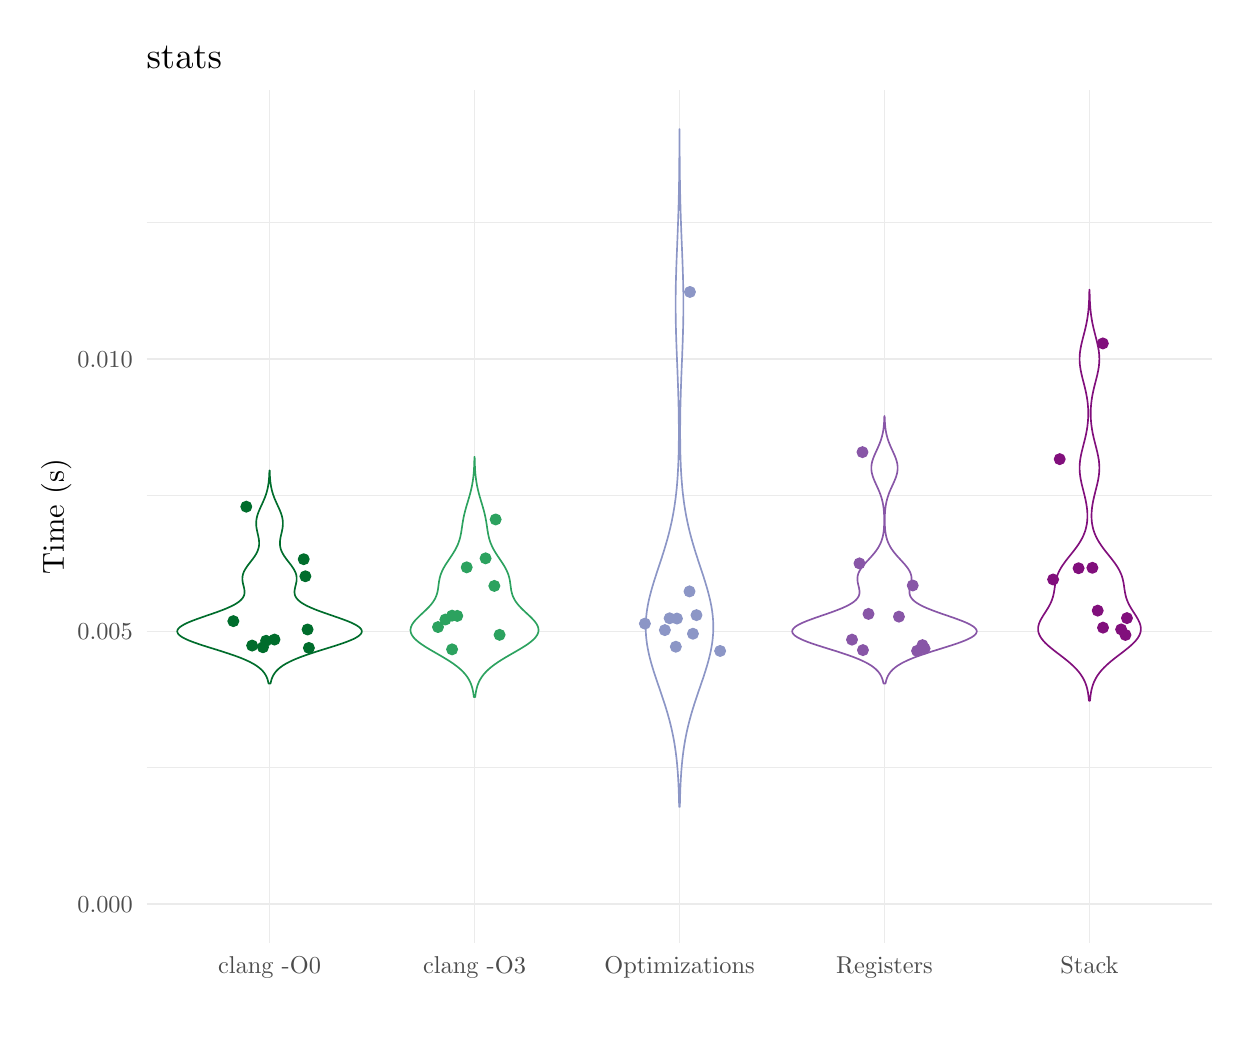
\begin{tikzpicture}[x=1pt,y=1pt]
\definecolor{fillColor}{RGB}{255,255,255}
\path[use as bounding box,fill=fillColor,fill opacity=0.00] (0,0) rectangle (433.62,361.35);
\begin{scope}
\path[clip] ( 42.95, 30.69) rectangle (428.12,338.69);
\definecolor{drawColor}{gray}{0.92}

\path[draw=drawColor,line width= 0.3pt,line join=round] ( 42.95, 93.92) --
	(428.12, 93.92);

\path[draw=drawColor,line width= 0.3pt,line join=round] ( 42.95,192.40) --
	(428.12,192.40);

\path[draw=drawColor,line width= 0.3pt,line join=round] ( 42.95,290.87) --
	(428.12,290.87);

\path[draw=drawColor,line width= 0.6pt,line join=round] ( 42.95, 44.69) --
	(428.12, 44.69);

\path[draw=drawColor,line width= 0.6pt,line join=round] ( 42.95,143.16) --
	(428.12,143.16);

\path[draw=drawColor,line width= 0.6pt,line join=round] ( 42.95,241.63) --
	(428.12,241.63);

\path[draw=drawColor,line width= 0.6pt,line join=round] ( 87.40, 30.69) --
	( 87.40,338.69);

\path[draw=drawColor,line width= 0.6pt,line join=round] (161.47, 30.69) --
	(161.47,338.69);

\path[draw=drawColor,line width= 0.6pt,line join=round] (235.54, 30.69) --
	(235.54,338.69);

\path[draw=drawColor,line width= 0.6pt,line join=round] (309.61, 30.69) --
	(309.61,338.69);

\path[draw=drawColor,line width= 0.6pt,line join=round] (383.68, 30.69) --
	(383.68,338.69);
\definecolor{drawColor}{RGB}{0,109,44}
\definecolor{fillColor}{RGB}{255,255,255}

\path[draw=drawColor,line width= 0.6pt,line join=round,line cap=round,fill=fillColor] ( 87.02,124.38) --
	( 86.99,124.53) --
	( 86.97,124.68) --
	( 86.93,124.83) --
	( 86.90,124.98) --
	( 86.86,125.13) --
	( 86.83,125.28) --
	( 86.79,125.43) --
	( 86.74,125.59) --
	( 86.70,125.74) --
	( 86.65,125.89) --
	( 86.60,126.04) --
	( 86.55,126.19) --
	( 86.49,126.34) --
	( 86.43,126.49) --
	( 86.37,126.64) --
	( 86.30,126.79) --
	( 86.23,126.94) --
	( 86.15,127.09) --
	( 86.07,127.24) --
	( 85.99,127.39) --
	( 85.90,127.54) --
	( 85.81,127.69) --
	( 85.72,127.84) --
	( 85.61,127.99) --
	( 85.51,128.15) --
	( 85.40,128.30) --
	( 85.28,128.45) --
	( 85.16,128.60) --
	( 85.03,128.75) --
	( 84.90,128.90) --
	( 84.76,129.05) --
	( 84.61,129.20) --
	( 84.46,129.35) --
	( 84.30,129.50) --
	( 84.14,129.65) --
	( 83.96,129.80) --
	( 83.78,129.95) --
	( 83.60,130.10) --
	( 83.40,130.25) --
	( 83.20,130.40) --
	( 82.99,130.55) --
	( 82.78,130.71) --
	( 82.55,130.86) --
	( 82.32,131.01) --
	( 82.08,131.16) --
	( 81.83,131.31) --
	( 81.57,131.46) --
	( 81.31,131.61) --
	( 81.03,131.76) --
	( 80.75,131.91) --
	( 80.46,132.06) --
	( 80.16,132.21) --
	( 79.86,132.36) --
	( 79.54,132.51) --
	( 79.21,132.66) --
	( 78.88,132.81) --
	( 78.54,132.96) --
	( 78.19,133.11) --
	( 77.83,133.27) --
	( 77.46,133.42) --
	( 77.09,133.57) --
	( 76.70,133.72) --
	( 76.31,133.87) --
	( 75.91,134.02) --
	( 75.51,134.17) --
	( 75.09,134.32) --
	( 74.67,134.47) --
	( 74.25,134.62) --
	( 73.81,134.77) --
	( 73.37,134.92) --
	( 72.93,135.07) --
	( 72.48,135.22) --
	( 72.02,135.37) --
	( 71.56,135.52) --
	( 71.09,135.67) --
	( 70.62,135.83) --
	( 70.15,135.98) --
	( 69.67,136.13) --
	( 69.19,136.28) --
	( 68.71,136.43) --
	( 68.23,136.58) --
	( 67.75,136.73) --
	( 67.26,136.88) --
	( 66.78,137.03) --
	( 66.29,137.18) --
	( 65.81,137.33) --
	( 65.33,137.48) --
	( 64.85,137.63) --
	( 64.37,137.78) --
	( 63.90,137.93) --
	( 63.43,138.08) --
	( 62.96,138.23) --
	( 62.50,138.38) --
	( 62.05,138.54) --
	( 61.61,138.69) --
	( 61.17,138.84) --
	( 60.74,138.99) --
	( 60.31,139.14) --
	( 59.90,139.29) --
	( 59.50,139.44) --
	( 59.10,139.59) --
	( 58.72,139.74) --
	( 58.35,139.89) --
	( 57.99,140.04) --
	( 57.65,140.19) --
	( 57.31,140.34) --
	( 57.00,140.49) --
	( 56.69,140.64) --
	( 56.40,140.79) --
	( 56.13,140.94) --
	( 55.86,141.10) --
	( 55.62,141.25) --
	( 55.39,141.40) --
	( 55.19,141.55) --
	( 54.99,141.70) --
	( 54.81,141.85) --
	( 54.66,142.00) --
	( 54.52,142.15) --
	( 54.40,142.30) --
	( 54.30,142.45) --
	( 54.21,142.60) --
	( 54.15,142.75) --
	( 54.10,142.90) --
	( 54.07,143.05) --
	( 54.06,143.20) --
	( 54.07,143.35) --
	( 54.10,143.50) --
	( 54.15,143.66) --
	( 54.21,143.81) --
	( 54.30,143.96) --
	( 54.40,144.11) --
	( 54.52,144.26) --
	( 54.66,144.41) --
	( 54.81,144.56) --
	( 54.99,144.71) --
	( 55.18,144.86) --
	( 55.39,145.01) --
	( 55.61,145.16) --
	( 55.84,145.31) --
	( 56.10,145.46) --
	( 56.37,145.61) --
	( 56.65,145.76) --
	( 56.95,145.91) --
	( 57.25,146.06) --
	( 57.58,146.22) --
	( 57.91,146.37) --
	( 58.26,146.52) --
	( 58.61,146.67) --
	( 58.98,146.82) --
	( 59.36,146.97) --
	( 59.74,147.12) --
	( 60.13,147.27) --
	( 60.54,147.42) --
	( 60.94,147.57) --
	( 61.36,147.72) --
	( 61.77,147.87) --
	( 62.20,148.02) --
	( 62.63,148.17) --
	( 63.06,148.32) --
	( 63.49,148.47) --
	( 63.93,148.62) --
	( 64.37,148.78) --
	( 64.80,148.93) --
	( 65.24,149.08) --
	( 65.68,149.23) --
	( 66.12,149.38) --
	( 66.55,149.53) --
	( 66.99,149.68) --
	( 67.42,149.83) --
	( 67.84,149.98) --
	( 68.26,150.13) --
	( 68.68,150.28) --
	( 69.09,150.43) --
	( 69.50,150.58) --
	( 69.90,150.73) --
	( 70.29,150.88) --
	( 70.68,151.03) --
	( 71.06,151.18) --
	( 71.43,151.33) --
	( 71.80,151.49) --
	( 72.15,151.64) --
	( 72.50,151.79) --
	( 72.83,151.94) --
	( 73.16,152.09) --
	( 73.48,152.24) --
	( 73.79,152.39) --
	( 74.09,152.54) --
	( 74.37,152.69) --
	( 74.65,152.84) --
	( 74.92,152.99) --
	( 75.18,153.14) --
	( 75.43,153.29) --
	( 75.66,153.44) --
	( 75.88,153.59) --
	( 76.10,153.74) --
	( 76.30,153.89) --
	( 76.50,154.05) --
	( 76.68,154.20) --
	( 76.85,154.35) --
	( 77.01,154.50) --
	( 77.16,154.65) --
	( 77.30,154.80) --
	( 77.43,154.95) --
	( 77.56,155.10) --
	( 77.67,155.25) --
	( 77.77,155.40) --
	( 77.86,155.55) --
	( 77.95,155.70) --
	( 78.02,155.85) --
	( 78.09,156.00) --
	( 78.15,156.15) --
	( 78.20,156.30) --
	( 78.25,156.45) --
	( 78.28,156.61) --
	( 78.31,156.76) --
	( 78.33,156.91) --
	( 78.35,157.06) --
	( 78.36,157.21) --
	( 78.37,157.36) --
	( 78.37,157.51) --
	( 78.36,157.66) --
	( 78.35,157.81) --
	( 78.34,157.96) --
	( 78.32,158.11) --
	( 78.30,158.26) --
	( 78.28,158.41) --
	( 78.25,158.56) --
	( 78.22,158.71) --
	( 78.19,158.86) --
	( 78.16,159.01) --
	( 78.12,159.17) --
	( 78.09,159.32) --
	( 78.05,159.47) --
	( 78.01,159.62) --
	( 77.98,159.77) --
	( 77.94,159.92) --
	( 77.90,160.07) --
	( 77.87,160.22) --
	( 77.83,160.37) --
	( 77.80,160.52) --
	( 77.77,160.67) --
	( 77.74,160.82) --
	( 77.71,160.97) --
	( 77.69,161.12) --
	( 77.66,161.27) --
	( 77.64,161.42) --
	( 77.63,161.57) --
	( 77.61,161.73) --
	( 77.60,161.88) --
	( 77.59,162.03) --
	( 77.59,162.18) --
	( 77.59,162.33) --
	( 77.59,162.48) --
	( 77.60,162.63) --
	( 77.61,162.78) --
	( 77.63,162.93) --
	( 77.65,163.08) --
	( 77.67,163.23) --
	( 77.70,163.38) --
	( 77.73,163.53) --
	( 77.77,163.68) --
	( 77.81,163.83) --
	( 77.85,163.98) --
	( 77.90,164.13) --
	( 77.96,164.29) --
	( 78.01,164.44) --
	( 78.07,164.59) --
	( 78.14,164.74) --
	( 78.21,164.89) --
	( 78.28,165.04) --
	( 78.36,165.19) --
	( 78.44,165.34) --
	( 78.52,165.49) --
	( 78.61,165.64) --
	( 78.70,165.79) --
	( 78.79,165.94) --
	( 78.89,166.09) --
	( 78.99,166.24) --
	( 79.09,166.39) --
	( 79.19,166.54) --
	( 79.30,166.69) --
	( 79.40,166.84) --
	( 79.51,167.00) --
	( 79.62,167.15) --
	( 79.74,167.30) --
	( 79.85,167.45) --
	( 79.97,167.60) --
	( 80.08,167.75) --
	( 80.20,167.90) --
	( 80.32,168.05) --
	( 80.43,168.20) --
	( 80.55,168.35) --
	( 80.67,168.50) --
	( 80.78,168.65) --
	( 80.90,168.80) --
	( 81.02,168.95) --
	( 81.13,169.10) --
	( 81.25,169.25) --
	( 81.36,169.40) --
	( 81.47,169.56) --
	( 81.58,169.71) --
	( 81.69,169.86) --
	( 81.80,170.01) --
	( 81.90,170.16) --
	( 82.00,170.31) --
	( 82.10,170.46) --
	( 82.20,170.61) --
	( 82.29,170.76) --
	( 82.39,170.91) --
	( 82.48,171.06) --
	( 82.56,171.21) --
	( 82.65,171.36) --
	( 82.73,171.51) --
	( 82.80,171.66) --
	( 82.88,171.81) --
	( 82.95,171.96) --
	( 83.02,172.12) --
	( 83.08,172.27) --
	( 83.14,172.42) --
	( 83.20,172.57) --
	( 83.25,172.72) --
	( 83.30,172.87) --
	( 83.35,173.02) --
	( 83.39,173.17) --
	( 83.43,173.32) --
	( 83.47,173.47) --
	( 83.50,173.62) --
	( 83.53,173.77) --
	( 83.55,173.92) --
	( 83.58,174.07) --
	( 83.60,174.22) --
	( 83.61,174.37) --
	( 83.62,174.52) --
	( 83.63,174.68) --
	( 83.64,174.83) --
	( 83.64,174.98) --
	( 83.64,175.13) --
	( 83.64,175.28) --
	( 83.63,175.43) --
	( 83.63,175.58) --
	( 83.61,175.73) --
	( 83.60,175.88) --
	( 83.59,176.03) --
	( 83.57,176.18) --
	( 83.55,176.33) --
	( 83.53,176.48) --
	( 83.50,176.63) --
	( 83.48,176.78) --
	( 83.45,176.93) --
	( 83.42,177.08) --
	( 83.40,177.24) --
	( 83.37,177.39) --
	( 83.33,177.54) --
	( 83.30,177.69) --
	( 83.27,177.84) --
	( 83.23,177.99) --
	( 83.20,178.14) --
	( 83.17,178.29) --
	( 83.13,178.44) --
	( 83.10,178.59) --
	( 83.06,178.74) --
	( 83.03,178.89) --
	( 82.99,179.04) --
	( 82.96,179.19) --
	( 82.93,179.34) --
	( 82.90,179.49) --
	( 82.87,179.64) --
	( 82.84,179.79) --
	( 82.81,179.95) --
	( 82.78,180.10) --
	( 82.75,180.25) --
	( 82.73,180.40) --
	( 82.70,180.55) --
	( 82.68,180.70) --
	( 82.66,180.85) --
	( 82.64,181.00) --
	( 82.63,181.15) --
	( 82.61,181.30) --
	( 82.60,181.45) --
	( 82.59,181.60) --
	( 82.58,181.75) --
	( 82.58,181.90) --
	( 82.57,182.05) --
	( 82.57,182.20) --
	( 82.57,182.35) --
	( 82.57,182.51) --
	( 82.58,182.66) --
	( 82.59,182.81) --
	( 82.60,182.96) --
	( 82.61,183.11) --
	( 82.63,183.26) --
	( 82.64,183.41) --
	( 82.66,183.56) --
	( 82.69,183.71) --
	( 82.71,183.86) --
	( 82.74,184.01) --
	( 82.77,184.16) --
	( 82.80,184.31) --
	( 82.84,184.46) --
	( 82.87,184.61) --
	( 82.91,184.76) --
	( 82.95,184.91) --
	( 82.99,185.07) --
	( 83.04,185.22) --
	( 83.09,185.37) --
	( 83.13,185.52) --
	( 83.18,185.67) --
	( 83.24,185.82) --
	( 83.29,185.97) --
	( 83.35,186.12) --
	( 83.40,186.27) --
	( 83.46,186.42) --
	( 83.52,186.57) --
	( 83.58,186.72) --
	( 83.64,186.87) --
	( 83.71,187.02) --
	( 83.77,187.17) --
	( 83.84,187.32) --
	( 83.90,187.47) --
	( 83.97,187.63) --
	( 84.04,187.78) --
	( 84.10,187.93) --
	( 84.17,188.08) --
	( 84.24,188.23) --
	( 84.31,188.38) --
	( 84.38,188.53) --
	( 84.45,188.68) --
	( 84.52,188.83) --
	( 84.59,188.98) --
	( 84.66,189.13) --
	( 84.73,189.28) --
	( 84.79,189.43) --
	( 84.86,189.58) --
	( 84.93,189.73) --
	( 85.00,189.88) --
	( 85.07,190.03) --
	( 85.13,190.19) --
	( 85.20,190.34) --
	( 85.26,190.49) --
	( 85.33,190.64) --
	( 85.39,190.79) --
	( 85.46,190.94) --
	( 85.52,191.09) --
	( 85.58,191.24) --
	( 85.64,191.39) --
	( 85.70,191.54) --
	( 85.76,191.69) --
	( 85.81,191.84) --
	( 85.87,191.99) --
	( 85.92,192.14) --
	( 85.98,192.29) --
	( 86.03,192.44) --
	( 86.08,192.59) --
	( 86.13,192.74) --
	( 86.18,192.90) --
	( 86.23,193.05) --
	( 86.27,193.20) --
	( 86.32,193.35) --
	( 86.36,193.50) --
	( 86.41,193.65) --
	( 86.45,193.80) --
	( 86.49,193.95) --
	( 86.53,194.10) --
	( 86.56,194.25) --
	( 86.60,194.40) --
	( 86.64,194.55) --
	( 86.67,194.70) --
	( 86.70,194.85) --
	( 86.74,195.00) --
	( 86.77,195.15) --
	( 86.80,195.30) --
	( 86.83,195.46) --
	( 86.85,195.61) --
	( 86.88,195.76) --
	( 86.91,195.91) --
	( 86.93,196.06) --
	( 86.95,196.21) --
	( 86.98,196.36) --
	( 87.00,196.51) --
	( 87.02,196.66) --
	( 87.04,196.81) --
	( 87.06,196.96) --
	( 87.08,197.11) --
	( 87.09,197.26) --
	( 87.11,197.41) --
	( 87.13,197.56) --
	( 87.14,197.71) --
	( 87.16,197.86) --
	( 87.17,198.02) --
	( 87.18,198.17) --
	( 87.20,198.32) --
	( 87.21,198.47) --
	( 87.22,198.62) --
	( 87.23,198.77) --
	( 87.24,198.92) --
	( 87.25,199.07) --
	( 87.26,199.22) --
	( 87.27,199.37) --
	( 87.27,199.52) --
	( 87.28,199.67) --
	( 87.29,199.82) --
	( 87.30,199.97) --
	( 87.30,200.12) --
	( 87.31,200.27) --
	( 87.31,200.42) --
	( 87.32,200.58) --
	( 87.33,200.73) --
	( 87.33,200.88) --
	( 87.33,201.03) --
	( 87.34,201.18) --
	( 87.34,201.33) --
	( 87.45,201.33) --
	( 87.45,201.18) --
	( 87.46,201.03) --
	( 87.46,200.88) --
	( 87.47,200.73) --
	( 87.47,200.58) --
	( 87.48,200.42) --
	( 87.48,200.27) --
	( 87.49,200.12) --
	( 87.50,199.97) --
	( 87.50,199.82) --
	( 87.51,199.67) --
	( 87.52,199.52) --
	( 87.53,199.37) --
	( 87.53,199.22) --
	( 87.54,199.07) --
	( 87.55,198.92) --
	( 87.56,198.77) --
	( 87.57,198.62) --
	( 87.59,198.47) --
	( 87.60,198.32) --
	( 87.61,198.17) --
	( 87.62,198.02) --
	( 87.64,197.86) --
	( 87.65,197.71) --
	( 87.67,197.56) --
	( 87.68,197.41) --
	( 87.70,197.26) --
	( 87.72,197.11) --
	( 87.73,196.96) --
	( 87.75,196.81) --
	( 87.77,196.66) --
	( 87.79,196.51) --
	( 87.82,196.36) --
	( 87.84,196.21) --
	( 87.86,196.06) --
	( 87.89,195.91) --
	( 87.91,195.76) --
	( 87.94,195.61) --
	( 87.97,195.46) --
	( 88.00,195.30) --
	( 88.03,195.15) --
	( 88.06,195.00) --
	( 88.09,194.85) --
	( 88.12,194.70) --
	( 88.16,194.55) --
	( 88.19,194.40) --
	( 88.23,194.25) --
	( 88.27,194.10) --
	( 88.31,193.95) --
	( 88.35,193.80) --
	( 88.39,193.65) --
	( 88.43,193.50) --
	( 88.47,193.35) --
	( 88.52,193.20) --
	( 88.57,193.05) --
	( 88.61,192.90) --
	( 88.66,192.74) --
	( 88.71,192.59) --
	( 88.76,192.44) --
	( 88.82,192.29) --
	( 88.87,192.14) --
	( 88.92,191.99) --
	( 88.98,191.84) --
	( 89.04,191.69) --
	( 89.09,191.54) --
	( 89.15,191.39) --
	( 89.21,191.24) --
	( 89.27,191.09) --
	( 89.34,190.94) --
	( 89.40,190.79) --
	( 89.46,190.64) --
	( 89.53,190.49) --
	( 89.59,190.34) --
	( 89.66,190.19) --
	( 89.73,190.03) --
	( 89.79,189.88) --
	( 89.86,189.73) --
	( 89.93,189.58) --
	( 90.00,189.43) --
	( 90.07,189.28) --
	( 90.14,189.13) --
	( 90.20,188.98) --
	( 90.27,188.83) --
	( 90.34,188.68) --
	( 90.41,188.53) --
	( 90.48,188.38) --
	( 90.55,188.23) --
	( 90.62,188.08) --
	( 90.69,187.93) --
	( 90.76,187.78) --
	( 90.82,187.63) --
	( 90.89,187.47) --
	( 90.96,187.32) --
	( 91.02,187.17) --
	( 91.09,187.02) --
	( 91.15,186.87) --
	( 91.21,186.72) --
	( 91.27,186.57) --
	( 91.33,186.42) --
	( 91.39,186.27) --
	( 91.45,186.12) --
	( 91.50,185.97) --
	( 91.56,185.82) --
	( 91.61,185.67) --
	( 91.66,185.52) --
	( 91.71,185.37) --
	( 91.75,185.22) --
	( 91.80,185.07) --
	( 91.84,184.91) --
	( 91.88,184.76) --
	( 91.92,184.61) --
	( 91.96,184.46) --
	( 91.99,184.31) --
	( 92.02,184.16) --
	( 92.05,184.01) --
	( 92.08,183.86) --
	( 92.10,183.71) --
	( 92.13,183.56) --
	( 92.15,183.41) --
	( 92.17,183.26) --
	( 92.18,183.11) --
	( 92.19,182.96) --
	( 92.20,182.81) --
	( 92.21,182.66) --
	( 92.22,182.51) --
	( 92.22,182.35) --
	( 92.22,182.20) --
	( 92.22,182.05) --
	( 92.22,181.90) --
	( 92.21,181.75) --
	( 92.20,181.60) --
	( 92.19,181.45) --
	( 92.18,181.30) --
	( 92.17,181.15) --
	( 92.15,181.00) --
	( 92.13,180.85) --
	( 92.11,180.70) --
	( 92.09,180.55) --
	( 92.07,180.40) --
	( 92.04,180.25) --
	( 92.01,180.10) --
	( 91.99,179.95) --
	( 91.96,179.79) --
	( 91.93,179.64) --
	( 91.90,179.49) --
	( 91.86,179.34) --
	( 91.83,179.19) --
	( 91.80,179.04) --
	( 91.76,178.89) --
	( 91.73,178.74) --
	( 91.70,178.59) --
	( 91.66,178.44) --
	( 91.63,178.29) --
	( 91.59,178.14) --
	( 91.56,177.99) --
	( 91.52,177.84) --
	( 91.49,177.69) --
	( 91.46,177.54) --
	( 91.43,177.39) --
	( 91.40,177.24) --
	( 91.37,177.08) --
	( 91.34,176.93) --
	( 91.31,176.78) --
	( 91.29,176.63) --
	( 91.26,176.48) --
	( 91.24,176.33) --
	( 91.22,176.18) --
	( 91.21,176.03) --
	( 91.19,175.88) --
	( 91.18,175.73) --
	( 91.17,175.58) --
	( 91.16,175.43) --
	( 91.15,175.28) --
	( 91.15,175.13) --
	( 91.15,174.98) --
	( 91.15,174.83) --
	( 91.16,174.68) --
	( 91.17,174.52) --
	( 91.18,174.37) --
	( 91.20,174.22) --
	( 91.22,174.07) --
	( 91.24,173.92) --
	( 91.26,173.77) --
	( 91.29,173.62) --
	( 91.33,173.47) --
	( 91.36,173.32) --
	( 91.40,173.17) --
	( 91.44,173.02) --
	( 91.49,172.87) --
	( 91.54,172.72) --
	( 91.59,172.57) --
	( 91.65,172.42) --
	( 91.71,172.27) --
	( 91.78,172.12) --
	( 91.84,171.96) --
	( 91.91,171.81) --
	( 91.99,171.66) --
	( 92.07,171.51) --
	( 92.15,171.36) --
	( 92.23,171.21) --
	( 92.32,171.06) --
	( 92.41,170.91) --
	( 92.50,170.76) --
	( 92.59,170.61) --
	( 92.69,170.46) --
	( 92.79,170.31) --
	( 92.89,170.16) --
	( 93.00,170.01) --
	( 93.10,169.86) --
	( 93.21,169.71) --
	( 93.32,169.56) --
	( 93.43,169.40) --
	( 93.55,169.25) --
	( 93.66,169.10) --
	( 93.77,168.95) --
	( 93.89,168.80) --
	( 94.01,168.65) --
	( 94.12,168.50) --
	( 94.24,168.35) --
	( 94.36,168.20) --
	( 94.48,168.05) --
	( 94.59,167.90) --
	( 94.71,167.75) --
	( 94.83,167.60) --
	( 94.94,167.45) --
	( 95.06,167.30) --
	( 95.17,167.15) --
	( 95.28,167.00) --
	( 95.39,166.84) --
	( 95.50,166.69) --
	( 95.60,166.54) --
	( 95.71,166.39) --
	( 95.81,166.24) --
	( 95.91,166.09) --
	( 96.00,165.94) --
	( 96.09,165.79) --
	( 96.18,165.64) --
	( 96.27,165.49) --
	( 96.35,165.34) --
	( 96.44,165.19) --
	( 96.51,165.04) --
	( 96.58,164.89) --
	( 96.65,164.74) --
	( 96.72,164.59) --
	( 96.78,164.44) --
	( 96.84,164.29) --
	( 96.89,164.13) --
	( 96.94,163.98) --
	( 96.98,163.83) --
	( 97.03,163.68) --
	( 97.06,163.53) --
	( 97.09,163.38) --
	( 97.12,163.23) --
	( 97.14,163.08) --
	( 97.16,162.93) --
	( 97.18,162.78) --
	( 97.19,162.63) --
	( 97.20,162.48) --
	( 97.20,162.33) --
	( 97.20,162.18) --
	( 97.20,162.03) --
	( 97.19,161.88) --
	( 97.18,161.73) --
	( 97.17,161.57) --
	( 97.15,161.42) --
	( 97.13,161.27) --
	( 97.11,161.12) --
	( 97.08,160.97) --
	( 97.05,160.82) --
	( 97.02,160.67) --
	( 96.99,160.52) --
	( 96.96,160.37) --
	( 96.92,160.22) --
	( 96.89,160.07) --
	( 96.85,159.92) --
	( 96.81,159.77) --
	( 96.78,159.62) --
	( 96.74,159.47) --
	( 96.70,159.32) --
	( 96.67,159.17) --
	( 96.63,159.01) --
	( 96.60,158.86) --
	( 96.57,158.71) --
	( 96.54,158.56) --
	( 96.51,158.41) --
	( 96.49,158.26) --
	( 96.47,158.11) --
	( 96.45,157.96) --
	( 96.44,157.81) --
	( 96.43,157.66) --
	( 96.42,157.51) --
	( 96.42,157.36) --
	( 96.43,157.21) --
	( 96.44,157.06) --
	( 96.46,156.91) --
	( 96.48,156.76) --
	( 96.51,156.61) --
	( 96.55,156.45) --
	( 96.59,156.30) --
	( 96.64,156.15) --
	( 96.70,156.00) --
	( 96.77,155.85) --
	( 96.84,155.70) --
	( 96.93,155.55) --
	( 97.02,155.40) --
	( 97.12,155.25) --
	( 97.24,155.10) --
	( 97.36,154.95) --
	( 97.49,154.80) --
	( 97.63,154.65) --
	( 97.78,154.50) --
	( 97.94,154.35) --
	( 98.12,154.20) --
	( 98.30,154.05) --
	( 98.49,153.89) --
	( 98.69,153.74) --
	( 98.91,153.59) --
	( 99.13,153.44) --
	( 99.37,153.29) --
	( 99.62,153.14) --
	( 99.87,152.99) --
	(100.14,152.84) --
	(100.42,152.69) --
	(100.70,152.54) --
	(101.00,152.39) --
	(101.31,152.24) --
	(101.63,152.09) --
	(101.96,151.94) --
	(102.29,151.79) --
	(102.64,151.64) --
	(103.00,151.49) --
	(103.36,151.33) --
	(103.73,151.18) --
	(104.11,151.03) --
	(104.50,150.88) --
	(104.89,150.73) --
	(105.29,150.58) --
	(105.70,150.43) --
	(106.11,150.28) --
	(106.53,150.13) --
	(106.95,149.98) --
	(107.38,149.83) --
	(107.81,149.68) --
	(108.24,149.53) --
	(108.67,149.38) --
	(109.11,149.23) --
	(109.55,149.08) --
	(109.99,148.93) --
	(110.43,148.78) --
	(110.86,148.62) --
	(111.30,148.47) --
	(111.74,148.32) --
	(112.17,148.17) --
	(112.59,148.02) --
	(113.02,147.87) --
	(113.44,147.72) --
	(113.85,147.57) --
	(114.26,147.42) --
	(114.66,147.27) --
	(115.05,147.12) --
	(115.44,146.97) --
	(115.81,146.82) --
	(116.18,146.67) --
	(116.53,146.52) --
	(116.88,146.37) --
	(117.21,146.22) --
	(117.54,146.06) --
	(117.84,145.91) --
	(118.14,145.76) --
	(118.43,145.61) --
	(118.69,145.46) --
	(118.95,145.31) --
	(119.18,145.16) --
	(119.41,145.01) --
	(119.62,144.86) --
	(119.80,144.71) --
	(119.98,144.56) --
	(120.13,144.41) --
	(120.27,144.26) --
	(120.39,144.11) --
	(120.49,143.96) --
	(120.58,143.81) --
	(120.64,143.66) --
	(120.69,143.50) --
	(120.72,143.35) --
	(120.73,143.20) --
	(120.72,143.05) --
	(120.69,142.90) --
	(120.64,142.75) --
	(120.58,142.60) --
	(120.49,142.45) --
	(120.39,142.30) --
	(120.27,142.15) --
	(120.13,142.00) --
	(119.98,141.85) --
	(119.80,141.70) --
	(119.61,141.55) --
	(119.40,141.40) --
	(119.17,141.25) --
	(118.93,141.10) --
	(118.67,140.94) --
	(118.39,140.79) --
	(118.10,140.64) --
	(117.80,140.49) --
	(117.48,140.34) --
	(117.15,140.19) --
	(116.80,140.04) --
	(116.44,139.89) --
	(116.07,139.74) --
	(115.69,139.59) --
	(115.30,139.44) --
	(114.89,139.29) --
	(114.48,139.14) --
	(114.06,138.99) --
	(113.63,138.84) --
	(113.19,138.69) --
	(112.74,138.54) --
	(112.29,138.38) --
	(111.83,138.23) --
	(111.36,138.08) --
	(110.89,137.93) --
	(110.42,137.78) --
	(109.95,137.63) --
	(109.47,137.48) --
	(108.98,137.33) --
	(108.50,137.18) --
	(108.02,137.03) --
	(107.53,136.88) --
	(107.05,136.73) --
	(106.56,136.58) --
	(106.08,136.43) --
	(105.60,136.28) --
	(105.12,136.13) --
	(104.64,135.98) --
	(104.17,135.83) --
	(103.70,135.67) --
	(103.23,135.52) --
	(102.77,135.37) --
	(102.32,135.22) --
	(101.87,135.07) --
	(101.42,134.92) --
	(100.98,134.77) --
	(100.54,134.62) --
	(100.12,134.47) --
	( 99.70,134.32) --
	( 99.28,134.17) --
	( 98.88,134.02) --
	( 98.48,133.87) --
	( 98.09,133.72) --
	( 97.71,133.57) --
	( 97.33,133.42) --
	( 96.96,133.27) --
	( 96.60,133.11) --
	( 96.25,132.96) --
	( 95.91,132.81) --
	( 95.58,132.66) --
	( 95.25,132.51) --
	( 94.94,132.36) --
	( 94.63,132.21) --
	( 94.33,132.06) --
	( 94.04,131.91) --
	( 93.76,131.76) --
	( 93.48,131.61) --
	( 93.22,131.46) --
	( 92.96,131.31) --
	( 92.71,131.16) --
	( 92.47,131.01) --
	( 92.24,130.86) --
	( 92.01,130.71) --
	( 91.80,130.55) --
	( 91.59,130.40) --
	( 91.39,130.25) --
	( 91.19,130.10) --
	( 91.01,129.95) --
	( 90.83,129.80) --
	( 90.66,129.65) --
	( 90.49,129.50) --
	( 90.33,129.35) --
	( 90.18,129.20) --
	( 90.04,129.05) --
	( 89.89,128.90) --
	( 89.76,128.75) --
	( 89.63,128.60) --
	( 89.51,128.45) --
	( 89.40,128.30) --
	( 89.28,128.15) --
	( 89.18,127.99) --
	( 89.08,127.84) --
	( 88.98,127.69) --
	( 88.89,127.54) --
	( 88.80,127.39) --
	( 88.72,127.24) --
	( 88.64,127.09) --
	( 88.56,126.94) --
	( 88.49,126.79) --
	( 88.43,126.64) --
	( 88.36,126.49) --
	( 88.30,126.34) --
	( 88.25,126.19) --
	( 88.19,126.04) --
	( 88.14,125.89) --
	( 88.09,125.74) --
	( 88.05,125.59) --
	( 88.01,125.43) --
	( 87.97,125.28) --
	( 87.93,125.13) --
	( 87.89,124.98) --
	( 87.86,124.83) --
	( 87.83,124.68) --
	( 87.80,124.53) --
	( 87.77,124.38) --
	( 87.02,124.38) --
	cycle;
\definecolor{drawColor}{RGB}{44,162,95}

\path[draw=drawColor,line width= 0.6pt,line join=round,line cap=round,fill=fillColor] (161.21,119.44) --
	(161.20,119.61) --
	(161.18,119.78) --
	(161.16,119.94) --
	(161.14,120.11) --
	(161.12,120.28) --
	(161.10,120.45) --
	(161.07,120.62) --
	(161.05,120.79) --
	(161.02,120.96) --
	(161.00,121.13) --
	(160.97,121.30) --
	(160.94,121.47) --
	(160.90,121.64) --
	(160.87,121.81) --
	(160.83,121.98) --
	(160.80,122.15) --
	(160.76,122.32) --
	(160.72,122.49) --
	(160.67,122.66) --
	(160.63,122.83) --
	(160.58,123.00) --
	(160.53,123.17) --
	(160.48,123.34) --
	(160.43,123.51) --
	(160.37,123.68) --
	(160.31,123.85) --
	(160.25,124.02) --
	(160.19,124.19) --
	(160.12,124.36) --
	(160.05,124.53) --
	(159.97,124.70) --
	(159.90,124.87) --
	(159.82,125.04) --
	(159.74,125.21) --
	(159.65,125.38) --
	(159.56,125.55) --
	(159.47,125.72) --
	(159.37,125.89) --
	(159.27,126.06) --
	(159.17,126.23) --
	(159.06,126.40) --
	(158.95,126.57) --
	(158.84,126.74) --
	(158.72,126.91) --
	(158.59,127.08) --
	(158.47,127.25) --
	(158.34,127.42) --
	(158.20,127.59) --
	(158.06,127.76) --
	(157.91,127.93) --
	(157.77,128.10) --
	(157.61,128.27) --
	(157.45,128.44) --
	(157.29,128.61) --
	(157.12,128.78) --
	(156.95,128.95) --
	(156.78,129.12) --
	(156.60,129.29) --
	(156.41,129.46) --
	(156.22,129.63) --
	(156.03,129.80) --
	(155.83,129.97) --
	(155.62,130.14) --
	(155.41,130.31) --
	(155.20,130.48) --
	(154.98,130.65) --
	(154.76,130.82) --
	(154.54,130.99) --
	(154.30,131.16) --
	(154.07,131.33) --
	(153.83,131.50) --
	(153.58,131.67) --
	(153.34,131.84) --
	(153.09,132.01) --
	(152.83,132.18) --
	(152.57,132.35) --
	(152.31,132.52) --
	(152.04,132.69) --
	(151.77,132.86) --
	(151.50,133.03) --
	(151.22,133.20) --
	(150.95,133.37) --
	(150.66,133.54) --
	(150.38,133.71) --
	(150.10,133.88) --
	(149.81,134.05) --
	(149.52,134.22) --
	(149.23,134.39) --
	(148.93,134.56) --
	(148.64,134.73) --
	(148.35,134.90) --
	(148.05,135.07) --
	(147.76,135.24) --
	(147.46,135.41) --
	(147.16,135.58) --
	(146.87,135.75) --
	(146.57,135.92) --
	(146.28,136.09) --
	(145.99,136.26) --
	(145.70,136.43) --
	(145.41,136.60) --
	(145.12,136.77) --
	(144.84,136.94) --
	(144.56,137.11) --
	(144.28,137.28) --
	(144.00,137.45) --
	(143.73,137.62) --
	(143.46,137.79) --
	(143.20,137.96) --
	(142.94,138.13) --
	(142.68,138.30) --
	(142.43,138.47) --
	(142.19,138.64) --
	(141.95,138.81) --
	(141.72,138.98) --
	(141.49,139.15) --
	(141.27,139.32) --
	(141.05,139.49) --
	(140.85,139.66) --
	(140.64,139.83) --
	(140.45,140.00) --
	(140.27,140.17) --
	(140.09,140.34) --
	(139.92,140.51) --
	(139.75,140.68) --
	(139.60,140.85) --
	(139.46,141.02) --
	(139.32,141.19) --
	(139.19,141.36) --
	(139.07,141.53) --
	(138.96,141.70) --
	(138.86,141.87) --
	(138.77,142.04) --
	(138.68,142.21) --
	(138.61,142.38) --
	(138.55,142.55) --
	(138.49,142.72) --
	(138.44,142.89) --
	(138.40,143.06) --
	(138.38,143.23) --
	(138.36,143.40) --
	(138.35,143.57) --
	(138.35,143.74) --
	(138.35,143.91) --
	(138.37,144.08) --
	(138.40,144.25) --
	(138.43,144.42) --
	(138.47,144.59) --
	(138.52,144.76) --
	(138.58,144.93) --
	(138.65,145.10) --
	(138.73,145.27) --
	(138.81,145.44) --
	(138.90,145.61) --
	(138.99,145.78) --
	(139.10,145.95) --
	(139.21,146.12) --
	(139.32,146.29) --
	(139.45,146.46) --
	(139.58,146.63) --
	(139.71,146.80) --
	(139.85,146.97) --
	(140.00,147.14) --
	(140.15,147.31) --
	(140.30,147.48) --
	(140.46,147.64) --
	(140.62,147.81) --
	(140.79,147.98) --
	(140.96,148.15) --
	(141.13,148.32) --
	(141.30,148.49) --
	(141.48,148.66) --
	(141.66,148.83) --
	(141.84,149.00) --
	(142.02,149.17) --
	(142.20,149.34) --
	(142.38,149.51) --
	(142.56,149.68) --
	(142.75,149.85) --
	(142.93,150.02) --
	(143.11,150.19) --
	(143.29,150.36) --
	(143.47,150.53) --
	(143.65,150.70) --
	(143.83,150.87) --
	(144.01,151.04) --
	(144.18,151.21) --
	(144.35,151.38) --
	(144.52,151.55) --
	(144.69,151.72) --
	(144.85,151.89) --
	(145.01,152.06) --
	(145.17,152.23) --
	(145.32,152.40) --
	(145.47,152.57) --
	(145.62,152.74) --
	(145.76,152.91) --
	(145.90,153.08) --
	(146.04,153.25) --
	(146.17,153.42) --
	(146.30,153.59) --
	(146.42,153.76) --
	(146.54,153.93) --
	(146.65,154.10) --
	(146.76,154.27) --
	(146.86,154.44) --
	(146.96,154.61) --
	(147.06,154.78) --
	(147.15,154.95) --
	(147.24,155.12) --
	(147.33,155.29) --
	(147.41,155.46) --
	(147.48,155.63) --
	(147.55,155.80) --
	(147.62,155.97) --
	(147.69,156.14) --
	(147.75,156.31) --
	(147.81,156.48) --
	(147.86,156.65) --
	(147.91,156.82) --
	(147.96,156.99) --
	(148.00,157.16) --
	(148.05,157.33) --
	(148.09,157.50) --
	(148.12,157.67) --
	(148.16,157.84) --
	(148.19,158.01) --
	(148.22,158.18) --
	(148.25,158.35) --
	(148.28,158.52) --
	(148.30,158.69) --
	(148.33,158.86) --
	(148.35,159.03) --
	(148.37,159.20) --
	(148.40,159.37) --
	(148.42,159.54) --
	(148.44,159.71) --
	(148.46,159.88) --
	(148.48,160.05) --
	(148.50,160.22) --
	(148.53,160.39) --
	(148.55,160.56) --
	(148.57,160.73) --
	(148.60,160.90) --
	(148.62,161.07) --
	(148.65,161.24) --
	(148.68,161.41) --
	(148.71,161.58) --
	(148.74,161.75) --
	(148.77,161.92) --
	(148.81,162.09) --
	(148.84,162.26) --
	(148.88,162.43) --
	(148.92,162.60) --
	(148.97,162.77) --
	(149.01,162.94) --
	(149.06,163.11) --
	(149.11,163.28) --
	(149.16,163.45) --
	(149.22,163.62) --
	(149.28,163.79) --
	(149.34,163.96) --
	(149.40,164.13) --
	(149.47,164.30) --
	(149.53,164.47) --
	(149.60,164.64) --
	(149.68,164.81) --
	(149.75,164.98) --
	(149.83,165.15) --
	(149.91,165.32) --
	(150.00,165.49) --
	(150.08,165.66) --
	(150.17,165.83) --
	(150.26,166.00) --
	(150.35,166.17) --
	(150.45,166.34) --
	(150.55,166.51) --
	(150.65,166.68) --
	(150.75,166.85) --
	(150.85,167.02) --
	(150.95,167.19) --
	(151.06,167.36) --
	(151.17,167.53) --
	(151.27,167.70) --
	(151.38,167.87) --
	(151.49,168.04) --
	(151.61,168.21) --
	(151.72,168.38) --
	(151.83,168.55) --
	(151.95,168.72) --
	(152.06,168.89) --
	(152.18,169.06) --
	(152.29,169.23) --
	(152.41,169.40) --
	(152.52,169.57) --
	(152.64,169.74) --
	(152.75,169.91) --
	(152.86,170.08) --
	(152.98,170.25) --
	(153.09,170.42) --
	(153.20,170.59) --
	(153.32,170.76) --
	(153.43,170.93) --
	(153.54,171.10) --
	(153.64,171.27) --
	(153.75,171.44) --
	(153.86,171.61) --
	(153.96,171.78) --
	(154.06,171.95) --
	(154.17,172.12) --
	(154.27,172.29) --
	(154.36,172.46) --
	(154.46,172.63) --
	(154.55,172.80) --
	(154.65,172.97) --
	(154.74,173.14) --
	(154.83,173.31) --
	(154.91,173.48) --
	(155.00,173.65) --
	(155.08,173.82) --
	(155.16,173.99) --
	(155.24,174.16) --
	(155.31,174.33) --
	(155.39,174.50) --
	(155.46,174.67) --
	(155.53,174.84) --
	(155.59,175.01) --
	(155.66,175.18) --
	(155.72,175.34) --
	(155.78,175.51) --
	(155.84,175.68) --
	(155.90,175.85) --
	(155.95,176.02) --
	(156.01,176.19) --
	(156.06,176.36) --
	(156.11,176.53) --
	(156.15,176.70) --
	(156.20,176.87) --
	(156.25,177.04) --
	(156.29,177.21) --
	(156.33,177.38) --
	(156.37,177.55) --
	(156.41,177.72) --
	(156.44,177.89) --
	(156.48,178.06) --
	(156.51,178.23) --
	(156.54,178.40) --
	(156.58,178.57) --
	(156.61,178.74) --
	(156.64,178.91) --
	(156.67,179.08) --
	(156.69,179.25) --
	(156.72,179.42) --
	(156.75,179.59) --
	(156.78,179.76) --
	(156.80,179.93) --
	(156.83,180.10) --
	(156.85,180.27) --
	(156.88,180.44) --
	(156.90,180.61) --
	(156.93,180.78) --
	(156.95,180.95) --
	(156.98,181.12) --
	(157.00,181.29) --
	(157.03,181.46) --
	(157.05,181.63) --
	(157.08,181.80) --
	(157.10,181.97) --
	(157.13,182.14) --
	(157.16,182.31) --
	(157.18,182.48) --
	(157.21,182.65) --
	(157.24,182.82) --
	(157.27,182.99) --
	(157.30,183.16) --
	(157.33,183.33) --
	(157.36,183.50) --
	(157.39,183.67) --
	(157.42,183.84) --
	(157.45,184.01) --
	(157.48,184.18) --
	(157.52,184.35) --
	(157.55,184.52) --
	(157.59,184.69) --
	(157.63,184.86) --
	(157.66,185.03) --
	(157.70,185.20) --
	(157.74,185.37) --
	(157.78,185.54) --
	(157.82,185.71) --
	(157.86,185.88) --
	(157.90,186.05) --
	(157.94,186.22) --
	(157.99,186.39) --
	(158.03,186.56) --
	(158.08,186.73) --
	(158.12,186.90) --
	(158.17,187.07) --
	(158.21,187.24) --
	(158.26,187.41) --
	(158.31,187.58) --
	(158.35,187.75) --
	(158.40,187.92) --
	(158.45,188.09) --
	(158.50,188.26) --
	(158.55,188.43) --
	(158.60,188.60) --
	(158.65,188.77) --
	(158.70,188.94) --
	(158.75,189.11) --
	(158.80,189.28) --
	(158.85,189.45) --
	(158.90,189.62) --
	(158.96,189.79) --
	(159.01,189.96) --
	(159.06,190.13) --
	(159.11,190.30) --
	(159.16,190.47) --
	(159.21,190.64) --
	(159.26,190.81) --
	(159.31,190.98) --
	(159.36,191.15) --
	(159.41,191.32) --
	(159.46,191.49) --
	(159.51,191.66) --
	(159.56,191.83) --
	(159.61,192.00) --
	(159.66,192.17) --
	(159.70,192.34) --
	(159.75,192.51) --
	(159.80,192.68) --
	(159.84,192.85) --
	(159.89,193.02) --
	(159.93,193.19) --
	(159.98,193.36) --
	(160.02,193.53) --
	(160.06,193.70) --
	(160.11,193.87) --
	(160.15,194.04) --
	(160.19,194.21) --
	(160.23,194.38) --
	(160.27,194.55) --
	(160.31,194.72) --
	(160.35,194.89) --
	(160.38,195.06) --
	(160.42,195.23) --
	(160.46,195.40) --
	(160.49,195.57) --
	(160.52,195.74) --
	(160.56,195.91) --
	(160.59,196.08) --
	(160.62,196.25) --
	(160.65,196.42) --
	(160.68,196.59) --
	(160.71,196.76) --
	(160.74,196.93) --
	(160.77,197.10) --
	(160.80,197.27) --
	(160.82,197.44) --
	(160.85,197.61) --
	(160.87,197.78) --
	(160.90,197.95) --
	(160.92,198.12) --
	(160.94,198.29) --
	(160.97,198.46) --
	(160.99,198.63) --
	(161.01,198.80) --
	(161.03,198.97) --
	(161.05,199.14) --
	(161.07,199.31) --
	(161.08,199.48) --
	(161.10,199.65) --
	(161.12,199.82) --
	(161.13,199.99) --
	(161.15,200.16) --
	(161.16,200.33) --
	(161.18,200.50) --
	(161.19,200.67) --
	(161.21,200.84) --
	(161.22,201.01) --
	(161.23,201.18) --
	(161.24,201.35) --
	(161.25,201.52) --
	(161.26,201.69) --
	(161.27,201.86) --
	(161.28,202.03) --
	(161.29,202.20) --
	(161.30,202.37) --
	(161.31,202.54) --
	(161.32,202.71) --
	(161.33,202.88) --
	(161.33,203.04) --
	(161.34,203.21) --
	(161.35,203.38) --
	(161.36,203.55) --
	(161.36,203.72) --
	(161.37,203.89) --
	(161.37,204.06) --
	(161.38,204.23) --
	(161.38,204.40) --
	(161.39,204.57) --
	(161.39,204.74) --
	(161.40,204.91) --
	(161.40,205.08) --
	(161.40,205.25) --
	(161.41,205.42) --
	(161.41,205.59) --
	(161.42,205.76) --
	(161.42,205.93) --
	(161.42,206.10) --
	(161.42,206.27) --
	(161.51,206.27) --
	(161.51,206.10) --
	(161.51,205.93) --
	(161.52,205.76) --
	(161.52,205.59) --
	(161.52,205.42) --
	(161.53,205.25) --
	(161.53,205.08) --
	(161.54,204.91) --
	(161.54,204.74) --
	(161.55,204.57) --
	(161.55,204.40) --
	(161.56,204.23) --
	(161.56,204.06) --
	(161.57,203.89) --
	(161.57,203.72) --
	(161.58,203.55) --
	(161.58,203.38) --
	(161.59,203.21) --
	(161.60,203.04) --
	(161.61,202.88) --
	(161.61,202.71) --
	(161.62,202.54) --
	(161.63,202.37) --
	(161.64,202.20) --
	(161.65,202.03) --
	(161.66,201.86) --
	(161.67,201.69) --
	(161.68,201.52) --
	(161.69,201.35) --
	(161.70,201.18) --
	(161.72,201.01) --
	(161.73,200.84) --
	(161.74,200.67) --
	(161.76,200.50) --
	(161.77,200.33) --
	(161.78,200.16) --
	(161.80,199.99) --
	(161.82,199.82) --
	(161.83,199.65) --
	(161.85,199.48) --
	(161.87,199.31) --
	(161.89,199.14) --
	(161.91,198.97) --
	(161.93,198.80) --
	(161.95,198.63) --
	(161.97,198.46) --
	(161.99,198.29) --
	(162.01,198.12) --
	(162.03,197.95) --
	(162.06,197.78) --
	(162.08,197.61) --
	(162.11,197.44) --
	(162.14,197.27) --
	(162.16,197.10) --
	(162.19,196.93) --
	(162.22,196.76) --
	(162.25,196.59) --
	(162.28,196.42) --
	(162.31,196.25) --
	(162.34,196.08) --
	(162.37,195.91) --
	(162.41,195.74) --
	(162.44,195.57) --
	(162.48,195.40) --
	(162.51,195.23) --
	(162.55,195.06) --
	(162.59,194.89) --
	(162.62,194.72) --
	(162.66,194.55) --
	(162.70,194.38) --
	(162.74,194.21) --
	(162.78,194.04) --
	(162.83,193.87) --
	(162.87,193.70) --
	(162.91,193.53) --
	(162.95,193.36) --
	(163.00,193.19) --
	(163.04,193.02) --
	(163.09,192.85) --
	(163.14,192.68) --
	(163.18,192.51) --
	(163.23,192.34) --
	(163.28,192.17) --
	(163.32,192.00) --
	(163.37,191.83) --
	(163.42,191.66) --
	(163.47,191.49) --
	(163.52,191.32) --
	(163.57,191.15) --
	(163.62,190.98) --
	(163.67,190.81) --
	(163.72,190.64) --
	(163.77,190.47) --
	(163.82,190.30) --
	(163.88,190.13) --
	(163.93,189.96) --
	(163.98,189.79) --
	(164.03,189.62) --
	(164.08,189.45) --
	(164.13,189.28) --
	(164.18,189.11) --
	(164.23,188.94) --
	(164.28,188.77) --
	(164.33,188.60) --
	(164.38,188.43) --
	(164.43,188.26) --
	(164.48,188.09) --
	(164.53,187.92) --
	(164.58,187.75) --
	(164.63,187.58) --
	(164.67,187.41) --
	(164.72,187.24) --
	(164.77,187.07) --
	(164.81,186.90) --
	(164.86,186.73) --
	(164.90,186.56) --
	(164.95,186.39) --
	(164.99,186.22) --
	(165.03,186.05) --
	(165.07,185.88) --
	(165.11,185.71) --
	(165.16,185.54) --
	(165.19,185.37) --
	(165.23,185.20) --
	(165.27,185.03) --
	(165.31,184.86) --
	(165.34,184.69) --
	(165.38,184.52) --
	(165.41,184.35) --
	(165.45,184.18) --
	(165.48,184.01) --
	(165.51,183.84) --
	(165.55,183.67) --
	(165.58,183.50) --
	(165.61,183.33) --
	(165.64,183.16) --
	(165.67,182.99) --
	(165.70,182.82) --
	(165.72,182.65) --
	(165.75,182.48) --
	(165.78,182.31) --
	(165.80,182.14) --
	(165.83,181.97) --
	(165.86,181.80) --
	(165.88,181.63) --
	(165.91,181.46) --
	(165.93,181.29) --
	(165.96,181.12) --
	(165.98,180.95) --
	(166.01,180.78) --
	(166.03,180.61) --
	(166.06,180.44) --
	(166.08,180.27) --
	(166.11,180.10) --
	(166.13,179.93) --
	(166.16,179.76) --
	(166.18,179.59) --
	(166.21,179.42) --
	(166.24,179.25) --
	(166.27,179.08) --
	(166.30,178.91) --
	(166.33,178.74) --
	(166.36,178.57) --
	(166.39,178.40) --
	(166.42,178.23) --
	(166.46,178.06) --
	(166.49,177.89) --
	(166.53,177.72) --
	(166.57,177.55) --
	(166.60,177.38) --
	(166.65,177.21) --
	(166.69,177.04) --
	(166.73,176.87) --
	(166.78,176.70) --
	(166.83,176.53) --
	(166.88,176.36) --
	(166.93,176.19) --
	(166.98,176.02) --
	(167.03,175.85) --
	(167.09,175.68) --
	(167.15,175.51) --
	(167.21,175.34) --
	(167.27,175.18) --
	(167.34,175.01) --
	(167.41,174.84) --
	(167.48,174.67) --
	(167.55,174.50) --
	(167.62,174.33) --
	(167.70,174.16) --
	(167.78,173.99) --
	(167.86,173.82) --
	(167.94,173.65) --
	(168.02,173.48) --
	(168.11,173.31) --
	(168.20,173.14) --
	(168.29,172.97) --
	(168.38,172.80) --
	(168.47,172.63) --
	(168.57,172.46) --
	(168.67,172.29) --
	(168.77,172.12) --
	(168.87,171.95) --
	(168.97,171.78) --
	(169.08,171.61) --
	(169.18,171.44) --
	(169.29,171.27) --
	(169.40,171.10) --
	(169.51,170.93) --
	(169.62,170.76) --
	(169.73,170.59) --
	(169.84,170.42) --
	(169.95,170.25) --
	(170.07,170.08) --
	(170.18,169.91) --
	(170.30,169.74) --
	(170.41,169.57) --
	(170.53,169.40) --
	(170.64,169.23) --
	(170.76,169.06) --
	(170.87,168.89) --
	(170.99,168.72) --
	(171.10,168.55) --
	(171.21,168.38) --
	(171.33,168.21) --
	(171.44,168.04) --
	(171.55,167.87) --
	(171.66,167.70) --
	(171.77,167.53) --
	(171.87,167.36) --
	(171.98,167.19) --
	(172.08,167.02) --
	(172.19,166.85) --
	(172.29,166.68) --
	(172.39,166.51) --
	(172.48,166.34) --
	(172.58,166.17) --
	(172.67,166.00) --
	(172.76,165.83) --
	(172.85,165.66) --
	(172.94,165.49) --
	(173.02,165.32) --
	(173.10,165.15) --
	(173.18,164.98) --
	(173.26,164.81) --
	(173.33,164.64) --
	(173.40,164.47) --
	(173.47,164.30) --
	(173.53,164.13) --
	(173.60,163.96) --
	(173.66,163.79) --
	(173.72,163.62) --
	(173.77,163.45) --
	(173.82,163.28) --
	(173.87,163.11) --
	(173.92,162.94) --
	(173.97,162.77) --
	(174.01,162.60) --
	(174.05,162.43) --
	(174.09,162.26) --
	(174.13,162.09) --
	(174.16,161.92) --
	(174.20,161.75) --
	(174.23,161.58) --
	(174.26,161.41) --
	(174.28,161.24) --
	(174.31,161.07) --
	(174.34,160.90) --
	(174.36,160.73) --
	(174.38,160.56) --
	(174.41,160.39) --
	(174.43,160.22) --
	(174.45,160.05) --
	(174.47,159.88) --
	(174.49,159.71) --
	(174.52,159.54) --
	(174.54,159.37) --
	(174.56,159.20) --
	(174.58,159.03) --
	(174.61,158.86) --
	(174.63,158.69) --
	(174.66,158.52) --
	(174.68,158.35) --
	(174.71,158.18) --
	(174.74,158.01) --
	(174.78,157.84) --
	(174.81,157.67) --
	(174.85,157.50) --
	(174.89,157.33) --
	(174.93,157.16) --
	(174.97,156.99) --
	(175.02,156.82) --
	(175.07,156.65) --
	(175.13,156.48) --
	(175.18,156.31) --
	(175.25,156.14) --
	(175.31,155.97) --
	(175.38,155.80) --
	(175.45,155.63) --
	(175.53,155.46) --
	(175.61,155.29) --
	(175.69,155.12) --
	(175.78,154.95) --
	(175.87,154.78) --
	(175.97,154.61) --
	(176.07,154.44) --
	(176.17,154.27) --
	(176.28,154.10) --
	(176.40,153.93) --
	(176.52,153.76) --
	(176.64,153.59) --
	(176.77,153.42) --
	(176.90,153.25) --
	(177.03,153.08) --
	(177.17,152.91) --
	(177.31,152.74) --
	(177.46,152.57) --
	(177.61,152.40) --
	(177.76,152.23) --
	(177.92,152.06) --
	(178.08,151.89) --
	(178.25,151.72) --
	(178.41,151.55) --
	(178.58,151.38) --
	(178.75,151.21) --
	(178.93,151.04) --
	(179.10,150.87) --
	(179.28,150.70) --
	(179.46,150.53) --
	(179.64,150.36) --
	(179.82,150.19) --
	(180.00,150.02) --
	(180.19,149.85) --
	(180.37,149.68) --
	(180.55,149.51) --
	(180.73,149.34) --
	(180.92,149.17) --
	(181.10,149.00) --
	(181.28,148.83) --
	(181.46,148.66) --
	(181.63,148.49) --
	(181.81,148.32) --
	(181.98,148.15) --
	(182.15,147.98) --
	(182.31,147.81) --
	(182.47,147.64) --
	(182.63,147.48) --
	(182.79,147.31) --
	(182.94,147.14) --
	(183.08,146.97) --
	(183.22,146.80) --
	(183.36,146.63) --
	(183.48,146.46) --
	(183.61,146.29) --
	(183.72,146.12) --
	(183.84,145.95) --
	(183.94,145.78) --
	(184.04,145.61) --
	(184.13,145.44) --
	(184.21,145.27) --
	(184.28,145.10) --
	(184.35,144.93) --
	(184.41,144.76) --
	(184.46,144.59) --
	(184.50,144.42) --
	(184.54,144.25) --
	(184.56,144.08) --
	(184.58,143.91) --
	(184.59,143.74) --
	(184.59,143.57) --
	(184.58,143.40) --
	(184.56,143.23) --
	(184.53,143.06) --
	(184.49,142.89) --
	(184.45,142.72) --
	(184.39,142.55) --
	(184.32,142.38) --
	(184.25,142.21) --
	(184.16,142.04) --
	(184.07,141.87) --
	(183.97,141.70) --
	(183.86,141.53) --
	(183.74,141.36) --
	(183.61,141.19) --
	(183.48,141.02) --
	(183.33,140.85) --
	(183.18,140.68) --
	(183.01,140.51) --
	(182.85,140.34) --
	(182.67,140.17) --
	(182.48,140.00) --
	(182.29,139.83) --
	(182.09,139.66) --
	(181.88,139.49) --
	(181.66,139.32) --
	(181.44,139.15) --
	(181.22,138.98) --
	(180.98,138.81) --
	(180.75,138.64) --
	(180.50,138.47) --
	(180.25,138.30) --
	(180.00,138.13) --
	(179.74,137.96) --
	(179.47,137.79) --
	(179.20,137.62) --
	(178.93,137.45) --
	(178.66,137.28) --
	(178.38,137.11) --
	(178.10,136.94) --
	(177.81,136.77) --
	(177.52,136.60) --
	(177.24,136.43) --
	(176.94,136.26) --
	(176.65,136.09) --
	(176.36,135.92) --
	(176.06,135.75) --
	(175.77,135.58) --
	(175.47,135.41) --
	(175.18,135.24) --
	(174.88,135.07) --
	(174.59,134.90) --
	(174.29,134.73) --
	(174.00,134.56) --
	(173.71,134.39) --
	(173.41,134.22) --
	(173.13,134.05) --
	(172.84,133.88) --
	(172.55,133.71) --
	(172.27,133.54) --
	(171.99,133.37) --
	(171.71,133.20) --
	(171.43,133.03) --
	(171.16,132.86) --
	(170.89,132.69) --
	(170.63,132.52) --
	(170.36,132.35) --
	(170.10,132.18) --
	(169.85,132.01) --
	(169.60,131.84) --
	(169.35,131.67) --
	(169.10,131.50) --
	(168.86,131.33) --
	(168.63,131.16) --
	(168.40,130.99) --
	(168.17,130.82) --
	(167.95,130.65) --
	(167.73,130.48) --
	(167.52,130.31) --
	(167.31,130.14) --
	(167.11,129.97) --
	(166.91,129.80) --
	(166.71,129.63) --
	(166.52,129.46) --
	(166.34,129.29) --
	(166.16,129.12) --
	(165.98,128.95) --
	(165.81,128.78) --
	(165.64,128.61) --
	(165.48,128.44) --
	(165.32,128.27) --
	(165.17,128.10) --
	(165.02,127.93) --
	(164.87,127.76) --
	(164.73,127.59) --
	(164.60,127.42) --
	(164.47,127.25) --
	(164.34,127.08) --
	(164.22,126.91) --
	(164.10,126.74) --
	(163.98,126.57) --
	(163.87,126.40) --
	(163.76,126.23) --
	(163.66,126.06) --
	(163.56,125.89) --
	(163.46,125.72) --
	(163.37,125.55) --
	(163.28,125.38) --
	(163.20,125.21) --
	(163.11,125.04) --
	(163.03,124.87) --
	(162.96,124.70) --
	(162.88,124.53) --
	(162.82,124.36) --
	(162.75,124.19) --
	(162.68,124.02) --
	(162.62,123.85) --
	(162.56,123.68) --
	(162.51,123.51) --
	(162.45,123.34) --
	(162.40,123.17) --
	(162.35,123.00) --
	(162.30,122.83) --
	(162.26,122.66) --
	(162.22,122.49) --
	(162.17,122.32) --
	(162.14,122.15) --
	(162.10,121.98) --
	(162.06,121.81) --
	(162.03,121.64) --
	(162.00,121.47) --
	(161.97,121.30) --
	(161.94,121.13) --
	(161.91,120.96) --
	(161.88,120.79) --
	(161.86,120.62) --
	(161.84,120.45) --
	(161.81,120.28) --
	(161.79,120.11) --
	(161.77,119.94) --
	(161.75,119.78) --
	(161.74,119.61) --
	(161.72,119.44) --
	(161.21,119.44) --
	cycle;
\definecolor{drawColor}{RGB}{140,150,198}

\path[draw=drawColor,line width= 0.6pt,line join=round,line cap=round,fill=fillColor] (235.41, 79.80) --
	(235.40, 80.27) --
	(235.39, 80.75) --
	(235.38, 81.23) --
	(235.37, 81.71) --
	(235.36, 82.19) --
	(235.35, 82.67) --
	(235.33, 83.15) --
	(235.32, 83.63) --
	(235.31, 84.11) --
	(235.29, 84.59) --
	(235.28, 85.07) --
	(235.26, 85.55) --
	(235.24, 86.03) --
	(235.22, 86.50) --
	(235.20, 86.98) --
	(235.18, 87.46) --
	(235.16, 87.94) --
	(235.14, 88.42) --
	(235.11, 88.90) --
	(235.09, 89.38) --
	(235.06, 89.86) --
	(235.03, 90.34) --
	(235.01, 90.82) --
	(234.98, 91.30) --
	(234.94, 91.78) --
	(234.91, 92.26) --
	(234.87, 92.74) --
	(234.84, 93.21) --
	(234.80, 93.69) --
	(234.76, 94.17) --
	(234.72, 94.65) --
	(234.67, 95.13) --
	(234.63, 95.61) --
	(234.58, 96.09) --
	(234.53, 96.57) --
	(234.48, 97.05) --
	(234.43, 97.53) --
	(234.37, 98.01) --
	(234.31, 98.49) --
	(234.25, 98.97) --
	(234.19, 99.44) --
	(234.13, 99.92) --
	(234.06,100.40) --
	(233.99,100.88) --
	(233.92,101.36) --
	(233.84,101.84) --
	(233.77,102.32) --
	(233.69,102.80) --
	(233.61,103.28) --
	(233.52,103.76) --
	(233.44,104.24) --
	(233.35,104.72) --
	(233.25,105.20) --
	(233.16,105.67) --
	(233.06,106.15) --
	(232.96,106.63) --
	(232.86,107.11) --
	(232.75,107.59) --
	(232.64,108.07) --
	(232.53,108.55) --
	(232.42,109.03) --
	(232.30,109.51) --
	(232.18,109.99) --
	(232.06,110.47) --
	(231.94,110.95) --
	(231.81,111.43) --
	(231.68,111.91) --
	(231.55,112.38) --
	(231.41,112.86) --
	(231.28,113.34) --
	(231.14,113.82) --
	(231.00,114.30) --
	(230.85,114.78) --
	(230.71,115.26) --
	(230.56,115.74) --
	(230.41,116.22) --
	(230.26,116.70) --
	(230.10,117.18) --
	(229.95,117.66) --
	(229.79,118.14) --
	(229.63,118.61) --
	(229.47,119.09) --
	(229.31,119.57) --
	(229.15,120.05) --
	(228.99,120.53) --
	(228.83,121.01) --
	(228.66,121.49) --
	(228.50,121.97) --
	(228.34,122.45) --
	(228.17,122.93) --
	(228.01,123.41) --
	(227.84,123.89) --
	(227.68,124.37) --
	(227.51,124.84) --
	(227.35,125.32) --
	(227.19,125.80) --
	(227.03,126.28) --
	(226.87,126.76) --
	(226.71,127.24) --
	(226.55,127.72) --
	(226.40,128.20) --
	(226.24,128.68) --
	(226.09,129.16) --
	(225.94,129.64) --
	(225.80,130.12) --
	(225.65,130.60) --
	(225.51,131.08) --
	(225.37,131.55) --
	(225.24,132.03) --
	(225.11,132.51) --
	(224.98,132.99) --
	(224.86,133.47) --
	(224.74,133.95) --
	(224.62,134.43) --
	(224.51,134.91) --
	(224.40,135.39) --
	(224.30,135.87) --
	(224.20,136.35) --
	(224.10,136.83) --
	(224.02,137.31) --
	(223.93,137.78) --
	(223.85,138.26) --
	(223.78,138.74) --
	(223.71,139.22) --
	(223.65,139.70) --
	(223.59,140.18) --
	(223.54,140.66) --
	(223.49,141.14) --
	(223.45,141.62) --
	(223.41,142.10) --
	(223.39,142.58) --
	(223.36,143.06) --
	(223.34,143.54) --
	(223.33,144.01) --
	(223.33,144.49) --
	(223.33,144.97) --
	(223.33,145.45) --
	(223.34,145.93) --
	(223.36,146.41) --
	(223.38,146.89) --
	(223.41,147.37) --
	(223.45,147.85) --
	(223.49,148.33) --
	(223.54,148.81) --
	(223.59,149.29) --
	(223.64,149.77) --
	(223.71,150.25) --
	(223.77,150.72) --
	(223.85,151.20) --
	(223.92,151.68) --
	(224.01,152.16) --
	(224.09,152.64) --
	(224.19,153.12) --
	(224.28,153.60) --
	(224.38,154.08) --
	(224.49,154.56) --
	(224.60,155.04) --
	(224.71,155.52) --
	(224.83,156.00) --
	(224.95,156.48) --
	(225.08,156.95) --
	(225.20,157.43) --
	(225.33,157.91) --
	(225.47,158.39) --
	(225.60,158.87) --
	(225.74,159.35) --
	(225.88,159.83) --
	(226.03,160.31) --
	(226.18,160.79) --
	(226.32,161.27) --
	(226.47,161.75) --
	(226.62,162.23) --
	(226.78,162.71) --
	(226.93,163.19) --
	(227.09,163.66) --
	(227.24,164.14) --
	(227.40,164.62) --
	(227.56,165.10) --
	(227.72,165.58) --
	(227.88,166.06) --
	(228.03,166.54) --
	(228.19,167.02) --
	(228.35,167.50) --
	(228.51,167.98) --
	(228.67,168.46) --
	(228.82,168.94) --
	(228.98,169.42) --
	(229.14,169.89) --
	(229.29,170.37) --
	(229.45,170.85) --
	(229.60,171.33) --
	(229.75,171.81) --
	(229.90,172.29) --
	(230.05,172.77) --
	(230.19,173.25) --
	(230.34,173.73) --
	(230.48,174.21) --
	(230.62,174.69) --
	(230.76,175.17) --
	(230.90,175.65) --
	(231.04,176.12) --
	(231.17,176.60) --
	(231.30,177.08) --
	(231.43,177.56) --
	(231.56,178.04) --
	(231.68,178.52) --
	(231.80,179.00) --
	(231.92,179.48) --
	(232.04,179.96) --
	(232.16,180.44) --
	(232.27,180.92) --
	(232.38,181.40) --
	(232.49,181.88) --
	(232.59,182.36) --
	(232.69,182.83) --
	(232.80,183.31) --
	(232.89,183.79) --
	(232.99,184.27) --
	(233.08,184.75) --
	(233.17,185.23) --
	(233.26,185.71) --
	(233.35,186.19) --
	(233.43,186.67) --
	(233.51,187.15) --
	(233.59,187.63) --
	(233.67,188.11) --
	(233.74,188.59) --
	(233.81,189.06) --
	(233.88,189.54) --
	(233.95,190.02) --
	(234.01,190.50) --
	(234.08,190.98) --
	(234.14,191.46) --
	(234.20,191.94) --
	(234.25,192.42) --
	(234.31,192.90) --
	(234.36,193.38) --
	(234.41,193.86) --
	(234.46,194.34) --
	(234.51,194.82) --
	(234.55,195.29) --
	(234.60,195.77) --
	(234.64,196.25) --
	(234.68,196.73) --
	(234.72,197.21) --
	(234.75,197.69) --
	(234.79,198.17) --
	(234.82,198.65) --
	(234.86,199.13) --
	(234.89,199.61) --
	(234.92,200.09) --
	(234.94,200.57) --
	(234.97,201.05) --
	(235.00,201.53) --
	(235.02,202.00) --
	(235.04,202.48) --
	(235.07,202.96) --
	(235.09,203.44) --
	(235.11,203.92) --
	(235.12,204.40) --
	(235.14,204.88) --
	(235.16,205.36) --
	(235.17,205.84) --
	(235.19,206.32) --
	(235.20,206.80) --
	(235.21,207.28) --
	(235.23,207.76) --
	(235.24,208.23) --
	(235.25,208.71) --
	(235.26,209.19) --
	(235.26,209.67) --
	(235.27,210.15) --
	(235.28,210.63) --
	(235.28,211.11) --
	(235.29,211.59) --
	(235.29,212.07) --
	(235.30,212.55) --
	(235.30,213.03) --
	(235.30,213.51) --
	(235.31,213.99) --
	(235.31,214.46) --
	(235.31,214.94) --
	(235.31,215.42) --
	(235.31,215.90) --
	(235.30,216.38) --
	(235.30,216.86) --
	(235.30,217.34) --
	(235.30,217.82) --
	(235.29,218.30) --
	(235.29,218.78) --
	(235.28,219.26) --
	(235.28,219.74) --
	(235.27,220.22) --
	(235.27,220.70) --
	(235.26,221.17) --
	(235.25,221.65) --
	(235.25,222.13) --
	(235.24,222.61) --
	(235.23,223.09) --
	(235.22,223.57) --
	(235.21,224.05) --
	(235.20,224.53) --
	(235.19,225.01) --
	(235.18,225.49) --
	(235.17,225.97) --
	(235.16,226.45) --
	(235.14,226.93) --
	(235.13,227.40) --
	(235.12,227.88) --
	(235.10,228.36) --
	(235.09,228.84) --
	(235.08,229.32) --
	(235.06,229.80) --
	(235.05,230.28) --
	(235.03,230.76) --
	(235.02,231.24) --
	(235.00,231.72) --
	(234.98,232.20) --
	(234.97,232.68) --
	(234.95,233.16) --
	(234.93,233.63) --
	(234.92,234.11) --
	(234.90,234.59) --
	(234.88,235.07) --
	(234.86,235.55) --
	(234.84,236.03) --
	(234.83,236.51) --
	(234.81,236.99) --
	(234.79,237.47) --
	(234.77,237.95) --
	(234.75,238.43) --
	(234.73,238.91) --
	(234.71,239.39) --
	(234.69,239.87) --
	(234.67,240.34) --
	(234.65,240.82) --
	(234.64,241.30) --
	(234.62,241.78) --
	(234.60,242.26) --
	(234.58,242.74) --
	(234.56,243.22) --
	(234.54,243.70) --
	(234.52,244.18) --
	(234.50,244.66) --
	(234.49,245.14) --
	(234.47,245.62) --
	(234.45,246.10) --
	(234.43,246.57) --
	(234.41,247.05) --
	(234.40,247.53) --
	(234.38,248.01) --
	(234.37,248.49) --
	(234.35,248.97) --
	(234.33,249.45) --
	(234.32,249.93) --
	(234.30,250.41) --
	(234.29,250.89) --
	(234.28,251.37) --
	(234.26,251.85) --
	(234.25,252.33) --
	(234.24,252.80) --
	(234.23,253.28) --
	(234.22,253.76) --
	(234.21,254.24) --
	(234.20,254.72) --
	(234.19,255.20) --
	(234.18,255.68) --
	(234.17,256.16) --
	(234.16,256.64) --
	(234.16,257.12) --
	(234.15,257.60) --
	(234.15,258.08) --
	(234.14,258.56) --
	(234.14,259.04) --
	(234.13,259.51) --
	(234.13,259.99) --
	(234.13,260.47) --
	(234.13,260.95) --
	(234.13,261.43) --
	(234.13,261.91) --
	(234.13,262.39) --
	(234.13,262.87) --
	(234.13,263.35) --
	(234.14,263.83) --
	(234.14,264.31) --
	(234.15,264.79) --
	(234.15,265.27) --
	(234.16,265.74) --
	(234.17,266.22) --
	(234.17,266.70) --
	(234.18,267.18) --
	(234.19,267.66) --
	(234.20,268.14) --
	(234.21,268.62) --
	(234.22,269.10) --
	(234.23,269.58) --
	(234.24,270.06) --
	(234.26,270.54) --
	(234.27,271.02) --
	(234.28,271.50) --
	(234.30,271.97) --
	(234.31,272.45) --
	(234.33,272.93) --
	(234.34,273.41) --
	(234.36,273.89) --
	(234.37,274.37) --
	(234.39,274.85) --
	(234.41,275.33) --
	(234.42,275.81) --
	(234.44,276.29) --
	(234.46,276.77) --
	(234.48,277.25) --
	(234.49,277.73) --
	(234.51,278.21) --
	(234.53,278.68) --
	(234.55,279.16) --
	(234.57,279.64) --
	(234.59,280.12) --
	(234.61,280.60) --
	(234.63,281.08) --
	(234.65,281.56) --
	(234.67,282.04) --
	(234.68,282.52) --
	(234.70,283.00) --
	(234.72,283.48) --
	(234.74,283.96) --
	(234.76,284.44) --
	(234.78,284.91) --
	(234.80,285.39) --
	(234.82,285.87) --
	(234.84,286.35) --
	(234.86,286.83) --
	(234.87,287.31) --
	(234.89,287.79) --
	(234.91,288.27) --
	(234.93,288.75) --
	(234.95,289.23) --
	(234.96,289.71) --
	(234.98,290.19) --
	(235.00,290.67) --
	(235.02,291.14) --
	(235.03,291.62) --
	(235.05,292.10) --
	(235.06,292.58) --
	(235.08,293.06) --
	(235.10,293.54) --
	(235.11,294.02) --
	(235.13,294.50) --
	(235.14,294.98) --
	(235.15,295.46) --
	(235.17,295.94) --
	(235.18,296.42) --
	(235.19,296.90) --
	(235.21,297.38) --
	(235.22,297.85) --
	(235.23,298.33) --
	(235.24,298.81) --
	(235.26,299.29) --
	(235.27,299.77) --
	(235.28,300.25) --
	(235.29,300.73) --
	(235.30,301.21) --
	(235.31,301.69) --
	(235.32,302.17) --
	(235.33,302.65) --
	(235.34,303.13) --
	(235.35,303.61) --
	(235.35,304.08) --
	(235.36,304.56) --
	(235.37,305.04) --
	(235.38,305.52) --
	(235.39,306.00) --
	(235.39,306.48) --
	(235.40,306.96) --
	(235.41,307.44) --
	(235.41,307.92) --
	(235.42,308.40) --
	(235.42,308.88) --
	(235.43,309.36) --
	(235.44,309.84) --
	(235.44,310.31) --
	(235.45,310.79) --
	(235.45,311.27) --
	(235.45,311.75) --
	(235.46,312.23) --
	(235.46,312.71) --
	(235.47,313.19) --
	(235.47,313.67) --
	(235.47,314.15) --
	(235.48,314.63) --
	(235.48,315.11) --
	(235.48,315.59) --
	(235.49,316.07) --
	(235.49,316.55) --
	(235.49,317.02) --
	(235.50,317.50) --
	(235.50,317.98) --
	(235.50,318.46) --
	(235.50,318.94) --
	(235.50,319.42) --
	(235.51,319.90) --
	(235.51,320.38) --
	(235.51,320.86) --
	(235.51,321.34) --
	(235.51,321.82) --
	(235.51,322.30) --
	(235.52,322.78) --
	(235.52,323.25) --
	(235.52,323.73) --
	(235.52,324.21) --
	(235.52,324.69) --
	(235.55,324.69) --
	(235.55,324.21) --
	(235.56,323.73) --
	(235.56,323.25) --
	(235.56,322.78) --
	(235.56,322.30) --
	(235.56,321.82) --
	(235.56,321.34) --
	(235.56,320.86) --
	(235.57,320.38) --
	(235.57,319.90) --
	(235.57,319.42) --
	(235.57,318.94) --
	(235.57,318.46) --
	(235.58,317.98) --
	(235.58,317.50) --
	(235.58,317.02) --
	(235.58,316.55) --
	(235.59,316.07) --
	(235.59,315.59) --
	(235.59,315.11) --
	(235.60,314.63) --
	(235.60,314.15) --
	(235.60,313.67) --
	(235.61,313.19) --
	(235.61,312.71) --
	(235.61,312.23) --
	(235.62,311.75) --
	(235.62,311.27) --
	(235.63,310.79) --
	(235.63,310.31) --
	(235.64,309.84) --
	(235.64,309.36) --
	(235.65,308.88) --
	(235.66,308.40) --
	(235.66,307.92) --
	(235.67,307.44) --
	(235.67,306.96) --
	(235.68,306.48) --
	(235.69,306.00) --
	(235.70,305.52) --
	(235.70,305.04) --
	(235.71,304.56) --
	(235.72,304.08) --
	(235.73,303.61) --
	(235.74,303.13) --
	(235.75,302.65) --
	(235.76,302.17) --
	(235.76,301.69) --
	(235.77,301.21) --
	(235.79,300.73) --
	(235.80,300.25) --
	(235.81,299.77) --
	(235.82,299.29) --
	(235.83,298.81) --
	(235.84,298.33) --
	(235.85,297.85) --
	(235.87,297.38) --
	(235.88,296.90) --
	(235.89,296.42) --
	(235.91,295.94) --
	(235.92,295.46) --
	(235.93,294.98) --
	(235.95,294.50) --
	(235.96,294.02) --
	(235.98,293.54) --
	(235.99,293.06) --
	(236.01,292.58) --
	(236.03,292.10) --
	(236.04,291.62) --
	(236.06,291.14) --
	(236.08,290.67) --
	(236.09,290.19) --
	(236.11,289.71) --
	(236.13,289.23) --
	(236.14,288.75) --
	(236.16,288.27) --
	(236.18,287.79) --
	(236.20,287.31) --
	(236.22,286.83) --
	(236.24,286.35) --
	(236.26,285.87) --
	(236.27,285.39) --
	(236.29,284.91) --
	(236.31,284.44) --
	(236.33,283.96) --
	(236.35,283.48) --
	(236.37,283.00) --
	(236.39,282.52) --
	(236.41,282.04) --
	(236.43,281.56) --
	(236.45,281.08) --
	(236.47,280.60) --
	(236.49,280.12) --
	(236.50,279.64) --
	(236.52,279.16) --
	(236.54,278.68) --
	(236.56,278.21) --
	(236.58,277.73) --
	(236.60,277.25) --
	(236.62,276.77) --
	(236.63,276.29) --
	(236.65,275.81) --
	(236.67,275.33) --
	(236.68,274.85) --
	(236.70,274.37) --
	(236.72,273.89) --
	(236.73,273.41) --
	(236.75,272.93) --
	(236.76,272.45) --
	(236.78,271.97) --
	(236.79,271.50) --
	(236.80,271.02) --
	(236.82,270.54) --
	(236.83,270.06) --
	(236.84,269.58) --
	(236.85,269.10) --
	(236.86,268.62) --
	(236.87,268.14) --
	(236.88,267.66) --
	(236.89,267.18) --
	(236.90,266.70) --
	(236.91,266.22) --
	(236.92,265.74) --
	(236.92,265.27) --
	(236.93,264.79) --
	(236.93,264.31) --
	(236.94,263.83) --
	(236.94,263.35) --
	(236.94,262.87) --
	(236.94,262.39) --
	(236.94,261.91) --
	(236.95,261.43) --
	(236.95,260.95) --
	(236.94,260.47) --
	(236.94,259.99) --
	(236.94,259.51) --
	(236.94,259.04) --
	(236.93,258.56) --
	(236.93,258.08) --
	(236.92,257.60) --
	(236.92,257.12) --
	(236.91,256.64) --
	(236.90,256.16) --
	(236.90,255.68) --
	(236.89,255.20) --
	(236.88,254.72) --
	(236.87,254.24) --
	(236.86,253.76) --
	(236.85,253.28) --
	(236.84,252.80) --
	(236.82,252.33) --
	(236.81,251.85) --
	(236.80,251.37) --
	(236.78,250.89) --
	(236.77,250.41) --
	(236.76,249.93) --
	(236.74,249.45) --
	(236.72,248.97) --
	(236.71,248.49) --
	(236.69,248.01) --
	(236.68,247.53) --
	(236.66,247.05) --
	(236.64,246.57) --
	(236.62,246.10) --
	(236.61,245.62) --
	(236.59,245.14) --
	(236.57,244.66) --
	(236.55,244.18) --
	(236.53,243.70) --
	(236.51,243.22) --
	(236.50,242.74) --
	(236.48,242.26) --
	(236.46,241.78) --
	(236.44,241.30) --
	(236.42,240.82) --
	(236.40,240.34) --
	(236.38,239.87) --
	(236.36,239.39) --
	(236.34,238.91) --
	(236.32,238.43) --
	(236.30,237.95) --
	(236.29,237.47) --
	(236.27,236.99) --
	(236.25,236.51) --
	(236.23,236.03) --
	(236.21,235.55) --
	(236.19,235.07) --
	(236.18,234.59) --
	(236.16,234.11) --
	(236.14,233.63) --
	(236.12,233.16) --
	(236.11,232.68) --
	(236.09,232.20) --
	(236.07,231.72) --
	(236.06,231.24) --
	(236.04,230.76) --
	(236.03,230.28) --
	(236.01,229.80) --
	(236.00,229.32) --
	(235.98,228.84) --
	(235.97,228.36) --
	(235.96,227.88) --
	(235.94,227.40) --
	(235.93,226.93) --
	(235.92,226.45) --
	(235.91,225.97) --
	(235.90,225.49) --
	(235.88,225.01) --
	(235.87,224.53) --
	(235.86,224.05) --
	(235.85,223.57) --
	(235.84,223.09) --
	(235.84,222.61) --
	(235.83,222.13) --
	(235.82,221.65) --
	(235.81,221.17) --
	(235.81,220.70) --
	(235.80,220.22) --
	(235.79,219.74) --
	(235.79,219.26) --
	(235.78,218.78) --
	(235.78,218.30) --
	(235.78,217.82) --
	(235.77,217.34) --
	(235.77,216.86) --
	(235.77,216.38) --
	(235.77,215.90) --
	(235.77,215.42) --
	(235.77,214.94) --
	(235.77,214.46) --
	(235.77,213.99) --
	(235.77,213.51) --
	(235.77,213.03) --
	(235.78,212.55) --
	(235.78,212.07) --
	(235.78,211.59) --
	(235.79,211.11) --
	(235.80,210.63) --
	(235.80,210.15) --
	(235.81,209.67) --
	(235.82,209.19) --
	(235.83,208.71) --
	(235.84,208.23) --
	(235.85,207.76) --
	(235.86,207.28) --
	(235.87,206.80) --
	(235.89,206.32) --
	(235.90,205.84) --
	(235.92,205.36) --
	(235.93,204.88) --
	(235.95,204.40) --
	(235.97,203.92) --
	(235.99,203.44) --
	(236.01,202.96) --
	(236.03,202.48) --
	(236.05,202.00) --
	(236.08,201.53) --
	(236.10,201.05) --
	(236.13,200.57) --
	(236.16,200.09) --
	(236.19,199.61) --
	(236.22,199.13) --
	(236.25,198.65) --
	(236.29,198.17) --
	(236.32,197.69) --
	(236.36,197.21) --
	(236.40,196.73) --
	(236.44,196.25) --
	(236.48,195.77) --
	(236.52,195.29) --
	(236.57,194.82) --
	(236.61,194.34) --
	(236.66,193.86) --
	(236.71,193.38) --
	(236.77,192.90) --
	(236.82,192.42) --
	(236.88,191.94) --
	(236.94,191.46) --
	(237.00,190.98) --
	(237.06,190.50) --
	(237.13,190.02) --
	(237.19,189.54) --
	(237.26,189.06) --
	(237.33,188.59) --
	(237.41,188.11) --
	(237.49,187.63) --
	(237.56,187.15) --
	(237.64,186.67) --
	(237.73,186.19) --
	(237.81,185.71) --
	(237.90,185.23) --
	(237.99,184.75) --
	(238.09,184.27) --
	(238.18,183.79) --
	(238.28,183.31) --
	(238.38,182.83) --
	(238.48,182.36) --
	(238.59,181.88) --
	(238.69,181.40) --
	(238.80,180.92) --
	(238.92,180.44) --
	(239.03,179.96) --
	(239.15,179.48) --
	(239.27,179.00) --
	(239.39,178.52) --
	(239.52,178.04) --
	(239.64,177.56) --
	(239.77,177.08) --
	(239.90,176.60) --
	(240.04,176.12) --
	(240.17,175.65) --
	(240.31,175.17) --
	(240.45,174.69) --
	(240.59,174.21) --
	(240.74,173.73) --
	(240.88,173.25) --
	(241.03,172.77) --
	(241.18,172.29) --
	(241.32,171.81) --
	(241.48,171.33) --
	(241.63,170.85) --
	(241.78,170.37) --
	(241.94,169.89) --
	(242.09,169.42) --
	(242.25,168.94) --
	(242.41,168.46) --
	(242.56,167.98) --
	(242.72,167.50) --
	(242.88,167.02) --
	(243.04,166.54) --
	(243.20,166.06) --
	(243.36,165.58) --
	(243.51,165.10) --
	(243.67,164.62) --
	(243.83,164.14) --
	(243.99,163.66) --
	(244.14,163.19) --
	(244.30,162.71) --
	(244.45,162.23) --
	(244.60,161.75) --
	(244.75,161.27) --
	(244.90,160.79) --
	(245.04,160.31) --
	(245.19,159.83) --
	(245.33,159.35) --
	(245.47,158.87) --
	(245.61,158.39) --
	(245.74,157.91) --
	(245.87,157.43) --
	(246.00,156.95) --
	(246.12,156.48) --
	(246.24,156.00) --
	(246.36,155.52) --
	(246.48,155.04) --
	(246.58,154.56) --
	(246.69,154.08) --
	(246.79,153.60) --
	(246.89,153.12) --
	(246.98,152.64) --
	(247.07,152.16) --
	(247.15,151.68) --
	(247.23,151.20) --
	(247.30,150.72) --
	(247.37,150.25) --
	(247.43,149.77) --
	(247.49,149.29) --
	(247.54,148.81) --
	(247.59,148.33) --
	(247.62,147.85) --
	(247.66,147.37) --
	(247.69,146.89) --
	(247.71,146.41) --
	(247.73,145.93) --
	(247.74,145.45) --
	(247.75,144.97) --
	(247.75,144.49) --
	(247.74,144.01) --
	(247.73,143.54) --
	(247.71,143.06) --
	(247.69,142.58) --
	(247.66,142.10) --
	(247.62,141.62) --
	(247.58,141.14) --
	(247.54,140.66) --
	(247.49,140.18) --
	(247.43,139.70) --
	(247.36,139.22) --
	(247.30,138.74) --
	(247.22,138.26) --
	(247.14,137.78) --
	(247.06,137.31) --
	(246.97,136.83) --
	(246.88,136.35) --
	(246.78,135.87) --
	(246.67,135.39) --
	(246.57,134.91) --
	(246.45,134.43) --
	(246.34,133.95) --
	(246.22,133.47) --
	(246.09,132.99) --
	(245.97,132.51) --
	(245.83,132.03) --
	(245.70,131.55) --
	(245.56,131.08) --
	(245.42,130.60) --
	(245.28,130.12) --
	(245.13,129.64) --
	(244.98,129.16) --
	(244.83,128.68) --
	(244.68,128.20) --
	(244.52,127.72) --
	(244.37,127.24) --
	(244.21,126.76) --
	(244.05,126.28) --
	(243.89,125.80) --
	(243.72,125.32) --
	(243.56,124.84) --
	(243.40,124.37) --
	(243.23,123.89) --
	(243.07,123.41) --
	(242.90,122.93) --
	(242.74,122.45) --
	(242.57,121.97) --
	(242.41,121.49) --
	(242.25,121.01) --
	(242.08,120.53) --
	(241.92,120.05) --
	(241.76,119.57) --
	(241.60,119.09) --
	(241.44,118.61) --
	(241.28,118.14) --
	(241.13,117.66) --
	(240.97,117.18) --
	(240.82,116.70) --
	(240.67,116.22) --
	(240.52,115.74) --
	(240.37,115.26) --
	(240.22,114.78) --
	(240.08,114.30) --
	(239.94,113.82) --
	(239.80,113.34) --
	(239.66,112.86) --
	(239.53,112.38) --
	(239.39,111.91) --
	(239.27,111.43) --
	(239.14,110.95) --
	(239.01,110.47) --
	(238.89,109.99) --
	(238.77,109.51) --
	(238.66,109.03) --
	(238.54,108.55) --
	(238.43,108.07) --
	(238.32,107.59) --
	(238.22,107.11) --
	(238.11,106.63) --
	(238.01,106.15) --
	(237.92,105.67) --
	(237.82,105.20) --
	(237.73,104.72) --
	(237.64,104.24) --
	(237.55,103.76) --
	(237.47,103.28) --
	(237.39,102.80) --
	(237.31,102.32) --
	(237.23,101.84) --
	(237.16,101.36) --
	(237.08,100.88) --
	(237.01,100.40) --
	(236.95, 99.92) --
	(236.88, 99.44) --
	(236.82, 98.97) --
	(236.76, 98.49) --
	(236.70, 98.01) --
	(236.65, 97.53) --
	(236.59, 97.05) --
	(236.54, 96.57) --
	(236.49, 96.09) --
	(236.45, 95.61) --
	(236.40, 95.13) --
	(236.36, 94.65) --
	(236.31, 94.17) --
	(236.27, 93.69) --
	(236.24, 93.21) --
	(236.20, 92.74) --
	(236.16, 92.26) --
	(236.13, 91.78) --
	(236.10, 91.30) --
	(236.07, 90.82) --
	(236.04, 90.34) --
	(236.01, 89.86) --
	(235.98, 89.38) --
	(235.96, 88.90) --
	(235.94, 88.42) --
	(235.91, 87.94) --
	(235.89, 87.46) --
	(235.87, 86.98) --
	(235.85, 86.50) --
	(235.83, 86.03) --
	(235.81, 85.55) --
	(235.80, 85.07) --
	(235.78, 84.59) --
	(235.77, 84.11) --
	(235.75, 83.63) --
	(235.74, 83.15) --
	(235.73, 82.67) --
	(235.71, 82.19) --
	(235.70, 81.71) --
	(235.69, 81.23) --
	(235.68, 80.75) --
	(235.67, 80.27) --
	(235.66, 79.80) --
	(235.41, 79.80) --
	cycle;
\definecolor{drawColor}{RGB}{136,86,167}

\path[draw=drawColor,line width= 0.6pt,line join=round,line cap=round,fill=fillColor] (309.23,124.38) --
	(309.20,124.57) --
	(309.16,124.76) --
	(309.12,124.95) --
	(309.07,125.14) --
	(309.03,125.33) --
	(308.97,125.52) --
	(308.92,125.70) --
	(308.86,125.89) --
	(308.79,126.08) --
	(308.72,126.27) --
	(308.65,126.46) --
	(308.57,126.65) --
	(308.49,126.84) --
	(308.39,127.03) --
	(308.30,127.22) --
	(308.19,127.41) --
	(308.08,127.60) --
	(307.97,127.79) --
	(307.84,127.97) --
	(307.71,128.16) --
	(307.57,128.35) --
	(307.41,128.54) --
	(307.26,128.73) --
	(307.09,128.92) --
	(306.91,129.11) --
	(306.72,129.30) --
	(306.53,129.49) --
	(306.32,129.68) --
	(306.10,129.87) --
	(305.87,130.05) --
	(305.63,130.24) --
	(305.37,130.43) --
	(305.11,130.62) --
	(304.83,130.81) --
	(304.54,131.00) --
	(304.24,131.19) --
	(303.92,131.38) --
	(303.59,131.57) --
	(303.25,131.76) --
	(302.89,131.95) --
	(302.52,132.13) --
	(302.14,132.32) --
	(301.74,132.51) --
	(301.34,132.70) --
	(300.91,132.89) --
	(300.48,133.08) --
	(300.03,133.27) --
	(299.56,133.46) --
	(299.09,133.65) --
	(298.60,133.84) --
	(298.10,134.03) --
	(297.59,134.22) --
	(297.07,134.40) --
	(296.53,134.59) --
	(295.99,134.78) --
	(295.44,134.97) --
	(294.87,135.16) --
	(294.30,135.35) --
	(293.72,135.54) --
	(293.14,135.73) --
	(292.54,135.92) --
	(291.95,136.11) --
	(291.34,136.30) --
	(290.74,136.48) --
	(290.13,136.67) --
	(289.52,136.86) --
	(288.91,137.05) --
	(288.31,137.24) --
	(287.70,137.43) --
	(287.10,137.62) --
	(286.50,137.81) --
	(285.91,138.00) --
	(285.32,138.19) --
	(284.74,138.38) --
	(284.18,138.57) --
	(283.62,138.75) --
	(283.07,138.94) --
	(282.54,139.13) --
	(282.02,139.32) --
	(281.52,139.51) --
	(281.04,139.70) --
	(280.57,139.89) --
	(280.12,140.08) --
	(279.69,140.27) --
	(279.28,140.46) --
	(278.90,140.65) --
	(278.54,140.83) --
	(278.20,141.02) --
	(277.89,141.21) --
	(277.60,141.40) --
	(277.34,141.59) --
	(277.11,141.78) --
	(276.91,141.97) --
	(276.73,142.16) --
	(276.58,142.35) --
	(276.46,142.54) --
	(276.37,142.73) --
	(276.31,142.91) --
	(276.28,143.10) --
	(276.28,143.29) --
	(276.31,143.48) --
	(276.37,143.67) --
	(276.45,143.86) --
	(276.58,144.05) --
	(276.72,144.24) --
	(276.89,144.43) --
	(277.10,144.62) --
	(277.33,144.81) --
	(277.57,145.00) --
	(277.86,145.18) --
	(278.16,145.37) --
	(278.49,145.56) --
	(278.84,145.75) --
	(279.22,145.94) --
	(279.61,146.13) --
	(280.02,146.32) --
	(280.45,146.51) --
	(280.90,146.70) --
	(281.37,146.89) --
	(281.84,147.08) --
	(282.33,147.26) --
	(282.84,147.45) --
	(283.35,147.64) --
	(283.88,147.83) --
	(284.41,148.02) --
	(284.95,148.21) --
	(285.49,148.40) --
	(286.04,148.59) --
	(286.59,148.78) --
	(287.14,148.97) --
	(287.69,149.16) --
	(288.24,149.35) --
	(288.78,149.53) --
	(289.32,149.72) --
	(289.86,149.91) --
	(290.39,150.10) --
	(290.92,150.29) --
	(291.44,150.48) --
	(291.94,150.67) --
	(292.44,150.86) --
	(292.93,151.05) --
	(293.40,151.24) --
	(293.86,151.43) --
	(294.31,151.61) --
	(294.75,151.80) --
	(295.17,151.99) --
	(295.57,152.18) --
	(295.96,152.37) --
	(296.34,152.56) --
	(296.70,152.75) --
	(297.04,152.94) --
	(297.36,153.13) --
	(297.67,153.32) --
	(297.96,153.51) --
	(298.24,153.69) --
	(298.50,153.88) --
	(298.74,154.07) --
	(298.96,154.26) --
	(299.17,154.45) --
	(299.36,154.64) --
	(299.54,154.83) --
	(299.70,155.02) --
	(299.85,155.21) --
	(299.98,155.40) --
	(300.09,155.59) --
	(300.19,155.78) --
	(300.28,155.96) --
	(300.36,156.15) --
	(300.42,156.34) --
	(300.48,156.53) --
	(300.52,156.72) --
	(300.55,156.91) --
	(300.57,157.10) --
	(300.58,157.29) --
	(300.58,157.48) --
	(300.58,157.67) --
	(300.56,157.86) --
	(300.54,158.04) --
	(300.52,158.23) --
	(300.49,158.42) --
	(300.46,158.61) --
	(300.42,158.80) --
	(300.38,158.99) --
	(300.33,159.18) --
	(300.29,159.37) --
	(300.25,159.56) --
	(300.20,159.75) --
	(300.15,159.94) --
	(300.11,160.13) --
	(300.07,160.31) --
	(300.03,160.50) --
	(299.99,160.69) --
	(299.95,160.88) --
	(299.92,161.07) --
	(299.89,161.26) --
	(299.87,161.45) --
	(299.85,161.64) --
	(299.84,161.83) --
	(299.83,162.02) --
	(299.82,162.21) --
	(299.83,162.39) --
	(299.84,162.58) --
	(299.85,162.77) --
	(299.88,162.96) --
	(299.91,163.15) --
	(299.94,163.34) --
	(299.99,163.53) --
	(300.04,163.72) --
	(300.10,163.91) --
	(300.16,164.10) --
	(300.23,164.29) --
	(300.31,164.47) --
	(300.40,164.66) --
	(300.49,164.85) --
	(300.59,165.04) --
	(300.70,165.23) --
	(300.81,165.42) --
	(300.92,165.61) --
	(301.05,165.80) --
	(301.18,165.99) --
	(301.31,166.18) --
	(301.45,166.37) --
	(301.59,166.56) --
	(301.74,166.74) --
	(301.89,166.93) --
	(302.05,167.12) --
	(302.21,167.31) --
	(302.37,167.50) --
	(302.53,167.69) --
	(302.70,167.88) --
	(302.87,168.07) --
	(303.04,168.26) --
	(303.21,168.45) --
	(303.39,168.64) --
	(303.56,168.82) --
	(303.74,169.01) --
	(303.91,169.20) --
	(304.09,169.39) --
	(304.26,169.58) --
	(304.43,169.77) --
	(304.61,169.96) --
	(304.78,170.15) --
	(304.94,170.34) --
	(305.11,170.53) --
	(305.28,170.72) --
	(305.44,170.91) --
	(305.60,171.09) --
	(305.76,171.28) --
	(305.91,171.47) --
	(306.07,171.66) --
	(306.21,171.85) --
	(306.36,172.04) --
	(306.50,172.23) --
	(306.64,172.42) --
	(306.77,172.61) --
	(306.91,172.80) --
	(307.03,172.99) --
	(307.16,173.17) --
	(307.28,173.36) --
	(307.39,173.55) --
	(307.50,173.74) --
	(307.61,173.93) --
	(307.72,174.12) --
	(307.82,174.31) --
	(307.91,174.50) --
	(308.01,174.69) --
	(308.10,174.88) --
	(308.18,175.07) --
	(308.26,175.26) --
	(308.34,175.44) --
	(308.42,175.63) --
	(308.49,175.82) --
	(308.56,176.01) --
	(308.62,176.20) --
	(308.68,176.39) --
	(308.74,176.58) --
	(308.80,176.77) --
	(308.85,176.96) --
	(308.90,177.15) --
	(308.95,177.34) --
	(308.99,177.52) --
	(309.03,177.71) --
	(309.07,177.90) --
	(309.11,178.09) --
	(309.14,178.28) --
	(309.18,178.47) --
	(309.21,178.66) --
	(309.24,178.85) --
	(309.26,179.04) --
	(309.29,179.23) --
	(309.31,179.42) --
	(309.33,179.60) --
	(309.35,179.79) --
	(309.37,179.98) --
	(309.39,180.17) --
	(309.40,180.36) --
	(309.42,180.55) --
	(309.43,180.74) --
	(309.44,180.93) --
	(309.45,181.12) --
	(309.46,181.31) --
	(309.47,181.50) --
	(309.48,181.69) --
	(309.49,181.87) --
	(309.49,182.06) --
	(309.50,182.25) --
	(309.50,182.44) --
	(309.51,182.63) --
	(309.51,182.82) --
	(309.51,183.01) --
	(309.51,183.20) --
	(309.51,183.39) --
	(309.51,183.58) --
	(309.51,183.77) --
	(309.51,183.95) --
	(309.50,184.14) --
	(309.50,184.33) --
	(309.50,184.52) --
	(309.49,184.71) --
	(309.48,184.90) --
	(309.48,185.09) --
	(309.47,185.28) --
	(309.46,185.47) --
	(309.45,185.66) --
	(309.44,185.85) --
	(309.43,186.04) --
	(309.42,186.22) --
	(309.40,186.41) --
	(309.39,186.60) --
	(309.37,186.79) --
	(309.36,186.98) --
	(309.34,187.17) --
	(309.32,187.36) --
	(309.30,187.55) --
	(309.28,187.74) --
	(309.25,187.93) --
	(309.23,188.12) --
	(309.20,188.30) --
	(309.18,188.49) --
	(309.15,188.68) --
	(309.12,188.87) --
	(309.09,189.06) --
	(309.05,189.25) --
	(309.02,189.44) --
	(308.98,189.63) --
	(308.94,189.82) --
	(308.90,190.01) --
	(308.86,190.20) --
	(308.81,190.38) --
	(308.77,190.57) --
	(308.72,190.76) --
	(308.67,190.95) --
	(308.62,191.14) --
	(308.56,191.33) --
	(308.51,191.52) --
	(308.45,191.71) --
	(308.39,191.90) --
	(308.33,192.09) --
	(308.27,192.28) --
	(308.20,192.47) --
	(308.13,192.65) --
	(308.06,192.84) --
	(307.99,193.03) --
	(307.92,193.22) --
	(307.85,193.41) --
	(307.77,193.60) --
	(307.69,193.79) --
	(307.62,193.98) --
	(307.54,194.17) --
	(307.45,194.36) --
	(307.37,194.55) --
	(307.29,194.73) --
	(307.20,194.92) --
	(307.12,195.11) --
	(307.03,195.30) --
	(306.95,195.49) --
	(306.86,195.68) --
	(306.77,195.87) --
	(306.69,196.06) --
	(306.60,196.25) --
	(306.51,196.44) --
	(306.43,196.63) --
	(306.34,196.82) --
	(306.26,197.00) --
	(306.17,197.19) --
	(306.09,197.38) --
	(306.01,197.57) --
	(305.93,197.76) --
	(305.85,197.95) --
	(305.77,198.14) --
	(305.70,198.33) --
	(305.63,198.52) --
	(305.56,198.71) --
	(305.49,198.90) --
	(305.42,199.08) --
	(305.36,199.27) --
	(305.30,199.46) --
	(305.25,199.65) --
	(305.19,199.84) --
	(305.14,200.03) --
	(305.10,200.22) --
	(305.05,200.41) --
	(305.02,200.60) --
	(304.98,200.79) --
	(304.95,200.98) --
	(304.93,201.16) --
	(304.90,201.35) --
	(304.88,201.54) --
	(304.87,201.73) --
	(304.86,201.92) --
	(304.86,202.11) --
	(304.86,202.30) --
	(304.86,202.49) --
	(304.87,202.68) --
	(304.88,202.87) --
	(304.90,203.06) --
	(304.92,203.25) --
	(304.94,203.43) --
	(304.97,203.62) --
	(305.00,203.81) --
	(305.04,204.00) --
	(305.08,204.19) --
	(305.12,204.38) --
	(305.17,204.57) --
	(305.22,204.76) --
	(305.28,204.95) --
	(305.34,205.14) --
	(305.40,205.33) --
	(305.46,205.51) --
	(305.53,205.70) --
	(305.60,205.89) --
	(305.67,206.08) --
	(305.74,206.27) --
	(305.82,206.46) --
	(305.90,206.65) --
	(305.98,206.84) --
	(306.06,207.03) --
	(306.14,207.22) --
	(306.22,207.41) --
	(306.31,207.60) --
	(306.39,207.78) --
	(306.48,207.97) --
	(306.56,208.16) --
	(306.65,208.35) --
	(306.74,208.54) --
	(306.83,208.73) --
	(306.91,208.92) --
	(307.00,209.11) --
	(307.08,209.30) --
	(307.17,209.49) --
	(307.25,209.68) --
	(307.34,209.86) --
	(307.42,210.05) --
	(307.50,210.24) --
	(307.58,210.43) --
	(307.66,210.62) --
	(307.74,210.81) --
	(307.82,211.00) --
	(307.89,211.19) --
	(307.96,211.38) --
	(308.04,211.57) --
	(308.10,211.76) --
	(308.17,211.94) --
	(308.24,212.13) --
	(308.30,212.32) --
	(308.37,212.51) --
	(308.43,212.70) --
	(308.48,212.89) --
	(308.54,213.08) --
	(308.60,213.27) --
	(308.65,213.46) --
	(308.70,213.65) --
	(308.75,213.84) --
	(308.79,214.03) --
	(308.84,214.21) --
	(308.88,214.40) --
	(308.92,214.59) --
	(308.96,214.78) --
	(309.00,214.97) --
	(309.04,215.16) --
	(309.07,215.35) --
	(309.11,215.54) --
	(309.14,215.73) --
	(309.17,215.92) --
	(309.20,216.11) --
	(309.22,216.29) --
	(309.25,216.48) --
	(309.27,216.67) --
	(309.29,216.86) --
	(309.32,217.05) --
	(309.34,217.24) --
	(309.35,217.43) --
	(309.37,217.62) --
	(309.39,217.81) --
	(309.41,218.00) --
	(309.42,218.19) --
	(309.43,218.38) --
	(309.45,218.56) --
	(309.46,218.75) --
	(309.47,218.94) --
	(309.48,219.13) --
	(309.49,219.32) --
	(309.50,219.51) --
	(309.51,219.70) --
	(309.52,219.89) --
	(309.52,220.08) --
	(309.53,220.27) --
	(309.54,220.46) --
	(309.54,220.64) --
	(309.55,220.83) --
	(309.55,221.02) --
	(309.66,221.02) --
	(309.67,220.83) --
	(309.67,220.64) --
	(309.68,220.46) --
	(309.68,220.27) --
	(309.69,220.08) --
	(309.70,219.89) --
	(309.71,219.70) --
	(309.71,219.51) --
	(309.72,219.32) --
	(309.73,219.13) --
	(309.74,218.94) --
	(309.76,218.75) --
	(309.77,218.56) --
	(309.78,218.38) --
	(309.79,218.19) --
	(309.81,218.00) --
	(309.83,217.81) --
	(309.84,217.62) --
	(309.86,217.43) --
	(309.88,217.24) --
	(309.90,217.05) --
	(309.92,216.86) --
	(309.94,216.67) --
	(309.97,216.48) --
	(309.99,216.29) --
	(310.02,216.11) --
	(310.05,215.92) --
	(310.08,215.73) --
	(310.11,215.54) --
	(310.14,215.35) --
	(310.18,215.16) --
	(310.21,214.97) --
	(310.25,214.78) --
	(310.29,214.59) --
	(310.33,214.40) --
	(310.37,214.21) --
	(310.42,214.03) --
	(310.47,213.84) --
	(310.52,213.65) --
	(310.57,213.46) --
	(310.62,213.27) --
	(310.67,213.08) --
	(310.73,212.89) --
	(310.79,212.70) --
	(310.85,212.51) --
	(310.91,212.32) --
	(310.98,212.13) --
	(311.04,211.94) --
	(311.11,211.76) --
	(311.18,211.57) --
	(311.25,211.38) --
	(311.32,211.19) --
	(311.40,211.00) --
	(311.48,210.81) --
	(311.55,210.62) --
	(311.63,210.43) --
	(311.71,210.24) --
	(311.79,210.05) --
	(311.88,209.86) --
	(311.96,209.68) --
	(312.05,209.49) --
	(312.13,209.30) --
	(312.22,209.11) --
	(312.30,208.92) --
	(312.39,208.73) --
	(312.48,208.54) --
	(312.56,208.35) --
	(312.65,208.16) --
	(312.74,207.97) --
	(312.82,207.78) --
	(312.91,207.60) --
	(312.99,207.41) --
	(313.08,207.22) --
	(313.16,207.03) --
	(313.24,206.84) --
	(313.32,206.65) --
	(313.40,206.46) --
	(313.47,206.27) --
	(313.55,206.08) --
	(313.62,205.89) --
	(313.69,205.70) --
	(313.75,205.51) --
	(313.82,205.33) --
	(313.88,205.14) --
	(313.94,204.95) --
	(313.99,204.76) --
	(314.04,204.57) --
	(314.09,204.38) --
	(314.14,204.19) --
	(314.18,204.00) --
	(314.21,203.81) --
	(314.25,203.62) --
	(314.27,203.43) --
	(314.30,203.25) --
	(314.32,203.06) --
	(314.34,202.87) --
	(314.35,202.68) --
	(314.36,202.49) --
	(314.36,202.30) --
	(314.36,202.11) --
	(314.35,201.92) --
	(314.34,201.73) --
	(314.33,201.54) --
	(314.31,201.35) --
	(314.29,201.16) --
	(314.26,200.98) --
	(314.23,200.79) --
	(314.20,200.60) --
	(314.16,200.41) --
	(314.12,200.22) --
	(314.07,200.03) --
	(314.02,199.84) --
	(313.97,199.65) --
	(313.91,199.46) --
	(313.85,199.27) --
	(313.79,199.08) --
	(313.73,198.90) --
	(313.66,198.71) --
	(313.59,198.52) --
	(313.52,198.33) --
	(313.44,198.14) --
	(313.36,197.95) --
	(313.29,197.76) --
	(313.21,197.57) --
	(313.12,197.38) --
	(313.04,197.19) --
	(312.96,197.00) --
	(312.87,196.82) --
	(312.79,196.63) --
	(312.70,196.44) --
	(312.61,196.25) --
	(312.53,196.06) --
	(312.44,195.87) --
	(312.35,195.68) --
	(312.27,195.49) --
	(312.18,195.30) --
	(312.10,195.11) --
	(312.01,194.92) --
	(311.93,194.73) --
	(311.84,194.55) --
	(311.76,194.36) --
	(311.68,194.17) --
	(311.60,193.98) --
	(311.52,193.79) --
	(311.44,193.60) --
	(311.37,193.41) --
	(311.29,193.22) --
	(311.22,193.03) --
	(311.15,192.84) --
	(311.08,192.65) --
	(311.01,192.47) --
	(310.95,192.28) --
	(310.89,192.09) --
	(310.82,191.90) --
	(310.77,191.71) --
	(310.71,191.52) --
	(310.65,191.33) --
	(310.60,191.14) --
	(310.55,190.95) --
	(310.50,190.76) --
	(310.45,190.57) --
	(310.40,190.38) --
	(310.36,190.20) --
	(310.31,190.01) --
	(310.27,189.82) --
	(310.24,189.63) --
	(310.20,189.44) --
	(310.16,189.25) --
	(310.13,189.06) --
	(310.10,188.87) --
	(310.07,188.68) --
	(310.04,188.49) --
	(310.01,188.30) --
	(309.98,188.12) --
	(309.96,187.93) --
	(309.94,187.74) --
	(309.92,187.55) --
	(309.90,187.36) --
	(309.88,187.17) --
	(309.86,186.98) --
	(309.84,186.79) --
	(309.83,186.60) --
	(309.81,186.41) --
	(309.80,186.22) --
	(309.79,186.04) --
	(309.77,185.85) --
	(309.76,185.66) --
	(309.75,185.47) --
	(309.75,185.28) --
	(309.74,185.09) --
	(309.73,184.90) --
	(309.72,184.71) --
	(309.72,184.52) --
	(309.71,184.33) --
	(309.71,184.14) --
	(309.71,183.95) --
	(309.71,183.77) --
	(309.70,183.58) --
	(309.70,183.39) --
	(309.70,183.20) --
	(309.70,183.01) --
	(309.71,182.82) --
	(309.71,182.63) --
	(309.71,182.44) --
	(309.72,182.25) --
	(309.72,182.06) --
	(309.73,181.87) --
	(309.73,181.69) --
	(309.74,181.50) --
	(309.75,181.31) --
	(309.76,181.12) --
	(309.77,180.93) --
	(309.78,180.74) --
	(309.80,180.55) --
	(309.81,180.36) --
	(309.83,180.17) --
	(309.84,179.98) --
	(309.86,179.79) --
	(309.88,179.60) --
	(309.90,179.42) --
	(309.93,179.23) --
	(309.95,179.04) --
	(309.98,178.85) --
	(310.01,178.66) --
	(310.04,178.47) --
	(310.07,178.28) --
	(310.11,178.09) --
	(310.14,177.90) --
	(310.18,177.71) --
	(310.22,177.52) --
	(310.27,177.34) --
	(310.31,177.15) --
	(310.37,176.96) --
	(310.42,176.77) --
	(310.47,176.58) --
	(310.53,176.39) --
	(310.59,176.20) --
	(310.66,176.01) --
	(310.73,175.82) --
	(310.80,175.63) --
	(310.87,175.44) --
	(310.95,175.26) --
	(311.03,175.07) --
	(311.12,174.88) --
	(311.21,174.69) --
	(311.30,174.50) --
	(311.40,174.31) --
	(311.50,174.12) --
	(311.60,173.93) --
	(311.71,173.74) --
	(311.82,173.55) --
	(311.94,173.36) --
	(312.06,173.17) --
	(312.18,172.99) --
	(312.31,172.80) --
	(312.44,172.61) --
	(312.58,172.42) --
	(312.71,172.23) --
	(312.86,172.04) --
	(313.00,171.85) --
	(313.15,171.66) --
	(313.30,171.47) --
	(313.46,171.28) --
	(313.61,171.09) --
	(313.77,170.91) --
	(313.94,170.72) --
	(314.10,170.53) --
	(314.27,170.34) --
	(314.44,170.15) --
	(314.61,169.96) --
	(314.78,169.77) --
	(314.96,169.58) --
	(315.13,169.39) --
	(315.30,169.20) --
	(315.48,169.01) --
	(315.65,168.82) --
	(315.83,168.64) --
	(316.00,168.45) --
	(316.17,168.26) --
	(316.34,168.07) --
	(316.51,167.88) --
	(316.68,167.69) --
	(316.85,167.50) --
	(317.01,167.31) --
	(317.17,167.12) --
	(317.32,166.93) --
	(317.47,166.74) --
	(317.62,166.56) --
	(317.77,166.37) --
	(317.90,166.18) --
	(318.04,165.99) --
	(318.17,165.80) --
	(318.29,165.61) --
	(318.41,165.42) --
	(318.52,165.23) --
	(318.62,165.04) --
	(318.72,164.85) --
	(318.81,164.66) --
	(318.90,164.47) --
	(318.98,164.29) --
	(319.05,164.10) --
	(319.12,163.91) --
	(319.17,163.72) --
	(319.22,163.53) --
	(319.27,163.34) --
	(319.31,163.15) --
	(319.34,162.96) --
	(319.36,162.77) --
	(319.38,162.58) --
	(319.39,162.39) --
	(319.39,162.21) --
	(319.39,162.02) --
	(319.38,161.83) --
	(319.37,161.64) --
	(319.35,161.45) --
	(319.32,161.26) --
	(319.30,161.07) --
	(319.26,160.88) --
	(319.23,160.69) --
	(319.19,160.50) --
	(319.15,160.31) --
	(319.11,160.13) --
	(319.06,159.94) --
	(319.02,159.75) --
	(318.97,159.56) --
	(318.92,159.37) --
	(318.88,159.18) --
	(318.84,158.99) --
	(318.80,158.80) --
	(318.76,158.61) --
	(318.73,158.42) --
	(318.70,158.23) --
	(318.67,158.04) --
	(318.65,157.86) --
	(318.64,157.67) --
	(318.64,157.48) --
	(318.64,157.29) --
	(318.65,157.10) --
	(318.67,156.91) --
	(318.70,156.72) --
	(318.74,156.53) --
	(318.79,156.34) --
	(318.85,156.15) --
	(318.93,155.96) --
	(319.02,155.78) --
	(319.12,155.59) --
	(319.24,155.40) --
	(319.37,155.21) --
	(319.51,155.02) --
	(319.67,154.83) --
	(319.85,154.64) --
	(320.04,154.45) --
	(320.25,154.26) --
	(320.48,154.07) --
	(320.72,153.88) --
	(320.98,153.69) --
	(321.25,153.51) --
	(321.54,153.32) --
	(321.85,153.13) --
	(322.18,152.94) --
	(322.52,152.75) --
	(322.88,152.56) --
	(323.25,152.37) --
	(323.64,152.18) --
	(324.05,151.99) --
	(324.47,151.80) --
	(324.90,151.61) --
	(325.35,151.43) --
	(325.82,151.24) --
	(326.29,151.05) --
	(326.78,150.86) --
	(327.27,150.67) --
	(327.78,150.48) --
	(328.30,150.29) --
	(328.82,150.10) --
	(329.35,149.91) --
	(329.89,149.72) --
	(330.43,149.53) --
	(330.98,149.35) --
	(331.53,149.16) --
	(332.08,148.97) --
	(332.63,148.78) --
	(333.18,148.59) --
	(333.73,148.40) --
	(334.27,148.21) --
	(334.81,148.02) --
	(335.34,147.83) --
	(335.86,147.64) --
	(336.37,147.45) --
	(336.88,147.26) --
	(337.37,147.08) --
	(337.85,146.89) --
	(338.32,146.70) --
	(338.76,146.51) --
	(339.19,146.32) --
	(339.61,146.13) --
	(340.00,145.94) --
	(340.37,145.75) --
	(340.73,145.56) --
	(341.05,145.37) --
	(341.35,145.18) --
	(341.64,145.00) --
	(341.89,144.81) --
	(342.12,144.62) --
	(342.32,144.43) --
	(342.49,144.24) --
	(342.64,144.05) --
	(342.76,143.86) --
	(342.84,143.67) --
	(342.90,143.48) --
	(342.94,143.29) --
	(342.93,143.10) --
	(342.90,142.91) --
	(342.85,142.73) --
	(342.75,142.54) --
	(342.63,142.35) --
	(342.49,142.16) --
	(342.31,141.97) --
	(342.11,141.78) --
	(341.87,141.59) --
	(341.61,141.40) --
	(341.33,141.21) --
	(341.01,141.02) --
	(340.67,140.83) --
	(340.32,140.65) --
	(339.93,140.46) --
	(339.52,140.27) --
	(339.10,140.08) --
	(338.65,139.89) --
	(338.18,139.70) --
	(337.69,139.51) --
	(337.19,139.32) --
	(336.67,139.13) --
	(336.14,138.94) --
	(335.59,138.75) --
	(335.04,138.57) --
	(334.47,138.38) --
	(333.89,138.19) --
	(333.31,138.00) --
	(332.72,137.81) --
	(332.12,137.62) --
	(331.51,137.43) --
	(330.91,137.24) --
	(330.30,137.05) --
	(329.69,136.86) --
	(329.08,136.67) --
	(328.48,136.48) --
	(327.87,136.30) --
	(327.27,136.11) --
	(326.67,135.92) --
	(326.08,135.73) --
	(325.49,135.54) --
	(324.91,135.35) --
	(324.34,135.16) --
	(323.78,134.97) --
	(323.23,134.78) --
	(322.68,134.59) --
	(322.15,134.40) --
	(321.63,134.22) --
	(321.11,134.03) --
	(320.61,133.84) --
	(320.13,133.65) --
	(319.65,133.46) --
	(319.19,133.27) --
	(318.74,133.08) --
	(318.30,132.89) --
	(317.88,132.70) --
	(317.47,132.51) --
	(317.07,132.32) --
	(316.69,132.13) --
	(316.32,131.95) --
	(315.96,131.76) --
	(315.62,131.57) --
	(315.30,131.38) --
	(314.98,131.19) --
	(314.68,131.00) --
	(314.39,130.81) --
	(314.11,130.62) --
	(313.84,130.43) --
	(313.59,130.24) --
	(313.34,130.05) --
	(313.12,129.87) --
	(312.90,129.68) --
	(312.69,129.49) --
	(312.49,129.30) --
	(312.31,129.11) --
	(312.13,128.92) --
	(311.96,128.73) --
	(311.80,128.54) --
	(311.65,128.35) --
	(311.51,128.16) --
	(311.38,127.97) --
	(311.25,127.79) --
	(311.13,127.60) --
	(311.02,127.41) --
	(310.92,127.22) --
	(310.82,127.03) --
	(310.73,126.84) --
	(310.64,126.65) --
	(310.56,126.46) --
	(310.49,126.27) --
	(310.42,126.08) --
	(310.36,125.89) --
	(310.30,125.70) --
	(310.24,125.52) --
	(310.19,125.33) --
	(310.14,125.14) --
	(310.10,124.95) --
	(310.06,124.76) --
	(310.02,124.57) --
	(309.98,124.38) --
	(309.23,124.38) --
	cycle;
\definecolor{drawColor}{RGB}{129,15,124}

\path[draw=drawColor,line width= 0.6pt,line join=round,line cap=round,fill=fillColor] (383.48,118.12) --
	(383.46,118.41) --
	(383.43,118.70) --
	(383.40,118.99) --
	(383.38,119.28) --
	(383.34,119.57) --
	(383.31,119.87) --
	(383.27,120.16) --
	(383.23,120.45) --
	(383.19,120.74) --
	(383.14,121.03) --
	(383.09,121.32) --
	(383.04,121.61) --
	(382.98,121.90) --
	(382.91,122.19) --
	(382.84,122.48) --
	(382.77,122.77) --
	(382.69,123.06) --
	(382.60,123.35) --
	(382.51,123.64) --
	(382.41,123.94) --
	(382.31,124.23) --
	(382.20,124.52) --
	(382.08,124.81) --
	(381.95,125.10) --
	(381.82,125.39) --
	(381.68,125.68) --
	(381.53,125.97) --
	(381.37,126.26) --
	(381.20,126.55) --
	(381.03,126.84) --
	(380.84,127.13) --
	(380.65,127.42) --
	(380.45,127.71) --
	(380.23,128.01) --
	(380.01,128.30) --
	(379.78,128.59) --
	(379.54,128.88) --
	(379.28,129.17) --
	(379.03,129.46) --
	(378.75,129.75) --
	(378.47,130.04) --
	(378.19,130.33) --
	(377.89,130.62) --
	(377.58,130.91) --
	(377.26,131.20) --
	(376.94,131.49) --
	(376.61,131.78) --
	(376.27,132.08) --
	(375.93,132.37) --
	(375.57,132.66) --
	(375.21,132.95) --
	(374.85,133.24) --
	(374.48,133.53) --
	(374.11,133.82) --
	(373.73,134.11) --
	(373.36,134.40) --
	(372.98,134.69) --
	(372.60,134.98) --
	(372.22,135.27) --
	(371.84,135.56) --
	(371.46,135.85) --
	(371.08,136.14) --
	(370.71,136.44) --
	(370.35,136.73) --
	(369.99,137.02) --
	(369.63,137.31) --
	(369.29,137.60) --
	(368.95,137.89) --
	(368.62,138.18) --
	(368.30,138.47) --
	(368.00,138.76) --
	(367.70,139.05) --
	(367.42,139.34) --
	(367.15,139.63) --
	(366.90,139.92) --
	(366.66,140.21) --
	(366.44,140.51) --
	(366.23,140.80) --
	(366.04,141.09) --
	(365.87,141.38) --
	(365.71,141.67) --
	(365.57,141.96) --
	(365.46,142.25) --
	(365.35,142.54) --
	(365.27,142.83) --
	(365.20,143.12) --
	(365.15,143.41) --
	(365.12,143.70) --
	(365.11,143.99) --
	(365.12,144.28) --
	(365.13,144.58) --
	(365.17,144.87) --
	(365.23,145.16) --
	(365.29,145.45) --
	(365.38,145.74) --
	(365.47,146.03) --
	(365.58,146.32) --
	(365.70,146.61) --
	(365.83,146.90) --
	(365.97,147.19) --
	(366.12,147.48) --
	(366.28,147.77) --
	(366.44,148.06) --
	(366.62,148.35) --
	(366.79,148.65) --
	(366.97,148.94) --
	(367.16,149.23) --
	(367.34,149.52) --
	(367.53,149.81) --
	(367.72,150.10) --
	(367.91,150.39) --
	(368.09,150.68) --
	(368.27,150.97) --
	(368.45,151.26) --
	(368.63,151.55) --
	(368.80,151.84) --
	(368.97,152.13) --
	(369.13,152.42) --
	(369.29,152.72) --
	(369.44,153.01) --
	(369.58,153.30) --
	(369.71,153.59) --
	(369.84,153.88) --
	(369.96,154.17) --
	(370.08,154.46) --
	(370.18,154.75) --
	(370.28,155.04) --
	(370.38,155.33) --
	(370.46,155.62) --
	(370.54,155.91) --
	(370.62,156.20) --
	(370.68,156.49) --
	(370.75,156.79) --
	(370.80,157.08) --
	(370.86,157.37) --
	(370.91,157.66) --
	(370.95,157.95) --
	(371.00,158.24) --
	(371.04,158.53) --
	(371.08,158.82) --
	(371.12,159.11) --
	(371.16,159.40) --
	(371.21,159.69) --
	(371.25,159.98) --
	(371.30,160.27) --
	(371.34,160.56) --
	(371.39,160.85) --
	(371.45,161.15) --
	(371.51,161.44) --
	(371.57,161.73) --
	(371.64,162.02) --
	(371.72,162.31) --
	(371.80,162.60) --
	(371.89,162.89) --
	(371.98,163.18) --
	(372.09,163.47) --
	(372.20,163.76) --
	(372.31,164.05) --
	(372.44,164.34) --
	(372.57,164.63) --
	(372.71,164.92) --
	(372.86,165.22) --
	(373.01,165.51) --
	(373.18,165.80) --
	(373.34,166.09) --
	(373.52,166.38) --
	(373.70,166.67) --
	(373.89,166.96) --
	(374.09,167.25) --
	(374.29,167.54) --
	(374.50,167.83) --
	(374.71,168.12) --
	(374.92,168.41) --
	(375.14,168.70) --
	(375.36,168.99) --
	(375.59,169.29) --
	(375.82,169.58) --
	(376.05,169.87) --
	(376.28,170.16) --
	(376.51,170.45) --
	(376.75,170.74) --
	(376.98,171.03) --
	(377.21,171.32) --
	(377.44,171.61) --
	(377.67,171.90) --
	(377.90,172.19) --
	(378.13,172.48) --
	(378.35,172.77) --
	(378.57,173.06) --
	(378.79,173.36) --
	(379.00,173.65) --
	(379.21,173.94) --
	(379.41,174.23) --
	(379.61,174.52) --
	(379.80,174.81) --
	(379.99,175.10) --
	(380.18,175.39) --
	(380.35,175.68) --
	(380.52,175.97) --
	(380.69,176.26) --
	(380.85,176.55) --
	(381.00,176.84) --
	(381.15,177.13) --
	(381.29,177.43) --
	(381.43,177.72) --
	(381.55,178.01) --
	(381.68,178.30) --
	(381.79,178.59) --
	(381.90,178.88) --
	(382.01,179.17) --
	(382.10,179.46) --
	(382.20,179.75) --
	(382.28,180.04) --
	(382.36,180.33) --
	(382.43,180.62) --
	(382.50,180.91) --
	(382.57,181.20) --
	(382.62,181.50) --
	(382.68,181.79) --
	(382.72,182.08) --
	(382.77,182.37) --
	(382.80,182.66) --
	(382.84,182.95) --
	(382.86,183.24) --
	(382.89,183.53) --
	(382.90,183.82) --
	(382.92,184.11) --
	(382.93,184.40) --
	(382.93,184.69) --
	(382.93,184.98) --
	(382.93,185.27) --
	(382.92,185.56) --
	(382.91,185.86) --
	(382.90,186.15) --
	(382.88,186.44) --
	(382.86,186.73) --
	(382.84,187.02) --
	(382.81,187.31) --
	(382.78,187.60) --
	(382.74,187.89) --
	(382.70,188.18) --
	(382.66,188.47) --
	(382.62,188.76) --
	(382.57,189.05) --
	(382.52,189.34) --
	(382.47,189.63) --
	(382.42,189.93) --
	(382.36,190.22) --
	(382.30,190.51) --
	(382.24,190.80) --
	(382.18,191.09) --
	(382.12,191.38) --
	(382.05,191.67) --
	(381.98,191.96) --
	(381.91,192.25) --
	(381.84,192.54) --
	(381.77,192.83) --
	(381.70,193.12) --
	(381.62,193.41) --
	(381.55,193.70) --
	(381.48,194.00) --
	(381.40,194.29) --
	(381.33,194.58) --
	(381.26,194.87) --
	(381.18,195.16) --
	(381.11,195.45) --
	(381.04,195.74) --
	(380.97,196.03) --
	(380.90,196.32) --
	(380.83,196.61) --
	(380.77,196.90) --
	(380.71,197.19) --
	(380.65,197.48) --
	(380.59,197.77) --
	(380.53,198.07) --
	(380.48,198.36) --
	(380.43,198.65) --
	(380.38,198.94) --
	(380.34,199.23) --
	(380.30,199.52) --
	(380.26,199.81) --
	(380.23,200.10) --
	(380.20,200.39) --
	(380.18,200.68) --
	(380.15,200.97) --
	(380.14,201.26) --
	(380.13,201.55) --
	(380.12,201.84) --
	(380.11,202.14) --
	(380.11,202.43) --
	(380.12,202.72) --
	(380.13,203.01) --
	(380.14,203.30) --
	(380.16,203.59) --
	(380.18,203.88) --
	(380.21,204.17) --
	(380.24,204.46) --
	(380.27,204.75) --
	(380.31,205.04) --
	(380.35,205.33) --
	(380.39,205.62) --
	(380.44,205.91) --
	(380.49,206.21) --
	(380.55,206.50) --
	(380.60,206.79) --
	(380.66,207.08) --
	(380.72,207.37) --
	(380.79,207.66) --
	(380.85,207.95) --
	(380.92,208.24) --
	(380.99,208.53) --
	(381.06,208.82) --
	(381.13,209.11) --
	(381.21,209.40) --
	(381.28,209.69) --
	(381.35,209.98) --
	(381.43,210.27) --
	(381.50,210.57) --
	(381.58,210.86) --
	(381.65,211.15) --
	(381.73,211.44) --
	(381.80,211.73) --
	(381.87,212.02) --
	(381.94,212.31) --
	(382.02,212.60) --
	(382.09,212.89) --
	(382.15,213.18) --
	(382.22,213.47) --
	(382.29,213.76) --
	(382.35,214.05) --
	(382.41,214.34) --
	(382.47,214.64) --
	(382.53,214.93) --
	(382.59,215.22) --
	(382.64,215.51) --
	(382.69,215.80) --
	(382.74,216.09) --
	(382.79,216.38) --
	(382.83,216.67) --
	(382.88,216.96) --
	(382.92,217.25) --
	(382.95,217.54) --
	(382.99,217.83) --
	(383.02,218.12) --
	(383.05,218.41) --
	(383.08,218.71) --
	(383.11,219.00) --
	(383.13,219.29) --
	(383.15,219.58) --
	(383.17,219.87) --
	(383.19,220.16) --
	(383.20,220.45) --
	(383.21,220.74) --
	(383.22,221.03) --
	(383.23,221.32) --
	(383.23,221.61) --
	(383.23,221.90) --
	(383.23,222.19) --
	(383.23,222.48) --
	(383.22,222.78) --
	(383.22,223.07) --
	(383.21,223.36) --
	(383.19,223.65) --
	(383.18,223.94) --
	(383.16,224.23) --
	(383.14,224.52) --
	(383.11,224.81) --
	(383.09,225.10) --
	(383.06,225.39) --
	(383.03,225.68) --
	(383.00,225.97) --
	(382.96,226.26) --
	(382.93,226.55) --
	(382.89,226.85) --
	(382.84,227.14) --
	(382.80,227.43) --
	(382.75,227.72) --
	(382.70,228.01) --
	(382.65,228.30) --
	(382.60,228.59) --
	(382.54,228.88) --
	(382.49,229.17) --
	(382.43,229.46) --
	(382.36,229.75) --
	(382.30,230.04) --
	(382.24,230.33) --
	(382.17,230.62) --
	(382.10,230.92) --
	(382.03,231.21) --
	(381.96,231.50) --
	(381.89,231.79) --
	(381.82,232.08) --
	(381.74,232.37) --
	(381.67,232.66) --
	(381.60,232.95) --
	(381.52,233.24) --
	(381.45,233.53) --
	(381.37,233.82) --
	(381.30,234.11) --
	(381.22,234.40) --
	(381.15,234.69) --
	(381.08,234.98) --
	(381.01,235.28) --
	(380.94,235.57) --
	(380.87,235.86) --
	(380.80,236.15) --
	(380.74,236.44) --
	(380.68,236.73) --
	(380.62,237.02) --
	(380.56,237.31) --
	(380.51,237.60) --
	(380.45,237.89) --
	(380.41,238.18) --
	(380.36,238.47) --
	(380.32,238.76) --
	(380.28,239.05) --
	(380.24,239.35) --
	(380.21,239.64) --
	(380.19,239.93) --
	(380.16,240.22) --
	(380.15,240.51) --
	(380.13,240.80) --
	(380.12,241.09) --
	(380.12,241.38) --
	(380.11,241.67) --
	(380.12,241.96) --
	(380.12,242.25) --
	(380.14,242.54) --
	(380.15,242.83) --
	(380.17,243.12) --
	(380.19,243.42) --
	(380.22,243.71) --
	(380.25,244.00) --
	(380.29,244.29) --
	(380.33,244.58) --
	(380.37,244.87) --
	(380.42,245.16) --
	(380.47,245.45) --
	(380.52,245.74) --
	(380.58,246.03) --
	(380.63,246.32) --
	(380.69,246.61) --
	(380.76,246.90) --
	(380.82,247.19) --
	(380.89,247.49) --
	(380.96,247.78) --
	(381.03,248.07) --
	(381.10,248.36) --
	(381.17,248.65) --
	(381.25,248.94) --
	(381.32,249.23) --
	(381.39,249.52) --
	(381.47,249.81) --
	(381.54,250.10) --
	(381.62,250.39) --
	(381.69,250.68) --
	(381.77,250.97) --
	(381.84,251.26) --
	(381.92,251.56) --
	(381.99,251.85) --
	(382.06,252.14) --
	(382.13,252.43) --
	(382.20,252.72) --
	(382.27,253.01) --
	(382.33,253.30) --
	(382.40,253.59) --
	(382.46,253.88) --
	(382.52,254.17) --
	(382.58,254.46) --
	(382.64,254.75) --
	(382.69,255.04) --
	(382.75,255.33) --
	(382.80,255.63) --
	(382.85,255.92) --
	(382.90,256.21) --
	(382.94,256.50) --
	(382.99,256.79) --
	(383.03,257.08) --
	(383.07,257.37) --
	(383.11,257.66) --
	(383.15,257.95) --
	(383.18,258.24) --
	(383.22,258.53) --
	(383.25,258.82) --
	(383.28,259.11) --
	(383.31,259.40) --
	(383.33,259.69) --
	(383.36,259.99) --
	(383.38,260.28) --
	(383.40,260.57) --
	(383.42,260.86) --
	(383.44,261.15) --
	(383.46,261.44) --
	(383.48,261.73) --
	(383.50,262.02) --
	(383.51,262.31) --
	(383.52,262.60) --
	(383.54,262.89) --
	(383.55,263.18) --
	(383.56,263.47) --
	(383.57,263.76) --
	(383.58,264.06) --
	(383.59,264.35) --
	(383.60,264.64) --
	(383.60,264.93) --
	(383.61,265.22) --
	(383.62,265.51) --
	(383.62,265.80) --
	(383.63,266.09) --
	(383.63,266.38) --
	(383.64,266.67) --
	(383.72,266.67) --
	(383.72,266.38) --
	(383.73,266.09) --
	(383.73,265.80) --
	(383.74,265.51) --
	(383.74,265.22) --
	(383.75,264.93) --
	(383.76,264.64) --
	(383.77,264.35) --
	(383.78,264.06) --
	(383.78,263.76) --
	(383.80,263.47) --
	(383.81,263.18) --
	(383.82,262.89) --
	(383.83,262.60) --
	(383.84,262.31) --
	(383.86,262.02) --
	(383.88,261.73) --
	(383.89,261.44) --
	(383.91,261.15) --
	(383.93,260.86) --
	(383.95,260.57) --
	(383.97,260.28) --
	(384.00,259.99) --
	(384.02,259.69) --
	(384.05,259.40) --
	(384.08,259.11) --
	(384.11,258.82) --
	(384.14,258.53) --
	(384.17,258.24) --
	(384.21,257.95) --
	(384.24,257.66) --
	(384.28,257.37) --
	(384.32,257.08) --
	(384.37,256.79) --
	(384.41,256.50) --
	(384.46,256.21) --
	(384.51,255.92) --
	(384.56,255.63) --
	(384.61,255.33) --
	(384.66,255.04) --
	(384.72,254.75) --
	(384.78,254.46) --
	(384.83,254.17) --
	(384.90,253.88) --
	(384.96,253.59) --
	(385.02,253.30) --
	(385.09,253.01) --
	(385.16,252.72) --
	(385.23,252.43) --
	(385.30,252.14) --
	(385.37,251.85) --
	(385.44,251.56) --
	(385.51,251.26) --
	(385.59,250.97) --
	(385.66,250.68) --
	(385.74,250.39) --
	(385.81,250.10) --
	(385.89,249.81) --
	(385.96,249.52) --
	(386.04,249.23) --
	(386.11,248.94) --
	(386.18,248.65) --
	(386.26,248.36) --
	(386.33,248.07) --
	(386.40,247.78) --
	(386.47,247.49) --
	(386.53,247.19) --
	(386.60,246.90) --
	(386.66,246.61) --
	(386.72,246.32) --
	(386.78,246.03) --
	(386.84,245.74) --
	(386.89,245.45) --
	(386.94,245.16) --
	(386.98,244.87) --
	(387.03,244.58) --
	(387.07,244.29) --
	(387.10,244.00) --
	(387.13,243.71) --
	(387.16,243.42) --
	(387.19,243.12) --
	(387.20,242.83) --
	(387.22,242.54) --
	(387.23,242.25) --
	(387.24,241.96) --
	(387.24,241.67) --
	(387.24,241.38) --
	(387.23,241.09) --
	(387.22,240.80) --
	(387.21,240.51) --
	(387.19,240.22) --
	(387.17,239.93) --
	(387.14,239.64) --
	(387.11,239.35) --
	(387.08,239.05) --
	(387.04,238.76) --
	(387.00,238.47) --
	(386.95,238.18) --
	(386.90,237.89) --
	(386.85,237.60) --
	(386.80,237.31) --
	(386.74,237.02) --
	(386.68,236.73) --
	(386.62,236.44) --
	(386.55,236.15) --
	(386.49,235.86) --
	(386.42,235.57) --
	(386.35,235.28) --
	(386.28,234.98) --
	(386.20,234.69) --
	(386.13,234.40) --
	(386.06,234.11) --
	(385.98,233.82) --
	(385.91,233.53) --
	(385.83,233.24) --
	(385.76,232.95) --
	(385.68,232.66) --
	(385.61,232.37) --
	(385.54,232.08) --
	(385.46,231.79) --
	(385.39,231.50) --
	(385.32,231.21) --
	(385.25,230.92) --
	(385.19,230.62) --
	(385.12,230.33) --
	(385.05,230.04) --
	(384.99,229.75) --
	(384.93,229.46) --
	(384.87,229.17) --
	(384.81,228.88) --
	(384.76,228.59) --
	(384.70,228.30) --
	(384.65,228.01) --
	(384.60,227.72) --
	(384.56,227.43) --
	(384.51,227.14) --
	(384.47,226.85) --
	(384.43,226.55) --
	(384.39,226.26) --
	(384.36,225.97) --
	(384.32,225.68) --
	(384.29,225.39) --
	(384.27,225.10) --
	(384.24,224.81) --
	(384.22,224.52) --
	(384.20,224.23) --
	(384.18,223.94) --
	(384.16,223.65) --
	(384.15,223.36) --
	(384.14,223.07) --
	(384.13,222.78) --
	(384.13,222.48) --
	(384.12,222.19) --
	(384.12,221.90) --
	(384.12,221.61) --
	(384.13,221.32) --
	(384.13,221.03) --
	(384.14,220.74) --
	(384.15,220.45) --
	(384.17,220.16) --
	(384.18,219.87) --
	(384.20,219.58) --
	(384.22,219.29) --
	(384.25,219.00) --
	(384.27,218.71) --
	(384.30,218.41) --
	(384.33,218.12) --
	(384.37,217.83) --
	(384.40,217.54) --
	(384.44,217.25) --
	(384.48,216.96) --
	(384.52,216.67) --
	(384.57,216.38) --
	(384.61,216.09) --
	(384.66,215.80) --
	(384.72,215.51) --
	(384.77,215.22) --
	(384.83,214.93) --
	(384.88,214.64) --
	(384.94,214.34) --
	(385.01,214.05) --
	(385.07,213.76) --
	(385.14,213.47) --
	(385.20,213.18) --
	(385.27,212.89) --
	(385.34,212.60) --
	(385.41,212.31) --
	(385.48,212.02) --
	(385.56,211.73) --
	(385.63,211.44) --
	(385.70,211.15) --
	(385.78,210.86) --
	(385.85,210.57) --
	(385.93,210.27) --
	(386.00,209.98) --
	(386.08,209.69) --
	(386.15,209.40) --
	(386.22,209.11) --
	(386.29,208.82) --
	(386.36,208.53) --
	(386.43,208.24) --
	(386.50,207.95) --
	(386.57,207.66) --
	(386.63,207.37) --
	(386.69,207.08) --
	(386.75,206.79) --
	(386.81,206.50) --
	(386.86,206.21) --
	(386.91,205.91) --
	(386.96,205.62) --
	(387.01,205.33) --
	(387.05,205.04) --
	(387.09,204.75) --
	(387.12,204.46) --
	(387.15,204.17) --
	(387.17,203.88) --
	(387.20,203.59) --
	(387.21,203.30) --
	(387.23,203.01) --
	(387.24,202.72) --
	(387.24,202.43) --
	(387.24,202.14) --
	(387.24,201.84) --
	(387.23,201.55) --
	(387.22,201.26) --
	(387.20,200.97) --
	(387.18,200.68) --
	(387.16,200.39) --
	(387.13,200.10) --
	(387.09,199.81) --
	(387.06,199.52) --
	(387.02,199.23) --
	(386.97,198.94) --
	(386.93,198.65) --
	(386.88,198.36) --
	(386.82,198.07) --
	(386.77,197.77) --
	(386.71,197.48) --
	(386.65,197.19) --
	(386.59,196.90) --
	(386.52,196.61) --
	(386.45,196.32) --
	(386.39,196.03) --
	(386.31,195.74) --
	(386.24,195.45) --
	(386.17,195.16) --
	(386.10,194.87) --
	(386.03,194.58) --
	(385.95,194.29) --
	(385.88,194.00) --
	(385.80,193.70) --
	(385.73,193.41) --
	(385.66,193.12) --
	(385.59,192.83) --
	(385.51,192.54) --
	(385.44,192.25) --
	(385.37,191.96) --
	(385.31,191.67) --
	(385.24,191.38) --
	(385.18,191.09) --
	(385.11,190.80) --
	(385.05,190.51) --
	(384.99,190.22) --
	(384.94,189.93) --
	(384.88,189.63) --
	(384.83,189.34) --
	(384.78,189.05) --
	(384.74,188.76) --
	(384.69,188.47) --
	(384.65,188.18) --
	(384.61,187.89) --
	(384.58,187.60) --
	(384.55,187.31) --
	(384.52,187.02) --
	(384.49,186.73) --
	(384.47,186.44) --
	(384.46,186.15) --
	(384.44,185.86) --
	(384.43,185.56) --
	(384.42,185.27) --
	(384.42,184.98) --
	(384.42,184.69) --
	(384.43,184.40) --
	(384.44,184.11) --
	(384.45,183.82) --
	(384.47,183.53) --
	(384.49,183.24) --
	(384.52,182.95) --
	(384.55,182.66) --
	(384.59,182.37) --
	(384.63,182.08) --
	(384.68,181.79) --
	(384.73,181.50) --
	(384.79,181.20) --
	(384.85,180.91) --
	(384.92,180.62) --
	(384.99,180.33) --
	(385.07,180.04) --
	(385.16,179.75) --
	(385.25,179.46) --
	(385.35,179.17) --
	(385.45,178.88) --
	(385.56,178.59) --
	(385.68,178.30) --
	(385.80,178.01) --
	(385.93,177.72) --
	(386.06,177.43) --
	(386.21,177.13) --
	(386.35,176.84) --
	(386.51,176.55) --
	(386.67,176.26) --
	(386.83,175.97) --
	(387.00,175.68) --
	(387.18,175.39) --
	(387.36,175.10) --
	(387.55,174.81) --
	(387.75,174.52) --
	(387.94,174.23) --
	(388.15,173.94) --
	(388.36,173.65) --
	(388.57,173.36) --
	(388.79,173.06) --
	(389.00,172.77) --
	(389.23,172.48) --
	(389.45,172.19) --
	(389.68,171.90) --
	(389.91,171.61) --
	(390.14,171.32) --
	(390.38,171.03) --
	(390.61,170.74) --
	(390.84,170.45) --
	(391.07,170.16) --
	(391.31,169.87) --
	(391.54,169.58) --
	(391.76,169.29) --
	(391.99,168.99) --
	(392.21,168.70) --
	(392.43,168.41) --
	(392.65,168.12) --
	(392.86,167.83) --
	(393.07,167.54) --
	(393.27,167.25) --
	(393.46,166.96) --
	(393.65,166.67) --
	(393.83,166.38) --
	(394.01,166.09) --
	(394.18,165.80) --
	(394.34,165.51) --
	(394.50,165.22) --
	(394.64,164.92) --
	(394.78,164.63) --
	(394.92,164.34) --
	(395.04,164.05) --
	(395.16,163.76) --
	(395.27,163.47) --
	(395.37,163.18) --
	(395.47,162.89) --
	(395.55,162.60) --
	(395.64,162.31) --
	(395.71,162.02) --
	(395.78,161.73) --
	(395.85,161.44) --
	(395.91,161.15) --
	(395.96,160.85) --
	(396.01,160.56) --
	(396.06,160.27) --
	(396.11,159.98) --
	(396.15,159.69) --
	(396.19,159.40) --
	(396.23,159.11) --
	(396.27,158.82) --
	(396.31,158.53) --
	(396.36,158.24) --
	(396.40,157.95) --
	(396.45,157.66) --
	(396.50,157.37) --
	(396.55,157.08) --
	(396.61,156.79) --
	(396.67,156.49) --
	(396.74,156.20) --
	(396.81,155.91) --
	(396.89,155.62) --
	(396.98,155.33) --
	(397.07,155.04) --
	(397.17,154.75) --
	(397.28,154.46) --
	(397.39,154.17) --
	(397.51,153.88) --
	(397.64,153.59) --
	(397.78,153.30) --
	(397.92,153.01) --
	(398.07,152.72) --
	(398.22,152.42) --
	(398.39,152.13) --
	(398.55,151.84) --
	(398.73,151.55) --
	(398.90,151.26) --
	(399.08,150.97) --
	(399.27,150.68) --
	(399.45,150.39) --
	(399.64,150.10) --
	(399.82,149.81) --
	(400.01,149.52) --
	(400.20,149.23) --
	(400.38,148.94) --
	(400.56,148.65) --
	(400.74,148.35) --
	(400.91,148.06) --
	(401.08,147.77) --
	(401.24,147.48) --
	(401.38,147.19) --
	(401.52,146.90) --
	(401.66,146.61) --
	(401.78,146.32) --
	(401.88,146.03) --
	(401.98,145.74) --
	(402.06,145.45) --
	(402.13,145.16) --
	(402.18,144.87) --
	(402.22,144.58) --
	(402.24,144.28) --
	(402.24,143.99) --
	(402.23,143.70) --
	(402.20,143.41) --
	(402.15,143.12) --
	(402.09,142.83) --
	(402.00,142.54) --
	(401.90,142.25) --
	(401.78,141.96) --
	(401.64,141.67) --
	(401.49,141.38) --
	(401.31,141.09) --
	(401.13,140.80) --
	(400.92,140.51) --
	(400.69,140.21) --
	(400.46,139.92) --
	(400.20,139.63) --
	(399.93,139.34) --
	(399.65,139.05) --
	(399.36,138.76) --
	(399.05,138.47) --
	(398.73,138.18) --
	(398.41,137.89) --
	(398.07,137.60) --
	(397.72,137.31) --
	(397.37,137.02) --
	(397.01,136.73) --
	(396.64,136.44) --
	(396.27,136.14) --
	(395.90,135.85) --
	(395.52,135.56) --
	(395.14,135.27) --
	(394.76,134.98) --
	(394.38,134.69) --
	(394.00,134.40) --
	(393.62,134.11) --
	(393.25,133.82) --
	(392.87,133.53) --
	(392.51,133.24) --
	(392.14,132.95) --
	(391.78,132.66) --
	(391.43,132.37) --
	(391.09,132.08) --
	(390.75,131.78) --
	(390.41,131.49) --
	(390.09,131.20) --
	(389.78,130.91) --
	(389.47,130.62) --
	(389.17,130.33) --
	(388.88,130.04) --
	(388.60,129.75) --
	(388.33,129.46) --
	(388.07,129.17) --
	(387.82,128.88) --
	(387.58,128.59) --
	(387.35,128.30) --
	(387.12,128.01) --
	(386.91,127.71) --
	(386.71,127.42) --
	(386.51,127.13) --
	(386.33,126.84) --
	(386.15,126.55) --
	(385.99,126.26) --
	(385.83,125.97) --
	(385.68,125.68) --
	(385.54,125.39) --
	(385.40,125.10) --
	(385.28,124.81) --
	(385.16,124.52) --
	(385.05,124.23) --
	(384.94,123.94) --
	(384.85,123.64) --
	(384.75,123.35) --
	(384.67,123.06) --
	(384.59,122.77) --
	(384.51,122.48) --
	(384.44,122.19) --
	(384.38,121.90) --
	(384.32,121.61) --
	(384.26,121.32) --
	(384.21,121.03) --
	(384.17,120.74) --
	(384.12,120.45) --
	(384.08,120.16) --
	(384.04,119.87) --
	(384.01,119.57) --
	(383.98,119.28) --
	(383.95,118.99) --
	(383.92,118.70) --
	(383.90,118.41) --
	(383.88,118.12) --
	(383.48,118.12) --
	cycle;
\definecolor{drawColor}{RGB}{0,109,44}
\definecolor{fillColor}{RGB}{0,109,44}

\path[draw=drawColor,line width= 0.4pt,line join=round,line cap=round,fill=fillColor] ( 99.74,169.28) circle (  1.96);
\definecolor{drawColor}{RGB}{44,162,95}
\definecolor{fillColor}{RGB}{44,162,95}

\path[draw=drawColor,line width= 0.4pt,line join=round,line cap=round,fill=fillColor] (165.46,169.59) circle (  1.96);
\definecolor{drawColor}{RGB}{140,150,198}
\definecolor{fillColor}{RGB}{140,150,198}

\path[draw=drawColor,line width= 0.4pt,line join=round,line cap=round,fill=fillColor] (239.15,157.64) circle (  1.96);
\definecolor{drawColor}{RGB}{136,86,167}
\definecolor{fillColor}{RGB}{136,86,167}

\path[draw=drawColor,line width= 0.4pt,line join=round,line cap=round,fill=fillColor] (300.57,167.76) circle (  1.96);
\definecolor{drawColor}{RGB}{129,15,124}
\definecolor{fillColor}{RGB}{129,15,124}

\path[draw=drawColor,line width= 0.4pt,line join=round,line cap=round,fill=fillColor] (372.92,205.44) circle (  1.96);
\definecolor{drawColor}{RGB}{0,109,44}
\definecolor{fillColor}{RGB}{0,109,44}

\path[draw=drawColor,line width= 0.4pt,line join=round,line cap=round,fill=fillColor] ( 85.02,137.46) circle (  1.96);
\definecolor{drawColor}{RGB}{44,162,95}
\definecolor{fillColor}{RGB}{44,162,95}

\path[draw=drawColor,line width= 0.4pt,line join=round,line cap=round,fill=fillColor] (170.52,141.95) circle (  1.96);
\definecolor{drawColor}{RGB}{140,150,198}
\definecolor{fillColor}{RGB}{140,150,198}

\path[draw=drawColor,line width= 0.4pt,line join=round,line cap=round,fill=fillColor] (239.31,265.85) circle (  1.96);
\definecolor{drawColor}{RGB}{136,86,167}
\definecolor{fillColor}{RGB}{136,86,167}

\path[draw=drawColor,line width= 0.4pt,line join=round,line cap=round,fill=fillColor] (323.34,138.23) circle (  1.96);
\definecolor{drawColor}{RGB}{129,15,124}
\definecolor{fillColor}{RGB}{129,15,124}

\path[draw=drawColor,line width= 0.4pt,line join=round,line cap=round,fill=fillColor] (388.57,144.55) circle (  1.96);
\definecolor{drawColor}{RGB}{0,109,44}
\definecolor{fillColor}{RGB}{0,109,44}

\path[draw=drawColor,line width= 0.4pt,line join=round,line cap=round,fill=fillColor] ( 89.19,140.24) circle (  1.96);
\definecolor{drawColor}{RGB}{44,162,95}
\definecolor{fillColor}{RGB}{44,162,95}

\path[draw=drawColor,line width= 0.4pt,line join=round,line cap=round,fill=fillColor] (150.94,147.48) circle (  1.96);
\definecolor{drawColor}{RGB}{140,150,198}
\definecolor{fillColor}{RGB}{140,150,198}

\path[draw=drawColor,line width= 0.4pt,line join=round,line cap=round,fill=fillColor] (241.67,149.07) circle (  1.96);
\definecolor{drawColor}{RGB}{136,86,167}
\definecolor{fillColor}{RGB}{136,86,167}

\path[draw=drawColor,line width= 0.4pt,line join=round,line cap=round,fill=fillColor] (314.83,148.52) circle (  1.96);
\definecolor{drawColor}{RGB}{129,15,124}
\definecolor{fillColor}{RGB}{129,15,124}

\path[draw=drawColor,line width= 0.4pt,line join=round,line cap=round,fill=fillColor] (379.74,166.01) circle (  1.96);
\definecolor{drawColor}{RGB}{0,109,44}
\definecolor{fillColor}{RGB}{0,109,44}

\path[draw=drawColor,line width= 0.4pt,line join=round,line cap=round,fill=fillColor] (101.14,143.88) circle (  1.96);
\definecolor{drawColor}{RGB}{44,162,95}
\definecolor{fillColor}{RGB}{44,162,95}

\path[draw=drawColor,line width= 0.4pt,line join=round,line cap=round,fill=fillColor] (148.27,144.76) circle (  1.96);
\definecolor{drawColor}{RGB}{140,150,198}
\definecolor{fillColor}{RGB}{140,150,198}

\path[draw=drawColor,line width= 0.4pt,line join=round,line cap=round,fill=fillColor] (231.97,147.93) circle (  1.96);
\definecolor{drawColor}{RGB}{136,86,167}
\definecolor{fillColor}{RGB}{136,86,167}

\path[draw=drawColor,line width= 0.4pt,line join=round,line cap=round,fill=fillColor] (297.87,140.21) circle (  1.96);
\definecolor{drawColor}{RGB}{129,15,124}
\definecolor{fillColor}{RGB}{129,15,124}

\path[draw=drawColor,line width= 0.4pt,line join=round,line cap=round,fill=fillColor] (395.12,143.91) circle (  1.96);
\definecolor{drawColor}{RGB}{0,109,44}
\definecolor{fillColor}{RGB}{0,109,44}

\path[draw=drawColor,line width= 0.4pt,line join=round,line cap=round,fill=fillColor] (101.62,137.22) circle (  1.96);
\definecolor{drawColor}{RGB}{44,162,95}
\definecolor{fillColor}{RGB}{44,162,95}

\path[draw=drawColor,line width= 0.4pt,line join=round,line cap=round,fill=fillColor] (158.64,166.34) circle (  1.96);
\definecolor{drawColor}{RGB}{140,150,198}
\definecolor{fillColor}{RGB}{140,150,198}

\path[draw=drawColor,line width= 0.4pt,line join=round,line cap=round,fill=fillColor] (234.21,137.65) circle (  1.96);
\definecolor{drawColor}{RGB}{136,86,167}
\definecolor{fillColor}{RGB}{136,86,167}

\path[draw=drawColor,line width= 0.4pt,line join=round,line cap=round,fill=fillColor] (321.38,136.16) circle (  1.96);
\definecolor{drawColor}{RGB}{129,15,124}
\definecolor{fillColor}{RGB}{129,15,124}

\path[draw=drawColor,line width= 0.4pt,line join=round,line cap=round,fill=fillColor] (397.22,147.99) circle (  1.96);
\definecolor{drawColor}{RGB}{0,109,44}
\definecolor{fillColor}{RGB}{0,109,44}

\path[draw=drawColor,line width= 0.4pt,line join=round,line cap=round,fill=fillColor] ( 86.15,139.80) circle (  1.96);
\definecolor{drawColor}{RGB}{44,162,95}
\definecolor{fillColor}{RGB}{44,162,95}

\path[draw=drawColor,line width= 0.4pt,line join=round,line cap=round,fill=fillColor] (153.35,148.88) circle (  1.96);
\definecolor{drawColor}{RGB}{140,150,198}
\definecolor{fillColor}{RGB}{140,150,198}

\path[draw=drawColor,line width= 0.4pt,line join=round,line cap=round,fill=fillColor] (240.39,142.35) circle (  1.96);
\definecolor{drawColor}{RGB}{136,86,167}
\definecolor{fillColor}{RGB}{136,86,167}

\path[draw=drawColor,line width= 0.4pt,line join=round,line cap=round,fill=fillColor] (319.81,159.79) circle (  1.96);
\definecolor{drawColor}{RGB}{129,15,124}
\definecolor{fillColor}{RGB}{129,15,124}

\path[draw=drawColor,line width= 0.4pt,line join=round,line cap=round,fill=fillColor] (396.68,141.91) circle (  1.96);
\definecolor{drawColor}{RGB}{0,109,44}
\definecolor{fillColor}{RGB}{0,109,44}

\path[draw=drawColor,line width= 0.4pt,line join=round,line cap=round,fill=fillColor] (100.35,163.11) circle (  1.96);
\definecolor{drawColor}{RGB}{44,162,95}
\definecolor{fillColor}{RGB}{44,162,95}

\path[draw=drawColor,line width= 0.4pt,line join=round,line cap=round,fill=fillColor] (169.10,183.64) circle (  1.96);
\definecolor{drawColor}{RGB}{140,150,198}
\definecolor{fillColor}{RGB}{140,150,198}

\path[draw=drawColor,line width= 0.4pt,line join=round,line cap=round,fill=fillColor] (250.22,136.12) circle (  1.96);
\definecolor{drawColor}{RGB}{136,86,167}
\definecolor{fillColor}{RGB}{136,86,167}

\path[draw=drawColor,line width= 0.4pt,line join=round,line cap=round,fill=fillColor] (303.83,149.51) circle (  1.96);
\definecolor{drawColor}{RGB}{129,15,124}
\definecolor{fillColor}{RGB}{129,15,124}

\path[draw=drawColor,line width= 0.4pt,line join=round,line cap=round,fill=fillColor] (386.65,150.70) circle (  1.96);
\definecolor{drawColor}{RGB}{0,109,44}
\definecolor{fillColor}{RGB}{0,109,44}

\path[draw=drawColor,line width= 0.4pt,line join=round,line cap=round,fill=fillColor] ( 81.11,138.07) circle (  1.96);
\definecolor{drawColor}{RGB}{44,162,95}
\definecolor{fillColor}{RGB}{44,162,95}

\path[draw=drawColor,line width= 0.4pt,line join=round,line cap=round,fill=fillColor] (153.36,136.70) circle (  1.96);
\definecolor{drawColor}{RGB}{140,150,198}
\definecolor{fillColor}{RGB}{140,150,198}

\path[draw=drawColor,line width= 0.4pt,line join=round,line cap=round,fill=fillColor] (230.25,143.66) circle (  1.96);
\definecolor{drawColor}{RGB}{136,86,167}
\definecolor{fillColor}{RGB}{136,86,167}

\path[draw=drawColor,line width= 0.4pt,line join=round,line cap=round,fill=fillColor] (301.82,136.43) circle (  1.96);
\definecolor{drawColor}{RGB}{129,15,124}
\definecolor{fillColor}{RGB}{129,15,124}

\path[draw=drawColor,line width= 0.4pt,line join=round,line cap=round,fill=fillColor] (384.73,166.17) circle (  1.96);
\definecolor{drawColor}{RGB}{0,109,44}
\definecolor{fillColor}{RGB}{0,109,44}

\path[draw=drawColor,line width= 0.4pt,line join=round,line cap=round,fill=fillColor] ( 74.32,146.90) circle (  1.96);
\definecolor{drawColor}{RGB}{44,162,95}
\definecolor{fillColor}{RGB}{44,162,95}

\path[draw=drawColor,line width= 0.4pt,line join=round,line cap=round,fill=fillColor] (155.23,148.79) circle (  1.96);
\definecolor{drawColor}{RGB}{140,150,198}
\definecolor{fillColor}{RGB}{140,150,198}

\path[draw=drawColor,line width= 0.4pt,line join=round,line cap=round,fill=fillColor] (234.61,147.83) circle (  1.96);
\definecolor{drawColor}{RGB}{136,86,167}
\definecolor{fillColor}{RGB}{136,86,167}

\path[draw=drawColor,line width= 0.4pt,line join=round,line cap=round,fill=fillColor] (324.09,136.98) circle (  1.96);
\definecolor{drawColor}{RGB}{129,15,124}
\definecolor{fillColor}{RGB}{129,15,124}

\path[draw=drawColor,line width= 0.4pt,line join=round,line cap=round,fill=fillColor] (370.54,161.96) circle (  1.96);
\definecolor{drawColor}{RGB}{0,109,44}
\definecolor{fillColor}{RGB}{0,109,44}

\path[draw=drawColor,line width= 0.4pt,line join=round,line cap=round,fill=fillColor] ( 79.00,188.26) circle (  1.96);
\definecolor{drawColor}{RGB}{44,162,95}
\definecolor{fillColor}{RGB}{44,162,95}

\path[draw=drawColor,line width= 0.4pt,line join=round,line cap=round,fill=fillColor] (168.63,159.63) circle (  1.96);
\definecolor{drawColor}{RGB}{140,150,198}
\definecolor{fillColor}{RGB}{140,150,198}

\path[draw=drawColor,line width= 0.4pt,line join=round,line cap=round,fill=fillColor] (223.03,146.00) circle (  1.96);
\definecolor{drawColor}{RGB}{136,86,167}
\definecolor{fillColor}{RGB}{136,86,167}

\path[draw=drawColor,line width= 0.4pt,line join=round,line cap=round,fill=fillColor] (301.65,207.97) circle (  1.96);
\definecolor{drawColor}{RGB}{129,15,124}
\definecolor{fillColor}{RGB}{129,15,124}

\path[draw=drawColor,line width= 0.4pt,line join=round,line cap=round,fill=fillColor] (388.51,247.25) circle (  1.96);
\end{scope}
\begin{scope}
\path[clip] (  0.00,  0.00) rectangle (433.62,361.35);
\definecolor{drawColor}{gray}{0.30}

\node[text=drawColor,anchor=base east,inner sep=0pt, outer sep=0pt, scale=  0.88] at ( 38.00, 41.66) {0.000};

\node[text=drawColor,anchor=base east,inner sep=0pt, outer sep=0pt, scale=  0.88] at ( 38.00,140.13) {0.005};

\node[text=drawColor,anchor=base east,inner sep=0pt, outer sep=0pt, scale=  0.88] at ( 38.00,238.60) {0.010};
\end{scope}
\begin{scope}
\path[clip] (  0.00,  0.00) rectangle (433.62,361.35);
\definecolor{drawColor}{gray}{0.30}

\node[text=drawColor,anchor=base,inner sep=0pt, outer sep=0pt, scale=  0.88] at ( 87.40, 19.68) {clang -O0};

\node[text=drawColor,anchor=base,inner sep=0pt, outer sep=0pt, scale=  0.88] at (161.47, 19.68) {clang -O3};

\node[text=drawColor,anchor=base,inner sep=0pt, outer sep=0pt, scale=  0.88] at (235.54, 19.68) {Optimizations};

\node[text=drawColor,anchor=base,inner sep=0pt, outer sep=0pt, scale=  0.88] at (309.61, 19.68) {Registers};

\node[text=drawColor,anchor=base,inner sep=0pt, outer sep=0pt, scale=  0.88] at (383.68, 19.68) {Stack};
\end{scope}
\begin{scope}
\path[clip] (  0.00,  0.00) rectangle (433.62,361.35);
\definecolor{drawColor}{RGB}{0,0,0}

\node[text=drawColor,rotate= 90.00,anchor=base,inner sep=0pt, outer sep=0pt, scale=  1.10] at ( 13.08,184.69) {Time (s)};
\end{scope}
\begin{scope}
\path[clip] (  0.00,  0.00) rectangle (433.62,361.35);
\definecolor{drawColor}{RGB}{0,0,0}

\node[text=drawColor,anchor=base west,inner sep=0pt, outer sep=0pt, scale=  1.32] at ( 42.95,346.76) {stats};
\end{scope}
\end{tikzpicture}

        \caption{stats runtimes measured on 32-bit ARM Raspberry pies}
	\end{figure}
    % latex table generated in R 4.1.2 by xtable 1.8-4 package
% Tue Mar 08 14:52:29 2022
\begin{table}[ht]
\centering
\begin{tabular}{p{0.2\textwidth}p{0.1\textwidth}p{0.1\textwidth}p{0.1\textwidth}p{0.1\textwidth}p{0.1\textwidth}p{0.1\textwidth}}
  \hline
 & Min. & 1st Qu. & Median & Mean & 3rd Qu. & Max. \\ 
  \hline
Stack & 25.81 & 25.81 & 25.81 & 25.89 & 26.00 & 26.04 \\ 
  Registers & 9.26 & 9.26 & 9.29 & 9.30 & 9.34 & 9.34 \\ 
  Optimizations & 9.26 & 9.26 & 9.30 & 9.30 & 9.34 & 9.34 \\ 
  clang -O0 & 22.80 & 22.99 & 22.99 & 22.97 & 22.99 & 22.99 \\ 
  clang -O3 & 6.23 & 6.23 & 6.25 & 6.26 & 6.28 & 6.29 \\ 
   \hline
\end{tabular}
\end{table}



\newpage
\subsection{wasteOfCycles}
    % latex table generated in R 4.1.2 by xtable 1.8-4 package
% Mon Mar 14 18:39:28 2022
\begin{table}[h!]
\centering
\begin{tabular}{p{0.2\textwidth}p{0.2\textwidth}p{0.2\textwidth}}
  \hline
 & LLVM IR & ARM Assembly \\ 
  \hline
Stack &  49 &  80 \\ 
  Registers &  27 &  65 \\ 
  Optimizations &  25 &  63 \\ 
   \hline
\end{tabular}
\caption{wasteOfCycles instruction counts for generated code excluding labels}
\end{table}

    \begin{figure}[h]
	    \centering
		% Created by tikzDevice version 0.12.3.1 on 2022-03-08 11:10:03
% !TEX encoding = UTF-8 Unicode
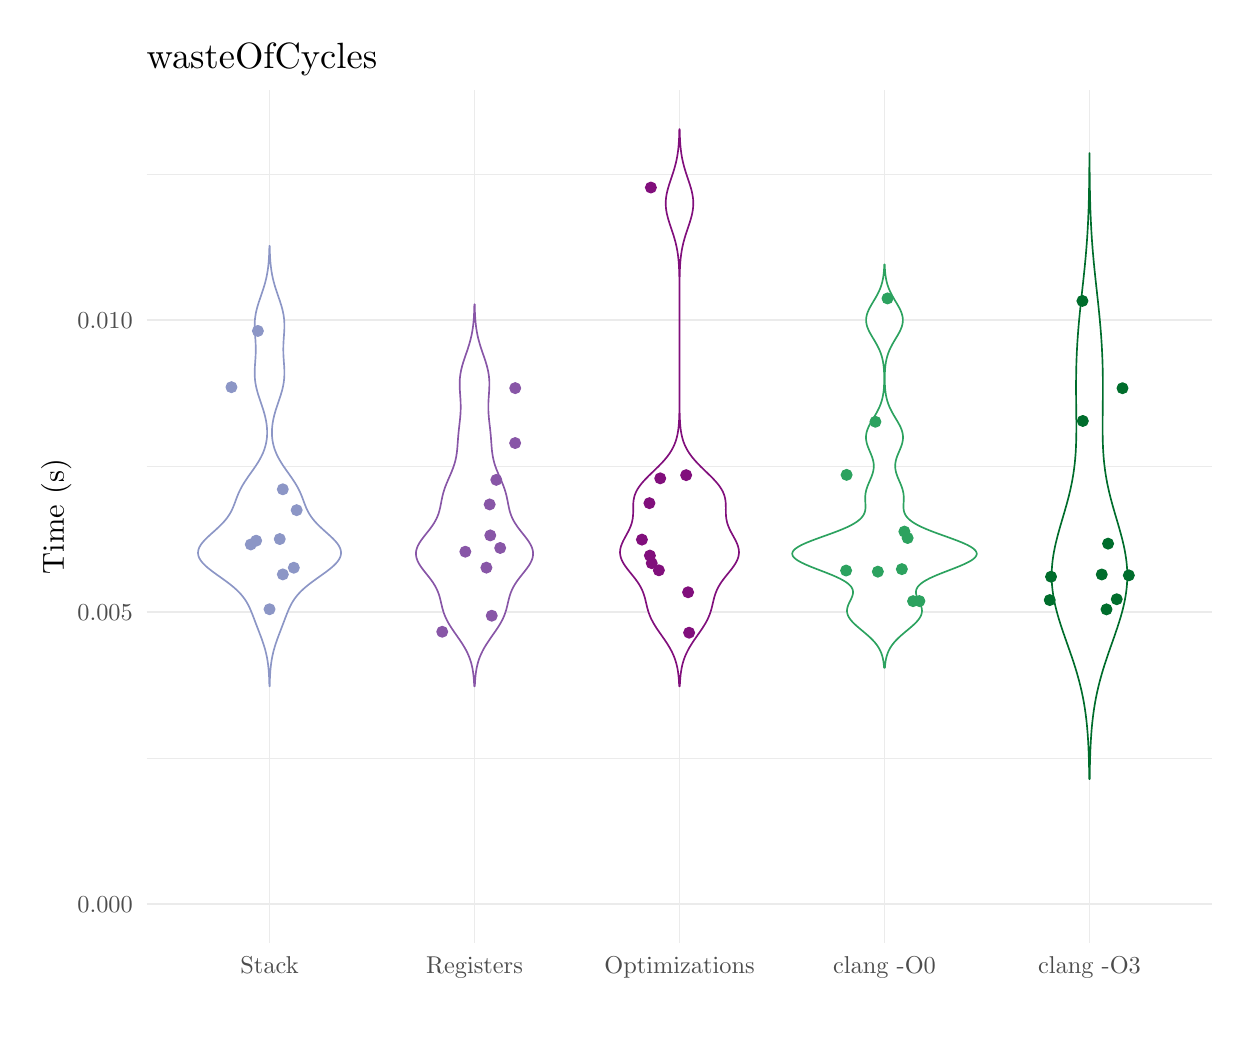
\begin{tikzpicture}[x=1pt,y=1pt]
\definecolor{fillColor}{RGB}{255,255,255}
\path[use as bounding box,fill=fillColor,fill opacity=0.00] (0,0) rectangle (433.62,361.35);
\begin{scope}
\path[clip] ( 42.95, 30.69) rectangle (428.12,338.69);
\definecolor{drawColor}{gray}{0.92}

\path[draw=drawColor,line width= 0.3pt,line join=round] ( 42.95, 97.43) --
	(428.12, 97.43);

\path[draw=drawColor,line width= 0.3pt,line join=round] ( 42.95,202.93) --
	(428.12,202.93);

\path[draw=drawColor,line width= 0.3pt,line join=round] ( 42.95,308.42) --
	(428.12,308.42);

\path[draw=drawColor,line width= 0.6pt,line join=round] ( 42.95, 44.69) --
	(428.12, 44.69);

\path[draw=drawColor,line width= 0.6pt,line join=round] ( 42.95,150.18) --
	(428.12,150.18);

\path[draw=drawColor,line width= 0.6pt,line join=round] ( 42.95,255.67) --
	(428.12,255.67);

\path[draw=drawColor,line width= 0.6pt,line join=round] ( 87.40, 30.69) --
	( 87.40,338.69);

\path[draw=drawColor,line width= 0.6pt,line join=round] (161.47, 30.69) --
	(161.47,338.69);

\path[draw=drawColor,line width= 0.6pt,line join=round] (235.54, 30.69) --
	(235.54,338.69);

\path[draw=drawColor,line width= 0.6pt,line join=round] (309.61, 30.69) --
	(309.61,338.69);

\path[draw=drawColor,line width= 0.6pt,line join=round] (383.68, 30.69) --
	(383.68,338.69);
\definecolor{drawColor}{RGB}{140,150,198}
\definecolor{fillColor}{RGB}{255,255,255}

\path[draw=drawColor,line width= 0.6pt,line join=round,line cap=round,fill=fillColor] ( 87.34,123.36) --
	( 87.33,123.67) --
	( 87.33,123.98) --
	( 87.32,124.29) --
	( 87.31,124.60) --
	( 87.30,124.91) --
	( 87.29,125.22) --
	( 87.28,125.54) --
	( 87.27,125.85) --
	( 87.26,126.16) --
	( 87.25,126.47) --
	( 87.23,126.78) --
	( 87.22,127.09) --
	( 87.20,127.40) --
	( 87.18,127.72) --
	( 87.16,128.03) --
	( 87.14,128.34) --
	( 87.12,128.65) --
	( 87.10,128.96) --
	( 87.07,129.27) --
	( 87.04,129.58) --
	( 87.01,129.90) --
	( 86.98,130.21) --
	( 86.95,130.52) --
	( 86.91,130.83) --
	( 86.88,131.14) --
	( 86.84,131.45) --
	( 86.79,131.76) --
	( 86.75,132.08) --
	( 86.70,132.39) --
	( 86.65,132.70) --
	( 86.60,133.01) --
	( 86.55,133.32) --
	( 86.49,133.63) --
	( 86.43,133.94) --
	( 86.37,134.26) --
	( 86.30,134.57) --
	( 86.23,134.88) --
	( 86.16,135.19) --
	( 86.09,135.50) --
	( 86.01,135.81) --
	( 85.93,136.12) --
	( 85.85,136.44) --
	( 85.77,136.75) --
	( 85.68,137.06) --
	( 85.59,137.37) --
	( 85.49,137.68) --
	( 85.40,137.99) --
	( 85.30,138.30) --
	( 85.20,138.62) --
	( 85.10,138.93) --
	( 84.99,139.24) --
	( 84.89,139.55) --
	( 84.78,139.86) --
	( 84.67,140.17) --
	( 84.56,140.48) --
	( 84.45,140.80) --
	( 84.33,141.11) --
	( 84.22,141.42) --
	( 84.10,141.73) --
	( 83.98,142.04) --
	( 83.86,142.35) --
	( 83.74,142.66) --
	( 83.63,142.98) --
	( 83.51,143.29) --
	( 83.39,143.60) --
	( 83.27,143.91) --
	( 83.15,144.22) --
	( 83.03,144.53) --
	( 82.91,144.84) --
	( 82.79,145.16) --
	( 82.67,145.47) --
	( 82.55,145.78) --
	( 82.43,146.09) --
	( 82.32,146.40) --
	( 82.20,146.71) --
	( 82.08,147.02) --
	( 81.96,147.34) --
	( 81.85,147.65) --
	( 81.73,147.96) --
	( 81.61,148.27) --
	( 81.49,148.58) --
	( 81.37,148.89) --
	( 81.25,149.20) --
	( 81.13,149.52) --
	( 81.01,149.83) --
	( 80.88,150.14) --
	( 80.76,150.45) --
	( 80.62,150.76) --
	( 80.49,151.07) --
	( 80.35,151.38) --
	( 80.21,151.70) --
	( 80.06,152.01) --
	( 79.91,152.32) --
	( 79.75,152.63) --
	( 79.59,152.94) --
	( 79.42,153.25) --
	( 79.24,153.56) --
	( 79.06,153.88) --
	( 78.86,154.19) --
	( 78.66,154.50) --
	( 78.45,154.81) --
	( 78.23,155.12) --
	( 78.00,155.43) --
	( 77.76,155.74) --
	( 77.51,156.06) --
	( 77.25,156.37) --
	( 76.98,156.68) --
	( 76.69,156.99) --
	( 76.40,157.30) --
	( 76.10,157.61) --
	( 75.78,157.92) --
	( 75.45,158.24) --
	( 75.11,158.55) --
	( 74.76,158.86) --
	( 74.40,159.17) --
	( 74.03,159.48) --
	( 73.65,159.79) --
	( 73.26,160.10) --
	( 72.86,160.42) --
	( 72.46,160.73) --
	( 72.04,161.04) --
	( 71.62,161.35) --
	( 71.20,161.66) --
	( 70.77,161.97) --
	( 70.33,162.28) --
	( 69.90,162.60) --
	( 69.46,162.91) --
	( 69.02,163.22) --
	( 68.58,163.53) --
	( 68.15,163.84) --
	( 67.72,164.15) --
	( 67.29,164.46) --
	( 66.87,164.78) --
	( 66.45,165.09) --
	( 66.05,165.40) --
	( 65.65,165.71) --
	( 65.27,166.02) --
	( 64.90,166.33) --
	( 64.54,166.64) --
	( 64.20,166.96) --
	( 63.88,167.27) --
	( 63.57,167.58) --
	( 63.28,167.89) --
	( 63.02,168.20) --
	( 62.77,168.51) --
	( 62.54,168.82) --
	( 62.34,169.14) --
	( 62.15,169.45) --
	( 61.99,169.76) --
	( 61.86,170.07) --
	( 61.75,170.38) --
	( 61.66,170.69) --
	( 61.61,171.00) --
	( 61.57,171.32) --
	( 61.56,171.63) --
	( 61.58,171.94) --
	( 61.62,172.25) --
	( 61.68,172.56) --
	( 61.76,172.87) --
	( 61.88,173.18) --
	( 62.01,173.50) --
	( 62.16,173.81) --
	( 62.34,174.12) --
	( 62.54,174.43) --
	( 62.75,174.74) --
	( 62.98,175.05) --
	( 63.23,175.36) --
	( 63.50,175.68) --
	( 63.78,175.99) --
	( 64.07,176.30) --
	( 64.37,176.61) --
	( 64.69,176.92) --
	( 65.01,177.23) --
	( 65.34,177.54) --
	( 65.68,177.86) --
	( 66.02,178.17) --
	( 66.36,178.48) --
	( 66.71,178.79) --
	( 67.06,179.10) --
	( 67.41,179.41) --
	( 67.75,179.72) --
	( 68.10,180.04) --
	( 68.44,180.35) --
	( 68.77,180.66) --
	( 69.10,180.97) --
	( 69.43,181.28) --
	( 69.74,181.59) --
	( 70.05,181.90) --
	( 70.35,182.22) --
	( 70.64,182.53) --
	( 70.93,182.84) --
	( 71.20,183.15) --
	( 71.46,183.46) --
	( 71.71,183.77) --
	( 71.96,184.08) --
	( 72.19,184.40) --
	( 72.41,184.71) --
	( 72.62,185.02) --
	( 72.82,185.33) --
	( 73.01,185.64) --
	( 73.20,185.95) --
	( 73.37,186.26) --
	( 73.54,186.58) --
	( 73.70,186.89) --
	( 73.85,187.20) --
	( 73.99,187.51) --
	( 74.13,187.82) --
	( 74.26,188.13) --
	( 74.39,188.44) --
	( 74.51,188.76) --
	( 74.64,189.07) --
	( 74.75,189.38) --
	( 74.87,189.69) --
	( 74.99,190.00) --
	( 75.10,190.31) --
	( 75.21,190.62) --
	( 75.33,190.94) --
	( 75.45,191.25) --
	( 75.56,191.56) --
	( 75.68,191.87) --
	( 75.81,192.18) --
	( 75.94,192.49) --
	( 76.06,192.80) --
	( 76.20,193.12) --
	( 76.34,193.43) --
	( 76.48,193.74) --
	( 76.63,194.05) --
	( 76.78,194.36) --
	( 76.94,194.67) --
	( 77.10,194.98) --
	( 77.27,195.30) --
	( 77.44,195.61) --
	( 77.62,195.92) --
	( 77.81,196.23) --
	( 77.99,196.54) --
	( 78.19,196.85) --
	( 78.38,197.16) --
	( 78.58,197.48) --
	( 78.79,197.79) --
	( 79.00,198.10) --
	( 79.21,198.41) --
	( 79.42,198.72) --
	( 79.64,199.03) --
	( 79.85,199.34) --
	( 80.07,199.66) --
	( 80.29,199.97) --
	( 80.52,200.28) --
	( 80.74,200.59) --
	( 80.96,200.90) --
	( 81.18,201.21) --
	( 81.40,201.52) --
	( 81.62,201.84) --
	( 81.83,202.15) --
	( 82.05,202.46) --
	( 82.26,202.77) --
	( 82.47,203.08) --
	( 82.67,203.39) --
	( 82.88,203.70) --
	( 83.07,204.02) --
	( 83.27,204.33) --
	( 83.46,204.64) --
	( 83.64,204.95) --
	( 83.82,205.26) --
	( 83.99,205.57) --
	( 84.16,205.88) --
	( 84.33,206.20) --
	( 84.48,206.51) --
	( 84.64,206.82) --
	( 84.78,207.13) --
	( 84.92,207.44) --
	( 85.06,207.75) --
	( 85.18,208.06) --
	( 85.30,208.38) --
	( 85.42,208.69) --
	( 85.53,209.00) --
	( 85.63,209.31) --
	( 85.73,209.62) --
	( 85.83,209.93) --
	( 85.91,210.24) --
	( 85.99,210.56) --
	( 86.07,210.87) --
	( 86.13,211.18) --
	( 86.20,211.49) --
	( 86.25,211.80) --
	( 86.30,212.11) --
	( 86.35,212.42) --
	( 86.39,212.74) --
	( 86.43,213.05) --
	( 86.46,213.36) --
	( 86.48,213.67) --
	( 86.50,213.98) --
	( 86.51,214.29) --
	( 86.52,214.60) --
	( 86.53,214.92) --
	( 86.53,215.23) --
	( 86.53,215.54) --
	( 86.52,215.85) --
	( 86.50,216.16) --
	( 86.48,216.47) --
	( 86.46,216.78) --
	( 86.43,217.10) --
	( 86.40,217.41) --
	( 86.37,217.72) --
	( 86.33,218.03) --
	( 86.28,218.34) --
	( 86.24,218.65) --
	( 86.19,218.96) --
	( 86.13,219.28) --
	( 86.07,219.59) --
	( 86.01,219.90) --
	( 85.94,220.21) --
	( 85.87,220.52) --
	( 85.80,220.83) --
	( 85.72,221.14) --
	( 85.64,221.46) --
	( 85.56,221.77) --
	( 85.47,222.08) --
	( 85.38,222.39) --
	( 85.29,222.70) --
	( 85.20,223.01) --
	( 85.10,223.32) --
	( 85.00,223.64) --
	( 84.91,223.95) --
	( 84.80,224.26) --
	( 84.70,224.57) --
	( 84.60,224.88) --
	( 84.49,225.19) --
	( 84.39,225.50) --
	( 84.28,225.82) --
	( 84.18,226.13) --
	( 84.07,226.44) --
	( 83.96,226.75) --
	( 83.86,227.06) --
	( 83.75,227.37) --
	( 83.65,227.68) --
	( 83.55,228.00) --
	( 83.45,228.31) --
	( 83.35,228.62) --
	( 83.25,228.93) --
	( 83.16,229.24) --
	( 83.07,229.55) --
	( 82.98,229.86) --
	( 82.90,230.18) --
	( 82.81,230.49) --
	( 82.74,230.80) --
	( 82.66,231.11) --
	( 82.59,231.42) --
	( 82.52,231.73) --
	( 82.46,232.04) --
	( 82.40,232.36) --
	( 82.35,232.67) --
	( 82.29,232.98) --
	( 82.25,233.29) --
	( 82.21,233.60) --
	( 82.17,233.91) --
	( 82.14,234.22) --
	( 82.11,234.54) --
	( 82.09,234.85) --
	( 82.07,235.16) --
	( 82.05,235.47) --
	( 82.04,235.78) --
	( 82.03,236.09) --
	( 82.03,236.40) --
	( 82.03,236.72) --
	( 82.03,237.03) --
	( 82.04,237.34) --
	( 82.05,237.65) --
	( 82.06,237.96) --
	( 82.07,238.27) --
	( 82.09,238.58) --
	( 82.10,238.90) --
	( 82.12,239.21) --
	( 82.14,239.52) --
	( 82.16,239.83) --
	( 82.19,240.14) --
	( 82.21,240.45) --
	( 82.23,240.76) --
	( 82.25,241.08) --
	( 82.27,241.39) --
	( 82.30,241.70) --
	( 82.32,242.01) --
	( 82.33,242.32) --
	( 82.35,242.63) --
	( 82.37,242.94) --
	( 82.38,243.26) --
	( 82.39,243.57) --
	( 82.40,243.88) --
	( 82.41,244.19) --
	( 82.42,244.50) --
	( 82.42,244.81) --
	( 82.42,245.12) --
	( 82.42,245.44) --
	( 82.42,245.75) --
	( 82.41,246.06) --
	( 82.40,246.37) --
	( 82.39,246.68) --
	( 82.38,246.99) --
	( 82.37,247.30) --
	( 82.35,247.62) --
	( 82.33,247.93) --
	( 82.32,248.24) --
	( 82.30,248.55) --
	( 82.27,248.86) --
	( 82.25,249.17) --
	( 82.23,249.48) --
	( 82.21,249.80) --
	( 82.19,250.11) --
	( 82.16,250.42) --
	( 82.14,250.73) --
	( 82.12,251.04) --
	( 82.10,251.35) --
	( 82.09,251.66) --
	( 82.07,251.98) --
	( 82.06,252.29) --
	( 82.05,252.60) --
	( 82.04,252.91) --
	( 82.03,253.22) --
	( 82.03,253.53) --
	( 82.03,253.84) --
	( 82.03,254.16) --
	( 82.04,254.47) --
	( 82.05,254.78) --
	( 82.07,255.09) --
	( 82.09,255.40) --
	( 82.11,255.71) --
	( 82.14,256.02) --
	( 82.17,256.34) --
	( 82.21,256.65) --
	( 82.25,256.96) --
	( 82.30,257.27) --
	( 82.35,257.58) --
	( 82.40,257.89) --
	( 82.46,258.20) --
	( 82.52,258.52) --
	( 82.59,258.83) --
	( 82.66,259.14) --
	( 82.74,259.45) --
	( 82.82,259.76) --
	( 82.90,260.07) --
	( 82.98,260.38) --
	( 83.07,260.70) --
	( 83.16,261.01) --
	( 83.26,261.32) --
	( 83.35,261.63) --
	( 83.45,261.94) --
	( 83.55,262.25) --
	( 83.66,262.56) --
	( 83.76,262.88) --
	( 83.87,263.19) --
	( 83.97,263.50) --
	( 84.08,263.81) --
	( 84.18,264.12) --
	( 84.29,264.43) --
	( 84.40,264.74) --
	( 84.51,265.06) --
	( 84.61,265.37) --
	( 84.72,265.68) --
	( 84.82,265.99) --
	( 84.93,266.30) --
	( 85.03,266.61) --
	( 85.13,266.92) --
	( 85.23,267.24) --
	( 85.32,267.55) --
	( 85.42,267.86) --
	( 85.51,268.17) --
	( 85.60,268.48) --
	( 85.69,268.79) --
	( 85.78,269.10) --
	( 85.86,269.42) --
	( 85.94,269.73) --
	( 86.02,270.04) --
	( 86.10,270.35) --
	( 86.17,270.66) --
	( 86.24,270.97) --
	( 86.31,271.28) --
	( 86.37,271.60) --
	( 86.43,271.91) --
	( 86.49,272.22) --
	( 86.55,272.53) --
	( 86.60,272.84) --
	( 86.66,273.15) --
	( 86.70,273.46) --
	( 86.75,273.78) --
	( 86.80,274.09) --
	( 86.84,274.40) --
	( 86.88,274.71) --
	( 86.91,275.02) --
	( 86.95,275.33) --
	( 86.98,275.64) --
	( 87.01,275.96) --
	( 87.04,276.27) --
	( 87.07,276.58) --
	( 87.10,276.89) --
	( 87.12,277.20) --
	( 87.14,277.51) --
	( 87.16,277.82) --
	( 87.18,278.14) --
	( 87.20,278.45) --
	( 87.22,278.76) --
	( 87.23,279.07) --
	( 87.25,279.38) --
	( 87.26,279.69) --
	( 87.27,280.00) --
	( 87.28,280.32) --
	( 87.29,280.63) --
	( 87.30,280.94) --
	( 87.31,281.25) --
	( 87.32,281.56) --
	( 87.33,281.87) --
	( 87.33,282.18) --
	( 87.34,282.50) --
	( 87.45,282.50) --
	( 87.46,282.18) --
	( 87.47,281.87) --
	( 87.47,281.56) --
	( 87.48,281.25) --
	( 87.49,280.94) --
	( 87.50,280.63) --
	( 87.51,280.32) --
	( 87.52,280.00) --
	( 87.53,279.69) --
	( 87.55,279.38) --
	( 87.56,279.07) --
	( 87.58,278.76) --
	( 87.59,278.45) --
	( 87.61,278.14) --
	( 87.63,277.82) --
	( 87.65,277.51) --
	( 87.67,277.20) --
	( 87.70,276.89) --
	( 87.72,276.58) --
	( 87.75,276.27) --
	( 87.78,275.96) --
	( 87.81,275.64) --
	( 87.84,275.33) --
	( 87.88,275.02) --
	( 87.92,274.71) --
	( 87.96,274.40) --
	( 88.00,274.09) --
	( 88.04,273.78) --
	( 88.09,273.46) --
	( 88.14,273.15) --
	( 88.19,272.84) --
	( 88.24,272.53) --
	( 88.30,272.22) --
	( 88.36,271.91) --
	( 88.42,271.60) --
	( 88.49,271.28) --
	( 88.55,270.97) --
	( 88.62,270.66) --
	( 88.70,270.35) --
	( 88.77,270.04) --
	( 88.85,269.73) --
	( 88.93,269.42) --
	( 89.02,269.10) --
	( 89.10,268.79) --
	( 89.19,268.48) --
	( 89.28,268.17) --
	( 89.37,267.86) --
	( 89.47,267.55) --
	( 89.56,267.24) --
	( 89.66,266.92) --
	( 89.76,266.61) --
	( 89.87,266.30) --
	( 89.97,265.99) --
	( 90.07,265.68) --
	( 90.18,265.37) --
	( 90.29,265.06) --
	( 90.39,264.74) --
	( 90.50,264.43) --
	( 90.61,264.12) --
	( 90.71,263.81) --
	( 90.82,263.50) --
	( 90.93,263.19) --
	( 91.03,262.88) --
	( 91.14,262.56) --
	( 91.24,262.25) --
	( 91.34,261.94) --
	( 91.44,261.63) --
	( 91.53,261.32) --
	( 91.63,261.01) --
	( 91.72,260.70) --
	( 91.81,260.38) --
	( 91.90,260.07) --
	( 91.98,259.76) --
	( 92.06,259.45) --
	( 92.13,259.14) --
	( 92.20,258.83) --
	( 92.27,258.52) --
	( 92.33,258.20) --
	( 92.39,257.89) --
	( 92.45,257.58) --
	( 92.50,257.27) --
	( 92.54,256.96) --
	( 92.58,256.65) --
	( 92.62,256.34) --
	( 92.65,256.02) --
	( 92.68,255.71) --
	( 92.71,255.40) --
	( 92.73,255.09) --
	( 92.74,254.78) --
	( 92.75,254.47) --
	( 92.76,254.16) --
	( 92.76,253.84) --
	( 92.76,253.53) --
	( 92.76,253.22) --
	( 92.76,252.91) --
	( 92.75,252.60) --
	( 92.74,252.29) --
	( 92.72,251.98) --
	( 92.71,251.66) --
	( 92.69,251.35) --
	( 92.67,251.04) --
	( 92.65,250.73) --
	( 92.63,250.42) --
	( 92.61,250.11) --
	( 92.58,249.80) --
	( 92.56,249.48) --
	( 92.54,249.17) --
	( 92.52,248.86) --
	( 92.50,248.55) --
	( 92.48,248.24) --
	( 92.46,247.93) --
	( 92.44,247.62) --
	( 92.43,247.30) --
	( 92.41,246.99) --
	( 92.40,246.68) --
	( 92.39,246.37) --
	( 92.38,246.06) --
	( 92.38,245.75) --
	( 92.37,245.44) --
	( 92.37,245.12) --
	( 92.37,244.81) --
	( 92.38,244.50) --
	( 92.38,244.19) --
	( 92.39,243.88) --
	( 92.40,243.57) --
	( 92.41,243.26) --
	( 92.43,242.94) --
	( 92.44,242.63) --
	( 92.46,242.32) --
	( 92.48,242.01) --
	( 92.50,241.70) --
	( 92.52,241.39) --
	( 92.54,241.08) --
	( 92.56,240.76) --
	( 92.58,240.45) --
	( 92.61,240.14) --
	( 92.63,239.83) --
	( 92.65,239.52) --
	( 92.67,239.21) --
	( 92.69,238.90) --
	( 92.71,238.58) --
	( 92.72,238.27) --
	( 92.74,237.96) --
	( 92.75,237.65) --
	( 92.75,237.34) --
	( 92.76,237.03) --
	( 92.76,236.72) --
	( 92.76,236.40) --
	( 92.76,236.09) --
	( 92.75,235.78) --
	( 92.74,235.47) --
	( 92.73,235.16) --
	( 92.71,234.85) --
	( 92.68,234.54) --
	( 92.65,234.22) --
	( 92.62,233.91) --
	( 92.58,233.60) --
	( 92.54,233.29) --
	( 92.50,232.98) --
	( 92.45,232.67) --
	( 92.39,232.36) --
	( 92.33,232.04) --
	( 92.27,231.73) --
	( 92.20,231.42) --
	( 92.13,231.11) --
	( 92.06,230.80) --
	( 91.98,230.49) --
	( 91.90,230.18) --
	( 91.81,229.86) --
	( 91.72,229.55) --
	( 91.63,229.24) --
	( 91.54,228.93) --
	( 91.44,228.62) --
	( 91.34,228.31) --
	( 91.24,228.00) --
	( 91.14,227.68) --
	( 91.04,227.37) --
	( 90.93,227.06) --
	( 90.83,226.75) --
	( 90.72,226.44) --
	( 90.62,226.13) --
	( 90.51,225.82) --
	( 90.40,225.50) --
	( 90.30,225.19) --
	( 90.19,224.88) --
	( 90.09,224.57) --
	( 89.99,224.26) --
	( 89.89,223.95) --
	( 89.79,223.64) --
	( 89.69,223.32) --
	( 89.59,223.01) --
	( 89.50,222.70) --
	( 89.41,222.39) --
	( 89.32,222.08) --
	( 89.24,221.77) --
	( 89.15,221.46) --
	( 89.07,221.14) --
	( 89.00,220.83) --
	( 88.92,220.52) --
	( 88.85,220.21) --
	( 88.79,219.90) --
	( 88.72,219.59) --
	( 88.66,219.28) --
	( 88.61,218.96) --
	( 88.56,218.65) --
	( 88.51,218.34) --
	( 88.46,218.03) --
	( 88.42,217.72) --
	( 88.39,217.41) --
	( 88.36,217.10) --
	( 88.33,216.78) --
	( 88.31,216.47) --
	( 88.29,216.16) --
	( 88.28,215.85) --
	( 88.27,215.54) --
	( 88.26,215.23) --
	( 88.26,214.92) --
	( 88.27,214.60) --
	( 88.28,214.29) --
	( 88.29,213.98) --
	( 88.31,213.67) --
	( 88.34,213.36) --
	( 88.37,213.05) --
	( 88.40,212.74) --
	( 88.44,212.42) --
	( 88.49,212.11) --
	( 88.54,211.80) --
	( 88.60,211.49) --
	( 88.66,211.18) --
	( 88.73,210.87) --
	( 88.80,210.56) --
	( 88.88,210.24) --
	( 88.97,209.93) --
	( 89.06,209.62) --
	( 89.16,209.31) --
	( 89.26,209.00) --
	( 89.37,208.69) --
	( 89.49,208.38) --
	( 89.61,208.06) --
	( 89.74,207.75) --
	( 89.87,207.44) --
	( 90.01,207.13) --
	( 90.16,206.82) --
	( 90.31,206.51) --
	( 90.47,206.20) --
	( 90.63,205.88) --
	( 90.80,205.57) --
	( 90.97,205.26) --
	( 91.15,204.95) --
	( 91.34,204.64) --
	( 91.53,204.33) --
	( 91.72,204.02) --
	( 91.92,203.70) --
	( 92.12,203.39) --
	( 92.32,203.08) --
	( 92.53,202.77) --
	( 92.74,202.46) --
	( 92.96,202.15) --
	( 93.17,201.84) --
	( 93.39,201.52) --
	( 93.61,201.21) --
	( 93.83,200.90) --
	( 94.06,200.59) --
	( 94.28,200.28) --
	( 94.50,199.97) --
	( 94.72,199.66) --
	( 94.94,199.34) --
	( 95.16,199.03) --
	( 95.37,198.72) --
	( 95.59,198.41) --
	( 95.80,198.10) --
	( 96.00,197.79) --
	( 96.21,197.48) --
	( 96.41,197.16) --
	( 96.61,196.85) --
	( 96.80,196.54) --
	( 96.99,196.23) --
	( 97.17,195.92) --
	( 97.35,195.61) --
	( 97.52,195.30) --
	( 97.69,194.98) --
	( 97.85,194.67) --
	( 98.01,194.36) --
	( 98.16,194.05) --
	( 98.31,193.74) --
	( 98.45,193.43) --
	( 98.59,193.12) --
	( 98.73,192.80) --
	( 98.86,192.49) --
	( 98.98,192.18) --
	( 99.11,191.87) --
	( 99.23,191.56) --
	( 99.35,191.25) --
	( 99.46,190.94) --
	( 99.58,190.62) --
	( 99.69,190.31) --
	( 99.81,190.00) --
	( 99.92,189.69) --
	(100.04,189.38) --
	(100.16,189.07) --
	(100.28,188.76) --
	(100.40,188.44) --
	(100.53,188.13) --
	(100.66,187.82) --
	(100.80,187.51) --
	(100.95,187.20) --
	(101.10,186.89) --
	(101.26,186.58) --
	(101.42,186.26) --
	(101.59,185.95) --
	(101.78,185.64) --
	(101.97,185.33) --
	(102.17,185.02) --
	(102.38,184.71) --
	(102.61,184.40) --
	(102.84,184.08) --
	(103.08,183.77) --
	(103.33,183.46) --
	(103.59,183.15) --
	(103.86,182.84) --
	(104.15,182.53) --
	(104.44,182.22) --
	(104.74,181.90) --
	(105.05,181.59) --
	(105.37,181.28) --
	(105.69,180.97) --
	(106.02,180.66) --
	(106.36,180.35) --
	(106.70,180.04) --
	(107.04,179.72) --
	(107.39,179.41) --
	(107.73,179.10) --
	(108.08,178.79) --
	(108.43,178.48) --
	(108.77,178.17) --
	(109.12,177.86) --
	(109.45,177.54) --
	(109.78,177.23) --
	(110.11,176.92) --
	(110.42,176.61) --
	(110.72,176.30) --
	(111.02,175.99) --
	(111.30,175.68) --
	(111.56,175.36) --
	(111.81,175.05) --
	(112.04,174.74) --
	(112.25,174.43) --
	(112.45,174.12) --
	(112.63,173.81) --
	(112.78,173.50) --
	(112.91,173.18) --
	(113.03,172.87) --
	(113.11,172.56) --
	(113.17,172.25) --
	(113.22,171.94) --
	(113.23,171.63) --
	(113.22,171.32) --
	(113.19,171.00) --
	(113.13,170.69) --
	(113.04,170.38) --
	(112.93,170.07) --
	(112.80,169.76) --
	(112.64,169.45) --
	(112.46,169.14) --
	(112.26,168.82) --
	(112.03,168.51) --
	(111.78,168.20) --
	(111.51,167.89) --
	(111.22,167.58) --
	(110.91,167.27) --
	(110.59,166.96) --
	(110.25,166.64) --
	(109.89,166.33) --
	(109.52,166.02) --
	(109.14,165.71) --
	(108.74,165.40) --
	(108.34,165.09) --
	(107.93,164.78) --
	(107.50,164.46) --
	(107.08,164.15) --
	(106.65,163.84) --
	(106.21,163.53) --
	(105.77,163.22) --
	(105.33,162.91) --
	(104.90,162.60) --
	(104.46,162.28) --
	(104.03,161.97) --
	(103.60,161.66) --
	(103.17,161.35) --
	(102.75,161.04) --
	(102.34,160.73) --
	(101.93,160.42) --
	(101.53,160.10) --
	(101.14,159.79) --
	(100.76,159.48) --
	(100.39,159.17) --
	(100.03,158.86) --
	( 99.68,158.55) --
	( 99.34,158.24) --
	( 99.01,157.92) --
	( 98.70,157.61) --
	( 98.39,157.30) --
	( 98.10,156.99) --
	( 97.81,156.68) --
	( 97.54,156.37) --
	( 97.28,156.06) --
	( 97.03,155.74) --
	( 96.79,155.43) --
	( 96.56,155.12) --
	( 96.34,154.81) --
	( 96.13,154.50) --
	( 95.93,154.19) --
	( 95.74,153.88) --
	( 95.55,153.56) --
	( 95.37,153.25) --
	( 95.20,152.94) --
	( 95.04,152.63) --
	( 94.88,152.32) --
	( 94.73,152.01) --
	( 94.58,151.70) --
	( 94.44,151.38) --
	( 94.30,151.07) --
	( 94.17,150.76) --
	( 94.04,150.45) --
	( 93.91,150.14) --
	( 93.78,149.83) --
	( 93.66,149.52) --
	( 93.54,149.20) --
	( 93.42,148.89) --
	( 93.30,148.58) --
	( 93.18,148.27) --
	( 93.06,147.96) --
	( 92.94,147.65) --
	( 92.83,147.34) --
	( 92.71,147.02) --
	( 92.59,146.71) --
	( 92.48,146.40) --
	( 92.36,146.09) --
	( 92.24,145.78) --
	( 92.12,145.47) --
	( 92.00,145.16) --
	( 91.88,144.84) --
	( 91.76,144.53) --
	( 91.65,144.22) --
	( 91.53,143.91) --
	( 91.41,143.60) --
	( 91.29,143.29) --
	( 91.17,142.98) --
	( 91.05,142.66) --
	( 90.93,142.35) --
	( 90.81,142.04) --
	( 90.69,141.73) --
	( 90.58,141.42) --
	( 90.46,141.11) --
	( 90.35,140.80) --
	( 90.23,140.48) --
	( 90.12,140.17) --
	( 90.01,139.86) --
	( 89.90,139.55) --
	( 89.80,139.24) --
	( 89.69,138.93) --
	( 89.59,138.62) --
	( 89.49,138.30) --
	( 89.39,137.99) --
	( 89.30,137.68) --
	( 89.21,137.37) --
	( 89.11,137.06) --
	( 89.03,136.75) --
	( 88.94,136.44) --
	( 88.86,136.12) --
	( 88.78,135.81) --
	( 88.70,135.50) --
	( 88.63,135.19) --
	( 88.56,134.88) --
	( 88.49,134.57) --
	( 88.43,134.26) --
	( 88.36,133.94) --
	( 88.30,133.63) --
	( 88.25,133.32) --
	( 88.19,133.01) --
	( 88.14,132.70) --
	( 88.09,132.39) --
	( 88.04,132.08) --
	( 88.00,131.76) --
	( 87.96,131.45) --
	( 87.92,131.14) --
	( 87.88,130.83) --
	( 87.84,130.52) --
	( 87.81,130.21) --
	( 87.78,129.90) --
	( 87.75,129.58) --
	( 87.72,129.27) --
	( 87.70,128.96) --
	( 87.67,128.65) --
	( 87.65,128.34) --
	( 87.63,128.03) --
	( 87.61,127.72) --
	( 87.59,127.40) --
	( 87.58,127.09) --
	( 87.56,126.78) --
	( 87.55,126.47) --
	( 87.53,126.16) --
	( 87.52,125.85) --
	( 87.51,125.54) --
	( 87.50,125.22) --
	( 87.49,124.91) --
	( 87.48,124.60) --
	( 87.47,124.29) --
	( 87.47,123.98) --
	( 87.46,123.67) --
	( 87.45,123.36) --
	( 87.34,123.36) --
	cycle;
\definecolor{drawColor}{RGB}{136,86,167}

\path[draw=drawColor,line width= 0.6pt,line join=round,line cap=round,fill=fillColor] (161.35,123.36) --
	(161.34,123.63) --
	(161.33,123.90) --
	(161.32,124.17) --
	(161.31,124.44) --
	(161.29,124.71) --
	(161.28,124.98) --
	(161.26,125.25) --
	(161.24,125.52) --
	(161.22,125.79) --
	(161.20,126.06) --
	(161.18,126.33) --
	(161.16,126.60) --
	(161.13,126.87) --
	(161.10,127.14) --
	(161.07,127.41) --
	(161.04,127.68) --
	(161.01,127.95) --
	(160.97,128.22) --
	(160.94,128.49) --
	(160.90,128.76) --
	(160.86,129.03) --
	(160.81,129.30) --
	(160.76,129.57) --
	(160.71,129.84) --
	(160.66,130.11) --
	(160.60,130.38) --
	(160.54,130.65) --
	(160.48,130.92) --
	(160.41,131.19) --
	(160.35,131.46) --
	(160.27,131.73) --
	(160.20,132.00) --
	(160.12,132.27) --
	(160.03,132.54) --
	(159.95,132.81) --
	(159.86,133.08) --
	(159.76,133.35) --
	(159.66,133.62) --
	(159.56,133.89) --
	(159.45,134.16) --
	(159.34,134.43) --
	(159.23,134.70) --
	(159.11,134.97) --
	(158.98,135.24) --
	(158.86,135.51) --
	(158.72,135.78) --
	(158.59,136.05) --
	(158.45,136.32) --
	(158.31,136.59) --
	(158.16,136.86) --
	(158.01,137.13) --
	(157.85,137.40) --
	(157.70,137.67) --
	(157.53,137.94) --
	(157.37,138.21) --
	(157.20,138.48) --
	(157.03,138.75) --
	(156.85,139.02) --
	(156.68,139.29) --
	(156.50,139.56) --
	(156.32,139.83) --
	(156.13,140.10) --
	(155.95,140.37) --
	(155.76,140.64) --
	(155.57,140.91) --
	(155.38,141.18) --
	(155.19,141.46) --
	(155.00,141.73) --
	(154.81,142.00) --
	(154.62,142.27) --
	(154.43,142.54) --
	(154.25,142.81) --
	(154.06,143.08) --
	(153.87,143.35) --
	(153.69,143.62) --
	(153.50,143.89) --
	(153.32,144.16) --
	(153.14,144.43) --
	(152.97,144.70) --
	(152.80,144.97) --
	(152.63,145.24) --
	(152.46,145.51) --
	(152.30,145.78) --
	(152.14,146.05) --
	(151.98,146.32) --
	(151.83,146.59) --
	(151.69,146.86) --
	(151.55,147.13) --
	(151.41,147.40) --
	(151.28,147.67) --
	(151.15,147.94) --
	(151.03,148.21) --
	(150.91,148.48) --
	(150.80,148.75) --
	(150.69,149.02) --
	(150.58,149.29) --
	(150.48,149.56) --
	(150.39,149.83) --
	(150.30,150.10) --
	(150.21,150.37) --
	(150.13,150.64) --
	(150.05,150.91) --
	(149.97,151.18) --
	(149.89,151.45) --
	(149.82,151.72) --
	(149.75,151.99) --
	(149.69,152.26) --
	(149.62,152.53) --
	(149.56,152.80) --
	(149.50,153.07) --
	(149.43,153.34) --
	(149.37,153.61) --
	(149.31,153.88) --
	(149.25,154.15) --
	(149.18,154.42) --
	(149.12,154.69) --
	(149.05,154.96) --
	(148.98,155.23) --
	(148.90,155.50) --
	(148.83,155.77) --
	(148.75,156.04) --
	(148.66,156.31) --
	(148.57,156.58) --
	(148.48,156.85) --
	(148.38,157.12) --
	(148.28,157.39) --
	(148.17,157.66) --
	(148.06,157.93) --
	(147.94,158.20) --
	(147.81,158.47) --
	(147.68,158.74) --
	(147.54,159.01) --
	(147.40,159.28) --
	(147.25,159.55) --
	(147.09,159.82) --
	(146.93,160.09) --
	(146.76,160.36) --
	(146.59,160.63) --
	(146.41,160.91) --
	(146.22,161.18) --
	(146.03,161.45) --
	(145.84,161.72) --
	(145.64,161.99) --
	(145.44,162.26) --
	(145.23,162.53) --
	(145.02,162.80) --
	(144.81,163.07) --
	(144.59,163.34) --
	(144.38,163.61) --
	(144.16,163.88) --
	(143.94,164.15) --
	(143.73,164.42) --
	(143.51,164.69) --
	(143.30,164.96) --
	(143.09,165.23) --
	(142.88,165.50) --
	(142.68,165.77) --
	(142.48,166.04) --
	(142.28,166.31) --
	(142.09,166.58) --
	(141.91,166.85) --
	(141.74,167.12) --
	(141.57,167.39) --
	(141.41,167.66) --
	(141.26,167.93) --
	(141.12,168.20) --
	(140.99,168.47) --
	(140.86,168.74) --
	(140.76,169.01) --
	(140.66,169.28) --
	(140.57,169.55) --
	(140.50,169.82) --
	(140.43,170.09) --
	(140.38,170.36) --
	(140.35,170.63) --
	(140.32,170.90) --
	(140.31,171.17) --
	(140.31,171.44) --
	(140.32,171.71) --
	(140.35,171.98) --
	(140.39,172.25) --
	(140.44,172.52) --
	(140.51,172.79) --
	(140.59,173.06) --
	(140.67,173.33) --
	(140.78,173.60) --
	(140.89,173.87) --
	(141.01,174.14) --
	(141.15,174.41) --
	(141.29,174.68) --
	(141.44,174.95) --
	(141.60,175.22) --
	(141.77,175.49) --
	(141.95,175.76) --
	(142.13,176.03) --
	(142.32,176.30) --
	(142.52,176.57) --
	(142.72,176.84) --
	(142.92,177.11) --
	(143.13,177.38) --
	(143.34,177.65) --
	(143.56,177.92) --
	(143.77,178.19) --
	(143.99,178.46) --
	(144.20,178.73) --
	(144.42,179.00) --
	(144.63,179.27) --
	(144.85,179.54) --
	(145.06,179.81) --
	(145.27,180.08) --
	(145.47,180.36) --
	(145.67,180.63) --
	(145.87,180.90) --
	(146.06,181.17) --
	(146.25,181.44) --
	(146.43,181.71) --
	(146.61,181.98) --
	(146.79,182.25) --
	(146.95,182.52) --
	(147.11,182.79) --
	(147.26,183.06) --
	(147.41,183.33) --
	(147.55,183.60) --
	(147.69,183.87) --
	(147.82,184.14) --
	(147.94,184.41) --
	(148.05,184.68) --
	(148.16,184.95) --
	(148.27,185.22) --
	(148.37,185.49) --
	(148.46,185.76) --
	(148.55,186.03) --
	(148.63,186.30) --
	(148.71,186.57) --
	(148.78,186.84) --
	(148.85,187.11) --
	(148.92,187.38) --
	(148.98,187.65) --
	(149.04,187.92) --
	(149.10,188.19) --
	(149.16,188.46) --
	(149.21,188.73) --
	(149.27,189.00) --
	(149.32,189.27) --
	(149.37,189.54) --
	(149.42,189.81) --
	(149.47,190.08) --
	(149.52,190.35) --
	(149.58,190.62) --
	(149.63,190.89) --
	(149.69,191.16) --
	(149.74,191.43) --
	(149.80,191.70) --
	(149.86,191.97) --
	(149.93,192.24) --
	(149.99,192.51) --
	(150.06,192.78) --
	(150.13,193.05) --
	(150.21,193.32) --
	(150.29,193.59) --
	(150.37,193.86) --
	(150.45,194.13) --
	(150.54,194.40) --
	(150.63,194.67) --
	(150.72,194.94) --
	(150.82,195.21) --
	(150.91,195.48) --
	(151.02,195.75) --
	(151.12,196.02) --
	(151.23,196.29) --
	(151.33,196.56) --
	(151.45,196.83) --
	(151.56,197.10) --
	(151.67,197.37) --
	(151.79,197.64) --
	(151.90,197.91) --
	(152.02,198.18) --
	(152.14,198.45) --
	(152.26,198.72) --
	(152.38,198.99) --
	(152.49,199.26) --
	(152.61,199.53) --
	(152.73,199.81) --
	(152.85,200.08) --
	(152.96,200.35) --
	(153.07,200.62) --
	(153.19,200.89) --
	(153.30,201.16) --
	(153.40,201.43) --
	(153.51,201.70) --
	(153.61,201.97) --
	(153.71,202.24) --
	(153.81,202.51) --
	(153.91,202.78) --
	(154.00,203.05) --
	(154.09,203.32) --
	(154.17,203.59) --
	(154.25,203.86) --
	(154.33,204.13) --
	(154.41,204.40) --
	(154.48,204.67) --
	(154.55,204.94) --
	(154.61,205.21) --
	(154.67,205.48) --
	(154.73,205.75) --
	(154.79,206.02) --
	(154.84,206.29) --
	(154.89,206.56) --
	(154.93,206.83) --
	(154.97,207.10) --
	(155.01,207.37) --
	(155.05,207.64) --
	(155.09,207.91) --
	(155.12,208.18) --
	(155.15,208.45) --
	(155.18,208.72) --
	(155.21,208.99) --
	(155.23,209.26) --
	(155.26,209.53) --
	(155.28,209.80) --
	(155.30,210.07) --
	(155.32,210.34) --
	(155.34,210.61) --
	(155.36,210.88) --
	(155.38,211.15) --
	(155.40,211.42) --
	(155.42,211.69) --
	(155.44,211.96) --
	(155.46,212.23) --
	(155.48,212.50) --
	(155.50,212.77) --
	(155.52,213.04) --
	(155.54,213.31) --
	(155.57,213.58) --
	(155.59,213.85) --
	(155.61,214.12) --
	(155.64,214.39) --
	(155.66,214.66) --
	(155.69,214.93) --
	(155.71,215.20) --
	(155.74,215.47) --
	(155.77,215.74) --
	(155.80,216.01) --
	(155.83,216.28) --
	(155.86,216.55) --
	(155.89,216.82) --
	(155.92,217.09) --
	(155.95,217.36) --
	(155.98,217.63) --
	(156.01,217.90) --
	(156.04,218.17) --
	(156.07,218.44) --
	(156.10,218.71) --
	(156.13,218.98) --
	(156.16,219.26) --
	(156.19,219.53) --
	(156.22,219.80) --
	(156.25,220.07) --
	(156.27,220.34) --
	(156.30,220.61) --
	(156.32,220.88) --
	(156.34,221.15) --
	(156.36,221.42) --
	(156.38,221.69) --
	(156.40,221.96) --
	(156.42,222.23) --
	(156.43,222.50) --
	(156.44,222.77) --
	(156.45,223.04) --
	(156.46,223.31) --
	(156.47,223.58) --
	(156.47,223.85) --
	(156.47,224.12) --
	(156.47,224.39) --
	(156.47,224.66) --
	(156.47,224.93) --
	(156.46,225.20) --
	(156.46,225.47) --
	(156.45,225.74) --
	(156.44,226.01) --
	(156.43,226.28) --
	(156.41,226.55) --
	(156.40,226.82) --
	(156.38,227.09) --
	(156.37,227.36) --
	(156.35,227.63) --
	(156.33,227.90) --
	(156.31,228.17) --
	(156.29,228.44) --
	(156.28,228.71) --
	(156.26,228.98) --
	(156.24,229.25) --
	(156.22,229.52) --
	(156.20,229.79) --
	(156.19,230.06) --
	(156.17,230.33) --
	(156.15,230.60) --
	(156.14,230.87) --
	(156.13,231.14) --
	(156.12,231.41) --
	(156.11,231.68) --
	(156.10,231.95) --
	(156.10,232.22) --
	(156.10,232.49) --
	(156.10,232.76) --
	(156.10,233.03) --
	(156.11,233.30) --
	(156.12,233.57) --
	(156.13,233.84) --
	(156.15,234.11) --
	(156.16,234.38) --
	(156.18,234.65) --
	(156.21,234.92) --
	(156.24,235.19) --
	(156.27,235.46) --
	(156.30,235.73) --
	(156.34,236.00) --
	(156.38,236.27) --
	(156.43,236.54) --
	(156.47,236.81) --
	(156.53,237.08) --
	(156.58,237.35) --
	(156.64,237.62) --
	(156.70,237.89) --
	(156.76,238.16) --
	(156.83,238.43) --
	(156.90,238.71) --
	(156.97,238.98) --
	(157.04,239.25) --
	(157.12,239.52) --
	(157.20,239.79) --
	(157.28,240.06) --
	(157.36,240.33) --
	(157.44,240.60) --
	(157.53,240.87) --
	(157.62,241.14) --
	(157.71,241.41) --
	(157.80,241.68) --
	(157.89,241.95) --
	(157.98,242.22) --
	(158.07,242.49) --
	(158.16,242.76) --
	(158.26,243.03) --
	(158.35,243.30) --
	(158.44,243.57) --
	(158.54,243.84) --
	(158.63,244.11) --
	(158.72,244.38) --
	(158.81,244.65) --
	(158.90,244.92) --
	(158.99,245.19) --
	(159.08,245.46) --
	(159.17,245.73) --
	(159.25,246.00) --
	(159.34,246.27) --
	(159.42,246.54) --
	(159.50,246.81) --
	(159.59,247.08) --
	(159.66,247.35) --
	(159.74,247.62) --
	(159.82,247.89) --
	(159.89,248.16) --
	(159.96,248.43) --
	(160.03,248.70) --
	(160.10,248.97) --
	(160.16,249.24) --
	(160.23,249.51) --
	(160.29,249.78) --
	(160.35,250.05) --
	(160.41,250.32) --
	(160.46,250.59) --
	(160.51,250.86) --
	(160.57,251.13) --
	(160.61,251.40) --
	(160.66,251.67) --
	(160.71,251.94) --
	(160.75,252.21) --
	(160.79,252.48) --
	(160.83,252.75) --
	(160.87,253.02) --
	(160.91,253.29) --
	(160.94,253.56) --
	(160.97,253.83) --
	(161.01,254.10) --
	(161.03,254.37) --
	(161.06,254.64) --
	(161.09,254.91) --
	(161.11,255.18) --
	(161.14,255.45) --
	(161.16,255.72) --
	(161.18,255.99) --
	(161.20,256.26) --
	(161.22,256.53) --
	(161.24,256.80) --
	(161.25,257.07) --
	(161.27,257.34) --
	(161.28,257.61) --
	(161.30,257.88) --
	(161.31,258.16) --
	(161.32,258.43) --
	(161.33,258.70) --
	(161.34,258.97) --
	(161.35,259.24) --
	(161.36,259.51) --
	(161.37,259.78) --
	(161.38,260.05) --
	(161.39,260.32) --
	(161.39,260.59) --
	(161.40,260.86) --
	(161.41,261.13) --
	(161.41,261.40) --
	(161.52,261.40) --
	(161.53,261.13) --
	(161.53,260.86) --
	(161.54,260.59) --
	(161.55,260.32) --
	(161.55,260.05) --
	(161.56,259.78) --
	(161.57,259.51) --
	(161.58,259.24) --
	(161.59,258.97) --
	(161.60,258.70) --
	(161.61,258.43) --
	(161.62,258.16) --
	(161.63,257.88) --
	(161.65,257.61) --
	(161.66,257.34) --
	(161.68,257.07) --
	(161.70,256.80) --
	(161.71,256.53) --
	(161.73,256.26) --
	(161.75,255.99) --
	(161.77,255.72) --
	(161.80,255.45) --
	(161.82,255.18) --
	(161.84,254.91) --
	(161.87,254.64) --
	(161.90,254.37) --
	(161.93,254.10) --
	(161.96,253.83) --
	(161.99,253.56) --
	(162.03,253.29) --
	(162.06,253.02) --
	(162.10,252.75) --
	(162.14,252.48) --
	(162.18,252.21) --
	(162.23,251.94) --
	(162.27,251.67) --
	(162.32,251.40) --
	(162.37,251.13) --
	(162.42,250.86) --
	(162.47,250.59) --
	(162.53,250.32) --
	(162.59,250.05) --
	(162.64,249.78) --
	(162.71,249.51) --
	(162.77,249.24) --
	(162.84,248.97) --
	(162.90,248.70) --
	(162.97,248.43) --
	(163.04,248.16) --
	(163.12,247.89) --
	(163.19,247.62) --
	(163.27,247.35) --
	(163.35,247.08) --
	(163.43,246.81) --
	(163.51,246.54) --
	(163.59,246.27) --
	(163.68,246.00) --
	(163.77,245.73) --
	(163.85,245.46) --
	(163.94,245.19) --
	(164.03,244.92) --
	(164.12,244.65) --
	(164.21,244.38) --
	(164.31,244.11) --
	(164.40,243.84) --
	(164.49,243.57) --
	(164.58,243.30) --
	(164.68,243.03) --
	(164.77,242.76) --
	(164.86,242.49) --
	(164.95,242.22) --
	(165.05,241.95) --
	(165.14,241.68) --
	(165.23,241.41) --
	(165.31,241.14) --
	(165.40,240.87) --
	(165.49,240.60) --
	(165.57,240.33) --
	(165.66,240.06) --
	(165.74,239.79) --
	(165.81,239.52) --
	(165.89,239.25) --
	(165.97,238.98) --
	(166.04,238.71) --
	(166.11,238.43) --
	(166.17,238.16) --
	(166.23,237.89) --
	(166.30,237.62) --
	(166.35,237.35) --
	(166.41,237.08) --
	(166.46,236.81) --
	(166.51,236.54) --
	(166.55,236.27) --
	(166.59,236.00) --
	(166.63,235.73) --
	(166.66,235.46) --
	(166.70,235.19) --
	(166.72,234.92) --
	(166.75,234.65) --
	(166.77,234.38) --
	(166.79,234.11) --
	(166.80,233.84) --
	(166.82,233.57) --
	(166.82,233.30) --
	(166.83,233.03) --
	(166.83,232.76) --
	(166.83,232.49) --
	(166.83,232.22) --
	(166.83,231.95) --
	(166.82,231.68) --
	(166.81,231.41) --
	(166.80,231.14) --
	(166.79,230.87) --
	(166.78,230.60) --
	(166.76,230.33) --
	(166.75,230.06) --
	(166.73,229.79) --
	(166.71,229.52) --
	(166.70,229.25) --
	(166.68,228.98) --
	(166.66,228.71) --
	(166.64,228.44) --
	(166.62,228.17) --
	(166.60,227.90) --
	(166.58,227.63) --
	(166.57,227.36) --
	(166.55,227.09) --
	(166.53,226.82) --
	(166.52,226.55) --
	(166.51,226.28) --
	(166.49,226.01) --
	(166.48,225.74) --
	(166.48,225.47) --
	(166.47,225.20) --
	(166.46,224.93) --
	(166.46,224.66) --
	(166.46,224.39) --
	(166.46,224.12) --
	(166.46,223.85) --
	(166.47,223.58) --
	(166.47,223.31) --
	(166.48,223.04) --
	(166.49,222.77) --
	(166.50,222.50) --
	(166.52,222.23) --
	(166.53,221.96) --
	(166.55,221.69) --
	(166.57,221.42) --
	(166.59,221.15) --
	(166.61,220.88) --
	(166.64,220.61) --
	(166.66,220.34) --
	(166.69,220.07) --
	(166.71,219.80) --
	(166.74,219.53) --
	(166.77,219.26) --
	(166.80,218.98) --
	(166.83,218.71) --
	(166.86,218.44) --
	(166.89,218.17) --
	(166.92,217.90) --
	(166.95,217.63) --
	(166.99,217.36) --
	(167.02,217.09) --
	(167.05,216.82) --
	(167.08,216.55) --
	(167.11,216.28) --
	(167.14,216.01) --
	(167.17,215.74) --
	(167.19,215.47) --
	(167.22,215.20) --
	(167.25,214.93) --
	(167.27,214.66) --
	(167.30,214.39) --
	(167.32,214.12) --
	(167.35,213.85) --
	(167.37,213.58) --
	(167.39,213.31) --
	(167.41,213.04) --
	(167.43,212.77) --
	(167.45,212.50) --
	(167.47,212.23) --
	(167.49,211.96) --
	(167.51,211.69) --
	(167.53,211.42) --
	(167.55,211.15) --
	(167.57,210.88) --
	(167.59,210.61) --
	(167.61,210.34) --
	(167.63,210.07) --
	(167.65,209.80) --
	(167.68,209.53) --
	(167.70,209.26) --
	(167.73,208.99) --
	(167.75,208.72) --
	(167.78,208.45) --
	(167.81,208.18) --
	(167.85,207.91) --
	(167.88,207.64) --
	(167.92,207.37) --
	(167.96,207.10) --
	(168.00,206.83) --
	(168.05,206.56) --
	(168.10,206.29) --
	(168.15,206.02) --
	(168.20,205.75) --
	(168.26,205.48) --
	(168.32,205.21) --
	(168.39,204.94) --
	(168.46,204.67) --
	(168.53,204.40) --
	(168.60,204.13) --
	(168.68,203.86) --
	(168.76,203.59) --
	(168.85,203.32) --
	(168.94,203.05) --
	(169.03,202.78) --
	(169.12,202.51) --
	(169.22,202.24) --
	(169.32,201.97) --
	(169.42,201.70) --
	(169.53,201.43) --
	(169.64,201.16) --
	(169.75,200.89) --
	(169.86,200.62) --
	(169.97,200.35) --
	(170.09,200.08) --
	(170.20,199.81) --
	(170.32,199.53) --
	(170.44,199.26) --
	(170.56,198.99) --
	(170.68,198.72) --
	(170.79,198.45) --
	(170.91,198.18) --
	(171.03,197.91) --
	(171.15,197.64) --
	(171.26,197.37) --
	(171.38,197.10) --
	(171.49,196.83) --
	(171.60,196.56) --
	(171.71,196.29) --
	(171.81,196.02) --
	(171.92,195.75) --
	(172.02,195.48) --
	(172.12,195.21) --
	(172.21,194.94) --
	(172.31,194.67) --
	(172.40,194.40) --
	(172.48,194.13) --
	(172.57,193.86) --
	(172.65,193.59) --
	(172.72,193.32) --
	(172.80,193.05) --
	(172.87,192.78) --
	(172.94,192.51) --
	(173.01,192.24) --
	(173.07,191.97) --
	(173.13,191.70) --
	(173.19,191.43) --
	(173.25,191.16) --
	(173.30,190.89) --
	(173.36,190.62) --
	(173.41,190.35) --
	(173.46,190.08) --
	(173.51,189.81) --
	(173.56,189.54) --
	(173.62,189.27) --
	(173.67,189.00) --
	(173.72,188.73) --
	(173.77,188.46) --
	(173.83,188.19) --
	(173.89,187.92) --
	(173.95,187.65) --
	(174.01,187.38) --
	(174.08,187.11) --
	(174.15,186.84) --
	(174.22,186.57) --
	(174.30,186.30) --
	(174.38,186.03) --
	(174.47,185.76) --
	(174.57,185.49) --
	(174.66,185.22) --
	(174.77,184.95) --
	(174.88,184.68) --
	(174.99,184.41) --
	(175.12,184.14) --
	(175.25,183.87) --
	(175.38,183.60) --
	(175.52,183.33) --
	(175.67,183.06) --
	(175.82,182.79) --
	(175.98,182.52) --
	(176.15,182.25) --
	(176.32,181.98) --
	(176.50,181.71) --
	(176.68,181.44) --
	(176.87,181.17) --
	(177.06,180.90) --
	(177.26,180.63) --
	(177.46,180.36) --
	(177.67,180.08) --
	(177.88,179.81) --
	(178.09,179.54) --
	(178.30,179.27) --
	(178.51,179.00) --
	(178.73,178.73) --
	(178.95,178.46) --
	(179.16,178.19) --
	(179.38,177.92) --
	(179.59,177.65) --
	(179.80,177.38) --
	(180.01,177.11) --
	(180.22,176.84) --
	(180.42,176.57) --
	(180.61,176.30) --
	(180.80,176.03) --
	(180.99,175.76) --
	(181.16,175.49) --
	(181.33,175.22) --
	(181.49,174.95) --
	(181.64,174.68) --
	(181.79,174.41) --
	(181.92,174.14) --
	(182.04,173.87) --
	(182.16,173.60) --
	(182.26,173.33) --
	(182.35,173.06) --
	(182.42,172.79) --
	(182.49,172.52) --
	(182.54,172.25) --
	(182.58,171.98) --
	(182.61,171.71) --
	(182.62,171.44) --
	(182.63,171.17) --
	(182.61,170.90) --
	(182.59,170.63) --
	(182.55,170.36) --
	(182.50,170.09) --
	(182.44,169.82) --
	(182.36,169.55) --
	(182.28,169.28) --
	(182.18,169.01) --
	(182.07,168.74) --
	(181.95,168.47) --
	(181.82,168.20) --
	(181.68,167.93) --
	(181.52,167.66) --
	(181.36,167.39) --
	(181.20,167.12) --
	(181.02,166.85) --
	(180.84,166.58) --
	(180.65,166.31) --
	(180.46,166.04) --
	(180.26,165.77) --
	(180.05,165.50) --
	(179.84,165.23) --
	(179.63,164.96) --
	(179.42,164.69) --
	(179.21,164.42) --
	(178.99,164.15) --
	(178.77,163.88) --
	(178.56,163.61) --
	(178.34,163.34) --
	(178.13,163.07) --
	(177.91,162.80) --
	(177.71,162.53) --
	(177.50,162.26) --
	(177.30,161.99) --
	(177.10,161.72) --
	(176.90,161.45) --
	(176.71,161.18) --
	(176.53,160.91) --
	(176.35,160.63) --
	(176.17,160.36) --
	(176.00,160.09) --
	(175.84,159.82) --
	(175.68,159.55) --
	(175.53,159.28) --
	(175.39,159.01) --
	(175.25,158.74) --
	(175.12,158.47) --
	(174.99,158.20) --
	(174.87,157.93) --
	(174.76,157.66) --
	(174.65,157.39) --
	(174.55,157.12) --
	(174.45,156.85) --
	(174.36,156.58) --
	(174.27,156.31) --
	(174.19,156.04) --
	(174.11,155.77) --
	(174.03,155.50) --
	(173.96,155.23) --
	(173.89,154.96) --
	(173.82,154.69) --
	(173.75,154.42) --
	(173.69,154.15) --
	(173.62,153.88) --
	(173.56,153.61) --
	(173.50,153.34) --
	(173.44,153.07) --
	(173.37,152.80) --
	(173.31,152.53) --
	(173.25,152.26) --
	(173.18,151.99) --
	(173.11,151.72) --
	(173.04,151.45) --
	(172.97,151.18) --
	(172.89,150.91) --
	(172.81,150.64) --
	(172.73,150.37) --
	(172.64,150.10) --
	(172.55,149.83) --
	(172.45,149.56) --
	(172.35,149.29) --
	(172.25,149.02) --
	(172.14,148.75) --
	(172.02,148.48) --
	(171.91,148.21) --
	(171.78,147.94) --
	(171.66,147.67) --
	(171.52,147.40) --
	(171.39,147.13) --
	(171.24,146.86) --
	(171.10,146.59) --
	(170.95,146.32) --
	(170.79,146.05) --
	(170.64,145.78) --
	(170.47,145.51) --
	(170.31,145.24) --
	(170.14,144.97) --
	(169.96,144.70) --
	(169.79,144.43) --
	(169.61,144.16) --
	(169.43,143.89) --
	(169.25,143.62) --
	(169.06,143.35) --
	(168.88,143.08) --
	(168.69,142.81) --
	(168.50,142.54) --
	(168.31,142.27) --
	(168.12,142.00) --
	(167.93,141.73) --
	(167.74,141.46) --
	(167.55,141.18) --
	(167.36,140.91) --
	(167.17,140.64) --
	(166.99,140.37) --
	(166.80,140.10) --
	(166.62,139.83) --
	(166.44,139.56) --
	(166.26,139.29) --
	(166.08,139.02) --
	(165.91,138.75) --
	(165.73,138.48) --
	(165.57,138.21) --
	(165.40,137.94) --
	(165.24,137.67) --
	(165.08,137.40) --
	(164.92,137.13) --
	(164.77,136.86) --
	(164.63,136.59) --
	(164.48,136.32) --
	(164.34,136.05) --
	(164.21,135.78) --
	(164.08,135.51) --
	(163.95,135.24) --
	(163.83,134.97) --
	(163.71,134.70) --
	(163.59,134.43) --
	(163.48,134.16) --
	(163.37,133.89) --
	(163.27,133.62) --
	(163.17,133.35) --
	(163.08,133.08) --
	(162.99,132.81) --
	(162.90,132.54) --
	(162.81,132.27) --
	(162.74,132.00) --
	(162.66,131.73) --
	(162.59,131.46) --
	(162.52,131.19) --
	(162.45,130.92) --
	(162.39,130.65) --
	(162.33,130.38) --
	(162.27,130.11) --
	(162.22,129.84) --
	(162.17,129.57) --
	(162.12,129.30) --
	(162.08,129.03) --
	(162.04,128.76) --
	(162.00,128.49) --
	(161.96,128.22) --
	(161.92,127.95) --
	(161.89,127.68) --
	(161.86,127.41) --
	(161.83,127.14) --
	(161.80,126.87) --
	(161.78,126.60) --
	(161.75,126.33) --
	(161.73,126.06) --
	(161.71,125.79) --
	(161.69,125.52) --
	(161.67,125.25) --
	(161.66,124.98) --
	(161.64,124.71) --
	(161.63,124.44) --
	(161.61,124.17) --
	(161.60,123.90) --
	(161.59,123.63) --
	(161.58,123.36) --
	(161.35,123.36) --
	cycle;
\definecolor{drawColor}{RGB}{129,15,124}

\path[draw=drawColor,line width= 0.6pt,line join=round,line cap=round,fill=fillColor] (235.43,123.36) --
	(235.41,123.75) --
	(235.39,124.14) --
	(235.37,124.54) --
	(235.35,124.93) --
	(235.33,125.33) --
	(235.30,125.72) --
	(235.27,126.11) --
	(235.23,126.51) --
	(235.20,126.90) --
	(235.16,127.30) --
	(235.11,127.69) --
	(235.06,128.08) --
	(235.01,128.48) --
	(234.95,128.87) --
	(234.89,129.27) --
	(234.82,129.66) --
	(234.74,130.05) --
	(234.66,130.45) --
	(234.57,130.84) --
	(234.47,131.24) --
	(234.37,131.63) --
	(234.26,132.02) --
	(234.14,132.42) --
	(234.02,132.81) --
	(233.88,133.21) --
	(233.74,133.60) --
	(233.59,133.99) --
	(233.43,134.39) --
	(233.26,134.78) --
	(233.08,135.18) --
	(232.90,135.57) --
	(232.70,135.96) --
	(232.50,136.36) --
	(232.29,136.75) --
	(232.07,137.15) --
	(231.84,137.54) --
	(231.61,137.93) --
	(231.37,138.33) --
	(231.12,138.72) --
	(230.86,139.12) --
	(230.60,139.51) --
	(230.34,139.90) --
	(230.07,140.30) --
	(229.80,140.69) --
	(229.52,141.09) --
	(229.25,141.48) --
	(228.97,141.87) --
	(228.69,142.27) --
	(228.42,142.66) --
	(228.14,143.06) --
	(227.87,143.45) --
	(227.60,143.84) --
	(227.34,144.24) --
	(227.08,144.63) --
	(226.83,145.03) --
	(226.58,145.42) --
	(226.35,145.81) --
	(226.12,146.21) --
	(225.90,146.60) --
	(225.69,147.00) --
	(225.48,147.39) --
	(225.29,147.78) --
	(225.11,148.18) --
	(224.94,148.57) --
	(224.78,148.97) --
	(224.63,149.36) --
	(224.48,149.75) --
	(224.35,150.15) --
	(224.22,150.54) --
	(224.11,150.94) --
	(224.00,151.33) --
	(223.89,151.72) --
	(223.79,152.12) --
	(223.70,152.51) --
	(223.60,152.91) --
	(223.51,153.30) --
	(223.42,153.69) --
	(223.33,154.09) --
	(223.23,154.48) --
	(223.14,154.88) --
	(223.03,155.27) --
	(222.92,155.66) --
	(222.81,156.06) --
	(222.68,156.45) --
	(222.55,156.85) --
	(222.40,157.24) --
	(222.25,157.63) --
	(222.08,158.03) --
	(221.90,158.42) --
	(221.71,158.82) --
	(221.50,159.21) --
	(221.28,159.60) --
	(221.05,160.00) --
	(220.80,160.39) --
	(220.55,160.79) --
	(220.28,161.18) --
	(219.99,161.57) --
	(219.70,161.97) --
	(219.41,162.36) --
	(219.10,162.76) --
	(218.79,163.15) --
	(218.47,163.54) --
	(218.15,163.94) --
	(217.83,164.33) --
	(217.51,164.73) --
	(217.20,165.12) --
	(216.89,165.51) --
	(216.58,165.91) --
	(216.29,166.30) --
	(216.01,166.70) --
	(215.74,167.09) --
	(215.48,167.48) --
	(215.24,167.88) --
	(215.02,168.27) --
	(214.82,168.67) --
	(214.65,169.06) --
	(214.49,169.45) --
	(214.35,169.85) --
	(214.25,170.24) --
	(214.16,170.64) --
	(214.10,171.03) --
	(214.06,171.42) --
	(214.05,171.82) --
	(214.07,172.21) --
	(214.11,172.61) --
	(214.16,173.00) --
	(214.25,173.39) --
	(214.35,173.79) --
	(214.48,174.18) --
	(214.62,174.58) --
	(214.78,174.97) --
	(214.95,175.36) --
	(215.13,175.76) --
	(215.33,176.15) --
	(215.53,176.55) --
	(215.74,176.94) --
	(215.95,177.33) --
	(216.17,177.73) --
	(216.38,178.12) --
	(216.60,178.52) --
	(216.81,178.91) --
	(217.02,179.30) --
	(217.21,179.70) --
	(217.40,180.09) --
	(217.58,180.49) --
	(217.75,180.88) --
	(217.91,181.27) --
	(218.05,181.67) --
	(218.18,182.06) --
	(218.30,182.46) --
	(218.40,182.85) --
	(218.49,183.24) --
	(218.57,183.64) --
	(218.63,184.03) --
	(218.68,184.43) --
	(218.72,184.82) --
	(218.75,185.21) --
	(218.77,185.61) --
	(218.79,186.00) --
	(218.80,186.40) --
	(218.80,186.79) --
	(218.80,187.18) --
	(218.80,187.58) --
	(218.80,187.97) --
	(218.80,188.37) --
	(218.81,188.76) --
	(218.82,189.15) --
	(218.84,189.55) --
	(218.88,189.94) --
	(218.92,190.34) --
	(218.97,190.73) --
	(219.04,191.12) --
	(219.12,191.52) --
	(219.22,191.91) --
	(219.34,192.31) --
	(219.47,192.70) --
	(219.63,193.09) --
	(219.80,193.49) --
	(219.99,193.88) --
	(220.20,194.28) --
	(220.43,194.67) --
	(220.68,195.06) --
	(220.94,195.46) --
	(221.23,195.85) --
	(221.53,196.25) --
	(221.84,196.64) --
	(222.17,197.03) --
	(222.52,197.43) --
	(222.88,197.82) --
	(223.25,198.22) --
	(223.63,198.61) --
	(224.02,199.00) --
	(224.41,199.40) --
	(224.81,199.79) --
	(225.22,200.19) --
	(225.63,200.58) --
	(226.04,200.97) --
	(226.45,201.37) --
	(226.85,201.76) --
	(227.26,202.16) --
	(227.66,202.55) --
	(228.06,202.94) --
	(228.44,203.34) --
	(228.83,203.73) --
	(229.20,204.13) --
	(229.56,204.52) --
	(229.92,204.91) --
	(230.26,205.31) --
	(230.59,205.70) --
	(230.91,206.10) --
	(231.21,206.49) --
	(231.51,206.88) --
	(231.79,207.28) --
	(232.06,207.67) --
	(232.31,208.07) --
	(232.56,208.46) --
	(232.79,208.85) --
	(233.00,209.25) --
	(233.21,209.64) --
	(233.40,210.04) --
	(233.58,210.43) --
	(233.75,210.82) --
	(233.90,211.22) --
	(234.05,211.61) --
	(234.19,212.01) --
	(234.31,212.40) --
	(234.43,212.79) --
	(234.53,213.19) --
	(234.63,213.58) --
	(234.72,213.98) --
	(234.80,214.37) --
	(234.88,214.76) --
	(234.95,215.16) --
	(235.01,215.55) --
	(235.07,215.95) --
	(235.12,216.34) --
	(235.17,216.74) --
	(235.21,217.13) --
	(235.25,217.52) --
	(235.28,217.92) --
	(235.31,218.31) --
	(235.34,218.71) --
	(235.36,219.10) --
	(235.38,219.49) --
	(235.40,219.89) --
	(235.42,220.28) --
	(235.44,220.68) --
	(235.45,221.07) --
	(235.46,221.46) --
	(235.47,221.86) --
	(235.48,222.25) --
	(235.49,222.65) --
	(235.49,223.04) --
	(235.50,223.43) --
	(235.51,223.83) --
	(235.51,224.22) --
	(235.51,224.62) --
	(235.52,225.01) --
	(235.52,225.40) --
	(235.52,225.80) --
	(235.52,226.19) --
	(235.53,226.59) --
	(235.53,226.98) --
	(235.53,227.37) --
	(235.53,227.77) --
	(235.53,228.16) --
	(235.53,228.56) --
	(235.53,228.95) --
	(235.53,229.34) --
	(235.53,229.74) --
	(235.53,230.13) --
	(235.54,230.53) --
	(235.54,230.92) --
	(235.54,231.31) --
	(235.54,231.71) --
	(235.54,232.10) --
	(235.54,232.50) --
	(235.54,232.89) --
	(235.54,233.28) --
	(235.54,233.68) --
	(235.54,234.07) --
	(235.54,234.47) --
	(235.54,234.86) --
	(235.54,235.25) --
	(235.54,235.65) --
	(235.54,236.04) --
	(235.54,236.44) --
	(235.54,236.83) --
	(235.54,237.22) --
	(235.54,237.62) --
	(235.54,238.01) --
	(235.54,238.41) --
	(235.54,238.80) --
	(235.54,239.19) --
	(235.54,239.59) --
	(235.54,239.98) --
	(235.54,240.38) --
	(235.54,240.77) --
	(235.54,241.16) --
	(235.54,241.56) --
	(235.54,241.95) --
	(235.54,242.35) --
	(235.54,242.74) --
	(235.54,243.13) --
	(235.54,243.53) --
	(235.54,243.92) --
	(235.54,244.32) --
	(235.54,244.71) --
	(235.54,245.10) --
	(235.54,245.50) --
	(235.54,245.89) --
	(235.54,246.29) --
	(235.54,246.68) --
	(235.54,247.07) --
	(235.54,247.47) --
	(235.54,247.86) --
	(235.54,248.26) --
	(235.54,248.65) --
	(235.54,249.04) --
	(235.54,249.44) --
	(235.54,249.83) --
	(235.54,250.23) --
	(235.54,250.62) --
	(235.54,251.01) --
	(235.54,251.41) --
	(235.54,251.80) --
	(235.54,252.20) --
	(235.54,252.59) --
	(235.54,252.98) --
	(235.54,253.38) --
	(235.54,253.77) --
	(235.54,254.17) --
	(235.54,254.56) --
	(235.54,254.95) --
	(235.54,255.35) --
	(235.54,255.74) --
	(235.54,256.14) --
	(235.54,256.53) --
	(235.54,256.92) --
	(235.54,257.32) --
	(235.54,257.71) --
	(235.54,258.11) --
	(235.54,258.50) --
	(235.54,258.89) --
	(235.54,259.29) --
	(235.54,259.68) --
	(235.54,260.08) --
	(235.54,260.47) --
	(235.54,260.86) --
	(235.54,261.26) --
	(235.54,261.65) --
	(235.54,262.05) --
	(235.54,262.44) --
	(235.53,262.83) --
	(235.53,263.23) --
	(235.53,263.62) --
	(235.53,264.02) --
	(235.53,264.41) --
	(235.53,264.80) --
	(235.53,265.20) --
	(235.53,265.59) --
	(235.53,265.99) --
	(235.53,266.38) --
	(235.52,266.77) --
	(235.52,267.17) --
	(235.52,267.56) --
	(235.52,267.96) --
	(235.52,268.35) --
	(235.51,268.74) --
	(235.51,269.14) --
	(235.50,269.53) --
	(235.50,269.93) --
	(235.49,270.32) --
	(235.49,270.71) --
	(235.48,271.11) --
	(235.47,271.50) --
	(235.46,271.90) --
	(235.45,272.29) --
	(235.44,272.68) --
	(235.43,273.08) --
	(235.42,273.47) --
	(235.40,273.87) --
	(235.38,274.26) --
	(235.36,274.65) --
	(235.34,275.05) --
	(235.32,275.44) --
	(235.30,275.84) --
	(235.27,276.23) --
	(235.24,276.62) --
	(235.21,277.02) --
	(235.17,277.41) --
	(235.13,277.81) --
	(235.09,278.20) --
	(235.05,278.59) --
	(235.00,278.99) --
	(234.95,279.38) --
	(234.89,279.78) --
	(234.83,280.17) --
	(234.77,280.56) --
	(234.70,280.96) --
	(234.63,281.35) --
	(234.55,281.75) --
	(234.47,282.14) --
	(234.39,282.53) --
	(234.30,282.93) --
	(234.21,283.32) --
	(234.11,283.72) --
	(234.01,284.11) --
	(233.90,284.50) --
	(233.79,284.90) --
	(233.68,285.29) --
	(233.56,285.69) --
	(233.44,286.08) --
	(233.32,286.47) --
	(233.20,286.87) --
	(233.07,287.26) --
	(232.94,287.66) --
	(232.81,288.05) --
	(232.68,288.44) --
	(232.54,288.84) --
	(232.41,289.23) --
	(232.28,289.63) --
	(232.15,290.02) --
	(232.02,290.41) --
	(231.89,290.81) --
	(231.76,291.20) --
	(231.64,291.60) --
	(231.52,291.99) --
	(231.41,292.38) --
	(231.30,292.78) --
	(231.20,293.17) --
	(231.10,293.57) --
	(231.01,293.96) --
	(230.93,294.35) --
	(230.85,294.75) --
	(230.78,295.14) --
	(230.73,295.54) --
	(230.67,295.93) --
	(230.63,296.32) --
	(230.60,296.72) --
	(230.58,297.11) --
	(230.56,297.51) --
	(230.56,297.90) --
	(230.57,298.29) --
	(230.58,298.69) --
	(230.60,299.08) --
	(230.64,299.48) --
	(230.68,299.87) --
	(230.73,300.26) --
	(230.79,300.66) --
	(230.86,301.05) --
	(230.94,301.45) --
	(231.03,301.84) --
	(231.12,302.23) --
	(231.21,302.63) --
	(231.32,303.02) --
	(231.43,303.42) --
	(231.54,303.81) --
	(231.66,304.20) --
	(231.78,304.60) --
	(231.91,304.99) --
	(232.04,305.39) --
	(232.17,305.78) --
	(232.30,306.17) --
	(232.43,306.57) --
	(232.56,306.96) --
	(232.70,307.36) --
	(232.83,307.75) --
	(232.96,308.14) --
	(233.09,308.54) --
	(233.22,308.93) --
	(233.34,309.33) --
	(233.46,309.72) --
	(233.58,310.11) --
	(233.70,310.51) --
	(233.81,310.90) --
	(233.92,311.30) --
	(234.02,311.69) --
	(234.12,312.08) --
	(234.22,312.48) --
	(234.31,312.87) --
	(234.40,313.27) --
	(234.49,313.66) --
	(234.57,314.05) --
	(234.64,314.45) --
	(234.71,314.84) --
	(234.78,315.24) --
	(234.84,315.63) --
	(234.90,316.02) --
	(234.95,316.42) --
	(235.01,316.81) --
	(235.05,317.21) --
	(235.10,317.60) --
	(235.14,317.99) --
	(235.18,318.39) --
	(235.21,318.78) --
	(235.24,319.18) --
	(235.27,319.57) --
	(235.30,319.96) --
	(235.32,320.36) --
	(235.35,320.75) --
	(235.37,321.15) --
	(235.39,321.54) --
	(235.40,321.93) --
	(235.42,322.33) --
	(235.43,322.72) --
	(235.44,323.12) --
	(235.45,323.51) --
	(235.46,323.90) --
	(235.47,324.30) --
	(235.48,324.69) --
	(235.59,324.69) --
	(235.60,324.30) --
	(235.61,323.90) --
	(235.62,323.51) --
	(235.63,323.12) --
	(235.64,322.72) --
	(235.66,322.33) --
	(235.67,321.93) --
	(235.69,321.54) --
	(235.71,321.15) --
	(235.73,320.75) --
	(235.75,320.36) --
	(235.77,319.96) --
	(235.80,319.57) --
	(235.83,319.18) --
	(235.86,318.78) --
	(235.90,318.39) --
	(235.94,317.99) --
	(235.98,317.60) --
	(236.02,317.21) --
	(236.07,316.81) --
	(236.12,316.42) --
	(236.17,316.02) --
	(236.23,315.63) --
	(236.30,315.24) --
	(236.36,314.84) --
	(236.43,314.45) --
	(236.51,314.05) --
	(236.59,313.66) --
	(236.67,313.27) --
	(236.76,312.87) --
	(236.85,312.48) --
	(236.95,312.08) --
	(237.05,311.69) --
	(237.15,311.30) --
	(237.26,310.90) --
	(237.38,310.51) --
	(237.49,310.11) --
	(237.61,309.72) --
	(237.73,309.33) --
	(237.86,308.93) --
	(237.99,308.54) --
	(238.11,308.14) --
	(238.25,307.75) --
	(238.38,307.36) --
	(238.51,306.96) --
	(238.64,306.57) --
	(238.78,306.17) --
	(238.91,305.78) --
	(239.04,305.39) --
	(239.17,304.99) --
	(239.29,304.60) --
	(239.41,304.20) --
	(239.53,303.81) --
	(239.65,303.42) --
	(239.76,303.02) --
	(239.86,302.63) --
	(239.96,302.23) --
	(240.05,301.84) --
	(240.13,301.45) --
	(240.21,301.05) --
	(240.28,300.66) --
	(240.34,300.26) --
	(240.39,299.87) --
	(240.44,299.48) --
	(240.47,299.08) --
	(240.49,298.69) --
	(240.51,298.29) --
	(240.52,297.90) --
	(240.51,297.51) --
	(240.50,297.11) --
	(240.47,296.72) --
	(240.44,296.32) --
	(240.40,295.93) --
	(240.35,295.54) --
	(240.29,295.14) --
	(240.22,294.75) --
	(240.15,294.35) --
	(240.06,293.96) --
	(239.97,293.57) --
	(239.88,293.17) --
	(239.77,292.78) --
	(239.66,292.38) --
	(239.55,291.99) --
	(239.43,291.60) --
	(239.31,291.20) --
	(239.18,290.81) --
	(239.06,290.41) --
	(238.93,290.02) --
	(238.80,289.63) --
	(238.66,289.23) --
	(238.53,288.84) --
	(238.40,288.44) --
	(238.27,288.05) --
	(238.13,287.66) --
	(238.01,287.26) --
	(237.88,286.87) --
	(237.75,286.47) --
	(237.63,286.08) --
	(237.51,285.69) --
	(237.39,285.29) --
	(237.28,284.90) --
	(237.17,284.50) --
	(237.07,284.11) --
	(236.96,283.72) --
	(236.87,283.32) --
	(236.77,282.93) --
	(236.69,282.53) --
	(236.60,282.14) --
	(236.52,281.75) --
	(236.45,281.35) --
	(236.37,280.96) --
	(236.31,280.56) --
	(236.24,280.17) --
	(236.18,279.78) --
	(236.13,279.38) --
	(236.08,278.99) --
	(236.03,278.59) --
	(235.98,278.20) --
	(235.94,277.81) --
	(235.90,277.41) --
	(235.87,277.02) --
	(235.84,276.62) --
	(235.81,276.23) --
	(235.78,275.84) --
	(235.75,275.44) --
	(235.73,275.05) --
	(235.71,274.65) --
	(235.69,274.26) --
	(235.67,273.87) --
	(235.66,273.47) --
	(235.64,273.08) --
	(235.63,272.68) --
	(235.62,272.29) --
	(235.61,271.90) --
	(235.60,271.50) --
	(235.59,271.11) --
	(235.59,270.71) --
	(235.58,270.32) --
	(235.58,269.93) --
	(235.57,269.53) --
	(235.57,269.14) --
	(235.56,268.74) --
	(235.56,268.35) --
	(235.56,267.96) --
	(235.55,267.56) --
	(235.55,267.17) --
	(235.55,266.77) --
	(235.55,266.38) --
	(235.55,265.99) --
	(235.54,265.59) --
	(235.54,265.20) --
	(235.54,264.80) --
	(235.54,264.41) --
	(235.54,264.02) --
	(235.54,263.62) --
	(235.54,263.23) --
	(235.54,262.83) --
	(235.54,262.44) --
	(235.54,262.05) --
	(235.54,261.65) --
	(235.54,261.26) --
	(235.54,260.86) --
	(235.54,260.47) --
	(235.54,260.08) --
	(235.54,259.68) --
	(235.54,259.29) --
	(235.54,258.89) --
	(235.54,258.50) --
	(235.54,258.11) --
	(235.54,257.71) --
	(235.54,257.32) --
	(235.54,256.92) --
	(235.54,256.53) --
	(235.54,256.14) --
	(235.54,255.74) --
	(235.54,255.35) --
	(235.54,254.95) --
	(235.54,254.56) --
	(235.54,254.17) --
	(235.54,253.77) --
	(235.54,253.38) --
	(235.54,252.98) --
	(235.54,252.59) --
	(235.54,252.20) --
	(235.54,251.80) --
	(235.54,251.41) --
	(235.54,251.01) --
	(235.54,250.62) --
	(235.54,250.23) --
	(235.54,249.83) --
	(235.54,249.44) --
	(235.54,249.04) --
	(235.54,248.65) --
	(235.54,248.26) --
	(235.54,247.86) --
	(235.54,247.47) --
	(235.54,247.07) --
	(235.54,246.68) --
	(235.54,246.29) --
	(235.54,245.89) --
	(235.54,245.50) --
	(235.54,245.10) --
	(235.54,244.71) --
	(235.54,244.32) --
	(235.54,243.92) --
	(235.54,243.53) --
	(235.54,243.13) --
	(235.54,242.74) --
	(235.54,242.35) --
	(235.54,241.95) --
	(235.54,241.56) --
	(235.54,241.16) --
	(235.54,240.77) --
	(235.54,240.38) --
	(235.54,239.98) --
	(235.54,239.59) --
	(235.54,239.19) --
	(235.54,238.80) --
	(235.54,238.41) --
	(235.54,238.01) --
	(235.54,237.62) --
	(235.54,237.22) --
	(235.54,236.83) --
	(235.54,236.44) --
	(235.54,236.04) --
	(235.54,235.65) --
	(235.54,235.25) --
	(235.54,234.86) --
	(235.54,234.47) --
	(235.54,234.07) --
	(235.54,233.68) --
	(235.54,233.28) --
	(235.54,232.89) --
	(235.54,232.50) --
	(235.54,232.10) --
	(235.54,231.71) --
	(235.54,231.31) --
	(235.54,230.92) --
	(235.54,230.53) --
	(235.54,230.13) --
	(235.54,229.74) --
	(235.54,229.34) --
	(235.54,228.95) --
	(235.54,228.56) --
	(235.54,228.16) --
	(235.54,227.77) --
	(235.54,227.37) --
	(235.55,226.98) --
	(235.55,226.59) --
	(235.55,226.19) --
	(235.55,225.80) --
	(235.55,225.40) --
	(235.56,225.01) --
	(235.56,224.62) --
	(235.56,224.22) --
	(235.57,223.83) --
	(235.57,223.43) --
	(235.58,223.04) --
	(235.59,222.65) --
	(235.59,222.25) --
	(235.60,221.86) --
	(235.61,221.46) --
	(235.62,221.07) --
	(235.64,220.68) --
	(235.65,220.28) --
	(235.67,219.89) --
	(235.69,219.49) --
	(235.71,219.10) --
	(235.74,218.71) --
	(235.76,218.31) --
	(235.79,217.92) --
	(235.83,217.52) --
	(235.86,217.13) --
	(235.91,216.74) --
	(235.95,216.34) --
	(236.00,215.95) --
	(236.06,215.55) --
	(236.12,215.16) --
	(236.19,214.76) --
	(236.27,214.37) --
	(236.35,213.98) --
	(236.44,213.58) --
	(236.54,213.19) --
	(236.65,212.79) --
	(236.76,212.40) --
	(236.89,212.01) --
	(237.02,211.61) --
	(237.17,211.22) --
	(237.33,210.82) --
	(237.49,210.43) --
	(237.68,210.04) --
	(237.87,209.64) --
	(238.07,209.25) --
	(238.29,208.85) --
	(238.52,208.46) --
	(238.76,208.07) --
	(239.01,207.67) --
	(239.28,207.28) --
	(239.57,206.88) --
	(239.86,206.49) --
	(240.16,206.10) --
	(240.48,205.70) --
	(240.82,205.31) --
	(241.16,204.91) --
	(241.51,204.52) --
	(241.88,204.13) --
	(242.25,203.73) --
	(242.63,203.34) --
	(243.02,202.94) --
	(243.41,202.55) --
	(243.81,202.16) --
	(244.22,201.76) --
	(244.63,201.37) --
	(245.04,200.97) --
	(245.45,200.58) --
	(245.85,200.19) --
	(246.26,199.79) --
	(246.66,199.40) --
	(247.06,199.00) --
	(247.45,198.61) --
	(247.83,198.22) --
	(248.19,197.82) --
	(248.55,197.43) --
	(248.90,197.03) --
	(249.23,196.64) --
	(249.55,196.25) --
	(249.85,195.85) --
	(250.13,195.46) --
	(250.40,195.06) --
	(250.64,194.67) --
	(250.87,194.28) --
	(251.09,193.88) --
	(251.27,193.49) --
	(251.45,193.09) --
	(251.60,192.70) --
	(251.74,192.31) --
	(251.85,191.91) --
	(251.95,191.52) --
	(252.04,191.12) --
	(252.10,190.73) --
	(252.16,190.34) --
	(252.20,189.94) --
	(252.23,189.55) --
	(252.25,189.15) --
	(252.26,188.76) --
	(252.27,188.37) --
	(252.28,187.97) --
	(252.28,187.58) --
	(252.27,187.18) --
	(252.28,186.79) --
	(252.28,186.40) --
	(252.29,186.00) --
	(252.30,185.61) --
	(252.32,185.21) --
	(252.35,184.82) --
	(252.39,184.43) --
	(252.44,184.03) --
	(252.50,183.64) --
	(252.58,183.24) --
	(252.67,182.85) --
	(252.77,182.46) --
	(252.89,182.06) --
	(253.02,181.67) --
	(253.17,181.27) --
	(253.32,180.88) --
	(253.49,180.49) --
	(253.67,180.09) --
	(253.86,179.70) --
	(254.06,179.30) --
	(254.26,178.91) --
	(254.47,178.52) --
	(254.69,178.12) --
	(254.91,177.73) --
	(255.12,177.33) --
	(255.34,176.94) --
	(255.54,176.55) --
	(255.75,176.15) --
	(255.94,175.76) --
	(256.13,175.36) --
	(256.30,174.97) --
	(256.46,174.58) --
	(256.60,174.18) --
	(256.72,173.79) --
	(256.82,173.39) --
	(256.91,173.00) --
	(256.97,172.61) --
	(257.00,172.21) --
	(257.02,171.82) --
	(257.01,171.42) --
	(256.97,171.03) --
	(256.91,170.64) --
	(256.83,170.24) --
	(256.72,169.85) --
	(256.58,169.45) --
	(256.43,169.06) --
	(256.25,168.67) --
	(256.05,168.27) --
	(255.83,167.88) --
	(255.59,167.48) --
	(255.34,167.09) --
	(255.07,166.70) --
	(254.78,166.30) --
	(254.49,165.91) --
	(254.19,165.51) --
	(253.88,165.12) --
	(253.56,164.73) --
	(253.24,164.33) --
	(252.92,163.94) --
	(252.60,163.54) --
	(252.29,163.15) --
	(251.98,162.76) --
	(251.67,162.36) --
	(251.37,161.97) --
	(251.08,161.57) --
	(250.80,161.18) --
	(250.53,160.79) --
	(250.27,160.39) --
	(250.03,160.00) --
	(249.79,159.60) --
	(249.57,159.21) --
	(249.37,158.82) --
	(249.17,158.42) --
	(248.99,158.03) --
	(248.82,157.63) --
	(248.67,157.24) --
	(248.52,156.85) --
	(248.39,156.45) --
	(248.27,156.06) --
	(248.15,155.66) --
	(248.04,155.27) --
	(247.94,154.88) --
	(247.84,154.48) --
	(247.75,154.09) --
	(247.65,153.69) --
	(247.56,153.30) --
	(247.47,152.91) --
	(247.38,152.51) --
	(247.28,152.12) --
	(247.18,151.72) --
	(247.08,151.33) --
	(246.97,150.94) --
	(246.85,150.54) --
	(246.72,150.15) --
	(246.59,149.75) --
	(246.45,149.36) --
	(246.30,148.97) --
	(246.13,148.57) --
	(245.96,148.18) --
	(245.78,147.78) --
	(245.59,147.39) --
	(245.39,147.00) --
	(245.18,146.60) --
	(244.96,146.21) --
	(244.73,145.81) --
	(244.49,145.42) --
	(244.24,145.03) --
	(243.99,144.63) --
	(243.74,144.24) --
	(243.47,143.84) --
	(243.20,143.45) --
	(242.93,143.06) --
	(242.66,142.66) --
	(242.38,142.27) --
	(242.10,141.87) --
	(241.83,141.48) --
	(241.55,141.09) --
	(241.28,140.69) --
	(241.00,140.30) --
	(240.73,139.90) --
	(240.47,139.51) --
	(240.21,139.12) --
	(239.96,138.72) --
	(239.71,138.33) --
	(239.47,137.93) --
	(239.23,137.54) --
	(239.00,137.15) --
	(238.78,136.75) --
	(238.57,136.36) --
	(238.37,135.96) --
	(238.18,135.57) --
	(237.99,135.18) --
	(237.81,134.78) --
	(237.64,134.39) --
	(237.48,133.99) --
	(237.33,133.60) --
	(237.19,133.21) --
	(237.06,132.81) --
	(236.93,132.42) --
	(236.81,132.02) --
	(236.70,131.63) --
	(236.60,131.24) --
	(236.50,130.84) --
	(236.42,130.45) --
	(236.33,130.05) --
	(236.26,129.66) --
	(236.19,129.27) --
	(236.12,128.87) --
	(236.07,128.48) --
	(236.01,128.08) --
	(235.96,127.69) --
	(235.92,127.30) --
	(235.88,126.90) --
	(235.84,126.51) --
	(235.81,126.11) --
	(235.78,125.72) --
	(235.75,125.33) --
	(235.72,124.93) --
	(235.70,124.54) --
	(235.68,124.14) --
	(235.66,123.75) --
	(235.65,123.36) --
	(235.43,123.36) --
	cycle;
\definecolor{drawColor}{RGB}{44,162,95}

\path[draw=drawColor,line width= 0.6pt,line join=round,line cap=round,fill=fillColor] (309.46,130.06) --
	(309.44,130.35) --
	(309.42,130.63) --
	(309.39,130.92) --
	(309.36,131.20) --
	(309.33,131.49) --
	(309.30,131.77) --
	(309.26,132.06) --
	(309.22,132.34) --
	(309.17,132.63) --
	(309.12,132.91) --
	(309.06,133.20) --
	(309.00,133.48) --
	(308.94,133.77) --
	(308.86,134.05) --
	(308.78,134.34) --
	(308.70,134.62) --
	(308.61,134.91) --
	(308.51,135.19) --
	(308.40,135.48) --
	(308.28,135.77) --
	(308.16,136.05) --
	(308.02,136.34) --
	(307.88,136.62) --
	(307.72,136.91) --
	(307.56,137.19) --
	(307.39,137.48) --
	(307.20,137.76) --
	(307.01,138.05) --
	(306.81,138.33) --
	(306.59,138.62) --
	(306.36,138.90) --
	(306.13,139.19) --
	(305.88,139.47) --
	(305.62,139.76) --
	(305.36,140.04) --
	(305.08,140.33) --
	(304.79,140.61) --
	(304.50,140.90) --
	(304.19,141.18) --
	(303.88,141.47) --
	(303.56,141.75) --
	(303.24,142.04) --
	(302.90,142.32) --
	(302.57,142.61) --
	(302.23,142.89) --
	(301.89,143.18) --
	(301.55,143.47) --
	(301.20,143.75) --
	(300.86,144.04) --
	(300.52,144.32) --
	(300.19,144.61) --
	(299.86,144.89) --
	(299.53,145.18) --
	(299.21,145.46) --
	(298.91,145.75) --
	(298.61,146.03) --
	(298.32,146.32) --
	(298.05,146.60) --
	(297.79,146.89) --
	(297.55,147.17) --
	(297.32,147.46) --
	(297.10,147.74) --
	(296.91,148.03) --
	(296.74,148.31) --
	(296.59,148.60) --
	(296.45,148.88) --
	(296.34,149.17) --
	(296.24,149.45) --
	(296.17,149.74) --
	(296.11,150.02) --
	(296.08,150.31) --
	(296.07,150.59) --
	(296.07,150.88) --
	(296.10,151.17) --
	(296.14,151.45) --
	(296.20,151.74) --
	(296.28,152.02) --
	(296.37,152.31) --
	(296.47,152.59) --
	(296.58,152.88) --
	(296.70,153.16) --
	(296.84,153.45) --
	(296.97,153.73) --
	(297.11,154.02) --
	(297.25,154.30) --
	(297.39,154.59) --
	(297.53,154.87) --
	(297.66,155.16) --
	(297.78,155.44) --
	(297.89,155.73) --
	(298.00,156.01) --
	(298.08,156.30) --
	(298.15,156.58) --
	(298.20,156.87) --
	(298.23,157.15) --
	(298.23,157.44) --
	(298.21,157.72) --
	(298.16,158.01) --
	(298.09,158.29) --
	(297.98,158.58) --
	(297.84,158.86) --
	(297.66,159.15) --
	(297.46,159.44) --
	(297.22,159.72) --
	(296.93,160.01) --
	(296.62,160.29) --
	(296.28,160.58) --
	(295.89,160.86) --
	(295.47,161.15) --
	(295.01,161.43) --
	(294.52,161.72) --
	(294.00,162.00) --
	(293.44,162.29) --
	(292.86,162.57) --
	(292.25,162.86) --
	(291.61,163.14) --
	(290.95,163.43) --
	(290.27,163.71) --
	(289.56,164.00) --
	(288.84,164.28) --
	(288.12,164.57) --
	(287.38,164.85) --
	(286.64,165.14) --
	(285.90,165.42) --
	(285.15,165.71) --
	(284.42,165.99) --
	(283.69,166.28) --
	(282.98,166.56) --
	(282.29,166.85) --
	(281.62,167.14) --
	(280.97,167.42) --
	(280.35,167.71) --
	(279.76,167.99) --
	(279.22,168.28) --
	(278.71,168.56) --
	(278.23,168.85) --
	(277.81,169.13) --
	(277.44,169.42) --
	(277.11,169.70) --
	(276.83,169.99) --
	(276.61,170.27) --
	(276.45,170.56) --
	(276.34,170.84) --
	(276.28,171.13) --
	(276.29,171.41) --
	(276.36,171.70) --
	(276.47,171.98) --
	(276.64,172.27) --
	(276.88,172.55) --
	(277.17,172.84) --
	(277.50,173.12) --
	(277.89,173.41) --
	(278.34,173.69) --
	(278.82,173.98) --
	(279.35,174.26) --
	(279.92,174.55) --
	(280.53,174.84) --
	(281.17,175.12) --
	(281.85,175.41) --
	(282.55,175.69) --
	(283.28,175.98) --
	(284.03,176.26) --
	(284.79,176.55) --
	(285.57,176.83) --
	(286.36,177.12) --
	(287.15,177.40) --
	(287.95,177.69) --
	(288.74,177.97) --
	(289.54,178.26) --
	(290.32,178.54) --
	(291.09,178.83) --
	(291.85,179.11) --
	(292.60,179.40) --
	(293.33,179.68) --
	(294.03,179.97) --
	(294.71,180.25) --
	(295.38,180.54) --
	(296.01,180.82) --
	(296.61,181.11) --
	(297.19,181.39) --
	(297.74,181.68) --
	(298.25,181.96) --
	(298.73,182.25) --
	(299.19,182.54) --
	(299.62,182.82) --
	(300.00,183.11) --
	(300.36,183.39) --
	(300.70,183.68) --
	(301.00,183.96) --
	(301.27,184.25) --
	(301.51,184.53) --
	(301.73,184.82) --
	(301.92,185.10) --
	(302.09,185.39) --
	(302.23,185.67) --
	(302.36,185.96) --
	(302.46,186.24) --
	(302.54,186.53) --
	(302.61,186.81) --
	(302.66,187.10) --
	(302.70,187.38) --
	(302.72,187.67) --
	(302.74,187.95) --
	(302.74,188.24) --
	(302.74,188.52) --
	(302.73,188.81) --
	(302.72,189.09) --
	(302.71,189.38) --
	(302.69,189.66) --
	(302.68,189.95) --
	(302.66,190.23) --
	(302.65,190.52) --
	(302.64,190.81) --
	(302.64,191.09) --
	(302.64,191.38) --
	(302.64,191.66) --
	(302.65,191.95) --
	(302.67,192.23) --
	(302.70,192.52) --
	(302.73,192.80) --
	(302.77,193.09) --
	(302.82,193.37) --
	(302.88,193.66) --
	(302.94,193.94) --
	(303.01,194.23) --
	(303.09,194.51) --
	(303.18,194.80) --
	(303.27,195.08) --
	(303.37,195.37) --
	(303.47,195.65) --
	(303.58,195.94) --
	(303.70,196.22) --
	(303.81,196.51) --
	(303.93,196.79) --
	(304.06,197.08) --
	(304.18,197.36) --
	(304.30,197.65) --
	(304.43,197.93) --
	(304.55,198.22) --
	(304.67,198.51) --
	(304.78,198.79) --
	(304.90,199.08) --
	(305.01,199.36) --
	(305.11,199.65) --
	(305.21,199.93) --
	(305.30,200.22) --
	(305.38,200.50) --
	(305.46,200.79) --
	(305.53,201.07) --
	(305.59,201.36) --
	(305.64,201.64) --
	(305.68,201.93) --
	(305.71,202.21) --
	(305.73,202.50) --
	(305.74,202.78) --
	(305.74,203.07) --
	(305.73,203.35) --
	(305.71,203.64) --
	(305.68,203.92) --
	(305.64,204.21) --
	(305.59,204.49) --
	(305.53,204.78) --
	(305.46,205.06) --
	(305.39,205.35) --
	(305.30,205.63) --
	(305.21,205.92) --
	(305.12,206.21) --
	(305.01,206.49) --
	(304.90,206.78) --
	(304.79,207.06) --
	(304.68,207.35) --
	(304.56,207.63) --
	(304.44,207.92) --
	(304.32,208.20) --
	(304.20,208.49) --
	(304.08,208.77) --
	(303.96,209.06) --
	(303.84,209.34) --
	(303.73,209.63) --
	(303.62,209.91) --
	(303.52,210.20) --
	(303.42,210.48) --
	(303.33,210.77) --
	(303.25,211.05) --
	(303.17,211.34) --
	(303.11,211.62) --
	(303.05,211.91) --
	(303.01,212.19) --
	(302.97,212.48) --
	(302.94,212.76) --
	(302.93,213.05) --
	(302.92,213.33) --
	(302.93,213.62) --
	(302.95,213.91) --
	(302.97,214.19) --
	(303.01,214.48) --
	(303.07,214.76) --
	(303.13,215.05) --
	(303.20,215.33) --
	(303.28,215.62) --
	(303.38,215.90) --
	(303.48,216.19) --
	(303.59,216.47) --
	(303.71,216.76) --
	(303.84,217.04) --
	(303.97,217.33) --
	(304.11,217.61) --
	(304.26,217.90) --
	(304.41,218.18) --
	(304.57,218.47) --
	(304.73,218.75) --
	(304.90,219.04) --
	(305.06,219.32) --
	(305.23,219.61) --
	(305.40,219.89) --
	(305.57,220.18) --
	(305.74,220.46) --
	(305.91,220.75) --
	(306.08,221.03) --
	(306.25,221.32) --
	(306.42,221.60) --
	(306.58,221.89) --
	(306.74,222.18) --
	(306.89,222.46) --
	(307.05,222.75) --
	(307.20,223.03) --
	(307.34,223.32) --
	(307.48,223.60) --
	(307.61,223.89) --
	(307.74,224.17) --
	(307.86,224.46) --
	(307.98,224.74) --
	(308.09,225.03) --
	(308.20,225.31) --
	(308.30,225.60) --
	(308.40,225.88) --
	(308.49,226.17) --
	(308.58,226.45) --
	(308.66,226.74) --
	(308.74,227.02) --
	(308.81,227.31) --
	(308.88,227.59) --
	(308.94,227.88) --
	(309.00,228.16) --
	(309.05,228.45) --
	(309.10,228.73) --
	(309.15,229.02) --
	(309.19,229.30) --
	(309.23,229.59) --
	(309.27,229.88) --
	(309.30,230.16) --
	(309.33,230.45) --
	(309.36,230.73) --
	(309.38,231.02) --
	(309.40,231.30) --
	(309.42,231.59) --
	(309.44,231.87) --
	(309.45,232.16) --
	(309.47,232.44) --
	(309.48,232.73) --
	(309.49,233.01) --
	(309.50,233.30) --
	(309.50,233.58) --
	(309.51,233.87) --
	(309.51,234.15) --
	(309.51,234.44) --
	(309.51,234.72) --
	(309.51,235.01) --
	(309.51,235.29) --
	(309.50,235.58) --
	(309.50,235.86) --
	(309.49,236.15) --
	(309.48,236.43) --
	(309.47,236.72) --
	(309.45,237.00) --
	(309.44,237.29) --
	(309.42,237.58) --
	(309.40,237.86) --
	(309.38,238.15) --
	(309.35,238.43) --
	(309.33,238.72) --
	(309.30,239.00) --
	(309.26,239.29) --
	(309.23,239.57) --
	(309.19,239.86) --
	(309.15,240.14) --
	(309.10,240.43) --
	(309.05,240.71) --
	(309.00,241.00) --
	(308.94,241.28) --
	(308.87,241.57) --
	(308.81,241.85) --
	(308.74,242.14) --
	(308.66,242.42) --
	(308.58,242.71) --
	(308.49,242.99) --
	(308.40,243.28) --
	(308.30,243.56) --
	(308.20,243.85) --
	(308.09,244.13) --
	(307.98,244.42) --
	(307.86,244.70) --
	(307.73,244.99) --
	(307.60,245.28) --
	(307.47,245.56) --
	(307.33,245.85) --
	(307.19,246.13) --
	(307.04,246.42) --
	(306.89,246.70) --
	(306.73,246.99) --
	(306.57,247.27) --
	(306.41,247.56) --
	(306.24,247.84) --
	(306.08,248.13) --
	(305.91,248.41) --
	(305.74,248.70) --
	(305.57,248.98) --
	(305.39,249.27) --
	(305.22,249.55) --
	(305.06,249.84) --
	(304.89,250.12) --
	(304.73,250.41) --
	(304.56,250.69) --
	(304.41,250.98) --
	(304.26,251.26) --
	(304.11,251.55) --
	(303.97,251.83) --
	(303.84,252.12) --
	(303.71,252.40) --
	(303.59,252.69) --
	(303.48,252.97) --
	(303.39,253.26) --
	(303.29,253.55) --
	(303.21,253.83) --
	(303.15,254.12) --
	(303.09,254.40) --
	(303.04,254.69) --
	(303.01,254.97) --
	(302.98,255.26) --
	(302.97,255.54) --
	(302.97,255.83) --
	(302.98,256.11) --
	(303.01,256.40) --
	(303.05,256.68) --
	(303.09,256.97) --
	(303.15,257.25) --
	(303.22,257.54) --
	(303.30,257.82) --
	(303.39,258.11) --
	(303.49,258.39) --
	(303.60,258.68) --
	(303.72,258.96) --
	(303.85,259.25) --
	(303.98,259.53) --
	(304.12,259.82) --
	(304.27,260.10) --
	(304.42,260.39) --
	(304.58,260.67) --
	(304.74,260.96) --
	(304.90,261.25) --
	(305.07,261.53) --
	(305.24,261.82) --
	(305.41,262.10) --
	(305.58,262.39) --
	(305.75,262.67) --
	(305.92,262.96) --
	(306.09,263.24) --
	(306.26,263.53) --
	(306.42,263.81) --
	(306.59,264.10) --
	(306.74,264.38) --
	(306.90,264.67) --
	(307.05,264.95) --
	(307.20,265.24) --
	(307.34,265.52) --
	(307.48,265.81) --
	(307.62,266.09) --
	(307.74,266.38) --
	(307.87,266.66) --
	(307.99,266.95) --
	(308.10,267.23) --
	(308.21,267.52) --
	(308.31,267.80) --
	(308.41,268.09) --
	(308.50,268.37) --
	(308.58,268.66) --
	(308.67,268.95) --
	(308.74,269.23) --
	(308.81,269.52) --
	(308.88,269.80) --
	(308.94,270.09) --
	(309.00,270.37) --
	(309.06,270.66) --
	(309.11,270.94) --
	(309.15,271.23) --
	(309.20,271.51) --
	(309.24,271.80) --
	(309.27,272.08) --
	(309.30,272.37) --
	(309.34,272.65) --
	(309.36,272.94) --
	(309.39,273.22) --
	(309.41,273.51) --
	(309.43,273.79) --
	(309.45,274.08) --
	(309.47,274.36) --
	(309.48,274.65) --
	(309.50,274.93) --
	(309.51,275.22) --
	(309.52,275.50) --
	(309.53,275.79) --
	(309.68,275.79) --
	(309.69,275.50) --
	(309.70,275.22) --
	(309.72,274.93) --
	(309.73,274.65) --
	(309.75,274.36) --
	(309.76,274.08) --
	(309.78,273.79) --
	(309.80,273.51) --
	(309.83,273.22) --
	(309.85,272.94) --
	(309.88,272.65) --
	(309.91,272.37) --
	(309.94,272.08) --
	(309.98,271.80) --
	(310.02,271.51) --
	(310.06,271.23) --
	(310.11,270.94) --
	(310.16,270.66) --
	(310.21,270.37) --
	(310.27,270.09) --
	(310.33,269.80) --
	(310.40,269.52) --
	(310.47,269.23) --
	(310.55,268.95) --
	(310.63,268.66) --
	(310.72,268.37) --
	(310.81,268.09) --
	(310.91,267.80) --
	(311.01,267.52) --
	(311.12,267.23) --
	(311.23,266.95) --
	(311.35,266.66) --
	(311.47,266.38) --
	(311.60,266.09) --
	(311.73,265.81) --
	(311.87,265.52) --
	(312.01,265.24) --
	(312.16,264.95) --
	(312.31,264.67) --
	(312.47,264.38) --
	(312.63,264.10) --
	(312.79,263.81) --
	(312.96,263.53) --
	(313.12,263.24) --
	(313.29,262.96) --
	(313.46,262.67) --
	(313.63,262.39) --
	(313.81,262.10) --
	(313.98,261.82) --
	(314.14,261.53) --
	(314.31,261.25) --
	(314.48,260.96) --
	(314.64,260.67) --
	(314.79,260.39) --
	(314.95,260.10) --
	(315.09,259.82) --
	(315.23,259.53) --
	(315.37,259.25) --
	(315.49,258.96) --
	(315.61,258.68) --
	(315.72,258.39) --
	(315.82,258.11) --
	(315.91,257.82) --
	(315.99,257.54) --
	(316.06,257.25) --
	(316.12,256.97) --
	(316.17,256.68) --
	(316.20,256.40) --
	(316.23,256.11) --
	(316.24,255.83) --
	(316.24,255.54) --
	(316.23,255.26) --
	(316.21,254.97) --
	(316.17,254.69) --
	(316.13,254.40) --
	(316.07,254.12) --
	(316.00,253.83) --
	(315.92,253.55) --
	(315.83,253.26) --
	(315.73,252.97) --
	(315.62,252.69) --
	(315.50,252.40) --
	(315.38,252.12) --
	(315.25,251.83) --
	(315.11,251.55) --
	(314.96,251.26) --
	(314.81,250.98) --
	(314.65,250.69) --
	(314.49,250.41) --
	(314.33,250.12) --
	(314.16,249.84) --
	(313.99,249.55) --
	(313.82,249.27) --
	(313.65,248.98) --
	(313.48,248.70) --
	(313.31,248.41) --
	(313.14,248.13) --
	(312.97,247.84) --
	(312.81,247.56) --
	(312.64,247.27) --
	(312.48,246.99) --
	(312.33,246.70) --
	(312.17,246.42) --
	(312.03,246.13) --
	(311.88,245.85) --
	(311.74,245.56) --
	(311.61,245.28) --
	(311.48,244.99) --
	(311.36,244.70) --
	(311.24,244.42) --
	(311.13,244.13) --
	(311.02,243.85) --
	(310.92,243.56) --
	(310.82,243.28) --
	(310.73,242.99) --
	(310.64,242.71) --
	(310.56,242.42) --
	(310.48,242.14) --
	(310.41,241.85) --
	(310.34,241.57) --
	(310.28,241.28) --
	(310.22,241.00) --
	(310.17,240.71) --
	(310.11,240.43) --
	(310.07,240.14) --
	(310.03,239.86) --
	(309.99,239.57) --
	(309.95,239.29) --
	(309.92,239.00) --
	(309.89,238.72) --
	(309.86,238.43) --
	(309.84,238.15) --
	(309.81,237.86) --
	(309.79,237.58) --
	(309.78,237.29) --
	(309.76,237.00) --
	(309.75,236.72) --
	(309.74,236.43) --
	(309.73,236.15) --
	(309.72,235.86) --
	(309.71,235.58) --
	(309.71,235.29) --
	(309.70,235.01) --
	(309.70,234.72) --
	(309.70,234.44) --
	(309.70,234.15) --
	(309.71,233.87) --
	(309.71,233.58) --
	(309.72,233.30) --
	(309.73,233.01) --
	(309.74,232.73) --
	(309.75,232.44) --
	(309.76,232.16) --
	(309.78,231.87) --
	(309.79,231.59) --
	(309.81,231.30) --
	(309.83,231.02) --
	(309.86,230.73) --
	(309.89,230.45) --
	(309.92,230.16) --
	(309.95,229.88) --
	(309.98,229.59) --
	(310.02,229.30) --
	(310.07,229.02) --
	(310.11,228.73) --
	(310.16,228.45) --
	(310.22,228.16) --
	(310.27,227.88) --
	(310.34,227.59) --
	(310.40,227.31) --
	(310.48,227.02) --
	(310.55,226.74) --
	(310.63,226.45) --
	(310.72,226.17) --
	(310.81,225.88) --
	(310.91,225.60) --
	(311.01,225.31) --
	(311.12,225.03) --
	(311.23,224.74) --
	(311.35,224.46) --
	(311.47,224.17) --
	(311.60,223.89) --
	(311.74,223.60) --
	(311.88,223.32) --
	(312.02,223.03) --
	(312.17,222.75) --
	(312.32,222.46) --
	(312.48,222.18) --
	(312.64,221.89) --
	(312.80,221.60) --
	(312.96,221.32) --
	(313.13,221.03) --
	(313.30,220.75) --
	(313.47,220.46) --
	(313.64,220.18) --
	(313.81,219.89) --
	(313.98,219.61) --
	(314.15,219.32) --
	(314.32,219.04) --
	(314.48,218.75) --
	(314.65,218.47) --
	(314.80,218.18) --
	(314.96,217.90) --
	(315.10,217.61) --
	(315.24,217.33) --
	(315.38,217.04) --
	(315.51,216.76) --
	(315.63,216.47) --
	(315.74,216.19) --
	(315.84,215.90) --
	(315.93,215.62) --
	(316.01,215.33) --
	(316.09,215.05) --
	(316.15,214.76) --
	(316.20,214.48) --
	(316.24,214.19) --
	(316.27,213.91) --
	(316.29,213.62) --
	(316.29,213.33) --
	(316.29,213.05) --
	(316.27,212.76) --
	(316.25,212.48) --
	(316.21,212.19) --
	(316.16,211.91) --
	(316.11,211.62) --
	(316.04,211.34) --
	(315.97,211.05) --
	(315.88,210.77) --
	(315.79,210.48) --
	(315.70,210.20) --
	(315.59,209.91) --
	(315.49,209.63) --
	(315.37,209.34) --
	(315.26,209.06) --
	(315.14,208.77) --
	(315.02,208.49) --
	(314.90,208.20) --
	(314.78,207.92) --
	(314.66,207.63) --
	(314.54,207.35) --
	(314.42,207.06) --
	(314.31,206.78) --
	(314.20,206.49) --
	(314.10,206.21) --
	(314.00,205.92) --
	(313.91,205.63) --
	(313.83,205.35) --
	(313.75,205.06) --
	(313.69,204.78) --
	(313.63,204.49) --
	(313.58,204.21) --
	(313.54,203.92) --
	(313.51,203.64) --
	(313.49,203.35) --
	(313.48,203.07) --
	(313.48,202.78) --
	(313.49,202.50) --
	(313.51,202.21) --
	(313.54,201.93) --
	(313.58,201.64) --
	(313.63,201.36) --
	(313.69,201.07) --
	(313.75,200.79) --
	(313.83,200.50) --
	(313.92,200.22) --
	(314.01,199.93) --
	(314.10,199.65) --
	(314.21,199.36) --
	(314.32,199.08) --
	(314.43,198.79) --
	(314.55,198.51) --
	(314.67,198.22) --
	(314.79,197.93) --
	(314.91,197.65) --
	(315.04,197.36) --
	(315.16,197.08) --
	(315.28,196.79) --
	(315.40,196.51) --
	(315.52,196.22) --
	(315.63,195.94) --
	(315.74,195.65) --
	(315.85,195.37) --
	(315.94,195.08) --
	(316.04,194.80) --
	(316.12,194.51) --
	(316.20,194.23) --
	(316.27,193.94) --
	(316.34,193.66) --
	(316.40,193.37) --
	(316.44,193.09) --
	(316.48,192.80) --
	(316.52,192.52) --
	(316.54,192.23) --
	(316.56,191.95) --
	(316.57,191.66) --
	(316.58,191.38) --
	(316.58,191.09) --
	(316.57,190.81) --
	(316.56,190.52) --
	(316.55,190.23) --
	(316.54,189.95) --
	(316.52,189.66) --
	(316.50,189.38) --
	(316.49,189.09) --
	(316.48,188.81) --
	(316.47,188.52) --
	(316.47,188.24) --
	(316.48,187.95) --
	(316.49,187.67) --
	(316.52,187.38) --
	(316.55,187.10) --
	(316.61,186.81) --
	(316.67,186.53) --
	(316.76,186.24) --
	(316.86,185.96) --
	(316.98,185.67) --
	(317.13,185.39) --
	(317.29,185.10) --
	(317.48,184.82) --
	(317.70,184.53) --
	(317.95,184.25) --
	(318.21,183.96) --
	(318.52,183.68) --
	(318.85,183.39) --
	(319.21,183.11) --
	(319.60,182.82) --
	(320.02,182.54) --
	(320.48,182.25) --
	(320.96,181.96) --
	(321.48,181.68) --
	(322.03,181.39) --
	(322.60,181.11) --
	(323.21,180.82) --
	(323.84,180.54) --
	(324.50,180.25) --
	(325.18,179.97) --
	(325.89,179.68) --
	(326.61,179.40) --
	(327.36,179.11) --
	(328.12,178.83) --
	(328.89,178.54) --
	(329.68,178.26) --
	(330.47,177.97) --
	(331.27,177.69) --
	(332.06,177.40) --
	(332.86,177.12) --
	(333.64,176.83) --
	(334.42,176.55) --
	(335.19,176.26) --
	(335.93,175.98) --
	(336.66,175.69) --
	(337.37,175.41) --
	(338.04,175.12) --
	(338.68,174.84) --
	(339.29,174.55) --
	(339.87,174.26) --
	(340.39,173.98) --
	(340.88,173.69) --
	(341.32,173.41) --
	(341.71,173.12) --
	(342.04,172.84) --
	(342.33,172.55) --
	(342.57,172.27) --
	(342.74,171.98) --
	(342.86,171.70) --
	(342.92,171.41) --
	(342.94,171.13) --
	(342.88,170.84) --
	(342.76,170.56) --
	(342.60,170.27) --
	(342.39,169.99) --
	(342.10,169.70) --
	(341.78,169.42) --
	(341.41,169.13) --
	(340.98,168.85) --
	(340.51,168.56) --
	(340.00,168.28) --
	(339.45,167.99) --
	(338.86,167.71) --
	(338.24,167.42) --
	(337.60,167.14) --
	(336.93,166.85) --
	(336.23,166.56) --
	(335.52,166.28) --
	(334.80,165.99) --
	(334.06,165.71) --
	(333.32,165.42) --
	(332.58,165.14) --
	(331.83,164.85) --
	(331.10,164.57) --
	(330.37,164.28) --
	(329.65,164.00) --
	(328.95,163.71) --
	(328.27,163.43) --
	(327.61,163.14) --
	(326.97,162.86) --
	(326.35,162.57) --
	(325.77,162.29) --
	(325.22,162.00) --
	(324.69,161.72) --
	(324.20,161.43) --
	(323.75,161.15) --
	(323.33,160.86) --
	(322.94,160.58) --
	(322.59,160.29) --
	(322.28,160.01) --
	(322.00,159.72) --
	(321.75,159.44) --
	(321.55,159.15) --
	(321.38,158.86) --
	(321.24,158.58) --
	(321.13,158.29) --
	(321.05,158.01) --
	(321.01,157.72) --
	(320.98,157.44) --
	(320.99,157.15) --
	(321.02,156.87) --
	(321.07,156.58) --
	(321.13,156.30) --
	(321.22,156.01) --
	(321.32,155.73) --
	(321.43,155.44) --
	(321.56,155.16) --
	(321.69,154.87) --
	(321.82,154.59) --
	(321.96,154.30) --
	(322.10,154.02) --
	(322.24,153.73) --
	(322.38,153.45) --
	(322.51,153.16) --
	(322.63,152.88) --
	(322.74,152.59) --
	(322.85,152.31) --
	(322.94,152.02) --
	(323.01,151.74) --
	(323.07,151.45) --
	(323.11,151.17) --
	(323.14,150.88) --
	(323.14,150.59) --
	(323.13,150.31) --
	(323.10,150.02) --
	(323.05,149.74) --
	(322.97,149.45) --
	(322.88,149.17) --
	(322.77,148.88) --
	(322.63,148.60) --
	(322.47,148.31) --
	(322.30,148.03) --
	(322.11,147.74) --
	(321.90,147.46) --
	(321.67,147.17) --
	(321.43,146.89) --
	(321.17,146.60) --
	(320.89,146.32) --
	(320.61,146.03) --
	(320.31,145.75) --
	(320.00,145.46) --
	(319.68,145.18) --
	(319.36,144.89) --
	(319.03,144.61) --
	(318.69,144.32) --
	(318.35,144.04) --
	(318.01,143.75) --
	(317.67,143.47) --
	(317.33,143.18) --
	(316.98,142.89) --
	(316.65,142.61) --
	(316.31,142.32) --
	(315.98,142.04) --
	(315.65,141.75) --
	(315.33,141.47) --
	(315.02,141.18) --
	(314.72,140.90) --
	(314.42,140.61) --
	(314.14,140.33) --
	(313.86,140.04) --
	(313.59,139.76) --
	(313.33,139.47) --
	(313.09,139.19) --
	(312.85,138.90) --
	(312.63,138.62) --
	(312.41,138.33) --
	(312.20,138.05) --
	(312.01,137.76) --
	(311.83,137.48) --
	(311.65,137.19) --
	(311.49,136.91) --
	(311.34,136.62) --
	(311.19,136.34) --
	(311.06,136.05) --
	(310.94,135.77) --
	(310.82,135.48) --
	(310.71,135.19) --
	(310.61,134.91) --
	(310.52,134.62) --
	(310.43,134.34) --
	(310.35,134.05) --
	(310.28,133.77) --
	(310.21,133.48) --
	(310.15,133.20) --
	(310.09,132.91) --
	(310.04,132.63) --
	(310.00,132.34) --
	(309.96,132.06) --
	(309.92,131.77) --
	(309.88,131.49) --
	(309.85,131.20) --
	(309.82,130.92) --
	(309.80,130.63) --
	(309.78,130.35) --
	(309.76,130.06) --
	(309.46,130.06) --
	cycle;
\definecolor{drawColor}{RGB}{0,109,44}

\path[draw=drawColor,line width= 0.6pt,line join=round,line cap=round,fill=fillColor] (383.60, 89.83) --
	(383.60, 90.27) --
	(383.59, 90.71) --
	(383.58, 91.15) --
	(383.58, 91.60) --
	(383.57, 92.04) --
	(383.56, 92.48) --
	(383.56, 92.93) --
	(383.55, 93.37) --
	(383.54, 93.81) --
	(383.53, 94.25) --
	(383.52, 94.70) --
	(383.51, 95.14) --
	(383.50, 95.58) --
	(383.49, 96.02) --
	(383.48, 96.47) --
	(383.47, 96.91) --
	(383.45, 97.35) --
	(383.44, 97.79) --
	(383.43, 98.24) --
	(383.41, 98.68) --
	(383.40, 99.12) --
	(383.38, 99.57) --
	(383.36,100.01) --
	(383.34,100.45) --
	(383.33,100.89) --
	(383.31,101.34) --
	(383.28,101.78) --
	(383.26,102.22) --
	(383.24,102.66) --
	(383.22,103.11) --
	(383.19,103.55) --
	(383.17,103.99) --
	(383.14,104.43) --
	(383.11,104.88) --
	(383.08,105.32) --
	(383.05,105.76) --
	(383.02,106.20) --
	(382.98,106.65) --
	(382.95,107.09) --
	(382.91,107.53) --
	(382.88,107.98) --
	(382.84,108.42) --
	(382.80,108.86) --
	(382.75,109.30) --
	(382.71,109.75) --
	(382.66,110.19) --
	(382.62,110.63) --
	(382.57,111.07) --
	(382.52,111.52) --
	(382.46,111.96) --
	(382.41,112.40) --
	(382.35,112.84) --
	(382.30,113.29) --
	(382.24,113.73) --
	(382.18,114.17) --
	(382.11,114.62) --
	(382.05,115.06) --
	(381.98,115.50) --
	(381.91,115.94) --
	(381.84,116.39) --
	(381.76,116.83) --
	(381.69,117.27) --
	(381.61,117.71) --
	(381.53,118.16) --
	(381.45,118.60) --
	(381.36,119.04) --
	(381.27,119.48) --
	(381.19,119.93) --
	(381.09,120.37) --
	(381.00,120.81) --
	(380.90,121.26) --
	(380.81,121.70) --
	(380.71,122.14) --
	(380.60,122.58) --
	(380.50,123.03) --
	(380.39,123.47) --
	(380.28,123.91) --
	(380.17,124.35) --
	(380.06,124.80) --
	(379.94,125.24) --
	(379.83,125.68) --
	(379.71,126.12) --
	(379.58,126.57) --
	(379.46,127.01) --
	(379.33,127.45) --
	(379.21,127.90) --
	(379.08,128.34) --
	(378.95,128.78) --
	(378.81,129.22) --
	(378.68,129.67) --
	(378.54,130.11) --
	(378.40,130.55) --
	(378.26,130.99) --
	(378.12,131.44) --
	(377.98,131.88) --
	(377.83,132.32) --
	(377.69,132.76) --
	(377.54,133.21) --
	(377.39,133.65) --
	(377.24,134.09) --
	(377.09,134.53) --
	(376.94,134.98) --
	(376.78,135.42) --
	(376.63,135.86) --
	(376.48,136.31) --
	(376.32,136.75) --
	(376.17,137.19) --
	(376.01,137.63) --
	(375.86,138.08) --
	(375.70,138.52) --
	(375.55,138.96) --
	(375.39,139.40) --
	(375.23,139.85) --
	(375.08,140.29) --
	(374.92,140.73) --
	(374.77,141.17) --
	(374.61,141.62) --
	(374.46,142.06) --
	(374.31,142.50) --
	(374.16,142.95) --
	(374.00,143.39) --
	(373.86,143.83) --
	(373.71,144.27) --
	(373.56,144.72) --
	(373.41,145.16) --
	(373.27,145.60) --
	(373.13,146.04) --
	(372.99,146.49) --
	(372.85,146.93) --
	(372.71,147.37) --
	(372.58,147.81) --
	(372.45,148.26) --
	(372.32,148.70) --
	(372.19,149.14) --
	(372.07,149.59) --
	(371.95,150.03) --
	(371.83,150.47) --
	(371.71,150.91) --
	(371.60,151.36) --
	(371.49,151.80) --
	(371.39,152.24) --
	(371.28,152.68) --
	(371.18,153.13) --
	(371.09,153.57) --
	(371.00,154.01) --
	(370.91,154.45) --
	(370.82,154.90) --
	(370.74,155.34) --
	(370.67,155.78) --
	(370.59,156.23) --
	(370.53,156.67) --
	(370.46,157.11) --
	(370.40,157.55) --
	(370.34,158.00) --
	(370.29,158.44) --
	(370.25,158.88) --
	(370.20,159.32) --
	(370.16,159.77) --
	(370.13,160.21) --
	(370.10,160.65) --
	(370.08,161.09) --
	(370.05,161.54) --
	(370.04,161.98) --
	(370.03,162.42) --
	(370.02,162.87) --
	(370.02,163.31) --
	(370.02,163.75) --
	(370.03,164.19) --
	(370.04,164.64) --
	(370.06,165.08) --
	(370.07,165.52) --
	(370.10,165.96) --
	(370.13,166.41) --
	(370.16,166.85) --
	(370.20,167.29) --
	(370.24,167.73) --
	(370.29,168.18) --
	(370.34,168.62) --
	(370.39,169.06) --
	(370.45,169.50) --
	(370.51,169.95) --
	(370.58,170.39) --
	(370.65,170.83) --
	(370.73,171.28) --
	(370.80,171.72) --
	(370.88,172.16) --
	(370.97,172.60) --
	(371.06,173.05) --
	(371.15,173.49) --
	(371.24,173.93) --
	(371.34,174.37) --
	(371.44,174.82) --
	(371.54,175.26) --
	(371.65,175.70) --
	(371.76,176.14) --
	(371.87,176.59) --
	(371.98,177.03) --
	(372.09,177.47) --
	(372.21,177.92) --
	(372.33,178.36) --
	(372.45,178.80) --
	(372.57,179.24) --
	(372.70,179.69) --
	(372.82,180.13) --
	(372.95,180.57) --
	(373.07,181.01) --
	(373.20,181.46) --
	(373.33,181.90) --
	(373.46,182.34) --
	(373.59,182.78) --
	(373.72,183.23) --
	(373.85,183.67) --
	(373.98,184.11) --
	(374.11,184.56) --
	(374.24,185.00) --
	(374.37,185.44) --
	(374.50,185.88) --
	(374.63,186.33) --
	(374.76,186.77) --
	(374.89,187.21) --
	(375.01,187.65) --
	(375.14,188.10) --
	(375.26,188.54) --
	(375.39,188.98) --
	(375.51,189.42) --
	(375.63,189.87) --
	(375.75,190.31) --
	(375.87,190.75) --
	(375.98,191.20) --
	(376.10,191.64) --
	(376.21,192.08) --
	(376.32,192.52) --
	(376.43,192.97) --
	(376.53,193.41) --
	(376.64,193.85) --
	(376.74,194.29) --
	(376.84,194.74) --
	(376.94,195.18) --
	(377.03,195.62) --
	(377.12,196.06) --
	(377.21,196.51) --
	(377.30,196.95) --
	(377.39,197.39) --
	(377.47,197.83) --
	(377.55,198.28) --
	(377.63,198.72) --
	(377.70,199.16) --
	(377.78,199.61) --
	(377.85,200.05) --
	(377.91,200.49) --
	(377.98,200.93) --
	(378.04,201.38) --
	(378.10,201.82) --
	(378.16,202.26) --
	(378.21,202.70) --
	(378.27,203.15) --
	(378.32,203.59) --
	(378.37,204.03) --
	(378.41,204.47) --
	(378.45,204.92) --
	(378.50,205.36) --
	(378.53,205.80) --
	(378.57,206.25) --
	(378.61,206.69) --
	(378.64,207.13) --
	(378.67,207.57) --
	(378.70,208.02) --
	(378.72,208.46) --
	(378.75,208.90) --
	(378.77,209.34) --
	(378.79,209.79) --
	(378.81,210.23) --
	(378.83,210.67) --
	(378.84,211.11) --
	(378.86,211.56) --
	(378.87,212.00) --
	(378.88,212.44) --
	(378.89,212.89) --
	(378.90,213.33) --
	(378.91,213.77) --
	(378.92,214.21) --
	(378.92,214.66) --
	(378.93,215.10) --
	(378.93,215.54) --
	(378.93,215.98) --
	(378.93,216.43) --
	(378.93,216.87) --
	(378.93,217.31) --
	(378.93,217.75) --
	(378.93,218.20) --
	(378.93,218.64) --
	(378.93,219.08) --
	(378.93,219.53) --
	(378.92,219.97) --
	(378.92,220.41) --
	(378.91,220.85) --
	(378.91,221.30) --
	(378.91,221.74) --
	(378.90,222.18) --
	(378.90,222.62) --
	(378.89,223.07) --
	(378.89,223.51) --
	(378.88,223.95) --
	(378.88,224.39) --
	(378.87,224.84) --
	(378.87,225.28) --
	(378.86,225.72) --
	(378.86,226.17) --
	(378.85,226.61) --
	(378.85,227.05) --
	(378.84,227.49) --
	(378.84,227.94) --
	(378.84,228.38) --
	(378.83,228.82) --
	(378.83,229.26) --
	(378.83,229.71) --
	(378.83,230.15) --
	(378.83,230.59) --
	(378.83,231.03) --
	(378.83,231.48) --
	(378.83,231.92) --
	(378.83,232.36) --
	(378.83,232.80) --
	(378.83,233.25) --
	(378.83,233.69) --
	(378.84,234.13) --
	(378.84,234.58) --
	(378.85,235.02) --
	(378.85,235.46) --
	(378.86,235.90) --
	(378.87,236.35) --
	(378.87,236.79) --
	(378.88,237.23) --
	(378.89,237.67) --
	(378.90,238.12) --
	(378.91,238.56) --
	(378.92,239.00) --
	(378.94,239.44) --
	(378.95,239.89) --
	(378.96,240.33) --
	(378.98,240.77) --
	(378.99,241.22) --
	(379.01,241.66) --
	(379.03,242.10) --
	(379.04,242.54) --
	(379.06,242.99) --
	(379.08,243.43) --
	(379.10,243.87) --
	(379.12,244.31) --
	(379.14,244.76) --
	(379.17,245.20) --
	(379.19,245.64) --
	(379.22,246.08) --
	(379.24,246.53) --
	(379.27,246.97) --
	(379.29,247.41) --
	(379.32,247.86) --
	(379.35,248.30) --
	(379.38,248.74) --
	(379.41,249.18) --
	(379.44,249.63) --
	(379.47,250.07) --
	(379.51,250.51) --
	(379.54,250.95) --
	(379.57,251.40) --
	(379.61,251.84) --
	(379.64,252.28) --
	(379.68,252.72) --
	(379.72,253.17) --
	(379.75,253.61) --
	(379.79,254.05) --
	(379.83,254.50) --
	(379.87,254.94) --
	(379.91,255.38) --
	(379.95,255.82) --
	(379.99,256.27) --
	(380.04,256.71) --
	(380.08,257.15) --
	(380.12,257.59) --
	(380.16,258.04) --
	(380.21,258.48) --
	(380.25,258.92) --
	(380.30,259.36) --
	(380.34,259.81) --
	(380.39,260.25) --
	(380.44,260.69) --
	(380.48,261.13) --
	(380.53,261.58) --
	(380.58,262.02) --
	(380.62,262.46) --
	(380.67,262.91) --
	(380.72,263.35) --
	(380.77,263.79) --
	(380.81,264.23) --
	(380.86,264.68) --
	(380.91,265.12) --
	(380.96,265.56) --
	(381.01,266.00) --
	(381.06,266.45) --
	(381.11,266.89) --
	(381.15,267.33) --
	(381.20,267.77) --
	(381.25,268.22) --
	(381.30,268.66) --
	(381.35,269.10) --
	(381.40,269.55) --
	(381.44,269.99) --
	(381.49,270.43) --
	(381.54,270.87) --
	(381.59,271.32) --
	(381.63,271.76) --
	(381.68,272.20) --
	(381.73,272.64) --
	(381.77,273.09) --
	(381.82,273.53) --
	(381.86,273.97) --
	(381.91,274.41) --
	(381.95,274.86) --
	(381.99,275.30) --
	(382.04,275.74) --
	(382.08,276.19) --
	(382.12,276.63) --
	(382.16,277.07) --
	(382.21,277.51) --
	(382.25,277.96) --
	(382.29,278.40) --
	(382.33,278.84) --
	(382.37,279.28) --
	(382.40,279.73) --
	(382.44,280.17) --
	(382.48,280.61) --
	(382.51,281.05) --
	(382.55,281.50) --
	(382.59,281.94) --
	(382.62,282.38) --
	(382.65,282.83) --
	(382.69,283.27) --
	(382.72,283.71) --
	(382.75,284.15) --
	(382.78,284.60) --
	(382.81,285.04) --
	(382.84,285.48) --
	(382.87,285.92) --
	(382.90,286.37) --
	(382.93,286.81) --
	(382.96,287.25) --
	(382.98,287.69) --
	(383.01,288.14) --
	(383.03,288.58) --
	(383.06,289.02) --
	(383.08,289.47) --
	(383.10,289.91) --
	(383.13,290.35) --
	(383.15,290.79) --
	(383.17,291.24) --
	(383.19,291.68) --
	(383.21,292.12) --
	(383.23,292.56) --
	(383.25,293.01) --
	(383.26,293.45) --
	(383.28,293.89) --
	(383.30,294.33) --
	(383.32,294.78) --
	(383.33,295.22) --
	(383.35,295.66) --
	(383.36,296.10) --
	(383.38,296.55) --
	(383.39,296.99) --
	(383.40,297.43) --
	(383.42,297.88) --
	(383.43,298.32) --
	(383.44,298.76) --
	(383.45,299.20) --
	(383.46,299.65) --
	(383.47,300.09) --
	(383.48,300.53) --
	(383.49,300.97) --
	(383.50,301.42) --
	(383.51,301.86) --
	(383.52,302.30) --
	(383.53,302.74) --
	(383.53,303.19) --
	(383.54,303.63) --
	(383.55,304.07) --
	(383.56,304.52) --
	(383.56,304.96) --
	(383.57,305.40) --
	(383.57,305.84) --
	(383.58,306.29) --
	(383.59,306.73) --
	(383.59,307.17) --
	(383.60,307.61) --
	(383.60,308.06) --
	(383.60,308.50) --
	(383.61,308.94) --
	(383.61,309.38) --
	(383.62,309.83) --
	(383.62,310.27) --
	(383.62,310.71) --
	(383.63,311.16) --
	(383.63,311.60) --
	(383.63,312.04) --
	(383.64,312.48) --
	(383.64,312.93) --
	(383.64,313.37) --
	(383.64,313.81) --
	(383.64,314.25) --
	(383.65,314.70) --
	(383.65,315.14) --
	(383.65,315.58) --
	(383.65,316.02) --
	(383.70,316.02) --
	(383.70,315.58) --
	(383.71,315.14) --
	(383.71,314.70) --
	(383.71,314.25) --
	(383.71,313.81) --
	(383.72,313.37) --
	(383.72,312.93) --
	(383.72,312.48) --
	(383.72,312.04) --
	(383.73,311.60) --
	(383.73,311.16) --
	(383.73,310.71) --
	(383.74,310.27) --
	(383.74,309.83) --
	(383.74,309.38) --
	(383.75,308.94) --
	(383.75,308.50) --
	(383.76,308.06) --
	(383.76,307.61) --
	(383.77,307.17) --
	(383.77,306.73) --
	(383.78,306.29) --
	(383.78,305.84) --
	(383.79,305.40) --
	(383.79,304.96) --
	(383.80,304.52) --
	(383.81,304.07) --
	(383.81,303.63) --
	(383.82,303.19) --
	(383.83,302.74) --
	(383.84,302.30) --
	(383.85,301.86) --
	(383.85,301.42) --
	(383.86,300.97) --
	(383.87,300.53) --
	(383.88,300.09) --
	(383.89,299.65) --
	(383.91,299.20) --
	(383.92,298.76) --
	(383.93,298.32) --
	(383.94,297.88) --
	(383.95,297.43) --
	(383.97,296.99) --
	(383.98,296.55) --
	(383.99,296.10) --
	(384.01,295.66) --
	(384.02,295.22) --
	(384.04,294.78) --
	(384.06,294.33) --
	(384.07,293.89) --
	(384.09,293.45) --
	(384.11,293.01) --
	(384.13,292.56) --
	(384.15,292.12) --
	(384.17,291.68) --
	(384.19,291.24) --
	(384.21,290.79) --
	(384.23,290.35) --
	(384.25,289.91) --
	(384.28,289.47) --
	(384.30,289.02) --
	(384.32,288.58) --
	(384.35,288.14) --
	(384.37,287.69) --
	(384.40,287.25) --
	(384.43,286.81) --
	(384.46,286.37) --
	(384.48,285.92) --
	(384.51,285.48) --
	(384.54,285.04) --
	(384.57,284.60) --
	(384.60,284.15) --
	(384.64,283.71) --
	(384.67,283.27) --
	(384.70,282.83) --
	(384.74,282.38) --
	(384.77,281.94) --
	(384.80,281.50) --
	(384.84,281.05) --
	(384.88,280.61) --
	(384.91,280.17) --
	(384.95,279.73) --
	(384.99,279.28) --
	(385.03,278.84) --
	(385.07,278.40) --
	(385.11,277.96) --
	(385.15,277.51) --
	(385.19,277.07) --
	(385.23,276.63) --
	(385.27,276.19) --
	(385.32,275.74) --
	(385.36,275.30) --
	(385.40,274.86) --
	(385.45,274.41) --
	(385.49,273.97) --
	(385.54,273.53) --
	(385.58,273.09) --
	(385.63,272.64) --
	(385.68,272.20) --
	(385.72,271.76) --
	(385.77,271.32) --
	(385.82,270.87) --
	(385.86,270.43) --
	(385.91,269.99) --
	(385.96,269.55) --
	(386.01,269.10) --
	(386.06,268.66) --
	(386.10,268.22) --
	(386.15,267.77) --
	(386.20,267.33) --
	(386.25,266.89) --
	(386.30,266.45) --
	(386.35,266.00) --
	(386.40,265.56) --
	(386.44,265.12) --
	(386.49,264.68) --
	(386.54,264.23) --
	(386.59,263.79) --
	(386.64,263.35) --
	(386.69,262.91) --
	(386.73,262.46) --
	(386.78,262.02) --
	(386.83,261.58) --
	(386.87,261.13) --
	(386.92,260.69) --
	(386.97,260.25) --
	(387.01,259.81) --
	(387.06,259.36) --
	(387.10,258.92) --
	(387.15,258.48) --
	(387.19,258.04) --
	(387.23,257.59) --
	(387.28,257.15) --
	(387.32,256.71) --
	(387.36,256.27) --
	(387.40,255.82) --
	(387.44,255.38) --
	(387.48,254.94) --
	(387.52,254.50) --
	(387.56,254.05) --
	(387.60,253.61) --
	(387.64,253.17) --
	(387.68,252.72) --
	(387.71,252.28) --
	(387.75,251.84) --
	(387.78,251.40) --
	(387.82,250.95) --
	(387.85,250.51) --
	(387.88,250.07) --
	(387.91,249.63) --
	(387.95,249.18) --
	(387.98,248.74) --
	(388.00,248.30) --
	(388.03,247.86) --
	(388.06,247.41) --
	(388.09,246.97) --
	(388.11,246.53) --
	(388.14,246.08) --
	(388.16,245.64) --
	(388.19,245.20) --
	(388.21,244.76) --
	(388.23,244.31) --
	(388.25,243.87) --
	(388.27,243.43) --
	(388.29,242.99) --
	(388.31,242.54) --
	(388.33,242.10) --
	(388.35,241.66) --
	(388.36,241.22) --
	(388.38,240.77) --
	(388.39,240.33) --
	(388.41,239.89) --
	(388.42,239.44) --
	(388.43,239.00) --
	(388.44,238.56) --
	(388.45,238.12) --
	(388.46,237.67) --
	(388.47,237.23) --
	(388.48,236.79) --
	(388.49,236.35) --
	(388.50,235.90) --
	(388.50,235.46) --
	(388.51,235.02) --
	(388.51,234.58) --
	(388.52,234.13) --
	(388.52,233.69) --
	(388.52,233.25) --
	(388.53,232.80) --
	(388.53,232.36) --
	(388.53,231.92) --
	(388.53,231.48) --
	(388.53,231.03) --
	(388.53,230.59) --
	(388.53,230.15) --
	(388.53,229.71) --
	(388.52,229.26) --
	(388.52,228.82) --
	(388.52,228.38) --
	(388.52,227.94) --
	(388.51,227.49) --
	(388.51,227.05) --
	(388.50,226.61) --
	(388.50,226.17) --
	(388.49,225.72) --
	(388.49,225.28) --
	(388.49,224.84) --
	(388.48,224.39) --
	(388.48,223.95) --
	(388.47,223.51) --
	(388.46,223.07) --
	(388.46,222.62) --
	(388.45,222.18) --
	(388.45,221.74) --
	(388.45,221.30) --
	(388.44,220.85) --
	(388.44,220.41) --
	(388.43,219.97) --
	(388.43,219.53) --
	(388.43,219.08) --
	(388.42,218.64) --
	(388.42,218.20) --
	(388.42,217.75) --
	(388.42,217.31) --
	(388.42,216.87) --
	(388.42,216.43) --
	(388.42,215.98) --
	(388.43,215.54) --
	(388.43,215.10) --
	(388.43,214.66) --
	(388.44,214.21) --
	(388.45,213.77) --
	(388.45,213.33) --
	(388.46,212.89) --
	(388.47,212.44) --
	(388.48,212.00) --
	(388.50,211.56) --
	(388.51,211.11) --
	(388.53,210.67) --
	(388.54,210.23) --
	(388.56,209.79) --
	(388.58,209.34) --
	(388.61,208.90) --
	(388.63,208.46) --
	(388.66,208.02) --
	(388.69,207.57) --
	(388.72,207.13) --
	(388.75,206.69) --
	(388.78,206.25) --
	(388.82,205.80) --
	(388.86,205.36) --
	(388.90,204.92) --
	(388.94,204.47) --
	(388.99,204.03) --
	(389.04,203.59) --
	(389.09,203.15) --
	(389.14,202.70) --
	(389.20,202.26) --
	(389.25,201.82) --
	(389.31,201.38) --
	(389.38,200.93) --
	(389.44,200.49) --
	(389.51,200.05) --
	(389.58,199.61) --
	(389.65,199.16) --
	(389.73,198.72) --
	(389.81,198.28) --
	(389.89,197.83) --
	(389.97,197.39) --
	(390.05,196.95) --
	(390.14,196.51) --
	(390.23,196.06) --
	(390.32,195.62) --
	(390.42,195.18) --
	(390.52,194.74) --
	(390.62,194.29) --
	(390.72,193.85) --
	(390.82,193.41) --
	(390.93,192.97) --
	(391.04,192.52) --
	(391.15,192.08) --
	(391.26,191.64) --
	(391.37,191.20) --
	(391.49,190.75) --
	(391.61,190.31) --
	(391.73,189.87) --
	(391.85,189.42) --
	(391.97,188.98) --
	(392.09,188.54) --
	(392.22,188.10) --
	(392.34,187.65) --
	(392.47,187.21) --
	(392.60,186.77) --
	(392.73,186.33) --
	(392.85,185.88) --
	(392.98,185.44) --
	(393.11,185.00) --
	(393.24,184.56) --
	(393.38,184.11) --
	(393.51,183.67) --
	(393.64,183.23) --
	(393.77,182.78) --
	(393.90,182.34) --
	(394.03,181.90) --
	(394.15,181.46) --
	(394.28,181.01) --
	(394.41,180.57) --
	(394.54,180.13) --
	(394.66,179.69) --
	(394.78,179.24) --
	(394.91,178.80) --
	(395.03,178.36) --
	(395.14,177.92) --
	(395.26,177.47) --
	(395.38,177.03) --
	(395.49,176.59) --
	(395.60,176.14) --
	(395.71,175.70) --
	(395.81,175.26) --
	(395.92,174.82) --
	(396.02,174.37) --
	(396.11,173.93) --
	(396.21,173.49) --
	(396.30,173.05) --
	(396.39,172.60) --
	(396.47,172.16) --
	(396.55,171.72) --
	(396.63,171.28) --
	(396.70,170.83) --
	(396.77,170.39) --
	(396.84,169.95) --
	(396.90,169.50) --
	(396.96,169.06) --
	(397.02,168.62) --
	(397.07,168.18) --
	(397.11,167.73) --
	(397.15,167.29) --
	(397.19,166.85) --
	(397.23,166.41) --
	(397.26,165.96) --
	(397.28,165.52) --
	(397.30,165.08) --
	(397.32,164.64) --
	(397.33,164.19) --
	(397.33,163.75) --
	(397.34,163.31) --
	(397.33,162.87) --
	(397.33,162.42) --
	(397.32,161.98) --
	(397.30,161.54) --
	(397.28,161.09) --
	(397.25,160.65) --
	(397.23,160.21) --
	(397.19,159.77) --
	(397.15,159.32) --
	(397.11,158.88) --
	(397.06,158.44) --
	(397.01,158.00) --
	(396.95,157.55) --
	(396.90,157.11) --
	(396.83,156.67) --
	(396.76,156.23) --
	(396.69,155.78) --
	(396.61,155.34) --
	(396.53,154.90) --
	(396.45,154.45) --
	(396.36,154.01) --
	(396.27,153.57) --
	(396.17,153.13) --
	(396.07,152.68) --
	(395.97,152.24) --
	(395.86,151.80) --
	(395.75,151.36) --
	(395.64,150.91) --
	(395.53,150.47) --
	(395.41,150.03) --
	(395.29,149.59) --
	(395.16,149.14) --
	(395.04,148.70) --
	(394.91,148.26) --
	(394.78,147.81) --
	(394.64,147.37) --
	(394.50,146.93) --
	(394.37,146.49) --
	(394.23,146.04) --
	(394.08,145.60) --
	(393.94,145.16) --
	(393.80,144.72) --
	(393.65,144.27) --
	(393.50,143.83) --
	(393.35,143.39) --
	(393.20,142.95) --
	(393.05,142.50) --
	(392.90,142.06) --
	(392.74,141.62) --
	(392.59,141.17) --
	(392.43,140.73) --
	(392.28,140.29) --
	(392.12,139.85) --
	(391.97,139.40) --
	(391.81,138.96) --
	(391.65,138.52) --
	(391.50,138.08) --
	(391.34,137.63) --
	(391.19,137.19) --
	(391.03,136.75) --
	(390.88,136.31) --
	(390.72,135.86) --
	(390.57,135.42) --
	(390.42,134.98) --
	(390.27,134.53) --
	(390.12,134.09) --
	(389.97,133.65) --
	(389.82,133.21) --
	(389.67,132.76) --
	(389.52,132.32) --
	(389.38,131.88) --
	(389.24,131.44) --
	(389.10,130.99) --
	(388.95,130.55) --
	(388.82,130.11) --
	(388.68,129.67) --
	(388.54,129.22) --
	(388.41,128.78) --
	(388.28,128.34) --
	(388.15,127.90) --
	(388.02,127.45) --
	(387.90,127.01) --
	(387.77,126.57) --
	(387.65,126.12) --
	(387.53,125.68) --
	(387.41,125.24) --
	(387.30,124.80) --
	(387.18,124.35) --
	(387.07,123.91) --
	(386.96,123.47) --
	(386.86,123.03) --
	(386.75,122.58) --
	(386.65,122.14) --
	(386.55,121.70) --
	(386.45,121.26) --
	(386.36,120.81) --
	(386.26,120.37) --
	(386.17,119.93) --
	(386.08,119.48) --
	(385.99,119.04) --
	(385.91,118.60) --
	(385.83,118.16) --
	(385.75,117.71) --
	(385.67,117.27) --
	(385.59,116.83) --
	(385.52,116.39) --
	(385.45,115.94) --
	(385.38,115.50) --
	(385.31,115.06) --
	(385.24,114.62) --
	(385.18,114.17) --
	(385.12,113.73) --
	(385.06,113.29) --
	(385.00,112.84) --
	(384.94,112.40) --
	(384.89,111.96) --
	(384.84,111.52) --
	(384.79,111.07) --
	(384.74,110.63) --
	(384.69,110.19) --
	(384.65,109.75) --
	(384.60,109.30) --
	(384.56,108.86) --
	(384.52,108.42) --
	(384.48,107.98) --
	(384.44,107.53) --
	(384.41,107.09) --
	(384.37,106.65) --
	(384.34,106.20) --
	(384.31,105.76) --
	(384.28,105.32) --
	(384.25,104.88) --
	(384.22,104.43) --
	(384.19,103.99) --
	(384.16,103.55) --
	(384.14,103.11) --
	(384.12,102.66) --
	(384.09,102.22) --
	(384.07,101.78) --
	(384.05,101.34) --
	(384.03,100.89) --
	(384.01,100.45) --
	(383.99,100.01) --
	(383.98, 99.57) --
	(383.96, 99.12) --
	(383.94, 98.68) --
	(383.93, 98.24) --
	(383.91, 97.79) --
	(383.90, 97.35) --
	(383.89, 96.91) --
	(383.88, 96.47) --
	(383.86, 96.02) --
	(383.85, 95.58) --
	(383.84, 95.14) --
	(383.83, 94.70) --
	(383.82, 94.25) --
	(383.82, 93.81) --
	(383.81, 93.37) --
	(383.80, 92.93) --
	(383.79, 92.48) --
	(383.78, 92.04) --
	(383.78, 91.60) --
	(383.77, 91.15) --
	(383.77, 90.71) --
	(383.76, 90.27) --
	(383.75, 89.83) --
	(383.60, 89.83) --
	cycle;
\definecolor{drawColor}{RGB}{44,162,95}
\definecolor{fillColor}{RGB}{44,162,95}

\path[draw=drawColor,line width= 0.4pt,line join=round,line cap=round,fill=fillColor] (306.33,218.94) circle (  1.96);
\definecolor{drawColor}{RGB}{0,109,44}
\definecolor{fillColor}{RGB}{0,109,44}

\path[draw=drawColor,line width= 0.4pt,line join=round,line cap=round,fill=fillColor] (395.61,231.07) circle (  1.96);
\definecolor{drawColor}{RGB}{129,15,124}
\definecolor{fillColor}{RGB}{129,15,124}

\path[draw=drawColor,line width= 0.4pt,line join=round,line cap=round,fill=fillColor] (237.94,199.65) circle (  1.96);
\definecolor{drawColor}{RGB}{136,86,167}
\definecolor{fillColor}{RGB}{136,86,167}

\path[draw=drawColor,line width= 0.4pt,line join=round,line cap=round,fill=fillColor] (176.15,211.25) circle (  1.96);
\definecolor{drawColor}{RGB}{140,150,198}
\definecolor{fillColor}{RGB}{140,150,198}

\path[draw=drawColor,line width= 0.4pt,line join=round,line cap=round,fill=fillColor] ( 92.19,194.54) circle (  1.96);
\definecolor{drawColor}{RGB}{44,162,95}
\definecolor{fillColor}{RGB}{44,162,95}

\path[draw=drawColor,line width= 0.4pt,line join=round,line cap=round,fill=fillColor] (315.88,165.69) circle (  1.96);
\definecolor{drawColor}{RGB}{0,109,44}
\definecolor{fillColor}{RGB}{0,109,44}

\path[draw=drawColor,line width= 0.4pt,line join=round,line cap=round,fill=fillColor] (393.53,154.82) circle (  1.96);
\definecolor{drawColor}{RGB}{129,15,124}
\definecolor{fillColor}{RGB}{129,15,124}

\path[draw=drawColor,line width= 0.4pt,line join=round,line cap=round,fill=fillColor] (239.01,142.72) circle (  1.96);
\definecolor{drawColor}{RGB}{136,86,167}
\definecolor{fillColor}{RGB}{136,86,167}

\path[draw=drawColor,line width= 0.4pt,line join=round,line cap=round,fill=fillColor] (165.76,166.23) circle (  1.96);
\definecolor{drawColor}{RGB}{140,150,198}
\definecolor{fillColor}{RGB}{140,150,198}

\path[draw=drawColor,line width= 0.4pt,line join=round,line cap=round,fill=fillColor] ( 87.40,151.20) circle (  1.96);
\definecolor{drawColor}{RGB}{44,162,95}
\definecolor{fillColor}{RGB}{44,162,95}

\path[draw=drawColor,line width= 0.4pt,line join=round,line cap=round,fill=fillColor] (307.21,164.78) circle (  1.96);
\definecolor{drawColor}{RGB}{0,109,44}
\definecolor{fillColor}{RGB}{0,109,44}

\path[draw=drawColor,line width= 0.4pt,line join=round,line cap=round,fill=fillColor] (397.90,163.45) circle (  1.96);
\definecolor{drawColor}{RGB}{129,15,124}
\definecolor{fillColor}{RGB}{129,15,124}

\path[draw=drawColor,line width= 0.4pt,line join=round,line cap=round,fill=fillColor] (224.84,170.59) circle (  1.96);
\definecolor{drawColor}{RGB}{136,86,167}
\definecolor{fillColor}{RGB}{136,86,167}

\path[draw=drawColor,line width= 0.4pt,line join=round,line cap=round,fill=fillColor] (149.80,143.06) circle (  1.96);
\definecolor{drawColor}{RGB}{140,150,198}
\definecolor{fillColor}{RGB}{140,150,198}

\path[draw=drawColor,line width= 0.4pt,line join=round,line cap=round,fill=fillColor] ( 80.62,174.61) circle (  1.96);
\definecolor{drawColor}{RGB}{44,162,95}
\definecolor{fillColor}{RGB}{44,162,95}

\path[draw=drawColor,line width= 0.4pt,line join=round,line cap=round,fill=fillColor] (317.97,176.94) circle (  1.96);
\definecolor{drawColor}{RGB}{0,109,44}
\definecolor{fillColor}{RGB}{0,109,44}

\path[draw=drawColor,line width= 0.4pt,line join=round,line cap=round,fill=fillColor] (369.32,154.51) circle (  1.96);
\definecolor{drawColor}{RGB}{129,15,124}
\definecolor{fillColor}{RGB}{129,15,124}

\path[draw=drawColor,line width= 0.4pt,line join=round,line cap=round,fill=fillColor] (221.96,176.36) circle (  1.96);
\definecolor{drawColor}{RGB}{136,86,167}
\definecolor{fillColor}{RGB}{136,86,167}

\path[draw=drawColor,line width= 0.4pt,line join=round,line cap=round,fill=fillColor] (158.15,171.99) circle (  1.96);
\definecolor{drawColor}{RGB}{140,150,198}
\definecolor{fillColor}{RGB}{140,150,198}

\path[draw=drawColor,line width= 0.4pt,line join=round,line cap=round,fill=fillColor] ( 92.20,163.79) circle (  1.96);
\definecolor{drawColor}{RGB}{44,162,95}
\definecolor{fillColor}{RGB}{44,162,95}

\path[draw=drawColor,line width= 0.4pt,line join=round,line cap=round,fill=fillColor] (322.22,154.15) circle (  1.96);
\definecolor{drawColor}{RGB}{0,109,44}
\definecolor{fillColor}{RGB}{0,109,44}

\path[draw=drawColor,line width= 0.4pt,line join=round,line cap=round,fill=fillColor] (381.27,219.23) circle (  1.96);
\definecolor{drawColor}{RGB}{129,15,124}
\definecolor{fillColor}{RGB}{129,15,124}

\path[draw=drawColor,line width= 0.4pt,line join=round,line cap=round,fill=fillColor] (225.50,167.84) circle (  1.96);
\definecolor{drawColor}{RGB}{136,86,167}
\definecolor{fillColor}{RGB}{136,86,167}

\path[draw=drawColor,line width= 0.4pt,line join=round,line cap=round,fill=fillColor] (167.69,148.86) circle (  1.96);
\definecolor{drawColor}{RGB}{140,150,198}
\definecolor{fillColor}{RGB}{140,150,198}

\path[draw=drawColor,line width= 0.4pt,line join=round,line cap=round,fill=fillColor] ( 97.20,187.00) circle (  1.96);
\definecolor{drawColor}{RGB}{44,162,95}
\definecolor{fillColor}{RGB}{44,162,95}

\path[draw=drawColor,line width= 0.4pt,line join=round,line cap=round,fill=fillColor] (316.80,179.25) circle (  1.96);
\definecolor{drawColor}{RGB}{0,109,44}
\definecolor{fillColor}{RGB}{0,109,44}

\path[draw=drawColor,line width= 0.4pt,line join=round,line cap=round,fill=fillColor] (369.79,162.95) circle (  1.96);
\definecolor{drawColor}{RGB}{129,15,124}
\definecolor{fillColor}{RGB}{129,15,124}

\path[draw=drawColor,line width= 0.4pt,line join=round,line cap=round,fill=fillColor] (228.08,165.27) circle (  1.96);
\definecolor{drawColor}{RGB}{136,86,167}
\definecolor{fillColor}{RGB}{136,86,167}

\path[draw=drawColor,line width= 0.4pt,line join=round,line cap=round,fill=fillColor] (169.34,197.95) circle (  1.96);
\definecolor{drawColor}{RGB}{140,150,198}
\definecolor{fillColor}{RGB}{140,150,198}

\path[draw=drawColor,line width= 0.4pt,line join=round,line cap=round,fill=fillColor] ( 96.17,166.20) circle (  1.96);
\definecolor{drawColor}{RGB}{44,162,95}
\definecolor{fillColor}{RGB}{44,162,95}

\path[draw=drawColor,line width= 0.4pt,line join=round,line cap=round,fill=fillColor] (295.74,165.18) circle (  1.96);
\definecolor{drawColor}{RGB}{0,109,44}
\definecolor{fillColor}{RGB}{0,109,44}

\path[draw=drawColor,line width= 0.4pt,line join=round,line cap=round,fill=fillColor] (390.40,174.90) circle (  1.96);
\definecolor{drawColor}{RGB}{129,15,124}
\definecolor{fillColor}{RGB}{129,15,124}

\path[draw=drawColor,line width= 0.4pt,line join=round,line cap=round,fill=fillColor] (224.67,189.53) circle (  1.96);
\definecolor{drawColor}{RGB}{136,86,167}
\definecolor{fillColor}{RGB}{136,86,167}

\path[draw=drawColor,line width= 0.4pt,line join=round,line cap=round,fill=fillColor] (167.16,177.88) circle (  1.96);
\definecolor{drawColor}{RGB}{140,150,198}
\definecolor{fillColor}{RGB}{140,150,198}

\path[draw=drawColor,line width= 0.4pt,line join=round,line cap=round,fill=fillColor] ( 91.09,176.56) circle (  1.96);
\definecolor{drawColor}{RGB}{44,162,95}
\definecolor{fillColor}{RGB}{44,162,95}

\path[draw=drawColor,line width= 0.4pt,line join=round,line cap=round,fill=fillColor] (295.92,199.75) circle (  1.96);
\definecolor{drawColor}{RGB}{0,109,44}
\definecolor{fillColor}{RGB}{0,109,44}

\path[draw=drawColor,line width= 0.4pt,line join=round,line cap=round,fill=fillColor] (389.83,151.15) circle (  1.96);
\definecolor{drawColor}{RGB}{129,15,124}
\definecolor{fillColor}{RGB}{129,15,124}

\path[draw=drawColor,line width= 0.4pt,line join=round,line cap=round,fill=fillColor] (238.64,157.33) circle (  1.96);
\definecolor{drawColor}{RGB}{136,86,167}
\definecolor{fillColor}{RGB}{136,86,167}

\path[draw=drawColor,line width= 0.4pt,line join=round,line cap=round,fill=fillColor] (166.94,189.07) circle (  1.96);
\definecolor{drawColor}{RGB}{140,150,198}
\definecolor{fillColor}{RGB}{140,150,198}

\path[draw=drawColor,line width= 0.4pt,line join=round,line cap=round,fill=fillColor] ( 82.56,175.97) circle (  1.96);
\definecolor{drawColor}{RGB}{44,162,95}
\definecolor{fillColor}{RGB}{44,162,95}

\path[draw=drawColor,line width= 0.4pt,line join=round,line cap=round,fill=fillColor] (319.93,154.12) circle (  1.96);
\definecolor{drawColor}{RGB}{0,109,44}
\definecolor{fillColor}{RGB}{0,109,44}

\path[draw=drawColor,line width= 0.4pt,line join=round,line cap=round,fill=fillColor] (388.12,163.76) circle (  1.96);
\definecolor{drawColor}{RGB}{129,15,124}
\definecolor{fillColor}{RGB}{129,15,124}

\path[draw=drawColor,line width= 0.4pt,line join=round,line cap=round,fill=fillColor] (228.57,198.50) circle (  1.96);
\definecolor{drawColor}{RGB}{136,86,167}
\definecolor{fillColor}{RGB}{136,86,167}

\path[draw=drawColor,line width= 0.4pt,line join=round,line cap=round,fill=fillColor] (170.74,173.34) circle (  1.96);
\definecolor{drawColor}{RGB}{140,150,198}
\definecolor{fillColor}{RGB}{140,150,198}

\path[draw=drawColor,line width= 0.4pt,line join=round,line cap=round,fill=fillColor] ( 73.63,231.44) circle (  1.96);
\definecolor{drawColor}{RGB}{44,162,95}
\definecolor{fillColor}{RGB}{44,162,95}

\path[draw=drawColor,line width= 0.4pt,line join=round,line cap=round,fill=fillColor] (310.70,263.51) circle (  1.96);
\definecolor{drawColor}{RGB}{0,109,44}
\definecolor{fillColor}{RGB}{0,109,44}

\path[draw=drawColor,line width= 0.4pt,line join=round,line cap=round,fill=fillColor] (381.13,262.61) circle (  1.96);
\definecolor{drawColor}{RGB}{129,15,124}
\definecolor{fillColor}{RGB}{129,15,124}

\path[draw=drawColor,line width= 0.4pt,line join=round,line cap=round,fill=fillColor] (225.20,303.58) circle (  1.96);
\definecolor{drawColor}{RGB}{136,86,167}
\definecolor{fillColor}{RGB}{136,86,167}

\path[draw=drawColor,line width= 0.4pt,line join=round,line cap=round,fill=fillColor] (176.17,231.10) circle (  1.96);
\definecolor{drawColor}{RGB}{140,150,198}
\definecolor{fillColor}{RGB}{140,150,198}

\path[draw=drawColor,line width= 0.4pt,line join=round,line cap=round,fill=fillColor] ( 83.19,251.76) circle (  1.96);
\end{scope}
\begin{scope}
\path[clip] (  0.00,  0.00) rectangle (433.62,361.35);
\definecolor{drawColor}{gray}{0.30}

\node[text=drawColor,anchor=base east,inner sep=0pt, outer sep=0pt, scale=  0.88] at ( 38.00, 41.66) {0.000};

\node[text=drawColor,anchor=base east,inner sep=0pt, outer sep=0pt, scale=  0.88] at ( 38.00,147.15) {0.005};

\node[text=drawColor,anchor=base east,inner sep=0pt, outer sep=0pt, scale=  0.88] at ( 38.00,252.64) {0.010};
\end{scope}
\begin{scope}
\path[clip] (  0.00,  0.00) rectangle (433.62,361.35);
\definecolor{drawColor}{gray}{0.30}

\node[text=drawColor,anchor=base,inner sep=0pt, outer sep=0pt, scale=  0.88] at ( 87.40, 19.68) {Stack};

\node[text=drawColor,anchor=base,inner sep=0pt, outer sep=0pt, scale=  0.88] at (161.47, 19.68) {Registers};

\node[text=drawColor,anchor=base,inner sep=0pt, outer sep=0pt, scale=  0.88] at (235.54, 19.68) {Optimizations};

\node[text=drawColor,anchor=base,inner sep=0pt, outer sep=0pt, scale=  0.88] at (309.61, 19.68) {clang -O0};

\node[text=drawColor,anchor=base,inner sep=0pt, outer sep=0pt, scale=  0.88] at (383.68, 19.68) {clang -O3};
\end{scope}
\begin{scope}
\path[clip] (  0.00,  0.00) rectangle (433.62,361.35);
\definecolor{drawColor}{RGB}{0,0,0}

\node[text=drawColor,rotate= 90.00,anchor=base,inner sep=0pt, outer sep=0pt, scale=  1.10] at ( 13.08,184.69) {Time (s)};
\end{scope}
\begin{scope}
\path[clip] (  0.00,  0.00) rectangle (433.62,361.35);
\definecolor{drawColor}{RGB}{0,0,0}

\node[text=drawColor,anchor=base west,inner sep=0pt, outer sep=0pt, scale=  1.32] at ( 42.95,346.76) {wasteOfCycles};
\end{scope}
\end{tikzpicture}

        \caption{wasteOfCycles runtimes measured on 32-bit ARM Raspberry pies}
	\end{figure}
    % latex table generated in R 4.1.2 by xtable 1.8-4 package
% Tue Mar 08 11:10:05 2022
\begin{table}[ht]
\centering
\begin{tabular}{p{0.2\textwidth}p{0.1\textwidth}p{0.1\textwidth}p{0.1\textwidth}p{0.1\textwidth}p{0.1\textwidth}p{0.1\textwidth}}
  \hline
 & Min. & 1st Qu. & Median & Mean & 3rd Qu. & Max. \\ 
  \hline
Stack & 0.00 & 0.01 & 0.01 & 0.01 & 0.01 & 0.01 \\ 
  Registers & 0.00 & 0.01 & 0.01 & 0.01 & 0.01 & 0.01 \\ 
  Optimizations & 0.00 & 0.01 & 0.01 & 0.01 & 0.01 & 0.01 \\ 
  clang -O0 & 0.00 & 0.01 & 0.01 & 0.01 & 0.01 & 0.01 \\ 
  clang -O3 & 0.00 & 0.01 & 0.01 & 0.01 & 0.01 & 0.01 \\ 
   \hline
\end{tabular}
\end{table}


